\chapter{System identification}
\label{identification_design}

\emph{In this chapter, the Multi-inlet, Multi-WT model, which has been derived based on first principles in \chapref{system_modelling}, is reformulated such that it is suitable for system identification. First, the structure of the model is discussed, then a Neural Network(NN) based identification method is presented. In the first case, the identification is tested on a simple EPANET example, then on the Randers EPANET WSS model. In the second case, the identification is carried out based on measurements from the real-world network. 
\newline
This chapter uses basic system identification tools along with the knowledge of NN modelling. Detailed description of system identification can be found in \appref{identification_methods} and detailed explanation of NN models in \appref{neural_networks}.}

\section{Model structure of the Multi-inlet/Multi-WT system}
\label{model_structure_of_the_multi_inlet_multi_WT_system}

In \chapref{system_modelling}, the model of a multi-inlet WSS with the extension of multiple WTs has been derived. The network has been represented by a non-linear State Space model, which includes the equations describing the dynamics, the outputs and the equations describing a constraint on certain flows in the network. As the derivation of the model has been carried out based on first principles, full insight has been given into the structure and the relation between all the describing physical variables has been shown. 

\subsection{Output equation}
\label{output_eq_identification}

In order to utilize the presented model for control, identification is required. For identification purposes, the non-linear State Space representation of the system is going to be used, therefore let us recall the governing equations. The output vector describes the inlet pressure $\bar{p}_{\mathcal{K}}$ which is given in discrete form such that

\begin{equation}
  \label{recall_output_eq}
  \bar{p}^{k}_{\mathcal{K}} = K^T \bar{H}^{-T}_{\mathcal{T}}f_{\mathcal{T}}(A_2 q^{k}_{\mathcal{C}} + A_3 K \bar{d}^{k}_{\mathcal{K}} - A_3 D v_{\mathcal{D}} \sigma^{k}) - K^T\bar{H}^{-T}_{\mathcal{T}}\hat{H}^{T}_{\mathcal{T}} (\hat{p}^{k} + \hat{h}) - K^T\bar{h} ,
\end{equation} 

\vspace{-1mm}

\begin{minipage}[t]{0.4\textwidth}
where\\
\hspace*{8mm} $A_2 = -\bar{H}^{-1}_{\mathcal{T}} \bar{H}_{\mathcal{C}} $, \vspace*{1.5mm}\\
\hspace*{8mm} $A_3 = \bar{H}^{-1}_{\mathcal{T}}$.
\end{minipage}

and furthermore, $\bar{d}^{k}_{\mathcal{K}}$ inlet flows, $\sigma^{k}$ total demand, $v_{\mathcal{D}}$ distribution parameter, $q^{k}_{\mathcal{C}}$ flows in set $\mathcal{C}$, $\hat{p}^{k}$ pressures in the WTs, $\hat{h}$ elevations of the WTs and $K^T\bar{h} = \bar{h}_{\mathcal{K}} $ the elevations of the pumping stations. The corresponding values of the pressures and flows in the network are evaluated at each time step $k$. 

Additionally, let us recall the constraint on $q_\mathcal{C}$, and rewrite it in discrete-time form such that

 \begin{equation}
\label{recall_constraint eq}
f_{\mathcal{C}}(q^{k}_{\mathcal{C}}) - A_1(\hat{p}^{k} + \hat{h}) + A_2^T f_{\mathcal{T}}(A_2 q^{k}_{\mathcal{C}} + A_3 K \bar{d}^{k}_{\mathcal{K}} - A_3 D v_{\mathcal{D}} \sigma^{k}) = 0.
\end{equation} 

\vspace{-1mm}

\begin{minipage}[t]{0.4\textwidth}
where\\
\hspace*{8mm} $A_1 = \hat{H}^T_{\mathcal{C}} -\bar{H}^T_{\mathcal{C}}\bar{H}^{-T}_{\mathcal{T}}\hat{H}^T_{\mathcal{T}}$. 
\end{minipage}

It is important to point out that the model in \chapref{system_modelling} has been derived in a general manner, taking into account that $v_{\mathcal{D}}$ is a time-varying distribution parameter of the demands. However, in the further description, let us restrict ourselves and assume that $v_{\mathcal{D}}$ is constant.  From the technical point of view, the identification becomes less complex, as in this case $v_{\mathcal{D}}$ is a linear constant parameter. Furthermore, there is no need to introduce $v_{\mathcal{D}}$ as a time-varying parameter on the EPANET data, however on the real measurement data, possible demand variations might be experienced. In \eqref{recall_constraint eq} and \eqref{recall_output_eq} the assumption of $v_{\mathcal{D}}$ being constant is already taken into account, therefore $v_{\mathcal{D}}$ does not have any time index.

% This assumption is beneficial from the system point of view, as the total consumption $\sigma_k$ can be represented simply by the sum of the hourly demand variations $1^T \bar{d}_{\mathcal{D}}$. 

The constraint on $q^{k}_{\mathcal{C}}$ in \eqref{recall_constraint eq} is given by an implicit expression for which an analytical solution has not been derived. The explicit solution for the constraint has a structure like \eqref{qc_abstraction}, however we do not know how it looks exactly.

 \begin{equation}
\label{qc_abstraction}
q^{k}_{\mathcal{C}} = q_{\mathcal{C}} \big( (\hat{p}^{k} + \hat{h}),\bar{d}^{k}_{\mathcal{K}}, \sigma^{k} \big).
\end{equation} 

It is shown in \eqref{qc_abstraction} that the $q^{k}_{\mathcal{C}}$ flows in the network depend on the same physical measures, i.e. the same variables as the outputs $\bar{p}^{k}_{\mathcal{K}}$. By substituting \eqref{qc_abstraction} into \eqref{recall_output_eq}, we get the following output equation

\vspace{-4mm}
\begin{align}
  \label{recall_output_eq_2}
      \bar{p}^{k}_{\mathcal{K}}  = & \nonumber K^T \bar{H}^{-T}_{\mathcal{T}}f_{\mathcal{T}} \big (A_2 q_{\mathcal{C}}\big ((\hat{p}^{k} + \hat{h}),\bar{d}^{k}_{\mathcal{K}}, \sigma^{k} \big) + A_3 K \bar{d}^{k}_{\mathcal{K}} - A_3 D v_{\mathcal{D}} \sigma^{k} \big)   \\ &  - K^T\bar{H}^{-T}_{\mathcal{T}}\hat{H}^{T}_{\mathcal{T}} (\hat{p}^{k} + \hat{h}) - \bar{h}_{\mathcal{K}} .
\end{align}

\vspace{-4mm}
In \eqref{recall_output_eq_2}, the pressure head in the pumping stations $\bar{p}^{k}_{\mathcal{K}}$ is given by the expression on the right-hand side. Let us write \eqref{recall_output_eq_2} in a form where the non-linear expression on the right-hand side is replaced with a non-linear function $\tilde{f}_1(\cdot)$, which has an unknown structure but has the same variables in the argument. Thus, the reformulated output equation is given such that 

 \begin{equation}
  \label{recall_output_eq_3}
     \bar{p}^{k}_{\mathcal{K}}  = \tilde{f}_1 \big((\hat{p}^{k} + \hat{h}),\bar{d}^{k}_{\mathcal{K}}, \sigma^{k}\big) + \tilde{a}_{\mathcal{K}} (\hat{p}^{k} + \hat{h}) - \bar{h}_{\mathcal{K}}, 
\end{equation} 

\vspace{-1mm}

\begin{minipage}[t]{0.4\textwidth}
where\\
\hspace*{8mm} $\tilde{a}_{\mathcal{K}} = - K^T\bar{H}^{-T}_{\mathcal{T}}\hat{H}^{T}_{\mathcal{T}} $. 
\end{minipage}

The output equation described in \eqref{recall_output_eq_3} is a mapping defined by the non-linear function $\tilde{f}_1$ and the remaining linear terms, which map the input set, $u^{k} = ( \hat{p}^{k}\!+\!\hat{h} \ \bar{d}^{k}_{\mathcal{K}} \ \sigma^{k} )^T$ to the outputs $\bar{p}^{k}_{\mathcal{K}}$. 

Typically, the pressure is measured in the WTs not the total head, therefore the elevation $\bar{h}_{\mathcal{K}}$ is not added to $\bar{p}^{k}_{\mathcal{K}}$, although in some cases it can be assumed known. In the input set, the total consumption can be calculated according to the mass-balance in the network such that

\begin{equation}
\label{massbalance_identification}
 \sigma^{k} = 1^T \hat{d}^{k} + 1^T \bar{d}^{k}_{\mathcal{K}}.
\end{equation}

 In \eqref{massbalance_identification}, we assume that the flows in the WTs are measured, as the demand flows $\bar{d}^{k}_{\mathcal{D}} $ are not measurable. As we will see from the identification on real data, this is indeed the case. 

 \subsection{State equation}
\label{state_eq_identification} 

The state equation is a first-order system of ODEs, which has been formulated on the pressures $\hat{p}$ in the WTs. In order to give the discrete form of the approximate solution of the ODEs, Euler-method is used. The Euler-method is the simplest Runge-Kutta method, which provides an acceptable precision for our problem\cite{chicone2006ordinary}. Thus, the discrete state equation yields

\begin{equation}
  \label{WT_matrixform_final_discrete}
\Lambda \frac{1}{T_s} (\hat{p}^{k+1} - \hat{p}^{k})  = - (\hat{H}_{\mathcal{C}} - \hat{H}_{\mathcal{T}} \bar{H}^{-1}_{\mathcal{T}}\bar{H}_{\mathcal{C}})  q^{k}_{\mathcal{C}} - \hat{H}_{\mathcal{T}} \bar{H}^{-1}_{\mathcal{T}} K \bar{d}^{k}_{\mathcal{K}} + \hat{H}_{\mathcal{T}} \bar{H}^{-1}_{\mathcal{T}} D v_{\mathcal{D}} \sigma^{k}.
\end{equation}

\begin{minipage}[t]{0.20\textwidth}
where\\
\hspace*{8mm} $T_s$
\end{minipage}
\begin{minipage}[t]{0.68\textwidth}
\vspace*{2mm}
 is the sampling time.
\end{minipage}
\begin{minipage}[t]{0.10\textwidth}
\vspace*{2mm}
\textcolor{White}{te}$\unit{h}$
\end{minipage} 

Substituting the constraint on $q_{\mathcal{C}}$ into \eqref{WT_matrixform_final_discrete}, and expressing the predicted values of the WT pressures on the left-hand side, the following is written

\vspace{-4mm}
\begin{align}
\label{WT_matrixform_final_discrete1}
\nonumber  \hat{p}^{k+1}  =& T_s \Lambda^{-1} \big(- (\hat{H}_{\mathcal{C}} - \hat{H}_{\mathcal{T}} \bar{H}^{-1}_{\mathcal{T}}\bar{H}_{\mathcal{C}})  q^{k}_{\mathcal{C}}\big ((\hat{p}^{k} + \hat{h}),\bar{d}^{k}_{\mathcal{K}}, \sigma^{k} \big) \\ & - \hat{H}_{\mathcal{T}} \bar{H}^{-1}_{\mathcal{T}} K \bar{d}^{k}_{\mathcal{K}} + \hat{H}_{\mathcal{T}} \bar{H}^{-1}_{\mathcal{T}} D v_{\mathcal{D}} \sigma^{k} \big) + \hat{p}^{k} .
\end{align}
\vspace{-4mm}


\eqref{WT_matrixform_final_discrete} describes the relation between the flows $q^{k}_{\mathcal{C}}$, the total head in the WTs $(\hat{p}^{k} + \hat{h})$ and the total consumption $\sigma^{k}$. However, by substituting the $q^{k}_{\mathcal{C}}$ flows with their non-linear expression, the structure of the state equation is not a linear combination of the corresponding signals anymore. Therefore, let us write \eqref{WT_matrixform_final_discrete1} in a form where the non-linear terms are described by a non-linear function $\tilde{f}_2(\cdot)$ with unknown structure, similarly as it has been done for the output equation. Thus, the reformulated state equation is given such that

 \begin{equation}
  \label{WT_matrixform_final_discrete2}
     \hat{p}^{k+1}  = \tilde{f}_2 \big((\hat{p}^{k} + \hat{h}),\bar{d}^{k}_{\mathcal{K}}, \sigma^{k}\big) + \tilde{a}_{\mathcal{W}} \bar{d}^{k}_{\mathcal{K}} + \tilde{b}_{\mathcal{W}} \sigma^{k} + \hat{p}^{k},
\end{equation}

\vspace{-1mm} 

\begin{minipage}[t]{0.4\textwidth}
where\\
\hspace*{8mm} $\tilde{a}_{\mathcal{W}} = - \hat{H}_{\mathcal{T}} \bar{H}^{-1}_{\mathcal{T}} K $, \vspace*{1.5mm}\\
\hspace*{8mm} $\tilde{b}_{\mathcal{W}} = \hat{H}_{\mathcal{T}} \bar{H}^{-1}_{\mathcal{T}} D v_{\mathcal{D}} $.
\end{minipage}

Additionally to \eqref{WT_matrixform_final_discrete2}, it has more physical meaning to carry out the identification not only on the state prediction, but on the approximate of the state derivative $(\hat{p}^{k+1} \! - \!\hat{p}^{k})$. 

\section{RBFNN model of the Multi-inlet/Multi-WT system}
\label{RBFNN_model_multi_inlet_multi_WT_sys} 

As the result of substituting the constraints on the flows $q^{k}_{\mathcal{C}}$, the system description has been reduced to a non-linear State Space model with state equation given in \eqref {WT_matrixform_final_discrete2} and output equation in \eqref {recall_output_eq_3}. The complete identification model is shown in \eqref{identification_model}. 

\begin{equation}
\begin{cases}
  \label{identification_model}
    \hat{p}^{k+1} - \hat{p}^{k} = \tilde{f}_2 \big((\hat{p}^{k} + \hat{h}),\bar{d}^{k}_{\mathcal{K}}, \sigma^{k}\big) + \tilde{a}_{\mathcal{W}} \bar{d}^{k}_{\mathcal{K}} + \tilde{b}_{\mathcal{W}} \sigma^{k},\vspace{2mm}\\ 
  \bar{p}^{k}_{\mathcal{K}}  = \tilde{f}_1 \big((\hat{p}^{k} + \hat{h}),\bar{d}^{k}_{\mathcal{K}}, \sigma^{k}\big) + \tilde{a}_{\mathcal{K}} (\hat{p}^{k} + \hat{h}) - \bar{h}_{\mathcal{K}}.
  \end{cases}
\end{equation} 

The main goal of the system identification is to find a realization of the functions $\tilde{f}_1(\cdot)$ and $\tilde{f}_2(\cdot)$, furthermore to find the parameters $\tilde{a}_{\mathcal{K}}$, $\tilde{a}_{\mathcal{W}}$ and $\tilde{b}_{\mathcal{W}}$. Therefore, the parameters need to be identified, such that the model is able to reproduce the approximate of the state derivatives $(\hat{p}^{k+1} \! - \! \hat{p}^{k})$ and the inlet pressures $\bar{p}^{k}_{\mathcal{K}}$ from any input set $u^k = ( \hat{p}^{k}\! + \!\hat{h} \ \bar{d}^{k}_{\mathcal{K}} \ \sigma^{k} )^T$ within the operating regions.

The identification model shown in \eqref{identification_model} is an abstraction of the first principle model derived in \chapref{system_modelling}. It has been shown in \cite{oneinput_paper}, that the constraint relation on $q^{k}_{\mathcal{C}}$ exists, however as mentioned above analytical first principle solution has not been derived. Therefore, by substituting the constraint into the state and output equations, some of the insights on the structure of the model are lost. Thus, it is crucial to put a structure on the non-linear functions $\tilde{f}_1(\cdot)$ and $\tilde{f}_2(\cdot)$ in \eqref{identification_model}. 

From a practical point of view, it is beneficial to describe the system by a linear-in-the-parameters model. By restricting ourselves such that the structure of both functions $\tilde{f}_1(\cdot)$ and $\tilde{f}_2(\cdot)$ are linear in the parameters, the model can be estimated by simple linear optimization methods, such as Least Squares(LS). 

Due to the restriction on $\tilde{f}_1(\cdot)$ and $\tilde{f}_2(\cdot)$, the two non-linear terms will be approximated by some non-linear functions in both the state and output model equations. The tools for carrying out such identification procedure leads to the discussion of Radial Basis Functions(RBFs) and NNs, which are introduced in \appref{neural_networks}. As the main properties of such networks are explained in detail in \appref{neural_networks}, during the derivation of an identification model these properties are utilized. 

 \subsection{Output RBFNN}
\label{output_rbfnn}

The output equation described in \eqref{identification_model} is going to be approximated with RBFs. \eqref{output_RBFNNnetwork_approx} shows the structure of the model for identifying the pressure of pumping station $\mathcal{K}1$.

\vspace{-2mm}

  \begin{equation}
  \label{output_RBFNNnetwork_approx}
\bar{p}^{\hspace{0.2mm} k}_{\mathcal{K}1} = \sum_{i = 1}^M w_{\mathcal{K}1,i} \phi_{i}(u^k) + \sum_{j = 1}^l \tilde{a}_{\mathcal{K}1,j} (\hat{p}^{k}_{j} + \hat{h}_j) + b_{\mathcal{K}1}.
\end{equation}

$\bar{p}^{k}_{\mathcal{K}1}$ is the inlet pressure of $\mathcal{K}1$ pumping station, $w_{\mathcal{K}1,i}$ is the output weight of the $i^{th}$ RBF neuron $\phi_i(u^k)$ , $\tilde{a}_{\mathcal{K}1} $ is the parameter of the $l^{th}$ WT and $b_{\mathcal{K}1}$ is the bias capturing the elevation of the pumping stations in the network. Furthermore, $l$ represents the number of WTs and $M$ is the number of RBFs with which the non-linear terms are approximated. 

The NN-based identification model for the inlet pressure $\bar{p}^{k}_{\mathcal{K}1}$ is shown in \figref{fig:nn_output}, with the corresponding  parameters and weighs.

  %NN model of the output eq.
 \begin{figure}[H]
 \centering
 %
\includegraphics[width=0.35\textwidth]{report/pictures/missingfigure}
 \hspace*{1.7cm}\begin{tikzpicture}[
scale = 1,
plain/.style={
  draw=none,
  fill=none,
  },
net1/.style={
  matrix of nodes,
  nodes={
    draw,
    circle,
    thick,
    inner sep=8pt
    },
  nodes in empty cells,
  column sep=1.75cm,
  row sep=-11.5pt
  },
>=latex
]

\matrix[net1] (mat)
{
  &  & |[plain]|  \\
 |[plain]| & |[plain]|  \\
|[plain]| & |[plain]|  &  |[plain]|\\
 |[plain]| & |[plain]|  \\
 &   & \\
|[plain]| & |[plain]| &  |[plain]|\\
|[plain]| & |[plain]|   & |[plain]|\\
|[plain]|& |[plain]| \\
&   \\
|[plain]| &   |[plain]| \\
  |[plain]| &  |[plain]| \\
};

    \draw[thick][<-] (mat-5-1) -- node[above] {$\bar{d}_{\mathcal{K},k}$} +(-1.5cm,0);
    \draw[thick][<-] (mat-9-1) -- node[above] {$\sigma_k$} +(-1.5cm,0);
     \draw[thick][<-] (mat-1-1) -- node[above] {$\hat{p}_k + \hat{h}$} +(-1.5cm,0);
 
\foreach \ai in {1,5,9}
{\foreach \aii  in {5,9}
  \draw[thick][->] (mat-\ai-1) -- (mat-\aii-2) ;
}

\draw[thick][->] (mat-1-1) -- (mat-1-2) ;

  \draw[->] (mat-1-1) -- (mat-5-2) node(){\footnotesize $\phi_1\!(\cdot)$};
  \draw [->] (mat-5-1) -- (mat-9-2) node(){\footnotesize$\phi\!_M\!(\cdot)$};

  \draw[thick][<-] (mat-5-3) --node[above, right]{$\tilde{a}_\mathcal{K}$} (mat-1-2)node(){ $/$};
  \draw[thick][->] (mat-5-2) --node[above = 0.001cm]{$w_{\mathcal{K},1}$} (mat-5-3);
  %w\!_{M\!,2}
  
  
  \draw[thick][->] (mat-9-2) --node[below, right ]{$w_{\!\mathcal{K},M}$} (mat-5-3);

 \draw[thick][->] (mat-5-3) -- node[above] {$\bar{p}_{\mathcal{K},k}$} +(1.5cm,0);

\node[circle,fill,inner sep=0.4pt] (A) at (0,-0.6) {};
\node[circle,fill,inner sep=0.4pt] (A) at (0,-0.4) {};
\node[circle,fill,inner sep=0.4pt] (A) at (0,-0.2) {};

\draw[thick][<-] (mat-5-3) -- node[right] {$b_{\mathcal{K}}$} +(0,1.3cm);

%\node at (1.15,1.1) {$w\!_{1\!,2}$};
%\node at (0.99,-0.1) {$w\!_{M\!,1}$};

\end{tikzpicture} 
  \vspace{-8mm}
 \caption{NN-based model of the inlet pressure $\bar{p}^k_{\mathcal{K}1} $ with a skip-layer connection denoted with $/$.}
 \label{fig:nn_output}
 \end{figure}

 \vspace{-3mm}

 In \figref{fig:nn_output}, the first layer consists of the first layer neurons with the input vectors. The hidden layer consists of the set of RBFs and one linear neuron which defines the skip-layer connection due to the presence of the linear terms. This extra connection allows us to $\hat{p}^{k} \!+\! \hat{h}$ directly affect the inlet pressures. Furthermore, the output layer consists of the output neuron which computes $\bar{p}^{k}_{\mathcal{K}1}$ by summing the weighted RBFs, the weighted signals and the output bias. The elevation constant $\bar{h}_{\mathcal{K}1}$ of the pumping station is taken into account by the bias. 

Using $m$ measurement of the inlet pressures and $m$ measurement of the input set $u^k = ( \hat{p}^{k}\! + \!\hat{h} \ \bar{d}^{k}_{\mathcal{K}} \ \sigma^{k} )^T$, the identification of the parameter vector $\theta_{\mathcal{K}1}$ is carried out according to \eqref{inletpressures_ident_matrix}. 

  \begin{equation}
\label{inletpressures_ident_matrix}
\underbrace{\begin{pmatrix}
           \bar{p}^{k}_{\mathcal{K}1} & \bar{p}^{(k+1)}_{\mathcal{K}1} & \hdots & \bar{p}^{m}_{\mathcal{K}1}\\
         \end{pmatrix}}_{\bar{P}_{\mathcal{K}1}  \in  \mathbb{R}^{m}} 
         = \theta^T_{\mathcal{K}1}    
         \underbrace{\begin{pmatrix}
           \chi_{\mathcal{K}}(u^{k}) & \chi_{\mathcal{K}}(u^{(k+1)}) & \hdots & \chi_{\mathcal{K}}(u^{m})\\
         \end{pmatrix}}_{X_{\mathcal{K}} \in \mathbb{R}^{(r \times m)}} \ ,
\end{equation}

where the inlet pressure vector $\bar{P}_{\mathcal{K}1}$ of pumping station $\mathcal{K}1$ consists of $m$ samples, and the regression matrix $X_{\mathcal{K}}$ consists of $m$ regression vectors of $\chi_{\mathcal{K}}$, evaluated at different time steps. Furthermore, $r = M \!+\! l\! +\! 1$, which represents the number of RBFs, WTs and the bias parameter. Using the notation in \eqref{inletpressures_ident_matrix}, the parameter vector $\theta_{\mathcal{K}1}$ and the regression vector $\chi_{\mathcal{K}}(u^k)$  at the $k^{th}$ time step is given such that

  \begin{equation}
\label{par_regr_matrix}
\theta_{\mathcal{K}1} = 
          \begin{pmatrix}
           w_{\mathcal{K}1,1}  \\
           \vdots  \\
           w_{\mathcal{K}1,M}  \\
           \tilde{a}_{\mathcal{K}1,1} \\
           \vdots \\
           \tilde{a}_{\mathcal{K}1,l} \\
           b_{\mathcal{K}1} \\
         \end{pmatrix} \in  \mathbb{R}^{r},
         \hspace{5mm}
         \chi_{\mathcal{K}}(u^k) = 
         \begin{pmatrix}
           \phi_{1}(u^k)  \\
           \vdots  \\
           \phi_{M}(u^k)  \\
           \hat{p}^k_{1} \!+ \!\hat{h}_{1} \\
           \vdots  \\
           \hat{p}^k_{l} \!+ \!\hat{h}_{l} \\
           1 \\
         \end{pmatrix}\in  \mathbb{R}^{r}.
\end{equation}

The optimal solution for the parameters is calculated by using LS method, as \eqref{inletpressures_ident_matrix} is a linear matrix equation. Thus, the parameter vector is given by \eqref{inletpressures_ident_matrix1}

\begin{equation}
\label{inletpressures_ident_matrix1}
 \theta^T_{\mathcal{K}1} = \bar{P}_{\mathcal{K}1} X_{\mathcal{K}}^{\dagger}, 
\end{equation}

where the Moore-Penrose pseudoinverse of the regression matrix $X_{\mathcal{K}}$ is computed. $X_{\mathcal{K}}$consists of as many $\chi_{\mathcal{K}}$ regression vectors, as the number of samples. Furthermore, the number of samples $m$ need to fulfil \eqref{rankeq}.

\begin{equation}
\label{rankeq}
 m \geq rank(\chi_{\mathcal{K}}(u^k)),
\end{equation}

\vspace{-3mm}

where $rank(\chi_{\mathcal{K}}(u^k)) = r$. 

 \subsection{State RBFNN}
\label{state_rbfnn}

The state equation, described in \eqref{identification_model} is going to be approximated with RBFs the same way as it has been done for the inlet pressures $\bar{p}^{k}_{\mathcal{K}}$. \eqref{state_der_ident_approx} shows the structure of the model for identifying the approximate of the pressure derivative $\hat{p}^{k+1}_{\mathcal{W}1} \!-\! \hat{p}^{k}_{\mathcal{W}1}$ of Water Tank $\mathcal{W}1$.

\vspace{-2mm}

\begin{equation}
\label{state_der_ident_approx}
\hat{p}^{k+1}_{\mathcal{W}1} \!-\! \hat{p}^{k}_{\mathcal{W}1} = \sum_{i = 1}^N w_{\mathcal{W}1,i} \phi_i(u^{k}) + \sum_{j = 1}^c \tilde{a}_{\mathcal{W}1,j} \bar{d}^{k}_{\mathcal{K},j} + \tilde{b}_{\mathcal{W}1} \sigma^{k},
\end{equation}

where $w_{\mathcal{W}1,i}$ is the weight of the $i^{th}$ RBF, $\tilde{a}_{\mathcal{W}1,j}$ is the parameter of the $j^{th}$ inlet flow and $\tilde{b}_{\mathcal{W}1}$ is the parameter of the total flow demand. Furthermore, $N$ is the number of RBFs with which the non-linear terms are approximated and $c$ is the number of pumping stations. The NN model of the state derivative approximate of $\mathcal{W}1$ WT, with the corresponding weight and parameters is shown in \figref{fig:nn_state}.

   %NN model of the state eq.
 \begin{figure}[H]
 \centering
 %
\includegraphics[width=0.35\textwidth]{report/pictures/missingfigure}
 \hspace*{1.7cm}\begin{tikzpicture}[
scale = 1,
plain/.style={
  draw=none,
  fill=none,
  },
net2/.style={
  matrix of nodes,
  nodes={
    draw,
    circle,
    thick,
    inner sep=8pt
    },
  nodes in empty cells,
  column sep=1.75cm,
  row sep=-10pt
  },
>=latex
]

\matrix[net2] (mat)
{
 |[plain]|   &  & |[plain]|  \\
 |[plain]| & |[plain]|  \\
 & |[plain]|  & |[plain]| \\
 |[plain]| & |[plain]| \\
  |[plain]|&    \\
|[plain]| & |[plain]| \\
 & |[plain]|  &\\
|[plain]|& |[plain]| \\
 |[plain]| &  \\
|[plain]| &   |[plain]| \\
 & |[plain]|  & |[plain]|  \\
  |[plain]| &  |[plain]| \\
   |[plain]|   &  & |[plain]|  \\
};

\draw[thick][<-] (mat-3-1) -- node[above] {$\bar{d}_{\mathcal{K},k}$} +(-1.5cm,0);
\draw[thick][<-] (mat-7-1) -- node[above] {$\hat{p}_k + \hat{h}$} +(-1.5cm,0);
\draw[thick][<-] (mat-11-1) -- node[above] {$\sigma_k$} +(-1.5cm,0);

  
 
    \draw[->] (mat-3-1) -- (mat-5-2) node(){\footnotesize $\phi_1\!(\cdot)$};
    \draw[thick][->] (mat-3-1) -- (mat-1-2) node(){\footnotesize $$};
    \draw[thick][->] (mat-11-1) -- (mat-13-2) node(){\footnotesize $$};
    \draw [->] (mat-11-1) -- (mat-9-2) node(){\footnotesize$\phi\!_M\!(\cdot)$};
    
   \foreach \ai in {3,7,11}
  {\foreach \aii  in {5,9}
    \draw[thick][->] (mat-\ai-1) -- (mat-\aii-2) ;
  }
  
    \foreach \ai in {7}
  {\foreach \aii  in {1,5,9,13}
    \draw[thick][<-] (mat-\ai-3) -- (mat-\aii-2) ;
  }

  \draw[<-] (mat-7-3) -- (mat-1-2) node(){\footnotesize $/$};
   \draw[<-] (mat-7-3) -- (mat-13-2) node(){\footnotesize $/$};
 
% 

 \draw[thick][->] (mat-7-3) -- node[above] {$\hat{p}_{k+1} - \hat{p}_{k}$} +(2.8cm,0);


 \node[circle,fill,inner sep=0.4pt] (A) at (0,-0.25) {};
 \node[circle,fill,inner sep=0.4pt] (A) at (0,0) {};
 \node[circle,fill,inner sep=0.4pt] (A) at (0,0.25) {};
 

 \draw[thick][<-] (mat-7-3) -- node[right] {$w_{0,2}$} +(0,1.3cm);

% 
% \node at (0.85,1.1) {$w\!_{1\!,2}$};
% \node at (0.99,-0.1) {$w\!_{M\!,1}$};
% 
\end{tikzpicture} 
  \vspace{-3mm}
  \caption{NN-based model of the of the pressure derivative approximate $\hat{p}^{k+1}_{\mathcal{W}1} \!-\! \hat{p}^{k}_{\mathcal{W}1}$ with two skip-layer connections denoted with $/$.}
 \label{fig:nn_state}
 \end{figure}

 \vspace{-3mm}

Using $n$ samples of the state approximate and $n$ measurements on the input set $u^k = ( \hat{p}^{k}\! + \!\hat{h} \ \bar{d}^{k}_{\mathcal{K}} \ \sigma^{k} )^T$, the identification of the parameter vector $\theta_{\mathcal{W}1}$ is carried out according to \eqref{wtpressure_ident_matrix}. 

  \begin{equation}
\label{wtpressure_ident_matrix}
\underbrace{\begin{pmatrix}
           \! \hat{p}^{k+1}_{ \mathcal{W}1} - \hat{p}^{k}_{\mathcal{W}1} & \hat{p}^{k+2}_{ \mathcal{W}1} - \hat{p}^{k+1}_{\mathcal{W}1} & \hdots  & \hat{p}^{n}_{ \mathcal{W}1} - \hat{p}^{n-1}_{\mathcal{W}1}
         \end{pmatrix}}_{\hat{P}_{\mathcal{W}1}  \in  \mathbb{R}^{n}} 
         = \theta^T_{\mathcal{W}1}    
         \underbrace{\begin{pmatrix}
            \chi_{\mathcal{W}}(u^{k}) & \chi_{\mathcal{W}}(u^{k+1}) & \hdots & \chi_{\mathcal{W}}(u^{m})
         \end{pmatrix}}_{X_{\mathcal{W}} \in \mathbb{R}^{(s \times n)}}
\end{equation}

The vector $\hat{P}_{\mathcal{W}1}$ of the WT $\mathcal{W}1$ consists of $n$ samples, while the regression matrix $X_{\mathcal{W}}$ consists of $n$ regression vectors of $\chi_{\mathcal{W}}$, evaluated at $n$ different time steps. Furthermore, $s = N \!+\! c \! + \!1$, which is the dimension of the regression vector. Using the notation in \eqref{wtpressure_ident_matrix}, the parameter vector $\theta_{\mathcal{W}1}$ and the regression vector $\chi_{\mathcal{W}}(u^k)$ at the $k^{th}$ time step is given such that

  \begin{equation}
\label{par_regr_matrix1}
\theta_{\mathcal{W}1} = 
          \begin{pmatrix}
           w_{\mathcal{W}1,1}  \\
           \vdots  \\
           w_{\mathcal{W}1,N}  \\
           \tilde{a}_{\mathcal{W}1,1} \\
           \vdots \\
           \tilde{a}_{\mathcal{W}1,c} \\
           \tilde{b}_{\mathcal{W}1} \\
         \end{pmatrix}
         \in  \mathbb{R}^{s},
         \hspace{5mm}
         \chi_{\mathcal{W}}(u^k) = 
         \begin{pmatrix}
           \phi_{1}(u^k)  \\
           \vdots  \\
           \phi_{N}(u^k)  \\
           \bar{d}_{\mathcal{K}1}^k \\
           \vdots  \\
           \bar{d}_{\mathcal{K}c}^k \\[1pt]
           \sigma^k \\
         \end{pmatrix}
         \in  \mathbb{R}^{s}.
\end{equation}

The parameter vector is computed equivalently as for the output equation with the Moore-Penrose pseudoinverse of the regression vector, shown in \eqref{inletpressures_ident_matrix1111}.

\begin{equation}
\label{inletpressures_ident_matrix1111}
 \theta^T_{\mathcal{W}1} = \bar{P}_{\mathcal{W}1} X_{\mathcal{W}}^{\dagger}. 
\end{equation}

The parameter vectors of the state and output model are $\theta^T_{\mathcal{W}}$ and $\theta^T_{\mathcal{K}}$, respectively. Once they are identified and validated, the state RBFF model in \eqref{state_der_ident_approx} and the output RBFF model in \eqref{output_RBFNNnetwork_approx} can be utilized to make model based state and output predictions, given measurements on the system. Therefore, the mathematical description of the modelling ends here. In the next sections, we are going to discuss specifically the identification of the WSS in Randers. 

Additionally to the aforementioned conclusions, the presented identification method has been tested in EPANET on a simple two-loop, two-inlets, single-WT network. In this network, similarly as for a real WSS, the two pumping stations are operated according to the WT level. The identification concept has been tested and validated under several consumption and scheduling scenarios. The detailed discussion of these tests can be found in \appref{NN_based_example}. 

% In case of $l$ WTs, the state derivative approximates $\hat{p}_{\mathcal{S}2,k+1}\! -\! \hat{p}_{\mathcal{S}2,k}$ are given as shown in \eqref{complete_state_parameter_eq}

% \begin{equation}
% \label{complete_state_parameter_eq}
%          \begin{pmatrix}
%            \hat{p}_{\mathcal{S}1,k+1} - \hat{p}_{\mathcal{S}1,k} \\[1pt]
%            \vdots\\[1pt]
%            \hat{p}_{\mathcal{S}l,k+1} - \hat{p}_{\mathcal{S}l,k} \\[1pt]
%          \end{pmatrix}
%          =
%           \begin{pmatrix}
%            \theta_{\mathcal{S}1} & \! \hdots \! & \theta_{\mathcal{S}l} \\[1pt]
%          \end{pmatrix}^T
% \chi(u_k).
% \end{equation}

\newpage

\section{Identification of the WSS in Randers}
\label{identification_of_the_randers_WSS} 

The properties and structure of the Randers WSS has been described in detail in \secref{the_randers_water_supply_network}. As mentioned previously, the main focus is on the identification of the inlet pressures at the two pumping stations TBP and OMV, and to identify the water level in the three WTs at HBP and HSP pumping stations. Therefore, let us recall the network map of Randers North in \figref{fig:simplified_network_identification1223}, where the corresponding pumping stations and WTs are shown.  

%Simplified network map for identification
\begin{figure}[H]
\centering
\usetikzlibrary{arrows}
\begin{tikzpicture}[scale=0.7,transform shape]

 \node[anchor=south west,inner sep=0] at (0,0) {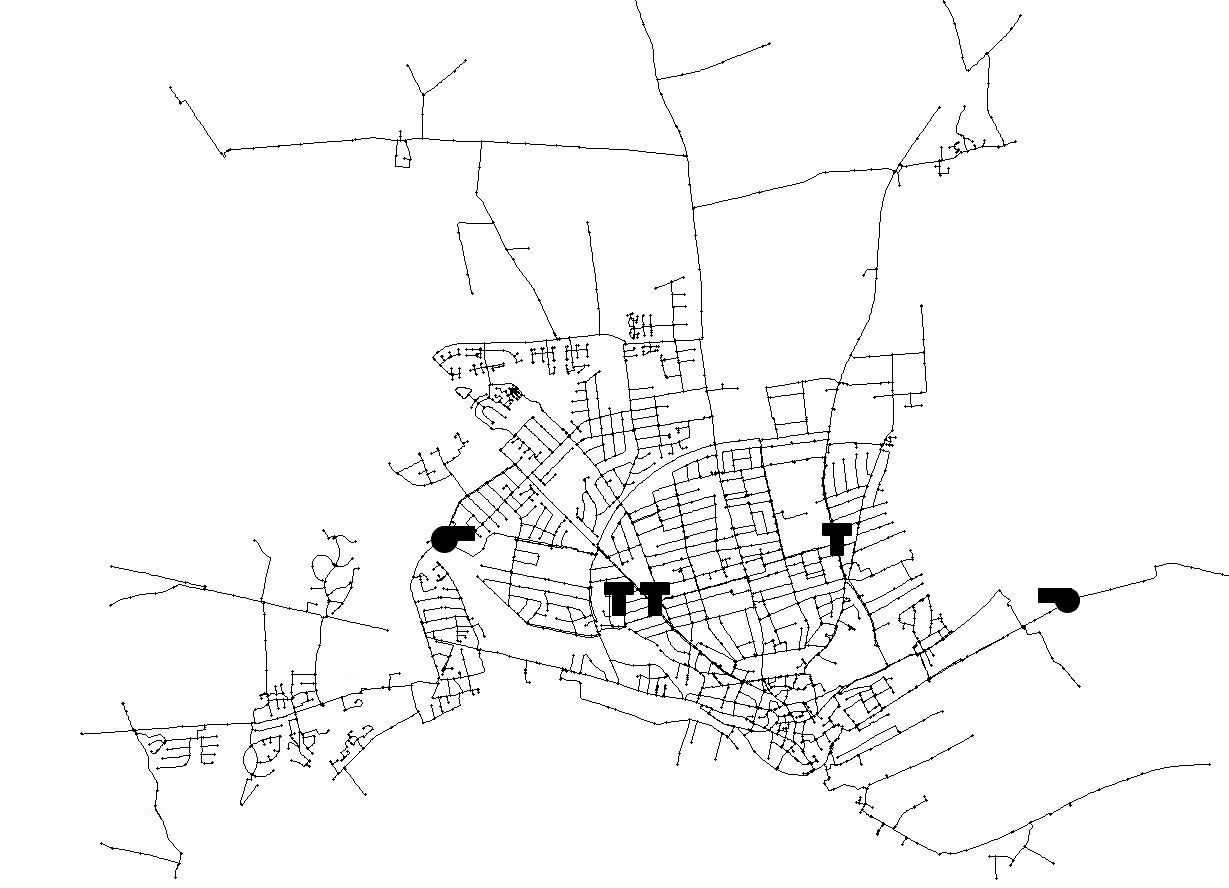
\includegraphics[width=\textwidth]{report/tikz/identification_map1}};
\node[black] at (11.4,4.75) {\footnotesize $\bm {\mathcal{W}_3}$};
\node[black] at (13.75,3.3) {\footnotesize $\bm {\mathcal{K}_2}$};
\node[black] at (4.7,4.65) {\footnotesize $\bm {\mathcal{K}_1}$};
\node[black] at (8.4,1) {\footnotesize $\bm {\mathcal{W}_2}$};
\node[black] at (6.8,1) {\footnotesize $\bm {\mathcal{W}_1}$};
\draw [-latex][thick](8.05,3.2) -- (8.4,1.35);
\draw [-latex][thick](7.55,3.2) -- (6.8,1.35);
\end{tikzpicture}

%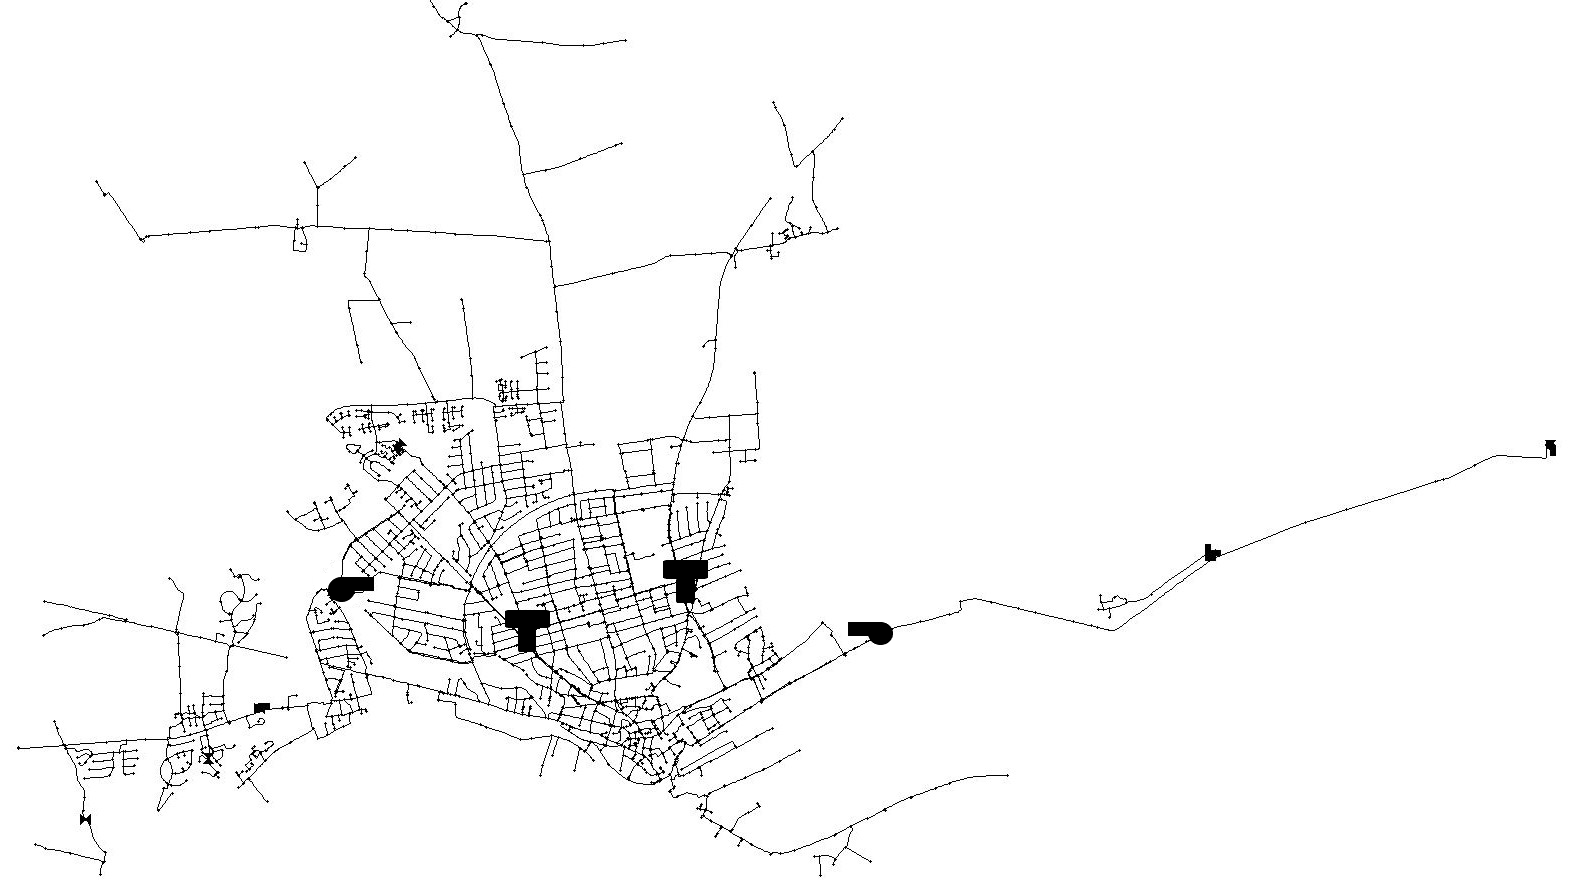
\includegraphics[width=0.95\textwidth]{report/pictures/verdo_pic3}
\caption{The network map with the corresponding WTs and pumping stations.}
\label{fig:simplified_network_identification1223}
\end{figure}
\vspace{-3mm}

In the following description, let us use the notation for the pumping stations and WTs shown in \figref{fig:simplified_network_identification1223}. Thus, $\mathcal{K}_1$ denotes Oust Mølle(OMV) waterwork and $\mathcal{K}_1$ denotes Toldbodgade(TBP) pumping station. The WTs at Hobrovej(HBP) pumping station are denoted with $\mathcal{W}_1$ and $\mathcal{W}_2$, furthermore the WT at Hadsundevej(HSP) pumping station is denoted with $\mathcal{W}_3$. 

The identification of the model has been carried out on measurement data provided by Verdo A/S, such that two day-long data sets have been extracted from three different time periods in 2017. It turned out to be difficult to find long time periods in which the measurement data was not biased, as certain sensors are frequently losing the radio signal, thus making the measurements unusable. The three data sets on which the identification and validations have been carried out is shown in \tabref{identification_periods}.

\begin{center}
    \begin{tabular}{ | p{3cm} | p{3cm} | p{3cm} |}
    \hline
     & \textbf{Start time} & \textbf{End time} \\ 
    \hline
    Period 1 & 21.10.2017 0.00 &  22.10.2017 24.00 \\ 
    \hline
    Period 2 & 07.11.2017 0.00 & 08.11.2017 24.00  \\ 
    \hline
    Period 3 & 09.12.2017 0.00 & 10.12.2017 24.00 \\ 
    \hline
    \end{tabular}
    \label{identification_periods}
    \captionof{table}{Dates from which data are extracted.}
\end{center}

\vspace{-3mm}

The model is first identified on the data set from Period one. After the identification, the model is validated on the data sets from Period two and Period three. The extracted data is sampled with $T_s = 1$ [min] sampling time, except for the total consumption $\sigma$, as it has been calculated by using the measurements on the WT flows. The sampling rate of the total water consumption $\sigma$ is $T_s = 1$ [h]. 

The total water consumption in the three different periods is shown in \figref{fig:data_allconsumption}, where $\sigma_1$, $\sigma_2$ and $\sigma_3$ denote the consumption in period one, period two and period three, respectively.

\vspace{-3mm}
%Total consumptions
  \begin{figure}[H]
  \centering
  %\hspace{0mm}
  %
\includegraphics[width=0.35\textwidth]{report/pictures/missingfigure}
  % This file was created by matlab2tikz.
%
%The latest updates can be retrieved from
%  http://www.mathworks.com/matlabcentral/fileexchange/22022-matlab2tikz-matlab2tikz
%where you can also make suggestions and rate matlab2tikz.
%
\definecolor{mycolor1}{rgb}{0.00000,0.44700,0.74100}%
\definecolor{mycolor2}{rgb}{0.85000,0.32500,0.09800}%
\definecolor{mycolor3}{rgb}{0.92900,0.69400,0.12500}%
%
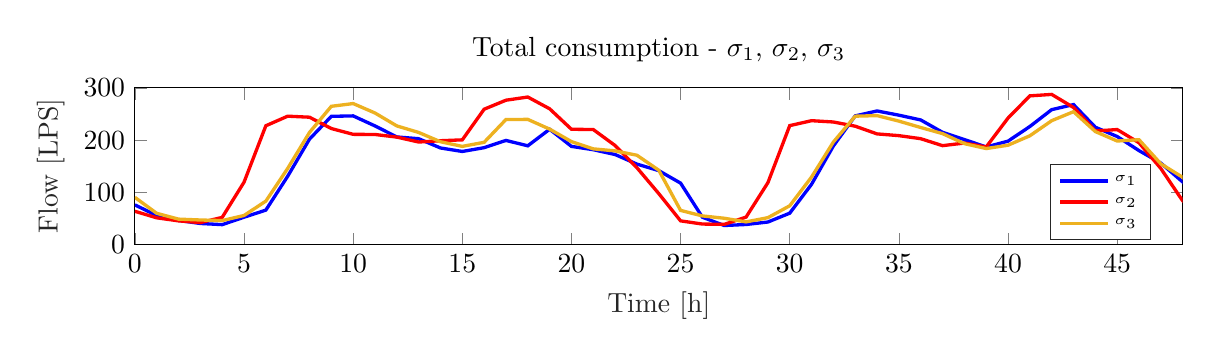
\begin{tikzpicture}

\begin{axis}[%
width=5.239in,
height=0.784in,
at={(1.013in,0.427in)},
scale only axis,
xmin=0,
xmax=48,
xlabel style={font=\color{white!15!black}},
xlabel={Time [h]},
ymin=0,
ymax=300,
ylabel style={font=\color{white!15!black}},
ylabel={Flow  [LPS]},
axis background/.style={fill=white},
title style={},
title={Total consumption - $\sigma_1$, $\sigma_2$, $\sigma_3$},
legend style={at={(0.97,0.03)}, anchor=south east, legend cell align=left, align=left, draw=white!15!black}
]
\addplot [color=blue, line width=1.2pt]
  table[row sep=crcr]{%
0	76.111111172\\
1	55.833333378\\
2	46.388888926\\
3	40.555555588\\
4	38.333333364\\
5	52.500000042\\
6	66.111111164\\
7	130.833333438\\
8	201.944444606\\
9	245.555555752\\
10	246.388889086\\
11	227.222222404\\
12	206.111111276\\
13	202.77777794\\
14	185.000000148\\
15	178.333333476\\
16	185.555555704\\
17	199.444444604\\
18	189.166666818\\
19	220.83333351\\
20	188.055555706\\
21	181.666666812\\
22	172.500000138\\
23	154.16666679\\
24	141.66666678\\
25	117.777777872\\
26	52.500000042\\
27	36.666666696\\
28	38.611111142\\
29	43.333333368\\
30	60.277777826\\
31	115.555555648\\
32	188.88888904\\
33	246.388889086\\
34	255.833333538\\
35	247.777777976\\
36	238.611111302\\
37	215.000000172\\
38	201.111111272\\
39	186.944444594\\
40	198.055555714\\
41	226.111111292\\
42	258.33333354\\
43	268.05555577\\
44	224.722222402\\
45	206.94444461\\
46	180.000000144\\
47	156.111111236\\
48	120.000000096\\
49	73.61111117\\
50	39.722222254\\
51	39.722222254\\
52	45.277777814\\
53	112.777777868\\
54	219.722222398\\
55	225.00000018\\
56	218.888889064\\
57	223.055555734\\
58	208.3333335\\
59	214.444444616\\
60	195.000000156\\
61	201.38888905\\
62	189.166666818\\
63	184.444444592\\
64	221.944444622\\
65	279.16666689\\
66	291.111111344\\
67	262.777777988\\
68	220.555555732\\
69	218.611111286\\
70	200.555555716\\
71	154.444444568\\
72	81.94444451\\
73	49.722222262\\
74	40.27777781\\
75	40.000000032\\
76	48.333333372\\
77	110.833333422\\
78	216.111111284\\
79	213.333333504\\
80	206.94444461\\
81	209.444444612\\
82	201.666666828\\
83	202.77777794\\
84	191.944444598\\
85	189.444444596\\
86	183.888889036\\
87	209.166666834\\
88	252.222222424\\
89	271.388889106\\
90	279.16666689\\
91	253.055555758\\
92	217.777777952\\
93	210.000000168\\
94	186.388889038\\
95	146.111111228\\
};
\addlegendentry{\tiny $\sigma_1$}

\addplot [color=red, line width=1.2pt]
  table[row sep=crcr]{%
0	63.88888894\\
1	51.38888893\\
2	45.555555592\\
3	42.222222256\\
4	52.222222264\\
5	119.44444454\\
6	227.500000182\\
7	245.83333353\\
8	243.888889084\\
9	222.2222224\\
10	211.11111128\\
11	210.833333502\\
12	205.833333498\\
13	196.388889046\\
14	198.888889048\\
15	200.555555716\\
16	259.166666874\\
17	276.38888911\\
18	282.500000226\\
19	260.000000208\\
20	220.83333351\\
21	220.277777954\\
22	189.722222374\\
23	147.22222234\\
24	97.777777856\\
25	45.555555592\\
26	39.444444476\\
27	38.88888892\\
28	52.77777782\\
29	118.611111206\\
30	227.77777796\\
31	237.222222412\\
32	234.72222241\\
33	226.666666848\\
34	211.944444614\\
35	208.611111278\\
36	202.77777794\\
37	189.444444596\\
38	194.4444446\\
39	186.944444594\\
40	242.222222416\\
41	284.72222245\\
42	287.50000023\\
43	262.50000021\\
44	217.500000174\\
45	220.277777954\\
46	195.000000156\\
47	145.83333345\\
48	83.888888956\\
49	47.22222226\\
50	46.388888926\\
51	42.777777812\\
52	51.666666708\\
53	118.888888984\\
54	231.388889074\\
55	236.666666856\\
56	216.66666684\\
57	226.666666848\\
58	213.055555726\\
59	209.166666834\\
60	202.222222384\\
61	193.888889044\\
62	189.722222374\\
63	198.888889048\\
64	262.50000021\\
65	286.11111134\\
66	282.222222448\\
67	265.555555768\\
68	220.000000176\\
69	216.388889062\\
70	193.888889044\\
71	153.333333456\\
72	99.166666746\\
73	50.833333374\\
74	46.111111148\\
75	47.500000038\\
76	56.94444449\\
77	120.000000096\\
78	223.61111129\\
79	240.000000192\\
80	223.333333512\\
81	235.555555744\\
82	210.000000168\\
83	216.388889062\\
84	203.333333496\\
85	214.444444616\\
86	206.388889054\\
87	224.444444624\\
88	271.388889106\\
89	267.777777992\\
90	259.166666874\\
91	236.666666856\\
92	201.666666828\\
93	199.722222382\\
94	187.777777928\\
95	130.833333438\\
};
\addlegendentry{\tiny $\sigma_2$}

\addplot [color=mycolor3, line width=1.2pt]
  table[row sep=crcr]{%
0	90.555555628\\
1	60.000000048\\
2	48.888888928\\
3	47.22222226\\
4	46.111111148\\
5	55.833333378\\
6	83.3333334\\
7	145.83333345\\
8	214.722222394\\
9	264.722222434\\
10	270.000000216\\
11	251.944444646\\
12	227.222222404\\
13	214.722222394\\
14	196.944444602\\
15	188.055555706\\
16	195.83333349\\
17	239.444444636\\
18	239.722222414\\
19	221.111111288\\
20	197.22222238\\
21	183.33333348\\
22	179.444444588\\
23	171.111111248\\
24	142.500000114\\
25	65.555555608\\
26	55.000000044\\
27	50.555555596\\
28	43.611111146\\
29	51.666666708\\
30	74.444444504\\
31	129.444444548\\
32	196.388889046\\
33	245.83333353\\
34	246.944444642\\
35	236.388889078\\
36	224.166666846\\
37	212.50000017\\
38	193.333333488\\
39	183.888889036\\
40	190.27777793\\
41	208.3333335\\
42	237.222222412\\
43	254.444444648\\
44	216.388889062\\
45	198.333333492\\
46	200.833333494\\
47	154.722222346\\
48	128.888888992\\
49	81.94444451\\
50	40.27777781\\
51	39.166666698\\
52	50.555555596\\
53	123.61111121\\
54	225.555555736\\
55	235.833333522\\
56	221.944444622\\
57	227.500000182\\
58	221.388889066\\
59	225.833333514\\
60	211.11111128\\
61	202.222222384\\
62	188.88888904\\
63	195.83333349\\
64	239.166666858\\
65	281.111111336\\
66	290.555555788\\
67	263.055555766\\
68	227.500000182\\
69	220.555555732\\
70	205.833333498\\
71	150.555555676\\
72	75.00000006\\
73	53.333333376\\
74	43.05555559\\
75	44.166666702\\
76	60.000000048\\
77	121.111111208\\
78	221.111111288\\
79	229.444444628\\
80	212.777777948\\
81	218.888889064\\
82	211.944444614\\
83	205.000000164\\
84	195.555555712\\
85	198.888889048\\
86	189.444444596\\
87	221.111111288\\
88	258.888889096\\
89	263.055555766\\
90	269.166666882\\
91	262.777777988\\
92	220.555555732\\
93	210.000000168\\
94	192.222222376\\
95	155.000000124\\
};
\addlegendentry{\tiny $\sigma_3$}

\end{axis}
\end{tikzpicture}% 
  \vspace{-2.5mm}
  \caption{Total water consumption in three different periods.}
  \label{fig:data_allconsumption}
  \end{figure}
 %\vspace{-8mm}
 \vspace{-3mm}

As it is shown in \figref{fig:data_allconsumption}, the characteristics of the daily consumption is similar, although measurements are taken from different months. This is according to the expectations, considering the fact that there is high consumption in the morning and late afternoon, while the consumption is low in the night hours. The corresponding inlet flows of the two pumping stations and the water level in the WTs for period one are shown in \figref{fig:w1_w2_p1}. 
\vspace{-3mm}

%Inlet flows - period 1
  \begin{figure}[H]
  \centering
  %\hspace{0mm}
  %
\includegraphics[width=0.35\textwidth]{report/pictures/missingfigure}
  % This file was created by matlab2tikz.
%
%The latest updates can be retrieved from
%  http://www.mathworks.com/matlabcentral/fileexchange/22022-matlab2tikz-matlab2tikz
%where you can also make suggestions and rate matlab2tikz.
%
\definecolor{mycolor1}{rgb}{0.00000,0.44700,0.74100}%
\definecolor{mycolor2}{rgb}{0.85000,0.32500,0.09800}%
%
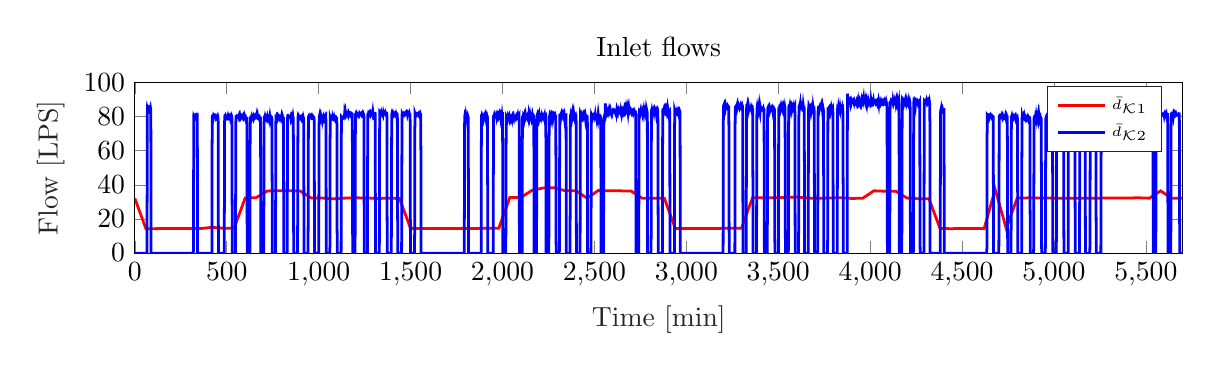
\begin{tikzpicture}

\begin{axis}[%
width=5.239in,
height=0.854in,
at={(1.02in,0.431in)},
scale only axis,
xmin=0,
xmax=5700,
xlabel style={font=\color{white!15!black}},
xlabel={Time [min]},
ymin=-0.1944444446,
ymax=100,
ylabel style={font=\color{white!15!black}},
ylabel={Flow  [LPS]},
axis background/.style={fill=white},
title style={},
title={Inlet flows},
legend style={legend cell align=left, align=left, draw=white!15!black}
]
\addplot [color=red, line width=1.0pt, forget plot]
  table[row sep=crcr]{%
0	32.0000000256\\
1	31.70416669203\\
2	31.40833335846\\
3	31.11250002489\\
4	30.81666669132\\
5	30.52083335775\\
6	30.22500002418\\
7	29.92916669061\\
8	29.63333335704\\
9	29.33750002347\\
10	29.0416666899\\
11	28.74583335633\\
12	28.45000002276\\
13	28.15416668919\\
14	27.85833335562\\
15	27.56250002205\\
16	27.26666668848\\
17	26.97083335491\\
18	26.67500002134\\
19	26.37916668777\\
20	26.0833333542\\
21	25.78750002063\\
22	25.49166668706\\
23	25.19583335349\\
24	24.90000001992\\
25	24.60416668635\\
26	24.30833335278\\
27	24.01250001921\\
28	23.71666668564\\
29	23.42083335207\\
30	23.1250000185\\
31	22.82916668493\\
32	22.53333335136\\
33	22.23750001779\\
34	21.94166668422\\
35	21.64583335065\\
36	21.35000001708\\
37	21.05416668351\\
38	20.75833334994\\
39	20.46250001637\\
40	20.1666666828\\
41	19.87083334923\\
42	19.57500001566\\
43	19.27916668209\\
44	18.98333334852\\
45	18.68750001495\\
46	18.39166668138\\
47	18.09583334781\\
48	17.80000001424\\
49	17.50416668067\\
50	17.2083333471\\
51	16.91250001353\\
52	16.61666667996\\
53	16.32083334639\\
54	16.02500001282\\
55	15.72916667925\\
56	15.43333334568\\
57	15.13750001211\\
58	14.84166667854\\
59	14.54583334497\\
60	14.2500000114\\
61	14.2504629743633\\
62	14.2509259373267\\
63	14.25138890029\\
64	14.2518518632533\\
65	14.2523148262167\\
66	14.25277778918\\
67	14.2532407521433\\
68	14.2537037151067\\
69	14.25416667807\\
70	14.2546296410333\\
71	14.2550926039967\\
72	14.25555556696\\
73	14.2560185299233\\
74	14.2564814928867\\
75	14.25694445585\\
76	14.2574074188133\\
77	14.2578703817767\\
78	14.25833334474\\
79	14.2587963077033\\
80	14.2592592706667\\
81	14.25972223363\\
82	14.2601851965933\\
83	14.2606481595567\\
84	14.26111112252\\
85	14.2615740854833\\
86	14.2620370484467\\
87	14.26250001141\\
88	14.2629629743733\\
89	14.2634259373367\\
90	14.2638889003\\
91	14.2643518632633\\
92	14.2648148262267\\
93	14.26527778919\\
94	14.2657407521533\\
95	14.2662037151167\\
96	14.26666667808\\
97	14.2671296410433\\
98	14.2675926040067\\
99	14.26805556697\\
100	14.2685185299333\\
101	14.2689814928967\\
102	14.26944445586\\
103	14.2699074188233\\
104	14.2703703817867\\
105	14.27083334475\\
106	14.2712963077133\\
107	14.2717592706767\\
108	14.27222223364\\
109	14.2726851966033\\
110	14.2731481595667\\
111	14.27361112253\\
112	14.2740740854933\\
113	14.2745370484567\\
114	14.27500001142\\
115	14.2754629743833\\
116	14.2759259373467\\
117	14.27638890031\\
118	14.2768518632733\\
119	14.2773148262367\\
120	14.2777777892\\
121	14.2787037151267\\
122	14.2796296410533\\
123	14.28055556698\\
124	14.2814814929067\\
125	14.2824074188333\\
126	14.28333334476\\
127	14.2842592706867\\
128	14.2851851966133\\
129	14.28611112254\\
130	14.2870370484667\\
131	14.2879629743933\\
132	14.28888890032\\
133	14.2898148262467\\
134	14.2907407521733\\
135	14.2916666781\\
136	14.2925926040267\\
137	14.2935185299533\\
138	14.29444445588\\
139	14.2953703818067\\
140	14.2962963077333\\
141	14.29722223366\\
142	14.2981481595867\\
143	14.2990740855133\\
144	14.30000001144\\
145	14.3009259373667\\
146	14.3018518632933\\
147	14.30277778922\\
148	14.3037037151467\\
149	14.3046296410733\\
150	14.305555567\\
151	14.3064814929267\\
152	14.3074074188533\\
153	14.30833334478\\
154	14.3092592707067\\
155	14.3101851966333\\
156	14.31111112256\\
157	14.3120370484867\\
158	14.3129629744133\\
159	14.31388890034\\
160	14.3148148262667\\
161	14.3157407521933\\
162	14.31666667812\\
163	14.3175926040467\\
164	14.3185185299733\\
165	14.3194444559\\
166	14.3203703818267\\
167	14.3212963077533\\
168	14.32222223368\\
169	14.3231481596067\\
170	14.3240740855333\\
171	14.32500001146\\
172	14.3259259373867\\
173	14.3268518633133\\
174	14.32777778924\\
175	14.3287037151667\\
176	14.3296296410933\\
177	14.33055556702\\
178	14.3314814929467\\
179	14.3324074188733\\
180	14.3333333448\\
181	14.3333333448\\
182	14.3333333448\\
183	14.3333333448\\
184	14.3333333448\\
185	14.3333333448\\
186	14.3333333448\\
187	14.3333333448\\
188	14.3333333448\\
189	14.3333333448\\
190	14.3333333448\\
191	14.3333333448\\
192	14.3333333448\\
193	14.3333333448\\
194	14.3333333448\\
195	14.3333333448\\
196	14.3333333448\\
197	14.3333333448\\
198	14.3333333448\\
199	14.3333333448\\
200	14.3333333448\\
201	14.3333333448\\
202	14.3333333448\\
203	14.3333333448\\
204	14.3333333448\\
205	14.3333333448\\
206	14.3333333448\\
207	14.3333333448\\
208	14.3333333448\\
209	14.3333333448\\
210	14.3333333448\\
211	14.3333333448\\
212	14.3333333448\\
213	14.3333333448\\
214	14.3333333448\\
215	14.3333333448\\
216	14.3333333448\\
217	14.3333333448\\
218	14.3333333448\\
219	14.3333333448\\
220	14.3333333448\\
221	14.3333333448\\
222	14.3333333448\\
223	14.3333333448\\
224	14.3333333448\\
225	14.3333333448\\
226	14.3333333448\\
227	14.3333333448\\
228	14.3333333448\\
229	14.3333333448\\
230	14.3333333448\\
231	14.3333333448\\
232	14.3333333448\\
233	14.3333333448\\
234	14.3333333448\\
235	14.3333333448\\
236	14.3333333448\\
237	14.3333333448\\
238	14.3333333448\\
239	14.3333333448\\
240	14.3333333448\\
241	14.3324074188733\\
242	14.3314814929467\\
243	14.33055556702\\
244	14.3296296410933\\
245	14.3287037151667\\
246	14.32777778924\\
247	14.3268518633133\\
248	14.3259259373867\\
249	14.32500001146\\
250	14.3240740855333\\
251	14.3231481596067\\
252	14.32222223368\\
253	14.3212963077533\\
254	14.3203703818267\\
255	14.3194444559\\
256	14.3185185299733\\
257	14.3175926040467\\
258	14.31666667812\\
259	14.3157407521933\\
260	14.3148148262667\\
261	14.31388890034\\
262	14.3129629744133\\
263	14.3120370484867\\
264	14.31111112256\\
265	14.3101851966333\\
266	14.3092592707067\\
267	14.30833334478\\
268	14.3074074188533\\
269	14.3064814929267\\
270	14.305555567\\
271	14.3046296410733\\
272	14.3037037151467\\
273	14.30277778922\\
274	14.3018518632933\\
275	14.3009259373667\\
276	14.30000001144\\
277	14.2990740855133\\
278	14.2981481595867\\
279	14.29722223366\\
280	14.2962963077333\\
281	14.2953703818067\\
282	14.29444445588\\
283	14.2935185299533\\
284	14.2925926040267\\
285	14.2916666781\\
286	14.2907407521733\\
287	14.2898148262467\\
288	14.28888890032\\
289	14.2879629743933\\
290	14.2870370484667\\
291	14.28611112254\\
292	14.2851851966133\\
293	14.2842592706867\\
294	14.28333334476\\
295	14.2824074188333\\
296	14.2814814929067\\
297	14.28055556698\\
298	14.2796296410533\\
299	14.2787037151267\\
300	14.2777777892\\
301	14.27916667809\\
302	14.28055556698\\
303	14.28194445587\\
304	14.28333334476\\
305	14.28472223365\\
306	14.28611112254\\
307	14.28750001143\\
308	14.28888890032\\
309	14.29027778921\\
310	14.2916666781\\
311	14.29305556699\\
312	14.29444445588\\
313	14.29583334477\\
314	14.29722223366\\
315	14.29861112255\\
316	14.30000001144\\
317	14.30138890033\\
318	14.30277778922\\
319	14.30416667811\\
320	14.305555567\\
321	14.30694445589\\
322	14.30833334478\\
323	14.30972223367\\
324	14.31111112256\\
325	14.31250001145\\
326	14.31388890034\\
327	14.31527778923\\
328	14.31666667812\\
329	14.31805556701\\
330	14.3194444559\\
331	14.32083334479\\
332	14.32222223368\\
333	14.32361112257\\
334	14.32500001146\\
335	14.32638890035\\
336	14.32777778924\\
337	14.32916667813\\
338	14.33055556702\\
339	14.33194445591\\
340	14.3333333448\\
341	14.33472223369\\
342	14.33611112258\\
343	14.33750001147\\
344	14.33888890036\\
345	14.34027778925\\
346	14.34166667814\\
347	14.34305556703\\
348	14.34444445592\\
349	14.34583334481\\
350	14.3472222337\\
351	14.34861112259\\
352	14.35000001148\\
353	14.35138890037\\
354	14.35277778926\\
355	14.35416667815\\
356	14.35555556704\\
357	14.35694445593\\
358	14.35833334482\\
359	14.35972223371\\
360	14.3611111226\\
361	14.37222223372\\
362	14.38333334484\\
363	14.39444445596\\
364	14.40555556708\\
365	14.4166666782\\
366	14.42777778932\\
367	14.43888890044\\
368	14.45000001156\\
369	14.46111112268\\
370	14.4722222338\\
371	14.48333334492\\
372	14.49444445604\\
373	14.50555556716\\
374	14.51666667828\\
375	14.5277777894\\
376	14.53888890052\\
377	14.55000001164\\
378	14.56111112276\\
379	14.57222223388\\
380	14.583333345\\
381	14.59444445612\\
382	14.60555556724\\
383	14.61666667836\\
384	14.62777778948\\
385	14.6388889006\\
386	14.65000001172\\
387	14.66111112284\\
388	14.67222223396\\
389	14.68333334508\\
390	14.6944444562\\
391	14.70555556732\\
392	14.71666667844\\
393	14.72777778956\\
394	14.73888890068\\
395	14.7500000118\\
396	14.76111112292\\
397	14.77222223404\\
398	14.78333334516\\
399	14.79444445628\\
400	14.8055555674\\
401	14.81666667852\\
402	14.82777778964\\
403	14.83888890076\\
404	14.85000001188\\
405	14.861111123\\
406	14.87222223412\\
407	14.88333334524\\
408	14.89444445636\\
409	14.90555556748\\
410	14.9166666786\\
411	14.92777778972\\
412	14.93888890084\\
413	14.95000001196\\
414	14.96111112308\\
415	14.9722222342\\
416	14.98333334532\\
417	14.99444445644\\
418	15.00555556756\\
419	15.01666667868\\
420	15.0277777898\\
421	15.01944445646\\
422	15.01111112312\\
423	15.00277778978\\
424	14.99444445644\\
425	14.9861111231\\
426	14.97777778976\\
427	14.96944445642\\
428	14.96111112308\\
429	14.95277778974\\
430	14.9444444564\\
431	14.93611112306\\
432	14.92777778972\\
433	14.91944445638\\
434	14.91111112304\\
435	14.9027777897\\
436	14.89444445636\\
437	14.88611112302\\
438	14.87777778968\\
439	14.86944445634\\
440	14.861111123\\
441	14.85277778966\\
442	14.84444445632\\
443	14.83611112298\\
444	14.82777778964\\
445	14.8194444563\\
446	14.81111112296\\
447	14.80277778962\\
448	14.79444445628\\
449	14.78611112294\\
450	14.7777777896\\
451	14.76944445626\\
452	14.76111112292\\
453	14.75277778958\\
454	14.74444445624\\
455	14.7361111229\\
456	14.72777778956\\
457	14.71944445622\\
458	14.71111112288\\
459	14.70277778954\\
460	14.6944444562\\
461	14.68611112286\\
462	14.67777778952\\
463	14.66944445618\\
464	14.66111112284\\
465	14.6527777895\\
466	14.64444445616\\
467	14.63611112282\\
468	14.62777778948\\
469	14.61944445614\\
470	14.6111111228\\
471	14.60277778946\\
472	14.59444445612\\
473	14.58611112278\\
474	14.57777778944\\
475	14.5694444561\\
476	14.56111112276\\
477	14.55277778942\\
478	14.54444445608\\
479	14.53611112274\\
480	14.5277777894\\
481	14.5277777894\\
482	14.5277777894\\
483	14.5277777894\\
484	14.5277777894\\
485	14.5277777894\\
486	14.5277777894\\
487	14.5277777894\\
488	14.5277777894\\
489	14.5277777894\\
490	14.5277777894\\
491	14.5277777894\\
492	14.5277777894\\
493	14.5277777894\\
494	14.5277777894\\
495	14.5277777894\\
496	14.5277777894\\
497	14.5277777894\\
498	14.5277777894\\
499	14.5277777894\\
500	14.5277777894\\
501	14.5277777894\\
502	14.5277777894\\
503	14.5277777894\\
504	14.5277777894\\
505	14.5277777894\\
506	14.5277777894\\
507	14.5277777894\\
508	14.5277777894\\
509	14.5277777894\\
510	14.5277777894\\
511	14.5277777894\\
512	14.5277777894\\
513	14.5277777894\\
514	14.5277777894\\
515	14.5277777894\\
516	14.5277777894\\
517	14.5277777894\\
518	14.5277777894\\
519	14.5277777894\\
520	14.5277777894\\
521	14.5277777894\\
522	14.5277777894\\
523	14.5277777894\\
524	14.5277777894\\
525	14.5277777894\\
526	14.5277777894\\
527	14.5277777894\\
528	14.5277777894\\
529	14.5277777894\\
530	14.5277777894\\
531	14.5277777894\\
532	14.5277777894\\
533	14.5277777894\\
534	14.5277777894\\
535	14.5277777894\\
536	14.5277777894\\
537	14.5277777894\\
538	14.5277777894\\
539	14.5277777894\\
540	14.5277777894\\
541	14.8231481600066\\
542	15.1185185306133\\
543	15.41388890122\\
544	15.7092592718267\\
545	16.0046296424333\\
546	16.30000001304\\
547	16.5953703836467\\
548	16.8907407542533\\
549	17.18611112486\\
550	17.4814814954667\\
551	17.7768518660733\\
552	18.07222223668\\
553	18.3675926072867\\
554	18.6629629778933\\
555	18.9583333485\\
556	19.2537037191066\\
557	19.5490740897133\\
558	19.84444446032\\
559	20.1398148309267\\
560	20.4351852015333\\
561	20.73055557214\\
562	21.0259259427467\\
563	21.3212963133533\\
564	21.61666668396\\
565	21.9120370545667\\
566	22.2074074251733\\
567	22.50277779578\\
568	22.7981481663867\\
569	23.0935185369933\\
570	23.3888889076\\
571	23.6842592782066\\
572	23.9796296488133\\
573	24.27500001942\\
574	24.5703703900267\\
575	24.8657407606333\\
576	25.16111113124\\
577	25.4564815018467\\
578	25.7518518724533\\
579	26.04722224306\\
580	26.3425926136667\\
581	26.6379629842733\\
582	26.93333335488\\
583	27.2287037254867\\
584	27.5240740960933\\
585	27.8194444667\\
586	28.1148148373067\\
587	28.4101852079133\\
588	28.70555557852\\
589	29.0009259491267\\
590	29.2962963197333\\
591	29.59166669034\\
592	29.8870370609467\\
593	30.1824074315533\\
594	30.47777780216\\
595	30.7731481727667\\
596	31.0685185433733\\
597	31.36388891398\\
598	31.6592592845867\\
599	31.9546296551933\\
600	32.2500000258\\
601	32.2532407665433\\
602	32.2564815072867\\
603	32.25972224803\\
604	32.2629629887733\\
605	32.2662037295167\\
606	32.26944447026\\
607	32.2726852110033\\
608	32.2759259517467\\
609	32.27916669249\\
610	32.2824074332333\\
611	32.2856481739767\\
612	32.28888891472\\
613	32.2921296554633\\
614	32.2953703962067\\
615	32.29861113695\\
616	32.3018518776933\\
617	32.3050926184367\\
618	32.30833335918\\
619	32.3115740999233\\
620	32.3148148406667\\
621	32.31805558141\\
622	32.3212963221533\\
623	32.3245370628967\\
624	32.32777780364\\
625	32.3310185443833\\
626	32.3342592851267\\
627	32.33750002587\\
628	32.3407407666133\\
629	32.3439815073567\\
630	32.3472222481\\
631	32.3504629888433\\
632	32.3537037295867\\
633	32.35694447033\\
634	32.3601852110733\\
635	32.3634259518167\\
636	32.36666669256\\
637	32.3699074333033\\
638	32.3731481740467\\
639	32.37638891479\\
640	32.3796296555333\\
641	32.3828703962767\\
642	32.38611113702\\
643	32.3893518777633\\
644	32.3925926185067\\
645	32.39583335925\\
646	32.3990740999933\\
647	32.4023148407367\\
648	32.40555558148\\
649	32.4087963222233\\
650	32.4120370629667\\
651	32.41527780371\\
652	32.4185185444533\\
653	32.4217592851967\\
654	32.42500002594\\
655	32.4282407666833\\
656	32.4314815074267\\
657	32.43472224817\\
658	32.4379629889133\\
659	32.4412037296567\\
660	32.4444444704\\
661	32.5101852111933\\
662	32.5759259519867\\
663	32.64166669278\\
664	32.7074074335733\\
665	32.7731481743667\\
666	32.83888891516\\
667	32.9046296559533\\
668	32.9703703967467\\
669	33.03611113754\\
670	33.1018518783333\\
671	33.1675926191267\\
672	33.23333335992\\
673	33.2990741007133\\
674	33.3648148415067\\
675	33.4305555823\\
676	33.4962963230933\\
677	33.5620370638867\\
678	33.62777780468\\
679	33.6935185454733\\
680	33.7592592862667\\
681	33.82500002706\\
682	33.8907407678533\\
683	33.9564815086467\\
684	34.02222224944\\
685	34.0879629902333\\
686	34.1537037310267\\
687	34.21944447182\\
688	34.2851852126133\\
689	34.3509259534067\\
690	34.4166666942\\
691	34.4824074349933\\
692	34.5481481757867\\
693	34.61388891658\\
694	34.6796296573733\\
695	34.7453703981667\\
696	34.81111113896\\
697	34.8768518797533\\
698	34.9425926205467\\
699	35.00833336134\\
700	35.0740741021333\\
701	35.1398148429267\\
702	35.20555558372\\
703	35.2712963245133\\
704	35.3370370653067\\
705	35.4027778061\\
706	35.4685185468933\\
707	35.5342592876867\\
708	35.60000002848\\
709	35.6657407692733\\
710	35.7314815100667\\
711	35.79722225086\\
712	35.8629629916533\\
713	35.9287037324467\\
714	35.99444447324\\
715	36.0601852140333\\
716	36.1259259548267\\
717	36.19166669562\\
718	36.2574074364133\\
719	36.3231481772067\\
720	36.388888918\\
721	36.3912037328167\\
722	36.3935185476333\\
723	36.39583336245\\
724	36.3981481772667\\
725	36.4004629920833\\
726	36.4027778069\\
727	36.4050926217167\\
728	36.4074074365333\\
729	36.40972225135\\
730	36.4120370661667\\
731	36.4143518809833\\
732	36.4166666958\\
733	36.4189815106167\\
734	36.4212963254333\\
735	36.42361114025\\
736	36.4259259550667\\
737	36.4282407698833\\
738	36.4305555847\\
739	36.4328703995167\\
740	36.4351852143333\\
741	36.43750002915\\
742	36.4398148439667\\
743	36.4421296587833\\
744	36.4444444736\\
745	36.4467592884167\\
746	36.4490741032333\\
747	36.45138891805\\
748	36.4537037328667\\
749	36.4560185476833\\
750	36.4583333625\\
751	36.4606481773167\\
752	36.4629629921333\\
753	36.46527780695\\
754	36.4675926217667\\
755	36.4699074365833\\
756	36.4722222514\\
757	36.4745370662167\\
758	36.4768518810333\\
759	36.47916669585\\
760	36.4814815106667\\
761	36.4837963254833\\
762	36.4861111403\\
763	36.4884259551167\\
764	36.4907407699333\\
765	36.49305558475\\
766	36.4953703995667\\
767	36.4976852143833\\
768	36.5000000292\\
769	36.5023148440167\\
770	36.5046296588333\\
771	36.50694447365\\
772	36.5092592884667\\
773	36.5115741032833\\
774	36.5138889181\\
775	36.5162037329167\\
776	36.5185185477333\\
777	36.52083336255\\
778	36.5231481773667\\
779	36.5254629921833\\
780	36.527777807\\
781	36.5273148440367\\
782	36.5268518810733\\
783	36.52638891811\\
784	36.5259259551467\\
785	36.5254629921833\\
786	36.52500002922\\
787	36.5245370662567\\
788	36.5240741032933\\
789	36.52361114033\\
790	36.5231481773667\\
791	36.5226852144033\\
792	36.52222225144\\
793	36.5217592884767\\
794	36.5212963255133\\
795	36.52083336255\\
796	36.5203703995867\\
797	36.5199074366233\\
798	36.51944447366\\
799	36.5189815106967\\
800	36.5185185477333\\
801	36.51805558477\\
802	36.5175926218067\\
803	36.5171296588433\\
804	36.51666669588\\
805	36.5162037329167\\
806	36.5157407699533\\
807	36.51527780699\\
808	36.5148148440267\\
809	36.5143518810633\\
810	36.5138889181\\
811	36.5134259551367\\
812	36.5129629921733\\
813	36.51250002921\\
814	36.5120370662467\\
815	36.5115741032833\\
816	36.51111114032\\
817	36.5106481773567\\
818	36.5101852143933\\
819	36.50972225143\\
820	36.5092592884667\\
821	36.5087963255033\\
822	36.50833336254\\
823	36.5078703995767\\
824	36.5074074366133\\
825	36.50694447365\\
826	36.5064815106867\\
827	36.5060185477233\\
828	36.50555558476\\
829	36.5050926217967\\
830	36.5046296588333\\
831	36.50416669587\\
832	36.5037037329067\\
833	36.5032407699433\\
834	36.50277780698\\
835	36.5023148440167\\
836	36.5018518810533\\
837	36.50138891809\\
838	36.5009259551267\\
839	36.5004629921633\\
840	36.5000000292\\
841	36.49722225142\\
842	36.49444447364\\
843	36.49166669586\\
844	36.48888891808\\
845	36.4861111403\\
846	36.48333336252\\
847	36.48055558474\\
848	36.47777780696\\
849	36.47500002918\\
850	36.4722222514\\
851	36.46944447362\\
852	36.46666669584\\
853	36.46388891806\\
854	36.46111114028\\
855	36.4583333625\\
856	36.45555558472\\
857	36.45277780694\\
858	36.45000002916\\
859	36.44722225138\\
860	36.4444444736\\
861	36.44166669582\\
862	36.43888891804\\
863	36.43611114026\\
864	36.43333336248\\
865	36.4305555847\\
866	36.42777780692\\
867	36.42500002914\\
868	36.42222225136\\
869	36.41944447358\\
870	36.4166666958\\
871	36.41388891802\\
872	36.41111114024\\
873	36.40833336246\\
874	36.40555558468\\
875	36.4027778069\\
876	36.40000002912\\
877	36.39722225134\\
878	36.39444447356\\
879	36.39166669578\\
880	36.388888918\\
881	36.38611114022\\
882	36.38333336244\\
883	36.38055558466\\
884	36.37777780688\\
885	36.3750000291\\
886	36.37222225132\\
887	36.36944447354\\
888	36.36666669576\\
889	36.36388891798\\
890	36.3611111402\\
891	36.35833336242\\
892	36.35555558464\\
893	36.35277780686\\
894	36.35000002908\\
895	36.3472222513\\
896	36.34444447352\\
897	36.34166669574\\
898	36.33888891796\\
899	36.33611114018\\
900	36.3333333624\\
901	36.2648148438267\\
902	36.1962963252533\\
903	36.12777780668\\
904	36.0592592881067\\
905	35.9907407695333\\
906	35.92222225096\\
907	35.8537037323867\\
908	35.7851852138133\\
909	35.71666669524\\
910	35.6481481766667\\
911	35.5796296580933\\
912	35.51111113952\\
913	35.4425926209467\\
914	35.3740741023733\\
915	35.3055555838\\
916	35.2370370652267\\
917	35.1685185466533\\
918	35.10000002808\\
919	35.0314815095067\\
920	34.9629629909333\\
921	34.89444447236\\
922	34.8259259537867\\
923	34.7574074352133\\
924	34.68888891664\\
925	34.6203703980667\\
926	34.5518518794933\\
927	34.48333336092\\
928	34.4148148423467\\
929	34.3462963237733\\
930	34.2777778052\\
931	34.2092592866267\\
932	34.1407407680533\\
933	34.07222224948\\
934	34.0037037309067\\
935	33.9351852123333\\
936	33.86666669376\\
937	33.7981481751867\\
938	33.7296296566133\\
939	33.66111113804\\
940	33.5925926194667\\
941	33.5240741008933\\
942	33.45555558232\\
943	33.3870370637467\\
944	33.3185185451733\\
945	33.2500000266\\
946	33.1814815080267\\
947	33.1129629894533\\
948	33.04444447088\\
949	32.9759259523067\\
950	32.9074074337333\\
951	32.83888891516\\
952	32.7703703965867\\
953	32.7018518780133\\
954	32.63333335944\\
955	32.5648148408667\\
956	32.4962963222933\\
957	32.42777780372\\
958	32.3592592851467\\
959	32.2907407665733\\
960	32.222222248\\
961	32.2217592850367\\
962	32.2212963220733\\
963	32.22083335911\\
964	32.2203703961467\\
965	32.2199074331833\\
966	32.21944447022\\
967	32.2189815072567\\
968	32.2185185442933\\
969	32.21805558133\\
970	32.2175926183667\\
971	32.2171296554033\\
972	32.21666669244\\
973	32.2162037294767\\
974	32.2157407665133\\
975	32.21527780355\\
976	32.2148148405867\\
977	32.2143518776233\\
978	32.21388891466\\
979	32.2134259516967\\
980	32.2129629887333\\
981	32.21250002577\\
982	32.2120370628067\\
983	32.2115740998433\\
984	32.21111113688\\
985	32.2106481739167\\
986	32.2101852109533\\
987	32.20972224799\\
988	32.2092592850267\\
989	32.2087963220633\\
990	32.2083333591\\
991	32.2078703961367\\
992	32.2074074331733\\
993	32.20694447021\\
994	32.2064815072467\\
995	32.2060185442833\\
996	32.20555558132\\
997	32.2050926183567\\
998	32.2046296553933\\
999	32.20416669243\\
1000	32.2037037294667\\
1001	32.2032407665033\\
1002	32.20277780354\\
1003	32.2023148405767\\
1004	32.2018518776133\\
1005	32.20138891465\\
1006	32.2009259516867\\
1007	32.2004629887233\\
1008	32.20000002576\\
1009	32.1995370627967\\
1010	32.1990740998333\\
1011	32.19861113687\\
1012	32.1981481739067\\
1013	32.1976852109433\\
1014	32.19722224798\\
1015	32.1967592850167\\
1016	32.1962963220533\\
1017	32.19583335909\\
1018	32.1953703961267\\
1019	32.1949074331633\\
1020	32.1944444702\\
1021	32.1879629887133\\
1022	32.1814815072267\\
1023	32.17500002574\\
1024	32.1685185442533\\
1025	32.1620370627667\\
1026	32.15555558128\\
1027	32.1490740997933\\
1028	32.1425926183067\\
1029	32.13611113682\\
1030	32.1296296553333\\
1031	32.1231481738467\\
1032	32.11666669236\\
1033	32.1101852108733\\
1034	32.1037037293867\\
1035	32.0972222479\\
1036	32.0907407664133\\
1037	32.0842592849267\\
1038	32.07777780344\\
1039	32.0712963219533\\
1040	32.0648148404667\\
1041	32.05833335898\\
1042	32.0518518774933\\
1043	32.0453703960067\\
1044	32.03888891452\\
1045	32.0324074330333\\
1046	32.0259259515467\\
1047	32.01944447006\\
1048	32.0129629885733\\
1049	32.0064815070867\\
1050	32.0000000256\\
1051	31.9935185441133\\
1052	31.9870370626267\\
1053	31.98055558114\\
1054	31.9740740996533\\
1055	31.9675926181667\\
1056	31.96111113668\\
1057	31.9546296551933\\
1058	31.9481481737067\\
1059	31.94166669222\\
1060	31.9351852107333\\
1061	31.9287037292467\\
1062	31.92222224776\\
1063	31.9157407662733\\
1064	31.9092592847867\\
1065	31.9027778033\\
1066	31.8962963218133\\
1067	31.8898148403267\\
1068	31.88333335884\\
1069	31.8768518773533\\
1070	31.8703703958667\\
1071	31.86388891438\\
1072	31.8574074328933\\
1073	31.8509259514067\\
1074	31.84444446992\\
1075	31.8379629884333\\
1076	31.8314815069467\\
1077	31.82500002546\\
1078	31.8185185439733\\
1079	31.8120370624867\\
1080	31.805555581\\
1081	31.8115740995233\\
1082	31.8175926180467\\
1083	31.82361113657\\
1084	31.8296296550933\\
1085	31.8356481736167\\
1086	31.84166669214\\
1087	31.8476852106633\\
1088	31.8537037291867\\
1089	31.85972224771\\
1090	31.8657407662333\\
1091	31.8717592847567\\
1092	31.87777780328\\
1093	31.8837963218033\\
1094	31.8898148403267\\
1095	31.89583335885\\
1096	31.9018518773733\\
1097	31.9078703958967\\
1098	31.91388891442\\
1099	31.9199074329433\\
1100	31.9259259514667\\
1101	31.93194446999\\
1102	31.9379629885133\\
1103	31.9439815070367\\
1104	31.95000002556\\
1105	31.9560185440833\\
1106	31.9620370626067\\
1107	31.96805558113\\
1108	31.9740740996533\\
1109	31.9800926181767\\
1110	31.9861111367\\
1111	31.9921296552233\\
1112	31.9981481737467\\
1113	32.00416669227\\
1114	32.0101852107933\\
1115	32.0162037293167\\
1116	32.02222224784\\
1117	32.0282407663633\\
1118	32.0342592848867\\
1119	32.04027780341\\
1120	32.0462963219333\\
1121	32.0523148404567\\
1122	32.05833335898\\
1123	32.0643518775033\\
1124	32.0703703960267\\
1125	32.07638891455\\
1126	32.0824074330733\\
1127	32.0884259515967\\
1128	32.09444447012\\
1129	32.1004629886433\\
1130	32.1064815071667\\
1131	32.11250002569\\
1132	32.1185185442133\\
1133	32.1245370627367\\
1134	32.13055558126\\
1135	32.1365740997833\\
1136	32.1425926183067\\
1137	32.14861113683\\
1138	32.1546296553533\\
1139	32.1606481738767\\
1140	32.1666666924\\
1141	32.16944447018\\
1142	32.17222224796\\
1143	32.17500002574\\
1144	32.17777780352\\
1145	32.1805555813\\
1146	32.18333335908\\
1147	32.18611113686\\
1148	32.18888891464\\
1149	32.19166669242\\
1150	32.1944444702\\
1151	32.19722224798\\
1152	32.20000002576\\
1153	32.20277780354\\
1154	32.20555558132\\
1155	32.2083333591\\
1156	32.21111113688\\
1157	32.21388891466\\
1158	32.21666669244\\
1159	32.21944447022\\
1160	32.222222248\\
1161	32.22500002578\\
1162	32.22777780356\\
1163	32.23055558134\\
1164	32.23333335912\\
1165	32.2361111369\\
1166	32.23888891468\\
1167	32.24166669246\\
1168	32.24444447024\\
1169	32.24722224802\\
1170	32.2500000258\\
1171	32.25277780358\\
1172	32.25555558136\\
1173	32.25833335914\\
1174	32.26111113692\\
1175	32.2638889147\\
1176	32.26666669248\\
1177	32.26944447026\\
1178	32.27222224804\\
1179	32.27500002582\\
1180	32.2777778036\\
1181	32.28055558138\\
1182	32.28333335916\\
1183	32.28611113694\\
1184	32.28888891472\\
1185	32.2916666925\\
1186	32.29444447028\\
1187	32.29722224806\\
1188	32.30000002584\\
1189	32.30277780362\\
1190	32.3055555814\\
1191	32.30833335918\\
1192	32.31111113696\\
1193	32.31388891474\\
1194	32.31666669252\\
1195	32.3194444703\\
1196	32.32222224808\\
1197	32.32500002586\\
1198	32.32777780364\\
1199	32.33055558142\\
1200	32.3333333592\\
1201	32.3324074332733\\
1202	32.3314815073467\\
1203	32.33055558142\\
1204	32.3296296554933\\
1205	32.3287037295667\\
1206	32.32777780364\\
1207	32.3268518777133\\
1208	32.3259259517867\\
1209	32.32500002586\\
1210	32.3240740999333\\
1211	32.3231481740067\\
1212	32.32222224808\\
1213	32.3212963221533\\
1214	32.3203703962267\\
1215	32.3194444703\\
1216	32.3185185443733\\
1217	32.3175926184467\\
1218	32.31666669252\\
1219	32.3157407665933\\
1220	32.3148148406667\\
1221	32.31388891474\\
1222	32.3129629888133\\
1223	32.3120370628867\\
1224	32.31111113696\\
1225	32.3101852110333\\
1226	32.3092592851067\\
1227	32.30833335918\\
1228	32.3074074332533\\
1229	32.3064815073267\\
1230	32.3055555814\\
1231	32.3046296554733\\
1232	32.3037037295467\\
1233	32.30277780362\\
1234	32.3018518776933\\
1235	32.3009259517667\\
1236	32.30000002584\\
1237	32.2990740999133\\
1238	32.2981481739867\\
1239	32.29722224806\\
1240	32.2962963221333\\
1241	32.2953703962067\\
1242	32.29444447028\\
1243	32.2935185443533\\
1244	32.2925926184267\\
1245	32.2916666925\\
1246	32.2907407665733\\
1247	32.2898148406467\\
1248	32.28888891472\\
1249	32.2879629887933\\
1250	32.2870370628667\\
1251	32.28611113694\\
1252	32.2851852110133\\
1253	32.2842592850867\\
1254	32.28333335916\\
1255	32.2824074332333\\
1256	32.2814815073067\\
1257	32.28055558138\\
1258	32.2796296554533\\
1259	32.2787037295267\\
1260	32.2777778036\\
1261	32.2726852110033\\
1262	32.2675926184067\\
1263	32.26250002581\\
1264	32.2574074332133\\
1265	32.2523148406167\\
1266	32.24722224802\\
1267	32.2421296554233\\
1268	32.2370370628267\\
1269	32.23194447023\\
1270	32.2268518776333\\
1271	32.2217592850367\\
1272	32.21666669244\\
1273	32.2115740998433\\
1274	32.2064815072467\\
1275	32.20138891465\\
1276	32.1962963220533\\
1277	32.1912037294567\\
1278	32.18611113686\\
1279	32.1810185442633\\
1280	32.1759259516667\\
1281	32.17083335907\\
1282	32.1657407664733\\
1283	32.1606481738767\\
1284	32.15555558128\\
1285	32.1504629886833\\
1286	32.1453703960867\\
1287	32.14027780349\\
1288	32.1351852108933\\
1289	32.1300926182967\\
1290	32.1250000257\\
1291	32.1199074331033\\
1292	32.1148148405067\\
1293	32.10972224791\\
1294	32.1046296553133\\
1295	32.0995370627167\\
1296	32.09444447012\\
1297	32.0893518775233\\
1298	32.0842592849267\\
1299	32.07916669233\\
1300	32.0740740997333\\
1301	32.0689815071367\\
1302	32.06388891454\\
1303	32.0587963219433\\
1304	32.0537037293467\\
1305	32.04861113675\\
1306	32.0435185441533\\
1307	32.0384259515567\\
1308	32.03333335896\\
1309	32.0282407663633\\
1310	32.0231481737667\\
1311	32.01805558117\\
1312	32.0129629885733\\
1313	32.0078703959767\\
1314	32.00277780338\\
1315	31.9976852107833\\
1316	31.9925926181867\\
1317	31.98750002559\\
1318	31.9824074329933\\
1319	31.9773148403967\\
1320	31.9722222478\\
1321	31.9745370626167\\
1322	31.9768518774333\\
1323	31.97916669225\\
1324	31.9814815070667\\
1325	31.9837963218833\\
1326	31.9861111367\\
1327	31.9884259515167\\
1328	31.9907407663333\\
1329	31.99305558115\\
1330	31.9953703959667\\
1331	31.9976852107833\\
1332	32.0000000256\\
1333	32.0023148404167\\
1334	32.0046296552333\\
1335	32.00694447005\\
1336	32.0092592848667\\
1337	32.0115740996833\\
1338	32.0138889145\\
1339	32.0162037293167\\
1340	32.0185185441333\\
1341	32.02083335895\\
1342	32.0231481737667\\
1343	32.0254629885833\\
1344	32.0277778034\\
1345	32.0300926182167\\
1346	32.0324074330333\\
1347	32.03472224785\\
1348	32.0370370626667\\
1349	32.0393518774833\\
1350	32.0416666923\\
1351	32.0439815071167\\
1352	32.0462963219333\\
1353	32.04861113675\\
1354	32.0509259515667\\
1355	32.0532407663833\\
1356	32.0555555812\\
1357	32.0578703960167\\
1358	32.0601852108333\\
1359	32.06250002565\\
1360	32.0648148404667\\
1361	32.0671296552833\\
1362	32.0694444701\\
1363	32.0717592849167\\
1364	32.0740740997333\\
1365	32.07638891455\\
1366	32.0787037293667\\
1367	32.0810185441833\\
1368	32.083333359\\
1369	32.0856481738167\\
1370	32.0879629886333\\
1371	32.09027780345\\
1372	32.0925926182667\\
1373	32.0949074330833\\
1374	32.0972222479\\
1375	32.0995370627167\\
1376	32.1018518775333\\
1377	32.10416669235\\
1378	32.1064815071667\\
1379	32.1087963219833\\
1380	32.1111111368\\
1381	32.1087963219833\\
1382	32.1064815071667\\
1383	32.10416669235\\
1384	32.1018518775333\\
1385	32.0995370627167\\
1386	32.0972222479\\
1387	32.0949074330833\\
1388	32.0925926182667\\
1389	32.09027780345\\
1390	32.0879629886333\\
1391	32.0856481738167\\
1392	32.083333359\\
1393	32.0810185441833\\
1394	32.0787037293667\\
1395	32.07638891455\\
1396	32.0740740997333\\
1397	32.0717592849167\\
1398	32.0694444701\\
1399	32.0671296552833\\
1400	32.0648148404667\\
1401	32.06250002565\\
1402	32.0601852108333\\
1403	32.0578703960167\\
1404	32.0555555812\\
1405	32.0532407663833\\
1406	32.0509259515667\\
1407	32.04861113675\\
1408	32.0462963219333\\
1409	32.0439815071167\\
1410	32.0416666923\\
1411	32.0393518774833\\
1412	32.0370370626667\\
1413	32.03472224785\\
1414	32.0324074330333\\
1415	32.0300926182167\\
1416	32.0277778034\\
1417	32.0254629885833\\
1418	32.0231481737667\\
1419	32.02083335895\\
1420	32.0185185441333\\
1421	32.0162037293167\\
1422	32.0138889145\\
1423	32.0115740996833\\
1424	32.0092592848667\\
1425	32.00694447005\\
1426	32.0046296552333\\
1427	32.0023148404167\\
1428	32.0000000256\\
1429	31.9976852107833\\
1430	31.9953703959667\\
1431	31.99305558115\\
1432	31.9907407663333\\
1433	31.9884259515167\\
1434	31.9861111367\\
1435	31.9837963218833\\
1436	31.9814815070667\\
1437	31.97916669225\\
1438	31.9768518774333\\
1439	31.9745370626167\\
1440	31.9722222478\\
1441	31.67777780312\\
1442	31.38333335844\\
1443	31.08888891376\\
1444	30.79444446908\\
1445	30.5000000244\\
1446	30.20555557972\\
1447	29.91111113504\\
1448	29.61666669036\\
1449	29.32222224568\\
1450	29.027777801\\
1451	28.73333335632\\
1452	28.43888891164\\
1453	28.14444446696\\
1454	27.85000002228\\
1455	27.5555555776\\
1456	27.26111113292\\
1457	26.96666668824\\
1458	26.67222224356\\
1459	26.37777779888\\
1460	26.0833333542\\
1461	25.78888890952\\
1462	25.49444446484\\
1463	25.20000002016\\
1464	24.90555557548\\
1465	24.6111111308\\
1466	24.31666668612\\
1467	24.02222224144\\
1468	23.72777779676\\
1469	23.43333335208\\
1470	23.1388889074\\
1471	22.84444446272\\
1472	22.55000001804\\
1473	22.25555557336\\
1474	21.96111112868\\
1475	21.666666684\\
1476	21.37222223932\\
1477	21.07777779464\\
1478	20.78333334996\\
1479	20.48888890528\\
1480	20.1944444606\\
1481	19.90000001592\\
1482	19.60555557124\\
1483	19.31111112656\\
1484	19.01666668188\\
1485	18.7222222372\\
1486	18.42777779252\\
1487	18.13333334784\\
1488	17.83888890316\\
1489	17.54444445848\\
1490	17.2500000138\\
1491	16.95555556912\\
1492	16.66111112444\\
1493	16.36666667976\\
1494	16.07222223508\\
1495	15.7777777904\\
1496	15.48333334572\\
1497	15.18888890104\\
1498	14.89444445636\\
1499	14.60000001168\\
1500	14.305555567\\
1501	14.3064814929267\\
1502	14.3074074188533\\
1503	14.30833334478\\
1504	14.3092592707067\\
1505	14.3101851966333\\
1506	14.31111112256\\
1507	14.3120370484867\\
1508	14.3129629744133\\
1509	14.31388890034\\
1510	14.3148148262667\\
1511	14.3157407521933\\
1512	14.31666667812\\
1513	14.3175926040467\\
1514	14.3185185299733\\
1515	14.3194444559\\
1516	14.3203703818267\\
1517	14.3212963077533\\
1518	14.32222223368\\
1519	14.3231481596067\\
1520	14.3240740855333\\
1521	14.32500001146\\
1522	14.3259259373867\\
1523	14.3268518633133\\
1524	14.32777778924\\
1525	14.3287037151667\\
1526	14.3296296410933\\
1527	14.33055556702\\
1528	14.3314814929467\\
1529	14.3324074188733\\
1530	14.3333333448\\
1531	14.3342592707267\\
1532	14.3351851966533\\
1533	14.33611112258\\
1534	14.3370370485067\\
1535	14.3379629744333\\
1536	14.33888890036\\
1537	14.3398148262867\\
1538	14.3407407522133\\
1539	14.34166667814\\
1540	14.3425926040667\\
1541	14.3435185299933\\
1542	14.34444445592\\
1543	14.3453703818467\\
1544	14.3462963077733\\
1545	14.3472222337\\
1546	14.3481481596267\\
1547	14.3490740855533\\
1548	14.35000001148\\
1549	14.3509259374067\\
1550	14.3518518633333\\
1551	14.35277778926\\
1552	14.3537037151867\\
1553	14.3546296411133\\
1554	14.35555556704\\
1555	14.3564814929667\\
1556	14.3574074188933\\
1557	14.35833334482\\
1558	14.3592592707467\\
1559	14.3601851966733\\
1560	14.3611111226\\
1561	14.3601851966733\\
1562	14.3592592707467\\
1563	14.35833334482\\
1564	14.3574074188933\\
1565	14.3564814929667\\
1566	14.35555556704\\
1567	14.3546296411133\\
1568	14.3537037151867\\
1569	14.35277778926\\
1570	14.3518518633333\\
1571	14.3509259374067\\
1572	14.35000001148\\
1573	14.3490740855533\\
1574	14.3481481596267\\
1575	14.3472222337\\
1576	14.3462963077733\\
1577	14.3453703818467\\
1578	14.34444445592\\
1579	14.3435185299933\\
1580	14.3425926040667\\
1581	14.34166667814\\
1582	14.3407407522133\\
1583	14.3398148262867\\
1584	14.33888890036\\
1585	14.3379629744333\\
1586	14.3370370485067\\
1587	14.33611112258\\
1588	14.3351851966533\\
1589	14.3342592707267\\
1590	14.3333333448\\
1591	14.3324074188733\\
1592	14.3314814929467\\
1593	14.33055556702\\
1594	14.3296296410933\\
1595	14.3287037151667\\
1596	14.32777778924\\
1597	14.3268518633133\\
1598	14.3259259373867\\
1599	14.32500001146\\
1600	14.3240740855333\\
1601	14.3231481596067\\
1602	14.32222223368\\
1603	14.3212963077533\\
1604	14.3203703818267\\
1605	14.3194444559\\
1606	14.3185185299733\\
1607	14.3175926040467\\
1608	14.31666667812\\
1609	14.3157407521933\\
1610	14.3148148262667\\
1611	14.31388890034\\
1612	14.3129629744133\\
1613	14.3120370484867\\
1614	14.31111112256\\
1615	14.3101851966333\\
1616	14.3092592707067\\
1617	14.30833334478\\
1618	14.3074074188533\\
1619	14.3064814929267\\
1620	14.305555567\\
1621	14.3064814929267\\
1622	14.3074074188533\\
1623	14.30833334478\\
1624	14.3092592707067\\
1625	14.3101851966333\\
1626	14.31111112256\\
1627	14.3120370484867\\
1628	14.3129629744133\\
1629	14.31388890034\\
1630	14.3148148262667\\
1631	14.3157407521933\\
1632	14.31666667812\\
1633	14.3175926040467\\
1634	14.3185185299733\\
1635	14.3194444559\\
1636	14.3203703818267\\
1637	14.3212963077533\\
1638	14.32222223368\\
1639	14.3231481596067\\
1640	14.3240740855333\\
1641	14.32500001146\\
1642	14.3259259373867\\
1643	14.3268518633133\\
1644	14.32777778924\\
1645	14.3287037151667\\
1646	14.3296296410933\\
1647	14.33055556702\\
1648	14.3314814929467\\
1649	14.3324074188733\\
1650	14.3333333448\\
1651	14.3342592707267\\
1652	14.3351851966533\\
1653	14.33611112258\\
1654	14.3370370485067\\
1655	14.3379629744333\\
1656	14.33888890036\\
1657	14.3398148262867\\
1658	14.3407407522133\\
1659	14.34166667814\\
1660	14.3425926040667\\
1661	14.3435185299933\\
1662	14.34444445592\\
1663	14.3453703818467\\
1664	14.3462963077733\\
1665	14.3472222337\\
1666	14.3481481596267\\
1667	14.3490740855533\\
1668	14.35000001148\\
1669	14.3509259374067\\
1670	14.3518518633333\\
1671	14.35277778926\\
1672	14.3537037151867\\
1673	14.3546296411133\\
1674	14.35555556704\\
1675	14.3564814929667\\
1676	14.3574074188933\\
1677	14.35833334482\\
1678	14.3592592707467\\
1679	14.3601851966733\\
1680	14.3611111226\\
1681	14.3620370485267\\
1682	14.3629629744533\\
1683	14.36388890038\\
1684	14.3648148263067\\
1685	14.3657407522333\\
1686	14.36666667816\\
1687	14.3675926040867\\
1688	14.3685185300133\\
1689	14.36944445594\\
1690	14.3703703818667\\
1691	14.3712963077933\\
1692	14.37222223372\\
1693	14.3731481596467\\
1694	14.3740740855733\\
1695	14.3750000115\\
1696	14.3759259374267\\
1697	14.3768518633533\\
1698	14.37777778928\\
1699	14.3787037152067\\
1700	14.3796296411333\\
1701	14.38055556706\\
1702	14.3814814929867\\
1703	14.3824074189133\\
1704	14.38333334484\\
1705	14.3842592707667\\
1706	14.3851851966933\\
1707	14.38611112262\\
1708	14.3870370485467\\
1709	14.3879629744733\\
1710	14.3888889004\\
1711	14.3898148263267\\
1712	14.3907407522533\\
1713	14.39166667818\\
1714	14.3925926041067\\
1715	14.3935185300333\\
1716	14.39444445596\\
1717	14.3953703818867\\
1718	14.3962963078133\\
1719	14.39722223374\\
1720	14.3981481596667\\
1721	14.3990740855933\\
1722	14.40000001152\\
1723	14.4009259374467\\
1724	14.4018518633733\\
1725	14.4027777893\\
1726	14.4037037152267\\
1727	14.4046296411533\\
1728	14.40555556708\\
1729	14.4064814930067\\
1730	14.4074074189333\\
1731	14.40833334486\\
1732	14.4092592707867\\
1733	14.4101851967133\\
1734	14.41111112264\\
1735	14.4120370485667\\
1736	14.4129629744933\\
1737	14.41388890042\\
1738	14.4148148263467\\
1739	14.4157407522733\\
1740	14.4166666782\\
1741	14.4157407522733\\
1742	14.4148148263467\\
1743	14.41388890042\\
1744	14.4129629744933\\
1745	14.4120370485667\\
1746	14.41111112264\\
1747	14.4101851967133\\
1748	14.4092592707867\\
1749	14.40833334486\\
1750	14.4074074189333\\
1751	14.4064814930067\\
1752	14.40555556708\\
1753	14.4046296411533\\
1754	14.4037037152267\\
1755	14.4027777893\\
1756	14.4018518633733\\
1757	14.4009259374467\\
1758	14.40000001152\\
1759	14.3990740855933\\
1760	14.3981481596667\\
1761	14.39722223374\\
1762	14.3962963078133\\
1763	14.3953703818867\\
1764	14.39444445596\\
1765	14.3935185300333\\
1766	14.3925926041067\\
1767	14.39166667818\\
1768	14.3907407522533\\
1769	14.3898148263267\\
1770	14.3888889004\\
1771	14.3879629744733\\
1772	14.3870370485467\\
1773	14.38611112262\\
1774	14.3851851966933\\
1775	14.3842592707667\\
1776	14.38333334484\\
1777	14.3824074189133\\
1778	14.3814814929867\\
1779	14.38055556706\\
1780	14.3796296411333\\
1781	14.3787037152067\\
1782	14.37777778928\\
1783	14.3768518633533\\
1784	14.3759259374267\\
1785	14.3750000115\\
1786	14.3740740855733\\
1787	14.3731481596467\\
1788	14.37222223372\\
1789	14.3712963077933\\
1790	14.3703703818667\\
1791	14.36944445594\\
1792	14.3685185300133\\
1793	14.3675926040867\\
1794	14.36666667816\\
1795	14.3657407522333\\
1796	14.3648148263067\\
1797	14.36388890038\\
1798	14.3629629744533\\
1799	14.3620370485267\\
1800	14.3611111226\\
1801	14.3620370485267\\
1802	14.3629629744533\\
1803	14.36388890038\\
1804	14.3648148263067\\
1805	14.3657407522333\\
1806	14.36666667816\\
1807	14.3675926040867\\
1808	14.3685185300133\\
1809	14.36944445594\\
1810	14.3703703818667\\
1811	14.3712963077933\\
1812	14.37222223372\\
1813	14.3731481596467\\
1814	14.3740740855733\\
1815	14.3750000115\\
1816	14.3759259374267\\
1817	14.3768518633533\\
1818	14.37777778928\\
1819	14.3787037152067\\
1820	14.3796296411333\\
1821	14.38055556706\\
1822	14.3814814929867\\
1823	14.3824074189133\\
1824	14.38333334484\\
1825	14.3842592707667\\
1826	14.3851851966933\\
1827	14.38611112262\\
1828	14.3870370485467\\
1829	14.3879629744733\\
1830	14.3888889004\\
1831	14.3898148263267\\
1832	14.3907407522533\\
1833	14.39166667818\\
1834	14.3925926041067\\
1835	14.3935185300333\\
1836	14.39444445596\\
1837	14.3953703818867\\
1838	14.3962963078133\\
1839	14.39722223374\\
1840	14.3981481596667\\
1841	14.3990740855933\\
1842	14.40000001152\\
1843	14.4009259374467\\
1844	14.4018518633733\\
1845	14.4027777893\\
1846	14.4037037152267\\
1847	14.4046296411533\\
1848	14.40555556708\\
1849	14.4064814930067\\
1850	14.4074074189333\\
1851	14.40833334486\\
1852	14.4092592707867\\
1853	14.4101851967133\\
1854	14.41111112264\\
1855	14.4120370485667\\
1856	14.4129629744933\\
1857	14.41388890042\\
1858	14.4148148263467\\
1859	14.4157407522733\\
1860	14.4166666782\\
1861	14.4171296411633\\
1862	14.4175926041267\\
1863	14.41805556709\\
1864	14.4185185300533\\
1865	14.4189814930167\\
1866	14.41944445598\\
1867	14.4199074189433\\
1868	14.4203703819067\\
1869	14.42083334487\\
1870	14.4212963078333\\
1871	14.4217592707967\\
1872	14.42222223376\\
1873	14.4226851967233\\
1874	14.4231481596867\\
1875	14.42361112265\\
1876	14.4240740856133\\
1877	14.4245370485767\\
1878	14.42500001154\\
1879	14.4254629745033\\
1880	14.4259259374667\\
1881	14.42638890043\\
1882	14.4268518633933\\
1883	14.4273148263567\\
1884	14.42777778932\\
1885	14.4282407522833\\
1886	14.4287037152467\\
1887	14.42916667821\\
1888	14.4296296411733\\
1889	14.4300926041367\\
1890	14.4305555671\\
1891	14.4310185300633\\
1892	14.4314814930267\\
1893	14.43194445599\\
1894	14.4324074189533\\
1895	14.4328703819167\\
1896	14.43333334488\\
1897	14.4337963078433\\
1898	14.4342592708067\\
1899	14.43472223377\\
1900	14.4351851967333\\
1901	14.4356481596967\\
1902	14.43611112266\\
1903	14.4365740856233\\
1904	14.4370370485867\\
1905	14.43750001155\\
1906	14.4379629745133\\
1907	14.4384259374767\\
1908	14.43888890044\\
1909	14.4393518634033\\
1910	14.4398148263667\\
1911	14.44027778933\\
1912	14.4407407522933\\
1913	14.4412037152567\\
1914	14.44166667822\\
1915	14.4421296411833\\
1916	14.4425926041467\\
1917	14.44305556711\\
1918	14.4435185300733\\
1919	14.4439814930367\\
1920	14.444444456\\
1921	14.4462963078533\\
1922	14.4481481597067\\
1923	14.45000001156\\
1924	14.4518518634133\\
1925	14.4537037152667\\
1926	14.45555556712\\
1927	14.4574074189733\\
1928	14.4592592708267\\
1929	14.46111112268\\
1930	14.4629629745333\\
1931	14.4648148263867\\
1932	14.46666667824\\
1933	14.4685185300933\\
1934	14.4703703819467\\
1935	14.4722222338\\
1936	14.4740740856533\\
1937	14.4759259375067\\
1938	14.47777778936\\
1939	14.4796296412133\\
1940	14.4814814930667\\
1941	14.48333334492\\
1942	14.4851851967733\\
1943	14.4870370486267\\
1944	14.48888890048\\
1945	14.4907407523333\\
1946	14.4925926041867\\
1947	14.49444445604\\
1948	14.4962963078933\\
1949	14.4981481597467\\
1950	14.5000000116\\
1951	14.5018518634533\\
1952	14.5037037153067\\
1953	14.50555556716\\
1954	14.5074074190133\\
1955	14.5092592708667\\
1956	14.51111112272\\
1957	14.5129629745733\\
1958	14.5148148264267\\
1959	14.51666667828\\
1960	14.5185185301333\\
1961	14.5203703819867\\
1962	14.52222223384\\
1963	14.5240740856933\\
1964	14.5259259375467\\
1965	14.5277777894\\
1966	14.5296296412533\\
1967	14.5314814931067\\
1968	14.53333334496\\
1969	14.5351851968133\\
1970	14.5370370486667\\
1971	14.53888890052\\
1972	14.5407407523733\\
1973	14.5425926042267\\
1974	14.54444445608\\
1975	14.5462963079333\\
1976	14.5481481597867\\
1977	14.55000001164\\
1978	14.5518518634933\\
1979	14.5537037153467\\
1980	14.5555555672\\
1981	14.85555556744\\
1982	15.15555556768\\
1983	15.4555555679199\\
1984	15.7555555681599\\
1985	16.0555555684\\
1986	16.35555556864\\
1987	16.65555556888\\
1988	16.95555556912\\
1989	17.25555556936\\
1990	17.5555555696\\
1991	17.8555555698399\\
1992	18.1555555700801\\
1993	18.45555557032\\
1994	18.75555557056\\
1995	19.0555555708\\
1996	19.35555557104\\
1997	19.65555557128\\
1998	19.9555555715199\\
1999	20.2555555717599\\
2000	20.555555572\\
2001	20.85555557224\\
2002	21.15555557248\\
2003	21.45555557272\\
2004	21.75555557296\\
2005	22.0555555732\\
2006	22.3555555734399\\
2007	22.65555557368\\
2008	22.95555557392\\
2009	23.25555557416\\
2010	23.5555555744\\
2011	23.85555557464\\
2012	24.15555557488\\
2013	24.4555555751199\\
2014	24.7555555753599\\
2015	25.0555555756\\
2016	25.35555557584\\
2017	25.65555557608\\
2018	25.95555557632\\
2019	26.25555557656\\
2020	26.5555555768\\
2021	26.8555555770399\\
2022	27.15555557728\\
2023	27.45555557752\\
2024	27.75555557776\\
2025	28.055555578\\
2026	28.35555557824\\
2027	28.65555557848\\
2028	28.9555555787199\\
2029	29.2555555789599\\
2030	29.5555555792\\
2031	29.85555557944\\
2032	30.15555557968\\
2033	30.45555557992\\
2034	30.75555558016\\
2035	31.0555555804\\
2036	31.3555555806399\\
2037	31.65555558088\\
2038	31.95555558112\\
2039	32.25555558136\\
2040	32.5555555816\\
2041	32.5564815075267\\
2042	32.5574074334533\\
2043	32.55833335938\\
2044	32.5592592853067\\
2045	32.5601852112333\\
2046	32.56111113716\\
2047	32.5620370630867\\
2048	32.5629629890133\\
2049	32.56388891494\\
2050	32.5648148408667\\
2051	32.5657407667933\\
2052	32.56666669272\\
2053	32.5675926186467\\
2054	32.5685185445733\\
2055	32.5694444705\\
2056	32.5703703964267\\
2057	32.5712963223533\\
2058	32.57222224828\\
2059	32.5731481742067\\
2060	32.5740741001333\\
2061	32.57500002606\\
2062	32.5759259519867\\
2063	32.5768518779133\\
2064	32.57777780384\\
2065	32.5787037297667\\
2066	32.5796296556933\\
2067	32.58055558162\\
2068	32.5814815075467\\
2069	32.5824074334733\\
2070	32.5833333594\\
2071	32.5842592853267\\
2072	32.5851852112533\\
2073	32.58611113718\\
2074	32.5870370631067\\
2075	32.5879629890333\\
2076	32.58888891496\\
2077	32.5898148408867\\
2078	32.5907407668133\\
2079	32.59166669274\\
2080	32.5925926186667\\
2081	32.5935185445933\\
2082	32.59444447052\\
2083	32.5953703964467\\
2084	32.5962963223733\\
2085	32.5972222483\\
2086	32.5981481742267\\
2087	32.5990741001533\\
2088	32.60000002608\\
2089	32.6009259520067\\
2090	32.6018518779333\\
2091	32.60277780386\\
2092	32.6037037297867\\
2093	32.6046296557133\\
2094	32.60555558164\\
2095	32.6064815075667\\
2096	32.6074074334933\\
2097	32.60833335942\\
2098	32.6092592853467\\
2099	32.6101852112733\\
2100	32.6111111372\\
2101	32.67916669281\\
2102	32.74722224842\\
2103	32.81527780403\\
2104	32.88333335964\\
2105	32.95138891525\\
2106	33.01944447086\\
2107	33.08750002647\\
2108	33.15555558208\\
2109	33.22361113769\\
2110	33.2916666933\\
2111	33.35972224891\\
2112	33.42777780452\\
2113	33.49583336013\\
2114	33.56388891574\\
2115	33.63194447135\\
2116	33.70000002696\\
2117	33.76805558257\\
2118	33.83611113818\\
2119	33.90416669379\\
2120	33.9722222494\\
2121	34.04027780501\\
2122	34.10833336062\\
2123	34.17638891623\\
2124	34.24444447184\\
2125	34.31250002745\\
2126	34.38055558306\\
2127	34.44861113867\\
2128	34.51666669428\\
2129	34.58472224989\\
2130	34.6527778055\\
2131	34.72083336111\\
2132	34.78888891672\\
2133	34.85694447233\\
2134	34.92500002794\\
2135	34.99305558355\\
2136	35.06111113916\\
2137	35.12916669477\\
2138	35.19722225038\\
2139	35.26527780599\\
2140	35.3333333616\\
2141	35.40138891721\\
2142	35.46944447282\\
2143	35.53750002843\\
2144	35.60555558404\\
2145	35.67361113965\\
2146	35.74166669526\\
2147	35.80972225087\\
2148	35.87777780648\\
2149	35.94583336209\\
2150	36.0138889177\\
2151	36.08194447331\\
2152	36.15000002892\\
2153	36.21805558453\\
2154	36.28611114014\\
2155	36.35416669575\\
2156	36.42222225136\\
2157	36.49027780697\\
2158	36.55833336258\\
2159	36.62638891819\\
2160	36.6944444738\\
2161	36.71805558493\\
2162	36.74166669606\\
2163	36.76527780719\\
2164	36.78888891832\\
2165	36.81250002945\\
2166	36.83611114058\\
2167	36.85972225171\\
2168	36.88333336284\\
2169	36.90694447397\\
2170	36.9305555851\\
2171	36.95416669623\\
2172	36.97777780736\\
2173	37.00138891849\\
2174	37.02500002962\\
2175	37.04861114075\\
2176	37.07222225188\\
2177	37.09583336301\\
2178	37.11944447414\\
2179	37.14305558527\\
2180	37.1666666964\\
2181	37.19027780753\\
2182	37.21388891866\\
2183	37.23750002979\\
2184	37.26111114092\\
2185	37.28472225205\\
2186	37.30833336318\\
2187	37.33194447431\\
2188	37.35555558544\\
2189	37.37916669657\\
2190	37.4027778077\\
2191	37.42638891883\\
2192	37.45000002996\\
2193	37.47361114109\\
2194	37.49722225222\\
2195	37.52083336335\\
2196	37.54444447448\\
2197	37.56805558561\\
2198	37.59166669674\\
2199	37.61527780787\\
2200	37.638888919\\
2201	37.66250003013\\
2202	37.68611114126\\
2203	37.70972225239\\
2204	37.73333336352\\
2205	37.75694447465\\
2206	37.78055558578\\
2207	37.80416669691\\
2208	37.82777780804\\
2209	37.85138891917\\
2210	37.8750000303\\
2211	37.89861114143\\
2212	37.92222225256\\
2213	37.94583336369\\
2214	37.96944447482\\
2215	37.99305558595\\
2216	38.01666669708\\
2217	38.04027780821\\
2218	38.06388891934\\
2219	38.08750003047\\
2220	38.1111111416\\
2221	38.1129629934533\\
2222	38.1148148453067\\
2223	38.11666669716\\
2224	38.1185185490133\\
2225	38.1203704008667\\
2226	38.12222225272\\
2227	38.1240741045733\\
2228	38.1259259564267\\
2229	38.12777780828\\
2230	38.1296296601333\\
2231	38.1314815119867\\
2232	38.13333336384\\
2233	38.1351852156933\\
2234	38.1370370675467\\
2235	38.1388889194\\
2236	38.1407407712533\\
2237	38.1425926231067\\
2238	38.14444447496\\
2239	38.1462963268133\\
2240	38.1481481786667\\
2241	38.15000003052\\
2242	38.1518518823733\\
2243	38.1537037342267\\
2244	38.15555558608\\
2245	38.1574074379333\\
2246	38.1592592897867\\
2247	38.16111114164\\
2248	38.1629629934933\\
2249	38.1648148453467\\
2250	38.1666666972\\
2251	38.1685185490533\\
2252	38.1703704009067\\
2253	38.17222225276\\
2254	38.1740741046133\\
2255	38.1759259564667\\
2256	38.17777780832\\
2257	38.1796296601733\\
2258	38.1814815120267\\
2259	38.18333336388\\
2260	38.1851852157333\\
2261	38.1870370675867\\
2262	38.18888891944\\
2263	38.1907407712933\\
2264	38.1925926231467\\
2265	38.194444475\\
2266	38.1962963268533\\
2267	38.1981481787067\\
2268	38.20000003056\\
2269	38.2018518824133\\
2270	38.2037037342667\\
2271	38.20555558612\\
2272	38.2074074379733\\
2273	38.2092592898267\\
2274	38.21111114168\\
2275	38.2129629935333\\
2276	38.2148148453867\\
2277	38.21666669724\\
2278	38.2185185490933\\
2279	38.2203704009467\\
2280	38.2222222528\\
2281	38.1939815120367\\
2282	38.1657407712733\\
2283	38.13750003051\\
2284	38.1092592897467\\
2285	38.0810185489833\\
2286	38.05277780822\\
2287	38.0245370674567\\
2288	37.9962963266933\\
2289	37.96805558593\\
2290	37.9398148451667\\
2291	37.9115741044033\\
2292	37.88333336364\\
2293	37.8550926228767\\
2294	37.8268518821133\\
2295	37.79861114135\\
2296	37.7703704005867\\
2297	37.7421296598233\\
2298	37.71388891906\\
2299	37.6856481782967\\
2300	37.6574074375333\\
2301	37.62916669677\\
2302	37.6009259560067\\
2303	37.5726852152433\\
2304	37.54444447448\\
2305	37.5162037337167\\
2306	37.4879629929533\\
2307	37.45972225219\\
2308	37.4314815114267\\
2309	37.4032407706633\\
2310	37.3750000299\\
2311	37.3467592891367\\
2312	37.3185185483733\\
2313	37.29027780761\\
2314	37.2620370668467\\
2315	37.2337963260833\\
2316	37.20555558532\\
2317	37.1773148445567\\
2318	37.1490741037933\\
2319	37.12083336303\\
2320	37.0925926222667\\
2321	37.0643518815033\\
2322	37.03611114074\\
2323	37.0078703999767\\
2324	36.9796296592133\\
2325	36.95138891845\\
2326	36.9231481776867\\
2327	36.8949074369233\\
2328	36.86666669616\\
2329	36.8384259553967\\
2330	36.8101852146333\\
2331	36.78194447387\\
2332	36.7537037331067\\
2333	36.7254629923433\\
2334	36.69722225158\\
2335	36.6689815108167\\
2336	36.6407407700533\\
2337	36.61250002929\\
2338	36.5842592885267\\
2339	36.5560185477633\\
2340	36.527777807\\
2341	36.527777807\\
2342	36.527777807\\
2343	36.527777807\\
2344	36.527777807\\
2345	36.527777807\\
2346	36.527777807\\
2347	36.527777807\\
2348	36.527777807\\
2349	36.527777807\\
2350	36.527777807\\
2351	36.527777807\\
2352	36.527777807\\
2353	36.527777807\\
2354	36.527777807\\
2355	36.527777807\\
2356	36.527777807\\
2357	36.527777807\\
2358	36.527777807\\
2359	36.527777807\\
2360	36.527777807\\
2361	36.527777807\\
2362	36.527777807\\
2363	36.527777807\\
2364	36.527777807\\
2365	36.527777807\\
2366	36.527777807\\
2367	36.527777807\\
2368	36.527777807\\
2369	36.527777807\\
2370	36.527777807\\
2371	36.527777807\\
2372	36.527777807\\
2373	36.527777807\\
2374	36.527777807\\
2375	36.527777807\\
2376	36.527777807\\
2377	36.527777807\\
2378	36.527777807\\
2379	36.527777807\\
2380	36.527777807\\
2381	36.527777807\\
2382	36.527777807\\
2383	36.527777807\\
2384	36.527777807\\
2385	36.527777807\\
2386	36.527777807\\
2387	36.527777807\\
2388	36.527777807\\
2389	36.527777807\\
2390	36.527777807\\
2391	36.527777807\\
2392	36.527777807\\
2393	36.527777807\\
2394	36.527777807\\
2395	36.527777807\\
2396	36.527777807\\
2397	36.527777807\\
2398	36.527777807\\
2399	36.527777807\\
2400	36.527777807\\
2401	36.45416669583\\
2402	36.38055558466\\
2403	36.30694447349\\
2404	36.23333336232\\
2405	36.15972225115\\
2406	36.08611113998\\
2407	36.01250002881\\
2408	35.93888891764\\
2409	35.86527780647\\
2410	35.7916666953\\
2411	35.71805558413\\
2412	35.64444447296\\
2413	35.57083336179\\
2414	35.49722225062\\
2415	35.42361113945\\
2416	35.35000002828\\
2417	35.27638891711\\
2418	35.20277780594\\
2419	35.12916669477\\
2420	35.0555555836\\
2421	34.98194447243\\
2422	34.90833336126\\
2423	34.83472225009\\
2424	34.76111113892\\
2425	34.68750002775\\
2426	34.61388891658\\
2427	34.54027780541\\
2428	34.46666669424\\
2429	34.39305558307\\
2430	34.3194444719\\
2431	34.24583336073\\
2432	34.17222224956\\
2433	34.09861113839\\
2434	34.02500002722\\
2435	33.95138891605\\
2436	33.87777780488\\
2437	33.80416669371\\
2438	33.73055558254\\
2439	33.65694447137\\
2440	33.5833333602\\
2441	33.50972224903\\
2442	33.43611113786\\
2443	33.36250002669\\
2444	33.28888891552\\
2445	33.21527780435\\
2446	33.14166669318\\
2447	33.06805558201\\
2448	32.99444447084\\
2449	32.92083335967\\
2450	32.8472222485\\
2451	32.77361113733\\
2452	32.70000002616\\
2453	32.62638891499\\
2454	32.55277780382\\
2455	32.47916669265\\
2456	32.40555558148\\
2457	32.33194447031\\
2458	32.25833335914\\
2459	32.18472224797\\
2460	32.1111111368\\
2461	32.1856481738967\\
2462	32.2601852109933\\
2463	32.33472224809\\
2464	32.4092592851867\\
2465	32.4837963222833\\
2466	32.55833335938\\
2467	32.6328703964767\\
2468	32.7074074335733\\
2469	32.78194447067\\
2470	32.8564815077667\\
2471	32.9310185448633\\
2472	33.00555558196\\
2473	33.0800926190567\\
2474	33.1546296561533\\
2475	33.22916669325\\
2476	33.3037037303467\\
2477	33.3782407674433\\
2478	33.45277780454\\
2479	33.5273148416366\\
2480	33.6018518787333\\
2481	33.67638891583\\
2482	33.7509259529267\\
2483	33.8254629900233\\
2484	33.90000002712\\
2485	33.9745370642167\\
2486	34.0490741013133\\
2487	34.12361113841\\
2488	34.1981481755067\\
2489	34.2726852126033\\
2490	34.3472222497\\
2491	34.4217592867967\\
2492	34.4962963238933\\
2493	34.57083336099\\
2494	34.6453703980866\\
2495	34.7199074351833\\
2496	34.79444447228\\
2497	34.8689815093767\\
2498	34.9435185464733\\
2499	35.01805558357\\
2500	35.0925926206667\\
2501	35.1671296577633\\
2502	35.24166669486\\
2503	35.3162037319567\\
2504	35.3907407690533\\
2505	35.46527780615\\
2506	35.5398148432467\\
2507	35.6143518803433\\
2508	35.68888891744\\
2509	35.7634259545366\\
2510	35.8379629916333\\
2511	35.91250002873\\
2512	35.9870370658267\\
2513	36.0615741029233\\
2514	36.13611114002\\
2515	36.2106481771166\\
2516	36.2851852142133\\
2517	36.35972225131\\
2518	36.4342592884067\\
2519	36.5087963255033\\
2520	36.5833333626\\
2521	36.5814815107467\\
2522	36.5796296588933\\
2523	36.57777780704\\
2524	36.5759259551867\\
2525	36.5740741033333\\
2526	36.57222225148\\
2527	36.5703703996267\\
2528	36.5685185477733\\
2529	36.56666669592\\
2530	36.5648148440667\\
2531	36.5629629922133\\
2532	36.56111114036\\
2533	36.5592592885067\\
2534	36.5574074366533\\
2535	36.5555555848\\
2536	36.5537037329467\\
2537	36.5518518810933\\
2538	36.55000002924\\
2539	36.5481481773867\\
2540	36.5462963255333\\
2541	36.54444447368\\
2542	36.5425926218267\\
2543	36.5407407699733\\
2544	36.53888891812\\
2545	36.5370370662667\\
2546	36.5351852144133\\
2547	36.53333336256\\
2548	36.5314815107067\\
2549	36.5296296588533\\
2550	36.527777807\\
2551	36.5259259551467\\
2552	36.5240741032933\\
2553	36.52222225144\\
2554	36.5203703995867\\
2555	36.5185185477333\\
2556	36.51666669588\\
2557	36.5148148440267\\
2558	36.5129629921733\\
2559	36.51111114032\\
2560	36.5092592884667\\
2561	36.5074074366133\\
2562	36.50555558476\\
2563	36.5037037329067\\
2564	36.5018518810533\\
2565	36.5000000292\\
2566	36.4981481773467\\
2567	36.4962963254933\\
2568	36.49444447364\\
2569	36.4925926217867\\
2570	36.4907407699333\\
2571	36.48888891808\\
2572	36.4870370662267\\
2573	36.4851852143733\\
2574	36.48333336252\\
2575	36.4814815106667\\
2576	36.4796296588133\\
2577	36.47777780696\\
2578	36.4759259551067\\
2579	36.4740741032533\\
2580	36.4722222514\\
2581	36.4717592884367\\
2582	36.4712963254733\\
2583	36.47083336251\\
2584	36.4703703995467\\
2585	36.4699074365833\\
2586	36.46944447362\\
2587	36.4689815106567\\
2588	36.4685185476933\\
2589	36.46805558473\\
2590	36.4675926217667\\
2591	36.4671296588033\\
2592	36.46666669584\\
2593	36.4662037328767\\
2594	36.4657407699133\\
2595	36.46527780695\\
2596	36.4648148439867\\
2597	36.4643518810233\\
2598	36.46388891806\\
2599	36.4634259550967\\
2600	36.4629629921333\\
2601	36.46250002917\\
2602	36.4620370662067\\
2603	36.4615741032433\\
2604	36.46111114028\\
2605	36.4606481773167\\
2606	36.4601852143533\\
2607	36.45972225139\\
2608	36.4592592884267\\
2609	36.4587963254633\\
2610	36.4583333625\\
2611	36.4578703995367\\
2612	36.4574074365733\\
2613	36.45694447361\\
2614	36.4564815106467\\
2615	36.4560185476833\\
2616	36.45555558472\\
2617	36.4550926217567\\
2618	36.4546296587933\\
2619	36.45416669583\\
2620	36.4537037328667\\
2621	36.4532407699033\\
2622	36.45277780694\\
2623	36.4523148439767\\
2624	36.4518518810133\\
2625	36.45138891805\\
2626	36.4509259550867\\
2627	36.4504629921233\\
2628	36.45000002916\\
2629	36.4495370661967\\
2630	36.4490741032333\\
2631	36.44861114027\\
2632	36.4481481773067\\
2633	36.4476852143433\\
2634	36.44722225138\\
2635	36.4467592884167\\
2636	36.4462963254533\\
2637	36.44583336249\\
2638	36.4453703995267\\
2639	36.4449074365633\\
2640	36.4444444736\\
2641	36.44166669582\\
2642	36.43888891804\\
2643	36.43611114026\\
2644	36.43333336248\\
2645	36.4305555847\\
2646	36.42777780692\\
2647	36.42500002914\\
2648	36.42222225136\\
2649	36.41944447358\\
2650	36.4166666958\\
2651	36.41388891802\\
2652	36.41111114024\\
2653	36.40833336246\\
2654	36.40555558468\\
2655	36.4027778069\\
2656	36.40000002912\\
2657	36.39722225134\\
2658	36.39444447356\\
2659	36.39166669578\\
2660	36.388888918\\
2661	36.38611114022\\
2662	36.38333336244\\
2663	36.38055558466\\
2664	36.37777780688\\
2665	36.3750000291\\
2666	36.37222225132\\
2667	36.36944447354\\
2668	36.36666669576\\
2669	36.36388891798\\
2670	36.3611111402\\
2671	36.35833336242\\
2672	36.35555558464\\
2673	36.35277780686\\
2674	36.35000002908\\
2675	36.3472222513\\
2676	36.34444447352\\
2677	36.34166669574\\
2678	36.33888891796\\
2679	36.33611114018\\
2680	36.3333333624\\
2681	36.33055558462\\
2682	36.32777780684\\
2683	36.32500002906\\
2684	36.32222225128\\
2685	36.3194444735\\
2686	36.31666669572\\
2687	36.31388891794\\
2688	36.31111114016\\
2689	36.30833336238\\
2690	36.3055555846\\
2691	36.30277780682\\
2692	36.30000002904\\
2693	36.29722225126\\
2694	36.29444447348\\
2695	36.2916666957\\
2696	36.28888891792\\
2697	36.28611114014\\
2698	36.28333336236\\
2699	36.28055558458\\
2700	36.2777778068\\
2701	36.2083333623\\
2702	36.1388889178\\
2703	36.0694444733\\
2704	36.0000000288\\
2705	35.9305555843\\
2706	35.8611111398\\
2707	35.7916666953\\
2708	35.7222222508\\
2709	35.6527778063\\
2710	35.5833333618\\
2711	35.5138889173\\
2712	35.4444444728\\
2713	35.3750000283\\
2714	35.3055555838\\
2715	35.2361111393\\
2716	35.1666666948\\
2717	35.0972222503\\
2718	35.0277778058\\
2719	34.9583333613\\
2720	34.8888889168\\
2721	34.8194444723\\
2722	34.7500000278\\
2723	34.6805555833\\
2724	34.6111111388\\
2725	34.5416666943\\
2726	34.4722222498\\
2727	34.4027778053\\
2728	34.3333333608\\
2729	34.2638889163\\
2730	34.1944444718\\
2731	34.1250000273\\
2732	34.0555555828\\
2733	33.9861111383\\
2734	33.9166666938\\
2735	33.8472222493\\
2736	33.7777778048\\
2737	33.7083333603\\
2738	33.6388889158\\
2739	33.5694444713\\
2740	33.5000000268\\
2741	33.4305555823\\
2742	33.3611111378\\
2743	33.2916666933\\
2744	33.2222222488\\
2745	33.1527778043\\
2746	33.0833333598\\
2747	33.0138889153\\
2748	32.9444444708\\
2749	32.8750000263\\
2750	32.8055555818\\
2751	32.7361111373\\
2752	32.6666666928\\
2753	32.5972222483\\
2754	32.5277778038\\
2755	32.4583333593\\
2756	32.3888889148\\
2757	32.3194444703\\
2758	32.2500000258\\
2759	32.1805555813\\
2760	32.1111111368\\
2761	32.1111111368\\
2762	32.1111111368\\
2763	32.1111111368\\
2764	32.1111111368\\
2765	32.1111111368\\
2766	32.1111111368\\
2767	32.1111111368\\
2768	32.1111111368\\
2769	32.1111111368\\
2770	32.1111111368\\
2771	32.1111111368\\
2772	32.1111111368\\
2773	32.1111111368\\
2774	32.1111111368\\
2775	32.1111111368\\
2776	32.1111111368\\
2777	32.1111111368\\
2778	32.1111111368\\
2779	32.1111111368\\
2780	32.1111111368\\
2781	32.1111111368\\
2782	32.1111111368\\
2783	32.1111111368\\
2784	32.1111111368\\
2785	32.1111111368\\
2786	32.1111111368\\
2787	32.1111111368\\
2788	32.1111111368\\
2789	32.1111111368\\
2790	32.1111111368\\
2791	32.1111111368\\
2792	32.1111111368\\
2793	32.1111111368\\
2794	32.1111111368\\
2795	32.1111111368\\
2796	32.1111111368\\
2797	32.1111111368\\
2798	32.1111111368\\
2799	32.1111111368\\
2800	32.1111111368\\
2801	32.1111111368\\
2802	32.1111111368\\
2803	32.1111111368\\
2804	32.1111111368\\
2805	32.1111111368\\
2806	32.1111111368\\
2807	32.1111111368\\
2808	32.1111111368\\
2809	32.1111111368\\
2810	32.1111111368\\
2811	32.1111111368\\
2812	32.1111111368\\
2813	32.1111111368\\
2814	32.1111111368\\
2815	32.1111111368\\
2816	32.1111111368\\
2817	32.1111111368\\
2818	32.1111111368\\
2819	32.1111111368\\
2820	32.1111111368\\
2821	32.1115740997633\\
2822	32.1120370627267\\
2823	32.11250002569\\
2824	32.1129629886533\\
2825	32.1134259516167\\
2826	32.11388891458\\
2827	32.1143518775433\\
2828	32.1148148405067\\
2829	32.11527780347\\
2830	32.1157407664333\\
2831	32.1162037293967\\
2832	32.11666669236\\
2833	32.1171296553233\\
2834	32.1175926182867\\
2835	32.11805558125\\
2836	32.1185185442133\\
2837	32.1189815071767\\
2838	32.11944447014\\
2839	32.1199074331033\\
2840	32.1203703960667\\
2841	32.12083335903\\
2842	32.1212963219933\\
2843	32.1217592849567\\
2844	32.12222224792\\
2845	32.1226852108833\\
2846	32.1231481738467\\
2847	32.12361113681\\
2848	32.1240740997733\\
2849	32.1245370627367\\
2850	32.1250000257\\
2851	32.1254629886633\\
2852	32.1259259516267\\
2853	32.12638891459\\
2854	32.1268518775533\\
2855	32.1273148405167\\
2856	32.12777780348\\
2857	32.1282407664433\\
2858	32.1287037294067\\
2859	32.12916669237\\
2860	32.1296296553333\\
2861	32.1300926182967\\
2862	32.13055558126\\
2863	32.1310185442233\\
2864	32.1314815071867\\
2865	32.13194447015\\
2866	32.1324074331133\\
2867	32.1328703960767\\
2868	32.13333335904\\
2869	32.1337963220033\\
2870	32.1342592849667\\
2871	32.13472224793\\
2872	32.1351852108933\\
2873	32.1356481738567\\
2874	32.13611113682\\
2875	32.1365740997833\\
2876	32.1370370627467\\
2877	32.13750002571\\
2878	32.1379629886733\\
2879	32.1384259516367\\
2880	32.1388889146\\
2881	31.8425926180667\\
2882	31.5462963215334\\
2883	31.2500000249999\\
2884	30.9537037284666\\
2885	30.6574074319333\\
2886	30.3611111354\\
2887	30.0648148388667\\
2888	29.7685185423333\\
2889	29.4722222458\\
2890	29.1759259492666\\
2891	28.8796296527333\\
2892	28.5833333561999\\
2893	28.2870370596666\\
2894	27.9907407631333\\
2895	27.6944444666\\
2896	27.3981481700667\\
2897	27.1018518735334\\
2898	26.8055555769999\\
2899	26.5092592804666\\
2900	26.2129629839333\\
2901	25.9166666874\\
2902	25.6203703908667\\
2903	25.3240740943333\\
2904	25.0277777978\\
2905	24.7314815012666\\
2906	24.4351852047333\\
2907	24.1388889081999\\
2908	23.8425926116666\\
2909	23.5462963151333\\
2910	23.2500000186\\
2911	22.9537037220667\\
2912	22.6574074255334\\
2913	22.3611111289999\\
2914	22.0648148324666\\
2915	21.7685185359333\\
2916	21.4722222394\\
2917	21.1759259428667\\
2918	20.8796296463333\\
2919	20.5833333498\\
2920	20.2870370532666\\
2921	19.9907407567333\\
2922	19.6944444601999\\
2923	19.3981481636666\\
2924	19.1018518671333\\
2925	18.8055555706\\
2926	18.5092592740667\\
2927	18.2129629775334\\
2928	17.9166666809999\\
2929	17.6203703844666\\
2930	17.3240740879333\\
2931	17.0277777914\\
2932	16.7314814948667\\
2933	16.4351851983333\\
2934	16.1388889018\\
2935	15.8425926052666\\
2936	15.5462963087333\\
2937	15.2500000121999\\
2938	14.9537037156666\\
2939	14.6574074191333\\
2940	14.3611111226\\
2941	14.3601851966733\\
2942	14.3592592707467\\
2943	14.35833334482\\
2944	14.3574074188933\\
2945	14.3564814929667\\
2946	14.35555556704\\
2947	14.3546296411133\\
2948	14.3537037151867\\
2949	14.35277778926\\
2950	14.3518518633333\\
2951	14.3509259374067\\
2952	14.35000001148\\
2953	14.3490740855533\\
2954	14.3481481596267\\
2955	14.3472222337\\
2956	14.3462963077733\\
2957	14.3453703818467\\
2958	14.34444445592\\
2959	14.3435185299933\\
2960	14.3425926040667\\
2961	14.34166667814\\
2962	14.3407407522133\\
2963	14.3398148262867\\
2964	14.33888890036\\
2965	14.3379629744333\\
2966	14.3370370485067\\
2967	14.33611112258\\
2968	14.3351851966533\\
2969	14.3342592707267\\
2970	14.3333333448\\
2971	14.3324074188733\\
2972	14.3314814929467\\
2973	14.33055556702\\
2974	14.3296296410933\\
2975	14.3287037151667\\
2976	14.32777778924\\
2977	14.3268518633133\\
2978	14.3259259373867\\
2979	14.32500001146\\
2980	14.3240740855333\\
2981	14.3231481596067\\
2982	14.32222223368\\
2983	14.3212963077533\\
2984	14.3203703818267\\
2985	14.3194444559\\
2986	14.3185185299733\\
2987	14.3175926040467\\
2988	14.31666667812\\
2989	14.3157407521933\\
2990	14.3148148262667\\
2991	14.31388890034\\
2992	14.3129629744133\\
2993	14.3120370484867\\
2994	14.31111112256\\
2995	14.3101851966333\\
2996	14.3092592707067\\
2997	14.30833334478\\
2998	14.3074074188533\\
2999	14.3064814929267\\
3000	14.305555567\\
3001	14.3060185299633\\
3002	14.3064814929267\\
3003	14.30694445589\\
3004	14.3074074188533\\
3005	14.3078703818167\\
3006	14.30833334478\\
3007	14.3087963077433\\
3008	14.3092592707067\\
3009	14.30972223367\\
3010	14.3101851966333\\
3011	14.3106481595967\\
3012	14.31111112256\\
3013	14.3115740855233\\
3014	14.3120370484867\\
3015	14.31250001145\\
3016	14.3129629744133\\
3017	14.3134259373767\\
3018	14.31388890034\\
3019	14.3143518633033\\
3020	14.3148148262667\\
3021	14.31527778923\\
3022	14.3157407521933\\
3023	14.3162037151567\\
3024	14.31666667812\\
3025	14.3171296410833\\
3026	14.3175926040467\\
3027	14.31805556701\\
3028	14.3185185299733\\
3029	14.3189814929367\\
3030	14.3194444559\\
3031	14.3199074188633\\
3032	14.3203703818267\\
3033	14.32083334479\\
3034	14.3212963077533\\
3035	14.3217592707167\\
3036	14.32222223368\\
3037	14.3226851966433\\
3038	14.3231481596067\\
3039	14.32361112257\\
3040	14.3240740855333\\
3041	14.3245370484967\\
3042	14.32500001146\\
3043	14.3254629744233\\
3044	14.3259259373867\\
3045	14.32638890035\\
3046	14.3268518633133\\
3047	14.3273148262767\\
3048	14.32777778924\\
3049	14.3282407522033\\
3050	14.3287037151667\\
3051	14.32916667813\\
3052	14.3296296410933\\
3053	14.3300926040567\\
3054	14.33055556702\\
3055	14.3310185299833\\
3056	14.3314814929467\\
3057	14.33194445591\\
3058	14.3324074188733\\
3059	14.3328703818367\\
3060	14.3333333448\\
3061	14.3333333448\\
3062	14.3333333448\\
3063	14.3333333448\\
3064	14.3333333448\\
3065	14.3333333448\\
3066	14.3333333448\\
3067	14.3333333448\\
3068	14.3333333448\\
3069	14.3333333448\\
3070	14.3333333448\\
3071	14.3333333448\\
3072	14.3333333448\\
3073	14.3333333448\\
3074	14.3333333448\\
3075	14.3333333448\\
3076	14.3333333448\\
3077	14.3333333448\\
3078	14.3333333448\\
3079	14.3333333448\\
3080	14.3333333448\\
3081	14.3333333448\\
3082	14.3333333448\\
3083	14.3333333448\\
3084	14.3333333448\\
3085	14.3333333448\\
3086	14.3333333448\\
3087	14.3333333448\\
3088	14.3333333448\\
3089	14.3333333448\\
3090	14.3333333448\\
3091	14.3333333448\\
3092	14.3333333448\\
3093	14.3333333448\\
3094	14.3333333448\\
3095	14.3333333448\\
3096	14.3333333448\\
3097	14.3333333448\\
3098	14.3333333448\\
3099	14.3333333448\\
3100	14.3333333448\\
3101	14.3333333448\\
3102	14.3333333448\\
3103	14.3333333448\\
3104	14.3333333448\\
3105	14.3333333448\\
3106	14.3333333448\\
3107	14.3333333448\\
3108	14.3333333448\\
3109	14.3333333448\\
3110	14.3333333448\\
3111	14.3333333448\\
3112	14.3333333448\\
3113	14.3333333448\\
3114	14.3333333448\\
3115	14.3333333448\\
3116	14.3333333448\\
3117	14.3333333448\\
3118	14.3333333448\\
3119	14.3333333448\\
3120	14.3333333448\\
3121	14.33472223369\\
3122	14.33611112258\\
3123	14.33750001147\\
3124	14.33888890036\\
3125	14.34027778925\\
3126	14.34166667814\\
3127	14.34305556703\\
3128	14.34444445592\\
3129	14.34583334481\\
3130	14.3472222337\\
3131	14.34861112259\\
3132	14.35000001148\\
3133	14.35138890037\\
3134	14.35277778926\\
3135	14.35416667815\\
3136	14.35555556704\\
3137	14.35694445593\\
3138	14.35833334482\\
3139	14.35972223371\\
3140	14.3611111226\\
3141	14.36250001149\\
3142	14.36388890038\\
3143	14.36527778927\\
3144	14.36666667816\\
3145	14.36805556705\\
3146	14.36944445594\\
3147	14.37083334483\\
3148	14.37222223372\\
3149	14.37361112261\\
3150	14.3750000115\\
3151	14.37638890039\\
3152	14.37777778928\\
3153	14.37916667817\\
3154	14.38055556706\\
3155	14.38194445595\\
3156	14.38333334484\\
3157	14.38472223373\\
3158	14.38611112262\\
3159	14.38750001151\\
3160	14.3888889004\\
3161	14.39027778929\\
3162	14.39166667818\\
3163	14.39305556707\\
3164	14.39444445596\\
3165	14.39583334485\\
3166	14.39722223374\\
3167	14.39861112263\\
3168	14.40000001152\\
3169	14.40138890041\\
3170	14.4027777893\\
3171	14.40416667819\\
3172	14.40555556708\\
3173	14.40694445597\\
3174	14.40833334486\\
3175	14.40972223375\\
3176	14.41111112264\\
3177	14.41250001153\\
3178	14.41388890042\\
3179	14.41527778931\\
3180	14.4166666782\\
3181	14.41805556709\\
3182	14.41944445598\\
3183	14.42083334487\\
3184	14.42222223376\\
3185	14.42361112265\\
3186	14.42500001154\\
3187	14.42638890043\\
3188	14.42777778932\\
3189	14.42916667821\\
3190	14.4305555671\\
3191	14.43194445599\\
3192	14.43333334488\\
3193	14.43472223377\\
3194	14.43611112266\\
3195	14.43750001155\\
3196	14.43888890044\\
3197	14.44027778933\\
3198	14.44166667822\\
3199	14.44305556711\\
3200	14.444444456\\
3201	14.44583334489\\
3202	14.44722223378\\
3203	14.44861112267\\
3204	14.45000001156\\
3205	14.45138890045\\
3206	14.45277778934\\
3207	14.45416667823\\
3208	14.45555556712\\
3209	14.45694445601\\
3210	14.4583333449\\
3211	14.45972223379\\
3212	14.46111112268\\
3213	14.46250001157\\
3214	14.46388890046\\
3215	14.46527778935\\
3216	14.46666667824\\
3217	14.46805556713\\
3218	14.46944445602\\
3219	14.47083334491\\
3220	14.4722222338\\
3221	14.47361112269\\
3222	14.47500001158\\
3223	14.47638890047\\
3224	14.47777778936\\
3225	14.47916667825\\
3226	14.48055556714\\
3227	14.48194445603\\
3228	14.48333334492\\
3229	14.48472223381\\
3230	14.4861111227\\
3231	14.48750001159\\
3232	14.48888890048\\
3233	14.49027778937\\
3234	14.49166667826\\
3235	14.49305556715\\
3236	14.49444445604\\
3237	14.49583334493\\
3238	14.49722223382\\
3239	14.49861112271\\
3240	14.5000000116\\
3241	14.5009259375267\\
3242	14.5018518634533\\
3243	14.50277778938\\
3244	14.5037037153067\\
3245	14.5046296412333\\
3246	14.50555556716\\
3247	14.5064814930867\\
3248	14.5074074190133\\
3249	14.50833334494\\
3250	14.5092592708667\\
3251	14.5101851967933\\
3252	14.51111112272\\
3253	14.5120370486467\\
3254	14.5129629745733\\
3255	14.5138889005\\
3256	14.5148148264267\\
3257	14.5157407523533\\
3258	14.51666667828\\
3259	14.5175926042067\\
3260	14.5185185301333\\
3261	14.51944445606\\
3262	14.5203703819867\\
3263	14.5212963079133\\
3264	14.52222223384\\
3265	14.5231481597667\\
3266	14.5240740856933\\
3267	14.52500001162\\
3268	14.5259259375467\\
3269	14.5268518634733\\
3270	14.5277777894\\
3271	14.5287037153267\\
3272	14.5296296412533\\
3273	14.53055556718\\
3274	14.5314814931067\\
3275	14.5324074190333\\
3276	14.53333334496\\
3277	14.5342592708867\\
3278	14.5351851968133\\
3279	14.53611112274\\
3280	14.5370370486667\\
3281	14.5379629745933\\
3282	14.53888890052\\
3283	14.5398148264467\\
3284	14.5407407523733\\
3285	14.5416666783\\
3286	14.5425926042267\\
3287	14.5435185301533\\
3288	14.54444445608\\
3289	14.5453703820067\\
3290	14.5462963079333\\
3291	14.54722223386\\
3292	14.5481481597867\\
3293	14.5490740857133\\
3294	14.55000001164\\
3295	14.5509259375667\\
3296	14.5518518634933\\
3297	14.55277778942\\
3298	14.5537037153467\\
3299	14.5546296412733\\
3300	14.5555555672\\
3301	14.8518518637333\\
3302	15.1481481602666\\
3303	15.4444444568001\\
3304	15.7407407533334\\
3305	16.0370370498667\\
3306	16.3333333464\\
3307	16.6296296429333\\
3308	16.9259259394667\\
3309	17.222222236\\
3310	17.5185185325334\\
3311	17.8148148290667\\
3312	18.1111111256\\
3313	18.4074074221334\\
3314	18.7037037186667\\
3315	19.0000000152\\
3316	19.2962963117333\\
3317	19.5925926082666\\
3318	19.8888889048001\\
3319	20.1851852013334\\
3320	20.4814814978667\\
3321	20.7777777944\\
3322	21.0740740909333\\
3323	21.3703703874667\\
3324	21.666666684\\
3325	21.9629629805334\\
3326	22.2592592770667\\
3327	22.5555555736\\
3328	22.8518518701334\\
3329	23.1481481666667\\
3330	23.4444444632\\
3331	23.7407407597333\\
3332	24.0370370562666\\
3333	24.3333333528001\\
3334	24.6296296493334\\
3335	24.9259259458667\\
3336	25.2222222424\\
3337	25.5185185389333\\
3338	25.8148148354667\\
3339	26.111111132\\
3340	26.4074074285334\\
3341	26.7037037250667\\
3342	27.0000000216\\
3343	27.2962963181334\\
3344	27.5925926146667\\
3345	27.8888889112\\
3346	28.1851852077333\\
3347	28.4814815042666\\
3348	28.7777778008001\\
3349	29.0740740973334\\
3350	29.3703703938667\\
3351	29.6666666904\\
3352	29.9629629869333\\
3353	30.2592592834667\\
3354	30.55555558\\
3355	30.8518518765334\\
3356	31.1481481730667\\
3357	31.4444444696\\
3358	31.7407407661334\\
3359	32.0370370626667\\
3360	32.3333333592\\
3361	32.33472224809\\
3362	32.33611113698\\
3363	32.33750002587\\
3364	32.33888891476\\
3365	32.34027780365\\
3366	32.34166669254\\
3367	32.34305558143\\
3368	32.34444447032\\
3369	32.34583335921\\
3370	32.3472222481\\
3371	32.34861113699\\
3372	32.35000002588\\
3373	32.35138891477\\
3374	32.35277780366\\
3375	32.35416669255\\
3376	32.35555558144\\
3377	32.35694447033\\
3378	32.35833335922\\
3379	32.35972224811\\
3380	32.361111137\\
3381	32.36250002589\\
3382	32.36388891478\\
3383	32.36527780367\\
3384	32.36666669256\\
3385	32.36805558145\\
3386	32.36944447034\\
3387	32.37083335923\\
3388	32.37222224812\\
3389	32.37361113701\\
3390	32.3750000259\\
3391	32.37638891479\\
3392	32.37777780368\\
3393	32.37916669257\\
3394	32.38055558146\\
3395	32.38194447035\\
3396	32.38333335924\\
3397	32.38472224813\\
3398	32.38611113702\\
3399	32.38750002591\\
3400	32.3888889148\\
3401	32.39027780369\\
3402	32.39166669258\\
3403	32.39305558147\\
3404	32.39444447036\\
3405	32.39583335925\\
3406	32.39722224814\\
3407	32.39861113703\\
3408	32.40000002592\\
3409	32.40138891481\\
3410	32.4027778037\\
3411	32.40416669259\\
3412	32.40555558148\\
3413	32.40694447037\\
3414	32.40833335926\\
3415	32.40972224815\\
3416	32.41111113704\\
3417	32.41250002593\\
3418	32.41388891482\\
3419	32.41527780371\\
3420	32.4166666926\\
3421	32.4157407666733\\
3422	32.4148148407467\\
3423	32.41388891482\\
3424	32.4129629888933\\
3425	32.4120370629667\\
3426	32.41111113704\\
3427	32.4101852111133\\
3428	32.4092592851867\\
3429	32.40833335926\\
3430	32.4074074333333\\
3431	32.4064815074067\\
3432	32.40555558148\\
3433	32.4046296555533\\
3434	32.4037037296267\\
3435	32.4027778037\\
3436	32.4018518777733\\
3437	32.4009259518467\\
3438	32.40000002592\\
3439	32.3990740999933\\
3440	32.3981481740667\\
3441	32.39722224814\\
3442	32.3962963222133\\
3443	32.3953703962867\\
3444	32.39444447036\\
3445	32.3935185444333\\
3446	32.3925926185067\\
3447	32.39166669258\\
3448	32.3907407666533\\
3449	32.3898148407267\\
3450	32.3888889148\\
3451	32.3879629888733\\
3452	32.3870370629467\\
3453	32.38611113702\\
3454	32.3851852110933\\
3455	32.3842592851667\\
3456	32.38333335924\\
3457	32.3824074333133\\
3458	32.3814815073867\\
3459	32.38055558146\\
3460	32.3796296555333\\
3461	32.3787037296067\\
3462	32.37777780368\\
3463	32.3768518777533\\
3464	32.3759259518267\\
3465	32.3750000259\\
3466	32.3740740999733\\
3467	32.3731481740467\\
3468	32.37222224812\\
3469	32.3712963221933\\
3470	32.3703703962667\\
3471	32.36944447034\\
3472	32.3685185444133\\
3473	32.3675926184867\\
3474	32.36666669256\\
3475	32.3657407666333\\
3476	32.3648148407067\\
3477	32.36388891478\\
3478	32.3629629888533\\
3479	32.3620370629267\\
3480	32.361111137\\
3481	32.36527780367\\
3482	32.36944447034\\
3483	32.37361113701\\
3484	32.37777780368\\
3485	32.38194447035\\
3486	32.38611113702\\
3487	32.39027780369\\
3488	32.39444447036\\
3489	32.39861113703\\
3490	32.4027778037\\
3491	32.40694447037\\
3492	32.41111113704\\
3493	32.41527780371\\
3494	32.41944447038\\
3495	32.42361113705\\
3496	32.42777780372\\
3497	32.43194447039\\
3498	32.43611113706\\
3499	32.44027780373\\
3500	32.4444444704\\
3501	32.44861113707\\
3502	32.45277780374\\
3503	32.45694447041\\
3504	32.46111113708\\
3505	32.46527780375\\
3506	32.46944447042\\
3507	32.47361113709\\
3508	32.47777780376\\
3509	32.48194447043\\
3510	32.4861111371\\
3511	32.49027780377\\
3512	32.49444447044\\
3513	32.49861113711\\
3514	32.50277780378\\
3515	32.50694447045\\
3516	32.51111113712\\
3517	32.51527780379\\
3518	32.51944447046\\
3519	32.52361113713\\
3520	32.5277778038\\
3521	32.53194447047\\
3522	32.53611113714\\
3523	32.54027780381\\
3524	32.54444447048\\
3525	32.54861113715\\
3526	32.55277780382\\
3527	32.55694447049\\
3528	32.56111113716\\
3529	32.56527780383\\
3530	32.5694444705\\
3531	32.57361113717\\
3532	32.57777780384\\
3533	32.58194447051\\
3534	32.58611113718\\
3535	32.59027780385\\
3536	32.59444447052\\
3537	32.59861113719\\
3538	32.60277780386\\
3539	32.60694447053\\
3540	32.6111111372\\
3541	32.6143518779433\\
3542	32.6175926186867\\
3543	32.62083335943\\
3544	32.6240741001733\\
3545	32.6273148409167\\
3546	32.63055558166\\
3547	32.6337963224033\\
3548	32.6370370631467\\
3549	32.64027780389\\
3550	32.6435185446333\\
3551	32.6467592853767\\
3552	32.65000002612\\
3553	32.6532407668633\\
3554	32.6564815076067\\
3555	32.65972224835\\
3556	32.6629629890933\\
3557	32.6662037298367\\
3558	32.66944447058\\
3559	32.6726852113233\\
3560	32.6759259520667\\
3561	32.67916669281\\
3562	32.6824074335533\\
3563	32.6856481742967\\
3564	32.68888891504\\
3565	32.6921296557833\\
3566	32.6953703965267\\
3567	32.69861113727\\
3568	32.7018518780133\\
3569	32.7050926187567\\
3570	32.7083333595\\
3571	32.7115741002433\\
3572	32.7148148409867\\
3573	32.71805558173\\
3574	32.7212963224733\\
3575	32.7245370632167\\
3576	32.72777780396\\
3577	32.7310185447033\\
3578	32.7342592854467\\
3579	32.73750002619\\
3580	32.7407407669333\\
3581	32.7439815076767\\
3582	32.74722224842\\
3583	32.7504629891633\\
3584	32.7537037299067\\
3585	32.75694447065\\
3586	32.7601852113933\\
3587	32.7634259521367\\
3588	32.76666669288\\
3589	32.7699074336233\\
3590	32.7731481743667\\
3591	32.77638891511\\
3592	32.7796296558533\\
3593	32.7828703965967\\
3594	32.78611113734\\
3595	32.7893518780833\\
3596	32.7925926188267\\
3597	32.79583335957\\
3598	32.7990741003133\\
3599	32.8023148410567\\
3600	32.8055555818\\
3601	32.7953703966067\\
3602	32.7851852114133\\
3603	32.77500002622\\
3604	32.7648148410267\\
3605	32.7546296558333\\
3606	32.74444447064\\
3607	32.7342592854467\\
3608	32.7240741002533\\
3609	32.71388891506\\
3610	32.7037037298667\\
3611	32.6935185446733\\
3612	32.68333335948\\
3613	32.6731481742867\\
3614	32.6629629890933\\
3615	32.6527778039\\
3616	32.6425926187067\\
3617	32.6324074335133\\
3618	32.62222224832\\
3619	32.6120370631267\\
3620	32.6018518779333\\
3621	32.59166669274\\
3622	32.5814815075467\\
3623	32.5712963223533\\
3624	32.56111113716\\
3625	32.5509259519667\\
3626	32.5407407667733\\
3627	32.53055558158\\
3628	32.5203703963867\\
3629	32.5101852111933\\
3630	32.500000026\\
3631	32.4898148408067\\
3632	32.4796296556133\\
3633	32.46944447042\\
3634	32.4592592852267\\
3635	32.4490741000333\\
3636	32.43888891484\\
3637	32.4287037296467\\
3638	32.4185185444533\\
3639	32.40833335926\\
3640	32.3981481740667\\
3641	32.3879629888733\\
3642	32.37777780368\\
3643	32.3675926184867\\
3644	32.3574074332933\\
3645	32.3472222481\\
3646	32.3370370629067\\
3647	32.3268518777133\\
3648	32.31666669252\\
3649	32.3064815073267\\
3650	32.2962963221333\\
3651	32.28611113694\\
3652	32.2759259517467\\
3653	32.2657407665533\\
3654	32.25555558136\\
3655	32.2453703961667\\
3656	32.2351852109733\\
3657	32.22500002578\\
3658	32.2148148405867\\
3659	32.2046296553933\\
3660	32.1944444702\\
3661	32.1925926183467\\
3662	32.1907407664933\\
3663	32.18888891464\\
3664	32.1870370627867\\
3665	32.1851852109333\\
3666	32.18333335908\\
3667	32.1814815072267\\
3668	32.1796296553733\\
3669	32.17777780352\\
3670	32.1759259516667\\
3671	32.1740740998133\\
3672	32.17222224796\\
3673	32.1703703961067\\
3674	32.1685185442533\\
3675	32.1666666924\\
3676	32.1648148405467\\
3677	32.1629629886933\\
3678	32.16111113684\\
3679	32.1592592849867\\
3680	32.1574074331333\\
3681	32.15555558128\\
3682	32.1537037294267\\
3683	32.1518518775733\\
3684	32.15000002572\\
3685	32.1481481738667\\
3686	32.1462963220133\\
3687	32.14444447016\\
3688	32.1425926183067\\
3689	32.1407407664533\\
3690	32.1388889146\\
3691	32.1370370627467\\
3692	32.1351852108933\\
3693	32.13333335904\\
3694	32.1314815071867\\
3695	32.1296296553333\\
3696	32.12777780348\\
3697	32.1259259516267\\
3698	32.1240740997733\\
3699	32.12222224792\\
3700	32.1203703960667\\
3701	32.1185185442133\\
3702	32.11666669236\\
3703	32.1148148405067\\
3704	32.1129629886533\\
3705	32.1111111368\\
3706	32.1092592849467\\
3707	32.1074074330933\\
3708	32.10555558124\\
3709	32.1037037293867\\
3710	32.1018518775333\\
3711	32.10000002568\\
3712	32.0981481738267\\
3713	32.0962963219733\\
3714	32.09444447012\\
3715	32.0925926182667\\
3716	32.0907407664133\\
3717	32.08888891456\\
3718	32.0870370627067\\
3719	32.0851852108533\\
3720	32.083333359\\
3721	32.0856481738167\\
3722	32.0879629886333\\
3723	32.09027780345\\
3724	32.0925926182667\\
3725	32.0949074330833\\
3726	32.0972222479\\
3727	32.0995370627167\\
3728	32.1018518775333\\
3729	32.10416669235\\
3730	32.1064815071667\\
3731	32.1087963219833\\
3732	32.1111111368\\
3733	32.1134259516167\\
3734	32.1157407664333\\
3735	32.11805558125\\
3736	32.1203703960667\\
3737	32.1226852108833\\
3738	32.1250000257\\
3739	32.1273148405167\\
3740	32.1296296553333\\
3741	32.13194447015\\
3742	32.1342592849667\\
3743	32.1365740997833\\
3744	32.1388889146\\
3745	32.1412037294167\\
3746	32.1435185442333\\
3747	32.14583335905\\
3748	32.1481481738667\\
3749	32.1504629886833\\
3750	32.1527778035\\
3751	32.1550926183167\\
3752	32.1574074331333\\
3753	32.15972224795\\
3754	32.1620370627667\\
3755	32.1643518775833\\
3756	32.1666666924\\
3757	32.1689815072167\\
3758	32.1712963220333\\
3759	32.17361113685\\
3760	32.1759259516667\\
3761	32.1782407664833\\
3762	32.1805555813\\
3763	32.1828703961167\\
3764	32.1851852109333\\
3765	32.18750002575\\
3766	32.1898148405667\\
3767	32.1921296553833\\
3768	32.1944444702\\
3769	32.1967592850167\\
3770	32.1990740998333\\
3771	32.20138891465\\
3772	32.2037037294667\\
3773	32.2060185442833\\
3774	32.2083333591\\
3775	32.2106481739167\\
3776	32.2129629887333\\
3777	32.21527780355\\
3778	32.2175926183667\\
3779	32.2199074331833\\
3780	32.222222248\\
3781	32.2259259517067\\
3782	32.2296296554133\\
3783	32.23333335912\\
3784	32.2370370628267\\
3785	32.2407407665333\\
3786	32.24444447024\\
3787	32.2481481739467\\
3788	32.2518518776533\\
3789	32.25555558136\\
3790	32.2592592850667\\
3791	32.2629629887733\\
3792	32.26666669248\\
3793	32.2703703961867\\
3794	32.2740740998933\\
3795	32.2777778036\\
3796	32.2814815073067\\
3797	32.2851852110133\\
3798	32.28888891472\\
3799	32.2925926184267\\
3800	32.2962963221333\\
3801	32.30000002584\\
3802	32.3037037295467\\
3803	32.3074074332533\\
3804	32.31111113696\\
3805	32.3148148406667\\
3806	32.3185185443733\\
3807	32.32222224808\\
3808	32.3259259517867\\
3809	32.3296296554933\\
3810	32.3333333592\\
3811	32.3370370629067\\
3812	32.3407407666133\\
3813	32.34444447032\\
3814	32.3481481740267\\
3815	32.3518518777333\\
3816	32.35555558144\\
3817	32.3592592851467\\
3818	32.3629629888533\\
3819	32.36666669256\\
3820	32.3703703962667\\
3821	32.3740740999733\\
3822	32.37777780368\\
3823	32.3814815073867\\
3824	32.3851852110933\\
3825	32.3888889148\\
3826	32.3925926185067\\
3827	32.3962963222133\\
3828	32.40000002592\\
3829	32.4037037296267\\
3830	32.4074074333333\\
3831	32.41111113704\\
3832	32.4148148407467\\
3833	32.4185185444533\\
3834	32.42222224816\\
3835	32.4259259518667\\
3836	32.4296296555733\\
3837	32.43333335928\\
3838	32.4370370629867\\
3839	32.4407407666933\\
3840	32.4444444704\\
3841	32.4365741000233\\
3842	32.4287037296467\\
3843	32.42083335927\\
3844	32.4129629888933\\
3845	32.4050926185167\\
3846	32.39722224814\\
3847	32.3893518777633\\
3848	32.3814815073867\\
3849	32.37361113701\\
3850	32.3657407666333\\
3851	32.3578703962567\\
3852	32.35000002588\\
3853	32.3421296555033\\
3854	32.3342592851267\\
3855	32.32638891475\\
3856	32.3185185443733\\
3857	32.3106481739967\\
3858	32.30277780362\\
3859	32.2949074332433\\
3860	32.2870370628667\\
3861	32.27916669249\\
3862	32.2712963221133\\
3863	32.2634259517367\\
3864	32.25555558136\\
3865	32.2476852109833\\
3866	32.2398148406067\\
3867	32.23194447023\\
3868	32.2240740998533\\
3869	32.2162037294767\\
3870	32.2083333591\\
3871	32.2004629887233\\
3872	32.1925926183467\\
3873	32.18472224797\\
3874	32.1768518775933\\
3875	32.1689815072167\\
3876	32.16111113684\\
3877	32.1532407664633\\
3878	32.1453703960867\\
3879	32.13750002571\\
3880	32.1296296553333\\
3881	32.1217592849567\\
3882	32.11388891458\\
3883	32.1060185442033\\
3884	32.0981481738267\\
3885	32.09027780345\\
3886	32.0824074330733\\
3887	32.0745370626967\\
3888	32.06666669232\\
3889	32.0587963219433\\
3890	32.0509259515667\\
3891	32.04305558119\\
3892	32.0351852108133\\
3893	32.0273148404367\\
3894	32.01944447006\\
3895	32.0115740996833\\
3896	32.0037037293067\\
3897	31.99583335893\\
3898	31.9879629885533\\
3899	31.9800926181767\\
3900	31.9722222478\\
3901	31.97500002558\\
3902	31.97777780336\\
3903	31.98055558114\\
3904	31.98333335892\\
3905	31.9861111367\\
3906	31.98888891448\\
3907	31.99166669226\\
3908	31.99444447004\\
3909	31.99722224782\\
3910	32.0000000256\\
3911	32.00277780338\\
3912	32.00555558116\\
3913	32.00833335894\\
3914	32.01111113672\\
3915	32.0138889145\\
3916	32.01666669228\\
3917	32.01944447006\\
3918	32.02222224784\\
3919	32.02500002562\\
3920	32.0277778034\\
3921	32.03055558118\\
3922	32.03333335896\\
3923	32.03611113674\\
3924	32.03888891452\\
3925	32.0416666923\\
3926	32.04444447008\\
3927	32.04722224786\\
3928	32.05000002564\\
3929	32.05277780342\\
3930	32.0555555812\\
3931	32.05833335898\\
3932	32.06111113676\\
3933	32.06388891454\\
3934	32.06666669232\\
3935	32.0694444701\\
3936	32.07222224788\\
3937	32.07500002566\\
3938	32.07777780344\\
3939	32.08055558122\\
3940	32.083333359\\
3941	32.08611113678\\
3942	32.08888891456\\
3943	32.09166669234\\
3944	32.09444447012\\
3945	32.0972222479\\
3946	32.10000002568\\
3947	32.10277780346\\
3948	32.10555558124\\
3949	32.10833335902\\
3950	32.1111111368\\
3951	32.11388891458\\
3952	32.11666669236\\
3953	32.11944447014\\
3954	32.12222224792\\
3955	32.1250000257\\
3956	32.12777780348\\
3957	32.13055558126\\
3958	32.13333335904\\
3959	32.13611113682\\
3960	32.1388889146\\
3961	32.21111113688\\
3962	32.28333335916\\
3963	32.35555558144\\
3964	32.42777780372\\
3965	32.500000026\\
3966	32.57222224828\\
3967	32.64444447056\\
3968	32.71666669284\\
3969	32.78888891512\\
3970	32.8611111374\\
3971	32.93333335968\\
3972	33.00555558196\\
3973	33.07777780424\\
3974	33.15000002652\\
3975	33.2222222488\\
3976	33.29444447108\\
3977	33.36666669336\\
3978	33.43888891564\\
3979	33.51111113792\\
3980	33.5833333602\\
3981	33.65555558248\\
3982	33.72777780476\\
3983	33.80000002704\\
3984	33.87222224932\\
3985	33.9444444716\\
3986	34.01666669388\\
3987	34.08888891616\\
3988	34.16111113844\\
3989	34.23333336072\\
3990	34.305555583\\
3991	34.37777780528\\
3992	34.45000002756\\
3993	34.52222224984\\
3994	34.59444447212\\
3995	34.6666666944\\
3996	34.73888891668\\
3997	34.81111113896\\
3998	34.88333336124\\
3999	34.95555558352\\
4000	35.0277778058\\
};
\addplot [color=red, line width=1.0pt]
  table[row sep=crcr]{%
4000	35.0277778058\\
4001	35.10000002808\\
4002	35.17222225036\\
4003	35.24444447264\\
4004	35.31666669492\\
4005	35.3888889172\\
4006	35.46111113948\\
4007	35.53333336176\\
4008	35.60555558404\\
4009	35.67777780632\\
4010	35.7500000286\\
4011	35.82222225088\\
4012	35.89444447316\\
4013	35.96666669544\\
4014	36.03888891772\\
4015	36.11111114\\
4016	36.18333336228\\
4017	36.25555558456\\
4018	36.32777780684\\
4019	36.40000002912\\
4020	36.4722222514\\
4021	36.46805558473\\
4022	36.46388891806\\
4023	36.45972225139\\
4024	36.45555558472\\
4025	36.45138891805\\
4026	36.44722225138\\
4027	36.44305558471\\
4028	36.43888891804\\
4029	36.43472225137\\
4030	36.4305555847\\
4031	36.42638891803\\
4032	36.42222225136\\
4033	36.41805558469\\
4034	36.41388891802\\
4035	36.40972225135\\
4036	36.40555558468\\
4037	36.40138891801\\
4038	36.39722225134\\
4039	36.39305558467\\
4040	36.388888918\\
4041	36.38472225133\\
4042	36.38055558466\\
4043	36.37638891799\\
4044	36.37222225132\\
4045	36.36805558465\\
4046	36.36388891798\\
4047	36.35972225131\\
4048	36.35555558464\\
4049	36.35138891797\\
4050	36.3472222513\\
4051	36.34305558463\\
4052	36.33888891796\\
4053	36.33472225129\\
4054	36.33055558462\\
4055	36.32638891795\\
4056	36.32222225128\\
4057	36.31805558461\\
4058	36.31388891794\\
4059	36.30972225127\\
4060	36.3055555846\\
4061	36.30138891793\\
4062	36.29722225126\\
4063	36.29305558459\\
4064	36.28888891792\\
4065	36.28472225125\\
4066	36.28055558458\\
4067	36.27638891791\\
4068	36.27222225124\\
4069	36.26805558457\\
4070	36.2638889179\\
4071	36.25972225123\\
4072	36.25555558456\\
4073	36.25138891789\\
4074	36.24722225122\\
4075	36.24305558455\\
4076	36.23888891788\\
4077	36.23472225121\\
4078	36.23055558454\\
4079	36.22638891787\\
4080	36.2222222512\\
4081	36.2222222512\\
4082	36.2222222512\\
4083	36.2222222512\\
4084	36.2222222512\\
4085	36.2222222512\\
4086	36.2222222512\\
4087	36.2222222512\\
4088	36.2222222512\\
4089	36.2222222512\\
4090	36.2222222512\\
4091	36.2222222512\\
4092	36.2222222512\\
4093	36.2222222512\\
4094	36.2222222512\\
4095	36.2222222512\\
4096	36.2222222512\\
4097	36.2222222512\\
4098	36.2222222512\\
4099	36.2222222512\\
4100	36.2222222512\\
4101	36.2222222512\\
4102	36.2222222512\\
4103	36.2222222512\\
4104	36.2222222512\\
4105	36.2222222512\\
4106	36.2222222512\\
4107	36.2222222512\\
4108	36.2222222512\\
4109	36.2222222512\\
4110	36.2222222512\\
4111	36.2222222512\\
4112	36.2222222512\\
4113	36.2222222512\\
4114	36.2222222512\\
4115	36.2222222512\\
4116	36.2222222512\\
4117	36.2222222512\\
4118	36.2222222512\\
4119	36.2222222512\\
4120	36.2222222512\\
4121	36.2222222512\\
4122	36.2222222512\\
4123	36.2222222512\\
4124	36.2222222512\\
4125	36.2222222512\\
4126	36.2222222512\\
4127	36.2222222512\\
4128	36.2222222512\\
4129	36.2222222512\\
4130	36.2222222512\\
4131	36.2222222512\\
4132	36.2222222512\\
4133	36.2222222512\\
4134	36.2222222512\\
4135	36.2222222512\\
4136	36.2222222512\\
4137	36.2222222512\\
4138	36.2222222512\\
4139	36.2222222512\\
4140	36.2222222512\\
4141	36.15555558448\\
4142	36.08888891776\\
4143	36.02222225104\\
4144	35.95555558432\\
4145	35.8888889176\\
4146	35.82222225088\\
4147	35.75555558416\\
4148	35.68888891744\\
4149	35.62222225072\\
4150	35.555555584\\
4151	35.48888891728\\
4152	35.42222225056\\
4153	35.35555558384\\
4154	35.28888891712\\
4155	35.2222222504\\
4156	35.15555558368\\
4157	35.08888891696\\
4158	35.02222225024\\
4159	34.95555558352\\
4160	34.8888889168\\
4161	34.82222225008\\
4162	34.75555558336\\
4163	34.68888891664\\
4164	34.62222224992\\
4165	34.5555555832\\
4166	34.48888891648\\
4167	34.42222224976\\
4168	34.35555558304\\
4169	34.28888891632\\
4170	34.2222222496\\
4171	34.15555558288\\
4172	34.08888891616\\
4173	34.02222224944\\
4174	33.95555558272\\
4175	33.888888916\\
4176	33.82222224928\\
4177	33.75555558256\\
4178	33.68888891584\\
4179	33.62222224912\\
4180	33.5555555824\\
4181	33.48888891568\\
4182	33.42222224896\\
4183	33.35555558224\\
4184	33.28888891552\\
4185	33.2222222488\\
4186	33.15555558208\\
4187	33.08888891536\\
4188	33.02222224864\\
4189	32.95555558192\\
4190	32.8888889152\\
4191	32.82222224848\\
4192	32.75555558176\\
4193	32.68888891504\\
4194	32.62222224832\\
4195	32.5555555816\\
4196	32.48888891488\\
4197	32.42222224816\\
4198	32.35555558144\\
4199	32.28888891472\\
4200	32.222222248\\
4201	32.2157407665133\\
4202	32.2092592850267\\
4203	32.20277780354\\
4204	32.1962963220533\\
4205	32.1898148405667\\
4206	32.18333335908\\
4207	32.1768518775933\\
4208	32.1703703961067\\
4209	32.16388891462\\
4210	32.1574074331333\\
4211	32.1509259516467\\
4212	32.14444447016\\
4213	32.1379629886733\\
4214	32.1314815071867\\
4215	32.1250000257\\
4216	32.1185185442133\\
4217	32.1120370627267\\
4218	32.10555558124\\
4219	32.0990740997533\\
4220	32.0925926182667\\
4221	32.08611113678\\
4222	32.0796296552933\\
4223	32.0731481738067\\
4224	32.06666669232\\
4225	32.0601852108333\\
4226	32.0537037293467\\
4227	32.04722224786\\
4228	32.0407407663733\\
4229	32.0342592848867\\
4230	32.0277778034\\
4231	32.0212963219133\\
4232	32.0148148404267\\
4233	32.00833335894\\
4234	32.0018518774533\\
4235	31.9953703959667\\
4236	31.98888891448\\
4237	31.9824074329933\\
4238	31.9759259515067\\
4239	31.96944447002\\
4240	31.9629629885333\\
4241	31.9564815070467\\
4242	31.95000002556\\
4243	31.9435185440733\\
4244	31.9370370625867\\
4245	31.9305555811\\
4246	31.9240740996133\\
4247	31.9175926181267\\
4248	31.91111113664\\
4249	31.9046296551533\\
4250	31.8981481736667\\
4251	31.89166669218\\
4252	31.8851852106933\\
4253	31.8787037292067\\
4254	31.87222224772\\
4255	31.8657407662333\\
4256	31.8592592847467\\
4257	31.85277780326\\
4258	31.8462963217733\\
4259	31.8398148402867\\
4260	31.8333333588\\
4261	31.8328703958367\\
4262	31.8324074328733\\
4263	31.83194446991\\
4264	31.8314815069467\\
4265	31.8310185439833\\
4266	31.83055558102\\
4267	31.8300926180567\\
4268	31.8296296550933\\
4269	31.82916669213\\
4270	31.8287037291667\\
4271	31.8282407662033\\
4272	31.82777780324\\
4273	31.8273148402767\\
4274	31.8268518773133\\
4275	31.82638891435\\
4276	31.8259259513867\\
4277	31.8254629884233\\
4278	31.82500002546\\
4279	31.8245370624967\\
4280	31.8240740995333\\
4281	31.82361113657\\
4282	31.8231481736067\\
4283	31.8226852106433\\
4284	31.82222224768\\
4285	31.8217592847167\\
4286	31.8212963217533\\
4287	31.82083335879\\
4288	31.8203703958267\\
4289	31.8199074328633\\
4290	31.8194444699\\
4291	31.8189815069367\\
4292	31.8185185439733\\
4293	31.81805558101\\
4294	31.8175926180467\\
4295	31.8171296550833\\
4296	31.81666669212\\
4297	31.8162037291567\\
4298	31.8157407661933\\
4299	31.81527780323\\
4300	31.8148148402667\\
4301	31.8143518773033\\
4302	31.81388891434\\
4303	31.8134259513767\\
4304	31.8129629884133\\
4305	31.81250002545\\
4306	31.8120370624867\\
4307	31.8115740995233\\
4308	31.81111113656\\
4309	31.8106481735967\\
4310	31.8101852106333\\
4311	31.80972224767\\
4312	31.8092592847067\\
4313	31.8087963217433\\
4314	31.80833335878\\
4315	31.8078703958167\\
4316	31.8074074328533\\
4317	31.80694446989\\
4318	31.8064815069267\\
4319	31.8060185439633\\
4320	31.805555581\\
4321	31.5148148400267\\
4322	31.2240740990534\\
4323	30.93333335808\\
4324	30.6425926171067\\
4325	30.3518518761332\\
4326	30.0611111351601\\
4327	29.7703703941865\\
4328	29.4796296532135\\
4329	29.1888889122399\\
4330	28.8981481712666\\
4331	28.6074074302933\\
4332	28.3166666893199\\
4333	28.0259259483466\\
4334	27.7351852073733\\
4335	27.4444444664\\
4336	27.1537037254267\\
4337	26.8629629844534\\
4338	26.57222224348\\
4339	26.2814815025067\\
4340	25.9907407615332\\
4341	25.7000000205601\\
4342	25.4092592795865\\
4343	25.1185185386135\\
4344	24.8277777976399\\
4345	24.5370370566666\\
4346	24.2462963156933\\
4347	23.9555555747199\\
4348	23.6648148337466\\
4349	23.3740740927733\\
4350	23.0833333518\\
4351	22.7925926108267\\
4352	22.5018518698534\\
4353	22.21111112888\\
4354	21.9203703879067\\
4355	21.6296296469332\\
4356	21.3388889059601\\
4357	21.0481481649865\\
4358	20.7574074240135\\
4359	20.4666666830399\\
4360	20.1759259420666\\
4361	19.8851852010933\\
4362	19.5944444601199\\
4363	19.3037037191466\\
4364	19.0129629781733\\
4365	18.7222222372\\
4366	18.4314814962267\\
4367	18.1407407552534\\
4368	17.85000001428\\
4369	17.5592592733067\\
4370	17.2685185323332\\
4371	16.9777777913601\\
4372	16.6870370503865\\
4373	16.3962963094135\\
4374	16.1055555684399\\
4375	15.8148148274666\\
4376	15.5240740864933\\
4377	15.2333333455199\\
4378	14.9425926045466\\
4379	14.6518518635733\\
4380	14.3611111226\\
4381	14.3592592707467\\
4382	14.3574074188933\\
4383	14.35555556704\\
4384	14.3537037151867\\
4385	14.3518518633333\\
4386	14.35000001148\\
4387	14.3481481596267\\
4388	14.3462963077733\\
4389	14.34444445592\\
4390	14.3425926040667\\
4391	14.3407407522133\\
4392	14.33888890036\\
4393	14.3370370485067\\
4394	14.3351851966533\\
4395	14.3333333448\\
4396	14.3314814929467\\
4397	14.3296296410933\\
4398	14.32777778924\\
4399	14.3259259373867\\
4400	14.3240740855333\\
4401	14.32222223368\\
4402	14.3203703818267\\
4403	14.3185185299733\\
4404	14.31666667812\\
4405	14.3148148262667\\
4406	14.3129629744133\\
4407	14.31111112256\\
4408	14.3092592707067\\
4409	14.3074074188533\\
4410	14.305555567\\
4411	14.3037037151467\\
4412	14.3018518632933\\
4413	14.30000001144\\
4414	14.2981481595867\\
4415	14.2962963077333\\
4416	14.29444445588\\
4417	14.2925926040267\\
4418	14.2907407521733\\
4419	14.28888890032\\
4420	14.2870370484667\\
4421	14.2851851966133\\
4422	14.28333334476\\
4423	14.2814814929067\\
4424	14.2796296410533\\
4425	14.2777777892\\
4426	14.2759259373467\\
4427	14.2740740854933\\
4428	14.27222223364\\
4429	14.2703703817867\\
4430	14.2685185299333\\
4431	14.26666667808\\
4432	14.2648148262267\\
4433	14.2629629743733\\
4434	14.26111112252\\
4435	14.2592592706667\\
4436	14.2574074188133\\
4437	14.25555556696\\
4438	14.2537037151067\\
4439	14.2518518632533\\
4440	14.2500000114\\
4441	14.2523148262167\\
4442	14.2546296410333\\
4443	14.25694445585\\
4444	14.2592592706667\\
4445	14.2615740854833\\
4446	14.2638889003\\
4447	14.2662037151167\\
4448	14.2685185299333\\
4449	14.27083334475\\
4450	14.2731481595667\\
4451	14.2754629743833\\
4452	14.2777777892\\
4453	14.2800926040167\\
4454	14.2824074188333\\
4455	14.28472223365\\
4456	14.2870370484667\\
4457	14.2893518632833\\
4458	14.2916666781\\
4459	14.2939814929167\\
4460	14.2962963077333\\
4461	14.29861112255\\
4462	14.3009259373667\\
4463	14.3032407521833\\
4464	14.305555567\\
4465	14.3078703818167\\
4466	14.3101851966333\\
4467	14.31250001145\\
4468	14.3148148262667\\
4469	14.3171296410833\\
4470	14.3194444559\\
4471	14.3217592707167\\
4472	14.3240740855333\\
4473	14.32638890035\\
4474	14.3287037151667\\
4475	14.3310185299833\\
4476	14.3333333448\\
4477	14.3356481596167\\
4478	14.3379629744333\\
4479	14.34027778925\\
4480	14.3425926040667\\
4481	14.3449074188833\\
4482	14.3472222337\\
4483	14.3495370485167\\
4484	14.3518518633333\\
4485	14.35416667815\\
4486	14.3564814929667\\
4487	14.3587963077833\\
4488	14.3611111226\\
4489	14.3634259374167\\
4490	14.3657407522333\\
4491	14.36805556705\\
4492	14.3703703818667\\
4493	14.3726851966833\\
4494	14.3750000115\\
4495	14.3773148263167\\
4496	14.3796296411333\\
4497	14.38194445595\\
4498	14.3842592707667\\
4499	14.3865740855833\\
4500	14.3888889004\\
4501	14.3884259374367\\
4502	14.3879629744733\\
4503	14.38750001151\\
4504	14.3870370485467\\
4505	14.3865740855833\\
4506	14.38611112262\\
4507	14.3856481596567\\
4508	14.3851851966933\\
4509	14.38472223373\\
4510	14.3842592707667\\
4511	14.3837963078033\\
4512	14.38333334484\\
4513	14.3828703818767\\
4514	14.3824074189133\\
4515	14.38194445595\\
4516	14.3814814929867\\
4517	14.3810185300233\\
4518	14.38055556706\\
4519	14.3800926040967\\
4520	14.3796296411333\\
4521	14.37916667817\\
4522	14.3787037152067\\
4523	14.3782407522433\\
4524	14.37777778928\\
4525	14.3773148263167\\
4526	14.3768518633533\\
4527	14.37638890039\\
4528	14.3759259374267\\
4529	14.3754629744633\\
4530	14.3750000115\\
4531	14.3745370485367\\
4532	14.3740740855733\\
4533	14.37361112261\\
4534	14.3731481596467\\
4535	14.3726851966833\\
4536	14.37222223372\\
4537	14.3717592707567\\
4538	14.3712963077933\\
4539	14.37083334483\\
4540	14.3703703818667\\
4541	14.3699074189033\\
4542	14.36944445594\\
4543	14.3689814929767\\
4544	14.3685185300133\\
4545	14.36805556705\\
4546	14.3675926040867\\
4547	14.3671296411233\\
4548	14.36666667816\\
4549	14.3662037151967\\
4550	14.3657407522333\\
4551	14.36527778927\\
4552	14.3648148263067\\
4553	14.3643518633433\\
4554	14.36388890038\\
4555	14.3634259374167\\
4556	14.3629629744533\\
4557	14.36250001149\\
4558	14.3620370485267\\
4559	14.3615740855633\\
4560	14.3611111226\\
4561	14.35972223371\\
4562	14.35833334482\\
4563	14.35694445593\\
4564	14.35555556704\\
4565	14.35416667815\\
4566	14.35277778926\\
4567	14.35138890037\\
4568	14.35000001148\\
4569	14.34861112259\\
4570	14.3472222337\\
4571	14.34583334481\\
4572	14.34444445592\\
4573	14.34305556703\\
4574	14.34166667814\\
4575	14.34027778925\\
4576	14.33888890036\\
4577	14.33750001147\\
4578	14.33611112258\\
4579	14.33472223369\\
4580	14.3333333448\\
4581	14.33194445591\\
4582	14.33055556702\\
4583	14.32916667813\\
4584	14.32777778924\\
4585	14.32638890035\\
4586	14.32500001146\\
4587	14.32361112257\\
4588	14.32222223368\\
4589	14.32083334479\\
4590	14.3194444559\\
4591	14.31805556701\\
4592	14.31666667812\\
4593	14.31527778923\\
4594	14.31388890034\\
4595	14.31250001145\\
4596	14.31111112256\\
4597	14.30972223367\\
4598	14.30833334478\\
4599	14.30694445589\\
4600	14.305555567\\
4601	14.30416667811\\
4602	14.30277778922\\
4603	14.30138890033\\
4604	14.30000001144\\
4605	14.29861112255\\
4606	14.29722223366\\
4607	14.29583334477\\
4608	14.29444445588\\
4609	14.29305556699\\
4610	14.2916666781\\
4611	14.29027778921\\
4612	14.28888890032\\
4613	14.28750001143\\
4614	14.28611112254\\
4615	14.28472223365\\
4616	14.28333334476\\
4617	14.28194445587\\
4618	14.28055556698\\
4619	14.27916667809\\
4620	14.2777777892\\
4621	14.6620370487666\\
4622	15.0462963083333\\
4623	15.4305555678999\\
4624	15.8148148274666\\
4625	16.1990740870336\\
4626	16.5833333465999\\
4627	16.9675926061668\\
4628	17.3518518657332\\
4629	17.7361111253001\\
4630	18.1203703848668\\
4631	18.5046296444334\\
4632	18.8888889040001\\
4633	19.2731481635667\\
4634	19.6574074231334\\
4635	20.0416666827\\
4636	20.4259259422666\\
4637	20.8101852018333\\
4638	21.1944444613999\\
4639	21.5787037209666\\
4640	21.9629629805336\\
4641	22.3472222400999\\
4642	22.7314814996668\\
4643	23.1157407592332\\
4644	23.5000000188001\\
4645	23.8842592783668\\
4646	24.2685185379334\\
4647	24.6527777975001\\
4648	25.0370370570667\\
4649	25.4212963166334\\
4650	25.8055555762\\
4651	26.1898148357666\\
4652	26.5740740953333\\
4653	26.9583333548999\\
4654	27.3425926144666\\
4655	27.7268518740335\\
4656	28.1111111335999\\
4657	28.4953703931668\\
4658	28.8796296527332\\
4659	29.2638889123001\\
4660	29.6481481718668\\
4661	30.0324074314334\\
4662	30.4166666910001\\
4663	30.8009259505667\\
4664	31.1851852101334\\
4665	31.5694444697\\
4666	31.9537037292666\\
4667	32.3379629888333\\
4668	32.7222222483999\\
4669	33.1064815079666\\
4670	33.4907407675336\\
4671	33.8750000270999\\
4672	34.2592592866668\\
4673	34.6435185462332\\
4674	35.0277778058001\\
4675	35.4120370653668\\
4676	35.7962963249334\\
4677	36.1805555845001\\
4678	36.5648148440667\\
4679	36.9490741036334\\
4680	37.3333333632\\
4681	36.9518518814134\\
4682	36.5703703996267\\
4683	36.1888889178401\\
4684	35.8074074360534\\
4685	35.4259259542664\\
4686	35.0444444724801\\
4687	34.6629629906932\\
4688	34.2814815089068\\
4689	33.9000000271199\\
4690	33.5185185453332\\
4691	33.1370370635466\\
4692	32.7555555817599\\
4693	32.3740740999733\\
4694	31.9925926181866\\
4695	31.6111111364\\
4696	31.2296296546134\\
4697	30.8481481728267\\
4698	30.4666666910401\\
4699	30.0851852092534\\
4700	29.7037037274664\\
4701	29.3222222456801\\
4702	28.9407407638932\\
4703	28.5592592821068\\
4704	28.1777778003199\\
4705	27.7962963185332\\
4706	27.4148148367466\\
4707	27.0333333549599\\
4708	26.6518518731733\\
4709	26.2703703913866\\
4710	25.8888889096\\
4711	25.5074074278134\\
4712	25.1259259460267\\
4713	24.7444444642401\\
4714	24.3629629824534\\
4715	23.9814815006664\\
4716	23.6000000188801\\
4717	23.2185185370932\\
4718	22.8370370553068\\
4719	22.4555555735199\\
4720	22.0740740917332\\
4721	21.6925926099466\\
4722	21.3111111281599\\
4723	20.9296296463733\\
4724	20.5481481645866\\
4725	20.1666666828\\
4726	19.7851852010134\\
4727	19.4037037192267\\
4728	19.0222222374401\\
4729	18.6407407556534\\
4730	18.2592592738664\\
4731	17.8777777920801\\
4732	17.4962963102932\\
4733	17.1148148285068\\
4734	16.7333333467199\\
4735	16.3518518649332\\
4736	15.9703703831466\\
4737	15.5888889013599\\
4738	15.2074074195733\\
4739	14.8259259377866\\
4740	14.444444456\\
4741	14.7398148266067\\
4742	15.0351851972133\\
4743	15.33055556782\\
4744	15.6259259384266\\
4745	15.9212963090332\\
4746	16.2166666796399\\
4747	16.5120370502468\\
4748	16.8074074208535\\
4749	17.1027777914601\\
4750	17.3981481620668\\
4751	17.6935185326734\\
4752	17.98888890328\\
4753	18.2842592738867\\
4754	18.5796296444933\\
4755	18.8750000151\\
4756	19.1703703857067\\
4757	19.4657407563133\\
4758	19.76111112692\\
4759	20.0564814975266\\
4760	20.3518518681332\\
4761	20.6472222387399\\
4762	20.9425926093468\\
4763	21.2379629799535\\
4764	21.5333333505601\\
4765	21.8287037211668\\
4766	22.1240740917734\\
4767	22.41944446238\\
4768	22.7148148329867\\
4769	23.0101852035933\\
4770	23.3055555742\\
4771	23.6009259448067\\
4772	23.8962963154133\\
4773	24.1916666860199\\
4774	24.4870370566266\\
4775	24.7824074272332\\
4776	25.0777777978399\\
4777	25.3731481684468\\
4778	25.6685185390535\\
4779	25.9638889096601\\
4780	26.2592592802668\\
4781	26.5546296508734\\
4782	26.8500000214801\\
4783	27.1453703920867\\
4784	27.4407407626933\\
4785	27.7361111333\\
4786	28.0314815039067\\
4787	28.3268518745133\\
4788	28.6222222451199\\
4789	28.9175926157266\\
4790	29.2129629863332\\
4791	29.5083333569399\\
4792	29.8037037275468\\
4793	30.0990740981535\\
4794	30.3944444687601\\
4795	30.6898148393668\\
4796	30.9851852099734\\
4797	31.2805555805801\\
4798	31.5759259511867\\
4799	31.8712963217933\\
4800	32.1666666924\\
4801	32.16944447018\\
4802	32.17222224796\\
4803	32.17500002574\\
4804	32.17777780352\\
4805	32.1805555813\\
4806	32.18333335908\\
4807	32.18611113686\\
4808	32.18888891464\\
4809	32.19166669242\\
4810	32.1944444702\\
4811	32.19722224798\\
4812	32.20000002576\\
4813	32.20277780354\\
4814	32.20555558132\\
4815	32.2083333591\\
4816	32.21111113688\\
4817	32.21388891466\\
4818	32.21666669244\\
4819	32.21944447022\\
4820	32.222222248\\
4821	32.22500002578\\
4822	32.22777780356\\
4823	32.23055558134\\
4824	32.23333335912\\
4825	32.2361111369\\
4826	32.23888891468\\
4827	32.24166669246\\
4828	32.24444447024\\
4829	32.24722224802\\
4830	32.2500000258\\
4831	32.25277780358\\
4832	32.25555558136\\
4833	32.25833335914\\
4834	32.26111113692\\
4835	32.2638889147\\
4836	32.26666669248\\
4837	32.26944447026\\
4838	32.27222224804\\
4839	32.27500002582\\
4840	32.2777778036\\
4841	32.28055558138\\
4842	32.28333335916\\
4843	32.28611113694\\
4844	32.28888891472\\
4845	32.2916666925\\
4846	32.29444447028\\
4847	32.29722224806\\
4848	32.30000002584\\
4849	32.30277780362\\
4850	32.3055555814\\
4851	32.30833335918\\
4852	32.31111113696\\
4853	32.31388891474\\
4854	32.31666669252\\
4855	32.3194444703\\
4856	32.32222224808\\
4857	32.32500002586\\
4858	32.32777780364\\
4859	32.33055558142\\
4860	32.3333333592\\
4861	32.33194447031\\
4862	32.33055558142\\
4863	32.32916669253\\
4864	32.32777780364\\
4865	32.32638891475\\
4866	32.32500002586\\
4867	32.32361113697\\
4868	32.32222224808\\
4869	32.32083335919\\
4870	32.3194444703\\
4871	32.31805558141\\
4872	32.31666669252\\
4873	32.31527780363\\
4874	32.31388891474\\
4875	32.31250002585\\
4876	32.31111113696\\
4877	32.30972224807\\
4878	32.30833335918\\
4879	32.30694447029\\
4880	32.3055555814\\
4881	32.30416669251\\
4882	32.30277780362\\
4883	32.30138891473\\
4884	32.30000002584\\
4885	32.29861113695\\
4886	32.29722224806\\
4887	32.29583335917\\
4888	32.29444447028\\
4889	32.29305558139\\
4890	32.2916666925\\
4891	32.29027780361\\
4892	32.28888891472\\
4893	32.28750002583\\
4894	32.28611113694\\
4895	32.28472224805\\
4896	32.28333335916\\
4897	32.28194447027\\
4898	32.28055558138\\
4899	32.27916669249\\
4900	32.2777778036\\
4901	32.27638891471\\
4902	32.27500002582\\
4903	32.27361113693\\
4904	32.27222224804\\
4905	32.27083335915\\
4906	32.26944447026\\
4907	32.26805558137\\
4908	32.26666669248\\
4909	32.26527780359\\
4910	32.2638889147\\
4911	32.26250002581\\
4912	32.26111113692\\
4913	32.25972224803\\
4914	32.25833335914\\
4915	32.25694447025\\
4916	32.25555558136\\
4917	32.25416669247\\
4918	32.25277780358\\
4919	32.25138891469\\
4920	32.2500000258\\
4921	32.2490740998733\\
4922	32.2481481739467\\
4923	32.24722224802\\
4924	32.2462963220933\\
4925	32.2453703961667\\
4926	32.24444447024\\
4927	32.2435185443133\\
4928	32.2425926183867\\
4929	32.24166669246\\
4930	32.2407407665333\\
4931	32.2398148406067\\
4932	32.23888891468\\
4933	32.2379629887533\\
4934	32.2370370628267\\
4935	32.2361111369\\
4936	32.2351852109733\\
4937	32.2342592850467\\
4938	32.23333335912\\
4939	32.2324074331933\\
4940	32.2314815072667\\
4941	32.23055558134\\
4942	32.2296296554133\\
4943	32.2287037294867\\
4944	32.22777780356\\
4945	32.2268518776333\\
4946	32.2259259517067\\
4947	32.22500002578\\
4948	32.2240740998533\\
4949	32.2231481739267\\
4950	32.222222248\\
4951	32.2212963220733\\
4952	32.2203703961467\\
4953	32.21944447022\\
4954	32.2185185442933\\
4955	32.2175926183667\\
4956	32.21666669244\\
4957	32.2157407665133\\
4958	32.2148148405867\\
4959	32.21388891466\\
4960	32.2129629887333\\
4961	32.2120370628067\\
4962	32.21111113688\\
4963	32.2101852109533\\
4964	32.2092592850267\\
4965	32.2083333591\\
4966	32.2074074331733\\
4967	32.2064815072467\\
4968	32.20555558132\\
4969	32.2046296553933\\
4970	32.2037037294667\\
4971	32.20277780354\\
4972	32.2018518776133\\
4973	32.2009259516867\\
4974	32.20000002576\\
4975	32.1990740998333\\
4976	32.1981481739067\\
4977	32.19722224798\\
4978	32.1962963220533\\
4979	32.1953703961267\\
4980	32.1944444702\\
4981	32.1925926183467\\
4982	32.1907407664933\\
4983	32.18888891464\\
4984	32.1870370627867\\
4985	32.1851852109333\\
4986	32.18333335908\\
4987	32.1814815072267\\
4988	32.1796296553733\\
4989	32.17777780352\\
4990	32.1759259516667\\
4991	32.1740740998133\\
4992	32.17222224796\\
4993	32.1703703961067\\
4994	32.1685185442533\\
4995	32.1666666924\\
4996	32.1648148405467\\
4997	32.1629629886933\\
4998	32.16111113684\\
4999	32.1592592849867\\
5000	32.1574074331333\\
5001	32.15555558128\\
5002	32.1537037294267\\
5003	32.1518518775733\\
5004	32.15000002572\\
5005	32.1481481738667\\
5006	32.1462963220133\\
5007	32.14444447016\\
5008	32.1425926183067\\
5009	32.1407407664533\\
5010	32.1388889146\\
5011	32.1370370627467\\
5012	32.1351852108933\\
5013	32.13333335904\\
5014	32.1314815071867\\
5015	32.1296296553333\\
5016	32.12777780348\\
5017	32.1259259516267\\
5018	32.1240740997733\\
5019	32.12222224792\\
5020	32.1203703960667\\
5021	32.1185185442133\\
5022	32.11666669236\\
5023	32.1148148405067\\
5024	32.1129629886533\\
5025	32.1111111368\\
5026	32.1092592849467\\
5027	32.1074074330933\\
5028	32.10555558124\\
5029	32.1037037293867\\
5030	32.1018518775333\\
5031	32.10000002568\\
5032	32.0981481738267\\
5033	32.0962963219733\\
5034	32.09444447012\\
5035	32.0925926182667\\
5036	32.0907407664133\\
5037	32.08888891456\\
5038	32.0870370627067\\
5039	32.0851852108533\\
5040	32.083333359\\
5041	32.0828703960367\\
5042	32.0824074330733\\
5043	32.08194447011\\
5044	32.0814815071467\\
5045	32.0810185441833\\
5046	32.08055558122\\
5047	32.0800926182567\\
5048	32.0796296552933\\
5049	32.07916669233\\
5050	32.0787037293667\\
5051	32.0782407664033\\
5052	32.07777780344\\
5053	32.0773148404767\\
5054	32.0768518775133\\
5055	32.07638891455\\
5056	32.0759259515867\\
5057	32.0754629886233\\
5058	32.07500002566\\
5059	32.0745370626967\\
5060	32.0740740997333\\
5061	32.07361113677\\
5062	32.0731481738067\\
5063	32.0726852108433\\
5064	32.07222224788\\
5065	32.0717592849167\\
5066	32.0712963219533\\
5067	32.07083335899\\
5068	32.0703703960267\\
5069	32.0699074330633\\
5070	32.0694444701\\
5071	32.0689815071367\\
5072	32.0685185441733\\
5073	32.06805558121\\
5074	32.0675926182467\\
5075	32.0671296552833\\
5076	32.06666669232\\
5077	32.0662037293567\\
5078	32.0657407663933\\
5079	32.06527780343\\
5080	32.0648148404667\\
5081	32.0643518775033\\
5082	32.06388891454\\
5083	32.0634259515767\\
5084	32.0629629886133\\
5085	32.06250002565\\
5086	32.0620370626867\\
5087	32.0615740997233\\
5088	32.06111113676\\
5089	32.0606481737967\\
5090	32.0601852108333\\
5091	32.05972224787\\
5092	32.0592592849067\\
5093	32.0587963219433\\
5094	32.05833335898\\
5095	32.0578703960167\\
5096	32.0574074330533\\
5097	32.05694447009\\
5098	32.0564815071267\\
5099	32.0560185441633\\
5100	32.0555555812\\
5101	32.0564815071267\\
5102	32.0574074330533\\
5103	32.05833335898\\
5104	32.0592592849067\\
5105	32.0601852108333\\
5106	32.06111113676\\
5107	32.0620370626867\\
5108	32.0629629886133\\
5109	32.06388891454\\
5110	32.0648148404667\\
5111	32.0657407663933\\
5112	32.06666669232\\
5113	32.0675926182467\\
5114	32.0685185441733\\
5115	32.0694444701\\
5116	32.0703703960267\\
5117	32.0712963219533\\
5118	32.07222224788\\
5119	32.0731481738067\\
5120	32.0740740997333\\
5121	32.07500002566\\
5122	32.0759259515867\\
5123	32.0768518775133\\
5124	32.07777780344\\
5125	32.0787037293667\\
5126	32.0796296552933\\
5127	32.08055558122\\
5128	32.0814815071467\\
5129	32.0824074330733\\
5130	32.083333359\\
5131	32.0842592849267\\
5132	32.0851852108533\\
5133	32.08611113678\\
5134	32.0870370627067\\
5135	32.0879629886333\\
5136	32.08888891456\\
5137	32.0898148404867\\
5138	32.0907407664133\\
5139	32.09166669234\\
5140	32.0925926182667\\
5141	32.0935185441933\\
5142	32.09444447012\\
5143	32.0953703960467\\
5144	32.0962963219733\\
5145	32.0972222479\\
5146	32.0981481738267\\
5147	32.0990740997533\\
5148	32.10000002568\\
5149	32.1009259516067\\
5150	32.1018518775333\\
5151	32.10277780346\\
5152	32.1037037293867\\
5153	32.1046296553133\\
5154	32.10555558124\\
5155	32.1064815071667\\
5156	32.1074074330933\\
5157	32.10833335902\\
5158	32.1092592849467\\
5159	32.1101852108733\\
5160	32.1111111368\\
5161	32.1101852108733\\
5162	32.1092592849467\\
5163	32.10833335902\\
5164	32.1074074330933\\
5165	32.1064815071667\\
5166	32.10555558124\\
5167	32.1046296553133\\
5168	32.1037037293867\\
5169	32.10277780346\\
5170	32.1018518775333\\
5171	32.1009259516067\\
5172	32.10000002568\\
5173	32.0990740997533\\
5174	32.0981481738267\\
5175	32.0972222479\\
5176	32.0962963219733\\
5177	32.0953703960467\\
5178	32.09444447012\\
5179	32.0935185441933\\
5180	32.0925926182667\\
5181	32.09166669234\\
5182	32.0907407664133\\
5183	32.0898148404867\\
5184	32.08888891456\\
5185	32.0879629886333\\
5186	32.0870370627067\\
5187	32.08611113678\\
5188	32.0851852108533\\
5189	32.0842592849267\\
5190	32.083333359\\
5191	32.0824074330733\\
5192	32.0814815071467\\
5193	32.08055558122\\
5194	32.0796296552933\\
5195	32.0787037293667\\
5196	32.07777780344\\
5197	32.0768518775133\\
5198	32.0759259515867\\
5199	32.07500002566\\
5200	32.0740740997333\\
5201	32.0731481738067\\
5202	32.07222224788\\
5203	32.0712963219533\\
5204	32.0703703960267\\
5205	32.0694444701\\
5206	32.0685185441733\\
5207	32.0675926182467\\
5208	32.06666669232\\
5209	32.0657407663933\\
5210	32.0648148404667\\
5211	32.06388891454\\
5212	32.0629629886133\\
5213	32.0620370626867\\
5214	32.06111113676\\
5215	32.0601852108333\\
5216	32.0592592849067\\
5217	32.05833335898\\
5218	32.0574074330533\\
5219	32.0564815071267\\
5220	32.0555555812\\
5221	32.0587963219433\\
5222	32.0620370626867\\
5223	32.06527780343\\
5224	32.0685185441733\\
5225	32.0717592849167\\
5226	32.07500002566\\
5227	32.0782407664033\\
5228	32.0814815071467\\
5229	32.08472224789\\
5230	32.0879629886333\\
5231	32.0912037293767\\
5232	32.09444447012\\
5233	32.0976852108633\\
5234	32.1009259516067\\
5235	32.10416669235\\
5236	32.1074074330933\\
5237	32.1106481738367\\
5238	32.11388891458\\
5239	32.1171296553233\\
5240	32.1203703960667\\
5241	32.12361113681\\
5242	32.1268518775533\\
5243	32.1300926182967\\
5244	32.13333335904\\
5245	32.1365740997833\\
5246	32.1398148405267\\
5247	32.14305558127\\
5248	32.1462963220133\\
5249	32.1495370627567\\
5250	32.1527778035\\
5251	32.1560185442433\\
5252	32.1592592849867\\
5253	32.16250002573\\
5254	32.1657407664733\\
5255	32.1689815072167\\
5256	32.17222224796\\
5257	32.1754629887033\\
5258	32.1787037294467\\
5259	32.18194447019\\
5260	32.1851852109333\\
5261	32.1884259516767\\
5262	32.19166669242\\
5263	32.1949074331633\\
5264	32.1981481739067\\
5265	32.20138891465\\
5266	32.2046296553933\\
5267	32.2078703961367\\
5268	32.21111113688\\
5269	32.2143518776233\\
5270	32.2175926183667\\
5271	32.22083335911\\
5272	32.2240740998533\\
5273	32.2273148405967\\
5274	32.23055558134\\
5275	32.2337963220833\\
5276	32.2370370628267\\
5277	32.24027780357\\
5278	32.2435185443133\\
5279	32.2467592850567\\
5280	32.2500000258\\
5281	32.2504629887633\\
5282	32.2509259517267\\
5283	32.25138891469\\
5284	32.2518518776533\\
5285	32.2523148406167\\
5286	32.25277780358\\
5287	32.2532407665433\\
5288	32.2537037295067\\
5289	32.25416669247\\
5290	32.2546296554333\\
5291	32.2550926183967\\
5292	32.25555558136\\
5293	32.2560185443233\\
5294	32.2564815072867\\
5295	32.25694447025\\
5296	32.2574074332133\\
5297	32.2578703961767\\
5298	32.25833335914\\
5299	32.2587963221033\\
5300	32.2592592850667\\
5301	32.25972224803\\
5302	32.2601852109933\\
5303	32.2606481739567\\
5304	32.26111113692\\
5305	32.2615740998833\\
5306	32.2620370628467\\
5307	32.26250002581\\
5308	32.2629629887733\\
5309	32.2634259517367\\
5310	32.2638889147\\
5311	32.2643518776633\\
5312	32.2648148406267\\
5313	32.26527780359\\
5314	32.2657407665533\\
5315	32.2662037295167\\
5316	32.26666669248\\
5317	32.2671296554433\\
5318	32.2675926184067\\
5319	32.26805558137\\
5320	32.2685185443333\\
5321	32.2689815072967\\
5322	32.26944447026\\
5323	32.2699074332233\\
5324	32.2703703961867\\
5325	32.27083335915\\
5326	32.2712963221133\\
5327	32.2717592850767\\
5328	32.27222224804\\
5329	32.2726852110033\\
5330	32.2731481739667\\
5331	32.27361113693\\
5332	32.2740740998933\\
5333	32.2745370628567\\
5334	32.27500002582\\
5335	32.2754629887833\\
5336	32.2759259517467\\
5337	32.27638891471\\
5338	32.2768518776733\\
5339	32.2773148406367\\
5340	32.2777778036\\
5341	32.2773148406367\\
5342	32.2768518776733\\
5343	32.27638891471\\
5344	32.2759259517467\\
5345	32.2754629887833\\
5346	32.27500002582\\
5347	32.2745370628567\\
5348	32.2740740998933\\
5349	32.27361113693\\
5350	32.2731481739667\\
5351	32.2726852110033\\
5352	32.27222224804\\
5353	32.2717592850767\\
5354	32.2712963221133\\
5355	32.27083335915\\
5356	32.2703703961867\\
5357	32.2699074332233\\
5358	32.26944447026\\
5359	32.2689815072967\\
5360	32.2685185443333\\
5361	32.26805558137\\
5362	32.2675926184067\\
5363	32.2671296554433\\
5364	32.26666669248\\
5365	32.2662037295167\\
5366	32.2657407665533\\
5367	32.26527780359\\
5368	32.2648148406267\\
5369	32.2643518776633\\
5370	32.2638889147\\
5371	32.2634259517367\\
5372	32.2629629887733\\
5373	32.26250002581\\
5374	32.2620370628467\\
5375	32.2615740998833\\
5376	32.26111113692\\
5377	32.2606481739567\\
5378	32.2601852109933\\
5379	32.25972224803\\
5380	32.2592592850667\\
5381	32.2587963221033\\
5382	32.25833335914\\
5383	32.2578703961767\\
5384	32.2574074332133\\
5385	32.25694447025\\
5386	32.2564815072867\\
5387	32.2560185443233\\
5388	32.25555558136\\
5389	32.2550926183967\\
5390	32.2546296554333\\
5391	32.25416669247\\
5392	32.2537037295067\\
5393	32.2532407665433\\
5394	32.25277780358\\
5395	32.2523148406167\\
5396	32.2518518776533\\
5397	32.25138891469\\
5398	32.2509259517267\\
5399	32.2504629887633\\
5400	32.2500000258\\
5401	32.2518518776533\\
5402	32.2537037295067\\
5403	32.25555558136\\
5404	32.2574074332133\\
5405	32.2592592850667\\
5406	32.26111113692\\
5407	32.2629629887733\\
5408	32.2648148406267\\
5409	32.26666669248\\
5410	32.2685185443333\\
5411	32.2703703961867\\
5412	32.27222224804\\
5413	32.2740740998933\\
5414	32.2759259517467\\
5415	32.2777778036\\
5416	32.2796296554533\\
5417	32.2814815073067\\
5418	32.28333335916\\
5419	32.2851852110133\\
5420	32.2870370628667\\
5421	32.28888891472\\
5422	32.2907407665733\\
5423	32.2925926184267\\
5424	32.29444447028\\
5425	32.2962963221333\\
5426	32.2981481739867\\
5427	32.30000002584\\
5428	32.3018518776933\\
5429	32.3037037295467\\
5430	32.3055555814\\
5431	32.3074074332533\\
5432	32.3092592851067\\
5433	32.31111113696\\
5434	32.3129629888133\\
5435	32.3148148406667\\
5436	32.31666669252\\
5437	32.3185185443733\\
5438	32.3203703962267\\
5439	32.32222224808\\
5440	32.3240740999333\\
5441	32.3259259517867\\
5442	32.32777780364\\
5443	32.3296296554933\\
5444	32.3314815073467\\
5445	32.3333333592\\
5446	32.3351852110533\\
5447	32.3370370629067\\
5448	32.33888891476\\
5449	32.3407407666133\\
5450	32.3425926184667\\
5451	32.34444447032\\
5452	32.3462963221733\\
5453	32.3481481740267\\
5454	32.35000002588\\
5455	32.3518518777333\\
5456	32.3537037295867\\
5457	32.35555558144\\
5458	32.3574074332933\\
5459	32.3592592851467\\
5460	32.361111137\\
5461	32.3574074332933\\
5462	32.3537037295867\\
5463	32.35000002588\\
5464	32.3462963221733\\
5465	32.3425926184667\\
5466	32.33888891476\\
5467	32.3351852110533\\
5468	32.3314815073467\\
5469	32.32777780364\\
5470	32.3240740999333\\
5471	32.3203703962267\\
5472	32.31666669252\\
5473	32.3129629888133\\
5474	32.3092592851067\\
5475	32.3055555814\\
5476	32.3018518776933\\
5477	32.2981481739867\\
5478	32.29444447028\\
5479	32.2907407665733\\
5480	32.2870370628667\\
5481	32.28333335916\\
5482	32.2796296554533\\
5483	32.2759259517467\\
5484	32.27222224804\\
5485	32.2685185443333\\
5486	32.2648148406267\\
5487	32.26111113692\\
5488	32.2574074332133\\
5489	32.2537037295067\\
5490	32.2500000258\\
5491	32.2462963220933\\
5492	32.2425926183867\\
5493	32.23888891468\\
5494	32.2351852109733\\
5495	32.2314815072667\\
5496	32.22777780356\\
5497	32.2240740998533\\
5498	32.2203703961467\\
5499	32.21666669244\\
5500	32.2129629887333\\
5501	32.2092592850267\\
5502	32.20555558132\\
5503	32.2018518776133\\
5504	32.1981481739067\\
5505	32.1944444702\\
5506	32.1907407664933\\
5507	32.1870370627867\\
5508	32.18333335908\\
5509	32.1796296553733\\
5510	32.1759259516667\\
5511	32.17222224796\\
5512	32.1685185442533\\
5513	32.1648148405467\\
5514	32.16111113684\\
5515	32.1574074331333\\
5516	32.1537037294267\\
5517	32.15000002572\\
5518	32.1462963220133\\
5519	32.1425926183067\\
5520	32.1388889146\\
5521	32.2106481739167\\
5522	32.2824074332333\\
5523	32.35416669255\\
5524	32.4259259518666\\
5525	32.4976852111833\\
5526	32.5694444705\\
5527	32.6412037298167\\
5528	32.7129629891334\\
5529	32.78472224845\\
5530	32.8564815077667\\
5531	32.9282407670833\\
5532	33.0000000264\\
5533	33.0717592857167\\
5534	33.1435185450333\\
5535	33.21527780435\\
5536	33.2870370636667\\
5537	33.3587963229833\\
5538	33.4305555823\\
5539	33.5023148416166\\
5540	33.5740741009333\\
5541	33.64583336025\\
5542	33.7175926195667\\
5543	33.7893518788834\\
5544	33.8611111382\\
5545	33.9328703975167\\
5546	34.0046296568333\\
5547	34.07638891615\\
5548	34.1481481754667\\
5549	34.2199074347833\\
5550	34.2916666941\\
5551	34.3634259534167\\
5552	34.4351852127333\\
5553	34.50694447205\\
5554	34.5787037313666\\
5555	34.6504629906833\\
5556	34.72222225\\
5557	34.7939815093167\\
5558	34.8657407686334\\
5559	34.93750002795\\
5560	35.0092592872667\\
5561	35.0810185465833\\
5562	35.1527778059\\
5563	35.2245370652167\\
5564	35.2962963245333\\
5565	35.36805558385\\
5566	35.4398148431667\\
5567	35.5115741024833\\
5568	35.5833333618\\
5569	35.6550926211166\\
5570	35.7268518804333\\
5571	35.79861113975\\
5572	35.8703703990667\\
5573	35.9421296583834\\
5574	36.0138889177\\
5575	36.0856481770167\\
5576	36.1574074363333\\
5577	36.22916669565\\
5578	36.3009259549667\\
5579	36.3726852142833\\
5580	36.4444444736\\
5581	36.3726852142833\\
5582	36.3009259549667\\
5583	36.22916669565\\
5584	36.1574074363333\\
5585	36.0856481770167\\
5586	36.0138889177\\
5587	35.9421296583833\\
5588	35.8703703990666\\
5589	35.79861113975\\
5590	35.7268518804333\\
5591	35.6550926211166\\
5592	35.5833333618\\
5593	35.5115741024833\\
5594	35.4398148431667\\
5595	35.36805558385\\
5596	35.2962963245333\\
5597	35.2245370652167\\
5598	35.1527778059\\
5599	35.0810185465833\\
5600	35.0092592872667\\
5601	34.93750002795\\
5602	34.8657407686333\\
5603	34.7939815093166\\
5604	34.72222225\\
5605	34.6504629906833\\
5606	34.5787037313666\\
5607	34.50694447205\\
5608	34.4351852127333\\
5609	34.3634259534167\\
5610	34.2916666941\\
5611	34.2199074347833\\
5612	34.1481481754667\\
5613	34.07638891615\\
5614	34.0046296568333\\
5615	33.9328703975167\\
5616	33.8611111382\\
5617	33.7893518788833\\
5618	33.7175926195666\\
5619	33.64583336025\\
5620	33.5740741009333\\
5621	33.5023148416166\\
5622	33.4305555823\\
5623	33.3587963229833\\
5624	33.2870370636667\\
5625	33.21527780435\\
5626	33.1435185450333\\
5627	33.0717592857167\\
5628	33.0000000264\\
5629	32.9282407670833\\
5630	32.8564815077667\\
5631	32.78472224845\\
5632	32.7129629891333\\
5633	32.6412037298166\\
5634	32.5694444705\\
5635	32.4976852111833\\
5636	32.4259259518666\\
5637	32.35416669255\\
5638	32.2824074332333\\
5639	32.2106481739167\\
5640	32.1388889146\\
5641	32.1384259516367\\
5642	32.1379629886733\\
5643	32.13750002571\\
5644	32.1370370627467\\
5645	32.1365740997833\\
5646	32.13611113682\\
5647	32.1356481738567\\
5648	32.1351852108933\\
5649	32.13472224793\\
5650	32.1342592849667\\
5651	32.1337963220033\\
5652	32.13333335904\\
5653	32.1328703960767\\
5654	32.1324074331133\\
5655	32.13194447015\\
5656	32.1314815071867\\
5657	32.1310185442233\\
5658	32.13055558126\\
5659	32.1300926182967\\
5660	32.1296296553333\\
5661	32.12916669237\\
5662	32.1287037294067\\
5663	32.1282407664433\\
5664	32.12777780348\\
5665	32.1273148405167\\
5666	32.1268518775533\\
5667	32.12638891459\\
5668	32.1259259516267\\
5669	32.1254629886633\\
5670	32.1250000257\\
5671	32.1245370627367\\
5672	32.1240740997733\\
5673	32.12361113681\\
5674	32.1231481738467\\
5675	32.1226852108833\\
5676	32.12222224792\\
5677	32.1217592849567\\
5678	32.1212963219933\\
5679	32.12083335903\\
5680	32.1203703960667\\
5681	32.1199074331033\\
5682	32.11944447014\\
5683	32.1189815071767\\
5684	32.1185185442133\\
5685	32.11805558125\\
5686	32.1175926182867\\
5687	32.1171296553233\\
5688	32.11666669236\\
5689	32.1162037293967\\
5690	32.1157407664333\\
5691	32.11527780347\\
5692	32.1148148405067\\
5693	32.1143518775433\\
5694	32.11388891458\\
5695	32.1134259516167\\
5696	32.1129629886533\\
5697	32.11250002569\\
5698	32.1120370627267\\
5699	32.1115740997633\\
};
\addlegendentry{\tiny $\bar{d}_{\mathcal{K}1}$}

\addplot [color=blue, line width=1.0pt, forget plot]
  table[row sep=crcr]{%
0	-0.1666666668\\
1	-0.1666666668\\
2	-0.1666666668\\
3	-0.1666666668\\
4	-0.1666666668\\
5	-0.1666666668\\
6	-0.1666666668\\
7	-0.1666666668\\
8	-0.1666666668\\
9	-0.1666666668\\
10	-0.1666666668\\
11	-0.1666666668\\
12	-0.1666666668\\
13	-0.1666666668\\
14	-0.1666666668\\
15	-0.1666666668\\
16	-0.1666666668\\
17	-0.1666666668\\
18	-0.1666666668\\
19	-0.1666666668\\
20	-0.1666666668\\
21	-0.1666666668\\
22	-0.1666666668\\
23	-0.1666666668\\
24	-0.1666666668\\
25	-0.1666666668\\
26	-0.1666666668\\
27	-0.1666666668\\
28	-0.1666666668\\
29	-0.1666666668\\
30	-0.1666666668\\
31	-0.1666666668\\
32	-0.1666666668\\
33	-0.1666666668\\
34	-0.1666666668\\
35	-0.1666666668\\
36	-0.1666666668\\
37	-0.1666666668\\
38	-0.1666666668\\
39	-0.1666666668\\
40	-0.1666666668\\
41	-0.1666666668\\
42	-0.1666666668\\
43	-0.1666666668\\
44	-0.1666666668\\
45	-0.1666666668\\
46	-0.1666666668\\
47	-0.1666666668\\
48	-0.1666666668\\
49	-0.1666666668\\
50	-0.1666666668\\
51	-0.1666666668\\
52	-0.1666666668\\
53	-0.1666666668\\
54	-0.1666666668\\
55	-0.1666666668\\
56	-0.1666666668\\
57	-0.1666666668\\
58	-0.1666666668\\
59	-0.1666666668\\
60	-0.1666666668\\
61	-0.1666666668\\
62	-0.1666666668\\
63	-0.1666666668\\
64	-0.1666666668\\
65	-0.1666666668\\
66	-0.1666666668\\
67	44.4722222578\\
68	82.500000066\\
69	85.5000000684\\
70	85.2222222904\\
71	84.6388889566\\
72	84.8888889568\\
73	84.8333334012\\
74	84.5555556232\\
75	85.138888957\\
76	85.138888957\\
77	84.5277778454\\
78	84.8055556234\\
79	84.583333401\\
80	84.9722222902\\
81	84.8055556234\\
82	84.72222229\\
83	84.583333401\\
84	84.583333401\\
85	85.0555556236\\
86	84.3333334008\\
87	77.7222222844\\
88	-0.1666666668\\
89	-0.1666666668\\
90	-0.1666666668\\
91	-0.1666666668\\
92	-0.1666666668\\
93	-0.1666666668\\
94	-0.1666666668\\
95	-0.1666666668\\
96	-0.1666666668\\
97	-0.1666666668\\
98	-0.1666666668\\
99	-0.1666666668\\
100	-0.1666666668\\
101	-0.1666666668\\
102	-0.1666666668\\
103	-0.1666666668\\
104	-0.1666666668\\
105	-0.1666666668\\
106	-0.1666666668\\
107	-0.1666666668\\
108	-0.1666666668\\
109	-0.1666666668\\
110	-0.1666666668\\
111	-0.1666666668\\
112	-0.1666666668\\
113	-0.1666666668\\
114	-0.1666666668\\
115	-0.1666666668\\
116	-0.1666666668\\
117	-0.1666666668\\
118	-0.1666666668\\
119	-0.1666666668\\
120	-0.1666666668\\
121	-0.1666666668\\
122	-0.1666666668\\
123	-0.1666666668\\
124	-0.1666666668\\
125	-0.1666666668\\
126	-0.1666666668\\
127	-0.1666666668\\
128	-0.1666666668\\
129	-0.1666666668\\
130	-0.1666666668\\
131	-0.1666666668\\
132	-0.1666666668\\
133	-0.1666666668\\
134	-0.1666666668\\
135	-0.1666666668\\
136	-0.1666666668\\
137	-0.1666666668\\
138	-0.1666666668\\
139	-0.1666666668\\
140	-0.1666666668\\
141	-0.1666666668\\
142	-0.1666666668\\
143	-0.1666666668\\
144	-0.1666666668\\
145	-0.1666666668\\
146	-0.1666666668\\
147	-0.1666666668\\
148	-0.1666666668\\
149	-0.1666666668\\
150	-0.1666666668\\
151	-0.1666666668\\
152	-0.1666666668\\
153	-0.1666666668\\
154	-0.1666666668\\
155	-0.1666666668\\
156	-0.1666666668\\
157	-0.1666666668\\
158	-0.1666666668\\
159	-0.1666666668\\
160	-0.1666666668\\
161	-0.1666666668\\
162	-0.1666666668\\
163	-0.1666666668\\
164	-0.1666666668\\
165	-0.1666666668\\
166	-0.1666666668\\
167	-0.1666666668\\
168	-0.1666666668\\
169	-0.1666666668\\
170	-0.1666666668\\
171	-0.1666666668\\
172	-0.1666666668\\
173	-0.1666666668\\
174	-0.1666666668\\
175	-0.1666666668\\
176	-0.1666666668\\
177	-0.1666666668\\
178	-0.1666666668\\
179	-0.1666666668\\
180	-0.1666666668\\
181	-0.1666666668\\
182	-0.1666666668\\
183	-0.1666666668\\
184	-0.1666666668\\
185	-0.1666666668\\
186	-0.1666666668\\
187	-0.1666666668\\
188	-0.1666666668\\
189	-0.1666666668\\
190	-0.1666666668\\
191	-0.1666666668\\
192	-0.1666666668\\
193	-0.1666666668\\
194	-0.1666666668\\
195	-0.1666666668\\
196	-0.1666666668\\
197	-0.1666666668\\
198	-0.1666666668\\
199	-0.1666666668\\
200	-0.1666666668\\
201	-0.1666666668\\
202	-0.1666666668\\
203	-0.1666666668\\
204	-0.1666666668\\
205	-0.1666666668\\
206	-0.1666666668\\
207	-0.1666666668\\
208	-0.1666666668\\
209	-0.1666666668\\
210	-0.1666666668\\
211	-0.1666666668\\
212	-0.1666666668\\
213	-0.1666666668\\
214	-0.1666666668\\
215	-0.1666666668\\
216	-0.1666666668\\
217	-0.1666666668\\
218	-0.1666666668\\
219	-0.1666666668\\
220	-0.1666666668\\
221	-0.1666666668\\
222	-0.1666666668\\
223	-0.1666666668\\
224	-0.1666666668\\
225	-0.1666666668\\
226	-0.1666666668\\
227	-0.1666666668\\
228	-0.1666666668\\
229	-0.1666666668\\
230	-0.1666666668\\
231	-0.1666666668\\
232	-0.1666666668\\
233	-0.1666666668\\
234	-0.1666666668\\
235	-0.1666666668\\
236	-0.1666666668\\
237	-0.1666666668\\
238	-0.1666666668\\
239	-0.1666666668\\
240	-0.1666666668\\
241	-0.1666666668\\
242	-0.1666666668\\
243	-0.1666666668\\
244	-0.1666666668\\
245	-0.1666666668\\
246	-0.1666666668\\
247	-0.1666666668\\
248	-0.1666666668\\
249	-0.1666666668\\
250	-0.1666666668\\
251	-0.1666666668\\
252	-0.1666666668\\
253	-0.1666666668\\
254	-0.1666666668\\
255	-0.1666666668\\
256	-0.1666666668\\
257	-0.1666666668\\
258	-0.1666666668\\
259	-0.1666666668\\
260	-0.1666666668\\
261	-0.1666666668\\
262	-0.1666666668\\
263	-0.1666666668\\
264	-0.1666666668\\
265	-0.1666666668\\
266	-0.1666666668\\
267	-0.1666666668\\
268	-0.1666666668\\
269	-0.1666666668\\
270	-0.1666666668\\
271	-0.1666666668\\
272	-0.1666666668\\
273	-0.1666666668\\
274	-0.1666666668\\
275	-0.1666666668\\
276	-0.1666666668\\
277	-0.1666666668\\
278	-0.1666666668\\
279	-0.1666666668\\
280	-0.1666666668\\
281	-0.1666666668\\
282	-0.1666666668\\
283	-0.1666666668\\
284	-0.1666666668\\
285	-0.1666666668\\
286	-0.1666666668\\
287	-0.1666666668\\
288	-0.1666666668\\
289	-0.1666666668\\
290	-0.1666666668\\
291	-0.1666666668\\
292	-0.1666666668\\
293	-0.1666666668\\
294	-0.1666666668\\
295	-0.1666666668\\
296	-0.1666666668\\
297	-0.1666666668\\
298	-0.1666666668\\
299	-0.1666666668\\
300	-0.1666666668\\
301	-0.1666666668\\
302	-0.1666666668\\
303	-0.1666666668\\
304	-0.1666666668\\
305	-0.1666666668\\
306	-0.1666666668\\
307	-0.1666666668\\
308	-0.1666666668\\
309	-0.1666666668\\
310	-0.1666666668\\
311	-0.1666666668\\
312	-0.1666666668\\
313	-0.1666666668\\
314	-0.1666666668\\
315	-0.1666666668\\
316	-0.1666666668\\
317	-0.1666666668\\
318	-0.1666666668\\
319	3.5277777806\\
320	66.805555609\\
321	80.1944445086\\
322	79.9722222862\\
323	80.416666731\\
324	80.5277778422\\
325	80.2222222864\\
326	80.138888953\\
327	80.0833333974\\
328	80.2500000642\\
329	79.8333333972\\
330	80.138888953\\
331	79.9722222862\\
332	79.9444445084\\
333	79.7777778416\\
334	79.9444445084\\
335	79.8333333972\\
336	79.9444445084\\
337	80.2500000642\\
338	79.8333333972\\
339	79.9722222862\\
340	63.2777778284\\
341	-0.1666666668\\
342	-0.1666666668\\
343	-0.1666666668\\
344	-0.1666666668\\
345	-0.1666666668\\
346	-0.1666666668\\
347	-0.1666666668\\
348	-0.1666666668\\
349	-0.1666666668\\
350	-0.1666666668\\
351	-0.1666666668\\
352	-0.1666666668\\
353	-0.1666666668\\
354	-0.1666666668\\
355	-0.1666666668\\
356	-0.1666666668\\
357	-0.1666666668\\
358	-0.1666666668\\
359	-0.1666666668\\
360	-0.1666666668\\
361	-0.1666666668\\
362	-0.1666666668\\
363	-0.1666666668\\
364	-0.1666666668\\
365	-0.1666666668\\
366	-0.1666666668\\
367	-0.1666666668\\
368	-0.1666666668\\
369	-0.1666666668\\
370	-0.1666666668\\
371	-0.1666666668\\
372	-0.1666666668\\
373	-0.1666666668\\
374	-0.1666666668\\
375	-0.1666666668\\
376	-0.1666666668\\
377	-0.1666666668\\
378	-0.1666666668\\
379	-0.1666666668\\
380	-0.1666666668\\
381	-0.1666666668\\
382	-0.1666666668\\
383	-0.1666666668\\
384	-0.1666666668\\
385	-0.1666666668\\
386	-0.1666666668\\
387	-0.1666666668\\
388	-0.1666666668\\
389	-0.1666666668\\
390	-0.1666666668\\
391	-0.1666666668\\
392	-0.1666666668\\
393	-0.1666666668\\
394	-0.1666666668\\
395	-0.1666666668\\
396	-0.1666666668\\
397	-0.1666666668\\
398	-0.1666666668\\
399	-0.1666666668\\
400	-0.1666666668\\
401	-0.1666666668\\
402	-0.1666666668\\
403	-0.1666666668\\
404	-0.1666666668\\
405	-0.1666666668\\
406	-0.1666666668\\
407	-0.1666666668\\
408	-0.1666666668\\
409	-0.1666666668\\
410	-0.1666666668\\
411	-0.1666666668\\
412	-0.1666666668\\
413	-0.1666666668\\
414	-0.1666666668\\
415	-0.1666666668\\
416	-0.1666666668\\
417	-0.1666666668\\
418	-0.1666666668\\
419	-0.1666666668\\
420	58.750000047\\
421	80.277777842\\
422	80.5000000644\\
423	80.55555562\\
424	80.5000000644\\
425	79.9722222862\\
426	80.138888953\\
427	79.7500000638\\
428	80.4444445088\\
429	80.2222222864\\
430	80.000000064\\
431	80.000000064\\
432	79.8888889528\\
433	80.000000064\\
434	79.9444445084\\
435	80.1944445086\\
436	80.4722222866\\
437	80.277777842\\
438	80.2222222864\\
439	79.9444445084\\
440	79.9166667306\\
441	79.4722222858\\
442	79.7500000638\\
443	80.0277778418\\
444	79.8333333972\\
445	79.5555556192\\
446	79.8333333972\\
447	79.9444445084\\
448	79.583333397\\
449	79.7500000638\\
450	79.722222286\\
451	80.0555556196\\
452	79.583333397\\
453	77.3055556174\\
454	21.9166666842\\
455	-0.1666666668\\
456	-0.1666666668\\
457	-0.1666666668\\
458	-0.1666666668\\
459	-0.1666666668\\
460	-0.1666666668\\
461	-0.1666666668\\
462	-0.1666666668\\
463	-0.1666666668\\
464	-0.1666666668\\
465	-0.1666666668\\
466	-0.1666666668\\
467	-0.1666666668\\
468	-0.1666666668\\
469	-0.1666666668\\
470	-0.1666666668\\
471	-0.1666666668\\
472	-0.1666666668\\
473	-0.1666666668\\
474	-0.1666666668\\
475	-0.1666666668\\
476	-0.1666666668\\
477	-0.1666666668\\
478	-0.1666666668\\
479	-0.1666666668\\
480	-0.1666666668\\
481	-0.1666666668\\
482	-0.1666666668\\
483	-0.1666666668\\
484	-0.1666666668\\
485	-0.1666666668\\
486	-0.1666666668\\
487	26.2777777988\\
488	76.250000061\\
489	80.1666667308\\
490	80.6388889534\\
491	80.6666667312\\
492	80.6388889534\\
493	80.0277778418\\
494	80.4444445088\\
495	80.1944445086\\
496	80.1666667308\\
497	79.9444445084\\
498	80.2500000642\\
499	80.1666667308\\
500	80.2500000642\\
501	80.2500000642\\
502	80.3055556198\\
503	79.8888889528\\
504	80.1666667308\\
505	80.1666667308\\
506	79.9444445084\\
507	80.3888889532\\
508	80.000000064\\
509	80.138888953\\
510	79.9166667306\\
511	80.277777842\\
512	80.0555556196\\
513	80.0555556196\\
514	80.1666667308\\
515	80.2500000642\\
516	80.416666731\\
517	80.0277778418\\
518	80.3888889532\\
519	80.5000000644\\
520	79.6666667304\\
521	80.0833333974\\
522	80.0555556196\\
523	80.277777842\\
524	80.0555556196\\
525	80.0555556196\\
526	80.3888889532\\
527	80.000000064\\
528	78.5000000628\\
529	33.5555555824\\
530	-0.1666666668\\
531	-0.1666666668\\
532	-0.1666666668\\
533	-0.1666666668\\
534	-0.1666666668\\
535	-0.1666666668\\
536	-0.1666666668\\
537	-0.1666666668\\
538	-0.1666666668\\
539	-0.1666666668\\
540	-0.1666666668\\
541	-0.1666666668\\
542	-0.1666666668\\
543	-0.1666666668\\
544	-0.1666666668\\
545	-0.1666666668\\
546	-0.1666666668\\
547	-0.1666666668\\
548	25.0277777978\\
549	73.750000059\\
550	79.9722222862\\
551	80.2222222864\\
552	80.277777842\\
553	80.277777842\\
554	80.138888953\\
555	80.000000064\\
556	80.3055556198\\
557	80.2222222864\\
558	80.3333333976\\
559	80.3888889532\\
560	80.0555556196\\
561	79.8333333972\\
562	79.7500000638\\
563	79.7500000638\\
564	79.722222286\\
565	79.8888889528\\
566	80.2500000642\\
567	79.6666667304\\
568	79.8888889528\\
569	79.5555556192\\
570	80.0277778418\\
571	79.7777778416\\
572	80.2500000642\\
573	79.6944445082\\
574	80.0277778418\\
575	80.1944445086\\
576	80.0277778418\\
577	80.1666667308\\
578	79.6944445082\\
579	79.9166667306\\
580	79.6388889526\\
581	79.8333333972\\
582	79.5277778414\\
583	79.444444508\\
584	79.5555556192\\
585	79.8055556194\\
586	79.8888889528\\
587	79.7777778416\\
588	80.0833333974\\
589	79.6944445082\\
590	80.000000064\\
591	79.583333397\\
592	79.8888889528\\
593	79.6944445082\\
594	79.7500000638\\
595	80.1944445086\\
596	79.6388889526\\
597	79.444444508\\
598	79.4166667302\\
599	79.583333397\\
600	79.2777778412\\
601	78.888888952\\
602	79.444444508\\
603	79.2222222856\\
604	79.5000000636\\
605	79.2500000634\\
606	79.2777778412\\
607	79.1944445078\\
608	78.9166667298\\
609	79.6388889526\\
610	69.2500000554\\
611	-0.1666666668\\
612	-0.1666666668\\
613	-0.1666666668\\
614	-0.1666666668\\
615	-0.1666666668\\
616	-0.1666666668\\
617	-0.1666666668\\
618	-0.1666666668\\
619	-0.1666666668\\
620	-0.1666666668\\
621	-0.1666666668\\
622	-0.1666666668\\
623	-0.1666666668\\
624	-0.1666666668\\
625	-0.1666666668\\
626	0.694444445\\
627	65.0555556076\\
628	79.9722222862\\
629	79.4166667302\\
630	79.444444508\\
631	79.5000000636\\
632	79.6944445082\\
633	79.5555556192\\
634	79.8888889528\\
635	79.1944445078\\
636	79.6666667304\\
637	79.5000000636\\
638	79.8888889528\\
639	79.6666667304\\
640	79.2777778412\\
641	79.2777778412\\
642	79.722222286\\
643	79.8055556194\\
644	79.5555556192\\
645	79.1388889522\\
646	79.6388889526\\
647	79.2777778412\\
648	79.6944445082\\
649	79.3888889524\\
650	79.4722222858\\
651	78.888888952\\
652	78.9444445076\\
653	79.5000000636\\
654	79.8333333972\\
655	79.4722222858\\
656	79.5555556192\\
657	79.6944445082\\
658	79.3888889524\\
659	79.305555619\\
660	79.2777778412\\
661	79.2777778412\\
662	79.2777778412\\
663	80.000000064\\
664	79.2500000634\\
665	79.16666673\\
666	79.305555619\\
667	79.3333333968\\
668	79.9166667306\\
669	79.16666673\\
670	79.0833333966\\
671	79.5555556192\\
672	79.1944445078\\
673	79.1944445078\\
674	79.0833333966\\
675	78.8333333964\\
676	79.583333397\\
677	79.7500000638\\
678	79.2222222856\\
679	79.2500000634\\
680	79.2777778412\\
681	79.3888889524\\
682	79.305555619\\
683	79.2222222856\\
684	69.9722222782\\
685	-0.1666666668\\
686	-0.1666666668\\
687	-0.1666666668\\
688	-0.1666666668\\
689	-0.1666666668\\
690	-0.1666666668\\
691	-0.1666666668\\
692	-0.1666666668\\
693	-0.1666666668\\
694	-0.1666666668\\
695	-0.1666666668\\
696	-0.1666666668\\
697	-0.1666666668\\
698	-0.1666666668\\
699	-0.1666666668\\
700	-0.1666666668\\
701	-0.1666666668\\
702	34.8055555834\\
703	76.0277778386\\
704	79.9444445084\\
705	80.000000064\\
706	79.4166667302\\
707	79.4166667302\\
708	79.9444445084\\
709	79.4722222858\\
710	79.1944445078\\
711	79.5555556192\\
712	79.8888889528\\
713	79.6666667304\\
714	80.0277778418\\
715	80.1944445086\\
716	80.0555556196\\
717	79.9722222862\\
718	79.5000000636\\
719	79.8333333972\\
720	79.0555556188\\
721	79.305555619\\
722	78.9444445076\\
723	79.8888889528\\
724	79.583333397\\
725	79.6666667304\\
726	79.5555556192\\
727	79.2222222856\\
728	79.5555556192\\
729	79.7500000638\\
730	79.5277778414\\
731	79.4722222858\\
732	79.7777778416\\
733	80.000000064\\
734	79.16666673\\
735	80.0277778418\\
736	79.3333333968\\
737	79.722222286\\
738	79.5277778414\\
739	79.6388889526\\
740	79.7500000638\\
741	79.7777778416\\
742	79.5000000636\\
743	79.7500000638\\
744	79.6388889526\\
745	79.0555556188\\
746	77.6944445066\\
747	30.0555555796\\
748	-0.1666666668\\
749	-0.1666666668\\
750	-0.1666666668\\
751	-0.1666666668\\
752	-0.1666666668\\
753	-0.1666666668\\
754	-0.1666666668\\
755	-0.1666666668\\
756	-0.1666666668\\
757	-0.1666666668\\
758	-0.1666666668\\
759	-0.1666666668\\
760	-0.1666666668\\
761	-0.1666666668\\
762	-0.1666666668\\
763	-0.1666666668\\
764	-0.1666666668\\
765	-0.1666666668\\
766	39.166666698\\
767	76.8333333948\\
768	79.7777778416\\
769	79.6944445082\\
770	79.5555556192\\
771	79.9444445084\\
772	79.6388889526\\
773	80.0555556196\\
774	79.7500000638\\
775	79.3888889524\\
776	79.7500000638\\
777	79.2500000634\\
778	79.6388889526\\
779	79.444444508\\
780	79.5555556192\\
781	79.9166667306\\
782	79.6666667304\\
783	79.9444445084\\
784	80.138888953\\
785	79.9444445084\\
786	80.000000064\\
787	79.2777778412\\
788	78.9722222854\\
789	79.583333397\\
790	79.8333333972\\
791	79.9722222862\\
792	80.000000064\\
793	80.000000064\\
794	79.7500000638\\
795	79.8055556194\\
796	79.722222286\\
797	79.5555556192\\
798	80.138888953\\
799	79.5555556192\\
800	79.9722222862\\
801	79.9722222862\\
802	80.6388889534\\
803	80.277777842\\
804	80.138888953\\
805	79.3333333968\\
806	79.5277778414\\
807	79.3888889524\\
808	79.2222222856\\
809	53.6666667096\\
810	-0.1666666668\\
811	-0.1666666668\\
812	-0.1666666668\\
813	-0.1666666668\\
814	-0.1666666668\\
815	-0.1666666668\\
816	-0.1666666668\\
817	-0.1666666668\\
818	-0.1666666668\\
819	-0.1666666668\\
820	-0.1666666668\\
821	-0.1666666668\\
822	-0.1666666668\\
823	-0.1666666668\\
824	-0.1666666668\\
825	-0.1666666668\\
826	-0.1666666668\\
827	-0.1666666668\\
828	-0.1666666668\\
829	-0.1666666668\\
830	59.166666714\\
831	79.583333397\\
832	80.5277778422\\
833	80.4722222866\\
834	80.3333333976\\
835	79.9444445084\\
836	80.1944445086\\
837	80.0555556196\\
838	80.0833333974\\
839	80.0555556196\\
840	79.6944445082\\
841	79.5555556192\\
842	79.4722222858\\
843	79.722222286\\
844	79.8333333972\\
845	79.5277778414\\
846	79.3333333968\\
847	79.6944445082\\
848	79.0555556188\\
849	79.583333397\\
850	80.0277778418\\
851	79.9722222862\\
852	79.722222286\\
853	79.8333333972\\
854	79.9166667306\\
855	79.2500000634\\
856	80.138888953\\
857	79.9166667306\\
858	79.9444445084\\
859	80.4722222866\\
860	79.583333397\\
861	79.3333333968\\
862	79.0555556188\\
863	41.8888889224\\
864	-0.1666666668\\
865	-0.1666666668\\
866	-0.1666666668\\
867	-0.1666666668\\
868	-0.1666666668\\
869	-0.1666666668\\
870	-0.1666666668\\
871	-0.1666666668\\
872	-0.1666666668\\
873	-0.1666666668\\
874	-0.1666666668\\
875	-0.1666666668\\
876	-0.1666666668\\
877	-0.1666666668\\
878	-0.1666666668\\
879	-0.1666666668\\
880	-0.1666666668\\
881	-0.1666666668\\
882	-0.1666666668\\
883	-0.1666666668\\
884	-0.1666666668\\
885	-0.1666666668\\
886	33.9722222494\\
887	75.3888889492\\
888	80.277777842\\
889	80.8888889536\\
890	80.694444509\\
891	80.416666731\\
892	79.9166667306\\
893	80.0833333974\\
894	79.9444445084\\
895	79.722222286\\
896	80.0555556196\\
897	80.0555556196\\
898	79.6388889526\\
899	79.7777778416\\
900	79.7500000638\\
901	79.5000000636\\
902	79.4166667302\\
903	79.16666673\\
904	79.6944445082\\
905	79.7777778416\\
906	80.0277778418\\
907	79.8888889528\\
908	79.4722222858\\
909	79.9444445084\\
910	80.000000064\\
911	79.583333397\\
912	79.8333333972\\
913	79.3888889524\\
914	79.5277778414\\
915	79.9722222862\\
916	79.5000000636\\
917	79.3333333968\\
918	79.1944445078\\
919	63.0000000504\\
920	-0.1666666668\\
921	-0.1666666668\\
922	-0.1666666668\\
923	-0.1666666668\\
924	-0.1666666668\\
925	-0.1666666668\\
926	-0.1666666668\\
927	-0.1666666668\\
928	-0.1666666668\\
929	-0.1666666668\\
930	-0.1666666668\\
931	-0.1666666668\\
932	-0.1666666668\\
933	-0.1666666668\\
934	-0.1666666668\\
935	-0.1666666668\\
936	-0.1666666668\\
937	-0.1666666668\\
938	-0.1666666668\\
939	-0.1666666668\\
940	-0.1666666668\\
941	-0.1666666668\\
942	-0.1666666668\\
943	25.7777777984\\
944	74.1944445038\\
945	79.9444445084\\
946	80.1666667308\\
947	79.6388889526\\
948	80.138888953\\
949	80.138888953\\
950	80.0555556196\\
951	79.6388889526\\
952	79.8055556194\\
953	79.9722222862\\
954	79.444444508\\
955	79.5277778414\\
956	79.6388889526\\
957	79.5277778414\\
958	80.1666667308\\
959	80.2500000642\\
960	79.7500000638\\
961	79.6388889526\\
962	80.0555556196\\
963	79.8055556194\\
964	79.9166667306\\
965	79.305555619\\
966	79.3888889524\\
967	79.3333333968\\
968	79.305555619\\
969	79.722222286\\
970	79.444444508\\
971	79.2777778412\\
972	79.5000000636\\
973	79.7500000638\\
974	79.6666667304\\
975	78.9444445076\\
976	74.8888889488\\
977	8.9166666738\\
978	-0.1666666668\\
979	-0.1666666668\\
980	-0.1666666668\\
981	-0.1666666668\\
982	-0.1666666668\\
983	-0.1666666668\\
984	-0.1666666668\\
985	-0.1666666668\\
986	-0.1666666668\\
987	-0.1666666668\\
988	-0.1666666668\\
989	-0.1666666668\\
990	-0.1666666668\\
991	-0.1666666668\\
992	-0.1666666668\\
993	-0.1666666668\\
994	-0.1666666668\\
995	-0.1666666668\\
996	-0.1666666668\\
997	-0.1666666668\\
998	-0.1666666668\\
999	-0.1666666668\\
1000	-0.1666666668\\
1001	31.3333333584\\
1002	74.166666726\\
1003	79.7777778416\\
1004	80.277777842\\
1005	79.5555556192\\
1006	80.138888953\\
1007	79.4166667302\\
1008	79.8333333972\\
1009	80.1666667308\\
1010	79.3888889524\\
1011	79.7777778416\\
1012	79.2777778412\\
1013	80.0277778418\\
1014	79.5555556192\\
1015	79.6944445082\\
1016	79.5555556192\\
1017	79.5000000636\\
1018	79.2222222856\\
1019	79.444444508\\
1020	80.0833333974\\
1021	79.9722222862\\
1022	78.7222222852\\
1023	79.3333333968\\
1024	79.583333397\\
1025	79.8888889528\\
1026	79.16666673\\
1027	79.5555556192\\
1028	79.5277778414\\
1029	79.4722222858\\
1030	79.6388889526\\
1031	78.9722222854\\
1032	79.2777778412\\
1033	79.1944445078\\
1034	79.305555619\\
1035	79.2500000634\\
1036	79.305555619\\
1037	79.6666667304\\
1038	79.0555556188\\
1039	79.3333333968\\
1040	65.000000052\\
1041	-0.1666666668\\
1042	-0.1666666668\\
1043	-0.1666666668\\
1044	-0.1666666668\\
1045	-0.1666666668\\
1046	-0.1666666668\\
1047	-0.1666666668\\
1048	-0.1666666668\\
1049	-0.1666666668\\
1050	-0.1666666668\\
1051	-0.1666666668\\
1052	-0.1666666668\\
1053	-0.1666666668\\
1054	-0.1666666668\\
1055	-0.1666666668\\
1056	-0.1666666668\\
1057	-0.1666666668\\
1058	-0.1666666668\\
1059	-0.1666666668\\
1060	-0.1666666668\\
1061	3.5277777806\\
1062	65.2500000522\\
1063	79.3888889524\\
1064	79.0555556188\\
1065	78.6944445074\\
1066	79.4722222858\\
1067	79.4722222858\\
1068	79.2222222856\\
1069	79.1388889522\\
1070	79.3888889524\\
1071	79.1388889522\\
1072	79.1944445078\\
1073	79.2222222856\\
1074	79.0833333966\\
1075	79.722222286\\
1076	79.2222222856\\
1077	79.027777841\\
1078	79.4166667302\\
1079	79.8055556194\\
1080	79.6388889526\\
1081	79.6666667304\\
1082	79.3888889524\\
1083	79.2222222856\\
1084	79.6388889526\\
1085	79.16666673\\
1086	79.0000000632\\
1087	79.4722222858\\
1088	79.5555556192\\
1089	79.0000000632\\
1090	79.1944445078\\
1091	79.0555556188\\
1092	79.1388889522\\
1093	78.5833333962\\
1094	78.8055556186\\
1095	79.027777841\\
1096	78.750000063\\
1097	78.7777778408\\
1098	78.8055556186\\
1099	76.1944445054\\
1100	17.8333333476\\
1101	-0.1666666668\\
1102	-0.1666666668\\
1103	-0.1666666668\\
1104	-0.1666666668\\
1105	-0.1666666668\\
1106	-0.1666666668\\
1107	-0.1666666668\\
1108	-0.1666666668\\
1109	-0.1666666668\\
1110	-0.1666666668\\
1111	-0.1666666668\\
1112	-0.1666666668\\
1113	-0.1666666668\\
1114	-0.1666666668\\
1115	-0.1666666668\\
1116	-0.1666666668\\
1117	-0.1666666668\\
1118	-0.1666666668\\
1119	-0.1666666668\\
1120	-0.1666666668\\
1121	-0.1666666668\\
1122	-0.1666666668\\
1123	64.5555556072\\
1124	79.8333333972\\
1125	79.6944445082\\
1126	79.3888889524\\
1127	79.1388889522\\
1128	79.2500000634\\
1129	79.16666673\\
1130	79.0833333966\\
1131	79.2500000634\\
1132	79.1944445078\\
1133	79.1388889522\\
1134	79.2777778412\\
1135	79.2777778412\\
1136	79.2777778412\\
1137	79.6944445082\\
1138	79.4166667302\\
1139	79.5000000636\\
1140	79.6388889526\\
1141	79.722222286\\
1142	82.3333333992\\
1143	81.8333333988\\
1144	81.5000000652\\
1145	82.1666667324\\
1146	81.1666667316\\
1147	81.4722222874\\
1148	81.2222222872\\
1149	81.6944445098\\
1150	81.5833333986\\
1151	81.4444445096\\
1152	81.7500000654\\
1153	81.527777843\\
1154	81.388888954\\
1155	81.1388889538\\
1156	81.1944445094\\
1157	80.972222287\\
1158	81.4166667318\\
1159	81.527777843\\
1160	81.1388889538\\
1161	81.7777778432\\
1162	81.5000000652\\
1163	81.2777778428\\
1164	81.805555621\\
1165	81.5000000652\\
1166	81.8333333988\\
1167	81.805555621\\
1168	81.5833333986\\
1169	81.7500000654\\
1170	81.5555556208\\
1171	81.6388889542\\
1172	81.7500000654\\
1173	81.388888954\\
1174	81.6388889542\\
1175	81.6944445098\\
1176	81.3055556206\\
1177	81.3055556206\\
1178	81.3055556206\\
1179	81.388888954\\
1180	81.4444445096\\
1181	81.666666732\\
1182	81.5833333986\\
1183	79.8333333972\\
1184	31.805555581\\
1185	-0.1666666668\\
1186	-0.1666666668\\
1187	-0.1666666668\\
1188	-0.1666666668\\
1189	-0.1666666668\\
1190	-0.1666666668\\
1191	-0.1666666668\\
1192	-0.1666666668\\
1193	-0.1666666668\\
1194	-0.1666666668\\
1195	-0.1666666668\\
1196	-0.1666666668\\
1197	-0.1666666668\\
1198	-0.1666666668\\
1199	56.805555601\\
1200	81.2222222872\\
1201	81.4722222874\\
1202	81.1944445094\\
1203	81.2777778428\\
1204	81.4444445096\\
1205	81.4166667318\\
1206	81.4444445096\\
1207	82.0000000656\\
1208	81.805555621\\
1209	81.5000000652\\
1210	81.6944445098\\
1211	81.6944445098\\
1212	81.5833333986\\
1213	81.6388889542\\
1214	81.666666732\\
1215	81.2222222872\\
1216	81.5555556208\\
1217	81.527777843\\
1218	81.7500000654\\
1219	81.805555621\\
1220	81.6388889542\\
1221	81.3333333984\\
1222	81.7500000654\\
1223	81.527777843\\
1224	81.7222222876\\
1225	81.5833333986\\
1226	81.527777843\\
1227	81.4166667318\\
1228	81.3333333984\\
1229	81.5000000652\\
1230	81.5833333986\\
1231	81.5555556208\\
1232	81.3333333984\\
1233	81.666666732\\
1234	81.5555556208\\
1235	81.250000065\\
1236	81.527777843\\
1237	81.7777778432\\
1238	81.3333333984\\
1239	81.2777778428\\
1240	81.4444445096\\
1241	81.666666732\\
1242	81.1944445094\\
1243	81.7222222876\\
1244	81.527777843\\
1245	81.3055556206\\
1246	80.3888889532\\
1247	37.0555555852\\
1248	-0.1666666668\\
1249	-0.1666666668\\
1250	-0.1666666668\\
1251	-0.1666666668\\
1252	-0.1666666668\\
1253	-0.1666666668\\
1254	-0.1666666668\\
1255	-0.1666666668\\
1256	-0.1666666668\\
1257	-0.1666666668\\
1258	-0.1666666668\\
1259	-0.1666666668\\
1260	-0.1666666668\\
1261	-0.1666666668\\
1262	-0.1666666668\\
1263	-0.1666666668\\
1264	-0.1666666668\\
1265	-0.1666666668\\
1266	47.8888889272\\
1267	80.4722222866\\
1268	81.666666732\\
1269	81.7222222876\\
1270	81.6944445098\\
1271	81.5000000652\\
1272	82.1944445102\\
1273	82.0555556212\\
1274	82.0277778434\\
1275	81.7500000654\\
1276	81.7777778432\\
1277	82.0277778434\\
1278	81.5000000652\\
1279	81.5000000652\\
1280	81.250000065\\
1281	81.805555621\\
1282	82.0555556212\\
1283	81.5000000652\\
1284	81.7500000654\\
1285	81.527777843\\
1286	81.5000000652\\
1287	81.527777843\\
1288	81.5555556208\\
1289	81.5555556208\\
1290	81.5833333986\\
1291	81.3333333984\\
1292	81.527777843\\
1293	81.6388889542\\
1294	81.3333333984\\
1295	82.2777778436\\
1296	81.388888954\\
1297	81.6944445098\\
1298	81.388888954\\
1299	81.6944445098\\
1300	81.7222222876\\
1301	81.7500000654\\
1302	81.5000000652\\
1303	81.5000000652\\
1304	81.5555556208\\
1305	81.6388889542\\
1306	81.3333333984\\
1307	81.388888954\\
1308	52.8055555978\\
1309	-0.1666666668\\
1310	-0.1666666668\\
1311	-0.1666666668\\
1312	-0.1666666668\\
1313	-0.1666666668\\
1314	-0.1666666668\\
1315	-0.1666666668\\
1316	-0.1666666668\\
1317	-0.1666666668\\
1318	-0.1666666668\\
1319	-0.1666666668\\
1320	-0.1666666668\\
1321	-0.1666666668\\
1322	-0.1666666668\\
1323	-0.1666666668\\
1324	-0.1666666668\\
1325	-0.1666666668\\
1326	-0.1666666668\\
1327	-0.1666666668\\
1328	-0.1666666668\\
1329	-0.1666666668\\
1330	-0.1666666668\\
1331	62.2777778276\\
1332	81.7500000654\\
1333	81.527777843\\
1334	82.1666667324\\
1335	81.9722222878\\
1336	81.9722222878\\
1337	81.6944445098\\
1338	81.805555621\\
1339	82.1666667324\\
1340	81.5000000652\\
1341	81.5833333986\\
1342	81.6388889542\\
1343	81.9722222878\\
1344	81.805555621\\
1345	81.527777843\\
1346	81.8888889544\\
1347	81.8333333988\\
1348	81.6944445098\\
1349	81.94444451\\
1350	81.9722222878\\
1351	81.5000000652\\
1352	82.222222288\\
1353	81.805555621\\
1354	81.7777778432\\
1355	81.6388889542\\
1356	81.7777778432\\
1357	81.8888889544\\
1358	81.8333333988\\
1359	81.94444451\\
1360	82.1944445102\\
1361	81.527777843\\
1362	81.5555556208\\
1363	81.94444451\\
1364	81.6388889542\\
1365	81.6944445098\\
1366	81.388888954\\
1367	81.5555556208\\
1368	81.805555621\\
1369	81.6388889542\\
1370	82.6944445106\\
1371	80.5000000644\\
1372	28.5277778006\\
1373	-0.1666666668\\
1374	-0.1666666668\\
1375	-0.1666666668\\
1376	-0.1666666668\\
1377	-0.1666666668\\
1378	-0.1666666668\\
1379	-0.1666666668\\
1380	-0.1666666668\\
1381	-0.1666666668\\
1382	-0.1666666668\\
1383	-0.1666666668\\
1384	-0.1666666668\\
1385	-0.1666666668\\
1386	-0.1666666668\\
1387	-0.1666666668\\
1388	-0.1666666668\\
1389	-0.1666666668\\
1390	-0.1666666668\\
1391	-0.1666666668\\
1392	-0.1666666668\\
1393	-0.1666666668\\
1394	-0.1666666668\\
1395	-0.1666666668\\
1396	25.3888889092\\
1397	76.8333333948\\
1398	81.527777843\\
1399	82.0555556212\\
1400	81.7777778432\\
1401	81.4722222874\\
1402	81.805555621\\
1403	81.94444451\\
1404	81.4722222874\\
1405	81.4444445096\\
1406	82.0555556212\\
1407	81.8333333988\\
1408	81.6944445098\\
1409	81.6944445098\\
1410	81.2777778428\\
1411	81.5000000652\\
1412	81.5833333986\\
1413	81.4722222874\\
1414	81.7777778432\\
1415	81.666666732\\
1416	81.5555556208\\
1417	81.5000000652\\
1418	81.7500000654\\
1419	81.0833333982\\
1420	81.250000065\\
1421	81.6388889542\\
1422	81.4722222874\\
1423	81.4444445096\\
1424	81.527777843\\
1425	81.250000065\\
1426	81.5555556208\\
1427	81.388888954\\
1428	79.9444445084\\
1429	35.833333362\\
1430	-0.1666666668\\
1431	-0.1666666668\\
1432	-0.1666666668\\
1433	-0.1666666668\\
1434	-0.1666666668\\
1435	-0.1666666668\\
1436	-0.1666666668\\
1437	-0.1666666668\\
1438	-0.1666666668\\
1439	-0.1666666668\\
1440	-0.1666666668\\
1441	-0.1666666668\\
1442	-0.1666666668\\
1443	-0.1666666668\\
1444	-0.1666666668\\
1445	-0.1666666668\\
1446	-0.1666666668\\
1447	-0.1666666668\\
1448	-0.1666666668\\
1449	-0.1666666668\\
1450	-0.1666666668\\
1451	-0.1666666668\\
1452	28.055555578\\
1453	78.1388889514\\
1454	81.7777778432\\
1455	81.5555556208\\
1456	81.6388889542\\
1457	81.3055556206\\
1458	81.388888954\\
1459	81.4722222874\\
1460	81.4166667318\\
1461	81.5000000652\\
1462	81.666666732\\
1463	81.4444445096\\
1464	81.2222222872\\
1465	81.5555556208\\
1466	81.4166667318\\
1467	81.5555556208\\
1468	81.527777843\\
1469	81.7222222876\\
1470	81.4444445096\\
1471	81.4444445096\\
1472	81.5833333986\\
1473	81.666666732\\
1474	81.4166667318\\
1475	81.527777843\\
1476	81.7500000654\\
1477	82.083333399\\
1478	81.7777778432\\
1479	81.8333333988\\
1480	81.7777778432\\
1481	81.9722222878\\
1482	81.4444445096\\
1483	82.0277778434\\
1484	81.9166667322\\
1485	81.4166667318\\
1486	81.666666732\\
1487	81.94444451\\
1488	82.222222288\\
1489	82.083333399\\
1490	81.7222222876\\
1491	81.5833333986\\
1492	81.4166667318\\
1493	81.7500000654\\
1494	81.1666667316\\
1495	81.4722222874\\
1496	81.388888954\\
1497	81.1388889538\\
1498	73.2777778364\\
1499	-0.1666666668\\
1500	-0.1666666668\\
1501	-0.1666666668\\
1502	-0.1666666668\\
1503	-0.1666666668\\
1504	-0.1666666668\\
1505	-0.1666666668\\
1506	-0.1666666668\\
1507	-0.1666666668\\
1508	-0.1666666668\\
1509	-0.1666666668\\
1510	-0.1666666668\\
1511	-0.1666666668\\
1512	-0.1666666668\\
1513	-0.1666666668\\
1514	-0.1666666668\\
1515	-0.1666666668\\
1516	-0.1666666668\\
1517	-0.1666666668\\
1518	-0.1666666668\\
1519	-0.1666666668\\
1520	-0.1666666668\\
1521	-0.1666666668\\
1522	11.3333333424\\
1523	71.6944445018\\
1524	81.7500000654\\
1525	81.4166667318\\
1526	81.4444445096\\
1527	81.3055556206\\
1528	81.5000000652\\
1529	81.4444445096\\
1530	81.5833333986\\
1531	81.666666732\\
1532	81.2222222872\\
1533	81.0555556204\\
1534	81.3333333984\\
1535	81.2222222872\\
1536	81.4444445096\\
1537	81.3333333984\\
1538	81.0833333982\\
1539	81.1666667316\\
1540	81.2777778428\\
1541	81.4444445096\\
1542	81.3055556206\\
1543	81.3055556206\\
1544	81.1944445094\\
1545	81.4722222874\\
1546	81.0833333982\\
1547	81.2222222872\\
1548	80.8055556202\\
1549	81.0000000648\\
1550	81.0555556204\\
1551	81.2777778428\\
1552	81.0277778426\\
1553	80.8888889536\\
1554	81.3055556206\\
1555	80.9444445092\\
1556	59.2777778252\\
1557	-0.1666666668\\
1558	-0.1666666668\\
1559	-0.1666666668\\
1560	-0.1666666668\\
1561	-0.1666666668\\
1562	-0.1666666668\\
1563	-0.1666666668\\
1564	-0.1666666668\\
1565	-0.1666666668\\
1566	-0.1666666668\\
1567	-0.1666666668\\
1568	-0.1666666668\\
1569	-0.1666666668\\
1570	-0.1666666668\\
1571	-0.1666666668\\
1572	-0.1666666668\\
1573	-0.1666666668\\
1574	-0.1666666668\\
1575	-0.1666666668\\
1576	-0.1666666668\\
1577	-0.1666666668\\
1578	-0.1666666668\\
1579	-0.1666666668\\
1580	-0.1666666668\\
1581	-0.1666666668\\
1582	-0.1666666668\\
1583	-0.1666666668\\
1584	-0.1666666668\\
1585	-0.1666666668\\
1586	-0.1666666668\\
1587	-0.1666666668\\
1588	-0.1666666668\\
1589	-0.1666666668\\
1590	-0.1666666668\\
1591	-0.1666666668\\
1592	-0.1666666668\\
1593	-0.1666666668\\
1594	-0.1666666668\\
1595	-0.1666666668\\
1596	-0.1666666668\\
1597	-0.1666666668\\
1598	-0.1666666668\\
1599	-0.1666666668\\
1600	-0.1666666668\\
1601	-0.1666666668\\
1602	-0.1666666668\\
1603	-0.1666666668\\
1604	-0.1666666668\\
1605	-0.1666666668\\
1606	-0.1666666668\\
1607	-0.1666666668\\
1608	-0.1666666668\\
1609	-0.1666666668\\
1610	-0.1666666668\\
1611	-0.1666666668\\
1612	-0.1666666668\\
1613	-0.1666666668\\
1614	-0.1666666668\\
1615	-0.1666666668\\
1616	-0.1666666668\\
1617	-0.1666666668\\
1618	-0.1666666668\\
1619	-0.1666666668\\
1620	-0.1666666668\\
1621	-0.1666666668\\
1622	-0.1666666668\\
1623	-0.1666666668\\
1624	-0.1666666668\\
1625	-0.1666666668\\
1626	-0.1666666668\\
1627	-0.1666666668\\
1628	-0.1666666668\\
1629	-0.1666666668\\
1630	-0.1666666668\\
1631	-0.1666666668\\
1632	-0.1666666668\\
1633	-0.1666666668\\
1634	-0.1666666668\\
1635	-0.1666666668\\
1636	-0.1666666668\\
1637	-0.1666666668\\
1638	-0.1666666668\\
1639	-0.1666666668\\
1640	-0.1666666668\\
1641	-0.1666666668\\
1642	-0.1666666668\\
1643	-0.1666666668\\
1644	-0.1666666668\\
1645	-0.1666666668\\
1646	-0.1666666668\\
1647	-0.1666666668\\
1648	-0.1666666668\\
1649	-0.1666666668\\
1650	-0.1666666668\\
1651	-0.1666666668\\
1652	-0.1666666668\\
1653	-0.1666666668\\
1654	-0.1666666668\\
1655	-0.1666666668\\
1656	-0.1666666668\\
1657	-0.1666666668\\
1658	-0.1666666668\\
1659	-0.1666666668\\
1660	-0.1666666668\\
1661	-0.1666666668\\
1662	-0.1666666668\\
1663	-0.1666666668\\
1664	-0.1666666668\\
1665	-0.1666666668\\
1666	-0.1666666668\\
1667	-0.1666666668\\
1668	-0.1666666668\\
1669	-0.1666666668\\
1670	-0.1666666668\\
1671	-0.1666666668\\
1672	-0.1666666668\\
1673	-0.1666666668\\
1674	-0.1666666668\\
1675	-0.1666666668\\
1676	-0.1666666668\\
1677	-0.1666666668\\
1678	-0.1666666668\\
1679	-0.1666666668\\
1680	-0.1666666668\\
1681	-0.1666666668\\
1682	-0.1666666668\\
1683	-0.1666666668\\
1684	-0.1666666668\\
1685	-0.1666666668\\
1686	-0.1666666668\\
1687	-0.1666666668\\
1688	-0.1666666668\\
1689	-0.1666666668\\
1690	-0.1666666668\\
1691	-0.1666666668\\
1692	-0.1666666668\\
1693	-0.1666666668\\
1694	-0.1666666668\\
1695	-0.1666666668\\
1696	-0.1666666668\\
1697	-0.1666666668\\
1698	-0.1666666668\\
1699	-0.1666666668\\
1700	-0.1666666668\\
1701	-0.1666666668\\
1702	-0.1666666668\\
1703	-0.1666666668\\
1704	-0.1666666668\\
1705	-0.1666666668\\
1706	-0.1666666668\\
1707	-0.1666666668\\
1708	-0.1666666668\\
1709	-0.1666666668\\
1710	-0.1666666668\\
1711	-0.1666666668\\
1712	-0.1666666668\\
1713	-0.1666666668\\
1714	-0.1666666668\\
1715	-0.1666666668\\
1716	-0.1666666668\\
1717	-0.1666666668\\
1718	-0.1666666668\\
1719	-0.1666666668\\
1720	-0.1666666668\\
1721	-0.1666666668\\
1722	-0.1666666668\\
1723	-0.1666666668\\
1724	-0.1666666668\\
1725	-0.1666666668\\
1726	-0.1666666668\\
1727	-0.1666666668\\
1728	-0.1666666668\\
1729	-0.1666666668\\
1730	-0.1666666668\\
1731	-0.1666666668\\
1732	-0.1666666668\\
1733	-0.1666666668\\
1734	-0.1666666668\\
1735	-0.1666666668\\
1736	-0.1666666668\\
1737	-0.1666666668\\
1738	-0.1666666668\\
1739	-0.1666666668\\
1740	-0.1666666668\\
1741	-0.1666666668\\
1742	-0.1666666668\\
1743	-0.1666666668\\
1744	-0.1666666668\\
1745	-0.1666666668\\
1746	-0.1666666668\\
1747	-0.1666666668\\
1748	-0.1666666668\\
1749	-0.1666666668\\
1750	-0.1666666668\\
1751	-0.1666666668\\
1752	-0.1666666668\\
1753	-0.1666666668\\
1754	-0.1666666668\\
1755	-0.1666666668\\
1756	-0.1666666668\\
1757	-0.1666666668\\
1758	-0.1666666668\\
1759	-0.1666666668\\
1760	-0.1666666668\\
1761	-0.1666666668\\
1762	-0.1666666668\\
1763	-0.1666666668\\
1764	-0.1666666668\\
1765	-0.1666666668\\
1766	-0.1666666668\\
1767	-0.1666666668\\
1768	-0.1666666668\\
1769	-0.1666666668\\
1770	-0.1666666668\\
1771	-0.1666666668\\
1772	-0.1666666668\\
1773	-0.1666666668\\
1774	-0.1666666668\\
1775	-0.1666666668\\
1776	-0.1666666668\\
1777	-0.1666666668\\
1778	-0.1666666668\\
1779	-0.1666666668\\
1780	-0.1666666668\\
1781	-0.1666666668\\
1782	-0.1666666668\\
1783	-0.1666666668\\
1784	-0.1666666668\\
1785	-0.1666666668\\
1786	-0.1666666668\\
1787	-0.1666666668\\
1788	-0.1666666668\\
1789	-0.1666666668\\
1790	-0.1666666668\\
1791	-0.1666666668\\
1792	-0.1666666668\\
1793	40.972222255\\
1794	78.5555556184\\
1795	80.416666731\\
1796	81.1944445094\\
1797	80.9166667314\\
1798	79.9722222862\\
1799	79.9166667306\\
1800	79.9444445084\\
1801	80.9166667314\\
1802	80.3333333976\\
1803	80.1666667308\\
1804	79.6388889526\\
1805	80.5000000644\\
1806	80.5000000644\\
1807	80.277777842\\
1808	80.0555556196\\
1809	80.416666731\\
1810	79.8888889528\\
1811	79.6666667304\\
1812	80.0555556196\\
1813	79.6944445082\\
1814	65.9444444972\\
1815	-0.1666666668\\
1816	-0.1666666668\\
1817	-0.1666666668\\
1818	-0.1666666668\\
1819	-0.1666666668\\
1820	-0.1666666668\\
1821	-0.1666666668\\
1822	-0.1666666668\\
1823	-0.1666666668\\
1824	-0.1666666668\\
1825	-0.1666666668\\
1826	-0.1666666668\\
1827	-0.1666666668\\
1828	-0.1666666668\\
1829	-0.1666666668\\
1830	-0.1666666668\\
1831	-0.1666666668\\
1832	-0.1666666668\\
1833	-0.1666666668\\
1834	-0.1666666668\\
1835	-0.1666666668\\
1836	-0.1666666668\\
1837	-0.1666666668\\
1838	-0.1666666668\\
1839	-0.1666666668\\
1840	-0.1666666668\\
1841	-0.1666666668\\
1842	-0.1666666668\\
1843	-0.1666666668\\
1844	-0.1666666668\\
1845	-0.1666666668\\
1846	-0.1666666668\\
1847	-0.1666666668\\
1848	-0.1666666668\\
1849	-0.1666666668\\
1850	-0.1666666668\\
1851	-0.1666666668\\
1852	-0.1666666668\\
1853	-0.1666666668\\
1854	-0.1666666668\\
1855	-0.1666666668\\
1856	-0.1666666668\\
1857	-0.1666666668\\
1858	-0.1666666668\\
1859	-0.1666666668\\
1860	-0.1666666668\\
1861	-0.1666666668\\
1862	-0.1666666668\\
1863	-0.1666666668\\
1864	-0.1666666668\\
1865	-0.1666666668\\
1866	-0.1666666668\\
1867	-0.1666666668\\
1868	-0.1666666668\\
1869	-0.1666666668\\
1870	-0.1666666668\\
1871	-0.1666666668\\
1872	-0.1666666668\\
1873	-0.1666666668\\
1874	-0.1666666668\\
1875	-0.1666666668\\
1876	-0.1666666668\\
1877	-0.1666666668\\
1878	-0.1666666668\\
1879	-0.1666666668\\
1880	-0.1666666668\\
1881	-0.1666666668\\
1882	-0.1666666668\\
1883	-0.1666666668\\
1884	-0.1666666668\\
1885	64.8333333852\\
1886	81.3055556206\\
1887	80.6388889534\\
1888	80.0833333974\\
1889	80.833333398\\
1890	80.5833333978\\
1891	80.5277778422\\
1892	80.3888889532\\
1893	80.4444445088\\
1894	79.9166667306\\
1895	80.000000064\\
1896	80.0833333974\\
1897	80.3055556198\\
1898	79.5000000636\\
1899	80.138888953\\
1900	80.0555556196\\
1901	80.138888953\\
1902	80.3055556198\\
1903	80.0555556196\\
1904	80.3888889532\\
1905	80.2222222864\\
1906	79.9166667306\\
1907	79.7777778416\\
1908	80.5833333978\\
1909	80.2222222864\\
1910	79.4166667302\\
1911	80.0277778418\\
1912	79.5000000636\\
1913	80.0833333974\\
1914	80.3333333976\\
1915	79.583333397\\
1916	80.0555556196\\
1917	80.0555556196\\
1918	79.0833333966\\
1919	42.4722222562\\
1920	-0.1666666668\\
1921	-0.1666666668\\
1922	-0.1666666668\\
1923	-0.1666666668\\
1924	-0.1666666668\\
1925	-0.1666666668\\
1926	-0.1666666668\\
1927	-0.1666666668\\
1928	-0.1666666668\\
1929	-0.1666666668\\
1930	-0.1666666668\\
1931	-0.1666666668\\
1932	-0.1666666668\\
1933	-0.1666666668\\
1934	-0.1666666668\\
1935	-0.1666666668\\
1936	-0.1666666668\\
1937	-0.1666666668\\
1938	-0.1666666668\\
1939	-0.1666666668\\
1940	-0.1666666668\\
1941	-0.1666666668\\
1942	-0.1666666668\\
1943	-0.1666666668\\
1944	-0.1666666668\\
1945	-0.1666666668\\
1946	-0.1666666668\\
1947	-0.1666666668\\
1948	-0.1666666668\\
1949	-0.1666666668\\
1950	35.555555584\\
1951	79.1944445078\\
1952	80.9166667314\\
1953	79.8333333972\\
1954	80.5000000644\\
1955	80.9166667314\\
1956	80.5000000644\\
1957	80.5277778422\\
1958	81.1944445094\\
1959	81.1388889538\\
1960	80.5833333978\\
1961	80.694444509\\
1962	81.0000000648\\
1963	80.8888889536\\
1964	80.972222287\\
1965	80.6388889534\\
1966	80.5833333978\\
1967	79.9722222862\\
1968	80.833333398\\
1969	80.5277778422\\
1970	80.7777778424\\
1971	80.5000000644\\
1972	80.3888889532\\
1973	80.000000064\\
1974	80.5000000644\\
1975	80.0555556196\\
1976	80.138888953\\
1977	80.4722222866\\
1978	79.9166667306\\
1979	80.2500000642\\
1980	80.55555562\\
1981	81.6944445098\\
1982	80.277777842\\
1983	80.277777842\\
1984	79.7777778416\\
1985	79.5277778414\\
1986	80.5277778422\\
1987	80.0833333974\\
1988	79.583333397\\
1989	80.0555556196\\
1990	79.2777778412\\
1991	80.138888953\\
1992	80.2500000642\\
1993	80.1666667308\\
1994	79.3888889524\\
1995	79.8888889528\\
1996	79.6666667304\\
1997	80.5277778422\\
1998	79.4722222858\\
1999	79.6388889526\\
2000	79.8333333972\\
2001	57.5833333794\\
2002	-0.1666666668\\
2003	-0.1666666668\\
2004	-0.1666666668\\
2005	-0.1666666668\\
2006	-0.1666666668\\
2007	-0.1666666668\\
2008	-0.1666666668\\
2009	-0.1666666668\\
2010	-0.1666666668\\
2011	-0.1666666668\\
2012	-0.1666666668\\
2013	-0.1666666668\\
2014	-0.1666666668\\
2015	-0.1666666668\\
2016	-0.1666666668\\
2017	-0.1666666668\\
2018	-0.1666666668\\
2019	42.9722222566\\
2020	77.9444445068\\
2021	80.0277778418\\
2022	79.8055556194\\
2023	79.9444445084\\
2024	79.9444445084\\
2025	80.138888953\\
2026	80.0277778418\\
2027	80.3055556198\\
2028	80.2500000642\\
2029	79.6666667304\\
2030	80.277777842\\
2031	79.9722222862\\
2032	79.8888889528\\
2033	80.138888953\\
2034	80.3333333976\\
2035	80.000000064\\
2036	79.8055556194\\
2037	80.1944445086\\
2038	79.5555556192\\
2039	80.3055556198\\
2040	80.138888953\\
2041	80.138888953\\
2042	79.583333397\\
2043	79.444444508\\
2044	79.8888889528\\
2045	80.3055556198\\
2046	80.3888889532\\
2047	79.4722222858\\
2048	79.9444445084\\
2049	79.8888889528\\
2050	80.0555556196\\
2051	80.2222222864\\
2052	80.3888889532\\
2053	79.9444445084\\
2054	79.027777841\\
2055	79.6666667304\\
2056	80.138888953\\
2057	79.8055556194\\
2058	79.9722222862\\
2059	80.2222222864\\
2060	79.3888889524\\
2061	79.027777841\\
2062	79.8333333972\\
2063	79.5000000636\\
2064	79.722222286\\
2065	80.2500000642\\
2066	80.1666667308\\
2067	80.1944445086\\
2068	79.9722222862\\
2069	79.6388889526\\
2070	79.7777778416\\
2071	79.9722222862\\
2072	79.583333397\\
2073	80.138888953\\
2074	80.3333333976\\
2075	79.8055556194\\
2076	80.0555556196\\
2077	78.9722222854\\
2078	80.277777842\\
2079	80.1666667308\\
2080	79.9444445084\\
2081	79.7777778416\\
2082	79.8055556194\\
2083	80.3333333976\\
2084	79.583333397\\
2085	79.722222286\\
2086	80.138888953\\
2087	80.0277778418\\
2088	80.000000064\\
2089	80.2500000642\\
2090	80.5000000644\\
2091	74.9166667266\\
2092	-0.1666666668\\
2093	-0.1666666668\\
2094	-0.1666666668\\
2095	-0.1666666668\\
2096	-0.1666666668\\
2097	-0.1666666668\\
2098	-0.1666666668\\
2099	-0.1666666668\\
2100	-0.1666666668\\
2101	-0.1666666668\\
2102	-0.1666666668\\
2103	-0.1666666668\\
2104	-0.1666666668\\
2105	-0.1666666668\\
2106	-0.1666666668\\
2107	-0.1666666668\\
2108	67.1944444982\\
2109	79.9444445084\\
2110	80.0555556196\\
2111	79.4166667302\\
2112	79.9444445084\\
2113	79.9166667306\\
2114	80.9166667314\\
2115	80.7222222868\\
2116	80.4722222866\\
2117	80.000000064\\
2118	80.416666731\\
2119	79.5277778414\\
2120	80.3055556198\\
2121	80.277777842\\
2122	80.0277778418\\
2123	80.6388889534\\
2124	80.1666667308\\
2125	80.7500000646\\
2126	80.000000064\\
2127	79.8055556194\\
2128	80.1944445086\\
2129	79.9444445084\\
2130	80.000000064\\
2131	79.9166667306\\
2132	80.416666731\\
2133	80.2500000642\\
2134	79.8888889528\\
2135	80.416666731\\
2136	80.416666731\\
2137	80.2500000642\\
2138	80.6666667312\\
2139	80.5000000644\\
2140	80.7777778424\\
2141	80.55555562\\
2142	79.8333333972\\
2143	81.0000000648\\
2144	80.3055556198\\
2145	80.0277778418\\
2146	80.2222222864\\
2147	80.0277778418\\
2148	79.3888889524\\
2149	79.9722222862\\
2150	80.694444509\\
2151	80.0277778418\\
2152	80.0555556196\\
2153	80.4444445088\\
2154	80.0277778418\\
2155	80.0277778418\\
2156	79.9722222862\\
2157	80.3333333976\\
2158	80.1944445086\\
2159	80.000000064\\
2160	80.3888889532\\
2161	79.0555556188\\
2162	79.444444508\\
2163	80.3888889532\\
2164	79.8055556194\\
2165	79.8333333972\\
2166	79.6944445082\\
2167	79.6944445082\\
2168	80.138888953\\
2169	80.3333333976\\
2170	80.0555556196\\
2171	53.6944444874\\
2172	-0.1666666668\\
2173	-0.1666666668\\
2174	-0.1666666668\\
2175	-0.1666666668\\
2176	-0.1666666668\\
2177	-0.1666666668\\
2178	-0.1666666668\\
2179	-0.1666666668\\
2180	-0.1666666668\\
2181	-0.1666666668\\
2182	-0.1666666668\\
2183	-0.1666666668\\
2184	-0.1666666668\\
2185	-0.1666666668\\
2186	39.6666666984\\
2187	79.4166667302\\
2188	80.6666667312\\
2189	81.0000000648\\
2190	80.138888953\\
2191	80.8055556202\\
2192	81.0277778426\\
2193	80.2222222864\\
2194	80.0555556196\\
2195	80.5833333978\\
2196	80.833333398\\
2197	80.5277778422\\
2198	80.4722222866\\
2199	80.9444445092\\
2200	79.8333333972\\
2201	80.416666731\\
2202	80.277777842\\
2203	80.694444509\\
2204	80.3333333976\\
2205	79.9444445084\\
2206	80.416666731\\
2207	80.3888889532\\
2208	80.277777842\\
2209	80.2500000642\\
2210	79.8055556194\\
2211	80.4444445088\\
2212	80.5277778422\\
2213	80.3055556198\\
2214	80.0555556196\\
2215	80.7777778424\\
2216	80.4444445088\\
2217	81.0000000648\\
2218	81.0277778426\\
2219	80.277777842\\
2220	80.1666667308\\
2221	80.277777842\\
2222	80.138888953\\
2223	80.0833333974\\
2224	80.694444509\\
2225	80.9166667314\\
2226	80.1666667308\\
2227	80.4722222866\\
2228	79.9444445084\\
2229	80.416666731\\
2230	79.4722222858\\
2231	80.000000064\\
2232	80.138888953\\
2233	79.9722222862\\
2234	80.3055556198\\
2235	80.4444445088\\
2236	66.9722222758\\
2237	-0.1666666668\\
2238	-0.1666666668\\
2239	-0.1666666668\\
2240	-0.1666666668\\
2241	-0.1666666668\\
2242	-0.1666666668\\
2243	-0.1666666668\\
2244	-0.1666666668\\
2245	-0.1666666668\\
2246	-0.1666666668\\
2247	-0.1666666668\\
2248	-0.1666666668\\
2249	-0.1666666668\\
2250	-0.1666666668\\
2251	-0.1666666668\\
2252	-0.1666666668\\
2253	57.1666667124\\
2254	79.722222286\\
2255	80.0277778418\\
2256	79.9722222862\\
2257	79.8888889528\\
2258	80.9166667314\\
2259	80.6388889534\\
2260	80.3055556198\\
2261	80.5000000644\\
2262	81.0833333982\\
2263	80.972222287\\
2264	80.55555562\\
2265	79.7500000638\\
2266	80.5833333978\\
2267	80.2500000642\\
2268	79.7777778416\\
2269	80.5277778422\\
2270	80.1944445086\\
2271	80.277777842\\
2272	80.1666667308\\
2273	79.9722222862\\
2274	81.0000000648\\
2275	79.7777778416\\
2276	80.55555562\\
2277	80.3055556198\\
2278	80.138888953\\
2279	80.5833333978\\
2280	80.2222222864\\
2281	80.1944445086\\
2282	80.694444509\\
2283	80.9166667314\\
2284	80.6388889534\\
2285	80.8888889536\\
2286	80.416666731\\
2287	80.0555556196\\
2288	80.416666731\\
2289	80.0555556196\\
2290	77.8055556178\\
2291	16.7222222356\\
2292	-0.1666666668\\
2293	-0.1666666668\\
2294	-0.1666666668\\
2295	-0.1666666668\\
2296	-0.1666666668\\
2297	-0.1666666668\\
2298	-0.1666666668\\
2299	-0.1666666668\\
2300	-0.1666666668\\
2301	-0.1666666668\\
2302	-0.1666666668\\
2303	-0.1666666668\\
2304	-0.1666666668\\
2305	-0.1666666668\\
2306	-0.1666666668\\
2307	-0.1666666668\\
2308	-0.1666666668\\
2309	-0.1666666668\\
2310	4.3333333368\\
2311	74.6944445042\\
2312	80.972222287\\
2313	81.0555556204\\
2314	81.0277778426\\
2315	80.833333398\\
2316	80.833333398\\
2317	80.1944445086\\
2318	81.2222222872\\
2319	81.5555556208\\
2320	80.833333398\\
2321	80.8888889536\\
2322	81.2777778428\\
2323	80.6666667312\\
2324	80.6388889534\\
2325	81.0277778426\\
2326	81.1944445094\\
2327	80.55555562\\
2328	80.1944445086\\
2329	80.6388889534\\
2330	81.1666667316\\
2331	80.8055556202\\
2332	81.0000000648\\
2333	81.1388889538\\
2334	80.5000000644\\
2335	80.5277778422\\
2336	80.9166667314\\
2337	79.9166667306\\
2338	80.972222287\\
2339	80.6388889534\\
2340	80.5277778422\\
2341	81.0277778426\\
2342	80.9444445092\\
2343	80.7222222868\\
2344	80.5000000644\\
2345	80.5833333978\\
2346	74.0555556148\\
2347	-0.1666666668\\
2348	-0.1666666668\\
2349	-0.1666666668\\
2350	-0.1666666668\\
2351	-0.1666666668\\
2352	-0.1666666668\\
2353	-0.1666666668\\
2354	-0.1666666668\\
2355	-0.1666666668\\
2356	-0.1666666668\\
2357	-0.1666666668\\
2358	-0.1666666668\\
2359	-0.1666666668\\
2360	-0.1666666668\\
2361	-0.1666666668\\
2362	-0.1666666668\\
2363	-0.1666666668\\
2364	-0.1666666668\\
2365	-0.1666666668\\
2366	-0.1666666668\\
2367	-0.1666666668\\
2368	25.7777777984\\
2369	77.8888889512\\
2370	80.6388889534\\
2371	81.0833333982\\
2372	81.250000065\\
2373	81.8888889544\\
2374	81.5000000652\\
2375	80.5277778422\\
2376	80.6388889534\\
2377	79.9444445084\\
2378	80.9444445092\\
2379	81.0277778426\\
2380	80.8888889536\\
2381	81.6388889542\\
2382	80.694444509\\
2383	80.3333333976\\
2384	80.7222222868\\
2385	80.138888953\\
2386	80.4722222866\\
2387	81.250000065\\
2388	80.1944445086\\
2389	80.4444445088\\
2390	79.9722222862\\
2391	80.9166667314\\
2392	80.4722222866\\
2393	80.6666667312\\
2394	80.55555562\\
2395	80.6666667312\\
2396	80.6388889534\\
2397	80.416666731\\
2398	80.6388889534\\
2399	80.000000064\\
2400	81.250000065\\
2401	72.2500000578\\
2402	-0.1666666668\\
2403	-0.1666666668\\
2404	-0.1666666668\\
2405	-0.1666666668\\
2406	-0.1666666668\\
2407	-0.1666666668\\
2408	-0.1666666668\\
2409	-0.1666666668\\
2410	-0.1666666668\\
2411	-0.1666666668\\
2412	-0.1666666668\\
2413	-0.1666666668\\
2414	-0.1666666668\\
2415	-0.1666666668\\
2416	-0.1666666668\\
2417	-0.1666666668\\
2418	-0.1666666668\\
2419	-0.1666666668\\
2420	-0.1666666668\\
2421	-0.1666666668\\
2422	-0.1666666668\\
2423	73.3888889476\\
2424	80.972222287\\
2425	80.6388889534\\
2426	80.9444445092\\
2427	80.9166667314\\
2428	80.3888889532\\
2429	79.0000000632\\
2430	79.0555556188\\
2431	80.416666731\\
2432	80.0555556196\\
2433	80.5833333978\\
2434	80.3888889532\\
2435	80.0277778418\\
2436	80.5833333978\\
2437	80.5833333978\\
2438	80.972222287\\
2439	80.4722222866\\
2440	80.000000064\\
2441	80.3888889532\\
2442	80.7222222868\\
2443	79.7500000638\\
2444	79.5555556192\\
2445	79.7777778416\\
2446	79.6388889526\\
2447	80.138888953\\
2448	79.6666667304\\
2449	79.5277778414\\
2450	80.0277778418\\
2451	79.0555556188\\
2452	80.000000064\\
2453	80.138888953\\
2454	79.722222286\\
2455	79.8333333972\\
2456	79.7500000638\\
2457	79.5277778414\\
2458	79.444444508\\
2459	80.1944445086\\
2460	80.2222222864\\
2461	79.9166667306\\
2462	74.1944445038\\
2463	-0.1666666668\\
2464	-0.1666666668\\
2465	-0.1666666668\\
2466	-0.1666666668\\
2467	-0.1666666668\\
2468	-0.1666666668\\
2469	-0.1666666668\\
2470	-0.1666666668\\
2471	-0.1666666668\\
2472	-0.1666666668\\
2473	-0.1666666668\\
2474	-0.1666666668\\
2475	-0.1666666668\\
2476	-0.1666666668\\
2477	-0.1666666668\\
2478	-0.1666666668\\
2479	-0.1666666668\\
2480	-0.1666666668\\
2481	-0.1666666668\\
2482	26.527777799\\
2483	78.0277778402\\
2484	80.7500000646\\
2485	80.416666731\\
2486	79.7500000638\\
2487	80.277777842\\
2488	80.5277778422\\
2489	80.5000000644\\
2490	80.7777778424\\
2491	80.7500000646\\
2492	80.5000000644\\
2493	79.6388889526\\
2494	79.9722222862\\
2495	79.8888889528\\
2496	79.7777778416\\
2497	80.6666667312\\
2498	80.5277778422\\
2499	80.277777842\\
2500	80.2222222864\\
2501	79.7777778416\\
2502	79.7777778416\\
2503	79.7500000638\\
2504	80.5277778422\\
2505	79.5555556192\\
2506	79.8055556194\\
2507	79.6388889526\\
2508	79.722222286\\
2509	79.9166667306\\
2510	80.4444445088\\
2511	80.4444445088\\
2512	80.1944445086\\
2513	79.305555619\\
2514	80.1666667308\\
2515	80.3888889532\\
2516	79.7777778416\\
2517	80.0555556196\\
2518	79.7500000638\\
2519	80.6388889534\\
2520	79.7777778416\\
2521	80.8888889536\\
2522	79.9722222862\\
2523	79.583333397\\
2524	80.55555562\\
2525	80.3888889532\\
2526	80.1944445086\\
2527	79.7500000638\\
2528	80.2222222864\\
2529	80.3055556198\\
2530	79.9444445084\\
2531	80.0277778418\\
2532	80.0555556196\\
2533	79.4166667302\\
2534	79.16666673\\
2535	57.638888935\\
2536	-0.1666666668\\
2537	-0.1666666668\\
2538	-0.1666666668\\
2539	-0.1666666668\\
2540	-0.1666666668\\
2541	-0.1666666668\\
2542	-0.1666666668\\
2543	-0.1666666668\\
2544	-0.1666666668\\
2545	-0.1666666668\\
2546	-0.1666666668\\
2547	-0.1666666668\\
2548	-0.1666666668\\
2549	-0.1666666668\\
2550	24.4722222418\\
2551	77.4444445064\\
2552	79.5277778414\\
2553	79.7500000638\\
2554	80.1666667308\\
2555	79.0555556188\\
2556	80.0277778418\\
2557	80.55555562\\
2558	79.9166667306\\
2559	87.8055556258\\
2560	82.9444445108\\
2561	83.5277778446\\
2562	83.4444445112\\
2563	83.6388889558\\
2564	82.8055556218\\
2565	83.4166667334\\
2566	82.7500000662\\
2567	83.0277778442\\
2568	83.0833333998\\
2569	82.916666733\\
2570	82.8333333996\\
2571	82.2777778436\\
2572	82.5555556216\\
2573	82.2500000658\\
2574	82.916666733\\
2575	83.0000000664\\
2576	83.5000000668\\
2577	83.2777778444\\
2578	82.6944445106\\
2579	82.8055556218\\
2580	83.9166667338\\
2581	84.5000000676\\
2582	84.0833334006\\
2583	84.1944445118\\
2584	84.2222222896\\
2585	83.4166667334\\
2586	83.7777778448\\
2587	82.9444445108\\
2588	82.8333333996\\
2589	83.472222289\\
2590	83.2777778444\\
2591	83.194444511\\
2592	82.638888955\\
2593	83.2500000666\\
2594	83.194444511\\
2595	82.7222222884\\
2596	82.3333333992\\
2597	83.055555622\\
2598	83.2500000666\\
2599	82.6666667328\\
2600	83.0000000664\\
2601	83.1388889554\\
2602	83.5555556224\\
2603	83.6388889558\\
2604	83.7222222892\\
2605	83.1388889554\\
2606	83.2222222888\\
2607	83.1666667332\\
2608	83.1666667332\\
2609	83.3333334\\
2610	83.3055556222\\
2611	83.0000000664\\
2612	83.7777778448\\
2613	83.7777778448\\
2614	83.5277778446\\
2615	83.5833334002\\
2616	83.4166667334\\
2617	83.0000000664\\
2618	83.5277778446\\
2619	83.6944445114\\
2620	82.777777844\\
2621	83.6388889558\\
2622	83.0833333998\\
2623	82.7222222884\\
2624	83.3055556222\\
2625	82.916666733\\
2626	83.1388889554\\
2627	83.1388889554\\
2628	82.638888955\\
2629	83.2222222888\\
2630	83.7777778448\\
2631	83.3888889556\\
2632	83.5833334002\\
2633	83.5277778446\\
2634	83.8333334004\\
2635	83.888888956\\
2636	84.0833334006\\
2637	83.5555556224\\
2638	83.5833334002\\
2639	82.916666733\\
2640	83.055555622\\
2641	82.9444445108\\
2642	82.638888955\\
2643	83.0833333998\\
2644	82.5833333994\\
2645	83.6388889558\\
2646	83.1388889554\\
2647	83.2777778444\\
2648	83.4166667334\\
2649	82.4444445104\\
2650	83.194444511\\
2651	83.3888889556\\
2652	83.2222222888\\
2653	83.1388889554\\
2654	82.8055556218\\
2655	83.3333334\\
2656	82.9722222886\\
2657	83.2777778444\\
2658	83.055555622\\
2659	82.777777844\\
2660	82.8888889552\\
2661	83.472222289\\
2662	82.7500000662\\
2663	83.055555622\\
2664	83.055555622\\
2665	83.055555622\\
2666	83.6944445114\\
2667	82.7222222884\\
2668	82.916666733\\
2669	83.472222289\\
2670	82.5277778438\\
2671	82.7500000662\\
2672	82.5833333994\\
2673	82.7500000662\\
2674	82.638888955\\
2675	83.2777778444\\
2676	84.0555556228\\
2677	83.055555622\\
2678	83.0000000664\\
2679	82.6944445106\\
2680	83.1666667332\\
2681	83.055555622\\
2682	83.3888889556\\
2683	82.4722222882\\
2684	83.5555556224\\
2685	82.6944445106\\
2686	82.8333333996\\
2687	82.7500000662\\
2688	83.5555556224\\
2689	82.4722222882\\
2690	82.777777844\\
2691	83.2222222888\\
2692	83.3333334\\
2693	82.5833333994\\
2694	82.5277778438\\
2695	82.8888889552\\
2696	82.916666733\\
2697	83.3888889556\\
2698	83.055555622\\
2699	82.916666733\\
2700	82.5555556216\\
2701	82.1944445102\\
2702	81.94444451\\
2703	82.4166667326\\
2704	82.3055556214\\
2705	83.0000000664\\
2706	82.8055556218\\
2707	82.3055556214\\
2708	82.5555556216\\
2709	82.9722222886\\
2710	83.2777778444\\
2711	83.1666667332\\
2712	82.6944445106\\
2713	83.1666667332\\
2714	83.0000000664\\
2715	82.6666667328\\
2716	82.5833333994\\
2717	83.055555622\\
2718	82.7500000662\\
2719	83.2500000666\\
2720	83.0833333998\\
2721	82.5555556216\\
2722	82.8333333996\\
2723	82.8055556218\\
2724	82.2777778436\\
2725	76.6388889502\\
2726	-0.1666666668\\
2727	-0.1666666668\\
2728	-0.1666666668\\
2729	-0.1666666668\\
2730	-0.1666666668\\
2731	-0.1666666668\\
2732	-0.1666666668\\
2733	-0.1666666668\\
2734	-0.1666666668\\
2735	-0.1666666668\\
2736	-0.1666666668\\
2737	-0.1666666668\\
2738	-0.1666666668\\
2739	-0.1666666668\\
2740	-0.1666666668\\
2741	-0.1666666668\\
2742	37.5277778078\\
2743	81.4166667318\\
2744	82.8888889552\\
2745	82.7222222884\\
2746	83.3888889556\\
2747	83.3888889556\\
2748	83.5833334002\\
2749	83.0277778442\\
2750	83.5277778446\\
2751	83.9166667338\\
2752	82.9722222886\\
2753	83.472222289\\
2754	83.0000000664\\
2755	83.0277778442\\
2756	83.2500000666\\
2757	83.2500000666\\
2758	83.0277778442\\
2759	82.7222222884\\
2760	82.638888955\\
2761	83.0277778442\\
2762	82.222222288\\
2763	82.7500000662\\
2764	83.0000000664\\
2765	82.2500000658\\
2766	83.055555622\\
2767	82.7222222884\\
2768	82.5833333994\\
2769	83.4166667334\\
2770	82.638888955\\
2771	82.9444445108\\
2772	83.2777778444\\
2773	82.6944445106\\
2774	82.5277778438\\
2775	82.9444445108\\
2776	82.083333399\\
2777	82.638888955\\
2778	83.1388889554\\
2779	82.3055556214\\
2780	82.638888955\\
2781	83.6944445114\\
2782	82.8888889552\\
2783	82.9444445108\\
2784	82.9444445108\\
2785	83.6944445114\\
2786	83.2222222888\\
2787	82.5277778438\\
2788	77.0277778394\\
2789	-0.1666666668\\
2790	-0.1666666668\\
2791	-0.1666666668\\
2792	-0.1666666668\\
2793	-0.1666666668\\
2794	-0.1666666668\\
2795	-0.1666666668\\
2796	-0.1666666668\\
2797	-0.1666666668\\
2798	-0.1666666668\\
2799	-0.1666666668\\
2800	-0.1666666668\\
2801	-0.1666666668\\
2802	-0.1666666668\\
2803	-0.1666666668\\
2804	-0.1666666668\\
2805	-0.1666666668\\
2806	-0.1666666668\\
2807	-0.1666666668\\
2808	-0.1666666668\\
2809	21.3055555726\\
2810	80.2222222864\\
2811	83.3333334\\
2812	83.2500000666\\
2813	82.5833333994\\
2814	83.5277778446\\
2815	83.055555622\\
2816	83.0833333998\\
2817	82.8333333996\\
2818	82.916666733\\
2819	83.0277778442\\
2820	82.8333333996\\
2821	83.0833333998\\
2822	82.7500000662\\
2823	83.1666667332\\
2824	82.5833333994\\
2825	83.4166667334\\
2826	83.0833333998\\
2827	82.8888889552\\
2828	82.5277778438\\
2829	82.6944445106\\
2830	83.5833334002\\
2831	83.2500000666\\
2832	82.9722222886\\
2833	83.3333334\\
2834	83.0277778442\\
2835	83.2777778444\\
2836	82.4166667326\\
2837	83.2777778444\\
2838	83.2222222888\\
2839	82.916666733\\
2840	82.5555556216\\
2841	83.3333334\\
2842	83.6388889558\\
2843	83.055555622\\
2844	83.2777778444\\
2845	82.5833333994\\
2846	52.1666667084\\
2847	-0.1666666668\\
2848	-0.1666666668\\
2849	-0.1666666668\\
2850	-0.1666666668\\
2851	-0.1666666668\\
2852	-0.1666666668\\
2853	-0.1666666668\\
2854	-0.1666666668\\
2855	-0.1666666668\\
2856	-0.1666666668\\
2857	-0.1666666668\\
2858	-0.1666666668\\
2859	-0.1666666668\\
2860	-0.1666666668\\
2861	-0.1666666668\\
2862	-0.1666666668\\
2863	-0.1666666668\\
2864	-0.1666666668\\
2865	-0.1666666668\\
2866	-0.1666666668\\
2867	-0.1666666668\\
2868	-0.1666666668\\
2869	-0.1666666668\\
2870	-0.1666666668\\
2871	67.1388889426\\
2872	83.4444445112\\
2873	84.1944445118\\
2874	84.2222222896\\
2875	84.1388889562\\
2876	83.750000067\\
2877	83.8055556226\\
2878	84.2222222896\\
2879	83.8055556226\\
2880	83.5000000668\\
2881	83.472222289\\
2882	83.3888889556\\
2883	84.0000000672\\
2884	83.5277778446\\
2885	84.027777845\\
2886	83.3333334\\
2887	83.3055556222\\
2888	83.4444445112\\
2889	83.1666667332\\
2890	83.3055556222\\
2891	83.8055556226\\
2892	83.0000000664\\
2893	83.194444511\\
2894	83.3055556222\\
2895	82.638888955\\
2896	83.1388889554\\
2897	83.1388889554\\
2898	83.1666667332\\
2899	82.6944445106\\
2900	84.305555623\\
2901	83.6666667336\\
2902	83.0000000664\\
2903	83.2777778444\\
2904	82.8888889552\\
2905	83.5833334002\\
2906	83.472222289\\
2907	82.916666733\\
2908	83.2500000666\\
2909	83.3888889556\\
2910	76.38888895\\
2911	-0.1666666668\\
2912	-0.1666666668\\
2913	-0.1666666668\\
2914	-0.1666666668\\
2915	-0.1666666668\\
2916	-0.1666666668\\
2917	-0.1666666668\\
2918	-0.1666666668\\
2919	-0.1666666668\\
2920	-0.1666666668\\
2921	-0.1666666668\\
2922	-0.1666666668\\
2923	-0.1666666668\\
2924	-0.1666666668\\
2925	-0.1666666668\\
2926	-0.1666666668\\
2927	-0.1666666668\\
2928	-0.1666666668\\
2929	-0.1666666668\\
2930	-0.1666666668\\
2931	-0.1666666668\\
2932	-0.1666666668\\
2933	-0.1666666668\\
2934	-0.1666666668\\
2935	-0.1666666668\\
2936	72.6944445026\\
2937	83.5833334002\\
2938	83.194444511\\
2939	83.5555556224\\
2940	83.3333334\\
2941	83.3333334\\
2942	83.055555622\\
2943	82.777777844\\
2944	83.194444511\\
2945	83.4166667334\\
2946	83.2777778444\\
2947	83.0833333998\\
2948	83.3888889556\\
2949	82.8333333996\\
2950	83.0833333998\\
2951	83.1388889554\\
2952	82.777777844\\
2953	83.1666667332\\
2954	83.1388889554\\
2955	83.0000000664\\
2956	83.2777778444\\
2957	82.7222222884\\
2958	83.4166667334\\
2959	83.4166667334\\
2960	83.2500000666\\
2961	82.916666733\\
2962	82.8888889552\\
2963	82.6944445106\\
2964	83.194444511\\
2965	82.8888889552\\
2966	74.7500000598\\
2967	-0.1666666668\\
2968	-0.1666666668\\
2969	-0.1666666668\\
2970	-0.1666666668\\
2971	-0.1666666668\\
2972	-0.1666666668\\
2973	-0.1666666668\\
2974	-0.1666666668\\
2975	-0.1666666668\\
2976	-0.1666666668\\
2977	-0.1666666668\\
2978	-0.1666666668\\
2979	-0.1666666668\\
2980	-0.1666666668\\
2981	-0.1666666668\\
2982	-0.1666666668\\
2983	-0.1666666668\\
2984	-0.1666666668\\
2985	-0.1666666668\\
2986	-0.1666666668\\
2987	-0.1666666668\\
2988	-0.1666666668\\
2989	-0.1666666668\\
2990	-0.1666666668\\
2991	-0.1666666668\\
2992	-0.1666666668\\
2993	-0.1666666668\\
2994	-0.1666666668\\
2995	-0.1666666668\\
2996	-0.1666666668\\
2997	-0.1666666668\\
2998	-0.1666666668\\
2999	-0.1666666668\\
3000	-0.1666666668\\
3001	-0.1666666668\\
3002	-0.1666666668\\
3003	-0.1666666668\\
3004	-0.1666666668\\
3005	-0.1666666668\\
3006	-0.1666666668\\
3007	-0.1666666668\\
3008	-0.1666666668\\
3009	-0.1666666668\\
3010	-0.1666666668\\
3011	-0.1666666668\\
3012	-0.1666666668\\
3013	-0.1666666668\\
3014	-0.1666666668\\
3015	-0.1666666668\\
3016	-0.1666666668\\
3017	-0.1666666668\\
3018	-0.1666666668\\
3019	-0.1666666668\\
3020	-0.1666666668\\
3021	-0.1666666668\\
3022	-0.1666666668\\
3023	-0.1666666668\\
3024	-0.1666666668\\
3025	-0.1666666668\\
3026	-0.1666666668\\
3027	-0.1666666668\\
3028	-0.1666666668\\
3029	-0.1666666668\\
3030	-0.1666666668\\
3031	-0.1666666668\\
3032	-0.1666666668\\
3033	-0.1666666668\\
3034	-0.1666666668\\
3035	-0.1666666668\\
3036	-0.1666666668\\
3037	-0.1666666668\\
3038	-0.1666666668\\
3039	-0.1666666668\\
3040	-0.1666666668\\
3041	-0.1666666668\\
3042	-0.1666666668\\
3043	-0.1666666668\\
3044	-0.1666666668\\
3045	-0.1666666668\\
3046	-0.1666666668\\
3047	-0.1666666668\\
3048	-0.1666666668\\
3049	-0.1666666668\\
3050	-0.1666666668\\
3051	-0.1666666668\\
3052	-0.1666666668\\
3053	-0.1666666668\\
3054	-0.1666666668\\
3055	-0.1944444446\\
3056	-0.1666666668\\
3057	-0.1666666668\\
3058	-0.1666666668\\
3059	-0.1666666668\\
3060	-0.1666666668\\
3061	-0.1666666668\\
3062	-0.1666666668\\
3063	-0.1666666668\\
3064	-0.1666666668\\
3065	-0.1666666668\\
3066	-0.1666666668\\
3067	-0.1666666668\\
3068	-0.1666666668\\
3069	-0.1666666668\\
3070	-0.1666666668\\
3071	-0.1666666668\\
3072	-0.1666666668\\
3073	-0.1666666668\\
3074	-0.1666666668\\
3075	-0.1666666668\\
3076	-0.1666666668\\
3077	-0.1666666668\\
3078	-0.1666666668\\
3079	-0.1666666668\\
3080	-0.1666666668\\
3081	-0.1666666668\\
3082	-0.1666666668\\
3083	-0.1666666668\\
3084	-0.1666666668\\
3085	-0.1666666668\\
3086	-0.1666666668\\
3087	-0.1666666668\\
3088	-0.1666666668\\
3089	-0.1666666668\\
3090	-0.1666666668\\
3091	-0.1666666668\\
3092	-0.1666666668\\
3093	-0.1666666668\\
3094	-0.1666666668\\
3095	-0.1666666668\\
3096	-0.1666666668\\
3097	-0.1666666668\\
3098	-0.1666666668\\
3099	-0.1666666668\\
3100	-0.1666666668\\
3101	-0.1666666668\\
3102	-0.1666666668\\
3103	-0.1666666668\\
3104	-0.1666666668\\
3105	-0.1666666668\\
3106	-0.1666666668\\
3107	-0.1666666668\\
3108	-0.1666666668\\
3109	-0.1666666668\\
3110	-0.1666666668\\
3111	-0.1666666668\\
3112	-0.1666666668\\
3113	-0.1666666668\\
3114	-0.1666666668\\
3115	-0.1666666668\\
3116	-0.1666666668\\
3117	-0.1666666668\\
3118	-0.1666666668\\
3119	-0.1666666668\\
3120	-0.1666666668\\
3121	-0.1666666668\\
3122	-0.1666666668\\
3123	-0.1666666668\\
3124	-0.1666666668\\
3125	-0.1666666668\\
3126	-0.1666666668\\
3127	-0.1666666668\\
3128	-0.1666666668\\
3129	-0.1666666668\\
3130	-0.1666666668\\
3131	-0.1666666668\\
3132	-0.1666666668\\
3133	-0.1666666668\\
3134	-0.1666666668\\
3135	-0.1666666668\\
3136	-0.1666666668\\
3137	-0.1666666668\\
3138	-0.1666666668\\
3139	-0.1666666668\\
3140	-0.1666666668\\
3141	-0.1666666668\\
3142	-0.1666666668\\
3143	-0.1666666668\\
3144	-0.1666666668\\
3145	-0.1666666668\\
3146	-0.1666666668\\
3147	-0.1666666668\\
3148	-0.1666666668\\
3149	-0.1666666668\\
3150	-0.1666666668\\
3151	-0.1666666668\\
3152	-0.1666666668\\
3153	-0.1666666668\\
3154	-0.1666666668\\
3155	-0.1666666668\\
3156	-0.1666666668\\
3157	-0.1666666668\\
3158	-0.1666666668\\
3159	-0.1666666668\\
3160	-0.1666666668\\
3161	-0.1666666668\\
3162	-0.1666666668\\
3163	-0.1666666668\\
3164	-0.1666666668\\
3165	-0.1666666668\\
3166	-0.1666666668\\
3167	-0.1666666668\\
3168	-0.1666666668\\
3169	-0.1666666668\\
3170	-0.1666666668\\
3171	-0.1666666668\\
3172	-0.1666666668\\
3173	-0.1666666668\\
3174	-0.1666666668\\
3175	-0.1666666668\\
3176	-0.1666666668\\
3177	-0.1666666668\\
3178	-0.1666666668\\
3179	-0.1666666668\\
3180	-0.1666666668\\
3181	-0.1666666668\\
3182	-0.1666666668\\
3183	-0.1666666668\\
3184	-0.1666666668\\
3185	-0.1666666668\\
3186	-0.1666666668\\
3187	-0.1666666668\\
3188	-0.1666666668\\
3189	-0.1666666668\\
3190	-0.1666666668\\
3191	-0.1666666668\\
3192	-0.1666666668\\
3193	-0.1666666668\\
3194	-0.1666666668\\
3195	-0.1666666668\\
3196	-0.1666666668\\
3197	-0.1666666668\\
3198	-0.1666666668\\
3199	-0.1666666668\\
3200	-0.1666666668\\
3201	71.9166667242\\
3202	86.1944445134\\
3203	86.5000000692\\
3204	86.7777778472\\
3205	85.555555624\\
3206	86.250000069\\
3207	87.4444445144\\
3208	84.9722222902\\
3209	85.8055556242\\
3210	85.3888889572\\
3211	85.7777778464\\
3212	86.0000000688\\
3213	85.3055556238\\
3214	86.0000000688\\
3215	85.416666735\\
3216	85.5277778462\\
3217	85.0555556236\\
3218	84.72222229\\
3219	84.8055556234\\
3220	85.2222222904\\
3221	85.4444445128\\
3222	85.277777846\\
3223	85.1944445126\\
3224	85.000000068\\
3225	85.3333334016\\
3226	85.972222291\\
3227	85.7500000686\\
3228	85.416666735\\
3229	85.9166667354\\
3230	85.7777778464\\
3231	85.694444513\\
3232	62.1388889386\\
3233	-0.1666666668\\
3234	-0.1666666668\\
3235	-0.1666666668\\
3236	-0.1666666668\\
3237	-0.1666666668\\
3238	-0.1666666668\\
3239	-0.1666666668\\
3240	-0.1666666668\\
3241	-0.1666666668\\
3242	-0.1666666668\\
3243	-0.1666666668\\
3244	-0.1666666668\\
3245	-0.1666666668\\
3246	-0.1666666668\\
3247	-0.1666666668\\
3248	-0.1666666668\\
3249	-0.1666666668\\
3250	-0.1666666668\\
3251	-0.1666666668\\
3252	-0.1666666668\\
3253	-0.1666666668\\
3254	-0.1666666668\\
3255	-0.1666666668\\
3256	-0.1666666668\\
3257	-0.1666666668\\
3258	-0.1666666668\\
3259	-0.1666666668\\
3260	-0.1666666668\\
3261	-0.1666666668\\
3262	-0.1666666668\\
3263	-0.1666666668\\
3264	-0.1666666668\\
3265	70.6666667232\\
3266	85.3333334016\\
3267	85.555555624\\
3268	85.7222222908\\
3269	85.4444445128\\
3270	85.4722222906\\
3271	86.4722222914\\
3272	84.8333334012\\
3273	85.6388889574\\
3274	86.1388889578\\
3275	86.0000000688\\
3276	86.4722222914\\
3277	85.694444513\\
3278	86.250000069\\
3279	86.7500000694\\
3280	85.972222291\\
3281	86.1388889578\\
3282	86.1666667356\\
3283	85.694444513\\
3284	85.833333402\\
3285	85.5277778462\\
3286	85.4444445128\\
3287	86.0000000688\\
3288	85.694444513\\
3289	85.833333402\\
3290	85.5277778462\\
3291	84.8333334012\\
3292	85.0555556236\\
3293	85.1666667348\\
3294	85.3888889572\\
3295	85.833333402\\
3296	85.2500000682\\
3297	85.3888889572\\
3298	85.277777846\\
3299	85.138888957\\
3300	86.4722222914\\
3301	86.5555556248\\
3302	86.3333334024\\
3303	86.666666736\\
3304	86.250000069\\
3305	85.8888889576\\
3306	85.8888889576\\
3307	75.138888949\\
3308	-0.1666666668\\
3309	-0.1666666668\\
3310	-0.1666666668\\
3311	-0.1666666668\\
3312	-0.1666666668\\
3313	-0.1666666668\\
3314	-0.1666666668\\
3315	-0.1666666668\\
3316	-0.1666666668\\
3317	-0.1666666668\\
3318	-0.1666666668\\
3319	-0.1666666668\\
3320	-0.1666666668\\
3321	-0.1666666668\\
3322	-0.1666666668\\
3323	-0.1666666668\\
3324	-0.1666666668\\
3325	-0.1666666668\\
3326	-0.1666666668\\
3327	70.3333333896\\
3328	85.1944445126\\
3329	85.0555556236\\
3330	85.277777846\\
3331	85.8888889576\\
3332	84.6944445122\\
3333	85.0277778458\\
3334	85.7500000686\\
3335	85.3333334016\\
3336	85.3333334016\\
3337	85.416666735\\
3338	84.7777778456\\
3339	85.833333402\\
3340	85.2500000682\\
3341	84.5277778454\\
3342	84.9444445124\\
3343	84.7777778456\\
3344	86.1666667356\\
3345	84.0833334006\\
3346	84.2777778452\\
3347	84.444444512\\
3348	84.444444512\\
3349	85.9444445132\\
3350	83.2500000666\\
3351	84.0000000672\\
3352	84.72222229\\
3353	85.3055556238\\
3354	84.9166667346\\
3355	83.8333334004\\
3356	84.9444445124\\
3357	85.8055556242\\
3358	85.7500000686\\
3359	83.9722222894\\
3360	84.305555623\\
3361	83.5833334002\\
3362	44.6666667024\\
3363	-0.1666666668\\
3364	-0.1666666668\\
3365	-0.1666666668\\
3366	-0.1666666668\\
3367	-0.1666666668\\
3368	-0.1666666668\\
3369	-0.1666666668\\
3370	-0.1666666668\\
3371	-0.1666666668\\
3372	-0.1666666668\\
3373	-0.1666666668\\
3374	-0.1666666668\\
3375	-0.1666666668\\
3376	-0.1666666668\\
3377	-0.1666666668\\
3378	-0.1666666668\\
3379	-0.1666666668\\
3380	-0.1666666668\\
3381	-0.1666666668\\
3382	-0.1666666668\\
3383	70.277777834\\
3384	84.6944445122\\
3385	85.4444445128\\
3386	84.6944445122\\
3387	84.305555623\\
3388	86.3055556246\\
3389	84.2777778452\\
3390	85.138888957\\
3391	86.7500000694\\
3392	85.3888889572\\
3393	85.7222222908\\
3394	85.1944445126\\
3395	86.0000000688\\
3396	84.583333401\\
3397	85.0833334014\\
3398	84.4166667342\\
3399	84.6388889566\\
3400	83.8055556226\\
3401	84.5555556232\\
3402	83.6666667336\\
3403	85.000000068\\
3404	84.3888889564\\
3405	84.5555556232\\
3406	83.9722222894\\
3407	83.9722222894\\
3408	85.833333402\\
3409	82.9444445108\\
3410	83.6944445114\\
3411	84.0000000672\\
3412	84.166666734\\
3413	84.2777778452\\
3414	84.6666667344\\
3415	84.8333334012\\
3416	85.000000068\\
3417	84.9722222902\\
3418	84.3888889564\\
3419	83.9722222894\\
3420	84.4166667342\\
3421	83.9722222894\\
3422	83.9166667338\\
3423	79.8888889528\\
3424	5.55555556\\
3425	-0.1666666668\\
3426	-0.1666666668\\
3427	-0.1666666668\\
3428	-0.1666666668\\
3429	-0.1666666668\\
3430	-0.1666666668\\
3431	-0.1666666668\\
3432	-0.1666666668\\
3433	-0.1666666668\\
3434	-0.1666666668\\
3435	-0.1666666668\\
3436	-0.1666666668\\
3437	-0.1666666668\\
3438	-0.1666666668\\
3439	-0.1666666668\\
3440	-0.1666666668\\
3441	21.1666666836\\
3442	80.3333333976\\
3443	85.000000068\\
3444	85.2500000682\\
3445	84.6944445122\\
3446	84.4722222898\\
3447	84.2777778452\\
3448	86.5000000692\\
3449	84.2500000674\\
3450	84.2222222896\\
3451	86.5555556248\\
3452	84.6944445122\\
3453	85.1944445126\\
3454	84.72222229\\
3455	84.8333334012\\
3456	85.8055556242\\
3457	84.2777778452\\
3458	84.6388889566\\
3459	84.9444445124\\
3460	85.1944445126\\
3461	85.0833334014\\
3462	85.0277778458\\
3463	84.9166667346\\
3464	85.138888957\\
3465	84.4722222898\\
3466	84.3888889564\\
3467	84.583333401\\
3468	84.7777778456\\
3469	84.0833334006\\
3470	85.7777778464\\
3471	83.6388889558\\
3472	84.6388889566\\
3473	84.7777778456\\
3474	84.305555623\\
3475	84.444444512\\
3476	84.583333401\\
3477	84.305555623\\
3478	84.5555556232\\
3479	84.3333334008\\
3480	81.1666667316\\
3481	19.6388889046\\
3482	-0.1666666668\\
3483	-0.1666666668\\
3484	-0.1666666668\\
3485	-0.1666666668\\
3486	-0.1666666668\\
3487	-0.1666666668\\
3488	-0.1666666668\\
3489	-0.1666666668\\
3490	-0.1666666668\\
3491	-0.1666666668\\
3492	-0.1666666668\\
3493	-0.1666666668\\
3494	-0.1666666668\\
3495	-0.1666666668\\
3496	-0.1666666668\\
3497	-0.1666666668\\
3498	-0.1666666668\\
3499	-0.1666666668\\
3500	-0.1666666668\\
3501	-0.1666666668\\
3502	61.944444494\\
3503	84.6388889566\\
3504	84.6666667344\\
3505	84.9444445124\\
3506	85.3055556238\\
3507	85.000000068\\
3508	85.2222222904\\
3509	86.8333334028\\
3510	84.8333334012\\
3511	85.3055556238\\
3512	85.5833334018\\
3513	84.9166667346\\
3514	85.4722222906\\
3515	84.6944445122\\
3516	85.0833334014\\
3517	84.9166667346\\
3518	84.6944445122\\
3519	84.5000000676\\
3520	85.2500000682\\
3521	85.0555556236\\
3522	84.6666667344\\
3523	85.3888889572\\
3524	84.9722222902\\
3525	85.0555556236\\
3526	85.0277778458\\
3527	85.1666667348\\
3528	85.694444513\\
3529	85.0833334014\\
3530	84.2777778452\\
3531	85.3333334016\\
3532	85.0555556236\\
3533	85.5277778462\\
3534	86.2777778468\\
3535	84.3333334008\\
3536	85.1666667348\\
3537	84.444444512\\
3538	46.5000000372\\
3539	-0.1666666668\\
3540	-0.1666666668\\
3541	-0.1666666668\\
3542	-0.1666666668\\
3543	-0.1666666668\\
3544	-0.1666666668\\
3545	-0.1666666668\\
3546	-0.1666666668\\
3547	-0.1666666668\\
3548	-0.1666666668\\
3549	-0.1666666668\\
3550	-0.1666666668\\
3551	-0.1666666668\\
3552	-0.1666666668\\
3553	-0.1666666668\\
3554	-0.1666666668\\
3555	-0.1666666668\\
3556	69.6666667224\\
3557	85.0555556236\\
3558	86.5555556248\\
3559	84.7777778456\\
3560	85.5833334018\\
3561	85.4722222906\\
3562	85.3888889572\\
3563	86.3333334024\\
3564	86.8888889584\\
3565	86.388888958\\
3566	86.4722222914\\
3567	84.9166667346\\
3568	85.555555624\\
3569	85.3333334016\\
3570	85.3888889572\\
3571	85.2222222904\\
3572	85.4444445128\\
3573	84.6666667344\\
3574	85.5277778462\\
3575	85.138888957\\
3576	85.6666667352\\
3577	85.555555624\\
3578	85.3055556238\\
3579	85.0277778458\\
3580	85.4722222906\\
3581	85.138888957\\
3582	85.0555556236\\
3583	85.5277778462\\
3584	84.583333401\\
3585	84.7777778456\\
3586	84.5000000676\\
3587	85.4722222906\\
3588	85.4722222906\\
3589	84.9444445124\\
3590	85.3055556238\\
3591	79.4166667302\\
3592	3.7777777808\\
3593	-0.1666666668\\
3594	-0.1666666668\\
3595	-0.1666666668\\
3596	-0.1666666668\\
3597	-0.1666666668\\
3598	-0.1666666668\\
3599	-0.1666666668\\
3600	-0.1666666668\\
3601	-0.1666666668\\
3602	-0.1666666668\\
3603	-0.1666666668\\
3604	-0.1666666668\\
3605	-0.1666666668\\
3606	-0.1666666668\\
3607	-0.1666666668\\
3608	-0.1666666668\\
3609	-0.1666666668\\
3610	-0.1666666668\\
3611	14.1944444558\\
3612	79.2222222856\\
3613	85.833333402\\
3614	86.1666667356\\
3615	85.555555624\\
3616	84.7777778456\\
3617	85.5000000684\\
3618	85.7500000686\\
3619	86.527777847\\
3620	85.2222222904\\
3621	86.250000069\\
3622	85.138888957\\
3623	84.9722222902\\
3624	84.8888889568\\
3625	85.3333334016\\
3626	85.2500000682\\
3627	86.0555556244\\
3628	85.6388889574\\
3629	85.5833334018\\
3630	85.6666667352\\
3631	85.694444513\\
3632	85.138888957\\
3633	85.3888889572\\
3634	85.0555556236\\
3635	85.2222222904\\
3636	86.527777847\\
3637	85.7222222908\\
3638	85.2500000682\\
3639	85.5833334018\\
3640	85.4722222906\\
3641	85.0555556236\\
3642	63.8333333844\\
3643	-0.1666666668\\
3644	-0.1666666668\\
3645	-0.1666666668\\
3646	-0.1666666668\\
3647	-0.1666666668\\
3648	-0.1666666668\\
3649	-0.1666666668\\
3650	-0.1666666668\\
3651	-0.1666666668\\
3652	-0.1666666668\\
3653	-0.1666666668\\
3654	-0.1666666668\\
3655	-0.1666666668\\
3656	-0.1666666668\\
3657	-0.1666666668\\
3658	-0.1666666668\\
3659	-0.1666666668\\
3660	-0.1666666668\\
3661	-0.1666666668\\
3662	-0.1666666668\\
3663	-0.1666666668\\
3664	57.0000000456\\
3665	84.2500000674\\
3666	85.9166667354\\
3667	85.555555624\\
3668	85.4722222906\\
3669	85.9444445132\\
3670	85.7500000686\\
3671	85.1944445126\\
3672	85.6388889574\\
3673	85.7222222908\\
3674	85.4444445128\\
3675	84.6944445122\\
3676	86.1666667356\\
3677	84.5277778454\\
3678	85.7500000686\\
3679	85.5833334018\\
3680	84.72222229\\
3681	85.5833334018\\
3682	85.694444513\\
3683	86.0833334022\\
3684	84.8888889568\\
3685	85.1944445126\\
3686	85.1666667348\\
3687	84.8055556234\\
3688	84.3333334008\\
3689	85.5833334018\\
3690	84.7500000678\\
3691	84.7500000678\\
3692	85.4444445128\\
3693	85.1944445126\\
3694	85.2222222904\\
3695	84.166666734\\
3696	79.9166667306\\
3697	8.5000000068\\
3698	-0.1666666668\\
3699	-0.1666666668\\
3700	-0.1666666668\\
3701	-0.1666666668\\
3702	-0.1666666668\\
3703	-0.1666666668\\
3704	-0.1666666668\\
3705	-0.1666666668\\
3706	-0.1666666668\\
3707	-0.1666666668\\
3708	-0.1666666668\\
3709	-0.1666666668\\
3710	-0.1666666668\\
3711	-0.1666666668\\
3712	-0.1666666668\\
3713	-0.1666666668\\
3714	-0.1666666668\\
3715	-0.1666666668\\
3716	57.5555556016\\
3717	84.2500000674\\
3718	85.000000068\\
3719	84.9444445124\\
3720	85.0555556236\\
3721	84.6944445122\\
3722	85.2222222904\\
3723	85.4722222906\\
3724	84.3333334008\\
3725	84.9166667346\\
3726	85.000000068\\
3727	84.9444445124\\
3728	85.0277778458\\
3729	85.2222222904\\
3730	85.1666667348\\
3731	84.9444445124\\
3732	84.72222229\\
3733	84.6944445122\\
3734	85.416666735\\
3735	84.6666667344\\
3736	84.583333401\\
3737	84.8888889568\\
3738	85.0555556236\\
3739	85.6388889574\\
3740	84.4722222898\\
3741	85.2500000682\\
3742	84.6388889566\\
3743	84.9166667346\\
3744	84.1388889562\\
3745	84.1944445118\\
3746	83.3333334\\
3747	40.3055555878\\
3748	-0.1666666668\\
3749	-0.1666666668\\
3750	-0.1666666668\\
3751	-0.1666666668\\
3752	-0.1666666668\\
3753	-0.1666666668\\
3754	-0.1666666668\\
3755	-0.1666666668\\
3756	-0.1666666668\\
3757	-0.1666666668\\
3758	-0.1666666668\\
3759	-0.1666666668\\
3760	-0.1666666668\\
3761	-0.1666666668\\
3762	-0.1666666668\\
3763	-0.1666666668\\
3764	-0.1666666668\\
3765	-0.1666666668\\
3766	-0.1666666668\\
3767	-0.1666666668\\
3768	-0.1666666668\\
3769	11.5555555648\\
3770	77.4166667286\\
3771	85.3333334016\\
3772	84.6388889566\\
3773	84.8055556234\\
3774	84.2500000674\\
3775	84.444444512\\
3776	84.2500000674\\
3777	85.5833334018\\
3778	84.583333401\\
3779	84.7500000678\\
3780	84.9722222902\\
3781	84.1944445118\\
3782	85.000000068\\
3783	84.8333334012\\
3784	83.5833334002\\
3785	84.5277778454\\
3786	85.8888889576\\
3787	84.583333401\\
3788	85.138888957\\
3789	84.4722222898\\
3790	84.3888889564\\
3791	84.2500000674\\
3792	84.444444512\\
3793	84.5000000676\\
3794	84.2500000674\\
3795	84.8055556234\\
3796	85.0555556236\\
3797	83.6666667336\\
3798	75.0833333934\\
3799	-0.1666666668\\
3800	-0.1666666668\\
3801	-0.1666666668\\
3802	-0.1666666668\\
3803	-0.1666666668\\
3804	-0.1666666668\\
3805	-0.1944444446\\
3806	-0.1666666668\\
3807	-0.1666666668\\
3808	-0.1666666668\\
3809	-0.1666666668\\
3810	-0.1666666668\\
3811	-0.1666666668\\
3812	-0.1666666668\\
3813	-0.1666666668\\
3814	-0.1666666668\\
3815	-0.1666666668\\
3816	-0.1666666668\\
3817	-0.1666666668\\
3818	-0.1666666668\\
3819	-0.1666666668\\
3820	-0.1666666668\\
3821	-0.1666666668\\
3822	64.722222274\\
3823	84.1944445118\\
3824	83.9722222894\\
3825	84.5555556232\\
3826	84.3333334008\\
3827	85.2222222904\\
3828	84.4166667342\\
3829	84.7777778456\\
3830	84.2777778452\\
3831	84.8888889568\\
3832	84.8333334012\\
3833	84.72222229\\
3834	84.6666667344\\
3835	84.3333334008\\
3836	84.0833334006\\
3837	85.0277778458\\
3838	84.305555623\\
3839	85.138888957\\
3840	84.6944445122\\
3841	84.9166667346\\
3842	84.4722222898\\
3843	84.444444512\\
3844	84.5555556232\\
3845	85.0555556236\\
3846	84.8888889568\\
3847	84.2222222896\\
3848	83.8055556226\\
3849	84.444444512\\
3850	83.6666667336\\
3851	83.9166667338\\
3852	82.4722222882\\
3853	38.472222253\\
3854	-0.1666666668\\
3855	-0.1666666668\\
3856	-0.1666666668\\
3857	-0.1666666668\\
3858	-0.1666666668\\
3859	-0.1666666668\\
3860	-0.1666666668\\
3861	-0.1666666668\\
3862	-0.1666666668\\
3863	-0.1666666668\\
3864	-0.1666666668\\
3865	-0.1666666668\\
3866	-0.1666666668\\
3867	-0.1666666668\\
3868	-0.1666666668\\
3869	-0.1666666668\\
3870	-0.1666666668\\
3871	-0.1666666668\\
3872	-0.1666666668\\
3873	-0.1666666668\\
3874	-0.1666666668\\
3875	-0.1666666668\\
3876	73.2777778364\\
3877	93.5277778526\\
3878	89.2777778492\\
3879	89.0833334046\\
3880	89.1388889602\\
3881	89.1388889602\\
3882	89.583333405\\
3883	89.1388889602\\
3884	89.027777849\\
3885	88.9722222934\\
3886	88.6388889598\\
3887	87.6666667368\\
3888	89.0555556268\\
3889	88.7777778488\\
3890	89.0555556268\\
3891	88.5555556264\\
3892	87.8888889592\\
3893	88.6388889598\\
3894	89.027777849\\
3895	88.472222293\\
3896	88.1388889594\\
3897	88.9722222934\\
3898	88.9722222934\\
3899	89.2777778492\\
3900	89.7500000718\\
3901	89.5555556272\\
3902	89.3888889604\\
3903	89.2777778492\\
3904	89.1388889602\\
3905	89.4166667382\\
3906	89.4722222938\\
3907	89.305555627\\
3908	89.4722222938\\
3909	89.0555556268\\
3910	88.5833334042\\
3911	88.8055556266\\
3912	89.0555556268\\
3913	89.3333334048\\
3914	88.9166667378\\
3915	88.1388889594\\
3916	88.5555556264\\
3917	88.6666667376\\
3918	88.7222222932\\
3919	88.6944445154\\
3920	88.750000071\\
3921	88.7777778488\\
3922	88.9722222934\\
3923	88.9444445156\\
3924	88.3888889596\\
3925	88.5555556264\\
3926	88.1666667372\\
3927	88.6944445154\\
3928	88.333333404\\
3929	89.0000000712\\
3930	89.1388889602\\
3931	88.9166667378\\
3932	88.194444515\\
3933	88.5833334042\\
3934	89.2222222936\\
3935	88.3055556262\\
3936	88.6388889598\\
3937	87.5833334034\\
3938	87.5833334034\\
3939	88.6388889598\\
3940	88.4166667374\\
3941	88.7777778488\\
3942	87.8888889592\\
3943	88.1666667372\\
3944	88.6666667376\\
3945	88.7777778488\\
3946	88.5555556264\\
3947	88.0833334038\\
3948	88.6388889598\\
3949	88.6944445154\\
3950	88.0277778482\\
3951	88.5000000708\\
3952	88.0277778482\\
3953	88.7222222932\\
3954	87.9444445148\\
3955	88.2500000706\\
3956	88.8055556266\\
3957	88.6388889598\\
3958	88.5000000708\\
3959	88.750000071\\
3960	89.3888889604\\
3961	88.9722222934\\
3962	89.722222294\\
3963	89.7500000718\\
3964	90.4444445168\\
3965	89.1944445158\\
3966	89.1388889602\\
3967	89.2500000714\\
3968	88.9444445156\\
3969	88.750000071\\
3970	89.1388889602\\
3971	88.6388889598\\
3972	88.4444445152\\
3973	88.9722222934\\
3974	88.4166667374\\
3975	88.7222222932\\
3976	88.2500000706\\
3977	89.0833334046\\
3978	88.333333404\\
3979	88.5555556264\\
3980	88.9166667378\\
3981	88.1666667372\\
3982	87.50000007\\
3983	88.5277778486\\
3984	88.0277778482\\
3985	88.6388889598\\
3986	88.333333404\\
3987	88.0833334038\\
3988	88.4166667374\\
3989	88.750000071\\
3990	88.4166667374\\
3991	88.1388889594\\
3992	89.2777778492\\
3993	88.88888896\\
3994	88.472222293\\
3995	88.4166667374\\
3996	88.3888889596\\
3997	88.2222222928\\
3998	88.6944445154\\
3999	88.8055556266\\
4000	88.4166667374\\
};
\addplot [color=blue, line width=1.0pt]
  table[row sep=crcr]{%
4000	88.4166667374\\
4001	88.6666667376\\
4002	88.472222293\\
4003	88.2500000706\\
4004	89.2500000714\\
4005	88.333333404\\
4006	88.6666667376\\
4007	88.4166667374\\
4008	88.88888896\\
4009	88.5833334042\\
4010	88.2777778484\\
4011	88.6666667376\\
4012	88.9444445156\\
4013	88.194444515\\
4014	88.3055556262\\
4015	88.5555556264\\
4016	88.6944445154\\
4017	88.4444445152\\
4018	89.0555556268\\
4019	88.2777778484\\
4020	88.4444445152\\
4021	88.4166667374\\
4022	88.8333334044\\
4023	89.0555556268\\
4024	89.1388889602\\
4025	89.1388889602\\
4026	89.0555556268\\
4027	88.5000000708\\
4028	88.2777778484\\
4029	88.750000071\\
4030	88.7777778488\\
4031	88.5277778486\\
4032	89.0555556268\\
4033	88.9444445156\\
4034	88.333333404\\
4035	88.333333404\\
4036	88.88888896\\
4037	89.0833334046\\
4038	88.4444445152\\
4039	88.0277778482\\
4040	88.6388889598\\
4041	88.8333334044\\
4042	88.5000000708\\
4043	88.2222222928\\
4044	88.2777778484\\
4045	88.6388889598\\
4046	88.472222293\\
4047	87.7222222924\\
4048	88.9166667378\\
4049	88.4166667374\\
4050	88.0000000704\\
4051	88.2222222928\\
4052	88.2777778484\\
4053	88.5833334042\\
4054	88.4444445152\\
4055	88.5833334042\\
4056	88.194444515\\
4057	88.750000071\\
4058	88.8055556266\\
4059	88.5833334042\\
4060	89.1388889602\\
4061	88.8333334044\\
4062	88.2777778484\\
4063	88.3888889596\\
4064	88.4166667374\\
4065	88.1666667372\\
4066	88.4166667374\\
4067	88.2222222928\\
4068	88.750000071\\
4069	88.5833334042\\
4070	88.5555556264\\
4071	88.333333404\\
4072	88.6388889598\\
4073	88.4444445152\\
4074	88.7777778488\\
4075	88.5000000708\\
4076	88.3888889596\\
4077	88.6944445154\\
4078	87.8333334036\\
4079	87.9444445148\\
4080	87.8888889592\\
4081	88.1388889594\\
4082	87.777777848\\
4083	87.5833334034\\
4084	87.7222222924\\
4085	87.6944445146\\
4086	87.8888889592\\
4087	87.8888889592\\
4088	88.5000000708\\
4089	88.0000000704\\
4090	87.9444445148\\
4091	87.8888889592\\
4092	84.305555623\\
4093	17.2777777916\\
4094	-0.1666666668\\
4095	-0.1666666668\\
4096	-0.1666666668\\
4097	-0.1666666668\\
4098	-0.1666666668\\
4099	-0.1666666668\\
4100	-0.1666666668\\
4101	-0.1666666668\\
4102	-0.1666666668\\
4103	-0.1666666668\\
4104	-0.1666666668\\
4105	-0.1666666668\\
4106	-0.1666666668\\
4107	11.666666676\\
4108	79.5555556192\\
4109	89.1388889602\\
4110	88.3888889596\\
4111	88.055555626\\
4112	88.5000000708\\
4113	88.1388889594\\
4114	88.4166667374\\
4115	88.8333334044\\
4116	88.9444445156\\
4117	89.1388889602\\
4118	88.5277778486\\
4119	88.6666667376\\
4120	88.6388889598\\
4121	88.6944445154\\
4122	88.750000071\\
4123	88.333333404\\
4124	89.3333334048\\
4125	88.6666667376\\
4126	88.8333334044\\
4127	88.750000071\\
4128	88.3055556262\\
4129	88.6944445154\\
4130	89.0555556268\\
4131	88.9444445156\\
4132	88.5277778486\\
4133	88.750000071\\
4134	89.2777778492\\
4135	88.8055556266\\
4136	88.472222293\\
4137	88.2500000706\\
4138	88.2500000706\\
4139	88.0833334038\\
4140	87.5833334034\\
4141	88.2500000706\\
4142	87.083333403\\
4143	87.5277778478\\
4144	87.1666667364\\
4145	87.3333334032\\
4146	87.3333334032\\
4147	87.4166667366\\
4148	87.0000000696\\
4149	88.1388889594\\
4150	87.4722222922\\
4151	88.2500000706\\
4152	87.7222222924\\
4153	88.055555626\\
4154	87.5555556256\\
4155	87.5833334034\\
4156	88.2777778484\\
4157	86.388888958\\
4158	37.9722222526\\
4159	-0.1666666668\\
4160	-0.1666666668\\
4161	-0.1666666668\\
4162	-0.1666666668\\
4163	-0.1666666668\\
4164	-0.1666666668\\
4165	-0.1666666668\\
4166	-0.1666666668\\
4167	-0.1666666668\\
4168	-0.1666666668\\
4169	-0.1666666668\\
4170	-0.1666666668\\
4171	-0.1666666668\\
4172	-0.1666666668\\
4173	25.5833333538\\
4174	83.5833334002\\
4175	89.166666738\\
4176	88.88888896\\
4177	89.0833334046\\
4178	88.3888889596\\
4179	88.9166667378\\
4180	88.5833334042\\
4181	88.7777778488\\
4182	88.5000000708\\
4183	88.8333334044\\
4184	89.027777849\\
4185	88.3888889596\\
4186	88.88888896\\
4187	88.9444445156\\
4188	88.2222222928\\
4189	88.2222222928\\
4190	88.5277778486\\
4191	89.1388889602\\
4192	88.6944445154\\
4193	89.027777849\\
4194	89.166666738\\
4195	88.6388889598\\
4196	89.5555556272\\
4197	89.0000000712\\
4198	88.9722222934\\
4199	88.9166667378\\
4200	88.6666667376\\
4201	88.4166667374\\
4202	88.2500000706\\
4203	88.1666667372\\
4204	87.7222222924\\
4205	87.9444445148\\
4206	87.9722222926\\
4207	87.9444445148\\
4208	88.7777778488\\
4209	88.1388889594\\
4210	88.5277778486\\
4211	88.2500000706\\
4212	88.3888889596\\
4213	88.7222222932\\
4214	87.916666737\\
4215	87.9722222926\\
4216	88.5555556264\\
4217	88.0277778482\\
4218	80.5000000644\\
4219	-0.1666666668\\
4220	-0.1666666668\\
4221	-0.1666666668\\
4222	-0.1666666668\\
4223	-0.1666666668\\
4224	-0.1666666668\\
4225	-0.1666666668\\
4226	-0.1666666668\\
4227	-0.1666666668\\
4228	-0.1666666668\\
4229	-0.1666666668\\
4230	-0.1666666668\\
4231	-0.1666666668\\
4232	-0.1666666668\\
4233	-0.1666666668\\
4234	-0.1666666668\\
4235	-0.1666666668\\
4236	55.3055555998\\
4237	87.4166667366\\
4238	88.9166667378\\
4239	88.750000071\\
4240	89.2500000714\\
4241	89.0000000712\\
4242	89.027777849\\
4243	88.9444445156\\
4244	88.7222222932\\
4245	88.7222222932\\
4246	88.7777778488\\
4247	87.916666737\\
4248	89.2500000714\\
4249	89.0555556268\\
4250	88.7777778488\\
4251	89.027777849\\
4252	89.1944445158\\
4253	88.7222222932\\
4254	88.6944445154\\
4255	89.166666738\\
4256	89.166666738\\
4257	88.9444445156\\
4258	88.5555556264\\
4259	89.2222222936\\
4260	89.0833334046\\
4261	88.3055556262\\
4262	87.8055556258\\
4263	88.0000000704\\
4264	88.194444515\\
4265	87.9444445148\\
4266	88.4166667374\\
4267	88.5277778486\\
4268	88.3055556262\\
4269	88.5833334042\\
4270	84.4166667342\\
4271	13.5000000108\\
4272	-0.1666666668\\
4273	-0.1666666668\\
4274	-0.1666666668\\
4275	-0.1666666668\\
4276	-0.1666666668\\
4277	-0.1666666668\\
4278	-0.1666666668\\
4279	-0.1666666668\\
4280	-0.1666666668\\
4281	-0.1666666668\\
4282	-0.1666666668\\
4283	-0.1666666668\\
4284	-0.1666666668\\
4285	-0.1666666668\\
4286	-0.1666666668\\
4287	-0.1666666668\\
4288	-0.1666666668\\
4289	-0.1666666668\\
4290	-0.1666666668\\
4291	-0.1666666668\\
4292	-0.1666666668\\
4293	4.16666667\\
4294	77.7500000622\\
4295	89.1388889602\\
4296	89.0000000712\\
4297	88.6388889598\\
4298	88.9722222934\\
4299	89.0000000712\\
4300	88.8333334044\\
4301	88.8055556266\\
4302	89.027777849\\
4303	88.7777778488\\
4304	88.88888896\\
4305	89.2777778492\\
4306	89.0833334046\\
4307	88.6944445154\\
4308	89.1944445158\\
4309	89.9444445164\\
4310	89.6944445162\\
4311	88.9444445156\\
4312	88.472222293\\
4313	88.8055556266\\
4314	88.9722222934\\
4315	89.0555556268\\
4316	89.305555627\\
4317	88.9444445156\\
4318	88.5833334042\\
4319	88.8055556266\\
4320	88.6944445154\\
4321	88.4166667374\\
4322	88.88888896\\
4323	88.055555626\\
4324	87.6944445146\\
4325	75.9166667274\\
4326	-0.1666666668\\
4327	-0.1666666668\\
4328	-0.1666666668\\
4329	-0.1666666668\\
4330	-0.1666666668\\
4331	-0.1666666668\\
4332	-0.1666666668\\
4333	-0.1666666668\\
4334	-0.1666666668\\
4335	-0.1666666668\\
4336	-0.1666666668\\
4337	-0.1666666668\\
4338	-0.1666666668\\
4339	-0.1666666668\\
4340	-0.1666666668\\
4341	-0.1666666668\\
4342	-0.1666666668\\
4343	-0.1666666668\\
4344	-0.1666666668\\
4345	-0.1666666668\\
4346	-0.1666666668\\
4347	-0.1666666668\\
4348	-0.1666666668\\
4349	-0.1666666668\\
4350	-0.1666666668\\
4351	-0.1666666668\\
4352	-0.1666666668\\
4353	-0.1666666668\\
4354	-0.1666666668\\
4355	-0.1666666668\\
4356	-0.1666666668\\
4357	-0.1666666668\\
4358	-0.1666666668\\
4359	-0.1666666668\\
4360	-0.1666666668\\
4361	-0.1666666668\\
4362	-0.1666666668\\
4363	-0.1666666668\\
4364	-0.1666666668\\
4365	-0.1666666668\\
4366	-0.1666666668\\
4367	-0.1666666668\\
4368	-0.1666666668\\
4369	-0.1666666668\\
4370	-0.1666666668\\
4371	-0.1666666668\\
4372	-0.1666666668\\
4373	-0.1666666668\\
4374	-0.1666666668\\
4375	-0.1666666668\\
4376	-0.1666666668\\
4377	-0.1666666668\\
4378	-0.1666666668\\
4379	-0.1666666668\\
4380	-0.1666666668\\
4381	-0.1666666668\\
4382	44.3333333688\\
4383	82.1944445102\\
4384	84.5277778454\\
4385	83.6944445114\\
4386	84.2777778452\\
4387	84.0555556228\\
4388	84.8055556234\\
4389	84.2500000674\\
4390	84.305555623\\
4391	84.4722222898\\
4392	83.9444445116\\
4393	84.0000000672\\
4394	84.3888889564\\
4395	83.9722222894\\
4396	83.8055556226\\
4397	84.1388889562\\
4398	84.0833334006\\
4399	83.3888889556\\
4400	84.1944445118\\
4401	84.1944445118\\
4402	73.5555556144\\
4403	-0.1666666668\\
4404	-0.1666666668\\
4405	-0.1666666668\\
4406	-0.1666666668\\
4407	-0.1666666668\\
4408	-0.1666666668\\
4409	-0.1666666668\\
4410	-0.1666666668\\
4411	-0.1666666668\\
4412	-0.1666666668\\
4413	-0.1666666668\\
4414	-0.1666666668\\
4415	-0.1666666668\\
4416	-0.1666666668\\
4417	-0.1666666668\\
4418	-0.1666666668\\
4419	-0.1666666668\\
4420	-0.1666666668\\
4421	-0.1666666668\\
4422	-0.1666666668\\
4423	-0.1666666668\\
4424	-0.1666666668\\
4425	-0.1666666668\\
4426	-0.1666666668\\
4427	-0.1666666668\\
4428	-0.1666666668\\
4429	-0.1666666668\\
4430	-0.1666666668\\
4431	-0.1666666668\\
4432	-0.1666666668\\
4433	-0.1666666668\\
4434	-0.1666666668\\
4435	-0.1666666668\\
4436	-0.1666666668\\
4437	-0.1666666668\\
4438	-0.1666666668\\
4439	-0.1666666668\\
4440	-0.1666666668\\
4441	-0.1666666668\\
4442	-0.1666666668\\
4443	-0.1666666668\\
4444	-0.1666666668\\
4445	-0.1666666668\\
4446	-0.1666666668\\
4447	-0.1666666668\\
4448	-0.1666666668\\
4449	-0.1666666668\\
4450	-0.1666666668\\
4451	-0.1666666668\\
4452	-0.1666666668\\
4453	-0.1666666668\\
4454	-0.1666666668\\
4455	-0.1666666668\\
4456	-0.1666666668\\
4457	-0.1666666668\\
4458	-0.1666666668\\
4459	-0.1666666668\\
4460	-0.1666666668\\
4461	-0.1666666668\\
4462	-0.1666666668\\
4463	-0.1666666668\\
4464	-0.1666666668\\
4465	-0.1666666668\\
4466	-0.1666666668\\
4467	-0.1666666668\\
4468	-0.1666666668\\
4469	-0.1666666668\\
4470	-0.1666666668\\
4471	-0.1666666668\\
4472	-0.1666666668\\
4473	-0.1666666668\\
4474	-0.1666666668\\
4475	-0.1666666668\\
4476	-0.1666666668\\
4477	-0.1666666668\\
4478	-0.1666666668\\
4479	-0.1666666668\\
4480	-0.1666666668\\
4481	-0.1666666668\\
4482	-0.1666666668\\
4483	-0.1666666668\\
4484	-0.1666666668\\
4485	-0.1666666668\\
4486	-0.1666666668\\
4487	-0.1666666668\\
4488	-0.1666666668\\
4489	-0.1666666668\\
4490	-0.1666666668\\
4491	-0.1666666668\\
4492	-0.1666666668\\
4493	-0.1666666668\\
4494	-0.1666666668\\
4495	-0.1666666668\\
4496	-0.1666666668\\
4497	-0.1666666668\\
4498	-0.1666666668\\
4499	-0.1666666668\\
4500	-0.1666666668\\
4501	-0.1666666668\\
4502	-0.1666666668\\
4503	-0.1666666668\\
4504	-0.1666666668\\
4505	-0.1666666668\\
4506	-0.1666666668\\
4507	-0.1666666668\\
4508	-0.1666666668\\
4509	-0.1666666668\\
4510	-0.1666666668\\
4511	-0.1666666668\\
4512	-0.1666666668\\
4513	-0.1666666668\\
4514	-0.1666666668\\
4515	-0.1666666668\\
4516	-0.1666666668\\
4517	-0.1666666668\\
4518	-0.1666666668\\
4519	-0.1666666668\\
4520	-0.1666666668\\
4521	-0.1666666668\\
4522	-0.1666666668\\
4523	-0.1666666668\\
4524	-0.1666666668\\
4525	-0.1666666668\\
4526	-0.1666666668\\
4527	-0.1666666668\\
4528	-0.1666666668\\
4529	-0.1666666668\\
4530	-0.1666666668\\
4531	-0.1666666668\\
4532	-0.1666666668\\
4533	-0.1666666668\\
4534	-0.1666666668\\
4535	-0.1666666668\\
4536	-0.1666666668\\
4537	-0.1666666668\\
4538	-0.1666666668\\
4539	-0.1666666668\\
4540	-0.1666666668\\
4541	-0.1666666668\\
4542	-0.1666666668\\
4543	-0.1944444446\\
4544	-0.1666666668\\
4545	-0.1666666668\\
4546	-0.1666666668\\
4547	-0.1666666668\\
4548	-0.1666666668\\
4549	-0.1666666668\\
4550	-0.1666666668\\
4551	-0.1666666668\\
4552	-0.1666666668\\
4553	-0.1666666668\\
4554	-0.1666666668\\
4555	-0.1666666668\\
4556	-0.1666666668\\
4557	-0.1666666668\\
4558	-0.1666666668\\
4559	-0.1666666668\\
4560	-0.1666666668\\
4561	-0.1666666668\\
4562	-0.1666666668\\
4563	-0.1666666668\\
4564	-0.1666666668\\
4565	-0.1666666668\\
4566	-0.1666666668\\
4567	-0.1666666668\\
4568	-0.1666666668\\
4569	-0.1666666668\\
4570	-0.1666666668\\
4571	-0.1666666668\\
4572	-0.1666666668\\
4573	-0.1666666668\\
4574	-0.1666666668\\
4575	-0.1666666668\\
4576	-0.1666666668\\
4577	-0.1666666668\\
4578	-0.1666666668\\
4579	-0.1666666668\\
4580	-0.1666666668\\
4581	-0.1666666668\\
4582	-0.1666666668\\
4583	-0.1666666668\\
4584	-0.1666666668\\
4585	-0.1666666668\\
4586	-0.1666666668\\
4587	-0.1666666668\\
4588	-0.1666666668\\
4589	-0.1666666668\\
4590	-0.1666666668\\
4591	-0.1666666668\\
4592	-0.1666666668\\
4593	-0.1666666668\\
4594	-0.1666666668\\
4595	-0.1666666668\\
4596	-0.1666666668\\
4597	-0.1666666668\\
4598	-0.1666666668\\
4599	-0.1666666668\\
4600	-0.1666666668\\
4601	-0.1666666668\\
4602	-0.1666666668\\
4603	-0.1666666668\\
4604	-0.1666666668\\
4605	-0.1666666668\\
4606	-0.1666666668\\
4607	-0.1666666668\\
4608	-0.1666666668\\
4609	-0.1666666668\\
4610	-0.1666666668\\
4611	-0.1666666668\\
4612	-0.1666666668\\
4613	-0.1666666668\\
4614	-0.1666666668\\
4615	-0.1666666668\\
4616	-0.1666666668\\
4617	-0.1666666668\\
4618	-0.1666666668\\
4619	-0.1666666668\\
4620	-0.1666666668\\
4621	-0.1666666668\\
4622	-0.1666666668\\
4623	-0.1666666668\\
4624	-0.1666666668\\
4625	-0.1666666668\\
4626	-0.1666666668\\
4627	-0.1666666668\\
4628	-0.1666666668\\
4629	-0.1666666668\\
4630	-0.1666666668\\
4631	-0.1666666668\\
4632	-0.1666666668\\
4633	-0.1666666668\\
4634	-0.1666666668\\
4635	2.6944444466\\
4636	67.083333387\\
4637	80.6666667312\\
4638	80.5000000644\\
4639	80.55555562\\
4640	80.3888889532\\
4641	80.1944445086\\
4642	80.55555562\\
4643	80.416666731\\
4644	80.2222222864\\
4645	80.3888889532\\
4646	80.1944445086\\
4647	80.3333333976\\
4648	79.722222286\\
4649	80.138888953\\
4650	80.1666667308\\
4651	80.1666667308\\
4652	80.3888889532\\
4653	79.8055556194\\
4654	79.8055556194\\
4655	79.9444445084\\
4656	79.8888889528\\
4657	79.9722222862\\
4658	80.0833333974\\
4659	79.8888889528\\
4660	79.6388889526\\
4661	79.9166667306\\
4662	79.7777778416\\
4663	80.138888953\\
4664	79.9166667306\\
4665	80.1666667308\\
4666	80.138888953\\
4667	79.7500000638\\
4668	79.6944445082\\
4669	79.6944445082\\
4670	58.2777778244\\
4671	-0.1666666668\\
4672	-0.1666666668\\
4673	-0.1666666668\\
4674	-0.1666666668\\
4675	-0.1666666668\\
4676	-0.1666666668\\
4677	-0.1666666668\\
4678	-0.1666666668\\
4679	-0.1666666668\\
4680	-0.1666666668\\
4681	-0.1666666668\\
4682	-0.1666666668\\
4683	-0.1666666668\\
4684	-0.1666666668\\
4685	-0.1666666668\\
4686	-0.1666666668\\
4687	-0.1666666668\\
4688	-0.1666666668\\
4689	-0.1666666668\\
4690	-0.1666666668\\
4691	-0.1666666668\\
4692	-0.1666666668\\
4693	-0.1666666668\\
4694	-0.1666666668\\
4695	-0.1666666668\\
4696	-0.1666666668\\
4697	-0.1666666668\\
4698	-0.1666666668\\
4699	-0.1666666668\\
4700	-0.1666666668\\
4701	32.500000026\\
4702	76.5833333946\\
4703	80.5000000644\\
4704	80.55555562\\
4705	80.6666667312\\
4706	80.4722222866\\
4707	80.2222222864\\
4708	80.000000064\\
4709	80.3055556198\\
4710	80.3888889532\\
4711	80.138888953\\
4712	80.1666667308\\
4713	80.1944445086\\
4714	80.2222222864\\
4715	80.0277778418\\
4716	80.4722222866\\
4717	80.0833333974\\
4718	79.722222286\\
4719	80.277777842\\
4720	79.9444445084\\
4721	80.2500000642\\
4722	79.722222286\\
4723	79.5555556192\\
4724	80.2222222864\\
4725	80.277777842\\
4726	80.000000064\\
4727	79.9722222862\\
4728	80.0555556196\\
4729	80.000000064\\
4730	79.8888889528\\
4731	80.2500000642\\
4732	80.3888889532\\
4733	79.9722222862\\
4734	80.138888953\\
4735	80.1944445086\\
4736	80.0277778418\\
4737	80.6388889534\\
4738	80.2222222864\\
4739	79.5555556192\\
4740	79.9444445084\\
4741	80.2222222864\\
4742	80.5833333978\\
4743	80.2500000642\\
4744	80.416666731\\
4745	80.3055556198\\
4746	79.8888889528\\
4747	49.583333373\\
4748	-0.1666666668\\
4749	-0.1666666668\\
4750	-0.1666666668\\
4751	-0.1666666668\\
4752	-0.1666666668\\
4753	-0.1666666668\\
4754	-0.1666666668\\
4755	-0.1666666668\\
4756	-0.1666666668\\
4757	-0.1666666668\\
4758	-0.1666666668\\
4759	-0.1666666668\\
4760	-0.1666666668\\
4761	-0.1666666668\\
4762	-0.1666666668\\
4763	-0.1666666668\\
4764	-0.1666666668\\
4765	-0.1666666668\\
4766	-0.1666666668\\
4767	17.083333347\\
4768	71.7222222796\\
4769	79.9444445084\\
4770	79.9722222862\\
4771	80.3888889532\\
4772	79.8888889528\\
4773	79.6944445082\\
4774	79.7500000638\\
4775	79.8888889528\\
4776	79.8888889528\\
4777	79.8055556194\\
4778	79.8055556194\\
4779	79.5000000636\\
4780	79.8888889528\\
4781	79.6388889526\\
4782	79.6388889526\\
4783	79.4722222858\\
4784	79.6388889526\\
4785	79.7500000638\\
4786	80.2500000642\\
4787	80.416666731\\
4788	79.5555556192\\
4789	79.583333397\\
4790	79.1388889522\\
4791	79.6944445082\\
4792	80.000000064\\
4793	79.5000000636\\
4794	79.722222286\\
4795	79.8055556194\\
4796	79.6944445082\\
4797	79.4166667302\\
4798	79.583333397\\
4799	79.4722222858\\
4800	79.6388889526\\
4801	78.7777778408\\
4802	46.2222222592\\
4803	-0.1666666668\\
4804	-0.1666666668\\
4805	-0.1666666668\\
4806	-0.1666666668\\
4807	-0.1666666668\\
4808	-0.1666666668\\
4809	-0.1666666668\\
4810	-0.1666666668\\
4811	-0.1666666668\\
4812	-0.1666666668\\
4813	-0.1666666668\\
4814	-0.1666666668\\
4815	-0.1666666668\\
4816	-0.1666666668\\
4817	-0.1666666668\\
4818	-0.1666666668\\
4819	-0.1666666668\\
4820	-0.1666666668\\
4821	-0.1666666668\\
4822	-0.1666666668\\
4823	-0.1666666668\\
4824	-0.1666666668\\
4825	49.1388889282\\
4826	78.0000000624\\
4827	80.0555556196\\
4828	79.5555556192\\
4829	79.9722222862\\
4830	79.9444445084\\
4831	79.6388889526\\
4832	79.583333397\\
4833	79.9722222862\\
4834	79.4166667302\\
4835	79.3333333968\\
4836	79.16666673\\
4837	79.6388889526\\
4838	79.444444508\\
4839	79.2777778412\\
4840	80.000000064\\
4841	79.5000000636\\
4842	79.6666667304\\
4843	79.6388889526\\
4844	79.9166667306\\
4845	79.8055556194\\
4846	79.3888889524\\
4847	79.9444445084\\
4848	79.8055556194\\
4849	79.4166667302\\
4850	79.5555556192\\
4851	79.2500000634\\
4852	79.6388889526\\
4853	79.9722222862\\
4854	79.9444445084\\
4855	80.0555556196\\
4856	79.722222286\\
4857	79.3333333968\\
4858	78.9722222854\\
4859	79.5555556192\\
4860	79.2777778412\\
4861	78.9166667298\\
4862	79.3888889524\\
4863	79.16666673\\
4864	79.3888889524\\
4865	79.5000000636\\
4866	79.4166667302\\
4867	79.4722222858\\
4868	79.305555619\\
4869	77.6944445066\\
4870	29.1388889122\\
4871	-0.1666666668\\
4872	-0.1666666668\\
4873	-0.1666666668\\
4874	-0.1666666668\\
4875	-0.1666666668\\
4876	-0.1666666668\\
4877	-0.1666666668\\
4878	-0.1666666668\\
4879	-0.1666666668\\
4880	-0.1666666668\\
4881	-0.1666666668\\
4882	-0.1666666668\\
4883	-0.1666666668\\
4884	-0.1666666668\\
4885	-0.1666666668\\
4886	-0.1666666668\\
4887	-0.1666666668\\
4888	-0.1666666668\\
4889	-0.1666666668\\
4890	9.1388888962\\
4891	68.9166667218\\
4892	79.583333397\\
4893	79.722222286\\
4894	80.0555556196\\
4895	80.1944445086\\
4896	79.305555619\\
4897	79.5000000636\\
4898	79.027777841\\
4899	79.8055556194\\
4900	79.4166667302\\
4901	79.1388889522\\
4902	79.6944445082\\
4903	78.6944445074\\
4904	79.8888889528\\
4905	79.16666673\\
4906	80.3888889532\\
4907	79.0555556188\\
4908	79.3333333968\\
4909	79.16666673\\
4910	79.4166667302\\
4911	79.8888889528\\
4912	80.000000064\\
4913	80.694444509\\
4914	79.5277778414\\
4915	79.6388889526\\
4916	78.6944445074\\
4917	79.4722222858\\
4918	80.4444445088\\
4919	79.3888889524\\
4920	79.7500000638\\
4921	79.305555619\\
4922	78.7222222852\\
4923	79.1944445078\\
4924	79.305555619\\
4925	78.9444445076\\
4926	78.750000063\\
4927	79.1388889522\\
4928	78.5833333962\\
4929	79.1388889522\\
4930	78.888888952\\
4931	73.888888948\\
4932	11.9722222318\\
4933	-0.1666666668\\
4934	-0.1666666668\\
4935	-0.1666666668\\
4936	-0.1666666668\\
4937	-0.1666666668\\
4938	-0.1666666668\\
4939	-0.1666666668\\
4940	-0.1666666668\\
4941	-0.1666666668\\
4942	-0.1666666668\\
4943	-0.1666666668\\
4944	-0.1944444446\\
4945	-0.1666666668\\
4946	-0.1666666668\\
4947	-0.1666666668\\
4948	-0.1666666668\\
4949	-0.1666666668\\
4950	-0.1666666668\\
4951	-0.1666666668\\
4952	-0.1666666668\\
4953	-0.1666666668\\
4954	30.277777802\\
4955	74.0555556148\\
4956	79.4166667302\\
4957	79.7500000638\\
4958	80.000000064\\
4959	79.6666667304\\
4960	79.3888889524\\
4961	79.9166667306\\
4962	79.6944445082\\
4963	79.4722222858\\
4964	79.305555619\\
4965	79.3333333968\\
4966	79.8055556194\\
4967	79.9722222862\\
4968	80.0555556196\\
4969	79.5277778414\\
4970	79.3888889524\\
4971	79.4722222858\\
4972	79.583333397\\
4973	79.3888889524\\
4974	79.444444508\\
4975	78.8333333964\\
4976	79.5277778414\\
4977	79.7777778416\\
4978	79.8333333972\\
4979	79.583333397\\
4980	79.6666667304\\
4981	79.5277778414\\
4982	79.5277778414\\
4983	79.3888889524\\
4984	79.5555556192\\
4985	79.6388889526\\
4986	79.9722222862\\
4987	79.305555619\\
4988	79.3333333968\\
4989	80.1944445086\\
4990	79.8888889528\\
4991	78.9444445076\\
4992	77.77777784\\
4993	28.2500000226\\
4994	-0.1666666668\\
4995	-0.1666666668\\
4996	-0.1666666668\\
4997	-0.1666666668\\
4998	-0.1666666668\\
4999	-0.1666666668\\
5000	-0.1666666668\\
5001	-0.1666666668\\
5002	-0.1666666668\\
5003	-0.1666666668\\
5004	-0.1666666668\\
5005	-0.1666666668\\
5006	-0.1666666668\\
5007	-0.1666666668\\
5008	-0.1666666668\\
5009	-0.1666666668\\
5010	-0.1666666668\\
5011	-0.1666666668\\
5012	-0.1666666668\\
5013	7.0000000056\\
5014	68.8333333884\\
5015	79.722222286\\
5016	80.1666667308\\
5017	79.9444445084\\
5018	79.8055556194\\
5019	79.583333397\\
5020	80.2222222864\\
5021	79.7500000638\\
5022	79.8333333972\\
5023	80.0277778418\\
5024	79.5555556192\\
5025	79.1944445078\\
5026	79.4166667302\\
5027	79.3333333968\\
5028	79.7500000638\\
5029	80.0277778418\\
5030	79.583333397\\
5031	80.3333333976\\
5032	80.0277778418\\
5033	79.583333397\\
5034	79.9722222862\\
5035	80.138888953\\
5036	79.9166667306\\
5037	79.9444445084\\
5038	79.6388889526\\
5039	80.0833333974\\
5040	79.305555619\\
5041	79.6944445082\\
5042	79.7777778416\\
5043	80.0555556196\\
5044	79.6944445082\\
5045	80.0555556196\\
5046	79.0000000632\\
5047	79.0000000632\\
5048	78.8333333964\\
5049	79.5000000636\\
5050	80.416666731\\
5051	79.6388889526\\
5052	79.2500000634\\
5053	49.2222222616\\
5054	-0.1666666668\\
5055	-0.1666666668\\
5056	-0.1666666668\\
5057	-0.1666666668\\
5058	-0.1666666668\\
5059	-0.1666666668\\
5060	-0.1666666668\\
5061	-0.1666666668\\
5062	-0.1666666668\\
5063	-0.1666666668\\
5064	-0.1666666668\\
5065	-0.1666666668\\
5066	-0.1666666668\\
5067	-0.1666666668\\
5068	-0.1666666668\\
5069	-0.1666666668\\
5070	-0.1666666668\\
5071	-0.1666666668\\
5072	-0.1666666668\\
5073	-0.1666666668\\
5074	-0.1666666668\\
5075	-0.1666666668\\
5076	-0.1666666668\\
5077	-0.1666666668\\
5078	57.4722222682\\
5079	79.7500000638\\
5080	80.3055556198\\
5081	80.5833333978\\
5082	79.6944445082\\
5083	80.3055556198\\
5084	80.2222222864\\
5085	80.4444445088\\
5086	80.138888953\\
5087	80.5833333978\\
5088	79.9166667306\\
5089	80.0555556196\\
5090	81.0000000648\\
5091	80.55555562\\
5092	79.8055556194\\
5093	80.1944445086\\
5094	80.7777778424\\
5095	80.0555556196\\
5096	80.1944445086\\
5097	80.5833333978\\
5098	79.6388889526\\
5099	80.2500000642\\
5100	80.1944445086\\
5101	80.1944445086\\
5102	80.0833333974\\
5103	79.5277778414\\
5104	80.0277778418\\
5105	80.0833333974\\
5106	79.6388889526\\
5107	79.2777778412\\
5108	79.5277778414\\
5109	80.000000064\\
5110	79.7500000638\\
5111	80.1944445086\\
5112	79.6666667304\\
5113	79.9444445084\\
5114	77.6944445066\\
5115	26.6388889102\\
5116	-0.1666666668\\
5117	-0.1666666668\\
5118	-0.1666666668\\
5119	-0.1666666668\\
5120	-0.1666666668\\
5121	-0.1666666668\\
5122	-0.1666666668\\
5123	-0.1666666668\\
5124	-0.1666666668\\
5125	-0.1666666668\\
5126	-0.1666666668\\
5127	-0.1666666668\\
5128	-0.1666666668\\
5129	-0.1666666668\\
5130	-0.1666666668\\
5131	-0.1944444446\\
5132	-0.1666666668\\
5133	-0.1666666668\\
5134	-0.1666666668\\
5135	-0.1944444446\\
5136	-0.1666666668\\
5137	-0.1666666668\\
5138	-0.1666666668\\
5139	-0.1666666668\\
5140	59.027777825\\
5141	79.6944445082\\
5142	80.694444509\\
5143	78.4166667294\\
5144	80.138888953\\
5145	80.5000000644\\
5146	80.55555562\\
5147	80.0555556196\\
5148	80.5277778422\\
5149	79.7500000638\\
5150	80.4444445088\\
5151	80.277777842\\
5152	80.277777842\\
5153	80.0833333974\\
5154	79.9722222862\\
5155	80.2222222864\\
5156	80.000000064\\
5157	80.3333333976\\
5158	80.000000064\\
5159	80.1944445086\\
5160	80.0277778418\\
5161	79.722222286\\
5162	79.8055556194\\
5163	79.8055556194\\
5164	79.444444508\\
5165	79.3888889524\\
5166	79.444444508\\
5167	79.444444508\\
5168	81.388888954\\
5169	79.722222286\\
5170	68.9166667218\\
5171	-0.1666666668\\
5172	-0.1666666668\\
5173	-0.1666666668\\
5174	-0.1666666668\\
5175	-0.1666666668\\
5176	-0.1666666668\\
5177	-0.1666666668\\
5178	-0.1666666668\\
5179	-0.1666666668\\
5180	-0.1666666668\\
5181	-0.1666666668\\
5182	-0.1666666668\\
5183	-0.1666666668\\
5184	-0.1666666668\\
5185	-0.1666666668\\
5186	-0.1666666668\\
5187	-0.1666666668\\
5188	-0.1666666668\\
5189	-0.1666666668\\
5190	-0.1666666668\\
5191	-0.1666666668\\
5192	-0.1666666668\\
5193	-0.1666666668\\
5194	-0.1666666668\\
5195	-0.1666666668\\
5196	12.222222232\\
5197	70.3888889452\\
5198	79.8888889528\\
5199	80.3055556198\\
5200	80.000000064\\
5201	79.6666667304\\
5202	79.9722222862\\
5203	79.8333333972\\
5204	79.722222286\\
5205	79.9166667306\\
5206	79.9722222862\\
5207	80.1666667308\\
5208	79.6944445082\\
5209	79.3888889524\\
5210	79.4722222858\\
5211	79.4166667302\\
5212	81.0000000648\\
5213	80.55555562\\
5214	80.3333333976\\
5215	79.6944445082\\
5216	79.583333397\\
5217	79.7500000638\\
5218	79.722222286\\
5219	79.3333333968\\
5220	79.3333333968\\
5221	79.444444508\\
5222	79.8055556194\\
5223	79.583333397\\
5224	79.6388889526\\
5225	79.5000000636\\
5226	79.9722222862\\
5227	79.7777778416\\
5228	77.4444445064\\
5229	25.00000002\\
5230	-0.1666666668\\
5231	-0.1666666668\\
5232	-0.1666666668\\
5233	-0.1666666668\\
5234	-0.1666666668\\
5235	-0.1666666668\\
5236	-0.1666666668\\
5237	-0.1666666668\\
5238	-0.1666666668\\
5239	-0.1666666668\\
5240	-0.1666666668\\
5241	-0.1666666668\\
5242	-0.1666666668\\
5243	-0.1666666668\\
5244	-0.1666666668\\
5245	-0.1666666668\\
5246	-0.1666666668\\
5247	-0.1666666668\\
5248	-0.1666666668\\
5249	-0.1666666668\\
5250	-0.1666666668\\
5251	-0.1666666668\\
5252	-0.1666666668\\
5253	-0.1666666668\\
5254	-0.1666666668\\
5255	-0.1666666668\\
5256	46.4444444816\\
5257	77.1666667284\\
5258	79.4722222858\\
5259	79.8333333972\\
5260	83.3888889556\\
5261	81.805555621\\
5262	81.805555621\\
5263	81.666666732\\
5264	81.7222222876\\
5265	81.4722222874\\
5266	81.4722222874\\
5267	82.0277778434\\
5268	81.7500000654\\
5269	81.527777843\\
5270	81.5833333986\\
5271	81.4722222874\\
5272	81.4722222874\\
5273	81.5000000652\\
5274	82.0277778434\\
5275	81.2777778428\\
5276	81.3055556206\\
5277	81.3333333984\\
5278	81.666666732\\
5279	81.805555621\\
5280	81.6388889542\\
5281	81.4166667318\\
5282	81.1388889538\\
5283	81.1666667316\\
5284	81.5000000652\\
5285	81.3055556206\\
5286	81.666666732\\
5287	81.4166667318\\
5288	81.6388889542\\
5289	81.7777778432\\
5290	81.0555556204\\
5291	81.4166667318\\
5292	81.6388889542\\
5293	81.5833333986\\
5294	81.250000065\\
5295	81.388888954\\
5296	81.3055556206\\
5297	81.5000000652\\
5298	81.527777843\\
5299	81.1666667316\\
5300	81.4444445096\\
5301	81.5555556208\\
5302	81.388888954\\
5303	80.972222287\\
5304	81.527777843\\
5305	81.388888954\\
5306	80.9166667314\\
5307	81.0833333982\\
5308	81.2222222872\\
5309	80.9166667314\\
5310	81.3055556206\\
5311	81.5000000652\\
5312	81.1944445094\\
5313	81.250000065\\
5314	81.3055556206\\
5315	80.9166667314\\
5316	80.972222287\\
5317	80.55555562\\
5318	80.694444509\\
5319	80.6666667312\\
5320	81.6944445098\\
5321	80.972222287\\
5322	81.0277778426\\
5323	81.1388889538\\
5324	81.2222222872\\
5325	81.3055556206\\
5326	81.0833333982\\
5327	81.1944445094\\
5328	81.5555556208\\
5329	81.0833333982\\
5330	81.3333333984\\
5331	80.8055556202\\
5332	80.9166667314\\
5333	81.1666667316\\
5334	80.9166667314\\
5335	81.3055556206\\
5336	81.1944445094\\
5337	81.2222222872\\
5338	81.5000000652\\
5339	81.527777843\\
5340	81.4444445096\\
5341	81.4722222874\\
5342	81.250000065\\
5343	81.3055556206\\
5344	81.388888954\\
5345	81.527777843\\
5346	81.4166667318\\
5347	81.5000000652\\
5348	81.3333333984\\
5349	81.4444445096\\
5350	81.4166667318\\
5351	81.1666667316\\
5352	81.1666667316\\
5353	81.3333333984\\
5354	81.1388889538\\
5355	81.1666667316\\
5356	81.250000065\\
5357	81.4722222874\\
5358	81.2222222872\\
5359	80.8888889536\\
5360	81.0000000648\\
5361	80.833333398\\
5362	81.1944445094\\
5363	80.7777778424\\
5364	81.250000065\\
5365	80.8888889536\\
5366	81.388888954\\
5367	81.3055556206\\
5368	81.250000065\\
5369	81.4166667318\\
5370	81.2777778428\\
5371	81.1666667316\\
5372	81.7222222876\\
5373	80.972222287\\
5374	80.55555562\\
5375	80.694444509\\
5376	80.9166667314\\
5377	81.1944445094\\
5378	80.6388889534\\
5379	80.7500000646\\
5380	80.833333398\\
5381	80.9444445092\\
5382	81.0277778426\\
5383	81.527777843\\
5384	81.250000065\\
5385	81.0277778426\\
5386	81.250000065\\
5387	81.388888954\\
5388	81.0277778426\\
5389	80.9444445092\\
5390	81.4444445096\\
5391	81.527777843\\
5392	81.4166667318\\
5393	81.388888954\\
5394	81.250000065\\
5395	81.1388889538\\
5396	80.833333398\\
5397	80.9444445092\\
5398	81.2777778428\\
5399	81.250000065\\
5400	81.5555556208\\
5401	81.3333333984\\
5402	81.805555621\\
5403	81.9722222878\\
5404	81.4444445096\\
5405	81.2222222872\\
5406	81.6388889542\\
5407	81.4166667318\\
5408	81.5000000652\\
5409	81.2777778428\\
5410	81.1944445094\\
5411	81.3333333984\\
5412	81.3333333984\\
5413	81.0000000648\\
5414	81.2222222872\\
5415	81.5555556208\\
5416	81.1388889538\\
5417	81.1944445094\\
5418	81.2222222872\\
5419	81.3333333984\\
5420	81.1666667316\\
5421	81.5000000652\\
5422	81.388888954\\
5423	81.4722222874\\
5424	80.7222222868\\
5425	81.4166667318\\
5426	81.3055556206\\
5427	81.250000065\\
5428	81.250000065\\
5429	81.250000065\\
5430	81.2222222872\\
5431	81.4166667318\\
5432	80.8888889536\\
5433	80.972222287\\
5434	81.388888954\\
5435	81.4444445096\\
5436	81.0277778426\\
5437	81.0555556204\\
5438	81.2222222872\\
5439	81.250000065\\
5440	81.2222222872\\
5441	80.4722222866\\
5442	81.0277778426\\
5443	81.3055556206\\
5444	80.7222222868\\
5445	81.0277778426\\
5446	81.0000000648\\
5447	81.5833333986\\
5448	81.250000065\\
5449	81.4444445096\\
5450	81.1666667316\\
5451	81.4166667318\\
5452	81.5000000652\\
5453	80.833333398\\
5454	80.9166667314\\
5455	80.8888889536\\
5456	81.1388889538\\
5457	81.5000000652\\
5458	81.1944445094\\
5459	81.7777778432\\
5460	81.3055556206\\
5461	81.527777843\\
5462	81.5555556208\\
5463	81.388888954\\
5464	81.5000000652\\
5465	81.2777778428\\
5466	81.4444445096\\
5467	81.4722222874\\
5468	82.0555556212\\
5469	81.388888954\\
5470	81.3055556206\\
5471	80.8888889536\\
5472	81.0555556204\\
5473	81.3055556206\\
5474	81.5555556208\\
5475	81.2777778428\\
5476	81.2777778428\\
5477	81.1388889538\\
5478	81.2777778428\\
5479	81.527777843\\
5480	81.1666667316\\
5481	81.3055556206\\
5482	81.3055556206\\
5483	81.1388889538\\
5484	81.6388889542\\
5485	81.250000065\\
5486	81.5555556208\\
5487	81.1944445094\\
5488	81.1388889538\\
5489	81.3333333984\\
5490	80.972222287\\
5491	81.1666667316\\
5492	81.3055556206\\
5493	81.1666667316\\
5494	81.250000065\\
5495	81.0555556204\\
5496	81.1944445094\\
5497	81.5833333986\\
5498	81.1666667316\\
5499	81.3333333984\\
5500	81.0277778426\\
5501	81.5833333986\\
5502	81.1666667316\\
5503	81.0833333982\\
5504	81.4166667318\\
5505	81.1666667316\\
5506	81.0555556204\\
5507	81.5555556208\\
5508	81.6388889542\\
5509	81.388888954\\
5510	81.4722222874\\
5511	81.3333333984\\
5512	81.4166667318\\
5513	81.1944445094\\
5514	81.1666667316\\
5515	81.7500000654\\
5516	81.3333333984\\
5517	81.3333333984\\
5518	81.0000000648\\
5519	81.0833333982\\
5520	80.6388889534\\
5521	80.8055556202\\
5522	80.9444445092\\
5523	80.9166667314\\
5524	80.8055556202\\
5525	81.0000000648\\
5526	80.7500000646\\
5527	81.0277778426\\
5528	80.833333398\\
5529	81.0833333982\\
5530	80.9444445092\\
5531	81.6944445098\\
5532	81.4166667318\\
5533	81.8333333988\\
5534	81.3333333984\\
5535	81.0277778426\\
5536	80.8055556202\\
5537	81.388888954\\
5538	80.5833333978\\
5539	49.5277778174\\
5540	-0.1666666668\\
5541	-0.1666666668\\
5542	-0.1666666668\\
5543	-0.1666666668\\
5544	-0.1666666668\\
5545	-0.1666666668\\
5546	-0.1666666668\\
5547	-0.1666666668\\
5548	-0.1666666668\\
5549	-0.1666666668\\
5550	-0.1666666668\\
5551	-0.1666666668\\
5552	-0.1666666668\\
5553	-0.1666666668\\
5554	-0.1666666668\\
5555	61.6944444938\\
5556	82.0277778434\\
5557	81.1944445094\\
5558	81.6388889542\\
5559	81.666666732\\
5560	81.4444445096\\
5561	81.5000000652\\
5562	81.5833333986\\
5563	81.5555556208\\
5564	81.7500000654\\
5565	81.3055556206\\
5566	81.4444445096\\
5567	81.6388889542\\
5568	81.2222222872\\
5569	81.0277778426\\
5570	81.5555556208\\
5571	81.3333333984\\
5572	81.7222222876\\
5573	81.6944445098\\
5574	81.5833333986\\
5575	81.7777778432\\
5576	81.9722222878\\
5577	81.2777778428\\
5578	81.5555556208\\
5579	81.4722222874\\
5580	81.4722222874\\
5581	80.7777778424\\
5582	81.2777778428\\
5583	80.9166667314\\
5584	81.1666667316\\
5585	80.972222287\\
5586	81.0833333982\\
5587	81.3333333984\\
5588	81.3333333984\\
5589	81.1388889538\\
5590	81.0277778426\\
5591	81.1944445094\\
5592	81.0555556204\\
5593	81.0833333982\\
5594	81.1666667316\\
5595	81.1944445094\\
5596	81.1666667316\\
5597	81.388888954\\
5598	81.4444445096\\
5599	81.6388889542\\
5600	80.8055556202\\
5601	81.388888954\\
5602	81.5555556208\\
5603	81.0000000648\\
5604	81.250000065\\
5605	81.2777778428\\
5606	81.1944445094\\
5607	81.6388889542\\
5608	81.4722222874\\
5609	81.6944445098\\
5610	81.1944445094\\
5611	81.527777843\\
5612	80.8888889536\\
5613	81.3333333984\\
5614	81.5000000652\\
5615	81.5000000652\\
5616	81.2777778428\\
5617	81.4722222874\\
5618	81.4166667318\\
5619	69.6666667224\\
5620	-0.1666666668\\
5621	-0.1666666668\\
5622	-0.1666666668\\
5623	-0.1666666668\\
5624	-0.1666666668\\
5625	-0.1666666668\\
5626	-0.1666666668\\
5627	-0.1666666668\\
5628	-0.1666666668\\
5629	-0.1666666668\\
5630	-0.1666666668\\
5631	-0.1666666668\\
5632	-0.1666666668\\
5633	-0.1666666668\\
5634	-0.1666666668\\
5635	-0.1666666668\\
5636	15.6666666792\\
5637	73.5277778366\\
5638	81.5833333986\\
5639	81.6944445098\\
5640	81.4444445096\\
5641	81.3055556206\\
5642	81.1388889538\\
5643	81.1666667316\\
5644	81.1388889538\\
5645	81.3055556206\\
5646	81.1666667316\\
5647	81.388888954\\
5648	81.0277778426\\
5649	81.3333333984\\
5650	80.55555562\\
5651	81.388888954\\
5652	81.0833333982\\
5653	81.388888954\\
5654	80.972222287\\
5655	81.2222222872\\
5656	81.2222222872\\
5657	81.3055556206\\
5658	81.1388889538\\
5659	81.5555556208\\
5660	81.2222222872\\
5661	81.388888954\\
5662	81.666666732\\
5663	81.4722222874\\
5664	81.6944445098\\
5665	81.388888954\\
5666	81.4722222874\\
5667	81.5000000652\\
5668	81.4722222874\\
5669	81.1666667316\\
5670	81.250000065\\
5671	81.2777778428\\
5672	81.1944445094\\
5673	81.0833333982\\
5674	81.0555556204\\
5675	81.0555556204\\
5676	81.1944445094\\
5677	81.2777778428\\
5678	81.4444445096\\
5679	81.3055556206\\
5680	81.250000065\\
5681	81.3055556206\\
5682	80.0277778418\\
5683	33.6666666936\\
5684	-0.1666666668\\
5685	-0.1666666668\\
5686	-0.1666666668\\
5687	-0.1666666668\\
5688	-0.1666666668\\
5689	-0.1666666668\\
5690	-0.1666666668\\
5691	-0.1666666668\\
5692	-0.1666666668\\
5693	-0.1666666668\\
5694	-0.1666666668\\
5695	-0.1666666668\\
5696	-0.1666666668\\
5697	-0.1666666668\\
5698	-0.1666666668\\
5699	-0.1666666668\\
};
\addlegendentry{\tiny $\bar{d}_{\mathcal{K}2}$}

\end{axis}
\end{tikzpicture}% 
  %\vspace{-2.5mm}
  %\caption{Inlet flows of the two pumping stations.}
  \label{fig:inlet_flows_p1}
  \end{figure}
 \vspace{-8mm}


 %w3 - period 1
  \begin{figure}[H]
  \centering
  %\hspace{0mm}
  %
\includegraphics[width=0.35\textwidth]{report/pictures/missingfigure}
  % This file was created by matlab2tikz.
%
%The latest updates can be retrieved from
%  http://www.mathworks.com/matlabcentral/fileexchange/22022-matlab2tikz-matlab2tikz
%where you can also make suggestions and rate matlab2tikz.
%
\definecolor{mycolor1}{rgb}{0.00000,0.44700,0.74100}%
%
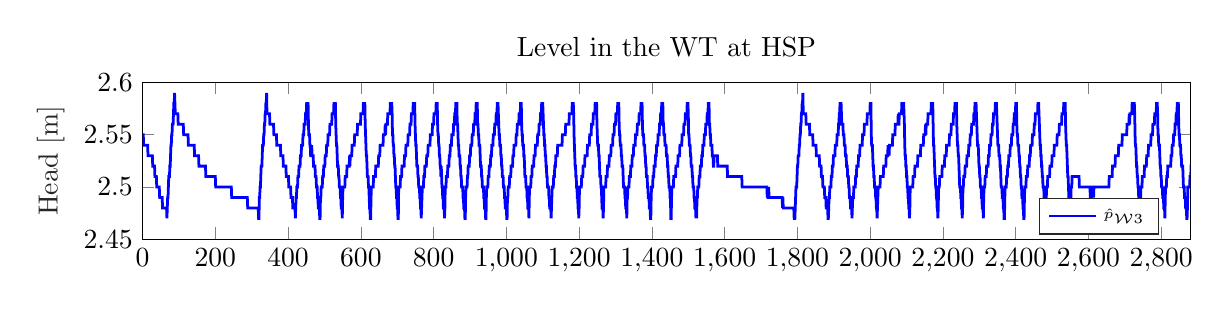
\begin{tikzpicture}

\begin{axis}[%
width=5.239in,
height=0.784in,
at={(1.017in,0.434in)},
scale only axis,
xmin=0,
xmax=2880,
%xlabel style={font=\color{white!15!black}},
%xlabel={Time [min]},
ymin=2.45,
ymax=2.6,
ylabel style={font=\color{white!15!black}},
ylabel={Head  [m]},
axis background/.style={fill=white},
title style={},
title={Level in the WT at HSP},
legend style={at={(0.97,0.03)}, anchor=south east, legend cell align=left, align=left, draw=white!15!black}
]
\addplot [color=blue, line width=1.0pt]
  table[row sep=crcr]{%
0	2.55\\
1	2.55\\
2	2.55\\
3	2.54\\
4	2.54\\
5	2.54\\
6	2.54\\
7	2.54\\
8	2.54\\
9	2.54\\
10	2.54\\
11	2.54\\
12	2.54\\
13	2.54\\
14	2.54\\
15	2.53\\
16	2.53\\
17	2.53\\
18	2.53\\
19	2.53\\
20	2.53\\
21	2.53\\
22	2.53\\
23	2.53\\
24	2.53\\
25	2.53\\
26	2.53\\
27	2.53\\
28	2.52\\
29	2.52\\
30	2.52\\
31	2.52\\
32	2.52\\
33	2.52\\
34	2.51\\
35	2.51\\
36	2.51\\
37	2.51\\
38	2.51\\
39	2.5\\
40	2.5\\
41	2.5\\
42	2.5\\
43	2.5\\
44	2.5\\
45	2.5\\
46	2.5\\
47	2.49\\
48	2.49\\
49	2.49\\
50	2.49\\
51	2.49\\
52	2.49\\
53	2.49\\
54	2.49\\
55	2.48\\
56	2.48\\
57	2.48\\
58	2.48\\
59	2.48\\
60	2.48\\
61	2.48\\
62	2.48\\
63	2.48\\
64	2.48\\
65	2.48\\
66	2.48\\
67	2.47\\
68	2.48\\
69	2.49\\
70	2.49\\
71	2.5\\
72	2.51\\
73	2.51\\
74	2.51\\
75	2.52\\
76	2.52\\
77	2.53\\
78	2.54\\
79	2.54\\
80	2.55\\
81	2.55\\
82	2.56\\
83	2.56\\
84	2.56\\
85	2.57\\
86	2.58\\
87	2.58\\
88	2.59\\
89	2.58\\
90	2.57\\
91	2.57\\
92	2.57\\
93	2.57\\
94	2.57\\
95	2.57\\
96	2.57\\
97	2.57\\
98	2.56\\
99	2.56\\
100	2.56\\
101	2.56\\
102	2.56\\
103	2.56\\
104	2.56\\
105	2.56\\
106	2.56\\
107	2.56\\
108	2.56\\
109	2.56\\
110	2.56\\
111	2.56\\
112	2.56\\
113	2.55\\
114	2.55\\
115	2.55\\
116	2.55\\
117	2.55\\
118	2.55\\
119	2.55\\
120	2.55\\
121	2.55\\
122	2.55\\
123	2.55\\
124	2.55\\
125	2.55\\
126	2.54\\
127	2.54\\
128	2.54\\
129	2.54\\
130	2.54\\
131	2.54\\
132	2.54\\
133	2.54\\
134	2.54\\
135	2.54\\
136	2.54\\
137	2.54\\
138	2.54\\
139	2.54\\
140	2.54\\
141	2.54\\
142	2.54\\
143	2.53\\
144	2.53\\
145	2.53\\
146	2.53\\
147	2.53\\
148	2.53\\
149	2.53\\
150	2.53\\
151	2.53\\
152	2.53\\
153	2.53\\
154	2.53\\
155	2.52\\
156	2.52\\
157	2.52\\
158	2.52\\
159	2.52\\
160	2.52\\
161	2.52\\
162	2.52\\
163	2.52\\
164	2.52\\
165	2.52\\
166	2.52\\
167	2.52\\
168	2.52\\
169	2.52\\
170	2.52\\
171	2.52\\
172	2.52\\
173	2.52\\
174	2.51\\
175	2.51\\
176	2.51\\
177	2.51\\
178	2.51\\
179	2.51\\
180	2.51\\
181	2.51\\
182	2.51\\
183	2.51\\
184	2.51\\
185	2.51\\
186	2.51\\
187	2.51\\
188	2.51\\
189	2.51\\
190	2.51\\
191	2.51\\
192	2.51\\
193	2.51\\
194	2.51\\
195	2.51\\
196	2.51\\
197	2.51\\
198	2.51\\
199	2.51\\
200	2.51\\
201	2.5\\
202	2.5\\
203	2.5\\
204	2.5\\
205	2.5\\
206	2.5\\
207	2.5\\
208	2.5\\
209	2.5\\
210	2.5\\
211	2.5\\
212	2.5\\
213	2.5\\
214	2.5\\
215	2.5\\
216	2.5\\
217	2.5\\
218	2.5\\
219	2.5\\
220	2.5\\
221	2.5\\
222	2.5\\
223	2.5\\
224	2.5\\
225	2.5\\
226	2.5\\
227	2.5\\
228	2.5\\
229	2.5\\
230	2.5\\
231	2.5\\
232	2.5\\
233	2.5\\
234	2.5\\
235	2.5\\
236	2.5\\
237	2.5\\
238	2.5\\
239	2.5\\
240	2.5\\
241	2.5\\
242	2.5\\
243	2.5\\
244	2.5\\
245	2.49\\
246	2.49\\
247	2.49\\
248	2.49\\
249	2.49\\
250	2.49\\
251	2.49\\
252	2.49\\
253	2.49\\
254	2.49\\
255	2.49\\
256	2.49\\
257	2.49\\
258	2.49\\
259	2.49\\
260	2.49\\
261	2.49\\
262	2.49\\
263	2.49\\
264	2.49\\
265	2.49\\
266	2.49\\
267	2.49\\
268	2.49\\
269	2.49\\
270	2.49\\
271	2.49\\
272	2.49\\
273	2.49\\
274	2.49\\
275	2.49\\
276	2.49\\
277	2.49\\
278	2.49\\
279	2.49\\
280	2.49\\
281	2.49\\
282	2.49\\
283	2.49\\
284	2.49\\
285	2.49\\
286	2.49\\
287	2.49\\
288	2.49\\
289	2.48\\
290	2.48\\
291	2.48\\
292	2.48\\
293	2.48\\
294	2.48\\
295	2.48\\
296	2.48\\
297	2.48\\
298	2.48\\
299	2.48\\
300	2.48\\
301	2.48\\
302	2.48\\
303	2.48\\
304	2.48\\
305	2.48\\
306	2.48\\
307	2.48\\
308	2.48\\
309	2.48\\
310	2.48\\
311	2.48\\
312	2.48\\
313	2.48\\
314	2.48\\
315	2.48\\
316	2.48\\
317	2.48\\
318	2.48\\
319	2.47\\
320	2.47\\
321	2.49\\
322	2.49\\
323	2.5\\
324	2.5\\
325	2.51\\
326	2.52\\
327	2.52\\
328	2.52\\
329	2.53\\
330	2.54\\
331	2.54\\
332	2.54\\
333	2.55\\
334	2.55\\
335	2.56\\
336	2.56\\
337	2.57\\
338	2.57\\
339	2.58\\
340	2.58\\
341	2.59\\
342	2.57\\
343	2.57\\
344	2.57\\
345	2.57\\
346	2.57\\
347	2.57\\
348	2.57\\
349	2.57\\
350	2.56\\
351	2.56\\
352	2.56\\
353	2.56\\
354	2.56\\
355	2.56\\
356	2.56\\
357	2.56\\
358	2.56\\
359	2.56\\
360	2.56\\
361	2.55\\
362	2.55\\
363	2.55\\
364	2.55\\
365	2.55\\
366	2.55\\
367	2.55\\
368	2.55\\
369	2.54\\
370	2.54\\
371	2.54\\
372	2.54\\
373	2.54\\
374	2.54\\
375	2.54\\
376	2.54\\
377	2.54\\
378	2.54\\
379	2.54\\
380	2.53\\
381	2.53\\
382	2.53\\
383	2.53\\
384	2.53\\
385	2.53\\
386	2.53\\
387	2.52\\
388	2.52\\
389	2.52\\
390	2.52\\
391	2.52\\
392	2.52\\
393	2.52\\
394	2.52\\
395	2.51\\
396	2.51\\
397	2.51\\
398	2.51\\
399	2.51\\
400	2.51\\
401	2.51\\
402	2.5\\
403	2.5\\
404	2.5\\
405	2.5\\
406	2.5\\
407	2.5\\
408	2.49\\
409	2.49\\
410	2.49\\
411	2.49\\
412	2.49\\
413	2.48\\
414	2.48\\
415	2.48\\
416	2.48\\
417	2.48\\
418	2.48\\
419	2.48\\
420	2.47\\
421	2.48\\
422	2.49\\
423	2.49\\
424	2.5\\
425	2.5\\
426	2.5\\
427	2.51\\
428	2.51\\
429	2.51\\
430	2.52\\
431	2.52\\
432	2.52\\
433	2.52\\
434	2.53\\
435	2.53\\
436	2.53\\
437	2.54\\
438	2.54\\
439	2.54\\
440	2.54\\
441	2.55\\
442	2.55\\
443	2.55\\
444	2.56\\
445	2.56\\
446	2.56\\
447	2.56\\
448	2.57\\
449	2.57\\
450	2.57\\
451	2.58\\
452	2.58\\
453	2.58\\
454	2.58\\
455	2.58\\
456	2.56\\
457	2.55\\
458	2.55\\
459	2.55\\
460	2.54\\
461	2.54\\
462	2.53\\
463	2.53\\
464	2.53\\
465	2.54\\
466	2.53\\
467	2.53\\
468	2.53\\
469	2.53\\
470	2.52\\
471	2.52\\
472	2.52\\
473	2.52\\
474	2.52\\
475	2.51\\
476	2.51\\
477	2.51\\
478	2.5\\
479	2.5\\
480	2.5\\
481	2.49\\
482	2.49\\
483	2.48\\
484	2.48\\
485	2.48\\
486	2.48\\
487	2.47\\
488	2.47\\
489	2.49\\
490	2.49\\
491	2.5\\
492	2.5\\
493	2.5\\
494	2.5\\
495	2.51\\
496	2.51\\
497	2.51\\
498	2.52\\
499	2.52\\
500	2.52\\
501	2.52\\
502	2.53\\
503	2.53\\
504	2.53\\
505	2.53\\
506	2.54\\
507	2.54\\
508	2.54\\
509	2.54\\
510	2.55\\
511	2.55\\
512	2.55\\
513	2.55\\
514	2.55\\
515	2.56\\
516	2.56\\
517	2.56\\
518	2.56\\
519	2.56\\
520	2.56\\
521	2.57\\
522	2.57\\
523	2.57\\
524	2.57\\
525	2.57\\
526	2.58\\
527	2.58\\
528	2.58\\
529	2.58\\
530	2.58\\
531	2.56\\
532	2.55\\
533	2.54\\
534	2.54\\
535	2.53\\
536	2.52\\
537	2.52\\
538	2.52\\
539	2.51\\
540	2.51\\
541	2.5\\
542	2.5\\
543	2.5\\
544	2.49\\
545	2.49\\
546	2.48\\
547	2.48\\
548	2.48\\
549	2.47\\
550	2.49\\
551	2.5\\
552	2.5\\
553	2.5\\
554	2.5\\
555	2.5\\
556	2.5\\
557	2.51\\
558	2.51\\
559	2.51\\
560	2.51\\
561	2.51\\
562	2.52\\
563	2.52\\
564	2.52\\
565	2.52\\
566	2.52\\
567	2.52\\
568	2.52\\
569	2.53\\
570	2.52\\
571	2.53\\
572	2.53\\
573	2.53\\
574	2.53\\
575	2.53\\
576	2.54\\
577	2.54\\
578	2.54\\
579	2.54\\
580	2.54\\
581	2.54\\
582	2.54\\
583	2.55\\
584	2.55\\
585	2.55\\
586	2.55\\
587	2.55\\
588	2.55\\
589	2.55\\
590	2.55\\
591	2.56\\
592	2.56\\
593	2.56\\
594	2.56\\
595	2.56\\
596	2.56\\
597	2.56\\
598	2.56\\
599	2.56\\
600	2.57\\
601	2.57\\
602	2.57\\
603	2.57\\
604	2.57\\
605	2.57\\
606	2.57\\
607	2.58\\
608	2.58\\
609	2.58\\
610	2.58\\
611	2.58\\
612	2.56\\
613	2.55\\
614	2.54\\
615	2.53\\
616	2.53\\
617	2.52\\
618	2.51\\
619	2.51\\
620	2.51\\
621	2.5\\
622	2.5\\
623	2.49\\
624	2.48\\
625	2.48\\
626	2.47\\
627	2.47\\
628	2.49\\
629	2.5\\
630	2.5\\
631	2.5\\
632	2.5\\
633	2.5\\
634	2.5\\
635	2.51\\
636	2.51\\
637	2.51\\
638	2.51\\
639	2.51\\
640	2.51\\
641	2.52\\
642	2.52\\
643	2.52\\
644	2.52\\
645	2.52\\
646	2.52\\
647	2.52\\
648	2.52\\
649	2.53\\
650	2.53\\
651	2.53\\
652	2.53\\
653	2.54\\
654	2.54\\
655	2.54\\
656	2.54\\
657	2.54\\
658	2.54\\
659	2.54\\
660	2.54\\
661	2.54\\
662	2.55\\
663	2.55\\
664	2.55\\
665	2.55\\
666	2.55\\
667	2.56\\
668	2.55\\
669	2.56\\
670	2.56\\
671	2.56\\
672	2.56\\
673	2.56\\
674	2.57\\
675	2.57\\
676	2.57\\
677	2.57\\
678	2.57\\
679	2.57\\
680	2.57\\
681	2.58\\
682	2.58\\
683	2.58\\
684	2.58\\
685	2.58\\
686	2.57\\
687	2.55\\
688	2.55\\
689	2.54\\
690	2.54\\
691	2.53\\
692	2.53\\
693	2.52\\
694	2.52\\
695	2.51\\
696	2.5\\
697	2.5\\
698	2.49\\
699	2.49\\
700	2.48\\
701	2.48\\
702	2.47\\
703	2.47\\
704	2.5\\
705	2.5\\
706	2.5\\
707	2.5\\
708	2.5\\
709	2.51\\
710	2.51\\
711	2.51\\
712	2.51\\
713	2.52\\
714	2.52\\
715	2.52\\
716	2.52\\
717	2.52\\
718	2.52\\
719	2.52\\
720	2.53\\
721	2.53\\
722	2.53\\
723	2.53\\
724	2.54\\
725	2.54\\
726	2.54\\
727	2.54\\
728	2.54\\
729	2.54\\
730	2.55\\
731	2.55\\
732	2.55\\
733	2.55\\
734	2.55\\
735	2.56\\
736	2.56\\
737	2.56\\
738	2.56\\
739	2.57\\
740	2.57\\
741	2.57\\
742	2.57\\
743	2.57\\
744	2.58\\
745	2.58\\
746	2.58\\
747	2.58\\
748	2.58\\
749	2.56\\
750	2.55\\
751	2.54\\
752	2.54\\
753	2.53\\
754	2.52\\
755	2.52\\
756	2.52\\
757	2.51\\
758	2.51\\
759	2.5\\
760	2.5\\
761	2.5\\
762	2.49\\
763	2.49\\
764	2.48\\
765	2.48\\
766	2.47\\
767	2.48\\
768	2.49\\
769	2.5\\
770	2.5\\
771	2.5\\
772	2.5\\
773	2.51\\
774	2.51\\
775	2.51\\
776	2.52\\
777	2.52\\
778	2.52\\
779	2.52\\
780	2.52\\
781	2.53\\
782	2.53\\
783	2.53\\
784	2.53\\
785	2.54\\
786	2.54\\
787	2.54\\
788	2.54\\
789	2.54\\
790	2.54\\
791	2.55\\
792	2.55\\
793	2.55\\
794	2.55\\
795	2.55\\
796	2.55\\
797	2.56\\
798	2.56\\
799	2.56\\
800	2.56\\
801	2.57\\
802	2.57\\
803	2.57\\
804	2.57\\
805	2.57\\
806	2.57\\
807	2.58\\
808	2.58\\
809	2.58\\
810	2.58\\
811	2.56\\
812	2.55\\
813	2.55\\
814	2.54\\
815	2.54\\
816	2.53\\
817	2.53\\
818	2.52\\
819	2.52\\
820	2.51\\
821	2.52\\
822	2.51\\
823	2.5\\
824	2.5\\
825	2.49\\
826	2.49\\
827	2.48\\
828	2.48\\
829	2.48\\
830	2.47\\
831	2.48\\
832	2.5\\
833	2.5\\
834	2.5\\
835	2.51\\
836	2.51\\
837	2.51\\
838	2.51\\
839	2.52\\
840	2.52\\
841	2.52\\
842	2.52\\
843	2.53\\
844	2.53\\
845	2.53\\
846	2.54\\
847	2.54\\
848	2.54\\
849	2.54\\
850	2.55\\
851	2.55\\
852	2.55\\
853	2.55\\
854	2.55\\
855	2.56\\
856	2.56\\
857	2.56\\
858	2.57\\
859	2.57\\
860	2.57\\
861	2.58\\
862	2.58\\
863	2.58\\
864	2.58\\
865	2.56\\
866	2.56\\
867	2.55\\
868	2.54\\
869	2.54\\
870	2.53\\
871	2.53\\
872	2.53\\
873	2.52\\
874	2.52\\
875	2.51\\
876	2.51\\
877	2.5\\
878	2.5\\
879	2.5\\
880	2.5\\
881	2.49\\
882	2.49\\
883	2.48\\
884	2.48\\
885	2.48\\
886	2.47\\
887	2.47\\
888	2.49\\
889	2.5\\
890	2.5\\
891	2.5\\
892	2.5\\
893	2.51\\
894	2.51\\
895	2.52\\
896	2.52\\
897	2.52\\
898	2.52\\
899	2.53\\
900	2.53\\
901	2.53\\
902	2.54\\
903	2.54\\
904	2.54\\
905	2.54\\
906	2.55\\
907	2.55\\
908	2.55\\
909	2.55\\
910	2.56\\
911	2.56\\
912	2.56\\
913	2.56\\
914	2.57\\
915	2.57\\
916	2.57\\
917	2.58\\
918	2.58\\
919	2.58\\
920	2.58\\
921	2.56\\
922	2.56\\
923	2.55\\
924	2.55\\
925	2.54\\
926	2.54\\
927	2.54\\
928	2.53\\
929	2.52\\
930	2.52\\
931	2.52\\
932	2.51\\
933	2.51\\
934	2.5\\
935	2.5\\
936	2.5\\
937	2.5\\
938	2.49\\
939	2.49\\
940	2.48\\
941	2.48\\
942	2.48\\
943	2.47\\
944	2.47\\
945	2.49\\
946	2.5\\
947	2.5\\
948	2.5\\
949	2.5\\
950	2.51\\
951	2.51\\
952	2.51\\
953	2.52\\
954	2.52\\
955	2.52\\
956	2.52\\
957	2.53\\
958	2.53\\
959	2.53\\
960	2.54\\
961	2.54\\
962	2.54\\
963	2.54\\
964	2.55\\
965	2.55\\
966	2.55\\
967	2.55\\
968	2.56\\
969	2.56\\
970	2.56\\
971	2.56\\
972	2.57\\
973	2.57\\
974	2.57\\
975	2.58\\
976	2.58\\
977	2.58\\
978	2.57\\
979	2.56\\
980	2.55\\
981	2.55\\
982	2.54\\
983	2.54\\
984	2.54\\
985	2.53\\
986	2.53\\
987	2.52\\
988	2.52\\
989	2.51\\
990	2.51\\
991	2.51\\
992	2.5\\
993	2.5\\
994	2.5\\
995	2.49\\
996	2.49\\
997	2.48\\
998	2.48\\
999	2.48\\
1000	2.48\\
1001	2.47\\
1002	2.47\\
1003	2.49\\
1004	2.49\\
1005	2.5\\
1006	2.5\\
1007	2.5\\
1008	2.5\\
1009	2.51\\
1010	2.51\\
1011	2.51\\
1012	2.51\\
1013	2.52\\
1014	2.52\\
1015	2.52\\
1016	2.52\\
1017	2.52\\
1018	2.53\\
1019	2.53\\
1020	2.53\\
1021	2.54\\
1022	2.54\\
1023	2.54\\
1024	2.54\\
1025	2.54\\
1026	2.54\\
1027	2.55\\
1028	2.55\\
1029	2.55\\
1030	2.56\\
1031	2.56\\
1032	2.56\\
1033	2.56\\
1034	2.56\\
1035	2.57\\
1036	2.57\\
1037	2.57\\
1038	2.57\\
1039	2.58\\
1040	2.58\\
1041	2.58\\
1042	2.56\\
1043	2.55\\
1044	2.55\\
1045	2.54\\
1046	2.54\\
1047	2.54\\
1048	2.53\\
1049	2.53\\
1050	2.52\\
1051	2.51\\
1052	2.51\\
1053	2.51\\
1054	2.5\\
1055	2.5\\
1056	2.5\\
1057	2.49\\
1058	2.49\\
1059	2.48\\
1060	2.48\\
1061	2.48\\
1062	2.47\\
1063	2.49\\
1064	2.5\\
1065	2.5\\
1066	2.5\\
1067	2.5\\
1068	2.51\\
1069	2.51\\
1070	2.51\\
1071	2.52\\
1072	2.52\\
1073	2.52\\
1074	2.52\\
1075	2.52\\
1076	2.53\\
1077	2.53\\
1078	2.53\\
1079	2.53\\
1080	2.54\\
1081	2.54\\
1082	2.54\\
1083	2.54\\
1084	2.54\\
1085	2.54\\
1086	2.55\\
1087	2.55\\
1088	2.55\\
1089	2.55\\
1090	2.56\\
1091	2.56\\
1092	2.56\\
1093	2.56\\
1094	2.57\\
1095	2.57\\
1096	2.57\\
1097	2.58\\
1098	2.58\\
1099	2.58\\
1100	2.58\\
1101	2.57\\
1102	2.56\\
1103	2.55\\
1104	2.55\\
1105	2.54\\
1106	2.54\\
1107	2.53\\
1108	2.53\\
1109	2.52\\
1110	2.52\\
1111	2.51\\
1112	2.51\\
1113	2.5\\
1114	2.5\\
1115	2.5\\
1116	2.5\\
1117	2.49\\
1118	2.49\\
1119	2.48\\
1120	2.48\\
1121	2.48\\
1122	2.48\\
1123	2.47\\
1124	2.48\\
1125	2.49\\
1126	2.5\\
1127	2.5\\
1128	2.5\\
1129	2.5\\
1130	2.51\\
1131	2.51\\
1132	2.51\\
1133	2.52\\
1134	2.52\\
1135	2.52\\
1136	2.53\\
1137	2.53\\
1138	2.53\\
1139	2.53\\
1140	2.53\\
1141	2.54\\
1142	2.54\\
1143	2.54\\
1144	2.54\\
1145	2.54\\
1146	2.54\\
1147	2.54\\
1148	2.54\\
1149	2.54\\
1150	2.54\\
1151	2.54\\
1152	2.54\\
1153	2.54\\
1154	2.55\\
1155	2.55\\
1156	2.55\\
1157	2.55\\
1158	2.55\\
1159	2.55\\
1160	2.55\\
1161	2.55\\
1162	2.55\\
1163	2.56\\
1164	2.56\\
1165	2.56\\
1166	2.56\\
1167	2.56\\
1168	2.56\\
1169	2.56\\
1170	2.56\\
1171	2.56\\
1172	2.56\\
1173	2.57\\
1174	2.57\\
1175	2.57\\
1176	2.57\\
1177	2.57\\
1178	2.57\\
1179	2.57\\
1180	2.57\\
1181	2.58\\
1182	2.58\\
1183	2.58\\
1184	2.58\\
1185	2.57\\
1186	2.55\\
1187	2.54\\
1188	2.53\\
1189	2.52\\
1190	2.52\\
1191	2.51\\
1192	2.51\\
1193	2.5\\
1194	2.5\\
1195	2.49\\
1196	2.49\\
1197	2.48\\
1198	2.48\\
1199	2.47\\
1200	2.48\\
1201	2.5\\
1202	2.5\\
1203	2.5\\
1204	2.5\\
1205	2.5\\
1206	2.5\\
1207	2.51\\
1208	2.51\\
1209	2.51\\
1210	2.51\\
1211	2.52\\
1212	2.52\\
1213	2.52\\
1214	2.52\\
1215	2.52\\
1216	2.53\\
1217	2.53\\
1218	2.53\\
1219	2.53\\
1220	2.53\\
1221	2.53\\
1222	2.53\\
1223	2.54\\
1224	2.54\\
1225	2.54\\
1226	2.54\\
1227	2.54\\
1228	2.54\\
1229	2.55\\
1230	2.55\\
1231	2.55\\
1232	2.55\\
1233	2.55\\
1234	2.56\\
1235	2.56\\
1236	2.56\\
1237	2.56\\
1238	2.56\\
1239	2.57\\
1240	2.57\\
1241	2.57\\
1242	2.57\\
1243	2.57\\
1244	2.58\\
1245	2.58\\
1246	2.58\\
1247	2.58\\
1248	2.58\\
1249	2.56\\
1250	2.55\\
1251	2.54\\
1252	2.54\\
1253	2.54\\
1254	2.53\\
1255	2.53\\
1256	2.52\\
1257	2.51\\
1258	2.51\\
1259	2.51\\
1260	2.5\\
1261	2.5\\
1262	2.49\\
1263	2.48\\
1264	2.48\\
1265	2.48\\
1266	2.47\\
1267	2.48\\
1268	2.5\\
1269	2.5\\
1270	2.5\\
1271	2.5\\
1272	2.5\\
1273	2.5\\
1274	2.51\\
1275	2.51\\
1276	2.51\\
1277	2.51\\
1278	2.52\\
1279	2.52\\
1280	2.52\\
1281	2.52\\
1282	2.52\\
1283	2.53\\
1284	2.53\\
1285	2.53\\
1286	2.53\\
1287	2.53\\
1288	2.54\\
1289	2.54\\
1290	2.54\\
1291	2.54\\
1292	2.54\\
1293	2.55\\
1294	2.55\\
1295	2.55\\
1296	2.55\\
1297	2.56\\
1298	2.56\\
1299	2.56\\
1300	2.56\\
1301	2.57\\
1302	2.57\\
1303	2.57\\
1304	2.57\\
1305	2.57\\
1306	2.58\\
1307	2.58\\
1308	2.58\\
1309	2.58\\
1310	2.56\\
1311	2.55\\
1312	2.55\\
1313	2.54\\
1314	2.54\\
1315	2.54\\
1316	2.53\\
1317	2.53\\
1318	2.52\\
1319	2.52\\
1320	2.52\\
1321	2.51\\
1322	2.5\\
1323	2.5\\
1324	2.5\\
1325	2.5\\
1326	2.49\\
1327	2.49\\
1328	2.48\\
1329	2.48\\
1330	2.48\\
1331	2.47\\
1332	2.49\\
1333	2.49\\
1334	2.5\\
1335	2.5\\
1336	2.5\\
1337	2.5\\
1338	2.51\\
1339	2.51\\
1340	2.51\\
1341	2.51\\
1342	2.52\\
1343	2.52\\
1344	2.52\\
1345	2.52\\
1346	2.53\\
1347	2.53\\
1348	2.53\\
1349	2.53\\
1350	2.54\\
1351	2.54\\
1352	2.54\\
1353	2.54\\
1354	2.54\\
1355	2.55\\
1356	2.55\\
1357	2.55\\
1358	2.55\\
1359	2.55\\
1360	2.56\\
1361	2.56\\
1362	2.56\\
1363	2.56\\
1364	2.56\\
1365	2.57\\
1366	2.57\\
1367	2.57\\
1368	2.57\\
1369	2.57\\
1370	2.58\\
1371	2.58\\
1372	2.58\\
1373	2.58\\
1374	2.56\\
1375	2.55\\
1376	2.55\\
1377	2.55\\
1378	2.54\\
1379	2.54\\
1380	2.54\\
1381	2.53\\
1382	2.53\\
1383	2.52\\
1384	2.52\\
1385	2.51\\
1386	2.51\\
1387	2.51\\
1388	2.5\\
1389	2.5\\
1390	2.49\\
1391	2.49\\
1392	2.49\\
1393	2.48\\
1394	2.48\\
1395	2.48\\
1396	2.47\\
1397	2.47\\
1398	2.49\\
1399	2.5\\
1400	2.5\\
1401	2.5\\
1402	2.5\\
1403	2.51\\
1404	2.51\\
1405	2.51\\
1406	2.52\\
1407	2.52\\
1408	2.52\\
1409	2.52\\
1410	2.53\\
1411	2.53\\
1412	2.53\\
1413	2.54\\
1414	2.54\\
1415	2.54\\
1416	2.54\\
1417	2.55\\
1418	2.55\\
1419	2.55\\
1420	2.55\\
1421	2.56\\
1422	2.56\\
1423	2.56\\
1424	2.57\\
1425	2.57\\
1426	2.57\\
1427	2.58\\
1428	2.58\\
1429	2.58\\
1430	2.58\\
1431	2.56\\
1432	2.56\\
1433	2.55\\
1434	2.55\\
1435	2.55\\
1436	2.54\\
1437	2.54\\
1438	2.54\\
1439	2.54\\
1440	2.53\\
1441	2.53\\
1442	2.53\\
1443	2.52\\
1444	2.52\\
1445	2.51\\
1446	2.51\\
1447	2.5\\
1448	2.5\\
1449	2.5\\
1450	2.49\\
1451	2.49\\
1452	2.47\\
1453	2.47\\
1454	2.49\\
1455	2.5\\
1456	2.5\\
1457	2.5\\
1458	2.5\\
1459	2.5\\
1460	2.51\\
1461	2.51\\
1462	2.51\\
1463	2.51\\
1464	2.51\\
1465	2.51\\
1466	2.52\\
1467	2.52\\
1468	2.52\\
1469	2.52\\
1470	2.52\\
1471	2.52\\
1472	2.53\\
1473	2.53\\
1474	2.53\\
1475	2.53\\
1476	2.53\\
1477	2.54\\
1478	2.54\\
1479	2.54\\
1480	2.54\\
1481	2.54\\
1482	2.54\\
1483	2.55\\
1484	2.55\\
1485	2.55\\
1486	2.55\\
1487	2.55\\
1488	2.56\\
1489	2.56\\
1490	2.56\\
1491	2.56\\
1492	2.57\\
1493	2.57\\
1494	2.57\\
1495	2.57\\
1496	2.57\\
1497	2.58\\
1498	2.58\\
1499	2.58\\
1500	2.57\\
1501	2.55\\
1502	2.55\\
1503	2.54\\
1504	2.54\\
1505	2.54\\
1506	2.53\\
1507	2.53\\
1508	2.52\\
1509	2.52\\
1510	2.52\\
1511	2.51\\
1512	2.51\\
1513	2.5\\
1514	2.5\\
1515	2.5\\
1516	2.49\\
1517	2.49\\
1518	2.48\\
1519	2.48\\
1520	2.48\\
1521	2.47\\
1522	2.48\\
1523	2.47\\
1524	2.49\\
1525	2.49\\
1526	2.5\\
1527	2.5\\
1528	2.5\\
1529	2.5\\
1530	2.51\\
1531	2.51\\
1532	2.51\\
1533	2.52\\
1534	2.52\\
1535	2.52\\
1536	2.52\\
1537	2.53\\
1538	2.53\\
1539	2.53\\
1540	2.54\\
1541	2.54\\
1542	2.54\\
1543	2.54\\
1544	2.55\\
1545	2.55\\
1546	2.55\\
1547	2.55\\
1548	2.56\\
1549	2.56\\
1550	2.56\\
1551	2.56\\
1552	2.57\\
1553	2.57\\
1554	2.57\\
1555	2.58\\
1556	2.58\\
1557	2.58\\
1558	2.56\\
1559	2.56\\
1560	2.55\\
1561	2.55\\
1562	2.54\\
1563	2.54\\
1564	2.54\\
1565	2.54\\
1566	2.53\\
1567	2.53\\
1568	2.53\\
1569	2.52\\
1570	2.52\\
1571	2.53\\
1572	2.53\\
1573	2.53\\
1574	2.53\\
1575	2.53\\
1576	2.53\\
1577	2.53\\
1578	2.53\\
1579	2.53\\
1580	2.53\\
1581	2.52\\
1582	2.52\\
1583	2.52\\
1584	2.52\\
1585	2.52\\
1586	2.52\\
1587	2.52\\
1588	2.52\\
1589	2.52\\
1590	2.52\\
1591	2.52\\
1592	2.52\\
1593	2.52\\
1594	2.52\\
1595	2.52\\
1596	2.52\\
1597	2.52\\
1598	2.52\\
1599	2.52\\
1600	2.52\\
1601	2.52\\
1602	2.52\\
1603	2.52\\
1604	2.52\\
1605	2.52\\
1606	2.52\\
1607	2.52\\
1608	2.51\\
1609	2.51\\
1610	2.51\\
1611	2.51\\
1612	2.51\\
1613	2.51\\
1614	2.51\\
1615	2.51\\
1616	2.51\\
1617	2.51\\
1618	2.51\\
1619	2.51\\
1620	2.51\\
1621	2.51\\
1622	2.51\\
1623	2.51\\
1624	2.51\\
1625	2.51\\
1626	2.51\\
1627	2.51\\
1628	2.51\\
1629	2.51\\
1630	2.51\\
1631	2.51\\
1632	2.51\\
1633	2.51\\
1634	2.51\\
1635	2.51\\
1636	2.51\\
1637	2.51\\
1638	2.51\\
1639	2.51\\
1640	2.51\\
1641	2.51\\
1642	2.51\\
1643	2.51\\
1644	2.51\\
1645	2.51\\
1646	2.51\\
1647	2.51\\
1648	2.5\\
1649	2.5\\
1650	2.5\\
1651	2.5\\
1652	2.5\\
1653	2.5\\
1654	2.5\\
1655	2.5\\
1656	2.5\\
1657	2.5\\
1658	2.5\\
1659	2.5\\
1660	2.5\\
1661	2.5\\
1662	2.5\\
1663	2.5\\
1664	2.5\\
1665	2.5\\
1666	2.5\\
1667	2.5\\
1668	2.5\\
1669	2.5\\
1670	2.5\\
1671	2.5\\
1672	2.5\\
1673	2.5\\
1674	2.5\\
1675	2.5\\
1676	2.5\\
1677	2.5\\
1678	2.5\\
1679	2.5\\
1680	2.5\\
1681	2.5\\
1682	2.5\\
1683	2.5\\
1684	2.5\\
1685	2.5\\
1686	2.5\\
1687	2.5\\
1688	2.5\\
1689	2.5\\
1690	2.5\\
1691	2.5\\
1692	2.5\\
1693	2.5\\
1694	2.5\\
1695	2.5\\
1696	2.5\\
1697	2.5\\
1698	2.5\\
1699	2.5\\
1700	2.5\\
1701	2.5\\
1702	2.5\\
1703	2.5\\
1704	2.5\\
1705	2.5\\
1706	2.5\\
1707	2.5\\
1708	2.5\\
1709	2.5\\
1710	2.5\\
1711	2.5\\
1712	2.5\\
1713	2.5\\
1714	2.5\\
1715	2.5\\
1716	2.5\\
1717	2.49\\
1718	2.5\\
1719	2.49\\
1720	2.49\\
1721	2.5\\
1722	2.49\\
1723	2.49\\
1724	2.49\\
1725	2.49\\
1726	2.49\\
1727	2.49\\
1728	2.49\\
1729	2.49\\
1730	2.49\\
1731	2.49\\
1732	2.49\\
1733	2.49\\
1734	2.49\\
1735	2.49\\
1736	2.49\\
1737	2.49\\
1738	2.49\\
1739	2.49\\
1740	2.49\\
1741	2.49\\
1742	2.49\\
1743	2.49\\
1744	2.49\\
1745	2.49\\
1746	2.49\\
1747	2.49\\
1748	2.49\\
1749	2.49\\
1750	2.49\\
1751	2.49\\
1752	2.49\\
1753	2.49\\
1754	2.49\\
1755	2.49\\
1756	2.49\\
1757	2.49\\
1758	2.49\\
1759	2.48\\
1760	2.49\\
1761	2.48\\
1762	2.48\\
1763	2.48\\
1764	2.48\\
1765	2.48\\
1766	2.48\\
1767	2.48\\
1768	2.48\\
1769	2.48\\
1770	2.48\\
1771	2.48\\
1772	2.48\\
1773	2.48\\
1774	2.48\\
1775	2.48\\
1776	2.48\\
1777	2.48\\
1778	2.48\\
1779	2.48\\
1780	2.48\\
1781	2.48\\
1782	2.48\\
1783	2.48\\
1784	2.48\\
1785	2.48\\
1786	2.48\\
1787	2.48\\
1788	2.48\\
1789	2.48\\
1790	2.48\\
1791	2.47\\
1792	2.47\\
1793	2.47\\
1794	2.48\\
1795	2.49\\
1796	2.5\\
1797	2.5\\
1798	2.5\\
1799	2.51\\
1800	2.52\\
1801	2.52\\
1802	2.53\\
1803	2.53\\
1804	2.53\\
1805	2.54\\
1806	2.54\\
1807	2.55\\
1808	2.55\\
1809	2.56\\
1810	2.56\\
1811	2.57\\
1812	2.57\\
1813	2.58\\
1814	2.58\\
1815	2.59\\
1816	2.57\\
1817	2.57\\
1818	2.57\\
1819	2.57\\
1820	2.57\\
1821	2.57\\
1822	2.57\\
1823	2.57\\
1824	2.56\\
1825	2.56\\
1826	2.56\\
1827	2.56\\
1828	2.56\\
1829	2.56\\
1830	2.56\\
1831	2.56\\
1832	2.56\\
1833	2.56\\
1834	2.55\\
1835	2.55\\
1836	2.55\\
1837	2.55\\
1838	2.55\\
1839	2.55\\
1840	2.55\\
1841	2.55\\
1842	2.55\\
1843	2.54\\
1844	2.54\\
1845	2.54\\
1846	2.54\\
1847	2.54\\
1848	2.54\\
1849	2.54\\
1850	2.54\\
1851	2.54\\
1852	2.53\\
1853	2.53\\
1854	2.53\\
1855	2.53\\
1856	2.53\\
1857	2.53\\
1858	2.53\\
1859	2.53\\
1860	2.53\\
1861	2.52\\
1862	2.52\\
1863	2.52\\
1864	2.52\\
1865	2.52\\
1866	2.51\\
1867	2.51\\
1868	2.51\\
1869	2.51\\
1870	2.5\\
1871	2.5\\
1872	2.5\\
1873	2.5\\
1874	2.5\\
1875	2.49\\
1876	2.49\\
1877	2.49\\
1878	2.49\\
1879	2.48\\
1880	2.48\\
1881	2.48\\
1882	2.48\\
1883	2.48\\
1884	2.47\\
1885	2.47\\
1886	2.48\\
1887	2.49\\
1888	2.49\\
1889	2.5\\
1890	2.5\\
1891	2.5\\
1892	2.5\\
1893	2.51\\
1894	2.51\\
1895	2.51\\
1896	2.52\\
1897	2.52\\
1898	2.52\\
1899	2.53\\
1900	2.53\\
1901	2.53\\
1902	2.53\\
1903	2.53\\
1904	2.54\\
1905	2.54\\
1906	2.54\\
1907	2.54\\
1908	2.54\\
1909	2.55\\
1910	2.55\\
1911	2.55\\
1912	2.55\\
1913	2.56\\
1914	2.56\\
1915	2.57\\
1916	2.57\\
1917	2.58\\
1918	2.58\\
1919	2.58\\
1920	2.58\\
1921	2.57\\
1922	2.56\\
1923	2.56\\
1924	2.56\\
1925	2.56\\
1926	2.55\\
1927	2.55\\
1928	2.55\\
1929	2.54\\
1930	2.54\\
1931	2.54\\
1932	2.53\\
1933	2.53\\
1934	2.53\\
1935	2.52\\
1936	2.52\\
1937	2.52\\
1938	2.51\\
1939	2.51\\
1940	2.51\\
1941	2.5\\
1942	2.5\\
1943	2.49\\
1944	2.49\\
1945	2.49\\
1946	2.48\\
1947	2.48\\
1948	2.48\\
1949	2.48\\
1950	2.47\\
1951	2.48\\
1952	2.49\\
1953	2.49\\
1954	2.49\\
1955	2.5\\
1956	2.5\\
1957	2.5\\
1958	2.5\\
1959	2.5\\
1960	2.51\\
1961	2.51\\
1962	2.51\\
1963	2.52\\
1964	2.52\\
1965	2.52\\
1966	2.52\\
1967	2.52\\
1968	2.53\\
1969	2.53\\
1970	2.53\\
1971	2.53\\
1972	2.54\\
1973	2.54\\
1974	2.54\\
1975	2.54\\
1976	2.54\\
1977	2.54\\
1978	2.54\\
1979	2.55\\
1980	2.55\\
1981	2.55\\
1982	2.55\\
1983	2.55\\
1984	2.56\\
1985	2.56\\
1986	2.56\\
1987	2.56\\
1988	2.56\\
1989	2.56\\
1990	2.56\\
1991	2.56\\
1992	2.57\\
1993	2.57\\
1994	2.57\\
1995	2.57\\
1996	2.57\\
1997	2.57\\
1998	2.57\\
1999	2.57\\
2000	2.58\\
2001	2.58\\
2002	2.58\\
2003	2.55\\
2004	2.54\\
2005	2.54\\
2006	2.54\\
2007	2.53\\
2008	2.52\\
2009	2.52\\
2010	2.51\\
2011	2.51\\
2012	2.5\\
2013	2.5\\
2014	2.5\\
2015	2.49\\
2016	2.49\\
2017	2.48\\
2018	2.48\\
2019	2.47\\
2020	2.48\\
2021	2.49\\
2022	2.5\\
2023	2.5\\
2024	2.5\\
2025	2.5\\
2026	2.5\\
2027	2.5\\
2028	2.51\\
2029	2.51\\
2030	2.51\\
2031	2.51\\
2032	2.51\\
2033	2.51\\
2034	2.51\\
2035	2.51\\
2036	2.51\\
2037	2.52\\
2038	2.52\\
2039	2.52\\
2040	2.52\\
2041	2.52\\
2042	2.52\\
2043	2.52\\
2044	2.53\\
2045	2.53\\
2046	2.53\\
2047	2.53\\
2048	2.53\\
2049	2.54\\
2050	2.53\\
2051	2.54\\
2052	2.53\\
2053	2.54\\
2054	2.54\\
2055	2.54\\
2056	2.54\\
2057	2.54\\
2058	2.54\\
2059	2.54\\
2060	2.54\\
2061	2.54\\
2062	2.55\\
2063	2.55\\
2064	2.55\\
2065	2.55\\
2066	2.55\\
2067	2.55\\
2068	2.55\\
2069	2.56\\
2070	2.56\\
2071	2.56\\
2072	2.56\\
2073	2.56\\
2074	2.56\\
2075	2.56\\
2076	2.56\\
2077	2.57\\
2078	2.56\\
2079	2.56\\
2080	2.57\\
2081	2.57\\
2082	2.57\\
2083	2.57\\
2084	2.57\\
2085	2.57\\
2086	2.57\\
2087	2.58\\
2088	2.58\\
2089	2.58\\
2090	2.58\\
2091	2.58\\
2092	2.58\\
2093	2.57\\
2094	2.56\\
2095	2.54\\
2096	2.53\\
2097	2.53\\
2098	2.52\\
2099	2.52\\
2100	2.51\\
2101	2.51\\
2102	2.5\\
2103	2.5\\
2104	2.49\\
2105	2.49\\
2106	2.48\\
2107	2.48\\
2108	2.47\\
2109	2.48\\
2110	2.5\\
2111	2.5\\
2112	2.5\\
2113	2.5\\
2114	2.5\\
2115	2.5\\
2116	2.5\\
2117	2.5\\
2118	2.51\\
2119	2.51\\
2120	2.51\\
2121	2.51\\
2122	2.51\\
2123	2.52\\
2124	2.52\\
2125	2.52\\
2126	2.52\\
2127	2.52\\
2128	2.52\\
2129	2.52\\
2130	2.52\\
2131	2.53\\
2132	2.53\\
2133	2.53\\
2134	2.53\\
2135	2.53\\
2136	2.53\\
2137	2.53\\
2138	2.53\\
2139	2.54\\
2140	2.54\\
2141	2.54\\
2142	2.54\\
2143	2.54\\
2144	2.54\\
2145	2.54\\
2146	2.54\\
2147	2.55\\
2148	2.55\\
2149	2.55\\
2150	2.55\\
2151	2.55\\
2152	2.56\\
2153	2.55\\
2154	2.56\\
2155	2.56\\
2156	2.56\\
2157	2.56\\
2158	2.56\\
2159	2.57\\
2160	2.57\\
2161	2.57\\
2162	2.57\\
2163	2.57\\
2164	2.57\\
2165	2.57\\
2166	2.57\\
2167	2.57\\
2168	2.58\\
2169	2.58\\
2170	2.58\\
2171	2.58\\
2172	2.58\\
2173	2.56\\
2174	2.54\\
2175	2.54\\
2176	2.53\\
2177	2.52\\
2178	2.51\\
2179	2.51\\
2180	2.5\\
2181	2.5\\
2182	2.49\\
2183	2.49\\
2184	2.48\\
2185	2.48\\
2186	2.47\\
2187	2.48\\
2188	2.5\\
2189	2.5\\
2190	2.5\\
2191	2.51\\
2192	2.51\\
2193	2.51\\
2194	2.51\\
2195	2.51\\
2196	2.51\\
2197	2.51\\
2198	2.52\\
2199	2.52\\
2200	2.52\\
2201	2.52\\
2202	2.52\\
2203	2.52\\
2204	2.52\\
2205	2.53\\
2206	2.53\\
2207	2.53\\
2208	2.53\\
2209	2.53\\
2210	2.54\\
2211	2.54\\
2212	2.54\\
2213	2.54\\
2214	2.54\\
2215	2.54\\
2216	2.54\\
2217	2.54\\
2218	2.55\\
2219	2.55\\
2220	2.55\\
2221	2.55\\
2222	2.55\\
2223	2.56\\
2224	2.56\\
2225	2.56\\
2226	2.56\\
2227	2.56\\
2228	2.56\\
2229	2.57\\
2230	2.57\\
2231	2.57\\
2232	2.57\\
2233	2.58\\
2234	2.58\\
2235	2.58\\
2236	2.58\\
2237	2.58\\
2238	2.56\\
2239	2.55\\
2240	2.54\\
2241	2.54\\
2242	2.53\\
2243	2.53\\
2244	2.52\\
2245	2.51\\
2246	2.5\\
2247	2.5\\
2248	2.5\\
2249	2.49\\
2250	2.49\\
2251	2.48\\
2252	2.48\\
2253	2.47\\
2254	2.48\\
2255	2.5\\
2256	2.5\\
2257	2.51\\
2258	2.51\\
2259	2.51\\
2260	2.51\\
2261	2.52\\
2262	2.52\\
2263	2.52\\
2264	2.52\\
2265	2.52\\
2266	2.53\\
2267	2.53\\
2268	2.53\\
2269	2.53\\
2270	2.53\\
2271	2.54\\
2272	2.54\\
2273	2.54\\
2274	2.54\\
2275	2.55\\
2276	2.55\\
2277	2.55\\
2278	2.55\\
2279	2.56\\
2280	2.56\\
2281	2.56\\
2282	2.56\\
2283	2.56\\
2284	2.56\\
2285	2.57\\
2286	2.57\\
2287	2.57\\
2288	2.58\\
2289	2.58\\
2290	2.58\\
2291	2.58\\
2292	2.57\\
2293	2.56\\
2294	2.55\\
2295	2.54\\
2296	2.54\\
2297	2.54\\
2298	2.53\\
2299	2.52\\
2300	2.52\\
2301	2.51\\
2302	2.51\\
2303	2.5\\
2304	2.5\\
2305	2.5\\
2306	2.49\\
2307	2.49\\
2308	2.48\\
2309	2.48\\
2310	2.48\\
2311	2.47\\
2312	2.49\\
2313	2.5\\
2314	2.5\\
2315	2.5\\
2316	2.51\\
2317	2.51\\
2318	2.51\\
2319	2.51\\
2320	2.52\\
2321	2.52\\
2322	2.52\\
2323	2.52\\
2324	2.52\\
2325	2.53\\
2326	2.53\\
2327	2.53\\
2328	2.54\\
2329	2.54\\
2330	2.54\\
2331	2.54\\
2332	2.55\\
2333	2.55\\
2334	2.55\\
2335	2.55\\
2336	2.56\\
2337	2.56\\
2338	2.56\\
2339	2.57\\
2340	2.57\\
2341	2.57\\
2342	2.57\\
2343	2.57\\
2344	2.58\\
2345	2.58\\
2346	2.58\\
2347	2.58\\
2348	2.57\\
2349	2.56\\
2350	2.55\\
2351	2.54\\
2352	2.54\\
2353	2.54\\
2354	2.53\\
2355	2.53\\
2356	2.53\\
2357	2.52\\
2358	2.52\\
2359	2.51\\
2360	2.5\\
2361	2.5\\
2362	2.5\\
2363	2.49\\
2364	2.49\\
2365	2.49\\
2366	2.48\\
2367	2.48\\
2368	2.47\\
2369	2.47\\
2370	2.49\\
2371	2.5\\
2372	2.5\\
2373	2.5\\
2374	2.5\\
2375	2.51\\
2376	2.51\\
2377	2.51\\
2378	2.52\\
2379	2.52\\
2380	2.52\\
2381	2.53\\
2382	2.53\\
2383	2.53\\
2384	2.53\\
2385	2.54\\
2386	2.54\\
2387	2.54\\
2388	2.54\\
2389	2.55\\
2390	2.55\\
2391	2.55\\
2392	2.55\\
2393	2.56\\
2394	2.56\\
2395	2.56\\
2396	2.57\\
2397	2.57\\
2398	2.57\\
2399	2.57\\
2400	2.58\\
2401	2.58\\
2402	2.58\\
2403	2.56\\
2404	2.55\\
2405	2.55\\
2406	2.54\\
2407	2.54\\
2408	2.54\\
2409	2.53\\
2410	2.53\\
2411	2.52\\
2412	2.52\\
2413	2.51\\
2414	2.51\\
2415	2.5\\
2416	2.5\\
2417	2.49\\
2418	2.49\\
2419	2.49\\
2420	2.48\\
2421	2.48\\
2422	2.47\\
2423	2.47\\
2424	2.49\\
2425	2.5\\
2426	2.5\\
2427	2.5\\
2428	2.5\\
2429	2.51\\
2430	2.51\\
2431	2.51\\
2432	2.51\\
2433	2.52\\
2434	2.52\\
2435	2.52\\
2436	2.52\\
2437	2.52\\
2438	2.53\\
2439	2.53\\
2440	2.53\\
2441	2.54\\
2442	2.54\\
2443	2.54\\
2444	2.54\\
2445	2.54\\
2446	2.55\\
2447	2.55\\
2448	2.55\\
2449	2.55\\
2450	2.55\\
2451	2.56\\
2452	2.56\\
2453	2.56\\
2454	2.57\\
2455	2.57\\
2456	2.57\\
2457	2.57\\
2458	2.57\\
2459	2.57\\
2460	2.57\\
2461	2.58\\
2462	2.58\\
2463	2.58\\
2464	2.57\\
2465	2.56\\
2466	2.55\\
2467	2.54\\
2468	2.54\\
2469	2.53\\
2470	2.53\\
2471	2.52\\
2472	2.52\\
2473	2.51\\
2474	2.51\\
2475	2.5\\
2476	2.5\\
2477	2.5\\
2478	2.49\\
2479	2.49\\
2480	2.48\\
2481	2.48\\
2482	2.48\\
2483	2.47\\
2484	2.49\\
2485	2.5\\
2486	2.5\\
2487	2.5\\
2488	2.51\\
2489	2.51\\
2490	2.51\\
2491	2.51\\
2492	2.51\\
2493	2.51\\
2494	2.52\\
2495	2.52\\
2496	2.52\\
2497	2.52\\
2498	2.52\\
2499	2.52\\
2500	2.53\\
2501	2.53\\
2502	2.53\\
2503	2.53\\
2504	2.53\\
2505	2.53\\
2506	2.54\\
2507	2.54\\
2508	2.54\\
2509	2.54\\
2510	2.54\\
2511	2.54\\
2512	2.54\\
2513	2.54\\
2514	2.55\\
2515	2.55\\
2516	2.55\\
2517	2.55\\
2518	2.55\\
2519	2.55\\
2520	2.56\\
2521	2.56\\
2522	2.56\\
2523	2.56\\
2524	2.56\\
2525	2.56\\
2526	2.56\\
2527	2.57\\
2528	2.57\\
2529	2.57\\
2530	2.57\\
2531	2.57\\
2532	2.58\\
2533	2.58\\
2534	2.58\\
2535	2.58\\
2536	2.58\\
2537	2.56\\
2538	2.55\\
2539	2.54\\
2540	2.54\\
2541	2.53\\
2542	2.52\\
2543	2.51\\
2544	2.51\\
2545	2.5\\
2546	2.49\\
2547	2.49\\
2548	2.48\\
2549	2.48\\
2550	2.48\\
2551	2.47\\
2552	2.5\\
2553	2.5\\
2554	2.5\\
2555	2.51\\
2556	2.51\\
2557	2.51\\
2558	2.51\\
2559	2.51\\
2560	2.51\\
2561	2.51\\
2562	2.51\\
2563	2.51\\
2564	2.51\\
2565	2.51\\
2566	2.51\\
2567	2.51\\
2568	2.51\\
2569	2.51\\
2570	2.51\\
2571	2.51\\
2572	2.51\\
2573	2.51\\
2574	2.51\\
2575	2.5\\
2576	2.5\\
2577	2.5\\
2578	2.5\\
2579	2.5\\
2580	2.5\\
2581	2.5\\
2582	2.5\\
2583	2.5\\
2584	2.5\\
2585	2.5\\
2586	2.5\\
2587	2.5\\
2588	2.5\\
2589	2.5\\
2590	2.5\\
2591	2.5\\
2592	2.5\\
2593	2.5\\
2594	2.5\\
2595	2.5\\
2596	2.5\\
2597	2.5\\
2598	2.5\\
2599	2.5\\
2600	2.5\\
2601	2.5\\
2602	2.5\\
2603	2.5\\
2604	2.5\\
2605	2.49\\
2606	2.49\\
2607	2.49\\
2608	2.49\\
2609	2.5\\
2610	2.5\\
2611	2.5\\
2612	2.5\\
2613	2.5\\
2614	2.49\\
2615	2.5\\
2616	2.5\\
2617	2.5\\
2618	2.5\\
2619	2.5\\
2620	2.5\\
2621	2.5\\
2622	2.5\\
2623	2.5\\
2624	2.5\\
2625	2.5\\
2626	2.5\\
2627	2.5\\
2628	2.5\\
2629	2.5\\
2630	2.5\\
2631	2.5\\
2632	2.5\\
2633	2.5\\
2634	2.5\\
2635	2.5\\
2636	2.5\\
2637	2.5\\
2638	2.5\\
2639	2.5\\
2640	2.5\\
2641	2.5\\
2642	2.5\\
2643	2.5\\
2644	2.5\\
2645	2.5\\
2646	2.5\\
2647	2.5\\
2648	2.5\\
2649	2.5\\
2650	2.5\\
2651	2.5\\
2652	2.5\\
2653	2.5\\
2654	2.5\\
2655	2.5\\
2656	2.5\\
2657	2.51\\
2658	2.51\\
2659	2.51\\
2660	2.51\\
2661	2.51\\
2662	2.51\\
2663	2.51\\
2664	2.51\\
2665	2.51\\
2666	2.52\\
2667	2.52\\
2668	2.52\\
2669	2.52\\
2670	2.52\\
2671	2.52\\
2672	2.52\\
2673	2.52\\
2674	2.53\\
2675	2.53\\
2676	2.53\\
2677	2.53\\
2678	2.53\\
2679	2.53\\
2680	2.53\\
2681	2.53\\
2682	2.53\\
2683	2.54\\
2684	2.54\\
2685	2.54\\
2686	2.54\\
2687	2.54\\
2688	2.54\\
2689	2.54\\
2690	2.54\\
2691	2.54\\
2692	2.54\\
2693	2.55\\
2694	2.55\\
2695	2.55\\
2696	2.55\\
2697	2.55\\
2698	2.55\\
2699	2.55\\
2700	2.55\\
2701	2.55\\
2702	2.55\\
2703	2.55\\
2704	2.55\\
2705	2.55\\
2706	2.56\\
2707	2.56\\
2708	2.56\\
2709	2.56\\
2710	2.56\\
2711	2.56\\
2712	2.57\\
2713	2.56\\
2714	2.57\\
2715	2.57\\
2716	2.57\\
2717	2.57\\
2718	2.57\\
2719	2.57\\
2720	2.58\\
2721	2.58\\
2722	2.58\\
2723	2.58\\
2724	2.58\\
2725	2.58\\
2726	2.58\\
2727	2.57\\
2728	2.55\\
2729	2.54\\
2730	2.54\\
2731	2.53\\
2732	2.52\\
2733	2.52\\
2734	2.51\\
2735	2.51\\
2736	2.5\\
2737	2.5\\
2738	2.49\\
2739	2.49\\
2740	2.48\\
2741	2.48\\
2742	2.47\\
2743	2.47\\
2744	2.5\\
2745	2.5\\
2746	2.5\\
2747	2.5\\
2748	2.51\\
2749	2.51\\
2750	2.51\\
2751	2.51\\
2752	2.51\\
2753	2.51\\
2754	2.52\\
2755	2.52\\
2756	2.52\\
2757	2.52\\
2758	2.52\\
2759	2.52\\
2760	2.53\\
2761	2.53\\
2762	2.53\\
2763	2.53\\
2764	2.53\\
2765	2.54\\
2766	2.54\\
2767	2.54\\
2768	2.54\\
2769	2.54\\
2770	2.54\\
2771	2.54\\
2772	2.55\\
2773	2.55\\
2774	2.55\\
2775	2.55\\
2776	2.55\\
2777	2.56\\
2778	2.56\\
2779	2.56\\
2780	2.56\\
2781	2.56\\
2782	2.57\\
2783	2.57\\
2784	2.57\\
2785	2.57\\
2786	2.57\\
2787	2.58\\
2788	2.58\\
2789	2.58\\
2790	2.57\\
2791	2.55\\
2792	2.55\\
2793	2.54\\
2794	2.54\\
2795	2.54\\
2796	2.53\\
2797	2.52\\
2798	2.52\\
2799	2.51\\
2800	2.51\\
2801	2.5\\
2802	2.5\\
2803	2.5\\
2804	2.49\\
2805	2.49\\
2806	2.49\\
2807	2.48\\
2808	2.48\\
2809	2.48\\
2810	2.47\\
2811	2.49\\
2812	2.5\\
2813	2.5\\
2814	2.5\\
2815	2.51\\
2816	2.51\\
2817	2.51\\
2818	2.52\\
2819	2.52\\
2820	2.52\\
2821	2.52\\
2822	2.52\\
2823	2.52\\
2824	2.52\\
2825	2.52\\
2826	2.52\\
2827	2.53\\
2828	2.53\\
2829	2.53\\
2830	2.54\\
2831	2.54\\
2832	2.54\\
2833	2.54\\
2834	2.55\\
2835	2.55\\
2836	2.55\\
2837	2.55\\
2838	2.56\\
2839	2.56\\
2840	2.56\\
2841	2.57\\
2842	2.57\\
2843	2.57\\
2844	2.58\\
2845	2.58\\
2846	2.58\\
2847	2.58\\
2848	2.56\\
2849	2.55\\
2850	2.55\\
2851	2.54\\
2852	2.54\\
2853	2.54\\
2854	2.53\\
2855	2.53\\
2856	2.52\\
2857	2.52\\
2858	2.52\\
2859	2.52\\
2860	2.51\\
2861	2.5\\
2862	2.5\\
2863	2.5\\
2864	2.49\\
2865	2.49\\
2866	2.49\\
2867	2.48\\
2868	2.48\\
2869	2.48\\
2870	2.47\\
2871	2.47\\
2872	2.48\\
2873	2.5\\
2874	2.5\\
2875	2.5\\
2876	2.5\\
2877	2.5\\
2878	2.5\\
2879	2.51\\
2880	2.51\\
2881	2.51\\
2882	2.52\\
2883	2.52\\
2884	2.52\\
2885	2.52\\
2886	2.52\\
2887	2.53\\
2888	2.53\\
2889	2.53\\
2890	2.53\\
2891	2.54\\
2892	2.54\\
2893	2.54\\
2894	2.54\\
2895	2.54\\
2896	2.55\\
2897	2.55\\
2898	2.55\\
2899	2.55\\
2900	2.56\\
2901	2.56\\
2902	2.56\\
2903	2.57\\
2904	2.57\\
2905	2.57\\
2906	2.57\\
2907	2.57\\
2908	2.58\\
2909	2.58\\
2910	2.58\\
};
\addlegendentry{\tiny $\hat{p}_{\mathcal{W}3}$}

\end{axis}
\end{tikzpicture}% 
  %\vspace{-2.5mm}
  %\caption{Level in $\mathcal{W}3$ WT.}
  \label{fig:w3_p1}
  \end{figure}
 \vspace{-8mm}


  %w1_w2 - period 1
  \begin{figure}[H]
  \centering
  %\hspace{0mm}
  %
\includegraphics[width=0.35\textwidth]{report/pictures/missingfigure}
  % This file was created by matlab2tikz.
%
%The latest updates can be retrieved from
%  http://www.mathworks.com/matlabcentral/fileexchange/22022-matlab2tikz-matlab2tikz
%where you can also make suggestions and rate matlab2tikz.
%
\definecolor{mycolor1}{rgb}{0.00000,0.44700,0.74100}%
\definecolor{mycolor2}{rgb}{0.85000,0.32500,0.09800}%
%
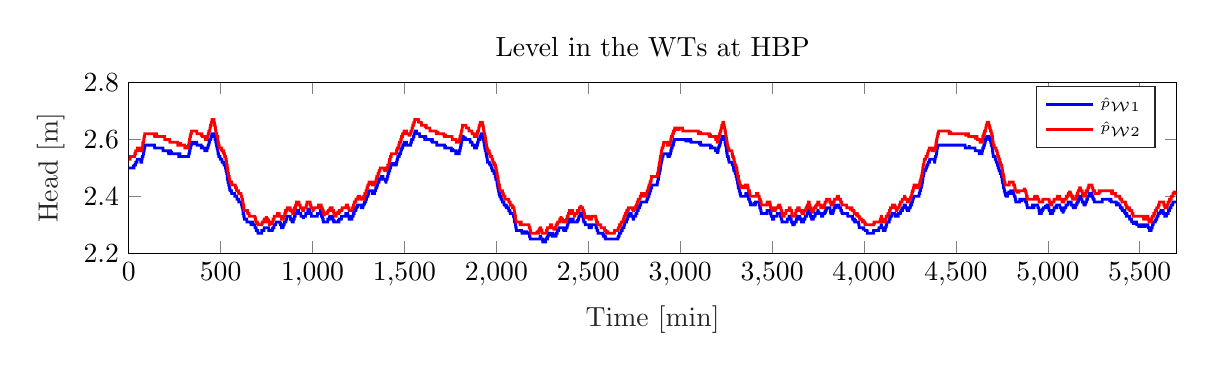
\begin{tikzpicture}

\begin{axis}[%
width=5.239in,
height=0.854in,
at={(0.867in,0.425in)},
scale only axis,
xmin=0,
xmax=5700,
xlabel style={font=\color{white!15!black}},
xlabel={Time [min]},
ymin=2.2,
ymax=2.8,
ylabel style={font=\color{white!15!black}},
ylabel={Head  [m]},
axis background/.style={fill=white},
title style={},
title={Level in the WTs at HBP},
legend style={legend cell align=left, align=left, draw=white!15!black}
]
\addplot [color=blue, line width=1.0pt, forget plot]
  table[row sep=crcr]{%
0	2.5\\
1	2.5\\
2	2.5\\
3	2.5\\
4	2.5\\
5	2.5\\
6	2.5\\
7	2.5\\
8	2.5\\
9	2.5\\
10	2.5\\
11	2.5\\
12	2.5\\
13	2.5\\
14	2.5\\
15	2.5\\
16	2.5\\
17	2.5\\
18	2.5\\
19	2.5\\
20	2.5\\
21	2.5\\
22	2.5\\
23	2.5\\
24	2.5\\
25	2.5\\
26	2.51\\
27	2.5\\
28	2.5\\
29	2.5\\
30	2.51\\
31	2.51\\
32	2.51\\
33	2.51\\
34	2.51\\
35	2.51\\
36	2.51\\
37	2.51\\
38	2.52\\
39	2.52\\
40	2.52\\
41	2.52\\
42	2.52\\
43	2.52\\
44	2.52\\
45	2.52\\
46	2.53\\
47	2.53\\
48	2.53\\
49	2.53\\
50	2.53\\
51	2.53\\
52	2.53\\
53	2.53\\
54	2.53\\
55	2.53\\
56	2.53\\
57	2.53\\
58	2.53\\
59	2.53\\
60	2.53\\
61	2.53\\
62	2.53\\
63	2.53\\
64	2.53\\
65	2.53\\
66	2.52\\
67	2.52\\
68	2.52\\
69	2.52\\
70	2.52\\
71	2.52\\
72	2.53\\
73	2.53\\
74	2.54\\
75	2.54\\
76	2.54\\
77	2.54\\
78	2.54\\
79	2.55\\
80	2.55\\
81	2.55\\
82	2.56\\
83	2.56\\
84	2.56\\
85	2.57\\
86	2.57\\
87	2.57\\
88	2.58\\
89	2.58\\
90	2.58\\
91	2.58\\
92	2.58\\
93	2.58\\
94	2.58\\
95	2.58\\
96	2.58\\
97	2.58\\
98	2.58\\
99	2.58\\
100	2.58\\
101	2.58\\
102	2.58\\
103	2.58\\
104	2.58\\
105	2.58\\
106	2.58\\
107	2.58\\
108	2.58\\
109	2.58\\
110	2.58\\
111	2.58\\
112	2.58\\
113	2.58\\
114	2.58\\
115	2.58\\
116	2.58\\
117	2.58\\
118	2.58\\
119	2.58\\
120	2.58\\
121	2.58\\
122	2.58\\
123	2.58\\
124	2.58\\
125	2.58\\
126	2.58\\
127	2.58\\
128	2.58\\
129	2.58\\
130	2.58\\
131	2.58\\
132	2.58\\
133	2.58\\
134	2.58\\
135	2.58\\
136	2.58\\
137	2.58\\
138	2.58\\
139	2.58\\
140	2.58\\
141	2.57\\
142	2.57\\
143	2.57\\
144	2.57\\
145	2.57\\
146	2.57\\
147	2.57\\
148	2.57\\
149	2.57\\
150	2.57\\
151	2.57\\
152	2.57\\
153	2.57\\
154	2.57\\
155	2.57\\
156	2.57\\
157	2.57\\
158	2.57\\
159	2.57\\
160	2.57\\
161	2.57\\
162	2.57\\
163	2.57\\
164	2.57\\
165	2.57\\
166	2.57\\
167	2.57\\
168	2.57\\
169	2.57\\
170	2.57\\
171	2.57\\
172	2.57\\
173	2.57\\
174	2.57\\
175	2.57\\
176	2.57\\
177	2.57\\
178	2.57\\
179	2.57\\
180	2.57\\
181	2.57\\
182	2.57\\
183	2.57\\
184	2.57\\
185	2.57\\
186	2.57\\
187	2.56\\
188	2.56\\
189	2.56\\
190	2.56\\
191	2.56\\
192	2.56\\
193	2.56\\
194	2.56\\
195	2.56\\
196	2.56\\
197	2.56\\
198	2.56\\
199	2.56\\
200	2.56\\
201	2.56\\
202	2.56\\
203	2.56\\
204	2.56\\
205	2.56\\
206	2.56\\
207	2.56\\
208	2.56\\
209	2.56\\
210	2.56\\
211	2.56\\
212	2.56\\
213	2.56\\
214	2.56\\
215	2.56\\
216	2.55\\
217	2.56\\
218	2.55\\
219	2.55\\
220	2.55\\
221	2.55\\
222	2.56\\
223	2.55\\
224	2.55\\
225	2.56\\
226	2.56\\
227	2.56\\
228	2.55\\
229	2.55\\
230	2.56\\
231	2.55\\
232	2.56\\
233	2.55\\
234	2.55\\
235	2.55\\
236	2.55\\
237	2.55\\
238	2.55\\
239	2.55\\
240	2.55\\
241	2.55\\
242	2.55\\
243	2.55\\
244	2.55\\
245	2.55\\
246	2.55\\
247	2.55\\
248	2.55\\
249	2.55\\
250	2.55\\
251	2.55\\
252	2.55\\
253	2.55\\
254	2.55\\
255	2.55\\
256	2.55\\
257	2.55\\
258	2.55\\
259	2.55\\
260	2.55\\
261	2.55\\
262	2.55\\
263	2.55\\
264	2.55\\
265	2.55\\
266	2.55\\
267	2.55\\
268	2.55\\
269	2.55\\
270	2.55\\
271	2.55\\
272	2.54\\
273	2.54\\
274	2.55\\
275	2.55\\
276	2.55\\
277	2.55\\
278	2.55\\
279	2.55\\
280	2.54\\
281	2.54\\
282	2.54\\
283	2.54\\
284	2.54\\
285	2.54\\
286	2.54\\
287	2.54\\
288	2.54\\
289	2.54\\
290	2.54\\
291	2.54\\
292	2.54\\
293	2.54\\
294	2.54\\
295	2.54\\
296	2.54\\
297	2.54\\
298	2.54\\
299	2.54\\
300	2.54\\
301	2.54\\
302	2.54\\
303	2.54\\
304	2.54\\
305	2.54\\
306	2.54\\
307	2.54\\
308	2.54\\
309	2.54\\
310	2.54\\
311	2.54\\
312	2.54\\
313	2.54\\
314	2.54\\
315	2.54\\
316	2.54\\
317	2.54\\
318	2.54\\
319	2.54\\
320	2.54\\
321	2.54\\
322	2.54\\
323	2.54\\
324	2.54\\
325	2.54\\
326	2.54\\
327	2.55\\
328	2.55\\
329	2.55\\
330	2.55\\
331	2.56\\
332	2.56\\
333	2.56\\
334	2.57\\
335	2.57\\
336	2.57\\
337	2.57\\
338	2.58\\
339	2.58\\
340	2.58\\
341	2.58\\
342	2.59\\
343	2.59\\
344	2.59\\
345	2.59\\
346	2.59\\
347	2.59\\
348	2.59\\
349	2.59\\
350	2.58\\
351	2.59\\
352	2.59\\
353	2.59\\
354	2.59\\
355	2.58\\
356	2.59\\
357	2.59\\
358	2.59\\
359	2.59\\
360	2.59\\
361	2.59\\
362	2.59\\
363	2.59\\
364	2.59\\
365	2.59\\
366	2.59\\
367	2.59\\
368	2.59\\
369	2.59\\
370	2.59\\
371	2.58\\
372	2.58\\
373	2.58\\
374	2.58\\
375	2.58\\
376	2.58\\
377	2.58\\
378	2.58\\
379	2.58\\
380	2.58\\
381	2.58\\
382	2.58\\
383	2.58\\
384	2.58\\
385	2.58\\
386	2.58\\
387	2.58\\
388	2.58\\
389	2.58\\
390	2.58\\
391	2.58\\
392	2.58\\
393	2.58\\
394	2.58\\
395	2.57\\
396	2.57\\
397	2.58\\
398	2.57\\
399	2.57\\
400	2.58\\
401	2.57\\
402	2.57\\
403	2.57\\
404	2.57\\
405	2.57\\
406	2.57\\
407	2.57\\
408	2.57\\
409	2.57\\
410	2.57\\
411	2.57\\
412	2.57\\
413	2.57\\
414	2.56\\
415	2.56\\
416	2.56\\
417	2.56\\
418	2.56\\
419	2.56\\
420	2.56\\
421	2.56\\
422	2.56\\
423	2.56\\
424	2.56\\
425	2.56\\
426	2.56\\
427	2.57\\
428	2.57\\
429	2.57\\
430	2.57\\
431	2.57\\
432	2.58\\
433	2.58\\
434	2.58\\
435	2.58\\
436	2.58\\
437	2.59\\
438	2.59\\
439	2.59\\
440	2.6\\
441	2.6\\
442	2.6\\
443	2.6\\
444	2.6\\
445	2.6\\
446	2.6\\
447	2.6\\
448	2.61\\
449	2.61\\
450	2.61\\
451	2.61\\
452	2.62\\
453	2.62\\
454	2.62\\
455	2.62\\
456	2.62\\
457	2.62\\
458	2.62\\
459	2.62\\
460	2.62\\
461	2.62\\
462	2.62\\
463	2.62\\
464	2.62\\
465	2.62\\
466	2.61\\
467	2.61\\
468	2.61\\
469	2.61\\
470	2.6\\
471	2.6\\
472	2.6\\
473	2.6\\
474	2.59\\
475	2.59\\
476	2.59\\
477	2.58\\
478	2.58\\
479	2.58\\
480	2.57\\
481	2.57\\
482	2.57\\
483	2.57\\
484	2.56\\
485	2.56\\
486	2.55\\
487	2.55\\
488	2.55\\
489	2.55\\
490	2.54\\
491	2.54\\
492	2.54\\
493	2.54\\
494	2.54\\
495	2.54\\
496	2.54\\
497	2.54\\
498	2.53\\
499	2.53\\
500	2.53\\
501	2.53\\
502	2.53\\
503	2.53\\
504	2.53\\
505	2.53\\
506	2.53\\
507	2.53\\
508	2.52\\
509	2.52\\
510	2.52\\
511	2.52\\
512	2.52\\
513	2.52\\
514	2.52\\
515	2.52\\
516	2.52\\
517	2.52\\
518	2.51\\
519	2.51\\
520	2.51\\
521	2.51\\
522	2.51\\
523	2.51\\
524	2.51\\
525	2.51\\
526	2.5\\
527	2.5\\
528	2.5\\
529	2.49\\
530	2.49\\
531	2.49\\
532	2.49\\
533	2.48\\
534	2.48\\
535	2.48\\
536	2.47\\
537	2.46\\
538	2.46\\
539	2.46\\
540	2.45\\
541	2.45\\
542	2.45\\
543	2.45\\
544	2.44\\
545	2.44\\
546	2.44\\
547	2.43\\
548	2.43\\
549	2.43\\
550	2.42\\
551	2.43\\
552	2.42\\
553	2.42\\
554	2.42\\
555	2.42\\
556	2.42\\
557	2.42\\
558	2.42\\
559	2.42\\
560	2.41\\
561	2.41\\
562	2.41\\
563	2.41\\
564	2.41\\
565	2.41\\
566	2.41\\
567	2.41\\
568	2.41\\
569	2.41\\
570	2.41\\
571	2.41\\
572	2.41\\
573	2.41\\
574	2.41\\
575	2.41\\
576	2.41\\
577	2.4\\
578	2.4\\
579	2.4\\
580	2.4\\
581	2.4\\
582	2.4\\
583	2.4\\
584	2.4\\
585	2.4\\
586	2.4\\
587	2.4\\
588	2.4\\
589	2.39\\
590	2.39\\
591	2.39\\
592	2.39\\
593	2.39\\
594	2.39\\
595	2.39\\
596	2.39\\
597	2.39\\
598	2.39\\
599	2.38\\
600	2.38\\
601	2.38\\
602	2.38\\
603	2.38\\
604	2.38\\
605	2.38\\
606	2.38\\
607	2.38\\
608	2.38\\
609	2.38\\
610	2.38\\
611	2.38\\
612	2.38\\
613	2.38\\
614	2.37\\
615	2.37\\
616	2.37\\
617	2.36\\
618	2.36\\
619	2.36\\
620	2.36\\
621	2.35\\
622	2.34\\
623	2.34\\
624	2.34\\
625	2.34\\
626	2.33\\
627	2.33\\
628	2.33\\
629	2.32\\
630	2.32\\
631	2.32\\
632	2.32\\
633	2.32\\
634	2.32\\
635	2.32\\
636	2.32\\
637	2.32\\
638	2.32\\
639	2.32\\
640	2.32\\
641	2.32\\
642	2.32\\
643	2.31\\
644	2.31\\
645	2.31\\
646	2.31\\
647	2.31\\
648	2.31\\
649	2.31\\
650	2.31\\
651	2.31\\
652	2.31\\
653	2.31\\
654	2.31\\
655	2.31\\
656	2.31\\
657	2.31\\
658	2.31\\
659	2.31\\
660	2.31\\
661	2.31\\
662	2.31\\
663	2.31\\
664	2.31\\
665	2.3\\
666	2.3\\
667	2.31\\
668	2.31\\
669	2.31\\
670	2.31\\
671	2.31\\
672	2.31\\
673	2.3\\
674	2.31\\
675	2.31\\
676	2.31\\
677	2.3\\
678	2.3\\
679	2.3\\
680	2.3\\
681	2.3\\
682	2.3\\
683	2.3\\
684	2.3\\
685	2.3\\
686	2.3\\
687	2.29\\
688	2.29\\
689	2.29\\
690	2.29\\
691	2.29\\
692	2.29\\
693	2.29\\
694	2.28\\
695	2.28\\
696	2.28\\
697	2.28\\
698	2.28\\
699	2.28\\
700	2.28\\
701	2.28\\
702	2.28\\
703	2.27\\
704	2.27\\
705	2.27\\
706	2.27\\
707	2.27\\
708	2.27\\
709	2.27\\
710	2.27\\
711	2.27\\
712	2.27\\
713	2.27\\
714	2.27\\
715	2.27\\
716	2.27\\
717	2.27\\
718	2.27\\
719	2.27\\
720	2.27\\
721	2.27\\
722	2.27\\
723	2.27\\
724	2.28\\
725	2.28\\
726	2.28\\
727	2.28\\
728	2.28\\
729	2.28\\
730	2.28\\
731	2.28\\
732	2.28\\
733	2.28\\
734	2.28\\
735	2.28\\
736	2.28\\
737	2.29\\
738	2.29\\
739	2.29\\
740	2.29\\
741	2.29\\
742	2.29\\
743	2.29\\
744	2.29\\
745	2.29\\
746	2.29\\
747	2.29\\
748	2.29\\
749	2.29\\
750	2.29\\
751	2.29\\
752	2.29\\
753	2.29\\
754	2.29\\
755	2.29\\
756	2.29\\
757	2.29\\
758	2.29\\
759	2.29\\
760	2.29\\
761	2.29\\
762	2.28\\
763	2.28\\
764	2.28\\
765	2.28\\
766	2.28\\
767	2.28\\
768	2.28\\
769	2.28\\
770	2.28\\
771	2.28\\
772	2.28\\
773	2.28\\
774	2.28\\
775	2.28\\
776	2.28\\
777	2.28\\
778	2.28\\
779	2.28\\
780	2.28\\
781	2.28\\
782	2.29\\
783	2.28\\
784	2.29\\
785	2.29\\
786	2.29\\
787	2.29\\
788	2.29\\
789	2.29\\
790	2.29\\
791	2.3\\
792	2.3\\
793	2.3\\
794	2.3\\
795	2.3\\
796	2.3\\
797	2.3\\
798	2.3\\
799	2.3\\
800	2.3\\
801	2.31\\
802	2.31\\
803	2.31\\
804	2.31\\
805	2.31\\
806	2.31\\
807	2.31\\
808	2.31\\
809	2.31\\
810	2.31\\
811	2.31\\
812	2.31\\
813	2.31\\
814	2.31\\
815	2.31\\
816	2.31\\
817	2.31\\
818	2.31\\
819	2.31\\
820	2.31\\
821	2.31\\
822	2.31\\
823	2.31\\
824	2.3\\
825	2.31\\
826	2.3\\
827	2.3\\
828	2.3\\
829	2.3\\
830	2.3\\
831	2.29\\
832	2.29\\
833	2.29\\
834	2.29\\
835	2.29\\
836	2.29\\
837	2.29\\
838	2.29\\
839	2.29\\
840	2.29\\
841	2.3\\
842	2.3\\
843	2.3\\
844	2.3\\
845	2.3\\
846	2.3\\
847	2.31\\
848	2.31\\
849	2.31\\
850	2.31\\
851	2.31\\
852	2.31\\
853	2.31\\
854	2.31\\
855	2.31\\
856	2.32\\
857	2.32\\
858	2.32\\
859	2.32\\
860	2.32\\
861	2.33\\
862	2.33\\
863	2.33\\
864	2.33\\
865	2.33\\
866	2.33\\
867	2.33\\
868	2.33\\
869	2.33\\
870	2.33\\
871	2.33\\
872	2.33\\
873	2.33\\
874	2.33\\
875	2.33\\
876	2.33\\
877	2.33\\
878	2.33\\
879	2.33\\
880	2.32\\
881	2.32\\
882	2.32\\
883	2.32\\
884	2.32\\
885	2.32\\
886	2.32\\
887	2.31\\
888	2.32\\
889	2.31\\
890	2.31\\
891	2.32\\
892	2.31\\
893	2.31\\
894	2.31\\
895	2.31\\
896	2.32\\
897	2.32\\
898	2.32\\
899	2.32\\
900	2.32\\
901	2.33\\
902	2.33\\
903	2.33\\
904	2.33\\
905	2.33\\
906	2.33\\
907	2.34\\
908	2.34\\
909	2.34\\
910	2.34\\
911	2.34\\
912	2.34\\
913	2.34\\
914	2.35\\
915	2.35\\
916	2.34\\
917	2.35\\
918	2.35\\
919	2.34\\
920	2.34\\
921	2.34\\
922	2.35\\
923	2.35\\
924	2.35\\
925	2.35\\
926	2.34\\
927	2.34\\
928	2.34\\
929	2.34\\
930	2.34\\
931	2.34\\
932	2.34\\
933	2.34\\
934	2.34\\
935	2.34\\
936	2.34\\
937	2.33\\
938	2.33\\
939	2.33\\
940	2.33\\
941	2.33\\
942	2.33\\
943	2.33\\
944	2.33\\
945	2.33\\
946	2.33\\
947	2.33\\
948	2.33\\
949	2.33\\
950	2.32\\
951	2.33\\
952	2.33\\
953	2.33\\
954	2.33\\
955	2.33\\
956	2.33\\
957	2.33\\
958	2.33\\
959	2.33\\
960	2.33\\
961	2.33\\
962	2.33\\
963	2.34\\
964	2.34\\
965	2.34\\
966	2.34\\
967	2.34\\
968	2.34\\
969	2.34\\
970	2.34\\
971	2.34\\
972	2.34\\
973	2.34\\
974	2.35\\
975	2.35\\
976	2.35\\
977	2.35\\
978	2.36\\
979	2.35\\
980	2.35\\
981	2.36\\
982	2.35\\
983	2.35\\
984	2.35\\
985	2.34\\
986	2.35\\
987	2.34\\
988	2.34\\
989	2.34\\
990	2.34\\
991	2.34\\
992	2.34\\
993	2.34\\
994	2.33\\
995	2.33\\
996	2.33\\
997	2.33\\
998	2.33\\
999	2.33\\
1000	2.33\\
1001	2.33\\
1002	2.33\\
1003	2.33\\
1004	2.33\\
1005	2.33\\
1006	2.33\\
1007	2.33\\
1008	2.33\\
1009	2.33\\
1010	2.33\\
1011	2.33\\
1012	2.33\\
1013	2.33\\
1014	2.33\\
1015	2.33\\
1016	2.33\\
1017	2.33\\
1018	2.33\\
1019	2.33\\
1020	2.33\\
1021	2.33\\
1022	2.33\\
1023	2.33\\
1024	2.33\\
1025	2.33\\
1026	2.33\\
1027	2.34\\
1028	2.34\\
1029	2.34\\
1030	2.34\\
1031	2.34\\
1032	2.34\\
1033	2.34\\
1034	2.34\\
1035	2.34\\
1036	2.34\\
1037	2.34\\
1038	2.34\\
1039	2.34\\
1040	2.34\\
1041	2.34\\
1042	2.35\\
1043	2.35\\
1044	2.35\\
1045	2.34\\
1046	2.34\\
1047	2.34\\
1048	2.34\\
1049	2.33\\
1050	2.33\\
1051	2.33\\
1052	2.33\\
1053	2.33\\
1054	2.33\\
1055	2.32\\
1056	2.32\\
1057	2.32\\
1058	2.32\\
1059	2.31\\
1060	2.31\\
1061	2.31\\
1062	2.31\\
1063	2.31\\
1064	2.31\\
1065	2.31\\
1066	2.31\\
1067	2.31\\
1068	2.31\\
1069	2.31\\
1070	2.31\\
1071	2.31\\
1072	2.31\\
1073	2.31\\
1074	2.31\\
1075	2.31\\
1076	2.31\\
1077	2.31\\
1078	2.31\\
1079	2.31\\
1080	2.31\\
1081	2.31\\
1082	2.31\\
1083	2.32\\
1084	2.32\\
1085	2.32\\
1086	2.32\\
1087	2.32\\
1088	2.32\\
1089	2.32\\
1090	2.32\\
1091	2.32\\
1092	2.32\\
1093	2.33\\
1094	2.33\\
1095	2.33\\
1096	2.33\\
1097	2.33\\
1098	2.33\\
1099	2.33\\
1100	2.33\\
1101	2.33\\
1102	2.33\\
1103	2.33\\
1104	2.33\\
1105	2.33\\
1106	2.33\\
1107	2.33\\
1108	2.33\\
1109	2.32\\
1110	2.32\\
1111	2.32\\
1112	2.32\\
1113	2.31\\
1114	2.32\\
1115	2.31\\
1116	2.31\\
1117	2.32\\
1118	2.31\\
1119	2.31\\
1120	2.31\\
1121	2.31\\
1122	2.31\\
1123	2.31\\
1124	2.31\\
1125	2.31\\
1126	2.31\\
1127	2.31\\
1128	2.31\\
1129	2.31\\
1130	2.31\\
1131	2.31\\
1132	2.31\\
1133	2.31\\
1134	2.31\\
1135	2.31\\
1136	2.31\\
1137	2.31\\
1138	2.31\\
1139	2.31\\
1140	2.31\\
1141	2.32\\
1142	2.31\\
1143	2.31\\
1144	2.31\\
1145	2.32\\
1146	2.32\\
1147	2.32\\
1148	2.32\\
1149	2.32\\
1150	2.32\\
1151	2.32\\
1152	2.32\\
1153	2.32\\
1154	2.32\\
1155	2.32\\
1156	2.32\\
1157	2.32\\
1158	2.33\\
1159	2.33\\
1160	2.33\\
1161	2.33\\
1162	2.33\\
1163	2.33\\
1164	2.33\\
1165	2.33\\
1166	2.33\\
1167	2.33\\
1168	2.33\\
1169	2.33\\
1170	2.33\\
1171	2.33\\
1172	2.33\\
1173	2.33\\
1174	2.33\\
1175	2.33\\
1176	2.33\\
1177	2.33\\
1178	2.33\\
1179	2.33\\
1180	2.33\\
1181	2.34\\
1182	2.34\\
1183	2.34\\
1184	2.34\\
1185	2.34\\
1186	2.34\\
1187	2.34\\
1188	2.34\\
1189	2.34\\
1190	2.34\\
1191	2.34\\
1192	2.34\\
1193	2.33\\
1194	2.33\\
1195	2.33\\
1196	2.33\\
1197	2.33\\
1198	2.33\\
1199	2.32\\
1200	2.32\\
1201	2.32\\
1202	2.32\\
1203	2.32\\
1204	2.32\\
1205	2.32\\
1206	2.32\\
1207	2.32\\
1208	2.32\\
1209	2.32\\
1210	2.32\\
1211	2.32\\
1212	2.32\\
1213	2.32\\
1214	2.32\\
1215	2.33\\
1216	2.33\\
1217	2.33\\
1218	2.33\\
1219	2.33\\
1220	2.33\\
1221	2.33\\
1222	2.34\\
1223	2.34\\
1224	2.34\\
1225	2.34\\
1226	2.34\\
1227	2.34\\
1228	2.35\\
1229	2.35\\
1230	2.35\\
1231	2.35\\
1232	2.35\\
1233	2.35\\
1234	2.36\\
1235	2.35\\
1236	2.35\\
1237	2.36\\
1238	2.36\\
1239	2.36\\
1240	2.36\\
1241	2.36\\
1242	2.36\\
1243	2.37\\
1244	2.36\\
1245	2.37\\
1246	2.37\\
1247	2.37\\
1248	2.37\\
1249	2.37\\
1250	2.37\\
1251	2.37\\
1252	2.37\\
1253	2.37\\
1254	2.37\\
1255	2.37\\
1256	2.37\\
1257	2.37\\
1258	2.37\\
1259	2.37\\
1260	2.37\\
1261	2.37\\
1262	2.37\\
1263	2.37\\
1264	2.37\\
1265	2.36\\
1266	2.36\\
1267	2.36\\
1268	2.36\\
1269	2.36\\
1270	2.36\\
1271	2.36\\
1272	2.36\\
1273	2.36\\
1274	2.36\\
1275	2.37\\
1276	2.37\\
1277	2.37\\
1278	2.37\\
1279	2.37\\
1280	2.37\\
1281	2.38\\
1282	2.37\\
1283	2.38\\
1284	2.38\\
1285	2.38\\
1286	2.38\\
1287	2.38\\
1288	2.38\\
1289	2.38\\
1290	2.39\\
1291	2.39\\
1292	2.39\\
1293	2.39\\
1294	2.39\\
1295	2.4\\
1296	2.4\\
1297	2.4\\
1298	2.4\\
1299	2.4\\
1300	2.4\\
1301	2.4\\
1302	2.4\\
1303	2.41\\
1304	2.41\\
1305	2.41\\
1306	2.41\\
1307	2.42\\
1308	2.42\\
1309	2.42\\
1310	2.42\\
1311	2.42\\
1312	2.42\\
1313	2.42\\
1314	2.42\\
1315	2.42\\
1316	2.42\\
1317	2.42\\
1318	2.42\\
1319	2.42\\
1320	2.42\\
1321	2.42\\
1322	2.42\\
1323	2.42\\
1324	2.42\\
1325	2.42\\
1326	2.41\\
1327	2.41\\
1328	2.41\\
1329	2.41\\
1330	2.41\\
1331	2.41\\
1332	2.41\\
1333	2.41\\
1334	2.41\\
1335	2.41\\
1336	2.41\\
1337	2.41\\
1338	2.42\\
1339	2.42\\
1340	2.42\\
1341	2.42\\
1342	2.42\\
1343	2.42\\
1344	2.43\\
1345	2.43\\
1346	2.43\\
1347	2.43\\
1348	2.43\\
1349	2.43\\
1350	2.43\\
1351	2.44\\
1352	2.44\\
1353	2.44\\
1354	2.44\\
1355	2.45\\
1356	2.45\\
1357	2.45\\
1358	2.45\\
1359	2.45\\
1360	2.45\\
1361	2.45\\
1362	2.45\\
1363	2.46\\
1364	2.46\\
1365	2.46\\
1366	2.46\\
1367	2.46\\
1368	2.46\\
1369	2.46\\
1370	2.46\\
1371	2.46\\
1372	2.47\\
1373	2.47\\
1374	2.47\\
1375	2.47\\
1376	2.47\\
1377	2.47\\
1378	2.47\\
1379	2.47\\
1380	2.47\\
1381	2.47\\
1382	2.47\\
1383	2.47\\
1384	2.46\\
1385	2.46\\
1386	2.46\\
1387	2.46\\
1388	2.46\\
1389	2.46\\
1390	2.46\\
1391	2.46\\
1392	2.46\\
1393	2.46\\
1394	2.46\\
1395	2.46\\
1396	2.46\\
1397	2.45\\
1398	2.46\\
1399	2.45\\
1400	2.45\\
1401	2.46\\
1402	2.46\\
1403	2.46\\
1404	2.46\\
1405	2.46\\
1406	2.46\\
1407	2.47\\
1408	2.47\\
1409	2.47\\
1410	2.47\\
1411	2.48\\
1412	2.48\\
1413	2.48\\
1414	2.48\\
1415	2.48\\
1416	2.49\\
1417	2.49\\
1418	2.49\\
1419	2.49\\
1420	2.49\\
1421	2.5\\
1422	2.5\\
1423	2.5\\
1424	2.5\\
1425	2.5\\
1426	2.51\\
1427	2.51\\
1428	2.51\\
1429	2.51\\
1430	2.52\\
1431	2.51\\
1432	2.51\\
1433	2.51\\
1434	2.51\\
1435	2.51\\
1436	2.51\\
1437	2.52\\
1438	2.51\\
1439	2.51\\
1440	2.51\\
1441	2.51\\
1442	2.51\\
1443	2.51\\
1444	2.51\\
1445	2.51\\
1446	2.51\\
1447	2.51\\
1448	2.51\\
1449	2.51\\
1450	2.51\\
1451	2.52\\
1452	2.51\\
1453	2.51\\
1454	2.51\\
1455	2.51\\
1456	2.51\\
1457	2.52\\
1458	2.52\\
1459	2.52\\
1460	2.53\\
1461	2.53\\
1462	2.53\\
1463	2.53\\
1464	2.54\\
1465	2.54\\
1466	2.54\\
1467	2.54\\
1468	2.54\\
1469	2.54\\
1470	2.54\\
1471	2.54\\
1472	2.54\\
1473	2.55\\
1474	2.55\\
1475	2.55\\
1476	2.55\\
1477	2.55\\
1478	2.55\\
1479	2.55\\
1480	2.56\\
1481	2.56\\
1482	2.56\\
1483	2.57\\
1484	2.56\\
1485	2.57\\
1486	2.57\\
1487	2.57\\
1488	2.57\\
1489	2.57\\
1490	2.57\\
1491	2.58\\
1492	2.58\\
1493	2.58\\
1494	2.58\\
1495	2.58\\
1496	2.58\\
1497	2.58\\
1498	2.59\\
1499	2.59\\
1500	2.59\\
1501	2.59\\
1502	2.59\\
1503	2.59\\
1504	2.59\\
1505	2.59\\
1506	2.59\\
1507	2.59\\
1508	2.59\\
1509	2.59\\
1510	2.59\\
1511	2.59\\
1512	2.58\\
1513	2.58\\
1514	2.58\\
1515	2.58\\
1516	2.58\\
1517	2.58\\
1518	2.58\\
1519	2.58\\
1520	2.58\\
1521	2.58\\
1522	2.58\\
1523	2.58\\
1524	2.58\\
1525	2.58\\
1526	2.58\\
1527	2.58\\
1528	2.58\\
1529	2.58\\
1530	2.58\\
1531	2.58\\
1532	2.58\\
1533	2.58\\
1534	2.58\\
1535	2.59\\
1536	2.59\\
1537	2.59\\
1538	2.59\\
1539	2.6\\
1540	2.6\\
1541	2.6\\
1542	2.6\\
1543	2.6\\
1544	2.6\\
1545	2.6\\
1546	2.6\\
1547	2.6\\
1548	2.61\\
1549	2.61\\
1550	2.61\\
1551	2.61\\
1552	2.61\\
1553	2.62\\
1554	2.62\\
1555	2.62\\
1556	2.62\\
1557	2.62\\
1558	2.63\\
1559	2.63\\
1560	2.63\\
1561	2.63\\
1562	2.63\\
1563	2.63\\
1564	2.63\\
1565	2.63\\
1566	2.63\\
1567	2.62\\
1568	2.62\\
1569	2.62\\
1570	2.62\\
1571	2.62\\
1572	2.62\\
1573	2.62\\
1574	2.62\\
1575	2.62\\
1576	2.62\\
1577	2.62\\
1578	2.62\\
1579	2.62\\
1580	2.62\\
1581	2.62\\
1582	2.62\\
1583	2.61\\
1584	2.61\\
1585	2.61\\
1586	2.61\\
1587	2.61\\
1588	2.61\\
1589	2.61\\
1590	2.61\\
1591	2.61\\
1592	2.61\\
1593	2.61\\
1594	2.61\\
1595	2.61\\
1596	2.61\\
1597	2.61\\
1598	2.61\\
1599	2.61\\
1600	2.61\\
1601	2.61\\
1602	2.61\\
1603	2.61\\
1604	2.61\\
1605	2.61\\
1606	2.61\\
1607	2.61\\
1608	2.61\\
1609	2.61\\
1610	2.6\\
1611	2.6\\
1612	2.61\\
1613	2.6\\
1614	2.61\\
1615	2.61\\
1616	2.6\\
1617	2.61\\
1618	2.6\\
1619	2.6\\
1620	2.6\\
1621	2.6\\
1622	2.6\\
1623	2.6\\
1624	2.6\\
1625	2.6\\
1626	2.6\\
1627	2.6\\
1628	2.6\\
1629	2.6\\
1630	2.6\\
1631	2.6\\
1632	2.6\\
1633	2.6\\
1634	2.6\\
1635	2.6\\
1636	2.6\\
1637	2.6\\
1638	2.6\\
1639	2.6\\
1640	2.6\\
1641	2.6\\
1642	2.6\\
1643	2.6\\
1644	2.6\\
1645	2.6\\
1646	2.59\\
1647	2.6\\
1648	2.6\\
1649	2.6\\
1650	2.6\\
1651	2.6\\
1652	2.6\\
1653	2.59\\
1654	2.59\\
1655	2.59\\
1656	2.59\\
1657	2.59\\
1658	2.59\\
1659	2.59\\
1660	2.59\\
1661	2.59\\
1662	2.59\\
1663	2.59\\
1664	2.59\\
1665	2.59\\
1666	2.59\\
1667	2.59\\
1668	2.59\\
1669	2.59\\
1670	2.59\\
1671	2.59\\
1672	2.59\\
1673	2.59\\
1674	2.59\\
1675	2.59\\
1676	2.58\\
1677	2.58\\
1678	2.58\\
1679	2.58\\
1680	2.58\\
1681	2.58\\
1682	2.58\\
1683	2.58\\
1684	2.58\\
1685	2.58\\
1686	2.58\\
1687	2.58\\
1688	2.58\\
1689	2.58\\
1690	2.58\\
1691	2.58\\
1692	2.58\\
1693	2.58\\
1694	2.58\\
1695	2.58\\
1696	2.58\\
1697	2.58\\
1698	2.58\\
1699	2.58\\
1700	2.58\\
1701	2.58\\
1702	2.58\\
1703	2.58\\
1704	2.58\\
1705	2.58\\
1706	2.58\\
1707	2.58\\
1708	2.58\\
1709	2.58\\
1710	2.58\\
1711	2.58\\
1712	2.58\\
1713	2.58\\
1714	2.58\\
1715	2.58\\
1716	2.58\\
1717	2.58\\
1718	2.58\\
1719	2.57\\
1720	2.57\\
1721	2.57\\
1722	2.57\\
1723	2.58\\
1724	2.57\\
1725	2.57\\
1726	2.57\\
1727	2.57\\
1728	2.57\\
1729	2.57\\
1730	2.57\\
1731	2.57\\
1732	2.57\\
1733	2.57\\
1734	2.57\\
1735	2.57\\
1736	2.57\\
1737	2.57\\
1738	2.57\\
1739	2.57\\
1740	2.57\\
1741	2.57\\
1742	2.57\\
1743	2.57\\
1744	2.57\\
1745	2.57\\
1746	2.57\\
1747	2.57\\
1748	2.57\\
1749	2.57\\
1750	2.57\\
1751	2.57\\
1752	2.57\\
1753	2.57\\
1754	2.57\\
1755	2.57\\
1756	2.56\\
1757	2.56\\
1758	2.56\\
1759	2.56\\
1760	2.56\\
1761	2.57\\
1762	2.56\\
1763	2.57\\
1764	2.56\\
1765	2.56\\
1766	2.56\\
1767	2.56\\
1768	2.56\\
1769	2.56\\
1770	2.56\\
1771	2.56\\
1772	2.56\\
1773	2.56\\
1774	2.56\\
1775	2.56\\
1776	2.56\\
1777	2.56\\
1778	2.56\\
1779	2.55\\
1780	2.55\\
1781	2.56\\
1782	2.56\\
1783	2.55\\
1784	2.55\\
1785	2.55\\
1786	2.55\\
1787	2.56\\
1788	2.55\\
1789	2.55\\
1790	2.55\\
1791	2.55\\
1792	2.55\\
1793	2.55\\
1794	2.55\\
1795	2.55\\
1796	2.55\\
1797	2.55\\
1798	2.55\\
1799	2.56\\
1800	2.56\\
1801	2.56\\
1802	2.56\\
1803	2.57\\
1804	2.57\\
1805	2.57\\
1806	2.58\\
1807	2.58\\
1808	2.58\\
1809	2.58\\
1810	2.59\\
1811	2.59\\
1812	2.59\\
1813	2.6\\
1814	2.6\\
1815	2.6\\
1816	2.6\\
1817	2.6\\
1818	2.6\\
1819	2.61\\
1820	2.61\\
1821	2.6\\
1822	2.6\\
1823	2.6\\
1824	2.6\\
1825	2.6\\
1826	2.6\\
1827	2.61\\
1828	2.6\\
1829	2.6\\
1830	2.6\\
1831	2.61\\
1832	2.6\\
1833	2.6\\
1834	2.6\\
1835	2.6\\
1836	2.6\\
1837	2.6\\
1838	2.6\\
1839	2.6\\
1840	2.6\\
1841	2.6\\
1842	2.6\\
1843	2.6\\
1844	2.6\\
1845	2.6\\
1846	2.6\\
1847	2.6\\
1848	2.6\\
1849	2.6\\
1850	2.6\\
1851	2.6\\
1852	2.6\\
1853	2.6\\
1854	2.6\\
1855	2.6\\
1856	2.6\\
1857	2.6\\
1858	2.59\\
1859	2.59\\
1860	2.59\\
1861	2.59\\
1862	2.59\\
1863	2.59\\
1864	2.59\\
1865	2.59\\
1866	2.59\\
1867	2.59\\
1868	2.59\\
1869	2.58\\
1870	2.58\\
1871	2.58\\
1872	2.58\\
1873	2.58\\
1874	2.58\\
1875	2.58\\
1876	2.58\\
1877	2.58\\
1878	2.58\\
1879	2.58\\
1880	2.58\\
1881	2.57\\
1882	2.57\\
1883	2.57\\
1884	2.57\\
1885	2.57\\
1886	2.57\\
1887	2.57\\
1888	2.57\\
1889	2.57\\
1890	2.57\\
1891	2.57\\
1892	2.57\\
1893	2.58\\
1894	2.58\\
1895	2.58\\
1896	2.58\\
1897	2.58\\
1898	2.59\\
1899	2.59\\
1900	2.59\\
1901	2.59\\
1902	2.6\\
1903	2.6\\
1904	2.6\\
1905	2.6\\
1906	2.6\\
1907	2.6\\
1908	2.6\\
1909	2.6\\
1910	2.61\\
1911	2.61\\
1912	2.61\\
1913	2.61\\
1914	2.61\\
1915	2.61\\
1916	2.62\\
1917	2.62\\
1918	2.62\\
1919	2.62\\
1920	2.62\\
1921	2.62\\
1922	2.62\\
1923	2.62\\
1924	2.61\\
1925	2.61\\
1926	2.61\\
1927	2.6\\
1928	2.6\\
1929	2.6\\
1930	2.6\\
1931	2.6\\
1932	2.59\\
1933	2.59\\
1934	2.58\\
1935	2.58\\
1936	2.58\\
1937	2.57\\
1938	2.57\\
1939	2.57\\
1940	2.56\\
1941	2.56\\
1942	2.56\\
1943	2.56\\
1944	2.55\\
1945	2.55\\
1946	2.55\\
1947	2.54\\
1948	2.54\\
1949	2.54\\
1950	2.53\\
1951	2.53\\
1952	2.52\\
1953	2.52\\
1954	2.52\\
1955	2.52\\
1956	2.52\\
1957	2.52\\
1958	2.52\\
1959	2.52\\
1960	2.52\\
1961	2.52\\
1962	2.52\\
1963	2.51\\
1964	2.52\\
1965	2.51\\
1966	2.51\\
1967	2.51\\
1968	2.51\\
1969	2.51\\
1970	2.51\\
1971	2.51\\
1972	2.51\\
1973	2.5\\
1974	2.5\\
1975	2.5\\
1976	2.5\\
1977	2.5\\
1978	2.49\\
1979	2.49\\
1980	2.49\\
1981	2.49\\
1982	2.49\\
1983	2.49\\
1984	2.49\\
1985	2.49\\
1986	2.49\\
1987	2.48\\
1988	2.48\\
1989	2.48\\
1990	2.48\\
1991	2.48\\
1992	2.48\\
1993	2.48\\
1994	2.47\\
1995	2.47\\
1996	2.47\\
1997	2.46\\
1998	2.46\\
1999	2.46\\
2000	2.46\\
2001	2.46\\
2002	2.46\\
2003	2.45\\
2004	2.45\\
2005	2.44\\
2006	2.44\\
2007	2.44\\
2008	2.43\\
2009	2.43\\
2010	2.43\\
2011	2.42\\
2012	2.42\\
2013	2.42\\
2014	2.41\\
2015	2.41\\
2016	2.41\\
2017	2.41\\
2018	2.4\\
2019	2.4\\
2020	2.4\\
2021	2.4\\
2022	2.4\\
2023	2.4\\
2024	2.4\\
2025	2.39\\
2026	2.39\\
2027	2.39\\
2028	2.39\\
2029	2.39\\
2030	2.39\\
2031	2.39\\
2032	2.39\\
2033	2.38\\
2034	2.38\\
2035	2.38\\
2036	2.38\\
2037	2.38\\
2038	2.38\\
2039	2.38\\
2040	2.38\\
2041	2.38\\
2042	2.37\\
2043	2.37\\
2044	2.37\\
2045	2.37\\
2046	2.37\\
2047	2.37\\
2048	2.37\\
2049	2.37\\
2050	2.37\\
2051	2.37\\
2052	2.36\\
2053	2.37\\
2054	2.37\\
2055	2.36\\
2056	2.36\\
2057	2.37\\
2058	2.36\\
2059	2.36\\
2060	2.36\\
2061	2.36\\
2062	2.36\\
2063	2.36\\
2064	2.36\\
2065	2.36\\
2066	2.36\\
2067	2.35\\
2068	2.35\\
2069	2.35\\
2070	2.35\\
2071	2.35\\
2072	2.35\\
2073	2.35\\
2074	2.34\\
2075	2.35\\
2076	2.34\\
2077	2.34\\
2078	2.34\\
2079	2.34\\
2080	2.34\\
2081	2.34\\
2082	2.34\\
2083	2.34\\
2084	2.34\\
2085	2.34\\
2086	2.34\\
2087	2.34\\
2088	2.34\\
2089	2.34\\
2090	2.34\\
2091	2.34\\
2092	2.34\\
2093	2.33\\
2094	2.33\\
2095	2.33\\
2096	2.33\\
2097	2.32\\
2098	2.32\\
2099	2.31\\
2100	2.31\\
2101	2.31\\
2102	2.31\\
2103	2.31\\
2104	2.3\\
2105	2.3\\
2106	2.29\\
2107	2.29\\
2108	2.29\\
2109	2.28\\
2110	2.28\\
2111	2.28\\
2112	2.28\\
2113	2.28\\
2114	2.28\\
2115	2.28\\
2116	2.28\\
2117	2.28\\
2118	2.28\\
2119	2.28\\
2120	2.28\\
2121	2.28\\
2122	2.28\\
2123	2.28\\
2124	2.28\\
2125	2.28\\
2126	2.28\\
2127	2.28\\
2128	2.28\\
2129	2.28\\
2130	2.28\\
2131	2.28\\
2132	2.28\\
2133	2.28\\
2134	2.28\\
2135	2.28\\
2136	2.28\\
2137	2.28\\
2138	2.28\\
2139	2.27\\
2140	2.27\\
2141	2.27\\
2142	2.27\\
2143	2.27\\
2144	2.27\\
2145	2.27\\
2146	2.27\\
2147	2.27\\
2148	2.27\\
2149	2.27\\
2150	2.27\\
2151	2.27\\
2152	2.28\\
2153	2.27\\
2154	2.27\\
2155	2.27\\
2156	2.27\\
2157	2.27\\
2158	2.27\\
2159	2.27\\
2160	2.27\\
2161	2.27\\
2162	2.27\\
2163	2.27\\
2164	2.27\\
2165	2.28\\
2166	2.27\\
2167	2.28\\
2168	2.27\\
2169	2.27\\
2170	2.27\\
2171	2.27\\
2172	2.27\\
2173	2.27\\
2174	2.27\\
2175	2.27\\
2176	2.27\\
2177	2.27\\
2178	2.27\\
2179	2.27\\
2180	2.26\\
2181	2.26\\
2182	2.26\\
2183	2.26\\
2184	2.25\\
2185	2.25\\
2186	2.25\\
2187	2.25\\
2188	2.25\\
2189	2.25\\
2190	2.25\\
2191	2.25\\
2192	2.25\\
2193	2.25\\
2194	2.25\\
2195	2.25\\
2196	2.25\\
2197	2.25\\
2198	2.25\\
2199	2.25\\
2200	2.25\\
2201	2.25\\
2202	2.25\\
2203	2.25\\
2204	2.25\\
2205	2.25\\
2206	2.25\\
2207	2.25\\
2208	2.25\\
2209	2.25\\
2210	2.25\\
2211	2.25\\
2212	2.25\\
2213	2.25\\
2214	2.25\\
2215	2.25\\
2216	2.25\\
2217	2.25\\
2218	2.25\\
2219	2.25\\
2220	2.25\\
2221	2.25\\
2222	2.25\\
2223	2.25\\
2224	2.25\\
2225	2.25\\
2226	2.25\\
2227	2.25\\
2228	2.25\\
2229	2.25\\
2230	2.25\\
2231	2.25\\
2232	2.25\\
2233	2.25\\
2234	2.25\\
2235	2.25\\
2236	2.25\\
2237	2.25\\
2238	2.26\\
2239	2.26\\
2240	2.26\\
2241	2.25\\
2242	2.26\\
2243	2.25\\
2244	2.25\\
2245	2.25\\
2246	2.25\\
2247	2.25\\
2248	2.25\\
2249	2.25\\
2250	2.25\\
2251	2.25\\
2252	2.24\\
2253	2.24\\
2254	2.24\\
2255	2.24\\
2256	2.24\\
2257	2.24\\
2258	2.24\\
2259	2.24\\
2260	2.24\\
2261	2.24\\
2262	2.24\\
2263	2.24\\
2264	2.24\\
2265	2.24\\
2266	2.24\\
2267	2.24\\
2268	2.25\\
2269	2.25\\
2270	2.25\\
2271	2.25\\
2272	2.25\\
2273	2.25\\
2274	2.25\\
2275	2.25\\
2276	2.26\\
2277	2.25\\
2278	2.25\\
2279	2.26\\
2280	2.26\\
2281	2.26\\
2282	2.26\\
2283	2.27\\
2284	2.26\\
2285	2.27\\
2286	2.26\\
2287	2.27\\
2288	2.26\\
2289	2.27\\
2290	2.27\\
2291	2.27\\
2292	2.27\\
2293	2.27\\
2294	2.27\\
2295	2.27\\
2296	2.27\\
2297	2.27\\
2298	2.27\\
2299	2.27\\
2300	2.27\\
2301	2.27\\
2302	2.27\\
2303	2.27\\
2304	2.26\\
2305	2.26\\
2306	2.27\\
2307	2.27\\
2308	2.26\\
2309	2.26\\
2310	2.26\\
2311	2.26\\
2312	2.26\\
2313	2.26\\
2314	2.26\\
2315	2.26\\
2316	2.26\\
2317	2.26\\
2318	2.26\\
2319	2.26\\
2320	2.26\\
2321	2.26\\
2322	2.26\\
2323	2.27\\
2324	2.26\\
2325	2.26\\
2326	2.27\\
2327	2.27\\
2328	2.27\\
2329	2.27\\
2330	2.27\\
2331	2.27\\
2332	2.28\\
2333	2.28\\
2334	2.28\\
2335	2.28\\
2336	2.28\\
2337	2.28\\
2338	2.28\\
2339	2.28\\
2340	2.29\\
2341	2.29\\
2342	2.29\\
2343	2.29\\
2344	2.29\\
2345	2.29\\
2346	2.29\\
2347	2.29\\
2348	2.29\\
2349	2.29\\
2350	2.29\\
2351	2.29\\
2352	2.29\\
2353	2.29\\
2354	2.29\\
2355	2.29\\
2356	2.29\\
2357	2.29\\
2358	2.29\\
2359	2.29\\
2360	2.29\\
2361	2.29\\
2362	2.29\\
2363	2.29\\
2364	2.29\\
2365	2.28\\
2366	2.29\\
2367	2.28\\
2368	2.28\\
2369	2.28\\
2370	2.28\\
2371	2.28\\
2372	2.28\\
2373	2.28\\
2374	2.28\\
2375	2.28\\
2376	2.28\\
2377	2.28\\
2378	2.28\\
2379	2.29\\
2380	2.29\\
2381	2.29\\
2382	2.29\\
2383	2.29\\
2384	2.29\\
2385	2.29\\
2386	2.3\\
2387	2.3\\
2388	2.3\\
2389	2.3\\
2390	2.3\\
2391	2.31\\
2392	2.31\\
2393	2.31\\
2394	2.31\\
2395	2.31\\
2396	2.31\\
2397	2.31\\
2398	2.32\\
2399	2.32\\
2400	2.32\\
2401	2.32\\
2402	2.32\\
2403	2.32\\
2404	2.32\\
2405	2.32\\
2406	2.32\\
2407	2.32\\
2408	2.32\\
2409	2.32\\
2410	2.31\\
2411	2.31\\
2412	2.31\\
2413	2.31\\
2414	2.31\\
2415	2.31\\
2416	2.31\\
2417	2.32\\
2418	2.32\\
2419	2.31\\
2420	2.31\\
2421	2.31\\
2422	2.31\\
2423	2.31\\
2424	2.31\\
2425	2.31\\
2426	2.31\\
2427	2.31\\
2428	2.31\\
2429	2.31\\
2430	2.31\\
2431	2.31\\
2432	2.31\\
2433	2.31\\
2434	2.31\\
2435	2.31\\
2436	2.31\\
2437	2.31\\
2438	2.31\\
2439	2.31\\
2440	2.31\\
2441	2.32\\
2442	2.31\\
2443	2.32\\
2444	2.31\\
2445	2.32\\
2446	2.32\\
2447	2.32\\
2448	2.32\\
2449	2.33\\
2450	2.33\\
2451	2.33\\
2452	2.33\\
2453	2.33\\
2454	2.33\\
2455	2.33\\
2456	2.33\\
2457	2.34\\
2458	2.34\\
2459	2.34\\
2460	2.34\\
2461	2.34\\
2462	2.34\\
2463	2.34\\
2464	2.34\\
2465	2.34\\
2466	2.34\\
2467	2.34\\
2468	2.33\\
2469	2.33\\
2470	2.33\\
2471	2.33\\
2472	2.32\\
2473	2.32\\
2474	2.32\\
2475	2.31\\
2476	2.31\\
2477	2.31\\
2478	2.31\\
2479	2.31\\
2480	2.31\\
2481	2.31\\
2482	2.31\\
2483	2.31\\
2484	2.3\\
2485	2.3\\
2486	2.3\\
2487	2.3\\
2488	2.3\\
2489	2.3\\
2490	2.3\\
2491	2.3\\
2492	2.3\\
2493	2.3\\
2494	2.3\\
2495	2.3\\
2496	2.3\\
2497	2.3\\
2498	2.3\\
2499	2.3\\
2500	2.3\\
2501	2.3\\
2502	2.3\\
2503	2.3\\
2504	2.29\\
2505	2.29\\
2506	2.29\\
2507	2.29\\
2508	2.29\\
2509	2.29\\
2510	2.29\\
2511	2.29\\
2512	2.29\\
2513	2.29\\
2514	2.3\\
2515	2.3\\
2516	2.29\\
2517	2.29\\
2518	2.3\\
2519	2.3\\
2520	2.3\\
2521	2.3\\
2522	2.3\\
2523	2.3\\
2524	2.3\\
2525	2.3\\
2526	2.3\\
2527	2.3\\
2528	2.3\\
2529	2.3\\
2530	2.3\\
2531	2.3\\
2532	2.3\\
2533	2.3\\
2534	2.3\\
2535	2.3\\
2536	2.3\\
2537	2.3\\
2538	2.3\\
2539	2.3\\
2540	2.3\\
2541	2.3\\
2542	2.29\\
2543	2.29\\
2544	2.29\\
2545	2.29\\
2546	2.29\\
2547	2.29\\
2548	2.28\\
2549	2.28\\
2550	2.28\\
2551	2.28\\
2552	2.28\\
2553	2.27\\
2554	2.27\\
2555	2.27\\
2556	2.27\\
2557	2.27\\
2558	2.27\\
2559	2.27\\
2560	2.27\\
2561	2.27\\
2562	2.27\\
2563	2.27\\
2564	2.27\\
2565	2.27\\
2566	2.27\\
2567	2.27\\
2568	2.27\\
2569	2.27\\
2570	2.27\\
2571	2.27\\
2572	2.27\\
2573	2.27\\
2574	2.27\\
2575	2.27\\
2576	2.27\\
2577	2.27\\
2578	2.27\\
2579	2.27\\
2580	2.27\\
2581	2.26\\
2582	2.27\\
2583	2.26\\
2584	2.26\\
2585	2.26\\
2586	2.26\\
2587	2.26\\
2588	2.26\\
2589	2.26\\
2590	2.26\\
2591	2.25\\
2592	2.26\\
2593	2.26\\
2594	2.25\\
2595	2.25\\
2596	2.25\\
2597	2.25\\
2598	2.25\\
2599	2.25\\
2600	2.25\\
2601	2.25\\
2602	2.25\\
2603	2.25\\
2604	2.25\\
2605	2.25\\
2606	2.25\\
2607	2.25\\
2608	2.25\\
2609	2.25\\
2610	2.25\\
2611	2.25\\
2612	2.25\\
2613	2.25\\
2614	2.25\\
2615	2.25\\
2616	2.25\\
2617	2.25\\
2618	2.25\\
2619	2.25\\
2620	2.25\\
2621	2.25\\
2622	2.25\\
2623	2.25\\
2624	2.25\\
2625	2.25\\
2626	2.25\\
2627	2.25\\
2628	2.25\\
2629	2.25\\
2630	2.25\\
2631	2.25\\
2632	2.25\\
2633	2.25\\
2634	2.25\\
2635	2.25\\
2636	2.25\\
2637	2.25\\
2638	2.25\\
2639	2.25\\
2640	2.25\\
2641	2.25\\
2642	2.25\\
2643	2.25\\
2644	2.25\\
2645	2.25\\
2646	2.25\\
2647	2.25\\
2648	2.25\\
2649	2.25\\
2650	2.25\\
2651	2.25\\
2652	2.25\\
2653	2.25\\
2654	2.25\\
2655	2.25\\
2656	2.25\\
2657	2.25\\
2658	2.25\\
2659	2.25\\
2660	2.25\\
2661	2.25\\
2662	2.26\\
2663	2.25\\
2664	2.26\\
2665	2.26\\
2666	2.26\\
2667	2.26\\
2668	2.26\\
2669	2.27\\
2670	2.27\\
2671	2.27\\
2672	2.27\\
2673	2.27\\
2674	2.27\\
2675	2.27\\
2676	2.27\\
2677	2.27\\
2678	2.28\\
2679	2.28\\
2680	2.28\\
2681	2.28\\
2682	2.28\\
2683	2.28\\
2684	2.28\\
2685	2.28\\
2686	2.29\\
2687	2.29\\
2688	2.29\\
2689	2.29\\
2690	2.29\\
2691	2.29\\
2692	2.29\\
2693	2.29\\
2694	2.29\\
2695	2.3\\
2696	2.3\\
2697	2.3\\
2698	2.3\\
2699	2.31\\
2700	2.31\\
2701	2.31\\
2702	2.31\\
2703	2.31\\
2704	2.31\\
2705	2.31\\
2706	2.31\\
2707	2.31\\
2708	2.31\\
2709	2.32\\
2710	2.32\\
2711	2.32\\
2712	2.32\\
2713	2.32\\
2714	2.32\\
2715	2.33\\
2716	2.33\\
2717	2.33\\
2718	2.33\\
2719	2.33\\
2720	2.33\\
2721	2.33\\
2722	2.33\\
2723	2.33\\
2724	2.33\\
2725	2.34\\
2726	2.34\\
2727	2.34\\
2728	2.34\\
2729	2.34\\
2730	2.34\\
2731	2.34\\
2732	2.34\\
2733	2.34\\
2734	2.34\\
2735	2.33\\
2736	2.33\\
2737	2.33\\
2738	2.33\\
2739	2.33\\
2740	2.33\\
2741	2.33\\
2742	2.33\\
2743	2.33\\
2744	2.32\\
2745	2.32\\
2746	2.32\\
2747	2.32\\
2748	2.33\\
2749	2.33\\
2750	2.33\\
2751	2.33\\
2752	2.33\\
2753	2.33\\
2754	2.33\\
2755	2.33\\
2756	2.33\\
2757	2.33\\
2758	2.33\\
2759	2.34\\
2760	2.34\\
2761	2.34\\
2762	2.34\\
2763	2.34\\
2764	2.34\\
2765	2.34\\
2766	2.35\\
2767	2.35\\
2768	2.35\\
2769	2.35\\
2770	2.36\\
2771	2.35\\
2772	2.35\\
2773	2.36\\
2774	2.36\\
2775	2.36\\
2776	2.36\\
2777	2.37\\
2778	2.36\\
2779	2.36\\
2780	2.37\\
2781	2.37\\
2782	2.37\\
2783	2.37\\
2784	2.37\\
2785	2.37\\
2786	2.38\\
2787	2.38\\
2788	2.38\\
2789	2.38\\
2790	2.38\\
2791	2.38\\
2792	2.38\\
2793	2.38\\
2794	2.38\\
2795	2.38\\
2796	2.38\\
2797	2.38\\
2798	2.38\\
2799	2.38\\
2800	2.38\\
2801	2.38\\
2802	2.38\\
2803	2.38\\
2804	2.38\\
2805	2.38\\
2806	2.38\\
2807	2.38\\
2808	2.38\\
2809	2.38\\
2810	2.38\\
2811	2.38\\
2812	2.38\\
2813	2.38\\
2814	2.38\\
2815	2.38\\
2816	2.38\\
2817	2.38\\
2818	2.38\\
2819	2.39\\
2820	2.39\\
2821	2.39\\
2822	2.39\\
2823	2.4\\
2824	2.39\\
2825	2.4\\
2826	2.4\\
2827	2.4\\
2828	2.4\\
2829	2.4\\
2830	2.4\\
2831	2.41\\
2832	2.41\\
2833	2.41\\
2834	2.41\\
2835	2.41\\
2836	2.42\\
2837	2.42\\
2838	2.42\\
2839	2.42\\
2840	2.42\\
2841	2.43\\
2842	2.43\\
2843	2.43\\
2844	2.43\\
2845	2.43\\
2846	2.44\\
2847	2.44\\
2848	2.44\\
2849	2.44\\
2850	2.44\\
2851	2.44\\
2852	2.44\\
2853	2.44\\
2854	2.44\\
2855	2.44\\
2856	2.44\\
2857	2.44\\
2858	2.44\\
2859	2.44\\
2860	2.44\\
2861	2.44\\
2862	2.44\\
2863	2.44\\
2864	2.44\\
2865	2.44\\
2866	2.44\\
2867	2.44\\
2868	2.44\\
2869	2.44\\
2870	2.44\\
2871	2.44\\
2872	2.44\\
2873	2.44\\
2874	2.44\\
2875	2.44\\
2876	2.45\\
2877	2.45\\
2878	2.45\\
2879	2.46\\
2880	2.46\\
2881	2.46\\
2882	2.46\\
2883	2.47\\
2884	2.47\\
2885	2.48\\
2886	2.48\\
2887	2.48\\
2888	2.49\\
2889	2.49\\
2890	2.49\\
2891	2.49\\
2892	2.5\\
2893	2.5\\
2894	2.51\\
2895	2.51\\
2896	2.51\\
2897	2.52\\
2898	2.52\\
2899	2.52\\
2900	2.53\\
2901	2.53\\
2902	2.53\\
2903	2.54\\
2904	2.54\\
2905	2.54\\
2906	2.54\\
2907	2.54\\
2908	2.55\\
2909	2.55\\
2910	2.55\\
2911	2.55\\
2912	2.55\\
2913	2.55\\
2914	2.55\\
2915	2.55\\
2916	2.55\\
2917	2.55\\
2918	2.55\\
2919	2.55\\
2920	2.55\\
2921	2.55\\
2922	2.55\\
2923	2.55\\
2924	2.55\\
2925	2.55\\
2926	2.55\\
2927	2.55\\
2928	2.55\\
2929	2.55\\
2930	2.55\\
2931	2.55\\
2932	2.55\\
2933	2.54\\
2934	2.54\\
2935	2.54\\
2936	2.54\\
2937	2.54\\
2938	2.54\\
2939	2.54\\
2940	2.54\\
2941	2.54\\
2942	2.55\\
2943	2.54\\
2944	2.55\\
2945	2.55\\
2946	2.55\\
2947	2.55\\
2948	2.55\\
2949	2.56\\
2950	2.56\\
2951	2.56\\
2952	2.57\\
2953	2.57\\
2954	2.57\\
2955	2.57\\
2956	2.57\\
2957	2.57\\
2958	2.58\\
2959	2.58\\
2960	2.58\\
2961	2.58\\
2962	2.58\\
2963	2.58\\
2964	2.59\\
2965	2.59\\
2966	2.6\\
2967	2.59\\
2968	2.6\\
2969	2.6\\
2970	2.6\\
2971	2.6\\
2972	2.6\\
2973	2.6\\
2974	2.6\\
2975	2.6\\
2976	2.6\\
2977	2.6\\
2978	2.6\\
2979	2.6\\
2980	2.6\\
2981	2.6\\
2982	2.6\\
2983	2.6\\
2984	2.6\\
2985	2.6\\
2986	2.6\\
2987	2.6\\
2988	2.6\\
2989	2.6\\
2990	2.6\\
2991	2.6\\
2992	2.6\\
2993	2.6\\
2994	2.6\\
2995	2.6\\
2996	2.6\\
2997	2.6\\
2998	2.6\\
2999	2.6\\
3000	2.6\\
3001	2.6\\
3002	2.6\\
3003	2.6\\
3004	2.6\\
3005	2.6\\
3006	2.6\\
3007	2.6\\
3008	2.6\\
3009	2.6\\
3010	2.6\\
3011	2.6\\
3012	2.6\\
3013	2.6\\
3014	2.6\\
3015	2.6\\
3016	2.6\\
3017	2.6\\
3018	2.6\\
3019	2.6\\
3020	2.6\\
3021	2.6\\
3022	2.6\\
3023	2.6\\
3024	2.6\\
3025	2.6\\
3026	2.6\\
3027	2.6\\
3028	2.6\\
3029	2.6\\
3030	2.6\\
3031	2.59\\
3032	2.6\\
3033	2.6\\
3034	2.6\\
3035	2.6\\
3036	2.6\\
3037	2.6\\
3038	2.6\\
3039	2.6\\
3040	2.6\\
3041	2.6\\
3042	2.6\\
3043	2.6\\
3044	2.6\\
3045	2.6\\
3046	2.59\\
3047	2.6\\
3048	2.6\\
3049	2.59\\
3050	2.6\\
3051	2.6\\
3052	2.6\\
3053	2.59\\
3054	2.6\\
3055	2.6\\
3056	2.6\\
3057	2.6\\
3058	2.6\\
3059	2.59\\
3060	2.59\\
3061	2.59\\
3062	2.59\\
3063	2.59\\
3064	2.59\\
3065	2.59\\
3066	2.59\\
3067	2.59\\
3068	2.59\\
3069	2.59\\
3070	2.59\\
3071	2.59\\
3072	2.59\\
3073	2.59\\
3074	2.59\\
3075	2.59\\
3076	2.59\\
3077	2.59\\
3078	2.59\\
3079	2.59\\
3080	2.59\\
3081	2.59\\
3082	2.59\\
3083	2.59\\
3084	2.59\\
3085	2.59\\
3086	2.59\\
3087	2.59\\
3088	2.59\\
3089	2.59\\
3090	2.59\\
3091	2.59\\
3092	2.59\\
3093	2.59\\
3094	2.59\\
3095	2.59\\
3096	2.59\\
3097	2.59\\
3098	2.59\\
3099	2.59\\
3100	2.59\\
3101	2.59\\
3102	2.59\\
3103	2.59\\
3104	2.59\\
3105	2.58\\
3106	2.59\\
3107	2.59\\
3108	2.59\\
3109	2.59\\
3110	2.59\\
3111	2.59\\
3112	2.58\\
3113	2.58\\
3114	2.58\\
3115	2.58\\
3116	2.58\\
3117	2.58\\
3118	2.58\\
3119	2.58\\
3120	2.58\\
3121	2.58\\
3122	2.58\\
3123	2.58\\
3124	2.58\\
3125	2.58\\
3126	2.58\\
3127	2.58\\
3128	2.58\\
3129	2.58\\
3130	2.58\\
3131	2.58\\
3132	2.58\\
3133	2.58\\
3134	2.58\\
3135	2.58\\
3136	2.58\\
3137	2.58\\
3138	2.58\\
3139	2.58\\
3140	2.58\\
3141	2.58\\
3142	2.58\\
3143	2.58\\
3144	2.58\\
3145	2.58\\
3146	2.58\\
3147	2.58\\
3148	2.58\\
3149	2.58\\
3150	2.58\\
3151	2.58\\
3152	2.58\\
3153	2.58\\
3154	2.58\\
3155	2.58\\
3156	2.58\\
3157	2.58\\
3158	2.58\\
3159	2.58\\
3160	2.58\\
3161	2.58\\
3162	2.58\\
3163	2.58\\
3164	2.58\\
3165	2.57\\
3166	2.57\\
3167	2.57\\
3168	2.57\\
3169	2.57\\
3170	2.57\\
3171	2.57\\
3172	2.58\\
3173	2.57\\
3174	2.57\\
3175	2.57\\
3176	2.57\\
3177	2.57\\
3178	2.57\\
3179	2.57\\
3180	2.57\\
3181	2.57\\
3182	2.57\\
3183	2.57\\
3184	2.57\\
3185	2.57\\
3186	2.57\\
3187	2.57\\
3188	2.57\\
3189	2.57\\
3190	2.57\\
3191	2.57\\
3192	2.56\\
3193	2.56\\
3194	2.56\\
3195	2.56\\
3196	2.56\\
3197	2.56\\
3198	2.56\\
3199	2.56\\
3200	2.56\\
3201	2.56\\
3202	2.55\\
3203	2.56\\
3204	2.55\\
3205	2.56\\
3206	2.56\\
3207	2.56\\
3208	2.57\\
3209	2.57\\
3210	2.57\\
3211	2.58\\
3212	2.57\\
3213	2.58\\
3214	2.58\\
3215	2.58\\
3216	2.58\\
3217	2.58\\
3218	2.59\\
3219	2.59\\
3220	2.59\\
3221	2.6\\
3222	2.6\\
3223	2.6\\
3224	2.6\\
3225	2.6\\
3226	2.6\\
3227	2.6\\
3228	2.61\\
3229	2.61\\
3230	2.61\\
3231	2.61\\
3232	2.61\\
3233	2.61\\
3234	2.61\\
3235	2.61\\
3236	2.61\\
3237	2.61\\
3238	2.61\\
3239	2.61\\
3240	2.6\\
3241	2.6\\
3242	2.6\\
3243	2.6\\
3244	2.59\\
3245	2.59\\
3246	2.59\\
3247	2.58\\
3248	2.58\\
3249	2.58\\
3250	2.57\\
3251	2.57\\
3252	2.56\\
3253	2.56\\
3254	2.55\\
3255	2.55\\
3256	2.55\\
3257	2.54\\
3258	2.54\\
3259	2.54\\
3260	2.54\\
3261	2.54\\
3262	2.54\\
3263	2.53\\
3264	2.53\\
3265	2.53\\
3266	2.52\\
3267	2.52\\
3268	2.52\\
3269	2.52\\
3270	2.52\\
3271	2.52\\
3272	2.52\\
3273	2.52\\
3274	2.52\\
3275	2.52\\
3276	2.52\\
3277	2.52\\
3278	2.52\\
3279	2.52\\
3280	2.52\\
3281	2.52\\
3282	2.52\\
3283	2.51\\
3284	2.51\\
3285	2.51\\
3286	2.51\\
3287	2.51\\
3288	2.51\\
3289	2.51\\
3290	2.5\\
3291	2.5\\
3292	2.49\\
3293	2.49\\
3294	2.49\\
3295	2.49\\
3296	2.49\\
3297	2.49\\
3298	2.49\\
3299	2.48\\
3300	2.48\\
3301	2.48\\
3302	2.48\\
3303	2.48\\
3304	2.47\\
3305	2.47\\
3306	2.47\\
3307	2.47\\
3308	2.46\\
3309	2.46\\
3310	2.46\\
3311	2.46\\
3312	2.45\\
3313	2.45\\
3314	2.44\\
3315	2.44\\
3316	2.43\\
3317	2.43\\
3318	2.43\\
3319	2.43\\
3320	2.43\\
3321	2.42\\
3322	2.42\\
3323	2.42\\
3324	2.42\\
3325	2.41\\
3326	2.41\\
3327	2.41\\
3328	2.41\\
3329	2.4\\
3330	2.4\\
3331	2.4\\
3332	2.4\\
3333	2.4\\
3334	2.4\\
3335	2.4\\
3336	2.4\\
3337	2.4\\
3338	2.4\\
3339	2.4\\
3340	2.4\\
3341	2.4\\
3342	2.4\\
3343	2.4\\
3344	2.4\\
3345	2.4\\
3346	2.4\\
3347	2.4\\
3348	2.4\\
3349	2.4\\
3350	2.4\\
3351	2.4\\
3352	2.4\\
3353	2.4\\
3354	2.4\\
3355	2.4\\
3356	2.4\\
3357	2.41\\
3358	2.41\\
3359	2.41\\
3360	2.41\\
3361	2.41\\
3362	2.41\\
3363	2.41\\
3364	2.41\\
3365	2.41\\
3366	2.41\\
3367	2.4\\
3368	2.4\\
3369	2.4\\
3370	2.4\\
3371	2.4\\
3372	2.39\\
3373	2.39\\
3374	2.39\\
3375	2.39\\
3376	2.39\\
3377	2.39\\
3378	2.38\\
3379	2.38\\
3380	2.38\\
3381	2.38\\
3382	2.38\\
3383	2.37\\
3384	2.37\\
3385	2.38\\
3386	2.37\\
3387	2.37\\
3388	2.37\\
3389	2.37\\
3390	2.37\\
3391	2.37\\
3392	2.37\\
3393	2.37\\
3394	2.37\\
3395	2.37\\
3396	2.37\\
3397	2.37\\
3398	2.37\\
3399	2.37\\
3400	2.37\\
3401	2.37\\
3402	2.37\\
3403	2.37\\
3404	2.38\\
3405	2.37\\
3406	2.37\\
3407	2.37\\
3408	2.37\\
3409	2.37\\
3410	2.38\\
3411	2.38\\
3412	2.38\\
3413	2.38\\
3414	2.38\\
3415	2.38\\
3416	2.38\\
3417	2.38\\
3418	2.38\\
3419	2.38\\
3420	2.38\\
3421	2.38\\
3422	2.38\\
3423	2.38\\
3424	2.38\\
3425	2.38\\
3426	2.38\\
3427	2.38\\
3428	2.38\\
3429	2.38\\
3430	2.37\\
3431	2.37\\
3432	2.37\\
3433	2.36\\
3434	2.36\\
3435	2.36\\
3436	2.36\\
3437	2.36\\
3438	2.35\\
3439	2.35\\
3440	2.35\\
3441	2.34\\
3442	2.34\\
3443	2.34\\
3444	2.34\\
3445	2.34\\
3446	2.34\\
3447	2.34\\
3448	2.34\\
3449	2.34\\
3450	2.34\\
3451	2.34\\
3452	2.34\\
3453	2.34\\
3454	2.34\\
3455	2.34\\
3456	2.34\\
3457	2.34\\
3458	2.34\\
3459	2.34\\
3460	2.34\\
3461	2.34\\
3462	2.34\\
3463	2.34\\
3464	2.34\\
3465	2.34\\
3466	2.34\\
3467	2.34\\
3468	2.34\\
3469	2.34\\
3470	2.34\\
3471	2.34\\
3472	2.35\\
3473	2.35\\
3474	2.35\\
3475	2.35\\
3476	2.35\\
3477	2.35\\
3478	2.35\\
3479	2.35\\
3480	2.35\\
3481	2.35\\
3482	2.35\\
3483	2.35\\
3484	2.35\\
3485	2.35\\
3486	2.35\\
3487	2.35\\
3488	2.35\\
3489	2.34\\
3490	2.34\\
3491	2.34\\
3492	2.34\\
3493	2.34\\
3494	2.34\\
3495	2.33\\
3496	2.33\\
3497	2.33\\
3498	2.33\\
3499	2.33\\
3500	2.33\\
3501	2.33\\
3502	2.32\\
3503	2.32\\
3504	2.32\\
3505	2.32\\
3506	2.32\\
3507	2.32\\
3508	2.32\\
3509	2.32\\
3510	2.33\\
3511	2.33\\
3512	2.33\\
3513	2.33\\
3514	2.33\\
3515	2.33\\
3516	2.33\\
3517	2.33\\
3518	2.33\\
3519	2.33\\
3520	2.33\\
3521	2.33\\
3522	2.33\\
3523	2.33\\
3524	2.33\\
3525	2.33\\
3526	2.33\\
3527	2.33\\
3528	2.34\\
3529	2.34\\
3530	2.34\\
3531	2.34\\
3532	2.34\\
3533	2.34\\
3534	2.34\\
3535	2.34\\
3536	2.34\\
3537	2.34\\
3538	2.34\\
3539	2.34\\
3540	2.34\\
3541	2.34\\
3542	2.34\\
3543	2.34\\
3544	2.34\\
3545	2.34\\
3546	2.33\\
3547	2.33\\
3548	2.33\\
3549	2.33\\
3550	2.32\\
3551	2.32\\
3552	2.32\\
3553	2.32\\
3554	2.31\\
3555	2.31\\
3556	2.31\\
3557	2.31\\
3558	2.31\\
3559	2.31\\
3560	2.31\\
3561	2.31\\
3562	2.31\\
3563	2.31\\
3564	2.31\\
3565	2.31\\
3566	2.31\\
3567	2.31\\
3568	2.31\\
3569	2.31\\
3570	2.31\\
3571	2.31\\
3572	2.31\\
3573	2.31\\
3574	2.31\\
3575	2.31\\
3576	2.31\\
3577	2.31\\
3578	2.31\\
3579	2.31\\
3580	2.31\\
3581	2.31\\
3582	2.31\\
3583	2.32\\
3584	2.32\\
3585	2.32\\
3586	2.32\\
3587	2.32\\
3588	2.32\\
3589	2.32\\
3590	2.32\\
3591	2.32\\
3592	2.33\\
3593	2.33\\
3594	2.33\\
3595	2.33\\
3596	2.33\\
3597	2.33\\
3598	2.33\\
3599	2.33\\
3600	2.32\\
3601	2.32\\
3602	2.32\\
3603	2.32\\
3604	2.32\\
3605	2.31\\
3606	2.31\\
3607	2.31\\
3608	2.31\\
3609	2.31\\
3610	2.31\\
3611	2.31\\
3612	2.3\\
3613	2.3\\
3614	2.3\\
3615	2.3\\
3616	2.3\\
3617	2.3\\
3618	2.3\\
3619	2.3\\
3620	2.3\\
3621	2.3\\
3622	2.31\\
3623	2.31\\
3624	2.31\\
3625	2.31\\
3626	2.31\\
3627	2.31\\
3628	2.31\\
3629	2.31\\
3630	2.31\\
3631	2.31\\
3632	2.32\\
3633	2.32\\
3634	2.32\\
3635	2.32\\
3636	2.32\\
3637	2.32\\
3638	2.33\\
3639	2.33\\
3640	2.33\\
3641	2.33\\
3642	2.33\\
3643	2.33\\
3644	2.33\\
3645	2.33\\
3646	2.33\\
3647	2.33\\
3648	2.33\\
3649	2.33\\
3650	2.33\\
3651	2.33\\
3652	2.32\\
3653	2.32\\
3654	2.32\\
3655	2.32\\
3656	2.32\\
3657	2.32\\
3658	2.32\\
3659	2.32\\
3660	2.31\\
3661	2.31\\
3662	2.31\\
3663	2.31\\
3664	2.31\\
3665	2.31\\
3666	2.31\\
3667	2.31\\
3668	2.31\\
3669	2.31\\
3670	2.31\\
3671	2.31\\
3672	2.32\\
3673	2.32\\
3674	2.32\\
3675	2.32\\
3676	2.32\\
3677	2.32\\
3678	2.32\\
3679	2.32\\
3680	2.33\\
3681	2.33\\
3682	2.33\\
3683	2.33\\
3684	2.33\\
3685	2.33\\
3686	2.33\\
3687	2.33\\
3688	2.33\\
3689	2.33\\
3690	2.34\\
3691	2.34\\
3692	2.34\\
3693	2.34\\
3694	2.34\\
3695	2.34\\
3696	2.34\\
3697	2.34\\
3698	2.35\\
3699	2.35\\
3700	2.34\\
3701	2.34\\
3702	2.35\\
3703	2.34\\
3704	2.34\\
3705	2.34\\
3706	2.34\\
3707	2.34\\
3708	2.34\\
3709	2.33\\
3710	2.33\\
3711	2.33\\
3712	2.33\\
3713	2.33\\
3714	2.33\\
3715	2.32\\
3716	2.32\\
3717	2.32\\
3718	2.32\\
3719	2.32\\
3720	2.32\\
3721	2.32\\
3722	2.32\\
3723	2.32\\
3724	2.32\\
3725	2.33\\
3726	2.32\\
3727	2.33\\
3728	2.33\\
3729	2.33\\
3730	2.33\\
3731	2.33\\
3732	2.33\\
3733	2.33\\
3734	2.33\\
3735	2.34\\
3736	2.34\\
3737	2.34\\
3738	2.34\\
3739	2.34\\
3740	2.34\\
3741	2.34\\
3742	2.34\\
3743	2.34\\
3744	2.34\\
3745	2.34\\
3746	2.34\\
3747	2.34\\
3748	2.35\\
3749	2.35\\
3750	2.35\\
3751	2.34\\
3752	2.34\\
3753	2.34\\
3754	2.35\\
3755	2.34\\
3756	2.34\\
3757	2.34\\
3758	2.34\\
3759	2.34\\
3760	2.34\\
3761	2.34\\
3762	2.34\\
3763	2.34\\
3764	2.34\\
3765	2.34\\
3766	2.34\\
3767	2.34\\
3768	2.34\\
3769	2.33\\
3770	2.33\\
3771	2.33\\
3772	2.33\\
3773	2.33\\
3774	2.33\\
3775	2.33\\
3776	2.33\\
3777	2.34\\
3778	2.34\\
3779	2.34\\
3780	2.34\\
3781	2.34\\
3782	2.34\\
3783	2.34\\
3784	2.34\\
3785	2.34\\
3786	2.34\\
3787	2.35\\
3788	2.34\\
3789	2.35\\
3790	2.34\\
3791	2.35\\
3792	2.35\\
3793	2.35\\
3794	2.35\\
3795	2.35\\
3796	2.36\\
3797	2.36\\
3798	2.36\\
3799	2.36\\
3800	2.36\\
3801	2.36\\
3802	2.36\\
3803	2.36\\
3804	2.36\\
3805	2.36\\
3806	2.36\\
3807	2.36\\
3808	2.36\\
3809	2.36\\
3810	2.36\\
3811	2.36\\
3812	2.36\\
3813	2.36\\
3814	2.36\\
3815	2.36\\
3816	2.35\\
3817	2.35\\
3818	2.34\\
3819	2.35\\
3820	2.34\\
3821	2.34\\
3822	2.34\\
3823	2.34\\
3824	2.34\\
3825	2.34\\
3826	2.34\\
3827	2.34\\
3828	2.34\\
3829	2.34\\
3830	2.34\\
3831	2.35\\
3832	2.34\\
3833	2.35\\
3834	2.35\\
3835	2.35\\
3836	2.35\\
3837	2.36\\
3838	2.36\\
3839	2.36\\
3840	2.36\\
3841	2.36\\
3842	2.36\\
3843	2.36\\
3844	2.36\\
3845	2.37\\
3846	2.37\\
3847	2.36\\
3848	2.36\\
3849	2.37\\
3850	2.37\\
3851	2.37\\
3852	2.37\\
3853	2.37\\
3854	2.37\\
3855	2.37\\
3856	2.37\\
3857	2.37\\
3858	2.37\\
3859	2.37\\
3860	2.37\\
3861	2.37\\
3862	2.37\\
3863	2.37\\
3864	2.37\\
3865	2.36\\
3866	2.36\\
3867	2.36\\
3868	2.36\\
3869	2.36\\
3870	2.36\\
3871	2.36\\
3872	2.36\\
3873	2.36\\
3874	2.35\\
3875	2.35\\
3876	2.35\\
3877	2.35\\
3878	2.35\\
3879	2.34\\
3880	2.35\\
3881	2.34\\
3882	2.34\\
3883	2.34\\
3884	2.34\\
3885	2.34\\
3886	2.34\\
3887	2.34\\
3888	2.34\\
3889	2.34\\
3890	2.34\\
3891	2.34\\
3892	2.34\\
3893	2.34\\
3894	2.34\\
3895	2.34\\
3896	2.34\\
3897	2.34\\
3898	2.34\\
3899	2.34\\
3900	2.34\\
3901	2.34\\
3902	2.34\\
3903	2.34\\
3904	2.34\\
3905	2.34\\
3906	2.34\\
3907	2.34\\
3908	2.34\\
3909	2.34\\
3910	2.34\\
3911	2.34\\
3912	2.33\\
3913	2.33\\
3914	2.33\\
3915	2.33\\
3916	2.33\\
3917	2.33\\
3918	2.33\\
3919	2.33\\
3920	2.33\\
3921	2.33\\
3922	2.33\\
3923	2.33\\
3924	2.33\\
3925	2.33\\
3926	2.33\\
3927	2.33\\
3928	2.33\\
3929	2.33\\
3930	2.33\\
3931	2.33\\
3932	2.33\\
3933	2.33\\
3934	2.33\\
3935	2.33\\
3936	2.33\\
3937	2.33\\
3938	2.32\\
3939	2.32\\
3940	2.32\\
3941	2.32\\
3942	2.32\\
3943	2.32\\
3944	2.32\\
3945	2.32\\
3946	2.31\\
3947	2.32\\
3948	2.32\\
3949	2.31\\
3950	2.31\\
3951	2.32\\
3952	2.31\\
3953	2.32\\
3954	2.31\\
3955	2.31\\
3956	2.31\\
3957	2.31\\
3958	2.31\\
3959	2.31\\
3960	2.31\\
3961	2.31\\
3962	2.31\\
3963	2.31\\
3964	2.31\\
3965	2.31\\
3966	2.31\\
3967	2.31\\
3968	2.31\\
3969	2.31\\
3970	2.31\\
3971	2.3\\
3972	2.3\\
3973	2.3\\
3974	2.29\\
3975	2.29\\
3976	2.29\\
3977	2.29\\
3978	2.29\\
3979	2.29\\
3980	2.29\\
3981	2.29\\
3982	2.29\\
3983	2.29\\
3984	2.29\\
3985	2.29\\
3986	2.29\\
3987	2.29\\
3988	2.29\\
3989	2.29\\
3990	2.29\\
3991	2.29\\
3992	2.29\\
3993	2.29\\
3994	2.29\\
3995	2.29\\
3996	2.29\\
3997	2.28\\
3998	2.29\\
3999	2.29\\
4000	2.28\\
};
\addplot [color=blue, line width=1.0pt]
  table[row sep=crcr]{%
4000	2.28\\
4001	2.28\\
4002	2.28\\
4003	2.28\\
4004	2.28\\
4005	2.28\\
4006	2.28\\
4007	2.28\\
4008	2.28\\
4009	2.28\\
4010	2.28\\
4011	2.28\\
4012	2.28\\
4013	2.28\\
4014	2.28\\
4015	2.28\\
4016	2.28\\
4017	2.28\\
4018	2.27\\
4019	2.27\\
4020	2.27\\
4021	2.27\\
4022	2.27\\
4023	2.27\\
4024	2.27\\
4025	2.27\\
4026	2.27\\
4027	2.27\\
4028	2.27\\
4029	2.27\\
4030	2.27\\
4031	2.27\\
4032	2.27\\
4033	2.27\\
4034	2.27\\
4035	2.27\\
4036	2.27\\
4037	2.27\\
4038	2.27\\
4039	2.27\\
4040	2.27\\
4041	2.27\\
4042	2.27\\
4043	2.27\\
4044	2.27\\
4045	2.27\\
4046	2.27\\
4047	2.27\\
4048	2.27\\
4049	2.27\\
4050	2.27\\
4051	2.27\\
4052	2.28\\
4053	2.28\\
4054	2.28\\
4055	2.28\\
4056	2.28\\
4057	2.28\\
4058	2.28\\
4059	2.28\\
4060	2.28\\
4061	2.28\\
4062	2.28\\
4063	2.28\\
4064	2.28\\
4065	2.28\\
4066	2.28\\
4067	2.28\\
4068	2.28\\
4069	2.28\\
4070	2.28\\
4071	2.28\\
4072	2.28\\
4073	2.28\\
4074	2.28\\
4075	2.28\\
4076	2.28\\
4077	2.28\\
4078	2.28\\
4079	2.28\\
4080	2.28\\
4081	2.29\\
4082	2.29\\
4083	2.29\\
4084	2.29\\
4085	2.29\\
4086	2.29\\
4087	2.29\\
4088	2.29\\
4089	2.29\\
4090	2.29\\
4091	2.29\\
4092	2.29\\
4093	2.3\\
4094	2.3\\
4095	2.3\\
4096	2.29\\
4097	2.29\\
4098	2.29\\
4099	2.29\\
4100	2.29\\
4101	2.29\\
4102	2.29\\
4103	2.29\\
4104	2.29\\
4105	2.28\\
4106	2.28\\
4107	2.28\\
4108	2.28\\
4109	2.28\\
4110	2.28\\
4111	2.28\\
4112	2.28\\
4113	2.28\\
4114	2.28\\
4115	2.28\\
4116	2.29\\
4117	2.29\\
4118	2.29\\
4119	2.29\\
4120	2.3\\
4121	2.29\\
4122	2.3\\
4123	2.3\\
4124	2.3\\
4125	2.31\\
4126	2.31\\
4127	2.31\\
4128	2.31\\
4129	2.31\\
4130	2.31\\
4131	2.31\\
4132	2.31\\
4133	2.31\\
4134	2.31\\
4135	2.31\\
4136	2.31\\
4137	2.31\\
4138	2.32\\
4139	2.32\\
4140	2.32\\
4141	2.32\\
4142	2.32\\
4143	2.33\\
4144	2.33\\
4145	2.33\\
4146	2.33\\
4147	2.33\\
4148	2.33\\
4149	2.33\\
4150	2.33\\
4151	2.33\\
4152	2.34\\
4153	2.34\\
4154	2.34\\
4155	2.34\\
4156	2.34\\
4157	2.34\\
4158	2.34\\
4159	2.34\\
4160	2.34\\
4161	2.34\\
4162	2.34\\
4163	2.34\\
4164	2.34\\
4165	2.34\\
4166	2.34\\
4167	2.34\\
4168	2.34\\
4169	2.33\\
4170	2.34\\
4171	2.33\\
4172	2.33\\
4173	2.33\\
4174	2.33\\
4175	2.33\\
4176	2.33\\
4177	2.33\\
4178	2.33\\
4179	2.33\\
4180	2.33\\
4181	2.33\\
4182	2.33\\
4183	2.33\\
4184	2.33\\
4185	2.33\\
4186	2.33\\
4187	2.34\\
4188	2.34\\
4189	2.34\\
4190	2.34\\
4191	2.34\\
4192	2.34\\
4193	2.34\\
4194	2.34\\
4195	2.34\\
4196	2.34\\
4197	2.34\\
4198	2.34\\
4199	2.35\\
4200	2.34\\
4201	2.35\\
4202	2.35\\
4203	2.35\\
4204	2.35\\
4205	2.35\\
4206	2.35\\
4207	2.36\\
4208	2.35\\
4209	2.35\\
4210	2.36\\
4211	2.36\\
4212	2.36\\
4213	2.36\\
4214	2.36\\
4215	2.36\\
4216	2.36\\
4217	2.36\\
4218	2.37\\
4219	2.37\\
4220	2.37\\
4221	2.37\\
4222	2.37\\
4223	2.37\\
4224	2.37\\
4225	2.37\\
4226	2.36\\
4227	2.36\\
4228	2.36\\
4229	2.36\\
4230	2.36\\
4231	2.36\\
4232	2.36\\
4233	2.35\\
4234	2.36\\
4235	2.35\\
4236	2.35\\
4237	2.35\\
4238	2.35\\
4239	2.35\\
4240	2.35\\
4241	2.35\\
4242	2.35\\
4243	2.35\\
4244	2.35\\
4245	2.36\\
4246	2.36\\
4247	2.36\\
4248	2.36\\
4249	2.36\\
4250	2.36\\
4251	2.36\\
4252	2.36\\
4253	2.37\\
4254	2.37\\
4255	2.37\\
4256	2.37\\
4257	2.37\\
4258	2.37\\
4259	2.38\\
4260	2.38\\
4261	2.38\\
4262	2.38\\
4263	2.38\\
4264	2.38\\
4265	2.39\\
4266	2.39\\
4267	2.39\\
4268	2.4\\
4269	2.39\\
4270	2.4\\
4271	2.4\\
4272	2.4\\
4273	2.4\\
4274	2.4\\
4275	2.4\\
4276	2.4\\
4277	2.4\\
4278	2.4\\
4279	2.4\\
4280	2.4\\
4281	2.4\\
4282	2.4\\
4283	2.4\\
4284	2.4\\
4285	2.4\\
4286	2.4\\
4287	2.4\\
4288	2.4\\
4289	2.4\\
4290	2.4\\
4291	2.4\\
4292	2.4\\
4293	2.4\\
4294	2.4\\
4295	2.4\\
4296	2.4\\
4297	2.4\\
4298	2.4\\
4299	2.4\\
4300	2.41\\
4301	2.41\\
4302	2.41\\
4303	2.41\\
4304	2.42\\
4305	2.42\\
4306	2.42\\
4307	2.42\\
4308	2.43\\
4309	2.43\\
4310	2.43\\
4311	2.43\\
4312	2.44\\
4313	2.43\\
4314	2.44\\
4315	2.44\\
4316	2.45\\
4317	2.45\\
4318	2.45\\
4319	2.46\\
4320	2.46\\
4321	2.46\\
4322	2.47\\
4323	2.47\\
4324	2.48\\
4325	2.48\\
4326	2.48\\
4327	2.49\\
4328	2.49\\
4329	2.49\\
4330	2.49\\
4331	2.49\\
4332	2.49\\
4333	2.49\\
4334	2.49\\
4335	2.5\\
4336	2.49\\
4337	2.5\\
4338	2.5\\
4339	2.5\\
4340	2.5\\
4341	2.51\\
4342	2.5\\
4343	2.51\\
4344	2.51\\
4345	2.51\\
4346	2.51\\
4347	2.51\\
4348	2.51\\
4349	2.52\\
4350	2.52\\
4351	2.52\\
4352	2.52\\
4353	2.52\\
4354	2.52\\
4355	2.52\\
4356	2.52\\
4357	2.53\\
4358	2.53\\
4359	2.53\\
4360	2.53\\
4361	2.53\\
4362	2.53\\
4363	2.53\\
4364	2.53\\
4365	2.53\\
4366	2.53\\
4367	2.53\\
4368	2.53\\
4369	2.53\\
4370	2.53\\
4371	2.53\\
4372	2.53\\
4373	2.53\\
4374	2.53\\
4375	2.53\\
4376	2.53\\
4377	2.53\\
4378	2.53\\
4379	2.53\\
4380	2.53\\
4381	2.53\\
4382	2.53\\
4383	2.53\\
4384	2.52\\
4385	2.52\\
4386	2.53\\
4387	2.53\\
4388	2.54\\
4389	2.54\\
4390	2.54\\
4391	2.54\\
4392	2.54\\
4393	2.55\\
4394	2.55\\
4395	2.55\\
4396	2.56\\
4397	2.56\\
4398	2.57\\
4399	2.57\\
4400	2.57\\
4401	2.57\\
4402	2.58\\
4403	2.58\\
4404	2.58\\
4405	2.58\\
4406	2.58\\
4407	2.58\\
4408	2.58\\
4409	2.58\\
4410	2.58\\
4411	2.58\\
4412	2.58\\
4413	2.58\\
4414	2.58\\
4415	2.58\\
4416	2.58\\
4417	2.58\\
4418	2.58\\
4419	2.58\\
4420	2.58\\
4421	2.58\\
4422	2.58\\
4423	2.58\\
4424	2.58\\
4425	2.58\\
4426	2.58\\
4427	2.58\\
4428	2.58\\
4429	2.58\\
4430	2.58\\
4431	2.58\\
4432	2.58\\
4433	2.58\\
4434	2.58\\
4435	2.58\\
4436	2.58\\
4437	2.58\\
4438	2.58\\
4439	2.58\\
4440	2.58\\
4441	2.58\\
4442	2.58\\
4443	2.58\\
4444	2.58\\
4445	2.58\\
4446	2.58\\
4447	2.58\\
4448	2.58\\
4449	2.58\\
4450	2.58\\
4451	2.58\\
4452	2.58\\
4453	2.58\\
4454	2.58\\
4455	2.58\\
4456	2.58\\
4457	2.58\\
4458	2.58\\
4459	2.58\\
4460	2.58\\
4461	2.58\\
4462	2.58\\
4463	2.58\\
4464	2.58\\
4465	2.58\\
4466	2.58\\
4467	2.58\\
4468	2.58\\
4469	2.58\\
4470	2.58\\
4471	2.58\\
4472	2.58\\
4473	2.58\\
4474	2.58\\
4475	2.58\\
4476	2.58\\
4477	2.58\\
4478	2.58\\
4479	2.58\\
4480	2.58\\
4481	2.58\\
4482	2.58\\
4483	2.58\\
4484	2.58\\
4485	2.58\\
4486	2.58\\
4487	2.58\\
4488	2.58\\
4489	2.58\\
4490	2.58\\
4491	2.58\\
4492	2.58\\
4493	2.58\\
4494	2.58\\
4495	2.58\\
4496	2.58\\
4497	2.58\\
4498	2.58\\
4499	2.58\\
4500	2.58\\
4501	2.58\\
4502	2.58\\
4503	2.58\\
4504	2.58\\
4505	2.58\\
4506	2.58\\
4507	2.58\\
4508	2.58\\
4509	2.58\\
4510	2.58\\
4511	2.58\\
4512	2.58\\
4513	2.58\\
4514	2.58\\
4515	2.58\\
4516	2.58\\
4517	2.58\\
4518	2.58\\
4519	2.58\\
4520	2.58\\
4521	2.58\\
4522	2.58\\
4523	2.58\\
4524	2.58\\
4525	2.58\\
4526	2.58\\
4527	2.58\\
4528	2.58\\
4529	2.58\\
4530	2.58\\
4531	2.58\\
4532	2.58\\
4533	2.58\\
4534	2.58\\
4535	2.58\\
4536	2.58\\
4537	2.58\\
4538	2.58\\
4539	2.58\\
4540	2.58\\
4541	2.58\\
4542	2.58\\
4543	2.58\\
4544	2.58\\
4545	2.58\\
4546	2.58\\
4547	2.58\\
4548	2.58\\
4549	2.58\\
4550	2.58\\
4551	2.57\\
4552	2.57\\
4553	2.57\\
4554	2.57\\
4555	2.57\\
4556	2.57\\
4557	2.57\\
4558	2.57\\
4559	2.57\\
4560	2.57\\
4561	2.57\\
4562	2.57\\
4563	2.57\\
4564	2.57\\
4565	2.57\\
4566	2.57\\
4567	2.57\\
4568	2.57\\
4569	2.57\\
4570	2.57\\
4571	2.57\\
4572	2.58\\
4573	2.57\\
4574	2.57\\
4575	2.57\\
4576	2.57\\
4577	2.57\\
4578	2.57\\
4579	2.57\\
4580	2.57\\
4581	2.57\\
4582	2.57\\
4583	2.57\\
4584	2.57\\
4585	2.57\\
4586	2.57\\
4587	2.57\\
4588	2.57\\
4589	2.57\\
4590	2.57\\
4591	2.57\\
4592	2.57\\
4593	2.57\\
4594	2.57\\
4595	2.57\\
4596	2.57\\
4597	2.57\\
4598	2.57\\
4599	2.57\\
4600	2.57\\
4601	2.57\\
4602	2.57\\
4603	2.57\\
4604	2.57\\
4605	2.56\\
4606	2.56\\
4607	2.56\\
4608	2.56\\
4609	2.56\\
4610	2.56\\
4611	2.56\\
4612	2.56\\
4613	2.56\\
4614	2.56\\
4615	2.56\\
4616	2.56\\
4617	2.56\\
4618	2.56\\
4619	2.56\\
4620	2.56\\
4621	2.56\\
4622	2.56\\
4623	2.56\\
4624	2.56\\
4625	2.56\\
4626	2.56\\
4627	2.55\\
4628	2.55\\
4629	2.56\\
4630	2.56\\
4631	2.55\\
4632	2.55\\
4633	2.55\\
4634	2.55\\
4635	2.55\\
4636	2.55\\
4637	2.55\\
4638	2.55\\
4639	2.55\\
4640	2.55\\
4641	2.55\\
4642	2.55\\
4643	2.56\\
4644	2.56\\
4645	2.56\\
4646	2.57\\
4647	2.57\\
4648	2.57\\
4649	2.57\\
4650	2.57\\
4651	2.57\\
4652	2.58\\
4653	2.58\\
4654	2.58\\
4655	2.58\\
4656	2.58\\
4657	2.59\\
4658	2.59\\
4659	2.59\\
4660	2.59\\
4661	2.6\\
4662	2.6\\
4663	2.6\\
4664	2.6\\
4665	2.6\\
4666	2.61\\
4667	2.6\\
4668	2.61\\
4669	2.61\\
4670	2.61\\
4671	2.61\\
4672	2.61\\
4673	2.61\\
4674	2.61\\
4675	2.61\\
4676	2.61\\
4677	2.61\\
4678	2.61\\
4679	2.61\\
4680	2.61\\
4681	2.6\\
4682	2.61\\
4683	2.6\\
4684	2.6\\
4685	2.6\\
4686	2.6\\
4687	2.6\\
4688	2.6\\
4689	2.59\\
4690	2.59\\
4691	2.59\\
4692	2.58\\
4693	2.58\\
4694	2.58\\
4695	2.58\\
4696	2.58\\
4697	2.57\\
4698	2.57\\
4699	2.56\\
4700	2.56\\
4701	2.55\\
4702	2.55\\
4703	2.54\\
4704	2.54\\
4705	2.54\\
4706	2.54\\
4707	2.54\\
4708	2.54\\
4709	2.54\\
4710	2.54\\
4711	2.54\\
4712	2.54\\
4713	2.54\\
4714	2.53\\
4715	2.53\\
4716	2.53\\
4717	2.53\\
4718	2.53\\
4719	2.52\\
4720	2.52\\
4721	2.52\\
4722	2.52\\
4723	2.52\\
4724	2.52\\
4725	2.52\\
4726	2.51\\
4727	2.51\\
4728	2.51\\
4729	2.51\\
4730	2.5\\
4731	2.5\\
4732	2.5\\
4733	2.5\\
4734	2.5\\
4735	2.49\\
4736	2.49\\
4737	2.49\\
4738	2.49\\
4739	2.49\\
4740	2.49\\
4741	2.48\\
4742	2.48\\
4743	2.48\\
4744	2.48\\
4745	2.48\\
4746	2.48\\
4747	2.48\\
4748	2.47\\
4749	2.47\\
4750	2.47\\
4751	2.46\\
4752	2.46\\
4753	2.45\\
4754	2.45\\
4755	2.45\\
4756	2.45\\
4757	2.44\\
4758	2.44\\
4759	2.43\\
4760	2.43\\
4761	2.43\\
4762	2.43\\
4763	2.42\\
4764	2.42\\
4765	2.42\\
4766	2.41\\
4767	2.42\\
4768	2.41\\
4769	2.41\\
4770	2.4\\
4771	2.41\\
4772	2.41\\
4773	2.4\\
4774	2.4\\
4775	2.4\\
4776	2.41\\
4777	2.4\\
4778	2.4\\
4779	2.4\\
4780	2.4\\
4781	2.4\\
4782	2.41\\
4783	2.41\\
4784	2.41\\
4785	2.41\\
4786	2.41\\
4787	2.41\\
4788	2.42\\
4789	2.41\\
4790	2.41\\
4791	2.41\\
4792	2.41\\
4793	2.42\\
4794	2.41\\
4795	2.42\\
4796	2.41\\
4797	2.41\\
4798	2.42\\
4799	2.42\\
4800	2.42\\
4801	2.42\\
4802	2.42\\
4803	2.42\\
4804	2.42\\
4805	2.42\\
4806	2.42\\
4807	2.42\\
4808	2.42\\
4809	2.42\\
4810	2.42\\
4811	2.41\\
4812	2.41\\
4813	2.41\\
4814	2.41\\
4815	2.41\\
4816	2.41\\
4817	2.4\\
4818	2.4\\
4819	2.4\\
4820	2.4\\
4821	2.4\\
4822	2.4\\
4823	2.39\\
4824	2.39\\
4825	2.39\\
4826	2.38\\
4827	2.38\\
4828	2.38\\
4829	2.38\\
4830	2.38\\
4831	2.38\\
4832	2.38\\
4833	2.38\\
4834	2.38\\
4835	2.38\\
4836	2.38\\
4837	2.38\\
4838	2.38\\
4839	2.38\\
4840	2.38\\
4841	2.38\\
4842	2.38\\
4843	2.38\\
4844	2.38\\
4845	2.38\\
4846	2.38\\
4847	2.39\\
4848	2.39\\
4849	2.39\\
4850	2.39\\
4851	2.39\\
4852	2.39\\
4853	2.39\\
4854	2.39\\
4855	2.39\\
4856	2.39\\
4857	2.39\\
4858	2.39\\
4859	2.38\\
4860	2.39\\
4861	2.39\\
4862	2.39\\
4863	2.39\\
4864	2.39\\
4865	2.39\\
4866	2.39\\
4867	2.39\\
4868	2.39\\
4869	2.39\\
4870	2.39\\
4871	2.39\\
4872	2.39\\
4873	2.39\\
4874	2.39\\
4875	2.39\\
4876	2.39\\
4877	2.39\\
4878	2.39\\
4879	2.38\\
4880	2.38\\
4881	2.38\\
4882	2.38\\
4883	2.38\\
4884	2.38\\
4885	2.37\\
4886	2.37\\
4887	2.37\\
4888	2.37\\
4889	2.36\\
4890	2.36\\
4891	2.36\\
4892	2.36\\
4893	2.36\\
4894	2.36\\
4895	2.36\\
4896	2.36\\
4897	2.36\\
4898	2.36\\
4899	2.36\\
4900	2.36\\
4901	2.36\\
4902	2.36\\
4903	2.36\\
4904	2.36\\
4905	2.36\\
4906	2.36\\
4907	2.36\\
4908	2.36\\
4909	2.36\\
4910	2.36\\
4911	2.36\\
4912	2.36\\
4913	2.36\\
4914	2.36\\
4915	2.36\\
4916	2.37\\
4917	2.37\\
4918	2.36\\
4919	2.36\\
4920	2.36\\
4921	2.37\\
4922	2.37\\
4923	2.36\\
4924	2.36\\
4925	2.36\\
4926	2.37\\
4927	2.37\\
4928	2.37\\
4929	2.37\\
4930	2.37\\
4931	2.37\\
4932	2.37\\
4933	2.37\\
4934	2.37\\
4935	2.37\\
4936	2.37\\
4937	2.37\\
4938	2.37\\
4939	2.37\\
4940	2.37\\
4941	2.37\\
4942	2.37\\
4943	2.37\\
4944	2.37\\
4945	2.37\\
4946	2.36\\
4947	2.36\\
4948	2.36\\
4949	2.36\\
4950	2.36\\
4951	2.36\\
4952	2.35\\
4953	2.35\\
4954	2.35\\
4955	2.34\\
4956	2.34\\
4957	2.34\\
4958	2.34\\
4959	2.34\\
4960	2.34\\
4961	2.34\\
4962	2.34\\
4963	2.34\\
4964	2.34\\
4965	2.35\\
4966	2.34\\
4967	2.35\\
4968	2.35\\
4969	2.35\\
4970	2.35\\
4971	2.35\\
4972	2.36\\
4973	2.35\\
4974	2.36\\
4975	2.35\\
4976	2.36\\
4977	2.36\\
4978	2.36\\
4979	2.36\\
4980	2.36\\
4981	2.36\\
4982	2.36\\
4983	2.36\\
4984	2.36\\
4985	2.36\\
4986	2.36\\
4987	2.36\\
4988	2.37\\
4989	2.36\\
4990	2.37\\
4991	2.36\\
4992	2.37\\
4993	2.36\\
4994	2.36\\
4995	2.37\\
4996	2.37\\
4997	2.37\\
4998	2.37\\
4999	2.36\\
5000	2.37\\
5001	2.36\\
5002	2.36\\
5003	2.36\\
5004	2.36\\
5005	2.36\\
5006	2.36\\
5007	2.35\\
5008	2.35\\
5009	2.35\\
5010	2.35\\
5011	2.35\\
5012	2.35\\
5013	2.34\\
5014	2.34\\
5015	2.34\\
5016	2.34\\
5017	2.34\\
5018	2.34\\
5019	2.34\\
5020	2.34\\
5021	2.34\\
5022	2.34\\
5023	2.34\\
5024	2.34\\
5025	2.34\\
5026	2.35\\
5027	2.34\\
5028	2.35\\
5029	2.35\\
5030	2.35\\
5031	2.35\\
5032	2.35\\
5033	2.35\\
5034	2.36\\
5035	2.36\\
5036	2.36\\
5037	2.36\\
5038	2.36\\
5039	2.36\\
5040	2.36\\
5041	2.36\\
5042	2.36\\
5043	2.36\\
5044	2.36\\
5045	2.37\\
5046	2.36\\
5047	2.36\\
5048	2.37\\
5049	2.37\\
5050	2.37\\
5051	2.37\\
5052	2.37\\
5053	2.37\\
5054	2.37\\
5055	2.37\\
5056	2.37\\
5057	2.37\\
5058	2.37\\
5059	2.37\\
5060	2.37\\
5061	2.37\\
5062	2.37\\
5063	2.37\\
5064	2.37\\
5065	2.37\\
5066	2.36\\
5067	2.36\\
5068	2.36\\
5069	2.36\\
5070	2.36\\
5071	2.36\\
5072	2.36\\
5073	2.36\\
5074	2.36\\
5075	2.35\\
5076	2.35\\
5077	2.36\\
5078	2.35\\
5079	2.35\\
5080	2.35\\
5081	2.35\\
5082	2.35\\
5083	2.34\\
5084	2.35\\
5085	2.35\\
5086	2.35\\
5087	2.35\\
5088	2.36\\
5089	2.35\\
5090	2.36\\
5091	2.36\\
5092	2.36\\
5093	2.36\\
5094	2.36\\
5095	2.36\\
5096	2.36\\
5097	2.36\\
5098	2.36\\
5099	2.37\\
5100	2.37\\
5101	2.37\\
5102	2.37\\
5103	2.37\\
5104	2.37\\
5105	2.37\\
5106	2.37\\
5107	2.37\\
5108	2.37\\
5109	2.37\\
5110	2.38\\
5111	2.38\\
5112	2.38\\
5113	2.38\\
5114	2.38\\
5115	2.38\\
5116	2.38\\
5117	2.38\\
5118	2.38\\
5119	2.38\\
5120	2.38\\
5121	2.38\\
5122	2.38\\
5123	2.38\\
5124	2.38\\
5125	2.38\\
5126	2.38\\
5127	2.38\\
5128	2.37\\
5129	2.37\\
5130	2.37\\
5131	2.37\\
5132	2.37\\
5133	2.37\\
5134	2.37\\
5135	2.37\\
5136	2.37\\
5137	2.36\\
5138	2.37\\
5139	2.36\\
5140	2.36\\
5141	2.36\\
5142	2.36\\
5143	2.36\\
5144	2.36\\
5145	2.36\\
5146	2.36\\
5147	2.36\\
5148	2.36\\
5149	2.36\\
5150	2.36\\
5151	2.37\\
5152	2.37\\
5153	2.37\\
5154	2.37\\
5155	2.37\\
5156	2.37\\
5157	2.37\\
5158	2.38\\
5159	2.37\\
5160	2.38\\
5161	2.38\\
5162	2.38\\
5163	2.38\\
5164	2.38\\
5165	2.38\\
5166	2.38\\
5167	2.39\\
5168	2.39\\
5169	2.39\\
5170	2.39\\
5171	2.4\\
5172	2.4\\
5173	2.4\\
5174	2.4\\
5175	2.4\\
5176	2.39\\
5177	2.4\\
5178	2.4\\
5179	2.39\\
5180	2.39\\
5181	2.39\\
5182	2.39\\
5183	2.39\\
5184	2.39\\
5185	2.39\\
5186	2.39\\
5187	2.38\\
5188	2.38\\
5189	2.38\\
5190	2.38\\
5191	2.38\\
5192	2.38\\
5193	2.38\\
5194	2.38\\
5195	2.38\\
5196	2.37\\
5197	2.37\\
5198	2.38\\
5199	2.37\\
5200	2.38\\
5201	2.37\\
5202	2.37\\
5203	2.37\\
5204	2.37\\
5205	2.38\\
5206	2.38\\
5207	2.38\\
5208	2.38\\
5209	2.38\\
5210	2.38\\
5211	2.38\\
5212	2.39\\
5213	2.39\\
5214	2.39\\
5215	2.39\\
5216	2.39\\
5217	2.4\\
5218	2.4\\
5219	2.4\\
5220	2.4\\
5221	2.4\\
5222	2.4\\
5223	2.4\\
5224	2.4\\
5225	2.4\\
5226	2.41\\
5227	2.41\\
5228	2.4\\
5229	2.41\\
5230	2.41\\
5231	2.41\\
5232	2.41\\
5233	2.41\\
5234	2.41\\
5235	2.41\\
5236	2.41\\
5237	2.41\\
5238	2.41\\
5239	2.41\\
5240	2.4\\
5241	2.4\\
5242	2.4\\
5243	2.4\\
5244	2.4\\
5245	2.39\\
5246	2.4\\
5247	2.39\\
5248	2.39\\
5249	2.39\\
5250	2.39\\
5251	2.39\\
5252	2.39\\
5253	2.38\\
5254	2.38\\
5255	2.38\\
5256	2.38\\
5257	2.38\\
5258	2.38\\
5259	2.38\\
5260	2.38\\
5261	2.38\\
5262	2.38\\
5263	2.38\\
5264	2.38\\
5265	2.38\\
5266	2.38\\
5267	2.38\\
5268	2.38\\
5269	2.38\\
5270	2.38\\
5271	2.38\\
5272	2.38\\
5273	2.38\\
5274	2.38\\
5275	2.38\\
5276	2.38\\
5277	2.38\\
5278	2.38\\
5279	2.38\\
5280	2.38\\
5281	2.38\\
5282	2.38\\
5283	2.38\\
5284	2.38\\
5285	2.38\\
5286	2.38\\
5287	2.38\\
5288	2.38\\
5289	2.38\\
5290	2.38\\
5291	2.38\\
5292	2.38\\
5293	2.38\\
5294	2.38\\
5295	2.38\\
5296	2.38\\
5297	2.39\\
5298	2.39\\
5299	2.39\\
5300	2.39\\
5301	2.39\\
5302	2.39\\
5303	2.39\\
5304	2.39\\
5305	2.39\\
5306	2.39\\
5307	2.39\\
5308	2.39\\
5309	2.39\\
5310	2.39\\
5311	2.39\\
5312	2.39\\
5313	2.39\\
5314	2.39\\
5315	2.39\\
5316	2.39\\
5317	2.39\\
5318	2.39\\
5319	2.39\\
5320	2.39\\
5321	2.39\\
5322	2.39\\
5323	2.39\\
5324	2.39\\
5325	2.39\\
5326	2.39\\
5327	2.39\\
5328	2.39\\
5329	2.39\\
5330	2.39\\
5331	2.39\\
5332	2.39\\
5333	2.39\\
5334	2.39\\
5335	2.39\\
5336	2.39\\
5337	2.38\\
5338	2.39\\
5339	2.39\\
5340	2.39\\
5341	2.39\\
5342	2.39\\
5343	2.39\\
5344	2.39\\
5345	2.38\\
5346	2.38\\
5347	2.38\\
5348	2.38\\
5349	2.38\\
5350	2.38\\
5351	2.38\\
5352	2.38\\
5353	2.38\\
5354	2.38\\
5355	2.38\\
5356	2.38\\
5357	2.38\\
5358	2.38\\
5359	2.38\\
5360	2.38\\
5361	2.38\\
5362	2.38\\
5363	2.38\\
5364	2.38\\
5365	2.38\\
5366	2.38\\
5367	2.38\\
5368	2.38\\
5369	2.38\\
5370	2.38\\
5371	2.38\\
5372	2.38\\
5373	2.37\\
5374	2.37\\
5375	2.37\\
5376	2.37\\
5377	2.38\\
5378	2.37\\
5379	2.37\\
5380	2.37\\
5381	2.37\\
5382	2.37\\
5383	2.38\\
5384	2.37\\
5385	2.37\\
5386	2.37\\
5387	2.37\\
5388	2.37\\
5389	2.37\\
5390	2.37\\
5391	2.37\\
5392	2.37\\
5393	2.37\\
5394	2.36\\
5395	2.36\\
5396	2.36\\
5397	2.36\\
5398	2.36\\
5399	2.36\\
5400	2.36\\
5401	2.36\\
5402	2.36\\
5403	2.35\\
5404	2.36\\
5405	2.36\\
5406	2.35\\
5407	2.35\\
5408	2.35\\
5409	2.35\\
5410	2.35\\
5411	2.35\\
5412	2.35\\
5413	2.35\\
5414	2.35\\
5415	2.35\\
5416	2.35\\
5417	2.34\\
5418	2.35\\
5419	2.35\\
5420	2.35\\
5421	2.34\\
5422	2.34\\
5423	2.34\\
5424	2.34\\
5425	2.34\\
5426	2.34\\
5427	2.33\\
5428	2.33\\
5429	2.34\\
5430	2.34\\
5431	2.33\\
5432	2.33\\
5433	2.33\\
5434	2.33\\
5435	2.33\\
5436	2.33\\
5437	2.33\\
5438	2.33\\
5439	2.33\\
5440	2.33\\
5441	2.33\\
5442	2.33\\
5443	2.33\\
5444	2.33\\
5445	2.32\\
5446	2.32\\
5447	2.32\\
5448	2.32\\
5449	2.32\\
5450	2.32\\
5451	2.32\\
5452	2.32\\
5453	2.32\\
5454	2.32\\
5455	2.32\\
5456	2.31\\
5457	2.31\\
5458	2.31\\
5459	2.31\\
5460	2.31\\
5461	2.31\\
5462	2.31\\
5463	2.31\\
5464	2.31\\
5465	2.31\\
5466	2.3\\
5467	2.31\\
5468	2.3\\
5469	2.31\\
5470	2.31\\
5471	2.31\\
5472	2.31\\
5473	2.31\\
5474	2.31\\
5475	2.31\\
5476	2.31\\
5477	2.31\\
5478	2.31\\
5479	2.31\\
5480	2.31\\
5481	2.31\\
5482	2.31\\
5483	2.3\\
5484	2.3\\
5485	2.3\\
5486	2.3\\
5487	2.3\\
5488	2.3\\
5489	2.3\\
5490	2.3\\
5491	2.3\\
5492	2.3\\
5493	2.3\\
5494	2.3\\
5495	2.29\\
5496	2.3\\
5497	2.3\\
5498	2.3\\
5499	2.3\\
5500	2.29\\
5501	2.3\\
5502	2.3\\
5503	2.3\\
5504	2.29\\
5505	2.3\\
5506	2.3\\
5507	2.3\\
5508	2.3\\
5509	2.3\\
5510	2.29\\
5511	2.3\\
5512	2.3\\
5513	2.29\\
5514	2.3\\
5515	2.29\\
5516	2.3\\
5517	2.3\\
5518	2.29\\
5519	2.3\\
5520	2.3\\
5521	2.3\\
5522	2.3\\
5523	2.29\\
5524	2.3\\
5525	2.3\\
5526	2.3\\
5527	2.29\\
5528	2.3\\
5529	2.29\\
5530	2.3\\
5531	2.3\\
5532	2.3\\
5533	2.3\\
5534	2.3\\
5535	2.3\\
5536	2.3\\
5537	2.3\\
5538	2.3\\
5539	2.3\\
5540	2.3\\
5541	2.3\\
5542	2.3\\
5543	2.3\\
5544	2.3\\
5545	2.3\\
5546	2.29\\
5547	2.29\\
5548	2.29\\
5549	2.29\\
5550	2.29\\
5551	2.29\\
5552	2.29\\
5553	2.28\\
5554	2.28\\
5555	2.28\\
5556	2.28\\
5557	2.28\\
5558	2.28\\
5559	2.28\\
5560	2.28\\
5561	2.28\\
5562	2.28\\
5563	2.29\\
5564	2.29\\
5565	2.29\\
5566	2.29\\
5567	2.29\\
5568	2.29\\
5569	2.3\\
5570	2.3\\
5571	2.3\\
5572	2.3\\
5573	2.3\\
5574	2.31\\
5575	2.31\\
5576	2.31\\
5577	2.31\\
5578	2.31\\
5579	2.31\\
5580	2.31\\
5581	2.31\\
5582	2.31\\
5583	2.31\\
5584	2.31\\
5585	2.31\\
5586	2.32\\
5587	2.31\\
5588	2.32\\
5589	2.32\\
5590	2.32\\
5591	2.32\\
5592	2.32\\
5593	2.32\\
5594	2.33\\
5595	2.33\\
5596	2.33\\
5597	2.33\\
5598	2.33\\
5599	2.33\\
5600	2.33\\
5601	2.34\\
5602	2.34\\
5603	2.34\\
5604	2.34\\
5605	2.34\\
5606	2.34\\
5607	2.34\\
5608	2.34\\
5609	2.34\\
5610	2.34\\
5611	2.35\\
5612	2.34\\
5613	2.35\\
5614	2.34\\
5615	2.35\\
5616	2.35\\
5617	2.35\\
5618	2.35\\
5619	2.35\\
5620	2.35\\
5621	2.35\\
5622	2.35\\
5623	2.35\\
5624	2.35\\
5625	2.35\\
5626	2.35\\
5627	2.35\\
5628	2.35\\
5629	2.34\\
5630	2.34\\
5631	2.34\\
5632	2.34\\
5633	2.34\\
5634	2.34\\
5635	2.34\\
5636	2.33\\
5637	2.33\\
5638	2.33\\
5639	2.33\\
5640	2.33\\
5641	2.33\\
5642	2.33\\
5643	2.33\\
5644	2.33\\
5645	2.33\\
5646	2.34\\
5647	2.34\\
5648	2.34\\
5649	2.34\\
5650	2.34\\
5651	2.34\\
5652	2.34\\
5653	2.34\\
5654	2.34\\
5655	2.34\\
5656	2.35\\
5657	2.35\\
5658	2.35\\
5659	2.35\\
5660	2.35\\
5661	2.35\\
5662	2.35\\
5663	2.36\\
5664	2.36\\
5665	2.36\\
5666	2.36\\
5667	2.36\\
5668	2.36\\
5669	2.36\\
5670	2.36\\
5671	2.37\\
5672	2.37\\
5673	2.37\\
5674	2.37\\
5675	2.37\\
5676	2.37\\
5677	2.37\\
5678	2.37\\
5679	2.37\\
5680	2.38\\
5681	2.38\\
5682	2.38\\
5683	2.38\\
5684	2.38\\
5685	2.38\\
5686	2.38\\
5687	2.38\\
5688	2.38\\
5689	2.38\\
5690	2.38\\
5691	2.38\\
5692	2.38\\
5693	2.38\\
5694	2.38\\
5695	2.38\\
5696	2.38\\
5697	2.38\\
5698	2.38\\
5699	2.38\\
};
\addlegendentry{\tiny $\hat{p}_{\mathcal{W}1}$}

\addplot [color=red, line width=1.0pt, forget plot]
  table[row sep=crcr]{%
0	2.53\\
1	2.53\\
2	2.53\\
3	2.53\\
4	2.53\\
5	2.53\\
6	2.53\\
7	2.53\\
8	2.53\\
9	2.54\\
10	2.54\\
11	2.54\\
12	2.54\\
13	2.54\\
14	2.54\\
15	2.54\\
16	2.54\\
17	2.54\\
18	2.54\\
19	2.54\\
20	2.54\\
21	2.54\\
22	2.54\\
23	2.54\\
24	2.54\\
25	2.54\\
26	2.54\\
27	2.54\\
28	2.54\\
29	2.54\\
30	2.54\\
31	2.54\\
32	2.54\\
33	2.55\\
34	2.55\\
35	2.55\\
36	2.55\\
37	2.55\\
38	2.56\\
39	2.56\\
40	2.56\\
41	2.56\\
42	2.56\\
43	2.56\\
44	2.56\\
45	2.56\\
46	2.56\\
47	2.56\\
48	2.57\\
49	2.57\\
50	2.57\\
51	2.56\\
52	2.57\\
53	2.57\\
54	2.56\\
55	2.57\\
56	2.57\\
57	2.56\\
58	2.57\\
59	2.57\\
60	2.56\\
61	2.56\\
62	2.57\\
63	2.57\\
64	2.57\\
65	2.56\\
66	2.57\\
67	2.56\\
68	2.56\\
69	2.56\\
70	2.56\\
71	2.56\\
72	2.56\\
73	2.57\\
74	2.57\\
75	2.57\\
76	2.58\\
77	2.59\\
78	2.59\\
79	2.59\\
80	2.59\\
81	2.59\\
82	2.6\\
83	2.6\\
84	2.61\\
85	2.61\\
86	2.61\\
87	2.62\\
88	2.62\\
89	2.62\\
90	2.62\\
91	2.62\\
92	2.62\\
93	2.62\\
94	2.62\\
95	2.62\\
96	2.62\\
97	2.62\\
98	2.62\\
99	2.62\\
100	2.62\\
101	2.62\\
102	2.62\\
103	2.62\\
104	2.62\\
105	2.62\\
106	2.62\\
107	2.62\\
108	2.62\\
109	2.62\\
110	2.62\\
111	2.62\\
112	2.62\\
113	2.62\\
114	2.62\\
115	2.62\\
116	2.62\\
117	2.62\\
118	2.62\\
119	2.62\\
120	2.62\\
121	2.62\\
122	2.62\\
123	2.62\\
124	2.62\\
125	2.62\\
126	2.62\\
127	2.62\\
128	2.62\\
129	2.62\\
130	2.62\\
131	2.62\\
132	2.62\\
133	2.62\\
134	2.62\\
135	2.62\\
136	2.62\\
137	2.62\\
138	2.62\\
139	2.62\\
140	2.62\\
141	2.61\\
142	2.61\\
143	2.61\\
144	2.62\\
145	2.62\\
146	2.61\\
147	2.61\\
148	2.61\\
149	2.62\\
150	2.62\\
151	2.62\\
152	2.62\\
153	2.61\\
154	2.61\\
155	2.61\\
156	2.61\\
157	2.61\\
158	2.61\\
159	2.61\\
160	2.61\\
161	2.61\\
162	2.61\\
163	2.61\\
164	2.61\\
165	2.61\\
166	2.61\\
167	2.61\\
168	2.61\\
169	2.61\\
170	2.61\\
171	2.61\\
172	2.61\\
173	2.61\\
174	2.61\\
175	2.61\\
176	2.61\\
177	2.61\\
178	2.61\\
179	2.61\\
180	2.61\\
181	2.61\\
182	2.61\\
183	2.61\\
184	2.61\\
185	2.61\\
186	2.61\\
187	2.61\\
188	2.61\\
189	2.61\\
190	2.61\\
191	2.61\\
192	2.61\\
193	2.61\\
194	2.61\\
195	2.61\\
196	2.6\\
197	2.6\\
198	2.6\\
199	2.6\\
200	2.6\\
201	2.6\\
202	2.6\\
203	2.6\\
204	2.6\\
205	2.6\\
206	2.6\\
207	2.6\\
208	2.6\\
209	2.6\\
210	2.6\\
211	2.6\\
212	2.6\\
213	2.6\\
214	2.6\\
215	2.6\\
216	2.6\\
217	2.6\\
218	2.6\\
219	2.6\\
220	2.6\\
221	2.6\\
222	2.6\\
223	2.6\\
224	2.59\\
225	2.59\\
226	2.59\\
227	2.59\\
228	2.59\\
229	2.59\\
230	2.59\\
231	2.59\\
232	2.59\\
233	2.59\\
234	2.59\\
235	2.59\\
236	2.59\\
237	2.59\\
238	2.59\\
239	2.59\\
240	2.59\\
241	2.59\\
242	2.59\\
243	2.59\\
244	2.59\\
245	2.59\\
246	2.59\\
247	2.59\\
248	2.59\\
249	2.59\\
250	2.59\\
251	2.59\\
252	2.59\\
253	2.59\\
254	2.59\\
255	2.59\\
256	2.59\\
257	2.59\\
258	2.59\\
259	2.59\\
260	2.59\\
261	2.59\\
262	2.59\\
263	2.59\\
264	2.59\\
265	2.59\\
266	2.59\\
267	2.58\\
268	2.58\\
269	2.58\\
270	2.58\\
271	2.58\\
272	2.58\\
273	2.58\\
274	2.58\\
275	2.58\\
276	2.58\\
277	2.58\\
278	2.58\\
279	2.58\\
280	2.58\\
281	2.59\\
282	2.58\\
283	2.58\\
284	2.58\\
285	2.58\\
286	2.58\\
287	2.58\\
288	2.58\\
289	2.58\\
290	2.58\\
291	2.58\\
292	2.58\\
293	2.58\\
294	2.58\\
295	2.58\\
296	2.58\\
297	2.58\\
298	2.58\\
299	2.58\\
300	2.58\\
301	2.58\\
302	2.58\\
303	2.58\\
304	2.58\\
305	2.57\\
306	2.57\\
307	2.57\\
308	2.57\\
309	2.57\\
310	2.57\\
311	2.57\\
312	2.57\\
313	2.57\\
314	2.57\\
315	2.58\\
316	2.57\\
317	2.57\\
318	2.57\\
319	2.57\\
320	2.57\\
321	2.57\\
322	2.57\\
323	2.57\\
324	2.57\\
325	2.58\\
326	2.58\\
327	2.58\\
328	2.59\\
329	2.59\\
330	2.59\\
331	2.6\\
332	2.6\\
333	2.6\\
334	2.61\\
335	2.61\\
336	2.61\\
337	2.62\\
338	2.62\\
339	2.62\\
340	2.62\\
341	2.62\\
342	2.63\\
343	2.63\\
344	2.63\\
345	2.63\\
346	2.63\\
347	2.63\\
348	2.63\\
349	2.63\\
350	2.63\\
351	2.63\\
352	2.63\\
353	2.63\\
354	2.63\\
355	2.63\\
356	2.63\\
357	2.63\\
358	2.63\\
359	2.63\\
360	2.63\\
361	2.63\\
362	2.63\\
363	2.63\\
364	2.63\\
365	2.63\\
366	2.63\\
367	2.63\\
368	2.63\\
369	2.63\\
370	2.63\\
371	2.62\\
372	2.62\\
373	2.62\\
374	2.62\\
375	2.62\\
376	2.62\\
377	2.62\\
378	2.62\\
379	2.62\\
380	2.62\\
381	2.62\\
382	2.62\\
383	2.62\\
384	2.62\\
385	2.62\\
386	2.62\\
387	2.62\\
388	2.62\\
389	2.62\\
390	2.62\\
391	2.62\\
392	2.62\\
393	2.62\\
394	2.62\\
395	2.61\\
396	2.62\\
397	2.62\\
398	2.61\\
399	2.62\\
400	2.61\\
401	2.61\\
402	2.61\\
403	2.61\\
404	2.61\\
405	2.61\\
406	2.61\\
407	2.61\\
408	2.61\\
409	2.61\\
410	2.61\\
411	2.61\\
412	2.61\\
413	2.61\\
414	2.61\\
415	2.61\\
416	2.6\\
417	2.6\\
418	2.6\\
419	2.6\\
420	2.6\\
421	2.6\\
422	2.6\\
423	2.6\\
424	2.6\\
425	2.6\\
426	2.61\\
427	2.61\\
428	2.61\\
429	2.61\\
430	2.61\\
431	2.61\\
432	2.62\\
433	2.62\\
434	2.62\\
435	2.62\\
436	2.63\\
437	2.63\\
438	2.63\\
439	2.63\\
440	2.63\\
441	2.63\\
442	2.64\\
443	2.64\\
444	2.64\\
445	2.65\\
446	2.65\\
447	2.65\\
448	2.65\\
449	2.65\\
450	2.66\\
451	2.66\\
452	2.66\\
453	2.67\\
454	2.67\\
455	2.67\\
456	2.67\\
457	2.67\\
458	2.67\\
459	2.67\\
460	2.67\\
461	2.67\\
462	2.67\\
463	2.67\\
464	2.67\\
465	2.66\\
466	2.66\\
467	2.65\\
468	2.65\\
469	2.65\\
470	2.65\\
471	2.64\\
472	2.64\\
473	2.63\\
474	2.63\\
475	2.63\\
476	2.62\\
477	2.62\\
478	2.62\\
479	2.62\\
480	2.61\\
481	2.61\\
482	2.61\\
483	2.61\\
484	2.61\\
485	2.6\\
486	2.59\\
487	2.59\\
488	2.59\\
489	2.58\\
490	2.58\\
491	2.58\\
492	2.58\\
493	2.57\\
494	2.57\\
495	2.57\\
496	2.57\\
497	2.57\\
498	2.57\\
499	2.57\\
500	2.57\\
501	2.57\\
502	2.57\\
503	2.57\\
504	2.56\\
505	2.57\\
506	2.57\\
507	2.56\\
508	2.56\\
509	2.56\\
510	2.56\\
511	2.56\\
512	2.56\\
513	2.56\\
514	2.56\\
515	2.55\\
516	2.56\\
517	2.56\\
518	2.55\\
519	2.55\\
520	2.55\\
521	2.55\\
522	2.54\\
523	2.54\\
524	2.54\\
525	2.54\\
526	2.54\\
527	2.54\\
528	2.53\\
529	2.53\\
530	2.53\\
531	2.53\\
532	2.52\\
533	2.51\\
534	2.51\\
535	2.51\\
536	2.51\\
537	2.5\\
538	2.5\\
539	2.49\\
540	2.49\\
541	2.48\\
542	2.48\\
543	2.48\\
544	2.47\\
545	2.47\\
546	2.47\\
547	2.47\\
548	2.46\\
549	2.46\\
550	2.46\\
551	2.45\\
552	2.45\\
553	2.45\\
554	2.45\\
555	2.45\\
556	2.45\\
557	2.45\\
558	2.45\\
559	2.45\\
560	2.45\\
561	2.44\\
562	2.44\\
563	2.44\\
564	2.44\\
565	2.44\\
566	2.44\\
567	2.44\\
568	2.44\\
569	2.44\\
570	2.44\\
571	2.44\\
572	2.44\\
573	2.44\\
574	2.44\\
575	2.44\\
576	2.44\\
577	2.44\\
578	2.44\\
579	2.44\\
580	2.44\\
581	2.43\\
582	2.43\\
583	2.43\\
584	2.43\\
585	2.43\\
586	2.43\\
587	2.42\\
588	2.42\\
589	2.42\\
590	2.42\\
591	2.42\\
592	2.42\\
593	2.42\\
594	2.42\\
595	2.42\\
596	2.42\\
597	2.42\\
598	2.41\\
599	2.41\\
600	2.41\\
601	2.41\\
602	2.41\\
603	2.41\\
604	2.41\\
605	2.41\\
606	2.41\\
607	2.41\\
608	2.41\\
609	2.41\\
610	2.41\\
611	2.41\\
612	2.4\\
613	2.4\\
614	2.4\\
615	2.4\\
616	2.39\\
617	2.39\\
618	2.39\\
619	2.39\\
620	2.38\\
621	2.38\\
622	2.38\\
623	2.37\\
624	2.37\\
625	2.37\\
626	2.36\\
627	2.36\\
628	2.35\\
629	2.35\\
630	2.35\\
631	2.35\\
632	2.35\\
633	2.35\\
634	2.35\\
635	2.35\\
636	2.35\\
637	2.35\\
638	2.35\\
639	2.35\\
640	2.35\\
641	2.35\\
642	2.35\\
643	2.35\\
644	2.35\\
645	2.35\\
646	2.35\\
647	2.34\\
648	2.34\\
649	2.34\\
650	2.34\\
651	2.34\\
652	2.34\\
653	2.34\\
654	2.34\\
655	2.34\\
656	2.33\\
657	2.33\\
658	2.33\\
659	2.33\\
660	2.33\\
661	2.33\\
662	2.33\\
663	2.33\\
664	2.33\\
665	2.33\\
666	2.33\\
667	2.33\\
668	2.33\\
669	2.33\\
670	2.33\\
671	2.33\\
672	2.33\\
673	2.33\\
674	2.33\\
675	2.33\\
676	2.33\\
677	2.33\\
678	2.33\\
679	2.33\\
680	2.33\\
681	2.33\\
682	2.33\\
683	2.33\\
684	2.33\\
685	2.33\\
686	2.33\\
687	2.32\\
688	2.33\\
689	2.32\\
690	2.32\\
691	2.32\\
692	2.31\\
693	2.31\\
694	2.31\\
695	2.31\\
696	2.31\\
697	2.31\\
698	2.31\\
699	2.31\\
700	2.3\\
701	2.31\\
702	2.3\\
703	2.31\\
704	2.3\\
705	2.3\\
706	2.3\\
707	2.3\\
708	2.3\\
709	2.3\\
710	2.3\\
711	2.3\\
712	2.3\\
713	2.3\\
714	2.3\\
715	2.3\\
716	2.3\\
717	2.3\\
718	2.3\\
719	2.3\\
720	2.3\\
721	2.3\\
722	2.3\\
723	2.3\\
724	2.3\\
725	2.31\\
726	2.3\\
727	2.31\\
728	2.31\\
729	2.31\\
730	2.31\\
731	2.31\\
732	2.31\\
733	2.31\\
734	2.31\\
735	2.31\\
736	2.32\\
737	2.31\\
738	2.32\\
739	2.32\\
740	2.31\\
741	2.31\\
742	2.31\\
743	2.31\\
744	2.32\\
745	2.32\\
746	2.32\\
747	2.32\\
748	2.33\\
749	2.32\\
750	2.33\\
751	2.32\\
752	2.32\\
753	2.32\\
754	2.32\\
755	2.32\\
756	2.32\\
757	2.32\\
758	2.32\\
759	2.31\\
760	2.31\\
761	2.32\\
762	2.31\\
763	2.31\\
764	2.31\\
765	2.31\\
766	2.3\\
767	2.3\\
768	2.31\\
769	2.3\\
770	2.31\\
771	2.31\\
772	2.3\\
773	2.31\\
774	2.31\\
775	2.3\\
776	2.31\\
777	2.3\\
778	2.31\\
779	2.31\\
780	2.31\\
781	2.31\\
782	2.31\\
783	2.31\\
784	2.31\\
785	2.32\\
786	2.32\\
787	2.32\\
788	2.32\\
789	2.32\\
790	2.32\\
791	2.32\\
792	2.33\\
793	2.33\\
794	2.33\\
795	2.33\\
796	2.33\\
797	2.33\\
798	2.33\\
799	2.33\\
800	2.33\\
801	2.33\\
802	2.33\\
803	2.33\\
804	2.33\\
805	2.33\\
806	2.33\\
807	2.33\\
808	2.33\\
809	2.34\\
810	2.34\\
811	2.34\\
812	2.34\\
813	2.34\\
814	2.34\\
815	2.34\\
816	2.34\\
817	2.34\\
818	2.34\\
819	2.34\\
820	2.33\\
821	2.33\\
822	2.33\\
823	2.33\\
824	2.33\\
825	2.33\\
826	2.33\\
827	2.33\\
828	2.33\\
829	2.33\\
830	2.33\\
831	2.32\\
832	2.32\\
833	2.32\\
834	2.32\\
835	2.32\\
836	2.32\\
837	2.33\\
838	2.32\\
839	2.32\\
840	2.32\\
841	2.32\\
842	2.33\\
843	2.33\\
844	2.33\\
845	2.33\\
846	2.33\\
847	2.33\\
848	2.33\\
849	2.34\\
850	2.34\\
851	2.34\\
852	2.34\\
853	2.35\\
854	2.35\\
855	2.34\\
856	2.35\\
857	2.35\\
858	2.35\\
859	2.35\\
860	2.35\\
861	2.35\\
862	2.36\\
863	2.36\\
864	2.36\\
865	2.36\\
866	2.36\\
867	2.36\\
868	2.36\\
869	2.36\\
870	2.36\\
871	2.36\\
872	2.36\\
873	2.36\\
874	2.35\\
875	2.36\\
876	2.35\\
877	2.36\\
878	2.36\\
879	2.36\\
880	2.35\\
881	2.35\\
882	2.35\\
883	2.35\\
884	2.35\\
885	2.35\\
886	2.35\\
887	2.35\\
888	2.35\\
889	2.34\\
890	2.35\\
891	2.35\\
892	2.34\\
893	2.34\\
894	2.34\\
895	2.34\\
896	2.35\\
897	2.35\\
898	2.35\\
899	2.35\\
900	2.36\\
901	2.35\\
902	2.36\\
903	2.36\\
904	2.36\\
905	2.36\\
906	2.36\\
907	2.36\\
908	2.37\\
909	2.37\\
910	2.37\\
911	2.37\\
912	2.37\\
913	2.38\\
914	2.38\\
915	2.38\\
916	2.38\\
917	2.38\\
918	2.38\\
919	2.38\\
920	2.38\\
921	2.38\\
922	2.38\\
923	2.38\\
924	2.38\\
925	2.38\\
926	2.38\\
927	2.37\\
928	2.37\\
929	2.37\\
930	2.37\\
931	2.37\\
932	2.37\\
933	2.37\\
934	2.36\\
935	2.36\\
936	2.36\\
937	2.36\\
938	2.36\\
939	2.36\\
940	2.36\\
941	2.36\\
942	2.36\\
943	2.36\\
944	2.36\\
945	2.35\\
946	2.36\\
947	2.35\\
948	2.35\\
949	2.36\\
950	2.35\\
951	2.35\\
952	2.36\\
953	2.36\\
954	2.36\\
955	2.36\\
956	2.36\\
957	2.36\\
958	2.36\\
959	2.36\\
960	2.36\\
961	2.36\\
962	2.36\\
963	2.36\\
964	2.36\\
965	2.36\\
966	2.37\\
967	2.37\\
968	2.37\\
969	2.37\\
970	2.38\\
971	2.38\\
972	2.38\\
973	2.38\\
974	2.38\\
975	2.38\\
976	2.38\\
977	2.38\\
978	2.38\\
979	2.38\\
980	2.38\\
981	2.38\\
982	2.38\\
983	2.38\\
984	2.38\\
985	2.38\\
986	2.38\\
987	2.38\\
988	2.37\\
989	2.37\\
990	2.37\\
991	2.37\\
992	2.36\\
993	2.36\\
994	2.36\\
995	2.36\\
996	2.36\\
997	2.36\\
998	2.36\\
999	2.36\\
1000	2.36\\
1001	2.36\\
1002	2.35\\
1003	2.35\\
1004	2.36\\
1005	2.36\\
1006	2.36\\
1007	2.35\\
1008	2.36\\
1009	2.36\\
1010	2.36\\
1011	2.36\\
1012	2.36\\
1013	2.36\\
1014	2.36\\
1015	2.36\\
1016	2.36\\
1017	2.36\\
1018	2.36\\
1019	2.36\\
1020	2.36\\
1021	2.36\\
1022	2.36\\
1023	2.36\\
1024	2.36\\
1025	2.36\\
1026	2.36\\
1027	2.36\\
1028	2.36\\
1029	2.36\\
1030	2.36\\
1031	2.36\\
1032	2.37\\
1033	2.37\\
1034	2.37\\
1035	2.37\\
1036	2.37\\
1037	2.37\\
1038	2.37\\
1039	2.37\\
1040	2.37\\
1041	2.37\\
1042	2.37\\
1043	2.37\\
1044	2.37\\
1045	2.37\\
1046	2.37\\
1047	2.37\\
1048	2.36\\
1049	2.36\\
1050	2.36\\
1051	2.36\\
1052	2.36\\
1053	2.35\\
1054	2.36\\
1055	2.35\\
1056	2.35\\
1057	2.35\\
1058	2.35\\
1059	2.34\\
1060	2.35\\
1061	2.34\\
1062	2.34\\
1063	2.34\\
1064	2.33\\
1065	2.34\\
1066	2.34\\
1067	2.34\\
1068	2.34\\
1069	2.34\\
1070	2.34\\
1071	2.34\\
1072	2.34\\
1073	2.34\\
1074	2.34\\
1075	2.34\\
1076	2.34\\
1077	2.34\\
1078	2.34\\
1079	2.34\\
1080	2.34\\
1081	2.35\\
1082	2.34\\
1083	2.35\\
1084	2.34\\
1085	2.35\\
1086	2.35\\
1087	2.35\\
1088	2.35\\
1089	2.35\\
1090	2.35\\
1091	2.35\\
1092	2.35\\
1093	2.35\\
1094	2.36\\
1095	2.35\\
1096	2.36\\
1097	2.36\\
1098	2.36\\
1099	2.36\\
1100	2.36\\
1101	2.36\\
1102	2.36\\
1103	2.36\\
1104	2.36\\
1105	2.36\\
1106	2.36\\
1107	2.36\\
1108	2.35\\
1109	2.35\\
1110	2.35\\
1111	2.35\\
1112	2.35\\
1113	2.35\\
1114	2.35\\
1115	2.34\\
1116	2.35\\
1117	2.34\\
1118	2.34\\
1119	2.34\\
1120	2.34\\
1121	2.34\\
1122	2.34\\
1123	2.33\\
1124	2.33\\
1125	2.33\\
1126	2.33\\
1127	2.33\\
1128	2.33\\
1129	2.33\\
1130	2.34\\
1131	2.34\\
1132	2.34\\
1133	2.34\\
1134	2.34\\
1135	2.34\\
1136	2.34\\
1137	2.34\\
1138	2.35\\
1139	2.34\\
1140	2.35\\
1141	2.34\\
1142	2.34\\
1143	2.35\\
1144	2.34\\
1145	2.35\\
1146	2.35\\
1147	2.34\\
1148	2.35\\
1149	2.35\\
1150	2.35\\
1151	2.35\\
1152	2.35\\
1153	2.35\\
1154	2.35\\
1155	2.35\\
1156	2.35\\
1157	2.35\\
1158	2.35\\
1159	2.35\\
1160	2.36\\
1161	2.35\\
1162	2.36\\
1163	2.36\\
1164	2.36\\
1165	2.36\\
1166	2.36\\
1167	2.36\\
1168	2.36\\
1169	2.36\\
1170	2.36\\
1171	2.36\\
1172	2.36\\
1173	2.36\\
1174	2.36\\
1175	2.36\\
1176	2.36\\
1177	2.36\\
1178	2.36\\
1179	2.36\\
1180	2.36\\
1181	2.36\\
1182	2.36\\
1183	2.37\\
1184	2.37\\
1185	2.37\\
1186	2.37\\
1187	2.37\\
1188	2.37\\
1189	2.37\\
1190	2.37\\
1191	2.36\\
1192	2.36\\
1193	2.36\\
1194	2.36\\
1195	2.36\\
1196	2.36\\
1197	2.36\\
1198	2.35\\
1199	2.35\\
1200	2.35\\
1201	2.35\\
1202	2.35\\
1203	2.35\\
1204	2.35\\
1205	2.35\\
1206	2.35\\
1207	2.35\\
1208	2.35\\
1209	2.35\\
1210	2.35\\
1211	2.35\\
1212	2.35\\
1213	2.35\\
1214	2.35\\
1215	2.35\\
1216	2.36\\
1217	2.36\\
1218	2.36\\
1219	2.36\\
1220	2.36\\
1221	2.36\\
1222	2.36\\
1223	2.37\\
1224	2.37\\
1225	2.37\\
1226	2.37\\
1227	2.38\\
1228	2.38\\
1229	2.38\\
1230	2.38\\
1231	2.38\\
1232	2.38\\
1233	2.38\\
1234	2.38\\
1235	2.38\\
1236	2.39\\
1237	2.39\\
1238	2.39\\
1239	2.39\\
1240	2.39\\
1241	2.39\\
1242	2.39\\
1243	2.39\\
1244	2.39\\
1245	2.39\\
1246	2.4\\
1247	2.39\\
1248	2.4\\
1249	2.4\\
1250	2.4\\
1251	2.4\\
1252	2.4\\
1253	2.4\\
1254	2.4\\
1255	2.4\\
1256	2.4\\
1257	2.4\\
1258	2.39\\
1259	2.4\\
1260	2.39\\
1261	2.4\\
1262	2.39\\
1263	2.39\\
1264	2.39\\
1265	2.39\\
1266	2.39\\
1267	2.39\\
1268	2.39\\
1269	2.39\\
1270	2.39\\
1271	2.39\\
1272	2.39\\
1273	2.39\\
1274	2.39\\
1275	2.39\\
1276	2.39\\
1277	2.39\\
1278	2.4\\
1279	2.4\\
1280	2.4\\
1281	2.4\\
1282	2.4\\
1283	2.4\\
1284	2.41\\
1285	2.41\\
1286	2.41\\
1287	2.41\\
1288	2.41\\
1289	2.41\\
1290	2.41\\
1291	2.42\\
1292	2.42\\
1293	2.42\\
1294	2.42\\
1295	2.42\\
1296	2.43\\
1297	2.43\\
1298	2.43\\
1299	2.43\\
1300	2.43\\
1301	2.44\\
1302	2.44\\
1303	2.44\\
1304	2.44\\
1305	2.44\\
1306	2.44\\
1307	2.45\\
1308	2.45\\
1309	2.45\\
1310	2.45\\
1311	2.45\\
1312	2.45\\
1313	2.45\\
1314	2.45\\
1315	2.45\\
1316	2.45\\
1317	2.45\\
1318	2.45\\
1319	2.45\\
1320	2.45\\
1321	2.44\\
1322	2.45\\
1323	2.45\\
1324	2.45\\
1325	2.45\\
1326	2.44\\
1327	2.44\\
1328	2.44\\
1329	2.44\\
1330	2.44\\
1331	2.44\\
1332	2.44\\
1333	2.44\\
1334	2.44\\
1335	2.44\\
1336	2.44\\
1337	2.44\\
1338	2.45\\
1339	2.45\\
1340	2.45\\
1341	2.45\\
1342	2.45\\
1343	2.45\\
1344	2.45\\
1345	2.45\\
1346	2.46\\
1347	2.46\\
1348	2.46\\
1349	2.47\\
1350	2.47\\
1351	2.47\\
1352	2.47\\
1353	2.47\\
1354	2.47\\
1355	2.47\\
1356	2.48\\
1357	2.48\\
1358	2.48\\
1359	2.48\\
1360	2.48\\
1361	2.48\\
1362	2.49\\
1363	2.49\\
1364	2.49\\
1365	2.49\\
1366	2.49\\
1367	2.49\\
1368	2.5\\
1369	2.5\\
1370	2.5\\
1371	2.5\\
1372	2.5\\
1373	2.5\\
1374	2.5\\
1375	2.5\\
1376	2.5\\
1377	2.5\\
1378	2.5\\
1379	2.5\\
1380	2.5\\
1381	2.5\\
1382	2.5\\
1383	2.5\\
1384	2.5\\
1385	2.5\\
1386	2.5\\
1387	2.5\\
1388	2.5\\
1389	2.49\\
1390	2.5\\
1391	2.5\\
1392	2.5\\
1393	2.49\\
1394	2.49\\
1395	2.49\\
1396	2.49\\
1397	2.49\\
1398	2.49\\
1399	2.49\\
1400	2.49\\
1401	2.49\\
1402	2.49\\
1403	2.5\\
1404	2.5\\
1405	2.5\\
1406	2.5\\
1407	2.5\\
1408	2.5\\
1409	2.51\\
1410	2.51\\
1411	2.51\\
1412	2.51\\
1413	2.51\\
1414	2.51\\
1415	2.51\\
1416	2.52\\
1417	2.52\\
1418	2.52\\
1419	2.53\\
1420	2.53\\
1421	2.53\\
1422	2.53\\
1423	2.53\\
1424	2.54\\
1425	2.54\\
1426	2.54\\
1427	2.54\\
1428	2.54\\
1429	2.55\\
1430	2.55\\
1431	2.55\\
1432	2.55\\
1433	2.55\\
1434	2.55\\
1435	2.55\\
1436	2.55\\
1437	2.55\\
1438	2.55\\
1439	2.55\\
1440	2.55\\
1441	2.55\\
1442	2.55\\
1443	2.55\\
1444	2.55\\
1445	2.55\\
1446	2.55\\
1447	2.55\\
1448	2.55\\
1449	2.55\\
1450	2.55\\
1451	2.55\\
1452	2.55\\
1453	2.55\\
1454	2.55\\
1455	2.55\\
1456	2.55\\
1457	2.56\\
1458	2.56\\
1459	2.56\\
1460	2.57\\
1461	2.56\\
1462	2.57\\
1463	2.57\\
1464	2.57\\
1465	2.57\\
1466	2.57\\
1467	2.57\\
1468	2.57\\
1469	2.58\\
1470	2.58\\
1471	2.58\\
1472	2.58\\
1473	2.59\\
1474	2.59\\
1475	2.59\\
1476	2.59\\
1477	2.59\\
1478	2.59\\
1479	2.59\\
1480	2.6\\
1481	2.6\\
1482	2.6\\
1483	2.6\\
1484	2.61\\
1485	2.61\\
1486	2.61\\
1487	2.61\\
1488	2.61\\
1489	2.61\\
1490	2.62\\
1491	2.62\\
1492	2.62\\
1493	2.62\\
1494	2.62\\
1495	2.62\\
1496	2.62\\
1497	2.62\\
1498	2.63\\
1499	2.63\\
1500	2.63\\
1501	2.63\\
1502	2.63\\
1503	2.63\\
1504	2.63\\
1505	2.63\\
1506	2.63\\
1507	2.63\\
1508	2.63\\
1509	2.63\\
1510	2.63\\
1511	2.63\\
1512	2.62\\
1513	2.62\\
1514	2.62\\
1515	2.62\\
1516	2.62\\
1517	2.62\\
1518	2.62\\
1519	2.62\\
1520	2.62\\
1521	2.62\\
1522	2.62\\
1523	2.62\\
1524	2.62\\
1525	2.61\\
1526	2.62\\
1527	2.61\\
1528	2.62\\
1529	2.62\\
1530	2.62\\
1531	2.62\\
1532	2.62\\
1533	2.62\\
1534	2.62\\
1535	2.63\\
1536	2.63\\
1537	2.63\\
1538	2.63\\
1539	2.63\\
1540	2.63\\
1541	2.64\\
1542	2.64\\
1543	2.64\\
1544	2.64\\
1545	2.65\\
1546	2.65\\
1547	2.65\\
1548	2.65\\
1549	2.65\\
1550	2.65\\
1551	2.66\\
1552	2.66\\
1553	2.66\\
1554	2.66\\
1555	2.66\\
1556	2.67\\
1557	2.67\\
1558	2.67\\
1559	2.67\\
1560	2.67\\
1561	2.67\\
1562	2.67\\
1563	2.67\\
1564	2.67\\
1565	2.67\\
1566	2.67\\
1567	2.67\\
1568	2.67\\
1569	2.67\\
1570	2.67\\
1571	2.67\\
1572	2.67\\
1573	2.67\\
1574	2.67\\
1575	2.67\\
1576	2.67\\
1577	2.66\\
1578	2.66\\
1579	2.66\\
1580	2.66\\
1581	2.66\\
1582	2.66\\
1583	2.66\\
1584	2.66\\
1585	2.66\\
1586	2.66\\
1587	2.66\\
1588	2.66\\
1589	2.66\\
1590	2.66\\
1591	2.66\\
1592	2.66\\
1593	2.65\\
1594	2.65\\
1595	2.65\\
1596	2.65\\
1597	2.65\\
1598	2.65\\
1599	2.65\\
1600	2.65\\
1601	2.65\\
1602	2.65\\
1603	2.65\\
1604	2.65\\
1605	2.65\\
1606	2.65\\
1607	2.65\\
1608	2.65\\
1609	2.65\\
1610	2.65\\
1611	2.65\\
1612	2.65\\
1613	2.64\\
1614	2.65\\
1615	2.65\\
1616	2.65\\
1617	2.64\\
1618	2.65\\
1619	2.65\\
1620	2.64\\
1621	2.64\\
1622	2.64\\
1623	2.64\\
1624	2.64\\
1625	2.64\\
1626	2.64\\
1627	2.64\\
1628	2.64\\
1629	2.64\\
1630	2.64\\
1631	2.64\\
1632	2.64\\
1633	2.64\\
1634	2.64\\
1635	2.64\\
1636	2.64\\
1637	2.64\\
1638	2.64\\
1639	2.63\\
1640	2.63\\
1641	2.63\\
1642	2.63\\
1643	2.63\\
1644	2.63\\
1645	2.63\\
1646	2.63\\
1647	2.63\\
1648	2.63\\
1649	2.63\\
1650	2.63\\
1651	2.63\\
1652	2.63\\
1653	2.63\\
1654	2.63\\
1655	2.63\\
1656	2.63\\
1657	2.63\\
1658	2.63\\
1659	2.63\\
1660	2.63\\
1661	2.63\\
1662	2.63\\
1663	2.63\\
1664	2.63\\
1665	2.63\\
1666	2.63\\
1667	2.63\\
1668	2.63\\
1669	2.63\\
1670	2.63\\
1671	2.63\\
1672	2.63\\
1673	2.62\\
1674	2.62\\
1675	2.62\\
1676	2.62\\
1677	2.62\\
1678	2.62\\
1679	2.62\\
1680	2.62\\
1681	2.62\\
1682	2.63\\
1683	2.62\\
1684	2.62\\
1685	2.62\\
1686	2.62\\
1687	2.62\\
1688	2.62\\
1689	2.62\\
1690	2.62\\
1691	2.62\\
1692	2.62\\
1693	2.62\\
1694	2.62\\
1695	2.62\\
1696	2.62\\
1697	2.62\\
1698	2.62\\
1699	2.62\\
1700	2.62\\
1701	2.62\\
1702	2.62\\
1703	2.62\\
1704	2.62\\
1705	2.62\\
1706	2.62\\
1707	2.62\\
1708	2.62\\
1709	2.62\\
1710	2.62\\
1711	2.62\\
1712	2.62\\
1713	2.62\\
1714	2.62\\
1715	2.61\\
1716	2.62\\
1717	2.61\\
1718	2.61\\
1719	2.62\\
1720	2.61\\
1721	2.62\\
1722	2.61\\
1723	2.62\\
1724	2.61\\
1725	2.61\\
1726	2.61\\
1727	2.61\\
1728	2.61\\
1729	2.61\\
1730	2.61\\
1731	2.61\\
1732	2.61\\
1733	2.61\\
1734	2.61\\
1735	2.61\\
1736	2.61\\
1737	2.61\\
1738	2.61\\
1739	2.61\\
1740	2.61\\
1741	2.61\\
1742	2.61\\
1743	2.61\\
1744	2.61\\
1745	2.61\\
1746	2.61\\
1747	2.61\\
1748	2.61\\
1749	2.61\\
1750	2.61\\
1751	2.61\\
1752	2.61\\
1753	2.61\\
1754	2.61\\
1755	2.61\\
1756	2.61\\
1757	2.61\\
1758	2.61\\
1759	2.61\\
1760	2.6\\
1761	2.6\\
1762	2.6\\
1763	2.6\\
1764	2.6\\
1765	2.6\\
1766	2.6\\
1767	2.6\\
1768	2.6\\
1769	2.6\\
1770	2.6\\
1771	2.6\\
1772	2.6\\
1773	2.6\\
1774	2.6\\
1775	2.6\\
1776	2.6\\
1777	2.6\\
1778	2.6\\
1779	2.6\\
1780	2.6\\
1781	2.6\\
1782	2.59\\
1783	2.59\\
1784	2.59\\
1785	2.59\\
1786	2.59\\
1787	2.59\\
1788	2.59\\
1789	2.59\\
1790	2.59\\
1791	2.59\\
1792	2.59\\
1793	2.59\\
1794	2.59\\
1795	2.59\\
1796	2.59\\
1797	2.59\\
1798	2.59\\
1799	2.6\\
1800	2.6\\
1801	2.6\\
1802	2.61\\
1803	2.61\\
1804	2.61\\
1805	2.61\\
1806	2.61\\
1807	2.62\\
1808	2.62\\
1809	2.62\\
1810	2.63\\
1811	2.63\\
1812	2.63\\
1813	2.63\\
1814	2.64\\
1815	2.64\\
1816	2.65\\
1817	2.65\\
1818	2.65\\
1819	2.65\\
1820	2.65\\
1821	2.65\\
1822	2.65\\
1823	2.65\\
1824	2.65\\
1825	2.65\\
1826	2.65\\
1827	2.65\\
1828	2.65\\
1829	2.65\\
1830	2.65\\
1831	2.65\\
1832	2.65\\
1833	2.65\\
1834	2.65\\
1835	2.65\\
1836	2.64\\
1837	2.64\\
1838	2.64\\
1839	2.64\\
1840	2.64\\
1841	2.64\\
1842	2.64\\
1843	2.64\\
1844	2.64\\
1845	2.64\\
1846	2.64\\
1847	2.64\\
1848	2.64\\
1849	2.64\\
1850	2.64\\
1851	2.63\\
1852	2.63\\
1853	2.63\\
1854	2.63\\
1855	2.63\\
1856	2.63\\
1857	2.63\\
1858	2.63\\
1859	2.63\\
1860	2.63\\
1861	2.63\\
1862	2.63\\
1863	2.63\\
1864	2.63\\
1865	2.63\\
1866	2.63\\
1867	2.63\\
1868	2.62\\
1869	2.62\\
1870	2.62\\
1871	2.62\\
1872	2.62\\
1873	2.62\\
1874	2.62\\
1875	2.62\\
1876	2.62\\
1877	2.62\\
1878	2.62\\
1879	2.62\\
1880	2.61\\
1881	2.61\\
1882	2.61\\
1883	2.61\\
1884	2.61\\
1885	2.61\\
1886	2.61\\
1887	2.61\\
1888	2.61\\
1889	2.61\\
1890	2.61\\
1891	2.61\\
1892	2.61\\
1893	2.62\\
1894	2.62\\
1895	2.62\\
1896	2.62\\
1897	2.62\\
1898	2.63\\
1899	2.63\\
1900	2.63\\
1901	2.63\\
1902	2.63\\
1903	2.63\\
1904	2.64\\
1905	2.64\\
1906	2.64\\
1907	2.65\\
1908	2.65\\
1909	2.65\\
1910	2.65\\
1911	2.65\\
1912	2.65\\
1913	2.66\\
1914	2.66\\
1915	2.66\\
1916	2.66\\
1917	2.66\\
1918	2.66\\
1919	2.66\\
1920	2.66\\
1921	2.66\\
1922	2.66\\
1923	2.66\\
1924	2.66\\
1925	2.65\\
1926	2.65\\
1927	2.65\\
1928	2.65\\
1929	2.64\\
1930	2.64\\
1931	2.63\\
1932	2.63\\
1933	2.63\\
1934	2.62\\
1935	2.62\\
1936	2.62\\
1937	2.62\\
1938	2.61\\
1939	2.61\\
1940	2.61\\
1941	2.6\\
1942	2.6\\
1943	2.59\\
1944	2.59\\
1945	2.59\\
1946	2.58\\
1947	2.58\\
1948	2.57\\
1949	2.57\\
1950	2.57\\
1951	2.57\\
1952	2.56\\
1953	2.56\\
1954	2.56\\
1955	2.56\\
1956	2.56\\
1957	2.56\\
1958	2.56\\
1959	2.56\\
1960	2.56\\
1961	2.56\\
1962	2.55\\
1963	2.55\\
1964	2.55\\
1965	2.55\\
1966	2.55\\
1967	2.54\\
1968	2.54\\
1969	2.54\\
1970	2.54\\
1971	2.54\\
1972	2.54\\
1973	2.54\\
1974	2.54\\
1975	2.54\\
1976	2.53\\
1977	2.53\\
1978	2.53\\
1979	2.53\\
1980	2.53\\
1981	2.52\\
1982	2.52\\
1983	2.52\\
1984	2.52\\
1985	2.52\\
1986	2.52\\
1987	2.52\\
1988	2.51\\
1989	2.52\\
1990	2.51\\
1991	2.51\\
1992	2.51\\
1993	2.51\\
1994	2.51\\
1995	2.51\\
1996	2.5\\
1997	2.5\\
1998	2.5\\
1999	2.5\\
2000	2.49\\
2001	2.49\\
2002	2.49\\
2003	2.48\\
2004	2.48\\
2005	2.48\\
2006	2.47\\
2007	2.47\\
2008	2.47\\
2009	2.46\\
2010	2.46\\
2011	2.45\\
2012	2.45\\
2013	2.45\\
2014	2.44\\
2015	2.44\\
2016	2.44\\
2017	2.44\\
2018	2.43\\
2019	2.43\\
2020	2.42\\
2021	2.42\\
2022	2.42\\
2023	2.42\\
2024	2.42\\
2025	2.42\\
2026	2.42\\
2027	2.42\\
2028	2.42\\
2029	2.42\\
2030	2.42\\
2031	2.42\\
2032	2.42\\
2033	2.42\\
2034	2.41\\
2035	2.41\\
2036	2.41\\
2037	2.41\\
2038	2.41\\
2039	2.4\\
2040	2.4\\
2041	2.4\\
2042	2.4\\
2043	2.4\\
2044	2.4\\
2045	2.4\\
2046	2.4\\
2047	2.4\\
2048	2.39\\
2049	2.39\\
2050	2.39\\
2051	2.39\\
2052	2.39\\
2053	2.39\\
2054	2.39\\
2055	2.39\\
2056	2.39\\
2057	2.39\\
2058	2.39\\
2059	2.39\\
2060	2.39\\
2061	2.39\\
2062	2.39\\
2063	2.39\\
2064	2.39\\
2065	2.39\\
2066	2.39\\
2067	2.39\\
2068	2.38\\
2069	2.38\\
2070	2.38\\
2071	2.38\\
2072	2.38\\
2073	2.38\\
2074	2.38\\
2075	2.38\\
2076	2.37\\
2077	2.37\\
2078	2.37\\
2079	2.37\\
2080	2.37\\
2081	2.37\\
2082	2.37\\
2083	2.37\\
2084	2.37\\
2085	2.37\\
2086	2.36\\
2087	2.36\\
2088	2.36\\
2089	2.36\\
2090	2.37\\
2091	2.36\\
2092	2.36\\
2093	2.36\\
2094	2.36\\
2095	2.36\\
2096	2.36\\
2097	2.35\\
2098	2.35\\
2099	2.34\\
2100	2.34\\
2101	2.34\\
2102	2.33\\
2103	2.33\\
2104	2.33\\
2105	2.32\\
2106	2.32\\
2107	2.31\\
2108	2.31\\
2109	2.31\\
2110	2.31\\
2111	2.31\\
2112	2.31\\
2113	2.31\\
2114	2.31\\
2115	2.31\\
2116	2.31\\
2117	2.31\\
2118	2.31\\
2119	2.31\\
2120	2.31\\
2121	2.31\\
2122	2.31\\
2123	2.31\\
2124	2.31\\
2125	2.31\\
2126	2.31\\
2127	2.31\\
2128	2.31\\
2129	2.3\\
2130	2.3\\
2131	2.3\\
2132	2.31\\
2133	2.31\\
2134	2.31\\
2135	2.31\\
2136	2.3\\
2137	2.3\\
2138	2.3\\
2139	2.3\\
2140	2.3\\
2141	2.3\\
2142	2.3\\
2143	2.3\\
2144	2.3\\
2145	2.3\\
2146	2.3\\
2147	2.3\\
2148	2.3\\
2149	2.3\\
2150	2.3\\
2151	2.3\\
2152	2.3\\
2153	2.3\\
2154	2.3\\
2155	2.3\\
2156	2.3\\
2157	2.3\\
2158	2.3\\
2159	2.3\\
2160	2.3\\
2161	2.3\\
2162	2.3\\
2163	2.3\\
2164	2.3\\
2165	2.3\\
2166	2.3\\
2167	2.3\\
2168	2.3\\
2169	2.3\\
2170	2.3\\
2171	2.3\\
2172	2.3\\
2173	2.3\\
2174	2.3\\
2175	2.3\\
2176	2.3\\
2177	2.3\\
2178	2.3\\
2179	2.29\\
2180	2.29\\
2181	2.29\\
2182	2.29\\
2183	2.29\\
2184	2.28\\
2185	2.28\\
2186	2.28\\
2187	2.27\\
2188	2.27\\
2189	2.27\\
2190	2.27\\
2191	2.27\\
2192	2.27\\
2193	2.27\\
2194	2.27\\
2195	2.27\\
2196	2.27\\
2197	2.27\\
2198	2.27\\
2199	2.27\\
2200	2.27\\
2201	2.27\\
2202	2.27\\
2203	2.27\\
2204	2.27\\
2205	2.27\\
2206	2.27\\
2207	2.27\\
2208	2.27\\
2209	2.27\\
2210	2.27\\
2211	2.27\\
2212	2.27\\
2213	2.27\\
2214	2.27\\
2215	2.27\\
2216	2.27\\
2217	2.27\\
2218	2.27\\
2219	2.27\\
2220	2.27\\
2221	2.27\\
2222	2.28\\
2223	2.27\\
2224	2.27\\
2225	2.27\\
2226	2.27\\
2227	2.27\\
2228	2.27\\
2229	2.27\\
2230	2.27\\
2231	2.28\\
2232	2.28\\
2233	2.28\\
2234	2.28\\
2235	2.29\\
2236	2.28\\
2237	2.28\\
2238	2.29\\
2239	2.29\\
2240	2.29\\
2241	2.29\\
2242	2.29\\
2243	2.28\\
2244	2.28\\
2245	2.28\\
2246	2.28\\
2247	2.28\\
2248	2.28\\
2249	2.27\\
2250	2.27\\
2251	2.27\\
2252	2.27\\
2253	2.27\\
2254	2.27\\
2255	2.27\\
2256	2.27\\
2257	2.27\\
2258	2.27\\
2259	2.27\\
2260	2.27\\
2261	2.27\\
2262	2.27\\
2263	2.27\\
2264	2.27\\
2265	2.27\\
2266	2.27\\
2267	2.27\\
2268	2.27\\
2269	2.27\\
2270	2.27\\
2271	2.27\\
2272	2.27\\
2273	2.28\\
2274	2.28\\
2275	2.28\\
2276	2.28\\
2277	2.28\\
2278	2.29\\
2279	2.29\\
2280	2.29\\
2281	2.29\\
2282	2.29\\
2283	2.29\\
2284	2.29\\
2285	2.29\\
2286	2.29\\
2287	2.29\\
2288	2.29\\
2289	2.29\\
2290	2.29\\
2291	2.29\\
2292	2.29\\
2293	2.3\\
2294	2.3\\
2295	2.3\\
2296	2.3\\
2297	2.3\\
2298	2.3\\
2299	2.3\\
2300	2.3\\
2301	2.29\\
2302	2.29\\
2303	2.29\\
2304	2.29\\
2305	2.29\\
2306	2.29\\
2307	2.29\\
2308	2.29\\
2309	2.29\\
2310	2.29\\
2311	2.29\\
2312	2.29\\
2313	2.28\\
2314	2.29\\
2315	2.29\\
2316	2.28\\
2317	2.29\\
2318	2.29\\
2319	2.29\\
2320	2.29\\
2321	2.29\\
2322	2.29\\
2323	2.29\\
2324	2.29\\
2325	2.3\\
2326	2.3\\
2327	2.3\\
2328	2.3\\
2329	2.3\\
2330	2.3\\
2331	2.3\\
2332	2.31\\
2333	2.3\\
2334	2.31\\
2335	2.31\\
2336	2.31\\
2337	2.31\\
2338	2.31\\
2339	2.31\\
2340	2.31\\
2341	2.31\\
2342	2.31\\
2343	2.31\\
2344	2.31\\
2345	2.32\\
2346	2.32\\
2347	2.32\\
2348	2.32\\
2349	2.32\\
2350	2.32\\
2351	2.32\\
2352	2.33\\
2353	2.32\\
2354	2.32\\
2355	2.32\\
2356	2.32\\
2357	2.32\\
2358	2.32\\
2359	2.32\\
2360	2.32\\
2361	2.31\\
2362	2.31\\
2363	2.32\\
2364	2.31\\
2365	2.32\\
2366	2.31\\
2367	2.31\\
2368	2.31\\
2369	2.31\\
2370	2.31\\
2371	2.31\\
2372	2.31\\
2373	2.31\\
2374	2.31\\
2375	2.31\\
2376	2.31\\
2377	2.31\\
2378	2.31\\
2379	2.31\\
2380	2.31\\
2381	2.31\\
2382	2.32\\
2383	2.32\\
2384	2.32\\
2385	2.32\\
2386	2.33\\
2387	2.33\\
2388	2.33\\
2389	2.33\\
2390	2.33\\
2391	2.33\\
2392	2.34\\
2393	2.34\\
2394	2.34\\
2395	2.34\\
2396	2.34\\
2397	2.34\\
2398	2.35\\
2399	2.35\\
2400	2.35\\
2401	2.35\\
2402	2.35\\
2403	2.35\\
2404	2.35\\
2405	2.35\\
2406	2.35\\
2407	2.35\\
2408	2.35\\
2409	2.35\\
2410	2.35\\
2411	2.34\\
2412	2.34\\
2413	2.34\\
2414	2.35\\
2415	2.35\\
2416	2.34\\
2417	2.34\\
2418	2.34\\
2419	2.34\\
2420	2.34\\
2421	2.34\\
2422	2.34\\
2423	2.34\\
2424	2.34\\
2425	2.33\\
2426	2.33\\
2427	2.33\\
2428	2.34\\
2429	2.34\\
2430	2.34\\
2431	2.34\\
2432	2.34\\
2433	2.34\\
2434	2.34\\
2435	2.34\\
2436	2.34\\
2437	2.34\\
2438	2.34\\
2439	2.34\\
2440	2.35\\
2441	2.35\\
2442	2.34\\
2443	2.35\\
2444	2.35\\
2445	2.35\\
2446	2.35\\
2447	2.35\\
2448	2.35\\
2449	2.35\\
2450	2.35\\
2451	2.35\\
2452	2.36\\
2453	2.36\\
2454	2.36\\
2455	2.36\\
2456	2.36\\
2457	2.36\\
2458	2.36\\
2459	2.36\\
2460	2.37\\
2461	2.36\\
2462	2.36\\
2463	2.36\\
2464	2.36\\
2465	2.36\\
2466	2.36\\
2467	2.36\\
2468	2.36\\
2469	2.36\\
2470	2.35\\
2471	2.35\\
2472	2.35\\
2473	2.35\\
2474	2.35\\
2475	2.35\\
2476	2.35\\
2477	2.34\\
2478	2.34\\
2479	2.34\\
2480	2.33\\
2481	2.33\\
2482	2.33\\
2483	2.33\\
2484	2.33\\
2485	2.32\\
2486	2.33\\
2487	2.33\\
2488	2.33\\
2489	2.33\\
2490	2.33\\
2491	2.33\\
2492	2.33\\
2493	2.33\\
2494	2.33\\
2495	2.33\\
2496	2.33\\
2497	2.33\\
2498	2.33\\
2499	2.33\\
2500	2.33\\
2501	2.33\\
2502	2.32\\
2503	2.33\\
2504	2.32\\
2505	2.32\\
2506	2.32\\
2507	2.32\\
2508	2.32\\
2509	2.33\\
2510	2.32\\
2511	2.32\\
2512	2.33\\
2513	2.32\\
2514	2.32\\
2515	2.32\\
2516	2.32\\
2517	2.32\\
2518	2.33\\
2519	2.33\\
2520	2.33\\
2521	2.33\\
2522	2.33\\
2523	2.33\\
2524	2.33\\
2525	2.33\\
2526	2.33\\
2527	2.33\\
2528	2.33\\
2529	2.33\\
2530	2.33\\
2531	2.33\\
2532	2.33\\
2533	2.33\\
2534	2.33\\
2535	2.33\\
2536	2.33\\
2537	2.33\\
2538	2.33\\
2539	2.33\\
2540	2.33\\
2541	2.32\\
2542	2.32\\
2543	2.32\\
2544	2.32\\
2545	2.31\\
2546	2.31\\
2547	2.31\\
2548	2.31\\
2549	2.31\\
2550	2.31\\
2551	2.31\\
2552	2.3\\
2553	2.3\\
2554	2.3\\
2555	2.3\\
2556	2.3\\
2557	2.3\\
2558	2.3\\
2559	2.3\\
2560	2.3\\
2561	2.3\\
2562	2.3\\
2563	2.3\\
2564	2.3\\
2565	2.3\\
2566	2.3\\
2567	2.3\\
2568	2.3\\
2569	2.29\\
2570	2.29\\
2571	2.29\\
2572	2.29\\
2573	2.29\\
2574	2.29\\
2575	2.29\\
2576	2.29\\
2577	2.29\\
2578	2.29\\
2579	2.29\\
2580	2.29\\
2581	2.29\\
2582	2.29\\
2583	2.29\\
2584	2.29\\
2585	2.29\\
2586	2.29\\
2587	2.29\\
2588	2.29\\
2589	2.28\\
2590	2.28\\
2591	2.28\\
2592	2.28\\
2593	2.28\\
2594	2.28\\
2595	2.28\\
2596	2.28\\
2597	2.28\\
2598	2.27\\
2599	2.27\\
2600	2.27\\
2601	2.27\\
2602	2.27\\
2603	2.27\\
2604	2.27\\
2605	2.28\\
2606	2.27\\
2607	2.27\\
2608	2.27\\
2609	2.27\\
2610	2.27\\
2611	2.27\\
2612	2.27\\
2613	2.27\\
2614	2.27\\
2615	2.27\\
2616	2.27\\
2617	2.27\\
2618	2.27\\
2619	2.27\\
2620	2.27\\
2621	2.27\\
2622	2.27\\
2623	2.27\\
2624	2.27\\
2625	2.27\\
2626	2.27\\
2627	2.27\\
2628	2.27\\
2629	2.27\\
2630	2.27\\
2631	2.27\\
2632	2.27\\
2633	2.27\\
2634	2.27\\
2635	2.27\\
2636	2.27\\
2637	2.27\\
2638	2.27\\
2639	2.27\\
2640	2.27\\
2641	2.27\\
2642	2.27\\
2643	2.28\\
2644	2.28\\
2645	2.28\\
2646	2.28\\
2647	2.28\\
2648	2.28\\
2649	2.28\\
2650	2.28\\
2651	2.28\\
2652	2.28\\
2653	2.28\\
2654	2.28\\
2655	2.28\\
2656	2.28\\
2657	2.28\\
2658	2.28\\
2659	2.28\\
2660	2.28\\
2661	2.28\\
2662	2.29\\
2663	2.28\\
2664	2.29\\
2665	2.29\\
2666	2.29\\
2667	2.29\\
2668	2.29\\
2669	2.29\\
2670	2.3\\
2671	2.3\\
2672	2.3\\
2673	2.3\\
2674	2.3\\
2675	2.3\\
2676	2.3\\
2677	2.3\\
2678	2.3\\
2679	2.31\\
2680	2.31\\
2681	2.31\\
2682	2.31\\
2683	2.31\\
2684	2.31\\
2685	2.31\\
2686	2.31\\
2687	2.31\\
2688	2.31\\
2689	2.31\\
2690	2.32\\
2691	2.31\\
2692	2.32\\
2693	2.32\\
2694	2.32\\
2695	2.33\\
2696	2.33\\
2697	2.33\\
2698	2.33\\
2699	2.33\\
2700	2.33\\
2701	2.33\\
2702	2.34\\
2703	2.34\\
2704	2.34\\
2705	2.34\\
2706	2.34\\
2707	2.34\\
2708	2.34\\
2709	2.35\\
2710	2.35\\
2711	2.35\\
2712	2.35\\
2713	2.35\\
2714	2.35\\
2715	2.35\\
2716	2.36\\
2717	2.35\\
2718	2.35\\
2719	2.36\\
2720	2.36\\
2721	2.36\\
2722	2.36\\
2723	2.36\\
2724	2.36\\
2725	2.36\\
2726	2.36\\
2727	2.36\\
2728	2.36\\
2729	2.36\\
2730	2.36\\
2731	2.36\\
2732	2.36\\
2733	2.36\\
2734	2.36\\
2735	2.36\\
2736	2.36\\
2737	2.36\\
2738	2.36\\
2739	2.36\\
2740	2.36\\
2741	2.35\\
2742	2.36\\
2743	2.36\\
2744	2.35\\
2745	2.35\\
2746	2.35\\
2747	2.35\\
2748	2.35\\
2749	2.36\\
2750	2.36\\
2751	2.35\\
2752	2.36\\
2753	2.36\\
2754	2.36\\
2755	2.36\\
2756	2.36\\
2757	2.36\\
2758	2.36\\
2759	2.37\\
2760	2.36\\
2761	2.36\\
2762	2.37\\
2763	2.37\\
2764	2.37\\
2765	2.37\\
2766	2.38\\
2767	2.38\\
2768	2.38\\
2769	2.38\\
2770	2.38\\
2771	2.38\\
2772	2.39\\
2773	2.39\\
2774	2.39\\
2775	2.39\\
2776	2.39\\
2777	2.39\\
2778	2.39\\
2779	2.39\\
2780	2.39\\
2781	2.39\\
2782	2.39\\
2783	2.4\\
2784	2.4\\
2785	2.4\\
2786	2.4\\
2787	2.4\\
2788	2.4\\
2789	2.41\\
2790	2.41\\
2791	2.41\\
2792	2.41\\
2793	2.41\\
2794	2.41\\
2795	2.41\\
2796	2.41\\
2797	2.41\\
2798	2.41\\
2799	2.41\\
2800	2.41\\
2801	2.41\\
2802	2.41\\
2803	2.41\\
2804	2.41\\
2805	2.4\\
2806	2.4\\
2807	2.4\\
2808	2.4\\
2809	2.4\\
2810	2.4\\
2811	2.4\\
2812	2.4\\
2813	2.4\\
2814	2.4\\
2815	2.4\\
2816	2.4\\
2817	2.41\\
2818	2.41\\
2819	2.41\\
2820	2.42\\
2821	2.42\\
2822	2.42\\
2823	2.42\\
2824	2.42\\
2825	2.42\\
2826	2.43\\
2827	2.43\\
2828	2.43\\
2829	2.43\\
2830	2.44\\
2831	2.44\\
2832	2.44\\
2833	2.44\\
2834	2.44\\
2835	2.44\\
2836	2.45\\
2837	2.45\\
2838	2.45\\
2839	2.45\\
2840	2.45\\
2841	2.46\\
2842	2.45\\
2843	2.46\\
2844	2.47\\
2845	2.47\\
2846	2.47\\
2847	2.47\\
2848	2.47\\
2849	2.47\\
2850	2.47\\
2851	2.47\\
2852	2.47\\
2853	2.47\\
2854	2.47\\
2855	2.47\\
2856	2.47\\
2857	2.47\\
2858	2.47\\
2859	2.47\\
2860	2.47\\
2861	2.47\\
2862	2.47\\
2863	2.47\\
2864	2.47\\
2865	2.47\\
2866	2.47\\
2867	2.47\\
2868	2.47\\
2869	2.47\\
2870	2.47\\
2871	2.47\\
2872	2.47\\
2873	2.47\\
2874	2.47\\
2875	2.47\\
2876	2.47\\
2877	2.48\\
2878	2.48\\
2879	2.48\\
2880	2.49\\
2881	2.49\\
2882	2.5\\
2883	2.5\\
2884	2.5\\
2885	2.51\\
2886	2.51\\
2887	2.51\\
2888	2.52\\
2889	2.52\\
2890	2.53\\
2891	2.53\\
2892	2.53\\
2893	2.54\\
2894	2.54\\
2895	2.54\\
2896	2.55\\
2897	2.55\\
2898	2.56\\
2899	2.56\\
2900	2.56\\
2901	2.57\\
2902	2.57\\
2903	2.57\\
2904	2.57\\
2905	2.57\\
2906	2.57\\
2907	2.58\\
2908	2.58\\
2909	2.58\\
2910	2.59\\
2911	2.59\\
2912	2.59\\
2913	2.59\\
2914	2.59\\
2915	2.59\\
2916	2.59\\
2917	2.59\\
2918	2.59\\
2919	2.59\\
2920	2.59\\
2921	2.59\\
2922	2.59\\
2923	2.59\\
2924	2.59\\
2925	2.59\\
2926	2.59\\
2927	2.59\\
2928	2.59\\
2929	2.59\\
2930	2.58\\
2931	2.58\\
2932	2.58\\
2933	2.58\\
2934	2.58\\
2935	2.58\\
2936	2.58\\
2937	2.58\\
2938	2.58\\
2939	2.58\\
2940	2.58\\
2941	2.58\\
2942	2.58\\
2943	2.58\\
2944	2.59\\
2945	2.59\\
2946	2.59\\
2947	2.59\\
2948	2.59\\
2949	2.6\\
2950	2.6\\
2951	2.6\\
2952	2.61\\
2953	2.61\\
2954	2.61\\
2955	2.61\\
2956	2.61\\
2957	2.61\\
2958	2.61\\
2959	2.62\\
2960	2.62\\
2961	2.62\\
2962	2.62\\
2963	2.62\\
2964	2.63\\
2965	2.63\\
2966	2.63\\
2967	2.63\\
2968	2.63\\
2969	2.63\\
2970	2.64\\
2971	2.64\\
2972	2.64\\
2973	2.64\\
2974	2.64\\
2975	2.64\\
2976	2.64\\
2977	2.64\\
2978	2.64\\
2979	2.64\\
2980	2.64\\
2981	2.64\\
2982	2.64\\
2983	2.63\\
2984	2.64\\
2985	2.64\\
2986	2.64\\
2987	2.64\\
2988	2.64\\
2989	2.64\\
2990	2.64\\
2991	2.64\\
2992	2.63\\
2993	2.64\\
2994	2.64\\
2995	2.63\\
2996	2.64\\
2997	2.64\\
2998	2.64\\
2999	2.64\\
3000	2.64\\
3001	2.64\\
3002	2.64\\
3003	2.64\\
3004	2.64\\
3005	2.64\\
3006	2.64\\
3007	2.64\\
3008	2.64\\
3009	2.64\\
3010	2.64\\
3011	2.64\\
3012	2.64\\
3013	2.64\\
3014	2.63\\
3015	2.63\\
3016	2.63\\
3017	2.63\\
3018	2.63\\
3019	2.63\\
3020	2.63\\
3021	2.63\\
3022	2.63\\
3023	2.63\\
3024	2.63\\
3025	2.63\\
3026	2.63\\
3027	2.63\\
3028	2.63\\
3029	2.63\\
3030	2.63\\
3031	2.63\\
3032	2.63\\
3033	2.63\\
3034	2.63\\
3035	2.63\\
3036	2.63\\
3037	2.63\\
3038	2.63\\
3039	2.63\\
3040	2.63\\
3041	2.63\\
3042	2.63\\
3043	2.63\\
3044	2.63\\
3045	2.63\\
3046	2.63\\
3047	2.63\\
3048	2.63\\
3049	2.63\\
3050	2.63\\
3051	2.63\\
3052	2.63\\
3053	2.63\\
3054	2.63\\
3055	2.63\\
3056	2.63\\
3057	2.63\\
3058	2.63\\
3059	2.63\\
3060	2.63\\
3061	2.63\\
3062	2.63\\
3063	2.63\\
3064	2.63\\
3065	2.63\\
3066	2.63\\
3067	2.63\\
3068	2.63\\
3069	2.63\\
3070	2.63\\
3071	2.63\\
3072	2.63\\
3073	2.63\\
3074	2.63\\
3075	2.63\\
3076	2.63\\
3077	2.63\\
3078	2.63\\
3079	2.63\\
3080	2.63\\
3081	2.63\\
3082	2.63\\
3083	2.63\\
3084	2.63\\
3085	2.63\\
3086	2.63\\
3087	2.63\\
3088	2.63\\
3089	2.63\\
3090	2.63\\
3091	2.63\\
3092	2.63\\
3093	2.63\\
3094	2.63\\
3095	2.63\\
3096	2.63\\
3097	2.63\\
3098	2.63\\
3099	2.62\\
3100	2.62\\
3101	2.62\\
3102	2.62\\
3103	2.62\\
3104	2.62\\
3105	2.62\\
3106	2.62\\
3107	2.62\\
3108	2.62\\
3109	2.62\\
3110	2.62\\
3111	2.62\\
3112	2.63\\
3113	2.62\\
3114	2.62\\
3115	2.62\\
3116	2.62\\
3117	2.62\\
3118	2.62\\
3119	2.62\\
3120	2.62\\
3121	2.62\\
3122	2.62\\
3123	2.62\\
3124	2.62\\
3125	2.62\\
3126	2.62\\
3127	2.62\\
3128	2.62\\
3129	2.62\\
3130	2.62\\
3131	2.62\\
3132	2.62\\
3133	2.62\\
3134	2.62\\
3135	2.62\\
3136	2.62\\
3137	2.62\\
3138	2.62\\
3139	2.62\\
3140	2.62\\
3141	2.62\\
3142	2.62\\
3143	2.62\\
3144	2.62\\
3145	2.62\\
3146	2.62\\
3147	2.62\\
3148	2.62\\
3149	2.62\\
3150	2.62\\
3151	2.62\\
3152	2.62\\
3153	2.62\\
3154	2.62\\
3155	2.62\\
3156	2.62\\
3157	2.61\\
3158	2.62\\
3159	2.62\\
3160	2.61\\
3161	2.61\\
3162	2.62\\
3163	2.61\\
3164	2.61\\
3165	2.62\\
3166	2.61\\
3167	2.61\\
3168	2.61\\
3169	2.61\\
3170	2.61\\
3171	2.61\\
3172	2.61\\
3173	2.61\\
3174	2.61\\
3175	2.61\\
3176	2.61\\
3177	2.61\\
3178	2.61\\
3179	2.61\\
3180	2.61\\
3181	2.61\\
3182	2.61\\
3183	2.61\\
3184	2.61\\
3185	2.61\\
3186	2.61\\
3187	2.61\\
3188	2.61\\
3189	2.61\\
3190	2.61\\
3191	2.61\\
3192	2.61\\
3193	2.6\\
3194	2.6\\
3195	2.6\\
3196	2.6\\
3197	2.6\\
3198	2.6\\
3199	2.6\\
3200	2.6\\
3201	2.6\\
3202	2.59\\
3203	2.59\\
3204	2.59\\
3205	2.6\\
3206	2.6\\
3207	2.6\\
3208	2.61\\
3209	2.61\\
3210	2.61\\
3211	2.61\\
3212	2.61\\
3213	2.61\\
3214	2.62\\
3215	2.62\\
3216	2.62\\
3217	2.62\\
3218	2.62\\
3219	2.63\\
3220	2.63\\
3221	2.63\\
3222	2.63\\
3223	2.64\\
3224	2.64\\
3225	2.64\\
3226	2.65\\
3227	2.65\\
3228	2.65\\
3229	2.65\\
3230	2.65\\
3231	2.65\\
3232	2.66\\
3233	2.66\\
3234	2.66\\
3235	2.66\\
3236	2.66\\
3237	2.65\\
3238	2.65\\
3239	2.65\\
3240	2.65\\
3241	2.64\\
3242	2.64\\
3243	2.64\\
3244	2.63\\
3245	2.63\\
3246	2.63\\
3247	2.62\\
3248	2.62\\
3249	2.61\\
3250	2.61\\
3251	2.61\\
3252	2.6\\
3253	2.6\\
3254	2.59\\
3255	2.59\\
3256	2.59\\
3257	2.58\\
3258	2.58\\
3259	2.58\\
3260	2.57\\
3261	2.57\\
3262	2.57\\
3263	2.57\\
3264	2.57\\
3265	2.57\\
3266	2.56\\
3267	2.56\\
3268	2.56\\
3269	2.56\\
3270	2.56\\
3271	2.56\\
3272	2.56\\
3273	2.56\\
3274	2.56\\
3275	2.56\\
3276	2.56\\
3277	2.56\\
3278	2.56\\
3279	2.56\\
3280	2.56\\
3281	2.56\\
3282	2.55\\
3283	2.55\\
3284	2.55\\
3285	2.54\\
3286	2.54\\
3287	2.54\\
3288	2.54\\
3289	2.54\\
3290	2.53\\
3291	2.54\\
3292	2.53\\
3293	2.53\\
3294	2.53\\
3295	2.52\\
3296	2.52\\
3297	2.52\\
3298	2.51\\
3299	2.51\\
3300	2.51\\
3301	2.51\\
3302	2.51\\
3303	2.51\\
3304	2.51\\
3305	2.5\\
3306	2.5\\
3307	2.5\\
3308	2.5\\
3309	2.5\\
3310	2.49\\
3311	2.48\\
3312	2.48\\
3313	2.47\\
3314	2.47\\
3315	2.47\\
3316	2.47\\
3317	2.47\\
3318	2.46\\
3319	2.45\\
3320	2.46\\
3321	2.45\\
3322	2.45\\
3323	2.45\\
3324	2.45\\
3325	2.44\\
3326	2.44\\
3327	2.44\\
3328	2.44\\
3329	2.44\\
3330	2.43\\
3331	2.43\\
3332	2.43\\
3333	2.43\\
3334	2.43\\
3335	2.43\\
3336	2.43\\
3337	2.43\\
3338	2.44\\
3339	2.43\\
3340	2.44\\
3341	2.43\\
3342	2.43\\
3343	2.43\\
3344	2.43\\
3345	2.43\\
3346	2.43\\
3347	2.43\\
3348	2.43\\
3349	2.43\\
3350	2.43\\
3351	2.43\\
3352	2.43\\
3353	2.43\\
3354	2.44\\
3355	2.44\\
3356	2.44\\
3357	2.44\\
3358	2.44\\
3359	2.44\\
3360	2.44\\
3361	2.44\\
3362	2.44\\
3363	2.44\\
3364	2.44\\
3365	2.44\\
3366	2.44\\
3367	2.44\\
3368	2.43\\
3369	2.43\\
3370	2.43\\
3371	2.42\\
3372	2.42\\
3373	2.42\\
3374	2.42\\
3375	2.42\\
3376	2.42\\
3377	2.42\\
3378	2.41\\
3379	2.41\\
3380	2.41\\
3381	2.4\\
3382	2.4\\
3383	2.4\\
3384	2.4\\
3385	2.4\\
3386	2.4\\
3387	2.4\\
3388	2.4\\
3389	2.4\\
3390	2.4\\
3391	2.4\\
3392	2.4\\
3393	2.4\\
3394	2.4\\
3395	2.4\\
3396	2.4\\
3397	2.4\\
3398	2.4\\
3399	2.4\\
3400	2.4\\
3401	2.4\\
3402	2.4\\
3403	2.4\\
3404	2.4\\
3405	2.4\\
3406	2.4\\
3407	2.4\\
3408	2.4\\
3409	2.4\\
3410	2.4\\
3411	2.4\\
3412	2.4\\
3413	2.4\\
3414	2.4\\
3415	2.41\\
3416	2.41\\
3417	2.4\\
3418	2.41\\
3419	2.4\\
3420	2.4\\
3421	2.4\\
3422	2.41\\
3423	2.41\\
3424	2.4\\
3425	2.4\\
3426	2.4\\
3427	2.4\\
3428	2.4\\
3429	2.4\\
3430	2.4\\
3431	2.39\\
3432	2.39\\
3433	2.39\\
3434	2.39\\
3435	2.39\\
3436	2.39\\
3437	2.38\\
3438	2.38\\
3439	2.38\\
3440	2.38\\
3441	2.38\\
3442	2.37\\
3443	2.37\\
3444	2.37\\
3445	2.37\\
3446	2.37\\
3447	2.37\\
3448	2.37\\
3449	2.37\\
3450	2.37\\
3451	2.37\\
3452	2.37\\
3453	2.37\\
3454	2.37\\
3455	2.37\\
3456	2.37\\
3457	2.37\\
3458	2.37\\
3459	2.37\\
3460	2.37\\
3461	2.37\\
3462	2.37\\
3463	2.37\\
3464	2.37\\
3465	2.37\\
3466	2.37\\
3467	2.37\\
3468	2.37\\
3469	2.37\\
3470	2.37\\
3471	2.37\\
3472	2.37\\
3473	2.38\\
3474	2.38\\
3475	2.38\\
3476	2.38\\
3477	2.38\\
3478	2.38\\
3479	2.38\\
3480	2.38\\
3481	2.38\\
3482	2.38\\
3483	2.38\\
3484	2.38\\
3485	2.38\\
3486	2.38\\
3487	2.38\\
3488	2.38\\
3489	2.37\\
3490	2.37\\
3491	2.37\\
3492	2.36\\
3493	2.36\\
3494	2.36\\
3495	2.36\\
3496	2.36\\
3497	2.36\\
3498	2.36\\
3499	2.36\\
3500	2.35\\
3501	2.35\\
3502	2.35\\
3503	2.35\\
3504	2.35\\
3505	2.35\\
3506	2.35\\
3507	2.35\\
3508	2.35\\
3509	2.35\\
3510	2.35\\
3511	2.35\\
3512	2.35\\
3513	2.36\\
3514	2.36\\
3515	2.36\\
3516	2.35\\
3517	2.35\\
3518	2.36\\
3519	2.36\\
3520	2.35\\
3521	2.36\\
3522	2.36\\
3523	2.36\\
3524	2.36\\
3525	2.36\\
3526	2.36\\
3527	2.36\\
3528	2.36\\
3529	2.36\\
3530	2.36\\
3531	2.36\\
3532	2.36\\
3533	2.37\\
3534	2.36\\
3535	2.36\\
3536	2.37\\
3537	2.37\\
3538	2.37\\
3539	2.37\\
3540	2.37\\
3541	2.37\\
3542	2.37\\
3543	2.37\\
3544	2.36\\
3545	2.36\\
3546	2.36\\
3547	2.36\\
3548	2.36\\
3549	2.35\\
3550	2.35\\
3551	2.35\\
3552	2.35\\
3553	2.35\\
3554	2.34\\
3555	2.34\\
3556	2.34\\
3557	2.33\\
3558	2.33\\
3559	2.33\\
3560	2.33\\
3561	2.33\\
3562	2.33\\
3563	2.33\\
3564	2.33\\
3565	2.33\\
3566	2.33\\
3567	2.34\\
3568	2.34\\
3569	2.34\\
3570	2.34\\
3571	2.34\\
3572	2.34\\
3573	2.34\\
3574	2.34\\
3575	2.34\\
3576	2.35\\
3577	2.35\\
3578	2.35\\
3579	2.35\\
3580	2.35\\
3581	2.35\\
3582	2.35\\
3583	2.35\\
3584	2.35\\
3585	2.35\\
3586	2.35\\
3587	2.35\\
3588	2.35\\
3589	2.35\\
3590	2.35\\
3591	2.35\\
3592	2.35\\
3593	2.36\\
3594	2.35\\
3595	2.36\\
3596	2.36\\
3597	2.36\\
3598	2.36\\
3599	2.35\\
3600	2.35\\
3601	2.35\\
3602	2.35\\
3603	2.35\\
3604	2.35\\
3605	2.35\\
3606	2.35\\
3607	2.34\\
3608	2.34\\
3609	2.33\\
3610	2.33\\
3611	2.33\\
3612	2.33\\
3613	2.33\\
3614	2.33\\
3615	2.33\\
3616	2.33\\
3617	2.33\\
3618	2.33\\
3619	2.33\\
3620	2.33\\
3621	2.33\\
3622	2.33\\
3623	2.33\\
3624	2.33\\
3625	2.33\\
3626	2.34\\
3627	2.34\\
3628	2.34\\
3629	2.34\\
3630	2.35\\
3631	2.35\\
3632	2.35\\
3633	2.35\\
3634	2.35\\
3635	2.35\\
3636	2.35\\
3637	2.35\\
3638	2.35\\
3639	2.36\\
3640	2.36\\
3641	2.35\\
3642	2.36\\
3643	2.36\\
3644	2.36\\
3645	2.36\\
3646	2.36\\
3647	2.36\\
3648	2.36\\
3649	2.35\\
3650	2.35\\
3651	2.35\\
3652	2.35\\
3653	2.35\\
3654	2.35\\
3655	2.35\\
3656	2.35\\
3657	2.35\\
3658	2.35\\
3659	2.35\\
3660	2.35\\
3661	2.34\\
3662	2.35\\
3663	2.34\\
3664	2.34\\
3665	2.34\\
3666	2.34\\
3667	2.34\\
3668	2.34\\
3669	2.34\\
3670	2.34\\
3671	2.34\\
3672	2.34\\
3673	2.35\\
3674	2.35\\
3675	2.35\\
3676	2.35\\
3677	2.35\\
3678	2.35\\
3679	2.35\\
3680	2.35\\
3681	2.35\\
3682	2.35\\
3683	2.36\\
3684	2.35\\
3685	2.36\\
3686	2.36\\
3687	2.36\\
3688	2.36\\
3689	2.36\\
3690	2.37\\
3691	2.36\\
3692	2.36\\
3693	2.37\\
3694	2.37\\
3695	2.37\\
3696	2.37\\
3697	2.37\\
3698	2.38\\
3699	2.38\\
3700	2.38\\
3701	2.38\\
3702	2.38\\
3703	2.37\\
3704	2.37\\
3705	2.37\\
3706	2.37\\
3707	2.36\\
3708	2.36\\
3709	2.36\\
3710	2.36\\
3711	2.36\\
3712	2.36\\
3713	2.35\\
3714	2.35\\
3715	2.35\\
3716	2.35\\
3717	2.35\\
3718	2.35\\
3719	2.34\\
3720	2.35\\
3721	2.35\\
3722	2.35\\
3723	2.35\\
3724	2.35\\
3725	2.35\\
3726	2.35\\
3727	2.35\\
3728	2.35\\
3729	2.36\\
3730	2.36\\
3731	2.36\\
3732	2.36\\
3733	2.36\\
3734	2.36\\
3735	2.36\\
3736	2.36\\
3737	2.37\\
3738	2.36\\
3739	2.36\\
3740	2.37\\
3741	2.37\\
3742	2.37\\
3743	2.37\\
3744	2.37\\
3745	2.37\\
3746	2.37\\
3747	2.37\\
3748	2.38\\
3749	2.38\\
3750	2.38\\
3751	2.38\\
3752	2.38\\
3753	2.38\\
3754	2.38\\
3755	2.38\\
3756	2.37\\
3757	2.37\\
3758	2.37\\
3759	2.37\\
3760	2.37\\
3761	2.37\\
3762	2.37\\
3763	2.37\\
3764	2.37\\
3765	2.36\\
3766	2.36\\
3767	2.36\\
3768	2.36\\
3769	2.36\\
3770	2.36\\
3771	2.36\\
3772	2.36\\
3773	2.36\\
3774	2.36\\
3775	2.36\\
3776	2.36\\
3777	2.36\\
3778	2.36\\
3779	2.36\\
3780	2.36\\
3781	2.37\\
3782	2.37\\
3783	2.37\\
3784	2.37\\
3785	2.37\\
3786	2.37\\
3787	2.37\\
3788	2.38\\
3789	2.38\\
3790	2.38\\
3791	2.38\\
3792	2.38\\
3793	2.38\\
3794	2.38\\
3795	2.38\\
3796	2.39\\
3797	2.39\\
3798	2.39\\
3799	2.39\\
3800	2.39\\
3801	2.39\\
3802	2.39\\
3803	2.39\\
3804	2.39\\
3805	2.39\\
3806	2.39\\
3807	2.39\\
3808	2.39\\
3809	2.39\\
3810	2.39\\
3811	2.39\\
3812	2.39\\
3813	2.39\\
3814	2.38\\
3815	2.38\\
3816	2.38\\
3817	2.38\\
3818	2.38\\
3819	2.38\\
3820	2.37\\
3821	2.37\\
3822	2.37\\
3823	2.37\\
3824	2.37\\
3825	2.37\\
3826	2.37\\
3827	2.37\\
3828	2.37\\
3829	2.37\\
3830	2.37\\
3831	2.37\\
3832	2.38\\
3833	2.38\\
3834	2.38\\
3835	2.38\\
3836	2.38\\
3837	2.38\\
3838	2.38\\
3839	2.39\\
3840	2.39\\
3841	2.39\\
3842	2.39\\
3843	2.39\\
3844	2.39\\
3845	2.39\\
3846	2.39\\
3847	2.39\\
3848	2.39\\
3849	2.39\\
3850	2.39\\
3851	2.39\\
3852	2.39\\
3853	2.4\\
3854	2.39\\
3855	2.4\\
3856	2.4\\
3857	2.39\\
3858	2.39\\
3859	2.39\\
3860	2.4\\
3861	2.4\\
3862	2.39\\
3863	2.39\\
3864	2.39\\
3865	2.39\\
3866	2.39\\
3867	2.39\\
3868	2.39\\
3869	2.39\\
3870	2.39\\
3871	2.39\\
3872	2.39\\
3873	2.38\\
3874	2.38\\
3875	2.38\\
3876	2.38\\
3877	2.38\\
3878	2.38\\
3879	2.38\\
3880	2.37\\
3881	2.37\\
3882	2.37\\
3883	2.37\\
3884	2.37\\
3885	2.37\\
3886	2.37\\
3887	2.37\\
3888	2.37\\
3889	2.37\\
3890	2.37\\
3891	2.37\\
3892	2.37\\
3893	2.37\\
3894	2.37\\
3895	2.37\\
3896	2.37\\
3897	2.37\\
3898	2.37\\
3899	2.37\\
3900	2.37\\
3901	2.37\\
3902	2.37\\
3903	2.37\\
3904	2.37\\
3905	2.37\\
3906	2.36\\
3907	2.36\\
3908	2.36\\
3909	2.36\\
3910	2.36\\
3911	2.36\\
3912	2.36\\
3913	2.36\\
3914	2.36\\
3915	2.36\\
3916	2.36\\
3917	2.36\\
3918	2.36\\
3919	2.36\\
3920	2.36\\
3921	2.36\\
3922	2.36\\
3923	2.36\\
3924	2.36\\
3925	2.36\\
3926	2.35\\
3927	2.36\\
3928	2.36\\
3929	2.36\\
3930	2.36\\
3931	2.36\\
3932	2.36\\
3933	2.36\\
3934	2.36\\
3935	2.36\\
3936	2.35\\
3937	2.35\\
3938	2.35\\
3939	2.35\\
3940	2.35\\
3941	2.35\\
3942	2.35\\
3943	2.35\\
3944	2.35\\
3945	2.35\\
3946	2.34\\
3947	2.35\\
3948	2.34\\
3949	2.34\\
3950	2.34\\
3951	2.34\\
3952	2.34\\
3953	2.34\\
3954	2.34\\
3955	2.34\\
3956	2.34\\
3957	2.34\\
3958	2.33\\
3959	2.34\\
3960	2.34\\
3961	2.34\\
3962	2.34\\
3963	2.34\\
3964	2.33\\
3965	2.34\\
3966	2.33\\
3967	2.33\\
3968	2.33\\
3969	2.33\\
3970	2.33\\
3971	2.33\\
3972	2.33\\
3973	2.33\\
3974	2.33\\
3975	2.32\\
3976	2.33\\
3977	2.32\\
3978	2.32\\
3979	2.32\\
3980	2.32\\
3981	2.32\\
3982	2.32\\
3983	2.32\\
3984	2.32\\
3985	2.32\\
3986	2.32\\
3987	2.32\\
3988	2.32\\
3989	2.31\\
3990	2.32\\
3991	2.31\\
3992	2.31\\
3993	2.31\\
3994	2.31\\
3995	2.31\\
3996	2.32\\
3997	2.31\\
3998	2.31\\
3999	2.31\\
4000	2.31\\
};
\addplot [color=red, line width=1.0pt]
  table[row sep=crcr]{%
4000	2.31\\
4001	2.31\\
4002	2.31\\
4003	2.31\\
4004	2.31\\
4005	2.3\\
4006	2.3\\
4007	2.31\\
4008	2.3\\
4009	2.3\\
4010	2.3\\
4011	2.3\\
4012	2.3\\
4013	2.3\\
4014	2.3\\
4015	2.3\\
4016	2.3\\
4017	2.3\\
4018	2.3\\
4019	2.3\\
4020	2.3\\
4021	2.3\\
4022	2.3\\
4023	2.3\\
4024	2.3\\
4025	2.3\\
4026	2.3\\
4027	2.3\\
4028	2.3\\
4029	2.3\\
4030	2.3\\
4031	2.3\\
4032	2.3\\
4033	2.3\\
4034	2.3\\
4035	2.3\\
4036	2.3\\
4037	2.3\\
4038	2.3\\
4039	2.3\\
4040	2.3\\
4041	2.3\\
4042	2.3\\
4043	2.3\\
4044	2.3\\
4045	2.3\\
4046	2.3\\
4047	2.3\\
4048	2.3\\
4049	2.3\\
4050	2.3\\
4051	2.3\\
4052	2.3\\
4053	2.3\\
4054	2.31\\
4055	2.31\\
4056	2.3\\
4057	2.31\\
4058	2.31\\
4059	2.31\\
4060	2.31\\
4061	2.31\\
4062	2.31\\
4063	2.31\\
4064	2.31\\
4065	2.31\\
4066	2.31\\
4067	2.31\\
4068	2.31\\
4069	2.31\\
4070	2.31\\
4071	2.31\\
4072	2.31\\
4073	2.31\\
4074	2.31\\
4075	2.31\\
4076	2.31\\
4077	2.31\\
4078	2.31\\
4079	2.31\\
4080	2.31\\
4081	2.31\\
4082	2.31\\
4083	2.31\\
4084	2.31\\
4085	2.31\\
4086	2.31\\
4087	2.31\\
4088	2.32\\
4089	2.32\\
4090	2.32\\
4091	2.32\\
4092	2.32\\
4093	2.32\\
4094	2.33\\
4095	2.33\\
4096	2.32\\
4097	2.32\\
4098	2.32\\
4099	2.32\\
4100	2.32\\
4101	2.31\\
4102	2.32\\
4103	2.31\\
4104	2.31\\
4105	2.31\\
4106	2.31\\
4107	2.31\\
4108	2.31\\
4109	2.31\\
4110	2.31\\
4111	2.31\\
4112	2.31\\
4113	2.31\\
4114	2.31\\
4115	2.31\\
4116	2.31\\
4117	2.32\\
4118	2.32\\
4119	2.32\\
4120	2.32\\
4121	2.33\\
4122	2.33\\
4123	2.33\\
4124	2.33\\
4125	2.33\\
4126	2.33\\
4127	2.33\\
4128	2.33\\
4129	2.33\\
4130	2.34\\
4131	2.34\\
4132	2.34\\
4133	2.34\\
4134	2.34\\
4135	2.34\\
4136	2.34\\
4137	2.34\\
4138	2.35\\
4139	2.35\\
4140	2.35\\
4141	2.35\\
4142	2.35\\
4143	2.35\\
4144	2.36\\
4145	2.36\\
4146	2.36\\
4147	2.36\\
4148	2.36\\
4149	2.36\\
4150	2.36\\
4151	2.36\\
4152	2.36\\
4153	2.36\\
4154	2.36\\
4155	2.37\\
4156	2.37\\
4157	2.37\\
4158	2.37\\
4159	2.37\\
4160	2.37\\
4161	2.37\\
4162	2.37\\
4163	2.37\\
4164	2.37\\
4165	2.37\\
4166	2.37\\
4167	2.37\\
4168	2.36\\
4169	2.37\\
4170	2.36\\
4171	2.36\\
4172	2.36\\
4173	2.36\\
4174	2.36\\
4175	2.36\\
4176	2.35\\
4177	2.35\\
4178	2.35\\
4179	2.36\\
4180	2.36\\
4181	2.35\\
4182	2.36\\
4183	2.36\\
4184	2.36\\
4185	2.36\\
4186	2.36\\
4187	2.36\\
4188	2.36\\
4189	2.36\\
4190	2.36\\
4191	2.36\\
4192	2.37\\
4193	2.37\\
4194	2.37\\
4195	2.37\\
4196	2.37\\
4197	2.37\\
4198	2.38\\
4199	2.38\\
4200	2.38\\
4201	2.38\\
4202	2.38\\
4203	2.38\\
4204	2.38\\
4205	2.38\\
4206	2.38\\
4207	2.38\\
4208	2.39\\
4209	2.39\\
4210	2.39\\
4211	2.39\\
4212	2.39\\
4213	2.39\\
4214	2.39\\
4215	2.39\\
4216	2.39\\
4217	2.39\\
4218	2.39\\
4219	2.39\\
4220	2.4\\
4221	2.4\\
4222	2.39\\
4223	2.39\\
4224	2.4\\
4225	2.39\\
4226	2.39\\
4227	2.39\\
4228	2.39\\
4229	2.39\\
4230	2.39\\
4231	2.39\\
4232	2.39\\
4233	2.39\\
4234	2.39\\
4235	2.38\\
4236	2.38\\
4237	2.38\\
4238	2.38\\
4239	2.38\\
4240	2.38\\
4241	2.38\\
4242	2.38\\
4243	2.38\\
4244	2.38\\
4245	2.39\\
4246	2.39\\
4247	2.39\\
4248	2.39\\
4249	2.39\\
4250	2.39\\
4251	2.39\\
4252	2.39\\
4253	2.4\\
4254	2.39\\
4255	2.4\\
4256	2.4\\
4257	2.4\\
4258	2.4\\
4259	2.4\\
4260	2.41\\
4261	2.41\\
4262	2.42\\
4263	2.41\\
4264	2.42\\
4265	2.42\\
4266	2.42\\
4267	2.42\\
4268	2.42\\
4269	2.43\\
4270	2.43\\
4271	2.43\\
4272	2.44\\
4273	2.44\\
4274	2.44\\
4275	2.44\\
4276	2.44\\
4277	2.44\\
4278	2.44\\
4279	2.44\\
4280	2.44\\
4281	2.44\\
4282	2.44\\
4283	2.44\\
4284	2.44\\
4285	2.44\\
4286	2.44\\
4287	2.43\\
4288	2.43\\
4289	2.43\\
4290	2.43\\
4291	2.43\\
4292	2.43\\
4293	2.43\\
4294	2.43\\
4295	2.43\\
4296	2.43\\
4297	2.43\\
4298	2.43\\
4299	2.44\\
4300	2.44\\
4301	2.44\\
4302	2.44\\
4303	2.45\\
4304	2.45\\
4305	2.45\\
4306	2.45\\
4307	2.45\\
4308	2.46\\
4309	2.46\\
4310	2.46\\
4311	2.47\\
4312	2.47\\
4313	2.47\\
4314	2.47\\
4315	2.48\\
4316	2.48\\
4317	2.48\\
4318	2.49\\
4319	2.49\\
4320	2.5\\
4321	2.5\\
4322	2.51\\
4323	2.51\\
4324	2.51\\
4325	2.51\\
4326	2.52\\
4327	2.52\\
4328	2.53\\
4329	2.53\\
4330	2.53\\
4331	2.53\\
4332	2.53\\
4333	2.53\\
4334	2.53\\
4335	2.53\\
4336	2.53\\
4337	2.54\\
4338	2.54\\
4339	2.54\\
4340	2.54\\
4341	2.54\\
4342	2.54\\
4343	2.54\\
4344	2.54\\
4345	2.55\\
4346	2.55\\
4347	2.55\\
4348	2.55\\
4349	2.56\\
4350	2.56\\
4351	2.56\\
4352	2.56\\
4353	2.56\\
4354	2.56\\
4355	2.57\\
4356	2.57\\
4357	2.57\\
4358	2.57\\
4359	2.57\\
4360	2.57\\
4361	2.57\\
4362	2.56\\
4363	2.57\\
4364	2.57\\
4365	2.57\\
4366	2.57\\
4367	2.57\\
4368	2.57\\
4369	2.57\\
4370	2.57\\
4371	2.57\\
4372	2.56\\
4373	2.56\\
4374	2.57\\
4375	2.57\\
4376	2.57\\
4377	2.57\\
4378	2.56\\
4379	2.57\\
4380	2.56\\
4381	2.56\\
4382	2.57\\
4383	2.56\\
4384	2.57\\
4385	2.57\\
4386	2.56\\
4387	2.57\\
4388	2.57\\
4389	2.57\\
4390	2.58\\
4391	2.58\\
4392	2.59\\
4393	2.59\\
4394	2.59\\
4395	2.6\\
4396	2.6\\
4397	2.6\\
4398	2.61\\
4399	2.61\\
4400	2.61\\
4401	2.62\\
4402	2.62\\
4403	2.62\\
4404	2.62\\
4405	2.62\\
4406	2.63\\
4407	2.63\\
4408	2.63\\
4409	2.63\\
4410	2.63\\
4411	2.63\\
4412	2.63\\
4413	2.63\\
4414	2.63\\
4415	2.63\\
4416	2.63\\
4417	2.63\\
4418	2.63\\
4419	2.63\\
4420	2.63\\
4421	2.63\\
4422	2.63\\
4423	2.63\\
4424	2.63\\
4425	2.63\\
4426	2.63\\
4427	2.63\\
4428	2.63\\
4429	2.63\\
4430	2.63\\
4431	2.63\\
4432	2.63\\
4433	2.63\\
4434	2.63\\
4435	2.63\\
4436	2.63\\
4437	2.63\\
4438	2.63\\
4439	2.63\\
4440	2.63\\
4441	2.63\\
4442	2.63\\
4443	2.63\\
4444	2.63\\
4445	2.63\\
4446	2.63\\
4447	2.63\\
4448	2.63\\
4449	2.63\\
4450	2.63\\
4451	2.63\\
4452	2.63\\
4453	2.63\\
4454	2.63\\
4455	2.63\\
4456	2.63\\
4457	2.63\\
4458	2.63\\
4459	2.63\\
4460	2.63\\
4461	2.63\\
4462	2.63\\
4463	2.62\\
4464	2.62\\
4465	2.62\\
4466	2.62\\
4467	2.63\\
4468	2.62\\
4469	2.62\\
4470	2.62\\
4471	2.63\\
4472	2.62\\
4473	2.62\\
4474	2.62\\
4475	2.62\\
4476	2.62\\
4477	2.62\\
4478	2.62\\
4479	2.62\\
4480	2.62\\
4481	2.62\\
4482	2.62\\
4483	2.62\\
4484	2.62\\
4485	2.62\\
4486	2.62\\
4487	2.62\\
4488	2.62\\
4489	2.62\\
4490	2.62\\
4491	2.62\\
4492	2.62\\
4493	2.62\\
4494	2.62\\
4495	2.62\\
4496	2.62\\
4497	2.62\\
4498	2.62\\
4499	2.62\\
4500	2.62\\
4501	2.62\\
4502	2.62\\
4503	2.62\\
4504	2.62\\
4505	2.62\\
4506	2.62\\
4507	2.62\\
4508	2.62\\
4509	2.62\\
4510	2.62\\
4511	2.62\\
4512	2.62\\
4513	2.62\\
4514	2.62\\
4515	2.62\\
4516	2.62\\
4517	2.62\\
4518	2.62\\
4519	2.62\\
4520	2.62\\
4521	2.62\\
4522	2.62\\
4523	2.62\\
4524	2.62\\
4525	2.62\\
4526	2.62\\
4527	2.62\\
4528	2.62\\
4529	2.62\\
4530	2.62\\
4531	2.62\\
4532	2.62\\
4533	2.62\\
4534	2.62\\
4535	2.62\\
4536	2.62\\
4537	2.62\\
4538	2.62\\
4539	2.62\\
4540	2.62\\
4541	2.62\\
4542	2.62\\
4543	2.62\\
4544	2.62\\
4545	2.62\\
4546	2.62\\
4547	2.62\\
4548	2.62\\
4549	2.62\\
4550	2.62\\
4551	2.62\\
4552	2.62\\
4553	2.62\\
4554	2.61\\
4555	2.62\\
4556	2.61\\
4557	2.62\\
4558	2.62\\
4559	2.61\\
4560	2.62\\
4561	2.62\\
4562	2.61\\
4563	2.62\\
4564	2.62\\
4565	2.61\\
4566	2.62\\
4567	2.61\\
4568	2.62\\
4569	2.62\\
4570	2.61\\
4571	2.61\\
4572	2.61\\
4573	2.61\\
4574	2.61\\
4575	2.61\\
4576	2.61\\
4577	2.61\\
4578	2.61\\
4579	2.61\\
4580	2.61\\
4581	2.61\\
4582	2.61\\
4583	2.61\\
4584	2.61\\
4585	2.61\\
4586	2.61\\
4587	2.61\\
4588	2.61\\
4589	2.61\\
4590	2.61\\
4591	2.61\\
4592	2.61\\
4593	2.61\\
4594	2.61\\
4595	2.61\\
4596	2.61\\
4597	2.61\\
4598	2.61\\
4599	2.61\\
4600	2.61\\
4601	2.61\\
4602	2.61\\
4603	2.61\\
4604	2.61\\
4605	2.6\\
4606	2.61\\
4607	2.61\\
4608	2.61\\
4609	2.61\\
4610	2.61\\
4611	2.6\\
4612	2.61\\
4613	2.61\\
4614	2.61\\
4615	2.61\\
4616	2.6\\
4617	2.6\\
4618	2.6\\
4619	2.6\\
4620	2.6\\
4621	2.6\\
4622	2.6\\
4623	2.6\\
4624	2.6\\
4625	2.6\\
4626	2.6\\
4627	2.6\\
4628	2.6\\
4629	2.6\\
4630	2.6\\
4631	2.59\\
4632	2.59\\
4633	2.59\\
4634	2.59\\
4635	2.59\\
4636	2.59\\
4637	2.59\\
4638	2.59\\
4639	2.59\\
4640	2.59\\
4641	2.59\\
4642	2.6\\
4643	2.6\\
4644	2.6\\
4645	2.6\\
4646	2.61\\
4647	2.61\\
4648	2.61\\
4649	2.61\\
4650	2.61\\
4651	2.62\\
4652	2.62\\
4653	2.62\\
4654	2.62\\
4655	2.62\\
4656	2.63\\
4657	2.63\\
4658	2.63\\
4659	2.63\\
4660	2.63\\
4661	2.63\\
4662	2.64\\
4663	2.64\\
4664	2.64\\
4665	2.65\\
4666	2.65\\
4667	2.65\\
4668	2.65\\
4669	2.65\\
4670	2.66\\
4671	2.66\\
4672	2.66\\
4673	2.66\\
4674	2.66\\
4675	2.66\\
4676	2.66\\
4677	2.66\\
4678	2.66\\
4679	2.65\\
4680	2.65\\
4681	2.65\\
4682	2.65\\
4683	2.64\\
4684	2.64\\
4685	2.64\\
4686	2.64\\
4687	2.64\\
4688	2.63\\
4689	2.63\\
4690	2.63\\
4691	2.63\\
4692	2.63\\
4693	2.62\\
4694	2.62\\
4695	2.62\\
4696	2.62\\
4697	2.61\\
4698	2.61\\
4699	2.61\\
4700	2.6\\
4701	2.59\\
4702	2.59\\
4703	2.59\\
4704	2.58\\
4705	2.58\\
4706	2.58\\
4707	2.58\\
4708	2.58\\
4709	2.57\\
4710	2.57\\
4711	2.57\\
4712	2.57\\
4713	2.57\\
4714	2.57\\
4715	2.57\\
4716	2.57\\
4717	2.57\\
4718	2.57\\
4719	2.56\\
4720	2.56\\
4721	2.56\\
4722	2.56\\
4723	2.56\\
4724	2.56\\
4725	2.55\\
4726	2.55\\
4727	2.55\\
4728	2.54\\
4729	2.54\\
4730	2.54\\
4731	2.54\\
4732	2.54\\
4733	2.54\\
4734	2.53\\
4735	2.53\\
4736	2.53\\
4737	2.53\\
4738	2.53\\
4739	2.52\\
4740	2.52\\
4741	2.52\\
4742	2.52\\
4743	2.51\\
4744	2.51\\
4745	2.51\\
4746	2.51\\
4747	2.51\\
4748	2.51\\
4749	2.51\\
4750	2.5\\
4751	2.5\\
4752	2.5\\
4753	2.49\\
4754	2.49\\
4755	2.48\\
4756	2.48\\
4757	2.47\\
4758	2.48\\
4759	2.47\\
4760	2.47\\
4761	2.47\\
4762	2.46\\
4763	2.46\\
4764	2.45\\
4765	2.45\\
4766	2.45\\
4767	2.45\\
4768	2.44\\
4769	2.44\\
4770	2.44\\
4771	2.44\\
4772	2.44\\
4773	2.44\\
4774	2.44\\
4775	2.44\\
4776	2.44\\
4777	2.44\\
4778	2.44\\
4779	2.44\\
4780	2.44\\
4781	2.44\\
4782	2.44\\
4783	2.44\\
4784	2.44\\
4785	2.44\\
4786	2.44\\
4787	2.44\\
4788	2.44\\
4789	2.44\\
4790	2.44\\
4791	2.45\\
4792	2.45\\
4793	2.45\\
4794	2.45\\
4795	2.45\\
4796	2.45\\
4797	2.45\\
4798	2.45\\
4799	2.45\\
4800	2.45\\
4801	2.45\\
4802	2.45\\
4803	2.45\\
4804	2.45\\
4805	2.45\\
4806	2.45\\
4807	2.45\\
4808	2.45\\
4809	2.45\\
4810	2.45\\
4811	2.45\\
4812	2.45\\
4813	2.44\\
4814	2.44\\
4815	2.44\\
4816	2.44\\
4817	2.44\\
4818	2.44\\
4819	2.44\\
4820	2.43\\
4821	2.43\\
4822	2.43\\
4823	2.42\\
4824	2.42\\
4825	2.42\\
4826	2.42\\
4827	2.42\\
4828	2.42\\
4829	2.42\\
4830	2.42\\
4831	2.42\\
4832	2.42\\
4833	2.42\\
4834	2.42\\
4835	2.41\\
4836	2.42\\
4837	2.42\\
4838	2.42\\
4839	2.42\\
4840	2.42\\
4841	2.41\\
4842	2.42\\
4843	2.42\\
4844	2.42\\
4845	2.42\\
4846	2.42\\
4847	2.42\\
4848	2.42\\
4849	2.42\\
4850	2.42\\
4851	2.42\\
4852	2.42\\
4853	2.42\\
4854	2.42\\
4855	2.42\\
4856	2.42\\
4857	2.42\\
4858	2.42\\
4859	2.42\\
4860	2.42\\
4861	2.42\\
4862	2.42\\
4863	2.42\\
4864	2.42\\
4865	2.42\\
4866	2.42\\
4867	2.42\\
4868	2.42\\
4869	2.42\\
4870	2.42\\
4871	2.42\\
4872	2.43\\
4873	2.42\\
4874	2.43\\
4875	2.42\\
4876	2.42\\
4877	2.42\\
4878	2.42\\
4879	2.42\\
4880	2.41\\
4881	2.42\\
4882	2.41\\
4883	2.41\\
4884	2.4\\
4885	2.4\\
4886	2.4\\
4887	2.4\\
4888	2.4\\
4889	2.39\\
4890	2.39\\
4891	2.39\\
4892	2.39\\
4893	2.39\\
4894	2.39\\
4895	2.39\\
4896	2.39\\
4897	2.39\\
4898	2.39\\
4899	2.39\\
4900	2.39\\
4901	2.39\\
4902	2.39\\
4903	2.39\\
4904	2.39\\
4905	2.39\\
4906	2.39\\
4907	2.39\\
4908	2.39\\
4909	2.39\\
4910	2.39\\
4911	2.39\\
4912	2.39\\
4913	2.39\\
4914	2.39\\
4915	2.39\\
4916	2.39\\
4917	2.39\\
4918	2.39\\
4919	2.39\\
4920	2.39\\
4921	2.39\\
4922	2.39\\
4923	2.39\\
4924	2.39\\
4925	2.39\\
4926	2.39\\
4927	2.39\\
4928	2.4\\
4929	2.4\\
4930	2.4\\
4931	2.4\\
4932	2.4\\
4933	2.4\\
4934	2.4\\
4935	2.4\\
4936	2.4\\
4937	2.4\\
4938	2.4\\
4939	2.4\\
4940	2.4\\
4941	2.4\\
4942	2.4\\
4943	2.4\\
4944	2.39\\
4945	2.39\\
4946	2.39\\
4947	2.39\\
4948	2.39\\
4949	2.39\\
4950	2.39\\
4951	2.39\\
4952	2.38\\
4953	2.38\\
4954	2.38\\
4955	2.38\\
4956	2.38\\
4957	2.38\\
4958	2.38\\
4959	2.38\\
4960	2.38\\
4961	2.38\\
4962	2.38\\
4963	2.38\\
4964	2.38\\
4965	2.38\\
4966	2.38\\
4967	2.38\\
4968	2.38\\
4969	2.38\\
4970	2.38\\
4971	2.38\\
4972	2.38\\
4973	2.39\\
4974	2.39\\
4975	2.39\\
4976	2.39\\
4977	2.39\\
4978	2.39\\
4979	2.39\\
4980	2.39\\
4981	2.39\\
4982	2.39\\
4983	2.39\\
4984	2.39\\
4985	2.39\\
4986	2.39\\
4987	2.39\\
4988	2.39\\
4989	2.39\\
4990	2.39\\
4991	2.39\\
4992	2.39\\
4993	2.39\\
4994	2.39\\
4995	2.39\\
4996	2.39\\
4997	2.39\\
4998	2.39\\
4999	2.39\\
5000	2.39\\
5001	2.39\\
5002	2.39\\
5003	2.39\\
5004	2.39\\
5005	2.39\\
5006	2.39\\
5007	2.39\\
5008	2.38\\
5009	2.38\\
5010	2.38\\
5011	2.38\\
5012	2.38\\
5013	2.38\\
5014	2.37\\
5015	2.37\\
5016	2.37\\
5017	2.37\\
5018	2.37\\
5019	2.38\\
5020	2.38\\
5021	2.37\\
5022	2.37\\
5023	2.38\\
5024	2.38\\
5025	2.38\\
5026	2.38\\
5027	2.38\\
5028	2.38\\
5029	2.38\\
5030	2.38\\
5031	2.38\\
5032	2.38\\
5033	2.38\\
5034	2.39\\
5035	2.39\\
5036	2.39\\
5037	2.39\\
5038	2.39\\
5039	2.39\\
5040	2.39\\
5041	2.39\\
5042	2.39\\
5043	2.39\\
5044	2.39\\
5045	2.39\\
5046	2.39\\
5047	2.39\\
5048	2.39\\
5049	2.39\\
5050	2.39\\
5051	2.4\\
5052	2.4\\
5053	2.4\\
5054	2.4\\
5055	2.4\\
5056	2.4\\
5057	2.4\\
5058	2.4\\
5059	2.4\\
5060	2.4\\
5061	2.4\\
5062	2.4\\
5063	2.4\\
5064	2.4\\
5065	2.39\\
5066	2.39\\
5067	2.39\\
5068	2.39\\
5069	2.39\\
5070	2.39\\
5071	2.39\\
5072	2.39\\
5073	2.39\\
5074	2.39\\
5075	2.39\\
5076	2.39\\
5077	2.38\\
5078	2.38\\
5079	2.38\\
5080	2.38\\
5081	2.38\\
5082	2.38\\
5083	2.38\\
5084	2.38\\
5085	2.38\\
5086	2.39\\
5087	2.38\\
5088	2.39\\
5089	2.39\\
5090	2.39\\
5091	2.39\\
5092	2.39\\
5093	2.39\\
5094	2.39\\
5095	2.39\\
5096	2.39\\
5097	2.39\\
5098	2.39\\
5099	2.39\\
5100	2.4\\
5101	2.4\\
5102	2.4\\
5103	2.39\\
5104	2.4\\
5105	2.4\\
5106	2.4\\
5107	2.4\\
5108	2.4\\
5109	2.4\\
5110	2.41\\
5111	2.4\\
5112	2.41\\
5113	2.41\\
5114	2.41\\
5115	2.41\\
5116	2.41\\
5117	2.41\\
5118	2.42\\
5119	2.41\\
5120	2.41\\
5121	2.42\\
5122	2.41\\
5123	2.41\\
5124	2.41\\
5125	2.41\\
5126	2.4\\
5127	2.41\\
5128	2.4\\
5129	2.4\\
5130	2.4\\
5131	2.4\\
5132	2.4\\
5133	2.39\\
5134	2.4\\
5135	2.4\\
5136	2.39\\
5137	2.39\\
5138	2.39\\
5139	2.39\\
5140	2.39\\
5141	2.39\\
5142	2.39\\
5143	2.39\\
5144	2.39\\
5145	2.39\\
5146	2.39\\
5147	2.39\\
5148	2.39\\
5149	2.39\\
5150	2.39\\
5151	2.39\\
5152	2.39\\
5153	2.4\\
5154	2.4\\
5155	2.4\\
5156	2.4\\
5157	2.4\\
5158	2.4\\
5159	2.41\\
5160	2.4\\
5161	2.41\\
5162	2.41\\
5163	2.41\\
5164	2.41\\
5165	2.42\\
5166	2.42\\
5167	2.42\\
5168	2.42\\
5169	2.42\\
5170	2.42\\
5171	2.42\\
5172	2.42\\
5173	2.43\\
5174	2.43\\
5175	2.43\\
5176	2.43\\
5177	2.43\\
5178	2.42\\
5179	2.42\\
5180	2.42\\
5181	2.42\\
5182	2.42\\
5183	2.42\\
5184	2.42\\
5185	2.42\\
5186	2.42\\
5187	2.42\\
5188	2.41\\
5189	2.41\\
5190	2.41\\
5191	2.41\\
5192	2.41\\
5193	2.4\\
5194	2.4\\
5195	2.4\\
5196	2.4\\
5197	2.4\\
5198	2.4\\
5199	2.4\\
5200	2.4\\
5201	2.4\\
5202	2.4\\
5203	2.4\\
5204	2.41\\
5205	2.4\\
5206	2.41\\
5207	2.41\\
5208	2.42\\
5209	2.42\\
5210	2.41\\
5211	2.42\\
5212	2.42\\
5213	2.42\\
5214	2.42\\
5215	2.42\\
5216	2.42\\
5217	2.42\\
5218	2.43\\
5219	2.43\\
5220	2.43\\
5221	2.43\\
5222	2.43\\
5223	2.44\\
5224	2.44\\
5225	2.44\\
5226	2.44\\
5227	2.44\\
5228	2.44\\
5229	2.44\\
5230	2.44\\
5231	2.44\\
5232	2.44\\
5233	2.44\\
5234	2.44\\
5235	2.44\\
5236	2.44\\
5237	2.44\\
5238	2.44\\
5239	2.44\\
5240	2.44\\
5241	2.43\\
5242	2.43\\
5243	2.43\\
5244	2.43\\
5245	2.43\\
5246	2.42\\
5247	2.42\\
5248	2.42\\
5249	2.42\\
5250	2.42\\
5251	2.42\\
5252	2.42\\
5253	2.42\\
5254	2.42\\
5255	2.42\\
5256	2.41\\
5257	2.41\\
5258	2.41\\
5259	2.41\\
5260	2.41\\
5261	2.41\\
5262	2.41\\
5263	2.41\\
5264	2.41\\
5265	2.41\\
5266	2.41\\
5267	2.41\\
5268	2.41\\
5269	2.41\\
5270	2.41\\
5271	2.41\\
5272	2.41\\
5273	2.41\\
5274	2.41\\
5275	2.41\\
5276	2.41\\
5277	2.41\\
5278	2.41\\
5279	2.42\\
5280	2.42\\
5281	2.41\\
5282	2.42\\
5283	2.41\\
5284	2.42\\
5285	2.42\\
5286	2.42\\
5287	2.42\\
5288	2.42\\
5289	2.42\\
5290	2.42\\
5291	2.42\\
5292	2.42\\
5293	2.42\\
5294	2.42\\
5295	2.42\\
5296	2.42\\
5297	2.42\\
5298	2.42\\
5299	2.42\\
5300	2.42\\
5301	2.42\\
5302	2.42\\
5303	2.42\\
5304	2.42\\
5305	2.42\\
5306	2.42\\
5307	2.42\\
5308	2.42\\
5309	2.42\\
5310	2.42\\
5311	2.42\\
5312	2.42\\
5313	2.42\\
5314	2.42\\
5315	2.42\\
5316	2.42\\
5317	2.42\\
5318	2.42\\
5319	2.42\\
5320	2.42\\
5321	2.42\\
5322	2.42\\
5323	2.42\\
5324	2.42\\
5325	2.42\\
5326	2.42\\
5327	2.42\\
5328	2.42\\
5329	2.42\\
5330	2.42\\
5331	2.42\\
5332	2.42\\
5333	2.42\\
5334	2.42\\
5335	2.42\\
5336	2.42\\
5337	2.42\\
5338	2.42\\
5339	2.42\\
5340	2.42\\
5341	2.42\\
5342	2.42\\
5343	2.42\\
5344	2.42\\
5345	2.42\\
5346	2.42\\
5347	2.41\\
5348	2.41\\
5349	2.42\\
5350	2.41\\
5351	2.42\\
5352	2.42\\
5353	2.41\\
5354	2.41\\
5355	2.41\\
5356	2.41\\
5357	2.41\\
5358	2.41\\
5359	2.41\\
5360	2.41\\
5361	2.41\\
5362	2.41\\
5363	2.41\\
5364	2.41\\
5365	2.41\\
5366	2.41\\
5367	2.41\\
5368	2.41\\
5369	2.4\\
5370	2.4\\
5371	2.4\\
5372	2.4\\
5373	2.4\\
5374	2.4\\
5375	2.4\\
5376	2.4\\
5377	2.4\\
5378	2.4\\
5379	2.4\\
5380	2.4\\
5381	2.4\\
5382	2.4\\
5383	2.4\\
5384	2.4\\
5385	2.4\\
5386	2.4\\
5387	2.4\\
5388	2.4\\
5389	2.4\\
5390	2.4\\
5391	2.39\\
5392	2.4\\
5393	2.39\\
5394	2.39\\
5395	2.39\\
5396	2.39\\
5397	2.39\\
5398	2.39\\
5399	2.39\\
5400	2.39\\
5401	2.39\\
5402	2.39\\
5403	2.38\\
5404	2.38\\
5405	2.38\\
5406	2.38\\
5407	2.38\\
5408	2.38\\
5409	2.38\\
5410	2.38\\
5411	2.38\\
5412	2.38\\
5413	2.38\\
5414	2.38\\
5415	2.38\\
5416	2.38\\
5417	2.38\\
5418	2.38\\
5419	2.38\\
5420	2.38\\
5421	2.38\\
5422	2.38\\
5423	2.37\\
5424	2.37\\
5425	2.37\\
5426	2.37\\
5427	2.37\\
5428	2.36\\
5429	2.36\\
5430	2.37\\
5431	2.36\\
5432	2.36\\
5433	2.36\\
5434	2.36\\
5435	2.36\\
5436	2.36\\
5437	2.36\\
5438	2.36\\
5439	2.36\\
5440	2.35\\
5441	2.36\\
5442	2.35\\
5443	2.36\\
5444	2.36\\
5445	2.35\\
5446	2.35\\
5447	2.35\\
5448	2.35\\
5449	2.35\\
5450	2.35\\
5451	2.35\\
5452	2.35\\
5453	2.35\\
5454	2.35\\
5455	2.35\\
5456	2.35\\
5457	2.35\\
5458	2.34\\
5459	2.34\\
5460	2.34\\
5461	2.34\\
5462	2.34\\
5463	2.34\\
5464	2.33\\
5465	2.33\\
5466	2.33\\
5467	2.33\\
5468	2.33\\
5469	2.33\\
5470	2.33\\
5471	2.33\\
5472	2.33\\
5473	2.33\\
5474	2.33\\
5475	2.33\\
5476	2.33\\
5477	2.33\\
5478	2.33\\
5479	2.33\\
5480	2.33\\
5481	2.33\\
5482	2.33\\
5483	2.33\\
5484	2.33\\
5485	2.33\\
5486	2.33\\
5487	2.33\\
5488	2.33\\
5489	2.33\\
5490	2.33\\
5491	2.33\\
5492	2.33\\
5493	2.33\\
5494	2.33\\
5495	2.33\\
5496	2.33\\
5497	2.33\\
5498	2.33\\
5499	2.33\\
5500	2.33\\
5501	2.33\\
5502	2.33\\
5503	2.33\\
5504	2.33\\
5505	2.33\\
5506	2.33\\
5507	2.33\\
5508	2.33\\
5509	2.33\\
5510	2.33\\
5511	2.33\\
5512	2.33\\
5513	2.33\\
5514	2.33\\
5515	2.33\\
5516	2.33\\
5517	2.33\\
5518	2.33\\
5519	2.33\\
5520	2.33\\
5521	2.32\\
5522	2.32\\
5523	2.33\\
5524	2.32\\
5525	2.32\\
5526	2.32\\
5527	2.32\\
5528	2.32\\
5529	2.32\\
5530	2.32\\
5531	2.33\\
5532	2.32\\
5533	2.32\\
5534	2.33\\
5535	2.33\\
5536	2.33\\
5537	2.33\\
5538	2.33\\
5539	2.33\\
5540	2.33\\
5541	2.33\\
5542	2.33\\
5543	2.33\\
5544	2.33\\
5545	2.33\\
5546	2.32\\
5547	2.32\\
5548	2.32\\
5549	2.32\\
5550	2.31\\
5551	2.31\\
5552	2.31\\
5553	2.32\\
5554	2.31\\
5555	2.31\\
5556	2.31\\
5557	2.31\\
5558	2.31\\
5559	2.31\\
5560	2.31\\
5561	2.31\\
5562	2.31\\
5563	2.31\\
5564	2.32\\
5565	2.32\\
5566	2.32\\
5567	2.33\\
5568	2.32\\
5569	2.33\\
5570	2.33\\
5571	2.33\\
5572	2.33\\
5573	2.33\\
5574	2.33\\
5575	2.33\\
5576	2.34\\
5577	2.34\\
5578	2.34\\
5579	2.34\\
5580	2.34\\
5581	2.34\\
5582	2.34\\
5583	2.34\\
5584	2.35\\
5585	2.35\\
5586	2.35\\
5587	2.35\\
5588	2.35\\
5589	2.35\\
5590	2.35\\
5591	2.35\\
5592	2.36\\
5593	2.36\\
5594	2.36\\
5595	2.36\\
5596	2.36\\
5597	2.36\\
5598	2.36\\
5599	2.36\\
5600	2.36\\
5601	2.36\\
5602	2.37\\
5603	2.37\\
5604	2.37\\
5605	2.37\\
5606	2.37\\
5607	2.38\\
5608	2.38\\
5609	2.38\\
5610	2.38\\
5611	2.38\\
5612	2.38\\
5613	2.38\\
5614	2.38\\
5615	2.38\\
5616	2.38\\
5617	2.38\\
5618	2.38\\
5619	2.38\\
5620	2.38\\
5621	2.38\\
5622	2.38\\
5623	2.38\\
5624	2.38\\
5625	2.38\\
5626	2.38\\
5627	2.38\\
5628	2.38\\
5629	2.38\\
5630	2.38\\
5631	2.37\\
5632	2.37\\
5633	2.37\\
5634	2.37\\
5635	2.37\\
5636	2.36\\
5637	2.37\\
5638	2.36\\
5639	2.36\\
5640	2.36\\
5641	2.36\\
5642	2.36\\
5643	2.36\\
5644	2.36\\
5645	2.36\\
5646	2.36\\
5647	2.36\\
5648	2.37\\
5649	2.37\\
5650	2.37\\
5651	2.37\\
5652	2.37\\
5653	2.37\\
5654	2.38\\
5655	2.38\\
5656	2.38\\
5657	2.38\\
5658	2.38\\
5659	2.38\\
5660	2.38\\
5661	2.38\\
5662	2.39\\
5663	2.39\\
5664	2.39\\
5665	2.39\\
5666	2.39\\
5667	2.39\\
5668	2.39\\
5669	2.39\\
5670	2.39\\
5671	2.39\\
5672	2.4\\
5673	2.4\\
5674	2.4\\
5675	2.4\\
5676	2.4\\
5677	2.4\\
5678	2.4\\
5679	2.4\\
5680	2.4\\
5681	2.41\\
5682	2.41\\
5683	2.41\\
5684	2.41\\
5685	2.41\\
5686	2.41\\
5687	2.42\\
5688	2.41\\
5689	2.41\\
5690	2.41\\
5691	2.41\\
5692	2.42\\
5693	2.41\\
5694	2.41\\
5695	2.41\\
5696	2.41\\
5697	2.41\\
5698	2.41\\
5699	2.41\\
};
\addlegendentry{\tiny $\hat{p}_{\mathcal{W}2}$}

\end{axis}
\end{tikzpicture}% 
  \vspace{-2.5mm}
  \caption{The inlet flows of the pumping stations and the levels in the WTs.}
  \label{fig:w1_w2_p1}
  \end{figure}
 %\vspace{-8mm}
  \vspace{-3mm}

  As we can see from the top figure, the inlet flows are scheduled according to the consumption in the network. In the peak hours, the ON-OFF control is more frequent while in the night hours the pumps are shut down. More precisely, TBP pumping station $\mathcal{K}_2$ turns off the pumps completely, while OMV waterwork $\mathcal{K}_1$ lowers the flow. 

  WT $\mathcal{W}_3$ is getting filled and emptied mainly by the pumping station in $\mathcal{K}_2$. The WTs $\mathcal{W}_1$ and $\mathcal{W}_2$ are two storage tanks being very close to each other, therefore their filling and emptying process shows exactly the same characteristics. As we see, these two WTs are getting emptied in the high-consumption hours, thereby providing the static pressure and flow to the Low Zone areas in Randers North. 

  In the following discussion, the corresponding flow and WT level characteristics are shown for each period two and period three, which are later used for validation. 
\vspace{-3mm}
\subsection{First validation data}
\label{first_validation}
 \vspace{-3mm}

%Inlet flows - period 2
  \begin{figure}[H]
  \centering
  %\hspace{0mm}
  %
\includegraphics[width=0.35\textwidth]{report/pictures/missingfigure}
  % This file was created by matlab2tikz.
%
%The latest updates can be retrieved from
%  http://www.mathworks.com/matlabcentral/fileexchange/22022-matlab2tikz-matlab2tikz
%where you can also make suggestions and rate matlab2tikz.
%
\definecolor{mycolor1}{rgb}{0.00000,0.44700,0.74100}%
\definecolor{mycolor2}{rgb}{0.85000,0.32500,0.09800}%
%
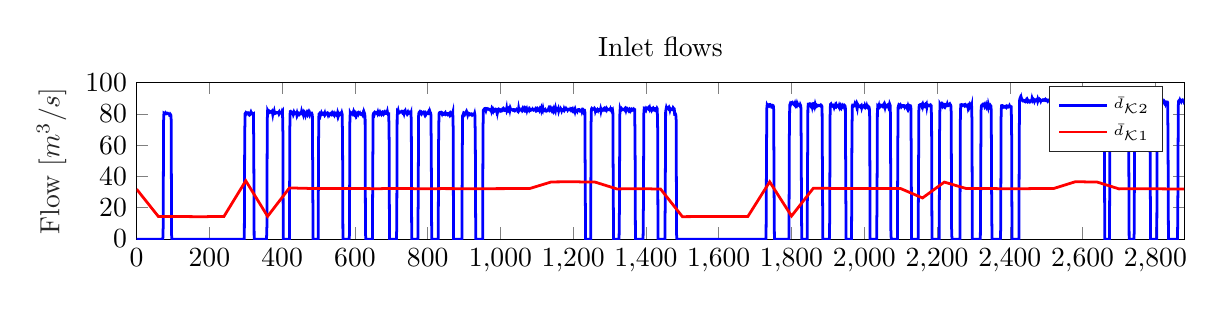
\begin{tikzpicture}

\begin{axis}[%
width=5.239in,
height=0.784in,
at={(0.974in,0.43in)},
scale only axis,
xmin=0,
xmax=2880,
%xlabel style={font=\color{white!15!black}},
%xlabel={Time [min]},
ymin=-0.1944444446,
ymax=100,
ylabel style={font=\color{white!15!black}},
ylabel={Flow  [$m^3/s$]},
axis background/.style={fill=white},
title style={},
title={Inlet flows},
legend style={legend cell align=left, align=left, draw=white!15!black}
]
\addplot [color=blue, line width=1.0pt]
  table[row sep=crcr]{%
0	-0.1666666668\\
1	-0.1666666668\\
2	-0.1666666668\\
3	-0.1666666668\\
4	-0.1666666668\\
5	-0.1666666668\\
6	-0.1666666668\\
7	-0.1666666668\\
8	-0.1666666668\\
9	-0.1666666668\\
10	-0.1666666668\\
11	-0.1666666668\\
12	-0.1666666668\\
13	-0.1666666668\\
14	-0.1666666668\\
15	-0.1666666668\\
16	-0.1666666668\\
17	-0.1666666668\\
18	-0.1666666668\\
19	-0.1666666668\\
20	-0.1666666668\\
21	-0.1666666668\\
22	-0.1666666668\\
23	-0.1666666668\\
24	-0.1666666668\\
25	-0.1666666668\\
26	-0.1666666668\\
27	-0.1666666668\\
28	-0.1666666668\\
29	-0.1666666668\\
30	-0.1666666668\\
31	-0.1666666668\\
32	-0.1666666668\\
33	-0.1666666668\\
34	-0.1666666668\\
35	-0.1666666668\\
36	-0.1666666668\\
37	-0.1666666668\\
38	-0.1666666668\\
39	-0.1666666668\\
40	-0.1666666668\\
41	-0.1666666668\\
42	-0.1666666668\\
43	-0.1666666668\\
44	-0.1666666668\\
45	-0.1666666668\\
46	-0.1666666668\\
47	-0.1666666668\\
48	-0.1666666668\\
49	-0.1666666668\\
50	-0.1666666668\\
51	-0.1666666668\\
52	-0.1666666668\\
53	-0.1666666668\\
54	-0.1666666668\\
55	-0.1666666668\\
56	-0.1666666668\\
57	-0.1666666668\\
58	-0.1666666668\\
59	-0.1666666668\\
60	-0.1666666668\\
61	-0.1666666668\\
62	-0.1666666668\\
63	-0.1666666668\\
64	-0.1666666668\\
65	-0.1666666668\\
66	-0.1666666668\\
67	-0.1666666668\\
68	-0.1666666668\\
69	-0.1666666668\\
70	-0.1666666668\\
71	-0.1666666668\\
72	-0.1666666668\\
73	7.9444444508\\
74	75.0555556156\\
75	80.277777842\\
76	80.0833333974\\
77	80.0555556196\\
78	80.1944445086\\
79	80.55555562\\
80	80.1666667308\\
81	79.9444445084\\
82	79.9722222862\\
83	80.4444445088\\
84	80.3888889532\\
85	80.416666731\\
86	80.2222222864\\
87	80.138888953\\
88	79.9166667306\\
89	79.6944445082\\
90	79.6666667304\\
91	78.8333333964\\
92	78.7777778408\\
93	79.5555556192\\
94	79.2500000634\\
95	75.9166667274\\
96	2.7500000022\\
97	-0.1666666668\\
98	-0.1666666668\\
99	-0.1666666668\\
100	-0.1666666668\\
101	-0.1666666668\\
102	-0.1666666668\\
103	-0.1666666668\\
104	-0.1666666668\\
105	-0.1666666668\\
106	-0.1666666668\\
107	-0.1666666668\\
108	-0.1666666668\\
109	-0.1666666668\\
110	-0.1666666668\\
111	-0.1666666668\\
112	-0.1666666668\\
113	-0.1666666668\\
114	-0.1666666668\\
115	-0.1666666668\\
116	-0.1666666668\\
117	-0.1666666668\\
118	-0.1666666668\\
119	-0.1666666668\\
120	-0.1666666668\\
121	-0.1666666668\\
122	-0.1666666668\\
123	-0.1666666668\\
124	-0.1666666668\\
125	-0.1666666668\\
126	-0.1666666668\\
127	-0.1666666668\\
128	-0.1666666668\\
129	-0.1666666668\\
130	-0.1666666668\\
131	-0.1666666668\\
132	-0.1666666668\\
133	-0.1666666668\\
134	-0.1666666668\\
135	-0.1666666668\\
136	-0.1666666668\\
137	-0.1666666668\\
138	-0.1666666668\\
139	-0.1666666668\\
140	-0.1666666668\\
141	-0.1666666668\\
142	-0.1666666668\\
143	-0.1666666668\\
144	-0.1666666668\\
145	-0.1666666668\\
146	-0.1666666668\\
147	-0.1666666668\\
148	-0.1666666668\\
149	-0.1666666668\\
150	-0.1666666668\\
151	-0.1666666668\\
152	-0.1666666668\\
153	-0.1666666668\\
154	-0.1666666668\\
155	-0.1666666668\\
156	-0.1666666668\\
157	-0.1666666668\\
158	-0.1666666668\\
159	-0.1666666668\\
160	-0.1666666668\\
161	-0.1666666668\\
162	-0.1666666668\\
163	-0.1666666668\\
164	-0.1666666668\\
165	-0.1666666668\\
166	-0.1666666668\\
167	-0.1666666668\\
168	-0.1666666668\\
169	-0.1666666668\\
170	-0.1666666668\\
171	-0.1666666668\\
172	-0.1666666668\\
173	-0.1666666668\\
174	-0.1666666668\\
175	-0.1666666668\\
176	-0.1666666668\\
177	-0.1666666668\\
178	-0.1666666668\\
179	-0.1666666668\\
180	-0.1666666668\\
181	-0.1666666668\\
182	-0.1666666668\\
183	-0.1666666668\\
184	-0.1666666668\\
185	-0.1666666668\\
186	-0.1666666668\\
187	-0.1666666668\\
188	-0.1666666668\\
189	-0.1666666668\\
190	-0.1666666668\\
191	-0.1666666668\\
192	-0.1666666668\\
193	-0.1666666668\\
194	-0.1666666668\\
195	-0.1666666668\\
196	-0.1666666668\\
197	-0.1666666668\\
198	-0.1666666668\\
199	-0.1666666668\\
200	-0.1666666668\\
201	-0.1666666668\\
202	-0.1666666668\\
203	-0.1666666668\\
204	-0.1666666668\\
205	-0.1666666668\\
206	-0.1666666668\\
207	-0.1666666668\\
208	-0.1666666668\\
209	-0.1666666668\\
210	-0.1666666668\\
211	-0.1666666668\\
212	-0.1666666668\\
213	-0.1666666668\\
214	-0.1666666668\\
215	-0.1666666668\\
216	-0.1666666668\\
217	-0.1666666668\\
218	-0.1666666668\\
219	-0.1666666668\\
220	-0.1666666668\\
221	-0.1666666668\\
222	-0.1666666668\\
223	-0.1666666668\\
224	-0.1666666668\\
225	-0.1666666668\\
226	-0.1666666668\\
227	-0.1666666668\\
228	-0.1666666668\\
229	-0.1666666668\\
230	-0.1666666668\\
231	-0.1666666668\\
232	-0.1666666668\\
233	-0.1666666668\\
234	-0.1666666668\\
235	-0.1666666668\\
236	-0.1666666668\\
237	-0.1666666668\\
238	-0.1666666668\\
239	-0.1666666668\\
240	-0.1666666668\\
241	-0.1666666668\\
242	-0.1666666668\\
243	-0.1666666668\\
244	-0.1666666668\\
245	-0.1666666668\\
246	-0.1666666668\\
247	-0.1666666668\\
248	-0.1666666668\\
249	-0.1666666668\\
250	-0.1666666668\\
251	-0.1666666668\\
252	-0.1666666668\\
253	-0.1666666668\\
254	-0.1666666668\\
255	-0.1666666668\\
256	-0.1666666668\\
257	-0.1666666668\\
258	-0.1666666668\\
259	-0.1666666668\\
260	-0.1666666668\\
261	-0.1666666668\\
262	-0.1666666668\\
263	-0.1666666668\\
264	-0.1666666668\\
265	-0.1666666668\\
266	-0.1666666668\\
267	-0.1666666668\\
268	-0.1666666668\\
269	-0.1666666668\\
270	-0.1666666668\\
271	-0.1666666668\\
272	-0.1666666668\\
273	-0.1666666668\\
274	-0.1666666668\\
275	-0.1666666668\\
276	-0.1666666668\\
277	-0.1666666668\\
278	-0.1666666668\\
279	-0.1666666668\\
280	-0.1666666668\\
281	-0.1666666668\\
282	-0.1666666668\\
283	-0.1666666668\\
284	-0.1666666668\\
285	-0.1666666668\\
286	-0.1666666668\\
287	-0.1666666668\\
288	-0.1666666668\\
289	-0.1666666668\\
290	-0.1666666668\\
291	-0.1666666668\\
292	-0.1666666668\\
293	-0.1666666668\\
294	-0.1666666668\\
295	-0.1666666668\\
296	-0.1666666668\\
297	63.4166667174\\
298	80.0833333974\\
299	80.416666731\\
300	79.9722222862\\
301	80.8055556202\\
302	80.6388889534\\
303	80.6666667312\\
304	80.694444509\\
305	80.5277778422\\
306	80.6666667312\\
307	80.4444445088\\
308	79.4722222858\\
309	79.305555619\\
310	80.000000064\\
311	80.2500000642\\
312	80.0277778418\\
313	80.6388889534\\
314	81.1666667316\\
315	80.55555562\\
316	80.5833333978\\
317	79.9444445084\\
318	79.7777778416\\
319	80.000000064\\
320	79.8888889528\\
321	80.0277778418\\
322	57.638888935\\
323	-0.1666666668\\
324	-0.1666666668\\
325	-0.1666666668\\
326	-0.1666666668\\
327	-0.1666666668\\
328	-0.1666666668\\
329	-0.1666666668\\
330	-0.1666666668\\
331	-0.1666666668\\
332	-0.1666666668\\
333	-0.1666666668\\
334	-0.1666666668\\
335	-0.1666666668\\
336	-0.1666666668\\
337	-0.1666666668\\
338	-0.1666666668\\
339	-0.1666666668\\
340	-0.1666666668\\
341	-0.1666666668\\
342	-0.1666666668\\
343	-0.1666666668\\
344	-0.1666666668\\
345	-0.1666666668\\
346	-0.1666666668\\
347	-0.1666666668\\
348	-0.1666666668\\
349	-0.1666666668\\
350	-0.1666666668\\
351	-0.1666666668\\
352	-0.1666666668\\
353	-0.1666666668\\
354	-0.1666666668\\
355	-0.1666666668\\
356	-0.1666666668\\
357	-0.1666666668\\
358	7.500000006\\
359	75.6388889494\\
360	82.0277778434\\
361	81.527777843\\
362	80.8888889536\\
363	81.5555556208\\
364	81.250000065\\
365	81.6388889542\\
366	81.4444445096\\
367	80.972222287\\
368	81.0833333982\\
369	81.1944445094\\
370	81.5555556208\\
371	81.6944445098\\
372	81.3055556206\\
373	81.0000000648\\
374	79.722222286\\
375	81.1666667316\\
376	80.8055556202\\
377	81.0000000648\\
378	81.7500000654\\
379	80.5000000644\\
380	80.7500000646\\
381	80.7500000646\\
382	80.5277778422\\
383	80.8055556202\\
384	80.6666667312\\
385	80.55555562\\
386	80.6388889534\\
387	80.7777778424\\
388	80.6388889534\\
389	80.694444509\\
390	80.6666667312\\
391	81.0277778426\\
392	79.8888889528\\
393	80.2222222864\\
394	80.55555562\\
395	80.5277778422\\
396	80.9444445092\\
397	80.8888889536\\
398	80.694444509\\
399	81.3055556206\\
400	80.5000000644\\
401	80.972222287\\
402	68.5277778326\\
403	-0.1666666668\\
404	-0.1666666668\\
405	-0.1666666668\\
406	-0.1666666668\\
407	-0.1666666668\\
408	-0.1666666668\\
409	-0.1666666668\\
410	-0.1666666668\\
411	-0.1666666668\\
412	-0.1666666668\\
413	-0.1666666668\\
414	-0.1666666668\\
415	-0.1666666668\\
416	-0.1666666668\\
417	-0.1666666668\\
418	-0.1666666668\\
419	-0.1666666668\\
420	-0.1666666668\\
421	69.9722222782\\
422	81.4722222874\\
423	81.5833333986\\
424	81.1666667316\\
425	81.1944445094\\
426	81.0277778426\\
427	80.9166667314\\
428	80.5833333978\\
429	80.0833333974\\
430	80.5277778422\\
431	79.444444508\\
432	79.9444445084\\
433	80.9166667314\\
434	80.416666731\\
435	80.2222222864\\
436	80.277777842\\
437	80.1666667308\\
438	80.694444509\\
439	80.8888889536\\
440	79.6388889526\\
441	80.5000000644\\
442	79.6666667304\\
443	80.3333333976\\
444	80.6388889534\\
445	80.6666667312\\
446	80.55555562\\
447	79.9722222862\\
448	80.4444445088\\
449	80.416666731\\
450	80.3055556198\\
451	80.0555556196\\
452	80.2500000642\\
453	81.3055556206\\
454	80.2222222864\\
455	80.0833333974\\
456	79.8888889528\\
457	80.3333333976\\
458	79.5555556192\\
459	80.7500000646\\
460	80.277777842\\
461	79.8888889528\\
462	80.5000000644\\
463	79.9722222862\\
464	79.16666673\\
465	80.0833333974\\
466	80.0833333974\\
467	80.55555562\\
468	79.6944445082\\
469	79.305555619\\
470	80.0833333974\\
471	80.0555556196\\
472	80.8055556202\\
473	80.1944445086\\
474	80.0833333974\\
475	79.5000000636\\
476	80.3888889532\\
477	79.722222286\\
478	79.9444445084\\
479	79.8333333972\\
480	80.416666731\\
481	80.4722222866\\
482	79.9444445084\\
483	79.0555556188\\
484	40.972222255\\
485	-0.1666666668\\
486	-0.1666666668\\
487	-0.1666666668\\
488	-0.1666666668\\
489	-0.1666666668\\
490	-0.1666666668\\
491	-0.1666666668\\
492	-0.1666666668\\
493	-0.1666666668\\
494	-0.1666666668\\
495	-0.1666666668\\
496	-0.1666666668\\
497	-0.1666666668\\
498	-0.1666666668\\
499	-0.1666666668\\
500	61.0277778266\\
501	79.7777778416\\
502	80.0277778418\\
503	79.3333333968\\
504	79.6666667304\\
505	79.0555556188\\
506	79.9722222862\\
507	80.4722222866\\
508	79.5555556192\\
509	79.8055556194\\
510	80.2500000642\\
511	80.000000064\\
512	79.7777778416\\
513	80.0833333974\\
514	80.4722222866\\
515	80.4444445088\\
516	79.8333333972\\
517	80.416666731\\
518	79.3333333968\\
519	79.6666667304\\
520	79.7500000638\\
521	80.0833333974\\
522	80.416666731\\
523	80.5277778422\\
524	79.9722222862\\
525	80.000000064\\
526	79.305555619\\
527	79.9444445084\\
528	79.6388889526\\
529	79.6944445082\\
530	79.2222222856\\
531	79.583333397\\
532	80.138888953\\
533	80.2500000642\\
534	80.3888889532\\
535	79.722222286\\
536	79.4722222858\\
537	79.9166667306\\
538	80.55555562\\
539	80.138888953\\
540	79.9722222862\\
541	79.5555556192\\
542	79.2500000634\\
543	79.9166667306\\
544	79.3333333968\\
545	79.9722222862\\
546	80.3333333976\\
547	80.5277778422\\
548	80.4722222866\\
549	79.9166667306\\
550	80.277777842\\
551	80.1666667308\\
552	79.2222222856\\
553	80.7500000646\\
554	80.138888953\\
555	78.9722222854\\
556	79.6944445082\\
557	80.2222222864\\
558	80.3333333976\\
559	79.5000000636\\
560	79.6944445082\\
561	79.9722222862\\
562	80.138888953\\
563	79.6944445082\\
564	80.5277778422\\
565	79.6388889526\\
566	63.5555556064\\
567	-0.1666666668\\
568	-0.1666666668\\
569	-0.1666666668\\
570	-0.1666666668\\
571	-0.1666666668\\
572	-0.1666666668\\
573	-0.1666666668\\
574	-0.1666666668\\
575	-0.1666666668\\
576	-0.1666666668\\
577	-0.1666666668\\
578	-0.1666666668\\
579	-0.1666666668\\
580	-0.1666666668\\
581	-0.1666666668\\
582	-0.1666666668\\
583	-0.1666666668\\
584	-0.1666666668\\
585	2.638888891\\
586	74.0555556148\\
587	80.3888889532\\
588	79.8888889528\\
589	80.694444509\\
590	80.5277778422\\
591	80.5277778422\\
592	80.2222222864\\
593	80.5000000644\\
594	80.0833333974\\
595	80.6666667312\\
596	81.388888954\\
597	80.55555562\\
598	80.0555556196\\
599	80.6388889534\\
600	80.138888953\\
601	79.7500000638\\
602	79.0555556188\\
603	79.8055556194\\
604	79.2500000634\\
605	80.2222222864\\
606	80.277777842\\
607	80.5000000644\\
608	80.277777842\\
609	79.8055556194\\
610	80.4444445088\\
611	80.138888953\\
612	80.4444445088\\
613	80.6388889534\\
614	79.8888889528\\
615	79.7500000638\\
616	80.2500000642\\
617	80.0833333974\\
618	80.0277778418\\
619	79.7777778416\\
620	79.722222286\\
621	79.305555619\\
622	80.1944445086\\
623	79.6666667304\\
624	79.722222286\\
625	81.1666667316\\
626	80.5277778422\\
627	79.9444445084\\
628	76.666666728\\
629	3.5000000028\\
630	-0.1666666668\\
631	-0.1666666668\\
632	-0.1666666668\\
633	-0.1666666668\\
634	-0.1666666668\\
635	-0.1666666668\\
636	-0.1666666668\\
637	-0.1666666668\\
638	-0.1666666668\\
639	-0.1666666668\\
640	-0.1666666668\\
641	-0.1666666668\\
642	-0.1666666668\\
643	-0.1666666668\\
644	-0.1666666668\\
645	-0.1666666668\\
646	-0.1666666668\\
647	-0.1666666668\\
648	-0.1666666668\\
649	43.0833333678\\
650	79.2777778412\\
651	80.1944445086\\
652	80.55555562\\
653	80.7777778424\\
654	80.0833333974\\
655	80.833333398\\
656	80.8888889536\\
657	80.416666731\\
658	80.3333333976\\
659	80.55555562\\
660	80.5833333978\\
661	80.833333398\\
662	80.2222222864\\
663	80.9444445092\\
664	80.0555556196\\
665	80.3055556198\\
666	79.9444445084\\
667	80.5833333978\\
668	80.3055556198\\
669	80.9444445092\\
670	80.3888889532\\
671	80.5833333978\\
672	80.4722222866\\
673	80.694444509\\
674	79.7777778416\\
675	80.0833333974\\
676	80.0555556196\\
677	80.5000000644\\
678	80.0555556196\\
679	80.6666667312\\
680	80.9166667314\\
681	80.55555562\\
682	80.972222287\\
683	80.416666731\\
684	80.1944445086\\
685	80.1944445086\\
686	80.6666667312\\
687	80.4444445088\\
688	80.7777778424\\
689	81.5555556208\\
690	80.2500000642\\
691	79.6944445082\\
692	80.0277778418\\
693	80.0277778418\\
694	64.5000000516\\
695	-0.1666666668\\
696	-0.1666666668\\
697	-0.1666666668\\
698	-0.1666666668\\
699	-0.1666666668\\
700	-0.1666666668\\
701	-0.1666666668\\
702	-0.1666666668\\
703	-0.1666666668\\
704	-0.1666666668\\
705	-0.1666666668\\
706	-0.1666666668\\
707	-0.1666666668\\
708	-0.1666666668\\
709	-0.1666666668\\
710	-0.1666666668\\
711	-0.1666666668\\
712	-0.1666666668\\
713	-0.1666666668\\
714	-0.1666666668\\
715	7.638888895\\
716	76.250000061\\
717	81.3333333984\\
718	81.0000000648\\
719	81.8888889544\\
720	80.8055556202\\
721	81.0000000648\\
722	80.7222222868\\
723	80.9166667314\\
724	80.972222287\\
725	81.0277778426\\
726	81.250000065\\
727	81.2777778428\\
728	81.527777843\\
729	81.388888954\\
730	81.0000000648\\
731	81.527777843\\
732	81.4444445096\\
733	81.527777843\\
734	80.694444509\\
735	79.9722222862\\
736	80.8888889536\\
737	81.7222222876\\
738	82.0555556212\\
739	81.0277778426\\
740	80.972222287\\
741	80.5833333978\\
742	80.694444509\\
743	80.1944445086\\
744	80.7777778424\\
745	81.1388889538\\
746	80.2500000642\\
747	80.55555562\\
748	81.2777778428\\
749	81.250000065\\
750	80.6666667312\\
751	80.8055556202\\
752	80.7500000646\\
753	80.000000064\\
754	80.6388889534\\
755	74.722222282\\
756	-0.1666666668\\
757	-0.1666666668\\
758	-0.1666666668\\
759	-0.1666666668\\
760	-0.1666666668\\
761	-0.1666666668\\
762	-0.1666666668\\
763	-0.1666666668\\
764	-0.1666666668\\
765	-0.1666666668\\
766	-0.1666666668\\
767	-0.1666666668\\
768	-0.1666666668\\
769	-0.1666666668\\
770	-0.1666666668\\
771	-0.1666666668\\
772	-0.1666666668\\
773	-0.1666666668\\
774	28.3055555782\\
775	78.6944445074\\
776	80.8055556202\\
777	81.0277778426\\
778	81.3055556206\\
779	80.7777778424\\
780	80.9444445092\\
781	81.0833333982\\
782	80.1666667308\\
783	79.8333333972\\
784	80.277777842\\
785	80.3055556198\\
786	80.7777778424\\
787	81.0277778426\\
788	81.1388889538\\
789	80.8055556202\\
790	80.4722222866\\
791	79.9166667306\\
792	80.8055556202\\
793	80.6388889534\\
794	79.8055556194\\
795	80.3888889532\\
796	80.000000064\\
797	80.5277778422\\
798	80.55555562\\
799	80.1666667308\\
800	80.277777842\\
801	80.8055556202\\
802	81.250000065\\
803	80.5833333978\\
804	80.1666667308\\
805	80.3055556198\\
806	81.4722222874\\
807	80.7777778424\\
808	80.5277778422\\
809	79.2777778412\\
810	50.138888929\\
811	-0.1666666668\\
812	-0.1666666668\\
813	-0.1666666668\\
814	-0.1666666668\\
815	-0.1666666668\\
816	-0.1666666668\\
817	-0.1666666668\\
818	-0.1666666668\\
819	-0.1666666668\\
820	-0.1666666668\\
821	-0.1666666668\\
822	-0.1666666668\\
823	-0.1666666668\\
824	-0.1666666668\\
825	-0.1666666668\\
826	-0.1666666668\\
827	-0.1666666668\\
828	-0.1666666668\\
829	-0.1666666668\\
830	62.638888939\\
831	79.722222286\\
832	80.6388889534\\
833	80.8055556202\\
834	80.9444445092\\
835	80.9444445092\\
836	80.6666667312\\
837	80.8055556202\\
838	80.3333333976\\
839	79.8888889528\\
840	80.6388889534\\
841	80.4722222866\\
842	80.0277778418\\
843	79.6388889526\\
844	79.583333397\\
845	80.0277778418\\
846	80.277777842\\
847	80.5000000644\\
848	80.7500000646\\
849	79.8333333972\\
850	79.5000000636\\
851	79.6388889526\\
852	79.8333333972\\
853	80.0277778418\\
854	79.8055556194\\
855	79.9444445084\\
856	79.5000000636\\
857	79.7500000638\\
858	79.7500000638\\
859	79.8888889528\\
860	80.1944445086\\
861	79.4166667302\\
862	79.8888889528\\
863	80.277777842\\
864	79.722222286\\
865	80.1666667308\\
866	80.0277778418\\
867	79.6944445082\\
868	79.7500000638\\
869	80.694444509\\
870	71.2777778348\\
871	-0.1666666668\\
872	-0.1666666668\\
873	-0.1666666668\\
874	-0.1666666668\\
875	-0.1666666668\\
876	-0.1666666668\\
877	-0.1666666668\\
878	-0.1666666668\\
879	-0.1666666668\\
880	-0.1666666668\\
881	-0.1666666668\\
882	-0.1666666668\\
883	-0.1944444446\\
884	-0.1666666668\\
885	-0.1666666668\\
886	-0.1666666668\\
887	-0.1666666668\\
888	-0.1666666668\\
889	-0.1666666668\\
890	-0.1666666668\\
891	-0.1666666668\\
892	-0.1666666668\\
893	-0.1666666668\\
894	-0.1666666668\\
895	52.1944444862\\
896	78.750000063\\
897	79.3888889524\\
898	79.9444445084\\
899	80.6666667312\\
900	80.5277778422\\
901	80.000000064\\
902	79.5000000636\\
903	79.8888889528\\
904	80.3055556198\\
905	80.8055556202\\
906	80.0555556196\\
907	79.9166667306\\
908	80.9166667314\\
909	80.3333333976\\
910	79.3888889524\\
911	80.1666667308\\
912	79.8333333972\\
913	80.000000064\\
914	79.722222286\\
915	79.8888889528\\
916	79.5000000636\\
917	79.6944445082\\
918	79.7500000638\\
919	79.8055556194\\
920	79.722222286\\
921	79.4166667302\\
922	79.8888889528\\
923	79.7777778416\\
924	79.2777778412\\
925	79.4166667302\\
926	79.6666667304\\
927	79.5277778414\\
928	79.5277778414\\
929	80.277777842\\
930	78.9444445076\\
931	58.8333333804\\
932	-0.1666666668\\
933	-0.1666666668\\
934	-0.1666666668\\
935	-0.1666666668\\
936	-0.1666666668\\
937	-0.1666666668\\
938	-0.1666666668\\
939	-0.1666666668\\
940	-0.1666666668\\
941	-0.1666666668\\
942	-0.1666666668\\
943	-0.1666666668\\
944	-0.1666666668\\
945	-0.1666666668\\
946	-0.1666666668\\
947	-0.1666666668\\
948	-0.1666666668\\
949	-0.1944444446\\
950	-0.1666666668\\
951	-0.1666666668\\
952	69.5555556112\\
953	82.222222288\\
954	82.638888955\\
955	82.9722222886\\
956	83.0000000664\\
957	83.4166667334\\
958	83.4444445112\\
959	82.6666667328\\
960	82.0277778434\\
961	82.8333333996\\
962	83.194444511\\
963	83.3055556222\\
964	83.0833333998\\
965	83.1388889554\\
966	82.9722222886\\
967	83.0833333998\\
968	82.8333333996\\
969	82.6666667328\\
970	82.7500000662\\
971	82.5277778438\\
972	82.3055556214\\
973	82.6666667328\\
974	82.7500000662\\
975	81.9166667322\\
976	82.916666733\\
977	82.2777778436\\
978	82.2500000658\\
979	81.7777778432\\
980	82.6666667328\\
981	82.1388889546\\
982	82.7222222884\\
983	82.7222222884\\
984	82.8333333996\\
985	81.9722222878\\
986	82.1388889546\\
987	82.9722222886\\
988	82.9444445108\\
989	81.9722222878\\
990	82.6944445106\\
991	82.7500000662\\
992	81.0000000648\\
993	82.1388889546\\
994	82.500000066\\
995	82.500000066\\
996	82.916666733\\
997	82.6944445106\\
998	82.4722222882\\
999	82.5555556216\\
1000	81.8333333988\\
1001	82.0277778434\\
1002	82.5833333994\\
1003	82.5833333994\\
1004	81.8333333988\\
1005	81.9166667322\\
1006	82.7222222884\\
1007	82.5277778438\\
1008	82.5277778438\\
1009	83.3055556222\\
1010	83.0833333998\\
1011	82.3333333992\\
1012	82.1388889546\\
1013	82.2777778436\\
1014	82.222222288\\
1015	82.4722222882\\
1016	82.2500000658\\
1017	83.4444445112\\
1018	81.7777778432\\
1019	82.1944445102\\
1020	82.8055556218\\
1021	83.194444511\\
1022	82.6666667328\\
1023	83.3055556222\\
1024	83.2500000666\\
1025	83.6944445114\\
1026	82.500000066\\
1027	83.6666667336\\
1028	83.0833333998\\
1029	82.7222222884\\
1030	82.8055556218\\
1031	82.7500000662\\
1032	82.500000066\\
1033	82.4444445104\\
1034	82.2777778436\\
1035	82.6666667328\\
1036	82.7222222884\\
1037	82.777777844\\
1038	82.6944445106\\
1039	82.4166667326\\
1040	81.9722222878\\
1041	82.1666667324\\
1042	82.4166667326\\
1043	82.4444445104\\
1044	82.7500000662\\
1045	82.4444445104\\
1046	82.2500000658\\
1047	82.4722222882\\
1048	81.6388889542\\
1049	81.7777778432\\
1050	83.4166667334\\
1051	82.1666667324\\
1052	82.5833333994\\
1053	82.8333333996\\
1054	82.4166667326\\
1055	82.3888889548\\
1056	82.3055556214\\
1057	82.4722222882\\
1058	82.2500000658\\
1059	82.7500000662\\
1060	83.1666667332\\
1061	82.0555556212\\
1062	82.3055556214\\
1063	82.9444445108\\
1064	82.4444445104\\
1065	82.5555556216\\
1066	83.055555622\\
1067	82.222222288\\
1068	82.4722222882\\
1069	82.916666733\\
1070	82.3055556214\\
1071	82.5833333994\\
1072	83.0833333998\\
1073	82.0555556212\\
1074	82.7222222884\\
1075	82.2777778436\\
1076	82.3055556214\\
1077	82.3055556214\\
1078	82.777777844\\
1079	82.2500000658\\
1080	82.7222222884\\
1081	81.9722222878\\
1082	82.083333399\\
1083	82.3333333992\\
1084	82.6666667328\\
1085	82.5277778438\\
1086	82.7222222884\\
1087	82.6944445106\\
1088	83.0277778442\\
1089	82.5833333994\\
1090	82.4166667326\\
1091	82.7500000662\\
1092	82.8055556218\\
1093	82.6944445106\\
1094	82.7222222884\\
1095	82.4722222882\\
1096	82.916666733\\
1097	82.4166667326\\
1098	82.8333333996\\
1099	82.3055556214\\
1100	82.638888955\\
1101	82.4166667326\\
1102	82.916666733\\
1103	82.4444445104\\
1104	82.3055556214\\
1105	82.4722222882\\
1106	82.5833333994\\
1107	83.0000000664\\
1108	82.1388889546\\
1109	82.5277778438\\
1110	82.7500000662\\
1111	82.6666667328\\
1112	83.3888889556\\
1113	82.1944445102\\
1114	82.9444445108\\
1115	82.6666667328\\
1116	82.1388889546\\
1117	83.2500000666\\
1118	82.1666667324\\
1119	82.0555556212\\
1120	82.5555556216\\
1121	82.3333333992\\
1122	82.500000066\\
1123	82.7222222884\\
1124	82.1388889546\\
1125	81.8888889544\\
1126	82.3055556214\\
1127	82.2777778436\\
1128	82.0000000656\\
1129	81.94444451\\
1130	82.3888889548\\
1131	82.4444445104\\
1132	83.055555622\\
1133	82.4444445104\\
1134	82.5555556216\\
1135	83.1666667332\\
1136	82.5277778438\\
1137	82.916666733\\
1138	83.4444445112\\
1139	82.777777844\\
1140	82.8333333996\\
1141	82.2777778436\\
1142	82.777777844\\
1143	82.222222288\\
1144	82.7500000662\\
1145	82.5555556216\\
1146	83.1388889554\\
1147	81.9722222878\\
1148	82.4722222882\\
1149	82.3055556214\\
1150	82.4444445104\\
1151	81.8333333988\\
1152	83.2777778444\\
1153	82.3055556214\\
1154	82.3333333992\\
1155	82.3333333992\\
1156	82.7500000662\\
1157	82.4166667326\\
1158	82.5277778438\\
1159	83.1388889554\\
1160	81.8888889544\\
1161	82.7222222884\\
1162	82.4444445104\\
1163	82.6666667328\\
1164	82.4722222882\\
1165	82.3888889548\\
1166	83.1388889554\\
1167	82.7222222884\\
1168	82.0277778434\\
1169	82.7500000662\\
1170	82.7222222884\\
1171	82.4444445104\\
1172	82.2500000658\\
1173	82.2777778436\\
1174	82.0555556212\\
1175	83.055555622\\
1176	82.4722222882\\
1177	82.3888889548\\
1178	82.6944445106\\
1179	82.777777844\\
1180	83.2500000666\\
1181	82.777777844\\
1182	82.777777844\\
1183	82.916666733\\
1184	82.9722222886\\
1185	82.3333333992\\
1186	82.638888955\\
1187	82.9444445108\\
1188	82.916666733\\
1189	82.8333333996\\
1190	82.5277778438\\
1191	82.4444445104\\
1192	82.9722222886\\
1193	82.6666667328\\
1194	82.8888889552\\
1195	82.2500000658\\
1196	82.500000066\\
1197	82.8333333996\\
1198	82.3055556214\\
1199	82.8055556218\\
1200	82.1388889546\\
1201	81.5833333986\\
1202	81.3333333984\\
1203	81.7500000654\\
1204	82.3888889548\\
1205	81.5000000652\\
1206	82.4444445104\\
1207	81.6944445098\\
1208	81.6944445098\\
1209	81.94444451\\
1210	81.94444451\\
1211	81.5555556208\\
1212	82.222222288\\
1213	82.3333333992\\
1214	82.6944445106\\
1215	82.6944445106\\
1216	82.3888889548\\
1217	82.5555556216\\
1218	82.3333333992\\
1219	81.8888889544\\
1220	82.083333399\\
1221	82.1666667324\\
1222	82.222222288\\
1223	82.4722222882\\
1224	81.5000000652\\
1225	82.1944445102\\
1226	82.3333333992\\
1227	82.500000066\\
1228	81.7500000654\\
1229	82.2500000658\\
1230	82.222222288\\
1231	82.2500000658\\
1232	81.1388889538\\
1233	36.805555585\\
1234	-0.1666666668\\
1235	-0.1666666668\\
1236	-0.1666666668\\
1237	-0.1666666668\\
1238	-0.1666666668\\
1239	-0.1666666668\\
1240	-0.1666666668\\
1241	-0.1666666668\\
1242	-0.1666666668\\
1243	-0.1666666668\\
1244	-0.1666666668\\
1245	-0.1666666668\\
1246	-0.1666666668\\
1247	-0.1666666668\\
1248	-0.1666666668\\
1249	73.0277778362\\
1250	83.0000000664\\
1251	83.4166667334\\
1252	83.1666667332\\
1253	82.916666733\\
1254	83.2500000666\\
1255	83.2500000666\\
1256	83.1666667332\\
1257	82.9444445108\\
1258	82.6944445106\\
1259	83.4166667334\\
1260	83.1388889554\\
1261	81.666666732\\
1262	82.2777778436\\
1263	82.3888889548\\
1264	82.083333399\\
1265	81.8333333988\\
1266	82.0555556212\\
1267	82.5555556216\\
1268	82.1388889546\\
1269	82.777777844\\
1270	82.777777844\\
1271	82.4444445104\\
1272	82.638888955\\
1273	82.222222288\\
1274	82.083333399\\
1275	82.9722222886\\
1276	81.7777778432\\
1277	82.9444445108\\
1278	82.4444445104\\
1279	82.5833333994\\
1280	82.7222222884\\
1281	82.777777844\\
1282	82.4166667326\\
1283	82.7222222884\\
1284	83.3888889556\\
1285	83.5555556224\\
1286	82.638888955\\
1287	82.4166667326\\
1288	82.916666733\\
1289	82.6944445106\\
1290	82.638888955\\
1291	83.194444511\\
1292	82.638888955\\
1293	83.2222222888\\
1294	82.916666733\\
1295	82.6944445106\\
1296	82.7500000662\\
1297	82.777777844\\
1298	82.5277778438\\
1299	82.500000066\\
1300	82.8055556218\\
1301	82.5277778438\\
1302	82.3888889548\\
1303	83.1388889554\\
1304	82.638888955\\
1305	83.3333334\\
1306	83.2500000666\\
1307	82.083333399\\
1308	82.4444445104\\
1309	80.6666667312\\
1310	30.1666666908\\
1311	-0.1666666668\\
1312	-0.1666666668\\
1313	-0.1666666668\\
1314	-0.1666666668\\
1315	-0.1666666668\\
1316	-0.1666666668\\
1317	-0.1666666668\\
1318	-0.1666666668\\
1319	-0.1666666668\\
1320	-0.1666666668\\
1321	-0.1666666668\\
1322	-0.1666666668\\
1323	-0.1666666668\\
1324	-0.1666666668\\
1325	-0.1666666668\\
1326	-0.1666666668\\
1327	18.9166666818\\
1328	78.9722222854\\
1329	83.1388889554\\
1330	82.4444445104\\
1331	82.6944445106\\
1332	83.1388889554\\
1333	82.638888955\\
1334	82.8888889552\\
1335	82.5555556216\\
1336	82.638888955\\
1337	82.8888889552\\
1338	82.777777844\\
1339	82.9722222886\\
1340	82.9722222886\\
1341	82.638888955\\
1342	83.2777778444\\
1343	83.5833334002\\
1344	83.3055556222\\
1345	82.3888889548\\
1346	83.2777778444\\
1347	83.0000000664\\
1348	83.2222222888\\
1349	82.8055556218\\
1350	82.8888889552\\
1351	82.3055556214\\
1352	81.9722222878\\
1353	82.4166667326\\
1354	82.7500000662\\
1355	82.1666667324\\
1356	81.7777778432\\
1357	82.4166667326\\
1358	82.6666667328\\
1359	82.1944445102\\
1360	82.3888889548\\
1361	82.7222222884\\
1362	82.3055556214\\
1363	82.500000066\\
1364	82.5555556216\\
1365	82.6666667328\\
1366	82.9444445108\\
1367	82.4722222882\\
1368	82.8055556218\\
1369	82.7222222884\\
1370	60.4722222706\\
1371	-0.1666666668\\
1372	-0.1666666668\\
1373	-0.1666666668\\
1374	-0.1666666668\\
1375	-0.1666666668\\
1376	-0.1666666668\\
1377	-0.1666666668\\
1378	-0.1666666668\\
1379	-0.1666666668\\
1380	-0.1666666668\\
1381	-0.1666666668\\
1382	-0.1666666668\\
1383	-0.1666666668\\
1384	-0.1666666668\\
1385	-0.1666666668\\
1386	-0.1666666668\\
1387	-0.1666666668\\
1388	-0.1666666668\\
1389	-0.1666666668\\
1390	-0.1666666668\\
1391	-0.1666666668\\
1392	-0.1666666668\\
1393	22.916666685\\
1394	79.9166667306\\
1395	83.0277778442\\
1396	82.8055556218\\
1397	83.3888889556\\
1398	83.2500000666\\
1399	83.3055556222\\
1400	82.777777844\\
1401	83.6666667336\\
1402	83.472222289\\
1403	83.2777778444\\
1404	83.3055556222\\
1405	83.5000000668\\
1406	83.8055556226\\
1407	83.3333334\\
1408	83.6944445114\\
1409	83.472222289\\
1410	83.9722222894\\
1411	83.0000000664\\
1412	83.5277778446\\
1413	83.5000000668\\
1414	83.1388889554\\
1415	83.055555622\\
1416	82.3055556214\\
1417	82.7222222884\\
1418	83.5277778446\\
1419	83.7222222892\\
1420	82.9722222886\\
1421	82.777777844\\
1422	82.5277778438\\
1423	82.9444445108\\
1424	83.3333334\\
1425	83.2500000666\\
1426	82.8333333996\\
1427	83.3055556222\\
1428	83.3055556222\\
1429	83.194444511\\
1430	83.6666667336\\
1431	83.2500000666\\
1432	71.527777835\\
1433	-0.1666666668\\
1434	-0.1666666668\\
1435	-0.1666666668\\
1436	-0.1666666668\\
1437	-0.1666666668\\
1438	-0.1666666668\\
1439	-0.1666666668\\
1440	-0.1666666668\\
1441	-0.1666666668\\
1442	-0.1666666668\\
1443	-0.1666666668\\
1444	-0.1666666668\\
1445	-0.1666666668\\
1446	-0.1666666668\\
1447	-0.1666666668\\
1448	-0.1666666668\\
1449	-0.1666666668\\
1450	-0.1666666668\\
1451	-0.1666666668\\
1452	-0.1666666668\\
1453	29.0833333566\\
1454	81.3333333984\\
1455	82.7222222884\\
1456	83.9166667338\\
1457	83.2777778444\\
1458	83.2777778444\\
1459	83.2222222888\\
1460	83.1666667332\\
1461	83.5833334002\\
1462	83.2222222888\\
1463	83.5000000668\\
1464	84.027777845\\
1465	83.5555556224\\
1466	82.4722222882\\
1467	83.3055556222\\
1468	83.055555622\\
1469	83.2500000666\\
1470	83.2500000666\\
1471	82.8333333996\\
1472	82.9444445108\\
1473	82.9722222886\\
1474	82.7500000662\\
1475	83.7777778448\\
1476	83.472222289\\
1477	82.4166667326\\
1478	82.5277778438\\
1479	78.6944445074\\
1480	80.4444445088\\
1481	80.000000064\\
1482	79.2777778412\\
1483	75.8055556162\\
1484	3.1666666692\\
1485	-0.1666666668\\
1486	-0.1666666668\\
1487	-0.1666666668\\
1488	-0.1666666668\\
1489	-0.1666666668\\
1490	-0.1666666668\\
1491	-0.1666666668\\
1492	-0.1666666668\\
1493	-0.1666666668\\
1494	-0.1666666668\\
1495	-0.1666666668\\
1496	-0.1666666668\\
1497	-0.1666666668\\
1498	-0.1666666668\\
1499	-0.1666666668\\
1500	-0.1666666668\\
1501	-0.1666666668\\
1502	-0.1666666668\\
1503	-0.1666666668\\
1504	-0.1666666668\\
1505	-0.1666666668\\
1506	-0.1666666668\\
1507	-0.1666666668\\
1508	-0.1666666668\\
1509	-0.1666666668\\
1510	-0.1666666668\\
1511	-0.1666666668\\
1512	-0.1666666668\\
1513	-0.1666666668\\
1514	-0.1666666668\\
1515	-0.1666666668\\
1516	-0.1666666668\\
1517	-0.1666666668\\
1518	-0.1666666668\\
1519	-0.1666666668\\
1520	-0.1666666668\\
1521	-0.1666666668\\
1522	-0.1666666668\\
1523	-0.1666666668\\
1524	-0.1666666668\\
1525	-0.1666666668\\
1526	-0.1666666668\\
1527	-0.1666666668\\
1528	-0.1666666668\\
1529	-0.1666666668\\
1530	-0.1666666668\\
1531	-0.1666666668\\
1532	-0.1666666668\\
1533	-0.1666666668\\
1534	-0.1666666668\\
1535	-0.1666666668\\
1536	-0.1666666668\\
1537	-0.1666666668\\
1538	-0.1666666668\\
1539	-0.1666666668\\
1540	-0.1666666668\\
1541	-0.1666666668\\
1542	-0.1666666668\\
1543	-0.1666666668\\
1544	-0.1666666668\\
1545	-0.1666666668\\
1546	-0.1666666668\\
1547	-0.1666666668\\
1548	-0.1666666668\\
1549	-0.1666666668\\
1550	-0.1666666668\\
1551	-0.1666666668\\
1552	-0.1666666668\\
1553	-0.1666666668\\
1554	-0.1666666668\\
1555	-0.1666666668\\
1556	-0.1666666668\\
1557	-0.1666666668\\
1558	-0.1666666668\\
1559	-0.1666666668\\
1560	-0.1666666668\\
1561	-0.1666666668\\
1562	-0.1666666668\\
1563	-0.1666666668\\
1564	-0.1666666668\\
1565	-0.1666666668\\
1566	-0.1666666668\\
1567	-0.1666666668\\
1568	-0.1666666668\\
1569	-0.1666666668\\
1570	-0.1666666668\\
1571	-0.1666666668\\
1572	-0.1666666668\\
1573	-0.1666666668\\
1574	-0.1666666668\\
1575	-0.1666666668\\
1576	-0.1666666668\\
1577	-0.1666666668\\
1578	-0.1666666668\\
1579	-0.1666666668\\
1580	-0.1666666668\\
1581	-0.1666666668\\
1582	-0.1666666668\\
1583	-0.1666666668\\
1584	-0.1666666668\\
1585	-0.1666666668\\
1586	-0.1666666668\\
1587	-0.1666666668\\
1588	-0.1666666668\\
1589	-0.1666666668\\
1590	-0.1666666668\\
1591	-0.1666666668\\
1592	-0.1666666668\\
1593	-0.1666666668\\
1594	-0.1666666668\\
1595	-0.1666666668\\
1596	-0.1666666668\\
1597	-0.1666666668\\
1598	-0.1666666668\\
1599	-0.1666666668\\
1600	-0.1666666668\\
1601	-0.1666666668\\
1602	-0.1666666668\\
1603	-0.1666666668\\
1604	-0.1666666668\\
1605	-0.1666666668\\
1606	-0.1666666668\\
1607	-0.1666666668\\
1608	-0.1666666668\\
1609	-0.1666666668\\
1610	-0.1666666668\\
1611	-0.1666666668\\
1612	-0.1666666668\\
1613	-0.1666666668\\
1614	-0.1666666668\\
1615	-0.1666666668\\
1616	-0.1666666668\\
1617	-0.1666666668\\
1618	-0.1666666668\\
1619	-0.1666666668\\
1620	-0.1666666668\\
1621	-0.1666666668\\
1622	-0.1666666668\\
1623	-0.1666666668\\
1624	-0.1666666668\\
1625	-0.1666666668\\
1626	-0.1666666668\\
1627	-0.1666666668\\
1628	-0.1666666668\\
1629	-0.1666666668\\
1630	-0.1666666668\\
1631	-0.1666666668\\
1632	-0.1666666668\\
1633	-0.1666666668\\
1634	-0.1666666668\\
1635	-0.1666666668\\
1636	-0.1666666668\\
1637	-0.1666666668\\
1638	-0.1666666668\\
1639	-0.1666666668\\
1640	-0.1666666668\\
1641	-0.1666666668\\
1642	-0.1666666668\\
1643	-0.1666666668\\
1644	-0.1666666668\\
1645	-0.1666666668\\
1646	-0.1666666668\\
1647	-0.1666666668\\
1648	-0.1666666668\\
1649	-0.1666666668\\
1650	-0.1666666668\\
1651	-0.1666666668\\
1652	-0.1666666668\\
1653	-0.1666666668\\
1654	-0.1666666668\\
1655	-0.1666666668\\
1656	-0.1666666668\\
1657	-0.1666666668\\
1658	-0.1666666668\\
1659	-0.1666666668\\
1660	-0.1666666668\\
1661	-0.1666666668\\
1662	-0.1666666668\\
1663	-0.1666666668\\
1664	-0.1666666668\\
1665	-0.1666666668\\
1666	-0.1666666668\\
1667	-0.1666666668\\
1668	-0.1666666668\\
1669	-0.1666666668\\
1670	-0.1666666668\\
1671	-0.1666666668\\
1672	-0.1666666668\\
1673	-0.1666666668\\
1674	-0.1666666668\\
1675	-0.1666666668\\
1676	-0.1666666668\\
1677	-0.1666666668\\
1678	-0.1666666668\\
1679	-0.1666666668\\
1680	-0.1666666668\\
1681	-0.1666666668\\
1682	-0.1666666668\\
1683	-0.1666666668\\
1684	-0.1666666668\\
1685	-0.1666666668\\
1686	-0.1666666668\\
1687	-0.1666666668\\
1688	-0.1666666668\\
1689	-0.1666666668\\
1690	-0.1666666668\\
1691	-0.1666666668\\
1692	-0.1666666668\\
1693	-0.1666666668\\
1694	-0.1666666668\\
1695	-0.1666666668\\
1696	-0.1666666668\\
1697	-0.1666666668\\
1698	-0.1666666668\\
1699	-0.1666666668\\
1700	-0.1666666668\\
1701	-0.1666666668\\
1702	-0.1666666668\\
1703	-0.1666666668\\
1704	-0.1666666668\\
1705	-0.1666666668\\
1706	-0.1666666668\\
1707	-0.1666666668\\
1708	-0.1666666668\\
1709	-0.1666666668\\
1710	-0.1666666668\\
1711	-0.1666666668\\
1712	-0.1666666668\\
1713	-0.1666666668\\
1714	-0.1666666668\\
1715	-0.1666666668\\
1716	-0.1666666668\\
1717	-0.1666666668\\
1718	-0.1666666668\\
1719	-0.1666666668\\
1720	-0.1666666668\\
1721	-0.1666666668\\
1722	-0.1666666668\\
1723	-0.1666666668\\
1724	-0.1666666668\\
1725	-0.1666666668\\
1726	-0.1666666668\\
1727	-0.1666666668\\
1728	-0.1666666668\\
1729	-0.1666666668\\
1730	-0.1666666668\\
1731	42.1944444782\\
1732	83.194444511\\
1733	85.6388889574\\
1734	85.2222222904\\
1735	85.6388889574\\
1736	85.7222222908\\
1737	85.3055556238\\
1738	85.5000000684\\
1739	85.0833334014\\
1740	85.3888889572\\
1741	85.0833334014\\
1742	85.138888957\\
1743	85.6388889574\\
1744	85.4722222906\\
1745	84.72222229\\
1746	85.000000068\\
1747	84.72222229\\
1748	84.9722222902\\
1749	85.3055556238\\
1750	85.1666667348\\
1751	82.5833333994\\
1752	33.5277778046\\
1753	-0.1666666668\\
1754	-0.1666666668\\
1755	-0.1666666668\\
1756	-0.1666666668\\
1757	-0.1666666668\\
1758	-0.1666666668\\
1759	-0.1666666668\\
1760	-0.1666666668\\
1761	-0.1666666668\\
1762	-0.1666666668\\
1763	-0.1666666668\\
1764	-0.1666666668\\
1765	-0.1666666668\\
1766	-0.1666666668\\
1767	-0.1666666668\\
1768	-0.1666666668\\
1769	-0.1666666668\\
1770	-0.1666666668\\
1771	-0.1666666668\\
1772	-0.1666666668\\
1773	-0.1666666668\\
1774	-0.1666666668\\
1775	-0.1666666668\\
1776	-0.1666666668\\
1777	-0.1666666668\\
1778	-0.1666666668\\
1779	-0.1666666668\\
1780	-0.1666666668\\
1781	-0.1666666668\\
1782	-0.1666666668\\
1783	-0.1666666668\\
1784	-0.1666666668\\
1785	-0.1666666668\\
1786	-0.1666666668\\
1787	-0.1666666668\\
1788	-0.1666666668\\
1789	-0.1666666668\\
1790	-0.1666666668\\
1791	-0.1666666668\\
1792	-0.1666666668\\
1793	-0.1666666668\\
1794	64.5555556072\\
1795	85.5000000684\\
1796	86.1388889578\\
1797	85.5833334018\\
1798	86.4722222914\\
1799	86.3333334024\\
1800	86.7500000694\\
1801	87.3055556254\\
1802	87.4166667366\\
1803	86.9722222918\\
1804	86.805555625\\
1805	86.8333334028\\
1806	86.3055556246\\
1807	86.5000000692\\
1808	86.0833334022\\
1809	86.6388889582\\
1810	85.5277778462\\
1811	85.138888957\\
1812	85.833333402\\
1813	85.8055556242\\
1814	85.5000000684\\
1815	86.4444445136\\
1816	85.6666667352\\
1817	86.1388889578\\
1818	85.555555624\\
1819	85.5833334018\\
1820	85.3333334016\\
1821	85.1944445126\\
1822	85.416666735\\
1823	85.000000068\\
1824	85.8055556242\\
1825	85.277777846\\
1826	83.5833334002\\
1827	42.0000000336\\
1828	-0.1666666668\\
1829	-0.1666666668\\
1830	-0.1666666668\\
1831	-0.1666666668\\
1832	-0.1666666668\\
1833	-0.1666666668\\
1834	-0.1666666668\\
1835	-0.1666666668\\
1836	-0.1666666668\\
1837	-0.1666666668\\
1838	-0.1666666668\\
1839	-0.1666666668\\
1840	-0.1666666668\\
1841	-0.1666666668\\
1842	-0.1666666668\\
1843	-0.1666666668\\
1844	43.7777778128\\
1845	83.2777778444\\
1846	86.2222222912\\
1847	86.250000069\\
1848	86.2222222912\\
1849	86.3333334024\\
1850	86.0000000688\\
1851	85.7777778464\\
1852	85.972222291\\
1853	85.1944445126\\
1854	85.5000000684\\
1855	85.138888957\\
1856	85.4444445128\\
1857	84.3888889564\\
1858	85.4444445128\\
1859	85.4444445128\\
1860	85.0277778458\\
1861	86.4722222914\\
1862	86.388888958\\
1863	86.250000069\\
1864	85.1666667348\\
1865	86.250000069\\
1866	85.4722222906\\
1867	85.000000068\\
1868	85.4722222906\\
1869	85.1666667348\\
1870	85.5000000684\\
1871	85.277777846\\
1872	85.0277778458\\
1873	85.1666667348\\
1874	85.2500000682\\
1875	85.5000000684\\
1876	85.5000000684\\
1877	85.1666667348\\
1878	85.138888957\\
1879	85.1944445126\\
1880	85.4722222906\\
1881	85.0555556236\\
1882	85.3888889572\\
1883	85.1944445126\\
1884	84.2222222896\\
1885	44.1944444798\\
1886	-0.1666666668\\
1887	-0.1666666668\\
1888	-0.1666666668\\
1889	-0.1666666668\\
1890	-0.1666666668\\
1891	-0.1666666668\\
1892	-0.1666666668\\
1893	-0.1666666668\\
1894	-0.1666666668\\
1895	-0.1666666668\\
1896	-0.1666666668\\
1897	-0.1666666668\\
1898	-0.1666666668\\
1899	-0.1666666668\\
1900	-0.1666666668\\
1901	-0.1666666668\\
1902	-0.1666666668\\
1903	-0.1666666668\\
1904	-0.1666666668\\
1905	13.1388888994\\
1906	78.6944445074\\
1907	86.0833334022\\
1908	86.3055556246\\
1909	85.4444445128\\
1910	85.4722222906\\
1911	85.3055556238\\
1912	85.0555556236\\
1913	85.277777846\\
1914	85.5000000684\\
1915	85.3333334016\\
1916	84.9444445124\\
1917	84.1944445118\\
1918	84.9444445124\\
1919	84.6944445122\\
1920	84.5277778454\\
1921	85.4722222906\\
1922	85.0833334014\\
1923	85.694444513\\
1924	85.0555556236\\
1925	85.4722222906\\
1926	85.3333334016\\
1927	84.9166667346\\
1928	84.9166667346\\
1929	84.6944445122\\
1930	84.305555623\\
1931	85.138888957\\
1932	84.444444512\\
1933	83.7777778448\\
1934	84.2777778452\\
1935	85.0555556236\\
1936	84.5555556232\\
1937	84.027777845\\
1938	84.7500000678\\
1939	84.583333401\\
1940	85.277777846\\
1941	84.9166667346\\
1942	84.6666667344\\
1943	84.8333334012\\
1944	84.9722222902\\
1945	84.2222222896\\
1946	85.277777846\\
1947	85.0555556236\\
1948	83.8333334004\\
1949	39.2222222536\\
1950	-0.1666666668\\
1951	-0.1666666668\\
1952	-0.1666666668\\
1953	-0.1666666668\\
1954	-0.1666666668\\
1955	-0.1666666668\\
1956	-0.1666666668\\
1957	-0.1666666668\\
1958	-0.1666666668\\
1959	-0.1666666668\\
1960	-0.1666666668\\
1961	-0.1666666668\\
1962	-0.1666666668\\
1963	-0.1666666668\\
1964	-0.1666666668\\
1965	-0.1666666668\\
1966	63.4166667174\\
1967	84.8055556234\\
1968	85.555555624\\
1969	85.5000000684\\
1970	85.0833334014\\
1971	84.8333334012\\
1972	85.000000068\\
1973	85.3888889572\\
1974	86.1666667356\\
1975	85.4722222906\\
1976	85.4444445128\\
1977	85.1944445126\\
1978	85.9444445132\\
1979	84.8055556234\\
1980	85.3888889572\\
1981	84.166666734\\
1982	85.972222291\\
1983	85.5833334018\\
1984	84.6944445122\\
1985	84.6944445122\\
1986	84.6388889566\\
1987	85.0277778458\\
1988	85.0555556236\\
1989	84.6666667344\\
1990	84.9722222902\\
1991	84.7500000678\\
1992	85.0833334014\\
1993	83.888888956\\
1994	84.6666667344\\
1995	84.8333334012\\
1996	84.9722222902\\
1997	84.444444512\\
1998	84.3888889564\\
1999	84.6944445122\\
2000	84.2222222896\\
2001	84.027777845\\
2002	85.2222222904\\
2003	84.6944445122\\
2004	84.5277778454\\
2005	84.5277778454\\
2006	84.3888889564\\
2007	85.1666667348\\
2008	84.4166667342\\
2009	84.5277778454\\
2010	84.583333401\\
2011	84.0000000672\\
2012	84.5555556232\\
2013	84.3333334008\\
2014	83.1666667332\\
2015	76.527777839\\
2016	-0.1666666668\\
2017	-0.1666666668\\
2018	-0.1666666668\\
2019	-0.1666666668\\
2020	-0.1666666668\\
2021	-0.1666666668\\
2022	-0.1666666668\\
2023	-0.1666666668\\
2024	-0.1666666668\\
2025	-0.1666666668\\
2026	-0.1666666668\\
2027	-0.1666666668\\
2028	-0.1666666668\\
2029	-0.1666666668\\
2030	-0.1666666668\\
2031	-0.1666666668\\
2032	-0.1666666668\\
2033	-0.1666666668\\
2034	-0.1666666668\\
2035	24.0000000192\\
2036	80.5277778422\\
2037	84.9444445124\\
2038	84.6944445122\\
2039	84.5555556232\\
2040	85.2222222904\\
2041	83.9166667338\\
2042	84.166666734\\
2043	84.9722222902\\
2044	85.3333334016\\
2045	85.0833334014\\
2046	85.2500000682\\
2047	85.3333334016\\
2048	84.8888889568\\
2049	84.72222229\\
2050	85.2500000682\\
2051	85.0555556236\\
2052	85.1944445126\\
2053	85.6388889574\\
2054	84.6944445122\\
2055	84.2500000674\\
2056	85.1666667348\\
2057	84.166666734\\
2058	85.1666667348\\
2059	84.583333401\\
2060	84.444444512\\
2061	84.72222229\\
2062	85.4722222906\\
2063	85.5277778462\\
2064	85.6666667352\\
2065	85.833333402\\
2066	84.5000000676\\
2067	83.888888956\\
2068	84.3333334008\\
2069	84.5277778454\\
2070	86.1666667356\\
2071	85.5833334018\\
2072	79.2222222856\\
2073	5.9166666714\\
2074	-0.1666666668\\
2075	-0.1666666668\\
2076	-0.1666666668\\
2077	-0.1666666668\\
2078	-0.1666666668\\
2079	-0.1666666668\\
2080	-0.1666666668\\
2081	-0.1666666668\\
2082	-0.1666666668\\
2083	-0.1666666668\\
2084	-0.1666666668\\
2085	-0.1666666668\\
2086	-0.1666666668\\
2087	-0.1666666668\\
2088	-0.1666666668\\
2089	-0.1666666668\\
2090	-0.1666666668\\
2091	-0.1666666668\\
2092	56.1388889338\\
2093	84.0833334006\\
2094	85.1944445126\\
2095	85.833333402\\
2096	85.6666667352\\
2097	85.0277778458\\
2098	85.555555624\\
2099	85.8055556242\\
2100	85.3333334016\\
2101	85.0833334014\\
2102	84.444444512\\
2103	84.7500000678\\
2104	85.3055556238\\
2105	85.2500000682\\
2106	84.8888889568\\
2107	84.7500000678\\
2108	85.2500000682\\
2109	85.3055556238\\
2110	85.138888957\\
2111	84.5000000676\\
2112	85.0277778458\\
2113	85.000000068\\
2114	84.9444445124\\
2115	84.8888889568\\
2116	84.3888889564\\
2117	85.138888957\\
2118	85.0555556236\\
2119	84.0833334006\\
2120	84.9166667346\\
2121	84.0833334006\\
2122	85.1666667348\\
2123	84.9722222902\\
2124	84.4722222898\\
2125	85.138888957\\
2126	84.9722222902\\
2127	85.0555556236\\
2128	84.6666667344\\
2129	56.3055556006\\
2130	-0.1666666668\\
2131	-0.1666666668\\
2132	-0.1666666668\\
2133	-0.1666666668\\
2134	-0.1666666668\\
2135	-0.1666666668\\
2136	-0.1666666668\\
2137	-0.1666666668\\
2138	-0.1666666668\\
2139	-0.1666666668\\
2140	-0.1666666668\\
2141	-0.1666666668\\
2142	-0.1666666668\\
2143	-0.1666666668\\
2144	-0.1666666668\\
2145	-0.1666666668\\
2146	-0.1666666668\\
2147	-0.1666666668\\
2148	-0.1666666668\\
2149	36.2777778068\\
2150	82.0277778434\\
2151	85.5000000684\\
2152	85.6666667352\\
2153	85.7777778464\\
2154	85.9444445132\\
2155	85.972222291\\
2156	85.8888889576\\
2157	86.0555556244\\
2158	85.1666667348\\
2159	85.6666667352\\
2160	86.1388889578\\
2161	84.9722222902\\
2162	85.8888889576\\
2163	85.3333334016\\
2164	85.0277778458\\
2165	85.4444445128\\
2166	85.5277778462\\
2167	85.833333402\\
2168	85.1666667348\\
2169	85.4444445128\\
2170	85.7500000686\\
2171	86.1944445134\\
2172	84.4722222898\\
2173	85.8055556242\\
2174	85.694444513\\
2175	85.277777846\\
2176	85.5833334018\\
2177	85.6666667352\\
2178	85.6666667352\\
2179	85.138888957\\
2180	85.0555556236\\
2181	85.4722222906\\
2182	85.6666667352\\
2183	85.3333334016\\
2184	85.1666667348\\
2185	74.0833333926\\
2186	-0.1666666668\\
2187	-0.1666666668\\
2188	-0.1666666668\\
2189	-0.1666666668\\
2190	-0.1666666668\\
2191	-0.1666666668\\
2192	-0.1666666668\\
2193	-0.1666666668\\
2194	-0.1666666668\\
2195	-0.1666666668\\
2196	-0.1666666668\\
2197	-0.1666666668\\
2198	-0.1666666668\\
2199	-0.1666666668\\
2200	-0.1666666668\\
2201	-0.1666666668\\
2202	-0.1666666668\\
2203	-0.1666666668\\
2204	-0.1666666668\\
2205	-0.1666666668\\
2206	-0.1666666668\\
2207	68.2500000546\\
2208	86.1666667356\\
2209	85.7500000686\\
2210	85.0555556236\\
2211	86.1388889578\\
2212	86.4444445136\\
2213	86.0833334022\\
2214	85.694444513\\
2215	85.138888957\\
2216	85.7500000686\\
2217	85.277777846\\
2218	85.000000068\\
2219	85.8888889576\\
2220	85.972222291\\
2221	85.3333334016\\
2222	85.4722222906\\
2223	84.6944445122\\
2224	85.0833334014\\
2225	85.2222222904\\
2226	85.5000000684\\
2227	85.3888889572\\
2228	86.1388889578\\
2229	85.3333334016\\
2230	85.277777846\\
2231	85.1944445126\\
2232	85.3888889572\\
2233	85.5000000684\\
2234	86.1944445134\\
2235	86.4166667358\\
2236	85.9444445132\\
2237	85.7222222908\\
2238	85.0833334014\\
2239	80.277777842\\
2240	6.7777777832\\
2241	-0.1666666668\\
2242	-0.1666666668\\
2243	-0.1666666668\\
2244	-0.1666666668\\
2245	-0.1666666668\\
2246	-0.1666666668\\
2247	-0.1666666668\\
2248	-0.1666666668\\
2249	-0.1666666668\\
2250	-0.1666666668\\
2251	-0.1666666668\\
2252	-0.1666666668\\
2253	-0.1666666668\\
2254	-0.1666666668\\
2255	-0.1666666668\\
2256	-0.1666666668\\
2257	-0.1666666668\\
2258	-0.1666666668\\
2259	-0.1666666668\\
2260	-0.1666666668\\
2261	-0.1666666668\\
2262	-0.1666666668\\
2263	-0.1666666668\\
2264	75.3055556158\\
2265	85.694444513\\
2266	85.7500000686\\
2267	85.9444445132\\
2268	85.8888889576\\
2269	85.7777778464\\
2270	85.5277778462\\
2271	85.7500000686\\
2272	85.7222222908\\
2273	85.416666735\\
2274	85.416666735\\
2275	85.1666667348\\
2276	85.6388889574\\
2277	85.5000000684\\
2278	85.7500000686\\
2279	85.4444445128\\
2280	85.5000000684\\
2281	84.7777778456\\
2282	84.7777778456\\
2283	85.2500000682\\
2284	85.4444445128\\
2285	84.1388889562\\
2286	84.9722222902\\
2287	85.5277778462\\
2288	85.8055556242\\
2289	84.2222222896\\
2290	84.7500000678\\
2291	85.833333402\\
2292	85.416666735\\
2293	84.583333401\\
2294	84.2500000674\\
2295	85.1666667348\\
2296	75.2222222824\\
2297	-0.1666666668\\
2298	-0.1666666668\\
2299	-0.1666666668\\
2300	-0.1666666668\\
2301	-0.1666666668\\
2302	-0.1666666668\\
2303	-0.1666666668\\
2304	-0.1666666668\\
2305	-0.1666666668\\
2306	-0.1666666668\\
2307	-0.1666666668\\
2308	-0.1666666668\\
2309	-0.1666666668\\
2310	-0.1666666668\\
2311	-0.1666666668\\
2312	-0.1666666668\\
2313	-0.1666666668\\
2314	-0.1666666668\\
2315	-0.1666666668\\
2316	-0.1666666668\\
2317	-0.1666666668\\
2318	-0.1666666668\\
2319	-0.1666666668\\
2320	41.1388889218\\
2321	82.1666667324\\
2322	85.0555556236\\
2323	85.0555556236\\
2324	85.7500000686\\
2325	85.9444445132\\
2326	85.1666667348\\
2327	85.277777846\\
2328	85.4722222906\\
2329	85.3055556238\\
2330	85.694444513\\
2331	84.7500000678\\
2332	85.1944445126\\
2333	85.0555556236\\
2334	84.7500000678\\
2335	85.5277778462\\
2336	84.6388889566\\
2337	85.2500000682\\
2338	85.416666735\\
2339	84.9444445124\\
2340	84.1944445118\\
2341	86.0277778466\\
2342	85.1666667348\\
2343	85.0833334014\\
2344	83.750000067\\
2345	83.9166667338\\
2346	84.6388889566\\
2347	85.277777846\\
2348	84.9444445124\\
2349	82.3055556214\\
2350	29.305555579\\
2351	-0.1666666668\\
2352	-0.1666666668\\
2353	-0.1666666668\\
2354	-0.1666666668\\
2355	-0.1666666668\\
2356	-0.1666666668\\
2357	-0.1666666668\\
2358	-0.1666666668\\
2359	-0.1666666668\\
2360	-0.1666666668\\
2361	-0.1666666668\\
2362	-0.1666666668\\
2363	-0.1666666668\\
2364	-0.1666666668\\
2365	-0.1666666668\\
2366	-0.1666666668\\
2367	-0.1666666668\\
2368	-0.1666666668\\
2369	-0.1666666668\\
2370	-0.1666666668\\
2371	-0.1666666668\\
2372	-0.1666666668\\
2373	-0.1666666668\\
2374	-0.1666666668\\
2375	6.9722222278\\
2376	77.2500000618\\
2377	85.1944445126\\
2378	85.277777846\\
2379	85.277777846\\
2380	84.8333334012\\
2381	84.5000000676\\
2382	84.8333334012\\
2383	84.6666667344\\
2384	84.6666667344\\
2385	84.3333334008\\
2386	84.5000000676\\
2387	84.6944445122\\
2388	84.5277778454\\
2389	84.2500000674\\
2390	84.583333401\\
2391	84.1388889562\\
2392	84.4722222898\\
2393	84.7777778456\\
2394	84.5555556232\\
2395	84.2222222896\\
2396	84.2500000674\\
2397	84.8055556234\\
2398	84.8333334012\\
2399	85.277777846\\
2400	84.7777778456\\
2401	84.6388889566\\
2402	84.72222229\\
2403	84.5277778454\\
2404	84.4722222898\\
2405	66.4166667198\\
2406	-0.1666666668\\
2407	-0.1666666668\\
2408	-0.1666666668\\
2409	-0.1666666668\\
2410	-0.1666666668\\
2411	-0.1666666668\\
2412	-0.1666666668\\
2413	-0.1666666668\\
2414	-0.1666666668\\
2415	-0.1666666668\\
2416	-0.1666666668\\
2417	-0.1666666668\\
2418	-0.1666666668\\
2419	-0.1666666668\\
2420	-0.1666666668\\
2421	-0.1666666668\\
2422	-0.1666666668\\
2423	-0.1666666668\\
2424	-0.1666666668\\
2425	-0.1666666668\\
2426	67.5277778318\\
2427	89.166666738\\
2428	89.7777778496\\
2429	88.9444445156\\
2430	88.7222222932\\
2431	88.750000071\\
2432	89.9166667386\\
2433	89.0000000712\\
2434	89.166666738\\
2435	88.9444445156\\
2436	88.8055556266\\
2437	88.3055556262\\
2438	88.4444445152\\
2439	88.4444445152\\
2440	88.194444515\\
2441	88.472222293\\
2442	88.5555556264\\
2443	88.0833334038\\
2444	88.3888889596\\
2445	88.8333334044\\
2446	88.2500000706\\
2447	88.472222293\\
2448	88.1388889594\\
2449	88.8055556266\\
2450	88.3055556262\\
2451	88.2777778484\\
2452	88.2500000706\\
2453	88.2500000706\\
2454	87.777777848\\
2455	88.055555626\\
2456	87.8055556258\\
2457	88.0833334038\\
2458	88.2500000706\\
2459	88.3055556262\\
2460	88.4444445152\\
2461	89.6944445162\\
2462	88.88888896\\
2463	89.4722222938\\
2464	88.9722222934\\
2465	89.3888889604\\
2466	89.166666738\\
2467	88.8333334044\\
2468	88.0000000704\\
2469	88.5277778486\\
2470	88.9166667378\\
2471	88.9444445156\\
2472	88.5555556264\\
2473	88.7222222932\\
2474	89.1388889602\\
2475	89.0833334046\\
2476	88.2777778484\\
2477	89.3333334048\\
2478	88.6666667376\\
2479	89.2777778492\\
2480	89.444444516\\
2481	88.9166667378\\
2482	88.88888896\\
2483	89.0000000712\\
2484	88.5555556264\\
2485	88.0000000704\\
2486	88.5277778486\\
2487	88.6666667376\\
2488	88.6388889598\\
2489	88.5555556264\\
2490	88.7777778488\\
2491	88.9444445156\\
2492	88.8333334044\\
2493	88.6666667376\\
2494	88.9166667378\\
2495	88.7777778488\\
2496	89.0000000712\\
2497	89.2222222936\\
2498	88.6944445154\\
2499	88.88888896\\
2500	89.0555556268\\
2501	88.9444445156\\
2502	88.5000000708\\
2503	88.194444515\\
2504	87.916666737\\
2505	88.2777778484\\
2506	88.5555556264\\
2507	88.3055556262\\
2508	88.4166667374\\
2509	88.5555556264\\
2510	88.750000071\\
2511	88.6666667376\\
2512	88.2222222928\\
2513	87.916666737\\
2514	88.7777778488\\
2515	88.7777778488\\
2516	88.5833334042\\
2517	88.9444445156\\
2518	88.88888896\\
2519	88.6944445154\\
2520	88.750000071\\
2521	89.027777849\\
2522	89.0555556268\\
2523	89.0833334046\\
2524	88.88888896\\
2525	88.4166667374\\
2526	89.0555556268\\
2527	89.166666738\\
2528	88.5833334042\\
2529	88.88888896\\
2530	89.444444516\\
2531	89.6388889606\\
2532	89.6666667384\\
2533	88.9722222934\\
2534	89.305555627\\
2535	89.1944445158\\
2536	88.5555556264\\
2537	88.9166667378\\
2538	89.722222294\\
2539	89.722222294\\
2540	88.9444445156\\
2541	88.4166667374\\
2542	88.9722222934\\
2543	88.7777778488\\
2544	88.5277778486\\
2545	88.9722222934\\
2546	88.9166667378\\
2547	88.8055556266\\
2548	88.7777778488\\
2549	88.5277778486\\
2550	88.9722222934\\
2551	88.5277778486\\
2552	88.6666667376\\
2553	88.4166667374\\
2554	88.9166667378\\
2555	87.6666667368\\
2556	87.6666667368\\
2557	88.333333404\\
2558	88.5833334042\\
2559	88.8055556266\\
2560	89.027777849\\
2561	88.6666667376\\
2562	88.4444445152\\
2563	88.2500000706\\
2564	87.8055556258\\
2565	87.9722222926\\
2566	88.3055556262\\
2567	88.2500000706\\
2568	88.055555626\\
2569	88.2500000706\\
2570	87.8333334036\\
2571	87.8888889592\\
2572	88.2222222928\\
2573	88.194444515\\
2574	88.6666667376\\
2575	88.1666667372\\
2576	87.8055556258\\
2577	88.3888889596\\
2578	88.5277778486\\
2579	88.2777778484\\
2580	88.2222222928\\
2581	88.0277778482\\
2582	88.1388889594\\
2583	87.3055556254\\
2584	88.3888889596\\
2585	88.333333404\\
2586	88.1666667372\\
2587	87.8055556258\\
2588	88.333333404\\
2589	88.5277778486\\
2590	88.0277778482\\
2591	88.4166667374\\
2592	88.2777778484\\
2593	88.1666667372\\
2594	87.8055556258\\
2595	88.6388889598\\
2596	88.6388889598\\
2597	88.055555626\\
2598	88.3055556262\\
2599	88.194444515\\
2600	87.6944445146\\
2601	88.333333404\\
2602	88.055555626\\
2603	88.0000000704\\
2604	88.2777778484\\
2605	88.333333404\\
2606	89.0555556268\\
2607	88.5555556264\\
2608	87.8888889592\\
2609	87.7500000702\\
2610	88.1666667372\\
2611	88.3888889596\\
2612	87.5555556256\\
2613	88.0833334038\\
2614	88.3055556262\\
2615	88.1666667372\\
2616	87.9722222926\\
2617	88.2500000706\\
2618	88.194444515\\
2619	88.3055556262\\
2620	87.8333334036\\
2621	88.4444445152\\
2622	88.472222293\\
2623	88.6666667376\\
2624	88.2500000706\\
2625	88.9722222934\\
2626	88.3055556262\\
2627	87.9444445148\\
2628	87.8333334036\\
2629	88.3888889596\\
2630	87.5833334034\\
2631	88.0833334038\\
2632	88.3055556262\\
2633	88.1666667372\\
2634	88.2222222928\\
2635	88.1666667372\\
2636	88.0277778482\\
2637	87.916666737\\
2638	88.055555626\\
2639	87.6944445146\\
2640	87.6944445146\\
2641	86.805555625\\
2642	86.8333334028\\
2643	86.4166667358\\
2644	87.0000000696\\
2645	87.1944445142\\
2646	87.2500000698\\
2647	87.638888959\\
2648	87.777777848\\
2649	87.6944445146\\
2650	87.916666737\\
2651	87.3333334032\\
2652	86.9166667362\\
2653	87.1944445142\\
2654	87.6944445146\\
2655	87.5277778478\\
2656	87.5555556256\\
2657	88.2777778484\\
2658	87.5833334034\\
2659	87.8333334036\\
2660	60.8888889376\\
2661	-0.1666666668\\
2662	-0.1666666668\\
2663	-0.1666666668\\
2664	-0.1666666668\\
2665	-0.1666666668\\
2666	-0.1666666668\\
2667	-0.1666666668\\
2668	-0.1666666668\\
2669	-0.1666666668\\
2670	-0.1666666668\\
2671	-0.1666666668\\
2672	-0.1666666668\\
2673	-0.1666666668\\
2674	-0.1666666668\\
2675	68.333333388\\
2676	87.9722222926\\
2677	88.333333404\\
2678	88.3888889596\\
2679	88.7777778488\\
2680	88.472222293\\
2681	88.3888889596\\
2682	88.6388889598\\
2683	88.1388889594\\
2684	88.4444445152\\
2685	88.750000071\\
2686	88.4166667374\\
2687	88.055555626\\
2688	87.7500000702\\
2689	88.2500000706\\
2690	88.2777778484\\
2691	88.472222293\\
2692	89.027777849\\
2693	88.3888889596\\
2694	88.8333334044\\
2695	88.194444515\\
2696	88.6666667376\\
2697	88.7777778488\\
2698	88.2500000706\\
2699	88.1666667372\\
2700	88.5277778486\\
2701	87.8888889592\\
2702	87.4166667366\\
2703	87.4444445144\\
2704	87.638888959\\
2705	87.50000007\\
2706	87.9444445148\\
2707	87.4444445144\\
2708	87.4166667366\\
2709	87.5277778478\\
2710	87.5833334034\\
2711	87.6944445146\\
2712	88.194444515\\
2713	87.6944445146\\
2714	87.777777848\\
2715	88.5555556264\\
2716	87.9722222926\\
2717	87.8055556258\\
2718	88.2222222928\\
2719	88.0277778482\\
2720	88.0277778482\\
2721	88.194444515\\
2722	88.2222222928\\
2723	88.1388889594\\
2724	87.8055556258\\
2725	88.0277778482\\
2726	87.2777778476\\
2727	54.583333377\\
2728	-0.1666666668\\
2729	-0.1666666668\\
2730	-0.1666666668\\
2731	-0.1666666668\\
2732	-0.1666666668\\
2733	-0.1666666668\\
2734	-0.1666666668\\
2735	-0.1666666668\\
2736	-0.1666666668\\
2737	-0.1666666668\\
2738	-0.1666666668\\
2739	-0.1666666668\\
2740	-0.1666666668\\
2741	-0.1666666668\\
2742	4.722222226\\
2743	77.6666667288\\
2744	89.1388889602\\
2745	89.2222222936\\
2746	88.6388889598\\
2747	88.2777778484\\
2748	88.8333334044\\
2749	88.7222222932\\
2750	88.5833334042\\
2751	88.9444445156\\
2752	87.7500000702\\
2753	88.4166667374\\
2754	88.750000071\\
2755	88.7222222932\\
2756	89.166666738\\
2757	89.3333334048\\
2758	88.9166667378\\
2759	89.1388889602\\
2760	88.88888896\\
2761	88.194444515\\
2762	87.8888889592\\
2763	87.50000007\\
2764	87.7222222924\\
2765	88.0277778482\\
2766	87.916666737\\
2767	87.6944445146\\
2768	87.8055556258\\
2769	88.2222222928\\
2770	88.3055556262\\
2771	88.5277778486\\
2772	87.8333334036\\
2773	88.472222293\\
2774	88.8055556266\\
2775	88.2500000706\\
2776	88.4444445152\\
2777	88.472222293\\
2778	88.2500000706\\
2779	88.5000000708\\
2780	88.7777778488\\
2781	88.333333404\\
2782	88.5833334042\\
2783	88.5833334042\\
2784	88.8055556266\\
2785	87.1388889586\\
2786	39.9722222542\\
2787	-0.1666666668\\
2788	-0.1666666668\\
2789	-0.1666666668\\
2790	-0.1666666668\\
2791	-0.1666666668\\
2792	-0.1666666668\\
2793	-0.1666666668\\
2794	-0.1666666668\\
2795	-0.1666666668\\
2796	-0.1666666668\\
2797	-0.1666666668\\
2798	-0.1666666668\\
2799	-0.1666666668\\
2800	-0.1666666668\\
2801	-0.1666666668\\
2802	-0.1666666668\\
2803	-0.1666666668\\
2804	-0.1666666668\\
2805	74.2500000594\\
2806	88.2777778484\\
2807	89.2222222936\\
2808	88.7222222932\\
2809	88.4444445152\\
2810	88.1666667372\\
2811	88.333333404\\
2812	88.3055556262\\
2813	88.5277778486\\
2814	88.7777778488\\
2815	88.6944445154\\
2816	87.9722222926\\
2817	88.2500000706\\
2818	88.472222293\\
2819	88.4166667374\\
2820	88.0000000704\\
2821	87.7500000702\\
2822	87.4722222922\\
2823	87.916666737\\
2824	87.3888889588\\
2825	88.0000000704\\
2826	87.7222222924\\
2827	87.6666667368\\
2828	86.6944445138\\
2829	87.4166667366\\
2830	87.3888889588\\
2831	87.5833334034\\
2832	87.5555556256\\
2833	87.5277778478\\
2834	87.0555556252\\
2835	56.1944444894\\
2836	-0.1666666668\\
2837	-0.1666666668\\
2838	-0.1666666668\\
2839	-0.1666666668\\
2840	-0.1666666668\\
2841	-0.1666666668\\
2842	-0.1666666668\\
2843	-0.1666666668\\
2844	-0.1666666668\\
2845	-0.1666666668\\
2846	-0.1666666668\\
2847	-0.1666666668\\
2848	-0.1666666668\\
2849	-0.1666666668\\
2850	-0.1666666668\\
2851	-0.1666666668\\
2852	-0.1666666668\\
2853	-0.1666666668\\
2854	-0.1666666668\\
2855	-0.1666666668\\
2856	-0.1666666668\\
2857	-0.1666666668\\
2858	-0.1666666668\\
2859	-0.1666666668\\
2860	-0.1666666668\\
2861	-0.1666666668\\
2862	29.2222222456\\
2863	84.9166667346\\
2864	88.1388889594\\
2865	88.3888889596\\
2866	88.1388889594\\
2867	88.7222222932\\
2868	88.055555626\\
2869	88.3055556262\\
2870	88.4166667374\\
2871	87.9444445148\\
2872	88.5833334042\\
2873	88.472222293\\
2874	88.5277778486\\
2875	88.750000071\\
2876	88.333333404\\
2877	88.3055556262\\
2878	87.777777848\\
2879	88.2777778484\\
};
\addlegendentry{\tiny $\bar{d}_{\mathcal{K}2}$}

\addplot [color=red, line width=1.0pt]
  table[row sep=crcr]{%
0	31.8333333588\\
1	31.5412037289367\\
2	31.2490740990733\\
3	30.95694446921\\
4	30.6648148393467\\
5	30.3726852094833\\
6	30.08055557962\\
7	29.7884259497567\\
8	29.4962963198933\\
9	29.20416669003\\
10	28.9120370601667\\
11	28.6199074303033\\
12	28.32777780044\\
13	28.0356481705767\\
14	27.7435185407133\\
15	27.45138891085\\
16	27.1592592809867\\
17	26.8671296511233\\
18	26.57500002126\\
19	26.2828703913967\\
20	25.9907407615333\\
21	25.69861113167\\
22	25.4064815018067\\
23	25.1143518719433\\
24	24.82222224208\\
25	24.5300926122167\\
26	24.2379629823533\\
27	23.94583335249\\
28	23.6537037226267\\
29	23.3615740927633\\
30	23.0694444629\\
31	22.7773148330367\\
32	22.4851852031733\\
33	22.19305557331\\
34	21.9009259434467\\
35	21.6087963135833\\
36	21.31666668372\\
37	21.0245370538567\\
38	20.7324074239933\\
39	20.44027779413\\
40	20.1481481642667\\
41	19.8560185344033\\
42	19.56388890454\\
43	19.2717592746767\\
44	18.9796296448133\\
45	18.68750001495\\
46	18.3953703850867\\
47	18.1032407552233\\
48	17.81111112536\\
49	17.5189814954967\\
50	17.2268518656333\\
51	16.93472223577\\
52	16.6425926059067\\
53	16.3504629760433\\
54	16.05833334618\\
55	15.7662037163167\\
56	15.4740740864533\\
57	15.18194445659\\
58	14.8898148267267\\
59	14.5976851968633\\
60	14.305555567\\
61	14.3060185299633\\
62	14.3064814929267\\
63	14.30694445589\\
64	14.3074074188533\\
65	14.3078703818167\\
66	14.30833334478\\
67	14.3087963077433\\
68	14.3092592707067\\
69	14.30972223367\\
70	14.3101851966333\\
71	14.3106481595967\\
72	14.31111112256\\
73	14.3115740855233\\
74	14.3120370484867\\
75	14.31250001145\\
76	14.3129629744133\\
77	14.3134259373767\\
78	14.31388890034\\
79	14.3143518633033\\
80	14.3148148262667\\
81	14.31527778923\\
82	14.3157407521933\\
83	14.3162037151567\\
84	14.31666667812\\
85	14.3171296410833\\
86	14.3175926040467\\
87	14.31805556701\\
88	14.3185185299733\\
89	14.3189814929367\\
90	14.3194444559\\
91	14.3199074188633\\
92	14.3203703818267\\
93	14.32083334479\\
94	14.3212963077533\\
95	14.3217592707167\\
96	14.32222223368\\
97	14.3226851966433\\
98	14.3231481596067\\
99	14.32361112257\\
100	14.3240740855333\\
101	14.3245370484967\\
102	14.32500001146\\
103	14.3254629744233\\
104	14.3259259373867\\
105	14.32638890035\\
106	14.3268518633133\\
107	14.3273148262767\\
108	14.32777778924\\
109	14.3282407522033\\
110	14.3287037151667\\
111	14.32916667813\\
112	14.3296296410933\\
113	14.3300926040567\\
114	14.33055556702\\
115	14.3310185299833\\
116	14.3314814929467\\
117	14.33194445591\\
118	14.3324074188733\\
119	14.3328703818367\\
120	14.3333333448\\
121	14.33194445591\\
122	14.33055556702\\
123	14.32916667813\\
124	14.32777778924\\
125	14.32638890035\\
126	14.32500001146\\
127	14.32361112257\\
128	14.32222223368\\
129	14.32083334479\\
130	14.3194444559\\
131	14.31805556701\\
132	14.31666667812\\
133	14.31527778923\\
134	14.31388890034\\
135	14.31250001145\\
136	14.31111112256\\
137	14.30972223367\\
138	14.30833334478\\
139	14.30694445589\\
140	14.305555567\\
141	14.30416667811\\
142	14.30277778922\\
143	14.30138890033\\
144	14.30000001144\\
145	14.29861112255\\
146	14.29722223366\\
147	14.29583334477\\
148	14.29444445588\\
149	14.29305556699\\
150	14.2916666781\\
151	14.29027778921\\
152	14.28888890032\\
153	14.28750001143\\
154	14.28611112254\\
155	14.28472223365\\
156	14.28333334476\\
157	14.28194445587\\
158	14.28055556698\\
159	14.27916667809\\
160	14.2777777892\\
161	14.27638890031\\
162	14.27500001142\\
163	14.27361112253\\
164	14.27222223364\\
165	14.27083334475\\
166	14.26944445586\\
167	14.26805556697\\
168	14.26666667808\\
169	14.26527778919\\
170	14.2638889003\\
171	14.26250001141\\
172	14.26111112252\\
173	14.25972223363\\
174	14.25833334474\\
175	14.25694445585\\
176	14.25555556696\\
177	14.25416667807\\
178	14.25277778918\\
179	14.25138890029\\
180	14.2500000114\\
181	14.25277778918\\
182	14.25555556696\\
183	14.25833334474\\
184	14.26111112252\\
185	14.2638889003\\
186	14.26666667808\\
187	14.26944445586\\
188	14.27222223364\\
189	14.27500001142\\
190	14.2777777892\\
191	14.28055556698\\
192	14.28333334476\\
193	14.28611112254\\
194	14.28888890032\\
195	14.2916666781\\
196	14.29444445588\\
197	14.29722223366\\
198	14.30000001144\\
199	14.30277778922\\
200	14.305555567\\
201	14.30833334478\\
202	14.31111112256\\
203	14.31388890034\\
204	14.31666667812\\
205	14.3194444559\\
206	14.32222223368\\
207	14.32500001146\\
208	14.32777778924\\
209	14.33055556702\\
210	14.3333333448\\
211	14.33611112258\\
212	14.33888890036\\
213	14.34166667814\\
214	14.34444445592\\
215	14.3472222337\\
216	14.35000001148\\
217	14.35277778926\\
218	14.35555556704\\
219	14.35833334482\\
220	14.3611111226\\
221	14.36388890038\\
222	14.36666667816\\
223	14.36944445594\\
224	14.37222223372\\
225	14.3750000115\\
226	14.37777778928\\
227	14.38055556706\\
228	14.38333334484\\
229	14.38611112262\\
230	14.3888889004\\
231	14.39166667818\\
232	14.39444445596\\
233	14.39722223374\\
234	14.40000001152\\
235	14.4027777893\\
236	14.40555556708\\
237	14.40833334486\\
238	14.41111112264\\
239	14.41388890042\\
240	14.4166666782\\
241	14.7962963081333\\
242	15.1759259380667\\
243	15.555555568\\
244	15.9351851979333\\
245	16.3148148278667\\
246	16.6944444578\\
247	17.0740740877333\\
248	17.4537037176667\\
249	17.8333333476\\
250	18.2129629775333\\
251	18.5925926074667\\
252	18.9722222374\\
253	19.3518518673333\\
254	19.7314814972667\\
255	20.1111111272\\
256	20.4907407571333\\
257	20.8703703870667\\
258	21.250000017\\
259	21.6296296469333\\
260	22.0092592768667\\
261	22.3888889068\\
262	22.7685185367333\\
263	23.1481481666667\\
264	23.5277777966\\
265	23.9074074265333\\
266	24.2870370564667\\
267	24.6666666864\\
268	25.0462963163333\\
269	25.4259259462667\\
270	25.8055555762\\
271	26.1851852061333\\
272	26.5648148360667\\
273	26.944444466\\
274	27.3240740959333\\
275	27.7037037258667\\
276	28.0833333558\\
277	28.4629629857333\\
278	28.8425926156667\\
279	29.2222222456\\
280	29.6018518755333\\
281	29.9814815054667\\
282	30.3611111354\\
283	30.7407407653333\\
284	31.1203703952667\\
285	31.5000000252\\
286	31.8796296551333\\
287	32.2592592850667\\
288	32.638888915\\
289	33.0185185449333\\
290	33.3981481748667\\
291	33.7777778048\\
292	34.1574074347333\\
293	34.5370370646667\\
294	34.9166666946\\
295	35.2962963245333\\
296	35.6759259544667\\
297	36.0555555844\\
298	36.4351852143333\\
299	36.8148148442667\\
300	37.1944444742\\
301	36.8157407701933\\
302	36.4370370661867\\
303	36.05833336218\\
304	35.6796296581733\\
305	35.3009259541667\\
306	34.92222225016\\
307	34.5435185461533\\
308	34.1648148421467\\
309	33.78611113814\\
310	33.4074074341333\\
311	33.0287037301267\\
312	32.65000002612\\
313	32.2712963221133\\
314	31.8925926181067\\
315	31.5138889141\\
316	31.1351852100933\\
317	30.7564815060867\\
318	30.37777780208\\
319	29.9990740980733\\
320	29.6203703940667\\
321	29.24166669006\\
322	28.8629629860533\\
323	28.4842592820467\\
324	28.10555557804\\
325	27.7268518740333\\
326	27.3481481700267\\
327	26.96944446602\\
328	26.5907407620133\\
329	26.2120370580067\\
330	25.833333354\\
331	25.4546296499933\\
332	25.0759259459867\\
333	24.69722224198\\
334	24.3185185379733\\
335	23.9398148339667\\
336	23.56111112996\\
337	23.1824074259533\\
338	22.8037037219467\\
339	22.42500001794\\
340	22.0462963139333\\
341	21.6675926099267\\
342	21.28888890592\\
343	20.9101852019133\\
344	20.5314814979067\\
345	20.1527777939\\
346	19.7740740898933\\
347	19.3953703858867\\
348	19.01666668188\\
349	18.6379629778733\\
350	18.2592592738667\\
351	17.88055556986\\
352	17.5018518658533\\
353	17.1231481618467\\
354	16.74444445784\\
355	16.3657407538333\\
356	15.9870370498267\\
357	15.60833334582\\
358	15.2296296418133\\
359	14.8509259378067\\
360	14.4722222338\\
361	14.77500001182\\
362	15.07777778984\\
363	15.38055556786\\
364	15.68333334588\\
365	15.9861111239\\
366	16.28888890192\\
367	16.59166667994\\
368	16.89444445796\\
369	17.19722223598\\
370	17.500000014\\
371	17.80277779202\\
372	18.10555557004\\
373	18.40833334806\\
374	18.71111112608\\
375	19.0138889041\\
376	19.31666668212\\
377	19.61944446014\\
378	19.92222223816\\
379	20.22500001618\\
380	20.5277777942\\
381	20.83055557222\\
382	21.13333335024\\
383	21.43611112826\\
384	21.73888890628\\
385	22.0416666843\\
386	22.34444446232\\
387	22.64722224034\\
388	22.95000001836\\
389	23.25277779638\\
390	23.5555555744\\
391	23.85833335242\\
392	24.16111113044\\
393	24.46388890846\\
394	24.76666668648\\
395	25.0694444645\\
396	25.37222224252\\
397	25.67500002054\\
398	25.97777779856\\
399	26.28055557658\\
400	26.5833333546\\
401	26.88611113262\\
402	27.18888891064\\
403	27.49166668866\\
404	27.79444446668\\
405	28.0972222447\\
406	28.40000002272\\
407	28.70277780074\\
408	29.00555557876\\
409	29.30833335678\\
410	29.6111111348\\
411	29.91388891282\\
412	30.21666669084\\
413	30.51944446886\\
414	30.82222224688\\
415	31.1250000249\\
416	31.42777780292\\
417	31.73055558094\\
418	32.03333335896\\
419	32.33611113698\\
420	32.638888915\\
421	32.6328703964767\\
422	32.6268518779533\\
423	32.62083335943\\
424	32.6148148409067\\
425	32.6087963223833\\
426	32.60277780386\\
427	32.5967592853367\\
428	32.5907407668133\\
429	32.58472224829\\
430	32.5787037297667\\
431	32.5726852112433\\
432	32.56666669272\\
433	32.5606481741967\\
434	32.5546296556733\\
435	32.54861113715\\
436	32.5425926186267\\
437	32.5365741001033\\
438	32.53055558158\\
439	32.5245370630567\\
440	32.5185185445333\\
441	32.51250002601\\
442	32.5064815074867\\
443	32.5004629889633\\
444	32.49444447044\\
445	32.4884259519167\\
446	32.4824074333933\\
447	32.47638891487\\
448	32.4703703963467\\
449	32.4643518778233\\
450	32.4583333593\\
451	32.4523148407767\\
452	32.4462963222533\\
453	32.44027780373\\
454	32.4342592852067\\
455	32.4282407666833\\
456	32.42222224816\\
457	32.4162037296367\\
458	32.4101852111133\\
459	32.40416669259\\
460	32.3981481740667\\
461	32.3921296555433\\
462	32.38611113702\\
463	32.3800926184967\\
464	32.3740740999733\\
465	32.36805558145\\
466	32.3620370629267\\
467	32.3560185444033\\
468	32.35000002588\\
469	32.3439815073567\\
470	32.3379629888333\\
471	32.33194447031\\
472	32.3259259517867\\
473	32.3199074332633\\
474	32.31388891474\\
475	32.3078703962167\\
476	32.3018518776933\\
477	32.29583335917\\
478	32.2898148406467\\
479	32.2837963221233\\
480	32.2777778036\\
481	32.2782407665633\\
482	32.2787037295267\\
483	32.27916669249\\
484	32.2796296554533\\
485	32.2800926184167\\
486	32.28055558138\\
487	32.2810185443433\\
488	32.2814815073067\\
489	32.28194447027\\
490	32.2824074332333\\
491	32.2828703961967\\
492	32.28333335916\\
493	32.2837963221233\\
494	32.2842592850867\\
495	32.28472224805\\
496	32.2851852110133\\
497	32.2856481739767\\
498	32.28611113694\\
499	32.2865740999033\\
500	32.2870370628667\\
501	32.28750002583\\
502	32.2879629887933\\
503	32.2884259517567\\
504	32.28888891472\\
505	32.2893518776833\\
506	32.2898148406467\\
507	32.29027780361\\
508	32.2907407665733\\
509	32.2912037295367\\
510	32.2916666925\\
511	32.2921296554633\\
512	32.2925926184267\\
513	32.29305558139\\
514	32.2935185443533\\
515	32.2939815073167\\
516	32.29444447028\\
517	32.2949074332433\\
518	32.2953703962067\\
519	32.29583335917\\
520	32.2962963221333\\
521	32.2967592850967\\
522	32.29722224806\\
523	32.2976852110233\\
524	32.2981481739867\\
525	32.29861113695\\
526	32.2990740999133\\
527	32.2995370628767\\
528	32.30000002584\\
529	32.3004629888033\\
530	32.3009259517667\\
531	32.30138891473\\
532	32.3018518776933\\
533	32.3023148406567\\
534	32.30277780362\\
535	32.3032407665833\\
536	32.3037037295467\\
537	32.30416669251\\
538	32.3046296554733\\
539	32.3050926184367\\
540	32.3055555814\\
541	32.3050926184367\\
542	32.3046296554733\\
543	32.30416669251\\
544	32.3037037295467\\
545	32.3032407665833\\
546	32.30277780362\\
547	32.3023148406567\\
548	32.3018518776933\\
549	32.30138891473\\
550	32.3009259517667\\
551	32.3004629888033\\
552	32.30000002584\\
553	32.2995370628767\\
554	32.2990740999133\\
555	32.29861113695\\
556	32.2981481739867\\
557	32.2976852110233\\
558	32.29722224806\\
559	32.2967592850967\\
560	32.2962963221333\\
561	32.29583335917\\
562	32.2953703962067\\
563	32.2949074332433\\
564	32.29444447028\\
565	32.2939815073167\\
566	32.2935185443533\\
567	32.29305558139\\
568	32.2925926184267\\
569	32.2921296554633\\
570	32.2916666925\\
571	32.2912037295367\\
572	32.2907407665733\\
573	32.29027780361\\
574	32.2898148406467\\
575	32.2893518776833\\
576	32.28888891472\\
577	32.2884259517567\\
578	32.2879629887933\\
579	32.28750002583\\
580	32.2870370628667\\
581	32.2865740999033\\
582	32.28611113694\\
583	32.2856481739767\\
584	32.2851852110133\\
585	32.28472224805\\
586	32.2842592850867\\
587	32.2837963221233\\
588	32.28333335916\\
589	32.2828703961967\\
590	32.2824074332333\\
591	32.28194447027\\
592	32.2814815073067\\
593	32.2810185443433\\
594	32.28055558138\\
595	32.2800926184167\\
596	32.2796296554533\\
597	32.27916669249\\
598	32.2787037295267\\
599	32.2782407665633\\
600	32.2777778036\\
601	32.2754629887833\\
602	32.2731481739667\\
603	32.27083335915\\
604	32.2685185443333\\
605	32.2662037295167\\
606	32.2638889147\\
607	32.2615740998833\\
608	32.2592592850667\\
609	32.25694447025\\
610	32.2546296554333\\
611	32.2523148406167\\
612	32.2500000258\\
613	32.2476852109833\\
614	32.2453703961667\\
615	32.24305558135\\
616	32.2407407665333\\
617	32.2384259517167\\
618	32.2361111369\\
619	32.2337963220833\\
620	32.2314815072667\\
621	32.22916669245\\
622	32.2268518776333\\
623	32.2245370628167\\
624	32.222222248\\
625	32.2199074331833\\
626	32.2175926183667\\
627	32.21527780355\\
628	32.2129629887333\\
629	32.2106481739167\\
630	32.2083333591\\
631	32.2060185442833\\
632	32.2037037294667\\
633	32.20138891465\\
634	32.1990740998333\\
635	32.1967592850167\\
636	32.1944444702\\
637	32.1921296553833\\
638	32.1898148405667\\
639	32.18750002575\\
640	32.1851852109333\\
641	32.1828703961167\\
642	32.1805555813\\
643	32.1782407664833\\
644	32.1759259516667\\
645	32.17361113685\\
646	32.1712963220333\\
647	32.1689815072167\\
648	32.1666666924\\
649	32.1643518775833\\
650	32.1620370627667\\
651	32.15972224795\\
652	32.1574074331333\\
653	32.1550926183167\\
654	32.1527778035\\
655	32.1504629886833\\
656	32.1481481738667\\
657	32.14583335905\\
658	32.1435185442333\\
659	32.1412037294167\\
660	32.1388889146\\
661	32.1421296553433\\
662	32.1453703960867\\
663	32.14861113683\\
664	32.1518518775733\\
665	32.1550926183167\\
666	32.15833335906\\
667	32.1615740998033\\
668	32.1648148405467\\
669	32.16805558129\\
670	32.1712963220333\\
671	32.1745370627767\\
672	32.17777780352\\
673	32.1810185442633\\
674	32.1842592850067\\
675	32.18750002575\\
676	32.1907407664933\\
677	32.1939815072367\\
678	32.19722224798\\
679	32.2004629887233\\
680	32.2037037294667\\
681	32.20694447021\\
682	32.2101852109533\\
683	32.2134259516967\\
684	32.21666669244\\
685	32.2199074331833\\
686	32.2231481739267\\
687	32.22638891467\\
688	32.2296296554133\\
689	32.2328703961567\\
690	32.2361111369\\
691	32.2393518776433\\
692	32.2425926183867\\
693	32.24583335913\\
694	32.2490740998733\\
695	32.2523148406167\\
696	32.25555558136\\
697	32.2587963221033\\
698	32.2620370628467\\
699	32.26527780359\\
700	32.2685185443333\\
701	32.2717592850767\\
702	32.27500002582\\
703	32.2782407665633\\
704	32.2814815073067\\
705	32.28472224805\\
706	32.2879629887933\\
707	32.2912037295367\\
708	32.29444447028\\
709	32.2976852110233\\
710	32.3009259517667\\
711	32.30416669251\\
712	32.3074074332533\\
713	32.3106481739967\\
714	32.31388891474\\
715	32.3171296554833\\
716	32.3203703962267\\
717	32.32361113697\\
718	32.3268518777133\\
719	32.3300926184567\\
720	32.3333333592\\
721	32.3296296554933\\
722	32.3259259517867\\
723	32.32222224808\\
724	32.3185185443733\\
725	32.3148148406667\\
726	32.31111113696\\
727	32.3074074332533\\
728	32.3037037295467\\
729	32.30000002584\\
730	32.2962963221333\\
731	32.2925926184267\\
732	32.28888891472\\
733	32.2851852110133\\
734	32.2814815073067\\
735	32.2777778036\\
736	32.2740740998933\\
737	32.2703703961867\\
738	32.26666669248\\
739	32.2629629887733\\
740	32.2592592850667\\
741	32.25555558136\\
742	32.2518518776533\\
743	32.2481481739467\\
744	32.24444447024\\
745	32.2407407665333\\
746	32.2370370628267\\
747	32.23333335912\\
748	32.2296296554133\\
749	32.2259259517067\\
750	32.222222248\\
751	32.2185185442933\\
752	32.2148148405867\\
753	32.21111113688\\
754	32.2074074331733\\
755	32.2037037294667\\
756	32.20000002576\\
757	32.1962963220533\\
758	32.1925926183467\\
759	32.18888891464\\
760	32.1851852109333\\
761	32.1814815072267\\
762	32.17777780352\\
763	32.1740740998133\\
764	32.1703703961067\\
765	32.1666666924\\
766	32.1629629886933\\
767	32.1592592849867\\
768	32.15555558128\\
769	32.1518518775733\\
770	32.1481481738667\\
771	32.14444447016\\
772	32.1407407664533\\
773	32.1370370627467\\
774	32.13333335904\\
775	32.1296296553333\\
776	32.1259259516267\\
777	32.12222224792\\
778	32.1185185442133\\
779	32.1148148405067\\
780	32.1111111368\\
781	32.11250002569\\
782	32.11388891458\\
783	32.11527780347\\
784	32.11666669236\\
785	32.11805558125\\
786	32.11944447014\\
787	32.12083335903\\
788	32.12222224792\\
789	32.12361113681\\
790	32.1250000257\\
791	32.12638891459\\
792	32.12777780348\\
793	32.12916669237\\
794	32.13055558126\\
795	32.13194447015\\
796	32.13333335904\\
797	32.13472224793\\
798	32.13611113682\\
799	32.13750002571\\
800	32.1388889146\\
801	32.14027780349\\
802	32.14166669238\\
803	32.14305558127\\
804	32.14444447016\\
805	32.14583335905\\
806	32.14722224794\\
807	32.14861113683\\
808	32.15000002572\\
809	32.15138891461\\
810	32.1527778035\\
811	32.15416669239\\
812	32.15555558128\\
813	32.15694447017\\
814	32.15833335906\\
815	32.15972224795\\
816	32.16111113684\\
817	32.16250002573\\
818	32.16388891462\\
819	32.16527780351\\
820	32.1666666924\\
821	32.16805558129\\
822	32.16944447018\\
823	32.17083335907\\
824	32.17222224796\\
825	32.17361113685\\
826	32.17500002574\\
827	32.17638891463\\
828	32.17777780352\\
829	32.17916669241\\
830	32.1805555813\\
831	32.18194447019\\
832	32.18333335908\\
833	32.18472224797\\
834	32.18611113686\\
835	32.18750002575\\
836	32.18888891464\\
837	32.19027780353\\
838	32.19166669242\\
839	32.19305558131\\
840	32.1944444702\\
841	32.1939815072367\\
842	32.1935185442733\\
843	32.19305558131\\
844	32.1925926183467\\
845	32.1921296553833\\
846	32.19166669242\\
847	32.1912037294567\\
848	32.1907407664933\\
849	32.19027780353\\
850	32.1898148405667\\
851	32.1893518776033\\
852	32.18888891464\\
853	32.1884259516767\\
854	32.1879629887133\\
855	32.18750002575\\
856	32.1870370627867\\
857	32.1865740998233\\
858	32.18611113686\\
859	32.1856481738967\\
860	32.1851852109333\\
861	32.18472224797\\
862	32.1842592850067\\
863	32.1837963220433\\
864	32.18333335908\\
865	32.1828703961167\\
866	32.1824074331533\\
867	32.18194447019\\
868	32.1814815072267\\
869	32.1810185442633\\
870	32.1805555813\\
871	32.1800926183367\\
872	32.1796296553733\\
873	32.17916669241\\
874	32.1787037294467\\
875	32.1782407664833\\
876	32.17777780352\\
877	32.1773148405567\\
878	32.1768518775933\\
879	32.17638891463\\
880	32.1759259516667\\
881	32.1754629887033\\
882	32.17500002574\\
883	32.1745370627767\\
884	32.1740740998133\\
885	32.17361113685\\
886	32.1731481738867\\
887	32.1726852109233\\
888	32.17222224796\\
889	32.1717592849967\\
890	32.1712963220333\\
891	32.17083335907\\
892	32.1703703961067\\
893	32.1699074331433\\
894	32.16944447018\\
895	32.1689815072167\\
896	32.1685185442533\\
897	32.16805558129\\
898	32.1675926183267\\
899	32.1671296553633\\
900	32.1666666924\\
901	32.1666666924\\
902	32.1666666924\\
903	32.1666666924\\
904	32.1666666924\\
905	32.1666666924\\
906	32.1666666924\\
907	32.1666666924\\
908	32.1666666924\\
909	32.1666666924\\
910	32.1666666924\\
911	32.1666666924\\
912	32.1666666924\\
913	32.1666666924\\
914	32.1666666924\\
915	32.1666666924\\
916	32.1666666924\\
917	32.1666666924\\
918	32.1666666924\\
919	32.1666666924\\
920	32.1666666924\\
921	32.1666666924\\
922	32.1666666924\\
923	32.1666666924\\
924	32.1666666924\\
925	32.1666666924\\
926	32.1666666924\\
927	32.1666666924\\
928	32.1666666924\\
929	32.1666666924\\
930	32.1666666924\\
931	32.1666666924\\
932	32.1666666924\\
933	32.1666666924\\
934	32.1666666924\\
935	32.1666666924\\
936	32.1666666924\\
937	32.1666666924\\
938	32.1666666924\\
939	32.1666666924\\
940	32.1666666924\\
941	32.1666666924\\
942	32.1666666924\\
943	32.1666666924\\
944	32.1666666924\\
945	32.1666666924\\
946	32.1666666924\\
947	32.1666666924\\
948	32.1666666924\\
949	32.1666666924\\
950	32.1666666924\\
951	32.1666666924\\
952	32.1666666924\\
953	32.1666666924\\
954	32.1666666924\\
955	32.1666666924\\
956	32.1666666924\\
957	32.1666666924\\
958	32.1666666924\\
959	32.1666666924\\
960	32.1666666924\\
961	32.1671296553633\\
962	32.1675926183267\\
963	32.16805558129\\
964	32.1685185442533\\
965	32.1689815072167\\
966	32.16944447018\\
967	32.1699074331433\\
968	32.1703703961067\\
969	32.17083335907\\
970	32.1712963220333\\
971	32.1717592849967\\
972	32.17222224796\\
973	32.1726852109233\\
974	32.1731481738867\\
975	32.17361113685\\
976	32.1740740998133\\
977	32.1745370627767\\
978	32.17500002574\\
979	32.1754629887033\\
980	32.1759259516667\\
981	32.17638891463\\
982	32.1768518775933\\
983	32.1773148405567\\
984	32.17777780352\\
985	32.1782407664833\\
986	32.1787037294467\\
987	32.17916669241\\
988	32.1796296553733\\
989	32.1800926183367\\
990	32.1805555813\\
991	32.1810185442633\\
992	32.1814815072267\\
993	32.18194447019\\
994	32.1824074331533\\
995	32.1828703961167\\
996	32.18333335908\\
997	32.1837963220433\\
998	32.1842592850067\\
999	32.18472224797\\
1000	32.1851852109333\\
1001	32.1856481738967\\
1002	32.18611113686\\
1003	32.1865740998233\\
1004	32.1870370627867\\
1005	32.18750002575\\
1006	32.1879629887133\\
1007	32.1884259516767\\
1008	32.18888891464\\
1009	32.1893518776033\\
1010	32.1898148405667\\
1011	32.19027780353\\
1012	32.1907407664933\\
1013	32.1912037294567\\
1014	32.19166669242\\
1015	32.1921296553833\\
1016	32.1925926183467\\
1017	32.19305558131\\
1018	32.1935185442733\\
1019	32.1939815072367\\
1020	32.1944444702\\
1021	32.1949074331633\\
1022	32.1953703961267\\
1023	32.19583335909\\
1024	32.1962963220533\\
1025	32.1967592850167\\
1026	32.19722224798\\
1027	32.1976852109433\\
1028	32.1981481739067\\
1029	32.19861113687\\
1030	32.1990740998333\\
1031	32.1995370627967\\
1032	32.20000002576\\
1033	32.2004629887233\\
1034	32.2009259516867\\
1035	32.20138891465\\
1036	32.2018518776133\\
1037	32.2023148405767\\
1038	32.20277780354\\
1039	32.2032407665033\\
1040	32.2037037294667\\
1041	32.20416669243\\
1042	32.2046296553933\\
1043	32.2050926183567\\
1044	32.20555558132\\
1045	32.2060185442833\\
1046	32.2064815072467\\
1047	32.20694447021\\
1048	32.2074074331733\\
1049	32.2078703961367\\
1050	32.2083333591\\
1051	32.2087963220633\\
1052	32.2092592850267\\
1053	32.20972224799\\
1054	32.2101852109533\\
1055	32.2106481739167\\
1056	32.21111113688\\
1057	32.2115740998433\\
1058	32.2120370628067\\
1059	32.21250002577\\
1060	32.2129629887333\\
1061	32.2134259516967\\
1062	32.21388891466\\
1063	32.2143518776233\\
1064	32.2148148405867\\
1065	32.21527780355\\
1066	32.2157407665133\\
1067	32.2162037294767\\
1068	32.21666669244\\
1069	32.2171296554033\\
1070	32.2175926183667\\
1071	32.21805558133\\
1072	32.2185185442933\\
1073	32.2189815072567\\
1074	32.21944447022\\
1075	32.2199074331833\\
1076	32.2203703961467\\
1077	32.22083335911\\
1078	32.2212963220733\\
1079	32.2217592850367\\
1080	32.222222248\\
1081	32.29305558139\\
1082	32.36388891478\\
1083	32.43472224817\\
1084	32.50555558156\\
1085	32.57638891495\\
1086	32.64722224834\\
1087	32.71805558173\\
1088	32.78888891512\\
1089	32.85972224851\\
1090	32.9305555819\\
1091	33.00138891529\\
1092	33.07222224868\\
1093	33.14305558207\\
1094	33.21388891546\\
1095	33.28472224885\\
1096	33.35555558224\\
1097	33.42638891563\\
1098	33.49722224902\\
1099	33.56805558241\\
1100	33.6388889158\\
1101	33.70972224919\\
1102	33.78055558258\\
1103	33.85138891597\\
1104	33.92222224936\\
1105	33.99305558275\\
1106	34.06388891614\\
1107	34.13472224953\\
1108	34.20555558292\\
1109	34.27638891631\\
1110	34.3472222497\\
1111	34.41805558309\\
1112	34.48888891648\\
1113	34.55972224987\\
1114	34.63055558326\\
1115	34.70138891665\\
1116	34.77222225004\\
1117	34.84305558343\\
1118	34.91388891682\\
1119	34.98472225021\\
1120	35.0555555836\\
1121	35.12638891699\\
1122	35.19722225038\\
1123	35.26805558377\\
1124	35.33888891716\\
1125	35.40972225055\\
1126	35.48055558394\\
1127	35.55138891733\\
1128	35.62222225072\\
1129	35.69305558411\\
1130	35.7638889175\\
1131	35.83472225089\\
1132	35.90555558428\\
1133	35.97638891767\\
1134	36.04722225106\\
1135	36.11805558445\\
1136	36.18888891784\\
1137	36.25972225123\\
1138	36.33055558462\\
1139	36.40138891801\\
1140	36.4722222514\\
1141	36.47361114029\\
1142	36.47500002918\\
1143	36.47638891807\\
1144	36.47777780696\\
1145	36.47916669585\\
1146	36.48055558474\\
1147	36.48194447363\\
1148	36.48333336252\\
1149	36.48472225141\\
1150	36.4861111403\\
1151	36.48750002919\\
1152	36.48888891808\\
1153	36.49027780697\\
1154	36.49166669586\\
1155	36.49305558475\\
1156	36.49444447364\\
1157	36.49583336253\\
1158	36.49722225142\\
1159	36.49861114031\\
1160	36.5000000292\\
1161	36.50138891809\\
1162	36.50277780698\\
1163	36.50416669587\\
1164	36.50555558476\\
1165	36.50694447365\\
1166	36.50833336254\\
1167	36.50972225143\\
1168	36.51111114032\\
1169	36.51250002921\\
1170	36.5138889181\\
1171	36.51527780699\\
1172	36.51666669588\\
1173	36.51805558477\\
1174	36.51944447366\\
1175	36.52083336255\\
1176	36.52222225144\\
1177	36.52361114033\\
1178	36.52500002922\\
1179	36.52638891811\\
1180	36.527777807\\
1181	36.52916669589\\
1182	36.53055558478\\
1183	36.53194447367\\
1184	36.53333336256\\
1185	36.53472225145\\
1186	36.53611114034\\
1187	36.53750002923\\
1188	36.53888891812\\
1189	36.54027780701\\
1190	36.5416666959\\
1191	36.54305558479\\
1192	36.54444447368\\
1193	36.54583336257\\
1194	36.54722225146\\
1195	36.54861114035\\
1196	36.55000002924\\
1197	36.55138891813\\
1198	36.55277780702\\
1199	36.55416669591\\
1200	36.5555555848\\
1201	36.5523148440567\\
1202	36.5490741033133\\
1203	36.54583336257\\
1204	36.5425926218267\\
1205	36.5393518810833\\
1206	36.53611114034\\
1207	36.5328703995967\\
1208	36.5296296588533\\
1209	36.52638891811\\
1210	36.5231481773667\\
1211	36.5199074366233\\
1212	36.51666669588\\
1213	36.5134259551367\\
1214	36.5101852143933\\
1215	36.50694447365\\
1216	36.5037037329067\\
1217	36.5004629921633\\
1218	36.49722225142\\
1219	36.4939815106767\\
1220	36.4907407699333\\
1221	36.48750002919\\
1222	36.4842592884467\\
1223	36.4810185477033\\
1224	36.47777780696\\
1225	36.4745370662167\\
1226	36.4712963254733\\
1227	36.46805558473\\
1228	36.4648148439867\\
1229	36.4615741032433\\
1230	36.4583333625\\
1231	36.4550926217567\\
1232	36.4518518810133\\
1233	36.44861114027\\
1234	36.4453703995267\\
1235	36.4421296587833\\
1236	36.43888891804\\
1237	36.4356481772967\\
1238	36.4324074365533\\
1239	36.42916669581\\
1240	36.4259259550667\\
1241	36.4226852143233\\
1242	36.41944447358\\
1243	36.4162037328367\\
1244	36.4129629920933\\
1245	36.40972225135\\
1246	36.4064815106067\\
1247	36.4032407698633\\
1248	36.40000002912\\
1249	36.3967592883767\\
1250	36.3935185476333\\
1251	36.39027780689\\
1252	36.3870370661467\\
1253	36.3837963254033\\
1254	36.38055558466\\
1255	36.3773148439167\\
1256	36.3740741031733\\
1257	36.37083336243\\
1258	36.3675926216867\\
1259	36.3643518809433\\
1260	36.3611111402\\
1261	36.2884259549567\\
1262	36.2157407697133\\
1263	36.14305558447\\
1264	36.0703703992267\\
1265	35.9976852139833\\
1266	35.92500002874\\
1267	35.8523148434967\\
1268	35.7796296582533\\
1269	35.70694447301\\
1270	35.6342592877667\\
1271	35.5615741025233\\
1272	35.48888891728\\
1273	35.4162037320367\\
1274	35.3435185467933\\
1275	35.27083336155\\
1276	35.1981481763067\\
1277	35.1254629910633\\
1278	35.05277780582\\
1279	34.9800926205767\\
1280	34.9074074353333\\
1281	34.83472225009\\
1282	34.7620370648467\\
1283	34.6893518796033\\
1284	34.61666669436\\
1285	34.5439815091167\\
1286	34.4712963238733\\
1287	34.39861113863\\
1288	34.3259259533867\\
1289	34.2532407681433\\
1290	34.1805555829\\
1291	34.1078703976567\\
1292	34.0351852124133\\
1293	33.96250002717\\
1294	33.8898148419267\\
1295	33.8171296566833\\
1296	33.74444447144\\
1297	33.6717592861967\\
1298	33.5990741009533\\
1299	33.52638891571\\
1300	33.4537037304667\\
1301	33.3810185452233\\
1302	33.30833335998\\
1303	33.2356481747367\\
1304	33.1629629894933\\
1305	33.09027780425\\
1306	33.0175926190067\\
1307	32.9449074337633\\
1308	32.87222224852\\
1309	32.7995370632767\\
1310	32.7268518780333\\
1311	32.65416669279\\
1312	32.5814815075467\\
1313	32.5087963223033\\
1314	32.43611113706\\
1315	32.3634259518167\\
1316	32.2907407665733\\
1317	32.21805558133\\
1318	32.1453703960867\\
1319	32.0726852108433\\
1320	32.0000000256\\
1321	32.0023148404167\\
1322	32.0046296552333\\
1323	32.00694447005\\
1324	32.0092592848667\\
1325	32.0115740996833\\
1326	32.0138889145\\
1327	32.0162037293167\\
1328	32.0185185441333\\
1329	32.02083335895\\
1330	32.0231481737667\\
1331	32.0254629885833\\
1332	32.0277778034\\
1333	32.0300926182167\\
1334	32.0324074330333\\
1335	32.03472224785\\
1336	32.0370370626667\\
1337	32.0393518774833\\
1338	32.0416666923\\
1339	32.0439815071167\\
1340	32.0462963219333\\
1341	32.04861113675\\
1342	32.0509259515667\\
1343	32.0532407663833\\
1344	32.0555555812\\
1345	32.0578703960167\\
1346	32.0601852108333\\
1347	32.06250002565\\
1348	32.0648148404667\\
1349	32.0671296552833\\
1350	32.0694444701\\
1351	32.0717592849167\\
1352	32.0740740997333\\
1353	32.07638891455\\
1354	32.0787037293667\\
1355	32.0810185441833\\
1356	32.083333359\\
1357	32.0856481738167\\
1358	32.0879629886333\\
1359	32.09027780345\\
1360	32.0925926182667\\
1361	32.0949074330833\\
1362	32.0972222479\\
1363	32.0995370627167\\
1364	32.1018518775333\\
1365	32.10416669235\\
1366	32.1064815071667\\
1367	32.1087963219833\\
1368	32.1111111368\\
1369	32.1134259516167\\
1370	32.1157407664333\\
1371	32.11805558125\\
1372	32.1203703960667\\
1373	32.1226852108833\\
1374	32.1250000257\\
1375	32.1273148405167\\
1376	32.1296296553333\\
1377	32.13194447015\\
1378	32.1342592849667\\
1379	32.1365740997833\\
1380	32.1388889146\\
1381	32.1356481738567\\
1382	32.1324074331133\\
1383	32.12916669237\\
1384	32.1259259516267\\
1385	32.1226852108833\\
1386	32.11944447014\\
1387	32.1162037293967\\
1388	32.1129629886533\\
1389	32.10972224791\\
1390	32.1064815071667\\
1391	32.1032407664233\\
1392	32.10000002568\\
1393	32.0967592849367\\
1394	32.0935185441933\\
1395	32.09027780345\\
1396	32.0870370627067\\
1397	32.0837963219633\\
1398	32.08055558122\\
1399	32.0773148404767\\
1400	32.0740740997333\\
1401	32.07083335899\\
1402	32.0675926182467\\
1403	32.0643518775033\\
1404	32.06111113676\\
1405	32.0578703960167\\
1406	32.0546296552733\\
1407	32.05138891453\\
1408	32.0481481737867\\
1409	32.0449074330433\\
1410	32.0416666923\\
1411	32.0384259515567\\
1412	32.0351852108133\\
1413	32.03194447007\\
1414	32.0287037293267\\
1415	32.0254629885833\\
1416	32.02222224784\\
1417	32.0189815070967\\
1418	32.0157407663533\\
1419	32.01250002561\\
1420	32.0092592848667\\
1421	32.0060185441233\\
1422	32.00277780338\\
1423	31.9995370626367\\
1424	31.9962963218933\\
1425	31.99305558115\\
1426	31.9898148404067\\
1427	31.9865740996633\\
1428	31.98333335892\\
1429	31.9800926181767\\
1430	31.9768518774333\\
1431	31.97361113669\\
1432	31.9703703959467\\
1433	31.9671296552033\\
1434	31.96388891446\\
1435	31.9606481737167\\
1436	31.9574074329733\\
1437	31.95416669223\\
1438	31.9509259514867\\
1439	31.9476852107433\\
1440	31.94444447\\
1441	31.65000002532\\
1442	31.35555558064\\
1443	31.06111113596\\
1444	30.76666669128\\
1445	30.4722222466\\
1446	30.17777780192\\
1447	29.88333335724\\
1448	29.58888891256\\
1449	29.29444446788\\
1450	29.0000000232\\
1451	28.70555557852\\
1452	28.41111113384\\
1453	28.11666668916\\
1454	27.82222224448\\
1455	27.5277777998\\
1456	27.23333335512\\
1457	26.93888891044\\
1458	26.64444446576\\
1459	26.35000002108\\
1460	26.0555555764\\
1461	25.76111113172\\
1462	25.46666668704\\
1463	25.17222224236\\
1464	24.87777779768\\
1465	24.583333353\\
1466	24.28888890832\\
1467	23.99444446364\\
1468	23.70000001896\\
1469	23.40555557428\\
1470	23.1111111296\\
1471	22.81666668492\\
1472	22.52222224024\\
1473	22.22777779556\\
1474	21.93333335088\\
1475	21.6388889062\\
1476	21.34444446152\\
1477	21.05000001684\\
1478	20.75555557216\\
1479	20.46111112748\\
1480	20.1666666828\\
1481	19.87222223812\\
1482	19.57777779344\\
1483	19.28333334876\\
1484	18.98888890408\\
1485	18.6944444594\\
1486	18.40000001472\\
1487	18.10555557004\\
1488	17.81111112536\\
1489	17.51666668068\\
1490	17.222222236\\
1491	16.92777779132\\
1492	16.63333334664\\
1493	16.33888890196\\
1494	16.04444445728\\
1495	15.7500000126\\
1496	15.45555556792\\
1497	15.16111112324\\
1498	14.86666667856\\
1499	14.57222223388\\
1500	14.2777777892\\
1501	14.2787037151267\\
1502	14.2796296410533\\
1503	14.28055556698\\
1504	14.2814814929067\\
1505	14.2824074188333\\
1506	14.28333334476\\
1507	14.2842592706867\\
1508	14.2851851966133\\
1509	14.28611112254\\
1510	14.2870370484667\\
1511	14.2879629743933\\
1512	14.28888890032\\
1513	14.2898148262467\\
1514	14.2907407521733\\
1515	14.2916666781\\
1516	14.2925926040267\\
1517	14.2935185299533\\
1518	14.29444445588\\
1519	14.2953703818067\\
1520	14.2962963077333\\
1521	14.29722223366\\
1522	14.2981481595867\\
1523	14.2990740855133\\
1524	14.30000001144\\
1525	14.3009259373667\\
1526	14.3018518632933\\
1527	14.30277778922\\
1528	14.3037037151467\\
1529	14.3046296410733\\
1530	14.305555567\\
1531	14.3064814929267\\
1532	14.3074074188533\\
1533	14.30833334478\\
1534	14.3092592707067\\
1535	14.3101851966333\\
1536	14.31111112256\\
1537	14.3120370484867\\
1538	14.3129629744133\\
1539	14.31388890034\\
1540	14.3148148262667\\
1541	14.3157407521933\\
1542	14.31666667812\\
1543	14.3175926040467\\
1544	14.3185185299733\\
1545	14.3194444559\\
1546	14.3203703818267\\
1547	14.3212963077533\\
1548	14.32222223368\\
1549	14.3231481596067\\
1550	14.3240740855333\\
1551	14.32500001146\\
1552	14.3259259373867\\
1553	14.3268518633133\\
1554	14.32777778924\\
1555	14.3287037151667\\
1556	14.3296296410933\\
1557	14.33055556702\\
1558	14.3314814929467\\
1559	14.3324074188733\\
1560	14.3333333448\\
1561	14.3333333448\\
1562	14.3333333448\\
1563	14.3333333448\\
1564	14.3333333448\\
1565	14.3333333448\\
1566	14.3333333448\\
1567	14.3333333448\\
1568	14.3333333448\\
1569	14.3333333448\\
1570	14.3333333448\\
1571	14.3333333448\\
1572	14.3333333448\\
1573	14.3333333448\\
1574	14.3333333448\\
1575	14.3333333448\\
1576	14.3333333448\\
1577	14.3333333448\\
1578	14.3333333448\\
1579	14.3333333448\\
1580	14.3333333448\\
1581	14.3333333448\\
1582	14.3333333448\\
1583	14.3333333448\\
1584	14.3333333448\\
1585	14.3333333448\\
1586	14.3333333448\\
1587	14.3333333448\\
1588	14.3333333448\\
1589	14.3333333448\\
1590	14.3333333448\\
1591	14.3333333448\\
1592	14.3333333448\\
1593	14.3333333448\\
1594	14.3333333448\\
1595	14.3333333448\\
1596	14.3333333448\\
1597	14.3333333448\\
1598	14.3333333448\\
1599	14.3333333448\\
1600	14.3333333448\\
1601	14.3333333448\\
1602	14.3333333448\\
1603	14.3333333448\\
1604	14.3333333448\\
1605	14.3333333448\\
1606	14.3333333448\\
1607	14.3333333448\\
1608	14.3333333448\\
1609	14.3333333448\\
1610	14.3333333448\\
1611	14.3333333448\\
1612	14.3333333448\\
1613	14.3333333448\\
1614	14.3333333448\\
1615	14.3333333448\\
1616	14.3333333448\\
1617	14.3333333448\\
1618	14.3333333448\\
1619	14.3333333448\\
1620	14.3333333448\\
1621	14.3342592707267\\
1622	14.3351851966533\\
1623	14.33611112258\\
1624	14.3370370485067\\
1625	14.3379629744333\\
1626	14.33888890036\\
1627	14.3398148262867\\
1628	14.3407407522133\\
1629	14.34166667814\\
1630	14.3425926040667\\
1631	14.3435185299933\\
1632	14.34444445592\\
1633	14.3453703818467\\
1634	14.3462963077733\\
1635	14.3472222337\\
1636	14.3481481596267\\
1637	14.3490740855533\\
1638	14.35000001148\\
1639	14.3509259374067\\
1640	14.3518518633333\\
1641	14.35277778926\\
1642	14.3537037151867\\
1643	14.3546296411133\\
1644	14.35555556704\\
1645	14.3564814929667\\
1646	14.3574074188933\\
1647	14.35833334482\\
1648	14.3592592707467\\
1649	14.3601851966733\\
1650	14.3611111226\\
1651	14.3620370485267\\
1652	14.3629629744533\\
1653	14.36388890038\\
1654	14.3648148263067\\
1655	14.3657407522333\\
1656	14.36666667816\\
1657	14.3675926040867\\
1658	14.3685185300133\\
1659	14.36944445594\\
1660	14.3703703818667\\
1661	14.3712963077933\\
1662	14.37222223372\\
1663	14.3731481596467\\
1664	14.3740740855733\\
1665	14.3750000115\\
1666	14.3759259374267\\
1667	14.3768518633533\\
1668	14.37777778928\\
1669	14.3787037152067\\
1670	14.3796296411333\\
1671	14.38055556706\\
1672	14.3814814929867\\
1673	14.3824074189133\\
1674	14.38333334484\\
1675	14.3842592707667\\
1676	14.3851851966933\\
1677	14.38611112262\\
1678	14.3870370485467\\
1679	14.3879629744733\\
1680	14.3888889004\\
1681	14.7578703821766\\
1682	15.1268518639533\\
1683	15.49583334573\\
1684	15.8648148275067\\
1685	16.2337963092833\\
1686	16.60277779106\\
1687	16.9717592728367\\
1688	17.3407407546133\\
1689	17.70972223639\\
1690	18.0787037181667\\
1691	18.4476851999433\\
1692	18.81666668172\\
1693	19.1856481634966\\
1694	19.5546296452734\\
1695	19.92361112705\\
1696	20.2925926088266\\
1697	20.6615740906033\\
1698	21.03055557238\\
1699	21.3995370541567\\
1700	21.7685185359333\\
1701	22.13750001771\\
1702	22.5064814994867\\
1703	22.8754629812633\\
1704	23.24444446304\\
1705	23.6134259448167\\
1706	23.9824074265933\\
1707	24.35138890837\\
1708	24.7203703901466\\
1709	25.0893518719234\\
1710	25.4583333537\\
1711	25.8273148354766\\
1712	26.1962963172533\\
1713	26.56527779903\\
1714	26.9342592808067\\
1715	27.3032407625833\\
1716	27.67222224436\\
1717	28.0412037261367\\
1718	28.4101852079133\\
1719	28.77916668969\\
1720	29.1481481714667\\
1721	29.5171296532433\\
1722	29.88611113502\\
1723	30.2550926167966\\
1724	30.6240740985734\\
1725	30.99305558035\\
1726	31.3620370621266\\
1727	31.7310185439033\\
1728	32.10000002568\\
1729	32.4689815074567\\
1730	32.8379629892333\\
1731	33.20694447101\\
1732	33.5759259527867\\
1733	33.9449074345633\\
1734	34.31388891634\\
1735	34.6828703981167\\
1736	35.0518518798933\\
1737	35.42083336167\\
1738	35.7898148434466\\
1739	36.1587963252234\\
1740	36.527777807\\
1741	36.1634259548567\\
1742	35.7990741027134\\
1743	35.43472225057\\
1744	35.0703703984267\\
1745	34.7060185462834\\
1746	34.34166669414\\
1747	33.9773148419967\\
1748	33.6129629898533\\
1749	33.24861113771\\
1750	32.8842592855666\\
1751	32.5199074334233\\
1752	32.15555558128\\
1753	31.7912037291367\\
1754	31.4268518769933\\
1755	31.06250002485\\
1756	30.6981481727067\\
1757	30.3337963205634\\
1758	29.96944446842\\
1759	29.6050926162767\\
1760	29.2407407641334\\
1761	28.87638891199\\
1762	28.5120370598467\\
1763	28.1476852077033\\
1764	27.78333335556\\
1765	27.4189815034166\\
1766	27.0546296512733\\
1767	26.69027779913\\
1768	26.3259259469867\\
1769	25.9615740948433\\
1770	25.5972222427\\
1771	25.2328703905567\\
1772	24.8685185384134\\
1773	24.50416668627\\
1774	24.1398148341267\\
1775	23.7754629819834\\
1776	23.41111112984\\
1777	23.0467592776967\\
1778	22.6824074255533\\
1779	22.31805557341\\
1780	21.9537037212666\\
1781	21.5893518691233\\
1782	21.22500001698\\
1783	20.8606481648367\\
1784	20.4962963126933\\
1785	20.13194446055\\
1786	19.7675926084067\\
1787	19.4032407562634\\
1788	19.03888890412\\
1789	18.6745370519767\\
1790	18.3101851998334\\
1791	17.94583334769\\
1792	17.5814814955467\\
1793	17.2171296434033\\
1794	16.85277779126\\
1795	16.4884259391166\\
1796	16.1240740869733\\
1797	15.75972223483\\
1798	15.3953703826867\\
1799	15.0310185305433\\
1800	14.6666666784\\
1801	14.9634259378966\\
1802	15.2601851973933\\
1803	15.55694445689\\
1804	15.8537037163867\\
1805	16.1504629758833\\
1806	16.44722223538\\
1807	16.7439814948767\\
1808	17.0407407543733\\
1809	17.33750001387\\
1810	17.6342592733667\\
1811	17.9310185328633\\
1812	18.22777779236\\
1813	18.5245370518566\\
1814	18.8212963113534\\
1815	19.11805557085\\
1816	19.4148148303467\\
1817	19.7115740898433\\
1818	20.00833334934\\
1819	20.3050926088367\\
1820	20.6018518683333\\
1821	20.89861112783\\
1822	21.1953703873267\\
1823	21.4921296468233\\
1824	21.78888890632\\
1825	22.0856481658167\\
1826	22.3824074253133\\
1827	22.67916668481\\
1828	22.9759259443066\\
1829	23.2726852038033\\
1830	23.5694444633\\
1831	23.8662037227966\\
1832	24.1629629822933\\
1833	24.45972224179\\
1834	24.7564815012867\\
1835	25.0532407607833\\
1836	25.35000002028\\
1837	25.6467592797767\\
1838	25.9435185392733\\
1839	26.24027779877\\
1840	26.5370370582667\\
1841	26.8337963177633\\
1842	27.13055557726\\
1843	27.4273148367566\\
1844	27.7240740962534\\
1845	28.02083335575\\
1846	28.3175926152466\\
1847	28.6143518747433\\
1848	28.91111113424\\
1849	29.2078703937367\\
1850	29.5046296532333\\
1851	29.80138891273\\
1852	30.0981481722267\\
1853	30.3949074317233\\
1854	30.69166669122\\
1855	30.9884259507167\\
1856	31.2851852102133\\
1857	31.58194446971\\
1858	31.8787037292066\\
1859	32.1754629887034\\
1860	32.4722222482\\
1861	32.46944447042\\
1862	32.46666669264\\
1863	32.46388891486\\
1864	32.46111113708\\
1865	32.4583333593\\
1866	32.45555558152\\
1867	32.45277780374\\
1868	32.45000002596\\
1869	32.44722224818\\
1870	32.4444444704\\
1871	32.44166669262\\
1872	32.43888891484\\
1873	32.43611113706\\
1874	32.43333335928\\
1875	32.4305555815\\
1876	32.42777780372\\
1877	32.42500002594\\
1878	32.42222224816\\
1879	32.41944447038\\
1880	32.4166666926\\
1881	32.41388891482\\
1882	32.41111113704\\
1883	32.40833335926\\
1884	32.40555558148\\
1885	32.4027778037\\
1886	32.40000002592\\
1887	32.39722224814\\
1888	32.39444447036\\
1889	32.39166669258\\
1890	32.3888889148\\
1891	32.38611113702\\
1892	32.38333335924\\
1893	32.38055558146\\
1894	32.37777780368\\
1895	32.3750000259\\
1896	32.37222224812\\
1897	32.36944447034\\
1898	32.36666669256\\
1899	32.36388891478\\
1900	32.361111137\\
1901	32.35833335922\\
1902	32.35555558144\\
1903	32.35277780366\\
1904	32.35000002588\\
1905	32.3472222481\\
1906	32.34444447032\\
1907	32.34166669254\\
1908	32.33888891476\\
1909	32.33611113698\\
1910	32.3333333592\\
1911	32.33055558142\\
1912	32.32777780364\\
1913	32.32500002586\\
1914	32.32222224808\\
1915	32.3194444703\\
1916	32.31666669252\\
1917	32.31388891474\\
1918	32.31111113696\\
1919	32.30833335918\\
1920	32.3055555814\\
1921	32.3060185443633\\
1922	32.3064815073267\\
1923	32.30694447029\\
1924	32.3074074332533\\
1925	32.3078703962167\\
1926	32.30833335918\\
1927	32.3087963221433\\
1928	32.3092592851067\\
1929	32.30972224807\\
1930	32.3101852110333\\
1931	32.3106481739967\\
1932	32.31111113696\\
1933	32.3115740999233\\
1934	32.3120370628867\\
1935	32.31250002585\\
1936	32.3129629888133\\
1937	32.3134259517767\\
1938	32.31388891474\\
1939	32.3143518777033\\
1940	32.3148148406667\\
1941	32.31527780363\\
1942	32.3157407665933\\
1943	32.3162037295567\\
1944	32.31666669252\\
1945	32.3171296554833\\
1946	32.3175926184467\\
1947	32.31805558141\\
1948	32.3185185443733\\
1949	32.3189815073367\\
1950	32.3194444703\\
1951	32.3199074332633\\
1952	32.3203703962267\\
1953	32.32083335919\\
1954	32.3212963221533\\
1955	32.3217592851167\\
1956	32.32222224808\\
1957	32.3226852110433\\
1958	32.3231481740067\\
1959	32.32361113697\\
1960	32.3240740999333\\
1961	32.3245370628967\\
1962	32.32500002586\\
1963	32.3254629888233\\
1964	32.3259259517867\\
1965	32.32638891475\\
1966	32.3268518777133\\
1967	32.3273148406767\\
1968	32.32777780364\\
1969	32.3282407666033\\
1970	32.3287037295667\\
1971	32.32916669253\\
1972	32.3296296554933\\
1973	32.3300926184567\\
1974	32.33055558142\\
1975	32.3310185443833\\
1976	32.3314815073467\\
1977	32.33194447031\\
1978	32.3324074332733\\
1979	32.3328703962367\\
1980	32.3333333592\\
1981	32.3328703962367\\
1982	32.3324074332733\\
1983	32.33194447031\\
1984	32.3314815073467\\
1985	32.3310185443833\\
1986	32.33055558142\\
1987	32.3300926184567\\
1988	32.3296296554933\\
1989	32.32916669253\\
1990	32.3287037295667\\
1991	32.3282407666033\\
1992	32.32777780364\\
1993	32.3273148406767\\
1994	32.3268518777133\\
1995	32.32638891475\\
1996	32.3259259517867\\
1997	32.3254629888233\\
1998	32.32500002586\\
1999	32.3245370628967\\
2000	32.3240740999333\\
2001	32.32361113697\\
2002	32.3231481740067\\
2003	32.3226852110433\\
2004	32.32222224808\\
2005	32.3217592851167\\
2006	32.3212963221533\\
2007	32.32083335919\\
2008	32.3203703962267\\
2009	32.3199074332633\\
2010	32.3194444703\\
2011	32.3189815073367\\
2012	32.3185185443733\\
2013	32.31805558141\\
2014	32.3175926184467\\
2015	32.3171296554833\\
2016	32.31666669252\\
2017	32.3162037295567\\
2018	32.3157407665933\\
2019	32.31527780363\\
2020	32.3148148406667\\
2021	32.3143518777033\\
2022	32.31388891474\\
2023	32.3134259517767\\
2024	32.3129629888133\\
2025	32.31250002585\\
2026	32.3120370628867\\
2027	32.3115740999233\\
2028	32.31111113696\\
2029	32.3106481739967\\
2030	32.3101852110333\\
2031	32.30972224807\\
2032	32.3092592851067\\
2033	32.3087963221433\\
2034	32.30833335918\\
2035	32.3078703962167\\
2036	32.3074074332533\\
2037	32.30694447029\\
2038	32.3064815073267\\
2039	32.3060185443633\\
2040	32.3055555814\\
2041	32.30416669251\\
2042	32.30277780362\\
2043	32.30138891473\\
2044	32.30000002584\\
2045	32.29861113695\\
2046	32.29722224806\\
2047	32.29583335917\\
2048	32.29444447028\\
2049	32.29305558139\\
2050	32.2916666925\\
2051	32.29027780361\\
2052	32.28888891472\\
2053	32.28750002583\\
2054	32.28611113694\\
2055	32.28472224805\\
2056	32.28333335916\\
2057	32.28194447027\\
2058	32.28055558138\\
2059	32.27916669249\\
2060	32.2777778036\\
2061	32.27638891471\\
2062	32.27500002582\\
2063	32.27361113693\\
2064	32.27222224804\\
2065	32.27083335915\\
2066	32.26944447026\\
2067	32.26805558137\\
2068	32.26666669248\\
2069	32.26527780359\\
2070	32.2638889147\\
2071	32.26250002581\\
2072	32.26111113692\\
2073	32.25972224803\\
2074	32.25833335914\\
2075	32.25694447025\\
2076	32.25555558136\\
2077	32.25416669247\\
2078	32.25277780358\\
2079	32.25138891469\\
2080	32.2500000258\\
2081	32.24861113691\\
2082	32.24722224802\\
2083	32.24583335913\\
2084	32.24444447024\\
2085	32.24305558135\\
2086	32.24166669246\\
2087	32.24027780357\\
2088	32.23888891468\\
2089	32.23750002579\\
2090	32.2361111369\\
2091	32.23472224801\\
2092	32.23333335912\\
2093	32.23194447023\\
2094	32.23055558134\\
2095	32.22916669245\\
2096	32.22777780356\\
2097	32.22638891467\\
2098	32.22500002578\\
2099	32.22361113689\\
2100	32.222222248\\
2101	32.12222224792\\
2102	32.02222224784\\
2103	31.92222224776\\
2104	31.82222224768\\
2105	31.7222222476\\
2106	31.62222224752\\
2107	31.52222224744\\
2108	31.42222224736\\
2109	31.32222224728\\
2110	31.2222222472\\
2111	31.12222224712\\
2112	31.02222224704\\
2113	30.92222224696\\
2114	30.82222224688\\
2115	30.7222222468\\
2116	30.62222224672\\
2117	30.52222224664\\
2118	30.42222224656\\
2119	30.32222224648\\
2120	30.2222222464\\
2121	30.12222224632\\
2122	30.02222224624\\
2123	29.92222224616\\
2124	29.82222224608\\
2125	29.722222246\\
2126	29.62222224592\\
2127	29.52222224584\\
2128	29.42222224576\\
2129	29.32222224568\\
2130	29.2222222456\\
2131	29.12222224552\\
2132	29.02222224544\\
2133	28.92222224536\\
2134	28.82222224528\\
2135	28.7222222452\\
2136	28.62222224512\\
2137	28.52222224504\\
2138	28.42222224496\\
2139	28.32222224488\\
2140	28.2222222448\\
2141	28.12222224472\\
2142	28.02222224464\\
2143	27.92222224456\\
2144	27.82222224448\\
2145	27.7222222444\\
2146	27.62222224432\\
2147	27.52222224424\\
2148	27.42222224416\\
2149	27.32222224408\\
2150	27.222222244\\
2151	27.12222224392\\
2152	27.02222224384\\
2153	26.92222224376\\
2154	26.82222224368\\
2155	26.7222222436\\
2156	26.62222224352\\
2157	26.52222224344\\
2158	26.42222224336\\
2159	26.32222224328\\
2160	26.2222222432\\
2161	26.3912037248167\\
2162	26.5601852064333\\
2163	26.72916668805\\
2164	26.8981481696666\\
2165	27.0671296512834\\
2166	27.2361111329\\
2167	27.4050926145167\\
2168	27.5740740961333\\
2169	27.74305557775\\
2170	27.9120370593666\\
2171	28.0810185409833\\
2172	28.2500000226\\
2173	28.4189815042167\\
2174	28.5879629858333\\
2175	28.75694446745\\
2176	28.9259259490667\\
2177	29.0949074306833\\
2178	29.2638889123\\
2179	29.4328703939166\\
2180	29.6018518755334\\
2181	29.77083335715\\
2182	29.9398148387667\\
2183	30.1087963203833\\
2184	30.277777802\\
2185	30.4467592836166\\
2186	30.6157407652333\\
2187	30.78472224685\\
2188	30.9537037284667\\
2189	31.1226852100833\\
2190	31.2916666917\\
2191	31.4606481733167\\
2192	31.6296296549333\\
2193	31.79861113655\\
2194	31.9675926181666\\
2195	32.1365740997834\\
2196	32.3055555814\\
2197	32.4745370630167\\
2198	32.6435185446333\\
2199	32.81250002625\\
2200	32.9814815078666\\
2201	33.1504629894833\\
2202	33.3194444711\\
2203	33.4884259527167\\
2204	33.6574074343333\\
2205	33.82638891595\\
2206	33.9953703975667\\
2207	34.1643518791833\\
2208	34.3333333608\\
2209	34.5023148424166\\
2210	34.6712963240334\\
2211	34.84027780565\\
2212	35.0092592872667\\
2213	35.1782407688833\\
2214	35.3472222505\\
2215	35.5162037321166\\
2216	35.6851852137333\\
2217	35.85416669535\\
2218	36.0231481769667\\
2219	36.1921296585833\\
2220	36.3611111402\\
2221	36.2925926216267\\
2222	36.2240741030533\\
2223	36.15555558448\\
2224	36.0870370659067\\
2225	36.0185185473333\\
2226	35.95000002876\\
2227	35.8814815101867\\
2228	35.8129629916133\\
2229	35.74444447304\\
2230	35.6759259544667\\
2231	35.6074074358933\\
2232	35.53888891732\\
2233	35.4703703987467\\
2234	35.4018518801733\\
2235	35.3333333616\\
2236	35.2648148430267\\
2237	35.1962963244533\\
2238	35.12777780588\\
2239	35.0592592873067\\
2240	34.9907407687333\\
2241	34.92222225016\\
2242	34.8537037315867\\
2243	34.7851852130133\\
2244	34.71666669444\\
2245	34.6481481758667\\
2246	34.5796296572933\\
2247	34.51111113872\\
2248	34.4425926201467\\
2249	34.3740741015733\\
2250	34.305555583\\
2251	34.2370370644267\\
2252	34.1685185458533\\
2253	34.10000002728\\
2254	34.0314815087067\\
2255	33.9629629901333\\
2256	33.89444447156\\
2257	33.8259259529867\\
2258	33.7574074344133\\
2259	33.68888891584\\
2260	33.6203703972667\\
2261	33.5518518786933\\
2262	33.48333336012\\
2263	33.4148148415467\\
2264	33.3462963229733\\
2265	33.2777778044\\
2266	33.2092592858267\\
2267	33.1407407672533\\
2268	33.07222224868\\
2269	33.0037037301067\\
2270	32.9351852115333\\
2271	32.86666669296\\
2272	32.7981481743867\\
2273	32.7296296558133\\
2274	32.66111113724\\
2275	32.5925926186667\\
2276	32.5240741000933\\
2277	32.45555558152\\
2278	32.3870370629467\\
2279	32.3185185443733\\
2280	32.2500000258\\
2281	32.2500000258\\
2282	32.2500000258\\
2283	32.2500000258\\
2284	32.2500000258\\
2285	32.2500000258\\
2286	32.2500000258\\
2287	32.2500000258\\
2288	32.2500000258\\
2289	32.2500000258\\
2290	32.2500000258\\
2291	32.2500000258\\
2292	32.2500000258\\
2293	32.2500000258\\
2294	32.2500000258\\
2295	32.2500000258\\
2296	32.2500000258\\
2297	32.2500000258\\
2298	32.2500000258\\
2299	32.2500000258\\
2300	32.2500000258\\
2301	32.2500000258\\
2302	32.2500000258\\
2303	32.2500000258\\
2304	32.2500000258\\
2305	32.2500000258\\
2306	32.2500000258\\
2307	32.2500000258\\
2308	32.2500000258\\
2309	32.2500000258\\
2310	32.2500000258\\
2311	32.2500000258\\
2312	32.2500000258\\
2313	32.2500000258\\
2314	32.2500000258\\
2315	32.2500000258\\
2316	32.2500000258\\
2317	32.2500000258\\
2318	32.2500000258\\
2319	32.2500000258\\
2320	32.2500000258\\
2321	32.2500000258\\
2322	32.2500000258\\
2323	32.2500000258\\
2324	32.2500000258\\
2325	32.2500000258\\
2326	32.2500000258\\
2327	32.2500000258\\
2328	32.2500000258\\
2329	32.2500000258\\
2330	32.2500000258\\
2331	32.2500000258\\
2332	32.2500000258\\
2333	32.2500000258\\
2334	32.2500000258\\
2335	32.2500000258\\
2336	32.2500000258\\
2337	32.2500000258\\
2338	32.2500000258\\
2339	32.2500000258\\
2340	32.2500000258\\
2341	32.24722224802\\
2342	32.24444447024\\
2343	32.24166669246\\
2344	32.23888891468\\
2345	32.2361111369\\
2346	32.23333335912\\
2347	32.23055558134\\
2348	32.22777780356\\
2349	32.22500002578\\
2350	32.222222248\\
2351	32.21944447022\\
2352	32.21666669244\\
2353	32.21388891466\\
2354	32.21111113688\\
2355	32.2083333591\\
2356	32.20555558132\\
2357	32.20277780354\\
2358	32.20000002576\\
2359	32.19722224798\\
2360	32.1944444702\\
2361	32.19166669242\\
2362	32.18888891464\\
2363	32.18611113686\\
2364	32.18333335908\\
2365	32.1805555813\\
2366	32.17777780352\\
2367	32.17500002574\\
2368	32.17222224796\\
2369	32.16944447018\\
2370	32.1666666924\\
2371	32.16388891462\\
2372	32.16111113684\\
2373	32.15833335906\\
2374	32.15555558128\\
2375	32.1527778035\\
2376	32.15000002572\\
2377	32.14722224794\\
2378	32.14444447016\\
2379	32.14166669238\\
2380	32.1388889146\\
2381	32.13611113682\\
2382	32.13333335904\\
2383	32.13055558126\\
2384	32.12777780348\\
2385	32.1250000257\\
2386	32.12222224792\\
2387	32.11944447014\\
2388	32.11666669236\\
2389	32.11388891458\\
2390	32.1111111368\\
2391	32.10833335902\\
2392	32.10555558124\\
2393	32.10277780346\\
2394	32.10000002568\\
2395	32.0972222479\\
2396	32.09444447012\\
2397	32.09166669234\\
2398	32.08888891456\\
2399	32.08611113678\\
2400	32.083333359\\
2401	32.0851852108533\\
2402	32.0870370627067\\
2403	32.08888891456\\
2404	32.0907407664133\\
2405	32.0925926182667\\
2406	32.09444447012\\
2407	32.0962963219733\\
2408	32.0981481738267\\
2409	32.10000002568\\
2410	32.1018518775333\\
2411	32.1037037293867\\
2412	32.10555558124\\
2413	32.1074074330933\\
2414	32.1092592849467\\
2415	32.1111111368\\
2416	32.1129629886533\\
2417	32.1148148405067\\
2418	32.11666669236\\
2419	32.1185185442133\\
2420	32.1203703960667\\
2421	32.12222224792\\
2422	32.1240740997733\\
2423	32.1259259516267\\
2424	32.12777780348\\
2425	32.1296296553333\\
2426	32.1314815071867\\
2427	32.13333335904\\
2428	32.1351852108933\\
2429	32.1370370627467\\
2430	32.1388889146\\
2431	32.1407407664533\\
2432	32.1425926183067\\
2433	32.14444447016\\
2434	32.1462963220133\\
2435	32.1481481738667\\
2436	32.15000002572\\
2437	32.1518518775733\\
2438	32.1537037294267\\
2439	32.15555558128\\
2440	32.1574074331333\\
2441	32.1592592849867\\
2442	32.16111113684\\
2443	32.1629629886933\\
2444	32.1648148405467\\
2445	32.1666666924\\
2446	32.1685185442533\\
2447	32.1703703961067\\
2448	32.17222224796\\
2449	32.1740740998133\\
2450	32.1759259516667\\
2451	32.17777780352\\
2452	32.1796296553733\\
2453	32.1814815072267\\
2454	32.18333335908\\
2455	32.1851852109333\\
2456	32.1870370627867\\
2457	32.18888891464\\
2458	32.1907407664933\\
2459	32.1925926183467\\
2460	32.1944444702\\
2461	32.1949074331633\\
2462	32.1953703961267\\
2463	32.19583335909\\
2464	32.1962963220533\\
2465	32.1967592850167\\
2466	32.19722224798\\
2467	32.1976852109433\\
2468	32.1981481739067\\
2469	32.19861113687\\
2470	32.1990740998333\\
2471	32.1995370627967\\
2472	32.20000002576\\
2473	32.2004629887233\\
2474	32.2009259516867\\
2475	32.20138891465\\
2476	32.2018518776133\\
2477	32.2023148405767\\
2478	32.20277780354\\
2479	32.2032407665033\\
2480	32.2037037294667\\
2481	32.20416669243\\
2482	32.2046296553933\\
2483	32.2050926183567\\
2484	32.20555558132\\
2485	32.2060185442833\\
2486	32.2064815072467\\
2487	32.20694447021\\
2488	32.2074074331733\\
2489	32.2078703961367\\
2490	32.2083333591\\
2491	32.2087963220633\\
2492	32.2092592850267\\
2493	32.20972224799\\
2494	32.2101852109533\\
2495	32.2106481739167\\
2496	32.21111113688\\
2497	32.2115740998433\\
2498	32.2120370628067\\
2499	32.21250002577\\
2500	32.2129629887333\\
2501	32.2134259516967\\
2502	32.21388891466\\
2503	32.2143518776233\\
2504	32.2148148405867\\
2505	32.21527780355\\
2506	32.2157407665133\\
2507	32.2162037294767\\
2508	32.21666669244\\
2509	32.2171296554033\\
2510	32.2175926183667\\
2511	32.21805558133\\
2512	32.2185185442933\\
2513	32.2189815072567\\
2514	32.21944447022\\
2515	32.2199074331833\\
2516	32.2203703961467\\
2517	32.22083335911\\
2518	32.2212963220733\\
2519	32.2217592850367\\
2520	32.222222248\\
2521	32.2949074332433\\
2522	32.3675926184867\\
2523	32.44027780373\\
2524	32.5129629889733\\
2525	32.5856481742167\\
2526	32.65833335946\\
2527	32.7310185447033\\
2528	32.8037037299467\\
2529	32.87638891519\\
2530	32.9490741004333\\
2531	33.0217592856766\\
2532	33.09444447092\\
2533	33.1671296561633\\
2534	33.2398148414067\\
2535	33.31250002665\\
2536	33.3851852118933\\
2537	33.4578703971367\\
2538	33.53055558238\\
2539	33.6032407676233\\
2540	33.6759259528667\\
2541	33.74861113811\\
2542	33.8212963233533\\
2543	33.8939815085967\\
2544	33.96666669384\\
2545	34.0393518790833\\
2546	34.1120370643267\\
2547	34.18472224957\\
2548	34.2574074348133\\
2549	34.3300926200567\\
2550	34.4027778053\\
2551	34.4754629905433\\
2552	34.5481481757867\\
2553	34.62083336103\\
2554	34.6935185462733\\
2555	34.7662037315167\\
2556	34.83888891676\\
2557	34.9115741020033\\
2558	34.9842592872467\\
2559	35.05694447249\\
2560	35.1296296577333\\
2561	35.2023148429766\\
2562	35.27500002822\\
2563	35.3476852134633\\
2564	35.4203703987067\\
2565	35.49305558395\\
2566	35.5657407691933\\
2567	35.6384259544366\\
2568	35.71111113968\\
2569	35.7837963249233\\
2570	35.8564815101667\\
2571	35.92916669541\\
2572	36.0018518806533\\
2573	36.0745370658967\\
2574	36.14722225114\\
2575	36.2199074363833\\
2576	36.2925926216266\\
2577	36.36527780687\\
2578	36.4379629921133\\
2579	36.5106481773567\\
2580	36.5833333626\\
2581	36.5800926218567\\
2582	36.5768518811133\\
2583	36.57361114037\\
2584	36.5703703996267\\
2585	36.5671296588833\\
2586	36.56388891814\\
2587	36.5606481773967\\
2588	36.5574074366533\\
2589	36.55416669591\\
2590	36.5509259551667\\
2591	36.5476852144233\\
2592	36.54444447368\\
2593	36.5412037329367\\
2594	36.5379629921933\\
2595	36.53472225145\\
2596	36.5314815107067\\
2597	36.5282407699633\\
2598	36.52500002922\\
2599	36.5217592884767\\
2600	36.5185185477333\\
2601	36.51527780699\\
2602	36.5120370662467\\
2603	36.5087963255033\\
2604	36.50555558476\\
2605	36.5023148440167\\
2606	36.4990741032733\\
2607	36.49583336253\\
2608	36.4925926217867\\
2609	36.4893518810433\\
2610	36.4861111403\\
2611	36.4828703995567\\
2612	36.4796296588133\\
2613	36.47638891807\\
2614	36.4731481773267\\
2615	36.4699074365833\\
2616	36.46666669584\\
2617	36.4634259550967\\
2618	36.4601852143533\\
2619	36.45694447361\\
2620	36.4537037328667\\
2621	36.4504629921233\\
2622	36.44722225138\\
2623	36.4439815106367\\
2624	36.4407407698933\\
2625	36.43750002915\\
2626	36.4342592884067\\
2627	36.4310185476633\\
2628	36.42777780692\\
2629	36.4245370661767\\
2630	36.4212963254333\\
2631	36.41805558469\\
2632	36.4148148439467\\
2633	36.4115741032033\\
2634	36.40833336246\\
2635	36.4050926217167\\
2636	36.4018518809733\\
2637	36.39861114023\\
2638	36.3953703994867\\
2639	36.3921296587433\\
2640	36.388888918\\
2641	36.3162037327567\\
2642	36.2435185475133\\
2643	36.17083336227\\
2644	36.0981481770267\\
2645	36.0254629917833\\
2646	35.95277780654\\
2647	35.8800926212967\\
2648	35.8074074360533\\
2649	35.73472225081\\
2650	35.6620370655667\\
2651	35.5893518803233\\
2652	35.51666669508\\
2653	35.4439815098367\\
2654	35.3712963245933\\
2655	35.29861113935\\
2656	35.2259259541067\\
2657	35.1532407688633\\
2658	35.08055558362\\
2659	35.0078703983767\\
2660	34.9351852131333\\
2661	34.86250002789\\
2662	34.7898148426467\\
2663	34.7171296574033\\
2664	34.64444447216\\
2665	34.5717592869167\\
2666	34.4990741016733\\
2667	34.42638891643\\
2668	34.3537037311867\\
2669	34.2810185459433\\
2670	34.2083333607\\
2671	34.1356481754567\\
2672	34.0629629902133\\
2673	33.99027780497\\
2674	33.9175926197267\\
2675	33.8449074344833\\
2676	33.77222224924\\
2677	33.6995370639967\\
2678	33.6268518787533\\
2679	33.55416669351\\
2680	33.4814815082667\\
2681	33.4087963230233\\
2682	33.33611113778\\
2683	33.2634259525367\\
2684	33.1907407672933\\
2685	33.11805558205\\
2686	33.0453703968067\\
2687	32.9726852115633\\
2688	32.90000002632\\
2689	32.8273148410767\\
2690	32.7546296558333\\
2691	32.68194447059\\
2692	32.6092592853467\\
2693	32.5365741001033\\
2694	32.46388891486\\
2695	32.3912037296167\\
2696	32.3185185443733\\
2697	32.24583335913\\
2698	32.1731481738867\\
2699	32.1004629886433\\
2700	32.0277778034\\
2701	32.0296296552533\\
2702	32.0314815071067\\
2703	32.03333335896\\
2704	32.0351852108133\\
2705	32.0370370626667\\
2706	32.03888891452\\
2707	32.0407407663733\\
2708	32.0425926182267\\
2709	32.04444447008\\
2710	32.0462963219333\\
2711	32.0481481737867\\
2712	32.05000002564\\
2713	32.0518518774933\\
2714	32.0537037293467\\
2715	32.0555555812\\
2716	32.0574074330533\\
2717	32.0592592849067\\
2718	32.06111113676\\
2719	32.0629629886133\\
2720	32.0648148404667\\
2721	32.06666669232\\
2722	32.0685185441733\\
2723	32.0703703960267\\
2724	32.07222224788\\
2725	32.0740740997333\\
2726	32.0759259515867\\
2727	32.07777780344\\
2728	32.0796296552933\\
2729	32.0814815071467\\
2730	32.083333359\\
2731	32.0851852108533\\
2732	32.0870370627067\\
2733	32.08888891456\\
2734	32.0907407664133\\
2735	32.0925926182667\\
2736	32.09444447012\\
2737	32.0962963219733\\
2738	32.0981481738267\\
2739	32.10000002568\\
2740	32.1018518775333\\
2741	32.1037037293867\\
2742	32.10555558124\\
2743	32.1074074330933\\
2744	32.1092592849467\\
2745	32.1111111368\\
2746	32.1129629886533\\
2747	32.1148148405067\\
2748	32.11666669236\\
2749	32.1185185442133\\
2750	32.1203703960667\\
2751	32.12222224792\\
2752	32.1240740997733\\
2753	32.1259259516267\\
2754	32.12777780348\\
2755	32.1296296553333\\
2756	32.1314815071867\\
2757	32.13333335904\\
2758	32.1351852108933\\
2759	32.1370370627467\\
2760	32.1388889146\\
2761	32.1370370627467\\
2762	32.1351852108933\\
2763	32.13333335904\\
2764	32.1314815071867\\
2765	32.1296296553333\\
2766	32.12777780348\\
2767	32.1259259516267\\
2768	32.1240740997733\\
2769	32.12222224792\\
2770	32.1203703960667\\
2771	32.1185185442133\\
2772	32.11666669236\\
2773	32.1148148405067\\
2774	32.1129629886533\\
2775	32.1111111368\\
2776	32.1092592849467\\
2777	32.1074074330933\\
2778	32.10555558124\\
2779	32.1037037293867\\
2780	32.1018518775333\\
2781	32.10000002568\\
2782	32.0981481738267\\
2783	32.0962963219733\\
2784	32.09444447012\\
2785	32.0925926182667\\
2786	32.0907407664133\\
2787	32.08888891456\\
2788	32.0870370627067\\
2789	32.0851852108533\\
2790	32.083333359\\
2791	32.0814815071467\\
2792	32.0796296552933\\
2793	32.07777780344\\
2794	32.0759259515867\\
2795	32.0740740997333\\
2796	32.07222224788\\
2797	32.0703703960267\\
2798	32.0685185441733\\
2799	32.06666669232\\
2800	32.0648148404667\\
2801	32.0629629886133\\
2802	32.06111113676\\
2803	32.0592592849067\\
2804	32.0574074330533\\
2805	32.0555555812\\
2806	32.0537037293467\\
2807	32.0518518774933\\
2808	32.05000002564\\
2809	32.0481481737867\\
2810	32.0462963219333\\
2811	32.04444447008\\
2812	32.0425926182267\\
2813	32.0407407663733\\
2814	32.03888891452\\
2815	32.0370370626667\\
2816	32.0351852108133\\
2817	32.03333335896\\
2818	32.0314815071067\\
2819	32.0296296552533\\
2820	32.0277778034\\
2821	32.0268518774733\\
2822	32.0259259515467\\
2823	32.02500002562\\
2824	32.0240740996933\\
2825	32.0231481737667\\
2826	32.02222224784\\
2827	32.0212963219133\\
2828	32.0203703959867\\
2829	32.01944447006\\
2830	32.0185185441333\\
2831	32.0175926182067\\
2832	32.01666669228\\
2833	32.0157407663533\\
2834	32.0148148404267\\
2835	32.0138889145\\
2836	32.0129629885733\\
2837	32.0120370626467\\
2838	32.01111113672\\
2839	32.0101852107933\\
2840	32.0092592848667\\
2841	32.00833335894\\
2842	32.0074074330133\\
2843	32.0064815070867\\
2844	32.00555558116\\
2845	32.0046296552333\\
2846	32.0037037293067\\
2847	32.00277780338\\
2848	32.0018518774533\\
2849	32.0009259515267\\
2850	32.0000000256\\
2851	31.9990740996733\\
2852	31.9981481737467\\
2853	31.99722224782\\
2854	31.9962963218933\\
2855	31.9953703959667\\
2856	31.99444447004\\
2857	31.9935185441133\\
2858	31.9925926181867\\
2859	31.99166669226\\
2860	31.9907407663333\\
2861	31.9898148404067\\
2862	31.98888891448\\
2863	31.9879629885533\\
2864	31.9870370626267\\
2865	31.9861111367\\
2866	31.9851852107733\\
2867	31.9842592848467\\
2868	31.98333335892\\
2869	31.9824074329933\\
2870	31.9814815070667\\
2871	31.98055558114\\
2872	31.9796296552133\\
2873	31.9787037292867\\
2874	31.97777780336\\
2875	31.9768518774333\\
2876	31.9759259515067\\
2877	31.97500002558\\
2878	31.9740740996533\\
2879	31.9731481737267\\
};
\addlegendentry{\tiny $\bar{d}_{\mathcal{K}1}$}

\end{axis}
\end{tikzpicture}% 
  %\vspace{-2.5mm}
  %\caption{Inlet flows of the two pumping stations.}
  \label{fig:inlet_flows_p2}
  \end{figure}
 \vspace{-8mm}


 %w3 - period 2
  \begin{figure}[H]
  \centering
  %\hspace{0mm}
  %
\includegraphics[width=0.35\textwidth]{report/pictures/missingfigure}
  % This file was created by matlab2tikz.
%
%The latest updates can be retrieved from
%  http://www.mathworks.com/matlabcentral/fileexchange/22022-matlab2tikz-matlab2tikz
%where you can also make suggestions and rate matlab2tikz.
%
\definecolor{mycolor1}{rgb}{0.00000,0.44700,0.74100}%
%
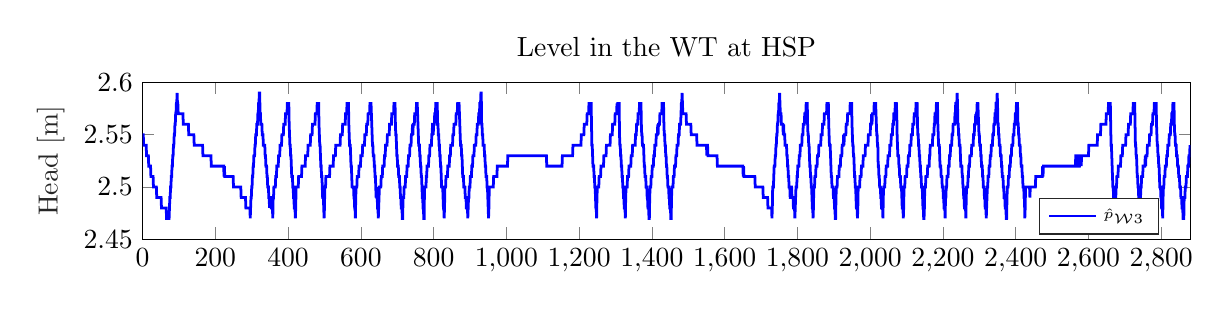
\begin{tikzpicture}

\begin{axis}[%
width=5.239in,
height=0.784in,
at={(1.14in,0.434in)},
scale only axis,
xmin=0,
xmax=2880,
%xlabel style={font=\color{white!15!black}},
%xlabel={Time [min]},
ymin=2.45,
ymax=2.6,
ylabel style={font=\color{white!15!black}},
ylabel={Head  [m]},
axis background/.style={fill=white},
title style={},
title={Level in the WT at HSP},
legend style={at={(0.97,0.03)}, anchor=south east, legend cell align=left, align=left, draw=white!15!black}
]
\addplot [color=blue, line width=1.0pt]
  table[row sep=crcr]{%
0	2.55\\
1	2.55\\
2	2.55\\
3	2.54\\
4	2.54\\
5	2.54\\
6	2.54\\
7	2.54\\
8	2.54\\
9	2.54\\
10	2.54\\
11	2.53\\
12	2.53\\
13	2.53\\
14	2.53\\
15	2.53\\
16	2.53\\
17	2.52\\
18	2.52\\
19	2.52\\
20	2.52\\
21	2.52\\
22	2.52\\
23	2.51\\
24	2.51\\
25	2.51\\
26	2.51\\
27	2.51\\
28	2.51\\
29	2.51\\
30	2.5\\
31	2.5\\
32	2.5\\
33	2.5\\
34	2.5\\
35	2.5\\
36	2.5\\
37	2.5\\
38	2.5\\
39	2.49\\
40	2.49\\
41	2.49\\
42	2.49\\
43	2.49\\
44	2.49\\
45	2.49\\
46	2.49\\
47	2.49\\
48	2.49\\
49	2.49\\
50	2.49\\
51	2.49\\
52	2.48\\
53	2.48\\
54	2.48\\
55	2.48\\
56	2.48\\
57	2.48\\
58	2.48\\
59	2.48\\
60	2.48\\
61	2.48\\
62	2.48\\
63	2.48\\
64	2.48\\
65	2.48\\
66	2.47\\
67	2.47\\
68	2.47\\
69	2.47\\
70	2.47\\
71	2.47\\
72	2.47\\
73	2.47\\
74	2.48\\
75	2.49\\
76	2.49\\
77	2.5\\
78	2.5\\
79	2.51\\
80	2.51\\
81	2.52\\
82	2.52\\
83	2.53\\
84	2.53\\
85	2.54\\
86	2.54\\
87	2.55\\
88	2.55\\
89	2.56\\
90	2.56\\
91	2.57\\
92	2.57\\
93	2.58\\
94	2.58\\
95	2.59\\
96	2.58\\
97	2.58\\
98	2.57\\
99	2.57\\
100	2.57\\
101	2.57\\
102	2.57\\
103	2.57\\
104	2.57\\
105	2.57\\
106	2.57\\
107	2.57\\
108	2.57\\
109	2.57\\
110	2.57\\
111	2.57\\
112	2.56\\
113	2.56\\
114	2.56\\
115	2.56\\
116	2.56\\
117	2.56\\
118	2.56\\
119	2.56\\
120	2.56\\
121	2.56\\
122	2.56\\
123	2.56\\
124	2.56\\
125	2.56\\
126	2.56\\
127	2.55\\
128	2.55\\
129	2.55\\
130	2.55\\
131	2.55\\
132	2.55\\
133	2.55\\
134	2.55\\
135	2.55\\
136	2.55\\
137	2.55\\
138	2.55\\
139	2.55\\
140	2.55\\
141	2.55\\
142	2.54\\
143	2.54\\
144	2.54\\
145	2.54\\
146	2.54\\
147	2.54\\
148	2.54\\
149	2.54\\
150	2.54\\
151	2.54\\
152	2.54\\
153	2.54\\
154	2.54\\
155	2.54\\
156	2.54\\
157	2.54\\
158	2.54\\
159	2.54\\
160	2.54\\
161	2.54\\
162	2.54\\
163	2.54\\
164	2.54\\
165	2.54\\
166	2.53\\
167	2.53\\
168	2.53\\
169	2.53\\
170	2.53\\
171	2.53\\
172	2.53\\
173	2.53\\
174	2.53\\
175	2.53\\
176	2.53\\
177	2.53\\
178	2.53\\
179	2.53\\
180	2.53\\
181	2.53\\
182	2.53\\
183	2.53\\
184	2.53\\
185	2.53\\
186	2.53\\
187	2.53\\
188	2.53\\
189	2.52\\
190	2.52\\
191	2.52\\
192	2.52\\
193	2.52\\
194	2.52\\
195	2.52\\
196	2.52\\
197	2.52\\
198	2.52\\
199	2.52\\
200	2.52\\
201	2.52\\
202	2.52\\
203	2.52\\
204	2.52\\
205	2.52\\
206	2.52\\
207	2.52\\
208	2.52\\
209	2.52\\
210	2.52\\
211	2.52\\
212	2.52\\
213	2.52\\
214	2.52\\
215	2.52\\
216	2.52\\
217	2.52\\
218	2.52\\
219	2.52\\
220	2.52\\
221	2.52\\
222	2.52\\
223	2.52\\
224	2.51\\
225	2.52\\
226	2.51\\
227	2.51\\
228	2.51\\
229	2.51\\
230	2.51\\
231	2.51\\
232	2.51\\
233	2.51\\
234	2.51\\
235	2.51\\
236	2.51\\
237	2.51\\
238	2.51\\
239	2.51\\
240	2.51\\
241	2.51\\
242	2.51\\
243	2.51\\
244	2.51\\
245	2.51\\
246	2.51\\
247	2.51\\
248	2.51\\
249	2.51\\
250	2.5\\
251	2.5\\
252	2.5\\
253	2.5\\
254	2.5\\
255	2.5\\
256	2.5\\
257	2.5\\
258	2.5\\
259	2.5\\
260	2.5\\
261	2.5\\
262	2.5\\
263	2.5\\
264	2.5\\
265	2.5\\
266	2.5\\
267	2.5\\
268	2.5\\
269	2.5\\
270	2.5\\
271	2.49\\
272	2.49\\
273	2.49\\
274	2.49\\
275	2.49\\
276	2.49\\
277	2.49\\
278	2.49\\
279	2.49\\
280	2.49\\
281	2.49\\
282	2.49\\
283	2.49\\
284	2.48\\
285	2.48\\
286	2.48\\
287	2.48\\
288	2.48\\
289	2.48\\
290	2.48\\
291	2.48\\
292	2.48\\
293	2.48\\
294	2.48\\
295	2.48\\
296	2.47\\
297	2.48\\
298	2.49\\
299	2.49\\
300	2.5\\
301	2.5\\
302	2.51\\
303	2.51\\
304	2.52\\
305	2.52\\
306	2.53\\
307	2.53\\
308	2.53\\
309	2.54\\
310	2.54\\
311	2.55\\
312	2.55\\
313	2.55\\
314	2.56\\
315	2.56\\
316	2.56\\
317	2.57\\
318	2.57\\
319	2.58\\
320	2.58\\
321	2.59\\
322	2.59\\
323	2.57\\
324	2.57\\
325	2.56\\
326	2.56\\
327	2.56\\
328	2.56\\
329	2.55\\
330	2.55\\
331	2.55\\
332	2.54\\
333	2.54\\
334	2.54\\
335	2.54\\
336	2.54\\
337	2.53\\
338	2.53\\
339	2.52\\
340	2.52\\
341	2.52\\
342	2.51\\
343	2.51\\
344	2.5\\
345	2.5\\
346	2.5\\
347	2.49\\
348	2.49\\
349	2.48\\
350	2.49\\
351	2.49\\
352	2.49\\
353	2.49\\
354	2.48\\
355	2.48\\
356	2.48\\
357	2.48\\
358	2.47\\
359	2.49\\
360	2.49\\
361	2.5\\
362	2.5\\
363	2.5\\
364	2.5\\
365	2.5\\
366	2.51\\
367	2.51\\
368	2.51\\
369	2.52\\
370	2.52\\
371	2.52\\
372	2.52\\
373	2.52\\
374	2.53\\
375	2.53\\
376	2.53\\
377	2.53\\
378	2.54\\
379	2.54\\
380	2.54\\
381	2.54\\
382	2.54\\
383	2.55\\
384	2.55\\
385	2.55\\
386	2.55\\
387	2.55\\
388	2.56\\
389	2.56\\
390	2.56\\
391	2.56\\
392	2.56\\
393	2.57\\
394	2.57\\
395	2.57\\
396	2.57\\
397	2.57\\
398	2.58\\
399	2.58\\
400	2.58\\
401	2.58\\
402	2.58\\
403	2.56\\
404	2.55\\
405	2.54\\
406	2.54\\
407	2.53\\
408	2.53\\
409	2.52\\
410	2.51\\
411	2.51\\
412	2.51\\
413	2.5\\
414	2.5\\
415	2.49\\
416	2.49\\
417	2.48\\
418	2.48\\
419	2.48\\
420	2.47\\
421	2.48\\
422	2.5\\
423	2.5\\
424	2.5\\
425	2.5\\
426	2.5\\
427	2.5\\
428	2.5\\
429	2.51\\
430	2.51\\
431	2.51\\
432	2.51\\
433	2.51\\
434	2.51\\
435	2.51\\
436	2.51\\
437	2.51\\
438	2.52\\
439	2.52\\
440	2.52\\
441	2.52\\
442	2.52\\
443	2.52\\
444	2.52\\
445	2.52\\
446	2.52\\
447	2.52\\
448	2.53\\
449	2.53\\
450	2.53\\
451	2.53\\
452	2.53\\
453	2.53\\
454	2.53\\
455	2.54\\
456	2.54\\
457	2.54\\
458	2.54\\
459	2.54\\
460	2.54\\
461	2.54\\
462	2.55\\
463	2.55\\
464	2.55\\
465	2.55\\
466	2.55\\
467	2.56\\
468	2.56\\
469	2.56\\
470	2.56\\
471	2.56\\
472	2.56\\
473	2.56\\
474	2.56\\
475	2.57\\
476	2.57\\
477	2.57\\
478	2.57\\
479	2.57\\
480	2.58\\
481	2.58\\
482	2.58\\
483	2.58\\
484	2.58\\
485	2.56\\
486	2.55\\
487	2.54\\
488	2.54\\
489	2.53\\
490	2.52\\
491	2.52\\
492	2.51\\
493	2.51\\
494	2.5\\
495	2.49\\
496	2.49\\
497	2.49\\
498	2.48\\
499	2.47\\
500	2.48\\
501	2.5\\
502	2.5\\
503	2.5\\
504	2.51\\
505	2.51\\
506	2.51\\
507	2.51\\
508	2.51\\
509	2.51\\
510	2.51\\
511	2.51\\
512	2.51\\
513	2.51\\
514	2.51\\
515	2.52\\
516	2.52\\
517	2.52\\
518	2.52\\
519	2.52\\
520	2.52\\
521	2.52\\
522	2.52\\
523	2.52\\
524	2.52\\
525	2.53\\
526	2.53\\
527	2.53\\
528	2.53\\
529	2.53\\
530	2.53\\
531	2.54\\
532	2.54\\
533	2.54\\
534	2.54\\
535	2.54\\
536	2.54\\
537	2.54\\
538	2.54\\
539	2.54\\
540	2.54\\
541	2.54\\
542	2.54\\
543	2.54\\
544	2.55\\
545	2.55\\
546	2.55\\
547	2.55\\
548	2.55\\
549	2.55\\
550	2.56\\
551	2.56\\
552	2.56\\
553	2.56\\
554	2.56\\
555	2.56\\
556	2.56\\
557	2.56\\
558	2.57\\
559	2.57\\
560	2.57\\
561	2.57\\
562	2.58\\
563	2.58\\
564	2.58\\
565	2.58\\
566	2.58\\
567	2.56\\
568	2.55\\
569	2.54\\
570	2.54\\
571	2.54\\
572	2.53\\
573	2.52\\
574	2.52\\
575	2.51\\
576	2.5\\
577	2.5\\
578	2.5\\
579	2.5\\
580	2.5\\
581	2.49\\
582	2.49\\
583	2.48\\
584	2.48\\
585	2.47\\
586	2.49\\
587	2.5\\
588	2.5\\
589	2.5\\
590	2.51\\
591	2.51\\
592	2.51\\
593	2.51\\
594	2.51\\
595	2.52\\
596	2.52\\
597	2.52\\
598	2.52\\
599	2.52\\
600	2.53\\
601	2.53\\
602	2.53\\
603	2.53\\
604	2.53\\
605	2.54\\
606	2.54\\
607	2.54\\
608	2.54\\
609	2.54\\
610	2.54\\
611	2.55\\
612	2.55\\
613	2.55\\
614	2.55\\
615	2.55\\
616	2.56\\
617	2.56\\
618	2.56\\
619	2.56\\
620	2.57\\
621	2.57\\
622	2.57\\
623	2.57\\
624	2.57\\
625	2.58\\
626	2.58\\
627	2.58\\
628	2.58\\
629	2.57\\
630	2.56\\
631	2.55\\
632	2.54\\
633	2.54\\
634	2.53\\
635	2.53\\
636	2.53\\
637	2.52\\
638	2.52\\
639	2.51\\
640	2.51\\
641	2.5\\
642	2.49\\
643	2.5\\
644	2.49\\
645	2.49\\
646	2.48\\
647	2.48\\
648	2.47\\
649	2.48\\
650	2.49\\
651	2.5\\
652	2.5\\
653	2.5\\
654	2.5\\
655	2.5\\
656	2.51\\
657	2.51\\
658	2.51\\
659	2.51\\
660	2.52\\
661	2.52\\
662	2.52\\
663	2.52\\
664	2.52\\
665	2.53\\
666	2.53\\
667	2.53\\
668	2.54\\
669	2.54\\
670	2.54\\
671	2.54\\
672	2.54\\
673	2.55\\
674	2.55\\
675	2.55\\
676	2.55\\
677	2.55\\
678	2.55\\
679	2.56\\
680	2.56\\
681	2.56\\
682	2.56\\
683	2.56\\
684	2.56\\
685	2.57\\
686	2.57\\
687	2.57\\
688	2.57\\
689	2.57\\
690	2.57\\
691	2.58\\
692	2.58\\
693	2.58\\
694	2.58\\
695	2.56\\
696	2.55\\
697	2.55\\
698	2.54\\
699	2.53\\
700	2.53\\
701	2.52\\
702	2.52\\
703	2.52\\
704	2.51\\
705	2.51\\
706	2.51\\
707	2.5\\
708	2.5\\
709	2.49\\
710	2.49\\
711	2.48\\
712	2.48\\
713	2.48\\
714	2.47\\
715	2.47\\
716	2.49\\
717	2.49\\
718	2.49\\
719	2.5\\
720	2.5\\
721	2.5\\
722	2.5\\
723	2.51\\
724	2.51\\
725	2.51\\
726	2.51\\
727	2.52\\
728	2.52\\
729	2.52\\
730	2.52\\
731	2.53\\
732	2.53\\
733	2.53\\
734	2.53\\
735	2.54\\
736	2.54\\
737	2.54\\
738	2.54\\
739	2.55\\
740	2.55\\
741	2.55\\
742	2.56\\
743	2.55\\
744	2.56\\
745	2.56\\
746	2.56\\
747	2.56\\
748	2.57\\
749	2.57\\
750	2.57\\
751	2.57\\
752	2.57\\
753	2.58\\
754	2.58\\
755	2.58\\
756	2.57\\
757	2.56\\
758	2.55\\
759	2.54\\
760	2.54\\
761	2.54\\
762	2.53\\
763	2.53\\
764	2.52\\
765	2.52\\
766	2.51\\
767	2.51\\
768	2.5\\
769	2.49\\
770	2.49\\
771	2.48\\
772	2.48\\
773	2.47\\
774	2.47\\
775	2.5\\
776	2.5\\
777	2.5\\
778	2.5\\
779	2.5\\
780	2.51\\
781	2.51\\
782	2.52\\
783	2.52\\
784	2.52\\
785	2.52\\
786	2.52\\
787	2.53\\
788	2.53\\
789	2.53\\
790	2.54\\
791	2.54\\
792	2.54\\
793	2.54\\
794	2.54\\
795	2.55\\
796	2.55\\
797	2.56\\
798	2.56\\
799	2.55\\
800	2.56\\
801	2.56\\
802	2.56\\
803	2.57\\
804	2.57\\
805	2.57\\
806	2.58\\
807	2.58\\
808	2.58\\
809	2.58\\
810	2.58\\
811	2.56\\
812	2.56\\
813	2.55\\
814	2.55\\
815	2.54\\
816	2.54\\
817	2.53\\
818	2.53\\
819	2.52\\
820	2.52\\
821	2.51\\
822	2.5\\
823	2.5\\
824	2.5\\
825	2.5\\
826	2.49\\
827	2.48\\
828	2.48\\
829	2.47\\
830	2.48\\
831	2.5\\
832	2.5\\
833	2.5\\
834	2.51\\
835	2.51\\
836	2.51\\
837	2.51\\
838	2.51\\
839	2.52\\
840	2.52\\
841	2.52\\
842	2.52\\
843	2.52\\
844	2.53\\
845	2.53\\
846	2.53\\
847	2.54\\
848	2.54\\
849	2.54\\
850	2.54\\
851	2.54\\
852	2.54\\
853	2.55\\
854	2.55\\
855	2.55\\
856	2.56\\
857	2.56\\
858	2.56\\
859	2.56\\
860	2.56\\
861	2.56\\
862	2.57\\
863	2.57\\
864	2.57\\
865	2.57\\
866	2.58\\
867	2.58\\
868	2.58\\
869	2.58\\
870	2.58\\
871	2.57\\
872	2.56\\
873	2.55\\
874	2.54\\
875	2.54\\
876	2.54\\
877	2.53\\
878	2.53\\
879	2.52\\
880	2.51\\
881	2.51\\
882	2.51\\
883	2.5\\
884	2.5\\
885	2.5\\
886	2.5\\
887	2.49\\
888	2.49\\
889	2.49\\
890	2.48\\
891	2.48\\
892	2.48\\
893	2.48\\
894	2.47\\
895	2.48\\
896	2.49\\
897	2.49\\
898	2.5\\
899	2.5\\
900	2.5\\
901	2.51\\
902	2.51\\
903	2.51\\
904	2.51\\
905	2.52\\
906	2.52\\
907	2.52\\
908	2.53\\
909	2.53\\
910	2.53\\
911	2.53\\
912	2.54\\
913	2.54\\
914	2.54\\
915	2.54\\
916	2.54\\
917	2.55\\
918	2.55\\
919	2.55\\
920	2.56\\
921	2.56\\
922	2.56\\
923	2.56\\
924	2.57\\
925	2.57\\
926	2.57\\
927	2.58\\
928	2.58\\
929	2.58\\
930	2.59\\
931	2.59\\
932	2.56\\
933	2.56\\
934	2.55\\
935	2.55\\
936	2.54\\
937	2.54\\
938	2.54\\
939	2.54\\
940	2.53\\
941	2.53\\
942	2.52\\
943	2.52\\
944	2.51\\
945	2.51\\
946	2.51\\
947	2.5\\
948	2.5\\
949	2.49\\
950	2.48\\
951	2.47\\
952	2.48\\
953	2.5\\
954	2.5\\
955	2.5\\
956	2.5\\
957	2.5\\
958	2.5\\
959	2.5\\
960	2.5\\
961	2.5\\
962	2.5\\
963	2.5\\
964	2.5\\
965	2.51\\
966	2.51\\
967	2.51\\
968	2.51\\
969	2.51\\
970	2.51\\
971	2.51\\
972	2.51\\
973	2.51\\
974	2.51\\
975	2.52\\
976	2.52\\
977	2.52\\
978	2.52\\
979	2.52\\
980	2.52\\
981	2.52\\
982	2.52\\
983	2.52\\
984	2.52\\
985	2.52\\
986	2.52\\
987	2.52\\
988	2.52\\
989	2.52\\
990	2.52\\
991	2.52\\
992	2.52\\
993	2.52\\
994	2.52\\
995	2.52\\
996	2.52\\
997	2.52\\
998	2.52\\
999	2.52\\
1000	2.52\\
1001	2.52\\
1002	2.52\\
1003	2.52\\
1004	2.53\\
1005	2.53\\
1006	2.53\\
1007	2.53\\
1008	2.53\\
1009	2.53\\
1010	2.53\\
1011	2.53\\
1012	2.53\\
1013	2.53\\
1014	2.53\\
1015	2.53\\
1016	2.53\\
1017	2.53\\
1018	2.53\\
1019	2.53\\
1020	2.53\\
1021	2.53\\
1022	2.53\\
1023	2.53\\
1024	2.53\\
1025	2.53\\
1026	2.53\\
1027	2.53\\
1028	2.53\\
1029	2.53\\
1030	2.53\\
1031	2.53\\
1032	2.53\\
1033	2.53\\
1034	2.53\\
1035	2.53\\
1036	2.53\\
1037	2.53\\
1038	2.53\\
1039	2.53\\
1040	2.53\\
1041	2.53\\
1042	2.53\\
1043	2.53\\
1044	2.53\\
1045	2.53\\
1046	2.53\\
1047	2.53\\
1048	2.53\\
1049	2.53\\
1050	2.53\\
1051	2.53\\
1052	2.53\\
1053	2.53\\
1054	2.53\\
1055	2.53\\
1056	2.53\\
1057	2.53\\
1058	2.53\\
1059	2.53\\
1060	2.53\\
1061	2.53\\
1062	2.53\\
1063	2.53\\
1064	2.53\\
1065	2.53\\
1066	2.53\\
1067	2.53\\
1068	2.53\\
1069	2.53\\
1070	2.53\\
1071	2.53\\
1072	2.53\\
1073	2.53\\
1074	2.53\\
1075	2.53\\
1076	2.53\\
1077	2.53\\
1078	2.53\\
1079	2.53\\
1080	2.53\\
1081	2.53\\
1082	2.53\\
1083	2.53\\
1084	2.53\\
1085	2.53\\
1086	2.53\\
1087	2.53\\
1088	2.53\\
1089	2.53\\
1090	2.53\\
1091	2.53\\
1092	2.53\\
1093	2.53\\
1094	2.53\\
1095	2.53\\
1096	2.53\\
1097	2.53\\
1098	2.53\\
1099	2.53\\
1100	2.53\\
1101	2.53\\
1102	2.53\\
1103	2.53\\
1104	2.53\\
1105	2.53\\
1106	2.53\\
1107	2.53\\
1108	2.53\\
1109	2.53\\
1110	2.53\\
1111	2.52\\
1112	2.52\\
1113	2.52\\
1114	2.52\\
1115	2.52\\
1116	2.52\\
1117	2.52\\
1118	2.52\\
1119	2.52\\
1120	2.52\\
1121	2.52\\
1122	2.52\\
1123	2.52\\
1124	2.52\\
1125	2.52\\
1126	2.52\\
1127	2.52\\
1128	2.52\\
1129	2.52\\
1130	2.52\\
1131	2.52\\
1132	2.52\\
1133	2.52\\
1134	2.52\\
1135	2.52\\
1136	2.52\\
1137	2.52\\
1138	2.52\\
1139	2.52\\
1140	2.52\\
1141	2.52\\
1142	2.52\\
1143	2.52\\
1144	2.52\\
1145	2.52\\
1146	2.52\\
1147	2.52\\
1148	2.52\\
1149	2.52\\
1150	2.52\\
1151	2.52\\
1152	2.52\\
1153	2.52\\
1154	2.53\\
1155	2.53\\
1156	2.53\\
1157	2.53\\
1158	2.53\\
1159	2.53\\
1160	2.53\\
1161	2.53\\
1162	2.53\\
1163	2.53\\
1164	2.53\\
1165	2.53\\
1166	2.53\\
1167	2.53\\
1168	2.53\\
1169	2.53\\
1170	2.53\\
1171	2.53\\
1172	2.53\\
1173	2.53\\
1174	2.53\\
1175	2.53\\
1176	2.53\\
1177	2.53\\
1178	2.53\\
1179	2.53\\
1180	2.53\\
1181	2.53\\
1182	2.53\\
1183	2.54\\
1184	2.54\\
1185	2.54\\
1186	2.54\\
1187	2.54\\
1188	2.54\\
1189	2.54\\
1190	2.54\\
1191	2.54\\
1192	2.54\\
1193	2.54\\
1194	2.54\\
1195	2.54\\
1196	2.54\\
1197	2.54\\
1198	2.54\\
1199	2.54\\
1200	2.54\\
1201	2.54\\
1202	2.54\\
1203	2.54\\
1204	2.54\\
1205	2.54\\
1206	2.55\\
1207	2.55\\
1208	2.55\\
1209	2.55\\
1210	2.55\\
1211	2.55\\
1212	2.55\\
1213	2.55\\
1214	2.56\\
1215	2.56\\
1216	2.56\\
1217	2.56\\
1218	2.56\\
1219	2.56\\
1220	2.56\\
1221	2.56\\
1222	2.57\\
1223	2.57\\
1224	2.57\\
1225	2.57\\
1226	2.57\\
1227	2.58\\
1228	2.58\\
1229	2.58\\
1230	2.58\\
1231	2.58\\
1232	2.58\\
1233	2.58\\
1234	2.56\\
1235	2.54\\
1236	2.54\\
1237	2.53\\
1238	2.52\\
1239	2.52\\
1240	2.52\\
1241	2.51\\
1242	2.51\\
1243	2.5\\
1244	2.5\\
1245	2.49\\
1246	2.48\\
1247	2.48\\
1248	2.47\\
1249	2.49\\
1250	2.5\\
1251	2.5\\
1252	2.5\\
1253	2.5\\
1254	2.5\\
1255	2.51\\
1256	2.51\\
1257	2.51\\
1258	2.51\\
1259	2.51\\
1260	2.52\\
1261	2.52\\
1262	2.52\\
1263	2.52\\
1264	2.52\\
1265	2.52\\
1266	2.52\\
1267	2.52\\
1268	2.53\\
1269	2.53\\
1270	2.53\\
1271	2.53\\
1272	2.53\\
1273	2.53\\
1274	2.53\\
1275	2.54\\
1276	2.54\\
1277	2.54\\
1278	2.54\\
1279	2.54\\
1280	2.54\\
1281	2.54\\
1282	2.54\\
1283	2.54\\
1284	2.54\\
1285	2.54\\
1286	2.55\\
1287	2.55\\
1288	2.55\\
1289	2.55\\
1290	2.55\\
1291	2.55\\
1292	2.56\\
1293	2.56\\
1294	2.56\\
1295	2.56\\
1296	2.56\\
1297	2.56\\
1298	2.56\\
1299	2.57\\
1300	2.57\\
1301	2.57\\
1302	2.57\\
1303	2.57\\
1304	2.58\\
1305	2.57\\
1306	2.58\\
1307	2.58\\
1308	2.58\\
1309	2.58\\
1310	2.58\\
1311	2.55\\
1312	2.54\\
1313	2.54\\
1314	2.53\\
1315	2.53\\
1316	2.52\\
1317	2.52\\
1318	2.51\\
1319	2.51\\
1320	2.5\\
1321	2.5\\
1322	2.49\\
1323	2.49\\
1324	2.48\\
1325	2.48\\
1326	2.48\\
1327	2.47\\
1328	2.49\\
1329	2.5\\
1330	2.5\\
1331	2.5\\
1332	2.5\\
1333	2.51\\
1334	2.51\\
1335	2.51\\
1336	2.51\\
1337	2.52\\
1338	2.52\\
1339	2.52\\
1340	2.52\\
1341	2.52\\
1342	2.52\\
1343	2.53\\
1344	2.53\\
1345	2.53\\
1346	2.53\\
1347	2.54\\
1348	2.54\\
1349	2.54\\
1350	2.54\\
1351	2.54\\
1352	2.54\\
1353	2.54\\
1354	2.54\\
1355	2.55\\
1356	2.55\\
1357	2.55\\
1358	2.56\\
1359	2.56\\
1360	2.56\\
1361	2.56\\
1362	2.57\\
1363	2.57\\
1364	2.57\\
1365	2.57\\
1366	2.58\\
1367	2.58\\
1368	2.58\\
1369	2.58\\
1370	2.58\\
1371	2.56\\
1372	2.55\\
1373	2.55\\
1374	2.54\\
1375	2.54\\
1376	2.54\\
1377	2.54\\
1378	2.53\\
1379	2.52\\
1380	2.52\\
1381	2.51\\
1382	2.51\\
1383	2.51\\
1384	2.5\\
1385	2.5\\
1386	2.5\\
1387	2.49\\
1388	2.49\\
1389	2.48\\
1390	2.48\\
1391	2.48\\
1392	2.47\\
1393	2.47\\
1394	2.49\\
1395	2.5\\
1396	2.5\\
1397	2.5\\
1398	2.51\\
1399	2.51\\
1400	2.51\\
1401	2.52\\
1402	2.52\\
1403	2.52\\
1404	2.52\\
1405	2.53\\
1406	2.53\\
1407	2.53\\
1408	2.54\\
1409	2.54\\
1410	2.54\\
1411	2.54\\
1412	2.55\\
1413	2.55\\
1414	2.55\\
1415	2.55\\
1416	2.56\\
1417	2.55\\
1418	2.56\\
1419	2.56\\
1420	2.56\\
1421	2.56\\
1422	2.57\\
1423	2.57\\
1424	2.57\\
1425	2.57\\
1426	2.57\\
1427	2.57\\
1428	2.58\\
1429	2.58\\
1430	2.58\\
1431	2.58\\
1432	2.58\\
1433	2.56\\
1434	2.55\\
1435	2.55\\
1436	2.54\\
1437	2.54\\
1438	2.53\\
1439	2.53\\
1440	2.52\\
1441	2.52\\
1442	2.51\\
1443	2.51\\
1444	2.5\\
1445	2.5\\
1446	2.5\\
1447	2.49\\
1448	2.49\\
1449	2.48\\
1450	2.48\\
1451	2.48\\
1452	2.47\\
1453	2.47\\
1454	2.49\\
1455	2.5\\
1456	2.5\\
1457	2.5\\
1458	2.5\\
1459	2.51\\
1460	2.51\\
1461	2.51\\
1462	2.52\\
1463	2.52\\
1464	2.52\\
1465	2.52\\
1466	2.53\\
1467	2.53\\
1468	2.53\\
1469	2.54\\
1470	2.54\\
1471	2.54\\
1472	2.54\\
1473	2.55\\
1474	2.55\\
1475	2.55\\
1476	2.56\\
1477	2.56\\
1478	2.56\\
1479	2.56\\
1480	2.57\\
1481	2.58\\
1482	2.58\\
1483	2.59\\
1484	2.58\\
1485	2.57\\
1486	2.57\\
1487	2.57\\
1488	2.57\\
1489	2.57\\
1490	2.57\\
1491	2.57\\
1492	2.57\\
1493	2.57\\
1494	2.57\\
1495	2.56\\
1496	2.56\\
1497	2.56\\
1498	2.56\\
1499	2.56\\
1500	2.56\\
1501	2.56\\
1502	2.56\\
1503	2.56\\
1504	2.56\\
1505	2.56\\
1506	2.56\\
1507	2.56\\
1508	2.55\\
1509	2.55\\
1510	2.55\\
1511	2.55\\
1512	2.55\\
1513	2.55\\
1514	2.55\\
1515	2.55\\
1516	2.55\\
1517	2.55\\
1518	2.55\\
1519	2.55\\
1520	2.55\\
1521	2.55\\
1522	2.55\\
1523	2.55\\
1524	2.54\\
1525	2.54\\
1526	2.54\\
1527	2.54\\
1528	2.54\\
1529	2.54\\
1530	2.54\\
1531	2.54\\
1532	2.54\\
1533	2.54\\
1534	2.54\\
1535	2.54\\
1536	2.54\\
1537	2.54\\
1538	2.54\\
1539	2.54\\
1540	2.54\\
1541	2.54\\
1542	2.54\\
1543	2.54\\
1544	2.54\\
1545	2.54\\
1546	2.54\\
1547	2.54\\
1548	2.54\\
1549	2.54\\
1550	2.54\\
1551	2.53\\
1552	2.54\\
1553	2.54\\
1554	2.53\\
1555	2.53\\
1556	2.53\\
1557	2.53\\
1558	2.53\\
1559	2.53\\
1560	2.53\\
1561	2.53\\
1562	2.53\\
1563	2.53\\
1564	2.53\\
1565	2.53\\
1566	2.53\\
1567	2.53\\
1568	2.53\\
1569	2.53\\
1570	2.53\\
1571	2.53\\
1572	2.53\\
1573	2.53\\
1574	2.53\\
1575	2.53\\
1576	2.53\\
1577	2.53\\
1578	2.53\\
1579	2.53\\
1580	2.52\\
1581	2.52\\
1582	2.52\\
1583	2.52\\
1584	2.52\\
1585	2.52\\
1586	2.52\\
1587	2.52\\
1588	2.52\\
1589	2.52\\
1590	2.52\\
1591	2.52\\
1592	2.52\\
1593	2.52\\
1594	2.52\\
1595	2.52\\
1596	2.52\\
1597	2.52\\
1598	2.52\\
1599	2.52\\
1600	2.52\\
1601	2.52\\
1602	2.52\\
1603	2.52\\
1604	2.52\\
1605	2.52\\
1606	2.52\\
1607	2.52\\
1608	2.52\\
1609	2.52\\
1610	2.52\\
1611	2.52\\
1612	2.52\\
1613	2.52\\
1614	2.52\\
1615	2.52\\
1616	2.52\\
1617	2.52\\
1618	2.52\\
1619	2.52\\
1620	2.52\\
1621	2.52\\
1622	2.52\\
1623	2.52\\
1624	2.52\\
1625	2.52\\
1626	2.52\\
1627	2.52\\
1628	2.52\\
1629	2.52\\
1630	2.52\\
1631	2.52\\
1632	2.52\\
1633	2.52\\
1634	2.52\\
1635	2.52\\
1636	2.52\\
1637	2.52\\
1638	2.52\\
1639	2.52\\
1640	2.52\\
1641	2.52\\
1642	2.52\\
1643	2.52\\
1644	2.52\\
1645	2.52\\
1646	2.52\\
1647	2.52\\
1648	2.52\\
1649	2.52\\
1650	2.52\\
1651	2.51\\
1652	2.52\\
1653	2.51\\
1654	2.51\\
1655	2.51\\
1656	2.51\\
1657	2.51\\
1658	2.51\\
1659	2.51\\
1660	2.51\\
1661	2.51\\
1662	2.51\\
1663	2.51\\
1664	2.51\\
1665	2.51\\
1666	2.51\\
1667	2.51\\
1668	2.51\\
1669	2.51\\
1670	2.51\\
1671	2.51\\
1672	2.51\\
1673	2.51\\
1674	2.51\\
1675	2.51\\
1676	2.51\\
1677	2.51\\
1678	2.51\\
1679	2.51\\
1680	2.51\\
1681	2.51\\
1682	2.51\\
1683	2.51\\
1684	2.5\\
1685	2.5\\
1686	2.5\\
1687	2.5\\
1688	2.5\\
1689	2.5\\
1690	2.5\\
1691	2.5\\
1692	2.5\\
1693	2.5\\
1694	2.5\\
1695	2.5\\
1696	2.5\\
1697	2.5\\
1698	2.5\\
1699	2.5\\
1700	2.5\\
1701	2.5\\
1702	2.5\\
1703	2.5\\
1704	2.5\\
1705	2.5\\
1706	2.49\\
1707	2.49\\
1708	2.49\\
1709	2.49\\
1710	2.49\\
1711	2.49\\
1712	2.49\\
1713	2.49\\
1714	2.49\\
1715	2.49\\
1716	2.49\\
1717	2.49\\
1718	2.49\\
1719	2.48\\
1720	2.48\\
1721	2.48\\
1722	2.48\\
1723	2.48\\
1724	2.48\\
1725	2.48\\
1726	2.48\\
1727	2.48\\
1728	2.48\\
1729	2.48\\
1730	2.47\\
1731	2.48\\
1732	2.5\\
1733	2.5\\
1734	2.5\\
1735	2.51\\
1736	2.52\\
1737	2.52\\
1738	2.52\\
1739	2.53\\
1740	2.53\\
1741	2.54\\
1742	2.54\\
1743	2.55\\
1744	2.55\\
1745	2.56\\
1746	2.56\\
1747	2.57\\
1748	2.57\\
1749	2.58\\
1750	2.58\\
1751	2.59\\
1752	2.58\\
1753	2.57\\
1754	2.57\\
1755	2.57\\
1756	2.56\\
1757	2.56\\
1758	2.56\\
1759	2.56\\
1760	2.56\\
1761	2.55\\
1762	2.56\\
1763	2.55\\
1764	2.55\\
1765	2.55\\
1766	2.54\\
1767	2.54\\
1768	2.54\\
1769	2.54\\
1770	2.54\\
1771	2.53\\
1772	2.53\\
1773	2.52\\
1774	2.52\\
1775	2.51\\
1776	2.51\\
1777	2.5\\
1778	2.5\\
1779	2.5\\
1780	2.49\\
1781	2.49\\
1782	2.5\\
1783	2.5\\
1784	2.5\\
1785	2.49\\
1786	2.49\\
1787	2.49\\
1788	2.49\\
1789	2.48\\
1790	2.48\\
1791	2.48\\
1792	2.48\\
1793	2.47\\
1794	2.48\\
1795	2.49\\
1796	2.5\\
1797	2.5\\
1798	2.5\\
1799	2.51\\
1800	2.51\\
1801	2.52\\
1802	2.52\\
1803	2.52\\
1804	2.52\\
1805	2.53\\
1806	2.53\\
1807	2.53\\
1808	2.54\\
1809	2.54\\
1810	2.54\\
1811	2.54\\
1812	2.54\\
1813	2.55\\
1814	2.55\\
1815	2.55\\
1816	2.56\\
1817	2.56\\
1818	2.56\\
1819	2.56\\
1820	2.57\\
1821	2.57\\
1822	2.57\\
1823	2.57\\
1824	2.58\\
1825	2.58\\
1826	2.58\\
1827	2.58\\
1828	2.56\\
1829	2.55\\
1830	2.55\\
1831	2.54\\
1832	2.54\\
1833	2.53\\
1834	2.52\\
1835	2.52\\
1836	2.51\\
1837	2.51\\
1838	2.5\\
1839	2.5\\
1840	2.49\\
1841	2.48\\
1842	2.48\\
1843	2.47\\
1844	2.48\\
1845	2.5\\
1846	2.5\\
1847	2.5\\
1848	2.51\\
1849	2.51\\
1850	2.51\\
1851	2.52\\
1852	2.52\\
1853	2.52\\
1854	2.52\\
1855	2.53\\
1856	2.53\\
1857	2.53\\
1858	2.53\\
1859	2.54\\
1860	2.54\\
1861	2.54\\
1862	2.54\\
1863	2.54\\
1864	2.54\\
1865	2.55\\
1866	2.55\\
1867	2.55\\
1868	2.55\\
1869	2.56\\
1870	2.56\\
1871	2.56\\
1872	2.56\\
1873	2.56\\
1874	2.57\\
1875	2.57\\
1876	2.57\\
1877	2.57\\
1878	2.57\\
1879	2.57\\
1880	2.57\\
1881	2.58\\
1882	2.58\\
1883	2.58\\
1884	2.58\\
1885	2.58\\
1886	2.56\\
1887	2.55\\
1888	2.54\\
1889	2.54\\
1890	2.54\\
1891	2.53\\
1892	2.52\\
1893	2.51\\
1894	2.51\\
1895	2.5\\
1896	2.5\\
1897	2.5\\
1898	2.5\\
1899	2.49\\
1900	2.49\\
1901	2.49\\
1902	2.48\\
1903	2.48\\
1904	2.47\\
1905	2.47\\
1906	2.49\\
1907	2.5\\
1908	2.5\\
1909	2.5\\
1910	2.51\\
1911	2.51\\
1912	2.51\\
1913	2.51\\
1914	2.51\\
1915	2.52\\
1916	2.52\\
1917	2.52\\
1918	2.52\\
1919	2.53\\
1920	2.53\\
1921	2.53\\
1922	2.53\\
1923	2.54\\
1924	2.54\\
1925	2.54\\
1926	2.54\\
1927	2.55\\
1928	2.54\\
1929	2.55\\
1930	2.55\\
1931	2.55\\
1932	2.55\\
1933	2.55\\
1934	2.56\\
1935	2.56\\
1936	2.56\\
1937	2.56\\
1938	2.57\\
1939	2.57\\
1940	2.57\\
1941	2.57\\
1942	2.57\\
1943	2.57\\
1944	2.57\\
1945	2.58\\
1946	2.58\\
1947	2.58\\
1948	2.58\\
1949	2.58\\
1950	2.56\\
1951	2.55\\
1952	2.54\\
1953	2.54\\
1954	2.53\\
1955	2.53\\
1956	2.52\\
1957	2.51\\
1958	2.51\\
1959	2.5\\
1960	2.5\\
1961	2.49\\
1962	2.48\\
1963	2.48\\
1964	2.48\\
1965	2.47\\
1966	2.48\\
1967	2.5\\
1968	2.5\\
1969	2.5\\
1970	2.5\\
1971	2.5\\
1972	2.51\\
1973	2.51\\
1974	2.51\\
1975	2.51\\
1976	2.52\\
1977	2.52\\
1978	2.52\\
1979	2.52\\
1980	2.52\\
1981	2.53\\
1982	2.53\\
1983	2.53\\
1984	2.53\\
1985	2.53\\
1986	2.53\\
1987	2.54\\
1988	2.54\\
1989	2.54\\
1990	2.54\\
1991	2.54\\
1992	2.54\\
1993	2.54\\
1994	2.54\\
1995	2.55\\
1996	2.55\\
1997	2.55\\
1998	2.55\\
1999	2.55\\
2000	2.55\\
2001	2.56\\
2002	2.56\\
2003	2.56\\
2004	2.57\\
2005	2.56\\
2006	2.57\\
2007	2.57\\
2008	2.57\\
2009	2.57\\
2010	2.57\\
2011	2.58\\
2012	2.58\\
2013	2.58\\
2014	2.58\\
2015	2.58\\
2016	2.57\\
2017	2.56\\
2018	2.55\\
2019	2.55\\
2020	2.54\\
2021	2.54\\
2022	2.52\\
2023	2.52\\
2024	2.51\\
2025	2.51\\
2026	2.5\\
2027	2.5\\
2028	2.5\\
2029	2.49\\
2030	2.49\\
2031	2.48\\
2032	2.48\\
2033	2.48\\
2034	2.48\\
2035	2.47\\
2036	2.49\\
2037	2.5\\
2038	2.5\\
2039	2.5\\
2040	2.5\\
2041	2.51\\
2042	2.51\\
2043	2.51\\
2044	2.52\\
2045	2.52\\
2046	2.52\\
2047	2.52\\
2048	2.52\\
2049	2.53\\
2050	2.53\\
2051	2.53\\
2052	2.53\\
2053	2.53\\
2054	2.54\\
2055	2.54\\
2056	2.54\\
2057	2.54\\
2058	2.55\\
2059	2.55\\
2060	2.55\\
2061	2.55\\
2062	2.56\\
2063	2.56\\
2064	2.56\\
2065	2.57\\
2066	2.57\\
2067	2.57\\
2068	2.57\\
2069	2.58\\
2070	2.58\\
2071	2.58\\
2072	2.58\\
2073	2.57\\
2074	2.55\\
2075	2.54\\
2076	2.53\\
2077	2.53\\
2078	2.53\\
2079	2.52\\
2080	2.52\\
2081	2.51\\
2082	2.51\\
2083	2.51\\
2084	2.5\\
2085	2.5\\
2086	2.5\\
2087	2.49\\
2088	2.48\\
2089	2.48\\
2090	2.48\\
2091	2.47\\
2092	2.48\\
2093	2.5\\
2094	2.5\\
2095	2.5\\
2096	2.51\\
2097	2.51\\
2098	2.51\\
2099	2.51\\
2100	2.51\\
2101	2.52\\
2102	2.52\\
2103	2.52\\
2104	2.52\\
2105	2.53\\
2106	2.53\\
2107	2.53\\
2108	2.53\\
2109	2.54\\
2110	2.54\\
2111	2.54\\
2112	2.54\\
2113	2.55\\
2114	2.55\\
2115	2.55\\
2116	2.55\\
2117	2.56\\
2118	2.56\\
2119	2.56\\
2120	2.56\\
2121	2.57\\
2122	2.57\\
2123	2.57\\
2124	2.57\\
2125	2.57\\
2126	2.58\\
2127	2.58\\
2128	2.58\\
2129	2.58\\
2130	2.56\\
2131	2.55\\
2132	2.55\\
2133	2.54\\
2134	2.54\\
2135	2.53\\
2136	2.53\\
2137	2.52\\
2138	2.52\\
2139	2.51\\
2140	2.51\\
2141	2.5\\
2142	2.5\\
2143	2.5\\
2144	2.49\\
2145	2.48\\
2146	2.48\\
2147	2.47\\
2148	2.47\\
2149	2.48\\
2150	2.5\\
2151	2.5\\
2152	2.5\\
2153	2.51\\
2154	2.51\\
2155	2.51\\
2156	2.51\\
2157	2.51\\
2158	2.52\\
2159	2.52\\
2160	2.52\\
2161	2.52\\
2162	2.52\\
2163	2.53\\
2164	2.53\\
2165	2.54\\
2166	2.54\\
2167	2.54\\
2168	2.54\\
2169	2.54\\
2170	2.54\\
2171	2.54\\
2172	2.55\\
2173	2.55\\
2174	2.55\\
2175	2.55\\
2176	2.56\\
2177	2.56\\
2178	2.57\\
2179	2.57\\
2180	2.57\\
2181	2.57\\
2182	2.58\\
2183	2.58\\
2184	2.58\\
2185	2.58\\
2186	2.56\\
2187	2.55\\
2188	2.54\\
2189	2.54\\
2190	2.54\\
2191	2.53\\
2192	2.52\\
2193	2.52\\
2194	2.52\\
2195	2.51\\
2196	2.51\\
2197	2.51\\
2198	2.5\\
2199	2.5\\
2200	2.5\\
2201	2.49\\
2202	2.49\\
2203	2.48\\
2204	2.48\\
2205	2.48\\
2206	2.47\\
2207	2.49\\
2208	2.49\\
2209	2.5\\
2210	2.5\\
2211	2.51\\
2212	2.51\\
2213	2.51\\
2214	2.51\\
2215	2.52\\
2216	2.52\\
2217	2.52\\
2218	2.53\\
2219	2.53\\
2220	2.53\\
2221	2.54\\
2222	2.54\\
2223	2.54\\
2224	2.54\\
2225	2.55\\
2226	2.55\\
2227	2.55\\
2228	2.56\\
2229	2.56\\
2230	2.56\\
2231	2.56\\
2232	2.56\\
2233	2.57\\
2234	2.57\\
2235	2.58\\
2236	2.58\\
2237	2.58\\
2238	2.58\\
2239	2.59\\
2240	2.58\\
2241	2.56\\
2242	2.56\\
2243	2.55\\
2244	2.55\\
2245	2.54\\
2246	2.54\\
2247	2.54\\
2248	2.53\\
2249	2.52\\
2250	2.52\\
2251	2.52\\
2252	2.52\\
2253	2.51\\
2254	2.51\\
2255	2.5\\
2256	2.5\\
2257	2.49\\
2258	2.49\\
2259	2.48\\
2260	2.48\\
2261	2.48\\
2262	2.48\\
2263	2.47\\
2264	2.49\\
2265	2.5\\
2266	2.5\\
2267	2.5\\
2268	2.5\\
2269	2.51\\
2270	2.51\\
2271	2.52\\
2272	2.52\\
2273	2.52\\
2274	2.53\\
2275	2.53\\
2276	2.53\\
2277	2.53\\
2278	2.53\\
2279	2.54\\
2280	2.54\\
2281	2.54\\
2282	2.54\\
2283	2.54\\
2284	2.55\\
2285	2.55\\
2286	2.55\\
2287	2.56\\
2288	2.56\\
2289	2.56\\
2290	2.57\\
2291	2.56\\
2292	2.57\\
2293	2.57\\
2294	2.58\\
2295	2.58\\
2296	2.58\\
2297	2.57\\
2298	2.56\\
2299	2.55\\
2300	2.55\\
2301	2.54\\
2302	2.54\\
2303	2.54\\
2304	2.53\\
2305	2.53\\
2306	2.52\\
2307	2.52\\
2308	2.52\\
2309	2.51\\
2310	2.51\\
2311	2.5\\
2312	2.5\\
2313	2.5\\
2314	2.49\\
2315	2.49\\
2316	2.48\\
2317	2.48\\
2318	2.48\\
2319	2.47\\
2320	2.48\\
2321	2.49\\
2322	2.5\\
2323	2.5\\
2324	2.51\\
2325	2.51\\
2326	2.51\\
2327	2.52\\
2328	2.52\\
2329	2.52\\
2330	2.53\\
2331	2.53\\
2332	2.53\\
2333	2.54\\
2334	2.54\\
2335	2.54\\
2336	2.54\\
2337	2.55\\
2338	2.55\\
2339	2.55\\
2340	2.56\\
2341	2.56\\
2342	2.56\\
2343	2.57\\
2344	2.57\\
2345	2.57\\
2346	2.58\\
2347	2.58\\
2348	2.58\\
2349	2.59\\
2350	2.58\\
2351	2.56\\
2352	2.56\\
2353	2.55\\
2354	2.55\\
2355	2.54\\
2356	2.54\\
2357	2.54\\
2358	2.53\\
2359	2.53\\
2360	2.53\\
2361	2.52\\
2362	2.52\\
2363	2.51\\
2364	2.51\\
2365	2.51\\
2366	2.5\\
2367	2.5\\
2368	2.49\\
2369	2.49\\
2370	2.49\\
2371	2.48\\
2372	2.48\\
2373	2.48\\
2374	2.47\\
2375	2.47\\
2376	2.49\\
2377	2.5\\
2378	2.5\\
2379	2.5\\
2380	2.51\\
2381	2.51\\
2382	2.51\\
2383	2.52\\
2384	2.52\\
2385	2.52\\
2386	2.53\\
2387	2.53\\
2388	2.53\\
2389	2.54\\
2390	2.54\\
2391	2.54\\
2392	2.54\\
2393	2.55\\
2394	2.55\\
2395	2.55\\
2396	2.56\\
2397	2.56\\
2398	2.56\\
2399	2.57\\
2400	2.57\\
2401	2.57\\
2402	2.58\\
2403	2.58\\
2404	2.58\\
2405	2.58\\
2406	2.56\\
2407	2.56\\
2408	2.55\\
2409	2.55\\
2410	2.54\\
2411	2.54\\
2412	2.54\\
2413	2.53\\
2414	2.53\\
2415	2.52\\
2416	2.52\\
2417	2.52\\
2418	2.51\\
2419	2.51\\
2420	2.5\\
2421	2.5\\
2422	2.5\\
2423	2.49\\
2424	2.49\\
2425	2.47\\
2426	2.48\\
2427	2.5\\
2428	2.5\\
2429	2.5\\
2430	2.5\\
2431	2.5\\
2432	2.5\\
2433	2.5\\
2434	2.5\\
2435	2.5\\
2436	2.5\\
2437	2.5\\
2438	2.5\\
2439	2.49\\
2440	2.5\\
2441	2.5\\
2442	2.5\\
2443	2.5\\
2444	2.5\\
2445	2.5\\
2446	2.5\\
2447	2.5\\
2448	2.5\\
2449	2.5\\
2450	2.5\\
2451	2.5\\
2452	2.5\\
2453	2.5\\
2454	2.5\\
2455	2.51\\
2456	2.51\\
2457	2.51\\
2458	2.51\\
2459	2.51\\
2460	2.51\\
2461	2.51\\
2462	2.51\\
2463	2.51\\
2464	2.51\\
2465	2.51\\
2466	2.51\\
2467	2.51\\
2468	2.51\\
2469	2.51\\
2470	2.51\\
2471	2.51\\
2472	2.51\\
2473	2.51\\
2474	2.52\\
2475	2.51\\
2476	2.52\\
2477	2.52\\
2478	2.52\\
2479	2.52\\
2480	2.52\\
2481	2.52\\
2482	2.52\\
2483	2.52\\
2484	2.52\\
2485	2.52\\
2486	2.52\\
2487	2.52\\
2488	2.52\\
2489	2.52\\
2490	2.52\\
2491	2.52\\
2492	2.52\\
2493	2.52\\
2494	2.52\\
2495	2.52\\
2496	2.52\\
2497	2.52\\
2498	2.52\\
2499	2.52\\
2500	2.52\\
2501	2.52\\
2502	2.52\\
2503	2.52\\
2504	2.52\\
2505	2.52\\
2506	2.52\\
2507	2.52\\
2508	2.52\\
2509	2.52\\
2510	2.52\\
2511	2.52\\
2512	2.52\\
2513	2.52\\
2514	2.52\\
2515	2.52\\
2516	2.52\\
2517	2.52\\
2518	2.52\\
2519	2.52\\
2520	2.52\\
2521	2.52\\
2522	2.52\\
2523	2.52\\
2524	2.52\\
2525	2.52\\
2526	2.52\\
2527	2.52\\
2528	2.52\\
2529	2.52\\
2530	2.52\\
2531	2.52\\
2532	2.52\\
2533	2.52\\
2534	2.52\\
2535	2.52\\
2536	2.52\\
2537	2.52\\
2538	2.52\\
2539	2.52\\
2540	2.52\\
2541	2.52\\
2542	2.52\\
2543	2.52\\
2544	2.52\\
2545	2.52\\
2546	2.52\\
2547	2.52\\
2548	2.52\\
2549	2.52\\
2550	2.52\\
2551	2.52\\
2552	2.52\\
2553	2.52\\
2554	2.52\\
2555	2.52\\
2556	2.52\\
2557	2.52\\
2558	2.52\\
2559	2.52\\
2560	2.52\\
2561	2.52\\
2562	2.52\\
2563	2.52\\
2564	2.52\\
2565	2.53\\
2566	2.53\\
2567	2.53\\
2568	2.53\\
2569	2.53\\
2570	2.53\\
2571	2.52\\
2572	2.52\\
2573	2.52\\
2574	2.52\\
2575	2.52\\
2576	2.53\\
2577	2.52\\
2578	2.53\\
2579	2.53\\
2580	2.52\\
2581	2.53\\
2582	2.53\\
2583	2.53\\
2584	2.53\\
2585	2.53\\
2586	2.53\\
2587	2.53\\
2588	2.53\\
2589	2.53\\
2590	2.53\\
2591	2.53\\
2592	2.53\\
2593	2.53\\
2594	2.53\\
2595	2.53\\
2596	2.53\\
2597	2.53\\
2598	2.53\\
2599	2.53\\
2600	2.53\\
2601	2.54\\
2602	2.54\\
2603	2.54\\
2604	2.54\\
2605	2.54\\
2606	2.54\\
2607	2.54\\
2608	2.54\\
2609	2.54\\
2610	2.54\\
2611	2.54\\
2612	2.54\\
2613	2.54\\
2614	2.54\\
2615	2.54\\
2616	2.54\\
2617	2.54\\
2618	2.54\\
2619	2.54\\
2620	2.54\\
2621	2.54\\
2622	2.54\\
2623	2.54\\
2624	2.54\\
2625	2.55\\
2626	2.55\\
2627	2.55\\
2628	2.55\\
2629	2.55\\
2630	2.55\\
2631	2.55\\
2632	2.55\\
2633	2.55\\
2634	2.56\\
2635	2.56\\
2636	2.56\\
2637	2.56\\
2638	2.56\\
2639	2.56\\
2640	2.56\\
2641	2.56\\
2642	2.56\\
2643	2.56\\
2644	2.56\\
2645	2.56\\
2646	2.56\\
2647	2.56\\
2648	2.56\\
2649	2.57\\
2650	2.57\\
2651	2.57\\
2652	2.57\\
2653	2.57\\
2654	2.57\\
2655	2.58\\
2656	2.58\\
2657	2.58\\
2658	2.58\\
2659	2.58\\
2660	2.58\\
2661	2.56\\
2662	2.54\\
2663	2.54\\
2664	2.53\\
2665	2.52\\
2666	2.51\\
2667	2.5\\
2668	2.5\\
2669	2.49\\
2670	2.49\\
2671	2.48\\
2672	2.48\\
2673	2.48\\
2674	2.47\\
2675	2.49\\
2676	2.5\\
2677	2.5\\
2678	2.51\\
2679	2.51\\
2680	2.51\\
2681	2.51\\
2682	2.52\\
2683	2.52\\
2684	2.52\\
2685	2.52\\
2686	2.52\\
2687	2.52\\
2688	2.52\\
2689	2.53\\
2690	2.53\\
2691	2.53\\
2692	2.53\\
2693	2.53\\
2694	2.54\\
2695	2.54\\
2696	2.54\\
2697	2.54\\
2698	2.54\\
2699	2.54\\
2700	2.54\\
2701	2.54\\
2702	2.54\\
2703	2.55\\
2704	2.55\\
2705	2.55\\
2706	2.55\\
2707	2.55\\
2708	2.55\\
2709	2.55\\
2710	2.56\\
2711	2.56\\
2712	2.56\\
2713	2.56\\
2714	2.56\\
2715	2.56\\
2716	2.57\\
2717	2.57\\
2718	2.57\\
2719	2.57\\
2720	2.57\\
2721	2.57\\
2722	2.57\\
2723	2.58\\
2724	2.58\\
2725	2.58\\
2726	2.58\\
2727	2.58\\
2728	2.56\\
2729	2.54\\
2730	2.54\\
2731	2.53\\
2732	2.53\\
2733	2.52\\
2734	2.51\\
2735	2.51\\
2736	2.5\\
2737	2.5\\
2738	2.49\\
2739	2.49\\
2740	2.48\\
2741	2.48\\
2742	2.47\\
2743	2.49\\
2744	2.5\\
2745	2.5\\
2746	2.51\\
2747	2.51\\
2748	2.51\\
2749	2.51\\
2750	2.52\\
2751	2.52\\
2752	2.52\\
2753	2.52\\
2754	2.52\\
2755	2.52\\
2756	2.53\\
2757	2.52\\
2758	2.53\\
2759	2.53\\
2760	2.53\\
2761	2.53\\
2762	2.54\\
2763	2.54\\
2764	2.54\\
2765	2.54\\
2766	2.54\\
2767	2.54\\
2768	2.55\\
2769	2.55\\
2770	2.55\\
2771	2.55\\
2772	2.55\\
2773	2.56\\
2774	2.56\\
2775	2.56\\
2776	2.56\\
2777	2.57\\
2778	2.57\\
2779	2.57\\
2780	2.57\\
2781	2.58\\
2782	2.58\\
2783	2.58\\
2784	2.58\\
2785	2.58\\
2786	2.58\\
2787	2.56\\
2788	2.55\\
2789	2.54\\
2790	2.54\\
2791	2.53\\
2792	2.53\\
2793	2.52\\
2794	2.52\\
2795	2.51\\
2796	2.5\\
2797	2.5\\
2798	2.5\\
2799	2.49\\
2800	2.49\\
2801	2.48\\
2802	2.48\\
2803	2.48\\
2804	2.47\\
2805	2.49\\
2806	2.5\\
2807	2.5\\
2808	2.51\\
2809	2.51\\
2810	2.51\\
2811	2.52\\
2812	2.52\\
2813	2.52\\
2814	2.52\\
2815	2.53\\
2816	2.53\\
2817	2.53\\
2818	2.54\\
2819	2.54\\
2820	2.54\\
2821	2.54\\
2822	2.55\\
2823	2.55\\
2824	2.55\\
2825	2.55\\
2826	2.56\\
2827	2.56\\
2828	2.56\\
2829	2.57\\
2830	2.57\\
2831	2.57\\
2832	2.58\\
2833	2.58\\
2834	2.58\\
2835	2.58\\
2836	2.56\\
2837	2.55\\
2838	2.55\\
2839	2.54\\
2840	2.54\\
2841	2.54\\
2842	2.53\\
2843	2.53\\
2844	2.53\\
2845	2.52\\
2846	2.52\\
2847	2.52\\
2848	2.51\\
2849	2.51\\
2850	2.51\\
2851	2.5\\
2852	2.5\\
2853	2.5\\
2854	2.49\\
2855	2.49\\
2856	2.49\\
2857	2.48\\
2858	2.48\\
2859	2.48\\
2860	2.47\\
2861	2.47\\
2862	2.47\\
2863	2.49\\
2864	2.49\\
2865	2.49\\
2866	2.5\\
2867	2.5\\
2868	2.5\\
2869	2.51\\
2870	2.51\\
2871	2.51\\
2872	2.51\\
2873	2.52\\
2874	2.52\\
2875	2.52\\
2876	2.53\\
2877	2.53\\
2878	2.53\\
2879	2.54\\
};
\addlegendentry{\tiny $\hat{p}_{\mathcal{W}3}$}

\end{axis}
\end{tikzpicture}% 
  %\vspace{-2.5mm}
  %\caption{Level in $\mathcal{W}3$ WT.}
  \label{fig:w3_p2}
  \end{figure}
 \vspace{-8mm}


  %w1_w2 - period 2
  \begin{figure}[H]
  \centering
  %\hspace{0mm}
  %
\includegraphics[width=0.35\textwidth]{report/pictures/missingfigure}
  % This file was created by matlab2tikz.
%
%The latest updates can be retrieved from
%  http://www.mathworks.com/matlabcentral/fileexchange/22022-matlab2tikz-matlab2tikz
%where you can also make suggestions and rate matlab2tikz.
%
\definecolor{mycolor1}{rgb}{0.00000,0.44700,0.74100}%
\definecolor{mycolor2}{rgb}{0.85000,0.32500,0.09800}%
%
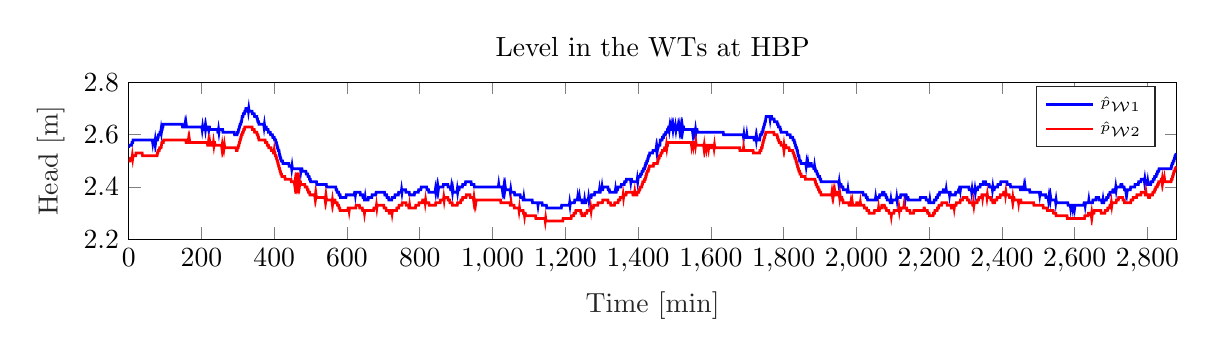
\begin{tikzpicture}

\begin{axis}[%
width=5.239in,
height=0.784in,
at={(1.128in,0.435in)},
scale only axis,
xmin=0,
xmax=2880,
xlabel style={font=\color{white!15!black}},
xlabel={Time [min]},
ymin=2.2,
ymax=2.8,
ylabel style={font=\color{white!15!black}},
ylabel={Head  [m]},
axis background/.style={fill=white},
title style={},
title={Level in the WTs at HBP},
legend style={legend cell align=left, align=left, draw=white!15!black}
]
\addplot [color=blue, line width=1.0pt]
  table[row sep=crcr]{%
0	2.55\\
1	2.56\\
2	2.56\\
3	2.56\\
4	2.56\\
5	2.56\\
6	2.56\\
7	2.56\\
8	2.56\\
9	2.57\\
10	2.57\\
11	2.57\\
12	2.58\\
13	2.58\\
14	2.58\\
15	2.58\\
16	2.58\\
17	2.58\\
18	2.58\\
19	2.58\\
20	2.58\\
21	2.58\\
22	2.58\\
23	2.58\\
24	2.58\\
25	2.58\\
26	2.58\\
27	2.58\\
28	2.58\\
29	2.58\\
30	2.58\\
31	2.58\\
32	2.58\\
33	2.58\\
34	2.58\\
35	2.58\\
36	2.58\\
37	2.58\\
38	2.58\\
39	2.58\\
40	2.58\\
41	2.58\\
42	2.58\\
43	2.58\\
44	2.58\\
45	2.58\\
46	2.58\\
47	2.58\\
48	2.58\\
49	2.58\\
50	2.58\\
51	2.58\\
52	2.58\\
53	2.58\\
54	2.58\\
55	2.58\\
56	2.58\\
57	2.58\\
58	2.58\\
59	2.58\\
60	2.58\\
61	2.58\\
62	2.58\\
63	2.58\\
64	2.58\\
65	2.58\\
66	2.57\\
67	2.58\\
68	2.58\\
69	2.58\\
70	2.58\\
71	2.58\\
72	2.57\\
73	2.58\\
74	2.57\\
75	2.58\\
76	2.58\\
77	2.58\\
78	2.58\\
79	2.58\\
80	2.59\\
81	2.59\\
82	2.6\\
83	2.6\\
84	2.6\\
85	2.6\\
86	2.61\\
87	2.61\\
88	2.61\\
89	2.62\\
90	2.61\\
91	2.62\\
92	2.62\\
93	2.63\\
94	2.63\\
95	2.64\\
96	2.64\\
97	2.64\\
98	2.64\\
99	2.64\\
100	2.64\\
101	2.64\\
102	2.64\\
103	2.64\\
104	2.64\\
105	2.64\\
106	2.64\\
107	2.64\\
108	2.64\\
109	2.64\\
110	2.64\\
111	2.64\\
112	2.64\\
113	2.64\\
114	2.64\\
115	2.64\\
116	2.64\\
117	2.64\\
118	2.64\\
119	2.64\\
120	2.64\\
121	2.64\\
122	2.64\\
123	2.64\\
124	2.64\\
125	2.64\\
126	2.64\\
127	2.64\\
128	2.64\\
129	2.64\\
130	2.64\\
131	2.64\\
132	2.64\\
133	2.64\\
134	2.64\\
135	2.64\\
136	2.64\\
137	2.64\\
138	2.64\\
139	2.64\\
140	2.64\\
141	2.64\\
142	2.64\\
143	2.64\\
144	2.64\\
145	2.64\\
146	2.64\\
147	2.64\\
148	2.63\\
149	2.63\\
150	2.63\\
151	2.63\\
152	2.63\\
153	2.63\\
154	2.63\\
155	2.64\\
156	2.63\\
157	2.63\\
158	2.64\\
159	2.63\\
160	2.63\\
161	2.63\\
162	2.63\\
163	2.63\\
164	2.63\\
165	2.63\\
166	2.63\\
167	2.63\\
168	2.63\\
169	2.63\\
170	2.63\\
171	2.63\\
172	2.63\\
173	2.63\\
174	2.63\\
175	2.63\\
176	2.63\\
177	2.63\\
178	2.63\\
179	2.63\\
180	2.63\\
181	2.63\\
182	2.63\\
183	2.63\\
184	2.63\\
185	2.63\\
186	2.63\\
187	2.63\\
188	2.63\\
189	2.63\\
190	2.63\\
191	2.63\\
192	2.63\\
193	2.63\\
194	2.63\\
195	2.63\\
196	2.63\\
197	2.63\\
198	2.63\\
199	2.63\\
200	2.63\\
201	2.63\\
202	2.62\\
203	2.63\\
204	2.62\\
205	2.62\\
206	2.62\\
207	2.62\\
208	2.62\\
209	2.62\\
210	2.63\\
211	2.62\\
212	2.63\\
213	2.62\\
214	2.62\\
215	2.62\\
216	2.63\\
217	2.63\\
218	2.63\\
219	2.63\\
220	2.62\\
221	2.63\\
222	2.63\\
223	2.62\\
224	2.62\\
225	2.62\\
226	2.62\\
227	2.62\\
228	2.62\\
229	2.62\\
230	2.62\\
231	2.62\\
232	2.62\\
233	2.62\\
234	2.62\\
235	2.62\\
236	2.62\\
237	2.62\\
238	2.62\\
239	2.62\\
240	2.62\\
241	2.62\\
242	2.62\\
243	2.62\\
244	2.62\\
245	2.61\\
246	2.61\\
247	2.62\\
248	2.61\\
249	2.62\\
250	2.62\\
251	2.62\\
252	2.62\\
253	2.62\\
254	2.62\\
255	2.62\\
256	2.62\\
257	2.62\\
258	2.62\\
259	2.61\\
260	2.61\\
261	2.61\\
262	2.61\\
263	2.61\\
264	2.61\\
265	2.61\\
266	2.61\\
267	2.61\\
268	2.61\\
269	2.61\\
270	2.61\\
271	2.61\\
272	2.61\\
273	2.61\\
274	2.61\\
275	2.61\\
276	2.61\\
277	2.61\\
278	2.61\\
279	2.61\\
280	2.61\\
281	2.61\\
282	2.61\\
283	2.61\\
284	2.61\\
285	2.61\\
286	2.61\\
287	2.61\\
288	2.61\\
289	2.61\\
290	2.61\\
291	2.6\\
292	2.6\\
293	2.6\\
294	2.6\\
295	2.6\\
296	2.6\\
297	2.6\\
298	2.6\\
299	2.61\\
300	2.61\\
301	2.61\\
302	2.62\\
303	2.62\\
304	2.63\\
305	2.63\\
306	2.64\\
307	2.64\\
308	2.64\\
309	2.65\\
310	2.65\\
311	2.66\\
312	2.67\\
313	2.67\\
314	2.67\\
315	2.68\\
316	2.68\\
317	2.68\\
318	2.68\\
319	2.69\\
320	2.69\\
321	2.69\\
322	2.7\\
323	2.7\\
324	2.7\\
325	2.7\\
326	2.7\\
327	2.7\\
328	2.7\\
329	2.69\\
330	2.7\\
331	2.69\\
332	2.69\\
333	2.69\\
334	2.69\\
335	2.69\\
336	2.69\\
337	2.69\\
338	2.69\\
339	2.69\\
340	2.68\\
341	2.68\\
342	2.68\\
343	2.68\\
344	2.68\\
345	2.68\\
346	2.67\\
347	2.67\\
348	2.67\\
349	2.67\\
350	2.67\\
351	2.67\\
352	2.67\\
353	2.66\\
354	2.66\\
355	2.65\\
356	2.65\\
357	2.65\\
358	2.64\\
359	2.64\\
360	2.64\\
361	2.64\\
362	2.64\\
363	2.64\\
364	2.64\\
365	2.64\\
366	2.64\\
367	2.64\\
368	2.64\\
369	2.64\\
370	2.64\\
371	2.64\\
372	2.63\\
373	2.64\\
374	2.63\\
375	2.63\\
376	2.63\\
377	2.63\\
378	2.63\\
379	2.62\\
380	2.62\\
381	2.62\\
382	2.62\\
383	2.62\\
384	2.61\\
385	2.61\\
386	2.61\\
387	2.61\\
388	2.61\\
389	2.61\\
390	2.6\\
391	2.6\\
392	2.6\\
393	2.6\\
394	2.6\\
395	2.6\\
396	2.59\\
397	2.59\\
398	2.59\\
399	2.59\\
400	2.59\\
401	2.58\\
402	2.58\\
403	2.58\\
404	2.58\\
405	2.57\\
406	2.57\\
407	2.56\\
408	2.56\\
409	2.55\\
410	2.55\\
411	2.54\\
412	2.54\\
413	2.54\\
414	2.53\\
415	2.52\\
416	2.52\\
417	2.51\\
418	2.51\\
419	2.5\\
420	2.5\\
421	2.5\\
422	2.5\\
423	2.5\\
424	2.49\\
425	2.49\\
426	2.49\\
427	2.49\\
428	2.49\\
429	2.49\\
430	2.49\\
431	2.49\\
432	2.49\\
433	2.49\\
434	2.49\\
435	2.49\\
436	2.49\\
437	2.49\\
438	2.49\\
439	2.49\\
440	2.49\\
441	2.48\\
442	2.48\\
443	2.48\\
444	2.48\\
445	2.48\\
446	2.48\\
447	2.48\\
448	2.47\\
449	2.48\\
450	2.47\\
451	2.47\\
452	2.47\\
453	2.47\\
454	2.47\\
455	2.47\\
456	2.47\\
457	2.47\\
458	2.47\\
459	2.47\\
460	2.47\\
461	2.47\\
462	2.47\\
463	2.47\\
464	2.47\\
465	2.47\\
466	2.47\\
467	2.47\\
468	2.47\\
469	2.47\\
470	2.47\\
471	2.47\\
472	2.47\\
473	2.46\\
474	2.47\\
475	2.47\\
476	2.47\\
477	2.46\\
478	2.46\\
479	2.46\\
480	2.46\\
481	2.46\\
482	2.46\\
483	2.46\\
484	2.46\\
485	2.46\\
486	2.46\\
487	2.46\\
488	2.45\\
489	2.45\\
490	2.45\\
491	2.45\\
492	2.45\\
493	2.44\\
494	2.44\\
495	2.44\\
496	2.44\\
497	2.43\\
498	2.43\\
499	2.43\\
500	2.42\\
501	2.42\\
502	2.42\\
503	2.42\\
504	2.42\\
505	2.42\\
506	2.42\\
507	2.42\\
508	2.42\\
509	2.42\\
510	2.42\\
511	2.42\\
512	2.42\\
513	2.42\\
514	2.42\\
515	2.42\\
516	2.42\\
517	2.41\\
518	2.41\\
519	2.41\\
520	2.41\\
521	2.41\\
522	2.41\\
523	2.41\\
524	2.41\\
525	2.41\\
526	2.41\\
527	2.41\\
528	2.41\\
529	2.41\\
530	2.41\\
531	2.41\\
532	2.41\\
533	2.41\\
534	2.41\\
535	2.41\\
536	2.41\\
537	2.41\\
538	2.41\\
539	2.41\\
540	2.41\\
541	2.41\\
542	2.41\\
543	2.41\\
544	2.4\\
545	2.4\\
546	2.4\\
547	2.4\\
548	2.4\\
549	2.4\\
550	2.4\\
551	2.4\\
552	2.4\\
553	2.4\\
554	2.4\\
555	2.4\\
556	2.4\\
557	2.4\\
558	2.4\\
559	2.4\\
560	2.4\\
561	2.4\\
562	2.4\\
563	2.4\\
564	2.4\\
565	2.4\\
566	2.4\\
567	2.4\\
568	2.4\\
569	2.4\\
570	2.39\\
571	2.39\\
572	2.39\\
573	2.38\\
574	2.38\\
575	2.38\\
576	2.38\\
577	2.38\\
578	2.37\\
579	2.37\\
580	2.37\\
581	2.37\\
582	2.36\\
583	2.36\\
584	2.36\\
585	2.36\\
586	2.36\\
587	2.36\\
588	2.36\\
589	2.36\\
590	2.36\\
591	2.36\\
592	2.36\\
593	2.36\\
594	2.36\\
595	2.36\\
596	2.36\\
597	2.36\\
598	2.37\\
599	2.37\\
600	2.37\\
601	2.37\\
602	2.37\\
603	2.37\\
604	2.37\\
605	2.37\\
606	2.37\\
607	2.37\\
608	2.37\\
609	2.37\\
610	2.37\\
611	2.37\\
612	2.37\\
613	2.37\\
614	2.37\\
615	2.37\\
616	2.37\\
617	2.37\\
618	2.37\\
619	2.37\\
620	2.37\\
621	2.38\\
622	2.38\\
623	2.37\\
624	2.38\\
625	2.38\\
626	2.38\\
627	2.38\\
628	2.38\\
629	2.38\\
630	2.38\\
631	2.38\\
632	2.38\\
633	2.38\\
634	2.38\\
635	2.38\\
636	2.38\\
637	2.37\\
638	2.37\\
639	2.37\\
640	2.37\\
641	2.37\\
642	2.37\\
643	2.37\\
644	2.36\\
645	2.36\\
646	2.36\\
647	2.36\\
648	2.35\\
649	2.35\\
650	2.36\\
651	2.35\\
652	2.35\\
653	2.35\\
654	2.35\\
655	2.35\\
656	2.35\\
657	2.35\\
658	2.35\\
659	2.36\\
660	2.36\\
661	2.36\\
662	2.36\\
663	2.36\\
664	2.36\\
665	2.36\\
666	2.36\\
667	2.36\\
668	2.36\\
669	2.37\\
670	2.37\\
671	2.37\\
672	2.37\\
673	2.37\\
674	2.37\\
675	2.37\\
676	2.37\\
677	2.37\\
678	2.37\\
679	2.37\\
680	2.38\\
681	2.38\\
682	2.38\\
683	2.38\\
684	2.38\\
685	2.38\\
686	2.38\\
687	2.38\\
688	2.38\\
689	2.38\\
690	2.38\\
691	2.38\\
692	2.38\\
693	2.38\\
694	2.38\\
695	2.38\\
696	2.38\\
697	2.38\\
698	2.38\\
699	2.38\\
700	2.38\\
701	2.38\\
702	2.38\\
703	2.38\\
704	2.37\\
705	2.37\\
706	2.37\\
707	2.37\\
708	2.37\\
709	2.37\\
710	2.36\\
711	2.36\\
712	2.36\\
713	2.36\\
714	2.36\\
715	2.35\\
716	2.35\\
717	2.35\\
718	2.35\\
719	2.35\\
720	2.35\\
721	2.35\\
722	2.35\\
723	2.35\\
724	2.36\\
725	2.36\\
726	2.36\\
727	2.36\\
728	2.36\\
729	2.36\\
730	2.36\\
731	2.36\\
732	2.37\\
733	2.37\\
734	2.37\\
735	2.37\\
736	2.37\\
737	2.37\\
738	2.37\\
739	2.37\\
740	2.37\\
741	2.37\\
742	2.38\\
743	2.38\\
744	2.38\\
745	2.38\\
746	2.38\\
747	2.38\\
748	2.38\\
749	2.38\\
750	2.39\\
751	2.38\\
752	2.39\\
753	2.39\\
754	2.39\\
755	2.39\\
756	2.39\\
757	2.39\\
758	2.39\\
759	2.39\\
760	2.39\\
761	2.39\\
762	2.38\\
763	2.38\\
764	2.38\\
765	2.38\\
766	2.38\\
767	2.38\\
768	2.38\\
769	2.38\\
770	2.38\\
771	2.38\\
772	2.37\\
773	2.37\\
774	2.37\\
775	2.37\\
776	2.37\\
777	2.37\\
778	2.37\\
779	2.37\\
780	2.37\\
781	2.37\\
782	2.37\\
783	2.37\\
784	2.37\\
785	2.37\\
786	2.38\\
787	2.38\\
788	2.38\\
789	2.38\\
790	2.38\\
791	2.38\\
792	2.38\\
793	2.38\\
794	2.38\\
795	2.38\\
796	2.38\\
797	2.39\\
798	2.39\\
799	2.39\\
800	2.39\\
801	2.39\\
802	2.39\\
803	2.39\\
804	2.4\\
805	2.4\\
806	2.4\\
807	2.4\\
808	2.4\\
809	2.4\\
810	2.4\\
811	2.4\\
812	2.4\\
813	2.4\\
814	2.4\\
815	2.4\\
816	2.4\\
817	2.4\\
818	2.4\\
819	2.4\\
820	2.39\\
821	2.39\\
822	2.39\\
823	2.39\\
824	2.39\\
825	2.38\\
826	2.38\\
827	2.38\\
828	2.38\\
829	2.38\\
830	2.38\\
831	2.38\\
832	2.38\\
833	2.38\\
834	2.38\\
835	2.38\\
836	2.38\\
837	2.38\\
838	2.38\\
839	2.38\\
840	2.38\\
841	2.38\\
842	2.38\\
843	2.39\\
844	2.38\\
845	2.39\\
846	2.39\\
847	2.39\\
848	2.4\\
849	2.39\\
850	2.4\\
851	2.39\\
852	2.4\\
853	2.4\\
854	2.4\\
855	2.4\\
856	2.4\\
857	2.4\\
858	2.4\\
859	2.4\\
860	2.4\\
861	2.4\\
862	2.4\\
863	2.4\\
864	2.4\\
865	2.41\\
866	2.41\\
867	2.41\\
868	2.41\\
869	2.41\\
870	2.41\\
871	2.41\\
872	2.41\\
873	2.41\\
874	2.41\\
875	2.41\\
876	2.41\\
877	2.41\\
878	2.4\\
879	2.4\\
880	2.4\\
881	2.4\\
882	2.4\\
883	2.4\\
884	2.4\\
885	2.39\\
886	2.39\\
887	2.4\\
888	2.39\\
889	2.39\\
890	2.38\\
891	2.39\\
892	2.38\\
893	2.38\\
894	2.38\\
895	2.38\\
896	2.38\\
897	2.38\\
898	2.38\\
899	2.38\\
900	2.38\\
901	2.38\\
902	2.38\\
903	2.39\\
904	2.38\\
905	2.39\\
906	2.39\\
907	2.39\\
908	2.39\\
909	2.4\\
910	2.4\\
911	2.4\\
912	2.4\\
913	2.4\\
914	2.4\\
915	2.4\\
916	2.4\\
917	2.4\\
918	2.41\\
919	2.41\\
920	2.41\\
921	2.41\\
922	2.41\\
923	2.41\\
924	2.41\\
925	2.41\\
926	2.42\\
927	2.42\\
928	2.42\\
929	2.42\\
930	2.42\\
931	2.42\\
932	2.42\\
933	2.42\\
934	2.42\\
935	2.42\\
936	2.42\\
937	2.42\\
938	2.42\\
939	2.42\\
940	2.42\\
941	2.42\\
942	2.41\\
943	2.41\\
944	2.41\\
945	2.41\\
946	2.41\\
947	2.41\\
948	2.41\\
949	2.41\\
950	2.4\\
951	2.4\\
952	2.4\\
953	2.4\\
954	2.4\\
955	2.4\\
956	2.4\\
957	2.4\\
958	2.4\\
959	2.4\\
960	2.4\\
961	2.4\\
962	2.4\\
963	2.4\\
964	2.4\\
965	2.4\\
966	2.4\\
967	2.4\\
968	2.4\\
969	2.4\\
970	2.4\\
971	2.4\\
972	2.4\\
973	2.4\\
974	2.4\\
975	2.4\\
976	2.4\\
977	2.4\\
978	2.4\\
979	2.4\\
980	2.4\\
981	2.4\\
982	2.4\\
983	2.4\\
984	2.4\\
985	2.4\\
986	2.4\\
987	2.4\\
988	2.4\\
989	2.4\\
990	2.4\\
991	2.4\\
992	2.4\\
993	2.4\\
994	2.4\\
995	2.4\\
996	2.4\\
997	2.4\\
998	2.4\\
999	2.4\\
1000	2.4\\
1001	2.4\\
1002	2.4\\
1003	2.4\\
1004	2.4\\
1005	2.4\\
1006	2.4\\
1007	2.4\\
1008	2.4\\
1009	2.4\\
1010	2.4\\
1011	2.4\\
1012	2.4\\
1013	2.4\\
1014	2.4\\
1015	2.4\\
1016	2.4\\
1017	2.41\\
1018	2.4\\
1019	2.4\\
1020	2.4\\
1021	2.4\\
1022	2.4\\
1023	2.4\\
1024	2.4\\
1025	2.4\\
1026	2.4\\
1027	2.39\\
1028	2.4\\
1029	2.4\\
1030	2.39\\
1031	2.4\\
1032	2.39\\
1033	2.4\\
1034	2.39\\
1035	2.4\\
1036	2.39\\
1037	2.39\\
1038	2.39\\
1039	2.39\\
1040	2.39\\
1041	2.39\\
1042	2.39\\
1043	2.39\\
1044	2.39\\
1045	2.39\\
1046	2.39\\
1047	2.39\\
1048	2.39\\
1049	2.38\\
1050	2.39\\
1051	2.38\\
1052	2.38\\
1053	2.38\\
1054	2.38\\
1055	2.38\\
1056	2.38\\
1057	2.38\\
1058	2.38\\
1059	2.38\\
1060	2.38\\
1061	2.37\\
1062	2.37\\
1063	2.37\\
1064	2.37\\
1065	2.37\\
1066	2.37\\
1067	2.37\\
1068	2.37\\
1069	2.37\\
1070	2.37\\
1071	2.37\\
1072	2.37\\
1073	2.37\\
1074	2.37\\
1075	2.37\\
1076	2.37\\
1077	2.36\\
1078	2.36\\
1079	2.36\\
1080	2.36\\
1081	2.36\\
1082	2.36\\
1083	2.36\\
1084	2.35\\
1085	2.35\\
1086	2.36\\
1087	2.35\\
1088	2.35\\
1089	2.35\\
1090	2.35\\
1091	2.35\\
1092	2.35\\
1093	2.35\\
1094	2.35\\
1095	2.35\\
1096	2.35\\
1097	2.35\\
1098	2.35\\
1099	2.35\\
1100	2.35\\
1101	2.35\\
1102	2.35\\
1103	2.35\\
1104	2.35\\
1105	2.35\\
1106	2.35\\
1107	2.35\\
1108	2.35\\
1109	2.35\\
1110	2.34\\
1111	2.34\\
1112	2.34\\
1113	2.34\\
1114	2.34\\
1115	2.34\\
1116	2.34\\
1117	2.34\\
1118	2.34\\
1119	2.34\\
1120	2.34\\
1121	2.34\\
1122	2.34\\
1123	2.34\\
1124	2.34\\
1125	2.33\\
1126	2.34\\
1127	2.34\\
1128	2.34\\
1129	2.34\\
1130	2.34\\
1131	2.34\\
1132	2.34\\
1133	2.34\\
1134	2.34\\
1135	2.34\\
1136	2.34\\
1137	2.33\\
1138	2.33\\
1139	2.33\\
1140	2.33\\
1141	2.33\\
1142	2.33\\
1143	2.33\\
1144	2.33\\
1145	2.33\\
1146	2.33\\
1147	2.33\\
1148	2.33\\
1149	2.32\\
1150	2.32\\
1151	2.32\\
1152	2.32\\
1153	2.32\\
1154	2.32\\
1155	2.32\\
1156	2.32\\
1157	2.32\\
1158	2.32\\
1159	2.32\\
1160	2.32\\
1161	2.32\\
1162	2.32\\
1163	2.32\\
1164	2.32\\
1165	2.32\\
1166	2.32\\
1167	2.32\\
1168	2.32\\
1169	2.32\\
1170	2.32\\
1171	2.32\\
1172	2.32\\
1173	2.32\\
1174	2.32\\
1175	2.32\\
1176	2.32\\
1177	2.32\\
1178	2.32\\
1179	2.32\\
1180	2.32\\
1181	2.32\\
1182	2.32\\
1183	2.32\\
1184	2.32\\
1185	2.32\\
1186	2.32\\
1187	2.32\\
1188	2.32\\
1189	2.32\\
1190	2.33\\
1191	2.33\\
1192	2.33\\
1193	2.33\\
1194	2.33\\
1195	2.33\\
1196	2.33\\
1197	2.33\\
1198	2.33\\
1199	2.33\\
1200	2.33\\
1201	2.33\\
1202	2.33\\
1203	2.33\\
1204	2.33\\
1205	2.33\\
1206	2.33\\
1207	2.33\\
1208	2.33\\
1209	2.33\\
1210	2.33\\
1211	2.33\\
1212	2.34\\
1213	2.33\\
1214	2.34\\
1215	2.34\\
1216	2.34\\
1217	2.34\\
1218	2.34\\
1219	2.34\\
1220	2.34\\
1221	2.34\\
1222	2.34\\
1223	2.34\\
1224	2.34\\
1225	2.34\\
1226	2.35\\
1227	2.35\\
1228	2.35\\
1229	2.35\\
1230	2.35\\
1231	2.35\\
1232	2.35\\
1233	2.35\\
1234	2.36\\
1235	2.35\\
1236	2.35\\
1237	2.35\\
1238	2.35\\
1239	2.36\\
1240	2.35\\
1241	2.35\\
1242	2.35\\
1243	2.35\\
1244	2.35\\
1245	2.35\\
1246	2.34\\
1247	2.34\\
1248	2.34\\
1249	2.34\\
1250	2.34\\
1251	2.34\\
1252	2.34\\
1253	2.35\\
1254	2.34\\
1255	2.34\\
1256	2.34\\
1257	2.35\\
1258	2.35\\
1259	2.35\\
1260	2.35\\
1261	2.35\\
1262	2.35\\
1263	2.35\\
1264	2.36\\
1265	2.35\\
1266	2.36\\
1267	2.36\\
1268	2.36\\
1269	2.36\\
1270	2.36\\
1271	2.36\\
1272	2.37\\
1273	2.37\\
1274	2.37\\
1275	2.37\\
1276	2.37\\
1277	2.37\\
1278	2.37\\
1279	2.37\\
1280	2.37\\
1281	2.38\\
1282	2.38\\
1283	2.38\\
1284	2.38\\
1285	2.38\\
1286	2.38\\
1287	2.38\\
1288	2.38\\
1289	2.38\\
1290	2.38\\
1291	2.38\\
1292	2.38\\
1293	2.38\\
1294	2.39\\
1295	2.38\\
1296	2.38\\
1297	2.39\\
1298	2.39\\
1299	2.39\\
1300	2.39\\
1301	2.4\\
1302	2.39\\
1303	2.39\\
1304	2.4\\
1305	2.4\\
1306	2.4\\
1307	2.4\\
1308	2.4\\
1309	2.4\\
1310	2.4\\
1311	2.4\\
1312	2.4\\
1313	2.4\\
1314	2.4\\
1315	2.4\\
1316	2.4\\
1317	2.4\\
1318	2.39\\
1319	2.39\\
1320	2.39\\
1321	2.39\\
1322	2.38\\
1323	2.38\\
1324	2.38\\
1325	2.38\\
1326	2.38\\
1327	2.38\\
1328	2.38\\
1329	2.38\\
1330	2.38\\
1331	2.38\\
1332	2.38\\
1333	2.38\\
1334	2.38\\
1335	2.38\\
1336	2.38\\
1337	2.38\\
1338	2.39\\
1339	2.38\\
1340	2.38\\
1341	2.39\\
1342	2.39\\
1343	2.39\\
1344	2.39\\
1345	2.4\\
1346	2.4\\
1347	2.4\\
1348	2.4\\
1349	2.4\\
1350	2.4\\
1351	2.4\\
1352	2.4\\
1353	2.4\\
1354	2.41\\
1355	2.41\\
1356	2.41\\
1357	2.41\\
1358	2.41\\
1359	2.41\\
1360	2.41\\
1361	2.41\\
1362	2.41\\
1363	2.42\\
1364	2.42\\
1365	2.42\\
1366	2.42\\
1367	2.42\\
1368	2.43\\
1369	2.43\\
1370	2.43\\
1371	2.43\\
1372	2.43\\
1373	2.43\\
1374	2.43\\
1375	2.43\\
1376	2.43\\
1377	2.43\\
1378	2.43\\
1379	2.43\\
1380	2.42\\
1381	2.43\\
1382	2.43\\
1383	2.42\\
1384	2.42\\
1385	2.42\\
1386	2.42\\
1387	2.42\\
1388	2.42\\
1389	2.42\\
1390	2.42\\
1391	2.42\\
1392	2.42\\
1393	2.42\\
1394	2.42\\
1395	2.42\\
1396	2.42\\
1397	2.42\\
1398	2.43\\
1399	2.42\\
1400	2.43\\
1401	2.44\\
1402	2.44\\
1403	2.44\\
1404	2.44\\
1405	2.44\\
1406	2.44\\
1407	2.45\\
1408	2.45\\
1409	2.45\\
1410	2.45\\
1411	2.46\\
1412	2.46\\
1413	2.46\\
1414	2.46\\
1415	2.47\\
1416	2.47\\
1417	2.47\\
1418	2.47\\
1419	2.48\\
1420	2.48\\
1421	2.49\\
1422	2.49\\
1423	2.49\\
1424	2.5\\
1425	2.5\\
1426	2.5\\
1427	2.51\\
1428	2.51\\
1429	2.52\\
1430	2.52\\
1431	2.52\\
1432	2.53\\
1433	2.53\\
1434	2.53\\
1435	2.53\\
1436	2.53\\
1437	2.53\\
1438	2.53\\
1439	2.53\\
1440	2.53\\
1441	2.54\\
1442	2.54\\
1443	2.54\\
1444	2.54\\
1445	2.54\\
1446	2.54\\
1447	2.54\\
1448	2.54\\
1449	2.54\\
1450	2.55\\
1451	2.54\\
1452	2.55\\
1453	2.54\\
1454	2.55\\
1455	2.55\\
1456	2.56\\
1457	2.56\\
1458	2.56\\
1459	2.56\\
1460	2.56\\
1461	2.58\\
1462	2.58\\
1463	2.58\\
1464	2.58\\
1465	2.58\\
1466	2.58\\
1467	2.59\\
1468	2.59\\
1469	2.59\\
1470	2.59\\
1471	2.6\\
1472	2.6\\
1473	2.6\\
1474	2.6\\
1475	2.6\\
1476	2.61\\
1477	2.61\\
1478	2.61\\
1479	2.61\\
1480	2.61\\
1481	2.62\\
1482	2.62\\
1483	2.62\\
1484	2.63\\
1485	2.63\\
1486	2.62\\
1487	2.63\\
1488	2.62\\
1489	2.62\\
1490	2.62\\
1491	2.63\\
1492	2.62\\
1493	2.62\\
1494	2.62\\
1495	2.63\\
1496	2.62\\
1497	2.63\\
1498	2.62\\
1499	2.62\\
1500	2.62\\
1501	2.62\\
1502	2.62\\
1503	2.63\\
1504	2.62\\
1505	2.63\\
1506	2.63\\
1507	2.62\\
1508	2.62\\
1509	2.62\\
1510	2.63\\
1511	2.62\\
1512	2.62\\
1513	2.63\\
1514	2.62\\
1515	2.63\\
1516	2.63\\
1517	2.62\\
1518	2.63\\
1519	2.62\\
1520	2.63\\
1521	2.62\\
1522	2.63\\
1523	2.62\\
1524	2.63\\
1525	2.63\\
1526	2.62\\
1527	2.62\\
1528	2.62\\
1529	2.62\\
1530	2.62\\
1531	2.62\\
1532	2.62\\
1533	2.62\\
1534	2.62\\
1535	2.62\\
1536	2.62\\
1537	2.62\\
1538	2.62\\
1539	2.62\\
1540	2.62\\
1541	2.62\\
1542	2.62\\
1543	2.62\\
1544	2.62\\
1545	2.62\\
1546	2.62\\
1547	2.62\\
1548	2.62\\
1549	2.62\\
1550	2.61\\
1551	2.62\\
1552	2.62\\
1553	2.61\\
1554	2.62\\
1555	2.62\\
1556	2.62\\
1557	2.61\\
1558	2.62\\
1559	2.61\\
1560	2.62\\
1561	2.62\\
1562	2.62\\
1563	2.61\\
1564	2.61\\
1565	2.61\\
1566	2.61\\
1567	2.61\\
1568	2.61\\
1569	2.61\\
1570	2.61\\
1571	2.61\\
1572	2.61\\
1573	2.61\\
1574	2.61\\
1575	2.61\\
1576	2.61\\
1577	2.61\\
1578	2.61\\
1579	2.61\\
1580	2.61\\
1581	2.61\\
1582	2.61\\
1583	2.61\\
1584	2.61\\
1585	2.61\\
1586	2.61\\
1587	2.61\\
1588	2.61\\
1589	2.61\\
1590	2.61\\
1591	2.61\\
1592	2.61\\
1593	2.61\\
1594	2.61\\
1595	2.61\\
1596	2.61\\
1597	2.61\\
1598	2.61\\
1599	2.61\\
1600	2.61\\
1601	2.61\\
1602	2.61\\
1603	2.61\\
1604	2.61\\
1605	2.61\\
1606	2.61\\
1607	2.61\\
1608	2.61\\
1609	2.61\\
1610	2.61\\
1611	2.61\\
1612	2.61\\
1613	2.61\\
1614	2.61\\
1615	2.61\\
1616	2.61\\
1617	2.61\\
1618	2.61\\
1619	2.61\\
1620	2.61\\
1621	2.61\\
1622	2.61\\
1623	2.61\\
1624	2.61\\
1625	2.61\\
1626	2.61\\
1627	2.61\\
1628	2.61\\
1629	2.61\\
1630	2.61\\
1631	2.61\\
1632	2.61\\
1633	2.61\\
1634	2.61\\
1635	2.6\\
1636	2.6\\
1637	2.6\\
1638	2.6\\
1639	2.6\\
1640	2.6\\
1641	2.6\\
1642	2.6\\
1643	2.6\\
1644	2.6\\
1645	2.6\\
1646	2.6\\
1647	2.6\\
1648	2.6\\
1649	2.6\\
1650	2.6\\
1651	2.6\\
1652	2.6\\
1653	2.6\\
1654	2.6\\
1655	2.6\\
1656	2.6\\
1657	2.6\\
1658	2.6\\
1659	2.6\\
1660	2.6\\
1661	2.6\\
1662	2.6\\
1663	2.6\\
1664	2.6\\
1665	2.6\\
1666	2.6\\
1667	2.6\\
1668	2.6\\
1669	2.6\\
1670	2.6\\
1671	2.6\\
1672	2.6\\
1673	2.6\\
1674	2.6\\
1675	2.6\\
1676	2.6\\
1677	2.6\\
1678	2.6\\
1679	2.6\\
1680	2.6\\
1681	2.6\\
1682	2.6\\
1683	2.6\\
1684	2.6\\
1685	2.6\\
1686	2.6\\
1687	2.6\\
1688	2.6\\
1689	2.6\\
1690	2.59\\
1691	2.6\\
1692	2.59\\
1693	2.59\\
1694	2.59\\
1695	2.59\\
1696	2.59\\
1697	2.59\\
1698	2.59\\
1699	2.6\\
1700	2.59\\
1701	2.59\\
1702	2.59\\
1703	2.59\\
1704	2.59\\
1705	2.59\\
1706	2.59\\
1707	2.59\\
1708	2.59\\
1709	2.59\\
1710	2.59\\
1711	2.59\\
1712	2.59\\
1713	2.59\\
1714	2.59\\
1715	2.59\\
1716	2.59\\
1717	2.59\\
1718	2.59\\
1719	2.58\\
1720	2.58\\
1721	2.58\\
1722	2.58\\
1723	2.58\\
1724	2.59\\
1725	2.58\\
1726	2.59\\
1727	2.58\\
1728	2.58\\
1729	2.58\\
1730	2.58\\
1731	2.58\\
1732	2.58\\
1733	2.58\\
1734	2.58\\
1735	2.59\\
1736	2.6\\
1737	2.6\\
1738	2.6\\
1739	2.6\\
1740	2.61\\
1741	2.61\\
1742	2.61\\
1743	2.62\\
1744	2.62\\
1745	2.63\\
1746	2.63\\
1747	2.64\\
1748	2.64\\
1749	2.65\\
1750	2.65\\
1751	2.66\\
1752	2.67\\
1753	2.67\\
1754	2.67\\
1755	2.67\\
1756	2.67\\
1757	2.67\\
1758	2.67\\
1759	2.67\\
1760	2.67\\
1761	2.67\\
1762	2.67\\
1763	2.66\\
1764	2.67\\
1765	2.67\\
1766	2.67\\
1767	2.67\\
1768	2.66\\
1769	2.66\\
1770	2.66\\
1771	2.66\\
1772	2.66\\
1773	2.66\\
1774	2.66\\
1775	2.65\\
1776	2.65\\
1777	2.65\\
1778	2.65\\
1779	2.65\\
1780	2.65\\
1781	2.65\\
1782	2.65\\
1783	2.64\\
1784	2.64\\
1785	2.64\\
1786	2.63\\
1787	2.63\\
1788	2.63\\
1789	2.63\\
1790	2.63\\
1791	2.62\\
1792	2.62\\
1793	2.61\\
1794	2.61\\
1795	2.61\\
1796	2.61\\
1797	2.61\\
1798	2.61\\
1799	2.61\\
1800	2.61\\
1801	2.61\\
1802	2.61\\
1803	2.61\\
1804	2.61\\
1805	2.61\\
1806	2.61\\
1807	2.61\\
1808	2.61\\
1809	2.61\\
1810	2.6\\
1811	2.6\\
1812	2.6\\
1813	2.6\\
1814	2.6\\
1815	2.6\\
1816	2.6\\
1817	2.6\\
1818	2.6\\
1819	2.59\\
1820	2.59\\
1821	2.59\\
1822	2.59\\
1823	2.59\\
1824	2.59\\
1825	2.59\\
1826	2.58\\
1827	2.58\\
1828	2.58\\
1829	2.58\\
1830	2.57\\
1831	2.57\\
1832	2.56\\
1833	2.56\\
1834	2.55\\
1835	2.55\\
1836	2.55\\
1837	2.54\\
1838	2.54\\
1839	2.53\\
1840	2.52\\
1841	2.52\\
1842	2.52\\
1843	2.51\\
1844	2.5\\
1845	2.5\\
1846	2.5\\
1847	2.5\\
1848	2.49\\
1849	2.49\\
1850	2.49\\
1851	2.49\\
1852	2.49\\
1853	2.49\\
1854	2.49\\
1855	2.49\\
1856	2.49\\
1857	2.49\\
1858	2.49\\
1859	2.49\\
1860	2.49\\
1861	2.49\\
1862	2.48\\
1863	2.49\\
1864	2.48\\
1865	2.48\\
1866	2.48\\
1867	2.49\\
1868	2.48\\
1869	2.48\\
1870	2.49\\
1871	2.49\\
1872	2.49\\
1873	2.49\\
1874	2.49\\
1875	2.49\\
1876	2.49\\
1877	2.48\\
1878	2.48\\
1879	2.48\\
1880	2.48\\
1881	2.48\\
1882	2.48\\
1883	2.47\\
1884	2.47\\
1885	2.48\\
1886	2.47\\
1887	2.47\\
1888	2.46\\
1889	2.46\\
1890	2.46\\
1891	2.46\\
1892	2.45\\
1893	2.45\\
1894	2.45\\
1895	2.44\\
1896	2.44\\
1897	2.44\\
1898	2.44\\
1899	2.44\\
1900	2.43\\
1901	2.43\\
1902	2.43\\
1903	2.42\\
1904	2.42\\
1905	2.42\\
1906	2.42\\
1907	2.42\\
1908	2.42\\
1909	2.42\\
1910	2.42\\
1911	2.42\\
1912	2.42\\
1913	2.42\\
1914	2.42\\
1915	2.42\\
1916	2.42\\
1917	2.42\\
1918	2.42\\
1919	2.42\\
1920	2.42\\
1921	2.42\\
1922	2.42\\
1923	2.42\\
1924	2.42\\
1925	2.42\\
1926	2.42\\
1927	2.42\\
1928	2.42\\
1929	2.42\\
1930	2.42\\
1931	2.42\\
1932	2.42\\
1933	2.42\\
1934	2.42\\
1935	2.42\\
1936	2.42\\
1937	2.42\\
1938	2.42\\
1939	2.42\\
1940	2.42\\
1941	2.42\\
1942	2.42\\
1943	2.42\\
1944	2.42\\
1945	2.42\\
1946	2.42\\
1947	2.42\\
1948	2.42\\
1949	2.42\\
1950	2.42\\
1951	2.42\\
1952	2.41\\
1953	2.42\\
1954	2.41\\
1955	2.41\\
1956	2.41\\
1957	2.41\\
1958	2.41\\
1959	2.4\\
1960	2.4\\
1961	2.4\\
1962	2.4\\
1963	2.4\\
1964	2.39\\
1965	2.39\\
1966	2.39\\
1967	2.39\\
1968	2.39\\
1969	2.39\\
1970	2.39\\
1971	2.39\\
1972	2.39\\
1973	2.39\\
1974	2.39\\
1975	2.38\\
1976	2.38\\
1977	2.39\\
1978	2.38\\
1979	2.38\\
1980	2.38\\
1981	2.38\\
1982	2.38\\
1983	2.38\\
1984	2.38\\
1985	2.38\\
1986	2.38\\
1987	2.38\\
1988	2.38\\
1989	2.38\\
1990	2.38\\
1991	2.38\\
1992	2.38\\
1993	2.38\\
1994	2.38\\
1995	2.38\\
1996	2.38\\
1997	2.38\\
1998	2.38\\
1999	2.38\\
2000	2.38\\
2001	2.38\\
2002	2.38\\
2003	2.38\\
2004	2.38\\
2005	2.38\\
2006	2.38\\
2007	2.38\\
2008	2.38\\
2009	2.38\\
2010	2.38\\
2011	2.38\\
2012	2.38\\
2013	2.38\\
2014	2.38\\
2015	2.38\\
2016	2.38\\
2017	2.38\\
2018	2.38\\
2019	2.37\\
2020	2.37\\
2021	2.37\\
2022	2.37\\
2023	2.37\\
2024	2.37\\
2025	2.37\\
2026	2.37\\
2027	2.36\\
2028	2.36\\
2029	2.36\\
2030	2.36\\
2031	2.35\\
2032	2.35\\
2033	2.35\\
2034	2.35\\
2035	2.35\\
2036	2.35\\
2037	2.35\\
2038	2.35\\
2039	2.35\\
2040	2.35\\
2041	2.35\\
2042	2.35\\
2043	2.35\\
2044	2.35\\
2045	2.35\\
2046	2.35\\
2047	2.35\\
2048	2.35\\
2049	2.35\\
2050	2.35\\
2051	2.35\\
2052	2.35\\
2053	2.36\\
2054	2.35\\
2055	2.35\\
2056	2.35\\
2057	2.35\\
2058	2.36\\
2059	2.36\\
2060	2.36\\
2061	2.36\\
2062	2.36\\
2063	2.36\\
2064	2.37\\
2065	2.37\\
2066	2.37\\
2067	2.37\\
2068	2.37\\
2069	2.37\\
2070	2.37\\
2071	2.37\\
2072	2.38\\
2073	2.38\\
2074	2.38\\
2075	2.38\\
2076	2.38\\
2077	2.37\\
2078	2.37\\
2079	2.37\\
2080	2.37\\
2081	2.37\\
2082	2.36\\
2083	2.36\\
2084	2.36\\
2085	2.35\\
2086	2.35\\
2087	2.35\\
2088	2.35\\
2089	2.35\\
2090	2.35\\
2091	2.35\\
2092	2.35\\
2093	2.34\\
2094	2.34\\
2095	2.35\\
2096	2.34\\
2097	2.34\\
2098	2.34\\
2099	2.35\\
2100	2.35\\
2101	2.35\\
2102	2.35\\
2103	2.35\\
2104	2.35\\
2105	2.35\\
2106	2.35\\
2107	2.35\\
2108	2.35\\
2109	2.35\\
2110	2.35\\
2111	2.36\\
2112	2.35\\
2113	2.36\\
2114	2.36\\
2115	2.36\\
2116	2.36\\
2117	2.36\\
2118	2.36\\
2119	2.36\\
2120	2.36\\
2121	2.36\\
2122	2.37\\
2123	2.37\\
2124	2.37\\
2125	2.37\\
2126	2.37\\
2127	2.37\\
2128	2.37\\
2129	2.37\\
2130	2.37\\
2131	2.37\\
2132	2.37\\
2133	2.37\\
2134	2.37\\
2135	2.36\\
2136	2.37\\
2137	2.37\\
2138	2.36\\
2139	2.36\\
2140	2.36\\
2141	2.36\\
2142	2.36\\
2143	2.35\\
2144	2.35\\
2145	2.35\\
2146	2.35\\
2147	2.35\\
2148	2.35\\
2149	2.35\\
2150	2.35\\
2151	2.35\\
2152	2.35\\
2153	2.35\\
2154	2.35\\
2155	2.35\\
2156	2.35\\
2157	2.35\\
2158	2.35\\
2159	2.35\\
2160	2.35\\
2161	2.35\\
2162	2.35\\
2163	2.35\\
2164	2.35\\
2165	2.35\\
2166	2.35\\
2167	2.35\\
2168	2.35\\
2169	2.35\\
2170	2.35\\
2171	2.35\\
2172	2.35\\
2173	2.35\\
2174	2.35\\
2175	2.35\\
2176	2.36\\
2177	2.36\\
2178	2.36\\
2179	2.36\\
2180	2.36\\
2181	2.36\\
2182	2.36\\
2183	2.36\\
2184	2.36\\
2185	2.36\\
2186	2.36\\
2187	2.36\\
2188	2.36\\
2189	2.36\\
2190	2.36\\
2191	2.36\\
2192	2.35\\
2193	2.35\\
2194	2.35\\
2195	2.35\\
2196	2.35\\
2197	2.35\\
2198	2.35\\
2199	2.34\\
2200	2.34\\
2201	2.34\\
2202	2.35\\
2203	2.34\\
2204	2.34\\
2205	2.34\\
2206	2.34\\
2207	2.34\\
2208	2.34\\
2209	2.34\\
2210	2.34\\
2211	2.34\\
2212	2.34\\
2213	2.34\\
2214	2.35\\
2215	2.35\\
2216	2.35\\
2217	2.35\\
2218	2.35\\
2219	2.35\\
2220	2.36\\
2221	2.36\\
2222	2.36\\
2223	2.36\\
2224	2.37\\
2225	2.37\\
2226	2.37\\
2227	2.37\\
2228	2.37\\
2229	2.38\\
2230	2.38\\
2231	2.38\\
2232	2.38\\
2233	2.38\\
2234	2.38\\
2235	2.38\\
2236	2.38\\
2237	2.38\\
2238	2.38\\
2239	2.39\\
2240	2.39\\
2241	2.39\\
2242	2.39\\
2243	2.39\\
2244	2.39\\
2245	2.38\\
2246	2.38\\
2247	2.39\\
2248	2.38\\
2249	2.38\\
2250	2.38\\
2251	2.38\\
2252	2.38\\
2253	2.38\\
2254	2.38\\
2255	2.38\\
2256	2.37\\
2257	2.38\\
2258	2.38\\
2259	2.37\\
2260	2.37\\
2261	2.37\\
2262	2.37\\
2263	2.37\\
2264	2.37\\
2265	2.37\\
2266	2.37\\
2267	2.37\\
2268	2.37\\
2269	2.37\\
2270	2.37\\
2271	2.37\\
2272	2.37\\
2273	2.38\\
2274	2.38\\
2275	2.38\\
2276	2.38\\
2277	2.38\\
2278	2.38\\
2279	2.38\\
2280	2.38\\
2281	2.39\\
2282	2.39\\
2283	2.39\\
2284	2.4\\
2285	2.4\\
2286	2.39\\
2287	2.4\\
2288	2.4\\
2289	2.4\\
2290	2.4\\
2291	2.4\\
2292	2.4\\
2293	2.4\\
2294	2.4\\
2295	2.4\\
2296	2.4\\
2297	2.4\\
2298	2.4\\
2299	2.4\\
2300	2.4\\
2301	2.4\\
2302	2.4\\
2303	2.4\\
2304	2.4\\
2305	2.4\\
2306	2.4\\
2307	2.4\\
2308	2.4\\
2309	2.4\\
2310	2.39\\
2311	2.39\\
2312	2.39\\
2313	2.39\\
2314	2.39\\
2315	2.39\\
2316	2.39\\
2317	2.38\\
2318	2.39\\
2319	2.38\\
2320	2.38\\
2321	2.38\\
2322	2.38\\
2323	2.38\\
2324	2.38\\
2325	2.38\\
2326	2.39\\
2327	2.38\\
2328	2.39\\
2329	2.39\\
2330	2.39\\
2331	2.39\\
2332	2.39\\
2333	2.39\\
2334	2.4\\
2335	2.4\\
2336	2.4\\
2337	2.4\\
2338	2.4\\
2339	2.4\\
2340	2.4\\
2341	2.41\\
2342	2.41\\
2343	2.41\\
2344	2.41\\
2345	2.41\\
2346	2.41\\
2347	2.41\\
2348	2.41\\
2349	2.42\\
2350	2.42\\
2351	2.42\\
2352	2.42\\
2353	2.42\\
2354	2.42\\
2355	2.42\\
2356	2.41\\
2357	2.41\\
2358	2.41\\
2359	2.41\\
2360	2.41\\
2361	2.41\\
2362	2.41\\
2363	2.41\\
2364	2.41\\
2365	2.41\\
2366	2.4\\
2367	2.4\\
2368	2.4\\
2369	2.4\\
2370	2.4\\
2371	2.4\\
2372	2.4\\
2373	2.4\\
2374	2.39\\
2375	2.4\\
2376	2.39\\
2377	2.39\\
2378	2.39\\
2379	2.39\\
2380	2.4\\
2381	2.4\\
2382	2.4\\
2383	2.4\\
2384	2.4\\
2385	2.4\\
2386	2.4\\
2387	2.4\\
2388	2.4\\
2389	2.41\\
2390	2.41\\
2391	2.41\\
2392	2.41\\
2393	2.41\\
2394	2.41\\
2395	2.41\\
2396	2.41\\
2397	2.42\\
2398	2.42\\
2399	2.42\\
2400	2.42\\
2401	2.42\\
2402	2.42\\
2403	2.42\\
2404	2.42\\
2405	2.42\\
2406	2.42\\
2407	2.42\\
2408	2.42\\
2409	2.42\\
2410	2.42\\
2411	2.42\\
2412	2.42\\
2413	2.42\\
2414	2.42\\
2415	2.41\\
2416	2.41\\
2417	2.41\\
2418	2.41\\
2419	2.41\\
2420	2.41\\
2421	2.41\\
2422	2.41\\
2423	2.41\\
2424	2.4\\
2425	2.4\\
2426	2.4\\
2427	2.4\\
2428	2.4\\
2429	2.4\\
2430	2.4\\
2431	2.4\\
2432	2.4\\
2433	2.4\\
2434	2.4\\
2435	2.4\\
2436	2.4\\
2437	2.4\\
2438	2.4\\
2439	2.4\\
2440	2.4\\
2441	2.4\\
2442	2.4\\
2443	2.4\\
2444	2.4\\
2445	2.4\\
2446	2.4\\
2447	2.4\\
2448	2.4\\
2449	2.4\\
2450	2.4\\
2451	2.39\\
2452	2.39\\
2453	2.4\\
2454	2.4\\
2455	2.39\\
2456	2.39\\
2457	2.39\\
2458	2.39\\
2459	2.39\\
2460	2.39\\
2461	2.4\\
2462	2.39\\
2463	2.39\\
2464	2.4\\
2465	2.39\\
2466	2.39\\
2467	2.39\\
2468	2.39\\
2469	2.39\\
2470	2.39\\
2471	2.39\\
2472	2.39\\
2473	2.39\\
2474	2.39\\
2475	2.39\\
2476	2.39\\
2477	2.38\\
2478	2.38\\
2479	2.38\\
2480	2.38\\
2481	2.38\\
2482	2.38\\
2483	2.38\\
2484	2.38\\
2485	2.38\\
2486	2.38\\
2487	2.38\\
2488	2.38\\
2489	2.38\\
2490	2.38\\
2491	2.38\\
2492	2.38\\
2493	2.38\\
2494	2.38\\
2495	2.38\\
2496	2.38\\
2497	2.38\\
2498	2.38\\
2499	2.38\\
2500	2.38\\
2501	2.38\\
2502	2.38\\
2503	2.38\\
2504	2.37\\
2505	2.38\\
2506	2.38\\
2507	2.37\\
2508	2.37\\
2509	2.37\\
2510	2.37\\
2511	2.37\\
2512	2.37\\
2513	2.37\\
2514	2.37\\
2515	2.37\\
2516	2.37\\
2517	2.37\\
2518	2.37\\
2519	2.37\\
2520	2.37\\
2521	2.36\\
2522	2.36\\
2523	2.36\\
2524	2.36\\
2525	2.36\\
2526	2.36\\
2527	2.36\\
2528	2.35\\
2529	2.36\\
2530	2.35\\
2531	2.35\\
2532	2.36\\
2533	2.35\\
2534	2.36\\
2535	2.35\\
2536	2.35\\
2537	2.35\\
2538	2.35\\
2539	2.35\\
2540	2.35\\
2541	2.35\\
2542	2.35\\
2543	2.35\\
2544	2.35\\
2545	2.35\\
2546	2.35\\
2547	2.35\\
2548	2.34\\
2549	2.35\\
2550	2.34\\
2551	2.34\\
2552	2.34\\
2553	2.34\\
2554	2.34\\
2555	2.34\\
2556	2.34\\
2557	2.34\\
2558	2.34\\
2559	2.34\\
2560	2.34\\
2561	2.34\\
2562	2.34\\
2563	2.34\\
2564	2.34\\
2565	2.34\\
2566	2.34\\
2567	2.34\\
2568	2.34\\
2569	2.34\\
2570	2.34\\
2571	2.34\\
2572	2.34\\
2573	2.34\\
2574	2.34\\
2575	2.34\\
2576	2.34\\
2577	2.34\\
2578	2.34\\
2579	2.34\\
2580	2.34\\
2581	2.34\\
2582	2.33\\
2583	2.33\\
2584	2.33\\
2585	2.33\\
2586	2.33\\
2587	2.33\\
2588	2.33\\
2589	2.32\\
2590	2.33\\
2591	2.33\\
2592	2.33\\
2593	2.33\\
2594	2.33\\
2595	2.32\\
2596	2.33\\
2597	2.33\\
2598	2.33\\
2599	2.33\\
2600	2.32\\
2601	2.33\\
2602	2.33\\
2603	2.33\\
2604	2.33\\
2605	2.33\\
2606	2.33\\
2607	2.33\\
2608	2.33\\
2609	2.33\\
2610	2.33\\
2611	2.33\\
2612	2.33\\
2613	2.33\\
2614	2.33\\
2615	2.33\\
2616	2.33\\
2617	2.33\\
2618	2.33\\
2619	2.33\\
2620	2.33\\
2621	2.33\\
2622	2.33\\
2623	2.33\\
2624	2.33\\
2625	2.33\\
2626	2.34\\
2627	2.34\\
2628	2.34\\
2629	2.33\\
2630	2.34\\
2631	2.34\\
2632	2.34\\
2633	2.34\\
2634	2.34\\
2635	2.34\\
2636	2.34\\
2637	2.34\\
2638	2.34\\
2639	2.35\\
2640	2.34\\
2641	2.34\\
2642	2.34\\
2643	2.34\\
2644	2.34\\
2645	2.34\\
2646	2.34\\
2647	2.34\\
2648	2.34\\
2649	2.34\\
2650	2.35\\
2651	2.35\\
2652	2.35\\
2653	2.35\\
2654	2.35\\
2655	2.35\\
2656	2.35\\
2657	2.35\\
2658	2.35\\
2659	2.36\\
2660	2.36\\
2661	2.36\\
2662	2.36\\
2663	2.36\\
2664	2.36\\
2665	2.36\\
2666	2.36\\
2667	2.35\\
2668	2.35\\
2669	2.35\\
2670	2.35\\
2671	2.35\\
2672	2.35\\
2673	2.35\\
2674	2.35\\
2675	2.34\\
2676	2.34\\
2677	2.34\\
2678	2.35\\
2679	2.34\\
2680	2.34\\
2681	2.35\\
2682	2.35\\
2683	2.35\\
2684	2.35\\
2685	2.35\\
2686	2.35\\
2687	2.35\\
2688	2.36\\
2689	2.36\\
2690	2.36\\
2691	2.36\\
2692	2.36\\
2693	2.37\\
2694	2.37\\
2695	2.37\\
2696	2.37\\
2697	2.38\\
2698	2.38\\
2699	2.38\\
2700	2.38\\
2701	2.38\\
2702	2.38\\
2703	2.38\\
2704	2.38\\
2705	2.39\\
2706	2.39\\
2707	2.38\\
2708	2.38\\
2709	2.39\\
2710	2.39\\
2711	2.39\\
2712	2.39\\
2713	2.4\\
2714	2.39\\
2715	2.4\\
2716	2.4\\
2717	2.4\\
2718	2.4\\
2719	2.4\\
2720	2.4\\
2721	2.4\\
2722	2.4\\
2723	2.4\\
2724	2.4\\
2725	2.4\\
2726	2.4\\
2727	2.41\\
2728	2.41\\
2729	2.41\\
2730	2.41\\
2731	2.4\\
2732	2.4\\
2733	2.4\\
2734	2.4\\
2735	2.4\\
2736	2.4\\
2737	2.39\\
2738	2.39\\
2739	2.39\\
2740	2.39\\
2741	2.38\\
2742	2.39\\
2743	2.39\\
2744	2.38\\
2745	2.39\\
2746	2.39\\
2747	2.39\\
2748	2.39\\
2749	2.39\\
2750	2.39\\
2751	2.39\\
2752	2.39\\
2753	2.39\\
2754	2.4\\
2755	2.4\\
2756	2.4\\
2757	2.4\\
2758	2.4\\
2759	2.4\\
2760	2.4\\
2761	2.4\\
2762	2.4\\
2763	2.4\\
2764	2.4\\
2765	2.4\\
2766	2.41\\
2767	2.41\\
2768	2.41\\
2769	2.41\\
2770	2.41\\
2771	2.41\\
2772	2.41\\
2773	2.41\\
2774	2.41\\
2775	2.41\\
2776	2.42\\
2777	2.42\\
2778	2.42\\
2779	2.42\\
2780	2.42\\
2781	2.42\\
2782	2.42\\
2783	2.43\\
2784	2.43\\
2785	2.43\\
2786	2.43\\
2787	2.43\\
2788	2.43\\
2789	2.43\\
2790	2.43\\
2791	2.43\\
2792	2.42\\
2793	2.43\\
2794	2.42\\
2795	2.42\\
2796	2.42\\
2797	2.42\\
2798	2.42\\
2799	2.41\\
2800	2.41\\
2801	2.42\\
2802	2.41\\
2803	2.41\\
2804	2.41\\
2805	2.41\\
2806	2.41\\
2807	2.41\\
2808	2.41\\
2809	2.41\\
2810	2.42\\
2811	2.42\\
2812	2.42\\
2813	2.42\\
2814	2.42\\
2815	2.42\\
2816	2.43\\
2817	2.43\\
2818	2.43\\
2819	2.43\\
2820	2.44\\
2821	2.44\\
2822	2.44\\
2823	2.44\\
2824	2.44\\
2825	2.45\\
2826	2.45\\
2827	2.45\\
2828	2.46\\
2829	2.46\\
2830	2.46\\
2831	2.46\\
2832	2.47\\
2833	2.47\\
2834	2.47\\
2835	2.47\\
2836	2.47\\
2837	2.47\\
2838	2.47\\
2839	2.47\\
2840	2.47\\
2841	2.47\\
2842	2.47\\
2843	2.47\\
2844	2.47\\
2845	2.47\\
2846	2.47\\
2847	2.47\\
2848	2.47\\
2849	2.47\\
2850	2.47\\
2851	2.47\\
2852	2.47\\
2853	2.47\\
2854	2.47\\
2855	2.47\\
2856	2.47\\
2857	2.47\\
2858	2.47\\
2859	2.47\\
2860	2.47\\
2861	2.47\\
2862	2.47\\
2863	2.47\\
2864	2.47\\
2865	2.47\\
2866	2.48\\
2867	2.48\\
2868	2.49\\
2869	2.49\\
2870	2.49\\
2871	2.5\\
2872	2.5\\
2873	2.5\\
2874	2.51\\
2875	2.51\\
2876	2.52\\
2877	2.52\\
2878	2.52\\
2879	2.53\\
};
\addlegendentry{\tiny $\hat{p}_{\mathcal{W}1}$}

\addplot [color=red, line width=1.0pt]
  table[row sep=crcr]{%
0	2.5\\
1	2.5\\
2	2.5\\
3	2.5\\
4	2.5\\
5	2.51\\
6	2.51\\
7	2.51\\
8	2.51\\
9	2.51\\
10	2.52\\
11	2.51\\
12	2.52\\
13	2.52\\
14	2.52\\
15	2.52\\
16	2.52\\
17	2.52\\
18	2.52\\
19	2.52\\
20	2.53\\
21	2.53\\
22	2.53\\
23	2.53\\
24	2.53\\
25	2.53\\
26	2.53\\
27	2.53\\
28	2.53\\
29	2.53\\
30	2.53\\
31	2.53\\
32	2.53\\
33	2.53\\
34	2.53\\
35	2.53\\
36	2.53\\
37	2.53\\
38	2.52\\
39	2.52\\
40	2.52\\
41	2.52\\
42	2.52\\
43	2.52\\
44	2.52\\
45	2.52\\
46	2.52\\
47	2.52\\
48	2.52\\
49	2.52\\
50	2.52\\
51	2.52\\
52	2.52\\
53	2.52\\
54	2.52\\
55	2.52\\
56	2.52\\
57	2.52\\
58	2.52\\
59	2.52\\
60	2.52\\
61	2.52\\
62	2.52\\
63	2.52\\
64	2.52\\
65	2.52\\
66	2.52\\
67	2.52\\
68	2.52\\
69	2.52\\
70	2.52\\
71	2.52\\
72	2.52\\
73	2.52\\
74	2.52\\
75	2.52\\
76	2.52\\
77	2.52\\
78	2.52\\
79	2.53\\
80	2.53\\
81	2.54\\
82	2.54\\
83	2.54\\
84	2.54\\
85	2.55\\
86	2.55\\
87	2.55\\
88	2.55\\
89	2.55\\
90	2.56\\
91	2.57\\
92	2.57\\
93	2.57\\
94	2.57\\
95	2.57\\
96	2.58\\
97	2.58\\
98	2.58\\
99	2.58\\
100	2.58\\
101	2.58\\
102	2.58\\
103	2.58\\
104	2.58\\
105	2.58\\
106	2.58\\
107	2.58\\
108	2.58\\
109	2.58\\
110	2.58\\
111	2.58\\
112	2.58\\
113	2.58\\
114	2.58\\
115	2.58\\
116	2.58\\
117	2.58\\
118	2.58\\
119	2.58\\
120	2.58\\
121	2.58\\
122	2.58\\
123	2.58\\
124	2.58\\
125	2.58\\
126	2.58\\
127	2.58\\
128	2.58\\
129	2.58\\
130	2.58\\
131	2.58\\
132	2.58\\
133	2.58\\
134	2.58\\
135	2.58\\
136	2.58\\
137	2.58\\
138	2.58\\
139	2.58\\
140	2.58\\
141	2.58\\
142	2.58\\
143	2.58\\
144	2.58\\
145	2.58\\
146	2.58\\
147	2.58\\
148	2.58\\
149	2.58\\
150	2.58\\
151	2.58\\
152	2.58\\
153	2.58\\
154	2.58\\
155	2.58\\
156	2.58\\
157	2.58\\
158	2.57\\
159	2.57\\
160	2.57\\
161	2.57\\
162	2.57\\
163	2.57\\
164	2.58\\
165	2.57\\
166	2.57\\
167	2.58\\
168	2.57\\
169	2.57\\
170	2.57\\
171	2.57\\
172	2.57\\
173	2.57\\
174	2.57\\
175	2.57\\
176	2.57\\
177	2.57\\
178	2.57\\
179	2.57\\
180	2.57\\
181	2.57\\
182	2.57\\
183	2.57\\
184	2.57\\
185	2.57\\
186	2.57\\
187	2.57\\
188	2.57\\
189	2.57\\
190	2.57\\
191	2.57\\
192	2.57\\
193	2.57\\
194	2.57\\
195	2.57\\
196	2.57\\
197	2.57\\
198	2.57\\
199	2.57\\
200	2.57\\
201	2.57\\
202	2.57\\
203	2.57\\
204	2.57\\
205	2.57\\
206	2.57\\
207	2.57\\
208	2.57\\
209	2.57\\
210	2.57\\
211	2.57\\
212	2.57\\
213	2.57\\
214	2.57\\
215	2.57\\
216	2.57\\
217	2.56\\
218	2.56\\
219	2.57\\
220	2.56\\
221	2.56\\
222	2.56\\
223	2.57\\
224	2.56\\
225	2.56\\
226	2.56\\
227	2.57\\
228	2.57\\
229	2.56\\
230	2.56\\
231	2.56\\
232	2.56\\
233	2.57\\
234	2.56\\
235	2.57\\
236	2.57\\
237	2.56\\
238	2.56\\
239	2.56\\
240	2.56\\
241	2.56\\
242	2.56\\
243	2.56\\
244	2.56\\
245	2.56\\
246	2.56\\
247	2.56\\
248	2.56\\
249	2.56\\
250	2.56\\
251	2.56\\
252	2.56\\
253	2.56\\
254	2.56\\
255	2.56\\
256	2.55\\
257	2.56\\
258	2.55\\
259	2.56\\
260	2.56\\
261	2.56\\
262	2.55\\
263	2.56\\
264	2.55\\
265	2.55\\
266	2.55\\
267	2.55\\
268	2.55\\
269	2.55\\
270	2.55\\
271	2.55\\
272	2.55\\
273	2.55\\
274	2.55\\
275	2.55\\
276	2.55\\
277	2.55\\
278	2.55\\
279	2.55\\
280	2.55\\
281	2.55\\
282	2.55\\
283	2.55\\
284	2.55\\
285	2.55\\
286	2.55\\
287	2.55\\
288	2.55\\
289	2.55\\
290	2.55\\
291	2.55\\
292	2.55\\
293	2.55\\
294	2.55\\
295	2.55\\
296	2.54\\
297	2.54\\
298	2.54\\
299	2.55\\
300	2.55\\
301	2.55\\
302	2.56\\
303	2.56\\
304	2.57\\
305	2.57\\
306	2.58\\
307	2.58\\
308	2.59\\
309	2.59\\
310	2.6\\
311	2.6\\
312	2.6\\
313	2.61\\
314	2.61\\
315	2.61\\
316	2.62\\
317	2.62\\
318	2.62\\
319	2.63\\
320	2.63\\
321	2.63\\
322	2.63\\
323	2.63\\
324	2.63\\
325	2.63\\
326	2.63\\
327	2.63\\
328	2.63\\
329	2.63\\
330	2.63\\
331	2.63\\
332	2.63\\
333	2.63\\
334	2.63\\
335	2.63\\
336	2.63\\
337	2.63\\
338	2.63\\
339	2.63\\
340	2.62\\
341	2.62\\
342	2.62\\
343	2.62\\
344	2.62\\
345	2.62\\
346	2.61\\
347	2.61\\
348	2.61\\
349	2.61\\
350	2.61\\
351	2.61\\
352	2.61\\
353	2.6\\
354	2.6\\
355	2.6\\
356	2.59\\
357	2.59\\
358	2.58\\
359	2.58\\
360	2.58\\
361	2.58\\
362	2.58\\
363	2.58\\
364	2.58\\
365	2.58\\
366	2.58\\
367	2.58\\
368	2.58\\
369	2.58\\
370	2.58\\
371	2.58\\
372	2.58\\
373	2.58\\
374	2.58\\
375	2.58\\
376	2.57\\
377	2.57\\
378	2.57\\
379	2.57\\
380	2.57\\
381	2.56\\
382	2.56\\
383	2.56\\
384	2.56\\
385	2.55\\
386	2.55\\
387	2.55\\
388	2.55\\
389	2.55\\
390	2.55\\
391	2.55\\
392	2.54\\
393	2.54\\
394	2.54\\
395	2.54\\
396	2.54\\
397	2.54\\
398	2.53\\
399	2.53\\
400	2.54\\
401	2.53\\
402	2.53\\
403	2.52\\
404	2.52\\
405	2.52\\
406	2.51\\
407	2.51\\
408	2.5\\
409	2.5\\
410	2.49\\
411	2.49\\
412	2.48\\
413	2.48\\
414	2.47\\
415	2.47\\
416	2.46\\
417	2.46\\
418	2.45\\
419	2.45\\
420	2.45\\
421	2.44\\
422	2.44\\
423	2.44\\
424	2.44\\
425	2.44\\
426	2.44\\
427	2.44\\
428	2.44\\
429	2.44\\
430	2.43\\
431	2.43\\
432	2.43\\
433	2.43\\
434	2.43\\
435	2.43\\
436	2.43\\
437	2.43\\
438	2.43\\
439	2.43\\
440	2.43\\
441	2.43\\
442	2.43\\
443	2.43\\
444	2.43\\
445	2.43\\
446	2.43\\
447	2.42\\
448	2.42\\
449	2.42\\
450	2.42\\
451	2.42\\
452	2.42\\
453	2.42\\
454	2.42\\
455	2.42\\
456	2.41\\
457	2.42\\
458	2.41\\
459	2.42\\
460	2.41\\
461	2.42\\
462	2.41\\
463	2.42\\
464	2.41\\
465	2.42\\
466	2.41\\
467	2.42\\
468	2.41\\
469	2.42\\
470	2.41\\
471	2.42\\
472	2.42\\
473	2.41\\
474	2.41\\
475	2.41\\
476	2.41\\
477	2.41\\
478	2.41\\
479	2.41\\
480	2.41\\
481	2.41\\
482	2.41\\
483	2.41\\
484	2.41\\
485	2.4\\
486	2.4\\
487	2.4\\
488	2.4\\
489	2.4\\
490	2.4\\
491	2.39\\
492	2.39\\
493	2.39\\
494	2.38\\
495	2.38\\
496	2.38\\
497	2.38\\
498	2.37\\
499	2.37\\
500	2.37\\
501	2.37\\
502	2.37\\
503	2.37\\
504	2.37\\
505	2.37\\
506	2.37\\
507	2.37\\
508	2.37\\
509	2.37\\
510	2.37\\
511	2.37\\
512	2.36\\
513	2.37\\
514	2.36\\
515	2.37\\
516	2.36\\
517	2.36\\
518	2.36\\
519	2.36\\
520	2.36\\
521	2.36\\
522	2.36\\
523	2.36\\
524	2.36\\
525	2.36\\
526	2.36\\
527	2.36\\
528	2.36\\
529	2.36\\
530	2.36\\
531	2.36\\
532	2.36\\
533	2.36\\
534	2.36\\
535	2.36\\
536	2.36\\
537	2.36\\
538	2.36\\
539	2.36\\
540	2.35\\
541	2.36\\
542	2.35\\
543	2.36\\
544	2.35\\
545	2.35\\
546	2.35\\
547	2.35\\
548	2.35\\
549	2.35\\
550	2.35\\
551	2.35\\
552	2.35\\
553	2.35\\
554	2.35\\
555	2.35\\
556	2.35\\
557	2.35\\
558	2.35\\
559	2.34\\
560	2.35\\
561	2.34\\
562	2.35\\
563	2.35\\
564	2.35\\
565	2.35\\
566	2.35\\
567	2.35\\
568	2.34\\
569	2.34\\
570	2.34\\
571	2.34\\
572	2.34\\
573	2.34\\
574	2.33\\
575	2.33\\
576	2.33\\
577	2.33\\
578	2.32\\
579	2.32\\
580	2.32\\
581	2.31\\
582	2.31\\
583	2.31\\
584	2.31\\
585	2.31\\
586	2.31\\
587	2.31\\
588	2.31\\
589	2.31\\
590	2.31\\
591	2.31\\
592	2.31\\
593	2.31\\
594	2.31\\
595	2.31\\
596	2.31\\
597	2.31\\
598	2.31\\
599	2.31\\
600	2.31\\
601	2.31\\
602	2.31\\
603	2.32\\
604	2.32\\
605	2.32\\
606	2.31\\
607	2.32\\
608	2.32\\
609	2.32\\
610	2.32\\
611	2.32\\
612	2.32\\
613	2.32\\
614	2.32\\
615	2.32\\
616	2.32\\
617	2.32\\
618	2.32\\
619	2.32\\
620	2.32\\
621	2.32\\
622	2.32\\
623	2.32\\
624	2.32\\
625	2.33\\
626	2.33\\
627	2.33\\
628	2.33\\
629	2.33\\
630	2.33\\
631	2.33\\
632	2.33\\
633	2.33\\
634	2.33\\
635	2.32\\
636	2.32\\
637	2.32\\
638	2.32\\
639	2.32\\
640	2.32\\
641	2.32\\
642	2.32\\
643	2.31\\
644	2.31\\
645	2.31\\
646	2.31\\
647	2.31\\
648	2.3\\
649	2.31\\
650	2.31\\
651	2.31\\
652	2.31\\
653	2.31\\
654	2.31\\
655	2.31\\
656	2.31\\
657	2.31\\
658	2.31\\
659	2.31\\
660	2.31\\
661	2.31\\
662	2.31\\
663	2.31\\
664	2.31\\
665	2.31\\
666	2.31\\
667	2.31\\
668	2.31\\
669	2.31\\
670	2.31\\
671	2.31\\
672	2.31\\
673	2.31\\
674	2.32\\
675	2.32\\
676	2.32\\
677	2.32\\
678	2.32\\
679	2.32\\
680	2.32\\
681	2.33\\
682	2.32\\
683	2.33\\
684	2.33\\
685	2.33\\
686	2.33\\
687	2.33\\
688	2.33\\
689	2.33\\
690	2.33\\
691	2.33\\
692	2.33\\
693	2.33\\
694	2.33\\
695	2.33\\
696	2.33\\
697	2.33\\
698	2.33\\
699	2.33\\
700	2.33\\
701	2.33\\
702	2.32\\
703	2.32\\
704	2.32\\
705	2.32\\
706	2.32\\
707	2.32\\
708	2.31\\
709	2.31\\
710	2.31\\
711	2.31\\
712	2.31\\
713	2.31\\
714	2.31\\
715	2.31\\
716	2.3\\
717	2.3\\
718	2.3\\
719	2.3\\
720	2.3\\
721	2.3\\
722	2.31\\
723	2.31\\
724	2.3\\
725	2.31\\
726	2.31\\
727	2.31\\
728	2.31\\
729	2.31\\
730	2.31\\
731	2.31\\
732	2.31\\
733	2.31\\
734	2.31\\
735	2.31\\
736	2.31\\
737	2.32\\
738	2.32\\
739	2.32\\
740	2.32\\
741	2.32\\
742	2.32\\
743	2.33\\
744	2.33\\
745	2.33\\
746	2.33\\
747	2.33\\
748	2.33\\
749	2.33\\
750	2.33\\
751	2.33\\
752	2.34\\
753	2.34\\
754	2.34\\
755	2.34\\
756	2.34\\
757	2.34\\
758	2.34\\
759	2.34\\
760	2.34\\
761	2.34\\
762	2.34\\
763	2.33\\
764	2.33\\
765	2.33\\
766	2.33\\
767	2.33\\
768	2.33\\
769	2.33\\
770	2.32\\
771	2.32\\
772	2.33\\
773	2.32\\
774	2.32\\
775	2.32\\
776	2.32\\
777	2.32\\
778	2.32\\
779	2.32\\
780	2.32\\
781	2.32\\
782	2.32\\
783	2.32\\
784	2.32\\
785	2.32\\
786	2.32\\
787	2.32\\
788	2.32\\
789	2.33\\
790	2.33\\
791	2.33\\
792	2.33\\
793	2.33\\
794	2.33\\
795	2.33\\
796	2.33\\
797	2.33\\
798	2.34\\
799	2.34\\
800	2.34\\
801	2.34\\
802	2.34\\
803	2.34\\
804	2.34\\
805	2.34\\
806	2.34\\
807	2.34\\
808	2.35\\
809	2.35\\
810	2.35\\
811	2.35\\
812	2.35\\
813	2.35\\
814	2.35\\
815	2.34\\
816	2.35\\
817	2.34\\
818	2.34\\
819	2.34\\
820	2.34\\
821	2.34\\
822	2.34\\
823	2.34\\
824	2.34\\
825	2.34\\
826	2.33\\
827	2.33\\
828	2.33\\
829	2.33\\
830	2.33\\
831	2.33\\
832	2.33\\
833	2.33\\
834	2.33\\
835	2.33\\
836	2.33\\
837	2.33\\
838	2.33\\
839	2.33\\
840	2.33\\
841	2.33\\
842	2.33\\
843	2.33\\
844	2.34\\
845	2.34\\
846	2.34\\
847	2.34\\
848	2.34\\
849	2.34\\
850	2.34\\
851	2.34\\
852	2.34\\
853	2.34\\
854	2.34\\
855	2.34\\
856	2.34\\
857	2.35\\
858	2.35\\
859	2.35\\
860	2.35\\
861	2.35\\
862	2.35\\
863	2.35\\
864	2.35\\
865	2.35\\
866	2.36\\
867	2.35\\
868	2.36\\
869	2.36\\
870	2.36\\
871	2.36\\
872	2.36\\
873	2.36\\
874	2.36\\
875	2.36\\
876	2.36\\
877	2.36\\
878	2.35\\
879	2.35\\
880	2.35\\
881	2.35\\
882	2.35\\
883	2.34\\
884	2.34\\
885	2.34\\
886	2.34\\
887	2.34\\
888	2.34\\
889	2.34\\
890	2.33\\
891	2.33\\
892	2.33\\
893	2.33\\
894	2.33\\
895	2.33\\
896	2.33\\
897	2.33\\
898	2.33\\
899	2.33\\
900	2.33\\
901	2.33\\
902	2.33\\
903	2.33\\
904	2.34\\
905	2.34\\
906	2.34\\
907	2.34\\
908	2.34\\
909	2.34\\
910	2.34\\
911	2.34\\
912	2.34\\
913	2.35\\
914	2.35\\
915	2.35\\
916	2.35\\
917	2.35\\
918	2.36\\
919	2.36\\
920	2.36\\
921	2.36\\
922	2.36\\
923	2.36\\
924	2.36\\
925	2.36\\
926	2.36\\
927	2.36\\
928	2.37\\
929	2.37\\
930	2.37\\
931	2.37\\
932	2.37\\
933	2.37\\
934	2.37\\
935	2.37\\
936	2.37\\
937	2.37\\
938	2.37\\
939	2.36\\
940	2.36\\
941	2.36\\
942	2.36\\
943	2.36\\
944	2.36\\
945	2.36\\
946	2.36\\
947	2.36\\
948	2.35\\
949	2.36\\
950	2.35\\
951	2.34\\
952	2.35\\
953	2.35\\
954	2.34\\
955	2.35\\
956	2.35\\
957	2.35\\
958	2.35\\
959	2.35\\
960	2.35\\
961	2.35\\
962	2.35\\
963	2.35\\
964	2.35\\
965	2.35\\
966	2.35\\
967	2.35\\
968	2.35\\
969	2.35\\
970	2.35\\
971	2.35\\
972	2.35\\
973	2.35\\
974	2.35\\
975	2.35\\
976	2.35\\
977	2.35\\
978	2.35\\
979	2.35\\
980	2.35\\
981	2.35\\
982	2.35\\
983	2.35\\
984	2.35\\
985	2.35\\
986	2.35\\
987	2.35\\
988	2.35\\
989	2.35\\
990	2.35\\
991	2.35\\
992	2.35\\
993	2.35\\
994	2.35\\
995	2.35\\
996	2.35\\
997	2.35\\
998	2.35\\
999	2.35\\
1000	2.35\\
1001	2.35\\
1002	2.35\\
1003	2.35\\
1004	2.35\\
1005	2.35\\
1006	2.35\\
1007	2.35\\
1008	2.35\\
1009	2.35\\
1010	2.35\\
1011	2.35\\
1012	2.35\\
1013	2.35\\
1014	2.35\\
1015	2.35\\
1016	2.35\\
1017	2.35\\
1018	2.35\\
1019	2.35\\
1020	2.35\\
1021	2.35\\
1022	2.35\\
1023	2.34\\
1024	2.34\\
1025	2.34\\
1026	2.34\\
1027	2.34\\
1028	2.34\\
1029	2.34\\
1030	2.34\\
1031	2.34\\
1032	2.34\\
1033	2.34\\
1034	2.34\\
1035	2.34\\
1036	2.34\\
1037	2.34\\
1038	2.34\\
1039	2.34\\
1040	2.34\\
1041	2.34\\
1042	2.34\\
1043	2.34\\
1044	2.34\\
1045	2.34\\
1046	2.34\\
1047	2.34\\
1048	2.34\\
1049	2.33\\
1050	2.33\\
1051	2.34\\
1052	2.33\\
1053	2.33\\
1054	2.33\\
1055	2.33\\
1056	2.33\\
1057	2.33\\
1058	2.33\\
1059	2.33\\
1060	2.32\\
1061	2.32\\
1062	2.32\\
1063	2.32\\
1064	2.32\\
1065	2.32\\
1066	2.32\\
1067	2.32\\
1068	2.32\\
1069	2.32\\
1070	2.32\\
1071	2.32\\
1072	2.32\\
1073	2.31\\
1074	2.32\\
1075	2.31\\
1076	2.31\\
1077	2.31\\
1078	2.31\\
1079	2.31\\
1080	2.31\\
1081	2.31\\
1082	2.31\\
1083	2.31\\
1084	2.31\\
1085	2.3\\
1086	2.3\\
1087	2.3\\
1088	2.29\\
1089	2.3\\
1090	2.3\\
1091	2.29\\
1092	2.29\\
1093	2.29\\
1094	2.29\\
1095	2.29\\
1096	2.29\\
1097	2.29\\
1098	2.29\\
1099	2.29\\
1100	2.29\\
1101	2.29\\
1102	2.29\\
1103	2.29\\
1104	2.29\\
1105	2.29\\
1106	2.29\\
1107	2.29\\
1108	2.29\\
1109	2.29\\
1110	2.29\\
1111	2.29\\
1112	2.29\\
1113	2.29\\
1114	2.29\\
1115	2.29\\
1116	2.29\\
1117	2.29\\
1118	2.29\\
1119	2.28\\
1120	2.28\\
1121	2.28\\
1122	2.28\\
1123	2.28\\
1124	2.28\\
1125	2.28\\
1126	2.28\\
1127	2.28\\
1128	2.28\\
1129	2.28\\
1130	2.28\\
1131	2.28\\
1132	2.28\\
1133	2.28\\
1134	2.28\\
1135	2.28\\
1136	2.28\\
1137	2.28\\
1138	2.28\\
1139	2.28\\
1140	2.28\\
1141	2.28\\
1142	2.28\\
1143	2.28\\
1144	2.28\\
1145	2.27\\
1146	2.28\\
1147	2.27\\
1148	2.27\\
1149	2.27\\
1150	2.27\\
1151	2.27\\
1152	2.27\\
1153	2.27\\
1154	2.27\\
1155	2.27\\
1156	2.27\\
1157	2.27\\
1158	2.27\\
1159	2.27\\
1160	2.27\\
1161	2.27\\
1162	2.27\\
1163	2.27\\
1164	2.27\\
1165	2.27\\
1166	2.27\\
1167	2.27\\
1168	2.27\\
1169	2.27\\
1170	2.27\\
1171	2.27\\
1172	2.27\\
1173	2.27\\
1174	2.27\\
1175	2.27\\
1176	2.27\\
1177	2.27\\
1178	2.27\\
1179	2.27\\
1180	2.27\\
1181	2.27\\
1182	2.27\\
1183	2.27\\
1184	2.27\\
1185	2.27\\
1186	2.27\\
1187	2.27\\
1188	2.27\\
1189	2.27\\
1190	2.27\\
1191	2.27\\
1192	2.27\\
1193	2.27\\
1194	2.28\\
1195	2.28\\
1196	2.28\\
1197	2.28\\
1198	2.28\\
1199	2.28\\
1200	2.28\\
1201	2.28\\
1202	2.28\\
1203	2.28\\
1204	2.28\\
1205	2.28\\
1206	2.28\\
1207	2.28\\
1208	2.28\\
1209	2.28\\
1210	2.28\\
1211	2.28\\
1212	2.28\\
1213	2.28\\
1214	2.28\\
1215	2.28\\
1216	2.28\\
1217	2.29\\
1218	2.29\\
1219	2.29\\
1220	2.29\\
1221	2.29\\
1222	2.29\\
1223	2.29\\
1224	2.3\\
1225	2.3\\
1226	2.3\\
1227	2.3\\
1228	2.3\\
1229	2.31\\
1230	2.31\\
1231	2.31\\
1232	2.31\\
1233	2.31\\
1234	2.31\\
1235	2.31\\
1236	2.31\\
1237	2.31\\
1238	2.31\\
1239	2.31\\
1240	2.31\\
1241	2.31\\
1242	2.31\\
1243	2.3\\
1244	2.3\\
1245	2.3\\
1246	2.29\\
1247	2.29\\
1248	2.29\\
1249	2.29\\
1250	2.29\\
1251	2.29\\
1252	2.29\\
1253	2.29\\
1254	2.3\\
1255	2.3\\
1256	2.3\\
1257	2.3\\
1258	2.3\\
1259	2.3\\
1260	2.31\\
1261	2.31\\
1262	2.31\\
1263	2.31\\
1264	2.31\\
1265	2.31\\
1266	2.31\\
1267	2.31\\
1268	2.31\\
1269	2.31\\
1270	2.32\\
1271	2.31\\
1272	2.32\\
1273	2.32\\
1274	2.32\\
1275	2.32\\
1276	2.32\\
1277	2.32\\
1278	2.33\\
1279	2.33\\
1280	2.33\\
1281	2.33\\
1282	2.33\\
1283	2.33\\
1284	2.33\\
1285	2.33\\
1286	2.33\\
1287	2.33\\
1288	2.33\\
1289	2.33\\
1290	2.34\\
1291	2.34\\
1292	2.34\\
1293	2.34\\
1294	2.34\\
1295	2.34\\
1296	2.34\\
1297	2.34\\
1298	2.34\\
1299	2.34\\
1300	2.34\\
1301	2.34\\
1302	2.34\\
1303	2.35\\
1304	2.35\\
1305	2.35\\
1306	2.35\\
1307	2.35\\
1308	2.35\\
1309	2.35\\
1310	2.35\\
1311	2.35\\
1312	2.35\\
1313	2.35\\
1314	2.35\\
1315	2.35\\
1316	2.35\\
1317	2.35\\
1318	2.34\\
1319	2.34\\
1320	2.34\\
1321	2.34\\
1322	2.34\\
1323	2.34\\
1324	2.34\\
1325	2.33\\
1326	2.33\\
1327	2.33\\
1328	2.33\\
1329	2.33\\
1330	2.33\\
1331	2.33\\
1332	2.33\\
1333	2.33\\
1334	2.33\\
1335	2.33\\
1336	2.34\\
1337	2.34\\
1338	2.34\\
1339	2.34\\
1340	2.34\\
1341	2.34\\
1342	2.34\\
1343	2.34\\
1344	2.34\\
1345	2.34\\
1346	2.35\\
1347	2.35\\
1348	2.35\\
1349	2.35\\
1350	2.35\\
1351	2.36\\
1352	2.36\\
1353	2.36\\
1354	2.36\\
1355	2.36\\
1356	2.36\\
1357	2.36\\
1358	2.36\\
1359	2.37\\
1360	2.36\\
1361	2.37\\
1362	2.37\\
1363	2.37\\
1364	2.37\\
1365	2.37\\
1366	2.37\\
1367	2.37\\
1368	2.38\\
1369	2.38\\
1370	2.38\\
1371	2.38\\
1372	2.38\\
1373	2.38\\
1374	2.38\\
1375	2.38\\
1376	2.38\\
1377	2.38\\
1378	2.38\\
1379	2.38\\
1380	2.38\\
1381	2.38\\
1382	2.38\\
1383	2.38\\
1384	2.38\\
1385	2.38\\
1386	2.37\\
1387	2.37\\
1388	2.37\\
1389	2.37\\
1390	2.37\\
1391	2.38\\
1392	2.37\\
1393	2.37\\
1394	2.37\\
1395	2.37\\
1396	2.37\\
1397	2.37\\
1398	2.38\\
1399	2.38\\
1400	2.38\\
1401	2.38\\
1402	2.38\\
1403	2.39\\
1404	2.39\\
1405	2.39\\
1406	2.4\\
1407	2.4\\
1408	2.4\\
1409	2.4\\
1410	2.4\\
1411	2.41\\
1412	2.41\\
1413	2.42\\
1414	2.42\\
1415	2.42\\
1416	2.42\\
1417	2.42\\
1418	2.43\\
1419	2.43\\
1420	2.43\\
1421	2.44\\
1422	2.44\\
1423	2.45\\
1424	2.45\\
1425	2.46\\
1426	2.46\\
1427	2.46\\
1428	2.46\\
1429	2.47\\
1430	2.47\\
1431	2.48\\
1432	2.48\\
1433	2.48\\
1434	2.48\\
1435	2.48\\
1436	2.48\\
1437	2.48\\
1438	2.48\\
1439	2.48\\
1440	2.48\\
1441	2.48\\
1442	2.48\\
1443	2.49\\
1444	2.49\\
1445	2.49\\
1446	2.49\\
1447	2.49\\
1448	2.49\\
1449	2.49\\
1450	2.49\\
1451	2.49\\
1452	2.49\\
1453	2.49\\
1454	2.5\\
1455	2.5\\
1456	2.51\\
1457	2.51\\
1458	2.51\\
1459	2.52\\
1460	2.52\\
1461	2.52\\
1462	2.52\\
1463	2.53\\
1464	2.53\\
1465	2.53\\
1466	2.53\\
1467	2.54\\
1468	2.54\\
1469	2.54\\
1470	2.54\\
1471	2.54\\
1472	2.54\\
1473	2.55\\
1474	2.55\\
1475	2.55\\
1476	2.55\\
1477	2.55\\
1478	2.56\\
1479	2.55\\
1480	2.56\\
1481	2.56\\
1482	2.57\\
1483	2.57\\
1484	2.57\\
1485	2.57\\
1486	2.57\\
1487	2.57\\
1488	2.57\\
1489	2.57\\
1490	2.57\\
1491	2.57\\
1492	2.57\\
1493	2.57\\
1494	2.57\\
1495	2.57\\
1496	2.57\\
1497	2.57\\
1498	2.57\\
1499	2.57\\
1500	2.57\\
1501	2.57\\
1502	2.57\\
1503	2.57\\
1504	2.57\\
1505	2.57\\
1506	2.57\\
1507	2.57\\
1508	2.57\\
1509	2.57\\
1510	2.57\\
1511	2.57\\
1512	2.57\\
1513	2.57\\
1514	2.57\\
1515	2.57\\
1516	2.57\\
1517	2.57\\
1518	2.57\\
1519	2.57\\
1520	2.57\\
1521	2.57\\
1522	2.57\\
1523	2.57\\
1524	2.57\\
1525	2.57\\
1526	2.57\\
1527	2.57\\
1528	2.57\\
1529	2.57\\
1530	2.57\\
1531	2.57\\
1532	2.57\\
1533	2.57\\
1534	2.57\\
1535	2.57\\
1536	2.57\\
1537	2.57\\
1538	2.57\\
1539	2.57\\
1540	2.57\\
1541	2.57\\
1542	2.57\\
1543	2.57\\
1544	2.57\\
1545	2.57\\
1546	2.57\\
1547	2.56\\
1548	2.57\\
1549	2.57\\
1550	2.57\\
1551	2.57\\
1552	2.56\\
1553	2.57\\
1554	2.57\\
1555	2.57\\
1556	2.57\\
1557	2.57\\
1558	2.56\\
1559	2.57\\
1560	2.56\\
1561	2.56\\
1562	2.56\\
1563	2.56\\
1564	2.56\\
1565	2.56\\
1566	2.56\\
1567	2.56\\
1568	2.56\\
1569	2.56\\
1570	2.56\\
1571	2.56\\
1572	2.56\\
1573	2.56\\
1574	2.56\\
1575	2.56\\
1576	2.56\\
1577	2.56\\
1578	2.56\\
1579	2.56\\
1580	2.56\\
1581	2.55\\
1582	2.56\\
1583	2.55\\
1584	2.56\\
1585	2.56\\
1586	2.56\\
1587	2.56\\
1588	2.55\\
1589	2.56\\
1590	2.56\\
1591	2.56\\
1592	2.56\\
1593	2.56\\
1594	2.55\\
1595	2.56\\
1596	2.56\\
1597	2.56\\
1598	2.56\\
1599	2.56\\
1600	2.55\\
1601	2.55\\
1602	2.56\\
1603	2.56\\
1604	2.56\\
1605	2.56\\
1606	2.56\\
1607	2.56\\
1608	2.56\\
1609	2.55\\
1610	2.56\\
1611	2.55\\
1612	2.55\\
1613	2.55\\
1614	2.55\\
1615	2.55\\
1616	2.55\\
1617	2.55\\
1618	2.55\\
1619	2.55\\
1620	2.55\\
1621	2.55\\
1622	2.55\\
1623	2.55\\
1624	2.55\\
1625	2.55\\
1626	2.55\\
1627	2.55\\
1628	2.55\\
1629	2.55\\
1630	2.55\\
1631	2.55\\
1632	2.55\\
1633	2.55\\
1634	2.55\\
1635	2.55\\
1636	2.55\\
1637	2.55\\
1638	2.55\\
1639	2.55\\
1640	2.55\\
1641	2.55\\
1642	2.55\\
1643	2.55\\
1644	2.55\\
1645	2.55\\
1646	2.55\\
1647	2.55\\
1648	2.55\\
1649	2.55\\
1650	2.55\\
1651	2.55\\
1652	2.55\\
1653	2.55\\
1654	2.55\\
1655	2.55\\
1656	2.55\\
1657	2.55\\
1658	2.55\\
1659	2.55\\
1660	2.55\\
1661	2.55\\
1662	2.55\\
1663	2.55\\
1664	2.55\\
1665	2.55\\
1666	2.55\\
1667	2.55\\
1668	2.55\\
1669	2.55\\
1670	2.55\\
1671	2.55\\
1672	2.55\\
1673	2.55\\
1674	2.55\\
1675	2.55\\
1676	2.55\\
1677	2.55\\
1678	2.55\\
1679	2.55\\
1680	2.54\\
1681	2.54\\
1682	2.54\\
1683	2.54\\
1684	2.54\\
1685	2.54\\
1686	2.54\\
1687	2.54\\
1688	2.54\\
1689	2.54\\
1690	2.55\\
1691	2.54\\
1692	2.54\\
1693	2.54\\
1694	2.54\\
1695	2.54\\
1696	2.54\\
1697	2.54\\
1698	2.54\\
1699	2.54\\
1700	2.54\\
1701	2.54\\
1702	2.54\\
1703	2.54\\
1704	2.54\\
1705	2.54\\
1706	2.54\\
1707	2.54\\
1708	2.54\\
1709	2.54\\
1710	2.54\\
1711	2.54\\
1712	2.54\\
1713	2.54\\
1714	2.54\\
1715	2.54\\
1716	2.54\\
1717	2.53\\
1718	2.53\\
1719	2.53\\
1720	2.53\\
1721	2.53\\
1722	2.53\\
1723	2.53\\
1724	2.53\\
1725	2.53\\
1726	2.53\\
1727	2.53\\
1728	2.53\\
1729	2.53\\
1730	2.53\\
1731	2.53\\
1732	2.53\\
1733	2.53\\
1734	2.53\\
1735	2.54\\
1736	2.54\\
1737	2.54\\
1738	2.54\\
1739	2.55\\
1740	2.55\\
1741	2.55\\
1742	2.56\\
1743	2.57\\
1744	2.57\\
1745	2.58\\
1746	2.58\\
1747	2.59\\
1748	2.59\\
1749	2.6\\
1750	2.6\\
1751	2.61\\
1752	2.61\\
1753	2.61\\
1754	2.61\\
1755	2.61\\
1756	2.61\\
1757	2.61\\
1758	2.61\\
1759	2.61\\
1760	2.61\\
1761	2.61\\
1762	2.61\\
1763	2.61\\
1764	2.61\\
1765	2.61\\
1766	2.61\\
1767	2.61\\
1768	2.61\\
1769	2.61\\
1770	2.61\\
1771	2.61\\
1772	2.61\\
1773	2.61\\
1774	2.6\\
1775	2.6\\
1776	2.6\\
1777	2.6\\
1778	2.6\\
1779	2.6\\
1780	2.6\\
1781	2.6\\
1782	2.6\\
1783	2.59\\
1784	2.59\\
1785	2.58\\
1786	2.58\\
1787	2.58\\
1788	2.57\\
1789	2.57\\
1790	2.57\\
1791	2.57\\
1792	2.57\\
1793	2.56\\
1794	2.56\\
1795	2.56\\
1796	2.56\\
1797	2.56\\
1798	2.56\\
1799	2.56\\
1800	2.55\\
1801	2.56\\
1802	2.55\\
1803	2.56\\
1804	2.56\\
1805	2.56\\
1806	2.56\\
1807	2.55\\
1808	2.55\\
1809	2.55\\
1810	2.55\\
1811	2.55\\
1812	2.55\\
1813	2.55\\
1814	2.55\\
1815	2.55\\
1816	2.54\\
1817	2.54\\
1818	2.54\\
1819	2.54\\
1820	2.54\\
1821	2.54\\
1822	2.54\\
1823	2.54\\
1824	2.54\\
1825	2.54\\
1826	2.53\\
1827	2.53\\
1828	2.53\\
1829	2.52\\
1830	2.52\\
1831	2.51\\
1832	2.51\\
1833	2.51\\
1834	2.5\\
1835	2.5\\
1836	2.49\\
1837	2.49\\
1838	2.48\\
1839	2.48\\
1840	2.47\\
1841	2.47\\
1842	2.46\\
1843	2.46\\
1844	2.46\\
1845	2.45\\
1846	2.45\\
1847	2.45\\
1848	2.45\\
1849	2.44\\
1850	2.44\\
1851	2.44\\
1852	2.44\\
1853	2.44\\
1854	2.44\\
1855	2.44\\
1856	2.44\\
1857	2.44\\
1858	2.44\\
1859	2.44\\
1860	2.43\\
1861	2.43\\
1862	2.43\\
1863	2.43\\
1864	2.43\\
1865	2.43\\
1866	2.43\\
1867	2.43\\
1868	2.43\\
1869	2.43\\
1870	2.43\\
1871	2.43\\
1872	2.43\\
1873	2.43\\
1874	2.43\\
1875	2.43\\
1876	2.43\\
1877	2.43\\
1878	2.43\\
1879	2.43\\
1880	2.43\\
1881	2.43\\
1882	2.43\\
1883	2.43\\
1884	2.43\\
1885	2.43\\
1886	2.43\\
1887	2.42\\
1888	2.42\\
1889	2.41\\
1890	2.41\\
1891	2.41\\
1892	2.4\\
1893	2.4\\
1894	2.4\\
1895	2.4\\
1896	2.39\\
1897	2.39\\
1898	2.39\\
1899	2.38\\
1900	2.38\\
1901	2.38\\
1902	2.38\\
1903	2.37\\
1904	2.37\\
1905	2.37\\
1906	2.37\\
1907	2.37\\
1908	2.37\\
1909	2.37\\
1910	2.37\\
1911	2.37\\
1912	2.37\\
1913	2.37\\
1914	2.37\\
1915	2.37\\
1916	2.37\\
1917	2.37\\
1918	2.37\\
1919	2.37\\
1920	2.37\\
1921	2.37\\
1922	2.37\\
1923	2.37\\
1924	2.37\\
1925	2.37\\
1926	2.37\\
1927	2.37\\
1928	2.37\\
1929	2.37\\
1930	2.37\\
1931	2.37\\
1932	2.37\\
1933	2.38\\
1934	2.37\\
1935	2.38\\
1936	2.38\\
1937	2.37\\
1938	2.38\\
1939	2.37\\
1940	2.37\\
1941	2.38\\
1942	2.37\\
1943	2.37\\
1944	2.37\\
1945	2.37\\
1946	2.37\\
1947	2.37\\
1948	2.38\\
1949	2.38\\
1950	2.37\\
1951	2.37\\
1952	2.37\\
1953	2.37\\
1954	2.36\\
1955	2.37\\
1956	2.36\\
1957	2.36\\
1958	2.36\\
1959	2.36\\
1960	2.36\\
1961	2.35\\
1962	2.35\\
1963	2.35\\
1964	2.34\\
1965	2.34\\
1966	2.34\\
1967	2.34\\
1968	2.34\\
1969	2.34\\
1970	2.34\\
1971	2.34\\
1972	2.34\\
1973	2.34\\
1974	2.34\\
1975	2.34\\
1976	2.34\\
1977	2.34\\
1978	2.34\\
1979	2.34\\
1980	2.33\\
1981	2.33\\
1982	2.33\\
1983	2.33\\
1984	2.33\\
1985	2.34\\
1986	2.33\\
1987	2.33\\
1988	2.33\\
1989	2.34\\
1990	2.33\\
1991	2.33\\
1992	2.33\\
1993	2.33\\
1994	2.33\\
1995	2.33\\
1996	2.33\\
1997	2.33\\
1998	2.33\\
1999	2.33\\
2000	2.33\\
2001	2.34\\
2002	2.34\\
2003	2.34\\
2004	2.33\\
2005	2.33\\
2006	2.33\\
2007	2.33\\
2008	2.33\\
2009	2.33\\
2010	2.33\\
2011	2.34\\
2012	2.33\\
2013	2.33\\
2014	2.33\\
2015	2.33\\
2016	2.33\\
2017	2.33\\
2018	2.33\\
2019	2.33\\
2020	2.33\\
2021	2.33\\
2022	2.32\\
2023	2.32\\
2024	2.32\\
2025	2.32\\
2026	2.32\\
2027	2.32\\
2028	2.32\\
2029	2.31\\
2030	2.31\\
2031	2.31\\
2032	2.31\\
2033	2.31\\
2034	2.31\\
2035	2.3\\
2036	2.3\\
2037	2.3\\
2038	2.3\\
2039	2.3\\
2040	2.3\\
2041	2.3\\
2042	2.3\\
2043	2.3\\
2044	2.3\\
2045	2.3\\
2046	2.3\\
2047	2.3\\
2048	2.3\\
2049	2.3\\
2050	2.31\\
2051	2.31\\
2052	2.31\\
2053	2.31\\
2054	2.31\\
2055	2.31\\
2056	2.31\\
2057	2.31\\
2058	2.31\\
2059	2.31\\
2060	2.31\\
2061	2.32\\
2062	2.31\\
2063	2.31\\
2064	2.32\\
2065	2.32\\
2066	2.32\\
2067	2.32\\
2068	2.32\\
2069	2.32\\
2070	2.33\\
2071	2.33\\
2072	2.33\\
2073	2.33\\
2074	2.33\\
2075	2.33\\
2076	2.33\\
2077	2.33\\
2078	2.32\\
2079	2.32\\
2080	2.32\\
2081	2.32\\
2082	2.32\\
2083	2.31\\
2084	2.31\\
2085	2.31\\
2086	2.31\\
2087	2.31\\
2088	2.31\\
2089	2.31\\
2090	2.3\\
2091	2.3\\
2092	2.3\\
2093	2.3\\
2094	2.3\\
2095	2.3\\
2096	2.29\\
2097	2.3\\
2098	2.3\\
2099	2.3\\
2100	2.3\\
2101	2.3\\
2102	2.3\\
2103	2.3\\
2104	2.31\\
2105	2.31\\
2106	2.31\\
2107	2.31\\
2108	2.31\\
2109	2.31\\
2110	2.31\\
2111	2.31\\
2112	2.31\\
2113	2.31\\
2114	2.31\\
2115	2.31\\
2116	2.31\\
2117	2.32\\
2118	2.31\\
2119	2.32\\
2120	2.32\\
2121	2.31\\
2122	2.31\\
2123	2.32\\
2124	2.32\\
2125	2.32\\
2126	2.32\\
2127	2.32\\
2128	2.32\\
2129	2.32\\
2130	2.32\\
2131	2.33\\
2132	2.32\\
2133	2.32\\
2134	2.32\\
2135	2.32\\
2136	2.32\\
2137	2.32\\
2138	2.32\\
2139	2.31\\
2140	2.31\\
2141	2.31\\
2142	2.31\\
2143	2.31\\
2144	2.31\\
2145	2.31\\
2146	2.31\\
2147	2.31\\
2148	2.3\\
2149	2.3\\
2150	2.3\\
2151	2.3\\
2152	2.3\\
2153	2.3\\
2154	2.3\\
2155	2.3\\
2156	2.3\\
2157	2.3\\
2158	2.31\\
2159	2.31\\
2160	2.31\\
2161	2.31\\
2162	2.31\\
2163	2.31\\
2164	2.31\\
2165	2.31\\
2166	2.31\\
2167	2.31\\
2168	2.31\\
2169	2.31\\
2170	2.31\\
2171	2.31\\
2172	2.31\\
2173	2.31\\
2174	2.31\\
2175	2.31\\
2176	2.31\\
2177	2.31\\
2178	2.31\\
2179	2.31\\
2180	2.31\\
2181	2.31\\
2182	2.31\\
2183	2.31\\
2184	2.31\\
2185	2.31\\
2186	2.32\\
2187	2.32\\
2188	2.31\\
2189	2.31\\
2190	2.31\\
2191	2.31\\
2192	2.31\\
2193	2.31\\
2194	2.31\\
2195	2.31\\
2196	2.3\\
2197	2.3\\
2198	2.3\\
2199	2.3\\
2200	2.3\\
2201	2.29\\
2202	2.29\\
2203	2.29\\
2204	2.29\\
2205	2.29\\
2206	2.29\\
2207	2.29\\
2208	2.29\\
2209	2.29\\
2210	2.29\\
2211	2.29\\
2212	2.3\\
2213	2.3\\
2214	2.3\\
2215	2.3\\
2216	2.31\\
2217	2.31\\
2218	2.31\\
2219	2.31\\
2220	2.31\\
2221	2.31\\
2222	2.31\\
2223	2.32\\
2224	2.32\\
2225	2.32\\
2226	2.32\\
2227	2.33\\
2228	2.33\\
2229	2.33\\
2230	2.33\\
2231	2.33\\
2232	2.33\\
2233	2.33\\
2234	2.33\\
2235	2.34\\
2236	2.34\\
2237	2.34\\
2238	2.34\\
2239	2.34\\
2240	2.34\\
2241	2.34\\
2242	2.34\\
2243	2.34\\
2244	2.34\\
2245	2.34\\
2246	2.34\\
2247	2.34\\
2248	2.34\\
2249	2.34\\
2250	2.33\\
2251	2.33\\
2252	2.33\\
2253	2.33\\
2254	2.33\\
2255	2.33\\
2256	2.33\\
2257	2.33\\
2258	2.33\\
2259	2.33\\
2260	2.33\\
2261	2.32\\
2262	2.32\\
2263	2.32\\
2264	2.32\\
2265	2.32\\
2266	2.32\\
2267	2.33\\
2268	2.33\\
2269	2.32\\
2270	2.33\\
2271	2.33\\
2272	2.33\\
2273	2.33\\
2274	2.33\\
2275	2.34\\
2276	2.34\\
2277	2.34\\
2278	2.34\\
2279	2.34\\
2280	2.34\\
2281	2.34\\
2282	2.34\\
2283	2.34\\
2284	2.34\\
2285	2.34\\
2286	2.35\\
2287	2.35\\
2288	2.35\\
2289	2.35\\
2290	2.35\\
2291	2.35\\
2292	2.35\\
2293	2.36\\
2294	2.36\\
2295	2.36\\
2296	2.36\\
2297	2.36\\
2298	2.36\\
2299	2.36\\
2300	2.36\\
2301	2.36\\
2302	2.36\\
2303	2.36\\
2304	2.36\\
2305	2.35\\
2306	2.35\\
2307	2.35\\
2308	2.35\\
2309	2.35\\
2310	2.35\\
2311	2.34\\
2312	2.34\\
2313	2.34\\
2314	2.34\\
2315	2.34\\
2316	2.34\\
2317	2.34\\
2318	2.34\\
2319	2.34\\
2320	2.33\\
2321	2.33\\
2322	2.34\\
2323	2.33\\
2324	2.34\\
2325	2.34\\
2326	2.34\\
2327	2.34\\
2328	2.34\\
2329	2.34\\
2330	2.34\\
2331	2.34\\
2332	2.34\\
2333	2.35\\
2334	2.35\\
2335	2.35\\
2336	2.35\\
2337	2.36\\
2338	2.36\\
2339	2.36\\
2340	2.36\\
2341	2.36\\
2342	2.36\\
2343	2.36\\
2344	2.36\\
2345	2.37\\
2346	2.37\\
2347	2.36\\
2348	2.37\\
2349	2.37\\
2350	2.37\\
2351	2.37\\
2352	2.37\\
2353	2.37\\
2354	2.37\\
2355	2.37\\
2356	2.37\\
2357	2.37\\
2358	2.37\\
2359	2.36\\
2360	2.37\\
2361	2.36\\
2362	2.36\\
2363	2.36\\
2364	2.36\\
2365	2.36\\
2366	2.36\\
2367	2.36\\
2368	2.36\\
2369	2.36\\
2370	2.35\\
2371	2.35\\
2372	2.35\\
2373	2.35\\
2374	2.35\\
2375	2.34\\
2376	2.34\\
2377	2.34\\
2378	2.34\\
2379	2.34\\
2380	2.34\\
2381	2.35\\
2382	2.35\\
2383	2.35\\
2384	2.35\\
2385	2.35\\
2386	2.35\\
2387	2.36\\
2388	2.36\\
2389	2.36\\
2390	2.36\\
2391	2.36\\
2392	2.36\\
2393	2.36\\
2394	2.36\\
2395	2.36\\
2396	2.37\\
2397	2.37\\
2398	2.37\\
2399	2.37\\
2400	2.37\\
2401	2.37\\
2402	2.37\\
2403	2.37\\
2404	2.37\\
2405	2.38\\
2406	2.38\\
2407	2.38\\
2408	2.38\\
2409	2.38\\
2410	2.37\\
2411	2.38\\
2412	2.37\\
2413	2.37\\
2414	2.37\\
2415	2.37\\
2416	2.37\\
2417	2.37\\
2418	2.37\\
2419	2.37\\
2420	2.37\\
2421	2.36\\
2422	2.36\\
2423	2.36\\
2424	2.36\\
2425	2.36\\
2426	2.36\\
2427	2.36\\
2428	2.36\\
2429	2.35\\
2430	2.36\\
2431	2.35\\
2432	2.36\\
2433	2.36\\
2434	2.35\\
2435	2.35\\
2436	2.35\\
2437	2.35\\
2438	2.35\\
2439	2.35\\
2440	2.35\\
2441	2.35\\
2442	2.35\\
2443	2.35\\
2444	2.35\\
2445	2.35\\
2446	2.34\\
2447	2.35\\
2448	2.35\\
2449	2.35\\
2450	2.35\\
2451	2.35\\
2452	2.35\\
2453	2.34\\
2454	2.34\\
2455	2.34\\
2456	2.34\\
2457	2.34\\
2458	2.34\\
2459	2.34\\
2460	2.34\\
2461	2.34\\
2462	2.34\\
2463	2.34\\
2464	2.34\\
2465	2.34\\
2466	2.34\\
2467	2.34\\
2468	2.34\\
2469	2.34\\
2470	2.34\\
2471	2.34\\
2472	2.34\\
2473	2.34\\
2474	2.34\\
2475	2.34\\
2476	2.34\\
2477	2.34\\
2478	2.34\\
2479	2.34\\
2480	2.34\\
2481	2.34\\
2482	2.34\\
2483	2.34\\
2484	2.34\\
2485	2.34\\
2486	2.34\\
2487	2.34\\
2488	2.33\\
2489	2.33\\
2490	2.33\\
2491	2.33\\
2492	2.33\\
2493	2.33\\
2494	2.33\\
2495	2.33\\
2496	2.33\\
2497	2.33\\
2498	2.33\\
2499	2.33\\
2500	2.33\\
2501	2.33\\
2502	2.33\\
2503	2.33\\
2504	2.33\\
2505	2.33\\
2506	2.33\\
2507	2.33\\
2508	2.33\\
2509	2.33\\
2510	2.33\\
2511	2.33\\
2512	2.33\\
2513	2.33\\
2514	2.32\\
2515	2.32\\
2516	2.32\\
2517	2.32\\
2518	2.32\\
2519	2.32\\
2520	2.32\\
2521	2.32\\
2522	2.32\\
2523	2.32\\
2524	2.32\\
2525	2.31\\
2526	2.31\\
2527	2.31\\
2528	2.31\\
2529	2.31\\
2530	2.31\\
2531	2.31\\
2532	2.31\\
2533	2.31\\
2534	2.31\\
2535	2.31\\
2536	2.31\\
2537	2.31\\
2538	2.31\\
2539	2.31\\
2540	2.31\\
2541	2.31\\
2542	2.3\\
2543	2.3\\
2544	2.3\\
2545	2.3\\
2546	2.3\\
2547	2.3\\
2548	2.3\\
2549	2.29\\
2550	2.29\\
2551	2.29\\
2552	2.29\\
2553	2.29\\
2554	2.29\\
2555	2.29\\
2556	2.29\\
2557	2.29\\
2558	2.29\\
2559	2.29\\
2560	2.29\\
2561	2.29\\
2562	2.29\\
2563	2.29\\
2564	2.29\\
2565	2.29\\
2566	2.29\\
2567	2.29\\
2568	2.29\\
2569	2.29\\
2570	2.29\\
2571	2.29\\
2572	2.29\\
2573	2.29\\
2574	2.29\\
2575	2.29\\
2576	2.29\\
2577	2.29\\
2578	2.29\\
2579	2.29\\
2580	2.28\\
2581	2.28\\
2582	2.28\\
2583	2.28\\
2584	2.28\\
2585	2.28\\
2586	2.28\\
2587	2.28\\
2588	2.28\\
2589	2.28\\
2590	2.28\\
2591	2.28\\
2592	2.28\\
2593	2.28\\
2594	2.28\\
2595	2.28\\
2596	2.28\\
2597	2.28\\
2598	2.28\\
2599	2.28\\
2600	2.28\\
2601	2.28\\
2602	2.28\\
2603	2.28\\
2604	2.28\\
2605	2.28\\
2606	2.28\\
2607	2.28\\
2608	2.28\\
2609	2.28\\
2610	2.28\\
2611	2.28\\
2612	2.28\\
2613	2.28\\
2614	2.28\\
2615	2.28\\
2616	2.28\\
2617	2.28\\
2618	2.28\\
2619	2.28\\
2620	2.28\\
2621	2.28\\
2622	2.28\\
2623	2.28\\
2624	2.28\\
2625	2.28\\
2626	2.28\\
2627	2.28\\
2628	2.29\\
2629	2.29\\
2630	2.29\\
2631	2.29\\
2632	2.29\\
2633	2.29\\
2634	2.29\\
2635	2.29\\
2636	2.29\\
2637	2.29\\
2638	2.3\\
2639	2.3\\
2640	2.3\\
2641	2.3\\
2642	2.3\\
2643	2.3\\
2644	2.3\\
2645	2.3\\
2646	2.29\\
2647	2.3\\
2648	2.29\\
2649	2.3\\
2650	2.3\\
2651	2.3\\
2652	2.3\\
2653	2.3\\
2654	2.31\\
2655	2.31\\
2656	2.31\\
2657	2.31\\
2658	2.31\\
2659	2.31\\
2660	2.31\\
2661	2.31\\
2662	2.31\\
2663	2.31\\
2664	2.31\\
2665	2.31\\
2666	2.31\\
2667	2.31\\
2668	2.31\\
2669	2.31\\
2670	2.31\\
2671	2.31\\
2672	2.31\\
2673	2.3\\
2674	2.3\\
2675	2.3\\
2676	2.3\\
2677	2.3\\
2678	2.3\\
2679	2.3\\
2680	2.3\\
2681	2.3\\
2682	2.3\\
2683	2.3\\
2684	2.31\\
2685	2.31\\
2686	2.31\\
2687	2.31\\
2688	2.31\\
2689	2.31\\
2690	2.31\\
2691	2.32\\
2692	2.32\\
2693	2.32\\
2694	2.32\\
2695	2.32\\
2696	2.32\\
2697	2.33\\
2698	2.33\\
2699	2.33\\
2700	2.33\\
2701	2.34\\
2702	2.33\\
2703	2.34\\
2704	2.34\\
2705	2.34\\
2706	2.34\\
2707	2.34\\
2708	2.34\\
2709	2.34\\
2710	2.34\\
2711	2.34\\
2712	2.34\\
2713	2.34\\
2714	2.34\\
2715	2.35\\
2716	2.35\\
2717	2.35\\
2718	2.35\\
2719	2.35\\
2720	2.35\\
2721	2.36\\
2722	2.36\\
2723	2.36\\
2724	2.36\\
2725	2.36\\
2726	2.36\\
2727	2.36\\
2728	2.36\\
2729	2.36\\
2730	2.36\\
2731	2.36\\
2732	2.36\\
2733	2.35\\
2734	2.35\\
2735	2.35\\
2736	2.35\\
2737	2.34\\
2738	2.34\\
2739	2.34\\
2740	2.34\\
2741	2.34\\
2742	2.34\\
2743	2.34\\
2744	2.34\\
2745	2.34\\
2746	2.34\\
2747	2.34\\
2748	2.34\\
2749	2.34\\
2750	2.34\\
2751	2.34\\
2752	2.34\\
2753	2.34\\
2754	2.34\\
2755	2.35\\
2756	2.35\\
2757	2.35\\
2758	2.35\\
2759	2.35\\
2760	2.35\\
2761	2.36\\
2762	2.36\\
2763	2.36\\
2764	2.36\\
2765	2.36\\
2766	2.36\\
2767	2.36\\
2768	2.36\\
2769	2.36\\
2770	2.36\\
2771	2.37\\
2772	2.37\\
2773	2.37\\
2774	2.37\\
2775	2.37\\
2776	2.37\\
2777	2.37\\
2778	2.37\\
2779	2.37\\
2780	2.37\\
2781	2.37\\
2782	2.37\\
2783	2.38\\
2784	2.38\\
2785	2.38\\
2786	2.38\\
2787	2.38\\
2788	2.38\\
2789	2.38\\
2790	2.38\\
2791	2.38\\
2792	2.38\\
2793	2.38\\
2794	2.37\\
2795	2.37\\
2796	2.38\\
2797	2.37\\
2798	2.37\\
2799	2.37\\
2800	2.37\\
2801	2.37\\
2802	2.37\\
2803	2.36\\
2804	2.36\\
2805	2.36\\
2806	2.36\\
2807	2.37\\
2808	2.37\\
2809	2.37\\
2810	2.37\\
2811	2.37\\
2812	2.37\\
2813	2.37\\
2814	2.37\\
2815	2.38\\
2816	2.38\\
2817	2.38\\
2818	2.38\\
2819	2.38\\
2820	2.39\\
2821	2.39\\
2822	2.39\\
2823	2.4\\
2824	2.4\\
2825	2.4\\
2826	2.4\\
2827	2.4\\
2828	2.41\\
2829	2.41\\
2830	2.41\\
2831	2.42\\
2832	2.42\\
2833	2.42\\
2834	2.42\\
2835	2.42\\
2836	2.42\\
2837	2.42\\
2838	2.43\\
2839	2.43\\
2840	2.42\\
2841	2.43\\
2842	2.42\\
2843	2.43\\
2844	2.43\\
2845	2.42\\
2846	2.42\\
2847	2.43\\
2848	2.42\\
2849	2.42\\
2850	2.42\\
2851	2.42\\
2852	2.42\\
2853	2.42\\
2854	2.42\\
2855	2.42\\
2856	2.42\\
2857	2.42\\
2858	2.42\\
2859	2.42\\
2860	2.42\\
2861	2.42\\
2862	2.42\\
2863	2.42\\
2864	2.42\\
2865	2.42\\
2866	2.43\\
2867	2.43\\
2868	2.43\\
2869	2.44\\
2870	2.44\\
2871	2.45\\
2872	2.45\\
2873	2.46\\
2874	2.46\\
2875	2.46\\
2876	2.47\\
2877	2.47\\
2878	2.47\\
2879	2.48\\
};
\addlegendentry{\tiny $\hat{p}_{\mathcal{W}2}$}

\end{axis}
\end{tikzpicture}% 
  \vspace{-2.5mm}
  \caption{The inlet flows of the pumping stations and the water level in the WTs.}
  \label{fig:w1_w2_p2}
  \end{figure}
 %\vspace{-8mm}
  \vspace{-3mm}

   \subsection{Second validation data}
 \label{second_validation}
\vspace{-2mm}

%Inlet flows - period 3
  \begin{figure}[H]
  \centering
  %\hspace{0mm}
  %
\includegraphics[width=0.35\textwidth]{report/pictures/missingfigure}
  % This file was created by matlab2tikz.
%
%The latest updates can be retrieved from
%  http://www.mathworks.com/matlabcentral/fileexchange/22022-matlab2tikz-matlab2tikz
%where you can also make suggestions and rate matlab2tikz.
%
\definecolor{mycolor1}{rgb}{0.00000,0.44700,0.74100}%
\definecolor{mycolor2}{rgb}{0.85000,0.32500,0.09800}%
%
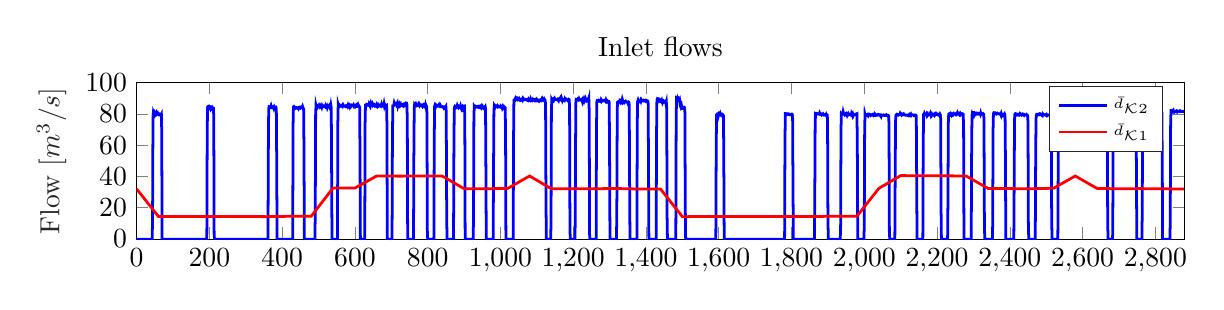
\begin{tikzpicture}

\begin{axis}[%
width=5.239in,
height=0.784in,
at={(1.272in,0.43in)},
scale only axis,
xmin=0,
xmax=2880,
%xlabel style={font=\color{white!15!black}},
%xlabel={Time [min]},
ymin=-0.1944444446,
ymax=100,
ylabel style={font=\color{white!15!black}},
ylabel={Flow  [$m^3/s$]},
axis background/.style={fill=white},
title style={},
title={Inlet flows},
legend style={legend cell align=left, align=left, draw=white!15!black}
]
\addplot [color=blue, line width=1.0pt]
  table[row sep=crcr]{%
0	-0.1666666668\\
1	-0.1666666668\\
2	-0.1666666668\\
3	-0.1666666668\\
4	-0.1666666668\\
5	-0.1666666668\\
6	-0.1666666668\\
7	-0.1666666668\\
8	-0.1666666668\\
9	-0.1666666668\\
10	-0.1666666668\\
11	-0.1666666668\\
12	-0.1666666668\\
13	-0.1666666668\\
14	-0.1666666668\\
15	-0.1666666668\\
16	-0.1666666668\\
17	-0.1666666668\\
18	-0.1666666668\\
19	-0.1666666668\\
20	-0.1666666668\\
21	-0.1666666668\\
22	-0.1666666668\\
23	-0.1666666668\\
24	-0.1666666668\\
25	-0.1666666668\\
26	-0.1666666668\\
27	-0.1666666668\\
28	-0.1666666668\\
29	-0.1666666668\\
30	-0.1666666668\\
31	-0.1666666668\\
32	-0.1666666668\\
33	-0.1666666668\\
34	-0.1666666668\\
35	-0.1666666668\\
36	-0.1666666668\\
37	-0.1666666668\\
38	-0.1666666668\\
39	-0.1666666668\\
40	-0.1666666668\\
41	-0.1666666668\\
42	-0.1666666668\\
43	-0.1666666668\\
44	24.722222242\\
45	78.0000000624\\
46	80.8055556202\\
47	80.138888953\\
48	79.9722222862\\
49	80.55555562\\
50	79.9166667306\\
51	80.7500000646\\
52	80.8888889536\\
53	80.3055556198\\
54	80.833333398\\
55	80.2500000642\\
56	79.6666667304\\
57	79.8888889528\\
58	80.3055556198\\
59	79.6944445082\\
60	79.6388889526\\
61	79.8055556194\\
62	79.305555619\\
63	79.305555619\\
64	79.3888889524\\
65	79.5555556192\\
66	79.1944445078\\
67	79.4166667302\\
68	79.8333333972\\
69	68.5555556104\\
70	-0.1666666668\\
71	-0.1666666668\\
72	-0.1666666668\\
73	-0.1666666668\\
74	-0.1666666668\\
75	-0.1666666668\\
76	-0.1666666668\\
77	-0.1666666668\\
78	-0.1666666668\\
79	-0.1666666668\\
80	-0.1666666668\\
81	-0.1666666668\\
82	-0.1666666668\\
83	-0.1666666668\\
84	-0.1666666668\\
85	-0.1666666668\\
86	-0.1666666668\\
87	-0.1666666668\\
88	-0.1666666668\\
89	-0.1666666668\\
90	-0.1666666668\\
91	-0.1666666668\\
92	-0.1666666668\\
93	-0.1666666668\\
94	-0.1666666668\\
95	-0.1666666668\\
96	-0.1666666668\\
97	-0.1666666668\\
98	-0.1666666668\\
99	-0.1666666668\\
100	-0.1666666668\\
101	-0.1666666668\\
102	-0.1666666668\\
103	-0.1666666668\\
104	-0.1666666668\\
105	-0.1666666668\\
106	-0.1666666668\\
107	-0.1666666668\\
108	-0.1666666668\\
109	-0.1666666668\\
110	-0.1666666668\\
111	-0.1666666668\\
112	-0.1666666668\\
113	-0.1666666668\\
114	-0.1666666668\\
115	-0.1666666668\\
116	-0.1666666668\\
117	-0.1666666668\\
118	-0.1666666668\\
119	-0.1666666668\\
120	-0.1666666668\\
121	-0.1666666668\\
122	-0.1666666668\\
123	-0.1666666668\\
124	-0.1666666668\\
125	-0.1666666668\\
126	-0.1666666668\\
127	-0.1666666668\\
128	-0.1666666668\\
129	-0.1666666668\\
130	-0.1666666668\\
131	-0.1666666668\\
132	-0.1666666668\\
133	-0.1666666668\\
134	-0.1666666668\\
135	-0.1666666668\\
136	-0.1666666668\\
137	-0.1666666668\\
138	-0.1666666668\\
139	-0.1666666668\\
140	-0.1666666668\\
141	-0.1666666668\\
142	-0.1666666668\\
143	-0.1666666668\\
144	-0.1666666668\\
145	-0.1666666668\\
146	-0.1666666668\\
147	-0.1666666668\\
148	-0.1666666668\\
149	-0.1666666668\\
150	-0.1666666668\\
151	-0.1666666668\\
152	-0.1666666668\\
153	-0.1666666668\\
154	-0.1666666668\\
155	-0.1666666668\\
156	-0.1666666668\\
157	-0.1666666668\\
158	-0.1666666668\\
159	-0.1666666668\\
160	-0.1666666668\\
161	-0.1666666668\\
162	-0.1666666668\\
163	-0.1666666668\\
164	-0.1666666668\\
165	-0.1666666668\\
166	-0.1666666668\\
167	-0.1666666668\\
168	-0.1666666668\\
169	-0.1666666668\\
170	-0.1666666668\\
171	-0.1666666668\\
172	-0.1666666668\\
173	-0.1666666668\\
174	-0.1666666668\\
175	-0.1666666668\\
176	-0.1666666668\\
177	-0.1666666668\\
178	-0.1666666668\\
179	-0.1666666668\\
180	-0.1666666668\\
181	-0.1666666668\\
182	-0.1666666668\\
183	-0.1666666668\\
184	-0.1666666668\\
185	-0.1666666668\\
186	-0.1666666668\\
187	-0.1666666668\\
188	-0.1666666668\\
189	-0.1666666668\\
190	-0.1666666668\\
191	-0.1666666668\\
192	-0.1666666668\\
193	-0.1666666668\\
194	68.888888944\\
195	84.2222222896\\
196	84.6944445122\\
197	84.8055556234\\
198	84.3333334008\\
199	84.5277778454\\
200	84.027777845\\
201	84.4166667342\\
202	84.444444512\\
203	83.6944445114\\
204	84.4166667342\\
205	84.3333334008\\
206	84.166666734\\
207	83.6388889558\\
208	84.1388889562\\
209	83.8333334004\\
210	83.750000067\\
211	83.6666667336\\
212	78.2777778404\\
213	3.194444447\\
214	-0.1666666668\\
215	-0.1666666668\\
216	-0.1666666668\\
217	-0.1666666668\\
218	-0.1666666668\\
219	-0.1666666668\\
220	-0.1666666668\\
221	-0.1666666668\\
222	-0.1666666668\\
223	-0.1666666668\\
224	-0.1666666668\\
225	-0.1666666668\\
226	-0.1666666668\\
227	-0.1666666668\\
228	-0.1666666668\\
229	-0.1666666668\\
230	-0.1666666668\\
231	-0.1666666668\\
232	-0.1666666668\\
233	-0.1666666668\\
234	-0.1666666668\\
235	-0.1666666668\\
236	-0.1666666668\\
237	-0.1666666668\\
238	-0.1666666668\\
239	-0.1666666668\\
240	-0.1666666668\\
241	-0.1666666668\\
242	-0.1666666668\\
243	-0.1666666668\\
244	-0.1666666668\\
245	-0.1666666668\\
246	-0.1666666668\\
247	-0.1666666668\\
248	-0.1666666668\\
249	-0.1666666668\\
250	-0.1666666668\\
251	-0.1666666668\\
252	-0.1666666668\\
253	-0.1666666668\\
254	-0.1666666668\\
255	-0.1666666668\\
256	-0.1666666668\\
257	-0.1666666668\\
258	-0.1666666668\\
259	-0.1666666668\\
260	-0.1666666668\\
261	-0.1666666668\\
262	-0.1666666668\\
263	-0.1666666668\\
264	-0.1666666668\\
265	-0.1666666668\\
266	-0.1666666668\\
267	-0.1666666668\\
268	-0.1666666668\\
269	-0.1666666668\\
270	-0.1666666668\\
271	-0.1666666668\\
272	-0.1666666668\\
273	-0.1666666668\\
274	-0.1666666668\\
275	-0.1666666668\\
276	-0.1666666668\\
277	-0.1666666668\\
278	-0.1666666668\\
279	-0.1666666668\\
280	-0.1666666668\\
281	-0.1666666668\\
282	-0.1666666668\\
283	-0.1666666668\\
284	-0.1666666668\\
285	-0.1666666668\\
286	-0.1666666668\\
287	-0.1666666668\\
288	-0.1666666668\\
289	-0.1666666668\\
290	-0.1666666668\\
291	-0.1666666668\\
292	-0.1666666668\\
293	-0.1666666668\\
294	-0.1666666668\\
295	-0.1666666668\\
296	-0.1666666668\\
297	-0.1666666668\\
298	-0.1666666668\\
299	-0.1666666668\\
300	-0.1666666668\\
301	-0.1666666668\\
302	-0.1666666668\\
303	-0.1666666668\\
304	-0.1666666668\\
305	-0.1666666668\\
306	-0.1666666668\\
307	-0.1666666668\\
308	-0.1666666668\\
309	-0.1666666668\\
310	-0.1666666668\\
311	-0.1666666668\\
312	-0.1666666668\\
313	-0.1666666668\\
314	-0.1666666668\\
315	-0.1666666668\\
316	-0.1666666668\\
317	-0.1666666668\\
318	-0.1666666668\\
319	-0.1666666668\\
320	-0.1666666668\\
321	-0.1666666668\\
322	-0.1666666668\\
323	-0.1666666668\\
324	-0.1666666668\\
325	-0.1666666668\\
326	-0.1666666668\\
327	-0.1666666668\\
328	-0.1666666668\\
329	-0.1666666668\\
330	-0.1666666668\\
331	-0.1666666668\\
332	-0.1666666668\\
333	-0.1666666668\\
334	-0.1666666668\\
335	-0.1666666668\\
336	-0.1666666668\\
337	-0.1666666668\\
338	-0.1666666668\\
339	-0.1666666668\\
340	-0.1666666668\\
341	-0.1666666668\\
342	-0.1666666668\\
343	-0.1666666668\\
344	-0.1666666668\\
345	-0.1666666668\\
346	-0.1666666668\\
347	-0.1666666668\\
348	-0.1666666668\\
349	-0.1666666668\\
350	-0.1666666668\\
351	-0.1666666668\\
352	-0.1666666668\\
353	-0.1666666668\\
354	-0.1944444446\\
355	-0.1666666668\\
356	-0.1666666668\\
357	-0.1666666668\\
358	-0.1666666668\\
359	-0.1666666668\\
360	-0.1666666668\\
361	-0.1666666668\\
362	55.416666711\\
363	83.194444511\\
364	84.444444512\\
365	84.3333334008\\
366	84.2500000674\\
367	84.1944445118\\
368	84.5000000676\\
369	85.0833334014\\
370	83.9722222894\\
371	84.027777845\\
372	83.9444445116\\
373	83.8055556226\\
374	83.9166667338\\
375	84.2777778452\\
376	84.0555556228\\
377	84.4166667342\\
378	83.4444445112\\
379	83.9444445116\\
380	84.0000000672\\
381	84.1388889562\\
382	83.8055556226\\
383	83.9722222894\\
384	83.0277778442\\
385	49.5555555952\\
386	-0.1666666668\\
387	-0.1666666668\\
388	-0.1666666668\\
389	-0.1666666668\\
390	-0.1666666668\\
391	-0.1666666668\\
392	-0.1666666668\\
393	-0.1666666668\\
394	-0.1666666668\\
395	-0.1666666668\\
396	-0.1666666668\\
397	-0.1666666668\\
398	-0.1666666668\\
399	-0.1666666668\\
400	-0.1666666668\\
401	-0.1666666668\\
402	-0.1666666668\\
403	-0.1666666668\\
404	-0.1666666668\\
405	-0.1666666668\\
406	-0.1666666668\\
407	-0.1666666668\\
408	-0.1666666668\\
409	-0.1666666668\\
410	-0.1666666668\\
411	-0.1666666668\\
412	-0.1666666668\\
413	-0.1666666668\\
414	-0.1666666668\\
415	-0.1666666668\\
416	-0.1666666668\\
417	-0.1666666668\\
418	-0.1666666668\\
419	-0.1666666668\\
420	-0.1666666668\\
421	-0.1666666668\\
422	-0.1666666668\\
423	-0.1666666668\\
424	-0.1666666668\\
425	-0.1666666668\\
426	-0.1666666668\\
427	-0.1666666668\\
428	-0.1666666668\\
429	-0.1666666668\\
430	73.1388889474\\
431	84.444444512\\
432	84.6388889566\\
433	84.2500000674\\
434	83.750000067\\
435	83.888888956\\
436	83.472222289\\
437	83.5833334002\\
438	83.5555556224\\
439	84.027777845\\
440	83.9722222894\\
441	83.9166667338\\
442	83.7222222892\\
443	83.9166667338\\
444	83.9444445116\\
445	83.472222289\\
446	84.0555556228\\
447	84.027777845\\
448	83.5833334002\\
449	83.5277778446\\
450	84.0833334006\\
451	83.888888956\\
452	84.0833334006\\
453	83.8333334004\\
454	83.8055556226\\
455	84.0833334006\\
456	84.6666667344\\
457	83.888888956\\
458	83.6666667336\\
459	82.638888955\\
460	56.3333333784\\
461	-0.1666666668\\
462	-0.1666666668\\
463	-0.1666666668\\
464	-0.1666666668\\
465	-0.1666666668\\
466	-0.1666666668\\
467	-0.1666666668\\
468	-0.1666666668\\
469	-0.1666666668\\
470	-0.1666666668\\
471	-0.1666666668\\
472	-0.1666666668\\
473	-0.1666666668\\
474	-0.1666666668\\
475	-0.1666666668\\
476	-0.1666666668\\
477	-0.1666666668\\
478	-0.1666666668\\
479	-0.1666666668\\
480	-0.1666666668\\
481	-0.1666666668\\
482	-0.1666666668\\
483	-0.1666666668\\
484	-0.1666666668\\
485	-0.1666666668\\
486	-0.1666666668\\
487	-0.1666666668\\
488	-0.1666666668\\
489	-0.1666666668\\
490	-0.1666666668\\
491	16.7777777912\\
492	79.444444508\\
493	85.3333334016\\
494	84.3333334008\\
495	85.138888957\\
496	85.2222222904\\
497	84.6666667344\\
498	85.3055556238\\
499	85.3333334016\\
500	85.000000068\\
501	85.4722222906\\
502	85.277777846\\
503	84.8055556234\\
504	85.3888889572\\
505	84.9722222902\\
506	85.4722222906\\
507	85.3333334016\\
508	85.0833334014\\
509	84.3888889564\\
510	85.3055556238\\
511	84.9166667346\\
512	84.72222229\\
513	84.9722222902\\
514	84.7777778456\\
515	84.9722222902\\
516	84.9444445124\\
517	84.5555556232\\
518	84.444444512\\
519	85.0833334014\\
520	84.3888889564\\
521	84.583333401\\
522	84.5000000676\\
523	84.9166667346\\
524	84.0000000672\\
525	84.6666667344\\
526	84.7500000678\\
527	84.6666667344\\
528	84.7777778456\\
529	85.1666667348\\
530	84.72222229\\
531	84.1388889562\\
532	84.8888889568\\
533	83.7222222892\\
534	85.277777846\\
535	83.8055556226\\
536	41.4166666998\\
537	-0.1666666668\\
538	-0.1666666668\\
539	-0.1666666668\\
540	-0.1666666668\\
541	-0.1666666668\\
542	-0.1666666668\\
543	-0.1666666668\\
544	-0.1666666668\\
545	-0.1666666668\\
546	-0.1666666668\\
547	-0.1666666668\\
548	-0.1666666668\\
549	-0.1666666668\\
550	-0.1666666668\\
551	-0.1666666668\\
552	-0.1666666668\\
553	73.888888948\\
554	85.694444513\\
555	84.8333334012\\
556	85.4722222906\\
557	85.7777778464\\
558	85.5000000684\\
559	85.4722222906\\
560	85.277777846\\
561	84.8333334012\\
562	84.9166667346\\
563	85.138888957\\
564	84.9722222902\\
565	85.2500000682\\
566	85.6388889574\\
567	85.0833334014\\
568	85.5833334018\\
569	85.1944445126\\
570	85.0833334014\\
571	84.9444445124\\
572	84.9444445124\\
573	84.9444445124\\
574	84.583333401\\
575	84.583333401\\
576	85.0277778458\\
577	84.8333334012\\
578	84.9166667346\\
579	85.2222222904\\
580	84.7500000678\\
581	85.4444445128\\
582	84.8055556234\\
583	84.8888889568\\
584	85.2222222904\\
585	84.6944445122\\
586	85.5277778462\\
587	85.277777846\\
588	85.4444445128\\
589	84.6388889566\\
590	84.9444445124\\
591	85.0833334014\\
592	85.3888889572\\
593	85.3888889572\\
594	85.138888957\\
595	85.0277778458\\
596	85.5277778462\\
597	85.000000068\\
598	85.3333334016\\
599	85.0277778458\\
600	84.6666667344\\
601	85.2222222904\\
602	85.4444445128\\
603	85.5833334018\\
604	85.7777778464\\
605	85.138888957\\
606	84.6944445122\\
607	84.72222229\\
608	84.8888889568\\
609	85.6388889574\\
610	85.0555556236\\
611	85.0833334014\\
612	84.583333401\\
613	84.2500000674\\
614	52.2777778196\\
615	-0.1666666668\\
616	-0.1666666668\\
617	-0.1666666668\\
618	-0.1666666668\\
619	-0.1666666668\\
620	-0.1666666668\\
621	-0.1666666668\\
622	-0.1666666668\\
623	-0.1666666668\\
624	-0.1666666668\\
625	-0.1666666668\\
626	-0.1666666668\\
627	-0.1666666668\\
628	74.444444504\\
629	85.6388889574\\
630	85.8055556242\\
631	85.2222222904\\
632	85.6666667352\\
633	85.9444445132\\
634	85.8888889576\\
635	85.6666667352\\
636	85.5277778462\\
637	85.694444513\\
638	85.8888889576\\
639	86.666666736\\
640	86.250000069\\
641	85.000000068\\
642	84.583333401\\
643	85.5277778462\\
644	86.527777847\\
645	85.833333402\\
646	85.7222222908\\
647	85.7222222908\\
648	86.2777778468\\
649	85.6388889574\\
650	86.0277778466\\
651	86.1388889578\\
652	85.555555624\\
653	85.694444513\\
654	85.3333334016\\
655	85.6666667352\\
656	85.694444513\\
657	85.6388889574\\
658	85.2222222904\\
659	85.7500000686\\
660	85.138888957\\
661	85.277777846\\
662	84.8888889568\\
663	85.416666735\\
664	84.6388889566\\
665	84.7777778456\\
666	85.0833334014\\
667	85.1666667348\\
668	85.6388889574\\
669	85.555555624\\
670	85.3333334016\\
671	85.0277778458\\
672	85.1666667348\\
673	85.972222291\\
674	85.138888957\\
675	85.3888889572\\
676	85.6388889574\\
677	85.3055556238\\
678	85.5833334018\\
679	85.2500000682\\
680	86.4166667358\\
681	85.138888957\\
682	85.972222291\\
683	85.5000000684\\
684	85.277777846\\
685	84.5000000676\\
686	85.3888889572\\
687	85.5000000684\\
688	73.2777778364\\
689	-0.1666666668\\
690	-0.1666666668\\
691	-0.1666666668\\
692	-0.1666666668\\
693	-0.1666666668\\
694	-0.1666666668\\
695	-0.1666666668\\
696	-0.1666666668\\
697	-0.1666666668\\
698	-0.1666666668\\
699	-0.1666666668\\
700	-0.1666666668\\
701	-0.1666666668\\
702	-0.1666666668\\
703	57.5277778238\\
704	85.0555556236\\
705	85.0555556236\\
706	85.1666667348\\
707	85.6388889574\\
708	86.9166667362\\
709	86.250000069\\
710	85.833333402\\
711	85.8888889576\\
712	85.7777778464\\
713	86.1666667356\\
714	86.4722222914\\
715	85.5000000684\\
716	85.7500000686\\
717	86.4166667358\\
718	84.9722222902\\
719	85.7500000686\\
720	85.2500000682\\
721	85.6388889574\\
722	85.3055556238\\
723	86.0277778466\\
724	85.416666735\\
725	85.8888889576\\
726	86.2777778468\\
727	85.7777778464\\
728	85.3888889572\\
729	85.5277778462\\
730	85.694444513\\
731	85.416666735\\
732	85.7500000686\\
733	85.5000000684\\
734	85.8055556242\\
735	85.0277778458\\
736	85.2222222904\\
737	85.1944445126\\
738	85.5833334018\\
739	85.5833334018\\
740	85.6388889574\\
741	86.8888889584\\
742	86.8333334028\\
743	85.7777778464\\
744	74.5000000596\\
745	-0.1666666668\\
746	-0.1666666668\\
747	-0.1666666668\\
748	-0.1666666668\\
749	-0.1666666668\\
750	-0.1666666668\\
751	-0.1666666668\\
752	-0.1666666668\\
753	-0.1666666668\\
754	-0.1666666668\\
755	-0.1666666668\\
756	-0.1666666668\\
757	-0.1666666668\\
758	-0.1666666668\\
759	-0.1666666668\\
760	-0.1666666668\\
761	-0.1666666668\\
762	53.472222265\\
763	83.6388889558\\
764	86.1666667356\\
765	85.8888889576\\
766	85.972222291\\
767	86.3333334024\\
768	85.6388889574\\
769	85.8888889576\\
770	85.9166667354\\
771	85.416666735\\
772	85.6666667352\\
773	86.0000000688\\
774	85.7777778464\\
775	86.250000069\\
776	85.7777778464\\
777	85.3333334016\\
778	85.9166667354\\
779	85.4444445128\\
780	85.5277778462\\
781	85.7500000686\\
782	85.7777778464\\
783	85.000000068\\
784	85.0277778458\\
785	85.1944445126\\
786	84.7777778456\\
787	85.1944445126\\
788	85.5277778462\\
789	85.0555556236\\
790	85.3055556238\\
791	85.555555624\\
792	85.138888957\\
793	84.6388889566\\
794	85.694444513\\
795	84.7500000678\\
796	85.1944445126\\
797	84.7777778456\\
798	79.8333333972\\
799	5.5833333378\\
800	-0.1666666668\\
801	-0.1666666668\\
802	-0.1666666668\\
803	-0.1666666668\\
804	-0.1666666668\\
805	-0.1666666668\\
806	-0.1666666668\\
807	-0.1666666668\\
808	-0.1666666668\\
809	-0.1666666668\\
810	-0.1666666668\\
811	-0.1666666668\\
812	-0.1666666668\\
813	-0.1666666668\\
814	-0.1666666668\\
815	-0.1666666668\\
816	-0.1666666668\\
817	-0.1666666668\\
818	62.5277778278\\
819	84.6388889566\\
820	85.555555624\\
821	85.2222222904\\
822	84.5277778454\\
823	85.1944445126\\
824	84.6944445122\\
825	84.7777778456\\
826	85.138888957\\
827	85.3333334016\\
828	85.1944445126\\
829	85.138888957\\
830	85.1944445126\\
831	85.6388889574\\
832	84.9444445124\\
833	84.5555556232\\
834	84.5277778454\\
835	85.1666667348\\
836	84.6388889566\\
837	84.6944445122\\
838	84.7500000678\\
839	84.6666667344\\
840	84.4722222898\\
841	84.583333401\\
842	84.4166667342\\
843	84.0833334006\\
844	84.166666734\\
845	83.5555556224\\
846	83.750000067\\
847	84.3333334008\\
848	84.5277778454\\
849	84.2500000674\\
850	84.6388889566\\
851	81.3333333984\\
852	26.5555555768\\
853	-0.1666666668\\
854	-0.1666666668\\
855	-0.1666666668\\
856	-0.1666666668\\
857	-0.1666666668\\
858	-0.1666666668\\
859	-0.1666666668\\
860	-0.1666666668\\
861	-0.1666666668\\
862	-0.1666666668\\
863	-0.1666666668\\
864	-0.1666666668\\
865	-0.1666666668\\
866	-0.1666666668\\
867	-0.1666666668\\
868	-0.1666666668\\
869	-0.1666666668\\
870	-0.1666666668\\
871	-0.1666666668\\
872	55.0833333774\\
873	83.0277778442\\
874	84.5000000676\\
875	84.8888889568\\
876	84.6944445122\\
877	84.166666734\\
878	83.888888956\\
879	84.0555556228\\
880	84.166666734\\
881	85.0277778458\\
882	84.305555623\\
883	84.166666734\\
884	83.888888956\\
885	84.3888889564\\
886	84.0000000672\\
887	84.166666734\\
888	84.5555556232\\
889	84.5000000676\\
890	85.1666667348\\
891	84.2777778452\\
892	83.6666667336\\
893	84.2500000674\\
894	84.4166667342\\
895	83.5000000668\\
896	84.1388889562\\
897	83.5833334002\\
898	84.1944445118\\
899	84.305555623\\
900	85.000000068\\
901	85.0277778458\\
902	77.9722222846\\
903	-0.1666666668\\
904	-0.1666666668\\
905	-0.1666666668\\
906	-0.1666666668\\
907	-0.1666666668\\
908	-0.1666666668\\
909	-0.1666666668\\
910	-0.1666666668\\
911	-0.1666666668\\
912	-0.1666666668\\
913	-0.1666666668\\
914	-0.1666666668\\
915	-0.1666666668\\
916	-0.1666666668\\
917	-0.1666666668\\
918	-0.1666666668\\
919	-0.1666666668\\
920	-0.1666666668\\
921	-0.1666666668\\
922	-0.1666666668\\
923	-0.1666666668\\
924	-0.1666666668\\
925	-0.1666666668\\
926	14.166666678\\
927	77.3333333952\\
928	84.7500000678\\
929	84.3888889564\\
930	84.3888889564\\
931	84.6388889566\\
932	84.2777778452\\
933	84.4722222898\\
934	84.3888889564\\
935	84.5555556232\\
936	84.2500000674\\
937	84.2222222896\\
938	84.5277778454\\
939	84.6944445122\\
940	84.3333334008\\
941	84.583333401\\
942	84.305555623\\
943	84.5555556232\\
944	84.305555623\\
945	84.583333401\\
946	83.9722222894\\
947	83.7222222892\\
948	84.4166667342\\
949	83.8333334004\\
950	83.9166667338\\
951	84.4166667342\\
952	83.7777778448\\
953	83.8333334004\\
954	83.5555556224\\
955	84.1388889562\\
956	84.1388889562\\
957	84.3333334008\\
958	84.6388889566\\
959	83.1388889554\\
960	43.9722222574\\
961	-0.1666666668\\
962	-0.1666666668\\
963	-0.1666666668\\
964	-0.1666666668\\
965	-0.1666666668\\
966	-0.1666666668\\
967	-0.1666666668\\
968	-0.1666666668\\
969	-0.1666666668\\
970	-0.1666666668\\
971	-0.1666666668\\
972	-0.1666666668\\
973	-0.1666666668\\
974	-0.1666666668\\
975	-0.1666666668\\
976	-0.1666666668\\
977	-0.1666666668\\
978	-0.1666666668\\
979	-0.1666666668\\
980	-0.1666666668\\
981	45.7500000366\\
982	82.1666667324\\
983	85.0833334014\\
984	84.6388889566\\
985	85.000000068\\
986	84.583333401\\
987	85.1944445126\\
988	85.138888957\\
989	85.0555556236\\
990	84.9166667346\\
991	84.6944445122\\
992	85.1944445126\\
993	84.9166667346\\
994	84.5000000676\\
995	84.6666667344\\
996	84.4722222898\\
997	84.5277778454\\
998	84.2777778452\\
999	84.2777778452\\
1000	84.6944445122\\
1001	84.1388889562\\
1002	83.888888956\\
1003	83.9166667338\\
1004	84.5277778454\\
1005	84.8333334012\\
1006	83.5277778446\\
1007	83.888888956\\
1008	84.166666734\\
1009	84.444444512\\
1010	83.9166667338\\
1011	84.1388889562\\
1012	84.166666734\\
1013	83.9166667338\\
1014	69.4722222778\\
1015	-0.1666666668\\
1016	-0.1666666668\\
1017	-0.1666666668\\
1018	-0.1666666668\\
1019	-0.1666666668\\
1020	-0.1666666668\\
1021	-0.1666666668\\
1022	-0.1666666668\\
1023	-0.1666666668\\
1024	-0.1666666668\\
1025	-0.1666666668\\
1026	-0.1666666668\\
1027	-0.1666666668\\
1028	-0.1666666668\\
1029	-0.1666666668\\
1030	-0.1666666668\\
1031	-0.1666666668\\
1032	-0.1666666668\\
1033	-0.1666666668\\
1034	-0.1666666668\\
1035	-0.1666666668\\
1036	64.0833333846\\
1037	88.6388889598\\
1038	88.6666667376\\
1039	89.0833334046\\
1040	89.0833334046\\
1041	89.6666667384\\
1042	89.0555556268\\
1043	89.3333334048\\
1044	89.722222294\\
1045	89.3333334048\\
1046	89.2222222936\\
1047	88.9166667378\\
1048	89.0555556268\\
1049	89.7777778496\\
1050	89.583333405\\
1051	89.2500000714\\
1052	89.583333405\\
1053	89.166666738\\
1054	88.7777778488\\
1055	89.0555556268\\
1056	89.2500000714\\
1057	89.305555627\\
1058	88.8333334044\\
1059	89.0000000712\\
1060	89.444444516\\
1061	88.9444445156\\
1062	89.583333405\\
1063	89.0555556268\\
1064	89.0000000712\\
1065	88.9722222934\\
1066	88.9444445156\\
1067	89.2222222936\\
1068	89.0000000712\\
1069	89.027777849\\
1070	89.0833334046\\
1071	89.0555556268\\
1072	88.88888896\\
1073	88.7222222932\\
1074	89.1388889602\\
1075	89.0555556268\\
1076	88.8055556266\\
1077	89.2777778492\\
1078	88.8333334044\\
1079	89.166666738\\
1080	88.9722222934\\
1081	89.0000000712\\
1082	88.750000071\\
1083	89.5555556272\\
1084	89.0000000712\\
1085	88.8055556266\\
1086	89.2500000714\\
1087	89.1388889602\\
1088	88.8055556266\\
1089	89.2500000714\\
1090	89.0000000712\\
1091	89.1388889602\\
1092	88.9166667378\\
1093	89.0555556268\\
1094	89.1388889602\\
1095	88.2500000706\\
1096	88.2777778484\\
1097	88.5833334042\\
1098	88.6388889598\\
1099	89.027777849\\
1100	88.4166667374\\
1101	88.5000000708\\
1102	88.8055556266\\
1103	88.5277778486\\
1104	88.2500000706\\
1105	88.5277778486\\
1106	88.4444445152\\
1107	88.2222222928\\
1108	88.8055556266\\
1109	88.7777778488\\
1110	88.9166667378\\
1111	88.5277778486\\
1112	88.4444445152\\
1113	89.0000000712\\
1114	88.4444445152\\
1115	88.5555556264\\
1116	89.444444516\\
1117	89.027777849\\
1118	88.9722222934\\
1119	88.7222222932\\
1120	89.1944445158\\
1121	88.5833334042\\
1122	88.88888896\\
1123	88.5277778486\\
1124	85.833333402\\
1125	30.4444444688\\
1126	-0.1666666668\\
1127	-0.1666666668\\
1128	-0.1666666668\\
1129	-0.1666666668\\
1130	-0.1666666668\\
1131	-0.1666666668\\
1132	-0.1666666668\\
1133	-0.1666666668\\
1134	-0.1666666668\\
1135	-0.1666666668\\
1136	-0.1666666668\\
1137	-0.1666666668\\
1138	-0.1666666668\\
1139	10.4722222306\\
1140	79.8888889528\\
1141	89.0833334046\\
1142	88.6388889598\\
1143	88.6388889598\\
1144	89.027777849\\
1145	88.4444445152\\
1146	88.2222222928\\
1147	88.6944445154\\
1148	89.2222222936\\
1149	89.722222294\\
1150	89.2500000714\\
1151	89.2222222936\\
1152	89.3333334048\\
1153	89.1944445158\\
1154	89.0833334046\\
1155	89.1388889602\\
1156	89.1944445158\\
1157	88.9444445156\\
1158	89.2777778492\\
1159	89.0000000712\\
1160	88.5277778486\\
1161	89.2222222936\\
1162	89.444444516\\
1163	89.3333334048\\
1164	89.8055556274\\
1165	89.0555556268\\
1166	89.166666738\\
1167	88.9444445156\\
1168	89.8333334052\\
1169	89.0555556268\\
1170	88.4166667374\\
1171	89.027777849\\
1172	88.9722222934\\
1173	88.8055556266\\
1174	89.0833334046\\
1175	89.0833334046\\
1176	88.7777778488\\
1177	89.583333405\\
1178	89.166666738\\
1179	89.5000000716\\
1180	89.5277778494\\
1181	89.2500000714\\
1182	89.1388889602\\
1183	88.7777778488\\
1184	88.5833334042\\
1185	88.88888896\\
1186	88.9722222934\\
1187	88.6944445154\\
1188	89.2222222936\\
1189	89.0833334046\\
1190	83.6388889558\\
1191	5.9166666714\\
1192	-0.1666666668\\
1193	-0.1666666668\\
1194	-0.1666666668\\
1195	-0.1666666668\\
1196	-0.1666666668\\
1197	-0.1666666668\\
1198	-0.1666666668\\
1199	-0.1666666668\\
1200	-0.1666666668\\
1201	-0.1666666668\\
1202	-0.1666666668\\
1203	-0.1666666668\\
1204	-0.1666666668\\
1205	-0.1666666668\\
1206	34.9444444724\\
1207	86.3055556246\\
1208	89.0833334046\\
1209	88.9722222934\\
1210	88.9444445156\\
1211	89.027777849\\
1212	88.9166667378\\
1213	89.5000000716\\
1214	89.3333334048\\
1215	89.0833334046\\
1216	89.6666667384\\
1217	89.166666738\\
1218	89.2222222936\\
1219	89.0833334046\\
1220	88.88888896\\
1221	88.7222222932\\
1222	88.8333334044\\
1223	88.5555556264\\
1224	88.9722222934\\
1225	88.0833334038\\
1226	89.027777849\\
1227	88.9166667378\\
1228	88.6388889598\\
1229	89.2777778492\\
1230	88.2777778484\\
1231	88.9444445156\\
1232	88.9722222934\\
1233	88.750000071\\
1234	89.583333405\\
1235	89.0000000712\\
1236	88.5000000708\\
1237	88.194444515\\
1238	88.4444445152\\
1239	88.4444445152\\
1240	88.3055556262\\
1241	89.027777849\\
1242	88.2777778484\\
1243	89.2777778492\\
1244	81.1666667316\\
1245	2.638888891\\
1246	-0.1666666668\\
1247	-0.1666666668\\
1248	-0.1666666668\\
1249	-0.1666666668\\
1250	-0.1666666668\\
1251	-0.1666666668\\
1252	-0.1666666668\\
1253	-0.1666666668\\
1254	-0.1666666668\\
1255	-0.1666666668\\
1256	-0.1666666668\\
1257	-0.1666666668\\
1258	-0.1666666668\\
1259	-0.1666666668\\
1260	-0.1666666668\\
1261	-0.1666666668\\
1262	-0.1666666668\\
1263	-0.1666666668\\
1264	71.6944445018\\
1265	87.7500000702\\
1266	88.333333404\\
1267	88.194444515\\
1268	88.2500000706\\
1269	88.2500000706\\
1270	88.5000000708\\
1271	88.1666667372\\
1272	88.2777778484\\
1273	88.0833334038\\
1274	88.2777778484\\
1275	88.4166667374\\
1276	88.0833334038\\
1277	89.0555556268\\
1278	88.6666667376\\
1279	88.2500000706\\
1280	88.472222293\\
1281	88.472222293\\
1282	88.2777778484\\
1283	88.3888889596\\
1284	88.4166667374\\
1285	88.5555556264\\
1286	88.2222222928\\
1287	88.194444515\\
1288	88.194444515\\
1289	87.9444445148\\
1290	88.6944445154\\
1291	88.0000000704\\
1292	88.2222222928\\
1293	88.3055556262\\
1294	87.3333334032\\
1295	87.3055556254\\
1296	87.777777848\\
1297	87.916666737\\
1298	87.8888889592\\
1299	87.3333334032\\
1300	50.972222263\\
1301	-0.1666666668\\
1302	-0.1666666668\\
1303	-0.1666666668\\
1304	-0.1666666668\\
1305	-0.1666666668\\
1306	-0.1666666668\\
1307	-0.1666666668\\
1308	-0.1666666668\\
1309	-0.1666666668\\
1310	-0.1666666668\\
1311	-0.1666666668\\
1312	-0.1666666668\\
1313	-0.1666666668\\
1314	-0.1666666668\\
1315	-0.1666666668\\
1316	-0.1666666668\\
1317	-0.1666666668\\
1318	-0.1666666668\\
1319	-0.1666666668\\
1320	25.0277777978\\
1321	83.1666667332\\
1322	87.4722222922\\
1323	87.6944445146\\
1324	87.777777848\\
1325	87.3888889588\\
1326	87.3888889588\\
1327	87.9722222926\\
1328	87.638888959\\
1329	88.194444515\\
1330	87.8333334036\\
1331	87.3333334032\\
1332	87.777777848\\
1333	87.8333334036\\
1334	88.0833334038\\
1335	89.2222222936\\
1336	88.4166667374\\
1337	87.2500000698\\
1338	87.50000007\\
1339	87.7222222924\\
1340	87.7500000702\\
1341	87.3055556254\\
1342	87.5833334034\\
1343	87.8333334036\\
1344	88.055555626\\
1345	87.6944445146\\
1346	87.6666667368\\
1347	87.6944445146\\
1348	87.4166667366\\
1349	87.4722222922\\
1350	86.8888889584\\
1351	87.3333334032\\
1352	87.5555556256\\
1353	87.3333334032\\
1354	85.694444513\\
1355	35.8055555842\\
1356	-0.1666666668\\
1357	-0.1666666668\\
1358	-0.1666666668\\
1359	-0.1666666668\\
1360	-0.1666666668\\
1361	-0.1666666668\\
1362	-0.1666666668\\
1363	-0.1666666668\\
1364	-0.1666666668\\
1365	-0.1666666668\\
1366	-0.1666666668\\
1367	-0.1666666668\\
1368	-0.1666666668\\
1369	-0.1666666668\\
1370	-0.1666666668\\
1371	-0.1666666668\\
1372	-0.1666666668\\
1373	-0.1666666668\\
1374	-0.1666666668\\
1375	-0.1666666668\\
1376	72.4722222802\\
1377	88.0000000704\\
1378	88.6944445154\\
1379	87.916666737\\
1380	87.9722222926\\
1381	88.055555626\\
1382	87.8888889592\\
1383	87.6666667368\\
1384	87.8055556258\\
1385	88.4444445152\\
1386	87.916666737\\
1387	88.6666667376\\
1388	88.1388889594\\
1389	88.1388889594\\
1390	88.4166667374\\
1391	88.6388889598\\
1392	88.7222222932\\
1393	88.3888889596\\
1394	88.2500000706\\
1395	88.472222293\\
1396	88.2777778484\\
1397	88.3888889596\\
1398	88.750000071\\
1399	88.7777778488\\
1400	88.2222222928\\
1401	88.4166667374\\
1402	88.333333404\\
1403	87.9444445148\\
1404	88.2500000706\\
1405	88.1388889594\\
1406	86.805555625\\
1407	45.2222222584\\
1408	-0.1666666668\\
1409	-0.1666666668\\
1410	-0.1666666668\\
1411	-0.1666666668\\
1412	-0.1666666668\\
1413	-0.1666666668\\
1414	-0.1666666668\\
1415	-0.1666666668\\
1416	-0.1666666668\\
1417	-0.1666666668\\
1418	-0.1666666668\\
1419	-0.1666666668\\
1420	-0.1666666668\\
1421	-0.1666666668\\
1422	-0.1666666668\\
1423	-0.1666666668\\
1424	-0.1666666668\\
1425	-0.1666666668\\
1426	-0.1666666668\\
1427	-0.1666666668\\
1428	-0.1666666668\\
1429	66.0000000528\\
1430	88.5000000708\\
1431	89.305555627\\
1432	89.0555556268\\
1433	88.7777778488\\
1434	89.1388889602\\
1435	88.8055556266\\
1436	89.027777849\\
1437	88.472222293\\
1438	88.8055556266\\
1439	88.8055556266\\
1440	88.3888889596\\
1441	88.6944445154\\
1442	88.2500000706\\
1443	88.6666667376\\
1444	87.7222222924\\
1445	87.1944445142\\
1446	88.0277778482\\
1447	88.194444515\\
1448	87.5555556256\\
1449	87.2777778476\\
1450	87.3333334032\\
1451	88.0833334038\\
1452	88.0000000704\\
1453	87.6666667368\\
1454	87.9722222926\\
1455	86.4444445136\\
1456	87.3888889588\\
1457	83.7777778448\\
1458	14.4166666782\\
1459	-0.1666666668\\
1460	-0.1666666668\\
1461	-0.1666666668\\
1462	-0.1666666668\\
1463	-0.1666666668\\
1464	-0.1666666668\\
1465	-0.1666666668\\
1466	-0.1666666668\\
1467	-0.1666666668\\
1468	-0.1666666668\\
1469	-0.1666666668\\
1470	-0.1666666668\\
1471	-0.1666666668\\
1472	-0.1666666668\\
1473	-0.1666666668\\
1474	-0.1666666668\\
1475	-0.1666666668\\
1476	-0.1666666668\\
1477	-0.1666666668\\
1478	-0.1666666668\\
1479	-0.1666666668\\
1480	-0.1666666668\\
1481	-0.1666666668\\
1482	-0.1666666668\\
1483	76.7500000614\\
1484	89.7500000718\\
1485	89.5277778494\\
1486	90.0833334054\\
1487	89.305555627\\
1488	89.027777849\\
1489	89.5277778494\\
1490	89.0000000712\\
1491	89.2500000714\\
1492	89.5555556272\\
1493	87.3333334032\\
1494	85.3888889572\\
1495	84.7500000678\\
1496	85.5833334018\\
1497	86.0000000688\\
1498	84.8055556234\\
1499	84.72222229\\
1500	83.472222289\\
1501	83.5833334002\\
1502	83.6666667336\\
1503	83.5277778446\\
1504	84.027777845\\
1505	84.166666734\\
1506	83.9166667338\\
1507	80.694444509\\
1508	21.3055555726\\
1509	-0.1666666668\\
1510	-0.1666666668\\
1511	-0.1666666668\\
1512	-0.1666666668\\
1513	-0.1666666668\\
1514	-0.1666666668\\
1515	-0.1666666668\\
1516	-0.1666666668\\
1517	-0.1666666668\\
1518	-0.1666666668\\
1519	-0.1666666668\\
1520	-0.1666666668\\
1521	-0.1666666668\\
1522	-0.1666666668\\
1523	-0.1666666668\\
1524	-0.1666666668\\
1525	-0.1666666668\\
1526	-0.1666666668\\
1527	-0.1666666668\\
1528	-0.1666666668\\
1529	-0.1666666668\\
1530	-0.1666666668\\
1531	-0.1666666668\\
1532	-0.1666666668\\
1533	-0.1666666668\\
1534	-0.1666666668\\
1535	-0.1666666668\\
1536	-0.1666666668\\
1537	-0.1666666668\\
1538	-0.1666666668\\
1539	-0.1666666668\\
1540	-0.1666666668\\
1541	-0.1666666668\\
1542	-0.1666666668\\
1543	-0.1666666668\\
1544	-0.1666666668\\
1545	-0.1666666668\\
1546	-0.1666666668\\
1547	-0.1666666668\\
1548	-0.1666666668\\
1549	-0.1666666668\\
1550	-0.1666666668\\
1551	-0.1666666668\\
1552	-0.1666666668\\
1553	-0.1666666668\\
1554	-0.1666666668\\
1555	-0.1666666668\\
1556	-0.1666666668\\
1557	-0.1666666668\\
1558	-0.1666666668\\
1559	-0.1666666668\\
1560	-0.1666666668\\
1561	-0.1666666668\\
1562	-0.1666666668\\
1563	-0.1666666668\\
1564	-0.1666666668\\
1565	-0.1666666668\\
1566	-0.1666666668\\
1567	-0.1666666668\\
1568	-0.1666666668\\
1569	-0.1666666668\\
1570	-0.1666666668\\
1571	-0.1666666668\\
1572	-0.1666666668\\
1573	-0.1666666668\\
1574	-0.1666666668\\
1575	-0.1666666668\\
1576	-0.1666666668\\
1577	-0.1666666668\\
1578	-0.1666666668\\
1579	-0.1666666668\\
1580	-0.1666666668\\
1581	-0.1666666668\\
1582	-0.1666666668\\
1583	-0.1666666668\\
1584	-0.1666666668\\
1585	-0.1666666668\\
1586	-0.1666666668\\
1587	-0.1666666668\\
1588	-0.1666666668\\
1589	-0.1666666668\\
1590	-0.1666666668\\
1591	-0.1666666668\\
1592	-0.1666666668\\
1593	57.2777778236\\
1594	79.3888889524\\
1595	79.6666667304\\
1596	79.5277778414\\
1597	79.7777778416\\
1598	80.000000064\\
1599	78.8055556186\\
1600	79.6944445082\\
1601	80.0555556196\\
1602	79.7777778416\\
1603	79.6666667304\\
1604	80.2222222864\\
1605	79.4722222858\\
1606	79.2222222856\\
1607	79.8055556194\\
1608	79.722222286\\
1609	79.7777778416\\
1610	79.583333397\\
1611	79.5555556192\\
1612	79.3333333968\\
1613	78.6944445074\\
1614	44.3888889244\\
1615	-0.1666666668\\
1616	-0.1666666668\\
1617	-0.1666666668\\
1618	-0.1666666668\\
1619	-0.1666666668\\
1620	-0.1666666668\\
1621	-0.1666666668\\
1622	-0.1666666668\\
1623	-0.1666666668\\
1624	-0.1666666668\\
1625	-0.1666666668\\
1626	-0.1666666668\\
1627	-0.1666666668\\
1628	-0.1666666668\\
1629	-0.1666666668\\
1630	-0.1666666668\\
1631	-0.1666666668\\
1632	-0.1666666668\\
1633	-0.1666666668\\
1634	-0.1666666668\\
1635	-0.1666666668\\
1636	-0.1666666668\\
1637	-0.1666666668\\
1638	-0.1666666668\\
1639	-0.1666666668\\
1640	-0.1666666668\\
1641	-0.1666666668\\
1642	-0.1666666668\\
1643	-0.1666666668\\
1644	-0.1666666668\\
1645	-0.1666666668\\
1646	-0.1666666668\\
1647	-0.1666666668\\
1648	-0.1666666668\\
1649	-0.1666666668\\
1650	-0.1666666668\\
1651	-0.1666666668\\
1652	-0.1666666668\\
1653	-0.1666666668\\
1654	-0.1666666668\\
1655	-0.1666666668\\
1656	-0.1666666668\\
1657	-0.1666666668\\
1658	-0.1666666668\\
1659	-0.1666666668\\
1660	-0.1666666668\\
1661	-0.1666666668\\
1662	-0.1666666668\\
1663	-0.1666666668\\
1664	-0.1666666668\\
1665	-0.1666666668\\
1666	-0.1666666668\\
1667	-0.1666666668\\
1668	-0.1666666668\\
1669	-0.1666666668\\
1670	-0.1666666668\\
1671	-0.1666666668\\
1672	-0.1666666668\\
1673	-0.1666666668\\
1674	-0.1666666668\\
1675	-0.1666666668\\
1676	-0.1666666668\\
1677	-0.1666666668\\
1678	-0.1666666668\\
1679	-0.1666666668\\
1680	-0.1666666668\\
1681	-0.1666666668\\
1682	-0.1666666668\\
1683	-0.1666666668\\
1684	-0.1666666668\\
1685	-0.1666666668\\
1686	-0.1666666668\\
1687	-0.1666666668\\
1688	-0.1666666668\\
1689	-0.1666666668\\
1690	-0.1666666668\\
1691	-0.1666666668\\
1692	-0.1666666668\\
1693	-0.1666666668\\
1694	-0.1666666668\\
1695	-0.1666666668\\
1696	-0.1666666668\\
1697	-0.1666666668\\
1698	-0.1666666668\\
1699	-0.1666666668\\
1700	-0.1666666668\\
1701	-0.1666666668\\
1702	-0.1666666668\\
1703	-0.1666666668\\
1704	-0.1666666668\\
1705	-0.1666666668\\
1706	-0.1666666668\\
1707	-0.1666666668\\
1708	-0.1666666668\\
1709	-0.1666666668\\
1710	-0.1666666668\\
1711	-0.1666666668\\
1712	-0.1666666668\\
1713	-0.1666666668\\
1714	-0.1666666668\\
1715	-0.1666666668\\
1716	-0.1666666668\\
1717	-0.1666666668\\
1718	-0.1666666668\\
1719	-0.1666666668\\
1720	-0.1666666668\\
1721	-0.1666666668\\
1722	-0.1666666668\\
1723	-0.1666666668\\
1724	-0.1666666668\\
1725	-0.1666666668\\
1726	-0.1666666668\\
1727	-0.1666666668\\
1728	-0.1666666668\\
1729	-0.1666666668\\
1730	-0.1666666668\\
1731	-0.1666666668\\
1732	-0.1666666668\\
1733	-0.1666666668\\
1734	-0.1666666668\\
1735	-0.1666666668\\
1736	-0.1666666668\\
1737	-0.1666666668\\
1738	-0.1666666668\\
1739	-0.1666666668\\
1740	-0.1666666668\\
1741	-0.1666666668\\
1742	-0.1666666668\\
1743	-0.1666666668\\
1744	-0.1666666668\\
1745	-0.1666666668\\
1746	-0.1666666668\\
1747	-0.1666666668\\
1748	-0.1666666668\\
1749	-0.1666666668\\
1750	-0.1666666668\\
1751	-0.1666666668\\
1752	-0.1666666668\\
1753	-0.1666666668\\
1754	-0.1666666668\\
1755	-0.1666666668\\
1756	-0.1666666668\\
1757	-0.1666666668\\
1758	-0.1666666668\\
1759	-0.1666666668\\
1760	-0.1666666668\\
1761	-0.1666666668\\
1762	-0.1666666668\\
1763	-0.1666666668\\
1764	-0.1666666668\\
1765	-0.1666666668\\
1766	-0.1666666668\\
1767	-0.1666666668\\
1768	-0.1666666668\\
1769	-0.1666666668\\
1770	-0.1666666668\\
1771	-0.1666666668\\
1772	-0.1666666668\\
1773	-0.1666666668\\
1774	-0.1666666668\\
1775	-0.1666666668\\
1776	-0.1666666668\\
1777	-0.1666666668\\
1778	-0.1666666668\\
1779	-0.1666666668\\
1780	-0.1666666668\\
1781	-0.1666666668\\
1782	61.666666716\\
1783	80.2222222864\\
1784	80.2222222864\\
1785	79.8333333972\\
1786	79.722222286\\
1787	79.6944445082\\
1788	79.5555556192\\
1789	79.6666667304\\
1790	79.9722222862\\
1791	79.9444445084\\
1792	79.9444445084\\
1793	79.5000000636\\
1794	79.5000000636\\
1795	79.3888889524\\
1796	79.4166667302\\
1797	79.3333333968\\
1798	79.444444508\\
1799	79.2500000634\\
1800	79.8055556194\\
1801	79.8333333972\\
1802	79.6388889526\\
1803	78.333333396\\
1804	36.944444474\\
1805	-0.1666666668\\
1806	-0.1666666668\\
1807	-0.1666666668\\
1808	-0.1666666668\\
1809	-0.1666666668\\
1810	-0.1666666668\\
1811	-0.1666666668\\
1812	-0.1666666668\\
1813	-0.1666666668\\
1814	-0.1666666668\\
1815	-0.1666666668\\
1816	-0.1666666668\\
1817	-0.1666666668\\
1818	-0.1666666668\\
1819	-0.1666666668\\
1820	-0.1666666668\\
1821	-0.1666666668\\
1822	-0.1666666668\\
1823	-0.1666666668\\
1824	-0.1666666668\\
1825	-0.1666666668\\
1826	-0.1666666668\\
1827	-0.1666666668\\
1828	-0.1666666668\\
1829	-0.1666666668\\
1830	-0.1666666668\\
1831	-0.1666666668\\
1832	-0.1666666668\\
1833	-0.1944444446\\
1834	-0.1666666668\\
1835	-0.1666666668\\
1836	-0.1666666668\\
1837	-0.1666666668\\
1838	-0.1666666668\\
1839	-0.1666666668\\
1840	-0.1666666668\\
1841	-0.1944444446\\
1842	-0.1666666668\\
1843	-0.1666666668\\
1844	-0.1666666668\\
1845	-0.1666666668\\
1846	-0.1666666668\\
1847	-0.1666666668\\
1848	-0.1666666668\\
1849	-0.1666666668\\
1850	-0.1666666668\\
1851	-0.1666666668\\
1852	-0.1666666668\\
1853	-0.1666666668\\
1854	-0.1666666668\\
1855	-0.1666666668\\
1856	-0.1666666668\\
1857	-0.1666666668\\
1858	-0.1666666668\\
1859	-0.1666666668\\
1860	-0.1666666668\\
1861	-0.1666666668\\
1862	-0.1666666668\\
1863	-0.1666666668\\
1864	28.2500000226\\
1865	73.5555556144\\
1866	80.0833333974\\
1867	79.9444445084\\
1868	80.1944445086\\
1869	80.2222222864\\
1870	79.9722222862\\
1871	80.0277778418\\
1872	79.9166667306\\
1873	80.000000064\\
1874	80.0277778418\\
1875	79.8888889528\\
1876	79.9166667306\\
1877	80.4722222866\\
1878	79.7777778416\\
1879	79.8888889528\\
1880	79.722222286\\
1881	80.0555556196\\
1882	80.000000064\\
1883	79.5277778414\\
1884	79.7777778416\\
1885	79.7777778416\\
1886	79.9444445084\\
1887	79.2500000634\\
1888	79.1944445078\\
1889	79.3888889524\\
1890	79.5000000636\\
1891	79.5277778414\\
1892	79.5000000636\\
1893	79.1944445078\\
1894	79.2222222856\\
1895	79.6388889526\\
1896	79.0555556188\\
1897	79.444444508\\
1898	79.3333333968\\
1899	76.8888889504\\
1900	17.1388889026\\
1901	-0.1666666668\\
1902	-0.1666666668\\
1903	-0.1666666668\\
1904	-0.1666666668\\
1905	-0.1666666668\\
1906	-0.1666666668\\
1907	-0.1666666668\\
1908	-0.1666666668\\
1909	-0.1666666668\\
1910	-0.1666666668\\
1911	-0.1666666668\\
1912	-0.1666666668\\
1913	-0.1666666668\\
1914	-0.1666666668\\
1915	-0.1666666668\\
1916	-0.1666666668\\
1917	-0.1666666668\\
1918	-0.1666666668\\
1919	-0.1666666668\\
1920	-0.1666666668\\
1921	-0.1666666668\\
1922	-0.1666666668\\
1923	-0.1666666668\\
1924	-0.1666666668\\
1925	-0.1666666668\\
1926	-0.1666666668\\
1927	-0.1666666668\\
1928	-0.1666666668\\
1929	-0.1666666668\\
1930	-0.1666666668\\
1931	-0.1666666668\\
1932	-0.1666666668\\
1933	-0.1666666668\\
1934	-0.1666666668\\
1935	8.8333333404\\
1936	69.4722222778\\
1937	80.2500000642\\
1938	80.0277778418\\
1939	80.2500000642\\
1940	79.8333333972\\
1941	79.8055556194\\
1942	81.2222222872\\
1943	80.3055556198\\
1944	80.1944445086\\
1945	79.8888889528\\
1946	79.5000000636\\
1947	79.9166667306\\
1948	80.0277778418\\
1949	80.1666667308\\
1950	79.8055556194\\
1951	80.1944445086\\
1952	79.9444445084\\
1953	79.16666673\\
1954	79.722222286\\
1955	79.5000000636\\
1956	80.000000064\\
1957	79.5000000636\\
1958	79.6666667304\\
1959	79.3888889524\\
1960	79.3888889524\\
1961	79.5555556192\\
1962	79.4166667302\\
1963	79.444444508\\
1964	79.2222222856\\
1965	80.277777842\\
1966	79.7777778416\\
1967	79.9166667306\\
1968	79.0555556188\\
1969	79.7500000638\\
1970	79.16666673\\
1971	79.8333333972\\
1972	79.6944445082\\
1973	79.5555556192\\
1974	79.5000000636\\
1975	79.4166667302\\
1976	79.5277778414\\
1977	79.5000000636\\
1978	79.7500000638\\
1979	79.5000000636\\
1980	79.6944445082\\
1981	54.027777821\\
1982	-0.1666666668\\
1983	-0.1666666668\\
1984	-0.1666666668\\
1985	-0.1666666668\\
1986	-0.1666666668\\
1987	-0.1666666668\\
1988	-0.1666666668\\
1989	-0.1666666668\\
1990	-0.1666666668\\
1991	-0.1666666668\\
1992	-0.1666666668\\
1993	-0.1666666668\\
1994	-0.1666666668\\
1995	-0.1666666668\\
1996	-0.1666666668\\
1997	-0.1666666668\\
1998	-0.1666666668\\
1999	-0.1666666668\\
2000	8.9444444516\\
2001	68.5555556104\\
2002	79.722222286\\
2003	78.8333333964\\
2004	78.888888952\\
2005	79.2222222856\\
2006	79.3888889524\\
2007	79.1944445078\\
2008	79.3888889524\\
2009	79.0833333966\\
2010	79.3888889524\\
2011	78.9722222854\\
2012	79.5277778414\\
2013	79.5277778414\\
2014	79.7777778416\\
2015	79.6944445082\\
2016	79.16666673\\
2017	78.9444445076\\
2018	79.2777778412\\
2019	79.1388889522\\
2020	79.1388889522\\
2021	79.305555619\\
2022	79.5000000636\\
2023	79.2777778412\\
2024	79.5000000636\\
2025	79.305555619\\
2026	79.0000000632\\
2027	79.2500000634\\
2028	79.2222222856\\
2029	79.9722222862\\
2030	79.6944445082\\
2031	78.888888952\\
2032	78.9444445076\\
2033	79.2500000634\\
2034	79.3888889524\\
2035	79.3888889524\\
2036	79.1388889522\\
2037	79.16666673\\
2038	79.444444508\\
2039	79.1944445078\\
2040	79.2222222856\\
2041	79.4166667302\\
2042	79.2777778412\\
2043	79.027777841\\
2044	79.16666673\\
2045	78.5000000628\\
2046	78.1666667292\\
2047	79.0000000632\\
2048	78.8055556186\\
2049	78.888888952\\
2050	78.9166667298\\
2051	78.9722222854\\
2052	79.2500000634\\
2053	79.3333333968\\
2054	79.1944445078\\
2055	79.16666673\\
2056	78.9444445076\\
2057	78.9444445076\\
2058	78.9722222854\\
2059	79.2777778412\\
2060	79.3888889524\\
2061	79.027777841\\
2062	78.9444445076\\
2063	78.750000063\\
2064	78.9722222854\\
2065	78.8055556186\\
2066	78.888888952\\
2067	78.7777778408\\
2068	72.6666667248\\
2069	4.4722222258\\
2070	-0.1666666668\\
2071	-0.1666666668\\
2072	-0.1666666668\\
2073	-0.1666666668\\
2074	-0.1666666668\\
2075	-0.1666666668\\
2076	-0.1666666668\\
2077	-0.1666666668\\
2078	-0.1666666668\\
2079	-0.1666666668\\
2080	-0.1666666668\\
2081	-0.1666666668\\
2082	-0.1666666668\\
2083	-0.1666666668\\
2084	-0.1666666668\\
2085	43.4444444792\\
2086	75.3888889492\\
2087	79.1944445078\\
2088	79.444444508\\
2089	79.6388889526\\
2090	79.444444508\\
2091	79.3333333968\\
2092	79.5000000636\\
2093	79.2500000634\\
2094	79.5277778414\\
2095	79.5000000636\\
2096	79.583333397\\
2097	79.4166667302\\
2098	79.4722222858\\
2099	80.277777842\\
2100	79.8888889528\\
2101	79.6666667304\\
2102	79.3333333968\\
2103	79.7500000638\\
2104	79.5555556192\\
2105	79.722222286\\
2106	79.5000000636\\
2107	79.7500000638\\
2108	79.9444445084\\
2109	79.4722222858\\
2110	79.3888889524\\
2111	79.3333333968\\
2112	79.16666673\\
2113	79.1944445078\\
2114	79.0000000632\\
2115	79.0000000632\\
2116	79.2222222856\\
2117	79.16666673\\
2118	79.16666673\\
2119	79.0833333966\\
2120	78.8333333964\\
2121	78.750000063\\
2122	79.027777841\\
2123	79.3888889524\\
2124	79.1388889522\\
2125	79.5277778414\\
2126	79.2777778412\\
2127	79.4166667302\\
2128	79.7500000638\\
2129	79.1388889522\\
2130	79.5000000636\\
2131	79.305555619\\
2132	79.305555619\\
2133	79.3333333968\\
2134	79.305555619\\
2135	79.0833333966\\
2136	78.9166667298\\
2137	79.2222222856\\
2138	79.2222222856\\
2139	79.1388889522\\
2140	79.027777841\\
2141	79.16666673\\
2142	79.1388889522\\
2143	78.4444445072\\
2144	38.472222253\\
2145	-0.1666666668\\
2146	-0.1666666668\\
2147	-0.1666666668\\
2148	-0.1666666668\\
2149	-0.1666666668\\
2150	-0.1666666668\\
2151	-0.1666666668\\
2152	-0.1666666668\\
2153	-0.1666666668\\
2154	-0.1666666668\\
2155	-0.1666666668\\
2156	-0.1666666668\\
2157	-0.1666666668\\
2158	-0.1666666668\\
2159	-0.1666666668\\
2160	-0.1666666668\\
2161	-0.1666666668\\
2162	59.72222227\\
2163	79.5000000636\\
2164	79.6944445082\\
2165	80.277777842\\
2166	79.6666667304\\
2167	79.6666667304\\
2168	79.6944445082\\
2169	79.9166667306\\
2170	79.9166667306\\
2171	79.2777778412\\
2172	79.9722222862\\
2173	79.5555556192\\
2174	79.9166667306\\
2175	79.2500000634\\
2176	79.583333397\\
2177	79.7777778416\\
2178	79.7500000638\\
2179	79.583333397\\
2180	79.5277778414\\
2181	80.0555556196\\
2182	79.4166667302\\
2183	80.277777842\\
2184	79.7777778416\\
2185	79.9444445084\\
2186	79.2777778412\\
2187	79.7500000638\\
2188	79.6388889526\\
2189	79.5555556192\\
2190	79.4166667302\\
2191	79.4166667302\\
2192	79.0833333966\\
2193	79.6666667304\\
2194	79.4722222858\\
2195	79.9166667306\\
2196	79.5277778414\\
2197	79.7500000638\\
2198	80.000000064\\
2199	79.5277778414\\
2200	79.5555556192\\
2201	79.6388889526\\
2202	79.2777778412\\
2203	79.1944445078\\
2204	79.5000000636\\
2205	79.2777778412\\
2206	79.5555556192\\
2207	79.16666673\\
2208	79.722222286\\
2209	79.2500000634\\
2210	76.9722222838\\
2211	19.7777777936\\
2212	-0.1666666668\\
2213	-0.1666666668\\
2214	-0.1666666668\\
2215	-0.1666666668\\
2216	-0.1666666668\\
2217	-0.1666666668\\
2218	-0.1666666668\\
2219	-0.1666666668\\
2220	-0.1666666668\\
2221	-0.1666666668\\
2222	-0.1666666668\\
2223	-0.1666666668\\
2224	-0.1666666668\\
2225	-0.1666666668\\
2226	-0.1666666668\\
2227	-0.1666666668\\
2228	-0.1666666668\\
2229	-0.1666666668\\
2230	25.277777798\\
2231	73.888888948\\
2232	79.7500000638\\
2233	80.000000064\\
2234	79.9722222862\\
2235	79.9722222862\\
2236	80.1944445086\\
2237	79.7777778416\\
2238	80.2500000642\\
2239	80.0555556196\\
2240	79.4166667302\\
2241	79.8888889528\\
2242	79.8333333972\\
2243	80.0277778418\\
2244	80.1944445086\\
2245	79.4722222858\\
2246	79.7500000638\\
2247	79.9722222862\\
2248	79.9722222862\\
2249	80.000000064\\
2250	79.8055556194\\
2251	79.9722222862\\
2252	79.6388889526\\
2253	79.9722222862\\
2254	79.583333397\\
2255	79.7777778416\\
2256	80.416666731\\
2257	79.7500000638\\
2258	79.7777778416\\
2259	80.277777842\\
2260	80.0277778418\\
2261	79.6666667304\\
2262	80.000000064\\
2263	79.583333397\\
2264	80.0277778418\\
2265	79.5277778414\\
2266	79.8055556194\\
2267	79.7777778416\\
2268	80.000000064\\
2269	79.9166667306\\
2270	80.0277778418\\
2271	79.7777778416\\
2272	79.6944445082\\
2273	70.000000056\\
2274	-0.1666666668\\
2275	-0.1666666668\\
2276	-0.1666666668\\
2277	-0.1666666668\\
2278	-0.1666666668\\
2279	-0.1666666668\\
2280	-0.1666666668\\
2281	-0.1666666668\\
2282	-0.1666666668\\
2283	-0.1666666668\\
2284	-0.1666666668\\
2285	-0.1666666668\\
2286	-0.1666666668\\
2287	-0.1666666668\\
2288	-0.1666666668\\
2289	-0.1666666668\\
2290	-0.1666666668\\
2291	-0.1666666668\\
2292	-0.1666666668\\
2293	-0.1666666668\\
2294	-0.1944444446\\
2295	53.055555598\\
2296	78.888888952\\
2297	80.4444445088\\
2298	80.0833333974\\
2299	80.6388889534\\
2300	80.5000000644\\
2301	80.833333398\\
2302	80.8055556202\\
2303	79.5000000636\\
2304	80.0277778418\\
2305	79.8055556194\\
2306	80.000000064\\
2307	79.6944445082\\
2308	79.8333333972\\
2309	80.2222222864\\
2310	80.0277778418\\
2311	79.8888889528\\
2312	80.138888953\\
2313	79.9722222862\\
2314	80.2500000642\\
2315	80.138888953\\
2316	80.1666667308\\
2317	80.1944445086\\
2318	80.2222222864\\
2319	79.6666667304\\
2320	80.5833333978\\
2321	79.8333333972\\
2322	80.138888953\\
2323	79.8333333972\\
2324	80.000000064\\
2325	79.8333333972\\
2326	79.6666667304\\
2327	79.9722222862\\
2328	79.722222286\\
2329	77.0555556172\\
2330	18.0833333478\\
2331	-0.1666666668\\
2332	-0.1666666668\\
2333	-0.1666666668\\
2334	-0.1666666668\\
2335	-0.1666666668\\
2336	-0.1666666668\\
2337	-0.1666666668\\
2338	-0.1666666668\\
2339	-0.1666666668\\
2340	-0.1666666668\\
2341	-0.1666666668\\
2342	-0.1666666668\\
2343	-0.1666666668\\
2344	-0.1666666668\\
2345	-0.1666666668\\
2346	-0.1666666668\\
2347	-0.1666666668\\
2348	-0.1666666668\\
2349	-0.1666666668\\
2350	-0.1666666668\\
2351	-0.1666666668\\
2352	-0.1666666668\\
2353	9.9444444524\\
2354	69.9166667226\\
2355	80.1944445086\\
2356	80.5833333978\\
2357	80.4444445088\\
2358	80.55555562\\
2359	80.6666667312\\
2360	80.6666667312\\
2361	80.416666731\\
2362	80.0277778418\\
2363	79.8333333972\\
2364	80.000000064\\
2365	80.138888953\\
2366	80.3888889532\\
2367	80.2500000642\\
2368	80.0277778418\\
2369	80.0833333974\\
2370	80.0555556196\\
2371	80.0277778418\\
2372	79.8333333972\\
2373	79.9166667306\\
2374	80.0833333974\\
2375	79.5277778414\\
2376	80.138888953\\
2377	79.1388889522\\
2378	79.7777778416\\
2379	79.7500000638\\
2380	79.7777778416\\
2381	79.3333333968\\
2382	79.7777778416\\
2383	79.722222286\\
2384	79.305555619\\
2385	79.1388889522\\
2386	79.6944445082\\
2387	79.1388889522\\
2388	50.5000000404\\
2389	-0.1666666668\\
2390	-0.1666666668\\
2391	-0.1666666668\\
2392	-0.1666666668\\
2393	-0.1666666668\\
2394	-0.1666666668\\
2395	-0.1666666668\\
2396	-0.1666666668\\
2397	-0.1666666668\\
2398	-0.1666666668\\
2399	-0.1666666668\\
2400	-0.1666666668\\
2401	-0.1666666668\\
2402	-0.1666666668\\
2403	-0.1666666668\\
2404	-0.1666666668\\
2405	-0.1666666668\\
2406	-0.1666666668\\
2407	-0.1666666668\\
2408	-0.1666666668\\
2409	-0.1666666668\\
2410	-0.1666666668\\
2411	-0.1666666668\\
2412	35.1666666948\\
2413	76.4444445056\\
2414	79.9166667306\\
2415	80.0277778418\\
2416	79.305555619\\
2417	79.8055556194\\
2418	79.7500000638\\
2419	79.8055556194\\
2420	79.7500000638\\
2421	79.4166667302\\
2422	79.5555556192\\
2423	79.3333333968\\
2424	79.5555556192\\
2425	79.305555619\\
2426	79.1944445078\\
2427	79.5277778414\\
2428	80.0555556196\\
2429	79.7777778416\\
2430	79.722222286\\
2431	79.444444508\\
2432	79.2500000634\\
2433	79.6388889526\\
2434	79.5277778414\\
2435	79.7500000638\\
2436	79.4166667302\\
2437	79.4166667302\\
2438	79.305555619\\
2439	79.0555556188\\
2440	79.4722222858\\
2441	79.3333333968\\
2442	79.305555619\\
2443	79.2222222856\\
2444	79.305555619\\
2445	79.2777778412\\
2446	79.5277778414\\
2447	79.1944445078\\
2448	79.1388889522\\
2449	78.7222222852\\
2450	74.4722222818\\
2451	10.7500000086\\
2452	-0.1666666668\\
2453	-0.1666666668\\
2454	-0.1666666668\\
2455	-0.1666666668\\
2456	-0.1666666668\\
2457	-0.1666666668\\
2458	-0.1666666668\\
2459	-0.1666666668\\
2460	-0.1666666668\\
2461	-0.1666666668\\
2462	-0.1666666668\\
2463	-0.1666666668\\
2464	-0.1666666668\\
2465	-0.1666666668\\
2466	-0.1666666668\\
2467	-0.1666666668\\
2468	-0.1666666668\\
2469	-0.1666666668\\
2470	-0.1666666668\\
2471	47.3055555934\\
2472	76.6944445058\\
2473	79.1388889522\\
2474	79.722222286\\
2475	79.6944445082\\
2476	79.6944445082\\
2477	79.5277778414\\
2478	79.722222286\\
2479	79.7777778416\\
2480	79.8888889528\\
2481	79.4166667302\\
2482	79.5000000636\\
2483	79.4722222858\\
2484	79.8888889528\\
2485	79.722222286\\
2486	79.722222286\\
2487	79.2500000634\\
2488	79.0555556188\\
2489	79.3888889524\\
2490	79.0833333966\\
2491	79.8055556194\\
2492	79.4722222858\\
2493	79.305555619\\
2494	79.3888889524\\
2495	79.3888889524\\
2496	79.2777778412\\
2497	79.444444508\\
2498	79.16666673\\
2499	79.1944445078\\
2500	79.16666673\\
2501	78.9444445076\\
2502	79.444444508\\
2503	79.1944445078\\
2504	79.027777841\\
2505	79.2500000634\\
2506	79.2222222856\\
2507	79.1944445078\\
2508	79.2777778412\\
2509	79.4166667302\\
2510	79.3333333968\\
2511	79.16666673\\
2512	79.4722222858\\
2513	79.2500000634\\
2514	75.5000000604\\
2515	16.6944444578\\
2516	-0.1666666668\\
2517	-0.1666666668\\
2518	-0.1666666668\\
2519	-0.1666666668\\
2520	-0.1666666668\\
2521	-0.1666666668\\
2522	-0.1666666668\\
2523	-0.1666666668\\
2524	-0.1666666668\\
2525	-0.1666666668\\
2526	-0.1666666668\\
2527	-0.1666666668\\
2528	-0.1666666668\\
2529	-0.1666666668\\
2530	-0.1666666668\\
2531	-0.1666666668\\
2532	-0.1666666668\\
2533	45.416666703\\
2534	75.694444505\\
2535	78.7777778408\\
2536	78.9444445076\\
2537	79.0555556188\\
2538	79.027777841\\
2539	79.0000000632\\
2540	78.8055556186\\
2541	79.2500000634\\
2542	78.9166667298\\
2543	79.3333333968\\
2544	79.2500000634\\
2545	79.1388889522\\
2546	79.0833333966\\
2547	79.0555556188\\
2548	79.6388889526\\
2549	78.9722222854\\
2550	79.0555556188\\
2551	79.2777778412\\
2552	79.5000000636\\
2553	79.8333333972\\
2554	79.444444508\\
2555	79.0833333966\\
2556	79.305555619\\
2557	79.1388889522\\
2558	78.9722222854\\
2559	83.8333334004\\
2560	81.4166667318\\
2561	81.250000065\\
2562	81.7500000654\\
2563	81.3055556206\\
2564	81.4166667318\\
2565	82.0277778434\\
2566	81.1944445094\\
2567	81.1944445094\\
2568	81.1944445094\\
2569	81.666666732\\
2570	81.4722222874\\
2571	81.3333333984\\
2572	81.5555556208\\
2573	80.972222287\\
2574	81.5555556208\\
2575	81.8888889544\\
2576	81.527777843\\
2577	81.7222222876\\
2578	81.4722222874\\
2579	81.5000000652\\
2580	81.388888954\\
2581	81.527777843\\
2582	81.5000000652\\
2583	80.9166667314\\
2584	81.4722222874\\
2585	81.3333333984\\
2586	81.2777778428\\
2587	81.6388889542\\
2588	81.388888954\\
2589	81.3055556206\\
2590	81.2777778428\\
2591	81.5555556208\\
2592	81.5555556208\\
2593	81.1666667316\\
2594	81.4166667318\\
2595	81.388888954\\
2596	81.388888954\\
2597	81.4166667318\\
2598	81.94444451\\
2599	81.0555556204\\
2600	81.5555556208\\
2601	81.5000000652\\
2602	81.388888954\\
2603	81.4166667318\\
2604	81.388888954\\
2605	81.3333333984\\
2606	81.388888954\\
2607	81.5833333986\\
2608	81.2222222872\\
2609	81.2222222872\\
2610	81.1944445094\\
2611	81.5555556208\\
2612	81.5833333986\\
2613	81.388888954\\
2614	81.4722222874\\
2615	81.250000065\\
2616	81.250000065\\
2617	81.4444445096\\
2618	81.2222222872\\
2619	80.9166667314\\
2620	81.0833333982\\
2621	81.0555556204\\
2622	80.8888889536\\
2623	81.1944445094\\
2624	81.3055556206\\
2625	81.5000000652\\
2626	81.4722222874\\
2627	81.1944445094\\
2628	80.972222287\\
2629	80.8055556202\\
2630	81.527777843\\
2631	81.388888954\\
2632	81.3333333984\\
2633	81.4722222874\\
2634	81.4166667318\\
2635	81.388888954\\
2636	81.250000065\\
2637	80.972222287\\
2638	80.8888889536\\
2639	81.0000000648\\
2640	81.2777778428\\
2641	80.6388889534\\
2642	81.250000065\\
2643	80.833333398\\
2644	81.0555556204\\
2645	81.1666667316\\
2646	81.1944445094\\
2647	81.0555556204\\
2648	81.5833333986\\
2649	81.3333333984\\
2650	81.1388889538\\
2651	81.3055556206\\
2652	81.3333333984\\
2653	81.0555556204\\
2654	81.3055556206\\
2655	81.3333333984\\
2656	81.3333333984\\
2657	81.250000065\\
2658	81.4444445096\\
2659	81.1944445094\\
2660	80.694444509\\
2661	81.0277778426\\
2662	81.1388889538\\
2663	81.3055556206\\
2664	81.2777778428\\
2665	81.3055556206\\
2666	80.833333398\\
2667	80.833333398\\
2668	77.9722222846\\
2669	11.7500000094\\
2670	-0.1666666668\\
2671	-0.1666666668\\
2672	-0.1666666668\\
2673	-0.1666666668\\
2674	-0.1666666668\\
2675	-0.1666666668\\
2676	-0.1666666668\\
2677	-0.1666666668\\
2678	-0.1666666668\\
2679	-0.1666666668\\
2680	-0.1666666668\\
2681	-0.1666666668\\
2682	-0.1666666668\\
2683	3.9444444476\\
2684	68.194444499\\
2685	81.666666732\\
2686	81.5555556208\\
2687	81.4444445096\\
2688	81.1666667316\\
2689	81.6388889542\\
2690	81.4444445096\\
2691	81.7500000654\\
2692	81.5555556208\\
2693	81.2777778428\\
2694	81.4166667318\\
2695	81.94444451\\
2696	81.6944445098\\
2697	81.7222222876\\
2698	81.5555556208\\
2699	81.527777843\\
2700	81.4166667318\\
2701	81.3333333984\\
2702	81.5000000652\\
2703	81.0833333982\\
2704	81.4166667318\\
2705	81.0833333982\\
2706	81.388888954\\
2707	81.4722222874\\
2708	81.2777778428\\
2709	81.666666732\\
2710	81.250000065\\
2711	81.4444445096\\
2712	81.3333333984\\
2713	81.2222222872\\
2714	81.250000065\\
2715	81.388888954\\
2716	81.4444445096\\
2717	81.5000000652\\
2718	81.2777778428\\
2719	81.2222222872\\
2720	81.3333333984\\
2721	81.1388889538\\
2722	81.6944445098\\
2723	80.7222222868\\
2724	81.2222222872\\
2725	81.1388889538\\
2726	81.6944445098\\
2727	81.250000065\\
2728	81.6388889542\\
2729	81.4444445096\\
2730	81.250000065\\
2731	81.0833333982\\
2732	81.5555556208\\
2733	81.1388889538\\
2734	81.3333333984\\
2735	81.1388889538\\
2736	81.4722222874\\
2737	81.1666667316\\
2738	81.3333333984\\
2739	81.6944445098\\
2740	80.972222287\\
2741	81.2222222872\\
2742	81.4166667318\\
2743	81.7222222876\\
2744	81.666666732\\
2745	81.4166667318\\
2746	81.4166667318\\
2747	81.0000000648\\
2748	46.2222222592\\
2749	-0.1666666668\\
2750	-0.1666666668\\
2751	-0.1666666668\\
2752	-0.1666666668\\
2753	-0.1666666668\\
2754	-0.1666666668\\
2755	-0.1666666668\\
2756	-0.1666666668\\
2757	-0.1666666668\\
2758	-0.1666666668\\
2759	-0.1666666668\\
2760	-0.1666666668\\
2761	-0.1666666668\\
2762	-0.1666666668\\
2763	-0.1666666668\\
2764	16.7777777912\\
2765	72.8055556138\\
2766	81.250000065\\
2767	81.6388889542\\
2768	81.7777778432\\
2769	81.2777778428\\
2770	81.9722222878\\
2771	81.388888954\\
2772	81.0555556204\\
2773	81.4444445096\\
2774	81.3333333984\\
2775	81.1388889538\\
2776	81.2777778428\\
2777	81.7222222876\\
2778	81.666666732\\
2779	81.9166667322\\
2780	81.527777843\\
2781	81.6388889542\\
2782	81.5000000652\\
2783	81.5555556208\\
2784	81.7777778432\\
2785	81.805555621\\
2786	81.94444451\\
2787	81.527777843\\
2788	81.666666732\\
2789	81.7500000654\\
2790	81.250000065\\
2791	81.5555556208\\
2792	81.6388889542\\
2793	81.666666732\\
2794	81.527777843\\
2795	81.7777778432\\
2796	81.0833333982\\
2797	81.5000000652\\
2798	81.2222222872\\
2799	81.4722222874\\
2800	81.5000000652\\
2801	81.2222222872\\
2802	81.3055556206\\
2803	81.5000000652\\
2804	81.7222222876\\
2805	81.7222222876\\
2806	82.0000000656\\
2807	81.6388889542\\
2808	81.666666732\\
2809	81.5833333986\\
2810	81.5833333986\\
2811	81.666666732\\
2812	81.5555556208\\
2813	81.5000000652\\
2814	81.388888954\\
2815	81.0277778426\\
2816	81.6388889542\\
2817	81.7500000654\\
2818	80.833333398\\
2819	51.666666708\\
2820	-0.1666666668\\
2821	-0.1666666668\\
2822	-0.1666666668\\
2823	-0.1666666668\\
2824	-0.1666666668\\
2825	-0.1666666668\\
2826	-0.1666666668\\
2827	-0.1666666668\\
2828	-0.1666666668\\
2829	-0.1666666668\\
2830	-0.1666666668\\
2831	-0.1666666668\\
2832	-0.1666666668\\
2833	-0.1666666668\\
2834	-0.1666666668\\
2835	-0.1666666668\\
2836	-0.1666666668\\
2837	-0.1666666668\\
2838	-0.1666666668\\
2839	-0.1666666668\\
2840	-0.1666666668\\
2841	10.8055555642\\
2842	72.3055556134\\
2843	82.1388889546\\
2844	82.1388889546\\
2845	81.9722222878\\
2846	81.7777778432\\
2847	81.8888889544\\
2848	82.0555556212\\
2849	82.3055556214\\
2850	81.527777843\\
2851	81.8333333988\\
2852	81.6388889542\\
2853	81.3055556206\\
2854	81.5833333986\\
2855	81.666666732\\
2856	81.5833333986\\
2857	81.6944445098\\
2858	81.3333333984\\
2859	81.1666667316\\
2860	81.805555621\\
2861	81.666666732\\
2862	81.5555556208\\
2863	81.527777843\\
2864	81.666666732\\
2865	81.6944445098\\
2866	81.805555621\\
2867	81.5833333986\\
2868	81.805555621\\
2869	81.4722222874\\
2870	81.3333333984\\
2871	81.4444445096\\
2872	81.4166667318\\
2873	81.5833333986\\
2874	81.5000000652\\
2875	81.6388889542\\
2876	81.6388889542\\
2877	81.250000065\\
2878	81.2222222872\\
2879	81.1388889538\\
};
\addlegendentry{\tiny $\bar{d}_{\mathcal{K}2}$}

\addplot [color=red, line width=1.0pt]
  table[row sep=crcr]{%
0	32.0000000256\\
1	31.7050926179567\\
2	31.4101852103133\\
3	31.11527780267\\
4	30.8203703950267\\
5	30.5254629873833\\
6	30.23055557974\\
7	29.9356481720967\\
8	29.6407407644533\\
9	29.34583335681\\
10	29.0509259491667\\
11	28.7560185415233\\
12	28.46111113388\\
13	28.1662037262367\\
14	27.8712963185933\\
15	27.57638891095\\
16	27.2814815033067\\
17	26.9865740956633\\
18	26.69166668802\\
19	26.3967592803767\\
20	26.1018518727333\\
21	25.80694446509\\
22	25.5120370574467\\
23	25.2171296498033\\
24	24.92222224216\\
25	24.6273148345167\\
26	24.3324074268733\\
27	24.03750001923\\
28	23.7425926115867\\
29	23.4476852039433\\
30	23.1527777963\\
31	22.8578703886567\\
32	22.5629629810133\\
33	22.26805557337\\
34	21.9731481657267\\
35	21.6782407580833\\
36	21.38333335044\\
37	21.0884259427967\\
38	20.7935185351533\\
39	20.49861112751\\
40	20.2037037198667\\
41	19.9087963122233\\
42	19.61388890458\\
43	19.3189814969367\\
44	19.0240740892933\\
45	18.72916668165\\
46	18.4342592740067\\
47	18.1393518663633\\
48	17.84444445872\\
49	17.5495370510767\\
50	17.2546296434333\\
51	16.95972223579\\
52	16.6648148281467\\
53	16.3699074205033\\
54	16.07500001286\\
55	15.7800926052167\\
56	15.4851851975733\\
57	15.19027778993\\
58	14.8953703822867\\
59	14.6004629746433\\
60	14.305555567\\
61	14.305555567\\
62	14.305555567\\
63	14.305555567\\
64	14.305555567\\
65	14.305555567\\
66	14.305555567\\
67	14.305555567\\
68	14.305555567\\
69	14.305555567\\
70	14.305555567\\
71	14.305555567\\
72	14.305555567\\
73	14.305555567\\
74	14.305555567\\
75	14.305555567\\
76	14.305555567\\
77	14.305555567\\
78	14.305555567\\
79	14.305555567\\
80	14.305555567\\
81	14.305555567\\
82	14.305555567\\
83	14.305555567\\
84	14.305555567\\
85	14.305555567\\
86	14.305555567\\
87	14.305555567\\
88	14.305555567\\
89	14.305555567\\
90	14.305555567\\
91	14.305555567\\
92	14.305555567\\
93	14.305555567\\
94	14.305555567\\
95	14.305555567\\
96	14.305555567\\
97	14.305555567\\
98	14.305555567\\
99	14.305555567\\
100	14.305555567\\
101	14.305555567\\
102	14.305555567\\
103	14.305555567\\
104	14.305555567\\
105	14.305555567\\
106	14.305555567\\
107	14.305555567\\
108	14.305555567\\
109	14.305555567\\
110	14.305555567\\
111	14.305555567\\
112	14.305555567\\
113	14.305555567\\
114	14.305555567\\
115	14.305555567\\
116	14.305555567\\
117	14.305555567\\
118	14.305555567\\
119	14.305555567\\
120	14.305555567\\
121	14.305555567\\
122	14.305555567\\
123	14.305555567\\
124	14.305555567\\
125	14.305555567\\
126	14.305555567\\
127	14.305555567\\
128	14.305555567\\
129	14.305555567\\
130	14.305555567\\
131	14.305555567\\
132	14.305555567\\
133	14.305555567\\
134	14.305555567\\
135	14.305555567\\
136	14.305555567\\
137	14.305555567\\
138	14.305555567\\
139	14.305555567\\
140	14.305555567\\
141	14.305555567\\
142	14.305555567\\
143	14.305555567\\
144	14.305555567\\
145	14.305555567\\
146	14.305555567\\
147	14.305555567\\
148	14.305555567\\
149	14.305555567\\
150	14.305555567\\
151	14.305555567\\
152	14.305555567\\
153	14.305555567\\
154	14.305555567\\
155	14.305555567\\
156	14.305555567\\
157	14.305555567\\
158	14.305555567\\
159	14.305555567\\
160	14.305555567\\
161	14.305555567\\
162	14.305555567\\
163	14.305555567\\
164	14.305555567\\
165	14.305555567\\
166	14.305555567\\
167	14.305555567\\
168	14.305555567\\
169	14.305555567\\
170	14.305555567\\
171	14.305555567\\
172	14.305555567\\
173	14.305555567\\
174	14.305555567\\
175	14.305555567\\
176	14.305555567\\
177	14.305555567\\
178	14.305555567\\
179	14.305555567\\
180	14.305555567\\
181	14.3064814929267\\
182	14.3074074188533\\
183	14.30833334478\\
184	14.3092592707067\\
185	14.3101851966333\\
186	14.31111112256\\
187	14.3120370484867\\
188	14.3129629744133\\
189	14.31388890034\\
190	14.3148148262667\\
191	14.3157407521933\\
192	14.31666667812\\
193	14.3175926040467\\
194	14.3185185299733\\
195	14.3194444559\\
196	14.3203703818267\\
197	14.3212963077533\\
198	14.32222223368\\
199	14.3231481596067\\
200	14.3240740855333\\
201	14.32500001146\\
202	14.3259259373867\\
203	14.3268518633133\\
204	14.32777778924\\
205	14.3287037151667\\
206	14.3296296410933\\
207	14.33055556702\\
208	14.3314814929467\\
209	14.3324074188733\\
210	14.3333333448\\
211	14.3342592707267\\
212	14.3351851966533\\
213	14.33611112258\\
214	14.3370370485067\\
215	14.3379629744333\\
216	14.33888890036\\
217	14.3398148262867\\
218	14.3407407522133\\
219	14.34166667814\\
220	14.3425926040667\\
221	14.3435185299933\\
222	14.34444445592\\
223	14.3453703818467\\
224	14.3462963077733\\
225	14.3472222337\\
226	14.3481481596267\\
227	14.3490740855533\\
228	14.35000001148\\
229	14.3509259374067\\
230	14.3518518633333\\
231	14.35277778926\\
232	14.3537037151867\\
233	14.3546296411133\\
234	14.35555556704\\
235	14.3564814929667\\
236	14.3574074188933\\
237	14.35833334482\\
238	14.3592592707467\\
239	14.3601851966733\\
240	14.3611111226\\
241	14.3611111226\\
242	14.3611111226\\
243	14.3611111226\\
244	14.3611111226\\
245	14.3611111226\\
246	14.3611111226\\
247	14.3611111226\\
248	14.3611111226\\
249	14.3611111226\\
250	14.3611111226\\
251	14.3611111226\\
252	14.3611111226\\
253	14.3611111226\\
254	14.3611111226\\
255	14.3611111226\\
256	14.3611111226\\
257	14.3611111226\\
258	14.3611111226\\
259	14.3611111226\\
260	14.3611111226\\
261	14.3611111226\\
262	14.3611111226\\
263	14.3611111226\\
264	14.3611111226\\
265	14.3611111226\\
266	14.3611111226\\
267	14.3611111226\\
268	14.3611111226\\
269	14.3611111226\\
270	14.3611111226\\
271	14.3611111226\\
272	14.3611111226\\
273	14.3611111226\\
274	14.3611111226\\
275	14.3611111226\\
276	14.3611111226\\
277	14.3611111226\\
278	14.3611111226\\
279	14.3611111226\\
280	14.3611111226\\
281	14.3611111226\\
282	14.3611111226\\
283	14.3611111226\\
284	14.3611111226\\
285	14.3611111226\\
286	14.3611111226\\
287	14.3611111226\\
288	14.3611111226\\
289	14.3611111226\\
290	14.3611111226\\
291	14.3611111226\\
292	14.3611111226\\
293	14.3611111226\\
294	14.3611111226\\
295	14.3611111226\\
296	14.3611111226\\
297	14.3611111226\\
298	14.3611111226\\
299	14.3611111226\\
300	14.3611111226\\
301	14.35972223371\\
302	14.35833334482\\
303	14.35694445593\\
304	14.35555556704\\
305	14.35416667815\\
306	14.35277778926\\
307	14.35138890037\\
308	14.35000001148\\
309	14.34861112259\\
310	14.3472222337\\
311	14.34583334481\\
312	14.34444445592\\
313	14.34305556703\\
314	14.34166667814\\
315	14.34027778925\\
316	14.33888890036\\
317	14.33750001147\\
318	14.33611112258\\
319	14.33472223369\\
320	14.3333333448\\
321	14.33194445591\\
322	14.33055556702\\
323	14.32916667813\\
324	14.32777778924\\
325	14.32638890035\\
326	14.32500001146\\
327	14.32361112257\\
328	14.32222223368\\
329	14.32083334479\\
330	14.3194444559\\
331	14.31805556701\\
332	14.31666667812\\
333	14.31527778923\\
334	14.31388890034\\
335	14.31250001145\\
336	14.31111112256\\
337	14.30972223367\\
338	14.30833334478\\
339	14.30694445589\\
340	14.305555567\\
341	14.30416667811\\
342	14.30277778922\\
343	14.30138890033\\
344	14.30000001144\\
345	14.29861112255\\
346	14.29722223366\\
347	14.29583334477\\
348	14.29444445588\\
349	14.29305556699\\
350	14.2916666781\\
351	14.29027778921\\
352	14.28888890032\\
353	14.28750001143\\
354	14.28611112254\\
355	14.28472223365\\
356	14.28333334476\\
357	14.28194445587\\
358	14.28055556698\\
359	14.27916667809\\
360	14.2777777892\\
361	14.2814814929067\\
362	14.2851851966133\\
363	14.28888890032\\
364	14.2925926040267\\
365	14.2962963077333\\
366	14.30000001144\\
367	14.3037037151467\\
368	14.3074074188533\\
369	14.31111112256\\
370	14.3148148262667\\
371	14.3185185299733\\
372	14.32222223368\\
373	14.3259259373867\\
374	14.3296296410933\\
375	14.3333333448\\
376	14.3370370485067\\
377	14.3407407522133\\
378	14.34444445592\\
379	14.3481481596267\\
380	14.3518518633333\\
381	14.35555556704\\
382	14.3592592707467\\
383	14.3629629744533\\
384	14.36666667816\\
385	14.3703703818667\\
386	14.3740740855733\\
387	14.37777778928\\
388	14.3814814929867\\
389	14.3851851966933\\
390	14.3888889004\\
391	14.3925926041067\\
392	14.3962963078133\\
393	14.40000001152\\
394	14.4037037152267\\
395	14.4074074189333\\
396	14.41111112264\\
397	14.4148148263467\\
398	14.4185185300533\\
399	14.42222223376\\
400	14.4259259374667\\
401	14.4296296411733\\
402	14.43333334488\\
403	14.4370370485867\\
404	14.4407407522933\\
405	14.444444456\\
406	14.4481481597067\\
407	14.4518518634133\\
408	14.45555556712\\
409	14.4592592708267\\
410	14.4629629745333\\
411	14.46666667824\\
412	14.4703703819467\\
413	14.4740740856533\\
414	14.47777778936\\
415	14.4814814930667\\
416	14.4851851967733\\
417	14.48888890048\\
418	14.4925926041867\\
419	14.4962963078933\\
420	14.5000000116\\
421	14.50138890049\\
422	14.50277778938\\
423	14.50416667827\\
424	14.50555556716\\
425	14.50694445605\\
426	14.50833334494\\
427	14.50972223383\\
428	14.51111112272\\
429	14.51250001161\\
430	14.5138889005\\
431	14.51527778939\\
432	14.51666667828\\
433	14.51805556717\\
434	14.51944445606\\
435	14.52083334495\\
436	14.52222223384\\
437	14.52361112273\\
438	14.52500001162\\
439	14.52638890051\\
440	14.5277777894\\
441	14.52916667829\\
442	14.53055556718\\
443	14.53194445607\\
444	14.53333334496\\
445	14.53472223385\\
446	14.53611112274\\
447	14.53750001163\\
448	14.53888890052\\
449	14.54027778941\\
450	14.5416666783\\
451	14.54305556719\\
452	14.54444445608\\
453	14.54583334497\\
454	14.54722223386\\
455	14.54861112275\\
456	14.55000001164\\
457	14.55138890053\\
458	14.55277778942\\
459	14.55416667831\\
460	14.5555555672\\
461	14.55694445609\\
462	14.55833334498\\
463	14.55972223387\\
464	14.56111112276\\
465	14.56250001165\\
466	14.56388890054\\
467	14.56527778943\\
468	14.56666667832\\
469	14.56805556721\\
470	14.5694444561\\
471	14.57083334499\\
472	14.57222223388\\
473	14.57361112277\\
474	14.57500001166\\
475	14.57638890055\\
476	14.57777778944\\
477	14.57916667833\\
478	14.58055556722\\
479	14.58194445611\\
480	14.583333345\\
481	14.8842592711666\\
482	15.1851851973333\\
483	15.4861111235\\
484	15.7870370496667\\
485	16.0879629758333\\
486	16.388888902\\
487	16.6898148281667\\
488	16.9907407543333\\
489	17.2916666805\\
490	17.5925926066667\\
491	17.8935185328333\\
492	18.194444459\\
493	18.4953703851667\\
494	18.7962963113333\\
495	19.0972222375\\
496	19.3981481636666\\
497	19.6990740898333\\
498	20.000000016\\
499	20.3009259421667\\
500	20.6018518683333\\
501	20.9027777945\\
502	21.2037037206667\\
503	21.5046296468333\\
504	21.805555573\\
505	22.1064814991667\\
506	22.4074074253333\\
507	22.7083333515\\
508	23.0092592776667\\
509	23.3101852038333\\
510	23.61111113\\
511	23.9120370561666\\
512	24.2129629823333\\
513	24.5138889085\\
514	24.8148148346667\\
515	25.1157407608333\\
516	25.416666687\\
517	25.7175926131667\\
518	26.0185185393333\\
519	26.3194444655\\
520	26.6203703916667\\
521	26.9212963178333\\
522	27.222222244\\
523	27.5231481701667\\
524	27.8240740963333\\
525	28.1250000225\\
526	28.4259259486666\\
527	28.7268518748333\\
528	29.027777801\\
529	29.3287037271667\\
530	29.6296296533333\\
531	29.9305555795\\
532	30.2314815056667\\
533	30.5324074318333\\
534	30.833333358\\
535	31.1342592841666\\
536	31.4351852103333\\
537	31.7361111365\\
538	32.0370370626667\\
539	32.3379629888333\\
540	32.638888915\\
541	32.6370370631467\\
542	32.6351852112933\\
543	32.63333335944\\
544	32.6314815075867\\
545	32.6296296557333\\
546	32.62777780388\\
547	32.6259259520267\\
548	32.6240741001733\\
549	32.62222224832\\
550	32.6203703964667\\
551	32.6185185446133\\
552	32.61666669276\\
553	32.6148148409067\\
554	32.6129629890533\\
555	32.6111111372\\
556	32.6092592853467\\
557	32.6074074334933\\
558	32.60555558164\\
559	32.6037037297867\\
560	32.6018518779333\\
561	32.60000002608\\
562	32.5981481742267\\
563	32.5962963223733\\
564	32.59444447052\\
565	32.5925926186667\\
566	32.5907407668133\\
567	32.58888891496\\
568	32.5870370631067\\
569	32.5851852112533\\
570	32.5833333594\\
571	32.5814815075467\\
572	32.5796296556933\\
573	32.57777780384\\
574	32.5759259519867\\
575	32.5740741001333\\
576	32.57222224828\\
577	32.5703703964267\\
578	32.5685185445733\\
579	32.56666669272\\
580	32.5648148408667\\
581	32.5629629890133\\
582	32.56111113716\\
583	32.5592592853067\\
584	32.5574074334533\\
585	32.5555555816\\
586	32.5537037297467\\
587	32.5518518778933\\
588	32.55000002604\\
589	32.5481481741867\\
590	32.5462963223333\\
591	32.54444447048\\
592	32.5425926186267\\
593	32.5407407667733\\
594	32.53888891492\\
595	32.5370370630667\\
596	32.5351852112133\\
597	32.53333335936\\
598	32.5314815075067\\
599	32.5296296556533\\
600	32.5277778038\\
601	32.6574074335333\\
602	32.7870370632667\\
603	32.916666693\\
604	33.0462963227333\\
605	33.1759259524667\\
606	33.3055555822\\
607	33.4351852119333\\
608	33.5648148416667\\
609	33.6944444714\\
610	33.8240741011333\\
611	33.9537037308667\\
612	34.0833333606\\
613	34.2129629903333\\
614	34.3425926200667\\
615	34.4722222498\\
616	34.6018518795333\\
617	34.7314815092667\\
618	34.861111139\\
619	34.9907407687333\\
620	35.1203703984667\\
621	35.2500000282\\
622	35.3796296579333\\
623	35.5092592876667\\
624	35.6388889174\\
625	35.7685185471333\\
626	35.8981481768667\\
627	36.0277778066\\
628	36.1574074363333\\
629	36.2870370660667\\
630	36.4166666958\\
631	36.5462963255333\\
632	36.6759259552667\\
633	36.805555585\\
634	36.9351852147333\\
635	37.0648148444667\\
636	37.1944444742\\
637	37.3240741039333\\
638	37.4537037336667\\
639	37.5833333634\\
640	37.7129629931333\\
641	37.8425926228667\\
642	37.9722222526\\
643	38.1018518823333\\
644	38.2314815120667\\
645	38.3611111418\\
646	38.4907407715333\\
647	38.6203704012667\\
648	38.750000031\\
649	38.8796296607333\\
650	39.0092592904667\\
651	39.1388889202\\
652	39.2685185499333\\
653	39.3981481796667\\
654	39.5277778094\\
655	39.6574074391333\\
656	39.7870370688667\\
657	39.9166666986\\
658	40.0462963283333\\
659	40.1759259580666\\
660	40.3055555878\\
661	40.3032407729833\\
662	40.3009259581667\\
663	40.29861114335\\
664	40.2962963285333\\
665	40.2939815137167\\
666	40.2916666989\\
667	40.2893518840833\\
668	40.2870370692667\\
669	40.28472225445\\
670	40.2824074396333\\
671	40.2800926248167\\
672	40.27777781\\
673	40.2754629951833\\
674	40.2731481803667\\
675	40.27083336555\\
676	40.2685185507333\\
677	40.2662037359167\\
678	40.2638889211\\
679	40.2615741062833\\
680	40.2592592914667\\
681	40.25694447665\\
682	40.2546296618333\\
683	40.2523148470167\\
684	40.2500000322\\
685	40.2476852173833\\
686	40.2453704025667\\
687	40.24305558775\\
688	40.2407407729333\\
689	40.2384259581167\\
690	40.2361111433\\
691	40.2337963284833\\
692	40.2314815136667\\
693	40.22916669885\\
694	40.2268518840333\\
695	40.2245370692167\\
696	40.2222222544\\
697	40.2199074395833\\
698	40.2175926247667\\
699	40.21527780995\\
700	40.2129629951333\\
701	40.2106481803167\\
702	40.2083333655\\
703	40.2060185506833\\
704	40.2037037358667\\
705	40.20138892105\\
706	40.1990741062333\\
707	40.1967592914167\\
708	40.1944444766\\
709	40.1921296617833\\
710	40.1898148469667\\
711	40.18750003215\\
712	40.1851852173333\\
713	40.1828704025167\\
714	40.1805555877\\
715	40.1782407728833\\
716	40.1759259580667\\
717	40.17361114325\\
718	40.1712963284333\\
719	40.1689815136167\\
720	40.1666666988\\
721	40.1675926247267\\
722	40.1685185506533\\
723	40.16944447658\\
724	40.1703704025067\\
725	40.1712963284333\\
726	40.17222225436\\
727	40.1731481802867\\
728	40.1740741062133\\
729	40.17500003214\\
730	40.1759259580667\\
731	40.1768518839933\\
732	40.17777780992\\
733	40.1787037358467\\
734	40.1796296617733\\
735	40.1805555877\\
736	40.1814815136267\\
737	40.1824074395533\\
738	40.18333336548\\
739	40.1842592914067\\
740	40.1851852173333\\
741	40.18611114326\\
742	40.1870370691867\\
743	40.1879629951133\\
744	40.18888892104\\
745	40.1898148469667\\
746	40.1907407728933\\
747	40.19166669882\\
748	40.1925926247467\\
749	40.1935185506733\\
750	40.1944444766\\
751	40.1953704025267\\
752	40.1962963284533\\
753	40.19722225438\\
754	40.1981481803067\\
755	40.1990741062333\\
756	40.20000003216\\
757	40.2009259580867\\
758	40.2018518840133\\
759	40.20277780994\\
760	40.2037037358667\\
761	40.2046296617933\\
762	40.20555558772\\
763	40.2064815136467\\
764	40.2074074395733\\
765	40.2083333655\\
766	40.2092592914267\\
767	40.2101852173533\\
768	40.21111114328\\
769	40.2120370692067\\
770	40.2129629951333\\
771	40.21388892106\\
772	40.2148148469867\\
773	40.2157407729133\\
774	40.21666669884\\
775	40.2175926247667\\
776	40.2185185506933\\
777	40.21944447662\\
778	40.2203704025467\\
779	40.2212963284733\\
780	40.2222222544\\
781	40.2222222544\\
782	40.2222222544\\
783	40.2222222544\\
784	40.2222222544\\
785	40.2222222544\\
786	40.2222222544\\
787	40.2222222544\\
788	40.2222222544\\
789	40.2222222544\\
790	40.2222222544\\
791	40.2222222544\\
792	40.2222222544\\
793	40.2222222544\\
794	40.2222222544\\
795	40.2222222544\\
796	40.2222222544\\
797	40.2222222544\\
798	40.2222222544\\
799	40.2222222544\\
800	40.2222222544\\
801	40.2222222544\\
802	40.2222222544\\
803	40.2222222544\\
804	40.2222222544\\
805	40.2222222544\\
806	40.2222222544\\
807	40.2222222544\\
808	40.2222222544\\
809	40.2222222544\\
810	40.2222222544\\
811	40.2222222544\\
812	40.2222222544\\
813	40.2222222544\\
814	40.2222222544\\
815	40.2222222544\\
816	40.2222222544\\
817	40.2222222544\\
818	40.2222222544\\
819	40.2222222544\\
820	40.2222222544\\
821	40.2222222544\\
822	40.2222222544\\
823	40.2222222544\\
824	40.2222222544\\
825	40.2222222544\\
826	40.2222222544\\
827	40.2222222544\\
828	40.2222222544\\
829	40.2222222544\\
830	40.2222222544\\
831	40.2222222544\\
832	40.2222222544\\
833	40.2222222544\\
834	40.2222222544\\
835	40.2222222544\\
836	40.2222222544\\
837	40.2222222544\\
838	40.2222222544\\
839	40.2222222544\\
840	40.2222222544\\
841	40.0879629950333\\
842	39.9537037356667\\
843	39.8194444763\\
844	39.6851852169333\\
845	39.5509259575667\\
846	39.4166666982\\
847	39.2824074388333\\
848	39.1481481794667\\
849	39.0138889201\\
850	38.8796296607333\\
851	38.7453704013667\\
852	38.611111142\\
853	38.4768518826333\\
854	38.3425926232667\\
855	38.2083333639\\
856	38.0740741045333\\
857	37.9398148451667\\
858	37.8055555858\\
859	37.6712963264333\\
860	37.5370370670667\\
861	37.4027778077\\
862	37.2685185483333\\
863	37.1342592889667\\
864	37.0000000296\\
865	36.8657407702333\\
866	36.7314815108667\\
867	36.5972222515\\
868	36.4629629921333\\
869	36.3287037327667\\
870	36.1944444734\\
871	36.0601852140333\\
872	35.9259259546667\\
873	35.7916666953\\
874	35.6574074359333\\
875	35.5231481765667\\
876	35.3888889172\\
877	35.2546296578333\\
878	35.1203703984667\\
879	34.9861111391\\
880	34.8518518797333\\
881	34.7175926203667\\
882	34.583333361\\
883	34.4490741016333\\
884	34.3148148422667\\
885	34.1805555829\\
886	34.0462963235333\\
887	33.9120370641667\\
888	33.7777778048\\
889	33.6435185454333\\
890	33.5092592860667\\
891	33.3750000267\\
892	33.2407407673333\\
893	33.1064815079667\\
894	32.9722222486\\
895	32.8379629892333\\
896	32.7037037298667\\
897	32.5694444705\\
898	32.4351852111333\\
899	32.3009259517667\\
900	32.1666666924\\
901	32.1657407664733\\
902	32.1648148405467\\
903	32.16388891462\\
904	32.1629629886933\\
905	32.1620370627667\\
906	32.16111113684\\
907	32.1601852109133\\
908	32.1592592849867\\
909	32.15833335906\\
910	32.1574074331333\\
911	32.1564815072067\\
912	32.15555558128\\
913	32.1546296553533\\
914	32.1537037294267\\
915	32.1527778035\\
916	32.1518518775733\\
917	32.1509259516467\\
918	32.15000002572\\
919	32.1490740997933\\
920	32.1481481738667\\
921	32.14722224794\\
922	32.1462963220133\\
923	32.1453703960867\\
924	32.14444447016\\
925	32.1435185442333\\
926	32.1425926183067\\
927	32.14166669238\\
928	32.1407407664533\\
929	32.1398148405267\\
930	32.1388889146\\
931	32.1379629886733\\
932	32.1370370627467\\
933	32.13611113682\\
934	32.1351852108933\\
935	32.1342592849667\\
936	32.13333335904\\
937	32.1324074331133\\
938	32.1314815071867\\
939	32.13055558126\\
940	32.1296296553333\\
941	32.1287037294067\\
942	32.12777780348\\
943	32.1268518775533\\
944	32.1259259516267\\
945	32.1250000257\\
946	32.1240740997733\\
947	32.1231481738467\\
948	32.12222224792\\
949	32.1212963219933\\
950	32.1203703960667\\
951	32.11944447014\\
952	32.1185185442133\\
953	32.1175926182867\\
954	32.11666669236\\
955	32.1157407664333\\
956	32.1148148405067\\
957	32.11388891458\\
958	32.1129629886533\\
959	32.1120370627267\\
960	32.1111111368\\
961	32.1143518775433\\
962	32.1175926182867\\
963	32.12083335903\\
964	32.1240740997733\\
965	32.1273148405167\\
966	32.13055558126\\
967	32.1337963220033\\
968	32.1370370627467\\
969	32.14027780349\\
970	32.1435185442333\\
971	32.1467592849767\\
972	32.15000002572\\
973	32.1532407664633\\
974	32.1564815072067\\
975	32.15972224795\\
976	32.1629629886933\\
977	32.1662037294367\\
978	32.16944447018\\
979	32.1726852109233\\
980	32.1759259516667\\
981	32.17916669241\\
982	32.1824074331533\\
983	32.1856481738967\\
984	32.18888891464\\
985	32.1921296553833\\
986	32.1953703961267\\
987	32.19861113687\\
988	32.2018518776133\\
989	32.2050926183567\\
990	32.2083333591\\
991	32.2115740998433\\
992	32.2148148405867\\
993	32.21805558133\\
994	32.2212963220733\\
995	32.2245370628167\\
996	32.22777780356\\
997	32.2310185443033\\
998	32.2342592850467\\
999	32.23750002579\\
1000	32.2407407665333\\
1001	32.2439815072767\\
1002	32.24722224802\\
1003	32.2504629887633\\
1004	32.2537037295067\\
1005	32.25694447025\\
1006	32.2601852109933\\
1007	32.2634259517367\\
1008	32.26666669248\\
1009	32.2699074332233\\
1010	32.2731481739667\\
1011	32.27638891471\\
1012	32.2796296554533\\
1013	32.2828703961967\\
1014	32.28611113694\\
1015	32.2893518776833\\
1016	32.2925926184267\\
1017	32.29583335917\\
1018	32.2990740999133\\
1019	32.3023148406567\\
1020	32.3055555814\\
1021	32.4384259518767\\
1022	32.5712963223533\\
1023	32.70416669283\\
1024	32.8370370633067\\
1025	32.9699074337833\\
1026	33.10277780426\\
1027	33.2356481747367\\
1028	33.3685185452133\\
1029	33.50138891569\\
1030	33.6342592861667\\
1031	33.7671296566433\\
1032	33.90000002712\\
1033	34.0328703975966\\
1034	34.1657407680733\\
1035	34.29861113855\\
1036	34.4314815090267\\
1037	34.5643518795033\\
1038	34.69722224998\\
1039	34.8300926204567\\
1040	34.9629629909333\\
1041	35.09583336141\\
1042	35.2287037318867\\
1043	35.3615741023633\\
1044	35.49444447284\\
1045	35.6273148433167\\
1046	35.7601852137933\\
1047	35.89305558427\\
1048	36.0259259547466\\
1049	36.1587963252233\\
1050	36.2916666957\\
1051	36.4245370661767\\
1052	36.5574074366533\\
1053	36.69027780713\\
1054	36.8231481776067\\
1055	36.9560185480833\\
1056	37.08888891856\\
1057	37.2217592890367\\
1058	37.3546296595133\\
1059	37.48750002999\\
1060	37.6203704004667\\
1061	37.7532407709433\\
1062	37.88611114142\\
1063	38.0189815118967\\
1064	38.1518518823733\\
1065	38.28472225285\\
1066	38.4175926233267\\
1067	38.5504629938033\\
1068	38.68333336428\\
1069	38.8162037347567\\
1070	38.9490741052333\\
1071	39.08194447571\\
1072	39.2148148461867\\
1073	39.3476852166633\\
1074	39.48055558714\\
1075	39.6134259576167\\
1076	39.7462963280933\\
1077	39.87916669857\\
1078	40.0120370690467\\
1079	40.1449074395233\\
1080	40.27777781\\
1081	40.1412037358167\\
1082	40.0046296616333\\
1083	39.86805558745\\
1084	39.7314815132667\\
1085	39.5949074390833\\
1086	39.4583333649\\
1087	39.3217592907167\\
1088	39.1851852165333\\
1089	39.04861114235\\
1090	38.9120370681667\\
1091	38.7754629939833\\
1092	38.6388889198\\
1093	38.5023148456167\\
1094	38.3657407714333\\
1095	38.22916669725\\
1096	38.0925926230667\\
1097	37.9560185488834\\
1098	37.8194444747\\
1099	37.6828704005167\\
1100	37.5462963263333\\
1101	37.40972225215\\
1102	37.2731481779667\\
1103	37.1365741037833\\
1104	37.0000000296\\
1105	36.8634259554167\\
1106	36.7268518812333\\
1107	36.59027780705\\
1108	36.4537037328667\\
1109	36.3171296586833\\
1110	36.1805555845\\
1111	36.0439815103167\\
1112	35.9074074361333\\
1113	35.77083336195\\
1114	35.6342592877667\\
1115	35.4976852135833\\
1116	35.3611111394\\
1117	35.2245370652167\\
1118	35.0879629910333\\
1119	34.95138891685\\
1120	34.8148148426666\\
1121	34.6782407684833\\
1122	34.5416666943\\
1123	34.4050926201167\\
1124	34.2685185459333\\
1125	34.13194447175\\
1126	33.9953703975667\\
1127	33.8587963233833\\
1128	33.7222222492\\
1129	33.5856481750167\\
1130	33.4490741008333\\
1131	33.31250002665\\
1132	33.1759259524667\\
1133	33.0393518782833\\
1134	32.9027778041\\
1135	32.7662037299167\\
1136	32.6296296557333\\
1137	32.49305558155\\
1138	32.3564815073667\\
1139	32.2199074331833\\
1140	32.083333359\\
1141	32.08472224789\\
1142	32.08611113678\\
1143	32.08750002567\\
1144	32.08888891456\\
1145	32.09027780345\\
1146	32.09166669234\\
1147	32.09305558123\\
1148	32.09444447012\\
1149	32.09583335901\\
1150	32.0972222479\\
1151	32.09861113679\\
1152	32.10000002568\\
1153	32.10138891457\\
1154	32.10277780346\\
1155	32.10416669235\\
1156	32.10555558124\\
1157	32.10694447013\\
1158	32.10833335902\\
1159	32.10972224791\\
1160	32.1111111368\\
1161	32.11250002569\\
1162	32.11388891458\\
1163	32.11527780347\\
1164	32.11666669236\\
1165	32.11805558125\\
1166	32.11944447014\\
1167	32.12083335903\\
1168	32.12222224792\\
1169	32.12361113681\\
1170	32.1250000257\\
1171	32.12638891459\\
1172	32.12777780348\\
1173	32.12916669237\\
1174	32.13055558126\\
1175	32.13194447015\\
1176	32.13333335904\\
1177	32.13472224793\\
1178	32.13611113682\\
1179	32.13750002571\\
1180	32.1388889146\\
1181	32.14027780349\\
1182	32.14166669238\\
1183	32.14305558127\\
1184	32.14444447016\\
1185	32.14583335905\\
1186	32.14722224794\\
1187	32.14861113683\\
1188	32.15000002572\\
1189	32.15138891461\\
1190	32.1527778035\\
1191	32.15416669239\\
1192	32.15555558128\\
1193	32.15694447017\\
1194	32.15833335906\\
1195	32.15972224795\\
1196	32.16111113684\\
1197	32.16250002573\\
1198	32.16388891462\\
1199	32.16527780351\\
1200	32.1666666924\\
1201	32.1662037294367\\
1202	32.1657407664733\\
1203	32.16527780351\\
1204	32.1648148405467\\
1205	32.1643518775833\\
1206	32.16388891462\\
1207	32.1634259516567\\
1208	32.1629629886933\\
1209	32.16250002573\\
1210	32.1620370627667\\
1211	32.1615740998033\\
1212	32.16111113684\\
1213	32.1606481738767\\
1214	32.1601852109133\\
1215	32.15972224795\\
1216	32.1592592849867\\
1217	32.1587963220233\\
1218	32.15833335906\\
1219	32.1578703960967\\
1220	32.1574074331333\\
1221	32.15694447017\\
1222	32.1564815072067\\
1223	32.1560185442433\\
1224	32.15555558128\\
1225	32.1550926183167\\
1226	32.1546296553533\\
1227	32.15416669239\\
1228	32.1537037294267\\
1229	32.1532407664633\\
1230	32.1527778035\\
1231	32.1523148405367\\
1232	32.1518518775733\\
1233	32.15138891461\\
1234	32.1509259516467\\
1235	32.1504629886833\\
1236	32.15000002572\\
1237	32.1495370627567\\
1238	32.1490740997933\\
1239	32.14861113683\\
1240	32.1481481738667\\
1241	32.1476852109033\\
1242	32.14722224794\\
1243	32.1467592849767\\
1244	32.1462963220133\\
1245	32.14583335905\\
1246	32.1453703960867\\
1247	32.1449074331233\\
1248	32.14444447016\\
1249	32.1439815071967\\
1250	32.1435185442333\\
1251	32.14305558127\\
1252	32.1425926183067\\
1253	32.1421296553433\\
1254	32.14166669238\\
1255	32.1412037294167\\
1256	32.1407407664533\\
1257	32.14027780349\\
1258	32.1398148405267\\
1259	32.1393518775633\\
1260	32.1388889146\\
1261	32.1407407664533\\
1262	32.1425926183067\\
1263	32.14444447016\\
1264	32.1462963220133\\
1265	32.1481481738667\\
1266	32.15000002572\\
1267	32.1518518775733\\
1268	32.1537037294267\\
1269	32.15555558128\\
1270	32.1574074331333\\
1271	32.1592592849867\\
1272	32.16111113684\\
1273	32.1629629886933\\
1274	32.1648148405467\\
1275	32.1666666924\\
1276	32.1685185442533\\
1277	32.1703703961067\\
1278	32.17222224796\\
1279	32.1740740998133\\
1280	32.1759259516667\\
1281	32.17777780352\\
1282	32.1796296553733\\
1283	32.1814815072267\\
1284	32.18333335908\\
1285	32.1851852109333\\
1286	32.1870370627867\\
1287	32.18888891464\\
1288	32.1907407664933\\
1289	32.1925926183467\\
1290	32.1944444702\\
1291	32.1962963220533\\
1292	32.1981481739067\\
1293	32.20000002576\\
1294	32.2018518776133\\
1295	32.2037037294667\\
1296	32.20555558132\\
1297	32.2074074331733\\
1298	32.2092592850267\\
1299	32.21111113688\\
1300	32.2129629887333\\
1301	32.2148148405867\\
1302	32.21666669244\\
1303	32.2185185442933\\
1304	32.2203703961467\\
1305	32.222222248\\
1306	32.2240740998533\\
1307	32.2259259517067\\
1308	32.22777780356\\
1309	32.2296296554133\\
1310	32.2314815072667\\
1311	32.23333335912\\
1312	32.2351852109733\\
1313	32.2370370628267\\
1314	32.23888891468\\
1315	32.2407407665333\\
1316	32.2425926183867\\
1317	32.24444447024\\
1318	32.2462963220933\\
1319	32.2481481739467\\
1320	32.2500000258\\
1321	32.2449074332033\\
1322	32.2398148406067\\
1323	32.23472224801\\
1324	32.2296296554133\\
1325	32.2245370628167\\
1326	32.21944447022\\
1327	32.2143518776233\\
1328	32.2092592850267\\
1329	32.20416669243\\
1330	32.1990740998333\\
1331	32.1939815072367\\
1332	32.18888891464\\
1333	32.1837963220433\\
1334	32.1787037294467\\
1335	32.17361113685\\
1336	32.1685185442533\\
1337	32.1634259516567\\
1338	32.15833335906\\
1339	32.1532407664633\\
1340	32.1481481738667\\
1341	32.14305558127\\
1342	32.1379629886733\\
1343	32.1328703960767\\
1344	32.12777780348\\
1345	32.1226852108833\\
1346	32.1175926182867\\
1347	32.11250002569\\
1348	32.1074074330933\\
1349	32.1023148404967\\
1350	32.0972222479\\
1351	32.0921296553033\\
1352	32.0870370627067\\
1353	32.08194447011\\
1354	32.0768518775133\\
1355	32.0717592849167\\
1356	32.06666669232\\
1357	32.0615740997233\\
1358	32.0564815071267\\
1359	32.05138891453\\
1360	32.0462963219333\\
1361	32.0412037293367\\
1362	32.03611113674\\
1363	32.0310185441433\\
1364	32.0259259515467\\
1365	32.02083335895\\
1366	32.0157407663533\\
1367	32.0106481737567\\
1368	32.00555558116\\
1369	32.0004629885633\\
1370	31.9953703959667\\
1371	31.99027780337\\
1372	31.9851852107733\\
1373	31.9800926181767\\
1374	31.97500002558\\
1375	31.9699074329833\\
1376	31.9648148403867\\
1377	31.95972224779\\
1378	31.9546296551933\\
1379	31.9495370625967\\
1380	31.94444447\\
1381	31.9439815070367\\
1382	31.9435185440733\\
1383	31.94305558111\\
1384	31.9425926181467\\
1385	31.9421296551833\\
1386	31.94166669222\\
1387	31.9412037292567\\
1388	31.9407407662933\\
1389	31.94027780333\\
1390	31.9398148403667\\
1391	31.9393518774033\\
1392	31.93888891444\\
1393	31.9384259514767\\
1394	31.9379629885133\\
1395	31.93750002555\\
1396	31.9370370625867\\
1397	31.9365740996233\\
1398	31.93611113666\\
1399	31.9356481736967\\
1400	31.9351852107333\\
1401	31.93472224777\\
1402	31.9342592848067\\
1403	31.9337963218433\\
1404	31.93333335888\\
1405	31.9328703959167\\
1406	31.9324074329533\\
1407	31.93194446999\\
1408	31.9314815070267\\
1409	31.9310185440633\\
1410	31.9305555811\\
1411	31.9300926181367\\
1412	31.9296296551733\\
1413	31.92916669221\\
1414	31.9287037292467\\
1415	31.9282407662833\\
1416	31.92777780332\\
1417	31.9273148403567\\
1418	31.9268518773933\\
1419	31.92638891443\\
1420	31.9259259514667\\
1421	31.9254629885033\\
1422	31.92500002554\\
1423	31.9245370625767\\
1424	31.9240740996133\\
1425	31.92361113665\\
1426	31.9231481736867\\
1427	31.9226852107233\\
1428	31.92222224776\\
1429	31.9217592847967\\
1430	31.9212963218333\\
1431	31.92083335887\\
1432	31.9203703959067\\
1433	31.9199074329433\\
1434	31.91944446998\\
1435	31.9189815070167\\
1436	31.9185185440533\\
1437	31.91805558109\\
1438	31.9175926181267\\
1439	31.9171296551633\\
1440	31.9166666922\\
1441	31.62222224752\\
1442	31.32777780284\\
1443	31.03333335816\\
1444	30.73888891348\\
1445	30.4444444688\\
1446	30.15000002412\\
1447	29.85555557944\\
1448	29.56111113476\\
1449	29.26666669008\\
1450	28.9722222454\\
1451	28.67777780072\\
1452	28.38333335604\\
1453	28.08888891136\\
1454	27.79444446668\\
1455	27.500000022\\
1456	27.20555557732\\
1457	26.91111113264\\
1458	26.61666668796\\
1459	26.32222224328\\
1460	26.0277777986\\
1461	25.73333335392\\
1462	25.43888890924\\
1463	25.14444446456\\
1464	24.85000001988\\
1465	24.5555555752\\
1466	24.26111113052\\
1467	23.96666668584\\
1468	23.67222224116\\
1469	23.37777779648\\
1470	23.0833333518\\
1471	22.78888890712\\
1472	22.49444446244\\
1473	22.20000001776\\
1474	21.90555557308\\
1475	21.6111111284\\
1476	21.31666668372\\
1477	21.02222223904\\
1478	20.72777779436\\
1479	20.43333334968\\
1480	20.138888905\\
1481	19.84444446032\\
1482	19.55000001564\\
1483	19.25555557096\\
1484	18.96111112628\\
1485	18.6666666816\\
1486	18.37222223692\\
1487	18.07777779224\\
1488	17.78333334756\\
1489	17.48888890288\\
1490	17.1944444582\\
1491	16.90000001352\\
1492	16.60555556884\\
1493	16.31111112416\\
1494	16.01666667948\\
1495	15.7222222348\\
1496	15.42777779012\\
1497	15.13333334544\\
1498	14.83888890076\\
1499	14.54444445608\\
1500	14.2500000114\\
1501	14.2523148262167\\
1502	14.2546296410333\\
1503	14.25694445585\\
1504	14.2592592706667\\
1505	14.2615740854833\\
1506	14.2638889003\\
1507	14.2662037151167\\
1508	14.2685185299333\\
1509	14.27083334475\\
1510	14.2731481595667\\
1511	14.2754629743833\\
1512	14.2777777892\\
1513	14.2800926040167\\
1514	14.2824074188333\\
1515	14.28472223365\\
1516	14.2870370484667\\
1517	14.2893518632833\\
1518	14.2916666781\\
1519	14.2939814929167\\
1520	14.2962963077333\\
1521	14.29861112255\\
1522	14.3009259373667\\
1523	14.3032407521833\\
1524	14.305555567\\
1525	14.3078703818167\\
1526	14.3101851966333\\
1527	14.31250001145\\
1528	14.3148148262667\\
1529	14.3171296410833\\
1530	14.3194444559\\
1531	14.3217592707167\\
1532	14.3240740855333\\
1533	14.32638890035\\
1534	14.3287037151667\\
1535	14.3310185299833\\
1536	14.3333333448\\
1537	14.3356481596167\\
1538	14.3379629744333\\
1539	14.34027778925\\
1540	14.3425926040667\\
1541	14.3449074188833\\
1542	14.3472222337\\
1543	14.3495370485167\\
1544	14.3518518633333\\
1545	14.35416667815\\
1546	14.3564814929667\\
1547	14.3587963077833\\
1548	14.3611111226\\
1549	14.3634259374167\\
1550	14.3657407522333\\
1551	14.36805556705\\
1552	14.3703703818667\\
1553	14.3726851966833\\
1554	14.3750000115\\
1555	14.3773148263167\\
1556	14.3796296411333\\
1557	14.38194445595\\
1558	14.3842592707667\\
1559	14.3865740855833\\
1560	14.3888889004\\
1561	14.3884259374367\\
1562	14.3879629744733\\
1563	14.38750001151\\
1564	14.3870370485467\\
1565	14.3865740855833\\
1566	14.38611112262\\
1567	14.3856481596567\\
1568	14.3851851966933\\
1569	14.38472223373\\
1570	14.3842592707667\\
1571	14.3837963078033\\
1572	14.38333334484\\
1573	14.3828703818767\\
1574	14.3824074189133\\
1575	14.38194445595\\
1576	14.3814814929867\\
1577	14.3810185300233\\
1578	14.38055556706\\
1579	14.3800926040967\\
1580	14.3796296411333\\
1581	14.37916667817\\
1582	14.3787037152067\\
1583	14.3782407522433\\
1584	14.37777778928\\
1585	14.3773148263167\\
1586	14.3768518633533\\
1587	14.37638890039\\
1588	14.3759259374267\\
1589	14.3754629744633\\
1590	14.3750000115\\
1591	14.3745370485367\\
1592	14.3740740855733\\
1593	14.37361112261\\
1594	14.3731481596467\\
1595	14.3726851966833\\
1596	14.37222223372\\
1597	14.3717592707567\\
1598	14.3712963077933\\
1599	14.37083334483\\
1600	14.3703703818667\\
1601	14.3699074189033\\
1602	14.36944445594\\
1603	14.3689814929767\\
1604	14.3685185300133\\
1605	14.36805556705\\
1606	14.3675926040867\\
1607	14.3671296411233\\
1608	14.36666667816\\
1609	14.3662037151967\\
1610	14.3657407522333\\
1611	14.36527778927\\
1612	14.3648148263067\\
1613	14.3643518633433\\
1614	14.36388890038\\
1615	14.3634259374167\\
1616	14.3629629744533\\
1617	14.36250001149\\
1618	14.3620370485267\\
1619	14.3615740855633\\
1620	14.3611111226\\
1621	14.3611111226\\
1622	14.3611111226\\
1623	14.3611111226\\
1624	14.3611111226\\
1625	14.3611111226\\
1626	14.3611111226\\
1627	14.3611111226\\
1628	14.3611111226\\
1629	14.3611111226\\
1630	14.3611111226\\
1631	14.3611111226\\
1632	14.3611111226\\
1633	14.3611111226\\
1634	14.3611111226\\
1635	14.3611111226\\
1636	14.3611111226\\
1637	14.3611111226\\
1638	14.3611111226\\
1639	14.3611111226\\
1640	14.3611111226\\
1641	14.3611111226\\
1642	14.3611111226\\
1643	14.3611111226\\
1644	14.3611111226\\
1645	14.3611111226\\
1646	14.3611111226\\
1647	14.3611111226\\
1648	14.3611111226\\
1649	14.3611111226\\
1650	14.3611111226\\
1651	14.3611111226\\
1652	14.3611111226\\
1653	14.3611111226\\
1654	14.3611111226\\
1655	14.3611111226\\
1656	14.3611111226\\
1657	14.3611111226\\
1658	14.3611111226\\
1659	14.3611111226\\
1660	14.3611111226\\
1661	14.3611111226\\
1662	14.3611111226\\
1663	14.3611111226\\
1664	14.3611111226\\
1665	14.3611111226\\
1666	14.3611111226\\
1667	14.3611111226\\
1668	14.3611111226\\
1669	14.3611111226\\
1670	14.3611111226\\
1671	14.3611111226\\
1672	14.3611111226\\
1673	14.3611111226\\
1674	14.3611111226\\
1675	14.3611111226\\
1676	14.3611111226\\
1677	14.3611111226\\
1678	14.3611111226\\
1679	14.3611111226\\
1680	14.3611111226\\
1681	14.3606481596367\\
1682	14.3601851966733\\
1683	14.35972223371\\
1684	14.3592592707467\\
1685	14.3587963077833\\
1686	14.35833334482\\
1687	14.3578703818567\\
1688	14.3574074188933\\
1689	14.35694445593\\
1690	14.3564814929667\\
1691	14.3560185300033\\
1692	14.35555556704\\
1693	14.3550926040767\\
1694	14.3546296411133\\
1695	14.35416667815\\
1696	14.3537037151867\\
1697	14.3532407522233\\
1698	14.35277778926\\
1699	14.3523148262967\\
1700	14.3518518633333\\
1701	14.35138890037\\
1702	14.3509259374067\\
1703	14.3504629744433\\
1704	14.35000001148\\
1705	14.3495370485167\\
1706	14.3490740855533\\
1707	14.34861112259\\
1708	14.3481481596267\\
1709	14.3476851966633\\
1710	14.3472222337\\
1711	14.3467592707367\\
1712	14.3462963077733\\
1713	14.34583334481\\
1714	14.3453703818467\\
1715	14.3449074188833\\
1716	14.34444445592\\
1717	14.3439814929567\\
1718	14.3435185299933\\
1719	14.34305556703\\
1720	14.3425926040667\\
1721	14.3421296411033\\
1722	14.34166667814\\
1723	14.3412037151767\\
1724	14.3407407522133\\
1725	14.34027778925\\
1726	14.3398148262867\\
1727	14.3393518633233\\
1728	14.33888890036\\
1729	14.3384259373967\\
1730	14.3379629744333\\
1731	14.33750001147\\
1732	14.3370370485067\\
1733	14.3365740855433\\
1734	14.33611112258\\
1735	14.3356481596167\\
1736	14.3351851966533\\
1737	14.33472223369\\
1738	14.3342592707267\\
1739	14.3337963077633\\
1740	14.3333333448\\
1741	14.3337963077633\\
1742	14.3342592707267\\
1743	14.33472223369\\
1744	14.3351851966533\\
1745	14.3356481596167\\
1746	14.33611112258\\
1747	14.3365740855433\\
1748	14.3370370485067\\
1749	14.33750001147\\
1750	14.3379629744333\\
1751	14.3384259373967\\
1752	14.33888890036\\
1753	14.3393518633233\\
1754	14.3398148262867\\
1755	14.34027778925\\
1756	14.3407407522133\\
1757	14.3412037151767\\
1758	14.34166667814\\
1759	14.3421296411033\\
1760	14.3425926040667\\
1761	14.34305556703\\
1762	14.3435185299933\\
1763	14.3439814929567\\
1764	14.34444445592\\
1765	14.3449074188833\\
1766	14.3453703818467\\
1767	14.34583334481\\
1768	14.3462963077733\\
1769	14.3467592707367\\
1770	14.3472222337\\
1771	14.3476851966633\\
1772	14.3481481596267\\
1773	14.34861112259\\
1774	14.3490740855533\\
1775	14.3495370485167\\
1776	14.35000001148\\
1777	14.3504629744433\\
1778	14.3509259374067\\
1779	14.35138890037\\
1780	14.3518518633333\\
1781	14.3523148262967\\
1782	14.35277778926\\
1783	14.3532407522233\\
1784	14.3537037151867\\
1785	14.35416667815\\
1786	14.3546296411133\\
1787	14.3550926040767\\
1788	14.35555556704\\
1789	14.3560185300033\\
1790	14.3564814929667\\
1791	14.35694445593\\
1792	14.3574074188933\\
1793	14.3578703818567\\
1794	14.35833334482\\
1795	14.3587963077833\\
1796	14.3592592707467\\
1797	14.35972223371\\
1798	14.3601851966733\\
1799	14.3606481596367\\
1800	14.3611111226\\
1801	14.3615740855633\\
1802	14.3620370485267\\
1803	14.36250001149\\
1804	14.3629629744533\\
1805	14.3634259374167\\
1806	14.36388890038\\
1807	14.3643518633433\\
1808	14.3648148263067\\
1809	14.36527778927\\
1810	14.3657407522333\\
1811	14.3662037151967\\
1812	14.36666667816\\
1813	14.3671296411233\\
1814	14.3675926040867\\
1815	14.36805556705\\
1816	14.3685185300133\\
1817	14.3689814929767\\
1818	14.36944445594\\
1819	14.3699074189033\\
1820	14.3703703818667\\
1821	14.37083334483\\
1822	14.3712963077933\\
1823	14.3717592707567\\
1824	14.37222223372\\
1825	14.3726851966833\\
1826	14.3731481596467\\
1827	14.37361112261\\
1828	14.3740740855733\\
1829	14.3745370485367\\
1830	14.3750000115\\
1831	14.3754629744633\\
1832	14.3759259374267\\
1833	14.37638890039\\
1834	14.3768518633533\\
1835	14.3773148263167\\
1836	14.37777778928\\
1837	14.3782407522433\\
1838	14.3787037152067\\
1839	14.37916667817\\
1840	14.3796296411333\\
1841	14.3800926040967\\
1842	14.38055556706\\
1843	14.3810185300233\\
1844	14.3814814929867\\
1845	14.38194445595\\
1846	14.3824074189133\\
1847	14.3828703818767\\
1848	14.38333334484\\
1849	14.3837963078033\\
1850	14.3842592707667\\
1851	14.38472223373\\
1852	14.3851851966933\\
1853	14.3856481596567\\
1854	14.38611112262\\
1855	14.3865740855833\\
1856	14.3870370485467\\
1857	14.38750001151\\
1858	14.3879629744733\\
1859	14.3884259374367\\
1860	14.3888889004\\
1861	14.3912037152167\\
1862	14.3935185300333\\
1863	14.39583334485\\
1864	14.3981481596667\\
1865	14.4004629744833\\
1866	14.4027777893\\
1867	14.4050926041167\\
1868	14.4074074189333\\
1869	14.40972223375\\
1870	14.4120370485667\\
1871	14.4143518633833\\
1872	14.4166666782\\
1873	14.4189814930167\\
1874	14.4212963078333\\
1875	14.42361112265\\
1876	14.4259259374667\\
1877	14.4282407522833\\
1878	14.4305555671\\
1879	14.4328703819167\\
1880	14.4351851967333\\
1881	14.43750001155\\
1882	14.4398148263667\\
1883	14.4421296411833\\
1884	14.444444456\\
1885	14.4467592708167\\
1886	14.4490740856333\\
1887	14.45138890045\\
1888	14.4537037152667\\
1889	14.4560185300833\\
1890	14.4583333449\\
1891	14.4606481597167\\
1892	14.4629629745333\\
1893	14.46527778935\\
1894	14.4675926041667\\
1895	14.4699074189833\\
1896	14.4722222338\\
1897	14.4745370486167\\
1898	14.4768518634333\\
1899	14.47916667825\\
1900	14.4814814930667\\
1901	14.4837963078833\\
1902	14.4861111227\\
1903	14.4884259375167\\
1904	14.4907407523333\\
1905	14.49305556715\\
1906	14.4953703819667\\
1907	14.4976851967833\\
1908	14.5000000116\\
1909	14.5023148264167\\
1910	14.5046296412333\\
1911	14.50694445605\\
1912	14.5092592708667\\
1913	14.5115740856833\\
1914	14.5138889005\\
1915	14.5162037153167\\
1916	14.5185185301333\\
1917	14.52083334495\\
1918	14.5231481597667\\
1919	14.5254629745833\\
1920	14.5277777894\\
1921	14.52916667829\\
1922	14.53055556718\\
1923	14.53194445607\\
1924	14.53333334496\\
1925	14.53472223385\\
1926	14.53611112274\\
1927	14.53750001163\\
1928	14.53888890052\\
1929	14.54027778941\\
1930	14.5416666783\\
1931	14.54305556719\\
1932	14.54444445608\\
1933	14.54583334497\\
1934	14.54722223386\\
1935	14.54861112275\\
1936	14.55000001164\\
1937	14.55138890053\\
1938	14.55277778942\\
1939	14.55416667831\\
1940	14.5555555672\\
1941	14.55694445609\\
1942	14.55833334498\\
1943	14.55972223387\\
1944	14.56111112276\\
1945	14.56250001165\\
1946	14.56388890054\\
1947	14.56527778943\\
1948	14.56666667832\\
1949	14.56805556721\\
1950	14.5694444561\\
1951	14.57083334499\\
1952	14.57222223388\\
1953	14.57361112277\\
1954	14.57500001166\\
1955	14.57638890055\\
1956	14.57777778944\\
1957	14.57916667833\\
1958	14.58055556722\\
1959	14.58194445611\\
1960	14.583333345\\
1961	14.58472223389\\
1962	14.58611112278\\
1963	14.58750001167\\
1964	14.58888890056\\
1965	14.59027778945\\
1966	14.59166667834\\
1967	14.59305556723\\
1968	14.59444445612\\
1969	14.59583334501\\
1970	14.5972222339\\
1971	14.59861112279\\
1972	14.60000001168\\
1973	14.60138890057\\
1974	14.60277778946\\
1975	14.60416667835\\
1976	14.60555556724\\
1977	14.60694445613\\
1978	14.60833334502\\
1979	14.60972223391\\
1980	14.6111111228\\
1981	14.9064814934066\\
1982	15.2018518640133\\
1983	15.4972222346199\\
1984	15.7925926052266\\
1985	16.0879629758334\\
1986	16.38333334644\\
1987	16.6787037170467\\
1988	16.9740740876533\\
1989	17.26944445826\\
1990	17.5648148288666\\
1991	17.8601851994733\\
1992	18.15555557008\\
1993	18.4509259406867\\
1994	18.7462963112933\\
1995	19.0416666819\\
1996	19.3370370525066\\
1997	19.6324074231133\\
1998	19.9277777937199\\
1999	20.2231481643266\\
2000	20.5185185349334\\
2001	20.81388890554\\
2002	21.1092592761467\\
2003	21.4046296467533\\
2004	21.70000001736\\
2005	21.9953703879666\\
2006	22.2907407585733\\
2007	22.58611112918\\
2008	22.8814814997867\\
2009	23.1768518703933\\
2010	23.472222241\\
2011	23.7675926116066\\
2012	24.0629629822133\\
2013	24.3583333528199\\
2014	24.6537037234266\\
2015	24.9490740940334\\
2016	25.24444446464\\
2017	25.5398148352467\\
2018	25.8351852058533\\
2019	26.13055557646\\
2020	26.4259259470666\\
2021	26.7212963176733\\
2022	27.01666668828\\
2023	27.3120370588867\\
2024	27.6074074294933\\
2025	27.9027778001\\
2026	28.1981481707066\\
2027	28.4935185413133\\
2028	28.7888889119199\\
2029	29.0842592825266\\
2030	29.3796296531334\\
2031	29.67500002374\\
2032	29.9703703943467\\
2033	30.2657407649533\\
2034	30.56111113556\\
2035	30.8564815061666\\
2036	31.1518518767733\\
2037	31.44722224738\\
2038	31.7425926179867\\
2039	32.0379629885934\\
2040	32.3333333592\\
2041	32.46944447042\\
2042	32.60555558164\\
2043	32.74166669286\\
2044	32.87777780408\\
2045	33.0138889153\\
2046	33.15000002652\\
2047	33.28611113774\\
2048	33.42222224896\\
2049	33.55833336018\\
2050	33.6944444714\\
2051	33.83055558262\\
2052	33.96666669384\\
2053	34.10277780506\\
2054	34.23888891628\\
2055	34.3750000275\\
2056	34.51111113872\\
2057	34.64722224994\\
2058	34.78333336116\\
2059	34.91944447238\\
2060	35.0555555836\\
2061	35.19166669482\\
2062	35.32777780604\\
2063	35.46388891726\\
2064	35.60000002848\\
2065	35.7361111397\\
2066	35.87222225092\\
2067	36.00833336214\\
2068	36.14444447336\\
2069	36.28055558458\\
2070	36.4166666958\\
2071	36.55277780702\\
2072	36.68888891824\\
2073	36.82500002946\\
2074	36.96111114068\\
2075	37.0972222519\\
2076	37.23333336312\\
2077	37.36944447434\\
2078	37.50555558556\\
2079	37.64166669678\\
2080	37.777777808\\
2081	37.91388891922\\
2082	38.05000003044\\
2083	38.18611114166\\
2084	38.32222225288\\
2085	38.4583333641\\
2086	38.59444447532\\
2087	38.73055558654\\
2088	38.86666669776\\
2089	39.00277780898\\
2090	39.1388889202\\
2091	39.27500003142\\
2092	39.41111114264\\
2093	39.54722225386\\
2094	39.68333336508\\
2095	39.8194444763\\
2096	39.95555558752\\
2097	40.09166669874\\
2098	40.22777780996\\
2099	40.36388892118\\
2100	40.5000000324\\
2101	40.4990741064733\\
2102	40.4981481805467\\
2103	40.49722225462\\
2104	40.4962963286933\\
2105	40.4953704027667\\
2106	40.49444447684\\
2107	40.4935185509133\\
2108	40.4925926249867\\
2109	40.49166669906\\
2110	40.4907407731333\\
2111	40.4898148472067\\
2112	40.48888892128\\
2113	40.4879629953533\\
2114	40.4870370694267\\
2115	40.4861111435\\
2116	40.4851852175733\\
2117	40.4842592916467\\
2118	40.48333336572\\
2119	40.4824074397933\\
2120	40.4814815138667\\
2121	40.48055558794\\
2122	40.4796296620133\\
2123	40.4787037360867\\
2124	40.47777781016\\
2125	40.4768518842333\\
2126	40.4759259583067\\
2127	40.47500003238\\
2128	40.4740741064533\\
2129	40.4731481805267\\
2130	40.4722222546\\
2131	40.4712963286733\\
2132	40.4703704027467\\
2133	40.46944447682\\
2134	40.4685185508933\\
2135	40.4675926249667\\
2136	40.46666669904\\
2137	40.4657407731133\\
2138	40.4648148471867\\
2139	40.46388892126\\
2140	40.4629629953333\\
2141	40.4620370694067\\
2142	40.46111114348\\
2143	40.4601852175533\\
2144	40.4592592916267\\
2145	40.4583333657\\
2146	40.4574074397733\\
2147	40.4564815138467\\
2148	40.45555558792\\
2149	40.4546296619933\\
2150	40.4537037360667\\
2151	40.45277781014\\
2152	40.4518518842133\\
2153	40.4509259582867\\
2154	40.45000003236\\
2155	40.4490741064333\\
2156	40.4481481805067\\
2157	40.44722225458\\
2158	40.4462963286533\\
2159	40.4453704027267\\
2160	40.4444444768\\
2161	40.44305558791\\
2162	40.44166669902\\
2163	40.44027781013\\
2164	40.43888892124\\
2165	40.43750003235\\
2166	40.43611114346\\
2167	40.43472225457\\
2168	40.43333336568\\
2169	40.43194447679\\
2170	40.4305555879\\
2171	40.42916669901\\
2172	40.42777781012\\
2173	40.42638892123\\
2174	40.42500003234\\
2175	40.42361114345\\
2176	40.42222225456\\
2177	40.42083336567\\
2178	40.41944447678\\
2179	40.41805558789\\
2180	40.416666699\\
2181	40.41527781011\\
2182	40.41388892122\\
2183	40.41250003233\\
2184	40.41111114344\\
2185	40.40972225455\\
2186	40.40833336566\\
2187	40.40694447677\\
2188	40.40555558788\\
2189	40.40416669899\\
2190	40.4027778101\\
2191	40.40138892121\\
2192	40.40000003232\\
2193	40.39861114343\\
2194	40.39722225454\\
2195	40.39583336565\\
2196	40.39444447676\\
2197	40.39305558787\\
2198	40.39166669898\\
2199	40.39027781009\\
2200	40.3888889212\\
2201	40.38750003231\\
2202	40.38611114342\\
2203	40.38472225453\\
2204	40.38333336564\\
2205	40.38194447675\\
2206	40.38055558786\\
2207	40.37916669897\\
2208	40.37777781008\\
2209	40.37638892119\\
2210	40.3750000323\\
2211	40.37361114341\\
2212	40.37222225452\\
2213	40.37083336563\\
2214	40.36944447674\\
2215	40.36805558785\\
2216	40.36666669896\\
2217	40.36527781007\\
2218	40.36388892118\\
2219	40.36250003229\\
2220	40.3611111434\\
2221	40.35972225451\\
2222	40.35833336562\\
2223	40.35694447673\\
2224	40.35555558784\\
2225	40.35416669895\\
2226	40.35277781006\\
2227	40.35138892117\\
2228	40.35000003228\\
2229	40.34861114339\\
2230	40.3472222545\\
2231	40.34583336561\\
2232	40.34444447672\\
2233	40.34305558783\\
2234	40.34166669894\\
2235	40.34027781005\\
2236	40.33888892116\\
2237	40.33750003227\\
2238	40.33611114338\\
2239	40.33472225449\\
2240	40.3333333656\\
2241	40.33194447671\\
2242	40.33055558782\\
2243	40.32916669893\\
2244	40.32777781004\\
2245	40.32638892115\\
2246	40.32500003226\\
2247	40.32361114337\\
2248	40.32222225448\\
2249	40.32083336559\\
2250	40.3194444767\\
2251	40.31805558781\\
2252	40.31666669892\\
2253	40.31527781003\\
2254	40.31388892114\\
2255	40.31250003225\\
2256	40.31111114336\\
2257	40.30972225447\\
2258	40.30833336558\\
2259	40.30694447669\\
2260	40.3055555878\\
2261	40.30416669891\\
2262	40.30277781002\\
2263	40.30138892113\\
2264	40.30000003224\\
2265	40.29861114335\\
2266	40.29722225446\\
2267	40.29583336557\\
2268	40.29444447668\\
2269	40.29305558779\\
2270	40.2916666989\\
2271	40.29027781001\\
2272	40.28888892112\\
2273	40.28750003223\\
2274	40.28611114334\\
2275	40.28472225445\\
2276	40.28333336556\\
2277	40.28194447667\\
2278	40.28055558778\\
2279	40.27916669889\\
2280	40.27777781\\
2281	40.1453704024867\\
2282	40.0129629949734\\
2283	39.88055558746\\
2284	39.7481481799467\\
2285	39.6157407724333\\
2286	39.48333336492\\
2287	39.3509259574067\\
2288	39.2185185498933\\
2289	39.08611114238\\
2290	38.9537037348667\\
2291	38.8212963273534\\
2292	38.68888891984\\
2293	38.5564815123266\\
2294	38.4240741048133\\
2295	38.2916666973\\
2296	38.1592592897867\\
2297	38.0268518822733\\
2298	37.89444447476\\
2299	37.7620370672467\\
2300	37.6296296597333\\
2301	37.49722225222\\
2302	37.3648148447067\\
2303	37.2324074371933\\
2304	37.10000002968\\
2305	36.9675926221667\\
2306	36.8351852146534\\
2307	36.70277780714\\
2308	36.5703703996266\\
2309	36.4379629921133\\
2310	36.3055555846\\
2311	36.1731481770867\\
2312	36.0407407695733\\
2313	35.90833336206\\
2314	35.7759259545467\\
2315	35.6435185470333\\
2316	35.51111113952\\
2317	35.3787037320067\\
2318	35.2462963244933\\
2319	35.11388891698\\
2320	34.9814815094667\\
2321	34.8490741019534\\
2322	34.71666669444\\
2323	34.5842592869267\\
2324	34.4518518794133\\
2325	34.3194444719\\
2326	34.1870370643867\\
2327	34.0546296568733\\
2328	33.92222224936\\
2329	33.7898148418467\\
2330	33.6574074343333\\
2331	33.52500002682\\
2332	33.3925926193067\\
2333	33.2601852117933\\
2334	33.12777780428\\
2335	32.9953703967667\\
2336	32.8629629892534\\
2337	32.73055558174\\
2338	32.5981481742267\\
2339	32.4657407667133\\
2340	32.3333333592\\
2341	32.3310185443833\\
2342	32.3287037295667\\
2343	32.32638891475\\
2344	32.3240740999333\\
2345	32.3217592851167\\
2346	32.3194444703\\
2347	32.3171296554833\\
2348	32.3148148406667\\
2349	32.31250002585\\
2350	32.3101852110333\\
2351	32.3078703962167\\
2352	32.3055555814\\
2353	32.3032407665833\\
2354	32.3009259517667\\
2355	32.29861113695\\
2356	32.2962963221333\\
2357	32.2939815073167\\
2358	32.2916666925\\
2359	32.2893518776833\\
2360	32.2870370628667\\
2361	32.28472224805\\
2362	32.2824074332333\\
2363	32.2800926184167\\
2364	32.2777778036\\
2365	32.2754629887833\\
2366	32.2731481739667\\
2367	32.27083335915\\
2368	32.2685185443333\\
2369	32.2662037295167\\
2370	32.2638889147\\
2371	32.2615740998833\\
2372	32.2592592850667\\
2373	32.25694447025\\
2374	32.2546296554333\\
2375	32.2523148406167\\
2376	32.2500000258\\
2377	32.2476852109833\\
2378	32.2453703961667\\
2379	32.24305558135\\
2380	32.2407407665333\\
2381	32.2384259517167\\
2382	32.2361111369\\
2383	32.2337963220833\\
2384	32.2314815072667\\
2385	32.22916669245\\
2386	32.2268518776333\\
2387	32.2245370628167\\
2388	32.222222248\\
2389	32.2199074331833\\
2390	32.2175926183667\\
2391	32.21527780355\\
2392	32.2129629887333\\
2393	32.2106481739167\\
2394	32.2083333591\\
2395	32.2060185442833\\
2396	32.2037037294667\\
2397	32.20138891465\\
2398	32.1990740998333\\
2399	32.1967592850167\\
2400	32.1944444702\\
2401	32.19305558131\\
2402	32.19166669242\\
2403	32.19027780353\\
2404	32.18888891464\\
2405	32.18750002575\\
2406	32.18611113686\\
2407	32.18472224797\\
2408	32.18333335908\\
2409	32.18194447019\\
2410	32.1805555813\\
2411	32.17916669241\\
2412	32.17777780352\\
2413	32.17638891463\\
2414	32.17500002574\\
2415	32.17361113685\\
2416	32.17222224796\\
2417	32.17083335907\\
2418	32.16944447018\\
2419	32.16805558129\\
2420	32.1666666924\\
2421	32.16527780351\\
2422	32.16388891462\\
2423	32.16250002573\\
2424	32.16111113684\\
2425	32.15972224795\\
2426	32.15833335906\\
2427	32.15694447017\\
2428	32.15555558128\\
2429	32.15416669239\\
2430	32.1527778035\\
2431	32.15138891461\\
2432	32.15000002572\\
2433	32.14861113683\\
2434	32.14722224794\\
2435	32.14583335905\\
2436	32.14444447016\\
2437	32.14305558127\\
2438	32.14166669238\\
2439	32.14027780349\\
2440	32.1388889146\\
2441	32.13750002571\\
2442	32.13611113682\\
2443	32.13472224793\\
2444	32.13333335904\\
2445	32.13194447015\\
2446	32.13055558126\\
2447	32.12916669237\\
2448	32.12777780348\\
2449	32.12638891459\\
2450	32.1250000257\\
2451	32.12361113681\\
2452	32.12222224792\\
2453	32.12083335903\\
2454	32.11944447014\\
2455	32.11805558125\\
2456	32.11666669236\\
2457	32.11527780347\\
2458	32.11388891458\\
2459	32.11250002569\\
2460	32.1111111368\\
2461	32.1162037293967\\
2462	32.1212963219933\\
2463	32.12638891459\\
2464	32.1314815071867\\
2465	32.1365740997833\\
2466	32.14166669238\\
2467	32.1467592849767\\
2468	32.1518518775733\\
2469	32.15694447017\\
2470	32.1620370627667\\
2471	32.1671296553633\\
2472	32.17222224796\\
2473	32.1773148405567\\
2474	32.1824074331533\\
2475	32.18750002575\\
2476	32.1925926183467\\
2477	32.1976852109433\\
2478	32.20277780354\\
2479	32.2078703961367\\
2480	32.2129629887333\\
2481	32.21805558133\\
2482	32.2231481739267\\
2483	32.2282407665233\\
2484	32.23333335912\\
2485	32.2384259517167\\
2486	32.2435185443133\\
2487	32.24861113691\\
2488	32.2537037295067\\
2489	32.2587963221033\\
2490	32.2638889147\\
2491	32.2689815072967\\
2492	32.2740740998933\\
2493	32.27916669249\\
2494	32.2842592850867\\
2495	32.2893518776833\\
2496	32.29444447028\\
2497	32.2995370628767\\
2498	32.3046296554733\\
2499	32.30972224807\\
2500	32.3148148406667\\
2501	32.3199074332633\\
2502	32.32500002586\\
2503	32.3300926184567\\
2504	32.3351852110533\\
2505	32.34027780365\\
2506	32.3453703962467\\
2507	32.3504629888433\\
2508	32.35555558144\\
2509	32.3606481740367\\
2510	32.3657407666333\\
2511	32.37083335923\\
2512	32.3759259518267\\
2513	32.3810185444233\\
2514	32.38611113702\\
2515	32.3912037296167\\
2516	32.3962963222133\\
2517	32.40138891481\\
2518	32.4064815074067\\
2519	32.4115741000033\\
2520	32.4166666926\\
2521	32.54722224826\\
2522	32.67777780392\\
2523	32.80833335958\\
2524	32.93888891524\\
2525	33.0694444709\\
2526	33.20000002656\\
2527	33.33055558222\\
2528	33.46111113788\\
2529	33.59166669354\\
2530	33.7222222492\\
2531	33.85277780486\\
2532	33.98333336052\\
2533	34.11388891618\\
2534	34.24444447184\\
2535	34.3750000275\\
2536	34.50555558316\\
2537	34.63611113882\\
2538	34.76666669448\\
2539	34.89722225014\\
2540	35.0277778058\\
2541	35.15833336146\\
2542	35.28888891712\\
2543	35.41944447278\\
2544	35.55000002844\\
2545	35.6805555841\\
2546	35.81111113976\\
2547	35.94166669542\\
2548	36.07222225108\\
2549	36.20277780674\\
2550	36.3333333624\\
2551	36.46388891806\\
2552	36.59444447372\\
2553	36.72500002938\\
2554	36.85555558504\\
2555	36.9861111407\\
2556	37.11666669636\\
2557	37.24722225202\\
2558	37.37777780768\\
2559	37.50833336334\\
2560	37.638888919\\
2561	37.76944447466\\
2562	37.90000003032\\
2563	38.03055558598\\
2564	38.16111114164\\
2565	38.2916666973\\
2566	38.42222225296\\
2567	38.55277780862\\
2568	38.68333336428\\
2569	38.81388891994\\
2570	38.9444444756\\
2571	39.07500003126\\
2572	39.20555558692\\
2573	39.33611114258\\
2574	39.46666669824\\
2575	39.5972222539\\
2576	39.72777780956\\
2577	39.85833336522\\
2578	39.98888892088\\
2579	40.11944447654\\
2580	40.2500000322\\
2581	40.1171296617233\\
2582	39.9842592912467\\
2583	39.85138892077\\
2584	39.7185185502934\\
2585	39.5856481798167\\
2586	39.45277780934\\
2587	39.3199074388633\\
2588	39.1870370683867\\
2589	39.05416669791\\
2590	38.9212963274334\\
2591	38.7884259569567\\
2592	38.65555558648\\
2593	38.5226852160033\\
2594	38.3898148455267\\
2595	38.25694447505\\
2596	38.1240741045733\\
2597	37.9912037340967\\
2598	37.85833336362\\
2599	37.7254629931434\\
2600	37.5925926226666\\
2601	37.45972225219\\
2602	37.3268518817133\\
2603	37.1939815112367\\
2604	37.06111114076\\
2605	36.9282407702834\\
2606	36.7953703998067\\
2607	36.66250002933\\
2608	36.5296296588533\\
2609	36.3967592883767\\
2610	36.2638889179\\
2611	36.1310185474233\\
2612	35.9981481769467\\
2613	35.86527780647\\
2614	35.7324074359934\\
2615	35.5995370655166\\
2616	35.46666669504\\
2617	35.3337963245633\\
2618	35.2009259540867\\
2619	35.06805558361\\
2620	34.9351852131334\\
2621	34.8023148426567\\
2622	34.66944447218\\
2623	34.5365741017033\\
2624	34.4037037312267\\
2625	34.27083336075\\
2626	34.1379629902733\\
2627	34.0050926197967\\
2628	33.87222224932\\
2629	33.7393518788434\\
2630	33.6064815083666\\
2631	33.47361113789\\
2632	33.3407407674133\\
2633	33.2078703969367\\
2634	33.07500002646\\
2635	32.9421296559834\\
2636	32.8092592855067\\
2637	32.67638891503\\
2638	32.5435185445533\\
2639	32.4106481740767\\
2640	32.2777778036\\
2641	32.27500002582\\
2642	32.27222224804\\
2643	32.26944447026\\
2644	32.26666669248\\
2645	32.2638889147\\
2646	32.26111113692\\
2647	32.25833335914\\
2648	32.25555558136\\
2649	32.25277780358\\
2650	32.2500000258\\
2651	32.24722224802\\
2652	32.24444447024\\
2653	32.24166669246\\
2654	32.23888891468\\
2655	32.2361111369\\
2656	32.23333335912\\
2657	32.23055558134\\
2658	32.22777780356\\
2659	32.22500002578\\
2660	32.222222248\\
2661	32.21944447022\\
2662	32.21666669244\\
2663	32.21388891466\\
2664	32.21111113688\\
2665	32.2083333591\\
2666	32.20555558132\\
2667	32.20277780354\\
2668	32.20000002576\\
2669	32.19722224798\\
2670	32.1944444702\\
2671	32.19166669242\\
2672	32.18888891464\\
2673	32.18611113686\\
2674	32.18333335908\\
2675	32.1805555813\\
2676	32.17777780352\\
2677	32.17500002574\\
2678	32.17222224796\\
2679	32.16944447018\\
2680	32.1666666924\\
2681	32.16388891462\\
2682	32.16111113684\\
2683	32.15833335906\\
2684	32.15555558128\\
2685	32.1527778035\\
2686	32.15000002572\\
2687	32.14722224794\\
2688	32.14444447016\\
2689	32.14166669238\\
2690	32.1388889146\\
2691	32.13611113682\\
2692	32.13333335904\\
2693	32.13055558126\\
2694	32.12777780348\\
2695	32.1250000257\\
2696	32.12222224792\\
2697	32.11944447014\\
2698	32.11666669236\\
2699	32.11388891458\\
2700	32.1111111368\\
2701	32.11250002569\\
2702	32.11388891458\\
2703	32.11527780347\\
2704	32.11666669236\\
2705	32.11805558125\\
2706	32.11944447014\\
2707	32.12083335903\\
2708	32.12222224792\\
2709	32.12361113681\\
2710	32.1250000257\\
2711	32.12638891459\\
2712	32.12777780348\\
2713	32.12916669237\\
2714	32.13055558126\\
2715	32.13194447015\\
2716	32.13333335904\\
2717	32.13472224793\\
2718	32.13611113682\\
2719	32.13750002571\\
2720	32.1388889146\\
2721	32.14027780349\\
2722	32.14166669238\\
2723	32.14305558127\\
2724	32.14444447016\\
2725	32.14583335905\\
2726	32.14722224794\\
2727	32.14861113683\\
2728	32.15000002572\\
2729	32.15138891461\\
2730	32.1527778035\\
2731	32.15416669239\\
2732	32.15555558128\\
2733	32.15694447017\\
2734	32.15833335906\\
2735	32.15972224795\\
2736	32.16111113684\\
2737	32.16250002573\\
2738	32.16388891462\\
2739	32.16527780351\\
2740	32.1666666924\\
2741	32.16805558129\\
2742	32.16944447018\\
2743	32.17083335907\\
2744	32.17222224796\\
2745	32.17361113685\\
2746	32.17500002574\\
2747	32.17638891463\\
2748	32.17777780352\\
2749	32.17916669241\\
2750	32.1805555813\\
2751	32.18194447019\\
2752	32.18333335908\\
2753	32.18472224797\\
2754	32.18611113686\\
2755	32.18750002575\\
2756	32.18888891464\\
2757	32.19027780353\\
2758	32.19166669242\\
2759	32.19305558131\\
2760	32.1944444702\\
2761	32.1925926183467\\
2762	32.1907407664933\\
2763	32.18888891464\\
2764	32.1870370627867\\
2765	32.1851852109333\\
2766	32.18333335908\\
2767	32.1814815072267\\
2768	32.1796296553733\\
2769	32.17777780352\\
2770	32.1759259516667\\
2771	32.1740740998133\\
2772	32.17222224796\\
2773	32.1703703961067\\
2774	32.1685185442533\\
2775	32.1666666924\\
2776	32.1648148405467\\
2777	32.1629629886933\\
2778	32.16111113684\\
2779	32.1592592849867\\
2780	32.1574074331333\\
2781	32.15555558128\\
2782	32.1537037294267\\
2783	32.1518518775733\\
2784	32.15000002572\\
2785	32.1481481738667\\
2786	32.1462963220133\\
2787	32.14444447016\\
2788	32.1425926183067\\
2789	32.1407407664533\\
2790	32.1388889146\\
2791	32.1370370627467\\
2792	32.1351852108933\\
2793	32.13333335904\\
2794	32.1314815071867\\
2795	32.1296296553333\\
2796	32.12777780348\\
2797	32.1259259516267\\
2798	32.1240740997733\\
2799	32.12222224792\\
2800	32.1203703960667\\
2801	32.1185185442133\\
2802	32.11666669236\\
2803	32.1148148405067\\
2804	32.1129629886533\\
2805	32.1111111368\\
2806	32.1092592849467\\
2807	32.1074074330933\\
2808	32.10555558124\\
2809	32.1037037293867\\
2810	32.1018518775333\\
2811	32.10000002568\\
2812	32.0981481738267\\
2813	32.0962963219733\\
2814	32.09444447012\\
2815	32.0925926182667\\
2816	32.0907407664133\\
2817	32.08888891456\\
2818	32.0870370627067\\
2819	32.0851852108533\\
2820	32.083333359\\
2821	32.08055558122\\
2822	32.07777780344\\
2823	32.07500002566\\
2824	32.07222224788\\
2825	32.0694444701\\
2826	32.06666669232\\
2827	32.06388891454\\
2828	32.06111113676\\
2829	32.05833335898\\
2830	32.0555555812\\
2831	32.05277780342\\
2832	32.05000002564\\
2833	32.04722224786\\
2834	32.04444447008\\
2835	32.0416666923\\
2836	32.03888891452\\
2837	32.03611113674\\
2838	32.03333335896\\
2839	32.03055558118\\
2840	32.0277778034\\
2841	32.02500002562\\
2842	32.02222224784\\
2843	32.01944447006\\
2844	32.01666669228\\
2845	32.0138889145\\
2846	32.01111113672\\
2847	32.00833335894\\
2848	32.00555558116\\
2849	32.00277780338\\
2850	32.0000000256\\
2851	31.99722224782\\
2852	31.99444447004\\
2853	31.99166669226\\
2854	31.98888891448\\
2855	31.9861111367\\
2856	31.98333335892\\
2857	31.98055558114\\
2858	31.97777780336\\
2859	31.97500002558\\
2860	31.9722222478\\
2861	31.96944447002\\
2862	31.96666669224\\
2863	31.96388891446\\
2864	31.96111113668\\
2865	31.9583333589\\
2866	31.95555558112\\
2867	31.95277780334\\
2868	31.95000002556\\
2869	31.94722224778\\
2870	31.94444447\\
2871	31.94166669222\\
2872	31.93888891444\\
2873	31.93611113666\\
2874	31.93333335888\\
2875	31.9305555811\\
2876	31.92777780332\\
2877	31.92500002554\\
2878	31.92222224776\\
2879	31.91944446998\\
};
\addlegendentry{\tiny $\bar{d}_{\mathcal{K}1}$}

\end{axis}
\end{tikzpicture}% 
  %\vspace{-2.5mm}
  %\caption{Inlet flows of the two pumping stations.}
  \label{fig:inlet_flows_p3}
  \end{figure}
 \vspace{-8mm}


 %w3 - period 3
  \begin{figure}[H]
  \centering
  %\hspace{0mm}
  %
\includegraphics[width=0.35\textwidth]{report/pictures/missingfigure}
  % This file was created by matlab2tikz.
%
%The latest updates can be retrieved from
%  http://www.mathworks.com/matlabcentral/fileexchange/22022-matlab2tikz-matlab2tikz
%where you can also make suggestions and rate matlab2tikz.
%
\definecolor{mycolor1}{rgb}{0.00000,0.44700,0.74100}%
%
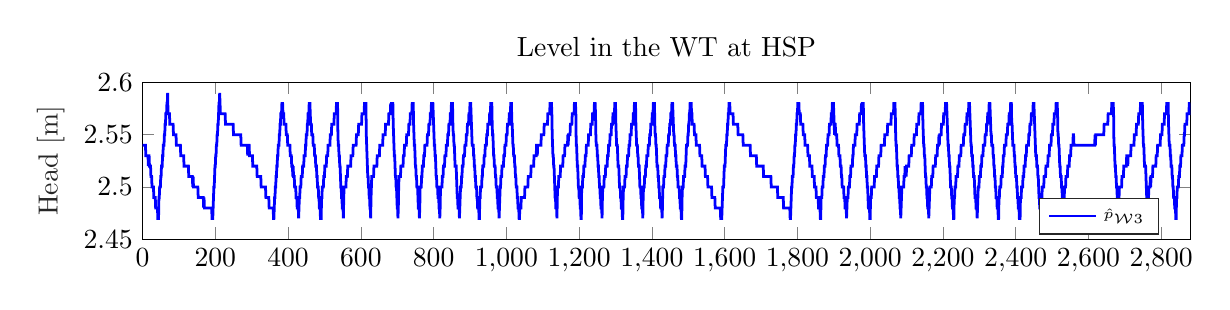
\begin{tikzpicture}

\begin{axis}[%
width=5.239in,
height=0.784in,
at={(0.989in,0.434in)},
scale only axis,
xmin=0,
xmax=2880,
%xlabel style={font=\color{white!15!black}},
%xlabel={Time [min]},
ymin=2.45,
ymax=2.6,
ylabel style={font=\color{white!15!black}},
ylabel={Head  [m]},
axis background/.style={fill=white},
title style={},
title={Level in the WT at HSP},
legend style={at={(0.97,0.03)}, anchor=south east, legend cell align=left, align=left, draw=white!15!black}
]
\addplot [color=blue, line width=1.0pt]
  table[row sep=crcr]{%
0	2.54\\
1	2.54\\
2	2.54\\
3	2.54\\
4	2.54\\
5	2.54\\
6	2.54\\
7	2.54\\
8	2.54\\
9	2.53\\
10	2.53\\
11	2.53\\
12	2.53\\
13	2.53\\
14	2.53\\
15	2.53\\
16	2.52\\
17	2.53\\
18	2.53\\
19	2.52\\
20	2.52\\
21	2.52\\
22	2.52\\
23	2.51\\
24	2.51\\
25	2.51\\
26	2.5\\
27	2.5\\
28	2.5\\
29	2.5\\
30	2.5\\
31	2.49\\
32	2.49\\
33	2.49\\
34	2.49\\
35	2.49\\
36	2.48\\
37	2.48\\
38	2.48\\
39	2.48\\
40	2.48\\
41	2.48\\
42	2.47\\
43	2.47\\
44	2.47\\
45	2.49\\
46	2.49\\
47	2.5\\
48	2.5\\
49	2.5\\
50	2.51\\
51	2.51\\
52	2.52\\
53	2.52\\
54	2.52\\
55	2.53\\
56	2.53\\
57	2.54\\
58	2.54\\
59	2.54\\
60	2.55\\
61	2.55\\
62	2.56\\
63	2.56\\
64	2.57\\
65	2.57\\
66	2.57\\
67	2.58\\
68	2.58\\
69	2.59\\
70	2.57\\
71	2.57\\
72	2.57\\
73	2.57\\
74	2.57\\
75	2.56\\
76	2.56\\
77	2.56\\
78	2.56\\
79	2.56\\
80	2.56\\
81	2.56\\
82	2.56\\
83	2.56\\
84	2.56\\
85	2.55\\
86	2.55\\
87	2.55\\
88	2.55\\
89	2.55\\
90	2.55\\
91	2.55\\
92	2.55\\
93	2.54\\
94	2.54\\
95	2.54\\
96	2.54\\
97	2.54\\
98	2.54\\
99	2.54\\
100	2.54\\
101	2.54\\
102	2.54\\
103	2.54\\
104	2.54\\
105	2.53\\
106	2.53\\
107	2.53\\
108	2.53\\
109	2.53\\
110	2.53\\
111	2.53\\
112	2.53\\
113	2.53\\
114	2.52\\
115	2.52\\
116	2.52\\
117	2.52\\
118	2.52\\
119	2.52\\
120	2.52\\
121	2.52\\
122	2.52\\
123	2.52\\
124	2.52\\
125	2.52\\
126	2.52\\
127	2.51\\
128	2.51\\
129	2.51\\
130	2.51\\
131	2.51\\
132	2.51\\
133	2.51\\
134	2.51\\
135	2.51\\
136	2.51\\
137	2.51\\
138	2.5\\
139	2.51\\
140	2.5\\
141	2.5\\
142	2.5\\
143	2.5\\
144	2.5\\
145	2.5\\
146	2.5\\
147	2.5\\
148	2.5\\
149	2.5\\
150	2.5\\
151	2.5\\
152	2.5\\
153	2.49\\
154	2.49\\
155	2.49\\
156	2.49\\
157	2.49\\
158	2.49\\
159	2.49\\
160	2.49\\
161	2.49\\
162	2.49\\
163	2.49\\
164	2.49\\
165	2.49\\
166	2.49\\
167	2.49\\
168	2.48\\
169	2.49\\
170	2.48\\
171	2.48\\
172	2.48\\
173	2.48\\
174	2.48\\
175	2.48\\
176	2.48\\
177	2.48\\
178	2.48\\
179	2.48\\
180	2.48\\
181	2.48\\
182	2.48\\
183	2.48\\
184	2.48\\
185	2.48\\
186	2.48\\
187	2.48\\
188	2.48\\
189	2.48\\
190	2.48\\
191	2.47\\
192	2.47\\
193	2.47\\
194	2.48\\
195	2.49\\
196	2.5\\
197	2.5\\
198	2.51\\
199	2.52\\
200	2.52\\
201	2.53\\
202	2.53\\
203	2.54\\
204	2.54\\
205	2.55\\
206	2.55\\
207	2.56\\
208	2.56\\
209	2.57\\
210	2.58\\
211	2.58\\
212	2.59\\
213	2.58\\
214	2.57\\
215	2.57\\
216	2.57\\
217	2.57\\
218	2.57\\
219	2.57\\
220	2.57\\
221	2.57\\
222	2.57\\
223	2.57\\
224	2.57\\
225	2.57\\
226	2.57\\
227	2.57\\
228	2.56\\
229	2.56\\
230	2.56\\
231	2.56\\
232	2.56\\
233	2.56\\
234	2.56\\
235	2.56\\
236	2.56\\
237	2.56\\
238	2.56\\
239	2.56\\
240	2.56\\
241	2.56\\
242	2.56\\
243	2.56\\
244	2.56\\
245	2.56\\
246	2.56\\
247	2.56\\
248	2.56\\
249	2.56\\
250	2.55\\
251	2.55\\
252	2.55\\
253	2.55\\
254	2.55\\
255	2.55\\
256	2.55\\
257	2.55\\
258	2.55\\
259	2.55\\
260	2.55\\
261	2.55\\
262	2.55\\
263	2.55\\
264	2.55\\
265	2.55\\
266	2.55\\
267	2.55\\
268	2.55\\
269	2.55\\
270	2.55\\
271	2.54\\
272	2.54\\
273	2.54\\
274	2.54\\
275	2.54\\
276	2.54\\
277	2.54\\
278	2.54\\
279	2.54\\
280	2.54\\
281	2.54\\
282	2.54\\
283	2.54\\
284	2.54\\
285	2.54\\
286	2.54\\
287	2.54\\
288	2.54\\
289	2.53\\
290	2.54\\
291	2.54\\
292	2.54\\
293	2.54\\
294	2.53\\
295	2.53\\
296	2.53\\
297	2.53\\
298	2.53\\
299	2.53\\
300	2.53\\
301	2.53\\
302	2.53\\
303	2.52\\
304	2.52\\
305	2.52\\
306	2.52\\
307	2.52\\
308	2.52\\
309	2.52\\
310	2.52\\
311	2.52\\
312	2.52\\
313	2.52\\
314	2.52\\
315	2.51\\
316	2.51\\
317	2.51\\
318	2.51\\
319	2.51\\
320	2.51\\
321	2.51\\
322	2.51\\
323	2.51\\
324	2.51\\
325	2.51\\
326	2.5\\
327	2.5\\
328	2.5\\
329	2.5\\
330	2.5\\
331	2.5\\
332	2.5\\
333	2.5\\
334	2.5\\
335	2.5\\
336	2.5\\
337	2.5\\
338	2.5\\
339	2.49\\
340	2.49\\
341	2.49\\
342	2.49\\
343	2.49\\
344	2.49\\
345	2.49\\
346	2.49\\
347	2.49\\
348	2.48\\
349	2.48\\
350	2.48\\
351	2.48\\
352	2.48\\
353	2.48\\
354	2.48\\
355	2.48\\
356	2.48\\
357	2.48\\
358	2.48\\
359	2.48\\
360	2.47\\
361	2.47\\
362	2.48\\
363	2.49\\
364	2.49\\
365	2.5\\
366	2.5\\
367	2.51\\
368	2.51\\
369	2.52\\
370	2.52\\
371	2.53\\
372	2.53\\
373	2.54\\
374	2.54\\
375	2.54\\
376	2.55\\
377	2.55\\
378	2.56\\
379	2.56\\
380	2.57\\
381	2.57\\
382	2.57\\
383	2.58\\
384	2.58\\
385	2.58\\
386	2.57\\
387	2.57\\
388	2.57\\
389	2.56\\
390	2.56\\
391	2.56\\
392	2.56\\
393	2.56\\
394	2.56\\
395	2.55\\
396	2.55\\
397	2.55\\
398	2.55\\
399	2.54\\
400	2.54\\
401	2.54\\
402	2.54\\
403	2.54\\
404	2.54\\
405	2.54\\
406	2.53\\
407	2.53\\
408	2.53\\
409	2.53\\
410	2.52\\
411	2.52\\
412	2.52\\
413	2.51\\
414	2.52\\
415	2.51\\
416	2.51\\
417	2.51\\
418	2.5\\
419	2.5\\
420	2.5\\
421	2.5\\
422	2.49\\
423	2.49\\
424	2.49\\
425	2.48\\
426	2.48\\
427	2.48\\
428	2.48\\
429	2.47\\
430	2.48\\
431	2.49\\
432	2.49\\
433	2.5\\
434	2.5\\
435	2.5\\
436	2.51\\
437	2.51\\
438	2.51\\
439	2.51\\
440	2.52\\
441	2.52\\
442	2.52\\
443	2.52\\
444	2.53\\
445	2.53\\
446	2.53\\
447	2.53\\
448	2.54\\
449	2.54\\
450	2.55\\
451	2.55\\
452	2.55\\
453	2.56\\
454	2.56\\
455	2.57\\
456	2.57\\
457	2.57\\
458	2.58\\
459	2.58\\
460	2.58\\
461	2.57\\
462	2.56\\
463	2.56\\
464	2.56\\
465	2.55\\
466	2.55\\
467	2.55\\
468	2.55\\
469	2.54\\
470	2.54\\
471	2.54\\
472	2.54\\
473	2.53\\
474	2.53\\
475	2.53\\
476	2.52\\
477	2.52\\
478	2.52\\
479	2.51\\
480	2.51\\
481	2.5\\
482	2.5\\
483	2.5\\
484	2.49\\
485	2.49\\
486	2.48\\
487	2.48\\
488	2.48\\
489	2.47\\
490	2.47\\
491	2.47\\
492	2.49\\
493	2.49\\
494	2.5\\
495	2.5\\
496	2.5\\
497	2.5\\
498	2.51\\
499	2.51\\
500	2.51\\
501	2.52\\
502	2.52\\
503	2.52\\
504	2.52\\
505	2.52\\
506	2.53\\
507	2.53\\
508	2.53\\
509	2.53\\
510	2.54\\
511	2.54\\
512	2.54\\
513	2.54\\
514	2.54\\
515	2.54\\
516	2.55\\
517	2.55\\
518	2.55\\
519	2.55\\
520	2.56\\
521	2.56\\
522	2.56\\
523	2.56\\
524	2.56\\
525	2.56\\
526	2.56\\
527	2.57\\
528	2.57\\
529	2.57\\
530	2.57\\
531	2.57\\
532	2.57\\
533	2.58\\
534	2.58\\
535	2.58\\
536	2.58\\
537	2.55\\
538	2.54\\
539	2.54\\
540	2.53\\
541	2.53\\
542	2.52\\
543	2.52\\
544	2.51\\
545	2.5\\
546	2.5\\
547	2.49\\
548	2.49\\
549	2.48\\
550	2.48\\
551	2.48\\
552	2.47\\
553	2.49\\
554	2.5\\
555	2.5\\
556	2.5\\
557	2.5\\
558	2.5\\
559	2.5\\
560	2.51\\
561	2.51\\
562	2.51\\
563	2.51\\
564	2.52\\
565	2.52\\
566	2.52\\
567	2.52\\
568	2.52\\
569	2.52\\
570	2.52\\
571	2.52\\
572	2.52\\
573	2.53\\
574	2.53\\
575	2.53\\
576	2.53\\
577	2.53\\
578	2.53\\
579	2.54\\
580	2.54\\
581	2.54\\
582	2.54\\
583	2.54\\
584	2.54\\
585	2.54\\
586	2.54\\
587	2.54\\
588	2.55\\
589	2.55\\
590	2.55\\
591	2.55\\
592	2.55\\
593	2.55\\
594	2.56\\
595	2.56\\
596	2.56\\
597	2.56\\
598	2.56\\
599	2.56\\
600	2.56\\
601	2.56\\
602	2.56\\
603	2.57\\
604	2.57\\
605	2.57\\
606	2.57\\
607	2.57\\
608	2.57\\
609	2.57\\
610	2.58\\
611	2.58\\
612	2.58\\
613	2.58\\
614	2.58\\
615	2.55\\
616	2.54\\
617	2.53\\
618	2.52\\
619	2.51\\
620	2.51\\
621	2.5\\
622	2.5\\
623	2.49\\
624	2.49\\
625	2.48\\
626	2.48\\
627	2.47\\
628	2.49\\
629	2.5\\
630	2.51\\
631	2.51\\
632	2.51\\
633	2.51\\
634	2.51\\
635	2.51\\
636	2.52\\
637	2.52\\
638	2.52\\
639	2.52\\
640	2.52\\
641	2.52\\
642	2.52\\
643	2.52\\
644	2.52\\
645	2.53\\
646	2.53\\
647	2.53\\
648	2.53\\
649	2.53\\
650	2.53\\
651	2.53\\
652	2.54\\
653	2.54\\
654	2.54\\
655	2.54\\
656	2.54\\
657	2.54\\
658	2.54\\
659	2.54\\
660	2.54\\
661	2.55\\
662	2.55\\
663	2.55\\
664	2.55\\
665	2.55\\
666	2.55\\
667	2.55\\
668	2.56\\
669	2.56\\
670	2.56\\
671	2.56\\
672	2.56\\
673	2.56\\
674	2.56\\
675	2.56\\
676	2.56\\
677	2.57\\
678	2.57\\
679	2.57\\
680	2.57\\
681	2.57\\
682	2.58\\
683	2.57\\
684	2.58\\
685	2.58\\
686	2.58\\
687	2.58\\
688	2.58\\
689	2.56\\
690	2.55\\
691	2.54\\
692	2.53\\
693	2.53\\
694	2.52\\
695	2.51\\
696	2.51\\
697	2.5\\
698	2.5\\
699	2.49\\
700	2.48\\
701	2.48\\
702	2.47\\
703	2.48\\
704	2.5\\
705	2.51\\
706	2.51\\
707	2.51\\
708	2.51\\
709	2.51\\
710	2.52\\
711	2.52\\
712	2.52\\
713	2.52\\
714	2.52\\
715	2.52\\
716	2.52\\
717	2.53\\
718	2.53\\
719	2.53\\
720	2.54\\
721	2.54\\
722	2.54\\
723	2.54\\
724	2.54\\
725	2.54\\
726	2.55\\
727	2.55\\
728	2.55\\
729	2.55\\
730	2.55\\
731	2.55\\
732	2.56\\
733	2.56\\
734	2.56\\
735	2.56\\
736	2.57\\
737	2.57\\
738	2.57\\
739	2.57\\
740	2.57\\
741	2.58\\
742	2.58\\
743	2.58\\
744	2.58\\
745	2.56\\
746	2.55\\
747	2.54\\
748	2.54\\
749	2.53\\
750	2.52\\
751	2.52\\
752	2.51\\
753	2.51\\
754	2.5\\
755	2.5\\
756	2.5\\
757	2.49\\
758	2.48\\
759	2.48\\
760	2.48\\
761	2.47\\
762	2.48\\
763	2.5\\
764	2.5\\
765	2.5\\
766	2.5\\
767	2.51\\
768	2.51\\
769	2.52\\
770	2.52\\
771	2.52\\
772	2.52\\
773	2.53\\
774	2.53\\
775	2.53\\
776	2.54\\
777	2.54\\
778	2.54\\
779	2.54\\
780	2.54\\
781	2.54\\
782	2.54\\
783	2.55\\
784	2.55\\
785	2.55\\
786	2.55\\
787	2.56\\
788	2.56\\
789	2.56\\
790	2.56\\
791	2.57\\
792	2.57\\
793	2.57\\
794	2.58\\
795	2.58\\
796	2.58\\
797	2.58\\
798	2.58\\
799	2.57\\
800	2.56\\
801	2.55\\
802	2.54\\
803	2.54\\
804	2.53\\
805	2.53\\
806	2.52\\
807	2.51\\
808	2.51\\
809	2.5\\
810	2.5\\
811	2.5\\
812	2.49\\
813	2.49\\
814	2.49\\
815	2.48\\
816	2.48\\
817	2.47\\
818	2.48\\
819	2.5\\
820	2.5\\
821	2.5\\
822	2.5\\
823	2.5\\
824	2.51\\
825	2.51\\
826	2.51\\
827	2.52\\
828	2.52\\
829	2.52\\
830	2.52\\
831	2.53\\
832	2.53\\
833	2.53\\
834	2.53\\
835	2.54\\
836	2.54\\
837	2.54\\
838	2.54\\
839	2.55\\
840	2.55\\
841	2.55\\
842	2.56\\
843	2.56\\
844	2.56\\
845	2.56\\
846	2.57\\
847	2.57\\
848	2.57\\
849	2.58\\
850	2.58\\
851	2.58\\
852	2.58\\
853	2.56\\
854	2.55\\
855	2.55\\
856	2.54\\
857	2.54\\
858	2.53\\
859	2.52\\
860	2.52\\
861	2.52\\
862	2.52\\
863	2.51\\
864	2.5\\
865	2.49\\
866	2.49\\
867	2.48\\
868	2.48\\
869	2.48\\
870	2.48\\
871	2.47\\
872	2.48\\
873	2.49\\
874	2.5\\
875	2.5\\
876	2.5\\
877	2.51\\
878	2.51\\
879	2.52\\
880	2.52\\
881	2.52\\
882	2.53\\
883	2.53\\
884	2.53\\
885	2.53\\
886	2.54\\
887	2.54\\
888	2.54\\
889	2.54\\
890	2.55\\
891	2.55\\
892	2.55\\
893	2.56\\
894	2.56\\
895	2.56\\
896	2.56\\
897	2.57\\
898	2.57\\
899	2.57\\
900	2.58\\
901	2.58\\
902	2.58\\
903	2.57\\
904	2.56\\
905	2.55\\
906	2.54\\
907	2.54\\
908	2.54\\
909	2.54\\
910	2.53\\
911	2.53\\
912	2.52\\
913	2.52\\
914	2.51\\
915	2.51\\
916	2.5\\
917	2.5\\
918	2.5\\
919	2.49\\
920	2.49\\
921	2.48\\
922	2.48\\
923	2.48\\
924	2.48\\
925	2.47\\
926	2.47\\
927	2.49\\
928	2.49\\
929	2.5\\
930	2.5\\
931	2.5\\
932	2.5\\
933	2.51\\
934	2.51\\
935	2.52\\
936	2.52\\
937	2.52\\
938	2.52\\
939	2.53\\
940	2.53\\
941	2.53\\
942	2.54\\
943	2.54\\
944	2.54\\
945	2.54\\
946	2.55\\
947	2.55\\
948	2.55\\
949	2.56\\
950	2.56\\
951	2.56\\
952	2.56\\
953	2.56\\
954	2.57\\
955	2.57\\
956	2.57\\
957	2.58\\
958	2.58\\
959	2.58\\
960	2.58\\
961	2.56\\
962	2.55\\
963	2.55\\
964	2.54\\
965	2.53\\
966	2.53\\
967	2.52\\
968	2.52\\
969	2.52\\
970	2.51\\
971	2.51\\
972	2.5\\
973	2.5\\
974	2.5\\
975	2.49\\
976	2.49\\
977	2.48\\
978	2.48\\
979	2.48\\
980	2.47\\
981	2.48\\
982	2.49\\
983	2.5\\
984	2.5\\
985	2.51\\
986	2.51\\
987	2.51\\
988	2.52\\
989	2.52\\
990	2.52\\
991	2.52\\
992	2.52\\
993	2.53\\
994	2.53\\
995	2.53\\
996	2.54\\
997	2.54\\
998	2.54\\
999	2.54\\
1000	2.55\\
1001	2.55\\
1002	2.55\\
1003	2.56\\
1004	2.56\\
1005	2.56\\
1006	2.56\\
1007	2.56\\
1008	2.57\\
1009	2.57\\
1010	2.57\\
1011	2.57\\
1012	2.58\\
1013	2.58\\
1014	2.58\\
1015	2.56\\
1016	2.56\\
1017	2.55\\
1018	2.54\\
1019	2.54\\
1020	2.53\\
1021	2.53\\
1022	2.53\\
1023	2.52\\
1024	2.52\\
1025	2.51\\
1026	2.51\\
1027	2.5\\
1028	2.5\\
1029	2.5\\
1030	2.49\\
1031	2.49\\
1032	2.48\\
1033	2.48\\
1034	2.48\\
1035	2.47\\
1036	2.47\\
1037	2.48\\
1038	2.48\\
1039	2.48\\
1040	2.48\\
1041	2.49\\
1042	2.49\\
1043	2.49\\
1044	2.49\\
1045	2.49\\
1046	2.49\\
1047	2.49\\
1048	2.49\\
1049	2.49\\
1050	2.49\\
1051	2.5\\
1052	2.5\\
1053	2.5\\
1054	2.5\\
1055	2.5\\
1056	2.5\\
1057	2.5\\
1058	2.5\\
1059	2.5\\
1060	2.51\\
1061	2.51\\
1062	2.51\\
1063	2.51\\
1064	2.51\\
1065	2.51\\
1066	2.51\\
1067	2.51\\
1068	2.52\\
1069	2.52\\
1070	2.52\\
1071	2.52\\
1072	2.52\\
1073	2.52\\
1074	2.52\\
1075	2.52\\
1076	2.53\\
1077	2.53\\
1078	2.53\\
1079	2.53\\
1080	2.53\\
1081	2.53\\
1082	2.53\\
1083	2.54\\
1084	2.54\\
1085	2.53\\
1086	2.54\\
1087	2.54\\
1088	2.54\\
1089	2.54\\
1090	2.54\\
1091	2.54\\
1092	2.54\\
1093	2.54\\
1094	2.54\\
1095	2.54\\
1096	2.55\\
1097	2.55\\
1098	2.55\\
1099	2.55\\
1100	2.55\\
1101	2.55\\
1102	2.55\\
1103	2.55\\
1104	2.56\\
1105	2.56\\
1106	2.56\\
1107	2.56\\
1108	2.56\\
1109	2.56\\
1110	2.56\\
1111	2.56\\
1112	2.56\\
1113	2.56\\
1114	2.57\\
1115	2.57\\
1116	2.57\\
1117	2.57\\
1118	2.57\\
1119	2.57\\
1120	2.58\\
1121	2.58\\
1122	2.58\\
1123	2.58\\
1124	2.58\\
1125	2.57\\
1126	2.55\\
1127	2.54\\
1128	2.53\\
1129	2.53\\
1130	2.52\\
1131	2.52\\
1132	2.51\\
1133	2.5\\
1134	2.49\\
1135	2.49\\
1136	2.48\\
1137	2.48\\
1138	2.48\\
1139	2.47\\
1140	2.49\\
1141	2.5\\
1142	2.5\\
1143	2.5\\
1144	2.51\\
1145	2.51\\
1146	2.51\\
1147	2.51\\
1148	2.51\\
1149	2.52\\
1150	2.52\\
1151	2.52\\
1152	2.52\\
1153	2.52\\
1154	2.52\\
1155	2.52\\
1156	2.53\\
1157	2.53\\
1158	2.53\\
1159	2.53\\
1160	2.53\\
1161	2.54\\
1162	2.54\\
1163	2.54\\
1164	2.54\\
1165	2.54\\
1166	2.54\\
1167	2.54\\
1168	2.54\\
1169	2.55\\
1170	2.54\\
1171	2.55\\
1172	2.55\\
1173	2.55\\
1174	2.55\\
1175	2.55\\
1176	2.56\\
1177	2.56\\
1178	2.56\\
1179	2.56\\
1180	2.56\\
1181	2.57\\
1182	2.57\\
1183	2.57\\
1184	2.57\\
1185	2.57\\
1186	2.57\\
1187	2.58\\
1188	2.58\\
1189	2.58\\
1190	2.58\\
1191	2.57\\
1192	2.54\\
1193	2.54\\
1194	2.53\\
1195	2.52\\
1196	2.52\\
1197	2.51\\
1198	2.5\\
1199	2.5\\
1200	2.49\\
1201	2.49\\
1202	2.49\\
1203	2.48\\
1204	2.48\\
1205	2.47\\
1206	2.47\\
1207	2.5\\
1208	2.5\\
1209	2.5\\
1210	2.51\\
1211	2.51\\
1212	2.51\\
1213	2.52\\
1214	2.52\\
1215	2.52\\
1216	2.52\\
1217	2.53\\
1218	2.53\\
1219	2.53\\
1220	2.54\\
1221	2.54\\
1222	2.54\\
1223	2.54\\
1224	2.54\\
1225	2.54\\
1226	2.55\\
1227	2.55\\
1228	2.55\\
1229	2.55\\
1230	2.55\\
1231	2.55\\
1232	2.56\\
1233	2.56\\
1234	2.56\\
1235	2.56\\
1236	2.56\\
1237	2.57\\
1238	2.57\\
1239	2.57\\
1240	2.57\\
1241	2.57\\
1242	2.58\\
1243	2.58\\
1244	2.58\\
1245	2.57\\
1246	2.55\\
1247	2.54\\
1248	2.54\\
1249	2.54\\
1250	2.53\\
1251	2.53\\
1252	2.52\\
1253	2.52\\
1254	2.51\\
1255	2.51\\
1256	2.5\\
1257	2.5\\
1258	2.49\\
1259	2.49\\
1260	2.48\\
1261	2.48\\
1262	2.48\\
1263	2.47\\
1264	2.49\\
1265	2.5\\
1266	2.5\\
1267	2.5\\
1268	2.5\\
1269	2.51\\
1270	2.51\\
1271	2.51\\
1272	2.51\\
1273	2.52\\
1274	2.52\\
1275	2.52\\
1276	2.52\\
1277	2.52\\
1278	2.53\\
1279	2.53\\
1280	2.53\\
1281	2.54\\
1282	2.54\\
1283	2.54\\
1284	2.54\\
1285	2.55\\
1286	2.55\\
1287	2.55\\
1288	2.55\\
1289	2.56\\
1290	2.56\\
1291	2.56\\
1292	2.56\\
1293	2.57\\
1294	2.57\\
1295	2.57\\
1296	2.57\\
1297	2.57\\
1298	2.58\\
1299	2.58\\
1300	2.58\\
1301	2.56\\
1302	2.55\\
1303	2.54\\
1304	2.54\\
1305	2.54\\
1306	2.53\\
1307	2.52\\
1308	2.52\\
1309	2.52\\
1310	2.51\\
1311	2.5\\
1312	2.5\\
1313	2.5\\
1314	2.49\\
1315	2.49\\
1316	2.48\\
1317	2.48\\
1318	2.48\\
1319	2.47\\
1320	2.47\\
1321	2.49\\
1322	2.5\\
1323	2.5\\
1324	2.5\\
1325	2.5\\
1326	2.51\\
1327	2.51\\
1328	2.51\\
1329	2.51\\
1330	2.52\\
1331	2.52\\
1332	2.52\\
1333	2.53\\
1334	2.53\\
1335	2.53\\
1336	2.53\\
1337	2.54\\
1338	2.54\\
1339	2.54\\
1340	2.55\\
1341	2.55\\
1342	2.55\\
1343	2.55\\
1344	2.56\\
1345	2.56\\
1346	2.56\\
1347	2.56\\
1348	2.56\\
1349	2.57\\
1350	2.57\\
1351	2.57\\
1352	2.58\\
1353	2.58\\
1354	2.58\\
1355	2.58\\
1356	2.56\\
1357	2.55\\
1358	2.54\\
1359	2.54\\
1360	2.54\\
1361	2.53\\
1362	2.53\\
1363	2.52\\
1364	2.52\\
1365	2.52\\
1366	2.51\\
1367	2.5\\
1368	2.5\\
1369	2.5\\
1370	2.49\\
1371	2.49\\
1372	2.48\\
1373	2.48\\
1374	2.48\\
1375	2.47\\
1376	2.49\\
1377	2.5\\
1378	2.5\\
1379	2.5\\
1380	2.51\\
1381	2.51\\
1382	2.51\\
1383	2.52\\
1384	2.52\\
1385	2.52\\
1386	2.53\\
1387	2.53\\
1388	2.53\\
1389	2.53\\
1390	2.54\\
1391	2.54\\
1392	2.54\\
1393	2.54\\
1394	2.55\\
1395	2.55\\
1396	2.55\\
1397	2.56\\
1398	2.56\\
1399	2.56\\
1400	2.56\\
1401	2.57\\
1402	2.57\\
1403	2.57\\
1404	2.58\\
1405	2.58\\
1406	2.58\\
1407	2.58\\
1408	2.56\\
1409	2.55\\
1410	2.55\\
1411	2.54\\
1412	2.54\\
1413	2.53\\
1414	2.52\\
1415	2.52\\
1416	2.52\\
1417	2.51\\
1418	2.51\\
1419	2.5\\
1420	2.5\\
1421	2.49\\
1422	2.49\\
1423	2.49\\
1424	2.48\\
1425	2.48\\
1426	2.48\\
1427	2.48\\
1428	2.47\\
1429	2.48\\
1430	2.5\\
1431	2.5\\
1432	2.5\\
1433	2.51\\
1434	2.51\\
1435	2.51\\
1436	2.52\\
1437	2.52\\
1438	2.52\\
1439	2.53\\
1440	2.53\\
1441	2.53\\
1442	2.54\\
1443	2.54\\
1444	2.54\\
1445	2.54\\
1446	2.55\\
1447	2.55\\
1448	2.55\\
1449	2.56\\
1450	2.56\\
1451	2.56\\
1452	2.57\\
1453	2.57\\
1454	2.57\\
1455	2.58\\
1456	2.58\\
1457	2.58\\
1458	2.57\\
1459	2.56\\
1460	2.55\\
1461	2.55\\
1462	2.54\\
1463	2.54\\
1464	2.54\\
1465	2.53\\
1466	2.53\\
1467	2.52\\
1468	2.52\\
1469	2.52\\
1470	2.51\\
1471	2.51\\
1472	2.5\\
1473	2.5\\
1474	2.5\\
1475	2.5\\
1476	2.49\\
1477	2.49\\
1478	2.48\\
1479	2.48\\
1480	2.48\\
1481	2.47\\
1482	2.47\\
1483	2.49\\
1484	2.5\\
1485	2.5\\
1486	2.5\\
1487	2.51\\
1488	2.51\\
1489	2.51\\
1490	2.51\\
1491	2.52\\
1492	2.52\\
1493	2.52\\
1494	2.53\\
1495	2.54\\
1496	2.54\\
1497	2.54\\
1498	2.54\\
1499	2.55\\
1500	2.55\\
1501	2.56\\
1502	2.56\\
1503	2.57\\
1504	2.57\\
1505	2.58\\
1506	2.58\\
1507	2.58\\
1508	2.58\\
1509	2.57\\
1510	2.57\\
1511	2.56\\
1512	2.56\\
1513	2.56\\
1514	2.56\\
1515	2.56\\
1516	2.56\\
1517	2.55\\
1518	2.55\\
1519	2.55\\
1520	2.55\\
1521	2.55\\
1522	2.54\\
1523	2.54\\
1524	2.54\\
1525	2.54\\
1526	2.54\\
1527	2.54\\
1528	2.54\\
1529	2.54\\
1530	2.54\\
1531	2.54\\
1532	2.53\\
1533	2.53\\
1534	2.53\\
1535	2.53\\
1536	2.53\\
1537	2.53\\
1538	2.52\\
1539	2.52\\
1540	2.52\\
1541	2.52\\
1542	2.52\\
1543	2.52\\
1544	2.52\\
1545	2.52\\
1546	2.52\\
1547	2.51\\
1548	2.51\\
1549	2.51\\
1550	2.51\\
1551	2.51\\
1552	2.51\\
1553	2.51\\
1554	2.5\\
1555	2.5\\
1556	2.5\\
1557	2.5\\
1558	2.5\\
1559	2.5\\
1560	2.5\\
1561	2.5\\
1562	2.5\\
1563	2.5\\
1564	2.5\\
1565	2.49\\
1566	2.49\\
1567	2.49\\
1568	2.49\\
1569	2.49\\
1570	2.49\\
1571	2.49\\
1572	2.49\\
1573	2.49\\
1574	2.48\\
1575	2.48\\
1576	2.48\\
1577	2.48\\
1578	2.48\\
1579	2.48\\
1580	2.48\\
1581	2.48\\
1582	2.48\\
1583	2.48\\
1584	2.48\\
1585	2.48\\
1586	2.48\\
1587	2.48\\
1588	2.48\\
1589	2.47\\
1590	2.47\\
1591	2.47\\
1592	2.47\\
1593	2.48\\
1594	2.49\\
1595	2.5\\
1596	2.5\\
1597	2.5\\
1598	2.51\\
1599	2.52\\
1600	2.52\\
1601	2.52\\
1602	2.53\\
1603	2.54\\
1604	2.54\\
1605	2.54\\
1606	2.55\\
1607	2.55\\
1608	2.56\\
1609	2.56\\
1610	2.57\\
1611	2.57\\
1612	2.58\\
1613	2.58\\
1614	2.58\\
1615	2.57\\
1616	2.57\\
1617	2.57\\
1618	2.57\\
1619	2.57\\
1620	2.57\\
1621	2.57\\
1622	2.57\\
1623	2.57\\
1624	2.56\\
1625	2.56\\
1626	2.56\\
1627	2.56\\
1628	2.56\\
1629	2.56\\
1630	2.56\\
1631	2.56\\
1632	2.56\\
1633	2.56\\
1634	2.56\\
1635	2.56\\
1636	2.56\\
1637	2.55\\
1638	2.55\\
1639	2.55\\
1640	2.55\\
1641	2.55\\
1642	2.55\\
1643	2.55\\
1644	2.55\\
1645	2.55\\
1646	2.55\\
1647	2.55\\
1648	2.55\\
1649	2.55\\
1650	2.55\\
1651	2.54\\
1652	2.54\\
1653	2.54\\
1654	2.54\\
1655	2.54\\
1656	2.54\\
1657	2.54\\
1658	2.54\\
1659	2.54\\
1660	2.54\\
1661	2.54\\
1662	2.54\\
1663	2.54\\
1664	2.54\\
1665	2.54\\
1666	2.54\\
1667	2.54\\
1668	2.54\\
1669	2.54\\
1670	2.54\\
1671	2.53\\
1672	2.53\\
1673	2.53\\
1674	2.53\\
1675	2.53\\
1676	2.53\\
1677	2.53\\
1678	2.53\\
1679	2.53\\
1680	2.53\\
1681	2.53\\
1682	2.53\\
1683	2.53\\
1684	2.53\\
1685	2.53\\
1686	2.53\\
1687	2.53\\
1688	2.52\\
1689	2.52\\
1690	2.52\\
1691	2.52\\
1692	2.52\\
1693	2.52\\
1694	2.52\\
1695	2.52\\
1696	2.52\\
1697	2.52\\
1698	2.52\\
1699	2.52\\
1700	2.52\\
1701	2.52\\
1702	2.52\\
1703	2.52\\
1704	2.52\\
1705	2.52\\
1706	2.52\\
1707	2.51\\
1708	2.51\\
1709	2.51\\
1710	2.51\\
1711	2.51\\
1712	2.51\\
1713	2.51\\
1714	2.51\\
1715	2.51\\
1716	2.51\\
1717	2.51\\
1718	2.51\\
1719	2.51\\
1720	2.51\\
1721	2.51\\
1722	2.51\\
1723	2.51\\
1724	2.51\\
1725	2.51\\
1726	2.51\\
1727	2.51\\
1728	2.5\\
1729	2.5\\
1730	2.5\\
1731	2.5\\
1732	2.5\\
1733	2.5\\
1734	2.5\\
1735	2.5\\
1736	2.5\\
1737	2.5\\
1738	2.5\\
1739	2.5\\
1740	2.5\\
1741	2.5\\
1742	2.5\\
1743	2.5\\
1744	2.5\\
1745	2.5\\
1746	2.49\\
1747	2.49\\
1748	2.49\\
1749	2.49\\
1750	2.49\\
1751	2.49\\
1752	2.49\\
1753	2.49\\
1754	2.49\\
1755	2.49\\
1756	2.49\\
1757	2.49\\
1758	2.49\\
1759	2.49\\
1760	2.49\\
1761	2.49\\
1762	2.48\\
1763	2.48\\
1764	2.48\\
1765	2.48\\
1766	2.48\\
1767	2.48\\
1768	2.48\\
1769	2.48\\
1770	2.48\\
1771	2.48\\
1772	2.48\\
1773	2.48\\
1774	2.48\\
1775	2.48\\
1776	2.48\\
1777	2.48\\
1778	2.48\\
1779	2.48\\
1780	2.47\\
1781	2.47\\
1782	2.48\\
1783	2.49\\
1784	2.5\\
1785	2.5\\
1786	2.51\\
1787	2.51\\
1788	2.51\\
1789	2.52\\
1790	2.52\\
1791	2.53\\
1792	2.53\\
1793	2.54\\
1794	2.54\\
1795	2.55\\
1796	2.55\\
1797	2.56\\
1798	2.56\\
1799	2.57\\
1800	2.57\\
1801	2.58\\
1802	2.58\\
1803	2.58\\
1804	2.58\\
1805	2.57\\
1806	2.57\\
1807	2.57\\
1808	2.57\\
1809	2.56\\
1810	2.56\\
1811	2.56\\
1812	2.56\\
1813	2.56\\
1814	2.56\\
1815	2.56\\
1816	2.55\\
1817	2.55\\
1818	2.55\\
1819	2.55\\
1820	2.55\\
1821	2.54\\
1822	2.54\\
1823	2.54\\
1824	2.54\\
1825	2.54\\
1826	2.54\\
1827	2.54\\
1828	2.54\\
1829	2.53\\
1830	2.53\\
1831	2.53\\
1832	2.53\\
1833	2.53\\
1834	2.52\\
1835	2.52\\
1836	2.52\\
1837	2.52\\
1838	2.52\\
1839	2.52\\
1840	2.52\\
1841	2.51\\
1842	2.51\\
1843	2.51\\
1844	2.51\\
1845	2.51\\
1846	2.51\\
1847	2.5\\
1848	2.5\\
1849	2.5\\
1850	2.5\\
1851	2.5\\
1852	2.49\\
1853	2.49\\
1854	2.49\\
1855	2.49\\
1856	2.49\\
1857	2.49\\
1858	2.48\\
1859	2.48\\
1860	2.48\\
1861	2.48\\
1862	2.48\\
1863	2.47\\
1864	2.47\\
1865	2.49\\
1866	2.49\\
1867	2.49\\
1868	2.5\\
1869	2.5\\
1870	2.5\\
1871	2.51\\
1872	2.51\\
1873	2.51\\
1874	2.52\\
1875	2.52\\
1876	2.52\\
1877	2.53\\
1878	2.53\\
1879	2.53\\
1880	2.54\\
1881	2.54\\
1882	2.54\\
1883	2.54\\
1884	2.55\\
1885	2.55\\
1886	2.55\\
1887	2.55\\
1888	2.56\\
1889	2.56\\
1890	2.56\\
1891	2.56\\
1892	2.56\\
1893	2.57\\
1894	2.57\\
1895	2.57\\
1896	2.58\\
1897	2.58\\
1898	2.58\\
1899	2.58\\
1900	2.57\\
1901	2.56\\
1902	2.55\\
1903	2.56\\
1904	2.56\\
1905	2.55\\
1906	2.55\\
1907	2.55\\
1908	2.55\\
1909	2.54\\
1910	2.54\\
1911	2.54\\
1912	2.54\\
1913	2.54\\
1914	2.53\\
1915	2.53\\
1916	2.53\\
1917	2.53\\
1918	2.52\\
1919	2.52\\
1920	2.52\\
1921	2.51\\
1922	2.51\\
1923	2.5\\
1924	2.5\\
1925	2.5\\
1926	2.5\\
1927	2.5\\
1928	2.49\\
1929	2.49\\
1930	2.49\\
1931	2.48\\
1932	2.48\\
1933	2.48\\
1934	2.48\\
1935	2.47\\
1936	2.48\\
1937	2.49\\
1938	2.49\\
1939	2.49\\
1940	2.5\\
1941	2.5\\
1942	2.5\\
1943	2.5\\
1944	2.51\\
1945	2.51\\
1946	2.51\\
1947	2.52\\
1948	2.52\\
1949	2.52\\
1950	2.52\\
1951	2.52\\
1952	2.53\\
1953	2.53\\
1954	2.54\\
1955	2.54\\
1956	2.54\\
1957	2.54\\
1958	2.54\\
1959	2.55\\
1960	2.55\\
1961	2.55\\
1962	2.55\\
1963	2.55\\
1964	2.56\\
1965	2.56\\
1966	2.56\\
1967	2.56\\
1968	2.56\\
1969	2.56\\
1970	2.56\\
1971	2.57\\
1972	2.57\\
1973	2.57\\
1974	2.57\\
1975	2.57\\
1976	2.58\\
1977	2.57\\
1978	2.58\\
1979	2.58\\
1980	2.58\\
1981	2.58\\
1982	2.56\\
1983	2.55\\
1984	2.54\\
1985	2.53\\
1986	2.53\\
1987	2.53\\
1988	2.52\\
1989	2.52\\
1990	2.51\\
1991	2.51\\
1992	2.5\\
1993	2.5\\
1994	2.49\\
1995	2.48\\
1996	2.48\\
1997	2.48\\
1998	2.48\\
1999	2.47\\
2000	2.47\\
2001	2.49\\
2002	2.49\\
2003	2.49\\
2004	2.5\\
2005	2.5\\
2006	2.5\\
2007	2.5\\
2008	2.5\\
2009	2.5\\
2010	2.5\\
2011	2.5\\
2012	2.51\\
2013	2.51\\
2014	2.51\\
2015	2.51\\
2016	2.51\\
2017	2.51\\
2018	2.52\\
2019	2.52\\
2020	2.52\\
2021	2.52\\
2022	2.52\\
2023	2.52\\
2024	2.53\\
2025	2.53\\
2026	2.53\\
2027	2.53\\
2028	2.53\\
2029	2.53\\
2030	2.54\\
2031	2.54\\
2032	2.54\\
2033	2.54\\
2034	2.54\\
2035	2.54\\
2036	2.54\\
2037	2.54\\
2038	2.54\\
2039	2.54\\
2040	2.55\\
2041	2.55\\
2042	2.55\\
2043	2.55\\
2044	2.55\\
2045	2.55\\
2046	2.55\\
2047	2.55\\
2048	2.56\\
2049	2.56\\
2050	2.56\\
2051	2.56\\
2052	2.56\\
2053	2.56\\
2054	2.56\\
2055	2.56\\
2056	2.56\\
2057	2.56\\
2058	2.57\\
2059	2.57\\
2060	2.57\\
2061	2.57\\
2062	2.57\\
2063	2.57\\
2064	2.57\\
2065	2.58\\
2066	2.58\\
2067	2.58\\
2068	2.58\\
2069	2.57\\
2070	2.55\\
2071	2.54\\
2072	2.54\\
2073	2.53\\
2074	2.52\\
2075	2.52\\
2076	2.51\\
2077	2.51\\
2078	2.5\\
2079	2.5\\
2080	2.49\\
2081	2.49\\
2082	2.48\\
2083	2.48\\
2084	2.47\\
2085	2.48\\
2086	2.49\\
2087	2.5\\
2088	2.5\\
2089	2.5\\
2090	2.5\\
2091	2.5\\
2092	2.5\\
2093	2.51\\
2094	2.51\\
2095	2.51\\
2096	2.52\\
2097	2.51\\
2098	2.52\\
2099	2.51\\
2100	2.52\\
2101	2.52\\
2102	2.52\\
2103	2.52\\
2104	2.52\\
2105	2.52\\
2106	2.52\\
2107	2.53\\
2108	2.53\\
2109	2.53\\
2110	2.53\\
2111	2.53\\
2112	2.53\\
2113	2.53\\
2114	2.54\\
2115	2.54\\
2116	2.54\\
2117	2.54\\
2118	2.54\\
2119	2.54\\
2120	2.54\\
2121	2.55\\
2122	2.55\\
2123	2.55\\
2124	2.55\\
2125	2.55\\
2126	2.55\\
2127	2.55\\
2128	2.56\\
2129	2.56\\
2130	2.56\\
2131	2.56\\
2132	2.56\\
2133	2.56\\
2134	2.57\\
2135	2.57\\
2136	2.57\\
2137	2.57\\
2138	2.57\\
2139	2.57\\
2140	2.58\\
2141	2.58\\
2142	2.58\\
2143	2.58\\
2144	2.58\\
2145	2.56\\
2146	2.55\\
2147	2.54\\
2148	2.54\\
2149	2.53\\
2150	2.53\\
2151	2.52\\
2152	2.51\\
2153	2.51\\
2154	2.5\\
2155	2.5\\
2156	2.49\\
2157	2.49\\
2158	2.48\\
2159	2.48\\
2160	2.48\\
2161	2.47\\
2162	2.48\\
2163	2.49\\
2164	2.5\\
2165	2.5\\
2166	2.5\\
2167	2.5\\
2168	2.5\\
2169	2.51\\
2170	2.51\\
2171	2.51\\
2172	2.51\\
2173	2.52\\
2174	2.52\\
2175	2.52\\
2176	2.52\\
2177	2.52\\
2178	2.52\\
2179	2.52\\
2180	2.53\\
2181	2.53\\
2182	2.53\\
2183	2.53\\
2184	2.53\\
2185	2.54\\
2186	2.54\\
2187	2.54\\
2188	2.54\\
2189	2.55\\
2190	2.54\\
2191	2.55\\
2192	2.55\\
2193	2.55\\
2194	2.55\\
2195	2.55\\
2196	2.56\\
2197	2.56\\
2198	2.56\\
2199	2.56\\
2200	2.56\\
2201	2.56\\
2202	2.57\\
2203	2.57\\
2204	2.57\\
2205	2.57\\
2206	2.57\\
2207	2.58\\
2208	2.58\\
2209	2.58\\
2210	2.58\\
2211	2.57\\
2212	2.56\\
2213	2.55\\
2214	2.54\\
2215	2.54\\
2216	2.53\\
2217	2.53\\
2218	2.52\\
2219	2.52\\
2220	2.51\\
2221	2.5\\
2222	2.5\\
2223	2.5\\
2224	2.49\\
2225	2.49\\
2226	2.48\\
2227	2.48\\
2228	2.48\\
2229	2.47\\
2230	2.47\\
2231	2.49\\
2232	2.49\\
2233	2.5\\
2234	2.5\\
2235	2.5\\
2236	2.51\\
2237	2.51\\
2238	2.51\\
2239	2.51\\
2240	2.51\\
2241	2.52\\
2242	2.52\\
2243	2.52\\
2244	2.52\\
2245	2.53\\
2246	2.53\\
2247	2.53\\
2248	2.53\\
2249	2.53\\
2250	2.54\\
2251	2.54\\
2252	2.54\\
2253	2.54\\
2254	2.54\\
2255	2.54\\
2256	2.54\\
2257	2.55\\
2258	2.55\\
2259	2.55\\
2260	2.55\\
2261	2.56\\
2262	2.56\\
2263	2.56\\
2264	2.56\\
2265	2.56\\
2266	2.57\\
2267	2.57\\
2268	2.57\\
2269	2.57\\
2270	2.57\\
2271	2.58\\
2272	2.58\\
2273	2.58\\
2274	2.57\\
2275	2.56\\
2276	2.55\\
2277	2.54\\
2278	2.54\\
2279	2.53\\
2280	2.53\\
2281	2.53\\
2282	2.52\\
2283	2.52\\
2284	2.51\\
2285	2.51\\
2286	2.51\\
2287	2.5\\
2288	2.49\\
2289	2.49\\
2290	2.49\\
2291	2.48\\
2292	2.48\\
2293	2.48\\
2294	2.47\\
2295	2.48\\
2296	2.49\\
2297	2.5\\
2298	2.5\\
2299	2.5\\
2300	2.51\\
2301	2.51\\
2302	2.51\\
2303	2.51\\
2304	2.52\\
2305	2.52\\
2306	2.52\\
2307	2.53\\
2308	2.53\\
2309	2.53\\
2310	2.53\\
2311	2.54\\
2312	2.54\\
2313	2.54\\
2314	2.54\\
2315	2.54\\
2316	2.55\\
2317	2.55\\
2318	2.55\\
2319	2.55\\
2320	2.56\\
2321	2.56\\
2322	2.56\\
2323	2.57\\
2324	2.57\\
2325	2.57\\
2326	2.57\\
2327	2.58\\
2328	2.58\\
2329	2.58\\
2330	2.57\\
2331	2.56\\
2332	2.55\\
2333	2.55\\
2334	2.54\\
2335	2.54\\
2336	2.54\\
2337	2.54\\
2338	2.53\\
2339	2.53\\
2340	2.52\\
2341	2.52\\
2342	2.51\\
2343	2.51\\
2344	2.5\\
2345	2.5\\
2346	2.49\\
2347	2.49\\
2348	2.49\\
2349	2.48\\
2350	2.48\\
2351	2.48\\
2352	2.47\\
2353	2.47\\
2354	2.49\\
2355	2.49\\
2356	2.5\\
2357	2.5\\
2358	2.5\\
2359	2.5\\
2360	2.51\\
2361	2.51\\
2362	2.51\\
2363	2.51\\
2364	2.52\\
2365	2.52\\
2366	2.53\\
2367	2.53\\
2368	2.53\\
2369	2.54\\
2370	2.54\\
2371	2.54\\
2372	2.54\\
2373	2.54\\
2374	2.55\\
2375	2.55\\
2376	2.55\\
2377	2.55\\
2378	2.56\\
2379	2.56\\
2380	2.56\\
2381	2.56\\
2382	2.57\\
2383	2.57\\
2384	2.57\\
2385	2.57\\
2386	2.58\\
2387	2.58\\
2388	2.58\\
2389	2.56\\
2390	2.56\\
2391	2.55\\
2392	2.54\\
2393	2.54\\
2394	2.54\\
2395	2.54\\
2396	2.53\\
2397	2.53\\
2398	2.52\\
2399	2.52\\
2400	2.51\\
2401	2.51\\
2402	2.51\\
2403	2.5\\
2404	2.5\\
2405	2.49\\
2406	2.49\\
2407	2.48\\
2408	2.48\\
2409	2.48\\
2410	2.47\\
2411	2.47\\
2412	2.47\\
2413	2.49\\
2414	2.49\\
2415	2.49\\
2416	2.5\\
2417	2.5\\
2418	2.5\\
2419	2.5\\
2420	2.51\\
2421	2.51\\
2422	2.51\\
2423	2.52\\
2424	2.52\\
2425	2.52\\
2426	2.52\\
2427	2.53\\
2428	2.53\\
2429	2.53\\
2430	2.54\\
2431	2.54\\
2432	2.54\\
2433	2.54\\
2434	2.54\\
2435	2.54\\
2436	2.55\\
2437	2.55\\
2438	2.55\\
2439	2.56\\
2440	2.56\\
2441	2.56\\
2442	2.56\\
2443	2.57\\
2444	2.57\\
2445	2.57\\
2446	2.57\\
2447	2.57\\
2448	2.58\\
2449	2.58\\
2450	2.58\\
2451	2.57\\
2452	2.56\\
2453	2.55\\
2454	2.54\\
2455	2.53\\
2456	2.53\\
2457	2.53\\
2458	2.52\\
2459	2.52\\
2460	2.52\\
2461	2.51\\
2462	2.51\\
2463	2.5\\
2464	2.49\\
2465	2.49\\
2466	2.48\\
2467	2.48\\
2468	2.48\\
2469	2.48\\
2470	2.47\\
2471	2.48\\
2472	2.49\\
2473	2.5\\
2474	2.5\\
2475	2.5\\
2476	2.5\\
2477	2.5\\
2478	2.51\\
2479	2.51\\
2480	2.51\\
2481	2.51\\
2482	2.51\\
2483	2.52\\
2484	2.52\\
2485	2.52\\
2486	2.52\\
2487	2.52\\
2488	2.52\\
2489	2.53\\
2490	2.53\\
2491	2.53\\
2492	2.53\\
2493	2.54\\
2494	2.54\\
2495	2.54\\
2496	2.54\\
2497	2.54\\
2498	2.55\\
2499	2.55\\
2500	2.55\\
2501	2.55\\
2502	2.56\\
2503	2.56\\
2504	2.56\\
2505	2.56\\
2506	2.57\\
2507	2.57\\
2508	2.57\\
2509	2.57\\
2510	2.57\\
2511	2.58\\
2512	2.58\\
2513	2.58\\
2514	2.58\\
2515	2.57\\
2516	2.55\\
2517	2.55\\
2518	2.54\\
2519	2.54\\
2520	2.53\\
2521	2.52\\
2522	2.52\\
2523	2.51\\
2524	2.51\\
2525	2.51\\
2526	2.5\\
2527	2.5\\
2528	2.49\\
2529	2.48\\
2530	2.48\\
2531	2.48\\
2532	2.47\\
2533	2.48\\
2534	2.5\\
2535	2.5\\
2536	2.5\\
2537	2.5\\
2538	2.51\\
2539	2.51\\
2540	2.51\\
2541	2.51\\
2542	2.51\\
2543	2.52\\
2544	2.52\\
2545	2.52\\
2546	2.52\\
2547	2.52\\
2548	2.53\\
2549	2.53\\
2550	2.53\\
2551	2.53\\
2552	2.54\\
2553	2.54\\
2554	2.54\\
2555	2.54\\
2556	2.54\\
2557	2.54\\
2558	2.55\\
2559	2.55\\
2560	2.54\\
2561	2.54\\
2562	2.54\\
2563	2.54\\
2564	2.54\\
2565	2.54\\
2566	2.54\\
2567	2.54\\
2568	2.54\\
2569	2.54\\
2570	2.54\\
2571	2.54\\
2572	2.54\\
2573	2.54\\
2574	2.54\\
2575	2.54\\
2576	2.54\\
2577	2.54\\
2578	2.54\\
2579	2.54\\
2580	2.54\\
2581	2.54\\
2582	2.54\\
2583	2.54\\
2584	2.54\\
2585	2.54\\
2586	2.54\\
2587	2.54\\
2588	2.54\\
2589	2.54\\
2590	2.54\\
2591	2.54\\
2592	2.54\\
2593	2.54\\
2594	2.54\\
2595	2.54\\
2596	2.54\\
2597	2.54\\
2598	2.54\\
2599	2.54\\
2600	2.54\\
2601	2.54\\
2602	2.54\\
2603	2.54\\
2604	2.54\\
2605	2.54\\
2606	2.54\\
2607	2.54\\
2608	2.54\\
2609	2.54\\
2610	2.54\\
2611	2.54\\
2612	2.54\\
2613	2.54\\
2614	2.54\\
2615	2.54\\
2616	2.54\\
2617	2.54\\
2618	2.55\\
2619	2.54\\
2620	2.55\\
2621	2.55\\
2622	2.55\\
2623	2.55\\
2624	2.55\\
2625	2.55\\
2626	2.55\\
2627	2.55\\
2628	2.55\\
2629	2.55\\
2630	2.55\\
2631	2.55\\
2632	2.55\\
2633	2.55\\
2634	2.55\\
2635	2.55\\
2636	2.55\\
2637	2.55\\
2638	2.55\\
2639	2.55\\
2640	2.55\\
2641	2.55\\
2642	2.55\\
2643	2.56\\
2644	2.56\\
2645	2.56\\
2646	2.56\\
2647	2.56\\
2648	2.56\\
2649	2.56\\
2650	2.56\\
2651	2.56\\
2652	2.56\\
2653	2.56\\
2654	2.57\\
2655	2.57\\
2656	2.57\\
2657	2.57\\
2658	2.57\\
2659	2.57\\
2660	2.57\\
2661	2.57\\
2662	2.57\\
2663	2.57\\
2664	2.58\\
2665	2.58\\
2666	2.58\\
2667	2.58\\
2668	2.58\\
2669	2.57\\
2670	2.54\\
2671	2.54\\
2672	2.53\\
2673	2.52\\
2674	2.52\\
2675	2.51\\
2676	2.51\\
2677	2.5\\
2678	2.5\\
2679	2.49\\
2680	2.48\\
2681	2.48\\
2682	2.48\\
2683	2.47\\
2684	2.49\\
2685	2.5\\
2686	2.5\\
2687	2.5\\
2688	2.5\\
2689	2.5\\
2690	2.5\\
2691	2.5\\
2692	2.51\\
2693	2.51\\
2694	2.51\\
2695	2.51\\
2696	2.51\\
2697	2.52\\
2698	2.52\\
2699	2.52\\
2700	2.52\\
2701	2.52\\
2702	2.52\\
2703	2.52\\
2704	2.52\\
2705	2.53\\
2706	2.53\\
2707	2.53\\
2708	2.52\\
2709	2.53\\
2710	2.53\\
2711	2.53\\
2712	2.53\\
2713	2.53\\
2714	2.53\\
2715	2.53\\
2716	2.53\\
2717	2.54\\
2718	2.54\\
2719	2.54\\
2720	2.54\\
2721	2.54\\
2722	2.54\\
2723	2.54\\
2724	2.54\\
2725	2.54\\
2726	2.55\\
2727	2.55\\
2728	2.55\\
2729	2.55\\
2730	2.55\\
2731	2.55\\
2732	2.56\\
2733	2.56\\
2734	2.56\\
2735	2.56\\
2736	2.56\\
2737	2.56\\
2738	2.57\\
2739	2.57\\
2740	2.57\\
2741	2.57\\
2742	2.57\\
2743	2.58\\
2744	2.58\\
2745	2.58\\
2746	2.58\\
2747	2.58\\
2748	2.58\\
2749	2.56\\
2750	2.55\\
2751	2.54\\
2752	2.54\\
2753	2.53\\
2754	2.52\\
2755	2.52\\
2756	2.52\\
2757	2.52\\
2758	2.51\\
2759	2.5\\
2760	2.49\\
2761	2.49\\
2762	2.48\\
2763	2.47\\
2764	2.47\\
2765	2.49\\
2766	2.5\\
2767	2.5\\
2768	2.5\\
2769	2.5\\
2770	2.51\\
2771	2.5\\
2772	2.51\\
2773	2.51\\
2774	2.51\\
2775	2.51\\
2776	2.51\\
2777	2.52\\
2778	2.52\\
2779	2.52\\
2780	2.52\\
2781	2.52\\
2782	2.52\\
2783	2.52\\
2784	2.52\\
2785	2.52\\
2786	2.53\\
2787	2.53\\
2788	2.53\\
2789	2.53\\
2790	2.54\\
2791	2.54\\
2792	2.54\\
2793	2.54\\
2794	2.54\\
2795	2.54\\
2796	2.54\\
2797	2.54\\
2798	2.55\\
2799	2.55\\
2800	2.55\\
2801	2.55\\
2802	2.55\\
2803	2.56\\
2804	2.56\\
2805	2.56\\
2806	2.56\\
2807	2.56\\
2808	2.56\\
2809	2.57\\
2810	2.57\\
2811	2.57\\
2812	2.57\\
2813	2.57\\
2814	2.57\\
2815	2.58\\
2816	2.58\\
2817	2.58\\
2818	2.58\\
2819	2.58\\
2820	2.56\\
2821	2.55\\
2822	2.54\\
2823	2.54\\
2824	2.54\\
2825	2.53\\
2826	2.53\\
2827	2.52\\
2828	2.52\\
2829	2.52\\
2830	2.51\\
2831	2.51\\
2832	2.5\\
2833	2.5\\
2834	2.49\\
2835	2.49\\
2836	2.49\\
2837	2.48\\
2838	2.48\\
2839	2.48\\
2840	2.47\\
2841	2.47\\
2842	2.49\\
2843	2.49\\
2844	2.5\\
2845	2.5\\
2846	2.5\\
2847	2.5\\
2848	2.51\\
2849	2.51\\
2850	2.51\\
2851	2.52\\
2852	2.52\\
2853	2.52\\
2854	2.53\\
2855	2.53\\
2856	2.53\\
2857	2.53\\
2858	2.54\\
2859	2.54\\
2860	2.54\\
2861	2.54\\
2862	2.54\\
2863	2.55\\
2864	2.55\\
2865	2.56\\
2866	2.56\\
2867	2.56\\
2868	2.56\\
2869	2.56\\
2870	2.56\\
2871	2.57\\
2872	2.57\\
2873	2.57\\
2874	2.57\\
2875	2.57\\
2876	2.57\\
2877	2.58\\
2878	2.58\\
2879	2.58\\
};
\addlegendentry{\tiny $\hat{p}_{\mathcal{W}3}$}

\end{axis}
\end{tikzpicture}% 
  %\vspace{-2.5mm}
  %\caption{Level in $\mathcal{W}3$ WT.}
  \label{fig:w3_p3}
  \end{figure}
 \vspace{-8mm}


  %w1_w2 - period 3
  \begin{figure}[H]
  \centering
  %\hspace{0mm}
  %
\includegraphics[width=0.35\textwidth]{report/pictures/missingfigure}
  % This file was created by matlab2tikz.
%
%The latest updates can be retrieved from
%  http://www.mathworks.com/matlabcentral/fileexchange/22022-matlab2tikz-matlab2tikz
%where you can also make suggestions and rate matlab2tikz.
%
\definecolor{mycolor1}{rgb}{0.00000,0.44700,0.74100}%
\definecolor{mycolor2}{rgb}{0.85000,0.32500,0.09800}%
%
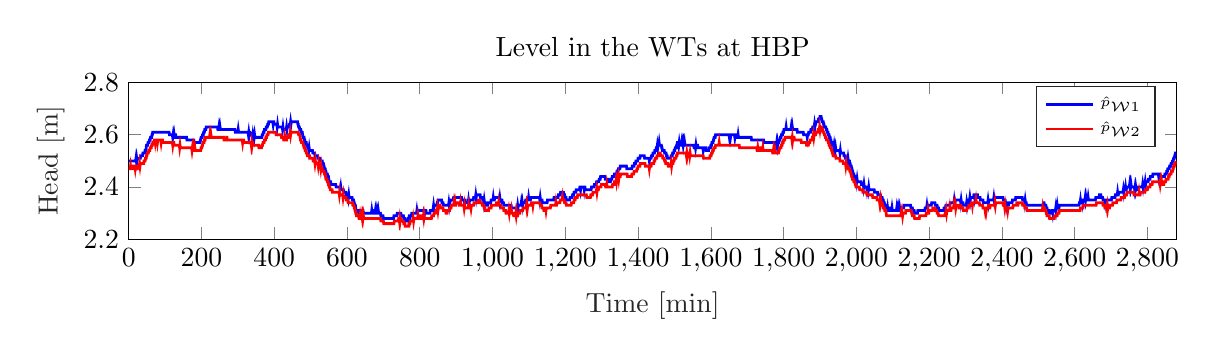
\begin{tikzpicture}

\begin{axis}[%
width=5.239in,
height=0.784in,
at={(1.208in,0.426in)},
scale only axis,
xmin=0,
xmax=2880,
xlabel style={font=\color{white!15!black}},
xlabel={Time [min]},
ymin=2.2,
ymax=2.8,
ylabel style={font=\color{white!15!black}},
ylabel={Head  [m]},
axis background/.style={fill=white},
title style={},
title={Level in the WTs at HBP},
legend style={legend cell align=left, align=left, draw=white!15!black}
]
\addplot [color=blue, line width=1.0pt]
  table[row sep=crcr]{%
0	2.5\\
1	2.5\\
2	2.5\\
3	2.5\\
4	2.5\\
5	2.5\\
6	2.5\\
7	2.5\\
8	2.5\\
9	2.5\\
10	2.5\\
11	2.5\\
12	2.5\\
13	2.5\\
14	2.5\\
15	2.5\\
16	2.5\\
17	2.5\\
18	2.5\\
19	2.5\\
20	2.51\\
21	2.5\\
22	2.51\\
23	2.5\\
24	2.51\\
25	2.51\\
26	2.51\\
27	2.51\\
28	2.51\\
29	2.51\\
30	2.51\\
31	2.51\\
32	2.51\\
33	2.52\\
34	2.52\\
35	2.52\\
36	2.52\\
37	2.52\\
38	2.52\\
39	2.53\\
40	2.53\\
41	2.53\\
42	2.53\\
43	2.53\\
44	2.53\\
45	2.54\\
46	2.54\\
47	2.54\\
48	2.55\\
49	2.56\\
50	2.56\\
51	2.56\\
52	2.56\\
53	2.57\\
54	2.57\\
55	2.57\\
56	2.57\\
57	2.58\\
58	2.58\\
59	2.58\\
60	2.59\\
61	2.59\\
62	2.59\\
63	2.59\\
64	2.6\\
65	2.6\\
66	2.61\\
67	2.61\\
68	2.61\\
69	2.61\\
70	2.61\\
71	2.61\\
72	2.61\\
73	2.61\\
74	2.61\\
75	2.61\\
76	2.61\\
77	2.61\\
78	2.61\\
79	2.61\\
80	2.61\\
81	2.61\\
82	2.61\\
83	2.61\\
84	2.61\\
85	2.61\\
86	2.61\\
87	2.61\\
88	2.61\\
89	2.61\\
90	2.61\\
91	2.61\\
92	2.61\\
93	2.61\\
94	2.61\\
95	2.61\\
96	2.61\\
97	2.61\\
98	2.61\\
99	2.61\\
100	2.61\\
101	2.61\\
102	2.61\\
103	2.61\\
104	2.61\\
105	2.61\\
106	2.61\\
107	2.61\\
108	2.61\\
109	2.61\\
110	2.61\\
111	2.61\\
112	2.6\\
113	2.6\\
114	2.6\\
115	2.6\\
116	2.6\\
117	2.6\\
118	2.6\\
119	2.6\\
120	2.6\\
121	2.59\\
122	2.6\\
123	2.59\\
124	2.59\\
125	2.6\\
126	2.59\\
127	2.59\\
128	2.6\\
129	2.6\\
130	2.59\\
131	2.59\\
132	2.59\\
133	2.59\\
134	2.59\\
135	2.59\\
136	2.59\\
137	2.59\\
138	2.59\\
139	2.59\\
140	2.59\\
141	2.59\\
142	2.59\\
143	2.59\\
144	2.59\\
145	2.59\\
146	2.59\\
147	2.59\\
148	2.59\\
149	2.59\\
150	2.59\\
151	2.59\\
152	2.59\\
153	2.59\\
154	2.59\\
155	2.59\\
156	2.59\\
157	2.59\\
158	2.59\\
159	2.59\\
160	2.58\\
161	2.58\\
162	2.58\\
163	2.58\\
164	2.58\\
165	2.58\\
166	2.58\\
167	2.58\\
168	2.58\\
169	2.58\\
170	2.58\\
171	2.58\\
172	2.58\\
173	2.58\\
174	2.58\\
175	2.58\\
176	2.58\\
177	2.58\\
178	2.58\\
179	2.57\\
180	2.57\\
181	2.57\\
182	2.57\\
183	2.57\\
184	2.57\\
185	2.57\\
186	2.57\\
187	2.57\\
188	2.57\\
189	2.57\\
190	2.57\\
191	2.57\\
192	2.57\\
193	2.57\\
194	2.57\\
195	2.57\\
196	2.57\\
197	2.58\\
198	2.58\\
199	2.59\\
200	2.59\\
201	2.59\\
202	2.59\\
203	2.6\\
204	2.6\\
205	2.6\\
206	2.61\\
207	2.61\\
208	2.61\\
209	2.62\\
210	2.62\\
211	2.62\\
212	2.62\\
213	2.63\\
214	2.63\\
215	2.63\\
216	2.63\\
217	2.63\\
218	2.63\\
219	2.63\\
220	2.63\\
221	2.63\\
222	2.63\\
223	2.63\\
224	2.63\\
225	2.63\\
226	2.63\\
227	2.63\\
228	2.63\\
229	2.63\\
230	2.63\\
231	2.63\\
232	2.63\\
233	2.63\\
234	2.63\\
235	2.63\\
236	2.63\\
237	2.63\\
238	2.63\\
239	2.63\\
240	2.63\\
241	2.63\\
242	2.63\\
243	2.63\\
244	2.63\\
245	2.62\\
246	2.62\\
247	2.62\\
248	2.63\\
249	2.62\\
250	2.62\\
251	2.63\\
252	2.62\\
253	2.62\\
254	2.62\\
255	2.62\\
256	2.62\\
257	2.62\\
258	2.62\\
259	2.62\\
260	2.62\\
261	2.62\\
262	2.62\\
263	2.62\\
264	2.62\\
265	2.62\\
266	2.62\\
267	2.62\\
268	2.62\\
269	2.62\\
270	2.62\\
271	2.62\\
272	2.62\\
273	2.62\\
274	2.62\\
275	2.62\\
276	2.62\\
277	2.62\\
278	2.62\\
279	2.62\\
280	2.62\\
281	2.62\\
282	2.62\\
283	2.62\\
284	2.62\\
285	2.62\\
286	2.62\\
287	2.62\\
288	2.62\\
289	2.62\\
290	2.62\\
291	2.62\\
292	2.62\\
293	2.61\\
294	2.61\\
295	2.61\\
296	2.61\\
297	2.61\\
298	2.61\\
299	2.61\\
300	2.61\\
301	2.62\\
302	2.61\\
303	2.61\\
304	2.61\\
305	2.61\\
306	2.61\\
307	2.61\\
308	2.61\\
309	2.61\\
310	2.61\\
311	2.61\\
312	2.61\\
313	2.61\\
314	2.61\\
315	2.61\\
316	2.61\\
317	2.61\\
318	2.61\\
319	2.61\\
320	2.61\\
321	2.61\\
322	2.61\\
323	2.61\\
324	2.61\\
325	2.61\\
326	2.61\\
327	2.61\\
328	2.61\\
329	2.6\\
330	2.61\\
331	2.6\\
332	2.61\\
333	2.61\\
334	2.6\\
335	2.6\\
336	2.6\\
337	2.6\\
338	2.6\\
339	2.6\\
340	2.59\\
341	2.6\\
342	2.59\\
343	2.6\\
344	2.6\\
345	2.59\\
346	2.6\\
347	2.59\\
348	2.59\\
349	2.59\\
350	2.59\\
351	2.59\\
352	2.59\\
353	2.59\\
354	2.59\\
355	2.59\\
356	2.59\\
357	2.59\\
358	2.59\\
359	2.59\\
360	2.59\\
361	2.59\\
362	2.59\\
363	2.59\\
364	2.59\\
365	2.59\\
366	2.59\\
367	2.6\\
368	2.6\\
369	2.6\\
370	2.61\\
371	2.61\\
372	2.61\\
373	2.62\\
374	2.62\\
375	2.62\\
376	2.62\\
377	2.62\\
378	2.63\\
379	2.63\\
380	2.63\\
381	2.63\\
382	2.64\\
383	2.64\\
384	2.64\\
385	2.65\\
386	2.65\\
387	2.65\\
388	2.65\\
389	2.65\\
390	2.65\\
391	2.65\\
392	2.65\\
393	2.65\\
394	2.65\\
395	2.65\\
396	2.65\\
397	2.64\\
398	2.65\\
399	2.65\\
400	2.64\\
401	2.64\\
402	2.64\\
403	2.64\\
404	2.64\\
405	2.64\\
406	2.64\\
407	2.64\\
408	2.63\\
409	2.64\\
410	2.63\\
411	2.63\\
412	2.63\\
413	2.63\\
414	2.63\\
415	2.63\\
416	2.63\\
417	2.63\\
418	2.63\\
419	2.63\\
420	2.63\\
421	2.63\\
422	2.63\\
423	2.62\\
424	2.63\\
425	2.62\\
426	2.62\\
427	2.62\\
428	2.62\\
429	2.62\\
430	2.62\\
431	2.62\\
432	2.62\\
433	2.62\\
434	2.63\\
435	2.62\\
436	2.63\\
437	2.63\\
438	2.63\\
439	2.63\\
440	2.63\\
441	2.63\\
442	2.64\\
443	2.64\\
444	2.64\\
445	2.65\\
446	2.64\\
447	2.65\\
448	2.65\\
449	2.65\\
450	2.65\\
451	2.65\\
452	2.65\\
453	2.65\\
454	2.65\\
455	2.65\\
456	2.65\\
457	2.65\\
458	2.65\\
459	2.65\\
460	2.65\\
461	2.65\\
462	2.65\\
463	2.65\\
464	2.65\\
465	2.64\\
466	2.64\\
467	2.63\\
468	2.63\\
469	2.63\\
470	2.62\\
471	2.62\\
472	2.62\\
473	2.62\\
474	2.61\\
475	2.61\\
476	2.61\\
477	2.61\\
478	2.6\\
479	2.59\\
480	2.59\\
481	2.59\\
482	2.59\\
483	2.58\\
484	2.58\\
485	2.57\\
486	2.57\\
487	2.57\\
488	2.57\\
489	2.56\\
490	2.56\\
491	2.56\\
492	2.55\\
493	2.55\\
494	2.55\\
495	2.54\\
496	2.55\\
497	2.54\\
498	2.54\\
499	2.54\\
500	2.54\\
501	2.54\\
502	2.54\\
503	2.54\\
504	2.54\\
505	2.54\\
506	2.53\\
507	2.53\\
508	2.53\\
509	2.53\\
510	2.53\\
511	2.53\\
512	2.52\\
513	2.52\\
514	2.52\\
515	2.52\\
516	2.52\\
517	2.52\\
518	2.52\\
519	2.52\\
520	2.51\\
521	2.51\\
522	2.51\\
523	2.51\\
524	2.51\\
525	2.51\\
526	2.51\\
527	2.5\\
528	2.5\\
529	2.5\\
530	2.5\\
531	2.5\\
532	2.5\\
533	2.49\\
534	2.49\\
535	2.49\\
536	2.48\\
537	2.48\\
538	2.47\\
539	2.47\\
540	2.47\\
541	2.46\\
542	2.46\\
543	2.45\\
544	2.45\\
545	2.45\\
546	2.45\\
547	2.44\\
548	2.44\\
549	2.44\\
550	2.43\\
551	2.42\\
552	2.42\\
553	2.42\\
554	2.42\\
555	2.42\\
556	2.41\\
557	2.41\\
558	2.41\\
559	2.41\\
560	2.41\\
561	2.41\\
562	2.41\\
563	2.41\\
564	2.41\\
565	2.41\\
566	2.41\\
567	2.41\\
568	2.41\\
569	2.41\\
570	2.4\\
571	2.4\\
572	2.4\\
573	2.4\\
574	2.4\\
575	2.4\\
576	2.4\\
577	2.4\\
578	2.4\\
579	2.4\\
580	2.4\\
581	2.39\\
582	2.39\\
583	2.4\\
584	2.39\\
585	2.39\\
586	2.39\\
587	2.39\\
588	2.39\\
589	2.39\\
590	2.39\\
591	2.38\\
592	2.38\\
593	2.38\\
594	2.38\\
595	2.38\\
596	2.38\\
597	2.38\\
598	2.37\\
599	2.37\\
600	2.37\\
601	2.37\\
602	2.37\\
603	2.37\\
604	2.36\\
605	2.37\\
606	2.36\\
607	2.36\\
608	2.36\\
609	2.36\\
610	2.36\\
611	2.36\\
612	2.36\\
613	2.36\\
614	2.36\\
615	2.35\\
616	2.35\\
617	2.35\\
618	2.35\\
619	2.34\\
620	2.34\\
621	2.33\\
622	2.33\\
623	2.33\\
624	2.32\\
625	2.31\\
626	2.31\\
627	2.31\\
628	2.31\\
629	2.31\\
630	2.31\\
631	2.31\\
632	2.3\\
633	2.3\\
634	2.3\\
635	2.31\\
636	2.31\\
637	2.31\\
638	2.3\\
639	2.3\\
640	2.3\\
641	2.31\\
642	2.31\\
643	2.31\\
644	2.31\\
645	2.3\\
646	2.3\\
647	2.3\\
648	2.3\\
649	2.3\\
650	2.3\\
651	2.3\\
652	2.3\\
653	2.3\\
654	2.3\\
655	2.3\\
656	2.3\\
657	2.3\\
658	2.3\\
659	2.3\\
660	2.3\\
661	2.3\\
662	2.3\\
663	2.3\\
664	2.3\\
665	2.3\\
666	2.3\\
667	2.3\\
668	2.31\\
669	2.3\\
670	2.3\\
671	2.31\\
672	2.31\\
673	2.3\\
674	2.3\\
675	2.3\\
676	2.3\\
677	2.3\\
678	2.31\\
679	2.3\\
680	2.3\\
681	2.3\\
682	2.31\\
683	2.3\\
684	2.3\\
685	2.3\\
686	2.31\\
687	2.3\\
688	2.3\\
689	2.3\\
690	2.3\\
691	2.3\\
692	2.3\\
693	2.29\\
694	2.29\\
695	2.29\\
696	2.29\\
697	2.29\\
698	2.29\\
699	2.29\\
700	2.28\\
701	2.28\\
702	2.28\\
703	2.28\\
704	2.28\\
705	2.28\\
706	2.28\\
707	2.28\\
708	2.28\\
709	2.28\\
710	2.28\\
711	2.28\\
712	2.28\\
713	2.28\\
714	2.28\\
715	2.28\\
716	2.28\\
717	2.28\\
718	2.28\\
719	2.28\\
720	2.28\\
721	2.28\\
722	2.28\\
723	2.28\\
724	2.28\\
725	2.28\\
726	2.28\\
727	2.28\\
728	2.28\\
729	2.29\\
730	2.29\\
731	2.29\\
732	2.29\\
733	2.29\\
734	2.29\\
735	2.29\\
736	2.29\\
737	2.29\\
738	2.3\\
739	2.3\\
740	2.3\\
741	2.3\\
742	2.3\\
743	2.3\\
744	2.3\\
745	2.3\\
746	2.3\\
747	2.3\\
748	2.3\\
749	2.29\\
750	2.29\\
751	2.29\\
752	2.29\\
753	2.29\\
754	2.29\\
755	2.29\\
756	2.28\\
757	2.28\\
758	2.28\\
759	2.28\\
760	2.27\\
761	2.27\\
762	2.27\\
763	2.27\\
764	2.27\\
765	2.27\\
766	2.27\\
767	2.27\\
768	2.28\\
769	2.28\\
770	2.28\\
771	2.29\\
772	2.29\\
773	2.28\\
774	2.29\\
775	2.29\\
776	2.29\\
777	2.29\\
778	2.3\\
779	2.3\\
780	2.3\\
781	2.3\\
782	2.3\\
783	2.3\\
784	2.3\\
785	2.3\\
786	2.3\\
787	2.3\\
788	2.3\\
789	2.3\\
790	2.3\\
791	2.3\\
792	2.31\\
793	2.3\\
794	2.3\\
795	2.31\\
796	2.31\\
797	2.31\\
798	2.31\\
799	2.31\\
800	2.31\\
801	2.31\\
802	2.31\\
803	2.31\\
804	2.31\\
805	2.31\\
806	2.31\\
807	2.31\\
808	2.31\\
809	2.31\\
810	2.31\\
811	2.31\\
812	2.31\\
813	2.3\\
814	2.31\\
815	2.31\\
816	2.31\\
817	2.31\\
818	2.3\\
819	2.3\\
820	2.3\\
821	2.3\\
822	2.3\\
823	2.3\\
824	2.3\\
825	2.3\\
826	2.3\\
827	2.3\\
828	2.3\\
829	2.31\\
830	2.31\\
831	2.31\\
832	2.31\\
833	2.31\\
834	2.31\\
835	2.31\\
836	2.31\\
837	2.32\\
838	2.33\\
839	2.32\\
840	2.33\\
841	2.33\\
842	2.33\\
843	2.33\\
844	2.33\\
845	2.33\\
846	2.33\\
847	2.33\\
848	2.34\\
849	2.34\\
850	2.35\\
851	2.35\\
852	2.35\\
853	2.35\\
854	2.35\\
855	2.35\\
856	2.35\\
857	2.35\\
858	2.35\\
859	2.35\\
860	2.35\\
861	2.34\\
862	2.34\\
863	2.34\\
864	2.34\\
865	2.33\\
866	2.33\\
867	2.33\\
868	2.33\\
869	2.33\\
870	2.33\\
871	2.33\\
872	2.33\\
873	2.33\\
874	2.33\\
875	2.33\\
876	2.33\\
877	2.33\\
878	2.33\\
879	2.33\\
880	2.34\\
881	2.33\\
882	2.34\\
883	2.34\\
884	2.35\\
885	2.35\\
886	2.35\\
887	2.35\\
888	2.35\\
889	2.35\\
890	2.35\\
891	2.35\\
892	2.35\\
893	2.36\\
894	2.36\\
895	2.36\\
896	2.36\\
897	2.36\\
898	2.36\\
899	2.36\\
900	2.36\\
901	2.36\\
902	2.36\\
903	2.36\\
904	2.36\\
905	2.36\\
906	2.36\\
907	2.36\\
908	2.36\\
909	2.36\\
910	2.36\\
911	2.36\\
912	2.36\\
913	2.36\\
914	2.36\\
915	2.36\\
916	2.35\\
917	2.35\\
918	2.35\\
919	2.35\\
920	2.35\\
921	2.35\\
922	2.35\\
923	2.34\\
924	2.35\\
925	2.35\\
926	2.34\\
927	2.34\\
928	2.34\\
929	2.34\\
930	2.34\\
931	2.34\\
932	2.34\\
933	2.34\\
934	2.35\\
935	2.34\\
936	2.34\\
937	2.35\\
938	2.35\\
939	2.35\\
940	2.35\\
941	2.35\\
942	2.35\\
943	2.35\\
944	2.35\\
945	2.35\\
946	2.35\\
947	2.35\\
948	2.36\\
949	2.36\\
950	2.36\\
951	2.36\\
952	2.36\\
953	2.36\\
954	2.37\\
955	2.36\\
956	2.37\\
957	2.37\\
958	2.37\\
959	2.37\\
960	2.37\\
961	2.37\\
962	2.37\\
963	2.37\\
964	2.37\\
965	2.37\\
966	2.37\\
967	2.36\\
968	2.36\\
969	2.36\\
970	2.36\\
971	2.36\\
972	2.36\\
973	2.35\\
974	2.35\\
975	2.35\\
976	2.34\\
977	2.35\\
978	2.34\\
979	2.34\\
980	2.34\\
981	2.33\\
982	2.33\\
983	2.33\\
984	2.33\\
985	2.33\\
986	2.33\\
987	2.33\\
988	2.34\\
989	2.34\\
990	2.34\\
991	2.34\\
992	2.34\\
993	2.34\\
994	2.34\\
995	2.34\\
996	2.35\\
997	2.35\\
998	2.35\\
999	2.35\\
1000	2.35\\
1001	2.35\\
1002	2.36\\
1003	2.35\\
1004	2.35\\
1005	2.35\\
1006	2.36\\
1007	2.36\\
1008	2.36\\
1009	2.36\\
1010	2.36\\
1011	2.36\\
1012	2.36\\
1013	2.36\\
1014	2.36\\
1015	2.36\\
1016	2.36\\
1017	2.36\\
1018	2.36\\
1019	2.35\\
1020	2.36\\
1021	2.35\\
1022	2.35\\
1023	2.35\\
1024	2.35\\
1025	2.35\\
1026	2.35\\
1027	2.34\\
1028	2.34\\
1029	2.34\\
1030	2.34\\
1031	2.33\\
1032	2.33\\
1033	2.33\\
1034	2.33\\
1035	2.33\\
1036	2.33\\
1037	2.33\\
1038	2.33\\
1039	2.33\\
1040	2.33\\
1041	2.33\\
1042	2.33\\
1043	2.33\\
1044	2.33\\
1045	2.33\\
1046	2.33\\
1047	2.33\\
1048	2.33\\
1049	2.33\\
1050	2.33\\
1051	2.33\\
1052	2.32\\
1053	2.32\\
1054	2.32\\
1055	2.32\\
1056	2.32\\
1057	2.32\\
1058	2.32\\
1059	2.32\\
1060	2.32\\
1061	2.32\\
1062	2.32\\
1063	2.32\\
1064	2.32\\
1065	2.32\\
1066	2.32\\
1067	2.32\\
1068	2.32\\
1069	2.33\\
1070	2.32\\
1071	2.33\\
1072	2.33\\
1073	2.33\\
1074	2.33\\
1075	2.33\\
1076	2.33\\
1077	2.33\\
1078	2.33\\
1079	2.34\\
1080	2.33\\
1081	2.33\\
1082	2.34\\
1083	2.33\\
1084	2.34\\
1085	2.34\\
1086	2.34\\
1087	2.34\\
1088	2.34\\
1089	2.34\\
1090	2.34\\
1091	2.35\\
1092	2.35\\
1093	2.35\\
1094	2.35\\
1095	2.35\\
1096	2.35\\
1097	2.35\\
1098	2.35\\
1099	2.36\\
1100	2.35\\
1101	2.35\\
1102	2.35\\
1103	2.35\\
1104	2.35\\
1105	2.36\\
1106	2.36\\
1107	2.36\\
1108	2.36\\
1109	2.36\\
1110	2.36\\
1111	2.36\\
1112	2.36\\
1113	2.36\\
1114	2.36\\
1115	2.36\\
1116	2.36\\
1117	2.36\\
1118	2.36\\
1119	2.36\\
1120	2.36\\
1121	2.36\\
1122	2.36\\
1123	2.36\\
1124	2.36\\
1125	2.36\\
1126	2.36\\
1127	2.36\\
1128	2.36\\
1129	2.36\\
1130	2.35\\
1131	2.36\\
1132	2.35\\
1133	2.35\\
1134	2.35\\
1135	2.35\\
1136	2.35\\
1137	2.34\\
1138	2.34\\
1139	2.34\\
1140	2.34\\
1141	2.34\\
1142	2.34\\
1143	2.34\\
1144	2.34\\
1145	2.34\\
1146	2.34\\
1147	2.34\\
1148	2.34\\
1149	2.34\\
1150	2.34\\
1151	2.35\\
1152	2.35\\
1153	2.35\\
1154	2.35\\
1155	2.35\\
1156	2.35\\
1157	2.35\\
1158	2.35\\
1159	2.35\\
1160	2.35\\
1161	2.35\\
1162	2.35\\
1163	2.35\\
1164	2.35\\
1165	2.35\\
1166	2.35\\
1167	2.35\\
1168	2.35\\
1169	2.36\\
1170	2.36\\
1171	2.36\\
1172	2.36\\
1173	2.36\\
1174	2.36\\
1175	2.36\\
1176	2.36\\
1177	2.36\\
1178	2.36\\
1179	2.36\\
1180	2.36\\
1181	2.37\\
1182	2.37\\
1183	2.37\\
1184	2.37\\
1185	2.37\\
1186	2.37\\
1187	2.38\\
1188	2.38\\
1189	2.38\\
1190	2.38\\
1191	2.38\\
1192	2.38\\
1193	2.38\\
1194	2.38\\
1195	2.38\\
1196	2.37\\
1197	2.37\\
1198	2.37\\
1199	2.36\\
1200	2.36\\
1201	2.36\\
1202	2.36\\
1203	2.35\\
1204	2.35\\
1205	2.35\\
1206	2.35\\
1207	2.35\\
1208	2.35\\
1209	2.35\\
1210	2.35\\
1211	2.35\\
1212	2.35\\
1213	2.36\\
1214	2.36\\
1215	2.36\\
1216	2.36\\
1217	2.36\\
1218	2.36\\
1219	2.36\\
1220	2.37\\
1221	2.37\\
1222	2.37\\
1223	2.37\\
1224	2.38\\
1225	2.38\\
1226	2.38\\
1227	2.38\\
1228	2.38\\
1229	2.38\\
1230	2.39\\
1231	2.39\\
1232	2.39\\
1233	2.39\\
1234	2.39\\
1235	2.39\\
1236	2.39\\
1237	2.39\\
1238	2.39\\
1239	2.39\\
1240	2.4\\
1241	2.4\\
1242	2.39\\
1243	2.4\\
1244	2.4\\
1245	2.4\\
1246	2.4\\
1247	2.4\\
1248	2.4\\
1249	2.4\\
1250	2.4\\
1251	2.4\\
1252	2.39\\
1253	2.4\\
1254	2.4\\
1255	2.39\\
1256	2.39\\
1257	2.39\\
1258	2.39\\
1259	2.39\\
1260	2.39\\
1261	2.39\\
1262	2.39\\
1263	2.39\\
1264	2.39\\
1265	2.39\\
1266	2.39\\
1267	2.39\\
1268	2.39\\
1269	2.39\\
1270	2.39\\
1271	2.39\\
1272	2.4\\
1273	2.4\\
1274	2.4\\
1275	2.4\\
1276	2.4\\
1277	2.4\\
1278	2.4\\
1279	2.4\\
1280	2.41\\
1281	2.41\\
1282	2.41\\
1283	2.41\\
1284	2.41\\
1285	2.41\\
1286	2.42\\
1287	2.42\\
1288	2.42\\
1289	2.42\\
1290	2.42\\
1291	2.42\\
1292	2.42\\
1293	2.43\\
1294	2.43\\
1295	2.43\\
1296	2.43\\
1297	2.44\\
1298	2.44\\
1299	2.44\\
1300	2.44\\
1301	2.44\\
1302	2.44\\
1303	2.44\\
1304	2.44\\
1305	2.44\\
1306	2.44\\
1307	2.44\\
1308	2.44\\
1309	2.44\\
1310	2.43\\
1311	2.43\\
1312	2.43\\
1313	2.43\\
1314	2.43\\
1315	2.43\\
1316	2.43\\
1317	2.43\\
1318	2.42\\
1319	2.42\\
1320	2.42\\
1321	2.42\\
1322	2.42\\
1323	2.42\\
1324	2.42\\
1325	2.43\\
1326	2.43\\
1327	2.43\\
1328	2.43\\
1329	2.44\\
1330	2.44\\
1331	2.44\\
1332	2.44\\
1333	2.44\\
1334	2.44\\
1335	2.45\\
1336	2.45\\
1337	2.45\\
1338	2.45\\
1339	2.45\\
1340	2.45\\
1341	2.45\\
1342	2.46\\
1343	2.46\\
1344	2.46\\
1345	2.46\\
1346	2.47\\
1347	2.47\\
1348	2.47\\
1349	2.47\\
1350	2.47\\
1351	2.48\\
1352	2.48\\
1353	2.48\\
1354	2.48\\
1355	2.48\\
1356	2.48\\
1357	2.48\\
1358	2.48\\
1359	2.48\\
1360	2.48\\
1361	2.48\\
1362	2.48\\
1363	2.48\\
1364	2.48\\
1365	2.48\\
1366	2.48\\
1367	2.48\\
1368	2.48\\
1369	2.47\\
1370	2.47\\
1371	2.47\\
1372	2.47\\
1373	2.47\\
1374	2.47\\
1375	2.47\\
1376	2.47\\
1377	2.47\\
1378	2.47\\
1379	2.47\\
1380	2.47\\
1381	2.47\\
1382	2.47\\
1383	2.47\\
1384	2.48\\
1385	2.48\\
1386	2.48\\
1387	2.48\\
1388	2.48\\
1389	2.48\\
1390	2.49\\
1391	2.49\\
1392	2.49\\
1393	2.49\\
1394	2.5\\
1395	2.5\\
1396	2.5\\
1397	2.5\\
1398	2.5\\
1399	2.5\\
1400	2.51\\
1401	2.51\\
1402	2.51\\
1403	2.51\\
1404	2.51\\
1405	2.51\\
1406	2.52\\
1407	2.52\\
1408	2.52\\
1409	2.52\\
1410	2.52\\
1411	2.52\\
1412	2.52\\
1413	2.52\\
1414	2.52\\
1415	2.52\\
1416	2.52\\
1417	2.52\\
1418	2.51\\
1419	2.51\\
1420	2.51\\
1421	2.51\\
1422	2.51\\
1423	2.51\\
1424	2.51\\
1425	2.51\\
1426	2.51\\
1427	2.51\\
1428	2.51\\
1429	2.51\\
1430	2.51\\
1431	2.5\\
1432	2.51\\
1433	2.51\\
1434	2.51\\
1435	2.51\\
1436	2.51\\
1437	2.52\\
1438	2.52\\
1439	2.52\\
1440	2.52\\
1441	2.53\\
1442	2.53\\
1443	2.53\\
1444	2.53\\
1445	2.53\\
1446	2.54\\
1447	2.54\\
1448	2.54\\
1449	2.54\\
1450	2.55\\
1451	2.55\\
1452	2.55\\
1453	2.56\\
1454	2.55\\
1455	2.56\\
1456	2.56\\
1457	2.56\\
1458	2.57\\
1459	2.56\\
1460	2.56\\
1461	2.56\\
1462	2.56\\
1463	2.56\\
1464	2.56\\
1465	2.55\\
1466	2.55\\
1467	2.54\\
1468	2.54\\
1469	2.54\\
1470	2.54\\
1471	2.54\\
1472	2.54\\
1473	2.53\\
1474	2.53\\
1475	2.53\\
1476	2.53\\
1477	2.53\\
1478	2.52\\
1479	2.52\\
1480	2.52\\
1481	2.51\\
1482	2.51\\
1483	2.51\\
1484	2.51\\
1485	2.51\\
1486	2.51\\
1487	2.51\\
1488	2.51\\
1489	2.51\\
1490	2.51\\
1491	2.52\\
1492	2.52\\
1493	2.52\\
1494	2.52\\
1495	2.53\\
1496	2.53\\
1497	2.53\\
1498	2.53\\
1499	2.54\\
1500	2.54\\
1501	2.54\\
1502	2.55\\
1503	2.55\\
1504	2.55\\
1505	2.55\\
1506	2.56\\
1507	2.56\\
1508	2.57\\
1509	2.57\\
1510	2.57\\
1511	2.57\\
1512	2.56\\
1513	2.57\\
1514	2.56\\
1515	2.56\\
1516	2.56\\
1517	2.56\\
1518	2.56\\
1519	2.56\\
1520	2.57\\
1521	2.56\\
1522	2.56\\
1523	2.57\\
1524	2.56\\
1525	2.57\\
1526	2.56\\
1527	2.56\\
1528	2.57\\
1529	2.56\\
1530	2.56\\
1531	2.56\\
1532	2.56\\
1533	2.56\\
1534	2.56\\
1535	2.56\\
1536	2.56\\
1537	2.56\\
1538	2.56\\
1539	2.56\\
1540	2.56\\
1541	2.56\\
1542	2.56\\
1543	2.56\\
1544	2.56\\
1545	2.56\\
1546	2.56\\
1547	2.56\\
1548	2.56\\
1549	2.56\\
1550	2.56\\
1551	2.56\\
1552	2.56\\
1553	2.56\\
1554	2.55\\
1555	2.55\\
1556	2.56\\
1557	2.56\\
1558	2.55\\
1559	2.56\\
1560	2.55\\
1561	2.55\\
1562	2.56\\
1563	2.56\\
1564	2.56\\
1565	2.55\\
1566	2.55\\
1567	2.55\\
1568	2.55\\
1569	2.55\\
1570	2.55\\
1571	2.55\\
1572	2.55\\
1573	2.55\\
1574	2.55\\
1575	2.55\\
1576	2.55\\
1577	2.55\\
1578	2.55\\
1579	2.54\\
1580	2.55\\
1581	2.55\\
1582	2.55\\
1583	2.55\\
1584	2.55\\
1585	2.55\\
1586	2.55\\
1587	2.54\\
1588	2.54\\
1589	2.54\\
1590	2.54\\
1591	2.54\\
1592	2.54\\
1593	2.54\\
1594	2.54\\
1595	2.55\\
1596	2.55\\
1597	2.55\\
1598	2.55\\
1599	2.55\\
1600	2.56\\
1601	2.56\\
1602	2.56\\
1603	2.57\\
1604	2.57\\
1605	2.57\\
1606	2.57\\
1607	2.58\\
1608	2.58\\
1609	2.59\\
1610	2.59\\
1611	2.59\\
1612	2.59\\
1613	2.6\\
1614	2.6\\
1615	2.6\\
1616	2.6\\
1617	2.6\\
1618	2.6\\
1619	2.6\\
1620	2.6\\
1621	2.6\\
1622	2.6\\
1623	2.6\\
1624	2.6\\
1625	2.6\\
1626	2.6\\
1627	2.6\\
1628	2.6\\
1629	2.6\\
1630	2.6\\
1631	2.6\\
1632	2.6\\
1633	2.6\\
1634	2.6\\
1635	2.6\\
1636	2.6\\
1637	2.6\\
1638	2.6\\
1639	2.6\\
1640	2.6\\
1641	2.6\\
1642	2.6\\
1643	2.6\\
1644	2.6\\
1645	2.6\\
1646	2.6\\
1647	2.6\\
1648	2.6\\
1649	2.6\\
1650	2.6\\
1651	2.59\\
1652	2.6\\
1653	2.6\\
1654	2.59\\
1655	2.6\\
1656	2.6\\
1657	2.6\\
1658	2.6\\
1659	2.6\\
1660	2.6\\
1661	2.6\\
1662	2.6\\
1663	2.6\\
1664	2.6\\
1665	2.6\\
1666	2.59\\
1667	2.6\\
1668	2.6\\
1669	2.59\\
1670	2.59\\
1671	2.59\\
1672	2.59\\
1673	2.59\\
1674	2.59\\
1675	2.6\\
1676	2.59\\
1677	2.59\\
1678	2.59\\
1679	2.59\\
1680	2.59\\
1681	2.59\\
1682	2.59\\
1683	2.59\\
1684	2.59\\
1685	2.59\\
1686	2.59\\
1687	2.59\\
1688	2.59\\
1689	2.59\\
1690	2.59\\
1691	2.59\\
1692	2.59\\
1693	2.59\\
1694	2.59\\
1695	2.59\\
1696	2.59\\
1697	2.59\\
1698	2.59\\
1699	2.59\\
1700	2.59\\
1701	2.59\\
1702	2.59\\
1703	2.59\\
1704	2.59\\
1705	2.59\\
1706	2.59\\
1707	2.59\\
1708	2.59\\
1709	2.59\\
1710	2.59\\
1711	2.59\\
1712	2.58\\
1713	2.58\\
1714	2.58\\
1715	2.58\\
1716	2.58\\
1717	2.58\\
1718	2.58\\
1719	2.58\\
1720	2.58\\
1721	2.58\\
1722	2.58\\
1723	2.58\\
1724	2.58\\
1725	2.58\\
1726	2.58\\
1727	2.58\\
1728	2.58\\
1729	2.58\\
1730	2.58\\
1731	2.58\\
1732	2.58\\
1733	2.58\\
1734	2.58\\
1735	2.58\\
1736	2.58\\
1737	2.58\\
1738	2.58\\
1739	2.58\\
1740	2.58\\
1741	2.58\\
1742	2.58\\
1743	2.58\\
1744	2.58\\
1745	2.58\\
1746	2.57\\
1747	2.57\\
1748	2.57\\
1749	2.57\\
1750	2.57\\
1751	2.57\\
1752	2.57\\
1753	2.57\\
1754	2.57\\
1755	2.57\\
1756	2.57\\
1757	2.57\\
1758	2.57\\
1759	2.57\\
1760	2.57\\
1761	2.57\\
1762	2.57\\
1763	2.57\\
1764	2.57\\
1765	2.57\\
1766	2.57\\
1767	2.57\\
1768	2.57\\
1769	2.57\\
1770	2.57\\
1771	2.57\\
1772	2.57\\
1773	2.57\\
1774	2.57\\
1775	2.57\\
1776	2.57\\
1777	2.57\\
1778	2.56\\
1779	2.56\\
1780	2.56\\
1781	2.57\\
1782	2.56\\
1783	2.57\\
1784	2.56\\
1785	2.57\\
1786	2.57\\
1787	2.57\\
1788	2.58\\
1789	2.58\\
1790	2.58\\
1791	2.59\\
1792	2.59\\
1793	2.59\\
1794	2.6\\
1795	2.6\\
1796	2.6\\
1797	2.6\\
1798	2.61\\
1799	2.61\\
1800	2.61\\
1801	2.62\\
1802	2.62\\
1803	2.62\\
1804	2.62\\
1805	2.62\\
1806	2.62\\
1807	2.63\\
1808	2.62\\
1809	2.62\\
1810	2.62\\
1811	2.62\\
1812	2.62\\
1813	2.62\\
1814	2.62\\
1815	2.62\\
1816	2.62\\
1817	2.62\\
1818	2.62\\
1819	2.62\\
1820	2.62\\
1821	2.63\\
1822	2.62\\
1823	2.62\\
1824	2.63\\
1825	2.62\\
1826	2.62\\
1827	2.62\\
1828	2.62\\
1829	2.62\\
1830	2.62\\
1831	2.62\\
1832	2.62\\
1833	2.62\\
1834	2.62\\
1835	2.62\\
1836	2.62\\
1837	2.62\\
1838	2.61\\
1839	2.61\\
1840	2.61\\
1841	2.61\\
1842	2.61\\
1843	2.61\\
1844	2.61\\
1845	2.61\\
1846	2.61\\
1847	2.61\\
1848	2.61\\
1849	2.61\\
1850	2.61\\
1851	2.61\\
1852	2.61\\
1853	2.61\\
1854	2.61\\
1855	2.6\\
1856	2.6\\
1857	2.6\\
1858	2.6\\
1859	2.6\\
1860	2.6\\
1861	2.6\\
1862	2.6\\
1863	2.6\\
1864	2.6\\
1865	2.59\\
1866	2.6\\
1867	2.6\\
1868	2.6\\
1869	2.61\\
1870	2.61\\
1871	2.61\\
1872	2.61\\
1873	2.61\\
1874	2.61\\
1875	2.62\\
1876	2.62\\
1877	2.62\\
1878	2.62\\
1879	2.62\\
1880	2.63\\
1881	2.63\\
1882	2.63\\
1883	2.63\\
1884	2.63\\
1885	2.64\\
1886	2.63\\
1887	2.64\\
1888	2.64\\
1889	2.65\\
1890	2.65\\
1891	2.65\\
1892	2.65\\
1893	2.65\\
1894	2.65\\
1895	2.65\\
1896	2.66\\
1897	2.66\\
1898	2.66\\
1899	2.66\\
1900	2.67\\
1901	2.67\\
1902	2.67\\
1903	2.67\\
1904	2.66\\
1905	2.66\\
1906	2.65\\
1907	2.65\\
1908	2.65\\
1909	2.65\\
1910	2.64\\
1911	2.64\\
1912	2.63\\
1913	2.63\\
1914	2.63\\
1915	2.63\\
1916	2.63\\
1917	2.62\\
1918	2.62\\
1919	2.62\\
1920	2.61\\
1921	2.61\\
1922	2.61\\
1923	2.6\\
1924	2.6\\
1925	2.6\\
1926	2.59\\
1927	2.59\\
1928	2.59\\
1929	2.58\\
1930	2.58\\
1931	2.57\\
1932	2.57\\
1933	2.57\\
1934	2.56\\
1935	2.56\\
1936	2.56\\
1937	2.56\\
1938	2.55\\
1939	2.56\\
1940	2.55\\
1941	2.55\\
1942	2.54\\
1943	2.55\\
1944	2.54\\
1945	2.54\\
1946	2.54\\
1947	2.54\\
1948	2.54\\
1949	2.54\\
1950	2.54\\
1951	2.54\\
1952	2.54\\
1953	2.54\\
1954	2.54\\
1955	2.53\\
1956	2.54\\
1957	2.53\\
1958	2.53\\
1959	2.53\\
1960	2.53\\
1961	2.53\\
1962	2.53\\
1963	2.53\\
1964	2.53\\
1965	2.53\\
1966	2.52\\
1967	2.52\\
1968	2.52\\
1969	2.52\\
1970	2.51\\
1971	2.51\\
1972	2.51\\
1973	2.51\\
1974	2.51\\
1975	2.51\\
1976	2.5\\
1977	2.51\\
1978	2.5\\
1979	2.5\\
1980	2.5\\
1981	2.5\\
1982	2.49\\
1983	2.49\\
1984	2.48\\
1985	2.48\\
1986	2.48\\
1987	2.47\\
1988	2.47\\
1989	2.46\\
1990	2.46\\
1991	2.45\\
1992	2.45\\
1993	2.45\\
1994	2.44\\
1995	2.44\\
1996	2.44\\
1997	2.44\\
1998	2.43\\
1999	2.43\\
2000	2.43\\
2001	2.42\\
2002	2.43\\
2003	2.42\\
2004	2.42\\
2005	2.42\\
2006	2.42\\
2007	2.42\\
2008	2.42\\
2009	2.42\\
2010	2.42\\
2011	2.42\\
2012	2.42\\
2013	2.42\\
2014	2.41\\
2015	2.41\\
2016	2.41\\
2017	2.41\\
2018	2.41\\
2019	2.41\\
2020	2.4\\
2021	2.41\\
2022	2.4\\
2023	2.4\\
2024	2.4\\
2025	2.4\\
2026	2.4\\
2027	2.4\\
2028	2.4\\
2029	2.39\\
2030	2.4\\
2031	2.4\\
2032	2.4\\
2033	2.39\\
2034	2.4\\
2035	2.39\\
2036	2.39\\
2037	2.39\\
2038	2.39\\
2039	2.39\\
2040	2.39\\
2041	2.39\\
2042	2.39\\
2043	2.39\\
2044	2.39\\
2045	2.39\\
2046	2.39\\
2047	2.39\\
2048	2.39\\
2049	2.39\\
2050	2.38\\
2051	2.38\\
2052	2.38\\
2053	2.38\\
2054	2.38\\
2055	2.38\\
2056	2.38\\
2057	2.38\\
2058	2.38\\
2059	2.37\\
2060	2.37\\
2061	2.37\\
2062	2.37\\
2063	2.37\\
2064	2.37\\
2065	2.37\\
2066	2.37\\
2067	2.36\\
2068	2.36\\
2069	2.36\\
2070	2.36\\
2071	2.36\\
2072	2.35\\
2073	2.35\\
2074	2.35\\
2075	2.34\\
2076	2.34\\
2077	2.34\\
2078	2.33\\
2079	2.33\\
2080	2.33\\
2081	2.32\\
2082	2.32\\
2083	2.32\\
2084	2.31\\
2085	2.31\\
2086	2.32\\
2087	2.31\\
2088	2.31\\
2089	2.31\\
2090	2.32\\
2091	2.32\\
2092	2.32\\
2093	2.31\\
2094	2.31\\
2095	2.31\\
2096	2.31\\
2097	2.31\\
2098	2.32\\
2099	2.31\\
2100	2.31\\
2101	2.31\\
2102	2.31\\
2103	2.31\\
2104	2.31\\
2105	2.31\\
2106	2.31\\
2107	2.31\\
2108	2.31\\
2109	2.31\\
2110	2.31\\
2111	2.32\\
2112	2.31\\
2113	2.31\\
2114	2.31\\
2115	2.32\\
2116	2.31\\
2117	2.31\\
2118	2.31\\
2119	2.32\\
2120	2.31\\
2121	2.31\\
2122	2.32\\
2123	2.32\\
2124	2.32\\
2125	2.32\\
2126	2.32\\
2127	2.32\\
2128	2.32\\
2129	2.32\\
2130	2.32\\
2131	2.33\\
2132	2.33\\
2133	2.33\\
2134	2.33\\
2135	2.33\\
2136	2.33\\
2137	2.33\\
2138	2.33\\
2139	2.33\\
2140	2.33\\
2141	2.33\\
2142	2.33\\
2143	2.33\\
2144	2.33\\
2145	2.33\\
2146	2.33\\
2147	2.33\\
2148	2.33\\
2149	2.33\\
2150	2.32\\
2151	2.32\\
2152	2.32\\
2153	2.32\\
2154	2.32\\
2155	2.31\\
2156	2.31\\
2157	2.31\\
2158	2.31\\
2159	2.31\\
2160	2.3\\
2161	2.3\\
2162	2.3\\
2163	2.3\\
2164	2.3\\
2165	2.3\\
2166	2.3\\
2167	2.3\\
2168	2.3\\
2169	2.31\\
2170	2.31\\
2171	2.31\\
2172	2.31\\
2173	2.31\\
2174	2.31\\
2175	2.31\\
2176	2.31\\
2177	2.31\\
2178	2.31\\
2179	2.31\\
2180	2.31\\
2181	2.31\\
2182	2.31\\
2183	2.31\\
2184	2.31\\
2185	2.31\\
2186	2.31\\
2187	2.31\\
2188	2.31\\
2189	2.32\\
2190	2.32\\
2191	2.32\\
2192	2.32\\
2193	2.32\\
2194	2.33\\
2195	2.32\\
2196	2.32\\
2197	2.33\\
2198	2.33\\
2199	2.33\\
2200	2.33\\
2201	2.33\\
2202	2.33\\
2203	2.33\\
2204	2.33\\
2205	2.33\\
2206	2.33\\
2207	2.34\\
2208	2.34\\
2209	2.34\\
2210	2.34\\
2211	2.34\\
2212	2.34\\
2213	2.34\\
2214	2.34\\
2215	2.34\\
2216	2.34\\
2217	2.33\\
2218	2.33\\
2219	2.33\\
2220	2.33\\
2221	2.33\\
2222	2.33\\
2223	2.32\\
2224	2.32\\
2225	2.32\\
2226	2.32\\
2227	2.31\\
2228	2.31\\
2229	2.31\\
2230	2.31\\
2231	2.31\\
2232	2.31\\
2233	2.31\\
2234	2.31\\
2235	2.31\\
2236	2.31\\
2237	2.31\\
2238	2.31\\
2239	2.31\\
2240	2.31\\
2241	2.32\\
2242	2.32\\
2243	2.32\\
2244	2.32\\
2245	2.32\\
2246	2.33\\
2247	2.33\\
2248	2.33\\
2249	2.33\\
2250	2.33\\
2251	2.33\\
2252	2.33\\
2253	2.33\\
2254	2.33\\
2255	2.33\\
2256	2.33\\
2257	2.33\\
2258	2.34\\
2259	2.34\\
2260	2.34\\
2261	2.34\\
2262	2.34\\
2263	2.34\\
2264	2.34\\
2265	2.34\\
2266	2.34\\
2267	2.34\\
2268	2.34\\
2269	2.35\\
2270	2.34\\
2271	2.34\\
2272	2.35\\
2273	2.35\\
2274	2.35\\
2275	2.35\\
2276	2.35\\
2277	2.35\\
2278	2.35\\
2279	2.35\\
2280	2.35\\
2281	2.35\\
2282	2.35\\
2283	2.35\\
2284	2.35\\
2285	2.35\\
2286	2.35\\
2287	2.34\\
2288	2.35\\
2289	2.34\\
2290	2.34\\
2291	2.34\\
2292	2.34\\
2293	2.34\\
2294	2.33\\
2295	2.33\\
2296	2.33\\
2297	2.33\\
2298	2.33\\
2299	2.33\\
2300	2.33\\
2301	2.33\\
2302	2.33\\
2303	2.34\\
2304	2.33\\
2305	2.34\\
2306	2.34\\
2307	2.34\\
2308	2.35\\
2309	2.35\\
2310	2.35\\
2311	2.35\\
2312	2.36\\
2313	2.35\\
2314	2.36\\
2315	2.36\\
2316	2.36\\
2317	2.36\\
2318	2.36\\
2319	2.36\\
2320	2.36\\
2321	2.36\\
2322	2.36\\
2323	2.37\\
2324	2.37\\
2325	2.36\\
2326	2.37\\
2327	2.37\\
2328	2.37\\
2329	2.37\\
2330	2.37\\
2331	2.37\\
2332	2.37\\
2333	2.37\\
2334	2.36\\
2335	2.36\\
2336	2.36\\
2337	2.36\\
2338	2.36\\
2339	2.36\\
2340	2.36\\
2341	2.35\\
2342	2.35\\
2343	2.35\\
2344	2.35\\
2345	2.35\\
2346	2.35\\
2347	2.35\\
2348	2.35\\
2349	2.34\\
2350	2.34\\
2351	2.34\\
2352	2.34\\
2353	2.34\\
2354	2.34\\
2355	2.34\\
2356	2.34\\
2357	2.34\\
2358	2.34\\
2359	2.34\\
2360	2.34\\
2361	2.34\\
2362	2.35\\
2363	2.34\\
2364	2.35\\
2365	2.35\\
2366	2.35\\
2367	2.35\\
2368	2.35\\
2369	2.35\\
2370	2.35\\
2371	2.35\\
2372	2.35\\
2373	2.35\\
2374	2.35\\
2375	2.35\\
2376	2.35\\
2377	2.35\\
2378	2.36\\
2379	2.35\\
2380	2.36\\
2381	2.36\\
2382	2.36\\
2383	2.36\\
2384	2.36\\
2385	2.36\\
2386	2.36\\
2387	2.36\\
2388	2.36\\
2389	2.36\\
2390	2.36\\
2391	2.36\\
2392	2.36\\
2393	2.36\\
2394	2.36\\
2395	2.36\\
2396	2.36\\
2397	2.36\\
2398	2.36\\
2399	2.36\\
2400	2.36\\
2401	2.36\\
2402	2.36\\
2403	2.36\\
2404	2.35\\
2405	2.35\\
2406	2.35\\
2407	2.35\\
2408	2.35\\
2409	2.35\\
2410	2.34\\
2411	2.34\\
2412	2.33\\
2413	2.34\\
2414	2.34\\
2415	2.34\\
2416	2.34\\
2417	2.33\\
2418	2.33\\
2419	2.34\\
2420	2.34\\
2421	2.34\\
2422	2.34\\
2423	2.34\\
2424	2.34\\
2425	2.34\\
2426	2.34\\
2427	2.34\\
2428	2.34\\
2429	2.35\\
2430	2.35\\
2431	2.35\\
2432	2.35\\
2433	2.35\\
2434	2.35\\
2435	2.35\\
2436	2.35\\
2437	2.35\\
2438	2.36\\
2439	2.36\\
2440	2.36\\
2441	2.36\\
2442	2.36\\
2443	2.36\\
2444	2.36\\
2445	2.36\\
2446	2.36\\
2447	2.36\\
2448	2.36\\
2449	2.36\\
2450	2.36\\
2451	2.36\\
2452	2.36\\
2453	2.36\\
2454	2.36\\
2455	2.36\\
2456	2.36\\
2457	2.35\\
2458	2.35\\
2459	2.35\\
2460	2.35\\
2461	2.35\\
2462	2.35\\
2463	2.34\\
2464	2.35\\
2465	2.34\\
2466	2.34\\
2467	2.34\\
2468	2.33\\
2469	2.33\\
2470	2.33\\
2471	2.33\\
2472	2.33\\
2473	2.33\\
2474	2.33\\
2475	2.33\\
2476	2.33\\
2477	2.33\\
2478	2.33\\
2479	2.33\\
2480	2.33\\
2481	2.33\\
2482	2.33\\
2483	2.33\\
2484	2.33\\
2485	2.33\\
2486	2.33\\
2487	2.33\\
2488	2.33\\
2489	2.33\\
2490	2.33\\
2491	2.33\\
2492	2.33\\
2493	2.33\\
2494	2.33\\
2495	2.33\\
2496	2.33\\
2497	2.33\\
2498	2.33\\
2499	2.33\\
2500	2.33\\
2501	2.33\\
2502	2.33\\
2503	2.33\\
2504	2.33\\
2505	2.33\\
2506	2.33\\
2507	2.33\\
2508	2.33\\
2509	2.33\\
2510	2.33\\
2511	2.33\\
2512	2.33\\
2513	2.33\\
2514	2.34\\
2515	2.34\\
2516	2.34\\
2517	2.33\\
2518	2.33\\
2519	2.33\\
2520	2.33\\
2521	2.33\\
2522	2.32\\
2523	2.32\\
2524	2.32\\
2525	2.31\\
2526	2.31\\
2527	2.31\\
2528	2.31\\
2529	2.31\\
2530	2.31\\
2531	2.3\\
2532	2.3\\
2533	2.3\\
2534	2.3\\
2535	2.3\\
2536	2.3\\
2537	2.3\\
2538	2.31\\
2539	2.31\\
2540	2.3\\
2541	2.31\\
2542	2.31\\
2543	2.31\\
2544	2.31\\
2545	2.31\\
2546	2.31\\
2547	2.31\\
2548	2.32\\
2549	2.31\\
2550	2.32\\
2551	2.32\\
2552	2.33\\
2553	2.32\\
2554	2.32\\
2555	2.32\\
2556	2.32\\
2557	2.32\\
2558	2.33\\
2559	2.33\\
2560	2.33\\
2561	2.33\\
2562	2.33\\
2563	2.33\\
2564	2.33\\
2565	2.33\\
2566	2.33\\
2567	2.33\\
2568	2.33\\
2569	2.33\\
2570	2.33\\
2571	2.33\\
2572	2.33\\
2573	2.33\\
2574	2.33\\
2575	2.33\\
2576	2.33\\
2577	2.33\\
2578	2.33\\
2579	2.33\\
2580	2.33\\
2581	2.33\\
2582	2.33\\
2583	2.33\\
2584	2.33\\
2585	2.33\\
2586	2.33\\
2587	2.33\\
2588	2.33\\
2589	2.33\\
2590	2.33\\
2591	2.33\\
2592	2.33\\
2593	2.33\\
2594	2.33\\
2595	2.33\\
2596	2.33\\
2597	2.33\\
2598	2.33\\
2599	2.33\\
2600	2.33\\
2601	2.33\\
2602	2.33\\
2603	2.33\\
2604	2.33\\
2605	2.33\\
2606	2.33\\
2607	2.33\\
2608	2.33\\
2609	2.33\\
2610	2.33\\
2611	2.33\\
2612	2.33\\
2613	2.34\\
2614	2.34\\
2615	2.34\\
2616	2.35\\
2617	2.34\\
2618	2.34\\
2619	2.34\\
2620	2.35\\
2621	2.35\\
2622	2.34\\
2623	2.35\\
2624	2.35\\
2625	2.35\\
2626	2.35\\
2627	2.35\\
2628	2.35\\
2629	2.36\\
2630	2.35\\
2631	2.36\\
2632	2.35\\
2633	2.35\\
2634	2.35\\
2635	2.35\\
2636	2.35\\
2637	2.36\\
2638	2.35\\
2639	2.35\\
2640	2.35\\
2641	2.35\\
2642	2.35\\
2643	2.35\\
2644	2.35\\
2645	2.35\\
2646	2.35\\
2647	2.35\\
2648	2.35\\
2649	2.35\\
2650	2.35\\
2651	2.35\\
2652	2.35\\
2653	2.35\\
2654	2.35\\
2655	2.35\\
2656	2.35\\
2657	2.35\\
2658	2.36\\
2659	2.36\\
2660	2.36\\
2661	2.36\\
2662	2.36\\
2663	2.36\\
2664	2.36\\
2665	2.36\\
2666	2.36\\
2667	2.36\\
2668	2.37\\
2669	2.37\\
2670	2.37\\
2671	2.37\\
2672	2.37\\
2673	2.36\\
2674	2.36\\
2675	2.36\\
2676	2.36\\
2677	2.36\\
2678	2.35\\
2679	2.35\\
2680	2.35\\
2681	2.35\\
2682	2.35\\
2683	2.35\\
2684	2.34\\
2685	2.35\\
2686	2.35\\
2687	2.35\\
2688	2.35\\
2689	2.35\\
2690	2.35\\
2691	2.35\\
2692	2.35\\
2693	2.35\\
2694	2.35\\
2695	2.35\\
2696	2.35\\
2697	2.35\\
2698	2.35\\
2699	2.35\\
2700	2.35\\
2701	2.35\\
2702	2.36\\
2703	2.36\\
2704	2.36\\
2705	2.36\\
2706	2.36\\
2707	2.36\\
2708	2.36\\
2709	2.36\\
2710	2.36\\
2711	2.36\\
2712	2.37\\
2713	2.37\\
2714	2.37\\
2715	2.37\\
2716	2.37\\
2717	2.37\\
2718	2.38\\
2719	2.37\\
2720	2.37\\
2721	2.38\\
2722	2.38\\
2723	2.38\\
2724	2.38\\
2725	2.38\\
2726	2.38\\
2727	2.38\\
2728	2.38\\
2729	2.38\\
2730	2.38\\
2731	2.38\\
2732	2.38\\
2733	2.38\\
2734	2.39\\
2735	2.38\\
2736	2.39\\
2737	2.39\\
2738	2.39\\
2739	2.39\\
2740	2.4\\
2741	2.39\\
2742	2.39\\
2743	2.4\\
2744	2.4\\
2745	2.4\\
2746	2.4\\
2747	2.4\\
2748	2.4\\
2749	2.4\\
2750	2.4\\
2751	2.41\\
2752	2.4\\
2753	2.41\\
2754	2.4\\
2755	2.41\\
2756	2.4\\
2757	2.4\\
2758	2.4\\
2759	2.4\\
2760	2.4\\
2761	2.4\\
2762	2.4\\
2763	2.4\\
2764	2.4\\
2765	2.39\\
2766	2.4\\
2767	2.39\\
2768	2.4\\
2769	2.39\\
2770	2.39\\
2771	2.39\\
2772	2.4\\
2773	2.4\\
2774	2.4\\
2775	2.4\\
2776	2.4\\
2777	2.4\\
2778	2.4\\
2779	2.4\\
2780	2.4\\
2781	2.4\\
2782	2.4\\
2783	2.4\\
2784	2.4\\
2785	2.4\\
2786	2.4\\
2787	2.41\\
2788	2.4\\
2789	2.41\\
2790	2.41\\
2791	2.41\\
2792	2.41\\
2793	2.41\\
2794	2.42\\
2795	2.41\\
2796	2.42\\
2797	2.42\\
2798	2.42\\
2799	2.42\\
2800	2.42\\
2801	2.42\\
2802	2.42\\
2803	2.43\\
2804	2.43\\
2805	2.43\\
2806	2.43\\
2807	2.43\\
2808	2.44\\
2809	2.44\\
2810	2.44\\
2811	2.44\\
2812	2.44\\
2813	2.44\\
2814	2.44\\
2815	2.45\\
2816	2.45\\
2817	2.45\\
2818	2.45\\
2819	2.45\\
2820	2.45\\
2821	2.45\\
2822	2.45\\
2823	2.45\\
2824	2.45\\
2825	2.45\\
2826	2.45\\
2827	2.45\\
2828	2.45\\
2829	2.45\\
2830	2.45\\
2831	2.44\\
2832	2.45\\
2833	2.45\\
2834	2.44\\
2835	2.44\\
2836	2.44\\
2837	2.44\\
2838	2.44\\
2839	2.44\\
2840	2.44\\
2841	2.44\\
2842	2.44\\
2843	2.44\\
2844	2.44\\
2845	2.44\\
2846	2.44\\
2847	2.44\\
2848	2.45\\
2849	2.45\\
2850	2.45\\
2851	2.45\\
2852	2.45\\
2853	2.46\\
2854	2.46\\
2855	2.46\\
2856	2.47\\
2857	2.47\\
2858	2.47\\
2859	2.47\\
2860	2.47\\
2861	2.48\\
2862	2.48\\
2863	2.48\\
2864	2.48\\
2865	2.49\\
2866	2.49\\
2867	2.49\\
2868	2.49\\
2869	2.5\\
2870	2.5\\
2871	2.5\\
2872	2.51\\
2873	2.51\\
2874	2.51\\
2875	2.52\\
2876	2.52\\
2877	2.53\\
2878	2.53\\
2879	2.53\\
};
\addlegendentry{\tiny $\hat{p}_{\mathcal{W}1}$}

\addplot [color=red, line width=1.0pt]
  table[row sep=crcr]{%
0	2.47\\
1	2.47\\
2	2.47\\
3	2.47\\
4	2.47\\
5	2.48\\
6	2.47\\
7	2.47\\
8	2.47\\
9	2.47\\
10	2.47\\
11	2.47\\
12	2.48\\
13	2.48\\
14	2.47\\
15	2.47\\
16	2.48\\
17	2.48\\
18	2.47\\
19	2.48\\
20	2.48\\
21	2.48\\
22	2.47\\
23	2.47\\
24	2.47\\
25	2.48\\
26	2.48\\
27	2.48\\
28	2.48\\
29	2.48\\
30	2.49\\
31	2.48\\
32	2.49\\
33	2.49\\
34	2.49\\
35	2.49\\
36	2.49\\
37	2.49\\
38	2.49\\
39	2.49\\
40	2.49\\
41	2.49\\
42	2.5\\
43	2.5\\
44	2.5\\
45	2.5\\
46	2.51\\
47	2.51\\
48	2.51\\
49	2.52\\
50	2.52\\
51	2.53\\
52	2.53\\
53	2.53\\
54	2.53\\
55	2.54\\
56	2.54\\
57	2.54\\
58	2.54\\
59	2.55\\
60	2.55\\
61	2.55\\
62	2.55\\
63	2.56\\
64	2.56\\
65	2.56\\
66	2.57\\
67	2.57\\
68	2.57\\
69	2.57\\
70	2.58\\
71	2.58\\
72	2.58\\
73	2.57\\
74	2.58\\
75	2.58\\
76	2.58\\
77	2.58\\
78	2.58\\
79	2.57\\
80	2.58\\
81	2.58\\
82	2.58\\
83	2.58\\
84	2.58\\
85	2.58\\
86	2.58\\
87	2.58\\
88	2.58\\
89	2.57\\
90	2.58\\
91	2.58\\
92	2.58\\
93	2.58\\
94	2.57\\
95	2.57\\
96	2.57\\
97	2.57\\
98	2.57\\
99	2.57\\
100	2.57\\
101	2.57\\
102	2.57\\
103	2.57\\
104	2.57\\
105	2.57\\
106	2.57\\
107	2.57\\
108	2.57\\
109	2.57\\
110	2.57\\
111	2.57\\
112	2.57\\
113	2.57\\
114	2.57\\
115	2.57\\
116	2.57\\
117	2.57\\
118	2.57\\
119	2.57\\
120	2.57\\
121	2.56\\
122	2.57\\
123	2.57\\
124	2.57\\
125	2.56\\
126	2.56\\
127	2.56\\
128	2.56\\
129	2.56\\
130	2.56\\
131	2.56\\
132	2.56\\
133	2.56\\
134	2.56\\
135	2.56\\
136	2.56\\
137	2.56\\
138	2.56\\
139	2.56\\
140	2.55\\
141	2.56\\
142	2.55\\
143	2.55\\
144	2.55\\
145	2.55\\
146	2.55\\
147	2.55\\
148	2.55\\
149	2.55\\
150	2.55\\
151	2.55\\
152	2.55\\
153	2.55\\
154	2.55\\
155	2.55\\
156	2.55\\
157	2.55\\
158	2.55\\
159	2.55\\
160	2.55\\
161	2.55\\
162	2.55\\
163	2.55\\
164	2.55\\
165	2.55\\
166	2.55\\
167	2.55\\
168	2.55\\
169	2.55\\
170	2.55\\
171	2.55\\
172	2.55\\
173	2.55\\
174	2.54\\
175	2.55\\
176	2.54\\
177	2.54\\
178	2.55\\
179	2.54\\
180	2.54\\
181	2.54\\
182	2.55\\
183	2.54\\
184	2.54\\
185	2.54\\
186	2.54\\
187	2.54\\
188	2.54\\
189	2.54\\
190	2.54\\
191	2.54\\
192	2.54\\
193	2.54\\
194	2.54\\
195	2.54\\
196	2.54\\
197	2.54\\
198	2.54\\
199	2.55\\
200	2.55\\
201	2.55\\
202	2.56\\
203	2.56\\
204	2.57\\
205	2.57\\
206	2.57\\
207	2.57\\
208	2.58\\
209	2.58\\
210	2.58\\
211	2.59\\
212	2.59\\
213	2.59\\
214	2.59\\
215	2.59\\
216	2.59\\
217	2.59\\
218	2.59\\
219	2.59\\
220	2.59\\
221	2.59\\
222	2.59\\
223	2.6\\
224	2.59\\
225	2.59\\
226	2.6\\
227	2.59\\
228	2.59\\
229	2.59\\
230	2.59\\
231	2.59\\
232	2.59\\
233	2.59\\
234	2.59\\
235	2.59\\
236	2.59\\
237	2.59\\
238	2.59\\
239	2.59\\
240	2.59\\
241	2.59\\
242	2.59\\
243	2.59\\
244	2.59\\
245	2.59\\
246	2.59\\
247	2.59\\
248	2.59\\
249	2.59\\
250	2.59\\
251	2.59\\
252	2.59\\
253	2.59\\
254	2.59\\
255	2.59\\
256	2.59\\
257	2.59\\
258	2.59\\
259	2.59\\
260	2.59\\
261	2.59\\
262	2.58\\
263	2.58\\
264	2.58\\
265	2.58\\
266	2.58\\
267	2.58\\
268	2.58\\
269	2.59\\
270	2.59\\
271	2.58\\
272	2.58\\
273	2.58\\
274	2.58\\
275	2.58\\
276	2.58\\
277	2.58\\
278	2.58\\
279	2.58\\
280	2.58\\
281	2.58\\
282	2.58\\
283	2.58\\
284	2.58\\
285	2.58\\
286	2.58\\
287	2.58\\
288	2.58\\
289	2.58\\
290	2.58\\
291	2.58\\
292	2.58\\
293	2.58\\
294	2.58\\
295	2.58\\
296	2.58\\
297	2.58\\
298	2.58\\
299	2.58\\
300	2.58\\
301	2.58\\
302	2.58\\
303	2.58\\
304	2.58\\
305	2.58\\
306	2.58\\
307	2.58\\
308	2.58\\
309	2.58\\
310	2.58\\
311	2.58\\
312	2.58\\
313	2.57\\
314	2.58\\
315	2.58\\
316	2.58\\
317	2.57\\
318	2.57\\
319	2.57\\
320	2.57\\
321	2.57\\
322	2.57\\
323	2.57\\
324	2.57\\
325	2.57\\
326	2.57\\
327	2.57\\
328	2.57\\
329	2.57\\
330	2.57\\
331	2.57\\
332	2.57\\
333	2.57\\
334	2.57\\
335	2.57\\
336	2.57\\
337	2.56\\
338	2.57\\
339	2.56\\
340	2.57\\
341	2.57\\
342	2.56\\
343	2.56\\
344	2.56\\
345	2.56\\
346	2.56\\
347	2.56\\
348	2.56\\
349	2.56\\
350	2.56\\
351	2.56\\
352	2.56\\
353	2.56\\
354	2.56\\
355	2.56\\
356	2.56\\
357	2.56\\
358	2.55\\
359	2.55\\
360	2.55\\
361	2.55\\
362	2.55\\
363	2.55\\
364	2.55\\
365	2.55\\
366	2.56\\
367	2.56\\
368	2.56\\
369	2.57\\
370	2.57\\
371	2.57\\
372	2.57\\
373	2.58\\
374	2.58\\
375	2.58\\
376	2.58\\
377	2.59\\
378	2.59\\
379	2.59\\
380	2.6\\
381	2.6\\
382	2.6\\
383	2.6\\
384	2.61\\
385	2.61\\
386	2.61\\
387	2.61\\
388	2.61\\
389	2.61\\
390	2.61\\
391	2.61\\
392	2.61\\
393	2.61\\
394	2.61\\
395	2.61\\
396	2.61\\
397	2.61\\
398	2.61\\
399	2.61\\
400	2.61\\
401	2.61\\
402	2.61\\
403	2.61\\
404	2.61\\
405	2.6\\
406	2.6\\
407	2.6\\
408	2.6\\
409	2.6\\
410	2.6\\
411	2.6\\
412	2.6\\
413	2.6\\
414	2.6\\
415	2.6\\
416	2.6\\
417	2.6\\
418	2.6\\
419	2.6\\
420	2.59\\
421	2.59\\
422	2.59\\
423	2.59\\
424	2.59\\
425	2.59\\
426	2.58\\
427	2.58\\
428	2.58\\
429	2.59\\
430	2.58\\
431	2.58\\
432	2.58\\
433	2.58\\
434	2.58\\
435	2.59\\
436	2.59\\
437	2.59\\
438	2.59\\
439	2.6\\
440	2.6\\
441	2.6\\
442	2.6\\
443	2.6\\
444	2.61\\
445	2.6\\
446	2.61\\
447	2.61\\
448	2.61\\
449	2.61\\
450	2.61\\
451	2.61\\
452	2.61\\
453	2.61\\
454	2.61\\
455	2.61\\
456	2.61\\
457	2.61\\
458	2.61\\
459	2.61\\
460	2.61\\
461	2.61\\
462	2.61\\
463	2.61\\
464	2.61\\
465	2.61\\
466	2.61\\
467	2.6\\
468	2.6\\
469	2.6\\
470	2.6\\
471	2.59\\
472	2.58\\
473	2.58\\
474	2.58\\
475	2.57\\
476	2.57\\
477	2.57\\
478	2.57\\
479	2.57\\
480	2.56\\
481	2.56\\
482	2.55\\
483	2.55\\
484	2.55\\
485	2.54\\
486	2.54\\
487	2.54\\
488	2.53\\
489	2.53\\
490	2.53\\
491	2.52\\
492	2.52\\
493	2.52\\
494	2.52\\
495	2.52\\
496	2.52\\
497	2.52\\
498	2.51\\
499	2.51\\
500	2.51\\
501	2.51\\
502	2.51\\
503	2.51\\
504	2.51\\
505	2.51\\
506	2.51\\
507	2.5\\
508	2.5\\
509	2.5\\
510	2.5\\
511	2.5\\
512	2.49\\
513	2.5\\
514	2.49\\
515	2.49\\
516	2.49\\
517	2.49\\
518	2.49\\
519	2.49\\
520	2.49\\
521	2.48\\
522	2.49\\
523	2.48\\
524	2.48\\
525	2.48\\
526	2.48\\
527	2.48\\
528	2.47\\
529	2.48\\
530	2.47\\
531	2.47\\
532	2.47\\
533	2.46\\
534	2.46\\
535	2.46\\
536	2.46\\
537	2.46\\
538	2.45\\
539	2.45\\
540	2.45\\
541	2.44\\
542	2.43\\
543	2.43\\
544	2.43\\
545	2.43\\
546	2.42\\
547	2.42\\
548	2.42\\
549	2.41\\
550	2.41\\
551	2.4\\
552	2.4\\
553	2.4\\
554	2.39\\
555	2.39\\
556	2.39\\
557	2.39\\
558	2.39\\
559	2.39\\
560	2.38\\
561	2.38\\
562	2.38\\
563	2.38\\
564	2.38\\
565	2.38\\
566	2.38\\
567	2.38\\
568	2.38\\
569	2.38\\
570	2.38\\
571	2.38\\
572	2.38\\
573	2.38\\
574	2.38\\
575	2.38\\
576	2.38\\
577	2.38\\
578	2.38\\
579	2.37\\
580	2.38\\
581	2.37\\
582	2.37\\
583	2.37\\
584	2.37\\
585	2.37\\
586	2.37\\
587	2.37\\
588	2.37\\
589	2.36\\
590	2.37\\
591	2.36\\
592	2.36\\
593	2.36\\
594	2.36\\
595	2.36\\
596	2.36\\
597	2.36\\
598	2.35\\
599	2.35\\
600	2.35\\
601	2.35\\
602	2.35\\
603	2.34\\
604	2.34\\
605	2.34\\
606	2.34\\
607	2.34\\
608	2.34\\
609	2.34\\
610	2.34\\
611	2.34\\
612	2.34\\
613	2.34\\
614	2.34\\
615	2.34\\
616	2.33\\
617	2.33\\
618	2.33\\
619	2.33\\
620	2.32\\
621	2.32\\
622	2.31\\
623	2.31\\
624	2.3\\
625	2.3\\
626	2.29\\
627	2.29\\
628	2.29\\
629	2.29\\
630	2.29\\
631	2.29\\
632	2.29\\
633	2.28\\
634	2.28\\
635	2.28\\
636	2.29\\
637	2.28\\
638	2.28\\
639	2.28\\
640	2.28\\
641	2.29\\
642	2.28\\
643	2.29\\
644	2.28\\
645	2.29\\
646	2.28\\
647	2.28\\
648	2.28\\
649	2.28\\
650	2.28\\
651	2.28\\
652	2.28\\
653	2.28\\
654	2.28\\
655	2.28\\
656	2.28\\
657	2.28\\
658	2.28\\
659	2.28\\
660	2.28\\
661	2.28\\
662	2.28\\
663	2.28\\
664	2.28\\
665	2.28\\
666	2.28\\
667	2.28\\
668	2.28\\
669	2.28\\
670	2.28\\
671	2.28\\
672	2.28\\
673	2.28\\
674	2.28\\
675	2.28\\
676	2.28\\
677	2.28\\
678	2.28\\
679	2.28\\
680	2.28\\
681	2.28\\
682	2.28\\
683	2.28\\
684	2.28\\
685	2.28\\
686	2.28\\
687	2.28\\
688	2.28\\
689	2.28\\
690	2.28\\
691	2.28\\
692	2.28\\
693	2.27\\
694	2.27\\
695	2.27\\
696	2.27\\
697	2.27\\
698	2.27\\
699	2.27\\
700	2.27\\
701	2.26\\
702	2.26\\
703	2.26\\
704	2.26\\
705	2.26\\
706	2.26\\
707	2.26\\
708	2.26\\
709	2.26\\
710	2.26\\
711	2.26\\
712	2.26\\
713	2.26\\
714	2.26\\
715	2.26\\
716	2.26\\
717	2.26\\
718	2.26\\
719	2.26\\
720	2.26\\
721	2.26\\
722	2.26\\
723	2.26\\
724	2.26\\
725	2.26\\
726	2.26\\
727	2.26\\
728	2.26\\
729	2.26\\
730	2.27\\
731	2.27\\
732	2.27\\
733	2.27\\
734	2.27\\
735	2.27\\
736	2.27\\
737	2.27\\
738	2.27\\
739	2.27\\
740	2.27\\
741	2.27\\
742	2.28\\
743	2.28\\
744	2.27\\
745	2.28\\
746	2.27\\
747	2.28\\
748	2.28\\
749	2.27\\
750	2.27\\
751	2.27\\
752	2.27\\
753	2.27\\
754	2.27\\
755	2.27\\
756	2.26\\
757	2.26\\
758	2.26\\
759	2.26\\
760	2.25\\
761	2.25\\
762	2.25\\
763	2.25\\
764	2.25\\
765	2.25\\
766	2.25\\
767	2.25\\
768	2.25\\
769	2.25\\
770	2.26\\
771	2.26\\
772	2.26\\
773	2.26\\
774	2.27\\
775	2.27\\
776	2.27\\
777	2.27\\
778	2.27\\
779	2.27\\
780	2.27\\
781	2.27\\
782	2.28\\
783	2.27\\
784	2.28\\
785	2.28\\
786	2.28\\
787	2.28\\
788	2.28\\
789	2.28\\
790	2.28\\
791	2.28\\
792	2.28\\
793	2.28\\
794	2.28\\
795	2.29\\
796	2.28\\
797	2.28\\
798	2.28\\
799	2.29\\
800	2.29\\
801	2.29\\
802	2.29\\
803	2.29\\
804	2.29\\
805	2.29\\
806	2.28\\
807	2.28\\
808	2.28\\
809	2.28\\
810	2.29\\
811	2.28\\
812	2.29\\
813	2.28\\
814	2.28\\
815	2.28\\
816	2.28\\
817	2.28\\
818	2.28\\
819	2.28\\
820	2.28\\
821	2.28\\
822	2.28\\
823	2.28\\
824	2.28\\
825	2.28\\
826	2.28\\
827	2.28\\
828	2.28\\
829	2.28\\
830	2.28\\
831	2.28\\
832	2.28\\
833	2.29\\
834	2.29\\
835	2.29\\
836	2.29\\
837	2.29\\
838	2.29\\
839	2.3\\
840	2.3\\
841	2.3\\
842	2.3\\
843	2.3\\
844	2.31\\
845	2.31\\
846	2.31\\
847	2.31\\
848	2.31\\
849	2.32\\
850	2.31\\
851	2.32\\
852	2.32\\
853	2.32\\
854	2.33\\
855	2.33\\
856	2.33\\
857	2.32\\
858	2.32\\
859	2.32\\
860	2.32\\
861	2.32\\
862	2.32\\
863	2.32\\
864	2.32\\
865	2.31\\
866	2.31\\
867	2.31\\
868	2.31\\
869	2.31\\
870	2.31\\
871	2.31\\
872	2.3\\
873	2.3\\
874	2.3\\
875	2.3\\
876	2.31\\
877	2.31\\
878	2.31\\
879	2.31\\
880	2.31\\
881	2.31\\
882	2.31\\
883	2.32\\
884	2.32\\
885	2.32\\
886	2.32\\
887	2.33\\
888	2.33\\
889	2.33\\
890	2.33\\
891	2.33\\
892	2.33\\
893	2.33\\
894	2.34\\
895	2.33\\
896	2.33\\
897	2.34\\
898	2.33\\
899	2.33\\
900	2.34\\
901	2.34\\
902	2.34\\
903	2.34\\
904	2.34\\
905	2.34\\
906	2.34\\
907	2.34\\
908	2.34\\
909	2.33\\
910	2.33\\
911	2.33\\
912	2.34\\
913	2.33\\
914	2.33\\
915	2.33\\
916	2.33\\
917	2.33\\
918	2.33\\
919	2.33\\
920	2.33\\
921	2.33\\
922	2.32\\
923	2.33\\
924	2.32\\
925	2.32\\
926	2.32\\
927	2.32\\
928	2.32\\
929	2.32\\
930	2.32\\
931	2.32\\
932	2.32\\
933	2.32\\
934	2.33\\
935	2.32\\
936	2.32\\
937	2.32\\
938	2.33\\
939	2.33\\
940	2.33\\
941	2.32\\
942	2.33\\
943	2.33\\
944	2.33\\
945	2.33\\
946	2.33\\
947	2.33\\
948	2.33\\
949	2.34\\
950	2.34\\
951	2.34\\
952	2.34\\
953	2.34\\
954	2.34\\
955	2.34\\
956	2.34\\
957	2.34\\
958	2.34\\
959	2.34\\
960	2.34\\
961	2.35\\
962	2.35\\
963	2.35\\
964	2.35\\
965	2.34\\
966	2.34\\
967	2.34\\
968	2.34\\
969	2.34\\
970	2.34\\
971	2.34\\
972	2.33\\
973	2.33\\
974	2.33\\
975	2.33\\
976	2.33\\
977	2.32\\
978	2.32\\
979	2.32\\
980	2.31\\
981	2.31\\
982	2.31\\
983	2.31\\
984	2.31\\
985	2.31\\
986	2.31\\
987	2.31\\
988	2.31\\
989	2.31\\
990	2.32\\
991	2.32\\
992	2.32\\
993	2.32\\
994	2.32\\
995	2.32\\
996	2.32\\
997	2.33\\
998	2.33\\
999	2.33\\
1000	2.33\\
1001	2.33\\
1002	2.33\\
1003	2.33\\
1004	2.33\\
1005	2.33\\
1006	2.33\\
1007	2.33\\
1008	2.33\\
1009	2.33\\
1010	2.33\\
1011	2.34\\
1012	2.34\\
1013	2.34\\
1014	2.33\\
1015	2.33\\
1016	2.33\\
1017	2.34\\
1018	2.33\\
1019	2.33\\
1020	2.33\\
1021	2.33\\
1022	2.33\\
1023	2.33\\
1024	2.32\\
1025	2.32\\
1026	2.32\\
1027	2.32\\
1028	2.32\\
1029	2.32\\
1030	2.32\\
1031	2.31\\
1032	2.31\\
1033	2.31\\
1034	2.31\\
1035	2.31\\
1036	2.31\\
1037	2.3\\
1038	2.3\\
1039	2.3\\
1040	2.3\\
1041	2.3\\
1042	2.3\\
1043	2.3\\
1044	2.3\\
1045	2.31\\
1046	2.3\\
1047	2.31\\
1048	2.31\\
1049	2.3\\
1050	2.3\\
1051	2.3\\
1052	2.31\\
1053	2.3\\
1054	2.3\\
1055	2.3\\
1056	2.3\\
1057	2.3\\
1058	2.29\\
1059	2.29\\
1060	2.29\\
1061	2.29\\
1062	2.29\\
1063	2.29\\
1064	2.3\\
1065	2.29\\
1066	2.3\\
1067	2.29\\
1068	2.29\\
1069	2.29\\
1070	2.3\\
1071	2.3\\
1072	2.3\\
1073	2.3\\
1074	2.3\\
1075	2.3\\
1076	2.31\\
1077	2.31\\
1078	2.31\\
1079	2.31\\
1080	2.31\\
1081	2.31\\
1082	2.31\\
1083	2.31\\
1084	2.32\\
1085	2.32\\
1086	2.32\\
1087	2.32\\
1088	2.32\\
1089	2.32\\
1090	2.32\\
1091	2.32\\
1092	2.32\\
1093	2.33\\
1094	2.32\\
1095	2.33\\
1096	2.32\\
1097	2.33\\
1098	2.33\\
1099	2.33\\
1100	2.33\\
1101	2.33\\
1102	2.33\\
1103	2.33\\
1104	2.33\\
1105	2.33\\
1106	2.33\\
1107	2.34\\
1108	2.34\\
1109	2.34\\
1110	2.34\\
1111	2.33\\
1112	2.34\\
1113	2.34\\
1114	2.34\\
1115	2.34\\
1116	2.34\\
1117	2.34\\
1118	2.34\\
1119	2.34\\
1120	2.34\\
1121	2.34\\
1122	2.34\\
1123	2.34\\
1124	2.34\\
1125	2.34\\
1126	2.34\\
1127	2.34\\
1128	2.34\\
1129	2.34\\
1130	2.34\\
1131	2.33\\
1132	2.33\\
1133	2.33\\
1134	2.33\\
1135	2.33\\
1136	2.32\\
1137	2.32\\
1138	2.32\\
1139	2.32\\
1140	2.32\\
1141	2.31\\
1142	2.31\\
1143	2.31\\
1144	2.31\\
1145	2.32\\
1146	2.32\\
1147	2.31\\
1148	2.32\\
1149	2.32\\
1150	2.32\\
1151	2.32\\
1152	2.32\\
1153	2.32\\
1154	2.32\\
1155	2.32\\
1156	2.32\\
1157	2.32\\
1158	2.32\\
1159	2.32\\
1160	2.33\\
1161	2.33\\
1162	2.33\\
1163	2.33\\
1164	2.33\\
1165	2.33\\
1166	2.33\\
1167	2.33\\
1168	2.33\\
1169	2.33\\
1170	2.33\\
1171	2.33\\
1172	2.33\\
1173	2.33\\
1174	2.34\\
1175	2.33\\
1176	2.33\\
1177	2.34\\
1178	2.34\\
1179	2.34\\
1180	2.34\\
1181	2.34\\
1182	2.34\\
1183	2.34\\
1184	2.34\\
1185	2.34\\
1186	2.35\\
1187	2.35\\
1188	2.35\\
1189	2.35\\
1190	2.35\\
1191	2.35\\
1192	2.36\\
1193	2.35\\
1194	2.35\\
1195	2.35\\
1196	2.35\\
1197	2.35\\
1198	2.34\\
1199	2.34\\
1200	2.34\\
1201	2.34\\
1202	2.34\\
1203	2.33\\
1204	2.33\\
1205	2.33\\
1206	2.33\\
1207	2.33\\
1208	2.33\\
1209	2.33\\
1210	2.33\\
1211	2.33\\
1212	2.33\\
1213	2.33\\
1214	2.33\\
1215	2.33\\
1216	2.33\\
1217	2.34\\
1218	2.34\\
1219	2.34\\
1220	2.34\\
1221	2.34\\
1222	2.34\\
1223	2.34\\
1224	2.35\\
1225	2.35\\
1226	2.35\\
1227	2.35\\
1228	2.36\\
1229	2.36\\
1230	2.36\\
1231	2.36\\
1232	2.36\\
1233	2.36\\
1234	2.37\\
1235	2.37\\
1236	2.37\\
1237	2.37\\
1238	2.37\\
1239	2.37\\
1240	2.37\\
1241	2.37\\
1242	2.37\\
1243	2.37\\
1244	2.37\\
1245	2.37\\
1246	2.37\\
1247	2.37\\
1248	2.37\\
1249	2.37\\
1250	2.37\\
1251	2.37\\
1252	2.37\\
1253	2.37\\
1254	2.37\\
1255	2.37\\
1256	2.37\\
1257	2.37\\
1258	2.37\\
1259	2.36\\
1260	2.36\\
1261	2.36\\
1262	2.36\\
1263	2.36\\
1264	2.36\\
1265	2.36\\
1266	2.36\\
1267	2.36\\
1268	2.36\\
1269	2.36\\
1270	2.37\\
1271	2.37\\
1272	2.37\\
1273	2.37\\
1274	2.37\\
1275	2.37\\
1276	2.38\\
1277	2.38\\
1278	2.38\\
1279	2.38\\
1280	2.38\\
1281	2.38\\
1282	2.38\\
1283	2.38\\
1284	2.38\\
1285	2.38\\
1286	2.39\\
1287	2.38\\
1288	2.39\\
1289	2.39\\
1290	2.39\\
1291	2.39\\
1292	2.4\\
1293	2.4\\
1294	2.4\\
1295	2.4\\
1296	2.4\\
1297	2.4\\
1298	2.4\\
1299	2.41\\
1300	2.41\\
1301	2.41\\
1302	2.41\\
1303	2.41\\
1304	2.41\\
1305	2.41\\
1306	2.41\\
1307	2.41\\
1308	2.41\\
1309	2.41\\
1310	2.41\\
1311	2.4\\
1312	2.4\\
1313	2.4\\
1314	2.41\\
1315	2.4\\
1316	2.4\\
1317	2.4\\
1318	2.4\\
1319	2.4\\
1320	2.4\\
1321	2.4\\
1322	2.4\\
1323	2.4\\
1324	2.4\\
1325	2.4\\
1326	2.4\\
1327	2.4\\
1328	2.4\\
1329	2.4\\
1330	2.41\\
1331	2.41\\
1332	2.41\\
1333	2.41\\
1334	2.41\\
1335	2.42\\
1336	2.42\\
1337	2.42\\
1338	2.42\\
1339	2.42\\
1340	2.43\\
1341	2.42\\
1342	2.43\\
1343	2.43\\
1344	2.43\\
1345	2.43\\
1346	2.44\\
1347	2.43\\
1348	2.44\\
1349	2.44\\
1350	2.44\\
1351	2.44\\
1352	2.45\\
1353	2.45\\
1354	2.45\\
1355	2.45\\
1356	2.45\\
1357	2.45\\
1358	2.45\\
1359	2.45\\
1360	2.45\\
1361	2.45\\
1362	2.45\\
1363	2.45\\
1364	2.45\\
1365	2.45\\
1366	2.45\\
1367	2.45\\
1368	2.45\\
1369	2.45\\
1370	2.45\\
1371	2.44\\
1372	2.44\\
1373	2.44\\
1374	2.44\\
1375	2.44\\
1376	2.44\\
1377	2.44\\
1378	2.44\\
1379	2.44\\
1380	2.44\\
1381	2.44\\
1382	2.44\\
1383	2.45\\
1384	2.45\\
1385	2.45\\
1386	2.45\\
1387	2.45\\
1388	2.45\\
1389	2.46\\
1390	2.46\\
1391	2.46\\
1392	2.46\\
1393	2.46\\
1394	2.46\\
1395	2.46\\
1396	2.46\\
1397	2.47\\
1398	2.47\\
1399	2.47\\
1400	2.48\\
1401	2.48\\
1402	2.48\\
1403	2.48\\
1404	2.48\\
1405	2.48\\
1406	2.49\\
1407	2.49\\
1408	2.49\\
1409	2.49\\
1410	2.49\\
1411	2.49\\
1412	2.49\\
1413	2.49\\
1414	2.49\\
1415	2.49\\
1416	2.49\\
1417	2.49\\
1418	2.49\\
1419	2.49\\
1420	2.48\\
1421	2.48\\
1422	2.48\\
1423	2.48\\
1424	2.48\\
1425	2.48\\
1426	2.48\\
1427	2.48\\
1428	2.48\\
1429	2.48\\
1430	2.48\\
1431	2.47\\
1432	2.48\\
1433	2.48\\
1434	2.48\\
1435	2.48\\
1436	2.48\\
1437	2.49\\
1438	2.49\\
1439	2.49\\
1440	2.49\\
1441	2.49\\
1442	2.49\\
1443	2.49\\
1444	2.5\\
1445	2.5\\
1446	2.5\\
1447	2.51\\
1448	2.51\\
1449	2.51\\
1450	2.51\\
1451	2.51\\
1452	2.52\\
1453	2.52\\
1454	2.52\\
1455	2.52\\
1456	2.52\\
1457	2.52\\
1458	2.53\\
1459	2.53\\
1460	2.53\\
1461	2.53\\
1462	2.52\\
1463	2.52\\
1464	2.52\\
1465	2.52\\
1466	2.52\\
1467	2.52\\
1468	2.51\\
1469	2.51\\
1470	2.51\\
1471	2.51\\
1472	2.51\\
1473	2.5\\
1474	2.5\\
1475	2.5\\
1476	2.49\\
1477	2.49\\
1478	2.49\\
1479	2.49\\
1480	2.49\\
1481	2.49\\
1482	2.49\\
1483	2.48\\
1484	2.48\\
1485	2.48\\
1486	2.48\\
1487	2.48\\
1488	2.48\\
1489	2.48\\
1490	2.48\\
1491	2.49\\
1492	2.48\\
1493	2.49\\
1494	2.49\\
1495	2.49\\
1496	2.49\\
1497	2.5\\
1498	2.5\\
1499	2.5\\
1500	2.51\\
1501	2.51\\
1502	2.51\\
1503	2.51\\
1504	2.51\\
1505	2.52\\
1506	2.52\\
1507	2.52\\
1508	2.53\\
1509	2.53\\
1510	2.53\\
1511	2.53\\
1512	2.53\\
1513	2.53\\
1514	2.53\\
1515	2.53\\
1516	2.53\\
1517	2.53\\
1518	2.53\\
1519	2.53\\
1520	2.53\\
1521	2.53\\
1522	2.53\\
1523	2.53\\
1524	2.53\\
1525	2.53\\
1526	2.53\\
1527	2.53\\
1528	2.53\\
1529	2.53\\
1530	2.53\\
1531	2.53\\
1532	2.53\\
1533	2.52\\
1534	2.53\\
1535	2.52\\
1536	2.53\\
1537	2.53\\
1538	2.52\\
1539	2.52\\
1540	2.53\\
1541	2.53\\
1542	2.52\\
1543	2.53\\
1544	2.52\\
1545	2.52\\
1546	2.52\\
1547	2.52\\
1548	2.52\\
1549	2.52\\
1550	2.52\\
1551	2.52\\
1552	2.52\\
1553	2.52\\
1554	2.52\\
1555	2.52\\
1556	2.52\\
1557	2.52\\
1558	2.52\\
1559	2.52\\
1560	2.52\\
1561	2.52\\
1562	2.52\\
1563	2.52\\
1564	2.52\\
1565	2.52\\
1566	2.52\\
1567	2.52\\
1568	2.52\\
1569	2.52\\
1570	2.52\\
1571	2.52\\
1572	2.52\\
1573	2.52\\
1574	2.52\\
1575	2.52\\
1576	2.52\\
1577	2.52\\
1578	2.52\\
1579	2.52\\
1580	2.51\\
1581	2.51\\
1582	2.51\\
1583	2.51\\
1584	2.51\\
1585	2.51\\
1586	2.51\\
1587	2.51\\
1588	2.51\\
1589	2.51\\
1590	2.51\\
1591	2.51\\
1592	2.51\\
1593	2.51\\
1594	2.51\\
1595	2.51\\
1596	2.51\\
1597	2.51\\
1598	2.52\\
1599	2.52\\
1600	2.52\\
1601	2.52\\
1602	2.53\\
1603	2.53\\
1604	2.53\\
1605	2.54\\
1606	2.54\\
1607	2.54\\
1608	2.55\\
1609	2.55\\
1610	2.55\\
1611	2.55\\
1612	2.55\\
1613	2.56\\
1614	2.56\\
1615	2.56\\
1616	2.56\\
1617	2.56\\
1618	2.56\\
1619	2.56\\
1620	2.56\\
1621	2.56\\
1622	2.56\\
1623	2.57\\
1624	2.56\\
1625	2.56\\
1626	2.56\\
1627	2.56\\
1628	2.56\\
1629	2.56\\
1630	2.56\\
1631	2.56\\
1632	2.56\\
1633	2.56\\
1634	2.56\\
1635	2.56\\
1636	2.56\\
1637	2.56\\
1638	2.56\\
1639	2.56\\
1640	2.56\\
1641	2.56\\
1642	2.56\\
1643	2.56\\
1644	2.56\\
1645	2.56\\
1646	2.56\\
1647	2.56\\
1648	2.56\\
1649	2.56\\
1650	2.56\\
1651	2.56\\
1652	2.56\\
1653	2.56\\
1654	2.56\\
1655	2.56\\
1656	2.56\\
1657	2.56\\
1658	2.56\\
1659	2.56\\
1660	2.56\\
1661	2.56\\
1662	2.56\\
1663	2.56\\
1664	2.56\\
1665	2.56\\
1666	2.56\\
1667	2.56\\
1668	2.56\\
1669	2.56\\
1670	2.56\\
1671	2.56\\
1672	2.56\\
1673	2.56\\
1674	2.56\\
1675	2.56\\
1676	2.56\\
1677	2.56\\
1678	2.56\\
1679	2.55\\
1680	2.55\\
1681	2.55\\
1682	2.55\\
1683	2.55\\
1684	2.55\\
1685	2.55\\
1686	2.55\\
1687	2.55\\
1688	2.55\\
1689	2.55\\
1690	2.55\\
1691	2.55\\
1692	2.55\\
1693	2.55\\
1694	2.55\\
1695	2.55\\
1696	2.55\\
1697	2.55\\
1698	2.55\\
1699	2.55\\
1700	2.55\\
1701	2.55\\
1702	2.55\\
1703	2.55\\
1704	2.55\\
1705	2.55\\
1706	2.55\\
1707	2.55\\
1708	2.55\\
1709	2.55\\
1710	2.55\\
1711	2.55\\
1712	2.55\\
1713	2.55\\
1714	2.55\\
1715	2.55\\
1716	2.55\\
1717	2.55\\
1718	2.55\\
1719	2.55\\
1720	2.55\\
1721	2.55\\
1722	2.55\\
1723	2.55\\
1724	2.55\\
1725	2.55\\
1726	2.55\\
1727	2.54\\
1728	2.54\\
1729	2.55\\
1730	2.54\\
1731	2.54\\
1732	2.54\\
1733	2.54\\
1734	2.54\\
1735	2.54\\
1736	2.55\\
1737	2.55\\
1738	2.55\\
1739	2.55\\
1740	2.55\\
1741	2.54\\
1742	2.54\\
1743	2.55\\
1744	2.54\\
1745	2.54\\
1746	2.54\\
1747	2.54\\
1748	2.54\\
1749	2.54\\
1750	2.54\\
1751	2.54\\
1752	2.54\\
1753	2.54\\
1754	2.54\\
1755	2.54\\
1756	2.54\\
1757	2.54\\
1758	2.54\\
1759	2.54\\
1760	2.54\\
1761	2.54\\
1762	2.54\\
1763	2.54\\
1764	2.54\\
1765	2.54\\
1766	2.54\\
1767	2.54\\
1768	2.54\\
1769	2.54\\
1770	2.53\\
1771	2.53\\
1772	2.54\\
1773	2.53\\
1774	2.53\\
1775	2.53\\
1776	2.54\\
1777	2.53\\
1778	2.53\\
1779	2.53\\
1780	2.53\\
1781	2.53\\
1782	2.53\\
1783	2.53\\
1784	2.53\\
1785	2.53\\
1786	2.53\\
1787	2.54\\
1788	2.54\\
1789	2.55\\
1790	2.55\\
1791	2.55\\
1792	2.55\\
1793	2.55\\
1794	2.56\\
1795	2.56\\
1796	2.56\\
1797	2.57\\
1798	2.57\\
1799	2.57\\
1800	2.58\\
1801	2.58\\
1802	2.58\\
1803	2.58\\
1804	2.59\\
1805	2.59\\
1806	2.59\\
1807	2.59\\
1808	2.59\\
1809	2.59\\
1810	2.59\\
1811	2.59\\
1812	2.59\\
1813	2.59\\
1814	2.59\\
1815	2.59\\
1816	2.59\\
1817	2.59\\
1818	2.59\\
1819	2.59\\
1820	2.59\\
1821	2.59\\
1822	2.59\\
1823	2.58\\
1824	2.59\\
1825	2.58\\
1826	2.59\\
1827	2.59\\
1828	2.59\\
1829	2.59\\
1830	2.58\\
1831	2.58\\
1832	2.58\\
1833	2.58\\
1834	2.58\\
1835	2.58\\
1836	2.58\\
1837	2.58\\
1838	2.58\\
1839	2.58\\
1840	2.58\\
1841	2.58\\
1842	2.58\\
1843	2.58\\
1844	2.58\\
1845	2.58\\
1846	2.58\\
1847	2.58\\
1848	2.58\\
1849	2.57\\
1850	2.57\\
1851	2.57\\
1852	2.57\\
1853	2.57\\
1854	2.57\\
1855	2.57\\
1856	2.57\\
1857	2.57\\
1858	2.57\\
1859	2.57\\
1860	2.57\\
1861	2.57\\
1862	2.57\\
1863	2.56\\
1864	2.56\\
1865	2.56\\
1866	2.56\\
1867	2.56\\
1868	2.56\\
1869	2.57\\
1870	2.57\\
1871	2.57\\
1872	2.57\\
1873	2.58\\
1874	2.58\\
1875	2.58\\
1876	2.58\\
1877	2.58\\
1878	2.58\\
1879	2.59\\
1880	2.59\\
1881	2.59\\
1882	2.6\\
1883	2.59\\
1884	2.6\\
1885	2.6\\
1886	2.6\\
1887	2.6\\
1888	2.6\\
1889	2.61\\
1890	2.61\\
1891	2.61\\
1892	2.61\\
1893	2.61\\
1894	2.61\\
1895	2.62\\
1896	2.62\\
1897	2.62\\
1898	2.62\\
1899	2.63\\
1900	2.62\\
1901	2.63\\
1902	2.63\\
1903	2.63\\
1904	2.63\\
1905	2.63\\
1906	2.62\\
1907	2.62\\
1908	2.61\\
1909	2.61\\
1910	2.61\\
1911	2.61\\
1912	2.6\\
1913	2.6\\
1914	2.6\\
1915	2.59\\
1916	2.59\\
1917	2.59\\
1918	2.58\\
1919	2.58\\
1920	2.58\\
1921	2.58\\
1922	2.58\\
1923	2.57\\
1924	2.57\\
1925	2.56\\
1926	2.56\\
1927	2.56\\
1928	2.55\\
1929	2.55\\
1930	2.55\\
1931	2.55\\
1932	2.54\\
1933	2.54\\
1934	2.53\\
1935	2.53\\
1936	2.52\\
1937	2.52\\
1938	2.52\\
1939	2.52\\
1940	2.52\\
1941	2.52\\
1942	2.52\\
1943	2.52\\
1944	2.51\\
1945	2.51\\
1946	2.51\\
1947	2.51\\
1948	2.51\\
1949	2.51\\
1950	2.51\\
1951	2.51\\
1952	2.51\\
1953	2.51\\
1954	2.51\\
1955	2.5\\
1956	2.5\\
1957	2.5\\
1958	2.5\\
1959	2.5\\
1960	2.5\\
1961	2.5\\
1962	2.5\\
1963	2.5\\
1964	2.49\\
1965	2.49\\
1966	2.49\\
1967	2.49\\
1968	2.49\\
1969	2.49\\
1970	2.49\\
1971	2.48\\
1972	2.49\\
1973	2.48\\
1974	2.48\\
1975	2.48\\
1976	2.48\\
1977	2.48\\
1978	2.47\\
1979	2.47\\
1980	2.47\\
1981	2.47\\
1982	2.46\\
1983	2.46\\
1984	2.46\\
1985	2.45\\
1986	2.45\\
1987	2.44\\
1988	2.44\\
1989	2.43\\
1990	2.43\\
1991	2.43\\
1992	2.43\\
1993	2.42\\
1994	2.42\\
1995	2.42\\
1996	2.42\\
1997	2.41\\
1998	2.41\\
1999	2.4\\
2000	2.4\\
2001	2.4\\
2002	2.4\\
2003	2.4\\
2004	2.4\\
2005	2.4\\
2006	2.4\\
2007	2.4\\
2008	2.4\\
2009	2.39\\
2010	2.39\\
2011	2.39\\
2012	2.39\\
2013	2.39\\
2014	2.39\\
2015	2.39\\
2016	2.39\\
2017	2.39\\
2018	2.38\\
2019	2.38\\
2020	2.38\\
2021	2.38\\
2022	2.38\\
2023	2.38\\
2024	2.38\\
2025	2.38\\
2026	2.38\\
2027	2.38\\
2028	2.38\\
2029	2.37\\
2030	2.37\\
2031	2.37\\
2032	2.37\\
2033	2.37\\
2034	2.37\\
2035	2.37\\
2036	2.37\\
2037	2.37\\
2038	2.37\\
2039	2.37\\
2040	2.37\\
2041	2.37\\
2042	2.37\\
2043	2.37\\
2044	2.37\\
2045	2.36\\
2046	2.36\\
2047	2.36\\
2048	2.36\\
2049	2.36\\
2050	2.36\\
2051	2.36\\
2052	2.36\\
2053	2.36\\
2054	2.36\\
2055	2.36\\
2056	2.36\\
2057	2.35\\
2058	2.35\\
2059	2.35\\
2060	2.35\\
2061	2.35\\
2062	2.35\\
2063	2.35\\
2064	2.34\\
2065	2.35\\
2066	2.34\\
2067	2.35\\
2068	2.34\\
2069	2.34\\
2070	2.34\\
2071	2.34\\
2072	2.33\\
2073	2.33\\
2074	2.32\\
2075	2.32\\
2076	2.32\\
2077	2.32\\
2078	2.31\\
2079	2.31\\
2080	2.31\\
2081	2.31\\
2082	2.3\\
2083	2.29\\
2084	2.29\\
2085	2.29\\
2086	2.29\\
2087	2.29\\
2088	2.29\\
2089	2.29\\
2090	2.29\\
2091	2.29\\
2092	2.29\\
2093	2.29\\
2094	2.29\\
2095	2.29\\
2096	2.29\\
2097	2.29\\
2098	2.29\\
2099	2.29\\
2100	2.29\\
2101	2.29\\
2102	2.29\\
2103	2.29\\
2104	2.29\\
2105	2.29\\
2106	2.29\\
2107	2.29\\
2108	2.29\\
2109	2.29\\
2110	2.29\\
2111	2.29\\
2112	2.29\\
2113	2.29\\
2114	2.29\\
2115	2.29\\
2116	2.29\\
2117	2.29\\
2118	2.29\\
2119	2.29\\
2120	2.29\\
2121	2.29\\
2122	2.29\\
2123	2.3\\
2124	2.29\\
2125	2.29\\
2126	2.3\\
2127	2.29\\
2128	2.3\\
2129	2.3\\
2130	2.3\\
2131	2.3\\
2132	2.3\\
2133	2.3\\
2134	2.3\\
2135	2.3\\
2136	2.31\\
2137	2.31\\
2138	2.31\\
2139	2.31\\
2140	2.31\\
2141	2.31\\
2142	2.31\\
2143	2.31\\
2144	2.31\\
2145	2.31\\
2146	2.31\\
2147	2.31\\
2148	2.31\\
2149	2.31\\
2150	2.31\\
2151	2.31\\
2152	2.3\\
2153	2.3\\
2154	2.29\\
2155	2.29\\
2156	2.29\\
2157	2.29\\
2158	2.29\\
2159	2.29\\
2160	2.28\\
2161	2.28\\
2162	2.28\\
2163	2.28\\
2164	2.28\\
2165	2.28\\
2166	2.28\\
2167	2.28\\
2168	2.28\\
2169	2.28\\
2170	2.28\\
2171	2.28\\
2172	2.28\\
2173	2.28\\
2174	2.29\\
2175	2.29\\
2176	2.29\\
2177	2.29\\
2178	2.29\\
2179	2.29\\
2180	2.29\\
2181	2.29\\
2182	2.29\\
2183	2.29\\
2184	2.29\\
2185	2.29\\
2186	2.29\\
2187	2.29\\
2188	2.29\\
2189	2.29\\
2190	2.29\\
2191	2.29\\
2192	2.3\\
2193	2.3\\
2194	2.3\\
2195	2.3\\
2196	2.3\\
2197	2.31\\
2198	2.3\\
2199	2.3\\
2200	2.31\\
2201	2.31\\
2202	2.31\\
2203	2.31\\
2204	2.31\\
2205	2.31\\
2206	2.31\\
2207	2.31\\
2208	2.31\\
2209	2.31\\
2210	2.32\\
2211	2.32\\
2212	2.32\\
2213	2.32\\
2214	2.32\\
2215	2.32\\
2216	2.32\\
2217	2.31\\
2218	2.31\\
2219	2.31\\
2220	2.31\\
2221	2.31\\
2222	2.3\\
2223	2.3\\
2224	2.3\\
2225	2.3\\
2226	2.29\\
2227	2.29\\
2228	2.29\\
2229	2.29\\
2230	2.29\\
2231	2.29\\
2232	2.29\\
2233	2.29\\
2234	2.29\\
2235	2.29\\
2236	2.29\\
2237	2.29\\
2238	2.29\\
2239	2.29\\
2240	2.29\\
2241	2.29\\
2242	2.29\\
2243	2.29\\
2244	2.3\\
2245	2.3\\
2246	2.3\\
2247	2.31\\
2248	2.3\\
2249	2.31\\
2250	2.31\\
2251	2.31\\
2252	2.31\\
2253	2.31\\
2254	2.31\\
2255	2.31\\
2256	2.31\\
2257	2.32\\
2258	2.31\\
2259	2.31\\
2260	2.31\\
2261	2.32\\
2262	2.32\\
2263	2.32\\
2264	2.32\\
2265	2.32\\
2266	2.32\\
2267	2.32\\
2268	2.33\\
2269	2.32\\
2270	2.32\\
2271	2.32\\
2272	2.33\\
2273	2.32\\
2274	2.33\\
2275	2.33\\
2276	2.33\\
2277	2.33\\
2278	2.33\\
2279	2.33\\
2280	2.33\\
2281	2.33\\
2282	2.32\\
2283	2.32\\
2284	2.32\\
2285	2.33\\
2286	2.33\\
2287	2.33\\
2288	2.32\\
2289	2.32\\
2290	2.32\\
2291	2.32\\
2292	2.32\\
2293	2.32\\
2294	2.31\\
2295	2.31\\
2296	2.31\\
2297	2.31\\
2298	2.31\\
2299	2.31\\
2300	2.31\\
2301	2.31\\
2302	2.31\\
2303	2.31\\
2304	2.32\\
2305	2.32\\
2306	2.32\\
2307	2.32\\
2308	2.32\\
2309	2.33\\
2310	2.33\\
2311	2.33\\
2312	2.33\\
2313	2.33\\
2314	2.33\\
2315	2.33\\
2316	2.34\\
2317	2.34\\
2318	2.34\\
2319	2.33\\
2320	2.34\\
2321	2.34\\
2322	2.34\\
2323	2.34\\
2324	2.34\\
2325	2.34\\
2326	2.34\\
2327	2.34\\
2328	2.34\\
2329	2.35\\
2330	2.34\\
2331	2.34\\
2332	2.34\\
2333	2.34\\
2334	2.34\\
2335	2.34\\
2336	2.34\\
2337	2.34\\
2338	2.34\\
2339	2.33\\
2340	2.33\\
2341	2.33\\
2342	2.33\\
2343	2.33\\
2344	2.33\\
2345	2.33\\
2346	2.33\\
2347	2.33\\
2348	2.32\\
2349	2.32\\
2350	2.32\\
2351	2.32\\
2352	2.32\\
2353	2.32\\
2354	2.31\\
2355	2.32\\
2356	2.32\\
2357	2.31\\
2358	2.32\\
2359	2.32\\
2360	2.32\\
2361	2.32\\
2362	2.32\\
2363	2.33\\
2364	2.33\\
2365	2.32\\
2366	2.32\\
2367	2.32\\
2368	2.33\\
2369	2.33\\
2370	2.33\\
2371	2.33\\
2372	2.33\\
2373	2.33\\
2374	2.33\\
2375	2.33\\
2376	2.33\\
2377	2.33\\
2378	2.33\\
2379	2.33\\
2380	2.33\\
2381	2.34\\
2382	2.33\\
2383	2.34\\
2384	2.34\\
2385	2.34\\
2386	2.34\\
2387	2.34\\
2388	2.34\\
2389	2.34\\
2390	2.34\\
2391	2.34\\
2392	2.34\\
2393	2.34\\
2394	2.34\\
2395	2.34\\
2396	2.34\\
2397	2.34\\
2398	2.34\\
2399	2.34\\
2400	2.34\\
2401	2.34\\
2402	2.34\\
2403	2.34\\
2404	2.33\\
2405	2.33\\
2406	2.33\\
2407	2.33\\
2408	2.32\\
2409	2.33\\
2410	2.32\\
2411	2.32\\
2412	2.32\\
2413	2.32\\
2414	2.32\\
2415	2.32\\
2416	2.31\\
2417	2.32\\
2418	2.32\\
2419	2.32\\
2420	2.32\\
2421	2.32\\
2422	2.32\\
2423	2.32\\
2424	2.32\\
2425	2.32\\
2426	2.32\\
2427	2.32\\
2428	2.32\\
2429	2.32\\
2430	2.32\\
2431	2.33\\
2432	2.33\\
2433	2.33\\
2434	2.33\\
2435	2.33\\
2436	2.33\\
2437	2.33\\
2438	2.33\\
2439	2.33\\
2440	2.33\\
2441	2.34\\
2442	2.34\\
2443	2.33\\
2444	2.33\\
2445	2.34\\
2446	2.34\\
2447	2.34\\
2448	2.34\\
2449	2.34\\
2450	2.34\\
2451	2.34\\
2452	2.34\\
2453	2.34\\
2454	2.34\\
2455	2.34\\
2456	2.34\\
2457	2.33\\
2458	2.33\\
2459	2.33\\
2460	2.33\\
2461	2.33\\
2462	2.33\\
2463	2.32\\
2464	2.32\\
2465	2.32\\
2466	2.32\\
2467	2.32\\
2468	2.32\\
2469	2.31\\
2470	2.31\\
2471	2.31\\
2472	2.31\\
2473	2.31\\
2474	2.31\\
2475	2.31\\
2476	2.31\\
2477	2.31\\
2478	2.31\\
2479	2.31\\
2480	2.31\\
2481	2.31\\
2482	2.31\\
2483	2.31\\
2484	2.31\\
2485	2.31\\
2486	2.31\\
2487	2.31\\
2488	2.31\\
2489	2.31\\
2490	2.31\\
2491	2.31\\
2492	2.31\\
2493	2.31\\
2494	2.31\\
2495	2.31\\
2496	2.31\\
2497	2.31\\
2498	2.31\\
2499	2.31\\
2500	2.31\\
2501	2.31\\
2502	2.31\\
2503	2.31\\
2504	2.31\\
2505	2.31\\
2506	2.31\\
2507	2.31\\
2508	2.31\\
2509	2.31\\
2510	2.31\\
2511	2.31\\
2512	2.32\\
2513	2.31\\
2514	2.31\\
2515	2.32\\
2516	2.32\\
2517	2.32\\
2518	2.31\\
2519	2.31\\
2520	2.31\\
2521	2.31\\
2522	2.3\\
2523	2.3\\
2524	2.29\\
2525	2.29\\
2526	2.29\\
2527	2.29\\
2528	2.29\\
2529	2.29\\
2530	2.29\\
2531	2.28\\
2532	2.28\\
2533	2.28\\
2534	2.28\\
2535	2.28\\
2536	2.28\\
2537	2.28\\
2538	2.28\\
2539	2.28\\
2540	2.28\\
2541	2.28\\
2542	2.28\\
2543	2.28\\
2544	2.28\\
2545	2.29\\
2546	2.29\\
2547	2.29\\
2548	2.29\\
2549	2.29\\
2550	2.29\\
2551	2.29\\
2552	2.29\\
2553	2.3\\
2554	2.3\\
2555	2.3\\
2556	2.3\\
2557	2.3\\
2558	2.31\\
2559	2.31\\
2560	2.31\\
2561	2.31\\
2562	2.31\\
2563	2.31\\
2564	2.31\\
2565	2.31\\
2566	2.31\\
2567	2.31\\
2568	2.31\\
2569	2.31\\
2570	2.31\\
2571	2.31\\
2572	2.31\\
2573	2.31\\
2574	2.31\\
2575	2.31\\
2576	2.31\\
2577	2.31\\
2578	2.31\\
2579	2.31\\
2580	2.31\\
2581	2.31\\
2582	2.31\\
2583	2.31\\
2584	2.31\\
2585	2.31\\
2586	2.31\\
2587	2.31\\
2588	2.31\\
2589	2.31\\
2590	2.31\\
2591	2.31\\
2592	2.31\\
2593	2.31\\
2594	2.31\\
2595	2.31\\
2596	2.31\\
2597	2.31\\
2598	2.31\\
2599	2.31\\
2600	2.31\\
2601	2.31\\
2602	2.31\\
2603	2.31\\
2604	2.31\\
2605	2.31\\
2606	2.31\\
2607	2.31\\
2608	2.31\\
2609	2.31\\
2610	2.31\\
2611	2.31\\
2612	2.31\\
2613	2.31\\
2614	2.31\\
2615	2.31\\
2616	2.32\\
2617	2.32\\
2618	2.32\\
2619	2.32\\
2620	2.32\\
2621	2.32\\
2622	2.32\\
2623	2.32\\
2624	2.33\\
2625	2.33\\
2626	2.33\\
2627	2.33\\
2628	2.33\\
2629	2.33\\
2630	2.33\\
2631	2.33\\
2632	2.33\\
2633	2.33\\
2634	2.33\\
2635	2.33\\
2636	2.33\\
2637	2.33\\
2638	2.33\\
2639	2.33\\
2640	2.33\\
2641	2.33\\
2642	2.33\\
2643	2.33\\
2644	2.33\\
2645	2.33\\
2646	2.33\\
2647	2.33\\
2648	2.33\\
2649	2.33\\
2650	2.33\\
2651	2.33\\
2652	2.33\\
2653	2.33\\
2654	2.33\\
2655	2.33\\
2656	2.33\\
2657	2.33\\
2658	2.33\\
2659	2.33\\
2660	2.34\\
2661	2.34\\
2662	2.34\\
2663	2.34\\
2664	2.34\\
2665	2.34\\
2666	2.34\\
2667	2.34\\
2668	2.34\\
2669	2.34\\
2670	2.34\\
2671	2.34\\
2672	2.34\\
2673	2.34\\
2674	2.34\\
2675	2.34\\
2676	2.34\\
2677	2.34\\
2678	2.33\\
2679	2.33\\
2680	2.33\\
2681	2.33\\
2682	2.33\\
2683	2.32\\
2684	2.32\\
2685	2.33\\
2686	2.33\\
2687	2.33\\
2688	2.33\\
2689	2.32\\
2690	2.33\\
2691	2.32\\
2692	2.33\\
2693	2.33\\
2694	2.32\\
2695	2.32\\
2696	2.32\\
2697	2.33\\
2698	2.33\\
2699	2.33\\
2700	2.33\\
2701	2.33\\
2702	2.33\\
2703	2.33\\
2704	2.33\\
2705	2.34\\
2706	2.34\\
2707	2.34\\
2708	2.34\\
2709	2.34\\
2710	2.34\\
2711	2.34\\
2712	2.34\\
2713	2.34\\
2714	2.34\\
2715	2.34\\
2716	2.35\\
2717	2.35\\
2718	2.35\\
2719	2.35\\
2720	2.35\\
2721	2.35\\
2722	2.35\\
2723	2.35\\
2724	2.35\\
2725	2.35\\
2726	2.35\\
2727	2.35\\
2728	2.36\\
2729	2.36\\
2730	2.36\\
2731	2.36\\
2732	2.36\\
2733	2.36\\
2734	2.36\\
2735	2.36\\
2736	2.36\\
2737	2.36\\
2738	2.37\\
2739	2.37\\
2740	2.37\\
2741	2.37\\
2742	2.37\\
2743	2.37\\
2744	2.38\\
2745	2.38\\
2746	2.38\\
2747	2.38\\
2748	2.38\\
2749	2.38\\
2750	2.38\\
2751	2.38\\
2752	2.38\\
2753	2.38\\
2754	2.38\\
2755	2.38\\
2756	2.38\\
2757	2.38\\
2758	2.38\\
2759	2.38\\
2760	2.38\\
2761	2.38\\
2762	2.38\\
2763	2.37\\
2764	2.37\\
2765	2.37\\
2766	2.37\\
2767	2.37\\
2768	2.37\\
2769	2.37\\
2770	2.37\\
2771	2.37\\
2772	2.37\\
2773	2.37\\
2774	2.37\\
2775	2.37\\
2776	2.37\\
2777	2.38\\
2778	2.37\\
2779	2.37\\
2780	2.37\\
2781	2.38\\
2782	2.38\\
2783	2.38\\
2784	2.38\\
2785	2.38\\
2786	2.38\\
2787	2.38\\
2788	2.38\\
2789	2.38\\
2790	2.38\\
2791	2.38\\
2792	2.38\\
2793	2.38\\
2794	2.39\\
2795	2.39\\
2796	2.39\\
2797	2.39\\
2798	2.39\\
2799	2.39\\
2800	2.39\\
2801	2.4\\
2802	2.4\\
2803	2.4\\
2804	2.4\\
2805	2.4\\
2806	2.4\\
2807	2.4\\
2808	2.41\\
2809	2.41\\
2810	2.41\\
2811	2.41\\
2812	2.41\\
2813	2.41\\
2814	2.42\\
2815	2.42\\
2816	2.42\\
2817	2.42\\
2818	2.42\\
2819	2.42\\
2820	2.42\\
2821	2.42\\
2822	2.42\\
2823	2.42\\
2824	2.42\\
2825	2.42\\
2826	2.42\\
2827	2.42\\
2828	2.42\\
2829	2.42\\
2830	2.42\\
2831	2.42\\
2832	2.42\\
2833	2.42\\
2834	2.42\\
2835	2.41\\
2836	2.42\\
2837	2.41\\
2838	2.41\\
2839	2.42\\
2840	2.41\\
2841	2.41\\
2842	2.41\\
2843	2.41\\
2844	2.41\\
2845	2.41\\
2846	2.42\\
2847	2.42\\
2848	2.42\\
2849	2.42\\
2850	2.42\\
2851	2.43\\
2852	2.43\\
2853	2.43\\
2854	2.43\\
2855	2.43\\
2856	2.43\\
2857	2.43\\
2858	2.44\\
2859	2.44\\
2860	2.44\\
2861	2.45\\
2862	2.45\\
2863	2.45\\
2864	2.45\\
2865	2.45\\
2866	2.46\\
2867	2.46\\
2868	2.46\\
2869	2.46\\
2870	2.47\\
2871	2.47\\
2872	2.48\\
2873	2.48\\
2874	2.48\\
2875	2.49\\
2876	2.49\\
2877	2.49\\
2878	2.49\\
2879	2.5\\
};
\addlegendentry{\tiny $\hat{p}_{\mathcal{W}2}$}

\end{axis}
\end{tikzpicture}% 
  \vspace{-2.5mm}
  \caption{The inlet flows of the pumping stations and the water level in the WTs.}
  \label{fig:w1_w2_p3}
  \end{figure}
 %\vspace{-8mm}
  \vspace{-3mm}

 \subsection{Identification and validation results regarding the inlet pressures}
 \label{output_results}

 For the inlet pressure $\bar{p}_{\mathcal{K}2}$, the identification has been carried out with ten RBF neurons. The performance goal has been chosen to the order of $10^{-1}$. $\bar{p}_{\mathcal{K}1}$ inlet pressure at OMV waterwork has not been identified due to the fact that Verdo A/S does not have sensors installed at the moment because of the ongoing renovation work at the station. Furthermore, the measurements were too noisy to carry out proper identification on them. For that reason, the inlet pressure measurements have been filtered and the outliers have been removed. The result of the identification is shown in \figref{fig:fit_pk2_p1}. The two validation results are shown in \figref{fig:fit_pk2_p2} and \figref{fig:fit_pk2_p3}, respectively. 

 %pk2_p1
  \begin{figure}[H]
  \centering
  %\hspace{0mm}
  %
\includegraphics[width=0.35\textwidth]{report/pictures/missingfigure}
  % This file was created by matlab2tikz.
%
%The latest updates can be retrieved from
%  http://www.mathworks.com/matlabcentral/fileexchange/22022-matlab2tikz-matlab2tikz
%where you can also make suggestions and rate matlab2tikz.
%
\definecolor{mycolor1}{rgb}{0.00000,0.44700,0.74100}%
\definecolor{mycolor2}{rgb}{0.85000,0.32500,0.09800}%
%
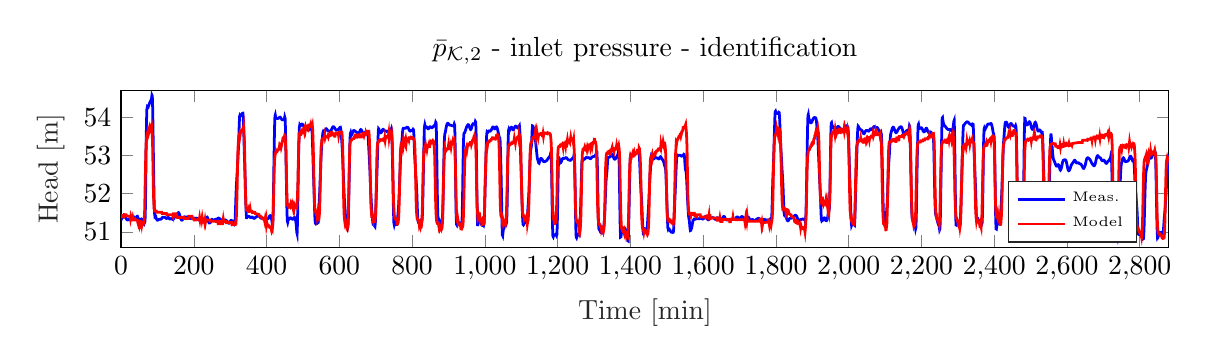
\begin{tikzpicture}

\begin{axis}[%
width=5.239in,
height=0.784in,
at={(1.133in,0.428in)},
scale only axis,
xmin=0,
xmax=2880,
xlabel style={font=\color{white!15!black}},
xlabel={Time [min]},
ymin=50.6,
ymax=54.7,
ylabel style={font=\color{white!15!black}},
ylabel={Head  [m]},
axis background/.style={fill=white},
title style={},
title={$\bar{p}_{\mathcal{K},2}$ - inlet pressure - identification},
legend style={at={(0.97,0.03)}, anchor=south east, legend cell align=left, align=left, draw=white!15!black}
]
\addplot [color=blue, line width=1.0pt]
  table[row sep=crcr]{%
0	51.3071673979595\\
1	51.3309905064294\\
2	51.3502678856408\\
3	51.3649740115167\\
4	51.375116303637\\
5	51.3816527989151\\
6	51.3861456877583\\
7	51.389777175471\\
8	51.3926841369121\\
9	51.3942834837736\\
10	51.3934755901908\\
11	51.3892966771647\\
12	51.3812890645174\\
13	51.3694635159317\\
14	51.3544351725983\\
15	51.3380229773931\\
16	51.3233146743208\\
17	51.3135579114034\\
18	51.3104956619598\\
19	51.3133449646802\\
20	51.3189532552828\\
21	51.3234103616253\\
22	51.324331910679\\
23	51.3223210613911\\
24	51.3203374102095\\
25	51.3215303164663\\
26	51.3272380429296\\
27	51.3366279165433\\
28	51.3478596915616\\
29	51.359502475952\\
30	51.3710302002405\\
31	51.382251395264\\
32	51.3923152975816\\
33	51.3993015454044\\
34	51.4008994710502\\
35	51.3957284387337\\
36	51.3842509734887\\
37	51.3687457809241\\
38	51.3527202876604\\
39	51.3398456146976\\
40	51.3337962099461\\
41	51.3365430479891\\
42	51.3527784213816\\
43	51.3811019391223\\
44	51.4080884109609\\
45	51.4101141709981\\
46	51.3872684372341\\
47	51.3591360820731\\
48	51.343218135039\\
49	51.3343625779924\\
50	51.3258478389364\\
51	51.315191253154\\
52	51.3063321968346\\
53	51.3058485049692\\
54	51.3174411304806\\
55	51.333310548533\\
56	51.3408028268158\\
57	51.3364043615338\\
58	51.3257566178955\\
59	51.3155181913046\\
60	51.3090253690332\\
61	51.3069557606857\\
62	51.3073490364772\\
63	51.3191241037236\\
64	51.2986702390707\\
65	51.2547705633013\\
66	51.2797166536749\\
67	51.6212414580612\\
68	52.3108006241197\\
69	53.1846955781165\\
70	53.8639339557406\\
71	54.2064624482532\\
72	54.252351213664\\
73	54.2362579263218\\
74	54.2412181776353\\
75	54.2771410184315\\
76	54.3040395095838\\
77	54.3313495422092\\
78	54.3571498910693\\
79	54.3805043647122\\
80	54.401251901721\\
81	54.4203745896972\\
82	54.4404935188053\\
83	54.4526427627497\\
84	54.4976469008163\\
85	54.5747126700984\\
86	54.5540550130195\\
87	54.2343978280506\\
88	53.6542849136198\\
89	52.9929103179111\\
90	52.3580827300757\\
91	51.8154655361338\\
92	51.4934838933842\\
93	51.4211949130713\\
94	51.4348561828628\\
95	51.4216060360873\\
96	51.3819830859558\\
97	51.3529338401213\\
98	51.3286324002031\\
99	51.3126804198646\\
100	51.3061723495242\\
101	51.3078213975103\\
102	51.3145212881517\\
103	51.3224773050174\\
104	51.3285591985277\\
105	51.3312743479625\\
106	51.3309893824983\\
107	51.3293482577633\\
108	51.3284070943172\\
109	51.3300505069976\\
110	51.3355415531876\\
111	51.3450058440391\\
112	51.3570707924495\\
113	51.3692656758227\\
114	51.3789774886231\\
115	51.3845723106186\\
116	51.3860825635905\\
117	51.385130741898\\
118	51.3837498402953\\
119	51.3828743978457\\
120	51.3816665441417\\
121	51.3783579916356\\
122	51.3718924241036\\
123	51.3632056532532\\
124	51.3552439280321\\
125	51.3515722098323\\
126	51.3542628048692\\
127	51.3623180621995\\
128	51.3717943639961\\
129	51.3777004037206\\
130	51.3765961937227\\
131	51.3683480349139\\
132	51.3561537871305\\
133	51.3448755529197\\
134	51.3385829937178\\
135	51.3385888203588\\
136	51.3429993533736\\
137	51.3479481335583\\
138	51.3497608494718\\
139	51.3467839452126\\
140	51.3399647158737\\
141	51.3321702493993\\
142	51.3269314208205\\
143	51.3271793216927\\
144	51.3343413410302\\
145	51.3479276802039\\
146	51.3657342289257\\
147	51.3844622547704\\
148	51.4006514989986\\
149	51.4117078399135\\
150	51.4168892870094\\
151	51.4179305871884\\
152	51.4189363467797\\
153	51.4247730118265\\
154	51.4386403762867\\
155	51.45970987234\\
156	51.4826390096675\\
157	51.4995606305143\\
158	51.504826426139\\
159	51.4973081851977\\
160	51.4785854653543\\
161	51.4502398974671\\
162	51.4152329811435\\
163	51.3791127162092\\
164	51.3480352503972\\
165	51.3254935955086\\
166	51.3120098477768\\
167	51.3067675240006\\
168	51.309103770123\\
169	51.3185412056583\\
170	51.3338838283066\\
171	51.3525292910815\\
172	51.3708956345488\\
173	51.385483636792\\
174	51.3937216055859\\
175	51.3946816964031\\
176	51.3897074964722\\
177	51.3822971356661\\
178	51.3766161951504\\
179	51.3755308095284\\
180	51.3794029649169\\
181	51.3862842805954\\
182	51.3931274088737\\
183	51.3973608083868\\
184	51.3978586790688\\
185	51.3948701546299\\
186	51.3892270899029\\
187	51.3817200170603\\
188	51.3730615676254\\
189	51.3642395422002\\
190	51.3566129611711\\
191	51.3514692634228\\
192	51.3493422332642\\
193	51.3497561440754\\
194	51.351583990852\\
195	51.3537352990868\\
196	51.355655950159\\
197	51.3573845530376\\
198	51.3591528702745\\
199	51.3609040305602\\
200	51.362144062649\\
201	51.3623165993546\\
202	51.3613485966648\\
203	51.3598576274643\\
204	51.3588042515916\\
205	51.3588619258566\\
206	51.3598686851301\\
207	51.3606318998841\\
208	51.3593227990145\\
209	51.3544251114776\\
210	51.3456973701295\\
211	51.3344742453923\\
212	51.3232482422493\\
213	51.3148612704374\\
214	51.3115909076748\\
215	51.3142899763249\\
216	51.3220148326782\\
217	51.3323763539799\\
218	51.3424496970683\\
219	51.3497730839738\\
220	51.3531671254257\\
221	51.3529942796578\\
222	51.3506893215677\\
223	51.3478007800105\\
224	51.3452803862391\\
225	51.3433608997371\\
226	51.3419118782703\\
227	51.3407928900214\\
228	51.3399582191237\\
229	51.3393774808177\\
230	51.3391576616606\\
231	51.3398149697709\\
232	51.3424472483864\\
233	51.3482151553992\\
234	51.3568661050794\\
235	51.368846629247\\
236	51.3815405144294\\
237	51.3861809937519\\
238	51.368993505829\\
239	51.3301610824516\\
240	51.2847474338289\\
241	51.2512543503122\\
242	51.2350838928124\\
243	51.232139859527\\
244	51.2349410712513\\
245	51.2413912999464\\
246	51.2557704499098\\
247	51.2796406590564\\
248	51.3053942048288\\
249	51.3222391438334\\
250	51.3271627538099\\
251	51.3240504260994\\
252	51.3177996347072\\
253	51.311440980852\\
254	51.3069314703984\\
255	51.3056357728102\\
256	51.3080007171129\\
257	51.3134158063162\\
258	51.3201671142674\\
259	51.3261458221023\\
260	51.3299817916677\\
261	51.3317554990294\\
262	51.3328493128842\\
263	51.3350879280595\\
264	51.3396694099419\\
265	51.3464006023355\\
266	51.3536878584543\\
267	51.3593334612832\\
268	51.361633030687\\
269	51.3600212035378\\
270	51.3549736194325\\
271	51.3475250214597\\
272	51.3388578333223\\
273	51.3300356004183\\
274	51.3218137591817\\
275	51.3146271933259\\
276	51.3087746697672\\
277	51.3045267034166\\
278	51.3019988725653\\
279	51.3010429232894\\
280	51.3014091969982\\
281	51.3029609944841\\
282	51.3056016151169\\
283	51.3089876441067\\
284	51.3123779821689\\
285	51.3147430500845\\
286	51.3150184589472\\
287	51.3124755129412\\
288	51.3071341814613\\
289	51.2998654315511\\
290	51.2917841821247\\
291	51.2833148870551\\
292	51.273854577026\\
293	51.2625604334705\\
294	51.249593936852\\
295	51.236909684977\\
296	51.2279547168319\\
297	51.2263782562792\\
298	51.2341164924741\\
299	51.2500010279647\\
300	51.2697692520438\\
301	51.2877871287847\\
302	51.2993583318472\\
303	51.3024407908345\\
304	51.2978826581278\\
305	51.2884676316962\\
306	51.277369886642\\
307	51.2668302240925\\
308	51.2579430849167\\
309	51.2509365627164\\
310	51.2510605641581\\
311	51.2404200286706\\
312	51.2171169982112\\
313	51.2347220654656\\
314	51.3985001282516\\
315	51.6897967440218\\
316	51.9880533204228\\
317	52.1970887089709\\
318	52.3587037835939\\
319	52.5225541672599\\
320	52.7050920867583\\
321	52.8754960407299\\
322	53.0421828606207\\
323	53.249764389622\\
324	53.5476596483635\\
325	53.846723370976\\
326	54.0249584840992\\
327	54.0552866641067\\
328	54.0421865508085\\
329	54.0416375064139\\
330	54.0538491768483\\
331	54.0608446764739\\
332	54.0647328862626\\
333	54.0770020599453\\
334	54.1032803134336\\
335	54.1052406377579\\
336	53.9889323190003\\
337	53.7258119268721\\
338	53.3830192862804\\
339	53.0485245818565\\
340	52.7390261615095\\
341	52.4296894383091\\
342	52.09574502398\\
343	51.7538079020202\\
344	51.4908369962832\\
345	51.3730925442955\\
346	51.3719784975808\\
347	51.3944075839169\\
348	51.4028860461761\\
349	51.403292897899\\
350	51.4062973479691\\
351	51.4068725029182\\
352	51.4037693422636\\
353	51.3967696961821\\
354	51.3875497527816\\
355	51.3792664220529\\
356	51.3750329693384\\
357	51.376123172584\\
358	51.3811095776849\\
359	51.38661678559\\
360	51.3890917278984\\
361	51.3865238470286\\
362	51.3792448731013\\
363	51.3695943342483\\
364	51.3607222629498\\
365	51.355258727002\\
366	51.354487732885\\
367	51.3582100757562\\
368	51.3651139547032\\
369	51.3734153224973\\
370	51.381553464599\\
371	51.3887330132836\\
372	51.3950970791418\\
373	51.4012815666152\\
374	51.4075456183246\\
375	51.4132422975702\\
376	51.4171468912949\\
377	51.4181575196806\\
378	51.4157427377971\\
379	51.4100832480592\\
380	51.4020179760598\\
381	51.3926576993395\\
382	51.3829352204707\\
383	51.3736121177382\\
384	51.3656392260534\\
385	51.360109458474\\
386	51.3575811631603\\
387	51.3575068903953\\
388	51.358477183183\\
389	51.3590330905598\\
390	51.3583187850062\\
391	51.3562998654975\\
392	51.3535924634297\\
393	51.3508515318869\\
394	51.3480340300121\\
395	51.3443821201639\\
396	51.3393552179965\\
397	51.3335230449482\\
398	51.3284758599435\\
399	51.3259035516808\\
400	51.3266096525615\\
401	51.3300235537778\\
402	51.3346156289783\\
403	51.3393762609831\\
404	51.3453181454641\\
405	51.3550606283152\\
406	51.3703741573077\\
407	51.3899217321053\\
408	51.4092836490715\\
409	51.4225111286216\\
410	51.4243385006321\\
411	51.4121926416618\\
412	51.3874216580708\\
413	51.3535775913486\\
414	51.3254414552728\\
415	51.2678531957487\\
416	51.1818507821697\\
417	51.1891710492746\\
418	51.4766657927607\\
419	52.0086792299397\\
420	52.6225746901818\\
421	53.2231726698805\\
422	53.7364045907692\\
423	54.0248095384246\\
424	54.0578760927975\\
425	54.0040466590211\\
426	53.9773031343791\\
427	53.9781190162855\\
428	53.9717472978703\\
429	53.9678643259139\\
430	53.9660972232093\\
431	53.9666566542014\\
432	53.9696587929371\\
433	53.9751372196516\\
434	53.9827976821013\\
435	53.9913907784454\\
436	53.9983928443227\\
437	54.0006331693037\\
438	53.9958150166105\\
439	53.983943666583\\
440	53.9677767680049\\
441	53.9516364083255\\
442	53.9392990455319\\
443	53.9323319898073\\
444	53.930086113861\\
445	53.9308045700091\\
446	53.9330172889091\\
447	53.9368793926584\\
448	53.9337717141909\\
449	53.9574325970643\\
450	54.0074896439726\\
451	53.9752712018936\\
452	53.6970485949104\\
453	53.2030107562207\\
454	52.6317262050241\\
455	52.0614686077064\\
456	51.5686810553106\\
457	51.2893522980899\\
458	51.2538416348483\\
459	51.3008575074932\\
460	51.3241591515233\\
461	51.3247651102825\\
462	51.3362097439675\\
463	51.3481519986041\\
464	51.3589445962383\\
465	51.3662799171396\\
466	51.368497959298\\
467	51.3650982194372\\
468	51.3570971028344\\
469	51.3467958123241\\
470	51.3372720712504\\
471	51.3316403908925\\
472	51.332147379741\\
473	51.3392157815053\\
474	51.351441636639\\
475	51.3653426903095\\
476	51.3763599962128\\
477	51.3787239106578\\
478	51.3676721537866\\
479	51.3390502995733\\
480	51.2908722212885\\
481	51.2350005876003\\
482	51.134487937794\\
483	50.9956728813788\\
484	50.9559920295614\\
485	51.228740832527\\
486	51.7726906765824\\
487	52.3933319658768\\
488	52.9668051407587\\
489	53.4456038283398\\
490	53.7252331641792\\
491	53.7832581186643\\
492	53.7629176190605\\
493	53.766127037751\\
494	53.7913080348178\\
495	53.8057792346398\\
496	53.8161791427255\\
497	53.8206699195375\\
498	53.8186852167967\\
499	53.8105653870972\\
500	53.7977372526296\\
501	53.782633788416\\
502	53.7682637417117\\
503	53.7573623572799\\
504	53.7514686820803\\
505	53.7502338350818\\
506	53.7513590510325\\
507	53.7513167365093\\
508	53.7468110285588\\
509	53.7361777591763\\
510	53.7200242999018\\
511	53.7008409958518\\
512	53.6820979286848\\
513	53.66718174292\\
514	53.6585202894905\\
515	53.6570707726166\\
516	53.6623722298037\\
517	53.6729210183951\\
518	53.6866329738711\\
519	53.7012706122606\\
520	53.7151354658915\\
521	53.7238031029002\\
522	53.7361184857301\\
523	53.757266698026\\
524	53.755378823094\\
525	53.6495925376972\\
526	53.4128966137046\\
527	53.1023755034257\\
528	52.7959025136398\\
529	52.5100188319217\\
530	52.2221034667968\\
531	51.9103479611473\\
532	51.5920464013416\\
533	51.3457522593491\\
534	51.2291177721561\\
535	51.2165020560283\\
536	51.2274532466017\\
537	51.2310354009245\\
538	51.2276333131061\\
539	51.2244401062875\\
540	51.2314456288655\\
541	51.2850732603443\\
542	51.3940740340941\\
543	51.530921021402\\
544	51.6674526172316\\
545	51.8266208873984\\
546	52.0327302678633\\
547	52.2756397527325\\
548	52.5255086949278\\
549	52.7718850470871\\
550	53.0038780635433\\
551	53.1895498646961\\
552	53.3190248910809\\
553	53.4204959563385\\
554	53.5227320069201\\
555	53.6005693183595\\
556	53.6275875397567\\
557	53.61508816133\\
558	53.6033787056936\\
559	53.6083079400096\\
560	53.6267867088477\\
561	53.6502634624841\\
562	53.6738716479829\\
563	53.6909487420944\\
564	53.6973081352326\\
565	53.6927371817863\\
566	53.6807945141924\\
567	53.6663616693324\\
568	53.654058764226\\
569	53.6463329632058\\
570	53.6426434670929\\
571	53.6399709843833\\
572	53.6353886339309\\
573	53.6283966080843\\
574	53.6217533558346\\
575	53.6198790326925\\
576	53.626287225183\\
577	53.6415550243074\\
578	53.6632858292646\\
579	53.6874814746915\\
580	53.7103155920119\\
581	53.7291269569358\\
582	53.7425195150165\\
583	53.7498209303653\\
584	53.7506321450181\\
585	53.7449515387873\\
586	53.7336888586106\\
587	53.7188628707406\\
588	53.7030818100069\\
589	53.6887043439461\\
590	53.6772093877846\\
591	53.6690563068169\\
592	53.6639532914644\\
593	53.6614006963478\\
594	53.661216996118\\
595	53.6637608957802\\
596	53.6695976408318\\
597	53.6787849786878\\
598	53.6903634039793\\
599	53.7027056538266\\
600	53.7126722022726\\
601	53.7231223930691\\
602	53.7357825095087\\
603	53.7379295232364\\
604	53.693227747737\\
605	53.5919778267347\\
606	53.4616182933776\\
607	53.3316388596306\\
608	53.1783654859747\\
609	52.9760411607544\\
610	52.7352728561422\\
611	52.4913325566535\\
612	52.2554496415028\\
613	52.0298893556151\\
614	51.8389003183675\\
615	51.6935770344709\\
616	51.5662706623957\\
617	51.4166768479661\\
618	51.2751753599562\\
619	51.1907387203882\\
620	51.1716168308365\\
621	51.1788836207055\\
622	51.1592471113194\\
623	51.1116855987598\\
624	51.1402469757669\\
625	51.3894590273526\\
626	51.8342488175926\\
627	52.3496730650056\\
628	52.8648355121507\\
629	53.3089351674873\\
630	53.5594902550066\\
631	53.5885999352934\\
632	53.5443121000892\\
633	53.5275378231861\\
634	53.5432159812298\\
635	53.5620604206451\\
636	53.5882261381197\\
637	53.6146714810622\\
638	53.6355171646456\\
639	53.6477393874973\\
640	53.6514584588782\\
641	53.6490383020875\\
642	53.6432797782277\\
643	53.6362114805772\\
644	53.6289118932618\\
645	53.6219184315724\\
646	53.6155423027819\\
647	53.6098201481785\\
648	53.604243329483\\
649	53.5977607240026\\
650	53.5895659589115\\
651	53.5804169069757\\
652	53.5732448461666\\
653	53.5721499009203\\
654	53.5803790794906\\
655	53.598456207804\\
656	53.6232754371223\\
657	53.6487173596227\\
658	53.6679567087994\\
659	53.6762535872507\\
660	53.6724245609204\\
661	53.6585919355541\\
662	53.6389154772108\\
663	53.6180916389882\\
664	53.5998814514468\\
665	53.5863785002403\\
666	53.5781841223434\\
667	53.5751778130636\\
668	53.5769940075547\\
669	53.5830712638931\\
670	53.5923917859224\\
671	53.6031999877369\\
672	53.612890490032\\
673	53.6184769850779\\
674	53.6183098692955\\
675	53.6111674779006\\
676	53.6063119366258\\
677	53.6127907285821\\
678	53.6051564485299\\
679	53.5260471048482\\
680	53.3631646024468\\
681	53.1759264215496\\
682	53.0044126222763\\
683	52.826909432179\\
684	52.6174629771481\\
685	52.3916444522501\\
686	52.1647303504569\\
687	51.9461235557126\\
688	51.7574639703326\\
689	51.608061221965\\
690	51.4769177502559\\
691	51.3455564269916\\
692	51.2427911652185\\
693	51.1952370361006\\
694	51.1919354528469\\
695	51.1980024397259\\
696	51.187145811032\\
697	51.1545246253365\\
698	51.1413274233991\\
699	51.238780812004\\
700	51.478604638312\\
701	51.7983262515165\\
702	52.1127528841452\\
703	52.4047549054394\\
704	52.6994540509846\\
705	53.0206513762579\\
706	53.3483800154982\\
707	53.5950175682467\\
708	53.6970290788491\\
709	53.6847511037012\\
710	53.6488209453613\\
711	53.6257883830401\\
712	53.6115820868348\\
713	53.5985016929414\\
714	53.5929663558912\\
715	53.5966168362451\\
716	53.6093486940487\\
717	53.6290071434066\\
718	53.6512962202656\\
719	53.6705848102729\\
720	53.6816061961245\\
721	53.6819890998186\\
722	53.6732329359094\\
723	53.6599455449796\\
724	53.6475378526728\\
725	53.6399390400099\\
726	53.637643668015\\
727	53.6378807809868\\
728	53.636886497303\\
729	53.6327610706199\\
730	53.6263060760935\\
731	53.6201472694777\\
732	53.6172224927566\\
733	53.619592025404\\
734	53.6275646009337\\
735	53.6396912710191\\
736	53.6533298365053\\
737	53.6654086736077\\
738	53.6730611463057\\
739	53.6746135486157\\
740	53.6709424716862\\
741	53.6560007254814\\
742	53.6632323831926\\
743	53.6923279572414\\
744	53.6431791184329\\
745	53.3755595965671\\
746	52.9338363630701\\
747	52.443937903829\\
748	51.9491227792571\\
749	51.4998178630689\\
750	51.2298704734405\\
751	51.1863851933627\\
752	51.2231341399837\\
753	51.2366296222025\\
754	51.2236932194925\\
755	51.2176000272582\\
756	51.2076604490145\\
757	51.1954886896669\\
758	51.1952805646176\\
759	51.2399748062015\\
760	51.3335191440608\\
761	51.4471434535269\\
762	51.5579488388464\\
763	51.695422073746\\
764	51.8862278521415\\
765	52.1201716911302\\
766	52.3599744193588\\
767	52.6011673994928\\
768	52.8464061942894\\
769	53.0743544931673\\
770	53.2261709262858\\
771	53.3059618676199\\
772	53.3780931202965\\
773	53.4991196133107\\
774	53.6233975088497\\
775	53.6964513342078\\
776	53.7123890185726\\
777	53.7131353425601\\
778	53.7136477110819\\
779	53.7135293252719\\
780	53.7102793091885\\
781	53.7090666274303\\
782	53.7115524538092\\
783	53.7173950052976\\
784	53.7249807433073\\
785	53.7322095844019\\
786	53.7371477441613\\
787	53.738124815912\\
788	53.7337438874758\\
789	53.7231573431634\\
790	53.7065312390303\\
791	53.6856890829526\\
792	53.6642849834663\\
793	53.6468532978774\\
794	53.6368873770816\\
795	53.6354925264523\\
796	53.6409392142523\\
797	53.6492386208447\\
798	53.6556911234875\\
799	53.6576741890068\\
800	53.6562164056763\\
801	53.6506817780217\\
802	53.6588316031951\\
803	53.6814807693981\\
804	53.6698640273161\\
805	53.5322789099105\\
806	53.2842512444755\\
807	53.0260215210252\\
808	52.8364026722283\\
809	52.6803979506448\\
810	52.5233709904677\\
811	52.3737621866877\\
812	52.2298813999058\\
813	52.0351475889217\\
814	51.7492397786089\\
815	51.4639408514126\\
816	51.2961888627078\\
817	51.2644844216586\\
818	51.2718461899184\\
819	51.26728849939\\
820	51.2540602724837\\
821	51.2517465631375\\
822	51.2578983992504\\
823	51.2710082610639\\
824	51.28721643519\\
825	51.3119951414902\\
826	51.3127733046158\\
827	51.292277987286\\
828	51.3523361894917\\
829	51.6261510429703\\
830	52.0584386390534\\
831	52.5273124644676\\
832	53.0124754224733\\
833	53.4716091307387\\
834	53.7559069806691\\
835	53.8024569485403\\
836	53.7620830804195\\
837	53.7445766913352\\
838	53.7527251352578\\
839	53.7502278171228\\
840	53.7436169729214\\
841	53.7315584146066\\
842	53.716538458318\\
843	53.7032730740772\\
844	53.696617062886\\
845	53.6993617225973\\
846	53.7107916018128\\
847	53.7266455363751\\
848	53.7409394067565\\
849	53.7488219608104\\
850	53.7486125036731\\
851	53.742151439994\\
852	53.7334777891386\\
853	53.7268175722438\\
854	53.7247833306925\\
855	53.7277667457431\\
856	53.7344959676318\\
857	53.7431738076577\\
858	53.7523810795231\\
859	53.761442280607\\
860	53.7702796568631\\
861	53.7790686804489\\
862	53.7886782913534\\
863	53.7891971534138\\
864	53.8193744812983\\
865	53.8687023403829\\
866	53.8518733316547\\
867	53.5534909274708\\
868	52.9639419399858\\
869	52.2315916179074\\
870	51.6700319587835\\
871	51.3816506946657\\
872	51.3364190549635\\
873	51.3433941335691\\
874	51.3353017868448\\
875	51.3001963736836\\
876	51.2707710990492\\
877	51.2406459180162\\
878	51.2172525986866\\
879	51.2102082090196\\
880	51.22548446217\\
881	51.232100905537\\
882	51.2202016117463\\
883	51.2652974776682\\
884	51.4765507295175\\
885	51.8378379280316\\
886	52.2675229490294\\
887	52.7361316294632\\
888	53.1782975095448\\
889	53.4686703036429\\
890	53.5643233212698\\
891	53.5917820021236\\
892	53.6368744164583\\
893	53.7000098680125\\
894	53.7499860502269\\
895	53.790268034868\\
896	53.8187288563201\\
897	53.8352014341107\\
898	53.8406496116406\\
899	53.8369337066202\\
900	53.8268578658178\\
901	53.8139360561836\\
902	53.802060481499\\
903	53.794325729168\\
904	53.7915812952882\\
905	53.791955359538\\
906	53.7923008255103\\
907	53.7903883152664\\
908	53.7862053243339\\
909	53.7815245920826\\
910	53.7784284343796\\
911	53.7778322718667\\
912	53.7788041406632\\
913	53.7799134628223\\
914	53.7700824119195\\
915	53.7857259250312\\
916	53.8189409485771\\
917	53.7932657948093\\
918	53.4941228829451\\
919	52.8878263898651\\
920	52.1080208019393\\
921	51.4973405141406\\
922	51.1991750442303\\
923	51.1835499480743\\
924	51.22937914998\\
925	51.2545423750011\\
926	51.2492693271379\\
927	51.2496336700421\\
928	51.2452323229166\\
929	51.2381977087763\\
930	51.2317893779059\\
931	51.2282860430272\\
932	51.227546414397\\
933	51.2275394905217\\
934	51.2365775781769\\
935	51.2158249063487\\
936	51.1804616624893\\
937	51.2181500403035\\
938	51.5266249991304\\
939	52.0888721392846\\
940	52.759763569041\\
941	53.2661410484443\\
942	53.5345187303261\\
943	53.5853191191498\\
944	53.5864955953721\\
945	53.5981156597114\\
946	53.6345725522515\\
947	53.6635920656978\\
948	53.6927343823137\\
949	53.7204045806422\\
950	53.7452824295302\\
951	53.7665939253095\\
952	53.7841566342666\\
953	53.7973186691601\\
954	53.8042542422091\\
955	53.802342325003\\
956	53.7895625265514\\
957	53.7662190146009\\
958	53.7361553870576\\
959	53.7063117878068\\
960	53.6845469676937\\
961	53.6767693911239\\
962	53.6853073166516\\
963	53.7083577392042\\
964	53.7405767525795\\
965	53.7745601760034\\
966	53.8033726308066\\
967	53.822518303847\\
968	53.830718858081\\
969	53.830177241253\\
970	53.8258186576847\\
971	53.8237459588122\\
972	53.8157048604447\\
973	53.8410316182257\\
974	53.8863669030668\\
975	53.8706376835145\\
976	53.566838206264\\
977	52.944212197325\\
978	52.1338885732979\\
979	51.4967719017849\\
980	51.1877708158275\\
981	51.1867001483267\\
982	51.2540551585742\\
983	51.2992111497636\\
984	51.3081387519116\\
985	51.3194482487156\\
986	51.3188701989488\\
987	51.3067618233759\\
988	51.2842519628343\\
989	51.2544595576502\\
990	51.2220658310084\\
991	51.1934456256684\\
992	51.174829410157\\
993	51.1705870208201\\
994	51.1785041371733\\
995	51.1990871666122\\
996	51.2024423347084\\
997	51.1832161142\\
998	51.2217623967774\\
999	51.4771178257278\\
1000	51.8912119580409\\
1001	52.2714362919349\\
1002	52.543781113256\\
1003	52.8836345373648\\
1004	53.2753936131485\\
1005	53.5471096991807\\
1006	53.6050204574887\\
1007	53.593006917561\\
1008	53.5993707201876\\
1009	53.6256591405571\\
1010	53.6382950469707\\
1011	53.6418446250803\\
1012	53.6386423944928\\
1013	53.6347540707349\\
1014	53.6334143932334\\
1015	53.6357922132198\\
1016	53.6425528493165\\
1017	53.6545275330124\\
1018	53.6715424359434\\
1019	53.6922340275699\\
1020	53.7137347408924\\
1021	53.7319464260836\\
1022	53.7426225680877\\
1023	53.7429422921112\\
1024	53.7332411581997\\
1025	53.7176926918797\\
1026	53.7031369599914\\
1027	53.6961016376399\\
1028	53.7000503553725\\
1029	53.7136243800385\\
1030	53.7310488289015\\
1031	53.7443196271154\\
1032	53.7468480625016\\
1033	53.7353689555685\\
1034	53.7103670207306\\
1035	53.6750102817377\\
1036	53.6339382174158\\
1037	53.5909466768082\\
1038	53.548364180125\\
1039	53.4995591962302\\
1040	53.4710413880666\\
1041	53.4593156752633\\
1042	53.3748471858392\\
1043	53.1281507050981\\
1044	52.7714393373607\\
1045	52.359666652391\\
1046	51.8292126723647\\
1047	51.2690438917804\\
1048	50.9245222959832\\
1049	50.9030781017521\\
1050	50.9970468254981\\
1051	51.0616908243212\\
1052	51.0914601535358\\
1053	51.1328559002225\\
1054	51.1714241974475\\
1055	51.2020256596129\\
1056	51.2221179515941\\
1057	51.2450576145392\\
1058	51.240986410971\\
1059	51.221255052524\\
1060	51.2560937470572\\
1061	51.5408361796393\\
1062	52.0955545815799\\
1063	52.8042961312244\\
1064	53.3639483368513\\
1065	53.6519463704811\\
1066	53.6849678244517\\
1067	53.6619529281838\\
1068	53.6562880202087\\
1069	53.6788075014357\\
1070	53.6947867863759\\
1071	53.7132376041516\\
1072	53.7292727673661\\
1073	53.7367563056313\\
1074	53.7320691801061\\
1075	53.7167502217591\\
1076	53.6966527656261\\
1077	53.6793273636895\\
1078	53.6710078598859\\
1079	53.6756797556957\\
1080	53.6924204366489\\
1081	53.7160351159617\\
1082	53.7390889490812\\
1083	53.7564778360462\\
1084	53.7657280004693\\
1085	53.7670612748988\\
1086	53.7619583547282\\
1087	53.7525589188473\\
1088	53.7408236954045\\
1089	53.7288125040975\\
1090	53.7188963095685\\
1091	53.7137941044864\\
1092	53.7122848885483\\
1093	53.7261166103563\\
1094	53.7604049345799\\
1095	53.776542573065\\
1096	53.6812258278923\\
1097	53.4426004195753\\
1098	53.1233714290095\\
1099	52.8088606706947\\
1100	52.517183871146\\
1101	52.224503614515\\
1102	51.906613909989\\
1103	51.5777239952466\\
1104	51.3195170558955\\
1105	51.1960945776076\\
1106	51.1849489273665\\
1107	51.2023311029514\\
1108	51.214621886735\\
1109	51.226214187088\\
1110	51.2446894570469\\
1111	51.2627332742564\\
1112	51.2777798328816\\
1113	51.2912531086673\\
1114	51.2963939046151\\
1115	51.2938669603053\\
1116	51.3156730798283\\
1117	51.4091582716324\\
1118	51.5583269435232\\
1119	51.7054640409939\\
1120	51.84343570446\\
1121	52.0228890494868\\
1122	52.2558385224662\\
1123	52.5167570036237\\
1124	52.7800547991018\\
1125	53.0133747719045\\
1126	53.1423421974122\\
1127	53.1868142933121\\
1128	53.2581655125214\\
1129	53.448042241304\\
1130	53.6581969134531\\
1131	53.7705240089617\\
1132	53.7649002937139\\
1133	53.7315301795022\\
1134	53.7083453245963\\
1135	53.6855316599319\\
1136	53.6408760363342\\
1137	53.5763736890404\\
1138	53.4973629328451\\
1139	53.4083618353465\\
1140	53.3139403316958\\
1141	53.2191578224639\\
1142	53.1239205114687\\
1143	53.0283329329033\\
1144	52.9461029739984\\
1145	52.8962808448461\\
1146	52.8689638345024\\
1147	52.8362880525225\\
1148	52.8016058979672\\
1149	52.7950072929811\\
1150	52.8239713368386\\
1151	52.862298634229\\
1152	52.8915665643593\\
1153	52.9095733302948\\
1154	52.9190551001042\\
1155	52.9196641023805\\
1156	52.9134122938648\\
1157	52.9022584978397\\
1158	52.8879282824997\\
1159	52.8721983533528\\
1160	52.8570565167769\\
1161	52.8446315878663\\
1162	52.8366680880072\\
1163	52.8337904183715\\
1164	52.8351573368344\\
1165	52.8390519391211\\
1166	52.8438713003074\\
1167	52.8487602776446\\
1168	52.8538007068119\\
1169	52.8599041172085\\
1170	52.8682922233319\\
1171	52.879653952393\\
1172	52.8936208980692\\
1173	52.9088850232979\\
1174	52.9238264735305\\
1175	52.9372930252272\\
1176	52.9491582362309\\
1177	52.9603424952764\\
1178	52.9728095256554\\
1179	52.9790468912999\\
1180	53.0114236003648\\
1181	53.0622856546683\\
1182	53.0603243604077\\
1183	52.8152529942577\\
1184	52.3026731160182\\
1185	51.6477522393854\\
1186	51.1411820841532\\
1187	50.8929562869605\\
1188	50.8736605389514\\
1189	50.9039183315765\\
1190	50.9200227395331\\
1191	50.9142254085503\\
1192	50.9167555203472\\
1193	50.9197346173995\\
1194	50.9237129175334\\
1195	50.9359997418384\\
1196	50.9275511723895\\
1197	50.9072230240907\\
1198	50.9301010507478\\
1199	51.1575529034969\\
1200	51.6179229318438\\
1201	52.2266244897857\\
1202	52.7133575880653\\
1203	52.9475611107327\\
1204	52.9385714585044\\
1205	52.8741411591358\\
1206	52.8287909627942\\
1207	52.8152301994702\\
1208	52.8059895795046\\
1209	52.8128002957543\\
1210	52.8319925963833\\
1211	52.8576194210757\\
1212	52.8832747774704\\
1213	52.9041699618596\\
1214	52.9178413477849\\
1215	52.924406956248\\
1216	52.9257044244183\\
1217	52.924341642771\\
1218	52.922878206671\\
1219	52.9232775404941\\
1220	52.9265510683915\\
1221	52.9323543614706\\
1222	52.9386924488233\\
1223	52.9425092258583\\
1224	52.9412078537675\\
1225	52.9340605953586\\
1226	52.9224416393237\\
1227	52.9091650753709\\
1228	52.8973618350948\\
1229	52.8891122596457\\
1230	52.8843961538191\\
1231	52.8814390117259\\
1232	52.8783657433147\\
1233	52.8747025481971\\
1234	52.8716226886163\\
1235	52.871146835246\\
1236	52.8749597540564\\
1237	52.8832774018746\\
1238	52.8944802078942\\
1239	52.9059843924516\\
1240	52.9159506625991\\
1241	52.9242693194239\\
1242	52.9327439995081\\
1243	52.9338728090452\\
1244	52.9607616886765\\
1245	53.0039621182491\\
1246	52.9939238089631\\
1247	52.7468047195783\\
1248	52.2463790185569\\
1249	51.6089959302581\\
1250	51.1132270906202\\
1251	50.8660850930355\\
1252	50.8484441942726\\
1253	50.8830650329396\\
1254	50.9042370235199\\
1255	50.9033004355441\\
1256	50.9134665892274\\
1257	50.9262158038107\\
1258	50.9467329206202\\
1259	50.9488043108441\\
1260	50.9344279312156\\
1261	50.983349603594\\
1262	51.2008866527773\\
1263	51.5429695313491\\
1264	51.9117966844909\\
1265	52.2884140303605\\
1266	52.6432104889283\\
1267	52.8649488177742\\
1268	52.9065511393569\\
1269	52.8820432068053\\
1270	52.8749791797652\\
1271	52.8875094398249\\
1272	52.8932210840551\\
1273	52.8990766649246\\
1274	52.905604510967\\
1275	52.9140280951942\\
1276	52.9244344637375\\
1277	52.9352567599074\\
1278	52.9437389114968\\
1279	52.9475208935451\\
1280	52.946158953217\\
1281	52.9418499050955\\
1282	52.9381366178216\\
1283	52.9376023097443\\
1284	52.9400015034455\\
1285	52.9425172738797\\
1286	52.9417168752034\\
1287	52.9360176351693\\
1288	52.9269498313162\\
1289	52.918488923701\\
1290	52.9148018128129\\
1291	52.9179516916445\\
1292	52.9270419740498\\
1293	52.939081372365\\
1294	52.9507103346385\\
1295	52.959650898652\\
1296	52.9652757089772\\
1297	52.9682501443963\\
1298	52.9697828489043\\
1299	52.971081945875\\
1300	52.9732556434242\\
1301	52.9773152434805\\
1302	52.9840645335554\\
1303	52.9938218393945\\
1304	53.0068439489352\\
1305	53.0139202143782\\
1306	53.0460761716129\\
1307	53.0949476310624\\
1308	53.0874974973205\\
1309	52.8462085935875\\
1310	52.3686444431055\\
1311	51.7851892009339\\
1312	51.3432768664124\\
1313	51.112526824988\\
1314	51.0651875863363\\
1315	51.0580202575259\\
1316	51.0423723956996\\
1317	51.0111373523144\\
1318	50.9933415921287\\
1319	50.9843303845074\\
1320	50.9821910199737\\
1321	50.9850050999953\\
1322	50.9843847104331\\
1323	50.9757615160607\\
1324	50.9819952004094\\
1325	51.0326996500111\\
1326	51.1090366040803\\
1327	51.1653565052966\\
1328	51.2283852808535\\
1329	51.3659749990791\\
1330	51.5870866998239\\
1331	51.8404900968818\\
1332	52.093923767419\\
1333	52.3082418236757\\
1334	52.4360356684202\\
1335	52.5113495061912\\
1336	52.6305399091174\\
1337	52.7963877637254\\
1338	52.9150365501347\\
1339	52.9462529804004\\
1340	52.9444606173168\\
1341	52.9491534490398\\
1342	52.9572153363285\\
1343	52.9588719079516\\
1344	52.9609322909389\\
1345	52.9679964808262\\
1346	52.9825972024674\\
1347	53.0029379515322\\
1348	53.0233629612584\\
1349	53.0364896503745\\
1350	53.0370027850655\\
1351	53.0234041089868\\
1352	52.9985546724832\\
1353	52.9682897096955\\
1354	52.9395731964854\\
1355	52.9176035313537\\
1356	52.9046879269964\\
1357	52.9005729297224\\
1358	52.9038630778887\\
1359	52.9130112165308\\
1360	52.9266613426886\\
1361	52.943361345901\\
1362	52.9614088910433\\
1363	52.979472235475\\
1364	52.9976622899026\\
1365	53.0073114529369\\
1366	53.0440916005602\\
1367	53.0942081529967\\
1368	53.0880400971267\\
1369	52.8372073840954\\
1370	52.3260551922901\\
1371	51.6565082470891\\
1372	51.1256832073616\\
1373	50.8651601080156\\
1374	50.8716152420312\\
1375	50.9402051254698\\
1376	50.9911839849777\\
1377	51.0126102873039\\
1378	51.0425567538163\\
1379	51.0683459434257\\
1380	51.0879345741441\\
1381	51.1002422975548\\
1382	51.1064660751255\\
1383	51.1077586350181\\
1384	51.1037832471523\\
1385	51.0929484247753\\
1386	51.0739342874563\\
1387	51.0468449415366\\
1388	51.0135000484874\\
1389	50.9764786438813\\
1390	50.9372124416105\\
1391	50.9046875022758\\
1392	50.8482755070389\\
1393	50.7678481187528\\
1394	50.761774537558\\
1395	50.9852540946058\\
1396	51.4088612265674\\
1397	51.8913499747954\\
1398	52.3461928146592\\
1399	52.7311320438881\\
1400	52.9591426993059\\
1401	53.0094794425773\\
1402	52.9969810173906\\
1403	53.000385269198\\
1404	53.0166351894171\\
1405	53.0184938866411\\
1406	53.0136603517934\\
1407	53.0058292320295\\
1408	53.0005048645611\\
1409	53.0017750280718\\
1410	53.0104711666138\\
1411	53.0239228897077\\
1412	53.0377708859498\\
1413	53.0483551062139\\
1414	53.054499583152\\
1415	53.0575480457311\\
1416	53.0600013249785\\
1417	53.0636908316581\\
1418	53.0687948970548\\
1419	53.0741607219384\\
1420	53.0782546547362\\
1421	53.0761089004786\\
1422	53.078987363054\\
1423	53.0879985334302\\
1424	53.0665071491621\\
1425	52.9408727795503\\
1426	52.7198289587291\\
1427	52.4805394127803\\
1428	52.2875222652843\\
1429	52.1169576966842\\
1430	51.9551924028928\\
1431	51.7878775694689\\
1432	51.5892136767254\\
1433	51.3355704932868\\
1434	51.1111989347179\\
1435	51.0063366980896\\
1436	51.0209413896163\\
1437	51.0621494889464\\
1438	51.0838919966308\\
1439	51.0865467192178\\
1440	51.0836322169523\\
1441	51.0718470921911\\
1442	51.0561342753861\\
1443	51.0286846480782\\
1444	50.9905081174844\\
1445	50.9776188316211\\
1446	51.0535197393441\\
1447	51.2069768557621\\
1448	51.3707572667468\\
1449	51.5126681033444\\
1450	51.6724558577987\\
1451	51.8746940935763\\
1452	52.1001847533707\\
1453	52.3066936367032\\
1454	52.4684433120068\\
1455	52.6077388825919\\
1456	52.7668344797758\\
1457	52.9179856951378\\
1458	52.993024132661\\
1459	52.980768090362\\
1460	52.944007075844\\
1461	52.9196765451847\\
1462	52.9084932490381\\
1463	52.9028055088496\\
1464	52.9061248496761\\
1465	52.9161675085213\\
1466	52.9286382830785\\
1467	52.9389739238707\\
1468	52.944484462574\\
1469	52.9451011993016\\
1470	52.9426560315747\\
1471	52.9394199274859\\
1472	52.9367627623241\\
1473	52.9344960525879\\
1474	52.9312521370692\\
1475	52.9257444827626\\
1476	52.9181871353004\\
1477	52.9111006195239\\
1478	52.9087386320579\\
1479	52.9149252111685\\
1480	52.929886421848\\
1481	52.9487191594571\\
1482	52.9633674758157\\
1483	52.9670633529395\\
1484	52.9577995748553\\
1485	52.9392141870631\\
1486	52.918509260763\\
1487	52.9021858745402\\
1488	52.8919163305565\\
1489	52.8837060904492\\
1490	52.8707776028848\\
1491	52.8482229031657\\
1492	52.8159880928497\\
1493	52.7784155231973\\
1494	52.7354117174171\\
1495	52.705978644357\\
1496	52.6884860937147\\
1497	52.6271509613924\\
1498	52.4527691403198\\
1499	52.1942142957937\\
1500	51.9089910226598\\
1501	51.5982649746357\\
1502	51.2977987313538\\
1503	51.1081140856306\\
1504	51.0689883428185\\
1505	51.0834895558281\\
1506	51.0835639918523\\
1507	51.0670270795905\\
1508	51.0544582260472\\
1509	51.0394332605114\\
1510	51.0228049675684\\
1511	51.006969158814\\
1512	50.9951172565652\\
1513	50.9894293673521\\
1514	50.9897821918045\\
1515	50.9965892418469\\
1516	50.9983919233444\\
1517	50.9884107047599\\
1518	50.9933705605774\\
1519	51.0815758616619\\
1520	51.2745750748436\\
1521	51.5246402952192\\
1522	51.7689293498762\\
1523	51.9956948671922\\
1524	52.2228201714264\\
1525	52.4679212364668\\
1526	52.7188856861068\\
1527	52.9130359239485\\
1528	53.0026314654292\\
1529	53.0082136664681\\
1530	52.9968458673472\\
1531	52.9956400799418\\
1532	53.0003375456943\\
1533	53.0027227287227\\
1534	53.0051636238681\\
1535	53.006799967319\\
1536	53.0064698138476\\
1537	53.0032783283514\\
1538	52.9973505196404\\
1539	52.9900746770413\\
1540	52.9838645374309\\
1541	52.9812787333441\\
1542	52.9838764620682\\
1543	52.9910698288451\\
1544	53.0004004754032\\
1545	53.0061566743745\\
1546	53.0161360540962\\
1547	53.0312259151105\\
1548	53.025948681347\\
1549	52.9382716467746\\
1550	52.7842357966994\\
1551	52.6506020647001\\
1552	52.6087536479754\\
1553	52.5843710623334\\
1554	52.4870399997126\\
1555	52.3004874022723\\
1556	52.0944040250649\\
1557	51.8964785499271\\
1558	51.7065156224133\\
1559	51.5288707943551\\
1560	51.4076023553171\\
1561	51.3437540714964\\
1562	51.2884840858748\\
1563	51.1913412112193\\
1564	51.0893829102643\\
1565	51.036022067997\\
1566	51.0414471264003\\
1567	51.0660522038494\\
1568	51.0947003629629\\
1569	51.1326152353921\\
1570	51.185283252349\\
1571	51.2413733031892\\
1572	51.2839306949361\\
1573	51.3075119814822\\
1574	51.3205655877583\\
1575	51.3332548497356\\
1576	51.3415288330153\\
1577	51.3406182669605\\
1578	51.3346215320124\\
1579	51.3330336301099\\
1580	51.3379166200841\\
1581	51.3454930009691\\
1582	51.3514205080133\\
1583	51.3539295571227\\
1584	51.352939356291\\
1585	51.3496350472248\\
1586	51.3458219929207\\
1587	51.3430331230693\\
1588	51.342006627914\\
1589	51.3428239471538\\
1590	51.3452684106011\\
1591	51.3488825988933\\
1592	51.3528375211584\\
1593	51.3559837314723\\
1594	51.3570767907015\\
1595	51.3551882060133\\
1596	51.3502970206588\\
1597	51.3437466228382\\
1598	51.3380016646616\\
1599	51.3357789746049\\
1600	51.3389790774246\\
1601	51.3478907969619\\
1602	51.3609485961069\\
1603	51.3753673999842\\
1604	51.3882774978224\\
1605	51.3975718034061\\
1606	51.4020052090232\\
1607	51.4009679993053\\
1608	51.3943352083297\\
1609	51.3825055833565\\
1610	51.3666244790915\\
1611	51.3489109653552\\
1612	51.3325639060951\\
1613	51.3208672054538\\
1614	51.3159498527622\\
1615	51.3180520510166\\
1616	51.3255591374237\\
1617	51.3355906302716\\
1618	51.3450427993885\\
1619	51.3518595164888\\
1620	51.3557703003402\\
1621	51.3579465629989\\
1622	51.3599598953675\\
1623	51.362872560963\\
1624	51.3667825674142\\
1625	51.3708386426695\\
1626	51.3737046483428\\
1627	51.3741987185203\\
1628	51.3716059751214\\
1629	51.3656815372281\\
1630	51.3568015236462\\
1631	51.3462714463878\\
1632	51.3363429397329\\
1633	51.3297062651112\\
1634	51.3286873505208\\
1635	51.3342318645879\\
1636	51.3450668429781\\
1637	51.3576675772615\\
1638	51.3676595990846\\
1639	51.371894161712\\
1640	51.3699645484707\\
1641	51.3640823229359\\
1642	51.3576680241544\\
1643	51.3533572058487\\
1644	51.3515840012532\\
1645	51.3505070358347\\
1646	51.3475908919909\\
1647	51.3417250235723\\
1648	51.3342982114947\\
1649	51.3284261267553\\
1650	51.327114351709\\
1651	51.3318156276316\\
1652	51.3421664082834\\
1653	51.3565902763228\\
1654	51.3728728513783\\
1655	51.388374217269\\
1656	51.4001261665523\\
1657	51.4052636495337\\
1658	51.4018017814286\\
1659	51.3895815525253\\
1660	51.3708405222304\\
1661	51.3498207037624\\
1662	51.3311779515719\\
1663	51.318105746721\\
1664	51.3113431078972\\
1665	51.3096256500925\\
1666	51.3109356018026\\
1667	51.3136787171693\\
1668	51.3170735951203\\
1669	51.3208221632422\\
1670	51.324550466525\\
1671	51.3276290796882\\
1672	51.3294305192768\\
1673	51.3298112240163\\
1674	51.3294428430674\\
1675	51.3296367212299\\
1676	51.3314931598549\\
1677	51.3349442308186\\
1678	51.3385967099752\\
1679	51.3406307018689\\
1680	51.3399630702624\\
1681	51.3368205596523\\
1682	51.3325384338603\\
1683	51.3288799017883\\
1684	51.3271793698605\\
1685	51.3277924684699\\
1686	51.3303249876926\\
1687	51.3344739752373\\
1688	51.3405611859217\\
1689	51.3491789336161\\
1690	51.3603189082851\\
1691	51.3727535043271\\
1692	51.3840687243841\\
1693	51.3913737840232\\
1694	51.3924867848885\\
1695	51.3869820656818\\
1696	51.376455630145\\
1697	51.3638865289821\\
1698	51.3526873590353\\
1699	51.3458240078391\\
1700	51.3450982202669\\
1701	51.3506526652807\\
1702	51.3610317341384\\
1703	51.3737293086179\\
1704	51.385928376594\\
1705	51.3952115010624\\
1706	51.4001677361071\\
1707	51.4006061324363\\
1708	51.397239309787\\
1709	51.3911175704006\\
1710	51.3832016128093\\
1711	51.3741548096777\\
1712	51.3642572015998\\
1713	51.3534927906739\\
1714	51.3419490628752\\
1715	51.3305099415158\\
1716	51.3212671878581\\
1717	51.317116422724\\
1718	51.32044964725\\
1719	51.3317511838286\\
1720	51.348808210832\\
1721	51.3672450813672\\
1722	51.3821287779483\\
1723	51.389877471015\\
1724	51.3891734201593\\
1725	51.380712196641\\
1726	51.3663529715793\\
1727	51.3485893200068\\
1728	51.3304917478199\\
1729	51.3154991400705\\
1730	51.3065579733217\\
1731	51.3048466124592\\
1732	51.3091725888516\\
1733	51.3163365066567\\
1734	51.3225138650809\\
1735	51.32489159054\\
1736	51.3228139789195\\
1737	51.3174505728011\\
1738	51.3105990463403\\
1739	51.3037304015845\\
1740	51.297948071138\\
1741	51.2942358324773\\
1742	51.2934894674679\\
1743	51.296239605965\\
1744	51.3023484045343\\
1745	51.3109064314418\\
1746	51.3204809986041\\
1747	51.3296558110933\\
1748	51.3375654082291\\
1749	51.3440687728901\\
1750	51.3493825550819\\
1751	51.3534495686562\\
1752	51.3554672272\\
1753	51.353959646299\\
1754	51.3473345015187\\
1755	51.3347852452035\\
1756	51.3170507019858\\
1757	51.296718262663\\
1758	51.2775937247279\\
1759	51.263425328338\\
1760	51.2565040177954\\
1761	51.2571370134985\\
1762	51.2640124257658\\
1763	51.2751366748168\\
1764	51.288459424072\\
1765	51.302074865129\\
1766	51.3141139808487\\
1767	51.3228985063147\\
1768	51.3273010622435\\
1769	51.3272025607971\\
1770	51.3237111130434\\
1771	51.318965636156\\
1772	51.315233714673\\
1773	51.3137114105515\\
1774	51.3138882455117\\
1775	51.3141115929171\\
1776	51.3128565914359\\
1777	51.3097965632842\\
1778	51.306114559481\\
1779	51.304053003327\\
1780	51.3057766575349\\
1781	51.3119973553842\\
1782	51.3212755930375\\
1783	51.3307175301472\\
1784	51.3370710006416\\
1785	51.3442759775185\\
1786	51.3322776368291\\
1787	51.3008533476319\\
1788	51.3133042253162\\
1789	51.4934136937036\\
1790	51.8283651363205\\
1791	52.1925961033675\\
1792	52.4854264695053\\
1793	52.7299683804965\\
1794	52.97432876189\\
1795	53.266444752976\\
1796	53.6291500861341\\
1797	53.9630705501387\\
1798	54.1436452561965\\
1799	54.1574652569577\\
1800	54.1256026289208\\
1801	54.1090990792465\\
1802	54.1070161208641\\
1803	54.1009355284035\\
1804	54.0980779073907\\
1805	54.0990805464621\\
1806	54.0997609526407\\
1807	54.1084932389651\\
1808	54.1274085272154\\
1809	54.1212304598205\\
1810	54.0109069721999\\
1811	53.7864927145453\\
1812	53.5239796764869\\
1813	53.3049794841357\\
1814	53.1244261735713\\
1815	52.9526968112729\\
1816	52.7789371542922\\
1817	52.613408227488\\
1818	52.462277839526\\
1819	52.3028529930453\\
1820	52.0895885867602\\
1821	51.8166665981659\\
1822	51.5760621576459\\
1823	51.4515812194335\\
1824	51.4298273565249\\
1825	51.4302397543072\\
1826	51.4184775504532\\
1827	51.3990148996597\\
1828	51.379934959732\\
1829	51.3571158389844\\
1830	51.3323516539119\\
1831	51.3101200990023\\
1832	51.2951528089748\\
1833	51.2904105471986\\
1834	51.2961563059311\\
1835	51.309902272732\\
1836	51.3269455136621\\
1837	51.3422043991046\\
1838	51.3523229936646\\
1839	51.3567517213364\\
1840	51.3572842622133\\
1841	51.3567444143831\\
1842	51.3575598931789\\
1843	51.3607929766357\\
1844	51.3659990856581\\
1845	51.3720263533258\\
1846	51.3781312737248\\
1847	51.3845257795551\\
1848	51.3920053384988\\
1849	51.4011136203775\\
1850	51.4115045671733\\
1851	51.4218526542974\\
1852	51.4303174693803\\
1853	51.4352552400793\\
1854	51.4357096080583\\
1855	51.4313688823962\\
1856	51.4221571025672\\
1857	51.4079064066611\\
1858	51.3885960847107\\
1859	51.3651926600198\\
1860	51.3403820640143\\
1861	51.318195325546\\
1862	51.3024906193515\\
1863	51.2953657639746\\
1864	51.2964234461604\\
1865	51.3030586540907\\
1866	51.3115574035193\\
1867	51.3186753244127\\
1868	51.3228678398528\\
1869	51.3245588313009\\
1870	51.325450904896\\
1871	51.32762845475\\
1872	51.3318840241982\\
1873	51.336658982392\\
1874	51.3389187332304\\
1875	51.3375045479245\\
1876	51.3338475975418\\
1877	51.3300508609905\\
1878	51.3260416211639\\
1879	51.3313144139925\\
1880	51.3074703138783\\
1881	51.2597206773755\\
1882	51.311741398511\\
1883	51.6176028445166\\
1884	52.101489925896\\
1885	52.6217934530888\\
1886	53.172429895821\\
1887	53.7077660435098\\
1888	54.0355458039308\\
1889	54.069129977282\\
1890	53.9938028543672\\
1891	53.9466443506462\\
1892	53.9319213890963\\
1893	53.9068063465348\\
1894	53.883477530485\\
1895	53.8641221617507\\
1896	53.8527773994122\\
1897	53.8524141834426\\
1898	53.8633504247593\\
1899	53.8830047878408\\
1900	53.9070950478005\\
1901	53.9312167660109\\
1902	53.95220686639\\
1903	53.9686131694598\\
1904	53.9803980529995\\
1905	53.9879943980767\\
1906	53.9915518658916\\
1907	53.9897433700875\\
1908	53.9861609014488\\
1909	53.9836363555115\\
1910	53.9728266418078\\
1911	53.9246705062997\\
1912	53.832066526615\\
1913	53.7177918616833\\
1914	53.604260542755\\
1915	53.4693324449151\\
1916	53.290214278655\\
1917	53.0749785593365\\
1918	52.8503196257514\\
1919	52.6234069412495\\
1920	52.4157978963619\\
1921	52.2358879124327\\
1922	52.0422309815055\\
1923	51.7725197163128\\
1924	51.4934457604968\\
1925	51.3226635739539\\
1926	51.2900461112363\\
1927	51.300902477026\\
1928	51.3042744545252\\
1929	51.3049685138585\\
1930	51.3206076884798\\
1931	51.3411821573435\\
1932	51.3588367597479\\
1933	51.3671563894138\\
1934	51.3618142207261\\
1935	51.3428459166455\\
1936	51.3183933099149\\
1937	51.3006881187184\\
1938	51.2936035189403\\
1939	51.2931451840073\\
1940	51.3022188306596\\
1941	51.3292754983417\\
1942	51.3748173680338\\
1943	51.4279309823684\\
1944	51.4883675659206\\
1945	51.5276138433466\\
1946	51.5566097155529\\
1947	51.6235990646672\\
1948	51.8826408370817\\
1949	52.3705681878575\\
1950	53.0219352188959\\
1951	53.5635754155772\\
1952	53.8421949588413\\
1953	53.8553796684545\\
1954	53.8033395698246\\
1955	53.7701106930278\\
1956	53.7643606043517\\
1957	53.7498060982454\\
1958	53.7360091460454\\
1959	53.7227185298348\\
1960	53.7101952162652\\
1961	53.6984848744394\\
1962	53.6877473687035\\
1963	53.6786681665555\\
1964	53.6728346379473\\
1965	53.6726114834703\\
1966	53.6801776162669\\
1967	53.6956275021515\\
1968	53.7160945622776\\
1969	53.7366192962693\\
1970	53.7523216787631\\
1971	53.7597039246949\\
1972	53.7577304485287\\
1973	53.7483076500598\\
1974	53.7357467101665\\
1975	53.7239879363408\\
1976	53.7144064328431\\
1977	53.7059818326764\\
1978	53.6973310652261\\
1979	53.6878724561853\\
1980	53.6782302039655\\
1981	53.6703475825049\\
1982	53.6666281326009\\
1983	53.6678921069682\\
1984	53.6724623528295\\
1985	53.6779086868722\\
1986	53.6835176576874\\
1987	53.6908898543254\\
1988	53.7023309848718\\
1989	53.7187642847371\\
1990	53.7385217689488\\
1991	53.7577402792311\\
1992	53.7719713969707\\
1993	53.7781246984469\\
1994	53.7756876446859\\
1995	53.7631047007664\\
1996	53.7528808513782\\
1997	53.7525075783215\\
1998	53.7306064640011\\
1999	53.6065915524367\\
2000	53.3556946359811\\
2001	53.0355435030202\\
2002	52.7221299318474\\
2003	52.4315489837195\\
2004	52.1416701240805\\
2005	51.8279634703111\\
2006	51.5059230488334\\
2007	51.2641791595966\\
2008	51.1701757925535\\
2009	51.193557824907\\
2010	51.236905433816\\
2011	51.2584490441357\\
2012	51.2611819239787\\
2013	51.2611555858165\\
2014	51.2372637741802\\
2015	51.190198012629\\
2016	51.1800273419903\\
2017	51.3322905782875\\
2018	51.6494075433545\\
2019	52.0207139861693\\
2020	52.331901296439\\
2021	52.6063937434897\\
2022	52.8906408883227\\
2023	53.2054992638825\\
2024	53.498085654637\\
2025	53.6956436068988\\
2026	53.7637744819735\\
2027	53.7518057119302\\
2028	53.7277640783714\\
2029	53.7135873386534\\
2030	53.7022373246199\\
2031	53.6896925804414\\
2032	53.6795522480083\\
2033	53.6723321473491\\
2034	53.6673330846519\\
2035	53.6625863463952\\
2036	53.6554487458574\\
2037	53.6435182371994\\
2038	53.626071306256\\
2039	53.6051210761851\\
2040	53.5851789607616\\
2041	53.5715839182581\\
2042	53.5684087335016\\
2043	53.5766327527248\\
2044	53.5934913008588\\
2045	53.6135963501305\\
2046	53.631563219405\\
2047	53.6442706701978\\
2048	53.6513294566711\\
2049	53.6539675663598\\
2050	53.6536252584116\\
2051	53.6511289547297\\
2052	53.6467208135715\\
2053	53.6410146855969\\
2054	53.6360539184132\\
2055	53.6352457129585\\
2056	53.6415649927937\\
2057	53.655250795947\\
2058	53.6728868564779\\
2059	53.6887903159697\\
2060	53.697739884386\\
2061	53.6973346493468\\
2062	53.6893944431235\\
2063	53.6796052500395\\
2064	53.6750004240281\\
2065	53.680109475006\\
2066	53.6948561683494\\
2067	53.7150727856861\\
2068	53.734794719689\\
2069	53.748713755664\\
2070	53.7542067529797\\
2071	53.7519401148387\\
2072	53.7450095963001\\
2073	53.7373011118178\\
2074	53.731980452746\\
2075	53.7304395706705\\
2076	53.73186766247\\
2077	53.7335883690047\\
2078	53.7321400576814\\
2079	53.7247517485951\\
2080	53.7105673653947\\
2081	53.690946341991\\
2082	53.6686637826699\\
2083	53.6465348063579\\
2084	53.626325396177\\
2085	53.6085050287178\\
2086	53.5931765040936\\
2087	53.5728932800448\\
2088	53.5727592281121\\
2089	53.592767331891\\
2090	53.5499285636042\\
2091	53.3169659613895\\
2092	52.9164841906047\\
2093	52.4591812548529\\
2094	52.0095828336531\\
2095	51.6196442908476\\
2096	51.3833270452311\\
2097	51.3223500217309\\
2098	51.3232063130092\\
2099	51.3053842529347\\
2100	51.2679569109768\\
2101	51.24980829622\\
2102	51.2836837433895\\
2103	51.3782737637536\\
2104	51.5016708840218\\
2105	51.6242797903578\\
2106	51.7773890275514\\
2107	52.0006443445143\\
2108	52.2832052772753\\
2109	52.5604110655843\\
2110	52.7660244305968\\
2111	52.9076086306715\\
2112	53.0479071031867\\
2113	53.2347597773524\\
2114	53.4156488827991\\
2115	53.531703977663\\
2116	53.5793652576232\\
2117	53.6108040263296\\
2118	53.645852878147\\
2119	53.6817536854018\\
2120	53.7096355529945\\
2121	53.7296218013483\\
2122	53.739054792404\\
2123	53.7365790468568\\
2124	53.7230664525391\\
2125	53.7011411233011\\
2126	53.6743454191264\\
2127	53.6466789691278\\
2128	53.6221347082915\\
2129	53.6041313826096\\
2130	53.5951499230984\\
2131	53.596129168031\\
2132	53.6060861433093\\
2133	53.6222833924106\\
2134	53.6412625177934\\
2135	53.6601636573639\\
2136	53.6776715112801\\
2137	53.6936708621185\\
2138	53.7082405274758\\
2139	53.7210851838852\\
2140	53.7318747997239\\
2141	53.7404590816519\\
2142	53.7467166033029\\
2143	53.7500333469233\\
2144	53.7489444451116\\
2145	53.7412631332452\\
2146	53.7250891370197\\
2147	53.6998817920238\\
2148	53.6670708299348\\
2149	53.6301612688557\\
2150	53.5940414602495\\
2151	53.5638281025002\\
2152	53.5437565311511\\
2153	53.5368460400393\\
2154	53.5437789843675\\
2155	53.562090855007\\
2156	53.5865265426425\\
2157	53.6113021928333\\
2158	53.6316068207695\\
2159	53.6445086167016\\
2160	53.6497424359891\\
2161	53.6498190345924\\
2162	53.6490800275579\\
2163	53.6519416714419\\
2164	53.6622130096845\\
2165	53.6707496194069\\
2166	53.70927314306\\
2167	53.7733207319462\\
2168	53.7529562042046\\
2169	53.4834913438212\\
2170	53.0158643739203\\
2171	52.5139185583404\\
2172	52.0572760412537\\
2173	51.6607212473528\\
2174	51.4084595801026\\
2175	51.3334631557282\\
2176	51.3247728469248\\
2177	51.2982550221973\\
2178	51.2567951777167\\
2179	51.2304820900228\\
2180	51.2120999954388\\
2181	51.1965665713612\\
2182	51.1918061201716\\
2183	51.1529488715309\\
2184	51.0862823025195\\
2185	51.124860257164\\
2186	51.4650361411284\\
2187	52.0271178313839\\
2188	52.612417576367\\
2189	53.1259451998401\\
2190	53.5554924505815\\
2191	53.7948919690451\\
2192	53.8150240084798\\
2193	53.7550457060671\\
2194	53.720745103244\\
2195	53.7129581149141\\
2196	53.7054710029719\\
2197	53.7083009246922\\
2198	53.7170902250895\\
2199	53.7246022519976\\
2200	53.7247885719363\\
2201	53.7152546153356\\
2202	53.6972419019184\\
2203	53.67454709609\\
2204	53.651943749069\\
2205	53.6333507783234\\
2206	53.6210013347968\\
2207	53.6159965113531\\
2208	53.6192010497978\\
2209	53.6314181708334\\
2210	53.6516985746934\\
2211	53.6761472873403\\
2212	53.6980359711838\\
2213	53.7106852805519\\
2214	53.7094241670298\\
2215	53.694101808887\\
2216	53.669101717103\\
2217	53.6420135575698\\
2218	53.6195455188718\\
2219	53.605722010184\\
2220	53.6012364158582\\
2221	53.6041786006994\\
2222	53.6106716401838\\
2223	53.6164623168102\\
2224	53.6182286609733\\
2225	53.6144002141909\\
2226	53.6051785987445\\
2227	53.5918074056231\\
2228	53.5753357668322\\
2229	53.5566672157016\\
2230	53.5285198289143\\
2231	53.5193949731634\\
2232	53.5223344220085\\
2233	53.4676503072407\\
2234	53.2112393843503\\
2235	52.7718673018543\\
2236	52.2645061755739\\
2237	51.8547238509431\\
2238	51.5856355681835\\
2239	51.4688102344869\\
2240	51.4260289490974\\
2241	51.3997899964948\\
2242	51.358203181723\\
2243	51.316575519178\\
2244	51.2782888066697\\
2245	51.2438722628392\\
2246	51.2132928043834\\
2247	51.1854201052047\\
2248	51.1694204302838\\
2249	51.127115907514\\
2250	51.0574399799245\\
2251	51.0794750398631\\
2252	51.3726000018388\\
2253	51.9038556073953\\
2254	52.5233666239263\\
2255	53.1479569769205\\
2256	53.6863870782846\\
2257	53.9793297238317\\
2258	53.9914602893228\\
2259	53.9091111445365\\
2260	53.8553216719853\\
2261	53.8320653624465\\
2262	53.8042257996445\\
2263	53.784536477423\\
2264	53.7719305947348\\
2265	53.7631187876578\\
2266	53.7537850787945\\
2267	53.7414804131958\\
2268	53.7269529828706\\
2269	53.7129665222233\\
2270	53.7016015260784\\
2271	53.6930780328803\\
2272	53.686458991025\\
2273	53.6809591420889\\
2274	53.6766198873061\\
2275	53.6743794615617\\
2276	53.6751065069196\\
2277	53.6781671308863\\
2278	53.6808800080838\\
2279	53.6798251661979\\
2280	53.6729678383409\\
2281	53.6614029332793\\
2282	53.6494152767846\\
2283	53.6429699015656\\
2284	53.6471320383957\\
2285	53.6645984337348\\
2286	53.6959043282733\\
2287	53.7270145179336\\
2288	53.7966938611829\\
2289	53.8920441787324\\
2290	53.9162304871322\\
2291	53.6160873084801\\
2292	52.9618155209885\\
2293	52.123468609698\\
2294	51.4841471081683\\
2295	51.1827632102461\\
2296	51.1768769374464\\
2297	51.2318401450845\\
2298	51.265022411286\\
2299	51.2648189726111\\
2300	51.2693660349193\\
2301	51.2678953546581\\
2302	51.2614804523758\\
2303	51.2550552202093\\
2304	51.2384669400234\\
2305	51.2103537081721\\
2306	51.2086461007336\\
2307	51.3182149968176\\
2308	51.5554662814961\\
2309	51.8658711634139\\
2310	52.1639212245501\\
2311	52.4525589763495\\
2312	52.7741797566968\\
2313	53.165595618121\\
2314	53.524319539103\\
2315	53.7374645230819\\
2316	53.7896545681092\\
2317	53.7934600225397\\
2318	53.8055162007813\\
2319	53.8251090573832\\
2320	53.8357101822329\\
2321	53.8459337989139\\
2322	53.8565686248154\\
2323	53.8663786512656\\
2324	53.8736975855857\\
2325	53.8778860363305\\
2326	53.8789478357257\\
2327	53.8766159282143\\
2328	53.8704253209569\\
2329	53.8610181202072\\
2330	53.8500303218061\\
2331	53.8391493978219\\
2332	53.8295525723416\\
2333	53.8221262659319\\
2334	53.8168380325258\\
2335	53.8124352629557\\
2336	53.8072165735488\\
2337	53.8000546052251\\
2338	53.7919941969815\\
2339	53.7808937620685\\
2340	53.7893698866084\\
2341	53.8204889146206\\
2342	53.8158843946093\\
2343	53.6590433461388\\
2344	53.3594949381069\\
2345	53.0317367796513\\
2346	52.7689304515603\\
2347	52.5488150114095\\
2348	52.3269335109526\\
2349	52.0627236449573\\
2350	51.7413031719342\\
2351	51.453428036496\\
2352	51.3069808280072\\
2353	51.3076191490684\\
2354	51.3400493864835\\
2355	51.3450140841145\\
2356	51.3240742004542\\
2357	51.3009745357387\\
2358	51.2775883745977\\
2359	51.2592447058849\\
2360	51.2481680764399\\
2361	51.2444680611951\\
2362	51.2460007474238\\
2363	51.2492355624248\\
2364	51.26174898518\\
2365	51.2451295148712\\
2366	51.2118505503649\\
2367	51.2407794915139\\
2368	51.5361649066968\\
2369	52.1084050345535\\
2370	52.8289981871369\\
2371	53.3905942244364\\
2372	53.678792807552\\
2373	53.7118841946355\\
2374	53.6886724875699\\
2375	53.6818622960341\\
2376	53.7034938199852\\
2377	53.7181761834381\\
2378	53.736584214617\\
2379	53.7575324963008\\
2380	53.7785096502153\\
2381	53.7965720629049\\
2382	53.8100385772252\\
2383	53.8187063303396\\
2384	53.8228929417456\\
2385	53.8230992318927\\
2386	53.820886211106\\
2387	53.8191512458599\\
2388	53.8209501712558\\
2389	53.8266632438848\\
2390	53.8329470789815\\
2391	53.8337505181076\\
2392	53.8238054131918\\
2393	53.8002384914143\\
2394	53.7637701898378\\
2395	53.7176816735653\\
2396	53.6670768288617\\
2397	53.6076895234766\\
2398	53.5708294727859\\
2399	53.5456281060878\\
2400	53.479115217963\\
2401	53.202584396836\\
2402	52.6751291294595\\
2403	51.967706667651\\
2404	51.3802779184853\\
2405	51.0818260182567\\
2406	51.0752806063847\\
2407	51.1405266185842\\
2408	51.1851511215173\\
2409	51.1990332681742\\
2410	51.2204993147359\\
2411	51.2371735635206\\
2412	51.2499006157762\\
2413	51.2535591275181\\
2414	51.2462628751474\\
2415	51.2445924623169\\
2416	51.292493793232\\
2417	51.4023244728408\\
2418	51.5434281373561\\
2419	51.6843639461618\\
2420	51.854105050089\\
2421	52.0826908748246\\
2422	52.3568938731674\\
2423	52.645850799681\\
2424	52.9378752361237\\
2425	53.2015743773308\\
2426	53.3845586573502\\
2427	53.5010120964194\\
2428	53.6185328397362\\
2429	53.7506217305841\\
2430	53.8403918759832\\
2431	53.8672961741424\\
2432	53.8689770783631\\
2433	53.8699659170334\\
2434	53.8644858968332\\
2435	53.8456303558023\\
2436	53.8184933551287\\
2437	53.7879342074303\\
2438	53.7599572516197\\
2439	53.7406358620164\\
2440	53.7342912450845\\
2441	53.7419086593083\\
2442	53.7608691712903\\
2443	53.7857502431507\\
2444	53.8098392674085\\
2445	53.8271090409624\\
2446	53.8339964004622\\
2447	53.8302014412287\\
2448	53.8183191337556\\
2449	53.8026578315119\\
2450	53.7876557990573\\
2451	53.7764266760628\\
2452	53.7700073175089\\
2453	53.7674374501292\\
2454	53.7665963543806\\
2455	53.7651105429146\\
2456	53.7617352319909\\
2457	53.7475132788548\\
2458	53.7549432050086\\
2459	53.7775325712564\\
2460	53.7477491584722\\
2461	53.4780666150461\\
2462	52.9409082072915\\
2463	52.2555710145322\\
2464	51.7185746744127\\
2465	51.4501872231535\\
2466	51.4224875958905\\
2467	51.4458004691843\\
2468	51.4501612837469\\
2469	51.4266527618479\\
2470	51.4066559005141\\
2471	51.382713922977\\
2472	51.3573723894917\\
2473	51.3325114640668\\
2474	51.3090585714659\\
2475	51.2858860422956\\
2476	51.2727340301169\\
2477	51.2265428903841\\
2478	51.1568950549112\\
2479	51.1539860835564\\
2480	51.466215559049\\
2481	52.1309795428611\\
2482	52.9915308728245\\
2483	53.6575351779829\\
2484	53.9705696204081\\
2485	53.9665320088234\\
2486	53.8935380363824\\
2487	53.8427810227038\\
2488	53.8266310228808\\
2489	53.8067635875805\\
2490	53.7975401741541\\
2491	53.7994967306699\\
2492	53.8112603728851\\
2493	53.8292408630177\\
2494	53.8490247693215\\
2495	53.8665231829945\\
2496	53.8783414006037\\
2497	53.8811753123656\\
2498	53.872370693982\\
2499	53.8508664312582\\
2500	53.8186349653048\\
2501	53.7805636602188\\
2502	53.7431323714139\\
2503	53.7119501438912\\
2504	53.6906389976454\\
2505	53.680884561311\\
2506	53.6829045457728\\
2507	53.6961194196816\\
2508	53.7196887625034\\
2509	53.7523044307585\\
2510	53.7921146022986\\
2511	53.8321592442499\\
2512	53.8604809328832\\
2513	53.8668662878148\\
2514	53.854488847898\\
2515	53.8299213282371\\
2516	53.794894556916\\
2517	53.7492648323459\\
2518	53.7031141130808\\
2519	53.6675480548734\\
2520	53.6464871285296\\
2521	53.638052754532\\
2522	53.6408185600825\\
2523	53.6511388257297\\
2524	53.6617196233287\\
2525	53.6652043708182\\
2526	53.6584109445173\\
2527	53.6429596406742\\
2528	53.6239559203392\\
2529	53.6038295067003\\
2530	53.5978276569212\\
2531	53.6124972861506\\
2532	53.6091991001391\\
2533	53.4947855643128\\
2534	53.2399754476727\\
2535	52.9086538096708\\
2536	52.5852137990209\\
2537	52.2861844241708\\
2538	51.9876589663962\\
2539	51.6648836428413\\
2540	51.3340266170787\\
2541	51.0829817035873\\
2542	50.9790182735104\\
2543	50.9936041058707\\
2544	51.032883987506\\
2545	51.0583060154548\\
2546	51.0843511514659\\
2547	51.0882858621083\\
2548	51.0699434174612\\
2549	51.1304882080575\\
2550	51.4517218229158\\
2551	51.9436394737999\\
2552	52.4006458105878\\
2553	52.7383651585556\\
2554	53.107723180554\\
2555	53.4365671777843\\
2556	53.5720273127905\\
2557	53.4855804203639\\
2558	53.3558086741327\\
2559	53.2462873567769\\
2560	53.1382190264073\\
2561	53.0221404011618\\
2562	52.9382874691475\\
2563	52.8966089704205\\
2564	52.8749772597723\\
2565	52.8545166848371\\
2566	52.8308548920621\\
2567	52.8065621108137\\
2568	52.7812353676945\\
2569	52.7563308529603\\
2570	52.735378848598\\
2571	52.7224556992085\\
2572	52.7200537395579\\
2573	52.7275882773809\\
2574	52.7406947936164\\
2575	52.7530213986484\\
2576	52.7580478784422\\
2577	52.7509924821263\\
2578	52.7301575864544\\
2579	52.6965573882675\\
2580	52.6569476742676\\
2581	52.6245856922293\\
2582	52.6143846649412\\
2583	52.626968691211\\
2584	52.6532692844793\\
2585	52.6873137140961\\
2586	52.7309909563259\\
2587	52.7797872934089\\
2588	52.8231769911779\\
2589	52.8537637249004\\
2590	52.8715703276693\\
2591	52.8800648296838\\
2592	52.8833251249174\\
2593	52.8849566966767\\
2594	52.886267997731\\
2595	52.8860475023718\\
2596	52.8811360244689\\
2597	52.8677074296364\\
2598	52.8430865149744\\
2599	52.8067643043487\\
2600	52.7614171550073\\
2601	52.7123756764057\\
2602	52.6667283520226\\
2603	52.6305699844385\\
2604	52.6079479264515\\
2605	52.5997055522384\\
2606	52.6043597276498\\
2607	52.618792775332\\
2608	52.640190831233\\
2609	52.6661240977041\\
2610	52.694410611774\\
2611	52.7224467175276\\
2612	52.747536087153\\
2613	52.7675257441669\\
2614	52.782059779061\\
2615	52.793066809169\\
2616	52.8038024862474\\
2617	52.816958797658\\
2618	52.8333481691549\\
2619	52.8511736114846\\
2620	52.8662285864604\\
2621	52.8736220573\\
2622	52.8706381089558\\
2623	52.8580923869617\\
2624	52.8398136605902\\
2625	52.8212268804739\\
2626	52.8075878793079\\
2627	52.8016184952585\\
2628	52.8023597754997\\
2629	52.8062702422342\\
2630	52.8093854024563\\
2631	52.8088607207284\\
2632	52.8038587300507\\
2633	52.7958371327041\\
2634	52.7877027901134\\
2635	52.7819387019295\\
2636	52.7789080109176\\
2637	52.776603293228\\
2638	52.7719606608211\\
2639	52.7627898850546\\
2640	52.7489472515609\\
2641	52.7319788763923\\
2642	52.7142838128149\\
2643	52.6962379954478\\
2644	52.6779681968408\\
2645	52.6630891285552\\
2646	52.6610940302805\\
2647	52.6739184306512\\
2648	52.6936010383437\\
2649	52.712789203812\\
2650	52.7386890891921\\
2651	52.7782461603848\\
2652	52.8267823319274\\
2653	52.8710745756722\\
2654	52.9038727292286\\
2655	52.9244827754279\\
2656	52.9352375338443\\
2657	52.9385179862233\\
2658	52.9364186870024\\
2659	52.930711755062\\
2660	52.9230055581869\\
2661	52.9144743325635\\
2662	52.9049387586201\\
2663	52.8933034711112\\
2664	52.8786706651217\\
2665	52.8610101834008\\
2666	52.8411293029452\\
2667	52.82059445934\\
2668	52.801542292474\\
2669	52.7855317687436\\
2670	52.7724134564395\\
2671	52.7605639661916\\
2672	52.7487658835499\\
2673	52.7377194790471\\
2674	52.7302543281268\\
2675	52.7300417039142\\
2676	52.7401963965738\\
2677	52.7621113260823\\
2678	52.7951170250343\\
2679	52.8363686417659\\
2680	52.8812027761251\\
2681	52.923910691729\\
2682	52.9590365683404\\
2683	52.9826163993254\\
2684	52.9929580281553\\
2685	52.9911594615136\\
2686	52.9809777821038\\
2687	52.9676899469603\\
2688	52.9560117935696\\
2689	52.9483200591348\\
2690	52.9439435590557\\
2691	52.9397847495229\\
2692	52.9322028131581\\
2693	52.9190772669301\\
2694	52.9012776657724\\
2695	52.8824746126475\\
2696	52.8677520903885\\
2697	52.8608207692925\\
2698	52.8620743742893\\
2699	52.8682764728333\\
2700	52.8746526531377\\
2701	52.8769733809175\\
2702	52.8729106241199\\
2703	52.8620722922429\\
2704	52.8458681569018\\
2705	52.8271669557145\\
2706	52.8097496982953\\
2707	52.7975153465829\\
2708	52.7933306817078\\
2709	52.7979687761228\\
2710	52.809450873927\\
2711	52.8238837867304\\
2712	52.8371405416965\\
2713	52.847313191603\\
2714	52.8556951100262\\
2715	52.8655374261369\\
2716	52.8786378583265\\
2717	52.8943380619208\\
2718	52.9115633459703\\
2719	52.9217464963212\\
2720	52.9556671144465\\
2721	53.009221102864\\
2722	52.9868373090859\\
2723	52.745856269026\\
2724	52.3586062798701\\
2725	52.0001495582379\\
2726	51.745547290164\\
2727	51.5360712912841\\
2728	51.3796985245505\\
2729	51.3008351478917\\
2730	51.2606811733474\\
2731	51.2121648837913\\
2732	51.1535316062016\\
2733	51.0984247206645\\
2734	51.0441246096148\\
2735	50.9930537747992\\
2736	50.9499658069145\\
2737	50.9057943924558\\
2738	50.8538889702102\\
2739	50.8220820384757\\
2740	50.8826339090959\\
2741	51.0579594224881\\
2742	51.2957303262904\\
2743	51.5277991477822\\
2744	51.743972504799\\
2745	51.9632841167031\\
2746	52.2000185914479\\
2747	52.4410694464206\\
2748	52.6371091328706\\
2749	52.7519537813761\\
2750	52.8019446486123\\
2751	52.8374994017587\\
2752	52.8763536452161\\
2753	52.9110078328491\\
2754	52.931530501636\\
2755	52.9377584862522\\
2756	52.9299493958869\\
2757	52.9112502169193\\
2758	52.8872546767043\\
2759	52.8641538093952\\
2760	52.8468220062756\\
2761	52.8375504954653\\
2762	52.8358017074221\\
2763	52.8387569398963\\
2764	52.8429186772146\\
2765	52.846055636502\\
2766	52.8482156719279\\
2767	52.8512896363719\\
2768	52.8580219079102\\
2769	52.8707252537161\\
2770	52.8902700312457\\
2771	52.9148885823298\\
2772	52.940747858038\\
2773	52.9628419534856\\
2774	52.9768787299549\\
2775	52.9795152379911\\
2776	52.9698425930427\\
2777	52.9494686378614\\
2778	52.9225463593603\\
2779	52.8944036681001\\
2780	52.871075152783\\
2781	52.8523094064741\\
2782	52.8516511387592\\
2783	52.8659704684659\\
2784	52.8508492437883\\
2785	52.7254898000924\\
2786	52.5084366114504\\
2787	52.2908957694449\\
2788	52.1410446625835\\
2789	52.0215474925012\\
2790	51.8954314598375\\
2791	51.7711193987944\\
2792	51.6551585921056\\
2793	51.5070887035621\\
2794	51.286171095553\\
2795	51.0652703386911\\
2796	50.942427267804\\
2797	50.937882755872\\
2798	50.9653890788431\\
2799	50.9777833546083\\
2800	50.9723650295524\\
2801	50.9632857966168\\
2802	50.9482491799285\\
2803	50.9302089460518\\
2804	50.9112734144587\\
2805	50.8926602583504\\
2806	50.8758990218213\\
2807	50.8578429218913\\
2808	50.8382166670599\\
2809	50.8131942394557\\
2810	50.8175840077042\\
2811	50.9076680094082\\
2812	51.1400484464524\\
2813	51.4774661555614\\
2814	51.8523962048351\\
2815	52.1821498620516\\
2816	52.4258360901539\\
2817	52.5564970896549\\
2818	52.6132225774564\\
2819	52.6472056784429\\
2820	52.6904535831638\\
2821	52.7385974312964\\
2822	52.7868929501902\\
2823	52.8331494670108\\
2824	52.8743595995879\\
2825	52.9065507602662\\
2826	52.9270771763513\\
2827	52.9360136188136\\
2828	52.9362460955888\\
2829	52.9323545935481\\
2830	52.9293115815383\\
2831	52.9310983574661\\
2832	52.9400305181316\\
2833	52.9562310499097\\
2834	52.977961882777\\
2835	53.0021395786351\\
2836	53.025299999397\\
2837	53.0440502111225\\
2838	53.056195904661\\
2839	53.0619340165447\\
2840	53.0554693715272\\
2841	53.0663638160631\\
2842	53.0948607105019\\
2843	53.0608178305996\\
2844	52.8217019522292\\
2845	52.3852780168403\\
2846	51.8607893768313\\
2847	51.3697748944733\\
2848	51.0013784331118\\
2849	50.8390442943241\\
2850	50.8512776463199\\
2851	50.9107816690728\\
2852	50.944598435573\\
2853	50.9591185957364\\
2854	50.9736723162536\\
2855	50.9834570911415\\
2856	50.9897234256282\\
2857	50.9924792264932\\
2858	50.9911499234087\\
2859	50.9854442451816\\
2860	50.9764251827083\\
2861	50.9691708930658\\
2862	50.9593853141422\\
2863	50.9471272300624\\
2864	50.9544009261289\\
2865	51.0292673473329\\
2866	51.1672106743332\\
2867	51.3150383242314\\
2868	51.4277113395866\\
2869	51.531899081625\\
2870	51.6584137105203\\
2871	51.8097878789102\\
2872	51.9646583801397\\
2873	52.1171382161839\\
2874	52.2679448244929\\
2875	52.4194412736952\\
2876	52.571061501605\\
2877	52.7227219835898\\
2878	52.8742955251941\\
2879	53.0258012308453\\
};
\addlegendentry{\tiny Meas.}

\addplot [color=red, line width=1.0pt]
  table[row sep=crcr]{%
0	51.4303642598128\\
1	51.4296504281989\\
2	51.4289338595031\\
3	51.3957620762339\\
4	51.3950410967868\\
5	51.3943184854361\\
6	51.3935946535593\\
7	51.3928700337115\\
8	51.3921450794176\\
9	51.45238124116\\
10	51.4516570552789\\
11	51.4509340191025\\
12	51.4502126676943\\
13	51.4494935558526\\
14	51.4487772578246\\
15	51.4156116272961\\
16	51.4149027573064\\
17	51.4141985375159\\
18	51.4134996168703\\
19	51.4128066621561\\
20	51.4121203576436\\
21	51.4114414047192\\
22	51.4107705215062\\
23	51.4101084424755\\
24	51.4094559180451\\
25	51.4088137141703\\
26	51.3501910854217\\
27	51.4075634070596\\
28	51.3745042543353\\
29	51.3739112892667\\
30	51.3153411451076\\
31	51.3147777615923\\
32	51.3142304588793\\
33	51.3746610216524\\
34	51.3416959296233\\
35	51.3412021567438\\
36	51.3407280285825\\
37	51.3402744621547\\
38	51.3428118190235\\
39	51.3099496478875\\
40	51.3095633518934\\
41	51.3092013744177\\
42	51.308864674122\\
43	51.308554216378\\
44	51.3082709727153\\
45	51.3080159202666\\
46	51.2497985547666\\
47	51.2171504007112\\
48	51.2779468071105\\
49	51.2778143760448\\
50	51.2777150863053\\
51	51.2166889708233\\
52	51.27761992799\\
53	51.2776260614904\\
54	51.216708384808\\
55	51.2452984074386\\
56	51.2454189797506\\
57	51.1846187558516\\
58	51.2457815647385\\
59	51.2460255712178\\
60	51.1853517782678\\
61	51.185110884664\\
62	51.2458324372781\\
63	51.2792573447474\\
64	51.3915049368803\\
65	51.566317412829\\
66	52.0854634094484\\
67	52.5374272780019\\
68	53.0339349576033\\
69	53.3263533623356\\
70	53.4452606398719\\
71	53.5234082575477\\
72	53.5091021552038\\
73	53.5702898582511\\
74	53.5119363179747\\
75	53.5442576182254\\
76	53.6050594372232\\
77	53.6980992857739\\
78	53.7303071146156\\
79	53.6720147944356\\
80	53.7041507207966\\
81	53.7038886707739\\
82	53.7390064172399\\
83	53.7368482930296\\
84	53.7689723698149\\
85	53.6609306721815\\
86	53.501444545137\\
87	53.1877011621875\\
88	52.5879977613275\\
89	52.0902345464224\\
90	51.7612306182202\\
91	51.6069435550246\\
92	51.5466176162408\\
93	51.5464591644089\\
94	51.5463044155368\\
95	51.5461534372475\\
96	51.546006297071\\
97	51.5458630624399\\
98	51.513270911917\\
99	51.5131356904204\\
100	51.5130045761391\\
101	51.5128776360742\\
102	51.5127549371082\\
103	51.5126365460011\\
104	51.5125225293861\\
105	51.5124129537651\\
106	51.5123078855051\\
107	51.5122073908338\\
108	51.5121115358353\\
109	51.5120203864463\\
110	51.5119340084517\\
111	51.5118524674809\\
112	51.511775829003\\
113	51.479251340059\\
114	51.4791847024516\\
115	51.4791231627445\\
116	51.4790667857273\\
117	51.4790156360098\\
118	51.4789697780177\\
119	51.4789292759888\\
120	51.4788941939691\\
121	51.4788740323812\\
122	51.4788559879198\\
123	51.4788400755185\\
124	51.4788263100816\\
125	51.478814706483\\
126	51.4463525310178\\
127	51.4463452956704\\
128	51.4463402665992\\
129	51.4463374585548\\
130	51.446336886256\\
131	51.4463385643894\\
132	51.4463425076092\\
133	51.4463487305368\\
134	51.4463572477607\\
135	51.4463680738356\\
136	51.4463812232827\\
137	51.4463967105888\\
138	51.4464145502065\\
139	51.4464347565535\\
140	51.4464573440124\\
141	51.4435124115416\\
142	51.443539805193\\
143	51.411116943851\\
144	51.4721103921603\\
145	51.4721451001968\\
146	51.4112210835488\\
147	51.4112607394756\\
148	51.4113028902638\\
149	51.4723087399005\\
150	51.4723559220684\\
151	51.47240564114\\
152	51.4724579110507\\
153	51.4115515575797\\
154	51.4116089712643\\
155	51.3792163673501\\
156	51.3792789796737\\
157	51.3793442119132\\
158	51.3794120777632\\
159	51.3794825908771\\
160	51.3795557648666\\
161	51.3796316133017\\
162	51.3797101497102\\
163	51.3797913875773\\
164	51.3798753403457\\
165	51.3799620214147\\
166	51.3800514441404\\
167	51.3801436218353\\
168	51.3802385677677\\
169	51.3803362951617\\
170	51.380436817197\\
171	51.3805401470082\\
172	51.3806462976848\\
173	51.380755282271\\
174	51.3484145728997\\
175	51.3485292642891\\
176	51.3486468284438\\
177	51.3487672782231\\
178	51.3488906264394\\
179	51.349016885858\\
180	51.3491460691967\\
181	51.3491965747154\\
182	51.3492475053559\\
183	51.349298861819\\
184	51.3493506448044\\
185	51.349402855011\\
186	51.3494554931364\\
187	51.4074999238466\\
188	51.4075534200323\\
189	51.4076073462234\\
190	51.4076617031134\\
191	51.407716491395\\
192	51.4077717117596\\
193	51.4078273648977\\
194	51.4078834514988\\
195	51.4079399722513\\
196	51.3470358211294\\
197	51.3470932123769\\
198	51.3471510398343\\
199	51.3472093041857\\
200	51.3472680061144\\
201	51.3148746740444\\
202	51.31493425318\\
203	51.3149942719358\\
204	51.3150547309908\\
205	51.3151156310227\\
206	51.3151769727084\\
207	51.3152387567236\\
208	51.3153009837428\\
209	51.3153636544397\\
210	51.3154267694867\\
211	51.3154903295554\\
212	51.3155543353159\\
213	51.3156187874376\\
214	51.3156836865885\\
215	51.3157490334359\\
216	51.3738062644569\\
217	51.3158810728826\\
218	51.3739392028583\\
219	51.3740063472577\\
220	51.374073942672\\
221	51.3741419897618\\
222	51.3162190526716\\
223	51.3742794416043\\
224	51.3133878125915\\
225	51.2554662362221\\
226	51.2555365515599\\
227	51.2556073225129\\
228	51.3136699869362\\
229	51.3137416711901\\
230	51.2558223755864\\
231	51.3138864130569\\
232	51.2559680343163\\
233	51.3140329903928\\
234	51.3141069689788\\
235	51.3141814083705\\
236	51.3142563092117\\
237	51.3143316721449\\
238	51.3144074978117\\
239	51.3144837868525\\
240	51.3145605399066\\
241	51.3140804299091\\
242	51.3136190641244\\
243	51.3131762749004\\
244	51.312751892744\\
245	51.2798933422974\\
246	51.2795052585118\\
247	51.2791350624792\\
248	51.2787825775614\\
249	51.2784476253896\\
250	51.2781300258887\\
251	51.2778295972997\\
252	51.277546156204\\
253	51.277279517547\\
254	51.2770294946628\\
255	51.2767958992981\\
256	51.2765785416377\\
257	51.2763772303289\\
258	51.2761917725074\\
259	51.2760219738226\\
260	51.2758676384634\\
261	51.2757285691845\\
262	51.275604567333\\
263	51.2754954328743\\
264	51.2754009644197\\
265	51.2753209592532\\
266	51.2752552133589\\
267	51.214242530925\\
268	51.2142046852537\\
269	51.2141804792647\\
270	51.2141697040207\\
271	51.2141721494246\\
272	51.2721790795799\\
273	51.2722073301924\\
274	51.2142566917642\\
275	51.2143098966067\\
276	51.2143752552299\\
277	51.2144525511894\\
278	51.2145415670863\\
279	51.2146420845976\\
280	51.2727453488663\\
281	51.3338292189335\\
282	51.2730019117804\\
283	51.2731462335991\\
284	51.2733009526015\\
285	51.2734658455624\\
286	51.2736406885477\\
287	51.2738252569469\\
288	51.2740193255038\\
289	51.2417703256557\\
290	51.2419827160345\\
291	51.2422039272431\\
292	51.2424337317637\\
293	51.2426719015931\\
294	51.2429182082757\\
295	51.2431724229355\\
296	51.2434343163093\\
297	51.2437036587791\\
298	51.2439802204052\\
299	51.244263770959\\
300	51.244554079956\\
301	51.2448335334915\\
302	51.2451187120119\\
303	51.245409409669\\
304	51.245705420504\\
305	51.1850455563508\\
306	51.18535157346\\
307	51.1856622854671\\
308	51.1859774862479\\
309	51.1862969697061\\
310	51.1866205298003\\
311	51.1869479605721\\
312	51.1872790561735\\
313	51.187613610895\\
314	51.1879514191932\\
315	51.2519225846053\\
316	51.2464858065511\\
317	51.3894176851676\\
318	51.6624478025304\\
319	52.0624754226939\\
320	52.6030445028676\\
321	53.0550234778497\\
322	53.2681534764775\\
323	53.4016482842257\\
324	53.440725097165\\
325	53.5387626788686\\
326	53.5707885041184\\
327	53.5123123974085\\
328	53.572678997776\\
329	53.6044055392933\\
330	53.6364115604828\\
331	53.638835529505\\
332	53.6383229564362\\
333	53.6704104399546\\
334	53.6731943878948\\
335	53.7054119981857\\
336	53.6989928127426\\
337	53.7493177894479\\
338	53.5833414450025\\
339	53.3915332607612\\
340	52.9907439554985\\
341	52.483080989077\\
342	52.0056146749843\\
343	51.7478050597175\\
344	51.6154287354927\\
345	51.5668177209788\\
346	51.5671535950693\\
347	51.5674862142449\\
348	51.5678153949965\\
349	51.5681409549337\\
350	51.5940008505362\\
351	51.5363275761694\\
352	51.5366411903314\\
353	51.536950465813\\
354	51.5372552262024\\
355	51.5955463325412\\
356	51.5378505024413\\
357	51.5381406719254\\
358	51.5384256336364\\
359	51.5387052177694\\
360	51.5389792559145\\
361	51.5077302579908\\
362	51.5087862346252\\
363	51.5096775913425\\
364	51.5103884340485\\
365	51.5109037713921\\
366	51.5112095648763\\
367	51.5112927762132\\
368	51.5111414117486\\
369	51.4782917467102\\
370	51.4776396269913\\
371	51.4737528462733\\
372	51.4725654717182\\
373	51.4711005514944\\
374	51.469353108985\\
375	51.4673194284853\\
376	51.4649970710764\\
377	51.4623848864575\\
378	51.4594830206686\\
379	51.456292919656\\
380	51.4203645198653\\
381	51.4166074722493\\
382	51.412574299105\\
383	51.4082715974252\\
384	51.4037072186952\\
385	51.3988902471857\\
386	51.3938309741134\\
387	51.3560880819438\\
388	51.3505797467249\\
389	51.3448669061064\\
390	51.3389643403839\\
391	51.3328878481528\\
392	51.3266541973935\\
393	51.320281073123\\
394	51.3137870217657\\
395	51.2717670074307\\
396	51.3260519047317\\
397	51.2613236498341\\
398	51.2515747122807\\
399	51.3057421804923\\
400	51.1800000180815\\
401	51.2312283651738\\
402	51.1920644775163\\
403	51.1854275130882\\
404	51.1788882379663\\
405	51.1724702486466\\
406	51.1661971491987\\
407	51.1600924713763\\
408	51.1217268748716\\
409	51.1160289389472\\
410	51.1105687858655\\
411	51.1053688593863\\
412	51.1004511339272\\
413	51.0633843582433\\
414	51.117084785528\\
415	51.1131396416883\\
416	51.0857558363899\\
417	51.1904087028661\\
418	51.4067211661899\\
419	51.7676635838887\\
420	52.2152844238161\\
421	52.6186619056012\\
422	52.8627890498503\\
423	52.9680452350493\\
424	53.045290393265\\
425	53.0540326538564\\
426	53.1162964543365\\
427	53.0926474446033\\
428	53.0954412069306\\
429	53.0986894313384\\
430	53.1349597361545\\
431	53.1393972560766\\
432	53.147569896954\\
433	53.1533916657783\\
434	53.1924116583077\\
435	53.1995701830232\\
436	53.2680173955206\\
437	53.2499621243133\\
438	53.2576213477555\\
439	53.2656077144083\\
440	53.2160118645614\\
441	53.2572577970358\\
442	53.3278286954814\\
443	53.3380220449683\\
444	53.3809358619388\\
445	53.4526864277903\\
446	53.4639168709747\\
447	53.4753736585665\\
448	53.4613860260536\\
449	53.4726797570374\\
450	53.5286785388313\\
451	53.5206143570749\\
452	53.3503061857913\\
453	53.1689679011106\\
454	52.7481696776196\\
455	52.3225635576381\\
456	51.9596258503487\\
457	51.7598253757552\\
458	51.6896998994715\\
459	51.6869976492684\\
460	51.6687267207386\\
461	51.6827241818824\\
462	51.6640457244784\\
463	51.6775607043984\\
464	51.6907796350573\\
465	51.6751569194119\\
466	51.7132147908712\\
467	51.6643748066989\\
468	51.6760681079527\\
469	51.6873010362051\\
470	51.7235809074351\\
471	51.6728454100629\\
472	51.6825321942321\\
473	51.6306910614709\\
474	51.6972165477856\\
475	51.6726945776085\\
476	51.6190397251832\\
477	51.6836997031597\\
478	51.6572669221343\\
479	51.6626258600182\\
480	51.6643409211649\\
481	51.6343400215141\\
482	51.636537029292\\
483	51.6282657959188\\
484	51.7832024315643\\
485	51.923407276103\\
486	52.2561903658584\\
487	52.6826176670047\\
488	53.110389158004\\
489	53.3548549275181\\
490	53.5199692772577\\
491	53.5912912960491\\
492	53.6024054345392\\
493	53.5436781742865\\
494	53.5452915779482\\
495	53.5791115553382\\
496	53.5803711664482\\
497	53.581539719624\\
498	53.6731321860234\\
499	53.6740352722998\\
500	53.674814537029\\
501	53.6754117325804\\
502	53.7082425042475\\
503	53.7084163502212\\
504	53.6475401587009\\
505	53.7084257766063\\
506	53.7406192455671\\
507	53.6793483450444\\
508	53.7368105141684\\
509	53.7361225845558\\
510	53.7677488100117\\
511	53.7668801571483\\
512	53.7658366521228\\
513	53.7647105392008\\
514	53.7635017003997\\
515	53.7337109001308\\
516	53.7930905774876\\
517	53.7912882491866\\
518	53.7863967544563\\
519	53.7842604223506\\
520	53.7818357496515\\
521	53.8119389511459\\
522	53.7486461652235\\
523	53.7461851591242\\
524	53.7432413806969\\
525	53.7283852626266\\
526	53.7696598260076\\
527	53.6472523185878\\
528	53.3289606944866\\
529	52.9407612828952\\
530	52.451499076595\\
531	52.0308151699959\\
532	51.7251921617999\\
533	51.5855409094329\\
534	51.5542806683279\\
535	51.516728115755\\
536	51.5372406163907\\
537	51.5293275292293\\
538	51.5244814447173\\
539	51.4263217571546\\
540	51.4796785101865\\
541	51.3810802486582\\
542	51.3759400081831\\
543	51.3708425370105\\
544	51.3492238473629\\
545	51.4275163900011\\
546	51.5741051204391\\
547	51.9519685554452\\
548	52.3585793519469\\
549	52.8005127771287\\
550	53.2220154357653\\
551	53.2866704035993\\
552	53.4097308788071\\
553	53.4304443380876\\
554	53.4320214614564\\
555	53.4317127464604\\
556	53.4313988165899\\
557	53.4633541019207\\
558	53.4627134375839\\
559	53.4618579274895\\
560	53.5186855701137\\
561	53.4564644732678\\
562	53.4879174135996\\
563	53.4870233106906\\
564	53.4863467734938\\
565	53.4858189643905\\
566	53.4853779054951\\
567	53.4846309101329\\
568	53.4840897122053\\
569	53.5158770972432\\
570	53.4829583387852\\
571	53.5149415300278\\
572	53.5147008619167\\
573	53.5142253905748\\
574	53.5138026120333\\
575	53.513172100586\\
576	53.544737987045\\
577	53.6016762192136\\
578	53.6004171062372\\
579	53.5990522128975\\
580	53.5975792295336\\
581	53.53537663624\\
582	53.5342068426164\\
583	53.5657900277612\\
584	53.5652245640601\\
585	53.5648255630991\\
586	53.5644248851814\\
587	53.502922544908\\
588	53.5023213746732\\
589	53.5593333308335\\
590	53.5583119898473\\
591	53.5897302918203\\
592	53.5888135118267\\
593	53.5876836845466\\
594	53.5865810623267\\
595	53.5853844224016\\
596	53.5837654036304\\
597	53.581827921782\\
598	53.5190717889599\\
599	53.5752792162263\\
600	53.6059606675952\\
601	53.6069813539164\\
602	53.6084262782735\\
603	53.6097634883034\\
604	53.6110462898772\\
605	53.612400671056\\
606	53.6099331761718\\
607	53.6041028629233\\
608	53.5037509613347\\
609	53.2904547746881\\
610	52.9001955836447\\
611	52.3433787216184\\
612	51.7803823073706\\
613	51.4721085448086\\
614	51.353722413526\\
615	51.2668235436018\\
616	51.2079057440983\\
617	51.2355028798838\\
618	51.2051244446968\\
619	51.2072125649697\\
620	51.1483512288439\\
621	51.1760017414709\\
622	51.236776999923\\
623	51.1998112278428\\
624	51.3133275024496\\
625	51.5909738809306\\
626	51.9938552987734\\
627	52.5486891353171\\
628	52.9503152105903\\
629	53.2563361461833\\
630	53.3567546881465\\
631	53.3954043590385\\
632	53.4012505326389\\
633	53.4020750259523\\
634	53.4031229987387\\
635	53.4363776337056\\
636	53.4372662278901\\
637	53.4379559283417\\
638	53.4387580181199\\
639	53.4394065992548\\
640	53.4400695745796\\
641	53.4730941456173\\
642	53.4738801360031\\
643	53.5324255326188\\
644	53.5329503380259\\
645	53.5334361544496\\
646	53.5340459365968\\
647	53.4733283184516\\
648	53.4735854179038\\
649	53.5062475823932\\
650	53.5066227547649\\
651	53.5068727286091\\
652	53.5075323522135\\
653	53.5409447024901\\
654	53.5418961924408\\
655	53.5425275215362\\
656	53.4821114585754\\
657	53.482354700541\\
658	53.4822326995557\\
659	53.4822975650965\\
660	53.4824753555376\\
661	53.482372451583\\
662	53.5147748993998\\
663	53.5148236677933\\
664	53.5146360439525\\
665	53.5723943319726\\
666	53.5721335804136\\
667	53.5463610865391\\
668	53.5135812044493\\
669	53.5454899531711\\
670	53.5449092320448\\
671	53.5442447151851\\
672	53.5434805927878\\
673	53.6008642168699\\
674	53.5748915756039\\
675	53.574486283782\\
676	53.5742315748779\\
677	53.6318630924977\\
678	53.6311908414427\\
679	53.6304716067711\\
680	53.6271152830874\\
681	53.6291276430238\\
682	53.5458675092436\\
683	53.3585285228095\\
684	52.9998644575001\\
685	52.4654449849725\\
686	51.9992574080233\\
687	51.6500480188114\\
688	51.5602600246708\\
689	51.4074111248628\\
690	51.4080797056371\\
691	51.3762495073114\\
692	51.3158644237657\\
693	51.2839413126615\\
694	51.3424147407891\\
695	51.310396667952\\
696	51.278330419002\\
697	51.2786683889687\\
698	51.2755102782215\\
699	51.3797472168276\\
700	51.5022532451436\\
701	51.9251407068822\\
702	52.326556575179\\
703	52.8894226653808\\
704	53.1822085479467\\
705	53.3017736395974\\
706	53.3477224067438\\
707	53.3588824081993\\
708	53.3577909039299\\
709	53.3880825002926\\
710	53.3861320383493\\
711	53.3845796627249\\
712	53.3830688798382\\
713	53.41387257132\\
714	53.412205429763\\
715	53.4103194830468\\
716	53.4078943451638\\
717	53.4051348474777\\
718	53.4020658164442\\
719	53.3990814377552\\
720	53.4284894261649\\
721	53.4279125156848\\
722	53.4275808540038\\
723	53.427569445581\\
724	53.4018414794316\\
725	53.4627135394607\\
726	53.4014767075597\\
727	53.462082524383\\
728	53.461792658682\\
729	53.4616905111464\\
730	53.4938580617984\\
731	53.4937260748695\\
732	53.4935790457624\\
733	53.4932839867811\\
734	53.4927677619281\\
735	53.52495713516\\
736	53.5854680543816\\
737	53.4662036028821\\
738	53.5268129546047\\
739	53.5590787641568\\
740	53.4978149722828\\
741	53.4974126182027\\
742	53.4963982330822\\
743	53.4819345218855\\
744	53.5252507881092\\
745	53.4009357296955\\
746	53.1413283712184\\
747	52.6922316481064\\
748	52.270444933416\\
749	51.7957670224869\\
750	51.6179387483731\\
751	51.4257088601769\\
752	51.4009936783749\\
753	51.3683917581155\\
754	51.3357884755883\\
755	51.3356368557209\\
756	51.3354838100198\\
757	51.3028763135358\\
758	51.3027204166053\\
759	51.209148532723\\
760	51.2089897863881\\
761	51.2697912143692\\
762	51.2664097751037\\
763	51.3744356827173\\
764	51.5623474199854\\
765	51.9271951713658\\
766	52.3255635374781\\
767	52.7829718143756\\
768	53.1175471026831\\
769	53.2014565341089\\
770	53.3063374135561\\
771	53.3175096699535\\
772	53.2568399403896\\
773	53.3497851358409\\
774	53.3491485040062\\
775	53.2874605673175\\
776	53.3802275267167\\
777	53.318702277796\\
778	53.3792958206683\\
779	53.3791009030359\\
780	53.3791448050978\\
781	53.4101274800342\\
782	53.3506188613842\\
783	53.4068738219434\\
784	53.3468237271437\\
785	53.4378597970716\\
786	53.4353348661772\\
787	53.4327546426199\\
788	53.4304151661327\\
789	53.4285352120034\\
790	53.426804101335\\
791	53.3995293538913\\
792	53.4586757675209\\
793	53.456560108063\\
794	53.4542115585572\\
795	53.451754056897\\
796	53.4493193478927\\
797	53.4794340240837\\
798	53.4774384939287\\
799	53.4754198065842\\
800	53.4735612825963\\
801	53.4459523481633\\
802	53.44369667079\\
803	53.4408729303043\\
804	53.4377393603823\\
805	53.4276325629686\\
806	53.3891668617364\\
807	53.3246733978157\\
808	53.115472078969\\
809	52.7912285891758\\
810	52.2879831054308\\
811	51.8315466531191\\
812	51.5532405662772\\
813	51.4258427990659\\
814	51.3477308437172\\
815	51.3454936715409\\
816	51.3107706924391\\
817	51.3084686874235\\
818	51.2736817052199\\
819	51.271316412125\\
820	51.1755054980475\\
821	51.2055315993809\\
822	51.1706213347903\\
823	51.1356813374678\\
824	51.1911559632499\\
825	51.0981667446061\\
826	51.2010615064692\\
827	51.2965169442375\\
828	51.545857026947\\
829	51.9420404145635\\
830	52.4121204248374\\
831	52.806822632531\\
832	53.0644910621829\\
833	53.1493593033006\\
834	53.1793324577597\\
835	53.2141420851334\\
836	53.2109401220297\\
837	53.2683625043301\\
838	53.2038111661873\\
839	53.2326619482915\\
840	53.229054843006\\
841	53.1693995271478\\
842	53.228803728791\\
843	53.2599147465967\\
844	53.2584860412718\\
845	53.257046221916\\
846	53.2882414145792\\
847	53.2292314337567\\
848	53.2281563176289\\
849	53.2884432192822\\
850	53.3203783301689\\
851	53.3195060293256\\
852	53.3185027683336\\
853	53.3785062588046\\
854	53.3773635766793\\
855	53.3477712185005\\
856	53.3499637452728\\
857	53.3489167595632\\
858	53.3800321763347\\
859	53.3674346801469\\
860	53.320845529058\\
861	53.1824020430863\\
862	53.0090271234611\\
863	52.5943380861595\\
864	52.1064961296273\\
865	51.679475458437\\
866	51.4607184549726\\
867	51.3201365024778\\
868	51.2544232713247\\
869	51.2532600603011\\
870	51.2196414706591\\
871	51.2184739991244\\
872	51.2173044434129\\
873	51.1836796710048\\
874	51.1215445927256\\
875	51.1488773223091\\
876	51.0867382957786\\
877	51.1140672005128\\
878	51.1128857868873\\
879	51.1117025056006\\
880	51.1075469718322\\
881	51.0739071016827\\
882	51.0983605536962\\
883	51.1586160540942\\
884	51.3568563467781\\
885	51.6972002243024\\
886	52.1387674043684\\
887	52.630669505936\\
888	52.8943277745128\\
889	53.0482250583197\\
890	53.1602127573832\\
891	53.1160189994667\\
892	53.1124444498026\\
893	53.1430553982473\\
894	53.1411337561521\\
895	53.1718806747134\\
896	53.1734322000524\\
897	53.1719531563944\\
898	53.1702433177671\\
899	53.2009728769566\\
900	53.2602313502981\\
901	53.142537102708\\
902	53.2375348820446\\
903	53.2394498832757\\
904	53.241594422071\\
905	53.2438333439318\\
906	53.2785766831419\\
907	53.2225896937866\\
908	53.2854008616295\\
909	53.2871370664876\\
910	53.321134114449\\
911	53.3226064724181\\
912	53.3241830317513\\
913	53.3865937649705\\
914	53.3624726536921\\
915	53.3590948211875\\
916	53.3842228950272\\
917	53.2710384568351\\
918	53.0795540302194\\
919	52.7794174500362\\
920	52.2767503451017\\
921	51.8142088029645\\
922	51.5044592665299\\
923	51.3412988416826\\
924	51.2934359687451\\
925	51.2626313623042\\
926	51.3222731568054\\
927	51.2629646864509\\
928	51.2321667206491\\
929	51.2013709073008\\
930	51.2030302874577\\
931	51.204691640102\\
932	51.1739018147779\\
933	51.1755669487444\\
934	51.0838193085541\\
935	51.0854880031363\\
936	51.0871583980209\\
937	51.146821326785\\
938	51.1160420009676\\
939	51.137642223621\\
940	51.193291304836\\
941	51.3837141597861\\
942	51.7133095354904\\
943	52.1472617924034\\
944	52.6028214485219\\
945	52.8832906406154\\
946	53.1128993974916\\
947	53.1096410557233\\
948	53.1288970777557\\
949	53.1930026456695\\
950	53.2239192964676\\
951	53.1672003278852\\
952	53.2295665003693\\
953	53.2633073501265\\
954	53.2646858785169\\
955	53.2664484747737\\
956	53.2684000719912\\
957	53.3028000536485\\
958	53.3049450328446\\
959	53.3069440290013\\
960	53.3411085024171\\
961	53.3433380001102\\
962	53.3454984584229\\
963	53.289350579099\\
964	53.3236016495532\\
965	53.3254250430741\\
966	53.3883488198792\\
967	53.3903369288525\\
968	53.4249950198575\\
969	53.4274307228375\\
970	53.4908537558674\\
971	53.493144424211\\
972	53.5268008389807\\
973	53.5070748266757\\
974	53.3859429483979\\
975	53.2671694153965\\
976	52.9638180275143\\
977	52.4740443162231\\
978	51.9440257051294\\
979	51.672825812798\\
980	51.4760371279632\\
981	51.3482051018355\\
982	51.3685685869411\\
983	51.3705127143219\\
984	51.3724376129027\\
985	51.3998805373175\\
986	51.3437757301269\\
987	51.3711792859888\\
988	51.3120635073309\\
989	51.2814362863496\\
990	51.2832417751849\\
991	51.2850267177171\\
992	51.1933761567033\\
993	51.1951194755997\\
994	51.2548324210126\\
995	51.224080491936\\
996	51.2257601032\\
997	51.2205590377419\\
998	51.3187001844617\\
999	51.5240313482423\\
1000	51.8711748196289\\
1001	52.3177128099331\\
1002	52.6993942765819\\
1003	53.0252389725055\\
1004	53.2105167380382\\
1005	53.2934024696969\\
1006	53.3091628080788\\
1007	53.2511400132153\\
1008	53.3138130423712\\
1009	53.3479939259761\\
1010	53.3495959572233\\
1011	53.3512898756654\\
1012	53.3530010498508\\
1013	53.3872323618212\\
1014	53.3887711860063\\
1015	53.390408333458\\
1016	53.3920499078966\\
1017	53.3938218719497\\
1018	53.4278053868888\\
1019	53.4295294892767\\
1020	53.4312955471387\\
1021	53.4624642189667\\
1022	53.4608932256461\\
1023	53.4596813109805\\
1024	53.4584805344864\\
1025	53.4572146865572\\
1026	53.455928213194\\
1027	53.4292364584209\\
1028	53.4278197365594\\
1029	53.4262728550073\\
1030	53.4571562961779\\
1031	53.4555447552349\\
1032	53.5150096513121\\
1033	53.5136607612521\\
1034	53.5123499874292\\
1035	53.5435302301191\\
1036	53.5388830305524\\
1037	53.5093226635249\\
1038	53.4285334396981\\
1039	53.2779679447429\\
1040	52.9254833242958\\
1041	52.4135896630802\\
1042	51.8760250068594\\
1043	51.5752223042052\\
1044	51.4314788583719\\
1045	51.4011392151375\\
1046	51.4000390165022\\
1047	51.3989265694414\\
1048	51.3043869295967\\
1049	51.3612408401616\\
1050	51.3276388708624\\
1051	51.2940249556282\\
1052	51.2928521620333\\
1053	51.2307057597447\\
1054	51.2580179765487\\
1055	51.2538387596538\\
1056	51.2526188168701\\
1057	51.2218531473646\\
1058	51.2789044314285\\
1059	51.389739084355\\
1060	51.7227931254773\\
1061	52.0777915253698\\
1062	52.5442649114759\\
1063	52.9492161738862\\
1064	53.0954329989164\\
1065	53.232275769977\\
1066	53.2588588878615\\
1067	53.2609848054581\\
1068	53.2918848836788\\
1069	53.2903671008662\\
1070	53.2888090644129\\
1071	53.3196085006942\\
1072	53.318052189946\\
1073	53.3165176292193\\
1074	53.315025640417\\
1075	53.3137208498016\\
1076	53.3447598612131\\
1077	53.3434294767692\\
1078	53.3422227223262\\
1079	53.3409141529611\\
1080	53.3718355868479\\
1081	53.4378564523853\\
1082	53.3816302139761\\
1083	53.3892177348128\\
1084	53.3329438572842\\
1085	53.3984232565513\\
1086	53.435455996281\\
1087	53.4401504609026\\
1088	53.4446820834939\\
1089	53.448835274587\\
1090	53.4854834869917\\
1091	53.489565012919\\
1092	53.4934898378393\\
1093	53.4393468824087\\
1094	53.5368316855984\\
1095	53.4792683916343\\
1096	53.5261238023208\\
1097	53.5051672059813\\
1098	53.3708705418305\\
1099	53.0916356366074\\
1100	52.6220545834898\\
1101	52.1322679733774\\
1102	51.7799009007293\\
1103	51.5636452562323\\
1104	51.4807479950998\\
1105	51.4353908416933\\
1106	51.4370916339078\\
1107	51.4062074667571\\
1108	51.3466824888519\\
1109	51.3735246203154\\
1110	51.3746968666841\\
1111	51.3432837117924\\
1112	51.3441913090049\\
1113	51.3705045030336\\
1114	51.3131575875126\\
1115	51.3106986552559\\
1116	51.3720419213342\\
1117	51.2208875722882\\
1118	51.2789995578467\\
1119	51.3022423668522\\
1120	51.4478426065026\\
1121	51.7211436389336\\
1122	52.1439398739757\\
1123	52.5743713323054\\
1124	52.9702444623662\\
1125	53.1914750457906\\
1126	53.3069998974095\\
1127	53.3375976123683\\
1128	53.34244588155\\
1129	53.3434524381399\\
1130	53.4379792133257\\
1131	53.4392084412088\\
1132	53.4403957202437\\
1133	53.4740661631426\\
1134	53.4753014758882\\
1135	53.4764840613932\\
1136	53.5100817024832\\
1137	53.5112539501762\\
1138	53.5738560713386\\
1139	53.5149851785454\\
1140	53.5783717765577\\
1141	53.4936613874813\\
1142	53.5534210042617\\
1143	53.6151815512467\\
1144	53.5542473596383\\
1145	53.5567754938397\\
1146	53.5556338825477\\
1147	53.4932195090037\\
1148	53.5528631492747\\
1149	53.5516319762229\\
1150	53.5502165660178\\
1151	53.5487384246328\\
1152	53.5470727364757\\
1153	53.5451221267143\\
1154	53.5754577767945\\
1155	53.5733349702872\\
1156	53.5712066807806\\
1157	53.5691455995419\\
1158	53.5092469505093\\
1159	53.5072399442591\\
1160	53.5661272361968\\
1161	53.5030611531422\\
1162	53.5617319936465\\
1163	53.5917624973188\\
1164	53.589326648902\\
1165	53.5867418694312\\
1166	53.5840148975369\\
1167	53.5811566761743\\
1168	53.57814942651\\
1169	53.5749703716782\\
1170	53.5716953211198\\
1171	53.5683483727268\\
1172	53.5648920993888\\
1173	53.5937364905993\\
1174	53.5900621240573\\
1175	53.5862790478749\\
1176	53.5823433524025\\
1177	53.5784461572042\\
1178	53.5745952310399\\
1179	53.570416017635\\
1180	53.5559521726894\\
1181	53.4858546103244\\
1182	53.3721786107941\\
1183	53.1846112080189\\
1184	52.7379313448614\\
1185	52.2093935620235\\
1186	51.779232542549\\
1187	51.5279640288204\\
1188	51.3889426235539\\
1189	51.3266240288932\\
1190	51.3226533603568\\
1191	51.2251493342289\\
1192	51.2209438715749\\
1193	51.2421621418115\\
1194	51.2377311373673\\
1195	51.247570280101\\
1196	51.3752749553209\\
1197	51.5937575017057\\
1198	51.9317213713998\\
1199	52.4618909548171\\
1200	52.8626455673497\\
1201	53.1203284547694\\
1202	53.2032768157385\\
1203	53.2326309382979\\
1204	53.2372230643229\\
1205	53.2364945652886\\
1206	53.2357796915285\\
1207	53.2675697169661\\
1208	53.266660875542\\
1209	53.2656123897685\\
1210	53.2645843268692\\
1211	53.2958576100092\\
1212	53.2945971928457\\
1213	53.2934065384695\\
1214	53.2922698151616\\
1215	53.2331351261815\\
1216	53.3255853648689\\
1217	53.3246019965294\\
1218	53.3236737787428\\
1219	53.3226761753106\\
1220	53.3216318287323\\
1221	53.3204894266806\\
1222	53.2614403717339\\
1223	53.3536809067674\\
1224	53.3525099485384\\
1225	53.3513080688331\\
1226	53.3501154626552\\
1227	53.4098479682149\\
1228	53.3506781272715\\
1229	53.3820607764333\\
1230	53.3810478604231\\
1231	53.3799632755286\\
1232	53.3788655244392\\
1233	53.3778782435254\\
1234	53.351210959453\\
1235	53.4079987903281\\
1236	53.4678694857225\\
1237	53.4088220241314\\
1238	53.4075430082254\\
1239	53.4388701132784\\
1240	53.4378569901288\\
1241	53.4367708075955\\
1242	53.4353758460385\\
1243	53.3654882648331\\
1244	53.4128491088784\\
1245	53.2451315856849\\
1246	53.0684596699699\\
1247	52.5785341088346\\
1248	52.145962390703\\
1249	51.7157072687028\\
1250	51.4643851077509\\
1251	51.3255644818943\\
1252	51.2953702862887\\
1253	51.2942362944024\\
1254	51.2606468488324\\
1255	51.2595084518314\\
1256	51.2259147239442\\
1257	51.1923189301118\\
1258	51.130212360717\\
1259	51.190027243572\\
1260	51.0954635132559\\
1261	51.1547993119821\\
1262	51.0974430610758\\
1263	51.1805277092112\\
1264	51.4139460834906\\
1265	51.8538900086249\\
1266	52.3221857003589\\
1267	52.7534272566381\\
1268	53.0333079088928\\
1269	53.1296951004564\\
1270	53.1655792793675\\
1271	53.1726748743881\\
1272	53.1716932309976\\
1273	53.1702891735861\\
1274	53.2011272741373\\
1275	53.1413344186549\\
1276	53.1394031302596\\
1277	53.1374096119847\\
1278	53.2288698532256\\
1279	53.2270389237158\\
1280	53.2253864143918\\
1281	53.1659240766933\\
1282	53.222364071444\\
1283	53.1951455925015\\
1284	53.254438577943\\
1285	53.2526630569394\\
1286	53.2508325031388\\
1287	53.2490326018628\\
1288	53.2798105398545\\
1289	53.2781414323235\\
1290	53.2184744691322\\
1291	53.277914575301\\
1292	53.2764465496062\\
1293	53.3074720550102\\
1294	53.3059639482549\\
1295	53.2466076715011\\
1296	53.3059000471669\\
1297	53.3367573730844\\
1298	53.3350733548353\\
1299	53.3334778232894\\
1300	53.3317589750449\\
1301	53.4235716498117\\
1302	53.4217759768022\\
1303	53.3620095726672\\
1304	53.3525795527877\\
1305	53.313640552908\\
1306	53.248052300392\\
1307	53.0391590584642\\
1308	52.6464649692321\\
1309	52.1383505977215\\
1310	51.6817693213542\\
1311	51.4076471124419\\
1312	51.2854960772964\\
1313	51.2111551860058\\
1314	51.2094249219433\\
1315	51.2076950032199\\
1316	51.1735122622288\\
1317	51.1717832938115\\
1318	51.1376017495138\\
1319	51.1358740776928\\
1320	51.1341471839585\\
1321	51.0371993273283\\
1322	51.0621800915019\\
1323	51.0586572883343\\
1324	51.0551405280887\\
1325	51.0516305051384\\
1326	51.0127035443291\\
1327	51.0560892333819\\
1328	51.1499156109138\\
1329	51.399695460642\\
1330	51.8010606668209\\
1331	52.2787572664556\\
1332	52.7103336696574\\
1333	52.9038028078514\\
1334	53.0235920406847\\
1335	53.0555814544797\\
1336	53.0580293787963\\
1337	53.0547140366408\\
1338	53.086833320266\\
1339	53.0835065380328\\
1340	53.0800856876585\\
1341	53.0768197821626\\
1342	53.1062222593446\\
1343	53.1032602552245\\
1344	53.0421923556638\\
1345	53.0392784883999\\
1346	53.129920638503\\
1347	53.1269582995731\\
1348	53.1240713936741\\
1349	53.1822818240792\\
1350	53.211909701012\\
1351	53.150876738618\\
1352	53.1480551905734\\
1353	53.1450311386474\\
1354	53.1419988849291\\
1355	53.1135506206336\\
1356	53.1718992479769\\
1357	53.1691423725066\\
1358	53.1664067132466\\
1359	53.1637190170127\\
1360	53.1933563704062\\
1361	53.1902243373951\\
1362	53.2481074042225\\
1363	53.1871645254749\\
1364	53.1841502216179\\
1365	53.213708877943\\
1366	53.2113326818198\\
1367	53.2087335841203\\
1368	53.2481456741514\\
1369	53.1848321851384\\
1370	53.0771170375317\\
1371	52.8003614098311\\
1372	52.2790873196161\\
1373	51.8005365067117\\
1374	51.4010234366878\\
1375	51.1788452197751\\
1376	51.0928343822074\\
1377	51.0716897515139\\
1378	51.0369854169373\\
1379	51.0347724539701\\
1380	51.0325979364053\\
1381	50.9987027266214\\
1382	50.9972787559493\\
1383	50.9634197456508\\
1384	51.0200225139595\\
1385	50.9862001698364\\
1386	50.9848493601901\\
1387	50.9835171195187\\
1388	50.9497505642401\\
1389	50.8874937783495\\
1390	50.9147269825285\\
1391	50.9134700794779\\
1392	50.9285646660667\\
1393	50.9095761388085\\
1394	51.0811757048836\\
1395	51.3936460836401\\
1396	51.8210766794912\\
1397	52.3448570148204\\
1398	52.6437232884634\\
1399	52.8865928081939\\
1400	52.9557938840408\\
1401	52.92062797325\\
1402	52.9213047812283\\
1403	53.0135938189644\\
1404	53.0122385833627\\
1405	53.0111951310862\\
1406	53.0426820446498\\
1407	52.9833208895371\\
1408	52.9818613383777\\
1409	53.0413879165221\\
1410	53.0723670402102\\
1411	53.0131256384191\\
1412	53.0121203741817\\
1413	53.0436472013436\\
1414	53.0429266664052\\
1415	53.0419292387201\\
1416	53.0436144035144\\
1417	53.0748061422795\\
1418	53.0735812736914\\
1419	53.1331097455229\\
1420	53.132128547505\\
1421	53.1057868917779\\
1422	53.1049356688736\\
1423	53.104079973158\\
1424	53.1961930240157\\
1425	53.1759553144029\\
1426	53.0535888278027\\
1427	52.9454533893196\\
1428	52.6758354144809\\
1429	52.291981763289\\
1430	51.7579062241575\\
1431	51.4173144177924\\
1432	51.2288023226532\\
1433	51.1106383064055\\
1434	51.0880730904083\\
1435	51.0877209678667\\
1436	51.0549369649751\\
1437	50.9966375012565\\
1438	51.0543397261293\\
1439	51.054073211421\\
1440	51.0213749048267\\
1441	51.0219792960058\\
1442	51.022706316934\\
1443	50.9911024725062\\
1444	50.9920735359014\\
1445	50.960712902986\\
1446	50.9619260848768\\
1447	50.930806561522\\
1448	50.9493301763573\\
1449	51.0264539495892\\
1450	51.1682468088034\\
1451	51.4251374544652\\
1452	51.8800296892563\\
1453	52.3415608423344\\
1454	52.6959825258056\\
1455	52.8820013613951\\
1456	52.9542218107524\\
1457	52.9823397166873\\
1458	52.9852090841748\\
1459	52.9868839670593\\
1460	53.0240682124439\\
1461	52.9650378135365\\
1462	53.0280154890183\\
1463	53.0299091596945\\
1464	52.9738852511233\\
1465	52.9762049949389\\
1466	53.0109407625874\\
1467	53.0133268406777\\
1468	53.0158258142536\\
1469	53.0793666243637\\
1470	53.081694673782\\
1471	53.0841558492104\\
1472	53.1192336587611\\
1473	53.1250665276999\\
1474	53.1279722628621\\
1475	53.1312043892517\\
1476	53.1345496997133\\
1477	53.1703659607531\\
1478	53.1733566061212\\
1479	53.1764505306446\\
1480	53.1824439672692\\
1481	53.1852923724205\\
1482	53.1879981232105\\
1483	53.165634296965\\
1484	53.2877887502959\\
1485	53.233077912548\\
1486	53.2366452952452\\
1487	53.2403358045343\\
1488	53.2761523733617\\
1489	53.2793216149647\\
1490	53.3431093640832\\
1491	53.2877888408487\\
1492	53.3229135402202\\
1493	53.3257164017421\\
1494	53.3256440100744\\
1495	53.292351451031\\
1496	53.2045060453794\\
1497	53.0519298587574\\
1498	52.7173776610343\\
1499	52.2270242155738\\
1500	51.8101495956416\\
1501	51.5078483927428\\
1502	51.3896222177714\\
1503	51.3159283318535\\
1504	51.3221555857573\\
1505	51.3285070993462\\
1506	51.3025058572811\\
1507	51.3090338473744\\
1508	51.2831614357044\\
1509	51.2897708643931\\
1510	51.2963860584773\\
1511	51.2705314586435\\
1512	51.2741185700469\\
1513	51.248163797727\\
1514	51.2545796296103\\
1515	51.2608929789636\\
1516	51.2346316287531\\
1517	51.2406820279393\\
1518	51.2214750780246\\
1519	51.2866477674951\\
1520	51.4389441684516\\
1521	51.6884371897212\\
1522	52.1533131182973\\
1523	52.6194508617096\\
1524	53.0239052168412\\
1525	53.1478668082746\\
1526	53.3314596322094\\
1527	53.3096452248003\\
1528	53.3832393994443\\
1529	53.3923909863126\\
1530	53.4338652436678\\
1531	53.4425114241905\\
1532	53.4507915557656\\
1533	53.4913441727224\\
1534	53.4993373698082\\
1535	53.5100119004063\\
1536	53.5175631483619\\
1537	53.5573391614947\\
1538	53.5643073742079\\
1539	53.5130238826482\\
1540	53.5519124895213\\
1541	53.6190108911528\\
1542	53.6246798492118\\
1543	53.6299697329459\\
1544	53.6671108195113\\
1545	53.7323111660172\\
1546	53.7359659594557\\
1547	53.7394104854817\\
1548	53.7168845634195\\
1549	53.7196926844468\\
1550	53.7222689193178\\
1551	53.7855097265456\\
1552	53.8120845494194\\
1553	53.7118914797642\\
1554	53.6027587485397\\
1555	53.4032337378871\\
1556	53.0469068238012\\
1557	52.5009636972898\\
1558	51.9618505650208\\
1559	51.7057077580559\\
1560	51.5435073855275\\
1561	51.4979344235858\\
1562	51.4651727036535\\
1563	51.4648724278501\\
1564	51.4645811635297\\
1565	51.4642992326424\\
1566	51.4315742713804\\
1567	51.4893028705228\\
1568	51.4890508681575\\
1569	51.4563568650793\\
1570	51.4561264124025\\
1571	51.4883598271302\\
1572	51.4881521951291\\
1573	51.4879564482528\\
1574	51.4877729016334\\
1575	51.4876018693652\\
1576	51.4874436644493\\
1577	51.4263370428123\\
1578	51.4262054285637\\
1579	51.4260875735468\\
1580	51.4259837858465\\
1581	51.3934417593583\\
1582	51.3933670252664\\
1583	51.4512982682154\\
1584	51.4512538042515\\
1585	51.4512249264904\\
1586	51.4512119340455\\
1587	51.4512151243531\\
1588	51.4512347931218\\
1589	51.4512712342816\\
1590	51.4513247399346\\
1591	51.4513956003045\\
1592	51.451484103688\\
1593	51.390629072048\\
1594	51.3907537196776\\
1595	51.3908968631434\\
1596	51.3910587825508\\
1597	51.3912397558388\\
1598	51.3914400587342\\
1599	51.3916599647049\\
1600	51.391899744915\\
1601	51.3921596681797\\
1602	51.3924400009213\\
1603	51.3927410071244\\
1604	51.3930629482938\\
1605	51.3934060834108\\
1606	51.393770668891\\
1607	51.3941569585432\\
1608	51.3621126630773\\
1609	51.3625431119323\\
1610	51.4209871051368\\
1611	51.4214626969793\\
1612	51.3639701248278\\
1613	51.3615215417151\\
1614	51.3650369164522\\
1615	51.3656056504409\\
1616	51.4241893490768\\
1617	51.3058535667248\\
1618	51.4254470405101\\
1619	51.4261125746127\\
1620	51.3658414887611\\
1621	51.3657543474473\\
1622	51.3656675798321\\
1623	51.3655811855172\\
1624	51.3654951641038\\
1625	51.3654095151922\\
1626	51.3653242383821\\
1627	51.3652393332724\\
1628	51.3651547994613\\
1629	51.3650706365462\\
1630	51.3649868441241\\
1631	51.3649034217908\\
1632	51.3648203691417\\
1633	51.3647376857716\\
1634	51.3646553712741\\
1635	51.3645734252427\\
1636	51.3644918472696\\
1637	51.3644106369468\\
1638	51.3643297938653\\
1639	51.3032880153235\\
1640	51.3032079053972\\
1641	51.3031281614808\\
1642	51.3030487831626\\
1643	51.30296977003\\
1644	51.3028911216698\\
1645	51.3028128376682\\
1646	51.3607260863976\\
1647	51.3026573610816\\
1648	51.2701276956243\\
1649	51.2700508649038\\
1650	51.2699743964619\\
1651	51.2698982898803\\
1652	51.2698225447404\\
1653	51.3277383287162\\
1654	51.3276633051001\\
1655	51.3275886416648\\
1656	51.3275143379886\\
1657	51.3274403936495\\
1658	51.3273668082243\\
1659	51.3272935812895\\
1660	51.3272207124207\\
1661	51.3271482011929\\
1662	51.3270760471804\\
1663	51.3270042499568\\
1664	51.3269328090951\\
1665	51.3268617241673\\
1666	51.3267909947452\\
1667	51.3267206203996\\
1668	51.3266506007006\\
1669	51.3265809352178\\
1670	51.3265116235201\\
1671	51.3264426651754\\
1672	51.3263740597515\\
1673	51.2653445691285\\
1674	51.2652766681408\\
1675	51.2652091187718\\
1676	51.323133154393\\
1677	51.3230663068507\\
1678	51.3229998096191\\
1679	51.322933662261\\
1680	51.3228678643385\\
1681	51.3227113000083\\
1682	51.3835180363566\\
1683	51.3224043502749\\
1684	51.3222539523084\\
1685	51.322105597195\\
1686	51.3219592785963\\
1687	51.321814990151\\
1688	51.3216727254754\\
1689	51.3215324781632\\
1690	51.321394241786\\
1691	51.321258009893\\
1692	51.3211237760112\\
1693	51.3209915336457\\
1694	51.3208612762793\\
1695	51.3207329973734\\
1696	51.320606690367\\
1697	51.3204823486779\\
1698	51.3203599657021\\
1699	51.320239534814\\
1700	51.3201210493667\\
1701	51.3200045026921\\
1702	51.3198898881005\\
1703	51.3197771988814\\
1704	51.3196664283031\\
1705	51.3195575696131\\
1706	51.3194506160379\\
1707	51.3193455607833\\
1708	51.3192423970345\\
1709	51.3191411179562\\
1710	51.3190417166924\\
1711	51.3189441863671\\
1712	51.3188485200838\\
1713	51.3187547109259\\
1714	51.3186627519568\\
1715	51.2576114559026\\
1716	51.3184843567389\\
1717	51.2249843210781\\
1718	51.2573520972556\\
1719	51.3437693515699\\
1720	51.2827271646643\\
1721	51.3760615472973\\
1722	51.2825705502042\\
1723	51.285464820748\\
1724	51.2824210832007\\
1725	51.2823490121544\\
1726	51.2822787065256\\
1727	51.2822101591264\\
1728	51.28214336275\\
1729	51.2820783101713\\
1730	51.2820149941469\\
1731	51.2819534074148\\
1732	51.281893542695\\
1733	51.2818353926895\\
1734	51.2817789500822\\
1735	51.2817242075392\\
1736	51.2816711577088\\
1737	51.2816197932217\\
1738	51.281570106691\\
1739	51.2815220907124\\
1740	51.2814757378644\\
1741	51.2813299088192\\
1742	51.2812052155479\\
1743	51.2811013121838\\
1744	51.2810178501754\\
1745	51.2809544783538\\
1746	51.280910843001\\
1747	51.2808865879181\\
1748	51.2808813544953\\
1749	51.2808947817815\\
1750	51.2809265065551\\
1751	51.2809761633953\\
1752	51.2810433847538\\
1753	51.2811278010276\\
1754	51.2812290406318\\
1755	51.2813467300732\\
1756	51.3394718211891\\
1757	51.3396212808164\\
1758	51.3397860590683\\
1759	51.3075134343153\\
1760	51.2791988961654\\
1761	51.1889636800302\\
1762	51.2471772299592\\
1763	51.189421549509\\
1764	51.247661512637\\
1765	51.2479227878535\\
1766	51.2481963000342\\
1767	51.2484816587097\\
1768	51.2487784725033\\
1769	51.2490863492102\\
1770	51.249404895878\\
1771	51.2497337188868\\
1772	51.2500724240304\\
1773	51.2504206165968\\
1774	51.2507779014496\\
1775	51.2511438831095\\
1776	51.251518165836\\
1777	51.2519003537091\\
1778	51.2522900507116\\
1779	51.3106782088737\\
1780	51.3110817337049\\
1781	51.2535002365918\\
1782	51.1929548791576\\
1783	51.2513675197016\\
1784	51.2517939550102\\
1785	51.2522251314707\\
1786	51.2526606552577\\
1787	51.195108805123\\
1788	51.2535431728264\\
1789	51.2849739705522\\
1790	51.3903283369997\\
1791	51.5767918543494\\
1792	51.9498416144854\\
1793	52.4685075815308\\
1794	52.9621785510764\\
1795	53.2682192075616\\
1796	53.4369401187519\\
1797	53.4943576015871\\
1798	53.5090706128799\\
1799	53.5442993792862\\
1800	53.5759403506524\\
1801	53.5746267255316\\
1802	53.666389865989\\
1803	53.6066500217287\\
1804	53.6045042844573\\
1805	53.6349000184148\\
1806	53.5741511648049\\
1807	53.6643762054288\\
1808	53.6608470472751\\
1809	53.6894027460493\\
1810	53.6826509081196\\
1811	53.670231008367\\
1812	53.5638772582369\\
1813	53.320419332772\\
1814	52.9936055394216\\
1815	52.4946681338452\\
1816	52.0790802337634\\
1817	51.8218197823347\\
1818	51.6890538226963\\
1819	51.5807819277155\\
1820	51.5798914224649\\
1821	51.6367932997234\\
1822	51.6355027999906\\
1823	51.634007931901\\
1824	51.5998536877691\\
1825	51.5979446817178\\
1826	51.5958272738349\\
1827	51.5355108950644\\
1828	51.590968042428\\
1829	51.5882283366174\\
1830	51.5852844630046\\
1831	51.5241486718504\\
1832	51.5787959946345\\
1833	51.5752589838791\\
1834	51.5390799899529\\
1835	51.5351703940329\\
1836	51.4701212877095\\
1837	51.4658634556861\\
1838	51.4614422193092\\
1839	51.4568655215802\\
1840	51.4521418889973\\
1841	51.4472804126036\\
1842	51.4422907276008\\
1843	51.4047300355335\\
1844	51.3995148987342\\
1845	51.3942034993434\\
1846	51.3888074181853\\
1847	51.3833386583784\\
1848	51.3778096173399\\
1849	51.3722330577195\\
1850	51.3666220773261\\
1851	51.3000278222564\\
1852	51.2619355140787\\
1853	51.256302713361\\
1854	51.2506906018507\\
1855	51.2451134716917\\
1856	51.2395857525508\\
1857	51.2341219765151\\
1858	51.2867268277725\\
1859	51.2814347470698\\
1860	51.2762504637504\\
1861	51.2371211685934\\
1862	51.2306943514024\\
1863	51.224550515099\\
1864	51.2187225503007\\
1865	51.2132426630381\\
1866	51.1756893278278\\
1867	51.1709987459597\\
1868	51.105784770357\\
1869	51.1599904310634\\
1870	51.1242471805044\\
1871	51.121475830729\\
1872	51.1192470809339\\
1873	51.1175827458644\\
1874	51.1165027974802\\
1875	51.0835724437901\\
1876	51.0837133129225\\
1877	51.0844864645941\\
1878	51.0859035757482\\
1879	51.0555212857575\\
1880	50.9972895013149\\
1881	51.1017139230247\\
1882	51.2254600956883\\
1883	51.4673463366596\\
1884	51.8223564880048\\
1885	52.3182064583439\\
1886	52.7100425446172\\
1887	52.9413133577338\\
1888	53.0393412161715\\
1889	53.1155654435466\\
1890	53.1283753532609\\
1891	53.1365131696993\\
1892	53.1452169966477\\
1893	53.1898372480962\\
1894	53.1990749420311\\
1895	53.2090442361353\\
1896	53.2520185729198\\
1897	53.2630189630951\\
1898	53.2773234053857\\
1899	53.3217840222141\\
1900	53.334033638533\\
1901	53.3465169531168\\
1902	53.3011196845516\\
1903	53.3137418888074\\
1904	53.4199029970011\\
1905	53.4326594001875\\
1906	53.4452857013873\\
1907	53.5190038512549\\
1908	53.5318383395199\\
1909	53.5769174390227\\
1910	53.5315846743457\\
1911	53.5443731086866\\
1912	53.5570552222823\\
1913	53.6631838994716\\
1914	53.6756587214471\\
1915	53.7133031610507\\
1916	53.6365645794305\\
1917	53.5951671735589\\
1918	53.4084780415367\\
1919	53.0439737294084\\
1920	52.5901768689704\\
1921	52.2064544897249\\
1922	51.9574329907664\\
1923	51.8509173541598\\
1924	51.880832909547\\
1925	51.827032563922\\
1926	51.8013593993512\\
1927	51.8657352200405\\
1928	51.8717191885243\\
1929	51.7838751056273\\
1930	51.7890288356349\\
1931	51.7327935349153\\
1932	51.762626355309\\
1933	51.7664873065999\\
1934	51.7669342473029\\
1935	51.7374600110331\\
1936	51.7399947501859\\
1937	51.8000737933112\\
1938	51.7083026995647\\
1939	51.7095048203227\\
1940	51.7682551874664\\
1941	51.6751624078615\\
1942	51.6750526807058\\
1943	51.581098673645\\
1944	51.6381283589146\\
1945	51.6367543096437\\
1946	51.5717462937058\\
1947	51.7360718290125\\
1948	51.891789175711\\
1949	52.2460903904339\\
1950	52.7443661516825\\
1951	53.1861923904193\\
1952	53.437292448956\\
1953	53.5338311221696\\
1954	53.5683450997929\\
1955	53.6087766078776\\
1956	53.6083046765008\\
1957	53.6074182307534\\
1958	53.6064354736265\\
1959	53.6049522410516\\
1960	53.6355556148929\\
1961	53.6335435454035\\
1962	53.5702938805097\\
1963	53.6579547305961\\
1964	53.5970007375482\\
1965	53.651753731949\\
1966	53.6483163176027\\
1967	53.5837136838997\\
1968	53.612636627154\\
1969	53.6087555652516\\
1970	53.6047889176024\\
1971	53.6004522817538\\
1972	53.6283293380058\\
1973	53.6814931626347\\
1974	53.6766909320885\\
1975	53.6716817399953\\
1976	53.6058917468084\\
1977	53.6014572040965\\
1978	53.6548368342471\\
1979	53.6827044700186\\
1980	53.6779709938694\\
1981	53.6160917470299\\
1982	53.6143906328751\\
1983	53.612657700848\\
1984	53.6430342185923\\
1985	53.641140905227\\
1986	53.6394509657033\\
1987	53.6959657424939\\
1988	53.6336205063187\\
1989	53.6935831395778\\
1990	53.631312319341\\
1991	53.63026255875\\
1992	53.6616273257147\\
1993	53.6605637957964\\
1994	53.7170651231965\\
1995	53.7158592848673\\
1996	53.6534595247285\\
1997	53.7025269398088\\
1998	53.6577927336356\\
1999	53.5475914054449\\
2000	53.2885476999649\\
2001	52.8766308320511\\
2002	52.3416601604783\\
2003	51.8341480013899\\
2004	51.5492239258796\\
2005	51.4768366511262\\
2006	51.3669766740541\\
2007	51.3299747426198\\
2008	51.3510316339152\\
2009	51.2856584939746\\
2010	51.2488656386509\\
2011	51.2416232776191\\
2012	51.2049725609737\\
2013	51.200846433273\\
2014	51.1938197241406\\
2015	51.1898105673492\\
2016	51.2922919942947\\
2017	51.4770045956163\\
2018	51.8458569811791\\
2019	52.331965398098\\
2020	52.7607778154698\\
2021	53.0659067337693\\
2022	53.2346691035118\\
2023	53.2925783706594\\
2024	53.3071612487769\\
2025	53.3646939501444\\
2026	53.3634508341985\\
2027	53.3621805413004\\
2028	53.3930070682249\\
2029	53.3912124703803\\
2030	53.3897727220037\\
2031	53.388165221327\\
2032	53.3865069868392\\
2033	53.4431138270008\\
2034	53.380577741405\\
2035	53.3787236022794\\
2036	53.3770254291929\\
2037	53.4079712839911\\
2038	53.406093668856\\
2039	53.3434351236017\\
2040	53.3415754106082\\
2041	53.3420152471022\\
2042	53.4004112804087\\
2043	53.4010174217351\\
2044	53.4343213765185\\
2045	53.4353383081796\\
2046	53.4361861418964\\
2047	53.4368660040875\\
2048	53.3769925617032\\
2049	53.4103320737101\\
2050	53.3784232580799\\
2051	53.4113635865301\\
2052	53.4374215114154\\
2053	53.4118056187987\\
2054	53.4117352848689\\
2055	53.4704762649666\\
2056	53.4712695317412\\
2057	53.4136607654494\\
2058	53.4722762215001\\
2059	53.4727004103621\\
2060	53.4724448416\\
2061	53.4726429941102\\
2062	53.5061964866465\\
2063	53.5074266359188\\
2064	53.509025649217\\
2065	53.5107777954954\\
2066	53.5119987704545\\
2067	53.570687886706\\
2068	53.5100450808273\\
2069	53.5426961409409\\
2070	53.5431965627713\\
2071	53.543890681676\\
2072	53.5446912288764\\
2073	53.545489766315\\
2074	53.604266141047\\
2075	53.5467266721846\\
2076	53.5442481956415\\
2077	53.5770525580399\\
2078	53.5455088620787\\
2079	53.54638286594\\
2080	53.5795469754231\\
2081	53.580118276608\\
2082	53.5809327026221\\
2083	53.5815114748598\\
2084	53.581940186135\\
2085	53.582844432923\\
2086	53.5231625844182\\
2087	53.5547720236249\\
2088	53.5189611569318\\
2089	53.4234841115112\\
2090	53.278049597562\\
2091	52.8342160924459\\
2092	52.2660271488635\\
2093	51.8399957962334\\
2094	51.5208552191954\\
2095	51.3058527964911\\
2096	51.2145601210162\\
2097	51.212233387862\\
2098	51.1804310655063\\
2099	51.1781156333334\\
2100	51.1463244366161\\
2101	51.1466813501034\\
2102	51.0536326956745\\
2103	51.0540078939912\\
2104	51.1332125537529\\
2105	51.2137658548472\\
2106	51.5132526413592\\
2107	51.8895986979041\\
2108	52.4195589258259\\
2109	52.9133734310419\\
2110	53.2013796415945\\
2111	53.3071508293502\\
2112	53.3492024985413\\
2113	53.3553174242588\\
2114	53.3568865360553\\
2115	53.3576050817606\\
2116	53.35793539025\\
2117	53.3578193834024\\
2118	53.3901399385088\\
2119	53.3899024917614\\
2120	53.3903815516379\\
2121	53.3911600199421\\
2122	53.3919011002321\\
2123	53.4249994402843\\
2124	53.4254050787218\\
2125	53.4255039121851\\
2126	53.4251777761042\\
2127	53.4249125493811\\
2128	53.4249355315509\\
2129	53.3641680041737\\
2130	53.3644161739429\\
2131	53.3975231415802\\
2132	53.4593361125121\\
2133	53.459906378743\\
2134	53.4605947188445\\
2135	53.461504267128\\
2136	53.4014214288482\\
2137	53.4021671765717\\
2138	53.4028191897081\\
2139	53.4938778295712\\
2140	53.494215815457\\
2141	53.4941756332061\\
2142	53.4939707762997\\
2143	53.4939653202067\\
2144	53.4932961541102\\
2145	53.492567815232\\
2146	53.4923147135195\\
2147	53.5245551863004\\
2148	53.5242788390079\\
2149	53.5249158533149\\
2150	53.5256764434543\\
2151	53.5259734588341\\
2152	53.5007732633461\\
2153	53.5267263212542\\
2154	53.559146273597\\
2155	53.5590793780369\\
2156	53.5593539462201\\
2157	53.5593314364779\\
2158	53.558907945041\\
2159	53.5910803670779\\
2160	53.5907364192808\\
2161	53.5909681567283\\
2162	53.5917050511338\\
2163	53.5928015275942\\
2164	53.5937165995812\\
2165	53.5368534809055\\
2166	53.5961958737519\\
2167	53.5303541699847\\
2168	53.5772171646747\\
2169	53.4664323411502\\
2170	53.2307510317448\\
2171	52.806131621049\\
2172	52.2655768167439\\
2173	51.7905965131923\\
2174	51.4745752372193\\
2175	51.348813011274\\
2176	51.2749476243923\\
2177	51.2450082386642\\
2178	51.2150565994807\\
2179	51.1565823844497\\
2180	51.1845926667829\\
2181	51.1870482756759\\
2182	51.1892859983004\\
2183	51.302920622514\\
2184	51.4989873528254\\
2185	51.8858100454985\\
2186	52.3788937206833\\
2187	52.8089092645408\\
2188	53.1345114256662\\
2189	53.2571797219379\\
2190	53.3053019089774\\
2191	53.3501038511717\\
2192	53.350207162489\\
2193	53.3497020132769\\
2194	53.3493440022719\\
2195	53.3494344367975\\
2196	53.3491638311186\\
2197	53.3487344655456\\
2198	53.3807822025648\\
2199	53.3803279830916\\
2200	53.3794401621458\\
2201	53.3787359645497\\
2202	53.3780985772377\\
2203	53.3775123991446\\
2204	53.3767172582793\\
2205	53.4084685032961\\
2206	53.4076588495031\\
2207	53.4068127202923\\
2208	53.4059298346724\\
2209	53.4051163727133\\
2210	53.4366822838265\\
2211	53.4360311910843\\
2212	53.4353244965613\\
2213	53.4346517432535\\
2214	53.4340987059201\\
2215	53.4335919607094\\
2216	53.432651737403\\
2217	53.4316238509861\\
2218	53.4626860795114\\
2219	53.460853980151\\
2220	53.4590204223932\\
2221	53.4581082813151\\
2222	53.5181562741776\\
2223	53.4890038788536\\
2224	53.4885366952227\\
2225	53.4878865754078\\
2226	53.4866998640927\\
2227	53.4854826961393\\
2228	53.4840873479145\\
2229	53.5151655540764\\
2230	53.5138128115675\\
2231	53.5739977220209\\
2232	53.5699807701804\\
2233	53.5729423957163\\
2234	53.4916698753772\\
2235	53.3672303720592\\
2236	52.9468532329568\\
2237	52.4208462328618\\
2238	51.9335233041631\\
2239	51.6263054291519\\
2240	51.447824561055\\
2241	51.4495979089858\\
2242	51.3591791823163\\
2243	51.3562103712335\\
2244	51.3237350690819\\
2245	51.2912358872733\\
2246	51.2587127596106\\
2247	51.2586184958658\\
2248	51.2585001018196\\
2249	51.2124787754342\\
2250	51.3448649374969\\
2251	51.5674924527449\\
2252	52.0292755168199\\
2253	52.5105540213097\\
2254	52.9237586542215\\
2255	53.1902010774134\\
2256	53.2790826926581\\
2257	53.3435329893986\\
2258	53.3486860670347\\
2259	53.3480413765109\\
2260	53.3471496663186\\
2261	53.3785072788824\\
2262	53.3772975900397\\
2263	53.3756254217717\\
2264	53.3736572563902\\
2265	53.3716798428183\\
2266	53.4023623184883\\
2267	53.4004851574939\\
2268	53.3407728500931\\
2269	53.3393562181893\\
2270	53.3380398279108\\
2271	53.3689626727396\\
2272	53.367552186582\\
2273	53.427140059072\\
2274	53.4257440254064\\
2275	53.4565825389156\\
2276	53.397160515754\\
2277	53.4535580967817\\
2278	53.5129705172564\\
2279	53.4860080487986\\
2280	53.4846750656216\\
2281	53.4835484829351\\
2282	53.4825350658869\\
2283	53.4232853846611\\
2284	53.4797179164147\\
2285	53.4524663875583\\
2286	53.5078811436083\\
2287	53.4302595839523\\
2288	53.462219468015\\
2289	53.2639111451657\\
2290	52.9769324887415\\
2291	52.496763668479\\
2292	52.0014925208568\\
2293	51.7078301164855\\
2294	51.4914319461004\\
2295	51.3756240032149\\
2296	51.3611732067874\\
2297	51.3599449543693\\
2298	51.3262400231062\\
2299	51.2925117704054\\
2300	51.2912133636081\\
2301	51.196477424319\\
2302	51.1951328421972\\
2303	51.1613123701198\\
2304	51.2179132750609\\
2305	51.2165003829624\\
2306	51.1280882353283\\
2307	51.1926613256857\\
2308	51.3763228873646\\
2309	51.6669856797401\\
2310	52.1042820412819\\
2311	52.5773159851723\\
2312	52.9589075317685\\
2313	53.0860465051638\\
2314	53.2111828284518\\
2315	53.2315897485064\\
2316	53.2025145617514\\
2317	53.2615305373717\\
2318	53.2599870092548\\
2319	53.2582714152667\\
2320	53.2886783042331\\
2321	53.2866643496482\\
2322	53.2846952388568\\
2323	53.22432104367\\
2324	53.2799310670053\\
2325	53.3711610819306\\
2326	53.3109615665868\\
2327	53.3085802397021\\
2328	53.3389097621358\\
2329	53.3371054550725\\
2330	53.3352592851278\\
2331	53.3332238127172\\
2332	53.3667199072728\\
2333	53.3034651246142\\
2334	53.3618632220537\\
2335	53.3593500205907\\
2336	53.3894290681167\\
2337	53.387044267308\\
2338	53.3851583242538\\
2339	53.4156968802836\\
2340	53.3557177642795\\
2341	53.357762134612\\
2342	53.358094957302\\
2343	53.3344009744515\\
2344	53.296323951932\\
2345	53.191444942309\\
2346	52.8623814662302\\
2347	52.3493784846947\\
2348	51.8925608672214\\
2349	51.5830071476114\\
2350	51.4022607707508\\
2351	51.3113283348887\\
2352	51.3739125203306\\
2353	51.3145629472509\\
2354	51.2837104988582\\
2355	51.2853000863028\\
2356	51.2868783902455\\
2357	51.255992162364\\
2358	51.2575475794944\\
2359	51.2266383222133\\
2360	51.1957174275811\\
2361	51.136276362157\\
2362	51.1377847501315\\
2363	51.1677895657291\\
2364	51.1285996225061\\
2365	51.3402214892051\\
2366	51.3867843593161\\
2367	51.7846813198301\\
2368	52.2289277884304\\
2369	52.68790997969\\
2370	53.0200005593192\\
2371	53.1792979941207\\
2372	53.2304957945685\\
2373	53.2463375384451\\
2374	53.24815585764\\
2375	53.2815408540533\\
2376	53.2825612138509\\
2377	53.2838878778139\\
2378	53.3181121432729\\
2379	53.2619576290837\\
2380	53.2638200376195\\
2381	53.2978860892572\\
2382	53.3599846291723\\
2383	53.3610674808896\\
2384	53.3622433812964\\
2385	53.3958683022572\\
2386	53.4001331553309\\
2387	53.4017775904562\\
2388	53.403116504581\\
2389	53.4370366236713\\
2390	53.4385827765484\\
2391	53.3823219846988\\
2392	53.444844421543\\
2393	53.4790081965081\\
2394	53.4805998913464\\
2395	53.4820367585448\\
2396	53.5158936779308\\
2397	53.51547392965\\
2398	53.4954316768456\\
2399	53.4254536964491\\
2400	53.2914593195124\\
2401	52.9601204841347\\
2402	52.4451972395447\\
2403	51.9534489003683\\
2404	51.6416074791281\\
2405	51.4912699235149\\
2406	51.4003658988695\\
2407	51.402587988244\\
2408	51.4047150122982\\
2409	51.3742932435645\\
2410	51.4342192179113\\
2411	51.3426430104251\\
2412	51.3443847175499\\
2413	51.3135761120054\\
2414	51.3760847974048\\
2415	51.3450809705842\\
2416	51.2854703890267\\
2417	51.1962800965183\\
2418	51.1974353840886\\
2419	51.319278583786\\
2420	51.4443997964556\\
2421	51.7347164434832\\
2422	52.1437368374771\\
2423	52.6751749731712\\
2424	53.0811309910674\\
2425	53.2226263440532\\
2426	53.2944345504855\\
2427	53.3197541880226\\
2428	53.383519239186\\
2429	53.4171590286846\\
2430	53.4190326985393\\
2431	53.4214277444113\\
2432	53.423912191748\\
2433	53.459094583329\\
2434	53.4617902776728\\
2435	53.4641172649943\\
2436	53.4661500027592\\
2437	53.468032450118\\
2438	53.5022113063354\\
2439	53.5035057485758\\
2440	53.5654597302053\\
2441	53.5407885184856\\
2442	53.5384694686151\\
2443	53.5418331099389\\
2444	53.600402697169\\
2445	53.5431308672393\\
2446	53.5763444257882\\
2447	53.5770737642089\\
2448	53.5778443813013\\
2449	53.5206976179873\\
2450	53.5215303481111\\
2451	53.554632360765\\
2452	53.616510387165\\
2453	53.6172735713443\\
2454	53.6501168285381\\
2455	53.6505133038628\\
2456	53.6509992576918\\
2457	53.5932888267028\\
2458	53.5921738448616\\
2459	53.5648766592975\\
2460	53.5463106227258\\
2461	53.3324068924668\\
2462	52.9723538708248\\
2463	52.4184574832161\\
2464	51.9307003144758\\
2465	51.6005902622173\\
2466	51.4066474808074\\
2467	51.3068376113228\\
2468	51.3607655790417\\
2469	51.3242231654508\\
2470	51.2591484964422\\
2471	51.2225636660078\\
2472	51.2764067721168\\
2473	51.2397950077598\\
2474	51.2356284927121\\
2475	51.2569959230646\\
2476	51.2528259126213\\
2477	51.1876980091184\\
2478	51.1723569071569\\
2479	51.2623234475281\\
2480	51.3690163837853\\
2481	51.7206913914366\\
2482	52.2252060757941\\
2483	52.6914523071375\\
2484	53.1156003243873\\
2485	53.2368367403036\\
2486	53.3610682607916\\
2487	53.3798622376463\\
2488	53.4114305445772\\
2489	53.4093854903373\\
2490	53.4072105512737\\
2491	53.4045744407949\\
2492	53.4012134646436\\
2493	53.3977703929432\\
2494	53.4273548302585\\
2495	53.4247453371798\\
2496	53.422544644148\\
2497	53.420669579765\\
2498	53.4183862408984\\
2499	53.4154652639415\\
2500	53.444942568187\\
2501	53.4415581044325\\
2502	53.3771819521503\\
2503	53.4349805562765\\
2504	53.4291065148211\\
2505	53.4258416985753\\
2506	53.4556154008707\\
2507	53.4531597866899\\
2508	53.4509639331207\\
2509	53.5095618206345\\
2510	53.4465649403164\\
2511	53.4441424571318\\
2512	53.502147965338\\
2513	53.437934207379\\
2514	53.4094763533907\\
2515	53.4066346607814\\
2516	53.4615451607863\\
2517	53.4591846745245\\
2518	53.4598118157005\\
2519	53.4572105965251\\
2520	53.4868270121652\\
2521	53.486591521839\\
2522	53.4856104568552\\
2523	53.4845702575278\\
2524	53.4838620517996\\
2525	53.4830839018085\\
2526	53.4818664184551\\
2527	53.5133187370871\\
2528	53.5125372807165\\
2529	53.5111507107185\\
2530	53.5093851911655\\
2531	53.4980398715757\\
2532	53.4762829674427\\
2533	53.3483396795197\\
2534	53.095240942045\\
2535	52.6635833026259\\
2536	52.1219229009776\\
2537	51.6571830370279\\
2538	51.3857444844712\\
2539	51.2352834403039\\
2540	51.1944935645199\\
2541	51.1012838875178\\
2542	51.1270408383043\\
2543	51.0948211721971\\
2544	51.0950683433565\\
2545	51.0019151539046\\
2546	50.9863915601387\\
2547	51.065988475562\\
2548	51.2704250992265\\
2549	51.5943345229836\\
2550	52.0780450945932\\
2551	52.5504637153485\\
2552	52.9104820998717\\
2553	53.1427113477231\\
2554	53.2232819432352\\
2555	53.2856996908073\\
2556	53.2913032819418\\
2557	53.2970132395402\\
2558	53.3031374365717\\
2559	53.3101661792136\\
2560	53.3124686923458\\
2561	53.3135478007013\\
2562	53.3131743014283\\
2563	53.311690485505\\
2564	53.3087377699094\\
2565	53.3075198151358\\
2566	53.3059319341157\\
2567	53.3044442172987\\
2568	53.3029313721246\\
2569	53.2403521293536\\
2570	53.2386877715845\\
2571	53.2372866850551\\
2572	53.236494847886\\
2573	53.23613334071\\
2574	53.2362279189395\\
2575	53.2038244119158\\
2576	53.204132149669\\
2577	53.2043527372131\\
2578	53.2045938715429\\
2579	53.2051875277645\\
2580	53.2062794401034\\
2581	53.2693362098119\\
2582	53.215815219431\\
2583	53.2776248854312\\
2584	53.2805046158321\\
2585	53.2826636544592\\
2586	53.2849218032701\\
2587	53.287207008685\\
2588	53.2897531358519\\
2589	53.2319190967938\\
2590	53.2351891823955\\
2591	53.2962923321194\\
2592	53.2413021848866\\
2593	53.2445227123422\\
2594	53.3055719219277\\
2595	53.3085231333041\\
2596	53.311723915684\\
2597	53.3154410845635\\
2598	53.2581828399503\\
2599	53.2619673231187\\
2600	53.2661998603593\\
2601	53.2703220814119\\
2602	53.2741576984793\\
2603	53.2776655508711\\
2604	53.2808624856434\\
2605	53.3120933804373\\
2606	53.2538123219745\\
2607	53.2563539321604\\
2608	53.2591307060557\\
2609	53.2946085286161\\
2610	53.2977278315197\\
2611	53.3008016284103\\
2612	53.3039673718751\\
2613	53.3066787568655\\
2614	53.2766350504448\\
2615	53.3114150935881\\
2616	53.3133888684218\\
2617	53.3152393179209\\
2618	53.3172314931791\\
2619	53.319003314499\\
2620	53.3205556874811\\
2621	53.3222588075321\\
2622	53.3236975179941\\
2623	53.3250418006001\\
2624	53.3264699298511\\
2625	53.3278753436043\\
2626	53.3293507732232\\
2627	53.3308926319301\\
2628	53.3324077242911\\
2629	53.3340164734293\\
2630	53.3356410008335\\
2631	53.3369677636517\\
2632	53.3382485965197\\
2633	53.3392947389132\\
2634	53.3400432089616\\
2635	53.3403729136936\\
2636	53.3404039169823\\
2637	53.3399735138622\\
2638	53.3392562976618\\
2639	53.3383100053797\\
2640	53.337347610754\\
2641	53.3367798084966\\
2642	53.3364466397428\\
2643	53.3973525399144\\
2644	53.3974291837634\\
2645	53.397514026967\\
2646	53.3973814198797\\
2647	53.3972344165739\\
2648	53.3969370026551\\
2649	53.3965061438579\\
2650	53.3961430974125\\
2651	53.3958614499984\\
2652	53.3954369020615\\
2653	53.3950089354837\\
2654	53.3945918837578\\
2655	53.3940827747956\\
2656	53.3934480238138\\
2657	53.4254036534679\\
2658	53.4247808948964\\
2659	53.4241492819301\\
2660	53.423547240019\\
2661	53.4230267981138\\
2662	53.425405778081\\
2663	53.4219010441839\\
2664	53.4242913131786\\
2665	53.4237072235644\\
2666	53.4554347112426\\
2667	53.4544909738187\\
2668	53.453504297203\\
2669	53.39449818097\\
2670	53.4542078293587\\
2671	53.4531462558377\\
2672	53.4524434714693\\
2673	53.4518160100662\\
2674	53.4836805935274\\
2675	53.4832045752094\\
2676	53.4825560395297\\
2677	53.4815147468883\\
2678	53.4224367135651\\
2679	53.4821635090995\\
2680	53.4810308958305\\
2681	53.4798162956927\\
2682	53.4787003825245\\
2683	53.5098582349312\\
2684	53.5087938873927\\
2685	53.5073968973123\\
2686	53.4480726078031\\
2687	53.4468108386449\\
2688	53.4457172694059\\
2689	53.4442741733391\\
2690	53.503948163669\\
2691	53.4416768735983\\
2692	53.5011962411444\\
2693	53.5320980236522\\
2694	53.5307498871037\\
2695	53.5324007463444\\
2696	53.5309847730812\\
2697	53.529479134032\\
2698	53.5277145003223\\
2699	53.4677562929279\\
2700	53.4655944354917\\
2701	53.463110471703\\
2702	53.5217513707726\\
2703	53.519675932829\\
2704	53.5176743996359\\
2705	53.5158252423533\\
2706	53.546341802766\\
2707	53.5443071719801\\
2708	53.5422194857579\\
2709	53.5431194193918\\
2710	53.5408922124151\\
2711	53.5384762135607\\
2712	53.568318489666\\
2713	53.533199721646\\
2714	53.5627793560207\\
2715	53.5018978641658\\
2716	53.5600757230271\\
2717	53.496364479585\\
2718	53.493476822442\\
2719	53.5515750358556\\
2720	53.5809277963494\\
2721	53.5766908984455\\
2722	53.5548222412877\\
2723	53.4908232500827\\
2724	53.3322011997407\\
2725	52.9468996029986\\
2726	52.4180198151093\\
2727	51.9372490594513\\
2728	51.5749556251322\\
2729	51.380603025789\\
2730	51.31350997637\\
2731	51.2781632520184\\
2732	51.2427398830245\\
2733	51.2396941267622\\
2734	51.2041209981785\\
2735	51.2589186528869\\
2736	51.2232008399742\\
2737	51.2198656609193\\
2738	51.2141549437537\\
2739	51.3193315626883\\
2740	51.5075649220773\\
2741	51.8158135834399\\
2742	52.3406954958816\\
2743	52.7653790759707\\
2744	53.0868804223182\\
2745	53.1844694124933\\
2746	53.2178336693633\\
2747	53.2233087249339\\
2748	53.194276092792\\
2749	53.2513363132417\\
2750	53.2473841448044\\
2751	53.1822261195835\\
2752	53.2387617261304\\
2753	53.2344294124816\\
2754	53.2624664935003\\
2755	53.2579807045277\\
2756	53.253490647269\\
2757	53.2490611082607\\
2758	53.2443621513899\\
2759	53.2426407823483\\
2760	53.2095239474074\\
2761	53.2049921368167\\
2762	53.2614575534604\\
2763	53.2572640408583\\
2764	53.2530879594865\\
2765	53.2813894192053\\
2766	53.2803710918311\\
2767	53.2763510381963\\
2768	53.272343131475\\
2769	53.2683958992507\\
2770	53.206181115994\\
2771	53.2599292897365\\
2772	53.3489387156455\\
2773	53.2862750587541\\
2774	53.2816691402754\\
2775	53.2772116626288\\
2776	53.2726120064504\\
2777	53.2430543502543\\
2778	53.2972430859858\\
2779	53.2933030306011\\
2780	53.2315881828973\\
2781	53.228198220721\\
2782	53.256785893863\\
2783	53.3137534222057\\
2784	53.3083935731876\\
2785	53.2787598749902\\
2786	53.1434123665359\\
2787	53.0022952192217\\
2788	52.6630772332128\\
2789	52.1925342074805\\
2790	51.7192574253585\\
2791	51.3688570588436\\
2792	51.2172739773576\\
2793	51.1227523462103\\
2794	51.1184299587954\\
2795	51.1141368923963\\
2796	51.0774213208894\\
2797	51.0407379964163\\
2798	51.0365414276298\\
2799	50.9999267256186\\
2800	50.9958014733437\\
2801	50.959260910248\\
2802	50.9552124332139\\
2803	50.9512043530733\\
2804	50.9147850459198\\
2805	50.8645262805867\\
2806	50.939461857682\\
2807	51.0830012155628\\
2808	51.4026896689379\\
2809	51.8688938355791\\
2810	52.3116178967055\\
2811	52.6603236449813\\
2812	52.8328183022811\\
2813	52.8922065571049\\
2814	52.9101095927421\\
2815	52.9398705271581\\
2816	52.9362994609126\\
2817	52.9938043834251\\
2818	53.02294241369\\
2819	52.9616531312744\\
2820	53.0193759835142\\
2821	53.0148946644484\\
2822	53.0105209580632\\
2823	52.9483380796065\\
2824	53.0019628393079\\
2825	52.9398991072305\\
2826	52.9967680196109\\
2827	53.0252997329649\\
2828	53.0214801957195\\
2829	53.0182659801838\\
2830	53.1086701084527\\
2831	53.0476415574553\\
2832	53.0443976047381\\
2833	53.0413597673888\\
2834	53.070594042175\\
2835	53.0673528766657\\
2836	53.0670682601519\\
2837	53.0645562496392\\
2838	53.0946560233112\\
2839	53.0924243078869\\
2840	53.0905021515209\\
2841	53.1244150565995\\
2842	53.0502495874495\\
2843	53.0593505016139\\
2844	53.0345987470205\\
2845	52.7982250769311\\
2846	52.3277471972155\\
2847	51.8230385104896\\
2848	51.3870654063076\\
2849	51.1374548747924\\
2850	51.0352382807986\\
2851	50.971109414713\\
2852	50.9717520579961\\
2853	50.9725684801734\\
2854	50.9411041399902\\
2855	50.9422638388584\\
2856	50.9111396863289\\
2857	50.9126360327013\\
2858	50.91429787943\\
2859	50.9161231710507\\
2860	50.8856567515882\\
2861	50.8553493752347\\
2862	50.8576514127283\\
2863	50.8601074236144\\
2864	50.8302619473739\\
2865	50.8330177964163\\
2866	50.8359192831265\\
2867	50.8474014763938\\
2868	50.9665589425947\\
2869	51.2073970783302\\
2870	51.5714448269567\\
2871	52.0869172650513\\
2872	52.4958581328084\\
2873	52.771476199354\\
2874	52.8755624309013\\
2875	52.9200654231686\\
2876	52.871072643661\\
2877	52.9349140982372\\
2878	52.9377251468339\\
2879	52.9147497341938\\
};
\addlegendentry{\tiny Model}

\end{axis}
\end{tikzpicture}% 
  \vspace{-2.5mm}
  \caption{Inlet pressure - fit to the measurement data from period 1.}
  \label{fig:fit_pk2_p1}
  \end{figure}
 %\vspace{-8mm}
 \vspace{-3mm}

 %pk2_p2
  \begin{figure}[H]
  \centering
  %\hspace{0mm}
  %
\includegraphics[width=0.35\textwidth]{report/pictures/missingfigure}
  % This file was created by matlab2tikz.
%
%The latest updates can be retrieved from
%  http://www.mathworks.com/matlabcentral/fileexchange/22022-matlab2tikz-matlab2tikz
%where you can also make suggestions and rate matlab2tikz.
%
\definecolor{mycolor1}{rgb}{0.00000,0.44700,0.74100}%
\definecolor{mycolor2}{rgb}{0.85000,0.32500,0.09800}%
%
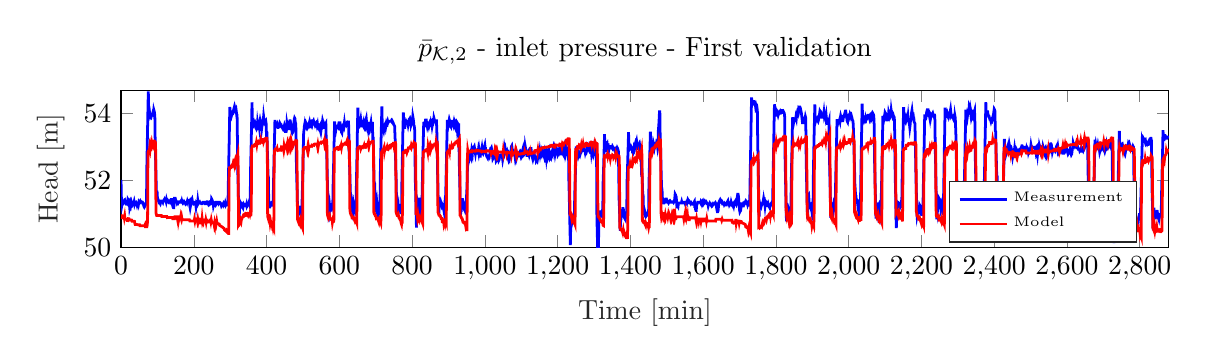
\begin{tikzpicture}

\begin{axis}[%
width=5.239in,
height=0.784in,
at={(0.978in,0.432in)},
scale only axis,
xmin=0,
xmax=2880,
xlabel style={font=\color{white!15!black}},
xlabel={Time [min]},
ymin=50,
ymax=54.7,
ylabel style={font=\color{white!15!black}},
ylabel={Head  [m]},
axis background/.style={fill=white},
title style={},
title={$\bar{p}_{\mathcal{K},2}$ - inlet pressure - First validation},
legend style={at={(0.97,0.03)}, anchor=south east, legend cell align=left, align=left, draw=white!15!black}
]
\addplot [color=blue, line width=1.0pt]
  table[row sep=crcr]{%
0	52.018827\\
1	51.4748392666667\\
2	51.44763988\\
3	51.3048431\\
4	51.36604172\\
5	51.34564218\\
6	51.32524264\\
7	51.34564218\\
8	51.36604172\\
9	51.38644126\\
10	51.36604172\\
11	51.38644126\\
12	51.34564218\\
13	51.32524264\\
14	51.34564218\\
15	51.34564218\\
16	51.32524264\\
17	51.34564218\\
18	51.32524264\\
19	51.42724034\\
20	51.4068408\\
21	51.4068408\\
22	51.34564218\\
23	51.36604172\\
24	51.18244586\\
25	51.22324494\\
26	51.2028454\\
27	51.26404402\\
28	51.26404402\\
29	51.32524264\\
30	51.28444356\\
31	51.26404402\\
32	51.28444356\\
33	51.28444356\\
34	51.28444356\\
35	51.32524264\\
36	51.36604172\\
37	51.3048431\\
38	51.34564218\\
39	51.34564218\\
40	51.32524264\\
41	51.3048431\\
42	51.32524264\\
43	51.3048431\\
44	51.26404402\\
45	51.3048431\\
46	51.32524264\\
47	51.32524264\\
48	51.28444356\\
49	51.34564218\\
50	51.32524264\\
51	51.32524264\\
52	51.36604172\\
53	51.38644126\\
54	51.36604172\\
55	51.36604172\\
56	51.36604172\\
57	51.34564218\\
58	51.34564218\\
59	51.34564218\\
60	51.3048431\\
61	51.3048431\\
62	51.26404402\\
63	51.22324494\\
64	51.2028454\\
65	51.22324494\\
66	51.24364448\\
67	51.26404402\\
68	51.3048431\\
69	51.32524264\\
70	51.32524264\\
71	52.4268178\\
72	53.01840446\\
73	53.56919204\\
74	54.1607787\\
75	54.6707672\\
76	54.1607787\\
77	54.058781\\
78	54.07918054\\
79	53.97718284\\
80	53.97718284\\
81	53.91598422\\
82	53.93638376\\
83	53.91598422\\
84	53.9567833\\
85	53.97718284\\
86	53.97718284\\
87	54.01798192\\
88	53.99758238\\
89	54.01798192\\
90	54.11997962\\
91	54.07918054\\
92	54.03838146\\
93	53.89558468\\
94	53.05920354\\
95	52.67161228\\
96	52.20242286\\
97	51.73323344\\
98	51.4068408\\
99	51.69243436\\
100	51.48843896\\
101	51.44763988\\
102	51.42724034\\
103	51.38644126\\
104	51.36604172\\
105	51.32524264\\
106	51.32524264\\
107	51.32524264\\
108	51.3048431\\
109	51.34564218\\
110	51.38644126\\
111	51.38644126\\
112	51.36604172\\
113	51.36604172\\
114	51.36604172\\
115	51.34564218\\
116	51.38644126\\
117	51.38644126\\
118	51.4068408\\
119	51.42724034\\
120	51.38644126\\
121	51.38644126\\
122	51.4068408\\
123	51.4068408\\
124	51.36604172\\
125	51.42724034\\
126	51.38644126\\
127	51.36604172\\
128	51.36604172\\
129	51.38644126\\
130	51.36604172\\
131	51.38644126\\
132	51.38644126\\
133	51.38644126\\
134	51.36604172\\
135	51.38644126\\
136	51.36604172\\
137	51.34564218\\
138	51.36604172\\
139	51.42724034\\
140	51.42724034\\
141	51.3048431\\
142	51.24364448\\
143	51.2028454\\
144	51.18244586\\
145	51.18244586\\
146	51.34564218\\
147	51.46803942\\
148	51.46803942\\
149	51.46803942\\
150	51.42724034\\
151	51.38644126\\
152	51.36604172\\
153	51.36604172\\
154	51.32524264\\
155	51.34564218\\
156	51.34564218\\
157	51.32524264\\
158	51.34564218\\
159	51.34564218\\
160	51.36604172\\
161	51.36604172\\
162	51.34564218\\
163	51.34564218\\
164	51.36604172\\
165	51.34564218\\
166	51.34564218\\
167	51.38644126\\
168	51.34564218\\
169	51.34564218\\
170	51.32524264\\
171	51.34564218\\
172	51.34564218\\
173	51.36604172\\
174	51.34564218\\
175	51.34564218\\
176	51.32524264\\
177	51.3048431\\
178	51.32524264\\
179	51.34564218\\
180	51.34564218\\
181	51.32524264\\
182	51.36604172\\
183	51.32524264\\
184	51.32524264\\
185	51.34564218\\
186	51.36604172\\
187	51.34564218\\
188	51.36604172\\
189	51.24364448\\
190	51.18244586\\
191	51.24364448\\
192	51.26404402\\
193	51.3048431\\
194	51.42724034\\
195	51.44763988\\
196	51.38644126\\
197	51.34564218\\
198	51.34564218\\
199	51.32524264\\
200	51.34564218\\
201	51.34564218\\
202	51.32524264\\
203	51.3048431\\
204	51.3048431\\
205	51.3048431\\
206	51.22324494\\
207	51.3048431\\
208	51.28444356\\
209	51.28444356\\
210	51.28444356\\
211	51.38644126\\
212	51.3048431\\
213	51.32524264\\
214	51.32524264\\
215	51.32524264\\
216	51.32524264\\
217	51.34564218\\
218	51.32524264\\
219	51.32524264\\
220	51.32524264\\
221	51.3048431\\
222	51.3048431\\
223	51.32524264\\
224	51.32524264\\
225	51.34564218\\
226	51.34564218\\
227	51.34564218\\
228	51.34564218\\
229	51.32524264\\
230	51.3048431\\
231	51.3048431\\
232	51.3048431\\
233	51.32524264\\
234	51.34564218\\
235	51.34564218\\
236	51.36604172\\
237	51.36604172\\
238	51.3048431\\
239	51.3048431\\
240	51.28444356\\
241	51.3048431\\
242	51.3048431\\
243	51.32524264\\
244	51.3048431\\
245	51.32524264\\
246	51.3048431\\
247	51.3048431\\
248	51.3048431\\
249	51.44763988\\
250	51.42724034\\
251	51.38644126\\
252	51.36604172\\
253	51.34564218\\
254	51.24364448\\
255	51.28444356\\
256	51.28444356\\
257	51.28444356\\
258	51.3048431\\
259	51.28444356\\
260	51.26404402\\
261	51.28444356\\
262	51.34564218\\
263	51.34564218\\
264	51.34564218\\
265	51.34564218\\
266	51.34564218\\
267	51.32524264\\
268	51.3048431\\
269	51.32524264\\
270	51.34564218\\
271	51.34564218\\
272	51.32524264\\
273	51.32524264\\
274	51.3048431\\
275	51.28444356\\
276	51.24364448\\
277	51.26404402\\
278	51.28444356\\
279	51.28444356\\
280	51.28444356\\
281	51.3048431\\
282	51.26404402\\
283	51.28444356\\
284	51.24364448\\
285	51.24364448\\
286	51.24364448\\
287	51.3048431\\
288	51.26404402\\
289	51.28444356\\
290	51.28444356\\
291	51.28444356\\
292	51.26404402\\
293	51.26404402\\
294	51.28444356\\
295	51.93722884\\
296	52.50841596\\
297	53.01840446\\
298	53.58959158\\
299	54.20157778\\
300	54.058781\\
301	54.058781\\
302	54.058781\\
303	54.01798192\\
304	53.9567833\\
305	53.99758238\\
306	54.03838146\\
307	54.058781\\
308	54.058781\\
309	54.09958008\\
310	54.14037916\\
311	54.07918054\\
312	54.09958008\\
313	54.18117824\\
314	54.14037916\\
315	54.11997962\\
316	54.14037916\\
317	54.058781\\
318	53.9567833\\
319	53.9567833\\
320	53.18160078\\
321	52.24322194\\
322	51.85563068\\
323	51.26404402\\
324	50.71325644\\
325	50.8968523\\
326	51.3048431\\
327	51.24364448\\
328	51.34564218\\
329	51.32524264\\
330	51.32524264\\
331	51.3048431\\
332	51.2028454\\
333	51.2028454\\
334	51.2028454\\
335	51.18244586\\
336	51.24364448\\
337	51.28444356\\
338	51.26404402\\
339	51.28444356\\
340	51.28444356\\
341	51.24364448\\
342	51.24364448\\
343	51.24364448\\
344	51.24364448\\
345	51.28444356\\
346	51.22324494\\
347	51.24364448\\
348	51.28444356\\
349	51.28444356\\
350	51.3048431\\
351	51.3048431\\
352	51.34564218\\
353	51.28444356\\
354	51.26404402\\
355	51.22324494\\
356	52.30442056\\
357	52.75321044\\
358	53.2427994\\
359	53.7527879\\
360	54.34437456\\
361	53.79358698\\
362	53.7527879\\
363	53.73238836\\
364	53.7527879\\
365	53.67118974\\
366	53.69158928\\
367	53.71198882\\
368	53.73238836\\
369	53.69158928\\
370	53.58959158\\
371	53.56919204\\
372	53.58959158\\
373	53.5487925\\
374	53.56919204\\
375	53.71198882\\
376	53.63039066\\
377	53.60999112\\
378	53.71198882\\
379	53.69158928\\
380	53.60999112\\
381	53.73238836\\
382	53.79358698\\
383	53.73238836\\
384	53.77318744\\
385	53.77318744\\
386	53.71198882\\
387	53.58959158\\
388	53.67118974\\
389	53.71198882\\
390	53.79358698\\
391	53.77318744\\
392	53.91598422\\
393	53.83438606\\
394	53.79358698\\
395	53.7527879\\
396	53.77318744\\
397	53.7527879\\
398	53.77318744\\
399	53.69158928\\
400	53.2427994\\
401	53.46719434\\
402	52.95720584\\
403	52.61041366\\
404	52.16162378\\
405	52.10042516\\
406	51.34564218\\
407	51.3048431\\
408	51.2028454\\
409	51.2028454\\
410	51.24364448\\
411	51.3048431\\
412	51.32524264\\
413	51.32524264\\
414	51.34564218\\
415	51.34564218\\
416	51.3048431\\
417	51.28444356\\
418	51.22324494\\
419	51.85563068\\
420	52.34521964\\
421	52.85520814\\
422	53.30399802\\
423	53.81398652\\
424	53.63039066\\
425	53.67118974\\
426	53.67118974\\
427	53.69158928\\
428	53.67118974\\
429	53.69158928\\
430	53.60999112\\
431	53.58959158\\
432	53.58959158\\
433	53.60999112\\
434	53.60999112\\
435	53.60999112\\
436	53.6507902\\
437	53.71198882\\
438	53.69158928\\
439	53.67118974\\
440	53.67118974\\
441	53.63039066\\
442	53.60999112\\
443	53.58959158\\
444	53.56919204\\
445	53.5487925\\
446	53.56919204\\
447	53.5487925\\
448	53.60999112\\
449	53.6507902\\
450	53.60999112\\
451	53.48759388\\
452	53.46719434\\
453	53.46719434\\
454	53.46719434\\
455	53.52839296\\
456	53.71198882\\
457	53.6507902\\
458	53.58959158\\
459	53.5487925\\
460	53.5487925\\
461	53.5487925\\
462	53.6507902\\
463	53.7527879\\
464	53.79358698\\
465	53.79358698\\
466	53.73238836\\
467	53.69158928\\
468	53.58959158\\
469	53.5487925\\
470	53.46719434\\
471	53.42639526\\
472	53.4467948\\
473	53.50799342\\
474	53.58959158\\
475	53.67118974\\
476	53.83438606\\
477	53.87518514\\
478	53.8547856\\
479	53.73238836\\
480	53.71198882\\
481	53.48759388\\
482	52.5288155\\
483	52.05962608\\
484	51.73323344\\
485	51.22324494\\
486	50.83565368\\
487	51.22324494\\
488	51.2028454\\
489	51.08044816\\
490	51.1008477\\
491	51.01924954\\
492	50.99885\\
493	50.99885\\
494	51.06004862\\
495	50.99885\\
496	51.06004862\\
497	51.12124724\\
498	51.52923804\\
499	51.89642976\\
500	52.38601872\\
501	52.97760538\\
502	53.4467948\\
503	53.50799342\\
504	53.63039066\\
505	53.69158928\\
506	53.63039066\\
507	53.6507902\\
508	53.69158928\\
509	53.6507902\\
510	53.69158928\\
511	53.67118974\\
512	53.6507902\\
513	53.58959158\\
514	53.60999112\\
515	53.60999112\\
516	53.63039066\\
517	53.71198882\\
518	53.7527879\\
519	53.69158928\\
520	53.6507902\\
521	53.67118974\\
522	53.67118974\\
523	53.6507902\\
524	53.7527879\\
525	53.79358698\\
526	53.79358698\\
527	53.73238836\\
528	53.77318744\\
529	53.79358698\\
530	53.7527879\\
531	53.73238836\\
532	53.73238836\\
533	53.69158928\\
534	53.6507902\\
535	53.67118974\\
536	53.71198882\\
537	53.73238836\\
538	53.71198882\\
539	53.6507902\\
540	53.69158928\\
541	53.60999112\\
542	53.58959158\\
543	53.67118974\\
544	53.67118974\\
545	53.6507902\\
546	53.63039066\\
547	53.6507902\\
548	53.48759388\\
549	53.4467948\\
550	53.52839296\\
551	53.56919204\\
552	53.56919204\\
553	53.71198882\\
554	53.79358698\\
555	53.7527879\\
556	53.7527879\\
557	53.67118974\\
558	53.63039066\\
559	53.58959158\\
560	53.58959158\\
561	53.6507902\\
562	53.69158928\\
563	53.71198882\\
564	53.22239986\\
565	52.95720584\\
566	52.56961458\\
567	52.08002562\\
568	51.6108362\\
569	51.59043666\\
570	51.36604172\\
571	51.1008477\\
572	51.16204632\\
573	51.08044816\\
574	51.18244586\\
575	51.08044816\\
576	51.2028454\\
577	51.18244586\\
578	51.26404402\\
579	51.26404402\\
580	51.28444356\\
581	51.24364448\\
582	51.2028454\\
583	51.89642976\\
584	52.30442056\\
585	52.85520814\\
586	53.28359848\\
587	53.77318744\\
588	53.52839296\\
589	53.52839296\\
590	53.48759388\\
591	53.5487925\\
592	53.58959158\\
593	53.60999112\\
594	53.63039066\\
595	53.63039066\\
596	53.63039066\\
597	53.60999112\\
598	53.67118974\\
599	53.73238836\\
600	53.73238836\\
601	53.73238836\\
602	53.73238836\\
603	53.60999112\\
604	53.52839296\\
605	53.52839296\\
606	53.4467948\\
607	53.42639526\\
608	53.52839296\\
609	53.50799342\\
610	53.5487925\\
611	53.67118974\\
612	53.69158928\\
613	53.6507902\\
614	53.73238836\\
615	53.6507902\\
616	53.6507902\\
617	53.67118974\\
618	53.67118974\\
619	53.6507902\\
620	53.67118974\\
621	53.73238836\\
622	53.7527879\\
623	53.7527879\\
624	53.71198882\\
625	53.79358698\\
626	53.56919204\\
627	52.85520814\\
628	52.5288155\\
629	52.18202332\\
630	51.75363298\\
631	51.44763988\\
632	51.59043666\\
633	51.44763988\\
634	51.24364448\\
635	51.18244586\\
636	51.1008477\\
637	51.18244586\\
638	51.14164678\\
639	51.24364448\\
640	51.16204632\\
641	51.26404402\\
642	51.22324494\\
643	51.2028454\\
644	51.22324494\\
645	51.08044816\\
646	51.03964908\\
647	51.9168293\\
648	52.48801642\\
649	52.99800492\\
650	53.71198882\\
651	54.18117824\\
652	53.77318744\\
653	53.7527879\\
654	53.67118974\\
655	53.6507902\\
656	53.69158928\\
657	53.79358698\\
658	53.77318744\\
659	53.83438606\\
660	53.7527879\\
661	53.69158928\\
662	53.63039066\\
663	53.63039066\\
664	53.63039066\\
665	53.69158928\\
666	53.73238836\\
667	53.63039066\\
668	53.58959158\\
669	53.56919204\\
670	53.60999112\\
671	53.58959158\\
672	53.77318744\\
673	53.81398652\\
674	53.8547856\\
675	53.73238836\\
676	53.73238836\\
677	53.63039066\\
678	53.58959158\\
679	53.52839296\\
680	53.60999112\\
681	53.60999112\\
682	53.56919204\\
683	53.67118974\\
684	53.71198882\\
685	53.71198882\\
686	53.67118974\\
687	53.73238836\\
688	53.63039066\\
689	53.67118974\\
690	53.69158928\\
691	53.7527879\\
692	53.18160078\\
693	53.30399802\\
694	52.87560768\\
695	52.28402102\\
696	51.79443206\\
697	51.93722884\\
698	51.26404402\\
699	51.2028454\\
700	51.24364448\\
701	51.34564218\\
702	51.26404402\\
703	51.34564218\\
704	51.22324494\\
705	51.18244586\\
706	50.97845046\\
707	50.93765138\\
708	51.03964908\\
709	51.14164678\\
710	51.2028454\\
711	51.3048431\\
712	51.4068408\\
713	52.40641826\\
714	52.85520814\\
715	53.32439756\\
716	53.79358698\\
717	54.22197732\\
718	53.63039066\\
719	53.60999112\\
720	53.56919204\\
721	53.52839296\\
722	53.48759388\\
723	53.5487925\\
724	53.56919204\\
725	53.6507902\\
726	53.69158928\\
727	53.71198882\\
728	53.63039066\\
729	53.69158928\\
730	53.6507902\\
731	53.6507902\\
732	53.73238836\\
733	53.77318744\\
734	53.73238836\\
735	53.7527879\\
736	53.77318744\\
737	53.77318744\\
738	53.77318744\\
739	53.77318744\\
740	53.77318744\\
741	53.77318744\\
742	53.77318744\\
743	53.79358698\\
744	53.77318744\\
745	53.79358698\\
746	53.77318744\\
747	53.7527879\\
748	53.73238836\\
749	53.69158928\\
750	53.67118974\\
751	53.6507902\\
752	53.63039066\\
753	53.3447971\\
754	53.10000262\\
755	52.46761688\\
756	52.10042516\\
757	51.52923804\\
758	51.36604172\\
759	51.1008477\\
760	51.22324494\\
761	51.16204632\\
762	51.22324494\\
763	51.06004862\\
764	51.14164678\\
765	51.22324494\\
766	51.2028454\\
767	51.14164678\\
768	51.18244586\\
769	51.16204632\\
770	51.03964908\\
771	51.03964908\\
772	51.99842746\\
773	52.5288155\\
774	53.05920354\\
775	53.63039066\\
776	54.03838146\\
777	53.63039066\\
778	53.63039066\\
779	53.58959158\\
780	53.58959158\\
781	53.67118974\\
782	53.71198882\\
783	53.71198882\\
784	53.77318744\\
785	53.7527879\\
786	53.73238836\\
787	53.71198882\\
788	53.73238836\\
789	53.67118974\\
790	53.73238836\\
791	53.79358698\\
792	53.83438606\\
793	53.83438606\\
794	53.8547856\\
795	53.81398652\\
796	53.77318744\\
797	53.67118974\\
798	53.71198882\\
799	53.7527879\\
800	53.77318744\\
801	53.77318744\\
802	53.91598422\\
803	53.8547856\\
804	53.77318744\\
805	53.6507902\\
806	53.63039066\\
807	53.52839296\\
808	52.69201182\\
809	51.95762838\\
810	51.6108362\\
811	51.03964908\\
812	50.5908592\\
813	50.85605322\\
814	51.12124724\\
815	51.12124724\\
816	51.26404402\\
817	51.2028454\\
818	51.44763988\\
819	51.44763988\\
820	51.34564218\\
821	51.12124724\\
822	51.1008477\\
823	50.95805092\\
824	50.8968523\\
825	50.87645276\\
826	51.12124724\\
827	51.18244586\\
828	51.79443206\\
829	52.3248201\\
830	52.87560768\\
831	53.30399802\\
832	53.7527879\\
833	53.60999112\\
834	53.63039066\\
835	53.73238836\\
836	53.73238836\\
837	53.81398652\\
838	53.81398652\\
839	53.81398652\\
840	53.69158928\\
841	53.67118974\\
842	53.60999112\\
843	53.6507902\\
844	53.67118974\\
845	53.73238836\\
846	53.73238836\\
847	53.6507902\\
848	53.69158928\\
849	53.6507902\\
850	53.6507902\\
851	53.6507902\\
852	53.73238836\\
853	53.69158928\\
854	53.71198882\\
855	53.63039066\\
856	53.69158928\\
857	53.7527879\\
858	53.73238836\\
859	53.77318744\\
860	53.87518514\\
861	53.83438606\\
862	53.79358698\\
863	53.79358698\\
864	53.77318744\\
865	53.79358698\\
866	53.79358698\\
867	53.79358698\\
868	53.48759388\\
869	53.10000262\\
870	52.26362148\\
871	51.87603022\\
872	51.28444356\\
873	51.14164678\\
874	51.12124724\\
875	51.38644126\\
876	51.34564218\\
877	51.34564218\\
878	51.34564218\\
879	51.2028454\\
880	51.3048431\\
881	51.26404402\\
882	51.3048431\\
883	51.28444356\\
884	51.26404402\\
885	51.22324494\\
886	51.16204632\\
887	51.12124724\\
888	51.06004862\\
889	51.18244586\\
890	51.1008477\\
891	51.2028454\\
892	51.26404402\\
893	51.87603022\\
894	52.34521964\\
895	52.87560768\\
896	53.38559618\\
897	53.81398652\\
898	53.69158928\\
899	53.63039066\\
900	53.69158928\\
901	53.58959158\\
902	53.71198882\\
903	53.79358698\\
904	53.7527879\\
905	53.63039066\\
906	53.63039066\\
907	53.60999112\\
908	53.67118974\\
909	53.77318744\\
910	53.77318744\\
911	53.77318744\\
912	53.7527879\\
913	53.71198882\\
914	53.67118974\\
915	53.73238836\\
916	53.67118974\\
917	53.69158928\\
918	53.6507902\\
919	53.7527879\\
920	53.73238836\\
921	53.7527879\\
922	53.71198882\\
923	53.69158928\\
924	53.56919204\\
925	53.63039066\\
926	53.69158928\\
927	53.67118974\\
928	53.67118974\\
929	53.05920354\\
930	52.4268178\\
931	51.99842746\\
932	51.44763988\\
933	50.93765138\\
934	51.1008477\\
935	51.22324494\\
936	51.2028454\\
937	51.34564218\\
938	51.42724034\\
939	51.42724034\\
940	51.38644126\\
941	51.34564218\\
942	51.22324494\\
943	51.16204632\\
944	51.12124724\\
945	51.1008477\\
946	51.16204632\\
947	51.1008477\\
948	51.12124724\\
949	51.08044816\\
950	51.6108362\\
951	51.79443206\\
952	52.30442056\\
953	52.50841596\\
954	52.8348086\\
955	52.67161228\\
956	52.69201182\\
957	52.6308132\\
958	52.67161228\\
959	52.69201182\\
960	52.71241136\\
961	52.77360998\\
962	52.7328109\\
963	52.85520814\\
964	52.9368063\\
965	52.89600722\\
966	52.8348086\\
967	52.95720584\\
968	52.99800492\\
969	52.99800492\\
970	52.99800492\\
971	53.01840446\\
972	52.95720584\\
973	52.87560768\\
974	52.81440906\\
975	52.89600722\\
976	52.89600722\\
977	52.85520814\\
978	52.87560768\\
979	52.85520814\\
980	52.81440906\\
981	52.81440906\\
982	52.89600722\\
983	52.8348086\\
984	52.91640676\\
985	52.8348086\\
986	52.81440906\\
987	52.69201182\\
988	52.79400952\\
989	52.79400952\\
990	52.8348086\\
991	52.91640676\\
992	52.97760538\\
993	52.89600722\\
994	52.8348086\\
995	52.81440906\\
996	52.85520814\\
997	52.89600722\\
998	52.99800492\\
999	53.01840446\\
1000	53.05920354\\
1001	52.95720584\\
1002	52.95720584\\
1003	52.81440906\\
1004	52.77360998\\
1005	52.7328109\\
1006	52.7328109\\
1007	52.69201182\\
1008	52.67161228\\
1009	52.71241136\\
1010	52.7328109\\
1011	52.7328109\\
1012	52.71241136\\
1013	52.77360998\\
1014	52.79400952\\
1015	52.87560768\\
1016	52.85520814\\
1017	52.95720584\\
1018	52.97760538\\
1019	52.91640676\\
1020	52.77360998\\
1021	52.75321044\\
1022	52.65121274\\
1023	52.67161228\\
1024	52.69201182\\
1025	52.71241136\\
1026	52.79400952\\
1027	52.79400952\\
1028	52.71241136\\
1029	52.67161228\\
1030	52.67161228\\
1031	52.59001412\\
1032	52.61041366\\
1033	52.67161228\\
1034	52.69201182\\
1035	52.65121274\\
1036	52.65121274\\
1037	52.6308132\\
1038	52.59001412\\
1039	52.61041366\\
1040	52.67161228\\
1041	52.7328109\\
1042	52.75321044\\
1043	52.75321044\\
1044	52.77360998\\
1045	52.77360998\\
1046	52.77360998\\
1047	52.75321044\\
1048	52.71241136\\
1049	52.6308132\\
1050	52.69201182\\
1051	52.69201182\\
1052	52.79400952\\
1053	52.8348086\\
1054	52.95720584\\
1055	52.89600722\\
1056	52.9368063\\
1057	52.85520814\\
1058	52.8348086\\
1059	52.85520814\\
1060	52.87560768\\
1061	52.77360998\\
1062	52.77360998\\
1063	52.79400952\\
1064	52.67161228\\
1065	52.6308132\\
1066	52.67161228\\
1067	52.71241136\\
1068	52.67161228\\
1069	52.7328109\\
1070	52.81440906\\
1071	52.87560768\\
1072	52.89600722\\
1073	53.01840446\\
1074	53.038804\\
1075	52.95720584\\
1076	52.91640676\\
1077	52.8348086\\
1078	52.77360998\\
1079	52.77360998\\
1080	52.79400952\\
1081	52.77360998\\
1082	52.79400952\\
1083	52.71241136\\
1084	52.6308132\\
1085	52.67161228\\
1086	52.6308132\\
1087	52.67161228\\
1088	52.71241136\\
1089	52.77360998\\
1090	52.7328109\\
1091	52.75321044\\
1092	52.7328109\\
1093	52.7328109\\
1094	52.79400952\\
1095	52.8348086\\
1096	52.85520814\\
1097	52.87560768\\
1098	52.85520814\\
1099	52.7328109\\
1100	52.69201182\\
1101	52.71241136\\
1102	52.71241136\\
1103	52.79400952\\
1104	52.91640676\\
1105	52.95720584\\
1106	52.87560768\\
1107	52.85520814\\
1108	52.87560768\\
1109	52.81440906\\
1110	52.8348086\\
1111	53.01840446\\
1112	52.95720584\\
1113	52.91640676\\
1114	52.87560768\\
1115	52.81440906\\
1116	52.71241136\\
1117	52.8348086\\
1118	52.81440906\\
1119	52.85520814\\
1120	52.87560768\\
1121	52.79400952\\
1122	52.75321044\\
1123	52.79400952\\
1124	52.77360998\\
1125	52.77360998\\
1126	52.95720584\\
1127	52.95720584\\
1128	52.85520814\\
1129	52.8348086\\
1130	52.79400952\\
1131	52.67161228\\
1132	52.6308132\\
1133	52.67161228\\
1134	52.71241136\\
1135	52.75321044\\
1136	52.77360998\\
1137	52.7328109\\
1138	52.7328109\\
1139	52.71241136\\
1140	52.67161228\\
1141	52.59001412\\
1142	52.61041366\\
1143	52.61041366\\
1144	52.59001412\\
1145	52.65121274\\
1146	52.71241136\\
1147	52.75321044\\
1148	52.79400952\\
1149	52.8348086\\
1150	52.79400952\\
1151	52.87560768\\
1152	52.79400952\\
1153	52.85520814\\
1154	52.81440906\\
1155	52.85520814\\
1156	52.81440906\\
1157	52.87560768\\
1158	52.8348086\\
1159	52.87560768\\
1160	52.85520814\\
1161	52.79400952\\
1162	52.77360998\\
1163	52.7328109\\
1164	52.81440906\\
1165	52.75321044\\
1166	52.81440906\\
1167	52.77360998\\
1168	52.79400952\\
1169	52.69201182\\
1170	52.79400952\\
1171	52.75321044\\
1172	52.87560768\\
1173	52.85520814\\
1174	52.87560768\\
1175	52.81440906\\
1176	52.85520814\\
1177	52.69201182\\
1178	52.65121274\\
1179	52.67161228\\
1180	52.71241136\\
1181	52.69201182\\
1182	52.79400952\\
1183	52.85520814\\
1184	52.87560768\\
1185	52.87560768\\
1186	52.8348086\\
1187	52.9368063\\
1188	52.97760538\\
1189	52.89600722\\
1190	52.91640676\\
1191	52.95720584\\
1192	52.87560768\\
1193	52.79400952\\
1194	52.85520814\\
1195	52.87560768\\
1196	52.91640676\\
1197	52.89600722\\
1198	52.9368063\\
1199	52.91640676\\
1200	52.87560768\\
1201	52.77360998\\
1202	52.79400952\\
1203	52.85520814\\
1204	52.8348086\\
1205	52.85520814\\
1206	52.97760538\\
1207	52.95720584\\
1208	52.85520814\\
1209	52.87560768\\
1210	52.89600722\\
1211	52.85520814\\
1212	52.79400952\\
1213	52.79400952\\
1214	52.85520814\\
1215	52.79400952\\
1216	52.77360998\\
1217	52.95720584\\
1218	52.99800492\\
1219	52.87560768\\
1220	52.85520814\\
1221	52.89600722\\
1222	52.77360998\\
1223	52.81440906\\
1224	52.89600722\\
1225	52.9368063\\
1226	52.87560768\\
1227	52.89600722\\
1228	52.91640676\\
1229	52.91640676\\
1230	52.85520814\\
1231	51.95762838\\
1232	51.54963758\\
1233	50.99885\\
1234	50.55006012\\
1235	50.06047116\\
1236	50.5908592\\
1237	50.61125874\\
1238	50.67245736\\
1239	50.73365598\\
1240	50.8968523\\
1241	50.91725184\\
1242	50.93765138\\
1243	50.95805092\\
1244	50.93765138\\
1245	50.91725184\\
1246	50.95805092\\
1247	51.5088385\\
1248	51.9168293\\
1249	52.24322194\\
1250	52.6308132\\
1251	53.01840446\\
1252	52.89600722\\
1253	52.85520814\\
1254	52.91640676\\
1255	52.89600722\\
1256	52.81440906\\
1257	52.75321044\\
1258	52.79400952\\
1259	52.77360998\\
1260	52.81440906\\
1261	52.8348086\\
1262	52.79400952\\
1263	52.8348086\\
1264	52.8348086\\
1265	52.87560768\\
1266	52.89600722\\
1267	52.97760538\\
1268	52.97760538\\
1269	52.99800492\\
1270	52.95720584\\
1271	52.97760538\\
1272	52.95720584\\
1273	52.89600722\\
1274	52.89600722\\
1275	52.89600722\\
1276	52.8348086\\
1277	52.87560768\\
1278	52.87560768\\
1279	52.85520814\\
1280	52.89600722\\
1281	52.97760538\\
1282	52.9368063\\
1283	52.95720584\\
1284	52.97760538\\
1285	52.9368063\\
1286	52.91640676\\
1287	52.99800492\\
1288	53.05920354\\
1289	53.038804\\
1290	53.05920354\\
1291	53.05920354\\
1292	52.97760538\\
1293	52.85520814\\
1294	52.9368063\\
1295	52.87560768\\
1296	52.91640676\\
1297	52.85520814\\
1298	52.91640676\\
1299	52.85520814\\
1300	52.9368063\\
1301	52.85520814\\
1302	52.87560768\\
1303	52.8348086\\
1304	52.85520814\\
1305	52.89600722\\
1306	52.95720584\\
1307	52.91640676\\
1308	50.83565368\\
1309	50.4888615\\
1310	49.85647576\\
1311	49.40768588\\
1312	49.08129324\\
1313	50.83565368\\
1314	50.83565368\\
1315	50.99885\\
1316	50.99885\\
1317	51.06004862\\
1318	51.06004862\\
1319	50.99885\\
1320	50.97845046\\
1321	51.01924954\\
1322	50.95805092\\
1323	50.93765138\\
1324	50.97845046\\
1325	51.93722884\\
1326	52.24322194\\
1327	52.59001412\\
1328	52.99800492\\
1329	53.38559618\\
1330	52.85520814\\
1331	52.9368063\\
1332	53.05920354\\
1333	53.07960308\\
1334	53.10000262\\
1335	53.07960308\\
1336	53.10000262\\
1337	52.97760538\\
1338	52.99800492\\
1339	52.97760538\\
1340	52.99800492\\
1341	52.9368063\\
1342	52.99800492\\
1343	52.97760538\\
1344	52.97760538\\
1345	53.01840446\\
1346	53.01840446\\
1347	53.01840446\\
1348	52.99800492\\
1349	52.99800492\\
1350	52.97760538\\
1351	53.01840446\\
1352	52.99800492\\
1353	52.97760538\\
1354	52.97760538\\
1355	52.95720584\\
1356	52.91640676\\
1357	52.89600722\\
1358	52.91640676\\
1359	52.9368063\\
1360	52.91640676\\
1361	52.9368063\\
1362	52.95720584\\
1363	52.9368063\\
1364	52.97760538\\
1365	52.95720584\\
1366	52.91640676\\
1367	52.87560768\\
1368	52.24322194\\
1369	51.42724034\\
1370	51.18244586\\
1371	50.7948546\\
1372	50.4888615\\
1373	50.75405552\\
1374	51.03964908\\
1375	50.91725184\\
1376	50.99885\\
1377	51.06004862\\
1378	51.08044816\\
1379	51.16204632\\
1380	51.16204632\\
1381	51.12124724\\
1382	50.99885\\
1383	50.91725184\\
1384	50.87645276\\
1385	50.85605322\\
1386	50.83565368\\
1387	50.93765138\\
1388	51.01924954\\
1389	51.03964908\\
1390	51.06004862\\
1391	52.018827\\
1392	52.3248201\\
1393	52.69201182\\
1394	53.05920354\\
1395	53.4467948\\
1396	52.91640676\\
1397	52.9368063\\
1398	52.9368063\\
1399	52.99800492\\
1400	52.95720584\\
1401	52.95720584\\
1402	52.95720584\\
1403	52.99800492\\
1404	52.97760538\\
1405	52.97760538\\
1406	52.85520814\\
1407	52.85520814\\
1408	52.81440906\\
1409	52.8348086\\
1410	52.87560768\\
1411	53.01840446\\
1412	52.99800492\\
1413	53.07960308\\
1414	53.12040216\\
1415	53.16120124\\
1416	53.1408017\\
1417	53.18160078\\
1418	53.10000262\\
1419	52.99800492\\
1420	53.01840446\\
1421	52.95720584\\
1422	52.95720584\\
1423	52.99800492\\
1424	53.038804\\
1425	52.97760538\\
1426	53.01840446\\
1427	52.9368063\\
1428	52.91640676\\
1429	52.87560768\\
1430	52.50841596\\
1431	52.56961458\\
1432	52.20242286\\
1433	51.89642976\\
1434	51.54963758\\
1435	51.54963758\\
1436	51.03964908\\
1437	51.12124724\\
1438	51.01924954\\
1439	50.97845046\\
1440	50.95805092\\
1441	51.01924954\\
1442	50.97845046\\
1443	50.93765138\\
1444	50.95805092\\
1445	50.97845046\\
1446	50.95805092\\
1447	50.95805092\\
1448	50.99885\\
1449	50.97845046\\
1450	50.97845046\\
1451	51.87603022\\
1452	52.28402102\\
1453	52.69201182\\
1454	53.038804\\
1455	53.46719434\\
1456	53.01840446\\
1457	52.95720584\\
1458	52.9368063\\
1459	53.05920354\\
1460	53.05920354\\
1461	53.07960308\\
1462	53.05920354\\
1463	53.1408017\\
1464	53.10000262\\
1465	53.05920354\\
1466	52.99800492\\
1467	53.05920354\\
1468	53.038804\\
1469	53.07960308\\
1470	53.07960308\\
1471	53.07960308\\
1472	53.1408017\\
1473	53.12040216\\
1474	53.05920354\\
1475	52.97760538\\
1476	53.038804\\
1477	53.52839296\\
1478	53.63039066\\
1479	53.83438606\\
1480	54.058781\\
1481	54.058781\\
1482	53.20200032\\
1483	53.01840446\\
1484	52.50841596\\
1485	52.05962608\\
1486	51.75363298\\
1487	51.73323344\\
1488	51.46803942\\
1489	51.44763988\\
1490	51.4068408\\
1491	51.32524264\\
1492	51.32524264\\
1493	51.32524264\\
1494	51.34564218\\
1495	51.38644126\\
1496	51.4068408\\
1497	51.44763988\\
1498	51.44763988\\
1499	51.44763988\\
1500	51.4068408\\
1501	51.38644126\\
1502	51.34564218\\
1503	51.34564218\\
1504	51.34564218\\
1505	51.32524264\\
1506	51.34564218\\
1507	51.36604172\\
1508	51.34564218\\
1509	51.34564218\\
1510	51.36604172\\
1511	51.34564218\\
1512	51.34564218\\
1513	51.34564218\\
1514	51.36604172\\
1515	51.36604172\\
1516	51.36604172\\
1517	51.36604172\\
1518	51.36604172\\
1519	51.34564218\\
1520	51.36604172\\
1521	51.36604172\\
1522	51.46803942\\
1523	51.59043666\\
1524	51.57003712\\
1525	51.52923804\\
1526	51.5088385\\
1527	51.34564218\\
1528	51.2028454\\
1529	51.2028454\\
1530	51.24364448\\
1531	51.22324494\\
1532	51.3048431\\
1533	51.32524264\\
1534	51.32524264\\
1535	51.32524264\\
1536	51.32524264\\
1537	51.32524264\\
1538	51.32524264\\
1539	51.32524264\\
1540	51.32524264\\
1541	51.36604172\\
1542	51.32524264\\
1543	51.32524264\\
1544	51.32524264\\
1545	51.32524264\\
1546	51.34564218\\
1547	51.34564218\\
1548	51.34564218\\
1549	51.34564218\\
1550	51.34564218\\
1551	51.3048431\\
1552	51.32524264\\
1553	51.32524264\\
1554	51.34564218\\
1555	51.32524264\\
1556	51.38644126\\
1557	51.38644126\\
1558	51.42724034\\
1559	51.4068408\\
1560	51.4068408\\
1561	51.38644126\\
1562	51.36604172\\
1563	51.32524264\\
1564	51.32524264\\
1565	51.32524264\\
1566	51.3048431\\
1567	51.32524264\\
1568	51.3048431\\
1569	51.3048431\\
1570	51.3048431\\
1571	51.3048431\\
1572	51.28444356\\
1573	51.28444356\\
1574	51.32524264\\
1575	51.34564218\\
1576	51.36604172\\
1577	51.22324494\\
1578	51.22324494\\
1579	51.14164678\\
1580	51.1008477\\
1581	51.1008477\\
1582	51.24364448\\
1583	51.28444356\\
1584	51.3048431\\
1585	51.34564218\\
1586	51.34564218\\
1587	51.34564218\\
1588	51.34564218\\
1589	51.34564218\\
1590	51.34564218\\
1591	51.34564218\\
1592	51.34564218\\
1593	51.32524264\\
1594	51.36604172\\
1595	51.34564218\\
1596	51.32524264\\
1597	51.34564218\\
1598	51.28444356\\
1599	51.3048431\\
1600	51.28444356\\
1601	51.3048431\\
1602	51.3048431\\
1603	51.36604172\\
1604	51.34564218\\
1605	51.36604172\\
1606	51.34564218\\
1607	51.32524264\\
1608	51.32524264\\
1609	51.34564218\\
1610	51.32524264\\
1611	51.3048431\\
1612	51.3048431\\
1613	51.3048431\\
1614	51.24364448\\
1615	51.28444356\\
1616	51.3048431\\
1617	51.3048431\\
1618	51.32524264\\
1619	51.3048431\\
1620	51.28444356\\
1621	51.28444356\\
1622	51.26404402\\
1623	51.24364448\\
1624	51.26404402\\
1625	51.28444356\\
1626	51.26404402\\
1627	51.28444356\\
1628	51.3048431\\
1629	51.3048431\\
1630	51.3048431\\
1631	51.32524264\\
1632	51.32524264\\
1633	51.3048431\\
1634	51.32524264\\
1635	51.3048431\\
1636	51.3048431\\
1637	51.18244586\\
1638	51.12124724\\
1639	51.06004862\\
1640	51.06004862\\
1641	51.08044816\\
1642	51.2028454\\
1643	51.28444356\\
1644	51.36604172\\
1645	51.38644126\\
1646	51.4068408\\
1647	51.42724034\\
1648	51.4068408\\
1649	51.4068408\\
1650	51.38644126\\
1651	51.34564218\\
1652	51.32524264\\
1653	51.34564218\\
1654	51.32524264\\
1655	51.32524264\\
1656	51.32524264\\
1657	51.32524264\\
1658	51.28444356\\
1659	51.3048431\\
1660	51.28444356\\
1661	51.26404402\\
1662	51.26404402\\
1663	51.26404402\\
1664	51.26404402\\
1665	51.3048431\\
1666	51.34564218\\
1667	51.36604172\\
1668	51.38644126\\
1669	51.32524264\\
1670	51.32524264\\
1671	51.3048431\\
1672	51.26404402\\
1673	51.28444356\\
1674	51.3048431\\
1675	51.28444356\\
1676	51.28444356\\
1677	51.34564218\\
1678	51.3048431\\
1679	51.32524264\\
1680	51.32524264\\
1681	51.3048431\\
1682	51.26404402\\
1683	51.28444356\\
1684	51.24364448\\
1685	51.3048431\\
1686	51.34564218\\
1687	51.36604172\\
1688	51.36604172\\
1689	51.38644126\\
1690	51.3048431\\
1691	51.28444356\\
1692	51.32524264\\
1693	51.42724034\\
1694	51.5088385\\
1695	51.59043666\\
1696	51.59043666\\
1697	51.52923804\\
1698	51.38644126\\
1699	51.24364448\\
1700	51.12124724\\
1701	51.06004862\\
1702	51.08044816\\
1703	51.1008477\\
1704	51.18244586\\
1705	51.22324494\\
1706	51.3048431\\
1707	51.3048431\\
1708	51.3048431\\
1709	51.28444356\\
1710	51.3048431\\
1711	51.28444356\\
1712	51.26404402\\
1713	51.28444356\\
1714	51.3048431\\
1715	51.32524264\\
1716	51.36604172\\
1717	51.38644126\\
1718	51.36604172\\
1719	51.36604172\\
1720	51.32524264\\
1721	51.32524264\\
1722	51.28444356\\
1723	51.32524264\\
1724	51.32524264\\
1725	51.34564218\\
1726	51.3048431\\
1727	51.3048431\\
1728	51.22324494\\
1729	51.97802792\\
1730	52.59001412\\
1731	53.20200032\\
1732	53.83438606\\
1733	54.48717134\\
1734	54.3647741\\
1735	54.38517364\\
1736	54.3647741\\
1737	54.34437456\\
1738	54.3647741\\
1739	54.3647741\\
1740	54.28317594\\
1741	54.28317594\\
1742	54.30357548\\
1743	54.30357548\\
1744	54.22197732\\
1745	54.2627764\\
1746	54.22197732\\
1747	54.1607787\\
1748	54.18117824\\
1749	54.09958008\\
1750	53.12040216\\
1751	52.61041366\\
1752	52.018827\\
1753	51.38644126\\
1754	50.91725184\\
1755	51.32524264\\
1756	51.26404402\\
1757	51.26404402\\
1758	51.28444356\\
1759	51.28444356\\
1760	51.24364448\\
1761	51.28444356\\
1762	51.3048431\\
1763	51.32524264\\
1764	51.32524264\\
1765	51.38644126\\
1766	51.28444356\\
1767	51.4068408\\
1768	51.34564218\\
1769	51.36604172\\
1770	51.26404402\\
1771	51.36604172\\
1772	51.24364448\\
1773	51.24364448\\
1774	51.24364448\\
1775	51.3048431\\
1776	51.28444356\\
1777	51.3048431\\
1778	51.32524264\\
1779	51.28444356\\
1780	51.26404402\\
1781	51.22324494\\
1782	51.2028454\\
1783	51.18244586\\
1784	51.24364448\\
1785	51.24364448\\
1786	51.28444356\\
1787	51.3048431\\
1788	51.32524264\\
1789	51.28444356\\
1790	51.28444356\\
1791	51.3048431\\
1792	51.97802792\\
1793	52.54921504\\
1794	53.1408017\\
1795	53.73238836\\
1796	54.28317594\\
1797	54.18117824\\
1798	54.18117824\\
1799	54.14037916\\
1800	54.07918054\\
1801	54.07918054\\
1802	54.03838146\\
1803	53.9567833\\
1804	53.9567833\\
1805	53.99758238\\
1806	53.9567833\\
1807	53.99758238\\
1808	54.058781\\
1809	54.058781\\
1810	54.03838146\\
1811	54.058781\\
1812	54.01798192\\
1813	54.01798192\\
1814	54.03838146\\
1815	54.058781\\
1816	54.09958008\\
1817	54.09958008\\
1818	54.07918054\\
1819	54.03838146\\
1820	54.03838146\\
1821	54.058781\\
1822	54.03838146\\
1823	54.01798192\\
1824	53.91598422\\
1825	52.8348086\\
1826	52.28402102\\
1827	51.73323344\\
1828	51.22324494\\
1829	50.77445506\\
1830	51.32524264\\
1831	51.24364448\\
1832	51.24364448\\
1833	51.18244586\\
1834	51.16204632\\
1835	51.12124724\\
1836	51.14164678\\
1837	51.12124724\\
1838	51.06004862\\
1839	51.08044816\\
1840	50.99885\\
1841	50.99885\\
1842	51.75363298\\
1843	52.4268178\\
1844	52.87560768\\
1845	53.42639526\\
1846	53.89558468\\
1847	53.71198882\\
1848	53.69158928\\
1849	53.7527879\\
1850	53.77318744\\
1851	53.81398652\\
1852	53.81398652\\
1853	53.81398652\\
1854	53.81398652\\
1855	53.89558468\\
1856	53.8547856\\
1857	53.97718284\\
1858	53.97718284\\
1859	54.03838146\\
1860	54.01798192\\
1861	54.07918054\\
1862	54.03838146\\
1863	54.09958008\\
1864	54.14037916\\
1865	54.20157778\\
1866	54.20157778\\
1867	54.18117824\\
1868	54.11997962\\
1869	54.07918054\\
1870	54.01798192\\
1871	53.93638376\\
1872	53.83438606\\
1873	53.73238836\\
1874	53.73238836\\
1875	53.73238836\\
1876	53.73238836\\
1877	53.81398652\\
1878	53.87518514\\
1879	53.87518514\\
1880	53.8547856\\
1881	53.91598422\\
1882	53.87518514\\
1883	52.8348086\\
1884	52.18202332\\
1885	51.67203482\\
1886	51.26404402\\
1887	50.85605322\\
1888	51.42724034\\
1889	51.52923804\\
1890	51.54963758\\
1891	51.4068408\\
1892	51.22324494\\
1893	51.22324494\\
1894	51.2028454\\
1895	51.24364448\\
1896	51.24364448\\
1897	51.26404402\\
1898	51.1008477\\
1899	51.06004862\\
1900	50.97845046\\
1901	51.03964908\\
1902	51.14164678\\
1903	52.18202332\\
1904	52.81440906\\
1905	53.3447971\\
1906	53.83438606\\
1907	54.28317594\\
1908	53.83438606\\
1909	53.77318744\\
1910	53.81398652\\
1911	53.83438606\\
1912	53.83438606\\
1913	53.83438606\\
1914	53.8547856\\
1915	53.79358698\\
1916	53.77318744\\
1917	53.81398652\\
1918	53.87518514\\
1919	53.89558468\\
1920	53.99758238\\
1921	54.07918054\\
1922	54.058781\\
1923	54.058781\\
1924	54.01798192\\
1925	53.97718284\\
1926	53.89558468\\
1927	53.89558468\\
1928	53.9567833\\
1929	53.9567833\\
1930	53.93638376\\
1931	53.9567833\\
1932	54.03838146\\
1933	53.93638376\\
1934	53.97718284\\
1935	53.9567833\\
1936	53.97718284\\
1937	53.89558468\\
1938	53.9567833\\
1939	53.83438606\\
1940	53.81398652\\
1941	53.71198882\\
1942	53.71198882\\
1943	53.71198882\\
1944	53.77318744\\
1945	53.7527879\\
1946	53.79358698\\
1947	52.81440906\\
1948	52.28402102\\
1949	51.8148316\\
1950	51.34564218\\
1951	50.87645276\\
1952	51.3048431\\
1953	51.3048431\\
1954	51.22324494\\
1955	51.22324494\\
1956	51.14164678\\
1957	51.2028454\\
1958	51.1008477\\
1959	51.18244586\\
1960	51.16204632\\
1961	51.18244586\\
1962	51.16204632\\
1963	51.22324494\\
1964	51.85563068\\
1965	52.34521964\\
1966	52.8348086\\
1967	53.32439756\\
1968	53.83438606\\
1969	53.7527879\\
1970	53.73238836\\
1971	53.79358698\\
1972	53.79358698\\
1973	53.79358698\\
1974	53.77318744\\
1975	53.81398652\\
1976	53.77318744\\
1977	53.87518514\\
1978	53.93638376\\
1979	53.89558468\\
1980	53.83438606\\
1981	53.8547856\\
1982	53.79358698\\
1983	53.79358698\\
1984	53.79358698\\
1985	53.8547856\\
1986	53.91598422\\
1987	53.91598422\\
1988	53.93638376\\
1989	53.99758238\\
1990	54.03838146\\
1991	54.07918054\\
1992	54.07918054\\
1993	53.99758238\\
1994	53.91598422\\
1995	53.8547856\\
1996	53.77318744\\
1997	53.7527879\\
1998	53.8547856\\
1999	53.8547856\\
2000	53.9567833\\
2001	53.9567833\\
2002	53.97718284\\
2003	53.93638376\\
2004	53.99758238\\
2005	53.97718284\\
2006	53.93638376\\
2007	53.9567833\\
2008	53.91598422\\
2009	53.87518514\\
2010	53.81398652\\
2011	53.79358698\\
2012	53.77318744\\
2013	53.5487925\\
2014	53.20200032\\
2015	52.77360998\\
2016	52.40641826\\
2017	51.89642976\\
2018	51.73323344\\
2019	51.52923804\\
2020	51.52923804\\
2021	51.4068408\\
2022	51.4068408\\
2023	51.3048431\\
2024	51.42724034\\
2025	51.28444356\\
2026	51.32524264\\
2027	51.32524264\\
2028	51.22324494\\
2029	51.01924954\\
2030	51.03964908\\
2031	51.03964908\\
2032	50.87645276\\
2033	51.75363298\\
2034	52.48801642\\
2035	53.10000262\\
2036	53.67118974\\
2037	54.30357548\\
2038	53.99758238\\
2039	53.89558468\\
2040	53.89558468\\
2041	53.8547856\\
2042	53.81398652\\
2043	53.8547856\\
2044	53.83438606\\
2045	53.7527879\\
2046	53.7527879\\
2047	53.8547856\\
2048	53.81398652\\
2049	53.83438606\\
2050	53.87518514\\
2051	53.87518514\\
2052	53.89558468\\
2053	53.9567833\\
2054	53.9567833\\
2055	53.9567833\\
2056	53.91598422\\
2057	53.87518514\\
2058	53.93638376\\
2059	53.9567833\\
2060	53.93638376\\
2061	53.9567833\\
2062	53.93638376\\
2063	53.83438606\\
2064	53.8547856\\
2065	53.9567833\\
2066	53.93638376\\
2067	53.99758238\\
2068	53.97718284\\
2069	53.93638376\\
2070	53.69158928\\
2071	52.65121274\\
2072	52.24322194\\
2073	51.75363298\\
2074	51.28444356\\
2075	50.85605322\\
2076	51.34564218\\
2077	51.12124724\\
2078	51.1008477\\
2079	51.03964908\\
2080	51.16204632\\
2081	51.16204632\\
2082	51.26404402\\
2083	51.28444356\\
2084	51.18244586\\
2085	51.06004862\\
2086	51.16204632\\
2087	51.01924954\\
2088	50.93765138\\
2089	50.99885\\
2090	51.69243436\\
2091	52.18202332\\
2092	52.75321044\\
2093	53.30399802\\
2094	53.93638376\\
2095	53.83438606\\
2096	53.79358698\\
2097	53.8547856\\
2098	53.93638376\\
2099	53.9567833\\
2100	54.03838146\\
2101	54.01798192\\
2102	53.99758238\\
2103	53.97718284\\
2104	53.91598422\\
2105	53.77318744\\
2106	53.87518514\\
2107	53.89558468\\
2108	53.91598422\\
2109	53.89558468\\
2110	54.03838146\\
2111	53.99758238\\
2112	53.93638376\\
2113	53.97718284\\
2114	53.97718284\\
2115	53.91598422\\
2116	53.93638376\\
2117	54.07918054\\
2118	53.99758238\\
2119	54.01798192\\
2120	54.03838146\\
2121	54.01798192\\
2122	53.91598422\\
2123	53.93638376\\
2124	53.89558468\\
2125	53.89558468\\
2126	53.79358698\\
2127	52.85520814\\
2128	52.10042516\\
2129	51.65163528\\
2130	50.99885\\
2131	50.57045966\\
2132	50.99885\\
2133	51.22324494\\
2134	51.22324494\\
2135	51.3048431\\
2136	51.28444356\\
2137	51.3048431\\
2138	51.28444356\\
2139	51.26404402\\
2140	51.26404402\\
2141	51.22324494\\
2142	51.26404402\\
2143	51.22324494\\
2144	51.22324494\\
2145	51.28444356\\
2146	51.3048431\\
2147	52.10042516\\
2148	52.75321044\\
2149	53.18160078\\
2150	53.67118974\\
2151	54.20157778\\
2152	53.83438606\\
2153	53.77318744\\
2154	53.79358698\\
2155	53.77318744\\
2156	53.83438606\\
2157	53.87518514\\
2158	53.81398652\\
2159	53.8547856\\
2160	53.8547856\\
2161	53.8547856\\
2162	53.83438606\\
2163	53.91598422\\
2164	53.79358698\\
2165	53.79358698\\
2166	53.73238836\\
2167	53.69158928\\
2168	53.58959158\\
2169	53.67118974\\
2170	53.81398652\\
2171	53.81398652\\
2172	53.8547856\\
2173	54.03838146\\
2174	54.09958008\\
2175	53.99758238\\
2176	53.99758238\\
2177	53.99758238\\
2178	53.87518514\\
2179	53.87518514\\
2180	53.7527879\\
2181	53.73238836\\
2182	53.71198882\\
2183	53.3447971\\
2184	52.69201182\\
2185	52.08002562\\
2186	51.65163528\\
2187	51.12124724\\
2188	50.95805092\\
2189	51.01924954\\
2190	51.1008477\\
2191	51.08044816\\
2192	51.12124724\\
2193	51.1008477\\
2194	51.16204632\\
2195	51.26404402\\
2196	51.24364448\\
2197	51.16204632\\
2198	51.08044816\\
2199	51.01924954\\
2200	50.97845046\\
2201	50.97845046\\
2202	50.99885\\
2203	51.12124724\\
2204	51.01924954\\
2205	51.73323344\\
2206	52.2228224\\
2207	52.79400952\\
2208	53.32439756\\
2209	53.97718284\\
2210	53.81398652\\
2211	53.83438606\\
2212	53.8547856\\
2213	53.91598422\\
2214	54.01798192\\
2215	54.07918054\\
2216	54.11997962\\
2217	54.11997962\\
2218	54.11997962\\
2219	53.9567833\\
2220	53.9567833\\
2221	53.9567833\\
2222	53.93638376\\
2223	53.87518514\\
2224	53.99758238\\
2225	53.97718284\\
2226	53.91598422\\
2227	53.97718284\\
2228	53.99758238\\
2229	53.99758238\\
2230	53.99758238\\
2231	54.01798192\\
2232	53.97718284\\
2233	53.93638376\\
2234	53.91598422\\
2235	53.89558468\\
2236	53.99758238\\
2237	53.81398652\\
2238	52.9368063\\
2239	52.50841596\\
2240	51.89642976\\
2241	51.24364448\\
2242	50.83565368\\
2243	51.16204632\\
2244	51.08044816\\
2245	51.2028454\\
2246	51.32524264\\
2247	51.36604172\\
2248	51.46803942\\
2249	51.44763988\\
2250	51.36604172\\
2251	51.28444356\\
2252	51.28444356\\
2253	51.18244586\\
2254	51.24364448\\
2255	51.3048431\\
2256	51.26404402\\
2257	51.16204632\\
2258	51.14164678\\
2259	51.06004862\\
2260	50.95805092\\
2261	51.6108362\\
2262	52.28402102\\
2263	52.95720584\\
2264	53.50799342\\
2265	54.18117824\\
2266	54.11997962\\
2267	54.058781\\
2268	53.99758238\\
2269	53.97718284\\
2270	53.91598422\\
2271	53.91598422\\
2272	53.97718284\\
2273	53.93638376\\
2274	53.9567833\\
2275	53.91598422\\
2276	53.9567833\\
2277	53.99758238\\
2278	54.01798192\\
2279	54.058781\\
2280	54.11997962\\
2281	54.01798192\\
2282	53.93638376\\
2283	53.9567833\\
2284	53.93638376\\
2285	53.93638376\\
2286	53.93638376\\
2287	53.89558468\\
2288	53.91598422\\
2289	53.87518514\\
2290	53.79358698\\
2291	53.77318744\\
2292	53.93638376\\
2293	53.87518514\\
2294	53.56919204\\
2295	53.28359848\\
2296	52.65121274\\
2297	52.20242286\\
2298	51.69243436\\
2299	51.44763988\\
2300	51.22324494\\
2301	51.24364448\\
2302	50.99885\\
2303	50.91725184\\
2304	50.97845046\\
2305	51.03964908\\
2306	51.2028454\\
2307	51.32524264\\
2308	51.44763988\\
2309	51.34564218\\
2310	51.32524264\\
2311	51.2028454\\
2312	51.1008477\\
2313	51.08044816\\
2314	51.2028454\\
2315	51.12124724\\
2316	51.28444356\\
2317	51.26404402\\
2318	51.99842746\\
2319	52.46761688\\
2320	53.05920354\\
2321	53.5487925\\
2322	54.11997962\\
2323	53.89558468\\
2324	53.89558468\\
2325	53.9567833\\
2326	53.89558468\\
2327	53.97718284\\
2328	54.03838146\\
2329	54.03838146\\
2330	54.03838146\\
2331	54.18117824\\
2332	54.14037916\\
2333	54.11997962\\
2334	54.18117824\\
2335	54.11997962\\
2336	53.9567833\\
2337	53.87518514\\
2338	53.91598422\\
2339	53.83438606\\
2340	53.83438606\\
2341	53.87518514\\
2342	54.07918054\\
2343	54.07918054\\
2344	54.058781\\
2345	54.03838146\\
2346	54.07918054\\
2347	53.71198882\\
2348	52.71241136\\
2349	52.18202332\\
2350	51.52923804\\
2351	50.93765138\\
2352	50.65205782\\
2353	51.01924954\\
2354	51.08044816\\
2355	51.22324494\\
2356	51.3048431\\
2357	51.26404402\\
2358	51.3048431\\
2359	51.3048431\\
2360	51.36604172\\
2361	51.34564218\\
2362	51.36604172\\
2363	51.38644126\\
2364	51.38644126\\
2365	51.34564218\\
2366	51.36604172\\
2367	51.32524264\\
2368	51.24364448\\
2369	51.22324494\\
2370	51.12124724\\
2371	51.06004862\\
2372	51.01924954\\
2373	52.03922654\\
2374	52.56961458\\
2375	53.22239986\\
2376	53.73238836\\
2377	54.34437456\\
2378	53.99758238\\
2379	54.03838146\\
2380	54.01798192\\
2381	54.058781\\
2382	54.058781\\
2383	53.97718284\\
2384	53.9567833\\
2385	53.91598422\\
2386	53.91598422\\
2387	53.87518514\\
2388	53.83438606\\
2389	53.83438606\\
2390	53.81398652\\
2391	53.77318744\\
2392	53.81398652\\
2393	53.83438606\\
2394	53.81398652\\
2395	53.87518514\\
2396	53.89558468\\
2397	53.93638376\\
2398	53.97718284\\
2399	54.058781\\
2400	54.14037916\\
2401	54.11997962\\
2402	54.07918054\\
2403	53.48759388\\
2404	53.46719434\\
2405	52.89600722\\
2406	52.56961458\\
2407	52.08002562\\
2408	52.14122424\\
2409	51.63123574\\
2410	51.59043666\\
2411	51.4068408\\
2412	51.38644126\\
2413	51.34564218\\
2414	51.28444356\\
2415	51.26404402\\
2416	51.34564218\\
2417	51.34564218\\
2418	51.36604172\\
2419	51.3048431\\
2420	51.28444356\\
2421	51.12124724\\
2422	50.91725184\\
2423	50.77445506\\
2424	51.4068408\\
2425	51.77403252\\
2426	52.18202332\\
2427	52.7328109\\
2428	53.2427994\\
2429	52.99800492\\
2430	52.97760538\\
2431	52.95720584\\
2432	52.89600722\\
2433	52.81440906\\
2434	52.85520814\\
2435	52.89600722\\
2436	52.9368063\\
2437	52.99800492\\
2438	53.038804\\
2439	52.99800492\\
2440	53.038804\\
2441	53.10000262\\
2442	53.038804\\
2443	52.95720584\\
2444	52.97760538\\
2445	52.9368063\\
2446	52.89600722\\
2447	52.87560768\\
2448	52.91640676\\
2449	52.87560768\\
2450	52.8348086\\
2451	52.7328109\\
2452	52.79400952\\
2453	52.8348086\\
2454	52.85520814\\
2455	52.87560768\\
2456	52.95720584\\
2457	52.87560768\\
2458	52.89600722\\
2459	52.85520814\\
2460	52.89600722\\
2461	52.85520814\\
2462	52.91640676\\
2463	52.89600722\\
2464	52.89600722\\
2465	52.85520814\\
2466	52.87560768\\
2467	52.87560768\\
2468	52.85520814\\
2469	52.91640676\\
2470	52.9368063\\
2471	52.9368063\\
2472	52.91640676\\
2473	52.95720584\\
2474	52.97760538\\
2475	52.99800492\\
2476	53.038804\\
2477	53.038804\\
2478	53.01840446\\
2479	52.97760538\\
2480	52.95720584\\
2481	52.97760538\\
2482	52.97760538\\
2483	52.99800492\\
2484	52.99800492\\
2485	52.97760538\\
2486	52.9368063\\
2487	52.91640676\\
2488	52.89600722\\
2489	52.95720584\\
2490	52.91640676\\
2491	52.91640676\\
2492	52.95720584\\
2493	52.9368063\\
2494	52.85520814\\
2495	52.89600722\\
2496	52.87560768\\
2497	52.91640676\\
2498	52.91640676\\
2499	52.9368063\\
2500	52.97760538\\
2501	53.05920354\\
2502	52.99800492\\
2503	53.01840446\\
2504	52.99800492\\
2505	52.97760538\\
2506	52.97760538\\
2507	52.97760538\\
2508	52.97760538\\
2509	52.99800492\\
2510	52.99800492\\
2511	52.99800492\\
2512	52.95720584\\
2513	52.9368063\\
2514	52.95720584\\
2515	52.87560768\\
2516	52.77360998\\
2517	52.79400952\\
2518	52.85520814\\
2519	52.77360998\\
2520	52.87560768\\
2521	52.89600722\\
2522	52.97760538\\
2523	52.95720584\\
2524	53.05920354\\
2525	53.01840446\\
2526	53.01840446\\
2527	52.97760538\\
2528	52.91640676\\
2529	52.8348086\\
2530	52.85520814\\
2531	52.89600722\\
2532	52.89600722\\
2533	52.9368063\\
2534	53.01840446\\
2535	52.97760538\\
2536	52.95720584\\
2537	52.91640676\\
2538	52.91640676\\
2539	52.85520814\\
2540	52.89600722\\
2541	52.8348086\\
2542	52.87560768\\
2543	52.79400952\\
2544	52.8348086\\
2545	52.77360998\\
2546	52.81440906\\
2547	52.8348086\\
2548	52.91640676\\
2549	52.89600722\\
2550	52.95720584\\
2551	52.9368063\\
2552	52.91640676\\
2553	52.99800492\\
2554	53.07960308\\
2555	53.10000262\\
2556	53.10000262\\
2557	53.07960308\\
2558	52.99800492\\
2559	52.95720584\\
2560	52.85520814\\
2561	52.89600722\\
2562	52.91640676\\
2563	52.89600722\\
2564	52.89600722\\
2565	52.91640676\\
2566	52.91640676\\
2567	52.89600722\\
2568	52.9368063\\
2569	52.9368063\\
2570	52.95720584\\
2571	53.01840446\\
2572	53.038804\\
2573	52.99800492\\
2574	52.9368063\\
2575	52.99800492\\
2576	52.91640676\\
2577	52.87560768\\
2578	52.91640676\\
2579	52.91640676\\
2580	52.85520814\\
2581	52.85520814\\
2582	52.89600722\\
2583	52.87560768\\
2584	52.91640676\\
2585	52.9368063\\
2586	52.9368063\\
2587	52.95720584\\
2588	52.91640676\\
2589	52.85520814\\
2590	52.81440906\\
2591	52.81440906\\
2592	52.81440906\\
2593	52.8348086\\
2594	52.85520814\\
2595	52.9368063\\
2596	52.89600722\\
2597	52.91640676\\
2598	52.95720584\\
2599	52.95720584\\
2600	52.89600722\\
2601	52.89600722\\
2602	52.8348086\\
2603	52.79400952\\
2604	52.81440906\\
2605	52.81440906\\
2606	52.87560768\\
2607	52.87560768\\
2608	52.91640676\\
2609	52.8348086\\
2610	52.8348086\\
2611	52.81440906\\
2612	52.77360998\\
2613	52.79400952\\
2614	52.87560768\\
2615	52.95720584\\
2616	52.99800492\\
2617	53.12040216\\
2618	53.07960308\\
2619	53.10000262\\
2620	53.10000262\\
2621	53.07960308\\
2622	53.038804\\
2623	53.05920354\\
2624	53.038804\\
2625	53.01840446\\
2626	53.038804\\
2627	53.01840446\\
2628	53.01840446\\
2629	53.01840446\\
2630	52.97760538\\
2631	52.9368063\\
2632	52.9368063\\
2633	52.9368063\\
2634	52.9368063\\
2635	52.89600722\\
2636	52.91640676\\
2637	52.9368063\\
2638	52.87560768\\
2639	52.87560768\\
2640	52.87560768\\
2641	52.87560768\\
2642	52.87560768\\
2643	52.91640676\\
2644	52.89600722\\
2645	52.9368063\\
2646	52.91640676\\
2647	52.9368063\\
2648	52.97760538\\
2649	53.05920354\\
2650	53.10000262\\
2651	53.20200032\\
2652	53.18160078\\
2653	53.18160078\\
2654	53.10000262\\
2655	53.07960308\\
2656	53.05920354\\
2657	52.97760538\\
2658	52.2228224\\
2659	51.8148316\\
2660	51.48843896\\
2661	50.97845046\\
2662	50.5908592\\
2663	50.91725184\\
2664	50.87645276\\
2665	50.73365598\\
2666	50.73365598\\
2667	50.81525414\\
2668	50.77445506\\
2669	50.85605322\\
2670	50.87645276\\
2671	50.85605322\\
2672	50.81525414\\
2673	51.4068408\\
2674	51.79443206\\
2675	52.24322194\\
2676	52.79400952\\
2677	53.22239986\\
2678	53.038804\\
2679	53.10000262\\
2680	53.038804\\
2681	52.99800492\\
2682	52.99800492\\
2683	53.01840446\\
2684	52.99800492\\
2685	53.05920354\\
2686	52.99800492\\
2687	52.95720584\\
2688	52.95720584\\
2689	52.9368063\\
2690	52.85520814\\
2691	52.89600722\\
2692	52.9368063\\
2693	52.91640676\\
2694	52.9368063\\
2695	53.038804\\
2696	53.01840446\\
2697	52.99800492\\
2698	52.99800492\\
2699	52.95720584\\
2700	52.9368063\\
2701	52.91640676\\
2702	52.89600722\\
2703	52.91640676\\
2704	52.87560768\\
2705	52.91640676\\
2706	52.91640676\\
2707	52.97760538\\
2708	52.97760538\\
2709	53.05920354\\
2710	52.99800492\\
2711	52.99800492\\
2712	52.97760538\\
2713	52.99800492\\
2714	52.99800492\\
2715	53.05920354\\
2716	53.05920354\\
2717	53.05920354\\
2718	53.10000262\\
2719	53.10000262\\
2720	53.05920354\\
2721	53.10000262\\
2722	53.12040216\\
2723	53.038804\\
2724	52.99800492\\
2725	52.14122424\\
2726	51.4068408\\
2727	50.99885\\
2728	50.57045966\\
2729	50.12166978\\
2730	50.55006012\\
2731	50.87645276\\
2732	50.83565368\\
2733	50.87645276\\
2734	50.8968523\\
2735	50.8968523\\
2736	50.91725184\\
2737	50.8968523\\
2738	50.85605322\\
2739	50.85605322\\
2740	51.7128339\\
2741	52.16162378\\
2742	52.59001412\\
2743	53.07960308\\
2744	53.48759388\\
2745	53.038804\\
2746	52.95720584\\
2747	52.99800492\\
2748	52.95720584\\
2749	52.97760538\\
2750	53.038804\\
2751	53.05920354\\
2752	53.01840446\\
2753	53.038804\\
2754	52.97760538\\
2755	52.95720584\\
2756	52.95720584\\
2757	52.91640676\\
2758	52.87560768\\
2759	52.95720584\\
2760	52.9368063\\
2761	52.87560768\\
2762	52.9368063\\
2763	52.97760538\\
2764	52.95720584\\
2765	52.97760538\\
2766	53.038804\\
2767	53.05920354\\
2768	53.05920354\\
2769	53.12040216\\
2770	53.10000262\\
2771	53.12040216\\
2772	53.07960308\\
2773	53.01840446\\
2774	52.9368063\\
2775	52.89600722\\
2776	52.89600722\\
2777	52.89600722\\
2778	52.91640676\\
2779	52.9368063\\
2780	52.97760538\\
2781	52.95720584\\
2782	53.01840446\\
2783	52.99800492\\
2784	52.08002562\\
2785	51.73323344\\
2786	51.34564218\\
2787	50.81525414\\
2788	50.40726334\\
2789	50.87645276\\
2790	50.77445506\\
2791	50.75405552\\
2792	50.77445506\\
2793	50.7948546\\
2794	50.7948546\\
2795	50.7948546\\
2796	50.77445506\\
2797	50.87645276\\
2798	50.91725184\\
2799	50.97845046\\
2800	50.97845046\\
2801	50.97845046\\
2802	50.95805092\\
2803	51.42724034\\
2804	51.85563068\\
2805	52.30442056\\
2806	52.77360998\\
2807	53.20200032\\
2808	53.16120124\\
2809	53.20200032\\
2810	53.26319894\\
2811	53.2427994\\
2812	53.2427994\\
2813	53.2427994\\
2814	53.20200032\\
2815	53.16120124\\
2816	53.18160078\\
2817	53.12040216\\
2818	53.1408017\\
2819	53.1408017\\
2820	53.1408017\\
2821	53.10000262\\
2822	53.12040216\\
2823	53.07960308\\
2824	53.07960308\\
2825	53.10000262\\
2826	53.1408017\\
2827	53.20200032\\
2828	53.2427994\\
2829	53.2427994\\
2830	53.26319894\\
2831	53.26319894\\
2832	53.20200032\\
2833	52.34521964\\
2834	51.65163528\\
2835	51.3048431\\
2836	50.85605322\\
2837	50.50926104\\
2838	50.93765138\\
2839	51.18244586\\
2840	51.01924954\\
2841	50.97845046\\
2842	50.87645276\\
2843	50.87645276\\
2844	50.91725184\\
2845	50.97845046\\
2846	51.06004862\\
2847	51.08044816\\
2848	51.08044816\\
2849	50.99885\\
2850	50.93765138\\
2851	50.87645276\\
2852	50.87645276\\
2853	50.83565368\\
2854	50.8968523\\
2855	50.91725184\\
2856	50.97845046\\
2857	50.97845046\\
2858	50.99885\\
2859	50.8968523\\
2860	51.6108362\\
2861	52.05962608\\
2862	52.54921504\\
2863	52.97760538\\
2864	53.50799342\\
2865	53.26319894\\
2866	53.22239986\\
2867	53.22239986\\
2868	53.28359848\\
2869	53.3447971\\
2870	53.3447971\\
2871	53.32439756\\
2872	53.30399802\\
2873	53.30399802\\
2874	53.26319894\\
2875	53.26319894\\
2876	53.30399802\\
2877	53.30399802\\
2878	53.28359848\\
2879	53.26319894\\
};
\addlegendentry{\tiny Measurement}

\addplot [color=red, line width=1.0pt]
  table[row sep=crcr]{%
0	50.9796606048837\\
1	50.9196102525198\\
2	50.9175827255019\\
3	50.8831344002944\\
4	50.8811712091193\\
5	50.9402013880186\\
6	50.9383040097153\\
7	50.9364400980913\\
8	50.9346100265055\\
9	50.8748229957209\\
10	50.934022418829\\
11	50.8388827067778\\
12	50.8401613116728\\
13	50.8385060546568\\
14	50.836886890296\\
15	50.8353041950495\\
16	50.8337583453707\\
17	50.7997970782924\\
18	50.7983260491324\\
19	50.7968929937007\\
20	50.8564590135055\\
21	50.8551030273921\\
22	50.8537861389493\\
23	50.8200561532708\\
24	50.8188185792615\\
25	50.8176212193421\\
26	50.8164644434272\\
27	50.8153486201138\\
28	50.8142741165583\\
29	50.813241298354\\
30	50.7797980335891\\
31	50.7788496766198\\
32	50.7779440911519\\
33	50.7770816352845\\
34	50.7762626649325\\
35	50.7754875337017\\
36	50.7747565927641\\
37	50.7740701907334\\
38	50.7124680018809\\
39	50.679419292956\\
40	50.678868575055\\
41	50.6783637623857\\
42	50.6779051889021\\
43	50.6774931852541\\
44	50.6771280786641\\
45	50.676810192805\\
46	50.6765398476769\\
47	50.6763173594854\\
48	50.6761430405205\\
49	50.6760171990357\\
50	50.675940139128\\
51	50.6759121606182\\
52	50.6434812113173\\
53	50.6435522777814\\
54	50.6436732982547\\
55	50.6438445542768\\
56	50.6440663225266\\
57	50.6443388747087\\
58	50.6446624774404\\
59	50.6450373921395\\
60	50.6454638749138\\
61	50.6453573461117\\
62	50.6452521247029\\
63	50.6451482266929\\
64	50.6450456680763\\
65	50.6449444648369\\
66	50.6703835966683\\
67	50.6122939128491\\
68	50.6121968716628\\
69	50.6121012496688\\
70	50.6120070627895\\
71	50.611914326934\\
72	50.6698143014666\\
73	50.7867674970933\\
74	52.8352375260582\\
75	52.8687889335419\\
76	52.8667143071486\\
77	52.8986761035183\\
78	52.8997812844963\\
79	52.9963661804597\\
80	52.9344786078838\\
81	53.0255138437089\\
82	52.9675546298303\\
83	53.0042758353146\\
84	53.0035117075266\\
85	53.0969426927824\\
86	53.0368602261167\\
87	53.0682629515792\\
88	53.0658535729436\\
89	53.0378655706092\\
90	53.1562802780948\\
91	53.1828816008965\\
92	53.182022664584\\
93	53.1642500059814\\
94	53.1608692700364\\
95	53.0967299247481\\
96	51.0403872006985\\
97	50.9848614915585\\
98	50.9523609243968\\
99	50.9523152019973\\
100	50.9522713845085\\
101	50.9522294872626\\
102	50.9521895255667\\
103	50.9521515147027\\
104	50.9521154699268\\
105	50.952081406469\\
106	50.9520493395332\\
107	50.9520192842961\\
108	50.9519912559078\\
109	50.9519652694906\\
110	50.9519413401391\\
111	50.9519194829196\\
112	50.9194468271936\\
113	50.9194291593991\\
114	50.9194136087627\\
115	50.9194001902345\\
116	50.9193889187347\\
117	50.9193798091532\\
118	50.9193728763494\\
119	50.9193681351514\\
120	50.9193656003563\\
121	50.9193681629634\\
122	50.9193714410544\\
123	50.9193754374129\\
124	50.9193801548191\\
125	50.9193855960494\\
126	50.919391763877\\
127	50.8869458446358\\
128	50.8869534740038\\
129	50.8869618382664\\
130	50.8869709401821\\
131	50.8869807825061\\
132	50.8869913679896\\
133	50.8870026993801\\
134	50.8870147794216\\
135	50.8870276108543\\
136	50.8870411964145\\
137	50.8870555388349\\
138	50.8870706408444\\
139	50.887086505168\\
140	50.8871031345268\\
141	50.8871205316383\\
142	50.8546859517224\\
143	50.8547048925137\\
144	50.8547246091862\\
145	50.8547451044415\\
146	50.8547663809774\\
147	50.8547884414877\\
148	50.9128021586851\\
149	50.9128257954849\\
150	50.9128502243156\\
151	50.912875447855\\
152	50.9129014687765\\
153	50.9129282897498\\
154	50.9129559134403\\
155	50.8549934705769\\
156	50.9130135796137\\
157	50.9130436274066\\
158	50.794122699772\\
159	50.8521452498797\\
160	50.8521777458698\\
161	50.852211063117\\
162	50.852245204253\\
163	50.8522801719053\\
164	50.9132768831973\\
165	50.8523525972474\\
166	50.8199373818556\\
167	50.8809365955462\\
168	50.8200148213209\\
169	50.8200548030378\\
170	50.8200956295414\\
171	50.8201373034244\\
172	50.8201798272747\\
173	50.8202232036759\\
174	50.8202674352069\\
175	50.8203125244423\\
176	50.8203584739521\\
177	50.8204052863018\\
178	50.820452964052\\
179	50.8205015097592\\
180	50.8205509259748\\
181	50.8204075837428\\
182	50.8202720551362\\
183	50.820144271151\\
184	50.8200241624165\\
185	50.8199116592007\\
186	50.8198066914143\\
187	50.8197091886153\\
188	50.8196190800144\\
189	50.7870836840589\\
190	50.7870081500146\\
191	50.7869397957578\\
192	50.786878549155\\
193	50.7868243377488\\
194	50.7867770887625\\
195	50.7867367291055\\
196	50.7867031853775\\
197	50.7866763838739\\
198	50.7866562505909\\
199	50.7866427112299\\
200	50.7866356912032\\
201	50.7866351156385\\
202	50.8446318379375\\
203	50.7866529970152\\
204	50.8446622295503\\
205	50.8446866766712\\
206	50.8447171897981\\
207	50.8447536924601\\
208	50.8447961079381\\
209	50.8448443592696\\
210	50.7869074482513\\
211	50.8449580604612\\
212	50.7870324361946\\
213	50.8450941756771\\
214	50.8451704437074\\
215	50.8452520810111\\
216	50.7873480940773\\
217	50.7264793601232\\
218	50.7265766333208\\
219	50.7876398378207\\
220	50.7847771733609\\
221	50.7268984598115\\
222	50.7270154727445\\
223	50.8460890108868\\
224	50.7528019856196\\
225	50.7853855121015\\
226	50.7530684394624\\
227	50.8141692156058\\
228	50.8143134410784\\
229	50.753501031634\\
230	50.7536536827977\\
231	50.7538104260579\\
232	50.7539711803623\\
233	50.8150967582129\\
234	50.7543043973476\\
235	50.8154375935663\\
236	50.815613580668\\
237	50.7548322732971\\
238	50.7550153859762\\
239	50.7552019395578\\
240	50.7553918522655\\
241	50.7559189120501\\
242	50.756586297465\\
243	50.7573649360034\\
244	50.7582257169036\\
245	50.8171305003449\\
246	50.8180685869129\\
247	50.761011407866\\
248	50.8199033835458\\
249	50.7627532639872\\
250	50.7310539866435\\
251	50.7316932102285\\
252	50.7321927290366\\
253	50.7325277182277\\
254	50.7326743234042\\
255	50.7326097510822\\
256	50.6713513128556\\
257	50.7317617230827\\
258	50.6699776723887\\
259	50.7878164149484\\
260	50.7863970385563\\
261	50.7846565935736\\
262	50.7216207663311\\
263	50.7801614718383\\
264	50.7164242262581\\
265	50.7132844055089\\
266	50.7097744735987\\
267	50.7058898504097\\
268	50.7016277666933\\
269	50.6969872800663\\
270	50.6919692842139\\
271	50.6541239727954\\
272	50.6483609826127\\
273	50.6422341694275\\
274	50.6357517254935\\
275	50.6289236217692\\
276	50.621761575861\\
277	50.6142790132653\\
278	50.606491022029\\
279	50.5984143009793\\
280	50.590067101698\\
281	50.5814691644408\\
282	50.5726416482269\\
283	50.5636070553511\\
284	50.5219366019662\\
285	50.5125603203521\\
286	50.503051695911\\
287	50.4934377475972\\
288	50.4837463868273\\
289	50.474006314992\\
290	50.4642469177245\\
291	50.5124881875848\\
292	50.5027804633632\\
293	50.4931445788045\\
294	50.4836115487105\\
295	50.4742125093211\\
296	50.3715642640653\\
297	52.0830920349304\\
298	52.3685774720973\\
299	52.3658053625033\\
300	52.3844533210314\\
301	52.3844234953479\\
302	52.4101397975413\\
303	52.4037179192858\\
304	52.4339778296904\\
305	52.4280078362592\\
306	52.4621294428374\\
307	52.4582857824609\\
308	52.508400118157\\
309	52.4824340838474\\
310	52.5540973242052\\
311	52.5355968110744\\
312	52.480974406489\\
313	52.5555223756018\\
314	52.6017556395149\\
315	52.5475207866691\\
316	52.6199536954288\\
317	52.6585895948865\\
318	52.670757270338\\
319	52.7233332148578\\
320	52.7383492631742\\
321	52.7891728340321\\
322	52.3877828317204\\
323	50.6693292558084\\
324	50.6906757868062\\
325	50.6806309166182\\
326	50.7039656814432\\
327	50.7280844652002\\
328	50.7528401068772\\
329	50.8036166810817\\
330	50.7712020832217\\
331	50.8549418917742\\
332	50.8482626048714\\
333	50.8739057954284\\
334	50.8992672098772\\
335	50.924199773151\\
336	50.948561496635\\
337	50.9397634355864\\
338	50.9625837323794\\
339	50.9519961423282\\
340	50.9698216372755\\
341	50.989456804172\\
342	50.9753847239344\\
343	50.992434446548\\
344	50.9756352158382\\
345	50.9898412737258\\
346	50.9995861853248\\
347	50.9783418678553\\
348	50.9880279125443\\
349	50.9637408084146\\
350	51.0028548939826\\
351	51.0080406677179\\
352	51.0117929569675\\
353	51.0111912053508\\
354	50.9797988806035\\
355	51.0376127464447\\
356	50.975327418846\\
357	50.9729560722481\\
358	51.11343588609\\
359	52.9682026952104\\
360	53.0007700739959\\
361	53.030376245582\\
362	53.026658620192\\
363	53.0283677693747\\
364	53.025982004842\\
365	53.0264783754716\\
366	53.0569493684323\\
367	53.0536033651847\\
368	53.0528695623416\\
369	53.0845683293845\\
370	53.0849493168464\\
371	53.0842810109974\\
372	53.1391178003073\\
373	53.0782158788647\\
374	53.1600169475703\\
375	53.1666563090106\\
376	53.1022936335693\\
377	53.1018459101109\\
378	53.1367035701322\\
379	53.1863350575413\\
380	53.1861985318975\\
381	53.1236167338941\\
382	53.120628676262\\
383	53.1530920152755\\
384	53.2085449635037\\
385	53.1451643215335\\
386	53.1439439550583\\
387	53.1430602960091\\
388	53.1728398394673\\
389	53.171392008172\\
390	53.2273714145352\\
391	53.2278858573465\\
392	53.1572196922043\\
393	53.190145369009\\
394	53.190565966221\\
395	53.1884312827157\\
396	53.2473711398334\\
397	53.2450370360598\\
398	53.2131795553756\\
399	53.2154527713929\\
400	53.2686871787073\\
401	53.2671230233769\\
402	53.1163162036211\\
403	50.9241576331264\\
404	50.8866528981952\\
405	50.9072189694639\\
406	50.8413694679739\\
407	50.8621035725272\\
408	50.7964245682652\\
409	50.8173317431905\\
410	50.7193753668999\\
411	50.7729133881\\
412	50.7075902067067\\
413	50.6708692201263\\
414	50.6637200844797\\
415	50.6851755373238\\
416	50.62022714191\\
417	50.6418746201725\\
418	50.5771203981135\\
419	50.6314168607738\\
420	50.595371355762\\
421	52.6791723413674\\
422	52.8859877833935\\
423	52.8870217722332\\
424	52.9418239295419\\
425	52.9422060277853\\
426	52.9409938363157\\
427	52.9402272941605\\
428	52.9375637908281\\
429	52.9657939786804\\
430	52.9088920086033\\
431	52.899291188995\\
432	52.904062410013\\
433	52.9126535866254\\
434	52.9085614987704\\
435	52.9070185218249\\
436	52.9076651569565\\
437	52.906844291004\\
438	52.9440212033209\\
439	52.9458072042316\\
440	52.9350045393887\\
441	53.0008233099676\\
442	52.9935711072638\\
443	52.9996958325641\\
444	53.0024761493811\\
445	53.0028666261223\\
446	53.0020789845262\\
447	52.936176394182\\
448	53.0309206065308\\
449	52.9728466447966\\
450	53.0300318632082\\
451	53.0279928013015\\
452	53.029860526387\\
453	53.038815773043\\
454	53.0299304049897\\
455	53.0613190264906\\
456	52.9987824633472\\
457	53.0638159621995\\
458	52.9960668021146\\
459	53.0676609638997\\
460	53.0028389922679\\
461	53.0605296206168\\
462	53.037509020174\\
463	53.094038480144\\
464	53.0258387394085\\
465	53.0953323145785\\
466	53.0345258524098\\
467	53.1321625359223\\
468	53.0638181433627\\
469	53.1213554891458\\
470	53.0675990809553\\
471	53.1284719955757\\
472	53.1350092260649\\
473	53.127022917436\\
474	53.0682178674933\\
475	53.0955937871983\\
476	53.1036177474376\\
477	53.1559185176911\\
478	53.1580571941396\\
479	53.1572252068912\\
480	53.1949078788304\\
481	53.1968338071968\\
482	53.1937562191662\\
483	53.1871654805727\\
484	52.2847654580238\\
485	50.8392836215507\\
486	50.8091362948759\\
487	50.7790101159243\\
488	50.8393464433353\\
489	50.8092590287925\\
490	50.7791892896339\\
491	50.7206265041146\\
492	50.6905885499547\\
493	50.7510071522927\\
494	50.6600339501666\\
495	50.6300349165358\\
496	50.6324991894413\\
497	50.6929625212866\\
498	50.6020294613313\\
499	50.5720657782946\\
500	52.5892326374761\\
501	52.9447262148245\\
502	52.9477327099311\\
503	52.9431482542731\\
504	52.9793042078993\\
505	52.9752620045525\\
506	52.9835716424562\\
507	52.9881904251829\\
508	52.9820923149749\\
509	52.9848864938402\\
510	52.9890205555369\\
511	52.9879466142292\\
512	52.9260683075603\\
513	52.9900243142496\\
514	52.932517225054\\
515	53.0263790649665\\
516	52.9616667031257\\
517	53.0244087449314\\
518	53.01711118462\\
519	53.020169375921\\
520	53.0212971384462\\
521	53.0241467380135\\
522	53.0268572320365\\
523	53.0279867203023\\
524	53.0246059779178\\
525	53.0575975936617\\
526	53.0529933238496\\
527	53.0578133871859\\
528	53.0559532686016\\
529	53.056566759729\\
530	53.0534203581927\\
531	53.0886001838932\\
532	53.0924488382871\\
533	53.0932330400086\\
534	53.0941392217378\\
535	53.0898288184561\\
536	53.0881221788006\\
537	53.0910250671502\\
538	53.0948979869873\\
539	53.0921965452955\\
540	53.0300081623434\\
541	53.0881756242811\\
542	53.0250611838771\\
543	53.0902911056139\\
544	53.1158435043648\\
545	53.1198543286622\\
546	53.1219107752662\\
547	53.1228924669606\\
548	53.1223912542611\\
549	53.1188562368522\\
550	53.1533173914457\\
551	53.1524505950682\\
552	53.1462581944426\\
553	53.1553898516234\\
554	53.1516219262707\\
555	53.1439327474201\\
556	53.1484143779379\\
557	53.1513634322373\\
558	53.1841920301299\\
559	53.1178900636654\\
560	53.1797919512539\\
561	53.1202289155699\\
562	53.2143229793063\\
563	53.2113315326991\\
564	53.2158885431072\\
565	53.2103296816794\\
566	53.012610245272\\
567	51.0306808426873\\
568	50.9378600343889\\
569	50.9059880993917\\
570	50.9645461066749\\
571	50.965100728766\\
572	50.9331888098816\\
573	50.9592535349664\\
574	50.8988056816391\\
575	50.8668530620935\\
576	50.8348867275758\\
577	50.8353594506722\\
578	50.8328465769834\\
579	50.8332913459789\\
580	50.8337220185845\\
581	50.7407238938771\\
582	50.7991163923592\\
583	50.7670515262423\\
584	50.76742506014\\
585	50.7959865036221\\
586	52.8527060700343\\
587	52.933066949459\\
588	52.9297129001475\\
589	52.9334979655469\\
590	52.9644779099694\\
591	52.9638628155804\\
592	52.9616052400034\\
593	52.9624558301424\\
594	52.959568212796\\
595	52.9944676883244\\
596	52.9973106036034\\
597	52.9925495803827\\
598	52.9312036232266\\
599	52.933599116452\\
600	52.9627114227138\\
601	52.9605432320952\\
602	52.9564153146312\\
603	53.0218127223452\\
604	53.0185582625878\\
605	53.0565549261918\\
606	52.9958855552579\\
607	53.0580118349393\\
608	53.0568390675762\\
609	53.0542402605339\\
610	53.0577093899868\\
611	53.0885314384351\\
612	53.0901530982577\\
613	53.0911501695209\\
614	53.0871405854635\\
615	53.08635241859\\
616	53.1215606379449\\
617	53.1206553867264\\
618	53.1203465265788\\
619	53.1189459512441\\
620	53.1510783076374\\
621	53.0906452630789\\
622	53.0956981277728\\
623	53.1507473838132\\
624	53.0930709461201\\
625	53.1940116362728\\
626	53.1908512419475\\
627	53.1877240078635\\
628	53.1657515654105\\
629	51.1506949575313\\
630	51.0375744055521\\
631	51.0051416485342\\
632	50.9727089487281\\
633	50.9727294348064\\
634	50.9402967862694\\
635	50.8793554698955\\
636	50.8793759382359\\
637	50.9049335503746\\
638	50.9049540068854\\
639	50.8725214549869\\
640	50.8725418996284\\
641	50.8401093989708\\
642	50.8076769554983\\
643	50.7791885314406\\
644	50.8047463548215\\
645	50.8047667698498\\
646	50.7723343657629\\
647	50.7723547689038\\
648	50.7369510942476\\
649	52.1997345723812\\
650	52.885754103789\\
651	52.98140498795\\
652	52.9832952068256\\
653	52.9844123927708\\
654	52.9807901811702\\
655	52.9846777882474\\
656	53.0173987827782\\
657	53.0150058759522\\
658	53.0145640355452\\
659	52.9577238943422\\
660	52.9903138236129\\
661	52.9912183294163\\
662	52.9877288534871\\
663	52.9910549978976\\
664	52.9861233285817\\
665	53.0195600980157\\
666	53.0172526520276\\
667	53.0202772931882\\
668	53.0509291323897\\
669	52.9957979775819\\
670	52.9926415876125\\
671	52.9932700159518\\
672	52.992330052229\\
673	53.0255335248262\\
674	53.0812627998789\\
675	53.0825669857834\\
676	53.0820367899999\\
677	53.0839926045103\\
678	53.0812703146707\\
679	53.1165136978637\\
680	53.0593597799468\\
681	53.1181449167709\\
682	53.0588384733161\\
683	53.1166454476767\\
684	53.1150863740726\\
685	53.147139323649\\
686	53.1491623795992\\
687	53.1476353128287\\
688	53.148898296814\\
689	53.1520950690035\\
690	53.1454008126115\\
691	53.1744213677209\\
692	53.1758436960336\\
693	53.1754270705341\\
694	53.002442071648\\
695	51.0369422145961\\
696	51.0043954420249\\
697	51.0042986873406\\
698	50.9717454728648\\
699	50.9391890658966\\
700	50.9390825456776\\
701	50.906519685284\\
702	50.8454449005354\\
703	50.8453285997688\\
704	50.8707462707945\\
705	50.8706234413457\\
706	50.8704973449378\\
707	50.8379150228909\\
708	50.7768207129194\\
709	50.7442319131595\\
710	50.8020830590817\\
711	50.7694877762538\\
712	50.7693420502582\\
713	50.7691930482352\\
714	50.7365879993035\\
715	50.9794519418344\\
716	52.8390907979058\\
717	52.8702150543056\\
718	52.8682120506204\\
719	52.9041139947605\\
720	52.8987896020239\\
721	52.8988726607851\\
722	52.9576534335334\\
723	52.9901847469678\\
724	52.8706294594459\\
725	52.9309796980278\\
726	52.9311214908581\\
727	52.9628120570907\\
728	52.96302296094\\
729	52.9615115318778\\
730	52.95883037035\\
731	52.9927475526575\\
732	52.9334700286178\\
733	52.9329031504232\\
734	52.9281260124787\\
735	52.9559376873444\\
736	52.9596196646762\\
737	53.0233565499366\\
738	53.0237587189886\\
739	53.0507917741461\\
740	53.0495523140413\\
741	53.0466899278738\\
742	53.0207048387489\\
743	53.0456921285967\\
744	53.0800632302288\\
745	53.0807485816769\\
746	53.0753886822271\\
747	53.0759099424744\\
748	53.1107488824935\\
749	53.1095819470793\\
750	53.0477938583249\\
751	53.1054029637346\\
752	53.1070437735397\\
753	53.1346023340056\\
754	53.1368069902948\\
755	53.0946472945787\\
756	51.0523331280553\\
757	51.0192004698733\\
758	50.986056453333\\
759	50.9529011013473\\
760	50.9521876166602\\
761	50.9514627817975\\
762	50.9762637282789\\
763	50.9145545856094\\
764	50.8813427399549\\
765	50.8805727656552\\
766	50.8473385192867\\
767	50.8465461380064\\
768	50.8132896059568\\
769	50.7800220079234\\
770	50.7182346367475\\
771	50.6849449392496\\
772	50.803049039607\\
773	50.7087757751637\\
774	51.552469486333\\
775	52.8361407316074\\
776	52.8467039870329\\
777	52.8465513754664\\
778	52.8466191182916\\
779	52.8428710948248\\
780	52.8748929679317\\
781	52.8758843337672\\
782	52.9040521249089\\
783	52.9025678613123\\
784	52.9052940939628\\
785	52.9057660827976\\
786	52.8505000663264\\
787	52.8844889597338\\
788	52.885338367504\\
789	52.9450249630224\\
790	52.9761310586812\\
791	52.973511348384\\
792	52.9784470062501\\
793	52.977943717572\\
794	52.9738688770017\\
795	53.009768792279\\
796	53.0080324019158\\
797	52.9855846324132\\
798	53.047008003087\\
799	53.0128609356412\\
800	53.0462190430511\\
801	53.0492088855578\\
802	53.051636280152\\
803	53.081195889362\\
804	53.0213714192702\\
805	53.0224188088288\\
806	53.0608242772638\\
807	53.0578913832147\\
808	53.1179244815982\\
809	53.1114042073413\\
810	52.6265997140351\\
811	51.0107051624394\\
812	51.0109269584482\\
813	50.9786946673274\\
814	50.9789149191071\\
815	50.8857194187298\\
816	50.9468998524477\\
817	50.8537028675683\\
818	50.8539200229534\\
819	50.8216832818406\\
820	50.8798891237012\\
821	50.8476508941417\\
822	50.8154119519915\\
823	50.8156252240043\\
824	50.8158377176292\\
825	50.8740397317987\\
826	50.7808360675493\\
827	50.7485933590112\\
828	50.748802732462\\
829	50.7165585267715\\
830	52.5892188314525\\
831	52.8552314873661\\
832	52.8603623957847\\
833	52.8614852166893\\
834	52.8949100609269\\
835	52.8952134943603\\
836	52.894168528928\\
837	52.8951513910624\\
838	52.893090520992\\
839	52.9234885800497\\
840	52.9276922577405\\
841	52.9270666481251\\
842	52.9249606268473\\
843	52.865047396202\\
844	53.0163495970402\\
845	52.9610134079017\\
846	52.962539982098\\
847	52.9963380333958\\
848	52.9397960635573\\
849	52.9932474835101\\
850	52.9336021635068\\
851	52.9925858152138\\
852	52.9358810367475\\
853	52.9695938467803\\
854	52.9685962837637\\
855	52.9695601171578\\
856	52.9997534251484\\
857	53.0623259147131\\
858	53.0625324280756\\
859	53.0635002292275\\
860	53.0653364717169\\
861	53.0612711397516\\
862	53.0965703816442\\
863	53.0988392466627\\
864	53.096066047355\\
865	53.0406793332492\\
866	53.1335635360399\\
867	53.0709887455493\\
868	53.1324633875708\\
869	53.1375897250992\\
870	53.0609338984674\\
871	51.0565304541429\\
872	51.024209631306\\
873	50.991888518893\\
874	50.9595671167539\\
875	50.9596986024833\\
876	50.9598297339501\\
877	50.9275073335097\\
878	50.9246660783812\\
879	50.8923430322976\\
880	50.8600196956357\\
881	50.8601490533506\\
882	50.860278056019\\
883	50.7664356808814\\
884	50.7671202449187\\
885	50.8252383923309\\
886	50.8253659728343\\
887	50.7350500668282\\
888	50.793167146236\\
889	50.7932936594236\\
890	50.757995528669\\
891	50.7001310560978\\
892	50.7582467728576\\
893	50.7583718603886\\
894	50.7260437993645\\
895	52.3709253380402\\
896	52.8312612526898\\
897	52.8352721956784\\
898	52.8710151889862\\
899	52.8749264395723\\
900	52.8744360539456\\
901	52.9108606835973\\
902	52.9145409701075\\
903	52.8648544460462\\
904	52.9918744145827\\
905	52.9744164006472\\
906	52.9759263936987\\
907	52.9801922211037\\
908	53.0224960677626\\
909	52.9660364686622\\
910	52.9649190731701\\
911	52.9731517113321\\
912	53.0073048491173\\
913	53.0724608518848\\
914	53.0738190220165\\
915	53.0774519195241\\
916	53.0774835419452\\
917	53.1131903827016\\
918	53.1182864533197\\
919	53.1201325230076\\
920	53.1532875789482\\
921	53.1522409553378\\
922	53.1559652663111\\
923	53.1556547088251\\
924	53.1848355375823\\
925	53.185638411144\\
926	53.1289808520095\\
927	53.1598068521326\\
928	53.2198638177034\\
929	53.2240186987339\\
930	53.2453192575159\\
931	52.9236786028272\\
932	50.9590224704234\\
933	50.9523338201525\\
934	50.9131339058243\\
935	50.9063521218021\\
936	50.8671054523931\\
937	50.8603234135173\\
938	50.8535763173424\\
939	50.7859253602843\\
940	50.7468653279536\\
941	50.740363284524\\
942	50.7595262193547\\
943	50.7533033283816\\
944	50.7148013208015\\
945	50.7089482901117\\
946	50.7033134485252\\
947	50.6654657139995\\
948	50.5993697332192\\
949	50.6225194211928\\
950	50.5830526249509\\
951	50.4854101981183\\
952	52.6733765411922\\
953	52.8950666300213\\
954	52.8327292110804\\
955	52.8915546256232\\
956	52.8869754379545\\
957	52.8853521610747\\
958	52.8806852463592\\
959	52.8695057082511\\
960	52.8589703255518\\
961	52.8643650949004\\
962	52.8658293372839\\
963	52.8652370431463\\
964	52.8619506847214\\
965	52.8933631851085\\
966	52.8904943499952\\
967	52.8899112045262\\
968	52.8863227089973\\
969	52.8833948296179\\
970	52.8825913201641\\
971	52.8791594257227\\
972	52.8756833369073\\
973	52.8773171449265\\
974	52.8765112219035\\
975	52.9000240819179\\
976	52.9073408902253\\
977	52.9002255554012\\
978	52.8984385340519\\
979	52.8925644525945\\
980	52.8990641751124\\
981	52.8928093094815\\
982	52.8964801808188\\
983	52.8949442299245\\
984	52.8943775254833\\
985	52.8850927870417\\
986	52.885086253886\\
987	52.8909739983616\\
988	52.8891974354886\\
989	52.8789008222456\\
990	52.8839290540761\\
991	52.8828809189831\\
992	52.8648254289931\\
993	52.8742637981293\\
994	52.8760248569351\\
995	52.8744834050637\\
996	52.876656944381\\
997	52.8731514480336\\
998	52.869609787839\\
999	52.8688261902356\\
1000	52.8605790218317\\
1001	52.8608787622597\\
1002	52.8644664992707\\
1003	52.8629315583764\\
1004	52.8868710252266\\
1005	52.8861286544124\\
1006	52.8920395735129\\
1007	52.8887510854194\\
1008	52.8872222282753\\
1009	52.8925913139881\\
1010	52.8891374568866\\
1011	52.8808582439229\\
1012	52.8775233675566\\
1013	52.8772991407421\\
1014	52.8752626409035\\
1015	52.8760587757275\\
1016	52.8724897516211\\
1017	52.8236583393825\\
1018	52.8649949613737\\
1019	52.8674402182262\\
1020	52.8715309337815\\
1021	52.874434556001\\
1022	52.869212193866\\
1023	52.8133703771365\\
1024	52.8123558511636\\
1025	52.8156198529663\\
1026	52.8046014563054\\
1027	52.8723122324405\\
1028	52.808770332364\\
1029	52.805024730717\\
1030	52.8632332927555\\
1031	52.8042126543863\\
1032	52.8594045170187\\
1033	52.8003740837892\\
1034	52.8562954360965\\
1035	52.8013405449161\\
1036	52.859303710962\\
1037	52.8592742989555\\
1038	52.8579957159062\\
1039	52.8549364770514\\
1040	52.8502587741908\\
1041	52.8515628488096\\
1042	52.8533547996789\\
1043	52.8530834638733\\
1044	52.8553317657522\\
1045	52.8520315336132\\
1046	52.8497106950392\\
1047	52.8512356301224\\
1048	52.8428663333431\\
1049	52.8407101257378\\
1050	52.7970659339048\\
1051	52.9043057913181\\
1052	52.8466577033641\\
1053	52.8483843608269\\
1054	52.844091283188\\
1055	52.843314314475\\
1056	52.8420248488739\\
1057	52.8430355311563\\
1058	52.8404693868697\\
1059	52.8445077491874\\
1060	52.7867058666518\\
1061	52.8341266185016\\
1062	52.835935302462\\
1063	52.8411870636238\\
1064	52.836174483319\\
1065	52.8366682182251\\
1066	52.8406078179788\\
1067	52.8325776579823\\
1068	52.834359290487\\
1069	52.8378322664298\\
1070	52.831800810057\\
1071	52.833820189006\\
1072	52.8377470098314\\
1073	52.7669760973044\\
1074	52.8335245120375\\
1075	52.7680136259781\\
1076	52.7677567309264\\
1077	52.8252354623164\\
1078	52.828995071803\\
1079	52.823701289984\\
1080	52.8274751385853\\
1081	52.8224166437553\\
1082	52.8252719630868\\
1083	52.8294104811394\\
1084	52.892263868902\\
1085	52.8318743687361\\
1086	52.7774772143639\\
1087	52.8370545780209\\
1088	52.7809082919761\\
1089	52.8397264314391\\
1090	52.8400405411408\\
1091	52.7839633529162\\
1092	52.7863108560449\\
1093	52.7871561710708\\
1094	52.789257397143\\
1095	52.7888238504817\\
1096	52.7947097067965\\
1097	52.7920127173147\\
1098	52.7976685756774\\
1099	52.7946841363536\\
1100	52.7996138221938\\
1101	52.7994237288773\\
1102	52.805829700303\\
1103	52.8033868645738\\
1104	52.8039484127625\\
1105	52.8073474651915\\
1106	52.8102192415143\\
1107	52.8158242799662\\
1108	52.8097858255573\\
1109	52.8152533334124\\
1110	52.8771110078923\\
1111	52.8457454673976\\
1112	52.8539632592088\\
1113	52.8450669973191\\
1114	52.8537448301367\\
1115	52.8530855357298\\
1116	52.8500488137667\\
1117	52.861890020613\\
1118	52.8539622579364\\
1119	52.7937785452741\\
1120	52.8002174446435\\
1121	52.7999951749945\\
1122	52.8033249216342\\
1123	52.8071234029361\\
1124	52.80360112425\\
1125	52.8610401081256\\
1126	52.8087183958114\\
1127	52.8102429353951\\
1128	52.8094469067908\\
1129	52.8106985682306\\
1130	52.8165515455328\\
1131	52.8188027057308\\
1132	52.8258987587742\\
1133	52.8222794859074\\
1134	52.8249942253897\\
1135	52.8319817917427\\
1136	52.8281721032301\\
1137	52.8912373451317\\
1138	52.8973220393849\\
1139	52.8934020983302\\
1140	52.8955417920059\\
1141	52.8939104271062\\
1142	52.9014394307849\\
1143	52.8998007164036\\
1144	52.9074939476642\\
1145	52.848004085776\\
1146	52.9168620159003\\
1147	52.8491555342361\\
1148	52.856506245145\\
1149	52.9161113353016\\
1150	52.9202592103946\\
1151	52.9180461689448\\
1152	52.9326827728736\\
1153	52.9278630597573\\
1154	52.9633871688868\\
1155	52.9661905803129\\
1156	52.9722203775207\\
1157	52.9723269203659\\
1158	52.9758548609959\\
1159	52.9830103858663\\
1160	52.9760359754383\\
1161	52.9849829610125\\
1162	52.9853684037174\\
1163	52.9894090361952\\
1164	52.9903288756233\\
1165	52.9920095533234\\
1166	52.9994861076465\\
1167	52.9987695494784\\
1168	52.9959095187073\\
1169	53.0030567419511\\
1170	53.0048159197705\\
1171	53.0048190255269\\
1172	53.0053152671154\\
1173	53.0072716640091\\
1174	53.0074456246281\\
1175	53.0155444861354\\
1176	53.0133725445524\\
1177	53.0142748444576\\
1178	53.0175465930085\\
1179	53.0193030177126\\
1180	53.0231946128806\\
1181	53.0215343050265\\
1182	53.0225159561541\\
1183	53.0566482399354\\
1184	53.0577434731773\\
1185	53.054804109107\\
1186	53.0571892154692\\
1187	53.0593699437116\\
1188	53.0596197722466\\
1189	53.0594793557731\\
1190	53.0000634024763\\
1191	52.9997305352797\\
1192	53.0024776711387\\
1193	53.000814330596\\
1194	53.0626755161292\\
1195	53.0590901541857\\
1196	53.0599708647637\\
1197	53.061070103118\\
1198	53.0578088748576\\
1199	53.0594911749594\\
1200	53.0553480932393\\
1201	53.0524178877881\\
1202	53.0510344063179\\
1203	53.0533318339166\\
1204	53.0566211905098\\
1205	53.051982976442\\
1206	53.089356168845\\
1207	53.0855084142251\\
1208	53.0855140001165\\
1209	53.0868455097044\\
1210	53.0868507966743\\
1211	53.0847759049929\\
1212	53.0302937355633\\
1213	53.0888434607979\\
1214	53.0650549825844\\
1215	53.0650594018135\\
1216	53.063594077392\\
1217	53.1253702934939\\
1218	53.124291904497\\
1219	53.1220316495132\\
1220	53.1230439063092\\
1221	53.1234725393916\\
1222	53.1562098277614\\
1223	53.1574478348018\\
1224	53.2133824028962\\
1225	53.2170466734892\\
1226	53.1597535027018\\
1227	53.1930244157366\\
1228	53.1892204026619\\
1229	53.2527682585953\\
1230	53.2526339094393\\
1231	53.252777349593\\
1232	53.2468198460336\\
1233	52.2682517776631\\
1234	50.9812247139353\\
1235	50.9743631074704\\
1236	50.974417551536\\
1237	50.942018896916\\
1238	50.9096202889462\\
1239	50.851684390742\\
1240	50.9097290483333\\
1241	50.8773304500893\\
1242	50.8773847837032\\
1243	50.7840244930681\\
1244	50.7840787897745\\
1245	50.7516802476509\\
1246	50.7163104492468\\
1247	50.7163646904573\\
1248	50.6839662227914\\
1249	52.8206783748261\\
1250	52.9328440299163\\
1251	52.9346528046997\\
1252	52.9335864355197\\
1253	52.8744890338387\\
1254	52.9949158235757\\
1255	53.0273716146446\\
1256	53.0270139642833\\
1257	52.9680427583654\\
1258	52.9669003318081\\
1259	52.9701003006641\\
1260	53.0623296271088\\
1261	53.0547905940354\\
1262	53.0574283286681\\
1263	53.0574097543251\\
1264	52.9973327232864\\
1265	53.053410466072\\
1266	52.9957721015902\\
1267	52.9972669043634\\
1268	53.0269133092555\\
1269	53.0287927005398\\
1270	53.0886987704426\\
1271	53.0251844453856\\
1272	53.027803456122\\
1273	53.0247362099815\\
1274	53.0227917475326\\
1275	53.0575888824898\\
1276	53.05099688626\\
1277	53.054432224329\\
1278	53.1117583348029\\
1279	53.1106377073871\\
1280	53.1094256527821\\
1281	53.0498109812508\\
1282	53.0464599714221\\
1283	53.0456963364931\\
1284	53.0460723367243\\
1285	53.0444945469825\\
1286	53.0714436711899\\
1287	53.0682995344835\\
1288	53.0678786999917\\
1289	53.0646339801854\\
1290	53.1229017390845\\
1291	53.122374140421\\
1292	53.1501795520944\\
1293	53.149600574648\\
1294	53.0877674149909\\
1295	53.1421066433934\\
1296	53.1394164062507\\
1297	53.0785635391532\\
1298	53.0745849166523\\
1299	53.1038306522122\\
1300	53.1018227206471\\
1301	53.0395514240716\\
1302	53.0937016856997\\
1303	53.1541070803265\\
1304	53.1233168155591\\
1305	53.0898946323529\\
1306	53.1185224061007\\
1307	53.1104419649342\\
1308	53.1082495477086\\
1309	53.096414068763\\
1310	51.9582286170015\\
1311	50.9532496011375\\
1312	50.9176958502005\\
1313	50.9144930216424\\
1314	50.8787362892074\\
1315	50.8753337763957\\
1316	50.8393809209714\\
1317	50.8357858600648\\
1318	50.7966730318381\\
1319	50.7928931165183\\
1320	50.7565707920314\\
1321	50.7502677089145\\
1322	50.7693376317159\\
1323	50.7627119746598\\
1324	50.7234819236528\\
1325	50.6555986051935\\
1326	50.6485390180492\\
1327	51.1173456761528\\
1328	52.6857373603602\\
1329	52.7342758860069\\
1330	52.7237234449679\\
1331	52.7175534845391\\
1332	52.7122553672053\\
1333	52.7348599696993\\
1334	52.7286234452549\\
1335	52.7194224608631\\
1336	52.7732789851656\\
1337	52.799490574729\\
1338	52.73336594642\\
1339	52.7848369317512\\
1340	52.7772910872095\\
1341	52.7099020360589\\
1342	52.7059005498299\\
1343	52.7325110700731\\
1344	52.7235475387801\\
1345	52.6527050218032\\
1346	52.7115069820506\\
1347	52.7349387935079\\
1348	52.7289164650867\\
1349	52.7190519127443\\
1350	52.7123017830662\\
1351	52.7622073113641\\
1352	52.7526902054842\\
1353	52.7486330249437\\
1354	52.6858784106439\\
1355	52.7072884579067\\
1356	52.6975016985613\\
1357	52.6953778313062\\
1358	52.722936054184\\
1359	52.7738202212705\\
1360	52.7078069341639\\
1361	52.764874309963\\
1362	52.7879041755622\\
1363	52.7252536308669\\
1364	52.7196573630556\\
1365	52.7146300819978\\
1366	52.743491952583\\
1367	52.734161194057\\
1368	52.7343219610707\\
1369	52.7283354739826\\
1370	52.3887223829599\\
1371	50.5939667674258\\
1372	50.5568080142976\\
1373	50.5523190176898\\
1374	50.5155972264099\\
1375	50.5115531616572\\
1376	50.5077371286554\\
1377	50.5041524712677\\
1378	50.4683490315149\\
1379	50.4327829000209\\
1380	50.4879004341021\\
1381	50.394441236175\\
1382	50.3917551573329\\
1383	50.4473916211099\\
1384	50.4129178924221\\
1385	50.4112320866676\\
1386	50.3489212220653\\
1387	50.3154544575579\\
1388	50.3147764142854\\
1389	50.2819806945201\\
1390	50.2819715504219\\
1391	50.3432551855546\\
1392	50.2504942415994\\
1393	50.802268248311\\
1394	52.3285763081157\\
1395	52.3926927857458\\
1396	52.3909650722545\\
1397	52.3970497971191\\
1398	52.4321216207267\\
1399	52.491832496819\\
1400	52.43036422952\\
1401	52.4148548116755\\
1402	52.4151098007174\\
1403	52.4765753346537\\
1404	52.4793983654737\\
1405	52.5164706568924\\
1406	52.5832912465181\\
1407	52.5243429143523\\
1408	52.5636857643607\\
1409	52.5655115605207\\
1410	52.5740847833882\\
1411	52.5725467304655\\
1412	52.6144084600644\\
1413	52.6799047888144\\
1414	52.6816311792441\\
1415	52.6281107516598\\
1416	52.6589864793126\\
1417	52.6361383982943\\
1418	52.7427131624702\\
1419	52.6924492246897\\
1420	52.6920023958278\\
1421	52.6996157364649\\
1422	52.7363644622052\\
1423	52.8078620939522\\
1424	52.7601893784624\\
1425	52.8274514847207\\
1426	52.8309653241052\\
1427	52.7843980915677\\
1428	52.8242648304137\\
1429	52.8338185806704\\
1430	52.8454011363669\\
1431	52.9106197703206\\
1432	52.7221769637327\\
1433	50.8019806111591\\
1434	50.7770390974546\\
1435	50.7844940195267\\
1436	50.7594298620561\\
1437	50.7667434185731\\
1438	50.7415198995437\\
1439	50.7486565137322\\
1440	50.7232392559502\\
1441	50.6717432410657\\
1442	50.645636496679\\
1443	50.7127852435029\\
1444	50.6863531705658\\
1445	50.6921982158612\\
1446	50.6978599118975\\
1447	50.6708784640506\\
1448	50.6761523765596\\
1449	50.6487705715791\\
1450	50.5956417360969\\
1451	50.6582812899497\\
1452	50.5722691095053\\
1453	51.4189625591722\\
1454	52.759277867026\\
1455	52.8117319785882\\
1456	52.8319655152311\\
1457	52.8361081385294\\
1458	52.8445137438917\\
1459	52.945757992357\\
1460	52.9533973057192\\
1461	52.8481378579041\\
1462	52.8857166898016\\
1463	52.9560031912472\\
1464	52.966682054574\\
1465	52.9705099914576\\
1466	53.0020104969651\\
1467	53.0174195871114\\
1468	53.0219078244425\\
1469	53.0616875957495\\
1470	53.0674001792061\\
1471	53.0119270578633\\
1472	53.0178984374418\\
1473	53.1164148168302\\
1474	53.1194510926342\\
1475	53.13089525968\\
1476	53.1073885864481\\
1477	53.1036356324919\\
1478	53.168909973021\\
1479	53.0775025306843\\
1480	53.1904053860775\\
1481	53.1633908524001\\
1482	53.2197273540939\\
1483	53.2156664144453\\
1484	51.0544216254461\\
1485	50.9557089288266\\
1486	51.0127638235085\\
1487	50.9538474271982\\
1488	51.0109366449672\\
1489	51.0100725801606\\
1490	51.0092597634813\\
1491	50.95052103222\\
1492	51.0078427189991\\
1493	51.0072658730722\\
1494	51.0067949809577\\
1495	50.9159997710949\\
1496	50.9737721315568\\
1497	50.9157088043169\\
1498	50.9737865132868\\
1499	50.9740453932857\\
1500	50.9744890083704\\
1501	50.974487475341\\
1502	50.9744884054995\\
1503	50.9165008836988\\
1504	50.9744977228016\\
1505	50.9165152104806\\
1506	50.9165261611192\\
1507	50.9745305930061\\
1508	50.9420938389598\\
1509	50.9421124814972\\
1510	50.8841427853314\\
1511	50.9421575740605\\
1512	50.9421840571206\\
1513	50.8842222494329\\
1514	50.9422449790603\\
1515	50.8842885124892\\
1516	50.8843256792086\\
1517	50.9423564969914\\
1518	50.8844081644082\\
1519	50.942444455508\\
1520	50.8845016265976\\
1521	50.9425434555585\\
1522	50.8846061947017\\
1523	50.9426536256945\\
1524	50.8522692501874\\
1525	50.8523314039757\\
1526	50.9103873575655\\
1527	50.9104552401104\\
1528	50.9105260104555\\
1529	50.9105996843074\\
1530	50.9106762773226\\
1531	50.9107558051071\\
1532	50.9108382832163\\
1533	50.9109237271544\\
1534	50.9110121523738\\
1535	50.9111035742753\\
1536	50.9111980082071\\
1537	50.9112954694647\\
1538	50.9113959732908\\
1539	50.9114995348742\\
1540	50.9116061693503\\
1541	50.9117158918\\
1542	50.9118287172497\\
1543	50.9119446606709\\
1544	50.9120637369797\\
1545	50.9121859610367\\
1546	50.9123113476462\\
1547	50.8514790748267\\
1548	50.9125716674582\\
1549	50.9127066299861\\
1550	50.9708358359881\\
1551	50.8805335561387\\
1552	50.8521700678614\\
1553	50.9712698604803\\
1554	50.8809773732605\\
1555	50.8811318796578\\
1556	50.8812896934903\\
1557	50.9394418539277\\
1558	50.8206544671371\\
1559	50.9397741467049\\
1560	50.8209934732779\\
1561	50.821009321466\\
1562	50.8210251974785\\
1563	50.8790321275641\\
1564	50.8790480592907\\
1565	50.8790640188731\\
1566	50.8790800063217\\
1567	50.879096021647\\
1568	50.8791120648595\\
1569	50.8791281359696\\
1570	50.8791442349877\\
1571	50.8791603619243\\
1572	50.8791765167898\\
1573	50.8791926995947\\
1574	50.8792089103494\\
1575	50.8792251490644\\
1576	50.8792414157499\\
1577	50.8792577104165\\
1578	50.8792740330746\\
1579	50.8792903837346\\
1580	50.8468541539455\\
1581	50.7859097971092\\
1582	50.8468869953737\\
1583	50.7859426946691\\
1584	50.8469199489758\\
1585	50.846936467868\\
1586	50.8469530148347\\
1587	50.8469695898865\\
1588	50.7860254296921\\
1589	50.8470028242865\\
1590	50.8470194836554\\
1591	50.8470361711507\\
1592	50.8470528867829\\
1593	50.8470696305622\\
1594	50.786125639321\\
1595	50.8471032026035\\
1596	50.8471200308862\\
1597	50.8471368873575\\
1598	50.8471537720275\\
1599	50.8471706849067\\
1600	50.7862268629898\\
1601	50.7862438323452\\
1602	50.8472215929022\\
1603	50.8472386187211\\
1604	50.8472556728006\\
1605	50.8472727551512\\
1606	50.847289865783\\
1607	50.8473070047064\\
1608	50.8473241719316\\
1609	50.7863806046949\\
1610	50.8473585913287\\
1611	50.7864150808004\\
1612	50.7864323613624\\
1613	50.7864496702775\\
1614	50.7864670075561\\
1615	50.7864843732083\\
1616	50.7865017672445\\
1617	50.7865191896749\\
1618	50.7865366405097\\
1619	50.7865541197591\\
1620	50.7865716274334\\
1621	50.7861411524516\\
1622	50.7857282630712\\
1623	50.7853327966841\\
1624	50.7849545890235\\
1625	50.7845934741845\\
1626	50.7842492846449\\
1627	50.783921851285\\
1628	50.7836110034098\\
1629	50.7833165687692\\
1630	50.7830383735802\\
1631	50.7827762425484\\
1632	50.7825299988903\\
1633	50.7822994643551\\
1634	50.7820844592475\\
1635	50.839875885049\\
1636	50.8396913930165\\
1637	50.8395218828721\\
1638	50.8393671693724\\
1639	50.8392270659455\\
1640	50.8391013847151\\
1641	50.8389899365243\\
1642	50.8388925309604\\
1643	50.8388089763793\\
1644	50.8387390799302\\
1645	50.8386826475807\\
1646	50.8386394841419\\
1647	50.8386093932939\\
1648	50.8385921776116\\
1649	50.83858763859\\
1650	50.8385955766707\\
1651	50.8061632475315\\
1652	50.8386480807945\\
1653	50.8062396985716\\
1654	50.8062955291274\\
1655	50.8063628241076\\
1656	50.8064413781887\\
1657	50.8065309851808\\
1658	50.8066314380549\\
1659	50.8067425289708\\
1660	50.8068640493044\\
1661	50.8069957896761\\
1662	50.8071375399786\\
1663	50.8072890894049\\
1664	50.8074502264771\\
1665	50.8076207390745\\
1666	50.8078004144626\\
1667	50.8079890393214\\
1668	50.8081863997746\\
1669	50.8083922814185\\
1670	50.8086064693512\\
1671	50.8088287482017\\
1672	50.8090589021593\\
1673	50.8092967150032\\
1674	50.8095419701319\\
1675	50.8097944505929\\
1676	50.8100539391123\\
1677	50.810320218125\\
1678	50.8105930698044\\
1679	50.8108722760923\\
1680	50.7501968480062\\
1681	50.7507588185253\\
1682	50.751442192613\\
1683	50.7522196843915\\
1684	50.7206115212025\\
1685	50.7214954995108\\
1686	50.722392137623\\
1687	50.7232747273262\\
1688	50.7241169378341\\
1689	50.7248929080383\\
1690	50.844529199842\\
1691	50.7261455771112\\
1692	50.7845646626399\\
1693	50.7848295981955\\
1694	50.7849091668699\\
1695	50.7847821787626\\
1696	50.7844285103198\\
1697	50.7838291786216\\
1698	50.7829664120044\\
1699	50.7238328823146\\
1700	50.7803859394638\\
1701	50.778639325214\\
1702	50.7765715706446\\
1703	50.7741718723862\\
1704	50.7714309702305\\
1705	50.7683411849897\\
1706	50.7324439413594\\
1707	50.7286398272487\\
1708	50.7244735737477\\
1709	50.7199440922662\\
1710	50.715051979391\\
1711	50.7097995199461\\
1712	50.7041906839838\\
1713	50.6982311176902\\
1714	50.6919281282107\\
1715	50.6852906624247\\
1716	50.6783292797228\\
1717	50.6100948115615\\
1718	50.602523531003\\
1719	50.6202072933896\\
1720	50.6120867551849\\
1721	50.6037179232322\\
1722	50.5951201368044\\
1723	50.5863139983551\\
1724	50.5193309394032\\
1725	50.5681649628877\\
1726	50.500878613043\\
1727	50.5494581055811\\
1728	50.539958265955\\
1729	50.5303959595605\\
1730	50.4883459112457\\
1731	51.6561942920803\\
1732	52.5579330423783\\
1733	52.5668500375257\\
1734	52.5529844854564\\
1735	52.5812593269737\\
1736	52.5462879440372\\
1737	52.5332286624174\\
1738	52.5253208732946\\
1739	52.6062257384205\\
1740	52.5419665709743\\
1741	52.5624731306906\\
1742	52.6155516106933\\
1743	52.6479208966179\\
1744	52.640547788918\\
1745	52.66485484838\\
1746	52.6637692270266\\
1747	52.6946715873201\\
1748	52.6960205551174\\
1749	52.7347961426192\\
1750	52.7356026797232\\
1751	52.7516866835574\\
1752	51.5213886627989\\
1753	50.5905598921015\\
1754	50.5955403945959\\
1755	50.6024244707767\\
1756	50.5787336782935\\
1757	50.5893364426893\\
1758	50.6017274558222\\
1759	50.6158418116413\\
1760	50.6316019682282\\
1761	50.6164648843861\\
1762	50.6676897048952\\
1763	50.7133397929074\\
1764	50.67668767543\\
1765	50.6991157714034\\
1766	50.6900439220304\\
1767	50.7142340694525\\
1768	50.7970714175895\\
1769	50.8224242957654\\
1770	50.8481242298104\\
1771	50.8415592801176\\
1772	50.867477093275\\
1773	50.8608135538741\\
1774	50.8253566695901\\
1775	50.8759639372472\\
1776	50.9004547972923\\
1777	50.8917720448856\\
1778	50.9146895412844\\
1779	50.9366307211361\\
1780	50.9250288112406\\
1781	50.9446865865927\\
1782	50.995512386621\\
1783	51.0095463323043\\
1784	51.0251239306686\\
1785	50.9458012771995\\
1786	51.0163600811137\\
1787	51.0273812229121\\
1788	50.9758789346487\\
1789	50.9513297105283\\
1790	50.9576928989034\\
1791	51.0205350348088\\
1792	51.0239226260352\\
1793	50.9904741345061\\
1794	52.8640220122843\\
1795	53.0618735860917\\
1796	53.0964456052348\\
1797	53.0968165936473\\
1798	53.0972188405292\\
1799	53.1284648621092\\
1800	53.0657798281989\\
1801	53.1590400002036\\
1802	53.0976731476667\\
1803	53.1579320378705\\
1804	53.1573039406203\\
1805	53.189253291194\\
1806	53.1881601881579\\
1807	53.1268427886457\\
1808	53.1581591612162\\
1809	53.1582516524983\\
1810	53.2139306350998\\
1811	53.2124496043712\\
1812	53.2130916873107\\
1813	53.2447788518121\\
1814	53.243442919719\\
1815	53.2444001663645\\
1816	53.2137370332583\\
1817	53.2138714468261\\
1818	53.2118929414918\\
1819	53.2691155527526\\
1820	53.3001263832648\\
1821	53.2988967404963\\
1822	53.2985697478139\\
1823	53.2965476617224\\
1824	53.33016020643\\
1825	53.3278862336406\\
1826	53.3183167429242\\
1827	52.5078761468327\\
1828	51.097489544394\\
1829	50.9991052200136\\
1830	51.0521781801127\\
1831	50.9538987546892\\
1832	51.0070777328743\\
1833	50.9698686933892\\
1834	50.9297399444747\\
1835	50.9250933932066\\
1836	50.8270864686167\\
1837	50.8805406242635\\
1838	50.7826466937392\\
1839	50.8362148890332\\
1840	50.7964252563493\\
1841	50.7596679061096\\
1842	50.6944592718382\\
1843	50.7158094606339\\
1844	52.2201341217441\\
1845	53.0107520796204\\
1846	53.0213801487849\\
1847	53.0202384143389\\
1848	53.1093520399648\\
1849	53.0474900342516\\
1850	53.0451195510566\\
1851	53.0754933316417\\
1852	53.0748770118943\\
1853	53.0705822929157\\
1854	53.0704459292327\\
1855	53.1000589359978\\
1856	53.0999329149001\\
1857	53.0938582844212\\
1858	53.0971374594592\\
1859	53.1281744594441\\
1860	53.0639724277466\\
1861	53.0698750170363\\
1862	53.1276723617511\\
1863	53.0692810587756\\
1864	53.1230194453246\\
1865	53.1599320817068\\
1866	53.1569932262655\\
1867	53.0970714113106\\
1868	53.1572067201936\\
1869	53.1884668089618\\
1870	53.1319956960286\\
1871	53.1311690253568\\
1872	53.1301889614404\\
1873	53.1309041835729\\
1874	53.163821266021\\
1875	53.1649728192629\\
1876	53.1650767938724\\
1877	53.2217707121872\\
1878	53.2217558478945\\
1879	53.2220996496297\\
1880	53.2233668344054\\
1881	53.2541605478317\\
1882	53.2556814577497\\
1883	53.3129580657446\\
1884	53.3086071121781\\
1885	52.4479270388395\\
1886	51.0033411959849\\
1887	50.9102332385553\\
1888	50.9360774806106\\
1889	50.8754228483705\\
1890	50.8757308129948\\
1891	50.8435858099532\\
1892	50.8084679743985\\
1893	50.7763231978321\\
1894	50.7766313448939\\
1895	50.8024763195146\\
1896	50.7418221367524\\
1897	50.7421304016667\\
1898	50.742438702193\\
1899	50.6493319476987\\
1900	50.7076299822272\\
1901	50.7079383785988\\
1902	50.6757941235748\\
1903	50.6731300368391\\
1904	50.6409859000413\\
1905	50.9813517551204\\
1906	52.9058040494448\\
1907	52.9833274880157\\
1908	52.9841936944024\\
1909	52.9811053839402\\
1910	53.0137613591652\\
1911	53.0131882095367\\
1912	53.0122495651581\\
1913	53.013262208465\\
1914	53.01423991384\\
1915	53.0461243189623\\
1916	53.0446078674526\\
1917	53.0413199416087\\
1918	53.0447946536979\\
1919	53.0762572000571\\
1920	53.0756067438842\\
1921	53.0798336060405\\
1922	53.0785289404854\\
1923	53.1136203173181\\
1924	53.1113660986014\\
1925	53.1132596837776\\
1926	53.1129587432848\\
1927	53.1439690105751\\
1928	53.1117514488972\\
1929	53.1435020332895\\
1930	53.142026497954\\
1931	53.1457809627038\\
1932	53.1431054867034\\
1933	53.2012221791294\\
1934	53.1752641108971\\
1935	53.2397130455975\\
1936	53.2378677960063\\
1937	53.1747781636157\\
1938	53.2715392266189\\
1939	53.2100822609278\\
1940	53.2130227222852\\
1941	53.2727815017466\\
1942	53.210996734055\\
1943	53.2118493624471\\
1944	53.212567691793\\
1945	53.2421131716042\\
1946	53.2464964428285\\
1947	53.2458309358302\\
1948	53.3018652671883\\
1949	52.355020268377\\
1950	50.9655038668982\\
1951	50.9339450180776\\
1952	50.9603739782499\\
1953	50.9032742636839\\
1954	50.8687367678448\\
1955	50.9305846207602\\
1956	50.8380528065245\\
1957	50.8064808812005\\
1958	50.8073594416334\\
1959	50.8337725673817\\
1960	50.8346461080179\\
1961	50.7421021507341\\
1962	50.7105177279855\\
1963	50.7113833116918\\
1964	50.7092740377395\\
1965	50.6776813836835\\
1966	52.6662486128233\\
1967	52.978734258847\\
1968	52.9813572425865\\
1969	52.9812433861775\\
1970	52.9799277276187\\
1971	52.9791124938717\\
1972	53.0122090735968\\
1973	53.013551891717\\
1974	53.0158763889653\\
1975	53.0718846704101\\
1976	53.1042836132702\\
1977	53.0455251619788\\
1978	53.1058038644459\\
1979	53.1022575450263\\
1980	53.043238413486\\
1981	53.0714701721942\\
1982	53.0773990967954\\
1983	53.0762964743213\\
1984	53.0734542060065\\
1985	53.1343971160261\\
1986	53.0732101844411\\
1987	53.1068965119406\\
1988	53.1069113735159\\
1989	53.166527885551\\
1990	53.1064601674048\\
1991	53.1056344208756\\
1992	53.1065506490336\\
1993	53.1023540437\\
1994	53.1049362395124\\
1995	53.1377451815033\\
1996	53.1379775446396\\
1997	53.1360998231726\\
1998	53.135699603845\\
1999	53.1364544485506\\
2000	53.1346637001963\\
2001	53.2271483353356\\
2002	53.2305934757182\\
2003	53.2287628550384\\
2004	53.199423005623\\
2005	53.1666404426018\\
2006	53.1983108135723\\
2007	53.2002206281411\\
2008	53.197661661936\\
2009	53.1976100178561\\
2010	53.1973650766404\\
2011	53.2885103213469\\
2012	53.2288602517497\\
2013	53.2277266312285\\
2014	53.2232259104289\\
2015	53.1822993480696\\
2016	51.0549712842029\\
2017	51.0233582827916\\
2018	50.991722708176\\
2019	51.0505076678287\\
2020	51.0188262353458\\
2021	51.0195746888052\\
2022	50.8944316678175\\
2023	50.8951329478294\\
2024	50.8633573610968\\
2025	50.8640106686339\\
2026	50.8321867829804\\
2027	50.8907815916719\\
2028	50.8913615139395\\
2029	50.7985019846114\\
2030	50.7990320766557\\
2031	50.8250745083196\\
2032	50.8255540809286\\
2033	50.826008145047\\
2034	50.8264365405023\\
2035	51.4421922223719\\
2036	52.896334944994\\
2037	52.9446907839124\\
2038	52.9431895107106\\
2039	52.9419303653985\\
2040	52.9426013484078\\
2041	52.9714794253362\\
2042	52.972002590562\\
2043	52.9738728187371\\
2044	53.0069186886372\\
2045	53.006164644062\\
2046	53.0063226901021\\
2047	53.0062894108205\\
2048	53.0050853505103\\
2049	53.0369238178782\\
2050	53.0988908242657\\
2051	53.0982488167443\\
2052	53.0983423268093\\
2053	53.041042622008\\
2054	53.1292020350873\\
2055	53.1278259967113\\
2056	53.1298675296304\\
2057	53.1271620583263\\
2058	53.1038913092555\\
2059	53.1022970335046\\
2060	53.1017192327761\\
2061	53.1631631592388\\
2062	53.1360920596738\\
2063	53.1359769137916\\
2064	53.1389886151863\\
2065	53.1715175883336\\
2066	53.1684017251493\\
2067	53.166490208679\\
2068	53.1675119504787\\
2069	53.2002440309522\\
2070	53.264339039458\\
2071	53.2630950924838\\
2072	53.180000629565\\
2073	51.2102606544022\\
2074	51.0051013339123\\
2075	50.9726683544975\\
2076	50.9402340266826\\
2077	50.9982416457907\\
2078	50.937295849112\\
2079	50.9048573448086\\
2080	50.9048704956394\\
2081	50.8724292217217\\
2082	50.9304298302006\\
2083	50.8694770180691\\
2084	50.8370315515653\\
2085	50.8950279667943\\
2086	50.8950326039354\\
2087	50.8625829349322\\
2088	50.8301319048472\\
2089	50.8301322702755\\
2090	50.769169567453\\
2091	50.7367143231398\\
2092	52.5019011140812\\
2093	52.9857590260018\\
2094	52.9882221176749\\
2095	52.9312026209167\\
2096	52.9601348755435\\
2097	53.0195593715948\\
2098	53.0203830104751\\
2099	52.9625896943158\\
2100	52.9614482325745\\
2101	52.9934616867434\\
2102	52.9920519698172\\
2103	52.9928761112288\\
2104	53.0551094159306\\
2105	53.0875198725528\\
2106	53.0868279811506\\
2107	53.0865845160508\\
2108	53.0877077102566\\
2109	53.1203245933609\\
2110	53.1200511370006\\
2111	53.0607154600869\\
2112	53.1199276599202\\
2113	53.0943803113605\\
2114	53.0943102767835\\
2115	53.0942366759811\\
2116	53.0931588205346\\
2117	53.1882270925016\\
2118	53.1271338679056\\
2119	53.185945823655\\
2120	53.1878750784512\\
2121	53.1575070508021\\
2122	53.1019001080101\\
2123	53.1625091303912\\
2124	53.1614787797194\\
2125	53.1628469521148\\
2126	53.1949945313002\\
2127	53.1951558582609\\
2128	53.1943949797432\\
2129	52.8479865825561\\
2130	51.0571997011824\\
2131	51.0864915147994\\
2132	51.0263150040881\\
2133	50.9946488937843\\
2134	50.9954378610379\\
2135	51.0217658415683\\
2136	50.9645681671992\\
2137	50.9329095416302\\
2138	50.99169614433\\
2139	50.8990795073896\\
2140	50.899879366572\\
2141	50.8682280241763\\
2142	50.8690314140746\\
2143	50.927826941383\\
2144	50.8961809021649\\
2145	50.8645366475895\\
2146	50.8653469564092\\
2147	50.8337061749368\\
2148	50.773558262906\\
2149	51.9405305789988\\
2150	52.9212291054134\\
2151	52.929402039022\\
2152	52.9295349616424\\
2153	52.9620354827174\\
2154	52.962129242911\\
2155	52.9620656509678\\
2156	52.9618850197692\\
2157	52.9619527230576\\
2158	53.0542104539172\\
2159	53.0547586619851\\
2160	53.0551263698694\\
2161	53.0515466702276\\
2162	53.0505480934387\\
2163	53.0801117839814\\
2164	53.0774140630354\\
2165	53.1082223027103\\
2166	53.1060581077974\\
2167	53.1041529976733\\
2168	53.1009004160336\\
2169	53.0989824189501\\
2170	53.0970498094448\\
2171	53.0952158210449\\
2172	53.1225170228089\\
2173	53.1223950679152\\
2174	53.1198045658613\\
2175	53.1166851353435\\
2176	53.0891665615564\\
2177	53.0868001770862\\
2178	53.1167391328919\\
2179	53.1132847372802\\
2180	53.110556888764\\
2181	53.1087539124613\\
2182	53.1389503351029\\
2183	53.1357442249481\\
2184	53.1327826121196\\
2185	53.0686287082294\\
2186	51.0683821940633\\
2187	51.0331522886061\\
2188	50.9369598696835\\
2189	50.9341814335091\\
2190	50.9314024534442\\
2191	50.8961699949894\\
2192	50.9189281055997\\
2193	50.916149069916\\
2194	50.9133705501412\\
2195	50.8781397521836\\
2196	50.8144016731607\\
2197	50.8116263575399\\
2198	50.7763996659011\\
2199	50.8316185119334\\
2200	50.8288489415163\\
2201	50.7326676065369\\
2202	50.6719126857301\\
2203	50.6946892475429\\
2204	50.6919314306414\\
2205	50.6891773005661\\
2206	50.6539743558379\\
2207	52.6313594975796\\
2208	52.7691136099905\\
2209	52.7976075166245\\
2210	52.7927340913794\\
2211	52.824978129279\\
2212	52.8836174116036\\
2213	52.8797639257465\\
2214	52.8177399847586\\
2215	52.8455458648082\\
2216	52.9051685170168\\
2217	52.9007335700289\\
2218	52.9292151541534\\
2219	52.9287308880132\\
2220	52.8678636044349\\
2221	52.8996731661159\\
2222	52.9012945188308\\
2223	52.9609943201919\\
2224	52.9054827726607\\
2225	52.9395698358263\\
2226	52.9415957399578\\
2227	53.0034295340688\\
2228	53.0391204700693\\
2229	52.9801181870841\\
2230	52.9811474973045\\
2231	52.9820920885795\\
2232	52.9838538571304\\
2233	53.0178092368067\\
2234	53.0207977543944\\
2235	53.1159056331035\\
2236	53.115947332891\\
2237	53.1165520244269\\
2238	53.1159465442555\\
2239	53.0706279666296\\
2240	51.1638420879776\\
2241	50.9447547933066\\
2242	50.945807456172\\
2243	50.9144081564546\\
2244	50.9154635580539\\
2245	50.9420574356299\\
2246	50.9431155015005\\
2247	50.886184468471\\
2248	50.9127823256434\\
2249	50.8813911147358\\
2250	50.8214927550622\\
2251	50.8225571670544\\
2252	50.8236227947627\\
2253	50.7922365476373\\
2254	50.7933045533971\\
2255	50.7619207152971\\
2256	50.8209814843814\\
2257	50.7316095279439\\
2258	50.7326820770049\\
2259	50.7592932956824\\
2260	50.7603680091299\\
2261	50.7004822820237\\
2262	50.7015590894817\\
2263	50.6701841113588\\
2264	52.7349144033441\\
2265	52.8252171029769\\
2266	52.8264687075429\\
2267	52.8889759295136\\
2268	52.889978231442\\
2269	52.862348680574\\
2270	52.9238702331165\\
2271	52.9579373418849\\
2272	52.95899133846\\
2273	52.9014280195801\\
2274	52.9349949212305\\
2275	52.9964756780739\\
2276	52.9986744229163\\
2277	52.9994748387343\\
2278	53.001116884058\\
2279	53.0340112014566\\
2280	53.0352350043252\\
2281	52.9744676481178\\
2282	52.9734202359245\\
2283	52.9735462203212\\
2284	52.9474073810694\\
2285	52.9429159179406\\
2286	53.0631172985528\\
2287	53.0378441448139\\
2288	53.0373836015696\\
2289	53.0323025585334\\
2290	53.0651802766443\\
2291	53.0342468633522\\
2292	53.0647050033201\\
2293	53.1224428655284\\
2294	53.1528359592634\\
2295	53.1542720274766\\
2296	53.097790599832\\
2297	51.0673431708564\\
2298	51.0339107559131\\
2299	51.0004724831722\\
2300	50.9994816560254\\
2301	50.9660316890656\\
2302	50.9650291610458\\
2303	50.9640208269491\\
2304	50.9305535061875\\
2305	50.8685719729122\\
2306	50.8350932568354\\
2307	50.834061999636\\
2308	50.8330250873898\\
2309	50.7995294711388\\
2310	50.856471682313\\
2311	50.7620033831827\\
2312	50.7609441657529\\
2313	50.7598794501389\\
2314	50.7263563198365\\
2315	50.7252807039883\\
2316	50.691746804331\\
2317	50.7486508387749\\
2318	50.6895686966513\\
2319	50.7140092803768\\
2320	51.9503815814085\\
2321	52.7552682235819\\
2322	52.8580104737433\\
2323	52.7958842061185\\
2324	52.8899640875214\\
2325	52.8892696338609\\
2326	52.8281154601686\\
2327	52.9176935167827\\
2328	52.8590531635743\\
2329	52.8574294830183\\
2330	52.8897332515892\\
2331	52.8859016178184\\
2332	52.8860286419334\\
2333	52.9778563814084\\
2334	52.9177526438454\\
2335	52.91881326761\\
2336	52.9150076205341\\
2337	53.0090736431393\\
2338	53.0083478253555\\
2339	53.0057705547575\\
2340	53.0345621059835\\
2341	52.9907796805907\\
2342	52.9972242240726\\
2343	53.0380197133124\\
2344	53.0423757394636\\
2345	53.1122680904114\\
2346	53.1550983762616\\
2347	53.1037658305342\\
2348	53.1717071140112\\
2349	53.1452471942145\\
2350	51.9496530230125\\
2351	51.0127112695892\\
2352	51.0179351827155\\
2353	50.9903271383154\\
2354	50.9947876733084\\
2355	50.9664050074913\\
2356	51.0280713270498\\
2357	51.0313497725793\\
2358	51.0017746672953\\
2359	50.9432886832773\\
2360	51.0063237311284\\
2361	50.9145789612318\\
2362	50.9158474633153\\
2363	50.8842630525066\\
2364	50.8847345482408\\
2365	50.8848126020192\\
2366	50.9100388492709\\
2367	50.9093445287558\\
2368	50.8758201377172\\
2369	50.8743785318417\\
2370	50.8116127627873\\
2371	50.7770028244382\\
2372	50.7745018380253\\
2373	50.7716673251832\\
2374	50.7940476641923\\
2375	50.8395770999846\\
2376	52.9024858856058\\
2377	52.9783392377141\\
2378	52.9796602917134\\
2379	52.9805333604177\\
2380	52.95430000552\\
2381	53.0145377172234\\
2382	53.015840013511\\
2383	53.0476800380743\\
2384	53.0474239893453\\
2385	53.0456846456124\\
2386	53.0781060569364\\
2387	53.1389615693123\\
2388	53.1372348544132\\
2389	53.1092453468936\\
2390	53.1092370400271\\
2391	53.1056098349167\\
2392	53.1053284748223\\
2393	53.1372015889516\\
2394	53.1340648624227\\
2395	53.1301308237376\\
2396	53.2212067536121\\
2397	53.163394190047\\
2398	53.1608171451733\\
2399	53.1926009112086\\
2400	53.187141438646\\
2401	53.1839975022327\\
2402	53.2144143892952\\
2403	53.2107806498559\\
2404	53.2078237980565\\
2405	53.0394069512848\\
2406	50.9245586019738\\
2407	50.9207948914321\\
2408	50.8847235048959\\
2409	50.8812584766803\\
2410	50.7845390583149\\
2411	50.8423656502821\\
2412	50.778443481581\\
2413	50.7432135944971\\
2414	50.7406266341429\\
2415	50.7637733941912\\
2416	50.7615866573293\\
2417	50.7596097822899\\
2418	50.7253962055775\\
2419	50.7238575489784\\
2420	50.6900941040963\\
2421	50.6280547299718\\
2422	50.6272164250748\\
2423	50.594169510585\\
2424	50.6518140751604\\
2425	50.586817293816\\
2426	52.6404186708118\\
2427	52.9555613348937\\
2428	52.9547179121142\\
2429	52.8867648305427\\
2430	52.9432201252261\\
2431	52.878892312263\\
2432	52.9415670420641\\
2433	52.9340007102163\\
2434	52.8702843255481\\
2435	52.8656697547733\\
2436	52.8614087593202\\
2437	52.8552312241674\\
2438	52.8523438382254\\
2439	52.8162615804715\\
2440	52.8437223689607\\
2441	52.8415798125588\\
2442	52.8383763064968\\
2443	52.8321236056171\\
2444	52.8301597490533\\
2445	52.8288907915548\\
2446	52.7610951345446\\
2447	52.8196283267211\\
2448	52.8140904447288\\
2449	52.8141238697087\\
2450	52.8077129018007\\
2451	52.8618900624999\\
2452	52.8580803079174\\
2453	52.7354822858877\\
2454	52.7290750657615\\
2455	52.8175308187995\\
2456	52.8124291027303\\
2457	52.8104580443239\\
2458	52.8078208303268\\
2459	52.8045481504061\\
2460	52.8017566276419\\
2461	52.7501610223807\\
2462	52.8037403101343\\
2463	52.8065657048639\\
2464	52.7457298633782\\
2465	52.8056721632414\\
2466	52.8042845225338\\
2467	52.8022715064864\\
2468	52.7973326127348\\
2469	52.800122185028\\
2470	52.8020215345025\\
2471	52.8019374817366\\
2472	52.7995774396216\\
2473	52.8002654805192\\
2474	52.8347238695383\\
2475	52.8017448743605\\
2476	52.8295301336511\\
2477	52.8930291851929\\
2478	52.8892385486528\\
2479	52.8922755365492\\
2480	52.8929006056593\\
2481	52.8899012997436\\
2482	52.8895189429198\\
2483	52.8898822459822\\
2484	52.8872270159541\\
2485	52.8838203892791\\
2486	52.8866073249563\\
2487	52.8871450226783\\
2488	52.8257978784136\\
2489	52.8251036635877\\
2490	52.8260951956354\\
2491	52.826763789292\\
2492	52.8259326993963\\
2493	52.8247902696279\\
2494	52.8259182392775\\
2495	52.8249347539153\\
2496	52.8259002756634\\
2497	52.826840116022\\
2498	52.8237835933834\\
2499	52.8246092236545\\
2500	52.8252681092911\\
2501	52.8244442654469\\
2502	52.8217803976454\\
2503	52.819817283319\\
2504	52.8759604154264\\
2505	52.8198321288383\\
2506	52.8211648204679\\
2507	52.8775191967505\\
2508	52.8779168379787\\
2509	52.8784624884976\\
2510	52.8793018185892\\
2511	52.8786145500427\\
2512	52.8758896505258\\
2513	52.8738848535018\\
2514	52.8175677408236\\
2515	52.8173369563563\\
2516	52.8160393908834\\
2517	52.8177744031076\\
2518	52.817245717752\\
2519	52.8159597521902\\
2520	52.8160328111245\\
2521	52.8775521575366\\
2522	52.8797367821399\\
2523	52.8819234372754\\
2524	52.8829244729361\\
2525	52.8213935727231\\
2526	52.8269433866561\\
2527	52.8295777893217\\
2528	52.8864518879463\\
2529	52.8321885585053\\
2530	52.8951573132605\\
2531	52.8981934045409\\
2532	52.8423912469825\\
2533	52.8988262557263\\
2534	52.8446474290451\\
2535	52.9041065848952\\
2536	52.9026871089347\\
2537	52.906722965619\\
2538	52.9129424948014\\
2539	52.9149853396058\\
2540	52.9130108940262\\
2541	52.9121406375235\\
2542	52.8562823091641\\
2543	52.8572711208262\\
2544	52.8579289678558\\
2545	52.8623916136456\\
2546	52.8641259241621\\
2547	52.8655565090943\\
2548	52.925422998696\\
2549	52.8071227278037\\
2550	52.8695418200724\\
2551	52.8691520334422\\
2552	52.8719266523158\\
2553	52.8725576482966\\
2554	52.8772727421439\\
2555	52.8722320787788\\
2556	52.8742361730327\\
2557	52.8800847992512\\
2558	52.8834418573204\\
2559	52.8866025763981\\
2560	52.8897209024512\\
2561	52.8897928639351\\
2562	52.8905530253851\\
2563	52.8914378089357\\
2564	52.8908713853396\\
2565	52.926222439704\\
2566	52.9300066431079\\
2567	52.9316241191422\\
2568	52.9324665591555\\
2569	52.9354396797238\\
2570	52.9350295016347\\
2571	52.9047819225009\\
2572	52.9084899299649\\
2573	52.9102051941052\\
2574	52.9145171809203\\
2575	52.9137542714333\\
2576	52.946078386831\\
2577	52.9185686990271\\
2578	52.9535313824585\\
2579	52.9540435358437\\
2580	52.8621225613895\\
2581	52.8970462488814\\
2582	52.9590720592181\\
2583	52.9580529735076\\
2584	52.9671203628611\\
2585	52.9701930856055\\
2586	52.9726952976981\\
2587	52.9741939390151\\
2588	52.9799899619135\\
2589	53.0420397423969\\
2590	52.9848989077623\\
2591	52.9897609862931\\
2592	52.9921863406786\\
2593	52.9946896074375\\
2594	52.9960267432704\\
2595	53.0604499378685\\
2596	53.0052513798783\\
2597	53.0056507012235\\
2598	53.0093681361602\\
2599	53.0115609501899\\
2600	53.0701096780815\\
2601	53.0495972252478\\
2602	53.0509816998671\\
2603	53.0531350573065\\
2604	53.056417332687\\
2605	53.0587920254689\\
2606	53.0631140668644\\
2607	53.0636068751148\\
2608	53.0633792592508\\
2609	53.0647856061362\\
2610	53.0679180941762\\
2611	53.0702374338124\\
2612	53.0692578820014\\
2613	53.072392460889\\
2614	53.0743816856404\\
2615	53.0752741655664\\
2616	53.0759212848315\\
2617	53.0777049521902\\
2618	53.0785123850016\\
2619	53.0796046142542\\
2620	53.0792040058967\\
2621	53.0812044131849\\
2622	53.0817277186002\\
2623	53.0824319682648\\
2624	53.0818795934822\\
2625	53.1156593783185\\
2626	53.0565511367631\\
2627	53.0557519525857\\
2628	53.1162582026659\\
2629	53.1748287331881\\
2630	53.1149171290549\\
2631	53.1151708382585\\
2632	53.1147128578196\\
2633	53.1135825920829\\
2634	53.1450450307131\\
2635	53.1437634841551\\
2636	53.142233860536\\
2637	53.1406035440096\\
2638	53.2001271959408\\
2639	53.1398943800313\\
2640	53.1959874625278\\
2641	53.1950451565794\\
2642	53.1956059217236\\
2643	53.19528386286\\
2644	53.1969200250636\\
2645	53.1977538184698\\
2646	53.1373822224428\\
2647	53.1994227433405\\
2648	53.1391409613491\\
2649	53.2329393902898\\
2650	53.1757227100368\\
2651	53.1754130215959\\
2652	53.1752126588084\\
2653	53.1761729247076\\
2654	53.2383529987494\\
2655	53.2710622488838\\
2656	53.2715833994883\\
2657	53.272913319324\\
2658	53.2725809449321\\
2659	53.2153894355357\\
2660	52.9291191434045\\
2661	50.9974913994884\\
2662	50.9328345457824\\
2663	50.9330867835165\\
2664	50.9008886438392\\
2665	50.8686932814471\\
2666	50.8365006951396\\
2667	50.8623011715346\\
2668	50.8625669660171\\
2669	50.8303826354646\\
2670	50.8306538445281\\
2671	50.7984749907112\\
2672	50.7987516095004\\
2673	50.7380692034279\\
2674	50.7058985223623\\
2675	52.8345296715671\\
2676	53.018770656282\\
2677	53.0195609690545\\
2678	52.9945109321682\\
2679	53.0532146680717\\
2680	53.0534437170307\\
2681	52.9958234768017\\
2682	53.0288931357557\\
2683	53.0289249531867\\
2684	53.0905783890156\\
2685	53.0912123344306\\
2686	53.0914123588199\\
2687	53.0915232613026\\
2688	53.0336343555064\\
2689	53.0670099939587\\
2690	53.0674537184333\\
2691	53.1289849923317\\
2692	53.1297111076291\\
2693	53.0717632416118\\
2694	53.1049080319518\\
2695	53.1048825202283\\
2696	53.1056339500102\\
2697	53.1090733531819\\
2698	53.1091244623718\\
2699	53.1094586717506\\
2700	53.110134096038\\
2701	53.1698231945809\\
2702	53.1075558647473\\
2703	53.2001849695358\\
2704	53.1995342205631\\
2705	53.1404765009925\\
2706	53.1399390797921\\
2707	53.1964352753942\\
2708	53.1953497115736\\
2709	53.1363711561393\\
2710	53.167724512383\\
2711	53.1666220678709\\
2712	53.1657196147776\\
2713	53.1060810152271\\
2714	53.1627894618222\\
2715	53.1647692208274\\
2716	53.1955033865312\\
2717	53.193901449209\\
2718	53.1925943505554\\
2719	53.190906984068\\
2720	53.1892686467801\\
2721	53.2486227444995\\
2722	53.2468987313988\\
2723	53.2775346346758\\
2724	53.2755341536872\\
2725	53.2737795794204\\
2726	53.2713502477398\\
2727	52.8073099893671\\
2728	51.0475664493205\\
2729	50.9823762617628\\
2730	50.9820093996756\\
2731	51.0070960295144\\
2732	51.0065620743754\\
2733	50.9125292360639\\
2734	50.8793743473065\\
2735	50.8785883169509\\
2736	50.8452650699391\\
2737	50.8413388067799\\
2738	50.8078470231937\\
2739	50.8067238677462\\
2740	50.773063662108\\
2741	50.8297624437792\\
2742	50.8472946556772\\
2743	52.8392098188968\\
2744	52.964018404459\\
2745	52.9032479576738\\
2746	52.9328576652683\\
2747	52.9298840386951\\
2748	52.9271271024076\\
2749	52.9241666948985\\
2750	52.9536010499986\\
2751	52.9506526487132\\
2752	52.947059878874\\
2753	52.9443418328608\\
2754	52.8833261977327\\
2755	52.9411023066427\\
2756	52.9704379295029\\
2757	52.9347577459215\\
2758	52.9638616095876\\
2759	52.9605968982451\\
2760	52.9571758975334\\
2761	53.0111432136517\\
2762	53.0365651475361\\
2763	53.0292272304374\\
2764	53.0224513143409\\
2765	53.0156513044501\\
2766	52.9502901790165\\
2767	52.9426432681713\\
2768	52.9677831231514\\
2769	52.9607913476124\\
2770	52.9532865505146\\
2771	53.0068514231118\\
2772	52.9980540715764\\
2773	53.0236625641162\\
2774	53.0162665224937\\
2775	53.0074658605256\\
2776	52.9418132616034\\
2777	52.9662821464235\\
2778	52.957776491237\\
2779	52.9501720825407\\
2780	52.9426191824337\\
2781	52.9660021430561\\
2782	52.9584252696044\\
2783	52.9532646388565\\
2784	52.9456761908916\\
2785	52.9327977578074\\
2786	52.0536248425794\\
2787	50.7827973238785\\
2788	50.7409256005278\\
2789	50.6990887954293\\
2790	50.689753539754\\
2791	50.6480265451597\\
2792	50.6968179892462\\
2793	50.5972631109854\\
2794	50.5852817714351\\
2795	50.5439316825716\\
2796	50.5636690345912\\
2797	50.4940752679193\\
2798	50.4855933730308\\
2799	50.502811637075\\
2800	50.4946663136178\\
2801	50.3962628847525\\
2802	50.4464900816354\\
2803	50.3779726532186\\
2804	50.3381810495959\\
2805	52.3686419503724\\
2806	52.5160743962518\\
2807	52.5756454000445\\
2808	52.5999879718844\\
2809	52.5930129822534\\
2810	52.5281512406933\\
2811	52.5562906685816\\
2812	52.5511348934218\\
2813	52.547566666231\\
2814	52.5443762276774\\
2815	52.632998282727\\
2816	52.56669450416\\
2817	52.5644141661514\\
2818	52.5944954244919\\
2819	52.5907210603786\\
2820	52.5879214561583\\
2821	52.5825870660466\\
2822	52.609845808162\\
2823	52.670762392149\\
2824	52.6646743730778\\
2825	52.6086267650435\\
2826	52.6374843500157\\
2827	52.6357741057682\\
2828	52.630893140039\\
2829	52.6680350921913\\
2830	52.6677514987642\\
2831	52.7304262680906\\
2832	52.7054502251945\\
2833	52.7064281284254\\
2834	52.7045973043926\\
2835	52.2069205759516\\
2836	50.5802829752764\\
2837	50.552763003251\\
2838	50.6190742894183\\
2839	50.5923723423163\\
2840	50.5375467890357\\
2841	50.6050098761365\\
2842	50.5184462604349\\
2843	50.5865870522035\\
2844	50.594076687677\\
2845	50.5084421222488\\
2846	50.5164905773286\\
2847	50.5857480065427\\
2848	50.5008574768492\\
2849	50.5095857609818\\
2850	50.5184971925546\\
2851	50.4951169466929\\
2852	50.5043284362335\\
2853	50.5136567086835\\
2854	50.4906269530319\\
2855	50.5001225013912\\
2856	50.5096688063353\\
2857	50.4867916517047\\
2858	50.496374870603\\
2859	50.5059448874274\\
2860	50.4830286378429\\
2861	50.4925110091256\\
2862	51.246345959487\\
2863	52.5916426746485\\
2864	52.6221027451324\\
2865	52.633308318539\\
2866	52.6772903958713\\
2867	52.690216258616\\
2868	52.6387239331938\\
2869	52.7433495713728\\
2870	52.7537881797943\\
2871	52.7642489756992\\
2872	52.777170492139\\
2873	52.87976533985\\
2874	52.8316478467242\\
2875	52.8421506044085\\
2876	52.8850977852747\\
2877	52.8942443805038\\
2878	52.9009470463155\\
2879	52.947635605744\\
};
\addlegendentry{\tiny Model}

\end{axis}
\end{tikzpicture}% 
  \vspace{-2.5mm}
  \caption{Inlet pressure - fit to the measurement data from period 2.}
  \label{fig:fit_pk2_p2}
  \end{figure}
 %\vspace{-8mm}
 \vspace{-3mm}

 %pk2_p3
  \begin{figure}[H]
  \centering
  %\hspace{0mm}
  %
\includegraphics[width=0.35\textwidth]{report/pictures/missingfigure}
  % This file was created by matlab2tikz.
%
%The latest updates can be retrieved from
%  http://www.mathworks.com/matlabcentral/fileexchange/22022-matlab2tikz-matlab2tikz
%where you can also make suggestions and rate matlab2tikz.
%
\definecolor{mycolor1}{rgb}{0.00000,0.44700,0.74100}%
\definecolor{mycolor2}{rgb}{0.85000,0.32500,0.09800}%
%
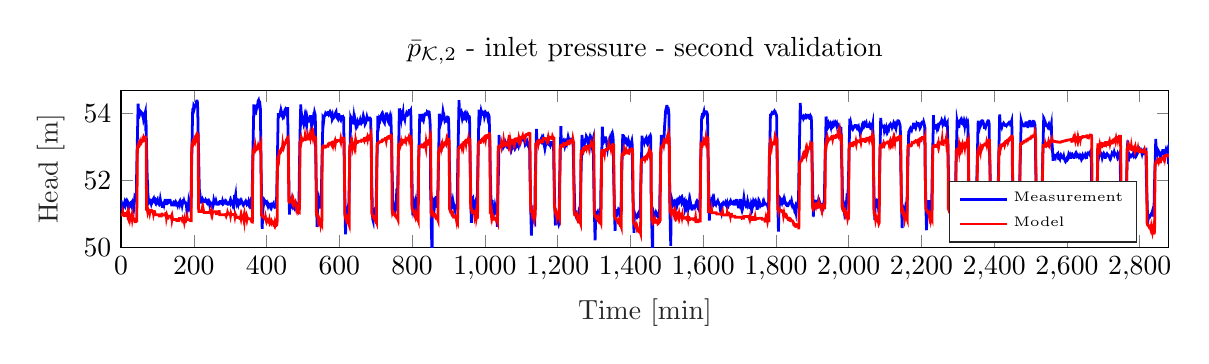
\begin{tikzpicture}

\begin{axis}[%
width=5.239in,
height=0.784in,
at={(1.1in,0.431in)},
scale only axis,
xmin=0,
xmax=2880,
xlabel style={font=\color{white!15!black}},
xlabel={Time [min]},
ymin=50,
ymax=54.7,
ylabel style={font=\color{white!15!black}},
ylabel={Head  [m]},
axis background/.style={fill=white},
title style={},
title={$\bar{p}_{\mathcal{K},2}$ - inlet pressure - second validation},
legend style={at={(0.97,0.03)}, anchor=south east, legend cell align=left, align=left, draw=white!15!black}
]
\addplot [color=blue, line width=1.0pt]
  table[row sep=crcr]{%
0	51.4068408\\
1	51.3048431\\
2	51.24364448\\
3	51.18244586\\
4	51.14164678\\
5	51.16204632\\
6	51.22324494\\
7	51.3048431\\
8	51.3048431\\
9	51.3048431\\
10	51.34564218\\
11	51.3048431\\
12	51.26404402\\
13	51.3048431\\
14	51.32524264\\
15	51.36604172\\
16	51.34564218\\
17	51.38644126\\
18	51.36604172\\
19	51.34564218\\
20	51.24364448\\
21	51.26404402\\
22	51.22324494\\
23	51.2028454\\
24	51.22324494\\
25	51.28444356\\
26	51.3048431\\
27	51.28444356\\
28	51.32524264\\
29	51.32524264\\
30	51.34564218\\
31	51.24364448\\
32	51.26404402\\
33	51.22324494\\
34	51.24364448\\
35	51.18244586\\
36	51.28444356\\
37	51.38644126\\
38	51.5088385\\
39	51.48843896\\
40	51.48843896\\
41	51.44763988\\
42	51.38644126\\
43	52.26362148\\
44	52.79400952\\
45	53.28359848\\
46	53.81398652\\
47	54.30357548\\
48	53.87518514\\
49	53.89558468\\
50	53.93638376\\
51	53.97718284\\
52	54.07918054\\
53	54.058781\\
54	54.058781\\
55	54.058781\\
56	54.03838146\\
57	54.01798192\\
58	54.01798192\\
59	53.97718284\\
60	53.91598422\\
61	53.91598422\\
62	53.83438606\\
63	53.87518514\\
64	53.87518514\\
65	53.99758238\\
66	54.01798192\\
67	54.058781\\
68	53.63039066\\
69	53.6507902\\
70	53.05920354\\
71	52.65121274\\
72	52.05962608\\
73	51.95762838\\
74	51.42724034\\
75	51.46803942\\
76	51.34564218\\
77	51.36604172\\
78	51.38644126\\
79	51.36604172\\
80	51.38644126\\
81	51.36604172\\
82	51.34564218\\
83	51.3048431\\
84	51.34564218\\
85	51.32524264\\
86	51.34564218\\
87	51.38644126\\
88	51.42724034\\
89	51.44763988\\
90	51.46803942\\
91	51.42724034\\
92	51.42724034\\
93	51.38644126\\
94	51.34564218\\
95	51.32524264\\
96	51.38644126\\
97	51.36604172\\
98	51.4068408\\
99	51.4068408\\
100	51.42724034\\
101	51.36604172\\
102	51.34564218\\
103	51.3048431\\
104	51.3048431\\
105	51.28444356\\
106	51.3048431\\
107	51.34564218\\
108	51.42724034\\
109	51.36604172\\
110	51.32524264\\
111	51.28444356\\
112	51.26404402\\
113	51.22324494\\
114	51.22324494\\
115	51.28444356\\
116	51.32524264\\
117	51.32524264\\
118	51.28444356\\
119	51.34564218\\
120	51.36604172\\
121	51.4068408\\
122	51.4068408\\
123	51.4068408\\
124	51.4068408\\
125	51.36604172\\
126	51.3048431\\
127	51.3048431\\
128	51.32524264\\
129	51.34564218\\
130	51.34564218\\
131	51.4068408\\
132	51.4068408\\
133	51.38644126\\
134	51.4068408\\
135	51.4068408\\
136	51.34564218\\
137	51.34564218\\
138	51.32524264\\
139	51.26404402\\
140	51.26404402\\
141	51.26404402\\
142	51.28444356\\
143	51.3048431\\
144	51.32524264\\
145	51.3048431\\
146	51.32524264\\
147	51.3048431\\
148	51.32524264\\
149	51.32524264\\
150	51.3048431\\
151	51.34564218\\
152	51.32524264\\
153	51.3048431\\
154	51.3048431\\
155	51.3048431\\
156	51.26404402\\
157	51.3048431\\
158	51.3048431\\
159	51.32524264\\
160	51.34564218\\
161	51.36604172\\
162	51.3048431\\
163	51.34564218\\
164	51.3048431\\
165	51.3048431\\
166	51.3048431\\
167	51.32524264\\
168	51.26404402\\
169	51.32524264\\
170	51.32524264\\
171	51.32524264\\
172	51.34564218\\
173	51.38644126\\
174	51.34564218\\
175	51.34564218\\
176	51.34564218\\
177	51.32524264\\
178	51.32524264\\
179	51.3048431\\
180	51.22324494\\
181	51.1008477\\
182	51.14164678\\
183	51.12124724\\
184	51.16204632\\
185	51.22324494\\
186	51.34564218\\
187	51.28444356\\
188	51.28444356\\
189	51.2028454\\
190	51.22324494\\
191	51.16204632\\
192	51.2028454\\
193	51.9168293\\
194	52.44721734\\
195	52.9368063\\
196	53.58959158\\
197	54.1607787\\
198	53.99758238\\
199	54.11997962\\
200	54.24237686\\
201	54.22197732\\
202	54.18117824\\
203	54.22197732\\
204	54.22197732\\
205	54.22197732\\
206	54.24237686\\
207	54.32397502\\
208	54.38517364\\
209	54.38517364\\
210	54.34437456\\
211	54.058781\\
212	53.36519664\\
213	52.97760538\\
214	52.38601872\\
215	51.83523114\\
216	51.52923804\\
217	51.63123574\\
218	51.38644126\\
219	51.38644126\\
220	51.34564218\\
221	51.34564218\\
222	51.34564218\\
223	51.34564218\\
224	51.36604172\\
225	51.42724034\\
226	51.4068408\\
227	51.4068408\\
228	51.38644126\\
229	51.38644126\\
230	51.36604172\\
231	51.36604172\\
232	51.36604172\\
233	51.4068408\\
234	51.38644126\\
235	51.36604172\\
236	51.4068408\\
237	51.4068408\\
238	51.38644126\\
239	51.34564218\\
240	51.36604172\\
241	51.32524264\\
242	51.32524264\\
243	51.28444356\\
244	51.34564218\\
245	51.32524264\\
246	51.32524264\\
247	51.32524264\\
248	51.3048431\\
249	51.26404402\\
250	51.22324494\\
251	51.24364448\\
252	51.22324494\\
253	51.28444356\\
254	51.32524264\\
255	51.4068408\\
256	51.36604172\\
257	51.4068408\\
258	51.4068408\\
259	51.36604172\\
260	51.34564218\\
261	51.38644126\\
262	51.34564218\\
263	51.32524264\\
264	51.32524264\\
265	51.3048431\\
266	51.28444356\\
267	51.28444356\\
268	51.28444356\\
269	51.3048431\\
270	51.34564218\\
271	51.34564218\\
272	51.36604172\\
273	51.36604172\\
274	51.32524264\\
275	51.32524264\\
276	51.32524264\\
277	51.3048431\\
278	51.3048431\\
279	51.36604172\\
280	51.32524264\\
281	51.34564218\\
282	51.32524264\\
283	51.34564218\\
284	51.32524264\\
285	51.32524264\\
286	51.32524264\\
287	51.36604172\\
288	51.34564218\\
289	51.36604172\\
290	51.34564218\\
291	51.32524264\\
292	51.3048431\\
293	51.28444356\\
294	51.28444356\\
295	51.28444356\\
296	51.3048431\\
297	51.3048431\\
298	51.34564218\\
299	51.34564218\\
300	51.38644126\\
301	51.34564218\\
302	51.38644126\\
303	51.34564218\\
304	51.34564218\\
305	51.32524264\\
306	51.32524264\\
307	51.28444356\\
308	51.32524264\\
309	51.3048431\\
310	51.26404402\\
311	51.42724034\\
312	51.52923804\\
313	51.52923804\\
314	51.5088385\\
315	51.57003712\\
316	51.4068408\\
317	51.34564218\\
318	51.3048431\\
319	51.34564218\\
320	51.34564218\\
321	51.34564218\\
322	51.3048431\\
323	51.36604172\\
324	51.34564218\\
325	51.34564218\\
326	51.36604172\\
327	51.38644126\\
328	51.34564218\\
329	51.36604172\\
330	51.36604172\\
331	51.38644126\\
332	51.34564218\\
333	51.34564218\\
334	51.3048431\\
335	51.28444356\\
336	51.26404402\\
337	51.28444356\\
338	51.28444356\\
339	51.3048431\\
340	51.32524264\\
341	51.34564218\\
342	51.32524264\\
343	51.32524264\\
344	51.36604172\\
345	51.34564218\\
346	51.3048431\\
347	51.32524264\\
348	51.32524264\\
349	51.3048431\\
350	51.28444356\\
351	51.34564218\\
352	51.3048431\\
353	51.32524264\\
354	51.28444356\\
355	51.32524264\\
356	51.26404402\\
357	51.28444356\\
358	51.24364448\\
359	51.28444356\\
360	51.24364448\\
361	51.87603022\\
362	52.50841596\\
363	53.1408017\\
364	53.6507902\\
365	54.24237686\\
366	54.24237686\\
367	54.14037916\\
368	54.058781\\
369	54.09958008\\
370	54.09958008\\
371	54.07918054\\
372	54.14037916\\
373	54.18117824\\
374	54.24237686\\
375	54.2627764\\
376	54.30357548\\
377	54.38517364\\
378	54.40557318\\
379	54.34437456\\
380	54.34437456\\
381	54.24237686\\
382	54.2627764\\
383	54.1607787\\
384	53.2427994\\
385	52.24322194\\
386	51.77403252\\
387	50.99885\\
388	50.55006012\\
389	50.87645276\\
390	51.3048431\\
391	51.24364448\\
392	51.36604172\\
393	51.34564218\\
394	51.4068408\\
395	51.38644126\\
396	51.38644126\\
397	51.36604172\\
398	51.36604172\\
399	51.32524264\\
400	51.3048431\\
401	51.32524264\\
402	51.28444356\\
403	51.28444356\\
404	51.24364448\\
405	51.28444356\\
406	51.26404402\\
407	51.28444356\\
408	51.28444356\\
409	51.26404402\\
410	51.2028454\\
411	51.18244586\\
412	51.2028454\\
413	51.18244586\\
414	51.22324494\\
415	51.3048431\\
416	51.3048431\\
417	51.28444356\\
418	51.28444356\\
419	51.3048431\\
420	51.24364448\\
421	51.22324494\\
422	51.24364448\\
423	51.22324494\\
424	51.22324494\\
425	51.22324494\\
426	51.22324494\\
427	51.16204632\\
428	51.65163528\\
429	52.24322194\\
430	52.79400952\\
431	53.36519664\\
432	53.97718284\\
433	53.97718284\\
434	53.9567833\\
435	53.93638376\\
436	53.9567833\\
437	53.97718284\\
438	54.03838146\\
439	54.01798192\\
440	54.09958008\\
441	54.058781\\
442	54.03838146\\
443	54.03838146\\
444	53.97718284\\
445	53.91598422\\
446	53.93638376\\
447	53.91598422\\
448	53.9567833\\
449	54.01798192\\
450	54.09958008\\
451	54.11997962\\
452	54.07918054\\
453	54.058781\\
454	54.058781\\
455	54.01798192\\
456	54.058781\\
457	54.1607787\\
458	54.1607787\\
459	53.36519664\\
460	52.7328109\\
461	52.2228224\\
462	51.54963758\\
463	50.97845046\\
464	51.22324494\\
465	51.26404402\\
466	51.16204632\\
467	51.28444356\\
468	51.28444356\\
469	51.3048431\\
470	51.3048431\\
471	51.36604172\\
472	51.28444356\\
473	51.22324494\\
474	51.24364448\\
475	51.26404402\\
476	51.18244586\\
477	51.16204632\\
478	51.2028454\\
479	51.14164678\\
480	51.14164678\\
481	51.2028454\\
482	51.28444356\\
483	51.3048431\\
484	51.3048431\\
485	51.28444356\\
486	51.14164678\\
487	50.99885\\
488	51.1008477\\
489	51.18244586\\
490	52.08002562\\
491	52.79400952\\
492	53.40599572\\
493	53.8547856\\
494	54.28317594\\
495	53.97718284\\
496	53.8547856\\
497	53.91598422\\
498	53.83438606\\
499	53.87518514\\
500	53.8547856\\
501	53.8547856\\
502	53.77318744\\
503	53.83438606\\
504	53.87518514\\
505	53.81398652\\
506	53.91598422\\
507	53.87518514\\
508	53.93638376\\
509	53.87518514\\
510	53.83438606\\
511	53.73238836\\
512	53.83438606\\
513	53.77318744\\
514	53.77318744\\
515	53.77318744\\
516	53.81398652\\
517	53.81398652\\
518	53.8547856\\
519	53.8547856\\
520	53.91598422\\
521	53.91598422\\
522	53.81398652\\
523	53.71198882\\
524	53.60999112\\
525	53.6507902\\
526	53.69158928\\
527	53.77318744\\
528	53.83438606\\
529	53.91598422\\
530	53.89558468\\
531	53.9567833\\
532	54.03838146\\
533	53.99758238\\
534	53.9567833\\
535	52.91640676\\
536	52.20242286\\
537	51.63123574\\
538	51.03964908\\
539	50.61125874\\
540	51.1008477\\
541	51.18244586\\
542	51.2028454\\
543	51.26404402\\
544	51.38644126\\
545	51.32524264\\
546	51.34564218\\
547	51.28444356\\
548	51.3048431\\
549	51.16204632\\
550	51.28444356\\
551	51.8148316\\
552	52.40641826\\
553	52.89600722\\
554	53.38559618\\
555	53.87518514\\
556	53.8547856\\
557	53.79358698\\
558	53.89558468\\
559	53.91598422\\
560	53.9567833\\
561	53.9567833\\
562	53.99758238\\
563	53.97718284\\
564	53.97718284\\
565	53.97718284\\
566	53.99758238\\
567	53.97718284\\
568	53.97718284\\
569	54.03838146\\
570	54.03838146\\
571	53.99758238\\
572	54.01798192\\
573	54.03838146\\
574	53.97718284\\
575	53.97718284\\
576	53.9567833\\
577	54.01798192\\
578	53.99758238\\
579	53.99758238\\
580	53.89558468\\
581	53.93638376\\
582	53.8547856\\
583	53.87518514\\
584	53.87518514\\
585	53.91598422\\
586	53.91598422\\
587	53.93638376\\
588	53.93638376\\
589	53.99758238\\
590	54.03838146\\
591	54.058781\\
592	53.9567833\\
593	53.91598422\\
594	53.87518514\\
595	53.87518514\\
596	53.8547856\\
597	53.91598422\\
598	53.97718284\\
599	53.97718284\\
600	53.93638376\\
601	53.89558468\\
602	53.89558468\\
603	53.83438606\\
604	53.81398652\\
605	53.8547856\\
606	53.89558468\\
607	53.91598422\\
608	53.91598422\\
609	53.89558468\\
610	53.87518514\\
611	53.89558468\\
612	53.87518514\\
613	52.95720584\\
614	52.1208247\\
615	51.6108362\\
616	50.93765138\\
617	50.3868638\\
618	50.6928569\\
619	51.01924954\\
620	50.91725184\\
621	51.08044816\\
622	51.12124724\\
623	51.16204632\\
624	51.14164678\\
625	51.22324494\\
626	51.18244586\\
627	51.69243436\\
628	52.20242286\\
629	52.71241136\\
630	53.22239986\\
631	53.83438606\\
632	53.79358698\\
633	53.87518514\\
634	53.8547856\\
635	53.81398652\\
636	53.77318744\\
637	53.79358698\\
638	53.77318744\\
639	53.81398652\\
640	53.91598422\\
641	53.83438606\\
642	53.79358698\\
643	53.83438606\\
644	53.77318744\\
645	53.69158928\\
646	53.73238836\\
647	53.73238836\\
648	53.67118974\\
649	53.71198882\\
650	53.7527879\\
651	53.71198882\\
652	53.7527879\\
653	53.7527879\\
654	53.7527879\\
655	53.73238836\\
656	53.7527879\\
657	53.79358698\\
658	53.73238836\\
659	53.73238836\\
660	53.71198882\\
661	53.73238836\\
662	53.73238836\\
663	53.83438606\\
664	53.83438606\\
665	53.87518514\\
666	53.93638376\\
667	53.89558468\\
668	53.83438606\\
669	53.83438606\\
670	53.79358698\\
671	53.69158928\\
672	53.71198882\\
673	53.7527879\\
674	53.79358698\\
675	53.83438606\\
676	53.89558468\\
677	53.8547856\\
678	53.8547856\\
679	53.8547856\\
680	53.83438606\\
681	53.81398652\\
682	53.81398652\\
683	53.87518514\\
684	53.87518514\\
685	53.83438606\\
686	53.83438606\\
687	53.46719434\\
688	52.79400952\\
689	51.93722884\\
690	51.57003712\\
691	50.97845046\\
692	50.83565368\\
693	50.7948546\\
694	51.08044816\\
695	50.99885\\
696	51.01924954\\
697	51.01924954\\
698	51.14164678\\
699	51.16204632\\
700	51.14164678\\
701	51.1008477\\
702	51.75363298\\
703	52.28402102\\
704	52.87560768\\
705	53.30399802\\
706	53.93638376\\
707	53.83438606\\
708	53.81398652\\
709	53.7527879\\
710	53.8547856\\
711	53.83438606\\
712	53.81398652\\
713	53.87518514\\
714	53.91598422\\
715	53.91598422\\
716	53.97718284\\
717	53.99758238\\
718	53.93638376\\
719	53.9567833\\
720	53.87518514\\
721	53.79358698\\
722	53.77318744\\
723	53.7527879\\
724	53.73238836\\
725	53.8547856\\
726	53.8547856\\
727	53.91598422\\
728	53.97718284\\
729	53.99758238\\
730	53.99758238\\
731	53.93638376\\
732	53.87518514\\
733	53.83438606\\
734	53.77318744\\
735	53.7527879\\
736	53.87518514\\
737	53.8547856\\
738	53.87518514\\
739	53.91598422\\
740	53.83438606\\
741	53.7527879\\
742	53.79358698\\
743	53.4467948\\
744	53.038804\\
745	52.3248201\\
746	51.85563068\\
747	51.3048431\\
748	51.16204632\\
749	50.99885\\
750	51.24364448\\
751	51.2028454\\
752	51.12124724\\
753	51.08044816\\
754	51.14164678\\
755	51.14164678\\
756	51.22324494\\
757	51.44763988\\
758	51.75363298\\
759	51.67203482\\
760	51.63123574\\
761	52.16162378\\
762	52.61041366\\
763	52.87560768\\
764	53.52839296\\
765	54.1607787\\
766	54.07918054\\
767	54.07918054\\
768	54.07918054\\
769	53.99758238\\
770	53.91598422\\
771	54.03838146\\
772	53.91598422\\
773	53.89558468\\
774	53.9567833\\
775	54.01798192\\
776	53.8547856\\
777	53.93638376\\
778	53.93638376\\
779	53.87518514\\
780	53.83438606\\
781	53.91598422\\
782	53.93638376\\
783	53.9567833\\
784	53.97718284\\
785	54.01798192\\
786	53.99758238\\
787	53.99758238\\
788	53.97718284\\
789	53.99758238\\
790	53.99758238\\
791	54.058781\\
792	54.09958008\\
793	54.09958008\\
794	54.058781\\
795	54.07918054\\
796	54.09958008\\
797	53.87518514\\
798	52.89600722\\
799	52.5288155\\
800	51.93722884\\
801	51.36604172\\
802	50.95805092\\
803	51.4068408\\
804	51.2028454\\
805	51.26404402\\
806	51.18244586\\
807	51.24364448\\
808	51.24364448\\
809	51.3048431\\
810	51.16204632\\
811	51.24364448\\
812	51.18244586\\
813	51.24364448\\
814	51.2028454\\
815	51.3048431\\
816	51.24364448\\
817	51.99842746\\
818	52.38601872\\
819	52.91640676\\
820	53.40599572\\
821	53.99758238\\
822	53.81398652\\
823	53.87518514\\
824	53.9567833\\
825	53.9567833\\
826	53.91598422\\
827	53.87518514\\
828	53.89558468\\
829	53.81398652\\
830	53.81398652\\
831	53.79358698\\
832	53.8547856\\
833	53.89558468\\
834	53.9567833\\
835	53.97718284\\
836	53.99758238\\
837	53.99758238\\
838	53.97718284\\
839	53.97718284\\
840	53.99758238\\
841	54.03838146\\
842	54.01798192\\
843	54.01798192\\
844	54.058781\\
845	54.058781\\
846	53.9567833\\
847	53.91598422\\
848	53.93638376\\
849	53.81398652\\
850	53.60999112\\
851	51.69243436\\
852	51.26404402\\
853	50.55006012\\
854	50.12166978\\
855	49.81567668\\
856	51.28444356\\
857	51.28444356\\
858	51.4068408\\
859	51.38644126\\
860	51.34564218\\
861	51.36604172\\
862	51.26404402\\
863	51.36604172\\
864	51.34564218\\
865	51.42724034\\
866	51.4068408\\
867	51.52923804\\
868	51.42724034\\
869	51.34564218\\
870	51.18244586\\
871	51.75363298\\
872	52.18202332\\
873	52.7328109\\
874	53.3447971\\
875	53.99758238\\
876	53.93638376\\
877	53.91598422\\
878	53.91598422\\
879	53.91598422\\
880	53.77318744\\
881	53.81398652\\
882	53.8547856\\
883	53.91598422\\
884	53.9567833\\
885	54.058781\\
886	53.99758238\\
887	53.99758238\\
888	53.91598422\\
889	53.8547856\\
890	53.79358698\\
891	53.81398652\\
892	53.83438606\\
893	53.81398652\\
894	53.83438606\\
895	53.8547856\\
896	53.81398652\\
897	53.79358698\\
898	53.89558468\\
899	53.89558468\\
900	53.8547856\\
901	53.60999112\\
902	52.79400952\\
903	52.3248201\\
904	51.87603022\\
905	51.38644126\\
906	51.2028454\\
907	51.46803942\\
908	51.36604172\\
909	51.26404402\\
910	51.32524264\\
911	51.34564218\\
912	51.4068408\\
913	51.34564218\\
914	51.3048431\\
915	51.24364448\\
916	51.16204632\\
917	51.14164678\\
918	51.1008477\\
919	51.18244586\\
920	51.2028454\\
921	51.18244586\\
922	51.18244586\\
923	51.22324494\\
924	51.2028454\\
925	52.10042516\\
926	52.7328109\\
927	53.26319894\\
928	53.8547856\\
929	54.40557318\\
930	54.058781\\
931	54.03838146\\
932	54.07918054\\
933	54.058781\\
934	54.03838146\\
935	54.058781\\
936	53.99758238\\
937	53.91598422\\
938	53.8547856\\
939	53.89558468\\
940	53.83438606\\
941	53.83438606\\
942	53.87518514\\
943	53.99758238\\
944	53.99758238\\
945	54.01798192\\
946	53.97718284\\
947	53.91598422\\
948	53.8547856\\
949	53.83438606\\
950	53.87518514\\
951	53.93638376\\
952	53.99758238\\
953	53.97718284\\
954	53.91598422\\
955	53.89558468\\
956	53.91598422\\
957	53.91598422\\
958	53.87518514\\
959	52.89600722\\
960	52.20242286\\
961	51.7128339\\
962	51.14164678\\
963	50.73365598\\
964	51.36604172\\
965	51.52923804\\
966	51.42724034\\
967	51.44763988\\
968	51.3048431\\
969	51.16204632\\
970	51.14164678\\
971	51.12124724\\
972	51.2028454\\
973	51.26404402\\
974	51.3048431\\
975	51.36604172\\
976	51.4068408\\
977	51.3048431\\
978	51.34564218\\
979	51.32524264\\
980	51.9168293\\
981	52.50841596\\
982	53.01840446\\
983	53.60999112\\
984	54.11997962\\
985	53.93638376\\
986	53.91598422\\
987	53.9567833\\
988	53.89558468\\
989	53.97718284\\
990	54.07918054\\
991	54.03838146\\
992	54.058781\\
993	54.058781\\
994	54.01798192\\
995	54.01798192\\
996	53.97718284\\
997	53.97718284\\
998	53.99758238\\
999	53.91598422\\
1000	53.9567833\\
1001	54.01798192\\
1002	54.03838146\\
1003	54.01798192\\
1004	54.01798192\\
1005	53.9567833\\
1006	53.9567833\\
1007	53.9567833\\
1008	53.89558468\\
1009	53.93638376\\
1010	53.97718284\\
1011	53.9567833\\
1012	53.89558468\\
1013	53.40599572\\
1014	52.91640676\\
1015	52.2228224\\
1016	51.8148316\\
1017	51.32524264\\
1018	51.38644126\\
1019	51.32524264\\
1020	51.4068408\\
1021	51.22324494\\
1022	51.18244586\\
1023	51.03964908\\
1024	51.06004862\\
1025	51.03964908\\
1026	51.08044816\\
1027	51.14164678\\
1028	51.22324494\\
1029	51.16204632\\
1030	51.2028454\\
1031	51.2028454\\
1032	51.12124724\\
1033	51.03964908\\
1034	50.61125874\\
1035	51.24364448\\
1036	51.69243436\\
1037	52.08002562\\
1038	52.50841596\\
1039	53.36519664\\
1040	53.07960308\\
1041	53.05920354\\
1042	53.10000262\\
1043	53.07960308\\
1044	53.01840446\\
1045	53.01840446\\
1046	53.01840446\\
1047	53.01840446\\
1048	53.038804\\
1049	53.05920354\\
1050	53.07960308\\
1051	52.99800492\\
1052	53.01840446\\
1053	53.07960308\\
1054	53.05920354\\
1055	53.07960308\\
1056	53.12040216\\
1057	53.07960308\\
1058	53.05920354\\
1059	53.10000262\\
1060	53.07960308\\
1061	53.07960308\\
1062	53.07960308\\
1063	53.038804\\
1064	53.05920354\\
1065	53.07960308\\
1066	53.038804\\
1067	53.05920354\\
1068	53.07960308\\
1069	53.07960308\\
1070	53.01840446\\
1071	53.10000262\\
1072	53.07960308\\
1073	53.05920354\\
1074	52.97760538\\
1075	53.01840446\\
1076	52.97760538\\
1077	52.97760538\\
1078	52.97760538\\
1079	53.01840446\\
1080	53.01840446\\
1081	53.01840446\\
1082	52.99800492\\
1083	52.95720584\\
1084	52.97760538\\
1085	53.01840446\\
1086	53.01840446\\
1087	53.038804\\
1088	53.10000262\\
1089	53.07960308\\
1090	53.05920354\\
1091	53.07960308\\
1092	53.07960308\\
1093	53.038804\\
1094	53.07960308\\
1095	53.12040216\\
1096	53.10000262\\
1097	53.1408017\\
1098	53.18160078\\
1099	53.20200032\\
1100	53.20200032\\
1101	53.2427994\\
1102	53.2427994\\
1103	53.28359848\\
1104	53.28359848\\
1105	53.26319894\\
1106	53.26319894\\
1107	53.2427994\\
1108	53.20200032\\
1109	53.18160078\\
1110	53.1408017\\
1111	53.07960308\\
1112	53.10000262\\
1113	53.16120124\\
1114	53.16120124\\
1115	53.16120124\\
1116	53.18160078\\
1117	53.1408017\\
1118	53.05920354\\
1119	53.038804\\
1120	53.05920354\\
1121	53.07960308\\
1122	53.05920354\\
1123	52.99800492\\
1124	52.14122424\\
1125	51.75363298\\
1126	51.2028454\\
1127	50.77445506\\
1128	50.34606472\\
1129	50.7948546\\
1130	50.71325644\\
1131	50.91725184\\
1132	50.95805092\\
1133	50.95805092\\
1134	50.87645276\\
1135	50.81525414\\
1136	50.77445506\\
1137	50.75405552\\
1138	51.73323344\\
1139	52.24322194\\
1140	52.71241136\\
1141	53.12040216\\
1142	53.5487925\\
1143	53.10000262\\
1144	53.12040216\\
1145	53.18160078\\
1146	53.16120124\\
1147	53.18160078\\
1148	53.18160078\\
1149	53.1408017\\
1150	53.16120124\\
1151	53.16120124\\
1152	53.16120124\\
1153	53.16120124\\
1154	53.20200032\\
1155	53.18160078\\
1156	53.22239986\\
1157	53.26319894\\
1158	53.22239986\\
1159	53.26319894\\
1160	53.28359848\\
1161	53.20200032\\
1162	53.12040216\\
1163	53.10000262\\
1164	53.01840446\\
1165	52.95720584\\
1166	53.01840446\\
1167	53.05920354\\
1168	53.10000262\\
1169	53.1408017\\
1170	53.18160078\\
1171	53.16120124\\
1172	53.16120124\\
1173	53.18160078\\
1174	53.16120124\\
1175	53.10000262\\
1176	53.07960308\\
1177	53.07960308\\
1178	53.07960308\\
1179	53.05920354\\
1180	53.1408017\\
1181	53.1408017\\
1182	53.1408017\\
1183	53.10000262\\
1184	53.10000262\\
1185	53.07960308\\
1186	53.10000262\\
1187	53.05920354\\
1188	53.07960308\\
1189	52.9368063\\
1190	52.1208247\\
1191	51.83523114\\
1192	51.36604172\\
1193	50.93765138\\
1194	50.65205782\\
1195	51.03964908\\
1196	50.8968523\\
1197	50.99885\\
1198	50.99885\\
1199	50.95805092\\
1200	50.87645276\\
1201	50.83565368\\
1202	50.73365598\\
1203	50.6928569\\
1204	50.73365598\\
1205	51.67203482\\
1206	52.18202332\\
1207	52.67161228\\
1208	53.16120124\\
1209	53.63039066\\
1210	53.18160078\\
1211	53.12040216\\
1212	53.16120124\\
1213	53.1408017\\
1214	53.1408017\\
1215	53.16120124\\
1216	53.18160078\\
1217	53.12040216\\
1218	53.12040216\\
1219	53.10000262\\
1220	53.038804\\
1221	53.07960308\\
1222	53.1408017\\
1223	53.12040216\\
1224	53.10000262\\
1225	53.22239986\\
1226	53.22239986\\
1227	53.22239986\\
1228	53.2427994\\
1229	53.30399802\\
1230	53.26319894\\
1231	53.22239986\\
1232	53.22239986\\
1233	53.20200032\\
1234	53.16120124\\
1235	53.16120124\\
1236	53.18160078\\
1237	53.20200032\\
1238	53.2427994\\
1239	53.2427994\\
1240	53.20200032\\
1241	53.18160078\\
1242	53.16120124\\
1243	52.95720584\\
1244	52.36561918\\
1245	52.03922654\\
1246	51.63123574\\
1247	51.2028454\\
1248	50.93765138\\
1249	51.1008477\\
1250	50.97845046\\
1251	50.93765138\\
1252	50.8968523\\
1253	50.85605322\\
1254	50.85605322\\
1255	50.83565368\\
1256	50.8968523\\
1257	50.8968523\\
1258	50.99885\\
1259	50.95805092\\
1260	51.01924954\\
1261	50.95805092\\
1262	50.97845046\\
1263	51.5088385\\
1264	51.99842746\\
1265	52.46761688\\
1266	52.91640676\\
1267	53.36519664\\
1268	53.20200032\\
1269	53.18160078\\
1270	53.1408017\\
1271	53.1408017\\
1272	53.1408017\\
1273	53.16120124\\
1274	53.10000262\\
1275	53.12040216\\
1276	53.18160078\\
1277	53.20200032\\
1278	53.2427994\\
1279	53.32439756\\
1280	53.30399802\\
1281	53.26319894\\
1282	53.22239986\\
1283	53.20200032\\
1284	53.1408017\\
1285	53.18160078\\
1286	53.16120124\\
1287	53.20200032\\
1288	53.26319894\\
1289	53.30399802\\
1290	53.26319894\\
1291	53.28359848\\
1292	53.2427994\\
1293	53.10000262\\
1294	53.16120124\\
1295	53.20200032\\
1296	53.20200032\\
1297	53.22239986\\
1298	53.26319894\\
1299	52.30442056\\
1300	51.5088385\\
1301	51.14164678\\
1302	50.63165828\\
1303	50.20326794\\
1304	50.63165828\\
1305	50.93765138\\
1306	50.8968523\\
1307	50.95805092\\
1308	50.99885\\
1309	51.03964908\\
1310	51.06004862\\
1311	51.01924954\\
1312	50.97845046\\
1313	50.93765138\\
1314	50.93765138\\
1315	50.95805092\\
1316	50.93765138\\
1317	50.97845046\\
1318	50.99885\\
1319	51.75363298\\
1320	52.24322194\\
1321	52.71241136\\
1322	53.1408017\\
1323	53.60999112\\
1324	53.28359848\\
1325	53.20200032\\
1326	53.18160078\\
1327	53.22239986\\
1328	53.18160078\\
1329	53.20200032\\
1330	53.22239986\\
1331	53.28359848\\
1332	53.28359848\\
1333	53.2427994\\
1334	53.16120124\\
1335	53.12040216\\
1336	53.01840446\\
1337	52.95720584\\
1338	53.038804\\
1339	53.07960308\\
1340	53.12040216\\
1341	53.1408017\\
1342	53.18160078\\
1343	53.038804\\
1344	53.05920354\\
1345	53.07960308\\
1346	53.10000262\\
1347	53.1408017\\
1348	53.30399802\\
1349	53.36519664\\
1350	53.3447971\\
1351	53.38559618\\
1352	53.32439756\\
1353	53.18160078\\
1354	52.18202332\\
1355	51.69243436\\
1356	51.24364448\\
1357	50.81525414\\
1358	50.4888615\\
1359	51.03964908\\
1360	51.1008477\\
1361	51.1008477\\
1362	51.1008477\\
1363	51.08044816\\
1364	51.08044816\\
1365	51.03964908\\
1366	51.08044816\\
1367	51.12124724\\
1368	51.1008477\\
1369	51.08044816\\
1370	51.1008477\\
1371	51.03964908\\
1372	50.97845046\\
1373	51.01924954\\
1374	51.01924954\\
1375	51.57003712\\
1376	52.018827\\
1377	52.50841596\\
1378	52.9368063\\
1379	53.38559618\\
1380	53.30399802\\
1381	53.32439756\\
1382	53.32439756\\
1383	53.30399802\\
1384	53.26319894\\
1385	53.22239986\\
1386	53.16120124\\
1387	53.18160078\\
1388	53.18160078\\
1389	53.20200032\\
1390	53.16120124\\
1391	53.16120124\\
1392	53.10000262\\
1393	53.12040216\\
1394	53.12040216\\
1395	53.18160078\\
1396	53.1408017\\
1397	53.10000262\\
1398	53.038804\\
1399	52.95720584\\
1400	52.9368063\\
1401	53.01840446\\
1402	53.10000262\\
1403	53.1408017\\
1404	53.18160078\\
1405	53.07960308\\
1406	52.14122424\\
1407	51.54963758\\
1408	51.16204632\\
1409	50.73365598\\
1410	50.42766288\\
1411	50.8968523\\
1412	50.99885\\
1413	50.95805092\\
1414	50.95805092\\
1415	50.95805092\\
1416	50.93765138\\
1417	50.91725184\\
1418	50.8968523\\
1419	50.91725184\\
1420	50.91725184\\
1421	50.99885\\
1422	51.01924954\\
1423	51.03964908\\
1424	51.01924954\\
1425	50.97845046\\
1426	50.93765138\\
1427	50.91725184\\
1428	51.57003712\\
1429	51.97802792\\
1430	52.4268178\\
1431	52.87560768\\
1432	53.3447971\\
1433	53.16120124\\
1434	53.20200032\\
1435	53.22239986\\
1436	53.22239986\\
1437	53.20200032\\
1438	53.16120124\\
1439	53.22239986\\
1440	53.22239986\\
1441	53.22239986\\
1442	53.2427994\\
1443	53.26319894\\
1444	53.16120124\\
1445	53.1408017\\
1446	53.12040216\\
1447	53.18160078\\
1448	53.16120124\\
1449	53.2427994\\
1450	53.26319894\\
1451	53.22239986\\
1452	53.22239986\\
1453	53.28359848\\
1454	53.32439756\\
1455	53.3447971\\
1456	53.30399802\\
1457	51.63123574\\
1458	51.2028454\\
1459	50.61125874\\
1460	50.16246886\\
1461	49.81567668\\
1462	50.99885\\
1463	50.93765138\\
1464	51.01924954\\
1465	50.97845046\\
1466	50.93765138\\
1467	50.95805092\\
1468	50.93765138\\
1469	50.93765138\\
1470	50.97845046\\
1471	51.03964908\\
1472	51.01924954\\
1473	51.01924954\\
1474	51.01924954\\
1475	50.95805092\\
1476	50.91725184\\
1477	50.8968523\\
1478	50.91725184\\
1479	50.8968523\\
1480	50.87645276\\
1481	51.5088385\\
1482	51.99842746\\
1483	52.4268178\\
1484	52.89600722\\
1485	53.36519664\\
1486	53.16120124\\
1487	53.16120124\\
1488	53.18160078\\
1489	53.16120124\\
1490	53.18160078\\
1491	53.18160078\\
1492	53.2427994\\
1493	53.38559618\\
1494	53.63039066\\
1495	53.77318744\\
1496	53.9567833\\
1497	54.09958008\\
1498	54.14037916\\
1499	54.11997962\\
1500	54.22197732\\
1501	54.22197732\\
1502	54.18117824\\
1503	54.1607787\\
1504	54.1607787\\
1505	54.09958008\\
1506	53.97718284\\
1507	52.34521964\\
1508	51.77403252\\
1509	50.97845046\\
1510	50.44806242\\
1511	50.04007162\\
1512	51.14164678\\
1513	51.2028454\\
1514	51.42724034\\
1515	51.38644126\\
1516	51.38644126\\
1517	51.38644126\\
1518	51.3048431\\
1519	51.28444356\\
1520	51.3048431\\
1521	51.32524264\\
1522	51.24364448\\
1523	51.32524264\\
1524	51.3048431\\
1525	51.22324494\\
1526	51.2028454\\
1527	51.28444356\\
1528	51.24364448\\
1529	51.28444356\\
1530	51.4068408\\
1531	51.42724034\\
1532	51.4068408\\
1533	51.42724034\\
1534	51.4068408\\
1535	51.36604172\\
1536	51.38644126\\
1537	51.44763988\\
1538	51.42724034\\
1539	51.44763988\\
1540	51.46803942\\
1541	51.4068408\\
1542	51.32524264\\
1543	51.34564218\\
1544	51.4068408\\
1545	51.36604172\\
1546	51.38644126\\
1547	51.36604172\\
1548	51.38644126\\
1549	51.22324494\\
1550	51.14164678\\
1551	51.18244586\\
1552	51.18244586\\
1553	51.16204632\\
1554	51.28444356\\
1555	51.34564218\\
1556	51.32524264\\
1557	51.3048431\\
1558	51.32524264\\
1559	51.24364448\\
1560	51.32524264\\
1561	51.32524264\\
1562	51.4068408\\
1563	51.34564218\\
1564	51.4068408\\
1565	51.34564218\\
1566	51.26404402\\
1567	51.18244586\\
1568	51.18244586\\
1569	51.14164678\\
1570	51.14164678\\
1571	51.18244586\\
1572	51.18244586\\
1573	51.24364448\\
1574	51.24364448\\
1575	51.24364448\\
1576	51.24364448\\
1577	51.24364448\\
1578	51.2028454\\
1579	51.22324494\\
1580	51.28444356\\
1581	51.32524264\\
1582	51.36604172\\
1583	51.38644126\\
1584	51.36604172\\
1585	51.28444356\\
1586	51.22324494\\
1587	51.24364448\\
1588	51.18244586\\
1589	51.14164678\\
1590	51.16204632\\
1591	51.2028454\\
1592	51.79443206\\
1593	52.28402102\\
1594	52.87560768\\
1595	53.42639526\\
1596	53.93638376\\
1597	53.83438606\\
1598	53.97718284\\
1599	53.97718284\\
1600	53.97718284\\
1601	54.01798192\\
1602	54.058781\\
1603	53.97718284\\
1604	53.99758238\\
1605	54.01798192\\
1606	54.01798192\\
1607	54.01798192\\
1608	54.058781\\
1609	54.058781\\
1610	54.03838146\\
1611	54.01798192\\
1612	53.97718284\\
1613	53.10000262\\
1614	52.44721734\\
1615	51.97802792\\
1616	51.4068408\\
1617	50.7948546\\
1618	51.1008477\\
1619	51.2028454\\
1620	51.14164678\\
1621	51.18244586\\
1622	51.32524264\\
1623	51.3048431\\
1624	51.38644126\\
1625	51.36604172\\
1626	51.42724034\\
1627	51.38644126\\
1628	51.42724034\\
1629	51.36604172\\
1630	51.4068408\\
1631	51.32524264\\
1632	51.34564218\\
1633	51.34564218\\
1634	51.3048431\\
1635	51.28444356\\
1636	51.32524264\\
1637	51.32524264\\
1638	51.34564218\\
1639	51.36604172\\
1640	51.38644126\\
1641	51.34564218\\
1642	51.34564218\\
1643	51.3048431\\
1644	51.28444356\\
1645	51.28444356\\
1646	51.24364448\\
1647	51.12124724\\
1648	51.08044816\\
1649	51.08044816\\
1650	51.03964908\\
1651	51.12124724\\
1652	51.22324494\\
1653	51.3048431\\
1654	51.3048431\\
1655	51.32524264\\
1656	51.3048431\\
1657	51.28444356\\
1658	51.28444356\\
1659	51.32524264\\
1660	51.32524264\\
1661	51.3048431\\
1662	51.34564218\\
1663	51.32524264\\
1664	51.3048431\\
1665	51.26404402\\
1666	51.3048431\\
1667	51.24364448\\
1668	51.26404402\\
1669	51.24364448\\
1670	51.28444356\\
1671	51.3048431\\
1672	51.32524264\\
1673	51.32524264\\
1674	51.36604172\\
1675	51.38644126\\
1676	51.34564218\\
1677	51.36604172\\
1678	51.34564218\\
1679	51.34564218\\
1680	51.32524264\\
1681	51.3048431\\
1682	51.3048431\\
1683	51.32524264\\
1684	51.28444356\\
1685	51.28444356\\
1686	51.3048431\\
1687	51.28444356\\
1688	51.28444356\\
1689	51.38644126\\
1690	51.38644126\\
1691	51.4068408\\
1692	51.4068408\\
1693	51.4068408\\
1694	51.32524264\\
1695	51.32524264\\
1696	51.26404402\\
1697	51.2028454\\
1698	51.2028454\\
1699	51.26404402\\
1700	51.26404402\\
1701	51.34564218\\
1702	51.4068408\\
1703	51.4068408\\
1704	51.18244586\\
1705	51.18244586\\
1706	51.14164678\\
1707	51.1008477\\
1708	51.14164678\\
1709	51.32524264\\
1710	51.36604172\\
1711	51.38644126\\
1712	51.46803942\\
1713	51.38644126\\
1714	51.36604172\\
1715	51.34564218\\
1716	51.3048431\\
1717	51.26404402\\
1718	51.28444356\\
1719	51.26404402\\
1720	51.24364448\\
1721	51.3048431\\
1722	51.36604172\\
1723	51.3048431\\
1724	51.32524264\\
1725	51.28444356\\
1726	51.28444356\\
1727	51.24364448\\
1728	51.18244586\\
1729	51.18244586\\
1730	51.22324494\\
1731	51.2028454\\
1732	51.16204632\\
1733	51.32524264\\
1734	51.3048431\\
1735	51.3048431\\
1736	51.24364448\\
1737	51.3048431\\
1738	51.24364448\\
1739	51.26404402\\
1740	51.28444356\\
1741	51.34564218\\
1742	51.32524264\\
1743	51.36604172\\
1744	51.38644126\\
1745	51.34564218\\
1746	51.32524264\\
1747	51.28444356\\
1748	51.16204632\\
1749	51.16204632\\
1750	51.22324494\\
1751	51.26404402\\
1752	51.32524264\\
1753	51.4068408\\
1754	51.38644126\\
1755	51.32524264\\
1756	51.28444356\\
1757	51.24364448\\
1758	51.26404402\\
1759	51.24364448\\
1760	51.24364448\\
1761	51.24364448\\
1762	51.24364448\\
1763	51.26404402\\
1764	51.28444356\\
1765	51.34564218\\
1766	51.32524264\\
1767	51.36604172\\
1768	51.32524264\\
1769	51.32524264\\
1770	51.28444356\\
1771	51.28444356\\
1772	51.28444356\\
1773	51.28444356\\
1774	51.28444356\\
1775	51.28444356\\
1776	51.28444356\\
1777	51.24364448\\
1778	51.3048431\\
1779	51.32524264\\
1780	51.3048431\\
1781	51.9168293\\
1782	52.44721734\\
1783	52.91640676\\
1784	53.42639526\\
1785	53.99758238\\
1786	53.93638376\\
1787	53.97718284\\
1788	53.99758238\\
1789	54.01798192\\
1790	53.99758238\\
1791	53.99758238\\
1792	53.99758238\\
1793	54.01798192\\
1794	54.03838146\\
1795	54.058781\\
1796	54.07918054\\
1797	54.058781\\
1798	54.058781\\
1799	54.01798192\\
1800	53.99758238\\
1801	53.97718284\\
1802	53.91598422\\
1803	52.91640676\\
1804	52.18202332\\
1805	51.52923804\\
1806	50.95805092\\
1807	50.46846196\\
1808	50.95805092\\
1809	51.18244586\\
1810	51.34564218\\
1811	51.38644126\\
1812	51.44763988\\
1813	51.42724034\\
1814	51.4068408\\
1815	51.36604172\\
1816	51.38644126\\
1817	51.34564218\\
1818	51.38644126\\
1819	51.38644126\\
1820	51.4068408\\
1821	51.4068408\\
1822	51.44763988\\
1823	51.38644126\\
1824	51.4068408\\
1825	51.34564218\\
1826	51.34564218\\
1827	51.3048431\\
1828	51.3048431\\
1829	51.26404402\\
1830	51.26404402\\
1831	51.24364448\\
1832	51.24364448\\
1833	51.24364448\\
1834	51.26404402\\
1835	51.3048431\\
1836	51.32524264\\
1837	51.32524264\\
1838	51.32524264\\
1839	51.34564218\\
1840	51.38644126\\
1841	51.38644126\\
1842	51.34564218\\
1843	51.38644126\\
1844	51.32524264\\
1845	51.3048431\\
1846	51.24364448\\
1847	51.26404402\\
1848	51.24364448\\
1849	51.22324494\\
1850	51.22324494\\
1851	51.16204632\\
1852	51.06004862\\
1853	51.03964908\\
1854	51.12124724\\
1855	51.06004862\\
1856	51.18244586\\
1857	51.3048431\\
1858	51.3048431\\
1859	51.28444356\\
1860	51.32524264\\
1861	51.28444356\\
1862	51.3048431\\
1863	52.14122424\\
1864	52.69201182\\
1865	53.2427994\\
1866	53.79358698\\
1867	54.32397502\\
1868	53.99758238\\
1869	53.9567833\\
1870	53.89558468\\
1871	53.89558468\\
1872	53.87518514\\
1873	53.87518514\\
1874	53.87518514\\
1875	53.89558468\\
1876	53.8547856\\
1877	53.87518514\\
1878	53.89558468\\
1879	53.89558468\\
1880	53.91598422\\
1881	53.93638376\\
1882	53.91598422\\
1883	53.89558468\\
1884	53.91598422\\
1885	53.89558468\\
1886	53.89558468\\
1887	53.91598422\\
1888	53.9567833\\
1889	53.9567833\\
1890	53.9567833\\
1891	53.91598422\\
1892	53.87518514\\
1893	53.8547856\\
1894	53.8547856\\
1895	53.8547856\\
1896	53.91598422\\
1897	53.89558468\\
1898	53.73238836\\
1899	52.71241136\\
1900	52.38601872\\
1901	51.8148316\\
1902	51.34564218\\
1903	50.91725184\\
1904	51.38644126\\
1905	51.22324494\\
1906	51.28444356\\
1907	51.28444356\\
1908	51.38644126\\
1909	51.38644126\\
1910	51.36604172\\
1911	51.34564218\\
1912	51.3048431\\
1913	51.26404402\\
1914	51.24364448\\
1915	51.28444356\\
1916	51.34564218\\
1917	51.4068408\\
1918	51.36604172\\
1919	51.38644126\\
1920	51.34564218\\
1921	51.28444356\\
1922	51.24364448\\
1923	51.28444356\\
1924	51.28444356\\
1925	51.28444356\\
1926	51.24364448\\
1927	51.24364448\\
1928	51.2028454\\
1929	51.2028454\\
1930	51.18244586\\
1931	51.26404402\\
1932	51.24364448\\
1933	51.28444356\\
1934	51.93722884\\
1935	52.50841596\\
1936	52.9368063\\
1937	53.4467948\\
1938	53.91598422\\
1939	53.7527879\\
1940	53.6507902\\
1941	53.58959158\\
1942	53.56919204\\
1943	53.58959158\\
1944	53.60999112\\
1945	53.63039066\\
1946	53.71198882\\
1947	53.69158928\\
1948	53.69158928\\
1949	53.67118974\\
1950	53.6507902\\
1951	53.60999112\\
1952	53.69158928\\
1953	53.67118974\\
1954	53.69158928\\
1955	53.69158928\\
1956	53.71198882\\
1957	53.6507902\\
1958	53.67118974\\
1959	53.6507902\\
1960	53.67118974\\
1961	53.71198882\\
1962	53.73238836\\
1963	53.7527879\\
1964	53.73238836\\
1965	53.73238836\\
1966	53.69158928\\
1967	53.71198882\\
1968	53.6507902\\
1969	53.69158928\\
1970	53.69158928\\
1971	53.69158928\\
1972	53.6507902\\
1973	53.63039066\\
1974	53.60999112\\
1975	53.58959158\\
1976	53.58959158\\
1977	53.56919204\\
1978	53.56919204\\
1979	53.56919204\\
1980	52.89600722\\
1981	52.50841596\\
1982	52.1208247\\
1983	51.54963758\\
1984	51.12124724\\
1985	51.38644126\\
1986	51.22324494\\
1987	51.14164678\\
1988	51.24364448\\
1989	51.2028454\\
1990	51.12124724\\
1991	51.2028454\\
1992	51.24364448\\
1993	51.22324494\\
1994	51.34564218\\
1995	51.48843896\\
1996	51.46803942\\
1997	51.46803942\\
1998	51.48843896\\
1999	51.95762838\\
2000	52.30442056\\
2001	52.81440906\\
2002	53.30399802\\
2003	53.8547856\\
2004	53.71198882\\
2005	53.7527879\\
2006	53.69158928\\
2007	53.6507902\\
2008	53.58959158\\
2009	53.56919204\\
2010	53.5487925\\
2011	53.56919204\\
2012	53.5487925\\
2013	53.56919204\\
2014	53.58959158\\
2015	53.60999112\\
2016	53.63039066\\
2017	53.6507902\\
2018	53.6507902\\
2019	53.6507902\\
2020	53.60999112\\
2021	53.60999112\\
2022	53.58959158\\
2023	53.56919204\\
2024	53.58959158\\
2025	53.60999112\\
2026	53.58959158\\
2027	53.60999112\\
2028	53.5487925\\
2029	53.50799342\\
2030	53.50799342\\
2031	53.48759388\\
2032	53.40599572\\
2033	53.46719434\\
2034	53.50799342\\
2035	53.50799342\\
2036	53.56919204\\
2037	53.63039066\\
2038	53.69158928\\
2039	53.71198882\\
2040	53.69158928\\
2041	53.67118974\\
2042	53.69158928\\
2043	53.63039066\\
2044	53.6507902\\
2045	53.71198882\\
2046	53.71198882\\
2047	53.71198882\\
2048	53.73238836\\
2049	53.67118974\\
2050	53.63039066\\
2051	53.60999112\\
2052	53.60999112\\
2053	53.60999112\\
2054	53.63039066\\
2055	53.6507902\\
2056	53.67118974\\
2057	53.69158928\\
2058	53.6507902\\
2059	53.63039066\\
2060	53.58959158\\
2061	53.5487925\\
2062	53.5487925\\
2063	53.60999112\\
2064	53.58959158\\
2065	53.60999112\\
2066	53.67118974\\
2067	53.30399802\\
2068	52.3248201\\
2069	51.93722884\\
2070	51.46803942\\
2071	50.99885\\
2072	50.81525414\\
2073	51.34564218\\
2074	51.32524264\\
2075	51.36604172\\
2076	51.36604172\\
2077	51.38644126\\
2078	51.36604172\\
2079	51.34564218\\
2080	51.28444356\\
2081	51.2028454\\
2082	51.18244586\\
2083	51.03964908\\
2084	51.63123574\\
2085	52.2228224\\
2086	52.77360998\\
2087	53.30399802\\
2088	53.87518514\\
2089	53.73238836\\
2090	53.63039066\\
2091	53.60999112\\
2092	53.60999112\\
2093	53.63039066\\
2094	53.63039066\\
2095	53.63039066\\
2096	53.58959158\\
2097	53.58959158\\
2098	53.50799342\\
2099	53.5487925\\
2100	53.50799342\\
2101	53.52839296\\
2102	53.52839296\\
2103	53.56919204\\
2104	53.50799342\\
2105	53.5487925\\
2106	53.52839296\\
2107	53.48759388\\
2108	53.52839296\\
2109	53.56919204\\
2110	53.5487925\\
2111	53.60999112\\
2112	53.6507902\\
2113	53.67118974\\
2114	53.67118974\\
2115	53.69158928\\
2116	53.67118974\\
2117	53.6507902\\
2118	53.6507902\\
2119	53.60999112\\
2120	53.6507902\\
2121	53.67118974\\
2122	53.67118974\\
2123	53.69158928\\
2124	53.73238836\\
2125	53.71198882\\
2126	53.6507902\\
2127	53.67118974\\
2128	53.60999112\\
2129	53.60999112\\
2130	53.56919204\\
2131	53.63039066\\
2132	53.67118974\\
2133	53.71198882\\
2134	53.73238836\\
2135	53.79358698\\
2136	53.79358698\\
2137	53.77318744\\
2138	53.77318744\\
2139	53.73238836\\
2140	53.69158928\\
2141	53.67118974\\
2142	53.56919204\\
2143	52.56961458\\
2144	51.93722884\\
2145	51.48843896\\
2146	50.97845046\\
2147	50.57045966\\
2148	51.08044816\\
2149	51.18244586\\
2150	51.14164678\\
2151	51.08044816\\
2152	51.08044816\\
2153	51.01924954\\
2154	51.1008477\\
2155	51.08044816\\
2156	51.16204632\\
2157	51.12124724\\
2158	51.14164678\\
2159	51.14164678\\
2160	51.12124724\\
2161	51.69243436\\
2162	52.14122424\\
2163	52.56961458\\
2164	52.97760538\\
2165	53.48759388\\
2166	53.40599572\\
2167	53.48759388\\
2168	53.52839296\\
2169	53.5487925\\
2170	53.56919204\\
2171	53.5487925\\
2172	53.52839296\\
2173	53.50799342\\
2174	53.5487925\\
2175	53.56919204\\
2176	53.58959158\\
2177	53.63039066\\
2178	53.69158928\\
2179	53.69158928\\
2180	53.6507902\\
2181	53.6507902\\
2182	53.58959158\\
2183	53.58959158\\
2184	53.56919204\\
2185	53.60999112\\
2186	53.63039066\\
2187	53.69158928\\
2188	53.67118974\\
2189	53.69158928\\
2190	53.71198882\\
2191	53.71198882\\
2192	53.69158928\\
2193	53.69158928\\
2194	53.6507902\\
2195	53.60999112\\
2196	53.56919204\\
2197	53.58959158\\
2198	53.63039066\\
2199	53.69158928\\
2200	53.71198882\\
2201	53.73238836\\
2202	53.7527879\\
2203	53.7527879\\
2204	53.73238836\\
2205	53.71198882\\
2206	53.7527879\\
2207	53.71198882\\
2208	53.67118974\\
2209	53.56919204\\
2210	52.50841596\\
2211	51.89642976\\
2212	51.38644126\\
2213	50.8968523\\
2214	50.50926104\\
2215	50.97845046\\
2216	51.08044816\\
2217	51.18244586\\
2218	51.3048431\\
2219	51.2028454\\
2220	51.4068408\\
2221	51.3048431\\
2222	51.18244586\\
2223	51.06004862\\
2224	51.16204632\\
2225	51.03964908\\
2226	51.08044816\\
2227	51.18244586\\
2228	51.08044816\\
2229	51.8148316\\
2230	52.38601872\\
2231	52.9368063\\
2232	53.3447971\\
2233	53.9567833\\
2234	53.67118974\\
2235	53.58959158\\
2236	53.56919204\\
2237	53.56919204\\
2238	53.58959158\\
2239	53.60999112\\
2240	53.6507902\\
2241	53.6507902\\
2242	53.63039066\\
2243	53.56919204\\
2244	53.60999112\\
2245	53.58959158\\
2246	53.56919204\\
2247	53.60999112\\
2248	53.69158928\\
2249	53.69158928\\
2250	53.69158928\\
2251	53.71198882\\
2252	53.73238836\\
2253	53.73238836\\
2254	53.7527879\\
2255	53.77318744\\
2256	53.81398652\\
2257	53.79358698\\
2258	53.73238836\\
2259	53.67118974\\
2260	53.69158928\\
2261	53.69158928\\
2262	53.73238836\\
2263	53.7527879\\
2264	53.79358698\\
2265	53.73238836\\
2266	53.69158928\\
2267	53.6507902\\
2268	53.6507902\\
2269	53.6507902\\
2270	53.71198882\\
2271	53.73238836\\
2272	53.36519664\\
2273	52.91640676\\
2274	52.44721734\\
2275	51.9168293\\
2276	51.4068408\\
2277	51.36604172\\
2278	51.2028454\\
2279	51.16204632\\
2280	51.2028454\\
2281	51.28444356\\
2282	51.03964908\\
2283	51.1008477\\
2284	51.1008477\\
2285	50.95805092\\
2286	50.83565368\\
2287	51.06004862\\
2288	51.16204632\\
2289	51.2028454\\
2290	51.4068408\\
2291	51.44763988\\
2292	51.48843896\\
2293	51.46803942\\
2294	51.97802792\\
2295	52.40641826\\
2296	52.89600722\\
2297	53.32439756\\
2298	53.77318744\\
2299	53.71198882\\
2300	53.6507902\\
2301	53.63039066\\
2302	53.60999112\\
2303	53.60999112\\
2304	53.69158928\\
2305	53.7527879\\
2306	53.79358698\\
2307	53.79358698\\
2308	53.81398652\\
2309	53.73238836\\
2310	53.73238836\\
2311	53.73238836\\
2312	53.71198882\\
2313	53.71198882\\
2314	53.7527879\\
2315	53.69158928\\
2316	53.67118974\\
2317	53.69158928\\
2318	53.73238836\\
2319	53.6507902\\
2320	53.73238836\\
2321	53.73238836\\
2322	53.73238836\\
2323	53.71198882\\
2324	53.7527879\\
2325	53.69158928\\
2326	53.71198882\\
2327	53.73238836\\
2328	53.63039066\\
2329	52.6308132\\
2330	52.18202332\\
2331	51.59043666\\
2332	51.12124724\\
2333	50.67245736\\
2334	51.32524264\\
2335	51.26404402\\
2336	51.34564218\\
2337	51.3048431\\
2338	51.34564218\\
2339	51.16204632\\
2340	51.12124724\\
2341	51.06004862\\
2342	51.03964908\\
2343	51.01924954\\
2344	51.08044816\\
2345	51.03964908\\
2346	50.99885\\
2347	51.01924954\\
2348	51.01924954\\
2349	51.03964908\\
2350	51.12124724\\
2351	51.3048431\\
2352	51.9168293\\
2353	52.4268178\\
2354	52.85520814\\
2355	53.40599572\\
2356	53.79358698\\
2357	53.67118974\\
2358	53.67118974\\
2359	53.6507902\\
2360	53.58959158\\
2361	53.63039066\\
2362	53.63039066\\
2363	53.67118974\\
2364	53.73238836\\
2365	53.77318744\\
2366	53.79358698\\
2367	53.79358698\\
2368	53.77318744\\
2369	53.77318744\\
2370	53.73238836\\
2371	53.69158928\\
2372	53.6507902\\
2373	53.58959158\\
2374	53.58959158\\
2375	53.60999112\\
2376	53.58959158\\
2377	53.63039066\\
2378	53.67118974\\
2379	53.67118974\\
2380	53.71198882\\
2381	53.7527879\\
2382	53.77318744\\
2383	53.79358698\\
2384	53.79358698\\
2385	53.77318744\\
2386	53.71198882\\
2387	52.97760538\\
2388	52.50841596\\
2389	52.10042516\\
2390	51.59043666\\
2391	51.22324494\\
2392	51.4068408\\
2393	51.38644126\\
2394	51.28444356\\
2395	51.28444356\\
2396	51.22324494\\
2397	51.24364448\\
2398	51.2028454\\
2399	51.12124724\\
2400	51.16204632\\
2401	51.12124724\\
2402	51.03964908\\
2403	51.06004862\\
2404	51.26404402\\
2405	51.28444356\\
2406	51.3048431\\
2407	51.36604172\\
2408	51.32524264\\
2409	51.2028454\\
2410	51.12124724\\
2411	51.8148316\\
2412	52.4268178\\
2413	52.95720584\\
2414	53.42639526\\
2415	53.97718284\\
2416	53.79358698\\
2417	53.6507902\\
2418	53.6507902\\
2419	53.67118974\\
2420	53.6507902\\
2421	53.60999112\\
2422	53.6507902\\
2423	53.67118974\\
2424	53.69158928\\
2425	53.69158928\\
2426	53.71198882\\
2427	53.69158928\\
2428	53.67118974\\
2429	53.67118974\\
2430	53.6507902\\
2431	53.6507902\\
2432	53.67118974\\
2433	53.67118974\\
2434	53.6507902\\
2435	53.67118974\\
2436	53.67118974\\
2437	53.69158928\\
2438	53.69158928\\
2439	53.71198882\\
2440	53.71198882\\
2441	53.73238836\\
2442	53.7527879\\
2443	53.7527879\\
2444	53.71198882\\
2445	53.73238836\\
2446	53.7527879\\
2447	53.73238836\\
2448	53.77318744\\
2449	53.50799342\\
2450	52.38601872\\
2451	51.89642976\\
2452	51.3048431\\
2453	50.77445506\\
2454	50.63165828\\
2455	51.24364448\\
2456	51.26404402\\
2457	51.34564218\\
2458	51.34564218\\
2459	51.22324494\\
2460	51.28444356\\
2461	51.22324494\\
2462	51.3048431\\
2463	51.12124724\\
2464	51.16204632\\
2465	51.14164678\\
2466	51.16204632\\
2467	51.18244586\\
2468	51.36604172\\
2469	51.34564218\\
2470	51.83523114\\
2471	52.40641826\\
2472	52.79400952\\
2473	53.28359848\\
2474	53.79358698\\
2475	53.7527879\\
2476	53.67118974\\
2477	53.69158928\\
2478	53.69158928\\
2479	53.67118974\\
2480	53.67118974\\
2481	53.6507902\\
2482	53.63039066\\
2483	53.63039066\\
2484	53.6507902\\
2485	53.6507902\\
2486	53.69158928\\
2487	53.73238836\\
2488	53.73238836\\
2489	53.73238836\\
2490	53.69158928\\
2491	53.6507902\\
2492	53.60999112\\
2493	53.60999112\\
2494	53.6507902\\
2495	53.73238836\\
2496	53.7527879\\
2497	53.77318744\\
2498	53.77318744\\
2499	53.7527879\\
2500	53.69158928\\
2501	53.67118974\\
2502	53.63039066\\
2503	53.63039066\\
2504	53.6507902\\
2505	53.6507902\\
2506	53.71198882\\
2507	53.77318744\\
2508	53.77318744\\
2509	53.7527879\\
2510	53.7527879\\
2511	53.69158928\\
2512	53.67118974\\
2513	53.46719434\\
2514	52.46761688\\
2515	51.93722884\\
2516	51.3048431\\
2517	50.77445506\\
2518	50.46846196\\
2519	50.97845046\\
2520	51.01924954\\
2521	51.22324494\\
2522	51.26404402\\
2523	51.26404402\\
2524	51.18244586\\
2525	51.12124724\\
2526	51.01924954\\
2527	51.06004862\\
2528	51.08044816\\
2529	51.2028454\\
2530	51.32524264\\
2531	51.38644126\\
2532	51.87603022\\
2533	52.46761688\\
2534	52.9368063\\
2535	53.38559618\\
2536	53.87518514\\
2537	53.8547856\\
2538	53.73238836\\
2539	53.73238836\\
2540	53.69158928\\
2541	53.71198882\\
2542	53.67118974\\
2543	53.6507902\\
2544	53.6507902\\
2545	53.6507902\\
2546	53.63039066\\
2547	53.60999112\\
2548	53.6507902\\
2549	53.67118974\\
2550	53.69158928\\
2551	53.6507902\\
2552	53.60999112\\
2553	53.63039066\\
2554	53.60999112\\
2555	53.56919204\\
2556	53.60999112\\
2557	53.67118974\\
2558	53.32439756\\
2559	53.10000262\\
2560	52.95720584\\
2561	52.75321044\\
2562	52.59001412\\
2563	52.7328109\\
2564	52.69201182\\
2565	52.69201182\\
2566	52.69201182\\
2567	52.71241136\\
2568	52.69201182\\
2569	52.75321044\\
2570	52.75321044\\
2571	52.75321044\\
2572	52.75321044\\
2573	52.77360998\\
2574	52.75321044\\
2575	52.77360998\\
2576	52.69201182\\
2577	52.65121274\\
2578	52.65121274\\
2579	52.67161228\\
2580	52.65121274\\
2581	52.7328109\\
2582	52.75321044\\
2583	52.77360998\\
2584	52.75321044\\
2585	52.7328109\\
2586	52.69201182\\
2587	52.69201182\\
2588	52.67161228\\
2589	52.67161228\\
2590	52.67161228\\
2591	52.71241136\\
2592	52.65121274\\
2593	52.65121274\\
2594	52.65121274\\
2595	52.59001412\\
2596	52.56961458\\
2597	52.59001412\\
2598	52.59001412\\
2599	52.59001412\\
2600	52.65121274\\
2601	52.69201182\\
2602	52.71241136\\
2603	52.69201182\\
2604	52.7328109\\
2605	52.79400952\\
2606	52.77360998\\
2607	52.7328109\\
2608	52.75321044\\
2609	52.7328109\\
2610	52.69201182\\
2611	52.69201182\\
2612	52.75321044\\
2613	52.7328109\\
2614	52.75321044\\
2615	52.77360998\\
2616	52.75321044\\
2617	52.71241136\\
2618	52.71241136\\
2619	52.69201182\\
2620	52.69201182\\
2621	52.7328109\\
2622	52.75321044\\
2623	52.79400952\\
2624	52.81440906\\
2625	52.77360998\\
2626	52.75321044\\
2627	52.79400952\\
2628	52.77360998\\
2629	52.77360998\\
2630	52.77360998\\
2631	52.75321044\\
2632	52.71241136\\
2633	52.71241136\\
2634	52.67161228\\
2635	52.67161228\\
2636	52.67161228\\
2637	52.7328109\\
2638	52.71241136\\
2639	52.67161228\\
2640	52.71241136\\
2641	52.7328109\\
2642	52.67161228\\
2643	52.69201182\\
2644	52.75321044\\
2645	52.7328109\\
2646	52.71241136\\
2647	52.7328109\\
2648	52.75321044\\
2649	52.75321044\\
2650	52.7328109\\
2651	52.77360998\\
2652	52.75321044\\
2653	52.69201182\\
2654	52.69201182\\
2655	52.75321044\\
2656	52.77360998\\
2657	52.79400952\\
2658	52.8348086\\
2659	52.8348086\\
2660	52.8348086\\
2661	52.81440906\\
2662	52.79400952\\
2663	52.8348086\\
2664	52.85520814\\
2665	52.81440906\\
2666	52.81440906\\
2667	52.65121274\\
2668	51.54963758\\
2669	51.22324494\\
2670	50.83565368\\
2671	50.44806242\\
2672	50.2848661\\
2673	50.97845046\\
2674	50.93765138\\
2675	50.93765138\\
2676	50.95805092\\
2677	50.91725184\\
2678	50.91725184\\
2679	50.85605322\\
2680	50.85605322\\
2681	50.85605322\\
2682	51.36604172\\
2683	51.85563068\\
2684	52.24322194\\
2685	52.61041366\\
2686	52.97760538\\
2687	52.87560768\\
2688	52.75321044\\
2689	52.81440906\\
2690	52.8348086\\
2691	52.81440906\\
2692	52.8348086\\
2693	52.81440906\\
2694	52.79400952\\
2695	52.75321044\\
2696	52.75321044\\
2697	52.69201182\\
2698	52.7328109\\
2699	52.7328109\\
2700	52.79400952\\
2701	52.81440906\\
2702	52.79400952\\
2703	52.7328109\\
2704	52.7328109\\
2705	52.69201182\\
2706	52.69201182\\
2707	52.71241136\\
2708	52.77360998\\
2709	52.77360998\\
2710	52.79400952\\
2711	52.77360998\\
2712	52.77360998\\
2713	52.77360998\\
2714	52.75321044\\
2715	52.7328109\\
2716	52.71241136\\
2717	52.69201182\\
2718	52.65121274\\
2719	52.6308132\\
2720	52.65121274\\
2721	52.71241136\\
2722	52.7328109\\
2723	52.77360998\\
2724	52.81440906\\
2725	52.79400952\\
2726	52.77360998\\
2727	52.77360998\\
2728	52.79400952\\
2729	52.77360998\\
2730	52.8348086\\
2731	52.79400952\\
2732	52.81440906\\
2733	52.79400952\\
2734	52.79400952\\
2735	52.79400952\\
2736	52.79400952\\
2737	52.77360998\\
2738	52.7328109\\
2739	52.77360998\\
2740	52.7328109\\
2741	52.77360998\\
2742	52.77360998\\
2743	52.79400952\\
2744	52.81440906\\
2745	52.8348086\\
2746	52.79400952\\
2747	52.05962608\\
2748	51.63123574\\
2749	51.22324494\\
2750	50.83565368\\
2751	50.46846196\\
2752	50.85605322\\
2753	50.93765138\\
2754	50.91725184\\
2755	50.95805092\\
2756	50.99885\\
2757	50.95805092\\
2758	50.95805092\\
2759	50.93765138\\
2760	50.85605322\\
2761	50.81525414\\
2762	50.7948546\\
2763	51.57003712\\
2764	52.03922654\\
2765	52.46761688\\
2766	52.8348086\\
2767	53.20200032\\
2768	52.75321044\\
2769	52.69201182\\
2770	52.67161228\\
2771	52.7328109\\
2772	52.77360998\\
2773	52.75321044\\
2774	52.75321044\\
2775	52.75321044\\
2776	52.7328109\\
2777	52.75321044\\
2778	52.75321044\\
2779	52.77360998\\
2780	52.77360998\\
2781	52.77360998\\
2782	52.75321044\\
2783	52.81440906\\
2784	52.75321044\\
2785	52.71241136\\
2786	52.71241136\\
2787	52.75321044\\
2788	52.7328109\\
2789	52.77360998\\
2790	52.81440906\\
2791	52.81440906\\
2792	52.77360998\\
2793	52.79400952\\
2794	52.8348086\\
2795	52.87560768\\
2796	52.87560768\\
2797	52.89600722\\
2798	52.91640676\\
2799	52.87560768\\
2800	52.87560768\\
2801	52.91640676\\
2802	52.89600722\\
2803	52.89600722\\
2804	52.89600722\\
2805	52.85520814\\
2806	52.81440906\\
2807	52.87560768\\
2808	52.85520814\\
2809	52.87560768\\
2810	52.87560768\\
2811	52.89600722\\
2812	52.85520814\\
2813	52.87560768\\
2814	52.87560768\\
2815	52.85520814\\
2816	52.8348086\\
2817	52.85520814\\
2818	52.16162378\\
2819	51.79443206\\
2820	51.5088385\\
2821	51.1008477\\
2822	50.6928569\\
2823	50.93765138\\
2824	50.8968523\\
2825	50.87645276\\
2826	50.8968523\\
2827	50.8968523\\
2828	50.93765138\\
2829	50.95805092\\
2830	50.95805092\\
2831	50.95805092\\
2832	50.99885\\
2833	50.99885\\
2834	51.03964908\\
2835	50.97845046\\
2836	50.95805092\\
2837	50.95805092\\
2838	51.01924954\\
2839	50.91725184\\
2840	51.63123574\\
2841	52.05962608\\
2842	52.4268178\\
2843	52.77360998\\
2844	53.2427994\\
2845	52.91640676\\
2846	52.91640676\\
2847	52.91640676\\
2848	52.91640676\\
2849	52.85520814\\
2850	52.91640676\\
2851	52.89600722\\
2852	52.85520814\\
2853	52.8348086\\
2854	52.8348086\\
2855	52.79400952\\
2856	52.75321044\\
2857	52.77360998\\
2858	52.75321044\\
2859	52.79400952\\
2860	52.79400952\\
2861	52.8348086\\
2862	52.85520814\\
2863	52.89600722\\
2864	52.89600722\\
2865	52.89600722\\
2866	52.87560768\\
2867	52.8348086\\
2868	52.85520814\\
2869	52.85520814\\
2870	52.8348086\\
2871	52.87560768\\
2872	52.91640676\\
2873	52.87560768\\
2874	52.87560768\\
2875	52.91640676\\
2876	52.91640676\\
2877	52.91640676\\
2878	52.95720584\\
2879	52.48801642\\
};
\addlegendentry{\tiny Measurement}

\addplot [color=red, line width=1.0pt]
  table[row sep=crcr]{%
0	50.9577068807174\\
1	50.9601021146949\\
2	50.9624461805622\\
3	50.9647378132932\\
4	50.9669758362119\\
5	51.0301199653918\\
6	50.9712867937976\\
7	50.9733578257663\\
8	50.975371444165\\
9	50.9448741158365\\
10	50.946770840063\\
11	50.9486082676561\\
12	51.0113466981043\\
13	51.0130642981663\\
14	50.9537608444259\\
15	50.9553576326635\\
16	50.9854018521342\\
17	51.019330289975\\
18	50.9597849334925\\
19	50.9896480701567\\
20	50.9329520661552\\
21	50.992179283262\\
22	50.8744042483845\\
23	50.9010615962707\\
24	50.8441312311302\\
25	50.9060959834973\\
26	50.8745915539611\\
27	50.8754846586101\\
28	50.8763237843727\\
29	50.8771100682296\\
30	50.9388053823835\\
31	50.846076607663\\
32	50.9076726783508\\
33	50.8502692902914\\
34	50.8508113782311\\
35	50.8513092107976\\
36	50.8193120977128\\
37	50.8197266320743\\
38	50.820102271338\\
39	50.7624495943335\\
40	50.7627533064311\\
41	50.7630241328752\\
42	50.7917725103232\\
43	50.7919840386298\\
44	51.4820354694139\\
45	52.9365489760421\\
46	53.0267719333709\\
47	53.0558612515312\\
48	52.9987204536226\\
49	53.0091427574379\\
50	53.0380061823164\\
51	53.1083925158542\\
52	53.1439365046778\\
53	53.0826387556794\\
54	53.0889263289375\\
55	53.1787645911091\\
56	53.1748185058901\\
57	53.1526638926674\\
58	53.1576630096081\\
59	53.214068349231\\
60	53.1889584366589\\
61	53.1907100835258\\
62	53.2185475104724\\
63	53.2796616798467\\
64	53.2550749039489\\
65	53.2568130076717\\
66	53.2563910902909\\
67	53.2911229192703\\
68	53.2952022885443\\
69	53.1742722918997\\
70	51.138903519735\\
71	51.1386060381958\\
72	51.1383092647353\\
73	51.0770522908279\\
74	51.1377182800724\\
75	51.104971390027\\
76	51.1046785457874\\
77	51.1043869589152\\
78	51.1040967398283\\
79	51.042846991753\\
80	51.1035208474863\\
81	51.1032353958416\\
82	51.1029517551828\\
83	51.102670036642\\
84	51.1023903514643\\
85	51.0696599835008\\
86	51.0693846994634\\
87	51.0691117830963\\
88	51.0688413459947\\
89	51.0076125091914\\
90	51.0683083562716\\
91	51.0680460271129\\
92	51.0677866241251\\
93	51.0350775018504\\
94	50.9738633041795\\
95	50.9736133523905\\
96	50.9733667740199\\
97	50.9731236808646\\
98	50.9728841846938\\
99	50.9726483972391\\
100	50.9724164301846\\
101	50.9721883951572\\
102	50.9719644037165\\
103	50.9717445673449\\
104	50.971528997438\\
105	50.9388651191675\\
106	50.9386584162114\\
107	50.9384563132827\\
108	50.9382589213306\\
109	50.9380663511684\\
110	50.9378787134636\\
111	50.9376961187283\\
112	50.9955097149979\\
113	50.995337538333\\
114	50.9627181192531\\
115	50.9625567995238\\
116	50.9624010726409\\
117	50.9622510479815\\
118	50.9621068347003\\
119	50.9619685417197\\
120	50.9618362777207\\
121	50.9588472026515\\
122	50.9617977903895\\
123	51.0197698711103\\
124	51.0197509748621\\
125	50.9007802240585\\
126	50.958752724153\\
127	50.926281701684\\
128	50.8682722488298\\
129	50.8682540540296\\
130	50.9262271181758\\
131	50.9262092066677\\
132	50.9261914372637\\
133	50.9261738103279\\
134	50.9261563262241\\
135	50.926138985316\\
136	50.926121787967\\
137	50.9261047345407\\
138	50.8936353478723\\
139	50.9260710609087\\
140	50.8326411575667\\
141	50.893585489883\\
142	50.8326083555101\\
143	50.8325921734499\\
144	50.8325761378516\\
145	50.8325602490774\\
146	50.8325445074895\\
147	50.8325289134497\\
148	50.8325134673199\\
149	50.8324981694616\\
150	50.8324830202364\\
151	50.8324680200056\\
152	50.8324531691302\\
153	50.7999860591914\\
154	50.7999715081384\\
155	50.7999571075235\\
156	50.7999428577072\\
157	50.7999287590499\\
158	50.7999148119118\\
159	50.799901016653\\
160	50.8578785646866\\
161	50.8578650744347\\
162	50.8578517371412\\
163	50.8578385531654\\
164	50.8578255228667\\
165	50.8578126466043\\
166	50.857799924737\\
167	50.8577873576237\\
168	50.8253226055882\\
169	50.8577626890932\\
170	50.8252982484131\\
171	50.8252863039277\\
172	50.8252745159875\\
173	50.8252628849506\\
174	50.764290679043\\
175	50.8252400950166\\
176	50.7642682050419\\
177	50.7642572053614\\
178	50.8252070958247\\
179	50.8222269449721\\
180	50.822216422594\\
181	50.8222076697545\\
182	50.8831597222111\\
183	50.8221903873822\\
184	50.8221818580558\\
185	50.8221734034401\\
186	50.8221650236383\\
187	50.8221567187535\\
188	50.8221484888887\\
189	50.8221403341469\\
190	50.8221322546312\\
191	50.7896719792634\\
192	50.7896640505261\\
193	50.7896561973236\\
194	52.8513489374962\\
195	53.0731450288118\\
196	53.1087215746338\\
197	53.0514024564491\\
198	53.08065504791\\
199	53.1173357364381\\
200	53.1138529552623\\
201	53.1489303653835\\
202	53.2100240335358\\
203	53.1791823996304\\
204	53.2451479478373\\
205	53.2769784180081\\
206	53.2177848432995\\
207	53.2464280524421\\
208	53.3108934019609\\
209	53.2831418995214\\
210	53.3149385958735\\
211	53.3752393825432\\
212	53.3584147231279\\
213	51.1676696988603\\
214	51.0708924414197\\
215	51.0708862746317\\
216	51.0708801857368\\
217	51.070874174837\\
218	51.0708682420344\\
219	51.0708623874309\\
220	51.0708566111284\\
221	51.0708509132288\\
222	51.070845293834\\
223	51.1318008212162\\
224	51.0708342909658\\
225	51.070828907696\\
226	51.1317846711945\\
227	51.0708183779934\\
228	51.0383603460754\\
229	51.0383552790767\\
230	51.0383502913961\\
231	51.0383453831353\\
232	51.0383405543957\\
233	51.0383358052787\\
234	51.0383311358857\\
235	51.0383265463181\\
236	51.0383220366772\\
237	51.0383176070643\\
238	51.0383132575806\\
239	51.0383089883273\\
240	51.0383047994056\\
241	51.038329051657\\
242	51.0383591474141\\
243	51.0383950170777\\
244	51.0384365908251\\
245	51.0964747213252\\
246	51.0965274919666\\
247	51.0965857559223\\
248	51.0386585226414\\
249	51.096718480896\\
250	51.0643399814535\\
251	51.0064285928595\\
252	51.0645041762338\\
253	51.0645939090064\\
254	51.0646886363565\\
255	51.0647882863095\\
256	51.0648927867232\\
257	51.0650020652928\\
258	51.0651160495551\\
259	51.0652346668942\\
260	51.0653578445453\\
261	51.0654855096002\\
262	51.0046565687338\\
263	51.0047929882033\\
264	51.0049336755295\\
265	51.0050785572783\\
266	51.0052275598965\\
267	51.0053806097164\\
268	51.0055376329608\\
269	51.0666595840538\\
270	51.0668243335874\\
271	50.9735790502121\\
272	50.9737512271761\\
273	50.9739270072083\\
274	50.9741063159789\\
275	50.9742890790837\\
276	50.9744752220485\\
277	50.9746646703348\\
278	50.9748573493443\\
279	50.9750531844242\\
280	50.9752521008723\\
281	50.975454023942\\
282	50.9756588788472\\
283	50.9758665907676\\
284	50.9760770848536\\
285	50.9762902862318\\
286	50.9765061200094\\
287	50.97672451128\\
288	50.9769453851282\\
289	50.9447159771935\\
290	50.9773942808832\\
291	50.9776221529614\\
292	50.9778522079706\\
293	51.0360753077874\\
294	51.0038568120059\\
295	51.0040929650003\\
296	51.0043310015371\\
297	51.0045708468526\\
298	51.0048124262258\\
299	51.0050556649834\\
300	51.0053004885051\\
301	50.9480138348793\\
302	51.0067195595904\\
303	50.9749905891791\\
304	50.9757214283585\\
305	50.9764577869137\\
306	50.9771980083368\\
307	50.9779404448386\\
308	50.9786834582746\\
309	50.9794254210696\\
310	50.9801647171375\\
311	50.9808997427976\\
312	50.9816289076861\\
313	50.921389573604\\
314	50.9830633657099\\
315	50.9513129815393\\
316	50.9520030964462\\
317	50.8917185468332\\
318	50.8923800019368\\
319	50.8930249118449\\
320	50.8936518248083\\
321	50.8942593103\\
322	50.8948459598508\\
323	50.8954103878737\\
324	50.8959512324778\\
325	50.8964671562708\\
326	50.8645043286793\\
327	50.8649664991182\\
328	50.8653998913717\\
329	50.9237941229647\\
330	50.8661754431335\\
331	50.9245060618842\\
332	50.8668214750856\\
333	50.8670930791146\\
334	50.925319771971\\
335	50.9255188604061\\
336	50.9256801498478\\
337	50.864841516973\\
338	50.9258854224825\\
339	50.8325139121707\\
340	50.9514664821235\\
341	50.8934338255951\\
342	50.8903784762306\\
343	50.8322586569915\\
344	50.8320849579339\\
345	50.8898566566997\\
346	50.8316006605577\\
347	50.889279569362\\
348	50.8564679668863\\
349	50.8560609507915\\
350	50.8556055931161\\
351	50.8551014258494\\
352	50.8545480210809\\
353	50.8539449913011\\
354	50.8528136918876\\
355	50.8525887103132\\
356	50.8518348884693\\
357	50.8510303007805\\
358	50.7892135427401\\
359	50.7883069118857\\
360	50.7548967156156\\
361	50.7524826007528\\
362	52.4111159800696\\
363	52.8862273102145\\
364	52.8854278187363\\
365	52.9081774306076\\
366	52.9594602890839\\
367	52.9242897594651\\
368	52.9168287650022\\
369	53.004329240754\\
370	52.9298570813243\\
371	52.9530703221823\\
372	52.9428732394561\\
373	52.967691977724\\
374	52.9587790109815\\
375	52.9515600313925\\
376	52.9729150512951\\
377	53.0267533438694\\
378	52.9849785642825\\
379	52.9791173181342\\
380	53.0636209135967\\
381	53.0554186093495\\
382	52.9860302933809\\
383	53.0107948389496\\
384	53.0560235266395\\
385	52.3862758406396\\
386	50.966711426837\\
387	50.960406839318\\
388	50.9541745520573\\
389	50.9155824340339\\
390	50.9095580297321\\
391	50.9036692922276\\
392	50.8979373081367\\
393	50.8923830347175\\
394	50.8870272328802\\
395	50.8494372210398\\
396	50.8445395186091\\
397	50.8978902737921\\
398	50.8355401621496\\
399	50.7990234772945\\
400	50.853264624804\\
401	50.8498490475882\\
402	50.846783102366\\
403	50.8440828784483\\
404	50.8417636466301\\
405	50.7788773201167\\
406	50.7449092203268\\
407	50.7438155975882\\
408	50.8011442473264\\
409	50.7429373795921\\
410	50.7687088645229\\
411	50.7694048426358\\
412	50.7705686833793\\
413	50.7397532209547\\
414	50.7743220668599\\
415	50.7444665733494\\
416	50.7475478575301\\
417	50.7511137320822\\
418	50.7227107713738\\
419	50.7272431016137\\
420	50.6712920382146\\
421	50.6774125139929\\
422	50.6516498115715\\
423	50.7168893392574\\
424	50.6666989048849\\
425	50.7005692936191\\
426	50.6484605629618\\
427	50.6578174901225\\
428	50.6676586948392\\
429	50.7064737236439\\
430	52.5613903116632\\
431	52.6946521374589\\
432	52.7051140191207\\
433	52.7456566197981\\
434	52.6955414029605\\
435	52.8255768339245\\
436	52.8088655344878\\
437	52.8202645617335\\
438	52.831225508958\\
439	52.9052458042726\\
440	52.9487863087301\\
441	52.9599965304999\\
442	52.9128436106916\\
443	52.9250597718941\\
444	53.0301553628585\\
445	52.9213978774634\\
446	53.0536674168676\\
447	53.0071669423257\\
448	53.050017568713\\
449	53.0613832544793\\
450	53.106503902915\\
451	53.1173457953013\\
452	53.1288420861392\\
453	53.1717984869351\\
454	53.1825602025048\\
455	53.2260761207354\\
456	53.2371902682658\\
457	53.2463642922063\\
458	53.2884519203848\\
459	53.296455602898\\
460	53.0201334143946\\
461	51.3760626609291\\
462	51.3520760508077\\
463	51.359986987144\\
464	51.3673250990851\\
465	51.3996107581183\\
466	51.4057596513245\\
467	51.4083215541465\\
468	51.4132360501169\\
469	51.3850682082598\\
470	51.446708088681\\
471	51.3887582353612\\
472	51.3301697709065\\
473	51.2994537619102\\
474	51.3585451902225\\
475	51.2980550041844\\
476	51.265452696252\\
477	51.2646903768813\\
478	51.3213150928236\\
479	51.3448981405119\\
480	51.2814083484404\\
481	51.2415718259409\\
482	51.1729791821913\\
483	51.2231006381263\\
484	51.1825505309741\\
485	51.1712582545815\\
486	51.1302759543128\\
487	51.121545007589\\
488	51.0516599144979\\
489	51.0680942483462\\
490	51.0588237154007\\
491	51.4445283691769\\
492	53.1430993281601\\
493	53.1620253241105\\
494	53.1910773321103\\
495	53.2492862239907\\
496	53.1898162108012\\
497	53.2446938849444\\
498	53.2157582926697\\
499	53.2137546569366\\
500	53.2106766983167\\
501	53.2420221058746\\
502	53.2390337988579\\
503	53.2349678979019\\
504	53.2340296185273\\
505	53.2298314056215\\
506	53.3189461635526\\
507	53.2544551093516\\
508	53.2503576478714\\
509	53.2441985338577\\
510	53.2769231361083\\
511	53.2718316064772\\
512	53.2643574986499\\
513	53.3226915908449\\
514	53.2570130162807\\
515	53.2540179033597\\
516	53.2823593616044\\
517	53.2763185785875\\
518	53.2715434767571\\
519	53.2707005939217\\
520	53.3530944725314\\
521	53.2888688342773\\
522	53.344924480737\\
523	53.2819207367614\\
524	53.2718153569724\\
525	53.2714050102534\\
526	53.2673222917423\\
527	53.3526136097129\\
528	53.2876891981772\\
529	53.3464146725117\\
530	53.2779094559079\\
531	53.2691469143778\\
532	53.2694986271163\\
533	53.285872435508\\
534	53.2920071736136\\
535	53.276704965934\\
536	52.3658072353444\\
537	50.9958945804044\\
538	50.9600031029634\\
539	50.9600154519511\\
540	50.9280573998857\\
541	50.9253315310666\\
542	50.832167726706\\
543	50.8904132971768\\
544	50.8582208682844\\
545	50.8260328514517\\
546	50.7653393049066\\
547	50.791149703996\\
548	50.7914274240779\\
549	50.6982944696615\\
550	50.7565706340339\\
551	50.7538888218223\\
552	50.7217315322264\\
553	52.8800732632901\\
554	52.9793233868597\\
555	52.9727523485943\\
556	53.0348757709119\\
557	53.0365252364335\\
558	53.0341624966514\\
559	53.0335149228633\\
560	53.0031796483366\\
561	52.9994943136012\\
562	52.9996529744243\\
563	53.0008171584141\\
564	53.0316000780423\\
565	53.0331569526447\\
566	53.0354386102763\\
567	53.0310412344989\\
568	53.0341441574738\\
569	53.0309327481917\\
570	53.0876609924273\\
571	53.0861845017307\\
572	53.0857265103137\\
573	53.1177209743711\\
574	53.114549962788\\
575	53.1140901945975\\
576	53.1169606814802\\
577	53.1150604000261\\
578	53.1152226557419\\
579	53.0884957936848\\
580	53.1455089400604\\
581	53.1471650576352\\
582	53.142037195583\\
583	53.0842111156061\\
584	53.1441968121872\\
585	53.1398176622559\\
586	53.1454697682503\\
587	53.1432245133711\\
588	53.1764157654564\\
589	53.1090429765902\\
590	53.1718521561572\\
591	53.1694513887117\\
592	53.1712154081758\\
593	53.170757096756\\
594	53.2009348140136\\
595	53.1996550121983\\
596	53.202827188464\\
597	53.1985288928281\\
598	53.197545146475\\
599	53.1948447567866\\
600	53.1916577682302\\
601	53.1972120331251\\
602	53.2002053163025\\
603	53.1740617444666\\
604	53.2347830623223\\
605	53.173599708047\\
606	53.2296306494252\\
607	53.2311970419172\\
608	53.2337988894923\\
609	53.2405524316082\\
610	53.2701543983826\\
611	53.2716794311879\\
612	53.2692570712983\\
613	53.2679885403588\\
614	52.6535392254414\\
615	51.0126593190635\\
616	50.9178377401188\\
617	50.8840368846225\\
618	50.8502946768188\\
619	50.8746013069245\\
620	50.8124667056315\\
621	50.8368897173191\\
622	50.774871030101\\
623	50.7414191052489\\
624	50.7375059812086\\
625	50.7621592332355\\
626	50.7003697329786\\
627	50.66714604361\\
628	52.8705604611972\\
629	53.0232564878093\\
630	53.0579462263944\\
631	53.0551044298809\\
632	53.1172319557503\\
633	53.059182482771\\
634	53.0598977855791\\
635	53.0015168031346\\
636	53.0950631907149\\
637	53.0362477980347\\
638	53.0965264089566\\
639	53.1023161714588\\
640	53.1007971478325\\
641	53.0965787222754\\
642	53.0336591257908\\
643	53.1020955537271\\
644	53.0482966162689\\
645	53.1963875509081\\
646	53.1356376734342\\
647	53.1365415634353\\
648	53.1408482637429\\
649	53.1377768665162\\
650	53.1410570123808\\
651	53.1425656674623\\
652	53.1722396467047\\
653	53.1739310519796\\
654	53.1724373595585\\
655	53.1753396199459\\
656	53.176279018602\\
657	53.1766861628906\\
658	53.1747897076658\\
659	53.1788206455053\\
660	53.1756929350158\\
661	53.2106295207007\\
662	53.2097055036957\\
663	53.2146264788854\\
664	53.2111941947674\\
665	53.2136538950319\\
666	53.2171258711758\\
667	53.2191366534292\\
668	53.1978926533231\\
669	53.2568321248643\\
670	53.2569444175092\\
671	53.1985248465286\\
672	53.2007573909097\\
673	53.2646782096209\\
674	53.2613028465422\\
675	53.2640754507851\\
676	53.2667630575255\\
677	53.2986250600946\\
678	53.2434235090216\\
679	53.3007952421472\\
680	53.3080579921644\\
681	53.3025664979657\\
682	53.2825965817998\\
683	53.3068162405519\\
684	53.3391850911233\\
685	53.3359108746374\\
686	53.2839117320371\\
687	53.3434949575107\\
688	53.2295766676493\\
689	51.0190102260456\\
690	50.9891278234032\\
691	50.9592651428638\\
692	50.9294204779969\\
693	50.9290741608112\\
694	50.8992603253573\\
695	50.8694593666187\\
696	50.8721223623358\\
697	50.8423419360876\\
698	50.8450219616369\\
699	50.8152551929486\\
700	50.8434834376606\\
701	50.785214643663\\
702	50.7554555171651\\
703	52.6114285750162\\
704	53.0886937755242\\
705	53.1216283988858\\
706	53.1225800186314\\
707	53.1250218058318\\
708	53.1301131789985\\
709	53.1280623285096\\
710	53.1591987743282\\
711	53.1596503756295\\
712	53.159424053477\\
713	53.1610297978618\\
714	53.1621961955303\\
715	53.1587471133087\\
716	53.1597629301645\\
717	53.194550677088\\
718	53.1891812291499\\
719	53.1921509647221\\
720	53.2226381345611\\
721	53.2240288856161\\
722	53.2227066475545\\
723	53.2251980690511\\
724	53.2229352863086\\
725	53.2244980154232\\
726	53.2580877732151\\
727	53.2563028102774\\
728	53.2547790605925\\
729	53.1971357743212\\
730	53.2585131945267\\
731	53.2573619994194\\
732	53.2907856008962\\
733	53.2897289998964\\
734	53.2905574855032\\
735	53.2875963711192\\
736	53.3205453340226\\
737	53.3202102453866\\
738	53.2633315135906\\
739	53.2630694798147\\
740	53.2629809568247\\
741	53.2987752676947\\
742	53.359282793568\\
743	53.3559555706872\\
744	53.2163996651254\\
745	51.1275559485269\\
746	51.0350937029497\\
747	51.0645419641083\\
748	51.0654691224979\\
749	51.0309595144822\\
750	50.9994077202058\\
751	51.0002957175267\\
752	50.9687174013828\\
753	50.9695784996875\\
754	50.9379730378963\\
755	50.9388066200698\\
756	50.9366555651313\\
757	50.905008214659\\
758	50.8733466458507\\
759	50.8741234005764\\
760	50.8719150733461\\
761	50.8402098552548\\
762	52.5444046449722\\
763	53.0713337273868\\
764	53.0794671902109\\
765	53.0781546099822\\
766	53.0778194010397\\
767	53.1106405417407\\
768	53.0501754228002\\
769	53.082739255784\\
770	53.1431665696127\\
771	53.0831189981753\\
772	53.0832236878699\\
773	53.1739397599281\\
774	53.1756530376179\\
775	53.1762233608326\\
776	53.2067604446259\\
777	53.2047926433645\\
778	53.1477527529061\\
779	53.1457251708171\\
780	53.1452447209996\\
781	53.1448249191334\\
782	53.2047974737394\\
783	53.17293555907\\
784	53.2328822715233\\
785	53.232265204666\\
786	53.2298137121454\\
787	53.262391245654\\
788	53.2621505297626\\
789	53.2595534213631\\
790	53.2590499932794\\
791	53.2909340490018\\
792	53.2304627669976\\
793	53.2855818035784\\
794	53.3198018498741\\
795	53.3186708133406\\
796	53.257677249103\\
797	53.2550078106885\\
798	53.2303835711225\\
799	51.3197400546918\\
800	51.1605322674782\\
801	51.1279377119578\\
802	51.095304140634\\
803	51.0950845750119\\
804	51.0623725938208\\
805	51.0620743680066\\
806	50.9683221974764\\
807	50.9354919899251\\
808	50.9350751999282\\
809	50.9021658285677\\
810	50.962631122832\\
811	50.9011338929899\\
812	50.9290668446025\\
813	50.9254809132153\\
814	50.8668350580012\\
815	50.8336874109982\\
816	50.8329528442597\\
817	50.7997258043244\\
818	52.7160424333969\\
819	53.0161762432928\\
820	53.0169387415713\\
821	53.0140673075782\\
822	53.0099621644462\\
823	53.0100257106869\\
824	53.0389434791325\\
825	53.0371711310842\\
826	53.0362151266384\\
827	53.0671556395467\\
828	53.0646597153831\\
829	53.0043891965658\\
830	53.0024166911057\\
831	53.0339696588278\\
832	53.0297774171293\\
833	53.0872855481218\\
834	53.0849696010318\\
835	53.117219247113\\
836	53.1132899089906\\
837	53.053203288593\\
838	52.9930969238819\\
839	53.1419080906304\\
840	53.0809171191821\\
841	53.0810076897737\\
842	53.1125909565348\\
843	53.1110978316226\\
844	53.1720592900684\\
845	53.1694319076947\\
846	53.2023322083144\\
847	53.2041570143897\\
848	53.146508869141\\
849	53.2386280900598\\
850	53.1206697331609\\
851	53.1671308171574\\
852	51.8965937812679\\
853	51.0676744474434\\
854	51.0956287716464\\
855	51.0950776024904\\
856	51.0620758889339\\
857	51.000568673723\\
858	50.9675725244248\\
859	50.9345792282831\\
860	50.9340418720587\\
861	50.9914980147781\\
862	50.9909663732253\\
863	50.9579845687697\\
864	50.925005757905\\
865	50.8890592867126\\
866	50.8885394212533\\
867	50.8555697103368\\
868	50.8550559155117\\
869	50.8545452043462\\
870	50.8540376096071\\
871	50.8210803632971\\
872	52.4491723281108\\
873	52.8684388598274\\
874	52.9058968985136\\
875	52.9066619157307\\
876	52.9665457961011\\
877	52.9967726921181\\
878	52.9953085609233\\
879	53.0278716633803\\
880	52.9697787094105\\
881	53.0300327153351\\
882	53.0017097531899\\
883	53.0616944171902\\
884	53.0022171653492\\
885	53.0034306218778\\
886	53.0340351013112\\
887	53.0950545645185\\
888	53.0958166018058\\
889	53.0951044644061\\
890	53.1290483877027\\
891	53.1257458286421\\
892	53.123043309207\\
893	53.0990185974549\\
894	53.1599788072656\\
895	53.0952216711272\\
896	53.0969644586667\\
897	53.1878229051186\\
898	53.1284668762888\\
899	53.1282631378095\\
900	53.2232654110946\\
901	53.224579689087\\
902	53.1905897423658\\
903	51.1450443648228\\
904	51.1137836462336\\
905	51.0825176301582\\
906	51.0512462772337\\
907	51.0524227671775\\
908	51.0535937745579\\
909	50.9937977578646\\
910	50.9625044646889\\
911	50.9636587921722\\
912	50.993315845347\\
913	50.9334973547261\\
914	50.9021815824083\\
915	50.903313146203\\
916	50.9299765257658\\
917	50.9310964840554\\
918	50.9322105860063\\
919	50.9008658475523\\
920	50.901968129438\\
921	50.8706115666127\\
922	50.8107404164102\\
923	50.930776839495\\
924	50.8129029158588\\
925	50.7815222147391\\
926	51.2064897409495\\
927	52.9194776278144\\
928	52.9580760266129\\
929	52.9906466851494\\
930	52.9918031499248\\
931	52.9936789413501\\
932	52.9937746955753\\
933	53.0279493726566\\
934	53.0318214996171\\
935	53.0629223746552\\
936	53.0631682543177\\
937	53.0062293354925\\
938	53.0692125608852\\
939	53.1032520864299\\
940	53.1033566535693\\
941	53.0442243345735\\
942	53.1379659177871\\
943	53.1397892974925\\
944	53.140189822159\\
945	53.1420785662287\\
946	53.1738573471885\\
947	53.17417217658\\
948	53.1193736421958\\
949	53.2121468864906\\
950	53.2134984341397\\
951	53.216053024753\\
952	53.2152383940829\\
953	53.216494007732\\
954	53.1911477382537\\
955	53.2520183608069\\
956	53.1950961476068\\
957	53.2291677030676\\
958	53.2310518212351\\
959	53.2275383774453\\
960	52.5455965190655\\
961	51.1784439602065\\
962	51.1502689985682\\
963	51.154314677177\\
964	51.1256710933155\\
965	51.0358268003308\\
966	51.0391557342878\\
967	51.0677779112753\\
968	51.0706167572053\\
969	51.0732079010779\\
970	51.0430969891965\\
971	51.0451891270459\\
972	50.9536159121218\\
973	51.013196938615\\
974	51.0145367344109\\
975	50.9831732343904\\
976	51.0420034388899\\
977	50.8911896579897\\
978	50.949524255737\\
979	50.9496231579858\\
980	50.856064465314\\
981	52.3996261354474\\
982	53.0777553359951\\
983	53.122125555867\\
984	53.1235896501923\\
985	53.159334334365\\
986	53.1605189779333\\
987	53.1641560581082\\
988	53.1404473875842\\
989	53.1420529675248\\
990	53.2043161809597\\
991	53.2052113883808\\
992	53.2079322934931\\
993	53.2408663581024\\
994	53.2406982114468\\
995	53.2421316075131\\
996	53.2167527182103\\
997	53.2785268510588\\
998	53.2781624776358\\
999	53.2785018293812\\
1000	53.3126196935993\\
1001	53.3107044680503\\
1002	53.2516508448291\\
1003	53.3419849411869\\
1004	53.3440589402324\\
1005	53.344770031954\\
1006	53.2808314281535\\
1007	53.2817135095799\\
1008	53.3145394784636\\
1009	53.3147867197081\\
1010	53.3113898099064\\
1011	53.3721863885052\\
1012	53.4034758707118\\
1013	53.400875400471\\
1014	53.1896175951446\\
1015	51.0346428513424\\
1016	51.0295774713017\\
1017	51.0530384434722\\
1018	50.9546026220153\\
1019	51.007608877111\\
1020	50.9122281238829\\
1021	50.969304638614\\
1022	50.9684035451379\\
1023	50.9350621365799\\
1024	50.873224361229\\
1025	50.8399083093687\\
1026	50.8390577899122\\
1027	50.8637574419928\\
1028	50.8629323111735\\
1029	50.862119898745\\
1030	50.8288674962539\\
1031	50.8251090587796\\
1032	50.7918822425528\\
1033	50.7911208618224\\
1034	50.790372276345\\
1035	50.7571839157931\\
1036	52.7536880491712\\
1037	53.0045363356606\\
1038	53.0041334816521\\
1039	53.0046899068123\\
1040	53.0042137973043\\
1041	53.0374719432864\\
1042	53.0356398622932\\
1043	53.0358025267217\\
1044	53.0361506189985\\
1045	53.0957936205499\\
1046	53.03408568264\\
1047	53.0938080601977\\
1048	53.0936571055107\\
1049	53.033824075493\\
1050	53.0329187585555\\
1051	53.0641134542156\\
1052	53.1833217740064\\
1053	53.1208887161266\\
1054	53.1193779158325\\
1055	53.1195859401213\\
1056	53.119550596322\\
1057	53.1191665232791\\
1058	53.0564805217657\\
1059	53.0563951558913\\
1060	53.0894204037228\\
1061	53.0876429320103\\
1062	53.0886877290705\\
1063	53.0868667223088\\
1064	53.1471454060131\\
1065	53.0855691741507\\
1066	53.1459136560902\\
1067	53.0851351305383\\
1068	53.1164609410765\\
1069	53.0579952128489\\
1070	53.1765442255817\\
1071	53.1179258288585\\
1072	53.1169134654403\\
1073	53.1158790290876\\
1074	53.116473257438\\
1075	53.1156867267482\\
1076	53.2078365184459\\
1077	53.208560053983\\
1078	53.2067741751105\\
1079	53.1491365202973\\
1080	53.2060189055811\\
1081	53.2072521696731\\
1082	53.1497078733959\\
1083	53.2433694261086\\
1084	53.2460657984866\\
1085	53.2142016866208\\
1086	53.2488786380174\\
1087	53.2496791345527\\
1088	53.249907472577\\
1089	53.2520367652058\\
1090	53.2524827320845\\
1091	53.1958330984406\\
1092	53.1963242290748\\
1093	53.2585970834704\\
1094	53.1987901115272\\
1095	53.2586021814058\\
1096	53.2311416188845\\
1097	53.2938113940826\\
1098	53.294871449112\\
1099	53.2386209091462\\
1100	53.2961815183612\\
1101	53.2972619803771\\
1102	53.2987781434948\\
1103	53.2990495074028\\
1104	53.3317334872508\\
1105	53.2751708751338\\
1106	53.2758049140975\\
1107	53.3370921757181\\
1108	53.3390102178581\\
1109	53.3397032865229\\
1110	53.3406600532643\\
1111	53.2797377611837\\
1112	53.3412491717669\\
1113	53.3428350677818\\
1114	53.3750529766145\\
1115	53.3758869357264\\
1116	53.3777041447961\\
1117	53.3777901790294\\
1118	53.378288998862\\
1119	53.3785132504858\\
1120	53.4120792093086\\
1121	53.4118450668338\\
1122	53.4127393287037\\
1123	53.4127706417223\\
1124	53.4075567534106\\
1125	52.1258839992554\\
1126	51.1198665660222\\
1127	51.090022657253\\
1128	51.0601720166153\\
1129	51.0627669080766\\
1130	51.0908907873512\\
1131	50.974516224741\\
1132	51.0026214821997\\
1133	50.9727261387807\\
1134	50.9428197407185\\
1135	50.9453543417173\\
1136	50.8544617976747\\
1137	50.9149610307674\\
1138	50.9174560829337\\
1139	51.1529788591869\\
1140	53.0906667072232\\
1141	53.0911316814535\\
1142	53.0902368237114\\
1143	53.0895232232774\\
1144	53.1213915586745\\
1145	53.1812767510975\\
1146	53.1802965511153\\
1147	53.1187386817395\\
1148	53.178925318678\\
1149	53.2103903141843\\
1150	53.2093942390575\\
1151	53.1503470897189\\
1152	53.1492529809005\\
1153	53.1481132613015\\
1154	53.1469293226069\\
1155	53.1457148147404\\
1156	53.1769079802143\\
1157	53.1755950838425\\
1158	53.1742566762648\\
1159	53.1728769112144\\
1160	53.2323366565366\\
1161	53.2633936516294\\
1162	53.2618463299961\\
1163	53.2603150079715\\
1164	53.2585731782842\\
1165	53.2571187559544\\
1166	53.2554342885566\\
1167	53.2537316582277\\
1168	53.2517540698264\\
1169	53.2246332615622\\
1170	53.1902851107293\\
1171	53.2209137168493\\
1172	53.2189947902557\\
1173	53.2170328133239\\
1174	53.2759803446413\\
1175	53.2129730527964\\
1176	53.243350574171\\
1177	53.302054473549\\
1178	53.2999991109573\\
1179	53.2977130300324\\
1180	53.2954591782253\\
1181	53.2677103609154\\
1182	53.265403549687\\
1183	53.2630501146991\\
1184	53.2606213313676\\
1185	53.2582064374393\\
1186	53.3166872833222\\
1187	53.2886118518554\\
1188	53.2860572241282\\
1189	53.2834755131291\\
1190	53.2729526710442\\
1191	51.3131547724263\\
1192	51.1362869404436\\
1193	51.0735466913674\\
1194	51.0392420812228\\
1195	51.0048649044858\\
1196	51.06085899138\\
1197	51.0263379147023\\
1198	50.9307838905979\\
1199	50.9865642649004\\
1200	50.951831048948\\
1201	50.9504828896048\\
1202	50.9491112867128\\
1203	50.9122923674274\\
1204	50.910874244816\\
1205	50.8769802415134\\
1206	51.9478660281834\\
1207	53.0299373143308\\
1208	53.0307089735002\\
1209	53.0288474014544\\
1210	53.0594478318773\\
1211	53.0576202203868\\
1212	53.0557188654721\\
1213	53.0284458063405\\
1214	53.0265440326294\\
1215	53.0245876073157\\
1216	53.0228038793003\\
1217	53.1142160612673\\
1218	53.112313321128\\
1219	53.110333653416\\
1220	53.0827652827616\\
1221	53.0807168497742\\
1222	53.0788173873838\\
1223	53.0766614363156\\
1224	53.0779129631126\\
1225	53.0752334664734\\
1226	53.1064101894872\\
1227	53.1043390449012\\
1228	53.1630889567896\\
1229	53.1614655034747\\
1230	53.1007042000712\\
1231	53.0992149924096\\
1232	53.1296381125183\\
1233	53.1274125040548\\
1234	53.1868328419911\\
1235	53.1844281104086\\
1236	53.181910377669\\
1237	53.2119306111876\\
1238	53.2101028667208\\
1239	53.2079897561921\\
1240	53.1477197186546\\
1241	53.1463286488692\\
1242	53.233860545256\\
1243	53.1747382773387\\
1244	53.1487850843373\\
1245	51.1381881206697\\
1246	51.0135099953641\\
1247	50.9787999015086\\
1248	50.9765282098874\\
1249	50.9742418726233\\
1250	50.9394879089644\\
1251	50.9371730267339\\
1252	50.9603815115378\\
1253	50.9000486701593\\
1254	50.8652397738026\\
1255	50.9208612804587\\
1256	50.8860264634761\\
1257	50.883632069226\\
1258	50.8487723759822\\
1259	50.7853919738029\\
1260	50.7505084711402\\
1261	50.749811724593\\
1262	50.7491140952037\\
1263	50.7159627677739\\
1264	52.7305895560173\\
1265	52.8695680048939\\
1266	52.8699858205118\\
1267	52.8691053836387\\
1268	52.8685595611482\\
1269	52.900369552476\\
1270	52.9611104148325\\
1271	52.959897063402\\
1272	52.9014597936374\\
1273	52.9329176777233\\
1274	52.9326245574835\\
1275	52.932221491686\\
1276	52.9919420807576\\
1277	52.9928949126139\\
1278	53.0241207723141\\
1279	53.0227639730612\\
1280	52.9645205533097\\
1281	52.996328610244\\
1282	52.9953380340528\\
1283	52.9948918597686\\
1284	52.9942950894275\\
1285	53.0263440845304\\
1286	53.0280701498606\\
1287	52.9664070505401\\
1288	53.026720515\\
1289	53.0580290771933\\
1290	53.0587773034075\\
1291	53.0568401771945\\
1292	53.1175918955063\\
1293	53.0915641854581\\
1294	53.0888302124911\\
1295	53.0881064504366\\
1296	53.0885343168774\\
1297	53.0301888356209\\
1298	53.061929119582\\
1299	53.1209673069507\\
1300	52.6017764281068\\
1301	50.9957644656468\\
1302	50.9625831438164\\
1303	50.9294012621511\\
1304	50.9286720692124\\
1305	50.9279422593175\\
1306	50.894758596422\\
1307	50.8615743993546\\
1308	50.8608427765424\\
1309	50.8601105622638\\
1310	50.8849148842033\\
1311	50.7907666735522\\
1312	50.7900327252922\\
1313	50.7892982111663\\
1314	50.8170719742198\\
1315	50.755374549587\\
1316	50.722185485532\\
1317	50.7214487721607\\
1318	50.7787018267097\\
1319	50.7455112331922\\
1320	51.447693276121\\
1321	52.8532323621137\\
1322	52.9001276161207\\
1323	52.8993215133157\\
1324	52.8981643628058\\
1325	52.8378231889571\\
1326	52.8689083970676\\
1327	52.8690161426466\\
1328	52.866829098072\\
1329	52.8088326141963\\
1330	52.9000196739208\\
1331	52.8973351402884\\
1332	52.8971529607307\\
1333	52.928384526254\\
1334	52.9276484418438\\
1335	52.931753296389\\
1336	52.9287014208089\\
1337	52.9567424191983\\
1338	52.9560852114485\\
1339	52.9553300862976\\
1340	53.0474548932221\\
1341	52.9838656189072\\
1342	52.9862696924789\\
1343	52.9855977785495\\
1344	53.0172836401027\\
1345	53.0149362834504\\
1346	53.0164633865783\\
1347	52.9542151724446\\
1348	53.0129942630655\\
1349	53.0442452498226\\
1350	53.0410296580504\\
1351	52.9830921400648\\
1352	53.075819316327\\
1353	53.073767937652\\
1354	53.066538057024\\
1355	52.0649944268869\\
1356	50.9378361658674\\
1357	50.9038127667639\\
1358	50.8697893041996\\
1359	50.8682190965614\\
1360	50.8666488831508\\
1361	50.83262547552\\
1362	50.8310554455304\\
1363	50.7970324243639\\
1364	50.7954628380163\\
1365	50.7938935710747\\
1366	50.759871581213\\
1367	50.7258501142323\\
1368	50.7242821955159\\
1369	50.7807048942153\\
1370	50.7466852409152\\
1371	50.6841573058358\\
1372	50.6501392122866\\
1373	50.6485748437153\\
1374	50.6470113787773\\
1375	50.6129960708127\\
1376	52.6316494574264\\
1377	52.7808044499103\\
1378	52.7816147152671\\
1379	52.7778625216326\\
1380	52.8091666114788\\
1381	52.8047860878367\\
1382	52.7995790769432\\
1383	52.8875712745177\\
1384	52.8254742984631\\
1385	52.823158063414\\
1386	52.8491994330818\\
1387	52.8473727791138\\
1388	52.8410189349077\\
1389	52.8975278459236\\
1390	52.8686225864073\\
1391	52.8650822163716\\
1392	52.8610697596754\\
1393	52.8555020656905\\
1394	52.8251378809722\\
1395	52.8218056535287\\
1396	52.8168194523674\\
1397	52.9065478155177\\
1398	52.903945890444\\
1399	52.9000223459636\\
1400	52.8966040682778\\
1401	52.9259461708844\\
1402	52.9216529111079\\
1403	52.9159631686428\\
1404	52.9460206883491\\
1405	52.9417158963273\\
1406	52.9340702462553\\
1407	52.1701952776135\\
1408	50.7753001466814\\
1409	50.7388705250239\\
1410	50.7349778267305\\
1411	50.6987170727518\\
1412	50.6949966187183\\
1413	50.6589115526352\\
1414	50.6229168068051\\
1415	50.6194670174754\\
1416	50.6161105277076\\
1417	50.58039571489\\
1418	50.6352201214431\\
1419	50.5996990562093\\
1420	50.5357678582429\\
1421	50.5004457155336\\
1422	50.4976776985671\\
1423	50.4950120259335\\
1424	50.4599969492189\\
1425	50.4575391236312\\
1426	50.4551866843543\\
1427	50.4529405303283\\
1428	50.418348773374\\
1429	52.2753601635768\\
1430	52.6102265150833\\
1431	52.6098813237347\\
1432	52.6095490425879\\
1433	52.6385676638464\\
1434	52.6389265639883\\
1435	52.6353191958939\\
1436	52.6675064682234\\
1437	52.6656337806177\\
1438	52.6662474101402\\
1439	52.6973694075371\\
1440	52.6935392316368\\
1441	52.6359619355734\\
1442	52.6647055007609\\
1443	52.6670961507913\\
1444	52.7222077523141\\
1445	52.7194971913124\\
1446	52.7012839538099\\
1447	52.7655848194171\\
1448	52.7641029560965\\
1449	52.7980902004932\\
1450	52.7445973327329\\
1451	52.7544544749723\\
1452	52.8526270250177\\
1453	52.7982977264468\\
1454	52.8648362860559\\
1455	52.8357095979258\\
1456	52.8500488885213\\
1457	52.8304633900066\\
1458	51.0822567051465\\
1459	50.8157980685495\\
1460	50.7941374844226\\
1461	50.8051767466548\\
1462	50.7230036987417\\
1463	50.7344033041679\\
1464	50.7459163783738\\
1465	50.7830361178706\\
1466	50.794643908244\\
1467	50.8317716307169\\
1468	50.7823403082018\\
1469	50.7937690846468\\
1470	50.772603710429\\
1471	50.78371111933\\
1472	50.7621487830018\\
1473	50.7698163669223\\
1474	50.7801687236121\\
1475	50.790204064932\\
1476	50.7064796464515\\
1477	50.7157960328382\\
1478	50.7502536965579\\
1479	50.7587539843356\\
1480	50.7668162140943\\
1481	50.7999626930392\\
1482	50.8071024557607\\
1483	52.8417799002892\\
1484	52.9788211119146\\
1485	52.9896128666084\\
1486	53.0025657683237\\
1487	53.0434334295119\\
1488	53.0530234883731\\
1489	53.064784693354\\
1490	53.0727982202232\\
1491	53.1183204448807\\
1492	53.067113646488\\
1493	53.1284895560326\\
1494	53.1595422707599\\
1495	53.1378435514386\\
1496	53.1492949591802\\
1497	53.2186971392452\\
1498	53.218027788354\\
1499	53.1971708304062\\
1500	53.2549041140419\\
1501	53.2886096647792\\
1502	53.2316730010423\\
1503	53.263707444746\\
1504	53.2674315542076\\
1505	53.3621948648186\\
1506	53.3030953552835\\
1507	53.2794417490805\\
1508	51.6859901214664\\
1509	51.0752989910997\\
1510	51.0750374929511\\
1511	51.0423208678149\\
1512	51.1000462109609\\
1513	51.0417871264362\\
1514	51.0995084594531\\
1515	51.0992367204412\\
1516	51.0989631855176\\
1517	51.0662350986886\\
1518	51.0659582283054\\
1519	51.0656798187334\\
1520	51.0074087511133\\
1521	51.0651187277135\\
1522	51.0323834484454\\
1523	50.9741085384709\\
1524	51.031814946495\\
1525	50.9735379128946\\
1526	51.031242381401\\
1527	51.0309547964087\\
1528	50.9726752413403\\
1529	51.0303774667711\\
1530	51.0300879011349\\
1531	51.0297978547834\\
1532	50.9970547179127\\
1533	50.9358032803315\\
1534	50.996473035801\\
1535	50.9352212746113\\
1536	50.995890881224\\
1537	50.9955998551285\\
1538	50.9018956636391\\
1539	50.9016050445686\\
1540	50.9622754541914\\
1541	50.9619856069736\\
1542	50.9007356010264\\
1543	50.9614075825187\\
1544	50.9001589103104\\
1545	50.8998717255453\\
1546	50.8995854389788\\
1547	50.8668475851588\\
1548	50.8665633761878\\
1549	50.8662803465823\\
1550	50.8659985903671\\
1551	50.8657182017041\\
1552	50.8654392748856\\
1553	50.8651619043257\\
1554	50.8904250289437\\
1555	50.8901510565069\\
1556	50.8318875879425\\
1557	50.8316173890508\\
1558	50.8893405594309\\
1559	50.8310831759097\\
1560	50.8888106941542\\
1561	50.8887040439742\\
1562	50.8306064459481\\
1563	50.8305005940893\\
1564	50.8303951524662\\
1565	50.8558290558088\\
1566	50.8557244569349\\
1567	50.8556202898098\\
1568	50.8555165616075\\
1569	50.8554132795028\\
1570	50.8553104506714\\
1571	50.8552080822896\\
1572	50.8551061815341\\
1573	50.8550047555822\\
1574	50.8224514627731\\
1575	50.8223510080912\\
1576	50.8222510497459\\
1577	50.8221515949152\\
1578	50.8220526507772\\
1579	50.8799456469656\\
1580	50.7608957507651\\
1581	50.7607983824078\\
1582	50.7607015534506\\
1583	50.7606052710694\\
1584	50.7605095424398\\
1585	50.7604143747366\\
1586	50.7603197751336\\
1587	50.8182171780821\\
1588	50.8181237367911\\
1589	50.7855786063019\\
1590	50.7854863515305\\
1591	50.7853947007093\\
1592	50.7853036610046\\
1593	52.5991880754547\\
1594	53.0358570861133\\
1595	53.0129559004533\\
1596	53.0114764704113\\
1597	53.0138151759559\\
1598	53.1092575982853\\
1599	53.1296530079928\\
1600	53.0805274792523\\
1601	53.0838971018455\\
1602	53.1745130715068\\
1603	53.1477642685779\\
1604	53.1529857199666\\
1605	53.2065486702776\\
1606	53.2363566768506\\
1607	53.1840334745157\\
1608	53.2765015700929\\
1609	53.2189198570426\\
1610	53.2493249304575\\
1611	53.2489117635904\\
1612	53.279000452644\\
1613	53.2752336751795\\
1614	52.4857210056143\\
1615	51.0647765016737\\
1616	51.0647022661592\\
1617	51.064628820171\\
1618	51.0645561708013\\
1619	51.0644843251384\\
1620	51.064413290266\\
1621	51.064302342646\\
1622	51.0641934330294\\
1623	51.1250474757604\\
1624	51.0315289462272\\
1625	51.0314263119107\\
1626	51.031325822947\\
1627	51.0312275060978\\
1628	51.0311313880929\\
1629	51.0310374956288\\
1630	51.0309458553682\\
1631	51.0308564939389\\
1632	51.030769437933\\
1633	51.0306847139057\\
1634	51.030602348375\\
1635	51.0305223678202\\
1636	51.0304447986813\\
1637	50.9979168480511\\
1638	50.9978441810111\\
1639	50.9977740044611\\
1640	50.9977063446749\\
1641	50.9976412278825\\
1642	50.997578680269\\
1643	50.9975187279742\\
1644	50.9974613970913\\
1645	50.9974067136665\\
1646	50.9973547036974\\
1647	50.997305393133\\
1648	50.9972588078719\\
1649	50.9972149737623\\
1650	50.9971739166006\\
1651	51.0226740400767\\
1652	50.9646474866178\\
1653	50.9646149146463\\
1654	51.022576351738\\
1655	50.9645584350263\\
1656	50.9645345783719\\
1657	50.9645136777218\\
1658	50.9644957584286\\
1659	50.9644808457856\\
1660	50.9644689650261\\
1661	50.9644601413222\\
1662	50.9644543997844\\
1663	50.9644517654605\\
1664	50.9644522633349\\
1665	50.9644559183278\\
1666	51.0224538923575\\
1667	50.9644727990234\\
1668	50.9644860742376\\
1669	51.0224937444611\\
1670	51.0225135571358\\
1671	50.9900839956607\\
1672	50.9901104433424\\
1673	50.9901402450875\\
1674	50.9901734252015\\
1675	50.9322188655476\\
1676	50.9902500173947\\
1677	50.9902934777199\\
1678	50.9903404129042\\
1679	50.929430066162\\
1680	50.9294840233368\\
1681	50.9294225365639\\
1682	50.9293657937292\\
1683	50.9293137576195\\
1684	50.9292663908846\\
1685	50.9292236560384\\
1686	50.9291855154608\\
1687	50.929151931399\\
1688	50.896670254906\\
1689	50.8966456700041\\
1690	50.8966255275805\\
1691	50.8966097893694\\
1692	50.8965984169806\\
1693	50.8965913719019\\
1694	50.8965886155001\\
1695	50.8965901090229\\
1696	50.8965958136011\\
1697	50.8966056902494\\
1698	50.8966196998691\\
1699	50.8966378032491\\
1700	50.8966599610681\\
1701	50.8966861338961\\
1702	50.8967162821961\\
1703	50.8967503663262\\
1704	50.8967883465412\\
1705	50.8968301829941\\
1706	50.8968758357383\\
1707	50.864472719993\\
1708	50.8645258849665\\
1709	50.864582745809\\
1710	50.8646432621926\\
1711	50.8647073936987\\
1712	50.9227662900403\\
1713	50.9228375293578\\
1714	50.9229122620097\\
1715	50.9229904472326\\
1716	50.9230720441815\\
1717	50.9231570119317\\
1718	50.9232453094803\\
1719	50.9233368957486\\
1720	50.9234317295836\\
1721	50.9235297697602\\
1722	50.9236309749825\\
1723	50.9237353038862\\
1724	50.9238427150404\\
1725	50.9239531669493\\
1726	50.9240666180542\\
1727	50.8632222778609\\
1728	50.8308891220608\\
1729	50.8919720704667\\
1730	50.8311363496479\\
1731	50.8312641701392\\
1732	50.8313947392514\\
1733	50.8315280150389\\
1734	50.8316639555088\\
1735	50.831802518622\\
1736	50.8929044200216\\
1737	50.8930481031503\\
1738	50.8931942825585\\
1739	50.8933429160441\\
1740	50.8934939613692\\
1741	50.832968777031\\
1742	50.8334222177383\\
1743	50.8948533319063\\
1744	50.8343788447517\\
1745	50.8348801060366\\
1746	50.8609341796047\\
1747	50.8614625009609\\
1748	50.8620029084217\\
1749	50.8625544386328\\
1750	50.8631161290579\\
1751	50.8636870183427\\
1752	50.8642661466785\\
1753	50.8648525561667\\
1754	50.8654452911826\\
1755	50.86604339874\\
1756	50.8666459288551\\
1757	50.8672519349103\\
1758	50.8678604740171\\
1759	50.8684706073793\\
1760	50.8690814006539\\
1761	50.8696919243129\\
1762	50.8378488924216\\
1763	50.8384561083826\\
1764	50.8390602986072\\
1765	50.8396605564109\\
1766	50.8402559817096\\
1767	50.8408456813714\\
1768	50.8414287695668\\
1769	50.8420043681176\\
1770	50.7816108005413\\
1771	50.7821688130708\\
1772	50.8436775661285\\
1773	50.7832537693697\\
1774	50.7837790342156\\
1775	50.7842917201685\\
1776	50.8457518463017\\
1777	50.7852761054249\\
1778	50.8437373633271\\
1779	50.8441916832229\\
1780	50.8121771418688\\
1781	50.7546064619808\\
1782	52.7109517411494\\
1783	52.9747056795676\\
1784	53.0637166636594\\
1785	53.0007727690112\\
1786	53.0306916456511\\
1787	53.0898307087634\\
1788	53.0289489951916\\
1789	53.121723569335\\
1790	53.1227762549307\\
1791	53.095234421095\\
1792	53.0934339786089\\
1793	53.1200069942249\\
1794	53.1210904146696\\
1795	53.1505829908099\\
1796	53.1488656663388\\
1797	53.2394864592964\\
1798	53.1804638037989\\
1799	53.2090027470223\\
1800	53.2729095395432\\
1801	53.2422555760361\\
1802	53.2349010221648\\
1803	53.2166522484765\\
1804	52.2832236814297\\
1805	51.1558672002123\\
1806	51.1547193118992\\
1807	51.0953804125061\\
1808	51.1518196801474\\
1809	51.1176107579925\\
1810	51.115649045261\\
1811	51.1134811345583\\
1812	51.1111072720276\\
1813	51.1085283791854\\
1814	51.1057460525232\\
1815	51.1027625615221\\
1816	51.0671278919286\\
1817	51.0637515475011\\
1818	51.0601848412967\\
1819	51.0564326831139\\
1820	51.0525006220127\\
1821	50.9579516288445\\
1822	51.0116691936837\\
1823	50.946275258249\\
1824	50.9446628521653\\
1825	50.9369645280739\\
1826	50.993065439024\\
1827	50.9880803368577\\
1828	50.9829810480661\\
1829	50.9453252878897\\
1830	50.879068114516\\
1831	50.873691706546\\
1832	50.8682462008686\\
1833	50.8623196045943\\
1834	50.8247445519449\\
1835	50.8191668612288\\
1836	50.8135712212312\\
1837	50.807971146727\\
1838	50.8603704136505\\
1839	50.8548028750919\\
1840	50.8492726843435\\
1841	50.8109284044583\\
1842	50.805928523318\\
1843	50.8005960861199\\
1844	50.795358338749\\
1845	50.7902296774834\\
1846	50.7852244525074\\
1847	50.7479041413243\\
1848	50.7431884721066\\
1849	50.6776766004555\\
1850	50.6733064402587\\
1851	50.6691295407509\\
1852	50.6327064899344\\
1853	50.6289558203557\\
1854	50.6254375124255\\
1855	50.6801537196678\\
1856	50.6771368246909\\
1857	50.6743881907077\\
1858	50.6394662185505\\
1859	50.6372869430377\\
1860	50.6354077831895\\
1861	50.6335122987864\\
1862	50.6320911763819\\
1863	50.5377444059366\\
1864	51.2565123510713\\
1865	52.5313018626444\\
1866	52.5471885275943\\
1867	52.5472289304126\\
1868	52.5838056853325\\
1869	52.5893656373711\\
1870	52.589972520426\\
1871	52.6262892185081\\
1872	52.6291667804165\\
1873	52.6952213300059\\
1874	52.7327506881165\\
1875	52.6788769784136\\
1876	52.6848973898674\\
1877	52.7281505851893\\
1878	52.7291040587213\\
1879	52.7980929345417\\
1880	52.7787239053208\\
1881	52.7892967123294\\
1882	52.8581057109803\\
1883	52.8021435765624\\
1884	52.9065313642154\\
1885	52.8578977943467\\
1886	52.9267670099975\\
1887	52.8736681350218\\
1888	52.9160248059861\\
1889	52.93096289756\\
1890	52.9425119303021\\
1891	52.9536748208885\\
1892	52.96465429389\\
1893	53.0064439677572\\
1894	53.0181519619848\\
1895	53.0933464765822\\
1896	53.0759396268515\\
1897	53.0901366328877\\
1898	53.1013524206792\\
1899	53.1585009259061\\
1900	51.5631998892476\\
1901	51.1672542245666\\
1902	51.1481690126682\\
1903	51.1938821152929\\
1904	51.2649901102915\\
1905	51.245483643712\\
1906	51.2552524814577\\
1907	51.2677613050693\\
1908	51.2190424192511\\
1909	51.1985396039254\\
1910	51.2681566085485\\
1911	51.279434840048\\
1912	51.2873624160351\\
1913	51.2978624407723\\
1914	51.2754832844706\\
1915	51.2241452779313\\
1916	51.2332999735821\\
1917	51.2999530449538\\
1918	51.2146916716244\\
1919	51.2223202465339\\
1920	51.2873960150821\\
1921	51.2598268134089\\
1922	51.2644025501832\\
1923	51.2332385924603\\
1924	51.2371852024343\\
1925	51.1798487815617\\
1926	51.2411416964264\\
1927	51.2441204022306\\
1928	51.1533561821055\\
1929	51.2136688786964\\
1930	51.2156636176318\\
1931	51.242865633273\\
1932	51.1832397511591\\
1933	51.1842492993201\\
1934	51.1819589122556\\
1935	51.3675473139366\\
1936	52.9781479293747\\
1937	53.0873682416953\\
1938	53.1468610572519\\
1939	53.0916273178416\\
1940	53.1824334265306\\
1941	53.1839022399195\\
1942	53.2478728785971\\
1943	53.1882089495251\\
1944	53.2182551933569\\
1945	53.217850514974\\
1946	53.2167878310427\\
1947	53.2512399969234\\
1948	53.2517947805535\\
1949	53.2522676450982\\
1950	53.2504903760275\\
1951	53.2516427510782\\
1952	53.2823679676053\\
1953	53.2778318516719\\
1954	53.3118705146511\\
1955	53.306559804668\\
1956	53.2495382040711\\
1957	53.3034607617623\\
1958	53.3025103789738\\
1959	53.3315244911765\\
1960	53.3293661046938\\
1961	53.3279705706509\\
1962	53.3247262896124\\
1963	53.322258543116\\
1964	53.2896502253096\\
1965	53.292807758781\\
1966	53.3449802454252\\
1967	53.342643943075\\
1968	53.3339549430074\\
1969	53.3349397877083\\
1970	53.3855821234665\\
1971	53.3577512365099\\
1972	53.4140414769369\\
1973	53.3482558123291\\
1974	53.3438644895021\\
1975	53.3391628632912\\
1976	53.4261860750295\\
1977	53.3312471120253\\
1978	53.3581636879104\\
1979	53.3518819004077\\
1980	53.3487998917942\\
1981	52.9138935752414\\
1982	51.2135644421479\\
1983	51.1759999786004\\
1984	51.1964685188428\\
1985	51.0980289713057\\
1986	51.0930496945691\\
1987	51.0851421290923\\
1988	51.0478004181831\\
1989	51.0399843837908\\
1990	51.0027350884527\\
1991	51.0559750694891\\
1992	51.018820048108\\
1993	50.9532029783828\\
1994	50.974133679122\\
1995	50.9371235137775\\
1996	50.9326151276553\\
1997	50.8671937645617\\
1998	50.9207746441403\\
1999	50.8230012200061\\
2000	51.0252433634059\\
2001	52.9474024765354\\
2002	53.0271610512993\\
2003	53.0769466705332\\
2004	53.1092790455473\\
2005	53.1115908624667\\
2006	53.1124063324246\\
2007	53.1100741219931\\
2008	53.1111177383453\\
2009	53.0467953133887\\
2010	53.0488135149805\\
2011	53.0444014293291\\
2012	53.081087410482\\
2013	53.0803744298701\\
2014	53.1398094481396\\
2015	53.1383571507244\\
2016	53.1329090174164\\
2017	53.1300850010091\\
2018	53.103848107876\\
2019	53.1017771457832\\
2020	53.1589527530686\\
2021	53.1016702823448\\
2022	53.1605974267529\\
2023	53.1577225464987\\
2024	53.1913545555467\\
2025	53.1887000275668\\
2026	53.1849406110435\\
2027	53.1864010412918\\
2028	53.1852304292522\\
2029	53.1882108377159\\
2030	53.159254528395\\
2031	53.1507132381162\\
2032	53.1502892437129\\
2033	53.2102504740276\\
2034	53.1526006091636\\
2035	53.2096044812001\\
2036	53.2062079940621\\
2037	53.2054621797871\\
2038	53.207106555902\\
2039	53.2036703964671\\
2040	53.2353467625257\\
2041	53.237576462372\\
2042	53.2365856950813\\
2043	53.2344850799019\\
2044	53.2361708286447\\
2045	53.1688834464096\\
2046	53.1657539009252\\
2047	53.1745035740601\\
2048	53.2053236405944\\
2049	53.2064302610072\\
2050	53.2649644526208\\
2051	53.2657691817393\\
2052	53.2687072550156\\
2053	53.2697373264717\\
2054	53.2686355747719\\
2055	53.2685843132494\\
2056	53.2666384020815\\
2057	53.2058737348065\\
2058	53.2387835364533\\
2059	53.2998820787481\\
2060	53.3010918364253\\
2061	53.2978079038601\\
2062	53.2971463208959\\
2063	53.2953831847209\\
2064	53.2367103013619\\
2065	53.3286201818229\\
2066	53.2685719806741\\
2067	53.3865363217361\\
2068	53.2517194186633\\
2069	51.1644870061358\\
2070	51.0025193919667\\
2071	50.970676774877\\
2072	50.9683312078816\\
2073	50.9365200281968\\
2074	50.843762490939\\
2075	50.9024254375537\\
2076	50.8706604562552\\
2077	50.8713634148568\\
2078	50.8366570703273\\
2079	50.8373898030437\\
2080	50.8056845053209\\
2081	50.8644369130167\\
2082	50.7717988831511\\
2083	50.711627852149\\
2084	50.7379705960245\\
2085	52.1740738552426\\
2086	52.9236961479256\\
2087	53.0545422283665\\
2088	53.0566711092348\\
2089	53.0582454432915\\
2090	52.9983474747325\\
2091	52.997162413257\\
2092	52.9984646934452\\
2093	53.0864512977661\\
2094	53.0887275884685\\
2095	53.0882500412289\\
2096	53.121196452331\\
2097	53.0870131908569\\
2098	53.0617040579745\\
2099	53.0938547626465\\
2100	53.1227460665169\\
2101	53.1212914870434\\
2102	53.1188199467701\\
2103	53.1229017048045\\
2104	53.1216606421708\\
2105	53.12352312467\\
2106	53.1220307412944\\
2107	53.1570384082965\\
2108	53.1590679209327\\
2109	53.1554627414298\\
2110	53.155133361364\\
2111	53.0970453545363\\
2112	53.1539586977881\\
2113	53.1545734891891\\
2114	53.1856799762474\\
2115	53.1280478594468\\
2116	53.1883282690588\\
2117	53.1881835689116\\
2118	53.1885117597185\\
2119	53.1301195262781\\
2120	53.1862339579825\\
2121	53.2182578252002\\
2122	53.1630021080503\\
2123	53.2273210861863\\
2124	53.1645180421916\\
2125	53.1680374073695\\
2126	53.2271735718926\\
2127	53.1676097150415\\
2128	53.2639624268314\\
2129	53.2591671544035\\
2130	53.2623709098713\\
2131	53.2029903171743\\
2132	53.2031861837241\\
2133	53.2036002254999\\
2134	53.2360016277194\\
2135	53.234335609536\\
2136	53.2940651325816\\
2137	53.2967554401304\\
2138	53.2968945935925\\
2139	53.2963428340804\\
2140	53.3280030538988\\
2141	53.3292538227462\\
2142	53.329128348771\\
2143	53.3234074235333\\
2144	52.3889372992574\\
2145	51.1086298242925\\
2146	51.0773590793239\\
2147	51.0460807917198\\
2148	51.0472478241664\\
2149	51.0159538345471\\
2150	51.0750952133675\\
2151	51.0437847949206\\
2152	50.9515042002915\\
2153	50.9526295506004\\
2154	50.8603315195818\\
2155	50.9194294950825\\
2156	50.8880749084965\\
2157	50.8891637085753\\
2158	50.8577902112509\\
2159	50.858859690802\\
2160	50.8569482907493\\
2161	50.8254984362192\\
2162	52.7011837685378\\
2163	53.0306122971685\\
2164	53.0643707770406\\
2165	53.0683604248107\\
2166	53.0638751161784\\
2167	53.063713771849\\
2168	53.0637435618647\\
2169	53.0396105333611\\
2170	53.0394144689023\\
2171	53.0345745490243\\
2172	53.0393801826889\\
2173	53.0686463254381\\
2174	53.1319431415661\\
2175	53.1268988338492\\
2176	53.1290843579612\\
2177	53.1302012933903\\
2178	53.1297302256209\\
2179	53.1282655060003\\
2180	53.1600280389634\\
2181	53.1633942522006\\
2182	53.1586148429975\\
2183	53.1642196320369\\
2184	53.1605017932487\\
2185	53.1937455343405\\
2186	53.1887142064597\\
2187	53.1916829460409\\
2188	53.1905336321116\\
2189	53.1640253297286\\
2190	53.1301965211645\\
2191	53.1622409881847\\
2192	53.2203948861955\\
2193	53.2240919910075\\
2194	53.16431264363\\
2195	53.2248802743501\\
2196	53.2542258500159\\
2197	53.2582405169781\\
2198	53.1984526722314\\
2199	53.1947790175483\\
2200	53.2554244766096\\
2201	53.2554730243221\\
2202	53.2849076097051\\
2203	53.2837848117291\\
2204	53.2853588082418\\
2205	53.2832638894289\\
2206	53.2846019186139\\
2207	53.2557985461745\\
2208	53.2590000924372\\
2209	53.2551876131186\\
2210	53.297911816639\\
2211	51.744415677577\\
2212	51.1653202309004\\
2213	51.1332173449188\\
2214	51.1010992361203\\
2215	51.1014189319799\\
2216	51.0692700836741\\
2217	51.0665876382349\\
2218	51.0344077583822\\
2219	51.0346652643789\\
2220	51.0024540659367\\
2221	50.9703622699486\\
2222	50.9097188561896\\
2223	50.967984438432\\
2224	50.9357631240691\\
2225	50.9359509466168\\
2226	50.842680484687\\
2227	50.9007708199562\\
2228	50.9008260961989\\
2229	50.8683840290017\\
2230	51.5995823319344\\
2231	52.9467635655257\\
2232	52.9944189778502\\
2233	53.0268487037366\\
2234	53.0250602402116\\
2235	53.0234139569946\\
2236	53.0555439053546\\
2237	53.051277088464\\
2238	53.0524346576715\\
2239	53.0494989815847\\
2240	53.0436849473034\\
2241	53.0193256641892\\
2242	53.0171317117906\\
2243	53.0164501185059\\
2244	53.0765102931434\\
2245	53.1025408902667\\
2246	53.0443534700089\\
2247	53.1046993413365\\
2248	53.0417167051296\\
2249	53.1008002911602\\
2250	53.1299789852217\\
2251	53.1289033374378\\
2252	53.1246963881658\\
2253	53.1246128678923\\
2254	53.1199967074337\\
2255	53.1190101838429\\
2256	53.1206320881301\\
2257	53.2077424206423\\
2258	53.0866694223737\\
2259	53.0874007743039\\
2260	53.0835488564606\\
2261	53.1723409563602\\
2262	53.1720237947689\\
2263	53.1669822575815\\
2264	53.167321933986\\
2265	53.1616941409023\\
2266	53.1934181715808\\
2267	53.1907170303831\\
2268	53.2505205490828\\
2269	53.1284762316093\\
2270	53.1845611495845\\
2271	53.2128220950362\\
2272	53.2126136672542\\
2273	53.0545179406725\\
2274	51.1582272395323\\
2275	51.1237281878539\\
2276	51.0891890836966\\
2277	51.0546103133622\\
2278	51.0524454605276\\
2279	51.0177884950484\\
2280	51.0155462095827\\
2281	51.0146517716455\\
2282	50.9203442825454\\
2283	50.91945293306\\
2284	50.88611012982\\
2285	50.9461834749781\\
2286	50.9452970610075\\
2287	50.9699500792217\\
2288	50.8176621103351\\
2289	50.8747717203316\\
2290	50.8738924993008\\
2291	50.840562327492\\
2292	50.839686974663\\
2293	50.8388136272712\\
2294	50.8019973335412\\
2295	52.4277242638021\\
2296	52.8788244282332\\
2297	52.9208599923259\\
2298	52.9180683859581\\
2299	52.9208676201346\\
2300	52.9519100367383\\
2301	52.9532823036768\\
2302	52.9525264210956\\
2303	52.8858338718122\\
2304	53.040039925639\\
2305	52.9800287299946\\
2306	52.9806510090163\\
2307	53.0105306842099\\
2308	52.9528113806329\\
2309	53.0155853985492\\
2310	53.0137422489042\\
2311	53.0446779420432\\
2312	52.9876142957363\\
2313	53.0439125846478\\
2314	52.9869963209156\\
2315	52.9856521752732\\
2316	53.0785757880391\\
2317	53.0780790936472\\
2318	53.0775772497684\\
2319	53.0124243682014\\
2320	53.1108497318939\\
2321	53.1055455242394\\
2322	53.1067784350841\\
2323	53.0786216653656\\
2324	53.0789784769848\\
2325	53.1352078396748\\
2326	53.0754347610578\\
2327	53.109130750948\\
2328	53.1068176238194\\
2329	53.1475240848451\\
2330	51.528226005802\\
2331	51.0152282950657\\
2332	50.9820241375909\\
2333	50.9812777920502\\
2334	51.0060733064033\\
2335	51.0053360723432\\
2336	51.0046035031585\\
2337	51.0038756725841\\
2338	50.9706994221475\\
2339	50.9090198974187\\
2340	50.8758535661128\\
2341	50.9349673441044\\
2342	50.9036347389927\\
2343	50.9047526366985\\
2344	50.873414889012\\
2345	50.8745275233825\\
2346	50.8431845298178\\
2347	50.8442917980367\\
2348	50.7844350037924\\
2349	50.8110746847763\\
2350	50.8121737082075\\
2351	50.8132699340761\\
2352	50.7819105170324\\
2353	51.0205993074168\\
2354	52.7180972097209\\
2355	52.877655601098\\
2356	52.9135079185358\\
2357	52.85284256111\\
2358	52.9155524011839\\
2359	52.9172884850675\\
2360	52.950838796642\\
2361	52.9504975666293\\
2362	52.8912941006705\\
2363	53.0101561953837\\
2364	52.9867364247766\\
2365	52.9277038918328\\
2366	52.9627181374594\\
2367	52.9629964428786\\
2368	53.0237272691491\\
2369	53.0576004505631\\
2370	53.0585206045854\\
2371	53.059438963334\\
2372	53.0593484235289\\
2373	53.0609359908445\\
2374	53.0954641209589\\
2375	53.0931588485609\\
2376	53.0979424578928\\
2377	53.0928373740424\\
2378	53.0723942179595\\
2379	53.1312872205735\\
2380	53.0745355991256\\
2381	53.1338114044467\\
2382	53.109121947137\\
2383	53.1708116467316\\
2384	53.1692907916097\\
2385	53.1692910459555\\
2386	53.2062768360247\\
2387	53.203867484629\\
2388	52.7253243259678\\
2389	51.1181794446159\\
2390	51.1191478310871\\
2391	51.0876591348463\\
2392	51.0561667535178\\
2393	51.0571238828008\\
2394	51.0580772172875\\
2395	51.0590267361024\\
2396	51.0275192026368\\
2397	51.0284610282989\\
2398	50.9969458277718\\
2399	50.9978798781356\\
2400	50.9663569287301\\
2401	50.9689260837105\\
2402	50.9714631951497\\
2403	50.9415148110255\\
2404	50.9410155722792\\
2405	50.9110009936373\\
2406	50.9134056073357\\
2407	50.883323181924\\
2408	50.8246975698166\\
2409	50.8879600154186\\
2410	50.8548019258921\\
2411	50.8570318134161\\
2412	51.99379507409\\
2413	52.9363684203971\\
2414	52.9624011458135\\
2415	52.9655938988863\\
2416	52.935512655144\\
2417	53.0598952152726\\
2418	53.0620973026317\\
2419	53.0069108310785\\
2420	53.0415219492824\\
2421	53.042064923929\\
2422	53.0452926881549\\
2423	53.0788624714196\\
2424	53.0825263079724\\
2425	53.0834372308058\\
2426	53.085115798805\\
2427	53.1218132921783\\
2428	53.1270053607493\\
2429	53.0697628612661\\
2430	53.1041401006691\\
2431	53.1657448406654\\
2432	53.1668033218151\\
2433	53.1711852599482\\
2434	53.172692856439\\
2435	53.176039271208\\
2436	53.208701691442\\
2437	53.2107572073363\\
2438	53.1541567603375\\
2439	53.1871434979545\\
2440	53.1915459934846\\
2441	53.2536635045956\\
2442	53.2554267777625\\
2443	53.2283292409439\\
2444	53.2306846069439\\
2445	53.2933290206756\\
2446	53.2965780886431\\
2447	53.296446862451\\
2448	53.3303333259833\\
2449	53.3295403685258\\
2450	53.2984371313891\\
2451	51.5165739419473\\
2452	51.2123473711941\\
2453	51.1804084175155\\
2454	51.1484266333182\\
2455	51.1164020716152\\
2456	51.1167878785763\\
2457	51.114159545745\\
2458	51.0820069353265\\
2459	51.0822648772175\\
2460	51.0824803936777\\
2461	51.0502277221575\\
2462	51.0503203185807\\
2463	51.0148814586634\\
2464	50.924317116718\\
2465	50.982080716134\\
2466	50.9492961206823\\
2467	50.9488602219257\\
2468	51.0063115799253\\
2469	50.9447085125821\\
2470	50.9115132732125\\
2471	52.4493529560422\\
2472	53.0522418035425\\
2473	53.1034868461036\\
2474	53.1083082796497\\
2475	53.1093346547432\\
2476	53.1104555370502\\
2477	53.1104886097449\\
2478	53.1451085578092\\
2479	53.146358570741\\
2480	53.1478768393724\\
2481	53.1457176389949\\
2482	53.1469445093503\\
2483	53.1798470751122\\
2484	53.183042324114\\
2485	53.1825046757485\\
2486	53.1829397618745\\
2487	53.1801938759337\\
2488	53.179137378808\\
2489	53.2140885001536\\
2490	53.2121326376661\\
2491	53.2171285942368\\
2492	53.2149365180352\\
2493	53.2461991888684\\
2494	53.2466814759566\\
2495	53.2465198135762\\
2496	53.2455030402045\\
2497	53.2464077515509\\
2498	53.2765003271812\\
2499	53.2762891372784\\
2500	53.2756070316415\\
2501	53.2733814918324\\
2502	53.3090092400172\\
2503	53.3064933247208\\
2504	53.3044993993097\\
2505	53.3054552756726\\
2506	53.336879660301\\
2507	53.3357934303697\\
2508	53.3355251761343\\
2509	53.3356426259701\\
2510	53.3339703036604\\
2511	53.3640130172086\\
2512	53.4262991909852\\
2513	53.3623815762181\\
2514	53.2670979051605\\
2515	51.5825680300584\\
2516	51.0600452707605\\
2517	51.1146577003961\\
2518	51.0178682632625\\
2519	51.0145000131169\\
2520	50.9786877931785\\
2521	50.9433886501602\\
2522	50.9375914569164\\
2523	50.902333842495\\
2524	50.8385891050379\\
2525	50.8938189843617\\
2526	50.8586286524788\\
2527	50.8559148538338\\
2528	50.8207727289948\\
2529	50.7856557359604\\
2530	50.7830171164868\\
2531	50.7774337797854\\
2532	50.7423959860294\\
2533	52.2495781871709\\
2534	53.0258531243492\\
2535	53.0572747722348\\
2536	53.0572650380007\\
2537	53.056716120059\\
2538	53.0293065908013\\
2539	53.0274238217103\\
2540	53.0819031138424\\
2541	53.0265567896333\\
2542	53.0217116733651\\
2543	53.0565343695281\\
2544	53.0540949626097\\
2545	53.1123289672592\\
2546	53.1101218128527\\
2547	53.1081756947816\\
2548	53.0866086693713\\
2549	53.1364313193041\\
2550	53.0775800697781\\
2551	53.0780906938932\\
2552	53.0530379614414\\
2553	53.1735125828767\\
2554	53.1680555974717\\
2555	53.1627343805489\\
2556	53.1632568979006\\
2557	53.1598509579009\\
2558	53.1918318369082\\
2559	53.2319260048297\\
2560	53.1791435569439\\
2561	53.1760285859308\\
2562	53.1786710792923\\
2563	53.1731687341797\\
2564	53.1724668330065\\
2565	53.1760269216841\\
2566	53.167123653212\\
2567	53.1654285356239\\
2568	53.1637298422007\\
2569	53.1662378620946\\
2570	53.1628271651427\\
2571	53.1598776075225\\
2572	53.1601706372381\\
2573	53.1531237356476\\
2574	53.1567617140418\\
2575	53.1580178370549\\
2576	53.1530908121219\\
2577	53.1531309788815\\
2578	53.1491526326428\\
2579	53.147687682175\\
2580	53.1449404978315\\
2581	53.1494727294547\\
2582	53.1524527439239\\
2583	53.150282273495\\
2584	53.1586082936577\\
2585	53.1605328683381\\
2586	53.1631882616484\\
2587	53.1694954383547\\
2588	53.1704022967123\\
2589	53.1727400621133\\
2590	53.175538657301\\
2591	53.1809231588564\\
2592	53.1838782614655\\
2593	53.183512649905\\
2594	53.1885268869872\\
2595	53.1911479037397\\
2596	53.1939590139726\\
2597	53.1969521466063\\
2598	53.2038090736817\\
2599	53.1994288960215\\
2600	53.206057005855\\
2601	53.2081918685851\\
2602	53.2098526303302\\
2603	53.2125348631825\\
2604	53.2147367125095\\
2605	53.2166759325889\\
2606	53.2193897582544\\
2607	53.223035760719\\
2608	53.2225802709392\\
2609	53.2247011053344\\
2610	53.2265549482647\\
2611	53.2310724019202\\
2612	53.2331484734733\\
2613	53.1756563365578\\
2614	53.1779714805769\\
2615	53.1781581115182\\
2616	53.1827432082953\\
2617	53.2435384129503\\
2618	53.2759922810928\\
2619	53.2429049618389\\
2620	53.2197701551814\\
2621	53.2208057866023\\
2622	53.2788576432414\\
2623	53.2238362725818\\
2624	53.2864082120919\\
2625	53.2883858616605\\
2626	53.288955166209\\
2627	53.2879891380645\\
2628	53.2872450039897\\
2629	53.2287439890515\\
2630	53.291216695843\\
2631	53.2327156913134\\
2632	53.2905530287453\\
2633	53.2913361337527\\
2634	53.2909813557054\\
2635	53.290670682775\\
2636	53.2896824439169\\
2637	53.2298660514634\\
2638	53.2869527063903\\
2639	53.2869682457483\\
2640	53.2876867017327\\
2641	53.2836997826163\\
2642	53.2861287919518\\
2643	53.3157262024897\\
2644	53.316090225449\\
2645	53.3158416896858\\
2646	53.3151483566311\\
2647	53.3136078950527\\
2648	53.3152448936719\\
2649	53.3131616895215\\
2650	53.3112887869792\\
2651	53.31112217204\\
2652	53.3102585087657\\
2653	53.3079099857896\\
2654	53.3405101695193\\
2655	53.3395637710492\\
2656	53.338460280022\\
2657	53.3369417713564\\
2658	53.2786899367718\\
2659	53.2763509740832\\
2660	53.3336782853274\\
2661	53.3340773598428\\
2662	53.3333400954146\\
2663	53.3328201179575\\
2664	53.3638252720763\\
2665	53.3626047222841\\
2666	53.3590094518116\\
2667	53.3576118896867\\
2668	53.2815556793626\\
2669	51.490954984271\\
2670	51.0909110150418\\
2671	51.0905901063969\\
2672	51.0577733446935\\
2673	51.0829041904631\\
2674	51.0824549566969\\
2675	51.0495098029105\\
2676	51.0489747354727\\
2677	51.0159437333799\\
2678	51.0123513319715\\
2679	50.979234400164\\
2680	50.9460745228216\\
2681	50.9453244876024\\
2682	50.9445314727521\\
2683	50.9409308250735\\
2684	52.9146794612516\\
2685	53.069015029852\\
2686	53.0666374114373\\
2687	53.0642261957134\\
2688	53.0610301138644\\
2689	53.0001710066982\\
2690	53.0582887846551\\
2691	52.9966090181737\\
2692	53.087142950849\\
2693	53.0838379784349\\
2694	53.0213921649671\\
2695	53.0215126492946\\
2696	53.0183199380391\\
2697	53.109679428447\\
2698	53.1067644744607\\
2699	53.1044207674771\\
2700	53.1016830267763\\
2701	53.1016152320521\\
2702	53.0446741925402\\
2703	53.0430881205589\\
2704	53.0449148662707\\
2705	53.1371131808719\\
2706	53.1388143463763\\
2707	53.1394884193321\\
2708	53.1064673203406\\
2709	53.1409410220669\\
2710	53.1393987817572\\
2711	53.1405748458414\\
2712	53.0823893462338\\
2713	53.0821859645415\\
2714	53.0826132847553\\
2715	53.0835397340764\\
2716	53.145048593421\\
2717	53.1780454131492\\
2718	53.1193618397985\\
2719	53.1773974955626\\
2720	53.1781989070329\\
2721	53.1196195602411\\
2722	53.1223843550366\\
2723	53.1182323898839\\
2724	53.1208917134349\\
2725	53.1208046743677\\
2726	53.1560186403031\\
2727	53.1543561919162\\
2728	53.2173313162285\\
2729	53.216777575658\\
2730	53.2161995133162\\
2731	53.2157263859569\\
2732	53.2505949419853\\
2733	53.2490207145879\\
2734	53.1922063093125\\
2735	53.2496031467762\\
2736	53.1934042510624\\
2737	53.1923212204752\\
2738	53.2867819893062\\
2739	53.2886480415646\\
2740	53.2277087559789\\
2741	53.2871457138168\\
2742	53.2883064044744\\
2743	53.2643787124383\\
2744	53.3253913863223\\
2745	53.3245910144382\\
2746	53.3248767224047\\
2747	53.3232626703143\\
2748	52.7164950598451\\
2749	51.206815008258\\
2750	51.1745324649947\\
2751	51.0842590388855\\
2752	51.1424183338507\\
2753	51.0521433639909\\
2754	51.077847937338\\
2755	51.0200245330368\\
2756	51.0781806049297\\
2757	51.0783457295387\\
2758	51.0460570012908\\
2759	51.0137675302883\\
2760	50.9814773161678\\
2761	50.9781652008448\\
2762	50.9421279558883\\
2763	50.8448594230164\\
2764	51.2940957781912\\
2765	52.9415100329389\\
2766	52.9729207296883\\
2767	53.0263971576763\\
2768	52.9626090077049\\
2769	53.0117680799346\\
2770	53.0406916675345\\
2771	52.9987821852913\\
2772	52.9646693405226\\
2773	52.9595092883822\\
2774	52.9517913930317\\
2775	52.943519939182\\
2776	52.9368249450457\\
2777	53.0249649294872\\
2778	52.9561614958916\\
2779	52.9497414829565\\
2780	52.9400461291785\\
2781	52.9937583083729\\
2782	52.9851272516299\\
2783	52.9774558549482\\
2784	52.9706268299399\\
2785	52.9627117740538\\
2786	52.987808159346\\
2787	52.919344875712\\
2788	52.9699245820946\\
2789	52.9041877212005\\
2790	52.9253989640537\\
2791	52.9189718297925\\
2792	52.9111953201661\\
2793	52.9030856359171\\
2794	52.8969081980311\\
2795	52.9482125189335\\
2796	52.8774142283828\\
2797	52.8719564779131\\
2798	52.8943118872796\\
2799	52.8878500437704\\
2800	52.879920549145\\
2801	52.93084263132\\
2802	52.9234137204699\\
2803	52.8913315072156\\
2804	52.885075980902\\
2805	52.877311641241\\
2806	52.8716622015109\\
2807	52.8614271454633\\
2808	52.8571206326056\\
2809	52.8815506618312\\
2810	52.8742777906538\\
2811	52.8677850369363\\
2812	52.8598781496582\\
2813	52.8525320564381\\
2814	52.9058149357663\\
2815	52.8705812698162\\
2816	52.8692928851756\\
2817	52.8639383716036\\
2818	52.8498235061907\\
2819	52.3075503606379\\
2820	50.7298873761244\\
2821	50.6943644318874\\
2822	50.6589177893679\\
2823	50.656001745569\\
2824	50.6531640039486\\
2825	50.6179523178596\\
2826	50.6152741113062\\
2827	50.5802239130005\\
2828	50.5777089064342\\
2829	50.5752767815835\\
2830	50.5404752785082\\
2831	50.5962018980698\\
2832	50.5035795194758\\
2833	50.5014865998609\\
2834	50.5250179355975\\
2835	50.4621374104762\\
2836	50.5212671766615\\
2837	50.4261098333542\\
2838	50.4244553299955\\
2839	50.4838512932206\\
2840	50.3889616525794\\
2841	50.6075873588662\\
2842	52.3806704754772\\
2843	52.4983588642662\\
2844	52.5291956711896\\
2845	52.5260841568225\\
2846	52.5837172079026\\
2847	52.5833775940505\\
2848	52.5581026097736\\
2849	52.5592179477395\\
2850	52.5505663705628\\
2851	52.6458584096822\\
2852	52.6429318166352\\
2853	52.5806735392307\\
2854	52.6150120375688\\
2855	52.615034599837\\
2856	52.5554942872572\\
2857	52.5559501193868\\
2858	52.6451794736811\\
2859	52.6429859771284\\
2860	52.6489971312867\\
2861	52.6502543840368\\
2862	52.6488828738418\\
2863	52.6808750121986\\
2864	52.6821704863125\\
2865	52.6568887074493\\
2866	52.7190183305769\\
2867	52.7169196430108\\
2868	52.7193656695523\\
2869	52.6582983386805\\
2870	52.7182029886379\\
2871	52.7522366035781\\
2872	52.7554434341185\\
2873	52.7577416882564\\
2874	52.7575675001035\\
2875	52.762704218592\\
2876	52.7635326834473\\
2877	52.7349110899491\\
2878	52.7356024088366\\
2879	52.796752439508\\
};
\addlegendentry{\tiny Model}

\end{axis}
\end{tikzpicture}% 
  \vspace{-2.5mm}
  \caption{Inlet pressure - fit to the measurement data from period 3.}
  \label{fig:fit_pk2_p3}
  \end{figure}
 %\vspace{-8mm}
 \vspace{-3mm}

 The performance goal could have been further reached with introducing more RBF neurons, however more neurons did not result in good generalization, due to the presence of high frequency noise on the signal. In case of increasing the number of neurons, and reduce the spread parameter of the RBFs, the identification has resulted in overfit and the validation has given bad performance. The inlet pressure residuals for the identification and validation can be found in \appref{identification_residuals}. 

\newpage
  \subsection{Identification results regarding WT levels}
 \label{state_results}

 The identification of the state model has been carried out using 12 RBF neurons. The identification results are shown in \figref{fig:fit_w1w2_p1} and \figref{fig:fit_w3_p1}. The validation results are shown in \figref{fig:fit_w1w2_p2}, \figref{fig:fit_w3_p2} and \figref{fig:fit_w1w2_p3}, \figref{fig:fit_w3_p3} for period two and three, respectively. 

  %w1-w2_p1
  \begin{figure}[H]
  \centering
  %\hspace{0mm}
  %
\includegraphics[width=0.35\textwidth]{report/pictures/missingfigure}
  % This file was created by matlab2tikz.
%
%The latest updates can be retrieved from
%  http://www.mathworks.com/matlabcentral/fileexchange/22022-matlab2tikz-matlab2tikz
%where you can also make suggestions and rate matlab2tikz.
%
\definecolor{mycolor1}{rgb}{0.00000,0.44700,0.74100}%
\definecolor{mycolor2}{rgb}{0.85000,0.32500,0.09800}%
%
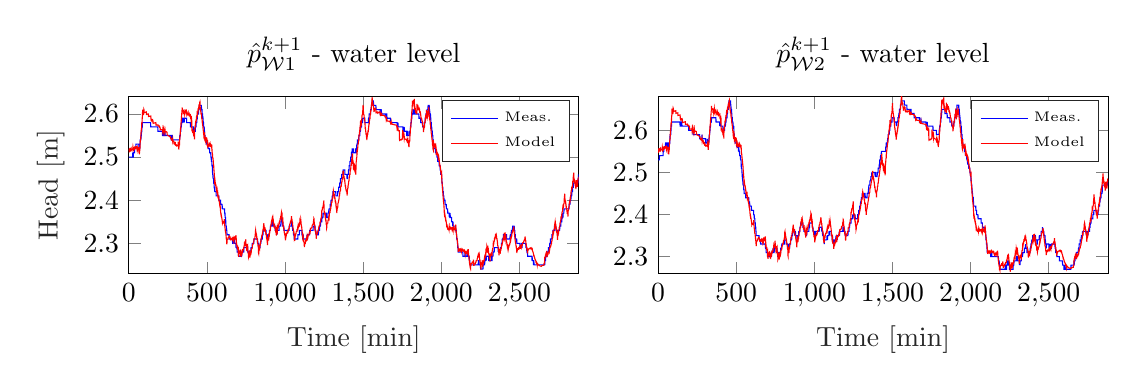
\begin{tikzpicture}

\begin{axis}[%
width=2.25in,
height=0.884in,
at={(1.258in,0.43in)},
scale only axis,
xmin=0,
xmax=2880,
xlabel style={font=\color{white!15!black}},
xlabel={Time [min]},
ymin=2.23,
ymax=2.64,
ylabel style={font=\color{white!15!black}},
ylabel={Head  [m]},
axis background/.style={fill=white},
title style={},
title={$\hat{p}^{k+1}_{\mathcal{W}1}$ - water level},
legend style={legend cell align=left, align=left, draw=white!15!black}
]
\addplot [color=blue]
  table[row sep=crcr]{%
1	2.5\\
2	2.5\\
3	2.5\\
4	2.5\\
5	2.5\\
6	2.5\\
7	2.5\\
8	2.5\\
9	2.5\\
10	2.5\\
11	2.5\\
12	2.5\\
13	2.5\\
14	2.5\\
15	2.5\\
16	2.5\\
17	2.5\\
18	2.5\\
19	2.5\\
20	2.5\\
21	2.5\\
22	2.5\\
23	2.5\\
24	2.5\\
25	2.5\\
26	2.51\\
27	2.5\\
28	2.5\\
29	2.5\\
30	2.51\\
31	2.51\\
32	2.51\\
33	2.51\\
34	2.51\\
35	2.51\\
36	2.51\\
37	2.51\\
38	2.52\\
39	2.52\\
40	2.52\\
41	2.52\\
42	2.52\\
43	2.52\\
44	2.52\\
45	2.52\\
46	2.53\\
47	2.53\\
48	2.53\\
49	2.53\\
50	2.53\\
51	2.53\\
52	2.53\\
53	2.53\\
54	2.53\\
55	2.53\\
56	2.53\\
57	2.53\\
58	2.53\\
59	2.53\\
60	2.53\\
61	2.53\\
62	2.53\\
63	2.53\\
64	2.53\\
65	2.53\\
66	2.52\\
67	2.52\\
68	2.52\\
69	2.52\\
70	2.52\\
71	2.52\\
72	2.53\\
73	2.53\\
74	2.54\\
75	2.54\\
76	2.54\\
77	2.54\\
78	2.54\\
79	2.55\\
80	2.55\\
81	2.55\\
82	2.56\\
83	2.56\\
84	2.56\\
85	2.57\\
86	2.57\\
87	2.57\\
88	2.58\\
89	2.58\\
90	2.58\\
91	2.58\\
92	2.58\\
93	2.58\\
94	2.58\\
95	2.58\\
96	2.58\\
97	2.58\\
98	2.58\\
99	2.58\\
100	2.58\\
101	2.58\\
102	2.58\\
103	2.58\\
104	2.58\\
105	2.58\\
106	2.58\\
107	2.58\\
108	2.58\\
109	2.58\\
110	2.58\\
111	2.58\\
112	2.58\\
113	2.58\\
114	2.58\\
115	2.58\\
116	2.58\\
117	2.58\\
118	2.58\\
119	2.58\\
120	2.58\\
121	2.58\\
122	2.58\\
123	2.58\\
124	2.58\\
125	2.58\\
126	2.58\\
127	2.58\\
128	2.58\\
129	2.58\\
130	2.58\\
131	2.58\\
132	2.58\\
133	2.58\\
134	2.58\\
135	2.58\\
136	2.58\\
137	2.58\\
138	2.58\\
139	2.58\\
140	2.58\\
141	2.57\\
142	2.57\\
143	2.57\\
144	2.57\\
145	2.57\\
146	2.57\\
147	2.57\\
148	2.57\\
149	2.57\\
150	2.57\\
151	2.57\\
152	2.57\\
153	2.57\\
154	2.57\\
155	2.57\\
156	2.57\\
157	2.57\\
158	2.57\\
159	2.57\\
160	2.57\\
161	2.57\\
162	2.57\\
163	2.57\\
164	2.57\\
165	2.57\\
166	2.57\\
167	2.57\\
168	2.57\\
169	2.57\\
170	2.57\\
171	2.57\\
172	2.57\\
173	2.57\\
174	2.57\\
175	2.57\\
176	2.57\\
177	2.57\\
178	2.57\\
179	2.57\\
180	2.57\\
181	2.57\\
182	2.57\\
183	2.57\\
184	2.57\\
185	2.57\\
186	2.57\\
187	2.56\\
188	2.56\\
189	2.56\\
190	2.56\\
191	2.56\\
192	2.56\\
193	2.56\\
194	2.56\\
195	2.56\\
196	2.56\\
197	2.56\\
198	2.56\\
199	2.56\\
200	2.56\\
201	2.56\\
202	2.56\\
203	2.56\\
204	2.56\\
205	2.56\\
206	2.56\\
207	2.56\\
208	2.56\\
209	2.56\\
210	2.56\\
211	2.56\\
212	2.56\\
213	2.56\\
214	2.56\\
215	2.56\\
216	2.55\\
217	2.56\\
218	2.55\\
219	2.55\\
220	2.55\\
221	2.55\\
222	2.56\\
223	2.55\\
224	2.55\\
225	2.56\\
226	2.56\\
227	2.56\\
228	2.55\\
229	2.55\\
230	2.56\\
231	2.55\\
232	2.56\\
233	2.55\\
234	2.55\\
235	2.55\\
236	2.55\\
237	2.55\\
238	2.55\\
239	2.55\\
240	2.55\\
241	2.55\\
242	2.55\\
243	2.55\\
244	2.55\\
245	2.55\\
246	2.55\\
247	2.55\\
248	2.55\\
249	2.55\\
250	2.55\\
251	2.55\\
252	2.55\\
253	2.55\\
254	2.55\\
255	2.55\\
256	2.55\\
257	2.55\\
258	2.55\\
259	2.55\\
260	2.55\\
261	2.55\\
262	2.55\\
263	2.55\\
264	2.55\\
265	2.55\\
266	2.55\\
267	2.55\\
268	2.55\\
269	2.55\\
270	2.55\\
271	2.55\\
272	2.54\\
273	2.54\\
274	2.55\\
275	2.55\\
276	2.55\\
277	2.55\\
278	2.55\\
279	2.55\\
280	2.54\\
281	2.54\\
282	2.54\\
283	2.54\\
284	2.54\\
285	2.54\\
286	2.54\\
287	2.54\\
288	2.54\\
289	2.54\\
290	2.54\\
291	2.54\\
292	2.54\\
293	2.54\\
294	2.54\\
295	2.54\\
296	2.54\\
297	2.54\\
298	2.54\\
299	2.54\\
300	2.54\\
301	2.54\\
302	2.54\\
303	2.54\\
304	2.54\\
305	2.54\\
306	2.54\\
307	2.54\\
308	2.54\\
309	2.54\\
310	2.54\\
311	2.54\\
312	2.54\\
313	2.54\\
314	2.54\\
315	2.54\\
316	2.54\\
317	2.54\\
318	2.54\\
319	2.54\\
320	2.54\\
321	2.54\\
322	2.54\\
323	2.54\\
324	2.54\\
325	2.54\\
326	2.54\\
327	2.55\\
328	2.55\\
329	2.55\\
330	2.55\\
331	2.56\\
332	2.56\\
333	2.56\\
334	2.57\\
335	2.57\\
336	2.57\\
337	2.57\\
338	2.58\\
339	2.58\\
340	2.58\\
341	2.58\\
342	2.59\\
343	2.59\\
344	2.59\\
345	2.59\\
346	2.59\\
347	2.59\\
348	2.59\\
349	2.59\\
350	2.58\\
351	2.59\\
352	2.59\\
353	2.59\\
354	2.59\\
355	2.58\\
356	2.59\\
357	2.59\\
358	2.59\\
359	2.59\\
360	2.59\\
361	2.59\\
362	2.59\\
363	2.59\\
364	2.59\\
365	2.59\\
366	2.59\\
367	2.59\\
368	2.59\\
369	2.59\\
370	2.59\\
371	2.58\\
372	2.58\\
373	2.58\\
374	2.58\\
375	2.58\\
376	2.58\\
377	2.58\\
378	2.58\\
379	2.58\\
380	2.58\\
381	2.58\\
382	2.58\\
383	2.58\\
384	2.58\\
385	2.58\\
386	2.58\\
387	2.58\\
388	2.58\\
389	2.58\\
390	2.58\\
391	2.58\\
392	2.58\\
393	2.58\\
394	2.58\\
395	2.57\\
396	2.57\\
397	2.58\\
398	2.57\\
399	2.57\\
400	2.58\\
401	2.57\\
402	2.57\\
403	2.57\\
404	2.57\\
405	2.57\\
406	2.57\\
407	2.57\\
408	2.57\\
409	2.57\\
410	2.57\\
411	2.57\\
412	2.57\\
413	2.57\\
414	2.56\\
415	2.56\\
416	2.56\\
417	2.56\\
418	2.56\\
419	2.56\\
420	2.56\\
421	2.56\\
422	2.56\\
423	2.56\\
424	2.56\\
425	2.56\\
426	2.56\\
427	2.57\\
428	2.57\\
429	2.57\\
430	2.57\\
431	2.57\\
432	2.58\\
433	2.58\\
434	2.58\\
435	2.58\\
436	2.58\\
437	2.59\\
438	2.59\\
439	2.59\\
440	2.6\\
441	2.6\\
442	2.6\\
443	2.6\\
444	2.6\\
445	2.6\\
446	2.6\\
447	2.6\\
448	2.61\\
449	2.61\\
450	2.61\\
451	2.61\\
452	2.62\\
453	2.62\\
454	2.62\\
455	2.62\\
456	2.62\\
457	2.62\\
458	2.62\\
459	2.62\\
460	2.62\\
461	2.62\\
462	2.62\\
463	2.62\\
464	2.62\\
465	2.62\\
466	2.61\\
467	2.61\\
468	2.61\\
469	2.61\\
470	2.6\\
471	2.6\\
472	2.6\\
473	2.6\\
474	2.59\\
475	2.59\\
476	2.59\\
477	2.58\\
478	2.58\\
479	2.58\\
480	2.57\\
481	2.57\\
482	2.57\\
483	2.57\\
484	2.56\\
485	2.56\\
486	2.55\\
487	2.55\\
488	2.55\\
489	2.55\\
490	2.54\\
491	2.54\\
492	2.54\\
493	2.54\\
494	2.54\\
495	2.54\\
496	2.54\\
497	2.54\\
498	2.53\\
499	2.53\\
500	2.53\\
501	2.53\\
502	2.53\\
503	2.53\\
504	2.53\\
505	2.53\\
506	2.53\\
507	2.53\\
508	2.52\\
509	2.52\\
510	2.52\\
511	2.52\\
512	2.52\\
513	2.52\\
514	2.52\\
515	2.52\\
516	2.52\\
517	2.52\\
518	2.51\\
519	2.51\\
520	2.51\\
521	2.51\\
522	2.51\\
523	2.51\\
524	2.51\\
525	2.51\\
526	2.5\\
527	2.5\\
528	2.5\\
529	2.49\\
530	2.49\\
531	2.49\\
532	2.49\\
533	2.48\\
534	2.48\\
535	2.48\\
536	2.47\\
537	2.46\\
538	2.46\\
539	2.46\\
540	2.45\\
541	2.45\\
542	2.45\\
543	2.45\\
544	2.44\\
545	2.44\\
546	2.44\\
547	2.43\\
548	2.43\\
549	2.43\\
550	2.42\\
551	2.43\\
552	2.42\\
553	2.42\\
554	2.42\\
555	2.42\\
556	2.42\\
557	2.42\\
558	2.42\\
559	2.42\\
560	2.41\\
561	2.41\\
562	2.41\\
563	2.41\\
564	2.41\\
565	2.41\\
566	2.41\\
567	2.41\\
568	2.41\\
569	2.41\\
570	2.41\\
571	2.41\\
572	2.41\\
573	2.41\\
574	2.41\\
575	2.41\\
576	2.41\\
577	2.4\\
578	2.4\\
579	2.4\\
580	2.4\\
581	2.4\\
582	2.4\\
583	2.4\\
584	2.4\\
585	2.4\\
586	2.4\\
587	2.4\\
588	2.4\\
589	2.39\\
590	2.39\\
591	2.39\\
592	2.39\\
593	2.39\\
594	2.39\\
595	2.39\\
596	2.39\\
597	2.39\\
598	2.39\\
599	2.38\\
600	2.38\\
601	2.38\\
602	2.38\\
603	2.38\\
604	2.38\\
605	2.38\\
606	2.38\\
607	2.38\\
608	2.38\\
609	2.38\\
610	2.38\\
611	2.38\\
612	2.38\\
613	2.38\\
614	2.37\\
615	2.37\\
616	2.37\\
617	2.36\\
618	2.36\\
619	2.36\\
620	2.36\\
621	2.35\\
622	2.34\\
623	2.34\\
624	2.34\\
625	2.34\\
626	2.33\\
627	2.33\\
628	2.33\\
629	2.32\\
630	2.32\\
631	2.32\\
632	2.32\\
633	2.32\\
634	2.32\\
635	2.32\\
636	2.32\\
637	2.32\\
638	2.32\\
639	2.32\\
640	2.32\\
641	2.32\\
642	2.32\\
643	2.31\\
644	2.31\\
645	2.31\\
646	2.31\\
647	2.31\\
648	2.31\\
649	2.31\\
650	2.31\\
651	2.31\\
652	2.31\\
653	2.31\\
654	2.31\\
655	2.31\\
656	2.31\\
657	2.31\\
658	2.31\\
659	2.31\\
660	2.31\\
661	2.31\\
662	2.31\\
663	2.31\\
664	2.31\\
665	2.3\\
666	2.3\\
667	2.31\\
668	2.31\\
669	2.31\\
670	2.31\\
671	2.31\\
672	2.31\\
673	2.3\\
674	2.31\\
675	2.31\\
676	2.31\\
677	2.3\\
678	2.3\\
679	2.3\\
680	2.3\\
681	2.3\\
682	2.3\\
683	2.3\\
684	2.3\\
685	2.3\\
686	2.3\\
687	2.29\\
688	2.29\\
689	2.29\\
690	2.29\\
691	2.29\\
692	2.29\\
693	2.29\\
694	2.28\\
695	2.28\\
696	2.28\\
697	2.28\\
698	2.28\\
699	2.28\\
700	2.28\\
701	2.28\\
702	2.28\\
703	2.27\\
704	2.27\\
705	2.27\\
706	2.27\\
707	2.27\\
708	2.27\\
709	2.27\\
710	2.27\\
711	2.27\\
712	2.27\\
713	2.27\\
714	2.27\\
715	2.27\\
716	2.27\\
717	2.27\\
718	2.27\\
719	2.27\\
720	2.27\\
721	2.27\\
722	2.27\\
723	2.27\\
724	2.28\\
725	2.28\\
726	2.28\\
727	2.28\\
728	2.28\\
729	2.28\\
730	2.28\\
731	2.28\\
732	2.28\\
733	2.28\\
734	2.28\\
735	2.28\\
736	2.28\\
737	2.29\\
738	2.29\\
739	2.29\\
740	2.29\\
741	2.29\\
742	2.29\\
743	2.29\\
744	2.29\\
745	2.29\\
746	2.29\\
747	2.29\\
748	2.29\\
749	2.29\\
750	2.29\\
751	2.29\\
752	2.29\\
753	2.29\\
754	2.29\\
755	2.29\\
756	2.29\\
757	2.29\\
758	2.29\\
759	2.29\\
760	2.29\\
761	2.29\\
762	2.28\\
763	2.28\\
764	2.28\\
765	2.28\\
766	2.28\\
767	2.28\\
768	2.28\\
769	2.28\\
770	2.28\\
771	2.28\\
772	2.28\\
773	2.28\\
774	2.28\\
775	2.28\\
776	2.28\\
777	2.28\\
778	2.28\\
779	2.28\\
780	2.28\\
781	2.28\\
782	2.29\\
783	2.28\\
784	2.29\\
785	2.29\\
786	2.29\\
787	2.29\\
788	2.29\\
789	2.29\\
790	2.29\\
791	2.3\\
792	2.3\\
793	2.3\\
794	2.3\\
795	2.3\\
796	2.3\\
797	2.3\\
798	2.3\\
799	2.3\\
800	2.3\\
801	2.31\\
802	2.31\\
803	2.31\\
804	2.31\\
805	2.31\\
806	2.31\\
807	2.31\\
808	2.31\\
809	2.31\\
810	2.31\\
811	2.31\\
812	2.31\\
813	2.31\\
814	2.31\\
815	2.31\\
816	2.31\\
817	2.31\\
818	2.31\\
819	2.31\\
820	2.31\\
821	2.31\\
822	2.31\\
823	2.31\\
824	2.3\\
825	2.31\\
826	2.3\\
827	2.3\\
828	2.3\\
829	2.3\\
830	2.3\\
831	2.29\\
832	2.29\\
833	2.29\\
834	2.29\\
835	2.29\\
836	2.29\\
837	2.29\\
838	2.29\\
839	2.29\\
840	2.29\\
841	2.3\\
842	2.3\\
843	2.3\\
844	2.3\\
845	2.3\\
846	2.3\\
847	2.31\\
848	2.31\\
849	2.31\\
850	2.31\\
851	2.31\\
852	2.31\\
853	2.31\\
854	2.31\\
855	2.31\\
856	2.32\\
857	2.32\\
858	2.32\\
859	2.32\\
860	2.32\\
861	2.33\\
862	2.33\\
863	2.33\\
864	2.33\\
865	2.33\\
866	2.33\\
867	2.33\\
868	2.33\\
869	2.33\\
870	2.33\\
871	2.33\\
872	2.33\\
873	2.33\\
874	2.33\\
875	2.33\\
876	2.33\\
877	2.33\\
878	2.33\\
879	2.33\\
880	2.32\\
881	2.32\\
882	2.32\\
883	2.32\\
884	2.32\\
885	2.32\\
886	2.32\\
887	2.31\\
888	2.32\\
889	2.31\\
890	2.31\\
891	2.32\\
892	2.31\\
893	2.31\\
894	2.31\\
895	2.31\\
896	2.32\\
897	2.32\\
898	2.32\\
899	2.32\\
900	2.32\\
901	2.33\\
902	2.33\\
903	2.33\\
904	2.33\\
905	2.33\\
906	2.33\\
907	2.34\\
908	2.34\\
909	2.34\\
910	2.34\\
911	2.34\\
912	2.34\\
913	2.34\\
914	2.35\\
915	2.35\\
916	2.34\\
917	2.35\\
918	2.35\\
919	2.34\\
920	2.34\\
921	2.34\\
922	2.35\\
923	2.35\\
924	2.35\\
925	2.35\\
926	2.34\\
927	2.34\\
928	2.34\\
929	2.34\\
930	2.34\\
931	2.34\\
932	2.34\\
933	2.34\\
934	2.34\\
935	2.34\\
936	2.34\\
937	2.33\\
938	2.33\\
939	2.33\\
940	2.33\\
941	2.33\\
942	2.33\\
943	2.33\\
944	2.33\\
945	2.33\\
946	2.33\\
947	2.33\\
948	2.33\\
949	2.33\\
950	2.32\\
951	2.33\\
952	2.33\\
953	2.33\\
954	2.33\\
955	2.33\\
956	2.33\\
957	2.33\\
958	2.33\\
959	2.33\\
960	2.33\\
961	2.33\\
962	2.33\\
963	2.34\\
964	2.34\\
965	2.34\\
966	2.34\\
967	2.34\\
968	2.34\\
969	2.34\\
970	2.34\\
971	2.34\\
972	2.34\\
973	2.34\\
974	2.35\\
975	2.35\\
976	2.35\\
977	2.35\\
978	2.36\\
979	2.35\\
980	2.35\\
981	2.36\\
982	2.35\\
983	2.35\\
984	2.35\\
985	2.34\\
986	2.35\\
987	2.34\\
988	2.34\\
989	2.34\\
990	2.34\\
991	2.34\\
992	2.34\\
993	2.34\\
994	2.33\\
995	2.33\\
996	2.33\\
997	2.33\\
998	2.33\\
999	2.33\\
1000	2.33\\
1001	2.33\\
1002	2.33\\
1003	2.33\\
1004	2.33\\
1005	2.33\\
1006	2.33\\
1007	2.33\\
1008	2.33\\
1009	2.33\\
1010	2.33\\
1011	2.33\\
1012	2.33\\
1013	2.33\\
1014	2.33\\
1015	2.33\\
1016	2.33\\
1017	2.33\\
1018	2.33\\
1019	2.33\\
1020	2.33\\
1021	2.33\\
1022	2.33\\
1023	2.33\\
1024	2.33\\
1025	2.33\\
1026	2.33\\
1027	2.34\\
1028	2.34\\
1029	2.34\\
1030	2.34\\
1031	2.34\\
1032	2.34\\
1033	2.34\\
1034	2.34\\
1035	2.34\\
1036	2.34\\
1037	2.34\\
1038	2.34\\
1039	2.34\\
1040	2.34\\
1041	2.34\\
1042	2.35\\
1043	2.35\\
1044	2.35\\
1045	2.34\\
1046	2.34\\
1047	2.34\\
1048	2.34\\
1049	2.33\\
1050	2.33\\
1051	2.33\\
1052	2.33\\
1053	2.33\\
1054	2.33\\
1055	2.32\\
1056	2.32\\
1057	2.32\\
1058	2.32\\
1059	2.31\\
1060	2.31\\
1061	2.31\\
1062	2.31\\
1063	2.31\\
1064	2.31\\
1065	2.31\\
1066	2.31\\
1067	2.31\\
1068	2.31\\
1069	2.31\\
1070	2.31\\
1071	2.31\\
1072	2.31\\
1073	2.31\\
1074	2.31\\
1075	2.31\\
1076	2.31\\
1077	2.31\\
1078	2.31\\
1079	2.31\\
1080	2.31\\
1081	2.31\\
1082	2.31\\
1083	2.32\\
1084	2.32\\
1085	2.32\\
1086	2.32\\
1087	2.32\\
1088	2.32\\
1089	2.32\\
1090	2.32\\
1091	2.32\\
1092	2.32\\
1093	2.33\\
1094	2.33\\
1095	2.33\\
1096	2.33\\
1097	2.33\\
1098	2.33\\
1099	2.33\\
1100	2.33\\
1101	2.33\\
1102	2.33\\
1103	2.33\\
1104	2.33\\
1105	2.33\\
1106	2.33\\
1107	2.33\\
1108	2.33\\
1109	2.32\\
1110	2.32\\
1111	2.32\\
1112	2.32\\
1113	2.31\\
1114	2.32\\
1115	2.31\\
1116	2.31\\
1117	2.32\\
1118	2.31\\
1119	2.31\\
1120	2.31\\
1121	2.31\\
1122	2.31\\
1123	2.31\\
1124	2.31\\
1125	2.31\\
1126	2.31\\
1127	2.31\\
1128	2.31\\
1129	2.31\\
1130	2.31\\
1131	2.31\\
1132	2.31\\
1133	2.31\\
1134	2.31\\
1135	2.31\\
1136	2.31\\
1137	2.31\\
1138	2.31\\
1139	2.31\\
1140	2.31\\
1141	2.32\\
1142	2.31\\
1143	2.31\\
1144	2.31\\
1145	2.32\\
1146	2.32\\
1147	2.32\\
1148	2.32\\
1149	2.32\\
1150	2.32\\
1151	2.32\\
1152	2.32\\
1153	2.32\\
1154	2.32\\
1155	2.32\\
1156	2.32\\
1157	2.32\\
1158	2.33\\
1159	2.33\\
1160	2.33\\
1161	2.33\\
1162	2.33\\
1163	2.33\\
1164	2.33\\
1165	2.33\\
1166	2.33\\
1167	2.33\\
1168	2.33\\
1169	2.33\\
1170	2.33\\
1171	2.33\\
1172	2.33\\
1173	2.33\\
1174	2.33\\
1175	2.33\\
1176	2.33\\
1177	2.33\\
1178	2.33\\
1179	2.33\\
1180	2.33\\
1181	2.34\\
1182	2.34\\
1183	2.34\\
1184	2.34\\
1185	2.34\\
1186	2.34\\
1187	2.34\\
1188	2.34\\
1189	2.34\\
1190	2.34\\
1191	2.34\\
1192	2.34\\
1193	2.33\\
1194	2.33\\
1195	2.33\\
1196	2.33\\
1197	2.33\\
1198	2.33\\
1199	2.32\\
1200	2.32\\
1201	2.32\\
1202	2.32\\
1203	2.32\\
1204	2.32\\
1205	2.32\\
1206	2.32\\
1207	2.32\\
1208	2.32\\
1209	2.32\\
1210	2.32\\
1211	2.32\\
1212	2.32\\
1213	2.32\\
1214	2.32\\
1215	2.33\\
1216	2.33\\
1217	2.33\\
1218	2.33\\
1219	2.33\\
1220	2.33\\
1221	2.33\\
1222	2.34\\
1223	2.34\\
1224	2.34\\
1225	2.34\\
1226	2.34\\
1227	2.34\\
1228	2.35\\
1229	2.35\\
1230	2.35\\
1231	2.35\\
1232	2.35\\
1233	2.35\\
1234	2.36\\
1235	2.35\\
1236	2.35\\
1237	2.36\\
1238	2.36\\
1239	2.36\\
1240	2.36\\
1241	2.36\\
1242	2.36\\
1243	2.37\\
1244	2.36\\
1245	2.37\\
1246	2.37\\
1247	2.37\\
1248	2.37\\
1249	2.37\\
1250	2.37\\
1251	2.37\\
1252	2.37\\
1253	2.37\\
1254	2.37\\
1255	2.37\\
1256	2.37\\
1257	2.37\\
1258	2.37\\
1259	2.37\\
1260	2.37\\
1261	2.37\\
1262	2.37\\
1263	2.37\\
1264	2.37\\
1265	2.36\\
1266	2.36\\
1267	2.36\\
1268	2.36\\
1269	2.36\\
1270	2.36\\
1271	2.36\\
1272	2.36\\
1273	2.36\\
1274	2.36\\
1275	2.37\\
1276	2.37\\
1277	2.37\\
1278	2.37\\
1279	2.37\\
1280	2.37\\
1281	2.38\\
1282	2.37\\
1283	2.38\\
1284	2.38\\
1285	2.38\\
1286	2.38\\
1287	2.38\\
1288	2.38\\
1289	2.38\\
1290	2.39\\
1291	2.39\\
1292	2.39\\
1293	2.39\\
1294	2.39\\
1295	2.4\\
1296	2.4\\
1297	2.4\\
1298	2.4\\
1299	2.4\\
1300	2.4\\
1301	2.4\\
1302	2.4\\
1303	2.41\\
1304	2.41\\
1305	2.41\\
1306	2.41\\
1307	2.42\\
1308	2.42\\
1309	2.42\\
1310	2.42\\
1311	2.42\\
1312	2.42\\
1313	2.42\\
1314	2.42\\
1315	2.42\\
1316	2.42\\
1317	2.42\\
1318	2.42\\
1319	2.42\\
1320	2.42\\
1321	2.42\\
1322	2.42\\
1323	2.42\\
1324	2.42\\
1325	2.42\\
1326	2.41\\
1327	2.41\\
1328	2.41\\
1329	2.41\\
1330	2.41\\
1331	2.41\\
1332	2.41\\
1333	2.41\\
1334	2.41\\
1335	2.41\\
1336	2.41\\
1337	2.41\\
1338	2.42\\
1339	2.42\\
1340	2.42\\
1341	2.42\\
1342	2.42\\
1343	2.42\\
1344	2.43\\
1345	2.43\\
1346	2.43\\
1347	2.43\\
1348	2.43\\
1349	2.43\\
1350	2.43\\
1351	2.44\\
1352	2.44\\
1353	2.44\\
1354	2.44\\
1355	2.45\\
1356	2.45\\
1357	2.45\\
1358	2.45\\
1359	2.45\\
1360	2.45\\
1361	2.45\\
1362	2.45\\
1363	2.46\\
1364	2.46\\
1365	2.46\\
1366	2.46\\
1367	2.46\\
1368	2.46\\
1369	2.46\\
1370	2.46\\
1371	2.46\\
1372	2.47\\
1373	2.47\\
1374	2.47\\
1375	2.47\\
1376	2.47\\
1377	2.47\\
1378	2.47\\
1379	2.47\\
1380	2.47\\
1381	2.47\\
1382	2.47\\
1383	2.47\\
1384	2.46\\
1385	2.46\\
1386	2.46\\
1387	2.46\\
1388	2.46\\
1389	2.46\\
1390	2.46\\
1391	2.46\\
1392	2.46\\
1393	2.46\\
1394	2.46\\
1395	2.46\\
1396	2.46\\
1397	2.45\\
1398	2.46\\
1399	2.45\\
1400	2.45\\
1401	2.46\\
1402	2.46\\
1403	2.46\\
1404	2.46\\
1405	2.46\\
1406	2.46\\
1407	2.47\\
1408	2.47\\
1409	2.47\\
1410	2.47\\
1411	2.48\\
1412	2.48\\
1413	2.48\\
1414	2.48\\
1415	2.48\\
1416	2.49\\
1417	2.49\\
1418	2.49\\
1419	2.49\\
1420	2.49\\
1421	2.5\\
1422	2.5\\
1423	2.5\\
1424	2.5\\
1425	2.5\\
1426	2.51\\
1427	2.51\\
1428	2.51\\
1429	2.51\\
1430	2.52\\
1431	2.51\\
1432	2.51\\
1433	2.51\\
1434	2.51\\
1435	2.51\\
1436	2.51\\
1437	2.52\\
1438	2.51\\
1439	2.51\\
1440	2.51\\
1441	2.51\\
1442	2.51\\
1443	2.51\\
1444	2.51\\
1445	2.51\\
1446	2.51\\
1447	2.51\\
1448	2.51\\
1449	2.51\\
1450	2.51\\
1451	2.52\\
1452	2.51\\
1453	2.51\\
1454	2.51\\
1455	2.51\\
1456	2.51\\
1457	2.52\\
1458	2.52\\
1459	2.52\\
1460	2.53\\
1461	2.53\\
1462	2.53\\
1463	2.53\\
1464	2.54\\
1465	2.54\\
1466	2.54\\
1467	2.54\\
1468	2.54\\
1469	2.54\\
1470	2.54\\
1471	2.54\\
1472	2.54\\
1473	2.55\\
1474	2.55\\
1475	2.55\\
1476	2.55\\
1477	2.55\\
1478	2.55\\
1479	2.55\\
1480	2.56\\
1481	2.56\\
1482	2.56\\
1483	2.57\\
1484	2.56\\
1485	2.57\\
1486	2.57\\
1487	2.57\\
1488	2.57\\
1489	2.57\\
1490	2.57\\
1491	2.58\\
1492	2.58\\
1493	2.58\\
1494	2.58\\
1495	2.58\\
1496	2.58\\
1497	2.58\\
1498	2.59\\
1499	2.59\\
1500	2.59\\
1501	2.59\\
1502	2.59\\
1503	2.59\\
1504	2.59\\
1505	2.59\\
1506	2.59\\
1507	2.59\\
1508	2.59\\
1509	2.59\\
1510	2.59\\
1511	2.59\\
1512	2.58\\
1513	2.58\\
1514	2.58\\
1515	2.58\\
1516	2.58\\
1517	2.58\\
1518	2.58\\
1519	2.58\\
1520	2.58\\
1521	2.58\\
1522	2.58\\
1523	2.58\\
1524	2.58\\
1525	2.58\\
1526	2.58\\
1527	2.58\\
1528	2.58\\
1529	2.58\\
1530	2.58\\
1531	2.58\\
1532	2.58\\
1533	2.58\\
1534	2.58\\
1535	2.59\\
1536	2.59\\
1537	2.59\\
1538	2.59\\
1539	2.6\\
1540	2.6\\
1541	2.6\\
1542	2.6\\
1543	2.6\\
1544	2.6\\
1545	2.6\\
1546	2.6\\
1547	2.6\\
1548	2.61\\
1549	2.61\\
1550	2.61\\
1551	2.61\\
1552	2.61\\
1553	2.62\\
1554	2.62\\
1555	2.62\\
1556	2.62\\
1557	2.62\\
1558	2.63\\
1559	2.63\\
1560	2.63\\
1561	2.63\\
1562	2.63\\
1563	2.63\\
1564	2.63\\
1565	2.63\\
1566	2.63\\
1567	2.62\\
1568	2.62\\
1569	2.62\\
1570	2.62\\
1571	2.62\\
1572	2.62\\
1573	2.62\\
1574	2.62\\
1575	2.62\\
1576	2.62\\
1577	2.62\\
1578	2.62\\
1579	2.62\\
1580	2.62\\
1581	2.62\\
1582	2.62\\
1583	2.61\\
1584	2.61\\
1585	2.61\\
1586	2.61\\
1587	2.61\\
1588	2.61\\
1589	2.61\\
1590	2.61\\
1591	2.61\\
1592	2.61\\
1593	2.61\\
1594	2.61\\
1595	2.61\\
1596	2.61\\
1597	2.61\\
1598	2.61\\
1599	2.61\\
1600	2.61\\
1601	2.61\\
1602	2.61\\
1603	2.61\\
1604	2.61\\
1605	2.61\\
1606	2.61\\
1607	2.61\\
1608	2.61\\
1609	2.61\\
1610	2.6\\
1611	2.6\\
1612	2.61\\
1613	2.6\\
1614	2.61\\
1615	2.61\\
1616	2.6\\
1617	2.61\\
1618	2.6\\
1619	2.6\\
1620	2.6\\
1621	2.6\\
1622	2.6\\
1623	2.6\\
1624	2.6\\
1625	2.6\\
1626	2.6\\
1627	2.6\\
1628	2.6\\
1629	2.6\\
1630	2.6\\
1631	2.6\\
1632	2.6\\
1633	2.6\\
1634	2.6\\
1635	2.6\\
1636	2.6\\
1637	2.6\\
1638	2.6\\
1639	2.6\\
1640	2.6\\
1641	2.6\\
1642	2.6\\
1643	2.6\\
1644	2.6\\
1645	2.6\\
1646	2.59\\
1647	2.6\\
1648	2.6\\
1649	2.6\\
1650	2.6\\
1651	2.6\\
1652	2.6\\
1653	2.59\\
1654	2.59\\
1655	2.59\\
1656	2.59\\
1657	2.59\\
1658	2.59\\
1659	2.59\\
1660	2.59\\
1661	2.59\\
1662	2.59\\
1663	2.59\\
1664	2.59\\
1665	2.59\\
1666	2.59\\
1667	2.59\\
1668	2.59\\
1669	2.59\\
1670	2.59\\
1671	2.59\\
1672	2.59\\
1673	2.59\\
1674	2.59\\
1675	2.59\\
1676	2.58\\
1677	2.58\\
1678	2.58\\
1679	2.58\\
1680	2.58\\
1681	2.58\\
1682	2.58\\
1683	2.58\\
1684	2.58\\
1685	2.58\\
1686	2.58\\
1687	2.58\\
1688	2.58\\
1689	2.58\\
1690	2.58\\
1691	2.58\\
1692	2.58\\
1693	2.58\\
1694	2.58\\
1695	2.58\\
1696	2.58\\
1697	2.58\\
1698	2.58\\
1699	2.58\\
1700	2.58\\
1701	2.58\\
1702	2.58\\
1703	2.58\\
1704	2.58\\
1705	2.58\\
1706	2.58\\
1707	2.58\\
1708	2.58\\
1709	2.58\\
1710	2.58\\
1711	2.58\\
1712	2.58\\
1713	2.58\\
1714	2.58\\
1715	2.58\\
1716	2.58\\
1717	2.58\\
1718	2.58\\
1719	2.57\\
1720	2.57\\
1721	2.57\\
1722	2.57\\
1723	2.58\\
1724	2.57\\
1725	2.57\\
1726	2.57\\
1727	2.57\\
1728	2.57\\
1729	2.57\\
1730	2.57\\
1731	2.57\\
1732	2.57\\
1733	2.57\\
1734	2.57\\
1735	2.57\\
1736	2.57\\
1737	2.57\\
1738	2.57\\
1739	2.57\\
1740	2.57\\
1741	2.57\\
1742	2.57\\
1743	2.57\\
1744	2.57\\
1745	2.57\\
1746	2.57\\
1747	2.57\\
1748	2.57\\
1749	2.57\\
1750	2.57\\
1751	2.57\\
1752	2.57\\
1753	2.57\\
1754	2.57\\
1755	2.57\\
1756	2.56\\
1757	2.56\\
1758	2.56\\
1759	2.56\\
1760	2.56\\
1761	2.57\\
1762	2.56\\
1763	2.57\\
1764	2.56\\
1765	2.56\\
1766	2.56\\
1767	2.56\\
1768	2.56\\
1769	2.56\\
1770	2.56\\
1771	2.56\\
1772	2.56\\
1773	2.56\\
1774	2.56\\
1775	2.56\\
1776	2.56\\
1777	2.56\\
1778	2.56\\
1779	2.55\\
1780	2.55\\
1781	2.56\\
1782	2.56\\
1783	2.55\\
1784	2.55\\
1785	2.55\\
1786	2.55\\
1787	2.56\\
1788	2.55\\
1789	2.55\\
1790	2.55\\
1791	2.55\\
1792	2.55\\
1793	2.55\\
1794	2.55\\
1795	2.55\\
1796	2.55\\
1797	2.55\\
1798	2.55\\
1799	2.56\\
1800	2.56\\
1801	2.56\\
1802	2.56\\
1803	2.57\\
1804	2.57\\
1805	2.57\\
1806	2.58\\
1807	2.58\\
1808	2.58\\
1809	2.58\\
1810	2.59\\
1811	2.59\\
1812	2.59\\
1813	2.6\\
1814	2.6\\
1815	2.6\\
1816	2.6\\
1817	2.6\\
1818	2.6\\
1819	2.61\\
1820	2.61\\
1821	2.6\\
1822	2.6\\
1823	2.6\\
1824	2.6\\
1825	2.6\\
1826	2.6\\
1827	2.61\\
1828	2.6\\
1829	2.6\\
1830	2.6\\
1831	2.61\\
1832	2.6\\
1833	2.6\\
1834	2.6\\
1835	2.6\\
1836	2.6\\
1837	2.6\\
1838	2.6\\
1839	2.6\\
1840	2.6\\
1841	2.6\\
1842	2.6\\
1843	2.6\\
1844	2.6\\
1845	2.6\\
1846	2.6\\
1847	2.6\\
1848	2.6\\
1849	2.6\\
1850	2.6\\
1851	2.6\\
1852	2.6\\
1853	2.6\\
1854	2.6\\
1855	2.6\\
1856	2.6\\
1857	2.6\\
1858	2.59\\
1859	2.59\\
1860	2.59\\
1861	2.59\\
1862	2.59\\
1863	2.59\\
1864	2.59\\
1865	2.59\\
1866	2.59\\
1867	2.59\\
1868	2.59\\
1869	2.58\\
1870	2.58\\
1871	2.58\\
1872	2.58\\
1873	2.58\\
1874	2.58\\
1875	2.58\\
1876	2.58\\
1877	2.58\\
1878	2.58\\
1879	2.58\\
1880	2.58\\
1881	2.57\\
1882	2.57\\
1883	2.57\\
1884	2.57\\
1885	2.57\\
1886	2.57\\
1887	2.57\\
1888	2.57\\
1889	2.57\\
1890	2.57\\
1891	2.57\\
1892	2.57\\
1893	2.58\\
1894	2.58\\
1895	2.58\\
1896	2.58\\
1897	2.58\\
1898	2.59\\
1899	2.59\\
1900	2.59\\
1901	2.59\\
1902	2.6\\
1903	2.6\\
1904	2.6\\
1905	2.6\\
1906	2.6\\
1907	2.6\\
1908	2.6\\
1909	2.6\\
1910	2.61\\
1911	2.61\\
1912	2.61\\
1913	2.61\\
1914	2.61\\
1915	2.61\\
1916	2.62\\
1917	2.62\\
1918	2.62\\
1919	2.62\\
1920	2.62\\
1921	2.62\\
1922	2.62\\
1923	2.62\\
1924	2.61\\
1925	2.61\\
1926	2.61\\
1927	2.6\\
1928	2.6\\
1929	2.6\\
1930	2.6\\
1931	2.6\\
1932	2.59\\
1933	2.59\\
1934	2.58\\
1935	2.58\\
1936	2.58\\
1937	2.57\\
1938	2.57\\
1939	2.57\\
1940	2.56\\
1941	2.56\\
1942	2.56\\
1943	2.56\\
1944	2.55\\
1945	2.55\\
1946	2.55\\
1947	2.54\\
1948	2.54\\
1949	2.54\\
1950	2.53\\
1951	2.53\\
1952	2.52\\
1953	2.52\\
1954	2.52\\
1955	2.52\\
1956	2.52\\
1957	2.52\\
1958	2.52\\
1959	2.52\\
1960	2.52\\
1961	2.52\\
1962	2.52\\
1963	2.51\\
1964	2.52\\
1965	2.51\\
1966	2.51\\
1967	2.51\\
1968	2.51\\
1969	2.51\\
1970	2.51\\
1971	2.51\\
1972	2.51\\
1973	2.5\\
1974	2.5\\
1975	2.5\\
1976	2.5\\
1977	2.5\\
1978	2.49\\
1979	2.49\\
1980	2.49\\
1981	2.49\\
1982	2.49\\
1983	2.49\\
1984	2.49\\
1985	2.49\\
1986	2.49\\
1987	2.48\\
1988	2.48\\
1989	2.48\\
1990	2.48\\
1991	2.48\\
1992	2.48\\
1993	2.48\\
1994	2.47\\
1995	2.47\\
1996	2.47\\
1997	2.46\\
1998	2.46\\
1999	2.46\\
2000	2.46\\
2001	2.46\\
2002	2.46\\
2003	2.45\\
2004	2.45\\
2005	2.44\\
2006	2.44\\
2007	2.44\\
2008	2.43\\
2009	2.43\\
2010	2.43\\
2011	2.42\\
2012	2.42\\
2013	2.42\\
2014	2.41\\
2015	2.41\\
2016	2.41\\
2017	2.41\\
2018	2.4\\
2019	2.4\\
2020	2.4\\
2021	2.4\\
2022	2.4\\
2023	2.4\\
2024	2.4\\
2025	2.39\\
2026	2.39\\
2027	2.39\\
2028	2.39\\
2029	2.39\\
2030	2.39\\
2031	2.39\\
2032	2.39\\
2033	2.38\\
2034	2.38\\
2035	2.38\\
2036	2.38\\
2037	2.38\\
2038	2.38\\
2039	2.38\\
2040	2.38\\
2041	2.38\\
2042	2.37\\
2043	2.37\\
2044	2.37\\
2045	2.37\\
2046	2.37\\
2047	2.37\\
2048	2.37\\
2049	2.37\\
2050	2.37\\
2051	2.37\\
2052	2.36\\
2053	2.37\\
2054	2.37\\
2055	2.36\\
2056	2.36\\
2057	2.37\\
2058	2.36\\
2059	2.36\\
2060	2.36\\
2061	2.36\\
2062	2.36\\
2063	2.36\\
2064	2.36\\
2065	2.36\\
2066	2.36\\
2067	2.35\\
2068	2.35\\
2069	2.35\\
2070	2.35\\
2071	2.35\\
2072	2.35\\
2073	2.35\\
2074	2.34\\
2075	2.35\\
2076	2.34\\
2077	2.34\\
2078	2.34\\
2079	2.34\\
2080	2.34\\
2081	2.34\\
2082	2.34\\
2083	2.34\\
2084	2.34\\
2085	2.34\\
2086	2.34\\
2087	2.34\\
2088	2.34\\
2089	2.34\\
2090	2.34\\
2091	2.34\\
2092	2.34\\
2093	2.33\\
2094	2.33\\
2095	2.33\\
2096	2.33\\
2097	2.32\\
2098	2.32\\
2099	2.31\\
2100	2.31\\
2101	2.31\\
2102	2.31\\
2103	2.31\\
2104	2.3\\
2105	2.3\\
2106	2.29\\
2107	2.29\\
2108	2.29\\
2109	2.28\\
2110	2.28\\
2111	2.28\\
2112	2.28\\
2113	2.28\\
2114	2.28\\
2115	2.28\\
2116	2.28\\
2117	2.28\\
2118	2.28\\
2119	2.28\\
2120	2.28\\
2121	2.28\\
2122	2.28\\
2123	2.28\\
2124	2.28\\
2125	2.28\\
2126	2.28\\
2127	2.28\\
2128	2.28\\
2129	2.28\\
2130	2.28\\
2131	2.28\\
2132	2.28\\
2133	2.28\\
2134	2.28\\
2135	2.28\\
2136	2.28\\
2137	2.28\\
2138	2.28\\
2139	2.27\\
2140	2.27\\
2141	2.27\\
2142	2.27\\
2143	2.27\\
2144	2.27\\
2145	2.27\\
2146	2.27\\
2147	2.27\\
2148	2.27\\
2149	2.27\\
2150	2.27\\
2151	2.27\\
2152	2.28\\
2153	2.27\\
2154	2.27\\
2155	2.27\\
2156	2.27\\
2157	2.27\\
2158	2.27\\
2159	2.27\\
2160	2.27\\
2161	2.27\\
2162	2.27\\
2163	2.27\\
2164	2.27\\
2165	2.28\\
2166	2.27\\
2167	2.28\\
2168	2.27\\
2169	2.27\\
2170	2.27\\
2171	2.27\\
2172	2.27\\
2173	2.27\\
2174	2.27\\
2175	2.27\\
2176	2.27\\
2177	2.27\\
2178	2.27\\
2179	2.27\\
2180	2.26\\
2181	2.26\\
2182	2.26\\
2183	2.26\\
2184	2.25\\
2185	2.25\\
2186	2.25\\
2187	2.25\\
2188	2.25\\
2189	2.25\\
2190	2.25\\
2191	2.25\\
2192	2.25\\
2193	2.25\\
2194	2.25\\
2195	2.25\\
2196	2.25\\
2197	2.25\\
2198	2.25\\
2199	2.25\\
2200	2.25\\
2201	2.25\\
2202	2.25\\
2203	2.25\\
2204	2.25\\
2205	2.25\\
2206	2.25\\
2207	2.25\\
2208	2.25\\
2209	2.25\\
2210	2.25\\
2211	2.25\\
2212	2.25\\
2213	2.25\\
2214	2.25\\
2215	2.25\\
2216	2.25\\
2217	2.25\\
2218	2.25\\
2219	2.25\\
2220	2.25\\
2221	2.25\\
2222	2.25\\
2223	2.25\\
2224	2.25\\
2225	2.25\\
2226	2.25\\
2227	2.25\\
2228	2.25\\
2229	2.25\\
2230	2.25\\
2231	2.25\\
2232	2.25\\
2233	2.25\\
2234	2.25\\
2235	2.25\\
2236	2.25\\
2237	2.25\\
2238	2.26\\
2239	2.26\\
2240	2.26\\
2241	2.25\\
2242	2.26\\
2243	2.25\\
2244	2.25\\
2245	2.25\\
2246	2.25\\
2247	2.25\\
2248	2.25\\
2249	2.25\\
2250	2.25\\
2251	2.25\\
2252	2.24\\
2253	2.24\\
2254	2.24\\
2255	2.24\\
2256	2.24\\
2257	2.24\\
2258	2.24\\
2259	2.24\\
2260	2.24\\
2261	2.24\\
2262	2.24\\
2263	2.24\\
2264	2.24\\
2265	2.24\\
2266	2.24\\
2267	2.24\\
2268	2.25\\
2269	2.25\\
2270	2.25\\
2271	2.25\\
2272	2.25\\
2273	2.25\\
2274	2.25\\
2275	2.25\\
2276	2.26\\
2277	2.25\\
2278	2.25\\
2279	2.26\\
2280	2.26\\
2281	2.26\\
2282	2.26\\
2283	2.27\\
2284	2.26\\
2285	2.27\\
2286	2.26\\
2287	2.27\\
2288	2.26\\
2289	2.27\\
2290	2.27\\
2291	2.27\\
2292	2.27\\
2293	2.27\\
2294	2.27\\
2295	2.27\\
2296	2.27\\
2297	2.27\\
2298	2.27\\
2299	2.27\\
2300	2.27\\
2301	2.27\\
2302	2.27\\
2303	2.27\\
2304	2.26\\
2305	2.26\\
2306	2.27\\
2307	2.27\\
2308	2.26\\
2309	2.26\\
2310	2.26\\
2311	2.26\\
2312	2.26\\
2313	2.26\\
2314	2.26\\
2315	2.26\\
2316	2.26\\
2317	2.26\\
2318	2.26\\
2319	2.26\\
2320	2.26\\
2321	2.26\\
2322	2.26\\
2323	2.27\\
2324	2.26\\
2325	2.26\\
2326	2.27\\
2327	2.27\\
2328	2.27\\
2329	2.27\\
2330	2.27\\
2331	2.27\\
2332	2.28\\
2333	2.28\\
2334	2.28\\
2335	2.28\\
2336	2.28\\
2337	2.28\\
2338	2.28\\
2339	2.28\\
2340	2.29\\
2341	2.29\\
2342	2.29\\
2343	2.29\\
2344	2.29\\
2345	2.29\\
2346	2.29\\
2347	2.29\\
2348	2.29\\
2349	2.29\\
2350	2.29\\
2351	2.29\\
2352	2.29\\
2353	2.29\\
2354	2.29\\
2355	2.29\\
2356	2.29\\
2357	2.29\\
2358	2.29\\
2359	2.29\\
2360	2.29\\
2361	2.29\\
2362	2.29\\
2363	2.29\\
2364	2.29\\
2365	2.28\\
2366	2.29\\
2367	2.28\\
2368	2.28\\
2369	2.28\\
2370	2.28\\
2371	2.28\\
2372	2.28\\
2373	2.28\\
2374	2.28\\
2375	2.28\\
2376	2.28\\
2377	2.28\\
2378	2.28\\
2379	2.29\\
2380	2.29\\
2381	2.29\\
2382	2.29\\
2383	2.29\\
2384	2.29\\
2385	2.29\\
2386	2.3\\
2387	2.3\\
2388	2.3\\
2389	2.3\\
2390	2.3\\
2391	2.31\\
2392	2.31\\
2393	2.31\\
2394	2.31\\
2395	2.31\\
2396	2.31\\
2397	2.31\\
2398	2.32\\
2399	2.32\\
2400	2.32\\
2401	2.32\\
2402	2.32\\
2403	2.32\\
2404	2.32\\
2405	2.32\\
2406	2.32\\
2407	2.32\\
2408	2.32\\
2409	2.32\\
2410	2.31\\
2411	2.31\\
2412	2.31\\
2413	2.31\\
2414	2.31\\
2415	2.31\\
2416	2.31\\
2417	2.32\\
2418	2.32\\
2419	2.31\\
2420	2.31\\
2421	2.31\\
2422	2.31\\
2423	2.31\\
2424	2.31\\
2425	2.31\\
2426	2.31\\
2427	2.31\\
2428	2.31\\
2429	2.31\\
2430	2.31\\
2431	2.31\\
2432	2.31\\
2433	2.31\\
2434	2.31\\
2435	2.31\\
2436	2.31\\
2437	2.31\\
2438	2.31\\
2439	2.31\\
2440	2.31\\
2441	2.32\\
2442	2.31\\
2443	2.32\\
2444	2.31\\
2445	2.32\\
2446	2.32\\
2447	2.32\\
2448	2.32\\
2449	2.33\\
2450	2.33\\
2451	2.33\\
2452	2.33\\
2453	2.33\\
2454	2.33\\
2455	2.33\\
2456	2.33\\
2457	2.34\\
2458	2.34\\
2459	2.34\\
2460	2.34\\
2461	2.34\\
2462	2.34\\
2463	2.34\\
2464	2.34\\
2465	2.34\\
2466	2.34\\
2467	2.34\\
2468	2.33\\
2469	2.33\\
2470	2.33\\
2471	2.33\\
2472	2.32\\
2473	2.32\\
2474	2.32\\
2475	2.31\\
2476	2.31\\
2477	2.31\\
2478	2.31\\
2479	2.31\\
2480	2.31\\
2481	2.31\\
2482	2.31\\
2483	2.31\\
2484	2.3\\
2485	2.3\\
2486	2.3\\
2487	2.3\\
2488	2.3\\
2489	2.3\\
2490	2.3\\
2491	2.3\\
2492	2.3\\
2493	2.3\\
2494	2.3\\
2495	2.3\\
2496	2.3\\
2497	2.3\\
2498	2.3\\
2499	2.3\\
2500	2.3\\
2501	2.3\\
2502	2.3\\
2503	2.3\\
2504	2.29\\
2505	2.29\\
2506	2.29\\
2507	2.29\\
2508	2.29\\
2509	2.29\\
2510	2.29\\
2511	2.29\\
2512	2.29\\
2513	2.29\\
2514	2.3\\
2515	2.3\\
2516	2.29\\
2517	2.29\\
2518	2.3\\
2519	2.3\\
2520	2.3\\
2521	2.3\\
2522	2.3\\
2523	2.3\\
2524	2.3\\
2525	2.3\\
2526	2.3\\
2527	2.3\\
2528	2.3\\
2529	2.3\\
2530	2.3\\
2531	2.3\\
2532	2.3\\
2533	2.3\\
2534	2.3\\
2535	2.3\\
2536	2.3\\
2537	2.3\\
2538	2.3\\
2539	2.3\\
2540	2.3\\
2541	2.3\\
2542	2.29\\
2543	2.29\\
2544	2.29\\
2545	2.29\\
2546	2.29\\
2547	2.29\\
2548	2.28\\
2549	2.28\\
2550	2.28\\
2551	2.28\\
2552	2.28\\
2553	2.27\\
2554	2.27\\
2555	2.27\\
2556	2.27\\
2557	2.27\\
2558	2.27\\
2559	2.27\\
2560	2.27\\
2561	2.27\\
2562	2.27\\
2563	2.27\\
2564	2.27\\
2565	2.27\\
2566	2.27\\
2567	2.27\\
2568	2.27\\
2569	2.27\\
2570	2.27\\
2571	2.27\\
2572	2.27\\
2573	2.27\\
2574	2.27\\
2575	2.27\\
2576	2.27\\
2577	2.27\\
2578	2.27\\
2579	2.27\\
2580	2.27\\
2581	2.26\\
2582	2.27\\
2583	2.26\\
2584	2.26\\
2585	2.26\\
2586	2.26\\
2587	2.26\\
2588	2.26\\
2589	2.26\\
2590	2.26\\
2591	2.25\\
2592	2.26\\
2593	2.26\\
2594	2.25\\
2595	2.25\\
2596	2.25\\
2597	2.25\\
2598	2.25\\
2599	2.25\\
2600	2.25\\
2601	2.25\\
2602	2.25\\
2603	2.25\\
2604	2.25\\
2605	2.25\\
2606	2.25\\
2607	2.25\\
2608	2.25\\
2609	2.25\\
2610	2.25\\
2611	2.25\\
2612	2.25\\
2613	2.25\\
2614	2.25\\
2615	2.25\\
2616	2.25\\
2617	2.25\\
2618	2.25\\
2619	2.25\\
2620	2.25\\
2621	2.25\\
2622	2.25\\
2623	2.25\\
2624	2.25\\
2625	2.25\\
2626	2.25\\
2627	2.25\\
2628	2.25\\
2629	2.25\\
2630	2.25\\
2631	2.25\\
2632	2.25\\
2633	2.25\\
2634	2.25\\
2635	2.25\\
2636	2.25\\
2637	2.25\\
2638	2.25\\
2639	2.25\\
2640	2.25\\
2641	2.25\\
2642	2.25\\
2643	2.25\\
2644	2.25\\
2645	2.25\\
2646	2.25\\
2647	2.25\\
2648	2.25\\
2649	2.25\\
2650	2.25\\
2651	2.25\\
2652	2.25\\
2653	2.25\\
2654	2.25\\
2655	2.25\\
2656	2.25\\
2657	2.25\\
2658	2.25\\
2659	2.25\\
2660	2.25\\
2661	2.25\\
2662	2.26\\
2663	2.25\\
2664	2.26\\
2665	2.26\\
2666	2.26\\
2667	2.26\\
2668	2.26\\
2669	2.27\\
2670	2.27\\
2671	2.27\\
2672	2.27\\
2673	2.27\\
2674	2.27\\
2675	2.27\\
2676	2.27\\
2677	2.27\\
2678	2.28\\
2679	2.28\\
2680	2.28\\
2681	2.28\\
2682	2.28\\
2683	2.28\\
2684	2.28\\
2685	2.28\\
2686	2.29\\
2687	2.29\\
2688	2.29\\
2689	2.29\\
2690	2.29\\
2691	2.29\\
2692	2.29\\
2693	2.29\\
2694	2.29\\
2695	2.3\\
2696	2.3\\
2697	2.3\\
2698	2.3\\
2699	2.31\\
2700	2.31\\
2701	2.31\\
2702	2.31\\
2703	2.31\\
2704	2.31\\
2705	2.31\\
2706	2.31\\
2707	2.31\\
2708	2.31\\
2709	2.32\\
2710	2.32\\
2711	2.32\\
2712	2.32\\
2713	2.32\\
2714	2.32\\
2715	2.33\\
2716	2.33\\
2717	2.33\\
2718	2.33\\
2719	2.33\\
2720	2.33\\
2721	2.33\\
2722	2.33\\
2723	2.33\\
2724	2.33\\
2725	2.34\\
2726	2.34\\
2727	2.34\\
2728	2.34\\
2729	2.34\\
2730	2.34\\
2731	2.34\\
2732	2.34\\
2733	2.34\\
2734	2.34\\
2735	2.33\\
2736	2.33\\
2737	2.33\\
2738	2.33\\
2739	2.33\\
2740	2.33\\
2741	2.33\\
2742	2.33\\
2743	2.33\\
2744	2.32\\
2745	2.32\\
2746	2.32\\
2747	2.32\\
2748	2.33\\
2749	2.33\\
2750	2.33\\
2751	2.33\\
2752	2.33\\
2753	2.33\\
2754	2.33\\
2755	2.33\\
2756	2.33\\
2757	2.33\\
2758	2.33\\
2759	2.34\\
2760	2.34\\
2761	2.34\\
2762	2.34\\
2763	2.34\\
2764	2.34\\
2765	2.34\\
2766	2.35\\
2767	2.35\\
2768	2.35\\
2769	2.35\\
2770	2.36\\
2771	2.35\\
2772	2.35\\
2773	2.36\\
2774	2.36\\
2775	2.36\\
2776	2.36\\
2777	2.37\\
2778	2.36\\
2779	2.36\\
2780	2.37\\
2781	2.37\\
2782	2.37\\
2783	2.37\\
2784	2.37\\
2785	2.37\\
2786	2.38\\
2787	2.38\\
2788	2.38\\
2789	2.38\\
2790	2.38\\
2791	2.38\\
2792	2.38\\
2793	2.38\\
2794	2.38\\
2795	2.38\\
2796	2.38\\
2797	2.38\\
2798	2.38\\
2799	2.38\\
2800	2.38\\
2801	2.38\\
2802	2.38\\
2803	2.38\\
2804	2.38\\
2805	2.38\\
2806	2.38\\
2807	2.38\\
2808	2.38\\
2809	2.38\\
2810	2.38\\
2811	2.38\\
2812	2.38\\
2813	2.38\\
2814	2.38\\
2815	2.38\\
2816	2.38\\
2817	2.38\\
2818	2.38\\
2819	2.39\\
2820	2.39\\
2821	2.39\\
2822	2.39\\
2823	2.4\\
2824	2.39\\
2825	2.4\\
2826	2.4\\
2827	2.4\\
2828	2.4\\
2829	2.4\\
2830	2.4\\
2831	2.41\\
2832	2.41\\
2833	2.41\\
2834	2.41\\
2835	2.41\\
2836	2.42\\
2837	2.42\\
2838	2.42\\
2839	2.42\\
2840	2.42\\
2841	2.43\\
2842	2.43\\
2843	2.43\\
2844	2.43\\
2845	2.43\\
2846	2.44\\
2847	2.44\\
2848	2.44\\
2849	2.44\\
2850	2.44\\
2851	2.44\\
2852	2.44\\
2853	2.44\\
2854	2.44\\
2855	2.44\\
2856	2.44\\
2857	2.44\\
2858	2.44\\
2859	2.44\\
2860	2.44\\
2861	2.44\\
2862	2.44\\
2863	2.44\\
2864	2.44\\
2865	2.44\\
2866	2.44\\
2867	2.44\\
2868	2.44\\
2869	2.44\\
2870	2.44\\
2871	2.44\\
2872	2.44\\
2873	2.44\\
2874	2.44\\
2875	2.44\\
2876	2.45\\
2877	2.45\\
2878	2.45\\
2879	2.46\\
};
\addlegendentry{\tiny Meas.}

\addplot [color=red]
  table[row sep=crcr]{%
1	2.51739348204959\\
2	2.51785623960307\\
3	2.5183174217263\\
4	2.51284223052471\\
5	2.51329772223878\\
6	2.51375167145421\\
7	2.51420407854793\\
8	2.51465494425466\\
9	2.51510426948016\\
10	2.51852986696422\\
11	2.51897728440532\\
12	2.51942314780173\\
13	2.51986745861551\\
14	2.52031021785763\\
15	2.52075142674497\\
16	2.51522790072197\\
17	2.51566385620721\\
18	2.51609829772321\\
19	2.51653122689107\\
20	2.51696264525079\\
21	2.5173925545378\\
22	2.51782095640461\\
23	2.51824785260913\\
24	2.51867324507632\\
25	2.51909713554185\\
26	2.51951952592401\\
27	2.52293521104854\\
28	2.52035981428077\\
29	2.51478900826826\\
30	2.51520368264577\\
31	2.51861518024699\\
32	2.51902777286121\\
33	2.5194388959219\\
34	2.52284999539793\\
35	2.51726033003416\\
36	2.517666282439\\
37	2.51807079003239\\
38	2.51847385486124\\
39	2.52488512409321\\
40	2.51928069811735\\
41	2.51967943858438\\
42	2.52007674492007\\
43	2.52047261894129\\
44	2.5208670630468\\
45	2.5212600788779\\
46	2.52165166876712\\
47	2.52505142976125\\
48	2.51942464660924\\
49	2.52282283208818\\
50	2.52320872762488\\
51	2.52359320644492\\
52	2.52096329648682\\
53	2.52435792135836\\
54	2.52473816092599\\
55	2.52210261415049\\
56	2.51947034936154\\
57	2.51984551799839\\
58	2.517203685054\\
59	2.52059174012707\\
60	2.52096279646719\\
61	2.51831575179804\\
62	2.51838722451342\\
63	2.52147654216991\\
64	2.52154976657808\\
65	2.52162379029017\\
66	2.51868111156374\\
67	2.51875728851963\\
68	2.50623226887129\\
69	2.50931225118608\\
70	2.51518192592332\\
71	2.51528290565755\\
72	2.52144029844066\\
73	2.53055052446849\\
74	2.53722791142388\\
75	2.53858108617727\\
76	2.54089413272927\\
77	2.54368014636419\\
78	2.55192972437791\\
79	2.55723129872203\\
80	2.55965460554426\\
81	2.56531607378217\\
82	2.56538558685036\\
83	2.57632419598196\\
84	2.57588187366656\\
85	2.57858396923329\\
86	2.58670474033555\\
87	2.59233419760649\\
88	2.59558980739381\\
89	2.61015765270172\\
90	2.60470914188757\\
91	2.59910236850107\\
92	2.59965321886502\\
93	2.59959886514983\\
94	2.59889267717256\\
95	2.59903537665552\\
96	2.60145498945418\\
97	2.61016131268283\\
98	2.60907085817977\\
99	2.60313829950979\\
100	2.6032436710774\\
101	2.60334985766143\\
102	2.60345686142742\\
103	2.6035646839489\\
104	2.60367332710359\\
105	2.60378279275955\\
106	2.60389308279788\\
107	2.60400419912631\\
108	2.60411614324558\\
109	2.60422891728395\\
110	2.6043425231129\\
111	2.60445696228117\\
112	2.60457223668363\\
113	2.60468834823309\\
114	2.5987659287954\\
115	2.59888361425238\\
116	2.59900214639654\\
117	2.59912152676971\\
118	2.59924175736293\\
119	2.59936283992616\\
120	2.59948477606608\\
121	2.59960756793311\\
122	2.59968361118183\\
123	2.59975998675608\\
124	2.5998366948552\\
125	2.59991373579894\\
126	2.59999111007919\\
127	2.5940285248796\\
128	2.59410652851301\\
129	2.59418486823666\\
130	2.59426354455784\\
131	2.59434255780602\\
132	2.59442190840423\\
133	2.59450159677337\\
134	2.59458162319113\\
135	2.59466198840505\\
136	2.59474269237664\\
137	2.59482373575119\\
138	2.59490511881537\\
139	2.59498684206376\\
140	2.59506890592201\\
141	2.59515131073082\\
142	2.58918896554607\\
143	2.58927204191153\\
144	2.58331471964207\\
145	2.58642136671114\\
146	2.58650546839707\\
147	2.58356701485849\\
148	2.58365180663935\\
149	2.58373694552409\\
150	2.58684533580076\\
151	2.58693116977626\\
152	2.58701735141998\\
153	2.58710388115086\\
154	2.5841678628324\\
155	2.58425509366256\\
156	2.57830188569204\\
157	2.5783898236714\\
158	2.57847811404318\\
159	2.57856675715595\\
160	2.578655753391\\
161	2.57874510319702\\
162	2.57883480689176\\
163	2.57892486486669\\
164	2.57901527754075\\
165	2.57910604523557\\
166	2.57919716836101\\
167	2.57928864734138\\
168	2.57938048246167\\
169	2.57947267413446\\
170	2.57956522291285\\
171	2.57965812896103\\
172	2.57975139270854\\
173	2.57984501470554\\
174	2.57993899506429\\
175	2.57399293714421\\
176	2.57408767230216\\
177	2.57418276859137\\
178	2.57427822643779\\
179	2.5743740462117\\
180	2.57447022825783\\
181	2.57456677310293\\
182	2.5746036980865\\
183	2.57464067495045\\
184	2.5746777036168\\
185	2.57471478397972\\
186	2.57475191641825\\
187	2.57478910061859\\
188	2.57180453620342\\
189	2.57184183427841\\
190	2.5718791844012\\
191	2.57191658667218\\
192	2.57195404097826\\
193	2.57199154739187\\
194	2.57202910600817\\
195	2.5720667167539\\
196	2.57210437963481\\
197	2.56911973176541\\
198	2.56915751020698\\
199	2.56919534108905\\
200	2.56923322434609\\
201	2.56927115995375\\
202	2.56326939924363\\
203	2.56330746182143\\
204	2.56334557703784\\
205	2.56338374509324\\
206	2.5634219658557\\
207	2.56346023938747\\
208	2.56349856552376\\
209	2.56353694459577\\
210	2.56357537635255\\
211	2.56361386091978\\
212	2.56365239849316\\
213	2.56369098898988\\
214	2.56372963210978\\
215	2.56376832826816\\
216	2.56380707743538\\
217	2.56082441116866\\
218	2.56388473461669\\
219	2.56090220113556\\
220	2.56094117577269\\
221	2.56098020360445\\
222	2.56101928463435\\
223	2.5640798050619\\
224	2.56109760611993\\
225	2.55811483431559\\
226	2.56117548620484\\
227	2.56121483352976\\
228	2.56125423402902\\
229	2.55827238759758\\
230	2.55831190958741\\
231	2.56137275567183\\
232	2.55839111393058\\
233	2.56145203683339\\
234	2.55847053230229\\
235	2.55851032168207\\
236	2.55855016479367\\
237	2.55859006139729\\
238	2.55863001168758\\
239	2.55867001557903\\
240	2.5587100731132\\
241	2.55875018429422\\
242	2.5584954646345\\
243	2.55824293677996\\
244	2.55799259554854\\
245	2.5577444357971\\
246	2.55145885949789\\
247	2.55121490066525\\
248	2.55097311682838\\
249	2.55073350227846\\
250	2.55049605166347\\
251	2.55026075964304\\
252	2.55002762081975\\
253	2.54979662974271\\
254	2.54956778089335\\
255	2.54934106877816\\
256	2.54911648790175\\
257	2.54889403273422\\
258	2.54867369770417\\
259	2.54845547717761\\
260	2.54823936567223\\
261	2.54802535744105\\
262	2.54781344674192\\
263	2.5476036281328\\
264	2.54739589570069\\
265	2.54719024398138\\
266	2.54698666686471\\
267	2.5467851590355\\
268	2.54356284253951\\
269	2.54336547941912\\
270	2.54317017252154\\
271	2.54297691598789\\
272	2.542785703956\\
273	2.53957449894367\\
274	2.53938740615178\\
275	2.54222427636696\\
276	2.54204118344253\\
277	2.54186010532465\\
278	2.54168103623957\\
279	2.54150396985699\\
280	2.5413289005293\\
281	2.53813430197337\\
282	2.54098540670124\\
283	2.53779426701301\\
284	2.53762721824363\\
285	2.53746214041322\\
286	2.53729902764835\\
287	2.53713787347581\\
288	2.53697867193272\\
289	2.53682141649166\\
290	2.53062881590757\\
291	2.53047569469238\\
292	2.53032451038585\\
293	2.530175256526\\
294	2.53002792688247\\
295	2.52988251526985\\
296	2.52973901518915\\
297	2.52959742032124\\
298	2.53529198564191\\
299	2.52753808085931\\
300	2.52748535499386\\
301	2.52791691150713\\
302	2.52755021103682\\
303	2.52780647090075\\
304	2.52794138770742\\
305	2.52807663324905\\
306	2.52557044364308\\
307	2.52563928901681\\
308	2.5259251121991\\
309	2.52664436998989\\
310	2.52688879128644\\
311	2.52664158865232\\
312	2.52664886882371\\
313	2.52692892251221\\
314	2.5267293911192\\
315	2.52657541709303\\
316	2.52984362141602\\
317	2.52722305488699\\
318	2.52773604700249\\
319	2.52798015046433\\
320	2.52219949559862\\
321	2.51737493453519\\
322	2.52741856796934\\
323	2.53544430257783\\
324	2.52913045867655\\
325	2.52902959942753\\
326	2.53800025272018\\
327	2.54393920888919\\
328	2.54686764537731\\
329	2.54978002128509\\
330	2.55574711804708\\
331	2.56165700335112\\
332	2.56760965384961\\
333	2.56752798786147\\
334	2.57347675061352\\
335	2.57940408345558\\
336	2.5853487293283\\
337	2.58525975721813\\
338	2.59418258129276\\
339	2.59714686840148\\
340	2.60307250800069\\
341	2.60432474954841\\
342	2.6153124091124\\
343	2.60923069495295\\
344	2.60915798527438\\
345	2.60908658374078\\
346	2.60901648430006\\
347	2.60894768051642\\
348	2.60888016614318\\
349	2.60881393479659\\
350	2.60874898030825\\
351	2.59967393032544\\
352	2.60261750840241\\
353	2.6025571238211\\
354	2.60249799913284\\
355	2.60244012776864\\
356	2.59938022376633\\
357	2.60232811999023\\
358	2.60227397090014\\
359	2.60673778673646\\
360	2.61077558315185\\
361	2.60716536937002\\
362	2.60270656280702\\
363	2.60377544652467\\
364	2.6040482918836\\
365	2.60489745047813\\
366	2.60532925350443\\
367	2.60609468726934\\
368	2.60700259291338\\
369	2.60757172140285\\
370	2.60269631138557\\
371	2.60312209847091\\
372	2.59823313473888\\
373	2.59903587927921\\
374	2.59977856503666\\
375	2.60096035872197\\
376	2.60084225062958\\
377	2.60156878459079\\
378	2.60201752667737\\
379	2.6021881518371\\
380	2.60328882725539\\
381	2.5983001051979\\
382	2.59879228834371\\
383	2.59936658876616\\
384	2.59970860058306\\
385	2.60021633755825\\
386	2.60069569870953\\
387	2.60107603719081\\
388	2.59609606428769\\
389	2.59654516032515\\
390	2.59689708111651\\
391	2.59726641079491\\
392	2.59745702691726\\
393	2.5982436107805\\
394	2.59841633016025\\
395	2.59856840696692\\
396	2.58833721258791\\
397	2.59106576497683\\
398	2.59395132767249\\
399	2.5890251549\\
400	2.59159809478674\\
401	2.59211489493963\\
402	2.58949624555285\\
403	2.58782691864898\\
404	2.56204579429378\\
405	2.56241407491218\\
406	2.56278125684765\\
407	2.5631467848869\\
408	2.56351011262449\\
409	2.55827286872441\\
410	2.55864260979065\\
411	2.55900871451528\\
412	2.55937067120391\\
413	2.55972797749706\\
414	2.55454588365815\\
415	2.55214233188511\\
416	2.55250272036849\\
417	2.55010608344839\\
418	2.55046011227336\\
419	2.55080696327343\\
420	2.55114620111488\\
421	2.5413483212534\\
422	2.56635135793344\\
423	2.56720264887119\\
424	2.56698716912255\\
425	2.57192465341366\\
426	2.57174175520761\\
427	2.5740247087916\\
428	2.58115674220857\\
429	2.58098003021889\\
430	2.58094749151218\\
431	2.58521409890219\\
432	2.58544164535127\\
433	2.58959279180312\\
434	2.58858753943822\\
435	2.59320515056698\\
436	2.59282328464015\\
437	2.59463688206375\\
438	2.60127300735612\\
439	2.60036173464209\\
440	2.59966297037693\\
441	2.6022336058622\\
442	2.60570366754272\\
443	2.60791954219446\\
444	2.60674015465114\\
445	2.61042020324959\\
446	2.61197061245697\\
447	2.61126732558888\\
448	2.61092207439262\\
449	2.61658709960532\\
450	2.61576120532927\\
451	2.61725164308064\\
452	2.6210314574045\\
453	2.62223891147398\\
454	2.6228175243581\\
455	2.62720817877846\\
456	2.62813000119908\\
457	2.61856311550021\\
458	2.61288838218428\\
459	2.6126114723565\\
460	2.61066000388963\\
461	2.60581195968268\\
462	2.60520688868578\\
463	2.59947327986971\\
464	2.59899362457545\\
465	2.59874340420562\\
466	2.59912436850635\\
467	2.59187723515744\\
468	2.58844661545471\\
469	2.58826855723275\\
470	2.58767830448145\\
471	2.57990018251106\\
472	2.57697220160119\\
473	2.57542077987656\\
474	2.57303453965062\\
475	2.57022877490853\\
476	2.56584265390194\\
477	2.56222451697328\\
478	2.55997343841553\\
479	2.55500046737184\\
480	2.55429495759003\\
481	2.54907604749679\\
482	2.54461282320969\\
483	2.54456338522493\\
484	2.54092832395701\\
485	2.55750095996565\\
486	2.55135908209578\\
487	2.54679916128726\\
488	2.54016088287747\\
489	2.53584159135862\\
490	2.54141476384436\\
491	2.53893131797507\\
492	2.54268708559448\\
493	2.54229952196131\\
494	2.53989987404744\\
495	2.53947366812132\\
496	2.54316945821639\\
497	2.54275499078857\\
498	2.54235116028515\\
499	2.54391485876067\\
500	2.54348361111279\\
501	2.5389816542114\\
502	2.5256758551663\\
503	2.52867573033774\\
504	2.52887932712747\\
505	2.52633652836063\\
506	2.52825124082465\\
507	2.53065729655026\\
508	2.52797293983141\\
509	2.52660880869319\\
510	2.52598505975809\\
511	2.52876248046992\\
512	2.52855407225075\\
513	2.52837225232374\\
514	2.52771975915952\\
515	2.52699031669732\\
516	2.52836861033065\\
517	2.53024832118988\\
518	2.5293943088858\\
519	2.52649617654058\\
520	2.52585410391991\\
521	2.5255074404247\\
522	2.52825147179677\\
523	2.52593190382636\\
524	2.52549228394687\\
525	2.5256701244835\\
526	2.52533453617902\\
527	2.52725896260627\\
528	2.52644515564484\\
529	2.52487046616317\\
530	2.52646959837608\\
531	2.52927622777516\\
532	2.52217101730285\\
533	2.51660583063689\\
534	2.5098304022164\\
535	2.5095564951969\\
536	2.50670243921415\\
537	2.50194133083854\\
538	2.49830142972264\\
539	2.49773371517111\\
540	2.49321867664044\\
541	2.49171251131067\\
542	2.48492636631798\\
543	2.4827914498502\\
544	2.47999314536613\\
545	2.4717312549286\\
546	2.46898018896627\\
547	2.46326767009722\\
548	2.45924932817549\\
549	2.45338960369096\\
550	2.44438585407616\\
551	2.44609264452821\\
552	2.44698577401402\\
553	2.44365121827467\\
554	2.44046771759353\\
555	2.43854125451944\\
556	2.43690409845049\\
557	2.43419665852106\\
558	2.4347839783676\\
559	2.43243932493426\\
560	2.43060169860972\\
561	2.42667907513342\\
562	2.42271478962367\\
563	2.42352670855341\\
564	2.421489078718\\
565	2.41883648158682\\
566	2.41700081358847\\
567	2.42046996990407\\
568	2.41708994665767\\
569	2.41482346388555\\
570	2.41604232729992\\
571	2.41032817817375\\
572	2.411548392365\\
573	2.40927952744054\\
574	2.40709711069798\\
575	2.40484862225408\\
576	2.4026181383905\\
577	2.40385187125455\\
578	2.39991521055047\\
579	2.39774981663134\\
580	2.39553408200291\\
581	2.39336313819145\\
582	2.3894428252112\\
583	2.38728453455565\\
584	2.38854240133671\\
585	2.38636065552937\\
586	2.38448824770559\\
587	2.37867073814739\\
588	2.37329804805263\\
589	2.37128662087169\\
590	2.36742041173427\\
591	2.3653309298609\\
592	2.36639074557362\\
593	2.36434201210131\\
594	2.36219967223244\\
595	2.36020137733606\\
596	2.35795978226069\\
597	2.35578328429989\\
598	2.35390441097783\\
599	2.35037348679116\\
600	2.34664087420225\\
601	2.3478248360323\\
602	2.34779021649067\\
603	2.34773414560546\\
604	2.34750713248566\\
605	2.34745997066098\\
606	2.34719894916928\\
607	2.34707433507478\\
608	2.35009428256563\\
609	2.35005760864633\\
610	2.34999229521413\\
611	2.35060470598593\\
612	2.35609935765621\\
613	2.34797539379401\\
614	2.34464763992651\\
615	2.33986948513081\\
616	2.33657613723074\\
617	2.33478282185475\\
618	2.32987100385986\\
619	2.32654142869961\\
620	2.32646422982215\\
621	2.32474192879226\\
622	2.31981782824121\\
623	2.31796273962673\\
624	2.31303078629447\\
625	2.30964325660626\\
626	2.30935130757211\\
627	2.3027037058869\\
628	2.29751623981566\\
629	2.30149126753217\\
630	2.30881973433085\\
631	2.3092320032687\\
632	2.30929007920614\\
633	2.30933821299551\\
634	2.30941398798117\\
635	2.30945327373315\\
636	2.31320551959654\\
637	2.31324202919285\\
638	2.31333047671852\\
639	2.31337577487655\\
640	2.31347078657662\\
641	2.31358012601421\\
642	2.31732619783401\\
643	2.31737740052286\\
644	2.31561738069951\\
645	2.31572288011027\\
646	2.31584267282922\\
647	2.31589051575627\\
648	2.31415406443284\\
649	2.31420750188659\\
650	2.31241504848467\\
651	2.30810739275138\\
652	2.30797879440811\\
653	2.30789063312849\\
654	2.31120487729466\\
655	2.31128876483787\\
656	2.31117558833168\\
657	2.3094350294272\\
658	2.30950144904529\\
659	2.30953795163031\\
660	2.30950570362528\\
661	2.30950635474624\\
662	2.30902910102713\\
663	2.31218114875735\\
664	2.31157177099485\\
665	2.31137999268805\\
666	2.30918483149704\\
667	2.3088275600275\\
668	2.31355736437597\\
669	2.30966296712173\\
670	2.31272245860168\\
671	2.31244857202091\\
672	2.31199488959834\\
673	2.31166800834456\\
674	2.30948713366934\\
675	2.31460948528557\\
676	2.31421409325453\\
677	2.31380542844524\\
678	2.31157881071383\\
679	2.31135239780664\\
680	2.31089585801515\\
681	2.31050873997675\\
682	2.31381234450304\\
683	2.31341595955762\\
684	2.31320354302495\\
685	2.31366247184316\\
686	2.31893193646455\\
687	2.31492510341694\\
688	2.30378842319105\\
689	2.3052286616002\\
690	2.29935848661436\\
691	2.29921434111342\\
692	2.29531866159471\\
693	2.29312872331091\\
694	2.28915002313627\\
695	2.28843945094695\\
696	2.2953585020954\\
697	2.29105704239466\\
698	2.29076926992964\\
699	2.28645255737066\\
700	2.28616253792904\\
701	2.27980595159373\\
702	2.28153841028055\\
703	2.27237632526014\\
704	2.26879799092514\\
705	2.278362792716\\
706	2.27808123858512\\
707	2.27785271668903\\
708	2.27757994158865\\
709	2.27726734243986\\
710	2.28113867064683\\
711	2.2809010297889\\
712	2.28061473555531\\
713	2.28033286292887\\
714	2.28422527705555\\
715	2.28395205189721\\
716	2.28134998165014\\
717	2.27097536697083\\
718	2.2704590596562\\
719	2.27029062839052\\
720	2.26999352863043\\
721	2.27371025221267\\
722	2.27369810145269\\
723	2.273763513942\\
724	2.27369629732862\\
725	2.27946044979535\\
726	2.28138061872155\\
727	2.27948502567877\\
728	2.28144046202723\\
729	2.28141647079464\\
730	2.28143410204061\\
731	2.28532436657975\\
732	2.28530649014993\\
733	2.285312799426\\
734	2.28531137806995\\
735	2.28547280331703\\
736	2.28932225072552\\
737	2.29123210267963\\
738	2.29114344784689\\
739	2.29306218356948\\
740	2.29701365596565\\
741	2.29512097490204\\
742	2.29518637691522\\
743	2.29522323056591\\
744	2.2952824467407\\
745	2.30101114993428\\
746	2.30104284892483\\
747	2.30128442333497\\
748	2.3050689639399\\
749	2.3093368501129\\
750	2.29977799430966\\
751	2.29794488086828\\
752	2.29219365904975\\
753	2.29222323725938\\
754	2.28846020502128\\
755	2.28459130380282\\
756	2.28498670034094\\
757	2.29789064859468\\
758	2.29369762268159\\
759	2.2937142898326\\
760	2.28740900287087\\
761	2.28742417991244\\
762	2.28954963740931\\
763	2.28112871217088\\
764	2.28114242442586\\
765	2.27693827788103\\
766	2.27695101445826\\
767	2.26749997743682\\
768	2.26873382273574\\
769	2.2748475677253\\
770	2.27697669284232\\
771	2.27911702244639\\
772	2.27910099682502\\
773	2.27702436900241\\
774	2.28334917613222\\
775	2.27588931506603\\
776	2.26917503206476\\
777	2.27488110415983\\
778	2.27299875876662\\
779	2.27491053075755\\
780	2.27497942465089\\
781	2.27498575775879\\
782	2.27903410069408\\
783	2.28127529530438\\
784	2.27955231614446\\
785	2.28168192834076\\
786	2.28777328534459\\
787	2.28797016408411\\
788	2.28824836872449\\
789	2.28850631594728\\
790	2.28872783966255\\
791	2.2889795322085\\
792	2.29515663392851\\
793	2.29729913551795\\
794	2.29757624170814\\
795	2.29793582109728\\
796	2.29814318978062\\
797	2.29845190956987\\
798	2.30264189039505\\
799	2.30286818825672\\
800	2.30323001846823\\
801	2.30346484403462\\
802	2.30965547153871\\
803	2.3098430483767\\
804	2.31023733539907\\
805	2.31058692769048\\
806	2.31093084806116\\
807	2.31108525106623\\
808	2.31547357911459\\
809	2.31582074917936\\
810	2.32031848962284\\
811	2.32815884953849\\
812	2.33041702476371\\
813	2.32622886403156\\
814	2.32644362765928\\
815	2.32223974798557\\
816	2.3224495352719\\
817	2.31822994236663\\
818	2.31843474280883\\
819	2.31419944326516\\
820	2.31439924680981\\
821	2.30791967657725\\
822	2.31256810899983\\
823	2.30830408570657\\
824	2.30402955086092\\
825	2.30197830127888\\
826	2.2999266049837\\
827	2.29786500210959\\
828	2.29355646295929\\
829	2.29373101032075\\
830	2.29390569102\\
831	2.27698881423996\\
832	2.27580019574627\\
833	2.28426986742515\\
834	2.28456825560085\\
835	2.28487513009553\\
836	2.2893426575357\\
837	2.28963152326708\\
838	2.29202311123603\\
839	2.29025683387053\\
840	2.29473853551194\\
841	2.29506625582679\\
842	2.29730005968438\\
843	2.29954099359673\\
844	2.30384637060103\\
845	2.30397670675922\\
846	2.30412300567501\\
847	2.30844656208721\\
848	2.31063893632354\\
849	2.31081830105191\\
850	2.31305837592782\\
851	2.31737531643741\\
852	2.31751509413225\\
853	2.31766721936053\\
854	2.31989030765075\\
855	2.32004302256422\\
856	2.32232918287783\\
857	2.32664333329168\\
858	2.326790078267\\
859	2.3311417653406\\
860	2.33123814485926\\
861	2.33143321823156\\
862	2.33799228911943\\
863	2.34022987779586\\
864	2.3433027699577\\
865	2.3468619741132\\
866	2.33854262909035\\
867	2.33870545592044\\
868	2.33466190277646\\
869	2.33058384481073\\
870	2.33067133200522\\
871	2.32702914438725\\
872	2.33528492641878\\
873	2.33538061064229\\
874	2.33085461502994\\
875	2.32863326097331\\
876	2.32641637680588\\
877	2.32419106133657\\
878	2.32197021794775\\
879	2.32205987614939\\
880	2.32214950513719\\
881	2.31759809515612\\
882	2.31304846375955\\
883	2.31313410999101\\
884	2.30858461968301\\
885	2.30866222517532\\
886	2.30874584051174\\
887	2.30146490325622\\
888	2.29592270231483\\
889	2.30724377993072\\
890	2.30727483225709\\
891	2.30970632527511\\
892	2.31214560502555\\
893	2.30760833343076\\
894	2.3123409079701\\
895	2.31243917270478\\
896	2.31131710417808\\
897	2.31558066036939\\
898	2.31571228575317\\
899	2.31587864110492\\
900	2.32026656799178\\
901	2.32256088076807\\
902	2.32284919877731\\
903	2.32954814231433\\
904	2.32979638365243\\
905	2.3299801735953\\
906	2.33019294278489\\
907	2.33473985725008\\
908	2.33714869488147\\
909	2.33948200450135\\
910	2.33974813670579\\
911	2.34434840545164\\
912	2.34455780568323\\
913	2.34482682046091\\
914	2.34723114829047\\
915	2.35389391929\\
916	2.35409249340303\\
917	2.3523071659955\\
918	2.35893382189065\\
919	2.35919403507596\\
920	2.35860790985309\\
921	2.36390812831043\\
922	2.35571961999872\\
923	2.35804840485118\\
924	2.35408942486571\\
925	2.35442195868871\\
926	2.35043573289305\\
927	2.34855966352855\\
928	2.34673162852105\\
929	2.34277603682165\\
930	2.33874923845278\\
931	2.33916770440151\\
932	2.34098765099322\\
933	2.34309501453175\\
934	2.34341547186388\\
935	2.33682039032753\\
936	2.33714576290245\\
937	2.33747213271685\\
938	2.33549551693168\\
939	2.33122376221573\\
940	2.33155604209657\\
941	2.3272921254892\\
942	2.32762834360863\\
943	2.32796555168857\\
944	2.32164718077388\\
945	2.31813423187218\\
946	2.32489653880812\\
947	2.33210036425088\\
948	2.33018564045174\\
949	2.33048599913916\\
950	2.33312398426968\\
951	2.33346219458517\\
952	2.33612769913503\\
953	2.33198185298936\\
954	2.33498701089368\\
955	2.33527095283453\\
956	2.33551812457455\\
957	2.33581266712679\\
958	2.34020571127237\\
959	2.34045722902135\\
960	2.3408998491272\\
961	2.34551823573436\\
962	2.34514632812535\\
963	2.34481513649486\\
964	2.34665220014375\\
965	2.35058720444481\\
966	2.35039224509444\\
967	2.35225282964814\\
968	2.35200073508144\\
969	2.35594084230008\\
970	2.35571074449611\\
971	2.35753663354579\\
972	2.35736630295305\\
973	2.36127081699684\\
974	2.36092614445343\\
975	2.3627239440339\\
976	2.36684677026927\\
977	2.36667097727512\\
978	2.37184781830235\\
979	2.37029879416708\\
980	2.36405446479838\\
981	2.35953849276937\\
982	2.36147350107402\\
983	2.35501016985819\\
984	2.35478909714549\\
985	2.35454334432443\\
986	2.34842953736155\\
987	2.35021000674056\\
988	2.34374783743321\\
989	2.34152423961348\\
990	2.33747270417794\\
991	2.33713289094432\\
992	2.33692234617431\\
993	2.33099702722802\\
994	2.33060307530088\\
995	2.32833460707394\\
996	2.32413026167642\\
997	2.32387454386601\\
998	2.31972341452733\\
999	2.31958131343907\\
1000	2.31939010361919\\
1001	2.31933131163044\\
1002	2.31261980988516\\
1003	2.30695638660185\\
1004	2.31430993675313\\
1005	2.31621856062054\\
1006	2.32006837765169\\
1007	2.31969358017262\\
1008	2.31762237070954\\
1009	2.31939871276115\\
1010	2.32300218607953\\
1011	2.32292906539429\\
1012	2.32286895466298\\
1013	2.32276972096002\\
1014	2.326454490327\\
1015	2.32632417555664\\
1016	2.32608248761042\\
1017	2.32596237329497\\
1018	2.32553667764071\\
1019	2.32966847693971\\
1020	2.32938178909206\\
1021	2.32901847537061\\
1022	2.33303357502542\\
1023	2.33343591241403\\
1024	2.333420122429\\
1025	2.3335947138852\\
1026	2.3336482786068\\
1027	2.33416538361968\\
1028	2.33994179657389\\
1029	2.3402757129874\\
1030	2.34055632856418\\
1031	2.34465665510452\\
1032	2.34491557045071\\
1033	2.34712530462184\\
1034	2.34734018962237\\
1035	2.34756812762287\\
1036	2.35162973275686\\
1037	2.35180898178706\\
1038	2.35196433810643\\
1039	2.3522341754562\\
1040	2.35645925629752\\
1041	2.35792270615293\\
1042	2.36326115109445\\
1043	2.35742414853521\\
1044	2.35363092778992\\
1045	2.35375244935844\\
1046	2.34803697106444\\
1047	2.34827603778316\\
1048	2.34841859224668\\
1049	2.34279177011238\\
1050	2.34094630738201\\
1051	2.33678686259914\\
1052	2.33322111256029\\
1053	2.33332469163023\\
1054	2.33145314538288\\
1055	2.32971038070802\\
1056	2.32587399883635\\
1057	2.32606918116025\\
1058	2.3221953509066\\
1059	2.3224106103678\\
1060	2.31444513918598\\
1061	2.31657280401603\\
1062	2.31460023185215\\
1063	2.30578363209086\\
1064	2.31281897734887\\
1065	2.31512197064434\\
1066	2.31733884597173\\
1067	2.31737611047607\\
1068	2.31769425106211\\
1069	2.32191272894965\\
1070	2.32202821972744\\
1071	2.32229880304635\\
1072	2.32652178384797\\
1073	2.32661613268131\\
1074	2.32698768150184\\
1075	2.32707000278663\\
1076	2.32728844563142\\
1077	2.3315947818769\\
1078	2.33180382696032\\
1079	2.33187888918585\\
1080	2.33214022286547\\
1081	2.33634908567498\\
1082	2.33802128563484\\
1083	2.33546309951944\\
1084	2.33898747727937\\
1085	2.33633977495199\\
1086	2.33792424534441\\
1087	2.34142426171998\\
1088	2.34087965198238\\
1089	2.34028810797519\\
1090	2.33992768558198\\
1091	2.34345292747063\\
1092	2.34287897146708\\
1093	2.34235704555565\\
1094	2.34391949864795\\
1095	2.34934864714871\\
1096	2.34690740662685\\
1097	2.34829318957546\\
1098	2.3518667903254\\
1099	2.35124954470905\\
1100	2.35110385688965\\
1101	2.35516643310634\\
1102	2.35226550524645\\
1103	2.34776500701375\\
1104	2.34353780699847\\
1105	2.3431263163926\\
1106	2.33877326566467\\
1107	2.3383197109268\\
1108	2.33394848573886\\
1109	2.33181699321353\\
1110	2.32557773520849\\
1111	2.32515108729596\\
1112	2.32098108250149\\
1113	2.32047011453042\\
1114	2.31466563387571\\
1115	2.31607941212193\\
1116	2.31202131448072\\
1117	2.31369556125054\\
1118	2.30940335216616\\
1119	2.30742928475389\\
1120	2.30341179919885\\
1121	2.3030502709486\\
1122	2.30282174798771\\
1123	2.30253124345355\\
1124	2.29152330284296\\
1125	2.29387020606607\\
1126	2.29738203044551\\
1127	2.3007756728141\\
1128	2.30055885322998\\
1129	2.30036642206748\\
1130	2.30015488446878\\
1131	2.30532841974946\\
1132	2.30507611335891\\
1133	2.30473800157929\\
1134	2.30826823271192\\
1135	2.30801860700006\\
1136	2.30768445194876\\
1137	2.31120453811275\\
1138	2.3108861334856\\
1139	2.31238442085431\\
1140	2.31054769957257\\
1141	2.31212171363267\\
1142	2.31592592604007\\
1143	2.31396769644012\\
1144	2.31607153960687\\
1145	2.31434686706701\\
1146	2.31810506955656\\
1147	2.31823356215335\\
1148	2.3168525130126\\
1149	2.31877108778957\\
1150	2.31897768519426\\
1151	2.31916848068417\\
1152	2.31954019609666\\
1153	2.31941177980276\\
1154	2.3198909480704\\
1155	2.32382613823533\\
1156	2.32410621178969\\
1157	2.32426938947784\\
1158	2.32464147900546\\
1159	2.32672378403874\\
1160	2.32685835474453\\
1161	2.3293692240271\\
1162	2.32754817757534\\
1163	2.32983415081009\\
1164	2.33389043175518\\
1165	2.33423940578817\\
1166	2.33463272706561\\
1167	2.33476837235291\\
1168	2.33523846110602\\
1169	2.33579906463339\\
1170	2.33597642146231\\
1171	2.33637863223566\\
1172	2.33682794190463\\
1173	2.3372595014755\\
1174	2.34154326331654\\
1175	2.34199311288029\\
1176	2.34214876307568\\
1177	2.34275540982042\\
1178	2.34320677545166\\
1179	2.34356427013963\\
1180	2.34397771023085\\
1181	2.3442992217115\\
1182	2.35075658066335\\
1183	2.35123451911333\\
1184	2.35379089042518\\
1185	2.35808543227653\\
1186	2.35731825103409\\
1187	2.34976621812786\\
1188	2.34618072398283\\
1189	2.3426610000124\\
1190	2.33913890012373\\
1191	2.33966271975129\\
1192	2.33410154518664\\
1193	2.33445839726395\\
1194	2.32891041783664\\
1195	2.32932436133718\\
1196	2.32582352582263\\
1197	2.3262353895293\\
1198	2.32256131836437\\
1199	2.32104073296971\\
1200	2.31074145021832\\
1201	2.31343109973254\\
1202	2.32181469989942\\
1203	2.32197329147996\\
1204	2.32200790438247\\
1205	2.32200292312995\\
1206	2.32223481881367\\
1207	2.32219785995636\\
1208	2.32649076716493\\
1209	2.32660959033051\\
1210	2.32669954392057\\
1211	2.32678776803719\\
1212	2.3310855401766\\
1213	2.33109331445146\\
1214	2.33117686262419\\
1215	2.33122204693477\\
1216	2.33343147275597\\
1217	2.33977023848208\\
1218	2.33985242029075\\
1219	2.33998477589868\\
1220	2.34016931815242\\
1221	2.3402584956715\\
1222	2.3403784632053\\
1223	2.34252196031959\\
1224	2.34882971807029\\
1225	2.34911657103882\\
1226	2.34910824348339\\
1227	2.34920015068276\\
1228	2.3513707772294\\
1229	2.35372449032071\\
1230	2.35788725471744\\
1231	2.35800489838662\\
1232	2.35811975737015\\
1233	2.35848650416657\\
1234	2.36448560600838\\
1235	2.37583243219715\\
1236	2.3736409675873\\
1237	2.37598803634042\\
1238	2.37833842192591\\
1239	2.37845098097451\\
1240	2.38311942225309\\
1241	2.38318514961621\\
1242	2.38324641832727\\
1243	2.38336293015389\\
1244	2.38569947508791\\
1245	2.38809041422602\\
1246	2.39049035297122\\
1247	2.39294816932203\\
1248	2.39417591982731\\
1249	2.39952555724105\\
1250	2.3812664050466\\
1251	2.37513022467312\\
1252	2.37097266037769\\
1253	2.37115041273927\\
1254	2.37132765993714\\
1255	2.36718485075211\\
1256	2.36730636524493\\
1257	2.36324755912307\\
1258	2.35920962537329\\
1259	2.35726880840447\\
1260	2.359358137783\\
1261	2.35321906021465\\
1262	2.35576711740553\\
1263	2.34952514855904\\
1264	2.3454755997117\\
1265	2.3457046974171\\
1266	2.34380856160788\\
1267	2.33590645089692\\
1268	2.33765711086514\\
1269	2.34627197548208\\
1270	2.34635588783246\\
1271	2.34654772615898\\
1272	2.34680550163343\\
1273	2.34690950119538\\
1274	2.34717526532425\\
1275	2.35163775068939\\
1276	2.3538294223031\\
1277	2.35422184630755\\
1278	2.35420063238204\\
1279	2.36090706417461\\
1280	2.36107981780033\\
1281	2.36127262579689\\
1282	2.36354827255917\\
1283	2.36166036442041\\
1284	2.36824727300968\\
1285	2.37043143796661\\
1286	2.37061916474518\\
1287	2.37100972443968\\
1288	2.37125498622864\\
1289	2.37563319496493\\
1290	2.37588577569968\\
1291	2.37824474555576\\
1292	2.38049738102682\\
1293	2.38081123013636\\
1294	2.38517010488532\\
1295	2.38547539873268\\
1296	2.3878107146852\\
1297	2.39023256384008\\
1298	2.39471429155761\\
1299	2.39501551884519\\
1300	2.39521470457456\\
1301	2.39535652923427\\
1302	2.40210536062057\\
1303	2.40238078747949\\
1304	2.40456850026092\\
1305	2.40491534321352\\
1306	2.40495173428346\\
1307	2.40953521509685\\
1308	2.41439737109103\\
1309	2.41680185854251\\
1310	2.42171542371999\\
1311	2.41972456137014\\
1312	2.41700598863315\\
1313	2.41714322926134\\
1314	2.41251329873312\\
1315	2.4126475785868\\
1316	2.41278168474999\\
1317	2.40814078214719\\
1318	2.40827193172331\\
1319	2.40362285429613\\
1320	2.40375105127239\\
1321	2.40387907476702\\
1322	2.39687649103155\\
1323	2.39466028583041\\
1324	2.39483561336372\\
1325	2.39501057251484\\
1326	2.39518516005747\\
1327	2.38572107430706\\
1328	2.38551100242955\\
1329	2.37893473408533\\
1330	2.37871489857904\\
1331	2.37914891575697\\
1332	2.37007319856048\\
1333	2.37760735950412\\
1334	2.37804003562045\\
1335	2.38271086752098\\
1336	2.38312340782006\\
1337	2.38345675469215\\
1338	2.38378773303174\\
1339	2.39302043592419\\
1340	2.39331539379728\\
1341	2.39372525959386\\
1342	2.39413008278716\\
1343	2.39882817583067\\
1344	2.39911067336958\\
1345	2.40176673606701\\
1346	2.40231166885641\\
1347	2.4092002795094\\
1348	2.40962863029431\\
1349	2.40997057524795\\
1350	2.41264473390586\\
1351	2.41749129442428\\
1352	2.42027089177313\\
1353	2.42065658793966\\
1354	2.42098542288254\\
1355	2.42130453066845\\
1356	2.42858767944591\\
1357	2.4313066213877\\
1358	2.43155736641155\\
1359	2.4319001070441\\
1360	2.43237536599383\\
1361	2.43724571706158\\
1362	2.43762264874391\\
1363	2.44037784747095\\
1364	2.44297975210548\\
1365	2.44338981551588\\
1366	2.44831867635816\\
1367	2.44868317563565\\
1368	2.4491760260623\\
1369	2.45177331745961\\
1370	2.45220896187776\\
1371	2.46028128077866\\
1372	2.45937355664082\\
1373	2.46624995353228\\
1374	2.46875029599934\\
1375	2.45885783930189\\
1376	2.45400455926538\\
1377	2.45420478184292\\
1378	2.45440445908421\\
1379	2.44953054282791\\
1380	2.44972440077758\\
1381	2.44991772079423\\
1382	2.44498171154775\\
1383	2.44512787396825\\
1384	2.44018155118029\\
1385	2.43777349726171\\
1386	2.43281528914288\\
1387	2.43295213676968\\
1388	2.43308866686575\\
1389	2.4281167022683\\
1390	2.42569026384378\\
1391	2.42326724276653\\
1392	2.4233961405007\\
1393	2.423524729011\\
1394	2.41897698362169\\
1395	2.4231007962698\\
1396	2.42312999130866\\
1397	2.4167060831361\\
1398	2.41048999800998\\
1399	2.42206156188221\\
1400	2.42461198834656\\
1401	2.42495001858988\\
1402	2.42749113081968\\
1403	2.4277509994838\\
1404	2.43505505347808\\
1405	2.43535865800257\\
1406	2.43560730310514\\
1407	2.44047916844982\\
1408	2.44317798870613\\
1409	2.44341455355341\\
1410	2.44606834181166\\
1411	2.45100425477787\\
1412	2.45375832296423\\
1413	2.45395187509522\\
1414	2.45895167357762\\
1415	2.45926157438522\\
1416	2.45956105164122\\
1417	2.46469285571336\\
1418	2.4696430567863\\
1419	2.46976982089665\\
1420	2.47243745487587\\
1421	2.47283839115082\\
1422	2.4802358213366\\
1423	2.4805804503114\\
1424	2.480793199335\\
1425	2.48811817511807\\
1426	2.48844679351543\\
1427	2.49117273721661\\
1428	2.49613235363577\\
1429	2.49654001368561\\
1430	2.50274915921216\\
1431	2.50818514870082\\
1432	2.49666272869374\\
1433	2.49850732968094\\
1434	2.4862866549677\\
1435	2.4864354581806\\
1436	2.48658391896906\\
1437	2.48147558702299\\
1438	2.48425278555369\\
1439	2.48176484461874\\
1440	2.48190897043722\\
1441	2.47678440710969\\
1442	2.47822871297483\\
1443	2.47966597837446\\
1444	2.47580867720842\\
1445	2.47722536304381\\
1446	2.4733347861679\\
1447	2.47473076123494\\
1448	2.47080689412007\\
1449	2.47218203479598\\
1450	2.47354979954247\\
1451	2.46957906180839\\
1452	2.47359707752114\\
1453	2.45933189713665\\
1454	2.46599154567239\\
1455	2.48284901011203\\
1456	2.48913161923076\\
1457	2.49049295875006\\
1458	2.49711283882146\\
1459	2.49868307218294\\
1460	2.50025470380681\\
1461	2.51163222417119\\
1462	2.51062550443844\\
1463	2.51470010566578\\
1464	2.51618072586842\\
1465	2.52003693170098\\
1466	2.52165265392084\\
1467	2.52839799878077\\
1468	2.52965010633238\\
1469	2.53121123249917\\
1470	2.53508838900694\\
1471	2.53657535307553\\
1472	2.53815859385203\\
1473	2.54451976082711\\
1474	2.550913735416\\
1475	2.55243911714679\\
1476	2.55347898942184\\
1477	2.55497437723681\\
1478	2.56171449285915\\
1479	2.56308440939955\\
1480	2.56576288802784\\
1481	2.57161032098053\\
1482	2.57311560168314\\
1483	2.57476165588359\\
1484	2.58479481111425\\
1485	2.57008155643114\\
1486	2.57179692156441\\
1487	2.57289396056811\\
1488	2.57397944224868\\
1489	2.5805975969238\\
1490	2.58170240597998\\
1491	2.58559488316912\\
1492	2.58946425361618\\
1493	2.59610923375635\\
1494	2.59714805296815\\
1495	2.59825020968621\\
1496	2.599271953438\\
1497	2.6003149752491\\
1498	2.60694683601246\\
1499	2.61419029830158\\
1500	2.62105309204408\\
1501	2.61646060435142\\
1502	2.60490485506493\\
1503	2.6045449400452\\
1504	2.59854752304925\\
1505	2.59817267603501\\
1506	2.59779730921991\\
1507	2.59175111304344\\
1508	2.59136503472984\\
1509	2.58528680705331\\
1510	2.58489303152766\\
1511	2.58450201905672\\
1512	2.57838808713822\\
1513	2.57225100421688\\
1514	2.56610387118523\\
1515	2.56569939923743\\
1516	2.56530134254818\\
1517	2.55913279154855\\
1518	2.55873978343297\\
1519	2.55255845493481\\
1520	2.55217383359879\\
1521	2.55179928566873\\
1522	2.54561093782571\\
1523	2.55016770233767\\
1524	2.53918044564309\\
1525	2.54974534178906\\
1526	2.54653358790822\\
1527	2.55503971719277\\
1528	2.55184119275564\\
1529	2.55451295019604\\
1530	2.55427980027295\\
1531	2.55994583552166\\
1532	2.5597429585741\\
1533	2.55960001506112\\
1534	2.565372802948\\
1535	2.56521706471491\\
1536	2.57105006368706\\
1537	2.57094554170647\\
1538	2.57683360845145\\
1539	2.57681562175227\\
1540	2.57977410864365\\
1541	2.58573787886674\\
1542	2.58875092808413\\
1543	2.58882829618019\\
1544	2.58891946595461\\
1545	2.59502775969711\\
1546	2.59814991949221\\
1547	2.59835753259343\\
1548	2.59855053267998\\
1549	2.60781821507296\\
1550	2.60806948846767\\
1551	2.60836101973225\\
1552	2.61167759259402\\
1553	2.61807001516318\\
1554	2.6214842618136\\
1555	2.62187649545386\\
1556	2.62838605380189\\
1557	2.63361939352232\\
1558	2.63887884430006\\
1559	2.63039700065443\\
1560	2.63099005789782\\
1561	2.62558473545078\\
1562	2.62574288474571\\
1563	2.61986850576516\\
1564	2.62003053763242\\
1565	2.62019472101667\\
1566	2.62036106498837\\
1567	2.61449350962236\\
1568	2.61164375722221\\
1569	2.61181617167799\\
1570	2.60595378621872\\
1571	2.60613034704052\\
1572	2.61234673193794\\
1573	2.61252805389392\\
1574	2.61271162486545\\
1575	2.61289745361763\\
1576	2.61308554876098\\
1577	2.61327591930677\\
1578	2.61044651304838\\
1579	2.61064136628429\\
1580	2.61083852648467\\
1581	2.61103800243638\\
1582	2.60520007350207\\
1583	2.60540405501686\\
1584	2.60258852046089\\
1585	2.60279715624773\\
1586	2.60300816758746\\
1587	2.60322156291652\\
1588	2.60343735065105\\
1589	2.60365553900972\\
1590	2.60387613670516\\
1591	2.60409915158652\\
1592	2.60432459210964\\
1593	2.60455246664405\\
1594	2.60175990777688\\
1595	2.60199267326523\\
1596	2.60222790298879\\
1597	2.60246560496629\\
1598	2.60270578730871\\
1599	2.60294845817257\\
1600	2.60319362551613\\
1601	2.60344129716108\\
1602	2.60369148118421\\
1603	2.60394418535717\\
1604	2.60419941782124\\
1605	2.60445718616043\\
1606	2.60471749831249\\
1607	2.60498036189768\\
1608	2.60524578473168\\
1609	2.59947399972508\\
1610	2.59974472405975\\
1611	2.59699657686909\\
1612	2.5972725922591\\
1613	2.60057248986265\\
1614	2.59481066099855\\
1615	2.60113740297156\\
1616	2.60142380255752\\
1617	2.59869203802293\\
1618	2.59898320260926\\
1619	2.59927832687986\\
1620	2.59957546719414\\
1621	2.5968543867741\\
1622	2.59681739411702\\
1623	2.59678044016984\\
1624	2.59674352488639\\
1625	2.59670664835316\\
1626	2.59666981057154\\
1627	2.59663301150774\\
1628	2.59659625108435\\
1629	2.5965595294244\\
1630	2.59652284633075\\
1631	2.59648620186112\\
1632	2.59644959608234\\
1633	2.59641302898675\\
1634	2.59637650028067\\
1635	2.59634001029191\\
1636	2.59630355884019\\
1637	2.59626714611262\\
1638	2.59623077168312\\
1639	2.59619443596335\\
1640	2.59313690026339\\
1641	2.59310062460889\\
1642	2.59306438748144\\
1643	2.59302818892773\\
1644	2.59299202899643\\
1645	2.5929559074293\\
1646	2.59291982456594\\
1647	2.58986307560867\\
1648	2.59284777412929\\
1649	2.58677376823348\\
1650	2.58673780829926\\
1651	2.58670188688806\\
1652	2.58666600401812\\
1653	2.58663015989502\\
1654	2.58357353818668\\
1655	2.58353775542411\\
1656	2.58350201148907\\
1657	2.58346630609397\\
1658	2.58343063933309\\
1659	2.583395011023\\
1660	2.58335942136009\\
1661	2.58332387038874\\
1662	2.58328835781392\\
1663	2.58325288379275\\
1664	2.58321744830756\\
1665	2.58318205125988\\
1666	2.583146692813\\
1667	2.58311137279288\\
1668	2.58307609116314\\
1669	2.58304084809093\\
1670	2.58300564335702\\
1671	2.58297047700636\\
1672	2.58293534914815\\
1673	2.582900259632\\
1674	2.57984343733862\\
1675	2.57980841072243\\
1676	2.57977342244533\\
1677	2.57671731303658\\
1678	2.57668238800265\\
1679	2.57664750127005\\
1680	2.57661265308702\\
1681	2.57657784342454\\
1682	2.57649356991596\\
1683	2.5794314607915\\
1684	2.57632572316938\\
1685	2.57624214947961\\
1686	2.57615880852434\\
1687	2.57607570025645\\
1688	2.57599282445353\\
1689	2.57591018074087\\
1690	2.57582776915646\\
1691	2.57574558945886\\
1692	2.57566364124729\\
1693	2.57558192442296\\
1694	2.57550043878018\\
1695	2.57541918425099\\
1696	2.57533816041639\\
1697	2.5752573672308\\
1698	2.57517680436512\\
1699	2.5750964716187\\
1700	2.57501636880645\\
1701	2.57493649586987\\
1702	2.5748568524101\\
1703	2.57477743823167\\
1704	2.5746982532479\\
1705	2.57461929716531\\
1706	2.57454056969884\\
1707	2.57446207081427\\
1708	2.5743838001313\\
1709	2.57430575758794\\
1710	2.5742279428955\\
1711	2.57415035595298\\
1712	2.5740729962668\\
1713	2.57399586393985\\
1714	2.57391895868659\\
1715	2.57384228016688\\
1716	2.57074313143166\\
1717	2.57368960259542\\
1718	2.56455034023507\\
1719	2.57051509173639\\
1720	2.56439960921683\\
1721	2.56130149066609\\
1722	2.57028975078947\\
1723	2.56115143686659\\
1724	2.56712168105717\\
1725	2.56100229097236\\
1726	2.56092805793674\\
1727	2.56085405111076\\
1728	2.56078027035619\\
1729	2.56070671543684\\
1730	2.56063338625619\\
1731	2.56056028248647\\
1732	2.56262892521165\\
1733	2.54126117526685\\
1734	2.5391087625037\\
1735	2.5395471537173\\
1736	2.53921841076391\\
1737	2.5391963700898\\
1738	2.53963394220249\\
1739	2.53951058998257\\
1740	2.53994488453037\\
1741	2.53972154948837\\
1742	2.54019038065777\\
1743	2.54033236153569\\
1744	2.54007628672059\\
1745	2.54042095839597\\
1746	2.54127740379647\\
1747	2.54122705675133\\
1748	2.54166185218122\\
1749	2.5416390253349\\
1750	2.54154540558492\\
1751	2.54186151874744\\
1752	2.54420084086112\\
1753	2.56300267631917\\
1754	2.55680096354102\\
1755	2.5565871468312\\
1756	2.55637614736392\\
1757	2.55314647488779\\
1758	2.5529411825546\\
1759	2.55273868279716\\
1760	2.54650049813393\\
1761	2.54932031252673\\
1762	2.54610921087556\\
1763	2.54289729959426\\
1764	2.54572965899153\\
1765	2.54252353640363\\
1766	2.54234076754847\\
1767	2.54216072609351\\
1768	2.54198340155324\\
1769	2.54180878298549\\
1770	2.54163685935782\\
1771	2.54146761995983\\
1772	2.54130105383031\\
1773	2.54113714995055\\
1774	2.54097589737402\\
1775	2.5408172850381\\
1776	2.54066130203019\\
1777	2.54050793697732\\
1778	2.54035717892255\\
1779	2.54020901690652\\
1780	2.53704600724416\\
1781	2.53690325849292\\
1782	2.53977999319858\\
1783	2.53662475911047\\
1784	2.53347331089783\\
1785	2.53334105024409\\
1786	2.53321131954919\\
1787	2.53308410749558\\
1788	2.53597460738562\\
1789	2.53283719322732\\
1790	2.53271746826177\\
1791	2.53260021582124\\
1792	2.52646167777446\\
1793	2.52635001296937\\
1794	2.52296603728024\\
1795	2.53739790555775\\
1796	2.53340463701878\\
1797	2.53855554089323\\
1798	2.53916437955348\\
1799	2.53883988348124\\
1800	2.55001377343696\\
1801	2.55534583812222\\
1802	2.55554145341605\\
1803	2.56430535343902\\
1804	2.56802570242454\\
1805	2.56885279821801\\
1806	2.57483421512082\\
1807	2.5785704191015\\
1808	2.58720925191116\\
1809	2.58815866972273\\
1810	2.59376471863703\\
1811	2.60062650896592\\
1812	2.60692962746676\\
1813	2.60700430009481\\
1814	2.61573867990281\\
1815	2.62032894244213\\
1816	2.63085925951583\\
1817	2.62391145349268\\
1818	2.624136646536\\
1819	2.62508945793251\\
1820	2.62829702133707\\
1821	2.62899386464279\\
1822	2.62691794732667\\
1823	2.62728161492064\\
1824	2.62805518276677\\
1825	2.62267550237306\\
1826	2.6235024188624\\
1827	2.62501336062827\\
1828	2.63507347831821\\
1829	2.61072211069385\\
1830	2.61085953209343\\
1831	2.61100727915743\\
1832	2.61410333445942\\
1833	2.61133204307674\\
1834	2.61150821060894\\
1835	2.60584191434519\\
1836	2.60604210977621\\
1837	2.60332865894356\\
1838	2.60354798152068\\
1839	2.60377445050288\\
1840	2.60400765315408\\
1841	2.60424717886943\\
1842	2.60449261993086\\
1843	2.60474357081292\\
1844	2.59921781272782\\
1845	2.6235070678458\\
1846	2.6189469785602\\
1847	2.61755357908782\\
1848	2.61777851637056\\
1849	2.61802271396584\\
1850	2.61816978364663\\
1851	2.61856851558696\\
1852	2.61630264965895\\
1853	2.61121469441051\\
1854	2.61182859890681\\
1855	2.61181229211326\\
1856	2.61215989734533\\
1857	2.61211414281943\\
1858	2.61282326035609\\
1859	2.60977235650239\\
1860	2.6098612248475\\
1861	2.61017464528063\\
1862	2.60434257775966\\
1863	2.60445352275778\\
1864	2.60457243522116\\
1865	2.60522253612401\\
1866	2.60456707417945\\
1867	2.59998771438802\\
1868	2.60021322627406\\
1869	2.59736862808105\\
1870	2.59496718840259\\
1871	2.58970647043826\\
1872	2.5897126388628\\
1873	2.58971166979948\\
1874	2.58945797615627\\
1875	2.58921077212685\\
1876	2.58395489107015\\
1877	2.58372130157673\\
1878	2.58366820275495\\
1879	2.58340586550117\\
1880	2.57824466932265\\
1881	2.57535428759269\\
1882	2.57288645772929\\
1883	2.57233719961982\\
1884	2.57209493408593\\
1885	2.56756565978079\\
1886	2.57152958558581\\
1887	2.55812570649215\\
1888	2.56363336140054\\
1889	2.56390688824321\\
1890	2.56921296360727\\
1891	2.56940915305477\\
1892	2.56957207490701\\
1893	2.56972355120857\\
1894	2.58000324559932\\
1895	2.58011026164407\\
1896	2.58014952069783\\
1897	2.58518934441172\\
1898	2.58515907940189\\
1899	2.59017735472468\\
1900	2.59501485817418\\
1901	2.59490894795963\\
1902	2.59476926410686\\
1903	2.59705507084027\\
1904	2.59689042212421\\
1905	2.60395107404159\\
1906	2.60939758846044\\
1907	2.59668104692411\\
1908	2.59168242393791\\
1909	2.59043432224762\\
1910	2.59458622793211\\
1911	2.59575534256254\\
1912	2.59483670064542\\
1913	2.59408109577536\\
1914	2.59911399085002\\
1915	2.59779136221767\\
1916	2.60111101804002\\
1917	2.60243530162036\\
1918	2.60621558958072\\
1919	2.60437869503839\\
1920	2.60639216743477\\
1921	2.60879728893493\\
1922	2.60282271740777\\
1923	2.59825929549139\\
1924	2.59672981088259\\
1925	2.59448176936109\\
1926	2.59115647385883\\
1927	2.58642765172263\\
1928	2.58399861496058\\
1929	2.58314357480939\\
1930	2.57659039933305\\
1931	2.57615225846871\\
1932	2.57252837014881\\
1933	2.56655563090142\\
1934	2.56642283401216\\
1935	2.56127199812833\\
1936	2.55588842220658\\
1937	2.55563447176214\\
1938	2.55349417562868\\
1939	2.54635490358868\\
1940	2.5458168483228\\
1941	2.54256033101509\\
1942	2.53660063277903\\
1943	2.53619004178426\\
1944	2.52980354421928\\
1945	2.52720628548088\\
1946	2.52731434718467\\
1947	2.52022485221118\\
1948	2.51804836623817\\
1949	2.51680930109414\\
1950	2.53953611703239\\
1951	2.52618317316592\\
1952	2.52615127053983\\
1953	2.52546119878433\\
1954	2.52499149104174\\
1955	2.52437525889238\\
1956	2.52766332913284\\
1957	2.52710108035756\\
1958	2.52649673702549\\
1959	2.5258349950013\\
1960	2.52522437649814\\
1961	2.52844707728893\\
1962	2.52779260953767\\
1963	2.52523302855917\\
1964	2.52646457470426\\
1965	2.52766006731037\\
1966	2.52515395415919\\
1967	2.52197093774096\\
1968	2.50466337862219\\
1969	2.50688074374004\\
1970	2.50662935341384\\
1971	2.50668013186589\\
1972	2.50662991035296\\
1973	2.50943959362025\\
1974	2.50721621895521\\
1975	2.50619690854974\\
1976	2.50662517779703\\
1977	2.50482651345964\\
1978	2.50481577183103\\
1979	2.50242783380582\\
1980	2.50636620464864\\
1981	2.50565629704406\\
1982	2.50272177577405\\
1983	2.49894189775805\\
1984	2.49695119464654\\
1985	2.49850549175155\\
1986	2.49619596934396\\
1987	2.49383790270833\\
1988	2.48970110380635\\
1989	2.48587097419653\\
1990	2.48537741327482\\
1991	2.48136962289409\\
1992	2.47918127555988\\
1993	2.47971649404071\\
1994	2.47831477620698\\
1995	2.47400849848999\\
1996	2.47158718759974\\
1997	2.46772163284681\\
1998	2.46423292983906\\
1999	2.46211004501646\\
2000	2.45966219036616\\
2001	2.45924652352336\\
2002	2.45891229652205\\
2003	2.46055104773323\\
2004	2.44650080120235\\
2005	2.44136667143449\\
2006	2.43766863161852\\
2007	2.43405373586767\\
2008	2.42845957858356\\
2009	2.42214700624847\\
2010	2.41844132621756\\
2011	2.41326393653459\\
2012	2.4083775517786\\
2013	2.40301401552482\\
2014	2.40100836706054\\
2015	2.39634375767598\\
2016	2.39330688002296\\
2017	2.38952837512074\\
2018	2.38395342487111\\
2019	2.37838887347533\\
2020	2.36940637888365\\
2021	2.36604344744384\\
2022	2.36695457763721\\
2023	2.3680493932346\\
2024	2.36582049640188\\
2025	2.36360960368135\\
2026	2.35974493828746\\
2027	2.35755866889954\\
2028	2.35534858897484\\
2029	2.35645061039003\\
2030	2.35432017969684\\
2031	2.35210200005189\\
2032	2.34996418540385\\
2033	2.3478161411503\\
2034	2.34401736817551\\
2035	2.34023349562258\\
2036	2.34075967300393\\
2037	2.34031638194712\\
2038	2.34089918253222\\
2039	2.33911469484337\\
2040	2.33574513487906\\
2041	2.33386244724612\\
2042	2.33384622977946\\
2043	2.33228937198008\\
2044	2.33212656854702\\
2045	2.33488434225239\\
2046	2.3347616745428\\
2047	2.33462961170784\\
2048	2.33458486666214\\
2049	2.33300336907895\\
2050	2.33586419222627\\
2051	2.33274385732456\\
2052	2.335593485638\\
2053	2.33102796583506\\
2054	2.33534631556759\\
2055	2.33540930245491\\
2056	2.33381358359793\\
2057	2.33358501217115\\
2058	2.33509131708265\\
2059	2.33339173081005\\
2060	2.33332776932448\\
2061	2.33330667066681\\
2062	2.33320741851276\\
2063	2.33594142197846\\
2064	2.33586382273298\\
2065	2.33573274096262\\
2066	2.33557424254051\\
2067	2.33563924522223\\
2068	2.33411041630293\\
2069	2.33248698845308\\
2070	2.33539685496626\\
2071	2.3350950996248\\
2072	2.33505982495921\\
2073	2.33565301427391\\
2074	2.33505918488652\\
2075	2.3331726166058\\
2076	2.33490523706314\\
2077	2.3315817245207\\
2078	2.33502480741505\\
2079	2.3316155223817\\
2080	2.33165048557037\\
2081	2.33503340714731\\
2082	2.33507583702076\\
2083	2.33510303752858\\
2084	2.33509068518426\\
2085	2.3351802955303\\
2086	2.33519939582385\\
2087	2.33351781479246\\
2088	2.33691271908193\\
2089	2.33694709752955\\
2090	2.33695961067557\\
2091	2.33865629859581\\
2092	2.33744972301951\\
2093	2.34325402044867\\
2094	2.33671225968464\\
2095	2.33343559098742\\
2096	2.32717093571386\\
2097	2.32405147403265\\
2098	2.3209731771217\\
2099	2.31777130815596\\
2100	2.31459561010131\\
2101	2.31148160357124\\
2102	2.31094562205406\\
2103	2.30582397844414\\
2104	2.30524454860615\\
2105	2.30003653998977\\
2106	2.2979389739434\\
2107	2.29276994097971\\
2108	2.2906657786308\\
2109	2.28163690080825\\
2110	2.28159762967517\\
2111	2.28721158570543\\
2112	2.28672697889476\\
2113	2.28610751265887\\
2114	2.285553263322\\
2115	2.28491886507076\\
2116	2.28438020422589\\
2117	2.28385943919161\\
2118	2.28332086426778\\
2119	2.28584921173469\\
2120	2.28540103256747\\
2121	2.28476365764983\\
2122	2.28424149765958\\
2123	2.28368239050118\\
2124	2.28621849889263\\
2125	2.28572944222351\\
2126	2.28511862277152\\
2127	2.28464244152629\\
2128	2.28411485017233\\
2129	2.28355534023899\\
2130	2.28114600096214\\
2131	2.28304022025294\\
2132	2.28607734671375\\
2133	2.28733665309562\\
2134	2.28690961326464\\
2135	2.28649863798688\\
2136	2.28601749558077\\
2137	2.28383200718576\\
2138	2.28340594835792\\
2139	2.28293405889584\\
2140	2.28425699417262\\
2141	2.28379876562117\\
2142	2.28338095538731\\
2143	2.28300356799477\\
2144	2.28247644612847\\
2145	2.28209810368267\\
2146	2.28168722813193\\
2147	2.28123940136743\\
2148	2.28434365922285\\
2149	2.28396622753141\\
2150	2.27913570210812\\
2151	2.27827932974752\\
2152	2.27778807342679\\
2153	2.28206268388448\\
2154	2.27673057020455\\
2155	2.27944923174953\\
2156	2.27894381677656\\
2157	2.27844564320432\\
2158	2.27791157158326\\
2159	2.27743115426337\\
2160	2.28015049520533\\
2161	2.27961375232751\\
2162	2.2794509134023\\
2163	2.27912117471366\\
2164	2.27877963546581\\
2165	2.27856105779599\\
2166	2.27990954784131\\
2167	2.27803400075264\\
2168	2.27940194947908\\
2169	2.28077540084651\\
2170	2.28051458033191\\
2171	2.28029514085282\\
2172	2.28215135690976\\
2173	2.28628312309131\\
2174	2.27942109171856\\
2175	2.27258789989087\\
2176	2.27236229678706\\
2177	2.26881413837167\\
2178	2.26526133985339\\
2179	2.26170092597459\\
2180	2.25979420616404\\
2181	2.25453884889708\\
2182	2.25432015289353\\
2183	2.25073974902226\\
2184	2.25050396707099\\
2185	2.24352020709333\\
2186	2.24273935415929\\
2187	2.24365090733047\\
2188	2.24228545412585\\
2189	2.24964396294601\\
2190	2.24956276461675\\
2191	2.24957884930179\\
2192	2.25326267268347\\
2193	2.25320433074108\\
2194	2.2532299812494\\
2195	2.25320694557393\\
2196	2.25313079386201\\
2197	2.25307890985746\\
2198	2.25307339757872\\
2199	2.25688923117407\\
2200	2.25683349241853\\
2201	2.25690591319156\\
2202	2.25684556581536\\
2203	2.25684481497177\\
2204	2.2568019381069\\
2205	2.25682306358587\\
2206	2.26073943396367\\
2207	2.26070577457783\\
2208	2.24909701068116\\
2209	2.24909087903726\\
2210	2.24902406142959\\
2211	2.25254831663932\\
2212	2.25244094952662\\
2213	2.25238683607138\\
2214	2.25236632902979\\
2215	2.25235310304583\\
2216	2.25226809754105\\
2217	2.25226676971271\\
2218	2.25220481469606\\
2219	2.25579660471657\\
2220	2.25584202358879\\
2221	2.2558518769422\\
2222	2.25593138878895\\
2223	2.25783682561691\\
2224	2.25975594935393\\
2225	2.25978852407763\\
2226	2.2598587853617\\
2227	2.26000494627214\\
2228	2.26007720915668\\
2229	2.26019792009522\\
2230	2.26392971256474\\
2231	2.26410956199969\\
2232	2.26600779616991\\
2233	2.26609796431837\\
2234	2.26988491117925\\
2235	2.26994211664697\\
2236	2.27187317103793\\
2237	2.27125000730713\\
2238	2.27672450245073\\
2239	2.27318663120516\\
2240	2.269732322458\\
2241	2.27713544165477\\
2242	2.27771084703707\\
2243	2.27578001656146\\
2244	2.27178773379392\\
2245	2.26779205436249\\
2246	2.26378818746737\\
2247	2.25977613434404\\
2248	2.25987470507943\\
2249	2.25997373744358\\
2250	2.25387929014842\\
2251	2.25397275454231\\
2252	2.24993058751185\\
2253	2.24794835646235\\
2254	2.23932810163175\\
2255	2.24176612633483\\
2256	2.25013769315418\\
2257	2.25024040190183\\
2258	2.25450768965597\\
2259	2.25452932853301\\
2260	2.25465531738783\\
2261	2.25478614963313\\
2262	2.25905452422968\\
2263	2.25911751690992\\
2264	2.25923619820742\\
2265	2.24740397800784\\
2266	2.24779910103823\\
2267	2.25166441390216\\
2268	2.25183412818953\\
2269	2.25391594208947\\
2270	2.25400184735167\\
2271	2.25417453192162\\
2272	2.25813200195543\\
2273	2.2582951212674\\
2274	2.26038123954383\\
2275	2.26045822012731\\
2276	2.26455184127175\\
2277	2.2665666568983\\
2278	2.26483689894083\\
2279	2.26693702652749\\
2280	2.27285168387388\\
2281	2.27305711041946\\
2282	2.27345083060071\\
2283	2.27378077891835\\
2284	2.27605237782928\\
2285	2.27450548463908\\
2286	2.28072864364778\\
2287	2.27916576276105\\
2288	2.28148959137925\\
2289	2.28376721890814\\
2290	2.28621721563413\\
2291	2.28675404046295\\
2292	2.29194038154727\\
2293	2.2898004182622\\
2294	2.28827663985749\\
2295	2.28475999814644\\
2296	2.28119461756915\\
2297	2.28182079417257\\
2298	2.2944199875798\\
2299	2.29040194045683\\
2300	2.28637500218338\\
2301	2.28668788071451\\
2302	2.28046800316544\\
2303	2.28077407426499\\
2304	2.2767181575532\\
2305	2.27483418747439\\
2306	2.27513331224877\\
2307	2.27324709498809\\
2308	2.27354376233307\\
2309	2.26726234160434\\
2310	2.26755215427896\\
2311	2.26748360100315\\
2312	2.25777530765203\\
2313	2.26636299725643\\
2314	2.26884961204927\\
2315	2.27135535849892\\
2316	2.27166833760496\\
2317	2.27417188612131\\
2318	2.27673658143701\\
2319	2.27695600607318\\
2320	2.27723049247126\\
2321	2.27359769675458\\
2322	2.27286475741037\\
2323	2.27320853042893\\
2324	2.27566184527668\\
2325	2.2740341051821\\
2326	2.28043244399648\\
2327	2.28285562081158\\
2328	2.28330403532738\\
2329	2.28776979034902\\
2330	2.28814653468541\\
2331	2.28849599751953\\
2332	2.28896731040981\\
2333	2.29746601057845\\
2334	2.29584410168328\\
2335	2.29836327447143\\
2336	2.2987340730899\\
2337	2.30325134906508\\
2338	2.30371287274041\\
2339	2.30404024052067\\
2340	2.30861032028924\\
2341	2.31115393194794\\
2342	2.31075985082645\\
2343	2.3106325302864\\
2344	2.31045225502747\\
2345	2.31446549190214\\
2346	2.31628436579176\\
2347	2.31652803351125\\
2348	2.32216661934605\\
2349	2.317924062904\\
2350	2.31385628631977\\
2351	2.31388956609149\\
2352	2.31577910810312\\
2353	2.31789946075711\\
2354	2.31553108631203\\
2355	2.31093126951338\\
2356	2.31081071929935\\
2357	2.31069022806733\\
2358	2.30610388501773\\
2359	2.30598684621239\\
2360	2.30141061681121\\
2361	2.296841115575\\
2362	2.29450155783974\\
2363	2.29439313465988\\
2364	2.29206491035037\\
2365	2.28973393475998\\
2366	2.289629817778\\
2367	2.28508841587426\\
2368	2.28276846134348\\
2369	2.27617442570189\\
2370	2.27193010935629\\
2371	2.28046018852552\\
2372	2.2847413127311\\
2373	2.28462213157896\\
2374	2.28446545287405\\
2375	2.28439068214158\\
2376	2.28676530585044\\
2377	2.27836505660862\\
2378	2.27801712024486\\
2379	2.2817452981297\\
2380	2.28355970950926\\
2381	2.28342695693215\\
2382	2.28719149798731\\
2383	2.28906277664687\\
2384	2.28893291177334\\
2385	2.28873281485286\\
2386	2.2925959945087\\
2387	2.29634765700176\\
2388	2.29609562137901\\
2389	2.29602169757465\\
2390	2.29980539279261\\
2391	2.29963658359835\\
2392	2.30140562654967\\
2393	2.30320492582689\\
2394	2.30691539696799\\
2395	2.30677270559437\\
2396	2.3066259582964\\
2397	2.31037852454113\\
2398	2.31014726221531\\
2399	2.31386992643044\\
2400	2.31367904653467\\
2401	2.31738169609126\\
2402	2.31812252550526\\
2403	2.32388527008853\\
2404	2.31614877682968\\
2405	2.31231164793822\\
2406	2.31444633559435\\
2407	2.32356330898909\\
2408	2.32370676357886\\
2409	2.32385351578159\\
2410	2.31975811679352\\
2411	2.3177992648559\\
2412	2.31162300384385\\
2413	2.31180838533285\\
2414	2.30778555821084\\
2415	2.310090375964\\
2416	2.30609539799829\\
2417	2.30421091919555\\
2418	2.30234319151959\\
2419	2.30256961888096\\
2420	2.30071706555249\\
2421	2.29680254876012\\
2422	2.29705165282777\\
2423	2.29316937742445\\
2424	2.28757838288828\\
2425	2.29547716029501\\
2426	2.29780893128717\\
2427	2.28629240021278\\
2428	2.28413559422368\\
2429	2.28617017348434\\
2430	2.29031998216153\\
2431	2.29061089347484\\
2432	2.2907645593526\\
2433	2.29086791878451\\
2434	2.29488422649324\\
2435	2.29514915411478\\
2436	2.29550563463798\\
2437	2.29578159250019\\
2438	2.29617646041693\\
2439	2.30001644369131\\
2440	2.30036543460302\\
2441	2.3025574613937\\
2442	2.3081353009634\\
2443	2.30484817513898\\
2444	2.30890961205822\\
2445	2.30741570229735\\
2446	2.30940494039747\\
2447	2.31341823622257\\
2448	2.31366899340649\\
2449	2.31413631558168\\
2450	2.31609398078409\\
2451	2.3165379844639\\
2452	2.32047654611454\\
2453	2.32251645704525\\
2454	2.32287571102337\\
2455	2.32687745919534\\
2456	2.32717031166538\\
2457	2.32762920449465\\
2458	2.32968316243053\\
2459	2.33003689923078\\
2460	2.33036230916499\\
2461	2.33243667453593\\
2462	2.3331737227544\\
2463	2.33325404145194\\
2464	2.3384015627341\\
2465	2.33457810825498\\
2466	2.33053011573539\\
2467	2.32668038286485\\
2468	2.32287928186327\\
2469	2.32087765648001\\
2470	2.3169253095284\\
2471	2.31469870952264\\
2472	2.31091627934497\\
2473	2.30888827453977\\
2474	2.30513183351568\\
2475	2.30464684554389\\
2476	2.29934882879577\\
2477	2.29908648610221\\
2478	2.29694235238354\\
2479	2.29343548955081\\
2480	2.29302931175064\\
2481	2.28786031745843\\
2482	2.28761936974195\\
2483	2.28521274370948\\
2484	2.27763538274596\\
2485	2.2819835504677\\
2486	2.283388274035\\
2487	2.28473586574603\\
2488	2.28444140773553\\
2489	2.28734572501503\\
2490	2.2871273981255\\
2491	2.28687528099466\\
2492	2.28666546405793\\
2493	2.28650357256015\\
2494	2.28640425533422\\
2495	2.28929485053633\\
2496	2.28914800094215\\
2497	2.28899919532647\\
2498	2.28878591760161\\
2499	2.28869319874551\\
2500	2.2885982730612\\
2501	2.29154028742363\\
2502	2.29148674789407\\
2503	2.28990188681421\\
2504	2.29134882887626\\
2505	2.28822044018124\\
2506	2.28826830376853\\
2507	2.29121929039695\\
2508	2.29121326628416\\
2509	2.29120781599011\\
2510	2.29268849854553\\
2511	2.29120251555149\\
2512	2.29124101461436\\
2513	2.29275862013624\\
2514	2.29141051618509\\
2515	2.29584374844004\\
2516	2.29591098035174\\
2517	2.29459907633012\\
2518	2.29472269174907\\
2519	2.29774762618742\\
2520	2.29779827733373\\
2521	2.30087791977236\\
2522	2.30100658702575\\
2523	2.30127597912603\\
2524	2.30150447936599\\
2525	2.30160537773973\\
2526	2.30177071400789\\
2527	2.3020447866187\\
2528	2.30512230548531\\
2529	2.30522953664623\\
2530	2.30544929719179\\
2531	2.30572840804451\\
2532	2.30594066077205\\
2533	2.3089588299074\\
2534	2.30914972391736\\
2535	2.30940076720472\\
2536	2.3113069212347\\
2537	2.31605148840097\\
2538	2.31067632603093\\
2539	2.30817553246567\\
2540	2.3055950967825\\
2541	2.30571743640529\\
2542	2.30166885166634\\
2543	2.29778192659994\\
2544	2.29519033846836\\
2545	2.29538302046956\\
2546	2.29151154016151\\
2547	2.28895889827407\\
2548	2.28918189501006\\
2549	2.28525408726673\\
2550	2.28545436692378\\
2551	2.28383000082342\\
2552	2.27700537435469\\
2553	2.28404265982821\\
2554	2.28284308151084\\
2555	2.28315862632585\\
2556	2.28601804680279\\
2557	2.28619010462017\\
2558	2.28652955093619\\
2559	2.28688164281823\\
2560	2.28655085540837\\
2561	2.28723635199254\\
2562	2.28737530246097\\
2563	2.28759451408181\\
2564	2.28779738331093\\
2565	2.28803066070542\\
2566	2.28827568076749\\
2567	2.28865837899989\\
2568	2.28888638086136\\
2569	2.28910359774622\\
2570	2.28805925923669\\
2571	2.28824120539408\\
2572	2.28856419187312\\
2573	2.28888325251783\\
2574	2.28917056672771\\
2575	2.28949206960676\\
2576	2.28693676747469\\
2577	2.28708751542952\\
2578	2.28751712968345\\
2579	2.28787317648679\\
2580	2.28808397326526\\
2581	2.28826141905967\\
2582	2.28563037972147\\
2583	2.28587891785702\\
2584	2.28317448410137\\
2585	2.28228386035804\\
2586	2.2812272649749\\
2587	2.28007708410675\\
2588	2.27900663872006\\
2589	2.27807312538434\\
2590	2.27563174805835\\
2591	2.2745463045468\\
2592	2.27222046236647\\
2593	2.27268649397612\\
2594	2.2716735197589\\
2595	2.26926269954478\\
2596	2.26852133819348\\
2597	2.26766106482969\\
2598	2.26665022054092\\
2599	2.26436646945796\\
2600	2.26356541236566\\
2601	2.26266209809309\\
2602	2.26194457007589\\
2603	2.26110831033868\\
2604	2.26034792931177\\
2605	2.2596459202463\\
2606	2.25749272383292\\
2607	2.25536454024821\\
2608	2.25463742940468\\
2609	2.25391360157762\\
2610	2.25630492772871\\
2611	2.25574124058805\\
2612	2.25520089833537\\
2613	2.25451423573847\\
2614	2.25401332722358\\
2615	2.25041785303055\\
2616	2.25301368112406\\
2617	2.2525355663897\\
2618	2.25212464186243\\
2619	2.25163974872655\\
2620	2.25121176043346\\
2621	2.25086396916961\\
2622	2.250440817906\\
2623	2.25012489308782\\
2624	2.24981824779842\\
2625	2.24943739064114\\
2626	2.24918471584228\\
2627	2.24886802313988\\
2628	2.24859751796358\\
2629	2.24839242910108\\
2630	2.2481307830112\\
2631	2.24787045511517\\
2632	2.24772157925588\\
2633	2.24754004595559\\
2634	2.24739441508127\\
2635	2.24723960735326\\
2636	2.2471228851366\\
2637	2.24701380043521\\
2638	2.24698078966791\\
2639	2.24692055331984\\
2640	2.24693673228972\\
2641	2.24690450259698\\
2642	2.24693415644657\\
2643	2.24697516620031\\
2644	2.24869547548722\\
2645	2.24875292112653\\
2646	2.24869397658513\\
2647	2.24876368492347\\
2648	2.24877942387322\\
2649	2.24880199523361\\
2650	2.24892009269899\\
2651	2.24889777473099\\
2652	2.24893915262119\\
2653	2.24900876173784\\
2654	2.24906064847485\\
2655	2.24912968736788\\
2656	2.24914770716718\\
2657	2.24923484268734\\
2658	2.25277132823739\\
2659	2.25288213430021\\
2660	2.25296807700054\\
2661	2.25373627458731\\
2662	2.26446554458856\\
2663	2.2686022762632\\
2664	2.26475818423255\\
2665	2.26885030275316\\
2666	2.26898768111026\\
2667	2.27304288904228\\
2668	2.27326484208393\\
2669	2.27339470012294\\
2670	2.27549087344692\\
2671	2.27771349293385\\
2672	2.27784902937183\\
2673	2.27801626360174\\
2674	2.27815769708047\\
2675	2.28233466729061\\
2676	2.27010255497588\\
2677	2.2689698927407\\
2678	2.26916161076224\\
2679	2.27111645286282\\
2680	2.27306912381995\\
2681	2.27321149004217\\
2682	2.27338302891417\\
2683	2.27349194015055\\
2684	2.27741903755891\\
2685	2.277470671267\\
2686	2.27767908851244\\
2687	2.27970588719448\\
2688	2.27992736555498\\
2689	2.28007457934762\\
2690	2.28029208671619\\
2691	2.28229303543017\\
2692	2.28058141234649\\
2693	2.28254836155939\\
2694	2.28656985862854\\
2695	2.28672323201815\\
2696	2.29068618659049\\
2697	2.29083521396156\\
2698	2.29099706379122\\
2699	2.29130723839119\\
2700	2.29341293585451\\
2701	2.29361707091317\\
2702	2.29448734130603\\
2703	2.29721210542991\\
2704	2.29794165022813\\
2705	2.29869815199114\\
2706	2.29944187262547\\
2707	2.30395769373805\\
2708	2.30487030686559\\
2709	2.30565393206958\\
2710	2.31021805837848\\
2711	2.31099854473746\\
2712	2.31180607403306\\
2713	2.31640237562595\\
2714	2.31345232289219\\
2715	2.31812359004431\\
2716	2.32076437683482\\
2717	2.32366261910524\\
2718	2.32257628835147\\
2719	2.32336998624531\\
2720	2.32616665597034\\
2721	2.33092976984008\\
2722	2.33180794899533\\
2723	2.3326549302467\\
2724	2.33355356797764\\
2725	2.3345503272132\\
2726	2.33779754984557\\
2727	2.34497188237937\\
2728	2.34732602354292\\
2729	2.34972616799185\\
2730	2.34606108583475\\
2731	2.34678875977156\\
2732	2.34309582826783\\
2733	2.33938476979221\\
2734	2.34009134033984\\
2735	2.33635226826946\\
2736	2.33481883156422\\
2737	2.33104749426513\\
2738	2.33172681873345\\
2739	2.32792726430228\\
2740	2.32859482969898\\
2741	2.32476695887812\\
2742	2.32316857653808\\
2743	2.3177386471578\\
2744	2.30816043036084\\
2745	2.3157259322356\\
2746	2.31657741270265\\
2747	2.31746987895027\\
2748	2.3183803126667\\
2749	2.32526595919982\\
2750	2.32824659230556\\
2751	2.32910245102246\\
2752	2.32782100738438\\
2753	2.33103725201999\\
2754	2.33175262629389\\
2755	2.33673576209439\\
2756	2.33761923789078\\
2757	2.33839634137116\\
2758	2.33924442505847\\
2759	2.34022404663218\\
2760	2.34525503074799\\
2761	2.34828551808414\\
2762	2.34882319989936\\
2763	2.35147609529422\\
2764	2.35194266796935\\
2765	2.35231049614373\\
2766	2.35695740753496\\
2767	2.36158359227224\\
2768	2.36210620133025\\
2769	2.36254303412017\\
2770	2.36283896939033\\
2771	2.36545879545432\\
2772	2.36371811647409\\
2773	2.37068317378927\\
2774	2.37318371680871\\
2775	2.3735901062791\\
2776	2.37415365409342\\
2777	2.37464979171684\\
2778	2.38149865905355\\
2779	2.37984545182061\\
2780	2.3803343745207\\
2781	2.38287640464667\\
2782	2.38338026229296\\
2783	2.3881848654664\\
2784	2.39083460444984\\
2785	2.39127664672702\\
2786	2.39210431222237\\
2787	2.39964375829859\\
2788	2.40587511108438\\
2789	2.40657851786871\\
2790	2.41541802357954\\
2791	2.41082577829923\\
2792	2.40135332897403\\
2793	2.40159912667959\\
2794	2.39696478091714\\
2795	2.39720237602251\\
2796	2.39743916070513\\
2797	2.39277610338368\\
2798	2.38809914423745\\
2799	2.38832041471157\\
2800	2.38362226759316\\
2801	2.38383542073112\\
2802	2.37911616846934\\
2803	2.37932123737532\\
2804	2.3795255073936\\
2805	2.37477798593601\\
2806	2.37601534785207\\
2807	2.37559244394152\\
2808	2.37148961944531\\
2809	2.37199682074053\\
2810	2.37076899638583\\
2811	2.36207702582422\\
2812	2.37123396377557\\
2813	2.37619358811615\\
2814	2.37668658226107\\
2815	2.37704866495825\\
2816	2.38206446439363\\
2817	2.38261424405378\\
2818	2.38533532907617\\
2819	2.390298370701\\
2820	2.39304082416513\\
2821	2.39586088337061\\
2822	2.39659697506359\\
2823	2.39737949639563\\
2824	2.40030155177397\\
2825	2.39884322886347\\
2826	2.40172242267733\\
2827	2.40480314294\\
2828	2.4101522898614\\
2829	2.41102483584467\\
2830	2.41165880286759\\
2831	2.41926639208008\\
2832	2.4223269446054\\
2833	2.42309352052618\\
2834	2.42380703214849\\
2835	2.42928939133532\\
2836	2.43001480902117\\
2837	2.42742363976633\\
2838	2.42768848901561\\
2839	2.43324017622169\\
2840	2.43360243003714\\
2841	2.43396698022771\\
2842	2.44472930572495\\
2843	2.44242494600264\\
2844	2.44544704600019\\
2845	2.45367941635699\\
2846	2.45408998042806\\
2847	2.45950958071428\\
2848	2.46403067803006\\
2849	2.45378012462339\\
2850	2.44880416991368\\
2851	2.44912809034758\\
2852	2.44412323766133\\
2853	2.44443506373382\\
2854	2.44474505105022\\
2855	2.43970174920165\\
2856	2.44000001844126\\
2857	2.4349288759142\\
2858	2.4352157184492\\
2859	2.43550096413916\\
2860	2.43578464832913\\
2861	2.43066715109672\\
2862	2.42553239803745\\
2863	2.43475741091696\\
2864	2.44644514550246\\
2865	2.44219866767393\\
2866	2.44282286914366\\
2867	2.44344436998084\\
2868	2.43916929164247\\
2869	2.43976560597949\\
2870	2.44037228071754\\
2871	2.43605607589877\\
2872	2.43126667714326\\
2873	2.43550436310174\\
2874	2.44589824481511\\
2875	2.44649036313199\\
2876	2.44708854406216\\
2877	2.4501803844868\\
2878	2.45324359516048\\
2879	2.45378541208879\\
};
\addlegendentry{\tiny Model}

\end{axis}

\begin{axis}[%
xshift=-4.1cm,
width=2.25in,
height=0.884in,
at={(5.519in,0.43in)},
scale only axis,
xmin=0,
xmax=2880,
xlabel style={font=\color{white!15!black}},
xlabel={Time [min]},
ymin=2.26,
ymax=2.68,
%ylabel style={font=\color{white!15!black}},
%ylabel={Head  [m]},
axis background/.style={fill=white},
title style={},
title={$\hat{p}^{k+1}_{\mathcal{W}2}$ - water level},
legend style={legend cell align=left, align=left, draw=white!15!black}
]
\addplot [color=blue]
  table[row sep=crcr]{%
1	2.53\\
2	2.53\\
3	2.53\\
4	2.53\\
5	2.53\\
6	2.53\\
7	2.53\\
8	2.53\\
9	2.54\\
10	2.54\\
11	2.54\\
12	2.54\\
13	2.54\\
14	2.54\\
15	2.54\\
16	2.54\\
17	2.54\\
18	2.54\\
19	2.54\\
20	2.54\\
21	2.54\\
22	2.54\\
23	2.54\\
24	2.54\\
25	2.54\\
26	2.54\\
27	2.54\\
28	2.54\\
29	2.54\\
30	2.54\\
31	2.54\\
32	2.54\\
33	2.55\\
34	2.55\\
35	2.55\\
36	2.55\\
37	2.55\\
38	2.56\\
39	2.56\\
40	2.56\\
41	2.56\\
42	2.56\\
43	2.56\\
44	2.56\\
45	2.56\\
46	2.56\\
47	2.56\\
48	2.57\\
49	2.57\\
50	2.57\\
51	2.56\\
52	2.57\\
53	2.57\\
54	2.56\\
55	2.57\\
56	2.57\\
57	2.56\\
58	2.57\\
59	2.57\\
60	2.56\\
61	2.56\\
62	2.57\\
63	2.57\\
64	2.57\\
65	2.56\\
66	2.57\\
67	2.56\\
68	2.56\\
69	2.56\\
70	2.56\\
71	2.56\\
72	2.56\\
73	2.57\\
74	2.57\\
75	2.57\\
76	2.58\\
77	2.59\\
78	2.59\\
79	2.59\\
80	2.59\\
81	2.59\\
82	2.6\\
83	2.6\\
84	2.61\\
85	2.61\\
86	2.61\\
87	2.62\\
88	2.62\\
89	2.62\\
90	2.62\\
91	2.62\\
92	2.62\\
93	2.62\\
94	2.62\\
95	2.62\\
96	2.62\\
97	2.62\\
98	2.62\\
99	2.62\\
100	2.62\\
101	2.62\\
102	2.62\\
103	2.62\\
104	2.62\\
105	2.62\\
106	2.62\\
107	2.62\\
108	2.62\\
109	2.62\\
110	2.62\\
111	2.62\\
112	2.62\\
113	2.62\\
114	2.62\\
115	2.62\\
116	2.62\\
117	2.62\\
118	2.62\\
119	2.62\\
120	2.62\\
121	2.62\\
122	2.62\\
123	2.62\\
124	2.62\\
125	2.62\\
126	2.62\\
127	2.62\\
128	2.62\\
129	2.62\\
130	2.62\\
131	2.62\\
132	2.62\\
133	2.62\\
134	2.62\\
135	2.62\\
136	2.62\\
137	2.62\\
138	2.62\\
139	2.62\\
140	2.62\\
141	2.61\\
142	2.61\\
143	2.61\\
144	2.62\\
145	2.62\\
146	2.61\\
147	2.61\\
148	2.61\\
149	2.62\\
150	2.62\\
151	2.62\\
152	2.62\\
153	2.61\\
154	2.61\\
155	2.61\\
156	2.61\\
157	2.61\\
158	2.61\\
159	2.61\\
160	2.61\\
161	2.61\\
162	2.61\\
163	2.61\\
164	2.61\\
165	2.61\\
166	2.61\\
167	2.61\\
168	2.61\\
169	2.61\\
170	2.61\\
171	2.61\\
172	2.61\\
173	2.61\\
174	2.61\\
175	2.61\\
176	2.61\\
177	2.61\\
178	2.61\\
179	2.61\\
180	2.61\\
181	2.61\\
182	2.61\\
183	2.61\\
184	2.61\\
185	2.61\\
186	2.61\\
187	2.61\\
188	2.61\\
189	2.61\\
190	2.61\\
191	2.61\\
192	2.61\\
193	2.61\\
194	2.61\\
195	2.61\\
196	2.6\\
197	2.6\\
198	2.6\\
199	2.6\\
200	2.6\\
201	2.6\\
202	2.6\\
203	2.6\\
204	2.6\\
205	2.6\\
206	2.6\\
207	2.6\\
208	2.6\\
209	2.6\\
210	2.6\\
211	2.6\\
212	2.6\\
213	2.6\\
214	2.6\\
215	2.6\\
216	2.6\\
217	2.6\\
218	2.6\\
219	2.6\\
220	2.6\\
221	2.6\\
222	2.6\\
223	2.6\\
224	2.59\\
225	2.59\\
226	2.59\\
227	2.59\\
228	2.59\\
229	2.59\\
230	2.59\\
231	2.59\\
232	2.59\\
233	2.59\\
234	2.59\\
235	2.59\\
236	2.59\\
237	2.59\\
238	2.59\\
239	2.59\\
240	2.59\\
241	2.59\\
242	2.59\\
243	2.59\\
244	2.59\\
245	2.59\\
246	2.59\\
247	2.59\\
248	2.59\\
249	2.59\\
250	2.59\\
251	2.59\\
252	2.59\\
253	2.59\\
254	2.59\\
255	2.59\\
256	2.59\\
257	2.59\\
258	2.59\\
259	2.59\\
260	2.59\\
261	2.59\\
262	2.59\\
263	2.59\\
264	2.59\\
265	2.59\\
266	2.59\\
267	2.58\\
268	2.58\\
269	2.58\\
270	2.58\\
271	2.58\\
272	2.58\\
273	2.58\\
274	2.58\\
275	2.58\\
276	2.58\\
277	2.58\\
278	2.58\\
279	2.58\\
280	2.58\\
281	2.59\\
282	2.58\\
283	2.58\\
284	2.58\\
285	2.58\\
286	2.58\\
287	2.58\\
288	2.58\\
289	2.58\\
290	2.58\\
291	2.58\\
292	2.58\\
293	2.58\\
294	2.58\\
295	2.58\\
296	2.58\\
297	2.58\\
298	2.58\\
299	2.58\\
300	2.58\\
301	2.58\\
302	2.58\\
303	2.58\\
304	2.58\\
305	2.57\\
306	2.57\\
307	2.57\\
308	2.57\\
309	2.57\\
310	2.57\\
311	2.57\\
312	2.57\\
313	2.57\\
314	2.57\\
315	2.58\\
316	2.57\\
317	2.57\\
318	2.57\\
319	2.57\\
320	2.57\\
321	2.57\\
322	2.57\\
323	2.57\\
324	2.57\\
325	2.58\\
326	2.58\\
327	2.58\\
328	2.59\\
329	2.59\\
330	2.59\\
331	2.6\\
332	2.6\\
333	2.6\\
334	2.61\\
335	2.61\\
336	2.61\\
337	2.62\\
338	2.62\\
339	2.62\\
340	2.62\\
341	2.62\\
342	2.63\\
343	2.63\\
344	2.63\\
345	2.63\\
346	2.63\\
347	2.63\\
348	2.63\\
349	2.63\\
350	2.63\\
351	2.63\\
352	2.63\\
353	2.63\\
354	2.63\\
355	2.63\\
356	2.63\\
357	2.63\\
358	2.63\\
359	2.63\\
360	2.63\\
361	2.63\\
362	2.63\\
363	2.63\\
364	2.63\\
365	2.63\\
366	2.63\\
367	2.63\\
368	2.63\\
369	2.63\\
370	2.63\\
371	2.62\\
372	2.62\\
373	2.62\\
374	2.62\\
375	2.62\\
376	2.62\\
377	2.62\\
378	2.62\\
379	2.62\\
380	2.62\\
381	2.62\\
382	2.62\\
383	2.62\\
384	2.62\\
385	2.62\\
386	2.62\\
387	2.62\\
388	2.62\\
389	2.62\\
390	2.62\\
391	2.62\\
392	2.62\\
393	2.62\\
394	2.62\\
395	2.61\\
396	2.62\\
397	2.62\\
398	2.61\\
399	2.62\\
400	2.61\\
401	2.61\\
402	2.61\\
403	2.61\\
404	2.61\\
405	2.61\\
406	2.61\\
407	2.61\\
408	2.61\\
409	2.61\\
410	2.61\\
411	2.61\\
412	2.61\\
413	2.61\\
414	2.61\\
415	2.61\\
416	2.6\\
417	2.6\\
418	2.6\\
419	2.6\\
420	2.6\\
421	2.6\\
422	2.6\\
423	2.6\\
424	2.6\\
425	2.6\\
426	2.61\\
427	2.61\\
428	2.61\\
429	2.61\\
430	2.61\\
431	2.61\\
432	2.62\\
433	2.62\\
434	2.62\\
435	2.62\\
436	2.63\\
437	2.63\\
438	2.63\\
439	2.63\\
440	2.63\\
441	2.63\\
442	2.64\\
443	2.64\\
444	2.64\\
445	2.65\\
446	2.65\\
447	2.65\\
448	2.65\\
449	2.65\\
450	2.66\\
451	2.66\\
452	2.66\\
453	2.67\\
454	2.67\\
455	2.67\\
456	2.67\\
457	2.67\\
458	2.67\\
459	2.67\\
460	2.67\\
461	2.67\\
462	2.67\\
463	2.67\\
464	2.67\\
465	2.66\\
466	2.66\\
467	2.65\\
468	2.65\\
469	2.65\\
470	2.65\\
471	2.64\\
472	2.64\\
473	2.63\\
474	2.63\\
475	2.63\\
476	2.62\\
477	2.62\\
478	2.62\\
479	2.62\\
480	2.61\\
481	2.61\\
482	2.61\\
483	2.61\\
484	2.61\\
485	2.6\\
486	2.59\\
487	2.59\\
488	2.59\\
489	2.58\\
490	2.58\\
491	2.58\\
492	2.58\\
493	2.57\\
494	2.57\\
495	2.57\\
496	2.57\\
497	2.57\\
498	2.57\\
499	2.57\\
500	2.57\\
501	2.57\\
502	2.57\\
503	2.57\\
504	2.56\\
505	2.57\\
506	2.57\\
507	2.56\\
508	2.56\\
509	2.56\\
510	2.56\\
511	2.56\\
512	2.56\\
513	2.56\\
514	2.56\\
515	2.55\\
516	2.56\\
517	2.56\\
518	2.55\\
519	2.55\\
520	2.55\\
521	2.55\\
522	2.54\\
523	2.54\\
524	2.54\\
525	2.54\\
526	2.54\\
527	2.54\\
528	2.53\\
529	2.53\\
530	2.53\\
531	2.53\\
532	2.52\\
533	2.51\\
534	2.51\\
535	2.51\\
536	2.51\\
537	2.5\\
538	2.5\\
539	2.49\\
540	2.49\\
541	2.48\\
542	2.48\\
543	2.48\\
544	2.47\\
545	2.47\\
546	2.47\\
547	2.47\\
548	2.46\\
549	2.46\\
550	2.46\\
551	2.45\\
552	2.45\\
553	2.45\\
554	2.45\\
555	2.45\\
556	2.45\\
557	2.45\\
558	2.45\\
559	2.45\\
560	2.45\\
561	2.44\\
562	2.44\\
563	2.44\\
564	2.44\\
565	2.44\\
566	2.44\\
567	2.44\\
568	2.44\\
569	2.44\\
570	2.44\\
571	2.44\\
572	2.44\\
573	2.44\\
574	2.44\\
575	2.44\\
576	2.44\\
577	2.44\\
578	2.44\\
579	2.44\\
580	2.44\\
581	2.43\\
582	2.43\\
583	2.43\\
584	2.43\\
585	2.43\\
586	2.43\\
587	2.42\\
588	2.42\\
589	2.42\\
590	2.42\\
591	2.42\\
592	2.42\\
593	2.42\\
594	2.42\\
595	2.42\\
596	2.42\\
597	2.42\\
598	2.41\\
599	2.41\\
600	2.41\\
601	2.41\\
602	2.41\\
603	2.41\\
604	2.41\\
605	2.41\\
606	2.41\\
607	2.41\\
608	2.41\\
609	2.41\\
610	2.41\\
611	2.41\\
612	2.4\\
613	2.4\\
614	2.4\\
615	2.4\\
616	2.39\\
617	2.39\\
618	2.39\\
619	2.39\\
620	2.38\\
621	2.38\\
622	2.38\\
623	2.37\\
624	2.37\\
625	2.37\\
626	2.36\\
627	2.36\\
628	2.35\\
629	2.35\\
630	2.35\\
631	2.35\\
632	2.35\\
633	2.35\\
634	2.35\\
635	2.35\\
636	2.35\\
637	2.35\\
638	2.35\\
639	2.35\\
640	2.35\\
641	2.35\\
642	2.35\\
643	2.35\\
644	2.35\\
645	2.35\\
646	2.35\\
647	2.34\\
648	2.34\\
649	2.34\\
650	2.34\\
651	2.34\\
652	2.34\\
653	2.34\\
654	2.34\\
655	2.34\\
656	2.33\\
657	2.33\\
658	2.33\\
659	2.33\\
660	2.33\\
661	2.33\\
662	2.33\\
663	2.33\\
664	2.33\\
665	2.33\\
666	2.33\\
667	2.33\\
668	2.33\\
669	2.33\\
670	2.33\\
671	2.33\\
672	2.33\\
673	2.33\\
674	2.33\\
675	2.33\\
676	2.33\\
677	2.33\\
678	2.33\\
679	2.33\\
680	2.33\\
681	2.33\\
682	2.33\\
683	2.33\\
684	2.33\\
685	2.33\\
686	2.33\\
687	2.32\\
688	2.33\\
689	2.32\\
690	2.32\\
691	2.32\\
692	2.31\\
693	2.31\\
694	2.31\\
695	2.31\\
696	2.31\\
697	2.31\\
698	2.31\\
699	2.31\\
700	2.3\\
701	2.31\\
702	2.3\\
703	2.31\\
704	2.3\\
705	2.3\\
706	2.3\\
707	2.3\\
708	2.3\\
709	2.3\\
710	2.3\\
711	2.3\\
712	2.3\\
713	2.3\\
714	2.3\\
715	2.3\\
716	2.3\\
717	2.3\\
718	2.3\\
719	2.3\\
720	2.3\\
721	2.3\\
722	2.3\\
723	2.3\\
724	2.3\\
725	2.31\\
726	2.3\\
727	2.31\\
728	2.31\\
729	2.31\\
730	2.31\\
731	2.31\\
732	2.31\\
733	2.31\\
734	2.31\\
735	2.31\\
736	2.32\\
737	2.31\\
738	2.32\\
739	2.32\\
740	2.31\\
741	2.31\\
742	2.31\\
743	2.31\\
744	2.32\\
745	2.32\\
746	2.32\\
747	2.32\\
748	2.33\\
749	2.32\\
750	2.33\\
751	2.32\\
752	2.32\\
753	2.32\\
754	2.32\\
755	2.32\\
756	2.32\\
757	2.32\\
758	2.32\\
759	2.31\\
760	2.31\\
761	2.32\\
762	2.31\\
763	2.31\\
764	2.31\\
765	2.31\\
766	2.3\\
767	2.3\\
768	2.31\\
769	2.3\\
770	2.31\\
771	2.31\\
772	2.3\\
773	2.31\\
774	2.31\\
775	2.3\\
776	2.31\\
777	2.3\\
778	2.31\\
779	2.31\\
780	2.31\\
781	2.31\\
782	2.31\\
783	2.31\\
784	2.31\\
785	2.32\\
786	2.32\\
787	2.32\\
788	2.32\\
789	2.32\\
790	2.32\\
791	2.32\\
792	2.33\\
793	2.33\\
794	2.33\\
795	2.33\\
796	2.33\\
797	2.33\\
798	2.33\\
799	2.33\\
800	2.33\\
801	2.33\\
802	2.33\\
803	2.33\\
804	2.33\\
805	2.33\\
806	2.33\\
807	2.33\\
808	2.33\\
809	2.34\\
810	2.34\\
811	2.34\\
812	2.34\\
813	2.34\\
814	2.34\\
815	2.34\\
816	2.34\\
817	2.34\\
818	2.34\\
819	2.34\\
820	2.33\\
821	2.33\\
822	2.33\\
823	2.33\\
824	2.33\\
825	2.33\\
826	2.33\\
827	2.33\\
828	2.33\\
829	2.33\\
830	2.33\\
831	2.32\\
832	2.32\\
833	2.32\\
834	2.32\\
835	2.32\\
836	2.32\\
837	2.33\\
838	2.32\\
839	2.32\\
840	2.32\\
841	2.32\\
842	2.33\\
843	2.33\\
844	2.33\\
845	2.33\\
846	2.33\\
847	2.33\\
848	2.33\\
849	2.34\\
850	2.34\\
851	2.34\\
852	2.34\\
853	2.35\\
854	2.35\\
855	2.34\\
856	2.35\\
857	2.35\\
858	2.35\\
859	2.35\\
860	2.35\\
861	2.35\\
862	2.36\\
863	2.36\\
864	2.36\\
865	2.36\\
866	2.36\\
867	2.36\\
868	2.36\\
869	2.36\\
870	2.36\\
871	2.36\\
872	2.36\\
873	2.36\\
874	2.35\\
875	2.36\\
876	2.35\\
877	2.36\\
878	2.36\\
879	2.36\\
880	2.35\\
881	2.35\\
882	2.35\\
883	2.35\\
884	2.35\\
885	2.35\\
886	2.35\\
887	2.35\\
888	2.35\\
889	2.34\\
890	2.35\\
891	2.35\\
892	2.34\\
893	2.34\\
894	2.34\\
895	2.34\\
896	2.35\\
897	2.35\\
898	2.35\\
899	2.35\\
900	2.36\\
901	2.35\\
902	2.36\\
903	2.36\\
904	2.36\\
905	2.36\\
906	2.36\\
907	2.36\\
908	2.37\\
909	2.37\\
910	2.37\\
911	2.37\\
912	2.37\\
913	2.38\\
914	2.38\\
915	2.38\\
916	2.38\\
917	2.38\\
918	2.38\\
919	2.38\\
920	2.38\\
921	2.38\\
922	2.38\\
923	2.38\\
924	2.38\\
925	2.38\\
926	2.38\\
927	2.37\\
928	2.37\\
929	2.37\\
930	2.37\\
931	2.37\\
932	2.37\\
933	2.37\\
934	2.36\\
935	2.36\\
936	2.36\\
937	2.36\\
938	2.36\\
939	2.36\\
940	2.36\\
941	2.36\\
942	2.36\\
943	2.36\\
944	2.36\\
945	2.35\\
946	2.36\\
947	2.35\\
948	2.35\\
949	2.36\\
950	2.35\\
951	2.35\\
952	2.36\\
953	2.36\\
954	2.36\\
955	2.36\\
956	2.36\\
957	2.36\\
958	2.36\\
959	2.36\\
960	2.36\\
961	2.36\\
962	2.36\\
963	2.36\\
964	2.36\\
965	2.36\\
966	2.37\\
967	2.37\\
968	2.37\\
969	2.37\\
970	2.38\\
971	2.38\\
972	2.38\\
973	2.38\\
974	2.38\\
975	2.38\\
976	2.38\\
977	2.38\\
978	2.38\\
979	2.38\\
980	2.38\\
981	2.38\\
982	2.38\\
983	2.38\\
984	2.38\\
985	2.38\\
986	2.38\\
987	2.38\\
988	2.37\\
989	2.37\\
990	2.37\\
991	2.37\\
992	2.36\\
993	2.36\\
994	2.36\\
995	2.36\\
996	2.36\\
997	2.36\\
998	2.36\\
999	2.36\\
1000	2.36\\
1001	2.36\\
1002	2.35\\
1003	2.35\\
1004	2.36\\
1005	2.36\\
1006	2.36\\
1007	2.35\\
1008	2.36\\
1009	2.36\\
1010	2.36\\
1011	2.36\\
1012	2.36\\
1013	2.36\\
1014	2.36\\
1015	2.36\\
1016	2.36\\
1017	2.36\\
1018	2.36\\
1019	2.36\\
1020	2.36\\
1021	2.36\\
1022	2.36\\
1023	2.36\\
1024	2.36\\
1025	2.36\\
1026	2.36\\
1027	2.36\\
1028	2.36\\
1029	2.36\\
1030	2.36\\
1031	2.36\\
1032	2.37\\
1033	2.37\\
1034	2.37\\
1035	2.37\\
1036	2.37\\
1037	2.37\\
1038	2.37\\
1039	2.37\\
1040	2.37\\
1041	2.37\\
1042	2.37\\
1043	2.37\\
1044	2.37\\
1045	2.37\\
1046	2.37\\
1047	2.37\\
1048	2.36\\
1049	2.36\\
1050	2.36\\
1051	2.36\\
1052	2.36\\
1053	2.35\\
1054	2.36\\
1055	2.35\\
1056	2.35\\
1057	2.35\\
1058	2.35\\
1059	2.34\\
1060	2.35\\
1061	2.34\\
1062	2.34\\
1063	2.34\\
1064	2.33\\
1065	2.34\\
1066	2.34\\
1067	2.34\\
1068	2.34\\
1069	2.34\\
1070	2.34\\
1071	2.34\\
1072	2.34\\
1073	2.34\\
1074	2.34\\
1075	2.34\\
1076	2.34\\
1077	2.34\\
1078	2.34\\
1079	2.34\\
1080	2.34\\
1081	2.35\\
1082	2.34\\
1083	2.35\\
1084	2.34\\
1085	2.35\\
1086	2.35\\
1087	2.35\\
1088	2.35\\
1089	2.35\\
1090	2.35\\
1091	2.35\\
1092	2.35\\
1093	2.35\\
1094	2.36\\
1095	2.35\\
1096	2.36\\
1097	2.36\\
1098	2.36\\
1099	2.36\\
1100	2.36\\
1101	2.36\\
1102	2.36\\
1103	2.36\\
1104	2.36\\
1105	2.36\\
1106	2.36\\
1107	2.36\\
1108	2.35\\
1109	2.35\\
1110	2.35\\
1111	2.35\\
1112	2.35\\
1113	2.35\\
1114	2.35\\
1115	2.34\\
1116	2.35\\
1117	2.34\\
1118	2.34\\
1119	2.34\\
1120	2.34\\
1121	2.34\\
1122	2.34\\
1123	2.33\\
1124	2.33\\
1125	2.33\\
1126	2.33\\
1127	2.33\\
1128	2.33\\
1129	2.33\\
1130	2.34\\
1131	2.34\\
1132	2.34\\
1133	2.34\\
1134	2.34\\
1135	2.34\\
1136	2.34\\
1137	2.34\\
1138	2.35\\
1139	2.34\\
1140	2.35\\
1141	2.34\\
1142	2.34\\
1143	2.35\\
1144	2.34\\
1145	2.35\\
1146	2.35\\
1147	2.34\\
1148	2.35\\
1149	2.35\\
1150	2.35\\
1151	2.35\\
1152	2.35\\
1153	2.35\\
1154	2.35\\
1155	2.35\\
1156	2.35\\
1157	2.35\\
1158	2.35\\
1159	2.35\\
1160	2.36\\
1161	2.35\\
1162	2.36\\
1163	2.36\\
1164	2.36\\
1165	2.36\\
1166	2.36\\
1167	2.36\\
1168	2.36\\
1169	2.36\\
1170	2.36\\
1171	2.36\\
1172	2.36\\
1173	2.36\\
1174	2.36\\
1175	2.36\\
1176	2.36\\
1177	2.36\\
1178	2.36\\
1179	2.36\\
1180	2.36\\
1181	2.36\\
1182	2.36\\
1183	2.37\\
1184	2.37\\
1185	2.37\\
1186	2.37\\
1187	2.37\\
1188	2.37\\
1189	2.37\\
1190	2.37\\
1191	2.36\\
1192	2.36\\
1193	2.36\\
1194	2.36\\
1195	2.36\\
1196	2.36\\
1197	2.36\\
1198	2.35\\
1199	2.35\\
1200	2.35\\
1201	2.35\\
1202	2.35\\
1203	2.35\\
1204	2.35\\
1205	2.35\\
1206	2.35\\
1207	2.35\\
1208	2.35\\
1209	2.35\\
1210	2.35\\
1211	2.35\\
1212	2.35\\
1213	2.35\\
1214	2.35\\
1215	2.35\\
1216	2.36\\
1217	2.36\\
1218	2.36\\
1219	2.36\\
1220	2.36\\
1221	2.36\\
1222	2.36\\
1223	2.37\\
1224	2.37\\
1225	2.37\\
1226	2.37\\
1227	2.38\\
1228	2.38\\
1229	2.38\\
1230	2.38\\
1231	2.38\\
1232	2.38\\
1233	2.38\\
1234	2.38\\
1235	2.38\\
1236	2.39\\
1237	2.39\\
1238	2.39\\
1239	2.39\\
1240	2.39\\
1241	2.39\\
1242	2.39\\
1243	2.39\\
1244	2.39\\
1245	2.39\\
1246	2.4\\
1247	2.39\\
1248	2.4\\
1249	2.4\\
1250	2.4\\
1251	2.4\\
1252	2.4\\
1253	2.4\\
1254	2.4\\
1255	2.4\\
1256	2.4\\
1257	2.4\\
1258	2.39\\
1259	2.4\\
1260	2.39\\
1261	2.4\\
1262	2.39\\
1263	2.39\\
1264	2.39\\
1265	2.39\\
1266	2.39\\
1267	2.39\\
1268	2.39\\
1269	2.39\\
1270	2.39\\
1271	2.39\\
1272	2.39\\
1273	2.39\\
1274	2.39\\
1275	2.39\\
1276	2.39\\
1277	2.39\\
1278	2.4\\
1279	2.4\\
1280	2.4\\
1281	2.4\\
1282	2.4\\
1283	2.4\\
1284	2.41\\
1285	2.41\\
1286	2.41\\
1287	2.41\\
1288	2.41\\
1289	2.41\\
1290	2.41\\
1291	2.42\\
1292	2.42\\
1293	2.42\\
1294	2.42\\
1295	2.42\\
1296	2.43\\
1297	2.43\\
1298	2.43\\
1299	2.43\\
1300	2.43\\
1301	2.44\\
1302	2.44\\
1303	2.44\\
1304	2.44\\
1305	2.44\\
1306	2.44\\
1307	2.45\\
1308	2.45\\
1309	2.45\\
1310	2.45\\
1311	2.45\\
1312	2.45\\
1313	2.45\\
1314	2.45\\
1315	2.45\\
1316	2.45\\
1317	2.45\\
1318	2.45\\
1319	2.45\\
1320	2.45\\
1321	2.44\\
1322	2.45\\
1323	2.45\\
1324	2.45\\
1325	2.45\\
1326	2.44\\
1327	2.44\\
1328	2.44\\
1329	2.44\\
1330	2.44\\
1331	2.44\\
1332	2.44\\
1333	2.44\\
1334	2.44\\
1335	2.44\\
1336	2.44\\
1337	2.44\\
1338	2.45\\
1339	2.45\\
1340	2.45\\
1341	2.45\\
1342	2.45\\
1343	2.45\\
1344	2.45\\
1345	2.45\\
1346	2.46\\
1347	2.46\\
1348	2.46\\
1349	2.47\\
1350	2.47\\
1351	2.47\\
1352	2.47\\
1353	2.47\\
1354	2.47\\
1355	2.47\\
1356	2.48\\
1357	2.48\\
1358	2.48\\
1359	2.48\\
1360	2.48\\
1361	2.48\\
1362	2.49\\
1363	2.49\\
1364	2.49\\
1365	2.49\\
1366	2.49\\
1367	2.49\\
1368	2.5\\
1369	2.5\\
1370	2.5\\
1371	2.5\\
1372	2.5\\
1373	2.5\\
1374	2.5\\
1375	2.5\\
1376	2.5\\
1377	2.5\\
1378	2.5\\
1379	2.5\\
1380	2.5\\
1381	2.5\\
1382	2.5\\
1383	2.5\\
1384	2.5\\
1385	2.5\\
1386	2.5\\
1387	2.5\\
1388	2.5\\
1389	2.49\\
1390	2.5\\
1391	2.5\\
1392	2.5\\
1393	2.49\\
1394	2.49\\
1395	2.49\\
1396	2.49\\
1397	2.49\\
1398	2.49\\
1399	2.49\\
1400	2.49\\
1401	2.49\\
1402	2.49\\
1403	2.5\\
1404	2.5\\
1405	2.5\\
1406	2.5\\
1407	2.5\\
1408	2.5\\
1409	2.51\\
1410	2.51\\
1411	2.51\\
1412	2.51\\
1413	2.51\\
1414	2.51\\
1415	2.51\\
1416	2.52\\
1417	2.52\\
1418	2.52\\
1419	2.53\\
1420	2.53\\
1421	2.53\\
1422	2.53\\
1423	2.53\\
1424	2.54\\
1425	2.54\\
1426	2.54\\
1427	2.54\\
1428	2.54\\
1429	2.55\\
1430	2.55\\
1431	2.55\\
1432	2.55\\
1433	2.55\\
1434	2.55\\
1435	2.55\\
1436	2.55\\
1437	2.55\\
1438	2.55\\
1439	2.55\\
1440	2.55\\
1441	2.55\\
1442	2.55\\
1443	2.55\\
1444	2.55\\
1445	2.55\\
1446	2.55\\
1447	2.55\\
1448	2.55\\
1449	2.55\\
1450	2.55\\
1451	2.55\\
1452	2.55\\
1453	2.55\\
1454	2.55\\
1455	2.55\\
1456	2.55\\
1457	2.56\\
1458	2.56\\
1459	2.56\\
1460	2.57\\
1461	2.56\\
1462	2.57\\
1463	2.57\\
1464	2.57\\
1465	2.57\\
1466	2.57\\
1467	2.57\\
1468	2.57\\
1469	2.58\\
1470	2.58\\
1471	2.58\\
1472	2.58\\
1473	2.59\\
1474	2.59\\
1475	2.59\\
1476	2.59\\
1477	2.59\\
1478	2.59\\
1479	2.59\\
1480	2.6\\
1481	2.6\\
1482	2.6\\
1483	2.6\\
1484	2.61\\
1485	2.61\\
1486	2.61\\
1487	2.61\\
1488	2.61\\
1489	2.61\\
1490	2.62\\
1491	2.62\\
1492	2.62\\
1493	2.62\\
1494	2.62\\
1495	2.62\\
1496	2.62\\
1497	2.62\\
1498	2.63\\
1499	2.63\\
1500	2.63\\
1501	2.63\\
1502	2.63\\
1503	2.63\\
1504	2.63\\
1505	2.63\\
1506	2.63\\
1507	2.63\\
1508	2.63\\
1509	2.63\\
1510	2.63\\
1511	2.63\\
1512	2.62\\
1513	2.62\\
1514	2.62\\
1515	2.62\\
1516	2.62\\
1517	2.62\\
1518	2.62\\
1519	2.62\\
1520	2.62\\
1521	2.62\\
1522	2.62\\
1523	2.62\\
1524	2.62\\
1525	2.61\\
1526	2.62\\
1527	2.61\\
1528	2.62\\
1529	2.62\\
1530	2.62\\
1531	2.62\\
1532	2.62\\
1533	2.62\\
1534	2.62\\
1535	2.63\\
1536	2.63\\
1537	2.63\\
1538	2.63\\
1539	2.63\\
1540	2.63\\
1541	2.64\\
1542	2.64\\
1543	2.64\\
1544	2.64\\
1545	2.65\\
1546	2.65\\
1547	2.65\\
1548	2.65\\
1549	2.65\\
1550	2.65\\
1551	2.66\\
1552	2.66\\
1553	2.66\\
1554	2.66\\
1555	2.66\\
1556	2.67\\
1557	2.67\\
1558	2.67\\
1559	2.67\\
1560	2.67\\
1561	2.67\\
1562	2.67\\
1563	2.67\\
1564	2.67\\
1565	2.67\\
1566	2.67\\
1567	2.67\\
1568	2.67\\
1569	2.67\\
1570	2.67\\
1571	2.67\\
1572	2.67\\
1573	2.67\\
1574	2.67\\
1575	2.67\\
1576	2.67\\
1577	2.66\\
1578	2.66\\
1579	2.66\\
1580	2.66\\
1581	2.66\\
1582	2.66\\
1583	2.66\\
1584	2.66\\
1585	2.66\\
1586	2.66\\
1587	2.66\\
1588	2.66\\
1589	2.66\\
1590	2.66\\
1591	2.66\\
1592	2.66\\
1593	2.65\\
1594	2.65\\
1595	2.65\\
1596	2.65\\
1597	2.65\\
1598	2.65\\
1599	2.65\\
1600	2.65\\
1601	2.65\\
1602	2.65\\
1603	2.65\\
1604	2.65\\
1605	2.65\\
1606	2.65\\
1607	2.65\\
1608	2.65\\
1609	2.65\\
1610	2.65\\
1611	2.65\\
1612	2.65\\
1613	2.64\\
1614	2.65\\
1615	2.65\\
1616	2.65\\
1617	2.64\\
1618	2.65\\
1619	2.65\\
1620	2.64\\
1621	2.64\\
1622	2.64\\
1623	2.64\\
1624	2.64\\
1625	2.64\\
1626	2.64\\
1627	2.64\\
1628	2.64\\
1629	2.64\\
1630	2.64\\
1631	2.64\\
1632	2.64\\
1633	2.64\\
1634	2.64\\
1635	2.64\\
1636	2.64\\
1637	2.64\\
1638	2.64\\
1639	2.63\\
1640	2.63\\
1641	2.63\\
1642	2.63\\
1643	2.63\\
1644	2.63\\
1645	2.63\\
1646	2.63\\
1647	2.63\\
1648	2.63\\
1649	2.63\\
1650	2.63\\
1651	2.63\\
1652	2.63\\
1653	2.63\\
1654	2.63\\
1655	2.63\\
1656	2.63\\
1657	2.63\\
1658	2.63\\
1659	2.63\\
1660	2.63\\
1661	2.63\\
1662	2.63\\
1663	2.63\\
1664	2.63\\
1665	2.63\\
1666	2.63\\
1667	2.63\\
1668	2.63\\
1669	2.63\\
1670	2.63\\
1671	2.63\\
1672	2.63\\
1673	2.62\\
1674	2.62\\
1675	2.62\\
1676	2.62\\
1677	2.62\\
1678	2.62\\
1679	2.62\\
1680	2.62\\
1681	2.62\\
1682	2.63\\
1683	2.62\\
1684	2.62\\
1685	2.62\\
1686	2.62\\
1687	2.62\\
1688	2.62\\
1689	2.62\\
1690	2.62\\
1691	2.62\\
1692	2.62\\
1693	2.62\\
1694	2.62\\
1695	2.62\\
1696	2.62\\
1697	2.62\\
1698	2.62\\
1699	2.62\\
1700	2.62\\
1701	2.62\\
1702	2.62\\
1703	2.62\\
1704	2.62\\
1705	2.62\\
1706	2.62\\
1707	2.62\\
1708	2.62\\
1709	2.62\\
1710	2.62\\
1711	2.62\\
1712	2.62\\
1713	2.62\\
1714	2.62\\
1715	2.61\\
1716	2.62\\
1717	2.61\\
1718	2.61\\
1719	2.62\\
1720	2.61\\
1721	2.62\\
1722	2.61\\
1723	2.62\\
1724	2.61\\
1725	2.61\\
1726	2.61\\
1727	2.61\\
1728	2.61\\
1729	2.61\\
1730	2.61\\
1731	2.61\\
1732	2.61\\
1733	2.61\\
1734	2.61\\
1735	2.61\\
1736	2.61\\
1737	2.61\\
1738	2.61\\
1739	2.61\\
1740	2.61\\
1741	2.61\\
1742	2.61\\
1743	2.61\\
1744	2.61\\
1745	2.61\\
1746	2.61\\
1747	2.61\\
1748	2.61\\
1749	2.61\\
1750	2.61\\
1751	2.61\\
1752	2.61\\
1753	2.61\\
1754	2.61\\
1755	2.61\\
1756	2.61\\
1757	2.61\\
1758	2.61\\
1759	2.61\\
1760	2.6\\
1761	2.6\\
1762	2.6\\
1763	2.6\\
1764	2.6\\
1765	2.6\\
1766	2.6\\
1767	2.6\\
1768	2.6\\
1769	2.6\\
1770	2.6\\
1771	2.6\\
1772	2.6\\
1773	2.6\\
1774	2.6\\
1775	2.6\\
1776	2.6\\
1777	2.6\\
1778	2.6\\
1779	2.6\\
1780	2.6\\
1781	2.6\\
1782	2.59\\
1783	2.59\\
1784	2.59\\
1785	2.59\\
1786	2.59\\
1787	2.59\\
1788	2.59\\
1789	2.59\\
1790	2.59\\
1791	2.59\\
1792	2.59\\
1793	2.59\\
1794	2.59\\
1795	2.59\\
1796	2.59\\
1797	2.59\\
1798	2.59\\
1799	2.6\\
1800	2.6\\
1801	2.6\\
1802	2.61\\
1803	2.61\\
1804	2.61\\
1805	2.61\\
1806	2.61\\
1807	2.62\\
1808	2.62\\
1809	2.62\\
1810	2.63\\
1811	2.63\\
1812	2.63\\
1813	2.63\\
1814	2.64\\
1815	2.64\\
1816	2.65\\
1817	2.65\\
1818	2.65\\
1819	2.65\\
1820	2.65\\
1821	2.65\\
1822	2.65\\
1823	2.65\\
1824	2.65\\
1825	2.65\\
1826	2.65\\
1827	2.65\\
1828	2.65\\
1829	2.65\\
1830	2.65\\
1831	2.65\\
1832	2.65\\
1833	2.65\\
1834	2.65\\
1835	2.65\\
1836	2.64\\
1837	2.64\\
1838	2.64\\
1839	2.64\\
1840	2.64\\
1841	2.64\\
1842	2.64\\
1843	2.64\\
1844	2.64\\
1845	2.64\\
1846	2.64\\
1847	2.64\\
1848	2.64\\
1849	2.64\\
1850	2.64\\
1851	2.63\\
1852	2.63\\
1853	2.63\\
1854	2.63\\
1855	2.63\\
1856	2.63\\
1857	2.63\\
1858	2.63\\
1859	2.63\\
1860	2.63\\
1861	2.63\\
1862	2.63\\
1863	2.63\\
1864	2.63\\
1865	2.63\\
1866	2.63\\
1867	2.63\\
1868	2.62\\
1869	2.62\\
1870	2.62\\
1871	2.62\\
1872	2.62\\
1873	2.62\\
1874	2.62\\
1875	2.62\\
1876	2.62\\
1877	2.62\\
1878	2.62\\
1879	2.62\\
1880	2.61\\
1881	2.61\\
1882	2.61\\
1883	2.61\\
1884	2.61\\
1885	2.61\\
1886	2.61\\
1887	2.61\\
1888	2.61\\
1889	2.61\\
1890	2.61\\
1891	2.61\\
1892	2.61\\
1893	2.62\\
1894	2.62\\
1895	2.62\\
1896	2.62\\
1897	2.62\\
1898	2.63\\
1899	2.63\\
1900	2.63\\
1901	2.63\\
1902	2.63\\
1903	2.63\\
1904	2.64\\
1905	2.64\\
1906	2.64\\
1907	2.65\\
1908	2.65\\
1909	2.65\\
1910	2.65\\
1911	2.65\\
1912	2.65\\
1913	2.66\\
1914	2.66\\
1915	2.66\\
1916	2.66\\
1917	2.66\\
1918	2.66\\
1919	2.66\\
1920	2.66\\
1921	2.66\\
1922	2.66\\
1923	2.66\\
1924	2.66\\
1925	2.65\\
1926	2.65\\
1927	2.65\\
1928	2.65\\
1929	2.64\\
1930	2.64\\
1931	2.63\\
1932	2.63\\
1933	2.63\\
1934	2.62\\
1935	2.62\\
1936	2.62\\
1937	2.62\\
1938	2.61\\
1939	2.61\\
1940	2.61\\
1941	2.6\\
1942	2.6\\
1943	2.59\\
1944	2.59\\
1945	2.59\\
1946	2.58\\
1947	2.58\\
1948	2.57\\
1949	2.57\\
1950	2.57\\
1951	2.57\\
1952	2.56\\
1953	2.56\\
1954	2.56\\
1955	2.56\\
1956	2.56\\
1957	2.56\\
1958	2.56\\
1959	2.56\\
1960	2.56\\
1961	2.56\\
1962	2.55\\
1963	2.55\\
1964	2.55\\
1965	2.55\\
1966	2.55\\
1967	2.54\\
1968	2.54\\
1969	2.54\\
1970	2.54\\
1971	2.54\\
1972	2.54\\
1973	2.54\\
1974	2.54\\
1975	2.54\\
1976	2.53\\
1977	2.53\\
1978	2.53\\
1979	2.53\\
1980	2.53\\
1981	2.52\\
1982	2.52\\
1983	2.52\\
1984	2.52\\
1985	2.52\\
1986	2.52\\
1987	2.52\\
1988	2.51\\
1989	2.52\\
1990	2.51\\
1991	2.51\\
1992	2.51\\
1993	2.51\\
1994	2.51\\
1995	2.51\\
1996	2.5\\
1997	2.5\\
1998	2.5\\
1999	2.5\\
2000	2.49\\
2001	2.49\\
2002	2.49\\
2003	2.48\\
2004	2.48\\
2005	2.48\\
2006	2.47\\
2007	2.47\\
2008	2.47\\
2009	2.46\\
2010	2.46\\
2011	2.45\\
2012	2.45\\
2013	2.45\\
2014	2.44\\
2015	2.44\\
2016	2.44\\
2017	2.44\\
2018	2.43\\
2019	2.43\\
2020	2.42\\
2021	2.42\\
2022	2.42\\
2023	2.42\\
2024	2.42\\
2025	2.42\\
2026	2.42\\
2027	2.42\\
2028	2.42\\
2029	2.42\\
2030	2.42\\
2031	2.42\\
2032	2.42\\
2033	2.42\\
2034	2.41\\
2035	2.41\\
2036	2.41\\
2037	2.41\\
2038	2.41\\
2039	2.4\\
2040	2.4\\
2041	2.4\\
2042	2.4\\
2043	2.4\\
2044	2.4\\
2045	2.4\\
2046	2.4\\
2047	2.4\\
2048	2.39\\
2049	2.39\\
2050	2.39\\
2051	2.39\\
2052	2.39\\
2053	2.39\\
2054	2.39\\
2055	2.39\\
2056	2.39\\
2057	2.39\\
2058	2.39\\
2059	2.39\\
2060	2.39\\
2061	2.39\\
2062	2.39\\
2063	2.39\\
2064	2.39\\
2065	2.39\\
2066	2.39\\
2067	2.39\\
2068	2.38\\
2069	2.38\\
2070	2.38\\
2071	2.38\\
2072	2.38\\
2073	2.38\\
2074	2.38\\
2075	2.38\\
2076	2.37\\
2077	2.37\\
2078	2.37\\
2079	2.37\\
2080	2.37\\
2081	2.37\\
2082	2.37\\
2083	2.37\\
2084	2.37\\
2085	2.37\\
2086	2.36\\
2087	2.36\\
2088	2.36\\
2089	2.36\\
2090	2.37\\
2091	2.36\\
2092	2.36\\
2093	2.36\\
2094	2.36\\
2095	2.36\\
2096	2.36\\
2097	2.35\\
2098	2.35\\
2099	2.34\\
2100	2.34\\
2101	2.34\\
2102	2.33\\
2103	2.33\\
2104	2.33\\
2105	2.32\\
2106	2.32\\
2107	2.31\\
2108	2.31\\
2109	2.31\\
2110	2.31\\
2111	2.31\\
2112	2.31\\
2113	2.31\\
2114	2.31\\
2115	2.31\\
2116	2.31\\
2117	2.31\\
2118	2.31\\
2119	2.31\\
2120	2.31\\
2121	2.31\\
2122	2.31\\
2123	2.31\\
2124	2.31\\
2125	2.31\\
2126	2.31\\
2127	2.31\\
2128	2.31\\
2129	2.3\\
2130	2.3\\
2131	2.3\\
2132	2.31\\
2133	2.31\\
2134	2.31\\
2135	2.31\\
2136	2.3\\
2137	2.3\\
2138	2.3\\
2139	2.3\\
2140	2.3\\
2141	2.3\\
2142	2.3\\
2143	2.3\\
2144	2.3\\
2145	2.3\\
2146	2.3\\
2147	2.3\\
2148	2.3\\
2149	2.3\\
2150	2.3\\
2151	2.3\\
2152	2.3\\
2153	2.3\\
2154	2.3\\
2155	2.3\\
2156	2.3\\
2157	2.3\\
2158	2.3\\
2159	2.3\\
2160	2.3\\
2161	2.3\\
2162	2.3\\
2163	2.3\\
2164	2.3\\
2165	2.3\\
2166	2.3\\
2167	2.3\\
2168	2.3\\
2169	2.3\\
2170	2.3\\
2171	2.3\\
2172	2.3\\
2173	2.3\\
2174	2.3\\
2175	2.3\\
2176	2.3\\
2177	2.3\\
2178	2.3\\
2179	2.29\\
2180	2.29\\
2181	2.29\\
2182	2.29\\
2183	2.29\\
2184	2.28\\
2185	2.28\\
2186	2.28\\
2187	2.27\\
2188	2.27\\
2189	2.27\\
2190	2.27\\
2191	2.27\\
2192	2.27\\
2193	2.27\\
2194	2.27\\
2195	2.27\\
2196	2.27\\
2197	2.27\\
2198	2.27\\
2199	2.27\\
2200	2.27\\
2201	2.27\\
2202	2.27\\
2203	2.27\\
2204	2.27\\
2205	2.27\\
2206	2.27\\
2207	2.27\\
2208	2.27\\
2209	2.27\\
2210	2.27\\
2211	2.27\\
2212	2.27\\
2213	2.27\\
2214	2.27\\
2215	2.27\\
2216	2.27\\
2217	2.27\\
2218	2.27\\
2219	2.27\\
2220	2.27\\
2221	2.27\\
2222	2.28\\
2223	2.27\\
2224	2.27\\
2225	2.27\\
2226	2.27\\
2227	2.27\\
2228	2.27\\
2229	2.27\\
2230	2.27\\
2231	2.28\\
2232	2.28\\
2233	2.28\\
2234	2.28\\
2235	2.29\\
2236	2.28\\
2237	2.28\\
2238	2.29\\
2239	2.29\\
2240	2.29\\
2241	2.29\\
2242	2.29\\
2243	2.28\\
2244	2.28\\
2245	2.28\\
2246	2.28\\
2247	2.28\\
2248	2.28\\
2249	2.27\\
2250	2.27\\
2251	2.27\\
2252	2.27\\
2253	2.27\\
2254	2.27\\
2255	2.27\\
2256	2.27\\
2257	2.27\\
2258	2.27\\
2259	2.27\\
2260	2.27\\
2261	2.27\\
2262	2.27\\
2263	2.27\\
2264	2.27\\
2265	2.27\\
2266	2.27\\
2267	2.27\\
2268	2.27\\
2269	2.27\\
2270	2.27\\
2271	2.27\\
2272	2.27\\
2273	2.28\\
2274	2.28\\
2275	2.28\\
2276	2.28\\
2277	2.28\\
2278	2.29\\
2279	2.29\\
2280	2.29\\
2281	2.29\\
2282	2.29\\
2283	2.29\\
2284	2.29\\
2285	2.29\\
2286	2.29\\
2287	2.29\\
2288	2.29\\
2289	2.29\\
2290	2.29\\
2291	2.29\\
2292	2.29\\
2293	2.3\\
2294	2.3\\
2295	2.3\\
2296	2.3\\
2297	2.3\\
2298	2.3\\
2299	2.3\\
2300	2.3\\
2301	2.29\\
2302	2.29\\
2303	2.29\\
2304	2.29\\
2305	2.29\\
2306	2.29\\
2307	2.29\\
2308	2.29\\
2309	2.29\\
2310	2.29\\
2311	2.29\\
2312	2.29\\
2313	2.28\\
2314	2.29\\
2315	2.29\\
2316	2.28\\
2317	2.29\\
2318	2.29\\
2319	2.29\\
2320	2.29\\
2321	2.29\\
2322	2.29\\
2323	2.29\\
2324	2.29\\
2325	2.3\\
2326	2.3\\
2327	2.3\\
2328	2.3\\
2329	2.3\\
2330	2.3\\
2331	2.3\\
2332	2.31\\
2333	2.3\\
2334	2.31\\
2335	2.31\\
2336	2.31\\
2337	2.31\\
2338	2.31\\
2339	2.31\\
2340	2.31\\
2341	2.31\\
2342	2.31\\
2343	2.31\\
2344	2.31\\
2345	2.32\\
2346	2.32\\
2347	2.32\\
2348	2.32\\
2349	2.32\\
2350	2.32\\
2351	2.32\\
2352	2.33\\
2353	2.32\\
2354	2.32\\
2355	2.32\\
2356	2.32\\
2357	2.32\\
2358	2.32\\
2359	2.32\\
2360	2.32\\
2361	2.31\\
2362	2.31\\
2363	2.32\\
2364	2.31\\
2365	2.32\\
2366	2.31\\
2367	2.31\\
2368	2.31\\
2369	2.31\\
2370	2.31\\
2371	2.31\\
2372	2.31\\
2373	2.31\\
2374	2.31\\
2375	2.31\\
2376	2.31\\
2377	2.31\\
2378	2.31\\
2379	2.31\\
2380	2.31\\
2381	2.31\\
2382	2.32\\
2383	2.32\\
2384	2.32\\
2385	2.32\\
2386	2.33\\
2387	2.33\\
2388	2.33\\
2389	2.33\\
2390	2.33\\
2391	2.33\\
2392	2.34\\
2393	2.34\\
2394	2.34\\
2395	2.34\\
2396	2.34\\
2397	2.34\\
2398	2.35\\
2399	2.35\\
2400	2.35\\
2401	2.35\\
2402	2.35\\
2403	2.35\\
2404	2.35\\
2405	2.35\\
2406	2.35\\
2407	2.35\\
2408	2.35\\
2409	2.35\\
2410	2.35\\
2411	2.34\\
2412	2.34\\
2413	2.34\\
2414	2.35\\
2415	2.35\\
2416	2.34\\
2417	2.34\\
2418	2.34\\
2419	2.34\\
2420	2.34\\
2421	2.34\\
2422	2.34\\
2423	2.34\\
2424	2.34\\
2425	2.33\\
2426	2.33\\
2427	2.33\\
2428	2.34\\
2429	2.34\\
2430	2.34\\
2431	2.34\\
2432	2.34\\
2433	2.34\\
2434	2.34\\
2435	2.34\\
2436	2.34\\
2437	2.34\\
2438	2.34\\
2439	2.34\\
2440	2.35\\
2441	2.35\\
2442	2.34\\
2443	2.35\\
2444	2.35\\
2445	2.35\\
2446	2.35\\
2447	2.35\\
2448	2.35\\
2449	2.35\\
2450	2.35\\
2451	2.35\\
2452	2.36\\
2453	2.36\\
2454	2.36\\
2455	2.36\\
2456	2.36\\
2457	2.36\\
2458	2.36\\
2459	2.36\\
2460	2.37\\
2461	2.36\\
2462	2.36\\
2463	2.36\\
2464	2.36\\
2465	2.36\\
2466	2.36\\
2467	2.36\\
2468	2.36\\
2469	2.36\\
2470	2.35\\
2471	2.35\\
2472	2.35\\
2473	2.35\\
2474	2.35\\
2475	2.35\\
2476	2.35\\
2477	2.34\\
2478	2.34\\
2479	2.34\\
2480	2.33\\
2481	2.33\\
2482	2.33\\
2483	2.33\\
2484	2.33\\
2485	2.32\\
2486	2.33\\
2487	2.33\\
2488	2.33\\
2489	2.33\\
2490	2.33\\
2491	2.33\\
2492	2.33\\
2493	2.33\\
2494	2.33\\
2495	2.33\\
2496	2.33\\
2497	2.33\\
2498	2.33\\
2499	2.33\\
2500	2.33\\
2501	2.33\\
2502	2.32\\
2503	2.33\\
2504	2.32\\
2505	2.32\\
2506	2.32\\
2507	2.32\\
2508	2.32\\
2509	2.33\\
2510	2.32\\
2511	2.32\\
2512	2.33\\
2513	2.32\\
2514	2.32\\
2515	2.32\\
2516	2.32\\
2517	2.32\\
2518	2.33\\
2519	2.33\\
2520	2.33\\
2521	2.33\\
2522	2.33\\
2523	2.33\\
2524	2.33\\
2525	2.33\\
2526	2.33\\
2527	2.33\\
2528	2.33\\
2529	2.33\\
2530	2.33\\
2531	2.33\\
2532	2.33\\
2533	2.33\\
2534	2.33\\
2535	2.33\\
2536	2.33\\
2537	2.33\\
2538	2.33\\
2539	2.33\\
2540	2.33\\
2541	2.32\\
2542	2.32\\
2543	2.32\\
2544	2.32\\
2545	2.31\\
2546	2.31\\
2547	2.31\\
2548	2.31\\
2549	2.31\\
2550	2.31\\
2551	2.31\\
2552	2.3\\
2553	2.3\\
2554	2.3\\
2555	2.3\\
2556	2.3\\
2557	2.3\\
2558	2.3\\
2559	2.3\\
2560	2.3\\
2561	2.3\\
2562	2.3\\
2563	2.3\\
2564	2.3\\
2565	2.3\\
2566	2.3\\
2567	2.3\\
2568	2.3\\
2569	2.29\\
2570	2.29\\
2571	2.29\\
2572	2.29\\
2573	2.29\\
2574	2.29\\
2575	2.29\\
2576	2.29\\
2577	2.29\\
2578	2.29\\
2579	2.29\\
2580	2.29\\
2581	2.29\\
2582	2.29\\
2583	2.29\\
2584	2.29\\
2585	2.29\\
2586	2.29\\
2587	2.29\\
2588	2.29\\
2589	2.28\\
2590	2.28\\
2591	2.28\\
2592	2.28\\
2593	2.28\\
2594	2.28\\
2595	2.28\\
2596	2.28\\
2597	2.28\\
2598	2.27\\
2599	2.27\\
2600	2.27\\
2601	2.27\\
2602	2.27\\
2603	2.27\\
2604	2.27\\
2605	2.28\\
2606	2.27\\
2607	2.27\\
2608	2.27\\
2609	2.27\\
2610	2.27\\
2611	2.27\\
2612	2.27\\
2613	2.27\\
2614	2.27\\
2615	2.27\\
2616	2.27\\
2617	2.27\\
2618	2.27\\
2619	2.27\\
2620	2.27\\
2621	2.27\\
2622	2.27\\
2623	2.27\\
2624	2.27\\
2625	2.27\\
2626	2.27\\
2627	2.27\\
2628	2.27\\
2629	2.27\\
2630	2.27\\
2631	2.27\\
2632	2.27\\
2633	2.27\\
2634	2.27\\
2635	2.27\\
2636	2.27\\
2637	2.27\\
2638	2.27\\
2639	2.27\\
2640	2.27\\
2641	2.27\\
2642	2.27\\
2643	2.28\\
2644	2.28\\
2645	2.28\\
2646	2.28\\
2647	2.28\\
2648	2.28\\
2649	2.28\\
2650	2.28\\
2651	2.28\\
2652	2.28\\
2653	2.28\\
2654	2.28\\
2655	2.28\\
2656	2.28\\
2657	2.28\\
2658	2.28\\
2659	2.28\\
2660	2.28\\
2661	2.28\\
2662	2.29\\
2663	2.28\\
2664	2.29\\
2665	2.29\\
2666	2.29\\
2667	2.29\\
2668	2.29\\
2669	2.29\\
2670	2.3\\
2671	2.3\\
2672	2.3\\
2673	2.3\\
2674	2.3\\
2675	2.3\\
2676	2.3\\
2677	2.3\\
2678	2.3\\
2679	2.31\\
2680	2.31\\
2681	2.31\\
2682	2.31\\
2683	2.31\\
2684	2.31\\
2685	2.31\\
2686	2.31\\
2687	2.31\\
2688	2.31\\
2689	2.31\\
2690	2.32\\
2691	2.31\\
2692	2.32\\
2693	2.32\\
2694	2.32\\
2695	2.33\\
2696	2.33\\
2697	2.33\\
2698	2.33\\
2699	2.33\\
2700	2.33\\
2701	2.33\\
2702	2.34\\
2703	2.34\\
2704	2.34\\
2705	2.34\\
2706	2.34\\
2707	2.34\\
2708	2.34\\
2709	2.35\\
2710	2.35\\
2711	2.35\\
2712	2.35\\
2713	2.35\\
2714	2.35\\
2715	2.35\\
2716	2.36\\
2717	2.35\\
2718	2.35\\
2719	2.36\\
2720	2.36\\
2721	2.36\\
2722	2.36\\
2723	2.36\\
2724	2.36\\
2725	2.36\\
2726	2.36\\
2727	2.36\\
2728	2.36\\
2729	2.36\\
2730	2.36\\
2731	2.36\\
2732	2.36\\
2733	2.36\\
2734	2.36\\
2735	2.36\\
2736	2.36\\
2737	2.36\\
2738	2.36\\
2739	2.36\\
2740	2.36\\
2741	2.35\\
2742	2.36\\
2743	2.36\\
2744	2.35\\
2745	2.35\\
2746	2.35\\
2747	2.35\\
2748	2.35\\
2749	2.36\\
2750	2.36\\
2751	2.35\\
2752	2.36\\
2753	2.36\\
2754	2.36\\
2755	2.36\\
2756	2.36\\
2757	2.36\\
2758	2.36\\
2759	2.37\\
2760	2.36\\
2761	2.36\\
2762	2.37\\
2763	2.37\\
2764	2.37\\
2765	2.37\\
2766	2.38\\
2767	2.38\\
2768	2.38\\
2769	2.38\\
2770	2.38\\
2771	2.38\\
2772	2.39\\
2773	2.39\\
2774	2.39\\
2775	2.39\\
2776	2.39\\
2777	2.39\\
2778	2.39\\
2779	2.39\\
2780	2.39\\
2781	2.39\\
2782	2.39\\
2783	2.4\\
2784	2.4\\
2785	2.4\\
2786	2.4\\
2787	2.4\\
2788	2.4\\
2789	2.41\\
2790	2.41\\
2791	2.41\\
2792	2.41\\
2793	2.41\\
2794	2.41\\
2795	2.41\\
2796	2.41\\
2797	2.41\\
2798	2.41\\
2799	2.41\\
2800	2.41\\
2801	2.41\\
2802	2.41\\
2803	2.41\\
2804	2.41\\
2805	2.4\\
2806	2.4\\
2807	2.4\\
2808	2.4\\
2809	2.4\\
2810	2.4\\
2811	2.4\\
2812	2.4\\
2813	2.4\\
2814	2.4\\
2815	2.4\\
2816	2.4\\
2817	2.41\\
2818	2.41\\
2819	2.41\\
2820	2.42\\
2821	2.42\\
2822	2.42\\
2823	2.42\\
2824	2.42\\
2825	2.42\\
2826	2.43\\
2827	2.43\\
2828	2.43\\
2829	2.43\\
2830	2.44\\
2831	2.44\\
2832	2.44\\
2833	2.44\\
2834	2.44\\
2835	2.44\\
2836	2.45\\
2837	2.45\\
2838	2.45\\
2839	2.45\\
2840	2.45\\
2841	2.46\\
2842	2.45\\
2843	2.46\\
2844	2.47\\
2845	2.47\\
2846	2.47\\
2847	2.47\\
2848	2.47\\
2849	2.47\\
2850	2.47\\
2851	2.47\\
2852	2.47\\
2853	2.47\\
2854	2.47\\
2855	2.47\\
2856	2.47\\
2857	2.47\\
2858	2.47\\
2859	2.47\\
2860	2.47\\
2861	2.47\\
2862	2.47\\
2863	2.47\\
2864	2.47\\
2865	2.47\\
2866	2.47\\
2867	2.47\\
2868	2.47\\
2869	2.47\\
2870	2.47\\
2871	2.47\\
2872	2.47\\
2873	2.47\\
2874	2.47\\
2875	2.47\\
2876	2.47\\
2877	2.48\\
2878	2.48\\
2879	2.48\\
};
\addlegendentry{\tiny Meas.}

\addplot [color=red]
  table[row sep=crcr]{%
1	2.55389053558434\\
2	2.55439334553324\\
3	2.55489464063342\\
4	2.5491342776008\\
5	2.54962983926037\\
6	2.55012389563665\\
7	2.55061643921134\\
8	2.55110746247358\\
9	2.55159695775702\\
10	2.5552262376736\\
11	2.55571388982885\\
12	2.5561999753304\\
13	2.5566844871875\\
14	2.55716741835568\\
15	2.55764876190244\\
16	2.55183843375619\\
17	2.55231430653375\\
18	2.55278860529258\\
19	2.55326132345089\\
20	2.55373245443056\\
21	2.55420199184598\\
22	2.55466992932772\\
23	2.55513626039866\\
24	2.55560097878542\\
25	2.55606407824542\\
26	2.55652555264226\\
27	2.56014460224967\\
28	2.55744360165381\\
29	2.55158316752351\\
30	2.55203624994175\\
31	2.55565059533488\\
32	2.5561013060268\\
33	2.55655036662965\\
34	2.5601640090549\\
35	2.55428310674722\\
36	2.55472636421817\\
37	2.55516796522146\\
38	2.5556079037283\\
39	2.56238575566238\\
40	2.5564885809584\\
41	2.55692348723213\\
42	2.5573567076078\\
43	2.55778823647966\\
44	2.55821806777544\\
45	2.55864619565954\\
46	2.55907261423906\\
47	2.56267213106816\\
48	2.5567498306546\\
49	2.56034725251033\\
50	2.56076676368706\\
51	2.56118453571886\\
52	2.55842216902325\\
53	2.56201483760117\\
54	2.56242735532456\\
55	2.55965823788364\\
56	2.55689280813476\\
57	2.55729912339696\\
58	2.55452249908463\\
59	2.55810650440909\\
60	2.55850755732627\\
61	2.5557244887028\\
62	2.55579747795335\\
63	2.5590539852875\\
64	2.55912880357065\\
65	2.55920445583102\\
66	2.55609777720019\\
67	2.55617569984857\\
68	2.54288194288862\\
69	2.54606061669712\\
70	2.55224423518607\\
71	2.55234876014689\\
72	2.55884222734445\\
73	2.56844913514789\\
74	2.57521615673322\\
75	2.57591289674416\\
76	2.57840606128085\\
77	2.58134794973787\\
78	2.59005585976386\\
79	2.59565425554322\\
80	2.59822049225243\\
81	2.60419211337476\\
82	2.60426819920165\\
83	2.61581259618785\\
84	2.61535737838352\\
85	2.6182124244716\\
86	2.62678341970195\\
87	2.63272550324273\\
88	2.63617580094933\\
89	2.65168342072249\\
90	2.64593852608022\\
91	2.64002927962973\\
92	2.64060440810086\\
93	2.64055147610847\\
94	2.63982241549989\\
95	2.63997395101695\\
96	2.64248781323062\\
97	2.65241208658921\\
98	2.65136208389364\\
99	2.64510156622285\\
100	2.64520995198033\\
101	2.64531918800302\\
102	2.64542927621553\\
103	2.64554021838747\\
104	2.64565201669602\\
105	2.64576467293307\\
106	2.64587818897998\\
107	2.64599256682652\\
108	2.64610780824754\\
109	2.64622391547355\\
110	2.6463408901958\\
111	2.64645873441982\\
112	2.64657744985032\\
113	2.64669703861162\\
114	2.64044707170599\\
115	2.64056830120336\\
116	2.64069041387982\\
117	2.64081341186716\\
118	2.64093729672882\\
119	2.64106207038907\\
120	2.64118773476895\\
121	2.64131429188507\\
122	2.64139265035617\\
123	2.64147135570914\\
124	2.64155040837788\\
125	2.64162980875084\\
126	2.64170955735068\\
127	2.63541825068234\\
128	2.63549865628464\\
129	2.63557941312316\\
130	2.63566052141335\\
131	2.63574198173664\\
132	2.63582379448047\\
133	2.63590596009965\\
134	2.63598847884832\\
135	2.63607135141645\\
136	2.63615457799358\\
137	2.6362381590548\\
138	2.63632209513666\\
139	2.63640638658537\\
140	2.63649103385501\\
141	2.63657603726659\\
142	2.63028446310995\\
143	2.63037016838858\\
144	2.62408435572965\\
145	2.62735961055595\\
146	2.62744638693335\\
147	2.62434467477399\\
148	2.62443217211424\\
149	2.62452003240648\\
150	2.62779710816465\\
151	2.62788569470592\\
152	2.62797464438312\\
153	2.62806395779643\\
154	2.62496479105197\\
155	2.62505483704415\\
156	2.61877332389338\\
157	2.61886410914183\\
158	2.61895526267774\\
159	2.61904678483796\\
160	2.61913867604917\\
161	2.61923093675429\\
162	2.61932356733572\\
163	2.61941656807826\\
164	2.6195099397095\\
165	2.61960368222109\\
166	2.61969779634457\\
167	2.61979228230991\\
168	2.61988714050339\\
169	2.61998237150276\\
170	2.62007797551333\\
171	2.62017395311064\\
172	2.62027030462677\\
173	2.62036703033957\\
174	2.62046413085294\\
175	2.61419009507573\\
176	2.61428798485955\\
177	2.61438625205452\\
178	2.61448489726472\\
179	2.61458392075354\\
180	2.61468332305709\\
181	2.61478310449963\\
182	2.61482127337204\\
183	2.61485949645256\\
184	2.61489777347161\\
185	2.61493610470762\\
186	2.61497449009744\\
187	2.61501292955808\\
188	2.61186375471938\\
189	2.61190231325797\\
190	2.61194092608783\\
191	2.61197959325411\\
192	2.61201831480492\\
193	2.61205709073115\\
194	2.6120959211501\\
195	2.61213480599086\\
196	2.61217374524393\\
197	2.60902446113884\\
198	2.60906352129342\\
199	2.60910263617768\\
200	2.6091418056508\\
201	2.6091810297227\\
202	2.60284948192724\\
203	2.60288883879858\\
204	2.6029282508092\\
205	2.60296771778804\\
206	2.60300723979305\\
207	2.60304681695202\\
208	2.60308644903066\\
209	2.60312613627679\\
210	2.60316587869211\\
211	2.60320567617621\\
212	2.60324552903116\\
213	2.60328543691806\\
214	2.60332540007409\\
215	2.60336541840373\\
216	2.60340549203825\\
217	2.60025830442431\\
218	2.60348580528748\\
219	2.60033875670636\\
220	2.60037906591071\\
221	2.60041943075662\\
222	2.60045985109008\\
223	2.60368755679367\\
224	2.60054085840672\\
225	2.59739353871462\\
226	2.60062138133361\\
227	2.60066207957085\\
228	2.60070283355491\\
229	2.5975565043851\\
230	2.59759738519182\\
231	2.60082542950978\\
232	2.59767931461437\\
233	2.60090743874378\\
234	2.59776146731913\\
235	2.59780262761022\\
236	2.59784384374311\\
237	2.59788511591369\\
238	2.59792644405243\\
239	2.59796782813992\\
240	2.598009268266\\
241	2.59805076447345\\
242	2.59778726495492\\
243	2.59752605530796\\
244	2.59726713025747\\
245	2.597010484157\\
246	2.59038544973743\\
247	2.59013319082778\\
248	2.58988320388779\\
249	2.58963548320597\\
250	2.58939002312936\\
251	2.58914681790671\\
252	2.58890586196719\\
253	2.58866714942943\\
254	2.58843067454354\\
255	2.5881964315291\\
256	2.58796441455296\\
257	2.58773461789053\\
258	2.5875070357021\\
259	2.58728166176151\\
260	2.58705849059245\\
261	2.58683751612246\\
262	2.58661873229005\\
263	2.58640213311986\\
264	2.58618771275774\\
265	2.58597546499357\\
266	2.58576538404267\\
267	2.58555746377068\\
268	2.58216287893887\\
269	2.58195928667054\\
270	2.58175784149179\\
271	2.58155853737836\\
272	2.58136136802852\\
273	2.5779784102744\\
274	2.57778554221026\\
275	2.5807826071225\\
276	2.58059391492474\\
277	2.58040732652417\\
278	2.58022283538994\\
279	2.58004043522834\\
280	2.57986011986908\\
281	2.57649450370331\\
282	2.57950645075694\\
283	2.57614442234067\\
284	2.57597248084957\\
285	2.57580259688597\\
286	2.57563476411273\\
287	2.57546897594664\\
288	2.57530522591058\\
289	2.57514350741231\\
290	2.56861558378929\\
291	2.56845818332702\\
292	2.5683028046095\\
293	2.56814944104171\\
294	2.5679980857717\\
295	2.56784873250971\\
296	2.56770137437986\\
297	2.56755600484901\\
298	2.57256844290238\\
299	2.564514593339\\
300	2.56445535599941\\
301	2.56489725300316\\
302	2.56451314598187\\
303	2.56477384322856\\
304	2.5649089721324\\
305	2.56504447541495\\
306	2.56239130995684\\
307	2.5624580971013\\
308	2.56274985377531\\
309	2.56349145748695\\
310	2.56374072017556\\
311	2.56347962468587\\
312	2.56348264809111\\
313	2.56376896508829\\
314	2.56355710104525\\
315	2.56339246871518\\
316	2.56682752768707\\
317	2.56405631757839\\
318	2.56458537277957\\
319	2.56483487955452\\
320	2.55872576446113\\
321	2.55351668187506\\
322	2.5640814448865\\
323	2.57252344781153\\
324	2.56701374559323\\
325	2.5669103100885\\
326	2.57637663986859\\
327	2.58264441231647\\
328	2.58573680458217\\
329	2.58881185827497\\
330	2.59510984745688\\
331	2.60134618388784\\
332	2.60762894547896\\
333	2.60754584194014\\
334	2.61382396822462\\
335	2.6200793737734\\
336	2.62635301983255\\
337	2.62626188342587\\
338	2.63567644231524\\
339	2.63880707841549\\
340	2.64506015389985\\
341	2.64641358327612\\
342	2.65811928449002\\
343	2.65170747707334\\
344	2.65163355615626\\
345	2.65156099590517\\
346	2.65148978968812\\
347	2.65141993114554\\
348	2.65135141335399\\
349	2.65128422989744\\
350	2.65121837428705\\
351	2.64164824656337\\
352	2.64475604981047\\
353	2.64469495784515\\
354	2.64463517595013\\
355	2.64457669752031\\
356	2.64135135870617\\
357	2.64446362435684\\
358	2.6444090162992\\
359	2.64885807556175\\
360	2.65194690291386\\
361	2.64811811884746\\
362	2.64339092350669\\
363	2.64449711486283\\
364	2.64475985903576\\
365	2.64563564471618\\
366	2.64606824864369\\
367	2.64685741654647\\
368	2.64780067800584\\
369	2.64838292478397\\
370	2.64322297506096\\
371	2.64365280353276\\
372	2.63847905499575\\
373	2.63931733313367\\
374	2.64009284204272\\
375	2.64134797057823\\
376	2.64119134879134\\
377	2.64195475597128\\
378	2.64241696124989\\
379	2.64257628215449\\
380	2.64375495380218\\
381	2.63848329964685\\
382	2.63899886525343\\
383	2.63960688527639\\
384	2.63995998298859\\
385	2.6404981538125\\
386	2.64100693188032\\
387	2.64140760523629\\
388	2.63615356325028\\
389	2.63663426136916\\
390	2.63700840492762\\
391	2.63740409748048\\
392	2.63760129699306\\
393	2.63847093191954\\
394	2.63865202204833\\
395	2.63881182685848\\
396	2.62803014120523\\
397	2.63090656973862\\
398	2.63396414546791\\
399	2.6287863196325\\
400	2.63149390833777\\
401	2.6320805512628\\
402	2.62931725910684\\
403	2.62798711543909\\
404	2.60217870142435\\
405	2.60256720647262\\
406	2.6029544317907\\
407	2.60333979490112\\
408	2.6037227224761\\
409	2.59819794127701\\
410	2.59858741127382\\
411	2.59897293765933\\
412	2.59935398219767\\
413	2.59973001636047\\
414	2.59426287366902\\
415	2.59172620252519\\
416	2.5921051760804\\
417	2.58957556715522\\
418	2.58994762479\\
419	2.59031200685332\\
420	2.59066825299013\\
421	2.5802267128806\\
422	2.60567813285533\\
423	2.60613402277177\\
424	2.60593543241552\\
425	2.61119754519607\\
426	2.61103921125997\\
427	2.61349063404489\\
428	2.62105574698572\\
429	2.62092029794107\\
430	2.62094709188589\\
431	2.62546314711342\\
432	2.62579325458672\\
433	2.6301856618507\\
434	2.62911330641108\\
435	2.63404663427247\\
436	2.63369044661159\\
437	2.63563756692451\\
438	2.64268094286967\\
439	2.64172878083583\\
440	2.64101815726993\\
441	2.64383308436483\\
442	2.64748417830081\\
443	2.6499021582694\\
444	2.64865675006434\\
445	2.65255666388297\\
446	2.65422548080302\\
447	2.65352297316338\\
448	2.65322463999208\\
449	2.65920683223201\\
450	2.65836858707709\\
451	2.65997847991538\\
452	2.6640096031676\\
453	2.66530229600256\\
454	2.66588175925069\\
455	2.67070415613032\\
456	2.67175038527132\\
457	2.66169590876186\\
458	2.65570698348859\\
459	2.65548522502628\\
460	2.65337428655664\\
461	2.64831009840346\\
462	2.64771498210483\\
463	2.64164547951391\\
464	2.64118896635784\\
465	2.64099046313215\\
466	2.64134608852479\\
467	2.63371209573199\\
468	2.63007069286649\\
469	2.6299472352372\\
470	2.62935585403368\\
471	2.62110275805988\\
472	2.61801718309319\\
473	2.6163280517391\\
474	2.61385026737547\\
475	2.61089309529704\\
476	2.6063000597347\\
477	2.60241118157481\\
478	2.60007199901132\\
479	2.59479642040032\\
480	2.59404363037292\\
481	2.58847585621299\\
482	2.58375102480546\\
483	2.58372440487119\\
484	2.57994064411166\\
485	2.5985381975587\\
486	2.58985993402412\\
487	2.58502087445368\\
488	2.57794256280795\\
489	2.57326794229834\\
490	2.57910914539424\\
491	2.57645758282404\\
492	2.58038781452038\\
493	2.5799470445616\\
494	2.57738394985552\\
495	2.57690038984417\\
496	2.58076537457583\\
497	2.58029371966354\\
498	2.57983298590783\\
499	2.58144574053013\\
500	2.58095452714726\\
501	2.57836650909672\\
502	2.56321030121567\\
503	2.5663184886349\\
504	2.56655401434835\\
505	2.56380574382816\\
506	2.56583676057394\\
507	2.56825885433657\\
508	2.56534159779378\\
509	2.56393754993228\\
510	2.56321379684769\\
511	2.56605980958674\\
512	2.56581369604846\\
513	2.56559300828906\\
514	2.56482821753522\\
515	2.56397271839135\\
516	2.56537560917621\\
517	2.56735883215458\\
518	2.56635084499588\\
519	2.56333257710594\\
520	2.56256735682667\\
521	2.56213606148341\\
522	2.56493824893032\\
523	2.56239749166881\\
524	2.56185857937667\\
525	2.56203290468946\\
526	2.5616092438309\\
527	2.56363459769618\\
528	2.5626471067179\\
529	2.56094581359372\\
530	2.56263399066968\\
531	2.56562498072506\\
532	2.5580198785083\\
533	2.55201746357715\\
534	2.54477936854677\\
535	2.54439551108482\\
536	2.54136879952327\\
537	2.53628715942975\\
538	2.53231711222046\\
539	2.53156577793438\\
540	2.52675649481399\\
541	2.52509392594997\\
542	2.51804942711725\\
543	2.51589989488925\\
544	2.51295253786624\\
545	2.50436768028625\\
546	2.50147327659695\\
547	2.49548283665535\\
548	2.49129615984882\\
549	2.4851480672961\\
550	2.47569289315208\\
551	2.47751787546736\\
552	2.47854344677872\\
553	2.47519242113243\\
554	2.47175410549433\\
555	2.46985723636853\\
556	2.46831875810622\\
557	2.46546472771464\\
558	2.46610532438671\\
559	2.46369437424417\\
560	2.46191192448293\\
561	2.45782913975968\\
562	2.45369409787856\\
563	2.45460833408101\\
564	2.45257678654723\\
565	2.44977121256387\\
566	2.44799636378374\\
567	2.45294920991186\\
568	2.44790407588452\\
569	2.44560523816193\\
570	2.44698401929469\\
571	2.44104841702668\\
572	2.44242885852057\\
573	2.44012783075275\\
574	2.43792001867287\\
575	2.43564113346793\\
576	2.43338174191381\\
577	2.43477730740511\\
578	2.43071834018624\\
579	2.42852937806509\\
580	2.42628629727532\\
581	2.42409157298305\\
582	2.42005059868317\\
583	2.4178697206009\\
584	2.41929213856032\\
585	2.41708624010054\\
586	2.4154252410627\\
587	2.40965026182582\\
588	2.40351011538157\\
589	2.40151366247078\\
590	2.39743951698984\\
591	2.39533019522922\\
592	2.39652863874624\\
593	2.39447553311698\\
594	2.3922704336864\\
595	2.39028157069433\\
596	2.38794290829599\\
597	2.38566130625355\\
598	2.3838391375957\\
599	2.38024171431504\\
600	2.37633194809385\\
601	2.37770925092819\\
602	2.377727463105\\
603	2.37774747638598\\
604	2.3774599650779\\
605	2.37747673027322\\
606	2.37713320171115\\
607	2.3770141856024\\
608	2.38019719805829\\
609	2.38019570133492\\
610	2.38018356143125\\
611	2.38080813158108\\
612	2.38677034966753\\
613	2.37818949047731\\
614	2.37467769379364\\
615	2.36971737861676\\
616	2.36626998867075\\
617	2.36434958327984\\
618	2.35919654255964\\
619	2.35570299545667\\
620	2.35565619016464\\
621	2.35385690492648\\
622	2.34870983936892\\
623	2.34669142393539\\
624	2.34154494422704\\
625	2.3379791403527\\
626	2.33756246172811\\
627	2.33061365131622\\
628	2.32508677646775\\
629	2.32951964507613\\
630	2.33721843359973\\
631	2.33741127645158\\
632	2.33747405697174\\
633	2.33752595092324\\
634	2.33760744298572\\
635	2.33764945437619\\
636	2.34160967759786\\
637	2.34164821418079\\
638	2.34174252425986\\
639	2.3417901832025\\
640	2.34189122142355\\
641	2.34200752306898\\
642	2.34595911385342\\
643	2.34601231856148\\
644	2.34415517528108\\
645	2.34426660192254\\
646	2.3443932595244\\
647	2.34444225018258\\
648	2.34261016259152\\
649	2.3426649218407\\
650	2.34234661278268\\
651	2.33646518609891\\
652	2.33626746047403\\
653	2.33615200958499\\
654	2.33963482277182\\
655	2.33977871758078\\
656	2.339608267711\\
657	2.3377714542225\\
658	2.33787979990406\\
659	2.33792817951809\\
660	2.33788107664532\\
661	2.33788257859028\\
662	2.33737657338273\\
663	2.34076070820956\\
664	2.34007939650254\\
665	2.33995613579081\\
666	2.3376364754834\\
667	2.33729784309549\\
668	2.34225551851888\\
669	2.33817840659559\\
670	2.34137454943345\\
671	2.34113604827823\\
672	2.34065448874792\\
673	2.34032871506827\\
674	2.33802315343136\\
675	2.3434982870913\\
676	2.34307072781355\\
677	2.34264909364388\\
678	2.34027896694547\\
679	2.34007846878483\\
680	2.33956464021852\\
681	2.33914734672965\\
682	2.34266262643889\\
683	2.34222429408937\\
684	2.34204255132216\\
685	2.34256297861398\\
686	2.34825144935072\\
687	2.34400019906905\\
688	2.33227079650334\\
689	2.33377384306755\\
690	2.32753648540746\\
691	2.32746938107593\\
692	2.32339657384067\\
693	2.32106870936579\\
694	2.31687403103121\\
695	2.31684932249407\\
696	2.3231666867773\\
697	2.3186316823132\\
698	2.31833014776297\\
699	2.31377850998081\\
700	2.31347406379934\\
701	2.3067698332593\\
702	2.30859855860291\\
703	2.29887226964115\\
704	2.29502485477201\\
705	2.30510689574027\\
706	2.30480969704382\\
707	2.30456931690418\\
708	2.30428096347961\\
709	2.3039494094114\\
710	2.30803269721661\\
711	2.30778114050365\\
712	2.30747687736565\\
713	2.3071770802766\\
714	2.31128117227995\\
715	2.31098995790063\\
716	2.3085746591304\\
717	2.29769347349392\\
718	2.29689098734812\\
719	2.29672544895258\\
720	2.29635853584067\\
721	2.30032988189211\\
722	2.30030439471418\\
723	2.30038589368815\\
724	2.3003011115795\\
725	2.30637705613771\\
726	2.30839759486843\\
727	2.30638420724734\\
728	2.30844410018534\\
729	2.30840304179794\\
730	2.30842612699247\\
731	2.3125476012508\\
732	2.31249955476853\\
733	2.31250761916051\\
734	2.31249912178539\\
735	2.31271080915436\\
736	2.31680325880925\\
737	2.31877144545363\\
738	2.31863247311369\\
739	2.3206376149816\\
740	2.32485566536619\\
741	2.32285903693803\\
742	2.32294500514061\\
743	2.32297643039976\\
744	2.32306074069576\\
745	2.32907283848549\\
746	2.32908683328481\\
747	2.32938575713995\\
748	2.33344505058281\\
749	2.33796266057269\\
750	2.32787830054066\\
751	2.32597166765681\\
752	2.31989540903771\\
753	2.31992689668756\\
754	2.31599173321519\\
755	2.31187705592561\\
756	2.31255936851411\\
757	2.3257405376244\\
758	2.32131543984118\\
759	2.3213308321105\\
760	2.31467732115677\\
761	2.31469113656319\\
762	2.31693126886675\\
763	2.30804580693321\\
764	2.30805806968112\\
765	2.30362122533048\\
766	2.30363245401866\\
767	2.29359073487984\\
768	2.29482300445088\\
769	2.30126482752391\\
770	2.30350827389957\\
771	2.3057643176799\\
772	2.30574450047432\\
773	2.30355199935492\\
774	2.31022094126811\\
775	2.30322944628975\\
776	2.29551107145796\\
777	2.30142778293887\\
778	2.29942938709103\\
779	2.30142955472793\\
780	2.30152561436399\\
781	2.30152145615468\\
782	2.30576879228861\\
783	2.30816149913801\\
784	2.30634267755535\\
785	2.3085522476163\\
786	2.31496079434289\\
787	2.31513008465604\\
788	2.31539682067002\\
789	2.31564788625487\\
790	2.31587946102624\\
791	2.31614311407383\\
792	2.32266716720322\\
793	2.32487047155032\\
794	2.32515335392384\\
795	2.32555297473411\\
796	2.32572859168518\\
797	2.32605412266016\\
798	2.33043351936885\\
799	2.33065247428027\\
800	2.3310344905001\\
801	2.33125890508134\\
802	2.33774866338967\\
803	2.33790817772499\\
804	2.33833572898155\\
805	2.33870436352676\\
806	2.33904452674534\\
807	2.33913916257674\\
808	2.34377980011226\\
809	2.34413842431588\\
810	2.34896115468223\\
811	2.35799098083605\\
812	2.35954298469502\\
813	2.35511007901968\\
814	2.35532146961788\\
815	2.35087194413645\\
816	2.35107804715368\\
817	2.34661191036096\\
818	2.34681271723725\\
819	2.34232997865569\\
820	2.34252548130368\\
821	2.33567506037606\\
822	2.34056305676253\\
823	2.33604995885578\\
824	2.33152575977716\\
825	2.32934641217353\\
826	2.32716720464457\\
827	2.3249769118826\\
828	2.32041679655184\\
829	2.32058553981641\\
830	2.32075441372052\\
831	2.30329617377422\\
832	2.30150752748932\\
833	2.31038617632488\\
834	2.31067475130048\\
835	2.31097343219447\\
836	2.31566639599757\\
837	2.31596048124288\\
838	2.31845845753747\\
839	2.31659137288127\\
840	2.32131389116556\\
841	2.32161331175413\\
842	2.32396812217629\\
843	2.32633999034063\\
844	2.3308863756949\\
845	2.33101754991446\\
846	2.3311491750262\\
847	2.3356935083434\\
848	2.33799011283267\\
849	2.33816378842661\\
850	2.34054969602067\\
851	2.34510576786556\\
852	2.34524058418691\\
853	2.34538689125112\\
854	2.3477174267975\\
855	2.34787783446942\\
856	2.3502774249024\\
857	2.35483406337861\\
858	2.35497284713598\\
859	2.35955500515703\\
860	2.35964303023329\\
861	2.35983209383243\\
862	2.36676932314338\\
863	2.36910677787252\\
864	2.37239324161351\\
865	2.37623275549681\\
866	2.3674345118075\\
867	2.36760278930747\\
868	2.36334040106939\\
869	2.35902883337113\\
870	2.35908184205076\\
871	2.35550845845761\\
872	2.36404690704793\\
873	2.36414182044014\\
874	2.35936167587251\\
875	2.35701219044826\\
876	2.35466809363225\\
877	2.3523144347453\\
878	2.34996616706342\\
879	2.35005473913573\\
880	2.35014328301287\\
881	2.34533570463171\\
882	2.34053065057808\\
883	2.34061500135759\\
884	2.33580958812781\\
885	2.33588597670831\\
886	2.33596819350108\\
887	2.32822136907069\\
888	2.32229535022936\\
889	2.33422272976988\\
890	2.33424778197689\\
891	2.33680729147576\\
892	2.33937513966473\\
893	2.33458340023322\\
894	2.3395691774081\\
895	2.33966711985274\\
896	2.33888782539911\\
897	2.34286173091072\\
898	2.34297296902597\\
899	2.3431239247912\\
900	2.34772153380339\\
901	2.35013825068952\\
902	2.35046339267565\\
903	2.35754982484539\\
904	2.35780430905321\\
905	2.35798826342557\\
906	2.35820057893188\\
907	2.36302442679709\\
908	2.36557442978928\\
909	2.36800832245579\\
910	2.36831122253518\\
911	2.37319814779861\\
912	2.37339852989202\\
913	2.37369669975718\\
914	2.37623243460227\\
915	2.38327365385884\\
916	2.38348066053615\\
917	2.38161471440718\\
918	2.38860268241526\\
919	2.38887932281299\\
920	2.38829138566357\\
921	2.39400110559706\\
922	2.38537774149196\\
923	2.387822054674\\
924	2.38365345512093\\
925	2.38402505990438\\
926	2.3798191130711\\
927	2.37783468634312\\
928	2.37591441792152\\
929	2.3717454378154\\
930	2.36747452212371\\
931	2.36796671194002\\
932	2.3704017301177\\
933	2.37210273121477\\
934	2.3724398809148\\
935	2.36548197922709\\
936	2.36582423953696\\
937	2.36616751444091\\
938	2.36408119628971\\
939	2.35957418321514\\
940	2.35992357913626\\
941	2.3554247583737\\
942	2.35577823215404\\
943	2.35613271185312\\
944	2.34942052940426\\
945	2.34562755343012\\
946	2.35274869852908\\
947	2.36034603846868\\
948	2.35832553317959\\
949	2.35864001937893\\
950	2.36142065765693\\
951	2.36177620112686\\
952	2.36458732269564\\
953	2.36062749395628\\
954	2.36335138162033\\
955	2.36363612779895\\
956	2.36388424476057\\
957	2.3641953575945\\
958	2.36881292367568\\
959	2.36907752753465\\
960	2.36958023474583\\
961	2.37448229720923\\
962	2.3740678765437\\
963	2.37371450556118\\
964	2.37566081385078\\
965	2.37983406576699\\
966	2.37963966264996\\
967	2.38162265316567\\
968	2.38136439072732\\
969	2.38554448560264\\
970	2.38532113899932\\
971	2.38725673197568\\
972	2.38709995784726\\
973	2.39124071642158\\
974	2.39087261504342\\
975	2.39277796908902\\
976	2.39717865357525\\
977	2.39696663915099\\
978	2.40258654706438\\
979	2.40098259801667\\
980	2.39442952620086\\
981	2.38963675486574\\
982	2.39171497417648\\
983	2.38488147068756\\
984	2.38466016575404\\
985	2.38440745921517\\
986	2.37801083381424\\
987	2.37989323832417\\
988	2.37304812897399\\
989	2.3707151760693\\
990	2.36649998692655\\
991	2.36611830329165\\
992	2.36590496489366\\
993	2.35974990226048\\
994	2.35929149183641\\
995	2.35689202213644\\
996	2.35246844250883\\
997	2.35218920106051\\
998	2.34783268625838\\
999	2.34770495408134\\
1000	2.34751014284969\\
1001	2.34749503094897\\
1002	2.3403609173828\\
1003	2.33429344942249\\
1004	2.34205097496397\\
1005	2.34411228059262\\
1006	2.34818106405208\\
1007	2.34775439348308\\
1008	2.34559105022663\\
1009	2.34747491167035\\
1010	2.35124520356643\\
1011	2.35119139469828\\
1012	2.35117667531717\\
1013	2.35109322141177\\
1014	2.3549816971108\\
1015	2.35485811244348\\
1016	2.35459989608799\\
1017	2.35449510986453\\
1018	2.35399227224062\\
1019	2.3584496078913\\
1020	2.35813475842931\\
1021	2.35772743821454\\
1022	2.36193395134869\\
1023	2.36238110343229\\
1024	2.36232101234299\\
1025	2.36249980276669\\
1026	2.3625237002834\\
1027	2.363126503943\\
1028	2.3691488055347\\
1029	2.36952440500946\\
1030	2.36983152731239\\
1031	2.37414379708835\\
1032	2.37441281540697\\
1033	2.37674837391055\\
1034	2.37696978200882\\
1035	2.37721030658988\\
1036	2.38146620979356\\
1037	2.38164394628027\\
1038	2.38179591741827\\
1039	2.38207754446233\\
1040	2.38653961183476\\
1041	2.38812287172116\\
1042	2.39385153540481\\
1043	2.38767360602439\\
1044	2.38366242542191\\
1045	2.38376646916005\\
1046	2.37774418568044\\
1047	2.37799748818339\\
1048	2.37812799706002\\
1049	2.37222502119635\\
1050	2.37026237525962\\
1051	2.36578381564874\\
1052	2.36207678090796\\
1053	2.36215650179721\\
1054	2.36016065098103\\
1055	2.35833464153195\\
1056	2.35427967731503\\
1057	2.35448074954004\\
1058	2.35037739594061\\
1059	2.35060639577713\\
1060	2.34216994559482\\
1061	2.34438504944598\\
1062	2.342342846875\\
1063	2.33291188991687\\
1064	2.34026755883221\\
1065	2.34271236413479\\
1066	2.34503731232495\\
1067	2.34504178060776\\
1068	2.34540856298203\\
1069	2.3498375897717\\
1070	2.34992893771303\\
1071	2.35023406540767\\
1072	2.35466651339528\\
1073	2.35473266399099\\
1074	2.35516425476591\\
1075	2.35521045169027\\
1076	2.35545146512032\\
1077	2.35998411751038\\
1078	2.36019558255309\\
1079	2.36024244283615\\
1080	2.36053279470351\\
1081	2.36494117092665\\
1082	2.36676833907549\\
1083	2.36409256039931\\
1084	2.36782680685154\\
1085	2.3650439077151\\
1086	2.3667500112514\\
1087	2.3704592548366\\
1088	2.3699115620729\\
1089	2.36929672940191\\
1090	2.36896550094818\\
1091	2.37271753025669\\
1092	2.37212065289355\\
1093	2.3715919285754\\
1094	2.37327164173898\\
1095	2.37902123589735\\
1096	2.3764823673472\\
1097	2.37794522941334\\
1098	2.3817644956362\\
1099	2.38111414483745\\
1100	2.3810160739027\\
1101	2.38540963537809\\
1102	2.38241574898615\\
1103	2.37766266657006\\
1104	2.37325104258476\\
1105	2.3728456588216\\
1106	2.36826528960258\\
1107	2.36780081392635\\
1108	2.36318588436869\\
1109	2.36100570436874\\
1110	2.35442090332998\\
1111	2.35397657476595\\
1112	2.3496009768728\\
1113	2.34903674844455\\
1114	2.34300194045953\\
1115	2.34446594660973\\
1116	2.34021780214307\\
1117	2.34203211601872\\
1118	2.33745249074404\\
1119	2.33545147966996\\
1120	2.33123546811992\\
1121	2.33083778462644\\
1122	2.33062448529714\\
1123	2.33032110119843\\
1124	2.31859295680512\\
1125	2.32109089515499\\
1126	2.32482353482047\\
1127	2.32838891765001\\
1128	2.32817357177858\\
1129	2.32799905639745\\
1130	2.32778993450378\\
1131	2.33322817177105\\
1132	2.33296708904422\\
1133	2.33257768459459\\
1134	2.33635092789191\\
1135	2.33608725273123\\
1136	2.33569933785298\\
1137	2.33946298764575\\
1138	2.33910499279543\\
1139	2.3406538195006\\
1140	2.33876779023055\\
1141	2.34042828836512\\
1142	2.3444775970788\\
1143	2.34236861642039\\
1144	2.34462389426967\\
1145	2.34276380380934\\
1146	2.34673595515791\\
1147	2.34682750909401\\
1148	2.34544263171625\\
1149	2.34742670525653\\
1150	2.34764726789677\\
1151	2.34783131010229\\
1152	2.34825463814165\\
1153	2.34801470626786\\
1154	2.34857440247366\\
1155	2.35271327307705\\
1156	2.3529980528958\\
1157	2.35313200561967\\
1158	2.35353390281561\\
1159	2.35571031741162\\
1160	2.35580068377683\\
1161	2.35851384795061\\
1162	2.35652625300608\\
1163	2.35894068439403\\
1164	2.36319107787434\\
1165	2.36355421287277\\
1166	2.36395832061457\\
1167	2.36403954156216\\
1168	2.36454315143227\\
1169	2.36515748265619\\
1170	2.36528440350194\\
1171	2.36569209807396\\
1172	2.36616271914541\\
1173	2.36660911185665\\
1174	2.37110677121003\\
1175	2.37157258055668\\
1176	2.37166047630858\\
1177	2.3723121698268\\
1178	2.37277112039751\\
1179	2.3731096207619\\
1180	2.37351870311251\\
1181	2.37380961231622\\
1182	2.38062319580182\\
1183	2.38110395617215\\
1184	2.38377281436369\\
1185	2.38836114100194\\
1186	2.38761694238149\\
1187	2.37961021403476\\
1188	2.37578727499067\\
1189	2.37205035575959\\
1190	2.36831334445991\\
1191	2.36885461629957\\
1192	2.36296544482555\\
1193	2.36328912240942\\
1194	2.35742414955212\\
1195	2.35782251118073\\
1196	2.35413206043921\\
1197	2.35452646461586\\
1198	2.35060685982793\\
1199	2.34899813257743\\
1200	2.33798043960305\\
1201	2.34077500953655\\
1202	2.34963662054922\\
1203	2.34980944804682\\
1204	2.34982150750953\\
1205	2.3497815676913\\
1206	2.3500596913406\\
1207	2.34997286505058\\
1208	2.35452744497538\\
1209	2.35464713899349\\
1210	2.35472559704994\\
1211	2.35481232294129\\
1212	2.35935671396265\\
1213	2.35932990522504\\
1214	2.35940703859603\\
1215	2.35943265799656\\
1216	2.361758379486\\
1217	2.36845197714697\\
1218	2.36852535687513\\
1219	2.36866832719071\\
1220	2.36887619550412\\
1221	2.36895606116004\\
1222	2.3690734641307\\
1223	2.37132560634293\\
1224	2.37796301894958\\
1225	2.3783010388401\\
1226	2.3782566177734\\
1227	2.37834156209545\\
1228	2.38061845796932\\
1229	2.38312781054348\\
1230	2.38749099335133\\
1231	2.38761000411628\\
1232	2.38772388437662\\
1233	2.38815188286183\\
1234	2.39523308956535\\
1235	2.40641608214144\\
1236	2.40410052681527\\
1237	2.40657193782861\\
1238	2.40904686959716\\
1239	2.40916221018865\\
1240	2.41408251548739\\
1241	2.41414736766624\\
1242	2.41420741690869\\
1243	2.41432697246284\\
1244	2.41678680472689\\
1245	2.41930467627282\\
1246	2.42183271032465\\
1247	2.42442305573828\\
1248	2.4257906858994\\
1249	2.43149598475051\\
1250	2.41251507755271\\
1251	2.40566447229742\\
1252	2.40125505796392\\
1253	2.40144697250885\\
1254	2.40163825178097\\
1255	2.39724802433711\\
1256	2.39736997227283\\
1257	2.39308591175612\\
1258	2.38882965563887\\
1259	2.38678618200535\\
1260	2.38895399654654\\
1261	2.38248335083006\\
1262	2.38522253691702\\
1263	2.3786038694558\\
1264	2.37431844104035\\
1265	2.37456314502073\\
1266	2.37256337347709\\
1267	2.36412422706939\\
1268	2.36588334660581\\
1269	2.37497582595701\\
1270	2.37502909755104\\
1271	2.37522215088072\\
1272	2.37549846372522\\
1273	2.37558973446092\\
1274	2.37587755704323\\
1275	2.38058081222063\\
1276	2.38284863666888\\
1277	2.38330043481396\\
1278	2.38322204857434\\
1279	2.39030793673854\\
1280	2.39047523328786\\
1281	2.39066412865881\\
1282	2.39305226671899\\
1283	2.3910648005002\\
1284	2.39799273582293\\
1285	2.40026079106914\\
1286	2.40044317200773\\
1287	2.40088187666078\\
1288	2.40113966735775\\
1289	2.40572895853595\\
1290	2.40599454762399\\
1291	2.40847579854377\\
1292	2.41082172245191\\
1293	2.41116445260413\\
1294	2.41573008301531\\
1295	2.4160549907812\\
1296	2.41851602042657\\
1297	2.42106096205571\\
1298	2.42577727771503\\
1299	2.42609551521186\\
1300	2.4262965727001\\
1301	2.42642503304247\\
1302	2.43354512585827\\
1303	2.43383172779507\\
1304	2.43610196967229\\
1305	2.43647700545899\\
1306	2.43647957706117\\
1307	2.44130853120562\\
1308	2.44647169761908\\
1309	2.44903597607853\\
1310	2.45436767458264\\
1311	2.45291830775459\\
1312	2.44956966469221\\
1313	2.44970832183765\\
1314	2.44481845866466\\
1315	2.44495400480233\\
1316	2.44508937391162\\
1317	2.4401879559439\\
1318	2.44032021877612\\
1319	2.43541019080695\\
1320	2.43553935180716\\
1321	2.43566833612209\\
1322	2.42827008001608\\
1323	2.42592128377226\\
1324	2.42609480197903\\
1325	2.42626793675389\\
1326	2.42644068526883\\
1327	2.41644569798525\\
1328	2.41649564234223\\
1329	2.40903515404277\\
1330	2.40864559109904\\
1331	2.40910838584147\\
1332	2.39939658538884\\
1333	2.40727516289497\\
1334	2.4077299957065\\
1335	2.41262846139781\\
1336	2.4130561512614\\
1337	2.41338605477567\\
1338	2.41370848321262\\
1339	2.4234326051872\\
1340	2.42371780388084\\
1341	2.42413241343856\\
1342	2.42455110006586\\
1343	2.4294671731806\\
1344	2.42973586136375\\
1345	2.43252827910573\\
1346	2.43311358887648\\
1347	2.44033276224433\\
1348	2.44077453632804\\
1349	2.44110967024661\\
1350	2.44392436443741\\
1351	2.44901512012314\\
1352	2.45194702757294\\
1353	2.45234351983789\\
1354	2.45265890763493\\
1355	2.45296671518056\\
1356	2.46064803532351\\
1357	2.4635084632115\\
1358	2.46373528594083\\
1359	2.46407078730637\\
1360	2.4645666182459\\
1361	2.46967910859104\\
1362	2.47004957822598\\
1363	2.47294912623651\\
1364	2.47566906742629\\
1365	2.47608184253331\\
1366	2.48125901621838\\
1367	2.48161768265443\\
1368	2.4821315727969\\
1369	2.48484344945183\\
1370	2.48528694010565\\
1371	2.49425758444965\\
1372	2.49349786147787\\
1373	2.50083345879621\\
1374	2.50351140238973\\
1375	2.49306611171741\\
1376	2.48793629240564\\
1377	2.48813705464006\\
1378	2.48833727305871\\
1379	2.48318578103987\\
1380	2.48337992528775\\
1381	2.48357353470071\\
1382	2.47835988168279\\
1383	2.47850703790275\\
1384	2.47328254484859\\
1385	2.47073519170365\\
1386	2.46549820110774\\
1387	2.46563560957162\\
1388	2.46577270279883\\
1389	2.46052126119454\\
1390	2.45795459032044\\
1391	2.45539219890577\\
1392	2.45552132102988\\
1393	2.45565013712016\\
1394	2.45076954028454\\
1395	2.45441800674591\\
1396	2.45436509900392\\
1397	2.44753666074408\\
1398	2.44086234521216\\
1399	2.45305154407337\\
1400	2.45572729563243\\
1401	2.4560844850968\\
1402	2.45873360882638\\
1403	2.45899973413608\\
1404	2.46669691057822\\
1405	2.46700556630132\\
1406	2.46725176918818\\
1407	2.47237110317235\\
1408	2.47521740205725\\
1409	2.4754475425357\\
1410	2.47824042806819\\
1411	2.48342515749271\\
1412	2.48633966440328\\
1413	2.48652072774133\\
1414	2.49178390062123\\
1415	2.4921064225683\\
1416	2.492412761083\\
1417	2.49783096702284\\
1418	2.5030324715192\\
1419	2.50313756419535\\
1420	2.50593762036453\\
1421	2.50636436310018\\
1422	2.51415959732888\\
1423	2.51451712451219\\
1424	2.5147218852699\\
1425	2.52242960861079\\
1426	2.52276722398229\\
1427	2.52563949430209\\
1428	2.53085085381391\\
1429	2.53127235348903\\
1430	2.53789186414952\\
1431	2.54367008047994\\
1432	2.5315127168771\\
1433	2.53365991538472\\
1434	2.52159479064586\\
1435	2.52174586195616\\
1436	2.52189659628552\\
1437	2.51650237357288\\
1438	2.51942630566167\\
1439	2.51679587946273\\
1440	2.51694213831398\\
1441	2.51153089266313\\
1442	2.51304884302338\\
1443	2.51456014859733\\
1444	2.51048740334727\\
1445	2.51197854017001\\
1446	2.50787221834242\\
1447	2.50934301522043\\
1448	2.50520306855409\\
1449	2.50665336220287\\
1450	2.50809659961751\\
1451	2.50390938602331\\
1452	2.5081498845437\\
1453	2.49305476678931\\
1454	2.49966641098537\\
1455	2.5165818200037\\
1456	2.52317114028893\\
1457	2.52457276885145\\
1458	2.53156661389295\\
1459	2.53321794996496\\
1460	2.53487272826662\\
1461	2.54687252464443\\
1462	2.54579641061351\\
1463	2.55010118104296\\
1464	2.55165412008132\\
1465	2.55570683907047\\
1466	2.55742222023833\\
1467	2.56456679869406\\
1468	2.5658647438944\\
1469	2.56751925798461\\
1470	2.57160476740344\\
1471	2.5731755170223\\
1472	2.57486000163866\\
1473	2.5815693017168\\
1474	2.58831687230342\\
1475	2.58993690192117\\
1476	2.59100635362794\\
1477	2.59259735791363\\
1478	2.59974464808301\\
1479	2.60119259771741\\
1480	2.60414495588581\\
1481	2.61026665280057\\
1482	2.61187636072092\\
1483	2.61364549290047\\
1484	2.62434822470432\\
1485	2.61015350745814\\
1486	2.61201556321851\\
1487	2.61319347597322\\
1488	2.61435953672779\\
1489	2.62136195556405\\
1490	2.6225498931623\\
1491	2.62667938527156\\
1492	2.63078443618081\\
1493	2.63781736337106\\
1494	2.63893623749661\\
1495	2.64012387520929\\
1496	2.64122542349114\\
1497	2.64235041233466\\
1498	2.64937121590179\\
1499	2.65705156633065\\
1500	2.66444676475456\\
1501	2.65962827372392\\
1502	2.64743887361958\\
1503	2.64705890557908\\
1504	2.64073221950385\\
1505	2.64033616801602\\
1506	2.63993939978335\\
1507	2.63356075625316\\
1508	2.63315234748685\\
1509	2.62673957142391\\
1510	2.62632269246578\\
1511	2.62590854845397\\
1512	2.6194575735379\\
1513	2.61298142246832\\
1514	2.60649505438802\\
1515	2.60606596497705\\
1516	2.60564344560939\\
1517	2.5991338959675\\
1518	2.59871629574801\\
1519	2.59219285429874\\
1520	2.59178367638514\\
1521	2.59138490457639\\
1522	2.58485340186388\\
1523	2.58963535273383\\
1524	2.57793399017449\\
1525	2.58905552567905\\
1526	2.58566314699428\\
1527	2.59463068716309\\
1528	2.59125140891816\\
1529	2.59406392276463\\
1530	2.59381217776474\\
1531	2.59978238105545\\
1532	2.59956176239864\\
1533	2.59940501318921\\
1534	2.60548749752279\\
1535	2.60531536968437\\
1536	2.61146118823176\\
1537	2.61134255844882\\
1538	2.61754529356508\\
1539	2.61751813435206\\
1540	2.62062993937648\\
1541	2.62691112830392\\
1542	2.63007966656719\\
1543	2.63015151392888\\
1544	2.63023731224743\\
1545	2.63666991373185\\
1546	2.6399518880507\\
1547	2.64016008609325\\
1548	2.640351545725\\
1549	2.65011598591593\\
1550	2.65036802506442\\
1551	2.65066237326943\\
1552	2.65414714481277\\
1553	2.66087654171144\\
1554	2.66446412821667\\
1555	2.66486238666179\\
1556	2.6717142612289\\
1557	2.67725769457842\\
1558	2.68289520458861\\
1559	2.67393215689488\\
1560	2.67454078806688\\
1561	2.66882177090774\\
1562	2.66898434927426\\
1563	2.66278368421587\\
1564	2.66295030144704\\
1565	2.66311915956368\\
1566	2.66329026803662\\
1567	2.65709668748153\\
1568	2.65408607518173\\
1569	2.65426350136936\\
1570	2.64807528866112\\
1571	2.64825703098097\\
1572	2.65480965406617\\
1573	2.65499636049187\\
1574	2.65518541028688\\
1575	2.65537681262951\\
1576	2.65557057647324\\
1577	2.65576671117721\\
1578	2.65277725623579\\
1579	2.65297806106988\\
1580	2.65318127020641\\
1581	2.65338689254686\\
1582	2.64722412841113\\
1583	2.64743444450759\\
1584	2.64445946444962\\
1585	2.64467463094815\\
1586	2.64489227363531\\
1587	2.64511240133711\\
1588	2.64533502286149\\
1589	2.64556014678443\\
1590	2.64578778234531\\
1591	2.64601793770114\\
1592	2.6462506217452\\
1593	2.64648584338563\\
1594	2.64353478688451\\
1595	2.64377510786807\\
1596	2.64401799802683\\
1597	2.64426346594369\\
1598	2.64451152021261\\
1599	2.64476216906855\\
1600	2.64501542105031\\
1601	2.64527128450601\\
1602	2.6455297678669\\
1603	2.64579087922105\\
1604	2.64605462700495\\
1605	2.64632101955456\\
1606	2.64659006488062\\
1607	2.64686177117835\\
1608	2.64713614656888\\
1609	2.64104234481429\\
1610	2.64132225146364\\
1611	2.638417548515\\
1612	2.63870297553536\\
1613	2.64217823626536\\
1614	2.63609432213913\\
1615	2.64276252574784\\
1616	2.64305878394923\\
1617	2.64017117999109\\
1618	2.6404723870478\\
1619	2.6407777730625\\
1620	2.64108523850346\\
1621	2.63820876709889\\
1622	2.63817048439116\\
1623	2.63813224179318\\
1624	2.63809403952237\\
1625	2.6380558775064\\
1626	2.63801775574343\\
1627	2.63797967412442\\
1628	2.6379416326418\\
1629	2.63790363153673\\
1630	2.63786567041704\\
1631	2.63782774953982\\
1632	2.63778986861937\\
1633	2.63775202804526\\
1634	2.63771422736339\\
1635	2.63767646691239\\
1636	2.63763874655728\\
1637	2.63760106621892\\
1638	2.63756342593971\\
1639	2.63752582560161\\
1640	2.63430117565741\\
1641	2.6342636374864\\
1642	2.63422613945845\\
1643	2.63418868148027\\
1644	2.63415126349593\\
1645	2.63411388553231\\
1646	2.63407654779025\\
1647	2.63085273924028\\
1648	2.63400199188222\\
1649	2.62759575201616\\
1650	2.62755854138119\\
1651	2.62752137078749\\
1652	2.62748424035901\\
1653	2.62744714996814\\
1654	2.62422347124141\\
1655	2.6241864445526\\
1656	2.62414945805907\\
1657	2.6241125116476\\
1658	2.62407560528759\\
1659	2.62403873904729\\
1660	2.62400191284228\\
1661	2.6239651268219\\
1662	2.62392838071403\\
1663	2.62389167474889\\
1664	2.62385500877455\\
1665	2.62381838272644\\
1666	2.62378179672269\\
1667	2.62374525081492\\
1668	2.62370874464528\\
1669	2.6236722784505\\
1670	2.62363585224832\\
1671	2.62359946599714\\
1672	2.6235631196453\\
1673	2.62352681304117\\
1674	2.62030289393133\\
1675	2.62026665234754\\
1676	2.62023045074514\\
1677	2.61700729796407\\
1678	2.61697116169238\\
1679	2.61693506549032\\
1680	2.61689900919136\\
1681	2.61686299284086\\
1682	2.61677580842692\\
1683	2.61987668856113\\
1684	2.61660216898701\\
1685	2.61651571372637\\
1686	2.61642950093482\\
1687	2.61634353058052\\
1688	2.61625780233693\\
1689	2.61617231609732\\
1690	2.61608707169985\\
1691	2.61600206870999\\
1692	2.61591730712867\\
1693	2.61583278668451\\
1694	2.61574850700106\\
1695	2.6156644679726\\
1696	2.61558066948747\\
1697	2.61549711124245\\
1698	2.61541379311627\\
1699	2.61533071466125\\
1700	2.61524787568494\\
1701	2.61516527624458\\
1702	2.61508291582448\\
1703	2.61500079448477\\
1704	2.61491891179841\\
1705	2.61483726749842\\
1706	2.61475586156551\\
1707	2.61467469377198\\
1708	2.61459376365642\\
1709	2.61451307109961\\
1710	2.61443261609775\\
1711	2.61435239826257\\
1712	2.61427241728231\\
1713	2.61419267310426\\
1714	2.61411316540478\\
1715	2.61403389392506\\
1716	2.6107662268229\\
1717	2.61387605903993\\
1718	2.60423717415941\\
1719	2.61053049097538\\
1720	2.60408139105264\\
1721	2.60081479518421\\
1722	2.61029759192293\\
1723	2.60065969202472\\
1724	2.60695925504961\\
1725	2.60050553470835\\
1726	2.60042881021899\\
1727	2.60035232133295\\
1728	2.6002760680705\\
1729	2.6002000500009\\
1730	2.60012426708176\\
1731	2.60004871903592\\
1732	2.60146675055161\\
1733	2.57941699411489\\
1734	2.57720991409719\\
1735	2.57765690872083\\
1736	2.57731806057866\\
1737	2.57729339546212\\
1738	2.57773963162395\\
1739	2.5776111750785\\
1740	2.57805413931355\\
1741	2.57782321621992\\
1742	2.57829618177473\\
1743	2.57843424509838\\
1744	2.57816414507237\\
1745	2.57851013775866\\
1746	2.57938143632626\\
1747	2.57932244964788\\
1748	2.57976150040022\\
1749	2.57973080738397\\
1750	2.57962737274844\\
1751	2.57994483639104\\
1752	2.58234227020108\\
1753	2.60192640220078\\
1754	2.59616864979162\\
1755	2.59594826878794\\
1756	2.59573082876655\\
1757	2.59232898091798\\
1758	2.59211749905813\\
1759	2.59190893220844\\
1760	2.58533379289123\\
1761	2.58831290437318\\
1762	2.58493095272667\\
1763	2.58154765418188\\
1764	2.58454038647539\\
1765	2.58116313249276\\
1766	2.58097516432862\\
1767	2.58079004274322\\
1768	2.58060775685915\\
1769	2.58042829505719\\
1770	2.58025164582672\\
1771	2.58007779786495\\
1772	2.57990673974546\\
1773	2.5797384600345\\
1774	2.57957294687072\\
1775	2.57941018898268\\
1776	2.57925017461369\\
1777	2.57909289221945\\
1778	2.57893833002078\\
1779	2.57878647657787\\
1780	2.57545424576227\\
1781	2.57530804324287\\
1782	2.57834704955422\\
1783	2.57502291395337\\
1784	2.57170275974452\\
1785	2.57156750282208\\
1786	2.57143488545625\\
1787	2.57130489578599\\
1788	2.57435824858171\\
1789	2.57105275123831\\
1790	2.57093057246947\\
1791	2.57081097311197\\
1792	2.56433998967633\\
1793	2.56422622693768\\
1794	2.5605875317066\\
1795	2.57454792094405\\
1796	2.57038675156533\\
1797	2.5758144445121\\
1798	2.57644313989129\\
1799	2.57610006040703\\
1800	2.58787651396102\\
1801	2.59349446391827\\
1802	2.59367198531131\\
1803	2.60288773230661\\
1804	2.60678067385536\\
1805	2.60762487420086\\
1806	2.61390508954742\\
1807	2.6178188288049\\
1808	2.62690642608968\\
1809	2.62788368814952\\
1810	2.63377173955101\\
1811	2.64099083677119\\
1812	2.64761986376507\\
1813	2.64767409085247\\
1814	2.65686808056904\\
1815	2.66171732956955\\
1816	2.67291715800209\\
1817	2.66557682139049\\
1818	2.66579307789686\\
1819	2.66678751878437\\
1820	2.67015567863541\\
1821	2.67087928942283\\
1822	2.66867766346901\\
1823	2.66904571369187\\
1824	2.66985586437231\\
1825	2.66415816099945\\
1826	2.66502829491733\\
1827	2.66664173480256\\
1828	2.67810224556909\\
1829	2.65348942620686\\
1830	2.65363925639205\\
1831	2.65379978348853\\
1832	2.65707031488722\\
1833	2.65415114374098\\
1834	2.65434108861061\\
1835	2.64836811092386\\
1836	2.64858304569826\\
1837	2.64572415095383\\
1838	2.64595892022197\\
1839	2.64620106276322\\
1840	2.64645014659894\\
1841	2.6467057421664\\
1842	2.6469674222365\\
1843	2.64723476273237\\
1844	2.64140856870923\\
1845	2.66611224571233\\
1846	2.6602426901416\\
1847	2.65868784908992\\
1848	2.65893004710476\\
1849	2.6591950408036\\
1850	2.6593536780706\\
1851	2.65979341292063\\
1852	2.65741938704671\\
1853	2.65205517442294\\
1854	2.65274055744779\\
1855	2.65272343303718\\
1856	2.6531150105269\\
1857	2.65306775673188\\
1858	2.65386863645871\\
1859	2.6506236463912\\
1860	2.65073146331808\\
1861	2.65109326011634\\
1862	2.64490351359626\\
1863	2.6450445965537\\
1864	2.64519751192399\\
1865	2.64595222716367\\
1866	2.64523803591447\\
1867	2.64046644979564\\
1868	2.6407511903107\\
1869	2.63775579152851\\
1870	2.6352637836161\\
1871	2.62972735232077\\
1872	2.62977312420991\\
1873	2.62981361033968\\
1874	2.62956957591224\\
1875	2.62933551116387\\
1876	2.62381027608291\\
1877	2.62359549911851\\
1878	2.62358862758971\\
1879	2.62334604142339\\
1880	2.61793207587397\\
1881	2.61490153194421\\
1882	2.61235389478265\\
1883	2.61179046361381\\
1884	2.61157954594197\\
1885	2.60688952480959\\
1886	2.61236287117732\\
1887	2.59787720927937\\
1888	2.60368203133905\\
1889	2.60396522618851\\
1890	2.60955417024305\\
1891	2.60975448704629\\
1892	2.60991896475986\\
1893	2.61007109960523\\
1894	2.62090656002519\\
1895	2.62101160396323\\
1896	2.6210436186131\\
1897	2.62634985342643\\
1898	2.62630728831785\\
1899	2.63159198005292\\
1900	2.63668223225176\\
1901	2.63655877333558\\
1902	2.63639880111538\\
1903	2.63879684058359\\
1904	2.63860987804699\\
1905	2.64604297037078\\
1906	2.65237126878413\\
1907	2.63850320975314\\
1908	2.63278185193166\\
1909	2.63146931960372\\
1910	2.63593026412134\\
1911	2.63718224481383\\
1912	2.63624158878508\\
1913	2.63547960033343\\
1914	2.64078656178759\\
1915	2.63938782660138\\
1916	2.64291447032526\\
1917	2.64434940080947\\
1918	2.64840042144354\\
1919	2.64641564065003\\
1920	2.64862794602268\\
1921	2.65125604875422\\
1922	2.64488211133668\\
1923	2.64009786421479\\
1924	2.63843440753182\\
1925	2.63610963643625\\
1926	2.63256377579268\\
1927	2.62758047839275\\
1928	2.62504365094832\\
1929	2.62413276931944\\
1930	2.61722740814468\\
1931	2.61678477477568\\
1932	2.61288049360507\\
1933	2.60662190676112\\
1934	2.60651973164461\\
1935	2.60102697704415\\
1936	2.59526325537095\\
1937	2.59501586545354\\
1938	2.59277898010824\\
1939	2.58516164564303\\
1940	2.58458141525696\\
1941	2.58105649045853\\
1942	2.57477048722866\\
1943	2.57432671399918\\
1944	2.56754032006937\\
1945	2.56475122009034\\
1946	2.5648938837469\\
1947	2.5572792439881\\
1948	2.5549606500649\\
1949	2.55372007045138\\
1950	2.57925207477004\\
1951	2.56268221228273\\
1952	2.56251972497618\\
1953	2.56173568498238\\
1954	2.56118854104255\\
1955	2.56048249736325\\
1956	2.56389401529319\\
1957	2.56324433478509\\
1958	2.56254818277777\\
1959	2.56178905373208\\
1960	2.56108382496868\\
1961	2.56442164733505\\
1962	2.5636671981792\\
1963	2.56090112862612\\
1964	2.5621334368908\\
1965	2.56332662217112\\
1966	2.5606139423737\\
1967	2.55937907637519\\
1968	2.5393933264287\\
1969	2.5415579481416\\
1970	2.54120413927016\\
1971	2.54120504998882\\
1972	2.54107974334884\\
1973	2.543922605326\\
1974	2.54142861517105\\
1975	2.5401550927463\\
1976	2.54057554997498\\
1977	2.53856667459543\\
1978	2.5384666113096\\
1979	2.53574093840778\\
1980	2.53990525712772\\
1981	2.5389623331839\\
1982	2.53606300988731\\
1983	2.53192301229138\\
1984	2.52992628859317\\
1985	2.53172802640686\\
1986	2.52934973176476\\
1987	2.52692480213269\\
1988	2.52257462028654\\
1989	2.51859029821057\\
1990	2.51817324699265\\
1991	2.51397061868993\\
1992	2.51174615590102\\
1993	2.51233199801406\\
1994	2.51105083820675\\
1995	2.50648165019973\\
1996	2.50396874892207\\
1997	2.49993687314107\\
1998	2.49637759378137\\
1999	2.49420893595741\\
2000	2.49165453393597\\
2001	2.49133234315626\\
2002	2.49110495629579\\
2003	2.49286412037043\\
2004	2.47816789184354\\
2005	2.47283619063089\\
2006	2.4690004045152\\
2007	2.46526845741676\\
2008	2.45934516120404\\
2009	2.45283830794671\\
2010	2.44898362438262\\
2011	2.44358366492435\\
2012	2.4385622474882\\
2013	2.43291068115598\\
2014	2.43088907073027\\
2015	2.42616673279275\\
2016	2.42370466643249\\
2017	2.41955446126923\\
2018	2.41376945622036\\
2019	2.40799532636543\\
2020	2.39854036599451\\
2021	2.39502784235394\\
2022	2.39608315743634\\
2023	2.3973369188979\\
2024	2.39508468123499\\
2025	2.39285227632474\\
2026	2.38887535543721\\
2027	2.38667032001029\\
2028	2.38444008073133\\
2029	2.38570474259304\\
2030	2.38356126847412\\
2031	2.38132372286005\\
2032	2.37917319543047\\
2033	2.3770121016207\\
2034	2.37310948042971\\
2035	2.36922327294014\\
2036	2.37117703360816\\
2037	2.36885048113644\\
2038	2.36907170269462\\
2039	2.36730007260854\\
2040	2.363841625706\\
2041	2.36186405000177\\
2042	2.36200428538157\\
2043	2.36034731488579\\
2044	2.36009866262592\\
2045	2.36297858048522\\
2046	2.36288852431347\\
2047	2.3627424984491\\
2048	2.36269961535361\\
2049	2.36109151018962\\
2050	2.36413950160916\\
2051	2.36080117158951\\
2052	2.36384005236992\\
2053	2.35901986351987\\
2054	2.36353845764547\\
2055	2.36372235472485\\
2056	2.36209736689811\\
2057	2.36176684533936\\
2058	2.36347684131134\\
2059	2.36158602754428\\
2060	2.3615929178576\\
2061	2.36159828249651\\
2062	2.36147532390544\\
2063	2.36428720809387\\
2064	2.36421097939375\\
2065	2.3640681610858\\
2066	2.36389277162722\\
2067	2.36411701243629\\
2068	2.36257954014802\\
2069	2.36083067057763\\
2070	2.36389061227035\\
2071	2.36340540881867\\
2072	2.36344228716951\\
2073	2.36472444609257\\
2074	2.36494748058998\\
2075	2.36255991923042\\
2076	2.36439231001291\\
2077	2.36088894427344\\
2078	2.36452618809119\\
2079	2.36093107019653\\
2080	2.36097153561504\\
2081	2.36454369283577\\
2082	2.3645920699995\\
2083	2.36462400540476\\
2084	2.36461329844479\\
2085	2.36471238616504\\
2086	2.36473548529595\\
2087	2.36296378431181\\
2088	2.36654816373083\\
2089	2.36658758127605\\
2090	2.36660340943204\\
2091	2.36839606956102\\
2092	2.36713593465177\\
2093	2.37457009316949\\
2094	2.36570262033331\\
2095	2.36214115378245\\
2096	2.35547548392597\\
2097	2.35221181118261\\
2098	2.34903963039118\\
2099	2.34561660751682\\
2100	2.34224908760455\\
2101	2.33902253590885\\
2102	2.33851262490862\\
2103	2.33320430624535\\
2104	2.33259143018171\\
2105	2.32707009377184\\
2106	2.32489196185372\\
2107	2.31950479763641\\
2108	2.31732764630211\\
2109	2.30766209904109\\
2110	2.30762061336158\\
2111	2.31358746731125\\
2112	2.31316946084606\\
2113	2.31249063351809\\
2114	2.31193681102873\\
2115	2.31129922508171\\
2116	2.31076458109439\\
2117	2.31029237013117\\
2118	2.30967873094998\\
2119	2.31238053363057\\
2120	2.31203121233004\\
2121	2.31130350253461\\
2122	2.31086027672835\\
2123	2.31019267143831\\
2124	2.31291236721831\\
2125	2.31247207680633\\
2126	2.31178868115636\\
2127	2.31133010262993\\
2128	2.31079198711039\\
2129	2.31026434969597\\
2130	2.30960897127686\\
2131	2.31049213768037\\
2132	2.31371867700646\\
2133	2.31506911383659\\
2134	2.31464147145084\\
2135	2.3142310066804\\
2136	2.31374483286052\\
2137	2.31146134675684\\
2138	2.31103428550512\\
2139	2.3105577300954\\
2140	2.31197501528136\\
2141	2.3115128914785\\
2142	2.31109417902736\\
2143	2.31071888290478\\
2144	2.31018217063234\\
2145	2.30980559377581\\
2146	2.30939384726296\\
2147	2.30894217215812\\
2148	2.31223791815701\\
2149	2.31186175763916\\
2150	2.30813476017537\\
2151	2.30546489360257\\
2152	2.30466359464172\\
2153	2.30918058349751\\
2154	2.3035677340176\\
2155	2.30644369616283\\
2156	2.30593068557747\\
2157	2.30543542691102\\
2158	2.30487865448113\\
2159	2.30447450779727\\
2160	2.30732052034878\\
2161	2.30673305265137\\
2162	2.3066831928185\\
2163	2.30626837718465\\
2164	2.30597003302436\\
2165	2.30578095081979\\
2166	2.30718087471814\\
2167	2.30520814723009\\
2168	2.30663759746334\\
2169	2.30815455224512\\
2170	2.30786696697727\\
2171	2.3076211617501\\
2172	2.30959901008738\\
2173	2.31420756613669\\
2174	2.30686825162088\\
2175	2.29967911875685\\
2176	2.29948446167059\\
2177	2.29572505076646\\
2178	2.2919786491136\\
2179	2.28823062379039\\
2180	2.28626862222337\\
2181	2.28073787074243\\
2182	2.28048011828315\\
2183	2.27669371563806\\
2184	2.27647671545549\\
2185	2.26912713016609\\
2186	2.26906140045867\\
2187	2.26959998793792\\
2188	2.26808321955968\\
2189	2.27583730444155\\
2190	2.27574516578869\\
2191	2.27575752151973\\
2192	2.27963574465365\\
2193	2.27956717676967\\
2194	2.27958879272724\\
2195	2.27955767642389\\
2196	2.27946905818855\\
2197	2.27940629570372\\
2198	2.27939320075109\\
2199	2.28341028726724\\
2200	2.28334236406533\\
2201	2.28341221401008\\
2202	2.28333877456973\\
2203	2.28332925807424\\
2204	2.28327409352197\\
2205	2.28328760161216\\
2206	2.28740974826285\\
2207	2.28736354614863\\
2208	2.27578951347967\\
2209	2.27478258384046\\
2210	2.27473579041915\\
2211	2.27849526930471\\
2212	2.27830237332814\\
2213	2.27821859725357\\
2214	2.27821541097028\\
2215	2.27822093231859\\
2216	2.27815889635587\\
2217	2.27811083882428\\
2218	2.27806699204703\\
2219	2.28186485464658\\
2220	2.28184890737204\\
2221	2.28184535453788\\
2222	2.28196169378734\\
2223	2.28395572667158\\
2224	2.28601993341416\\
2225	2.28602119656006\\
2226	2.28607819718636\\
2227	2.28620837411472\\
2228	2.28628258971059\\
2229	2.28635626367394\\
2230	2.29033289094305\\
2231	2.29051903502515\\
2232	2.29251709569195\\
2233	2.29259145498599\\
2234	2.29657078312478\\
2235	2.29657967602747\\
2236	2.29859436779792\\
2237	2.29798018484428\\
2238	2.30387840121422\\
2239	2.30017565132636\\
2240	2.29678711707092\\
2241	2.30474647894316\\
2242	2.30506083429062\\
2243	2.30301334341332\\
2244	2.29879037256853\\
2245	2.29456443747022\\
2246	2.2903298301374\\
2247	2.28608655213328\\
2248	2.28617923135285\\
2249	2.28627236199401\\
2250	2.27983207407126\\
2251	2.2799192617793\\
2252	2.27564404469107\\
2253	2.2735413530007\\
2254	2.26433498747954\\
2255	2.26685501510575\\
2256	2.27567344586663\\
2257	2.27577028202457\\
2258	2.28026004077887\\
2259	2.28026937061815\\
2260	2.28039106245166\\
2261	2.28051793053567\\
2262	2.28500821535096\\
2263	2.2850618319623\\
2264	2.2851753954266\\
2265	2.27301876417975\\
2266	2.27293389441825\\
2267	2.27699509227725\\
2268	2.27715269846075\\
2269	2.2793410951979\\
2270	2.27942445208235\\
2271	2.27960839706874\\
2272	2.28375911011438\\
2273	2.28392077957971\\
2274	2.28612565830512\\
2275	2.2861927813949\\
2276	2.29051341852506\\
2277	2.29260123947179\\
2278	2.29077137104733\\
2279	2.2929621489308\\
2280	2.29920351986824\\
2281	2.29940540576271\\
2282	2.29983926159101\\
2283	2.3001690061763\\
2284	2.30252451669896\\
2285	2.30086600144512\\
2286	2.30747620093908\\
2287	2.3057704678519\\
2288	2.30817817950694\\
2289	2.31054867518616\\
2290	2.3131927320167\\
2291	2.31372033080881\\
2292	2.31923001094798\\
2293	2.31700541816651\\
2294	2.31542046810287\\
2295	2.31170888292107\\
2296	2.30788735271601\\
2297	2.30894536250215\\
2298	2.32193293210932\\
2299	2.31767746157305\\
2300	2.313412646981\\
2301	2.31372561529189\\
2302	2.30714736385469\\
2303	2.30745322065197\\
2304	2.30315797805375\\
2305	2.30115348260283\\
2306	2.30145211743008\\
2307	2.29944594605142\\
2308	2.29974205968581\\
2309	2.29309916662908\\
2310	2.29338812187418\\
2311	2.29329109415946\\
2312	2.2829086940574\\
2313	2.29193939571136\\
2314	2.29454525273279\\
2315	2.29717219995742\\
2316	2.29748615788681\\
2317	2.30011013753295\\
2318	2.30280046468057\\
2319	2.30301367753065\\
2320	2.30328624441302\\
2321	2.30018978121712\\
2322	2.29861860523944\\
2323	2.29884162488391\\
2324	2.30141291165236\\
2325	2.29964767839488\\
2326	2.30637017562981\\
2327	2.30894185620959\\
2328	2.30939328657412\\
2329	2.31407828549343\\
2330	2.31446402500243\\
2331	2.31479725478994\\
2332	2.31531679434853\\
2333	2.32424527802567\\
2334	2.32252160892085\\
2335	2.32517501384976\\
2336	2.32551586799234\\
2337	2.3302987638934\\
2338	2.33074429798762\\
2339	2.33106289377741\\
2340	2.33588544948727\\
2341	2.33858115548741\\
2342	2.33810193415694\\
2343	2.33801524262528\\
2344	2.33784084735303\\
2345	2.34214056065323\\
2346	2.34406478336475\\
2347	2.344316048122\\
2348	2.3503812207525\\
2349	2.34593179406952\\
2350	2.34175983065498\\
2351	2.34248566663836\\
2352	2.34386648673135\\
2353	2.34611300276883\\
2354	2.34362401895276\\
2355	2.33878158588552\\
2356	2.33866398993665\\
2357	2.33854645088226\\
2358	2.33371821477078\\
2359	2.33360430645075\\
2360	2.32878672739839\\
2361	2.32397623980769\\
2362	2.32151760812439\\
2363	2.32141276380662\\
2364	2.31896675000086\\
2365	2.31651715165866\\
2366	2.3164168565906\\
2367	2.31163594420564\\
2368	2.30919797684298\\
2369	2.30220575071922\\
2370	2.29764550599029\\
2371	2.30664781909363\\
2372	2.31117232472784\\
2373	2.31105576565901\\
2374	2.31089880525382\\
2375	2.31083006382964\\
2376	2.31356224504716\\
2377	2.30470068855084\\
2378	2.30401385298983\\
2379	2.30795173996753\\
2380	2.30987673059172\\
2381	2.30976844529844\\
2382	2.31376433707082\\
2383	2.31573574713681\\
2384	2.31561799267106\\
2385	2.31541705282907\\
2386	2.31951939004404\\
2387	2.32347991066109\\
2388	2.32321427629316\\
2389	2.32315671070182\\
2390	2.32717114691172\\
2391	2.32698884556462\\
2392	2.32888517034039\\
2393	2.33077910118538\\
2394	2.3346885476232\\
2395	2.33455936602336\\
2396	2.33443080061689\\
2397	2.33839828086881\\
2398	2.33813824962318\\
2399	2.34207428889865\\
2400	2.34186241323903\\
2401	2.34580069850634\\
2402	2.346621252006\\
2403	2.35284044452723\\
2404	2.34470493807849\\
2405	2.34067524455549\\
2406	2.34366451454776\\
2407	2.35260577816445\\
2408	2.35276688249487\\
2409	2.35293113038931\\
2410	2.34862030893498\\
2411	2.34656251459903\\
2412	2.34005571457665\\
2413	2.34025933009922\\
2414	2.33602366440834\\
2415	2.33846254542113\\
2416	2.33425553507925\\
2417	2.3322740240013\\
2418	2.33031047159433\\
2419	2.33055519741547\\
2420	2.32860626660287\\
2421	2.32448225840598\\
2422	2.32474975865755\\
2423	2.32065898433919\\
2424	2.31463455944657\\
2425	2.32295646125061\\
2426	2.32541948101199\\
2427	2.31411945395998\\
2428	2.3107088043131\\
2429	2.31281353338919\\
2430	2.317250993119\\
2431	2.31757227023426\\
2432	2.31772843253503\\
2433	2.31775195849403\\
2434	2.32205075538201\\
2435	2.32231488992098\\
2436	2.32270358234953\\
2437	2.32299913976492\\
2438	2.32344716563813\\
2439	2.32748105828848\\
2440	2.32784368169318\\
2441	2.33016882613077\\
2442	2.3360236222683\\
2443	2.33254019438913\\
2444	2.33685391361048\\
2445	2.33524505356782\\
2446	2.33729822970274\\
2447	2.34156647306143\\
2448	2.34180093980541\\
2449	2.34230879162949\\
2450	2.34430796175449\\
2451	2.34480192245625\\
2452	2.34894600585801\\
2453	2.35108364325474\\
2454	2.35144655342111\\
2455	2.35569083337662\\
2456	2.35595959715249\\
2457	2.35644678949043\\
2458	2.35857237549694\\
2459	2.3589121851341\\
2460	2.3592291879886\\
2461	2.36138470190038\\
2462	2.3620610292574\\
2463	2.36223542633642\\
2464	2.3677532586768\\
2465	2.36377222499621\\
2466	2.35947174587376\\
2467	2.35543754491766\\
2468	2.35146443190926\\
2469	2.34943377114357\\
2470	2.34522288568121\\
2471	2.34284335846939\\
2472	2.33885558737611\\
2473	2.3367562898926\\
2474	2.33278233173572\\
2475	2.33223499605635\\
2476	2.32665421150176\\
2477	2.32645612161125\\
2478	2.32409573220816\\
2479	2.32046214452279\\
2480	2.31997588842373\\
2481	2.31450728741197\\
2482	2.31430490278831\\
2483	2.31172136981386\\
2484	2.3036253292022\\
2485	2.30824951355651\\
2486	2.30978480076701\\
2487	2.31115402216819\\
2488	2.31082624103146\\
2489	2.31388928648332\\
2490	2.31366414058613\\
2491	2.31337127457128\\
2492	2.31312847546377\\
2493	2.31296468569473\\
2494	2.3128733522312\\
2495	2.3158899502744\\
2496	2.31574335126717\\
2497	2.31555623335714\\
2498	2.31529847854906\\
2499	2.31524924837164\\
2500	2.31512037679682\\
2501	2.31819681735232\\
2502	2.31814363979483\\
2503	2.31650980516013\\
2504	2.31805942347368\\
2505	2.31477689516203\\
2506	2.31477862799607\\
2507	2.31784852377876\\
2508	2.31785780496142\\
2509	2.31782667370107\\
2510	2.31935953784838\\
2511	2.31775463959619\\
2512	2.31779003638645\\
2513	2.31942721451001\\
2514	2.31802572276261\\
2515	2.32258582984687\\
2516	2.32263941950542\\
2517	2.32126158187949\\
2518	2.32133099795291\\
2519	2.32451098445459\\
2520	2.32456676516621\\
2521	2.32779048004085\\
2522	2.32787627394684\\
2523	2.32814400217125\\
2524	2.32836755903307\\
2525	2.32848089579888\\
2526	2.32869758239169\\
2527	2.32889484139809\\
2528	2.33211320855665\\
2529	2.33228117998908\\
2530	2.33246047893311\\
2531	2.33267202792297\\
2532	2.33285616087425\\
2533	2.3360206295461\\
2534	2.33629317023527\\
2535	2.33650154348903\\
2536	2.33854838200602\\
2537	2.34371876486123\\
2538	2.33798845152825\\
2539	2.33523403761751\\
2540	2.33249578782595\\
2541	2.33270575239263\\
2542	2.32848390715992\\
2543	2.32429815647494\\
2544	2.32157223385055\\
2545	2.32179007991882\\
2546	2.31763377596938\\
2547	2.31493137937791\\
2548	2.31516372472742\\
2549	2.311006774011\\
2550	2.31123246840265\\
2551	2.30940215193046\\
2552	2.30214804157253\\
2553	2.30953237309271\\
2554	2.30828053034255\\
2555	2.30853189762183\\
2556	2.31169032491059\\
2557	2.31185272958855\\
2558	2.31210836897809\\
2559	2.31243142119093\\
2560	2.31202221923859\\
2561	2.31270741609703\\
2562	2.31288132397731\\
2563	2.31312311250346\\
2564	2.31334352328432\\
2565	2.31362960995905\\
2566	2.31384754346351\\
2567	2.31419134845035\\
2568	2.31442005260856\\
2569	2.31465557925571\\
2570	2.31351022246339\\
2571	2.31373731050481\\
2572	2.31405312946886\\
2573	2.31432724124884\\
2574	2.3146154912055\\
2575	2.31487269299667\\
2576	2.31222329726222\\
2577	2.31240919265268\\
2578	2.31276734514665\\
2579	2.31310622834387\\
2580	2.31334173502318\\
2581	2.31351464083436\\
2582	2.310846562393\\
2583	2.31117685080872\\
2584	2.3085096737162\\
2585	2.30751001591534\\
2586	2.30648061782421\\
2587	2.30536260035375\\
2588	2.30435289666945\\
2589	2.30337423716255\\
2590	2.30084335557869\\
2591	2.29982817124177\\
2592	2.29739377688009\\
2593	2.29796839266915\\
2594	2.29697521764784\\
2595	2.29453591339063\\
2596	2.29371645892033\\
2597	2.2928683226465\\
2598	2.29192526064923\\
2599	2.28954177488458\\
2600	2.28876392663851\\
2601	2.28791833769584\\
2602	2.28713975898849\\
2603	2.28633640865707\\
2604	2.28558716000823\\
2605	2.28486151083012\\
2606	2.28262961491031\\
2607	2.28034847980332\\
2608	2.27967693250633\\
2609	2.27902336097837\\
2610	2.28159739936121\\
2611	2.28099563528718\\
2612	2.28043799488832\\
2613	2.2798303337056\\
2614	2.27928012329488\\
2615	2.27549581981167\\
2616	2.27827657310489\\
2617	2.27781895892599\\
2618	2.27738483447949\\
2619	2.27690228886637\\
2620	2.27646287579611\\
2621	2.27616417723066\\
2622	2.27567860591776\\
2623	2.27536275488643\\
2624	2.27503945153963\\
2625	2.27469158397848\\
2626	2.27437423887719\\
2627	2.27411442517553\\
2628	2.27387343157811\\
2629	2.27367826569048\\
2630	2.27336166356614\\
2631	2.27316407615173\\
2632	2.2729712819952\\
2633	2.27276593032851\\
2634	2.27262852815282\\
2635	2.27246304056466\\
2636	2.27234624284694\\
2637	2.27224277191279\\
2638	2.27221712617894\\
2639	2.27214033744412\\
2640	2.27218411652305\\
2641	2.27214530458699\\
2642	2.27224269773362\\
2643	2.27228114996727\\
2644	2.27412350173566\\
2645	2.27413722527989\\
2646	2.27405470273766\\
2647	2.27412106453581\\
2648	2.27410394430847\\
2649	2.27411288937903\\
2650	2.27424126983139\\
2651	2.27419521373652\\
2652	2.2742776172551\\
2653	2.27437717378643\\
2654	2.27440648722862\\
2655	2.27443779955259\\
2656	2.27446282029209\\
2657	2.27454780539884\\
2658	2.27821889917952\\
2659	2.27838132967609\\
2660	2.27844830549047\\
2661	2.28062880768668\\
2662	2.29091591663361\\
2663	2.29527001226944\\
2664	2.2912025055169\\
2665	2.29550811514797\\
2666	2.29564143103755\\
2667	2.29990617218314\\
2668	2.3001302913411\\
2669	2.3002551229123\\
2670	2.30245368210269\\
2671	2.3047882490247\\
2672	2.30491882103342\\
2673	2.30508345523054\\
2674	2.30522021653828\\
2675	2.30961419937837\\
2676	2.29744951793662\\
2677	2.29519057128115\\
2678	2.29536121407261\\
2679	2.29741102602742\\
2680	2.29943624703117\\
2681	2.29959719116871\\
2682	2.2997746190874\\
2683	2.29986268876447\\
2684	2.30403042479177\\
2685	2.30405292345962\\
2686	2.30424416347715\\
2687	2.30639420065442\\
2688	2.30664129404557\\
2689	2.30680438260685\\
2690	2.30699292993955\\
2691	2.30909096676901\\
2692	2.30726102813003\\
2693	2.30928933323904\\
2694	2.31356272003335\\
2695	2.31368511384162\\
2696	2.31789466576606\\
2697	2.31801060849016\\
2698	2.31816197841241\\
2699	2.31851107842017\\
2700	2.32072607904253\\
2701	2.32090773283526\\
2702	2.3218368237253\\
2703	2.32471130701616\\
2704	2.32544921458963\\
2705	2.32620662649397\\
2706	2.32696885808473\\
2707	2.33167703679592\\
2708	2.33264060022545\\
2709	2.33343882813889\\
2710	2.33821716633146\\
2711	2.33900705860821\\
2712	2.33982299109137\\
2713	2.34461368425047\\
2714	2.34149999296748\\
2715	2.34639311127961\\
2716	2.34910554835367\\
2717	2.35216658359305\\
2718	2.35099887143983\\
2719	2.35178336356267\\
2720	2.35471374137971\\
2721	2.35970826326789\\
2722	2.36059627297647\\
2723	2.36145760389169\\
2724	2.3623800143696\\
2725	2.36342023876871\\
2726	2.36681366750856\\
2727	2.37452762850639\\
2728	2.37805401011962\\
2729	2.37965499968326\\
2730	2.37576059060626\\
2731	2.37649994331449\\
2732	2.37257650256639\\
2733	2.36863411501988\\
2734	2.36935172783327\\
2735	2.36538014154154\\
2736	2.36373497791801\\
2737	2.35972971226541\\
2738	2.36041929329036\\
2739	2.35638462196812\\
2740	2.35706215897387\\
2741	2.352997980996\\
2742	2.35128536552809\\
2743	2.34562066406227\\
2744	2.33545187206632\\
2745	2.34288871193161\\
2746	2.34375305003715\\
2747	2.34469217507599\\
2748	2.34564008931443\\
2749	2.35284617163597\\
2750	2.35596706000791\\
2751	2.35684573275353\\
2752	2.35544568934044\\
2753	2.35886722806003\\
2754	2.35955959246013\\
2755	2.36477121175685\\
2756	2.36567468753043\\
2757	2.36644341429424\\
2758	2.36730063589185\\
2759	2.36832445578844\\
2760	2.37359275518619\\
2761	2.37677139172451\\
2762	2.37734766255004\\
2763	2.38013938472292\\
2764	2.38062550035604\\
2765	2.38098082252884\\
2766	2.38584796987366\\
2767	2.39070944236241\\
2768	2.39124830396651\\
2769	2.39168186979645\\
2770	2.39195201006885\\
2771	2.39469096749482\\
2772	2.39282181906151\\
2773	2.40017495523095\\
2774	2.40276440252631\\
2775	2.40315663137186\\
2776	2.40375052250643\\
2777	2.40424444589725\\
2778	2.41144405269654\\
2779	2.40968492397406\\
2780	2.41016900269303\\
2781	2.41281597173443\\
2782	2.41334013901037\\
2783	2.4183765829564\\
2784	2.42114871224358\\
2785	2.42158318079729\\
2786	2.42249514306005\\
2787	2.43133159956743\\
2788	2.43750767124967\\
2789	2.43824437093785\\
2790	2.44769113259773\\
2791	2.44283211621959\\
2792	2.43282537224204\\
2793	2.43306969378694\\
2794	2.42816635375272\\
2795	2.42840208179793\\
2796	2.42863698606318\\
2797	2.42370345446418\\
2798	2.41875529269521\\
2799	2.41897393206767\\
2800	2.4140034912038\\
2801	2.4142136401933\\
2802	2.40922101185934\\
2803	2.40942270961278\\
2804	2.40962360438977\\
2805	2.40460127670266\\
2806	2.40556649054768\\
2807	2.4046936920284\\
2808	2.40031226656428\\
2809	2.40084035018118\\
2810	2.39949272521531\\
2811	2.39020496174817\\
2812	2.39983010305988\\
2813	2.40503957829073\\
2814	2.40553101505425\\
2815	2.40588080390964\\
2816	2.41115212429856\\
2817	2.41173052014174\\
2818	2.41457057344149\\
2819	2.41977632719696\\
2820	2.4226481802605\\
2821	2.42561271665998\\
2822	2.42636137986041\\
2823	2.42716072339409\\
2824	2.43019639483271\\
2825	2.42863891807289\\
2826	2.43162493880154\\
2827	2.43484913959564\\
2828	2.44045984409604\\
2829	2.44137159438202\\
2830	2.4419890008431\\
2831	2.44998010646833\\
2832	2.45317198200319\\
2833	2.4539492019866\\
2834	2.45466950834933\\
2835	2.46043140771511\\
2836	2.4617181802478\\
2837	2.45944928728362\\
2838	2.45970891609432\\
2839	2.46554702715834\\
2840	2.46591183157177\\
2841	2.46627933822621\\
2842	2.47761342189705\\
2843	2.47516456617\\
2844	2.47833658603348\\
2845	2.48700327148253\\
2846	2.48742084581659\\
2847	2.49317543541665\\
2848	2.49802116229291\\
2849	2.48719250737831\\
2850	2.4819278172545\\
2851	2.4822537542892\\
2852	2.47695898940163\\
2853	2.47727257932942\\
2854	2.47758443747666\\
2855	2.47224973989864\\
2856	2.47254965835727\\
2857	2.46718601874206\\
2858	2.46747431168053\\
2859	2.46776113611265\\
2860	2.46804653099615\\
2861	2.46263486376624\\
2862	2.45720521587807\\
2863	2.46632661236327\\
2864	2.47789148122349\\
2865	2.47335630133687\\
2866	2.47399070321533\\
2867	2.47462734162929\\
2868	2.4700921368773\\
2869	2.47070631405584\\
2870	2.47132433049438\\
2871	2.46675124370058\\
2872	2.46156372624723\\
2873	2.46598198335721\\
2874	2.47692698553151\\
2875	2.47753363188942\\
2876	2.47814658453138\\
2877	2.48139422831462\\
2878	2.48460947191605\\
2879	2.4851663985116\\
};
\addlegendentry{\tiny Model}

\end{axis}
\end{tikzpicture}% 
  \vspace{-2.5mm}
  \caption{Water level - fit to the measurement data from period 1.}
  \label{fig:fit_w1w2_p1}
  \end{figure}
 %\vspace{-8mm}
 \vspace{-3mm}

 %w3_p1
  \begin{figure}[H]
  \centering
  %\hspace{0mm}
  %
\includegraphics[width=0.35\textwidth]{report/pictures/missingfigure}
  % This file was created by matlab2tikz.
%
%The latest updates can be retrieved from
%  http://www.mathworks.com/matlabcentral/fileexchange/22022-matlab2tikz-matlab2tikz
%where you can also make suggestions and rate matlab2tikz.
%
\definecolor{mycolor1}{rgb}{0.00000,0.44700,0.74100}%
\definecolor{mycolor2}{rgb}{0.85000,0.32500,0.09800}%
%
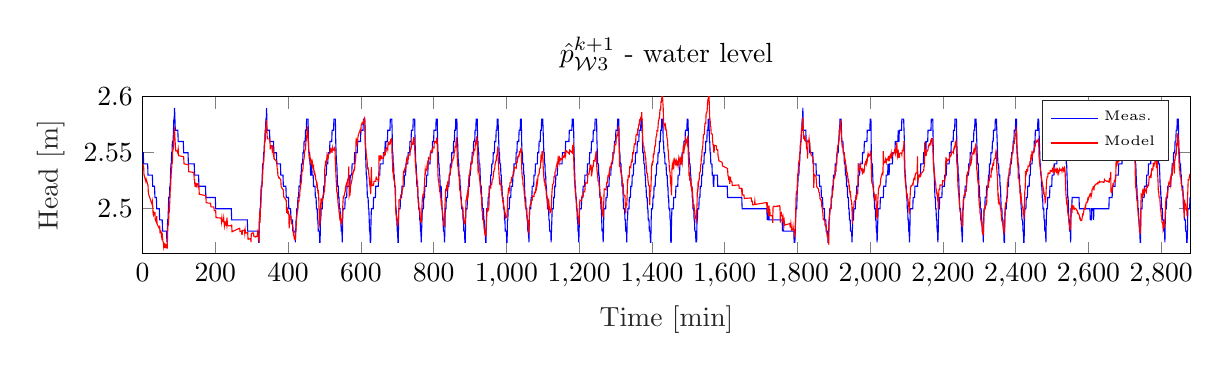
\begin{tikzpicture}

\begin{axis}[%
width=5.239in,
height=0.784in,
at={(1.182in,0.432in)},
scale only axis,
xmin=0,
xmax=2880,
xlabel style={font=\color{white!15!black}},
xlabel={Time [min]},
ymin=2.46,
ymax=2.6,
ylabel style={font=\color{white!15!black}},
ylabel={Head  [m]},
axis background/.style={fill=white},
title style={},
title={$\hat{p}^{k+1}_{\mathcal{W}3}$ - water level},
legend style={legend cell align=left, align=left, draw=white!15!black}
]
\addplot [color=blue]
  table[row sep=crcr]{%
1	2.55\\
2	2.55\\
3	2.54\\
4	2.54\\
5	2.54\\
6	2.54\\
7	2.54\\
8	2.54\\
9	2.54\\
10	2.54\\
11	2.54\\
12	2.54\\
13	2.54\\
14	2.54\\
15	2.53\\
16	2.53\\
17	2.53\\
18	2.53\\
19	2.53\\
20	2.53\\
21	2.53\\
22	2.53\\
23	2.53\\
24	2.53\\
25	2.53\\
26	2.53\\
27	2.53\\
28	2.52\\
29	2.52\\
30	2.52\\
31	2.52\\
32	2.52\\
33	2.52\\
34	2.51\\
35	2.51\\
36	2.51\\
37	2.51\\
38	2.51\\
39	2.5\\
40	2.5\\
41	2.5\\
42	2.5\\
43	2.5\\
44	2.5\\
45	2.5\\
46	2.5\\
47	2.49\\
48	2.49\\
49	2.49\\
50	2.49\\
51	2.49\\
52	2.49\\
53	2.49\\
54	2.49\\
55	2.48\\
56	2.48\\
57	2.48\\
58	2.48\\
59	2.48\\
60	2.48\\
61	2.48\\
62	2.48\\
63	2.48\\
64	2.48\\
65	2.48\\
66	2.48\\
67	2.47\\
68	2.48\\
69	2.49\\
70	2.49\\
71	2.5\\
72	2.51\\
73	2.51\\
74	2.51\\
75	2.52\\
76	2.52\\
77	2.53\\
78	2.54\\
79	2.54\\
80	2.55\\
81	2.55\\
82	2.56\\
83	2.56\\
84	2.56\\
85	2.57\\
86	2.58\\
87	2.58\\
88	2.59\\
89	2.58\\
90	2.57\\
91	2.57\\
92	2.57\\
93	2.57\\
94	2.57\\
95	2.57\\
96	2.57\\
97	2.57\\
98	2.56\\
99	2.56\\
100	2.56\\
101	2.56\\
102	2.56\\
103	2.56\\
104	2.56\\
105	2.56\\
106	2.56\\
107	2.56\\
108	2.56\\
109	2.56\\
110	2.56\\
111	2.56\\
112	2.56\\
113	2.55\\
114	2.55\\
115	2.55\\
116	2.55\\
117	2.55\\
118	2.55\\
119	2.55\\
120	2.55\\
121	2.55\\
122	2.55\\
123	2.55\\
124	2.55\\
125	2.55\\
126	2.54\\
127	2.54\\
128	2.54\\
129	2.54\\
130	2.54\\
131	2.54\\
132	2.54\\
133	2.54\\
134	2.54\\
135	2.54\\
136	2.54\\
137	2.54\\
138	2.54\\
139	2.54\\
140	2.54\\
141	2.54\\
142	2.54\\
143	2.53\\
144	2.53\\
145	2.53\\
146	2.53\\
147	2.53\\
148	2.53\\
149	2.53\\
150	2.53\\
151	2.53\\
152	2.53\\
153	2.53\\
154	2.53\\
155	2.52\\
156	2.52\\
157	2.52\\
158	2.52\\
159	2.52\\
160	2.52\\
161	2.52\\
162	2.52\\
163	2.52\\
164	2.52\\
165	2.52\\
166	2.52\\
167	2.52\\
168	2.52\\
169	2.52\\
170	2.52\\
171	2.52\\
172	2.52\\
173	2.52\\
174	2.51\\
175	2.51\\
176	2.51\\
177	2.51\\
178	2.51\\
179	2.51\\
180	2.51\\
181	2.51\\
182	2.51\\
183	2.51\\
184	2.51\\
185	2.51\\
186	2.51\\
187	2.51\\
188	2.51\\
189	2.51\\
190	2.51\\
191	2.51\\
192	2.51\\
193	2.51\\
194	2.51\\
195	2.51\\
196	2.51\\
197	2.51\\
198	2.51\\
199	2.51\\
200	2.51\\
201	2.5\\
202	2.5\\
203	2.5\\
204	2.5\\
205	2.5\\
206	2.5\\
207	2.5\\
208	2.5\\
209	2.5\\
210	2.5\\
211	2.5\\
212	2.5\\
213	2.5\\
214	2.5\\
215	2.5\\
216	2.5\\
217	2.5\\
218	2.5\\
219	2.5\\
220	2.5\\
221	2.5\\
222	2.5\\
223	2.5\\
224	2.5\\
225	2.5\\
226	2.5\\
227	2.5\\
228	2.5\\
229	2.5\\
230	2.5\\
231	2.5\\
232	2.5\\
233	2.5\\
234	2.5\\
235	2.5\\
236	2.5\\
237	2.5\\
238	2.5\\
239	2.5\\
240	2.5\\
241	2.5\\
242	2.5\\
243	2.5\\
244	2.5\\
245	2.49\\
246	2.49\\
247	2.49\\
248	2.49\\
249	2.49\\
250	2.49\\
251	2.49\\
252	2.49\\
253	2.49\\
254	2.49\\
255	2.49\\
256	2.49\\
257	2.49\\
258	2.49\\
259	2.49\\
260	2.49\\
261	2.49\\
262	2.49\\
263	2.49\\
264	2.49\\
265	2.49\\
266	2.49\\
267	2.49\\
268	2.49\\
269	2.49\\
270	2.49\\
271	2.49\\
272	2.49\\
273	2.49\\
274	2.49\\
275	2.49\\
276	2.49\\
277	2.49\\
278	2.49\\
279	2.49\\
280	2.49\\
281	2.49\\
282	2.49\\
283	2.49\\
284	2.49\\
285	2.49\\
286	2.49\\
287	2.49\\
288	2.49\\
289	2.48\\
290	2.48\\
291	2.48\\
292	2.48\\
293	2.48\\
294	2.48\\
295	2.48\\
296	2.48\\
297	2.48\\
298	2.48\\
299	2.48\\
300	2.48\\
301	2.48\\
302	2.48\\
303	2.48\\
304	2.48\\
305	2.48\\
306	2.48\\
307	2.48\\
308	2.48\\
309	2.48\\
310	2.48\\
311	2.48\\
312	2.48\\
313	2.48\\
314	2.48\\
315	2.48\\
316	2.48\\
317	2.48\\
318	2.48\\
319	2.47\\
320	2.47\\
321	2.49\\
322	2.49\\
323	2.5\\
324	2.5\\
325	2.51\\
326	2.52\\
327	2.52\\
328	2.52\\
329	2.53\\
330	2.54\\
331	2.54\\
332	2.54\\
333	2.55\\
334	2.55\\
335	2.56\\
336	2.56\\
337	2.57\\
338	2.57\\
339	2.58\\
340	2.58\\
341	2.59\\
342	2.57\\
343	2.57\\
344	2.57\\
345	2.57\\
346	2.57\\
347	2.57\\
348	2.57\\
349	2.57\\
350	2.56\\
351	2.56\\
352	2.56\\
353	2.56\\
354	2.56\\
355	2.56\\
356	2.56\\
357	2.56\\
358	2.56\\
359	2.56\\
360	2.56\\
361	2.55\\
362	2.55\\
363	2.55\\
364	2.55\\
365	2.55\\
366	2.55\\
367	2.55\\
368	2.55\\
369	2.54\\
370	2.54\\
371	2.54\\
372	2.54\\
373	2.54\\
374	2.54\\
375	2.54\\
376	2.54\\
377	2.54\\
378	2.54\\
379	2.54\\
380	2.53\\
381	2.53\\
382	2.53\\
383	2.53\\
384	2.53\\
385	2.53\\
386	2.53\\
387	2.52\\
388	2.52\\
389	2.52\\
390	2.52\\
391	2.52\\
392	2.52\\
393	2.52\\
394	2.52\\
395	2.51\\
396	2.51\\
397	2.51\\
398	2.51\\
399	2.51\\
400	2.51\\
401	2.51\\
402	2.5\\
403	2.5\\
404	2.5\\
405	2.5\\
406	2.5\\
407	2.5\\
408	2.49\\
409	2.49\\
410	2.49\\
411	2.49\\
412	2.49\\
413	2.48\\
414	2.48\\
415	2.48\\
416	2.48\\
417	2.48\\
418	2.48\\
419	2.48\\
420	2.47\\
421	2.48\\
422	2.49\\
423	2.49\\
424	2.5\\
425	2.5\\
426	2.5\\
427	2.51\\
428	2.51\\
429	2.51\\
430	2.52\\
431	2.52\\
432	2.52\\
433	2.52\\
434	2.53\\
435	2.53\\
436	2.53\\
437	2.54\\
438	2.54\\
439	2.54\\
440	2.54\\
441	2.55\\
442	2.55\\
443	2.55\\
444	2.56\\
445	2.56\\
446	2.56\\
447	2.56\\
448	2.57\\
449	2.57\\
450	2.57\\
451	2.58\\
452	2.58\\
453	2.58\\
454	2.58\\
455	2.58\\
456	2.56\\
457	2.55\\
458	2.55\\
459	2.55\\
460	2.54\\
461	2.54\\
462	2.53\\
463	2.53\\
464	2.53\\
465	2.54\\
466	2.53\\
467	2.53\\
468	2.53\\
469	2.53\\
470	2.52\\
471	2.52\\
472	2.52\\
473	2.52\\
474	2.52\\
475	2.51\\
476	2.51\\
477	2.51\\
478	2.5\\
479	2.5\\
480	2.5\\
481	2.49\\
482	2.49\\
483	2.48\\
484	2.48\\
485	2.48\\
486	2.48\\
487	2.47\\
488	2.47\\
489	2.49\\
490	2.49\\
491	2.5\\
492	2.5\\
493	2.5\\
494	2.5\\
495	2.51\\
496	2.51\\
497	2.51\\
498	2.52\\
499	2.52\\
500	2.52\\
501	2.52\\
502	2.53\\
503	2.53\\
504	2.53\\
505	2.53\\
506	2.54\\
507	2.54\\
508	2.54\\
509	2.54\\
510	2.55\\
511	2.55\\
512	2.55\\
513	2.55\\
514	2.55\\
515	2.56\\
516	2.56\\
517	2.56\\
518	2.56\\
519	2.56\\
520	2.56\\
521	2.57\\
522	2.57\\
523	2.57\\
524	2.57\\
525	2.57\\
526	2.58\\
527	2.58\\
528	2.58\\
529	2.58\\
530	2.58\\
531	2.56\\
532	2.55\\
533	2.54\\
534	2.54\\
535	2.53\\
536	2.52\\
537	2.52\\
538	2.52\\
539	2.51\\
540	2.51\\
541	2.5\\
542	2.5\\
543	2.5\\
544	2.49\\
545	2.49\\
546	2.48\\
547	2.48\\
548	2.48\\
549	2.47\\
550	2.49\\
551	2.5\\
552	2.5\\
553	2.5\\
554	2.5\\
555	2.5\\
556	2.5\\
557	2.51\\
558	2.51\\
559	2.51\\
560	2.51\\
561	2.51\\
562	2.52\\
563	2.52\\
564	2.52\\
565	2.52\\
566	2.52\\
567	2.52\\
568	2.52\\
569	2.53\\
570	2.52\\
571	2.53\\
572	2.53\\
573	2.53\\
574	2.53\\
575	2.53\\
576	2.54\\
577	2.54\\
578	2.54\\
579	2.54\\
580	2.54\\
581	2.54\\
582	2.54\\
583	2.55\\
584	2.55\\
585	2.55\\
586	2.55\\
587	2.55\\
588	2.55\\
589	2.55\\
590	2.55\\
591	2.56\\
592	2.56\\
593	2.56\\
594	2.56\\
595	2.56\\
596	2.56\\
597	2.56\\
598	2.56\\
599	2.56\\
600	2.57\\
601	2.57\\
602	2.57\\
603	2.57\\
604	2.57\\
605	2.57\\
606	2.57\\
607	2.58\\
608	2.58\\
609	2.58\\
610	2.58\\
611	2.58\\
612	2.56\\
613	2.55\\
614	2.54\\
615	2.53\\
616	2.53\\
617	2.52\\
618	2.51\\
619	2.51\\
620	2.51\\
621	2.5\\
622	2.5\\
623	2.49\\
624	2.48\\
625	2.48\\
626	2.47\\
627	2.47\\
628	2.49\\
629	2.5\\
630	2.5\\
631	2.5\\
632	2.5\\
633	2.5\\
634	2.5\\
635	2.51\\
636	2.51\\
637	2.51\\
638	2.51\\
639	2.51\\
640	2.51\\
641	2.52\\
642	2.52\\
643	2.52\\
644	2.52\\
645	2.52\\
646	2.52\\
647	2.52\\
648	2.52\\
649	2.53\\
650	2.53\\
651	2.53\\
652	2.53\\
653	2.54\\
654	2.54\\
655	2.54\\
656	2.54\\
657	2.54\\
658	2.54\\
659	2.54\\
660	2.54\\
661	2.54\\
662	2.55\\
663	2.55\\
664	2.55\\
665	2.55\\
666	2.55\\
667	2.56\\
668	2.55\\
669	2.56\\
670	2.56\\
671	2.56\\
672	2.56\\
673	2.56\\
674	2.57\\
675	2.57\\
676	2.57\\
677	2.57\\
678	2.57\\
679	2.57\\
680	2.57\\
681	2.58\\
682	2.58\\
683	2.58\\
684	2.58\\
685	2.58\\
686	2.57\\
687	2.55\\
688	2.55\\
689	2.54\\
690	2.54\\
691	2.53\\
692	2.53\\
693	2.52\\
694	2.52\\
695	2.51\\
696	2.5\\
697	2.5\\
698	2.49\\
699	2.49\\
700	2.48\\
701	2.48\\
702	2.47\\
703	2.47\\
704	2.5\\
705	2.5\\
706	2.5\\
707	2.5\\
708	2.5\\
709	2.51\\
710	2.51\\
711	2.51\\
712	2.51\\
713	2.52\\
714	2.52\\
715	2.52\\
716	2.52\\
717	2.52\\
718	2.52\\
719	2.52\\
720	2.53\\
721	2.53\\
722	2.53\\
723	2.53\\
724	2.54\\
725	2.54\\
726	2.54\\
727	2.54\\
728	2.54\\
729	2.54\\
730	2.55\\
731	2.55\\
732	2.55\\
733	2.55\\
734	2.55\\
735	2.56\\
736	2.56\\
737	2.56\\
738	2.56\\
739	2.57\\
740	2.57\\
741	2.57\\
742	2.57\\
743	2.57\\
744	2.58\\
745	2.58\\
746	2.58\\
747	2.58\\
748	2.58\\
749	2.56\\
750	2.55\\
751	2.54\\
752	2.54\\
753	2.53\\
754	2.52\\
755	2.52\\
756	2.52\\
757	2.51\\
758	2.51\\
759	2.5\\
760	2.5\\
761	2.5\\
762	2.49\\
763	2.49\\
764	2.48\\
765	2.48\\
766	2.47\\
767	2.48\\
768	2.49\\
769	2.5\\
770	2.5\\
771	2.5\\
772	2.5\\
773	2.51\\
774	2.51\\
775	2.51\\
776	2.52\\
777	2.52\\
778	2.52\\
779	2.52\\
780	2.52\\
781	2.53\\
782	2.53\\
783	2.53\\
784	2.53\\
785	2.54\\
786	2.54\\
787	2.54\\
788	2.54\\
789	2.54\\
790	2.54\\
791	2.55\\
792	2.55\\
793	2.55\\
794	2.55\\
795	2.55\\
796	2.55\\
797	2.56\\
798	2.56\\
799	2.56\\
800	2.56\\
801	2.57\\
802	2.57\\
803	2.57\\
804	2.57\\
805	2.57\\
806	2.57\\
807	2.58\\
808	2.58\\
809	2.58\\
810	2.58\\
811	2.56\\
812	2.55\\
813	2.55\\
814	2.54\\
815	2.54\\
816	2.53\\
817	2.53\\
818	2.52\\
819	2.52\\
820	2.51\\
821	2.52\\
822	2.51\\
823	2.5\\
824	2.5\\
825	2.49\\
826	2.49\\
827	2.48\\
828	2.48\\
829	2.48\\
830	2.47\\
831	2.48\\
832	2.5\\
833	2.5\\
834	2.5\\
835	2.51\\
836	2.51\\
837	2.51\\
838	2.51\\
839	2.52\\
840	2.52\\
841	2.52\\
842	2.52\\
843	2.53\\
844	2.53\\
845	2.53\\
846	2.54\\
847	2.54\\
848	2.54\\
849	2.54\\
850	2.55\\
851	2.55\\
852	2.55\\
853	2.55\\
854	2.55\\
855	2.56\\
856	2.56\\
857	2.56\\
858	2.57\\
859	2.57\\
860	2.57\\
861	2.58\\
862	2.58\\
863	2.58\\
864	2.58\\
865	2.56\\
866	2.56\\
867	2.55\\
868	2.54\\
869	2.54\\
870	2.53\\
871	2.53\\
872	2.53\\
873	2.52\\
874	2.52\\
875	2.51\\
876	2.51\\
877	2.5\\
878	2.5\\
879	2.5\\
880	2.5\\
881	2.49\\
882	2.49\\
883	2.48\\
884	2.48\\
885	2.48\\
886	2.47\\
887	2.47\\
888	2.49\\
889	2.5\\
890	2.5\\
891	2.5\\
892	2.5\\
893	2.51\\
894	2.51\\
895	2.52\\
896	2.52\\
897	2.52\\
898	2.52\\
899	2.53\\
900	2.53\\
901	2.53\\
902	2.54\\
903	2.54\\
904	2.54\\
905	2.54\\
906	2.55\\
907	2.55\\
908	2.55\\
909	2.55\\
910	2.56\\
911	2.56\\
912	2.56\\
913	2.56\\
914	2.57\\
915	2.57\\
916	2.57\\
917	2.58\\
918	2.58\\
919	2.58\\
920	2.58\\
921	2.56\\
922	2.56\\
923	2.55\\
924	2.55\\
925	2.54\\
926	2.54\\
927	2.54\\
928	2.53\\
929	2.52\\
930	2.52\\
931	2.52\\
932	2.51\\
933	2.51\\
934	2.5\\
935	2.5\\
936	2.5\\
937	2.5\\
938	2.49\\
939	2.49\\
940	2.48\\
941	2.48\\
942	2.48\\
943	2.47\\
944	2.47\\
945	2.49\\
946	2.5\\
947	2.5\\
948	2.5\\
949	2.5\\
950	2.51\\
951	2.51\\
952	2.51\\
953	2.52\\
954	2.52\\
955	2.52\\
956	2.52\\
957	2.53\\
958	2.53\\
959	2.53\\
960	2.54\\
961	2.54\\
962	2.54\\
963	2.54\\
964	2.55\\
965	2.55\\
966	2.55\\
967	2.55\\
968	2.56\\
969	2.56\\
970	2.56\\
971	2.56\\
972	2.57\\
973	2.57\\
974	2.57\\
975	2.58\\
976	2.58\\
977	2.58\\
978	2.57\\
979	2.56\\
980	2.55\\
981	2.55\\
982	2.54\\
983	2.54\\
984	2.54\\
985	2.53\\
986	2.53\\
987	2.52\\
988	2.52\\
989	2.51\\
990	2.51\\
991	2.51\\
992	2.5\\
993	2.5\\
994	2.5\\
995	2.49\\
996	2.49\\
997	2.48\\
998	2.48\\
999	2.48\\
1000	2.48\\
1001	2.47\\
1002	2.47\\
1003	2.49\\
1004	2.49\\
1005	2.5\\
1006	2.5\\
1007	2.5\\
1008	2.5\\
1009	2.51\\
1010	2.51\\
1011	2.51\\
1012	2.51\\
1013	2.52\\
1014	2.52\\
1015	2.52\\
1016	2.52\\
1017	2.52\\
1018	2.53\\
1019	2.53\\
1020	2.53\\
1021	2.54\\
1022	2.54\\
1023	2.54\\
1024	2.54\\
1025	2.54\\
1026	2.54\\
1027	2.55\\
1028	2.55\\
1029	2.55\\
1030	2.56\\
1031	2.56\\
1032	2.56\\
1033	2.56\\
1034	2.56\\
1035	2.57\\
1036	2.57\\
1037	2.57\\
1038	2.57\\
1039	2.58\\
1040	2.58\\
1041	2.58\\
1042	2.56\\
1043	2.55\\
1044	2.55\\
1045	2.54\\
1046	2.54\\
1047	2.54\\
1048	2.53\\
1049	2.53\\
1050	2.52\\
1051	2.51\\
1052	2.51\\
1053	2.51\\
1054	2.5\\
1055	2.5\\
1056	2.5\\
1057	2.49\\
1058	2.49\\
1059	2.48\\
1060	2.48\\
1061	2.48\\
1062	2.47\\
1063	2.49\\
1064	2.5\\
1065	2.5\\
1066	2.5\\
1067	2.5\\
1068	2.51\\
1069	2.51\\
1070	2.51\\
1071	2.52\\
1072	2.52\\
1073	2.52\\
1074	2.52\\
1075	2.52\\
1076	2.53\\
1077	2.53\\
1078	2.53\\
1079	2.53\\
1080	2.54\\
1081	2.54\\
1082	2.54\\
1083	2.54\\
1084	2.54\\
1085	2.54\\
1086	2.55\\
1087	2.55\\
1088	2.55\\
1089	2.55\\
1090	2.56\\
1091	2.56\\
1092	2.56\\
1093	2.56\\
1094	2.57\\
1095	2.57\\
1096	2.57\\
1097	2.58\\
1098	2.58\\
1099	2.58\\
1100	2.58\\
1101	2.57\\
1102	2.56\\
1103	2.55\\
1104	2.55\\
1105	2.54\\
1106	2.54\\
1107	2.53\\
1108	2.53\\
1109	2.52\\
1110	2.52\\
1111	2.51\\
1112	2.51\\
1113	2.5\\
1114	2.5\\
1115	2.5\\
1116	2.5\\
1117	2.49\\
1118	2.49\\
1119	2.48\\
1120	2.48\\
1121	2.48\\
1122	2.48\\
1123	2.47\\
1124	2.48\\
1125	2.49\\
1126	2.5\\
1127	2.5\\
1128	2.5\\
1129	2.5\\
1130	2.51\\
1131	2.51\\
1132	2.51\\
1133	2.52\\
1134	2.52\\
1135	2.52\\
1136	2.53\\
1137	2.53\\
1138	2.53\\
1139	2.53\\
1140	2.53\\
1141	2.54\\
1142	2.54\\
1143	2.54\\
1144	2.54\\
1145	2.54\\
1146	2.54\\
1147	2.54\\
1148	2.54\\
1149	2.54\\
1150	2.54\\
1151	2.54\\
1152	2.54\\
1153	2.54\\
1154	2.55\\
1155	2.55\\
1156	2.55\\
1157	2.55\\
1158	2.55\\
1159	2.55\\
1160	2.55\\
1161	2.55\\
1162	2.55\\
1163	2.56\\
1164	2.56\\
1165	2.56\\
1166	2.56\\
1167	2.56\\
1168	2.56\\
1169	2.56\\
1170	2.56\\
1171	2.56\\
1172	2.56\\
1173	2.57\\
1174	2.57\\
1175	2.57\\
1176	2.57\\
1177	2.57\\
1178	2.57\\
1179	2.57\\
1180	2.57\\
1181	2.58\\
1182	2.58\\
1183	2.58\\
1184	2.58\\
1185	2.57\\
1186	2.55\\
1187	2.54\\
1188	2.53\\
1189	2.52\\
1190	2.52\\
1191	2.51\\
1192	2.51\\
1193	2.5\\
1194	2.5\\
1195	2.49\\
1196	2.49\\
1197	2.48\\
1198	2.48\\
1199	2.47\\
1200	2.48\\
1201	2.5\\
1202	2.5\\
1203	2.5\\
1204	2.5\\
1205	2.5\\
1206	2.5\\
1207	2.51\\
1208	2.51\\
1209	2.51\\
1210	2.51\\
1211	2.52\\
1212	2.52\\
1213	2.52\\
1214	2.52\\
1215	2.52\\
1216	2.53\\
1217	2.53\\
1218	2.53\\
1219	2.53\\
1220	2.53\\
1221	2.53\\
1222	2.53\\
1223	2.54\\
1224	2.54\\
1225	2.54\\
1226	2.54\\
1227	2.54\\
1228	2.54\\
1229	2.55\\
1230	2.55\\
1231	2.55\\
1232	2.55\\
1233	2.55\\
1234	2.56\\
1235	2.56\\
1236	2.56\\
1237	2.56\\
1238	2.56\\
1239	2.57\\
1240	2.57\\
1241	2.57\\
1242	2.57\\
1243	2.57\\
1244	2.58\\
1245	2.58\\
1246	2.58\\
1247	2.58\\
1248	2.58\\
1249	2.56\\
1250	2.55\\
1251	2.54\\
1252	2.54\\
1253	2.54\\
1254	2.53\\
1255	2.53\\
1256	2.52\\
1257	2.51\\
1258	2.51\\
1259	2.51\\
1260	2.5\\
1261	2.5\\
1262	2.49\\
1263	2.48\\
1264	2.48\\
1265	2.48\\
1266	2.47\\
1267	2.48\\
1268	2.5\\
1269	2.5\\
1270	2.5\\
1271	2.5\\
1272	2.5\\
1273	2.5\\
1274	2.51\\
1275	2.51\\
1276	2.51\\
1277	2.51\\
1278	2.52\\
1279	2.52\\
1280	2.52\\
1281	2.52\\
1282	2.52\\
1283	2.53\\
1284	2.53\\
1285	2.53\\
1286	2.53\\
1287	2.53\\
1288	2.54\\
1289	2.54\\
1290	2.54\\
1291	2.54\\
1292	2.54\\
1293	2.55\\
1294	2.55\\
1295	2.55\\
1296	2.55\\
1297	2.56\\
1298	2.56\\
1299	2.56\\
1300	2.56\\
1301	2.57\\
1302	2.57\\
1303	2.57\\
1304	2.57\\
1305	2.57\\
1306	2.58\\
1307	2.58\\
1308	2.58\\
1309	2.58\\
1310	2.56\\
1311	2.55\\
1312	2.55\\
1313	2.54\\
1314	2.54\\
1315	2.54\\
1316	2.53\\
1317	2.53\\
1318	2.52\\
1319	2.52\\
1320	2.52\\
1321	2.51\\
1322	2.5\\
1323	2.5\\
1324	2.5\\
1325	2.5\\
1326	2.49\\
1327	2.49\\
1328	2.48\\
1329	2.48\\
1330	2.48\\
1331	2.47\\
1332	2.49\\
1333	2.49\\
1334	2.5\\
1335	2.5\\
1336	2.5\\
1337	2.5\\
1338	2.51\\
1339	2.51\\
1340	2.51\\
1341	2.51\\
1342	2.52\\
1343	2.52\\
1344	2.52\\
1345	2.52\\
1346	2.53\\
1347	2.53\\
1348	2.53\\
1349	2.53\\
1350	2.54\\
1351	2.54\\
1352	2.54\\
1353	2.54\\
1354	2.54\\
1355	2.55\\
1356	2.55\\
1357	2.55\\
1358	2.55\\
1359	2.55\\
1360	2.56\\
1361	2.56\\
1362	2.56\\
1363	2.56\\
1364	2.56\\
1365	2.57\\
1366	2.57\\
1367	2.57\\
1368	2.57\\
1369	2.57\\
1370	2.58\\
1371	2.58\\
1372	2.58\\
1373	2.58\\
1374	2.56\\
1375	2.55\\
1376	2.55\\
1377	2.55\\
1378	2.54\\
1379	2.54\\
1380	2.54\\
1381	2.53\\
1382	2.53\\
1383	2.52\\
1384	2.52\\
1385	2.51\\
1386	2.51\\
1387	2.51\\
1388	2.5\\
1389	2.5\\
1390	2.49\\
1391	2.49\\
1392	2.49\\
1393	2.48\\
1394	2.48\\
1395	2.48\\
1396	2.47\\
1397	2.47\\
1398	2.49\\
1399	2.5\\
1400	2.5\\
1401	2.5\\
1402	2.5\\
1403	2.51\\
1404	2.51\\
1405	2.51\\
1406	2.52\\
1407	2.52\\
1408	2.52\\
1409	2.52\\
1410	2.53\\
1411	2.53\\
1412	2.53\\
1413	2.54\\
1414	2.54\\
1415	2.54\\
1416	2.54\\
1417	2.55\\
1418	2.55\\
1419	2.55\\
1420	2.55\\
1421	2.56\\
1422	2.56\\
1423	2.56\\
1424	2.57\\
1425	2.57\\
1426	2.57\\
1427	2.58\\
1428	2.58\\
1429	2.58\\
1430	2.58\\
1431	2.56\\
1432	2.56\\
1433	2.55\\
1434	2.55\\
1435	2.55\\
1436	2.54\\
1437	2.54\\
1438	2.54\\
1439	2.54\\
1440	2.53\\
1441	2.53\\
1442	2.53\\
1443	2.52\\
1444	2.52\\
1445	2.51\\
1446	2.51\\
1447	2.5\\
1448	2.5\\
1449	2.5\\
1450	2.49\\
1451	2.49\\
1452	2.47\\
1453	2.47\\
1454	2.49\\
1455	2.5\\
1456	2.5\\
1457	2.5\\
1458	2.5\\
1459	2.5\\
1460	2.51\\
1461	2.51\\
1462	2.51\\
1463	2.51\\
1464	2.51\\
1465	2.51\\
1466	2.52\\
1467	2.52\\
1468	2.52\\
1469	2.52\\
1470	2.52\\
1471	2.52\\
1472	2.53\\
1473	2.53\\
1474	2.53\\
1475	2.53\\
1476	2.53\\
1477	2.54\\
1478	2.54\\
1479	2.54\\
1480	2.54\\
1481	2.54\\
1482	2.54\\
1483	2.55\\
1484	2.55\\
1485	2.55\\
1486	2.55\\
1487	2.55\\
1488	2.56\\
1489	2.56\\
1490	2.56\\
1491	2.56\\
1492	2.57\\
1493	2.57\\
1494	2.57\\
1495	2.57\\
1496	2.57\\
1497	2.58\\
1498	2.58\\
1499	2.58\\
1500	2.57\\
1501	2.55\\
1502	2.55\\
1503	2.54\\
1504	2.54\\
1505	2.54\\
1506	2.53\\
1507	2.53\\
1508	2.52\\
1509	2.52\\
1510	2.52\\
1511	2.51\\
1512	2.51\\
1513	2.5\\
1514	2.5\\
1515	2.5\\
1516	2.49\\
1517	2.49\\
1518	2.48\\
1519	2.48\\
1520	2.48\\
1521	2.47\\
1522	2.48\\
1523	2.47\\
1524	2.49\\
1525	2.49\\
1526	2.5\\
1527	2.5\\
1528	2.5\\
1529	2.5\\
1530	2.51\\
1531	2.51\\
1532	2.51\\
1533	2.52\\
1534	2.52\\
1535	2.52\\
1536	2.52\\
1537	2.53\\
1538	2.53\\
1539	2.53\\
1540	2.54\\
1541	2.54\\
1542	2.54\\
1543	2.54\\
1544	2.55\\
1545	2.55\\
1546	2.55\\
1547	2.55\\
1548	2.56\\
1549	2.56\\
1550	2.56\\
1551	2.56\\
1552	2.57\\
1553	2.57\\
1554	2.57\\
1555	2.58\\
1556	2.58\\
1557	2.58\\
1558	2.56\\
1559	2.56\\
1560	2.55\\
1561	2.55\\
1562	2.54\\
1563	2.54\\
1564	2.54\\
1565	2.54\\
1566	2.53\\
1567	2.53\\
1568	2.53\\
1569	2.52\\
1570	2.52\\
1571	2.53\\
1572	2.53\\
1573	2.53\\
1574	2.53\\
1575	2.53\\
1576	2.53\\
1577	2.53\\
1578	2.53\\
1579	2.53\\
1580	2.53\\
1581	2.52\\
1582	2.52\\
1583	2.52\\
1584	2.52\\
1585	2.52\\
1586	2.52\\
1587	2.52\\
1588	2.52\\
1589	2.52\\
1590	2.52\\
1591	2.52\\
1592	2.52\\
1593	2.52\\
1594	2.52\\
1595	2.52\\
1596	2.52\\
1597	2.52\\
1598	2.52\\
1599	2.52\\
1600	2.52\\
1601	2.52\\
1602	2.52\\
1603	2.52\\
1604	2.52\\
1605	2.52\\
1606	2.52\\
1607	2.52\\
1608	2.51\\
1609	2.51\\
1610	2.51\\
1611	2.51\\
1612	2.51\\
1613	2.51\\
1614	2.51\\
1615	2.51\\
1616	2.51\\
1617	2.51\\
1618	2.51\\
1619	2.51\\
1620	2.51\\
1621	2.51\\
1622	2.51\\
1623	2.51\\
1624	2.51\\
1625	2.51\\
1626	2.51\\
1627	2.51\\
1628	2.51\\
1629	2.51\\
1630	2.51\\
1631	2.51\\
1632	2.51\\
1633	2.51\\
1634	2.51\\
1635	2.51\\
1636	2.51\\
1637	2.51\\
1638	2.51\\
1639	2.51\\
1640	2.51\\
1641	2.51\\
1642	2.51\\
1643	2.51\\
1644	2.51\\
1645	2.51\\
1646	2.51\\
1647	2.51\\
1648	2.5\\
1649	2.5\\
1650	2.5\\
1651	2.5\\
1652	2.5\\
1653	2.5\\
1654	2.5\\
1655	2.5\\
1656	2.5\\
1657	2.5\\
1658	2.5\\
1659	2.5\\
1660	2.5\\
1661	2.5\\
1662	2.5\\
1663	2.5\\
1664	2.5\\
1665	2.5\\
1666	2.5\\
1667	2.5\\
1668	2.5\\
1669	2.5\\
1670	2.5\\
1671	2.5\\
1672	2.5\\
1673	2.5\\
1674	2.5\\
1675	2.5\\
1676	2.5\\
1677	2.5\\
1678	2.5\\
1679	2.5\\
1680	2.5\\
1681	2.5\\
1682	2.5\\
1683	2.5\\
1684	2.5\\
1685	2.5\\
1686	2.5\\
1687	2.5\\
1688	2.5\\
1689	2.5\\
1690	2.5\\
1691	2.5\\
1692	2.5\\
1693	2.5\\
1694	2.5\\
1695	2.5\\
1696	2.5\\
1697	2.5\\
1698	2.5\\
1699	2.5\\
1700	2.5\\
1701	2.5\\
1702	2.5\\
1703	2.5\\
1704	2.5\\
1705	2.5\\
1706	2.5\\
1707	2.5\\
1708	2.5\\
1709	2.5\\
1710	2.5\\
1711	2.5\\
1712	2.5\\
1713	2.5\\
1714	2.5\\
1715	2.5\\
1716	2.5\\
1717	2.49\\
1718	2.5\\
1719	2.49\\
1720	2.49\\
1721	2.5\\
1722	2.49\\
1723	2.49\\
1724	2.49\\
1725	2.49\\
1726	2.49\\
1727	2.49\\
1728	2.49\\
1729	2.49\\
1730	2.49\\
1731	2.49\\
1732	2.49\\
1733	2.49\\
1734	2.49\\
1735	2.49\\
1736	2.49\\
1737	2.49\\
1738	2.49\\
1739	2.49\\
1740	2.49\\
1741	2.49\\
1742	2.49\\
1743	2.49\\
1744	2.49\\
1745	2.49\\
1746	2.49\\
1747	2.49\\
1748	2.49\\
1749	2.49\\
1750	2.49\\
1751	2.49\\
1752	2.49\\
1753	2.49\\
1754	2.49\\
1755	2.49\\
1756	2.49\\
1757	2.49\\
1758	2.49\\
1759	2.48\\
1760	2.49\\
1761	2.48\\
1762	2.48\\
1763	2.48\\
1764	2.48\\
1765	2.48\\
1766	2.48\\
1767	2.48\\
1768	2.48\\
1769	2.48\\
1770	2.48\\
1771	2.48\\
1772	2.48\\
1773	2.48\\
1774	2.48\\
1775	2.48\\
1776	2.48\\
1777	2.48\\
1778	2.48\\
1779	2.48\\
1780	2.48\\
1781	2.48\\
1782	2.48\\
1783	2.48\\
1784	2.48\\
1785	2.48\\
1786	2.48\\
1787	2.48\\
1788	2.48\\
1789	2.48\\
1790	2.48\\
1791	2.47\\
1792	2.47\\
1793	2.47\\
1794	2.48\\
1795	2.49\\
1796	2.5\\
1797	2.5\\
1798	2.5\\
1799	2.51\\
1800	2.52\\
1801	2.52\\
1802	2.53\\
1803	2.53\\
1804	2.53\\
1805	2.54\\
1806	2.54\\
1807	2.55\\
1808	2.55\\
1809	2.56\\
1810	2.56\\
1811	2.57\\
1812	2.57\\
1813	2.58\\
1814	2.58\\
1815	2.59\\
1816	2.57\\
1817	2.57\\
1818	2.57\\
1819	2.57\\
1820	2.57\\
1821	2.57\\
1822	2.57\\
1823	2.57\\
1824	2.56\\
1825	2.56\\
1826	2.56\\
1827	2.56\\
1828	2.56\\
1829	2.56\\
1830	2.56\\
1831	2.56\\
1832	2.56\\
1833	2.56\\
1834	2.55\\
1835	2.55\\
1836	2.55\\
1837	2.55\\
1838	2.55\\
1839	2.55\\
1840	2.55\\
1841	2.55\\
1842	2.55\\
1843	2.54\\
1844	2.54\\
1845	2.54\\
1846	2.54\\
1847	2.54\\
1848	2.54\\
1849	2.54\\
1850	2.54\\
1851	2.54\\
1852	2.53\\
1853	2.53\\
1854	2.53\\
1855	2.53\\
1856	2.53\\
1857	2.53\\
1858	2.53\\
1859	2.53\\
1860	2.53\\
1861	2.52\\
1862	2.52\\
1863	2.52\\
1864	2.52\\
1865	2.52\\
1866	2.51\\
1867	2.51\\
1868	2.51\\
1869	2.51\\
1870	2.5\\
1871	2.5\\
1872	2.5\\
1873	2.5\\
1874	2.5\\
1875	2.49\\
1876	2.49\\
1877	2.49\\
1878	2.49\\
1879	2.48\\
1880	2.48\\
1881	2.48\\
1882	2.48\\
1883	2.48\\
1884	2.47\\
1885	2.47\\
1886	2.48\\
1887	2.49\\
1888	2.49\\
1889	2.5\\
1890	2.5\\
1891	2.5\\
1892	2.5\\
1893	2.51\\
1894	2.51\\
1895	2.51\\
1896	2.52\\
1897	2.52\\
1898	2.52\\
1899	2.53\\
1900	2.53\\
1901	2.53\\
1902	2.53\\
1903	2.53\\
1904	2.54\\
1905	2.54\\
1906	2.54\\
1907	2.54\\
1908	2.54\\
1909	2.55\\
1910	2.55\\
1911	2.55\\
1912	2.55\\
1913	2.56\\
1914	2.56\\
1915	2.57\\
1916	2.57\\
1917	2.58\\
1918	2.58\\
1919	2.58\\
1920	2.58\\
1921	2.57\\
1922	2.56\\
1923	2.56\\
1924	2.56\\
1925	2.56\\
1926	2.55\\
1927	2.55\\
1928	2.55\\
1929	2.54\\
1930	2.54\\
1931	2.54\\
1932	2.53\\
1933	2.53\\
1934	2.53\\
1935	2.52\\
1936	2.52\\
1937	2.52\\
1938	2.51\\
1939	2.51\\
1940	2.51\\
1941	2.5\\
1942	2.5\\
1943	2.49\\
1944	2.49\\
1945	2.49\\
1946	2.48\\
1947	2.48\\
1948	2.48\\
1949	2.48\\
1950	2.47\\
1951	2.48\\
1952	2.49\\
1953	2.49\\
1954	2.49\\
1955	2.5\\
1956	2.5\\
1957	2.5\\
1958	2.5\\
1959	2.5\\
1960	2.51\\
1961	2.51\\
1962	2.51\\
1963	2.52\\
1964	2.52\\
1965	2.52\\
1966	2.52\\
1967	2.52\\
1968	2.53\\
1969	2.53\\
1970	2.53\\
1971	2.53\\
1972	2.54\\
1973	2.54\\
1974	2.54\\
1975	2.54\\
1976	2.54\\
1977	2.54\\
1978	2.54\\
1979	2.55\\
1980	2.55\\
1981	2.55\\
1982	2.55\\
1983	2.55\\
1984	2.56\\
1985	2.56\\
1986	2.56\\
1987	2.56\\
1988	2.56\\
1989	2.56\\
1990	2.56\\
1991	2.56\\
1992	2.57\\
1993	2.57\\
1994	2.57\\
1995	2.57\\
1996	2.57\\
1997	2.57\\
1998	2.57\\
1999	2.57\\
2000	2.58\\
2001	2.58\\
2002	2.58\\
2003	2.55\\
2004	2.54\\
2005	2.54\\
2006	2.54\\
2007	2.53\\
2008	2.52\\
2009	2.52\\
2010	2.51\\
2011	2.51\\
2012	2.5\\
2013	2.5\\
2014	2.5\\
2015	2.49\\
2016	2.49\\
2017	2.48\\
2018	2.48\\
2019	2.47\\
2020	2.48\\
2021	2.49\\
2022	2.5\\
2023	2.5\\
2024	2.5\\
2025	2.5\\
2026	2.5\\
2027	2.5\\
2028	2.51\\
2029	2.51\\
2030	2.51\\
2031	2.51\\
2032	2.51\\
2033	2.51\\
2034	2.51\\
2035	2.51\\
2036	2.51\\
2037	2.52\\
2038	2.52\\
2039	2.52\\
2040	2.52\\
2041	2.52\\
2042	2.52\\
2043	2.52\\
2044	2.53\\
2045	2.53\\
2046	2.53\\
2047	2.53\\
2048	2.53\\
2049	2.54\\
2050	2.53\\
2051	2.54\\
2052	2.53\\
2053	2.54\\
2054	2.54\\
2055	2.54\\
2056	2.54\\
2057	2.54\\
2058	2.54\\
2059	2.54\\
2060	2.54\\
2061	2.54\\
2062	2.55\\
2063	2.55\\
2064	2.55\\
2065	2.55\\
2066	2.55\\
2067	2.55\\
2068	2.55\\
2069	2.56\\
2070	2.56\\
2071	2.56\\
2072	2.56\\
2073	2.56\\
2074	2.56\\
2075	2.56\\
2076	2.56\\
2077	2.57\\
2078	2.56\\
2079	2.56\\
2080	2.57\\
2081	2.57\\
2082	2.57\\
2083	2.57\\
2084	2.57\\
2085	2.57\\
2086	2.57\\
2087	2.58\\
2088	2.58\\
2089	2.58\\
2090	2.58\\
2091	2.58\\
2092	2.58\\
2093	2.57\\
2094	2.56\\
2095	2.54\\
2096	2.53\\
2097	2.53\\
2098	2.52\\
2099	2.52\\
2100	2.51\\
2101	2.51\\
2102	2.5\\
2103	2.5\\
2104	2.49\\
2105	2.49\\
2106	2.48\\
2107	2.48\\
2108	2.47\\
2109	2.48\\
2110	2.5\\
2111	2.5\\
2112	2.5\\
2113	2.5\\
2114	2.5\\
2115	2.5\\
2116	2.5\\
2117	2.5\\
2118	2.51\\
2119	2.51\\
2120	2.51\\
2121	2.51\\
2122	2.51\\
2123	2.52\\
2124	2.52\\
2125	2.52\\
2126	2.52\\
2127	2.52\\
2128	2.52\\
2129	2.52\\
2130	2.52\\
2131	2.53\\
2132	2.53\\
2133	2.53\\
2134	2.53\\
2135	2.53\\
2136	2.53\\
2137	2.53\\
2138	2.53\\
2139	2.54\\
2140	2.54\\
2141	2.54\\
2142	2.54\\
2143	2.54\\
2144	2.54\\
2145	2.54\\
2146	2.54\\
2147	2.55\\
2148	2.55\\
2149	2.55\\
2150	2.55\\
2151	2.55\\
2152	2.56\\
2153	2.55\\
2154	2.56\\
2155	2.56\\
2156	2.56\\
2157	2.56\\
2158	2.56\\
2159	2.57\\
2160	2.57\\
2161	2.57\\
2162	2.57\\
2163	2.57\\
2164	2.57\\
2165	2.57\\
2166	2.57\\
2167	2.57\\
2168	2.58\\
2169	2.58\\
2170	2.58\\
2171	2.58\\
2172	2.58\\
2173	2.56\\
2174	2.54\\
2175	2.54\\
2176	2.53\\
2177	2.52\\
2178	2.51\\
2179	2.51\\
2180	2.5\\
2181	2.5\\
2182	2.49\\
2183	2.49\\
2184	2.48\\
2185	2.48\\
2186	2.47\\
2187	2.48\\
2188	2.5\\
2189	2.5\\
2190	2.5\\
2191	2.51\\
2192	2.51\\
2193	2.51\\
2194	2.51\\
2195	2.51\\
2196	2.51\\
2197	2.51\\
2198	2.52\\
2199	2.52\\
2200	2.52\\
2201	2.52\\
2202	2.52\\
2203	2.52\\
2204	2.52\\
2205	2.53\\
2206	2.53\\
2207	2.53\\
2208	2.53\\
2209	2.53\\
2210	2.54\\
2211	2.54\\
2212	2.54\\
2213	2.54\\
2214	2.54\\
2215	2.54\\
2216	2.54\\
2217	2.54\\
2218	2.55\\
2219	2.55\\
2220	2.55\\
2221	2.55\\
2222	2.55\\
2223	2.56\\
2224	2.56\\
2225	2.56\\
2226	2.56\\
2227	2.56\\
2228	2.56\\
2229	2.57\\
2230	2.57\\
2231	2.57\\
2232	2.57\\
2233	2.58\\
2234	2.58\\
2235	2.58\\
2236	2.58\\
2237	2.58\\
2238	2.56\\
2239	2.55\\
2240	2.54\\
2241	2.54\\
2242	2.53\\
2243	2.53\\
2244	2.52\\
2245	2.51\\
2246	2.5\\
2247	2.5\\
2248	2.5\\
2249	2.49\\
2250	2.49\\
2251	2.48\\
2252	2.48\\
2253	2.47\\
2254	2.48\\
2255	2.5\\
2256	2.5\\
2257	2.51\\
2258	2.51\\
2259	2.51\\
2260	2.51\\
2261	2.52\\
2262	2.52\\
2263	2.52\\
2264	2.52\\
2265	2.52\\
2266	2.53\\
2267	2.53\\
2268	2.53\\
2269	2.53\\
2270	2.53\\
2271	2.54\\
2272	2.54\\
2273	2.54\\
2274	2.54\\
2275	2.55\\
2276	2.55\\
2277	2.55\\
2278	2.55\\
2279	2.56\\
2280	2.56\\
2281	2.56\\
2282	2.56\\
2283	2.56\\
2284	2.56\\
2285	2.57\\
2286	2.57\\
2287	2.57\\
2288	2.58\\
2289	2.58\\
2290	2.58\\
2291	2.58\\
2292	2.57\\
2293	2.56\\
2294	2.55\\
2295	2.54\\
2296	2.54\\
2297	2.54\\
2298	2.53\\
2299	2.52\\
2300	2.52\\
2301	2.51\\
2302	2.51\\
2303	2.5\\
2304	2.5\\
2305	2.5\\
2306	2.49\\
2307	2.49\\
2308	2.48\\
2309	2.48\\
2310	2.48\\
2311	2.47\\
2312	2.49\\
2313	2.5\\
2314	2.5\\
2315	2.5\\
2316	2.51\\
2317	2.51\\
2318	2.51\\
2319	2.51\\
2320	2.52\\
2321	2.52\\
2322	2.52\\
2323	2.52\\
2324	2.52\\
2325	2.53\\
2326	2.53\\
2327	2.53\\
2328	2.54\\
2329	2.54\\
2330	2.54\\
2331	2.54\\
2332	2.55\\
2333	2.55\\
2334	2.55\\
2335	2.55\\
2336	2.56\\
2337	2.56\\
2338	2.56\\
2339	2.57\\
2340	2.57\\
2341	2.57\\
2342	2.57\\
2343	2.57\\
2344	2.58\\
2345	2.58\\
2346	2.58\\
2347	2.58\\
2348	2.57\\
2349	2.56\\
2350	2.55\\
2351	2.54\\
2352	2.54\\
2353	2.54\\
2354	2.53\\
2355	2.53\\
2356	2.53\\
2357	2.52\\
2358	2.52\\
2359	2.51\\
2360	2.5\\
2361	2.5\\
2362	2.5\\
2363	2.49\\
2364	2.49\\
2365	2.49\\
2366	2.48\\
2367	2.48\\
2368	2.47\\
2369	2.47\\
2370	2.49\\
2371	2.5\\
2372	2.5\\
2373	2.5\\
2374	2.5\\
2375	2.51\\
2376	2.51\\
2377	2.51\\
2378	2.52\\
2379	2.52\\
2380	2.52\\
2381	2.53\\
2382	2.53\\
2383	2.53\\
2384	2.53\\
2385	2.54\\
2386	2.54\\
2387	2.54\\
2388	2.54\\
2389	2.55\\
2390	2.55\\
2391	2.55\\
2392	2.55\\
2393	2.56\\
2394	2.56\\
2395	2.56\\
2396	2.57\\
2397	2.57\\
2398	2.57\\
2399	2.57\\
2400	2.58\\
2401	2.58\\
2402	2.58\\
2403	2.56\\
2404	2.55\\
2405	2.55\\
2406	2.54\\
2407	2.54\\
2408	2.54\\
2409	2.53\\
2410	2.53\\
2411	2.52\\
2412	2.52\\
2413	2.51\\
2414	2.51\\
2415	2.5\\
2416	2.5\\
2417	2.49\\
2418	2.49\\
2419	2.49\\
2420	2.48\\
2421	2.48\\
2422	2.47\\
2423	2.47\\
2424	2.49\\
2425	2.5\\
2426	2.5\\
2427	2.5\\
2428	2.5\\
2429	2.51\\
2430	2.51\\
2431	2.51\\
2432	2.51\\
2433	2.52\\
2434	2.52\\
2435	2.52\\
2436	2.52\\
2437	2.52\\
2438	2.53\\
2439	2.53\\
2440	2.53\\
2441	2.54\\
2442	2.54\\
2443	2.54\\
2444	2.54\\
2445	2.54\\
2446	2.55\\
2447	2.55\\
2448	2.55\\
2449	2.55\\
2450	2.55\\
2451	2.56\\
2452	2.56\\
2453	2.56\\
2454	2.57\\
2455	2.57\\
2456	2.57\\
2457	2.57\\
2458	2.57\\
2459	2.57\\
2460	2.57\\
2461	2.58\\
2462	2.58\\
2463	2.58\\
2464	2.57\\
2465	2.56\\
2466	2.55\\
2467	2.54\\
2468	2.54\\
2469	2.53\\
2470	2.53\\
2471	2.52\\
2472	2.52\\
2473	2.51\\
2474	2.51\\
2475	2.5\\
2476	2.5\\
2477	2.5\\
2478	2.49\\
2479	2.49\\
2480	2.48\\
2481	2.48\\
2482	2.48\\
2483	2.47\\
2484	2.49\\
2485	2.5\\
2486	2.5\\
2487	2.5\\
2488	2.51\\
2489	2.51\\
2490	2.51\\
2491	2.51\\
2492	2.51\\
2493	2.51\\
2494	2.52\\
2495	2.52\\
2496	2.52\\
2497	2.52\\
2498	2.52\\
2499	2.52\\
2500	2.53\\
2501	2.53\\
2502	2.53\\
2503	2.53\\
2504	2.53\\
2505	2.53\\
2506	2.54\\
2507	2.54\\
2508	2.54\\
2509	2.54\\
2510	2.54\\
2511	2.54\\
2512	2.54\\
2513	2.54\\
2514	2.55\\
2515	2.55\\
2516	2.55\\
2517	2.55\\
2518	2.55\\
2519	2.55\\
2520	2.56\\
2521	2.56\\
2522	2.56\\
2523	2.56\\
2524	2.56\\
2525	2.56\\
2526	2.56\\
2527	2.57\\
2528	2.57\\
2529	2.57\\
2530	2.57\\
2531	2.57\\
2532	2.58\\
2533	2.58\\
2534	2.58\\
2535	2.58\\
2536	2.58\\
2537	2.56\\
2538	2.55\\
2539	2.54\\
2540	2.54\\
2541	2.53\\
2542	2.52\\
2543	2.51\\
2544	2.51\\
2545	2.5\\
2546	2.49\\
2547	2.49\\
2548	2.48\\
2549	2.48\\
2550	2.48\\
2551	2.47\\
2552	2.5\\
2553	2.5\\
2554	2.5\\
2555	2.51\\
2556	2.51\\
2557	2.51\\
2558	2.51\\
2559	2.51\\
2560	2.51\\
2561	2.51\\
2562	2.51\\
2563	2.51\\
2564	2.51\\
2565	2.51\\
2566	2.51\\
2567	2.51\\
2568	2.51\\
2569	2.51\\
2570	2.51\\
2571	2.51\\
2572	2.51\\
2573	2.51\\
2574	2.51\\
2575	2.5\\
2576	2.5\\
2577	2.5\\
2578	2.5\\
2579	2.5\\
2580	2.5\\
2581	2.5\\
2582	2.5\\
2583	2.5\\
2584	2.5\\
2585	2.5\\
2586	2.5\\
2587	2.5\\
2588	2.5\\
2589	2.5\\
2590	2.5\\
2591	2.5\\
2592	2.5\\
2593	2.5\\
2594	2.5\\
2595	2.5\\
2596	2.5\\
2597	2.5\\
2598	2.5\\
2599	2.5\\
2600	2.5\\
2601	2.5\\
2602	2.5\\
2603	2.5\\
2604	2.5\\
2605	2.49\\
2606	2.49\\
2607	2.49\\
2608	2.49\\
2609	2.5\\
2610	2.5\\
2611	2.5\\
2612	2.5\\
2613	2.5\\
2614	2.49\\
2615	2.5\\
2616	2.5\\
2617	2.5\\
2618	2.5\\
2619	2.5\\
2620	2.5\\
2621	2.5\\
2622	2.5\\
2623	2.5\\
2624	2.5\\
2625	2.5\\
2626	2.5\\
2627	2.5\\
2628	2.5\\
2629	2.5\\
2630	2.5\\
2631	2.5\\
2632	2.5\\
2633	2.5\\
2634	2.5\\
2635	2.5\\
2636	2.5\\
2637	2.5\\
2638	2.5\\
2639	2.5\\
2640	2.5\\
2641	2.5\\
2642	2.5\\
2643	2.5\\
2644	2.5\\
2645	2.5\\
2646	2.5\\
2647	2.5\\
2648	2.5\\
2649	2.5\\
2650	2.5\\
2651	2.5\\
2652	2.5\\
2653	2.5\\
2654	2.5\\
2655	2.5\\
2656	2.5\\
2657	2.51\\
2658	2.51\\
2659	2.51\\
2660	2.51\\
2661	2.51\\
2662	2.51\\
2663	2.51\\
2664	2.51\\
2665	2.51\\
2666	2.52\\
2667	2.52\\
2668	2.52\\
2669	2.52\\
2670	2.52\\
2671	2.52\\
2672	2.52\\
2673	2.52\\
2674	2.53\\
2675	2.53\\
2676	2.53\\
2677	2.53\\
2678	2.53\\
2679	2.53\\
2680	2.53\\
2681	2.53\\
2682	2.53\\
2683	2.54\\
2684	2.54\\
2685	2.54\\
2686	2.54\\
2687	2.54\\
2688	2.54\\
2689	2.54\\
2690	2.54\\
2691	2.54\\
2692	2.54\\
2693	2.55\\
2694	2.55\\
2695	2.55\\
2696	2.55\\
2697	2.55\\
2698	2.55\\
2699	2.55\\
2700	2.55\\
2701	2.55\\
2702	2.55\\
2703	2.55\\
2704	2.55\\
2705	2.55\\
2706	2.56\\
2707	2.56\\
2708	2.56\\
2709	2.56\\
2710	2.56\\
2711	2.56\\
2712	2.57\\
2713	2.56\\
2714	2.57\\
2715	2.57\\
2716	2.57\\
2717	2.57\\
2718	2.57\\
2719	2.57\\
2720	2.58\\
2721	2.58\\
2722	2.58\\
2723	2.58\\
2724	2.58\\
2725	2.58\\
2726	2.58\\
2727	2.57\\
2728	2.55\\
2729	2.54\\
2730	2.54\\
2731	2.53\\
2732	2.52\\
2733	2.52\\
2734	2.51\\
2735	2.51\\
2736	2.5\\
2737	2.5\\
2738	2.49\\
2739	2.49\\
2740	2.48\\
2741	2.48\\
2742	2.47\\
2743	2.47\\
2744	2.5\\
2745	2.5\\
2746	2.5\\
2747	2.5\\
2748	2.51\\
2749	2.51\\
2750	2.51\\
2751	2.51\\
2752	2.51\\
2753	2.51\\
2754	2.52\\
2755	2.52\\
2756	2.52\\
2757	2.52\\
2758	2.52\\
2759	2.52\\
2760	2.53\\
2761	2.53\\
2762	2.53\\
2763	2.53\\
2764	2.53\\
2765	2.54\\
2766	2.54\\
2767	2.54\\
2768	2.54\\
2769	2.54\\
2770	2.54\\
2771	2.54\\
2772	2.55\\
2773	2.55\\
2774	2.55\\
2775	2.55\\
2776	2.55\\
2777	2.56\\
2778	2.56\\
2779	2.56\\
2780	2.56\\
2781	2.56\\
2782	2.57\\
2783	2.57\\
2784	2.57\\
2785	2.57\\
2786	2.57\\
2787	2.58\\
2788	2.58\\
2789	2.58\\
2790	2.57\\
2791	2.55\\
2792	2.55\\
2793	2.54\\
2794	2.54\\
2795	2.54\\
2796	2.53\\
2797	2.52\\
2798	2.52\\
2799	2.51\\
2800	2.51\\
2801	2.5\\
2802	2.5\\
2803	2.5\\
2804	2.49\\
2805	2.49\\
2806	2.49\\
2807	2.48\\
2808	2.48\\
2809	2.48\\
2810	2.47\\
2811	2.49\\
2812	2.5\\
2813	2.5\\
2814	2.5\\
2815	2.51\\
2816	2.51\\
2817	2.51\\
2818	2.52\\
2819	2.52\\
2820	2.52\\
2821	2.52\\
2822	2.52\\
2823	2.52\\
2824	2.52\\
2825	2.52\\
2826	2.52\\
2827	2.53\\
2828	2.53\\
2829	2.53\\
2830	2.54\\
2831	2.54\\
2832	2.54\\
2833	2.54\\
2834	2.55\\
2835	2.55\\
2836	2.55\\
2837	2.55\\
2838	2.56\\
2839	2.56\\
2840	2.56\\
2841	2.57\\
2842	2.57\\
2843	2.57\\
2844	2.58\\
2845	2.58\\
2846	2.58\\
2847	2.58\\
2848	2.56\\
2849	2.55\\
2850	2.55\\
2851	2.54\\
2852	2.54\\
2853	2.54\\
2854	2.53\\
2855	2.53\\
2856	2.52\\
2857	2.52\\
2858	2.52\\
2859	2.52\\
2860	2.51\\
2861	2.5\\
2862	2.5\\
2863	2.5\\
2864	2.49\\
2865	2.49\\
2866	2.49\\
2867	2.48\\
2868	2.48\\
2869	2.48\\
2870	2.47\\
2871	2.47\\
2872	2.48\\
2873	2.5\\
2874	2.5\\
2875	2.5\\
2876	2.5\\
2877	2.5\\
2878	2.5\\
2879	2.51\\
};
\addlegendentry{\tiny Meas.}

\addplot [color=red]
  table[row sep=crcr]{%
1	2.53996641375124\\
2	2.53874535171781\\
3	2.53753653680906\\
4	2.53023060155101\\
5	2.52904382103588\\
6	2.52786948019639\\
7	2.526707631303\\
8	2.5255583266262\\
9	2.52442161727231\\
10	2.52636817633174\\
11	2.52525801409502\\
12	2.52416058187373\\
13	2.52307592902798\\
14	2.52200410433579\\
15	2.52094515645877\\
16	2.51376042119227\\
17	2.51272514357697\\
18	2.51170291739982\\
19	2.51069378852844\\
20	2.50969780364539\\
21	2.50871500733774\\
22	2.50774544477463\\
23	2.5067891596118\\
24	2.50584619585425\\
25	2.50491659669206\\
26	2.50400040426757\\
27	2.50618459947873\\
28	2.50220840843394\\
29	2.49516763153952\\
30	2.49430369061884\\
31	2.49654392397497\\
32	2.49570816894993\\
33	2.4948861207813\\
34	2.49717273388524\\
35	2.49020370619837\\
36	2.48942220234312\\
37	2.48865457216743\\
38	2.48790085152723\\
39	2.49335672159214\\
40	2.48644943593536\\
41	2.48573763924651\\
42	2.48503989120945\\
43	2.48435622500256\\
44	2.48368667357136\\
45	2.48303126927931\\
46	2.48239004402421\\
47	2.48486519919243\\
48	2.47805965610314\\
49	2.48056572873611\\
50	2.47998150659259\\
51	2.47941161307972\\
52	2.47574932547286\\
53	2.478314925218\\
54	2.47778818546794\\
55	2.47416769561823\\
56	2.47057645116001\\
57	2.47009222896304\\
58	2.4665130834328\\
59	2.46916745661292\\
60	2.46872695512138\\
61	2.46519047196489\\
62	2.46515386062674\\
63	2.46822752093431\\
64	2.46818975999486\\
65	2.46815134037752\\
66	2.46500086749438\\
67	2.46496277535334\\
68	2.46489043498877\\
69	2.47896921844222\\
70	2.48575986921787\\
71	2.48565966670867\\
72	2.4917042873567\\
73	2.50103280297481\\
74	2.4997137398459\\
75	2.50740665616468\\
76	2.51563003112096\\
77	2.51839627453592\\
78	2.52679603005527\\
79	2.53260061127367\\
80	2.53555401961785\\
81	2.54116250900552\\
82	2.54104235587874\\
83	2.55242629878921\\
84	2.55257436929969\\
85	2.55540396977449\\
86	2.56404212978669\\
87	2.56950974976644\\
88	2.57095740461955\\
89	2.56321813073009\\
90	2.55745741719147\\
91	2.55175446445355\\
92	2.55147717421642\\
93	2.55145597300725\\
94	2.55170815350721\\
95	2.5516032318119\\
96	2.55050851544365\\
97	2.55204572586808\\
98	2.55358014779631\\
99	2.54730527452193\\
100	2.54724475299008\\
101	2.5471834463533\\
102	2.54712135286536\\
103	2.54705846996512\\
104	2.54699479683768\\
105	2.54693033068907\\
106	2.54686506977305\\
107	2.54679901269265\\
108	2.54673215665389\\
109	2.54666450025979\\
110	2.54659604176413\\
111	2.54652677918784\\
112	2.54645671043545\\
113	2.54638583376072\\
114	2.54009665956255\\
115	2.54002405051142\\
116	2.5399506323738\\
117	2.53987640282139\\
118	2.53980136010796\\
119	2.53972550260369\\
120	2.53964882832952\\
121	2.53957133530639\\
122	2.53952334600035\\
123	2.53947503399104\\
124	2.53942639834713\\
125	2.53937743918505\\
126	2.53932815568987\\
127	2.53306008654181\\
128	2.53301011223812\\
129	2.53295981429983\\
130	2.53290919156279\\
131	2.53285824425984\\
132	2.53280697169248\\
133	2.53275537327863\\
134	2.5327034490183\\
135	2.53265119809657\\
136	2.53259862004779\\
137	2.53254571475554\\
138	2.53249248140492\\
139	2.53243891999591\\
140	2.53238502948079\\
141	2.53233081032522\\
142	2.52604426722974\\
143	2.52598937728908\\
144	2.51971521321684\\
145	2.52277652756311\\
146	2.52272064029239\\
147	2.51954754337203\\
148	2.51949099602643\\
149	2.51943411957473\\
150	2.52249379490968\\
151	2.52243625721894\\
152	2.52237838774454\\
153	2.52232018660288\\
154	2.51914478070103\\
155	2.51908591913525\\
156	2.51280771708116\\
157	2.51274819590617\\
158	2.51268834318034\\
159	2.51262815867085\\
160	2.51256764156278\\
161	2.51250679185614\\
162	2.51244560873602\\
163	2.51238409173675\\
164	2.51232224097475\\
165	2.51226005575154\\
166	2.51219753548503\\
167	2.51213467982598\\
168	2.51207148842514\\
169	2.51200796081685\\
170	2.51194409688469\\
171	2.51187989558093\\
172	2.51181535702199\\
173	2.51175048074219\\
174	2.51168526615947\\
175	2.50540108373389\\
176	2.50533522805199\\
177	2.5052690343\\
178	2.50520250224508\\
179	2.505135631538\\
180	2.50506842194591\\
181	2.50500087253749\\
182	2.50497505057137\\
183	2.50494918099139\\
184	2.50492326414678\\
185	2.50489730015397\\
186	2.50487128878012\\
187	2.50484522955958\\
188	2.50170442333911\\
189	2.5016782800667\\
190	2.50165208941326\\
191	2.50162585126236\\
192	2.50159956607968\\
193	2.50157323316671\\
194	2.50154685298912\\
195	2.50152042554691\\
196	2.50149395037442\\
197	2.49835112562869\\
198	2.49832456733566\\
199	2.49829796166159\\
200	2.49827130837366\\
201	2.49824460747186\\
202	2.49199988029432\\
203	2.49197310663294\\
204	2.49194628593978\\
205	2.49191941798199\\
206	2.491892502876\\
207	2.49186554003973\\
208	2.49183852993883\\
209	2.49181147268973\\
210	2.49178436782677\\
211	2.49175721534994\\
212	2.4917300157249\\
213	2.49170276836958\\
214	2.49167547363322\\
215	2.49164813116658\\
216	2.49162074155174\\
217	2.48847894836217\\
218	2.4915658190148\\
219	2.48842395853717\\
220	2.48839639208745\\
221	2.48836877848953\\
222	2.48834111739416\\
223	2.49142767908052\\
224	2.48828565189615\\
225	2.48514191294089\\
226	2.48822830314748\\
227	2.48820040398277\\
228	2.48817245708779\\
229	2.48503028089181\\
230	2.48500225390308\\
231	2.48808833025396\\
232	2.48494605708402\\
233	2.48803200665861\\
234	2.48488966922741\\
235	2.48486140370369\\
236	2.48483309068251\\
237	2.48480472969823\\
238	2.48477632086724\\
239	2.4847478645388\\
240	2.48471936013084\\
241	2.48469080787618\\
242	2.48487215174828\\
243	2.48505152086727\\
244	2.48522892117035\\
245	2.48540435789619\\
246	2.47936001420021\\
247	2.47953139373567\\
248	2.479700836353\\
249	2.4798683472909\\
250	2.48003393271938\\
251	2.48019759799354\\
252	2.48035934928339\\
253	2.48051919206046\\
254	2.4806771321455\\
255	2.48083317535929\\
256	2.48098732763901\\
257	2.48113959468901\\
258	2.48128998209722\\
259	2.48143849638291\\
260	2.48158514290117\\
261	2.48172992793843\\
262	2.48187285731547\\
263	2.4820139373187\\
264	2.48215317318682\\
265	2.48229057190474\\
266	2.48242613859475\\
267	2.48255988000892\\
268	2.47957494377624\\
269	2.47970507573336\\
270	2.47983340488281\\
271	2.47995993762743\\
272	2.48008468025364\\
273	2.47709268773906\\
274	2.47721391718369\\
275	2.48044822900556\\
276	2.48056587262545\\
277	2.48068175732624\\
278	2.48079588904511\\
279	2.48090827418491\\
280	2.48101891903207\\
281	2.47801340254955\\
282	2.48123677039985\\
283	2.47822622698732\\
284	2.47833007085137\\
285	2.47843221074436\\
286	2.47853265376762\\
287	2.47863140632398\\
288	2.47872847435065\\
289	2.47882386413403\\
290	2.47270226967521\\
291	2.47279459435958\\
292	2.47288527048659\\
293	2.47297430457547\\
294	2.47306170267984\\
295	2.47314747178461\\
296	2.47323161829263\\
297	2.47331414907239\\
298	2.47028882254381\\
299	2.47795773390681\\
300	2.4781243345933\\
301	2.47790341929067\\
302	2.47832161060069\\
303	2.47824103210587\\
304	2.47825623577228\\
305	2.47827031213092\\
306	2.47533877519891\\
307	2.47540725173894\\
308	2.4752912404947\\
309	2.47479339194251\\
310	2.47470285888994\\
311	2.47504845756339\\
312	2.47516793827526\\
313	2.47504561021924\\
314	2.47534798656125\\
315	2.47560793411685\\
316	2.4781274132547\\
317	2.47528365172911\\
318	2.4749414062826\\
319	2.47484032344073\\
320	2.47002775018336\\
321	2.48311798059149\\
322	2.49731375003466\\
323	2.48741256957874\\
324	2.50104701367673\\
325	2.50111281953286\\
326	2.51039878034499\\
327	2.51662034448236\\
328	2.51975179684814\\
329	2.52292947063688\\
330	2.52907493710518\\
331	2.53536818386056\\
332	2.54157462355215\\
333	2.5415975904325\\
334	2.54778566292953\\
335	2.55405451380648\\
336	2.56024902453646\\
337	2.56029389076866\\
338	2.56967478792649\\
339	2.5727083546808\\
340	2.57894508168101\\
341	2.57548618735746\\
342	2.56848878331948\\
343	2.56232515268493\\
344	2.56233602855355\\
345	2.56234565842897\\
346	2.56235404813197\\
347	2.56236120488029\\
348	2.56236713391263\\
349	2.56237184221391\\
350	2.56237533641979\\
351	2.55309689347632\\
352	2.55619644385297\\
353	2.55619713594206\\
354	2.55619664804544\\
355	2.55619498610031\\
356	2.55309649149422\\
357	2.55618816555943\\
358	2.55618302035145\\
359	2.55108492949512\\
360	2.5483178110444\\
361	2.55058958637528\\
362	2.54447649902431\\
363	2.5439162911498\\
364	2.54384695732733\\
365	2.54338189371629\\
366	2.54317578370683\\
367	2.54272411757847\\
368	2.54214637354016\\
369	2.54178930161288\\
370	2.53582485485822\\
371	2.53555818629684\\
372	2.52959477785043\\
373	2.5289921713993\\
374	2.52841642859858\\
375	2.52740396396257\\
376	2.52758500672644\\
377	2.52696174115408\\
378	2.52658098435495\\
379	2.52644777583191\\
380	2.52540707064327\\
381	2.51950889307773\\
382	2.51903472212143\\
383	2.51845498412149\\
384	2.51810939231655\\
385	2.51756795501569\\
386	2.51704021496698\\
387	2.51660620054463\\
388	2.51072486798512\\
389	2.51019732549321\\
390	2.50976895715576\\
391	2.50930424517719\\
392	2.50903706881218\\
393	2.50803479994647\\
394	2.50776533846511\\
395	2.50750420900295\\
396	2.49624212959316\\
397	2.4987749241991\\
398	2.50105927878758\\
399	2.49518776516197\\
400	2.49783664016286\\
401	2.49706270580646\\
402	2.49428786250064\\
403	2.48239777470008\\
404	2.49427853955422\\
405	2.49391182372347\\
406	2.49355095496867\\
407	2.49319647194352\\
408	2.49284890166018\\
409	2.48674676811788\\
410	2.48642736359034\\
411	2.48611654504202\\
412	2.48581479571294\\
413	2.48552258638665\\
414	2.47954390081577\\
415	2.47643726243405\\
416	2.47619693313027\\
417	2.47313130559633\\
418	2.47292141895741\\
419	2.47272392536979\\
420	2.47253920324147\\
421	2.47902765084291\\
422	2.48114493209869\\
423	2.49235753808171\\
424	2.49241285008611\\
425	2.49723855644697\\
426	2.49716248549521\\
427	2.49967587471474\\
428	2.50712045811815\\
429	2.507166628493\\
430	2.50696883362252\\
431	2.51222021080321\\
432	2.51184034784092\\
433	2.5171606077929\\
434	2.51778332464164\\
435	2.52263564988971\\
436	2.52280006039655\\
437	2.52554739796324\\
438	2.53298643697053\\
439	2.53342141973553\\
440	2.53369976271642\\
441	2.53590842505218\\
442	2.54122522560647\\
443	2.54368784779217\\
444	2.54430497833528\\
445	2.54944168374641\\
446	2.55210630816873\\
447	2.55249291600194\\
448	2.55272344039986\\
449	2.56019231735263\\
450	2.56062109844061\\
451	2.56332726083929\\
452	2.56837053137133\\
453	2.57105426874477\\
454	2.57354588015005\\
455	2.56223817705177\\
456	2.55808472126955\\
457	2.54950975492829\\
458	2.54565798537806\\
459	2.54606751049869\\
460	2.54690279340139\\
461	2.54298175784061\\
462	2.54354269226315\\
463	2.5399143138784\\
464	2.54049590538489\\
465	2.54104651499074\\
466	2.54406515439041\\
467	2.53828496654751\\
468	2.53693398332689\\
469	2.53756204346428\\
470	2.53827223426197\\
471	2.53277751227142\\
472	2.53145330998814\\
473	2.53233631624607\\
474	2.53098649013555\\
475	2.52971008274471\\
476	2.52635227539577\\
477	2.52520358294714\\
478	2.52395520458231\\
479	2.52075407444499\\
480	2.52161854045698\\
481	2.51845491112908\\
482	2.51499816123396\\
483	2.51555002725217\\
484	2.51209270983236\\
485	2.50108790717786\\
486	2.48938358650776\\
487	2.48545043723425\\
488	2.48706008202862\\
489	2.49788184615318\\
490	2.50552549539134\\
491	2.50388338137418\\
492	2.50853906036355\\
493	2.50891655811574\\
494	2.50705010216916\\
495	2.50751896214206\\
496	2.51203680154867\\
497	2.51238960248884\\
498	2.51269677275559\\
499	2.51517698710086\\
500	2.51549468113808\\
501	2.53702662495198\\
502	2.5380259170779\\
503	2.542159076198\\
504	2.54260963690467\\
505	2.54111914563691\\
506	2.54349803202786\\
507	2.54729618446436\\
508	2.54573437565705\\
509	2.54438620124711\\
510	2.54466527461773\\
511	2.54842503293185\\
512	2.54884989565471\\
513	2.54913334117737\\
514	2.54926849942422\\
515	2.54936750297202\\
516	2.5513723710319\\
517	2.55361662403448\\
518	2.55345003813272\\
519	2.55056420434266\\
520	2.55058887711493\\
521	2.55049654794857\\
522	2.55402165086707\\
523	2.55216178280534\\
524	2.55219064030098\\
525	2.552451186697\\
526	2.55244026583387\\
527	2.55457315407693\\
528	2.55410346837016\\
529	2.55218538304325\\
530	2.54101810086286\\
531	2.53417769382941\\
532	2.52710979443509\\
533	2.5216148220934\\
534	2.51472395466408\\
535	2.51449978048913\\
536	2.51145083032316\\
537	2.50648381595965\\
538	2.5027279285132\\
539	2.502105189953\\
540	2.49727012036601\\
541	2.49552536278497\\
542	2.49200544651831\\
543	2.49329011066584\\
544	2.49392459180672\\
545	2.48889357876033\\
546	2.48955174029106\\
547	2.48714473180007\\
548	2.486469888594\\
549	2.49121325829765\\
550	2.49958770757075\\
551	2.50658535893308\\
552	2.51105381897651\\
553	2.51120491477195\\
554	2.51120673527475\\
555	2.51273255603155\\
556	2.51464469882194\\
557	2.51530511589954\\
558	2.51924587081885\\
559	2.52029280021088\\
560	2.52204714919208\\
561	2.52132167114178\\
562	2.52055378328078\\
563	2.52476352325175\\
564	2.5262285991339\\
565	2.5266839802498\\
566	2.52854711731197\\
567	2.53780500480207\\
568	2.51162880391348\\
569	2.51304103748407\\
570	2.51787538849749\\
571	2.51580666966038\\
572	2.5206604032428\\
573	2.52213033760199\\
574	2.5233879305888\\
575	2.52483195485547\\
576	2.52624276705319\\
577	2.53111788252136\\
578	2.53075406310381\\
579	2.53203592920909\\
580	2.53346366999904\\
581	2.53478874365101\\
582	2.53444148669951\\
583	2.53576377243735\\
584	2.54066149657592\\
585	2.54207243066048\\
586	2.54583117738366\\
587	2.56343602645211\\
588	2.55777441157261\\
589	2.55945904162945\\
590	2.55815632839222\\
591	2.55953430308728\\
592	2.56382335652597\\
593	2.56534041196574\\
594	2.56618819286814\\
595	2.56776689883554\\
596	2.56844543677289\\
597	2.56875346851302\\
598	2.57072336808778\\
599	2.57076561287977\\
600	2.56976900639711\\
601	2.57459201954771\\
602	2.57518000865821\\
603	2.57623878982849\\
604	2.57573914143723\\
605	2.57659011619398\\
606	2.57586464285851\\
607	2.57607220049249\\
608	2.57934445829596\\
609	2.57975323393475\\
610	2.58059436589247\\
611	2.57806824479485\\
612	2.5641474048025\\
613	2.55587599537103\\
614	2.55262087966548\\
615	2.54853712953627\\
616	2.54553224192932\\
617	2.54361617035465\\
618	2.53894504910568\\
619	2.53582015540451\\
620	2.53615909104701\\
621	2.53466012049466\\
622	2.53008454211522\\
623	2.52783878758783\\
624	2.5233079783502\\
625	2.51999811647693\\
626	2.51900390186347\\
627	2.51300648134202\\
628	2.52687115280423\\
629	2.53719545982312\\
630	2.52312061324483\\
631	2.5206975475885\\
632	2.52071926038479\\
633	2.52076635329286\\
634	2.52074060280574\\
635	2.52080964727793\\
636	2.52439661661629\\
637	2.52449400990736\\
638	2.52445510303369\\
639	2.52452844812069\\
640	2.524471331737\\
641	2.52437625662424\\
642	2.52813170629088\\
643	2.52820982260164\\
644	2.52631115389522\\
645	2.52623527433025\\
646	2.52612158161355\\
647	2.52619550900999\\
648	2.52417405054439\\
649	2.52422136353562\\
650	2.54768791096285\\
651	2.54430767823942\\
652	2.54364672419615\\
653	2.5434250041144\\
654	2.54689991864143\\
655	2.54733737924835\\
656	2.54680729098618\\
657	2.54498639772646\\
658	2.54523601417895\\
659	2.54517099435907\\
660	2.5449852781021\\
661	2.54491221887292\\
662	2.54500317154452\\
663	2.54911189392442\\
664	2.54910761700012\\
665	2.54962786077522\\
666	2.54789919691393\\
667	2.54831226426177\\
668	2.5536203639349\\
669	2.55048446741421\\
670	2.55383137532044\\
671	2.55429706448922\\
672	2.55450700683286\\
673	2.55468791775638\\
674	2.55295890098205\\
675	2.55902675644029\\
676	2.55903463554569\\
677	2.55939951806795\\
678	2.55759101035073\\
679	2.5578670258983\\
680	2.55779200803954\\
681	2.55787374678766\\
682	2.561927282135\\
683	2.56191434623906\\
684	2.56232488708338\\
685	2.560675304092\\
686	2.54626092943363\\
687	2.54252730024746\\
688	2.53159775136737\\
689	2.53349591826554\\
690	2.52774839219637\\
691	2.5283639045665\\
692	2.5249283791054\\
693	2.52306113572558\\
694	2.51941809675191\\
695	2.5195085274172\\
696	2.49805716791889\\
697	2.49409098108299\\
698	2.49425178579986\\
699	2.49026346619939\\
700	2.49041556421435\\
701	2.48431609658292\\
702	2.48654873511987\\
703	2.48769720661221\\
704	2.49640795378946\\
705	2.5078154472867\\
706	2.50797356263502\\
707	2.50799790420569\\
708	2.50814279541373\\
709	2.50839669851121\\
710	2.51266304042656\\
711	2.51275442598853\\
712	2.51297799992608\\
713	2.51319507224252\\
714	2.51754361344501\\
715	2.51777169143315\\
716	2.51932770403801\\
717	2.53300251538167\\
718	2.53228110948112\\
719	2.53232623828808\\
720	2.53229549230309\\
721	2.53634182986571\\
722	2.53632770536933\\
723	2.53627530758968\\
724	2.53640619752696\\
725	2.54219691292383\\
726	2.54414646181976\\
727	2.54207891254919\\
728	2.54394725139719\\
729	2.54393636633176\\
730	2.5439790529781\\
731	2.54791595990537\\
732	2.54776434239466\\
733	2.54781977762468\\
734	2.54782138037262\\
735	2.54779548186343\\
736	2.55202991486294\\
737	2.55365156108746\\
738	2.55351828166749\\
739	2.55534731480293\\
740	2.55952334427275\\
741	2.55755600339035\\
742	2.55762154090917\\
743	2.55751481925836\\
744	2.55764599726535\\
745	2.56340338039445\\
746	2.56317478459096\\
747	2.56306787219364\\
748	2.55306517379358\\
749	2.54856975347502\\
750	2.53867774130777\\
751	2.53680657659424\\
752	2.53081477293745\\
753	2.53079728141893\\
754	2.52694037783658\\
755	2.52284751855768\\
756	2.52343544660835\\
757	2.50979373417795\\
758	2.50543746817857\\
759	2.50541319383774\\
760	2.4988774585072\\
761	2.49885154131334\\
762	2.50100288976682\\
763	2.49228561361087\\
764	2.49225802667206\\
765	2.48788992350455\\
766	2.48786122503225\\
767	2.48949385160813\\
768	2.50164430134464\\
769	2.50875333673321\\
770	2.5108724659076\\
771	2.51299837086117\\
772	2.51305252907332\\
773	2.51077905314742\\
774	2.51737201592186\\
775	2.52219087939011\\
776	2.52899857447483\\
777	2.53478876483859\\
778	2.53262493456714\\
779	2.53463014092995\\
780	2.53463367919903\\
781	2.53460186824668\\
782	2.53840391803533\\
783	2.54024588526227\\
784	2.5380992772989\\
785	2.53985816246131\\
786	2.54560193925863\\
787	2.5453207679675\\
788	2.54490723565686\\
789	2.54459910438163\\
790	2.54453793872381\\
791	2.54439541354077\\
792	2.55032010952709\\
793	2.55202282464597\\
794	2.55181734240614\\
795	2.55162762914551\\
796	2.55134821782121\\
797	2.55113877664553\\
798	2.55489112780197\\
799	2.55478298582602\\
800	2.55447237228509\\
801	2.55431906337617\\
802	2.56017908087233\\
803	2.56004711234709\\
804	2.55982185120229\\
805	2.55960709630745\\
806	2.55920150747988\\
807	2.55890817707404\\
808	2.56284011091338\\
809	2.56260668631876\\
810	2.55923651001649\\
811	2.54465818934841\\
812	2.52976889139973\\
813	2.52504075726029\\
814	2.52484296489274\\
815	2.52009728335543\\
816	2.51989304827293\\
817	2.51512990240008\\
818	2.51491928991163\\
819	2.51013876235811\\
820	2.50992183788912\\
821	2.50282484665513\\
822	2.50718493934255\\
823	2.50237264344469\\
824	2.49754901928827\\
825	2.49500863772118\\
826	2.49247587251011\\
827	2.48992391675711\\
828	2.48506344592897\\
829	2.48481616820209\\
830	2.48456863424508\\
831	2.50100310926791\\
832	2.50851290603168\\
833	2.51701762981247\\
834	2.51674096484203\\
835	2.51644486992154\\
836	2.5203415970318\\
837	2.52009036263917\\
838	2.52194233576301\\
839	2.51947598048719\\
840	2.52342665969627\\
841	2.52315923734568\\
842	2.52514680300374\\
843	2.52712130127475\\
844	2.53131492767716\\
845	2.53121739870403\\
846	2.53108576091472\\
847	2.53525711386465\\
848	2.53739733895054\\
849	2.53717460145708\\
850	2.53925552411238\\
851	2.54352079227101\\
852	2.54341196548194\\
853	2.54326758155366\\
854	2.54536532837665\\
855	2.54525632201694\\
856	2.54717229149537\\
857	2.55155541934073\\
858	2.55142238602275\\
859	2.55565036309417\\
860	2.55566572508542\\
861	2.5553971825284\\
862	2.56169923616108\\
863	2.5637437927071\\
864	2.55593010876328\\
865	2.54705134930555\\
866	2.53830174944596\\
867	2.53818833193509\\
868	2.53371414594585\\
869	2.52926702104742\\
870	2.52924840612104\\
871	2.52337258297484\\
872	2.51648500363808\\
873	2.5163908159011\\
874	2.51154031307669\\
875	2.50905587803572\\
876	2.50658753130119\\
877	2.50409905647393\\
878	2.50162667146651\\
879	2.50152639811859\\
880	2.50142611766933\\
881	2.49653956812108\\
882	2.49166488845367\\
883	2.49156057974324\\
884	2.48668779875152\\
885	2.4865735580097\\
886	2.48646723898128\\
887	2.48868163482985\\
888	2.4947916441597\\
889	2.50767236802494\\
890	2.50767926464323\\
891	2.50993874878623\\
892	2.51218066929141\\
893	2.50716399692465\\
894	2.511890706548\\
895	2.51175947790034\\
896	2.51830900111236\\
897	2.52956635609735\\
898	2.52956243260996\\
899	2.52945529285353\\
900	2.53388234297745\\
901	2.53595359931933\\
902	2.53553276375169\\
903	2.54176528227981\\
904	2.54147776012542\\
905	2.54135429451708\\
906	2.54114719538484\\
907	2.54520265653264\\
908	2.54706787836039\\
909	2.54900568601443\\
910	2.54874835012015\\
911	2.55274715041742\\
912	2.55245305696735\\
913	2.55217692098813\\
914	2.55400902911788\\
915	2.56029351940379\\
916	2.5601059210021\\
917	2.5574813237763\\
918	2.56374139914988\\
919	2.56342117401073\\
920	2.55756859952817\\
921	2.54412447614595\\
922	2.53506318345899\\
923	2.53701195138274\\
924	2.53234725620132\\
925	2.5320032168529\\
926	2.5273679603124\\
927	2.52492601354606\\
928	2.52243591833394\\
929	2.51779610145604\\
930	2.5132686769939\\
931	2.51279255241388\\
932	2.50780684518395\\
933	2.49813777155941\\
934	2.4978033900843\\
935	2.49034547613701\\
936	2.49001457582926\\
937	2.48968391603557\\
938	2.48697812127648\\
939	2.481913817639\\
940	2.48158690391574\\
941	2.47652911848854\\
942	2.47620471467962\\
943	2.47588056168752\\
944	2.47622972069075\\
945	2.4859819211415\\
946	2.49392946052831\\
947	2.5007390739047\\
948	2.49793482135283\\
949	2.49771319120191\\
950	2.49976005079225\\
951	2.49939394165995\\
952	2.5013425660436\\
953	2.51268367096782\\
954	2.51928398298332\\
955	2.518953547813\\
956	2.51873897534097\\
957	2.51849663065514\\
958	2.52251432387857\\
959	2.52238005353138\\
960	2.5220534504042\\
961	2.52588649082463\\
962	2.52613394724904\\
963	2.5264437131118\\
964	2.52872431557626\\
965	2.53317091538338\\
966	2.53323409007862\\
967	2.53555907704867\\
968	2.53573805931956\\
969	2.54014109674608\\
970	2.5404038534034\\
971	2.54265370703069\\
972	2.54279326909455\\
973	2.54723844345426\\
974	2.54747179982951\\
975	2.54974352917634\\
976	2.55397995712701\\
977	2.55329761048779\\
978	2.53975016891491\\
979	2.53593705617823\\
980	2.52980347053381\\
981	2.52579286845867\\
982	2.5280736295972\\
983	2.52197174786124\\
984	2.52215536590666\\
985	2.52233840711415\\
986	2.5162495939876\\
987	2.51853580313036\\
988	2.5124790474656\\
989	2.5105836711009\\
990	2.50660172081552\\
991	2.50681828550296\\
992	2.50701639190083\\
993	2.50092513510026\\
994	2.5011788525735\\
995	2.49931708321674\\
996	2.49538950115675\\
997	2.49560827040114\\
998	2.49168787244707\\
999	2.4918922346551\\
1000	2.4921059338958\\
1001	2.49229521397501\\
1002	2.49495514488081\\
1003	2.50203928287374\\
1004	2.51162203284912\\
1005	2.51398494432215\\
1006	2.51814092160203\\
1007	2.51845582382521\\
1008	2.5164580771816\\
1009	2.51879552722676\\
1010	2.52310809789924\\
1011	2.52314973983448\\
1012	2.52345699380385\\
1013	2.52355536015239\\
1014	2.52796325541567\\
1015	2.52805803506635\\
1016	2.52826117211953\\
1017	2.5284350051661\\
1018	2.52851853298489\\
1019	2.53282060381025\\
1020	2.53301953949267\\
1021	2.5332797896117\\
1022	2.53707859962014\\
1023	2.5367075012764\\
1024	2.53660224669147\\
1025	2.53649410454091\\
1026	2.53634416643763\\
1027	2.53614259627648\\
1028	2.54201707057655\\
1029	2.5419133102987\\
1030	2.54177315474954\\
1031	2.54569478303893\\
1032	2.54539932945045\\
1033	2.54736648977268\\
1034	2.54719208850292\\
1035	2.54706716095097\\
1036	2.55093417741591\\
1037	2.55078060430242\\
1038	2.55069054826163\\
1039	2.55041119933594\\
1040	2.55442272324581\\
1041	2.55132070719264\\
1042	2.53758579504211\\
1043	2.53126346942736\\
1044	2.52699623181252\\
1045	2.52681063022465\\
1046	2.52049439755501\\
1047	2.52032980771037\\
1048	2.52014940453228\\
1049	2.5138052701368\\
1050	2.5115562309511\\
1051	2.50724176410586\\
1052	2.5029400314088\\
1053	2.5027605103096\\
1054	2.50050610327162\\
1055	2.49825327040162\\
1056	2.49391086096875\\
1057	2.49371520866407\\
1058	2.48938813176937\\
1059	2.48917999333935\\
1060	2.48070685745915\\
1061	2.48261786566582\\
1062	2.48101534735179\\
1063	2.48951889009913\\
1064	2.50062779767904\\
1065	2.50239419267746\\
1066	2.5042213681736\\
1067	2.50422293005977\\
1068	2.50396332278615\\
1069	2.50790958304424\\
1070	2.50773015286541\\
1071	2.50754272151971\\
1072	2.51150070101721\\
1073	2.5113547964138\\
1074	2.51109383540461\\
1075	2.51092518464429\\
1076	2.51083091337932\\
1077	2.5147361101117\\
1078	2.51450584363192\\
1079	2.51443350332556\\
1080	2.51428299717372\\
1081	2.51830451353453\\
1082	2.52086886862526\\
1083	2.51920990360668\\
1084	2.52389012137428\\
1085	2.52238276100252\\
1086	2.52486112143379\\
1087	2.52946834848262\\
1088	2.53003962576622\\
1089	2.53052491135895\\
1090	2.53088438272243\\
1091	2.53551723755663\\
1092	2.53593461174751\\
1093	2.5364036038518\\
1094	2.53879801073344\\
1095	2.54541866463842\\
1096	2.54387062595924\\
1097	2.54624392039841\\
1098	2.55078213918023\\
1099	2.55115169897908\\
1100	2.55108528863639\\
1101	2.53930693934672\\
1102	2.53197772387648\\
1103	2.52830942923902\\
1104	2.52479026064975\\
1105	2.52523256925633\\
1106	2.52164536667988\\
1107	2.5220532201929\\
1108	2.51844446768519\\
1109	2.51701574790059\\
1110	2.51145846612053\\
1111	2.51185844914289\\
1112	2.50837619381491\\
1113	2.50868221995188\\
1114	2.50345002568793\\
1115	2.50571825588122\\
1116	2.50229548598873\\
1117	2.50477735034656\\
1118	2.50111316784751\\
1119	2.49981916678371\\
1120	2.49641655664891\\
1121	2.49675376107916\\
1122	2.49722864740761\\
1123	2.49761528032832\\
1124	2.50571585859871\\
1125	2.5132603708189\\
1126	2.51750576030463\\
1127	2.52152339858003\\
1128	2.52185840118909\\
1129	2.52233419154072\\
1130	2.52270202181535\\
1131	2.52854590909556\\
1132	2.52889890957158\\
1133	2.52899908454856\\
1134	2.53324990923284\\
1135	2.53354188147932\\
1136	2.53359475469915\\
1137	2.53783179627499\\
1138	2.53802518540761\\
1139	2.53983248048462\\
1140	2.53855737583945\\
1141	2.54063990275608\\
1142	2.5443649860681\\
1143	2.54263510397868\\
1144	2.5444014678942\\
1145	2.54202897939831\\
1146	2.54573101893766\\
1147	2.54504729277687\\
1148	2.54346019792138\\
1149	2.54483666911256\\
1150	2.54473687865539\\
1151	2.54439539153827\\
1152	2.54430105246138\\
1153	2.54358160059201\\
1154	2.54358477517962\\
1155	2.54704406816745\\
1156	2.54669860063586\\
1157	2.54628031718312\\
1158	2.54603285691701\\
1159	2.54770290950546\\
1160	2.54723429452861\\
1161	2.54912397312\\
1162	2.54677239933517\\
1163	2.54840285034152\\
1164	2.55184702511178\\
1165	2.55168206919916\\
1166	2.55130746890791\\
1167	2.55085951043293\\
1168	2.55061667284463\\
1169	2.55037515098229\\
1170	2.54990735999309\\
1171	2.54952009185217\\
1172	2.54923359153327\\
1173	2.54892757162452\\
1174	2.55245477275457\\
1175	2.55218002037145\\
1176	2.55165684764506\\
1177	2.55130558868404\\
1178	2.55094481294509\\
1179	2.55052505095955\\
1180	2.55015334469499\\
1181	2.54972201498458\\
1182	2.5555255424697\\
1183	2.55513616412645\\
1184	2.55642198823625\\
1185	2.54605087661184\\
1186	2.53500166517915\\
1187	2.52639401116176\\
1188	2.52186342159985\\
1189	2.51733451738255\\
1190	2.51278504397487\\
1191	2.51234590122476\\
1192	2.50567455129931\\
1193	2.50522320333403\\
1194	2.49850776372477\\
1195	2.49804135825252\\
1196	2.49334304803051\\
1197	2.49287097394699\\
1198	2.48821124510141\\
1199	2.4855448215385\\
1200	2.49061854882166\\
1201	2.49931906361599\\
1202	2.5076612480334\\
1203	2.50746647379128\\
1204	2.50743025779957\\
1205	2.50743593269726\\
1206	2.5072164828307\\
1207	2.50723339215619\\
1208	2.51139875367517\\
1209	2.51125451910775\\
1210	2.51111730776029\\
1211	2.51105429552263\\
1212	2.51515802135691\\
1213	2.51510880177375\\
1214	2.51503123494331\\
1215	2.51497480168473\\
1216	2.51691427733749\\
1217	2.5232452537166\\
1218	2.52315743063809\\
1219	2.52308508974966\\
1220	2.52295382000739\\
1221	2.52284112968482\\
1222	2.52268811693648\\
1223	2.52482380712172\\
1224	2.53111641370924\\
1225	2.53097460058052\\
1226	2.53091565490467\\
1227	2.53082207025727\\
1228	2.53286592010409\\
1229	2.53483724768739\\
1230	2.53910338773858\\
1231	2.53902775264578\\
1232	2.53893320541829\\
1233	2.53870030853432\\
1234	2.5288886257913\\
1235	2.53616941749351\\
1236	2.53367093985435\\
1237	2.53602237004088\\
1238	2.53836774657248\\
1239	2.53820450475905\\
1240	2.54284265829483\\
1241	2.54280851327349\\
1242	2.542785929807\\
1243	2.54261885938467\\
1244	2.54503078566631\\
1245	2.54728075972525\\
1246	2.54954052407993\\
1247	2.55165996681899\\
1248	2.54020184808178\\
1249	2.53476931143086\\
1250	2.53209619567497\\
1251	2.52892801974667\\
1252	2.52456250484101\\
1253	2.52445482474286\\
1254	2.52434559626272\\
1255	2.51997065031901\\
1256	2.51988107687794\\
1257	2.51546379632782\\
1258	2.5110243105446\\
1259	2.50872681266628\\
1260	2.5108944424428\\
1261	2.50426861416781\\
1262	2.50607179646613\\
1263	2.49948506936198\\
1264	2.49499901285162\\
1265	2.4947803755058\\
1266	2.49238658283139\\
1267	2.49790764425416\\
1268	2.50896681920858\\
1269	2.51768556569004\\
1270	2.51764381554676\\
1271	2.51747811585665\\
1272	2.51722086576046\\
1273	2.5172386005288\\
1274	2.5169759769924\\
1275	2.52115671668435\\
1276	2.52328096167184\\
1277	2.52293034357717\\
1278	2.52302312920801\\
1279	2.52925146388588\\
1280	2.52912060747622\\
1281	2.52893805591157\\
1282	2.53110885806382\\
1283	2.52875209506601\\
1284	2.53512408124516\\
1285	2.53732567222323\\
1286	2.53715647768695\\
1287	2.53687461290974\\
1288	2.53669980040286\\
1289	2.54103343293536\\
1290	2.54085812665289\\
1291	2.54292211466236\\
1292	2.54501540469937\\
1293	2.54483983421233\\
1294	2.54921008041129\\
1295	2.54896961798659\\
1296	2.5512146006804\\
1297	2.55311882519163\\
1298	2.5574727319181\\
1299	2.55724577920046\\
1300	2.55717203160748\\
1301	2.5570814369712\\
1302	2.56358155293856\\
1303	2.56338379898807\\
1304	2.5655612180708\\
1305	2.56539194716606\\
1306	2.56535532145062\\
1307	2.56959628628101\\
1308	2.57383231841959\\
1309	2.56779735337477\\
1310	2.55645605036989\\
1311	2.53795513539808\\
1312	2.53800524730468\\
1313	2.53789704898372\\
1314	2.53288291807985\\
1315	2.53277217166033\\
1316	2.5326614996884\\
1317	2.52763682539808\\
1318	2.52752361964667\\
1319	2.52249103784561\\
1320	2.5223753087339\\
1321	2.52225966245169\\
1322	2.5147006729967\\
1323	2.51207979395986\\
1324	2.51191522990121\\
1325	2.51175103307469\\
1326	2.51158720871899\\
1327	2.50149432878243\\
1328	2.49607683159411\\
1329	2.50322625809349\\
1330	2.50411745958263\\
1331	2.50371802883456\\
1332	2.5120207562577\\
1333	2.52503500157036\\
1334	2.52464723453159\\
1335	2.52917587890988\\
1336	2.5288427346386\\
1337	2.52865522110369\\
1338	2.52845391590381\\
1339	2.53738936065929\\
1340	2.53731480619172\\
1341	2.5369806716335\\
1342	2.536720632168\\
1343	2.54127598193008\\
1344	2.54123015626101\\
1345	2.54324391490081\\
1346	2.54277946829097\\
1347	2.54979397036368\\
1348	2.54954301076941\\
1349	2.54939043318154\\
1350	2.55148746364284\\
1351	2.55596154823434\\
1352	2.55788555386243\\
1353	2.55779380793683\\
1354	2.55764562863624\\
1355	2.55755415576277\\
1356	2.56421052059159\\
1357	2.56633536028676\\
1358	2.56634769641096\\
1359	2.56624075130094\\
1360	2.56600809714291\\
1361	2.57062706031138\\
1362	2.57041722978465\\
1363	2.57253889518324\\
1364	2.57487166282954\\
1365	2.57468331849668\\
1366	2.579275304568\\
1367	2.5791390981758\\
1368	2.57894569128985\\
1369	2.58130115043605\\
1370	2.58112383080879\\
1371	2.58054195751902\\
1372	2.58621091075474\\
1373	2.57791907136561\\
1374	2.57187042332953\\
1375	2.56138911424205\\
1376	2.55609511095099\\
1377	2.55600317643257\\
1378	2.55591162649216\\
1379	2.55059920193162\\
1380	2.5505035467213\\
1381	2.55040828016354\\
1382	2.54508583416464\\
1383	2.54499458509963\\
1384	2.53966258792207\\
1385	2.53693928557914\\
1386	2.53159611712908\\
1387	2.53149742149981\\
1388	2.53139893547632\\
1389	2.52604320348473\\
1390	2.52330224070465\\
1391	2.52057667938061\\
1392	2.52047247375594\\
1393	2.52036848413991\\
1394	2.50312051101355\\
1395	2.51475740841124\\
1396	2.51577244041255\\
1397	2.51608096150449\\
1398	2.52446880441858\\
1399	2.53729144361569\\
1400	2.53970034368103\\
1401	2.5393414918799\\
1402	2.54188643867383\\
1403	2.5417755941744\\
1404	2.54886498639826\\
1405	2.54866759286961\\
1406	2.54861885379069\\
1407	2.55356497335015\\
1408	2.55568511161255\\
1409	2.55567000142764\\
1410	2.55792467884021\\
1411	2.56273079733364\\
1412	2.56481177563546\\
1413	2.56489554676227\\
1414	2.56961765000597\\
1415	2.56948295218172\\
1416	2.56934392964467\\
1417	2.57388843846275\\
1418	2.57877949683461\\
1419	2.57897427363787\\
1420	2.58124777005287\\
1421	2.58099316334119\\
1422	2.58826315682381\\
1423	2.58808449679054\\
1424	2.58811371045886\\
1425	2.59549022809369\\
1426	2.59534065058688\\
1427	2.5976811646251\\
1428	2.60258508019615\\
1429	2.60221908742096\\
1430	2.5954071355518\\
1431	2.59041850961512\\
1432	2.57799971255008\\
1433	2.57464452990098\\
1434	2.57577468466479\\
1435	2.57571302470751\\
1436	2.57565148937283\\
1437	2.57017987448489\\
1438	2.57282917422708\\
1439	2.5700512744952\\
1440	2.56998715986265\\
1441	2.5645006983541\\
1442	2.56268940615701\\
1443	2.5608855386381\\
1444	2.5536470473744\\
1445	2.55185185541632\\
1446	2.54460930230562\\
1447	2.54282333841547\\
1448	2.53557739086682\\
1449	2.53380120539805\\
1450	2.53203329327516\\
1451	2.5247866701684\\
1452	2.52578304318013\\
1453	2.5161533356295\\
1454	2.51199339370942\\
1455	2.53466390044196\\
1456	2.53854648990091\\
1457	2.53739592374768\\
1458	2.54041051777313\\
1459	2.53876125416718\\
1460	2.53709456929937\\
1461	2.54550782346632\\
1462	2.54153820005013\\
1463	2.54232202685671\\
1464	2.54077828396112\\
1465	2.54189005988883\\
1466	2.54015250114026\\
1467	2.54312758048764\\
1468	2.54194074077532\\
1469	2.540250344784\\
1470	2.54136686841957\\
1471	2.53975448157871\\
1472	2.53801819332875\\
1473	2.54166694107698\\
1474	2.54530078335665\\
1475	2.54363690235186\\
1476	2.54261650785338\\
1477	2.54103157913778\\
1478	2.54427242383827\\
1479	2.54278272355441\\
1480	2.53959010512335\\
1481	2.54409814730752\\
1482	2.5424869635026\\
1483	2.54060656408546\\
1484	2.5456053132657\\
1485	2.55016191804316\\
1486	2.55441681673983\\
1487	2.55313514790032\\
1488	2.55187086836668\\
1489	2.55632277653785\\
1490	2.55500036670128\\
1491	2.55650999152567\\
1492	2.55808063608129\\
1493	2.56251780246384\\
1494	2.56135136424564\\
1495	2.56000629102346\\
1496	2.55885833781213\\
1497	2.55764172342606\\
1498	2.56215180782601\\
1499	2.56511630793102\\
1500	2.54868250747677\\
1501	2.54177916888148\\
1502	2.53076296963263\\
1503	2.53127922350541\\
1504	2.52599976328202\\
1505	2.52651379746385\\
1506	2.52703213086352\\
1507	2.52171688003\\
1508	2.52223024726845\\
1509	2.51688561658375\\
1510	2.51739221287426\\
1511	2.51790035457816\\
1512	2.51251499482896\\
1513	2.50709235470276\\
1514	2.50166372326203\\
1515	2.50213985750452\\
1516	2.50261476216838\\
1517	2.49714050814509\\
1518	2.49760086811148\\
1519	2.49209095304832\\
1520	2.49253471079282\\
1521	2.49297413858585\\
1522	2.48741282813717\\
1523	2.49622992391232\\
1524	2.50319733505603\\
1525	2.51774095580913\\
1526	2.51506304473151\\
1527	2.52453953085933\\
1528	2.52188364695758\\
1529	2.52535167522728\\
1530	2.52572395035531\\
1531	2.53219615179114\\
1532	2.53258014796302\\
1533	2.532840694068\\
1534	2.53923797328025\\
1535	2.53962619078811\\
1536	2.5460392376408\\
1537	2.54638949444052\\
1538	2.55277248739731\\
1539	2.5529943681322\\
1540	2.55633849231526\\
1541	2.56273644603789\\
1542	2.56607264140621\\
1543	2.56624604179524\\
1544	2.56642550858669\\
1545	2.57271714322269\\
1546	2.57600125926547\\
1547	2.57603374286555\\
1548	2.5761499608634\\
1549	2.58539521193597\\
1550	2.58547463233117\\
1551	2.58549660164863\\
1552	2.58862604596652\\
1553	2.59471852984279\\
1554	2.59771835897118\\
1555	2.59770009003114\\
1556	2.60368819709402\\
1557	2.60212151927408\\
1558	2.58955227537081\\
1559	2.58001052448526\\
1560	2.57973620679695\\
1561	2.57321425084956\\
1562	2.57313209713902\\
1563	2.5668352706125\\
1564	2.56674851849675\\
1565	2.56665965751745\\
1566	2.56656867882703\\
1567	2.56026152765844\\
1568	2.55705296120141\\
1569	2.55695509270299\\
1570	2.5506400592858\\
1571	2.55053760751616\\
1572	2.55664863355923\\
1573	2.55654216615949\\
1574	2.55643352668267\\
1575	2.55632270616479\\
1576	2.55620969622396\\
1577	2.55609448754694\\
1578	2.55286103254184\\
1579	2.55274130508769\\
1580	2.552619359456\\
1581	2.55249518575147\\
1582	2.54615091043524\\
1583	2.54602209629957\\
1584	2.54277625936084\\
1585	2.54264289245475\\
1586	2.54250727314502\\
1587	2.54236939223483\\
1588	2.54222924169153\\
1589	2.54208681278396\\
1590	2.54194209747948\\
1591	2.54179508669768\\
1592	2.54164577287156\\
1593	2.54149414726999\\
1594	2.53822334925644\\
1595	2.5380670754239\\
1596	2.53790847130585\\
1597	2.53774752817117\\
1598	2.53758423798718\\
1599	2.53741859283764\\
1600	2.53725058457349\\
1601	2.53708020481281\\
1602	2.53690744610503\\
1603	2.53673229960259\\
1604	2.53655475808773\\
1605	2.53637481329497\\
1606	2.53619245742448\\
1607	2.53600768256001\\
1608	2.53582048066892\\
1609	2.52941283921245\\
1610	2.52922092145309\\
1611	2.52591221500188\\
1612	2.5257155126892\\
1613	2.52863050834276\\
1614	2.52219903236255\\
1615	2.5282246057177\\
1616	2.52801794325933\\
1617	2.52469513227697\\
1618	2.52448194683529\\
1619	2.52426963381004\\
1620	2.5240531375166\\
1621	2.52071936812717\\
1622	2.52074613247532\\
1623	2.52077286352869\\
1624	2.52079956082162\\
1625	2.5208262243541\\
1626	2.52085285459179\\
1627	2.52087945118546\\
1628	2.52090601448435\\
1629	2.52093254390638\\
1630	2.5209590398008\\
1631	2.52098550251685\\
1632	2.52101193135604\\
1633	2.52103832713328\\
1634	2.52106468915008\\
1635	2.52109101775568\\
1636	2.52111731295008\\
1637	2.52114357473329\\
1638	2.52116980310529\\
1639	2.5211959980661\\
1640	2.5181070350809\\
1641	2.5181331456406\\
1642	2.51815922313835\\
1643	2.51818526710849\\
1644	2.51821127813309\\
1645	2.51823725551367\\
1646	2.51826319983229\\
1647	2.51517554780003\\
1648	2.51831498893444\\
1649	2.51212458708324\\
1650	2.51215036737267\\
1651	2.51217611471657\\
1652	2.51220182899851\\
1653	2.51222750998568\\
1654	2.50913947960362\\
1655	2.50916507898364\\
1656	2.50919064553455\\
1657	2.50921617913991\\
1658	2.50924167991616\\
1659	2.50926714786328\\
1660	2.50929258298129\\
1661	2.50931798561942\\
1662	2.50934335566126\\
1663	2.50936869252473\\
1664	2.50939399690833\\
1665	2.50941926846281\\
1666	2.50944450765383\\
1667	2.50946971389931\\
1668	2.50949488731567\\
1669	2.50952002836857\\
1670	2.50954513659235\\
1671	2.50957021233626\\
1672	2.50959525536746\\
1673	2.50962026580237\\
1674	2.50652956264094\\
1675	2.50655449356418\\
1676	2.50657939177472\\
1677	2.50349022285081\\
1678	2.5035150423646\\
1679	2.50353982904926\\
1680	2.50356458371971\\
1681	2.50358930579387\\
1682	2.5036494017113\\
1683	2.50682513834909\\
1684	2.50376897212118\\
1685	2.50382844731212\\
1686	2.50388771656435\\
1687	2.5039467792958\\
1688	2.50400563620497\\
1689	2.50406428752467\\
1690	2.50412273302209\\
1691	2.50418097351212\\
1692	2.5042390084127\\
1693	2.50429683900438\\
1694	2.50435446423944\\
1695	2.50441188516561\\
1696	2.50446910178289\\
1697	2.50452611420769\\
1698	2.50458292267285\\
1699	2.50463952752762\\
1700	2.50469592853915\\
1701	2.50475212663878\\
1702	2.50480812136084\\
1703	2.50486391317099\\
1704	2.50491950230207\\
1705	2.50497488887049\\
1706	2.50503007299267\\
1707	2.50508505536709\\
1708	2.5051398355281\\
1709	2.50519441394135\\
1710	2.5052487909561\\
1711	2.50530296668876\\
1712	2.50535694137216\\
1713	2.50541071500629\\
1714	2.50546428817324\\
1715	2.50551766087301\\
1716	2.50245417829137\\
1717	2.50562380533665\\
1718	2.49634112278\\
1719	2.50261245144065\\
1720	2.49644770822488\\
1721	2.49338312330656\\
1722	2.50277064798865\\
1723	2.49348678719252\\
1724	2.49977013294119\\
1725	2.49358966562431\\
1726	2.49364081025124\\
1727	2.49369175941683\\
1728	2.49374251242261\\
1729	2.49379307031631\\
1730	2.49384343286511\\
1731	2.49389360041823\\
1732	2.48728143773042\\
1733	2.50100038730307\\
1734	2.50204241037136\\
1735	2.501893839275\\
1736	2.50209057837492\\
1737	2.5021489354549\\
1738	2.50199958868325\\
1739	2.50210380222416\\
1740	2.50195356522454\\
1741	2.50210385920946\\
1742	2.50205046619521\\
1743	2.5021452853689\\
1744	2.50242413382512\\
1745	2.50242144952063\\
1746	2.5021697874181\\
1747	2.50234907027334\\
1748	2.50229080993449\\
1749	2.50245413533412\\
1750	2.50265093712369\\
1751	2.50264465302462\\
1752	2.50158553861547\\
1753	2.48757894779556\\
1754	2.49639600981027\\
1755	2.49653272028081\\
1756	2.49666691024322\\
1757	2.4936842052266\\
1758	2.49381349398755\\
1759	2.49394030147232\\
1760	2.48784809315111\\
1761	2.49107083457056\\
1762	2.48808818601538\\
1763	2.48509182606358\\
1764	2.48832034633961\\
1765	2.48531947412994\\
1766	2.48542971769348\\
1767	2.48553758917842\\
1768	2.48564309976064\\
1769	2.48574626108166\\
1770	2.4858470838517\\
1771	2.48594557959586\\
1772	2.48604175960645\\
1773	2.4861356356414\\
1774	2.48622721852735\\
1775	2.48631651990581\\
1776	2.48640355165116\\
1777	2.48648832493927\\
1778	2.48657085129526\\
1779	2.48665114259347\\
1780	2.48361898120493\\
1781	2.4836950993631\\
1782	2.48687872057781\\
1783	2.4838389614597\\
1784	2.48079939454328\\
1785	2.4808670966886\\
1786	2.4809326591203\\
1787	2.48099609359633\\
1788	2.48416535044089\\
1789	2.48111662641168\\
1790	2.48117374849971\\
1791	2.48122879047878\\
1792	2.47508049127646\\
1793	2.47513210936449\\
1794	2.48374127259012\\
1795	2.49266108870506\\
1796	2.50854442681884\\
1797	2.51457989099436\\
1798	2.51421595393913\\
1799	2.51440809515771\\
1800	2.5254821049748\\
1801	2.53121747402474\\
1802	2.53152080712607\\
1803	2.53965008776868\\
1804	2.54203495796537\\
1805	2.54165428719716\\
1806	2.54719918995397\\
1807	2.54953701578779\\
1808	2.5576808063197\\
1809	2.55719964957098\\
1810	2.56277456163662\\
1811	2.56751451309538\\
1812	2.57257303519873\\
1813	2.57257927866885\\
1814	2.58048754854826\\
1815	2.57994176953798\\
1816	2.57168265327346\\
1817	2.56272339017596\\
1818	2.56250360363629\\
1819	2.56188878399553\\
1820	2.56426011055009\\
1821	2.56374731333926\\
1822	2.5604971270659\\
1823	2.56014600914204\\
1824	2.55954686208861\\
1825	2.55390417383751\\
1826	2.55324808729347\\
1827	2.5521206802805\\
1828	2.54468157165684\\
1829	2.56055443431251\\
1830	2.56018345267512\\
1831	2.55980327667203\\
1832	2.56244322005659\\
1833	2.55901714263018\\
1834	2.55861208203714\\
1835	2.55217655817978\\
1836	2.55176456249319\\
1837	2.54833344323561\\
1838	2.54791294923052\\
1839	2.54748701921199\\
1840	2.54705608868971\\
1841	2.54662059212569\\
1842	2.54618096002378\\
1843	2.54573762125801\\
1844	2.53933936590329\\
1845	2.5185679725837\\
1846	2.5294899532455\\
1847	2.53039985278156\\
1848	2.52997973631136\\
1849	2.52953903569141\\
1850	2.52916778140934\\
1851	2.52859703236027\\
1852	2.52541865722742\\
1853	2.5198095816304\\
1854	2.51905054756207\\
1855	2.51882093033055\\
1856	2.51827775838319\\
1857	2.51806425250834\\
1858	2.51720301591558\\
1859	2.51473494083621\\
1860	2.51440532662673\\
1861	2.51388193119783\\
1862	2.50896506087156\\
1863	2.50854080927093\\
1864	2.50810773146804\\
1865	2.50722464098362\\
1866	2.50743897131179\\
1867	2.50159638444893\\
1868	2.50109014799818\\
1869	2.49851093330653\\
1870	2.49557484709658\\
1871	2.49046315409942\\
1872	2.49019978416618\\
1873	2.4899473048863\\
1874	2.48992164048832\\
1875	2.48989171191351\\
1876	2.48494864604436\\
1877	2.48494122503325\\
1878	2.48478813562542\\
1879	2.48482005187543\\
1880	2.47995678987354\\
1881	2.47773320088163\\
1882	2.47519312280929\\
1883	2.47555184003431\\
1884	2.47566414129687\\
1885	2.47051586961607\\
1886	2.46788350783754\\
1887	2.48984553135233\\
1888	2.49504363938468\\
1889	2.49492571101291\\
1890	2.50040550436825\\
1891	2.5003758824314\\
1892	2.50040867563803\\
1893	2.50044613197679\\
1894	2.51101491745794\\
1895	2.51097585557727\\
1896	2.51108561846195\\
1897	2.5163835088606\\
1898	2.51654505101033\\
1899	2.52165601495653\\
1900	2.52703154465416\\
1901	2.52715143206296\\
1902	2.5273263695417\\
1903	2.53006730845664\\
1904	2.53020233224379\\
1905	2.53798918775283\\
1906	2.53287394432118\\
1907	2.5430756448186\\
1908	2.54781711759279\\
1909	2.54864534683293\\
1910	2.55346264952095\\
1911	2.55614346126094\\
1912	2.5568830188131\\
1913	2.55738980567548\\
1914	2.56473676883616\\
1915	2.56545612809714\\
1916	2.57024308649125\\
1917	2.57310851622606\\
1918	2.57798668328905\\
1919	2.5784491643426\\
1920	2.57146216678666\\
1921	2.56323121458991\\
1922	2.55954454815947\\
1923	2.55589772114763\\
1924	2.55642222275492\\
1925	2.55490106757497\\
1926	2.55336029437603\\
1927	2.54980908782454\\
1928	2.54834118264262\\
1929	2.5489154618117\\
1930	2.54339714942034\\
1931	2.54401520971442\\
1932	2.54252011980861\\
1933	2.53713742917171\\
1934	2.53780234861188\\
1935	2.53437266248511\\
1936	2.5309431856731\\
1937	2.53161522973096\\
1938	2.53031598828966\\
1939	2.52495627658209\\
1940	2.52559981303057\\
1941	2.52415085688699\\
1942	2.51901019189972\\
1943	2.51966634852579\\
1944	2.51448425260605\\
1945	2.51315339945722\\
1946	2.51390622206964\\
1947	2.50859089492587\\
1948	2.50734207377536\\
1949	2.50632462120848\\
1950	2.49962561146822\\
1951	2.48641805519583\\
1952	2.50009068212239\\
1953	2.50091642345069\\
1954	2.50115900067613\\
1955	2.50175133283483\\
1956	2.50628088379744\\
1957	2.50659788021585\\
1958	2.50699062249623\\
1959	2.50749876891496\\
1960	2.50783831329318\\
1961	2.51196458982304\\
1962	2.51228078443091\\
1963	2.51067275146488\\
1964	2.51283061073627\\
1965	2.51499899936607\\
1966	2.51321176509373\\
1967	2.54056526883505\\
1968	2.53248536470346\\
1969	2.53554905537749\\
1970	2.53544290846912\\
1971	2.53567674040096\\
1972	2.53565001342213\\
1973	2.53864146635169\\
1974	2.53633183962666\\
1975	2.5354782944778\\
1976	2.53562486451119\\
1977	2.53363392758183\\
1978	2.53349305829033\\
1979	2.53058649122249\\
1980	2.5344070980791\\
1981	2.533331002458\\
1982	2.53409648372326\\
1983	2.53300599748036\\
1984	2.53435400687158\\
1985	2.5392793462961\\
1986	2.54018531483598\\
1987	2.54140541382367\\
1988	2.54027729545487\\
1989	2.53950204770081\\
1990	2.54254569904879\\
1991	2.54142369970214\\
1992	2.54278364760103\\
1993	2.5465584139456\\
1994	2.54875081701903\\
1995	2.54712448571809\\
1996	2.54798639233923\\
1997	2.54714071791386\\
1998	2.54725602787221\\
1999	2.54803537850967\\
2000	2.54866663494613\\
2001	2.55173054587794\\
2002	2.54824994300725\\
2003	2.53579507250106\\
2004	2.52479598287027\\
2005	2.52278855658369\\
2006	2.52215486374917\\
2007	2.52167733077658\\
2008	2.51859554834664\\
2009	2.51571096247062\\
2010	2.51495584414806\\
2011	2.51271510974038\\
2012	2.51119364949409\\
2013	2.50839153554989\\
2014	2.50958355801413\\
2015	2.50872348062694\\
2016	2.5129892633413\\
2017	2.49505733995466\\
2018	2.49290921690408\\
2019	2.49075325956801\\
2020	2.49758957739687\\
2021	2.50782506604446\\
2022	2.51291731401579\\
2023	2.51752041705186\\
2024	2.5187987354584\\
2025	2.52004550368292\\
2026	2.51963320322102\\
2027	2.52085317648016\\
2028	2.52215130557306\\
2029	2.52675039734459\\
2030	2.52786024991656\\
2031	2.52921574999345\\
2032	2.53037761209998\\
2033	2.53158276295289\\
2034	2.53117143700365\\
2035	2.53074708336499\\
2036	2.55136668367777\\
2037	2.54266161459964\\
2038	2.54098018707009\\
2039	2.5420595430769\\
2040	2.5417546518147\\
2041	2.54163347097347\\
2042	2.54366733651841\\
2043	2.54188874457031\\
2044	2.54093506821664\\
2045	2.54373501177179\\
2046	2.54437687952304\\
2047	2.54435635509435\\
2048	2.54424488270888\\
2049	2.54364056466147\\
2050	2.54708873684285\\
2051	2.54354455997236\\
2052	2.54708033666248\\
2053	2.54254747688537\\
2054	2.54658760799794\\
2055	2.54790012101876\\
2056	2.54728943138616\\
2057	2.54632642149227\\
2058	2.5493283997057\\
2059	2.54666045331396\\
2060	2.5476847870741\\
2061	2.54787593521178\\
2062	2.54760799073847\\
2063	2.55000037100399\\
2064	2.550035958644\\
2065	2.55007148953155\\
2066	2.55013117118506\\
2067	2.55209147796268\\
2068	2.55151825281791\\
2069	2.54951777280075\\
2070	2.55244938418036\\
2071	2.55044773040572\\
2072	2.55145756568527\\
2073	2.5592199555831\\
2074	2.5540843133349\\
2075	2.54713716666447\\
2076	2.54885085398564\\
2077	2.54557317384752\\
2078	2.54887939902255\\
2079	2.54582674679114\\
2080	2.54590599471703\\
2081	2.54939664807171\\
2082	2.54946523107355\\
2083	2.54957341152476\\
2084	2.54978476691758\\
2085	2.54972940630978\\
2086	2.54985813982785\\
2087	2.54831100575393\\
2088	2.55183844245039\\
2089	2.55193126038648\\
2090	2.55208103102632\\
2091	2.55396803998156\\
2092	2.55116433714284\\
2093	2.56031946238363\\
2094	2.53697577858111\\
2095	2.53262045659358\\
2096	2.52568861865439\\
2097	2.52288932277588\\
2098	2.52063302387251\\
2099	2.51698096719338\\
2100	2.51364542817464\\
2101	2.51117388193961\\
2102	2.5118571301573\\
2103	2.50822182832053\\
2104	2.50826571835205\\
2105	2.50327090744395\\
2106	2.50212571758311\\
2107	2.49814522877568\\
2108	2.49707650055643\\
2109	2.5077442646143\\
2110	2.51229028176749\\
2111	2.51922797667794\\
2112	2.52016474516131\\
2113	2.52007677411893\\
2114	2.52047510119155\\
2115	2.52111655776389\\
2116	2.52150841883849\\
2117	2.52236078603892\\
2118	2.52183101110859\\
2119	2.52558059676085\\
2120	2.52680114435498\\
2121	2.5264517487376\\
2122	2.52769552607788\\
2123	2.5268670678488\\
2124	2.53078876330983\\
2125	2.53159385954496\\
2126	2.53137623425573\\
2127	2.53176987345796\\
2128	2.53201066312613\\
2129	2.53287275019102\\
2130	2.5468093175441\\
2131	2.52250943926629\\
2132	2.52644373575458\\
2133	2.52872256643604\\
2134	2.52906654507387\\
2135	2.52936979109654\\
2136	2.52985771099338\\
2137	2.52843251597369\\
2138	2.52877397474367\\
2139	2.52923653961625\\
2140	2.53137174522271\\
2141	2.53180631232681\\
2142	2.53213658864843\\
2143	2.53236257663229\\
2144	2.53298132389318\\
2145	2.53321258747019\\
2146	2.53353029658319\\
2147	2.53394601290347\\
2148	2.537902947166\\
2149	2.53814764122944\\
2150	2.55911304184701\\
2151	2.55003761063563\\
2152	2.54687806556467\\
2153	2.55200630292529\\
2154	2.54740076442249\\
2155	2.55079021910205\\
2156	2.55112578719854\\
2157	2.55156635149615\\
2158	2.55183003650745\\
2159	2.55308436817722\\
2160	2.55619583214866\\
2161	2.55614575534128\\
2162	2.55736507195979\\
2163	2.55680017825216\\
2164	2.55784075887641\\
2165	2.55829104530858\\
2166	2.55982745363144\\
2167	2.55829859746154\\
2168	2.55993433849653\\
2169	2.56259800959378\\
2170	2.56261625129264\\
2171	2.56250500521855\\
2172	2.55682810262078\\
2173	2.54744840617059\\
2174	2.53965509141563\\
2175	2.53315224393737\\
2176	2.53369634028059\\
2177	2.53018567309482\\
2178	2.526850805094\\
2179	2.52356772607891\\
2180	2.52240176295163\\
2181	2.51740809500916\\
2182	2.5171893502702\\
2183	2.51368147123139\\
2184	2.51402320747729\\
2185	2.50726176524768\\
2186	2.51324281678535\\
2187	2.49908223672537\\
2188	2.50926855672151\\
2189	2.51726705575129\\
2190	2.51733818894718\\
2191	2.51715693605365\\
2192	2.5211867011385\\
2193	2.52123091521207\\
2194	2.52105756179662\\
2195	2.52101346378913\\
2196	2.52111022744793\\
2197	2.52114561374765\\
2198	2.52106187335448\\
2199	2.52497710275929\\
2200	2.5250558941043\\
2201	2.52480184967862\\
2202	2.52489700727165\\
2203	2.52483858756023\\
2204	2.52489249676\\
2205	2.52478135970887\\
2206	2.5286650939961\\
2207	2.52872865938116\\
2208	2.54615026287502\\
2209	2.53982449753676\\
2210	2.54004001669819\\
2211	2.54396117961733\\
2212	2.54345978744095\\
2213	2.54327765997732\\
2214	2.54340837540803\\
2215	2.54353481618455\\
2216	2.54393541452009\\
2217	2.54350252146833\\
2218	2.54381184349768\\
2219	2.5476118841907\\
2220	2.54695578973042\\
2221	2.54683971882332\\
2222	2.54708971327636\\
2223	2.54877219651826\\
2224	2.55089935759315\\
2225	2.55074776191032\\
2226	2.55063273606356\\
2227	2.55024870712077\\
2228	2.55026833998272\\
2229	2.54970318201231\\
2230	2.55384415242588\\
2231	2.55357643868774\\
2232	2.5555185538251\\
2233	2.55536022124579\\
2234	2.55895029148087\\
2235	2.55859543028055\\
2236	2.56031922990223\\
2237	2.5557511546067\\
2238	2.54178728023544\\
2239	2.53818854485871\\
2240	2.53597014426487\\
2241	2.52074516768334\\
2242	2.51701923314249\\
2243	2.51479338266654\\
2244	2.51043073547771\\
2245	2.50607323710574\\
2246	2.50170603347942\\
2247	2.49732913798653\\
2248	2.49718102352927\\
2249	2.49703214823967\\
2250	2.49050293688197\\
2251	2.49034588900395\\
2252	2.4859318525414\\
2253	2.48363216588041\\
2254	2.49113020609366\\
2255	2.49992177798413\\
2256	2.50836607086239\\
2257	2.50819538912037\\
2258	2.51230110757751\\
2259	2.51235889398959\\
2260	2.51214436563896\\
2261	2.51191761170048\\
2262	2.51610059093218\\
2263	2.51606767944759\\
2264	2.51588963292306\\
2265	2.52992495713988\\
2266	2.52791640965734\\
2267	2.53182306181407\\
2268	2.53154684003675\\
2269	2.53327287442517\\
2270	2.53330721426755\\
2271	2.53315071616089\\
2272	2.53687932161847\\
2273	2.53671245282749\\
2274	2.53857564809732\\
2275	2.53863731282763\\
2276	2.54223835177254\\
2277	2.544106657675\\
2278	2.54196164949099\\
2279	2.54369688144652\\
2280	2.54966367757879\\
2281	2.54942917492008\\
2282	2.54929778748192\\
2283	2.54909110115841\\
2284	2.55070815962972\\
2285	2.54829769552452\\
2286	2.55433211172931\\
2287	2.5517292477889\\
2288	2.55321493826341\\
2289	2.55490477115382\\
2290	2.55690129095456\\
2291	2.55600684304954\\
2292	2.54273682116764\\
2293	2.53500234382227\\
2294	2.53285891725682\\
2295	2.52856978873024\\
2296	2.52405349211767\\
2297	2.52450627397047\\
2298	2.51257549232105\\
2299	2.50776964490069\\
2300	2.50295414152788\\
2301	2.50260420289123\\
2302	2.49552527983906\\
2303	2.49516741582192\\
2304	2.49032023461768\\
2305	2.48770348966355\\
2306	2.48733721807366\\
2307	2.4847259093076\\
2308	2.48435635009082\\
2309	2.47721267776797\\
2310	2.47683536342811\\
2311	2.47739385953173\\
2312	2.48713048495119\\
2313	2.49711203778861\\
2314	2.49901267746463\\
2315	2.50091199623421\\
2316	2.50050042453222\\
2317	2.50239358464023\\
2318	2.50417566444958\\
2319	2.50402158958605\\
2320	2.50372261251323\\
2321	2.51182575570419\\
2322	2.51978878566297\\
2323	2.51948307070415\\
2324	2.5210749534308\\
2325	2.51861136505613\\
2326	2.52455029153498\\
2327	2.52634757180931\\
2328	2.52585837326478\\
2329	2.52958292787662\\
2330	2.52933334372938\\
2331	2.52907969988883\\
2332	2.52868130995194\\
2333	2.53673115925631\\
2334	2.53432142268866\\
2335	2.53595299768494\\
2336	2.53559021581896\\
2337	2.53954760963097\\
2338	2.53897937200964\\
2339	2.53885244880803\\
2340	2.54266071564052\\
2341	2.54442863631994\\
2342	2.54461216658819\\
2343	2.54477574885823\\
2344	2.54487551201601\\
2345	2.54922533099307\\
2346	2.55149202456232\\
2347	2.55023908725707\\
2348	2.53489400993567\\
2349	2.53086679556873\\
2350	2.52689313259907\\
2351	2.51301753520966\\
2352	2.5083712428459\\
2353	2.51082212768961\\
2354	2.50864197395276\\
2355	2.50417098490288\\
2356	2.50430947332643\\
2357	2.50444783829153\\
2358	2.49999017035589\\
2359	2.50013170932652\\
2360	2.49568406451726\\
2361	2.49124314455548\\
2362	2.48909114213893\\
2363	2.48924073873786\\
2364	2.48711143858964\\
2365	2.48496763041476\\
2366	2.4851224590675\\
2367	2.48070771322818\\
2368	2.47857602708973\\
2369	2.4795733911451\\
2370	2.49057655583601\\
2371	2.50041168328607\\
2372	2.50520535907708\\
2373	2.50538986304309\\
2374	2.50567245454295\\
2375	2.50574103294639\\
2376	2.50986838631798\\
2377	2.52281512250192\\
2378	2.52282135363203\\
2379	2.52726895961678\\
2380	2.52948840789031\\
2381	2.52965135988779\\
2382	2.53407680400414\\
2383	2.53604461014038\\
2384	2.53613365330966\\
2385	2.53636036207899\\
2386	2.54049945954466\\
2387	2.54477947705891\\
2388	2.54505331715336\\
2389	2.54499552596826\\
2390	2.54929061949952\\
2391	2.54927682591369\\
2392	2.55171344149858\\
2393	2.55373651912669\\
2394	2.55790210096166\\
2395	2.55804738792358\\
2396	2.55825926229591\\
2397	2.56241916411091\\
2398	2.56238298350945\\
2399	2.56659191369545\\
2400	2.56647427257849\\
2401	2.57099334400846\\
2402	2.5690548508428\\
2403	2.55386710638413\\
2404	2.54580522258766\\
2405	2.54173529322725\\
2406	2.54281637433451\\
2407	2.52728232456138\\
2408	2.52712634683121\\
2409	2.52696956699947\\
2410	2.52244308911031\\
2411	2.52010677556973\\
2412	2.51342471485259\\
2413	2.51329058612464\\
2414	2.50882156880107\\
2415	2.51086539716925\\
2416	2.50641620281385\\
2417	2.50412868941203\\
2418	2.50186380883679\\
2419	2.50174516515108\\
2420	2.49947831878671\\
2421	2.49508918437641\\
2422	2.49497998267179\\
2423	2.49061465146951\\
2424	2.50581589643843\\
2425	2.51576335221762\\
2426	2.51767586695496\\
2427	2.53378113266081\\
2428	2.52973126858706\\
2429	2.53111493092729\\
2430	2.53485768166138\\
2431	2.53484898188617\\
2432	2.53499102039495\\
2433	2.53419170336565\\
2434	2.53835937858094\\
2435	2.53808266797569\\
2436	2.53797275165562\\
2437	2.538007603609\\
2438	2.53811779676471\\
2439	2.5416567104985\\
2440	2.54138180363225\\
2441	2.54309606843162\\
2442	2.54834102379391\\
2443	2.54448871035129\\
2444	2.54804006277118\\
2445	2.54577957734\\
2446	2.54715909948573\\
2447	2.55091101437574\\
2448	2.55064151971601\\
2449	2.55052789428737\\
2450	2.55161778326146\\
2451	2.55181459477171\\
2452	2.55496591649717\\
2453	2.55671383644221\\
2454	2.55646776116919\\
2455	2.56000870629214\\
2456	2.55953773687361\\
2457	2.55940903763985\\
2458	2.5606278933119\\
2459	2.56016768451082\\
2460	2.55995896499371\\
2461	2.56129018339561\\
2462	2.56222191971028\\
2463	2.56201017973945\\
2464	2.54629968322115\\
2465	2.54353227710817\\
2466	2.53995702398242\\
2467	2.53695756295929\\
2468	2.53406380029628\\
2469	2.53332843864337\\
2470	2.52967881388031\\
2471	2.527844081691\\
2472	2.524636652146\\
2473	2.52351383049972\\
2474	2.52018258330645\\
2475	2.51998549042037\\
2476	2.51517188193975\\
2477	2.51613651437219\\
2478	2.51359063509153\\
2479	2.51107763731852\\
2480	2.51061245857272\\
2481	2.50559182534926\\
2482	2.506268016994\\
2483	2.51196866913233\\
2484	2.51937930670101\\
2485	2.52542848093435\\
2486	2.52765423292294\\
2487	2.52863144967705\\
2488	2.52860866469564\\
2489	2.53193888295209\\
2490	2.53200740588363\\
2491	2.53176241897745\\
2492	2.53149397007655\\
2493	2.53149602760095\\
2494	2.53142405702965\\
2495	2.53424757556058\\
2496	2.53426076762844\\
2497	2.53378482401604\\
2498	2.53348830045434\\
2499	2.53395379160065\\
2500	2.53341945423745\\
2501	2.53606009692885\\
2502	2.53584627417149\\
2503	2.53461143537425\\
2504	2.53628695936641\\
2505	2.53340850543464\\
2506	2.53236703021685\\
2507	2.53473285771906\\
2508	2.53467392496532\\
2509	2.53411840181798\\
2510	2.53504642815096\\
2511	2.53287571092369\\
2512	2.53252441395307\\
2513	2.53417662432184\\
2514	2.53243580413982\\
2515	2.53521443845239\\
2516	2.53467699600151\\
2517	2.53277059830725\\
2518	2.53160759928869\\
2519	2.53395335032837\\
2520	2.53378796204925\\
2521	2.53574813954765\\
2522	2.53519108216278\\
2523	2.53464317991165\\
2524	2.53420288464986\\
2525	2.5344343521283\\
2526	2.5349105753121\\
2527	2.53343568713171\\
2528	2.53574122593272\\
2529	2.53655353980139\\
2530	2.53570547897834\\
2531	2.53430270263925\\
2532	2.53363421384711\\
2533	2.53615172131686\\
2534	2.53695290972246\\
2535	2.53595457592746\\
2536	2.53133915225044\\
2537	2.5201354486635\\
2538	2.51336135837482\\
2539	2.5086589725106\\
2540	2.50544054462807\\
2541	2.50652957923012\\
2542	2.50281928729964\\
2543	2.49716698285192\\
2544	2.49431172362529\\
2545	2.49442727386486\\
2546	2.48898676165845\\
2547	2.48589058034122\\
2548	2.48575787106529\\
2549	2.48118193115806\\
2550	2.48129777360009\\
2551	2.48529014200903\\
2552	2.49392644927138\\
2553	2.50088851957116\\
2554	2.49961719702696\\
2555	2.49844795829267\\
2556	2.5029783549835\\
2557	2.50283402300556\\
2558	2.50138679117663\\
2559	2.50043955934234\\
2560	2.50131067429902\\
2561	2.49952210180345\\
2562	2.499957299995\\
2563	2.49999067620956\\
2564	2.50002790830331\\
2565	2.50031009668601\\
2566	2.49976356272236\\
2567	2.49863451375859\\
2568	2.49842394038569\\
2569	2.49842565384461\\
2570	2.49624196012155\\
2571	2.49662897051894\\
2572	2.49603209330235\\
2573	2.49508129220339\\
2574	2.49468697587145\\
2575	2.49353521052399\\
2576	2.49133584956871\\
2577	2.4917377998645\\
2578	2.49019183320343\\
2579	2.48940993932774\\
2580	2.48952128086239\\
2581	2.48946367728058\\
2582	2.49027585738804\\
2583	2.49304976750864\\
2584	2.49482100049499\\
2585	2.49442384284339\\
2586	2.4959040650574\\
2587	2.49778192449594\\
2588	2.49970214022323\\
2589	2.50017217628192\\
2590	2.49990225920919\\
2591	2.50205296446802\\
2592	2.50121467438294\\
2593	2.50404812057968\\
2594	2.50557462614961\\
2595	2.50583838904276\\
2596	2.50554333609762\\
2597	2.50656841840828\\
2598	2.50869175983826\\
2599	2.50786684418563\\
2600	2.50889488752\\
2601	2.51064092392335\\
2602	2.5106449588784\\
2603	2.5120073548751\\
2604	2.51294000574853\\
2605	2.5133734443807\\
2606	2.51241421012674\\
2607	2.51062525616726\\
2608	2.5120001800824\\
2609	2.51353813242167\\
2610	2.51751205511391\\
2611	2.51758312812308\\
2612	2.51781995990314\\
2613	2.51955143961823\\
2614	2.51942707243143\\
2615	2.5163976518088\\
2616	2.52023278886918\\
2617	2.52085058105877\\
2618	2.52084775449475\\
2619	2.52139390236698\\
2620	2.5216525066644\\
2621	2.52228701655986\\
2622	2.52210730355\\
2623	2.52223221567692\\
2624	2.52220039861277\\
2625	2.52296401368221\\
2626	2.52235257643042\\
2627	2.52322848356562\\
2628	2.5237086135312\\
2629	2.52381593454629\\
2630	2.52351956092753\\
2631	2.52441591583192\\
2632	2.52394006308168\\
2633	2.52381137787597\\
2634	2.52391831460409\\
2635	2.52391473005991\\
2636	2.5239287536242\\
2637	2.5240136703942\\
2638	2.52390148292761\\
2639	2.5236959476606\\
2640	2.52369161142269\\
2641	2.52356957521988\\
2642	2.52406771213282\\
2643	2.52389741007937\\
2644	2.52595466468483\\
2645	2.52538143680431\\
2646	2.52538121532416\\
2647	2.52514569903724\\
2648	2.52482533885632\\
2649	2.52466569090029\\
2650	2.52441610145615\\
2651	2.52432643895736\\
2652	2.52462525496958\\
2653	2.52472874580417\\
2654	2.52442858368158\\
2655	2.52394090598682\\
2656	2.52403154817875\\
2657	2.52381751849316\\
2658	2.52694653352955\\
2659	2.52719607402105\\
2660	2.52686750364956\\
2661	2.53295863961102\\
2662	2.51448115700623\\
2663	2.51822959654965\\
2664	2.51404124416877\\
2665	2.51794786122628\\
2666	2.51777247717837\\
2667	2.52181128627853\\
2668	2.52143582544522\\
2669	2.52130135340849\\
2670	2.52329666505102\\
2671	2.52498609700706\\
2672	2.52485804271419\\
2673	2.52464739669813\\
2674	2.52450444817077\\
2675	2.52843125350773\\
2676	2.54478717589518\\
2677	2.53948370239232\\
2678	2.53894275834318\\
2679	2.54062545538181\\
2680	2.54208604211453\\
2681	2.54220000701025\\
2682	2.54207200044766\\
2683	2.54186541441595\\
2684	2.54552628402598\\
2685	2.54545002093073\\
2686	2.54496818128973\\
2687	2.54689979268005\\
2688	2.54690313100582\\
2689	2.54705589916557\\
2690	2.5464396259049\\
2691	2.54823407169897\\
2692	2.54617289023008\\
2693	2.54768129868899\\
2694	2.55146591033554\\
2695	2.55109059455572\\
2696	2.55512818600982\\
2697	2.55476121470565\\
2698	2.55465148610529\\
2699	2.55465846852167\\
2700	2.55642691411776\\
2701	2.55603235668968\\
2702	2.55565112578915\\
2703	2.55714076536242\\
2704	2.5566369050066\\
2705	2.55594435404055\\
2706	2.55554093176033\\
2707	2.55862582329428\\
2708	2.55810481338995\\
2709	2.55755939817755\\
2710	2.56093088770285\\
2711	2.56036845204653\\
2712	2.5596975532244\\
2713	2.56275685853325\\
2714	2.55846506293165\\
2715	2.56173850863706\\
2716	2.56279039860237\\
2717	2.56433898000978\\
2718	2.56187329109525\\
2719	2.56106426904444\\
2720	2.56260334054241\\
2721	2.5659427883802\\
2722	2.56516460177954\\
2723	2.5645909877494\\
2724	2.56398009491386\\
2725	2.56332211440895\\
2726	2.56348501029424\\
2727	2.54704148892779\\
2728	2.54072769836057\\
2729	2.52387187653221\\
2730	2.51863738236716\\
2731	2.51792327227304\\
2732	2.51265985437203\\
2733	2.50737781834323\\
2734	2.50664213119308\\
2735	2.5013316894765\\
2736	2.49828720366349\\
2737	2.49294442700921\\
2738	2.49218247272074\\
2739	2.4868119758321\\
2740	2.48603947350057\\
2741	2.48064159241039\\
2742	2.47753343899967\\
2743	2.48153751948848\\
2744	2.50351623608731\\
2745	2.51252094627125\\
2746	2.51174565317342\\
2747	2.51113623945275\\
2748	2.51037841936341\\
2749	2.5160035371664\\
2750	2.51726476859767\\
2751	2.51662926073186\\
2752	2.51386196259409\\
2753	2.51499281753786\\
2754	2.51439210918034\\
2755	2.51782512600766\\
2756	2.51709657808533\\
2757	2.51643615594367\\
2758	2.51571576076094\\
2759	2.51490854541771\\
2760	2.51843073393684\\
2761	2.51980663777795\\
2762	2.51951714226743\\
2763	2.52117429970531\\
2764	2.5209316117689\\
2765	2.5206961237709\\
2766	2.52460071106907\\
2767	2.52881379029714\\
2768	2.52842446847353\\
2769	2.52811054635094\\
2770	2.52803432958899\\
2771	2.52977795811603\\
2772	2.52738484233851\\
2773	2.53366033185739\\
2774	2.53552574425703\\
2775	2.53524896473391\\
2776	2.53499709785683\\
2777	2.5345638289582\\
2778	2.54102569853421\\
2779	2.53862315433798\\
2780	2.538211506675\\
2781	2.54026692383923\\
2782	2.54016813723138\\
2783	2.54420783527894\\
2784	2.54619506088784\\
2785	2.54597055306658\\
2786	2.54564907919848\\
2787	2.5361789354356\\
2788	2.5459352406906\\
2789	2.54458629409783\\
2790	2.53082732367329\\
2791	2.52562615217175\\
2792	2.51540388597641\\
2793	2.51518493442563\\
2794	2.50994498113869\\
2795	2.50972068490228\\
2796	2.50949712726288\\
2797	2.50423231686\\
2798	2.49895478441613\\
2799	2.4987200445612\\
2800	2.49342392082326\\
2801	2.49318407854298\\
2802	2.48786949401256\\
2803	2.48762462643208\\
2804	2.48738060204778\\
2805	2.48204189335229\\
2806	2.48415402031969\\
2807	2.48889002023498\\
2808	2.48432246531593\\
2809	2.48388858442195\\
2810	2.48799014068209\\
2811	2.49526885908563\\
2812	2.50492592377122\\
2813	2.50925480999285\\
2814	2.50892806396587\\
2815	2.50894815719221\\
2816	2.51320300024236\\
2817	2.51272700040136\\
2818	2.51485233783023\\
2819	2.51935314800357\\
2820	2.52146059507504\\
2821	2.52340141515015\\
2822	2.52303017681697\\
2823	2.52252845466137\\
2824	2.52478031360079\\
2825	2.52179009979591\\
2826	2.5242050869856\\
2827	2.52609169122297\\
2828	2.53045258868951\\
2829	2.52974275429733\\
2830	2.52972177625634\\
2831	2.5367549280636\\
2832	2.53886076802155\\
2833	2.53851971268887\\
2834	2.53831474028993\\
2835	2.5426227261778\\
2836	2.53124270105036\\
2837	2.54353180120233\\
2838	2.543481654895\\
2839	2.54861069330946\\
2840	2.5483295925078\\
2841	2.54803822754184\\
2842	2.55879239138449\\
2843	2.5559485424892\\
2844	2.55834382184548\\
2845	2.56633864867035\\
2846	2.56601458840305\\
2847	2.56223416677676\\
2848	2.55117198784137\\
2849	2.54008546873229\\
2850	2.53443076572148\\
2851	2.53423385199858\\
2852	2.52855499397265\\
2853	2.52835108275758\\
2854	2.5281478863908\\
2855	2.52243723609718\\
2856	2.52222692751093\\
2857	2.51649237377569\\
2858	2.51627489371458\\
2859	2.51605792867485\\
2860	2.51584141823696\\
2861	2.51006754266564\\
2862	2.50427774741547\\
2863	2.49182974803261\\
2864	2.50815661071101\\
2865	2.50448831467656\\
2866	2.50442917604232\\
2867	2.50412991573103\\
2868	2.4992060114746\\
2869	2.4986901805969\\
2870	2.49864070443437\\
2871	2.49346371996216\\
2872	2.50703932379838\\
2873	2.51566693891073\\
2874	2.52575886721024\\
2875	2.52564197673928\\
2876	2.52558822790161\\
2877	2.52770888368832\\
2878	2.53012872638647\\
2879	2.5298142140964\\
};
\addlegendentry{\tiny Model}

\end{axis}
\end{tikzpicture}% 
  \vspace{-2.5mm}
  \caption{Water level - fit to the measurement data from period 1.}
  \label{fig:fit_w3_p1}
  \end{figure}
 %\vspace{-8mm}
 \vspace{-3mm}

   %w1-w2_p2
  \begin{figure}[H]
  \centering
  %\hspace{0mm}
  %
\includegraphics[width=0.35\textwidth]{report/pictures/missingfigure}
  % This file was created by matlab2tikz.
%
%The latest updates can be retrieved from
%  http://www.mathworks.com/matlabcentral/fileexchange/22022-matlab2tikz-matlab2tikz
%where you can also make suggestions and rate matlab2tikz.
%
\definecolor{mycolor1}{rgb}{0.00000,0.44700,0.74100}%
\definecolor{mycolor2}{rgb}{0.85000,0.32500,0.09800}%
%
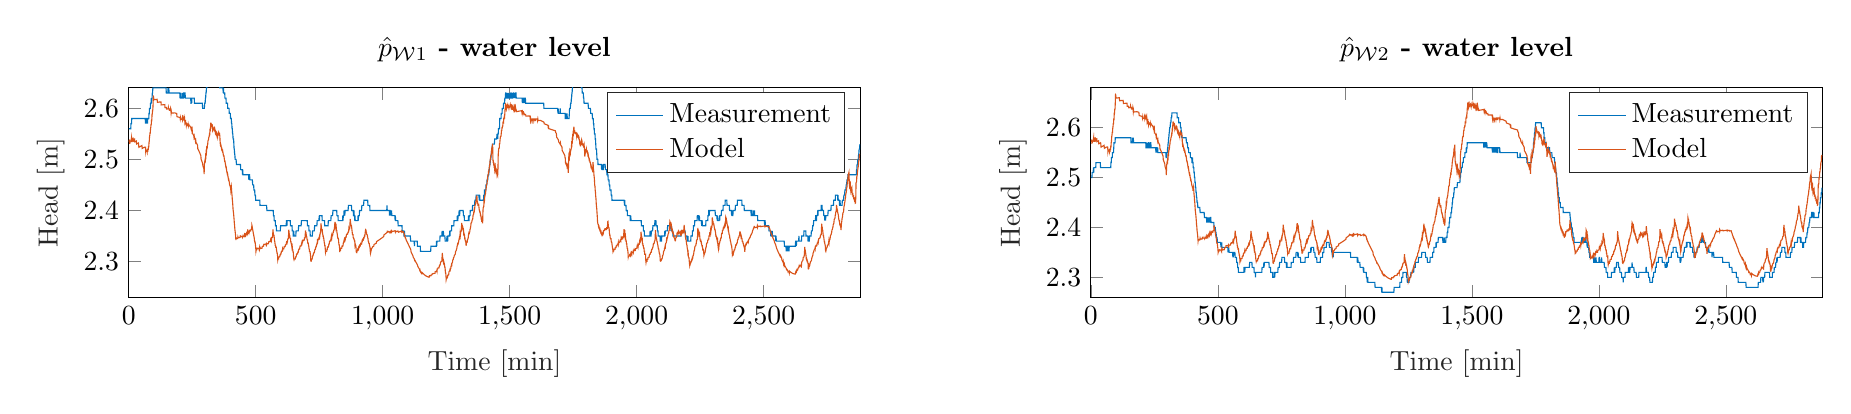
\begin{tikzpicture}

\begin{axis}[%
width=3.657in,
height=1.047in,
at={(1.421in,0.43in)},
scale only axis,
xmin=0,
xmax=2880,
xlabel style={font=\color{white!15!black}},
xlabel={Time [min]},
ymin=2.23,
ymax=2.64,
ylabel style={font=\color{white!15!black}},
ylabel={Head  [m]},
axis background/.style={fill=white},
title style={font=\bfseries},
title={$\hat{p}_{\mathcal{W}1}$ - water level},
legend style={legend cell align=left, align=left, draw=white!15!black}
]
\addplot [color=mycolor1]
  table[row sep=crcr]{%
1	2.56\\
2	2.56\\
3	2.56\\
4	2.56\\
5	2.56\\
6	2.56\\
7	2.56\\
8	2.56\\
9	2.57\\
10	2.57\\
11	2.57\\
12	2.58\\
13	2.58\\
14	2.58\\
15	2.58\\
16	2.58\\
17	2.58\\
18	2.58\\
19	2.58\\
20	2.58\\
21	2.58\\
22	2.58\\
23	2.58\\
24	2.58\\
25	2.58\\
26	2.58\\
27	2.58\\
28	2.58\\
29	2.58\\
30	2.58\\
31	2.58\\
32	2.58\\
33	2.58\\
34	2.58\\
35	2.58\\
36	2.58\\
37	2.58\\
38	2.58\\
39	2.58\\
40	2.58\\
41	2.58\\
42	2.58\\
43	2.58\\
44	2.58\\
45	2.58\\
46	2.58\\
47	2.58\\
48	2.58\\
49	2.58\\
50	2.58\\
51	2.58\\
52	2.58\\
53	2.58\\
54	2.58\\
55	2.58\\
56	2.58\\
57	2.58\\
58	2.58\\
59	2.58\\
60	2.58\\
61	2.58\\
62	2.58\\
63	2.58\\
64	2.58\\
65	2.58\\
66	2.57\\
67	2.58\\
68	2.58\\
69	2.58\\
70	2.58\\
71	2.58\\
72	2.57\\
73	2.58\\
74	2.57\\
75	2.58\\
76	2.58\\
77	2.58\\
78	2.58\\
79	2.58\\
80	2.59\\
81	2.59\\
82	2.6\\
83	2.6\\
84	2.6\\
85	2.6\\
86	2.61\\
87	2.61\\
88	2.61\\
89	2.62\\
90	2.61\\
91	2.62\\
92	2.62\\
93	2.63\\
94	2.63\\
95	2.64\\
96	2.64\\
97	2.64\\
98	2.64\\
99	2.64\\
100	2.64\\
101	2.64\\
102	2.64\\
103	2.64\\
104	2.64\\
105	2.64\\
106	2.64\\
107	2.64\\
108	2.64\\
109	2.64\\
110	2.64\\
111	2.64\\
112	2.64\\
113	2.64\\
114	2.64\\
115	2.64\\
116	2.64\\
117	2.64\\
118	2.64\\
119	2.64\\
120	2.64\\
121	2.64\\
122	2.64\\
123	2.64\\
124	2.64\\
125	2.64\\
126	2.64\\
127	2.64\\
128	2.64\\
129	2.64\\
130	2.64\\
131	2.64\\
132	2.64\\
133	2.64\\
134	2.64\\
135	2.64\\
136	2.64\\
137	2.64\\
138	2.64\\
139	2.64\\
140	2.64\\
141	2.64\\
142	2.64\\
143	2.64\\
144	2.64\\
145	2.64\\
146	2.64\\
147	2.64\\
148	2.63\\
149	2.63\\
150	2.63\\
151	2.63\\
152	2.63\\
153	2.63\\
154	2.63\\
155	2.64\\
156	2.63\\
157	2.63\\
158	2.64\\
159	2.63\\
160	2.63\\
161	2.63\\
162	2.63\\
163	2.63\\
164	2.63\\
165	2.63\\
166	2.63\\
167	2.63\\
168	2.63\\
169	2.63\\
170	2.63\\
171	2.63\\
172	2.63\\
173	2.63\\
174	2.63\\
175	2.63\\
176	2.63\\
177	2.63\\
178	2.63\\
179	2.63\\
180	2.63\\
181	2.63\\
182	2.63\\
183	2.63\\
184	2.63\\
185	2.63\\
186	2.63\\
187	2.63\\
188	2.63\\
189	2.63\\
190	2.63\\
191	2.63\\
192	2.63\\
193	2.63\\
194	2.63\\
195	2.63\\
196	2.63\\
197	2.63\\
198	2.63\\
199	2.63\\
200	2.63\\
201	2.63\\
202	2.62\\
203	2.63\\
204	2.62\\
205	2.62\\
206	2.62\\
207	2.62\\
208	2.62\\
209	2.62\\
210	2.63\\
211	2.62\\
212	2.63\\
213	2.62\\
214	2.62\\
215	2.62\\
216	2.63\\
217	2.63\\
218	2.63\\
219	2.63\\
220	2.62\\
221	2.63\\
222	2.63\\
223	2.62\\
224	2.62\\
225	2.62\\
226	2.62\\
227	2.62\\
228	2.62\\
229	2.62\\
230	2.62\\
231	2.62\\
232	2.62\\
233	2.62\\
234	2.62\\
235	2.62\\
236	2.62\\
237	2.62\\
238	2.62\\
239	2.62\\
240	2.62\\
241	2.62\\
242	2.62\\
243	2.62\\
244	2.62\\
245	2.61\\
246	2.61\\
247	2.62\\
248	2.61\\
249	2.62\\
250	2.62\\
251	2.62\\
252	2.62\\
253	2.62\\
254	2.62\\
255	2.62\\
256	2.62\\
257	2.62\\
258	2.62\\
259	2.61\\
260	2.61\\
261	2.61\\
262	2.61\\
263	2.61\\
264	2.61\\
265	2.61\\
266	2.61\\
267	2.61\\
268	2.61\\
269	2.61\\
270	2.61\\
271	2.61\\
272	2.61\\
273	2.61\\
274	2.61\\
275	2.61\\
276	2.61\\
277	2.61\\
278	2.61\\
279	2.61\\
280	2.61\\
281	2.61\\
282	2.61\\
283	2.61\\
284	2.61\\
285	2.61\\
286	2.61\\
287	2.61\\
288	2.61\\
289	2.61\\
290	2.61\\
291	2.6\\
292	2.6\\
293	2.6\\
294	2.6\\
295	2.6\\
296	2.6\\
297	2.6\\
298	2.6\\
299	2.61\\
300	2.61\\
301	2.61\\
302	2.62\\
303	2.62\\
304	2.63\\
305	2.63\\
306	2.64\\
307	2.64\\
308	2.64\\
309	2.65\\
310	2.65\\
311	2.66\\
312	2.67\\
313	2.67\\
314	2.67\\
315	2.68\\
316	2.68\\
317	2.68\\
318	2.68\\
319	2.69\\
320	2.69\\
321	2.69\\
322	2.7\\
323	2.7\\
324	2.7\\
325	2.7\\
326	2.7\\
327	2.7\\
328	2.7\\
329	2.69\\
330	2.7\\
331	2.69\\
332	2.69\\
333	2.69\\
334	2.69\\
335	2.69\\
336	2.69\\
337	2.69\\
338	2.69\\
339	2.69\\
340	2.68\\
341	2.68\\
342	2.68\\
343	2.68\\
344	2.68\\
345	2.68\\
346	2.67\\
347	2.67\\
348	2.67\\
349	2.67\\
350	2.67\\
351	2.67\\
352	2.67\\
353	2.66\\
354	2.66\\
355	2.65\\
356	2.65\\
357	2.65\\
358	2.64\\
359	2.64\\
360	2.64\\
361	2.64\\
362	2.64\\
363	2.64\\
364	2.64\\
365	2.64\\
366	2.64\\
367	2.64\\
368	2.64\\
369	2.64\\
370	2.64\\
371	2.64\\
372	2.63\\
373	2.64\\
374	2.63\\
375	2.63\\
376	2.63\\
377	2.63\\
378	2.63\\
379	2.62\\
380	2.62\\
381	2.62\\
382	2.62\\
383	2.62\\
384	2.61\\
385	2.61\\
386	2.61\\
387	2.61\\
388	2.61\\
389	2.61\\
390	2.6\\
391	2.6\\
392	2.6\\
393	2.6\\
394	2.6\\
395	2.6\\
396	2.59\\
397	2.59\\
398	2.59\\
399	2.59\\
400	2.59\\
401	2.58\\
402	2.58\\
403	2.58\\
404	2.58\\
405	2.57\\
406	2.57\\
407	2.56\\
408	2.56\\
409	2.55\\
410	2.55\\
411	2.54\\
412	2.54\\
413	2.54\\
414	2.53\\
415	2.52\\
416	2.52\\
417	2.51\\
418	2.51\\
419	2.5\\
420	2.5\\
421	2.5\\
422	2.5\\
423	2.5\\
424	2.49\\
425	2.49\\
426	2.49\\
427	2.49\\
428	2.49\\
429	2.49\\
430	2.49\\
431	2.49\\
432	2.49\\
433	2.49\\
434	2.49\\
435	2.49\\
436	2.49\\
437	2.49\\
438	2.49\\
439	2.49\\
440	2.49\\
441	2.48\\
442	2.48\\
443	2.48\\
444	2.48\\
445	2.48\\
446	2.48\\
447	2.48\\
448	2.47\\
449	2.48\\
450	2.47\\
451	2.47\\
452	2.47\\
453	2.47\\
454	2.47\\
455	2.47\\
456	2.47\\
457	2.47\\
458	2.47\\
459	2.47\\
460	2.47\\
461	2.47\\
462	2.47\\
463	2.47\\
464	2.47\\
465	2.47\\
466	2.47\\
467	2.47\\
468	2.47\\
469	2.47\\
470	2.47\\
471	2.47\\
472	2.47\\
473	2.46\\
474	2.47\\
475	2.47\\
476	2.47\\
477	2.46\\
478	2.46\\
479	2.46\\
480	2.46\\
481	2.46\\
482	2.46\\
483	2.46\\
484	2.46\\
485	2.46\\
486	2.46\\
487	2.46\\
488	2.45\\
489	2.45\\
490	2.45\\
491	2.45\\
492	2.45\\
493	2.44\\
494	2.44\\
495	2.44\\
496	2.44\\
497	2.43\\
498	2.43\\
499	2.43\\
500	2.42\\
501	2.42\\
502	2.42\\
503	2.42\\
504	2.42\\
505	2.42\\
506	2.42\\
507	2.42\\
508	2.42\\
509	2.42\\
510	2.42\\
511	2.42\\
512	2.42\\
513	2.42\\
514	2.42\\
515	2.42\\
516	2.42\\
517	2.41\\
518	2.41\\
519	2.41\\
520	2.41\\
521	2.41\\
522	2.41\\
523	2.41\\
524	2.41\\
525	2.41\\
526	2.41\\
527	2.41\\
528	2.41\\
529	2.41\\
530	2.41\\
531	2.41\\
532	2.41\\
533	2.41\\
534	2.41\\
535	2.41\\
536	2.41\\
537	2.41\\
538	2.41\\
539	2.41\\
540	2.41\\
541	2.41\\
542	2.41\\
543	2.41\\
544	2.4\\
545	2.4\\
546	2.4\\
547	2.4\\
548	2.4\\
549	2.4\\
550	2.4\\
551	2.4\\
552	2.4\\
553	2.4\\
554	2.4\\
555	2.4\\
556	2.4\\
557	2.4\\
558	2.4\\
559	2.4\\
560	2.4\\
561	2.4\\
562	2.4\\
563	2.4\\
564	2.4\\
565	2.4\\
566	2.4\\
567	2.4\\
568	2.4\\
569	2.4\\
570	2.39\\
571	2.39\\
572	2.39\\
573	2.38\\
574	2.38\\
575	2.38\\
576	2.38\\
577	2.38\\
578	2.37\\
579	2.37\\
580	2.37\\
581	2.37\\
582	2.36\\
583	2.36\\
584	2.36\\
585	2.36\\
586	2.36\\
587	2.36\\
588	2.36\\
589	2.36\\
590	2.36\\
591	2.36\\
592	2.36\\
593	2.36\\
594	2.36\\
595	2.36\\
596	2.36\\
597	2.36\\
598	2.37\\
599	2.37\\
600	2.37\\
601	2.37\\
602	2.37\\
603	2.37\\
604	2.37\\
605	2.37\\
606	2.37\\
607	2.37\\
608	2.37\\
609	2.37\\
610	2.37\\
611	2.37\\
612	2.37\\
613	2.37\\
614	2.37\\
615	2.37\\
616	2.37\\
617	2.37\\
618	2.37\\
619	2.37\\
620	2.37\\
621	2.38\\
622	2.38\\
623	2.37\\
624	2.38\\
625	2.38\\
626	2.38\\
627	2.38\\
628	2.38\\
629	2.38\\
630	2.38\\
631	2.38\\
632	2.38\\
633	2.38\\
634	2.38\\
635	2.38\\
636	2.38\\
637	2.37\\
638	2.37\\
639	2.37\\
640	2.37\\
641	2.37\\
642	2.37\\
643	2.37\\
644	2.36\\
645	2.36\\
646	2.36\\
647	2.36\\
648	2.35\\
649	2.35\\
650	2.36\\
651	2.35\\
652	2.35\\
653	2.35\\
654	2.35\\
655	2.35\\
656	2.35\\
657	2.35\\
658	2.35\\
659	2.36\\
660	2.36\\
661	2.36\\
662	2.36\\
663	2.36\\
664	2.36\\
665	2.36\\
666	2.36\\
667	2.36\\
668	2.36\\
669	2.37\\
670	2.37\\
671	2.37\\
672	2.37\\
673	2.37\\
674	2.37\\
675	2.37\\
676	2.37\\
677	2.37\\
678	2.37\\
679	2.37\\
680	2.38\\
681	2.38\\
682	2.38\\
683	2.38\\
684	2.38\\
685	2.38\\
686	2.38\\
687	2.38\\
688	2.38\\
689	2.38\\
690	2.38\\
691	2.38\\
692	2.38\\
693	2.38\\
694	2.38\\
695	2.38\\
696	2.38\\
697	2.38\\
698	2.38\\
699	2.38\\
700	2.38\\
701	2.38\\
702	2.38\\
703	2.38\\
704	2.37\\
705	2.37\\
706	2.37\\
707	2.37\\
708	2.37\\
709	2.37\\
710	2.36\\
711	2.36\\
712	2.36\\
713	2.36\\
714	2.36\\
715	2.35\\
716	2.35\\
717	2.35\\
718	2.35\\
719	2.35\\
720	2.35\\
721	2.35\\
722	2.35\\
723	2.35\\
724	2.36\\
725	2.36\\
726	2.36\\
727	2.36\\
728	2.36\\
729	2.36\\
730	2.36\\
731	2.36\\
732	2.37\\
733	2.37\\
734	2.37\\
735	2.37\\
736	2.37\\
737	2.37\\
738	2.37\\
739	2.37\\
740	2.37\\
741	2.37\\
742	2.38\\
743	2.38\\
744	2.38\\
745	2.38\\
746	2.38\\
747	2.38\\
748	2.38\\
749	2.38\\
750	2.39\\
751	2.38\\
752	2.39\\
753	2.39\\
754	2.39\\
755	2.39\\
756	2.39\\
757	2.39\\
758	2.39\\
759	2.39\\
760	2.39\\
761	2.39\\
762	2.38\\
763	2.38\\
764	2.38\\
765	2.38\\
766	2.38\\
767	2.38\\
768	2.38\\
769	2.38\\
770	2.38\\
771	2.38\\
772	2.37\\
773	2.37\\
774	2.37\\
775	2.37\\
776	2.37\\
777	2.37\\
778	2.37\\
779	2.37\\
780	2.37\\
781	2.37\\
782	2.37\\
783	2.37\\
784	2.37\\
785	2.37\\
786	2.38\\
787	2.38\\
788	2.38\\
789	2.38\\
790	2.38\\
791	2.38\\
792	2.38\\
793	2.38\\
794	2.38\\
795	2.38\\
796	2.38\\
797	2.39\\
798	2.39\\
799	2.39\\
800	2.39\\
801	2.39\\
802	2.39\\
803	2.39\\
804	2.4\\
805	2.4\\
806	2.4\\
807	2.4\\
808	2.4\\
809	2.4\\
810	2.4\\
811	2.4\\
812	2.4\\
813	2.4\\
814	2.4\\
815	2.4\\
816	2.4\\
817	2.4\\
818	2.4\\
819	2.4\\
820	2.39\\
821	2.39\\
822	2.39\\
823	2.39\\
824	2.39\\
825	2.38\\
826	2.38\\
827	2.38\\
828	2.38\\
829	2.38\\
830	2.38\\
831	2.38\\
832	2.38\\
833	2.38\\
834	2.38\\
835	2.38\\
836	2.38\\
837	2.38\\
838	2.38\\
839	2.38\\
840	2.38\\
841	2.38\\
842	2.38\\
843	2.39\\
844	2.38\\
845	2.39\\
846	2.39\\
847	2.39\\
848	2.4\\
849	2.39\\
850	2.4\\
851	2.39\\
852	2.4\\
853	2.4\\
854	2.4\\
855	2.4\\
856	2.4\\
857	2.4\\
858	2.4\\
859	2.4\\
860	2.4\\
861	2.4\\
862	2.4\\
863	2.4\\
864	2.4\\
865	2.41\\
866	2.41\\
867	2.41\\
868	2.41\\
869	2.41\\
870	2.41\\
871	2.41\\
872	2.41\\
873	2.41\\
874	2.41\\
875	2.41\\
876	2.41\\
877	2.41\\
878	2.4\\
879	2.4\\
880	2.4\\
881	2.4\\
882	2.4\\
883	2.4\\
884	2.4\\
885	2.39\\
886	2.39\\
887	2.4\\
888	2.39\\
889	2.39\\
890	2.38\\
891	2.39\\
892	2.38\\
893	2.38\\
894	2.38\\
895	2.38\\
896	2.38\\
897	2.38\\
898	2.38\\
899	2.38\\
900	2.38\\
901	2.38\\
902	2.38\\
903	2.39\\
904	2.38\\
905	2.39\\
906	2.39\\
907	2.39\\
908	2.39\\
909	2.4\\
910	2.4\\
911	2.4\\
912	2.4\\
913	2.4\\
914	2.4\\
915	2.4\\
916	2.4\\
917	2.4\\
918	2.41\\
919	2.41\\
920	2.41\\
921	2.41\\
922	2.41\\
923	2.41\\
924	2.41\\
925	2.41\\
926	2.42\\
927	2.42\\
928	2.42\\
929	2.42\\
930	2.42\\
931	2.42\\
932	2.42\\
933	2.42\\
934	2.42\\
935	2.42\\
936	2.42\\
937	2.42\\
938	2.42\\
939	2.42\\
940	2.42\\
941	2.42\\
942	2.41\\
943	2.41\\
944	2.41\\
945	2.41\\
946	2.41\\
947	2.41\\
948	2.41\\
949	2.41\\
950	2.4\\
951	2.4\\
952	2.4\\
953	2.4\\
954	2.4\\
955	2.4\\
956	2.4\\
957	2.4\\
958	2.4\\
959	2.4\\
960	2.4\\
961	2.4\\
962	2.4\\
963	2.4\\
964	2.4\\
965	2.4\\
966	2.4\\
967	2.4\\
968	2.4\\
969	2.4\\
970	2.4\\
971	2.4\\
972	2.4\\
973	2.4\\
974	2.4\\
975	2.4\\
976	2.4\\
977	2.4\\
978	2.4\\
979	2.4\\
980	2.4\\
981	2.4\\
982	2.4\\
983	2.4\\
984	2.4\\
985	2.4\\
986	2.4\\
987	2.4\\
988	2.4\\
989	2.4\\
990	2.4\\
991	2.4\\
992	2.4\\
993	2.4\\
994	2.4\\
995	2.4\\
996	2.4\\
997	2.4\\
998	2.4\\
999	2.4\\
1000	2.4\\
1001	2.4\\
1002	2.4\\
1003	2.4\\
1004	2.4\\
1005	2.4\\
1006	2.4\\
1007	2.4\\
1008	2.4\\
1009	2.4\\
1010	2.4\\
1011	2.4\\
1012	2.4\\
1013	2.4\\
1014	2.4\\
1015	2.4\\
1016	2.4\\
1017	2.41\\
1018	2.4\\
1019	2.4\\
1020	2.4\\
1021	2.4\\
1022	2.4\\
1023	2.4\\
1024	2.4\\
1025	2.4\\
1026	2.4\\
1027	2.39\\
1028	2.4\\
1029	2.4\\
1030	2.39\\
1031	2.4\\
1032	2.39\\
1033	2.4\\
1034	2.39\\
1035	2.4\\
1036	2.39\\
1037	2.39\\
1038	2.39\\
1039	2.39\\
1040	2.39\\
1041	2.39\\
1042	2.39\\
1043	2.39\\
1044	2.39\\
1045	2.39\\
1046	2.39\\
1047	2.39\\
1048	2.39\\
1049	2.38\\
1050	2.39\\
1051	2.38\\
1052	2.38\\
1053	2.38\\
1054	2.38\\
1055	2.38\\
1056	2.38\\
1057	2.38\\
1058	2.38\\
1059	2.38\\
1060	2.38\\
1061	2.37\\
1062	2.37\\
1063	2.37\\
1064	2.37\\
1065	2.37\\
1066	2.37\\
1067	2.37\\
1068	2.37\\
1069	2.37\\
1070	2.37\\
1071	2.37\\
1072	2.37\\
1073	2.37\\
1074	2.37\\
1075	2.37\\
1076	2.37\\
1077	2.36\\
1078	2.36\\
1079	2.36\\
1080	2.36\\
1081	2.36\\
1082	2.36\\
1083	2.36\\
1084	2.35\\
1085	2.35\\
1086	2.36\\
1087	2.35\\
1088	2.35\\
1089	2.35\\
1090	2.35\\
1091	2.35\\
1092	2.35\\
1093	2.35\\
1094	2.35\\
1095	2.35\\
1096	2.35\\
1097	2.35\\
1098	2.35\\
1099	2.35\\
1100	2.35\\
1101	2.35\\
1102	2.35\\
1103	2.35\\
1104	2.35\\
1105	2.35\\
1106	2.35\\
1107	2.35\\
1108	2.35\\
1109	2.35\\
1110	2.34\\
1111	2.34\\
1112	2.34\\
1113	2.34\\
1114	2.34\\
1115	2.34\\
1116	2.34\\
1117	2.34\\
1118	2.34\\
1119	2.34\\
1120	2.34\\
1121	2.34\\
1122	2.34\\
1123	2.34\\
1124	2.34\\
1125	2.33\\
1126	2.34\\
1127	2.34\\
1128	2.34\\
1129	2.34\\
1130	2.34\\
1131	2.34\\
1132	2.34\\
1133	2.34\\
1134	2.34\\
1135	2.34\\
1136	2.34\\
1137	2.33\\
1138	2.33\\
1139	2.33\\
1140	2.33\\
1141	2.33\\
1142	2.33\\
1143	2.33\\
1144	2.33\\
1145	2.33\\
1146	2.33\\
1147	2.33\\
1148	2.33\\
1149	2.32\\
1150	2.32\\
1151	2.32\\
1152	2.32\\
1153	2.32\\
1154	2.32\\
1155	2.32\\
1156	2.32\\
1157	2.32\\
1158	2.32\\
1159	2.32\\
1160	2.32\\
1161	2.32\\
1162	2.32\\
1163	2.32\\
1164	2.32\\
1165	2.32\\
1166	2.32\\
1167	2.32\\
1168	2.32\\
1169	2.32\\
1170	2.32\\
1171	2.32\\
1172	2.32\\
1173	2.32\\
1174	2.32\\
1175	2.32\\
1176	2.32\\
1177	2.32\\
1178	2.32\\
1179	2.32\\
1180	2.32\\
1181	2.32\\
1182	2.32\\
1183	2.32\\
1184	2.32\\
1185	2.32\\
1186	2.32\\
1187	2.32\\
1188	2.32\\
1189	2.32\\
1190	2.33\\
1191	2.33\\
1192	2.33\\
1193	2.33\\
1194	2.33\\
1195	2.33\\
1196	2.33\\
1197	2.33\\
1198	2.33\\
1199	2.33\\
1200	2.33\\
1201	2.33\\
1202	2.33\\
1203	2.33\\
1204	2.33\\
1205	2.33\\
1206	2.33\\
1207	2.33\\
1208	2.33\\
1209	2.33\\
1210	2.33\\
1211	2.33\\
1212	2.34\\
1213	2.33\\
1214	2.34\\
1215	2.34\\
1216	2.34\\
1217	2.34\\
1218	2.34\\
1219	2.34\\
1220	2.34\\
1221	2.34\\
1222	2.34\\
1223	2.34\\
1224	2.34\\
1225	2.34\\
1226	2.35\\
1227	2.35\\
1228	2.35\\
1229	2.35\\
1230	2.35\\
1231	2.35\\
1232	2.35\\
1233	2.35\\
1234	2.36\\
1235	2.35\\
1236	2.35\\
1237	2.35\\
1238	2.35\\
1239	2.36\\
1240	2.35\\
1241	2.35\\
1242	2.35\\
1243	2.35\\
1244	2.35\\
1245	2.35\\
1246	2.34\\
1247	2.34\\
1248	2.34\\
1249	2.34\\
1250	2.34\\
1251	2.34\\
1252	2.34\\
1253	2.35\\
1254	2.34\\
1255	2.34\\
1256	2.34\\
1257	2.35\\
1258	2.35\\
1259	2.35\\
1260	2.35\\
1261	2.35\\
1262	2.35\\
1263	2.35\\
1264	2.36\\
1265	2.35\\
1266	2.36\\
1267	2.36\\
1268	2.36\\
1269	2.36\\
1270	2.36\\
1271	2.36\\
1272	2.37\\
1273	2.37\\
1274	2.37\\
1275	2.37\\
1276	2.37\\
1277	2.37\\
1278	2.37\\
1279	2.37\\
1280	2.37\\
1281	2.38\\
1282	2.38\\
1283	2.38\\
1284	2.38\\
1285	2.38\\
1286	2.38\\
1287	2.38\\
1288	2.38\\
1289	2.38\\
1290	2.38\\
1291	2.38\\
1292	2.38\\
1293	2.38\\
1294	2.39\\
1295	2.38\\
1296	2.38\\
1297	2.39\\
1298	2.39\\
1299	2.39\\
1300	2.39\\
1301	2.4\\
1302	2.39\\
1303	2.39\\
1304	2.4\\
1305	2.4\\
1306	2.4\\
1307	2.4\\
1308	2.4\\
1309	2.4\\
1310	2.4\\
1311	2.4\\
1312	2.4\\
1313	2.4\\
1314	2.4\\
1315	2.4\\
1316	2.4\\
1317	2.4\\
1318	2.39\\
1319	2.39\\
1320	2.39\\
1321	2.39\\
1322	2.38\\
1323	2.38\\
1324	2.38\\
1325	2.38\\
1326	2.38\\
1327	2.38\\
1328	2.38\\
1329	2.38\\
1330	2.38\\
1331	2.38\\
1332	2.38\\
1333	2.38\\
1334	2.38\\
1335	2.38\\
1336	2.38\\
1337	2.38\\
1338	2.39\\
1339	2.38\\
1340	2.38\\
1341	2.39\\
1342	2.39\\
1343	2.39\\
1344	2.39\\
1345	2.4\\
1346	2.4\\
1347	2.4\\
1348	2.4\\
1349	2.4\\
1350	2.4\\
1351	2.4\\
1352	2.4\\
1353	2.4\\
1354	2.41\\
1355	2.41\\
1356	2.41\\
1357	2.41\\
1358	2.41\\
1359	2.41\\
1360	2.41\\
1361	2.41\\
1362	2.41\\
1363	2.42\\
1364	2.42\\
1365	2.42\\
1366	2.42\\
1367	2.42\\
1368	2.43\\
1369	2.43\\
1370	2.43\\
1371	2.43\\
1372	2.43\\
1373	2.43\\
1374	2.43\\
1375	2.43\\
1376	2.43\\
1377	2.43\\
1378	2.43\\
1379	2.43\\
1380	2.42\\
1381	2.43\\
1382	2.43\\
1383	2.42\\
1384	2.42\\
1385	2.42\\
1386	2.42\\
1387	2.42\\
1388	2.42\\
1389	2.42\\
1390	2.42\\
1391	2.42\\
1392	2.42\\
1393	2.42\\
1394	2.42\\
1395	2.42\\
1396	2.42\\
1397	2.42\\
1398	2.43\\
1399	2.42\\
1400	2.43\\
1401	2.44\\
1402	2.44\\
1403	2.44\\
1404	2.44\\
1405	2.44\\
1406	2.44\\
1407	2.45\\
1408	2.45\\
1409	2.45\\
1410	2.45\\
1411	2.46\\
1412	2.46\\
1413	2.46\\
1414	2.46\\
1415	2.47\\
1416	2.47\\
1417	2.47\\
1418	2.47\\
1419	2.48\\
1420	2.48\\
1421	2.49\\
1422	2.49\\
1423	2.49\\
1424	2.5\\
1425	2.5\\
1426	2.5\\
1427	2.51\\
1428	2.51\\
1429	2.52\\
1430	2.52\\
1431	2.52\\
1432	2.53\\
1433	2.53\\
1434	2.53\\
1435	2.53\\
1436	2.53\\
1437	2.53\\
1438	2.53\\
1439	2.53\\
1440	2.53\\
1441	2.54\\
1442	2.54\\
1443	2.54\\
1444	2.54\\
1445	2.54\\
1446	2.54\\
1447	2.54\\
1448	2.54\\
1449	2.54\\
1450	2.55\\
1451	2.54\\
1452	2.55\\
1453	2.54\\
1454	2.55\\
1455	2.55\\
1456	2.56\\
1457	2.56\\
1458	2.56\\
1459	2.56\\
1460	2.56\\
1461	2.58\\
1462	2.58\\
1463	2.58\\
1464	2.58\\
1465	2.58\\
1466	2.58\\
1467	2.59\\
1468	2.59\\
1469	2.59\\
1470	2.59\\
1471	2.6\\
1472	2.6\\
1473	2.6\\
1474	2.6\\
1475	2.6\\
1476	2.61\\
1477	2.61\\
1478	2.61\\
1479	2.61\\
1480	2.61\\
1481	2.62\\
1482	2.62\\
1483	2.62\\
1484	2.63\\
1485	2.63\\
1486	2.62\\
1487	2.63\\
1488	2.62\\
1489	2.62\\
1490	2.62\\
1491	2.63\\
1492	2.62\\
1493	2.62\\
1494	2.62\\
1495	2.63\\
1496	2.62\\
1497	2.63\\
1498	2.62\\
1499	2.62\\
1500	2.62\\
1501	2.62\\
1502	2.62\\
1503	2.63\\
1504	2.62\\
1505	2.63\\
1506	2.63\\
1507	2.62\\
1508	2.62\\
1509	2.62\\
1510	2.63\\
1511	2.62\\
1512	2.62\\
1513	2.63\\
1514	2.62\\
1515	2.63\\
1516	2.63\\
1517	2.62\\
1518	2.63\\
1519	2.62\\
1520	2.63\\
1521	2.62\\
1522	2.63\\
1523	2.62\\
1524	2.63\\
1525	2.63\\
1526	2.62\\
1527	2.62\\
1528	2.62\\
1529	2.62\\
1530	2.62\\
1531	2.62\\
1532	2.62\\
1533	2.62\\
1534	2.62\\
1535	2.62\\
1536	2.62\\
1537	2.62\\
1538	2.62\\
1539	2.62\\
1540	2.62\\
1541	2.62\\
1542	2.62\\
1543	2.62\\
1544	2.62\\
1545	2.62\\
1546	2.62\\
1547	2.62\\
1548	2.62\\
1549	2.62\\
1550	2.61\\
1551	2.62\\
1552	2.62\\
1553	2.61\\
1554	2.62\\
1555	2.62\\
1556	2.62\\
1557	2.61\\
1558	2.62\\
1559	2.61\\
1560	2.62\\
1561	2.62\\
1562	2.62\\
1563	2.61\\
1564	2.61\\
1565	2.61\\
1566	2.61\\
1567	2.61\\
1568	2.61\\
1569	2.61\\
1570	2.61\\
1571	2.61\\
1572	2.61\\
1573	2.61\\
1574	2.61\\
1575	2.61\\
1576	2.61\\
1577	2.61\\
1578	2.61\\
1579	2.61\\
1580	2.61\\
1581	2.61\\
1582	2.61\\
1583	2.61\\
1584	2.61\\
1585	2.61\\
1586	2.61\\
1587	2.61\\
1588	2.61\\
1589	2.61\\
1590	2.61\\
1591	2.61\\
1592	2.61\\
1593	2.61\\
1594	2.61\\
1595	2.61\\
1596	2.61\\
1597	2.61\\
1598	2.61\\
1599	2.61\\
1600	2.61\\
1601	2.61\\
1602	2.61\\
1603	2.61\\
1604	2.61\\
1605	2.61\\
1606	2.61\\
1607	2.61\\
1608	2.61\\
1609	2.61\\
1610	2.61\\
1611	2.61\\
1612	2.61\\
1613	2.61\\
1614	2.61\\
1615	2.61\\
1616	2.61\\
1617	2.61\\
1618	2.61\\
1619	2.61\\
1620	2.61\\
1621	2.61\\
1622	2.61\\
1623	2.61\\
1624	2.61\\
1625	2.61\\
1626	2.61\\
1627	2.61\\
1628	2.61\\
1629	2.61\\
1630	2.61\\
1631	2.61\\
1632	2.61\\
1633	2.61\\
1634	2.61\\
1635	2.6\\
1636	2.6\\
1637	2.6\\
1638	2.6\\
1639	2.6\\
1640	2.6\\
1641	2.6\\
1642	2.6\\
1643	2.6\\
1644	2.6\\
1645	2.6\\
1646	2.6\\
1647	2.6\\
1648	2.6\\
1649	2.6\\
1650	2.6\\
1651	2.6\\
1652	2.6\\
1653	2.6\\
1654	2.6\\
1655	2.6\\
1656	2.6\\
1657	2.6\\
1658	2.6\\
1659	2.6\\
1660	2.6\\
1661	2.6\\
1662	2.6\\
1663	2.6\\
1664	2.6\\
1665	2.6\\
1666	2.6\\
1667	2.6\\
1668	2.6\\
1669	2.6\\
1670	2.6\\
1671	2.6\\
1672	2.6\\
1673	2.6\\
1674	2.6\\
1675	2.6\\
1676	2.6\\
1677	2.6\\
1678	2.6\\
1679	2.6\\
1680	2.6\\
1681	2.6\\
1682	2.6\\
1683	2.6\\
1684	2.6\\
1685	2.6\\
1686	2.6\\
1687	2.6\\
1688	2.6\\
1689	2.6\\
1690	2.59\\
1691	2.6\\
1692	2.59\\
1693	2.59\\
1694	2.59\\
1695	2.59\\
1696	2.59\\
1697	2.59\\
1698	2.59\\
1699	2.6\\
1700	2.59\\
1701	2.59\\
1702	2.59\\
1703	2.59\\
1704	2.59\\
1705	2.59\\
1706	2.59\\
1707	2.59\\
1708	2.59\\
1709	2.59\\
1710	2.59\\
1711	2.59\\
1712	2.59\\
1713	2.59\\
1714	2.59\\
1715	2.59\\
1716	2.59\\
1717	2.59\\
1718	2.59\\
1719	2.58\\
1720	2.58\\
1721	2.58\\
1722	2.58\\
1723	2.58\\
1724	2.59\\
1725	2.58\\
1726	2.59\\
1727	2.58\\
1728	2.58\\
1729	2.58\\
1730	2.58\\
1731	2.58\\
1732	2.58\\
1733	2.58\\
1734	2.58\\
1735	2.59\\
1736	2.6\\
1737	2.6\\
1738	2.6\\
1739	2.6\\
1740	2.61\\
1741	2.61\\
1742	2.61\\
1743	2.62\\
1744	2.62\\
1745	2.63\\
1746	2.63\\
1747	2.64\\
1748	2.64\\
1749	2.65\\
1750	2.65\\
1751	2.66\\
1752	2.67\\
1753	2.67\\
1754	2.67\\
1755	2.67\\
1756	2.67\\
1757	2.67\\
1758	2.67\\
1759	2.67\\
1760	2.67\\
1761	2.67\\
1762	2.67\\
1763	2.66\\
1764	2.67\\
1765	2.67\\
1766	2.67\\
1767	2.67\\
1768	2.66\\
1769	2.66\\
1770	2.66\\
1771	2.66\\
1772	2.66\\
1773	2.66\\
1774	2.66\\
1775	2.65\\
1776	2.65\\
1777	2.65\\
1778	2.65\\
1779	2.65\\
1780	2.65\\
1781	2.65\\
1782	2.65\\
1783	2.64\\
1784	2.64\\
1785	2.64\\
1786	2.63\\
1787	2.63\\
1788	2.63\\
1789	2.63\\
1790	2.63\\
1791	2.62\\
1792	2.62\\
1793	2.61\\
1794	2.61\\
1795	2.61\\
1796	2.61\\
1797	2.61\\
1798	2.61\\
1799	2.61\\
1800	2.61\\
1801	2.61\\
1802	2.61\\
1803	2.61\\
1804	2.61\\
1805	2.61\\
1806	2.61\\
1807	2.61\\
1808	2.61\\
1809	2.61\\
1810	2.6\\
1811	2.6\\
1812	2.6\\
1813	2.6\\
1814	2.6\\
1815	2.6\\
1816	2.6\\
1817	2.6\\
1818	2.6\\
1819	2.59\\
1820	2.59\\
1821	2.59\\
1822	2.59\\
1823	2.59\\
1824	2.59\\
1825	2.59\\
1826	2.58\\
1827	2.58\\
1828	2.58\\
1829	2.58\\
1830	2.57\\
1831	2.57\\
1832	2.56\\
1833	2.56\\
1834	2.55\\
1835	2.55\\
1836	2.55\\
1837	2.54\\
1838	2.54\\
1839	2.53\\
1840	2.52\\
1841	2.52\\
1842	2.52\\
1843	2.51\\
1844	2.5\\
1845	2.5\\
1846	2.5\\
1847	2.5\\
1848	2.49\\
1849	2.49\\
1850	2.49\\
1851	2.49\\
1852	2.49\\
1853	2.49\\
1854	2.49\\
1855	2.49\\
1856	2.49\\
1857	2.49\\
1858	2.49\\
1859	2.49\\
1860	2.49\\
1861	2.49\\
1862	2.48\\
1863	2.49\\
1864	2.48\\
1865	2.48\\
1866	2.48\\
1867	2.49\\
1868	2.48\\
1869	2.48\\
1870	2.49\\
1871	2.49\\
1872	2.49\\
1873	2.49\\
1874	2.49\\
1875	2.49\\
1876	2.49\\
1877	2.48\\
1878	2.48\\
1879	2.48\\
1880	2.48\\
1881	2.48\\
1882	2.48\\
1883	2.47\\
1884	2.47\\
1885	2.48\\
1886	2.47\\
1887	2.47\\
1888	2.46\\
1889	2.46\\
1890	2.46\\
1891	2.46\\
1892	2.45\\
1893	2.45\\
1894	2.45\\
1895	2.44\\
1896	2.44\\
1897	2.44\\
1898	2.44\\
1899	2.44\\
1900	2.43\\
1901	2.43\\
1902	2.43\\
1903	2.42\\
1904	2.42\\
1905	2.42\\
1906	2.42\\
1907	2.42\\
1908	2.42\\
1909	2.42\\
1910	2.42\\
1911	2.42\\
1912	2.42\\
1913	2.42\\
1914	2.42\\
1915	2.42\\
1916	2.42\\
1917	2.42\\
1918	2.42\\
1919	2.42\\
1920	2.42\\
1921	2.42\\
1922	2.42\\
1923	2.42\\
1924	2.42\\
1925	2.42\\
1926	2.42\\
1927	2.42\\
1928	2.42\\
1929	2.42\\
1930	2.42\\
1931	2.42\\
1932	2.42\\
1933	2.42\\
1934	2.42\\
1935	2.42\\
1936	2.42\\
1937	2.42\\
1938	2.42\\
1939	2.42\\
1940	2.42\\
1941	2.42\\
1942	2.42\\
1943	2.42\\
1944	2.42\\
1945	2.42\\
1946	2.42\\
1947	2.42\\
1948	2.42\\
1949	2.42\\
1950	2.42\\
1951	2.42\\
1952	2.41\\
1953	2.42\\
1954	2.41\\
1955	2.41\\
1956	2.41\\
1957	2.41\\
1958	2.41\\
1959	2.4\\
1960	2.4\\
1961	2.4\\
1962	2.4\\
1963	2.4\\
1964	2.39\\
1965	2.39\\
1966	2.39\\
1967	2.39\\
1968	2.39\\
1969	2.39\\
1970	2.39\\
1971	2.39\\
1972	2.39\\
1973	2.39\\
1974	2.39\\
1975	2.38\\
1976	2.38\\
1977	2.39\\
1978	2.38\\
1979	2.38\\
1980	2.38\\
1981	2.38\\
1982	2.38\\
1983	2.38\\
1984	2.38\\
1985	2.38\\
1986	2.38\\
1987	2.38\\
1988	2.38\\
1989	2.38\\
1990	2.38\\
1991	2.38\\
1992	2.38\\
1993	2.38\\
1994	2.38\\
1995	2.38\\
1996	2.38\\
1997	2.38\\
1998	2.38\\
1999	2.38\\
2000	2.38\\
2001	2.38\\
2002	2.38\\
2003	2.38\\
2004	2.38\\
2005	2.38\\
2006	2.38\\
2007	2.38\\
2008	2.38\\
2009	2.38\\
2010	2.38\\
2011	2.38\\
2012	2.38\\
2013	2.38\\
2014	2.38\\
2015	2.38\\
2016	2.38\\
2017	2.38\\
2018	2.38\\
2019	2.37\\
2020	2.37\\
2021	2.37\\
2022	2.37\\
2023	2.37\\
2024	2.37\\
2025	2.37\\
2026	2.37\\
2027	2.36\\
2028	2.36\\
2029	2.36\\
2030	2.36\\
2031	2.35\\
2032	2.35\\
2033	2.35\\
2034	2.35\\
2035	2.35\\
2036	2.35\\
2037	2.35\\
2038	2.35\\
2039	2.35\\
2040	2.35\\
2041	2.35\\
2042	2.35\\
2043	2.35\\
2044	2.35\\
2045	2.35\\
2046	2.35\\
2047	2.35\\
2048	2.35\\
2049	2.35\\
2050	2.35\\
2051	2.35\\
2052	2.35\\
2053	2.36\\
2054	2.35\\
2055	2.35\\
2056	2.35\\
2057	2.35\\
2058	2.36\\
2059	2.36\\
2060	2.36\\
2061	2.36\\
2062	2.36\\
2063	2.36\\
2064	2.37\\
2065	2.37\\
2066	2.37\\
2067	2.37\\
2068	2.37\\
2069	2.37\\
2070	2.37\\
2071	2.37\\
2072	2.38\\
2073	2.38\\
2074	2.38\\
2075	2.38\\
2076	2.38\\
2077	2.37\\
2078	2.37\\
2079	2.37\\
2080	2.37\\
2081	2.37\\
2082	2.36\\
2083	2.36\\
2084	2.36\\
2085	2.35\\
2086	2.35\\
2087	2.35\\
2088	2.35\\
2089	2.35\\
2090	2.35\\
2091	2.35\\
2092	2.35\\
2093	2.34\\
2094	2.34\\
2095	2.35\\
2096	2.34\\
2097	2.34\\
2098	2.34\\
2099	2.35\\
2100	2.35\\
2101	2.35\\
2102	2.35\\
2103	2.35\\
2104	2.35\\
2105	2.35\\
2106	2.35\\
2107	2.35\\
2108	2.35\\
2109	2.35\\
2110	2.35\\
2111	2.36\\
2112	2.35\\
2113	2.36\\
2114	2.36\\
2115	2.36\\
2116	2.36\\
2117	2.36\\
2118	2.36\\
2119	2.36\\
2120	2.36\\
2121	2.36\\
2122	2.37\\
2123	2.37\\
2124	2.37\\
2125	2.37\\
2126	2.37\\
2127	2.37\\
2128	2.37\\
2129	2.37\\
2130	2.37\\
2131	2.37\\
2132	2.37\\
2133	2.37\\
2134	2.37\\
2135	2.36\\
2136	2.37\\
2137	2.37\\
2138	2.36\\
2139	2.36\\
2140	2.36\\
2141	2.36\\
2142	2.36\\
2143	2.35\\
2144	2.35\\
2145	2.35\\
2146	2.35\\
2147	2.35\\
2148	2.35\\
2149	2.35\\
2150	2.35\\
2151	2.35\\
2152	2.35\\
2153	2.35\\
2154	2.35\\
2155	2.35\\
2156	2.35\\
2157	2.35\\
2158	2.35\\
2159	2.35\\
2160	2.35\\
2161	2.35\\
2162	2.35\\
2163	2.35\\
2164	2.35\\
2165	2.35\\
2166	2.35\\
2167	2.35\\
2168	2.35\\
2169	2.35\\
2170	2.35\\
2171	2.35\\
2172	2.35\\
2173	2.35\\
2174	2.35\\
2175	2.35\\
2176	2.36\\
2177	2.36\\
2178	2.36\\
2179	2.36\\
2180	2.36\\
2181	2.36\\
2182	2.36\\
2183	2.36\\
2184	2.36\\
2185	2.36\\
2186	2.36\\
2187	2.36\\
2188	2.36\\
2189	2.36\\
2190	2.36\\
2191	2.36\\
2192	2.35\\
2193	2.35\\
2194	2.35\\
2195	2.35\\
2196	2.35\\
2197	2.35\\
2198	2.35\\
2199	2.34\\
2200	2.34\\
2201	2.34\\
2202	2.35\\
2203	2.34\\
2204	2.34\\
2205	2.34\\
2206	2.34\\
2207	2.34\\
2208	2.34\\
2209	2.34\\
2210	2.34\\
2211	2.34\\
2212	2.34\\
2213	2.34\\
2214	2.35\\
2215	2.35\\
2216	2.35\\
2217	2.35\\
2218	2.35\\
2219	2.35\\
2220	2.36\\
2221	2.36\\
2222	2.36\\
2223	2.36\\
2224	2.37\\
2225	2.37\\
2226	2.37\\
2227	2.37\\
2228	2.37\\
2229	2.38\\
2230	2.38\\
2231	2.38\\
2232	2.38\\
2233	2.38\\
2234	2.38\\
2235	2.38\\
2236	2.38\\
2237	2.38\\
2238	2.38\\
2239	2.39\\
2240	2.39\\
2241	2.39\\
2242	2.39\\
2243	2.39\\
2244	2.39\\
2245	2.38\\
2246	2.38\\
2247	2.39\\
2248	2.38\\
2249	2.38\\
2250	2.38\\
2251	2.38\\
2252	2.38\\
2253	2.38\\
2254	2.38\\
2255	2.38\\
2256	2.37\\
2257	2.38\\
2258	2.38\\
2259	2.37\\
2260	2.37\\
2261	2.37\\
2262	2.37\\
2263	2.37\\
2264	2.37\\
2265	2.37\\
2266	2.37\\
2267	2.37\\
2268	2.37\\
2269	2.37\\
2270	2.37\\
2271	2.37\\
2272	2.37\\
2273	2.38\\
2274	2.38\\
2275	2.38\\
2276	2.38\\
2277	2.38\\
2278	2.38\\
2279	2.38\\
2280	2.38\\
2281	2.39\\
2282	2.39\\
2283	2.39\\
2284	2.4\\
2285	2.4\\
2286	2.39\\
2287	2.4\\
2288	2.4\\
2289	2.4\\
2290	2.4\\
2291	2.4\\
2292	2.4\\
2293	2.4\\
2294	2.4\\
2295	2.4\\
2296	2.4\\
2297	2.4\\
2298	2.4\\
2299	2.4\\
2300	2.4\\
2301	2.4\\
2302	2.4\\
2303	2.4\\
2304	2.4\\
2305	2.4\\
2306	2.4\\
2307	2.4\\
2308	2.4\\
2309	2.4\\
2310	2.39\\
2311	2.39\\
2312	2.39\\
2313	2.39\\
2314	2.39\\
2315	2.39\\
2316	2.39\\
2317	2.38\\
2318	2.39\\
2319	2.38\\
2320	2.38\\
2321	2.38\\
2322	2.38\\
2323	2.38\\
2324	2.38\\
2325	2.38\\
2326	2.39\\
2327	2.38\\
2328	2.39\\
2329	2.39\\
2330	2.39\\
2331	2.39\\
2332	2.39\\
2333	2.39\\
2334	2.4\\
2335	2.4\\
2336	2.4\\
2337	2.4\\
2338	2.4\\
2339	2.4\\
2340	2.4\\
2341	2.41\\
2342	2.41\\
2343	2.41\\
2344	2.41\\
2345	2.41\\
2346	2.41\\
2347	2.41\\
2348	2.41\\
2349	2.42\\
2350	2.42\\
2351	2.42\\
2352	2.42\\
2353	2.42\\
2354	2.42\\
2355	2.42\\
2356	2.41\\
2357	2.41\\
2358	2.41\\
2359	2.41\\
2360	2.41\\
2361	2.41\\
2362	2.41\\
2363	2.41\\
2364	2.41\\
2365	2.41\\
2366	2.4\\
2367	2.4\\
2368	2.4\\
2369	2.4\\
2370	2.4\\
2371	2.4\\
2372	2.4\\
2373	2.4\\
2374	2.39\\
2375	2.4\\
2376	2.39\\
2377	2.39\\
2378	2.39\\
2379	2.39\\
2380	2.4\\
2381	2.4\\
2382	2.4\\
2383	2.4\\
2384	2.4\\
2385	2.4\\
2386	2.4\\
2387	2.4\\
2388	2.4\\
2389	2.41\\
2390	2.41\\
2391	2.41\\
2392	2.41\\
2393	2.41\\
2394	2.41\\
2395	2.41\\
2396	2.41\\
2397	2.42\\
2398	2.42\\
2399	2.42\\
2400	2.42\\
2401	2.42\\
2402	2.42\\
2403	2.42\\
2404	2.42\\
2405	2.42\\
2406	2.42\\
2407	2.42\\
2408	2.42\\
2409	2.42\\
2410	2.42\\
2411	2.42\\
2412	2.42\\
2413	2.42\\
2414	2.42\\
2415	2.41\\
2416	2.41\\
2417	2.41\\
2418	2.41\\
2419	2.41\\
2420	2.41\\
2421	2.41\\
2422	2.41\\
2423	2.41\\
2424	2.4\\
2425	2.4\\
2426	2.4\\
2427	2.4\\
2428	2.4\\
2429	2.4\\
2430	2.4\\
2431	2.4\\
2432	2.4\\
2433	2.4\\
2434	2.4\\
2435	2.4\\
2436	2.4\\
2437	2.4\\
2438	2.4\\
2439	2.4\\
2440	2.4\\
2441	2.4\\
2442	2.4\\
2443	2.4\\
2444	2.4\\
2445	2.4\\
2446	2.4\\
2447	2.4\\
2448	2.4\\
2449	2.4\\
2450	2.4\\
2451	2.39\\
2452	2.39\\
2453	2.4\\
2454	2.4\\
2455	2.39\\
2456	2.39\\
2457	2.39\\
2458	2.39\\
2459	2.39\\
2460	2.39\\
2461	2.4\\
2462	2.39\\
2463	2.39\\
2464	2.4\\
2465	2.39\\
2466	2.39\\
2467	2.39\\
2468	2.39\\
2469	2.39\\
2470	2.39\\
2471	2.39\\
2472	2.39\\
2473	2.39\\
2474	2.39\\
2475	2.39\\
2476	2.39\\
2477	2.38\\
2478	2.38\\
2479	2.38\\
2480	2.38\\
2481	2.38\\
2482	2.38\\
2483	2.38\\
2484	2.38\\
2485	2.38\\
2486	2.38\\
2487	2.38\\
2488	2.38\\
2489	2.38\\
2490	2.38\\
2491	2.38\\
2492	2.38\\
2493	2.38\\
2494	2.38\\
2495	2.38\\
2496	2.38\\
2497	2.38\\
2498	2.38\\
2499	2.38\\
2500	2.38\\
2501	2.38\\
2502	2.38\\
2503	2.38\\
2504	2.37\\
2505	2.38\\
2506	2.38\\
2507	2.37\\
2508	2.37\\
2509	2.37\\
2510	2.37\\
2511	2.37\\
2512	2.37\\
2513	2.37\\
2514	2.37\\
2515	2.37\\
2516	2.37\\
2517	2.37\\
2518	2.37\\
2519	2.37\\
2520	2.37\\
2521	2.36\\
2522	2.36\\
2523	2.36\\
2524	2.36\\
2525	2.36\\
2526	2.36\\
2527	2.36\\
2528	2.35\\
2529	2.36\\
2530	2.35\\
2531	2.35\\
2532	2.36\\
2533	2.35\\
2534	2.36\\
2535	2.35\\
2536	2.35\\
2537	2.35\\
2538	2.35\\
2539	2.35\\
2540	2.35\\
2541	2.35\\
2542	2.35\\
2543	2.35\\
2544	2.35\\
2545	2.35\\
2546	2.35\\
2547	2.35\\
2548	2.34\\
2549	2.35\\
2550	2.34\\
2551	2.34\\
2552	2.34\\
2553	2.34\\
2554	2.34\\
2555	2.34\\
2556	2.34\\
2557	2.34\\
2558	2.34\\
2559	2.34\\
2560	2.34\\
2561	2.34\\
2562	2.34\\
2563	2.34\\
2564	2.34\\
2565	2.34\\
2566	2.34\\
2567	2.34\\
2568	2.34\\
2569	2.34\\
2570	2.34\\
2571	2.34\\
2572	2.34\\
2573	2.34\\
2574	2.34\\
2575	2.34\\
2576	2.34\\
2577	2.34\\
2578	2.34\\
2579	2.34\\
2580	2.34\\
2581	2.34\\
2582	2.33\\
2583	2.33\\
2584	2.33\\
2585	2.33\\
2586	2.33\\
2587	2.33\\
2588	2.33\\
2589	2.32\\
2590	2.33\\
2591	2.33\\
2592	2.33\\
2593	2.33\\
2594	2.33\\
2595	2.32\\
2596	2.33\\
2597	2.33\\
2598	2.33\\
2599	2.33\\
2600	2.32\\
2601	2.33\\
2602	2.33\\
2603	2.33\\
2604	2.33\\
2605	2.33\\
2606	2.33\\
2607	2.33\\
2608	2.33\\
2609	2.33\\
2610	2.33\\
2611	2.33\\
2612	2.33\\
2613	2.33\\
2614	2.33\\
2615	2.33\\
2616	2.33\\
2617	2.33\\
2618	2.33\\
2619	2.33\\
2620	2.33\\
2621	2.33\\
2622	2.33\\
2623	2.33\\
2624	2.33\\
2625	2.33\\
2626	2.34\\
2627	2.34\\
2628	2.34\\
2629	2.33\\
2630	2.34\\
2631	2.34\\
2632	2.34\\
2633	2.34\\
2634	2.34\\
2635	2.34\\
2636	2.34\\
2637	2.34\\
2638	2.34\\
2639	2.35\\
2640	2.34\\
2641	2.34\\
2642	2.34\\
2643	2.34\\
2644	2.34\\
2645	2.34\\
2646	2.34\\
2647	2.34\\
2648	2.34\\
2649	2.34\\
2650	2.35\\
2651	2.35\\
2652	2.35\\
2653	2.35\\
2654	2.35\\
2655	2.35\\
2656	2.35\\
2657	2.35\\
2658	2.35\\
2659	2.36\\
2660	2.36\\
2661	2.36\\
2662	2.36\\
2663	2.36\\
2664	2.36\\
2665	2.36\\
2666	2.36\\
2667	2.35\\
2668	2.35\\
2669	2.35\\
2670	2.35\\
2671	2.35\\
2672	2.35\\
2673	2.35\\
2674	2.35\\
2675	2.34\\
2676	2.34\\
2677	2.34\\
2678	2.35\\
2679	2.34\\
2680	2.34\\
2681	2.35\\
2682	2.35\\
2683	2.35\\
2684	2.35\\
2685	2.35\\
2686	2.35\\
2687	2.35\\
2688	2.36\\
2689	2.36\\
2690	2.36\\
2691	2.36\\
2692	2.36\\
2693	2.37\\
2694	2.37\\
2695	2.37\\
2696	2.37\\
2697	2.38\\
2698	2.38\\
2699	2.38\\
2700	2.38\\
2701	2.38\\
2702	2.38\\
2703	2.38\\
2704	2.38\\
2705	2.39\\
2706	2.39\\
2707	2.38\\
2708	2.38\\
2709	2.39\\
2710	2.39\\
2711	2.39\\
2712	2.39\\
2713	2.4\\
2714	2.39\\
2715	2.4\\
2716	2.4\\
2717	2.4\\
2718	2.4\\
2719	2.4\\
2720	2.4\\
2721	2.4\\
2722	2.4\\
2723	2.4\\
2724	2.4\\
2725	2.4\\
2726	2.4\\
2727	2.41\\
2728	2.41\\
2729	2.41\\
2730	2.41\\
2731	2.4\\
2732	2.4\\
2733	2.4\\
2734	2.4\\
2735	2.4\\
2736	2.4\\
2737	2.39\\
2738	2.39\\
2739	2.39\\
2740	2.39\\
2741	2.38\\
2742	2.39\\
2743	2.39\\
2744	2.38\\
2745	2.39\\
2746	2.39\\
2747	2.39\\
2748	2.39\\
2749	2.39\\
2750	2.39\\
2751	2.39\\
2752	2.39\\
2753	2.39\\
2754	2.4\\
2755	2.4\\
2756	2.4\\
2757	2.4\\
2758	2.4\\
2759	2.4\\
2760	2.4\\
2761	2.4\\
2762	2.4\\
2763	2.4\\
2764	2.4\\
2765	2.4\\
2766	2.41\\
2767	2.41\\
2768	2.41\\
2769	2.41\\
2770	2.41\\
2771	2.41\\
2772	2.41\\
2773	2.41\\
2774	2.41\\
2775	2.41\\
2776	2.42\\
2777	2.42\\
2778	2.42\\
2779	2.42\\
2780	2.42\\
2781	2.42\\
2782	2.42\\
2783	2.43\\
2784	2.43\\
2785	2.43\\
2786	2.43\\
2787	2.43\\
2788	2.43\\
2789	2.43\\
2790	2.43\\
2791	2.43\\
2792	2.42\\
2793	2.43\\
2794	2.42\\
2795	2.42\\
2796	2.42\\
2797	2.42\\
2798	2.42\\
2799	2.41\\
2800	2.41\\
2801	2.42\\
2802	2.41\\
2803	2.41\\
2804	2.41\\
2805	2.41\\
2806	2.41\\
2807	2.41\\
2808	2.41\\
2809	2.41\\
2810	2.42\\
2811	2.42\\
2812	2.42\\
2813	2.42\\
2814	2.42\\
2815	2.42\\
2816	2.43\\
2817	2.43\\
2818	2.43\\
2819	2.43\\
2820	2.44\\
2821	2.44\\
2822	2.44\\
2823	2.44\\
2824	2.44\\
2825	2.45\\
2826	2.45\\
2827	2.45\\
2828	2.46\\
2829	2.46\\
2830	2.46\\
2831	2.46\\
2832	2.47\\
2833	2.47\\
2834	2.47\\
2835	2.47\\
2836	2.47\\
2837	2.47\\
2838	2.47\\
2839	2.47\\
2840	2.47\\
2841	2.47\\
2842	2.47\\
2843	2.47\\
2844	2.47\\
2845	2.47\\
2846	2.47\\
2847	2.47\\
2848	2.47\\
2849	2.47\\
2850	2.47\\
2851	2.47\\
2852	2.47\\
2853	2.47\\
2854	2.47\\
2855	2.47\\
2856	2.47\\
2857	2.47\\
2858	2.47\\
2859	2.47\\
2860	2.47\\
2861	2.47\\
2862	2.47\\
2863	2.47\\
2864	2.47\\
2865	2.47\\
2866	2.48\\
2867	2.48\\
2868	2.49\\
2869	2.49\\
2870	2.49\\
2871	2.5\\
2872	2.5\\
2873	2.5\\
2874	2.51\\
2875	2.51\\
2876	2.52\\
2877	2.52\\
2878	2.52\\
2879	2.53\\
};
\addlegendentry{Measurement}

\addplot [color=mycolor2]
  table[row sep=crcr]{%
1	2.53393168281914\\
2	2.53718384810235\\
3	2.53744482257821\\
4	2.53172186379451\\
5	2.53198379475373\\
6	2.53524384374018\\
7	2.53550885061425\\
8	2.53577498988539\\
9	2.53604223519962\\
10	2.53930950058527\\
11	2.54257992251211\\
12	2.5338542720353\\
13	2.54012762070922\\
14	2.54040063604591\\
15	2.54067458863342\\
16	2.54094945176505\\
17	2.54122519881496\\
18	2.53549794526751\\
19	2.53577420198499\\
20	2.53605128304225\\
21	2.53933565494375\\
22	2.53961485931048\\
23	2.53989479693489\\
24	2.53416482288368\\
25	2.53444509347419\\
26	2.53472603688546\\
27	2.53500762590085\\
28	2.53528983324992\\
29	2.53557263168682\\
30	2.53585599352925\\
31	2.53012234459176\\
32	2.53040584644907\\
33	2.53068985047463\\
34	2.53097432899708\\
35	2.53125925442548\\
36	2.53154459879746\\
37	2.53183033453411\\
38	2.5321164336331\\
39	2.52938799919799\\
40	2.52364944045443\\
41	2.5239353930289\\
42	2.52422162862066\\
43	2.52450811922304\\
44	2.52479483652932\\
45	2.52508175225127\\
46	2.52536883815952\\
47	2.52565606569774\\
48	2.52594340670861\\
49	2.52623083218247\\
50	2.52651831404366\\
51	2.52680582332506\\
52	2.52709333147388\\
53	2.52134823156052\\
54	2.52163521207844\\
55	2.52192212629122\\
56	2.52220894511166\\
57	2.5224956396446\\
58	2.52278218067349\\
59	2.52306853919027\\
60	2.52335468592917\\
61	2.52364059166738\\
62	2.52369913940063\\
63	2.52375801217399\\
64	2.52381721085925\\
65	2.5238767356071\\
66	2.523936587045\\
67	2.51494045603022\\
68	2.51802090604353\\
69	2.51808162238234\\
70	2.51814266864457\\
71	2.51820404528459\\
72	2.51826575274877\\
73	2.51530739233913\\
74	2.52087409999904\\
75	2.51490699212698\\
76	2.51964318483119\\
77	2.51972359303677\\
78	2.52520809185824\\
79	2.52504166498417\\
80	2.53298965683004\\
81	2.53599347651166\\
82	2.54439925689929\\
83	2.54708161296954\\
84	2.552160862163\\
85	2.5521447148126\\
86	2.56034671249607\\
87	2.56321389363849\\
88	2.56874964612618\\
89	2.56887973938519\\
90	2.57730933039197\\
91	2.57727409698578\\
92	2.5890262633296\\
93	2.58901667301149\\
94	2.59656640736896\\
95	2.59678711755132\\
96	2.608034080082\\
97	2.62345935515598\\
98	2.62268073799416\\
99	2.61671350638386\\
100	2.61678573474522\\
101	2.61685828139803\\
102	2.61693114652837\\
103	2.61700433086668\\
104	2.61707783467111\\
105	2.61715165843406\\
106	2.61722580255038\\
107	2.61730026746027\\
108	2.61737505344012\\
109	2.61745016105544\\
110	2.61752559075454\\
111	2.61760134280601\\
112	2.61767741771524\\
113	2.61171377357868\\
114	2.61179044851863\\
115	2.61186744895688\\
116	2.61194477549311\\
117	2.61202242860595\\
118	2.61210040864978\\
119	2.61217871584424\\
120	2.61225735087999\\
121	2.61233631389873\\
122	2.61238211739333\\
123	2.61242802164311\\
124	2.61247402643006\\
125	2.61252013202745\\
126	2.61256633854514\\
127	2.61261264592047\\
128	2.60661854411554\\
129	2.60666503740164\\
130	2.60671163217336\\
131	2.60675832894626\\
132	2.60680512753901\\
133	2.60685202818649\\
134	2.60689903078518\\
135	2.60694613548245\\
136	2.60699334242761\\
137	2.607040651669\\
138	2.60708806319713\\
139	2.60713557714515\\
140	2.60718319364419\\
141	2.60723091289687\\
142	2.60727873470819\\
143	2.60128595047197\\
144	2.60133396930631\\
145	2.6013820914355\\
146	2.60143031723673\\
147	2.60147864644146\\
148	2.60152707950279\\
149	2.59855342719237\\
150	2.59860206582737\\
151	2.59865080880897\\
152	2.5986996559799\\
153	2.59874860743286\\
154	2.59879766343596\\
155	2.5988468237468\\
156	2.60191828570274\\
157	2.5989454585311\\
158	2.59899493291479\\
159	2.59904377977011\\
160	2.59607126833071\\
161	2.5961210584982\\
162	2.59617095399566\\
163	2.59622095482778\\
164	2.59627106130282\\
165	2.59934419321848\\
166	2.59637159082167\\
167	2.59038123136324\\
168	2.59345467612657\\
169	2.59048240310118\\
170	2.59053314857588\\
171	2.59058400067282\\
172	2.59063495942213\\
173	2.59068602480342\\
174	2.59073719680342\\
175	2.59078847589091\\
176	2.59083986189266\\
177	2.59089135494735\\
178	2.59094295507301\\
179	2.59099466224501\\
180	2.59104647679477\\
181	2.59109839860069\\
182	2.59094324989882\\
183	2.59078908211527\\
184	2.59063589319248\\
185	2.59048368085102\\
186	2.59033244313107\\
187	2.59018217786759\\
188	2.59003288310749\\
189	2.58988455653639\\
190	2.58369640652103\\
191	2.58355002251269\\
192	2.58340460496633\\
193	2.58326015172907\\
194	2.58311666086769\\
195	2.58297413009147\\
196	2.58283255733272\\
197	2.58269194036991\\
198	2.58255227699144\\
199	2.58241356520279\\
200	2.58227580276243\\
201	2.58213898753381\\
202	2.58200311722442\\
203	2.57884621017152\\
204	2.58173420299591\\
205	2.57857924392326\\
206	2.57844716969871\\
207	2.5783160317978\\
208	2.57818582801997\\
209	2.57805655615311\\
210	2.57792821403493\\
211	2.5808224482823\\
212	2.57767431014957\\
213	2.5805702868493\\
214	2.57742409830627\\
215	2.57730037141819\\
216	2.57717756075053\\
217	2.58007696818391\\
218	2.57693393463852\\
219	2.57681385906401\\
220	2.57971653693034\\
221	2.57355539956405\\
222	2.5764590671114\\
223	2.57634260704036\\
224	2.57622779257778\\
225	2.56705403340688\\
226	2.57297797574442\\
227	2.56682790137824\\
228	2.56973738601574\\
229	2.5696264683255\\
230	2.56649541711177\\
231	2.56638637024024\\
232	2.5662782099142\\
233	2.56617093398842\\
234	2.5690851687513\\
235	2.56595902608856\\
236	2.56887480720356\\
237	2.56877093667109\\
238	2.56564773866889\\
239	2.56554572009618\\
240	2.56544456951296\\
241	2.56534428458186\\
242	2.56447058635969\\
243	2.56360790089068\\
244	2.56275517377647\\
245	2.56191134542248\\
246	2.55806173828053\\
247	2.55723395413708\\
248	2.55942259021891\\
249	2.55559473977927\\
250	2.55778830893032\\
251	2.55096913220777\\
252	2.55016168636188\\
253	2.54935478223229\\
254	2.54854734399973\\
255	2.54773829745706\\
256	2.5469265713109\\
257	2.5431188599635\\
258	2.54529081189929\\
259	2.54147791766823\\
260	2.54064855264098\\
261	2.53981053061664\\
262	2.53896360700946\\
263	2.5351323515012\\
264	2.53723892953212\\
265	2.53339157332727\\
266	2.53250237881989\\
267	2.53159931543652\\
268	2.53068139784579\\
269	2.52974765273994\\
270	2.52879711905741\\
271	2.52782884851863\\
272	2.52096791026615\\
273	2.51997008061244\\
274	2.51895196700778\\
275	2.51791267935296\\
276	2.51685134345016\\
277	2.51576710226167\\
278	2.51465911608981\\
279	2.51352656337122\\
280	2.51236864120933\\
281	2.51118456574752\\
282	2.50997357295142\\
283	2.50873491930341\\
284	2.50746788211266\\
285	2.50042711417933\\
286	2.49911260010852\\
287	2.49776786198529\\
288	2.49639226453033\\
289	2.49498519594988\\
290	2.4935460681852\\
291	2.49207431776674\\
292	2.48773638577408\\
293	2.48620415588459\\
294	2.48463785692195\\
295	2.48303702640567\\
296	2.48140122817594\\
297	2.47133344381381\\
298	2.49004956927958\\
299	2.49443409131561\\
300	2.4971569835718\\
301	2.49978380475053\\
302	2.49836108429267\\
303	2.50705657349489\\
304	2.50570219612485\\
305	2.51438288039569\\
306	2.51311814620615\\
307	2.52177320182942\\
308	2.52059540851731\\
309	2.52208628515441\\
310	2.52837757526686\\
311	2.52957410285246\\
312	2.53574087420289\\
313	2.5372047323483\\
314	2.53843218067751\\
315	2.5420745505323\\
316	2.54378024989099\\
317	2.54528165630554\\
318	2.54946044483129\\
319	2.54877294520902\\
320	2.557299843523\\
321	2.55666190407743\\
322	2.56056908791727\\
323	2.5720238500217\\
324	2.56876044769153\\
325	2.56922193449537\\
326	2.56479899072245\\
327	2.56537537274746\\
328	2.56599342821914\\
329	2.56665207244589\\
330	2.56013196455569\\
331	2.56330619794385\\
332	2.56173269457847\\
333	2.55786860855335\\
334	2.5587902779081\\
335	2.55974624989367\\
336	2.56073529134672\\
337	2.56175614635914\\
338	2.55824387739043\\
339	2.55935634507094\\
340	2.55599714037954\\
341	2.55272389890253\\
342	2.55398139736066\\
343	2.55086062382921\\
344	2.55219791274687\\
345	2.54921978470242\\
346	2.55063147370501\\
347	2.54778615915183\\
348	2.54502934132524\\
349	2.54655854888022\\
350	2.54393135658164\\
351	2.54965644979957\\
352	2.55122161814553\\
353	2.55279518371253\\
354	2.55033621857579\\
355	2.54795461932755\\
356	2.54762556212372\\
357	2.54733096886126\\
358	2.54902094153131\\
359	2.54476963795846\\
360	2.53276250683659\\
361	2.52894082227151\\
362	2.53027995710241\\
363	2.52828644840712\\
364	2.52503365161106\\
365	2.52272355071519\\
366	2.51975800839236\\
367	2.52078032059129\\
368	2.51862779912406\\
369	2.51593736621843\\
370	2.51667009389129\\
371	2.51376284897998\\
372	2.51106823183226\\
373	2.50715323456679\\
374	2.50656107482202\\
375	2.50679077789438\\
376	2.5030073516359\\
377	2.49907946539259\\
378	2.49638335134473\\
379	2.49660016869369\\
380	2.49342424979381\\
381	2.49070690386244\\
382	2.48652179406274\\
383	2.48419643609929\\
384	2.48483440634585\\
385	2.48078572837546\\
386	2.47672574379691\\
387	2.47419932397202\\
388	2.47164316454369\\
389	2.47261029590112\\
390	2.47012719841416\\
391	2.46606044605615\\
392	2.4633910762315\\
393	2.46009312108642\\
394	2.46075705236701\\
395	2.45813908528772\\
396	2.4557687065448\\
397	2.45149283106509\\
398	2.44916608248431\\
399	2.4485603102356\\
400	2.44584601422464\\
401	2.44561699675609\\
402	2.43977269996824\\
403	2.44370646699109\\
404	2.44680890725707\\
405	2.44081421677976\\
406	2.43307716613486\\
407	2.42888041883764\\
408	2.42118917438929\\
409	2.41702601583464\\
410	2.40938115496023\\
411	2.40176220261648\\
412	2.39765423023384\\
413	2.39355989190073\\
414	2.38774626935644\\
415	2.38195039884748\\
416	2.37444811041928\\
417	2.37042475674198\\
418	2.36297111784035\\
419	2.35898405863333\\
420	2.35501279917704\\
421	2.34934459192398\\
422	2.3422302536526\\
423	2.34618263121057\\
424	2.34618592608756\\
425	2.34475487370483\\
426	2.34477896378939\\
427	2.34485050943655\\
428	2.34490857030834\\
429	2.34502049904706\\
430	2.34831271924294\\
431	2.34666494908598\\
432	2.34695938346596\\
433	2.34687095559868\\
434	2.34666377207112\\
435	2.34681937304171\\
436	2.3468991496606\\
437	2.346917511826\\
438	2.34697694679452\\
439	2.35001984983247\\
440	2.35000230489906\\
441	2.35035333981249\\
442	2.3485950291066\\
443	2.34883669539479\\
444	2.34870228186168\\
445	2.34865722414583\\
446	2.34868268323285\\
447	2.34874370894442\\
448	2.34734793047531\\
449	2.34883650761869\\
450	2.35045168453117\\
451	2.34893774590857\\
452	2.34903451137066\\
453	2.34901795514747\\
454	2.34877690502151\\
455	2.34909128766317\\
456	2.35231578956372\\
457	2.35082117517676\\
458	2.35231735607883\\
459	2.35097482086534\\
460	2.35227357577097\\
461	2.35085443444707\\
462	2.35257111032108\\
463	2.35401994226176\\
464	2.35577848328098\\
465	2.35444684124436\\
466	2.35581776922266\\
467	2.35427083779007\\
468	2.35891629126873\\
469	2.35761124351273\\
470	2.35933925369589\\
471	2.35757392624108\\
472	2.35920043635207\\
473	2.3590215540637\\
474	2.35606602602392\\
475	2.35771573686705\\
476	2.36108573020795\\
477	2.36086603609917\\
478	2.35950920303565\\
479	2.35948206155515\\
480	2.35954986221764\\
481	2.36258610030327\\
482	2.36250689327583\\
483	2.36260671007313\\
484	2.3628184725109\\
485	2.37117340613343\\
486	2.36906032577426\\
487	2.36573293769775\\
488	2.36239333780147\\
489	2.36079996675593\\
490	2.35743934759334\\
491	2.35406647828575\\
492	2.35244948141372\\
493	2.34905551709104\\
494	2.34742492084347\\
495	2.34222731872468\\
496	2.33879644308237\\
497	2.33892799121318\\
498	2.33726877801343\\
499	2.33201491049767\\
500	2.32854155919328\\
501	2.31991537382353\\
502	2.32273495480517\\
503	2.32262469390989\\
504	2.32275710525585\\
505	2.32595894161565\\
506	2.32609095696518\\
507	2.32582533596917\\
508	2.32566994740228\\
509	2.32590055739194\\
510	2.3258213455886\\
511	2.32569180364704\\
512	2.32575605429393\\
513	2.32412876179027\\
514	2.32573650421253\\
515	2.32394297335008\\
516	2.3290423810312\\
517	2.32754039536555\\
518	2.32569441951222\\
519	2.32602532468737\\
520	2.3259593394802\\
521	2.32596752427178\\
522	2.32590728106856\\
523	2.32584955106571\\
524	2.32585971388966\\
525	2.3260692245441\\
526	2.32956681188207\\
527	2.32983653623322\\
528	2.32970970136286\\
529	2.32987117516198\\
530	2.32992720910093\\
531	2.33014729221678\\
532	2.3336139086907\\
533	2.33352912966058\\
534	2.33358744063108\\
535	2.33364029012963\\
536	2.33395404154368\\
537	2.33413866644925\\
538	2.3341056871413\\
539	2.3340115589821\\
540	2.3342620101656\\
541	2.33265895245271\\
542	2.33463727552633\\
543	2.33302185472943\\
544	2.33465881980704\\
545	2.33491527428292\\
546	2.33477996357809\\
547	2.33473424067971\\
548	2.33474340327635\\
549	2.33483557336198\\
550	2.33509264945394\\
551	2.3386294735008\\
552	2.33874686039813\\
553	2.33914375925152\\
554	2.33871199011299\\
555	2.33900171977265\\
556	2.33947615207876\\
557	2.33931974343077\\
558	2.33922716417531\\
559	2.34288036247022\\
560	2.34145024056216\\
561	2.3432836598931\\
562	2.34146965969783\\
563	2.34693414393223\\
564	2.34718927461009\\
565	2.34699041117857\\
566	2.34740637836023\\
567	2.35268362228776\\
568	2.3626874116835\\
569	2.35683869334054\\
570	2.3529722282629\\
571	2.35108878167392\\
572	2.35119741500747\\
573	2.34731573902141\\
574	2.34142831661211\\
575	2.33952736550063\\
576	2.33562520778706\\
577	2.33171622411346\\
578	2.33180846578123\\
579	2.32788476904923\\
580	2.32797387201299\\
581	2.32806315889795\\
582	2.32211687860752\\
583	2.3201865481493\\
584	2.31624030673736\\
585	2.31631980840408\\
586	2.3115918393326\\
587	2.30293259556193\\
588	2.30515497945309\\
589	2.30536701867278\\
590	2.30523470002237\\
591	2.30906639507086\\
592	2.30915209938698\\
593	2.30932216382341\\
594	2.30933356911078\\
595	2.30953552562942\\
596	2.31318541289339\\
597	2.31307270816604\\
598	2.31340354552214\\
599	2.31550767187651\\
600	2.31543785856053\\
601	2.31941943743185\\
602	2.31955177264285\\
603	2.3197718651545\\
604	2.32144660343286\\
605	2.32162910172699\\
606	2.32510067496979\\
607	2.32323044823011\\
608	2.32505284704881\\
609	2.32513985708484\\
610	2.32530296818019\\
611	2.3251261174382\\
612	2.32898035592724\\
613	2.32890282989481\\
614	2.32886007914503\\
615	2.32911539024345\\
616	2.32917775259779\\
617	2.33278069893815\\
618	2.33285349720985\\
619	2.3328903554082\\
620	2.33298982513569\\
621	2.3367725055891\\
622	2.33880444183988\\
623	2.33852666704484\\
624	2.33684791145026\\
625	2.33872300962893\\
626	2.34385775429422\\
627	2.34410189198522\\
628	2.34432468931322\\
629	2.34545744405381\\
630	2.36212145289119\\
631	2.3590652663425\\
632	2.35499258287674\\
633	2.35091971048568\\
634	2.35093808569478\\
635	2.34686493258879\\
636	2.34483465560176\\
637	2.34485289319191\\
638	2.33873139991197\\
639	2.33874949991231\\
640	2.33467560230522\\
641	2.33469361052953\\
642	2.33061943235778\\
643	2.32654506536816\\
644	2.328606333172\\
645	2.32248348906592\\
646	2.3225012221181\\
647	2.3184262998108\\
648	2.31844394118362\\
649	2.31027113595595\\
650	2.30573347723073\\
651	2.30371872250814\\
652	2.30537207836606\\
653	2.30529492867326\\
654	2.30525417619065\\
655	2.30545626744463\\
656	2.30527591922567\\
657	2.30901864910754\\
658	2.30916646144906\\
659	2.30920758938098\\
660	2.31103764041538\\
661	2.31479047744076\\
662	2.31473857158424\\
663	2.31493341074197\\
664	2.3147468409806\\
665	2.31502120387556\\
666	2.31872219913976\\
667	2.31884976202588\\
668	2.31868498995224\\
669	2.3225447841349\\
670	2.32425280130261\\
671	2.32444815950298\\
672	2.32441375597029\\
673	2.32447298239453\\
674	2.32819011236489\\
675	2.33039001082706\\
676	2.33032148515878\\
677	2.33035824699339\\
678	2.33024564072752\\
679	2.3304147111886\\
680	2.3340180453654\\
681	2.33585157479643\\
682	2.33789024042847\\
683	2.33589534868849\\
684	2.3380005111821\\
685	2.33810665695163\\
686	2.34191998448174\\
687	2.34179256369521\\
688	2.34190271708227\\
689	2.34182285392073\\
690	2.34158886331718\\
691	2.34207222867239\\
692	2.34608888313351\\
693	2.34600963267232\\
694	2.34604606889701\\
695	2.35097890647708\\
696	2.36066527603567\\
697	2.35654578977495\\
698	2.35657475727142\\
699	2.35245067747923\\
700	2.34832352198936\\
701	2.34834949226355\\
702	2.34421774538301\\
703	2.34215975973013\\
704	2.34218350914504\\
705	2.3359615874618\\
706	2.33598308053339\\
707	2.33600461030624\\
708	2.33185909985602\\
709	2.32979200499492\\
710	2.32564113156825\\
711	2.32357096916083\\
712	2.31941473483717\\
713	2.3194302776566\\
714	2.31944585743068\\
715	2.31528352710772\\
716	2.31106911848488\\
717	2.30189165049759\\
718	2.30070200133713\\
719	2.30080809933838\\
720	2.30442562100191\\
721	2.30472901708588\\
722	2.3047949080133\\
723	2.3068993200327\\
724	2.31079952288581\\
725	2.31090497369693\\
726	2.31293211729395\\
727	2.31299484629051\\
728	2.31695139557423\\
729	2.31700781918773\\
730	2.31717446623698\\
731	2.31741162983209\\
732	2.32124052702059\\
733	2.32332389520526\\
734	2.32343268628027\\
735	2.32381078059072\\
736	2.32802696813736\\
737	2.32789091118741\\
738	2.3297105118554\\
739	2.32974708257349\\
740	2.33407825103559\\
741	2.3342389492237\\
742	2.3345041214025\\
743	2.34044346120882\\
744	2.33880956508457\\
745	2.34266127847854\\
746	2.34269293911626\\
747	2.34313635013875\\
748	2.34318811798713\\
749	2.34699883568675\\
750	2.34716361723523\\
751	2.34947171261276\\
752	2.34762597652202\\
753	2.35171668965432\\
754	2.35605480268148\\
755	2.35599285741498\\
756	2.3581561262438\\
757	2.37453567485481\\
758	2.37037135791915\\
759	2.36620120631913\\
760	2.3620252217856\\
761	2.36214776560855\\
762	2.36227030563932\\
763	2.35592535181512\\
764	2.35388398818102\\
765	2.34968469101705\\
766	2.34979848090702\\
767	2.34559044796966\\
768	2.34570131978925\\
769	2.34148455415141\\
770	2.33726196973466\\
771	2.33519729447895\\
772	2.33096453112051\\
773	2.33106596707558\\
774	2.32465040740608\\
775	2.31799578268362\\
776	2.32025627113453\\
777	2.31985857358464\\
778	2.31994578195202\\
779	2.32001862657237\\
780	2.32030321310122\\
781	2.3243907584006\\
782	2.32431092782077\\
783	2.32850487478261\\
784	2.32855351247881\\
785	2.3283885513212\\
786	2.32833806556651\\
787	2.3301567451122\\
788	2.33402149585573\\
789	2.33394504335801\\
790	2.33599079692961\\
791	2.3400268790069\\
792	2.34015007991776\\
793	2.33983576148781\\
794	2.3398418785433\\
795	2.34004940908105\\
796	2.34380737301948\\
797	2.34388314075492\\
798	2.34963911910884\\
799	2.35157353602243\\
800	2.34767724045852\\
801	2.3515719740115\\
802	2.35135055130606\\
803	2.35115551831911\\
804	2.35530263014716\\
805	2.35738551035996\\
806	2.35729030978073\\
807	2.36079989739246\\
808	2.36099942175247\\
809	2.36302619154232\\
810	2.36342069407609\\
811	2.37204452845906\\
812	2.37653176484702\\
813	2.37649440110537\\
814	2.37211998863597\\
815	2.37208338871855\\
816	2.36554050865624\\
817	2.367675435863\\
818	2.36113562222142\\
819	2.36110093617611\\
820	2.3567337974568\\
821	2.35453180366498\\
822	2.35016734755504\\
823	2.3458044223898\\
824	2.34577241928302\\
825	2.34574041470737\\
826	2.34354225699996\\
827	2.33701702306724\\
828	2.33266023501446\\
829	2.33263053407886\\
830	2.32827604656628\\
831	2.31851864538647\\
832	2.32260265105817\\
833	2.32231465217284\\
834	2.32222840863227\\
835	2.32609620493581\\
836	2.32605466748315\\
837	2.32609136872233\\
838	2.3260108349188\\
839	2.3261018530817\\
840	2.33013644902492\\
841	2.32987848805212\\
842	2.32990802447868\\
843	2.33001733351129\\
844	2.33208763318357\\
845	2.33603787849967\\
846	2.33786123807593\\
847	2.33776542650976\\
848	2.34162076829201\\
849	2.3434933375709\\
850	2.34179024767457\\
851	2.3438508817764\\
852	2.34181111856566\\
853	2.34370527857405\\
854	2.34756768368002\\
855	2.34761960580696\\
856	2.34755377142184\\
857	2.35162525609593\\
858	2.35349546716969\\
859	2.35347426380458\\
860	2.35340598468917\\
861	2.3532808254362\\
862	2.35352337895672\\
863	2.35728371873386\\
864	2.35712624382923\\
865	2.35729850122455\\
866	2.35909216585614\\
867	2.36502891400853\\
868	2.3631558721061\\
869	2.36508558363435\\
870	2.36471568640716\\
871	2.36795717154994\\
872	2.38356027771702\\
873	2.37924345699105\\
874	2.37492765530722\\
875	2.37061287278332\\
876	2.37059750619724\\
877	2.37058214109091\\
878	2.36626940456041\\
879	2.36195253650281\\
880	2.35764184612404\\
881	2.35333217567338\\
882	2.35331886716089\\
883	2.35330556047783\\
884	2.34685508592965\\
885	2.3468352915665\\
886	2.34467391965334\\
887	2.34466164509039\\
888	2.34250542276914\\
889	2.34034533801694\\
890	2.34033358103784\\
891	2.3317352007112\\
892	2.33387177767867\\
893	2.33171374696574\\
894	2.33170302320103\\
895	2.32740360043514\\
896	2.31944187006254\\
897	2.31759397444039\\
898	2.31741135160262\\
899	2.32117282834066\\
900	2.32095768694822\\
901	2.32097910783417\\
902	2.32433533833004\\
903	2.32378394854962\\
904	2.32493698112914\\
905	2.32415113943723\\
906	2.32910760474321\\
907	2.32868691373577\\
908	2.32809799838398\\
909	2.33095890031302\\
910	2.33242364863482\\
911	2.33213091787251\\
912	2.33130939805326\\
913	2.33458822051827\\
914	2.33584209013899\\
915	2.33540225571718\\
916	2.33483850835852\\
917	2.33448077783289\\
918	2.33759534122917\\
919	2.34074756516068\\
920	2.3402817363703\\
921	2.3434767346882\\
922	2.34316776228624\\
923	2.34261755139696\\
924	2.34229341263404\\
925	2.34564958975178\\
926	2.34527470091527\\
927	2.34663413591981\\
928	2.34987123004533\\
929	2.35132866839862\\
930	2.35081812330134\\
931	2.35447493616123\\
932	2.36023144269881\\
933	2.36265792752727\\
934	2.36212921937472\\
935	2.35795203652379\\
936	2.35746106681372\\
937	2.35335940918254\\
938	2.35290708465899\\
939	2.35246507965883\\
940	2.35024927011424\\
941	2.34629197822806\\
942	2.3459102181792\\
943	2.34027532386074\\
944	2.33994405279699\\
945	2.33615294609402\\
946	2.33586356481314\\
947	2.33558609050814\\
948	2.33190515549937\\
949	2.32997034307313\\
950	2.32807180336237\\
951	2.32115663187196\\
952	2.31600191885768\\
953	2.31813716443342\\
954	2.32343919635692\\
955	2.32259883977519\\
956	2.32479956143801\\
957	2.32558547610725\\
958	2.32635485460802\\
959	2.32721249221054\\
960	2.32819603762679\\
961	2.32918278229536\\
962	2.32937692437899\\
963	2.32961890708585\\
964	2.32988976079276\\
965	2.33019618741985\\
966	2.3333393020696\\
967	2.33364103720661\\
968	2.33391882204739\\
969	2.33423286776703\\
970	2.33454096666343\\
971	2.33483025684455\\
972	2.33514745697219\\
973	2.33546603601144\\
974	2.33574356387326\\
975	2.33604552267605\\
976	2.33923226297865\\
977	2.33946792606841\\
978	2.33982528141807\\
979	2.3401409045592\\
980	2.34048583081834\\
981	2.34075199092961\\
982	2.34110596421559\\
983	2.34139922804136\\
984	2.34172899108834\\
985	2.34205592440816\\
986	2.34243146932353\\
987	2.34276118278962\\
988	2.34306642504445\\
989	2.34341274883263\\
990	2.34379469701479\\
991	2.34412046041364\\
992	2.34447186503509\\
993	2.3448652654407\\
994	2.34520133664334\\
995	2.34555473191312\\
996	2.34591898298393\\
997	2.34627931343089\\
998	2.34665380451527\\
999	2.34702944385094\\
1000	2.34740477754792\\
1001	2.34778363900499\\
1002	2.34816436542478\\
1003	2.34855045413441\\
1004	2.34893820028089\\
1005	2.35199893799066\\
1006	2.35238634590629\\
1007	2.35278514131163\\
1008	2.35317775978219\\
1009	2.35357496286324\\
1010	2.35398707231504\\
1011	2.35438892197141\\
1012	2.35477872391682\\
1013	2.35518071980917\\
1014	2.35559586903145\\
1015	2.35600740600563\\
1016	2.35643368923485\\
1017	2.356844088766\\
1018	2.35861893632888\\
1019	2.35766615882944\\
1020	2.35811587666337\\
1021	2.35857977793945\\
1022	2.358752026589\\
1023	2.35887726541509\\
1024	2.35777037122305\\
1025	2.35792220956812\\
1026	2.35810144968377\\
1027	2.35818705304213\\
1028	2.35712317270294\\
1029	2.35853498365317\\
1030	2.35866813473699\\
1031	2.35754080583685\\
1032	2.3589831032627\\
1033	2.35783405128298\\
1034	2.35927560782895\\
1035	2.35813301446971\\
1036	2.35960753613729\\
1037	2.35848569558\\
1038	2.35864975326622\\
1039	2.35880323308871\\
1040	2.35894063749292\\
1041	2.35906216676728\\
1042	2.35923986971344\\
1043	2.35942291313021\\
1044	2.35958684706564\\
1045	2.3597756878055\\
1046	2.35991091421411\\
1047	2.36005535408779\\
1048	2.36023899008898\\
1049	2.36032018990614\\
1050	2.35794445193582\\
1051	2.35954601310546\\
1052	2.35959054052526\\
1053	2.35852705316316\\
1054	2.35871992641041\\
1055	2.35884332459016\\
1056	2.35900768125354\\
1057	2.35916612889532\\
1058	2.35935275719154\\
1059	2.359496053426\\
1060	2.35972130815015\\
1061	2.35867343624542\\
1062	2.35744885557022\\
1063	2.35765144459597\\
1064	2.3579016020121\\
1065	2.35801285944299\\
1066	2.35819952686424\\
1067	2.3584349087902\\
1068	2.35850273707547\\
1069	2.35870904802439\\
1070	2.35894059378434\\
1071	2.35903519711519\\
1072	2.35924706543808\\
1073	2.35948810902121\\
1074	2.35826946265305\\
1075	2.35979266602441\\
1076	2.3586542536561\\
1077	2.35883535465137\\
1078	2.35776172171839\\
1079	2.35801015179651\\
1080	2.35811090971909\\
1081	2.35836140296907\\
1082	2.35718353450987\\
1083	2.35613887765719\\
1084	2.35511631138014\\
1085	2.35284648773714\\
1086	2.35050397592298\\
1087	2.35073799028937\\
1088	2.34841081482106\\
1089	2.34613040991453\\
1090	2.34628769818702\\
1091	2.34521482183387\\
1092	2.34293148499684\\
1093	2.34189076317472\\
1094	2.34083034160592\\
1095	2.33979119701443\\
1096	2.3387183797401\\
1097	2.33773837586997\\
1098	2.33664010893669\\
1099	2.33566107217789\\
1100	2.33456649207844\\
1101	2.33358226062806\\
1102	2.33253244439\\
1103	2.33157203259316\\
1104	2.33049964011536\\
1105	2.32946982580666\\
1106	2.32847888852282\\
1107	2.32748410084458\\
1108	2.32652532234026\\
1109	2.32542934723527\\
1110	2.32447479270938\\
1111	2.32216433509569\\
1112	2.31847421803559\\
1113	2.317555853812\\
1114	2.31643017109493\\
1115	2.31552253885081\\
1116	2.31450556424802\\
1117	2.31346524072135\\
1118	2.3126020517904\\
1119	2.31151340822037\\
1120	2.30915965259665\\
1121	2.30824116124351\\
1122	2.3072497751162\\
1123	2.30630247550145\\
1124	2.30536384199538\\
1125	2.30434840613057\\
1126	2.30198158337302\\
1127	2.30246311719415\\
1128	2.30151520804286\\
1129	2.30054727225468\\
1130	2.29960499647804\\
1131	2.29871355163021\\
1132	2.29778914563491\\
1133	2.29691745194754\\
1134	2.29594230124102\\
1135	2.29503469585514\\
1136	2.29417282488862\\
1137	2.29321006450779\\
1138	2.29091406701288\\
1139	2.29005357612542\\
1140	2.28909857573363\\
1141	2.28820776897268\\
1142	2.28737268965269\\
1143	2.2866365653778\\
1144	2.28584174216147\\
1145	2.28513561046192\\
1146	2.282938479008\\
1147	2.2837224881042\\
1148	2.28150317480816\\
1149	2.28084938317045\\
1150	2.27869678761154\\
1151	2.27805246367141\\
1152	2.27740028104699\\
1153	2.27682231544563\\
1154	2.27620001124265\\
1155	2.2786441925824\\
1156	2.27808939110872\\
1157	2.27755045383477\\
1158	2.27702904256602\\
1159	2.27652233255045\\
1160	2.27602273447108\\
1161	2.27557203034638\\
1162	2.27509837371244\\
1163	2.2746653679633\\
1164	2.27423449806585\\
1165	2.2738336236437\\
1166	2.27344597458972\\
1167	2.27303694787443\\
1168	2.27269659531066\\
1169	2.27238967875666\\
1170	2.27202389735823\\
1171	2.2717139841717\\
1172	2.27143633052348\\
1173	2.27117076618337\\
1174	2.27090660133976\\
1175	2.27067647086683\\
1176	2.27036811896336\\
1177	2.27019806044261\\
1178	2.27000468302358\\
1179	2.26979321767267\\
1180	2.26961541500326\\
1181	2.26941560171068\\
1182	2.2693204498891\\
1183	2.26919579165373\\
1184	2.27242176654553\\
1185	2.2723319154037\\
1186	2.2723366641157\\
1187	2.27224856536974\\
1188	2.27217353681169\\
1189	2.27215262092384\\
1190	2.27215337835023\\
1191	2.27391394282097\\
1192	2.27395074322657\\
1193	2.27391977534026\\
1194	2.2740150492897\\
1195	2.27579087360198\\
1196	2.2759704061753\\
1197	2.27603641595587\\
1198	2.27610291127783\\
1199	2.27631060512134\\
1200	2.27637859869822\\
1201	2.2766360088161\\
1202	2.2767439672172\\
1203	2.27680571605109\\
1204	2.2767671293652\\
1205	2.2766943631975\\
1206	2.27685316143964\\
1207	2.28028061359432\\
1208	2.28042487777186\\
1209	2.2804492027338\\
1210	2.28043358313244\\
1211	2.28045788635447\\
1212	2.28054437100821\\
1213	2.2822375474816\\
1214	2.28046826695027\\
1215	2.28575396984554\\
1216	2.28577845498785\\
1217	2.28585613217726\\
1218	2.28762695143596\\
1219	2.28769113131181\\
1220	2.28779466278781\\
1221	2.28778484477858\\
1222	2.28779468565283\\
1223	2.29136047526233\\
1224	2.29133865432963\\
1225	2.29332428973657\\
1226	2.29321753329145\\
1227	2.29499233565297\\
1228	2.29853440296245\\
1229	2.29871157690196\\
1230	2.30041305969331\\
1231	2.30044406882368\\
1232	2.3004635675054\\
1233	2.30071794419841\\
1234	2.31028448831097\\
1235	2.31684375629865\\
1236	2.30711474620152\\
1237	2.30714113338276\\
1238	2.30326553078417\\
1239	2.29938955743671\\
1240	2.30136856968106\\
1241	2.29944160479143\\
1242	2.29556489586688\\
1243	2.29559073854503\\
1244	2.28975942452853\\
1245	2.28978499393967\\
1246	2.28590708708307\\
1247	2.27812084279355\\
1248	2.27814586446122\\
1249	2.27426685071224\\
1250	2.26469504168192\\
1251	2.26706247852042\\
1252	2.26702992863931\\
1253	2.26708732007426\\
1254	2.26892092751138\\
1255	2.2688988938719\\
1256	2.27247086595537\\
1257	2.27250705557582\\
1258	2.2743402185388\\
1259	2.27440201637242\\
1260	2.27431646287194\\
1261	2.27970924182115\\
1262	2.28058791155181\\
1263	2.28113226212225\\
1264	2.28176606906955\\
1265	2.28427775199346\\
1266	2.28319236921254\\
1267	2.28563653647845\\
1268	2.28623092533699\\
1269	2.29063348796103\\
1270	2.29121595466221\\
1271	2.29375502208241\\
1272	2.29272444502823\\
1273	2.29707864483668\\
1274	2.29791624871956\\
1275	2.29870067644721\\
1276	2.30294629024585\\
1277	2.30400073751056\\
1278	2.30450650411948\\
1279	2.30727283364343\\
1280	2.30803639902715\\
1281	2.3088052356033\\
1282	2.3114713629908\\
1283	2.31238335076046\\
1284	2.3131294988021\\
1285	2.31378438330654\\
1286	2.31457433606468\\
1287	2.31944365686951\\
1288	2.32035995923216\\
1289	2.32108171398889\\
1290	2.32200857540475\\
1291	2.32480618605679\\
1292	2.32552523767816\\
1293	2.33040685729942\\
1294	2.331128802193\\
1295	2.33404951514376\\
1296	2.33309414977615\\
1297	2.33398704658992\\
1298	2.3368339240122\\
1299	2.33783353618703\\
1300	2.34266858764429\\
1301	2.34350893801824\\
1302	2.34650070364506\\
1303	2.34553108349967\\
1304	2.34820280743381\\
1305	2.35523995504691\\
1306	2.35202687163575\\
1307	2.35697588069406\\
1308	2.35835901550038\\
1309	2.35921610722615\\
1310	2.36080964464951\\
1311	2.37559247026454\\
1312	2.37126548065359\\
1313	2.36766097500293\\
1314	2.36845370969534\\
1315	2.36481687283124\\
1316	2.3655960152012\\
1317	2.36192668146782\\
1318	2.36269202088938\\
1319	2.35451954433718\\
1320	2.35526151345982\\
1321	2.35151737102279\\
1322	2.35189011314709\\
1323	2.34549625422073\\
1324	2.3458489164002\\
1325	2.34166648796319\\
1326	2.33972851978066\\
1327	2.34006029412994\\
1328	2.33227355092588\\
1329	2.33208202632041\\
1330	2.33599236528396\\
1331	2.33683165643405\\
1332	2.33745251546434\\
1333	2.33803457969417\\
1334	2.34306685697503\\
1335	2.34371344032731\\
1336	2.34449952251928\\
1337	2.34732739066137\\
1338	2.35226430927167\\
1339	2.35517240430368\\
1340	2.35372596568898\\
1341	2.35447201632105\\
1342	2.35745657502056\\
1343	2.3580693326043\\
1344	2.36309299770052\\
1345	2.36393426891796\\
1346	2.3671018799342\\
1347	2.36987087926056\\
1348	2.3751080364052\\
1349	2.37586191888378\\
1350	2.37676628832708\\
1351	2.37755635656998\\
1352	2.38071236344447\\
1353	2.38159970121021\\
1354	2.38231998763309\\
1355	2.38529783217632\\
1356	2.39072053359995\\
1357	2.39163817734203\\
1358	2.39233632646679\\
1359	2.39761990221162\\
1360	2.400830219802\\
1361	2.39937460046403\\
1362	2.40241986933913\\
1363	2.40790520592318\\
1364	2.41100340837411\\
1365	2.41185763990578\\
1366	2.41269966694676\\
1367	2.41808591837259\\
1368	2.41906330232507\\
1369	2.42447140746544\\
1370	2.42537183120195\\
1371	2.42921620878759\\
1372	2.41966410510414\\
1373	2.41495462879329\\
1374	2.41533362329319\\
1375	2.41058610771048\\
1376	2.41094883024718\\
1377	2.41130884307062\\
1378	2.41166615685654\\
1379	2.40685440456111\\
1380	2.40201890223805\\
1381	2.39975081278679\\
1382	2.39755176063176\\
1383	2.39793986887976\\
1384	2.39570962792682\\
1385	2.390848590596\\
1386	2.39120761167159\\
1387	2.38892986411415\\
1388	2.38400492324814\\
1389	2.38433593207798\\
1390	2.37936938350407\\
1391	2.37968237864733\\
1392	2.38265447544794\\
1393	2.37497062104767\\
1394	2.37980122412563\\
1395	2.39996686694789\\
1396	2.40573165321552\\
1397	2.4065706340041\\
1398	2.40740587117142\\
1399	2.41804341788404\\
1400	2.41642434974453\\
1401	2.41971677199317\\
1402	2.4279334882177\\
1403	2.42877052172311\\
1404	2.43207638362729\\
1405	2.43289758678776\\
1406	2.43867708298626\\
1407	2.44197729939815\\
1408	2.44529527828151\\
1409	2.45108877180125\\
1410	2.45190446090828\\
1411	2.45269198141613\\
1412	2.45853684325794\\
1413	2.46434424908537\\
1414	2.46765960209091\\
1415	2.46845877644189\\
1416	2.47177073624779\\
1417	2.47764110017036\\
1418	2.47331156617017\\
1419	2.48166799053822\\
1420	2.48496184607281\\
1421	2.48574760800295\\
1422	2.49161553132416\\
1423	2.49749025453429\\
1424	2.5007706221825\\
1425	2.5040451889264\\
1426	2.50734953092049\\
1427	2.50809611858707\\
1428	2.51135251110475\\
1429	2.51721822641459\\
1430	2.52310474640403\\
1431	2.52375556405931\\
1432	2.52707738255017\\
1433	2.53069912537326\\
1434	2.50051760979398\\
1435	2.49522911166549\\
1436	2.4956658633052\\
1437	2.49035825281263\\
1438	2.49079182369861\\
1439	2.48546674987301\\
1440	2.48589841436395\\
1441	2.48055755577739\\
1442	2.48440142021239\\
1443	2.47954729838079\\
1444	2.48336531729685\\
1445	2.47846118898642\\
1446	2.47934280599398\\
1447	2.48021046783133\\
1448	2.47523363353941\\
1449	2.47606713999199\\
1450	2.47104238437264\\
1451	2.47477262848447\\
1452	2.47263353235158\\
1453	2.47048101843802\\
1454	2.48152035149533\\
1455	2.50968338189687\\
1456	2.51541035297936\\
1457	2.52106408291441\\
1458	2.52161268024291\\
1459	2.52202133623288\\
1460	2.53046762889317\\
1461	2.53082795060571\\
1462	2.53642936908658\\
1463	2.54219038128017\\
1464	2.54506700039161\\
1465	2.54512872789137\\
1466	2.54545869777087\\
1467	2.55136835618911\\
1468	2.55664238677089\\
1469	2.55683327034674\\
1470	2.56224937574613\\
1471	2.56228830134047\\
1472	2.56518706973293\\
1473	2.56512131643375\\
1474	2.57321973642466\\
1475	2.57324930138636\\
1476	2.57262853355883\\
1477	2.58080479320892\\
1478	2.58120770203057\\
1479	2.58369392449271\\
1480	2.5827822346681\\
1481	2.58991405419969\\
1482	2.59818568769608\\
1483	2.60112243164074\\
1484	2.60842833644237\\
1485	2.60784241277686\\
1486	2.60112914681878\\
1487	2.59882753804305\\
1488	2.60255533413879\\
1489	2.60025826506945\\
1490	2.60097958774826\\
1491	2.60170554604419\\
1492	2.60545453947521\\
1493	2.60317334785243\\
1494	2.60391617608392\\
1495	2.60466560862972\\
1496	2.60240553055347\\
1497	2.60014824267736\\
1498	2.60394088187309\\
1499	2.60169961593471\\
1500	2.60248878960022\\
1501	2.60328758489809\\
1502	2.60337025911988\\
1503	2.60345330045213\\
1504	2.60655879506121\\
1505	2.60362048670136\\
1506	2.606726744556\\
1507	2.60681127140259\\
1508	2.60387403138661\\
1509	2.5979186623679\\
1510	2.59800426461441\\
1511	2.60111240389753\\
1512	2.59817658750002\\
1513	2.59826330910254\\
1514	2.60137258956045\\
1515	2.59843787443531\\
1516	2.60154791387544\\
1517	2.60163613746554\\
1518	2.59870253543319\\
1519	2.60181371015279\\
1520	2.59888085663293\\
1521	2.60199278618149\\
1522	2.59906068664962\\
1523	2.60217336931598\\
1524	2.59924202881943\\
1525	2.59631468154668\\
1526	2.59640630125042\\
1527	2.59347611577927\\
1528	2.59356850344746\\
1529	2.59366127339361\\
1530	2.59375442644046\\
1531	2.5938479627054\\
1532	2.59394188288979\\
1533	2.59403618733162\\
1534	2.59413087648825\\
1535	2.59422595075663\\
1536	2.59432141068951\\
1537	2.59441725660883\\
1538	2.59451348906267\\
1539	2.59461010829642\\
1540	2.59470711501855\\
1541	2.59480450951154\\
1542	2.59490229222763\\
1543	2.59500046367177\\
1544	2.59509902415354\\
1545	2.59519797415149\\
1546	2.59529731408138\\
1547	2.59539704456477\\
1548	2.59247456102033\\
1549	2.59559767825306\\
1550	2.59569858241838\\
1551	2.59277806711779\\
1552	2.58986152058869\\
1553	2.59298117505038\\
1554	2.5930843954777\\
1555	2.59016910639551\\
1556	2.59027242648502\\
1557	2.59037614298806\\
1558	2.58745864879646\\
1559	2.58756247687856\\
1560	2.5876681336793\\
1561	2.58777275981708\\
1562	2.58778236493509\\
1563	2.58779197331419\\
1564	2.58478008752565\\
1565	2.58478970562647\\
1566	2.58479932692538\\
1567	2.58480895147104\\
1568	2.58481857929046\\
1569	2.58482821042269\\
1570	2.58483784473515\\
1571	2.58484748242739\\
1572	2.58485712330333\\
1573	2.5848667673382\\
1574	2.58487641468687\\
1575	2.58488606543472\\
1576	2.58489571920226\\
1577	2.58490537637698\\
1578	2.58491503675254\\
1579	2.58492470053865\\
1580	2.58493436746284\\
1581	2.57890463220327\\
1582	2.57589215255258\\
1583	2.57892399504328\\
1584	2.57591152852646\\
1585	2.57894337090195\\
1586	2.57895306372161\\
1587	2.57896275987123\\
1588	2.57897245926016\\
1589	2.57596002606195\\
1590	2.57899186778933\\
1591	2.57900157721052\\
1592	2.57901128960782\\
1593	2.57902100530006\\
1594	2.57903072448125\\
1595	2.57601833127386\\
1596	2.5790501723886\\
1597	2.57905990139276\\
1598	2.57906963354944\\
1599	2.57907936899174\\
1600	2.57908910768756\\
1601	2.57607675492326\\
1602	2.57608650374564\\
1603	2.57911834352093\\
1604	2.57912809535958\\
1605	2.57913785057773\\
1606	2.57914760901349\\
1607	2.5791573706792\\
1608	2.57916713576261\\
1609	2.57917690398163\\
1610	2.5761646123826\\
1611	2.57919645033737\\
1612	2.57618417235011\\
1613	2.57619395732713\\
1614	2.57620374554258\\
1615	2.57621353712252\\
1616	2.57622333190111\\
1617	2.57623313011348\\
1618	2.57624293153649\\
1619	2.57625273617401\\
1620	2.57626254420183\\
1621	2.57627235544945\\
1622	2.57602797260953\\
1623	2.57578562873579\\
1624	2.57554531883265\\
1625	2.57530703750073\\
1626	2.57507077998166\\
1627	2.57483654090666\\
1628	2.57460431511658\\
1629	2.57437409735811\\
1630	2.57414588238114\\
1631	2.57391966509189\\
1632	2.57369544008583\\
1633	2.57347320204763\\
1634	2.57325294578414\\
1635	2.57303466577139\\
1636	2.56979620012559\\
1637	2.56958183591449\\
1638	2.56936943642425\\
1639	2.56915899620876\\
1640	2.56895050975625\\
1641	2.56874397164798\\
1642	2.5685393765461\\
1643	2.56833671864848\\
1644	2.56813599274239\\
1645	2.56793719302366\\
1646	2.56774031415522\\
1647	2.56754535030114\\
1648	2.56735229620676\\
1649	2.56716114595585\\
1650	2.56697189396744\\
1651	2.56678453477691\\
1652	2.56055886098457\\
1653	2.56641547150174\\
1654	2.56019377960517\\
1655	2.56001405981766\\
1656	2.55983621303878\\
1657	2.55966023353323\\
1658	2.55948611540761\\
1659	2.5593138528587\\
1660	2.55914344008917\\
1661	2.55897487137669\\
1662	2.55880814068382\\
1663	2.55864324229518\\
1664	2.55848017011218\\
1665	2.55831891853405\\
1666	2.55815948146158\\
1667	2.55800185289315\\
1668	2.55784602686654\\
1669	2.55769199759864\\
1670	2.55753975888592\\
1671	2.55738930490051\\
1672	2.5572406293808\\
1673	2.55709372651064\\
1674	2.55694859013799\\
1675	2.55680521424624\\
1676	2.55666359264419\\
1677	2.55652371942912\\
1678	2.55638558816574\\
1679	2.55624919306205\\
1680	2.5561145277799\\
1681	2.55296213185222\\
1682	2.5521238182759\\
1683	2.5512962205031\\
1684	2.55047834646939\\
1685	2.54364435992623\\
1686	2.54284564740295\\
1687	2.54205387515304\\
1688	2.54126803485793\\
1689	2.54048711677271\\
1690	2.53971010913636\\
1691	2.53893677296002\\
1692	2.53816377581856\\
1693	2.53439176125395\\
1694	2.53362248841907\\
1695	2.53285217743762\\
1696	2.53207982113073\\
1697	2.53130441551633\\
1698	2.53052496026594\\
1699	2.52974045961838\\
1700	2.53193280889917\\
1701	2.52815236372629\\
1702	2.52734680441279\\
1703	2.52653227247654\\
1704	2.52570780345283\\
1705	2.52487244103864\\
1706	2.52402523757359\\
1707	2.51725018381496\\
1708	2.51638393341687\\
1709	2.51550326617214\\
1710	2.51460727465919\\
1711	2.51369506398664\\
1712	2.51276575133465\\
1713	2.51181846703737\\
1714	2.5108523544208\\
1715	2.50986657167307\\
1716	2.5088602914326\\
1717	2.50783270110423\\
1718	2.503868737003\\
1719	2.50280098024389\\
1720	2.49300354048432\\
1721	2.49190302592637\\
1722	2.49077777868667\\
1723	2.48962708705688\\
1724	2.48845025802322\\
1725	2.49012421709253\\
1726	2.48601551319843\\
1727	2.48762279865275\\
1728	2.48346839582479\\
1729	2.48215117867298\\
1730	2.48080408855155\\
1731	2.47374539416735\\
1732	2.49185908814351\\
1733	2.50668875530133\\
1734	2.50466546992867\\
1735	2.50274748067834\\
1736	2.51088299993422\\
1737	2.51639390398652\\
1738	2.5142719563712\\
1739	2.51203850702747\\
1740	2.51735264725433\\
1741	2.51748656685659\\
1742	2.52101008304433\\
1743	2.52201493866085\\
1744	2.5304157030889\\
1745	2.52899970566461\\
1746	2.53763098365945\\
1747	2.53618002849051\\
1748	2.54470680281123\\
1749	2.54330164091099\\
1750	2.55160314071657\\
1751	2.55036865293092\\
1752	2.55975558905548\\
1753	2.56407553217755\\
1754	2.55611744863413\\
1755	2.55612907917045\\
1756	2.55619173634191\\
1757	2.55112090146474\\
1758	2.55130888165749\\
1759	2.55154518868536\\
1760	2.55182879911227\\
1761	2.55215868776115\\
1762	2.5474853716758\\
1763	2.55295318814068\\
1764	2.5459250091171\\
1765	2.54895693606974\\
1766	2.54953166348958\\
1767	2.54524139973833\\
1768	2.54592525736713\\
1769	2.54422210620799\\
1770	2.5449968636556\\
1771	2.54580802211\\
1772	2.54189943240174\\
1773	2.54281084622957\\
1774	2.53906238597054\\
1775	2.53773632049436\\
1776	2.53184350861514\\
1777	2.53297602596749\\
1778	2.52957110160377\\
1779	2.5307925939892\\
1780	2.53204073009875\\
1781	2.52884485803029\\
1782	2.53017501115423\\
1783	2.53593150530404\\
1784	2.53289698959618\\
1785	2.53429109567122\\
1786	2.52924498254578\\
1787	2.5285875073246\\
1788	2.53009963703206\\
1789	2.5295216279693\\
1790	2.52690840447893\\
1791	2.528508752931\\
1792	2.52806609976194\\
1793	2.52970020544031\\
1794	2.52327191157903\\
1795	2.5166016647394\\
1796	2.50544391897595\\
1797	2.51017749246946\\
1798	2.51259166017757\\
1799	2.51356884342998\\
1800	2.51910501517805\\
1801	2.51890490190558\\
1802	2.52099286874735\\
1803	2.5167468590106\\
1804	2.51650614774266\\
1805	2.5142629795992\\
1806	2.51521867392597\\
1807	2.51334881617086\\
1808	2.50903652928039\\
1809	2.51044415094714\\
1810	2.50747981284545\\
1811	2.50447449019749\\
1812	2.50244162107651\\
1813	2.49937988935717\\
1814	2.50040038685575\\
1815	2.49829721446822\\
1816	2.49502815152704\\
1817	2.4950617765142\\
1818	2.49225239878077\\
1819	2.4904121415191\\
1820	2.48633358023644\\
1821	2.48756011041914\\
1822	2.48531942881739\\
1823	2.48277206372138\\
1824	2.48077497603879\\
1825	2.48110663886285\\
1826	2.47921175034856\\
1827	2.47488032909803\\
1828	2.49435505690831\\
1829	2.48936639179617\\
1830	2.48142251117245\\
1831	2.47718760421589\\
1832	2.46926910396008\\
1833	2.46505316926053\\
1834	2.45900465917898\\
1835	2.44928306364349\\
1836	2.44693812425244\\
1837	2.43908475235332\\
1838	2.43491777615365\\
1839	2.42709112595766\\
1840	2.42294434201422\\
1841	2.41331299644219\\
1842	2.40736129190315\\
1843	2.40324647286693\\
1844	2.39549064367306\\
1845	2.38877536612769\\
1846	2.37860998321112\\
1847	2.37503708635143\\
1848	2.37288770323826\\
1849	2.37241094343949\\
1850	2.36859882793085\\
1851	2.36663502790468\\
1852	2.36789510549409\\
1853	2.36570538092617\\
1854	2.36393300302955\\
1855	2.36171274293074\\
1856	2.36303361071687\\
1857	2.36082966195987\\
1858	2.35915375448168\\
1859	2.3566906739976\\
1860	2.35788284796426\\
1861	2.35435269560369\\
1862	2.35385907118835\\
1863	2.35228715912289\\
1864	2.35397664209943\\
1865	2.35275473243121\\
1866	2.35563604124576\\
1867	2.35593635168354\\
1868	2.35775252354822\\
1869	2.3559758810105\\
1870	2.35936013343075\\
1871	2.36088579179684\\
1872	2.36098925045915\\
1873	2.36110279698036\\
1874	2.36107281911696\\
1875	2.36432120943114\\
1876	2.36424840901454\\
1877	2.36427049194353\\
1878	2.36278843538088\\
1879	2.36282079726867\\
1880	2.36282194749433\\
1881	2.36273928166776\\
1882	2.36618279011723\\
1883	2.36607757520531\\
1884	2.36454247086298\\
1885	2.36493223991971\\
1886	2.37808300358316\\
1887	2.37862963917035\\
1888	2.37325301502248\\
1889	2.36787464527895\\
1890	2.36610782964978\\
1891	2.36615002197976\\
1892	2.36257603487139\\
1893	2.35537990943893\\
1894	2.35180194210718\\
1895	2.35184100476746\\
1896	2.34644950799944\\
1897	2.34467519416287\\
1898	2.34471270958827\\
1899	2.34475024413999\\
1900	2.33935174610188\\
1901	2.33757494418714\\
1902	2.33761093107855\\
1903	2.33402189902499\\
1904	2.33042770750805\\
1905	2.32683550155888\\
1906	2.32432330721562\\
1907	2.31916169499949\\
1908	2.32052834022675\\
1909	2.32047784047353\\
1910	2.32074047534118\\
1911	2.32402918990154\\
1912	2.32409328604491\\
1913	2.32418172067316\\
1914	2.32413194330056\\
1915	2.32408179345504\\
1916	2.3274333521891\\
1917	2.32756674022721\\
1918	2.32780667771036\\
1919	2.32759947366952\\
1920	2.33098582503839\\
1921	2.33105428098976\\
1922	2.33075244255705\\
1923	2.33086479234761\\
1924	2.33395968589569\\
1925	2.33415954707338\\
1926	2.33402075210795\\
1927	2.33406119443563\\
1928	2.33750163739607\\
1929	2.33418858068722\\
1930	2.33757399225907\\
1931	2.3377019324261\\
1932	2.33742895844317\\
1933	2.3376598869935\\
1934	2.33954766603625\\
1935	2.34105157440009\\
1936	2.34245897823536\\
1937	2.34263850013723\\
1938	2.3411557195456\\
1939	2.3459255202234\\
1940	2.34432448330881\\
1941	2.34409173366855\\
1942	2.34590287111589\\
1943	2.34433029201272\\
1944	2.34428445610235\\
1945	2.3442486547638\\
1946	2.34788341842161\\
1947	2.34751940292061\\
1948	2.34761737148192\\
1949	2.34976000191998\\
1950	2.36216459231443\\
1951	2.36219857044164\\
1952	2.35855131184469\\
1953	2.35303674982783\\
1954	2.35496596123483\\
1955	2.34757589296572\\
1956	2.34950483521547\\
1957	2.34396846526067\\
1958	2.34029399773848\\
1959	2.34035145206222\\
1960	2.33479828656786\\
1961	2.33485222727657\\
1962	2.32928717424657\\
1963	2.32559045148178\\
1964	2.32563847883671\\
1965	2.32193046757383\\
1966	2.31822141477261\\
1967	2.30872993720312\\
1968	2.31072299979011\\
1969	2.31051142685935\\
1970	2.31053118397326\\
1971	2.31065549653351\\
1972	2.31073212670199\\
1973	2.3141038743652\\
1974	2.31399692244314\\
1975	2.31377204076236\\
1976	2.31228093145854\\
1977	2.31571747683682\\
1978	2.31751755497622\\
1979	2.31558847909541\\
1980	2.31594722082808\\
1981	2.31406810251609\\
1982	2.31790780648575\\
1983	2.31739113768505\\
1984	2.31755283731047\\
1985	2.3178702911556\\
1986	2.31964420431212\\
1987	2.31797818474909\\
1988	2.32136759678098\\
1989	2.32141254780128\\
1990	2.32333041857257\\
1991	2.32155223053157\\
1992	2.32168265442311\\
1993	2.32163648032251\\
1994	2.32208100960294\\
1995	2.32189778538988\\
1996	2.32540766021752\\
1997	2.32543370245366\\
1998	2.32568243405057\\
1999	2.32577658786417\\
2000	2.3257528128559\\
2001	2.32598848436301\\
2002	2.33142915615771\\
2003	2.33110510292224\\
2004	2.33137921346363\\
2005	2.33329660935241\\
2006	2.32985053225809\\
2007	2.33353909208568\\
2008	2.33336365739944\\
2009	2.33372981473376\\
2010	2.33379335287617\\
2011	2.33387801269357\\
2012	2.33954874601503\\
2013	2.33767273783811\\
2014	2.33786664121875\\
2015	2.3384001811701\\
2016	2.3407645101717\\
2017	2.35817466170448\\
2018	2.35435935093537\\
2019	2.35053508917978\\
2020	2.34868761160271\\
2021	2.3448477713991\\
2022	2.34498355974504\\
2023	2.33514398660277\\
2024	2.335268842195\\
2025	2.33139550762499\\
2026	2.33151639757103\\
2027	2.32762979894066\\
2028	2.32573854440459\\
2029	2.32585346034477\\
2030	2.31993341771246\\
2031	2.32004201647807\\
2032	2.31410243968128\\
2033	2.31420471430323\\
2034	2.31430730146399\\
2035	2.31441019693352\\
2036	2.30207399911026\\
2037	2.29778625790581\\
2038	2.30041836916379\\
2039	2.30059335068244\\
2040	2.30073891283862\\
2041	2.30066270273007\\
2042	2.30475203343273\\
2043	2.30471628008944\\
2044	2.3045218726736\\
2045	2.30813915848716\\
2046	2.30824907199876\\
2047	2.30823554465464\\
2048	2.30824671863517\\
2049	2.30841433633127\\
2050	2.31219588757622\\
2051	2.31392062370436\\
2052	2.3140184480652\\
2053	2.31401320341694\\
2054	2.31576005596421\\
2055	2.31794445366766\\
2056	2.31812317485394\\
2057	2.31787257504179\\
2058	2.31822734452534\\
2059	2.32350350080966\\
2060	2.32373657525186\\
2061	2.32382282132423\\
2062	2.32562805802207\\
2063	2.32726686031109\\
2064	2.32728965056614\\
2065	2.33098929034229\\
2066	2.33467526217959\\
2067	2.33519657628333\\
2068	2.33545596139452\\
2069	2.33534368308945\\
2070	2.3390360817678\\
2071	2.34033172333547\\
2072	2.34059656640468\\
2073	2.34478854309047\\
2074	2.36165425261455\\
2075	2.35518357208566\\
2076	2.35111699208669\\
2077	2.34704832262763\\
2078	2.34503124634637\\
2079	2.34301239786465\\
2080	2.33893851690086\\
2081	2.33897712955521\\
2082	2.33490012297215\\
2083	2.33287732634559\\
2084	2.33085275763071\\
2085	2.32677054152868\\
2086	2.32474410173511\\
2087	2.32477910512417\\
2088	2.32069220473265\\
2089	2.31660321709626\\
2090	2.31663615664274\\
2091	2.31460379523942\\
2092	2.31051012459913\\
2093	2.3013659825055\\
2094	2.3009853923292\\
2095	2.30071870568116\\
2096	2.30244454901832\\
2097	2.30252619058186\\
2098	2.30461496047583\\
2099	2.30450242245874\\
2100	2.30633709798607\\
2101	2.3065134056756\\
2102	2.3110610896811\\
2103	2.31198816906041\\
2104	2.3126323815892\\
2105	2.31507292610909\\
2106	2.31957653036459\\
2107	2.32043431291402\\
2108	2.32122110006392\\
2109	2.32179653845547\\
2110	2.32627512504918\\
2111	2.32707692650164\\
2112	2.32992967422559\\
2113	2.32860631199894\\
2114	2.33501286416577\\
2115	2.33578325528319\\
2116	2.33655455529274\\
2117	2.33749371005028\\
2118	2.34362237833708\\
2119	2.34252073850737\\
2120	2.34555131518012\\
2121	2.34597709738295\\
2122	2.34896148633707\\
2123	2.35116938640392\\
2124	2.35390450006479\\
2125	2.35487842508803\\
2126	2.35535546992898\\
2127	2.35997938958053\\
2128	2.36070688362144\\
2129	2.36164558467208\\
2130	2.37261974658697\\
2131	2.37839855541216\\
2132	2.37704355464978\\
2133	2.37568100164931\\
2134	2.37221873694654\\
2135	2.37295638070446\\
2136	2.36738361019418\\
2137	2.37022467705688\\
2138	2.36675135508329\\
2139	2.3653779181716\\
2140	2.35978836981142\\
2141	2.36051933186575\\
2142	2.35703295313429\\
2143	2.3577623310605\\
2144	2.35637898667848\\
2145	2.35288429254092\\
2146	2.3493858362338\\
2147	2.35011102883256\\
2148	2.34660702157283\\
2149	2.3452120027135\\
2150	2.34456291913664\\
2151	2.3413359499129\\
2152	2.3406703601036\\
2153	2.34135620098144\\
2154	2.34589646720883\\
2155	2.34658132908605\\
2156	2.34732831441455\\
2157	2.34812608520852\\
2158	2.34881035631477\\
2159	2.35574715669445\\
2160	2.35627744050548\\
2161	2.35681628856438\\
2162	2.35629004962426\\
2163	2.35478822404358\\
2164	2.35783387996102\\
2165	2.35691136239578\\
2166	2.35952568857594\\
2167	2.35843723606524\\
2168	2.35725240939773\\
2169	2.35651302650547\\
2170	2.3553517281468\\
2171	2.35418495655359\\
2172	2.35296419998123\\
2173	2.356576714604\\
2174	2.3549844833476\\
2175	2.35402318476687\\
2176	2.35319362246418\\
2177	2.35791691717543\\
2178	2.35689036600034\\
2179	2.35981122144252\\
2180	2.35905587094451\\
2181	2.35811431918347\\
2182	2.35697174007992\\
2183	2.35984835718887\\
2184	2.35902956463863\\
2185	2.35814418576394\\
2186	2.361185606515\\
2187	2.37173173687136\\
2188	2.36639668977712\\
2189	2.35887459314823\\
2190	2.35789688496889\\
2191	2.35692358223953\\
2192	2.35158181522071\\
2193	2.34404646752756\\
2194	2.34307725168624\\
2195	2.34211255154042\\
2196	2.33676466807132\\
2197	2.33360660480845\\
2198	2.33265006608001\\
2199	2.32729937025839\\
2200	2.32414489084569\\
2201	2.32319678004308\\
2202	2.31563562728312\\
2203	2.31690047895934\\
2204	2.30933496471901\\
2205	2.30839668378506\\
2206	2.3074632077533\\
2207	2.30210658654369\\
2208	2.29608893843751\\
2209	2.29244614985881\\
2210	2.29567095849389\\
2211	2.29494132057046\\
2212	2.29792301461605\\
2213	2.29904439668401\\
2214	2.29828273674395\\
2215	2.29954181258079\\
2216	2.30285292073951\\
2217	2.30395707945621\\
2218	2.30323755926218\\
2219	2.30653229676968\\
2220	2.30559278145885\\
2221	2.30682316964121\\
2222	2.31130226645937\\
2223	2.31159955707475\\
2224	2.31409323512431\\
2225	2.31636983608422\\
2226	2.3207113879603\\
2227	2.32097719602629\\
2228	2.32334743824521\\
2229	2.32753933226266\\
2230	2.33006945924311\\
2231	2.33040739061532\\
2232	2.3307530152608\\
2233	2.3310330836189\\
2234	2.33536550892035\\
2235	2.33551400998193\\
2236	2.34181597327829\\
2237	2.3422713611242\\
2238	2.34265949720594\\
2239	2.34316440027597\\
2240	2.35088812109476\\
2241	2.36585689506394\\
2242	2.35948282905209\\
2243	2.35983372595574\\
2244	2.35573778854662\\
2245	2.35609155829207\\
2246	2.34977635909711\\
2247	2.35013366901685\\
2248	2.35271520461198\\
2249	2.34640965321521\\
2250	2.34233099673646\\
2251	2.34047182552307\\
2252	2.34083631200596\\
2253	2.34120156178015\\
2254	2.3371333299255\\
2255	2.33750144579422\\
2256	2.33343876175342\\
2257	2.33159232462663\\
2258	2.32975260848247\\
2259	2.33012645237517\\
2260	2.32385947815118\\
2261	2.32423685942331\\
2262	2.32240018133186\\
2263	2.3227797488551\\
2264	2.31873928835232\\
2265	2.31208540510137\\
2266	2.31424065642715\\
2267	2.31458979392839\\
2268	2.31690025519708\\
2269	2.31727800669493\\
2270	2.31966197034395\\
2271	2.32208892043487\\
2272	2.32637762628209\\
2273	2.32675016245469\\
2274	2.32919672828057\\
2275	2.33354622385406\\
2276	2.33598208570332\\
2277	2.33620239935515\\
2278	2.33661231053006\\
2279	2.33690097849137\\
2280	2.34134248078801\\
2281	2.34169226798509\\
2282	2.34403531381044\\
2283	2.34415071199766\\
2284	2.3441109821688\\
2285	2.35013980729092\\
2286	2.35070445020386\\
2287	2.35054170494887\\
2288	2.35645593923493\\
2289	2.35647924839223\\
2290	2.35716531289468\\
2291	2.36110567806464\\
2292	2.35684074445058\\
2293	2.36111476446342\\
2294	2.36355134630017\\
2295	2.36781549474281\\
2296	2.36760163907562\\
2297	2.37118298231231\\
2298	2.38624133136206\\
2299	2.38189175402307\\
2300	2.37753762930109\\
2301	2.37762197761629\\
2302	2.37326103233512\\
2303	2.37334309448583\\
2304	2.37342514481766\\
2305	2.36905511023882\\
2306	2.36690459846245\\
2307	2.36252662172154\\
2308	2.3626029719749\\
2309	2.36267931024434\\
2310	2.35829225857875\\
2311	2.3561311583721\\
2312	2.34949911142253\\
2313	2.34956862880286\\
2314	2.34963813450452\\
2315	2.34523296549386\\
2316	2.34530019367644\\
2317	2.34088823765212\\
2318	2.33871012962477\\
2319	2.34101812981814\\
2320	2.33435181580378\\
2321	2.32832678014157\\
2322	2.32508749376623\\
2323	2.33057571325807\\
2324	2.32865543133977\\
2325	2.33467942703286\\
2326	2.33474218229534\\
2327	2.33711936097618\\
2328	2.33924205165016\\
2329	2.34134457475377\\
2330	2.3415160181877\\
2331	2.34559836620803\\
2332	2.34600971087612\\
2333	2.34600016351783\\
2334	2.35230051670862\\
2335	2.35457257356819\\
2336	2.35445237849239\\
2337	2.35486623154694\\
2338	2.36094399148962\\
2339	2.36102108675116\\
2340	2.36131179712736\\
2341	2.36580159723055\\
2342	2.36623655661446\\
2343	2.36556901212596\\
2344	2.36869432793855\\
2345	2.36821461492531\\
2346	2.36922638850836\\
2347	2.37202833889435\\
2348	2.36883168084997\\
2349	2.37002398146168\\
2350	2.37610140006894\\
2351	2.38686594655157\\
2352	2.38523110896467\\
2353	2.38458557157568\\
2354	2.37962505569915\\
2355	2.37899800710817\\
2356	2.3740903873711\\
2357	2.37134826983494\\
2358	2.37075068414814\\
2359	2.36592438592376\\
2360	2.3632380628873\\
2361	2.36477292168776\\
2362	2.35792936327781\\
2363	2.35738545932732\\
2364	2.35269985324315\\
2365	2.35217901494471\\
2366	2.35166140542359\\
2367	2.34500627993245\\
2368	2.34452175988243\\
2369	2.33998316592366\\
2370	2.3395239722091\\
2371	2.33705484820836\\
2372	2.33260742069686\\
2373	2.33218790372607\\
2374	2.33177331993889\\
2375	2.3254318865599\\
2376	2.32317849966029\\
2377	2.31195384191829\\
2378	2.31301619173092\\
2379	2.31278000504502\\
2380	2.31259364771981\\
2381	2.31779295126463\\
2382	2.31947116719772\\
2383	2.3192204222224\\
2384	2.3225891430892\\
2385	2.32247757082794\\
2386	2.32249571605102\\
2387	2.32577373552606\\
2388	2.32734961325894\\
2389	2.32737035037497\\
2390	2.33246879916147\\
2391	2.33235811947247\\
2392	2.33252202173858\\
2393	2.33246766922809\\
2394	2.33572827579047\\
2395	2.33588847116923\\
2396	2.33610808508005\\
2397	2.34109448938212\\
2398	2.34267807236506\\
2399	2.34284073036867\\
2400	2.34608223619822\\
2401	2.3464514298008\\
2402	2.3466488599458\\
2403	2.34993767315193\\
2404	2.3501734610945\\
2405	2.35038380487902\\
2406	2.35643455854709\\
2407	2.35803247201025\\
2408	2.35774659083878\\
2409	2.35407866612082\\
2410	2.35381942704209\\
2411	2.34852261926214\\
2412	2.34997284745866\\
2413	2.34807820841289\\
2414	2.34454493636949\\
2415	2.34435335324899\\
2416	2.33922596413403\\
2417	2.33906853225522\\
2418	2.33891817978349\\
2419	2.33552067859322\\
2420	2.33539803179275\\
2421	2.3320550806969\\
2422	2.33035170563992\\
2423	2.33027094416302\\
2424	2.32701005138801\\
2425	2.32536941022441\\
2426	2.31900913475139\\
2427	2.32700023692156\\
2428	2.33220421201349\\
2429	2.33288677249556\\
2430	2.33239308174831\\
2431	2.33461546681985\\
2432	2.33405063846553\\
2433	2.3361390089507\\
2434	2.33710182275418\\
2435	2.33660000066468\\
2436	2.33752150702973\\
2437	2.33845142988481\\
2438	2.33942239137132\\
2439	2.3403650865975\\
2440	2.33866485140883\\
2441	2.34233536758632\\
2442	2.34332905516781\\
2443	2.34435088389532\\
2444	2.34540623055655\\
2445	2.346458758168\\
2446	2.34753038508474\\
2447	2.34733847954592\\
2448	2.34974621943224\\
2449	2.35087440728539\\
2450	2.35203254743325\\
2451	2.35319049486016\\
2452	2.35310791120088\\
2453	2.35431299051883\\
2454	2.35553610524903\\
2455	2.35674697220671\\
2456	2.35926532969056\\
2457	2.36051375480062\\
2458	2.36181988759543\\
2459	2.36313660643979\\
2460	2.36446181618817\\
2461	2.36581319033348\\
2462	2.36722754925853\\
2463	2.36603074925717\\
2464	2.36617304569722\\
2465	2.36742187018267\\
2466	2.36633938292743\\
2467	2.36640521172797\\
2468	2.36645901617373\\
2469	2.36645636559898\\
2470	2.36660098930748\\
2471	2.36672872407042\\
2472	2.36681881289912\\
2473	2.36686505595946\\
2474	2.36697016020894\\
2475	2.36951362092957\\
2476	2.36718296672925\\
2477	2.36959930154367\\
2478	2.36858967076835\\
2479	2.36860870740345\\
2480	2.36875940202367\\
2481	2.36886367715706\\
2482	2.36889760628004\\
2483	2.36898231266758\\
2484	2.36908183399033\\
2485	2.36912128479589\\
2486	2.36914470646294\\
2487	2.36929357165359\\
2488	2.36939704205615\\
2489	2.36828001057507\\
2490	2.36835865607078\\
2491	2.36847295894236\\
2492	2.36858066794341\\
2493	2.36865667343448\\
2494	2.36872592845545\\
2495	2.3688439738103\\
2496	2.36891668865405\\
2497	2.36903165629953\\
2498	2.36914631580621\\
2499	2.36917378333462\\
2500	2.36928622748092\\
2501	2.36939523141847\\
2502	2.36947155125673\\
2503	2.36950662372483\\
2504	2.36955691877383\\
2505	2.36841177145875\\
2506	2.36974626114837\\
2507	2.36987134884985\\
2508	2.36873328717438\\
2509	2.36883801800206\\
2510	2.36894644097786\\
2511	2.36906205546806\\
2512	2.36914157023126\\
2513	2.36917226276102\\
2514	2.3692198369175\\
2515	2.36823591638224\\
2516	2.36832697731184\\
2517	2.36839156002456\\
2518	2.36853177949327\\
2519	2.3686156647744\\
2520	2.36868047319496\\
2521	2.36877952190064\\
2522	2.36641482922898\\
2523	2.36520700761922\\
2524	2.36400157125849\\
2525	2.36276959429258\\
2526	2.36029608716998\\
2527	2.35917767444264\\
2528	2.3579899421127\\
2529	2.35549978972117\\
2530	2.35555976648626\\
2531	2.35321369316992\\
2532	2.35204238032473\\
2533	2.35208032306386\\
2534	2.3495838484561\\
2535	2.34967292975254\\
2536	2.34724440804665\\
2537	2.34599107034202\\
2538	2.34485956888238\\
2539	2.34377675021148\\
2540	2.34260778211038\\
2541	2.34135949618546\\
2542	2.34013978894247\\
2543	2.33778226577203\\
2544	2.3366039336414\\
2545	2.33542330966776\\
2546	2.33432233770409\\
2547	2.33317071586491\\
2548	2.33201727680336\\
2549	2.32959389798461\\
2550	2.3284298003324\\
2551	2.32605421162528\\
2552	2.32487444337674\\
2553	2.32376093176341\\
2554	2.32261056641227\\
2555	2.32154193997185\\
2556	2.32029589894348\\
2557	2.31918578096811\\
2558	2.31814903992329\\
2559	2.31707132466773\\
2560	2.31599426151636\\
2561	2.3149207209633\\
2562	2.31379787491179\\
2563	2.31269254231001\\
2564	2.31159461763013\\
2565	2.31047786640082\\
2566	2.31211080486385\\
2567	2.31108058466983\\
2568	2.31002212280075\\
2569	2.30895725663082\\
2570	2.30792906468765\\
2571	2.30685656858675\\
2572	2.30309890525153\\
2573	2.30209147589383\\
2574	2.30105836581711\\
2575	2.3000703003678\\
2576	2.29900994780812\\
2577	2.30072892606705\\
2578	2.29700185868075\\
2579	2.29877948228418\\
2580	2.29776958085345\\
2581	2.29259658510719\\
2582	2.29439750751269\\
2583	2.29204744636475\\
2584	2.29106530059637\\
2585	2.29021424719059\\
2586	2.28932219322194\\
2587	2.28844984641608\\
2588	2.28759635492734\\
2589	2.28679183938853\\
2590	2.2845477782633\\
2591	2.28521617634343\\
2592	2.284468354737\\
2593	2.28373917059611\\
2594	2.28303416351086\\
2595	2.28235574322191\\
2596	2.28019626440508\\
2597	2.28104442679594\\
2598	2.28044447412148\\
2599	2.27984520990864\\
2600	2.27927978542282\\
2601	2.27723129752931\\
2602	2.28125599363254\\
2603	2.28078316436097\\
2604	2.28032069844642\\
2605	2.27985759179368\\
2606	2.27943063453045\\
2607	2.2789706330159\\
2608	2.27863184087441\\
2609	2.2783329601559\\
2610	2.27801235916889\\
2611	2.27766130153665\\
2612	2.27734760767888\\
2613	2.27716397108923\\
2614	2.27686134771601\\
2615	2.2766096693907\\
2616	2.27641963034445\\
2617	2.27625825192757\\
2618	2.27606097712704\\
2619	2.27592491023371\\
2620	2.27578817313013\\
2621	2.27574909654536\\
2622	2.27558558783201\\
2623	2.27552009110983\\
2624	2.27545062274545\\
2625	2.27548978242821\\
2626	2.27873741146604\\
2627	2.28056270153107\\
2628	2.28068028385105\\
2629	2.28248056225162\\
2630	2.28078049700746\\
2631	2.28275190269075\\
2632	2.28280555187127\\
2633	2.28292569942495\\
2634	2.28312998865984\\
2635	2.28679542217899\\
2636	2.28703489850703\\
2637	2.28730918292971\\
2638	2.2875963520297\\
2639	2.28961849056682\\
2640	2.29177396811992\\
2641	2.29032453746687\\
2642	2.29096248926487\\
2643	2.29141299615467\\
2644	2.2919570797449\\
2645	2.29229169850022\\
2646	2.29270734931473\\
2647	2.29137165816067\\
2648	2.29352502134306\\
2649	2.29217331683935\\
2650	2.29798235803349\\
2651	2.30016423696412\\
2652	2.30076434585161\\
2653	2.30132577373607\\
2654	2.30171875061309\\
2655	2.30383191371208\\
2656	2.30788635923663\\
2657	2.30833954298132\\
2658	2.30860465444239\\
2659	2.30925473519519\\
2660	2.31142217593591\\
2661	2.31845724700675\\
2662	2.32858764177249\\
2663	2.32116304676119\\
2664	2.32162672370709\\
2665	2.31814920656831\\
2666	2.31467365188836\\
2667	2.3112000605765\\
2668	2.30575678581297\\
2669	2.30622635970451\\
2670	2.30275830953446\\
2671	2.30322966589311\\
2672	2.2997648335165\\
2673	2.30023797026502\\
2674	2.2987414507564\\
2675	2.29528144986653\\
2676	2.28554254497895\\
2677	2.2857257767843\\
2678	2.28611556077642\\
2679	2.29187304675687\\
2680	2.29048410431523\\
2681	2.29103904049885\\
2682	2.29330230769068\\
2683	2.29723729770439\\
2684	2.29785278072505\\
2685	2.30000973576566\\
2686	2.30039978874727\\
2687	2.30097412415041\\
2688	2.30155792843315\\
2689	2.30389203249673\\
2690	2.30774749315757\\
2691	2.30821884292572\\
2692	2.31039977878834\\
2693	2.31070100267317\\
2694	2.31314797927893\\
2695	2.31699701074869\\
2696	2.31769434756612\\
2697	2.31801455048409\\
2698	2.3219729163113\\
2699	2.32264162852883\\
2700	2.3231538553742\\
2701	2.32350722644987\\
2702	2.32562947084229\\
2703	2.32416668775451\\
2704	2.32961336579651\\
2705	2.32969586847882\\
2706	2.33168640748216\\
2707	2.33168683425713\\
2708	2.33025961831389\\
2709	2.33044341194853\\
2710	2.33237470507057\\
2711	2.33613354829553\\
2712	2.33628888809746\\
2713	2.33629736074678\\
2714	2.3385071672167\\
2715	2.33687885046746\\
2716	2.34041445365963\\
2717	2.34450918735379\\
2718	2.34481684202258\\
2719	2.34489089020938\\
2720	2.34521905919185\\
2721	2.34547203269296\\
2722	2.34749610235844\\
2723	2.34774976294198\\
2724	2.35173509633508\\
2725	2.35215668778944\\
2726	2.3523479833942\\
2727	2.35295226201628\\
2728	2.36631687906477\\
2729	2.37390442718625\\
2730	2.36588546393482\\
2731	2.36614349237516\\
2732	2.36015725420622\\
2733	2.36040462726188\\
2734	2.35438332251796\\
2735	2.35043451835942\\
2736	2.35066386445424\\
2737	2.34669253560811\\
2738	2.34270103497051\\
2739	2.33869929609098\\
2740	2.33890708441771\\
2741	2.33488277779408\\
2742	2.33296131569619\\
2743	2.32974398615302\\
2744	2.32103449184017\\
2745	2.31983852179408\\
2746	2.32201813329451\\
2747	2.32635215957174\\
2748	2.32678485316633\\
2749	2.32690902078722\\
2750	2.32726382180132\\
2751	2.33149868118496\\
2752	2.33170328579302\\
2753	2.33244939188998\\
2754	2.33255759292176\\
2755	2.33473116822339\\
2756	2.33704063194128\\
2757	2.34114022485549\\
2758	2.33753460847889\\
2759	2.3419628105255\\
2760	2.34225249262047\\
2761	2.34271633945103\\
2762	2.34571225794014\\
2763	2.35057680091984\\
2764	2.35152589323897\\
2765	2.35226441938707\\
2766	2.35298345399031\\
2767	2.35587495915982\\
2768	2.35680870977769\\
2769	2.3616829742258\\
2770	2.36241608804659\\
2771	2.36328006874129\\
2772	2.36614622595645\\
2773	2.36731567486792\\
2774	2.37211917034511\\
2775	2.37294088696984\\
2776	2.374097987109\\
2777	2.3770621481417\\
2778	2.38218558022519\\
2779	2.38325895369098\\
2780	2.38416253667584\\
2781	2.38506239445951\\
2782	2.39044691794557\\
2783	2.39137873569945\\
2784	2.39665035831551\\
2785	2.39761360331735\\
2786	2.39927525755225\\
2787	2.4109874881857\\
2788	2.40774369274714\\
2789	2.40351406101831\\
2790	2.399253432195\\
2791	2.39978203019086\\
2792	2.3954733857978\\
2793	2.39355514823286\\
2794	2.39162500718713\\
2795	2.38723180157856\\
2796	2.38281402293005\\
2797	2.38082014188766\\
2798	2.37880249007553\\
2799	2.37923573325938\\
2800	2.37224980920126\\
2801	2.37265608245791\\
2802	2.37057723746233\\
2803	2.36847643808128\\
2804	2.36635817263597\\
2805	2.36172290243245\\
2806	2.37227391802334\\
2807	2.37613330281175\\
2808	2.3791857533665\\
2809	2.38477542219428\\
2810	2.38579550916258\\
2811	2.38909608588208\\
2812	2.39461278992824\\
2813	2.39559622030256\\
2814	2.39653246682573\\
2815	2.39746245921611\\
2816	2.40537742557239\\
2817	2.40881143564117\\
2818	2.40974493064898\\
2819	2.41533906431368\\
2820	2.41633714070896\\
2821	2.42207889977682\\
2822	2.42336070453679\\
2823	2.42934893637123\\
2824	2.43286653291007\\
2825	2.43419172411942\\
2826	2.43768441343192\\
2827	2.44371668447251\\
2828	2.44494983623272\\
2829	2.4511286232556\\
2830	2.45702155060901\\
2831	2.45824235253405\\
2832	2.46183007067269\\
2833	2.470298893561\\
2834	2.47151075981332\\
2835	2.47278983080361\\
2836	2.47467704086911\\
2837	2.45402241769933\\
2838	2.44908261793233\\
2839	2.45230830130265\\
2840	2.44732792813971\\
2841	2.44505836104548\\
2842	2.44827976924314\\
2843	2.44047896985569\\
2844	2.44369477478579\\
2845	2.4441485131529\\
2846	2.43627301141809\\
2847	2.4367049299137\\
2848	2.4399255500334\\
2849	2.43198063026695\\
2850	2.43239810165492\\
2851	2.43281539647907\\
2852	2.42761394657535\\
2853	2.42802076402651\\
2854	2.42842858190694\\
2855	2.42318585345454\\
2856	2.42358605302195\\
2857	2.42398850586345\\
2858	2.41870998770392\\
2859	2.41910783780748\\
2860	2.4195092667342\\
2861	2.41420069688005\\
2862	2.41460068760795\\
2863	2.42702871418252\\
2864	2.45444742827017\\
2865	2.45525413143188\\
2866	2.45591367631139\\
2867	2.46692059906475\\
2868	2.46755917562963\\
2869	2.47078885519958\\
2870	2.47921336468568\\
2871	2.47982120473131\\
2872	2.48565935432183\\
2873	2.4862228206889\\
2874	2.4946533800329\\
2875	2.49784077412732\\
2876	2.49838191475958\\
2877	2.50947088970893\\
2878	2.51001505989253\\
2879	2.51059243918322\\
};
\addlegendentry{Model}

\end{axis}

\begin{axis}[%
width=3.657in,
height=1.047in,
at={(6.232in,0.43in)},
scale only axis,
xmin=0,
xmax=2880,
xlabel style={font=\color{white!15!black}},
xlabel={Time [min]},
ymin=2.26,
ymax=2.68,
ylabel style={font=\color{white!15!black}},
ylabel={Head  [m]},
axis background/.style={fill=white},
title style={font=\bfseries},
title={$\hat{p}_{\mathcal{W}2}$ - water level},
legend style={legend cell align=left, align=left, draw=white!15!black}
]
\addplot [color=mycolor1]
  table[row sep=crcr]{%
1	2.5\\
2	2.5\\
3	2.5\\
4	2.5\\
5	2.51\\
6	2.51\\
7	2.51\\
8	2.51\\
9	2.51\\
10	2.52\\
11	2.51\\
12	2.52\\
13	2.52\\
14	2.52\\
15	2.52\\
16	2.52\\
17	2.52\\
18	2.52\\
19	2.52\\
20	2.53\\
21	2.53\\
22	2.53\\
23	2.53\\
24	2.53\\
25	2.53\\
26	2.53\\
27	2.53\\
28	2.53\\
29	2.53\\
30	2.53\\
31	2.53\\
32	2.53\\
33	2.53\\
34	2.53\\
35	2.53\\
36	2.53\\
37	2.53\\
38	2.52\\
39	2.52\\
40	2.52\\
41	2.52\\
42	2.52\\
43	2.52\\
44	2.52\\
45	2.52\\
46	2.52\\
47	2.52\\
48	2.52\\
49	2.52\\
50	2.52\\
51	2.52\\
52	2.52\\
53	2.52\\
54	2.52\\
55	2.52\\
56	2.52\\
57	2.52\\
58	2.52\\
59	2.52\\
60	2.52\\
61	2.52\\
62	2.52\\
63	2.52\\
64	2.52\\
65	2.52\\
66	2.52\\
67	2.52\\
68	2.52\\
69	2.52\\
70	2.52\\
71	2.52\\
72	2.52\\
73	2.52\\
74	2.52\\
75	2.52\\
76	2.52\\
77	2.52\\
78	2.52\\
79	2.53\\
80	2.53\\
81	2.54\\
82	2.54\\
83	2.54\\
84	2.54\\
85	2.55\\
86	2.55\\
87	2.55\\
88	2.55\\
89	2.55\\
90	2.56\\
91	2.57\\
92	2.57\\
93	2.57\\
94	2.57\\
95	2.57\\
96	2.58\\
97	2.58\\
98	2.58\\
99	2.58\\
100	2.58\\
101	2.58\\
102	2.58\\
103	2.58\\
104	2.58\\
105	2.58\\
106	2.58\\
107	2.58\\
108	2.58\\
109	2.58\\
110	2.58\\
111	2.58\\
112	2.58\\
113	2.58\\
114	2.58\\
115	2.58\\
116	2.58\\
117	2.58\\
118	2.58\\
119	2.58\\
120	2.58\\
121	2.58\\
122	2.58\\
123	2.58\\
124	2.58\\
125	2.58\\
126	2.58\\
127	2.58\\
128	2.58\\
129	2.58\\
130	2.58\\
131	2.58\\
132	2.58\\
133	2.58\\
134	2.58\\
135	2.58\\
136	2.58\\
137	2.58\\
138	2.58\\
139	2.58\\
140	2.58\\
141	2.58\\
142	2.58\\
143	2.58\\
144	2.58\\
145	2.58\\
146	2.58\\
147	2.58\\
148	2.58\\
149	2.58\\
150	2.58\\
151	2.58\\
152	2.58\\
153	2.58\\
154	2.58\\
155	2.58\\
156	2.58\\
157	2.58\\
158	2.57\\
159	2.57\\
160	2.57\\
161	2.57\\
162	2.57\\
163	2.57\\
164	2.58\\
165	2.57\\
166	2.57\\
167	2.58\\
168	2.57\\
169	2.57\\
170	2.57\\
171	2.57\\
172	2.57\\
173	2.57\\
174	2.57\\
175	2.57\\
176	2.57\\
177	2.57\\
178	2.57\\
179	2.57\\
180	2.57\\
181	2.57\\
182	2.57\\
183	2.57\\
184	2.57\\
185	2.57\\
186	2.57\\
187	2.57\\
188	2.57\\
189	2.57\\
190	2.57\\
191	2.57\\
192	2.57\\
193	2.57\\
194	2.57\\
195	2.57\\
196	2.57\\
197	2.57\\
198	2.57\\
199	2.57\\
200	2.57\\
201	2.57\\
202	2.57\\
203	2.57\\
204	2.57\\
205	2.57\\
206	2.57\\
207	2.57\\
208	2.57\\
209	2.57\\
210	2.57\\
211	2.57\\
212	2.57\\
213	2.57\\
214	2.57\\
215	2.57\\
216	2.57\\
217	2.56\\
218	2.56\\
219	2.57\\
220	2.56\\
221	2.56\\
222	2.56\\
223	2.57\\
224	2.56\\
225	2.56\\
226	2.56\\
227	2.57\\
228	2.57\\
229	2.56\\
230	2.56\\
231	2.56\\
232	2.56\\
233	2.57\\
234	2.56\\
235	2.57\\
236	2.57\\
237	2.56\\
238	2.56\\
239	2.56\\
240	2.56\\
241	2.56\\
242	2.56\\
243	2.56\\
244	2.56\\
245	2.56\\
246	2.56\\
247	2.56\\
248	2.56\\
249	2.56\\
250	2.56\\
251	2.56\\
252	2.56\\
253	2.56\\
254	2.56\\
255	2.56\\
256	2.55\\
257	2.56\\
258	2.55\\
259	2.56\\
260	2.56\\
261	2.56\\
262	2.55\\
263	2.56\\
264	2.55\\
265	2.55\\
266	2.55\\
267	2.55\\
268	2.55\\
269	2.55\\
270	2.55\\
271	2.55\\
272	2.55\\
273	2.55\\
274	2.55\\
275	2.55\\
276	2.55\\
277	2.55\\
278	2.55\\
279	2.55\\
280	2.55\\
281	2.55\\
282	2.55\\
283	2.55\\
284	2.55\\
285	2.55\\
286	2.55\\
287	2.55\\
288	2.55\\
289	2.55\\
290	2.55\\
291	2.55\\
292	2.55\\
293	2.55\\
294	2.55\\
295	2.55\\
296	2.54\\
297	2.54\\
298	2.54\\
299	2.55\\
300	2.55\\
301	2.55\\
302	2.56\\
303	2.56\\
304	2.57\\
305	2.57\\
306	2.58\\
307	2.58\\
308	2.59\\
309	2.59\\
310	2.6\\
311	2.6\\
312	2.6\\
313	2.61\\
314	2.61\\
315	2.61\\
316	2.62\\
317	2.62\\
318	2.62\\
319	2.63\\
320	2.63\\
321	2.63\\
322	2.63\\
323	2.63\\
324	2.63\\
325	2.63\\
326	2.63\\
327	2.63\\
328	2.63\\
329	2.63\\
330	2.63\\
331	2.63\\
332	2.63\\
333	2.63\\
334	2.63\\
335	2.63\\
336	2.63\\
337	2.63\\
338	2.63\\
339	2.63\\
340	2.62\\
341	2.62\\
342	2.62\\
343	2.62\\
344	2.62\\
345	2.62\\
346	2.61\\
347	2.61\\
348	2.61\\
349	2.61\\
350	2.61\\
351	2.61\\
352	2.61\\
353	2.6\\
354	2.6\\
355	2.6\\
356	2.59\\
357	2.59\\
358	2.58\\
359	2.58\\
360	2.58\\
361	2.58\\
362	2.58\\
363	2.58\\
364	2.58\\
365	2.58\\
366	2.58\\
367	2.58\\
368	2.58\\
369	2.58\\
370	2.58\\
371	2.58\\
372	2.58\\
373	2.58\\
374	2.58\\
375	2.58\\
376	2.57\\
377	2.57\\
378	2.57\\
379	2.57\\
380	2.57\\
381	2.56\\
382	2.56\\
383	2.56\\
384	2.56\\
385	2.55\\
386	2.55\\
387	2.55\\
388	2.55\\
389	2.55\\
390	2.55\\
391	2.55\\
392	2.54\\
393	2.54\\
394	2.54\\
395	2.54\\
396	2.54\\
397	2.54\\
398	2.53\\
399	2.53\\
400	2.54\\
401	2.53\\
402	2.53\\
403	2.52\\
404	2.52\\
405	2.52\\
406	2.51\\
407	2.51\\
408	2.5\\
409	2.5\\
410	2.49\\
411	2.49\\
412	2.48\\
413	2.48\\
414	2.47\\
415	2.47\\
416	2.46\\
417	2.46\\
418	2.45\\
419	2.45\\
420	2.45\\
421	2.44\\
422	2.44\\
423	2.44\\
424	2.44\\
425	2.44\\
426	2.44\\
427	2.44\\
428	2.44\\
429	2.44\\
430	2.43\\
431	2.43\\
432	2.43\\
433	2.43\\
434	2.43\\
435	2.43\\
436	2.43\\
437	2.43\\
438	2.43\\
439	2.43\\
440	2.43\\
441	2.43\\
442	2.43\\
443	2.43\\
444	2.43\\
445	2.43\\
446	2.43\\
447	2.42\\
448	2.42\\
449	2.42\\
450	2.42\\
451	2.42\\
452	2.42\\
453	2.42\\
454	2.42\\
455	2.42\\
456	2.41\\
457	2.42\\
458	2.41\\
459	2.42\\
460	2.41\\
461	2.42\\
462	2.41\\
463	2.42\\
464	2.41\\
465	2.42\\
466	2.41\\
467	2.42\\
468	2.41\\
469	2.42\\
470	2.41\\
471	2.42\\
472	2.42\\
473	2.41\\
474	2.41\\
475	2.41\\
476	2.41\\
477	2.41\\
478	2.41\\
479	2.41\\
480	2.41\\
481	2.41\\
482	2.41\\
483	2.41\\
484	2.41\\
485	2.4\\
486	2.4\\
487	2.4\\
488	2.4\\
489	2.4\\
490	2.4\\
491	2.39\\
492	2.39\\
493	2.39\\
494	2.38\\
495	2.38\\
496	2.38\\
497	2.38\\
498	2.37\\
499	2.37\\
500	2.37\\
501	2.37\\
502	2.37\\
503	2.37\\
504	2.37\\
505	2.37\\
506	2.37\\
507	2.37\\
508	2.37\\
509	2.37\\
510	2.37\\
511	2.37\\
512	2.36\\
513	2.37\\
514	2.36\\
515	2.37\\
516	2.36\\
517	2.36\\
518	2.36\\
519	2.36\\
520	2.36\\
521	2.36\\
522	2.36\\
523	2.36\\
524	2.36\\
525	2.36\\
526	2.36\\
527	2.36\\
528	2.36\\
529	2.36\\
530	2.36\\
531	2.36\\
532	2.36\\
533	2.36\\
534	2.36\\
535	2.36\\
536	2.36\\
537	2.36\\
538	2.36\\
539	2.36\\
540	2.35\\
541	2.36\\
542	2.35\\
543	2.36\\
544	2.35\\
545	2.35\\
546	2.35\\
547	2.35\\
548	2.35\\
549	2.35\\
550	2.35\\
551	2.35\\
552	2.35\\
553	2.35\\
554	2.35\\
555	2.35\\
556	2.35\\
557	2.35\\
558	2.35\\
559	2.34\\
560	2.35\\
561	2.34\\
562	2.35\\
563	2.35\\
564	2.35\\
565	2.35\\
566	2.35\\
567	2.35\\
568	2.34\\
569	2.34\\
570	2.34\\
571	2.34\\
572	2.34\\
573	2.34\\
574	2.33\\
575	2.33\\
576	2.33\\
577	2.33\\
578	2.32\\
579	2.32\\
580	2.32\\
581	2.31\\
582	2.31\\
583	2.31\\
584	2.31\\
585	2.31\\
586	2.31\\
587	2.31\\
588	2.31\\
589	2.31\\
590	2.31\\
591	2.31\\
592	2.31\\
593	2.31\\
594	2.31\\
595	2.31\\
596	2.31\\
597	2.31\\
598	2.31\\
599	2.31\\
600	2.31\\
601	2.31\\
602	2.31\\
603	2.32\\
604	2.32\\
605	2.32\\
606	2.31\\
607	2.32\\
608	2.32\\
609	2.32\\
610	2.32\\
611	2.32\\
612	2.32\\
613	2.32\\
614	2.32\\
615	2.32\\
616	2.32\\
617	2.32\\
618	2.32\\
619	2.32\\
620	2.32\\
621	2.32\\
622	2.32\\
623	2.32\\
624	2.32\\
625	2.33\\
626	2.33\\
627	2.33\\
628	2.33\\
629	2.33\\
630	2.33\\
631	2.33\\
632	2.33\\
633	2.33\\
634	2.33\\
635	2.32\\
636	2.32\\
637	2.32\\
638	2.32\\
639	2.32\\
640	2.32\\
641	2.32\\
642	2.32\\
643	2.31\\
644	2.31\\
645	2.31\\
646	2.31\\
647	2.31\\
648	2.3\\
649	2.31\\
650	2.31\\
651	2.31\\
652	2.31\\
653	2.31\\
654	2.31\\
655	2.31\\
656	2.31\\
657	2.31\\
658	2.31\\
659	2.31\\
660	2.31\\
661	2.31\\
662	2.31\\
663	2.31\\
664	2.31\\
665	2.31\\
666	2.31\\
667	2.31\\
668	2.31\\
669	2.31\\
670	2.31\\
671	2.31\\
672	2.31\\
673	2.31\\
674	2.32\\
675	2.32\\
676	2.32\\
677	2.32\\
678	2.32\\
679	2.32\\
680	2.32\\
681	2.33\\
682	2.32\\
683	2.33\\
684	2.33\\
685	2.33\\
686	2.33\\
687	2.33\\
688	2.33\\
689	2.33\\
690	2.33\\
691	2.33\\
692	2.33\\
693	2.33\\
694	2.33\\
695	2.33\\
696	2.33\\
697	2.33\\
698	2.33\\
699	2.33\\
700	2.33\\
701	2.33\\
702	2.32\\
703	2.32\\
704	2.32\\
705	2.32\\
706	2.32\\
707	2.32\\
708	2.31\\
709	2.31\\
710	2.31\\
711	2.31\\
712	2.31\\
713	2.31\\
714	2.31\\
715	2.31\\
716	2.3\\
717	2.3\\
718	2.3\\
719	2.3\\
720	2.3\\
721	2.3\\
722	2.31\\
723	2.31\\
724	2.3\\
725	2.31\\
726	2.31\\
727	2.31\\
728	2.31\\
729	2.31\\
730	2.31\\
731	2.31\\
732	2.31\\
733	2.31\\
734	2.31\\
735	2.31\\
736	2.31\\
737	2.32\\
738	2.32\\
739	2.32\\
740	2.32\\
741	2.32\\
742	2.32\\
743	2.33\\
744	2.33\\
745	2.33\\
746	2.33\\
747	2.33\\
748	2.33\\
749	2.33\\
750	2.33\\
751	2.33\\
752	2.34\\
753	2.34\\
754	2.34\\
755	2.34\\
756	2.34\\
757	2.34\\
758	2.34\\
759	2.34\\
760	2.34\\
761	2.34\\
762	2.34\\
763	2.33\\
764	2.33\\
765	2.33\\
766	2.33\\
767	2.33\\
768	2.33\\
769	2.33\\
770	2.32\\
771	2.32\\
772	2.33\\
773	2.32\\
774	2.32\\
775	2.32\\
776	2.32\\
777	2.32\\
778	2.32\\
779	2.32\\
780	2.32\\
781	2.32\\
782	2.32\\
783	2.32\\
784	2.32\\
785	2.32\\
786	2.32\\
787	2.32\\
788	2.32\\
789	2.33\\
790	2.33\\
791	2.33\\
792	2.33\\
793	2.33\\
794	2.33\\
795	2.33\\
796	2.33\\
797	2.33\\
798	2.34\\
799	2.34\\
800	2.34\\
801	2.34\\
802	2.34\\
803	2.34\\
804	2.34\\
805	2.34\\
806	2.34\\
807	2.34\\
808	2.35\\
809	2.35\\
810	2.35\\
811	2.35\\
812	2.35\\
813	2.35\\
814	2.35\\
815	2.34\\
816	2.35\\
817	2.34\\
818	2.34\\
819	2.34\\
820	2.34\\
821	2.34\\
822	2.34\\
823	2.34\\
824	2.34\\
825	2.34\\
826	2.33\\
827	2.33\\
828	2.33\\
829	2.33\\
830	2.33\\
831	2.33\\
832	2.33\\
833	2.33\\
834	2.33\\
835	2.33\\
836	2.33\\
837	2.33\\
838	2.33\\
839	2.33\\
840	2.33\\
841	2.33\\
842	2.33\\
843	2.33\\
844	2.34\\
845	2.34\\
846	2.34\\
847	2.34\\
848	2.34\\
849	2.34\\
850	2.34\\
851	2.34\\
852	2.34\\
853	2.34\\
854	2.34\\
855	2.34\\
856	2.34\\
857	2.35\\
858	2.35\\
859	2.35\\
860	2.35\\
861	2.35\\
862	2.35\\
863	2.35\\
864	2.35\\
865	2.35\\
866	2.36\\
867	2.35\\
868	2.36\\
869	2.36\\
870	2.36\\
871	2.36\\
872	2.36\\
873	2.36\\
874	2.36\\
875	2.36\\
876	2.36\\
877	2.36\\
878	2.35\\
879	2.35\\
880	2.35\\
881	2.35\\
882	2.35\\
883	2.34\\
884	2.34\\
885	2.34\\
886	2.34\\
887	2.34\\
888	2.34\\
889	2.34\\
890	2.33\\
891	2.33\\
892	2.33\\
893	2.33\\
894	2.33\\
895	2.33\\
896	2.33\\
897	2.33\\
898	2.33\\
899	2.33\\
900	2.33\\
901	2.33\\
902	2.33\\
903	2.33\\
904	2.34\\
905	2.34\\
906	2.34\\
907	2.34\\
908	2.34\\
909	2.34\\
910	2.34\\
911	2.34\\
912	2.34\\
913	2.35\\
914	2.35\\
915	2.35\\
916	2.35\\
917	2.35\\
918	2.36\\
919	2.36\\
920	2.36\\
921	2.36\\
922	2.36\\
923	2.36\\
924	2.36\\
925	2.36\\
926	2.36\\
927	2.36\\
928	2.37\\
929	2.37\\
930	2.37\\
931	2.37\\
932	2.37\\
933	2.37\\
934	2.37\\
935	2.37\\
936	2.37\\
937	2.37\\
938	2.37\\
939	2.36\\
940	2.36\\
941	2.36\\
942	2.36\\
943	2.36\\
944	2.36\\
945	2.36\\
946	2.36\\
947	2.36\\
948	2.35\\
949	2.36\\
950	2.35\\
951	2.34\\
952	2.35\\
953	2.35\\
954	2.34\\
955	2.35\\
956	2.35\\
957	2.35\\
958	2.35\\
959	2.35\\
960	2.35\\
961	2.35\\
962	2.35\\
963	2.35\\
964	2.35\\
965	2.35\\
966	2.35\\
967	2.35\\
968	2.35\\
969	2.35\\
970	2.35\\
971	2.35\\
972	2.35\\
973	2.35\\
974	2.35\\
975	2.35\\
976	2.35\\
977	2.35\\
978	2.35\\
979	2.35\\
980	2.35\\
981	2.35\\
982	2.35\\
983	2.35\\
984	2.35\\
985	2.35\\
986	2.35\\
987	2.35\\
988	2.35\\
989	2.35\\
990	2.35\\
991	2.35\\
992	2.35\\
993	2.35\\
994	2.35\\
995	2.35\\
996	2.35\\
997	2.35\\
998	2.35\\
999	2.35\\
1000	2.35\\
1001	2.35\\
1002	2.35\\
1003	2.35\\
1004	2.35\\
1005	2.35\\
1006	2.35\\
1007	2.35\\
1008	2.35\\
1009	2.35\\
1010	2.35\\
1011	2.35\\
1012	2.35\\
1013	2.35\\
1014	2.35\\
1015	2.35\\
1016	2.35\\
1017	2.35\\
1018	2.35\\
1019	2.35\\
1020	2.35\\
1021	2.35\\
1022	2.35\\
1023	2.34\\
1024	2.34\\
1025	2.34\\
1026	2.34\\
1027	2.34\\
1028	2.34\\
1029	2.34\\
1030	2.34\\
1031	2.34\\
1032	2.34\\
1033	2.34\\
1034	2.34\\
1035	2.34\\
1036	2.34\\
1037	2.34\\
1038	2.34\\
1039	2.34\\
1040	2.34\\
1041	2.34\\
1042	2.34\\
1043	2.34\\
1044	2.34\\
1045	2.34\\
1046	2.34\\
1047	2.34\\
1048	2.34\\
1049	2.33\\
1050	2.33\\
1051	2.34\\
1052	2.33\\
1053	2.33\\
1054	2.33\\
1055	2.33\\
1056	2.33\\
1057	2.33\\
1058	2.33\\
1059	2.33\\
1060	2.32\\
1061	2.32\\
1062	2.32\\
1063	2.32\\
1064	2.32\\
1065	2.32\\
1066	2.32\\
1067	2.32\\
1068	2.32\\
1069	2.32\\
1070	2.32\\
1071	2.32\\
1072	2.32\\
1073	2.31\\
1074	2.32\\
1075	2.31\\
1076	2.31\\
1077	2.31\\
1078	2.31\\
1079	2.31\\
1080	2.31\\
1081	2.31\\
1082	2.31\\
1083	2.31\\
1084	2.31\\
1085	2.3\\
1086	2.3\\
1087	2.3\\
1088	2.29\\
1089	2.3\\
1090	2.3\\
1091	2.29\\
1092	2.29\\
1093	2.29\\
1094	2.29\\
1095	2.29\\
1096	2.29\\
1097	2.29\\
1098	2.29\\
1099	2.29\\
1100	2.29\\
1101	2.29\\
1102	2.29\\
1103	2.29\\
1104	2.29\\
1105	2.29\\
1106	2.29\\
1107	2.29\\
1108	2.29\\
1109	2.29\\
1110	2.29\\
1111	2.29\\
1112	2.29\\
1113	2.29\\
1114	2.29\\
1115	2.29\\
1116	2.29\\
1117	2.29\\
1118	2.29\\
1119	2.28\\
1120	2.28\\
1121	2.28\\
1122	2.28\\
1123	2.28\\
1124	2.28\\
1125	2.28\\
1126	2.28\\
1127	2.28\\
1128	2.28\\
1129	2.28\\
1130	2.28\\
1131	2.28\\
1132	2.28\\
1133	2.28\\
1134	2.28\\
1135	2.28\\
1136	2.28\\
1137	2.28\\
1138	2.28\\
1139	2.28\\
1140	2.28\\
1141	2.28\\
1142	2.28\\
1143	2.28\\
1144	2.28\\
1145	2.27\\
1146	2.28\\
1147	2.27\\
1148	2.27\\
1149	2.27\\
1150	2.27\\
1151	2.27\\
1152	2.27\\
1153	2.27\\
1154	2.27\\
1155	2.27\\
1156	2.27\\
1157	2.27\\
1158	2.27\\
1159	2.27\\
1160	2.27\\
1161	2.27\\
1162	2.27\\
1163	2.27\\
1164	2.27\\
1165	2.27\\
1166	2.27\\
1167	2.27\\
1168	2.27\\
1169	2.27\\
1170	2.27\\
1171	2.27\\
1172	2.27\\
1173	2.27\\
1174	2.27\\
1175	2.27\\
1176	2.27\\
1177	2.27\\
1178	2.27\\
1179	2.27\\
1180	2.27\\
1181	2.27\\
1182	2.27\\
1183	2.27\\
1184	2.27\\
1185	2.27\\
1186	2.27\\
1187	2.27\\
1188	2.27\\
1189	2.27\\
1190	2.27\\
1191	2.27\\
1192	2.27\\
1193	2.27\\
1194	2.28\\
1195	2.28\\
1196	2.28\\
1197	2.28\\
1198	2.28\\
1199	2.28\\
1200	2.28\\
1201	2.28\\
1202	2.28\\
1203	2.28\\
1204	2.28\\
1205	2.28\\
1206	2.28\\
1207	2.28\\
1208	2.28\\
1209	2.28\\
1210	2.28\\
1211	2.28\\
1212	2.28\\
1213	2.28\\
1214	2.28\\
1215	2.28\\
1216	2.28\\
1217	2.29\\
1218	2.29\\
1219	2.29\\
1220	2.29\\
1221	2.29\\
1222	2.29\\
1223	2.29\\
1224	2.3\\
1225	2.3\\
1226	2.3\\
1227	2.3\\
1228	2.3\\
1229	2.31\\
1230	2.31\\
1231	2.31\\
1232	2.31\\
1233	2.31\\
1234	2.31\\
1235	2.31\\
1236	2.31\\
1237	2.31\\
1238	2.31\\
1239	2.31\\
1240	2.31\\
1241	2.31\\
1242	2.31\\
1243	2.3\\
1244	2.3\\
1245	2.3\\
1246	2.29\\
1247	2.29\\
1248	2.29\\
1249	2.29\\
1250	2.29\\
1251	2.29\\
1252	2.29\\
1253	2.29\\
1254	2.3\\
1255	2.3\\
1256	2.3\\
1257	2.3\\
1258	2.3\\
1259	2.3\\
1260	2.31\\
1261	2.31\\
1262	2.31\\
1263	2.31\\
1264	2.31\\
1265	2.31\\
1266	2.31\\
1267	2.31\\
1268	2.31\\
1269	2.31\\
1270	2.32\\
1271	2.31\\
1272	2.32\\
1273	2.32\\
1274	2.32\\
1275	2.32\\
1276	2.32\\
1277	2.32\\
1278	2.33\\
1279	2.33\\
1280	2.33\\
1281	2.33\\
1282	2.33\\
1283	2.33\\
1284	2.33\\
1285	2.33\\
1286	2.33\\
1287	2.33\\
1288	2.33\\
1289	2.33\\
1290	2.34\\
1291	2.34\\
1292	2.34\\
1293	2.34\\
1294	2.34\\
1295	2.34\\
1296	2.34\\
1297	2.34\\
1298	2.34\\
1299	2.34\\
1300	2.34\\
1301	2.34\\
1302	2.34\\
1303	2.35\\
1304	2.35\\
1305	2.35\\
1306	2.35\\
1307	2.35\\
1308	2.35\\
1309	2.35\\
1310	2.35\\
1311	2.35\\
1312	2.35\\
1313	2.35\\
1314	2.35\\
1315	2.35\\
1316	2.35\\
1317	2.35\\
1318	2.34\\
1319	2.34\\
1320	2.34\\
1321	2.34\\
1322	2.34\\
1323	2.34\\
1324	2.34\\
1325	2.33\\
1326	2.33\\
1327	2.33\\
1328	2.33\\
1329	2.33\\
1330	2.33\\
1331	2.33\\
1332	2.33\\
1333	2.33\\
1334	2.33\\
1335	2.33\\
1336	2.34\\
1337	2.34\\
1338	2.34\\
1339	2.34\\
1340	2.34\\
1341	2.34\\
1342	2.34\\
1343	2.34\\
1344	2.34\\
1345	2.34\\
1346	2.35\\
1347	2.35\\
1348	2.35\\
1349	2.35\\
1350	2.35\\
1351	2.36\\
1352	2.36\\
1353	2.36\\
1354	2.36\\
1355	2.36\\
1356	2.36\\
1357	2.36\\
1358	2.36\\
1359	2.37\\
1360	2.36\\
1361	2.37\\
1362	2.37\\
1363	2.37\\
1364	2.37\\
1365	2.37\\
1366	2.37\\
1367	2.37\\
1368	2.38\\
1369	2.38\\
1370	2.38\\
1371	2.38\\
1372	2.38\\
1373	2.38\\
1374	2.38\\
1375	2.38\\
1376	2.38\\
1377	2.38\\
1378	2.38\\
1379	2.38\\
1380	2.38\\
1381	2.38\\
1382	2.38\\
1383	2.38\\
1384	2.38\\
1385	2.38\\
1386	2.37\\
1387	2.37\\
1388	2.37\\
1389	2.37\\
1390	2.37\\
1391	2.38\\
1392	2.37\\
1393	2.37\\
1394	2.37\\
1395	2.37\\
1396	2.37\\
1397	2.37\\
1398	2.38\\
1399	2.38\\
1400	2.38\\
1401	2.38\\
1402	2.38\\
1403	2.39\\
1404	2.39\\
1405	2.39\\
1406	2.4\\
1407	2.4\\
1408	2.4\\
1409	2.4\\
1410	2.4\\
1411	2.41\\
1412	2.41\\
1413	2.42\\
1414	2.42\\
1415	2.42\\
1416	2.42\\
1417	2.42\\
1418	2.43\\
1419	2.43\\
1420	2.43\\
1421	2.44\\
1422	2.44\\
1423	2.45\\
1424	2.45\\
1425	2.46\\
1426	2.46\\
1427	2.46\\
1428	2.46\\
1429	2.47\\
1430	2.47\\
1431	2.48\\
1432	2.48\\
1433	2.48\\
1434	2.48\\
1435	2.48\\
1436	2.48\\
1437	2.48\\
1438	2.48\\
1439	2.48\\
1440	2.48\\
1441	2.48\\
1442	2.48\\
1443	2.49\\
1444	2.49\\
1445	2.49\\
1446	2.49\\
1447	2.49\\
1448	2.49\\
1449	2.49\\
1450	2.49\\
1451	2.49\\
1452	2.49\\
1453	2.49\\
1454	2.5\\
1455	2.5\\
1456	2.51\\
1457	2.51\\
1458	2.51\\
1459	2.52\\
1460	2.52\\
1461	2.52\\
1462	2.52\\
1463	2.53\\
1464	2.53\\
1465	2.53\\
1466	2.53\\
1467	2.54\\
1468	2.54\\
1469	2.54\\
1470	2.54\\
1471	2.54\\
1472	2.54\\
1473	2.55\\
1474	2.55\\
1475	2.55\\
1476	2.55\\
1477	2.55\\
1478	2.56\\
1479	2.55\\
1480	2.56\\
1481	2.56\\
1482	2.57\\
1483	2.57\\
1484	2.57\\
1485	2.57\\
1486	2.57\\
1487	2.57\\
1488	2.57\\
1489	2.57\\
1490	2.57\\
1491	2.57\\
1492	2.57\\
1493	2.57\\
1494	2.57\\
1495	2.57\\
1496	2.57\\
1497	2.57\\
1498	2.57\\
1499	2.57\\
1500	2.57\\
1501	2.57\\
1502	2.57\\
1503	2.57\\
1504	2.57\\
1505	2.57\\
1506	2.57\\
1507	2.57\\
1508	2.57\\
1509	2.57\\
1510	2.57\\
1511	2.57\\
1512	2.57\\
1513	2.57\\
1514	2.57\\
1515	2.57\\
1516	2.57\\
1517	2.57\\
1518	2.57\\
1519	2.57\\
1520	2.57\\
1521	2.57\\
1522	2.57\\
1523	2.57\\
1524	2.57\\
1525	2.57\\
1526	2.57\\
1527	2.57\\
1528	2.57\\
1529	2.57\\
1530	2.57\\
1531	2.57\\
1532	2.57\\
1533	2.57\\
1534	2.57\\
1535	2.57\\
1536	2.57\\
1537	2.57\\
1538	2.57\\
1539	2.57\\
1540	2.57\\
1541	2.57\\
1542	2.57\\
1543	2.57\\
1544	2.57\\
1545	2.57\\
1546	2.57\\
1547	2.56\\
1548	2.57\\
1549	2.57\\
1550	2.57\\
1551	2.57\\
1552	2.56\\
1553	2.57\\
1554	2.57\\
1555	2.57\\
1556	2.57\\
1557	2.57\\
1558	2.56\\
1559	2.57\\
1560	2.56\\
1561	2.56\\
1562	2.56\\
1563	2.56\\
1564	2.56\\
1565	2.56\\
1566	2.56\\
1567	2.56\\
1568	2.56\\
1569	2.56\\
1570	2.56\\
1571	2.56\\
1572	2.56\\
1573	2.56\\
1574	2.56\\
1575	2.56\\
1576	2.56\\
1577	2.56\\
1578	2.56\\
1579	2.56\\
1580	2.56\\
1581	2.55\\
1582	2.56\\
1583	2.55\\
1584	2.56\\
1585	2.56\\
1586	2.56\\
1587	2.56\\
1588	2.55\\
1589	2.56\\
1590	2.56\\
1591	2.56\\
1592	2.56\\
1593	2.56\\
1594	2.55\\
1595	2.56\\
1596	2.56\\
1597	2.56\\
1598	2.56\\
1599	2.56\\
1600	2.55\\
1601	2.55\\
1602	2.56\\
1603	2.56\\
1604	2.56\\
1605	2.56\\
1606	2.56\\
1607	2.56\\
1608	2.56\\
1609	2.55\\
1610	2.56\\
1611	2.55\\
1612	2.55\\
1613	2.55\\
1614	2.55\\
1615	2.55\\
1616	2.55\\
1617	2.55\\
1618	2.55\\
1619	2.55\\
1620	2.55\\
1621	2.55\\
1622	2.55\\
1623	2.55\\
1624	2.55\\
1625	2.55\\
1626	2.55\\
1627	2.55\\
1628	2.55\\
1629	2.55\\
1630	2.55\\
1631	2.55\\
1632	2.55\\
1633	2.55\\
1634	2.55\\
1635	2.55\\
1636	2.55\\
1637	2.55\\
1638	2.55\\
1639	2.55\\
1640	2.55\\
1641	2.55\\
1642	2.55\\
1643	2.55\\
1644	2.55\\
1645	2.55\\
1646	2.55\\
1647	2.55\\
1648	2.55\\
1649	2.55\\
1650	2.55\\
1651	2.55\\
1652	2.55\\
1653	2.55\\
1654	2.55\\
1655	2.55\\
1656	2.55\\
1657	2.55\\
1658	2.55\\
1659	2.55\\
1660	2.55\\
1661	2.55\\
1662	2.55\\
1663	2.55\\
1664	2.55\\
1665	2.55\\
1666	2.55\\
1667	2.55\\
1668	2.55\\
1669	2.55\\
1670	2.55\\
1671	2.55\\
1672	2.55\\
1673	2.55\\
1674	2.55\\
1675	2.55\\
1676	2.55\\
1677	2.55\\
1678	2.55\\
1679	2.55\\
1680	2.54\\
1681	2.54\\
1682	2.54\\
1683	2.54\\
1684	2.54\\
1685	2.54\\
1686	2.54\\
1687	2.54\\
1688	2.54\\
1689	2.54\\
1690	2.55\\
1691	2.54\\
1692	2.54\\
1693	2.54\\
1694	2.54\\
1695	2.54\\
1696	2.54\\
1697	2.54\\
1698	2.54\\
1699	2.54\\
1700	2.54\\
1701	2.54\\
1702	2.54\\
1703	2.54\\
1704	2.54\\
1705	2.54\\
1706	2.54\\
1707	2.54\\
1708	2.54\\
1709	2.54\\
1710	2.54\\
1711	2.54\\
1712	2.54\\
1713	2.54\\
1714	2.54\\
1715	2.54\\
1716	2.54\\
1717	2.53\\
1718	2.53\\
1719	2.53\\
1720	2.53\\
1721	2.53\\
1722	2.53\\
1723	2.53\\
1724	2.53\\
1725	2.53\\
1726	2.53\\
1727	2.53\\
1728	2.53\\
1729	2.53\\
1730	2.53\\
1731	2.53\\
1732	2.53\\
1733	2.53\\
1734	2.53\\
1735	2.54\\
1736	2.54\\
1737	2.54\\
1738	2.54\\
1739	2.55\\
1740	2.55\\
1741	2.55\\
1742	2.56\\
1743	2.57\\
1744	2.57\\
1745	2.58\\
1746	2.58\\
1747	2.59\\
1748	2.59\\
1749	2.6\\
1750	2.6\\
1751	2.61\\
1752	2.61\\
1753	2.61\\
1754	2.61\\
1755	2.61\\
1756	2.61\\
1757	2.61\\
1758	2.61\\
1759	2.61\\
1760	2.61\\
1761	2.61\\
1762	2.61\\
1763	2.61\\
1764	2.61\\
1765	2.61\\
1766	2.61\\
1767	2.61\\
1768	2.61\\
1769	2.61\\
1770	2.61\\
1771	2.61\\
1772	2.61\\
1773	2.61\\
1774	2.6\\
1775	2.6\\
1776	2.6\\
1777	2.6\\
1778	2.6\\
1779	2.6\\
1780	2.6\\
1781	2.6\\
1782	2.6\\
1783	2.59\\
1784	2.59\\
1785	2.58\\
1786	2.58\\
1787	2.58\\
1788	2.57\\
1789	2.57\\
1790	2.57\\
1791	2.57\\
1792	2.57\\
1793	2.56\\
1794	2.56\\
1795	2.56\\
1796	2.56\\
1797	2.56\\
1798	2.56\\
1799	2.56\\
1800	2.55\\
1801	2.56\\
1802	2.55\\
1803	2.56\\
1804	2.56\\
1805	2.56\\
1806	2.56\\
1807	2.55\\
1808	2.55\\
1809	2.55\\
1810	2.55\\
1811	2.55\\
1812	2.55\\
1813	2.55\\
1814	2.55\\
1815	2.55\\
1816	2.54\\
1817	2.54\\
1818	2.54\\
1819	2.54\\
1820	2.54\\
1821	2.54\\
1822	2.54\\
1823	2.54\\
1824	2.54\\
1825	2.54\\
1826	2.53\\
1827	2.53\\
1828	2.53\\
1829	2.52\\
1830	2.52\\
1831	2.51\\
1832	2.51\\
1833	2.51\\
1834	2.5\\
1835	2.5\\
1836	2.49\\
1837	2.49\\
1838	2.48\\
1839	2.48\\
1840	2.47\\
1841	2.47\\
1842	2.46\\
1843	2.46\\
1844	2.46\\
1845	2.45\\
1846	2.45\\
1847	2.45\\
1848	2.45\\
1849	2.44\\
1850	2.44\\
1851	2.44\\
1852	2.44\\
1853	2.44\\
1854	2.44\\
1855	2.44\\
1856	2.44\\
1857	2.44\\
1858	2.44\\
1859	2.44\\
1860	2.43\\
1861	2.43\\
1862	2.43\\
1863	2.43\\
1864	2.43\\
1865	2.43\\
1866	2.43\\
1867	2.43\\
1868	2.43\\
1869	2.43\\
1870	2.43\\
1871	2.43\\
1872	2.43\\
1873	2.43\\
1874	2.43\\
1875	2.43\\
1876	2.43\\
1877	2.43\\
1878	2.43\\
1879	2.43\\
1880	2.43\\
1881	2.43\\
1882	2.43\\
1883	2.43\\
1884	2.43\\
1885	2.43\\
1886	2.43\\
1887	2.42\\
1888	2.42\\
1889	2.41\\
1890	2.41\\
1891	2.41\\
1892	2.4\\
1893	2.4\\
1894	2.4\\
1895	2.4\\
1896	2.39\\
1897	2.39\\
1898	2.39\\
1899	2.38\\
1900	2.38\\
1901	2.38\\
1902	2.38\\
1903	2.37\\
1904	2.37\\
1905	2.37\\
1906	2.37\\
1907	2.37\\
1908	2.37\\
1909	2.37\\
1910	2.37\\
1911	2.37\\
1912	2.37\\
1913	2.37\\
1914	2.37\\
1915	2.37\\
1916	2.37\\
1917	2.37\\
1918	2.37\\
1919	2.37\\
1920	2.37\\
1921	2.37\\
1922	2.37\\
1923	2.37\\
1924	2.37\\
1925	2.37\\
1926	2.37\\
1927	2.37\\
1928	2.37\\
1929	2.37\\
1930	2.37\\
1931	2.37\\
1932	2.37\\
1933	2.38\\
1934	2.37\\
1935	2.38\\
1936	2.38\\
1937	2.37\\
1938	2.38\\
1939	2.37\\
1940	2.37\\
1941	2.38\\
1942	2.37\\
1943	2.37\\
1944	2.37\\
1945	2.37\\
1946	2.37\\
1947	2.37\\
1948	2.38\\
1949	2.38\\
1950	2.37\\
1951	2.37\\
1952	2.37\\
1953	2.37\\
1954	2.36\\
1955	2.37\\
1956	2.36\\
1957	2.36\\
1958	2.36\\
1959	2.36\\
1960	2.36\\
1961	2.35\\
1962	2.35\\
1963	2.35\\
1964	2.34\\
1965	2.34\\
1966	2.34\\
1967	2.34\\
1968	2.34\\
1969	2.34\\
1970	2.34\\
1971	2.34\\
1972	2.34\\
1973	2.34\\
1974	2.34\\
1975	2.34\\
1976	2.34\\
1977	2.34\\
1978	2.34\\
1979	2.34\\
1980	2.33\\
1981	2.33\\
1982	2.33\\
1983	2.33\\
1984	2.33\\
1985	2.34\\
1986	2.33\\
1987	2.33\\
1988	2.33\\
1989	2.34\\
1990	2.33\\
1991	2.33\\
1992	2.33\\
1993	2.33\\
1994	2.33\\
1995	2.33\\
1996	2.33\\
1997	2.33\\
1998	2.33\\
1999	2.33\\
2000	2.33\\
2001	2.34\\
2002	2.34\\
2003	2.34\\
2004	2.33\\
2005	2.33\\
2006	2.33\\
2007	2.33\\
2008	2.33\\
2009	2.33\\
2010	2.33\\
2011	2.34\\
2012	2.33\\
2013	2.33\\
2014	2.33\\
2015	2.33\\
2016	2.33\\
2017	2.33\\
2018	2.33\\
2019	2.33\\
2020	2.33\\
2021	2.33\\
2022	2.32\\
2023	2.32\\
2024	2.32\\
2025	2.32\\
2026	2.32\\
2027	2.32\\
2028	2.32\\
2029	2.31\\
2030	2.31\\
2031	2.31\\
2032	2.31\\
2033	2.31\\
2034	2.31\\
2035	2.3\\
2036	2.3\\
2037	2.3\\
2038	2.3\\
2039	2.3\\
2040	2.3\\
2041	2.3\\
2042	2.3\\
2043	2.3\\
2044	2.3\\
2045	2.3\\
2046	2.3\\
2047	2.3\\
2048	2.3\\
2049	2.3\\
2050	2.31\\
2051	2.31\\
2052	2.31\\
2053	2.31\\
2054	2.31\\
2055	2.31\\
2056	2.31\\
2057	2.31\\
2058	2.31\\
2059	2.31\\
2060	2.31\\
2061	2.32\\
2062	2.31\\
2063	2.31\\
2064	2.32\\
2065	2.32\\
2066	2.32\\
2067	2.32\\
2068	2.32\\
2069	2.32\\
2070	2.33\\
2071	2.33\\
2072	2.33\\
2073	2.33\\
2074	2.33\\
2075	2.33\\
2076	2.33\\
2077	2.33\\
2078	2.32\\
2079	2.32\\
2080	2.32\\
2081	2.32\\
2082	2.32\\
2083	2.31\\
2084	2.31\\
2085	2.31\\
2086	2.31\\
2087	2.31\\
2088	2.31\\
2089	2.31\\
2090	2.3\\
2091	2.3\\
2092	2.3\\
2093	2.3\\
2094	2.3\\
2095	2.3\\
2096	2.29\\
2097	2.3\\
2098	2.3\\
2099	2.3\\
2100	2.3\\
2101	2.3\\
2102	2.3\\
2103	2.3\\
2104	2.31\\
2105	2.31\\
2106	2.31\\
2107	2.31\\
2108	2.31\\
2109	2.31\\
2110	2.31\\
2111	2.31\\
2112	2.31\\
2113	2.31\\
2114	2.31\\
2115	2.31\\
2116	2.31\\
2117	2.32\\
2118	2.31\\
2119	2.32\\
2120	2.32\\
2121	2.31\\
2122	2.31\\
2123	2.32\\
2124	2.32\\
2125	2.32\\
2126	2.32\\
2127	2.32\\
2128	2.32\\
2129	2.32\\
2130	2.32\\
2131	2.33\\
2132	2.32\\
2133	2.32\\
2134	2.32\\
2135	2.32\\
2136	2.32\\
2137	2.32\\
2138	2.32\\
2139	2.31\\
2140	2.31\\
2141	2.31\\
2142	2.31\\
2143	2.31\\
2144	2.31\\
2145	2.31\\
2146	2.31\\
2147	2.31\\
2148	2.3\\
2149	2.3\\
2150	2.3\\
2151	2.3\\
2152	2.3\\
2153	2.3\\
2154	2.3\\
2155	2.3\\
2156	2.3\\
2157	2.3\\
2158	2.31\\
2159	2.31\\
2160	2.31\\
2161	2.31\\
2162	2.31\\
2163	2.31\\
2164	2.31\\
2165	2.31\\
2166	2.31\\
2167	2.31\\
2168	2.31\\
2169	2.31\\
2170	2.31\\
2171	2.31\\
2172	2.31\\
2173	2.31\\
2174	2.31\\
2175	2.31\\
2176	2.31\\
2177	2.31\\
2178	2.31\\
2179	2.31\\
2180	2.31\\
2181	2.31\\
2182	2.31\\
2183	2.31\\
2184	2.31\\
2185	2.31\\
2186	2.32\\
2187	2.32\\
2188	2.31\\
2189	2.31\\
2190	2.31\\
2191	2.31\\
2192	2.31\\
2193	2.31\\
2194	2.31\\
2195	2.31\\
2196	2.3\\
2197	2.3\\
2198	2.3\\
2199	2.3\\
2200	2.3\\
2201	2.29\\
2202	2.29\\
2203	2.29\\
2204	2.29\\
2205	2.29\\
2206	2.29\\
2207	2.29\\
2208	2.29\\
2209	2.29\\
2210	2.29\\
2211	2.29\\
2212	2.3\\
2213	2.3\\
2214	2.3\\
2215	2.3\\
2216	2.31\\
2217	2.31\\
2218	2.31\\
2219	2.31\\
2220	2.31\\
2221	2.31\\
2222	2.31\\
2223	2.32\\
2224	2.32\\
2225	2.32\\
2226	2.32\\
2227	2.33\\
2228	2.33\\
2229	2.33\\
2230	2.33\\
2231	2.33\\
2232	2.33\\
2233	2.33\\
2234	2.33\\
2235	2.34\\
2236	2.34\\
2237	2.34\\
2238	2.34\\
2239	2.34\\
2240	2.34\\
2241	2.34\\
2242	2.34\\
2243	2.34\\
2244	2.34\\
2245	2.34\\
2246	2.34\\
2247	2.34\\
2248	2.34\\
2249	2.34\\
2250	2.33\\
2251	2.33\\
2252	2.33\\
2253	2.33\\
2254	2.33\\
2255	2.33\\
2256	2.33\\
2257	2.33\\
2258	2.33\\
2259	2.33\\
2260	2.33\\
2261	2.32\\
2262	2.32\\
2263	2.32\\
2264	2.32\\
2265	2.32\\
2266	2.32\\
2267	2.33\\
2268	2.33\\
2269	2.32\\
2270	2.33\\
2271	2.33\\
2272	2.33\\
2273	2.33\\
2274	2.33\\
2275	2.34\\
2276	2.34\\
2277	2.34\\
2278	2.34\\
2279	2.34\\
2280	2.34\\
2281	2.34\\
2282	2.34\\
2283	2.34\\
2284	2.34\\
2285	2.34\\
2286	2.35\\
2287	2.35\\
2288	2.35\\
2289	2.35\\
2290	2.35\\
2291	2.35\\
2292	2.35\\
2293	2.36\\
2294	2.36\\
2295	2.36\\
2296	2.36\\
2297	2.36\\
2298	2.36\\
2299	2.36\\
2300	2.36\\
2301	2.36\\
2302	2.36\\
2303	2.36\\
2304	2.36\\
2305	2.35\\
2306	2.35\\
2307	2.35\\
2308	2.35\\
2309	2.35\\
2310	2.35\\
2311	2.34\\
2312	2.34\\
2313	2.34\\
2314	2.34\\
2315	2.34\\
2316	2.34\\
2317	2.34\\
2318	2.34\\
2319	2.34\\
2320	2.33\\
2321	2.33\\
2322	2.34\\
2323	2.33\\
2324	2.34\\
2325	2.34\\
2326	2.34\\
2327	2.34\\
2328	2.34\\
2329	2.34\\
2330	2.34\\
2331	2.34\\
2332	2.34\\
2333	2.35\\
2334	2.35\\
2335	2.35\\
2336	2.35\\
2337	2.36\\
2338	2.36\\
2339	2.36\\
2340	2.36\\
2341	2.36\\
2342	2.36\\
2343	2.36\\
2344	2.36\\
2345	2.37\\
2346	2.37\\
2347	2.36\\
2348	2.37\\
2349	2.37\\
2350	2.37\\
2351	2.37\\
2352	2.37\\
2353	2.37\\
2354	2.37\\
2355	2.37\\
2356	2.37\\
2357	2.37\\
2358	2.37\\
2359	2.36\\
2360	2.37\\
2361	2.36\\
2362	2.36\\
2363	2.36\\
2364	2.36\\
2365	2.36\\
2366	2.36\\
2367	2.36\\
2368	2.36\\
2369	2.36\\
2370	2.35\\
2371	2.35\\
2372	2.35\\
2373	2.35\\
2374	2.35\\
2375	2.34\\
2376	2.34\\
2377	2.34\\
2378	2.34\\
2379	2.34\\
2380	2.34\\
2381	2.35\\
2382	2.35\\
2383	2.35\\
2384	2.35\\
2385	2.35\\
2386	2.35\\
2387	2.36\\
2388	2.36\\
2389	2.36\\
2390	2.36\\
2391	2.36\\
2392	2.36\\
2393	2.36\\
2394	2.36\\
2395	2.36\\
2396	2.37\\
2397	2.37\\
2398	2.37\\
2399	2.37\\
2400	2.37\\
2401	2.37\\
2402	2.37\\
2403	2.37\\
2404	2.37\\
2405	2.38\\
2406	2.38\\
2407	2.38\\
2408	2.38\\
2409	2.38\\
2410	2.37\\
2411	2.38\\
2412	2.37\\
2413	2.37\\
2414	2.37\\
2415	2.37\\
2416	2.37\\
2417	2.37\\
2418	2.37\\
2419	2.37\\
2420	2.37\\
2421	2.36\\
2422	2.36\\
2423	2.36\\
2424	2.36\\
2425	2.36\\
2426	2.36\\
2427	2.36\\
2428	2.36\\
2429	2.35\\
2430	2.36\\
2431	2.35\\
2432	2.36\\
2433	2.36\\
2434	2.35\\
2435	2.35\\
2436	2.35\\
2437	2.35\\
2438	2.35\\
2439	2.35\\
2440	2.35\\
2441	2.35\\
2442	2.35\\
2443	2.35\\
2444	2.35\\
2445	2.35\\
2446	2.34\\
2447	2.35\\
2448	2.35\\
2449	2.35\\
2450	2.35\\
2451	2.35\\
2452	2.35\\
2453	2.34\\
2454	2.34\\
2455	2.34\\
2456	2.34\\
2457	2.34\\
2458	2.34\\
2459	2.34\\
2460	2.34\\
2461	2.34\\
2462	2.34\\
2463	2.34\\
2464	2.34\\
2465	2.34\\
2466	2.34\\
2467	2.34\\
2468	2.34\\
2469	2.34\\
2470	2.34\\
2471	2.34\\
2472	2.34\\
2473	2.34\\
2474	2.34\\
2475	2.34\\
2476	2.34\\
2477	2.34\\
2478	2.34\\
2479	2.34\\
2480	2.34\\
2481	2.34\\
2482	2.34\\
2483	2.34\\
2484	2.34\\
2485	2.34\\
2486	2.34\\
2487	2.34\\
2488	2.33\\
2489	2.33\\
2490	2.33\\
2491	2.33\\
2492	2.33\\
2493	2.33\\
2494	2.33\\
2495	2.33\\
2496	2.33\\
2497	2.33\\
2498	2.33\\
2499	2.33\\
2500	2.33\\
2501	2.33\\
2502	2.33\\
2503	2.33\\
2504	2.33\\
2505	2.33\\
2506	2.33\\
2507	2.33\\
2508	2.33\\
2509	2.33\\
2510	2.33\\
2511	2.33\\
2512	2.33\\
2513	2.33\\
2514	2.32\\
2515	2.32\\
2516	2.32\\
2517	2.32\\
2518	2.32\\
2519	2.32\\
2520	2.32\\
2521	2.32\\
2522	2.32\\
2523	2.32\\
2524	2.32\\
2525	2.31\\
2526	2.31\\
2527	2.31\\
2528	2.31\\
2529	2.31\\
2530	2.31\\
2531	2.31\\
2532	2.31\\
2533	2.31\\
2534	2.31\\
2535	2.31\\
2536	2.31\\
2537	2.31\\
2538	2.31\\
2539	2.31\\
2540	2.31\\
2541	2.31\\
2542	2.3\\
2543	2.3\\
2544	2.3\\
2545	2.3\\
2546	2.3\\
2547	2.3\\
2548	2.3\\
2549	2.29\\
2550	2.29\\
2551	2.29\\
2552	2.29\\
2553	2.29\\
2554	2.29\\
2555	2.29\\
2556	2.29\\
2557	2.29\\
2558	2.29\\
2559	2.29\\
2560	2.29\\
2561	2.29\\
2562	2.29\\
2563	2.29\\
2564	2.29\\
2565	2.29\\
2566	2.29\\
2567	2.29\\
2568	2.29\\
2569	2.29\\
2570	2.29\\
2571	2.29\\
2572	2.29\\
2573	2.29\\
2574	2.29\\
2575	2.29\\
2576	2.29\\
2577	2.29\\
2578	2.29\\
2579	2.29\\
2580	2.28\\
2581	2.28\\
2582	2.28\\
2583	2.28\\
2584	2.28\\
2585	2.28\\
2586	2.28\\
2587	2.28\\
2588	2.28\\
2589	2.28\\
2590	2.28\\
2591	2.28\\
2592	2.28\\
2593	2.28\\
2594	2.28\\
2595	2.28\\
2596	2.28\\
2597	2.28\\
2598	2.28\\
2599	2.28\\
2600	2.28\\
2601	2.28\\
2602	2.28\\
2603	2.28\\
2604	2.28\\
2605	2.28\\
2606	2.28\\
2607	2.28\\
2608	2.28\\
2609	2.28\\
2610	2.28\\
2611	2.28\\
2612	2.28\\
2613	2.28\\
2614	2.28\\
2615	2.28\\
2616	2.28\\
2617	2.28\\
2618	2.28\\
2619	2.28\\
2620	2.28\\
2621	2.28\\
2622	2.28\\
2623	2.28\\
2624	2.28\\
2625	2.28\\
2626	2.28\\
2627	2.28\\
2628	2.29\\
2629	2.29\\
2630	2.29\\
2631	2.29\\
2632	2.29\\
2633	2.29\\
2634	2.29\\
2635	2.29\\
2636	2.29\\
2637	2.29\\
2638	2.3\\
2639	2.3\\
2640	2.3\\
2641	2.3\\
2642	2.3\\
2643	2.3\\
2644	2.3\\
2645	2.3\\
2646	2.29\\
2647	2.3\\
2648	2.29\\
2649	2.3\\
2650	2.3\\
2651	2.3\\
2652	2.3\\
2653	2.3\\
2654	2.31\\
2655	2.31\\
2656	2.31\\
2657	2.31\\
2658	2.31\\
2659	2.31\\
2660	2.31\\
2661	2.31\\
2662	2.31\\
2663	2.31\\
2664	2.31\\
2665	2.31\\
2666	2.31\\
2667	2.31\\
2668	2.31\\
2669	2.31\\
2670	2.31\\
2671	2.31\\
2672	2.31\\
2673	2.3\\
2674	2.3\\
2675	2.3\\
2676	2.3\\
2677	2.3\\
2678	2.3\\
2679	2.3\\
2680	2.3\\
2681	2.3\\
2682	2.3\\
2683	2.3\\
2684	2.31\\
2685	2.31\\
2686	2.31\\
2687	2.31\\
2688	2.31\\
2689	2.31\\
2690	2.31\\
2691	2.32\\
2692	2.32\\
2693	2.32\\
2694	2.32\\
2695	2.32\\
2696	2.32\\
2697	2.33\\
2698	2.33\\
2699	2.33\\
2700	2.33\\
2701	2.34\\
2702	2.33\\
2703	2.34\\
2704	2.34\\
2705	2.34\\
2706	2.34\\
2707	2.34\\
2708	2.34\\
2709	2.34\\
2710	2.34\\
2711	2.34\\
2712	2.34\\
2713	2.34\\
2714	2.34\\
2715	2.35\\
2716	2.35\\
2717	2.35\\
2718	2.35\\
2719	2.35\\
2720	2.35\\
2721	2.36\\
2722	2.36\\
2723	2.36\\
2724	2.36\\
2725	2.36\\
2726	2.36\\
2727	2.36\\
2728	2.36\\
2729	2.36\\
2730	2.36\\
2731	2.36\\
2732	2.36\\
2733	2.35\\
2734	2.35\\
2735	2.35\\
2736	2.35\\
2737	2.34\\
2738	2.34\\
2739	2.34\\
2740	2.34\\
2741	2.34\\
2742	2.34\\
2743	2.34\\
2744	2.34\\
2745	2.34\\
2746	2.34\\
2747	2.34\\
2748	2.34\\
2749	2.34\\
2750	2.34\\
2751	2.34\\
2752	2.34\\
2753	2.34\\
2754	2.34\\
2755	2.35\\
2756	2.35\\
2757	2.35\\
2758	2.35\\
2759	2.35\\
2760	2.35\\
2761	2.36\\
2762	2.36\\
2763	2.36\\
2764	2.36\\
2765	2.36\\
2766	2.36\\
2767	2.36\\
2768	2.36\\
2769	2.36\\
2770	2.36\\
2771	2.37\\
2772	2.37\\
2773	2.37\\
2774	2.37\\
2775	2.37\\
2776	2.37\\
2777	2.37\\
2778	2.37\\
2779	2.37\\
2780	2.37\\
2781	2.37\\
2782	2.37\\
2783	2.38\\
2784	2.38\\
2785	2.38\\
2786	2.38\\
2787	2.38\\
2788	2.38\\
2789	2.38\\
2790	2.38\\
2791	2.38\\
2792	2.38\\
2793	2.38\\
2794	2.37\\
2795	2.37\\
2796	2.38\\
2797	2.37\\
2798	2.37\\
2799	2.37\\
2800	2.37\\
2801	2.37\\
2802	2.37\\
2803	2.36\\
2804	2.36\\
2805	2.36\\
2806	2.36\\
2807	2.37\\
2808	2.37\\
2809	2.37\\
2810	2.37\\
2811	2.37\\
2812	2.37\\
2813	2.37\\
2814	2.37\\
2815	2.38\\
2816	2.38\\
2817	2.38\\
2818	2.38\\
2819	2.38\\
2820	2.39\\
2821	2.39\\
2822	2.39\\
2823	2.4\\
2824	2.4\\
2825	2.4\\
2826	2.4\\
2827	2.4\\
2828	2.41\\
2829	2.41\\
2830	2.41\\
2831	2.42\\
2832	2.42\\
2833	2.42\\
2834	2.42\\
2835	2.42\\
2836	2.42\\
2837	2.42\\
2838	2.43\\
2839	2.43\\
2840	2.42\\
2841	2.43\\
2842	2.42\\
2843	2.43\\
2844	2.43\\
2845	2.42\\
2846	2.42\\
2847	2.43\\
2848	2.42\\
2849	2.42\\
2850	2.42\\
2851	2.42\\
2852	2.42\\
2853	2.42\\
2854	2.42\\
2855	2.42\\
2856	2.42\\
2857	2.42\\
2858	2.42\\
2859	2.42\\
2860	2.42\\
2861	2.42\\
2862	2.42\\
2863	2.42\\
2864	2.42\\
2865	2.42\\
2866	2.43\\
2867	2.43\\
2868	2.43\\
2869	2.44\\
2870	2.44\\
2871	2.45\\
2872	2.45\\
2873	2.46\\
2874	2.46\\
2875	2.46\\
2876	2.47\\
2877	2.47\\
2878	2.47\\
2879	2.48\\
};
\addlegendentry{Measurement}

\addplot [color=mycolor2]
  table[row sep=crcr]{%
1	2.57154035065172\\
2	2.57497973795739\\
3	2.57526385140385\\
4	2.56923613202558\\
5	2.56952150411573\\
6	2.57296972013568\\
7	2.5732585655053\\
8	2.57354871210587\\
9	2.57384012721031\\
10	2.57729635680712\\
11	2.58075602178628\\
12	2.57156158677701\\
13	2.57818920245521\\
14	2.57848713499739\\
15	2.57878612713456\\
16	2.57908614557032\\
17	2.57938715723607\\
18	2.57335615374511\\
19	2.57365780915178\\
20	2.57396037978201\\
21	2.57743539031345\\
22	2.57774027602772\\
23	2.57804596540807\\
24	2.57201231973012\\
25	2.57231840533185\\
26	2.57262521573706\\
27	2.57293271692178\\
28	2.57324087506537\\
29	2.57354965627774\\
30	2.57385902666838\\
31	2.56782153895449\\
32	2.56813103115248\\
33	2.56844103231536\\
34	2.56875150840318\\
35	2.56906242514491\\
36	2.56937374823505\\
37	2.56968544321074\\
38	2.56999747579725\\
39	2.56712942290691\\
40	2.56108643640056\\
41	2.56139814715193\\
42	2.56171009052827\\
43	2.56202223196433\\
44	2.56233453676797\\
45	2.56264696982183\\
46	2.56295949638277\\
47	2.56327208157562\\
48	2.56358469038326\\
49	2.56389728749922\\
50	2.56420983806784\\
51	2.5645223067693\\
52	2.5648346583364\\
53	2.55878359169597\\
54	2.5590951404828\\
55	2.55940648836416\\
56	2.55971760007209\\
57	2.56002844009307\\
58	2.56033897276002\\
59	2.56064916235168\\
60	2.56095897316681\\
61	2.56126836967274\\
62	2.56132848365187\\
63	2.56138893730243\\
64	2.56144973104818\\
65	2.5615108651374\\
66	2.56157234028327\\
67	2.55208117611233\\
68	2.55532905542285\\
69	2.55539143241936\\
70	2.555454153744\\
71	2.55551722003815\\
72	2.55558063167283\\
73	2.55245818894731\\
74	2.55804352716058\\
75	2.55105628091623\\
76	2.55611743362619\\
77	2.556203025181\\
78	2.56199120842318\\
79	2.56182100159803\\
80	2.57021349746932\\
81	2.57338019001592\\
82	2.58224733780052\\
83	2.58508081850317\\
84	2.59044878919545\\
85	2.59043445027362\\
86	2.59909025763936\\
87	2.6021154893898\\
88	2.60795696797879\\
89	2.60809438069312\\
90	2.61698649399904\\
91	2.61695240113216\\
92	2.62934048386367\\
93	2.62933294460012\\
94	2.6373118053752\\
95	2.63754345029145\\
96	2.64936358062586\\
97	2.66639302753892\\
98	2.6656772891535\\
99	2.65938117365086\\
100	2.65945558100136\\
101	2.65953032056769\\
102	2.65960539255297\\
103	2.65968079754959\\
104	2.6597565359695\\
105	2.65983260807647\\
106	2.65990901469353\\
107	2.65998575593961\\
108	2.66006283242373\\
109	2.66014024442564\\
110	2.66021799251792\\
111	2.66029607705482\\
112	2.66037449846155\\
113	2.65408211725584\\
114	2.65416116424881\\
115	2.65424055121679\\
116	2.65432027837609\\
117	2.65440034648329\\
118	2.6544807556427\\
119	2.65456150636591\\
120	2.65464259924523\\
121	2.65472403449569\\
122	2.65477132617924\\
123	2.65481872248029\\
124	2.65486622316439\\
125	2.65491382852308\\
126	2.65496153873077\\
127	2.65500935369041\\
128	2.64868564039517\\
129	2.64873364812883\\
130	2.64878176129613\\
131	2.64882998029817\\
132	2.64887830509756\\
133	2.6489267358747\\
134	2.64897527239073\\
135	2.64902391504627\\
136	2.649072663919\\
137	2.64912151891741\\
138	2.6491704802588\\
139	2.64921954788767\\
140	2.64926872212219\\
141	2.64931800291963\\
142	2.64936739034572\\
143	2.64304504261839\\
144	2.64309463437593\\
145	2.64314433357692\\
146	2.64319414041865\\
147	2.64324405470691\\
148	2.64329407678203\\
149	2.64015612236244\\
150	2.64020635798358\\
151	2.6402567020221\\
152	2.64030715422271\\
153	2.64035771496675\\
154	2.64040838402355\\
155	2.64045916161973\\
156	2.64369814004081\\
157	2.64056104283169\\
158	2.64061214665208\\
159	2.64066257346998\\
160	2.63752580447342\\
161	2.63757723631567\\
162	2.63762877766644\\
163	2.63768042833911\\
164	2.63773218872476\\
165	2.64097292636286\\
166	2.63783603842106\\
167	2.63151620879281\\
168	2.63475727127479\\
169	2.6316207257325\\
170	2.63167315011598\\
171	2.63172568512071\\
172	2.63177833101976\\
173	2.63183108759657\\
174	2.63188395514596\\
175	2.63193693378429\\
176	2.63199002359199\\
177	2.63204322454209\\
178	2.6320965367469\\
179	2.6321499601925\\
180	2.63220349514396\\
181	2.63225714156132\\
182	2.63209687004339\\
183	2.63193761890836\\
184	2.63177938635634\\
185	2.63162216980016\\
186	2.63146596735229\\
187	2.63131077658834\\
188	2.6311565954431\\
189	2.63100342173646\\
190	2.62447932675387\\
191	2.6243281739499\\
192	2.62417802671701\\
193	2.62402888278978\\
194	2.62388074003019\\
195	2.62373359609747\\
196	2.62358744877885\\
197	2.62344229585828\\
198	2.62329813504041\\
199	2.62315496417644\\
200	2.62301278078791\\
201	2.62287158276644\\
202	2.62273136766469\\
203	2.61940426858738\\
204	2.62245387770408\\
205	2.61912880566651\\
206	2.61899253980603\\
207	2.61885724791929\\
208	2.61872292774124\\
209	2.61858957706781\\
210	2.61845719334772\\
211	2.62151329161162\\
212	2.61819531797602\\
213	2.62125322750671\\
214	2.61793728289707\\
215	2.61780969976822\\
216	2.61768306951047\\
217	2.62074454463038\\
218	2.61743185979687\\
219	2.61730807431048\\
220	2.62037297309535\\
221	2.61387646786626\\
222	2.61694237026131\\
223	2.61682234516468\\
224	2.61670405643032\\
225	2.60702996457005\\
226	2.61328141870964\\
227	2.60679698129576\\
228	2.6098689549073\\
229	2.60975469635741\\
230	2.606454488947\\
231	2.6063421772446\\
232	2.60623078770439\\
233	2.60612031798249\\
234	2.60919722452711\\
235	2.60590212810637\\
236	2.60898064010789\\
237	2.60887371046733\\
238	2.60558168070046\\
239	2.60547667848546\\
240	2.60537257887609\\
241	2.60526937954412\\
242	2.60434954685044\\
243	2.60343921839816\\
244	2.60253735573762\\
245	2.60164291536166\\
246	2.59757579785041\\
247	2.5966945765188\\
248	2.59899363201096\\
249	2.59494424623129\\
250	2.59724526072373\\
251	2.59003772126916\\
252	2.58917003089023\\
253	2.5883015596153\\
254	2.58743125081578\\
255	2.58655805021785\\
256	2.58568090664208\\
257	2.58164224020919\\
258	2.58391060483364\\
259	2.57986463258118\\
260	2.57896522490724\\
261	2.5780559517926\\
262	2.57713665029602\\
263	2.57306858989683\\
264	2.57526393212913\\
265	2.5711780096476\\
266	2.57021236660838\\
267	2.56923185698681\\
268	2.56823552198841\\
269	2.56722241487919\\
270	2.56619160199579\\
271	2.56514216333896\\
272	2.55787719142267\\
273	2.55679697876309\\
274	2.55569569263202\\
275	2.55457247318117\\
276	2.55342647770809\\
277	2.55225688071013\\
278	2.55106287499226\\
279	2.54984367224386\\
280	2.54859850323439\\
281	2.54732661874645\\
282	2.54602728987346\\
283	2.54469980907562\\
284	2.5433434899806\\
285	2.53589810485941\\
286	2.53449413567265\\
287	2.53305961261288\\
288	2.53159394000857\\
289	2.53009654610187\\
290	2.52856688356703\\
291	2.52700443061464\\
292	2.52242008186991\\
293	2.52079728892753\\
294	2.51914039358934\\
295	2.51744897765048\\
296	2.51572265011912\\
297	2.50510383031553\\
298	2.5232389885145\\
299	2.52785346658801\\
300	2.53075085526095\\
301	2.53354676854417\\
302	2.53211156190976\\
303	2.54135241784683\\
304	2.53999658808338\\
305	2.5492308920986\\
306	2.54797901629189\\
307	2.55719342163258\\
308	2.55604168063263\\
309	2.55771776276439\\
310	2.56445304601523\\
311	2.565804687574\\
312	2.57240627128541\\
313	2.57405673753923\\
314	2.57544380267189\\
315	2.57937885025457\\
316	2.58129690138684\\
317	2.58298636927869\\
318	2.5875172705118\\
319	2.58690400911734\\
320	2.59599991052195\\
321	2.59543663944261\\
322	2.59965897153206\\
323	2.612428153106\\
324	2.60911287292237\\
325	2.60964243827438\\
326	2.60501706589963\\
327	2.60566213795191\\
328	2.6063479702512\\
329	2.60707318170777\\
330	2.60022208397705\\
331	2.60359353514891\\
332	2.60195217572624\\
333	2.59789058893308\\
334	2.59887251065624\\
335	2.59988575791951\\
336	2.60092879367253\\
337	2.60200005741264\\
338	2.59828410582047\\
339	2.59944064114668\\
340	2.59587431409715\\
341	2.592391728062\\
342	2.59368245450105\\
343	2.59034814712958\\
344	2.59170936452966\\
345	2.58851139539764\\
346	2.58993651529343\\
347	2.58686294324867\\
348	2.58387555220074\\
349	2.58540111101787\\
350	2.58253411983419\\
351	2.58846884850655\\
352	2.59000688781054\\
353	2.59154488461249\\
354	2.58881948193331\\
355	2.5861670604317\\
356	2.5856698876887\\
357	2.58519935167149\\
358	2.5868126582919\\
359	2.58284339020585\\
360	2.57059485968648\\
361	2.56581770277191\\
362	2.56730940054848\\
363	2.56529841491491\\
364	2.56183759808181\\
365	2.55946264170673\\
366	2.55633164212524\\
367	2.55746246453135\\
368	2.55527059075544\\
369	2.55245753050233\\
370	2.55325582703835\\
371	2.55019169389407\\
372	2.54737307834905\\
373	2.5433168223775\\
374	2.54275878125888\\
375	2.54315511963694\\
376	2.53907179237185\\
377	2.53500098700759\\
378	2.53217922349453\\
379	2.53237869413683\\
380	2.52918517688343\\
381	2.52633778550254\\
382	2.52196516476595\\
383	2.51957553980843\\
384	2.52026661981816\\
385	2.51605240882054\\
386	2.51182425784874\\
387	2.50919700715776\\
388	2.5065338796218\\
389	2.50761324713663\\
390	2.50503602884069\\
391	2.50079618524438\\
392	2.49799560703288\\
393	2.4946689982178\\
394	2.49538890417253\\
395	2.49264731431485\\
396	2.49020033736243\\
397	2.48570288933629\\
398	2.48330578164419\\
399	2.48273701265342\\
400	2.4798707824967\\
401	2.47975795025204\\
402	2.47360372939491\\
403	2.47878045941289\\
404	2.48117687737436\\
405	2.4749360676133\\
406	2.46685793701244\\
407	2.46251509551215\\
408	2.45448708761596\\
409	2.45018148827533\\
410	2.44220422607064\\
411	2.43425518291414\\
412	2.43001056417165\\
413	2.42578122373618\\
414	2.41973960966971\\
415	2.41371697142757\\
416	2.4058956382134\\
417	2.40174489437349\\
418	2.39397675167797\\
419	2.38986617228375\\
420	2.38577322874513\\
421	2.37989157098567\\
422	2.37277314075592\\
423	2.37599629719884\\
424	2.37598932690193\\
425	2.37451891454465\\
426	2.37454179522963\\
427	2.37463299265995\\
428	2.37470470760467\\
429	2.37485386061374\\
430	2.37837271640034\\
431	2.37659334035889\\
432	2.37700290152638\\
433	2.37686431660145\\
434	2.37655615599324\\
435	2.37676669669453\\
436	2.37686876651192\\
437	2.37688307836416\\
438	2.37695599486082\\
439	2.38011718712645\\
440	2.380080683403\\
441	2.38056557799886\\
442	2.37863197257499\\
443	2.37896292926152\\
444	2.37876049819868\\
445	2.37868488910547\\
446	2.3787092189767\\
447	2.37878387591622\\
448	2.37736454454918\\
449	2.37889128012168\\
450	2.38059796231652\\
451	2.3790108459085\\
452	2.37913572460386\\
453	2.37910056872028\\
454	2.37874882563501\\
455	2.37918048824462\\
456	2.38259443983693\\
457	2.38103510030054\\
458	2.38257335176936\\
459	2.38122715610645\\
460	2.38248899610735\\
461	2.38103492110756\\
462	2.38288137507835\\
463	2.38435372919836\\
464	2.3862570781939\\
465	2.38492407517085\\
466	2.38628846152461\\
467	2.38465631073664\\
468	2.38951391035167\\
469	2.38821486689183\\
470	2.39007267013558\\
471	2.38814047843797\\
472	2.38985906397712\\
473	2.38960206573319\\
474	2.38653944939023\\
475	2.38829001145803\\
476	2.39189703659471\\
477	2.39158534953989\\
478	2.39021381700735\\
479	2.3901652440547\\
480	2.39024670249541\\
481	2.39339679045082\\
482	2.393326164222\\
483	2.39349634350694\\
484	2.39381472134716\\
485	2.40433166258462\\
486	2.40061395137652\\
487	2.39710790993669\\
488	2.39358878832819\\
489	2.3919111174759\\
490	2.38836942891128\\
491	2.38481462270645\\
492	2.3831114172421\\
493	2.37953397034845\\
494	2.37781605718595\\
495	2.37233534925096\\
496	2.36871839153867\\
497	2.36885898767525\\
498	2.36711012609688\\
499	2.36156931077169\\
500	2.35790679491117\\
501	2.34989780767781\\
502	2.35171141466187\\
503	2.35158493498716\\
504	2.35179077922102\\
505	2.3551508610681\\
506	2.3553479240301\\
507	2.35500349978927\\
508	2.35480792740632\\
509	2.35513282518264\\
510	2.35503738792338\\
511	2.35487313663097\\
512	2.35496806449952\\
513	2.35327552203272\\
514	2.35495457799892\\
515	2.35303823581041\\
516	2.35842598363025\\
517	2.35689435834346\\
518	2.35490721895961\\
519	2.35534396300338\\
520	2.35525384436555\\
521	2.35526052568622\\
522	2.35517592573235\\
523	2.35509367232046\\
524	2.3550996116737\\
525	2.35536556361056\\
526	2.3590557239861\\
527	2.35939356311491\\
528	2.35921534685045\\
529	2.35940983088309\\
530	2.359466467202\\
531	2.3597336143393\\
532	2.36336546394421\\
533	2.36323690848715\\
534	2.36329094343331\\
535	2.36333697602474\\
536	2.36371524901382\\
537	2.36392695565614\\
538	2.36386033970546\\
539	2.36371509604591\\
540	2.36400745410475\\
541	2.36232617295669\\
542	2.36444094822611\\
543	2.36275613729648\\
544	2.36443656430178\\
545	2.36474472535078\\
546	2.36455719413377\\
547	2.36448278216262\\
548	2.36447762222409\\
549	2.36457721882881\\
550	2.36488475804919\\
551	2.36858928863184\\
552	2.36871895416005\\
553	2.36919897747407\\
554	2.36863880155149\\
555	2.36898405661918\\
556	2.3695596867805\\
557	2.36934504642328\\
558	2.36921003798681\\
559	2.37305388861521\\
560	2.3715978649078\\
561	2.37351700978738\\
562	2.3715824060943\\
563	2.37733337568582\\
564	2.37762907869366\\
565	2.37736181133835\\
566	2.37785622527745\\
567	2.38423121824404\\
568	2.39373370213978\\
569	2.38756004011789\\
570	2.38347762539204\\
571	2.38148660059989\\
572	2.38159716395807\\
573	2.3774986112781\\
574	2.37128399358406\\
575	2.36927435706074\\
576	2.36515410853554\\
577	2.36102662983933\\
578	2.36111971905321\\
579	2.35697599661329\\
580	2.3570657149995\\
581	2.35715559757385\\
582	2.35087863207779\\
583	2.34883779087866\\
584	2.34467080438467\\
585	2.34475024775152\\
586	2.33991084186425\\
587	2.3311860462072\\
588	2.33316103673993\\
589	2.33341166895611\\
590	2.33321759612628\\
591	2.33726559950339\\
592	2.33735168920903\\
593	2.33754565818386\\
594	2.33753602330101\\
595	2.3377702223795\\
596	2.34157967141168\\
597	2.34141104822742\\
598	2.34180736375515\\
599	2.3440530074932\\
600	2.34393893242113\\
601	2.34816442252109\\
602	2.34832695308965\\
603	2.34859983754771\\
604	2.35032179831573\\
605	2.35054689983671\\
606	2.35415016058899\\
607	2.35217317028856\\
608	2.35408187676264\\
609	2.3541867232563\\
610	2.3543868029585\\
611	2.3541611583641\\
612	2.35824480941885\\
613	2.35814401036702\\
614	2.35808656411239\\
615	2.35840092197975\\
616	2.35847456730523\\
617	2.36224446092942\\
618	2.36233087312485\\
619	2.36237263950956\\
620	2.36249212302456\\
621	2.36648506127459\\
622	2.36865307921577\\
623	2.36830640601792\\
624	2.36656652526749\\
625	2.36854100477837\\
626	2.37386914442084\\
627	2.37416556212595\\
628	2.37443547638698\\
629	2.37581839176006\\
630	2.39316465418074\\
631	2.3897494459956\\
632	2.38545291799099\\
633	2.38115619115761\\
634	2.3811750206372\\
635	2.37687799830341\\
636	2.37473551292052\\
637	2.37475419744535\\
638	2.36829621400694\\
639	2.36831475350844\\
640	2.36401694704008\\
641	2.3640353899895\\
642	2.35973728809947\\
643	2.35543898747562\\
644	2.3576123709554\\
645	2.35115296468713\\
646	2.35117111777355\\
647	2.34687223217495\\
648	2.34689028873464\\
649	2.33826818905496\\
650	2.33480293933884\\
651	2.33163072983687\\
652	2.33331909143431\\
653	2.33321528292182\\
654	2.33315821255262\\
655	2.3334132226035\\
656	2.33317680482105\\
657	2.337120855201\\
658	2.33730524040042\\
659	2.33735322886769\\
660	2.33926997296132\\
661	2.34322640906574\\
662	2.34315464430184\\
663	2.34339571001539\\
664	2.34315314983639\\
665	2.34349484236069\\
666	2.34738192994704\\
667	2.34753637818503\\
668	2.34732231473416\\
669	2.35140871867593\\
670	2.35317020275237\\
671	2.35340814729211\\
672	2.35335830051494\\
673	2.35342562513468\\
674	2.35733130235893\\
675	2.35970501757401\\
676	2.35961273907839\\
677	2.35965123175428\\
678	2.35950405593561\\
679	2.35970688657819\\
680	2.36346944639743\\
681	2.36538688991632\\
682	2.3675574277254\\
683	2.36542582285428\\
684	2.36767802733439\\
685	2.36780110765618\\
686	2.37182146970705\\
687	2.37165707709183\\
688	2.37178440335577\\
689	2.37167833222329\\
690	2.37138272714818\\
691	2.37196839450235\\
692	2.37623543407027\\
693	2.37613038303316\\
694	2.37616665768555\\
695	2.38207724770204\\
696	2.39136280957686\\
697	2.38701568576162\\
698	2.38704445325924\\
699	2.38269247059967\\
700	2.37833723697631\\
701	2.3783628220559\\
702	2.37400273192343\\
703	2.37182975002044\\
704	2.37185297175954\\
705	2.3652877725597\\
706	2.36530860048744\\
707	2.36532946024303\\
708	2.3609548116109\\
709	2.35877218055765\\
710	2.35439186180309\\
711	2.35220600549242\\
712	2.34782001873829\\
713	2.34783452263888\\
714	2.34784905874635\\
715	2.34345662200284\\
716	2.33937461452394\\
717	2.32973871883102\\
718	2.32820357260542\\
719	2.32833247015391\\
720	2.33209393841849\\
721	2.3324746970173\\
722	2.33252706941036\\
723	2.33475719592314\\
724	2.33885409616521\\
725	2.33895607938841\\
726	2.34108550318278\\
727	2.34113284879592\\
728	2.3452986262612\\
729	2.3453376522715\\
730	2.3455152649419\\
731	2.34578136437196\\
732	2.34978390592546\\
733	2.35198037417063\\
734	2.35208410063598\\
735	2.35252355106863\\
736	2.35700425197699\\
737	2.3568036755342\\
738	2.35867006756121\\
739	2.35868323843532\\
740	2.36330341030427\\
741	2.36346945066121\\
742	2.36376398645186\\
743	2.37001657592888\\
744	2.3683139844629\\
745	2.37233842475902\\
746	2.37234526947662\\
747	2.37285462250861\\
748	2.3728859144704\\
749	2.37685935849479\\
750	2.3770278991692\\
751	2.37948776186566\\
752	2.37752605819807\\
753	2.38183784672031\\
754	2.3864467324602\\
755	2.38634043481135\\
756	2.38890636482186\\
757	2.40574881155529\\
758	2.4013504776169\\
759	2.39694598102273\\
760	2.39253532376823\\
761	2.39265885609147\\
762	2.39278237628418\\
763	2.38608349384615\\
764	2.38392411659611\\
765	2.37948882871121\\
766	2.37960308685442\\
767	2.37515856894984\\
768	2.37526973341853\\
769	2.37081598913921\\
770	2.36635609989073\\
771	2.36417207966898\\
772	2.35970143903716\\
773	2.35980263667498\\
774	2.35302917348407\\
775	2.3469161554466\\
776	2.3485863641147\\
777	2.34805354469133\\
778	2.34812647906143\\
779	2.34818134071016\\
780	2.34850101668451\\
781	2.3527964544702\\
782	2.35270720727278\\
783	2.35717971706904\\
784	2.35724978011068\\
785	2.35705561973417\\
786	2.35700305652782\\
787	2.35889991445005\\
788	2.36296581265494\\
789	2.36288150782464\\
790	2.36505900775604\\
791	2.36933544823916\\
792	2.36949550750583\\
793	2.36912098140129\\
794	2.36913803092277\\
795	2.36940114406838\\
796	2.37333781784969\\
797	2.37343947997773\\
798	2.37948671737073\\
799	2.38152821815721\\
800	2.37744014714745\\
801	2.38154485099049\\
802	2.38128634374226\\
803	2.38105962344657\\
804	2.38547062878271\\
805	2.3876913775169\\
806	2.3875859518565\\
807	2.39122961854695\\
808	2.39147829165618\\
809	2.39363148236869\\
810	2.39411282526166\\
811	2.40406792484892\\
812	2.40776567660167\\
813	2.40772786440471\\
814	2.4031152215897\\
815	2.40307821422366\\
816	2.39617787581256\\
817	2.39843179010149\\
818	2.3915346858533\\
819	2.39149969567408\\
820	2.38689472405087\\
821	2.38457328501068\\
822	2.37997114269507\\
823	2.37537061507587\\
824	2.37533845294777\\
825	2.37530628886537\\
826	2.37298889446555\\
827	2.36610716719313\\
828	2.36151311191919\\
829	2.36148337608484\\
830	2.35689174690537\\
831	2.34743286949272\\
832	2.35107814304718\\
833	2.35072915135655\\
834	2.35063146411132\\
835	2.35470601775185\\
836	2.35466418924473\\
837	2.35471946395915\\
838	2.35462922596602\\
839	2.35475187412097\\
840	2.3590326102412\\
841	2.35872362506102\\
842	2.35876466263002\\
843	2.35890419111444\\
844	2.36110949398372\\
845	2.36528036935324\\
846	2.36718243202006\\
847	2.36706959107065\\
848	2.37112589134075\\
849	2.37308952585216\\
850	2.37134159000166\\
851	2.37353381236586\\
852	2.37137594212363\\
853	2.37336550141754\\
854	2.37743080296567\\
855	2.37749821872681\\
856	2.37742277908336\\
857	2.38174151512527\\
858	2.38370299754516\\
859	2.3836818021537\\
860	2.3836037803334\\
861	2.38345705436357\\
862	2.38375422417911\\
863	2.38769761448851\\
864	2.38751242437457\\
865	2.38772414662033\\
866	2.38959460498538\\
867	2.39586562830155\\
868	2.39390794017013\\
869	2.3959421274342\\
870	2.39550365291709\\
871	2.39936127775605\\
872	2.41525292851275\\
873	2.41070028150336\\
874	2.40614870923147\\
875	2.40159821189419\\
876	2.40158284840512\\
877	2.40156748599453\\
878	2.3970191456942\\
879	2.39246578802708\\
880	2.38791960537009\\
881	2.38337449844958\\
882	2.38336130286567\\
883	2.38334810868057\\
884	2.37654324534278\\
885	2.37652444616019\\
886	2.37424509905172\\
887	2.37423299161531\\
888	2.37195971126604\\
889	2.36968172039838\\
890	2.36967015736615\\
891	2.36060054799889\\
892	2.3628554184433\\
893	2.36057959248593\\
894	2.36056911725387\\
895	2.35603481417647\\
896	2.3487131974872\\
897	2.34592804608164\\
898	2.34570377662231\\
899	2.34964363527327\\
900	2.34937948430564\\
901	2.3494106179919\\
902	2.35301943978577\\
903	2.35250394778127\\
904	2.35373773735488\\
905	2.35292233376421\\
906	2.3581573697739\\
907	2.35778989309445\\
908	2.35720888533399\\
909	2.36019846316814\\
910	2.36180738285004\\
911	2.3615821918781\\
912	2.36069521700966\\
913	2.36419839950772\\
914	2.36553379000905\\
915	2.3651080760112\\
916	2.3645221592755\\
917	2.36418701301699\\
918	2.36747561973962\\
919	2.37081157933238\\
920	2.37032835938491\\
921	2.37371398819469\\
922	2.37341669841617\\
923	2.37281008129172\\
924	2.37247967639739\\
925	2.3760566865466\\
926	2.37565151220447\\
927	2.37706570794892\\
928	2.38048583471299\\
929	2.38201692256326\\
930	2.38141313407632\\
931	2.38535925820151\\
932	2.39251967351408\\
933	2.39385677177247\\
934	2.39330204413091\\
935	2.38889754074229\\
936	2.38838007583918\\
937	2.3840526510422\\
938	2.38357332059434\\
939	2.38310352946875\\
940	2.38076096562757\\
941	2.37658039622377\\
942	2.37616999218064\\
943	2.37021668318474\\
944	2.36985666194172\\
945	2.36584564101398\\
946	2.36552685408779\\
947	2.36521912233109\\
948	2.36131979923469\\
949	2.35926044729297\\
950	2.3572365741763\\
951	2.34992225241118\\
952	2.34446172283837\\
953	2.3469600447725\\
954	2.35135662551177\\
955	2.35034901903232\\
956	2.35255478169463\\
957	2.35329727540057\\
958	2.35397621232155\\
959	2.35478781401579\\
960	2.35581999232448\\
961	2.3568374899017\\
962	2.35692326649747\\
963	2.35710850104977\\
964	2.35735232655536\\
965	2.35767187935286\\
966	2.36095136027503\\
967	2.36125913870921\\
968	2.36150920659453\\
969	2.36183924513175\\
970	2.36215310985847\\
971	2.36241783383273\\
972	2.36274735906734\\
973	2.36307811521532\\
974	2.3632971991657\\
975	2.36357411301918\\
976	2.36700137439596\\
977	2.36709995088243\\
978	2.3675201049333\\
979	2.36782362240453\\
980	2.36821026737766\\
981	2.36835225978369\\
982	2.36875518042013\\
983	2.36896074201802\\
984	2.36927439754978\\
985	2.36957128504579\\
986	2.37003695108549\\
987	2.37032990847557\\
988	2.37051501152684\\
989	2.37084813560288\\
990	2.37133441433819\\
991	2.3715535964514\\
992	2.37188105180656\\
993	2.37247354989327\\
994	2.37265284311767\\
995	2.37294384902215\\
996	2.3732907353038\\
997	2.37358080377384\\
998	2.37396588412047\\
999	2.37435194914815\\
1000	2.37469891824164\\
1001	2.37515085613973\\
1002	2.37548928620625\\
1003	2.37578691946644\\
1004	2.37615638991671\\
1005	2.37944078255666\\
1006	2.3797990368748\\
1007	2.38007606765715\\
1008	2.38047473978911\\
1009	2.38085284499556\\
1010	2.38114447758508\\
1011	2.3815560015441\\
1012	2.38202374069781\\
1013	2.38243126169895\\
1014	2.38280890602962\\
1015	2.38320788032117\\
1016	2.3835818862053\\
1017	2.38400114960437\\
1018	2.38567056806198\\
1019	2.3848439934817\\
1020	2.38521954885024\\
1021	2.38558288037813\\
1022	2.38569623883662\\
1023	2.38588409268019\\
1024	2.38461371096493\\
1025	2.38476564170613\\
1026	2.38487791121596\\
1027	2.38511516231131\\
1028	2.38381754810544\\
1029	2.38537122798541\\
1030	2.38554494203349\\
1031	2.38432814778355\\
1032	2.38584147029519\\
1033	2.38464704198989\\
1034	2.38615952908648\\
1035	2.38496048737511\\
1036	2.38644724693312\\
1037	2.38523978938863\\
1038	2.38538904422551\\
1039	2.38554613710673\\
1040	2.38571282642876\\
1041	2.38588524491737\\
1042	2.38603004379308\\
1043	2.38617269741728\\
1044	2.38632546197445\\
1045	2.38646622936782\\
1046	2.38663448512883\\
1047	2.38679707294677\\
1048	2.38694377621758\\
1049	2.38712689940929\\
1050	2.3845847889818\\
1051	2.38603122492765\\
1052	2.38623520222204\\
1053	2.38503883613942\\
1054	2.38519080302807\\
1055	2.3853620967774\\
1056	2.38552255238071\\
1057	2.38568444376905\\
1058	2.38584135135713\\
1059	2.38600649672628\\
1060	2.38615754246856\\
1061	2.38497625561984\\
1062	2.38382254804379\\
1063	2.38398454299292\\
1064	2.38414181606732\\
1065	2.3843122885821\\
1066	2.38447650668022\\
1067	2.38463710848477\\
1068	2.384808717057\\
1069	2.38497410522608\\
1070	2.38513834433527\\
1071	2.38530703385726\\
1072	2.38547409637794\\
1073	2.38564001949051\\
1074	2.38448205327402\\
1075	2.38597771546527\\
1076	2.38482190722048\\
1077	2.38499155341535\\
1078	2.38384118886929\\
1079	2.38401862765338\\
1080	2.38418228059173\\
1081	2.3843617699726\\
1082	2.38332151555781\\
1083	2.38229915192229\\
1084	2.38128004144502\\
1085	2.37893265283561\\
1086	2.37657416187455\\
1087	2.37688695823755\\
1088	2.37452777686625\\
1089	2.37216706715769\\
1090	2.372485660207\\
1091	2.37146673790901\\
1092	2.36910148674237\\
1093	2.36808480370832\\
1094	2.36706936769272\\
1095	2.36605677600986\\
1096	2.36504536970476\\
1097	2.36403780572628\\
1098	2.36303145900468\\
1099	2.36202775807732\\
1100	2.36102692076976\\
1101	2.36002786965795\\
1102	2.35903211008673\\
1103	2.35803526310158\\
1104	2.35704692540478\\
1105	2.35605892517754\\
1106	2.35507179344027\\
1107	2.35408718133292\\
1108	2.35310064109167\\
1109	2.35213230145906\\
1110	2.35115302365503\\
1111	2.34876369742187\\
1112	2.34495752414935\\
1113	2.3439725105431\\
1114	2.34300963486871\\
1115	2.34203241096145\\
1116	2.34106739268409\\
1117	2.34010726024502\\
1118	2.33913139833502\\
1119	2.33818717535544\\
1120	2.33578746084376\\
1121	2.33482765007982\\
1122	2.33387761159339\\
1123	2.33292656386329\\
1124	2.33197744058101\\
1125	2.33104267629148\\
1126	2.32864112750018\\
1127	2.3291659406272\\
1128	2.32823413779974\\
1129	2.32730953443748\\
1130	2.32638534706839\\
1131	2.32545652607105\\
1132	2.32453727565974\\
1133	2.32360889718916\\
1134	2.32271173401255\\
1135	2.32180202269167\\
1136	2.32088290420455\\
1137	2.31999923848814\\
1138	2.31759154175295\\
1139	2.31668207582205\\
1140	2.31580728349204\\
1141	2.31491801873342\\
1142	2.31415280530107\\
1143	2.31337451190221\\
1144	2.31264807751548\\
1145	2.31189657552773\\
1146	2.30964852825893\\
1147	2.3104614048259\\
1148	2.30828955114309\\
1149	2.30759264329633\\
1150	2.30538254135728\\
1151	2.30473090379061\\
1152	2.30414586162132\\
1153	2.30342922460702\\
1154	2.30291011932965\\
1155	2.30552267564231\\
1156	2.30497332187392\\
1157	2.30439853653682\\
1158	2.3039147031716\\
1159	2.30340165347315\\
1160	2.30284671069974\\
1161	2.30252039378196\\
1162	2.30197056085873\\
1163	2.30156732195331\\
1164	2.30111822334286\\
1165	2.30073831045048\\
1166	2.30036067398966\\
1167	2.29988327603775\\
1168	2.29958384458943\\
1169	2.29934215862046\\
1170	2.29891121363067\\
1171	2.29860474216679\\
1172	2.29835289467288\\
1173	2.29810496622129\\
1174	2.29783814682221\\
1175	2.29762721611269\\
1176	2.29722946127819\\
1177	2.29711047890641\\
1178	2.29692328099781\\
1179	2.29668384383747\\
1180	2.29649733564745\\
1181	2.29625484015872\\
1182	2.29619882136678\\
1183	2.29607204675852\\
1184	2.2994675497208\\
1185	2.29937111299828\\
1186	2.29942746280819\\
1187	2.29931137487458\\
1188	2.2992083038936\\
1189	2.29918702348622\\
1190	2.29919175991149\\
1191	2.30106856898837\\
1192	2.30110894924956\\
1193	2.30103209180178\\
1194	2.30114861656128\\
1195	2.30299886500113\\
1196	2.30322549271444\\
1197	2.30326815036733\\
1198	2.30330477457134\\
1199	2.30354944320192\\
1200	2.30357478881049\\
1201	2.30387877897702\\
1202	2.3040289145404\\
1203	2.30410973937668\\
1204	2.30404058946066\\
1205	2.3039201308448\\
1206	2.30414625287626\\
1207	2.307697581348\\
1208	2.30789922487239\\
1209	2.30792404362944\\
1210	2.30789006130738\\
1211	2.30791485853022\\
1212	2.30803112534935\\
1213	2.30977214898784\\
1214	2.30789717758753\\
1215	2.31344775094412\\
1216	2.31347274430748\\
1217	2.3135745564112\\
1218	2.31543074286297\\
1219	2.31551263226199\\
1220	2.31565081758688\\
1221	2.31562661960656\\
1222	2.31563057210705\\
1223	2.31938730140952\\
1224	2.3193465892501\\
1225	2.32150564657991\\
1226	2.32134592699524\\
1227	2.32320821884725\\
1228	2.3269324058957\\
1229	2.32716875158482\\
1230	2.32892964957001\\
1231	2.32896339069977\\
1232	2.32898125577458\\
1233	2.32932246624596\\
1234	2.34067226322944\\
1235	2.34640445141544\\
1236	2.33614061058564\\
1237	2.33616734757693\\
1238	2.33207816027126\\
1239	2.32798858250921\\
1240	2.33007532117425\\
1241	2.3280412910871\\
1242	2.32395093842783\\
1243	2.3239771023261\\
1244	2.31782463654401\\
1245	2.31785051255475\\
1246	2.31375889785149\\
1247	2.30554400159484\\
1248	2.30556930052096\\
1249	2.30147651967974\\
1250	2.29178581980045\\
1251	2.29368102127755\\
1252	2.29361724988304\\
1253	2.29369415570125\\
1254	2.29564492512323\\
1255	2.29559806641668\\
1256	2.29936505591282\\
1257	2.29940812051206\\
1258	2.30135652216103\\
1259	2.30143788017045\\
1260	2.30129742318981\\
1261	2.30700453180837\\
1262	2.30800499110889\\
1263	2.30851317152964\\
1264	2.30914863299347\\
1265	2.31179246653732\\
1266	2.31063710448604\\
1267	2.31317474487315\\
1268	2.31374273079782\\
1269	2.31838665917562\\
1270	2.31893303825595\\
1271	2.3215845985286\\
1272	2.32049098140207\\
1273	2.32504477058349\\
1274	2.3259265804744\\
1275	2.32673448726798\\
1276	2.33112948004983\\
1277	2.33228682481429\\
1278	2.33272034811349\\
1279	2.33564072536424\\
1280	2.33640881821469\\
1281	2.33718236858927\\
1282	2.33996251924885\\
1283	2.34091673390639\\
1284	2.34165608961996\\
1285	2.34227748162007\\
1286	2.34307119088077\\
1287	2.34823193267677\\
1288	2.34918123374098\\
1289	2.34988335086036\\
1290	2.35084355091717\\
1291	2.35376761560797\\
1292	2.35446368594656\\
1293	2.35961396340915\\
1294	2.3603116079014\\
1295	2.3633792540745\\
1296	2.36235253465822\\
1297	2.36326011886456\\
1298	2.36623063191345\\
1299	2.36726736038661\\
1300	2.37233747799663\\
1301	2.37317573109539\\
1302	2.3763152132592\\
1303	2.37526768529926\\
1304	2.37801430373678\\
1305	2.38543250922461\\
1306	2.38197437255091\\
1307	2.38716730034412\\
1308	2.38865520443593\\
1309	2.38950839919703\\
1310	2.39124638159785\\
1311	2.40761831819379\\
1312	2.40215686348569\\
1313	2.39832677037314\\
1314	2.39913518153312\\
1315	2.39527135475987\\
1316	2.39606580097366\\
1317	2.39216807208144\\
1318	2.39294833739384\\
1319	2.38430031054052\\
1320	2.3850563095108\\
1321	2.38108044170524\\
1322	2.38144811234413\\
1323	2.37467774727006\\
1324	2.37502395629979\\
1325	2.3705863130596\\
1326	2.36851572391657\\
1327	2.36883953935752\\
1328	2.36109726257515\\
1329	2.36033744945476\\
1330	2.36424177117723\\
1331	2.36511767677997\\
1332	2.3657209313165\\
1333	2.36627466078987\\
1334	2.37156327146\\
1335	2.37219317431228\\
1336	2.37299462092559\\
1337	2.37593237293082\\
1338	2.38108742587357\\
1339	2.38411742573308\\
1340	2.38254087292086\\
1341	2.38328507215414\\
1342	2.38640375725088\\
1343	2.38698199129065\\
1344	2.39222609288681\\
1345	2.39308104872422\\
1346	2.39641370310023\\
1347	2.39925805653097\\
1348	2.40474900159156\\
1349	2.4054923401391\\
1350	2.40641749370075\\
1351	2.40720393824651\\
1352	2.41050961551097\\
1353	2.41141266795609\\
1354	2.41211306244869\\
1355	2.41519910602168\\
1356	2.42089425131689\\
1357	2.42183044147422\\
1358	2.42250203360709\\
1359	2.42802321847886\\
1360	2.43138073362366\\
1361	2.42979488542393\\
1362	2.43295339457548\\
1363	2.43870834480795\\
1364	2.44192726202561\\
1365	2.44278318733028\\
1366	2.44362481595834\\
1367	2.44925527459412\\
1368	2.45025665208865\\
1369	2.45590982883829\\
1370	2.45681932661773\\
1371	2.46132568287828\\
1372	2.4516371197045\\
1373	2.44664582144969\\
1374	2.44702215457432\\
1375	2.4419911299303\\
1376	2.44235070605925\\
1377	2.44270763436294\\
1378	2.44306193071419\\
1379	2.43796399992194\\
1380	2.43284124175264\\
1381	2.43042657824808\\
1382	2.42808209092569\\
1383	2.42846663903297\\
1384	2.42608934334311\\
1385	2.42093767527588\\
1386	2.42129259618928\\
1387	2.41886624197393\\
1388	2.41364825594073\\
1389	2.4139747324781\\
1390	2.40871360931166\\
1391	2.40902184506304\\
1392	2.41213565952678\\
1393	2.40400911244179\\
1394	2.40866045563406\\
1395	2.4290211547818\\
1396	2.43501404310619\\
1397	2.43586547933243\\
1398	2.43670161310117\\
1399	2.4478896471411\\
1400	2.44614606887003\\
1401	2.44959238497689\\
1402	2.45821518861833\\
1403	2.45906827032457\\
1404	2.46252645525249\\
1405	2.46336153930296\\
1406	2.46942580059862\\
1407	2.47287510618323\\
1408	2.4763517041588\\
1409	2.48243201615312\\
1410	2.48326783137303\\
1411	2.48406880737325\\
1412	2.49021742716722\\
1413	2.49631525500412\\
1414	2.49978980510751\\
1415	2.50061275870142\\
1416	2.50408559076985\\
1417	2.51026103371399\\
1418	2.50567214368659\\
1419	2.51446499354126\\
1420	2.51792161203782\\
1421	2.51873600746688\\
1422	2.52491081111431\\
1423	2.53109303425849\\
1424	2.53453882910878\\
1425	2.537980035179\\
1426	2.54145408454792\\
1427	2.54223056930574\\
1428	2.5456562969682\\
1429	2.55183484273045\\
1430	2.55803671760876\\
1431	2.55871793556225\\
1432	2.56221520801224\\
1433	2.56602402962036\\
1434	2.53595053361511\\
1435	2.53036952331751\\
1436	2.5308280704063\\
1437	2.52522779827138\\
1438	2.52568388448909\\
1439	2.52006608399097\\
1440	2.52052104700146\\
1441	2.51488748141806\\
1442	2.51895777157292\\
1443	2.51385364706051\\
1444	2.51789797588365\\
1445	2.51274231752693\\
1446	2.51369012716524\\
1447	2.51462373276052\\
1448	2.50939293229176\\
1449	2.51029143280638\\
1450	2.505010934355\\
1451	2.50896600879563\\
1452	2.5067297948895\\
1453	2.50448025231839\\
1454	2.51494244522274\\
1455	2.54414125679446\\
1456	2.55022291097712\\
1457	2.55622835963631\\
1458	2.55683025695469\\
1459	2.55729194802261\\
1460	2.5662323489994\\
1461	2.56664389740239\\
1462	2.5725901637882\\
1463	2.57869645626043\\
1464	2.58176811141388\\
1465	2.58187388066893\\
1466	2.5822516503004\\
1467	2.58850878690222\\
1468	2.59411788499621\\
1469	2.59435287594843\\
1470	2.60010512537929\\
1471	2.60018354309998\\
1472	2.60327416536782\\
1473	2.60324411589251\\
1474	2.61182538474317\\
1475	2.61189230583899\\
1476	2.61128964876351\\
1477	2.6199493635795\\
1478	2.62039955178209\\
1479	2.62306290301746\\
1480	2.6220941174407\\
1481	2.62967557966387\\
1482	2.63843422754623\\
1483	2.64156211867081\\
1484	2.64926928927182\\
1485	2.64982161240738\\
1486	2.64289786822745\\
1487	2.64047831563429\\
1488	2.64441816061885\\
1489	2.64200135267797\\
1490	2.64276756052797\\
1491	2.64353754688489\\
1492	2.64749537303817\\
1493	2.64509080192839\\
1494	2.64587503991712\\
1495	2.64666499437066\\
1496	2.64427941349768\\
1497	2.6418949923623\\
1498	2.64589125115533\\
1499	2.64352099515896\\
1500	2.64434611214928\\
1501	2.64517992667923\\
1502	2.64526515938245\\
1503	2.64535077564558\\
1504	2.64862475185247\\
1505	2.64552316073755\\
1506	2.64879793429308\\
1507	2.64888510221054\\
1508	2.64578462690303\\
1509	2.63950080247577\\
1510	2.63958909347509\\
1511	2.64286583202804\\
1512	2.63976684380008\\
1513	2.63985630409367\\
1514	2.6431342347854\\
1515	2.64003639691075\\
1516	2.6433151205267\\
1517	2.64340614990755\\
1518	2.64030947500251\\
1519	2.64358938434082\\
1520	2.64049349169368\\
1521	2.64377418950034\\
1522	2.64067908468457\\
1523	2.64396056910005\\
1524	2.64086625761236\\
1525	2.63777660865503\\
1526	2.63787118617044\\
1527	2.63477808191061\\
1528	2.63487346196031\\
1529	2.63496924145659\\
1530	2.63506542116685\\
1531	2.63516200134202\\
1532	2.63525898277204\\
1533	2.63535636560763\\
1534	2.63545415054717\\
1535	2.63555233782663\\
1536	2.63565092814524\\
1537	2.63574992181752\\
1538	2.63584931933924\\
1539	2.63594912120498\\
1540	2.63604932787392\\
1541	2.63614993978951\\
1542	2.63625095730005\\
1543	2.6363523812259\\
1544	2.63645421156636\\
1545	2.63655644903348\\
1546	2.63665909411607\\
1547	2.6367621472364\\
1548	2.63367707640359\\
1549	2.63696947926376\\
1550	2.63707375899216\\
1551	2.63399076667503\\
1552	2.63091240602716\\
1553	2.63420066477356\\
1554	2.63430738623453\\
1555	2.63123034042061\\
1556	2.63133714570848\\
1557	2.63144436541546\\
1558	2.62836453399909\\
1559	2.6284718504358\\
1560	2.62858111899983\\
1561	2.62868926974535\\
1562	2.62869920205622\\
1563	2.62870913789645\\
1564	2.62553172748334\\
1565	2.62554167339231\\
1566	2.62555162271321\\
1567	2.62556157549097\\
1568	2.62557153148908\\
1569	2.6255814910838\\
1570	2.62559145400631\\
1571	2.62560142031732\\
1572	2.62561139003133\\
1573	2.62562136310759\\
1574	2.62563133967676\\
1575	2.62564131957013\\
1576	2.62565130284711\\
1577	2.62566128952536\\
1578	2.62567127961104\\
1579	2.62568127317373\\
1580	2.62569127002428\\
1581	2.61933080535895\\
1582	2.61615275521914\\
1583	2.61935082952178\\
1584	2.61617279324605\\
1585	2.619370867378\\
1586	2.61938089143732\\
1587	2.61939091891154\\
1588	2.6194009497998\\
1589	2.61622294835028\\
1590	2.61942102184158\\
1591	2.61943106298716\\
1592	2.61944110750621\\
1593	2.61945115546071\\
1594	2.61946120701276\\
1595	2.61628324754255\\
1596	2.61948131996022\\
1597	2.61949138168894\\
1598	2.61950144677526\\
1599	2.61951151531672\\
1600	2.61952158736949\\
1601	2.61634367040719\\
1602	2.61635375286573\\
1603	2.61955182361523\\
1604	2.61956190934814\\
1605	2.61957199841514\\
1606	2.6195820909657\\
1607	2.61959218685543\\
1608	2.61960228623879\\
1609	2.61961238902131\\
1610	2.61643453626107\\
1611	2.6196326047901\\
1612	2.61645476642068\\
1613	2.61646488672717\\
1614	2.61647501033014\\
1615	2.6164851375497\\
1616	2.61649526805547\\
1617	2.61650540204303\\
1618	2.6165155394796\\
1619	2.61652568032019\\
1620	2.61653582458017\\
1621	2.61654597239113\\
1622	2.61629321053329\\
1623	2.6160425758888\\
1624	2.61579406323996\\
1625	2.61554766676126\\
1626	2.61530338151353\\
1627	2.6150612018029\\
1628	2.61482112223361\\
1629	2.61458313725869\\
1630	2.61434724148961\\
1631	2.61411342937973\\
1632	2.61388169543567\\
1633	2.61365203389643\\
1634	2.61342443935997\\
1635	2.61319890606191\\
1636	2.60978738107049\\
1637	2.60956593134763\\
1638	2.60934653066884\\
1639	2.60912917344312\\
1640	2.60891385384263\\
1641	2.60870056620803\\
1642	2.60848930479657\\
1643	2.60828006358069\\
1644	2.60807283709998\\
1645	2.60786761924414\\
1646	2.60766440447462\\
1647	2.60746318672167\\
1648	2.60726396025512\\
1649	2.60706671902877\\
1650	2.60687145722627\\
1651	2.60667816882509\\
1652	2.60011554177662\\
1653	2.60629748865761\\
1654	2.59973901572242\\
1655	2.59955369399956\\
1656	2.59937032527819\\
1657	2.59918890331165\\
1658	2.59900942197915\\
1659	2.59883187531752\\
1660	2.59865625723663\\
1661	2.59848256162319\\
1662	2.59831078230273\\
1663	2.5981409130505\\
1664	2.59797294769396\\
1665	2.59780688013213\\
1666	2.59764270416012\\
1667	2.59748041342477\\
1668	2.59732000185658\\
1669	2.59716146305502\\
1670	2.59700479074592\\
1671	2.59684997872613\\
1672	2.59669702053898\\
1673	2.59654590994078\\
1674	2.59639664063334\\
1675	2.59624920621039\\
1676	2.59610360023434\\
1677	2.59595981652264\\
1678	2.59581784838343\\
1679	2.5956776894977\\
1680	2.59553933347719\\
1681	2.59221755259449\\
1682	2.5913345082077\\
1683	2.59046077002384\\
1684	2.58959536032484\\
1685	2.5823821923015\\
1686	2.58153334667072\\
1687	2.5806901029816\\
1688	2.57985146878404\\
1689	2.57901644994937\\
1690	2.57818405095905\\
1691	2.57735410689358\\
1692	2.5765231296059\\
1693	2.57252721582754\\
1694	2.57169767808333\\
1695	2.57086590346794\\
1696	2.57003090318066\\
1697	2.56919169195725\\
1698	2.56834728871226\\
1699	2.56749671710393\\
1700	2.56978566214318\\
1701	2.56577319107685\\
1702	2.56489831405629\\
1703	2.56401342402791\\
1704	2.56311757879373\\
1705	2.56220984417026\\
1706	2.56128929547686\\
1707	2.55411569167739\\
1708	2.55317462809333\\
1709	2.55221825734915\\
1710	2.55124569754131\\
1711	2.55025607895579\\
1712	2.54924854475692\\
1713	2.54822225176463\\
1714	2.54717637082976\\
1715	2.54611008777727\\
1716	2.54502260344004\\
1717	2.54391313433849\\
1718	2.53970660170413\\
1719	2.53855596934883\\
1720	2.52819754109549\\
1721	2.52701385045631\\
1722	2.52580492778154\\
1723	2.52457009373524\\
1724	2.5233086887456\\
1725	2.5250556961301\\
1726	2.52070362692129\\
1727	2.52238265801109\\
1728	2.51798487227896\\
1729	2.51658143130277\\
1730	2.51514789639267\\
1731	2.50769113361261\\
1732	2.52538570511306\\
1733	2.54071033985384\\
1734	2.53859278683048\\
1735	2.53657580227753\\
1736	2.54517072533101\\
1737	2.55099760703763\\
1738	2.54877281191255\\
1739	2.54643603185374\\
1740	2.55206046097338\\
1741	2.55222685145921\\
1742	2.55599534078055\\
1743	2.55711406159813\\
1744	2.56603851027976\\
1745	2.5646119794468\\
1746	2.57379228753764\\
1747	2.57233628425016\\
1748	2.58141345288355\\
1749	2.58001192751989\\
1750	2.58885085353976\\
1751	2.58763891152275\\
1752	2.5976760751699\\
1753	2.60309565321166\\
1754	2.59523954962373\\
1755	2.59530829719125\\
1756	2.59543049422258\\
1757	2.59013717148967\\
1758	2.59039014455031\\
1759	2.59069304822898\\
1760	2.59104457608043\\
1761	2.59144341880106\\
1762	2.58656303619501\\
1763	2.59237779278675\\
1764	2.58500897958685\\
1765	2.58824999944021\\
1766	2.58889613710415\\
1767	2.58440767507003\\
1768	2.58516290445731\\
1769	2.58339658067292\\
1770	2.58424072932255\\
1771	2.58511943884533\\
1772	2.58101557257778\\
1773	2.58199165173352\\
1774	2.57804783793528\\
1775	2.57665409860414\\
1776	2.57043824797075\\
1777	2.57162795030745\\
1778	2.56802595997362\\
1779	2.5692983034111\\
1780	2.57059279508317\\
1781	2.56719344905768\\
1782	2.56856184585965\\
1783	2.57459260792458\\
1784	2.5713428451466\\
1785	2.57275806942832\\
1786	2.56737231120935\\
1787	2.56660826969616\\
1788	2.56812533396637\\
1789	2.56742932697814\\
1790	2.56457866546068\\
1791	2.56616416702659\\
1792	2.56558570212522\\
1793	2.56718934293457\\
1794	2.56027883728292\\
1795	2.55493484812424\\
1796	2.54157734700447\\
1797	2.54635794689501\\
1798	2.54879599176968\\
1799	2.54956023062829\\
1800	2.55522372296262\\
1801	2.55476367238166\\
1802	2.55694949228092\\
1803	2.55250160611859\\
1804	2.55233978579512\\
1805	2.55003543174734\\
1806	2.55108485387633\\
1807	2.54921292438731\\
1808	2.54468823552721\\
1809	2.54626192034515\\
1810	2.54312246020728\\
1811	2.54011330646141\\
1812	2.53805471687064\\
1813	2.53480075678474\\
1814	2.53592701070465\\
1815	2.53378700371847\\
1816	2.53028950627322\\
1817	2.5304525336365\\
1818	2.5274893983798\\
1819	2.52565646614642\\
1820	2.52140030964111\\
1821	2.52276879081738\\
1822	2.52046906405967\\
1823	2.51781020789003\\
1824	2.51579576583195\\
1825	2.51611653784964\\
1826	2.51422203516682\\
1827	2.50986868690002\\
1828	2.53234163735648\\
1829	2.52509579535076\\
1830	2.51678597893738\\
1831	2.51238904798138\\
1832	2.50410707033728\\
1833	2.49973122512733\\
1834	2.49342319597417\\
1835	2.48324056270073\\
1836	2.48084025612374\\
1837	2.47262970310116\\
1838	2.46830824217862\\
1839	2.46012698936333\\
1840	2.45582794756988\\
1841	2.44574385325059\\
1842	2.43954239045783\\
1843	2.43527874575259\\
1844	2.42717506302489\\
1845	2.42194212576779\\
1846	2.40940833734084\\
1847	2.40542200961671\\
1848	2.40321375358951\\
1849	2.40277536742602\\
1850	2.39880570486414\\
1851	2.39682969415535\\
1852	2.39824385433101\\
1853	2.39597951821243\\
1854	2.39424864074119\\
1855	2.39194278696804\\
1856	2.39343575259751\\
1857	2.39114825341171\\
1858	2.38954554155587\\
1859	2.3869161114322\\
1860	2.38824133743016\\
1861	2.38462440105143\\
1862	2.38396805982089\\
1863	2.38231841522596\\
1864	2.38411500111141\\
1865	2.38292866062638\\
1866	2.38586667006656\\
1867	2.38625774277397\\
1868	2.38821865996709\\
1869	2.3863010045903\\
1870	2.3899000969804\\
1871	2.39147944638938\\
1872	2.39161008977112\\
1873	2.39175382772315\\
1874	2.39171007740808\\
1875	2.39512958614149\\
1876	2.39503025350585\\
1877	2.39505429925309\\
1878	2.39352235495456\\
1879	2.39355979392337\\
1880	2.39355659037142\\
1881	2.39344432309911\\
1882	2.39711598970406\\
1883	2.3969748651697\\
1884	2.39537396035046\\
1885	2.39587473579743\\
1886	2.41169868791241\\
1887	2.41077979247728\\
1888	2.40510725832542\\
1889	2.3994329069978\\
1890	2.39756809898118\\
1891	2.39761183086455\\
1892	2.3938411134301\\
1893	2.38624898967442\\
1894	2.38247407186099\\
1895	2.38251449707965\\
1896	2.37682629180941\\
1897	2.37495356574794\\
1898	2.37499235478594\\
1899	2.37503116258517\\
1900	2.36933554283589\\
1901	2.36746021206015\\
1902	2.36749738335365\\
1903	2.36371078309325\\
1904	2.35991806779761\\
1905	2.35612811734495\\
1906	2.3542533073043\\
1907	2.34806928101805\\
1908	2.34887626369481\\
1909	2.34880290220619\\
1910	2.34916044423812\\
1911	2.35262755066551\\
1912	2.35271106639807\\
1913	2.3528277748515\\
1914	2.35275560283682\\
1915	2.35268295644879\\
1916	2.35623415412329\\
1917	2.35641084663894\\
1918	2.35673191421244\\
1919	2.35644652914777\\
1920	2.36004169228391\\
1921	2.36012942991135\\
1922	2.35972962477049\\
1923	2.35988754053219\\
1924	2.36310054993693\\
1925	2.36337336156369\\
1926	2.36319317527031\\
1927	2.363252298721\\
1928	2.36692264079214\\
1929	2.36343164962782\\
1930	2.36702612347016\\
1931	2.36719898311742\\
1932	2.36684077852132\\
1933	2.36714939672841\\
1934	2.36920253827867\\
1935	2.37074841616694\\
1936	2.37216835702212\\
1937	2.37240508079244\\
1938	2.37088970225889\\
1939	2.37586178959531\\
1940	2.37419031248831\\
1941	2.37388703590896\\
1942	2.37583276317314\\
1943	2.3741984219846\\
1944	2.37413857865473\\
1945	2.37409169033445\\
1946	2.37799345867563\\
1947	2.37752096390189\\
1948	2.37764656669735\\
1949	2.38001458390403\\
1950	2.39486982309242\\
1951	2.39340847839786\\
1952	2.38956058534762\\
1953	2.38374266392058\\
1954	2.38577726230374\\
1955	2.37798061209367\\
1956	2.38001490473879\\
1957	2.37417386310181\\
1958	2.37029713175765\\
1959	2.37035691116741\\
1960	2.36449811001245\\
1961	2.36455413731278\\
1962	2.35868272704995\\
1963	2.35478240700208\\
1964	2.35483212836307\\
1965	2.35091918677718\\
1966	2.34700579319641\\
1967	2.33804544349542\\
1968	2.3387958741353\\
1969	2.33851133576613\\
1970	2.33853884148223\\
1971	2.33870698805226\\
1972	2.33881050515051\\
1973	2.3423549589373\\
1974	2.34221129454248\\
1975	2.34190996867825\\
1976	2.34039724455354\\
1977	2.34402617672126\\
1978	2.34594775462713\\
1979	2.34385126956593\\
1980	2.34432604466947\\
1981	2.34229669873501\\
1982	2.34644915403298\\
1983	2.34575782319502\\
1984	2.34596284058649\\
1985	2.34637223745182\\
1986	2.34824535517222\\
1987	2.34649347785956\\
1988	2.35003870369033\\
1989	2.35008509939585\\
1990	2.3521407301799\\
1991	2.35024115606304\\
1992	2.35039721116169\\
1993	2.35032264102415\\
1994	2.35088578553024\\
1995	2.35063212310499\\
1996	2.35432156129212\\
1997	2.35433823140585\\
1998	2.35464171473709\\
1999	2.35474506388141\\
2000	2.35469601465593\\
2001	2.35498040593868\\
2002	2.36073385192891\\
2003	2.36029965978996\\
2004	2.36062869109353\\
2005	2.36266254192227\\
2006	2.35902638100695\\
2007	2.36292639033182\\
2008	2.3626810098771\\
2009	2.36312251876048\\
2010	2.36317956598434\\
2011	2.36326295115323\\
2012	2.36928628635728\\
2013	2.36726391781716\\
2014	2.36748272460651\\
2015	2.36812771021999\\
2016	2.37105392384078\\
2017	2.38898971460769\\
2018	2.38496015419961\\
2019	2.38092109605668\\
2020	2.37896682818637\\
2021	2.37491122627907\\
2022	2.3750491689347\\
2023	2.36466443523098\\
2024	2.36479073619758\\
2025	2.36069958588056\\
2026	2.36082159566482\\
2027	2.35671634720317\\
2028	2.35471546781346\\
2029	2.35483101660131\\
2030	2.34858033654039\\
2031	2.3486891174169\\
2032	2.34241775378606\\
2033	2.34251976080054\\
2034	2.34262204649834\\
2035	2.34272460687027\\
2036	2.33075423024992\\
2037	2.32536929288191\\
2038	2.32784900875837\\
2039	2.32804588174238\\
2040	2.32820382340151\\
2041	2.32807240879692\\
2042	2.33247351029155\\
2043	2.33241754562882\\
2044	2.33215624591878\\
2045	2.33594558250359\\
2046	2.33607736654837\\
2047	2.33605022240271\\
2048	2.33605485938357\\
2049	2.33626077030851\\
2050	2.34025958064533\\
2051	2.34204175036263\\
2052	2.34215684786749\\
2053	2.3421403687545\\
2054	2.34395130916614\\
2055	2.34631833881379\\
2056	2.34653531336119\\
2057	2.34620747217761\\
2058	2.34664777162748\\
2059	2.35214457315722\\
2060	2.35242849009126\\
2061	2.35252729502506\\
2062	2.35441171417568\\
2063	2.35608750548355\\
2064	2.35610626606231\\
2065	2.35999848870763\\
2066	2.36387361303155\\
2067	2.36451255902282\\
2068	2.3648251765024\\
2069	2.36467576256955\\
2070	2.36855610243712\\
2071	2.3698102089459\\
2072	2.3701281913759\\
2073	2.37495169489667\\
2074	2.39277416374043\\
2075	2.38564025240571\\
2076	2.38134898147446\\
2077	2.37705550519147\\
2078	2.37492578320021\\
2079	2.37279416607483\\
2080	2.36849518775997\\
2081	2.36853417369747\\
2082	2.3642318954377\\
2083	2.36209613131376\\
2084	2.35995847219203\\
2085	2.35565069407783\\
2086	2.35351108234419\\
2087	2.35354625093159\\
2088	2.34923352705331\\
2089	2.34491860007758\\
2090	2.34495158657131\\
2091	2.34280569611008\\
2092	2.3384858248822\\
2093	2.33000565550309\\
2094	2.32840786626421\\
2095	2.32805175214724\\
2096	2.32982808246936\\
2097	2.32992307416016\\
2098	2.33216776685515\\
2099	2.33201224308133\\
2100	2.33392944122214\\
2101	2.33414539081472\\
2102	2.33894185089547\\
2103	2.33994473427673\\
2104	2.34058723753446\\
2105	2.34310820939909\\
2106	2.34784557768019\\
2107	2.34875761795306\\
2108	2.34958004154929\\
2109	2.3501371650281\\
2110	2.35484102024322\\
2111	2.35568145333479\\
2112	2.35871698621371\\
2113	2.35726938718169\\
2114	2.36401316310464\\
2115	2.36481333316433\\
2116	2.36561453834704\\
2117	2.36662236953973\\
2118	2.37302154756085\\
2119	2.37184884313908\\
2120	2.37509477798663\\
2121	2.37547289196577\\
2122	2.37866026798424\\
2123	2.38090177994246\\
2124	2.38378484528649\\
2125	2.38483023354918\\
2126	2.38527332858627\\
2127	2.39014674892888\\
2128	2.3908932885686\\
2129	2.39189454270252\\
2130	2.40469862865904\\
2131	2.40950988496538\\
2132	2.40806336315918\\
2133	2.40660828745534\\
2134	2.40293881657445\\
2135	2.40369961241537\\
2136	2.39780379676058\\
2137	2.40078384221185\\
2138	2.39710308368714\\
2139	2.39563711466676\\
2140	2.38972395211171\\
2141	2.39047826075532\\
2142	2.38678410308772\\
2143	2.38753692633094\\
2144	2.3860609717798\\
2145	2.38235832103672\\
2146	2.37865179449483\\
2147	2.37940057227805\\
2148	2.37568837488316\\
2149	2.37420054244323\\
2150	2.37489153981528\\
2151	2.37033068610426\\
2152	2.36938231387351\\
2153	2.37008061484579\\
2154	2.37484858903957\\
2155	2.37554588001531\\
2156	2.37631856864701\\
2157	2.37715277443846\\
2158	2.37784957641902\\
2159	2.38521671781432\\
2160	2.38572796552284\\
2161	2.38624983017913\\
2162	2.38579228369564\\
2163	2.38415924859682\\
2164	2.3874255199795\\
2165	2.38648787470037\\
2166	2.38923136735283\\
2167	2.38809167555926\\
2168	2.38683502944353\\
2169	2.38611370573898\\
2170	2.38488351795138\\
2171	2.38364557350596\\
2172	2.38234126479292\\
2173	2.38627731877865\\
2174	2.38452364707509\\
2175	2.38352921587793\\
2176	2.3826930254153\\
2177	2.3876678006422\\
2178	2.38659121660538\\
2179	2.38968358029135\\
2180	2.38893095121754\\
2181	2.3879536131773\\
2182	2.38673321213856\\
2183	2.38976598808543\\
2184	2.38893288929062\\
2185	2.38801890914098\\
2186	2.39181312003339\\
2187	2.40247355588948\\
2188	2.39686152367458\\
2189	2.38894198615297\\
2190	2.38792576459931\\
2191	2.38691398160962\\
2192	2.38129402498365\\
2193	2.37335970497747\\
2194	2.37235161790438\\
2195	2.37134809251344\\
2196	2.36572087529566\\
2197	2.36240299905588\\
2198	2.36140748798161\\
2199	2.35577671546367\\
2200	2.35246205947768\\
2201	2.35147485925982\\
2202	2.34351153054284\\
2203	2.34485855521565\\
2204	2.33689027608963\\
2205	2.33591269685739\\
2206	2.3349400032229\\
2207	2.32930148641876\\
2208	2.32341838336688\\
2209	2.31884334735549\\
2210	2.32227143066457\\
2211	2.32154117106388\\
2212	2.32463789788946\\
2213	2.32581107531993\\
2214	2.32503027930155\\
2215	2.32638207888176\\
2216	2.32990523200806\\
2217	2.33104570798675\\
2218	2.33031267085651\\
2219	2.33380439037954\\
2220	2.33277645748727\\
2221	2.33407454709649\\
2222	2.3388262585377\\
2223	2.33913175093721\\
2224	2.34179575563674\\
2225	2.34417824505363\\
2226	2.34874967543932\\
2227	2.3490154311427\\
2228	2.35151918711203\\
2229	2.35590398634647\\
2230	2.35860877019785\\
2231	2.35896583405591\\
2232	2.35933230234015\\
2233	2.35961661474285\\
2234	2.36417927660412\\
2235	2.36430065565048\\
2236	2.37093552375722\\
2237	2.37143645798255\\
2238	2.37185436335509\\
2239	2.37241539725028\\
2240	2.38077863199696\\
2241	2.39681394107361\\
2242	2.38988157878498\\
2243	2.39024707568935\\
2244	2.38592191509531\\
2245	2.38629039328985\\
2246	2.37962393615147\\
2247	2.37999609922397\\
2248	2.38271472117039\\
2249	2.37605836636005\\
2250	2.37175128626377\\
2251	2.36978501102043\\
2252	2.37016461863989\\
2253	2.37054500594505\\
2254	2.36624882086007\\
2255	2.36663218031953\\
2256	2.3623417961698\\
2257	2.36038882340957\\
2258	2.35844354477147\\
2259	2.35883284275345\\
2260	2.35221690008717\\
2261	2.35260987699288\\
2262	2.35066704392547\\
2263	2.35106227410438\\
2264	2.34679512327213\\
2265	2.34002118207559\\
2266	2.3418067604015\\
2267	2.34216920250623\\
2268	2.34459340352707\\
2269	2.34499187209999\\
2270	2.34750914189917\\
2271	2.35007997288155\\
2272	2.35458884937925\\
2273	2.35498026733266\\
2274	2.35757480648826\\
2275	2.36215972645968\\
2276	2.3647399938404\\
2277	2.36494360521913\\
2278	2.36538044636448\\
2279	2.36566800527659\\
2280	2.37036665964398\\
2281	2.37072934625266\\
2282	2.37323500096162\\
2283	2.37335090076125\\
2284	2.37327746397841\\
2285	2.37962073508055\\
2286	2.38028093869393\\
2287	2.38005871362118\\
2288	2.38626150498591\\
2289	2.38626504205169\\
2290	2.38706809916541\\
2291	2.39119046619513\\
2292	2.38662725509039\\
2293	2.39115232621237\\
2294	2.39376145837976\\
2295	2.39827090400277\\
2296	2.3979907412875\\
2297	2.40223314947094\\
2298	2.41783177050837\\
2299	2.41323918321416\\
2300	2.40864179450523\\
2301	2.4087262140855\\
2302	2.40412162104718\\
2303	2.40420361899152\\
2304	2.40428559955654\\
2305	2.39967140437151\\
2306	2.39739807393251\\
2307	2.39277549196741\\
2308	2.39285144030253\\
2309	2.39292737126178\\
2310	2.38829520298435\\
2311	2.38601070384789\\
2312	2.37901011156986\\
2313	2.37907882921639\\
2314	2.37914752987086\\
2315	2.3744962291204\\
2316	2.3745625185298\\
2317	2.36990405015048\\
2318	2.36760158004817\\
2319	2.37003179263698\\
2320	2.36299504474323\\
2321	2.3574948578964\\
2322	2.3531303456422\\
2323	2.35877106496168\\
2324	2.35673868800812\\
2325	2.36305146903293\\
2326	2.36310127370902\\
2327	2.36564240135282\\
2328	2.36786902597149\\
2329	2.37007085381204\\
2330	2.37025364120827\\
2331	2.37453364291918\\
2332	2.37500843382047\\
2333	2.37496964585143\\
2334	2.38161617572713\\
2335	2.38402171131221\\
2336	2.3838496417957\\
2337	2.38432367293601\\
2338	2.39069823696464\\
2339	2.39076466994902\\
2340	2.3910880295623\\
2341	2.39585380927603\\
2342	2.39627060333836\\
2343	2.39565762398333\\
2344	2.39900555373867\\
2345	2.39861399893613\\
2346	2.39971944513372\\
2347	2.40268260260991\\
2348	2.39931991518484\\
2349	2.40063886700371\\
2350	2.4072332112917\\
2351	2.41952860043729\\
2352	2.41693164740679\\
2353	2.41628178404416\\
2354	2.41107995141593\\
2355	2.41044873328319\\
2356	2.4053018012214\\
2357	2.40243830178883\\
2358	2.40183673196617\\
2359	2.39677409182641\\
2360	2.39396787524194\\
2361	2.3956144022956\\
2362	2.38842189811273\\
2363	2.38787418279666\\
2364	2.38295708011612\\
2365	2.38243245044705\\
2366	2.38191057500171\\
2367	2.37491369625537\\
2368	2.37442536200532\\
2369	2.3696599742914\\
2370	2.36919691419038\\
2371	2.36661263208817\\
2372	2.36194115939528\\
2373	2.36151764328689\\
2374	2.36109852245723\\
2375	2.35442645564214\\
2376	2.35246507966437\\
2377	2.34061901803254\\
2378	2.34118759537293\\
2379	2.3409325246709\\
2380	2.34073461613734\\
2381	2.34625166454211\\
2382	2.34804424295086\\
2383	2.34774631576308\\
2384	2.35130472953482\\
2385	2.35117649164807\\
2386	2.35121086472174\\
2387	2.3546402505518\\
2388	2.35626974300178\\
2389	2.35628716112522\\
2390	2.36166882512698\\
2391	2.36150004383057\\
2392	2.36168713442401\\
2393	2.36157292692139\\
2394	2.36495489425188\\
2395	2.36511224106069\\
2396	2.36534057982467\\
2397	2.37056202861283\\
2398	2.37214159973582\\
2399	2.37226908610094\\
2400	2.37560100231852\\
2401	2.37599321141597\\
2402	2.37617916639688\\
2403	2.37960264914989\\
2404	2.3798320360355\\
2405	2.3800193944563\\
2406	2.3878385643573\\
2407	2.38885608436202\\
2408	2.38854194947478\\
2409	2.38465952968074\\
2410	2.38437187814903\\
2411	2.37876928512367\\
2412	2.38028352977432\\
2413	2.37826798413695\\
2414	2.37452346700663\\
2415	2.37430301531059\\
2416	2.36887495673527\\
2417	2.36868881737763\\
2418	2.36850928050769\\
2419	2.36490368466132\\
2420	2.36475162438452\\
2421	2.36120180936461\\
2422	2.35938023237002\\
2423	2.35926968750936\\
2424	2.35580374630311\\
2425	2.35404566780233\\
2426	2.347308589791\\
2427	2.35576937239044\\
2428	2.35891905230923\\
2429	2.35947756767024\\
2430	2.35898370788444\\
2431	2.36127375242299\\
2432	2.36058846534709\\
2433	2.36254703992217\\
2434	2.36359782754404\\
2435	2.36295479115578\\
2436	2.36386494838445\\
2437	2.36477116990129\\
2438	2.36576899512474\\
2439	2.36664760139248\\
2440	2.36475580172189\\
2441	2.36856262712837\\
2442	2.36947016456824\\
2443	2.37043279255355\\
2444	2.37150841018097\\
2445	2.37246840452262\\
2446	2.37342583220031\\
2447	2.37319794995707\\
2448	2.37559396492523\\
2449	2.3767198147474\\
2450	2.37772739588612\\
2451	2.37890679707934\\
2452	2.37870521497963\\
2453	2.37986063460362\\
2454	2.38102919235991\\
2455	2.38225525655292\\
2456	2.38474423671977\\
2457	2.38597325538714\\
2458	2.38717996557206\\
2459	2.38841291157709\\
2460	2.38967033317939\\
2461	2.39094028738679\\
2462	2.39222278943001\\
2463	2.39108137104959\\
2464	2.39112870633638\\
2465	2.3925183755976\\
2466	2.39130021805176\\
2467	2.3913968631371\\
2468	2.39149860659464\\
2469	2.3916203047045\\
2470	2.39167998999223\\
2471	2.39174354139392\\
2472	2.39182535811413\\
2473	2.39192795403041\\
2474	2.39200331778777\\
2475	2.3946102502844\\
2476	2.392152014391\\
2477	2.39482172919538\\
2478	2.39357736914457\\
2479	2.39369652344337\\
2480	2.39374781517\\
2481	2.39382185790277\\
2482	2.39393453771139\\
2483	2.39401957401028\\
2484	2.39409773501552\\
2485	2.39420238112197\\
2486	2.39430749596506\\
2487	2.39437096978534\\
2488	2.39444886745776\\
2489	2.39326585012174\\
2490	2.39335343140819\\
2491	2.3934291996389\\
2492	2.39350689537775\\
2493	2.3935962362239\\
2494	2.39368743861919\\
2495	2.39376248906296\\
2496	2.39385286516769\\
2497	2.393929079804\\
2498	2.39400482016818\\
2499	2.3941108758485\\
2500	2.39418893934342\\
2501	2.39426779313855\\
2502	2.39435748734514\\
2503	2.39445784144535\\
2504	2.39455142998792\\
2505	2.39337901101603\\
2506	2.39471982925737\\
2507	2.39479776964357\\
2508	2.39362856693514\\
2509	2.39371205946356\\
2510	2.39379487665212\\
2511	2.39387614321374\\
2512	2.39396461792844\\
2513	2.39406029460175\\
2514	2.39415095656124\\
2515	2.39296371760705\\
2516	2.39305073864711\\
2517	2.3931416125842\\
2518	2.3932213548646\\
2519	2.393309895549\\
2520	2.39340106661499\\
2521	2.39348738145312\\
2522	2.39106367368148\\
2523	2.38990088539311\\
2524	2.38873981836324\\
2525	2.38758596369267\\
2526	2.38516550666957\\
2527	2.3839955475953\\
2528	2.38283654247586\\
2529	2.38041330544458\\
2530	2.38053828505174\\
2531	2.37808414225841\\
2532	2.37692630866225\\
2533	2.37707018670241\\
2534	2.37465269824554\\
2535	2.37480080574639\\
2536	2.37236127724565\\
2537	2.37124211325056\\
2538	2.37009627076469\\
2539	2.36893244912039\\
2540	2.36780154009916\\
2541	2.36670503016811\\
2542	2.36559804264445\\
2543	2.3631262876878\\
2544	2.36201089323751\\
2545	2.36090018912483\\
2546	2.35976932429249\\
2547	2.35865870443964\\
2548	2.35755345773523\\
2549	2.35509507247554\\
2550	2.35399687975046\\
2551	2.35151840101912\\
2552	2.35043007556938\\
2553	2.34932623378715\\
2554	2.34823852222598\\
2555	2.34712892877241\\
2556	2.34607965050947\\
2557	2.3449955546035\\
2558	2.34389509565671\\
2559	2.34280900249183\\
2560	2.3417268414709\\
2561	2.34064774842744\\
2562	2.33959710503782\\
2563	2.33854434541097\\
2564	2.3374944231135\\
2565	2.33645725583575\\
2566	2.33823700483098\\
2567	2.33718450414605\\
2568	2.33615378215758\\
2569	2.33513388824226\\
2570	2.33410014753401\\
2571	2.33309954413155\\
2572	2.32920341452395\\
2573	2.32817135361459\\
2574	2.32715867208519\\
2575	2.32612772278858\\
2576	2.32514600627177\\
2577	2.32707641454227\\
2578	2.32314068676506\\
2579	2.32506764782765\\
2580	2.32410294337551\\
2581	2.31872082833146\\
2582	2.32071633246245\\
2583	2.31829294350553\\
2584	2.31742646469888\\
2585	2.31646287502615\\
2586	2.31559331609212\\
2587	2.31475600952861\\
2588	2.31395948919927\\
2589	2.31310757673735\\
2590	2.31077489735274\\
2591	2.311594555361\\
2592	2.31081483463521\\
2593	2.31011415087081\\
2594	2.30943382655743\\
2595	2.30880758361315\\
2596	2.30648337293078\\
2597	2.30742444233214\\
2598	2.30690005443602\\
2599	2.30628295837004\\
2600	2.30573928130872\\
2601	2.30367031223939\\
2602	2.307885564317\\
2603	2.30745189984087\\
2604	2.3070039132759\\
2605	2.30651920788855\\
2606	2.30609424533909\\
2607	2.30556469491645\\
2608	2.30528681536589\\
2609	2.30506467907209\\
2610	2.30476467087094\\
2611	2.3043766660367\\
2612	2.30404594232313\\
2613	2.30395247945115\\
2614	2.30360158193028\\
2615	2.30333235501161\\
2616	2.3031608635803\\
2617	2.30302301694779\\
2618	2.30280224631406\\
2619	2.302675388592\\
2620	2.30253128000899\\
2621	2.30254100067092\\
2622	2.30232157938542\\
2623	2.30225626440558\\
2624	2.30217086782272\\
2625	2.30225191069471\\
2626	2.30561761347056\\
2627	2.30760141326117\\
2628	2.30775506421314\\
2629	2.30966148998629\\
2630	2.30781893113741\\
2631	2.30995966239848\\
2632	2.30997021251429\\
2633	2.31007230123026\\
2634	2.31029075700318\\
2635	2.31414353891467\\
2636	2.31439001491539\\
2637	2.31467831388813\\
2638	2.31497672630385\\
2639	2.3170856700453\\
2640	2.31937121088658\\
2641	2.31782548412732\\
2642	2.31854956793094\\
2643	2.31900989663502\\
2644	2.31960071779305\\
2645	2.31989894609114\\
2646	2.32031034004056\\
2647	2.31888399687475\\
2648	2.32111429764539\\
2649	2.31966476732219\\
2650	2.32578577636023\\
2651	2.32805804012994\\
2652	2.32872118605517\\
2653	2.32933098619008\\
2654	2.32971205182839\\
2655	2.33189123588034\\
2656	2.33616729377921\\
2657	2.33663011677721\\
2658	2.33684210134632\\
2659	2.33756709964752\\
2660	2.33982170469678\\
2661	2.34867807138397\\
2662	2.35835738872837\\
2663	2.35051066335684\\
2664	2.35098468866803\\
2665	2.34730142413794\\
2666	2.34362021778933\\
2667	2.33994107053969\\
2668	2.33418391701258\\
2669	2.33466410094353\\
2670	2.33099076190972\\
2671	2.33147280089248\\
2672	2.32780283119131\\
2673	2.32828672281872\\
2674	2.3266926117963\\
2675	2.32302770043469\\
2676	2.31351184861375\\
2677	2.31247821474015\\
2678	2.31284750460358\\
2679	2.318903131289\\
2680	2.31739315782496\\
2681	2.31798936137701\\
2682	2.32037017866376\\
2683	2.32448735745214\\
2684	2.32516298220282\\
2685	2.3274006138411\\
2686	2.32777382569728\\
2687	2.32839291162442\\
2688	2.32902411303563\\
2689	2.33149739722068\\
2690	2.33551059260784\\
2691	2.33599191178458\\
2692	2.33826339548474\\
2693	2.33852195927409\\
2694	2.34114204222636\\
2695	2.34515199244804\\
2696	2.34592612599195\\
2697	2.34621149598898\\
2698	2.35036469303756\\
2699	2.35109972656858\\
2700	2.35163312387743\\
2701	2.35196237783463\\
2702	2.35425364681654\\
2703	2.35274764383689\\
2704	2.3584899785436\\
2705	2.35856004689994\\
2706	2.36066924268322\\
2707	2.36063239707518\\
2708	2.35916333752744\\
2709	2.35935636030696\\
2710	2.36138194532291\\
2711	2.36533891206385\\
2712	2.36549021748779\\
2713	2.36545641717054\\
2714	2.36782145499346\\
2715	2.36609215381406\\
2716	2.36975793558922\\
2717	2.37411595196496\\
2718	2.37444696959519\\
2719	2.37448766428139\\
2720	2.37484174016555\\
2721	2.3751016420091\\
2722	2.37721755722815\\
2723	2.37747555906579\\
2724	2.38167762615798\\
2725	2.38213817336792\\
2726	2.38231539263664\\
2727	2.38299708187145\\
2728	2.39852496447746\\
2729	2.40531489492398\\
2730	2.39684512832376\\
2731	2.39710601625999\\
2732	2.39077983759724\\
2733	2.39102922353062\\
2734	2.38466577397778\\
2735	2.38048866896561\\
2736	2.38071866008718\\
2737	2.37651754848494\\
2738	2.37229437703771\\
2739	2.36806094902041\\
2740	2.36826772056554\\
2741	2.36401025554582\\
2742	2.36197049254967\\
2743	2.35878648911619\\
2744	2.34967857751447\\
2745	2.34773045674359\\
2746	2.35001058262289\\
2747	2.35460613016526\\
2748	2.35507115181505\\
2749	2.35515169791985\\
2750	2.35551806540401\\
2751	2.35997863996768\\
2752	2.36015614142122\\
2753	2.36100175863299\\
2754	2.36105858822212\\
2755	2.36331480071297\\
2756	2.36573656372906\\
2757	2.37001695746725\\
2758	2.36618670011369\\
2759	2.37086621971733\\
2760	2.37114111002647\\
2761	2.37162804980727\\
2762	2.37479435743763\\
2763	2.37990687102182\\
2764	2.38089273075647\\
2765	2.38162114157302\\
2766	2.38232392652275\\
2767	2.38534123939328\\
2768	2.3862983249167\\
2769	2.39139327809907\\
2770	2.39210336967714\\
2771	2.39296891417693\\
2772	2.39593910253328\\
2773	2.39716599451106\\
2774	2.40215731139181\\
2775	2.40296399440767\\
2776	2.40416863803061\\
2777	2.40724187013017\\
2778	2.41260029199476\\
2779	2.41369817890703\\
2780	2.41459411087724\\
2781	2.41548473310163\\
2782	2.42113915646942\\
2783	2.42206442300052\\
2784	2.42757935388017\\
2785	2.42853889011219\\
2786	2.43031668453811\\
2787	2.4436487079698\\
2788	2.43976345978409\\
2789	2.43527057878328\\
2790	2.43074507327945\\
2791	2.43127143989419\\
2792	2.42669546035011\\
2793	2.42464073208373\\
2794	2.42257417615413\\
2795	2.4179086976886\\
2796	2.41321806891333\\
2797	2.4110846941271\\
2798	2.4089257365608\\
2799	2.40935252812144\\
2800	2.4019532740854\\
2801	2.40235196309431\\
2802	2.40012978436817\\
2803	2.39788403151798\\
2804	2.39562003751304\\
2805	2.39070158922652\\
2806	2.40122690599792\\
2807	2.40485163786199\\
2808	2.4079960001916\\
2809	2.41386120060686\\
2810	2.41489935714384\\
2811	2.41834330138892\\
2812	2.42411195886379\\
2813	2.42510469780879\\
2814	2.42604117979689\\
2815	2.42697091600016\\
2816	2.43527827910995\\
2817	2.43887553641463\\
2818	2.43980958316313\\
2819	2.44566185589851\\
2820	2.44667338736167\\
2821	2.45269810831628\\
2822	2.45400305204047\\
2823	2.46027346963628\\
2824	2.46392343390438\\
2825	2.46528162087474\\
2826	2.46890431917939\\
2827	2.47522403611256\\
2828	2.4764780415516\\
2829	2.4829663767228\\
2830	2.48912376831429\\
2831	2.49036696843829\\
2832	2.49410480848528\\
2833	2.50299593660211\\
2834	2.50423301047371\\
2835	2.50554794363875\\
2836	2.50793274693543\\
2837	2.4872151290889\\
2838	2.48198361914377\\
2839	2.4853662137247\\
2840	2.4800932533426\\
2841	2.47768008387438\\
2842	2.48106020949003\\
2843	2.47281395794925\\
2844	2.47618955590716\\
2845	2.47665206069088\\
2846	2.46832910852452\\
2847	2.4687700033141\\
2848	2.47215348599217\\
2849	2.4637594337093\\
2850	2.46418721557832\\
2851	2.46461552345489\\
2852	2.45911777933235\\
2853	2.45953646381789\\
2854	2.45995691889994\\
2855	2.45441778027687\\
2856	2.45483163091688\\
2857	2.45524857372562\\
2858	2.44967383094673\\
2859	2.45008734784832\\
2860	2.45050535273542\\
2861	2.44490105115531\\
2862	2.44531896080291\\
2863	2.45726737233664\\
2864	2.48559842389465\\
2865	2.48648173854176\\
2866	2.48718648743573\\
2867	2.49880238477824\\
2868	2.49949350198709\\
2869	2.5029028096282\\
2870	2.51180633099501\\
2871	2.51246436905403\\
2872	2.51863210010738\\
2873	2.51925627000812\\
2874	2.52816788141035\\
2875	2.53155382152314\\
2876	2.53215360454288\\
2877	2.54386819065696\\
2878	2.54446928046809\\
2879	2.54509542120412\\
};
\addlegendentry{Model}

\end{axis}
\end{tikzpicture}% 
  \vspace{-2.5mm}
  \caption{Water level - fit to the measurement data from period 2.}
  \label{fig:fit_w1w2_p2}
  \end{figure}
 %\vspace{-8mm}
 \vspace{-3mm}

 %w3_p2
  \begin{figure}[H]
  \centering
  %\hspace{0mm}
  %
\includegraphics[width=0.35\textwidth]{report/pictures/missingfigure}
  % This file was created by matlab2tikz.
%
%The latest updates can be retrieved from
%  http://www.mathworks.com/matlabcentral/fileexchange/22022-matlab2tikz-matlab2tikz
%where you can also make suggestions and rate matlab2tikz.
%
\definecolor{mycolor1}{rgb}{0.00000,0.44700,0.74100}%
\definecolor{mycolor2}{rgb}{0.85000,0.32500,0.09800}%
%
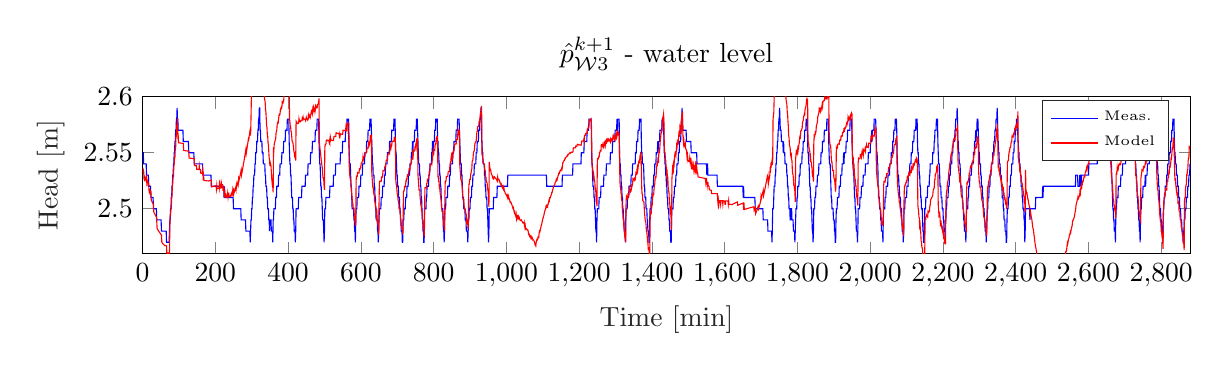
\begin{tikzpicture}

\begin{axis}[%
width=5.239in,
height=0.784in,
at={(1.209in,0.429in)},
scale only axis,
xmin=0,
xmax=2880,
xlabel style={font=\color{white!15!black}},
xlabel={Time [min]},
ymin=2.46,
ymax=2.6,
ylabel style={font=\color{white!15!black}},
ylabel={Head  [m]},
axis background/.style={fill=white},
title style={},
title={$\hat{p}^{k+1}_{\mathcal{W}3}$ - water level},
legend style={legend cell align=left, align=left, draw=white!15!black}
]
\addplot [color=blue]
  table[row sep=crcr]{%
1	2.55\\
2	2.55\\
3	2.54\\
4	2.54\\
5	2.54\\
6	2.54\\
7	2.54\\
8	2.54\\
9	2.54\\
10	2.54\\
11	2.53\\
12	2.53\\
13	2.53\\
14	2.53\\
15	2.53\\
16	2.53\\
17	2.52\\
18	2.52\\
19	2.52\\
20	2.52\\
21	2.52\\
22	2.52\\
23	2.51\\
24	2.51\\
25	2.51\\
26	2.51\\
27	2.51\\
28	2.51\\
29	2.51\\
30	2.5\\
31	2.5\\
32	2.5\\
33	2.5\\
34	2.5\\
35	2.5\\
36	2.5\\
37	2.5\\
38	2.5\\
39	2.49\\
40	2.49\\
41	2.49\\
42	2.49\\
43	2.49\\
44	2.49\\
45	2.49\\
46	2.49\\
47	2.49\\
48	2.49\\
49	2.49\\
50	2.49\\
51	2.49\\
52	2.48\\
53	2.48\\
54	2.48\\
55	2.48\\
56	2.48\\
57	2.48\\
58	2.48\\
59	2.48\\
60	2.48\\
61	2.48\\
62	2.48\\
63	2.48\\
64	2.48\\
65	2.48\\
66	2.47\\
67	2.47\\
68	2.47\\
69	2.47\\
70	2.47\\
71	2.47\\
72	2.47\\
73	2.47\\
74	2.48\\
75	2.49\\
76	2.49\\
77	2.5\\
78	2.5\\
79	2.51\\
80	2.51\\
81	2.52\\
82	2.52\\
83	2.53\\
84	2.53\\
85	2.54\\
86	2.54\\
87	2.55\\
88	2.55\\
89	2.56\\
90	2.56\\
91	2.57\\
92	2.57\\
93	2.58\\
94	2.58\\
95	2.59\\
96	2.58\\
97	2.58\\
98	2.57\\
99	2.57\\
100	2.57\\
101	2.57\\
102	2.57\\
103	2.57\\
104	2.57\\
105	2.57\\
106	2.57\\
107	2.57\\
108	2.57\\
109	2.57\\
110	2.57\\
111	2.57\\
112	2.56\\
113	2.56\\
114	2.56\\
115	2.56\\
116	2.56\\
117	2.56\\
118	2.56\\
119	2.56\\
120	2.56\\
121	2.56\\
122	2.56\\
123	2.56\\
124	2.56\\
125	2.56\\
126	2.56\\
127	2.55\\
128	2.55\\
129	2.55\\
130	2.55\\
131	2.55\\
132	2.55\\
133	2.55\\
134	2.55\\
135	2.55\\
136	2.55\\
137	2.55\\
138	2.55\\
139	2.55\\
140	2.55\\
141	2.55\\
142	2.54\\
143	2.54\\
144	2.54\\
145	2.54\\
146	2.54\\
147	2.54\\
148	2.54\\
149	2.54\\
150	2.54\\
151	2.54\\
152	2.54\\
153	2.54\\
154	2.54\\
155	2.54\\
156	2.54\\
157	2.54\\
158	2.54\\
159	2.54\\
160	2.54\\
161	2.54\\
162	2.54\\
163	2.54\\
164	2.54\\
165	2.54\\
166	2.53\\
167	2.53\\
168	2.53\\
169	2.53\\
170	2.53\\
171	2.53\\
172	2.53\\
173	2.53\\
174	2.53\\
175	2.53\\
176	2.53\\
177	2.53\\
178	2.53\\
179	2.53\\
180	2.53\\
181	2.53\\
182	2.53\\
183	2.53\\
184	2.53\\
185	2.53\\
186	2.53\\
187	2.53\\
188	2.53\\
189	2.52\\
190	2.52\\
191	2.52\\
192	2.52\\
193	2.52\\
194	2.52\\
195	2.52\\
196	2.52\\
197	2.52\\
198	2.52\\
199	2.52\\
200	2.52\\
201	2.52\\
202	2.52\\
203	2.52\\
204	2.52\\
205	2.52\\
206	2.52\\
207	2.52\\
208	2.52\\
209	2.52\\
210	2.52\\
211	2.52\\
212	2.52\\
213	2.52\\
214	2.52\\
215	2.52\\
216	2.52\\
217	2.52\\
218	2.52\\
219	2.52\\
220	2.52\\
221	2.52\\
222	2.52\\
223	2.52\\
224	2.51\\
225	2.52\\
226	2.51\\
227	2.51\\
228	2.51\\
229	2.51\\
230	2.51\\
231	2.51\\
232	2.51\\
233	2.51\\
234	2.51\\
235	2.51\\
236	2.51\\
237	2.51\\
238	2.51\\
239	2.51\\
240	2.51\\
241	2.51\\
242	2.51\\
243	2.51\\
244	2.51\\
245	2.51\\
246	2.51\\
247	2.51\\
248	2.51\\
249	2.51\\
250	2.5\\
251	2.5\\
252	2.5\\
253	2.5\\
254	2.5\\
255	2.5\\
256	2.5\\
257	2.5\\
258	2.5\\
259	2.5\\
260	2.5\\
261	2.5\\
262	2.5\\
263	2.5\\
264	2.5\\
265	2.5\\
266	2.5\\
267	2.5\\
268	2.5\\
269	2.5\\
270	2.5\\
271	2.49\\
272	2.49\\
273	2.49\\
274	2.49\\
275	2.49\\
276	2.49\\
277	2.49\\
278	2.49\\
279	2.49\\
280	2.49\\
281	2.49\\
282	2.49\\
283	2.49\\
284	2.48\\
285	2.48\\
286	2.48\\
287	2.48\\
288	2.48\\
289	2.48\\
290	2.48\\
291	2.48\\
292	2.48\\
293	2.48\\
294	2.48\\
295	2.48\\
296	2.47\\
297	2.48\\
298	2.49\\
299	2.49\\
300	2.5\\
301	2.5\\
302	2.51\\
303	2.51\\
304	2.52\\
305	2.52\\
306	2.53\\
307	2.53\\
308	2.53\\
309	2.54\\
310	2.54\\
311	2.55\\
312	2.55\\
313	2.55\\
314	2.56\\
315	2.56\\
316	2.56\\
317	2.57\\
318	2.57\\
319	2.58\\
320	2.58\\
321	2.59\\
322	2.59\\
323	2.57\\
324	2.57\\
325	2.56\\
326	2.56\\
327	2.56\\
328	2.56\\
329	2.55\\
330	2.55\\
331	2.55\\
332	2.54\\
333	2.54\\
334	2.54\\
335	2.54\\
336	2.54\\
337	2.53\\
338	2.53\\
339	2.52\\
340	2.52\\
341	2.52\\
342	2.51\\
343	2.51\\
344	2.5\\
345	2.5\\
346	2.5\\
347	2.49\\
348	2.49\\
349	2.48\\
350	2.49\\
351	2.49\\
352	2.49\\
353	2.49\\
354	2.48\\
355	2.48\\
356	2.48\\
357	2.48\\
358	2.47\\
359	2.49\\
360	2.49\\
361	2.5\\
362	2.5\\
363	2.5\\
364	2.5\\
365	2.5\\
366	2.51\\
367	2.51\\
368	2.51\\
369	2.52\\
370	2.52\\
371	2.52\\
372	2.52\\
373	2.52\\
374	2.53\\
375	2.53\\
376	2.53\\
377	2.53\\
378	2.54\\
379	2.54\\
380	2.54\\
381	2.54\\
382	2.54\\
383	2.55\\
384	2.55\\
385	2.55\\
386	2.55\\
387	2.55\\
388	2.56\\
389	2.56\\
390	2.56\\
391	2.56\\
392	2.56\\
393	2.57\\
394	2.57\\
395	2.57\\
396	2.57\\
397	2.57\\
398	2.58\\
399	2.58\\
400	2.58\\
401	2.58\\
402	2.58\\
403	2.56\\
404	2.55\\
405	2.54\\
406	2.54\\
407	2.53\\
408	2.53\\
409	2.52\\
410	2.51\\
411	2.51\\
412	2.51\\
413	2.5\\
414	2.5\\
415	2.49\\
416	2.49\\
417	2.48\\
418	2.48\\
419	2.48\\
420	2.47\\
421	2.48\\
422	2.5\\
423	2.5\\
424	2.5\\
425	2.5\\
426	2.5\\
427	2.5\\
428	2.5\\
429	2.51\\
430	2.51\\
431	2.51\\
432	2.51\\
433	2.51\\
434	2.51\\
435	2.51\\
436	2.51\\
437	2.51\\
438	2.52\\
439	2.52\\
440	2.52\\
441	2.52\\
442	2.52\\
443	2.52\\
444	2.52\\
445	2.52\\
446	2.52\\
447	2.52\\
448	2.53\\
449	2.53\\
450	2.53\\
451	2.53\\
452	2.53\\
453	2.53\\
454	2.53\\
455	2.54\\
456	2.54\\
457	2.54\\
458	2.54\\
459	2.54\\
460	2.54\\
461	2.54\\
462	2.55\\
463	2.55\\
464	2.55\\
465	2.55\\
466	2.55\\
467	2.56\\
468	2.56\\
469	2.56\\
470	2.56\\
471	2.56\\
472	2.56\\
473	2.56\\
474	2.56\\
475	2.57\\
476	2.57\\
477	2.57\\
478	2.57\\
479	2.57\\
480	2.58\\
481	2.58\\
482	2.58\\
483	2.58\\
484	2.58\\
485	2.56\\
486	2.55\\
487	2.54\\
488	2.54\\
489	2.53\\
490	2.52\\
491	2.52\\
492	2.51\\
493	2.51\\
494	2.5\\
495	2.49\\
496	2.49\\
497	2.49\\
498	2.48\\
499	2.47\\
500	2.48\\
501	2.5\\
502	2.5\\
503	2.5\\
504	2.51\\
505	2.51\\
506	2.51\\
507	2.51\\
508	2.51\\
509	2.51\\
510	2.51\\
511	2.51\\
512	2.51\\
513	2.51\\
514	2.51\\
515	2.52\\
516	2.52\\
517	2.52\\
518	2.52\\
519	2.52\\
520	2.52\\
521	2.52\\
522	2.52\\
523	2.52\\
524	2.52\\
525	2.53\\
526	2.53\\
527	2.53\\
528	2.53\\
529	2.53\\
530	2.53\\
531	2.54\\
532	2.54\\
533	2.54\\
534	2.54\\
535	2.54\\
536	2.54\\
537	2.54\\
538	2.54\\
539	2.54\\
540	2.54\\
541	2.54\\
542	2.54\\
543	2.54\\
544	2.55\\
545	2.55\\
546	2.55\\
547	2.55\\
548	2.55\\
549	2.55\\
550	2.56\\
551	2.56\\
552	2.56\\
553	2.56\\
554	2.56\\
555	2.56\\
556	2.56\\
557	2.56\\
558	2.57\\
559	2.57\\
560	2.57\\
561	2.57\\
562	2.58\\
563	2.58\\
564	2.58\\
565	2.58\\
566	2.58\\
567	2.56\\
568	2.55\\
569	2.54\\
570	2.54\\
571	2.54\\
572	2.53\\
573	2.52\\
574	2.52\\
575	2.51\\
576	2.5\\
577	2.5\\
578	2.5\\
579	2.5\\
580	2.5\\
581	2.49\\
582	2.49\\
583	2.48\\
584	2.48\\
585	2.47\\
586	2.49\\
587	2.5\\
588	2.5\\
589	2.5\\
590	2.51\\
591	2.51\\
592	2.51\\
593	2.51\\
594	2.51\\
595	2.52\\
596	2.52\\
597	2.52\\
598	2.52\\
599	2.52\\
600	2.53\\
601	2.53\\
602	2.53\\
603	2.53\\
604	2.53\\
605	2.54\\
606	2.54\\
607	2.54\\
608	2.54\\
609	2.54\\
610	2.54\\
611	2.55\\
612	2.55\\
613	2.55\\
614	2.55\\
615	2.55\\
616	2.56\\
617	2.56\\
618	2.56\\
619	2.56\\
620	2.57\\
621	2.57\\
622	2.57\\
623	2.57\\
624	2.57\\
625	2.58\\
626	2.58\\
627	2.58\\
628	2.58\\
629	2.57\\
630	2.56\\
631	2.55\\
632	2.54\\
633	2.54\\
634	2.53\\
635	2.53\\
636	2.53\\
637	2.52\\
638	2.52\\
639	2.51\\
640	2.51\\
641	2.5\\
642	2.49\\
643	2.5\\
644	2.49\\
645	2.49\\
646	2.48\\
647	2.48\\
648	2.47\\
649	2.48\\
650	2.49\\
651	2.5\\
652	2.5\\
653	2.5\\
654	2.5\\
655	2.5\\
656	2.51\\
657	2.51\\
658	2.51\\
659	2.51\\
660	2.52\\
661	2.52\\
662	2.52\\
663	2.52\\
664	2.52\\
665	2.53\\
666	2.53\\
667	2.53\\
668	2.54\\
669	2.54\\
670	2.54\\
671	2.54\\
672	2.54\\
673	2.55\\
674	2.55\\
675	2.55\\
676	2.55\\
677	2.55\\
678	2.55\\
679	2.56\\
680	2.56\\
681	2.56\\
682	2.56\\
683	2.56\\
684	2.56\\
685	2.57\\
686	2.57\\
687	2.57\\
688	2.57\\
689	2.57\\
690	2.57\\
691	2.58\\
692	2.58\\
693	2.58\\
694	2.58\\
695	2.56\\
696	2.55\\
697	2.55\\
698	2.54\\
699	2.53\\
700	2.53\\
701	2.52\\
702	2.52\\
703	2.52\\
704	2.51\\
705	2.51\\
706	2.51\\
707	2.5\\
708	2.5\\
709	2.49\\
710	2.49\\
711	2.48\\
712	2.48\\
713	2.48\\
714	2.47\\
715	2.47\\
716	2.49\\
717	2.49\\
718	2.49\\
719	2.5\\
720	2.5\\
721	2.5\\
722	2.5\\
723	2.51\\
724	2.51\\
725	2.51\\
726	2.51\\
727	2.52\\
728	2.52\\
729	2.52\\
730	2.52\\
731	2.53\\
732	2.53\\
733	2.53\\
734	2.53\\
735	2.54\\
736	2.54\\
737	2.54\\
738	2.54\\
739	2.55\\
740	2.55\\
741	2.55\\
742	2.56\\
743	2.55\\
744	2.56\\
745	2.56\\
746	2.56\\
747	2.56\\
748	2.57\\
749	2.57\\
750	2.57\\
751	2.57\\
752	2.57\\
753	2.58\\
754	2.58\\
755	2.58\\
756	2.57\\
757	2.56\\
758	2.55\\
759	2.54\\
760	2.54\\
761	2.54\\
762	2.53\\
763	2.53\\
764	2.52\\
765	2.52\\
766	2.51\\
767	2.51\\
768	2.5\\
769	2.49\\
770	2.49\\
771	2.48\\
772	2.48\\
773	2.47\\
774	2.47\\
775	2.5\\
776	2.5\\
777	2.5\\
778	2.5\\
779	2.5\\
780	2.51\\
781	2.51\\
782	2.52\\
783	2.52\\
784	2.52\\
785	2.52\\
786	2.52\\
787	2.53\\
788	2.53\\
789	2.53\\
790	2.54\\
791	2.54\\
792	2.54\\
793	2.54\\
794	2.54\\
795	2.55\\
796	2.55\\
797	2.56\\
798	2.56\\
799	2.55\\
800	2.56\\
801	2.56\\
802	2.56\\
803	2.57\\
804	2.57\\
805	2.57\\
806	2.58\\
807	2.58\\
808	2.58\\
809	2.58\\
810	2.58\\
811	2.56\\
812	2.56\\
813	2.55\\
814	2.55\\
815	2.54\\
816	2.54\\
817	2.53\\
818	2.53\\
819	2.52\\
820	2.52\\
821	2.51\\
822	2.5\\
823	2.5\\
824	2.5\\
825	2.5\\
826	2.49\\
827	2.48\\
828	2.48\\
829	2.47\\
830	2.48\\
831	2.5\\
832	2.5\\
833	2.5\\
834	2.51\\
835	2.51\\
836	2.51\\
837	2.51\\
838	2.51\\
839	2.52\\
840	2.52\\
841	2.52\\
842	2.52\\
843	2.52\\
844	2.53\\
845	2.53\\
846	2.53\\
847	2.54\\
848	2.54\\
849	2.54\\
850	2.54\\
851	2.54\\
852	2.54\\
853	2.55\\
854	2.55\\
855	2.55\\
856	2.56\\
857	2.56\\
858	2.56\\
859	2.56\\
860	2.56\\
861	2.56\\
862	2.57\\
863	2.57\\
864	2.57\\
865	2.57\\
866	2.58\\
867	2.58\\
868	2.58\\
869	2.58\\
870	2.58\\
871	2.57\\
872	2.56\\
873	2.55\\
874	2.54\\
875	2.54\\
876	2.54\\
877	2.53\\
878	2.53\\
879	2.52\\
880	2.51\\
881	2.51\\
882	2.51\\
883	2.5\\
884	2.5\\
885	2.5\\
886	2.5\\
887	2.49\\
888	2.49\\
889	2.49\\
890	2.48\\
891	2.48\\
892	2.48\\
893	2.48\\
894	2.47\\
895	2.48\\
896	2.49\\
897	2.49\\
898	2.5\\
899	2.5\\
900	2.5\\
901	2.51\\
902	2.51\\
903	2.51\\
904	2.51\\
905	2.52\\
906	2.52\\
907	2.52\\
908	2.53\\
909	2.53\\
910	2.53\\
911	2.53\\
912	2.54\\
913	2.54\\
914	2.54\\
915	2.54\\
916	2.54\\
917	2.55\\
918	2.55\\
919	2.55\\
920	2.56\\
921	2.56\\
922	2.56\\
923	2.56\\
924	2.57\\
925	2.57\\
926	2.57\\
927	2.58\\
928	2.58\\
929	2.58\\
930	2.59\\
931	2.59\\
932	2.56\\
933	2.56\\
934	2.55\\
935	2.55\\
936	2.54\\
937	2.54\\
938	2.54\\
939	2.54\\
940	2.53\\
941	2.53\\
942	2.52\\
943	2.52\\
944	2.51\\
945	2.51\\
946	2.51\\
947	2.5\\
948	2.5\\
949	2.49\\
950	2.48\\
951	2.47\\
952	2.48\\
953	2.5\\
954	2.5\\
955	2.5\\
956	2.5\\
957	2.5\\
958	2.5\\
959	2.5\\
960	2.5\\
961	2.5\\
962	2.5\\
963	2.5\\
964	2.5\\
965	2.51\\
966	2.51\\
967	2.51\\
968	2.51\\
969	2.51\\
970	2.51\\
971	2.51\\
972	2.51\\
973	2.51\\
974	2.51\\
975	2.52\\
976	2.52\\
977	2.52\\
978	2.52\\
979	2.52\\
980	2.52\\
981	2.52\\
982	2.52\\
983	2.52\\
984	2.52\\
985	2.52\\
986	2.52\\
987	2.52\\
988	2.52\\
989	2.52\\
990	2.52\\
991	2.52\\
992	2.52\\
993	2.52\\
994	2.52\\
995	2.52\\
996	2.52\\
997	2.52\\
998	2.52\\
999	2.52\\
1000	2.52\\
1001	2.52\\
1002	2.52\\
1003	2.52\\
1004	2.53\\
1005	2.53\\
1006	2.53\\
1007	2.53\\
1008	2.53\\
1009	2.53\\
1010	2.53\\
1011	2.53\\
1012	2.53\\
1013	2.53\\
1014	2.53\\
1015	2.53\\
1016	2.53\\
1017	2.53\\
1018	2.53\\
1019	2.53\\
1020	2.53\\
1021	2.53\\
1022	2.53\\
1023	2.53\\
1024	2.53\\
1025	2.53\\
1026	2.53\\
1027	2.53\\
1028	2.53\\
1029	2.53\\
1030	2.53\\
1031	2.53\\
1032	2.53\\
1033	2.53\\
1034	2.53\\
1035	2.53\\
1036	2.53\\
1037	2.53\\
1038	2.53\\
1039	2.53\\
1040	2.53\\
1041	2.53\\
1042	2.53\\
1043	2.53\\
1044	2.53\\
1045	2.53\\
1046	2.53\\
1047	2.53\\
1048	2.53\\
1049	2.53\\
1050	2.53\\
1051	2.53\\
1052	2.53\\
1053	2.53\\
1054	2.53\\
1055	2.53\\
1056	2.53\\
1057	2.53\\
1058	2.53\\
1059	2.53\\
1060	2.53\\
1061	2.53\\
1062	2.53\\
1063	2.53\\
1064	2.53\\
1065	2.53\\
1066	2.53\\
1067	2.53\\
1068	2.53\\
1069	2.53\\
1070	2.53\\
1071	2.53\\
1072	2.53\\
1073	2.53\\
1074	2.53\\
1075	2.53\\
1076	2.53\\
1077	2.53\\
1078	2.53\\
1079	2.53\\
1080	2.53\\
1081	2.53\\
1082	2.53\\
1083	2.53\\
1084	2.53\\
1085	2.53\\
1086	2.53\\
1087	2.53\\
1088	2.53\\
1089	2.53\\
1090	2.53\\
1091	2.53\\
1092	2.53\\
1093	2.53\\
1094	2.53\\
1095	2.53\\
1096	2.53\\
1097	2.53\\
1098	2.53\\
1099	2.53\\
1100	2.53\\
1101	2.53\\
1102	2.53\\
1103	2.53\\
1104	2.53\\
1105	2.53\\
1106	2.53\\
1107	2.53\\
1108	2.53\\
1109	2.53\\
1110	2.53\\
1111	2.52\\
1112	2.52\\
1113	2.52\\
1114	2.52\\
1115	2.52\\
1116	2.52\\
1117	2.52\\
1118	2.52\\
1119	2.52\\
1120	2.52\\
1121	2.52\\
1122	2.52\\
1123	2.52\\
1124	2.52\\
1125	2.52\\
1126	2.52\\
1127	2.52\\
1128	2.52\\
1129	2.52\\
1130	2.52\\
1131	2.52\\
1132	2.52\\
1133	2.52\\
1134	2.52\\
1135	2.52\\
1136	2.52\\
1137	2.52\\
1138	2.52\\
1139	2.52\\
1140	2.52\\
1141	2.52\\
1142	2.52\\
1143	2.52\\
1144	2.52\\
1145	2.52\\
1146	2.52\\
1147	2.52\\
1148	2.52\\
1149	2.52\\
1150	2.52\\
1151	2.52\\
1152	2.52\\
1153	2.52\\
1154	2.53\\
1155	2.53\\
1156	2.53\\
1157	2.53\\
1158	2.53\\
1159	2.53\\
1160	2.53\\
1161	2.53\\
1162	2.53\\
1163	2.53\\
1164	2.53\\
1165	2.53\\
1166	2.53\\
1167	2.53\\
1168	2.53\\
1169	2.53\\
1170	2.53\\
1171	2.53\\
1172	2.53\\
1173	2.53\\
1174	2.53\\
1175	2.53\\
1176	2.53\\
1177	2.53\\
1178	2.53\\
1179	2.53\\
1180	2.53\\
1181	2.53\\
1182	2.53\\
1183	2.54\\
1184	2.54\\
1185	2.54\\
1186	2.54\\
1187	2.54\\
1188	2.54\\
1189	2.54\\
1190	2.54\\
1191	2.54\\
1192	2.54\\
1193	2.54\\
1194	2.54\\
1195	2.54\\
1196	2.54\\
1197	2.54\\
1198	2.54\\
1199	2.54\\
1200	2.54\\
1201	2.54\\
1202	2.54\\
1203	2.54\\
1204	2.54\\
1205	2.54\\
1206	2.55\\
1207	2.55\\
1208	2.55\\
1209	2.55\\
1210	2.55\\
1211	2.55\\
1212	2.55\\
1213	2.55\\
1214	2.56\\
1215	2.56\\
1216	2.56\\
1217	2.56\\
1218	2.56\\
1219	2.56\\
1220	2.56\\
1221	2.56\\
1222	2.57\\
1223	2.57\\
1224	2.57\\
1225	2.57\\
1226	2.57\\
1227	2.58\\
1228	2.58\\
1229	2.58\\
1230	2.58\\
1231	2.58\\
1232	2.58\\
1233	2.58\\
1234	2.56\\
1235	2.54\\
1236	2.54\\
1237	2.53\\
1238	2.52\\
1239	2.52\\
1240	2.52\\
1241	2.51\\
1242	2.51\\
1243	2.5\\
1244	2.5\\
1245	2.49\\
1246	2.48\\
1247	2.48\\
1248	2.47\\
1249	2.49\\
1250	2.5\\
1251	2.5\\
1252	2.5\\
1253	2.5\\
1254	2.5\\
1255	2.51\\
1256	2.51\\
1257	2.51\\
1258	2.51\\
1259	2.51\\
1260	2.52\\
1261	2.52\\
1262	2.52\\
1263	2.52\\
1264	2.52\\
1265	2.52\\
1266	2.52\\
1267	2.52\\
1268	2.53\\
1269	2.53\\
1270	2.53\\
1271	2.53\\
1272	2.53\\
1273	2.53\\
1274	2.53\\
1275	2.54\\
1276	2.54\\
1277	2.54\\
1278	2.54\\
1279	2.54\\
1280	2.54\\
1281	2.54\\
1282	2.54\\
1283	2.54\\
1284	2.54\\
1285	2.54\\
1286	2.55\\
1287	2.55\\
1288	2.55\\
1289	2.55\\
1290	2.55\\
1291	2.55\\
1292	2.56\\
1293	2.56\\
1294	2.56\\
1295	2.56\\
1296	2.56\\
1297	2.56\\
1298	2.56\\
1299	2.57\\
1300	2.57\\
1301	2.57\\
1302	2.57\\
1303	2.57\\
1304	2.58\\
1305	2.57\\
1306	2.58\\
1307	2.58\\
1308	2.58\\
1309	2.58\\
1310	2.58\\
1311	2.55\\
1312	2.54\\
1313	2.54\\
1314	2.53\\
1315	2.53\\
1316	2.52\\
1317	2.52\\
1318	2.51\\
1319	2.51\\
1320	2.5\\
1321	2.5\\
1322	2.49\\
1323	2.49\\
1324	2.48\\
1325	2.48\\
1326	2.48\\
1327	2.47\\
1328	2.49\\
1329	2.5\\
1330	2.5\\
1331	2.5\\
1332	2.5\\
1333	2.51\\
1334	2.51\\
1335	2.51\\
1336	2.51\\
1337	2.52\\
1338	2.52\\
1339	2.52\\
1340	2.52\\
1341	2.52\\
1342	2.52\\
1343	2.53\\
1344	2.53\\
1345	2.53\\
1346	2.53\\
1347	2.54\\
1348	2.54\\
1349	2.54\\
1350	2.54\\
1351	2.54\\
1352	2.54\\
1353	2.54\\
1354	2.54\\
1355	2.55\\
1356	2.55\\
1357	2.55\\
1358	2.56\\
1359	2.56\\
1360	2.56\\
1361	2.56\\
1362	2.57\\
1363	2.57\\
1364	2.57\\
1365	2.57\\
1366	2.58\\
1367	2.58\\
1368	2.58\\
1369	2.58\\
1370	2.58\\
1371	2.56\\
1372	2.55\\
1373	2.55\\
1374	2.54\\
1375	2.54\\
1376	2.54\\
1377	2.54\\
1378	2.53\\
1379	2.52\\
1380	2.52\\
1381	2.51\\
1382	2.51\\
1383	2.51\\
1384	2.5\\
1385	2.5\\
1386	2.5\\
1387	2.49\\
1388	2.49\\
1389	2.48\\
1390	2.48\\
1391	2.48\\
1392	2.47\\
1393	2.47\\
1394	2.49\\
1395	2.5\\
1396	2.5\\
1397	2.5\\
1398	2.51\\
1399	2.51\\
1400	2.51\\
1401	2.52\\
1402	2.52\\
1403	2.52\\
1404	2.52\\
1405	2.53\\
1406	2.53\\
1407	2.53\\
1408	2.54\\
1409	2.54\\
1410	2.54\\
1411	2.54\\
1412	2.55\\
1413	2.55\\
1414	2.55\\
1415	2.55\\
1416	2.56\\
1417	2.55\\
1418	2.56\\
1419	2.56\\
1420	2.56\\
1421	2.56\\
1422	2.57\\
1423	2.57\\
1424	2.57\\
1425	2.57\\
1426	2.57\\
1427	2.57\\
1428	2.58\\
1429	2.58\\
1430	2.58\\
1431	2.58\\
1432	2.58\\
1433	2.56\\
1434	2.55\\
1435	2.55\\
1436	2.54\\
1437	2.54\\
1438	2.53\\
1439	2.53\\
1440	2.52\\
1441	2.52\\
1442	2.51\\
1443	2.51\\
1444	2.5\\
1445	2.5\\
1446	2.5\\
1447	2.49\\
1448	2.49\\
1449	2.48\\
1450	2.48\\
1451	2.48\\
1452	2.47\\
1453	2.47\\
1454	2.49\\
1455	2.5\\
1456	2.5\\
1457	2.5\\
1458	2.5\\
1459	2.51\\
1460	2.51\\
1461	2.51\\
1462	2.52\\
1463	2.52\\
1464	2.52\\
1465	2.52\\
1466	2.53\\
1467	2.53\\
1468	2.53\\
1469	2.54\\
1470	2.54\\
1471	2.54\\
1472	2.54\\
1473	2.55\\
1474	2.55\\
1475	2.55\\
1476	2.56\\
1477	2.56\\
1478	2.56\\
1479	2.56\\
1480	2.57\\
1481	2.58\\
1482	2.58\\
1483	2.59\\
1484	2.58\\
1485	2.57\\
1486	2.57\\
1487	2.57\\
1488	2.57\\
1489	2.57\\
1490	2.57\\
1491	2.57\\
1492	2.57\\
1493	2.57\\
1494	2.57\\
1495	2.56\\
1496	2.56\\
1497	2.56\\
1498	2.56\\
1499	2.56\\
1500	2.56\\
1501	2.56\\
1502	2.56\\
1503	2.56\\
1504	2.56\\
1505	2.56\\
1506	2.56\\
1507	2.56\\
1508	2.55\\
1509	2.55\\
1510	2.55\\
1511	2.55\\
1512	2.55\\
1513	2.55\\
1514	2.55\\
1515	2.55\\
1516	2.55\\
1517	2.55\\
1518	2.55\\
1519	2.55\\
1520	2.55\\
1521	2.55\\
1522	2.55\\
1523	2.55\\
1524	2.54\\
1525	2.54\\
1526	2.54\\
1527	2.54\\
1528	2.54\\
1529	2.54\\
1530	2.54\\
1531	2.54\\
1532	2.54\\
1533	2.54\\
1534	2.54\\
1535	2.54\\
1536	2.54\\
1537	2.54\\
1538	2.54\\
1539	2.54\\
1540	2.54\\
1541	2.54\\
1542	2.54\\
1543	2.54\\
1544	2.54\\
1545	2.54\\
1546	2.54\\
1547	2.54\\
1548	2.54\\
1549	2.54\\
1550	2.54\\
1551	2.53\\
1552	2.54\\
1553	2.54\\
1554	2.53\\
1555	2.53\\
1556	2.53\\
1557	2.53\\
1558	2.53\\
1559	2.53\\
1560	2.53\\
1561	2.53\\
1562	2.53\\
1563	2.53\\
1564	2.53\\
1565	2.53\\
1566	2.53\\
1567	2.53\\
1568	2.53\\
1569	2.53\\
1570	2.53\\
1571	2.53\\
1572	2.53\\
1573	2.53\\
1574	2.53\\
1575	2.53\\
1576	2.53\\
1577	2.53\\
1578	2.53\\
1579	2.53\\
1580	2.52\\
1581	2.52\\
1582	2.52\\
1583	2.52\\
1584	2.52\\
1585	2.52\\
1586	2.52\\
1587	2.52\\
1588	2.52\\
1589	2.52\\
1590	2.52\\
1591	2.52\\
1592	2.52\\
1593	2.52\\
1594	2.52\\
1595	2.52\\
1596	2.52\\
1597	2.52\\
1598	2.52\\
1599	2.52\\
1600	2.52\\
1601	2.52\\
1602	2.52\\
1603	2.52\\
1604	2.52\\
1605	2.52\\
1606	2.52\\
1607	2.52\\
1608	2.52\\
1609	2.52\\
1610	2.52\\
1611	2.52\\
1612	2.52\\
1613	2.52\\
1614	2.52\\
1615	2.52\\
1616	2.52\\
1617	2.52\\
1618	2.52\\
1619	2.52\\
1620	2.52\\
1621	2.52\\
1622	2.52\\
1623	2.52\\
1624	2.52\\
1625	2.52\\
1626	2.52\\
1627	2.52\\
1628	2.52\\
1629	2.52\\
1630	2.52\\
1631	2.52\\
1632	2.52\\
1633	2.52\\
1634	2.52\\
1635	2.52\\
1636	2.52\\
1637	2.52\\
1638	2.52\\
1639	2.52\\
1640	2.52\\
1641	2.52\\
1642	2.52\\
1643	2.52\\
1644	2.52\\
1645	2.52\\
1646	2.52\\
1647	2.52\\
1648	2.52\\
1649	2.52\\
1650	2.52\\
1651	2.51\\
1652	2.52\\
1653	2.51\\
1654	2.51\\
1655	2.51\\
1656	2.51\\
1657	2.51\\
1658	2.51\\
1659	2.51\\
1660	2.51\\
1661	2.51\\
1662	2.51\\
1663	2.51\\
1664	2.51\\
1665	2.51\\
1666	2.51\\
1667	2.51\\
1668	2.51\\
1669	2.51\\
1670	2.51\\
1671	2.51\\
1672	2.51\\
1673	2.51\\
1674	2.51\\
1675	2.51\\
1676	2.51\\
1677	2.51\\
1678	2.51\\
1679	2.51\\
1680	2.51\\
1681	2.51\\
1682	2.51\\
1683	2.51\\
1684	2.5\\
1685	2.5\\
1686	2.5\\
1687	2.5\\
1688	2.5\\
1689	2.5\\
1690	2.5\\
1691	2.5\\
1692	2.5\\
1693	2.5\\
1694	2.5\\
1695	2.5\\
1696	2.5\\
1697	2.5\\
1698	2.5\\
1699	2.5\\
1700	2.5\\
1701	2.5\\
1702	2.5\\
1703	2.5\\
1704	2.5\\
1705	2.5\\
1706	2.49\\
1707	2.49\\
1708	2.49\\
1709	2.49\\
1710	2.49\\
1711	2.49\\
1712	2.49\\
1713	2.49\\
1714	2.49\\
1715	2.49\\
1716	2.49\\
1717	2.49\\
1718	2.49\\
1719	2.48\\
1720	2.48\\
1721	2.48\\
1722	2.48\\
1723	2.48\\
1724	2.48\\
1725	2.48\\
1726	2.48\\
1727	2.48\\
1728	2.48\\
1729	2.48\\
1730	2.47\\
1731	2.48\\
1732	2.5\\
1733	2.5\\
1734	2.5\\
1735	2.51\\
1736	2.52\\
1737	2.52\\
1738	2.52\\
1739	2.53\\
1740	2.53\\
1741	2.54\\
1742	2.54\\
1743	2.55\\
1744	2.55\\
1745	2.56\\
1746	2.56\\
1747	2.57\\
1748	2.57\\
1749	2.58\\
1750	2.58\\
1751	2.59\\
1752	2.58\\
1753	2.57\\
1754	2.57\\
1755	2.57\\
1756	2.56\\
1757	2.56\\
1758	2.56\\
1759	2.56\\
1760	2.56\\
1761	2.55\\
1762	2.56\\
1763	2.55\\
1764	2.55\\
1765	2.55\\
1766	2.54\\
1767	2.54\\
1768	2.54\\
1769	2.54\\
1770	2.54\\
1771	2.53\\
1772	2.53\\
1773	2.52\\
1774	2.52\\
1775	2.51\\
1776	2.51\\
1777	2.5\\
1778	2.5\\
1779	2.5\\
1780	2.49\\
1781	2.49\\
1782	2.5\\
1783	2.5\\
1784	2.5\\
1785	2.49\\
1786	2.49\\
1787	2.49\\
1788	2.49\\
1789	2.48\\
1790	2.48\\
1791	2.48\\
1792	2.48\\
1793	2.47\\
1794	2.48\\
1795	2.49\\
1796	2.5\\
1797	2.5\\
1798	2.5\\
1799	2.51\\
1800	2.51\\
1801	2.52\\
1802	2.52\\
1803	2.52\\
1804	2.52\\
1805	2.53\\
1806	2.53\\
1807	2.53\\
1808	2.54\\
1809	2.54\\
1810	2.54\\
1811	2.54\\
1812	2.54\\
1813	2.55\\
1814	2.55\\
1815	2.55\\
1816	2.56\\
1817	2.56\\
1818	2.56\\
1819	2.56\\
1820	2.57\\
1821	2.57\\
1822	2.57\\
1823	2.57\\
1824	2.58\\
1825	2.58\\
1826	2.58\\
1827	2.58\\
1828	2.56\\
1829	2.55\\
1830	2.55\\
1831	2.54\\
1832	2.54\\
1833	2.53\\
1834	2.52\\
1835	2.52\\
1836	2.51\\
1837	2.51\\
1838	2.5\\
1839	2.5\\
1840	2.49\\
1841	2.48\\
1842	2.48\\
1843	2.47\\
1844	2.48\\
1845	2.5\\
1846	2.5\\
1847	2.5\\
1848	2.51\\
1849	2.51\\
1850	2.51\\
1851	2.52\\
1852	2.52\\
1853	2.52\\
1854	2.52\\
1855	2.53\\
1856	2.53\\
1857	2.53\\
1858	2.53\\
1859	2.54\\
1860	2.54\\
1861	2.54\\
1862	2.54\\
1863	2.54\\
1864	2.54\\
1865	2.55\\
1866	2.55\\
1867	2.55\\
1868	2.55\\
1869	2.56\\
1870	2.56\\
1871	2.56\\
1872	2.56\\
1873	2.56\\
1874	2.57\\
1875	2.57\\
1876	2.57\\
1877	2.57\\
1878	2.57\\
1879	2.57\\
1880	2.57\\
1881	2.58\\
1882	2.58\\
1883	2.58\\
1884	2.58\\
1885	2.58\\
1886	2.56\\
1887	2.55\\
1888	2.54\\
1889	2.54\\
1890	2.54\\
1891	2.53\\
1892	2.52\\
1893	2.51\\
1894	2.51\\
1895	2.5\\
1896	2.5\\
1897	2.5\\
1898	2.5\\
1899	2.49\\
1900	2.49\\
1901	2.49\\
1902	2.48\\
1903	2.48\\
1904	2.47\\
1905	2.47\\
1906	2.49\\
1907	2.5\\
1908	2.5\\
1909	2.5\\
1910	2.51\\
1911	2.51\\
1912	2.51\\
1913	2.51\\
1914	2.51\\
1915	2.52\\
1916	2.52\\
1917	2.52\\
1918	2.52\\
1919	2.53\\
1920	2.53\\
1921	2.53\\
1922	2.53\\
1923	2.54\\
1924	2.54\\
1925	2.54\\
1926	2.54\\
1927	2.55\\
1928	2.54\\
1929	2.55\\
1930	2.55\\
1931	2.55\\
1932	2.55\\
1933	2.55\\
1934	2.56\\
1935	2.56\\
1936	2.56\\
1937	2.56\\
1938	2.57\\
1939	2.57\\
1940	2.57\\
1941	2.57\\
1942	2.57\\
1943	2.57\\
1944	2.57\\
1945	2.58\\
1946	2.58\\
1947	2.58\\
1948	2.58\\
1949	2.58\\
1950	2.56\\
1951	2.55\\
1952	2.54\\
1953	2.54\\
1954	2.53\\
1955	2.53\\
1956	2.52\\
1957	2.51\\
1958	2.51\\
1959	2.5\\
1960	2.5\\
1961	2.49\\
1962	2.48\\
1963	2.48\\
1964	2.48\\
1965	2.47\\
1966	2.48\\
1967	2.5\\
1968	2.5\\
1969	2.5\\
1970	2.5\\
1971	2.5\\
1972	2.51\\
1973	2.51\\
1974	2.51\\
1975	2.51\\
1976	2.52\\
1977	2.52\\
1978	2.52\\
1979	2.52\\
1980	2.52\\
1981	2.53\\
1982	2.53\\
1983	2.53\\
1984	2.53\\
1985	2.53\\
1986	2.53\\
1987	2.54\\
1988	2.54\\
1989	2.54\\
1990	2.54\\
1991	2.54\\
1992	2.54\\
1993	2.54\\
1994	2.54\\
1995	2.55\\
1996	2.55\\
1997	2.55\\
1998	2.55\\
1999	2.55\\
2000	2.55\\
2001	2.56\\
2002	2.56\\
2003	2.56\\
2004	2.57\\
2005	2.56\\
2006	2.57\\
2007	2.57\\
2008	2.57\\
2009	2.57\\
2010	2.57\\
2011	2.58\\
2012	2.58\\
2013	2.58\\
2014	2.58\\
2015	2.58\\
2016	2.57\\
2017	2.56\\
2018	2.55\\
2019	2.55\\
2020	2.54\\
2021	2.54\\
2022	2.52\\
2023	2.52\\
2024	2.51\\
2025	2.51\\
2026	2.5\\
2027	2.5\\
2028	2.5\\
2029	2.49\\
2030	2.49\\
2031	2.48\\
2032	2.48\\
2033	2.48\\
2034	2.48\\
2035	2.47\\
2036	2.49\\
2037	2.5\\
2038	2.5\\
2039	2.5\\
2040	2.5\\
2041	2.51\\
2042	2.51\\
2043	2.51\\
2044	2.52\\
2045	2.52\\
2046	2.52\\
2047	2.52\\
2048	2.52\\
2049	2.53\\
2050	2.53\\
2051	2.53\\
2052	2.53\\
2053	2.53\\
2054	2.54\\
2055	2.54\\
2056	2.54\\
2057	2.54\\
2058	2.55\\
2059	2.55\\
2060	2.55\\
2061	2.55\\
2062	2.56\\
2063	2.56\\
2064	2.56\\
2065	2.57\\
2066	2.57\\
2067	2.57\\
2068	2.57\\
2069	2.58\\
2070	2.58\\
2071	2.58\\
2072	2.58\\
2073	2.57\\
2074	2.55\\
2075	2.54\\
2076	2.53\\
2077	2.53\\
2078	2.53\\
2079	2.52\\
2080	2.52\\
2081	2.51\\
2082	2.51\\
2083	2.51\\
2084	2.5\\
2085	2.5\\
2086	2.5\\
2087	2.49\\
2088	2.48\\
2089	2.48\\
2090	2.48\\
2091	2.47\\
2092	2.48\\
2093	2.5\\
2094	2.5\\
2095	2.5\\
2096	2.51\\
2097	2.51\\
2098	2.51\\
2099	2.51\\
2100	2.51\\
2101	2.52\\
2102	2.52\\
2103	2.52\\
2104	2.52\\
2105	2.53\\
2106	2.53\\
2107	2.53\\
2108	2.53\\
2109	2.54\\
2110	2.54\\
2111	2.54\\
2112	2.54\\
2113	2.55\\
2114	2.55\\
2115	2.55\\
2116	2.55\\
2117	2.56\\
2118	2.56\\
2119	2.56\\
2120	2.56\\
2121	2.57\\
2122	2.57\\
2123	2.57\\
2124	2.57\\
2125	2.57\\
2126	2.58\\
2127	2.58\\
2128	2.58\\
2129	2.58\\
2130	2.56\\
2131	2.55\\
2132	2.55\\
2133	2.54\\
2134	2.54\\
2135	2.53\\
2136	2.53\\
2137	2.52\\
2138	2.52\\
2139	2.51\\
2140	2.51\\
2141	2.5\\
2142	2.5\\
2143	2.5\\
2144	2.49\\
2145	2.48\\
2146	2.48\\
2147	2.47\\
2148	2.47\\
2149	2.48\\
2150	2.5\\
2151	2.5\\
2152	2.5\\
2153	2.51\\
2154	2.51\\
2155	2.51\\
2156	2.51\\
2157	2.51\\
2158	2.52\\
2159	2.52\\
2160	2.52\\
2161	2.52\\
2162	2.52\\
2163	2.53\\
2164	2.53\\
2165	2.54\\
2166	2.54\\
2167	2.54\\
2168	2.54\\
2169	2.54\\
2170	2.54\\
2171	2.54\\
2172	2.55\\
2173	2.55\\
2174	2.55\\
2175	2.55\\
2176	2.56\\
2177	2.56\\
2178	2.57\\
2179	2.57\\
2180	2.57\\
2181	2.57\\
2182	2.58\\
2183	2.58\\
2184	2.58\\
2185	2.58\\
2186	2.56\\
2187	2.55\\
2188	2.54\\
2189	2.54\\
2190	2.54\\
2191	2.53\\
2192	2.52\\
2193	2.52\\
2194	2.52\\
2195	2.51\\
2196	2.51\\
2197	2.51\\
2198	2.5\\
2199	2.5\\
2200	2.5\\
2201	2.49\\
2202	2.49\\
2203	2.48\\
2204	2.48\\
2205	2.48\\
2206	2.47\\
2207	2.49\\
2208	2.49\\
2209	2.5\\
2210	2.5\\
2211	2.51\\
2212	2.51\\
2213	2.51\\
2214	2.51\\
2215	2.52\\
2216	2.52\\
2217	2.52\\
2218	2.53\\
2219	2.53\\
2220	2.53\\
2221	2.54\\
2222	2.54\\
2223	2.54\\
2224	2.54\\
2225	2.55\\
2226	2.55\\
2227	2.55\\
2228	2.56\\
2229	2.56\\
2230	2.56\\
2231	2.56\\
2232	2.56\\
2233	2.57\\
2234	2.57\\
2235	2.58\\
2236	2.58\\
2237	2.58\\
2238	2.58\\
2239	2.59\\
2240	2.58\\
2241	2.56\\
2242	2.56\\
2243	2.55\\
2244	2.55\\
2245	2.54\\
2246	2.54\\
2247	2.54\\
2248	2.53\\
2249	2.52\\
2250	2.52\\
2251	2.52\\
2252	2.52\\
2253	2.51\\
2254	2.51\\
2255	2.5\\
2256	2.5\\
2257	2.49\\
2258	2.49\\
2259	2.48\\
2260	2.48\\
2261	2.48\\
2262	2.48\\
2263	2.47\\
2264	2.49\\
2265	2.5\\
2266	2.5\\
2267	2.5\\
2268	2.5\\
2269	2.51\\
2270	2.51\\
2271	2.52\\
2272	2.52\\
2273	2.52\\
2274	2.53\\
2275	2.53\\
2276	2.53\\
2277	2.53\\
2278	2.53\\
2279	2.54\\
2280	2.54\\
2281	2.54\\
2282	2.54\\
2283	2.54\\
2284	2.55\\
2285	2.55\\
2286	2.55\\
2287	2.56\\
2288	2.56\\
2289	2.56\\
2290	2.57\\
2291	2.56\\
2292	2.57\\
2293	2.57\\
2294	2.58\\
2295	2.58\\
2296	2.58\\
2297	2.57\\
2298	2.56\\
2299	2.55\\
2300	2.55\\
2301	2.54\\
2302	2.54\\
2303	2.54\\
2304	2.53\\
2305	2.53\\
2306	2.52\\
2307	2.52\\
2308	2.52\\
2309	2.51\\
2310	2.51\\
2311	2.5\\
2312	2.5\\
2313	2.5\\
2314	2.49\\
2315	2.49\\
2316	2.48\\
2317	2.48\\
2318	2.48\\
2319	2.47\\
2320	2.48\\
2321	2.49\\
2322	2.5\\
2323	2.5\\
2324	2.51\\
2325	2.51\\
2326	2.51\\
2327	2.52\\
2328	2.52\\
2329	2.52\\
2330	2.53\\
2331	2.53\\
2332	2.53\\
2333	2.54\\
2334	2.54\\
2335	2.54\\
2336	2.54\\
2337	2.55\\
2338	2.55\\
2339	2.55\\
2340	2.56\\
2341	2.56\\
2342	2.56\\
2343	2.57\\
2344	2.57\\
2345	2.57\\
2346	2.58\\
2347	2.58\\
2348	2.58\\
2349	2.59\\
2350	2.58\\
2351	2.56\\
2352	2.56\\
2353	2.55\\
2354	2.55\\
2355	2.54\\
2356	2.54\\
2357	2.54\\
2358	2.53\\
2359	2.53\\
2360	2.53\\
2361	2.52\\
2362	2.52\\
2363	2.51\\
2364	2.51\\
2365	2.51\\
2366	2.5\\
2367	2.5\\
2368	2.49\\
2369	2.49\\
2370	2.49\\
2371	2.48\\
2372	2.48\\
2373	2.48\\
2374	2.47\\
2375	2.47\\
2376	2.49\\
2377	2.5\\
2378	2.5\\
2379	2.5\\
2380	2.51\\
2381	2.51\\
2382	2.51\\
2383	2.52\\
2384	2.52\\
2385	2.52\\
2386	2.53\\
2387	2.53\\
2388	2.53\\
2389	2.54\\
2390	2.54\\
2391	2.54\\
2392	2.54\\
2393	2.55\\
2394	2.55\\
2395	2.55\\
2396	2.56\\
2397	2.56\\
2398	2.56\\
2399	2.57\\
2400	2.57\\
2401	2.57\\
2402	2.58\\
2403	2.58\\
2404	2.58\\
2405	2.58\\
2406	2.56\\
2407	2.56\\
2408	2.55\\
2409	2.55\\
2410	2.54\\
2411	2.54\\
2412	2.54\\
2413	2.53\\
2414	2.53\\
2415	2.52\\
2416	2.52\\
2417	2.52\\
2418	2.51\\
2419	2.51\\
2420	2.5\\
2421	2.5\\
2422	2.5\\
2423	2.49\\
2424	2.49\\
2425	2.47\\
2426	2.48\\
2427	2.5\\
2428	2.5\\
2429	2.5\\
2430	2.5\\
2431	2.5\\
2432	2.5\\
2433	2.5\\
2434	2.5\\
2435	2.5\\
2436	2.5\\
2437	2.5\\
2438	2.5\\
2439	2.49\\
2440	2.5\\
2441	2.5\\
2442	2.5\\
2443	2.5\\
2444	2.5\\
2445	2.5\\
2446	2.5\\
2447	2.5\\
2448	2.5\\
2449	2.5\\
2450	2.5\\
2451	2.5\\
2452	2.5\\
2453	2.5\\
2454	2.5\\
2455	2.51\\
2456	2.51\\
2457	2.51\\
2458	2.51\\
2459	2.51\\
2460	2.51\\
2461	2.51\\
2462	2.51\\
2463	2.51\\
2464	2.51\\
2465	2.51\\
2466	2.51\\
2467	2.51\\
2468	2.51\\
2469	2.51\\
2470	2.51\\
2471	2.51\\
2472	2.51\\
2473	2.51\\
2474	2.52\\
2475	2.51\\
2476	2.52\\
2477	2.52\\
2478	2.52\\
2479	2.52\\
2480	2.52\\
2481	2.52\\
2482	2.52\\
2483	2.52\\
2484	2.52\\
2485	2.52\\
2486	2.52\\
2487	2.52\\
2488	2.52\\
2489	2.52\\
2490	2.52\\
2491	2.52\\
2492	2.52\\
2493	2.52\\
2494	2.52\\
2495	2.52\\
2496	2.52\\
2497	2.52\\
2498	2.52\\
2499	2.52\\
2500	2.52\\
2501	2.52\\
2502	2.52\\
2503	2.52\\
2504	2.52\\
2505	2.52\\
2506	2.52\\
2507	2.52\\
2508	2.52\\
2509	2.52\\
2510	2.52\\
2511	2.52\\
2512	2.52\\
2513	2.52\\
2514	2.52\\
2515	2.52\\
2516	2.52\\
2517	2.52\\
2518	2.52\\
2519	2.52\\
2520	2.52\\
2521	2.52\\
2522	2.52\\
2523	2.52\\
2524	2.52\\
2525	2.52\\
2526	2.52\\
2527	2.52\\
2528	2.52\\
2529	2.52\\
2530	2.52\\
2531	2.52\\
2532	2.52\\
2533	2.52\\
2534	2.52\\
2535	2.52\\
2536	2.52\\
2537	2.52\\
2538	2.52\\
2539	2.52\\
2540	2.52\\
2541	2.52\\
2542	2.52\\
2543	2.52\\
2544	2.52\\
2545	2.52\\
2546	2.52\\
2547	2.52\\
2548	2.52\\
2549	2.52\\
2550	2.52\\
2551	2.52\\
2552	2.52\\
2553	2.52\\
2554	2.52\\
2555	2.52\\
2556	2.52\\
2557	2.52\\
2558	2.52\\
2559	2.52\\
2560	2.52\\
2561	2.52\\
2562	2.52\\
2563	2.52\\
2564	2.52\\
2565	2.53\\
2566	2.53\\
2567	2.53\\
2568	2.53\\
2569	2.53\\
2570	2.53\\
2571	2.52\\
2572	2.52\\
2573	2.52\\
2574	2.52\\
2575	2.52\\
2576	2.53\\
2577	2.52\\
2578	2.53\\
2579	2.53\\
2580	2.52\\
2581	2.53\\
2582	2.53\\
2583	2.53\\
2584	2.53\\
2585	2.53\\
2586	2.53\\
2587	2.53\\
2588	2.53\\
2589	2.53\\
2590	2.53\\
2591	2.53\\
2592	2.53\\
2593	2.53\\
2594	2.53\\
2595	2.53\\
2596	2.53\\
2597	2.53\\
2598	2.53\\
2599	2.53\\
2600	2.53\\
2601	2.54\\
2602	2.54\\
2603	2.54\\
2604	2.54\\
2605	2.54\\
2606	2.54\\
2607	2.54\\
2608	2.54\\
2609	2.54\\
2610	2.54\\
2611	2.54\\
2612	2.54\\
2613	2.54\\
2614	2.54\\
2615	2.54\\
2616	2.54\\
2617	2.54\\
2618	2.54\\
2619	2.54\\
2620	2.54\\
2621	2.54\\
2622	2.54\\
2623	2.54\\
2624	2.54\\
2625	2.55\\
2626	2.55\\
2627	2.55\\
2628	2.55\\
2629	2.55\\
2630	2.55\\
2631	2.55\\
2632	2.55\\
2633	2.55\\
2634	2.56\\
2635	2.56\\
2636	2.56\\
2637	2.56\\
2638	2.56\\
2639	2.56\\
2640	2.56\\
2641	2.56\\
2642	2.56\\
2643	2.56\\
2644	2.56\\
2645	2.56\\
2646	2.56\\
2647	2.56\\
2648	2.56\\
2649	2.57\\
2650	2.57\\
2651	2.57\\
2652	2.57\\
2653	2.57\\
2654	2.57\\
2655	2.58\\
2656	2.58\\
2657	2.58\\
2658	2.58\\
2659	2.58\\
2660	2.58\\
2661	2.56\\
2662	2.54\\
2663	2.54\\
2664	2.53\\
2665	2.52\\
2666	2.51\\
2667	2.5\\
2668	2.5\\
2669	2.49\\
2670	2.49\\
2671	2.48\\
2672	2.48\\
2673	2.48\\
2674	2.47\\
2675	2.49\\
2676	2.5\\
2677	2.5\\
2678	2.51\\
2679	2.51\\
2680	2.51\\
2681	2.51\\
2682	2.52\\
2683	2.52\\
2684	2.52\\
2685	2.52\\
2686	2.52\\
2687	2.52\\
2688	2.52\\
2689	2.53\\
2690	2.53\\
2691	2.53\\
2692	2.53\\
2693	2.53\\
2694	2.54\\
2695	2.54\\
2696	2.54\\
2697	2.54\\
2698	2.54\\
2699	2.54\\
2700	2.54\\
2701	2.54\\
2702	2.54\\
2703	2.55\\
2704	2.55\\
2705	2.55\\
2706	2.55\\
2707	2.55\\
2708	2.55\\
2709	2.55\\
2710	2.56\\
2711	2.56\\
2712	2.56\\
2713	2.56\\
2714	2.56\\
2715	2.56\\
2716	2.57\\
2717	2.57\\
2718	2.57\\
2719	2.57\\
2720	2.57\\
2721	2.57\\
2722	2.57\\
2723	2.58\\
2724	2.58\\
2725	2.58\\
2726	2.58\\
2727	2.58\\
2728	2.56\\
2729	2.54\\
2730	2.54\\
2731	2.53\\
2732	2.53\\
2733	2.52\\
2734	2.51\\
2735	2.51\\
2736	2.5\\
2737	2.5\\
2738	2.49\\
2739	2.49\\
2740	2.48\\
2741	2.48\\
2742	2.47\\
2743	2.49\\
2744	2.5\\
2745	2.5\\
2746	2.51\\
2747	2.51\\
2748	2.51\\
2749	2.51\\
2750	2.52\\
2751	2.52\\
2752	2.52\\
2753	2.52\\
2754	2.52\\
2755	2.52\\
2756	2.53\\
2757	2.52\\
2758	2.53\\
2759	2.53\\
2760	2.53\\
2761	2.53\\
2762	2.54\\
2763	2.54\\
2764	2.54\\
2765	2.54\\
2766	2.54\\
2767	2.54\\
2768	2.55\\
2769	2.55\\
2770	2.55\\
2771	2.55\\
2772	2.55\\
2773	2.56\\
2774	2.56\\
2775	2.56\\
2776	2.56\\
2777	2.57\\
2778	2.57\\
2779	2.57\\
2780	2.57\\
2781	2.58\\
2782	2.58\\
2783	2.58\\
2784	2.58\\
2785	2.58\\
2786	2.58\\
2787	2.56\\
2788	2.55\\
2789	2.54\\
2790	2.54\\
2791	2.53\\
2792	2.53\\
2793	2.52\\
2794	2.52\\
2795	2.51\\
2796	2.5\\
2797	2.5\\
2798	2.5\\
2799	2.49\\
2800	2.49\\
2801	2.48\\
2802	2.48\\
2803	2.48\\
2804	2.47\\
2805	2.49\\
2806	2.5\\
2807	2.5\\
2808	2.51\\
2809	2.51\\
2810	2.51\\
2811	2.52\\
2812	2.52\\
2813	2.52\\
2814	2.52\\
2815	2.53\\
2816	2.53\\
2817	2.53\\
2818	2.54\\
2819	2.54\\
2820	2.54\\
2821	2.54\\
2822	2.55\\
2823	2.55\\
2824	2.55\\
2825	2.55\\
2826	2.56\\
2827	2.56\\
2828	2.56\\
2829	2.57\\
2830	2.57\\
2831	2.57\\
2832	2.58\\
2833	2.58\\
2834	2.58\\
2835	2.58\\
2836	2.56\\
2837	2.55\\
2838	2.55\\
2839	2.54\\
2840	2.54\\
2841	2.54\\
2842	2.53\\
2843	2.53\\
2844	2.53\\
2845	2.52\\
2846	2.52\\
2847	2.52\\
2848	2.51\\
2849	2.51\\
2850	2.51\\
2851	2.5\\
2852	2.5\\
2853	2.5\\
2854	2.49\\
2855	2.49\\
2856	2.49\\
2857	2.48\\
2858	2.48\\
2859	2.48\\
2860	2.47\\
2861	2.47\\
2862	2.47\\
2863	2.49\\
2864	2.49\\
2865	2.49\\
2866	2.5\\
2867	2.5\\
2868	2.5\\
2869	2.51\\
2870	2.51\\
2871	2.51\\
2872	2.51\\
2873	2.52\\
2874	2.52\\
2875	2.52\\
2876	2.53\\
2877	2.53\\
2878	2.53\\
2879	2.54\\
};
\addlegendentry{\tiny Meas.}

\addplot [color=red]
  table[row sep=crcr]{%
1	2.53265713562723\\
2	2.53481748956256\\
3	2.53390292369295\\
4	2.52683654462453\\
5	2.52593971951865\\
6	2.52814284502529\\
7	2.52726616163272\\
8	2.52639921219088\\
9	2.52554202347528\\
10	2.52778581774328\\
11	2.53004272340331\\
12	2.51994887529872\\
13	2.52531868894584\\
14	2.52451133914292\\
15	2.5237138918601\\
16	2.52292637177743\\
17	2.5221488031093\\
18	2.51520048012026\\
19	2.51444166980218\\
20	2.51369290356524\\
21	2.51605429849587\\
22	2.51532626035623\\
23	2.5146083238069\\
24	2.50771280028857\\
25	2.50701404805295\\
26	2.50632548541762\\
27	2.50564713438507\\
28	2.50497901579365\\
29	2.50432115094736\\
30	2.5036735603353\\
31	2.49684139399324\\
32	2.49621347791981\\
33	2.49559591838624\\
34	2.49498873460107\\
35	2.49439194612205\\
36	2.49380557169206\\
37	2.49322963086888\\
38	2.49266414088197\\
39	2.4890004262561\\
40	2.48225301061757\\
41	2.48171788058244\\
42	2.48119330592453\\
43	2.48067930329125\\
44	2.48017588979565\\
45	2.47968308185227\\
46	2.47920089575928\\
47	2.47872934665065\\
48	2.47826845117379\\
49	2.47781822434627\\
50	2.47737868083641\\
51	2.47694983577821\\
52	2.47653170360718\\
53	2.46991387719754\\
54	2.46951675787568\\
55	2.46913041500375\\
56	2.4687548619695\\
57	2.46839011169504\\
58	2.46803617710248\\
59	2.46769307053182\\
60	2.46736080409028\\
61	2.46703938988503\\
62	2.46700490731746\\
63	2.46697015094105\\
64	2.46693512052298\\
65	2.46689981524833\\
66	2.46686423488427\\
67	2.45750121481251\\
68	2.46057789062615\\
69	2.46054135984741\\
70	2.46050455386285\\
71	2.46046747162472\\
72	2.46043011336587\\
73	2.45727920171339\\
74	2.45801394816954\\
75	2.48249982157722\\
76	2.49474523507524\\
77	2.49460347258719\\
78	2.5002670265385\\
79	2.50035584159195\\
80	2.50912918540416\\
81	2.51171354029793\\
82	2.52010446152417\\
83	2.5229667238309\\
84	2.52894355304306\\
85	2.52890155743808\\
86	2.53744700696552\\
87	2.54017221776303\\
88	2.5458035452175\\
89	2.54566596017685\\
90	2.55407639022451\\
91	2.55405407911167\\
92	2.56500167940976\\
93	2.56496313813841\\
94	2.57392321561929\\
95	2.57375555217732\\
96	2.58063855965156\\
97	2.56426879530773\\
98	2.56513393018395\\
99	2.55887284036726\\
100	2.55882868403569\\
101	2.55878421245143\\
102	2.55873942514881\\
103	2.55869432189502\\
104	2.55864890210796\\
105	2.5586031654384\\
106	2.55855711130425\\
107	2.55851073935628\\
108	2.5584640490124\\
109	2.55841703992337\\
110	2.55836971185636\\
111	2.55832206411287\\
112	2.55827409611084\\
113	2.55200761347078\\
114	2.55195895466022\\
115	2.55190997594036\\
116	2.55186067696195\\
117	2.55181105749216\\
118	2.55176111706533\\
119	2.55171085498296\\
120	2.55166027124505\\
121	2.55160936480388\\
122	2.5515794941457\\
123	2.55154953233432\\
124	2.55151947878767\\
125	2.55148933373857\\
126	2.55145909753628\\
127	2.55142876924947\\
128	2.545179657056\\
129	2.54514912795275\\
130	2.54511850723065\\
131	2.54508779512253\\
132	2.54505699151196\\
133	2.54502609639894\\
134	2.54499510920141\\
135	2.54496403073426\\
136	2.5449328601826\\
137	2.54490159801207\\
138	2.54487024364062\\
139	2.54483879718464\\
140	2.54480725864414\\
141	2.54477562836837\\
142	2.54474390565883\\
143	2.53849318262655\\
144	2.53846126550343\\
145	2.5384292564122\\
146	2.53839715512004\\
147	2.53836496174335\\
148	2.53833267628215\\
149	2.53518519352656\\
150	2.5351527214516\\
151	2.53512015775777\\
152	2.53508750151377\\
153	2.53505475306883\\
154	2.53502191230655\\
155	2.53498897922691\\
156	2.53807106602471\\
157	2.53492283541709\\
158	2.5348896245705\\
159	2.53485452383757\\
160	2.53170601720922\\
161	2.53167252941057\\
162	2.53163894917816\\
163	2.53160527604632\\
164	2.53157151024789\\
165	2.53465454909019\\
166	2.53150369995274\\
167	2.52525065373629\\
168	2.52833340747748\\
169	2.52518229163252\\
170	2.52514797146432\\
171	2.52511355874594\\
172	2.52507905301172\\
173	2.52504445426166\\
174	2.52500976261217\\
175	2.52497497783042\\
176	2.52494010014925\\
177	2.52490512898657\\
178	2.52487006480806\\
179	2.52483490714803\\
180	2.52479965600651\\
181	2.52476431161631\\
182	2.52486986678559\\
183	2.5249745453475\\
184	2.52507835009601\\
185	2.52518128196243\\
186	2.52528334350791\\
187	2.52538453659508\\
188	2.52548486366868\\
189	2.52558432577644\\
190	2.51946392585523\\
191	2.51956167980097\\
192	2.51965857995674\\
193	2.51975462876726\\
194	2.5198498275131\\
195	2.5199441787554\\
196	2.52003768447321\\
197	2.52013034629636\\
198	2.52022216666956\\
199	2.52031314757187\\
200	2.52040329098236\\
201	2.52049259876367\\
202	2.52058107312769\\
203	2.51755382248666\\
204	2.52075553033501\\
205	2.51772669365164\\
206	2.51781189395115\\
207	2.51789627363905\\
208	2.51797983481083\\
209	2.51806257944554\\
210	2.51814450940583\\
211	2.5213401830988\\
212	2.51830593508203\\
213	2.52149988198653\\
214	2.51846412813757\\
215	2.51854201767128\\
216	2.51861910556909\\
217	2.52180959645193\\
218	2.51876905362587\\
219	2.51884374767542\\
220	2.52203347580507\\
221	2.5158768389374\\
222	2.5190630791476\\
223	2.51913461321965\\
224	2.51920720073394\\
225	2.50994605873711\\
226	2.5162310032174\\
227	2.51008419378195\\
228	2.51326728239655\\
229	2.51333433680702\\
230	2.51028563489672\\
231	2.51035125425551\\
232	2.51041611318942\\
233	2.51048021425959\\
234	2.51365814683959\\
235	2.51060615107417\\
236	2.51378236350138\\
237	2.51384334289469\\
238	2.51078942569438\\
239	2.51084902475122\\
240	2.5109078809619\\
241	2.51096599677112\\
242	2.51169183070306\\
243	2.51244896708522\\
244	2.5132375175599\\
245	2.51405758678447\\
246	2.51180297345854\\
247	2.5126878481824\\
248	2.51670783606824\\
249	2.51455338287633\\
250	2.51863382826559\\
251	2.51346156734508\\
252	2.51450873631984\\
253	2.51558821077924\\
254	2.51670002180617\\
255	2.51784419221804\\
256	2.51902073703241\\
257	2.5171442051651\\
258	2.5214709630236\\
259	2.51966482517309\\
260	2.52097583026625\\
261	2.52231727330945\\
262	2.52369110379368\\
263	2.52203015785199\\
264	2.52653571940027\\
265	2.52494629239663\\
266	2.52645276649855\\
267	2.52799139695708\\
268	2.52956208540127\\
269	2.53116472216789\\
270	2.53279918944463\\
271	2.53446535742842\\
272	2.53011640231125\\
273	2.53185451845638\\
274	2.53362410340924\\
275	2.53542498475872\\
276	2.53725697973277\\
277	2.53911989356857\\
278	2.54101352160797\\
279	2.54293764743488\\
280	2.54489204345737\\
281	2.54687647125684\\
282	2.54889068007469\\
283	2.55093440809287\\
284	2.55300738255028\\
285	2.54919600242283\\
286	2.55133832455613\\
287	2.55350920488127\\
288	2.55570832104422\\
289	2.55793533870019\\
290	2.56018991104793\\
291	2.56247167999391\\
292	2.56185996613931\\
293	2.56420155055821\\
294	2.56656927778386\\
295	2.56896273826715\\
296	2.57138151011895\\
297	2.56517680047546\\
298	2.57969735999359\\
299	2.59710950829322\\
300	2.60487629391719\\
301	2.61218497500522\\
302	2.61097385216272\\
303	2.61956692015519\\
304	2.61784592055483\\
305	2.62639955704799\\
306	2.62452675780514\\
307	2.63300153246382\\
308	2.63106394471833\\
309	2.63133698317688\\
310	2.637004225282\\
311	2.63795592967654\\
312	2.64369253529003\\
313	2.64422135095811\\
314	2.64506158867152\\
315	2.64830118085956\\
316	2.64867480500834\\
317	2.64927715732483\\
318	2.65207887359429\\
319	2.65019658987876\\
320	2.65808518731501\\
321	2.65623564412817\\
322	2.65923937520711\\
323	2.652965809335\\
324	2.63909532141406\\
325	2.63688586559147\\
326	2.6296168595436\\
327	2.6274635012378\\
328	2.62532615935197\\
329	2.62320630362956\\
330	2.61367221252294\\
331	2.61410407529911\\
332	2.60962376504904\\
333	2.60277469805442\\
334	2.60083703463897\\
335	2.59892234340077\\
336	2.5970307525713\\
337	2.59516219887882\\
338	2.58861983980751\\
339	2.58682920126012\\
340	2.58042966824723\\
341	2.57410238130251\\
342	2.57244152773637\\
343	2.56626917939866\\
344	2.56467892823275\\
345	2.55864192533772\\
346	2.5571164462599\\
347	2.55119402991841\\
348	2.5453655726742\\
349	2.54394019761821\\
350	2.53822923451662\\
351	2.54110397526529\\
352	2.53968748089392\\
353	2.53826801409014\\
354	2.53267631755443\\
355	2.5271595416707\\
356	2.52373489434831\\
357	2.52032664389117\\
358	2.51894666696899\\
359	2.51462271640776\\
360	2.5546501702047\\
361	2.55274566996377\\
362	2.55772083776537\\
363	2.55917079752544\\
364	2.56029276706977\\
365	2.56165845901705\\
366	2.56282617384568\\
367	2.56768330436898\\
368	2.56909133115551\\
369	2.57031698216451\\
370	2.57504772936227\\
371	2.57615958328824\\
372	2.57733846019255\\
373	2.57695890712785\\
374	2.58005271630827\\
375	2.58349043811904\\
376	2.58415314962622\\
377	2.58376103476621\\
378	2.5848821507534\\
379	2.58919716603123\\
380	2.58921229589032\\
381	2.59028391999891\\
382	2.58972717501456\\
383	2.59100385010242\\
384	2.59547375474358\\
385	2.59497404529247\\
386	2.59445857483661\\
387	2.59556173696183\\
388	2.59662587754428\\
389	2.60124109260505\\
390	2.6023279116489\\
391	2.60174962168094\\
392	2.60264254815411\\
393	2.60270261630649\\
394	2.60699599148938\\
395	2.60787741612876\\
396	2.60896893346217\\
397	2.60807897965424\\
398	2.609172482742\\
399	2.61202079785289\\
400	2.61263661121484\\
401	2.61590664461255\\
402	2.61324920743937\\
403	2.62050612358144\\
404	2.58017887047026\\
405	2.57785505952779\\
406	2.57372000277974\\
407	2.57321161247091\\
408	2.56909417262068\\
409	2.56859040260315\\
410	2.564490336983\\
411	2.5603999835439\\
412	2.55990798049606\\
413	2.55941263760906\\
414	2.55713759892387\\
415	2.55485504644457\\
416	2.55080562917283\\
417	2.55031762167346\\
418	2.54628459038213\\
419	2.54579983890289\\
420	2.54531544796191\\
421	2.54307145252824\\
422	2.57800586411031\\
423	2.57740568707231\\
424	2.57731546257855\\
425	2.57605542393867\\
426	2.57603584846947\\
427	2.57617706345627\\
428	2.57627141667763\\
429	2.57654458563775\\
430	2.58017501293216\\
431	2.57820165599696\\
432	2.57905027689412\\
433	2.57866793434368\\
434	2.57789544737898\\
435	2.57830105128232\\
436	2.5784571992117\\
437	2.57841566303978\\
438	2.57850504555972\\
439	2.58132109121652\\
440	2.58116593642626\\
441	2.5821580827469\\
442	2.57986323256046\\
443	2.58051449176855\\
444	2.57999961235328\\
445	2.5797592990566\\
446	2.57973931351444\\
447	2.57982995279599\\
448	2.57865934976144\\
449	2.57990937656723\\
450	2.5815584937809\\
451	2.5800216292846\\
452	2.58021684491541\\
453	2.58006776578259\\
454	2.57922787527787\\
455	2.58009182696696\\
456	2.58344667137135\\
457	2.58196642372059\\
458	2.58325519255595\\
459	2.58221985108685\\
460	2.58292939222883\\
461	2.58167182357283\\
462	2.58360383199761\\
463	2.58474900410511\\
464	2.58679442794528\\
465	2.58576685725711\\
466	2.58671164541738\\
467	2.58507928455947\\
468	2.58959601313109\\
469	2.58863396203378\\
470	2.59056459169369\\
471	2.58833875606069\\
472	2.58999697311083\\
473	2.58940724446438\\
474	2.58662346401252\\
475	2.58834392670542\\
476	2.59204938274343\\
477	2.59136658860371\\
478	2.59024739923188\\
479	2.59007946477504\\
480	2.59016505663749\\
481	2.59297607146436\\
482	2.59322445851285\\
483	2.59391269285697\\
484	2.59483374399133\\
485	2.59847474418348\\
486	2.55927810340654\\
487	2.55584684578935\\
488	2.55239621043438\\
489	2.55073155020364\\
490	2.54724582761992\\
491	2.54374085075688\\
492	2.54203047481133\\
493	2.53849065821851\\
494	2.53675473009935\\
495	2.5313406236819\\
496	2.52774352842243\\
497	2.52780569036258\\
498	2.52601492189569\\
499	2.52051771985134\\
500	2.51685195445316\\
501	2.55418604280567\\
502	2.55722552299267\\
503	2.55717075045686\\
504	2.55757805216126\\
505	2.5608962760889\\
506	2.5612433545175\\
507	2.56086297880393\\
508	2.56067075673491\\
509	2.56115000304999\\
510	2.56107285543112\\
511	2.56090242776554\\
512	2.56104499957291\\
513	2.55942068150034\\
514	2.56104827090167\\
515	2.55914441397181\\
516	2.56439978280105\\
517	2.56291196035454\\
518	2.56091508473037\\
519	2.56133222451899\\
520	2.56118883844465\\
521	2.56113578216173\\
522	2.56098574848147\\
523	2.56083206675248\\
524	2.56075894262176\\
525	2.56092277838616\\
526	2.56442324689124\\
527	2.5646127591026\\
528	2.56435192812933\\
529	2.56439861073159\\
530	2.56432194897207\\
531	2.56440043676412\\
532	2.56782063347055\\
533	2.56758361367974\\
534	2.5674819307751\\
535	2.5673684758367\\
536	2.56748863763642\\
537	2.56747335026739\\
538	2.56726537400391\\
539	2.56699851836311\\
540	2.56702214095276\\
541	2.5651340004988\\
542	2.56701537501067\\
543	2.56518834573217\\
544	2.56681292102439\\
545	2.56687556742691\\
546	2.56666760775261\\
547	2.56652060040506\\
548	2.5664128990029\\
549	2.56636577396421\\
550	2.5664320642245\\
551	2.56996910832822\\
552	2.56993377226172\\
553	2.57007402053569\\
554	2.56967204494867\\
555	2.56974921573419\\
556	2.56991806079168\\
557	2.56970917928265\\
558	2.56953180470737\\
559	2.57314903504448\\
560	2.57138719997602\\
561	2.57314797106665\\
562	2.57115469645942\\
563	2.57664468133589\\
564	2.5766672315076\\
565	2.57642937800847\\
566	2.57653870392824\\
567	2.57636773429113\\
568	2.53882264852291\\
569	2.53261006699177\\
570	2.52844205591828\\
571	2.52630961645627\\
572	2.52623040543403\\
573	2.52204423659714\\
574	2.51578911097022\\
575	2.51363387960009\\
576	2.50942418212071\\
577	2.50520665611839\\
578	2.50510572025087\\
579	2.50086165871471\\
580	2.50075592723442\\
581	2.50064961408498\\
582	2.49432608234929\\
583	2.49213581462391\\
584	2.48787451762473\\
585	2.48775510757696\\
586	2.48478993901517\\
587	2.52502546395408\\
588	2.52897342341021\\
589	2.528859439597\\
590	2.52870952227386\\
591	2.53240029432345\\
592	2.53227505099494\\
593	2.53215721028391\\
594	2.53202306723688\\
595	2.53190314880339\\
596	2.53559176228009\\
597	2.53543918335345\\
598	2.53534340125043\\
599	2.53715151624056\\
600	2.53701420978177\\
601	2.5407440700219\\
602	2.54073432565201\\
603	2.54071966611082\\
604	2.54263903171523\\
605	2.54262822022429\\
606	2.54645116947358\\
607	2.5445022888016\\
608	2.54641268536216\\
609	2.5464059637161\\
610	2.54640403063968\\
611	2.54637135472149\\
612	2.55021677736659\\
613	2.55018997733714\\
614	2.55016659834655\\
615	2.5501819907804\\
616	2.55017159774434\\
617	2.55399004957872\\
618	2.55398331908509\\
619	2.55397135927342\\
620	2.55396679171827\\
621	2.55780874192715\\
622	2.55974562646588\\
623	2.55968872446101\\
624	2.55776819819584\\
625	2.55968514154665\\
626	2.56535063521005\\
627	2.56539177283412\\
628	2.56541945255594\\
629	2.56549330550479\\
630	2.53315713483607\\
631	2.52740973664913\\
632	2.52318421227392\\
633	2.51895849028369\\
634	2.51894283876754\\
635	2.51471682440024\\
636	2.51258735347074\\
637	2.51257155823987\\
638	2.50623352115508\\
639	2.50621758290799\\
640	2.50199079402955\\
641	2.50197476020548\\
642	2.49774767865893\\
643	2.49352040013764\\
644	2.49560130992904\\
645	2.48926186823519\\
646	2.48924554762198\\
647	2.48501769232098\\
648	2.48500127607258\\
649	2.47654665441951\\
650	2.50446429668227\\
651	2.52263356547337\\
652	2.5245720372186\\
653	2.52456345275277\\
654	2.52455098595237\\
655	2.52452443336369\\
656	2.52452158089727\\
657	2.52835462702205\\
658	2.52833815821214\\
659	2.52832243486773\\
660	2.53024099144386\\
661	2.53407672978938\\
662	2.53403299651109\\
663	2.53399380843621\\
664	2.53394914610544\\
665	2.53390786785167\\
666	2.53772755130194\\
667	2.53768559941091\\
668	2.53764446015703\\
669	2.54146878543543\\
670	2.5433568553417\\
671	2.54332805634476\\
672	2.54328644217458\\
673	2.54324855474988\\
674	2.54707522044191\\
675	2.54899478255538\\
676	2.54895431909245\\
677	2.54891647072509\\
678	2.54887283407152\\
679	2.54883986810455\\
680	2.55267208605073\\
681	2.55457338091219\\
682	2.55649818276288\\
683	2.55450062331511\\
684	2.5564312505303\\
685	2.55640025128378\\
686	2.56025473977206\\
687	2.56020598736359\\
688	2.56017875566613\\
689	2.56013372296002\\
690	2.56006618676474\\
691	2.56007906526793\\
692	2.56395477347542\\
693	2.56391427578637\\
694	2.56388006429188\\
695	2.56178874429315\\
696	2.52611519215861\\
697	2.52181953756372\\
698	2.52179275028175\\
699	2.51749214390293\\
700	2.51318825857015\\
701	2.51315805752529\\
702	2.50884922535624\\
703	2.50666862318758\\
704	2.50663581176195\\
705	2.50017154379748\\
706	2.50013619550737\\
707	2.50010077899788\\
708	2.49577712902101\\
709	2.49358650547219\\
710	2.48925712099299\\
711	2.48706460738322\\
712	2.48272949224338\\
713	2.48268728452967\\
714	2.48264501226367\\
715	2.47830330947181\\
716	2.47886734071653\\
717	2.51520504290238\\
718	2.51584745699074\\
719	2.51576438546181\\
720	2.51971371768741\\
721	2.51957506022882\\
722	2.51944435265614\\
723	2.52124866459053\\
724	2.52506260684459\\
725	2.52491965395166\\
726	2.52676145592704\\
727	2.52663535100874\\
728	2.53044482052792\\
729	2.53032138053095\\
730	2.53016902937088\\
731	2.52999381319387\\
732	2.53385531128151\\
733	2.53569732961478\\
734	2.53556397446664\\
735	2.53535559016746\\
736	2.539125973708\\
737	2.53906946559437\\
738	2.5409906685818\\
739	2.54087542626075\\
740	2.54465148597956\\
741	2.54451112082461\\
742	2.54434165847488\\
743	2.55021756835049\\
744	2.54804830841022\\
745	2.55196648387937\\
746	2.55186001607217\\
747	2.55165596795268\\
748	2.5515483772615\\
749	2.55548213818111\\
750	2.55535008426523\\
751	2.55719175795093\\
752	2.55505430878839\\
753	2.55895771749783\\
754	2.56279799964977\\
755	2.56272010342218\\
756	2.56181584816659\\
757	2.53027674311306\\
758	2.52574589714641\\
759	2.52120884950273\\
760	2.51666560512967\\
761	2.51654570188839\\
762	2.51642561436165\\
763	2.5096455499297\\
764	2.50729257497005\\
765	2.50272443314316\\
766	2.50259464723058\\
767	2.49801717774244\\
768	2.49788406462176\\
769	2.49329728464363\\
770	2.48870435776189\\
771	2.48632625496248\\
772	2.48172254860401\\
773	2.48158044862794\\
774	2.47472446027678\\
775	2.4835793626844\\
776	2.51860204449622\\
777	2.51892430230509\\
778	2.5188109286828\\
779	2.51870914379833\\
780	2.51843513426138\\
781	2.52241056429921\\
782	2.52248369692825\\
783	2.52643628930673\\
784	2.52640812087338\\
785	2.52654746512417\\
786	2.52659703337122\\
787	2.52879268053221\\
788	2.53297831310192\\
789	2.53304051619489\\
790	2.53507813951001\\
791	2.53915629524272\\
792	2.53909728047438\\
793	2.53929640515707\\
794	2.53930916578975\\
795	2.53920174075756\\
796	2.54344265849795\\
797	2.54341769387247\\
798	2.54969039518619\\
799	2.55178794701351\\
800	2.54767692345195\\
801	2.55182590940967\\
802	2.55193958047312\\
803	2.55203692911891\\
804	2.55607335735112\\
805	2.5581073819194\\
806	2.55816359171877\\
807	2.56241580465576\\
808	2.56238003919134\\
809	2.56443942588521\\
810	2.56432505242992\\
811	2.55519298801664\\
812	2.52860310365213\\
813	2.5286354352138\\
814	2.52420456515392\\
815	2.52423766453285\\
816	2.51756953587756\\
817	2.51984300464392\\
818	2.51317801285768\\
819	2.51321304496378\\
820	2.50878960191039\\
821	2.50659004767658\\
822	2.50216934550554\\
823	2.49775020784\\
824	2.49778795370366\\
825	2.497825687984\\
826	2.49563003284857\\
827	2.4889799564844\\
828	2.48456708429148\\
829	2.4846071501961\\
830	2.48019662412116\\
831	2.51042690686882\\
832	2.52442260866519\\
833	2.52464241784764\\
834	2.52471607545158\\
835	2.52884512714809\\
836	2.52888758614426\\
837	2.52888308197726\\
838	2.52894924028078\\
839	2.52891049016034\\
840	2.5329402924981\\
841	2.53310809272807\\
842	2.53310174628859\\
843	2.53304825967643\\
844	2.53504141548183\\
845	2.53912170068361\\
846	2.5412509367452\\
847	2.54130803595763\\
848	2.54541714233346\\
849	2.54750271042576\\
850	2.54536299308529\\
851	2.54737214063061\\
852	2.54537342872936\\
853	2.54745809693122\\
854	2.55156251619337\\
855	2.55155265517533\\
856	2.55158912774641\\
857	2.55561149615096\\
858	2.55769889295334\\
859	2.55771681759506\\
860	2.55775062809698\\
861	2.55780206091003\\
862	2.55773119442165\\
863	2.56185970787192\\
864	2.56191556103295\\
865	2.56187709484948\\
866	2.563971613592\\
867	2.57006290304707\\
868	2.5680151351844\\
869	2.57007247273577\\
870	2.57016075256979\\
871	2.56876069185091\\
872	2.538806128141\\
873	2.53439308365341\\
874	2.52998107980238\\
875	2.5255701164715\\
876	2.52558358584065\\
877	2.5255970499129\\
878	2.52118817140581\\
879	2.5167651270749\\
880	2.51235834026011\\
881	2.50795259472216\\
882	2.50796814326895\\
883	2.50798368663527\\
884	2.50135574786691\\
885	2.50137802393874\\
886	2.49917880241992\\
887	2.49919538176619\\
888	2.4970098718768\\
889	2.49481195572298\\
890	2.49482904712204\\
891	2.48599989962531\\
892	2.48823200009065\\
893	2.48603616957553\\
894	2.48605429753661\\
895	2.48165900044842\\
896	2.50772108120145\\
897	2.52180820226204\\
898	2.52195405279053\\
899	2.52611506305402\\
900	2.52625279029598\\
901	2.52625233901199\\
902	2.53101765672909\\
903	2.53175413841382\\
904	2.5345986795146\\
905	2.5354110377375\\
906	2.54211864370154\\
907	2.5427912104642\\
908	2.54348658578238\\
909	2.54807510861428\\
910	2.55066815286409\\
911	2.55130775773432\\
912	2.55189632787369\\
913	2.55633066571318\\
914	2.55878394842148\\
915	2.55933086795267\\
916	2.55981379857985\\
917	2.56034002092201\\
918	2.56451655435376\\
919	2.5686621152563\\
920	2.56902048492339\\
921	2.57307286706055\\
922	2.57344329269836\\
923	2.57359738467494\\
924	2.57386574905831\\
925	2.57784512959188\\
926	2.57797120884061\\
927	2.57982160756364\\
928	2.58353020873619\\
929	2.58535319409566\\
930	2.5850338449236\\
931	2.58907096873736\\
932	2.59181958710542\\
933	2.54839657113189\\
934	2.54833075840725\\
935	2.54447089129826\\
936	2.54436306672869\\
937	2.54049794969615\\
938	2.54034475953085\\
939	2.54015800351044\\
940	2.53809530311264\\
941	2.53419990721159\\
942	2.53393614239758\\
943	2.52821466035675\\
944	2.52790478849784\\
945	2.5239843048621\\
946	2.52361514762742\\
947	2.52320542465895\\
948	2.51923989370698\\
949	2.51701057748869\\
950	2.51474177028285\\
951	2.50730266427854\\
952	2.50158908654703\\
953	2.54167586250696\\
954	2.53837646008469\\
955	2.53530332882656\\
956	2.53531527571613\\
957	2.53402821614873\\
958	2.53224102931563\\
959	2.530809232092\\
960	2.53024442913011\\
961	2.52946713095298\\
962	2.5280761088361\\
963	2.52717835124349\\
964	2.5265699569718\\
965	2.52636269753566\\
966	2.52875350933755\\
967	2.52846493211109\\
968	2.52782578120241\\
969	2.52763171558036\\
970	2.52732868440216\\
971	2.52670741488691\\
972	2.52646451914916\\
973	2.5262165471795\\
974	2.52522531303111\\
975	2.52457630925346\\
976	2.52799485175638\\
977	2.52614351321245\\
978	2.52641601854702\\
979	2.52588343364187\\
980	2.5259234069963\\
981	2.52417163684731\\
982	2.5242863217718\\
983	2.52290678775171\\
984	2.5223019173136\\
985	2.52153704949887\\
986	2.5220981836319\\
987	2.52125284151407\\
988	2.51946433566627\\
989	2.5188638982363\\
990	2.5195844109985\\
991	2.51792248943821\\
992	2.51718492581858\\
993	2.51897180348169\\
994	2.51672709322884\\
995	2.51553349717869\\
996	2.51485015178332\\
997	2.51354460633593\\
998	2.51317520817975\\
999	2.51280006906018\\
1000	2.51196507594432\\
1001	2.51231826259755\\
1002	2.51131156316842\\
1003	2.50974693952594\\
1004	2.50900738226483\\
1005	2.51215552748181\\
1006	2.5112769434345\\
1007	2.50927081843838\\
1008	2.50880233792122\\
1009	2.508022813563\\
1010	2.5059885927476\\
1011	2.50554970570374\\
1012	2.50595128262648\\
1013	2.50545437037363\\
1014	2.50441984634381\\
1015	2.5036885876616\\
1016	2.50245484456536\\
1017	2.50198089130572\\
1018	2.50049009997747\\
1019	2.50105928190169\\
1020	2.49952300896985\\
1021	2.49763462660485\\
1022	2.49666161829373\\
1023	2.49725025414955\\
1024	2.49450828827685\\
1025	2.49429135833634\\
1026	2.49320356163662\\
1027	2.494946948078\\
1028	2.49128841879428\\
1029	2.49331992276711\\
1030	2.49362504735473\\
1031	2.49183404512587\\
1032	2.49294272647239\\
1033	2.49172290274873\\
1034	2.49282921061968\\
1035	2.49146504467353\\
1036	2.49180606435402\\
1037	2.49006140342681\\
1038	2.48964235003223\\
1039	2.489463480626\\
1040	2.48962001275504\\
1041	2.49005750360084\\
1042	2.48940074190614\\
1043	2.48864352531382\\
1044	2.48826785667916\\
1045	2.48740486687166\\
1046	2.48760995161138\\
1047	2.4876181986474\\
1048	2.48689954640577\\
1049	2.48801009933231\\
1050	2.48480413327343\\
1051	2.48289758368628\\
1052	2.48478582457756\\
1053	2.48240413717576\\
1054	2.48162383871386\\
1055	2.48202624241821\\
1056	2.48173800553195\\
1057	2.48154703326873\\
1058	2.48091273993487\\
1059	2.48096649846411\\
1060	2.47973342129262\\
1061	2.47732877684757\\
1062	2.4776714942127\\
1063	2.47688763489714\\
1064	2.47539557889104\\
1065	2.47595225740224\\
1066	2.47540704495623\\
1067	2.47415119159268\\
1068	2.47531165342662\\
1069	2.47451430460205\\
1070	2.47335533922887\\
1071	2.47411546611693\\
1072	2.47326077512116\\
1073	2.47198860911885\\
1074	2.47221304842969\\
1075	2.47194445243804\\
1076	2.47110583703034\\
1077	2.4707003593503\\
1078	2.4690525821643\\
1079	2.46782976976829\\
1080	2.46844045582111\\
1081	2.46721432212507\\
1082	2.47010446569766\\
1083	2.47141099532018\\
1084	2.47245820614626\\
1085	2.47204445005627\\
1086	2.47246162962983\\
1087	2.47488118030014\\
1088	2.47507261083229\\
1089	2.4746058639721\\
1090	2.47812964205514\\
1091	2.4798310365295\\
1092	2.47933248171466\\
1093	2.48062603516155\\
1094	2.48219443956623\\
1095	2.48351350164739\\
1096	2.48528891790193\\
1097	2.4858860403474\\
1098	2.48805314383935\\
1099	2.48868431537994\\
1100	2.49086143923341\\
1101	2.49161683526472\\
1102	2.49326481041498\\
1103	2.49373411625857\\
1104	2.49576180876466\\
1105	2.49723582650768\\
1106	2.49821734553552\\
1107	2.49927741475403\\
1108	2.49984792072792\\
1109	2.50239970241091\\
1110	2.50300574133871\\
1111	2.50247550706263\\
1112	2.50102037610486\\
1113	2.5010843865457\\
1114	2.50403922962141\\
1115	2.50406860804651\\
1116	2.50561729242327\\
1117	2.50750791441533\\
1118	2.50699745232123\\
1119	2.50967683628551\\
1120	2.50950735883089\\
1121	2.50988014737959\\
1122	2.5112627542112\\
1123	2.51208968649735\\
1124	2.51283119263826\\
1125	2.51467635924928\\
1126	2.51460726140067\\
1127	2.5164999399567\\
1128	2.51754850544967\\
1129	2.51891760661965\\
1130	2.51998008025112\\
1131	2.52038031327538\\
1132	2.52128289983375\\
1133	2.52144589449745\\
1134	2.52320725598838\\
1135	2.52401322597871\\
1136	2.52416396216722\\
1137	2.5259212005185\\
1138	2.52488198387437\\
1139	2.52512230258435\\
1140	2.52687610621797\\
1141	2.52770300203701\\
1142	2.52947490679799\\
1143	2.52993672824232\\
1144	2.53162486321526\\
1145	2.53201124200132\\
1146	2.53169845696539\\
1147	2.53348825551802\\
1148	2.53417721670121\\
1149	2.53450976446038\\
1150	2.53400120756123\\
1151	2.53466717770789\\
1152	2.53607015148737\\
1153	2.53535267914413\\
1154	2.5370745829423\\
1155	2.54086054174695\\
1156	2.54154501121957\\
1157	2.54180590127362\\
1158	2.54275688668713\\
1159	2.54326185229002\\
1160	2.54328541574068\\
1161	2.54496000602376\\
1162	2.5447646547691\\
1163	2.54551313800039\\
1164	2.54580843943404\\
1165	2.54642961116042\\
1166	2.5469305171282\\
1167	2.54674028063891\\
1168	2.54746724589495\\
1169	2.54835806193296\\
1170	2.54816017410485\\
1171	2.54850423586322\\
1172	2.54900372790871\\
1173	2.54941299260827\\
1174	2.54964511311846\\
1175	2.55002027441515\\
1176	2.54957420303253\\
1177	2.55015077238204\\
1178	2.55037378252018\\
1179	2.55033881601412\\
1180	2.55042426253203\\
1181	2.55026105616707\\
1182	2.5506398062571\\
1183	2.55071936472086\\
1184	2.55415145243751\\
1185	2.55417808913626\\
1186	2.55454793421086\\
1187	2.55440913891653\\
1188	2.5542586419615\\
1189	2.55425964295864\\
1190	2.55426916206488\\
1191	2.55613030819222\\
1192	2.55610489152605\\
1193	2.55580224830192\\
1194	2.55584254459245\\
1195	2.55744309048168\\
1196	2.55757678527152\\
1197	2.55735045473557\\
1198	2.55708412698004\\
1199	2.55711047927616\\
1200	2.55676846508868\\
1201	2.55679589445936\\
1202	2.55694298149319\\
1203	2.55699591251323\\
1204	2.55685718054883\\
1205	2.55664486752357\\
1206	2.55689261422958\\
1207	2.56023984157946\\
1208	2.56045473308768\\
1209	2.56043632776709\\
1210	2.56034216051921\\
1211	2.5603238074109\\
1212	2.56042232387699\\
1213	2.56203294475563\\
1214	2.56014763406711\\
1215	2.5654916606145\\
1216	2.56547372834757\\
1217	2.56555812433362\\
1218	2.56731782224961\\
1219	2.56737453077221\\
1220	2.56750131474109\\
1221	2.56742069072789\\
1222	2.56737554026768\\
1223	2.57099308102624\\
1224	2.57089028303744\\
1225	2.57303054566728\\
1226	2.57278424833203\\
1227	2.57455185533036\\
1228	2.57812828186434\\
1229	2.57837238686625\\
1230	2.58001782139763\\
1231	2.5800102876965\\
1232	2.57998299098108\\
1233	2.58034248766489\\
1234	2.57342110114405\\
1235	2.54671794211026\\
1236	2.53665444464423\\
1237	2.53663350251736\\
1238	2.53259736916516\\
1239	2.52856084716041\\
1240	2.53055332915392\\
1241	2.52851818554336\\
1242	2.52448089123936\\
1243	2.52445936377626\\
1244	2.51840510283364\\
1245	2.51838328567101\\
1246	2.51434473606059\\
1247	2.50627464184072\\
1248	2.50625224842224\\
1249	2.50221254129428\\
1250	2.54252308077412\\
1251	2.54466249182587\\
1252	2.54451852466445\\
1253	2.54457523609744\\
1254	2.5464625894092\\
1255	2.54634588601766\\
1256	2.54997796315001\\
1257	2.54998526157578\\
1258	2.55186755652539\\
1259	2.55192482529674\\
1260	2.55168198526371\\
1261	2.55723846552428\\
1262	2.55715935025364\\
1263	2.55645958316745\\
1264	2.55589156446513\\
1265	2.55727784725605\\
1266	2.55492241226602\\
1267	2.55616645241389\\
1268	2.5554804878775\\
1269	2.5587295331643\\
1270	2.55801072099712\\
1271	2.55931126239011\\
1272	2.55690597789362\\
1273	2.56004936539102\\
1274	2.5595267235185\\
1275	2.55893865571124\\
1276	2.5619650305598\\
1277	2.56154390168376\\
1278	2.56074350653216\\
1279	2.56211150280433\\
1280	2.56146048213122\\
1281	2.56080473784823\\
1282	2.56208473927109\\
1283	2.56147899187636\\
1284	2.5607930480619\\
1285	2.56006689026253\\
1286	2.55939129379112\\
1287	2.56269683700521\\
1288	2.56204169697594\\
1289	2.56133356795181\\
1290	2.56066623970401\\
1291	2.56195534940343\\
1292	2.56124397518579\\
1293	2.56452125537908\\
1294	2.56381274521118\\
1295	2.5651183759328\\
1296	2.56243312626611\\
1297	2.56172765383963\\
1298	2.56302081182366\\
1299	2.56230621342547\\
1300	2.56560169055592\\
1301	2.56489740213146\\
1302	2.56619481381495\\
1303	2.56344472477213\\
1304	2.5647881005425\\
1305	2.57013299164828\\
1306	2.56539263413288\\
1307	2.56873560964596\\
1308	2.5679351912695\\
1309	2.5672368137748\\
1310	2.56631043448579\\
1311	2.54751348565333\\
1312	2.52508309733821\\
1313	2.51980060600908\\
1314	2.51904355373699\\
1315	2.51372844044818\\
1316	2.51295838953229\\
1317	2.50761112652253\\
1318	2.50682849850273\\
1319	2.49683898367221\\
1320	2.49603455152828\\
1321	2.49061476852512\\
1322	2.4901042090496\\
1323	2.48262573493412\\
1324	2.48209463944659\\
1325	2.47689678886672\\
1326	2.47400365473004\\
1327	2.4734529191046\\
1328	2.47024104878074\\
1329	2.50557693070732\\
1330	2.51083366625244\\
1331	2.50995476666139\\
1332	2.5094204863417\\
1333	2.50896473199828\\
1334	2.51249854639173\\
1335	2.51198374002706\\
1336	2.51124047004851\\
1337	2.51286607736256\\
1338	2.51676149253035\\
1339	2.51833936769981\\
1340	2.5156234158203\\
1341	2.51504077692516\\
1342	2.51654451718787\\
1343	2.51624714559875\\
1344	2.52026951586595\\
1345	2.51959784212522\\
1346	2.52088930655736\\
1347	2.52299668703927\\
1348	2.52684552333085\\
1349	2.52642358618323\\
1350	2.52571789181093\\
1351	2.5252406570944\\
1352	2.52674199501053\\
1353	2.52607616293244\\
1354	2.52578639803687\\
1355	2.52775127120549\\
1356	2.53158302296652\\
1357	2.53091731166933\\
1358	2.53075987251941\\
1359	2.53505000122823\\
1360	2.53670065192273\\
1361	2.53401802066946\\
1362	2.53608538990375\\
1363	2.54012220108416\\
1364	2.5421528313309\\
1365	2.54177444113884\\
1366	2.54142942413455\\
1367	2.54588827455882\\
1368	2.54526962904492\\
1369	2.54981499392306\\
1370	2.54941244842485\\
1371	2.53712141816504\\
1372	2.51866781810531\\
1373	2.51311331253964\\
1374	2.51280123647302\\
1375	2.50721808342496\\
1376	2.50689972325927\\
1377	2.50658375490457\\
1378	2.50627014564816\\
1379	2.50064145034412\\
1380	2.49499332142295\\
1381	2.49198834318668\\
1382	2.4888989838073\\
1383	2.48847536020912\\
1384	2.48535963927861\\
1385	2.47954742744332\\
1386	2.4791147930664\\
1387	2.4759693047381\\
1388	2.47011142037809\\
1389	2.46966965578031\\
1390	2.46378158603329\\
1391	2.46333361009602\\
1392	2.46563411486568\\
1393	2.4569612100604\\
1394	2.45084085350391\\
1395	2.48876651271712\\
1396	2.49571440549335\\
1397	2.4951703492552\\
1398	2.49523344496265\\
1399	2.50487343757413\\
1400	2.50204122147989\\
1401	2.50385492533678\\
1402	2.51180081313942\\
1403	2.51135583943687\\
1404	2.513472015562\\
1405	2.51320335414493\\
1406	2.51817510277033\\
1407	2.52069779054727\\
1408	2.5226724196109\\
1409	2.52782264840789\\
1410	2.52742970216786\\
1411	2.52755799342413\\
1412	2.53182278736494\\
1413	2.53716204763623\\
1414	2.53954480553512\\
1415	2.53909826878225\\
1416	2.54146092367591\\
1417	2.54597713734256\\
1418	2.5408606682322\\
1419	2.54910854983609\\
1420	2.55170745489886\\
1421	2.55103372299345\\
1422	2.55602472968167\\
1423	2.56098336906871\\
1424	2.56377707171487\\
1425	2.56655614916235\\
1426	2.56902991101379\\
1427	2.56863029726082\\
1428	2.57148421276361\\
1429	2.57668129791273\\
1430	2.58183805865701\\
1431	2.58203839906491\\
1432	2.58434214489535\\
1433	2.57946090569021\\
1434	2.55665761581622\\
1435	2.55041778774466\\
1436	2.55006157653406\\
1437	2.54378216830082\\
1438	2.54340181394946\\
1439	2.53708253800869\\
1440	2.53667734947521\\
1441	2.53031791571993\\
1442	2.53159727843013\\
1443	2.52395237551536\\
1444	2.52527282992378\\
1445	2.51764236390591\\
1446	2.51600020064507\\
1447	2.51437599456403\\
1448	2.50676758785266\\
1449	2.50517199735623\\
1450	2.4975774117047\\
1451	2.49903035373427\\
1452	2.49446406494826\\
1453	2.4899225931149\\
1454	2.48114294081461\\
1455	2.52638140681665\\
1456	2.53165186365368\\
1457	2.53678769414546\\
1458	2.53500407445244\\
1459	2.53372619504808\\
1460	2.54072479100432\\
1461	2.5394439578522\\
1462	2.54408489901107\\
1463	2.54815955401864\\
1464	2.54996230872348\\
1465	2.54917974717682\\
1466	2.54768608254381\\
1467	2.55133793537971\\
1468	2.55640094040427\\
1469	2.55512756307144\\
1470	2.55975938471965\\
1471	2.5586942138616\\
1472	2.56015968316933\\
1473	2.5592005290091\\
1474	2.56660543708131\\
1475	2.56545745377662\\
1476	2.56514607404824\\
1477	2.57238177664112\\
1478	2.57075380947208\\
1479	2.57270214537857\\
1480	2.56652653042693\\
1481	2.57521308975993\\
1482	2.58254864456831\\
1483	2.58409272704739\\
1484	2.58693982008845\\
1485	2.56792006548494\\
1486	2.56202162080444\\
1487	2.55809892527759\\
1488	2.56040526810102\\
1489	2.55651510471944\\
1490	2.55574926873669\\
1491	2.55500076967292\\
1492	2.55738027975895\\
1493	2.55355562677141\\
1494	2.55285889969673\\
1495	2.55217934167013\\
1496	2.54841516597662\\
1497	2.54465549695306\\
1498	2.54714049433824\\
1499	2.54341422161087\\
1500	2.54281918494962\\
1501	2.54224113572855\\
1502	2.54218800901435\\
1503	2.54213452339172\\
1504	2.54519568011165\\
1505	2.54202647390775\\
1506	2.54508693760727\\
1507	2.54503202438354\\
1508	2.54186169686727\\
1509	2.53558723453898\\
1510	2.53553119953722\\
1511	2.5385898851091\\
1512	2.53541804605629\\
1513	2.53536092699505\\
1514	2.53841854713392\\
1515	2.53524560050573\\
1516	2.53830250399187\\
1517	2.53824393544346\\
1518	2.53506988415029\\
1519	2.53812570183072\\
1520	2.53495091607329\\
1521	2.53800600324757\\
1522	2.53483048488852\\
1523	2.53788483561948\\
1524	2.53470858605579\\
1525	2.5315431971103\\
1526	2.53148132748902\\
1527	2.5283039896749\\
1528	2.52824138978031\\
1529	2.52817842212971\\
1530	2.52811508602463\\
1531	2.52805138088297\\
1532	2.5279873063555\\
1533	2.52792286186013\\
1534	2.5278580468148\\
1535	2.5277928612195\\
1536	2.52772730402648\\
1537	2.52766137523577\\
1538	2.52759507391602\\
1539	2.52752839971799\\
1540	2.52746135240886\\
1541	2.52739393140655\\
1542	2.52732613601256\\
1543	2.52725796634331\\
1544	2.52718942100182\\
1545	2.52712050022092\\
1546	2.52705120341852\\
1547	2.52698153012898\\
1548	2.5237949215807\\
1549	2.52684105187655\\
1550	2.52677024586592\\
1551	2.5235843519913\\
1552	2.52040922048036\\
1553	2.52343913482036\\
1554	2.52336860925425\\
1555	2.52019241300877\\
1556	2.52011938660871\\
1557	2.52004598057829\\
1558	2.51685769716278\\
1559	2.51678180182353\\
1560	2.51670905202627\\
1561	2.51663239800837\\
1562	2.51662557816599\\
1563	2.51661875506397\\
1564	2.51349754526746\\
1565	2.51349071983714\\
1566	2.51348389068153\\
1567	2.51347705884837\\
1568	2.51347022410482\\
1569	2.51346338633448\\
1570	2.51345654530451\\
1571	2.51344970148057\\
1572	2.51344285462983\\
1573	2.51343600463588\\
1574	2.51342915149871\\
1575	2.51342229545116\\
1576	2.51341543660965\\
1577	2.51340857439209\\
1578	2.51340170949697\\
1579	2.51339484134223\\
1580	2.51338797027711\\
1581	2.50716346444096\\
1582	2.50404050387442\\
1583	2.50714971986599\\
1584	2.50402675999794\\
1585	2.50713596318383\\
1586	2.50712908036076\\
1587	2.50712219451088\\
1588	2.50711530563422\\
1589	2.5039923483273\\
1590	2.5071015189169\\
1591	2.50709462095983\\
1592	2.50708772009239\\
1593	2.50708081619814\\
1594	2.5070739092771\\
1595	2.50395095534623\\
1596	2.50706008612178\\
1597	2.50705317046959\\
1598	2.50704625132494\\
1599	2.50703932938632\\
1600	2.50703240430448\\
1601	2.5039094540989\\
1602	2.50390252657235\\
1603	2.5070116110146\\
1604	2.50700467382558\\
1605	2.506997733959\\
1606	2.50699079083279\\
1607	2.50698384467978\\
1608	2.50697689549997\\
1609	2.50696994329337\\
1610	2.50384699902497\\
1611	2.50695602956694\\
1612	2.50383308692835\\
1613	2.50382612633985\\
1614	2.50381916284096\\
1615	2.50381219608244\\
1616	2.50380522641353\\
1617	2.50379825383425\\
1618	2.50379127846099\\
1619	2.5037842997117\\
1620	2.50377731805202\\
1621	2.50377033336554\\
1622	2.50394394365139\\
1623	2.50411570770666\\
1624	2.50428563146852\\
1625	2.50445371936075\\
1626	2.50461997720413\\
1627	2.5047844100045\\
1628	2.50494702311698\\
1629	2.5051078213146\\
1630	2.50526681041811\\
1631	2.50542399566621\\
1632	2.505579382414\\
1633	2.50573297590017\\
1634	2.50588478171267\\
1635	2.50603480485734\\
1636	2.50306798121892\\
1637	2.50321443402208\\
1638	2.50335912499577\\
1639	2.50350205996074\\
1640	2.50364324450493\\
1641	2.50378268386703\\
1642	2.50392038375139\\
1643	2.50405634939671\\
1644	2.50419058685657\\
1645	2.50432310136966\\
1646	2.50445389864035\\
1647	2.50458298414014\\
1648	2.50471036380623\\
1649	2.5048360429937\\
1650	2.50496002752334\\
1651	2.50508232333232\\
1652	2.49898457154632\\
1653	2.50532187055796\\
1654	2.49922100722324\\
1655	2.49933673662599\\
1656	2.49945081525948\\
1657	2.49956324847881\\
1658	2.49967404222116\\
1659	2.4997832023073\\
1660	2.49989073444158\\
1661	2.49999664514326\\
1662	2.50010093930177\\
1663	2.50020362343639\\
1664	2.50030470325146\\
1665	2.50040418480057\\
1666	2.5005020739045\\
1667	2.50059837684967\\
1668	2.50069309910759\\
1669	2.50078624719754\\
1670	2.50087782694027\\
1671	2.50096784450579\\
1672	2.50105630513281\\
1673	2.50114321580622\\
1674	2.5012285822304\\
1675	2.50131241092458\\
1676	2.50139470712747\\
1677	2.50147547770757\\
1678	2.50155472860206\\
1679	2.50163246598095\\
1680	2.50170869554859\\
1681	2.49867003562395\\
1682	2.49937638710253\\
1683	2.50011285080109\\
1684	2.50087953475304\\
1685	2.49547414120752\\
1686	2.49630436883308\\
1687	2.49716532614548\\
1688	2.49805709300563\\
1689	2.49897974159103\\
1690	2.49993333721068\\
1691	2.50091986486223\\
1692	2.50193359225523\\
1693	2.49988737085368\\
1694	2.50096753472462\\
1695	2.50207896891516\\
1696	2.50322169193532\\
1697	2.50439571414609\\
1698	2.505601038225\\
1699	2.50683765823487\\
1700	2.51118022971787\\
1701	2.50940472027287\\
1702	2.51073510874994\\
1703	2.51209668489173\\
1704	2.51348940120079\\
1705	2.5149131991202\\
1706	2.51636801299173\\
1707	2.51176471530925\\
1708	2.51328899990767\\
1709	2.51484426052775\\
1710	2.51643039286137\\
1711	2.5180472843349\\
1712	2.51969481143169\\
1713	2.5213728423696\\
1714	2.52308123442344\\
1715	2.52481983578764\\
1716	2.52658848499414\\
1717	2.52838700881694\\
1718	2.52720997144934\\
1719	2.52907265664544\\
1720	2.52199873537757\\
1721	2.52393556083553\\
1722	2.5259016508935\\
1723	2.52789676899556\\
1724	2.52992066810839\\
1725	2.53493932320271\\
1726	2.53405376826413\\
1727	2.53911720891483\\
1728	2.53829875797965\\
1729	2.54046247748192\\
1730	2.54265326680616\\
1731	2.53902290202677\\
1732	2.54402201564517\\
1733	2.57981190504506\\
1734	2.58344417164335\\
1735	2.58527357748244\\
1736	2.59811199567048\\
1737	2.60809492861154\\
1738	2.60997450823197\\
1739	2.61221462965477\\
1740	2.62192849291023\\
1741	2.62683174188714\\
1742	2.63016216323012\\
1743	2.6310580157442\\
1744	2.63979247258976\\
1745	2.6379340782878\\
1746	2.64598368661245\\
1747	2.64426459546667\\
1748	2.65240352827823\\
1749	2.65062391496031\\
1750	2.6588681609137\\
1751	2.65691188233905\\
1752	2.66406670358265\\
1753	2.64552977721905\\
1754	2.64497944153845\\
1755	2.64292701461818\\
1756	2.64086073625367\\
1757	2.63344904145924\\
1758	2.63139245833736\\
1759	2.62933235947276\\
1760	2.62727174983593\\
1761	2.62521347060101\\
1762	2.61796427104855\\
1763	2.62111443030881\\
1764	2.61136480781715\\
1765	2.61194616090506\\
1766	2.60996598971542\\
1767	2.60295337520074\\
1768	2.60103731264826\\
1769	2.59664012514986\\
1770	2.59477947093546\\
1771	2.59294053062331\\
1772	2.58623044611886\\
1773	2.5844689727528\\
1774	2.57790144259343\\
1775	2.57381238712696\\
1776	2.56501735170605\\
1777	2.56345003761817\\
1778	2.55720745126018\\
1779	2.55572113837115\\
1780	2.55425786855631\\
1781	2.54821721755434\\
1782	2.54683059768286\\
1783	2.54999539203709\\
1784	2.54409968567779\\
1785	2.54276712593855\\
1786	2.5347968119313\\
1787	2.53133909351891\\
1788	2.53011226316448\\
1789	2.52672205644194\\
1790	2.52123516536085\\
1791	2.52007518213941\\
1792	2.51679824182065\\
1793	2.51565055403626\\
1794	2.50618309690617\\
1795	2.54353120655287\\
1796	2.54862973006675\\
1797	2.55127354519209\\
1798	2.55044784612255\\
1799	2.54916762473295\\
1800	2.55165220395429\\
1801	2.54851136333309\\
1802	2.55475363798905\\
1803	2.55413965258049\\
1804	2.55728854844347\\
1805	2.55855789140332\\
1806	2.56323962949682\\
1807	2.56467431288911\\
1808	2.56402470875764\\
1809	2.56890861719148\\
1810	2.56983440701151\\
1811	2.56980676791864\\
1812	2.57118543563411\\
1813	2.5720558987814\\
1814	2.57674745307304\\
1815	2.57809294463368\\
1816	2.5787862673169\\
1817	2.58211866812781\\
1818	2.58304671867518\\
1819	2.58455121918814\\
1820	2.583981489297\\
1821	2.58877194690285\\
1822	2.59003331058193\\
1823	2.59108825627482\\
1824	2.59250965202227\\
1825	2.59666167362593\\
1826	2.59815816709306\\
1827	2.59685222170083\\
1828	2.59711968083866\\
1829	2.56256245262921\\
1830	2.55830723477993\\
1831	2.55786430358421\\
1832	2.55362384242471\\
1833	2.55318885826273\\
1834	2.55086629086873\\
1835	2.5447486115736\\
1836	2.54622471984476\\
1837	2.54202101839473\\
1838	2.5416056184331\\
1839	2.53741656913189\\
1840	2.53700888855383\\
1841	2.53094554768177\\
1842	2.52867121569579\\
1843	2.52827458601678\\
1844	2.52412591781467\\
1845	2.55810659594135\\
1846	2.56478636473184\\
1847	2.56409590365365\\
1848	2.56525602651527\\
1849	2.56813450081972\\
1850	2.56753513787407\\
1851	2.56895248423098\\
1852	2.57365564862266\\
1853	2.57467960711801\\
1854	2.57642809674144\\
1855	2.5773698927951\\
1856	2.58216803433606\\
1857	2.58309487317456\\
1858	2.58506490563741\\
1859	2.58540861139772\\
1860	2.58990508131683\\
1861	2.58971399592701\\
1862	2.58852316561388\\
1863	2.58693528437288\\
1864	2.58873882185435\\
1865	2.58797003224026\\
1866	2.59042719821446\\
1867	2.59108967520297\\
1868	2.59316376794595\\
1869	2.59111325745471\\
1870	2.5947216868517\\
1871	2.59613967326004\\
1872	2.59633533278247\\
1873	2.59655101218959\\
1874	2.59645042422926\\
1875	2.59974660148146\\
1876	2.59955264639575\\
1877	2.59956557105761\\
1878	2.59816999721807\\
1879	2.59820455766749\\
1880	2.59817142703105\\
1881	2.59795661107637\\
1882	2.60166589380242\\
1883	2.60140565101756\\
1884	2.59989257436246\\
1885	2.60067443666048\\
1886	2.60821470041992\\
1887	2.56957534042886\\
1888	2.5639899536036\\
1889	2.55840414465638\\
1890	2.55653292610077\\
1891	2.55652854667278\\
1892	2.55280317307916\\
1893	2.54534107568907\\
1894	2.54161142685916\\
1895	2.54160348081496\\
1896	2.5360035377671\\
1897	2.53412399010267\\
1898	2.5341141934623\\
1899	2.53410433104727\\
1900	2.52849536476424\\
1901	2.52661437704228\\
1902	2.5266026649042\\
1903	2.52286084688967\\
1904	2.51910403295187\\
1905	2.51535877463175\\
1906	2.52626696188236\\
1907	2.55473288806388\\
1908	2.55387264018646\\
1909	2.55371417623246\\
1910	2.55432032892713\\
1911	2.55767816252774\\
1912	2.55779377522413\\
1913	2.55796450539492\\
1914	2.55781316140201\\
1915	2.55766037059948\\
1916	2.56115707632853\\
1917	2.56142383487895\\
1918	2.56192074052524\\
1919	2.56142407358857\\
1920	2.56498139811447\\
1921	2.56509323680075\\
1922	2.56449154275469\\
1923	2.5648011721205\\
1924	2.5678112450405\\
1925	2.56829741987167\\
1926	2.5680532103288\\
1927	2.56819027353777\\
1928	2.57191703416174\\
1929	2.56854967836989\\
1930	2.57214516610838\\
1931	2.57243620941881\\
1932	2.57192726864014\\
1933	2.57241963018896\\
1934	2.57459472381743\\
1935	2.57602240616689\\
1936	2.57727336051175\\
1937	2.57763889897615\\
1938	2.57628300704528\\
1939	2.58101881248876\\
1940	2.57943827204872\\
1941	2.57902170903981\\
1942	2.58102135168156\\
1943	2.57948861346813\\
1944	2.57941591186682\\
1945	2.57936026086099\\
1946	2.58331465040101\\
1947	2.58267744333716\\
1948	2.58285527833505\\
1949	2.58538246445823\\
1950	2.58465258456999\\
1951	2.54923630540725\\
1952	2.54541477782186\\
1953	2.53966702125035\\
1954	2.54158624314005\\
1955	2.53390163747827\\
1956	2.53582065104274\\
1957	2.53004615491955\\
1958	2.52619239268824\\
1959	2.52617802179884\\
1960	2.52038561826339\\
1961	2.52036625304027\\
1962	2.51455876335967\\
1963	2.51067864510696\\
1964	2.51065114693483\\
1965	2.5067483728053\\
1966	2.50285352801438\\
1967	2.54124123585643\\
1968	2.54495573730674\\
1969	2.5445775432745\\
1970	2.54459851648426\\
1971	2.54479520936729\\
1972	2.54490465670824\\
1973	2.54832741559949\\
1974	2.54812924674479\\
1975	2.5477294747252\\
1976	2.5463073879946\\
1977	2.54982850654051\\
1978	2.55170732649276\\
1979	2.54956341930665\\
1980	2.55009991966654\\
1981	2.5480426112772\\
1982	2.55210125306621\\
1983	2.55123732599895\\
1984	2.55139562097611\\
1985	2.55176473472966\\
1986	2.55351219006116\\
1987	2.55170933826594\\
1988	2.55506310303463\\
1989	2.55501236912096\\
1990	2.55693120439537\\
1991	2.55496432603104\\
1992	2.55501090473263\\
1993	2.55482601193944\\
1994	2.55524409783538\\
1995	2.5548923430033\\
1996	2.55837114161113\\
1997	2.55826442217221\\
1998	2.55841495696222\\
1999	2.55837803590111\\
2000	2.55820520070847\\
2001	2.55831621354446\\
2002	2.56377437419724\\
2003	2.56327159825014\\
2004	2.56341302208602\\
2005	2.56522386847064\\
2006	2.56151767226402\\
2007	2.56514725199668\\
2008	2.56480611040024\\
2009	2.56500412226887\\
2010	2.56489751191111\\
2011	2.56480841210578\\
2012	2.57044351578224\\
2013	2.56834614451509\\
2014	2.56834648549557\\
2015	2.56861968350131\\
2016	2.5697716443683\\
2017	2.53505501791369\\
2018	2.53088475420373\\
2019	2.52670375345042\\
2020	2.52455123432446\\
2021	2.52035119989887\\
2022	2.52024070901098\\
2023	2.50985820661299\\
2024	2.50973356084432\\
2025	2.50549323682208\\
2026	2.50536167313112\\
2027	2.50110488478094\\
2028	2.49889581440948\\
2029	2.4987539613503\\
2030	2.49239493277855\\
2031	2.49224389204755\\
2032	2.48586356808664\\
2033	2.48570339323487\\
2034	2.48554225242697\\
2035	2.48538015619852\\
2036	2.49119166738819\\
2037	2.52104409632739\\
2038	2.52437671646476\\
2039	2.52425049821613\\
2040	2.52410736127058\\
2041	2.52387410006486\\
2042	2.52776605350664\\
2043	2.52769986813655\\
2044	2.52757123101037\\
2045	2.53127908322494\\
2046	2.53127148590283\\
2047	2.53120958351064\\
2048	2.53115829604212\\
2049	2.53117327025393\\
2050	2.53495498734992\\
2051	2.53675533091882\\
2052	2.53674250061158\\
2053	2.53668437362649\\
2054	2.53848823864246\\
2055	2.54047755646752\\
2056	2.54049303848296\\
2057	2.54033613891806\\
2058	2.54042313114041\\
2059	2.54597707529319\\
2060	2.54602266650181\\
2061	2.54600287403446\\
2062	2.54784359637415\\
2063	2.54959028150188\\
2064	2.54954480793094\\
2065	2.55330967035843\\
2066	2.55705393268727\\
2067	2.55724541778909\\
2068	2.55729715997586\\
2069	2.55719848943409\\
2070	2.56095847138204\\
2071	2.56254435365554\\
2072	2.56262593489373\\
2073	2.56521885952679\\
2074	2.53398108738475\\
2075	2.52301683387486\\
2076	2.51875142526114\\
2077	2.5144838092383\\
2078	2.5123231348116\\
2079	2.51015910360729\\
2080	2.50588595878799\\
2081	2.50584471470211\\
2082	2.50156824366422\\
2083	2.49940141075058\\
2084	2.49723122216528\\
2085	2.49294922698755\\
2086	2.49077848315937\\
2087	2.49073320860043\\
2088	2.48644623206928\\
2089	2.48215705243638\\
2090	2.48210949840723\\
2091	2.47993092029355\\
2092	2.47563676274149\\
2093	2.50708040111931\\
2094	2.51967645663535\\
2095	2.51958332885988\\
2096	2.52142318093684\\
2097	2.52137538627721\\
2098	2.52330065442948\\
2099	2.52322240534704\\
2100	2.52508722129278\\
2101	2.52507661824347\\
2102	2.52838108094875\\
2103	2.52785350871272\\
2104	2.52727539098123\\
2105	2.52861910953652\\
2106	2.53191933914786\\
2107	2.53138108673738\\
2108	2.53082658938365\\
2109	2.53023929853225\\
2110	2.53354043298168\\
2111	2.53299086302286\\
2112	2.5344029267435\\
2113	2.53187546512345\\
2114	2.53713436669204\\
2115	2.53657823329559\\
2116	2.5360212479718\\
2117	2.53547849063762\\
2118	2.54072134778835\\
2119	2.53821813984541\\
2120	2.53964553703554\\
2121	2.5390586485737\\
2122	2.54046267311787\\
2123	2.54181972285733\\
2124	2.54322657367447\\
2125	2.54268695262726\\
2126	2.54210578772472\\
2127	2.5454542626976\\
2128	2.54489480395569\\
2129	2.54435131838545\\
2130	2.53720961161889\\
2131	2.5030996860587\\
2132	2.50031429139199\\
2133	2.49750938249053\\
2134	2.49254902033135\\
2135	2.49191024777247\\
2136	2.48477308097063\\
2137	2.48630232282449\\
2138	2.48132908996195\\
2139	2.47851222573081\\
2140	2.47135488025378\\
2141	2.47070709289983\\
2142	2.46571904461598\\
2143	2.46506897197105\\
2144	2.46224024984986\\
2145	2.45724268734921\\
2146	2.45224094664445\\
2147	2.45158534130314\\
2148	2.4465772996773\\
2149	2.44373360776808\\
2150	2.46328565193107\\
2151	2.49206047644839\\
2152	2.49203937733546\\
2153	2.49148094339762\\
2154	2.49485769792227\\
2155	2.49430023576133\\
2156	2.4937262563617\\
2157	2.49313808156876\\
2158	2.49258168501547\\
2159	2.497821879806\\
2160	2.49731109762797\\
2161	2.49679487699177\\
2162	2.49727489275392\\
2163	2.49804334540386\\
2164	2.50257976679131\\
2165	2.50318554445403\\
2166	2.50786744244397\\
2167	2.50853241415462\\
2168	2.50922526128124\\
2169	2.50980168575188\\
2170	2.51049701398006\\
2171	2.51119606621796\\
2172	2.51191069296328\\
2173	2.51636512746336\\
2174	2.51720003131777\\
2175	2.5178601104999\\
2176	2.51848536770558\\
2177	2.52522473572753\\
2178	2.5259160468122\\
2179	2.53062087000581\\
2180	2.53125959256431\\
2181	2.53194240498124\\
2182	2.53267744492041\\
2183	2.53742510668235\\
2184	2.53809647017624\\
2185	2.5387830180116\\
2186	2.53732609876897\\
2187	2.50336711551063\\
2188	2.49973241309635\\
2189	2.493838377879\\
2190	2.49468182981946\\
2191	2.49552680464694\\
2192	2.49187318381155\\
2193	2.48595484683756\\
2194	2.48679479939165\\
2195	2.48763626324944\\
2196	2.48396384424996\\
2197	2.48253604333149\\
2198	2.48337630520109\\
2199	2.47969128721161\\
2200	2.47825885168277\\
2201	2.47909790423\\
2202	2.47312239848543\\
2203	2.47623631200986\\
2204	2.47025097394362\\
2205	2.47108652727911\\
2206	2.47192354517756\\
2207	2.46820517320884\\
2208	2.50439987902064\\
2209	2.510891634156\\
2210	2.51564637158299\\
2211	2.51622682157904\\
2212	2.52127244160511\\
2213	2.52411551529076\\
2214	2.52478056028485\\
2215	2.52751842635917\\
2216	2.53230348526267\\
2217	2.53521795308916\\
2218	2.5358811825281\\
2219	2.54073764523491\\
2220	2.54161000106251\\
2221	2.54445271228906\\
2222	2.54822280502412\\
2223	2.54793225903995\\
2224	2.54960982972989\\
2225	2.5514428045135\\
2226	2.55531285540201\\
2227	2.55503414262785\\
2228	2.55679934140062\\
2229	2.56071413354948\\
2230	2.56241303263232\\
2231	2.56209600868169\\
2232	2.56177646049764\\
2233	2.56148396723438\\
2234	2.56533261219738\\
2235	2.56507354084169\\
2236	2.57099236216163\\
2237	2.57065326842712\\
2238	2.57032660214463\\
2239	2.56996895076009\\
2240	2.57537170883734\\
2241	2.54719770886004\\
2242	2.53688331390731\\
2243	2.53651641245233\\
2244	2.53157267562347\\
2245	2.53120756847784\\
2246	2.52397457294865\\
2247	2.52361195557751\\
2248	2.52554197033169\\
2249	2.51831718318863\\
2250	2.51338777859928\\
2251	2.51073616644135\\
2252	2.51037808327237\\
2253	2.51002022030298\\
2254	2.50509928300744\\
2255	2.50474324647803\\
2256	2.49982689868193\\
2257	2.49718649918213\\
2258	2.49456094641937\\
2259	2.49420858116355\\
2260	2.4870173339732\\
2261	2.48666750983102\\
2262	2.48403292801231\\
2263	2.48368426127126\\
2264	2.47878638538532\\
2265	2.51614157576114\\
2266	2.52262460248312\\
2267	2.5223401223775\\
2268	2.52413754339796\\
2269	2.52383581316099\\
2270	2.5255678355461\\
2271	2.52729684894439\\
2272	2.53113478806335\\
2273	2.53083623101702\\
2274	2.53255612589419\\
2275	2.53635991754709\\
2276	2.53809048805851\\
2277	2.53785176307429\\
2278	2.53753928042715\\
2279	2.53727296396391\\
2280	2.54103346430929\\
2281	2.54074317775667\\
2282	2.54261931427754\\
2283	2.54252510418883\\
2284	2.54248789325356\\
2285	2.54857246618485\\
2286	2.54833281750325\\
2287	2.54834317835048\\
2288	2.55447661882499\\
2289	2.55441420094576\\
2290	2.55416394601343\\
2291	2.55825373879634\\
2292	2.55415644787718\\
2293	2.55814549745992\\
2294	2.56004739669152\\
2295	2.564056533447\\
2296	2.56405985710444\\
2297	2.56223091913853\\
2298	2.53286329109687\\
2299	2.52822398475837\\
2300	2.52357995643979\\
2301	2.52350353647489\\
2302	2.5188524122932\\
2303	2.51877357135527\\
2304	2.51869468687801\\
2305	2.51403410598869\\
2306	2.5116519057774\\
2307	2.50698308763094\\
2308	2.50689822126878\\
2309	2.50681331806118\\
2310	2.50213507836452\\
2311	2.49974331946578\\
2312	2.49274896958377\\
2313	2.49265695700888\\
2314	2.49256491451524\\
2315	2.48786791588645\\
2316	2.48777349648299\\
2317	2.48306947696256\\
2318	2.48066008236492\\
2319	2.48287587368395\\
2320	2.4758475778508\\
2321	2.4899172707228\\
2322	2.51294182799757\\
2323	2.51990359765477\\
2324	2.5176955210045\\
2325	2.52403324557235\\
2326	2.52397231041687\\
2327	2.52579625049839\\
2328	2.5278071303037\\
2329	2.52985047979746\\
2330	2.52971317962511\\
2331	2.5338903812808\\
2332	2.533588884864\\
2333	2.53358685091371\\
2334	2.53977488435339\\
2335	2.54172611061949\\
2336	2.54178831027821\\
2337	2.54151004954474\\
2338	2.54786990146386\\
2339	2.54780937259784\\
2340	2.54762520303484\\
2341	2.55160618183436\\
2342	2.55469516821904\\
2343	2.55519638053374\\
2344	2.55999619554495\\
2345	2.5604366332991\\
2346	2.56317776377546\\
2347	2.56800498499069\\
2348	2.56657429307234\\
2349	2.56919453101\\
2350	2.57575225608889\\
2351	2.55430279334541\\
2352	2.537624141376\\
2353	2.53810564242303\\
2354	2.53414089477155\\
2355	2.53462923911866\\
2356	2.53070550161647\\
2357	2.52899834344862\\
2358	2.52949392836308\\
2359	2.52562885644147\\
2360	2.52395060105482\\
2361	2.52661717752926\\
2362	2.52063941210508\\
2363	2.52113825659035\\
2364	2.51736254617572\\
2365	2.51785937254317\\
2366	2.51834553829394\\
2367	2.51249701471534\\
2368	2.5129870424862\\
2369	2.50928902073065\\
2370	2.50977186462842\\
2371	2.50816298933933\\
2372	2.50450545363128\\
2373	2.50497340830043\\
2374	2.5054262689082\\
2375	2.49975513701793\\
2376	2.50423940637847\\
2377	2.54003060777904\\
2378	2.5424536630162\\
2379	2.54270037199603\\
2380	2.54294802737422\\
2381	2.54872228397289\\
2382	2.55082690983545\\
2383	2.55082830600441\\
2384	2.554548805987\\
2385	2.55461318994639\\
2386	2.55481044203043\\
2387	2.55822104314575\\
2388	2.55981184943812\\
2389	2.55981448793318\\
2390	2.56502056447789\\
2391	2.56463560817065\\
2392	2.56469634792302\\
2393	2.56422676361399\\
2394	2.56709141947795\\
2395	2.56689312210074\\
2396	2.56674339214806\\
2397	2.57129221892683\\
2398	2.5720149926492\\
2399	2.57143392442958\\
2400	2.57371746614808\\
2401	2.57349034392973\\
2402	2.57309119933052\\
2403	2.57569843460806\\
2404	2.57529003045056\\
2405	2.57472753117327\\
2406	2.58680240868125\\
2407	2.54526885121595\\
2408	2.5448352068197\\
2409	2.54089233273407\\
2410	2.54042693710653\\
2411	2.53474265470868\\
2412	2.53598080191296\\
2413	2.53373545245267\\
2414	2.52977812575409\\
2415	2.52922726090765\\
2416	2.52356169768609\\
2417	2.52298109419644\\
2418	2.52237472200068\\
2419	2.51839391223621\\
2420	2.5177487435285\\
2421	2.5137559704599\\
2422	2.51141010737047\\
2423	2.51070409303065\\
2424	2.50669064075919\\
2425	2.50430447148392\\
2426	2.49703008221695\\
2427	2.53475598274963\\
2428	2.517415430455\\
2429	2.51505448081298\\
2430	2.51351115747821\\
2431	2.51384348975262\\
2432	2.51087415023358\\
2433	2.50881609262433\\
2434	2.50877045581001\\
2435	2.50545607230742\\
2436	2.50417668800219\\
2437	2.50271964640706\\
2438	2.50185235004756\\
2439	2.4998426096281\\
2440	2.49528335273499\\
2441	2.49662407301366\\
2442	2.49422786393552\\
2443	2.49213236270589\\
2444	2.49102371378103\\
2445	2.48842940735631\\
2446	2.48550342541421\\
2447	2.48317117837723\\
2448	2.48191653628601\\
2449	2.48036569022224\\
2450	2.4767808050965\\
2451	2.47548961025313\\
2452	2.47189687308855\\
2453	2.46957050351193\\
2454	2.46713856043061\\
2455	2.46564980587573\\
2456	2.4638240080676\\
2457	2.46178393508308\\
2458	2.45856545816059\\
2459	2.45552593574394\\
2460	2.45267617036006\\
2461	2.44958563771797\\
2462	2.44777129322756\\
2463	2.44820657247328\\
2464	2.4466733384761\\
2465	2.44889635129948\\
2466	2.4464979004988\\
2467	2.44682932260912\\
2468	2.44741407735273\\
2469	2.44912575578201\\
2470	2.4477452627325\\
2471	2.44666739564855\\
2472	2.44641780472011\\
2473	2.44712733410415\\
2474	2.44655928760767\\
2475	2.44789039297029\\
2476	2.44535134269972\\
2477	2.44950613100082\\
2478	2.44562878462602\\
2479	2.44699383838451\\
2480	2.44538322897279\\
2481	2.44480253488291\\
2482	2.44585149738123\\
2483	2.4457280812785\\
2484	2.44528043692117\\
2485	2.44612530586892\\
2486	2.44721314593335\\
2487	2.44581295343232\\
2488	2.44530222259345\\
2489	2.44393525234773\\
2490	2.4439397174574\\
2491	2.44323408929631\\
2492	2.44265484798234\\
2493	2.44272510046721\\
2494	2.44292427710025\\
2495	2.44214954445488\\
2496	2.44228455255507\\
2497	2.44157217265456\\
2498	2.44085587159498\\
2499	2.4419074075704\\
2500	2.44125996087678\\
2501	2.44067509265733\\
2502	2.44074555439875\\
2503	2.44159680511802\\
2504	2.44211601355346\\
2505	2.44132960174466\\
2506	2.44153948727762\\
2507	2.44069884330384\\
2508	2.43985622323817\\
2509	2.43940506642684\\
2510	2.43888746100129\\
2511	2.43823706725379\\
2512	2.43824017781299\\
2513	2.43908826401457\\
2514	2.4396048640192\\
2515	2.43616436357843\\
2516	2.43597044170019\\
2517	2.43623542657588\\
2518	2.4351863070915\\
2519	2.43512362017646\\
2520	2.4353900172282\\
2521	2.435063462588\\
2522	2.43512145179557\\
2523	2.43698672868777\\
2524	2.43883708133944\\
2525	2.44119076177594\\
2526	2.44291037859512\\
2527	2.44330677203834\\
2528	2.44490203232272\\
2529	2.44680654484546\\
2530	2.44918935597525\\
2531	2.44847573438892\\
2532	2.4498261626868\\
2533	2.45280841417843\\
2534	2.45485386223299\\
2535	2.45713351477752\\
2536	2.45783340293565\\
2537	2.46092959618545\\
2538	2.46184656419791\\
2539	2.46178379669436\\
2540	2.46346035980969\\
2541	2.46678682332276\\
2542	2.4695274673868\\
2543	2.46868534438545\\
2544	2.47069446451496\\
2545	2.47279580243048\\
2546	2.47346127283527\\
2547	2.47513834672282\\
2548	2.47691212932114\\
2549	2.4771774081164\\
2550	2.47918732120888\\
2551	2.47847821438336\\
2552	2.48083687850158\\
2553	2.48203621827997\\
2554	2.48397390259197\\
2555	2.4844550396374\\
2556	2.48824483106728\\
2557	2.48964940127917\\
2558	2.48981055957847\\
2559	2.4907321765204\\
2560	2.49169514552341\\
2561	2.49264775469783\\
2562	2.49466898178798\\
2563	2.49641078012064\\
2564	2.49808219977422\\
2565	2.50017386770924\\
2566	2.50393732776865\\
2567	2.50463949484401\\
2568	2.50601447580266\\
2569	2.50761567728478\\
2570	2.50853173944051\\
2571	2.51048070570687\\
2572	2.50880367221544\\
2573	2.50945114754722\\
2574	2.51069405541057\\
2575	2.51109055694542\\
2576	2.51309644669527\\
2577	2.51768536123564\\
2578	2.51504404022126\\
2579	2.51880986621836\\
2580	2.52035056770546\\
2581	2.51725292805349\\
2582	2.52194777695695\\
2583	2.52179970621364\\
2584	2.52447481121635\\
2585	2.52423903311137\\
2586	2.5256714419229\\
2587	2.52722146123415\\
2588	2.5289972605533\\
2589	2.52947184460936\\
2590	2.52889016171684\\
2591	2.5322217780631\\
2592	2.53280041110702\\
2593	2.5340560413315\\
2594	2.53523064515321\\
2595	2.5366786950035\\
2596	2.53504063095897\\
2597	2.53750233864412\\
2598	2.53910465154331\\
2599	2.53964866499882\\
2600	2.54059120162856\\
2601	2.54036423779326\\
2602	2.54509121977026\\
2603	2.54612433741568\\
2604	2.54686853889143\\
2605	2.54721986723598\\
2606	2.54778377211187\\
2607	2.54761236353079\\
2608	2.54870810668217\\
2609	2.54990649526007\\
2610	2.55052980413893\\
2611	2.55059254402295\\
2612	2.55081932753092\\
2613	2.55198677274166\\
2614	2.55188687110785\\
2615	2.55203954182798\\
2616	2.55248335277429\\
2617	2.55293998162961\\
2618	2.55297653301386\\
2619	2.55326365772635\\
2620	2.55339187046047\\
2621	2.55394277494634\\
2622	2.5536462761811\\
2623	2.55377066793153\\
2624	2.55375124444254\\
2625	2.55414426169591\\
2626	2.55717097461456\\
2627	2.55943948565982\\
2628	2.55971912026871\\
2629	2.56156490964349\\
2630	2.55946171173127\\
2631	2.56169147917535\\
2632	2.56136011262424\\
2633	2.56117721553892\\
2634	2.5611810508999\\
2635	2.56463570677442\\
2636	2.5645656164852\\
2637	2.56451712397393\\
2638	2.56443195795873\\
2639	2.56603286945028\\
2640	2.56786042277236\\
2641	2.56584042980103\\
2642	2.5658771157614\\
2643	2.56553106184583\\
2644	2.56536210182821\\
2645	2.56479438295355\\
2646	2.56438035372412\\
2647	2.56218421191443\\
2648	2.56352635344956\\
2649	2.56129736284493\\
2650	2.566492987331\\
2651	2.56789491139352\\
2652	2.56781669764314\\
2653	2.56765882897889\\
2654	2.56720897386549\\
2655	2.56849532353226\\
2656	2.57188955351012\\
2657	2.57154360337881\\
2658	2.57088026253041\\
2659	2.57086472818628\\
2660	2.5722497649258\\
2661	2.57455666037276\\
2662	2.53725622018101\\
2663	2.52874966157833\\
2664	2.52835992636392\\
2665	2.52391429356067\\
2666	2.51947034004843\\
2667	2.51502806821372\\
2668	2.50855445372872\\
2669	2.50816910347203\\
2670	2.50373152887914\\
2671	2.50334734917851\\
2672	2.49891242344165\\
2673	2.49852941808058\\
2674	2.49611363280565\\
2675	2.49168269796064\\
2676	2.53053210902726\\
2677	2.53199167846469\\
2678	2.53153314942028\\
2679	2.53664205374662\\
2680	2.53434323193505\\
2681	2.53414206928574\\
2682	2.53567259421106\\
2683	2.53887672472047\\
2684	2.53875470551429\\
2685	2.54013117554132\\
2686	2.53968215425266\\
2687	2.53949653008021\\
2688	2.53931830183137\\
2689	2.54093553352868\\
2690	2.5440395649639\\
2691	2.54370498703793\\
2692	2.54512010217877\\
2693	2.54455737501848\\
2694	2.54632596136071\\
2695	2.54942802828737\\
2696	2.54938347928692\\
2697	2.54885578929679\\
2698	2.55211265652906\\
2699	2.55202355154324\\
2700	2.55173642665613\\
2701	2.55125540221343\\
2702	2.553257289459\\
2703	2.55152071552584\\
2704	2.55687664734432\\
2705	2.55669557664078\\
2706	2.55847619625274\\
2707	2.55819548020372\\
2708	2.55642471031751\\
2709	2.55630910920445\\
2710	2.55799187649973\\
2711	2.56153981917305\\
2712	2.56137445272179\\
2713	2.56107164197601\\
2714	2.56297358730808\\
2715	2.56094184261747\\
2716	2.56428559328197\\
2717	2.56808124080999\\
2718	2.56799861037871\\
2719	2.56772714236286\\
2720	2.56764520256547\\
2721	2.56749778683297\\
2722	2.56919264741009\\
2723	2.56903439114103\\
2724	2.5726918160799\\
2725	2.57263269659597\\
2726	2.57241624681046\\
2727	2.57244493311737\\
2728	2.57070325117093\\
2729	2.53823609906249\\
2730	2.5295173174236\\
2731	2.52931324538076\\
2732	2.52267661149381\\
2733	2.52245629491517\\
2734	2.51577693311265\\
2735	2.51123348844703\\
2736	2.51098721422022\\
2737	2.50641584658297\\
2738	2.50181157054612\\
2739	2.49720442458056\\
2740	2.49692703149049\\
2741	2.4922924497514\\
2742	2.48981563205598\\
2743	2.48871085298015\\
2744	2.52684975863667\\
2745	2.52935543539934\\
2746	2.53104734275257\\
2747	2.53474141668994\\
2748	2.53447421727469\\
2749	2.53417999530211\\
2750	2.53390225919429\\
2751	2.53760033741128\\
2752	2.53731648181565\\
2753	2.53703529428458\\
2754	2.53675724065397\\
2755	2.53848533245036\\
2756	2.54021926497808\\
2757	2.54396004899172\\
2758	2.53966644941829\\
2759	2.54341336124344\\
2760	2.54314123874065\\
2761	2.54285865626298\\
2762	2.54429424926639\\
2763	2.54777796246344\\
2764	2.54717127420008\\
2765	2.54660668695578\\
2766	2.546051032783\\
2767	2.54752887546783\\
2768	2.54691725183511\\
2769	2.55051093496149\\
2770	2.54998891771538\\
2771	2.54942577623297\\
2772	2.55099315434927\\
2773	2.55031280964613\\
2774	2.55407556722639\\
2775	2.55357325973455\\
2776	2.55291843489977\\
2777	2.55453636893071\\
2778	2.55827182542998\\
2779	2.55768791737501\\
2780	2.55719971348299\\
2781	2.5567226241692\\
2782	2.56042323674774\\
2783	2.55995700333733\\
2784	2.56381326424889\\
2785	2.5633608031203\\
2786	2.5624260151526\\
2787	2.54251474328339\\
2788	2.52804133127211\\
2789	2.52265907730907\\
2790	2.51725068112137\\
2791	2.51677715306869\\
2792	2.51133140653837\\
2793	2.50834780820878\\
2794	2.50536694895709\\
2795	2.4998434674344\\
2796	2.4943114008056\\
2797	2.49128652754007\\
2798	2.48823271453148\\
2799	2.48771412903443\\
2800	2.47956268850248\\
2801	2.47903077566298\\
2802	2.47595280775568\\
2803	2.4728510939749\\
2804	2.46973743330454\\
2805	2.46404648578027\\
2806	2.49376663553994\\
2807	2.50634443503805\\
2808	2.50867182790535\\
2809	2.51254839968169\\
2810	2.51189247088041\\
2811	2.51359523856081\\
2812	2.51791360945208\\
2813	2.51743051921949\\
2814	2.5170962997945\\
2815	2.51678729255218\\
2816	2.52343142672908\\
2817	2.52498715359252\\
2818	2.52473324886523\\
2819	2.5292452351423\\
2820	2.52882624935592\\
2821	2.53303463757038\\
2822	2.53243662125897\\
2823	2.53667847742327\\
2824	2.53895690618083\\
2825	2.53824378229911\\
2826	2.54066261684056\\
2827	2.54502399888588\\
2828	2.5446373935556\\
2829	2.54866431304254\\
2830	2.55371290683979\\
2831	2.55339491227642\\
2832	2.55571180651896\\
2833	2.56289915204979\\
2834	2.56263346888591\\
2835	2.56211297551636\\
2836	2.54375266993884\\
2837	2.5307489632396\\
2838	2.52480652183294\\
2839	2.52727816731203\\
2840	2.52130100998329\\
2841	2.5181110779522\\
2842	2.52058618649608\\
2843	2.5117062695208\\
2844	2.5141776088858\\
2845	2.51380033406895\\
2846	2.50484337331727\\
2847	2.50444143800996\\
2848	2.50691332388669\\
2849	2.49787823657971\\
2850	2.49745253368746\\
2851	2.4970221281983\\
2852	2.49080285942182\\
2853	2.49035017704591\\
2854	2.4898915378144\\
2855	2.48360874480568\\
2856	2.4831257078331\\
2857	2.48263540770859\\
2858	2.47628695145249\\
2859	2.47577004239429\\
2860	2.47524451697245\\
2861	2.46882815368008\\
2862	2.46827372920234\\
2863	2.46293840371072\\
2864	2.50739620841341\\
2865	2.50982321897754\\
2866	2.50978545448743\\
2867	2.5200163020636\\
2868	2.52025118697202\\
2869	2.52215114206774\\
2870	2.5301542924135\\
2871	2.53000230691396\\
2872	2.53477347368607\\
2873	2.53502569085686\\
2874	2.54277019936126\\
2875	2.54526059614727\\
2876	2.54516801825957\\
2877	2.55541002383688\\
2878	2.55511713871965\\
2879	2.55443796119653\\
};
\addlegendentry{\tiny Model}

\end{axis}
\end{tikzpicture}% 
  \vspace{-2.5mm}
  \caption{Water level - fit to the measurement data from period 2.}
  \label{fig:fit_w3_p2}
  \end{figure}
 %\vspace{-8mm}
 \vspace{-3mm}

   %w1-w2_p3
  \begin{figure}[H]
  \centering
  %\hspace{0mm}
  %
\includegraphics[width=0.35\textwidth]{report/pictures/missingfigure}
  % This file was created by matlab2tikz.
%
%The latest updates can be retrieved from
%  http://www.mathworks.com/matlabcentral/fileexchange/22022-matlab2tikz-matlab2tikz
%where you can also make suggestions and rate matlab2tikz.
%
\definecolor{mycolor1}{rgb}{0.00000,0.44700,0.74100}%
\definecolor{mycolor2}{rgb}{0.85000,0.32500,0.09800}%
%
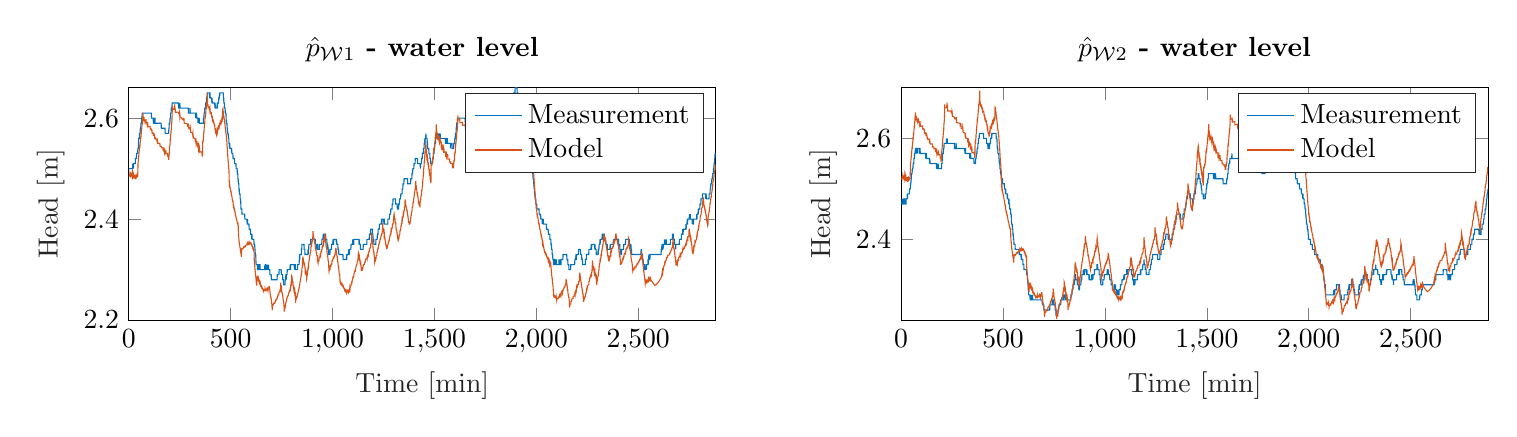
\begin{tikzpicture}

\begin{axis}[%
width=2.935in,
height=1.161in,
at={(1.14in,0.43in)},
scale only axis,
xmin=0,
xmax=2880,
xlabel style={font=\color{white!15!black}},
xlabel={Time [min]},
ymin=2.2,
ymax=2.66,
ylabel style={font=\color{white!15!black}},
ylabel={Head  [m]},
axis background/.style={fill=white},
title style={font=\bfseries},
title={$\hat{p}_{\mathcal{W}1}$ - water level},
legend style={legend cell align=left, align=left, draw=white!15!black}
]
\addplot [color=mycolor1]
  table[row sep=crcr]{%
1	2.5\\
2	2.5\\
3	2.5\\
4	2.5\\
5	2.5\\
6	2.5\\
7	2.5\\
8	2.5\\
9	2.5\\
10	2.5\\
11	2.5\\
12	2.5\\
13	2.5\\
14	2.5\\
15	2.5\\
16	2.5\\
17	2.5\\
18	2.5\\
19	2.5\\
20	2.51\\
21	2.5\\
22	2.51\\
23	2.5\\
24	2.51\\
25	2.51\\
26	2.51\\
27	2.51\\
28	2.51\\
29	2.51\\
30	2.51\\
31	2.51\\
32	2.51\\
33	2.52\\
34	2.52\\
35	2.52\\
36	2.52\\
37	2.52\\
38	2.52\\
39	2.53\\
40	2.53\\
41	2.53\\
42	2.53\\
43	2.53\\
44	2.53\\
45	2.54\\
46	2.54\\
47	2.54\\
48	2.55\\
49	2.56\\
50	2.56\\
51	2.56\\
52	2.56\\
53	2.57\\
54	2.57\\
55	2.57\\
56	2.57\\
57	2.58\\
58	2.58\\
59	2.58\\
60	2.59\\
61	2.59\\
62	2.59\\
63	2.59\\
64	2.6\\
65	2.6\\
66	2.61\\
67	2.61\\
68	2.61\\
69	2.61\\
70	2.61\\
71	2.61\\
72	2.61\\
73	2.61\\
74	2.61\\
75	2.61\\
76	2.61\\
77	2.61\\
78	2.61\\
79	2.61\\
80	2.61\\
81	2.61\\
82	2.61\\
83	2.61\\
84	2.61\\
85	2.61\\
86	2.61\\
87	2.61\\
88	2.61\\
89	2.61\\
90	2.61\\
91	2.61\\
92	2.61\\
93	2.61\\
94	2.61\\
95	2.61\\
96	2.61\\
97	2.61\\
98	2.61\\
99	2.61\\
100	2.61\\
101	2.61\\
102	2.61\\
103	2.61\\
104	2.61\\
105	2.61\\
106	2.61\\
107	2.61\\
108	2.61\\
109	2.61\\
110	2.61\\
111	2.61\\
112	2.6\\
113	2.6\\
114	2.6\\
115	2.6\\
116	2.6\\
117	2.6\\
118	2.6\\
119	2.6\\
120	2.6\\
121	2.59\\
122	2.6\\
123	2.59\\
124	2.59\\
125	2.6\\
126	2.59\\
127	2.59\\
128	2.6\\
129	2.6\\
130	2.59\\
131	2.59\\
132	2.59\\
133	2.59\\
134	2.59\\
135	2.59\\
136	2.59\\
137	2.59\\
138	2.59\\
139	2.59\\
140	2.59\\
141	2.59\\
142	2.59\\
143	2.59\\
144	2.59\\
145	2.59\\
146	2.59\\
147	2.59\\
148	2.59\\
149	2.59\\
150	2.59\\
151	2.59\\
152	2.59\\
153	2.59\\
154	2.59\\
155	2.59\\
156	2.59\\
157	2.59\\
158	2.59\\
159	2.59\\
160	2.58\\
161	2.58\\
162	2.58\\
163	2.58\\
164	2.58\\
165	2.58\\
166	2.58\\
167	2.58\\
168	2.58\\
169	2.58\\
170	2.58\\
171	2.58\\
172	2.58\\
173	2.58\\
174	2.58\\
175	2.58\\
176	2.58\\
177	2.58\\
178	2.58\\
179	2.57\\
180	2.57\\
181	2.57\\
182	2.57\\
183	2.57\\
184	2.57\\
185	2.57\\
186	2.57\\
187	2.57\\
188	2.57\\
189	2.57\\
190	2.57\\
191	2.57\\
192	2.57\\
193	2.57\\
194	2.57\\
195	2.57\\
196	2.57\\
197	2.58\\
198	2.58\\
199	2.59\\
200	2.59\\
201	2.59\\
202	2.59\\
203	2.6\\
204	2.6\\
205	2.6\\
206	2.61\\
207	2.61\\
208	2.61\\
209	2.62\\
210	2.62\\
211	2.62\\
212	2.62\\
213	2.63\\
214	2.63\\
215	2.63\\
216	2.63\\
217	2.63\\
218	2.63\\
219	2.63\\
220	2.63\\
221	2.63\\
222	2.63\\
223	2.63\\
224	2.63\\
225	2.63\\
226	2.63\\
227	2.63\\
228	2.63\\
229	2.63\\
230	2.63\\
231	2.63\\
232	2.63\\
233	2.63\\
234	2.63\\
235	2.63\\
236	2.63\\
237	2.63\\
238	2.63\\
239	2.63\\
240	2.63\\
241	2.63\\
242	2.63\\
243	2.63\\
244	2.63\\
245	2.62\\
246	2.62\\
247	2.62\\
248	2.63\\
249	2.62\\
250	2.62\\
251	2.63\\
252	2.62\\
253	2.62\\
254	2.62\\
255	2.62\\
256	2.62\\
257	2.62\\
258	2.62\\
259	2.62\\
260	2.62\\
261	2.62\\
262	2.62\\
263	2.62\\
264	2.62\\
265	2.62\\
266	2.62\\
267	2.62\\
268	2.62\\
269	2.62\\
270	2.62\\
271	2.62\\
272	2.62\\
273	2.62\\
274	2.62\\
275	2.62\\
276	2.62\\
277	2.62\\
278	2.62\\
279	2.62\\
280	2.62\\
281	2.62\\
282	2.62\\
283	2.62\\
284	2.62\\
285	2.62\\
286	2.62\\
287	2.62\\
288	2.62\\
289	2.62\\
290	2.62\\
291	2.62\\
292	2.62\\
293	2.61\\
294	2.61\\
295	2.61\\
296	2.61\\
297	2.61\\
298	2.61\\
299	2.61\\
300	2.61\\
301	2.62\\
302	2.61\\
303	2.61\\
304	2.61\\
305	2.61\\
306	2.61\\
307	2.61\\
308	2.61\\
309	2.61\\
310	2.61\\
311	2.61\\
312	2.61\\
313	2.61\\
314	2.61\\
315	2.61\\
316	2.61\\
317	2.61\\
318	2.61\\
319	2.61\\
320	2.61\\
321	2.61\\
322	2.61\\
323	2.61\\
324	2.61\\
325	2.61\\
326	2.61\\
327	2.61\\
328	2.61\\
329	2.6\\
330	2.61\\
331	2.6\\
332	2.61\\
333	2.61\\
334	2.6\\
335	2.6\\
336	2.6\\
337	2.6\\
338	2.6\\
339	2.6\\
340	2.59\\
341	2.6\\
342	2.59\\
343	2.6\\
344	2.6\\
345	2.59\\
346	2.6\\
347	2.59\\
348	2.59\\
349	2.59\\
350	2.59\\
351	2.59\\
352	2.59\\
353	2.59\\
354	2.59\\
355	2.59\\
356	2.59\\
357	2.59\\
358	2.59\\
359	2.59\\
360	2.59\\
361	2.59\\
362	2.59\\
363	2.59\\
364	2.59\\
365	2.59\\
366	2.59\\
367	2.6\\
368	2.6\\
369	2.6\\
370	2.61\\
371	2.61\\
372	2.61\\
373	2.62\\
374	2.62\\
375	2.62\\
376	2.62\\
377	2.62\\
378	2.63\\
379	2.63\\
380	2.63\\
381	2.63\\
382	2.64\\
383	2.64\\
384	2.64\\
385	2.65\\
386	2.65\\
387	2.65\\
388	2.65\\
389	2.65\\
390	2.65\\
391	2.65\\
392	2.65\\
393	2.65\\
394	2.65\\
395	2.65\\
396	2.65\\
397	2.64\\
398	2.65\\
399	2.65\\
400	2.64\\
401	2.64\\
402	2.64\\
403	2.64\\
404	2.64\\
405	2.64\\
406	2.64\\
407	2.64\\
408	2.63\\
409	2.64\\
410	2.63\\
411	2.63\\
412	2.63\\
413	2.63\\
414	2.63\\
415	2.63\\
416	2.63\\
417	2.63\\
418	2.63\\
419	2.63\\
420	2.63\\
421	2.63\\
422	2.63\\
423	2.62\\
424	2.63\\
425	2.62\\
426	2.62\\
427	2.62\\
428	2.62\\
429	2.62\\
430	2.62\\
431	2.62\\
432	2.62\\
433	2.62\\
434	2.63\\
435	2.62\\
436	2.63\\
437	2.63\\
438	2.63\\
439	2.63\\
440	2.63\\
441	2.63\\
442	2.64\\
443	2.64\\
444	2.64\\
445	2.65\\
446	2.64\\
447	2.65\\
448	2.65\\
449	2.65\\
450	2.65\\
451	2.65\\
452	2.65\\
453	2.65\\
454	2.65\\
455	2.65\\
456	2.65\\
457	2.65\\
458	2.65\\
459	2.65\\
460	2.65\\
461	2.65\\
462	2.65\\
463	2.65\\
464	2.65\\
465	2.64\\
466	2.64\\
467	2.63\\
468	2.63\\
469	2.63\\
470	2.62\\
471	2.62\\
472	2.62\\
473	2.62\\
474	2.61\\
475	2.61\\
476	2.61\\
477	2.61\\
478	2.6\\
479	2.59\\
480	2.59\\
481	2.59\\
482	2.59\\
483	2.58\\
484	2.58\\
485	2.57\\
486	2.57\\
487	2.57\\
488	2.57\\
489	2.56\\
490	2.56\\
491	2.56\\
492	2.55\\
493	2.55\\
494	2.55\\
495	2.54\\
496	2.55\\
497	2.54\\
498	2.54\\
499	2.54\\
500	2.54\\
501	2.54\\
502	2.54\\
503	2.54\\
504	2.54\\
505	2.54\\
506	2.53\\
507	2.53\\
508	2.53\\
509	2.53\\
510	2.53\\
511	2.53\\
512	2.52\\
513	2.52\\
514	2.52\\
515	2.52\\
516	2.52\\
517	2.52\\
518	2.52\\
519	2.52\\
520	2.51\\
521	2.51\\
522	2.51\\
523	2.51\\
524	2.51\\
525	2.51\\
526	2.51\\
527	2.5\\
528	2.5\\
529	2.5\\
530	2.5\\
531	2.5\\
532	2.5\\
533	2.49\\
534	2.49\\
535	2.49\\
536	2.48\\
537	2.48\\
538	2.47\\
539	2.47\\
540	2.47\\
541	2.46\\
542	2.46\\
543	2.45\\
544	2.45\\
545	2.45\\
546	2.45\\
547	2.44\\
548	2.44\\
549	2.44\\
550	2.43\\
551	2.42\\
552	2.42\\
553	2.42\\
554	2.42\\
555	2.42\\
556	2.41\\
557	2.41\\
558	2.41\\
559	2.41\\
560	2.41\\
561	2.41\\
562	2.41\\
563	2.41\\
564	2.41\\
565	2.41\\
566	2.41\\
567	2.41\\
568	2.41\\
569	2.41\\
570	2.4\\
571	2.4\\
572	2.4\\
573	2.4\\
574	2.4\\
575	2.4\\
576	2.4\\
577	2.4\\
578	2.4\\
579	2.4\\
580	2.4\\
581	2.39\\
582	2.39\\
583	2.4\\
584	2.39\\
585	2.39\\
586	2.39\\
587	2.39\\
588	2.39\\
589	2.39\\
590	2.39\\
591	2.38\\
592	2.38\\
593	2.38\\
594	2.38\\
595	2.38\\
596	2.38\\
597	2.38\\
598	2.37\\
599	2.37\\
600	2.37\\
601	2.37\\
602	2.37\\
603	2.37\\
604	2.36\\
605	2.37\\
606	2.36\\
607	2.36\\
608	2.36\\
609	2.36\\
610	2.36\\
611	2.36\\
612	2.36\\
613	2.36\\
614	2.36\\
615	2.35\\
616	2.35\\
617	2.35\\
618	2.35\\
619	2.34\\
620	2.34\\
621	2.33\\
622	2.33\\
623	2.33\\
624	2.32\\
625	2.31\\
626	2.31\\
627	2.31\\
628	2.31\\
629	2.31\\
630	2.31\\
631	2.31\\
632	2.3\\
633	2.3\\
634	2.3\\
635	2.31\\
636	2.31\\
637	2.31\\
638	2.3\\
639	2.3\\
640	2.3\\
641	2.31\\
642	2.31\\
643	2.31\\
644	2.31\\
645	2.3\\
646	2.3\\
647	2.3\\
648	2.3\\
649	2.3\\
650	2.3\\
651	2.3\\
652	2.3\\
653	2.3\\
654	2.3\\
655	2.3\\
656	2.3\\
657	2.3\\
658	2.3\\
659	2.3\\
660	2.3\\
661	2.3\\
662	2.3\\
663	2.3\\
664	2.3\\
665	2.3\\
666	2.3\\
667	2.3\\
668	2.31\\
669	2.3\\
670	2.3\\
671	2.31\\
672	2.31\\
673	2.3\\
674	2.3\\
675	2.3\\
676	2.3\\
677	2.3\\
678	2.31\\
679	2.3\\
680	2.3\\
681	2.3\\
682	2.31\\
683	2.3\\
684	2.3\\
685	2.3\\
686	2.31\\
687	2.3\\
688	2.3\\
689	2.3\\
690	2.3\\
691	2.3\\
692	2.3\\
693	2.29\\
694	2.29\\
695	2.29\\
696	2.29\\
697	2.29\\
698	2.29\\
699	2.29\\
700	2.28\\
701	2.28\\
702	2.28\\
703	2.28\\
704	2.28\\
705	2.28\\
706	2.28\\
707	2.28\\
708	2.28\\
709	2.28\\
710	2.28\\
711	2.28\\
712	2.28\\
713	2.28\\
714	2.28\\
715	2.28\\
716	2.28\\
717	2.28\\
718	2.28\\
719	2.28\\
720	2.28\\
721	2.28\\
722	2.28\\
723	2.28\\
724	2.28\\
725	2.28\\
726	2.28\\
727	2.28\\
728	2.28\\
729	2.29\\
730	2.29\\
731	2.29\\
732	2.29\\
733	2.29\\
734	2.29\\
735	2.29\\
736	2.29\\
737	2.29\\
738	2.3\\
739	2.3\\
740	2.3\\
741	2.3\\
742	2.3\\
743	2.3\\
744	2.3\\
745	2.3\\
746	2.3\\
747	2.3\\
748	2.3\\
749	2.29\\
750	2.29\\
751	2.29\\
752	2.29\\
753	2.29\\
754	2.29\\
755	2.29\\
756	2.28\\
757	2.28\\
758	2.28\\
759	2.28\\
760	2.27\\
761	2.27\\
762	2.27\\
763	2.27\\
764	2.27\\
765	2.27\\
766	2.27\\
767	2.27\\
768	2.28\\
769	2.28\\
770	2.28\\
771	2.29\\
772	2.29\\
773	2.28\\
774	2.29\\
775	2.29\\
776	2.29\\
777	2.29\\
778	2.3\\
779	2.3\\
780	2.3\\
781	2.3\\
782	2.3\\
783	2.3\\
784	2.3\\
785	2.3\\
786	2.3\\
787	2.3\\
788	2.3\\
789	2.3\\
790	2.3\\
791	2.3\\
792	2.31\\
793	2.3\\
794	2.3\\
795	2.31\\
796	2.31\\
797	2.31\\
798	2.31\\
799	2.31\\
800	2.31\\
801	2.31\\
802	2.31\\
803	2.31\\
804	2.31\\
805	2.31\\
806	2.31\\
807	2.31\\
808	2.31\\
809	2.31\\
810	2.31\\
811	2.31\\
812	2.31\\
813	2.3\\
814	2.31\\
815	2.31\\
816	2.31\\
817	2.31\\
818	2.3\\
819	2.3\\
820	2.3\\
821	2.3\\
822	2.3\\
823	2.3\\
824	2.3\\
825	2.3\\
826	2.3\\
827	2.3\\
828	2.3\\
829	2.31\\
830	2.31\\
831	2.31\\
832	2.31\\
833	2.31\\
834	2.31\\
835	2.31\\
836	2.31\\
837	2.32\\
838	2.33\\
839	2.32\\
840	2.33\\
841	2.33\\
842	2.33\\
843	2.33\\
844	2.33\\
845	2.33\\
846	2.33\\
847	2.33\\
848	2.34\\
849	2.34\\
850	2.35\\
851	2.35\\
852	2.35\\
853	2.35\\
854	2.35\\
855	2.35\\
856	2.35\\
857	2.35\\
858	2.35\\
859	2.35\\
860	2.35\\
861	2.34\\
862	2.34\\
863	2.34\\
864	2.34\\
865	2.33\\
866	2.33\\
867	2.33\\
868	2.33\\
869	2.33\\
870	2.33\\
871	2.33\\
872	2.33\\
873	2.33\\
874	2.33\\
875	2.33\\
876	2.33\\
877	2.33\\
878	2.33\\
879	2.33\\
880	2.34\\
881	2.33\\
882	2.34\\
883	2.34\\
884	2.35\\
885	2.35\\
886	2.35\\
887	2.35\\
888	2.35\\
889	2.35\\
890	2.35\\
891	2.35\\
892	2.35\\
893	2.36\\
894	2.36\\
895	2.36\\
896	2.36\\
897	2.36\\
898	2.36\\
899	2.36\\
900	2.36\\
901	2.36\\
902	2.36\\
903	2.36\\
904	2.36\\
905	2.36\\
906	2.36\\
907	2.36\\
908	2.36\\
909	2.36\\
910	2.36\\
911	2.36\\
912	2.36\\
913	2.36\\
914	2.36\\
915	2.36\\
916	2.35\\
917	2.35\\
918	2.35\\
919	2.35\\
920	2.35\\
921	2.35\\
922	2.35\\
923	2.34\\
924	2.35\\
925	2.35\\
926	2.34\\
927	2.34\\
928	2.34\\
929	2.34\\
930	2.34\\
931	2.34\\
932	2.34\\
933	2.34\\
934	2.35\\
935	2.34\\
936	2.34\\
937	2.35\\
938	2.35\\
939	2.35\\
940	2.35\\
941	2.35\\
942	2.35\\
943	2.35\\
944	2.35\\
945	2.35\\
946	2.35\\
947	2.35\\
948	2.36\\
949	2.36\\
950	2.36\\
951	2.36\\
952	2.36\\
953	2.36\\
954	2.37\\
955	2.36\\
956	2.37\\
957	2.37\\
958	2.37\\
959	2.37\\
960	2.37\\
961	2.37\\
962	2.37\\
963	2.37\\
964	2.37\\
965	2.37\\
966	2.37\\
967	2.36\\
968	2.36\\
969	2.36\\
970	2.36\\
971	2.36\\
972	2.36\\
973	2.35\\
974	2.35\\
975	2.35\\
976	2.34\\
977	2.35\\
978	2.34\\
979	2.34\\
980	2.34\\
981	2.33\\
982	2.33\\
983	2.33\\
984	2.33\\
985	2.33\\
986	2.33\\
987	2.33\\
988	2.34\\
989	2.34\\
990	2.34\\
991	2.34\\
992	2.34\\
993	2.34\\
994	2.34\\
995	2.34\\
996	2.35\\
997	2.35\\
998	2.35\\
999	2.35\\
1000	2.35\\
1001	2.35\\
1002	2.36\\
1003	2.35\\
1004	2.35\\
1005	2.35\\
1006	2.36\\
1007	2.36\\
1008	2.36\\
1009	2.36\\
1010	2.36\\
1011	2.36\\
1012	2.36\\
1013	2.36\\
1014	2.36\\
1015	2.36\\
1016	2.36\\
1017	2.36\\
1018	2.36\\
1019	2.35\\
1020	2.36\\
1021	2.35\\
1022	2.35\\
1023	2.35\\
1024	2.35\\
1025	2.35\\
1026	2.35\\
1027	2.34\\
1028	2.34\\
1029	2.34\\
1030	2.34\\
1031	2.33\\
1032	2.33\\
1033	2.33\\
1034	2.33\\
1035	2.33\\
1036	2.33\\
1037	2.33\\
1038	2.33\\
1039	2.33\\
1040	2.33\\
1041	2.33\\
1042	2.33\\
1043	2.33\\
1044	2.33\\
1045	2.33\\
1046	2.33\\
1047	2.33\\
1048	2.33\\
1049	2.33\\
1050	2.33\\
1051	2.33\\
1052	2.32\\
1053	2.32\\
1054	2.32\\
1055	2.32\\
1056	2.32\\
1057	2.32\\
1058	2.32\\
1059	2.32\\
1060	2.32\\
1061	2.32\\
1062	2.32\\
1063	2.32\\
1064	2.32\\
1065	2.32\\
1066	2.32\\
1067	2.32\\
1068	2.32\\
1069	2.33\\
1070	2.32\\
1071	2.33\\
1072	2.33\\
1073	2.33\\
1074	2.33\\
1075	2.33\\
1076	2.33\\
1077	2.33\\
1078	2.33\\
1079	2.34\\
1080	2.33\\
1081	2.33\\
1082	2.34\\
1083	2.33\\
1084	2.34\\
1085	2.34\\
1086	2.34\\
1087	2.34\\
1088	2.34\\
1089	2.34\\
1090	2.34\\
1091	2.35\\
1092	2.35\\
1093	2.35\\
1094	2.35\\
1095	2.35\\
1096	2.35\\
1097	2.35\\
1098	2.35\\
1099	2.36\\
1100	2.35\\
1101	2.35\\
1102	2.35\\
1103	2.35\\
1104	2.35\\
1105	2.36\\
1106	2.36\\
1107	2.36\\
1108	2.36\\
1109	2.36\\
1110	2.36\\
1111	2.36\\
1112	2.36\\
1113	2.36\\
1114	2.36\\
1115	2.36\\
1116	2.36\\
1117	2.36\\
1118	2.36\\
1119	2.36\\
1120	2.36\\
1121	2.36\\
1122	2.36\\
1123	2.36\\
1124	2.36\\
1125	2.36\\
1126	2.36\\
1127	2.36\\
1128	2.36\\
1129	2.36\\
1130	2.35\\
1131	2.36\\
1132	2.35\\
1133	2.35\\
1134	2.35\\
1135	2.35\\
1136	2.35\\
1137	2.34\\
1138	2.34\\
1139	2.34\\
1140	2.34\\
1141	2.34\\
1142	2.34\\
1143	2.34\\
1144	2.34\\
1145	2.34\\
1146	2.34\\
1147	2.34\\
1148	2.34\\
1149	2.34\\
1150	2.34\\
1151	2.35\\
1152	2.35\\
1153	2.35\\
1154	2.35\\
1155	2.35\\
1156	2.35\\
1157	2.35\\
1158	2.35\\
1159	2.35\\
1160	2.35\\
1161	2.35\\
1162	2.35\\
1163	2.35\\
1164	2.35\\
1165	2.35\\
1166	2.35\\
1167	2.35\\
1168	2.35\\
1169	2.36\\
1170	2.36\\
1171	2.36\\
1172	2.36\\
1173	2.36\\
1174	2.36\\
1175	2.36\\
1176	2.36\\
1177	2.36\\
1178	2.36\\
1179	2.36\\
1180	2.36\\
1181	2.37\\
1182	2.37\\
1183	2.37\\
1184	2.37\\
1185	2.37\\
1186	2.37\\
1187	2.38\\
1188	2.38\\
1189	2.38\\
1190	2.38\\
1191	2.38\\
1192	2.38\\
1193	2.38\\
1194	2.38\\
1195	2.38\\
1196	2.37\\
1197	2.37\\
1198	2.37\\
1199	2.36\\
1200	2.36\\
1201	2.36\\
1202	2.36\\
1203	2.35\\
1204	2.35\\
1205	2.35\\
1206	2.35\\
1207	2.35\\
1208	2.35\\
1209	2.35\\
1210	2.35\\
1211	2.35\\
1212	2.35\\
1213	2.36\\
1214	2.36\\
1215	2.36\\
1216	2.36\\
1217	2.36\\
1218	2.36\\
1219	2.36\\
1220	2.37\\
1221	2.37\\
1222	2.37\\
1223	2.37\\
1224	2.38\\
1225	2.38\\
1226	2.38\\
1227	2.38\\
1228	2.38\\
1229	2.38\\
1230	2.39\\
1231	2.39\\
1232	2.39\\
1233	2.39\\
1234	2.39\\
1235	2.39\\
1236	2.39\\
1237	2.39\\
1238	2.39\\
1239	2.39\\
1240	2.4\\
1241	2.4\\
1242	2.39\\
1243	2.4\\
1244	2.4\\
1245	2.4\\
1246	2.4\\
1247	2.4\\
1248	2.4\\
1249	2.4\\
1250	2.4\\
1251	2.4\\
1252	2.39\\
1253	2.4\\
1254	2.4\\
1255	2.39\\
1256	2.39\\
1257	2.39\\
1258	2.39\\
1259	2.39\\
1260	2.39\\
1261	2.39\\
1262	2.39\\
1263	2.39\\
1264	2.39\\
1265	2.39\\
1266	2.39\\
1267	2.39\\
1268	2.39\\
1269	2.39\\
1270	2.39\\
1271	2.39\\
1272	2.4\\
1273	2.4\\
1274	2.4\\
1275	2.4\\
1276	2.4\\
1277	2.4\\
1278	2.4\\
1279	2.4\\
1280	2.41\\
1281	2.41\\
1282	2.41\\
1283	2.41\\
1284	2.41\\
1285	2.41\\
1286	2.42\\
1287	2.42\\
1288	2.42\\
1289	2.42\\
1290	2.42\\
1291	2.42\\
1292	2.42\\
1293	2.43\\
1294	2.43\\
1295	2.43\\
1296	2.43\\
1297	2.44\\
1298	2.44\\
1299	2.44\\
1300	2.44\\
1301	2.44\\
1302	2.44\\
1303	2.44\\
1304	2.44\\
1305	2.44\\
1306	2.44\\
1307	2.44\\
1308	2.44\\
1309	2.44\\
1310	2.43\\
1311	2.43\\
1312	2.43\\
1313	2.43\\
1314	2.43\\
1315	2.43\\
1316	2.43\\
1317	2.43\\
1318	2.42\\
1319	2.42\\
1320	2.42\\
1321	2.42\\
1322	2.42\\
1323	2.42\\
1324	2.42\\
1325	2.43\\
1326	2.43\\
1327	2.43\\
1328	2.43\\
1329	2.44\\
1330	2.44\\
1331	2.44\\
1332	2.44\\
1333	2.44\\
1334	2.44\\
1335	2.45\\
1336	2.45\\
1337	2.45\\
1338	2.45\\
1339	2.45\\
1340	2.45\\
1341	2.45\\
1342	2.46\\
1343	2.46\\
1344	2.46\\
1345	2.46\\
1346	2.47\\
1347	2.47\\
1348	2.47\\
1349	2.47\\
1350	2.47\\
1351	2.48\\
1352	2.48\\
1353	2.48\\
1354	2.48\\
1355	2.48\\
1356	2.48\\
1357	2.48\\
1358	2.48\\
1359	2.48\\
1360	2.48\\
1361	2.48\\
1362	2.48\\
1363	2.48\\
1364	2.48\\
1365	2.48\\
1366	2.48\\
1367	2.48\\
1368	2.48\\
1369	2.47\\
1370	2.47\\
1371	2.47\\
1372	2.47\\
1373	2.47\\
1374	2.47\\
1375	2.47\\
1376	2.47\\
1377	2.47\\
1378	2.47\\
1379	2.47\\
1380	2.47\\
1381	2.47\\
1382	2.47\\
1383	2.47\\
1384	2.48\\
1385	2.48\\
1386	2.48\\
1387	2.48\\
1388	2.48\\
1389	2.48\\
1390	2.49\\
1391	2.49\\
1392	2.49\\
1393	2.49\\
1394	2.5\\
1395	2.5\\
1396	2.5\\
1397	2.5\\
1398	2.5\\
1399	2.5\\
1400	2.51\\
1401	2.51\\
1402	2.51\\
1403	2.51\\
1404	2.51\\
1405	2.51\\
1406	2.52\\
1407	2.52\\
1408	2.52\\
1409	2.52\\
1410	2.52\\
1411	2.52\\
1412	2.52\\
1413	2.52\\
1414	2.52\\
1415	2.52\\
1416	2.52\\
1417	2.52\\
1418	2.51\\
1419	2.51\\
1420	2.51\\
1421	2.51\\
1422	2.51\\
1423	2.51\\
1424	2.51\\
1425	2.51\\
1426	2.51\\
1427	2.51\\
1428	2.51\\
1429	2.51\\
1430	2.51\\
1431	2.5\\
1432	2.51\\
1433	2.51\\
1434	2.51\\
1435	2.51\\
1436	2.51\\
1437	2.52\\
1438	2.52\\
1439	2.52\\
1440	2.52\\
1441	2.53\\
1442	2.53\\
1443	2.53\\
1444	2.53\\
1445	2.53\\
1446	2.54\\
1447	2.54\\
1448	2.54\\
1449	2.54\\
1450	2.55\\
1451	2.55\\
1452	2.55\\
1453	2.56\\
1454	2.55\\
1455	2.56\\
1456	2.56\\
1457	2.56\\
1458	2.57\\
1459	2.56\\
1460	2.56\\
1461	2.56\\
1462	2.56\\
1463	2.56\\
1464	2.56\\
1465	2.55\\
1466	2.55\\
1467	2.54\\
1468	2.54\\
1469	2.54\\
1470	2.54\\
1471	2.54\\
1472	2.54\\
1473	2.53\\
1474	2.53\\
1475	2.53\\
1476	2.53\\
1477	2.53\\
1478	2.52\\
1479	2.52\\
1480	2.52\\
1481	2.51\\
1482	2.51\\
1483	2.51\\
1484	2.51\\
1485	2.51\\
1486	2.51\\
1487	2.51\\
1488	2.51\\
1489	2.51\\
1490	2.51\\
1491	2.52\\
1492	2.52\\
1493	2.52\\
1494	2.52\\
1495	2.53\\
1496	2.53\\
1497	2.53\\
1498	2.53\\
1499	2.54\\
1500	2.54\\
1501	2.54\\
1502	2.55\\
1503	2.55\\
1504	2.55\\
1505	2.55\\
1506	2.56\\
1507	2.56\\
1508	2.57\\
1509	2.57\\
1510	2.57\\
1511	2.57\\
1512	2.56\\
1513	2.57\\
1514	2.56\\
1515	2.56\\
1516	2.56\\
1517	2.56\\
1518	2.56\\
1519	2.56\\
1520	2.57\\
1521	2.56\\
1522	2.56\\
1523	2.57\\
1524	2.56\\
1525	2.57\\
1526	2.56\\
1527	2.56\\
1528	2.57\\
1529	2.56\\
1530	2.56\\
1531	2.56\\
1532	2.56\\
1533	2.56\\
1534	2.56\\
1535	2.56\\
1536	2.56\\
1537	2.56\\
1538	2.56\\
1539	2.56\\
1540	2.56\\
1541	2.56\\
1542	2.56\\
1543	2.56\\
1544	2.56\\
1545	2.56\\
1546	2.56\\
1547	2.56\\
1548	2.56\\
1549	2.56\\
1550	2.56\\
1551	2.56\\
1552	2.56\\
1553	2.56\\
1554	2.55\\
1555	2.55\\
1556	2.56\\
1557	2.56\\
1558	2.55\\
1559	2.56\\
1560	2.55\\
1561	2.55\\
1562	2.56\\
1563	2.56\\
1564	2.56\\
1565	2.55\\
1566	2.55\\
1567	2.55\\
1568	2.55\\
1569	2.55\\
1570	2.55\\
1571	2.55\\
1572	2.55\\
1573	2.55\\
1574	2.55\\
1575	2.55\\
1576	2.55\\
1577	2.55\\
1578	2.55\\
1579	2.54\\
1580	2.55\\
1581	2.55\\
1582	2.55\\
1583	2.55\\
1584	2.55\\
1585	2.55\\
1586	2.55\\
1587	2.54\\
1588	2.54\\
1589	2.54\\
1590	2.54\\
1591	2.54\\
1592	2.54\\
1593	2.54\\
1594	2.54\\
1595	2.55\\
1596	2.55\\
1597	2.55\\
1598	2.55\\
1599	2.55\\
1600	2.56\\
1601	2.56\\
1602	2.56\\
1603	2.57\\
1604	2.57\\
1605	2.57\\
1606	2.57\\
1607	2.58\\
1608	2.58\\
1609	2.59\\
1610	2.59\\
1611	2.59\\
1612	2.59\\
1613	2.6\\
1614	2.6\\
1615	2.6\\
1616	2.6\\
1617	2.6\\
1618	2.6\\
1619	2.6\\
1620	2.6\\
1621	2.6\\
1622	2.6\\
1623	2.6\\
1624	2.6\\
1625	2.6\\
1626	2.6\\
1627	2.6\\
1628	2.6\\
1629	2.6\\
1630	2.6\\
1631	2.6\\
1632	2.6\\
1633	2.6\\
1634	2.6\\
1635	2.6\\
1636	2.6\\
1637	2.6\\
1638	2.6\\
1639	2.6\\
1640	2.6\\
1641	2.6\\
1642	2.6\\
1643	2.6\\
1644	2.6\\
1645	2.6\\
1646	2.6\\
1647	2.6\\
1648	2.6\\
1649	2.6\\
1650	2.6\\
1651	2.59\\
1652	2.6\\
1653	2.6\\
1654	2.59\\
1655	2.6\\
1656	2.6\\
1657	2.6\\
1658	2.6\\
1659	2.6\\
1660	2.6\\
1661	2.6\\
1662	2.6\\
1663	2.6\\
1664	2.6\\
1665	2.6\\
1666	2.59\\
1667	2.6\\
1668	2.6\\
1669	2.59\\
1670	2.59\\
1671	2.59\\
1672	2.59\\
1673	2.59\\
1674	2.59\\
1675	2.6\\
1676	2.59\\
1677	2.59\\
1678	2.59\\
1679	2.59\\
1680	2.59\\
1681	2.59\\
1682	2.59\\
1683	2.59\\
1684	2.59\\
1685	2.59\\
1686	2.59\\
1687	2.59\\
1688	2.59\\
1689	2.59\\
1690	2.59\\
1691	2.59\\
1692	2.59\\
1693	2.59\\
1694	2.59\\
1695	2.59\\
1696	2.59\\
1697	2.59\\
1698	2.59\\
1699	2.59\\
1700	2.59\\
1701	2.59\\
1702	2.59\\
1703	2.59\\
1704	2.59\\
1705	2.59\\
1706	2.59\\
1707	2.59\\
1708	2.59\\
1709	2.59\\
1710	2.59\\
1711	2.59\\
1712	2.58\\
1713	2.58\\
1714	2.58\\
1715	2.58\\
1716	2.58\\
1717	2.58\\
1718	2.58\\
1719	2.58\\
1720	2.58\\
1721	2.58\\
1722	2.58\\
1723	2.58\\
1724	2.58\\
1725	2.58\\
1726	2.58\\
1727	2.58\\
1728	2.58\\
1729	2.58\\
1730	2.58\\
1731	2.58\\
1732	2.58\\
1733	2.58\\
1734	2.58\\
1735	2.58\\
1736	2.58\\
1737	2.58\\
1738	2.58\\
1739	2.58\\
1740	2.58\\
1741	2.58\\
1742	2.58\\
1743	2.58\\
1744	2.58\\
1745	2.58\\
1746	2.57\\
1747	2.57\\
1748	2.57\\
1749	2.57\\
1750	2.57\\
1751	2.57\\
1752	2.57\\
1753	2.57\\
1754	2.57\\
1755	2.57\\
1756	2.57\\
1757	2.57\\
1758	2.57\\
1759	2.57\\
1760	2.57\\
1761	2.57\\
1762	2.57\\
1763	2.57\\
1764	2.57\\
1765	2.57\\
1766	2.57\\
1767	2.57\\
1768	2.57\\
1769	2.57\\
1770	2.57\\
1771	2.57\\
1772	2.57\\
1773	2.57\\
1774	2.57\\
1775	2.57\\
1776	2.57\\
1777	2.57\\
1778	2.56\\
1779	2.56\\
1780	2.56\\
1781	2.57\\
1782	2.56\\
1783	2.57\\
1784	2.56\\
1785	2.57\\
1786	2.57\\
1787	2.57\\
1788	2.58\\
1789	2.58\\
1790	2.58\\
1791	2.59\\
1792	2.59\\
1793	2.59\\
1794	2.6\\
1795	2.6\\
1796	2.6\\
1797	2.6\\
1798	2.61\\
1799	2.61\\
1800	2.61\\
1801	2.62\\
1802	2.62\\
1803	2.62\\
1804	2.62\\
1805	2.62\\
1806	2.62\\
1807	2.63\\
1808	2.62\\
1809	2.62\\
1810	2.62\\
1811	2.62\\
1812	2.62\\
1813	2.62\\
1814	2.62\\
1815	2.62\\
1816	2.62\\
1817	2.62\\
1818	2.62\\
1819	2.62\\
1820	2.62\\
1821	2.63\\
1822	2.62\\
1823	2.62\\
1824	2.63\\
1825	2.62\\
1826	2.62\\
1827	2.62\\
1828	2.62\\
1829	2.62\\
1830	2.62\\
1831	2.62\\
1832	2.62\\
1833	2.62\\
1834	2.62\\
1835	2.62\\
1836	2.62\\
1837	2.62\\
1838	2.61\\
1839	2.61\\
1840	2.61\\
1841	2.61\\
1842	2.61\\
1843	2.61\\
1844	2.61\\
1845	2.61\\
1846	2.61\\
1847	2.61\\
1848	2.61\\
1849	2.61\\
1850	2.61\\
1851	2.61\\
1852	2.61\\
1853	2.61\\
1854	2.61\\
1855	2.6\\
1856	2.6\\
1857	2.6\\
1858	2.6\\
1859	2.6\\
1860	2.6\\
1861	2.6\\
1862	2.6\\
1863	2.6\\
1864	2.6\\
1865	2.59\\
1866	2.6\\
1867	2.6\\
1868	2.6\\
1869	2.61\\
1870	2.61\\
1871	2.61\\
1872	2.61\\
1873	2.61\\
1874	2.61\\
1875	2.62\\
1876	2.62\\
1877	2.62\\
1878	2.62\\
1879	2.62\\
1880	2.63\\
1881	2.63\\
1882	2.63\\
1883	2.63\\
1884	2.63\\
1885	2.64\\
1886	2.63\\
1887	2.64\\
1888	2.64\\
1889	2.65\\
1890	2.65\\
1891	2.65\\
1892	2.65\\
1893	2.65\\
1894	2.65\\
1895	2.65\\
1896	2.66\\
1897	2.66\\
1898	2.66\\
1899	2.66\\
1900	2.67\\
1901	2.67\\
1902	2.67\\
1903	2.67\\
1904	2.66\\
1905	2.66\\
1906	2.65\\
1907	2.65\\
1908	2.65\\
1909	2.65\\
1910	2.64\\
1911	2.64\\
1912	2.63\\
1913	2.63\\
1914	2.63\\
1915	2.63\\
1916	2.63\\
1917	2.62\\
1918	2.62\\
1919	2.62\\
1920	2.61\\
1921	2.61\\
1922	2.61\\
1923	2.6\\
1924	2.6\\
1925	2.6\\
1926	2.59\\
1927	2.59\\
1928	2.59\\
1929	2.58\\
1930	2.58\\
1931	2.57\\
1932	2.57\\
1933	2.57\\
1934	2.56\\
1935	2.56\\
1936	2.56\\
1937	2.56\\
1938	2.55\\
1939	2.56\\
1940	2.55\\
1941	2.55\\
1942	2.54\\
1943	2.55\\
1944	2.54\\
1945	2.54\\
1946	2.54\\
1947	2.54\\
1948	2.54\\
1949	2.54\\
1950	2.54\\
1951	2.54\\
1952	2.54\\
1953	2.54\\
1954	2.54\\
1955	2.53\\
1956	2.54\\
1957	2.53\\
1958	2.53\\
1959	2.53\\
1960	2.53\\
1961	2.53\\
1962	2.53\\
1963	2.53\\
1964	2.53\\
1965	2.53\\
1966	2.52\\
1967	2.52\\
1968	2.52\\
1969	2.52\\
1970	2.51\\
1971	2.51\\
1972	2.51\\
1973	2.51\\
1974	2.51\\
1975	2.51\\
1976	2.5\\
1977	2.51\\
1978	2.5\\
1979	2.5\\
1980	2.5\\
1981	2.5\\
1982	2.49\\
1983	2.49\\
1984	2.48\\
1985	2.48\\
1986	2.48\\
1987	2.47\\
1988	2.47\\
1989	2.46\\
1990	2.46\\
1991	2.45\\
1992	2.45\\
1993	2.45\\
1994	2.44\\
1995	2.44\\
1996	2.44\\
1997	2.44\\
1998	2.43\\
1999	2.43\\
2000	2.43\\
2001	2.42\\
2002	2.43\\
2003	2.42\\
2004	2.42\\
2005	2.42\\
2006	2.42\\
2007	2.42\\
2008	2.42\\
2009	2.42\\
2010	2.42\\
2011	2.42\\
2012	2.42\\
2013	2.42\\
2014	2.41\\
2015	2.41\\
2016	2.41\\
2017	2.41\\
2018	2.41\\
2019	2.41\\
2020	2.4\\
2021	2.41\\
2022	2.4\\
2023	2.4\\
2024	2.4\\
2025	2.4\\
2026	2.4\\
2027	2.4\\
2028	2.4\\
2029	2.39\\
2030	2.4\\
2031	2.4\\
2032	2.4\\
2033	2.39\\
2034	2.4\\
2035	2.39\\
2036	2.39\\
2037	2.39\\
2038	2.39\\
2039	2.39\\
2040	2.39\\
2041	2.39\\
2042	2.39\\
2043	2.39\\
2044	2.39\\
2045	2.39\\
2046	2.39\\
2047	2.39\\
2048	2.39\\
2049	2.39\\
2050	2.38\\
2051	2.38\\
2052	2.38\\
2053	2.38\\
2054	2.38\\
2055	2.38\\
2056	2.38\\
2057	2.38\\
2058	2.38\\
2059	2.37\\
2060	2.37\\
2061	2.37\\
2062	2.37\\
2063	2.37\\
2064	2.37\\
2065	2.37\\
2066	2.37\\
2067	2.36\\
2068	2.36\\
2069	2.36\\
2070	2.36\\
2071	2.36\\
2072	2.35\\
2073	2.35\\
2074	2.35\\
2075	2.34\\
2076	2.34\\
2077	2.34\\
2078	2.33\\
2079	2.33\\
2080	2.33\\
2081	2.32\\
2082	2.32\\
2083	2.32\\
2084	2.31\\
2085	2.31\\
2086	2.32\\
2087	2.31\\
2088	2.31\\
2089	2.31\\
2090	2.32\\
2091	2.32\\
2092	2.32\\
2093	2.31\\
2094	2.31\\
2095	2.31\\
2096	2.31\\
2097	2.31\\
2098	2.32\\
2099	2.31\\
2100	2.31\\
2101	2.31\\
2102	2.31\\
2103	2.31\\
2104	2.31\\
2105	2.31\\
2106	2.31\\
2107	2.31\\
2108	2.31\\
2109	2.31\\
2110	2.31\\
2111	2.32\\
2112	2.31\\
2113	2.31\\
2114	2.31\\
2115	2.32\\
2116	2.31\\
2117	2.31\\
2118	2.31\\
2119	2.32\\
2120	2.31\\
2121	2.31\\
2122	2.32\\
2123	2.32\\
2124	2.32\\
2125	2.32\\
2126	2.32\\
2127	2.32\\
2128	2.32\\
2129	2.32\\
2130	2.32\\
2131	2.33\\
2132	2.33\\
2133	2.33\\
2134	2.33\\
2135	2.33\\
2136	2.33\\
2137	2.33\\
2138	2.33\\
2139	2.33\\
2140	2.33\\
2141	2.33\\
2142	2.33\\
2143	2.33\\
2144	2.33\\
2145	2.33\\
2146	2.33\\
2147	2.33\\
2148	2.33\\
2149	2.33\\
2150	2.32\\
2151	2.32\\
2152	2.32\\
2153	2.32\\
2154	2.32\\
2155	2.31\\
2156	2.31\\
2157	2.31\\
2158	2.31\\
2159	2.31\\
2160	2.3\\
2161	2.3\\
2162	2.3\\
2163	2.3\\
2164	2.3\\
2165	2.3\\
2166	2.3\\
2167	2.3\\
2168	2.3\\
2169	2.31\\
2170	2.31\\
2171	2.31\\
2172	2.31\\
2173	2.31\\
2174	2.31\\
2175	2.31\\
2176	2.31\\
2177	2.31\\
2178	2.31\\
2179	2.31\\
2180	2.31\\
2181	2.31\\
2182	2.31\\
2183	2.31\\
2184	2.31\\
2185	2.31\\
2186	2.31\\
2187	2.31\\
2188	2.31\\
2189	2.32\\
2190	2.32\\
2191	2.32\\
2192	2.32\\
2193	2.32\\
2194	2.33\\
2195	2.32\\
2196	2.32\\
2197	2.33\\
2198	2.33\\
2199	2.33\\
2200	2.33\\
2201	2.33\\
2202	2.33\\
2203	2.33\\
2204	2.33\\
2205	2.33\\
2206	2.33\\
2207	2.34\\
2208	2.34\\
2209	2.34\\
2210	2.34\\
2211	2.34\\
2212	2.34\\
2213	2.34\\
2214	2.34\\
2215	2.34\\
2216	2.34\\
2217	2.33\\
2218	2.33\\
2219	2.33\\
2220	2.33\\
2221	2.33\\
2222	2.33\\
2223	2.32\\
2224	2.32\\
2225	2.32\\
2226	2.32\\
2227	2.31\\
2228	2.31\\
2229	2.31\\
2230	2.31\\
2231	2.31\\
2232	2.31\\
2233	2.31\\
2234	2.31\\
2235	2.31\\
2236	2.31\\
2237	2.31\\
2238	2.31\\
2239	2.31\\
2240	2.31\\
2241	2.32\\
2242	2.32\\
2243	2.32\\
2244	2.32\\
2245	2.32\\
2246	2.33\\
2247	2.33\\
2248	2.33\\
2249	2.33\\
2250	2.33\\
2251	2.33\\
2252	2.33\\
2253	2.33\\
2254	2.33\\
2255	2.33\\
2256	2.33\\
2257	2.33\\
2258	2.34\\
2259	2.34\\
2260	2.34\\
2261	2.34\\
2262	2.34\\
2263	2.34\\
2264	2.34\\
2265	2.34\\
2266	2.34\\
2267	2.34\\
2268	2.34\\
2269	2.35\\
2270	2.34\\
2271	2.34\\
2272	2.35\\
2273	2.35\\
2274	2.35\\
2275	2.35\\
2276	2.35\\
2277	2.35\\
2278	2.35\\
2279	2.35\\
2280	2.35\\
2281	2.35\\
2282	2.35\\
2283	2.35\\
2284	2.35\\
2285	2.35\\
2286	2.35\\
2287	2.34\\
2288	2.35\\
2289	2.34\\
2290	2.34\\
2291	2.34\\
2292	2.34\\
2293	2.34\\
2294	2.33\\
2295	2.33\\
2296	2.33\\
2297	2.33\\
2298	2.33\\
2299	2.33\\
2300	2.33\\
2301	2.33\\
2302	2.33\\
2303	2.34\\
2304	2.33\\
2305	2.34\\
2306	2.34\\
2307	2.34\\
2308	2.35\\
2309	2.35\\
2310	2.35\\
2311	2.35\\
2312	2.36\\
2313	2.35\\
2314	2.36\\
2315	2.36\\
2316	2.36\\
2317	2.36\\
2318	2.36\\
2319	2.36\\
2320	2.36\\
2321	2.36\\
2322	2.36\\
2323	2.37\\
2324	2.37\\
2325	2.36\\
2326	2.37\\
2327	2.37\\
2328	2.37\\
2329	2.37\\
2330	2.37\\
2331	2.37\\
2332	2.37\\
2333	2.37\\
2334	2.36\\
2335	2.36\\
2336	2.36\\
2337	2.36\\
2338	2.36\\
2339	2.36\\
2340	2.36\\
2341	2.35\\
2342	2.35\\
2343	2.35\\
2344	2.35\\
2345	2.35\\
2346	2.35\\
2347	2.35\\
2348	2.35\\
2349	2.34\\
2350	2.34\\
2351	2.34\\
2352	2.34\\
2353	2.34\\
2354	2.34\\
2355	2.34\\
2356	2.34\\
2357	2.34\\
2358	2.34\\
2359	2.34\\
2360	2.34\\
2361	2.34\\
2362	2.35\\
2363	2.34\\
2364	2.35\\
2365	2.35\\
2366	2.35\\
2367	2.35\\
2368	2.35\\
2369	2.35\\
2370	2.35\\
2371	2.35\\
2372	2.35\\
2373	2.35\\
2374	2.35\\
2375	2.35\\
2376	2.35\\
2377	2.35\\
2378	2.36\\
2379	2.35\\
2380	2.36\\
2381	2.36\\
2382	2.36\\
2383	2.36\\
2384	2.36\\
2385	2.36\\
2386	2.36\\
2387	2.36\\
2388	2.36\\
2389	2.36\\
2390	2.36\\
2391	2.36\\
2392	2.36\\
2393	2.36\\
2394	2.36\\
2395	2.36\\
2396	2.36\\
2397	2.36\\
2398	2.36\\
2399	2.36\\
2400	2.36\\
2401	2.36\\
2402	2.36\\
2403	2.36\\
2404	2.35\\
2405	2.35\\
2406	2.35\\
2407	2.35\\
2408	2.35\\
2409	2.35\\
2410	2.34\\
2411	2.34\\
2412	2.33\\
2413	2.34\\
2414	2.34\\
2415	2.34\\
2416	2.34\\
2417	2.33\\
2418	2.33\\
2419	2.34\\
2420	2.34\\
2421	2.34\\
2422	2.34\\
2423	2.34\\
2424	2.34\\
2425	2.34\\
2426	2.34\\
2427	2.34\\
2428	2.34\\
2429	2.35\\
2430	2.35\\
2431	2.35\\
2432	2.35\\
2433	2.35\\
2434	2.35\\
2435	2.35\\
2436	2.35\\
2437	2.35\\
2438	2.36\\
2439	2.36\\
2440	2.36\\
2441	2.36\\
2442	2.36\\
2443	2.36\\
2444	2.36\\
2445	2.36\\
2446	2.36\\
2447	2.36\\
2448	2.36\\
2449	2.36\\
2450	2.36\\
2451	2.36\\
2452	2.36\\
2453	2.36\\
2454	2.36\\
2455	2.36\\
2456	2.36\\
2457	2.35\\
2458	2.35\\
2459	2.35\\
2460	2.35\\
2461	2.35\\
2462	2.35\\
2463	2.34\\
2464	2.35\\
2465	2.34\\
2466	2.34\\
2467	2.34\\
2468	2.33\\
2469	2.33\\
2470	2.33\\
2471	2.33\\
2472	2.33\\
2473	2.33\\
2474	2.33\\
2475	2.33\\
2476	2.33\\
2477	2.33\\
2478	2.33\\
2479	2.33\\
2480	2.33\\
2481	2.33\\
2482	2.33\\
2483	2.33\\
2484	2.33\\
2485	2.33\\
2486	2.33\\
2487	2.33\\
2488	2.33\\
2489	2.33\\
2490	2.33\\
2491	2.33\\
2492	2.33\\
2493	2.33\\
2494	2.33\\
2495	2.33\\
2496	2.33\\
2497	2.33\\
2498	2.33\\
2499	2.33\\
2500	2.33\\
2501	2.33\\
2502	2.33\\
2503	2.33\\
2504	2.33\\
2505	2.33\\
2506	2.33\\
2507	2.33\\
2508	2.33\\
2509	2.33\\
2510	2.33\\
2511	2.33\\
2512	2.33\\
2513	2.33\\
2514	2.34\\
2515	2.34\\
2516	2.34\\
2517	2.33\\
2518	2.33\\
2519	2.33\\
2520	2.33\\
2521	2.33\\
2522	2.32\\
2523	2.32\\
2524	2.32\\
2525	2.31\\
2526	2.31\\
2527	2.31\\
2528	2.31\\
2529	2.31\\
2530	2.31\\
2531	2.3\\
2532	2.3\\
2533	2.3\\
2534	2.3\\
2535	2.3\\
2536	2.3\\
2537	2.3\\
2538	2.31\\
2539	2.31\\
2540	2.3\\
2541	2.31\\
2542	2.31\\
2543	2.31\\
2544	2.31\\
2545	2.31\\
2546	2.31\\
2547	2.31\\
2548	2.32\\
2549	2.31\\
2550	2.32\\
2551	2.32\\
2552	2.33\\
2553	2.32\\
2554	2.32\\
2555	2.32\\
2556	2.32\\
2557	2.32\\
2558	2.33\\
2559	2.33\\
2560	2.33\\
2561	2.33\\
2562	2.33\\
2563	2.33\\
2564	2.33\\
2565	2.33\\
2566	2.33\\
2567	2.33\\
2568	2.33\\
2569	2.33\\
2570	2.33\\
2571	2.33\\
2572	2.33\\
2573	2.33\\
2574	2.33\\
2575	2.33\\
2576	2.33\\
2577	2.33\\
2578	2.33\\
2579	2.33\\
2580	2.33\\
2581	2.33\\
2582	2.33\\
2583	2.33\\
2584	2.33\\
2585	2.33\\
2586	2.33\\
2587	2.33\\
2588	2.33\\
2589	2.33\\
2590	2.33\\
2591	2.33\\
2592	2.33\\
2593	2.33\\
2594	2.33\\
2595	2.33\\
2596	2.33\\
2597	2.33\\
2598	2.33\\
2599	2.33\\
2600	2.33\\
2601	2.33\\
2602	2.33\\
2603	2.33\\
2604	2.33\\
2605	2.33\\
2606	2.33\\
2607	2.33\\
2608	2.33\\
2609	2.33\\
2610	2.33\\
2611	2.33\\
2612	2.33\\
2613	2.34\\
2614	2.34\\
2615	2.34\\
2616	2.35\\
2617	2.34\\
2618	2.34\\
2619	2.34\\
2620	2.35\\
2621	2.35\\
2622	2.34\\
2623	2.35\\
2624	2.35\\
2625	2.35\\
2626	2.35\\
2627	2.35\\
2628	2.35\\
2629	2.36\\
2630	2.35\\
2631	2.36\\
2632	2.35\\
2633	2.35\\
2634	2.35\\
2635	2.35\\
2636	2.35\\
2637	2.36\\
2638	2.35\\
2639	2.35\\
2640	2.35\\
2641	2.35\\
2642	2.35\\
2643	2.35\\
2644	2.35\\
2645	2.35\\
2646	2.35\\
2647	2.35\\
2648	2.35\\
2649	2.35\\
2650	2.35\\
2651	2.35\\
2652	2.35\\
2653	2.35\\
2654	2.35\\
2655	2.35\\
2656	2.35\\
2657	2.35\\
2658	2.36\\
2659	2.36\\
2660	2.36\\
2661	2.36\\
2662	2.36\\
2663	2.36\\
2664	2.36\\
2665	2.36\\
2666	2.36\\
2667	2.36\\
2668	2.37\\
2669	2.37\\
2670	2.37\\
2671	2.37\\
2672	2.37\\
2673	2.36\\
2674	2.36\\
2675	2.36\\
2676	2.36\\
2677	2.36\\
2678	2.35\\
2679	2.35\\
2680	2.35\\
2681	2.35\\
2682	2.35\\
2683	2.35\\
2684	2.34\\
2685	2.35\\
2686	2.35\\
2687	2.35\\
2688	2.35\\
2689	2.35\\
2690	2.35\\
2691	2.35\\
2692	2.35\\
2693	2.35\\
2694	2.35\\
2695	2.35\\
2696	2.35\\
2697	2.35\\
2698	2.35\\
2699	2.35\\
2700	2.35\\
2701	2.35\\
2702	2.36\\
2703	2.36\\
2704	2.36\\
2705	2.36\\
2706	2.36\\
2707	2.36\\
2708	2.36\\
2709	2.36\\
2710	2.36\\
2711	2.36\\
2712	2.37\\
2713	2.37\\
2714	2.37\\
2715	2.37\\
2716	2.37\\
2717	2.37\\
2718	2.38\\
2719	2.37\\
2720	2.37\\
2721	2.38\\
2722	2.38\\
2723	2.38\\
2724	2.38\\
2725	2.38\\
2726	2.38\\
2727	2.38\\
2728	2.38\\
2729	2.38\\
2730	2.38\\
2731	2.38\\
2732	2.38\\
2733	2.38\\
2734	2.39\\
2735	2.38\\
2736	2.39\\
2737	2.39\\
2738	2.39\\
2739	2.39\\
2740	2.4\\
2741	2.39\\
2742	2.39\\
2743	2.4\\
2744	2.4\\
2745	2.4\\
2746	2.4\\
2747	2.4\\
2748	2.4\\
2749	2.4\\
2750	2.4\\
2751	2.41\\
2752	2.4\\
2753	2.41\\
2754	2.4\\
2755	2.41\\
2756	2.4\\
2757	2.4\\
2758	2.4\\
2759	2.4\\
2760	2.4\\
2761	2.4\\
2762	2.4\\
2763	2.4\\
2764	2.4\\
2765	2.39\\
2766	2.4\\
2767	2.39\\
2768	2.4\\
2769	2.39\\
2770	2.39\\
2771	2.39\\
2772	2.4\\
2773	2.4\\
2774	2.4\\
2775	2.4\\
2776	2.4\\
2777	2.4\\
2778	2.4\\
2779	2.4\\
2780	2.4\\
2781	2.4\\
2782	2.4\\
2783	2.4\\
2784	2.4\\
2785	2.4\\
2786	2.4\\
2787	2.41\\
2788	2.4\\
2789	2.41\\
2790	2.41\\
2791	2.41\\
2792	2.41\\
2793	2.41\\
2794	2.42\\
2795	2.41\\
2796	2.42\\
2797	2.42\\
2798	2.42\\
2799	2.42\\
2800	2.42\\
2801	2.42\\
2802	2.42\\
2803	2.43\\
2804	2.43\\
2805	2.43\\
2806	2.43\\
2807	2.43\\
2808	2.44\\
2809	2.44\\
2810	2.44\\
2811	2.44\\
2812	2.44\\
2813	2.44\\
2814	2.44\\
2815	2.45\\
2816	2.45\\
2817	2.45\\
2818	2.45\\
2819	2.45\\
2820	2.45\\
2821	2.45\\
2822	2.45\\
2823	2.45\\
2824	2.45\\
2825	2.45\\
2826	2.45\\
2827	2.45\\
2828	2.45\\
2829	2.45\\
2830	2.45\\
2831	2.44\\
2832	2.45\\
2833	2.45\\
2834	2.44\\
2835	2.44\\
2836	2.44\\
2837	2.44\\
2838	2.44\\
2839	2.44\\
2840	2.44\\
2841	2.44\\
2842	2.44\\
2843	2.44\\
2844	2.44\\
2845	2.44\\
2846	2.44\\
2847	2.44\\
2848	2.45\\
2849	2.45\\
2850	2.45\\
2851	2.45\\
2852	2.45\\
2853	2.46\\
2854	2.46\\
2855	2.46\\
2856	2.47\\
2857	2.47\\
2858	2.47\\
2859	2.47\\
2860	2.47\\
2861	2.48\\
2862	2.48\\
2863	2.48\\
2864	2.48\\
2865	2.49\\
2866	2.49\\
2867	2.49\\
2868	2.49\\
2869	2.5\\
2870	2.5\\
2871	2.5\\
2872	2.51\\
2873	2.51\\
2874	2.51\\
2875	2.52\\
2876	2.52\\
2877	2.53\\
2878	2.53\\
2879	2.53\\
};
\addlegendentry{Measurement}

\addplot [color=mycolor2]
  table[row sep=crcr]{%
1	2.48435286573414\\
2	2.48504154884031\\
3	2.48572370640991\\
4	2.48639939970876\\
5	2.48706869120948\\
6	2.49066322144508\\
7	2.48838832284726\\
8	2.48903879263453\\
9	2.48968311956463\\
10	2.4844474582681\\
11	2.48507551661314\\
12	2.48569768894086\\
13	2.48926042037581\\
14	2.48987303933603\\
15	2.4875295931807\\
16	2.4881289287196\\
17	2.48577488051587\\
18	2.4922672360033\\
19	2.48989406086503\\
20	2.48751821807705\\
21	2.49104972550828\\
22	2.48865430929881\\
23	2.48921395721351\\
24	2.48087555784877\\
25	2.48438889920417\\
26	2.48790166736908\\
27	2.48250321764565\\
28	2.4830346892237\\
29	2.48356167387838\\
30	2.4840842531977\\
31	2.48758089779677\\
32	2.47916289269479\\
33	2.48265115522277\\
34	2.48613755093653\\
35	2.48663933789583\\
36	2.48713722108946\\
37	2.48166320899902\\
38	2.48215081932927\\
39	2.48263483805571\\
40	2.48610564365616\\
41	2.4865840101346\\
42	2.48705901729789\\
43	2.48454196681459\\
44	2.4850093163086\\
45	2.49635548323203\\
46	2.51337789254984\\
47	2.51501596535158\\
48	2.52067538892929\\
49	2.52338833195027\\
50	2.52849919178205\\
51	2.53415905972822\\
52	2.53634667833751\\
53	2.54159355797639\\
54	2.54448208236525\\
55	2.54399573986407\\
56	2.55237626383262\\
57	2.55251207893881\\
58	2.5604186860733\\
59	2.55991429101975\\
60	2.56281946625296\\
61	2.57086855566675\\
62	2.57063231302585\\
63	2.57637456276111\\
64	2.57901710276427\\
65	2.58711823639132\\
66	2.58687729393498\\
67	2.59254855380302\\
68	2.59778434597223\\
69	2.59734724580165\\
70	2.61026919401137\\
71	2.60164454949267\\
72	2.60172237088882\\
73	2.60180116841309\\
74	2.59886612766487\\
75	2.6019617039955\\
76	2.59601856186956\\
77	2.59610087448275\\
78	2.59618418488697\\
79	2.59626849667231\\
80	2.59333775993957\\
81	2.5964401365088\\
82	2.59652747113204\\
83	2.5966158198897\\
84	2.59670518606066\\
85	2.59679557294035\\
86	2.59085813168031\\
87	2.59095020459483\\
88	2.59104331325216\\
89	2.59113746121584\\
90	2.58821476554899\\
91	2.59132888701673\\
92	2.59142617137715\\
93	2.59152450757187\\
94	2.58559228053964\\
95	2.58267371429493\\
96	2.58277475766672\\
97	2.5828768741704\\
98	2.5829800668088\\
99	2.58308433891888\\
100	2.58318969346861\\
101	2.58329613361864\\
102	2.58340366255201\\
103	2.58351228337474\\
104	2.5836219991479\\
105	2.58373281330442\\
106	2.57780964245724\\
107	2.57792241045288\\
108	2.57803629148492\\
109	2.57815128887076\\
110	2.57826740541574\\
111	2.57838464442524\\
112	2.57850300878366\\
113	2.57560220488504\\
114	2.57572272638862\\
115	2.56980723191961\\
116	2.56992983066597\\
117	2.57005357864838\\
118	2.57017847895735\\
119	2.57030453442939\\
120	2.57043174828156\\
121	2.57056012330863\\
122	2.56453663274146\\
123	2.5705988627148\\
124	2.56759718715183\\
125	2.56761661029772\\
126	2.56763533379112\\
127	2.56463368919856\\
128	2.55861472617705\\
129	2.56165536273441\\
130	2.56167489332578\\
131	2.55867328274885\\
132	2.55869285475052\\
133	2.55871245327951\\
134	2.55873207844064\\
135	2.55875173005451\\
136	2.55877140824113\\
137	2.55879111318919\\
138	2.55881084468579\\
139	2.5527918810251\\
140	2.55885038761237\\
141	2.54980941933416\\
142	2.55285124646672\\
143	2.54984905504444\\
144	2.54986891306708\\
145	2.5498887981277\\
146	2.54990870995858\\
147	2.54992864877772\\
148	2.54994861433145\\
149	2.54996860696535\\
150	2.54998862645024\\
151	2.55000867291523\\
152	2.55002874626639\\
153	2.55004884663862\\
154	2.54402991349864\\
155	2.54405004653887\\
156	2.54407020690869\\
157	2.54409039420993\\
158	2.54411060879799\\
159	2.54413085046007\\
160	2.54415111928216\\
161	2.54114992119482\\
162	2.54117023467118\\
163	2.54119057550324\\
164	2.54121094340216\\
165	2.54123133873492\\
166	2.54125176122352\\
167	2.54127221106637\\
168	2.5412926882434\\
169	2.53527382216494\\
170	2.54133372436883\\
171	2.53531487472592\\
172	2.5353354420666\\
173	2.53535603709613\\
174	2.53537665948796\\
175	2.53237495744678\\
176	2.53541798685014\\
177	2.53241632256549\\
178	2.53243704641315\\
179	2.5354801842311\\
180	2.52945690371033\\
181	2.52947770202262\\
182	2.52949122423405\\
183	2.53252717419502\\
184	2.52951830950587\\
185	2.52953187260985\\
186	2.52954544937852\\
187	2.52955903968983\\
188	2.52957264376935\\
189	2.52958626146892\\
190	2.52959989282621\\
191	2.52961353779582\\
192	2.52358747083216\\
193	2.52360113198375\\
194	2.52361480679469\\
195	2.52264895314436\\
196	2.51724248019829\\
197	2.5222896674285\\
198	2.52491512001124\\
199	2.5307999522473\\
200	2.54156269704334\\
201	2.54201335732578\\
202	2.54711595091907\\
203	2.54981727034067\\
204	2.55873839725085\\
205	2.56077272103105\\
206	2.56631717491638\\
207	2.56920980513335\\
208	2.57520094034727\\
209	2.57743273555904\\
210	2.58595234977533\\
211	2.59150826122716\\
212	2.59432687320453\\
213	2.60514248486905\\
214	2.6244707580664\\
215	2.61754839673828\\
216	2.61756252321259\\
217	2.61757666270648\\
218	2.61759081501693\\
219	2.61760498024052\\
220	2.61761915839501\\
221	2.61763334931863\\
222	2.61764755323955\\
223	2.61766177009591\\
224	2.62069858387544\\
225	2.61769024252625\\
226	2.61770449796982\\
227	2.6207413633716\\
228	2.61773304789346\\
229	2.6117073000343\\
230	2.61172159818502\\
231	2.61173590931308\\
232	2.61175023349015\\
233	2.61176457055239\\
234	2.61177892073104\\
235	2.61179328384123\\
236	2.61180765997746\\
237	2.61182204910376\\
238	2.61183645130167\\
239	2.61185086639716\\
240	2.61186529444814\\
241	2.61187973561657\\
242	2.61175097257301\\
243	2.61162310417012\\
244	2.6114961282091\\
245	2.61137004301883\\
246	2.60822311094577\\
247	2.60809884732299\\
248	2.60797547049026\\
249	2.61087456913262\\
250	2.60773136996532\\
251	2.60157144297832\\
252	2.60447313948\\
253	2.6013328658161\\
254	2.60121489738428\\
255	2.60109780632522\\
256	2.60098159074262\\
257	2.60086624865425\\
258	2.6007517780147\\
259	2.60063817672988\\
260	2.6005254429018\\
261	2.60041357455871\\
262	2.60030256948488\\
263	2.59717103555771\\
264	2.5970618340693\\
265	2.59695349197388\\
266	2.59684600738423\\
267	2.59673937820175\\
268	2.59663360230289\\
269	2.59652867779632\\
270	2.59944536792243\\
271	2.59934204196178\\
272	2.59018320492207\\
273	2.59008187570942\\
274	2.58998139194379\\
275	2.5898817514496\\
276	2.58978295216794\\
277	2.58968499195143\\
278	2.58958786893147\\
279	2.58949158089468\\
280	2.58939612565662\\
281	2.58930150136148\\
282	2.58920770571168\\
283	2.58911473671056\\
284	2.58902259224732\\
285	2.58893127009578\\
286	2.58884076830889\\
287	2.58875108480549\\
288	2.58866221723192\\
289	2.58857416374588\\
290	2.58245558213551\\
291	2.58840048997054\\
292	2.58831486556304\\
293	2.58823004657277\\
294	2.58512895713926\\
295	2.5790160393412\\
296	2.57893408666105\\
297	2.57885293740644\\
298	2.5787725893287\\
299	2.578693040338\\
300	2.57861428833765\\
301	2.57853633095752\\
302	2.58133664087049\\
303	2.57811229255585\\
304	2.57188479671653\\
305	2.57168955782522\\
306	2.57150055068535\\
307	2.5713177259079\\
308	2.57114103366876\\
309	2.57097042416956\\
310	2.57080584730748\\
311	2.57064725290622\\
312	2.57049459058214\\
313	2.57034780984645\\
314	2.56719762823347\\
315	2.57007169012853\\
316	2.56393235788317\\
317	2.56381007324481\\
318	2.56068710916995\\
319	2.56057686067916\\
320	2.56047218721424\\
321	2.56037303695375\\
322	2.56027935829108\\
323	2.56019109932502\\
324	2.56010820769429\\
325	2.56003063152664\\
326	2.55995831854621\\
327	2.55389945802387\\
328	2.55383936740177\\
329	2.55378441641809\\
330	2.55073930241108\\
331	2.55368972260465\\
332	2.55065658352866\\
333	2.55361495399363\\
334	2.55358490938603\\
335	2.55056946265728\\
336	2.5505500653226\\
337	2.55053540097177\\
338	2.54753762146094\\
339	2.55052005764193\\
340	2.5415686704562\\
341	2.54157661929403\\
342	2.54457078791966\\
343	2.53862234553982\\
344	2.54162421159724\\
345	2.5416491195839\\
346	2.53870063619446\\
347	2.54171178716408\\
348	2.53877424346456\\
349	2.53287409515225\\
350	2.53292385664457\\
351	2.53297770101505\\
352	2.53303557448993\\
353	2.53309742352619\\
354	2.53316319391559\\
355	2.53321371602187\\
356	2.53330628465351\\
357	2.53338349724956\\
358	2.53346441647997\\
359	2.53058790320235\\
360	2.5306775284125\\
361	2.52486076350941\\
362	2.52507843778943\\
363	2.55314240516204\\
364	2.55293505724523\\
365	2.5528713371498\\
366	2.5588234442654\\
367	2.56207960511207\\
368	2.57061317112602\\
369	2.57095288375623\\
370	2.57905480414658\\
371	2.58280901986365\\
372	2.58851284568391\\
373	2.58898851438542\\
374	2.60002910950633\\
375	2.60034337193174\\
376	2.60049078752802\\
377	2.60621648205074\\
378	2.60893531954769\\
379	2.61768879990353\\
380	2.61764566452302\\
381	2.62568097757501\\
382	2.62581155800898\\
383	2.62883325378556\\
384	2.63408563338676\\
385	2.6374634220472\\
386	2.6506251229127\\
387	2.6253308105598\\
388	2.62561562785416\\
389	2.62589966539019\\
390	2.62053610415695\\
391	2.62082846153722\\
392	2.62111868483902\\
393	2.62140628795568\\
394	2.62169079208347\\
395	2.62197172596683\\
396	2.61667280731994\\
397	2.61695746165041\\
398	2.61445905955151\\
399	2.61751193218938\\
400	2.61225485046448\\
401	2.60977120337927\\
402	2.61004692079821\\
403	2.61031591731119\\
404	2.61057779211785\\
405	2.61083215317453\\
406	2.60835144097689\\
407	2.60316270549675\\
408	2.6034128202363\\
409	2.60094835952188\\
410	2.60388628926446\\
411	2.59603905933716\\
412	2.59627320820595\\
413	2.59649739419161\\
414	2.59137613324873\\
415	2.59691462980087\\
416	2.59180116141248\\
417	2.5919972492267\\
418	2.59218201253071\\
419	2.58709401092668\\
420	2.587270475322\\
421	2.58481605377158\\
422	2.58500607485803\\
423	2.57998456415029\\
424	2.57756950971852\\
425	2.58032406667885\\
426	2.57275094312801\\
427	2.57034114161786\\
428	2.57049143806276\\
429	2.57062573895757\\
430	2.56821047291393\\
431	2.57213658031189\\
432	2.56846001071848\\
433	2.56767543686274\\
434	2.57188790872553\\
435	2.5738969961768\\
436	2.57309111027063\\
437	2.57947702503906\\
438	2.57863986058951\\
439	2.57790905051113\\
440	2.57894321925566\\
441	2.58261796916301\\
442	2.5818481461892\\
443	2.5833892977477\\
444	2.58235789420654\\
445	2.58799195247791\\
446	2.58754456176348\\
447	2.58607742847872\\
448	2.58733454933063\\
449	2.59111412582377\\
450	2.59021091841653\\
451	2.59292460971248\\
452	2.5921298358375\\
453	2.59093117249188\\
454	2.59436762690689\\
455	2.59336878916993\\
456	2.59618866896996\\
457	2.5945053119235\\
458	2.59428108154554\\
459	2.5975495766141\\
460	2.5975692735734\\
461	2.61771260457199\\
462	2.61869540568624\\
463	2.61356396117508\\
464	2.61286093374164\\
465	2.61214124002011\\
466	2.60486129680264\\
467	2.60414073906068\\
468	2.5990805452214\\
469	2.59834972676934\\
470	2.59332754876647\\
471	2.59045819469142\\
472	2.58759472331382\\
473	2.5847382125865\\
474	2.57979675412796\\
475	2.57696667051123\\
476	2.57414380365025\\
477	2.56926934669613\\
478	2.5685287409669\\
479	2.56573246417632\\
480	2.55888536287801\\
481	2.5561290582118\\
482	2.5492164308902\\
483	2.54432615963744\\
484	2.53944311809416\\
485	2.53258169901389\\
486	2.525739667702\\
487	2.51892653583729\\
488	2.51606555710675\\
489	2.51124053740546\\
490	2.50253191862084\\
491	2.49968680151213\\
492	2.49664387366631\\
493	2.47637261403768\\
494	2.46875899599972\\
495	2.47038464603332\\
496	2.46528968548935\\
497	2.46427177195224\\
498	2.46037861940912\\
499	2.45892674915904\\
500	2.45629774852171\\
501	2.4539774692712\\
502	2.45438560673555\\
503	2.45198360691449\\
504	2.44981085540979\\
505	2.4468581441847\\
506	2.44468348223873\\
507	2.44349420088545\\
508	2.43952736907279\\
509	2.43729845311991\\
510	2.43539016072225\\
511	2.43563586313204\\
512	2.43356137185576\\
513	2.42818824625793\\
514	2.42735633068535\\
515	2.42365842540451\\
516	2.42134453191459\\
517	2.42232761711632\\
518	2.42040491618687\\
519	2.41835134977921\\
520	2.41592778521323\\
521	2.41579191083504\\
522	2.4121480959768\\
523	2.4117438160039\\
524	2.4080940757373\\
525	2.40662405820652\\
526	2.40447473629889\\
527	2.40263132176806\\
528	2.40238428007183\\
529	2.39913072986081\\
530	2.39877401429738\\
531	2.39583216864641\\
532	2.39443116683696\\
533	2.39263453511111\\
534	2.3914764956984\\
535	2.38956583604617\\
536	2.3885472468767\\
537	2.38943055303835\\
538	2.37476302712864\\
539	2.36627927900503\\
540	2.36406284998698\\
541	2.35880502176028\\
542	2.35573177398233\\
543	2.35112909509195\\
544	2.34959741081641\\
545	2.34653628920365\\
546	2.34347855088322\\
547	2.34195323962861\\
548	2.33737130168613\\
549	2.33738099632623\\
550	2.33280612338332\\
551	2.33129080435548\\
552	2.32824982824022\\
553	2.3252141572506\\
554	2.34055206209268\\
555	2.3418054930372\\
556	2.3419777595598\\
557	2.34067923529774\\
558	2.34077828219944\\
559	2.34091409041634\\
560	2.34103444178612\\
561	2.34253800250254\\
562	2.34268193864136\\
563	2.34279557202846\\
564	2.34290174314439\\
565	2.34577268195801\\
566	2.34587330818731\\
567	2.34596677071893\\
568	2.34611995554664\\
569	2.34620804675873\\
570	2.34635086982723\\
571	2.34511030822863\\
572	2.34523771912805\\
573	2.34535798993787\\
574	2.34820811995509\\
575	2.34834706210131\\
576	2.34846636700293\\
577	2.34856235696442\\
578	2.34869293064064\\
579	2.34880890189304\\
580	2.35027290394643\\
581	2.35177929449008\\
582	2.34914450638649\\
583	2.34929897099557\\
584	2.35077379021364\\
585	2.34952233139459\\
586	2.34966966557083\\
587	2.34975231446239\\
588	2.34988795556609\\
589	2.35270755071225\\
590	2.35151691353513\\
591	2.35297808502541\\
592	2.35039203777819\\
593	2.35050290815479\\
594	2.35062767835855\\
595	2.35346071854222\\
596	2.3535894819537\\
597	2.35368967532316\\
598	2.35383856439437\\
599	2.35125829700785\\
600	2.35139606938805\\
601	2.3515345281689\\
602	2.35033733877343\\
603	2.34915279166179\\
604	2.34932301090106\\
605	2.34679289020563\\
606	2.34699644195587\\
607	2.34447944669754\\
608	2.34330777656408\\
609	2.34213484478014\\
610	2.34095043426298\\
611	2.34253550158043\\
612	2.34137532675489\\
613	2.34022754653624\\
614	2.33907566876814\\
615	2.33572136963185\\
616	2.31752626811519\\
617	2.31207058832952\\
618	2.30813278003461\\
619	2.30418505070603\\
620	2.29868933330851\\
621	2.29625790095411\\
622	2.29073711299889\\
623	2.28829145054418\\
624	2.2842946428356\\
625	2.28028599115551\\
626	2.27471549805331\\
627	2.27224181520102\\
628	2.26820639824715\\
629	2.28112059164807\\
630	2.28408596634792\\
631	2.28574809666671\\
632	2.28452065093999\\
633	2.28196631704426\\
634	2.27939692052846\\
635	2.27821857669482\\
636	2.27845315733132\\
637	2.2815655229016\\
638	2.27899234443473\\
639	2.27642188166074\\
640	2.27534595330187\\
641	2.27415304143964\\
642	2.27575956448621\\
643	2.27312387052291\\
644	2.27353266694743\\
645	2.27105518196929\\
646	2.27274848569211\\
647	2.27015512726579\\
648	2.26902869125089\\
649	2.26796856440004\\
650	2.26677554487638\\
651	2.26570445529923\\
652	2.26460471449162\\
653	2.26636275901513\\
654	2.26527662896205\\
655	2.26413438462962\\
656	2.26307894300694\\
657	2.26199032809748\\
658	2.26089482438613\\
659	2.25975626636391\\
660	2.25874262155768\\
661	2.25758407306451\\
662	2.26019813054932\\
663	2.25977513984569\\
664	2.25946821755036\\
665	2.25901828229505\\
666	2.25868106882055\\
667	2.25836796443273\\
668	2.25803732118922\\
669	2.26230241002007\\
670	2.2604588978506\\
671	2.26012817447185\\
672	2.26132884131935\\
673	2.26104760035867\\
674	2.25928792279576\\
675	2.25894297990461\\
676	2.25868676197533\\
677	2.25843624683325\\
678	2.26125316683798\\
679	2.26257518984508\\
680	2.26076621651438\\
681	2.26059165741363\\
682	2.26030612043308\\
683	2.26482080168511\\
684	2.25989514739168\\
685	2.26283280232237\\
686	2.26262259124458\\
687	2.26404775231064\\
688	2.26229424483651\\
689	2.26188677541437\\
690	2.26692667972825\\
691	2.26351272093269\\
692	2.26008620474076\\
693	2.25664711077369\\
694	2.25319198603196\\
695	2.24972766121208\\
696	2.24625069854564\\
697	2.24633772532934\\
698	2.24284327422638\\
699	2.24292846001742\\
700	2.23941644421277\\
701	2.23408621482766\\
702	2.23235061099482\\
703	2.22880032162815\\
704	2.21982250762173\\
705	2.22747190478492\\
706	2.23065168500058\\
707	2.23055073451495\\
708	2.23047253205825\\
709	2.23043440895295\\
710	2.23031692342057\\
711	2.23354772157244\\
712	2.23348216566377\\
713	2.23341825120081\\
714	2.23337476679876\\
715	2.23333440917817\\
716	2.23326954572387\\
717	2.23324114544493\\
718	2.23660097123145\\
719	2.23657027145266\\
720	2.2365707595344\\
721	2.23997028499541\\
722	2.2399623669987\\
723	2.23995688578021\\
724	2.2399507667614\\
725	2.2399496450322\\
726	2.23994668948152\\
727	2.24336292325062\\
728	2.24337477442661\\
729	2.24338731916554\\
730	2.24511234183984\\
731	2.2468411075726\\
732	2.24686334680165\\
733	2.2503159261293\\
734	2.2503465757734\\
735	2.25036013654121\\
736	2.25041260646893\\
737	2.25389529562468\\
738	2.25392902410707\\
739	2.25567969672781\\
740	2.25571691095081\\
741	2.25575290733656\\
742	2.2591956887574\\
743	2.2609802431717\\
744	2.26109652047362\\
745	2.26011948240199\\
746	2.27430037938425\\
747	2.26860160644655\\
748	2.26676788693811\\
749	2.26686601872418\\
750	2.25920193801525\\
751	2.25541013681512\\
752	2.25549819020764\\
753	2.25169572794541\\
754	2.2517810000839\\
755	2.24796787184022\\
756	2.24805035476044\\
757	2.24422224043149\\
758	2.24039112971044\\
759	2.23655271112859\\
760	2.23662564996928\\
761	2.23277220270585\\
762	2.22891579139583\\
763	2.21660853223125\\
764	2.22325789638098\\
765	2.22334264711236\\
766	2.22338075981831\\
767	2.22342661368381\\
768	2.22704173344308\\
769	2.22887452095786\\
770	2.23250366449272\\
771	2.23435299647452\\
772	2.23621418801526\\
773	2.23627633106341\\
774	2.23813115966995\\
775	2.24180123097461\\
776	2.24186322266442\\
777	2.24555331891619\\
778	2.24565183202455\\
779	2.24751708000094\\
780	2.24762351694298\\
781	2.247707947462\\
782	2.24783406554273\\
783	2.24978497739419\\
784	2.2517824464787\\
785	2.2537523555508\\
786	2.2538975337747\\
787	2.25407912420433\\
788	2.25786949446088\\
789	2.2580151850309\\
790	2.25821774866453\\
791	2.25837441725312\\
792	2.26220484823661\\
793	2.2642619335397\\
794	2.26264622003531\\
795	2.26643898931971\\
796	2.27041882810384\\
797	2.26872992496878\\
798	2.2689728864345\\
799	2.26963435764745\\
800	2.28729602465751\\
801	2.28628783649195\\
802	2.28237838865844\\
803	2.27845870359285\\
804	2.27865748319652\\
805	2.27472284818233\\
806	2.27491771911049\\
807	2.26889271259478\\
808	2.2649301095102\\
809	2.26511355978365\\
810	2.26113598412855\\
811	2.26340192919026\\
812	2.26149573551804\\
813	2.25959039923189\\
814	2.25558070443375\\
815	2.25785171340624\\
816	2.25383465890548\\
817	2.25400764640479\\
818	2.24997557761898\\
819	2.23436385661305\\
820	2.24167666133122\\
821	2.2418814726335\\
822	2.24210959779023\\
823	2.24234586143986\\
824	2.24256224088006\\
825	2.2466430776928\\
826	2.24687773258817\\
827	2.24710797815534\\
828	2.25119711819606\\
829	2.25145029400757\\
830	2.25363636516492\\
831	2.25388985577475\\
832	2.25800078964065\\
833	2.25829715781337\\
834	2.26052810633749\\
835	2.26080096020782\\
836	2.26493685169965\\
837	2.26524802706333\\
838	2.26748289187034\\
839	2.26972431318309\\
840	2.27393985801669\\
841	2.27621675770843\\
842	2.27715020881676\\
843	2.28203802989101\\
844	2.28301837448671\\
845	2.28593125014125\\
846	2.28694983296553\\
847	2.29183113741821\\
848	2.29271712687373\\
849	2.29562449185766\\
850	2.30255126032838\\
851	2.30345663117514\\
852	2.30692654450199\\
853	2.31956157710314\\
854	2.32209377195806\\
855	2.32081580730426\\
856	2.32172086633532\\
857	2.31824571815838\\
858	2.31695357190284\\
859	2.31346836024452\\
860	2.30997734359336\\
861	2.31087339212864\\
862	2.30956951460189\\
863	2.31046466849706\\
864	2.30695807141321\\
865	2.30344565282899\\
866	2.29551389163382\\
867	2.29639799950353\\
868	2.2928681038299\\
869	2.29374971044076\\
870	2.29463157699233\\
871	2.2955136936344\\
872	2.29196959943547\\
873	2.28197744046782\\
874	2.28394036967793\\
875	2.28872536901064\\
876	2.28962812183229\\
877	2.29263065791887\\
878	2.29770638846769\\
879	2.29872083340643\\
880	2.30369770873683\\
881	2.30666982609689\\
882	2.30545772462636\\
883	2.31263270604271\\
884	2.31566433694947\\
885	2.31873132576208\\
886	2.31960166092968\\
887	2.32472757722878\\
888	2.32770449422544\\
889	2.32859508229739\\
890	2.3295957237782\\
891	2.33446729858365\\
892	2.33569522571463\\
893	2.33685101553117\\
894	2.34379741898105\\
895	2.3467849918156\\
896	2.34600998440995\\
897	2.34682214717741\\
898	2.35412276371509\\
899	2.35288938284513\\
900	2.35385617614601\\
901	2.36076391268577\\
902	2.36062437873158\\
903	2.36272885030939\\
904	2.37598503718931\\
905	2.37140255196935\\
906	2.36682469286892\\
907	2.36225146323773\\
908	2.36217986261439\\
909	2.36210824936652\\
910	2.3597872973355\\
911	2.35522681355869\\
912	2.3551586615261\\
913	2.35285096671605\\
914	2.35053930143751\\
915	2.34599275285367\\
916	2.3459292311904\\
917	2.3391492764878\\
918	2.33908924688978\\
919	2.33902921340449\\
920	2.33450013688362\\
921	2.33444243402502\\
922	2.32992035944335\\
923	2.32763085860894\\
924	2.3275774263453\\
925	2.32752246890653\\
926	2.32301326061489\\
927	2.31753220381496\\
928	2.31475112802599\\
929	2.31298264614365\\
930	2.31699930777107\\
931	2.31689747044011\\
932	2.3167325230904\\
933	2.3167226617747\\
934	2.32059188534315\\
935	2.32453296887006\\
936	2.32437866197584\\
937	2.32435763856736\\
938	2.32626929019584\\
939	2.32808549286229\\
940	2.33193665811121\\
941	2.33193509927447\\
942	2.32975101673501\\
943	2.33573044638649\\
944	2.33554527079922\\
945	2.33551254946279\\
946	2.33531922416211\\
947	2.3393933789461\\
948	2.33936124571264\\
949	2.34102962397456\\
950	2.34709388874565\\
951	2.3469528161103\\
952	2.34667289016624\\
953	2.3467727143955\\
954	2.34664164187237\\
955	2.35259756368284\\
956	2.35029079310709\\
957	2.35216501244465\\
958	2.35595164293192\\
959	2.35572460572471\\
960	2.35614386713406\\
961	2.36700220732123\\
962	2.37100571941019\\
963	2.36616433087001\\
964	2.36568230747065\\
965	2.36088137110011\\
966	2.35395171604608\\
967	2.35350428206017\\
968	2.34663687767548\\
969	2.34621092919816\\
970	2.34578580186621\\
971	2.34112312037992\\
972	2.3407134535057\\
973	2.33398491424123\\
974	2.3314969111527\\
975	2.33111814131337\\
976	2.32657012569053\\
977	2.32412737182716\\
978	2.31962956037158\\
979	2.31722443136128\\
980	2.31689506974229\\
981	2.31041113569125\\
982	2.30099832456596\\
983	2.29682967921915\\
984	2.2994276314782\\
985	2.29923805211785\\
986	2.30248955343821\\
987	2.30230925804723\\
988	2.30185059615913\\
989	2.30701396564639\\
990	2.30676220258671\\
991	2.30833653980987\\
992	2.30814753855666\\
993	2.3077581255121\\
994	2.31116557604528\\
995	2.31106659429791\\
996	2.31080623409725\\
997	2.31594575486897\\
998	2.31748259170585\\
999	2.31736916604833\\
1000	2.31719296498365\\
1001	2.32036965399129\\
1002	2.32038601911398\\
1003	2.32204445688164\\
1004	2.32361805042601\\
1005	2.32330257390456\\
1006	2.32309996940843\\
1007	2.32511174673743\\
1008	2.32491767298003\\
1009	2.32813558779233\\
1010	2.32798731547337\\
1011	2.32810570860883\\
1012	2.32967585580662\\
1013	2.33296799315132\\
1014	2.33303183857557\\
1015	2.33520239434708\\
1016	2.34157842162809\\
1017	2.34126052603297\\
1018	2.33915504978224\\
1019	2.33348810464285\\
1020	2.33143252062398\\
1021	2.32939971597411\\
1022	2.32668732247413\\
1023	2.32575221148686\\
1024	2.32127011150194\\
1025	2.31856185240116\\
1026	2.31408343238326\\
1027	2.31315421361412\\
1028	2.30690446409574\\
1029	2.30597831498489\\
1030	2.30505345766424\\
1031	2.30058396604617\\
1032	2.29611302416503\\
1033	2.29164750123696\\
1034	2.29072888873014\\
1035	2.2898115953868\\
1036	2.28535140109928\\
1037	2.2755592287486\\
1038	2.27401725612715\\
1039	2.27314378297128\\
1040	2.27222453217963\\
1041	2.27135946758977\\
1042	2.27359816220963\\
1043	2.27281039282536\\
1044	2.271917947003\\
1045	2.27101702300811\\
1046	2.27178850301944\\
1047	2.26935763599811\\
1048	2.27011869062935\\
1049	2.26925106651702\\
1050	2.26675049431659\\
1051	2.26591850931928\\
1052	2.26826566956469\\
1053	2.26739236094051\\
1054	2.26499283058844\\
1055	2.26417243987108\\
1056	2.26331091178896\\
1057	2.26245777946212\\
1058	2.2616148439262\\
1059	2.25921165735078\\
1060	2.25836675815767\\
1061	2.26068060759278\\
1062	2.25986460007621\\
1063	2.25901090473194\\
1064	2.25819475174411\\
1065	2.25894931181252\\
1066	2.25653604250427\\
1067	2.25729227159097\\
1068	2.25487973504359\\
1069	2.25722153714742\\
1070	2.25798035516957\\
1071	2.2571583136099\\
1072	2.2579200377744\\
1073	2.25710047028908\\
1074	2.25628083088005\\
1075	2.25546776968571\\
1076	2.25465223758466\\
1077	2.25858065742766\\
1078	2.25777372251705\\
1079	2.25695625640886\\
1080	2.25773416805196\\
1081	2.25534169610039\\
1082	2.25603470268846\\
1083	2.25831725013022\\
1084	2.26061633146477\\
1085	2.26451852448863\\
1086	2.26206172013131\\
1087	2.26597722436263\\
1088	2.2667217456488\\
1089	2.26748282179815\\
1090	2.26821840363114\\
1091	2.26899124297309\\
1092	2.27136147969755\\
1093	2.27215232534554\\
1094	2.27454227186656\\
1095	2.27370605016942\\
1096	2.27620341490314\\
1097	2.27863565562112\\
1098	2.28105004200724\\
1099	2.28186666708898\\
1100	2.28428092357423\\
1101	2.2835583644061\\
1102	2.28438852462624\\
1103	2.28519175654823\\
1104	2.28608318890736\\
1105	2.29028428586128\\
1106	2.29276103631407\\
1107	2.29365276866523\\
1108	2.29623634723401\\
1109	2.29701591225475\\
1110	2.29791570797491\\
1111	2.29878669079009\\
1112	2.29810309832956\\
1113	2.30070279593095\\
1114	2.30149574589436\\
1115	2.30589750289304\\
1116	2.306803427633\\
1117	2.30751795720859\\
1118	2.30856222135411\\
1119	2.30952107953471\\
1120	2.31053727553243\\
1121	2.3147464912447\\
1122	2.31588504449918\\
1123	2.31676741250787\\
1124	2.31784905610484\\
1125	2.31962322992928\\
1126	2.33043560068132\\
1127	2.33261431692404\\
1128	2.32989384830727\\
1129	2.32716246966161\\
1130	2.32825178427195\\
1131	2.32358400272058\\
1132	2.3246661040586\\
1133	2.31997313793647\\
1134	2.31719284364374\\
1135	2.31440142336725\\
1136	2.31546757450437\\
1137	2.31072005245183\\
1138	2.30983686853368\\
1139	2.31089399998696\\
1140	2.3053412207536\\
1141	2.29894483055755\\
1142	2.29826251490824\\
1143	2.29846708804826\\
1144	2.29854264280153\\
1145	2.30202727984277\\
1146	2.30406762797985\\
1147	2.30423616034035\\
1148	2.30241754936815\\
1149	2.30413202514898\\
1150	2.30763324392116\\
1151	2.30791184896521\\
1152	2.30983304809378\\
1153	2.30993088326727\\
1154	2.31011636491198\\
1155	2.31029676506833\\
1156	2.31042583110562\\
1157	2.31416063310894\\
1158	2.31440880561344\\
1159	2.31446131286125\\
1160	2.31472738534753\\
1161	2.31688207850149\\
1162	2.32045915298034\\
1163	2.32057255749675\\
1164	2.3208093211084\\
1165	2.32084031304245\\
1166	2.32131424587985\\
1167	2.32148330768428\\
1168	2.32177503581621\\
1169	2.32167277119232\\
1170	2.3277086188121\\
1171	2.3244746898673\\
1172	2.32819065294371\\
1173	2.32845261861231\\
1174	2.32875910678944\\
1175	2.33076911839504\\
1176	2.32915801324015\\
1177	2.33326600321251\\
1178	2.3350986863933\\
1179	2.33553201654038\\
1180	2.33568086962676\\
1181	2.33595046292155\\
1182	2.34199478582912\\
1183	2.34233577197673\\
1184	2.34277823405756\\
1185	2.34315788513514\\
1186	2.34334523970258\\
1187	2.34552693467123\\
1188	2.35167530629792\\
1189	2.35178883295891\\
1190	2.35217925657384\\
1191	2.3546446359714\\
1192	2.3727858993251\\
1193	2.36394527082257\\
1194	2.36203743595475\\
1195	2.35797391035387\\
1196	2.35389592034208\\
1197	2.3519601069218\\
1198	2.34785686051697\\
1199	2.34156997869925\\
1200	2.33960176391917\\
1201	2.33545515541766\\
1202	2.33557564776203\\
1203	2.33569617631297\\
1204	2.32709197360594\\
1205	2.32720407714644\\
1206	2.32294798801297\\
1207	2.31511830272359\\
1208	2.31724176288606\\
1209	2.31662258560878\\
1210	2.31684572616916\\
1211	2.32097964429893\\
1212	2.32114957919535\\
1213	2.32138001471405\\
1214	2.32731087393729\\
1215	2.32756875856326\\
1216	2.32785379191519\\
1217	2.32787212123492\\
1218	2.33418024021781\\
1219	2.33437477441767\\
1220	2.33463485940675\\
1221	2.34087510674277\\
1222	2.34115336807449\\
1223	2.34133706884586\\
1224	2.34165451772361\\
1225	2.34572680425542\\
1226	2.34626482672038\\
1227	2.35015858980488\\
1228	2.35043208898949\\
1229	2.35277087406633\\
1230	2.35277491504749\\
1231	2.35538473973441\\
1232	2.35538112571398\\
1233	2.35962924701448\\
1234	2.35995815034051\\
1235	2.36190147078381\\
1236	2.36237378806379\\
1237	2.36281214624853\\
1238	2.36721998280259\\
1239	2.36737838701141\\
1240	2.36763337128579\\
1241	2.36997064916684\\
1242	2.36994815730226\\
1243	2.37252732059369\\
1244	2.37442491984618\\
1245	2.37769724766729\\
1246	2.39246160572225\\
1247	2.38413896433177\\
1248	2.37975352257571\\
1249	2.37990775027074\\
1250	2.38006186033742\\
1251	2.37565956608618\\
1252	2.3758093173659\\
1253	2.36910974867506\\
1254	2.37153982103167\\
1255	2.36711234863913\\
1256	2.364962539903\\
1257	2.36052044654222\\
1258	2.36065508095911\\
1259	2.35620043809007\\
1260	2.35403088964194\\
1261	2.34956166482532\\
1262	2.34958457982143\\
1263	2.34960749513965\\
1264	2.34502964991318\\
1265	2.3421486674488\\
1266	2.34266441806267\\
1267	2.34255212263959\\
1268	2.34264800333568\\
1269	2.34268773772858\\
1270	2.34688111467314\\
1271	2.34893371769699\\
1272	2.34909238342465\\
1273	2.35118821599963\\
1274	2.35544924452497\\
1275	2.35544682545766\\
1276	2.35546196096995\\
1277	2.35770232439258\\
1278	2.35744753614145\\
1279	2.36177676488907\\
1280	2.36197624010129\\
1281	2.36403868086597\\
1282	2.36824784989835\\
1283	2.36837777721407\\
1284	2.36840211378585\\
1285	2.36845528878005\\
1286	2.37262086417789\\
1287	2.3769624287388\\
1288	2.37495676100717\\
1289	2.37710237470891\\
1290	2.38141874381802\\
1291	2.38120476411712\\
1292	2.38153021093265\\
1293	2.3835969392893\\
1294	2.38987616549324\\
1295	2.39032193302977\\
1296	2.39040068666448\\
1297	2.39028684496458\\
1298	2.39238782232484\\
1299	2.39663835514431\\
1300	2.39902175066833\\
1301	2.40984793289577\\
1302	2.41089953606414\\
1303	2.40629216546237\\
1304	2.40168252647619\\
1305	2.40171784431632\\
1306	2.40175315802465\\
1307	2.39713898576783\\
1308	2.39252254774341\\
1309	2.39255559303066\\
1310	2.39258863439823\\
1311	2.38563821008964\\
1312	2.37868360326589\\
1313	2.37871325118804\\
1314	2.37874289588145\\
1315	2.37644652268598\\
1316	2.37414252956781\\
1317	2.36951026145536\\
1318	2.3695376423091\\
1319	2.36723104693899\\
1320	2.36259370098291\\
1321	2.35849973597542\\
1322	2.35774853621272\\
1323	2.36094589582182\\
1324	2.36106517226352\\
1325	2.36122646080873\\
1326	2.36363628976134\\
1327	2.36803515204509\\
1328	2.36804094786757\\
1329	2.36833663115478\\
1330	2.37045755683087\\
1331	2.37709115064944\\
1332	2.37745276959902\\
1333	2.37749960166775\\
1334	2.38189799356181\\
1335	2.38200896578751\\
1336	2.38602329287113\\
1337	2.38651523614599\\
1338	2.39136402170739\\
1339	2.39147595966721\\
1340	2.39159772439717\\
1341	2.39814924343048\\
1342	2.3963963198862\\
1343	2.40074662204349\\
1344	2.4008581416818\\
1345	2.40522349652007\\
1346	2.40557388385409\\
1347	2.41004986702975\\
1348	2.40812066954695\\
1349	2.41057172010899\\
1350	2.4150211877776\\
1351	2.41547000926287\\
1352	2.41763930562694\\
1353	2.42416407271721\\
1354	2.4244765141087\\
1355	2.42537653255902\\
1356	2.43891189119614\\
1357	2.43534904742478\\
1358	2.4307324006596\\
1359	2.42611083078611\\
1360	2.42624343212011\\
1361	2.42637588315474\\
1362	2.42174433286829\\
1363	2.42187410436864\\
1364	2.41723511500442\\
1365	2.41736221003561\\
1366	2.41748915488736\\
1367	2.41284021246328\\
1368	2.40818637155582\\
1369	2.4083081237985\\
1370	2.40603578676464\\
1371	2.40137083185227\\
1372	2.39909147213064\\
1373	2.39441793467567\\
1374	2.39453184371541\\
1375	2.39464560498855\\
1376	2.38996217078052\\
1377	2.3900898984429\\
1378	2.390603320757\\
1379	2.39057544445921\\
1380	2.39103010569055\\
1381	2.39553328580458\\
1382	2.396104165865\\
1383	2.3967586942214\\
1384	2.40395280338864\\
1385	2.40669462311917\\
1386	2.40708963582893\\
1387	2.41225346941762\\
1388	2.41261297774862\\
1389	2.41342483882864\\
1390	2.4162450020696\\
1391	2.42336094927364\\
1392	2.42392037871933\\
1393	2.42453164169569\\
1394	2.42529477684056\\
1395	2.43261496765353\\
1396	2.43318405438832\\
1397	2.43390839051026\\
1398	2.4411782066599\\
1399	2.44170216379552\\
1400	2.44235469293245\\
1401	2.44769253599651\\
1402	2.45275078759174\\
1403	2.4534589839858\\
1404	2.45428502683848\\
1405	2.45932753990289\\
1406	2.46005197861443\\
1407	2.46576690870124\\
1408	2.47577451567225\\
1409	2.46847070413179\\
1410	2.46379305510074\\
1411	2.46414068801365\\
1412	2.45943742786448\\
1413	2.45977447390196\\
1414	2.45504575264928\\
1415	2.45030065086559\\
1416	2.45061825541327\\
1417	2.45093434379685\\
1418	2.44615517277128\\
1419	2.44390772554958\\
1420	2.43909992255862\\
1421	2.4368304292315\\
1422	2.43199421009095\\
1423	2.43227222899779\\
1424	2.43254882066134\\
1425	2.42767939753425\\
1426	2.42794596741055\\
1427	2.42821114020854\\
1428	2.42847491969457\\
1429	2.4235641515133\\
1430	2.43231880100664\\
1431	2.4393878332702\\
1432	2.43513078265656\\
1433	2.44045241441796\\
1434	2.44579064988871\\
1435	2.44630256411818\\
1436	2.44698838629745\\
1437	2.45222047195954\\
1438	2.45767129602233\\
1439	2.45819178596139\\
1440	2.46350669112439\\
1441	2.46422903027738\\
1442	2.46934698891634\\
1443	2.47701034952516\\
1444	2.47964218046934\\
1445	2.48500512445316\\
1446	2.48780157637155\\
1447	2.49739503070912\\
1448	2.50232271429641\\
1449	2.50502747931252\\
1450	2.51243816427603\\
1451	2.51727067367175\\
1452	2.51936852317241\\
1453	2.52905701225111\\
1454	2.53388538211684\\
1455	2.53348207742514\\
1456	2.54359498249256\\
1457	2.54532004898597\\
1458	2.54855996735489\\
1459	2.54510931028552\\
1460	2.53221342101178\\
1461	2.52787928112654\\
1462	2.52909049312255\\
1463	2.52181769024007\\
1464	2.52293251425047\\
1465	2.52401150483455\\
1466	2.51654619005172\\
1467	2.5175354923219\\
1468	2.50994180139471\\
1469	2.50798726009906\\
1470	2.50885493038514\\
1471	2.50395579862327\\
1472	2.50475320550532\\
1473	2.49976137870937\\
1474	2.49471362941577\\
1475	2.49540983111656\\
1476	2.49608295779165\\
1477	2.4880175672548\\
1478	2.4886316543716\\
1479	2.48047823548344\\
1480	2.48103984271278\\
1481	2.48158542329117\\
1482	2.47332169052709\\
1483	2.47382464444023\\
1484	2.5062640300268\\
1485	2.50782003598283\\
1486	2.50786152040518\\
1487	2.50748990599204\\
1488	2.51296941267037\\
1489	2.51287549025227\\
1490	2.51233984192954\\
1491	2.51226053369259\\
1492	2.522387942928\\
1493	2.51909328963219\\
1494	2.52251697265037\\
1495	2.52843715247176\\
1496	2.53635493190603\\
1497	2.53528673837341\\
1498	2.53708798804872\\
1499	2.53714040071496\\
1500	2.5446108015311\\
1501	2.54739755023778\\
1502	2.55264915300852\\
1503	2.55519536141553\\
1504	2.56061721955809\\
1505	2.56014371365324\\
1506	2.56809046934527\\
1507	2.57087506555832\\
1508	2.5730030958738\\
1509	2.58750211805277\\
1510	2.57266442379426\\
1511	2.57270541093694\\
1512	2.56674035882608\\
1513	2.56377655132617\\
1514	2.56682540206747\\
1515	2.56386273561089\\
1516	2.5639071213505\\
1517	2.56395237312406\\
1518	2.55798817250577\\
1519	2.55803461084406\\
1520	2.5580819289918\\
1521	2.56113825781868\\
1522	2.55817921543816\\
1523	2.55221614114982\\
1524	2.55527539881931\\
1525	2.55231771227427\\
1526	2.55537928679933\\
1527	2.55242289048806\\
1528	2.55247683914077\\
1529	2.55554189076235\\
1530	2.5525874695536\\
1531	2.55264415717705\\
1532	2.55270176305438\\
1533	2.54674217401215\\
1534	2.54378898697767\\
1535	2.54686105240208\\
1536	2.54390926762305\\
1537	2.54698366993649\\
1538	2.54704638778436\\
1539	2.53807582969052\\
1540	2.53813976788318\\
1541	2.54121840387418\\
1542	2.54128447308739\\
1543	2.53833733092503\\
1544	2.54141949188867\\
1545	2.53847385771335\\
1546	2.53854357477393\\
1547	2.53861426469331\\
1548	2.53266115945349\\
1549	2.53273340105195\\
1550	2.53280662850071\\
1551	2.53288084501906\\
1552	2.53295605290071\\
1553	2.53303225505395\\
1554	2.53310945413884\\
1555	2.52414438168633\\
1556	2.52422303587884\\
1557	2.52731884776187\\
1558	2.52739970545162\\
1559	2.52446508528511\\
1560	2.52756447003805\\
1561	2.52463155110404\\
1562	2.52466810495734\\
1563	2.52772180316572\\
1564	2.5277587731628\\
1565	2.52779591669481\\
1566	2.51878574314955\\
1567	2.51882302895224\\
1568	2.51886049030124\\
1569	2.51889812716493\\
1570	2.51893593997309\\
1571	2.51897392863987\\
1572	2.51901209379391\\
1573	2.5190504352426\\
1574	2.51908895345191\\
1575	2.51309612213531\\
1576	2.51313486492744\\
1577	2.51317378581879\\
1578	2.51321288517612\\
1579	2.51325216301259\\
1580	2.51027353170121\\
1581	2.51031236898455\\
1582	2.51035212331178\\
1583	2.5103920574232\\
1584	2.51043217175915\\
1585	2.5104724663477\\
1586	2.51051294139305\\
1587	2.51055359704231\\
1588	2.50757586808097\\
1589	2.50761682825111\\
1590	2.50162459153009\\
1591	2.5016657996566\\
1592	2.50170719072747\\
1593	2.50174876512624\\
1594	2.51246839602427\\
1595	2.50809769165314\\
1596	2.51616209640509\\
1597	2.51620764651929\\
1598	2.51599044469126\\
1599	2.52407980350768\\
1600	2.53039728452784\\
1601	2.53249210155817\\
1602	2.53218366796175\\
1603	2.54063039404363\\
1604	2.54896013263321\\
1605	2.54848893316091\\
1606	2.55178086689844\\
1607	2.55745801266934\\
1608	2.55972462986856\\
1609	2.56803864920825\\
1610	2.57071283149307\\
1611	2.57635423012399\\
1612	2.57633036422473\\
1613	2.58199999668247\\
1614	2.58802785569409\\
1615	2.60566722732278\\
1616	2.5963402973469\\
1617	2.59638774778276\\
1618	2.59643537250541\\
1619	2.59648317167428\\
1620	2.59653114551855\\
1621	2.59657929429597\\
1622	2.59665450868463\\
1623	2.59673015771757\\
1624	2.59982736558341\\
1625	2.59084573934156\\
1626	2.59092256908297\\
1627	2.59099983858047\\
1628	2.59107754867472\\
1629	2.59115570020994\\
1630	2.59123429373128\\
1631	2.59131333013347\\
1632	2.59139280996517\\
1633	2.59147273422232\\
1634	2.59155310330045\\
1635	2.59163391824181\\
1636	2.5917151796435\\
1637	2.59179688838714\\
1638	2.58584052553351\\
1639	2.58592303189708\\
1640	2.58600598967877\\
1641	2.5860893998216\\
1642	2.58617326317052\\
1643	2.58625758018586\\
1644	2.58634235175816\\
1645	2.58642757866975\\
1646	2.58651326143214\\
1647	2.5865994010287\\
1648	2.58668599792874\\
1649	2.58677305307329\\
1650	2.58686056699452\\
1651	2.58694854045864\\
1652	2.57797552109681\\
1653	2.58108609060043\\
1654	2.58117538130374\\
1655	2.57824330106027\\
1656	2.58135535745033\\
1657	2.58144604422856\\
1658	2.58153719788281\\
1659	2.58162881899149\\
1660	2.58172090821166\\
1661	2.58181346641493\\
1662	2.58190649422277\\
1663	2.58199999222565\\
1664	2.58209396138386\\
1665	2.5821884022286\\
1666	2.58228331536457\\
1667	2.5793565941646\\
1668	2.5824745619622\\
1669	2.58257089662515\\
1670	2.57964555577475\\
1671	2.57974282947498\\
1672	2.5737999254783\\
1673	2.5738981315014\\
1674	2.57399681904593\\
1675	2.57409598838572\\
1676	2.57721784723146\\
1677	2.5742957759389\\
1678	2.57439639543389\\
1679	2.57449749968763\\
1680	2.57157614802576\\
1681	2.57167822305288\\
1682	2.5715599806009\\
1683	2.57144239808823\\
1684	2.57132547439866\\
1685	2.57120920867175\\
1686	2.57109359976455\\
1687	2.57097864644811\\
1688	2.57086434797851\\
1689	2.56471004812067\\
1690	2.56459708656934\\
1691	2.5644847794767\\
1692	2.56437312582323\\
1693	2.56426212434312\\
1694	2.56415177423242\\
1695	2.56404207414365\\
1696	2.56393302320818\\
1697	2.5638246201335\\
1698	2.56371686399239\\
1699	2.56360975364044\\
1700	2.56350328804988\\
1701	2.56339746605279\\
1702	2.56329228655082\\
1703	2.56318774859099\\
1704	2.56308385085896\\
1705	2.56298059228713\\
1706	2.56287797193773\\
1707	2.5627759884886\\
1708	2.55663507693818\\
1709	2.55653445183352\\
1710	2.55643446345363\\
1711	2.55633511065821\\
1712	2.55623639227491\\
1713	2.55311685950346\\
1714	2.5530194557917\\
1715	2.55292268452172\\
1716	2.55282654481369\\
1717	2.5527310353608\\
1718	2.5526361551907\\
1719	2.55254190291594\\
1720	2.55244827780189\\
1721	2.5523552784136\\
1722	2.55226290367586\\
1723	2.55217115242808\\
1724	2.55208002364458\\
1725	2.55198951603906\\
1726	2.55189962865584\\
1727	2.55181036016803\\
1728	2.54870041958395\\
1729	2.54257535210334\\
1730	2.54550930249851\\
1731	2.54240157972211\\
1732	2.54231562054003\\
1733	2.5422302780152\\
1734	2.5421455507958\\
1735	2.54206143779931\\
1736	2.54197793782427\\
1737	2.54491564558249\\
1738	2.54483328366297\\
1739	2.544751529782\\
1740	2.54467038281101\\
1741	2.54458984158517\\
1742	2.54134436730414\\
1743	2.54112390748385\\
1744	2.5439276197706\\
1745	2.54069717656379\\
1746	2.5404908511561\\
1747	2.53123985689041\\
1748	2.53104382656682\\
1749	2.53085243396922\\
1750	2.53066565154039\\
1751	2.53048345140711\\
1752	2.53030580580768\\
1753	2.53013268697138\\
1754	2.52996406663379\\
1755	2.52979991669516\\
1756	2.52964020916535\\
1757	2.52948491565761\\
1758	2.5293340076674\\
1759	2.52918745680898\\
1760	2.52904523452154\\
1761	2.52890731215664\\
1762	2.52877366100789\\
1763	2.52262635752858\\
1764	2.52250221755307\\
1765	2.52238228549316\\
1766	2.52226653273765\\
1767	2.52215492985209\\
1768	2.52204744774678\\
1769	2.52194405718315\\
1770	2.52184472875222\\
1771	2.51874214024922\\
1772	2.51865146331739\\
1773	2.52157082222557\\
1774	2.51848203643004\\
1775	2.51840322708196\\
1776	2.51832831434911\\
1777	2.52126069249363\\
1778	2.51819005918689\\
1779	2.51512538312971\\
1780	2.51506646816312\\
1781	2.50901600199598\\
1782	2.51196516040279\\
1783	2.52949548957453\\
1784	2.53180314266087\\
1785	2.53479584495998\\
1786	2.53799434365739\\
1787	2.54378615496625\\
1788	2.54679381378882\\
1789	2.54985763542982\\
1790	2.55826761130094\\
1791	2.5583448289124\\
1792	2.56681572433922\\
1793	2.56705662405988\\
1794	2.57301724761534\\
1795	2.57873269596267\\
1796	2.5845028752929\\
1797	2.58471854327449\\
1798	2.59320556803612\\
1799	2.59610385425896\\
1800	2.60191184385193\\
1801	2.60453382934656\\
1802	2.61323747060469\\
1803	2.6138808877303\\
1804	2.61517344890752\\
1805	2.62589949325568\\
1806	2.60413708676259\\
1807	2.60418793653754\\
1808	2.60721752769137\\
1809	2.60433021374006\\
1810	2.59850678780555\\
1811	2.5986156599688\\
1812	2.59873662363909\\
1813	2.59886925346852\\
1814	2.59901312521295\\
1815	2.59916781542978\\
1816	2.59933290203971\\
1817	2.59363806177523\\
1818	2.59382949417706\\
1819	2.59403019186221\\
1820	2.59423973823904\\
1821	2.59445771860158\\
1822	2.59176892093554\\
1823	2.58909020181542\\
1824	2.58642546998838\\
1825	2.59250232907285\\
1826	2.5869503190295\\
1827	2.59012362007773\\
1828	2.59039725580711\\
1829	2.59067620547716\\
1830	2.58518851086881\\
1831	2.58260037424525\\
1832	2.5829057233283\\
1833	2.5832150057587\\
1834	2.58350674530335\\
1835	2.57811560138195\\
1836	2.57844341965396\\
1837	2.57877377511184\\
1838	2.57910629723503\\
1839	2.57659228440065\\
1840	2.57693278161755\\
1841	2.57727441362975\\
1842	2.57193327027181\\
1843	2.57230684926216\\
1844	2.5726597105591\\
1845	2.5730124191687\\
1846	2.57336463511333\\
1847	2.57371602212032\\
1848	2.56846426706799\\
1849	2.56882350456773\\
1850	2.56638709695364\\
1851	2.56674796549735\\
1852	2.56710655247103\\
1853	2.56191413882287\\
1854	2.56227827368534\\
1855	2.56263931598323\\
1856	2.56023680058814\\
1857	2.56059644591598\\
1858	2.56095217518907\\
1859	2.5558230805543\\
1860	2.55618179513888\\
1861	2.55653586350186\\
1862	2.55695230746187\\
1863	2.55736078732116\\
1864	2.54963716334417\\
1865	2.56427283555277\\
1866	2.57124420749129\\
1867	2.57040605667277\\
1868	2.57028666796152\\
1869	2.57481171688212\\
1870	2.57941868679264\\
1871	2.57928511985505\\
1872	2.58379086749769\\
1873	2.58352394314908\\
1874	2.58552583976894\\
1875	2.58992421068755\\
1876	2.59199563632006\\
1877	2.59153630452047\\
1878	2.59544241625505\\
1879	2.59543587995523\\
1880	2.59721280325424\\
1881	2.60386350418264\\
1882	2.6030408397831\\
1883	2.6048284250748\\
1884	2.60223254849202\\
1885	2.60838967044911\\
1886	2.6100398732216\\
1887	2.60690813251884\\
1888	2.60906300649425\\
1889	2.61297537973576\\
1890	2.61664015570906\\
1891	2.61576507921721\\
1892	2.61494429385427\\
1893	2.61415642130863\\
1894	2.61809532553538\\
1895	2.61721818790041\\
1896	2.61822095570882\\
1897	2.62453086637819\\
1898	2.62325425147157\\
1899	2.62241814306996\\
1900	2.62587210079385\\
1901	2.64026986360959\\
1902	2.63245507846758\\
1903	2.62727714957738\\
1904	2.631562382068\\
1905	2.62873555408229\\
1906	2.62357147742018\\
1907	2.61842302750717\\
1908	2.61794500381011\\
1909	2.61513450088726\\
1910	2.61002771817918\\
1911	2.6072328981646\\
1912	2.6067252063053\\
1913	2.601651209742\\
1914	2.6011298263014\\
1915	2.5960881624039\\
1916	2.59330905970524\\
1917	2.59276865954509\\
1918	2.58998848689878\\
1919	2.58278955352128\\
1920	2.58224237114235\\
1921	2.57948675760277\\
1922	2.57470502610045\\
1923	2.57429667577989\\
1924	2.56520315130495\\
1925	2.56480921971738\\
1926	2.56225175894834\\
1927	2.55970259843727\\
1928	2.55930062841486\\
1929	2.55249901183932\\
1930	2.54998086682005\\
1931	2.54958718859045\\
1932	2.54286428582815\\
1933	2.54037759133897\\
1934	2.53999328877162\\
1935	2.53543034655582\\
1936	2.53299890394284\\
1937	2.5194636623559\\
1938	2.51414966697073\\
1939	2.5119964004341\\
1940	2.5132044095134\\
1941	2.51497979960623\\
1942	2.51453767253392\\
1943	2.51092648584321\\
1944	2.51316295419064\\
1945	2.51281042495625\\
1946	2.51264361734209\\
1947	2.5125563766453\\
1948	2.51537413235147\\
1949	2.51483071475751\\
1950	2.51426804328646\\
1951	2.51417167571274\\
1952	2.51339338981893\\
1953	2.51676541515965\\
1954	2.51705669781506\\
1955	2.51966401258183\\
1956	2.51592942764958\\
1957	2.51682220533365\\
1958	2.51513965710526\\
1959	2.51460503038759\\
1960	2.51794226276319\\
1961	2.51756143860686\\
1962	2.51703733637089\\
1963	2.5168004565421\\
1964	2.51642072232684\\
1965	2.51796846921955\\
1966	2.5166623441888\\
1967	2.51510933881312\\
1968	2.51466726933933\\
1969	2.51513151041431\\
1970	2.51421421775254\\
1971	2.51279417429207\\
1972	2.5135743152588\\
1973	2.51506676069463\\
1974	2.51329746673507\\
1975	2.51309980107538\\
1976	2.51293646966012\\
1977	2.51421990806761\\
1978	2.5124242077288\\
1979	2.51200358485665\\
1980	2.51202699943512\\
1981	2.51167976328635\\
1982	2.52502487992463\\
1983	2.5111321382755\\
1984	2.50534387846031\\
1985	2.49783753616951\\
1986	2.49033491354719\\
1987	2.48799932345632\\
1988	2.48222374256135\\
1989	2.47645556332707\\
1990	2.47068841488173\\
1991	2.46492882104212\\
1992	2.46089148019949\\
1993	2.45514055256632\\
1994	2.45111095974938\\
1995	2.44364925601812\\
1996	2.43791224494335\\
1997	2.43561595209187\\
1998	2.43160392376831\\
1999	2.42759694553203\\
2000	2.42015945825747\\
2001	2.41984244773733\\
2002	2.4165404214776\\
2003	2.41057792179192\\
2004	2.40721885495902\\
2005	2.4080839081181\\
2006	2.40566420704384\\
2007	2.40333806598681\\
2008	2.40119798041261\\
2009	2.398871002726\\
2010	2.39521685676805\\
2011	2.39285219417103\\
2012	2.39082480283037\\
2013	2.39150345256479\\
2014	2.38929874641478\\
2015	2.38542139348353\\
2016	2.38326521705904\\
2017	2.38129596656894\\
2018	2.37919828958222\\
2019	2.37845287660047\\
2020	2.37633170315341\\
2021	2.37259212185181\\
2022	2.37193473957071\\
2023	2.36813956611446\\
2024	2.36606694598176\\
2025	2.36697745707119\\
2026	2.36490384467028\\
2027	2.3628683333551\\
2028	2.36065715307706\\
2029	2.35854192035459\\
2030	2.35307024803867\\
2031	2.35573637812608\\
2032	2.3538642563473\\
2033	2.35174588602906\\
2034	2.34800397531819\\
2035	2.34744470705195\\
2036	2.34380177579934\\
2037	2.34178765909824\\
2038	2.33971219267436\\
2039	2.33758888433522\\
2040	2.33558788776706\\
2041	2.33665566457698\\
2042	2.33559679577695\\
2043	2.33460798366048\\
2044	2.33364182860209\\
2045	2.33259980033081\\
2046	2.33014259742279\\
2047	2.32918878340011\\
2048	2.32802414785027\\
2049	2.33019736664662\\
2050	2.3291760838823\\
2051	2.32659003164944\\
2052	2.32557657107886\\
2053	2.32452668226498\\
2054	2.3235130775065\\
2055	2.32253900700956\\
2056	2.3215475675148\\
2057	2.32058912120451\\
2058	2.31800871181768\\
2059	2.32018724036662\\
2060	2.31756288025222\\
2061	2.31655937980924\\
2062	2.31562828551917\\
2063	2.31465667551131\\
2064	2.31370215164249\\
2065	2.31109370797762\\
2066	2.31493181006953\\
2067	2.31234622921549\\
2068	2.31138862470626\\
2069	2.30954761019421\\
2070	2.31590124803637\\
2071	2.30917828319429\\
2072	2.30481626351216\\
2073	2.30044659920069\\
2074	2.29607589437185\\
2075	2.28994338443669\\
2076	2.28731827191934\\
2077	2.28293470849256\\
2078	2.28206713104416\\
2079	2.27415155318519\\
2080	2.27328165044581\\
2081	2.26888430269326\\
2082	2.26624763166102\\
2083	2.26007381740522\\
2084	2.25743131976937\\
2085	2.25124688237878\\
2086	2.24439868046601\\
2087	2.24765515679404\\
2088	2.24837927031959\\
2089	2.24742014927362\\
2090	2.24646358412936\\
2091	2.24713195676856\\
2092	2.24617440783398\\
2093	2.24522634113327\\
2094	2.24590412764522\\
2095	2.24496576862996\\
2096	2.24402149101403\\
2097	2.24636078389463\\
2098	2.24213889445286\\
2099	2.24613094324334\\
2100	2.24030745199209\\
2101	2.2426464032012\\
2102	2.24257814749729\\
2103	2.24250796419656\\
2104	2.2424674328823\\
2105	2.24240604682903\\
2106	2.24235909605035\\
2107	2.24230054596485\\
2108	2.24557112790329\\
2109	2.24553134872589\\
2110	2.2454776810926\\
2111	2.24543506174531\\
2112	2.24706000758705\\
2113	2.24535421801089\\
2114	2.2453190385717\\
2115	2.24862399638656\\
2116	2.25026883168959\\
2117	2.24856973876889\\
2118	2.24854366232832\\
2119	2.24851958456957\\
2120	2.2501771559616\\
2121	2.24847530979828\\
2122	2.25182519458319\\
2123	2.25349552909663\\
2124	2.25516779840601\\
2125	2.25347449352153\\
2126	2.25346189698037\\
2127	2.25515162366001\\
2128	2.25345234960489\\
2129	2.25852496288892\\
2130	2.25854543412563\\
2131	2.2585406186169\\
2132	2.26025420244291\\
2133	2.26026458239809\\
2134	2.26027553626541\\
2135	2.26370107963067\\
2136	2.26372967597556\\
2137	2.26546954852855\\
2138	2.26547790404434\\
2139	2.26550301105422\\
2140	2.26553402683218\\
2141	2.26900266439183\\
2142	2.26902753253167\\
2143	2.26906412667668\\
2144	2.26914489197295\\
2145	2.27459816232158\\
2146	2.2813275572338\\
2147	2.27767079983955\\
2148	2.27400692451821\\
2149	2.27411153452917\\
2150	2.27043729262037\\
2151	2.26864593335057\\
2152	2.26495937925485\\
2153	2.25936782054361\\
2154	2.25946003606102\\
2155	2.25385227299096\\
2156	2.2520368648088\\
2157	2.24831659616736\\
2158	2.2483996327888\\
2159	2.24466896752233\\
2160	2.24474934033573\\
2161	2.24100419076997\\
2162	2.23725578741856\\
2163	2.22466651977445\\
2164	2.22796575119468\\
2165	2.23150897491799\\
2166	2.23154343164135\\
2167	2.23157307587544\\
2168	2.23160719387959\\
2169	2.2316427170118\\
2170	2.23697453745284\\
2171	2.23701754976847\\
2172	2.23706869540843\\
2173	2.23710693353943\\
2174	2.24070401986547\\
2175	2.24252314482865\\
2176	2.24259419455921\\
2177	2.24264202386975\\
2178	2.24269447493529\\
2179	2.24275380535613\\
2180	2.24281816162552\\
2181	2.24645017341854\\
2182	2.24649750190722\\
2183	2.24658744418505\\
2184	2.24662479249642\\
2185	2.24671248268739\\
2186	2.25036000813297\\
2187	2.25046617046048\\
2188	2.25052126377774\\
2189	2.25060459904163\\
2190	2.25608800937001\\
2191	2.25257834553916\\
2192	2.25626923294224\\
2193	2.25818617021133\\
2194	2.25823945542189\\
2195	2.26015409217656\\
2196	2.25840907483914\\
2197	2.26215272390444\\
2198	2.26586305645765\\
2199	2.26413168767633\\
2200	2.2642726920237\\
2201	2.26619517995201\\
2202	2.26629591721471\\
2203	2.27008085187251\\
2204	2.27020233183503\\
2205	2.27028852662501\\
2206	2.27042547212311\\
2207	2.27051644090452\\
2208	2.27616733538863\\
2209	2.27623237977878\\
2210	2.27640898221594\\
2211	2.27863274091709\\
2212	2.28843064923404\\
2213	2.29386460890884\\
2214	2.28999398370212\\
2215	2.28611644727893\\
2216	2.2862561478827\\
2217	2.28236844984398\\
2218	2.27846927233361\\
2219	2.27456774854353\\
2220	2.27469808759512\\
2221	2.27078639851491\\
2222	2.26694214656787\\
2223	2.26511152986421\\
2224	2.26327667492739\\
2225	2.25940564055077\\
2226	2.25959606569783\\
2227	2.25366728348207\\
2228	2.25180663282746\\
2229	2.25198816994328\\
2230	2.24807441100203\\
2231	2.23722301349244\\
2232	2.23733382446451\\
2233	2.23737298479434\\
2234	2.24133643247282\\
2235	2.24154305424769\\
2236	2.24175179641369\\
2237	2.24574287734436\\
2238	2.24597817963691\\
2239	2.24618359341059\\
2240	2.2464163650997\\
2241	2.24666864123826\\
2242	2.25260686762953\\
2243	2.25285184513918\\
2244	2.25308720955774\\
2245	2.25524333737711\\
2246	2.25937608082191\\
2247	2.26154336257745\\
2248	2.26372106924886\\
2249	2.26206482500014\\
2250	2.26426608130772\\
2251	2.2684221756218\\
2252	2.26869457610648\\
2253	2.26900876362508\\
2254	2.26927334968097\\
2255	2.2695969105559\\
2256	2.26987750588346\\
2257	2.27012648042331\\
2258	2.27633578413441\\
2259	2.2766440683459\\
2260	2.27691324557574\\
2261	2.27725198900145\\
2262	2.28349337359131\\
2263	2.28378874453075\\
2264	2.28416270985515\\
2265	2.2844518282736\\
2266	2.2848386683556\\
2267	2.28910063043518\\
2268	2.28945012267097\\
2269	2.29175710286286\\
2270	2.29211965512973\\
2271	2.29047648779339\\
2272	2.29483702442395\\
2273	2.29919773475392\\
2274	2.29876994033968\\
2275	2.31798958424562\\
2276	2.31391575249623\\
2277	2.30983079071209\\
2278	2.30573470279191\\
2279	2.30601238037406\\
2280	2.30189984618738\\
2281	2.30217266023986\\
2282	2.30304933355369\\
2283	2.29731881060793\\
2284	2.29819121137605\\
2285	2.29465440713708\\
2286	2.29773355155252\\
2287	2.29860518850812\\
2288	2.29284592820187\\
2289	2.28928996967582\\
2290	2.28793910950905\\
2291	2.28880202961552\\
2292	2.28523297082818\\
2293	2.2860931141627\\
2294	2.28695347161727\\
2295	2.27893650432163\\
2296	2.27000660055465\\
2297	2.27308386305625\\
2298	2.27800184597103\\
2299	2.27898346038355\\
2300	2.27989198093722\\
2301	2.28493626496372\\
2302	2.28586143587028\\
2303	2.28682161779477\\
2304	2.28996292162276\\
2305	2.29496466349337\\
2306	2.29800881263522\\
2307	2.29895250299784\\
2308	2.30406731296279\\
2309	2.30707633438183\\
2310	2.31004901474892\\
2311	2.31105496307153\\
2312	2.31616996791228\\
2313	2.31916793353107\\
2314	2.31811673894216\\
2315	2.32111163051601\\
2316	2.32211432943711\\
2317	2.32928722597727\\
2318	2.33026940301155\\
2319	2.33125186574512\\
2320	2.33028189929473\\
2321	2.33728926494436\\
2322	2.33844686738525\\
2323	2.33937212323646\\
2324	2.34666352377468\\
2325	2.34762176093949\\
2326	2.34658055326714\\
2327	2.34970132293769\\
2328	2.35478691488909\\
2329	2.35585452053538\\
2330	2.35964246528232\\
2331	2.36682659710119\\
2332	2.36758946857805\\
2333	2.36392064146616\\
2334	2.36481074215269\\
2335	2.35884545162174\\
2336	2.35973042254831\\
2337	2.36061514653192\\
2338	2.361499613699\\
2339	2.35780293776881\\
2340	2.35638855686776\\
2341	2.35268050405051\\
2342	2.35034071320001\\
2343	2.34571359604813\\
2344	2.34567166127665\\
2345	2.34105017149048\\
2346	2.341010112665\\
2347	2.33639425628253\\
2348	2.33635607675091\\
2349	2.33402866487188\\
2350	2.32713376184799\\
2351	2.32709935232009\\
2352	2.3270649443169\\
2353	2.32246603290549\\
2354	2.32041636257184\\
2355	2.31800529684312\\
2356	2.31828132967732\\
2357	2.32229100756451\\
2358	2.32015285244421\\
2359	2.32213352523353\\
2360	2.32202912723108\\
2361	2.32610575461039\\
2362	2.32607715415889\\
2363	2.32816050271177\\
2364	2.32812073618286\\
2365	2.33423864532409\\
2366	2.3320410770279\\
2367	2.33604872638739\\
2368	2.33599613087\\
2369	2.33804120396329\\
2370	2.34208863165773\\
2371	2.3420075448436\\
2372	2.34192662895319\\
2373	2.34188849154509\\
2374	2.34177954701748\\
2375	2.34578818000444\\
2376	2.34584651262962\\
2377	2.34559513071723\\
2378	2.34577175787961\\
2379	2.35171810209232\\
2380	2.34956643141125\\
2381	2.35153617494507\\
2382	2.35363929262406\\
2383	2.35548266507578\\
2384	2.35747239825467\\
2385	2.35750245171562\\
2386	2.35745888714841\\
2387	2.36132407896512\\
2388	2.36139924006023\\
2389	2.3684997529062\\
2390	2.37071441935923\\
2391	2.37066112595844\\
2392	2.36611737858315\\
2393	2.36157744843659\\
2394	2.36152798618811\\
2395	2.36147852912404\\
2396	2.36142907726844\\
2397	2.35689871683335\\
2398	2.35685118897437\\
2399	2.35232657368727\\
2400	2.35228097300777\\
2401	2.34776210847079\\
2402	2.34760669972806\\
2403	2.34745125335166\\
2404	2.34283878519469\\
2405	2.3382317107917\\
2406	2.33364096538272\\
2407	2.33350177535476\\
2408	2.32892736738464\\
2409	2.326575675771\\
2410	2.32865994680658\\
2411	2.31968318398834\\
2412	2.31956048717806\\
2413	2.30961503522481\\
2414	2.31265971693836\\
2415	2.31167697310735\\
2416	2.31143183382574\\
2417	2.3133862357811\\
2418	2.31305156319478\\
2419	2.3128468097701\\
2420	2.31461955389499\\
2421	2.31841201325209\\
2422	2.31827433159489\\
2423	2.31802050629171\\
2424	2.32184339578864\\
2425	2.32156454594061\\
2426	2.32141000464907\\
2427	2.32122097849521\\
2428	2.32488034231235\\
2429	2.32451612733539\\
2430	2.32635036123001\\
2431	2.33009227157515\\
2432	2.33192281692149\\
2433	2.33175555888513\\
2434	2.3314199592449\\
2435	2.33123186415465\\
2436	2.33094758672006\\
2437	2.33474638342604\\
2438	2.33452572351961\\
2439	2.33629631950883\\
2440	2.3400590755804\\
2441	2.33970430226981\\
2442	2.34147553777868\\
2443	2.34126212818476\\
2444	2.34300823284452\\
2445	2.34275968700646\\
2446	2.3444878277175\\
2447	2.3441844411527\\
2448	2.34407637192705\\
2449	2.34773696761323\\
2450	2.34765801811124\\
2451	2.34883488585754\\
2452	2.3620723369085\\
2453	2.36069376496307\\
2454	2.35633615473318\\
2455	2.35199005410419\\
2456	2.34765547846875\\
2457	2.34749588472495\\
2458	2.34317387164835\\
2459	2.33886835477414\\
2460	2.33872097656286\\
2461	2.33857393004013\\
2462	2.33415819173305\\
2463	2.3338841210326\\
2464	2.32537842399654\\
2465	2.32307374188127\\
2466	2.32077490135385\\
2467	2.31644474564625\\
2468	2.31621120565094\\
2469	2.31394239214697\\
2470	2.31168296790497\\
2471	2.30741122795317\\
2472	2.29981608899746\\
2473	2.29736290706289\\
2474	2.30026715971239\\
2475	2.29991459465574\\
2476	2.29972120357263\\
2477	2.29952652565367\\
2478	2.29937929973482\\
2479	2.30279002248934\\
2480	2.30259010344748\\
2481	2.30238184450554\\
2482	2.30232900048443\\
2483	2.30213981427864\\
2484	2.30558750956775\\
2485	2.30531431834621\\
2486	2.30520008145154\\
2487	2.30504835137371\\
2488	2.30502460997326\\
2489	2.30493455418975\\
2490	2.30826881168108\\
2491	2.30821330792805\\
2492	2.30789540438174\\
2493	2.3078602494063\\
2494	2.31130709088043\\
2495	2.31116692749909\\
2496	2.31105547092697\\
2497	2.31097968593269\\
2498	2.31083789754117\\
2499	2.31429695338014\\
2500	2.31419600079991\\
2501	2.31411646703334\\
2502	2.31409422416489\\
2503	2.31733382778246\\
2504	2.31732586627689\\
2505	2.31730178262626\\
2506	2.31718253489752\\
2507	2.32054664189751\\
2508	2.32049868342323\\
2509	2.32042844918051\\
2510	2.32035107979516\\
2511	2.32033908951145\\
2512	2.32372419064254\\
2513	2.32529617017821\\
2514	2.323653363387\\
2515	2.32625830149729\\
2516	2.33609849988456\\
2517	2.33196081166271\\
2518	2.32993816068333\\
2519	2.32431673578761\\
2520	2.32412861360981\\
2521	2.32035158561665\\
2522	2.31576570168036\\
2523	2.31118989332913\\
2524	2.30663133629275\\
2525	2.30386871098362\\
2526	2.30111475616313\\
2527	2.29659173637544\\
2528	2.29563397827383\\
2529	2.29113290853819\\
2530	2.28664572533908\\
2531	2.28570675495327\\
2532	2.28123833092262\\
2533	2.27678732568275\\
2534	2.27296781766722\\
2535	2.27672706786947\\
2536	2.27571137485282\\
2537	2.27494789530224\\
2538	2.27419544185097\\
2539	2.27825843518438\\
2540	2.27751923834816\\
2541	2.27520051420903\\
2542	2.27603713192016\\
2543	2.27533195424461\\
2544	2.27776169544021\\
2545	2.27704836183595\\
2546	2.27792266425034\\
2547	2.27721476077755\\
2548	2.27651075576708\\
2549	2.28050636441032\\
2550	2.27826145375928\\
2551	2.27913364251422\\
2552	2.27843764187191\\
2553	2.28243420079809\\
2554	2.28174230961683\\
2555	2.28107343758713\\
2556	2.28040517378235\\
2557	2.27973496075785\\
2558	2.27907337840795\\
2559	2.28460618492568\\
2560	2.28391297079149\\
2561	2.2802268192964\\
2562	2.27959494112997\\
2563	2.27898003584073\\
2564	2.27835354633784\\
2565	2.27774539156104\\
2566	2.27716371129445\\
2567	2.27653224117892\\
2568	2.27593874423693\\
2569	2.27535162387828\\
2570	2.27480106668274\\
2571	2.2742162164282\\
2572	2.2736395541764\\
2573	2.27309766683753\\
2574	2.2724927975743\\
2575	2.27199947618238\\
2576	2.27149443132817\\
2577	2.27092472063438\\
2578	2.27042118835788\\
2579	2.26987255847602\\
2580	2.2693632033088\\
2581	2.2688421303467\\
2582	2.26903631729806\\
2583	2.26923109208056\\
2584	2.26938943522401\\
2585	2.26969231848176\\
2586	2.26994568048613\\
2587	2.2702301785919\\
2588	2.27056640340688\\
2589	2.27088090802782\\
2590	2.27122991430914\\
2591	2.27160404239815\\
2592	2.27200993196486\\
2593	2.27242503320345\\
2594	2.2728546966557\\
2595	2.27331628097411\\
2596	2.27379425167035\\
2597	2.27429257374286\\
2598	2.27481035031568\\
2599	2.27533402375663\\
2600	2.27591786763398\\
2601	2.2764763379246\\
2602	2.27707394149647\\
2603	2.27769462647675\\
2604	2.27832660514627\\
2605	2.27898079760677\\
2606	2.27965600231089\\
2607	2.28034029093164\\
2608	2.28102824088698\\
2609	2.28178865054457\\
2610	2.2825317399973\\
2611	2.28329533987113\\
2612	2.28402777668996\\
2613	2.28481595681891\\
2614	2.2873195001409\\
2615	2.2881387172061\\
2616	2.28902062065717\\
2617	2.29325732327591\\
2618	2.29242401046992\\
2619	2.29675697761134\\
2620	2.29433732393059\\
2621	2.30036503415611\\
2622	2.30133529858294\\
2623	2.30062896603744\\
2624	2.30327727775285\\
2625	2.30599017567425\\
2626	2.30696960677631\\
2627	2.30801435707656\\
2628	2.30913478704835\\
2629	2.31025710475205\\
2630	2.31314136780426\\
2631	2.31228355460625\\
2632	2.31519350930215\\
2633	2.31455381697872\\
2634	2.31564230509447\\
2635	2.3167964952021\\
2636	2.31795459313899\\
2637	2.31915681285006\\
2638	2.32221816172545\\
2639	2.32162250806619\\
2640	2.32278412507233\\
2641	2.32390289394206\\
2642	2.3242533235112\\
2643	2.32421735264518\\
2644	2.32816327822563\\
2645	2.32825603133887\\
2646	2.32838638352877\\
2647	2.32854567895535\\
2648	2.32876083926102\\
2649	2.32876292944463\\
2650	2.32901870402841\\
2651	2.32925854426487\\
2652	2.3293838137265\\
2653	2.32955610646207\\
2654	2.32982947410188\\
2655	2.33364696086231\\
2656	2.33383057363532\\
2657	2.33402553538043\\
2658	2.33425035650093\\
2659	2.33625207831798\\
2660	2.33654030717427\\
2661	2.338790542071\\
2662	2.33888778442166\\
2663	2.33906240220695\\
2664	2.33921994004082\\
2665	2.34321073801605\\
2666	2.343424643847\\
2667	2.34381534605846\\
2668	2.3440429255886\\
2669	2.3471562437371\\
2670	2.36203155962412\\
2671	2.35308510428831\\
2672	2.35328138500058\\
2673	2.34930769771467\\
2674	2.34323295390394\\
2675	2.34341587784065\\
2676	2.3394119259592\\
2677	2.33958968148068\\
2678	2.33556930395851\\
2679	2.33153291372692\\
2680	2.32749048033589\\
2681	2.32343702401243\\
2682	2.32359335666579\\
2683	2.32374988186535\\
2684	2.31645869094073\\
2685	2.30849811936642\\
2686	2.31334090705244\\
2687	2.31358751185367\\
2688	2.31383569402654\\
2689	2.3141302557496\\
2690	2.31227744848336\\
2691	2.31450012674013\\
2692	2.31269103296018\\
2693	2.3188275257809\\
2694	2.31913750845634\\
2695	2.31737324958222\\
2696	2.31746353059395\\
2697	2.31776735095657\\
2698	2.32389386930044\\
2699	2.32418753850488\\
2700	2.32444326256175\\
2701	2.32472395464407\\
2702	2.32470603719029\\
2703	2.32659212074527\\
2704	2.3266693391947\\
2705	2.32653269678043\\
2706	2.33250898918013\\
2707	2.33237520834567\\
2708	2.33230766398288\\
2709	2.32838000061021\\
2710	2.33216417201114\\
2711	2.33224654656771\\
2712	2.33214589268462\\
2713	2.33410822909168\\
2714	2.33409916264002\\
2715	2.33404799899604\\
2716	2.33396310621557\\
2717	2.3358737522857\\
2718	2.33974854930467\\
2719	2.34174502692861\\
2720	2.33974931970195\\
2721	2.33967047632065\\
2722	2.34165764736714\\
2723	2.34143475110719\\
2724	2.3417029872797\\
2725	2.34149920689552\\
2726	2.34148211116758\\
2727	2.34518617109403\\
2728	2.34528897087348\\
2729	2.34708079457808\\
2730	2.34710138463055\\
2731	2.3471218083544\\
2732	2.34713279474944\\
2733	2.35085372988864\\
2734	2.35095174443096\\
2735	2.35280332474726\\
2736	2.35086106747215\\
2737	2.35266351365741\\
2738	2.35272438568404\\
2739	2.35850536499929\\
2740	2.35832768241146\\
2741	2.36050565601767\\
2742	2.3584057419001\\
2743	2.35828883474343\\
2744	2.36400484215353\\
2745	2.36593760906337\\
2746	2.36598493967269\\
2747	2.36593709495171\\
2748	2.36604716152137\\
2749	2.37688063356281\\
2750	2.3809774519072\\
2751	2.37665077044832\\
2752	2.37447149930661\\
2753	2.37228861305035\\
2754	2.37011087861263\\
2755	2.36364449065902\\
2756	2.36575334137721\\
2757	2.36357354715071\\
2758	2.36353807444311\\
2759	2.359220640872\\
2760	2.35490474773525\\
2761	2.35059039546686\\
2762	2.3510469881422\\
2763	2.3471955107298\\
2764	2.34115189798769\\
2765	2.33729846078777\\
2766	2.33155405364473\\
2767	2.33592924193514\\
2768	2.33448486349073\\
2769	2.33712132915056\\
2770	2.3359427655829\\
2771	2.34046311086606\\
2772	2.33729968915296\\
2773	2.34419580993663\\
2774	2.34481632994744\\
2775	2.34559089954357\\
2776	2.34639636658092\\
2777	2.34711391359388\\
2778	2.35393516847066\\
2779	2.35267420044263\\
2780	2.35339417383328\\
2781	2.35430400966341\\
2782	2.35716502167099\\
2783	2.35802137204468\\
2784	2.35882845085949\\
2785	2.35959532504182\\
2786	2.36042224969558\\
2787	2.36545385574098\\
2788	2.36855168160165\\
2789	2.36724997364432\\
2790	2.3702292813806\\
2791	2.37552601150743\\
2792	2.3763327754158\\
2793	2.37720587235687\\
2794	2.37809812596709\\
2795	2.38337354705426\\
2796	2.38205118138773\\
2797	2.3853305705499\\
2798	2.38614284106121\\
2799	2.39152185669439\\
2800	2.39239429462449\\
2801	2.39332865247406\\
2802	2.39655469634363\\
2803	2.39748305220357\\
2804	2.40504309597663\\
2805	2.40595461600204\\
2806	2.4069271694913\\
2807	2.40782801216375\\
2808	2.40889522836796\\
2809	2.41436008292902\\
2810	2.41987210460599\\
2811	2.42086797388021\\
2812	2.4218419019359\\
2813	2.4228651353086\\
2814	2.42387267654792\\
2815	2.42717703520843\\
2816	2.43513108607702\\
2817	2.43598579469209\\
2818	2.43696856474821\\
2819	2.43820232615871\\
2820	2.4432486658784\\
2821	2.43442193971288\\
2822	2.42962199318364\\
2823	2.42480745494677\\
2824	2.42507230844726\\
2825	2.42533591736888\\
2826	2.42049112705651\\
2827	2.42074566191988\\
2828	2.41587865772588\\
2829	2.41612419062463\\
2830	2.41636851661239\\
2831	2.41147172297294\\
2832	2.40913124759598\\
2833	2.40678848580899\\
2834	2.40701508045706\\
2835	2.39948912279573\\
2836	2.39711412929623\\
2837	2.39991727428952\\
2838	2.39234860918948\\
2839	2.3925503251699\\
2840	2.39535334873063\\
2841	2.38774642487413\\
2842	2.38916464601033\\
2843	2.40510999397578\\
2844	2.40517840650215\\
2845	2.4104288270733\\
2846	2.41093366206309\\
2847	2.41383074967076\\
2848	2.4143115467815\\
2849	2.42197019028082\\
2850	2.42244220043425\\
2851	2.42300824962643\\
2852	2.43068630210511\\
2853	2.43120495167871\\
2854	2.4341478006421\\
2855	2.43944356526949\\
2856	2.43993620361549\\
2857	2.4428659462218\\
2858	2.44335471388788\\
2859	2.45117099833303\\
2860	2.45169519118509\\
2861	2.45212331239089\\
2862	2.4575102891879\\
2863	2.45802929768728\\
2864	2.46341112352373\\
2865	2.46389942289634\\
2866	2.47172928633401\\
2867	2.47467130109604\\
2868	2.4752150731106\\
2869	2.47569197774566\\
2870	2.47870221549933\\
2871	2.48168906269044\\
2872	2.48709853003483\\
2873	2.4925425294087\\
2874	2.49302834511814\\
2875	2.49355283312051\\
2876	2.49898186459433\\
2877	2.49949349850667\\
2878	2.50749657528774\\
2879	2.50801512633747\\
};
\addlegendentry{Model}

\end{axis}

\begin{axis}[%
width=2.935in,
height=1.161in,
at={(5.002in,0.43in)},
scale only axis,
xmin=0,
xmax=2880,
xlabel style={font=\color{white!15!black}},
xlabel={Time [min]},
ymin=2.24,
ymax=2.7,
ylabel style={font=\color{white!15!black}},
ylabel={Head  [m]},
axis background/.style={fill=white},
title style={font=\bfseries},
title={$\hat{p}_{\mathcal{W}2}$ - water level},
legend style={legend cell align=left, align=left, draw=white!15!black}
]
\addplot [color=mycolor1]
  table[row sep=crcr]{%
1	2.47\\
2	2.47\\
3	2.47\\
4	2.47\\
5	2.48\\
6	2.47\\
7	2.47\\
8	2.47\\
9	2.47\\
10	2.47\\
11	2.47\\
12	2.48\\
13	2.48\\
14	2.47\\
15	2.47\\
16	2.48\\
17	2.48\\
18	2.47\\
19	2.48\\
20	2.48\\
21	2.48\\
22	2.47\\
23	2.47\\
24	2.47\\
25	2.48\\
26	2.48\\
27	2.48\\
28	2.48\\
29	2.48\\
30	2.49\\
31	2.48\\
32	2.49\\
33	2.49\\
34	2.49\\
35	2.49\\
36	2.49\\
37	2.49\\
38	2.49\\
39	2.49\\
40	2.49\\
41	2.49\\
42	2.5\\
43	2.5\\
44	2.5\\
45	2.5\\
46	2.51\\
47	2.51\\
48	2.51\\
49	2.52\\
50	2.52\\
51	2.53\\
52	2.53\\
53	2.53\\
54	2.53\\
55	2.54\\
56	2.54\\
57	2.54\\
58	2.54\\
59	2.55\\
60	2.55\\
61	2.55\\
62	2.55\\
63	2.56\\
64	2.56\\
65	2.56\\
66	2.57\\
67	2.57\\
68	2.57\\
69	2.57\\
70	2.58\\
71	2.58\\
72	2.58\\
73	2.57\\
74	2.58\\
75	2.58\\
76	2.58\\
77	2.58\\
78	2.58\\
79	2.57\\
80	2.58\\
81	2.58\\
82	2.58\\
83	2.58\\
84	2.58\\
85	2.58\\
86	2.58\\
87	2.58\\
88	2.58\\
89	2.57\\
90	2.58\\
91	2.58\\
92	2.58\\
93	2.58\\
94	2.57\\
95	2.57\\
96	2.57\\
97	2.57\\
98	2.57\\
99	2.57\\
100	2.57\\
101	2.57\\
102	2.57\\
103	2.57\\
104	2.57\\
105	2.57\\
106	2.57\\
107	2.57\\
108	2.57\\
109	2.57\\
110	2.57\\
111	2.57\\
112	2.57\\
113	2.57\\
114	2.57\\
115	2.57\\
116	2.57\\
117	2.57\\
118	2.57\\
119	2.57\\
120	2.57\\
121	2.56\\
122	2.57\\
123	2.57\\
124	2.57\\
125	2.56\\
126	2.56\\
127	2.56\\
128	2.56\\
129	2.56\\
130	2.56\\
131	2.56\\
132	2.56\\
133	2.56\\
134	2.56\\
135	2.56\\
136	2.56\\
137	2.56\\
138	2.56\\
139	2.56\\
140	2.55\\
141	2.56\\
142	2.55\\
143	2.55\\
144	2.55\\
145	2.55\\
146	2.55\\
147	2.55\\
148	2.55\\
149	2.55\\
150	2.55\\
151	2.55\\
152	2.55\\
153	2.55\\
154	2.55\\
155	2.55\\
156	2.55\\
157	2.55\\
158	2.55\\
159	2.55\\
160	2.55\\
161	2.55\\
162	2.55\\
163	2.55\\
164	2.55\\
165	2.55\\
166	2.55\\
167	2.55\\
168	2.55\\
169	2.55\\
170	2.55\\
171	2.55\\
172	2.55\\
173	2.55\\
174	2.54\\
175	2.55\\
176	2.54\\
177	2.54\\
178	2.55\\
179	2.54\\
180	2.54\\
181	2.54\\
182	2.55\\
183	2.54\\
184	2.54\\
185	2.54\\
186	2.54\\
187	2.54\\
188	2.54\\
189	2.54\\
190	2.54\\
191	2.54\\
192	2.54\\
193	2.54\\
194	2.54\\
195	2.54\\
196	2.54\\
197	2.54\\
198	2.54\\
199	2.55\\
200	2.55\\
201	2.55\\
202	2.56\\
203	2.56\\
204	2.57\\
205	2.57\\
206	2.57\\
207	2.57\\
208	2.58\\
209	2.58\\
210	2.58\\
211	2.59\\
212	2.59\\
213	2.59\\
214	2.59\\
215	2.59\\
216	2.59\\
217	2.59\\
218	2.59\\
219	2.59\\
220	2.59\\
221	2.59\\
222	2.59\\
223	2.6\\
224	2.59\\
225	2.59\\
226	2.6\\
227	2.59\\
228	2.59\\
229	2.59\\
230	2.59\\
231	2.59\\
232	2.59\\
233	2.59\\
234	2.59\\
235	2.59\\
236	2.59\\
237	2.59\\
238	2.59\\
239	2.59\\
240	2.59\\
241	2.59\\
242	2.59\\
243	2.59\\
244	2.59\\
245	2.59\\
246	2.59\\
247	2.59\\
248	2.59\\
249	2.59\\
250	2.59\\
251	2.59\\
252	2.59\\
253	2.59\\
254	2.59\\
255	2.59\\
256	2.59\\
257	2.59\\
258	2.59\\
259	2.59\\
260	2.59\\
261	2.59\\
262	2.58\\
263	2.58\\
264	2.58\\
265	2.58\\
266	2.58\\
267	2.58\\
268	2.58\\
269	2.59\\
270	2.59\\
271	2.58\\
272	2.58\\
273	2.58\\
274	2.58\\
275	2.58\\
276	2.58\\
277	2.58\\
278	2.58\\
279	2.58\\
280	2.58\\
281	2.58\\
282	2.58\\
283	2.58\\
284	2.58\\
285	2.58\\
286	2.58\\
287	2.58\\
288	2.58\\
289	2.58\\
290	2.58\\
291	2.58\\
292	2.58\\
293	2.58\\
294	2.58\\
295	2.58\\
296	2.58\\
297	2.58\\
298	2.58\\
299	2.58\\
300	2.58\\
301	2.58\\
302	2.58\\
303	2.58\\
304	2.58\\
305	2.58\\
306	2.58\\
307	2.58\\
308	2.58\\
309	2.58\\
310	2.58\\
311	2.58\\
312	2.58\\
313	2.57\\
314	2.58\\
315	2.58\\
316	2.58\\
317	2.57\\
318	2.57\\
319	2.57\\
320	2.57\\
321	2.57\\
322	2.57\\
323	2.57\\
324	2.57\\
325	2.57\\
326	2.57\\
327	2.57\\
328	2.57\\
329	2.57\\
330	2.57\\
331	2.57\\
332	2.57\\
333	2.57\\
334	2.57\\
335	2.57\\
336	2.57\\
337	2.56\\
338	2.57\\
339	2.56\\
340	2.57\\
341	2.57\\
342	2.56\\
343	2.56\\
344	2.56\\
345	2.56\\
346	2.56\\
347	2.56\\
348	2.56\\
349	2.56\\
350	2.56\\
351	2.56\\
352	2.56\\
353	2.56\\
354	2.56\\
355	2.56\\
356	2.56\\
357	2.56\\
358	2.55\\
359	2.55\\
360	2.55\\
361	2.55\\
362	2.55\\
363	2.55\\
364	2.55\\
365	2.55\\
366	2.56\\
367	2.56\\
368	2.56\\
369	2.57\\
370	2.57\\
371	2.57\\
372	2.57\\
373	2.58\\
374	2.58\\
375	2.58\\
376	2.58\\
377	2.59\\
378	2.59\\
379	2.59\\
380	2.6\\
381	2.6\\
382	2.6\\
383	2.6\\
384	2.61\\
385	2.61\\
386	2.61\\
387	2.61\\
388	2.61\\
389	2.61\\
390	2.61\\
391	2.61\\
392	2.61\\
393	2.61\\
394	2.61\\
395	2.61\\
396	2.61\\
397	2.61\\
398	2.61\\
399	2.61\\
400	2.61\\
401	2.61\\
402	2.61\\
403	2.61\\
404	2.61\\
405	2.6\\
406	2.6\\
407	2.6\\
408	2.6\\
409	2.6\\
410	2.6\\
411	2.6\\
412	2.6\\
413	2.6\\
414	2.6\\
415	2.6\\
416	2.6\\
417	2.6\\
418	2.6\\
419	2.6\\
420	2.59\\
421	2.59\\
422	2.59\\
423	2.59\\
424	2.59\\
425	2.59\\
426	2.58\\
427	2.58\\
428	2.58\\
429	2.59\\
430	2.58\\
431	2.58\\
432	2.58\\
433	2.58\\
434	2.58\\
435	2.59\\
436	2.59\\
437	2.59\\
438	2.59\\
439	2.6\\
440	2.6\\
441	2.6\\
442	2.6\\
443	2.6\\
444	2.61\\
445	2.6\\
446	2.61\\
447	2.61\\
448	2.61\\
449	2.61\\
450	2.61\\
451	2.61\\
452	2.61\\
453	2.61\\
454	2.61\\
455	2.61\\
456	2.61\\
457	2.61\\
458	2.61\\
459	2.61\\
460	2.61\\
461	2.61\\
462	2.61\\
463	2.61\\
464	2.61\\
465	2.61\\
466	2.61\\
467	2.6\\
468	2.6\\
469	2.6\\
470	2.6\\
471	2.59\\
472	2.58\\
473	2.58\\
474	2.58\\
475	2.57\\
476	2.57\\
477	2.57\\
478	2.57\\
479	2.57\\
480	2.56\\
481	2.56\\
482	2.55\\
483	2.55\\
484	2.55\\
485	2.54\\
486	2.54\\
487	2.54\\
488	2.53\\
489	2.53\\
490	2.53\\
491	2.52\\
492	2.52\\
493	2.52\\
494	2.52\\
495	2.52\\
496	2.52\\
497	2.52\\
498	2.51\\
499	2.51\\
500	2.51\\
501	2.51\\
502	2.51\\
503	2.51\\
504	2.51\\
505	2.51\\
506	2.51\\
507	2.5\\
508	2.5\\
509	2.5\\
510	2.5\\
511	2.5\\
512	2.49\\
513	2.5\\
514	2.49\\
515	2.49\\
516	2.49\\
517	2.49\\
518	2.49\\
519	2.49\\
520	2.49\\
521	2.48\\
522	2.49\\
523	2.48\\
524	2.48\\
525	2.48\\
526	2.48\\
527	2.48\\
528	2.47\\
529	2.48\\
530	2.47\\
531	2.47\\
532	2.47\\
533	2.46\\
534	2.46\\
535	2.46\\
536	2.46\\
537	2.46\\
538	2.45\\
539	2.45\\
540	2.45\\
541	2.44\\
542	2.43\\
543	2.43\\
544	2.43\\
545	2.43\\
546	2.42\\
547	2.42\\
548	2.42\\
549	2.41\\
550	2.41\\
551	2.4\\
552	2.4\\
553	2.4\\
554	2.39\\
555	2.39\\
556	2.39\\
557	2.39\\
558	2.39\\
559	2.39\\
560	2.38\\
561	2.38\\
562	2.38\\
563	2.38\\
564	2.38\\
565	2.38\\
566	2.38\\
567	2.38\\
568	2.38\\
569	2.38\\
570	2.38\\
571	2.38\\
572	2.38\\
573	2.38\\
574	2.38\\
575	2.38\\
576	2.38\\
577	2.38\\
578	2.38\\
579	2.37\\
580	2.38\\
581	2.37\\
582	2.37\\
583	2.37\\
584	2.37\\
585	2.37\\
586	2.37\\
587	2.37\\
588	2.37\\
589	2.36\\
590	2.37\\
591	2.36\\
592	2.36\\
593	2.36\\
594	2.36\\
595	2.36\\
596	2.36\\
597	2.36\\
598	2.35\\
599	2.35\\
600	2.35\\
601	2.35\\
602	2.35\\
603	2.34\\
604	2.34\\
605	2.34\\
606	2.34\\
607	2.34\\
608	2.34\\
609	2.34\\
610	2.34\\
611	2.34\\
612	2.34\\
613	2.34\\
614	2.34\\
615	2.34\\
616	2.33\\
617	2.33\\
618	2.33\\
619	2.33\\
620	2.32\\
621	2.32\\
622	2.31\\
623	2.31\\
624	2.3\\
625	2.3\\
626	2.29\\
627	2.29\\
628	2.29\\
629	2.29\\
630	2.29\\
631	2.29\\
632	2.29\\
633	2.28\\
634	2.28\\
635	2.28\\
636	2.29\\
637	2.28\\
638	2.28\\
639	2.28\\
640	2.28\\
641	2.29\\
642	2.28\\
643	2.29\\
644	2.28\\
645	2.29\\
646	2.28\\
647	2.28\\
648	2.28\\
649	2.28\\
650	2.28\\
651	2.28\\
652	2.28\\
653	2.28\\
654	2.28\\
655	2.28\\
656	2.28\\
657	2.28\\
658	2.28\\
659	2.28\\
660	2.28\\
661	2.28\\
662	2.28\\
663	2.28\\
664	2.28\\
665	2.28\\
666	2.28\\
667	2.28\\
668	2.28\\
669	2.28\\
670	2.28\\
671	2.28\\
672	2.28\\
673	2.28\\
674	2.28\\
675	2.28\\
676	2.28\\
677	2.28\\
678	2.28\\
679	2.28\\
680	2.28\\
681	2.28\\
682	2.28\\
683	2.28\\
684	2.28\\
685	2.28\\
686	2.28\\
687	2.28\\
688	2.28\\
689	2.28\\
690	2.28\\
691	2.28\\
692	2.28\\
693	2.27\\
694	2.27\\
695	2.27\\
696	2.27\\
697	2.27\\
698	2.27\\
699	2.27\\
700	2.27\\
701	2.26\\
702	2.26\\
703	2.26\\
704	2.26\\
705	2.26\\
706	2.26\\
707	2.26\\
708	2.26\\
709	2.26\\
710	2.26\\
711	2.26\\
712	2.26\\
713	2.26\\
714	2.26\\
715	2.26\\
716	2.26\\
717	2.26\\
718	2.26\\
719	2.26\\
720	2.26\\
721	2.26\\
722	2.26\\
723	2.26\\
724	2.26\\
725	2.26\\
726	2.26\\
727	2.26\\
728	2.26\\
729	2.26\\
730	2.27\\
731	2.27\\
732	2.27\\
733	2.27\\
734	2.27\\
735	2.27\\
736	2.27\\
737	2.27\\
738	2.27\\
739	2.27\\
740	2.27\\
741	2.27\\
742	2.28\\
743	2.28\\
744	2.27\\
745	2.28\\
746	2.27\\
747	2.28\\
748	2.28\\
749	2.27\\
750	2.27\\
751	2.27\\
752	2.27\\
753	2.27\\
754	2.27\\
755	2.27\\
756	2.26\\
757	2.26\\
758	2.26\\
759	2.26\\
760	2.25\\
761	2.25\\
762	2.25\\
763	2.25\\
764	2.25\\
765	2.25\\
766	2.25\\
767	2.25\\
768	2.25\\
769	2.25\\
770	2.26\\
771	2.26\\
772	2.26\\
773	2.26\\
774	2.27\\
775	2.27\\
776	2.27\\
777	2.27\\
778	2.27\\
779	2.27\\
780	2.27\\
781	2.27\\
782	2.28\\
783	2.27\\
784	2.28\\
785	2.28\\
786	2.28\\
787	2.28\\
788	2.28\\
789	2.28\\
790	2.28\\
791	2.28\\
792	2.28\\
793	2.28\\
794	2.28\\
795	2.29\\
796	2.28\\
797	2.28\\
798	2.28\\
799	2.29\\
800	2.29\\
801	2.29\\
802	2.29\\
803	2.29\\
804	2.29\\
805	2.29\\
806	2.28\\
807	2.28\\
808	2.28\\
809	2.28\\
810	2.29\\
811	2.28\\
812	2.29\\
813	2.28\\
814	2.28\\
815	2.28\\
816	2.28\\
817	2.28\\
818	2.28\\
819	2.28\\
820	2.28\\
821	2.28\\
822	2.28\\
823	2.28\\
824	2.28\\
825	2.28\\
826	2.28\\
827	2.28\\
828	2.28\\
829	2.28\\
830	2.28\\
831	2.28\\
832	2.28\\
833	2.29\\
834	2.29\\
835	2.29\\
836	2.29\\
837	2.29\\
838	2.29\\
839	2.3\\
840	2.3\\
841	2.3\\
842	2.3\\
843	2.3\\
844	2.31\\
845	2.31\\
846	2.31\\
847	2.31\\
848	2.31\\
849	2.32\\
850	2.31\\
851	2.32\\
852	2.32\\
853	2.32\\
854	2.33\\
855	2.33\\
856	2.33\\
857	2.32\\
858	2.32\\
859	2.32\\
860	2.32\\
861	2.32\\
862	2.32\\
863	2.32\\
864	2.32\\
865	2.31\\
866	2.31\\
867	2.31\\
868	2.31\\
869	2.31\\
870	2.31\\
871	2.31\\
872	2.3\\
873	2.3\\
874	2.3\\
875	2.3\\
876	2.31\\
877	2.31\\
878	2.31\\
879	2.31\\
880	2.31\\
881	2.31\\
882	2.31\\
883	2.32\\
884	2.32\\
885	2.32\\
886	2.32\\
887	2.33\\
888	2.33\\
889	2.33\\
890	2.33\\
891	2.33\\
892	2.33\\
893	2.33\\
894	2.34\\
895	2.33\\
896	2.33\\
897	2.34\\
898	2.33\\
899	2.33\\
900	2.34\\
901	2.34\\
902	2.34\\
903	2.34\\
904	2.34\\
905	2.34\\
906	2.34\\
907	2.34\\
908	2.34\\
909	2.33\\
910	2.33\\
911	2.33\\
912	2.34\\
913	2.33\\
914	2.33\\
915	2.33\\
916	2.33\\
917	2.33\\
918	2.33\\
919	2.33\\
920	2.33\\
921	2.33\\
922	2.32\\
923	2.33\\
924	2.32\\
925	2.32\\
926	2.32\\
927	2.32\\
928	2.32\\
929	2.32\\
930	2.32\\
931	2.32\\
932	2.32\\
933	2.32\\
934	2.33\\
935	2.32\\
936	2.32\\
937	2.32\\
938	2.33\\
939	2.33\\
940	2.33\\
941	2.32\\
942	2.33\\
943	2.33\\
944	2.33\\
945	2.33\\
946	2.33\\
947	2.33\\
948	2.33\\
949	2.34\\
950	2.34\\
951	2.34\\
952	2.34\\
953	2.34\\
954	2.34\\
955	2.34\\
956	2.34\\
957	2.34\\
958	2.34\\
959	2.34\\
960	2.34\\
961	2.35\\
962	2.35\\
963	2.35\\
964	2.35\\
965	2.34\\
966	2.34\\
967	2.34\\
968	2.34\\
969	2.34\\
970	2.34\\
971	2.34\\
972	2.33\\
973	2.33\\
974	2.33\\
975	2.33\\
976	2.33\\
977	2.32\\
978	2.32\\
979	2.32\\
980	2.31\\
981	2.31\\
982	2.31\\
983	2.31\\
984	2.31\\
985	2.31\\
986	2.31\\
987	2.31\\
988	2.31\\
989	2.31\\
990	2.32\\
991	2.32\\
992	2.32\\
993	2.32\\
994	2.32\\
995	2.32\\
996	2.32\\
997	2.33\\
998	2.33\\
999	2.33\\
1000	2.33\\
1001	2.33\\
1002	2.33\\
1003	2.33\\
1004	2.33\\
1005	2.33\\
1006	2.33\\
1007	2.33\\
1008	2.33\\
1009	2.33\\
1010	2.33\\
1011	2.34\\
1012	2.34\\
1013	2.34\\
1014	2.33\\
1015	2.33\\
1016	2.33\\
1017	2.34\\
1018	2.33\\
1019	2.33\\
1020	2.33\\
1021	2.33\\
1022	2.33\\
1023	2.33\\
1024	2.32\\
1025	2.32\\
1026	2.32\\
1027	2.32\\
1028	2.32\\
1029	2.32\\
1030	2.32\\
1031	2.31\\
1032	2.31\\
1033	2.31\\
1034	2.31\\
1035	2.31\\
1036	2.31\\
1037	2.3\\
1038	2.3\\
1039	2.3\\
1040	2.3\\
1041	2.3\\
1042	2.3\\
1043	2.3\\
1044	2.3\\
1045	2.31\\
1046	2.3\\
1047	2.31\\
1048	2.31\\
1049	2.3\\
1050	2.3\\
1051	2.3\\
1052	2.31\\
1053	2.3\\
1054	2.3\\
1055	2.3\\
1056	2.3\\
1057	2.3\\
1058	2.29\\
1059	2.29\\
1060	2.29\\
1061	2.29\\
1062	2.29\\
1063	2.29\\
1064	2.3\\
1065	2.29\\
1066	2.3\\
1067	2.29\\
1068	2.29\\
1069	2.29\\
1070	2.3\\
1071	2.3\\
1072	2.3\\
1073	2.3\\
1074	2.3\\
1075	2.3\\
1076	2.31\\
1077	2.31\\
1078	2.31\\
1079	2.31\\
1080	2.31\\
1081	2.31\\
1082	2.31\\
1083	2.31\\
1084	2.32\\
1085	2.32\\
1086	2.32\\
1087	2.32\\
1088	2.32\\
1089	2.32\\
1090	2.32\\
1091	2.32\\
1092	2.32\\
1093	2.33\\
1094	2.32\\
1095	2.33\\
1096	2.32\\
1097	2.33\\
1098	2.33\\
1099	2.33\\
1100	2.33\\
1101	2.33\\
1102	2.33\\
1103	2.33\\
1104	2.33\\
1105	2.33\\
1106	2.33\\
1107	2.34\\
1108	2.34\\
1109	2.34\\
1110	2.34\\
1111	2.33\\
1112	2.34\\
1113	2.34\\
1114	2.34\\
1115	2.34\\
1116	2.34\\
1117	2.34\\
1118	2.34\\
1119	2.34\\
1120	2.34\\
1121	2.34\\
1122	2.34\\
1123	2.34\\
1124	2.34\\
1125	2.34\\
1126	2.34\\
1127	2.34\\
1128	2.34\\
1129	2.34\\
1130	2.34\\
1131	2.33\\
1132	2.33\\
1133	2.33\\
1134	2.33\\
1135	2.33\\
1136	2.32\\
1137	2.32\\
1138	2.32\\
1139	2.32\\
1140	2.32\\
1141	2.31\\
1142	2.31\\
1143	2.31\\
1144	2.31\\
1145	2.32\\
1146	2.32\\
1147	2.31\\
1148	2.32\\
1149	2.32\\
1150	2.32\\
1151	2.32\\
1152	2.32\\
1153	2.32\\
1154	2.32\\
1155	2.32\\
1156	2.32\\
1157	2.32\\
1158	2.32\\
1159	2.32\\
1160	2.33\\
1161	2.33\\
1162	2.33\\
1163	2.33\\
1164	2.33\\
1165	2.33\\
1166	2.33\\
1167	2.33\\
1168	2.33\\
1169	2.33\\
1170	2.33\\
1171	2.33\\
1172	2.33\\
1173	2.33\\
1174	2.34\\
1175	2.33\\
1176	2.33\\
1177	2.34\\
1178	2.34\\
1179	2.34\\
1180	2.34\\
1181	2.34\\
1182	2.34\\
1183	2.34\\
1184	2.34\\
1185	2.34\\
1186	2.35\\
1187	2.35\\
1188	2.35\\
1189	2.35\\
1190	2.35\\
1191	2.35\\
1192	2.36\\
1193	2.35\\
1194	2.35\\
1195	2.35\\
1196	2.35\\
1197	2.35\\
1198	2.34\\
1199	2.34\\
1200	2.34\\
1201	2.34\\
1202	2.34\\
1203	2.33\\
1204	2.33\\
1205	2.33\\
1206	2.33\\
1207	2.33\\
1208	2.33\\
1209	2.33\\
1210	2.33\\
1211	2.33\\
1212	2.33\\
1213	2.33\\
1214	2.33\\
1215	2.33\\
1216	2.33\\
1217	2.34\\
1218	2.34\\
1219	2.34\\
1220	2.34\\
1221	2.34\\
1222	2.34\\
1223	2.34\\
1224	2.35\\
1225	2.35\\
1226	2.35\\
1227	2.35\\
1228	2.36\\
1229	2.36\\
1230	2.36\\
1231	2.36\\
1232	2.36\\
1233	2.36\\
1234	2.37\\
1235	2.37\\
1236	2.37\\
1237	2.37\\
1238	2.37\\
1239	2.37\\
1240	2.37\\
1241	2.37\\
1242	2.37\\
1243	2.37\\
1244	2.37\\
1245	2.37\\
1246	2.37\\
1247	2.37\\
1248	2.37\\
1249	2.37\\
1250	2.37\\
1251	2.37\\
1252	2.37\\
1253	2.37\\
1254	2.37\\
1255	2.37\\
1256	2.37\\
1257	2.37\\
1258	2.37\\
1259	2.36\\
1260	2.36\\
1261	2.36\\
1262	2.36\\
1263	2.36\\
1264	2.36\\
1265	2.36\\
1266	2.36\\
1267	2.36\\
1268	2.36\\
1269	2.36\\
1270	2.37\\
1271	2.37\\
1272	2.37\\
1273	2.37\\
1274	2.37\\
1275	2.37\\
1276	2.38\\
1277	2.38\\
1278	2.38\\
1279	2.38\\
1280	2.38\\
1281	2.38\\
1282	2.38\\
1283	2.38\\
1284	2.38\\
1285	2.38\\
1286	2.39\\
1287	2.38\\
1288	2.39\\
1289	2.39\\
1290	2.39\\
1291	2.39\\
1292	2.4\\
1293	2.4\\
1294	2.4\\
1295	2.4\\
1296	2.4\\
1297	2.4\\
1298	2.4\\
1299	2.41\\
1300	2.41\\
1301	2.41\\
1302	2.41\\
1303	2.41\\
1304	2.41\\
1305	2.41\\
1306	2.41\\
1307	2.41\\
1308	2.41\\
1309	2.41\\
1310	2.41\\
1311	2.4\\
1312	2.4\\
1313	2.4\\
1314	2.41\\
1315	2.4\\
1316	2.4\\
1317	2.4\\
1318	2.4\\
1319	2.4\\
1320	2.4\\
1321	2.4\\
1322	2.4\\
1323	2.4\\
1324	2.4\\
1325	2.4\\
1326	2.4\\
1327	2.4\\
1328	2.4\\
1329	2.4\\
1330	2.41\\
1331	2.41\\
1332	2.41\\
1333	2.41\\
1334	2.41\\
1335	2.42\\
1336	2.42\\
1337	2.42\\
1338	2.42\\
1339	2.42\\
1340	2.43\\
1341	2.42\\
1342	2.43\\
1343	2.43\\
1344	2.43\\
1345	2.43\\
1346	2.44\\
1347	2.43\\
1348	2.44\\
1349	2.44\\
1350	2.44\\
1351	2.44\\
1352	2.45\\
1353	2.45\\
1354	2.45\\
1355	2.45\\
1356	2.45\\
1357	2.45\\
1358	2.45\\
1359	2.45\\
1360	2.45\\
1361	2.45\\
1362	2.45\\
1363	2.45\\
1364	2.45\\
1365	2.45\\
1366	2.45\\
1367	2.45\\
1368	2.45\\
1369	2.45\\
1370	2.45\\
1371	2.44\\
1372	2.44\\
1373	2.44\\
1374	2.44\\
1375	2.44\\
1376	2.44\\
1377	2.44\\
1378	2.44\\
1379	2.44\\
1380	2.44\\
1381	2.44\\
1382	2.44\\
1383	2.45\\
1384	2.45\\
1385	2.45\\
1386	2.45\\
1387	2.45\\
1388	2.45\\
1389	2.46\\
1390	2.46\\
1391	2.46\\
1392	2.46\\
1393	2.46\\
1394	2.46\\
1395	2.46\\
1396	2.46\\
1397	2.47\\
1398	2.47\\
1399	2.47\\
1400	2.48\\
1401	2.48\\
1402	2.48\\
1403	2.48\\
1404	2.48\\
1405	2.48\\
1406	2.49\\
1407	2.49\\
1408	2.49\\
1409	2.49\\
1410	2.49\\
1411	2.49\\
1412	2.49\\
1413	2.49\\
1414	2.49\\
1415	2.49\\
1416	2.49\\
1417	2.49\\
1418	2.49\\
1419	2.49\\
1420	2.48\\
1421	2.48\\
1422	2.48\\
1423	2.48\\
1424	2.48\\
1425	2.48\\
1426	2.48\\
1427	2.48\\
1428	2.48\\
1429	2.48\\
1430	2.48\\
1431	2.47\\
1432	2.48\\
1433	2.48\\
1434	2.48\\
1435	2.48\\
1436	2.48\\
1437	2.49\\
1438	2.49\\
1439	2.49\\
1440	2.49\\
1441	2.49\\
1442	2.49\\
1443	2.49\\
1444	2.5\\
1445	2.5\\
1446	2.5\\
1447	2.51\\
1448	2.51\\
1449	2.51\\
1450	2.51\\
1451	2.51\\
1452	2.52\\
1453	2.52\\
1454	2.52\\
1455	2.52\\
1456	2.52\\
1457	2.52\\
1458	2.53\\
1459	2.53\\
1460	2.53\\
1461	2.53\\
1462	2.52\\
1463	2.52\\
1464	2.52\\
1465	2.52\\
1466	2.52\\
1467	2.52\\
1468	2.51\\
1469	2.51\\
1470	2.51\\
1471	2.51\\
1472	2.51\\
1473	2.5\\
1474	2.5\\
1475	2.5\\
1476	2.49\\
1477	2.49\\
1478	2.49\\
1479	2.49\\
1480	2.49\\
1481	2.49\\
1482	2.49\\
1483	2.48\\
1484	2.48\\
1485	2.48\\
1486	2.48\\
1487	2.48\\
1488	2.48\\
1489	2.48\\
1490	2.48\\
1491	2.49\\
1492	2.48\\
1493	2.49\\
1494	2.49\\
1495	2.49\\
1496	2.49\\
1497	2.5\\
1498	2.5\\
1499	2.5\\
1500	2.51\\
1501	2.51\\
1502	2.51\\
1503	2.51\\
1504	2.51\\
1505	2.52\\
1506	2.52\\
1507	2.52\\
1508	2.53\\
1509	2.53\\
1510	2.53\\
1511	2.53\\
1512	2.53\\
1513	2.53\\
1514	2.53\\
1515	2.53\\
1516	2.53\\
1517	2.53\\
1518	2.53\\
1519	2.53\\
1520	2.53\\
1521	2.53\\
1522	2.53\\
1523	2.53\\
1524	2.53\\
1525	2.53\\
1526	2.53\\
1527	2.53\\
1528	2.53\\
1529	2.53\\
1530	2.53\\
1531	2.53\\
1532	2.53\\
1533	2.52\\
1534	2.53\\
1535	2.52\\
1536	2.53\\
1537	2.53\\
1538	2.52\\
1539	2.52\\
1540	2.53\\
1541	2.53\\
1542	2.52\\
1543	2.53\\
1544	2.52\\
1545	2.52\\
1546	2.52\\
1547	2.52\\
1548	2.52\\
1549	2.52\\
1550	2.52\\
1551	2.52\\
1552	2.52\\
1553	2.52\\
1554	2.52\\
1555	2.52\\
1556	2.52\\
1557	2.52\\
1558	2.52\\
1559	2.52\\
1560	2.52\\
1561	2.52\\
1562	2.52\\
1563	2.52\\
1564	2.52\\
1565	2.52\\
1566	2.52\\
1567	2.52\\
1568	2.52\\
1569	2.52\\
1570	2.52\\
1571	2.52\\
1572	2.52\\
1573	2.52\\
1574	2.52\\
1575	2.52\\
1576	2.52\\
1577	2.52\\
1578	2.52\\
1579	2.52\\
1580	2.51\\
1581	2.51\\
1582	2.51\\
1583	2.51\\
1584	2.51\\
1585	2.51\\
1586	2.51\\
1587	2.51\\
1588	2.51\\
1589	2.51\\
1590	2.51\\
1591	2.51\\
1592	2.51\\
1593	2.51\\
1594	2.51\\
1595	2.51\\
1596	2.51\\
1597	2.51\\
1598	2.52\\
1599	2.52\\
1600	2.52\\
1601	2.52\\
1602	2.53\\
1603	2.53\\
1604	2.53\\
1605	2.54\\
1606	2.54\\
1607	2.54\\
1608	2.55\\
1609	2.55\\
1610	2.55\\
1611	2.55\\
1612	2.55\\
1613	2.56\\
1614	2.56\\
1615	2.56\\
1616	2.56\\
1617	2.56\\
1618	2.56\\
1619	2.56\\
1620	2.56\\
1621	2.56\\
1622	2.56\\
1623	2.57\\
1624	2.56\\
1625	2.56\\
1626	2.56\\
1627	2.56\\
1628	2.56\\
1629	2.56\\
1630	2.56\\
1631	2.56\\
1632	2.56\\
1633	2.56\\
1634	2.56\\
1635	2.56\\
1636	2.56\\
1637	2.56\\
1638	2.56\\
1639	2.56\\
1640	2.56\\
1641	2.56\\
1642	2.56\\
1643	2.56\\
1644	2.56\\
1645	2.56\\
1646	2.56\\
1647	2.56\\
1648	2.56\\
1649	2.56\\
1650	2.56\\
1651	2.56\\
1652	2.56\\
1653	2.56\\
1654	2.56\\
1655	2.56\\
1656	2.56\\
1657	2.56\\
1658	2.56\\
1659	2.56\\
1660	2.56\\
1661	2.56\\
1662	2.56\\
1663	2.56\\
1664	2.56\\
1665	2.56\\
1666	2.56\\
1667	2.56\\
1668	2.56\\
1669	2.56\\
1670	2.56\\
1671	2.56\\
1672	2.56\\
1673	2.56\\
1674	2.56\\
1675	2.56\\
1676	2.56\\
1677	2.56\\
1678	2.56\\
1679	2.55\\
1680	2.55\\
1681	2.55\\
1682	2.55\\
1683	2.55\\
1684	2.55\\
1685	2.55\\
1686	2.55\\
1687	2.55\\
1688	2.55\\
1689	2.55\\
1690	2.55\\
1691	2.55\\
1692	2.55\\
1693	2.55\\
1694	2.55\\
1695	2.55\\
1696	2.55\\
1697	2.55\\
1698	2.55\\
1699	2.55\\
1700	2.55\\
1701	2.55\\
1702	2.55\\
1703	2.55\\
1704	2.55\\
1705	2.55\\
1706	2.55\\
1707	2.55\\
1708	2.55\\
1709	2.55\\
1710	2.55\\
1711	2.55\\
1712	2.55\\
1713	2.55\\
1714	2.55\\
1715	2.55\\
1716	2.55\\
1717	2.55\\
1718	2.55\\
1719	2.55\\
1720	2.55\\
1721	2.55\\
1722	2.55\\
1723	2.55\\
1724	2.55\\
1725	2.55\\
1726	2.55\\
1727	2.54\\
1728	2.54\\
1729	2.55\\
1730	2.54\\
1731	2.54\\
1732	2.54\\
1733	2.54\\
1734	2.54\\
1735	2.54\\
1736	2.55\\
1737	2.55\\
1738	2.55\\
1739	2.55\\
1740	2.55\\
1741	2.54\\
1742	2.54\\
1743	2.55\\
1744	2.54\\
1745	2.54\\
1746	2.54\\
1747	2.54\\
1748	2.54\\
1749	2.54\\
1750	2.54\\
1751	2.54\\
1752	2.54\\
1753	2.54\\
1754	2.54\\
1755	2.54\\
1756	2.54\\
1757	2.54\\
1758	2.54\\
1759	2.54\\
1760	2.54\\
1761	2.54\\
1762	2.54\\
1763	2.54\\
1764	2.54\\
1765	2.54\\
1766	2.54\\
1767	2.54\\
1768	2.54\\
1769	2.54\\
1770	2.53\\
1771	2.53\\
1772	2.54\\
1773	2.53\\
1774	2.53\\
1775	2.53\\
1776	2.54\\
1777	2.53\\
1778	2.53\\
1779	2.53\\
1780	2.53\\
1781	2.53\\
1782	2.53\\
1783	2.53\\
1784	2.53\\
1785	2.53\\
1786	2.53\\
1787	2.54\\
1788	2.54\\
1789	2.55\\
1790	2.55\\
1791	2.55\\
1792	2.55\\
1793	2.55\\
1794	2.56\\
1795	2.56\\
1796	2.56\\
1797	2.57\\
1798	2.57\\
1799	2.57\\
1800	2.58\\
1801	2.58\\
1802	2.58\\
1803	2.58\\
1804	2.59\\
1805	2.59\\
1806	2.59\\
1807	2.59\\
1808	2.59\\
1809	2.59\\
1810	2.59\\
1811	2.59\\
1812	2.59\\
1813	2.59\\
1814	2.59\\
1815	2.59\\
1816	2.59\\
1817	2.59\\
1818	2.59\\
1819	2.59\\
1820	2.59\\
1821	2.59\\
1822	2.59\\
1823	2.58\\
1824	2.59\\
1825	2.58\\
1826	2.59\\
1827	2.59\\
1828	2.59\\
1829	2.59\\
1830	2.58\\
1831	2.58\\
1832	2.58\\
1833	2.58\\
1834	2.58\\
1835	2.58\\
1836	2.58\\
1837	2.58\\
1838	2.58\\
1839	2.58\\
1840	2.58\\
1841	2.58\\
1842	2.58\\
1843	2.58\\
1844	2.58\\
1845	2.58\\
1846	2.58\\
1847	2.58\\
1848	2.58\\
1849	2.57\\
1850	2.57\\
1851	2.57\\
1852	2.57\\
1853	2.57\\
1854	2.57\\
1855	2.57\\
1856	2.57\\
1857	2.57\\
1858	2.57\\
1859	2.57\\
1860	2.57\\
1861	2.57\\
1862	2.57\\
1863	2.56\\
1864	2.56\\
1865	2.56\\
1866	2.56\\
1867	2.56\\
1868	2.56\\
1869	2.57\\
1870	2.57\\
1871	2.57\\
1872	2.57\\
1873	2.58\\
1874	2.58\\
1875	2.58\\
1876	2.58\\
1877	2.58\\
1878	2.58\\
1879	2.59\\
1880	2.59\\
1881	2.59\\
1882	2.6\\
1883	2.59\\
1884	2.6\\
1885	2.6\\
1886	2.6\\
1887	2.6\\
1888	2.6\\
1889	2.61\\
1890	2.61\\
1891	2.61\\
1892	2.61\\
1893	2.61\\
1894	2.61\\
1895	2.62\\
1896	2.62\\
1897	2.62\\
1898	2.62\\
1899	2.63\\
1900	2.62\\
1901	2.63\\
1902	2.63\\
1903	2.63\\
1904	2.63\\
1905	2.63\\
1906	2.62\\
1907	2.62\\
1908	2.61\\
1909	2.61\\
1910	2.61\\
1911	2.61\\
1912	2.6\\
1913	2.6\\
1914	2.6\\
1915	2.59\\
1916	2.59\\
1917	2.59\\
1918	2.58\\
1919	2.58\\
1920	2.58\\
1921	2.58\\
1922	2.58\\
1923	2.57\\
1924	2.57\\
1925	2.56\\
1926	2.56\\
1927	2.56\\
1928	2.55\\
1929	2.55\\
1930	2.55\\
1931	2.55\\
1932	2.54\\
1933	2.54\\
1934	2.53\\
1935	2.53\\
1936	2.52\\
1937	2.52\\
1938	2.52\\
1939	2.52\\
1940	2.52\\
1941	2.52\\
1942	2.52\\
1943	2.52\\
1944	2.51\\
1945	2.51\\
1946	2.51\\
1947	2.51\\
1948	2.51\\
1949	2.51\\
1950	2.51\\
1951	2.51\\
1952	2.51\\
1953	2.51\\
1954	2.51\\
1955	2.5\\
1956	2.5\\
1957	2.5\\
1958	2.5\\
1959	2.5\\
1960	2.5\\
1961	2.5\\
1962	2.5\\
1963	2.5\\
1964	2.49\\
1965	2.49\\
1966	2.49\\
1967	2.49\\
1968	2.49\\
1969	2.49\\
1970	2.49\\
1971	2.48\\
1972	2.49\\
1973	2.48\\
1974	2.48\\
1975	2.48\\
1976	2.48\\
1977	2.48\\
1978	2.47\\
1979	2.47\\
1980	2.47\\
1981	2.47\\
1982	2.46\\
1983	2.46\\
1984	2.46\\
1985	2.45\\
1986	2.45\\
1987	2.44\\
1988	2.44\\
1989	2.43\\
1990	2.43\\
1991	2.43\\
1992	2.43\\
1993	2.42\\
1994	2.42\\
1995	2.42\\
1996	2.42\\
1997	2.41\\
1998	2.41\\
1999	2.4\\
2000	2.4\\
2001	2.4\\
2002	2.4\\
2003	2.4\\
2004	2.4\\
2005	2.4\\
2006	2.4\\
2007	2.4\\
2008	2.4\\
2009	2.39\\
2010	2.39\\
2011	2.39\\
2012	2.39\\
2013	2.39\\
2014	2.39\\
2015	2.39\\
2016	2.39\\
2017	2.39\\
2018	2.38\\
2019	2.38\\
2020	2.38\\
2021	2.38\\
2022	2.38\\
2023	2.38\\
2024	2.38\\
2025	2.38\\
2026	2.38\\
2027	2.38\\
2028	2.38\\
2029	2.37\\
2030	2.37\\
2031	2.37\\
2032	2.37\\
2033	2.37\\
2034	2.37\\
2035	2.37\\
2036	2.37\\
2037	2.37\\
2038	2.37\\
2039	2.37\\
2040	2.37\\
2041	2.37\\
2042	2.37\\
2043	2.37\\
2044	2.37\\
2045	2.36\\
2046	2.36\\
2047	2.36\\
2048	2.36\\
2049	2.36\\
2050	2.36\\
2051	2.36\\
2052	2.36\\
2053	2.36\\
2054	2.36\\
2055	2.36\\
2056	2.36\\
2057	2.35\\
2058	2.35\\
2059	2.35\\
2060	2.35\\
2061	2.35\\
2062	2.35\\
2063	2.35\\
2064	2.34\\
2065	2.35\\
2066	2.34\\
2067	2.35\\
2068	2.34\\
2069	2.34\\
2070	2.34\\
2071	2.34\\
2072	2.33\\
2073	2.33\\
2074	2.32\\
2075	2.32\\
2076	2.32\\
2077	2.32\\
2078	2.31\\
2079	2.31\\
2080	2.31\\
2081	2.31\\
2082	2.3\\
2083	2.29\\
2084	2.29\\
2085	2.29\\
2086	2.29\\
2087	2.29\\
2088	2.29\\
2089	2.29\\
2090	2.29\\
2091	2.29\\
2092	2.29\\
2093	2.29\\
2094	2.29\\
2095	2.29\\
2096	2.29\\
2097	2.29\\
2098	2.29\\
2099	2.29\\
2100	2.29\\
2101	2.29\\
2102	2.29\\
2103	2.29\\
2104	2.29\\
2105	2.29\\
2106	2.29\\
2107	2.29\\
2108	2.29\\
2109	2.29\\
2110	2.29\\
2111	2.29\\
2112	2.29\\
2113	2.29\\
2114	2.29\\
2115	2.29\\
2116	2.29\\
2117	2.29\\
2118	2.29\\
2119	2.29\\
2120	2.29\\
2121	2.29\\
2122	2.29\\
2123	2.3\\
2124	2.29\\
2125	2.29\\
2126	2.3\\
2127	2.29\\
2128	2.3\\
2129	2.3\\
2130	2.3\\
2131	2.3\\
2132	2.3\\
2133	2.3\\
2134	2.3\\
2135	2.3\\
2136	2.31\\
2137	2.31\\
2138	2.31\\
2139	2.31\\
2140	2.31\\
2141	2.31\\
2142	2.31\\
2143	2.31\\
2144	2.31\\
2145	2.31\\
2146	2.31\\
2147	2.31\\
2148	2.31\\
2149	2.31\\
2150	2.31\\
2151	2.31\\
2152	2.3\\
2153	2.3\\
2154	2.29\\
2155	2.29\\
2156	2.29\\
2157	2.29\\
2158	2.29\\
2159	2.29\\
2160	2.28\\
2161	2.28\\
2162	2.28\\
2163	2.28\\
2164	2.28\\
2165	2.28\\
2166	2.28\\
2167	2.28\\
2168	2.28\\
2169	2.28\\
2170	2.28\\
2171	2.28\\
2172	2.28\\
2173	2.28\\
2174	2.29\\
2175	2.29\\
2176	2.29\\
2177	2.29\\
2178	2.29\\
2179	2.29\\
2180	2.29\\
2181	2.29\\
2182	2.29\\
2183	2.29\\
2184	2.29\\
2185	2.29\\
2186	2.29\\
2187	2.29\\
2188	2.29\\
2189	2.29\\
2190	2.29\\
2191	2.29\\
2192	2.3\\
2193	2.3\\
2194	2.3\\
2195	2.3\\
2196	2.3\\
2197	2.31\\
2198	2.3\\
2199	2.3\\
2200	2.31\\
2201	2.31\\
2202	2.31\\
2203	2.31\\
2204	2.31\\
2205	2.31\\
2206	2.31\\
2207	2.31\\
2208	2.31\\
2209	2.31\\
2210	2.32\\
2211	2.32\\
2212	2.32\\
2213	2.32\\
2214	2.32\\
2215	2.32\\
2216	2.32\\
2217	2.31\\
2218	2.31\\
2219	2.31\\
2220	2.31\\
2221	2.31\\
2222	2.3\\
2223	2.3\\
2224	2.3\\
2225	2.3\\
2226	2.29\\
2227	2.29\\
2228	2.29\\
2229	2.29\\
2230	2.29\\
2231	2.29\\
2232	2.29\\
2233	2.29\\
2234	2.29\\
2235	2.29\\
2236	2.29\\
2237	2.29\\
2238	2.29\\
2239	2.29\\
2240	2.29\\
2241	2.29\\
2242	2.29\\
2243	2.29\\
2244	2.3\\
2245	2.3\\
2246	2.3\\
2247	2.31\\
2248	2.3\\
2249	2.31\\
2250	2.31\\
2251	2.31\\
2252	2.31\\
2253	2.31\\
2254	2.31\\
2255	2.31\\
2256	2.31\\
2257	2.32\\
2258	2.31\\
2259	2.31\\
2260	2.31\\
2261	2.32\\
2262	2.32\\
2263	2.32\\
2264	2.32\\
2265	2.32\\
2266	2.32\\
2267	2.32\\
2268	2.33\\
2269	2.32\\
2270	2.32\\
2271	2.32\\
2272	2.33\\
2273	2.32\\
2274	2.33\\
2275	2.33\\
2276	2.33\\
2277	2.33\\
2278	2.33\\
2279	2.33\\
2280	2.33\\
2281	2.33\\
2282	2.32\\
2283	2.32\\
2284	2.32\\
2285	2.33\\
2286	2.33\\
2287	2.33\\
2288	2.32\\
2289	2.32\\
2290	2.32\\
2291	2.32\\
2292	2.32\\
2293	2.32\\
2294	2.31\\
2295	2.31\\
2296	2.31\\
2297	2.31\\
2298	2.31\\
2299	2.31\\
2300	2.31\\
2301	2.31\\
2302	2.31\\
2303	2.31\\
2304	2.32\\
2305	2.32\\
2306	2.32\\
2307	2.32\\
2308	2.32\\
2309	2.33\\
2310	2.33\\
2311	2.33\\
2312	2.33\\
2313	2.33\\
2314	2.33\\
2315	2.33\\
2316	2.34\\
2317	2.34\\
2318	2.34\\
2319	2.33\\
2320	2.34\\
2321	2.34\\
2322	2.34\\
2323	2.34\\
2324	2.34\\
2325	2.34\\
2326	2.34\\
2327	2.34\\
2328	2.34\\
2329	2.35\\
2330	2.34\\
2331	2.34\\
2332	2.34\\
2333	2.34\\
2334	2.34\\
2335	2.34\\
2336	2.34\\
2337	2.34\\
2338	2.34\\
2339	2.33\\
2340	2.33\\
2341	2.33\\
2342	2.33\\
2343	2.33\\
2344	2.33\\
2345	2.33\\
2346	2.33\\
2347	2.33\\
2348	2.32\\
2349	2.32\\
2350	2.32\\
2351	2.32\\
2352	2.32\\
2353	2.32\\
2354	2.31\\
2355	2.32\\
2356	2.32\\
2357	2.31\\
2358	2.32\\
2359	2.32\\
2360	2.32\\
2361	2.32\\
2362	2.32\\
2363	2.33\\
2364	2.33\\
2365	2.32\\
2366	2.32\\
2367	2.32\\
2368	2.33\\
2369	2.33\\
2370	2.33\\
2371	2.33\\
2372	2.33\\
2373	2.33\\
2374	2.33\\
2375	2.33\\
2376	2.33\\
2377	2.33\\
2378	2.33\\
2379	2.33\\
2380	2.33\\
2381	2.34\\
2382	2.33\\
2383	2.34\\
2384	2.34\\
2385	2.34\\
2386	2.34\\
2387	2.34\\
2388	2.34\\
2389	2.34\\
2390	2.34\\
2391	2.34\\
2392	2.34\\
2393	2.34\\
2394	2.34\\
2395	2.34\\
2396	2.34\\
2397	2.34\\
2398	2.34\\
2399	2.34\\
2400	2.34\\
2401	2.34\\
2402	2.34\\
2403	2.34\\
2404	2.33\\
2405	2.33\\
2406	2.33\\
2407	2.33\\
2408	2.32\\
2409	2.33\\
2410	2.32\\
2411	2.32\\
2412	2.32\\
2413	2.32\\
2414	2.32\\
2415	2.32\\
2416	2.31\\
2417	2.32\\
2418	2.32\\
2419	2.32\\
2420	2.32\\
2421	2.32\\
2422	2.32\\
2423	2.32\\
2424	2.32\\
2425	2.32\\
2426	2.32\\
2427	2.32\\
2428	2.32\\
2429	2.32\\
2430	2.32\\
2431	2.33\\
2432	2.33\\
2433	2.33\\
2434	2.33\\
2435	2.33\\
2436	2.33\\
2437	2.33\\
2438	2.33\\
2439	2.33\\
2440	2.33\\
2441	2.34\\
2442	2.34\\
2443	2.33\\
2444	2.33\\
2445	2.34\\
2446	2.34\\
2447	2.34\\
2448	2.34\\
2449	2.34\\
2450	2.34\\
2451	2.34\\
2452	2.34\\
2453	2.34\\
2454	2.34\\
2455	2.34\\
2456	2.34\\
2457	2.33\\
2458	2.33\\
2459	2.33\\
2460	2.33\\
2461	2.33\\
2462	2.33\\
2463	2.32\\
2464	2.32\\
2465	2.32\\
2466	2.32\\
2467	2.32\\
2468	2.32\\
2469	2.31\\
2470	2.31\\
2471	2.31\\
2472	2.31\\
2473	2.31\\
2474	2.31\\
2475	2.31\\
2476	2.31\\
2477	2.31\\
2478	2.31\\
2479	2.31\\
2480	2.31\\
2481	2.31\\
2482	2.31\\
2483	2.31\\
2484	2.31\\
2485	2.31\\
2486	2.31\\
2487	2.31\\
2488	2.31\\
2489	2.31\\
2490	2.31\\
2491	2.31\\
2492	2.31\\
2493	2.31\\
2494	2.31\\
2495	2.31\\
2496	2.31\\
2497	2.31\\
2498	2.31\\
2499	2.31\\
2500	2.31\\
2501	2.31\\
2502	2.31\\
2503	2.31\\
2504	2.31\\
2505	2.31\\
2506	2.31\\
2507	2.31\\
2508	2.31\\
2509	2.31\\
2510	2.31\\
2511	2.31\\
2512	2.32\\
2513	2.31\\
2514	2.31\\
2515	2.32\\
2516	2.32\\
2517	2.32\\
2518	2.31\\
2519	2.31\\
2520	2.31\\
2521	2.31\\
2522	2.3\\
2523	2.3\\
2524	2.29\\
2525	2.29\\
2526	2.29\\
2527	2.29\\
2528	2.29\\
2529	2.29\\
2530	2.29\\
2531	2.28\\
2532	2.28\\
2533	2.28\\
2534	2.28\\
2535	2.28\\
2536	2.28\\
2537	2.28\\
2538	2.28\\
2539	2.28\\
2540	2.28\\
2541	2.28\\
2542	2.28\\
2543	2.28\\
2544	2.28\\
2545	2.29\\
2546	2.29\\
2547	2.29\\
2548	2.29\\
2549	2.29\\
2550	2.29\\
2551	2.29\\
2552	2.29\\
2553	2.3\\
2554	2.3\\
2555	2.3\\
2556	2.3\\
2557	2.3\\
2558	2.31\\
2559	2.31\\
2560	2.31\\
2561	2.31\\
2562	2.31\\
2563	2.31\\
2564	2.31\\
2565	2.31\\
2566	2.31\\
2567	2.31\\
2568	2.31\\
2569	2.31\\
2570	2.31\\
2571	2.31\\
2572	2.31\\
2573	2.31\\
2574	2.31\\
2575	2.31\\
2576	2.31\\
2577	2.31\\
2578	2.31\\
2579	2.31\\
2580	2.31\\
2581	2.31\\
2582	2.31\\
2583	2.31\\
2584	2.31\\
2585	2.31\\
2586	2.31\\
2587	2.31\\
2588	2.31\\
2589	2.31\\
2590	2.31\\
2591	2.31\\
2592	2.31\\
2593	2.31\\
2594	2.31\\
2595	2.31\\
2596	2.31\\
2597	2.31\\
2598	2.31\\
2599	2.31\\
2600	2.31\\
2601	2.31\\
2602	2.31\\
2603	2.31\\
2604	2.31\\
2605	2.31\\
2606	2.31\\
2607	2.31\\
2608	2.31\\
2609	2.31\\
2610	2.31\\
2611	2.31\\
2612	2.31\\
2613	2.31\\
2614	2.31\\
2615	2.31\\
2616	2.32\\
2617	2.32\\
2618	2.32\\
2619	2.32\\
2620	2.32\\
2621	2.32\\
2622	2.32\\
2623	2.32\\
2624	2.33\\
2625	2.33\\
2626	2.33\\
2627	2.33\\
2628	2.33\\
2629	2.33\\
2630	2.33\\
2631	2.33\\
2632	2.33\\
2633	2.33\\
2634	2.33\\
2635	2.33\\
2636	2.33\\
2637	2.33\\
2638	2.33\\
2639	2.33\\
2640	2.33\\
2641	2.33\\
2642	2.33\\
2643	2.33\\
2644	2.33\\
2645	2.33\\
2646	2.33\\
2647	2.33\\
2648	2.33\\
2649	2.33\\
2650	2.33\\
2651	2.33\\
2652	2.33\\
2653	2.33\\
2654	2.33\\
2655	2.33\\
2656	2.33\\
2657	2.33\\
2658	2.33\\
2659	2.33\\
2660	2.34\\
2661	2.34\\
2662	2.34\\
2663	2.34\\
2664	2.34\\
2665	2.34\\
2666	2.34\\
2667	2.34\\
2668	2.34\\
2669	2.34\\
2670	2.34\\
2671	2.34\\
2672	2.34\\
2673	2.34\\
2674	2.34\\
2675	2.34\\
2676	2.34\\
2677	2.34\\
2678	2.33\\
2679	2.33\\
2680	2.33\\
2681	2.33\\
2682	2.33\\
2683	2.32\\
2684	2.32\\
2685	2.33\\
2686	2.33\\
2687	2.33\\
2688	2.33\\
2689	2.32\\
2690	2.33\\
2691	2.32\\
2692	2.33\\
2693	2.33\\
2694	2.32\\
2695	2.32\\
2696	2.32\\
2697	2.33\\
2698	2.33\\
2699	2.33\\
2700	2.33\\
2701	2.33\\
2702	2.33\\
2703	2.33\\
2704	2.33\\
2705	2.34\\
2706	2.34\\
2707	2.34\\
2708	2.34\\
2709	2.34\\
2710	2.34\\
2711	2.34\\
2712	2.34\\
2713	2.34\\
2714	2.34\\
2715	2.34\\
2716	2.35\\
2717	2.35\\
2718	2.35\\
2719	2.35\\
2720	2.35\\
2721	2.35\\
2722	2.35\\
2723	2.35\\
2724	2.35\\
2725	2.35\\
2726	2.35\\
2727	2.35\\
2728	2.36\\
2729	2.36\\
2730	2.36\\
2731	2.36\\
2732	2.36\\
2733	2.36\\
2734	2.36\\
2735	2.36\\
2736	2.36\\
2737	2.36\\
2738	2.37\\
2739	2.37\\
2740	2.37\\
2741	2.37\\
2742	2.37\\
2743	2.37\\
2744	2.38\\
2745	2.38\\
2746	2.38\\
2747	2.38\\
2748	2.38\\
2749	2.38\\
2750	2.38\\
2751	2.38\\
2752	2.38\\
2753	2.38\\
2754	2.38\\
2755	2.38\\
2756	2.38\\
2757	2.38\\
2758	2.38\\
2759	2.38\\
2760	2.38\\
2761	2.38\\
2762	2.38\\
2763	2.37\\
2764	2.37\\
2765	2.37\\
2766	2.37\\
2767	2.37\\
2768	2.37\\
2769	2.37\\
2770	2.37\\
2771	2.37\\
2772	2.37\\
2773	2.37\\
2774	2.37\\
2775	2.37\\
2776	2.37\\
2777	2.38\\
2778	2.37\\
2779	2.37\\
2780	2.37\\
2781	2.38\\
2782	2.38\\
2783	2.38\\
2784	2.38\\
2785	2.38\\
2786	2.38\\
2787	2.38\\
2788	2.38\\
2789	2.38\\
2790	2.38\\
2791	2.38\\
2792	2.38\\
2793	2.38\\
2794	2.39\\
2795	2.39\\
2796	2.39\\
2797	2.39\\
2798	2.39\\
2799	2.39\\
2800	2.39\\
2801	2.4\\
2802	2.4\\
2803	2.4\\
2804	2.4\\
2805	2.4\\
2806	2.4\\
2807	2.4\\
2808	2.41\\
2809	2.41\\
2810	2.41\\
2811	2.41\\
2812	2.41\\
2813	2.41\\
2814	2.42\\
2815	2.42\\
2816	2.42\\
2817	2.42\\
2818	2.42\\
2819	2.42\\
2820	2.42\\
2821	2.42\\
2822	2.42\\
2823	2.42\\
2824	2.42\\
2825	2.42\\
2826	2.42\\
2827	2.42\\
2828	2.42\\
2829	2.42\\
2830	2.42\\
2831	2.42\\
2832	2.42\\
2833	2.42\\
2834	2.42\\
2835	2.41\\
2836	2.42\\
2837	2.41\\
2838	2.41\\
2839	2.42\\
2840	2.41\\
2841	2.41\\
2842	2.41\\
2843	2.41\\
2844	2.41\\
2845	2.41\\
2846	2.42\\
2847	2.42\\
2848	2.42\\
2849	2.42\\
2850	2.42\\
2851	2.43\\
2852	2.43\\
2853	2.43\\
2854	2.43\\
2855	2.43\\
2856	2.43\\
2857	2.43\\
2858	2.44\\
2859	2.44\\
2860	2.44\\
2861	2.45\\
2862	2.45\\
2863	2.45\\
2864	2.45\\
2865	2.45\\
2866	2.46\\
2867	2.46\\
2868	2.46\\
2869	2.46\\
2870	2.47\\
2871	2.47\\
2872	2.48\\
2873	2.48\\
2874	2.48\\
2875	2.49\\
2876	2.49\\
2877	2.49\\
2878	2.49\\
2879	2.5\\
};
\addlegendentry{Measurement}

\addplot [color=mycolor2]
  table[row sep=crcr]{%
1	2.51890498821972\\
2	2.51964805678679\\
3	2.52038455015672\\
4	2.52111451864274\\
5	2.52183801349549\\
6	2.5256476503882\\
7	2.52326579333429\\
8	2.52397018599161\\
9	2.52466832067585\\
10	2.51916433919435\\
11	2.51984571334887\\
12	2.52052105699278\\
13	2.52429859779364\\
14	2.52496417646448\\
15	2.52251150117656\\
16	2.52316332365849\\
17	2.52070024178786\\
18	2.52756832802082\\
19	2.52508468958398\\
20	2.52259884693223\\
21	2.52634421694578\\
22	2.52383727894437\\
23	2.52444765479971\\
24	2.51567197247589\\
25	2.51939822380645\\
26	2.52312386124794\\
27	2.5174494716692\\
28	2.51803001766494\\
29	2.51860576194752\\
30	2.51917677632325\\
31	2.52288506001359\\
32	2.51402490493131\\
33	2.51772410724078\\
34	2.52142118147068\\
35	2.52196962928275\\
36	2.52251378955132\\
37	2.51675850285936\\
38	2.51729144367899\\
39	2.51782038287022\\
40	2.52149985915298\\
41	2.52202236581616\\
42	2.52254107272529\\
43	2.51990369724095\\
44	2.52041377043489\\
45	2.53150053124042\\
46	2.54882513578648\\
47	2.55058870875213\\
48	2.55658070185874\\
49	2.5594670174303\\
50	2.56488561164057\\
51	2.57087817227636\\
52	2.57321344278998\\
53	2.57877275911255\\
54	2.58184205912301\\
55	2.58135472810383\\
56	2.59021687111385\\
57	2.59038216159944\\
58	2.59874638518452\\
59	2.59823848529182\\
60	2.60132458421253\\
61	2.60983765449882\\
62	2.60959369825774\\
63	2.61565446558304\\
64	2.61844699533541\\
65	2.62699758525101\\
66	2.62674884638781\\
67	2.63273541626618\\
68	2.63826388911732\\
69	2.63780933968089\\
70	2.6514344810656\\
71	2.64365453264157\\
72	2.64373400092343\\
73	2.64381448607059\\
74	2.64071565489882\\
75	2.64397851952933\\
76	2.63770691806247\\
77	2.6377910595595\\
78	2.63787624062976\\
79	2.63796246502515\\
80	2.63486809750721\\
81	2.63813805646313\\
82	2.63822743046592\\
83	2.63831786103936\\
84	2.63840935188296\\
85	2.63850190606909\\
86	2.63223618886309\\
87	2.63233049536039\\
88	2.63242588148679\\
89	2.63252235035003\\
90	2.62943633572967\\
91	2.63271855035035\\
92	2.63281828807474\\
93	2.6329191220535\\
94	2.62665879985955\\
95	2.62357707561667\\
96	2.62368072541258\\
97	2.62378549384607\\
98	2.62389138399008\\
99	2.62399839934945\\
100	2.6241065431\\
101	2.62421581865049\\
102	2.62432622909667\\
103	2.62443777780455\\
104	2.62455046806496\\
105	2.62466430326935\\
106	2.61841337389247\\
107	2.61852924288342\\
108	2.61864627262975\\
109	2.61876446627266\\
110	2.61888382677459\\
111	2.61900435768152\\
112	2.61912606182567\\
113	2.6160628493687\\
114	2.61618680177482\\
115	2.60994384783038\\
116	2.61006996408515\\
117	2.61019727883573\\
118	2.61032579519743\\
119	2.61045551644187\\
120	2.61058644559965\\
121	2.61071858589861\\
122	2.60436393636747\\
123	2.61075846467049\\
124	2.60759152233707\\
125	2.60761151737205\\
126	2.60763075924388\\
127	2.60446384876504\\
128	2.59811445080434\\
129	2.60132150288475\\
130	2.60134160976149\\
131	2.59817473407358\\
132	2.59819488390973\\
133	2.59821506142643\\
134	2.59823526664257\\
135	2.59825549960594\\
136	2.59827576026212\\
137	2.59829604883212\\
138	2.59831636507941\\
139	2.59196696329448\\
140	2.5983570808536\\
141	2.58881977137636\\
142	2.5920280895153\\
143	2.58886058326584\\
144	2.58888103119171\\
145	2.58890150716885\\
146	2.58892201115381\\
147	2.58894254333353\\
148	2.58896310336622\\
149	2.58898369158914\\
150	2.58900430796003\\
151	2.58902495228729\\
152	2.5890456249266\\
153	2.58906632548872\\
154	2.58271695172234\\
155	2.58273768632938\\
156	2.58275844933312\\
157	2.58277924046542\\
158	2.58280005993522\\
159	2.58282090780422\\
160	2.58284178404826\\
161	2.57967533533734\\
162	2.57969625806483\\
163	2.57971720924546\\
164	2.57973818877489\\
165	2.57975919682176\\
166	2.57978023321191\\
167	2.57980129819996\\
168	2.57982239167822\\
169	2.57347308436851\\
170	2.57986466397674\\
171	2.5735153733715\\
172	2.57353656081965\\
173	2.57355777694849\\
174	2.57357902178034\\
175	2.57041202315222\\
176	2.57362159739729\\
177	2.57045463813638\\
178	2.57047598876316\\
179	2.57368567627686\\
180	2.56733123497043\\
181	2.56735266304942\\
182	2.56736655990746\\
183	2.57056880862417\\
184	2.56739439655499\\
185	2.56740833636452\\
186	2.56742229053151\\
187	2.5674362590747\\
188	2.56745024200894\\
189	2.56746423906978\\
190	2.56747825065717\\
191	2.56749227648218\\
192	2.56113551349605\\
193	2.56114955631808\\
194	2.56116361358563\\
195	2.55924478804856\\
196	2.55376742729607\\
197	2.5591015784662\\
198	2.56187426883166\\
199	2.56807295808448\\
200	2.57943092632874\\
201	2.57989706225698\\
202	2.58528796501604\\
203	2.58813899568754\\
204	2.59753521506938\\
205	2.59969656358058\\
206	2.60554407156377\\
207	2.6085929548098\\
208	2.61490276644642\\
209	2.61726795566195\\
210	2.62624950873979\\
211	2.6321091141072\\
212	2.63508162993453\\
213	2.64639355428939\\
214	2.66742109452758\\
215	2.66024122455159\\
216	2.66025575682559\\
217	2.66027030257391\\
218	2.66028486193987\\
219	2.66029943478907\\
220	2.6603140213621\\
221	2.66032862135557\\
222	2.66034323485463\\
223	2.66035786199488\\
224	2.66356102024838\\
225	2.66038715704334\\
226	2.66040182481916\\
227	2.66360503724236\\
228	2.66043120123308\\
229	2.65407476979503\\
230	2.65408948236962\\
231	2.65410420863317\\
232	2.65411894853801\\
233	2.6541337020396\\
234	2.65414846912552\\
235	2.65416325005875\\
236	2.65417804455719\\
237	2.654192852662\\
238	2.65420767453685\\
239	2.65422251006241\\
240	2.65423735912762\\
241	2.65425222205713\\
242	2.65411942528228\\
243	2.65398756152089\\
244	2.65385662846892\\
245	2.65372662437056\\
246	2.65040993863156\\
247	2.65028183442772\\
248	2.65015465516078\\
249	2.65321585460781\\
250	2.6499030632722\\
251	2.64340839535645\\
252	2.64647230374294\\
253	2.64316256595803\\
254	2.64304102794476\\
255	2.642920404673\\
256	2.642800694421\\
257	2.64268189496082\\
258	2.64256400418372\\
259	2.64244701999495\\
260	2.64233094033592\\
261	2.64221576292146\\
262	2.64210148576702\\
263	2.63880084523357\\
264	2.63868844932491\\
265	2.63857694954334\\
266	2.63846634371794\\
267	2.63835662981472\\
268	2.63824780566081\\
269	2.63813986911244\\
270	2.64121942144237\\
271	2.64111315041048\\
272	2.63145471133665\\
273	2.63135052573249\\
274	2.63124722137277\\
275	2.63114479622379\\
276	2.63104324808382\\
277	2.6309425748724\\
278	2.63084277430569\\
279	2.63074384419745\\
280	2.6306457823911\\
281	2.6305485866051\\
282	2.63045225482853\\
283	2.63035678479102\\
284	2.6302621742691\\
285	2.63016842084726\\
286	2.63007552269014\\
287	2.62998347742374\\
288	2.62989228271186\\
289	2.62980193648169\\
290	2.62335047471331\\
291	2.62962378043199\\
292	2.62953596623093\\
293	2.62944899144665\\
294	2.62618015563026\\
295	2.6197346172291\\
296	2.61965063557388\\
297	2.61956749132609\\
298	2.61948518205914\\
299	2.61940370584301\\
300	2.61932306026251\\
301	2.6192432429809\\
302	2.62220413741163\\
303	2.61880956512419\\
304	2.6122473820354\\
305	2.61204805256106\\
306	2.61185522092646\\
307	2.61166883518988\\
308	2.6114888431878\\
309	2.6113151929329\\
310	2.61114783167991\\
311	2.61098670694676\\
312	2.61083176609446\\
313	2.61068295585546\\
314	2.60736577471668\\
315	2.61040351565551\\
316	2.60393343959342\\
317	2.60381017944822\\
318	2.60052141860458\\
319	2.60041071181629\\
320	2.60030581529588\\
321	2.60020667490836\\
322	2.60011323625538\\
323	2.60002544506596\\
324	2.59994324692614\\
325	2.59986658710901\\
326	2.59979541089685\\
327	2.59340945048435\\
328	2.59335103200121\\
329	2.59329796815587\\
330	2.5900905120273\\
331	2.59320768397063\\
332	2.59001272732335\\
333	2.59313815587678\\
334	2.59311103668139\\
335	2.58993454738189\\
336	2.58991853119276\\
337	2.58990744423971\\
338	2.58674938308897\\
339	2.58989983453692\\
340	2.58046167561522\\
341	2.58047420950379\\
342	2.58363683706057\\
343	2.57736580080274\\
344	2.58053642765082\\
345	2.58056659247548\\
346	2.57746005692118\\
347	2.58064030162141\\
348	2.57754518772499\\
349	2.57132526153838\\
350	2.57138135085521\\
351	2.57144169001187\\
352	2.57150622295486\\
353	2.57157489340415\\
354	2.57164764481295\\
355	2.57170520217506\\
356	2.571805166082\\
357	2.57188982332775\\
358	2.57197833670271\\
359	2.56894696654644\\
360	2.56904455679871\\
361	2.56291192589036\\
362	2.56314754781268\\
363	2.59129807603734\\
364	2.59045787431788\\
365	2.59035736268275\\
366	2.59663238845287\\
367	2.6000644934875\\
368	2.60906372642123\\
369	2.60941158920618\\
370	2.6179407710116\\
371	2.62192926445594\\
372	2.62794451095004\\
373	2.62844978187117\\
374	2.64010244255051\\
375	2.64043381458871\\
376	2.6405823059074\\
377	2.64663352464492\\
378	2.64949591460228\\
379	2.65876775356568\\
380	2.6587135195099\\
381	2.6671962495555\\
382	2.66733846723221\\
383	2.67054800714054\\
384	2.67609345124526\\
385	2.67970323349139\\
386	2.69467750992085\\
387	2.66897573554154\\
388	2.66927686129254\\
389	2.66957701536232\\
390	2.66391982008589\\
391	2.66422845827932\\
392	2.6645347026289\\
393	2.66483804191072\\
394	2.66513797251696\\
395	2.66543399839515\\
396	2.65984414235398\\
397	2.66014381708955\\
398	2.65750744162107\\
399	2.66072710423659\\
400	2.65518082890535\\
401	2.6525596026664\\
402	2.65284916207542\\
403	2.65313149240338\\
404	2.65340616945265\\
405	2.65367277807769\\
406	2.65105391521632\\
407	2.6455787370732\\
408	2.64584042352977\\
409	2.64323827069525\\
410	2.64633510723351\\
411	2.63805477696972\\
412	2.63829898911393\\
413	2.63853252436699\\
414	2.63312739473935\\
415	2.63896622958205\\
416	2.63356895926086\\
417	2.63377213546209\\
418	2.63396317237758\\
419	2.62859218194083\\
420	2.62877405775058\\
421	2.62618028058149\\
422	2.6263756513942\\
423	2.62107349280783\\
424	2.61852007533962\\
425	2.62141997057113\\
426	2.61342506657336\\
427	2.61087618644665\\
428	2.6110277293493\\
429	2.61116203470516\\
430	2.60860695028767\\
431	2.61251905970301\\
432	2.60804922474266\\
433	2.60723998703107\\
434	2.6117381372339\\
435	2.61391916806017\\
436	2.6130897057457\\
437	2.61988150109914\\
438	2.61901959397509\\
439	2.61827806081146\\
440	2.6193650670916\\
441	2.62327073143473\\
442	2.62248734694784\\
443	2.62415047358548\\
444	2.623072524138\\
445	2.6290360226896\\
446	2.62861752882708\\
447	2.62704968595639\\
448	2.62839670002753\\
449	2.63243227727999\\
450	2.63149990880752\\
451	2.63433776898818\\
452	2.6335269641622\\
453	2.63226053424928\\
454	2.63591431750801\\
455	2.63487192077619\\
456	2.63783325581987\\
457	2.63601906464946\\
458	2.63584567762621\\
459	2.63931271104039\\
460	2.63941183968623\\
461	2.66195180765327\\
462	2.66130580546919\\
463	2.65586199584396\\
464	2.65508828149684\\
465	2.65429584933268\\
466	2.64658201299337\\
467	2.64578631011491\\
468	2.64041115982689\\
469	2.63960216236451\\
470	2.6342652513484\\
471	2.63119756581802\\
472	2.62813472526557\\
473	2.62507786327037\\
474	2.619820698923\\
475	2.61678892339466\\
476	2.61376328501727\\
477	2.60857244427489\\
478	2.60774058924974\\
479	2.60473849849339\\
480	2.59746192556105\\
481	2.59449881093979\\
482	2.58721800250989\\
483	2.58207133795674\\
484	2.5769335867832\\
485	2.56971058091517\\
486	2.56250862294097\\
487	2.5553390955494\\
488	2.55233968106585\\
489	2.54726947534182\\
490	2.53810405499483\\
491	2.53512522247064\\
492	2.53326064276388\\
493	2.51142075035201\\
494	2.50286124112507\\
495	2.50467882791029\\
496	2.49923208258993\\
497	2.49815662018139\\
498	2.49411056063684\\
499	2.49252209680197\\
500	2.48975266861155\\
501	2.48734517548779\\
502	2.48773503841611\\
503	2.48522790655412\\
504	2.48299083136426\\
505	2.47982428896264\\
506	2.47758029329947\\
507	2.47628153912284\\
508	2.47211867564173\\
509	2.46980114148789\\
510	2.46786779761661\\
511	2.46803991808547\\
512	2.4659005478534\\
513	2.46026073926828\\
514	2.45936566486275\\
515	2.45549370577317\\
516	2.45304080304854\\
517	2.45408940434871\\
518	2.45211190741111\\
519	2.44996676678238\\
520	2.44734989724601\\
521	2.44729117710017\\
522	2.44343528168954\\
523	2.44302781153045\\
524	2.4391406508107\\
525	2.43770155732146\\
526	2.43536981605103\\
527	2.43342551562612\\
528	2.43318373554539\\
529	2.42974842210388\\
530	2.42933715671293\\
531	2.42629511494285\\
532	2.42489516349485\\
533	2.42292250823359\\
534	2.42184741320101\\
535	2.4196581140444\\
536	2.41876973653358\\
537	2.42254505224508\\
538	2.405864051791\\
539	2.39699917831384\\
540	2.39474721255593\\
541	2.38928836499494\\
542	2.38604092672559\\
543	2.38118050333343\\
544	2.37955946812668\\
545	2.37632544071398\\
546	2.37309496610362\\
547	2.37148057837809\\
548	2.36664197887056\\
549	2.36664707576099\\
550	2.36181587033317\\
551	2.36021198369239\\
552	2.3569984257593\\
553	2.35379111443597\\
554	2.36915915863016\\
555	2.36912329250557\\
556	2.36940295309043\\
557	2.36794035229636\\
558	2.36799416978372\\
559	2.36816148516457\\
560	2.36828042582972\\
561	2.36987931526215\\
562	2.37007611791761\\
563	2.37017382895883\\
564	2.37024589349923\\
565	2.37328386334012\\
566	2.37334282328452\\
567	2.37337962131986\\
568	2.37360088557441\\
569	2.37361769296526\\
570	2.37380664992235\\
571	2.37250015138761\\
572	2.37264052911228\\
573	2.3727555427294\\
574	2.37575007422783\\
575	2.37593097980583\\
576	2.37604493484946\\
577	2.37607720272824\\
578	2.37622798530242\\
579	2.37632758277662\\
580	2.37781990738289\\
581	2.37945823633391\\
582	2.37657612035861\\
583	2.37680981632886\\
584	2.37834296080461\\
585	2.37696705495444\\
586	2.37717872705451\\
587	2.37714517407739\\
588	2.3773086878247\\
589	2.38024872911285\\
590	2.37908510973958\\
591	2.38057478295499\\
592	2.37781568071012\\
593	2.37788013148519\\
594	2.37799927552861\\
595	2.38100804261116\\
596	2.38114595160085\\
597	2.38117324795976\\
598	2.38138729669059\\
599	2.37860832070151\\
600	2.37878132279551\\
601	2.37896214627638\\
602	2.37771643925661\\
603	2.37652731296724\\
604	2.37677733037144\\
605	2.37417117514091\\
606	2.37455756647827\\
607	2.37204653850478\\
608	2.3708934956778\\
609	2.36972087532596\\
610	2.36846093763639\\
611	2.37029250147979\\
612	2.36914947524067\\
613	2.36808523468746\\
614	2.36699447069942\\
615	2.36626759349395\\
616	2.34649194300884\\
617	2.34080506642589\\
618	2.33671914277161\\
619	2.33262226756252\\
620	2.32689172495259\\
621	2.32439297137944\\
622	2.31863501486064\\
623	2.31612028349517\\
624	2.31196921893004\\
625	2.30780451898685\\
626	2.30199220565246\\
627	2.29944599391246\\
628	2.29525228362276\\
629	2.30806902153975\\
630	2.31006894318152\\
631	2.311876202462\\
632	2.3107235202494\\
633	2.30804913736059\\
634	2.30537796254905\\
635	2.30421323927683\\
636	2.30455806274404\\
637	2.30792801106874\\
638	2.30526402030368\\
639	2.30259928196489\\
640	2.30144345765795\\
641	2.30030199138034\\
642	2.30220689409558\\
643	2.29953942595326\\
644	2.29993224206668\\
645	2.29727202657253\\
646	2.29920222334917\\
647	2.29654372909873\\
648	2.29542005044849\\
649	2.29430438857078\\
650	2.29317991075095\\
651	2.292070503233\\
652	2.29096086489544\\
653	2.2929404966702\\
654	2.29184114759223\\
655	2.29073554438194\\
656	2.28964694453041\\
657	2.28855540763445\\
658	2.28746489150597\\
659	2.28636608104225\\
660	2.28529984822708\\
661	2.28419868851084\\
662	2.28695997387965\\
663	2.28657109539737\\
664	2.28621084533418\\
665	2.28583134873709\\
666	2.28547774006867\\
667	2.28513258186022\\
668	2.2847907125788\\
669	2.28925785963363\\
670	2.28733566788117\\
671	2.28702265362461\\
672	2.28833266851915\\
673	2.28803532789787\\
674	2.28611293276405\\
675	2.28584184928507\\
676	2.28555909321109\\
677	2.28528202151816\\
678	2.28829575739301\\
679	2.28967449437598\\
680	2.28780701310668\\
681	2.28752224642406\\
682	2.28734977265184\\
683	2.29204334560976\\
684	2.28689902044005\\
685	2.29002548229029\\
686	2.28988060788169\\
687	2.29131067724255\\
688	2.28945669506248\\
689	2.28999496984983\\
690	2.29546082515232\\
691	2.2918472227854\\
692	2.28822015183247\\
693	2.2845795925494\\
694	2.28092124256299\\
695	2.2772536317425\\
696	2.27357247426163\\
697	2.27365049852905\\
698	2.26995046642014\\
699	2.27002612418408\\
700	2.26630714386173\\
701	2.26066973581507\\
702	2.25882380632541\\
703	2.25506383656864\\
704	2.24632444944393\\
705	2.2527969082826\\
706	2.25614923095023\\
707	2.25603159410588\\
708	2.2559085327785\\
709	2.25576152808088\\
710	2.25568934479956\\
711	2.25912741365274\\
712	2.2590500052997\\
713	2.25898713790872\\
714	2.25890602683718\\
715	2.2588345319396\\
716	2.25883660873723\\
717	2.2587815267312\\
718	2.26226802376031\\
719	2.26233909864142\\
720	2.26227396552163\\
721	2.2658899522011\\
722	2.26584917475643\\
723	2.26586468694997\\
724	2.26580088291716\\
725	2.26584147957194\\
726	2.26579965770496\\
727	2.26937050303405\\
728	2.26941619471664\\
729	2.26945384291259\\
730	2.27125950929774\\
731	2.27306706932966\\
732	2.27310631886893\\
733	2.27671965128695\\
734	2.27676549988705\\
735	2.27675319609573\\
736	2.27685933529029\\
737	2.28051430387041\\
738	2.28054685690458\\
739	2.28236133572716\\
740	2.28239550131707\\
741	2.28242437488128\\
742	2.28596165562207\\
743	2.28784336286419\\
744	2.28803559639642\\
745	2.28769316428241\\
746	2.30252318990009\\
747	2.29650173545439\\
748	2.29455788901698\\
749	2.2946514291078\\
750	2.28655647653397\\
751	2.28254672928833\\
752	2.28262951769668\\
753	2.27860844566648\\
754	2.27868822099506\\
755	2.27465581988129\\
756	2.27473257476357\\
757	2.27068362870946\\
758	2.26663214351762\\
759	2.2625729119664\\
760	2.26263944596288\\
761	2.25856362671599\\
762	2.25448530324318\\
763	2.24235829518175\\
764	2.24813091201025\\
765	2.2480500245871\\
766	2.24810123475544\\
767	2.24813679234188\\
768	2.2519190795959\\
769	2.25389037910643\\
770	2.25769472649428\\
771	2.25963635733803\\
772	2.26162412702939\\
773	2.2616658443792\\
774	2.26359280170271\\
775	2.26747097217365\\
776	2.26749825875333\\
777	2.27141246744205\\
778	2.2715358765682\\
779	2.27345892673484\\
780	2.27359218287448\\
781	2.27366751784423\\
782	2.27377428469099\\
783	2.27581819117943\\
784	2.27795926429961\\
785	2.28002273344223\\
786	2.28015259223911\\
787	2.28035547743533\\
788	2.28431537081273\\
789	2.28443558957429\\
790	2.28466333214611\\
791	2.28479994372849\\
792	2.28881166831439\\
793	2.29099194945992\\
794	2.28930150569634\\
795	2.29322700465345\\
796	2.29746519506027\\
797	2.29564323327823\\
798	2.29590800405026\\
799	2.29685124237384\\
800	2.31574085337836\\
801	2.31446434283703\\
802	2.31032323411173\\
803	2.30617127945055\\
804	2.30636354282111\\
805	2.30219572558203\\
806	2.30238377369346\\
807	2.29601054739013\\
808	2.29181309477628\\
809	2.29198896316432\\
810	2.28777563114657\\
811	2.29014842444427\\
812	2.28811961519345\\
813	2.28609235133865\\
814	2.28184431885505\\
815	2.28422226651389\\
816	2.27996704975134\\
817	2.28013155822426\\
818	2.27586042939871\\
819	2.25989079014516\\
820	2.26675803963591\\
821	2.26691021753001\\
822	2.26714977521088\\
823	2.26741526778774\\
824	2.26759251932468\\
825	2.27190332907537\\
826	2.27212836639192\\
827	2.2723352354503\\
828	2.27662062189008\\
829	2.27687577807588\\
830	2.27916598798907\\
831	2.27941189399518\\
832	2.28370817017324\\
833	2.28403461734381\\
834	2.28638710220183\\
835	2.28665681028727\\
836	2.29097063971758\\
837	2.29130359736726\\
838	2.29363919675777\\
839	2.29598164704168\\
840	2.30041228804179\\
841	2.30280310838651\\
842	2.30375453192302\\
843	2.30888963719595\\
844	2.30991056143319\\
845	2.31295209471926\\
846	2.31402586453234\\
847	2.3191388866036\\
848	2.32002034948755\\
849	2.32305165932403\\
850	2.33034410177853\\
851	2.33125483004002\\
852	2.3350329363427\\
853	2.34905596270546\\
854	2.35112294682934\\
855	2.34974674479716\\
856	2.35067311883254\\
857	2.34697934399732\\
858	2.34558812115757\\
859	2.34188414024591\\
860	2.33817424035032\\
861	2.33909213050901\\
862	2.33768937208996\\
863	2.33860672402545\\
864	2.33488120070441\\
865	2.33114973890842\\
866	2.32275619379573\\
867	2.32366269992204\\
868	2.31991340643456\\
869	2.32081767465067\\
870	2.32172241655276\\
871	2.32262762141924\\
872	2.31886414895047\\
873	2.30895809127327\\
874	2.31017050789019\\
875	2.31512696319892\\
876	2.31603804460159\\
877	2.31919216368786\\
878	2.32454861701745\\
879	2.32560942706219\\
880	2.3308292530538\\
881	2.33393747807453\\
882	2.33259564013707\\
883	2.34017721837641\\
884	2.34336052806426\\
885	2.34658784135086\\
886	2.34746089981813\\
887	2.35286536762167\\
888	2.35597703473825\\
889	2.35687697575935\\
890	2.35791453639696\\
891	2.36300015514113\\
892	2.36431842113463\\
893	2.3655468329067\\
894	2.37282636631412\\
895	2.37595014188191\\
896	2.37515691152827\\
897	2.37596322570526\\
898	2.38367203168778\\
899	2.38232173636827\\
900	2.38331696607652\\
901	2.39055034352895\\
902	2.39040844926506\\
903	2.39296179352001\\
904	2.40685917467735\\
905	2.40203017111016\\
906	2.397206042688\\
907	2.3923867926248\\
908	2.39231596804494\\
909	2.3922451249685\\
910	2.38980128089706\\
911	2.38499545481442\\
912	2.38492824674374\\
913	2.38249904539108\\
914	2.38006497544994\\
915	2.37527382741954\\
916	2.37521148154869\\
917	2.36806415712373\\
918	2.36800548345299\\
919	2.36794679998806\\
920	2.36317405409945\\
921	2.36311781740684\\
922	2.35835244596452\\
923	2.35594170381279\\
924	2.35588997854832\\
925	2.35583658950238\\
926	2.35108476587277\\
927	2.34578073727755\\
928	2.34255703868899\\
929	2.34034225676262\\
930	2.34460429490554\\
931	2.34450314617792\\
932	2.34432229093418\\
933	2.3443370624526\\
934	2.34841444263611\\
935	2.35258291795837\\
936	2.35241679912476\\
937	2.35241691456061\\
938	2.35444135409246\\
939	2.35634746857566\\
940	2.36040698368412\\
941	2.3604306681756\\
942	2.35811919372958\\
943	2.36444772514639\\
944	2.36424505725521\\
945	2.36422995491583\\
946	2.3640171067616\\
947	2.36835338329563\\
948	2.36833879616349\\
949	2.37006779390958\\
950	2.37650220416575\\
951	2.37635489467549\\
952	2.37603855327547\\
953	2.37618422237744\\
954	2.37604888462253\\
955	2.38235250662614\\
956	2.37989330259865\\
957	2.38187644673899\\
958	2.38586585017497\\
959	2.38561528717204\\
960	2.38614489039308\\
961	2.39866961860361\\
962	2.40189222826307\\
963	2.39681058492002\\
964	2.3963270868731\\
965	2.39128765538192\\
966	2.38400221363441\\
967	2.38355447282365\\
968	2.37633420559432\\
969	2.37590859663623\\
970	2.37548357434417\\
971	2.37058838260357\\
972	2.37017908145096\\
973	2.36310382217582\\
974	2.36050129680363\\
975	2.36012363598386\\
976	2.35534781207262\\
977	2.35279200980127\\
978	2.34806841796863\\
979	2.34555158466449\\
980	2.34522426908933\\
981	2.33840422614847\\
982	2.32981548167786\\
983	2.324211258981\\
984	2.32677206665099\\
985	2.32661727957343\\
986	2.33003501266716\\
987	2.32988666911562\\
988	2.32937040401795\\
989	2.33483137062855\\
990	2.33458102860882\\
991	2.33626046683449\\
992	2.33608478423467\\
993	2.33564262013335\\
994	2.33926286701964\\
995	2.33919412598832\\
996	2.33890980331436\\
997	2.34434836948224\\
998	2.34596639008363\\
999	2.34586601093828\\
1000	2.34567883175774\\
1001	2.34899391633863\\
1002	2.34905191626461\\
1003	2.35081697449733\\
1004	2.35246842189338\\
1005	2.35207835093308\\
1006	2.35183031483163\\
1007	2.35405163212085\\
1008	2.35380627927517\\
1009	2.35716504427817\\
1010	2.35697121956039\\
1011	2.35712666432252\\
1012	2.35874800955597\\
1013	2.36220074674827\\
1014	2.36227135636295\\
1015	2.36561297441722\\
1016	2.3716580792009\\
1017	2.37132249931223\\
1018	2.36910095233324\\
1019	2.36312124585621\\
1020	2.36095019300545\\
1021	2.35880306111292\\
1022	2.35598256865474\\
1023	2.35503718031955\\
1024	2.35035038400071\\
1025	2.34753439660987\\
1026	2.34285159628593\\
1027	2.34191265100219\\
1028	2.33536119774309\\
1029	2.33442560599404\\
1030	2.33349143497849\\
1031	2.32881834283501\\
1032	2.32414311398279\\
1033	2.31947432617506\\
1034	2.31854697785968\\
1035	2.31762108061376\\
1036	2.312958092784\\
1037	2.30344055401605\\
1038	2.29998087900642\\
1039	2.29909222174828\\
1040	2.29811626555153\\
1041	2.2972394427244\\
1042	2.29957765213215\\
1043	2.29884423326876\\
1044	2.29791079696884\\
1045	2.29695717841868\\
1046	2.29784660316184\\
1047	2.29532925480266\\
1048	2.29619898687311\\
1049	2.29530612116198\\
1050	2.29263206129551\\
1051	2.29181033662803\\
1052	2.29435582400054\\
1053	2.29343791175451\\
1054	2.29098432813151\\
1055	2.29019376790712\\
1056	2.28929426929232\\
1057	2.28841186004802\\
1058	2.28755396892627\\
1059	2.28510171343754\\
1060	2.28423102481653\\
1061	2.28666508682302\\
1062	2.28589025133732\\
1063	2.28496430433647\\
1064	2.2841921396623\\
1065	2.28503101582526\\
1066	2.28252493988305\\
1067	2.28336298833063\\
1068	2.28082825751134\\
1069	2.28335737652365\\
1070	2.28419297118143\\
1071	2.28335809386848\\
1072	2.28420224443247\\
1073	2.28339139405094\\
1074	2.28258043955644\\
1075	2.28172082329239\\
1076	2.28090644576227\\
1077	2.28511239913695\\
1078	2.28425428446699\\
1079	2.28347236681757\\
1080	2.28429984023721\\
1081	2.2818325080468\\
1082	2.28252680944323\\
1083	2.2849244317064\\
1084	2.28723944115555\\
1085	2.29137514675849\\
1086	2.28876825984388\\
1087	2.29282351004267\\
1088	2.29358602710783\\
1089	2.29438669207387\\
1090	2.29508835074908\\
1091	2.29589393845984\\
1092	2.29834894518063\\
1093	2.2991710729571\\
1094	2.30164723011133\\
1095	2.30072481046499\\
1096	2.30340822455201\\
1097	2.30593874405572\\
1098	2.30842631473727\\
1099	2.30925085382098\\
1100	2.31173097921782\\
1101	2.31099198616335\\
1102	2.31182874450984\\
1103	2.31261733627924\\
1104	2.31355136066313\\
1105	2.31797642470911\\
1106	2.3205337887576\\
1107	2.3214510359188\\
1108	2.32416561073568\\
1109	2.32490590832165\\
1110	2.32582720350097\\
1111	2.32670349507787\\
1112	2.32598627600934\\
1113	2.32870626874888\\
1114	2.32946415463303\\
1115	2.33412632849664\\
1116	2.33504272787829\\
1117	2.33568911840208\\
1118	2.33679818480904\\
1119	2.33778545291036\\
1120	2.3388502153118\\
1121	2.34322036052426\\
1122	2.34444574779731\\
1123	2.34532159507762\\
1124	2.34646528522783\\
1125	2.34853306527169\\
1126	2.36157300204914\\
1127	2.36257079702502\\
1128	2.35966089557425\\
1129	2.35673979527471\\
1130	2.35784917554849\\
1131	2.35288580298237\\
1132	2.35398816590257\\
1133	2.34899884542434\\
1134	2.34602769128212\\
1135	2.34304510954823\\
1136	2.34413190519267\\
1137	2.33908624526966\\
1138	2.33811712535438\\
1139	2.33919532862379\\
1140	2.3338884395341\\
1141	2.32671798667609\\
1142	2.32529572909056\\
1143	2.32554900935413\\
1144	2.32562870602803\\
1145	2.32927203619975\\
1146	2.3314718238245\\
1147	2.33166644107566\\
1148	2.32970817501629\\
1149	2.33147264344701\\
1150	2.33512333845637\\
1151	2.33545356296497\\
1152	2.33748025500172\\
1153	2.33757180748753\\
1154	2.3377754550579\\
1155	2.33797109607099\\
1156	2.33809910019832\\
1157	2.34203026112677\\
1158	2.34230709174941\\
1159	2.34233193527414\\
1160	2.3426290370037\\
1161	2.34493280493328\\
1162	2.34864751363213\\
1163	2.34874434349716\\
1164	2.3489964306928\\
1165	2.34898693728132\\
1166	2.34953667977273\\
1167	2.34969964778717\\
1168	2.35001642513807\\
1169	2.34983509727005\\
1170	2.3562518581638\\
1171	2.35287853722769\\
1172	2.35674557040104\\
1173	2.35701709021653\\
1174	2.35734318164635\\
1175	2.35943461415513\\
1176	2.35772519748579\\
1177	2.362070055304\\
1178	2.36393673368491\\
1179	2.36441288865789\\
1180	2.36453603265923\\
1181	2.36480773514067\\
1182	2.37119204362434\\
1183	2.37154800988623\\
1184	2.37202761319748\\
1185	2.37242913912396\\
1186	2.37259404786659\\
1187	2.37487775527335\\
1188	2.38136935232201\\
1189	2.38144127008858\\
1190	2.38184924868894\\
1191	2.38477351277331\\
1192	2.4041817931969\\
1193	2.39457947917172\\
1194	2.39255393370409\\
1195	2.38825476516526\\
1196	2.38394025462796\\
1197	2.38188496662116\\
1198	2.37754364998844\\
1199	2.37089855874476\\
1200	2.36880885252401\\
1201	2.36442156092653\\
1202	2.36454069451429\\
1203	2.3646598431388\\
1204	2.35557524839931\\
1205	2.35568546462555\\
1206	2.35118798044984\\
1207	2.34389884259555\\
1208	2.34493421273781\\
1209	2.3441075831683\\
1210	2.34433992711935\\
1211	2.34869235624889\\
1212	2.34885675856297\\
1213	2.34909653207592\\
1214	2.35530813328538\\
1215	2.35558016354856\\
1216	2.35588560419194\\
1217	2.3558602404559\\
1218	2.36253406091638\\
1219	2.36272576462037\\
1220	2.36299793784163\\
1221	2.36958158816892\\
1222	2.36987425101999\\
1223	2.37005109760408\\
1224	2.37039123937396\\
1225	2.37465308717731\\
1226	2.37526022287968\\
1227	2.3793033154596\\
1228	2.37958734990315\\
1229	2.38205954502814\\
1230	2.38201691420578\\
1231	2.38481521260541\\
1232	2.38476327774696\\
1233	2.38923173360472\\
1234	2.38957991286787\\
1235	2.3915726928397\\
1236	2.39209222940929\\
1237	2.3925707798445\\
1238	2.39722546998176\\
1239	2.39736762149842\\
1240	2.39762512737087\\
1241	2.40008684437229\\
1242	2.40001273898326\\
1243	2.40276161983069\\
1244	2.40469846495625\\
1245	2.4085405450172\\
1246	2.42426690511382\\
1247	2.41539067221495\\
1248	2.41075606318794\\
1249	2.41090999996116\\
1250	2.41106380286902\\
1251	2.40641138857627\\
1252	2.40656057486969\\
1253	2.39948460819118\\
1254	2.40203942872951\\
1255	2.39736042157662\\
1256	2.39508362837702\\
1257	2.39038918316101\\
1258	2.39052237420896\\
1259	2.38581467704677\\
1260	2.38351700869213\\
1261	2.37879391690335\\
1262	2.3788157837594\\
1263	2.37883764964573\\
1264	2.37400652157353\\
1265	2.37117344292291\\
1266	2.37105419724369\\
1267	2.37090359676056\\
1268	2.37100828208564\\
1269	2.37104410937518\\
1270	2.3754640517355\\
1271	2.37761386015589\\
1272	2.37779434677917\\
1273	2.379996613602\\
1274	2.38449745564295\\
1275	2.38448199813884\\
1276	2.38448777617869\\
1277	2.38686433391165\\
1278	2.38654430471754\\
1279	2.39112680385708\\
1280	2.39135430464346\\
1281	2.39351592559716\\
1282	2.39795249941241\\
1283	2.39809567193034\\
1284	2.39811254425273\\
1285	2.39816389916283\\
1286	2.40254770160905\\
1287	2.40714085259261\\
1288	2.40502278908206\\
1289	2.40728301137386\\
1290	2.41184466556725\\
1291	2.41157927272792\\
1292	2.41195272800281\\
1293	2.41411903999089\\
1294	2.42073545371309\\
1295	2.42124859812301\\
1296	2.42132950905514\\
1297	2.42118360383685\\
1298	2.42339006270433\\
1299	2.42787150807239\\
1300	2.43040873843359\\
1301	2.44287330673807\\
1302	2.44340233308604\\
1303	2.43854001177234\\
1304	2.43367529700321\\
1305	2.43371019512942\\
1306	2.43374508787165\\
1307	2.4288755886732\\
1308	2.42400369883609\\
1309	2.42403619571756\\
1310	2.42406868742384\\
1311	2.41673453674449\\
1312	2.4093959500804\\
1313	2.40942485934818\\
1314	2.4094537642817\\
1315	2.40702946595982\\
1316	2.40459645472734\\
1317	2.39970785986051\\
1318	2.39973437288928\\
1319	2.39729863797432\\
1320	2.39240468447123\\
1321	2.38857384068122\\
1322	2.38697277517875\\
1323	2.39014771983556\\
1324	2.39025516265675\\
1325	2.39041329960034\\
1326	2.39296518370036\\
1327	2.39759700492474\\
1328	2.39756833168127\\
1329	2.3978872454001\\
1330	2.40009128631855\\
1331	2.40709723849378\\
1332	2.40749303243023\\
1333	2.4075141945752\\
1334	2.41214301427731\\
1335	2.41224057757139\\
1336	2.4164155900641\\
1337	2.41696318322921\\
1338	2.42212183198441\\
1339	2.42222055498407\\
1340	2.42233086920621\\
1341	2.42923247423155\\
1342	2.42739442565395\\
1343	2.43196345463793\\
1344	2.43206179322865\\
1345	2.43664840936706\\
1346	2.4370256670116\\
1347	2.44174071436684\\
1348	2.43969587497708\\
1349	2.44228548069071\\
1350	2.44696817542236\\
1351	2.44745838538261\\
1352	2.44971954405452\\
1353	2.4565845181348\\
1354	2.45691532125119\\
1355	2.45792539037417\\
1356	2.47316564095475\\
1357	2.46894482806819\\
1358	2.46406946477405\\
1359	2.45918891405804\\
1360	2.45932318259426\\
1361	2.45945729788438\\
1362	2.45456623592404\\
1363	2.45469753542289\\
1364	2.44979863788382\\
1365	2.44992712506152\\
1366	2.45005545925067\\
1367	2.44514607988678\\
1368	2.4402315395726\\
1369	2.44035441330013\\
1370	2.43795163852206\\
1371	2.43302539237672\\
1372	2.43061519836508\\
1373	2.42567991129667\\
1374	2.42579454058683\\
1375	2.42590901994915\\
1376	2.42096331164367\\
1377	2.42097203690103\\
1378	2.42095634424681\\
1379	2.42088991262634\\
1380	2.42139330803204\\
1381	2.42613277900267\\
1382	2.42670376779735\\
1383	2.42737306610125\\
1384	2.43494289074895\\
1385	2.43780189705881\\
1386	2.43816547273191\\
1387	2.44360519726256\\
1388	2.44392738762489\\
1389	2.44477630180942\\
1390	2.44772351559064\\
1391	2.4551915298632\\
1392	2.4557454493789\\
1393	2.45635935199851\\
1394	2.45714886856347\\
1395	2.46484794710109\\
1396	2.4654123567961\\
1397	2.46615557523561\\
1398	2.47379258453996\\
1399	2.47430482756564\\
1400	2.47496456434917\\
1401	2.48058733848668\\
1402	2.48588859470948\\
1403	2.48661083163241\\
1404	2.48746751789662\\
1405	2.49274878053179\\
1406	2.49348906248092\\
1407	2.49953316264854\\
1408	2.51091846875709\\
1409	2.50326564720591\\
1410	2.49831507507918\\
1411	2.49866536387777\\
1412	2.49368793404659\\
1413	2.49402721552745\\
1414	2.48902309252205\\
1415	2.48400177533583\\
1416	2.48432080100097\\
1417	2.48463831408531\\
1418	2.47958132102405\\
1419	2.4771946322441\\
1420	2.47210761940306\\
1421	2.46969783855913\\
1422	2.46458103929396\\
1423	2.46485894754237\\
1424	2.46513544689072\\
1425	2.45998391420371\\
1426	2.4602500398512\\
1427	2.46051479248979\\
1428	2.46077817738778\\
1429	2.45558343925073\\
1430	2.46408494783925\\
1431	2.47102359592037\\
1432	2.46648830126277\\
1433	2.472084076428\\
1434	2.47769730100851\\
1435	2.47820477855935\\
1436	2.47891196121281\\
1437	2.48440209235431\\
1438	2.49014118365926\\
1439	2.49065937584965\\
1440	2.49624238015796\\
1441	2.49699001588108\\
1442	2.50232236244294\\
1443	2.51035744959163\\
1444	2.51306994417153\\
1445	2.51869370420946\\
1446	2.52160370919687\\
1447	2.53165928304736\\
1448	2.53680913457393\\
1449	2.53963186219173\\
1450	2.54741389594518\\
1451	2.55247287776057\\
1452	2.55463665105849\\
1453	2.56482556465379\\
1454	2.56989482108138\\
1455	2.56943589562056\\
1456	2.58010519418912\\
1457	2.58188520319525\\
1458	2.58534489556646\\
1459	2.58304003630725\\
1460	2.56982391029672\\
1461	2.56525991443211\\
1462	2.56654667732159\\
1463	2.55888536656509\\
1464	2.5600730730572\\
1465	2.56122418708253\\
1466	2.55336345218341\\
1467	2.55442216534533\\
1468	2.5464280840482\\
1469	2.54438319779137\\
1470	2.54531638489701\\
1471	2.54016741347011\\
1472	2.54102796778779\\
1473	2.53578255467787\\
1474	2.53047814610678\\
1475	2.53123361080508\\
1476	2.53196513650721\\
1477	2.52347914341315\\
1478	2.52414896440651\\
1479	2.51557055415596\\
1480	2.51618527618597\\
1481	2.5167831023049\\
1482	2.50808836625569\\
1483	2.50864101052806\\
1484	2.54099296370457\\
1485	2.54252692339495\\
1486	2.54260622005039\\
1487	2.54224543023182\\
1488	2.54806683889166\\
1489	2.54800673047425\\
1490	2.54747705853179\\
1491	2.54743554350266\\
1492	2.5581576295686\\
1493	2.5547219598822\\
1494	2.55838434705419\\
1495	2.56467898222577\\
1496	2.5730749618118\\
1497	2.57198647835881\\
1498	2.5739279154572\\
1499	2.57402901198145\\
1500	2.58195199569347\\
1501	2.58493675833006\\
1502	2.59048041886264\\
1503	2.59317075958859\\
1504	2.59889448887413\\
1505	2.59839895052998\\
1506	2.60678610848876\\
1507	2.60972840411512\\
1508	2.61198164311706\\
1509	2.62812420246009\\
1510	2.61316170835907\\
1511	2.61320266837565\\
1512	2.60690834116927\\
1513	2.60377952947783\\
1514	2.60699345144373\\
1515	2.60386582486829\\
1516	2.60391032286221\\
1517	2.60395572491504\\
1518	2.59766223982324\\
1519	2.59770887449939\\
1520	2.59775642759295\\
1521	2.60097816991166\\
1522	2.59785430071731\\
1523	2.59156195661878\\
1524	2.59478675909246\\
1525	2.59166429195998\\
1526	2.59489151872121\\
1527	2.59177039338662\\
1528	2.59182486378489\\
1529	2.59505572893525\\
1530	2.59193665866334\\
1531	2.59199398909288\\
1532	2.59205227860844\\
1533	2.58576351514712\\
1534	2.58264569346485\\
1535	2.58588391316888\\
1536	2.58276755137467\\
1537	2.58600821625063\\
1538	2.58607183955173\\
1539	2.57660674167024\\
1540	2.57667163279316\\
1541	2.57991672354696\\
1542	2.57998384257821\\
1543	2.57687231081173\\
1544	2.58012108975445\\
1545	2.57701112915331\\
1546	2.57708205689073\\
1547	2.57715400099564\\
1548	2.57087193143722\\
1549	2.57094549253156\\
1550	2.57102008368176\\
1551	2.57109570792617\\
1552	2.57117236811299\\
1553	2.57125006716571\\
1554	2.57132880776275\\
1555	2.56186935832348\\
1556	2.56194961403169\\
1557	2.56521264571757\\
1558	2.56529520576532\\
1559	2.56219674203725\\
1560	2.56546351203193\\
1561	2.56236682303339\\
1562	2.56240428188244\\
1563	2.56562450934858\\
1564	2.5656624026642\\
1565	2.56570047669712\\
1566	2.55619504815334\\
1567	2.55623326791755\\
1568	2.55627167038085\\
1569	2.55631025596262\\
1570	2.55634902474407\\
1571	2.55638797688612\\
1572	2.55642711282723\\
1573	2.55646643253091\\
1574	2.55650593654121\\
1575	2.55018346795906\\
1576	2.5502232042012\\
1577	2.55026312614678\\
1578	2.55030323406855\\
1579	2.55034352800325\\
1580	2.5472002433865\\
1581	2.54724005290712\\
1582	2.54728084271168\\
1583	2.54732181990845\\
1584	2.54736298480856\\
1585	2.54740433767536\\
1586	2.5474458784994\\
1587	2.54748760780692\\
1588	2.54434525757877\\
1589	2.54438730337626\\
1590	2.5380654287827\\
1591	2.53810773156434\\
1592	2.53815022514611\\
1593	2.53819290979104\\
1594	2.5483688602104\\
1595	2.5438403555941\\
1596	2.55235237839072\\
1597	2.55240139443075\\
1598	2.55217736896143\\
1599	2.56071530391109\\
1600	2.5673688476016\\
1601	2.569590582713\\
1602	2.56927170836649\\
1603	2.57818110859165\\
1604	2.58696894788151\\
1605	2.58648072059823\\
1606	2.58994732244013\\
1607	2.59593533702107\\
1608	2.59833554138729\\
1609	2.60710711391275\\
1610	2.60993128277499\\
1611	2.61588214970302\\
1612	2.61585913597147\\
1613	2.62183944425409\\
1614	2.62819333876369\\
1615	2.64676307342654\\
1616	2.63794478737953\\
1617	2.63799361370699\\
1618	2.63804262175228\\
1619	2.63809181122133\\
1620	2.63814118283401\\
1621	2.63819073640993\\
1622	2.6382681142815\\
1623	2.63834594523146\\
1624	2.64161121001054\\
1625	2.6321350130478\\
1626	2.63221407349835\\
1627	2.63229359251546\\
1628	2.63237357104163\\
1629	2.63245400967825\\
1630	2.63253490930161\\
1631	2.63261627067851\\
1632	2.63269809445471\\
1633	2.6327803817225\\
1634	2.63286313272081\\
1635	2.63294634881672\\
1636	2.63303003044439\\
1637	2.63311417842979\\
1638	2.62682925963472\\
1639	2.62691423820754\\
1640	2.62699968776713\\
1641	2.62708560915794\\
1642	2.62717200298863\\
1643	2.62725887017072\\
1644	2.62734621132714\\
1645	2.62743402730585\\
1646	2.62752231889688\\
1647	2.62761108676149\\
1648	2.62770033172546\\
1649	2.62779005459776\\
1650	2.6278802559853\\
1651	2.62797093682602\\
1652	2.61850369308079\\
1653	2.6217828779746\\
1654	2.62187493194026\\
1655	2.61877975791476\\
1656	2.62206049468429\\
1657	2.62215400485437\\
1658	2.62224800210877\\
1659	2.62234248686483\\
1660	2.6224374601729\\
1661	2.62253292256489\\
1662	2.62262887476268\\
1663	2.62272531765423\\
1664	2.62282225200018\\
1665	2.62291967833191\\
1666	2.62301759756805\\
1667	2.61992801228554\\
1668	2.6232149175654\\
1669	2.62331431975316\\
1670	2.62022617441012\\
1671	2.62032655610436\\
1672	2.61405565109647\\
1673	2.61415700543837\\
1674	2.61425886207733\\
1675	2.61436122151424\\
1676	2.61765218650647\\
1677	2.61456745219272\\
1678	2.61467132487461\\
1679	2.61477570327886\\
1680	2.61169169794587\\
1681	2.6117970895644\\
1682	2.61167501737252\\
1683	2.61155363442836\\
1684	2.61143293922241\\
1685	2.61131293104341\\
1686	2.61119360851149\\
1687	2.61107497046643\\
1688	2.6109570160896\\
1689	2.60446795953682\\
1690	2.60435140117626\\
1691	2.60423552612463\\
1692	2.60412033336391\\
1693	2.60400582136741\\
1694	2.60389198939141\\
1695	2.60377883598816\\
1696	2.60366636040272\\
1697	2.60355456106662\\
1698	2.60344343709623\\
1699	2.60333298736992\\
1700	2.60322321061381\\
1701	2.60311410574725\\
1702	2.60300567160239\\
1703	2.60289790702836\\
1704	2.60279081083823\\
1705	2.60268438183055\\
1706	2.60257861904485\\
1707	2.60247352110152\\
1708	2.59599845271422\\
1709	2.5958947734947\\
1710	2.59579175892771\\
1711	2.59568940788072\\
1712	2.59558771895096\\
1713	2.59229938668756\\
1714	2.59219907037155\\
1715	2.59209941431973\\
1716	2.59200041729457\\
1717	2.59190207832152\\
1718	2.59180439606576\\
1719	2.59170736924497\\
1720	2.59161099701327\\
1721	2.59151527782161\\
1722	2.59142021061616\\
1723	2.59132579415591\\
1724	2.59123202735198\\
1725	2.59113890898527\\
1726	2.59104643784342\\
1727	2.59095461248149\\
1728	2.58767627757641\\
1729	2.58121777515626\\
1730	2.58431511852638\\
1731	2.58103910168075\\
1732	2.58095073266624\\
1733	2.58086300706049\\
1734	2.58077592363741\\
1735	2.58068948127046\\
1736	2.58060367863959\\
1737	2.58370493827095\\
1738	2.58362032262262\\
1739	2.5835363414326\\
1740	2.58345299357796\\
1741	2.5833702778512\\
1742	2.57995287544632\\
1743	2.57972650076104\\
1744	2.5826902665985\\
1745	2.57928854627562\\
1746	2.57907690964633\\
1747	2.56932450973967\\
1748	2.56912361886369\\
1749	2.5689275636583\\
1750	2.56873631535059\\
1751	2.56854984450459\\
1752	2.56836812233305\\
1753	2.56819111941098\\
1754	2.56801880634251\\
1755	2.5678511537998\\
1756	2.56768813238282\\
1757	2.56752971223908\\
1758	2.56737586357429\\
1759	2.56722655681453\\
1760	2.56708176190927\\
1761	2.566941448977\\
1762	2.56680558789014\\
1763	2.56032636896703\\
1764	2.56020043394454\\
1765	2.56007888498113\\
1766	2.55996169176096\\
1767	2.55984882361458\\
1768	2.5597402501873\\
1769	2.55963594067304\\
1770	2.559535864483\\
1771	2.55626758722583\\
1772	2.55617653406985\\
1773	2.55926072795276\\
1774	2.55600685651515\\
1775	2.55592816988519\\
1776	2.55585354359699\\
1777	2.55895127142549\\
1778	2.55571634656277\\
1779	2.55248767170522\\
1780	2.55242972238212\\
1781	2.54605173072836\\
1782	2.5491668992946\\
1783	2.56618167684759\\
1784	2.56844237631633\\
1785	2.57159134534219\\
1786	2.57496055809311\\
1787	2.58106350823002\\
1788	2.58422957012928\\
1789	2.58745585541492\\
1790	2.59631960331043\\
1791	2.59639195364746\\
1792	2.60532118144112\\
1793	2.60556887905517\\
1794	2.61185414869085\\
1795	2.61787747510658\\
1796	2.62395922848965\\
1797	2.62418071740339\\
1798	2.63312860122638\\
1799	2.63617936058491\\
1800	2.64230263996145\\
1801	2.64505692608525\\
1802	2.65422528675608\\
1803	2.65489495736758\\
1804	2.65626640382073\\
1805	2.66838681121574\\
1806	2.64649952110555\\
1807	2.64655967474731\\
1808	2.64976189480352\\
1809	2.6467221179407\\
1810	2.64058531676904\\
1811	2.6407058035755\\
1812	2.6408388374232\\
1813	2.64098397364111\\
1814	2.6411407683229\\
1815	2.64130877890682\\
1816	2.64148756405499\\
1817	2.63548499806899\\
1818	2.63569120054249\\
1819	2.63590699564085\\
1820	2.63613194760018\\
1821	2.63636562229543\\
1822	2.63353326932196\\
1823	2.63071084547424\\
1824	2.62790299306956\\
1825	2.63431662409454\\
1826	2.6284626268299\\
1827	2.63181295069531\\
1828	2.63210421235151\\
1829	2.63240093198914\\
1830	2.62661473748782\\
1831	2.62388661928723\\
1832	2.62421075913536\\
1833	2.62453891138108\\
1834	2.62484898126155\\
1835	2.61916338929222\\
1836	2.61951069822968\\
1837	2.61986055614986\\
1838	2.62021257422981\\
1839	2.61756160836252\\
1840	2.61792179281873\\
1841	2.61828305431517\\
1842	2.61265028257499\\
1843	2.61304461521487\\
1844	2.61341736939524\\
1845	2.6137898476384\\
1846	2.61416169201465\\
1847	2.61453254877236\\
1848	2.60899298483221\\
1849	2.60937189729146\\
1850	2.60680148873608\\
1851	2.60718189721619\\
1852	2.60755978717976\\
1853	2.6020822559676\\
1854	2.60246577336502\\
1855	2.60284591597802\\
1856	2.60031059838974\\
1857	2.60068903880768\\
1858	2.60106323316248\\
1859	2.59565180491498\\
1860	2.59602891340565\\
1861	2.59640100143307\\
1862	2.59683828918939\\
1863	2.59726699841673\\
1864	2.58911729779753\\
1865	2.60458386569861\\
1866	2.61085295418901\\
1867	2.60970084749976\\
1868	2.60961394421966\\
1869	2.61440715422076\\
1870	2.6192986756149\\
1871	2.61920339281488\\
1872	2.62398656632766\\
1873	2.62374411511476\\
1874	2.62588537390428\\
1875	2.63055707023315\\
1876	2.63278340830204\\
1877	2.63233121443534\\
1878	2.63645540615424\\
1879	2.63651956049333\\
1880	2.63842196116652\\
1881	2.64548025769307\\
1882	2.64462762635875\\
1883	2.6465498086748\\
1884	2.64387046670625\\
1885	2.65038438320129\\
1886	2.65215783709946\\
1887	2.64887665567056\\
1888	2.65122122814248\\
1889	2.65538271906868\\
1890	2.65926897362307\\
1891	2.65836989216321\\
1892	2.65753228967806\\
1893	2.65673204546758\\
1894	2.66093347921871\\
1895	2.66003458224571\\
1896	2.66109496008105\\
1897	2.66781254692082\\
1898	2.66646811745726\\
1899	2.66561760451731\\
1900	2.66943042316178\\
1901	2.68520853353734\\
1902	2.67617716383828\\
1903	2.67069853412272\\
1904	2.67520119661675\\
1905	2.67220087212152\\
1906	2.66673475711295\\
1907	2.66128372721122\\
1908	2.66075906993888\\
1909	2.65777293121127\\
1910	2.65236415429257\\
1911	2.64939294460086\\
1912	2.64883371900299\\
1913	2.64345630680995\\
1914	2.64288086413665\\
1915	2.63753639563666\\
1916	2.63457724249028\\
1917	2.63397890084462\\
1918	2.63101667692192\\
1919	2.62339238934095\\
1920	2.62278383400777\\
1921	2.61984438050433\\
1922	2.61477579398298\\
1923	2.61431975017035\\
1924	2.60470108051905\\
1925	2.60425899576024\\
1926	2.60153377995215\\
1927	2.59881669287337\\
1928	2.59836417644182\\
1929	2.59116013283055\\
1930	2.5884737455102\\
1931	2.58802792822176\\
1932	2.58090485897247\\
1933	2.57824951027272\\
1934	2.57781144016109\\
1935	2.5729642301276\\
1936	2.57109700179906\\
1937	2.55764933505469\\
1938	2.55129259227499\\
1939	2.54901082537857\\
1940	2.55023820991025\\
1941	2.55211353697191\\
1942	2.5516173313072\\
1943	2.54765642526045\\
1944	2.55005731982471\\
1945	2.54965714497052\\
1946	2.54946838591418\\
1947	2.54936898594641\\
1948	2.55226520738906\\
1949	2.55163962521115\\
1950	2.55098958468789\\
1951	2.55087268393932\\
1952	2.5499702763987\\
1953	2.5534993634139\\
1954	2.55382275697128\\
1955	2.55647230392462\\
1956	2.55249722063798\\
1957	2.553338836096\\
1958	2.55155018492036\\
1959	2.55091171372153\\
1960	2.55439539170656\\
1961	2.55393054875314\\
1962	2.55329760578754\\
1963	2.55299357215792\\
1964	2.55252181889588\\
1965	2.55410403718259\\
1966	2.55255475108794\\
1967	2.55088913697952\\
1968	2.55033315595513\\
1969	2.55082644784768\\
1970	2.549712642162\\
1971	2.54818843806734\\
1972	2.54886238947236\\
1973	2.55036456349451\\
1974	2.54842351022529\\
1975	2.54813052452876\\
1976	2.54787457407813\\
1977	2.54912291476776\\
1978	2.54713586830194\\
1979	2.54656777042371\\
1980	2.54651786818596\\
1981	2.5460292181402\\
1982	2.56189165132062\\
1983	2.54499054505537\\
1984	2.53897350475557\\
1985	2.53114398604364\\
1986	2.52331849319863\\
1987	2.52094381236605\\
1988	2.51493999698524\\
1989	2.50894479357952\\
1990	2.50295015018765\\
1991	2.49696428608101\\
1992	2.492794929031\\
1993	2.4868185017049\\
1994	2.48265759266708\\
1995	2.47487657653585\\
1996	2.46891529465836\\
1997	2.46658354094953\\
1998	2.46244179793153\\
1999	2.45830557509812\\
2000	2.45055089879085\\
2001	2.45108864091442\\
2002	2.44813985933813\\
2003	2.44097287584702\\
2004	2.4375909421288\\
2005	2.43857221292395\\
2006	2.43606170535214\\
2007	2.43366629064409\\
2008	2.43150266026823\\
2009	2.42910406531515\\
2010	2.42535402063191\\
2011	2.42290533461581\\
2012	2.42088258908072\\
2013	2.42162036733416\\
2014	2.41937070135743\\
2015	2.41533218233647\\
2016	2.41314225665797\\
2017	2.41119244787058\\
2018	2.40907758248492\\
2019	2.40833598362969\\
2020	2.40618883185445\\
2021	2.40232112497173\\
2022	2.40168973675319\\
2023	2.39774534937489\\
2024	2.39565819705718\\
2025	2.39667576439908\\
2026	2.39458531596108\\
2027	2.39254553017613\\
2028	2.39026854919373\\
2029	2.38811906162983\\
2030	2.38235524374398\\
2031	2.38527396545189\\
2032	2.38345423795266\\
2033	2.38129463567204\\
2034	2.37739925714262\\
2035	2.37687742812019\\
2036	2.37311529446073\\
2037	2.37109496956098\\
2038	2.36898454307041\\
2039	2.36680093534047\\
2040	2.3647951592746\\
2041	2.36600116403711\\
2042	2.36491485725002\\
2043	2.3639326796781\\
2044	2.36298407600935\\
2045	2.36192004039754\\
2046	2.35943457491292\\
2047	2.35850474139658\\
2048	2.35724957596229\\
2049	2.35960585246499\\
2050	2.35856765161584\\
2051	2.3558832121654\\
2052	2.3548553049051\\
2053	2.35376925615678\\
2054	2.35273839040955\\
2055	2.35176850050177\\
2056	2.35077028950583\\
2057	2.34982345439654\\
2058	2.3471458207319\\
2059	2.34948585105363\\
2060	2.34673523672209\\
2061	2.34571125080232\\
2062	2.34480383555088\\
2063	2.34382957942194\\
2064	2.3428823988619\\
2065	2.34015496957188\\
2066	2.3442607470551\\
2067	2.34156870801284\\
2068	2.34061028620658\\
2069	2.33917687375659\\
2070	2.34610068044648\\
2071	2.33878853584539\\
2072	2.33423072946944\\
2073	2.32966399762291\\
2074	2.32509663854898\\
2075	2.3186703370308\\
2076	2.31594356984584\\
2077	2.31136206518687\\
2078	2.31048912916411\\
2079	2.30218090546841\\
2080	2.30130513262291\\
2081	2.29670832068503\\
2082	2.29396820993962\\
2083	2.2874968060051\\
2084	2.28475014494561\\
2085	2.27826718478637\\
2086	2.27221134047752\\
2087	2.27439560743302\\
2088	2.27491366867637\\
2089	2.27392068448126\\
2090	2.27293456761569\\
2091	2.27369292000664\\
2092	2.27272905700078\\
2093	2.27175362379611\\
2094	2.27252455719733\\
2095	2.2715505986749\\
2096	2.2705935299841\\
2097	2.27309144163002\\
2098	2.26868713018198\\
2099	2.27293051389906\\
2100	2.26676266965034\\
2101	2.26929535595995\\
2102	2.26923909014848\\
2103	2.26918871633194\\
2104	2.26911396387286\\
2105	2.26906236817659\\
2106	2.26899921337646\\
2107	2.26895234445405\\
2108	2.27238238540398\\
2109	2.27232454697574\\
2110	2.27230070210166\\
2111	2.27225989687931\\
2112	2.27397630913551\\
2113	2.27218645363509\\
2114	2.27214513997421\\
2115	2.27564276129674\\
2116	2.27737568556986\\
2117	2.27556486290607\\
2118	2.27553866068858\\
2119	2.27551054919359\\
2120	2.27726237566471\\
2121	2.2754812726293\\
2122	2.27901750015554\\
2123	2.28075747790127\\
2124	2.28249363457958\\
2125	2.28072111480681\\
2126	2.28067762695511\\
2127	2.2824742034891\\
2128	2.2806682993591\\
2129	2.28599290607321\\
2130	2.28605260776383\\
2131	2.28601915200974\\
2132	2.28783636680069\\
2133	2.28784330850519\\
2134	2.2878488940878\\
2135	2.29145993724044\\
2136	2.29150063727273\\
2137	2.29334290506147\\
2138	2.29332698285121\\
2139	2.29334889288644\\
2140	2.29338243361979\\
2141	2.29704376372573\\
2142	2.29705603912612\\
2143	2.29709150645365\\
2144	2.29721641321299\\
2145	2.30419232480768\\
2146	2.31025313988218\\
2147	2.30638653576384\\
2148	2.30251238228792\\
2149	2.3026132900771\\
2150	2.29872811944146\\
2151	2.29682870576119\\
2152	2.292930466613\\
2153	2.28702239195992\\
2154	2.28711002189696\\
2155	2.28118477509673\\
2156	2.27925979298678\\
2157	2.27532579188202\\
2158	2.2754035806199\\
2159	2.2714585346883\\
2160	2.2715334353082\\
2161	2.2675723704139\\
2162	2.26360881575745\\
2163	2.2510348383721\\
2164	2.25359180990695\\
2165	2.2573107550174\\
2166	2.25730430641419\\
2167	2.25736679821578\\
2168	2.25739603149031\\
2169	2.25742497760313\\
2170	2.26302903189523\\
2171	2.263067471774\\
2172	2.26315298461054\\
2173	2.26314430349986\\
2174	2.26695657853157\\
2175	2.26884686802895\\
2176	2.26895426786814\\
2177	2.26897750162383\\
2178	2.26901378023134\\
2179	2.26907047893345\\
2180	2.26914059246524\\
2181	2.27296729357091\\
2182	2.27297836682188\\
2183	2.27310290895045\\
2184	2.27308391669876\\
2185	2.27319787789741\\
2186	2.27702766245387\\
2187	2.27717005079821\\
2188	2.27719281594303\\
2189	2.27727887116457\\
2190	2.28305972940634\\
2191	2.27935712201327\\
2192	2.28324187977589\\
2193	2.28527445649173\\
2194	2.28528922603119\\
2195	2.28731148073927\\
2196	2.28543667701451\\
2197	2.28939866320887\\
2198	2.29329189443899\\
2199	2.2914423131796\\
2200	2.29160840072953\\
2201	2.29362607942649\\
2202	2.29371861936973\\
2203	2.29772165128339\\
2204	2.2978450037034\\
2205	2.29790997427387\\
2206	2.29805705400506\\
2207	2.29812852181702\\
2208	2.30410098543534\\
2209	2.30413013953285\\
2210	2.3043321046411\\
2211	2.30678577551587\\
2212	2.31771685657779\\
2213	2.32279142024026\\
2214	2.31869742557045\\
2215	2.31459611733051\\
2216	2.31473227446499\\
2217	2.31062020074902\\
2218	2.3064953346276\\
2219	2.30236863140262\\
2220	2.3024948210323\\
2221	2.29835735012547\\
2222	2.29428388690004\\
2223	2.29233405411707\\
2224	2.29037971483008\\
2225	2.2862778178463\\
2226	2.28645999480676\\
2227	2.28018707204575\\
2228	2.27820528757259\\
2229	2.27837791609213\\
2230	2.27423066495501\\
2231	2.26347166632783\\
2232	2.26304852149997\\
2233	2.26280517438902\\
2234	2.26695508136367\\
2235	2.2671556350195\\
2236	2.26735692604133\\
2237	2.27153708623231\\
2238	2.2717860838105\\
2239	2.27196093399156\\
2240	2.27219631723463\\
2241	2.27247270070797\\
2242	2.27869510564602\\
2243	2.27893621104507\\
2244	2.27915547989931\\
2245	2.28140241690785\\
2246	2.28577444483385\\
2247	2.28802789853168\\
2248	2.29029481561058\\
2249	2.28852675253306\\
2250	2.29082708940575\\
2251	2.29519880791716\\
2252	2.2954577609864\\
2253	2.29578263774379\\
2254	2.29602592061761\\
2255	2.29636267297269\\
2256	2.29662875950583\\
2257	2.29684225326864\\
2258	2.30339932290677\\
2259	2.30370145067368\\
2260	2.30394230915934\\
2261	2.30428820689439\\
2262	2.31086506060123\\
2263	2.31114055144885\\
2264	2.31152977169925\\
2265	2.31179408033627\\
2266	2.31219985071035\\
2267	2.31666157797333\\
2268	2.31700855804236\\
2269	2.31941064869728\\
2270	2.31977342759428\\
2271	2.31801237883251\\
2272	2.32259867546671\\
2273	2.32717917059376\\
2274	2.32703117533939\\
2275	2.34708654863353\\
2276	2.34276881612577\\
2277	2.33843932869652\\
2278	2.33409809133867\\
2279	2.33437039947304\\
2280	2.33001178856824\\
2281	2.33027894203067\\
2282	2.33117368828157\\
2283	2.3250988730623\\
2284	2.32598953923889\\
2285	2.3222294783469\\
2286	2.32544863636014\\
2287	2.32633913364446\\
2288	2.32023509301454\\
2289	2.31645565119515\\
2290	2.31500212281479\\
2291	2.31588426915341\\
2292	2.31209166472177\\
2293	2.31297130139863\\
2294	2.31385137304633\\
2295	2.3053663275029\\
2296	2.29645709740069\\
2297	2.29905274827791\\
2298	2.30415659581931\\
2299	2.30518124461708\\
2300	2.3060935411216\\
2301	2.31139540734872\\
2302	2.31233402960157\\
2303	2.31332386999022\\
2304	2.31666450870985\\
2305	2.32189652638621\\
2306	2.32509300293569\\
2307	2.32605754035241\\
2308	2.3314414333528\\
2309	2.33458737419451\\
2310	2.33768533205244\\
2311	2.33873134303392\\
2312	2.34410967601837\\
2313	2.34724013951014\\
2314	2.34611529550888\\
2315	2.34924166826765\\
2316	2.35028182759941\\
2317	2.35782549794222\\
2318	2.35883880946482\\
2319	2.35985257577425\\
2320	2.35882988454459\\
2321	2.3661639784208\\
2322	2.36739423025942\\
2323	2.368337168652\\
2324	2.3760203062231\\
2325	2.37700390325805\\
2326	2.37589164248003\\
2327	2.3791704008399\\
2328	2.38450249199441\\
2329	2.38561888546074\\
2330	2.38969936938073\\
2331	2.39767453509391\\
2332	2.39801725094354\\
2333	2.39412764473233\\
2334	2.39504710040587\\
2335	2.38873519961622\\
2336	2.38964962627742\\
2337	2.39056398277765\\
2338	2.39147825818589\\
2339	2.38756042056715\\
2340	2.38604985745345\\
2341	2.38212039717882\\
2342	2.37965591712371\\
2343	2.37477901782004\\
2344	2.37473867739855\\
2345	2.36986770768059\\
2346	2.36982933943849\\
2347	2.36496430566117\\
2348	2.36492791303968\\
2349	2.36247644322399\\
2350	2.35520709400216\\
2351	2.35517466763543\\
2352	2.35514223939805\\
2353	2.35029505939404\\
2354	2.34842330524644\\
2355	2.34591390234131\\
2356	2.3458289941982\\
2357	2.35004769168607\\
2358	2.34780391212134\\
2359	2.34989467524658\\
2360	2.34978563656116\\
2361	2.3540916845715\\
2362	2.35407835027348\\
2363	2.35629907495669\\
2364	2.35627148320213\\
2365	2.36272389104804\\
2366	2.36040533638558\\
2367	2.36462766440323\\
2368	2.36458414678124\\
2369	2.36675731012187\\
2370	2.37103008489105\\
2371	2.37095162673977\\
2372	2.37087334164925\\
2373	2.37084747046766\\
2374	2.37073474622211\\
2375	2.37496165027769\\
2376	2.37505335614552\\
2377	2.3747671582716\\
2378	2.37500306323398\\
2379	2.38125370963897\\
2380	2.37899073015764\\
2381	2.38107336764363\\
2382	2.38331748523661\\
2383	2.38524774770023\\
2384	2.38735515533075\\
2385	2.38741098707176\\
2386	2.38737810050192\\
2387	2.39143642158898\\
2388	2.39154598640779\\
2389	2.39980568585474\\
2390	2.40133013524113\\
2391	2.40127762813408\\
2392	2.39648847297595\\
2393	2.39170333988043\\
2394	2.39165485984017\\
2395	2.39160638052532\\
2396	2.39155790194411\\
2397	2.38678284440721\\
2398	2.3867363856597\\
2399	2.38196737885649\\
2400	2.38192294305911\\
2401	2.37715999281543\\
2402	2.3770069579767\\
2403	2.37685385376431\\
2404	2.3719993422071\\
2405	2.36714983644391\\
2406	2.36231817579309\\
2407	2.36218209327519\\
2408	2.35736760067525\\
2409	2.35489731129507\\
2410	2.35710682854798\\
2411	2.34764786672102\\
2412	2.34752901006359\\
2413	2.33798487435884\\
2414	2.34053245852458\\
2415	2.33935078672161\\
2416	2.33910152122674\\
2417	2.34121235543779\\
2418	2.34084971185982\\
2419	2.34065090327389\\
2420	2.34253280727689\\
2421	2.34655017793798\\
2422	2.34643556224622\\
2423	2.34617504419814\\
2424	2.35023252438521\\
2425	2.34994120644509\\
2426	2.34980444048075\\
2427	2.34962428449309\\
2428	2.35348109032603\\
2429	2.35308332975766\\
2430	2.35504597480725\\
2431	2.35900902874512\\
2432	2.3609676340078\\
2433	2.36081414619427\\
2434	2.36045292676\\
2435	2.36027298304675\\
2436	2.35997406013641\\
2437	2.36401104390216\\
2438	2.36379064042315\\
2439	2.36567674319295\\
2440	2.36967106695298\\
2441	2.36928686014982\\
2442	2.3711748300088\\
2443	2.37096293880955\\
2444	2.37282046584325\\
2445	2.37256531328073\\
2446	2.37440143475304\\
2447	2.37407904448125\\
2448	2.37399425119171\\
2449	2.37786954066737\\
2450	2.37781972756427\\
2451	2.37928851550533\\
2452	2.39325607926414\\
2453	2.39131325241221\\
2454	2.38672520620311\\
2455	2.38214923649427\\
2456	2.37758535876\\
2457	2.37742529497351\\
2458	2.37287387670527\\
2459	2.36834045151408\\
2460	2.36819307140819\\
2461	2.36804597270384\\
2462	2.36340211741281\\
2463	2.36312684843235\\
2464	2.35416783027741\\
2465	2.35175062473137\\
2466	2.34933878449622\\
2467	2.34478441547713\\
2468	2.34455109698783\\
2469	2.34217043256914\\
2470	2.33979947543244\\
2471	2.33530604517248\\
2472	2.32865847706013\\
2473	2.32515829725156\\
2474	2.32808782234815\\
2475	2.32768990803629\\
2476	2.32749749839679\\
2477	2.3273015570249\\
2478	2.32716590495331\\
2479	2.3307597251406\\
2480	2.33055333743844\\
2481	2.33033402066143\\
2482	2.33031640986954\\
2483	2.33011826907276\\
2484	2.3337632363425\\
2485	2.33345318050042\\
2486	2.33334925513021\\
2487	2.33319414135881\\
2488	2.33320552379444\\
2489	2.33312783480124\\
2490	2.33662602432222\\
2491	2.33659156035698\\
2492	2.33620904875318\\
2493	2.33619732596265\\
2494	2.33984648716459\\
2495	2.33969403306013\\
2496	2.33957718240217\\
2497	2.33950535374952\\
2498	2.33934362085163\\
2499	2.34301147000741\\
2500	2.34290175806848\\
2501	2.34281812456409\\
2502	2.34280854650615\\
2503	2.34618641042299\\
2504	2.34619308326009\\
2505	2.34617616201803\\
2506	2.34602949058748\\
2507	2.34957518105185\\
2508	2.34952120291026\\
2509	2.34943475843718\\
2510	2.3493358846999\\
2511	2.34932244491197\\
2512	2.35289830541929\\
2513	2.3545248076139\\
2514	2.35280005031992\\
2515	2.35581984875638\\
2516	2.3668458705296\\
2517	2.36154358206847\\
2518	2.35941105129441\\
2519	2.35348210615798\\
2520	2.35328440488877\\
2521	2.34930071955545\\
2522	2.34450177062532\\
2523	2.33971304940558\\
2524	2.33494345293814\\
2525	2.33206817477845\\
2526	2.32920233223251\\
2527	2.32447101304642\\
2528	2.32350069618011\\
2529	2.31879305904734\\
2530	2.31410033433161\\
2531	2.31315062800077\\
2532	2.3084775559833\\
2533	2.30382378630515\\
2534	2.30119486366314\\
2535	2.30384434914377\\
2536	2.30255157257188\\
2537	2.30175754243414\\
2538	2.30097982949519\\
2539	2.30529375690015\\
2540	2.30454196121882\\
2541	2.30213789751188\\
2542	2.30300882292294\\
2543	2.30231934206358\\
2544	2.30487271283977\\
2545	2.30415358588365\\
2546	2.30511207367502\\
2547	2.30439657071512\\
2548	2.30368292272157\\
2549	2.30787380936932\\
2550	2.30559033842419\\
2551	2.30653042014944\\
2552	2.30580387955307\\
2553	2.3100274826465\\
2554	2.30929525101786\\
2555	2.30865160704056\\
2556	2.30800614834097\\
2557	2.30730716067433\\
2558	2.30665187094282\\
2559	2.31253151248886\\
2560	2.31137262904037\\
2561	2.30774442894424\\
2562	2.30712133408668\\
2563	2.30645329395665\\
2564	2.30586256273218\\
2565	2.30523866076403\\
2566	2.30459477192104\\
2567	2.3040367373094\\
2568	2.30343922656094\\
2569	2.30284856367377\\
2570	2.30225116602152\\
2571	2.30168183043779\\
2572	2.30111591644379\\
2573	2.30055187271381\\
2574	2.29999950407742\\
2575	2.29945192624421\\
2576	2.29891584831483\\
2577	2.29837991282095\\
2578	2.29785926631895\\
2579	2.29733498324083\\
2580	2.29682487526432\\
2581	2.29631626620619\\
2582	2.29649348497765\\
2583	2.29668734857357\\
2584	2.29689589775046\\
2585	2.29714657248278\\
2586	2.29741144209566\\
2587	2.29770062475827\\
2588	2.29800458032172\\
2589	2.29834295584865\\
2590	2.29870143092152\\
2591	2.29908076020971\\
2592	2.29946513700748\\
2593	2.29988447107142\\
2594	2.30035389384279\\
2595	2.30079882331368\\
2596	2.30128567235156\\
2597	2.30179110589564\\
2598	2.30231423308887\\
2599	2.30279926979662\\
2600	2.30347140583023\\
2601	2.30399557908609\\
2602	2.3046087299896\\
2603	2.30525052131051\\
2604	2.30589200308104\\
2605	2.30656125743493\\
2606	2.30725460859403\\
2607	2.30794795115333\\
2608	2.30863342835271\\
2609	2.30944061910481\\
2610	2.31019952733655\\
2611	2.31098197897278\\
2612	2.31170011217555\\
2613	2.31250359728493\\
2614	2.31513417775948\\
2615	2.31596538147724\\
2616	2.31688631187959\\
2617	2.32132902501132\\
2618	2.32040739173485\\
2619	2.32496739561527\\
2620	2.32241021831664\\
2621	2.32872802756563\\
2622	2.32972507987055\\
2623	2.32896320624989\\
2624	2.33170558096882\\
2625	2.33453029774482\\
2626	2.33551985225155\\
2627	2.33659440755776\\
2628	2.33776655867107\\
2629	2.3389361534768\\
2630	2.34196026221385\\
2631	2.34097346631414\\
2632	2.34402256741371\\
2633	2.34332050503259\\
2634	2.34442796472432\\
2635	2.34561812197276\\
2636	2.3468102606421\\
2637	2.34805632471951\\
2638	2.35127285941157\\
2639	2.35061770898709\\
2640	2.35180340354046\\
2641	2.35293273824109\\
2642	2.35333917127096\\
2643	2.35325556348329\\
2644	2.35743950821909\\
2645	2.35751700087474\\
2646	2.35764126927925\\
2647	2.35780135927344\\
2648	2.35803100358776\\
2649	2.35799255982112\\
2650	2.3582720129555\\
2651	2.35853072345611\\
2652	2.35864526970226\\
2653	2.35881816733134\\
2654	2.35911688926756\\
2655	2.36312047374427\\
2656	2.36330486076236\\
2657	2.36350282174311\\
2658	2.36373733533748\\
2659	2.36582902103542\\
2660	2.36614045343508\\
2661	2.36853675190467\\
2662	2.36861042617486\\
2663	2.36877916779845\\
2664	2.368926383566\\
2665	2.37312878164919\\
2666	2.37334367881563\\
2667	2.37377498190749\\
2668	2.37400559743673\\
2669	2.37744359964913\\
2670	2.39334055297296\\
2671	2.38334126310168\\
2672	2.38353926657451\\
2673	2.37933862272742\\
2674	2.37292135720562\\
2675	2.37310510468511\\
2676	2.36887237299737\\
2677	2.36905056057428\\
2678	2.36480039650687\\
2679	2.36053262986499\\
2680	2.35625909731573\\
2681	2.35197388680604\\
2682	2.35212921845868\\
2683	2.35228470343175\\
2684	2.34477403809056\\
2685	2.33691521731807\\
2686	2.34137952985025\\
2687	2.34163414159363\\
2688	2.34189022840699\\
2689	2.34220429217759\\
2690	2.34021107844339\\
2691	2.34255451174167\\
2692	2.34061652179487\\
2693	2.3470880866921\\
2694	2.34741759441107\\
2695	2.34553586707404\\
2696	2.34558941215553\\
2697	2.34591062225092\\
2698	2.35235885457601\\
2699	2.35266443093037\\
2700	2.35292234823557\\
2701	2.35321091311279\\
2702	2.35319841615087\\
2703	2.3551813775427\\
2704	2.35528690248703\\
2705	2.35512707895856\\
2706	2.36145106787739\\
2707	2.36129572075403\\
2708	2.36122199608255\\
2709	2.35709131673938\\
2710	2.36106414376537\\
2711	2.36117526470299\\
2712	2.36106068537366\\
2713	2.36313885932924\\
2714	2.36313717654684\\
2715	2.36308368784657\\
2716	2.36298867954483\\
2717	2.36500343966527\\
2718	2.36908964705902\\
2719	2.37120979501118\\
2720	2.36910923069744\\
2721	2.36902206950032\\
2722	2.3711308870884\\
2723	2.37086786272056\\
2724	2.37120473271847\\
2725	2.3709651405549\\
2726	2.3709535055049\\
2727	2.37483267205662\\
2728	2.3749670104528\\
2729	2.37683841361918\\
2730	2.37687257354365\\
2731	2.37690651533694\\
2732	2.37692897320365\\
2733	2.38083040198701\\
2734	2.38095818564444\\
2735	2.38290309772371\\
2736	2.38086638547473\\
2737	2.38275193930845\\
2738	2.382834566861\\
2739	2.38892581066622\\
2740	2.38872067046683\\
2741	2.39105940425247\\
2742	2.38883245957219\\
2743	2.38870051796804\\
2744	2.3947155124554\\
2745	2.39675956348571\\
2746	2.39682501765808\\
2747	2.39677644437671\\
2748	2.3969170021826\\
2749	2.40934614800538\\
2750	2.41254919740382\\
2751	2.40798686385231\\
2752	2.40568999120575\\
2753	2.4033886699918\\
2754	2.4010934177177\\
2755	2.39427374827999\\
2756	2.39650009500255\\
2757	2.39420203318878\\
2758	2.39416617387087\\
2759	2.38961359265528\\
2760	2.38506263620331\\
2761	2.38051330484935\\
2762	2.38096960622734\\
2763	2.37688134916733\\
2764	2.37048014393256\\
2765	2.36701923070341\\
2766	2.36076506962425\\
2767	2.36495446405227\\
2768	2.36337423595838\\
2769	2.36611164204289\\
2770	2.36485569305303\\
2771	2.36955101292965\\
2772	2.36620429410942\\
2773	2.37345544619013\\
2774	2.37405122928886\\
2775	2.37483297375858\\
2776	2.37565054056315\\
2777	2.37635927298236\\
2778	2.38349228600558\\
2779	2.38212192382257\\
2780	2.38282713882644\\
2781	2.38376104221063\\
2782	2.38673056160827\\
2783	2.38759574394819\\
2784	2.38840005217668\\
2785	2.38915450742881\\
2786	2.38998038653225\\
2787	2.39523650052117\\
2788	2.39847599372997\\
2789	2.39705064678074\\
2790	2.40014380827379\\
2791	2.40570413042791\\
2792	2.40649598207561\\
2793	2.40736646077462\\
2794	2.40825915393924\\
2795	2.41378221948814\\
2796	2.41232978700774\\
2797	2.41576714172888\\
2798	2.41656046401129\\
2799	2.42219616109663\\
2800	2.42305907398243\\
2801	2.42399524575386\\
2802	2.42735968556561\\
2803	2.42828742800237\\
2804	2.43620705206122\\
2805	2.43711249437865\\
2806	2.43808987692252\\
2807	2.43898250158397\\
2808	2.44007161226533\\
2809	2.44578747168347\\
2810	2.4515559574423\\
2811	2.45255811946768\\
2812	2.45353468761452\\
2813	2.4545693104199\\
2814	2.45558576289602\\
2815	2.4590270381769\\
2816	2.46738011970269\\
2817	2.46821667234084\\
2818	2.46920293957757\\
2819	2.47048250064934\\
2820	2.47634331284161\\
2821	2.46724357117226\\
2822	2.46216590016029\\
2823	2.45707291485823\\
2824	2.45733786538511\\
2825	2.45760158184953\\
2826	2.45247692299603\\
2827	2.45273122846816\\
2828	2.44758330119287\\
2829	2.44782827567855\\
2830	2.4480720607447\\
2831	2.44289296272681\\
2832	2.44041011131021\\
2833	2.43792553633264\\
2834	2.4381509622702\\
2835	2.4301986127666\\
2836	2.42767968212663\\
2837	2.43062349993886\\
2838	2.42262635221809\\
2839	2.42282598663577\\
2840	2.42576995079881\\
2841	2.41773272667407\\
2842	2.41909410080822\\
2843	2.43510388069308\\
2844	2.43494896765197\\
2845	2.4404639226037\\
2846	2.44097676821115\\
2847	2.44401400698839\\
2848	2.44449591364838\\
2849	2.45254857729681\\
2850	2.45301883282454\\
2851	2.45360893607329\\
2852	2.46167987189625\\
2853	2.4622085135606\\
2854	2.46529729456062\\
2855	2.47085615085331\\
2856	2.47135246539637\\
2857	2.47442308759901\\
2858	2.47491518430591\\
2859	2.48314554107447\\
2860	2.48368024322894\\
2861	2.48409966133354\\
2862	2.48976431997434\\
2863	2.49029309627142\\
2864	2.49595001690395\\
2865	2.49644255211801\\
2866	2.50468151744962\\
2867	2.50776355346411\\
2868	2.5083210141377\\
2869	2.50880112298719\\
2870	2.51196256278325\\
2871	2.51509646014666\\
2872	2.52078186860569\\
2873	2.52650664474903\\
2874	2.52699814203548\\
2875	2.52753423378254\\
2876	2.53324150323602\\
2877	2.53376327931534\\
2878	2.54219292732746\\
2879	2.54272268145887\\
};
\addlegendentry{Model}

\end{axis}
\end{tikzpicture}% 
  \vspace{-2.5mm}
  \caption{Water level - fit to the measurement data from period 3.}
  \label{fig:fit_w1w2_p3}
  \end{figure}
 %\vspace{-8mm}
 \vspace{-3mm}

%w3_p3
  \begin{figure}[H]
  \centering
  %\hspace{0mm}
  %
\includegraphics[width=0.35\textwidth]{report/pictures/missingfigure}
  % This file was created by matlab2tikz.
%
%The latest updates can be retrieved from
%  http://www.mathworks.com/matlabcentral/fileexchange/22022-matlab2tikz-matlab2tikz
%where you can also make suggestions and rate matlab2tikz.
%
\definecolor{mycolor1}{rgb}{0.00000,0.44700,0.74100}%
\definecolor{mycolor2}{rgb}{0.85000,0.32500,0.09800}%
%
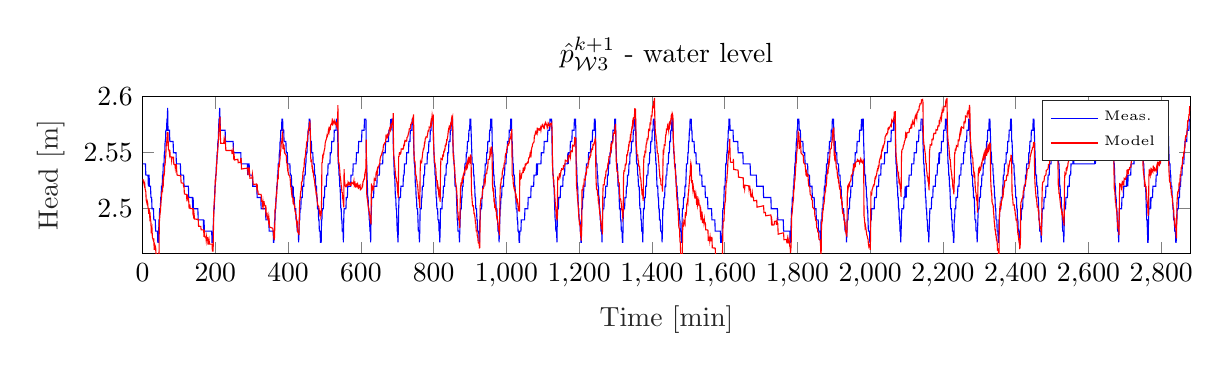
\begin{tikzpicture}

\begin{axis}[%
width=5.239in,
height=0.784in,
at={(1.201in,0.431in)},
scale only axis,
xmin=0,
xmax=2880,
xlabel style={font=\color{white!15!black}},
xlabel={Time [min]},
ymin=2.46,
ymax=2.6,
ylabel style={font=\color{white!15!black}},
ylabel={Head  [m]},
axis background/.style={fill=white},
title style={},
title={$\hat{p}^{k+1}_{\mathcal{W}3}$ - water level},
legend style={legend cell align=left, align=left, draw=white!15!black}
]
\addplot [color=blue]
  table[row sep=crcr]{%
1	2.54\\
2	2.54\\
3	2.54\\
4	2.54\\
5	2.54\\
6	2.54\\
7	2.54\\
8	2.54\\
9	2.53\\
10	2.53\\
11	2.53\\
12	2.53\\
13	2.53\\
14	2.53\\
15	2.53\\
16	2.52\\
17	2.53\\
18	2.53\\
19	2.52\\
20	2.52\\
21	2.52\\
22	2.52\\
23	2.51\\
24	2.51\\
25	2.51\\
26	2.5\\
27	2.5\\
28	2.5\\
29	2.5\\
30	2.5\\
31	2.49\\
32	2.49\\
33	2.49\\
34	2.49\\
35	2.49\\
36	2.48\\
37	2.48\\
38	2.48\\
39	2.48\\
40	2.48\\
41	2.48\\
42	2.47\\
43	2.47\\
44	2.47\\
45	2.49\\
46	2.49\\
47	2.5\\
48	2.5\\
49	2.5\\
50	2.51\\
51	2.51\\
52	2.52\\
53	2.52\\
54	2.52\\
55	2.53\\
56	2.53\\
57	2.54\\
58	2.54\\
59	2.54\\
60	2.55\\
61	2.55\\
62	2.56\\
63	2.56\\
64	2.57\\
65	2.57\\
66	2.57\\
67	2.58\\
68	2.58\\
69	2.59\\
70	2.57\\
71	2.57\\
72	2.57\\
73	2.57\\
74	2.57\\
75	2.56\\
76	2.56\\
77	2.56\\
78	2.56\\
79	2.56\\
80	2.56\\
81	2.56\\
82	2.56\\
83	2.56\\
84	2.56\\
85	2.55\\
86	2.55\\
87	2.55\\
88	2.55\\
89	2.55\\
90	2.55\\
91	2.55\\
92	2.55\\
93	2.54\\
94	2.54\\
95	2.54\\
96	2.54\\
97	2.54\\
98	2.54\\
99	2.54\\
100	2.54\\
101	2.54\\
102	2.54\\
103	2.54\\
104	2.54\\
105	2.53\\
106	2.53\\
107	2.53\\
108	2.53\\
109	2.53\\
110	2.53\\
111	2.53\\
112	2.53\\
113	2.53\\
114	2.52\\
115	2.52\\
116	2.52\\
117	2.52\\
118	2.52\\
119	2.52\\
120	2.52\\
121	2.52\\
122	2.52\\
123	2.52\\
124	2.52\\
125	2.52\\
126	2.52\\
127	2.51\\
128	2.51\\
129	2.51\\
130	2.51\\
131	2.51\\
132	2.51\\
133	2.51\\
134	2.51\\
135	2.51\\
136	2.51\\
137	2.51\\
138	2.5\\
139	2.51\\
140	2.5\\
141	2.5\\
142	2.5\\
143	2.5\\
144	2.5\\
145	2.5\\
146	2.5\\
147	2.5\\
148	2.5\\
149	2.5\\
150	2.5\\
151	2.5\\
152	2.5\\
153	2.49\\
154	2.49\\
155	2.49\\
156	2.49\\
157	2.49\\
158	2.49\\
159	2.49\\
160	2.49\\
161	2.49\\
162	2.49\\
163	2.49\\
164	2.49\\
165	2.49\\
166	2.49\\
167	2.49\\
168	2.48\\
169	2.49\\
170	2.48\\
171	2.48\\
172	2.48\\
173	2.48\\
174	2.48\\
175	2.48\\
176	2.48\\
177	2.48\\
178	2.48\\
179	2.48\\
180	2.48\\
181	2.48\\
182	2.48\\
183	2.48\\
184	2.48\\
185	2.48\\
186	2.48\\
187	2.48\\
188	2.48\\
189	2.48\\
190	2.48\\
191	2.47\\
192	2.47\\
193	2.47\\
194	2.48\\
195	2.49\\
196	2.5\\
197	2.5\\
198	2.51\\
199	2.52\\
200	2.52\\
201	2.53\\
202	2.53\\
203	2.54\\
204	2.54\\
205	2.55\\
206	2.55\\
207	2.56\\
208	2.56\\
209	2.57\\
210	2.58\\
211	2.58\\
212	2.59\\
213	2.58\\
214	2.57\\
215	2.57\\
216	2.57\\
217	2.57\\
218	2.57\\
219	2.57\\
220	2.57\\
221	2.57\\
222	2.57\\
223	2.57\\
224	2.57\\
225	2.57\\
226	2.57\\
227	2.57\\
228	2.56\\
229	2.56\\
230	2.56\\
231	2.56\\
232	2.56\\
233	2.56\\
234	2.56\\
235	2.56\\
236	2.56\\
237	2.56\\
238	2.56\\
239	2.56\\
240	2.56\\
241	2.56\\
242	2.56\\
243	2.56\\
244	2.56\\
245	2.56\\
246	2.56\\
247	2.56\\
248	2.56\\
249	2.56\\
250	2.55\\
251	2.55\\
252	2.55\\
253	2.55\\
254	2.55\\
255	2.55\\
256	2.55\\
257	2.55\\
258	2.55\\
259	2.55\\
260	2.55\\
261	2.55\\
262	2.55\\
263	2.55\\
264	2.55\\
265	2.55\\
266	2.55\\
267	2.55\\
268	2.55\\
269	2.55\\
270	2.55\\
271	2.54\\
272	2.54\\
273	2.54\\
274	2.54\\
275	2.54\\
276	2.54\\
277	2.54\\
278	2.54\\
279	2.54\\
280	2.54\\
281	2.54\\
282	2.54\\
283	2.54\\
284	2.54\\
285	2.54\\
286	2.54\\
287	2.54\\
288	2.54\\
289	2.53\\
290	2.54\\
291	2.54\\
292	2.54\\
293	2.54\\
294	2.53\\
295	2.53\\
296	2.53\\
297	2.53\\
298	2.53\\
299	2.53\\
300	2.53\\
301	2.53\\
302	2.53\\
303	2.52\\
304	2.52\\
305	2.52\\
306	2.52\\
307	2.52\\
308	2.52\\
309	2.52\\
310	2.52\\
311	2.52\\
312	2.52\\
313	2.52\\
314	2.52\\
315	2.51\\
316	2.51\\
317	2.51\\
318	2.51\\
319	2.51\\
320	2.51\\
321	2.51\\
322	2.51\\
323	2.51\\
324	2.51\\
325	2.51\\
326	2.5\\
327	2.5\\
328	2.5\\
329	2.5\\
330	2.5\\
331	2.5\\
332	2.5\\
333	2.5\\
334	2.5\\
335	2.5\\
336	2.5\\
337	2.5\\
338	2.5\\
339	2.49\\
340	2.49\\
341	2.49\\
342	2.49\\
343	2.49\\
344	2.49\\
345	2.49\\
346	2.49\\
347	2.49\\
348	2.48\\
349	2.48\\
350	2.48\\
351	2.48\\
352	2.48\\
353	2.48\\
354	2.48\\
355	2.48\\
356	2.48\\
357	2.48\\
358	2.48\\
359	2.48\\
360	2.47\\
361	2.47\\
362	2.48\\
363	2.49\\
364	2.49\\
365	2.5\\
366	2.5\\
367	2.51\\
368	2.51\\
369	2.52\\
370	2.52\\
371	2.53\\
372	2.53\\
373	2.54\\
374	2.54\\
375	2.54\\
376	2.55\\
377	2.55\\
378	2.56\\
379	2.56\\
380	2.57\\
381	2.57\\
382	2.57\\
383	2.58\\
384	2.58\\
385	2.58\\
386	2.57\\
387	2.57\\
388	2.57\\
389	2.56\\
390	2.56\\
391	2.56\\
392	2.56\\
393	2.56\\
394	2.56\\
395	2.55\\
396	2.55\\
397	2.55\\
398	2.55\\
399	2.54\\
400	2.54\\
401	2.54\\
402	2.54\\
403	2.54\\
404	2.54\\
405	2.54\\
406	2.53\\
407	2.53\\
408	2.53\\
409	2.53\\
410	2.52\\
411	2.52\\
412	2.52\\
413	2.51\\
414	2.52\\
415	2.51\\
416	2.51\\
417	2.51\\
418	2.5\\
419	2.5\\
420	2.5\\
421	2.5\\
422	2.49\\
423	2.49\\
424	2.49\\
425	2.48\\
426	2.48\\
427	2.48\\
428	2.48\\
429	2.47\\
430	2.48\\
431	2.49\\
432	2.49\\
433	2.5\\
434	2.5\\
435	2.5\\
436	2.51\\
437	2.51\\
438	2.51\\
439	2.51\\
440	2.52\\
441	2.52\\
442	2.52\\
443	2.52\\
444	2.53\\
445	2.53\\
446	2.53\\
447	2.53\\
448	2.54\\
449	2.54\\
450	2.55\\
451	2.55\\
452	2.55\\
453	2.56\\
454	2.56\\
455	2.57\\
456	2.57\\
457	2.57\\
458	2.58\\
459	2.58\\
460	2.58\\
461	2.57\\
462	2.56\\
463	2.56\\
464	2.56\\
465	2.55\\
466	2.55\\
467	2.55\\
468	2.55\\
469	2.54\\
470	2.54\\
471	2.54\\
472	2.54\\
473	2.53\\
474	2.53\\
475	2.53\\
476	2.52\\
477	2.52\\
478	2.52\\
479	2.51\\
480	2.51\\
481	2.5\\
482	2.5\\
483	2.5\\
484	2.49\\
485	2.49\\
486	2.48\\
487	2.48\\
488	2.48\\
489	2.47\\
490	2.47\\
491	2.47\\
492	2.49\\
493	2.49\\
494	2.5\\
495	2.5\\
496	2.5\\
497	2.5\\
498	2.51\\
499	2.51\\
500	2.51\\
501	2.52\\
502	2.52\\
503	2.52\\
504	2.52\\
505	2.52\\
506	2.53\\
507	2.53\\
508	2.53\\
509	2.53\\
510	2.54\\
511	2.54\\
512	2.54\\
513	2.54\\
514	2.54\\
515	2.54\\
516	2.55\\
517	2.55\\
518	2.55\\
519	2.55\\
520	2.56\\
521	2.56\\
522	2.56\\
523	2.56\\
524	2.56\\
525	2.56\\
526	2.56\\
527	2.57\\
528	2.57\\
529	2.57\\
530	2.57\\
531	2.57\\
532	2.57\\
533	2.58\\
534	2.58\\
535	2.58\\
536	2.58\\
537	2.55\\
538	2.54\\
539	2.54\\
540	2.53\\
541	2.53\\
542	2.52\\
543	2.52\\
544	2.51\\
545	2.5\\
546	2.5\\
547	2.49\\
548	2.49\\
549	2.48\\
550	2.48\\
551	2.48\\
552	2.47\\
553	2.49\\
554	2.5\\
555	2.5\\
556	2.5\\
557	2.5\\
558	2.5\\
559	2.5\\
560	2.51\\
561	2.51\\
562	2.51\\
563	2.51\\
564	2.52\\
565	2.52\\
566	2.52\\
567	2.52\\
568	2.52\\
569	2.52\\
570	2.52\\
571	2.52\\
572	2.52\\
573	2.53\\
574	2.53\\
575	2.53\\
576	2.53\\
577	2.53\\
578	2.53\\
579	2.54\\
580	2.54\\
581	2.54\\
582	2.54\\
583	2.54\\
584	2.54\\
585	2.54\\
586	2.54\\
587	2.54\\
588	2.55\\
589	2.55\\
590	2.55\\
591	2.55\\
592	2.55\\
593	2.55\\
594	2.56\\
595	2.56\\
596	2.56\\
597	2.56\\
598	2.56\\
599	2.56\\
600	2.56\\
601	2.56\\
602	2.56\\
603	2.57\\
604	2.57\\
605	2.57\\
606	2.57\\
607	2.57\\
608	2.57\\
609	2.57\\
610	2.58\\
611	2.58\\
612	2.58\\
613	2.58\\
614	2.58\\
615	2.55\\
616	2.54\\
617	2.53\\
618	2.52\\
619	2.51\\
620	2.51\\
621	2.5\\
622	2.5\\
623	2.49\\
624	2.49\\
625	2.48\\
626	2.48\\
627	2.47\\
628	2.49\\
629	2.5\\
630	2.51\\
631	2.51\\
632	2.51\\
633	2.51\\
634	2.51\\
635	2.51\\
636	2.52\\
637	2.52\\
638	2.52\\
639	2.52\\
640	2.52\\
641	2.52\\
642	2.52\\
643	2.52\\
644	2.52\\
645	2.53\\
646	2.53\\
647	2.53\\
648	2.53\\
649	2.53\\
650	2.53\\
651	2.53\\
652	2.54\\
653	2.54\\
654	2.54\\
655	2.54\\
656	2.54\\
657	2.54\\
658	2.54\\
659	2.54\\
660	2.54\\
661	2.55\\
662	2.55\\
663	2.55\\
664	2.55\\
665	2.55\\
666	2.55\\
667	2.55\\
668	2.56\\
669	2.56\\
670	2.56\\
671	2.56\\
672	2.56\\
673	2.56\\
674	2.56\\
675	2.56\\
676	2.56\\
677	2.57\\
678	2.57\\
679	2.57\\
680	2.57\\
681	2.57\\
682	2.58\\
683	2.57\\
684	2.58\\
685	2.58\\
686	2.58\\
687	2.58\\
688	2.58\\
689	2.56\\
690	2.55\\
691	2.54\\
692	2.53\\
693	2.53\\
694	2.52\\
695	2.51\\
696	2.51\\
697	2.5\\
698	2.5\\
699	2.49\\
700	2.48\\
701	2.48\\
702	2.47\\
703	2.48\\
704	2.5\\
705	2.51\\
706	2.51\\
707	2.51\\
708	2.51\\
709	2.51\\
710	2.52\\
711	2.52\\
712	2.52\\
713	2.52\\
714	2.52\\
715	2.52\\
716	2.52\\
717	2.53\\
718	2.53\\
719	2.53\\
720	2.54\\
721	2.54\\
722	2.54\\
723	2.54\\
724	2.54\\
725	2.54\\
726	2.55\\
727	2.55\\
728	2.55\\
729	2.55\\
730	2.55\\
731	2.55\\
732	2.56\\
733	2.56\\
734	2.56\\
735	2.56\\
736	2.57\\
737	2.57\\
738	2.57\\
739	2.57\\
740	2.57\\
741	2.58\\
742	2.58\\
743	2.58\\
744	2.58\\
745	2.56\\
746	2.55\\
747	2.54\\
748	2.54\\
749	2.53\\
750	2.52\\
751	2.52\\
752	2.51\\
753	2.51\\
754	2.5\\
755	2.5\\
756	2.5\\
757	2.49\\
758	2.48\\
759	2.48\\
760	2.48\\
761	2.47\\
762	2.48\\
763	2.5\\
764	2.5\\
765	2.5\\
766	2.5\\
767	2.51\\
768	2.51\\
769	2.52\\
770	2.52\\
771	2.52\\
772	2.52\\
773	2.53\\
774	2.53\\
775	2.53\\
776	2.54\\
777	2.54\\
778	2.54\\
779	2.54\\
780	2.54\\
781	2.54\\
782	2.54\\
783	2.55\\
784	2.55\\
785	2.55\\
786	2.55\\
787	2.56\\
788	2.56\\
789	2.56\\
790	2.56\\
791	2.57\\
792	2.57\\
793	2.57\\
794	2.58\\
795	2.58\\
796	2.58\\
797	2.58\\
798	2.58\\
799	2.57\\
800	2.56\\
801	2.55\\
802	2.54\\
803	2.54\\
804	2.53\\
805	2.53\\
806	2.52\\
807	2.51\\
808	2.51\\
809	2.5\\
810	2.5\\
811	2.5\\
812	2.49\\
813	2.49\\
814	2.49\\
815	2.48\\
816	2.48\\
817	2.47\\
818	2.48\\
819	2.5\\
820	2.5\\
821	2.5\\
822	2.5\\
823	2.5\\
824	2.51\\
825	2.51\\
826	2.51\\
827	2.52\\
828	2.52\\
829	2.52\\
830	2.52\\
831	2.53\\
832	2.53\\
833	2.53\\
834	2.53\\
835	2.54\\
836	2.54\\
837	2.54\\
838	2.54\\
839	2.55\\
840	2.55\\
841	2.55\\
842	2.56\\
843	2.56\\
844	2.56\\
845	2.56\\
846	2.57\\
847	2.57\\
848	2.57\\
849	2.58\\
850	2.58\\
851	2.58\\
852	2.58\\
853	2.56\\
854	2.55\\
855	2.55\\
856	2.54\\
857	2.54\\
858	2.53\\
859	2.52\\
860	2.52\\
861	2.52\\
862	2.52\\
863	2.51\\
864	2.5\\
865	2.49\\
866	2.49\\
867	2.48\\
868	2.48\\
869	2.48\\
870	2.48\\
871	2.47\\
872	2.48\\
873	2.49\\
874	2.5\\
875	2.5\\
876	2.5\\
877	2.51\\
878	2.51\\
879	2.52\\
880	2.52\\
881	2.52\\
882	2.53\\
883	2.53\\
884	2.53\\
885	2.53\\
886	2.54\\
887	2.54\\
888	2.54\\
889	2.54\\
890	2.55\\
891	2.55\\
892	2.55\\
893	2.56\\
894	2.56\\
895	2.56\\
896	2.56\\
897	2.57\\
898	2.57\\
899	2.57\\
900	2.58\\
901	2.58\\
902	2.58\\
903	2.57\\
904	2.56\\
905	2.55\\
906	2.54\\
907	2.54\\
908	2.54\\
909	2.54\\
910	2.53\\
911	2.53\\
912	2.52\\
913	2.52\\
914	2.51\\
915	2.51\\
916	2.5\\
917	2.5\\
918	2.5\\
919	2.49\\
920	2.49\\
921	2.48\\
922	2.48\\
923	2.48\\
924	2.48\\
925	2.47\\
926	2.47\\
927	2.49\\
928	2.49\\
929	2.5\\
930	2.5\\
931	2.5\\
932	2.5\\
933	2.51\\
934	2.51\\
935	2.52\\
936	2.52\\
937	2.52\\
938	2.52\\
939	2.53\\
940	2.53\\
941	2.53\\
942	2.54\\
943	2.54\\
944	2.54\\
945	2.54\\
946	2.55\\
947	2.55\\
948	2.55\\
949	2.56\\
950	2.56\\
951	2.56\\
952	2.56\\
953	2.56\\
954	2.57\\
955	2.57\\
956	2.57\\
957	2.58\\
958	2.58\\
959	2.58\\
960	2.58\\
961	2.56\\
962	2.55\\
963	2.55\\
964	2.54\\
965	2.53\\
966	2.53\\
967	2.52\\
968	2.52\\
969	2.52\\
970	2.51\\
971	2.51\\
972	2.5\\
973	2.5\\
974	2.5\\
975	2.49\\
976	2.49\\
977	2.48\\
978	2.48\\
979	2.48\\
980	2.47\\
981	2.48\\
982	2.49\\
983	2.5\\
984	2.5\\
985	2.51\\
986	2.51\\
987	2.51\\
988	2.52\\
989	2.52\\
990	2.52\\
991	2.52\\
992	2.52\\
993	2.53\\
994	2.53\\
995	2.53\\
996	2.54\\
997	2.54\\
998	2.54\\
999	2.54\\
1000	2.55\\
1001	2.55\\
1002	2.55\\
1003	2.56\\
1004	2.56\\
1005	2.56\\
1006	2.56\\
1007	2.56\\
1008	2.57\\
1009	2.57\\
1010	2.57\\
1011	2.57\\
1012	2.58\\
1013	2.58\\
1014	2.58\\
1015	2.56\\
1016	2.56\\
1017	2.55\\
1018	2.54\\
1019	2.54\\
1020	2.53\\
1021	2.53\\
1022	2.53\\
1023	2.52\\
1024	2.52\\
1025	2.51\\
1026	2.51\\
1027	2.5\\
1028	2.5\\
1029	2.5\\
1030	2.49\\
1031	2.49\\
1032	2.48\\
1033	2.48\\
1034	2.48\\
1035	2.47\\
1036	2.47\\
1037	2.48\\
1038	2.48\\
1039	2.48\\
1040	2.48\\
1041	2.49\\
1042	2.49\\
1043	2.49\\
1044	2.49\\
1045	2.49\\
1046	2.49\\
1047	2.49\\
1048	2.49\\
1049	2.49\\
1050	2.49\\
1051	2.5\\
1052	2.5\\
1053	2.5\\
1054	2.5\\
1055	2.5\\
1056	2.5\\
1057	2.5\\
1058	2.5\\
1059	2.5\\
1060	2.51\\
1061	2.51\\
1062	2.51\\
1063	2.51\\
1064	2.51\\
1065	2.51\\
1066	2.51\\
1067	2.51\\
1068	2.52\\
1069	2.52\\
1070	2.52\\
1071	2.52\\
1072	2.52\\
1073	2.52\\
1074	2.52\\
1075	2.52\\
1076	2.53\\
1077	2.53\\
1078	2.53\\
1079	2.53\\
1080	2.53\\
1081	2.53\\
1082	2.53\\
1083	2.54\\
1084	2.54\\
1085	2.53\\
1086	2.54\\
1087	2.54\\
1088	2.54\\
1089	2.54\\
1090	2.54\\
1091	2.54\\
1092	2.54\\
1093	2.54\\
1094	2.54\\
1095	2.54\\
1096	2.55\\
1097	2.55\\
1098	2.55\\
1099	2.55\\
1100	2.55\\
1101	2.55\\
1102	2.55\\
1103	2.55\\
1104	2.56\\
1105	2.56\\
1106	2.56\\
1107	2.56\\
1108	2.56\\
1109	2.56\\
1110	2.56\\
1111	2.56\\
1112	2.56\\
1113	2.56\\
1114	2.57\\
1115	2.57\\
1116	2.57\\
1117	2.57\\
1118	2.57\\
1119	2.57\\
1120	2.58\\
1121	2.58\\
1122	2.58\\
1123	2.58\\
1124	2.58\\
1125	2.57\\
1126	2.55\\
1127	2.54\\
1128	2.53\\
1129	2.53\\
1130	2.52\\
1131	2.52\\
1132	2.51\\
1133	2.5\\
1134	2.49\\
1135	2.49\\
1136	2.48\\
1137	2.48\\
1138	2.48\\
1139	2.47\\
1140	2.49\\
1141	2.5\\
1142	2.5\\
1143	2.5\\
1144	2.51\\
1145	2.51\\
1146	2.51\\
1147	2.51\\
1148	2.51\\
1149	2.52\\
1150	2.52\\
1151	2.52\\
1152	2.52\\
1153	2.52\\
1154	2.52\\
1155	2.52\\
1156	2.53\\
1157	2.53\\
1158	2.53\\
1159	2.53\\
1160	2.53\\
1161	2.54\\
1162	2.54\\
1163	2.54\\
1164	2.54\\
1165	2.54\\
1166	2.54\\
1167	2.54\\
1168	2.54\\
1169	2.55\\
1170	2.54\\
1171	2.55\\
1172	2.55\\
1173	2.55\\
1174	2.55\\
1175	2.55\\
1176	2.56\\
1177	2.56\\
1178	2.56\\
1179	2.56\\
1180	2.56\\
1181	2.57\\
1182	2.57\\
1183	2.57\\
1184	2.57\\
1185	2.57\\
1186	2.57\\
1187	2.58\\
1188	2.58\\
1189	2.58\\
1190	2.58\\
1191	2.57\\
1192	2.54\\
1193	2.54\\
1194	2.53\\
1195	2.52\\
1196	2.52\\
1197	2.51\\
1198	2.5\\
1199	2.5\\
1200	2.49\\
1201	2.49\\
1202	2.49\\
1203	2.48\\
1204	2.48\\
1205	2.47\\
1206	2.47\\
1207	2.5\\
1208	2.5\\
1209	2.5\\
1210	2.51\\
1211	2.51\\
1212	2.51\\
1213	2.52\\
1214	2.52\\
1215	2.52\\
1216	2.52\\
1217	2.53\\
1218	2.53\\
1219	2.53\\
1220	2.54\\
1221	2.54\\
1222	2.54\\
1223	2.54\\
1224	2.54\\
1225	2.54\\
1226	2.55\\
1227	2.55\\
1228	2.55\\
1229	2.55\\
1230	2.55\\
1231	2.55\\
1232	2.56\\
1233	2.56\\
1234	2.56\\
1235	2.56\\
1236	2.56\\
1237	2.57\\
1238	2.57\\
1239	2.57\\
1240	2.57\\
1241	2.57\\
1242	2.58\\
1243	2.58\\
1244	2.58\\
1245	2.57\\
1246	2.55\\
1247	2.54\\
1248	2.54\\
1249	2.54\\
1250	2.53\\
1251	2.53\\
1252	2.52\\
1253	2.52\\
1254	2.51\\
1255	2.51\\
1256	2.5\\
1257	2.5\\
1258	2.49\\
1259	2.49\\
1260	2.48\\
1261	2.48\\
1262	2.48\\
1263	2.47\\
1264	2.49\\
1265	2.5\\
1266	2.5\\
1267	2.5\\
1268	2.5\\
1269	2.51\\
1270	2.51\\
1271	2.51\\
1272	2.51\\
1273	2.52\\
1274	2.52\\
1275	2.52\\
1276	2.52\\
1277	2.52\\
1278	2.53\\
1279	2.53\\
1280	2.53\\
1281	2.54\\
1282	2.54\\
1283	2.54\\
1284	2.54\\
1285	2.55\\
1286	2.55\\
1287	2.55\\
1288	2.55\\
1289	2.56\\
1290	2.56\\
1291	2.56\\
1292	2.56\\
1293	2.57\\
1294	2.57\\
1295	2.57\\
1296	2.57\\
1297	2.57\\
1298	2.58\\
1299	2.58\\
1300	2.58\\
1301	2.56\\
1302	2.55\\
1303	2.54\\
1304	2.54\\
1305	2.54\\
1306	2.53\\
1307	2.52\\
1308	2.52\\
1309	2.52\\
1310	2.51\\
1311	2.5\\
1312	2.5\\
1313	2.5\\
1314	2.49\\
1315	2.49\\
1316	2.48\\
1317	2.48\\
1318	2.48\\
1319	2.47\\
1320	2.47\\
1321	2.49\\
1322	2.5\\
1323	2.5\\
1324	2.5\\
1325	2.5\\
1326	2.51\\
1327	2.51\\
1328	2.51\\
1329	2.51\\
1330	2.52\\
1331	2.52\\
1332	2.52\\
1333	2.53\\
1334	2.53\\
1335	2.53\\
1336	2.53\\
1337	2.54\\
1338	2.54\\
1339	2.54\\
1340	2.55\\
1341	2.55\\
1342	2.55\\
1343	2.55\\
1344	2.56\\
1345	2.56\\
1346	2.56\\
1347	2.56\\
1348	2.56\\
1349	2.57\\
1350	2.57\\
1351	2.57\\
1352	2.58\\
1353	2.58\\
1354	2.58\\
1355	2.58\\
1356	2.56\\
1357	2.55\\
1358	2.54\\
1359	2.54\\
1360	2.54\\
1361	2.53\\
1362	2.53\\
1363	2.52\\
1364	2.52\\
1365	2.52\\
1366	2.51\\
1367	2.5\\
1368	2.5\\
1369	2.5\\
1370	2.49\\
1371	2.49\\
1372	2.48\\
1373	2.48\\
1374	2.48\\
1375	2.47\\
1376	2.49\\
1377	2.5\\
1378	2.5\\
1379	2.5\\
1380	2.51\\
1381	2.51\\
1382	2.51\\
1383	2.52\\
1384	2.52\\
1385	2.52\\
1386	2.53\\
1387	2.53\\
1388	2.53\\
1389	2.53\\
1390	2.54\\
1391	2.54\\
1392	2.54\\
1393	2.54\\
1394	2.55\\
1395	2.55\\
1396	2.55\\
1397	2.56\\
1398	2.56\\
1399	2.56\\
1400	2.56\\
1401	2.57\\
1402	2.57\\
1403	2.57\\
1404	2.58\\
1405	2.58\\
1406	2.58\\
1407	2.58\\
1408	2.56\\
1409	2.55\\
1410	2.55\\
1411	2.54\\
1412	2.54\\
1413	2.53\\
1414	2.52\\
1415	2.52\\
1416	2.52\\
1417	2.51\\
1418	2.51\\
1419	2.5\\
1420	2.5\\
1421	2.49\\
1422	2.49\\
1423	2.49\\
1424	2.48\\
1425	2.48\\
1426	2.48\\
1427	2.48\\
1428	2.47\\
1429	2.48\\
1430	2.5\\
1431	2.5\\
1432	2.5\\
1433	2.51\\
1434	2.51\\
1435	2.51\\
1436	2.52\\
1437	2.52\\
1438	2.52\\
1439	2.53\\
1440	2.53\\
1441	2.53\\
1442	2.54\\
1443	2.54\\
1444	2.54\\
1445	2.54\\
1446	2.55\\
1447	2.55\\
1448	2.55\\
1449	2.56\\
1450	2.56\\
1451	2.56\\
1452	2.57\\
1453	2.57\\
1454	2.57\\
1455	2.58\\
1456	2.58\\
1457	2.58\\
1458	2.57\\
1459	2.56\\
1460	2.55\\
1461	2.55\\
1462	2.54\\
1463	2.54\\
1464	2.54\\
1465	2.53\\
1466	2.53\\
1467	2.52\\
1468	2.52\\
1469	2.52\\
1470	2.51\\
1471	2.51\\
1472	2.5\\
1473	2.5\\
1474	2.5\\
1475	2.5\\
1476	2.49\\
1477	2.49\\
1478	2.48\\
1479	2.48\\
1480	2.48\\
1481	2.47\\
1482	2.47\\
1483	2.49\\
1484	2.5\\
1485	2.5\\
1486	2.5\\
1487	2.51\\
1488	2.51\\
1489	2.51\\
1490	2.51\\
1491	2.52\\
1492	2.52\\
1493	2.52\\
1494	2.53\\
1495	2.54\\
1496	2.54\\
1497	2.54\\
1498	2.54\\
1499	2.55\\
1500	2.55\\
1501	2.56\\
1502	2.56\\
1503	2.57\\
1504	2.57\\
1505	2.58\\
1506	2.58\\
1507	2.58\\
1508	2.58\\
1509	2.57\\
1510	2.57\\
1511	2.56\\
1512	2.56\\
1513	2.56\\
1514	2.56\\
1515	2.56\\
1516	2.56\\
1517	2.55\\
1518	2.55\\
1519	2.55\\
1520	2.55\\
1521	2.55\\
1522	2.54\\
1523	2.54\\
1524	2.54\\
1525	2.54\\
1526	2.54\\
1527	2.54\\
1528	2.54\\
1529	2.54\\
1530	2.54\\
1531	2.54\\
1532	2.53\\
1533	2.53\\
1534	2.53\\
1535	2.53\\
1536	2.53\\
1537	2.53\\
1538	2.52\\
1539	2.52\\
1540	2.52\\
1541	2.52\\
1542	2.52\\
1543	2.52\\
1544	2.52\\
1545	2.52\\
1546	2.52\\
1547	2.51\\
1548	2.51\\
1549	2.51\\
1550	2.51\\
1551	2.51\\
1552	2.51\\
1553	2.51\\
1554	2.5\\
1555	2.5\\
1556	2.5\\
1557	2.5\\
1558	2.5\\
1559	2.5\\
1560	2.5\\
1561	2.5\\
1562	2.5\\
1563	2.5\\
1564	2.5\\
1565	2.49\\
1566	2.49\\
1567	2.49\\
1568	2.49\\
1569	2.49\\
1570	2.49\\
1571	2.49\\
1572	2.49\\
1573	2.49\\
1574	2.48\\
1575	2.48\\
1576	2.48\\
1577	2.48\\
1578	2.48\\
1579	2.48\\
1580	2.48\\
1581	2.48\\
1582	2.48\\
1583	2.48\\
1584	2.48\\
1585	2.48\\
1586	2.48\\
1587	2.48\\
1588	2.48\\
1589	2.47\\
1590	2.47\\
1591	2.47\\
1592	2.47\\
1593	2.48\\
1594	2.49\\
1595	2.5\\
1596	2.5\\
1597	2.5\\
1598	2.51\\
1599	2.52\\
1600	2.52\\
1601	2.52\\
1602	2.53\\
1603	2.54\\
1604	2.54\\
1605	2.54\\
1606	2.55\\
1607	2.55\\
1608	2.56\\
1609	2.56\\
1610	2.57\\
1611	2.57\\
1612	2.58\\
1613	2.58\\
1614	2.58\\
1615	2.57\\
1616	2.57\\
1617	2.57\\
1618	2.57\\
1619	2.57\\
1620	2.57\\
1621	2.57\\
1622	2.57\\
1623	2.57\\
1624	2.56\\
1625	2.56\\
1626	2.56\\
1627	2.56\\
1628	2.56\\
1629	2.56\\
1630	2.56\\
1631	2.56\\
1632	2.56\\
1633	2.56\\
1634	2.56\\
1635	2.56\\
1636	2.56\\
1637	2.55\\
1638	2.55\\
1639	2.55\\
1640	2.55\\
1641	2.55\\
1642	2.55\\
1643	2.55\\
1644	2.55\\
1645	2.55\\
1646	2.55\\
1647	2.55\\
1648	2.55\\
1649	2.55\\
1650	2.55\\
1651	2.54\\
1652	2.54\\
1653	2.54\\
1654	2.54\\
1655	2.54\\
1656	2.54\\
1657	2.54\\
1658	2.54\\
1659	2.54\\
1660	2.54\\
1661	2.54\\
1662	2.54\\
1663	2.54\\
1664	2.54\\
1665	2.54\\
1666	2.54\\
1667	2.54\\
1668	2.54\\
1669	2.54\\
1670	2.54\\
1671	2.53\\
1672	2.53\\
1673	2.53\\
1674	2.53\\
1675	2.53\\
1676	2.53\\
1677	2.53\\
1678	2.53\\
1679	2.53\\
1680	2.53\\
1681	2.53\\
1682	2.53\\
1683	2.53\\
1684	2.53\\
1685	2.53\\
1686	2.53\\
1687	2.53\\
1688	2.52\\
1689	2.52\\
1690	2.52\\
1691	2.52\\
1692	2.52\\
1693	2.52\\
1694	2.52\\
1695	2.52\\
1696	2.52\\
1697	2.52\\
1698	2.52\\
1699	2.52\\
1700	2.52\\
1701	2.52\\
1702	2.52\\
1703	2.52\\
1704	2.52\\
1705	2.52\\
1706	2.52\\
1707	2.51\\
1708	2.51\\
1709	2.51\\
1710	2.51\\
1711	2.51\\
1712	2.51\\
1713	2.51\\
1714	2.51\\
1715	2.51\\
1716	2.51\\
1717	2.51\\
1718	2.51\\
1719	2.51\\
1720	2.51\\
1721	2.51\\
1722	2.51\\
1723	2.51\\
1724	2.51\\
1725	2.51\\
1726	2.51\\
1727	2.51\\
1728	2.5\\
1729	2.5\\
1730	2.5\\
1731	2.5\\
1732	2.5\\
1733	2.5\\
1734	2.5\\
1735	2.5\\
1736	2.5\\
1737	2.5\\
1738	2.5\\
1739	2.5\\
1740	2.5\\
1741	2.5\\
1742	2.5\\
1743	2.5\\
1744	2.5\\
1745	2.5\\
1746	2.49\\
1747	2.49\\
1748	2.49\\
1749	2.49\\
1750	2.49\\
1751	2.49\\
1752	2.49\\
1753	2.49\\
1754	2.49\\
1755	2.49\\
1756	2.49\\
1757	2.49\\
1758	2.49\\
1759	2.49\\
1760	2.49\\
1761	2.49\\
1762	2.48\\
1763	2.48\\
1764	2.48\\
1765	2.48\\
1766	2.48\\
1767	2.48\\
1768	2.48\\
1769	2.48\\
1770	2.48\\
1771	2.48\\
1772	2.48\\
1773	2.48\\
1774	2.48\\
1775	2.48\\
1776	2.48\\
1777	2.48\\
1778	2.48\\
1779	2.48\\
1780	2.47\\
1781	2.47\\
1782	2.48\\
1783	2.49\\
1784	2.5\\
1785	2.5\\
1786	2.51\\
1787	2.51\\
1788	2.51\\
1789	2.52\\
1790	2.52\\
1791	2.53\\
1792	2.53\\
1793	2.54\\
1794	2.54\\
1795	2.55\\
1796	2.55\\
1797	2.56\\
1798	2.56\\
1799	2.57\\
1800	2.57\\
1801	2.58\\
1802	2.58\\
1803	2.58\\
1804	2.58\\
1805	2.57\\
1806	2.57\\
1807	2.57\\
1808	2.57\\
1809	2.56\\
1810	2.56\\
1811	2.56\\
1812	2.56\\
1813	2.56\\
1814	2.56\\
1815	2.56\\
1816	2.55\\
1817	2.55\\
1818	2.55\\
1819	2.55\\
1820	2.55\\
1821	2.54\\
1822	2.54\\
1823	2.54\\
1824	2.54\\
1825	2.54\\
1826	2.54\\
1827	2.54\\
1828	2.54\\
1829	2.53\\
1830	2.53\\
1831	2.53\\
1832	2.53\\
1833	2.53\\
1834	2.52\\
1835	2.52\\
1836	2.52\\
1837	2.52\\
1838	2.52\\
1839	2.52\\
1840	2.52\\
1841	2.51\\
1842	2.51\\
1843	2.51\\
1844	2.51\\
1845	2.51\\
1846	2.51\\
1847	2.5\\
1848	2.5\\
1849	2.5\\
1850	2.5\\
1851	2.5\\
1852	2.49\\
1853	2.49\\
1854	2.49\\
1855	2.49\\
1856	2.49\\
1857	2.49\\
1858	2.48\\
1859	2.48\\
1860	2.48\\
1861	2.48\\
1862	2.48\\
1863	2.47\\
1864	2.47\\
1865	2.49\\
1866	2.49\\
1867	2.49\\
1868	2.5\\
1869	2.5\\
1870	2.5\\
1871	2.51\\
1872	2.51\\
1873	2.51\\
1874	2.52\\
1875	2.52\\
1876	2.52\\
1877	2.53\\
1878	2.53\\
1879	2.53\\
1880	2.54\\
1881	2.54\\
1882	2.54\\
1883	2.54\\
1884	2.55\\
1885	2.55\\
1886	2.55\\
1887	2.55\\
1888	2.56\\
1889	2.56\\
1890	2.56\\
1891	2.56\\
1892	2.56\\
1893	2.57\\
1894	2.57\\
1895	2.57\\
1896	2.58\\
1897	2.58\\
1898	2.58\\
1899	2.58\\
1900	2.57\\
1901	2.56\\
1902	2.55\\
1903	2.56\\
1904	2.56\\
1905	2.55\\
1906	2.55\\
1907	2.55\\
1908	2.55\\
1909	2.54\\
1910	2.54\\
1911	2.54\\
1912	2.54\\
1913	2.54\\
1914	2.53\\
1915	2.53\\
1916	2.53\\
1917	2.53\\
1918	2.52\\
1919	2.52\\
1920	2.52\\
1921	2.51\\
1922	2.51\\
1923	2.5\\
1924	2.5\\
1925	2.5\\
1926	2.5\\
1927	2.5\\
1928	2.49\\
1929	2.49\\
1930	2.49\\
1931	2.48\\
1932	2.48\\
1933	2.48\\
1934	2.48\\
1935	2.47\\
1936	2.48\\
1937	2.49\\
1938	2.49\\
1939	2.49\\
1940	2.5\\
1941	2.5\\
1942	2.5\\
1943	2.5\\
1944	2.51\\
1945	2.51\\
1946	2.51\\
1947	2.52\\
1948	2.52\\
1949	2.52\\
1950	2.52\\
1951	2.52\\
1952	2.53\\
1953	2.53\\
1954	2.54\\
1955	2.54\\
1956	2.54\\
1957	2.54\\
1958	2.54\\
1959	2.55\\
1960	2.55\\
1961	2.55\\
1962	2.55\\
1963	2.55\\
1964	2.56\\
1965	2.56\\
1966	2.56\\
1967	2.56\\
1968	2.56\\
1969	2.56\\
1970	2.56\\
1971	2.57\\
1972	2.57\\
1973	2.57\\
1974	2.57\\
1975	2.57\\
1976	2.58\\
1977	2.57\\
1978	2.58\\
1979	2.58\\
1980	2.58\\
1981	2.58\\
1982	2.56\\
1983	2.55\\
1984	2.54\\
1985	2.53\\
1986	2.53\\
1987	2.53\\
1988	2.52\\
1989	2.52\\
1990	2.51\\
1991	2.51\\
1992	2.5\\
1993	2.5\\
1994	2.49\\
1995	2.48\\
1996	2.48\\
1997	2.48\\
1998	2.48\\
1999	2.47\\
2000	2.47\\
2001	2.49\\
2002	2.49\\
2003	2.49\\
2004	2.5\\
2005	2.5\\
2006	2.5\\
2007	2.5\\
2008	2.5\\
2009	2.5\\
2010	2.5\\
2011	2.5\\
2012	2.51\\
2013	2.51\\
2014	2.51\\
2015	2.51\\
2016	2.51\\
2017	2.51\\
2018	2.52\\
2019	2.52\\
2020	2.52\\
2021	2.52\\
2022	2.52\\
2023	2.52\\
2024	2.53\\
2025	2.53\\
2026	2.53\\
2027	2.53\\
2028	2.53\\
2029	2.53\\
2030	2.54\\
2031	2.54\\
2032	2.54\\
2033	2.54\\
2034	2.54\\
2035	2.54\\
2036	2.54\\
2037	2.54\\
2038	2.54\\
2039	2.54\\
2040	2.55\\
2041	2.55\\
2042	2.55\\
2043	2.55\\
2044	2.55\\
2045	2.55\\
2046	2.55\\
2047	2.55\\
2048	2.56\\
2049	2.56\\
2050	2.56\\
2051	2.56\\
2052	2.56\\
2053	2.56\\
2054	2.56\\
2055	2.56\\
2056	2.56\\
2057	2.56\\
2058	2.57\\
2059	2.57\\
2060	2.57\\
2061	2.57\\
2062	2.57\\
2063	2.57\\
2064	2.57\\
2065	2.58\\
2066	2.58\\
2067	2.58\\
2068	2.58\\
2069	2.57\\
2070	2.55\\
2071	2.54\\
2072	2.54\\
2073	2.53\\
2074	2.52\\
2075	2.52\\
2076	2.51\\
2077	2.51\\
2078	2.5\\
2079	2.5\\
2080	2.49\\
2081	2.49\\
2082	2.48\\
2083	2.48\\
2084	2.47\\
2085	2.48\\
2086	2.49\\
2087	2.5\\
2088	2.5\\
2089	2.5\\
2090	2.5\\
2091	2.5\\
2092	2.5\\
2093	2.51\\
2094	2.51\\
2095	2.51\\
2096	2.52\\
2097	2.51\\
2098	2.52\\
2099	2.51\\
2100	2.52\\
2101	2.52\\
2102	2.52\\
2103	2.52\\
2104	2.52\\
2105	2.52\\
2106	2.52\\
2107	2.53\\
2108	2.53\\
2109	2.53\\
2110	2.53\\
2111	2.53\\
2112	2.53\\
2113	2.53\\
2114	2.54\\
2115	2.54\\
2116	2.54\\
2117	2.54\\
2118	2.54\\
2119	2.54\\
2120	2.54\\
2121	2.55\\
2122	2.55\\
2123	2.55\\
2124	2.55\\
2125	2.55\\
2126	2.55\\
2127	2.55\\
2128	2.56\\
2129	2.56\\
2130	2.56\\
2131	2.56\\
2132	2.56\\
2133	2.56\\
2134	2.57\\
2135	2.57\\
2136	2.57\\
2137	2.57\\
2138	2.57\\
2139	2.57\\
2140	2.58\\
2141	2.58\\
2142	2.58\\
2143	2.58\\
2144	2.58\\
2145	2.56\\
2146	2.55\\
2147	2.54\\
2148	2.54\\
2149	2.53\\
2150	2.53\\
2151	2.52\\
2152	2.51\\
2153	2.51\\
2154	2.5\\
2155	2.5\\
2156	2.49\\
2157	2.49\\
2158	2.48\\
2159	2.48\\
2160	2.48\\
2161	2.47\\
2162	2.48\\
2163	2.49\\
2164	2.5\\
2165	2.5\\
2166	2.5\\
2167	2.5\\
2168	2.5\\
2169	2.51\\
2170	2.51\\
2171	2.51\\
2172	2.51\\
2173	2.52\\
2174	2.52\\
2175	2.52\\
2176	2.52\\
2177	2.52\\
2178	2.52\\
2179	2.52\\
2180	2.53\\
2181	2.53\\
2182	2.53\\
2183	2.53\\
2184	2.53\\
2185	2.54\\
2186	2.54\\
2187	2.54\\
2188	2.54\\
2189	2.55\\
2190	2.54\\
2191	2.55\\
2192	2.55\\
2193	2.55\\
2194	2.55\\
2195	2.55\\
2196	2.56\\
2197	2.56\\
2198	2.56\\
2199	2.56\\
2200	2.56\\
2201	2.56\\
2202	2.57\\
2203	2.57\\
2204	2.57\\
2205	2.57\\
2206	2.57\\
2207	2.58\\
2208	2.58\\
2209	2.58\\
2210	2.58\\
2211	2.57\\
2212	2.56\\
2213	2.55\\
2214	2.54\\
2215	2.54\\
2216	2.53\\
2217	2.53\\
2218	2.52\\
2219	2.52\\
2220	2.51\\
2221	2.5\\
2222	2.5\\
2223	2.5\\
2224	2.49\\
2225	2.49\\
2226	2.48\\
2227	2.48\\
2228	2.48\\
2229	2.47\\
2230	2.47\\
2231	2.49\\
2232	2.49\\
2233	2.5\\
2234	2.5\\
2235	2.5\\
2236	2.51\\
2237	2.51\\
2238	2.51\\
2239	2.51\\
2240	2.51\\
2241	2.52\\
2242	2.52\\
2243	2.52\\
2244	2.52\\
2245	2.53\\
2246	2.53\\
2247	2.53\\
2248	2.53\\
2249	2.53\\
2250	2.54\\
2251	2.54\\
2252	2.54\\
2253	2.54\\
2254	2.54\\
2255	2.54\\
2256	2.54\\
2257	2.55\\
2258	2.55\\
2259	2.55\\
2260	2.55\\
2261	2.56\\
2262	2.56\\
2263	2.56\\
2264	2.56\\
2265	2.56\\
2266	2.57\\
2267	2.57\\
2268	2.57\\
2269	2.57\\
2270	2.57\\
2271	2.58\\
2272	2.58\\
2273	2.58\\
2274	2.57\\
2275	2.56\\
2276	2.55\\
2277	2.54\\
2278	2.54\\
2279	2.53\\
2280	2.53\\
2281	2.53\\
2282	2.52\\
2283	2.52\\
2284	2.51\\
2285	2.51\\
2286	2.51\\
2287	2.5\\
2288	2.49\\
2289	2.49\\
2290	2.49\\
2291	2.48\\
2292	2.48\\
2293	2.48\\
2294	2.47\\
2295	2.48\\
2296	2.49\\
2297	2.5\\
2298	2.5\\
2299	2.5\\
2300	2.51\\
2301	2.51\\
2302	2.51\\
2303	2.51\\
2304	2.52\\
2305	2.52\\
2306	2.52\\
2307	2.53\\
2308	2.53\\
2309	2.53\\
2310	2.53\\
2311	2.54\\
2312	2.54\\
2313	2.54\\
2314	2.54\\
2315	2.54\\
2316	2.55\\
2317	2.55\\
2318	2.55\\
2319	2.55\\
2320	2.56\\
2321	2.56\\
2322	2.56\\
2323	2.57\\
2324	2.57\\
2325	2.57\\
2326	2.57\\
2327	2.58\\
2328	2.58\\
2329	2.58\\
2330	2.57\\
2331	2.56\\
2332	2.55\\
2333	2.55\\
2334	2.54\\
2335	2.54\\
2336	2.54\\
2337	2.54\\
2338	2.53\\
2339	2.53\\
2340	2.52\\
2341	2.52\\
2342	2.51\\
2343	2.51\\
2344	2.5\\
2345	2.5\\
2346	2.49\\
2347	2.49\\
2348	2.49\\
2349	2.48\\
2350	2.48\\
2351	2.48\\
2352	2.47\\
2353	2.47\\
2354	2.49\\
2355	2.49\\
2356	2.5\\
2357	2.5\\
2358	2.5\\
2359	2.5\\
2360	2.51\\
2361	2.51\\
2362	2.51\\
2363	2.51\\
2364	2.52\\
2365	2.52\\
2366	2.53\\
2367	2.53\\
2368	2.53\\
2369	2.54\\
2370	2.54\\
2371	2.54\\
2372	2.54\\
2373	2.54\\
2374	2.55\\
2375	2.55\\
2376	2.55\\
2377	2.55\\
2378	2.56\\
2379	2.56\\
2380	2.56\\
2381	2.56\\
2382	2.57\\
2383	2.57\\
2384	2.57\\
2385	2.57\\
2386	2.58\\
2387	2.58\\
2388	2.58\\
2389	2.56\\
2390	2.56\\
2391	2.55\\
2392	2.54\\
2393	2.54\\
2394	2.54\\
2395	2.54\\
2396	2.53\\
2397	2.53\\
2398	2.52\\
2399	2.52\\
2400	2.51\\
2401	2.51\\
2402	2.51\\
2403	2.5\\
2404	2.5\\
2405	2.49\\
2406	2.49\\
2407	2.48\\
2408	2.48\\
2409	2.48\\
2410	2.47\\
2411	2.47\\
2412	2.47\\
2413	2.49\\
2414	2.49\\
2415	2.49\\
2416	2.5\\
2417	2.5\\
2418	2.5\\
2419	2.5\\
2420	2.51\\
2421	2.51\\
2422	2.51\\
2423	2.52\\
2424	2.52\\
2425	2.52\\
2426	2.52\\
2427	2.53\\
2428	2.53\\
2429	2.53\\
2430	2.54\\
2431	2.54\\
2432	2.54\\
2433	2.54\\
2434	2.54\\
2435	2.54\\
2436	2.55\\
2437	2.55\\
2438	2.55\\
2439	2.56\\
2440	2.56\\
2441	2.56\\
2442	2.56\\
2443	2.57\\
2444	2.57\\
2445	2.57\\
2446	2.57\\
2447	2.57\\
2448	2.58\\
2449	2.58\\
2450	2.58\\
2451	2.57\\
2452	2.56\\
2453	2.55\\
2454	2.54\\
2455	2.53\\
2456	2.53\\
2457	2.53\\
2458	2.52\\
2459	2.52\\
2460	2.52\\
2461	2.51\\
2462	2.51\\
2463	2.5\\
2464	2.49\\
2465	2.49\\
2466	2.48\\
2467	2.48\\
2468	2.48\\
2469	2.48\\
2470	2.47\\
2471	2.48\\
2472	2.49\\
2473	2.5\\
2474	2.5\\
2475	2.5\\
2476	2.5\\
2477	2.5\\
2478	2.51\\
2479	2.51\\
2480	2.51\\
2481	2.51\\
2482	2.51\\
2483	2.52\\
2484	2.52\\
2485	2.52\\
2486	2.52\\
2487	2.52\\
2488	2.52\\
2489	2.53\\
2490	2.53\\
2491	2.53\\
2492	2.53\\
2493	2.54\\
2494	2.54\\
2495	2.54\\
2496	2.54\\
2497	2.54\\
2498	2.55\\
2499	2.55\\
2500	2.55\\
2501	2.55\\
2502	2.56\\
2503	2.56\\
2504	2.56\\
2505	2.56\\
2506	2.57\\
2507	2.57\\
2508	2.57\\
2509	2.57\\
2510	2.57\\
2511	2.58\\
2512	2.58\\
2513	2.58\\
2514	2.58\\
2515	2.57\\
2516	2.55\\
2517	2.55\\
2518	2.54\\
2519	2.54\\
2520	2.53\\
2521	2.52\\
2522	2.52\\
2523	2.51\\
2524	2.51\\
2525	2.51\\
2526	2.5\\
2527	2.5\\
2528	2.49\\
2529	2.48\\
2530	2.48\\
2531	2.48\\
2532	2.47\\
2533	2.48\\
2534	2.5\\
2535	2.5\\
2536	2.5\\
2537	2.5\\
2538	2.51\\
2539	2.51\\
2540	2.51\\
2541	2.51\\
2542	2.51\\
2543	2.52\\
2544	2.52\\
2545	2.52\\
2546	2.52\\
2547	2.52\\
2548	2.53\\
2549	2.53\\
2550	2.53\\
2551	2.53\\
2552	2.54\\
2553	2.54\\
2554	2.54\\
2555	2.54\\
2556	2.54\\
2557	2.54\\
2558	2.55\\
2559	2.55\\
2560	2.54\\
2561	2.54\\
2562	2.54\\
2563	2.54\\
2564	2.54\\
2565	2.54\\
2566	2.54\\
2567	2.54\\
2568	2.54\\
2569	2.54\\
2570	2.54\\
2571	2.54\\
2572	2.54\\
2573	2.54\\
2574	2.54\\
2575	2.54\\
2576	2.54\\
2577	2.54\\
2578	2.54\\
2579	2.54\\
2580	2.54\\
2581	2.54\\
2582	2.54\\
2583	2.54\\
2584	2.54\\
2585	2.54\\
2586	2.54\\
2587	2.54\\
2588	2.54\\
2589	2.54\\
2590	2.54\\
2591	2.54\\
2592	2.54\\
2593	2.54\\
2594	2.54\\
2595	2.54\\
2596	2.54\\
2597	2.54\\
2598	2.54\\
2599	2.54\\
2600	2.54\\
2601	2.54\\
2602	2.54\\
2603	2.54\\
2604	2.54\\
2605	2.54\\
2606	2.54\\
2607	2.54\\
2608	2.54\\
2609	2.54\\
2610	2.54\\
2611	2.54\\
2612	2.54\\
2613	2.54\\
2614	2.54\\
2615	2.54\\
2616	2.54\\
2617	2.54\\
2618	2.55\\
2619	2.54\\
2620	2.55\\
2621	2.55\\
2622	2.55\\
2623	2.55\\
2624	2.55\\
2625	2.55\\
2626	2.55\\
2627	2.55\\
2628	2.55\\
2629	2.55\\
2630	2.55\\
2631	2.55\\
2632	2.55\\
2633	2.55\\
2634	2.55\\
2635	2.55\\
2636	2.55\\
2637	2.55\\
2638	2.55\\
2639	2.55\\
2640	2.55\\
2641	2.55\\
2642	2.55\\
2643	2.56\\
2644	2.56\\
2645	2.56\\
2646	2.56\\
2647	2.56\\
2648	2.56\\
2649	2.56\\
2650	2.56\\
2651	2.56\\
2652	2.56\\
2653	2.56\\
2654	2.57\\
2655	2.57\\
2656	2.57\\
2657	2.57\\
2658	2.57\\
2659	2.57\\
2660	2.57\\
2661	2.57\\
2662	2.57\\
2663	2.57\\
2664	2.58\\
2665	2.58\\
2666	2.58\\
2667	2.58\\
2668	2.58\\
2669	2.57\\
2670	2.54\\
2671	2.54\\
2672	2.53\\
2673	2.52\\
2674	2.52\\
2675	2.51\\
2676	2.51\\
2677	2.5\\
2678	2.5\\
2679	2.49\\
2680	2.48\\
2681	2.48\\
2682	2.48\\
2683	2.47\\
2684	2.49\\
2685	2.5\\
2686	2.5\\
2687	2.5\\
2688	2.5\\
2689	2.5\\
2690	2.5\\
2691	2.5\\
2692	2.51\\
2693	2.51\\
2694	2.51\\
2695	2.51\\
2696	2.51\\
2697	2.52\\
2698	2.52\\
2699	2.52\\
2700	2.52\\
2701	2.52\\
2702	2.52\\
2703	2.52\\
2704	2.52\\
2705	2.53\\
2706	2.53\\
2707	2.53\\
2708	2.52\\
2709	2.53\\
2710	2.53\\
2711	2.53\\
2712	2.53\\
2713	2.53\\
2714	2.53\\
2715	2.53\\
2716	2.53\\
2717	2.54\\
2718	2.54\\
2719	2.54\\
2720	2.54\\
2721	2.54\\
2722	2.54\\
2723	2.54\\
2724	2.54\\
2725	2.54\\
2726	2.55\\
2727	2.55\\
2728	2.55\\
2729	2.55\\
2730	2.55\\
2731	2.55\\
2732	2.56\\
2733	2.56\\
2734	2.56\\
2735	2.56\\
2736	2.56\\
2737	2.56\\
2738	2.57\\
2739	2.57\\
2740	2.57\\
2741	2.57\\
2742	2.57\\
2743	2.58\\
2744	2.58\\
2745	2.58\\
2746	2.58\\
2747	2.58\\
2748	2.58\\
2749	2.56\\
2750	2.55\\
2751	2.54\\
2752	2.54\\
2753	2.53\\
2754	2.52\\
2755	2.52\\
2756	2.52\\
2757	2.52\\
2758	2.51\\
2759	2.5\\
2760	2.49\\
2761	2.49\\
2762	2.48\\
2763	2.47\\
2764	2.47\\
2765	2.49\\
2766	2.5\\
2767	2.5\\
2768	2.5\\
2769	2.5\\
2770	2.51\\
2771	2.5\\
2772	2.51\\
2773	2.51\\
2774	2.51\\
2775	2.51\\
2776	2.51\\
2777	2.52\\
2778	2.52\\
2779	2.52\\
2780	2.52\\
2781	2.52\\
2782	2.52\\
2783	2.52\\
2784	2.52\\
2785	2.52\\
2786	2.53\\
2787	2.53\\
2788	2.53\\
2789	2.53\\
2790	2.54\\
2791	2.54\\
2792	2.54\\
2793	2.54\\
2794	2.54\\
2795	2.54\\
2796	2.54\\
2797	2.54\\
2798	2.55\\
2799	2.55\\
2800	2.55\\
2801	2.55\\
2802	2.55\\
2803	2.56\\
2804	2.56\\
2805	2.56\\
2806	2.56\\
2807	2.56\\
2808	2.56\\
2809	2.57\\
2810	2.57\\
2811	2.57\\
2812	2.57\\
2813	2.57\\
2814	2.57\\
2815	2.58\\
2816	2.58\\
2817	2.58\\
2818	2.58\\
2819	2.58\\
2820	2.56\\
2821	2.55\\
2822	2.54\\
2823	2.54\\
2824	2.54\\
2825	2.53\\
2826	2.53\\
2827	2.52\\
2828	2.52\\
2829	2.52\\
2830	2.51\\
2831	2.51\\
2832	2.5\\
2833	2.5\\
2834	2.49\\
2835	2.49\\
2836	2.49\\
2837	2.48\\
2838	2.48\\
2839	2.48\\
2840	2.47\\
2841	2.47\\
2842	2.49\\
2843	2.49\\
2844	2.5\\
2845	2.5\\
2846	2.5\\
2847	2.5\\
2848	2.51\\
2849	2.51\\
2850	2.51\\
2851	2.52\\
2852	2.52\\
2853	2.52\\
2854	2.53\\
2855	2.53\\
2856	2.53\\
2857	2.53\\
2858	2.54\\
2859	2.54\\
2860	2.54\\
2861	2.54\\
2862	2.54\\
2863	2.55\\
2864	2.55\\
2865	2.56\\
2866	2.56\\
2867	2.56\\
2868	2.56\\
2869	2.56\\
2870	2.56\\
2871	2.57\\
2872	2.57\\
2873	2.57\\
2874	2.57\\
2875	2.57\\
2876	2.57\\
2877	2.58\\
2878	2.58\\
2879	2.58\\
};
\addlegendentry{\tiny Meas.}

\addplot [color=red]
  table[row sep=crcr]{%
1	2.52650517143775\\
2	2.52502743818332\\
3	2.52356401889119\\
4	2.52211500902195\\
5	2.52068050333764\\
6	2.52228367119096\\
7	2.51785537798423\\
8	2.51646494248416\\
9	2.51508937915787\\
10	2.50768217933364\\
11	2.50633231201209\\
12	2.50499763689004\\
13	2.5067165417131\\
14	2.50541457545478\\
15	2.50108562468085\\
16	2.49981257307809\\
17	2.49552586115897\\
18	2.50036174873821\\
19	2.49608742818236\\
20	2.49184219224844\\
21	2.49369815958198\\
22	2.48946608405095\\
23	2.48830015363637\\
24	2.47799287794624\\
25	2.47991536324844\\
26	2.4818597373087\\
27	2.474646763294\\
28	2.47355943825096\\
29	2.47248874395154\\
30	2.4714347490808\\
31	2.47346874768846\\
32	2.46324828383513\\
33	2.4653160169255\\
34	2.4674018061487\\
35	2.46643227513414\\
36	2.46547983132768\\
37	2.45840078487527\\
38	2.45747988705989\\
39	2.45657631242648\\
40	2.45877242006827\\
41	2.45790497190319\\
42	2.45705498708412\\
43	2.45315085246693\\
44	2.45233470934909\\
45	2.44652652344666\\
46	2.48704793362413\\
47	2.49122103559785\\
48	2.49548460106598\\
49	2.49734527693363\\
50	2.5026235813275\\
51	2.50698818679666\\
52	2.50963588547893\\
53	2.51460116211092\\
54	2.51625257008709\\
55	2.51587147120154\\
56	2.52322244417155\\
57	2.52210452180589\\
58	2.53005678311456\\
59	2.52963826683117\\
60	2.53140627016546\\
61	2.53922799072461\\
62	2.53936411091127\\
63	2.54476515133865\\
64	2.54764554550638\\
65	2.55625417153351\\
66	2.55638237710809\\
67	2.56190060381778\\
68	2.56773898005486\\
69	2.56800091237528\\
70	2.56772273848765\\
71	2.55260359449312\\
72	2.55257640895434\\
73	2.55254829372279\\
74	2.54941060661804\\
75	2.55248926021159\\
76	2.54625588655472\\
77	2.54622358235065\\
78	2.54619033716153\\
79	2.54615614796057\\
80	2.54301110631786\\
81	2.54608492378611\\
82	2.54604788206052\\
83	2.54600988270249\\
84	2.54597092280164\\
85	2.54593099839985\\
86	2.53968355094548\\
87	2.53964131057728\\
88	2.53959810186643\\
89	2.53955392143689\\
90	2.5363969837781\\
91	2.5394626329653\\
92	2.53941551840398\\
93	2.53936741896905\\
94	2.53310890763532\\
95	2.52994588564616\\
96	2.52989433007315\\
97	2.52984178531915\\
98	2.52978824835736\\
99	2.52973371592816\\
100	2.52967818523757\\
101	2.52962165209465\\
102	2.52956411440391\\
103	2.52950556809083\\
104	2.52944601012859\\
105	2.52938543760683\\
106	2.52311082347296\\
107	2.52304795058444\\
108	2.52298405871261\\
109	2.5229191458784\\
110	2.52285320824012\\
111	2.52278624277096\\
112	2.52271824574564\\
113	2.51953604491428\\
114	2.51946587080602\\
115	2.51317948452197\\
116	2.5131070233183\\
117	2.5130335240392\\
118	2.5129589837743\\
119	2.51288339903113\\
120	2.51280676748138\\
121	2.51272908539977\\
122	2.50648762099445\\
123	2.51270557520911\\
124	2.50957980542444\\
125	2.50956797890831\\
126	2.5095543168718\\
127	2.50642842706293\\
128	2.50019998697098\\
129	2.50330206844956\\
130	2.50329009816051\\
131	2.50016403989866\\
132	2.50015201081987\\
133	2.5001399575267\\
134	2.50012788118329\\
135	2.50011578097474\\
136	2.50010365725029\\
137	2.50009151000995\\
138	2.50007933902089\\
139	2.49385033338331\\
140	2.50005492649507\\
141	2.49070982949343\\
142	2.49381353624631\\
143	2.49068520555738\\
144	2.49067285843194\\
145	2.49066048755776\\
146	2.49064809340052\\
147	2.49063567561097\\
148	2.49062323442195\\
149	2.49061076960061\\
150	2.49059828137979\\
151	2.49058576964308\\
152	2.49057323439047\\
153	2.49056067538913\\
154	2.48433092713822\\
155	2.48431829898618\\
156	2.48430564731825\\
157	2.48429297225084\\
158	2.48428027343471\\
159	2.48426755145192\\
160	2.48425480606966\\
161	2.48112763732206\\
162	2.4811148350127\\
163	2.48110200883821\\
164	2.48108915926423\\
165	2.48107628640719\\
166	2.48106339003425\\
167	2.48105046991259\\
168	2.48103752639145\\
169	2.47480706858914\\
170	2.48101156880148\\
171	2.47478102357127\\
172	2.47476796607953\\
173	2.47475488507189\\
174	2.47474178054836\\
175	2.47161231178325\\
176	2.47471550130285\\
177	2.47158596792724\\
178	2.47157276107464\\
179	2.47467590612359\\
180	2.46843169326894\\
181	2.46841840737034\\
182	2.46841001277789\\
183	2.47151800885331\\
184	2.46839318436105\\
185	2.46838475111872\\
186	2.46837630448863\\
187	2.46836784516927\\
188	2.46835937257856\\
189	2.46835088718217\\
190	2.46834238839801\\
191	2.46833387715742\\
192	2.46210748876911\\
193	2.46209893980995\\
194	2.46209037734661\\
195	2.48383982735686\\
196	2.49998845247319\\
197	2.50594185647788\\
198	2.50883629923919\\
199	2.51415816508234\\
200	2.52556553075556\\
201	2.52525182662066\\
202	2.53112907370087\\
203	2.53397022269201\\
204	2.54198839800665\\
205	2.54523587273434\\
206	2.55082299292553\\
207	2.55355288885767\\
208	2.55890178220579\\
209	2.56200141267618\\
210	2.57030594960088\\
211	2.57590551738394\\
212	2.57869243813911\\
213	2.58167621912435\\
214	2.56360007741023\\
215	2.55835972283967\\
216	2.55835103034042\\
217	2.55834232375491\\
218	2.55833360354882\\
219	2.55832486914005\\
220	2.55831612076145\\
221	2.558307358413\\
222	2.55829858244397\\
223	2.55828979192302\\
224	2.56139755970798\\
225	2.55827217025217\\
226	2.55826333793812\\
227	2.56137107627001\\
228	2.55824563186616\\
229	2.55201856361236\\
230	2.55200966598932\\
231	2.55200075462926\\
232	2.55199182929937\\
233	2.55198288988322\\
234	2.55197393661365\\
235	2.55196496949065\\
236	2.55195598828141\\
237	2.55194699321873\\
238	2.55193798418622\\
239	2.55192896130029\\
240	2.5519199243281\\
241	2.55191087361891\\
242	2.55199319822714\\
243	2.55207465402782\\
244	2.55215524253435\\
245	2.55223496619146\\
246	2.54919918219093\\
247	2.54927722900175\\
248	2.54935441922862\\
249	2.55254525039345\\
250	2.54950623703189\\
251	2.54336355987471\\
252	2.54655179555994\\
253	2.54351053386927\\
254	2.5435827600304\\
255	2.54365414788481\\
256	2.54372469964437\\
257	2.5437944176374\\
258	2.54386330361012\\
259	2.54393135965802\\
260	2.54399858787656\\
261	2.54406499071047\\
262	2.54413056955673\\
263	2.5410799641395\\
264	2.54114398628008\\
265	2.54120719328057\\
266	2.54126958723646\\
267	2.54133117035963\\
268	2.54139194404706\\
269	2.5414519115584\\
270	2.54462579963729\\
271	2.5446840596851\\
272	2.53541324206162\\
273	2.53547022200655\\
274	2.53552641067654\\
275	2.53558180923574\\
276	2.53563642059453\\
277	2.53569024638273\\
278	2.53574328892864\\
279	2.53579555056058\\
280	2.53584703302477\\
281	2.53589773864951\\
282	2.53594766987953\\
283	2.53599682822824\\
284	2.53604521648958\\
285	2.53609283652622\\
286	2.53613969066646\\
287	2.53618578077294\\
288	2.53623110905755\\
289	2.53627567808144\\
290	2.53011035395321\\
291	2.53636254591402\\
292	2.53640484937932\\
293	2.53644640219864\\
294	2.53337734891102\\
295	2.52720996644348\\
296	2.5272497581318\\
297	2.52728881465737\\
298	2.52732713811565\\
299	2.52736473083496\\
300	2.52740159444511\\
301	2.52743773185648\\
302	2.53064262843691\\
303	2.5276252089534\\
304	2.52150773524772\\
305	2.52158814156428\\
306	2.5216629015049\\
307	2.52173206675798\\
308	2.52179568912834\\
309	2.52185382007156\\
310	2.52190651209094\\
311	2.52195381745696\\
312	2.52199578867294\\
313	2.52203247777652\\
314	2.51896103005856\\
315	2.52209022350144\\
316	2.51592444523703\\
317	2.51594206597656\\
318	2.51285476621706\\
319	2.51286326581612\\
320	2.51286690915003\\
321	2.51286575105041\\
322	2.51285984518472\\
323	2.51284924556967\\
324	2.5128340064548\\
325	2.51281418267172\\
326	2.51278982823715\\
327	2.50659279350657\\
328	2.50656145624816\\
329	2.50652578810696\\
330	2.50339844601694\\
331	2.50644167803694\\
332	2.50330796616618\\
333	2.50634090404492\\
334	2.50628440629225\\
335	2.50314168457408\\
336	2.50307832926046\\
337	2.50301110267174\\
338	2.49985917645972\\
339	2.50286525709089\\
340	2.49356754368637\\
341	2.49349089863244\\
342	2.49648299848195\\
343	2.49024807079695\\
344	2.49323204532266\\
345	2.49313959840219\\
346	2.48997451353353\\
347	2.49294480925892\\
348	2.48977583053056\\
349	2.48355366906617\\
350	2.48344920040108\\
351	2.48334174661431\\
352	2.48323136393446\\
353	2.48311810789164\\
354	2.48300203541294\\
355	2.48290116735734\\
356	2.48276166396681\\
357	2.48263747768942\\
358	2.4825106987264\\
359	2.47932796785608\\
360	2.47919766849373\\
361	2.47298118495382\\
362	2.47269847232383\\
363	2.47513667284511\\
364	2.49885388475377\\
365	2.49937631026842\\
366	2.50433134124614\\
367	2.50656584167155\\
368	2.51428076956654\\
369	2.51404358353466\\
370	2.52218685758999\\
371	2.52364022127585\\
372	2.52864420891274\\
373	2.52810385148041\\
374	2.53839502402116\\
375	2.53797918825876\\
376	2.53773935284698\\
377	2.54250048747053\\
378	2.54495896911249\\
379	2.55190776492236\\
380	2.55174011114286\\
381	2.55934081273153\\
382	2.5589345555054\\
383	2.56091418588767\\
384	2.56586855259957\\
385	2.56747339497088\\
386	2.55319768318441\\
387	2.55747524788603\\
388	2.55693889397662\\
389	2.5564050511457\\
390	2.55006229167338\\
391	2.54954678821377\\
392	2.54903550364543\\
393	2.54852893855423\\
394	2.54802758595906\\
395	2.54753192805219\\
396	2.54130313475616\\
397	2.540832894505\\
398	2.53750599024352\\
399	2.53991453745402\\
400	2.53377930447459\\
401	2.53050941694528\\
402	2.53009959793417\\
403	2.52969931275584\\
404	2.52930894627934\\
405	2.52892887173221\\
406	2.52574683172861\\
407	2.519802532217\\
408	2.51947663148167\\
409	2.51637336902786\\
410	2.51886071416084\\
411	2.51026091707172\\
412	2.51000620715786\\
413	2.50976470246678\\
414	2.50404532474931\\
415	2.50932231260231\\
416	2.50366070063319\\
417	2.50348967249738\\
418	2.50333310075803\\
419	2.49777607416036\\
420	2.49766455189092\\
421	2.49486699549016\\
422	2.49477282131556\\
423	2.4893485342036\\
424	2.48663700546604\\
425	2.4892893913202\\
426	2.48133877909277\\
427	2.47873647912638\\
428	2.47881045396207\\
429	2.47890394210117\\
430	2.47641519299941\\
431	2.49484862241661\\
432	2.50747727794806\\
433	2.50809860584559\\
434	2.51304949284531\\
435	2.51561578147812\\
436	2.51624303380959\\
437	2.52350725245196\\
438	2.52412867598468\\
439	2.52469228708651\\
440	2.52783069328871\\
441	2.53294963930966\\
442	2.53352447034558\\
443	2.53631201956887\\
444	2.53703219303861\\
445	2.54440501698991\\
446	2.54482498229481\\
447	2.545723393152\\
448	2.54858137940755\\
449	2.55346400348935\\
450	2.55409826704999\\
451	2.55932832206599\\
452	2.55991294822888\\
453	2.5606394551578\\
454	2.56553300650558\\
455	2.56618342589354\\
456	2.57119184383191\\
457	2.57198709441582\\
458	2.57244190905476\\
459	2.57725658436539\\
460	2.57766897167312\\
461	2.56865686259698\\
462	2.54658146516886\\
463	2.54236342897639\\
464	2.54272410215344\\
465	2.54308793984819\\
466	2.53671571664745\\
467	2.53711601899704\\
468	2.53305765136611\\
469	2.53348013252253\\
470	2.5295010037953\\
471	2.52774651005166\\
472	2.5260086824419\\
473	2.52428878546925\\
474	2.52043835568475\\
475	2.51876464794623\\
476	2.51710362709127\\
477	2.51334227994084\\
478	2.51383877947228\\
479	2.51221819786588\\
480	2.50643008732004\\
481	2.50484961841721\\
482	2.50261475937441\\
483	2.5024517121492\\
484	2.50229240726912\\
485	2.50009479431901\\
486	2.49789951043203\\
487	2.49573414388578\\
488	2.49762474821182\\
489	2.49747642781585\\
490	2.49331947573228\\
491	2.49518499051919\\
492	2.50628686760319\\
493	2.54092034540372\\
494	2.54121653363109\\
495	2.54653754201718\\
496	2.5459032044746\\
497	2.54901040584082\\
498	2.54880218836479\\
499	2.55158216692507\\
500	2.55282303568674\\
501	2.55419885780429\\
502	2.55858594580786\\
503	2.55981091584545\\
504	2.56115828623297\\
505	2.56187055731425\\
506	2.56312408030499\\
507	2.56544734840281\\
508	2.5647594112088\\
509	2.56580091372598\\
510	2.5671161688515\\
511	2.57055808580481\\
512	2.57157510222169\\
513	2.56911292811856\\
514	2.57120235729963\\
515	2.57032052613795\\
516	2.57070438360097\\
517	2.57444412139012\\
518	2.575229523296\\
519	2.57572065957356\\
520	2.57543915801216\\
521	2.57797349052271\\
522	2.57641935849097\\
523	2.57824967015767\\
524	2.57634558092104\\
525	2.57739449228393\\
526	2.57666866487125\\
527	2.57651181973051\\
528	2.57801168801961\\
529	2.5761631547357\\
530	2.57695045560831\\
531	2.5756865919102\\
532	2.57607067760546\\
533	2.57467268797336\\
534	2.57572205574252\\
535	2.57306123845046\\
536	2.57448956614826\\
537	2.59240826754831\\
538	2.54735752410488\\
539	2.54094506247202\\
540	2.54090366355376\\
541	2.53764530579792\\
542	2.53432332159719\\
543	2.52943108306499\\
544	2.52769930718932\\
545	2.524397269357\\
546	2.52109812234994\\
547	2.51936971920077\\
548	2.51449729839806\\
549	2.51435234787641\\
550	2.50948459503707\\
551	2.50776553037576\\
552	2.50447085947962\\
553	2.50119027978508\\
554	2.53534350328846\\
555	2.52190073509701\\
556	2.52300529112108\\
557	2.52041278223624\\
558	2.51973709359299\\
559	2.51995985477697\\
560	2.51979649279383\\
561	2.52129506415804\\
562	2.52176550266449\\
563	2.52143194884411\\
564	2.52088431970333\\
565	2.52375242672861\\
566	2.52311249164632\\
567	2.52229183391319\\
568	2.52294664157671\\
569	2.52195157750975\\
570	2.52234731885255\\
571	2.52089598259772\\
572	2.52089763022377\\
573	2.52068341561244\\
574	2.52327666978817\\
575	2.52362073885161\\
576	2.5234040672367\\
577	2.52249300476979\\
578	2.52257922891295\\
579	2.52222923067166\\
580	2.52291803850676\\
581	2.52484939893475\\
582	2.52071574048023\\
583	2.52151029498782\\
584	2.52255725982832\\
585	2.52040164128994\\
586	2.52101737659541\\
587	2.51945787476143\\
588	2.51963640673785\\
589	2.52192164317239\\
590	2.52159308909904\\
591	2.52227465092437\\
592	2.51903050090186\\
593	2.5183053376677\\
594	2.5180752579472\\
595	2.5210274074052\\
596	2.52097644345486\\
597	2.51992180981324\\
598	2.52055603716872\\
599	2.51699633122189\\
600	2.51726378136664\\
601	2.51761709348648\\
602	2.51790286062169\\
603	2.51872558996547\\
604	2.52106373646529\\
605	2.52053027271177\\
606	2.52414294407936\\
607	2.52461551106535\\
608	2.52573047118494\\
609	2.52662290190347\\
610	2.52658332313877\\
611	2.53147450106917\\
612	2.53257789844065\\
613	2.53449593746336\\
614	2.53613824347849\\
615	2.561588421755\\
616	2.51407338620629\\
617	2.51036651962204\\
618	2.50822292390512\\
619	2.50606535153929\\
620	2.50230738660321\\
621	2.50169692776399\\
622	2.49790554423817\\
623	2.49727279803483\\
624	2.4950456591323\\
625	2.49279314547312\\
626	2.48893519758713\\
627	2.48825815413147\\
628	2.48597576998873\\
629	2.522489741561\\
630	2.51378273428418\\
631	2.51746400422417\\
632	2.51927348721074\\
633	2.51819339051144\\
634	2.5173325665528\\
635	2.51839605619898\\
636	2.52115500846412\\
637	2.5267444778583\\
638	2.52602070535067\\
639	2.5252541442751\\
640	2.52516179264057\\
641	2.52670584741281\\
642	2.53231182513991\\
643	2.53231076645898\\
644	2.53354070096975\\
645	2.53166887414409\\
646	2.53653651004424\\
647	2.5361319622607\\
648	2.53707767417654\\
649	2.53729372384259\\
650	2.53906535549322\\
651	2.53949922794709\\
652	2.54028872860363\\
653	2.54498673486523\\
654	2.54573912493652\\
655	2.54711823898833\\
656	2.54762195033254\\
657	2.54850583110237\\
658	2.54949044750538\\
659	2.55091418593656\\
660	2.55117339611752\\
661	2.55282348953187\\
662	2.55626577138901\\
663	2.55726056633284\\
664	2.55715650814818\\
665	2.55857330287108\\
666	2.55890893662581\\
667	2.55904613574967\\
668	2.55942858592607\\
669	2.5640461986186\\
670	2.56304475944489\\
671	2.563751859474\\
672	2.56611155939754\\
673	2.56639513926348\\
674	2.5643533115508\\
675	2.56567776203156\\
676	2.56581447779899\\
677	2.56594383029733\\
678	2.56986942660296\\
679	2.57156271510758\\
680	2.57067903416464\\
681	2.56982728344155\\
682	2.57150295900647\\
683	2.575840091391\\
684	2.57181870786007\\
685	2.57560189417563\\
686	2.57666664425051\\
687	2.57776027708314\\
688	2.57632564165397\\
689	2.58534211898223\\
690	2.54929589974927\\
691	2.54580053954851\\
692	2.54228222119855\\
693	2.53874100465328\\
694	2.53516373346793\\
695	2.5315768844448\\
696	2.52796731801936\\
697	2.52801530208671\\
698	2.52436856430722\\
699	2.52439565217355\\
700	2.52071198774502\\
701	2.5151440196787\\
702	2.51326408941532\\
703	2.50951335579157\\
704	2.5465293067391\\
705	2.54662455129437\\
706	2.55009497149149\\
707	2.55009376280941\\
708	2.54983830213314\\
709	2.54899929568637\\
710	2.54954230593285\\
711	2.5533070397214\\
712	2.55332182941493\\
713	2.55344053561566\\
714	2.55322242883267\\
715	2.55305473320186\\
716	2.55370365659473\\
717	2.55356295366073\\
718	2.55662868288346\\
719	2.5575203744811\\
720	2.55705948901596\\
721	2.56084858020768\\
722	2.56062797299819\\
723	2.56082736176904\\
724	2.56041057704715\\
725	2.56076892913552\\
726	2.56049931084272\\
727	2.56379061320331\\
728	2.56408700335305\\
729	2.56430701445788\\
730	2.56600007531233\\
731	2.56768104981165\\
732	2.56783520191675\\
733	2.57119010266615\\
734	2.57132995215943\\
735	2.57115762413014\\
736	2.57157729263417\\
737	2.57502878148807\\
738	2.5750388756278\\
739	2.57661264989292\\
740	2.57660828571534\\
741	2.57657243090216\\
742	2.57943573599914\\
743	2.58126191596966\\
744	2.5818558568717\\
745	2.58414360781899\\
746	2.54999120201683\\
747	2.54397322639124\\
748	2.54194204026135\\
749	2.54189140570816\\
750	2.53384190215729\\
751	2.52978518750751\\
752	2.52971922972938\\
753	2.52564826747403\\
754	2.5255761978915\\
755	2.5214910209761\\
756	2.52141286956612\\
757	2.51729921239894\\
758	2.51319074275671\\
759	2.50907317351084\\
760	2.50897888751933\\
761	2.5048328632256\\
762	2.50069210416405\\
763	2.53259839117527\\
764	2.54192378860898\\
765	2.54100116342306\\
766	2.5410287383711\\
767	2.54092392057646\\
768	2.54438531404594\\
769	2.5464042313979\\
770	2.54991973732831\\
771	2.55168722983217\\
772	2.55364275269676\\
773	2.55348395212786\\
774	2.55513410206186\\
775	2.55885350849712\\
776	2.55861413781531\\
777	2.56241920014145\\
778	2.56250688439468\\
779	2.56409556261497\\
780	2.56419287086464\\
781	2.56409434176749\\
782	2.56391141744098\\
783	2.56566579861101\\
784	2.56767042947467\\
785	2.56943026155932\\
786	2.56926604971522\\
787	2.56927873089444\\
788	2.57279689755524\\
789	2.57258070196258\\
790	2.57261091523105\\
791	2.57241965760477\\
792	2.57600486220326\\
793	2.57791389257181\\
794	2.57603543577716\\
795	2.5794081435306\\
796	2.58338336931774\\
797	2.58123042411171\\
798	2.58122568804538\\
799	2.58207966032205\\
800	2.55633561185095\\
801	2.54967080918141\\
802	2.54529563628603\\
803	2.54090771311894\\
804	2.54075570078567\\
805	2.53634804359172\\
806	2.53618771961192\\
807	2.5296189970104\\
808	2.52517621370498\\
809	2.52499788306886\\
810	2.52053558843909\\
811	2.5225019347854\\
812	2.5201614984544\\
813	2.51783140702173\\
814	2.51331819553161\\
815	2.51528049056651\\
816	2.51076584577095\\
817	2.51056115329266\\
818	2.5060273380368\\
819	2.53364167269319\\
820	2.54473767644959\\
821	2.54446527920663\\
822	2.54429077659734\\
823	2.54412896302529\\
824	2.5438846348552\\
825	2.54765876778401\\
826	2.54744965903228\\
827	2.54722567182034\\
828	2.55097446596483\\
829	2.55078185320599\\
830	2.55257663485827\\
831	2.5523725268431\\
832	2.55612969584763\\
833	2.55596892046742\\
834	2.55779081245419\\
835	2.55759022413986\\
836	2.56137385946931\\
837	2.56119767448399\\
838	2.56301375728799\\
839	2.56483376340475\\
840	2.56867348251399\\
841	2.57051242730813\\
842	2.56969103898155\\
843	2.57292055268772\\
844	2.57211051101331\\
845	2.57332471903646\\
846	2.57251113263192\\
847	2.57575132173952\\
848	2.57492574118078\\
849	2.5761429318809\\
850	2.58143935329281\\
851	2.58061507996172\\
852	2.58182543847943\\
853	2.56402697082376\\
854	2.5471454730141\\
855	2.5439964729012\\
856	2.54308752017096\\
857	2.53767020389205\\
858	2.53449295519385\\
859	2.5290638768347\\
860	2.52362814953085\\
861	2.52270647801925\\
862	2.51951598585583\\
863	2.51859215600416\\
864	2.51313790609129\\
865	2.50767708919011\\
866	2.49765778757865\\
867	2.49672034510877\\
868	2.49123993539251\\
869	2.49029891710961\\
870	2.48935769620584\\
871	2.48841628216906\\
872	2.48291940550553\\
873	2.50397871114546\\
874	2.51806749473326\\
875	2.52164394292049\\
876	2.52086267166305\\
877	2.52205262874486\\
878	2.52524504536996\\
879	2.52433838840807\\
880	2.52767211321043\\
881	2.52892767451704\\
882	2.52615793206496\\
883	2.53141645854339\\
884	2.53263410564978\\
885	2.53382486879127\\
886	2.5330758697819\\
887	2.53632832242874\\
888	2.53761356399627\\
889	2.53684568271274\\
890	2.53599464939907\\
891	2.53945482295239\\
892	2.53845212841406\\
893	2.53748646576423\\
894	2.54305930447299\\
895	2.54436010797508\\
896	2.54123098339187\\
897	2.54052600427531\\
898	2.54588962398702\\
899	2.54306712205289\\
900	2.54225488862721\\
901	2.54787651007064\\
902	2.54797272366704\\
903	2.5463811076479\\
904	2.51614599337336\\
905	2.51158807089087\\
906	2.50703490769956\\
907	2.5024865057203\\
908	2.50257078703726\\
909	2.50265504809795\\
910	2.50041875755414\\
911	2.49588344909716\\
912	2.49597124540014\\
913	2.49376000638586\\
914	2.49153323308565\\
915	2.48701221833471\\
916	2.48710472387029\\
917	2.48028100410011\\
918	2.48037706839386\\
919	2.48047310760012\\
920	2.47596998431254\\
921	2.47606837720377\\
922	2.47157241345849\\
923	2.46936827671016\\
924	2.46947245282354\\
925	2.4695720973541\\
926	2.46508926607203\\
927	2.4652602444985\\
928	2.50236082362244\\
929	2.50475027295761\\
930	2.50892056745943\\
931	2.50903273315635\\
932	2.50920345215127\\
933	2.50923062238144\\
934	2.51352427509846\\
935	2.51776561775478\\
936	2.51789224694949\\
937	2.51793573587202\\
938	2.52010891103419\\
939	2.52234734001104\\
940	2.52660415990977\\
941	2.52664150425699\\
942	2.52472089929506\\
943	2.53095945349196\\
944	2.53110085235676\\
945	2.53115965938196\\
946	2.53130428807344\\
947	2.53541693877196\\
948	2.53547546063783\\
949	2.53773838037159\\
950	2.54391927400138\\
951	2.54402406438021\\
952	2.54418042465113\\
953	2.54419268941274\\
954	2.5442932851729\\
955	2.55050515913172\\
956	2.54860765452031\\
957	2.55074874503771\\
958	2.55494150769664\\
959	2.55505289998837\\
960	2.55500014917925\\
961	2.54178801394301\\
962	2.52096609189175\\
963	2.51695762661984\\
964	2.51743222685764\\
965	2.51345888827927\\
966	2.50728551030625\\
967	2.50778451462975\\
968	2.50166827294743\\
969	2.50218030635733\\
970	2.50268813723233\\
971	2.49882984231226\\
972	2.49934248114005\\
973	2.49334082991118\\
974	2.4916980448761\\
975	2.49222323409049\\
976	2.48845088895177\\
977	2.48683330538915\\
978	2.48309583577793\\
979	2.48150092054857\\
980	2.48203768610256\\
981	2.4762264614692\\
982	2.50203986413544\\
983	2.51769250218058\\
984	2.52179361798335\\
985	2.52232113527134\\
986	2.52649094670778\\
987	2.5269931119401\\
988	2.52730981650529\\
989	2.53330660861684\\
990	2.53369816252962\\
991	2.53594555374002\\
992	2.53634260367835\\
993	2.53653501102235\\
994	2.5405761540751\\
995	2.54098481667461\\
996	2.54120400547981\\
997	2.54695589269977\\
998	2.54896652349271\\
999	2.54925481131068\\
1000	2.54943595133955\\
1001	2.55299509345787\\
1002	2.55335840908811\\
1003	2.55536022485467\\
1004	2.55720177985495\\
1005	2.55697630392388\\
1006	2.5568574819481\\
1007	2.55928729631705\\
1008	2.55910705076531\\
1009	2.56240124412579\\
1010	2.56218047795119\\
1011	2.56240167445503\\
1012	2.56388846971095\\
1013	2.56715045316378\\
1014	2.56713919772301\\
1015	2.57109659380512\\
1016	2.5298765275511\\
1017	2.52982060494833\\
1018	2.52790631045355\\
1019	2.52229133574292\\
1020	2.52036829659482\\
1021	2.51845092844451\\
1022	2.51728492986877\\
1023	2.51795068924548\\
1024	2.51496572478209\\
1025	2.51379936776357\\
1026	2.51081606704975\\
1027	2.51148364733672\\
1028	2.5066715173889\\
1029	2.50734009651933\\
1030	2.50800891517429\\
1031	2.50502938270802\\
1032	2.50203765276819\\
1033	2.49905999039765\\
1034	2.49973081162898\\
1035	2.50040186854312\\
1036	2.49742632231209\\
1037	2.53464825847186\\
1038	2.52619514259277\\
1039	2.52671406936133\\
1040	2.52688330080127\\
1041	2.52742609591223\\
1042	2.53069057618268\\
1043	2.53180313878693\\
1044	2.53208779363194\\
1045	2.53226210834691\\
1046	2.53481169574661\\
1047	2.53382112307008\\
1048	2.53629068128066\\
1049	2.53670459025307\\
1050	2.53491925855633\\
1051	2.53565057617379\\
1052	2.53977545676753\\
1053	2.53999736905098\\
1054	2.53930901212152\\
1055	2.54022590699606\\
1056	2.54050643468509\\
1057	2.54086369508877\\
1058	2.54135477991076\\
1059	2.54072076256853\\
1060	2.54110720654717\\
1061	2.54447483125841\\
1062	2.54551466804696\\
1063	2.54542625497561\\
1064	2.5464992079651\\
1065	2.54873763304204\\
1066	2.54767616942991\\
1067	2.54988759953994\\
1068	2.5485211762134\\
1069	2.55254841712303\\
1070	2.55470131756738\\
1071	2.55519423645455\\
1072	2.55740309949033\\
1073	2.5581218227162\\
1074	2.55884048726875\\
1075	2.55896009062417\\
1076	2.55959465162596\\
1077	2.5652919440181\\
1078	2.56534215045394\\
1079	2.56636006670306\\
1080	2.56818661355646\\
1081	2.56731082114857\\
1082	2.56694293639157\\
1083	2.56849392718868\\
1084	2.56893042539014\\
1085	2.57244599569822\\
1086	2.56900543818483\\
1087	2.5714713127818\\
1088	2.57121527451091\\
1089	2.57116868440062\\
1090	2.57034490810474\\
1091	2.57019887666684\\
1092	2.57132824737346\\
1093	2.57113797951024\\
1094	2.57226632768288\\
1095	2.57010070129763\\
1096	2.57216497429181\\
1097	2.57337148184888\\
1098	2.57434505486162\\
1099	2.57385507650906\\
1100	2.5747504257597\\
1101	2.5731460605748\\
1102	2.57261277519865\\
1103	2.57188608293654\\
1104	2.57164656225359\\
1105	2.57478815241484\\
1106	2.57578317413572\\
1107	2.57536533824168\\
1108	2.57676375930896\\
1109	2.57580177381169\\
1110	2.57532521156827\\
1111	2.57471075135982\\
1112	2.57277608592995\\
1113	2.57404347829288\\
1114	2.57309895777144\\
1115	2.57643534685485\\
1116	2.57582058006665\\
1117	2.57462503015995\\
1118	2.57439710525796\\
1119	2.57389156083809\\
1120	2.57351544842822\\
1121	2.5761062047095\\
1122	2.57597418042133\\
1123	2.57519964227686\\
1124	2.57487022818532\\
1125	2.57591723831138\\
1126	2.56451185554033\\
1127	2.53635778557509\\
1128	2.53162754431833\\
1129	2.52688028558623\\
1130	2.52605881291674\\
1131	2.51930353802163\\
1132	2.51846203836612\\
1133	2.51166986918543\\
1134	2.50684462522622\\
1135	2.50200266001048\\
1136	2.50112498149974\\
1137	2.49425427574897\\
1138	2.49135646654759\\
1139	2.49045448756078\\
1140	2.49201875703875\\
1141	2.52696074079722\\
1142	2.52609967224998\\
1143	2.52614919672487\\
1144	2.52601480373414\\
1145	2.52935355587397\\
1146	2.53126320755109\\
1147	2.53120240347926\\
1148	2.52905867324444\\
1149	2.53055544855306\\
1150	2.53387928905431\\
1151	2.53391186945373\\
1152	2.5356148192659\\
1153	2.53542722552083\\
1154	2.53532144980272\\
1155	2.53519957908429\\
1156	2.53501915268134\\
1157	2.53854137606686\\
1158	2.53845466364874\\
1159	2.53818605176639\\
1160	2.53809660766274\\
1161	2.53992659295909\\
1162	2.54329801601125\\
1163	2.54306305985665\\
1164	2.54292063618777\\
1165	2.54261265066452\\
1166	2.54263262683526\\
1167	2.54241813102271\\
1168	2.54228104569484\\
1169	2.54187491285848\\
1170	2.54756571596954\\
1171	2.5437048584572\\
1172	2.54718850064091\\
1173	2.54700355743989\\
1174	2.54683655814733\\
1175	2.54850286297733\\
1176	2.54637368477415\\
1177	2.55006739066448\\
1178	2.55164431390585\\
1179	2.5515226299176\\
1180	2.55125781794777\\
1181	2.55104734533234\\
1182	2.55670783109963\\
1183	2.55652382184053\\
1184	2.55637306865538\\
1185	2.55618894670624\\
1186	2.55593378318008\\
1187	2.55767384968931\\
1188	2.56338771415176\\
1189	2.56310920178657\\
1190	2.56292200216558\\
1191	2.56303626607405\\
1192	2.53190413035918\\
1193	2.51912845106563\\
1194	2.51667489629472\\
1195	2.51200731826248\\
1196	2.50732356338995\\
1197	2.50483882403933\\
1198	2.50012665218674\\
1199	2.49316049477784\\
1200	2.49063900159672\\
1201	2.48587894008961\\
1202	2.48569999309257\\
1203	2.48552077327622\\
1204	2.47635276737856\\
1205	2.47616427933099\\
1206	2.47148022800684\\
1207	2.48284241871443\\
1208	2.51681725797243\\
1209	2.51693072490161\\
1210	2.51673626119737\\
1211	2.52059698174708\\
1212	2.52042181725847\\
1213	2.52022934955312\\
1214	2.52618730312679\\
1215	2.52599944081157\\
1216	2.52580226783175\\
1217	2.52567233453738\\
1218	2.53157318610465\\
1219	2.53140491811791\\
1220	2.5312204551883\\
1221	2.53716821741546\\
1222	2.53698526218068\\
1223	2.53682504111202\\
1224	2.53662915079622\\
1225	2.54061622236623\\
1226	2.54036622279091\\
1227	2.54439868498594\\
1228	2.54422675073147\\
1229	2.54610794514883\\
1230	2.54599953029538\\
1231	2.54781943379203\\
1232	2.54771962977247\\
1233	2.55169545317767\\
1234	2.55151921889046\\
1235	2.55350777873537\\
1236	2.55330770078581\\
1237	2.55310469522374\\
1238	2.55707559268922\\
1239	2.55694538803073\\
1240	2.5567908398807\\
1241	2.55871376261348\\
1242	2.55863146908814\\
1243	2.56048647989519\\
1244	2.5625259099761\\
1245	2.5610770850908\\
1246	2.53142624511383\\
1247	2.52189988095779\\
1248	2.51707902108319\\
1249	2.51693012111355\\
1250	2.5167812006548\\
1251	2.51194328448037\\
1252	2.51179009891348\\
1253	2.50458397128386\\
1254	2.5067820273689\\
1255	2.50191868306138\\
1256	2.49939523078501\\
1257	2.49451712303562\\
1258	2.49434921669308\\
1259	2.48945850803284\\
1260	2.48691391345346\\
1261	2.48200853849994\\
1262	2.48197070474271\\
1263	2.48193287767936\\
1264	2.47716025676345\\
1265	2.51090361655224\\
1266	2.52126474393299\\
1267	2.52137560723349\\
1268	2.521298128122\\
1269	2.52127101679798\\
1270	2.52548720670165\\
1271	2.52764616947388\\
1272	2.52752441429766\\
1273	2.52964907797286\\
1274	2.53382565651555\\
1275	2.53383297275286\\
1276	2.53382709360449\\
1277	2.53585246414877\\
1278	2.53603469702648\\
1279	2.5401739490917\\
1280	2.54004594520666\\
1281	2.54219882021425\\
1282	2.54643078579102\\
1283	2.54635528568178\\
1284	2.54634342860663\\
1285	2.54631417570636\\
1286	2.55057949438924\\
1287	2.55477019201498\\
1288	2.55258411087561\\
1289	2.55469855392585\\
1290	2.55889763869345\\
1291	2.55900399340317\\
1292	2.55884372605942\\
1293	2.56100379308918\\
1294	2.56741778599098\\
1295	2.56721681990894\\
1296	2.56718100333819\\
1297	2.56723643414443\\
1298	2.56938291038387\\
1299	2.57364033238264\\
1300	2.57567663973896\\
1301	2.56294448592234\\
1302	2.54267204727512\\
1303	2.53786937950645\\
1304	2.53306438424625\\
1305	2.53303970524576\\
1306	2.53301503340481\\
1307	2.52820540126413\\
1308	2.52339344489155\\
1309	2.52336647151969\\
1310	2.52333950577304\\
1311	2.51612132182345\\
1312	2.50889738136902\\
1313	2.5088669564575\\
1314	2.50883654045174\\
1315	2.50641804299084\\
1316	2.50398029113421\\
1317	2.49915213126224\\
1318	2.49911943369079\\
1319	2.49668049521279\\
1320	2.49184714147123\\
1321	2.49386798683554\\
1322	2.52819749875925\\
1323	2.53378637443529\\
1324	2.53371861722553\\
1325	2.53361166961258\\
1326	2.53554128750693\\
1327	2.5397447986179\\
1328	2.53977773070801\\
1329	2.53955918212887\\
1330	2.54175780061632\\
1331	2.54805077845231\\
1332	2.54779649706325\\
1333	2.54779140785104\\
1334	2.55202823749278\\
1335	2.55197139043594\\
1336	2.55647975223837\\
1337	2.55617727403296\\
1338	2.56012856360758\\
1339	2.56007407931611\\
1340	2.56001278018812\\
1341	2.56645467143971\\
1342	2.56404455268057\\
1343	2.56838144693756\\
1344	2.56832792109344\\
1345	2.57263483532006\\
1346	2.57244648877531\\
1347	2.57672257331433\\
1348	2.57442430517403\\
1349	2.57645388389938\\
1350	2.58074343996122\\
1351	2.58051027398324\\
1352	2.58270563383121\\
1353	2.5892433996778\\
1354	2.58909892191878\\
1355	2.58864449284738\\
1356	2.57063697092235\\
1357	2.55819313426036\\
1358	2.55320860899519\\
1359	2.54821921652183\\
1360	2.54812282387866\\
1361	2.54802648501936\\
1362	2.5430274362443\\
1363	2.54292875801912\\
1364	2.53792246832745\\
1365	2.53782145946752\\
1366	2.53772051056148\\
1367	2.53270461171633\\
1368	2.52768388262484\\
1369	2.52757823764114\\
1370	2.52500464336481\\
1371	2.5199731241446\\
1372	2.51739129022462\\
1373	2.51235137454933\\
1374	2.51223876199219\\
1375	2.51212622335879\\
1376	2.50707678956678\\
1377	2.53601957083447\\
1378	2.54688824596815\\
1379	2.54699771653395\\
1380	2.54662560770521\\
1381	2.55097378540086\\
1382	2.55070015846286\\
1383	2.55034473020351\\
1384	2.55668702133698\\
1385	2.55869135790272\\
1386	2.5586185916909\\
1387	2.5626572216861\\
1388	2.56262952875113\\
1389	2.56218911538599\\
1390	2.56418598163873\\
1391	2.57079677790171\\
1392	2.5706189267803\\
1393	2.57039926567813\\
1394	2.57004413352115\\
1395	2.57657874195138\\
1396	2.57641795254312\\
1397	2.57612272165716\\
1398	2.5827888949425\\
1399	2.5826877723448\\
1400	2.58248269854812\\
1401	2.58669172268128\\
1402	2.59114390338073\\
1403	2.59092053602217\\
1404	2.59059759258525\\
1405	2.59512155305129\\
1406	2.59490001981612\\
1407	2.5989298177883\\
1408	2.58205371390795\\
1409	2.57135254278546\\
1410	2.56602296943311\\
1411	2.56586802180391\\
1412	2.56051721592667\\
1413	2.56035651842831\\
1414	2.55498464003904\\
1415	2.54959846357815\\
1416	2.54942547233077\\
1417	2.54925349284895\\
1418	2.54383993742522\\
1419	2.54103037359891\\
1420	2.53559244342614\\
1421	2.53276386234211\\
1422	2.5273017520085\\
1423	2.5271058762446\\
1424	2.52691105339909\\
1425	2.52142230403842\\
1426	2.52122216852149\\
1427	2.52102307975292\\
1428	2.5208250269643\\
1429	2.51530359440949\\
1430	2.53026578546269\\
1431	2.55265999003313\\
1432	2.54808141954709\\
1433	2.55257346277358\\
1434	2.55705341964494\\
1435	2.55706398101756\\
1436	2.5567198767676\\
1437	2.56148882582784\\
1438	2.56589466601145\\
1439	2.5659085381194\\
1440	2.57060213008663\\
1441	2.57024917961098\\
1442	2.5708506363444\\
1443	2.57354666927131\\
1444	2.57183427171549\\
1445	2.57189822505461\\
1446	2.56972487899475\\
1447	2.57577941432828\\
1448	2.57656284078257\\
1449	2.57443472929299\\
1450	2.57754415558884\\
1451	2.57838569267187\\
1452	2.57713116577361\\
1453	2.58303471613908\\
1454	2.58379167038947\\
1455	2.57984353112988\\
1456	2.58509001514176\\
1457	2.58412591181695\\
1458	2.58050966565497\\
1459	2.55917087150738\\
1460	2.55565825954545\\
1461	2.54840548988432\\
1462	2.54692731972318\\
1463	2.53677680890542\\
1464	2.53533072152641\\
1465	2.5339122825535\\
1466	2.52375837403815\\
1467	2.5223741143709\\
1468	2.51221268321387\\
1469	2.50791545468383\\
1470	2.50658855796792\\
1471	2.49938428914174\\
1472	2.49810134910513\\
1473	2.49091554793995\\
1474	2.48371771431994\\
1475	2.48249587533064\\
1476	2.48130275227595\\
1477	2.47116009390447\\
1478	2.47000689478591\\
1479	2.45987261552364\\
1480	2.45876017655246\\
1481	2.45767632324714\\
1482	2.44756361178588\\
1483	2.44652119732928\\
1484	2.47090004832717\\
1485	2.48645970283542\\
1486	2.48540346696973\\
1487	2.48502737970557\\
1488	2.48900414787931\\
1489	2.48798212513793\\
1490	2.48762659908971\\
1491	2.48644167324528\\
1492	2.49690484296298\\
1493	2.49370114540216\\
1494	2.49401496554492\\
1495	2.49738129484467\\
1496	2.50462581956526\\
1497	2.50465888495091\\
1498	2.50718223920558\\
1499	2.50574163300917\\
1500	2.51353141845902\\
1501	2.51494260545587\\
1502	2.52068120386684\\
1503	2.5236007780768\\
1504	2.52916875889059\\
1505	2.52955316298176\\
1506	2.53811093640979\\
1507	2.54081044474151\\
1508	2.5388044428546\\
1509	2.52445574838202\\
1510	2.5250573377125\\
1511	2.52505928580649\\
1512	2.51887663267553\\
1513	2.51577806461137\\
1514	2.51887545292266\\
1515	2.51577474700753\\
1516	2.51577192475088\\
1517	2.51576832239516\\
1518	2.50957655429374\\
1519	2.50957081024535\\
1520	2.50956428237259\\
1521	2.51265762362164\\
1522	2.50954886211548\\
1523	2.50334976089653\\
1524	2.50644099223427\\
1525	2.50332848366816\\
1526	2.50641865434591\\
1527	2.50330401712563\\
1528	2.50329058046918\\
1529	2.50637911853846\\
1530	2.50326128443703\\
1531	2.50324541912414\\
1532	2.50322873832192\\
1533	2.49701579462271\\
1534	2.4938910624478\\
1535	2.49697734322399\\
1536	2.49385049217381\\
1537	2.49693560157903\\
1538	2.49691348930355\\
1539	2.4875851161778\\
1540	2.48756064742338\\
1541	2.49064288788941\\
1542	2.49061697802972\\
1543	2.48748225125019\\
1544	2.49056264013052\\
1545	2.487425798201\\
1546	2.48739630589262\\
1547	2.48736596584786\\
1548	2.48113244457636\\
1549	2.48109998344444\\
1550	2.48106667108368\\
1551	2.48103250423446\\
1552	2.48099748010281\\
1553	2.48096159566194\\
1554	2.48092484753579\\
1555	2.4715735554928\\
1556	2.47153450688347\\
1557	2.47460349916946\\
1558	2.4745628995588\\
1559	2.47141216357704\\
1560	2.47447907901369\\
1561	2.47132624138612\\
1562	2.47130614006892\\
1563	2.47439565276727\\
1564	2.474375341204\\
1565	2.47435488807969\\
1566	2.46501625329256\\
1567	2.46499530400615\\
1568	2.46497421443928\\
1569	2.46495298366062\\
1570	2.46493161201943\\
1571	2.46491009870078\\
1572	2.46488844382111\\
1573	2.4648666473804\\
1574	2.46484470856376\\
1575	2.45861329685431\\
1576	2.45859093975741\\
1577	2.45856844063383\\
1578	2.45854579983279\\
1579	2.45852301677223\\
1580	2.45538918778766\\
1581	2.45536421413999\\
1582	2.455340941553\\
1583	2.45531752693933\\
1584	2.45529396925122\\
1585	2.45527026930358\\
1586	2.45524642604869\\
1587	2.45522243937012\\
1588	2.4520869149128\\
1589	2.45206258213148\\
1590	2.44582685281057\\
1591	2.44580211292487\\
1592	2.44577722996473\\
1593	2.44575220439583\\
1594	2.45927129755728\\
1595	2.48007558000972\\
1596	2.48882029723609\\
1597	2.48871881613741\\
1598	2.48889593669446\\
1599	2.4975914323004\\
1600	2.5024584470666\\
1601	2.50591623812215\\
1602	2.50615908275358\\
1603	2.5145112304599\\
1604	2.52297907462344\\
1605	2.5233326946036\\
1606	2.52570487058256\\
1607	2.53124128992204\\
1608	2.53445232252125\\
1609	2.54294335376471\\
1610	2.54582530859625\\
1611	2.55140108428895\\
1612	2.55138223123504\\
1613	2.55694766895613\\
1614	2.56230344192591\\
1615	2.54653364885598\\
1616	2.54152771923691\\
1617	2.54150066536386\\
1618	2.54147344920784\\
1619	2.54144607007038\\
1620	2.54141852818429\\
1621	2.54139082308393\\
1622	2.54134775535204\\
1623	2.54130427585915\\
1624	2.54437547549605\\
1625	2.53500104055274\\
1626	2.53495618759189\\
1627	2.53491092193872\\
1628	2.53486524289474\\
1629	2.53481914941221\\
1630	2.5347726411419\\
1631	2.53472571715247\\
1632	2.53467837686185\\
1633	2.53463061875664\\
1634	2.53458244283684\\
1635	2.53453384828754\\
1636	2.53448483441025\\
1637	2.53443540027365\\
1638	2.5281689473195\\
1639	2.52811856684275\\
1640	2.52806776599027\\
1641	2.52801654441282\\
1642	2.52796490094624\\
1643	2.52791283500846\\
1644	2.52786034590099\\
1645	2.52780743292533\\
1646	2.52775409503374\\
1647	2.52770033187699\\
1648	2.52764614252374\\
1649	2.5275915262755\\
1650	2.52753648231737\\
1651	2.52748100995086\\
1652	2.51809260959271\\
1653	2.52115086023696\\
1654	2.52109402918722\\
1655	2.51792202051729\\
1656	2.52097907906864\\
1657	2.5209209586028\\
1658	2.52086240693461\\
1659	2.52080342348199\\
1660	2.52074400708079\\
1661	2.52068415726535\\
1662	2.52062387357\\
1663	2.52056315471418\\
1664	2.52050200058147\\
1665	2.52044041000772\\
1666	2.52037838241085\\
1667	2.51720089151058\\
1668	2.52025301335379\\
1669	2.52018967061304\\
1670	2.51701081835199\\
1671	2.51694658270571\\
1672	2.51066305802669\\
1673	2.51059791562147\\
1674	2.510532333632\\
1675	2.51046631182544\\
1676	2.51351497496944\\
1677	2.5103329452686\\
1678	2.51026559923775\\
1679	2.51019781036302\\
1680	2.50701265328098\\
1681	2.50694397627376\\
1682	2.50702348409686\\
1683	2.50710238597821\\
1684	2.50718068343122\\
1685	2.50725837703794\\
1686	2.50733546901029\\
1687	2.507411958999\\
1688	2.50748784921598\\
1689	2.5013442923082\\
1690	2.50141901930328\\
1691	2.50149315234739\\
1692	2.50156669318676\\
1693	2.50163964228705\\
1694	2.50171200127807\\
1695	2.50178377097473\\
1696	2.50185495277401\\
1697	2.50192554760724\\
1698	2.50199555652216\\
1699	2.50206498114858\\
1700	2.50213382195216\\
1701	2.50220208032988\\
1702	2.50226975802798\\
1703	2.50233685527928\\
1704	2.50240337359719\\
1705	2.50246931426227\\
1706	2.50253467843868\\
1707	2.50259946694132\\
1708	2.49644598830491\\
1709	2.49650972150266\\
1710	2.49657288577873\\
1711	2.49663548229728\\
1712	2.49669751210604\\
1713	2.49364462459926\\
1714	2.4937055753544\\
1715	2.49376596405637\\
1716	2.49382579268422\\
1717	2.49388506205287\\
1718	2.49394377367571\\
1719	2.49400192813482\\
1720	2.49405952740926\\
1721	2.49411657161545\\
1722	2.49417306273244\\
1723	2.49422900204081\\
1724	2.49428439035546\\
1725	2.49433922872413\\
1726	2.4943935185438\\
1727	2.49444726121146\\
1728	2.49138519517146\\
1729	2.48522279481404\\
1730	2.48839024861809\\
1731	2.48532693309244\\
1732	2.4853781965794\\
1733	2.48542892478872\\
1734	2.48547911841888\\
1735	2.48552877886686\\
1736	2.48557790752966\\
1737	2.48874106013682\\
1738	2.48878904234152\\
1739	2.48883649485651\\
1740	2.48888341861311\\
1741	2.48892981465906\\
1742	2.48594577889889\\
1743	2.48607187590096\\
1744	2.48930729995482\\
1745	2.48631197598297\\
1746	2.48642603412736\\
1747	2.47721619822551\\
1748	2.47732341196388\\
1749	2.47742676059715\\
1750	2.47752627241425\\
1751	2.47762197523844\\
1752	2.47771389747504\\
1753	2.47780206764583\\
1754	2.47788651357405\\
1755	2.47796726436354\\
1756	2.47804434830323\\
1757	2.47811779426411\\
1758	2.47818763111718\\
1759	2.47825388750061\\
1760	2.47831659275107\\
1761	2.4783757753903\\
1762	2.47843146487139\\
1763	2.47228847327642\\
1764	2.47233835561201\\
1765	2.47238485701382\\
1766	2.4724280067021\\
1767	2.47246783459559\\
1768	2.47250437026378\\
1769	2.47253764269408\\
1770	2.47256768238731\\
1771	2.46949359891005\\
1772	2.46951789432205\\
1773	2.47263870260213\\
1774	2.46955712127965\\
1775	2.46957211301196\\
1776	2.46958406397607\\
1777	2.47268995142076\\
1778	2.46959896397311\\
1779	2.46650837233756\\
1780	2.46650919353124\\
1781	2.46033526188694\\
1782	2.46342325757723\\
1783	2.47120374278165\\
1784	2.49257626890903\\
1785	2.49528362514684\\
1786	2.49771583912661\\
1787	2.50316655403003\\
1788	2.50586084870156\\
1789	2.50847133126808\\
1790	2.51689821650507\\
1791	2.51698449364631\\
1792	2.5252956537297\\
1793	2.52516446972732\\
1794	2.5303669332643\\
1795	2.53587975661503\\
1796	2.54130107740639\\
1797	2.54117518442217\\
1798	2.54943175025983\\
1799	2.55217202147469\\
1800	2.55752818164183\\
1801	2.5605285394704\\
1802	2.56858868058771\\
1803	2.56807254243176\\
1804	2.56689488544362\\
1805	2.55328215123154\\
1806	2.55684662784915\\
1807	2.55656573816668\\
1808	2.55932872509584\\
1809	2.55596706911456\\
1810	2.54956224071793\\
1811	2.54924035689328\\
1812	2.54890795412939\\
1813	2.54856547969393\\
1814	2.54821338003967\\
1815	2.54785210010596\\
1816	2.54748208529782\\
1817	2.54106131463777\\
1818	2.54068218532484\\
1819	2.5402957778424\\
1820	2.53990253084339\\
1821	2.53950288158376\\
1822	2.53610090259463\\
1823	2.5326877606567\\
1824	2.52927526191343\\
1825	2.53486432007048\\
1826	2.5284531180514\\
1827	2.53102839749772\\
1828	2.53060431254562\\
1829	2.53017736994661\\
1830	2.52380691817962\\
1831	2.52040911454242\\
1832	2.51998927758541\\
1833	2.51956840790808\\
1834	2.51916775980499\\
1835	2.51282876683399\\
1836	2.51241648953874\\
1837	2.51200488046743\\
1838	2.5115943235578\\
1839	2.50824911729433\\
1840	2.50784668151755\\
1841	2.50744648382533\\
1842	2.50124108907767\\
1843	2.50083560310304\\
1844	2.50045454502106\\
1845	2.50007727416232\\
1846	2.49970413628034\\
1847	2.4993354708422\\
1848	2.4932053424418\\
1849	2.49285743886139\\
1850	2.48963373398874\\
1851	2.48930279817432\\
1852	2.4889781139791\\
1853	2.48294892488047\\
1854	2.48264902061783\\
1855	2.48235636722529\\
1856	2.47922598890727\\
1857	2.47895452444209\\
1858	2.47869119379902\\
1859	2.4727950496017\\
1860	2.47256078076316\\
1861	2.47233551589306\\
1862	2.47208244842477\\
1863	2.4718435977702\\
1864	2.46325220167637\\
1865	2.45338747743517\\
1866	2.48113179381471\\
1867	2.48858980601653\\
1868	2.48857673385646\\
1869	2.49390199908521\\
1870	2.49907184188487\\
1871	2.49902381061111\\
1872	2.50420116988244\\
1873	2.50428628339432\\
1874	2.50701627245871\\
1875	2.51217483577784\\
1876	2.51476047071628\\
1877	2.51500395330368\\
1878	2.52050259377575\\
1879	2.52031108288793\\
1880	2.52310048043728\\
1881	2.53056643676246\\
1882	2.53106044168817\\
1883	2.53375481400872\\
1884	2.53139297215967\\
1885	2.53908080328256\\
1886	2.54182459338335\\
1887	2.53990518616047\\
1888	2.54228706349386\\
1889	2.54738818784244\\
1890	2.55262467247667\\
1891	2.55309903260786\\
1892	2.55354873806937\\
1893	2.5539889690117\\
1894	2.55894338461803\\
1895	2.55943228490651\\
1896	2.56242911750451\\
1897	2.56953785428777\\
1898	2.57020132645266\\
1899	2.57065804227022\\
1900	2.57240108109545\\
1901	2.54744149732869\\
1902	2.54709843941964\\
1903	2.54238430020632\\
1904	2.54744101699907\\
1905	2.54520533955656\\
1906	2.54059922881424\\
1907	2.53602959151613\\
1908	2.53630597045412\\
1909	2.53420526074478\\
1910	2.52977535966784\\
1911	2.52774830005364\\
1912	2.52810616401257\\
1913	2.52378113416489\\
1914	2.52417660650099\\
1915	2.51994481327711\\
1916	2.51805969444104\\
1917	2.51850705250399\\
1918	2.51666733669117\\
1919	2.51029995601857\\
1920	2.51080377760809\\
1921	2.50904996122699\\
1922	2.50493886624463\\
1923	2.50533793156501\\
1924	2.496798478649\\
1925	2.49723015166819\\
1926	2.49543798266677\\
1927	2.49366359465057\\
1928	2.49411031528143\\
1929	2.48797254869714\\
1930	2.48625068477122\\
1931	2.48672511253972\\
1932	2.48068760236492\\
1933	2.47901296499185\\
1934	2.47951185778948\\
1935	2.4757048926549\\
1936	2.47549431910738\\
1937	2.51041676820023\\
1938	2.51808317971881\\
1939	2.51675356947817\\
1940	2.51936069631483\\
1941	2.52183995139785\\
1942	2.52244478877401\\
1943	2.52126528200461\\
1944	2.52366766316118\\
1945	2.52420817955863\\
1946	2.52473949140403\\
1947	2.52525748580229\\
1948	2.529536856513\\
1949	2.53003049344989\\
1950	2.53050369163975\\
1951	2.53096541948617\\
1952	2.53139443666441\\
1953	2.53548441710882\\
1954	2.535919387592\\
1955	2.53989011369413\\
1956	2.53661704360275\\
1957	2.53870022477349\\
1958	2.53726311062928\\
1959	2.53753011726076\\
1960	2.54139660141664\\
1961	2.54162737703882\\
1962	2.54180221294519\\
1963	2.54201043461217\\
1964	2.54216049477691\\
1965	2.54407815437298\\
1966	2.54389239806915\\
1967	2.54236325318925\\
1968	2.54236335825408\\
1969	2.54264091968071\\
1970	2.54241289733909\\
1971	2.54086422966793\\
1972	2.54224819276715\\
1973	2.54388278629631\\
1974	2.54211193649098\\
1975	2.54196723975474\\
1976	2.54180325363996\\
1977	2.54316759231733\\
1978	2.54126468964387\\
1979	2.54082470637513\\
1980	2.54060896235751\\
1981	2.54012944269925\\
1982	2.54398900724482\\
1983	2.49372136394959\\
1984	2.49149487132672\\
1985	2.48749531968497\\
1986	2.48349679028615\\
1987	2.48481876641745\\
1988	2.48259032686474\\
1989	2.4803772745654\\
1990	2.4781542524579\\
1991	2.47594663494965\\
1992	2.47550533001777\\
1993	2.47330293961568\\
1994	2.47286433342379\\
1995	2.46889370877761\\
1996	2.46669955609832\\
1997	2.46804351272294\\
1998	2.4676144287223\\
1999	2.46718965831678\\
2000	2.46323128207587\\
2001	2.47396030731034\\
2002	2.51323882030556\\
2003	2.51226735173259\\
2004	2.51223091920838\\
2005	2.51656537357485\\
2006	2.51751140062697\\
2007	2.51854411279783\\
2008	2.51977753656683\\
2009	2.5207961727283\\
2010	2.52047253696946\\
2011	2.52143106982112\\
2012	2.52280043275096\\
2013	2.52684444427723\\
2014	2.52797767810989\\
2015	2.52734058251372\\
2016	2.52852705674013\\
2017	2.5299865489942\\
2018	2.53126162785338\\
2019	2.53380899695912\\
2020	2.53503852285212\\
2021	2.53456457180437\\
2022	2.53722435381496\\
2023	2.53662822488695\\
2024	2.53791971504688\\
2025	2.54214682150632\\
2026	2.54342577920761\\
2027	2.5447799297981\\
2028	2.54576743557118\\
2029	2.54694047977682\\
2030	2.54434492549626\\
2031	2.55052465986228\\
2032	2.55224347993499\\
2033	2.5533655466279\\
2034	2.5526976659894\\
2035	2.55537263007136\\
2036	2.55492066103034\\
2037	2.55626387608936\\
2038	2.55740847461857\\
2039	2.55836944573093\\
2040	2.55972014507279\\
2041	2.56407948065316\\
2042	2.56461922114249\\
2043	2.56541043217294\\
2044	2.56628271966474\\
2045	2.5668658092618\\
2046	2.56641383416718\\
2047	2.56733176973648\\
2048	2.56742180680158\\
2049	2.57148558623157\\
2050	2.57211199071025\\
2051	2.57115155318752\\
2052	2.57179697457468\\
2053	2.57228047878016\\
2054	2.57290548225865\\
2055	2.57369321375154\\
2056	2.57439942844212\\
2057	2.57524534256663\\
2058	2.5742916064919\\
2059	2.57822327752365\\
2060	2.57705102290493\\
2061	2.57765687390929\\
2062	2.57860262604663\\
2063	2.57934764859965\\
2064	2.58016993437195\\
2065	2.57905051042326\\
2066	2.58479146379977\\
2067	2.58376887155464\\
2068	2.5845360942767\\
2069	2.58710159012116\\
2070	2.55829196010018\\
2071	2.54747079458321\\
2072	2.54462166159647\\
2073	2.54175365093397\\
2074	2.53889274504036\\
2075	2.53421207075007\\
2076	2.53314030758338\\
2077	2.53026180714369\\
2078	2.5309995788266\\
2079	2.52447423053673\\
2080	2.52520660462324\\
2081	2.52230790239992\\
2082	2.52121521986555\\
2083	2.51647998217959\\
2084	2.51537671551341\\
2085	2.51062884251587\\
2086	2.54595532541862\\
2087	2.55238675314467\\
2088	2.55273903877242\\
2089	2.5532434436027\\
2090	2.55377983686049\\
2091	2.55623177817324\\
2092	2.55695175845176\\
2093	2.55750737525523\\
2094	2.55998675926821\\
2095	2.56047830684111\\
2096	2.56115135573782\\
2097	2.56513037200784\\
2098	2.56251416745363\\
2099	2.56821150693577\\
2100	2.56331006472465\\
2101	2.56758642563364\\
2102	2.56777979870094\\
2103	2.56803228077479\\
2104	2.56784228939796\\
2105	2.56800904340344\\
2106	2.56796303554438\\
2107	2.56813974154647\\
2108	2.57145123253576\\
2109	2.57138752378523\\
2110	2.57170548511203\\
2111	2.57179612253094\\
2112	2.57358686305815\\
2113	2.57199892733479\\
2114	2.57202128117206\\
2115	2.57559839991154\\
2116	2.57736169465352\\
2117	2.57555209478596\\
2118	2.57561513641849\\
2119	2.57564683415694\\
2120	2.57745358895045\\
2121	2.5758741517202\\
2122	2.57940672442783\\
2123	2.5810328204534\\
2124	2.58261695562396\\
2125	2.58103014284279\\
2126	2.58085642923834\\
2127	2.58275588508695\\
2128	2.58095977135235\\
2129	2.58604582271073\\
2130	2.58638220501598\\
2131	2.58622293663211\\
2132	2.58809612208279\\
2133	2.5881166177569\\
2134	2.58812175772619\\
2135	2.59166215109872\\
2136	2.59178956749383\\
2137	2.59365339030046\\
2138	2.59352303750347\\
2139	2.59353867295431\\
2140	2.59359223593492\\
2141	2.59718991414411\\
2142	2.59713800734608\\
2143	2.59716362389736\\
2144	2.5974899372668\\
2145	2.59507708845194\\
2146	2.56389042036608\\
2147	2.5600058453856\\
2148	2.55611207458423\\
2149	2.55609416530933\\
2150	2.55218601849629\\
2151	2.5502093367395\\
2152	2.54628484742716\\
2153	2.54039266967447\\
2154	2.54035286745057\\
2155	2.53444039146416\\
2156	2.53242990287254\\
2157	2.52846170007251\\
2158	2.52840531175025\\
2159	2.52442287217127\\
2160	2.52436023100745\\
2161	2.5203495825408\\
2162	2.51634436211316\\
2163	2.55083180032671\\
2164	2.55351730872644\\
2165	2.55701118172146\\
2166	2.55676531302743\\
2167	2.55689900461584\\
2168	2.55683663132368\\
2169	2.55676468001911\\
2170	2.56208603235427\\
2171	2.56202601001132\\
2172	2.56215476151556\\
2173	2.56188533466775\\
2174	2.56559254461899\\
2175	2.56725423008902\\
2176	2.56738950224826\\
2177	2.56722952018026\\
2178	2.56710850459058\\
2179	2.5670513829682\\
2180	2.56703199149342\\
2181	2.57065151666757\\
2182	2.57043409789912\\
2183	2.57054853241425\\
2184	2.57023767312057\\
2185	2.57031199417543\\
2186	2.57388282811735\\
2187	2.57399705407443\\
2188	2.57380119070876\\
2189	2.57376092788763\\
2190	2.57927240378922\\
2191	2.57553371449467\\
2192	2.57917250908213\\
2193	2.58105350180995\\
2194	2.58083273679949\\
2195	2.58267991879256\\
2196	2.58062645775499\\
2197	2.58438275114167\\
2198	2.58799897367135\\
2199	2.58599087316543\\
2200	2.58604431984713\\
2201	2.58784478565212\\
2202	2.58775299676927\\
2203	2.59152057417668\\
2204	2.59147053956985\\
2205	2.5913245746051\\
2206	2.59130650607403\\
2207	2.59116691281088\\
2208	2.59684384777211\\
2209	2.59663729887689\\
2210	2.59668217098806\\
2211	2.5989809044404\\
2212	2.57917490438558\\
2213	2.5651769671822\\
2214	2.56097485445207\\
2215	2.55676446395228\\
2216	2.55668677546782\\
2217	2.55246362468461\\
2218	2.54821762774372\\
2219	2.54397797264392\\
2220	2.54388611682225\\
2221	2.53963375854073\\
2222	2.5353132544551\\
2223	2.53305621392792\\
2224	2.53079336765222\\
2225	2.52643653290579\\
2226	2.5262562535936\\
2227	2.51977053307928\\
2228	2.5174697804614\\
2229	2.51727199315792\\
2230	2.51285723230103\\
2231	2.52407597313868\\
2232	2.54959207307547\\
2233	2.54941468068864\\
2234	2.55306186072994\\
2235	2.55284769128775\\
2236	2.55262981698615\\
2237	2.5562948542065\\
2238	2.55610003141919\\
2239	2.55586012307322\\
2240	2.55564967129612\\
2241	2.55544576945249\\
2242	2.56110489479033\\
2243	2.56088912324049\\
2244	2.56066369795008\\
2245	2.56241712329211\\
2246	2.56616627093172\\
2247	2.56792622152716\\
2248	2.56969274202129\\
2249	2.56748834287282\\
2250	2.56926325988024\\
2251	2.57302666665055\\
2252	2.57280971034197\\
2253	2.57259953778703\\
2254	2.57237922813511\\
2255	2.57216273766244\\
2256	2.57194264582358\\
2257	2.57172142161289\\
2258	2.57753134419909\\
2259	2.57731317071011\\
2260	2.57709718297701\\
2261	2.57687958987663\\
2262	2.58272271096939\\
2263	2.58251155633479\\
2264	2.58229288412258\\
2265	2.58208392199595\\
2266	2.58185705746291\\
2267	2.58571152825607\\
2268	2.58549720281735\\
2269	2.58733390190173\\
2270	2.58711733663222\\
2271	2.58485702757025\\
2272	2.5887237090501\\
2273	2.59262170240982\\
2274	2.58919307705946\\
2275	2.56510324159171\\
2276	2.56043139076792\\
2277	2.55574673024239\\
2278	2.55104928946821\\
2279	2.5508515566471\\
2280	2.5461346146185\\
2281	2.54592936235713\\
2282	2.54501436208375\\
2283	2.53729344147723\\
2284	2.53637258626986\\
2285	2.53091352788033\\
2286	2.53226799354889\\
2287	2.53134432708612\\
2288	2.52359190169955\\
2289	2.51810906804167\\
2290	2.51489212107845\\
2291	2.51395707239863\\
2292	2.50846050522523\\
2293	2.50752152013592\\
2294	2.50658224878134\\
2295	2.49648229649756\\
2296	2.51782844215631\\
2297	2.53111737652216\\
2298	2.53479877178324\\
2299	2.53384322754573\\
2300	2.53309587039985\\
2301	2.53638734249398\\
2302	2.53559100528946\\
2303	2.53471413202351\\
2304	2.53564049472334\\
2305	2.53911148454063\\
2306	2.54030280967709\\
2307	2.53947874507867\\
2308	2.54275849170517\\
2309	2.54404333746061\\
2310	2.54539094213396\\
2311	2.54447994206566\\
2312	2.54781581292627\\
2313	2.54913629422663\\
2314	2.5461074556224\\
2315	2.54743867152138\\
2316	2.54654931166442\\
2317	2.55207450484158\\
2318	2.55122231104178\\
2319	2.55036999646109\\
2320	2.54723118938273\\
2321	2.55299721023766\\
2322	2.55195674847346\\
2323	2.55117546347901\\
2324	2.55665350914933\\
2325	2.55583999550436\\
2326	2.55279713083291\\
2327	2.55404382676352\\
2328	2.55755042086821\\
2329	2.55663315602578\\
2330	2.55719446233707\\
2331	2.52750999503769\\
2332	2.52008285623742\\
2333	2.51447893673321\\
2334	2.51356703398051\\
2335	2.50559614808299\\
2336	2.50467966072029\\
2337	2.50376329896972\\
2338	2.50284707261017\\
2339	2.49721668398706\\
2340	2.49392977758544\\
2341	2.48828857060289\\
2342	2.48598699388094\\
2343	2.48133574455278\\
2344	2.4814032575232\\
2345	2.47675783134764\\
2346	2.47682730498491\\
2347	2.47218770586187\\
2348	2.4722591410391\\
2349	2.46996894996846\\
2350	2.46297969849547\\
2351	2.46305505128112\\
2352	2.46313041599933\\
2353	2.45850833196891\\
2354	2.45911052444717\\
2355	2.49128043558449\\
2356	2.49820153962355\\
2357	2.50273296941305\\
2358	2.50061866140459\\
2359	2.50290330901043\\
2360	2.50303543836344\\
2361	2.50740441848757\\
2362	2.50740194146056\\
2363	2.50949546508491\\
2364	2.50951520621311\\
2365	2.51608805486467\\
2366	2.51407556515187\\
2367	2.51851946226088\\
2368	2.51855724677444\\
2369	2.52071118354797\\
2370	2.52508169872453\\
2371	2.52515487268101\\
2372	2.52522809855873\\
2373	2.52524792181794\\
2374	2.52535697608255\\
2375	2.52975125034573\\
2376	2.52965978521388\\
2377	2.52992862771498\\
2378	2.5296999180573\\
2379	2.53636848233873\\
2380	2.53430488565937\\
2381	2.53652427048655\\
2382	2.53860856336541\\
2383	2.54092765023233\\
2384	2.54312049713917\\
2385	2.54308154579485\\
2386	2.5431111001526\\
2387	2.54757978301495\\
2388	2.54750742384931\\
2389	2.53630553896073\\
2390	2.51228136045393\\
2391	2.51233716972638\\
2392	2.50777178502176\\
2393	2.50321031251224\\
2394	2.50327001651749\\
2395	2.50332970754243\\
2396	2.50338938477216\\
2397	2.49883769091684\\
2398	2.49889930919744\\
2399	2.49435348808765\\
2400	2.49441704794299\\
2401	2.48987710254733\\
2402	2.490093267872\\
2403	2.49030926829437\\
2404	2.48593836720102\\
2405	2.48156290350016\\
2406	2.47721402917523\\
2407	2.47744608466746\\
2408	2.4731136149494\\
2409	2.47106261260342\\
2410	2.47358784312382\\
2411	2.464714191854\\
2412	2.4649619498523\\
2413	2.47399025521008\\
2414	2.50491625245195\\
2415	2.50629437819589\\
2416	2.50660939200316\\
2417	2.5087492634193\\
2418	2.50917112536263\\
2419	2.50943639536854\\
2420	2.51179578748997\\
2421	2.51617032149807\\
2422	2.5163597552455\\
2423	2.51666453800863\\
2424	2.52098232245771\\
2425	2.5212972384179\\
2426	2.52150550269289\\
2427	2.52174479939276\\
2428	2.52615717350272\\
2429	2.52651478943881\\
2430	2.52875509631122\\
2431	2.53305614675628\\
2432	2.53529116633581\\
2433	2.53550131502561\\
2434	2.53580573247746\\
2435	2.53602843836416\\
2436	2.53630044334568\\
2437	2.54052135557868\\
2438	2.54075380985159\\
2439	2.54298826144077\\
2440	2.54720418551005\\
2441	2.54747338348534\\
2442	2.54969072743552\\
2443	2.54990494344383\\
2444	2.55210268148221\\
2445	2.55232219607569\\
2446	2.55453225009842\\
2447	2.55475659843069\\
2448	2.55493968672818\\
2449	2.55911197379464\\
2450	2.55928718368523\\
2451	2.55907013197429\\
2452	2.53009264887078\\
2453	2.52213417418534\\
2454	2.51799230487086\\
2455	2.51386103726691\\
2456	2.50974036229309\\
2457	2.50991468899883\\
2458	2.50579445599578\\
2459	2.50169973552693\\
2460	2.50188259885181\\
2461	2.50206440524198\\
2462	2.49814324709587\\
2463	2.49848036136245\\
2464	2.49033303116448\\
2465	2.48857697169296\\
2466	2.48681448900606\\
2467	2.48296171321999\\
2468	2.48332026280696\\
2469	2.48157584399451\\
2470	2.47983510984341\\
2471	2.47602465370437\\
2472	2.50550558202667\\
2473	2.51923553005327\\
2474	2.5234907027334\\
2475	2.52383423876017\\
2476	2.52418246283196\\
2477	2.52452410705155\\
2478	2.52486896456685\\
2479	2.52893587067956\\
2480	2.52924619521946\\
2481	2.52954401873285\\
2482	2.52989153319504\\
2483	2.53018181532389\\
2484	2.5341832828708\\
2485	2.53440404048888\\
2486	2.53469451348064\\
2487	2.5349552561529\\
2488	2.53528254042612\\
2489	2.53556376829511\\
2490	2.53940934856655\\
2491	2.53969214065\\
2492	2.53977036412107\\
2493	2.54004935559351\\
2494	2.54391007049708\\
2495	2.54407903453102\\
2496	2.54425865708617\\
2497	2.54445806297008\\
2498	2.54457919934066\\
2499	2.54838764999295\\
2500	2.54852011951152\\
2501	2.5486597630661\\
2502	2.54884897480952\\
2503	2.55235256114975\\
2504	2.55252985435072\\
2505	2.55267346696928\\
2506	2.55267691973131\\
2507	2.55626509152353\\
2508	2.55632668791804\\
2509	2.55633653624682\\
2510	2.55631268344587\\
2511	2.55636739940383\\
2512	2.55991451983573\\
2513	2.56151119741844\\
2514	2.55985675367992\\
2515	2.56303936772747\\
2516	2.54207005084027\\
2517	2.521112288523\\
2518	2.51925562456017\\
2519	2.51368383452063\\
2520	2.51369743706891\\
2521	2.51000726065831\\
2522	2.50696965551469\\
2523	2.50392571068369\\
2524	2.50090199208353\\
2525	2.49971344129881\\
2526	2.49852797674248\\
2527	2.49551894428441\\
2528	2.49617095984286\\
2529	2.4931695710402\\
2530	2.49017489486141\\
2531	2.49082350725075\\
2532	2.48782316595316\\
2533	2.48484257009113\\
2534	2.52267844392918\\
2535	2.531027129211\\
2536	2.53000124701066\\
2537	2.53036875085672\\
2538	2.53075799188809\\
2539	2.53616279311245\\
2540	2.5366108592134\\
2541	2.53550751373405\\
2542	2.53729842789471\\
2543	2.53791895852191\\
2544	2.54132004885469\\
2545	2.5417660062667\\
2546	2.5438589550904\\
2547	2.54427297535585\\
2548	2.54466212203261\\
2549	2.54946876229951\\
2550	2.54867370275315\\
2551	2.55057770310668\\
2552	2.55074895068537\\
2553	2.55573159636697\\
2554	2.55578085512389\\
2555	2.55638865794754\\
2556	2.55696880706819\\
2557	2.55708436149871\\
2558	2.55750130303204\\
2559	2.56429324642522\\
2560	2.56004744383972\\
2561	2.55948708509095\\
2562	2.55987237795489\\
2563	2.55962005804759\\
2564	2.56025963334832\\
2565	2.56036100920755\\
2566	2.55995615257416\\
2567	2.56097224674886\\
2568	2.56115980853792\\
2569	2.56133993715048\\
2570	2.56103293737397\\
2571	2.56139413034543\\
2572	2.56169267313089\\
2573	2.561609168828\\
2574	2.56235878058942\\
2575	2.56187955173664\\
2576	2.56164116034051\\
2577	2.56214949378045\\
2578	2.56204390054336\\
2579	2.56242024496896\\
2580	2.56248282257002\\
2581	2.56269295606762\\
2582	2.56293684133561\\
2583	2.56333474005805\\
2584	2.5642862066743\\
2585	2.5640028991038\\
2586	2.56441763025941\\
2587	2.56471191719174\\
2588	2.56455961283064\\
2589	2.56498714652844\\
2590	2.56521489663282\\
2591	2.56535785231972\\
2592	2.56518925144337\\
2593	2.56525212753331\\
2594	2.56562934932299\\
2595	2.56541239813669\\
2596	2.56541070336243\\
2597	2.56535699230153\\
2598	2.56525303504895\\
2599	2.56471868685912\\
2600	2.56528860982507\\
2601	2.5647414122941\\
2602	2.56459708866896\\
2603	2.56446507119108\\
2604	2.56420461466769\\
2605	2.56395814323332\\
2606	2.56370426237118\\
2607	2.56335052382201\\
2608	2.56288413371658\\
2609	2.56274846580345\\
2610	2.56235672812909\\
2611	2.56195765978191\\
2612	2.56131072709104\\
2613	2.56083883636165\\
2614	2.56218803062802\\
2615	2.56164552824339\\
2616	2.56124084087787\\
2617	2.56417745765066\\
2618	2.56178394897142\\
2619	2.56480125227245\\
2620	2.56084387283772\\
2621	2.56542402692139\\
2622	2.56480824091705\\
2623	2.56245223717997\\
2624	2.56343788973754\\
2625	2.56449850817444\\
2626	2.56372899445705\\
2627	2.56302738690283\\
2628	2.56239275581902\\
2629	2.56171167053981\\
2630	2.56280514970422\\
2631	2.5599810219137\\
2632	2.56104727549246\\
2633	2.55841701879399\\
2634	2.55754473718116\\
2635	2.55670769221615\\
2636	2.55584666703362\\
2637	2.55499272275483\\
2638	2.55600821191911\\
2639	2.55324011162156\\
2640	2.55228682002053\\
2641	2.55129657295765\\
2642	2.5512249696767\\
2643	2.55097555962857\\
2644	2.55462984601036\\
2645	2.55443521245616\\
2646	2.55425435455982\\
2647	2.55408290732885\\
2648	2.55392971960828\\
2649	2.55369342991617\\
2650	2.55355086835334\\
2651	2.55339615023695\\
2652	2.55320047325222\\
2653	2.55301783618052\\
2654	2.55286119598895\\
2655	2.55647507775575\\
2656	2.55629196105292\\
2657	2.5561095783487\\
2658	2.55593197356211\\
2659	2.55765689525288\\
2660	2.55749082646798\\
2661	2.5592705750023\\
2662	2.55906143627362\\
2663	2.55886513076257\\
2664	2.55866466043517\\
2665	2.56234804319683\\
2666	2.56215797626646\\
2667	2.56199000461493\\
2668	2.56179591984255\\
2669	2.56356741569471\\
2670	2.5345071698539\\
2671	2.51693001238164\\
2672	2.51674149074825\\
2673	2.51226052205311\\
2674	2.50561194546754\\
2675	2.50540581531823\\
2676	2.50088990101358\\
2677	2.50067601009505\\
2678	2.49614079209277\\
2679	2.49157804634888\\
2680	2.48701782763237\\
2681	2.48244515177794\\
2682	2.48220355174271\\
2683	2.4819610969862\\
2684	2.47637571848463\\
2685	2.51122789253714\\
2686	2.52222979319049\\
2687	2.52195185102755\\
2688	2.52167141035898\\
2689	2.52136593894102\\
2690	2.51915010227822\\
2691	2.52086352359038\\
2692	2.51862090494251\\
2693	2.5243551711319\\
2694	2.52404657850275\\
2695	2.52177345904056\\
2696	2.52158225578023\\
2697	2.52127120178193\\
2698	2.52707623847527\\
2699	2.52678335370729\\
2700	2.52651031268761\\
2701	2.52622204233194\\
2702	2.52625061693834\\
2703	2.52835790574318\\
2704	2.52833127859049\\
2705	2.5284289343399\\
2706	2.53451735305134\\
2707	2.53460480977083\\
2708	2.53465818695258\\
2709	2.53061307186726\\
2710	2.53476808965206\\
2711	2.53474899055436\\
2712	2.53481846564682\\
2713	2.536877122242\\
2714	2.53690218098927\\
2715	2.5369468779536\\
2716	2.53700691269478\\
2717	2.53908898390364\\
2718	2.54318552737823\\
2719	2.54522953397827\\
2720	2.5432304982678\\
2721	2.5432837245753\\
2722	2.54533051664475\\
2723	2.54543329711305\\
2724	2.545357669238\\
2725	2.54545792471617\\
2726	2.54548728099326\\
2727	2.5496293559554\\
2728	2.54962248308584\\
2729	2.5517286528484\\
2730	2.55174807098228\\
2731	2.55176698195282\\
2732	2.55178821465233\\
2733	2.55590934725478\\
2734	2.55591041495791\\
2735	2.55799022805877\\
2736	2.55598471785197\\
2737	2.55807441443903\\
2738	2.55808664840879\\
2739	2.56419842777541\\
2740	2.56425585062243\\
2741	2.5662701249239\\
2742	2.56429766822839\\
2743	2.56434534961591\\
2744	2.5704469147604\\
2745	2.57250135665527\\
2746	2.57252547919052\\
2747	2.57255929982057\\
2748	2.57257489679614\\
2749	2.56263426819351\\
2750	2.53693274204852\\
2751	2.5325502618216\\
2752	2.53038183285389\\
2753	2.52820124040591\\
2754	2.52603436406935\\
2755	2.51944568956969\\
2756	2.52169001335278\\
2757	2.51951255020685\\
2758	2.51954595866846\\
2759	2.51517288282048\\
2760	2.51080137689132\\
2761	2.50643144152127\\
2762	2.50591002928559\\
2763	2.50095034047263\\
2764	2.49372451438103\\
2765	2.49759929993888\\
2766	2.52746400324395\\
2767	2.53507311589783\\
2768	2.53243720741011\\
2769	2.53387819422642\\
2770	2.53104896261357\\
2771	2.53468263481045\\
2772	2.52974117244594\\
2773	2.53526579530444\\
2774	2.53470353898592\\
2775	2.53402009967249\\
2776	2.5333100236021\\
2777	2.53268564044265\\
2778	2.53851555497386\\
2779	2.53572486434132\\
2780	2.53514806827297\\
2781	2.53438637586078\\
2782	2.5359247130109\\
2783	2.53523790085455\\
2784	2.53461112250807\\
2785	2.53404047625372\\
2786	2.53340857912553\\
2787	2.53716865548631\\
2788	2.53859078139067\\
2789	2.53582108998671\\
2790	2.5374292502529\\
2791	2.54103782778839\\
2792	2.54054442001507\\
2793	2.53997420391534\\
2794	2.53938636992825\\
2795	2.54320895922137\\
2796	2.54048419836909\\
2797	2.54187058459502\\
2798	2.54146125580883\\
2799	2.54528202489018\\
2800	2.54482583550271\\
2801	2.54428364080377\\
2802	2.54589703312377\\
2803	2.54539088398451\\
2804	2.55179496400524\\
2805	2.55137571395608\\
2806	2.55086769303307\\
2807	2.55048548418563\\
2808	2.54982772486983\\
2809	2.55398571904516\\
2810	2.55810666107573\\
2811	2.55764421826461\\
2812	2.55722427536966\\
2813	2.55672134843189\\
2814	2.55624785850523\\
2815	2.55811044655275\\
2816	2.5645822584047\\
2817	2.56445308309048\\
2818	2.56410169339506\\
2819	2.56326923432061\\
2820	2.54855080123525\\
2821	2.5346851060167\\
2822	2.52926461305469\\
2823	2.52383128285874\\
2824	2.5236279409728\\
2825	2.52342550910544\\
2826	2.51796758873388\\
2827	2.51776018342935\\
2828	2.51228374260245\\
2829	2.51207141921623\\
2830	2.51186002179747\\
2831	2.50635939661879\\
2832	2.50348767609103\\
2833	2.50062429171521\\
2834	2.50040322862333\\
2835	2.49220082431566\\
2836	2.48930066532921\\
2837	2.49174350232352\\
2838	2.48350201157155\\
2839	2.4832658492378\\
2840	2.48571480478859\\
2841	2.47744010755559\\
2842	2.47343750635628\\
2843	2.50317373039434\\
2844	2.50945963192498\\
2845	2.51412242080551\\
2846	2.5137812118046\\
2847	2.51589137892006\\
2848	2.51573783165077\\
2849	2.52302108739968\\
2850	2.52296873333398\\
2851	2.52225601102691\\
2852	2.52967352868291\\
2853	2.52935089060338\\
2854	2.53142966993619\\
2855	2.536378933175\\
2856	2.53624542802572\\
2857	2.53850569424685\\
2858	2.53839598270133\\
2859	2.54548976599472\\
2860	2.54521964304149\\
2861	2.54544679040555\\
2862	2.5502196981688\\
2863	2.54999586410122\\
2864	2.55484195618192\\
2865	2.55477805068949\\
2866	2.56219682504889\\
2867	2.56465163873509\\
2868	2.56439030711772\\
2869	2.56439104914898\\
2870	2.56659907323774\\
2871	2.56893157173181\\
2872	2.57393823913299\\
2873	2.57889346283628\\
2874	2.57888104015728\\
2875	2.57872895221226\\
2876	2.58380232035415\\
2877	2.58370568591636\\
2878	2.59104351297719\\
2879	2.59094148082659\\
};
\addlegendentry{\tiny Model}

\end{axis}
\end{tikzpicture}% 
  \vspace{-2.5mm}
  \caption{Water level - fit to the measurement data from period 3.}
  \label{fig:fit_w3_p3}
  \end{figure}
 %\vspace{-8mm}
 \vspace{-3mm}





%  %Total consumptions
%  \begin{figure}[H]
%  \centering
%  %\hspace{0mm}
%  %
\includegraphics[width=0.35\textwidth]{report/pictures/missingfigure}
%  % This file was created by matlab2tikz.
%
%The latest updates can be retrieved from
%  http://www.mathworks.com/matlabcentral/fileexchange/22022-matlab2tikz-matlab2tikz
%where you can also make suggestions and rate matlab2tikz.
%
\definecolor{mycolor1}{rgb}{0.00000,0.44700,0.74100}%
%
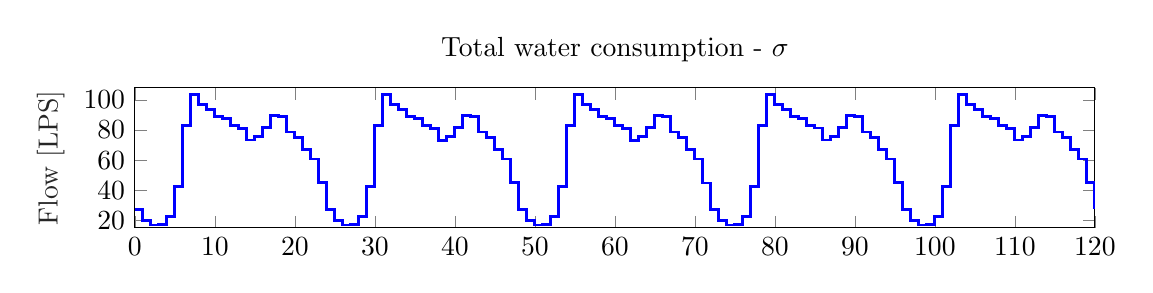
\begin{tikzpicture}

\begin{axis}[%
width=4.8in,
height=0.7in,
at={(0.888in,0.432in)},
scale only axis,
xmin=0,
xmax=120,
%xlabel style={font=\color{white!15!black}},
%xlabel={Time [h]},
ymin=15,
ymax=108,
ylabel style={font=\color{white!15!black}},
ylabel={Flow  [LPS]},
axis background/.style={fill=white},
title style={},
title={Total water consumption - $\sigma$}
]
\addplot[const plot, color=blue, line width=1pt, forget plot] table[row sep=crcr] {%
0	27.39\\
1	19.81\\
2	16.93\\
3	17.32\\
4	22.81\\
5	42.61\\
6	82.99\\
7	103.44\\
8	97.07\\
9	93.68\\
10	88.91\\
11	87.69\\
12	82.95\\
13	81.27\\
14	73.3\\
15	75.84\\
16	81.56\\
17	89.81\\
18	88.84\\
19	78.71\\
20	75.05\\
21	66.84\\
22	60.75\\
23	44.89\\
24	27.4\\
25	19.81\\
26	16.92\\
27	17.32\\
28	22.81\\
29	42.61\\
30	82.99\\
31	103.44\\
32	97.08\\
33	93.69\\
34	88.91\\
35	87.7\\
36	82.94\\
37	81.27\\
38	73.29\\
39	75.84\\
40	81.55\\
41	89.83\\
42	88.85\\
43	78.69\\
44	75.05\\
45	66.84\\
46	60.74\\
47	44.89\\
48	27.39\\
49	19.82\\
50	16.93\\
51	17.32\\
52	22.81\\
53	42.61\\
54	82.99\\
55	103.43\\
56	97.08\\
57	93.68\\
58	88.91\\
59	87.71\\
60	82.95\\
61	81.27\\
62	73.29\\
63	75.84\\
64	81.55\\
65	89.82\\
66	88.8500000000001\\
67	78.69\\
68	75.05\\
69	66.83\\
70	60.73\\
71	44.88\\
72	27.4\\
73	19.81\\
74	16.93\\
75	17.33\\
76	22.8\\
77	42.6\\
78	83\\
79	103.43\\
80	97.08\\
81	93.69\\
82	88.92\\
83	87.7\\
84	82.95\\
85	81.29\\
86	73.3\\
87	75.84\\
88	81.55\\
89	89.82\\
90	88.85\\
91	78.69\\
92	75.05\\
93	66.84\\
94	60.75\\
95	44.9\\
96	27.39\\
97	19.83\\
98	16.92\\
99	17.33\\
100	22.8\\
101	42.6\\
102	82.98\\
103	103.43\\
104	97.08\\
105	93.69\\
106	88.92\\
107	87.69\\
108	82.95\\
109	81.27\\
110	73.3\\
111	75.85\\
112	81.55\\
113	89.82\\
114	88.86\\
115	78.7\\
116	75.05\\
117	66.83\\
118	60.74\\
119	44.89\\
120	27.39\\
};
\end{axis}
\end{tikzpicture}% 
%  \vspace{-2.5mm}
%  %\caption{Consumption pattern in the identification.}
%  \label{fig:sigma_id}
%  \end{figure}
% \vspace{-8mm}

%  %Inlet flows
%  \begin{figure}[H]
%  \centering
%  %\hspace{0mm}
%  %
\includegraphics[width=0.35\textwidth]{report/pictures/missingfigure}
%  % This file was created by matlab2tikz.
%
%The latest updates can be retrieved from
%  http://www.mathworks.com/matlabcentral/fileexchange/22022-matlab2tikz-matlab2tikz
%where you can also make suggestions and rate matlab2tikz.
%
\definecolor{mycolor1}{rgb}{0.00000,0.44700,0.74100}%
\definecolor{mycolor2}{rgb}{0.85000,0.32500,0.09800}%
%
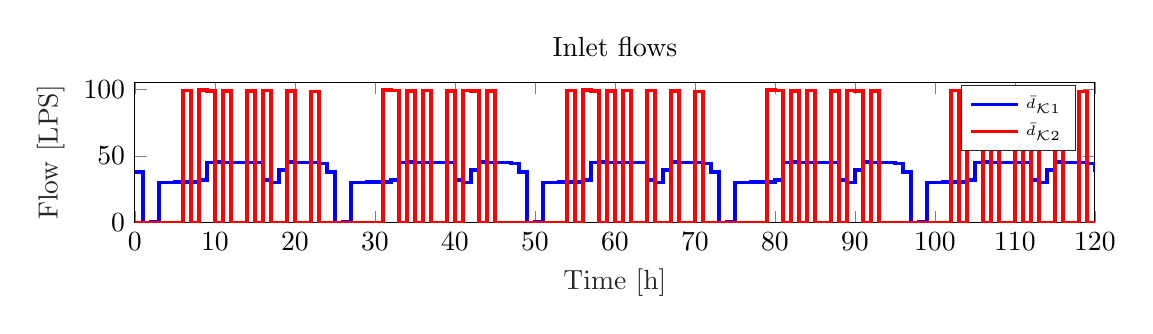
\begin{tikzpicture}

\begin{axis}[%
width=4.8in,
height=0.7in,
at={(0.758in,0.481in)},
scale only axis,
xmin=0,
xmax=120,
xlabel style={font=\color{white!15!black}},
xlabel={Time [h]},
ymin=0,
ymax=105,
ylabel style={font=\color{white!15!black}},
ylabel={Flow  [LPS]},
axis background/.style={fill=white},
title style={},
title={Inlet flows},
legend style={legend cell align=left, align=left, draw=white!15!black}
]
\addplot[const plot, color=blue, line width=1.2pt] table[row sep=crcr] {%
0	37.98\\
1	-0\\
2	0.59\\
3	30.03\\
4	30.03\\
5	30.33\\
6	30.33\\
7	30.33\\
8	31.8\\
9	45.05\\
10	45.34\\
11	45.05\\
12	44.76\\
13	45.05\\
14	44.76\\
15	45.05\\
16	31.8\\
17	30.03\\
18	39.46\\
19	45.34\\
20	45.05\\
21	44.76\\
22	45.05\\
23	44.46\\
24	37.98\\
25	-0\\
26	0.59\\
27	30.03\\
28	30.03\\
29	30.33\\
30	30.33\\
31	30.33\\
32	31.8\\
33	45.05\\
34	45.34\\
35	45.05\\
36	44.76\\
37	45.05\\
38	44.76\\
39	45.05\\
40	31.8\\
41	30.03\\
42	39.46\\
43	45.34\\
44	45.05\\
45	44.76\\
46	45.05\\
47	44.46\\
48	37.98\\
49	-0\\
50	0.59\\
51	30.03\\
52	30.03\\
53	30.33\\
54	30.33\\
55	30.33\\
56	31.8\\
57	45.05\\
58	45.34\\
59	45.05\\
60	44.76\\
61	45.05\\
62	44.76\\
63	45.05\\
64	31.8\\
65	30.03\\
66	39.46\\
67	45.34\\
68	45.05\\
69	44.76\\
70	45.05\\
71	44.46\\
72	37.98\\
73	-0\\
74	0.59\\
75	30.03\\
76	30.03\\
77	30.33\\
78	30.33\\
79	30.33\\
80	31.8\\
81	45.05\\
82	45.34\\
83	45.05\\
84	44.76\\
85	45.05\\
86	44.76\\
87	45.05\\
88	31.8\\
89	30.03\\
90	39.46\\
91	45.34\\
92	45.05\\
93	44.76\\
94	45.05\\
95	44.46\\
96	37.98\\
97	-0\\
98	0.59\\
99	30.03\\
100	30.03\\
101	30.33\\
102	30.33\\
103	30.33\\
104	31.8\\
105	45.05\\
106	45.34\\
107	45.05\\
108	44.76\\
109	45.05\\
110	44.76\\
111	45.05\\
112	31.8\\
113	30.03\\
114	39.46\\
115	45.34\\
116	45.05\\
117	44.76\\
118	45.05\\
119	44.46\\
120	37.98\\
};
\addlegendentry{\tiny $\bar{d}_{\mathcal{K}1}$}

\addplot[const plot, color=red, line width=1.2pt] table[row sep=crcr] {%
0	0\\
1	0\\
2	0\\
3	0\\
4	0\\
5	0\\
6	99.18\\
7	0\\
8	99.3\\
9	98.74\\
10	0\\
11	98.71\\
12	0\\
13	0\\
14	98.63\\
15	0\\
16	98.82\\
17	0\\
18	0\\
19	98.6\\
20	0\\
21	0\\
22	98.41\\
23	0\\
24	0\\
25	0\\
26	0\\
27	0\\
28	0\\
29	0\\
30	0\\
31	99.38\\
32	98.95\\
33	0\\
34	98.68\\
35	0\\
36	99.16\\
37	0\\
38	0\\
39	98.55\\
40	0\\
41	99.14\\
42	98.62\\
43	0\\
44	98.54\\
45	0\\
46	0\\
47	0\\
48	0\\
49	0\\
50	0\\
51	0\\
52	0\\
53	0\\
54	99.15\\
55	0\\
56	99.3\\
57	98.73\\
58	0\\
59	98.71\\
60	0\\
61	99.18\\
62	0\\
63	0\\
64	98.76\\
65	0\\
66	0\\
67	98.58\\
68	0\\
69	0\\
70	98.4\\
71	0\\
72	0\\
73	0\\
74	0\\
75	0\\
76	0\\
77	0\\
78	0\\
79	99.38\\
80	98.94\\
81	0\\
82	98.68\\
83	0\\
84	99.15\\
85	0\\
86	0\\
87	98.54\\
88	0\\
89	99.15\\
90	98.62\\
91	0\\
92	98.55\\
93	0\\
94	0\\
95	0\\
96	0\\
97	0\\
98	0\\
99	0\\
100	0\\
101	0\\
102	99.17\\
103	0\\
104	99.3\\
105	98.74\\
106	0\\
107	98.71\\
108	0\\
109	0\\
110	98.64\\
111	0\\
112	98.76\\
113	0\\
114	0\\
115	98.59\\
116	0\\
117	0\\
118	98.4\\
119	0\\
120	0\\
};
\addlegendentry{\tiny $\bar{d}_{\mathcal{K}2}$}

\end{axis}
\end{tikzpicture}% 
%  \vspace{-2.5mm}
%  \caption{Inlet flows of the two pumping stations.}
%  \label{fig:dk_12}
%  \end{figure}
%  \vspace{-3mm}